% $Author$
% $Date$
% $Revision$

% HISTORY:

%=================================================================
% This is the main file for the Pharo By Example book.
% The individual chapters can also be latexed by themselves.
% Note that the \end{document} marker occurs near the
% middle of this file, to leave out additional material
% for a future version of the book.
%=================================================================


% TODO:

%=================================================================
% lulu -> figures in .png / to see: macros
%%Encoding -> see Henrik
% fix \chapterauthor on each chapter
%
%=================================================================



\documentclass[a4paper,10pt,twoside]{book}
\usepackage[
	papersize={6.13in,9.21in},
	hmargin={.75in,.75in},
	vmargin={.75in,1in},
	ignoreheadfoot
]{geometry}
% $Author$
% $Date$
% $Revision$

% HISTORY:
% 2006-10-31 - Oscar code macros
% ...

%=============================================================
% NB: documentclass must be set in main document.
% Allows book to be generated in multiple formats.
%=============================================================
%:Packages
\usepackage[T1]{fontenc}  %%%%%% really important to get the code directly in the text!
\usepackage{lmodern}
%\usepackage[scaled=0.85]{bookmanx} % needs another scale factor if used with \renewcommand{\sfdefault}{cmbr}
\usepackage{palatino}
\usepackage[scaled=0.85]{helvet}
\usepackage[protrusion,expansion=false]{microtype}
\usepackage{graphicx}
\usepackage{theorem}
\usepackage[english]{babel}
% ON: pdfsync breaks the use of p{width} for tabular columns!
\ifdefined\usepdfsync\usepackage{pdfsync}\fi % Requires texlive 2007
%=============================================================
%:More packages
%Stef should check which ones are used!
%\usepackage{picinpar}
%\usepackage{layout}
%\usepackage{color}
%\usepackage{enum}
%\usepackage{a4wide}
% \usepackage{fancyhdr}
\usepackage{ifthen}
\usepackage{float}
\usepackage{longtable}
\usepackage{makeidx}
\usepackage[nottoc]{tocbibind}
\usepackage{multicol}
\usepackage{booktabs}	% book-style tables
\usepackage{topcapt}	% enables \topcaption
\usepackage{multirow}
\usepackage{tabularx}
%\usepackage[bottom]{footmisc}
\usepackage{xspace}
\usepackage{alltt}
\usepackage{amssymb,textcomp}
\usepackage[usenames,dvipsnames]{color}
%\usepackage{colortbl}
\usepackage[hang]{subfigure}\makeatletter\def\p@subfigure{\thefigure\,}\makeatother
\usepackage{rotating}
\usepackage{enumitem}	% apb: allows more control over tags in enumerations
\usepackage{verbatim}     % for comment environment
\usepackage{varioref}	% for page references that work
\labelformat{footnote}{\thechapter--#1} % to distinguish citations from jurabib
\usepackage{needspace}
\usepackage{isodateo} % enable \isodate
\usepackage[newparttoc,pagestyles]{titlesec}
\usepackage{titletoc}
\usepackage{wrapfig}

\usepackage[
	super,
	citefull=first,
	authorformat={allreversed,and},
	titleformat={commasep,italic}
]{jurabib} % citations as footnotes
\usepackage[
	colorlinks=true,
	linkcolor=black,
	urlcolor=black,
	citecolor=black
]{hyperref}   % should come last
%=============================================================
%:PDF version
\pdfminorversion=3 % Set PDF to 1.3 for Lulu
%=============================================================
%:URL style
\makeatletter
\def\url@leostyle{%
  \@ifundefined{selectfont}{\def\UrlFont{\sf}}{\def\UrlFont{\sffamily}}}
\makeatother
% Now actually use the newly defined style.
\urlstyle{leo}
%=============================================================
%:Booleans
\newboolean{lulu}
\setboolean{lulu}{false}
\newcommand{\ifluluelse}[2]{\ifthenelse{\boolean{lulu}}{#1}{#2}}
%=============================================================
%:Names
\newcommand{\SUnit}{SUnit\xspace}
\newcommand{\sunit}{SUnit\xspace}
\newcommand{\xUnit}{$x$Unit\xspace}
\newcommand{\JUnit}{JUnit\xspace}
\newcommand{\st}{Smalltalk\xspace}
\newcommand{\pharo}{Pharo\xspace} % Use this, not \Pharo
%\newcommand{\sqmap}{SqueakMap\xspace}
\newcommand{\squeak}{Squeak\xspace} % use this, not \Squeak or \sq
\newcommand{\sqsrc}{SqueakSource\xspace}
\newcommand{\sbe}{\url{http://SqueakByExample.org}\xspace}
\newcommand{\pharoweb}{\url{http://pharo-project.org}\xspace}
\newcommand{\pbe}{\url{http://PharoByExample.org}\xspace}
\newcommand{\sba}{\url{http://SquareBracketAssociates.org}\xspace}
\newcommand{\bam}{\lct{Bounc\-ing\-Atoms\-Morph}\xspace}
%=============================================================
%:Markup macros for proof-reading
\usepackage[normalem]{ulem} % for \sout
\usepackage{xcolor}
\newcommand{\ra}{$\rightarrow$}
\newcommand{\ugh}[1]{\textcolor{red}{\uwave{#1}}} % please rephrase
\newcommand{\ins}[1]{\textcolor{blue}{\uline{#1}}} % please insert
\newcommand{\del}[1]{\textcolor{red}{\sout{#1}}} % please delete
\newcommand{\chg}[2]{\textcolor{red}{\sout{#1}}{\ra}\textcolor{blue}{\uline{#2}}} % please change
%=============================================================
%:Editorial comment macros
%\newcommand{\nnbb}[2]{
%    % \fbox{\bfseries\sffamily\scriptsize#1}
%    \fcolorbox{gray}{yellow}{\bfseries\sffamily\scriptsize#1}
%    {\sf\small$\blacktriangleright$\textit{#2}$\blacktriangleleft$}
%   }
\newcommand{\yellowbox}[1]{\fcolorbox{gray}{yellow}{\bfseries\sffamily\scriptsize#1}}
\newcommand{\triangles}[1]{{\sf\small$\blacktriangleright$\textit{#1}$\blacktriangleleft$}}
\newcommand{\nnbb}[2]{\yellowbox{#1} \triangles{#2}}
\newcommand{\fix}{\yellowbox{FIX!}}
\newcommand{\here}{\yellowbox{CONTINUE HERE!}}
% editor macros
\newcommand{\apl}[1]{\nnbb{Alain}{#1}} % Alain
\newcommand{\ab}[1]{\nnbb{Andrew}{#1}} % Black
\newcommand{\sd}[1]{\nnbb{St\'{e}f}{#1}} % Ducasse
\newcommand{\gl}[1]{\nnbb{Guillaume}{#1}} % Ducasse
\newcommand{\cd}[1]{\nnbb{Christophe}{#1}} % Ducasse
\newcommand{\sig}[1]{\nnbb{Igor}{#1}} % Igor
\newcommand{\dc}[1]{\nnbb{DamienC}{#1}} % Ducasse
\newcommand{\md}[1]{\nnbb{Marcus}{#1}} % Denker
\newcommand{\on}[1]{\nnbb{Oscar}{#1}} % Nierstrasz
\newcommand{\damien}[1]{\nnbb{Damien}{#1}} % Pollet
\newcommand{\lr}[1]{\nnbb{Lukas}{#1}} % Renggli
\newcommand{\orla}[1]{\nnbb{Orla}{#1}} % Greevy
\newcommand{\alex}[1]{\nnbb{Alex}{#1}} % Bergel
\newcommand{\alx}[1]{\nnbb{Alex}{#1}} % Bergel
\newcommand{\dr}[1]{\nnbb{David}{#1}} % Roethlisberger
\newcommand{\ja}[1]{\nnbb{Jannik}{#1}} % Laval
\newcommand{\cb}[1]{\nnbb{Camillo}{#1}} % Bruni
\newcommand{\jr}[1]{\nnbb{Jorge}{#1}} % Ressia
\newcommand{\jb}[1]{\nnbb{JB}{#1}} % JB
\newcommand{\jp}[1]{\nnbb{Javier}{#1}} % Pimas
\newcommand{\fp}[1]{\nnbb{Fabrizio}{#1}} % Perin
\newcommand{\michael}[1]{\nnbb{Michael}{#1}} % Davies
\newcommand{\ew}[1]{\nnbb{Erwann}{#1}} % Wernli
\newcommand{\mb}[1]{\nnbb{Martial}{#1}} % Boniou
\newcommand{\hw}[1]{\nnbb{Hernan}{#1}} % Wilkinson
\newcommand{\ben}[1]{\nnbb{Benjamin}{#1}} % Benjamin Van Ryseghem
\newcommand{\hjo}[1]{\nnbb{HwaJong}{#1}} % HwaJong Oh aka daliot
\newcommand{\ml}[1]{\nnbb{Max}{#1}} % Max Leske
\newcommand{\mmp}[1]{\nnbb{Mariano}{#1}} % Mariano Martinez Peck
\newcommand{\luc}[1]{\nnbb{Luc}{#1}} % Luc Fabresse
\newcommand{\dkl}[1]{\nnbb{Daniel}{#1}} % Daniel Lyons
\newcommand{\vu}[1]{\nnbb{Veronica}{#1}} % Veronica Uquillas Gomez
\newcommand{\martin}[1]{\nnbb{Martin}{#1}} % Martin Dias
\newcommand{\vp}[1]{\nnbb{Vanessa}{#1}} % Vanessa Pena
\newcommand{\gp}[1]{\nnbb{Guille}{#1}} % Guillermo Polito

%=============================================================
%:Abbreviation macros
\newcommand{\ie}{\emph{i.e.},\xspace}
\newcommand{\eg}{\emph{e.g.},\xspace}
\newcommand{\etc}{etc.\xspace}
%=============================================================
%:Cross reference macros
\newcommand{\charef}[1]{Chapter~\ref{cha:#1}\xspace}
\newcommand{\secref}[1]{Section~\ref{sec:#1}\xspace}
\newcommand{\figref}[1]{Figure~\ref{fig:#1}\xspace}
\newcommand{\Figref}[1]{Figure~\ref{fig:#1}\xspace}
\newcommand{\appref}[1]{Appendix~\ref{app:#1}\xspace}
\newcommand{\tabref}[1]{Table~\ref{tab:#1}\xspace}
\newcommand{\faqref}[1]{FAQ~\ref{faq:#1}, p.~\pageref{faq:#1}\xspace}
% APB: I removed trailing \xspace commands from these macros because
% \xspace mostly doesn't work.  If you want a space after your
% references, type one!
% ON: xspace has always worked just fine for me!  Please leave them in.
%
\newcommand{\ruleref}[1]{\ref{rule:#1}\xspace}
%
\newcommand{\egref}[1]{example~\ref{eg:#1}\xspace}
\newcommand{\Egref}[1]{Example~\ref{eg:#1}\xspace}
%
\newcommand{\scrref}[1]{script~\ref{scr:#1}\xspace}
\newcommand{\Scrref}[1]{Script~\ref{scr:#1}\xspace}
\newcommand{\tscrref}[1]{the script~\ref{scr:#1}\xspace}
\newcommand{\Tscrref}[1]{The script~\ref{scr:#1}\xspace}
%
\newcommand{\mthref}[1]{method~\ref{mth:#1}\xspace}
\newcommand{\mthsref}[1]{methods~\ref{mth:#1}\xspace}
\newcommand{\Mthref}[1]{Method~\ref{mth:#1}\xspace}
\newcommand{\tmthref}[1]{the method~\ref{mth:#1}\xspace}
\newcommand{\Tmthref}[1]{The method~\ref{mth:#1}\xspace}
%
\newcommand{\clsref}[1]{class~\ref{cls:#1}\xspace}
\newcommand{\tclsref}[1]{the class~\ref{cls:#1}\xspace}
\newcommand{\Tclsref}[1]{The class~\ref{cls:#1}\xspace}

\newcommand{\chalabel}[1]{\label{cha:#1}}
\newcommand{\seclabel}[1]{\label{sec:#1}}
\newcommand{\figlabel}[1]{\label{fig:#1}}
\newcommand{\tablabel}[1]{\label{tab:#1}}
\newcommand{\rulelabel}[1]{\label{rule:#1}}
\newcommand{\eglabel}[1]{\label{eg:#1}}
\newcommand{\scrlabel}[1]{\label{scr:#1}}
\newcommand{\mthlabel}[1]{\label{mth:#1}}
\newcommand{\clslabel}[1]{\label{cls:#1}}
\newcommand{\faqlabel}[1]{\label{faq:#1}}
%=============================================================
%:Menu item macro
% for menu items, so we can change our minds on how to print them! (apb)
\definecolor{lightgray}{gray}{0.89}
\newcommand{\menu}[1]{{%
	\setlength{\fboxsep}{0pt}%
	\colorbox{lightgray}{{{\upshape\sffamily\strut \,#1\,}}}}}
\newcommand{\link}[1]{{%
	\fontfamily{lmr}\selectfont
 	\upshape{\sffamily \underline{#1}}}}
% For submenu items:
\newcommand{\go}{\,$\triangleright$\,}
% \newcommand{\go}{\,$\blacktriangleright$\,}
% For keyboard shortcuts:
%\newcommand{\short}[1]{\mbox{$\langle${\sc CMD}$\rangle$-#1}\xspace}
\newcommand{\short}[1]{\mbox{{\sc cmd}\hspace{0.08em}--\hspace{0.09em}#1}\xspace}
% For buttons:
\newcommand{\button}[1]{{%
	\setlength{\fboxsep}{0pt}%
	\fbox{{\upshape\sffamily\strut \,#1\,}}}}
% NB: The button macro does not work within captions -- incompatible with xcolor package :-(
\newcommand{\toolsflap}{\textit{Tools} flap\xspace}
%=============================================================
%:Mouse clicks
\newcommand{\click}{click\xspace} % RED
\newcommand{\actclick}{action-click\xspace} % YELLOW
\newcommand{\metaclick}{meta-click\xspace} % BLUE
\newcommand{\Click}{Click\xspace} % RED
\newcommand{\Actclick}{Action-click\xspace} % YELLOW
\newcommand{\Metaclick}{Meta-click\xspace} % BLUE
%=============================================================
%:ToSh macros
\newboolean{tosh}
\setboolean{tosh}{false}
\newcommand{\iftoshelse}[2]{\ifthenelse{\boolean{tosh}}{#1}{#2}}
%=============================================================
%:ToSh colors
%\newcommand{\highlightcolor}{\color{blue!65}}
%\newcommand{\boxcolor}{\color{gray!25}}
\newcommand{\highlight}[1]{\textcolor{blue!65}{#1}}
%\newcommand{\codecolor}{\color{blue!65}}
%%\setlength{\fboxrule}{2pt}
%\newcommand{\asPict}[1]{%
%	{\Large\highlight{#1}}}
%=============================================================
%:Reader cues (do this)
%
% Indicate something the reader should try out.
% \newcommand{\dothisicon}{\raisebox{-.5ex}{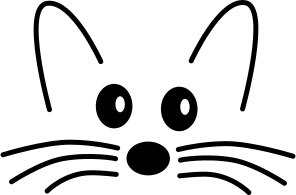
\includegraphics[width=1.4em]{squeak-logo}}}
\iftoshelse{
	\usepackage{marginnote}
		\renewcommand*{\marginfont}{\footnotesize}
	\newcommand{\vartriangleout}{\ifthenelse{\isodd{\thepage}}{\vartriangleright}{\vartriangleleft}}
	\newcommand{\dothisicon}{\fcolorbox{blue!65}{white}{\highlight{$\vartriangleout$}}}
	\newcommand{\dothis}[1]{%
		\noindent\par\noindent
		{\reversemarginpar
			\marginnote{\fcolorbox{blue!65}{white}{\highlight{$\vartriangleout$}}}}
		%\MarginLabel{do this}
		\noindent\emph{#1}
		\nopagebreak}
}{
	\newcommand{\dothisicon}{\raisebox{-.5ex}{
\includegraphics[height=1.2em]{pharo}}}
	\newcommand{\dothis}[1]{%
		\medskip
		\noindent\dothisicon
		\ifx#1\empty\else\quad\emph{#1}\fi
		\par\smallskip\nopagebreak}
}
%===> NEW VERSION <===
% NB: To use this in an individual chapter, you must set:
%\graphicspath{{figures/} {../figures/}}
% at the head of the chapter.  Don't forget the final /
%=============================================================
%:Reader hints (hint)
%
% Indicates a non-obvious consequence
\newcommand{\hint}[1]{\vspace{1ex}\noindent\fbox{\textsc{Hint}} \emph{#1}}
%=================================================================
% graphics for Morphic handles
\newcommand{\grabHandle}{\raisebox{-0.2ex}{
\includegraphics[width=1em]{blackHandle}}}
\newcommand{\moveHandle}{\raisebox{-0.2ex}{
\includegraphics[width=1em]{moveHandle}}}
\newcommand{\debugHandle}{\raisebox{-0.2ex}{
\includegraphics[width=1em]{debugHandle}}}
%=============================================================
%:Highlighting Important stuff (doublebox)
%
% From Seaside book ...
\newsavebox{\SavedText}
\newlength{\InnerBoxRule}\setlength{\InnerBoxRule}{.75\fboxrule}
\newlength{\OuterBoxRule}\setlength{\OuterBoxRule}{1.5\fboxrule}
\newlength{\BoxSeparation}\setlength{\BoxSeparation}{1.5\fboxrule}
\addtolength{\BoxSeparation}{.5pt}
\newlength{\SaveBoxSep}\setlength{\SaveBoxSep}{2\fboxsep}
%
\newenvironment{doublebox}{\begin{lrbox}{\SavedText}
    \begin{minipage}{.75\textwidth}}
    {\end{minipage}\end{lrbox}\begin{center}
    \setlength{\fboxsep}{\BoxSeparation}\setlength{\fboxrule}{\OuterBoxRule}
    \fbox{\setlength{\fboxsep}{\SaveBoxSep}\setlength{\fboxrule}{\InnerBoxRule}%
      \fbox{\usebox{\SavedText}}}
  \end{center}}
% Use this:
\newcommand{\important}[1]{\begin{doublebox}#1\end{doublebox}}
%=============================================================
%:Section depth
\setcounter{secnumdepth}{2}
%% for this to happen start the file with
%\ifx\wholebook\relax\else
%% $Author$
% $Date$
% $Revision$

% HISTORY:
% 2006-10-31 - Oscar code macros
% ...

%=============================================================
% NB: documentclass must be set in main document.
% Allows book to be generated in multiple formats.
%=============================================================
%:Packages
\usepackage[T1]{fontenc}  %%%%%% really important to get the code directly in the text!
\usepackage{lmodern}
%\usepackage[scaled=0.85]{bookmanx} % needs another scale factor if used with \renewcommand{\sfdefault}{cmbr}
\usepackage{palatino}
\usepackage[scaled=0.85]{helvet}
\usepackage[protrusion,expansion=false]{microtype}
\usepackage{graphicx}
\usepackage{theorem}
\usepackage[english]{babel}
% ON: pdfsync breaks the use of p{width} for tabular columns!
\ifdefined\usepdfsync\usepackage{pdfsync}\fi % Requires texlive 2007
%=============================================================
%:More packages
%Stef should check which ones are used!
%\usepackage{picinpar}
%\usepackage{layout}
%\usepackage{color}
%\usepackage{enum}
%\usepackage{a4wide}
% \usepackage{fancyhdr}
\usepackage{ifthen}
\usepackage{float}
\usepackage{longtable}
\usepackage{makeidx}
\usepackage[nottoc]{tocbibind}
\usepackage{multicol}
\usepackage{booktabs}	% book-style tables
\usepackage{topcapt}	% enables \topcaption
\usepackage{multirow}
\usepackage{tabularx}
%\usepackage[bottom]{footmisc}
\usepackage{xspace}
\usepackage{alltt}
\usepackage{amssymb,textcomp}
\usepackage[usenames,dvipsnames]{color}
%\usepackage{colortbl}
\usepackage[hang]{subfigure}\makeatletter\def\p@subfigure{\thefigure\,}\makeatother
\usepackage{rotating}
\usepackage{enumitem}	% apb: allows more control over tags in enumerations
\usepackage{verbatim}     % for comment environment
\usepackage{varioref}	% for page references that work
\labelformat{footnote}{\thechapter--#1} % to distinguish citations from jurabib
\usepackage{needspace}
\usepackage{isodateo} % enable \isodate
\usepackage[newparttoc,pagestyles]{titlesec}
\usepackage{titletoc}
\usepackage{wrapfig}

\usepackage[
	super,
	citefull=first,
	authorformat={allreversed,and},
	titleformat={commasep,italic}
]{jurabib} % citations as footnotes
\usepackage[
	colorlinks=true,
	linkcolor=black,
	urlcolor=black,
	citecolor=black
]{hyperref}   % should come last
%=============================================================
%:PDF version
\pdfminorversion=3 % Set PDF to 1.3 for Lulu
%=============================================================
%:URL style
\makeatletter
\def\url@leostyle{%
  \@ifundefined{selectfont}{\def\UrlFont{\sf}}{\def\UrlFont{\sffamily}}}
\makeatother
% Now actually use the newly defined style.
\urlstyle{leo}
%=============================================================
%:Booleans
\newboolean{lulu}
\setboolean{lulu}{false}
\newcommand{\ifluluelse}[2]{\ifthenelse{\boolean{lulu}}{#1}{#2}}
%=============================================================
%:Names
\newcommand{\SUnit}{SUnit\xspace}
\newcommand{\sunit}{SUnit\xspace}
\newcommand{\xUnit}{$x$Unit\xspace}
\newcommand{\JUnit}{JUnit\xspace}
\newcommand{\st}{Smalltalk\xspace}
\newcommand{\pharo}{Pharo\xspace} % Use this, not \Pharo
%\newcommand{\sqmap}{SqueakMap\xspace}
\newcommand{\squeak}{Squeak\xspace} % use this, not \Squeak or \sq
\newcommand{\sqsrc}{SqueakSource\xspace}
\newcommand{\sbe}{\url{http://SqueakByExample.org}\xspace}
\newcommand{\pharoweb}{\url{http://pharo-project.org}\xspace}
\newcommand{\pbe}{\url{http://PharoByExample.org}\xspace}
\newcommand{\sba}{\url{http://SquareBracketAssociates.org}\xspace}
\newcommand{\bam}{\lct{Bounc\-ing\-Atoms\-Morph}\xspace}
%=============================================================
%:Markup macros for proof-reading
\usepackage[normalem]{ulem} % for \sout
\usepackage{xcolor}
\newcommand{\ra}{$\rightarrow$}
\newcommand{\ugh}[1]{\textcolor{red}{\uwave{#1}}} % please rephrase
\newcommand{\ins}[1]{\textcolor{blue}{\uline{#1}}} % please insert
\newcommand{\del}[1]{\textcolor{red}{\sout{#1}}} % please delete
\newcommand{\chg}[2]{\textcolor{red}{\sout{#1}}{\ra}\textcolor{blue}{\uline{#2}}} % please change
%=============================================================
%:Editorial comment macros
%\newcommand{\nnbb}[2]{
%    % \fbox{\bfseries\sffamily\scriptsize#1}
%    \fcolorbox{gray}{yellow}{\bfseries\sffamily\scriptsize#1}
%    {\sf\small$\blacktriangleright$\textit{#2}$\blacktriangleleft$}
%   }
\newcommand{\yellowbox}[1]{\fcolorbox{gray}{yellow}{\bfseries\sffamily\scriptsize#1}}
\newcommand{\triangles}[1]{{\sf\small$\blacktriangleright$\textit{#1}$\blacktriangleleft$}}
\newcommand{\nnbb}[2]{\yellowbox{#1} \triangles{#2}}
\newcommand{\fix}{\yellowbox{FIX!}}
\newcommand{\here}{\yellowbox{CONTINUE HERE!}}
% editor macros
\newcommand{\apl}[1]{\nnbb{Alain}{#1}} % Alain
\newcommand{\ab}[1]{\nnbb{Andrew}{#1}} % Black
\newcommand{\sd}[1]{\nnbb{St\'{e}f}{#1}} % Ducasse
\newcommand{\gl}[1]{\nnbb{Guillaume}{#1}} % Ducasse
\newcommand{\cd}[1]{\nnbb{Christophe}{#1}} % Ducasse
\newcommand{\sig}[1]{\nnbb{Igor}{#1}} % Igor
\newcommand{\dc}[1]{\nnbb{DamienC}{#1}} % Ducasse
\newcommand{\md}[1]{\nnbb{Marcus}{#1}} % Denker
\newcommand{\on}[1]{\nnbb{Oscar}{#1}} % Nierstrasz
\newcommand{\damien}[1]{\nnbb{Damien}{#1}} % Pollet
\newcommand{\lr}[1]{\nnbb{Lukas}{#1}} % Renggli
\newcommand{\orla}[1]{\nnbb{Orla}{#1}} % Greevy
\newcommand{\alex}[1]{\nnbb{Alex}{#1}} % Bergel
\newcommand{\alx}[1]{\nnbb{Alex}{#1}} % Bergel
\newcommand{\dr}[1]{\nnbb{David}{#1}} % Roethlisberger
\newcommand{\ja}[1]{\nnbb{Jannik}{#1}} % Laval
\newcommand{\cb}[1]{\nnbb{Camillo}{#1}} % Bruni
\newcommand{\jr}[1]{\nnbb{Jorge}{#1}} % Ressia
\newcommand{\jb}[1]{\nnbb{JB}{#1}} % JB
\newcommand{\jp}[1]{\nnbb{Javier}{#1}} % Pimas
\newcommand{\fp}[1]{\nnbb{Fabrizio}{#1}} % Perin
\newcommand{\michael}[1]{\nnbb{Michael}{#1}} % Davies
\newcommand{\ew}[1]{\nnbb{Erwann}{#1}} % Wernli
\newcommand{\mb}[1]{\nnbb{Martial}{#1}} % Boniou
\newcommand{\hw}[1]{\nnbb{Hernan}{#1}} % Wilkinson
\newcommand{\ben}[1]{\nnbb{Benjamin}{#1}} % Benjamin Van Ryseghem
\newcommand{\hjo}[1]{\nnbb{HwaJong}{#1}} % HwaJong Oh aka daliot
\newcommand{\ml}[1]{\nnbb{Max}{#1}} % Max Leske
\newcommand{\mmp}[1]{\nnbb{Mariano}{#1}} % Mariano Martinez Peck
\newcommand{\luc}[1]{\nnbb{Luc}{#1}} % Luc Fabresse
\newcommand{\dkl}[1]{\nnbb{Daniel}{#1}} % Daniel Lyons
\newcommand{\vu}[1]{\nnbb{Veronica}{#1}} % Veronica Uquillas Gomez
\newcommand{\martin}[1]{\nnbb{Martin}{#1}} % Martin Dias
\newcommand{\vp}[1]{\nnbb{Vanessa}{#1}} % Vanessa Pena
\newcommand{\gp}[1]{\nnbb{Guille}{#1}} % Guillermo Polito

%=============================================================
%:Abbreviation macros
\newcommand{\ie}{\emph{i.e.},\xspace}
\newcommand{\eg}{\emph{e.g.},\xspace}
\newcommand{\etc}{etc.\xspace}
%=============================================================
%:Cross reference macros
\newcommand{\charef}[1]{Chapter~\ref{cha:#1}\xspace}
\newcommand{\secref}[1]{Section~\ref{sec:#1}\xspace}
\newcommand{\figref}[1]{Figure~\ref{fig:#1}\xspace}
\newcommand{\Figref}[1]{Figure~\ref{fig:#1}\xspace}
\newcommand{\appref}[1]{Appendix~\ref{app:#1}\xspace}
\newcommand{\tabref}[1]{Table~\ref{tab:#1}\xspace}
\newcommand{\faqref}[1]{FAQ~\ref{faq:#1}, p.~\pageref{faq:#1}\xspace}
% APB: I removed trailing \xspace commands from these macros because
% \xspace mostly doesn't work.  If you want a space after your
% references, type one!
% ON: xspace has always worked just fine for me!  Please leave them in.
%
\newcommand{\ruleref}[1]{\ref{rule:#1}\xspace}
%
\newcommand{\egref}[1]{example~\ref{eg:#1}\xspace}
\newcommand{\Egref}[1]{Example~\ref{eg:#1}\xspace}
%
\newcommand{\scrref}[1]{script~\ref{scr:#1}\xspace}
\newcommand{\Scrref}[1]{Script~\ref{scr:#1}\xspace}
\newcommand{\tscrref}[1]{the script~\ref{scr:#1}\xspace}
\newcommand{\Tscrref}[1]{The script~\ref{scr:#1}\xspace}
%
\newcommand{\mthref}[1]{method~\ref{mth:#1}\xspace}
\newcommand{\mthsref}[1]{methods~\ref{mth:#1}\xspace}
\newcommand{\Mthref}[1]{Method~\ref{mth:#1}\xspace}
\newcommand{\tmthref}[1]{the method~\ref{mth:#1}\xspace}
\newcommand{\Tmthref}[1]{The method~\ref{mth:#1}\xspace}
%
\newcommand{\clsref}[1]{class~\ref{cls:#1}\xspace}
\newcommand{\tclsref}[1]{the class~\ref{cls:#1}\xspace}
\newcommand{\Tclsref}[1]{The class~\ref{cls:#1}\xspace}

\newcommand{\chalabel}[1]{\label{cha:#1}}
\newcommand{\seclabel}[1]{\label{sec:#1}}
\newcommand{\figlabel}[1]{\label{fig:#1}}
\newcommand{\tablabel}[1]{\label{tab:#1}}
\newcommand{\rulelabel}[1]{\label{rule:#1}}
\newcommand{\eglabel}[1]{\label{eg:#1}}
\newcommand{\scrlabel}[1]{\label{scr:#1}}
\newcommand{\mthlabel}[1]{\label{mth:#1}}
\newcommand{\clslabel}[1]{\label{cls:#1}}
\newcommand{\faqlabel}[1]{\label{faq:#1}}
%=============================================================
%:Menu item macro
% for menu items, so we can change our minds on how to print them! (apb)
\definecolor{lightgray}{gray}{0.89}
\newcommand{\menu}[1]{{%
	\setlength{\fboxsep}{0pt}%
	\colorbox{lightgray}{{{\upshape\sffamily\strut \,#1\,}}}}}
\newcommand{\link}[1]{{%
	\fontfamily{lmr}\selectfont
 	\upshape{\sffamily \underline{#1}}}}
% For submenu items:
\newcommand{\go}{\,$\triangleright$\,}
% \newcommand{\go}{\,$\blacktriangleright$\,}
% For keyboard shortcuts:
%\newcommand{\short}[1]{\mbox{$\langle${\sc CMD}$\rangle$-#1}\xspace}
\newcommand{\short}[1]{\mbox{{\sc cmd}\hspace{0.08em}--\hspace{0.09em}#1}\xspace}
% For buttons:
\newcommand{\button}[1]{{%
	\setlength{\fboxsep}{0pt}%
	\fbox{{\upshape\sffamily\strut \,#1\,}}}}
% NB: The button macro does not work within captions -- incompatible with xcolor package :-(
\newcommand{\toolsflap}{\textit{Tools} flap\xspace}
%=============================================================
%:Mouse clicks
\newcommand{\click}{click\xspace} % RED
\newcommand{\actclick}{action-click\xspace} % YELLOW
\newcommand{\metaclick}{meta-click\xspace} % BLUE
\newcommand{\Click}{Click\xspace} % RED
\newcommand{\Actclick}{Action-click\xspace} % YELLOW
\newcommand{\Metaclick}{Meta-click\xspace} % BLUE
%=============================================================
%:ToSh macros
\newboolean{tosh}
\setboolean{tosh}{false}
\newcommand{\iftoshelse}[2]{\ifthenelse{\boolean{tosh}}{#1}{#2}}
%=============================================================
%:ToSh colors
%\newcommand{\highlightcolor}{\color{blue!65}}
%\newcommand{\boxcolor}{\color{gray!25}}
\newcommand{\highlight}[1]{\textcolor{blue!65}{#1}}
%\newcommand{\codecolor}{\color{blue!65}}
%%\setlength{\fboxrule}{2pt}
%\newcommand{\asPict}[1]{%
%	{\Large\highlight{#1}}}
%=============================================================
%:Reader cues (do this)
%
% Indicate something the reader should try out.
% \newcommand{\dothisicon}{\raisebox{-.5ex}{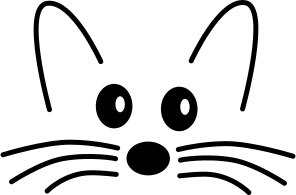
\includegraphics[width=1.4em]{squeak-logo}}}
\iftoshelse{
	\usepackage{marginnote}
		\renewcommand*{\marginfont}{\footnotesize}
	\newcommand{\vartriangleout}{\ifthenelse{\isodd{\thepage}}{\vartriangleright}{\vartriangleleft}}
	\newcommand{\dothisicon}{\fcolorbox{blue!65}{white}{\highlight{$\vartriangleout$}}}
	\newcommand{\dothis}[1]{%
		\noindent\par\noindent
		{\reversemarginpar
			\marginnote{\fcolorbox{blue!65}{white}{\highlight{$\vartriangleout$}}}}
		%\MarginLabel{do this}
		\noindent\emph{#1}
		\nopagebreak}
}{
	\newcommand{\dothisicon}{\raisebox{-.5ex}{
\includegraphics[height=1.2em]{pharo}}}
	\newcommand{\dothis}[1]{%
		\medskip
		\noindent\dothisicon
		\ifx#1\empty\else\quad\emph{#1}\fi
		\par\smallskip\nopagebreak}
}
%===> NEW VERSION <===
% NB: To use this in an individual chapter, you must set:
%\graphicspath{{figures/} {../figures/}}
% at the head of the chapter.  Don't forget the final /
%=============================================================
%:Reader hints (hint)
%
% Indicates a non-obvious consequence
\newcommand{\hint}[1]{\vspace{1ex}\noindent\fbox{\textsc{Hint}} \emph{#1}}
%=================================================================
% graphics for Morphic handles
\newcommand{\grabHandle}{\raisebox{-0.2ex}{
\includegraphics[width=1em]{blackHandle}}}
\newcommand{\moveHandle}{\raisebox{-0.2ex}{
\includegraphics[width=1em]{moveHandle}}}
\newcommand{\debugHandle}{\raisebox{-0.2ex}{
\includegraphics[width=1em]{debugHandle}}}
%=============================================================
%:Highlighting Important stuff (doublebox)
%
% From Seaside book ...
\newsavebox{\SavedText}
\newlength{\InnerBoxRule}\setlength{\InnerBoxRule}{.75\fboxrule}
\newlength{\OuterBoxRule}\setlength{\OuterBoxRule}{1.5\fboxrule}
\newlength{\BoxSeparation}\setlength{\BoxSeparation}{1.5\fboxrule}
\addtolength{\BoxSeparation}{.5pt}
\newlength{\SaveBoxSep}\setlength{\SaveBoxSep}{2\fboxsep}
%
\newenvironment{doublebox}{\begin{lrbox}{\SavedText}
    \begin{minipage}{.75\textwidth}}
    {\end{minipage}\end{lrbox}\begin{center}
    \setlength{\fboxsep}{\BoxSeparation}\setlength{\fboxrule}{\OuterBoxRule}
    \fbox{\setlength{\fboxsep}{\SaveBoxSep}\setlength{\fboxrule}{\InnerBoxRule}%
      \fbox{\usebox{\SavedText}}}
  \end{center}}
% Use this:
\newcommand{\important}[1]{\begin{doublebox}#1\end{doublebox}}
%=============================================================
%:Section depth
\setcounter{secnumdepth}{2}
%% for this to happen start the file with
%\ifx\wholebook\relax\else
%% $Author$
% $Date$
% $Revision$

% HISTORY:
% 2006-10-31 - Oscar code macros
% ...

%=============================================================
% NB: documentclass must be set in main document.
% Allows book to be generated in multiple formats.
%=============================================================
%:Packages
\usepackage[T1]{fontenc}  %%%%%% really important to get the code directly in the text!
\usepackage{lmodern}
%\usepackage[scaled=0.85]{bookmanx} % needs another scale factor if used with \renewcommand{\sfdefault}{cmbr}
\usepackage{palatino}
\usepackage[scaled=0.85]{helvet}
\usepackage[protrusion,expansion=false]{microtype}
\usepackage{graphicx}
\usepackage{theorem}
\usepackage[english]{babel}
% ON: pdfsync breaks the use of p{width} for tabular columns!
\ifdefined\usepdfsync\usepackage{pdfsync}\fi % Requires texlive 2007
%=============================================================
%:More packages
%Stef should check which ones are used!
%\usepackage{picinpar}
%\usepackage{layout}
%\usepackage{color}
%\usepackage{enum}
%\usepackage{a4wide}
% \usepackage{fancyhdr}
\usepackage{ifthen}
\usepackage{float}
\usepackage{longtable}
\usepackage{makeidx}
\usepackage[nottoc]{tocbibind}
\usepackage{multicol}
\usepackage{booktabs}	% book-style tables
\usepackage{topcapt}	% enables \topcaption
\usepackage{multirow}
\usepackage{tabularx}
%\usepackage[bottom]{footmisc}
\usepackage{xspace}
\usepackage{alltt}
\usepackage{amssymb,textcomp}
\usepackage[usenames,dvipsnames]{color}
%\usepackage{colortbl}
\usepackage[hang]{subfigure}\makeatletter\def\p@subfigure{\thefigure\,}\makeatother
\usepackage{rotating}
\usepackage{enumitem}	% apb: allows more control over tags in enumerations
\usepackage{verbatim}     % for comment environment
\usepackage{varioref}	% for page references that work
\labelformat{footnote}{\thechapter--#1} % to distinguish citations from jurabib
\usepackage{needspace}
\usepackage{isodateo} % enable \isodate
\usepackage[newparttoc,pagestyles]{titlesec}
\usepackage{titletoc}
\usepackage{wrapfig}

\usepackage[
	super,
	citefull=first,
	authorformat={allreversed,and},
	titleformat={commasep,italic}
]{jurabib} % citations as footnotes
\usepackage[
	colorlinks=true,
	linkcolor=black,
	urlcolor=black,
	citecolor=black
]{hyperref}   % should come last
%=============================================================
%:PDF version
\pdfminorversion=3 % Set PDF to 1.3 for Lulu
%=============================================================
%:URL style
\makeatletter
\def\url@leostyle{%
  \@ifundefined{selectfont}{\def\UrlFont{\sf}}{\def\UrlFont{\sffamily}}}
\makeatother
% Now actually use the newly defined style.
\urlstyle{leo}
%=============================================================
%:Booleans
\newboolean{lulu}
\setboolean{lulu}{false}
\newcommand{\ifluluelse}[2]{\ifthenelse{\boolean{lulu}}{#1}{#2}}
%=============================================================
%:Names
\newcommand{\SUnit}{SUnit\xspace}
\newcommand{\sunit}{SUnit\xspace}
\newcommand{\xUnit}{$x$Unit\xspace}
\newcommand{\JUnit}{JUnit\xspace}
\newcommand{\st}{Smalltalk\xspace}
\newcommand{\pharo}{Pharo\xspace} % Use this, not \Pharo
%\newcommand{\sqmap}{SqueakMap\xspace}
\newcommand{\squeak}{Squeak\xspace} % use this, not \Squeak or \sq
\newcommand{\sqsrc}{SqueakSource\xspace}
\newcommand{\sbe}{\url{http://SqueakByExample.org}\xspace}
\newcommand{\pharoweb}{\url{http://pharo-project.org}\xspace}
\newcommand{\pbe}{\url{http://PharoByExample.org}\xspace}
\newcommand{\sba}{\url{http://SquareBracketAssociates.org}\xspace}
\newcommand{\bam}{\lct{Bounc\-ing\-Atoms\-Morph}\xspace}
%=============================================================
%:Markup macros for proof-reading
\usepackage[normalem]{ulem} % for \sout
\usepackage{xcolor}
\newcommand{\ra}{$\rightarrow$}
\newcommand{\ugh}[1]{\textcolor{red}{\uwave{#1}}} % please rephrase
\newcommand{\ins}[1]{\textcolor{blue}{\uline{#1}}} % please insert
\newcommand{\del}[1]{\textcolor{red}{\sout{#1}}} % please delete
\newcommand{\chg}[2]{\textcolor{red}{\sout{#1}}{\ra}\textcolor{blue}{\uline{#2}}} % please change
%=============================================================
%:Editorial comment macros
%\newcommand{\nnbb}[2]{
%    % \fbox{\bfseries\sffamily\scriptsize#1}
%    \fcolorbox{gray}{yellow}{\bfseries\sffamily\scriptsize#1}
%    {\sf\small$\blacktriangleright$\textit{#2}$\blacktriangleleft$}
%   }
\newcommand{\yellowbox}[1]{\fcolorbox{gray}{yellow}{\bfseries\sffamily\scriptsize#1}}
\newcommand{\triangles}[1]{{\sf\small$\blacktriangleright$\textit{#1}$\blacktriangleleft$}}
\newcommand{\nnbb}[2]{\yellowbox{#1} \triangles{#2}}
\newcommand{\fix}{\yellowbox{FIX!}}
\newcommand{\here}{\yellowbox{CONTINUE HERE!}}
% editor macros
\newcommand{\apl}[1]{\nnbb{Alain}{#1}} % Alain
\newcommand{\ab}[1]{\nnbb{Andrew}{#1}} % Black
\newcommand{\sd}[1]{\nnbb{St\'{e}f}{#1}} % Ducasse
\newcommand{\gl}[1]{\nnbb{Guillaume}{#1}} % Ducasse
\newcommand{\cd}[1]{\nnbb{Christophe}{#1}} % Ducasse
\newcommand{\sig}[1]{\nnbb{Igor}{#1}} % Igor
\newcommand{\dc}[1]{\nnbb{DamienC}{#1}} % Ducasse
\newcommand{\md}[1]{\nnbb{Marcus}{#1}} % Denker
\newcommand{\on}[1]{\nnbb{Oscar}{#1}} % Nierstrasz
\newcommand{\damien}[1]{\nnbb{Damien}{#1}} % Pollet
\newcommand{\lr}[1]{\nnbb{Lukas}{#1}} % Renggli
\newcommand{\orla}[1]{\nnbb{Orla}{#1}} % Greevy
\newcommand{\alex}[1]{\nnbb{Alex}{#1}} % Bergel
\newcommand{\alx}[1]{\nnbb{Alex}{#1}} % Bergel
\newcommand{\dr}[1]{\nnbb{David}{#1}} % Roethlisberger
\newcommand{\ja}[1]{\nnbb{Jannik}{#1}} % Laval
\newcommand{\cb}[1]{\nnbb{Camillo}{#1}} % Bruni
\newcommand{\jr}[1]{\nnbb{Jorge}{#1}} % Ressia
\newcommand{\jb}[1]{\nnbb{JB}{#1}} % JB
\newcommand{\jp}[1]{\nnbb{Javier}{#1}} % Pimas
\newcommand{\fp}[1]{\nnbb{Fabrizio}{#1}} % Perin
\newcommand{\michael}[1]{\nnbb{Michael}{#1}} % Davies
\newcommand{\ew}[1]{\nnbb{Erwann}{#1}} % Wernli
\newcommand{\mb}[1]{\nnbb{Martial}{#1}} % Boniou
\newcommand{\hw}[1]{\nnbb{Hernan}{#1}} % Wilkinson
\newcommand{\ben}[1]{\nnbb{Benjamin}{#1}} % Benjamin Van Ryseghem
\newcommand{\hjo}[1]{\nnbb{HwaJong}{#1}} % HwaJong Oh aka daliot
\newcommand{\ml}[1]{\nnbb{Max}{#1}} % Max Leske
\newcommand{\mmp}[1]{\nnbb{Mariano}{#1}} % Mariano Martinez Peck
\newcommand{\luc}[1]{\nnbb{Luc}{#1}} % Luc Fabresse
\newcommand{\dkl}[1]{\nnbb{Daniel}{#1}} % Daniel Lyons
\newcommand{\vu}[1]{\nnbb{Veronica}{#1}} % Veronica Uquillas Gomez
\newcommand{\martin}[1]{\nnbb{Martin}{#1}} % Martin Dias
\newcommand{\vp}[1]{\nnbb{Vanessa}{#1}} % Vanessa Pena
\newcommand{\gp}[1]{\nnbb{Guille}{#1}} % Guillermo Polito

%=============================================================
%:Abbreviation macros
\newcommand{\ie}{\emph{i.e.},\xspace}
\newcommand{\eg}{\emph{e.g.},\xspace}
\newcommand{\etc}{etc.\xspace}
%=============================================================
%:Cross reference macros
\newcommand{\charef}[1]{Chapter~\ref{cha:#1}\xspace}
\newcommand{\secref}[1]{Section~\ref{sec:#1}\xspace}
\newcommand{\figref}[1]{Figure~\ref{fig:#1}\xspace}
\newcommand{\Figref}[1]{Figure~\ref{fig:#1}\xspace}
\newcommand{\appref}[1]{Appendix~\ref{app:#1}\xspace}
\newcommand{\tabref}[1]{Table~\ref{tab:#1}\xspace}
\newcommand{\faqref}[1]{FAQ~\ref{faq:#1}, p.~\pageref{faq:#1}\xspace}
% APB: I removed trailing \xspace commands from these macros because
% \xspace mostly doesn't work.  If you want a space after your
% references, type one!
% ON: xspace has always worked just fine for me!  Please leave them in.
%
\newcommand{\ruleref}[1]{\ref{rule:#1}\xspace}
%
\newcommand{\egref}[1]{example~\ref{eg:#1}\xspace}
\newcommand{\Egref}[1]{Example~\ref{eg:#1}\xspace}
%
\newcommand{\scrref}[1]{script~\ref{scr:#1}\xspace}
\newcommand{\Scrref}[1]{Script~\ref{scr:#1}\xspace}
\newcommand{\tscrref}[1]{the script~\ref{scr:#1}\xspace}
\newcommand{\Tscrref}[1]{The script~\ref{scr:#1}\xspace}
%
\newcommand{\mthref}[1]{method~\ref{mth:#1}\xspace}
\newcommand{\mthsref}[1]{methods~\ref{mth:#1}\xspace}
\newcommand{\Mthref}[1]{Method~\ref{mth:#1}\xspace}
\newcommand{\tmthref}[1]{the method~\ref{mth:#1}\xspace}
\newcommand{\Tmthref}[1]{The method~\ref{mth:#1}\xspace}
%
\newcommand{\clsref}[1]{class~\ref{cls:#1}\xspace}
\newcommand{\tclsref}[1]{the class~\ref{cls:#1}\xspace}
\newcommand{\Tclsref}[1]{The class~\ref{cls:#1}\xspace}

\newcommand{\chalabel}[1]{\label{cha:#1}}
\newcommand{\seclabel}[1]{\label{sec:#1}}
\newcommand{\figlabel}[1]{\label{fig:#1}}
\newcommand{\tablabel}[1]{\label{tab:#1}}
\newcommand{\rulelabel}[1]{\label{rule:#1}}
\newcommand{\eglabel}[1]{\label{eg:#1}}
\newcommand{\scrlabel}[1]{\label{scr:#1}}
\newcommand{\mthlabel}[1]{\label{mth:#1}}
\newcommand{\clslabel}[1]{\label{cls:#1}}
\newcommand{\faqlabel}[1]{\label{faq:#1}}
%=============================================================
%:Menu item macro
% for menu items, so we can change our minds on how to print them! (apb)
\definecolor{lightgray}{gray}{0.89}
\newcommand{\menu}[1]{{%
	\setlength{\fboxsep}{0pt}%
	\colorbox{lightgray}{{{\upshape\sffamily\strut \,#1\,}}}}}
\newcommand{\link}[1]{{%
	\fontfamily{lmr}\selectfont
 	\upshape{\sffamily \underline{#1}}}}
% For submenu items:
\newcommand{\go}{\,$\triangleright$\,}
% \newcommand{\go}{\,$\blacktriangleright$\,}
% For keyboard shortcuts:
%\newcommand{\short}[1]{\mbox{$\langle${\sc CMD}$\rangle$-#1}\xspace}
\newcommand{\short}[1]{\mbox{{\sc cmd}\hspace{0.08em}--\hspace{0.09em}#1}\xspace}
% For buttons:
\newcommand{\button}[1]{{%
	\setlength{\fboxsep}{0pt}%
	\fbox{{\upshape\sffamily\strut \,#1\,}}}}
% NB: The button macro does not work within captions -- incompatible with xcolor package :-(
\newcommand{\toolsflap}{\textit{Tools} flap\xspace}
%=============================================================
%:Mouse clicks
\newcommand{\click}{click\xspace} % RED
\newcommand{\actclick}{action-click\xspace} % YELLOW
\newcommand{\metaclick}{meta-click\xspace} % BLUE
\newcommand{\Click}{Click\xspace} % RED
\newcommand{\Actclick}{Action-click\xspace} % YELLOW
\newcommand{\Metaclick}{Meta-click\xspace} % BLUE
%=============================================================
%:ToSh macros
\newboolean{tosh}
\setboolean{tosh}{false}
\newcommand{\iftoshelse}[2]{\ifthenelse{\boolean{tosh}}{#1}{#2}}
%=============================================================
%:ToSh colors
%\newcommand{\highlightcolor}{\color{blue!65}}
%\newcommand{\boxcolor}{\color{gray!25}}
\newcommand{\highlight}[1]{\textcolor{blue!65}{#1}}
%\newcommand{\codecolor}{\color{blue!65}}
%%\setlength{\fboxrule}{2pt}
%\newcommand{\asPict}[1]{%
%	{\Large\highlight{#1}}}
%=============================================================
%:Reader cues (do this)
%
% Indicate something the reader should try out.
% \newcommand{\dothisicon}{\raisebox{-.5ex}{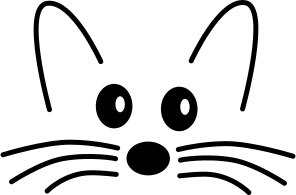
\includegraphics[width=1.4em]{squeak-logo}}}
\iftoshelse{
	\usepackage{marginnote}
		\renewcommand*{\marginfont}{\footnotesize}
	\newcommand{\vartriangleout}{\ifthenelse{\isodd{\thepage}}{\vartriangleright}{\vartriangleleft}}
	\newcommand{\dothisicon}{\fcolorbox{blue!65}{white}{\highlight{$\vartriangleout$}}}
	\newcommand{\dothis}[1]{%
		\noindent\par\noindent
		{\reversemarginpar
			\marginnote{\fcolorbox{blue!65}{white}{\highlight{$\vartriangleout$}}}}
		%\MarginLabel{do this}
		\noindent\emph{#1}
		\nopagebreak}
}{
	\newcommand{\dothisicon}{\raisebox{-.5ex}{
\includegraphics[height=1.2em]{pharo}}}
	\newcommand{\dothis}[1]{%
		\medskip
		\noindent\dothisicon
		\ifx#1\empty\else\quad\emph{#1}\fi
		\par\smallskip\nopagebreak}
}
%===> NEW VERSION <===
% NB: To use this in an individual chapter, you must set:
%\graphicspath{{figures/} {../figures/}}
% at the head of the chapter.  Don't forget the final /
%=============================================================
%:Reader hints (hint)
%
% Indicates a non-obvious consequence
\newcommand{\hint}[1]{\vspace{1ex}\noindent\fbox{\textsc{Hint}} \emph{#1}}
%=================================================================
% graphics for Morphic handles
\newcommand{\grabHandle}{\raisebox{-0.2ex}{
\includegraphics[width=1em]{blackHandle}}}
\newcommand{\moveHandle}{\raisebox{-0.2ex}{
\includegraphics[width=1em]{moveHandle}}}
\newcommand{\debugHandle}{\raisebox{-0.2ex}{
\includegraphics[width=1em]{debugHandle}}}
%=============================================================
%:Highlighting Important stuff (doublebox)
%
% From Seaside book ...
\newsavebox{\SavedText}
\newlength{\InnerBoxRule}\setlength{\InnerBoxRule}{.75\fboxrule}
\newlength{\OuterBoxRule}\setlength{\OuterBoxRule}{1.5\fboxrule}
\newlength{\BoxSeparation}\setlength{\BoxSeparation}{1.5\fboxrule}
\addtolength{\BoxSeparation}{.5pt}
\newlength{\SaveBoxSep}\setlength{\SaveBoxSep}{2\fboxsep}
%
\newenvironment{doublebox}{\begin{lrbox}{\SavedText}
    \begin{minipage}{.75\textwidth}}
    {\end{minipage}\end{lrbox}\begin{center}
    \setlength{\fboxsep}{\BoxSeparation}\setlength{\fboxrule}{\OuterBoxRule}
    \fbox{\setlength{\fboxsep}{\SaveBoxSep}\setlength{\fboxrule}{\InnerBoxRule}%
      \fbox{\usebox{\SavedText}}}
  \end{center}}
% Use this:
\newcommand{\important}[1]{\begin{doublebox}#1\end{doublebox}}
%=============================================================
%:Section depth
\setcounter{secnumdepth}{2}
%% for this to happen start the file with
%\ifx\wholebook\relax\else
%\input{../common.tex}
%\begin{document}
%\fi
% and terminate by
% \ifx\wholebook\relax\else\end{document}\fi

\DeclareGraphicsExtensions{.pdf, .jpg, .png}
%=============================================================
%:PDF setup
\hypersetup{
%   a4paper,
%   pdfstartview=FitV,
%   colorlinks,
%   linkcolor=darkblue,
%   citecolor=darkblue,
   pdftitle={Pharo by Example},
   pdfauthor={Andrew P. Black, St\'ephane Ducasse,	Oscar Nierstrasz,
Damien Pollet},
   pdfkeywords={Smalltalk, Squeak, Object-Oriented Programming, OOP},
   pdfsubject={Computer Science}
}
%=============================================================
%:Page layout and appearance
%
% \renewcommand{\headrulewidth}{0pt}
\renewcommand{\chaptermark}[1]{\markboth{#1}{}}
\renewcommand{\sectionmark}[1]{\markright{\thesection\ #1}}
\renewpagestyle{plain}[\small\itshape]{%
	\setheadrule{0pt}%
	\sethead[][][]{}{}{}%
	\setfoot[][][]{}{}{}}
\renewpagestyle{headings}[\small\itshape]{%
	\setheadrule{0pt}%
	\setmarks{chapter}{section}%
	\sethead[\thepage][][\chaptertitle]{\sectiontitle}{}{\thepage}%
	\setfoot[][][]{}{}{}}
%=============================================================
%:Title section setup and TOC numbering depth
\setcounter{secnumdepth}{1}
\setcounter{tocdepth}{1}
\titleformat{\part}[display]{\centering}{\huge\partname\ \thepart}{1em}{\Huge\textbf}[]
\titleformat{\chapter}[display]{}{\huge\chaptertitlename\ \thechapter}{1em}{\Huge\raggedright\textbf}[]
\titlecontents{part}[3pc]{%
		\pagebreak[2]\addvspace{1em plus.4em minus.2em}%
		\leavevmode\large\bfseries}
	{\contentslabel{3pc}}{\hspace*{-3pc}}
	{}[\nopagebreak]
\titlecontents{chapter}[3pc]{%
		\pagebreak[0]\addvspace{1em plus.2em minus.2em}%
		\leavevmode\bfseries}
	{\contentslabel{3pc}}{}
	{\hfill\contentspage}[\nopagebreak]
\dottedcontents{section}[3pc]{}{3pc}{1pc}
\dottedcontents{subsection}[3pc]{}{0pc}{1pc}
% \dottedcontents{subsection}[4.5em]{}{0pt}{1pc}
% Make \cleardoublepage insert really blank pages http://www.tex.ac.uk/cgi-bin/texfaq2html?label=reallyblank
\let\origdoublepage\cleardoublepage
\newcommand{\clearemptydoublepage}{%
  \clearpage
  {\pagestyle{empty}\origdoublepage}}
\let\cleardoublepage\clearemptydoublepage % see http://www.tex.ac.uk/cgi-bin/texfaq2html?label=patch
%=============================================================
%:FAQ macros (for FAQ chapter)
\newtheorem{faq}{FAQ}
\newcommand{\answer}{\paragraph{Answer}\ }
%=============================================================
%:Listings package configuration
% \newcommand{\caret}{\makebox{\raisebox{0.4ex}{\footnotesize{$\wedge$}}}}
\newcommand{\caret}{\^\,}
\newcommand{\escape}{{\sf \textbackslash}}
\definecolor{source}{gray}{0.95}
\usepackage{listings}
\lstdefinelanguage{Smalltalk}{
%  morekeywords={self,super,true,false,nil,thisContext}, % This is overkill
  morestring=[d]',
  morecomment=[s]{"}{"},
  alsoletter={\#:},
  escapechar={!},
  literate=
    {BANG}{!}1
    {CARET}{\^}1
    {UNDERSCORE}{\_}1
    {\\st}{Smalltalk}9 % convenience -- in case \st occurs in code
    % {'}{{\textquotesingle}}1 % replaced by upquote=true in \lstset
    %{_}{{$\leftarrow$}}1
    {>>>}{{\sep}}1
    %{^}{{$\uparrow$}}1
    {~}{{$\sim$}}1
    {-}{{\texttt{-}}}1 %{\textminus}}1 %{-}{\hspace{-0.13em}}{-}}1  % the goal is to make - the same width as +
    % {+}{\sf+}1 %{\raisebox{0.08ex}{+}}}1      % and to raise + off the baseline to match -
    {-->}{{\quad$\longrightarrow$\quad}}3
    {~->}{{\quad$\leadsto$\quad}}3
	, % Don't forget the comma at the end!
  tabsize=4
}[keywords,comments,strings]

\lstset{language=Smalltalk,
	basicstyle=\sffamily,
	keywordstyle=\color{black}\bfseries,
	% stringstyle=\ttfamily, % Ugly! do we really want this? -- on
	mathescape=true,
	showstringspaces=false,
	keepspaces=true,
	breaklines=true,
	breakautoindent=true,
	backgroundcolor=\color{source},
	lineskip={-1pt}, % Ugly hack
	upquote=true, % straight quote; requires textcomp package
	columns=fullflexible} % no fixed width fonts
% In-line code (literal)
% Normally use this for all in-line code:

\newcommand{\ct}{\lstinline[mathescape=false,backgroundcolor=\color{white},basicstyle={\sffamily\upshape}]}
\newcommand{\cts}[1]{{\sffamily{\upshape{#1}}\xspace}}
% apb 2007.8.28 added the \upshape declaration to avoid getting italicized code in \dothis{ } sections.
% In-line code (latex enabled)
% Use this only in special situations where \ct does not work
% (within section headings ...):
\newcommand{\lct}[1]{{\textsf{\textup{#1}}}}
% Use these for system categories and protocols:
\newcommand{\scat}[1]{\emph{\textsf{#1}}\xspace}
\newcommand{\pkg}[1]{\emph{\textsf{#1}}\xspace}
\newcommand{\prot}[1]{\emph{\textsf{#1}}\xspace}
% Code environments
% NB: the arg is for tests
% Only code and example environments may be tests
\lstnewenvironment{code}[1]{%
	\lstset{%
		% frame=lines,
		frame=single,
		framerule=0pt,
		mathescape=false
	}
}{}
\def\ignoredollar#1{}
%=============================================================
%:Code environments (method, script ...)
% NB: the third arg is for tests
% Only code and example environments may be tests
\lstnewenvironment{example}[3][defaultlabel]{%
	\renewcommand{\lstlistingname}{Example}%
	\lstset{
		% frame=lines,
		frame=single,
		framerule=0pt,
		mathescape=false,
		caption={\emph{#2}},
		label={eg:#1}
	}
}{}
\lstnewenvironment{script}[2][defaultlabel]{%
\renewcommand{\lstlistingname}{Script}%
	\lstset{
		% frame=lines,
		frame=single,
		framerule=0pt,
		mathescape=false,
		name={Script},
		caption={\emph{#2}},
		label={scr:#1}
	}
}{}
\lstnewenvironment{method}[2][defaultlabel]{%
	\renewcommand{\lstlistingname}{Method}%
	\lstset{
		% frame=lines,
		frame=single,
		framerule=0pt,
		mathescape=false,
		name={Method},
		caption={\emph{#2}},
		label={mth:#1}
	}
}{}
\lstnewenvironment{methods}[2][defaultlabel]{% just for multiple methods at once
	\renewcommand{\lstlistingname}{Methods}%
	\lstset{
		% frame=lines,
		frame=single,
		framerule=0pt,
		mathescape=false,
		name={Method},
		caption={\emph{#2}},
		label={mth:#1}
	}
}{}
\lstnewenvironment{numMethod}[2][defaultlabel]{%
	\renewcommand{\lstlistingname}{Method}%
	\lstset{
		numbers=left,
		numberstyle={\tiny\sffamily},
		% frame=lines,
		frame=single,
		framerule=0pt,
		mathescape=false,
		name={Method},
		caption={\emph{#2}},
		label={mth:#1}
	}
}{}
\lstnewenvironment{classdef}[2][defaultlabel]{%
	\renewcommand{\lstlistingname}{Class}%
	\lstset{
		% frame=lines,
		frame=single,
		framerule=0pt,
		mathescape=false,
		name={Class},
		caption={\emph{#2}},
		label={cls:#1}
	}
}{}
%=============================================================
%:Reserving space
% Usually need one more line than the actual lines of code
\newcommand{\needlines}[1]{\Needspace{#1\baselineskip}}
%=============================================================
%:Indexing macros
% Macros ending with "ind" generate text as well as an index entry
% Macros ending with "index" *only* generate an index entry
\newcommand{\ind}[1]{\index{#1}#1\xspace} % plain text
\newcommand{\subind}[2]{\index{#1!#2}#2\xspace} % show #2, subindex under #1
\newcommand{\emphind}[1]{\index{#1}\emph{#1}\xspace} % emph #1
\newcommand{\emphsubind}[2]{\index{#1!#2}\emph{#2}\xspace} % show emph #2, subindex inder #1
\newcommand{\scatind}[1]{\index{#1@\textsf{#1} (category)}\scat{#1}} % category
\newcommand{\pkgind}[1]{\index{#1@\textsf{#1} (package)}\pkg{#1}} % package
\newcommand{\protind}[1]{\index{#1@\textsf{#1} (protocol)}\prot{#1}} % protocol
\newcommand{\clsind}[1]{\index{#1@\textsf{#1} (class)}\ct{#1}\xspace}
% \newcommand{\clsind}[1]{\index{#1!\#@(class)}\ct{#1}\xspace} % class
\newcommand{\clsindplural}[1]{\index{#1!\#@(class)}\ct{#1}s\xspace} % class
\newcommand{\cvind}[1]{\index{#1@\textsf{#1} (class variable)}\ct{#1}\xspace} % class var
\newcommand{\glbind}[1]{\index{#1@\textsf{#1} (global)}\ct{#1}\xspace} % global
\newcommand{\patind}[1]{\index{#1@#1 (pattern)}\ct{#1}\xspace} % pattern
\newcommand{\pvind}[1]{\index{#1@\textsf{#1} (pseudo variable)}\ct{#1}\xspace} % pseudo var
\newcommand{\clsmthind}[2]{\index{#1!#2@\ct{#2}}\ct{#1>>>#2}\xspace} % class + method name
\newcommand{\mthind}[2]{\index{#1!#2@\ct{#2}}\ct{#2}\xspace} % show method name only
\newcommand{\lmthind}[2]{\index{#1!#2@\ct{#2}}\lct{#2}\xspace} % show method name only
\newcommand{\cmind}[2]{\index{#1!#2@\ct{#2}}\ct{#1>>>#2}\xspace} % show class>>method
\newcommand{\lcmind}[2]{\index{#1!#2@\ct{#2}}\lct{#1>>>#2}\xspace} % show class>>method
\newcommand{\toolsflapind}{\index{Tools flap}\toolsflap} % index tools flap
% The following only generate an index entry:
% \newcommand{\clsindex}[1]{\index{#1@\textsf{#1} (class)}}
\newcommand{\clsindex}[1]{\index{#1!\#@(class)}} % class
\newcommand{\mthindex}[2]{\index{#1!#2@\ct{#2}}} % method
\newcommand{\cmindex}[2]{\index{#1!#2@\ct{#2}}} % class>>method
\newcommand{\cvindex}[1]{\index{#1@\textsf{#1} (class variable)}} % class var
\newcommand{\glbindex}[1]{\index{#1@\textsf{#1} (global)}}% global
\newcommand{\pvindex}[1]{\index{#1@\textsf{#1} (pseudo variable)}}% pseudo var
\newcommand{\seeindex}[2]{\index{#1|see{#2}}} % #1, see #2
\newcommand{\scatindex}[1]{\index{#1@\textsf{#1} (category)}} % category
\newcommand{\pkgindex}[1]{\index{#1@\textsf{#1} (package)}} % package
\newcommand{\protindex}[1]{\index{#1@\textsf{#1} (protocol)}} % protocol
% How can we have the main entry page numbers in bold yet not break the hyperlink?
\newcommand{\boldidx}[1]{{\bf #1}} % breaks hyperlink
%\newcommand{\indmain}[1]{\index{#1|boldidx}#1\xspace} % plain text, main entry
%\newcommand{\emphsubindmain}[2]{\index{#1!#2|boldidx}\emph{#2}\xspace} % subindex, main entry
%\newcommand{\subindmain}[2]{\index{#1!#2|boldidx}#2\xspace} % subindex, main entry
%\newcommand{\clsindmain}[1]{\index{#1@\textsf{#1} (class)|boldidx}\ct{#1}\xspace}
%\newcommand{\clsindmain}[1]{\index{#1!\#@(class)|boldidx}\ct{#1}\xspace} % class main
%\newcommand{\indexmain}[1]{\index{#1|boldidx}} % main index entry only
\newcommand{\indmain}[1]{\index{#1}#1\xspace} % The main index entry for this item
\newcommand{\emphsubindmain}[2]{\index{#1!#2}\emph{#2}\xspace} % subindex, main entry
\newcommand{\subindmain}[2]{\index{#1!#2}#2\xspace} % subindex, main entry
%\newcommand{\clsindmain}[1]{\index{#1@\textsf{#1} (class)}\ct{#1}\xspace}
\newcommand{\clsindmain}[1]{\index{#1!\#@(class)}\ct{#1}\xspace} % class main
\newcommand{\clsindexmain}[1]{\index{#1!\#@(class)}} % class main index only
\newcommand{\indexmain}[1]{\index{#1}}
%=============================================================
%:Code macros
% some constants
\newcommand{\codesize}{\small}
\newcommand{\codefont}{\sffamily}
%\newcommand{\cat}[1]{\textit{In category #1}}%%To remove later
\newlength{\scriptindent}
\setlength{\scriptindent}{.3cm}
%% Method presentation constants
\newlength{\methodindent}
\newlength{\methodwordlength}
\newlength{\aftermethod}
\setlength{\methodindent}{0.2cm}
\settowidth{\methodwordlength}{\ M\'ethode\ }
%=============================================================
%:Smalltalk macros
%\newcommand{\sep}{{$\gg$}}
\newcommand{\sep}{\mbox{>>}}
\newcommand{\self}{\lct{self}\xspace}
\newcommand{\super}{\lct{super}\xspace}
\newcommand{\nil}{\lct{nil}\xspace}
%=============================================================
% be less conservative about float placement
% these commands are from http://www.tex.ac.uk/cgi-bin/texfaq2html?label=floats
\renewcommand{\topfraction}{.9}
\renewcommand{\bottomfraction}{.9}
\renewcommand{\textfraction}{.1}
\renewcommand{\floatpagefraction}{.85}
\renewcommand{\dbltopfraction}{.66}
\renewcommand{\dblfloatpagefraction}{.85}
\setcounter{topnumber}{9}
\setcounter{bottomnumber}{9}
\setcounter{totalnumber}{20}
\setcounter{dbltopnumber}{9}
%=============================================================
% Give information from each chapter's author
\newcommand{\contact}[2]{\textbf{#1} \textsf{(#2)}}

\newcommand{\chapterauthor}[1]{\emph{with the participation of:\\#1}\\}
\newcommand{\chapterwritten}[1]{\emph{written by:\\#1}\\}

\newcommand{\authornoury}{\contact{Noury Bouraqadi}{Noury.Bouraqadi@mines-douai.fr}}
\newcommand{\authorluc}{\contact{Luc Fabresse}{Luc.Fabresse@mines-douai.fr}}
\newcommand{\authordamienc}{\contact{Damien Cassou}{damien.cassou@gmail.com}}
\newcommand{\authoroscar}{\contact{Oscar Nierstrasz}{oscar.nierstrasz@acm.org}}
\newcommand{\authorsteph}{\contact{St\'ephane Ducasse}{stephane.ducasse@inria.fr}}
\newcommand{\authoralex}{\contact{Alexandre Bergel}{alexandre@bergel.eu}}
\newcommand{\authorolivier}{\contact{Olivier Auverlot}{olivier.auverlot@inria.fr}}
\newcommand{\authornicolas}{\contact{Nicolas Cellier}{nicolas.cellier.aka.nice@gmail.com}}
\newcommand{\authormarcus}{\contact{Marcus Denker}{marcus.denker@inria.fr}}
\newcommand{\authoralain}{\contact{Alain Plantec}{alain.plantec@univ-brest.fr}}
\newcommand{\authordale}{\contact{Dale Henrichs}{dale.henrichs@gemstone.com}}
\newcommand{\authormariano}{\contact{Mariano Martinez Peck}{marianopeck@gmail.com}}
\newcommand{\authorsven}{\contact{Sven Van Caekenberghe}{sven@beta9.be}}
\newcommand{\authorlukas}{\contact{Lukas Renggli}{renggli@gmail.com}}
\newcommand{\authorjankurs}{\contact{Jan Kurs}{kurs@iam.unibe.ch}}
\newcommand{\authorguillaume}{\contact{Guillaume Larcheveque}{guillaume.larcheveque@gmail.com}}
\newcommand{\authorguillep}{\contact{Guillermo Polito}{guillermopolito@gmail.com}}
\newcommand{\authorclement}{\contact{Cl\'ement Bera}{bera.clement@gmail.com}}
\newcommand{\authormax}{\contact{Max Leske}{maxleske@gmail.com}}
\newcommand{\authorvanessa}{\contact{Vanessa Pe\~{n}a-Araya}{van.c.pena@gmail.com}}
\newcommand{\authorcamillo}{\contact{Camillo Bruni}{camillobruni@gmail.com}}

%=============================================================
% apb doesn't like paragraphs to run in to each other without a break
\parskip 1ex
%=============================================================
%:Stuff to check, merge or deprecate
%\setlength{\marginparsep}{2mm}
%\renewcommand{\baselinestretch}{1.1}
%=============================================================
\usepackage{tikz}

%\begin{document}
%\fi
% and terminate by
% \ifx\wholebook\relax\else\end{document}\fi

\DeclareGraphicsExtensions{.pdf, .jpg, .png}
%=============================================================
%:PDF setup
\hypersetup{
%   a4paper,
%   pdfstartview=FitV,
%   colorlinks,
%   linkcolor=darkblue,
%   citecolor=darkblue,
   pdftitle={Pharo by Example},
   pdfauthor={Andrew P. Black, St\'ephane Ducasse,	Oscar Nierstrasz,
Damien Pollet},
   pdfkeywords={Smalltalk, Squeak, Object-Oriented Programming, OOP},
   pdfsubject={Computer Science}
}
%=============================================================
%:Page layout and appearance
%
% \renewcommand{\headrulewidth}{0pt}
\renewcommand{\chaptermark}[1]{\markboth{#1}{}}
\renewcommand{\sectionmark}[1]{\markright{\thesection\ #1}}
\renewpagestyle{plain}[\small\itshape]{%
	\setheadrule{0pt}%
	\sethead[][][]{}{}{}%
	\setfoot[][][]{}{}{}}
\renewpagestyle{headings}[\small\itshape]{%
	\setheadrule{0pt}%
	\setmarks{chapter}{section}%
	\sethead[\thepage][][\chaptertitle]{\sectiontitle}{}{\thepage}%
	\setfoot[][][]{}{}{}}
%=============================================================
%:Title section setup and TOC numbering depth
\setcounter{secnumdepth}{1}
\setcounter{tocdepth}{1}
\titleformat{\part}[display]{\centering}{\huge\partname\ \thepart}{1em}{\Huge\textbf}[]
\titleformat{\chapter}[display]{}{\huge\chaptertitlename\ \thechapter}{1em}{\Huge\raggedright\textbf}[]
\titlecontents{part}[3pc]{%
		\pagebreak[2]\addvspace{1em plus.4em minus.2em}%
		\leavevmode\large\bfseries}
	{\contentslabel{3pc}}{\hspace*{-3pc}}
	{}[\nopagebreak]
\titlecontents{chapter}[3pc]{%
		\pagebreak[0]\addvspace{1em plus.2em minus.2em}%
		\leavevmode\bfseries}
	{\contentslabel{3pc}}{}
	{\hfill\contentspage}[\nopagebreak]
\dottedcontents{section}[3pc]{}{3pc}{1pc}
\dottedcontents{subsection}[3pc]{}{0pc}{1pc}
% \dottedcontents{subsection}[4.5em]{}{0pt}{1pc}
% Make \cleardoublepage insert really blank pages http://www.tex.ac.uk/cgi-bin/texfaq2html?label=reallyblank
\let\origdoublepage\cleardoublepage
\newcommand{\clearemptydoublepage}{%
  \clearpage
  {\pagestyle{empty}\origdoublepage}}
\let\cleardoublepage\clearemptydoublepage % see http://www.tex.ac.uk/cgi-bin/texfaq2html?label=patch
%=============================================================
%:FAQ macros (for FAQ chapter)
\newtheorem{faq}{FAQ}
\newcommand{\answer}{\paragraph{Answer}\ }
%=============================================================
%:Listings package configuration
% \newcommand{\caret}{\makebox{\raisebox{0.4ex}{\footnotesize{$\wedge$}}}}
\newcommand{\caret}{\^\,}
\newcommand{\escape}{{\sf \textbackslash}}
\definecolor{source}{gray}{0.95}
\usepackage{listings}
\lstdefinelanguage{Smalltalk}{
%  morekeywords={self,super,true,false,nil,thisContext}, % This is overkill
  morestring=[d]',
  morecomment=[s]{"}{"},
  alsoletter={\#:},
  escapechar={!},
  literate=
    {BANG}{!}1
    {CARET}{\^}1
    {UNDERSCORE}{\_}1
    {\\st}{Smalltalk}9 % convenience -- in case \st occurs in code
    % {'}{{\textquotesingle}}1 % replaced by upquote=true in \lstset
    %{_}{{$\leftarrow$}}1
    {>>>}{{\sep}}1
    %{^}{{$\uparrow$}}1
    {~}{{$\sim$}}1
    {-}{{\texttt{-}}}1 %{\textminus}}1 %{-}{\hspace{-0.13em}}{-}}1  % the goal is to make - the same width as +
    % {+}{\sf+}1 %{\raisebox{0.08ex}{+}}}1      % and to raise + off the baseline to match -
    {-->}{{\quad$\longrightarrow$\quad}}3
    {~->}{{\quad$\leadsto$\quad}}3
	, % Don't forget the comma at the end!
  tabsize=4
}[keywords,comments,strings]

\lstset{language=Smalltalk,
	basicstyle=\sffamily,
	keywordstyle=\color{black}\bfseries,
	% stringstyle=\ttfamily, % Ugly! do we really want this? -- on
	mathescape=true,
	showstringspaces=false,
	keepspaces=true,
	breaklines=true,
	breakautoindent=true,
	backgroundcolor=\color{source},
	lineskip={-1pt}, % Ugly hack
	upquote=true, % straight quote; requires textcomp package
	columns=fullflexible} % no fixed width fonts
% In-line code (literal)
% Normally use this for all in-line code:

\newcommand{\ct}{\lstinline[mathescape=false,backgroundcolor=\color{white},basicstyle={\sffamily\upshape}]}
\newcommand{\cts}[1]{{\sffamily{\upshape{#1}}\xspace}}
% apb 2007.8.28 added the \upshape declaration to avoid getting italicized code in \dothis{ } sections.
% In-line code (latex enabled)
% Use this only in special situations where \ct does not work
% (within section headings ...):
\newcommand{\lct}[1]{{\textsf{\textup{#1}}}}
% Use these for system categories and protocols:
\newcommand{\scat}[1]{\emph{\textsf{#1}}\xspace}
\newcommand{\pkg}[1]{\emph{\textsf{#1}}\xspace}
\newcommand{\prot}[1]{\emph{\textsf{#1}}\xspace}
% Code environments
% NB: the arg is for tests
% Only code and example environments may be tests
\lstnewenvironment{code}[1]{%
	\lstset{%
		% frame=lines,
		frame=single,
		framerule=0pt,
		mathescape=false
	}
}{}
\def\ignoredollar#1{}
%=============================================================
%:Code environments (method, script ...)
% NB: the third arg is for tests
% Only code and example environments may be tests
\lstnewenvironment{example}[3][defaultlabel]{%
	\renewcommand{\lstlistingname}{Example}%
	\lstset{
		% frame=lines,
		frame=single,
		framerule=0pt,
		mathescape=false,
		caption={\emph{#2}},
		label={eg:#1}
	}
}{}
\lstnewenvironment{script}[2][defaultlabel]{%
\renewcommand{\lstlistingname}{Script}%
	\lstset{
		% frame=lines,
		frame=single,
		framerule=0pt,
		mathescape=false,
		name={Script},
		caption={\emph{#2}},
		label={scr:#1}
	}
}{}
\lstnewenvironment{method}[2][defaultlabel]{%
	\renewcommand{\lstlistingname}{Method}%
	\lstset{
		% frame=lines,
		frame=single,
		framerule=0pt,
		mathescape=false,
		name={Method},
		caption={\emph{#2}},
		label={mth:#1}
	}
}{}
\lstnewenvironment{methods}[2][defaultlabel]{% just for multiple methods at once
	\renewcommand{\lstlistingname}{Methods}%
	\lstset{
		% frame=lines,
		frame=single,
		framerule=0pt,
		mathescape=false,
		name={Method},
		caption={\emph{#2}},
		label={mth:#1}
	}
}{}
\lstnewenvironment{numMethod}[2][defaultlabel]{%
	\renewcommand{\lstlistingname}{Method}%
	\lstset{
		numbers=left,
		numberstyle={\tiny\sffamily},
		% frame=lines,
		frame=single,
		framerule=0pt,
		mathescape=false,
		name={Method},
		caption={\emph{#2}},
		label={mth:#1}
	}
}{}
\lstnewenvironment{classdef}[2][defaultlabel]{%
	\renewcommand{\lstlistingname}{Class}%
	\lstset{
		% frame=lines,
		frame=single,
		framerule=0pt,
		mathescape=false,
		name={Class},
		caption={\emph{#2}},
		label={cls:#1}
	}
}{}
%=============================================================
%:Reserving space
% Usually need one more line than the actual lines of code
\newcommand{\needlines}[1]{\Needspace{#1\baselineskip}}
%=============================================================
%:Indexing macros
% Macros ending with "ind" generate text as well as an index entry
% Macros ending with "index" *only* generate an index entry
\newcommand{\ind}[1]{\index{#1}#1\xspace} % plain text
\newcommand{\subind}[2]{\index{#1!#2}#2\xspace} % show #2, subindex under #1
\newcommand{\emphind}[1]{\index{#1}\emph{#1}\xspace} % emph #1
\newcommand{\emphsubind}[2]{\index{#1!#2}\emph{#2}\xspace} % show emph #2, subindex inder #1
\newcommand{\scatind}[1]{\index{#1@\textsf{#1} (category)}\scat{#1}} % category
\newcommand{\pkgind}[1]{\index{#1@\textsf{#1} (package)}\pkg{#1}} % package
\newcommand{\protind}[1]{\index{#1@\textsf{#1} (protocol)}\prot{#1}} % protocol
\newcommand{\clsind}[1]{\index{#1@\textsf{#1} (class)}\ct{#1}\xspace}
% \newcommand{\clsind}[1]{\index{#1!\#@(class)}\ct{#1}\xspace} % class
\newcommand{\clsindplural}[1]{\index{#1!\#@(class)}\ct{#1}s\xspace} % class
\newcommand{\cvind}[1]{\index{#1@\textsf{#1} (class variable)}\ct{#1}\xspace} % class var
\newcommand{\glbind}[1]{\index{#1@\textsf{#1} (global)}\ct{#1}\xspace} % global
\newcommand{\patind}[1]{\index{#1@#1 (pattern)}\ct{#1}\xspace} % pattern
\newcommand{\pvind}[1]{\index{#1@\textsf{#1} (pseudo variable)}\ct{#1}\xspace} % pseudo var
\newcommand{\clsmthind}[2]{\index{#1!#2@\ct{#2}}\ct{#1>>>#2}\xspace} % class + method name
\newcommand{\mthind}[2]{\index{#1!#2@\ct{#2}}\ct{#2}\xspace} % show method name only
\newcommand{\lmthind}[2]{\index{#1!#2@\ct{#2}}\lct{#2}\xspace} % show method name only
\newcommand{\cmind}[2]{\index{#1!#2@\ct{#2}}\ct{#1>>>#2}\xspace} % show class>>method
\newcommand{\lcmind}[2]{\index{#1!#2@\ct{#2}}\lct{#1>>>#2}\xspace} % show class>>method
\newcommand{\toolsflapind}{\index{Tools flap}\toolsflap} % index tools flap
% The following only generate an index entry:
% \newcommand{\clsindex}[1]{\index{#1@\textsf{#1} (class)}}
\newcommand{\clsindex}[1]{\index{#1!\#@(class)}} % class
\newcommand{\mthindex}[2]{\index{#1!#2@\ct{#2}}} % method
\newcommand{\cmindex}[2]{\index{#1!#2@\ct{#2}}} % class>>method
\newcommand{\cvindex}[1]{\index{#1@\textsf{#1} (class variable)}} % class var
\newcommand{\glbindex}[1]{\index{#1@\textsf{#1} (global)}}% global
\newcommand{\pvindex}[1]{\index{#1@\textsf{#1} (pseudo variable)}}% pseudo var
\newcommand{\seeindex}[2]{\index{#1|see{#2}}} % #1, see #2
\newcommand{\scatindex}[1]{\index{#1@\textsf{#1} (category)}} % category
\newcommand{\pkgindex}[1]{\index{#1@\textsf{#1} (package)}} % package
\newcommand{\protindex}[1]{\index{#1@\textsf{#1} (protocol)}} % protocol
% How can we have the main entry page numbers in bold yet not break the hyperlink?
\newcommand{\boldidx}[1]{{\bf #1}} % breaks hyperlink
%\newcommand{\indmain}[1]{\index{#1|boldidx}#1\xspace} % plain text, main entry
%\newcommand{\emphsubindmain}[2]{\index{#1!#2|boldidx}\emph{#2}\xspace} % subindex, main entry
%\newcommand{\subindmain}[2]{\index{#1!#2|boldidx}#2\xspace} % subindex, main entry
%\newcommand{\clsindmain}[1]{\index{#1@\textsf{#1} (class)|boldidx}\ct{#1}\xspace}
%\newcommand{\clsindmain}[1]{\index{#1!\#@(class)|boldidx}\ct{#1}\xspace} % class main
%\newcommand{\indexmain}[1]{\index{#1|boldidx}} % main index entry only
\newcommand{\indmain}[1]{\index{#1}#1\xspace} % The main index entry for this item
\newcommand{\emphsubindmain}[2]{\index{#1!#2}\emph{#2}\xspace} % subindex, main entry
\newcommand{\subindmain}[2]{\index{#1!#2}#2\xspace} % subindex, main entry
%\newcommand{\clsindmain}[1]{\index{#1@\textsf{#1} (class)}\ct{#1}\xspace}
\newcommand{\clsindmain}[1]{\index{#1!\#@(class)}\ct{#1}\xspace} % class main
\newcommand{\clsindexmain}[1]{\index{#1!\#@(class)}} % class main index only
\newcommand{\indexmain}[1]{\index{#1}}
%=============================================================
%:Code macros
% some constants
\newcommand{\codesize}{\small}
\newcommand{\codefont}{\sffamily}
%\newcommand{\cat}[1]{\textit{In category #1}}%%To remove later
\newlength{\scriptindent}
\setlength{\scriptindent}{.3cm}
%% Method presentation constants
\newlength{\methodindent}
\newlength{\methodwordlength}
\newlength{\aftermethod}
\setlength{\methodindent}{0.2cm}
\settowidth{\methodwordlength}{\ M\'ethode\ }
%=============================================================
%:Smalltalk macros
%\newcommand{\sep}{{$\gg$}}
\newcommand{\sep}{\mbox{>>}}
\newcommand{\self}{\lct{self}\xspace}
\newcommand{\super}{\lct{super}\xspace}
\newcommand{\nil}{\lct{nil}\xspace}
%=============================================================
% be less conservative about float placement
% these commands are from http://www.tex.ac.uk/cgi-bin/texfaq2html?label=floats
\renewcommand{\topfraction}{.9}
\renewcommand{\bottomfraction}{.9}
\renewcommand{\textfraction}{.1}
\renewcommand{\floatpagefraction}{.85}
\renewcommand{\dbltopfraction}{.66}
\renewcommand{\dblfloatpagefraction}{.85}
\setcounter{topnumber}{9}
\setcounter{bottomnumber}{9}
\setcounter{totalnumber}{20}
\setcounter{dbltopnumber}{9}
%=============================================================
% Give information from each chapter's author
\newcommand{\contact}[2]{\textbf{#1} \textsf{(#2)}}

\newcommand{\chapterauthor}[1]{\emph{with the participation of:\\#1}\\}
\newcommand{\chapterwritten}[1]{\emph{written by:\\#1}\\}

\newcommand{\authornoury}{\contact{Noury Bouraqadi}{Noury.Bouraqadi@mines-douai.fr}}
\newcommand{\authorluc}{\contact{Luc Fabresse}{Luc.Fabresse@mines-douai.fr}}
\newcommand{\authordamienc}{\contact{Damien Cassou}{damien.cassou@gmail.com}}
\newcommand{\authoroscar}{\contact{Oscar Nierstrasz}{oscar.nierstrasz@acm.org}}
\newcommand{\authorsteph}{\contact{St\'ephane Ducasse}{stephane.ducasse@inria.fr}}
\newcommand{\authoralex}{\contact{Alexandre Bergel}{alexandre@bergel.eu}}
\newcommand{\authorolivier}{\contact{Olivier Auverlot}{olivier.auverlot@inria.fr}}
\newcommand{\authornicolas}{\contact{Nicolas Cellier}{nicolas.cellier.aka.nice@gmail.com}}
\newcommand{\authormarcus}{\contact{Marcus Denker}{marcus.denker@inria.fr}}
\newcommand{\authoralain}{\contact{Alain Plantec}{alain.plantec@univ-brest.fr}}
\newcommand{\authordale}{\contact{Dale Henrichs}{dale.henrichs@gemstone.com}}
\newcommand{\authormariano}{\contact{Mariano Martinez Peck}{marianopeck@gmail.com}}
\newcommand{\authorsven}{\contact{Sven Van Caekenberghe}{sven@beta9.be}}
\newcommand{\authorlukas}{\contact{Lukas Renggli}{renggli@gmail.com}}
\newcommand{\authorjankurs}{\contact{Jan Kurs}{kurs@iam.unibe.ch}}
\newcommand{\authorguillaume}{\contact{Guillaume Larcheveque}{guillaume.larcheveque@gmail.com}}
\newcommand{\authorguillep}{\contact{Guillermo Polito}{guillermopolito@gmail.com}}
\newcommand{\authorclement}{\contact{Cl\'ement Bera}{bera.clement@gmail.com}}
\newcommand{\authormax}{\contact{Max Leske}{maxleske@gmail.com}}
\newcommand{\authorvanessa}{\contact{Vanessa Pe\~{n}a-Araya}{van.c.pena@gmail.com}}
\newcommand{\authorcamillo}{\contact{Camillo Bruni}{camillobruni@gmail.com}}

%=============================================================
% apb doesn't like paragraphs to run in to each other without a break
\parskip 1ex
%=============================================================
%:Stuff to check, merge or deprecate
%\setlength{\marginparsep}{2mm}
%\renewcommand{\baselinestretch}{1.1}
%=============================================================
\usepackage{tikz}

%\begin{document}
%\fi
% and terminate by
% \ifx\wholebook\relax\else\end{document}\fi

\DeclareGraphicsExtensions{.pdf, .jpg, .png}
%=============================================================
%:PDF setup
\hypersetup{
%   a4paper,
%   pdfstartview=FitV,
%   colorlinks,
%   linkcolor=darkblue,
%   citecolor=darkblue,
   pdftitle={Pharo by Example},
   pdfauthor={Andrew P. Black, St\'ephane Ducasse,	Oscar Nierstrasz,
Damien Pollet},
   pdfkeywords={Smalltalk, Squeak, Object-Oriented Programming, OOP},
   pdfsubject={Computer Science}
}
%=============================================================
%:Page layout and appearance
%
% \renewcommand{\headrulewidth}{0pt}
\renewcommand{\chaptermark}[1]{\markboth{#1}{}}
\renewcommand{\sectionmark}[1]{\markright{\thesection\ #1}}
\renewpagestyle{plain}[\small\itshape]{%
	\setheadrule{0pt}%
	\sethead[][][]{}{}{}%
	\setfoot[][][]{}{}{}}
\renewpagestyle{headings}[\small\itshape]{%
	\setheadrule{0pt}%
	\setmarks{chapter}{section}%
	\sethead[\thepage][][\chaptertitle]{\sectiontitle}{}{\thepage}%
	\setfoot[][][]{}{}{}}
%=============================================================
%:Title section setup and TOC numbering depth
\setcounter{secnumdepth}{1}
\setcounter{tocdepth}{1}
\titleformat{\part}[display]{\centering}{\huge\partname\ \thepart}{1em}{\Huge\textbf}[]
\titleformat{\chapter}[display]{}{\huge\chaptertitlename\ \thechapter}{1em}{\Huge\raggedright\textbf}[]
\titlecontents{part}[3pc]{%
		\pagebreak[2]\addvspace{1em plus.4em minus.2em}%
		\leavevmode\large\bfseries}
	{\contentslabel{3pc}}{\hspace*{-3pc}}
	{}[\nopagebreak]
\titlecontents{chapter}[3pc]{%
		\pagebreak[0]\addvspace{1em plus.2em minus.2em}%
		\leavevmode\bfseries}
	{\contentslabel{3pc}}{}
	{\hfill\contentspage}[\nopagebreak]
\dottedcontents{section}[3pc]{}{3pc}{1pc}
\dottedcontents{subsection}[3pc]{}{0pc}{1pc}
% \dottedcontents{subsection}[4.5em]{}{0pt}{1pc}
% Make \cleardoublepage insert really blank pages http://www.tex.ac.uk/cgi-bin/texfaq2html?label=reallyblank
\let\origdoublepage\cleardoublepage
\newcommand{\clearemptydoublepage}{%
  \clearpage
  {\pagestyle{empty}\origdoublepage}}
\let\cleardoublepage\clearemptydoublepage % see http://www.tex.ac.uk/cgi-bin/texfaq2html?label=patch
%=============================================================
%:FAQ macros (for FAQ chapter)
\newtheorem{faq}{FAQ}
\newcommand{\answer}{\paragraph{Answer}\ }
%=============================================================
%:Listings package configuration
% \newcommand{\caret}{\makebox{\raisebox{0.4ex}{\footnotesize{$\wedge$}}}}
\newcommand{\caret}{\^\,}
\newcommand{\escape}{{\sf \textbackslash}}
\definecolor{source}{gray}{0.95}
\usepackage{listings}
\lstdefinelanguage{Smalltalk}{
%  morekeywords={self,super,true,false,nil,thisContext}, % This is overkill
  morestring=[d]',
  morecomment=[s]{"}{"},
  alsoletter={\#:},
  escapechar={!},
  literate=
    {BANG}{!}1
    {CARET}{\^}1
    {UNDERSCORE}{\_}1
    {\\st}{Smalltalk}9 % convenience -- in case \st occurs in code
    % {'}{{\textquotesingle}}1 % replaced by upquote=true in \lstset
    %{_}{{$\leftarrow$}}1
    {>>>}{{\sep}}1
    %{^}{{$\uparrow$}}1
    {~}{{$\sim$}}1
    {-}{{\texttt{-}}}1 %{\textminus}}1 %{-}{\hspace{-0.13em}}{-}}1  % the goal is to make - the same width as +
    % {+}{\sf+}1 %{\raisebox{0.08ex}{+}}}1      % and to raise + off the baseline to match -
    {-->}{{\quad$\longrightarrow$\quad}}3
    {~->}{{\quad$\leadsto$\quad}}3
	, % Don't forget the comma at the end!
  tabsize=4
}[keywords,comments,strings]

\lstset{language=Smalltalk,
	basicstyle=\sffamily,
	keywordstyle=\color{black}\bfseries,
	% stringstyle=\ttfamily, % Ugly! do we really want this? -- on
	mathescape=true,
	showstringspaces=false,
	keepspaces=true,
	breaklines=true,
	breakautoindent=true,
	backgroundcolor=\color{source},
	lineskip={-1pt}, % Ugly hack
	upquote=true, % straight quote; requires textcomp package
	columns=fullflexible} % no fixed width fonts
% In-line code (literal)
% Normally use this for all in-line code:

\newcommand{\ct}{\lstinline[mathescape=false,backgroundcolor=\color{white},basicstyle={\sffamily\upshape}]}
\newcommand{\cts}[1]{{\sffamily{\upshape{#1}}\xspace}}
% apb 2007.8.28 added the \upshape declaration to avoid getting italicized code in \dothis{ } sections.
% In-line code (latex enabled)
% Use this only in special situations where \ct does not work
% (within section headings ...):
\newcommand{\lct}[1]{{\textsf{\textup{#1}}}}
% Use these for system categories and protocols:
\newcommand{\scat}[1]{\emph{\textsf{#1}}\xspace}
\newcommand{\pkg}[1]{\emph{\textsf{#1}}\xspace}
\newcommand{\prot}[1]{\emph{\textsf{#1}}\xspace}
% Code environments
% NB: the arg is for tests
% Only code and example environments may be tests
\lstnewenvironment{code}[1]{%
	\lstset{%
		% frame=lines,
		frame=single,
		framerule=0pt,
		mathescape=false
	}
}{}
\def\ignoredollar#1{}
%=============================================================
%:Code environments (method, script ...)
% NB: the third arg is for tests
% Only code and example environments may be tests
\lstnewenvironment{example}[3][defaultlabel]{%
	\renewcommand{\lstlistingname}{Example}%
	\lstset{
		% frame=lines,
		frame=single,
		framerule=0pt,
		mathescape=false,
		caption={\emph{#2}},
		label={eg:#1}
	}
}{}
\lstnewenvironment{script}[2][defaultlabel]{%
\renewcommand{\lstlistingname}{Script}%
	\lstset{
		% frame=lines,
		frame=single,
		framerule=0pt,
		mathescape=false,
		name={Script},
		caption={\emph{#2}},
		label={scr:#1}
	}
}{}
\lstnewenvironment{method}[2][defaultlabel]{%
	\renewcommand{\lstlistingname}{Method}%
	\lstset{
		% frame=lines,
		frame=single,
		framerule=0pt,
		mathescape=false,
		name={Method},
		caption={\emph{#2}},
		label={mth:#1}
	}
}{}
\lstnewenvironment{methods}[2][defaultlabel]{% just for multiple methods at once
	\renewcommand{\lstlistingname}{Methods}%
	\lstset{
		% frame=lines,
		frame=single,
		framerule=0pt,
		mathescape=false,
		name={Method},
		caption={\emph{#2}},
		label={mth:#1}
	}
}{}
\lstnewenvironment{numMethod}[2][defaultlabel]{%
	\renewcommand{\lstlistingname}{Method}%
	\lstset{
		numbers=left,
		numberstyle={\tiny\sffamily},
		% frame=lines,
		frame=single,
		framerule=0pt,
		mathescape=false,
		name={Method},
		caption={\emph{#2}},
		label={mth:#1}
	}
}{}
\lstnewenvironment{classdef}[2][defaultlabel]{%
	\renewcommand{\lstlistingname}{Class}%
	\lstset{
		% frame=lines,
		frame=single,
		framerule=0pt,
		mathescape=false,
		name={Class},
		caption={\emph{#2}},
		label={cls:#1}
	}
}{}
%=============================================================
%:Reserving space
% Usually need one more line than the actual lines of code
\newcommand{\needlines}[1]{\Needspace{#1\baselineskip}}
%=============================================================
%:Indexing macros
% Macros ending with "ind" generate text as well as an index entry
% Macros ending with "index" *only* generate an index entry
\newcommand{\ind}[1]{\index{#1}#1\xspace} % plain text
\newcommand{\subind}[2]{\index{#1!#2}#2\xspace} % show #2, subindex under #1
\newcommand{\emphind}[1]{\index{#1}\emph{#1}\xspace} % emph #1
\newcommand{\emphsubind}[2]{\index{#1!#2}\emph{#2}\xspace} % show emph #2, subindex inder #1
\newcommand{\scatind}[1]{\index{#1@\textsf{#1} (category)}\scat{#1}} % category
\newcommand{\pkgind}[1]{\index{#1@\textsf{#1} (package)}\pkg{#1}} % package
\newcommand{\protind}[1]{\index{#1@\textsf{#1} (protocol)}\prot{#1}} % protocol
\newcommand{\clsind}[1]{\index{#1@\textsf{#1} (class)}\ct{#1}\xspace}
% \newcommand{\clsind}[1]{\index{#1!\#@(class)}\ct{#1}\xspace} % class
\newcommand{\clsindplural}[1]{\index{#1!\#@(class)}\ct{#1}s\xspace} % class
\newcommand{\cvind}[1]{\index{#1@\textsf{#1} (class variable)}\ct{#1}\xspace} % class var
\newcommand{\glbind}[1]{\index{#1@\textsf{#1} (global)}\ct{#1}\xspace} % global
\newcommand{\patind}[1]{\index{#1@#1 (pattern)}\ct{#1}\xspace} % pattern
\newcommand{\pvind}[1]{\index{#1@\textsf{#1} (pseudo variable)}\ct{#1}\xspace} % pseudo var
\newcommand{\clsmthind}[2]{\index{#1!#2@\ct{#2}}\ct{#1>>>#2}\xspace} % class + method name
\newcommand{\mthind}[2]{\index{#1!#2@\ct{#2}}\ct{#2}\xspace} % show method name only
\newcommand{\lmthind}[2]{\index{#1!#2@\ct{#2}}\lct{#2}\xspace} % show method name only
\newcommand{\cmind}[2]{\index{#1!#2@\ct{#2}}\ct{#1>>>#2}\xspace} % show class>>method
\newcommand{\lcmind}[2]{\index{#1!#2@\ct{#2}}\lct{#1>>>#2}\xspace} % show class>>method
\newcommand{\toolsflapind}{\index{Tools flap}\toolsflap} % index tools flap
% The following only generate an index entry:
% \newcommand{\clsindex}[1]{\index{#1@\textsf{#1} (class)}}
\newcommand{\clsindex}[1]{\index{#1!\#@(class)}} % class
\newcommand{\mthindex}[2]{\index{#1!#2@\ct{#2}}} % method
\newcommand{\cmindex}[2]{\index{#1!#2@\ct{#2}}} % class>>method
\newcommand{\cvindex}[1]{\index{#1@\textsf{#1} (class variable)}} % class var
\newcommand{\glbindex}[1]{\index{#1@\textsf{#1} (global)}}% global
\newcommand{\pvindex}[1]{\index{#1@\textsf{#1} (pseudo variable)}}% pseudo var
\newcommand{\seeindex}[2]{\index{#1|see{#2}}} % #1, see #2
\newcommand{\scatindex}[1]{\index{#1@\textsf{#1} (category)}} % category
\newcommand{\pkgindex}[1]{\index{#1@\textsf{#1} (package)}} % package
\newcommand{\protindex}[1]{\index{#1@\textsf{#1} (protocol)}} % protocol
% How can we have the main entry page numbers in bold yet not break the hyperlink?
\newcommand{\boldidx}[1]{{\bf #1}} % breaks hyperlink
%\newcommand{\indmain}[1]{\index{#1|boldidx}#1\xspace} % plain text, main entry
%\newcommand{\emphsubindmain}[2]{\index{#1!#2|boldidx}\emph{#2}\xspace} % subindex, main entry
%\newcommand{\subindmain}[2]{\index{#1!#2|boldidx}#2\xspace} % subindex, main entry
%\newcommand{\clsindmain}[1]{\index{#1@\textsf{#1} (class)|boldidx}\ct{#1}\xspace}
%\newcommand{\clsindmain}[1]{\index{#1!\#@(class)|boldidx}\ct{#1}\xspace} % class main
%\newcommand{\indexmain}[1]{\index{#1|boldidx}} % main index entry only
\newcommand{\indmain}[1]{\index{#1}#1\xspace} % The main index entry for this item
\newcommand{\emphsubindmain}[2]{\index{#1!#2}\emph{#2}\xspace} % subindex, main entry
\newcommand{\subindmain}[2]{\index{#1!#2}#2\xspace} % subindex, main entry
%\newcommand{\clsindmain}[1]{\index{#1@\textsf{#1} (class)}\ct{#1}\xspace}
\newcommand{\clsindmain}[1]{\index{#1!\#@(class)}\ct{#1}\xspace} % class main
\newcommand{\clsindexmain}[1]{\index{#1!\#@(class)}} % class main index only
\newcommand{\indexmain}[1]{\index{#1}}
%=============================================================
%:Code macros
% some constants
\newcommand{\codesize}{\small}
\newcommand{\codefont}{\sffamily}
%\newcommand{\cat}[1]{\textit{In category #1}}%%To remove later
\newlength{\scriptindent}
\setlength{\scriptindent}{.3cm}
%% Method presentation constants
\newlength{\methodindent}
\newlength{\methodwordlength}
\newlength{\aftermethod}
\setlength{\methodindent}{0.2cm}
\settowidth{\methodwordlength}{\ M\'ethode\ }
%=============================================================
%:Smalltalk macros
%\newcommand{\sep}{{$\gg$}}
\newcommand{\sep}{\mbox{>>}}
\newcommand{\self}{\lct{self}\xspace}
\newcommand{\super}{\lct{super}\xspace}
\newcommand{\nil}{\lct{nil}\xspace}
%=============================================================
% be less conservative about float placement
% these commands are from http://www.tex.ac.uk/cgi-bin/texfaq2html?label=floats
\renewcommand{\topfraction}{.9}
\renewcommand{\bottomfraction}{.9}
\renewcommand{\textfraction}{.1}
\renewcommand{\floatpagefraction}{.85}
\renewcommand{\dbltopfraction}{.66}
\renewcommand{\dblfloatpagefraction}{.85}
\setcounter{topnumber}{9}
\setcounter{bottomnumber}{9}
\setcounter{totalnumber}{20}
\setcounter{dbltopnumber}{9}
%=============================================================
% Give information from each chapter's author
\newcommand{\contact}[2]{\textbf{#1} \textsf{(#2)}}

\newcommand{\chapterauthor}[1]{\emph{with the participation of:\\#1}\\}
\newcommand{\chapterwritten}[1]{\emph{written by:\\#1}\\}

\newcommand{\authornoury}{\contact{Noury Bouraqadi}{Noury.Bouraqadi@mines-douai.fr}}
\newcommand{\authorluc}{\contact{Luc Fabresse}{Luc.Fabresse@mines-douai.fr}}
\newcommand{\authordamienc}{\contact{Damien Cassou}{damien.cassou@gmail.com}}
\newcommand{\authoroscar}{\contact{Oscar Nierstrasz}{oscar.nierstrasz@acm.org}}
\newcommand{\authorsteph}{\contact{St\'ephane Ducasse}{stephane.ducasse@inria.fr}}
\newcommand{\authoralex}{\contact{Alexandre Bergel}{alexandre@bergel.eu}}
\newcommand{\authorolivier}{\contact{Olivier Auverlot}{olivier.auverlot@inria.fr}}
\newcommand{\authornicolas}{\contact{Nicolas Cellier}{nicolas.cellier.aka.nice@gmail.com}}
\newcommand{\authormarcus}{\contact{Marcus Denker}{marcus.denker@inria.fr}}
\newcommand{\authoralain}{\contact{Alain Plantec}{alain.plantec@univ-brest.fr}}
\newcommand{\authordale}{\contact{Dale Henrichs}{dale.henrichs@gemstone.com}}
\newcommand{\authormariano}{\contact{Mariano Martinez Peck}{marianopeck@gmail.com}}
\newcommand{\authorsven}{\contact{Sven Van Caekenberghe}{sven@beta9.be}}
\newcommand{\authorlukas}{\contact{Lukas Renggli}{renggli@gmail.com}}
\newcommand{\authorjankurs}{\contact{Jan Kurs}{kurs@iam.unibe.ch}}
\newcommand{\authorguillaume}{\contact{Guillaume Larcheveque}{guillaume.larcheveque@gmail.com}}
\newcommand{\authorguillep}{\contact{Guillermo Polito}{guillermopolito@gmail.com}}
\newcommand{\authorclement}{\contact{Cl\'ement Bera}{bera.clement@gmail.com}}
\newcommand{\authormax}{\contact{Max Leske}{maxleske@gmail.com}}
\newcommand{\authorvanessa}{\contact{Vanessa Pe\~{n}a-Araya}{van.c.pena@gmail.com}}
\newcommand{\authorcamillo}{\contact{Camillo Bruni}{camillobruni@gmail.com}}

%=============================================================
% apb doesn't like paragraphs to run in to each other without a break
\parskip 1ex
%=============================================================
%:Stuff to check, merge or deprecate
%\setlength{\marginparsep}{2mm}
%\renewcommand{\baselinestretch}{1.1}
%=============================================================
\usepackage{tikz}

\setboolean{lulu}{true}
%=================================================================
% Add the path for the figures of each chapter here:
\graphicspath{
	{figures/}
	{Monticello/figures/}
	{Glamour/figures/}
	{Profiling/figures/}
	{Regex/figures/}
	{ZeroConf/figures/}
	{Exceptions/figures/}
	{Roassal/figures/}
	{Mondrian/figures/}
	{Metacello/figures/}
	{LittleNumbers/figures/}
	{Sockets/figures/}
	{Settings/figures/}
	{Gofer/figures/}
	{Block/figures/}
	{LittleNumbers/figures/}
	{FileSystem/figures/}
	{PetitParser/figures/}
	{Lint/figures/}
}
%=================================================================
\let\wholebook=\relax
\makeindex
\makeglossary
%=================================================================
\renewcommand{\nnbb}[2]{} % Disable editorial comments
%=================================================================
\begin{document}
\frontmatter
%=================================================================
\setcounter{page}{1}
\pagestyle{headings}
%=================================================================
\author{
	Alexandre Bergel\quad 
	Damien Cassou\quad \\
	St\'ephane Ducasse\quad 
	Jannik Laval\\ with O. Nierstrasz}
\title{\Huge\bf Deep into Pharo}
\isodate
\date{\emph{Version of \today}}
\maketitle
%=================================================================
\tableofcontents
% \listoffigures
% \listoftables
% \lstlistoflistings
\sloppy % To avoid LaTeX's annoying habit of letting lines stick over the margins!
\mainmatter
%=================================================================
% $Author:  $
% $Date: 2009-07-06 10:21:47 +0200 (Mon, 06 Jul 2009) $
% $Revision: 27886 $
% HISTORY:

%=================================================================
\ifx\wholebook\relax\else
% --------------------------------------------
% Lulu:
	\documentclass[a4paper,10pt,twoside]{book}
	\usepackage[
		papersize={6.13in,9.21in},
		hmargin={.75in,.75in},
		vmargin={.75in,1in},
		ignoreheadfoot
	]{geometry}
	% $Author$
% $Date$
% $Revision$

% HISTORY:
% 2006-10-31 - Oscar code macros
% ...

%=============================================================
% NB: documentclass must be set in main document.
% Allows book to be generated in multiple formats.
%=============================================================
%:Packages
\usepackage[T1]{fontenc}  %%%%%% really important to get the code directly in the text!
\usepackage{lmodern}
%\usepackage[scaled=0.85]{bookmanx} % needs another scale factor if used with \renewcommand{\sfdefault}{cmbr}
\usepackage{palatino}
\usepackage[scaled=0.85]{helvet}
\usepackage[protrusion,expansion=false]{microtype}
\usepackage{graphicx}
\usepackage{theorem}
\usepackage[english]{babel}
% ON: pdfsync breaks the use of p{width} for tabular columns!
\ifdefined\usepdfsync\usepackage{pdfsync}\fi % Requires texlive 2007
%=============================================================
%:More packages
%Stef should check which ones are used!
%\usepackage{picinpar}
%\usepackage{layout}
%\usepackage{color}
%\usepackage{enum}
%\usepackage{a4wide}
% \usepackage{fancyhdr}
\usepackage{ifthen}
\usepackage{float}
\usepackage{longtable}
\usepackage{makeidx}
\usepackage[nottoc]{tocbibind}
\usepackage{multicol}
\usepackage{booktabs}	% book-style tables
\usepackage{topcapt}	% enables \topcaption
\usepackage{multirow}
\usepackage{tabularx}
%\usepackage[bottom]{footmisc}
\usepackage{xspace}
\usepackage{alltt}
\usepackage{amssymb,textcomp}
\usepackage[usenames,dvipsnames]{color}
%\usepackage{colortbl}
\usepackage[hang]{subfigure}\makeatletter\def\p@subfigure{\thefigure\,}\makeatother
\usepackage{rotating}
\usepackage{enumitem}	% apb: allows more control over tags in enumerations
\usepackage{verbatim}     % for comment environment
\usepackage{varioref}	% for page references that work
\labelformat{footnote}{\thechapter--#1} % to distinguish citations from jurabib
\usepackage{needspace}
\usepackage{isodateo} % enable \isodate
\usepackage[newparttoc,pagestyles]{titlesec}
\usepackage{titletoc}
\usepackage{wrapfig}

\usepackage[
	super,
	citefull=first,
	authorformat={allreversed,and},
	titleformat={commasep,italic}
]{jurabib} % citations as footnotes
\usepackage[
	colorlinks=true,
	linkcolor=black,
	urlcolor=black,
	citecolor=black
]{hyperref}   % should come last
%=============================================================
%:PDF version
\pdfminorversion=3 % Set PDF to 1.3 for Lulu
%=============================================================
%:URL style
\makeatletter
\def\url@leostyle{%
  \@ifundefined{selectfont}{\def\UrlFont{\sf}}{\def\UrlFont{\sffamily}}}
\makeatother
% Now actually use the newly defined style.
\urlstyle{leo}
%=============================================================
%:Booleans
\newboolean{lulu}
\setboolean{lulu}{false}
\newcommand{\ifluluelse}[2]{\ifthenelse{\boolean{lulu}}{#1}{#2}}
%=============================================================
%:Names
\newcommand{\SUnit}{SUnit\xspace}
\newcommand{\sunit}{SUnit\xspace}
\newcommand{\xUnit}{$x$Unit\xspace}
\newcommand{\JUnit}{JUnit\xspace}
\newcommand{\st}{Smalltalk\xspace}
\newcommand{\pharo}{Pharo\xspace} % Use this, not \Pharo
%\newcommand{\sqmap}{SqueakMap\xspace}
\newcommand{\squeak}{Squeak\xspace} % use this, not \Squeak or \sq
\newcommand{\sqsrc}{SqueakSource\xspace}
\newcommand{\sbe}{\url{http://SqueakByExample.org}\xspace}
\newcommand{\pharoweb}{\url{http://pharo-project.org}\xspace}
\newcommand{\pbe}{\url{http://PharoByExample.org}\xspace}
\newcommand{\sba}{\url{http://SquareBracketAssociates.org}\xspace}
\newcommand{\bam}{\lct{Bounc\-ing\-Atoms\-Morph}\xspace}
%=============================================================
%:Markup macros for proof-reading
\usepackage[normalem]{ulem} % for \sout
\usepackage{xcolor}
\newcommand{\ra}{$\rightarrow$}
\newcommand{\ugh}[1]{\textcolor{red}{\uwave{#1}}} % please rephrase
\newcommand{\ins}[1]{\textcolor{blue}{\uline{#1}}} % please insert
\newcommand{\del}[1]{\textcolor{red}{\sout{#1}}} % please delete
\newcommand{\chg}[2]{\textcolor{red}{\sout{#1}}{\ra}\textcolor{blue}{\uline{#2}}} % please change
%=============================================================
%:Editorial comment macros
%\newcommand{\nnbb}[2]{
%    % \fbox{\bfseries\sffamily\scriptsize#1}
%    \fcolorbox{gray}{yellow}{\bfseries\sffamily\scriptsize#1}
%    {\sf\small$\blacktriangleright$\textit{#2}$\blacktriangleleft$}
%   }
\newcommand{\yellowbox}[1]{\fcolorbox{gray}{yellow}{\bfseries\sffamily\scriptsize#1}}
\newcommand{\triangles}[1]{{\sf\small$\blacktriangleright$\textit{#1}$\blacktriangleleft$}}
\newcommand{\nnbb}[2]{\yellowbox{#1} \triangles{#2}}
\newcommand{\fix}{\yellowbox{FIX!}}
\newcommand{\here}{\yellowbox{CONTINUE HERE!}}
% editor macros
\newcommand{\apl}[1]{\nnbb{Alain}{#1}} % Alain
\newcommand{\ab}[1]{\nnbb{Andrew}{#1}} % Black
\newcommand{\sd}[1]{\nnbb{St\'{e}f}{#1}} % Ducasse
\newcommand{\gl}[1]{\nnbb{Guillaume}{#1}} % Ducasse
\newcommand{\cd}[1]{\nnbb{Christophe}{#1}} % Ducasse
\newcommand{\sig}[1]{\nnbb{Igor}{#1}} % Igor
\newcommand{\dc}[1]{\nnbb{DamienC}{#1}} % Ducasse
\newcommand{\md}[1]{\nnbb{Marcus}{#1}} % Denker
\newcommand{\on}[1]{\nnbb{Oscar}{#1}} % Nierstrasz
\newcommand{\damien}[1]{\nnbb{Damien}{#1}} % Pollet
\newcommand{\lr}[1]{\nnbb{Lukas}{#1}} % Renggli
\newcommand{\orla}[1]{\nnbb{Orla}{#1}} % Greevy
\newcommand{\alex}[1]{\nnbb{Alex}{#1}} % Bergel
\newcommand{\alx}[1]{\nnbb{Alex}{#1}} % Bergel
\newcommand{\dr}[1]{\nnbb{David}{#1}} % Roethlisberger
\newcommand{\ja}[1]{\nnbb{Jannik}{#1}} % Laval
\newcommand{\cb}[1]{\nnbb{Camillo}{#1}} % Bruni
\newcommand{\jr}[1]{\nnbb{Jorge}{#1}} % Ressia
\newcommand{\jb}[1]{\nnbb{JB}{#1}} % JB
\newcommand{\jp}[1]{\nnbb{Javier}{#1}} % Pimas
\newcommand{\fp}[1]{\nnbb{Fabrizio}{#1}} % Perin
\newcommand{\michael}[1]{\nnbb{Michael}{#1}} % Davies
\newcommand{\ew}[1]{\nnbb{Erwann}{#1}} % Wernli
\newcommand{\mb}[1]{\nnbb{Martial}{#1}} % Boniou
\newcommand{\hw}[1]{\nnbb{Hernan}{#1}} % Wilkinson
\newcommand{\ben}[1]{\nnbb{Benjamin}{#1}} % Benjamin Van Ryseghem
\newcommand{\hjo}[1]{\nnbb{HwaJong}{#1}} % HwaJong Oh aka daliot
\newcommand{\ml}[1]{\nnbb{Max}{#1}} % Max Leske
\newcommand{\mmp}[1]{\nnbb{Mariano}{#1}} % Mariano Martinez Peck
\newcommand{\luc}[1]{\nnbb{Luc}{#1}} % Luc Fabresse
\newcommand{\dkl}[1]{\nnbb{Daniel}{#1}} % Daniel Lyons
\newcommand{\vu}[1]{\nnbb{Veronica}{#1}} % Veronica Uquillas Gomez
\newcommand{\martin}[1]{\nnbb{Martin}{#1}} % Martin Dias
\newcommand{\vp}[1]{\nnbb{Vanessa}{#1}} % Vanessa Pena
\newcommand{\gp}[1]{\nnbb{Guille}{#1}} % Guillermo Polito

%=============================================================
%:Abbreviation macros
\newcommand{\ie}{\emph{i.e.},\xspace}
\newcommand{\eg}{\emph{e.g.},\xspace}
\newcommand{\etc}{etc.\xspace}
%=============================================================
%:Cross reference macros
\newcommand{\charef}[1]{Chapter~\ref{cha:#1}\xspace}
\newcommand{\secref}[1]{Section~\ref{sec:#1}\xspace}
\newcommand{\figref}[1]{Figure~\ref{fig:#1}\xspace}
\newcommand{\Figref}[1]{Figure~\ref{fig:#1}\xspace}
\newcommand{\appref}[1]{Appendix~\ref{app:#1}\xspace}
\newcommand{\tabref}[1]{Table~\ref{tab:#1}\xspace}
\newcommand{\faqref}[1]{FAQ~\ref{faq:#1}, p.~\pageref{faq:#1}\xspace}
% APB: I removed trailing \xspace commands from these macros because
% \xspace mostly doesn't work.  If you want a space after your
% references, type one!
% ON: xspace has always worked just fine for me!  Please leave them in.
%
\newcommand{\ruleref}[1]{\ref{rule:#1}\xspace}
%
\newcommand{\egref}[1]{example~\ref{eg:#1}\xspace}
\newcommand{\Egref}[1]{Example~\ref{eg:#1}\xspace}
%
\newcommand{\scrref}[1]{script~\ref{scr:#1}\xspace}
\newcommand{\Scrref}[1]{Script~\ref{scr:#1}\xspace}
\newcommand{\tscrref}[1]{the script~\ref{scr:#1}\xspace}
\newcommand{\Tscrref}[1]{The script~\ref{scr:#1}\xspace}
%
\newcommand{\mthref}[1]{method~\ref{mth:#1}\xspace}
\newcommand{\mthsref}[1]{methods~\ref{mth:#1}\xspace}
\newcommand{\Mthref}[1]{Method~\ref{mth:#1}\xspace}
\newcommand{\tmthref}[1]{the method~\ref{mth:#1}\xspace}
\newcommand{\Tmthref}[1]{The method~\ref{mth:#1}\xspace}
%
\newcommand{\clsref}[1]{class~\ref{cls:#1}\xspace}
\newcommand{\tclsref}[1]{the class~\ref{cls:#1}\xspace}
\newcommand{\Tclsref}[1]{The class~\ref{cls:#1}\xspace}

\newcommand{\chalabel}[1]{\label{cha:#1}}
\newcommand{\seclabel}[1]{\label{sec:#1}}
\newcommand{\figlabel}[1]{\label{fig:#1}}
\newcommand{\tablabel}[1]{\label{tab:#1}}
\newcommand{\rulelabel}[1]{\label{rule:#1}}
\newcommand{\eglabel}[1]{\label{eg:#1}}
\newcommand{\scrlabel}[1]{\label{scr:#1}}
\newcommand{\mthlabel}[1]{\label{mth:#1}}
\newcommand{\clslabel}[1]{\label{cls:#1}}
\newcommand{\faqlabel}[1]{\label{faq:#1}}
%=============================================================
%:Menu item macro
% for menu items, so we can change our minds on how to print them! (apb)
\definecolor{lightgray}{gray}{0.89}
\newcommand{\menu}[1]{{%
	\setlength{\fboxsep}{0pt}%
	\colorbox{lightgray}{{{\upshape\sffamily\strut \,#1\,}}}}}
\newcommand{\link}[1]{{%
	\fontfamily{lmr}\selectfont
 	\upshape{\sffamily \underline{#1}}}}
% For submenu items:
\newcommand{\go}{\,$\triangleright$\,}
% \newcommand{\go}{\,$\blacktriangleright$\,}
% For keyboard shortcuts:
%\newcommand{\short}[1]{\mbox{$\langle${\sc CMD}$\rangle$-#1}\xspace}
\newcommand{\short}[1]{\mbox{{\sc cmd}\hspace{0.08em}--\hspace{0.09em}#1}\xspace}
% For buttons:
\newcommand{\button}[1]{{%
	\setlength{\fboxsep}{0pt}%
	\fbox{{\upshape\sffamily\strut \,#1\,}}}}
% NB: The button macro does not work within captions -- incompatible with xcolor package :-(
\newcommand{\toolsflap}{\textit{Tools} flap\xspace}
%=============================================================
%:Mouse clicks
\newcommand{\click}{click\xspace} % RED
\newcommand{\actclick}{action-click\xspace} % YELLOW
\newcommand{\metaclick}{meta-click\xspace} % BLUE
\newcommand{\Click}{Click\xspace} % RED
\newcommand{\Actclick}{Action-click\xspace} % YELLOW
\newcommand{\Metaclick}{Meta-click\xspace} % BLUE
%=============================================================
%:ToSh macros
\newboolean{tosh}
\setboolean{tosh}{false}
\newcommand{\iftoshelse}[2]{\ifthenelse{\boolean{tosh}}{#1}{#2}}
%=============================================================
%:ToSh colors
%\newcommand{\highlightcolor}{\color{blue!65}}
%\newcommand{\boxcolor}{\color{gray!25}}
\newcommand{\highlight}[1]{\textcolor{blue!65}{#1}}
%\newcommand{\codecolor}{\color{blue!65}}
%%\setlength{\fboxrule}{2pt}
%\newcommand{\asPict}[1]{%
%	{\Large\highlight{#1}}}
%=============================================================
%:Reader cues (do this)
%
% Indicate something the reader should try out.
% \newcommand{\dothisicon}{\raisebox{-.5ex}{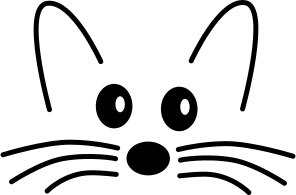
\includegraphics[width=1.4em]{squeak-logo}}}
\iftoshelse{
	\usepackage{marginnote}
		\renewcommand*{\marginfont}{\footnotesize}
	\newcommand{\vartriangleout}{\ifthenelse{\isodd{\thepage}}{\vartriangleright}{\vartriangleleft}}
	\newcommand{\dothisicon}{\fcolorbox{blue!65}{white}{\highlight{$\vartriangleout$}}}
	\newcommand{\dothis}[1]{%
		\noindent\par\noindent
		{\reversemarginpar
			\marginnote{\fcolorbox{blue!65}{white}{\highlight{$\vartriangleout$}}}}
		%\MarginLabel{do this}
		\noindent\emph{#1}
		\nopagebreak}
}{
	\newcommand{\dothisicon}{\raisebox{-.5ex}{
\includegraphics[height=1.2em]{pharo}}}
	\newcommand{\dothis}[1]{%
		\medskip
		\noindent\dothisicon
		\ifx#1\empty\else\quad\emph{#1}\fi
		\par\smallskip\nopagebreak}
}
%===> NEW VERSION <===
% NB: To use this in an individual chapter, you must set:
%\graphicspath{{figures/} {../figures/}}
% at the head of the chapter.  Don't forget the final /
%=============================================================
%:Reader hints (hint)
%
% Indicates a non-obvious consequence
\newcommand{\hint}[1]{\vspace{1ex}\noindent\fbox{\textsc{Hint}} \emph{#1}}
%=================================================================
% graphics for Morphic handles
\newcommand{\grabHandle}{\raisebox{-0.2ex}{
\includegraphics[width=1em]{blackHandle}}}
\newcommand{\moveHandle}{\raisebox{-0.2ex}{
\includegraphics[width=1em]{moveHandle}}}
\newcommand{\debugHandle}{\raisebox{-0.2ex}{
\includegraphics[width=1em]{debugHandle}}}
%=============================================================
%:Highlighting Important stuff (doublebox)
%
% From Seaside book ...
\newsavebox{\SavedText}
\newlength{\InnerBoxRule}\setlength{\InnerBoxRule}{.75\fboxrule}
\newlength{\OuterBoxRule}\setlength{\OuterBoxRule}{1.5\fboxrule}
\newlength{\BoxSeparation}\setlength{\BoxSeparation}{1.5\fboxrule}
\addtolength{\BoxSeparation}{.5pt}
\newlength{\SaveBoxSep}\setlength{\SaveBoxSep}{2\fboxsep}
%
\newenvironment{doublebox}{\begin{lrbox}{\SavedText}
    \begin{minipage}{.75\textwidth}}
    {\end{minipage}\end{lrbox}\begin{center}
    \setlength{\fboxsep}{\BoxSeparation}\setlength{\fboxrule}{\OuterBoxRule}
    \fbox{\setlength{\fboxsep}{\SaveBoxSep}\setlength{\fboxrule}{\InnerBoxRule}%
      \fbox{\usebox{\SavedText}}}
  \end{center}}
% Use this:
\newcommand{\important}[1]{\begin{doublebox}#1\end{doublebox}}
%=============================================================
%:Section depth
\setcounter{secnumdepth}{2}
%% for this to happen start the file with
%\ifx\wholebook\relax\else
%% $Author$
% $Date$
% $Revision$

% HISTORY:
% 2006-10-31 - Oscar code macros
% ...

%=============================================================
% NB: documentclass must be set in main document.
% Allows book to be generated in multiple formats.
%=============================================================
%:Packages
\usepackage[T1]{fontenc}  %%%%%% really important to get the code directly in the text!
\usepackage{lmodern}
%\usepackage[scaled=0.85]{bookmanx} % needs another scale factor if used with \renewcommand{\sfdefault}{cmbr}
\usepackage{palatino}
\usepackage[scaled=0.85]{helvet}
\usepackage[protrusion,expansion=false]{microtype}
\usepackage{graphicx}
\usepackage{theorem}
\usepackage[english]{babel}
% ON: pdfsync breaks the use of p{width} for tabular columns!
\ifdefined\usepdfsync\usepackage{pdfsync}\fi % Requires texlive 2007
%=============================================================
%:More packages
%Stef should check which ones are used!
%\usepackage{picinpar}
%\usepackage{layout}
%\usepackage{color}
%\usepackage{enum}
%\usepackage{a4wide}
% \usepackage{fancyhdr}
\usepackage{ifthen}
\usepackage{float}
\usepackage{longtable}
\usepackage{makeidx}
\usepackage[nottoc]{tocbibind}
\usepackage{multicol}
\usepackage{booktabs}	% book-style tables
\usepackage{topcapt}	% enables \topcaption
\usepackage{multirow}
\usepackage{tabularx}
%\usepackage[bottom]{footmisc}
\usepackage{xspace}
\usepackage{alltt}
\usepackage{amssymb,textcomp}
\usepackage[usenames,dvipsnames]{color}
%\usepackage{colortbl}
\usepackage[hang]{subfigure}\makeatletter\def\p@subfigure{\thefigure\,}\makeatother
\usepackage{rotating}
\usepackage{enumitem}	% apb: allows more control over tags in enumerations
\usepackage{verbatim}     % for comment environment
\usepackage{varioref}	% for page references that work
\labelformat{footnote}{\thechapter--#1} % to distinguish citations from jurabib
\usepackage{needspace}
\usepackage{isodateo} % enable \isodate
\usepackage[newparttoc,pagestyles]{titlesec}
\usepackage{titletoc}
\usepackage{wrapfig}

\usepackage[
	super,
	citefull=first,
	authorformat={allreversed,and},
	titleformat={commasep,italic}
]{jurabib} % citations as footnotes
\usepackage[
	colorlinks=true,
	linkcolor=black,
	urlcolor=black,
	citecolor=black
]{hyperref}   % should come last
%=============================================================
%:PDF version
\pdfminorversion=3 % Set PDF to 1.3 for Lulu
%=============================================================
%:URL style
\makeatletter
\def\url@leostyle{%
  \@ifundefined{selectfont}{\def\UrlFont{\sf}}{\def\UrlFont{\sffamily}}}
\makeatother
% Now actually use the newly defined style.
\urlstyle{leo}
%=============================================================
%:Booleans
\newboolean{lulu}
\setboolean{lulu}{false}
\newcommand{\ifluluelse}[2]{\ifthenelse{\boolean{lulu}}{#1}{#2}}
%=============================================================
%:Names
\newcommand{\SUnit}{SUnit\xspace}
\newcommand{\sunit}{SUnit\xspace}
\newcommand{\xUnit}{$x$Unit\xspace}
\newcommand{\JUnit}{JUnit\xspace}
\newcommand{\st}{Smalltalk\xspace}
\newcommand{\pharo}{Pharo\xspace} % Use this, not \Pharo
%\newcommand{\sqmap}{SqueakMap\xspace}
\newcommand{\squeak}{Squeak\xspace} % use this, not \Squeak or \sq
\newcommand{\sqsrc}{SqueakSource\xspace}
\newcommand{\sbe}{\url{http://SqueakByExample.org}\xspace}
\newcommand{\pharoweb}{\url{http://pharo-project.org}\xspace}
\newcommand{\pbe}{\url{http://PharoByExample.org}\xspace}
\newcommand{\sba}{\url{http://SquareBracketAssociates.org}\xspace}
\newcommand{\bam}{\lct{Bounc\-ing\-Atoms\-Morph}\xspace}
%=============================================================
%:Markup macros for proof-reading
\usepackage[normalem]{ulem} % for \sout
\usepackage{xcolor}
\newcommand{\ra}{$\rightarrow$}
\newcommand{\ugh}[1]{\textcolor{red}{\uwave{#1}}} % please rephrase
\newcommand{\ins}[1]{\textcolor{blue}{\uline{#1}}} % please insert
\newcommand{\del}[1]{\textcolor{red}{\sout{#1}}} % please delete
\newcommand{\chg}[2]{\textcolor{red}{\sout{#1}}{\ra}\textcolor{blue}{\uline{#2}}} % please change
%=============================================================
%:Editorial comment macros
%\newcommand{\nnbb}[2]{
%    % \fbox{\bfseries\sffamily\scriptsize#1}
%    \fcolorbox{gray}{yellow}{\bfseries\sffamily\scriptsize#1}
%    {\sf\small$\blacktriangleright$\textit{#2}$\blacktriangleleft$}
%   }
\newcommand{\yellowbox}[1]{\fcolorbox{gray}{yellow}{\bfseries\sffamily\scriptsize#1}}
\newcommand{\triangles}[1]{{\sf\small$\blacktriangleright$\textit{#1}$\blacktriangleleft$}}
\newcommand{\nnbb}[2]{\yellowbox{#1} \triangles{#2}}
\newcommand{\fix}{\yellowbox{FIX!}}
\newcommand{\here}{\yellowbox{CONTINUE HERE!}}
% editor macros
\newcommand{\apl}[1]{\nnbb{Alain}{#1}} % Alain
\newcommand{\ab}[1]{\nnbb{Andrew}{#1}} % Black
\newcommand{\sd}[1]{\nnbb{St\'{e}f}{#1}} % Ducasse
\newcommand{\gl}[1]{\nnbb{Guillaume}{#1}} % Ducasse
\newcommand{\cd}[1]{\nnbb{Christophe}{#1}} % Ducasse
\newcommand{\sig}[1]{\nnbb{Igor}{#1}} % Igor
\newcommand{\dc}[1]{\nnbb{DamienC}{#1}} % Ducasse
\newcommand{\md}[1]{\nnbb{Marcus}{#1}} % Denker
\newcommand{\on}[1]{\nnbb{Oscar}{#1}} % Nierstrasz
\newcommand{\damien}[1]{\nnbb{Damien}{#1}} % Pollet
\newcommand{\lr}[1]{\nnbb{Lukas}{#1}} % Renggli
\newcommand{\orla}[1]{\nnbb{Orla}{#1}} % Greevy
\newcommand{\alex}[1]{\nnbb{Alex}{#1}} % Bergel
\newcommand{\alx}[1]{\nnbb{Alex}{#1}} % Bergel
\newcommand{\dr}[1]{\nnbb{David}{#1}} % Roethlisberger
\newcommand{\ja}[1]{\nnbb{Jannik}{#1}} % Laval
\newcommand{\cb}[1]{\nnbb{Camillo}{#1}} % Bruni
\newcommand{\jr}[1]{\nnbb{Jorge}{#1}} % Ressia
\newcommand{\jb}[1]{\nnbb{JB}{#1}} % JB
\newcommand{\jp}[1]{\nnbb{Javier}{#1}} % Pimas
\newcommand{\fp}[1]{\nnbb{Fabrizio}{#1}} % Perin
\newcommand{\michael}[1]{\nnbb{Michael}{#1}} % Davies
\newcommand{\ew}[1]{\nnbb{Erwann}{#1}} % Wernli
\newcommand{\mb}[1]{\nnbb{Martial}{#1}} % Boniou
\newcommand{\hw}[1]{\nnbb{Hernan}{#1}} % Wilkinson
\newcommand{\ben}[1]{\nnbb{Benjamin}{#1}} % Benjamin Van Ryseghem
\newcommand{\hjo}[1]{\nnbb{HwaJong}{#1}} % HwaJong Oh aka daliot
\newcommand{\ml}[1]{\nnbb{Max}{#1}} % Max Leske
\newcommand{\mmp}[1]{\nnbb{Mariano}{#1}} % Mariano Martinez Peck
\newcommand{\luc}[1]{\nnbb{Luc}{#1}} % Luc Fabresse
\newcommand{\dkl}[1]{\nnbb{Daniel}{#1}} % Daniel Lyons
\newcommand{\vu}[1]{\nnbb{Veronica}{#1}} % Veronica Uquillas Gomez
\newcommand{\martin}[1]{\nnbb{Martin}{#1}} % Martin Dias
\newcommand{\vp}[1]{\nnbb{Vanessa}{#1}} % Vanessa Pena
\newcommand{\gp}[1]{\nnbb{Guille}{#1}} % Guillermo Polito

%=============================================================
%:Abbreviation macros
\newcommand{\ie}{\emph{i.e.},\xspace}
\newcommand{\eg}{\emph{e.g.},\xspace}
\newcommand{\etc}{etc.\xspace}
%=============================================================
%:Cross reference macros
\newcommand{\charef}[1]{Chapter~\ref{cha:#1}\xspace}
\newcommand{\secref}[1]{Section~\ref{sec:#1}\xspace}
\newcommand{\figref}[1]{Figure~\ref{fig:#1}\xspace}
\newcommand{\Figref}[1]{Figure~\ref{fig:#1}\xspace}
\newcommand{\appref}[1]{Appendix~\ref{app:#1}\xspace}
\newcommand{\tabref}[1]{Table~\ref{tab:#1}\xspace}
\newcommand{\faqref}[1]{FAQ~\ref{faq:#1}, p.~\pageref{faq:#1}\xspace}
% APB: I removed trailing \xspace commands from these macros because
% \xspace mostly doesn't work.  If you want a space after your
% references, type one!
% ON: xspace has always worked just fine for me!  Please leave them in.
%
\newcommand{\ruleref}[1]{\ref{rule:#1}\xspace}
%
\newcommand{\egref}[1]{example~\ref{eg:#1}\xspace}
\newcommand{\Egref}[1]{Example~\ref{eg:#1}\xspace}
%
\newcommand{\scrref}[1]{script~\ref{scr:#1}\xspace}
\newcommand{\Scrref}[1]{Script~\ref{scr:#1}\xspace}
\newcommand{\tscrref}[1]{the script~\ref{scr:#1}\xspace}
\newcommand{\Tscrref}[1]{The script~\ref{scr:#1}\xspace}
%
\newcommand{\mthref}[1]{method~\ref{mth:#1}\xspace}
\newcommand{\mthsref}[1]{methods~\ref{mth:#1}\xspace}
\newcommand{\Mthref}[1]{Method~\ref{mth:#1}\xspace}
\newcommand{\tmthref}[1]{the method~\ref{mth:#1}\xspace}
\newcommand{\Tmthref}[1]{The method~\ref{mth:#1}\xspace}
%
\newcommand{\clsref}[1]{class~\ref{cls:#1}\xspace}
\newcommand{\tclsref}[1]{the class~\ref{cls:#1}\xspace}
\newcommand{\Tclsref}[1]{The class~\ref{cls:#1}\xspace}

\newcommand{\chalabel}[1]{\label{cha:#1}}
\newcommand{\seclabel}[1]{\label{sec:#1}}
\newcommand{\figlabel}[1]{\label{fig:#1}}
\newcommand{\tablabel}[1]{\label{tab:#1}}
\newcommand{\rulelabel}[1]{\label{rule:#1}}
\newcommand{\eglabel}[1]{\label{eg:#1}}
\newcommand{\scrlabel}[1]{\label{scr:#1}}
\newcommand{\mthlabel}[1]{\label{mth:#1}}
\newcommand{\clslabel}[1]{\label{cls:#1}}
\newcommand{\faqlabel}[1]{\label{faq:#1}}
%=============================================================
%:Menu item macro
% for menu items, so we can change our minds on how to print them! (apb)
\definecolor{lightgray}{gray}{0.89}
\newcommand{\menu}[1]{{%
	\setlength{\fboxsep}{0pt}%
	\colorbox{lightgray}{{{\upshape\sffamily\strut \,#1\,}}}}}
\newcommand{\link}[1]{{%
	\fontfamily{lmr}\selectfont
 	\upshape{\sffamily \underline{#1}}}}
% For submenu items:
\newcommand{\go}{\,$\triangleright$\,}
% \newcommand{\go}{\,$\blacktriangleright$\,}
% For keyboard shortcuts:
%\newcommand{\short}[1]{\mbox{$\langle${\sc CMD}$\rangle$-#1}\xspace}
\newcommand{\short}[1]{\mbox{{\sc cmd}\hspace{0.08em}--\hspace{0.09em}#1}\xspace}
% For buttons:
\newcommand{\button}[1]{{%
	\setlength{\fboxsep}{0pt}%
	\fbox{{\upshape\sffamily\strut \,#1\,}}}}
% NB: The button macro does not work within captions -- incompatible with xcolor package :-(
\newcommand{\toolsflap}{\textit{Tools} flap\xspace}
%=============================================================
%:Mouse clicks
\newcommand{\click}{click\xspace} % RED
\newcommand{\actclick}{action-click\xspace} % YELLOW
\newcommand{\metaclick}{meta-click\xspace} % BLUE
\newcommand{\Click}{Click\xspace} % RED
\newcommand{\Actclick}{Action-click\xspace} % YELLOW
\newcommand{\Metaclick}{Meta-click\xspace} % BLUE
%=============================================================
%:ToSh macros
\newboolean{tosh}
\setboolean{tosh}{false}
\newcommand{\iftoshelse}[2]{\ifthenelse{\boolean{tosh}}{#1}{#2}}
%=============================================================
%:ToSh colors
%\newcommand{\highlightcolor}{\color{blue!65}}
%\newcommand{\boxcolor}{\color{gray!25}}
\newcommand{\highlight}[1]{\textcolor{blue!65}{#1}}
%\newcommand{\codecolor}{\color{blue!65}}
%%\setlength{\fboxrule}{2pt}
%\newcommand{\asPict}[1]{%
%	{\Large\highlight{#1}}}
%=============================================================
%:Reader cues (do this)
%
% Indicate something the reader should try out.
% \newcommand{\dothisicon}{\raisebox{-.5ex}{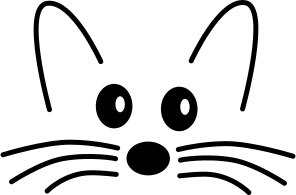
\includegraphics[width=1.4em]{squeak-logo}}}
\iftoshelse{
	\usepackage{marginnote}
		\renewcommand*{\marginfont}{\footnotesize}
	\newcommand{\vartriangleout}{\ifthenelse{\isodd{\thepage}}{\vartriangleright}{\vartriangleleft}}
	\newcommand{\dothisicon}{\fcolorbox{blue!65}{white}{\highlight{$\vartriangleout$}}}
	\newcommand{\dothis}[1]{%
		\noindent\par\noindent
		{\reversemarginpar
			\marginnote{\fcolorbox{blue!65}{white}{\highlight{$\vartriangleout$}}}}
		%\MarginLabel{do this}
		\noindent\emph{#1}
		\nopagebreak}
}{
	\newcommand{\dothisicon}{\raisebox{-.5ex}{
\includegraphics[height=1.2em]{pharo}}}
	\newcommand{\dothis}[1]{%
		\medskip
		\noindent\dothisicon
		\ifx#1\empty\else\quad\emph{#1}\fi
		\par\smallskip\nopagebreak}
}
%===> NEW VERSION <===
% NB: To use this in an individual chapter, you must set:
%\graphicspath{{figures/} {../figures/}}
% at the head of the chapter.  Don't forget the final /
%=============================================================
%:Reader hints (hint)
%
% Indicates a non-obvious consequence
\newcommand{\hint}[1]{\vspace{1ex}\noindent\fbox{\textsc{Hint}} \emph{#1}}
%=================================================================
% graphics for Morphic handles
\newcommand{\grabHandle}{\raisebox{-0.2ex}{
\includegraphics[width=1em]{blackHandle}}}
\newcommand{\moveHandle}{\raisebox{-0.2ex}{
\includegraphics[width=1em]{moveHandle}}}
\newcommand{\debugHandle}{\raisebox{-0.2ex}{
\includegraphics[width=1em]{debugHandle}}}
%=============================================================
%:Highlighting Important stuff (doublebox)
%
% From Seaside book ...
\newsavebox{\SavedText}
\newlength{\InnerBoxRule}\setlength{\InnerBoxRule}{.75\fboxrule}
\newlength{\OuterBoxRule}\setlength{\OuterBoxRule}{1.5\fboxrule}
\newlength{\BoxSeparation}\setlength{\BoxSeparation}{1.5\fboxrule}
\addtolength{\BoxSeparation}{.5pt}
\newlength{\SaveBoxSep}\setlength{\SaveBoxSep}{2\fboxsep}
%
\newenvironment{doublebox}{\begin{lrbox}{\SavedText}
    \begin{minipage}{.75\textwidth}}
    {\end{minipage}\end{lrbox}\begin{center}
    \setlength{\fboxsep}{\BoxSeparation}\setlength{\fboxrule}{\OuterBoxRule}
    \fbox{\setlength{\fboxsep}{\SaveBoxSep}\setlength{\fboxrule}{\InnerBoxRule}%
      \fbox{\usebox{\SavedText}}}
  \end{center}}
% Use this:
\newcommand{\important}[1]{\begin{doublebox}#1\end{doublebox}}
%=============================================================
%:Section depth
\setcounter{secnumdepth}{2}
%% for this to happen start the file with
%\ifx\wholebook\relax\else
%\input{../common.tex}
%\begin{document}
%\fi
% and terminate by
% \ifx\wholebook\relax\else\end{document}\fi

\DeclareGraphicsExtensions{.pdf, .jpg, .png}
%=============================================================
%:PDF setup
\hypersetup{
%   a4paper,
%   pdfstartview=FitV,
%   colorlinks,
%   linkcolor=darkblue,
%   citecolor=darkblue,
   pdftitle={Pharo by Example},
   pdfauthor={Andrew P. Black, St\'ephane Ducasse,	Oscar Nierstrasz,
Damien Pollet},
   pdfkeywords={Smalltalk, Squeak, Object-Oriented Programming, OOP},
   pdfsubject={Computer Science}
}
%=============================================================
%:Page layout and appearance
%
% \renewcommand{\headrulewidth}{0pt}
\renewcommand{\chaptermark}[1]{\markboth{#1}{}}
\renewcommand{\sectionmark}[1]{\markright{\thesection\ #1}}
\renewpagestyle{plain}[\small\itshape]{%
	\setheadrule{0pt}%
	\sethead[][][]{}{}{}%
	\setfoot[][][]{}{}{}}
\renewpagestyle{headings}[\small\itshape]{%
	\setheadrule{0pt}%
	\setmarks{chapter}{section}%
	\sethead[\thepage][][\chaptertitle]{\sectiontitle}{}{\thepage}%
	\setfoot[][][]{}{}{}}
%=============================================================
%:Title section setup and TOC numbering depth
\setcounter{secnumdepth}{1}
\setcounter{tocdepth}{1}
\titleformat{\part}[display]{\centering}{\huge\partname\ \thepart}{1em}{\Huge\textbf}[]
\titleformat{\chapter}[display]{}{\huge\chaptertitlename\ \thechapter}{1em}{\Huge\raggedright\textbf}[]
\titlecontents{part}[3pc]{%
		\pagebreak[2]\addvspace{1em plus.4em minus.2em}%
		\leavevmode\large\bfseries}
	{\contentslabel{3pc}}{\hspace*{-3pc}}
	{}[\nopagebreak]
\titlecontents{chapter}[3pc]{%
		\pagebreak[0]\addvspace{1em plus.2em minus.2em}%
		\leavevmode\bfseries}
	{\contentslabel{3pc}}{}
	{\hfill\contentspage}[\nopagebreak]
\dottedcontents{section}[3pc]{}{3pc}{1pc}
\dottedcontents{subsection}[3pc]{}{0pc}{1pc}
% \dottedcontents{subsection}[4.5em]{}{0pt}{1pc}
% Make \cleardoublepage insert really blank pages http://www.tex.ac.uk/cgi-bin/texfaq2html?label=reallyblank
\let\origdoublepage\cleardoublepage
\newcommand{\clearemptydoublepage}{%
  \clearpage
  {\pagestyle{empty}\origdoublepage}}
\let\cleardoublepage\clearemptydoublepage % see http://www.tex.ac.uk/cgi-bin/texfaq2html?label=patch
%=============================================================
%:FAQ macros (for FAQ chapter)
\newtheorem{faq}{FAQ}
\newcommand{\answer}{\paragraph{Answer}\ }
%=============================================================
%:Listings package configuration
% \newcommand{\caret}{\makebox{\raisebox{0.4ex}{\footnotesize{$\wedge$}}}}
\newcommand{\caret}{\^\,}
\newcommand{\escape}{{\sf \textbackslash}}
\definecolor{source}{gray}{0.95}
\usepackage{listings}
\lstdefinelanguage{Smalltalk}{
%  morekeywords={self,super,true,false,nil,thisContext}, % This is overkill
  morestring=[d]',
  morecomment=[s]{"}{"},
  alsoletter={\#:},
  escapechar={!},
  literate=
    {BANG}{!}1
    {CARET}{\^}1
    {UNDERSCORE}{\_}1
    {\\st}{Smalltalk}9 % convenience -- in case \st occurs in code
    % {'}{{\textquotesingle}}1 % replaced by upquote=true in \lstset
    %{_}{{$\leftarrow$}}1
    {>>>}{{\sep}}1
    %{^}{{$\uparrow$}}1
    {~}{{$\sim$}}1
    {-}{{\texttt{-}}}1 %{\textminus}}1 %{-}{\hspace{-0.13em}}{-}}1  % the goal is to make - the same width as +
    % {+}{\sf+}1 %{\raisebox{0.08ex}{+}}}1      % and to raise + off the baseline to match -
    {-->}{{\quad$\longrightarrow$\quad}}3
    {~->}{{\quad$\leadsto$\quad}}3
	, % Don't forget the comma at the end!
  tabsize=4
}[keywords,comments,strings]

\lstset{language=Smalltalk,
	basicstyle=\sffamily,
	keywordstyle=\color{black}\bfseries,
	% stringstyle=\ttfamily, % Ugly! do we really want this? -- on
	mathescape=true,
	showstringspaces=false,
	keepspaces=true,
	breaklines=true,
	breakautoindent=true,
	backgroundcolor=\color{source},
	lineskip={-1pt}, % Ugly hack
	upquote=true, % straight quote; requires textcomp package
	columns=fullflexible} % no fixed width fonts
% In-line code (literal)
% Normally use this for all in-line code:

\newcommand{\ct}{\lstinline[mathescape=false,backgroundcolor=\color{white},basicstyle={\sffamily\upshape}]}
\newcommand{\cts}[1]{{\sffamily{\upshape{#1}}\xspace}}
% apb 2007.8.28 added the \upshape declaration to avoid getting italicized code in \dothis{ } sections.
% In-line code (latex enabled)
% Use this only in special situations where \ct does not work
% (within section headings ...):
\newcommand{\lct}[1]{{\textsf{\textup{#1}}}}
% Use these for system categories and protocols:
\newcommand{\scat}[1]{\emph{\textsf{#1}}\xspace}
\newcommand{\pkg}[1]{\emph{\textsf{#1}}\xspace}
\newcommand{\prot}[1]{\emph{\textsf{#1}}\xspace}
% Code environments
% NB: the arg is for tests
% Only code and example environments may be tests
\lstnewenvironment{code}[1]{%
	\lstset{%
		% frame=lines,
		frame=single,
		framerule=0pt,
		mathescape=false
	}
}{}
\def\ignoredollar#1{}
%=============================================================
%:Code environments (method, script ...)
% NB: the third arg is for tests
% Only code and example environments may be tests
\lstnewenvironment{example}[3][defaultlabel]{%
	\renewcommand{\lstlistingname}{Example}%
	\lstset{
		% frame=lines,
		frame=single,
		framerule=0pt,
		mathescape=false,
		caption={\emph{#2}},
		label={eg:#1}
	}
}{}
\lstnewenvironment{script}[2][defaultlabel]{%
\renewcommand{\lstlistingname}{Script}%
	\lstset{
		% frame=lines,
		frame=single,
		framerule=0pt,
		mathescape=false,
		name={Script},
		caption={\emph{#2}},
		label={scr:#1}
	}
}{}
\lstnewenvironment{method}[2][defaultlabel]{%
	\renewcommand{\lstlistingname}{Method}%
	\lstset{
		% frame=lines,
		frame=single,
		framerule=0pt,
		mathescape=false,
		name={Method},
		caption={\emph{#2}},
		label={mth:#1}
	}
}{}
\lstnewenvironment{methods}[2][defaultlabel]{% just for multiple methods at once
	\renewcommand{\lstlistingname}{Methods}%
	\lstset{
		% frame=lines,
		frame=single,
		framerule=0pt,
		mathescape=false,
		name={Method},
		caption={\emph{#2}},
		label={mth:#1}
	}
}{}
\lstnewenvironment{numMethod}[2][defaultlabel]{%
	\renewcommand{\lstlistingname}{Method}%
	\lstset{
		numbers=left,
		numberstyle={\tiny\sffamily},
		% frame=lines,
		frame=single,
		framerule=0pt,
		mathescape=false,
		name={Method},
		caption={\emph{#2}},
		label={mth:#1}
	}
}{}
\lstnewenvironment{classdef}[2][defaultlabel]{%
	\renewcommand{\lstlistingname}{Class}%
	\lstset{
		% frame=lines,
		frame=single,
		framerule=0pt,
		mathescape=false,
		name={Class},
		caption={\emph{#2}},
		label={cls:#1}
	}
}{}
%=============================================================
%:Reserving space
% Usually need one more line than the actual lines of code
\newcommand{\needlines}[1]{\Needspace{#1\baselineskip}}
%=============================================================
%:Indexing macros
% Macros ending with "ind" generate text as well as an index entry
% Macros ending with "index" *only* generate an index entry
\newcommand{\ind}[1]{\index{#1}#1\xspace} % plain text
\newcommand{\subind}[2]{\index{#1!#2}#2\xspace} % show #2, subindex under #1
\newcommand{\emphind}[1]{\index{#1}\emph{#1}\xspace} % emph #1
\newcommand{\emphsubind}[2]{\index{#1!#2}\emph{#2}\xspace} % show emph #2, subindex inder #1
\newcommand{\scatind}[1]{\index{#1@\textsf{#1} (category)}\scat{#1}} % category
\newcommand{\pkgind}[1]{\index{#1@\textsf{#1} (package)}\pkg{#1}} % package
\newcommand{\protind}[1]{\index{#1@\textsf{#1} (protocol)}\prot{#1}} % protocol
\newcommand{\clsind}[1]{\index{#1@\textsf{#1} (class)}\ct{#1}\xspace}
% \newcommand{\clsind}[1]{\index{#1!\#@(class)}\ct{#1}\xspace} % class
\newcommand{\clsindplural}[1]{\index{#1!\#@(class)}\ct{#1}s\xspace} % class
\newcommand{\cvind}[1]{\index{#1@\textsf{#1} (class variable)}\ct{#1}\xspace} % class var
\newcommand{\glbind}[1]{\index{#1@\textsf{#1} (global)}\ct{#1}\xspace} % global
\newcommand{\patind}[1]{\index{#1@#1 (pattern)}\ct{#1}\xspace} % pattern
\newcommand{\pvind}[1]{\index{#1@\textsf{#1} (pseudo variable)}\ct{#1}\xspace} % pseudo var
\newcommand{\clsmthind}[2]{\index{#1!#2@\ct{#2}}\ct{#1>>>#2}\xspace} % class + method name
\newcommand{\mthind}[2]{\index{#1!#2@\ct{#2}}\ct{#2}\xspace} % show method name only
\newcommand{\lmthind}[2]{\index{#1!#2@\ct{#2}}\lct{#2}\xspace} % show method name only
\newcommand{\cmind}[2]{\index{#1!#2@\ct{#2}}\ct{#1>>>#2}\xspace} % show class>>method
\newcommand{\lcmind}[2]{\index{#1!#2@\ct{#2}}\lct{#1>>>#2}\xspace} % show class>>method
\newcommand{\toolsflapind}{\index{Tools flap}\toolsflap} % index tools flap
% The following only generate an index entry:
% \newcommand{\clsindex}[1]{\index{#1@\textsf{#1} (class)}}
\newcommand{\clsindex}[1]{\index{#1!\#@(class)}} % class
\newcommand{\mthindex}[2]{\index{#1!#2@\ct{#2}}} % method
\newcommand{\cmindex}[2]{\index{#1!#2@\ct{#2}}} % class>>method
\newcommand{\cvindex}[1]{\index{#1@\textsf{#1} (class variable)}} % class var
\newcommand{\glbindex}[1]{\index{#1@\textsf{#1} (global)}}% global
\newcommand{\pvindex}[1]{\index{#1@\textsf{#1} (pseudo variable)}}% pseudo var
\newcommand{\seeindex}[2]{\index{#1|see{#2}}} % #1, see #2
\newcommand{\scatindex}[1]{\index{#1@\textsf{#1} (category)}} % category
\newcommand{\pkgindex}[1]{\index{#1@\textsf{#1} (package)}} % package
\newcommand{\protindex}[1]{\index{#1@\textsf{#1} (protocol)}} % protocol
% How can we have the main entry page numbers in bold yet not break the hyperlink?
\newcommand{\boldidx}[1]{{\bf #1}} % breaks hyperlink
%\newcommand{\indmain}[1]{\index{#1|boldidx}#1\xspace} % plain text, main entry
%\newcommand{\emphsubindmain}[2]{\index{#1!#2|boldidx}\emph{#2}\xspace} % subindex, main entry
%\newcommand{\subindmain}[2]{\index{#1!#2|boldidx}#2\xspace} % subindex, main entry
%\newcommand{\clsindmain}[1]{\index{#1@\textsf{#1} (class)|boldidx}\ct{#1}\xspace}
%\newcommand{\clsindmain}[1]{\index{#1!\#@(class)|boldidx}\ct{#1}\xspace} % class main
%\newcommand{\indexmain}[1]{\index{#1|boldidx}} % main index entry only
\newcommand{\indmain}[1]{\index{#1}#1\xspace} % The main index entry for this item
\newcommand{\emphsubindmain}[2]{\index{#1!#2}\emph{#2}\xspace} % subindex, main entry
\newcommand{\subindmain}[2]{\index{#1!#2}#2\xspace} % subindex, main entry
%\newcommand{\clsindmain}[1]{\index{#1@\textsf{#1} (class)}\ct{#1}\xspace}
\newcommand{\clsindmain}[1]{\index{#1!\#@(class)}\ct{#1}\xspace} % class main
\newcommand{\clsindexmain}[1]{\index{#1!\#@(class)}} % class main index only
\newcommand{\indexmain}[1]{\index{#1}}
%=============================================================
%:Code macros
% some constants
\newcommand{\codesize}{\small}
\newcommand{\codefont}{\sffamily}
%\newcommand{\cat}[1]{\textit{In category #1}}%%To remove later
\newlength{\scriptindent}
\setlength{\scriptindent}{.3cm}
%% Method presentation constants
\newlength{\methodindent}
\newlength{\methodwordlength}
\newlength{\aftermethod}
\setlength{\methodindent}{0.2cm}
\settowidth{\methodwordlength}{\ M\'ethode\ }
%=============================================================
%:Smalltalk macros
%\newcommand{\sep}{{$\gg$}}
\newcommand{\sep}{\mbox{>>}}
\newcommand{\self}{\lct{self}\xspace}
\newcommand{\super}{\lct{super}\xspace}
\newcommand{\nil}{\lct{nil}\xspace}
%=============================================================
% be less conservative about float placement
% these commands are from http://www.tex.ac.uk/cgi-bin/texfaq2html?label=floats
\renewcommand{\topfraction}{.9}
\renewcommand{\bottomfraction}{.9}
\renewcommand{\textfraction}{.1}
\renewcommand{\floatpagefraction}{.85}
\renewcommand{\dbltopfraction}{.66}
\renewcommand{\dblfloatpagefraction}{.85}
\setcounter{topnumber}{9}
\setcounter{bottomnumber}{9}
\setcounter{totalnumber}{20}
\setcounter{dbltopnumber}{9}
%=============================================================
% Give information from each chapter's author
\newcommand{\contact}[2]{\textbf{#1} \textsf{(#2)}}

\newcommand{\chapterauthor}[1]{\emph{with the participation of:\\#1}\\}
\newcommand{\chapterwritten}[1]{\emph{written by:\\#1}\\}

\newcommand{\authornoury}{\contact{Noury Bouraqadi}{Noury.Bouraqadi@mines-douai.fr}}
\newcommand{\authorluc}{\contact{Luc Fabresse}{Luc.Fabresse@mines-douai.fr}}
\newcommand{\authordamienc}{\contact{Damien Cassou}{damien.cassou@gmail.com}}
\newcommand{\authoroscar}{\contact{Oscar Nierstrasz}{oscar.nierstrasz@acm.org}}
\newcommand{\authorsteph}{\contact{St\'ephane Ducasse}{stephane.ducasse@inria.fr}}
\newcommand{\authoralex}{\contact{Alexandre Bergel}{alexandre@bergel.eu}}
\newcommand{\authorolivier}{\contact{Olivier Auverlot}{olivier.auverlot@inria.fr}}
\newcommand{\authornicolas}{\contact{Nicolas Cellier}{nicolas.cellier.aka.nice@gmail.com}}
\newcommand{\authormarcus}{\contact{Marcus Denker}{marcus.denker@inria.fr}}
\newcommand{\authoralain}{\contact{Alain Plantec}{alain.plantec@univ-brest.fr}}
\newcommand{\authordale}{\contact{Dale Henrichs}{dale.henrichs@gemstone.com}}
\newcommand{\authormariano}{\contact{Mariano Martinez Peck}{marianopeck@gmail.com}}
\newcommand{\authorsven}{\contact{Sven Van Caekenberghe}{sven@beta9.be}}
\newcommand{\authorlukas}{\contact{Lukas Renggli}{renggli@gmail.com}}
\newcommand{\authorjankurs}{\contact{Jan Kurs}{kurs@iam.unibe.ch}}
\newcommand{\authorguillaume}{\contact{Guillaume Larcheveque}{guillaume.larcheveque@gmail.com}}
\newcommand{\authorguillep}{\contact{Guillermo Polito}{guillermopolito@gmail.com}}
\newcommand{\authorclement}{\contact{Cl\'ement Bera}{bera.clement@gmail.com}}
\newcommand{\authormax}{\contact{Max Leske}{maxleske@gmail.com}}
\newcommand{\authorvanessa}{\contact{Vanessa Pe\~{n}a-Araya}{van.c.pena@gmail.com}}
\newcommand{\authorcamillo}{\contact{Camillo Bruni}{camillobruni@gmail.com}}

%=============================================================
% apb doesn't like paragraphs to run in to each other without a break
\parskip 1ex
%=============================================================
%:Stuff to check, merge or deprecate
%\setlength{\marginparsep}{2mm}
%\renewcommand{\baselinestretch}{1.1}
%=============================================================
\usepackage{tikz}

%\begin{document}
%\fi
% and terminate by
% \ifx\wholebook\relax\else\end{document}\fi

\DeclareGraphicsExtensions{.pdf, .jpg, .png}
%=============================================================
%:PDF setup
\hypersetup{
%   a4paper,
%   pdfstartview=FitV,
%   colorlinks,
%   linkcolor=darkblue,
%   citecolor=darkblue,
   pdftitle={Pharo by Example},
   pdfauthor={Andrew P. Black, St\'ephane Ducasse,	Oscar Nierstrasz,
Damien Pollet},
   pdfkeywords={Smalltalk, Squeak, Object-Oriented Programming, OOP},
   pdfsubject={Computer Science}
}
%=============================================================
%:Page layout and appearance
%
% \renewcommand{\headrulewidth}{0pt}
\renewcommand{\chaptermark}[1]{\markboth{#1}{}}
\renewcommand{\sectionmark}[1]{\markright{\thesection\ #1}}
\renewpagestyle{plain}[\small\itshape]{%
	\setheadrule{0pt}%
	\sethead[][][]{}{}{}%
	\setfoot[][][]{}{}{}}
\renewpagestyle{headings}[\small\itshape]{%
	\setheadrule{0pt}%
	\setmarks{chapter}{section}%
	\sethead[\thepage][][\chaptertitle]{\sectiontitle}{}{\thepage}%
	\setfoot[][][]{}{}{}}
%=============================================================
%:Title section setup and TOC numbering depth
\setcounter{secnumdepth}{1}
\setcounter{tocdepth}{1}
\titleformat{\part}[display]{\centering}{\huge\partname\ \thepart}{1em}{\Huge\textbf}[]
\titleformat{\chapter}[display]{}{\huge\chaptertitlename\ \thechapter}{1em}{\Huge\raggedright\textbf}[]
\titlecontents{part}[3pc]{%
		\pagebreak[2]\addvspace{1em plus.4em minus.2em}%
		\leavevmode\large\bfseries}
	{\contentslabel{3pc}}{\hspace*{-3pc}}
	{}[\nopagebreak]
\titlecontents{chapter}[3pc]{%
		\pagebreak[0]\addvspace{1em plus.2em minus.2em}%
		\leavevmode\bfseries}
	{\contentslabel{3pc}}{}
	{\hfill\contentspage}[\nopagebreak]
\dottedcontents{section}[3pc]{}{3pc}{1pc}
\dottedcontents{subsection}[3pc]{}{0pc}{1pc}
% \dottedcontents{subsection}[4.5em]{}{0pt}{1pc}
% Make \cleardoublepage insert really blank pages http://www.tex.ac.uk/cgi-bin/texfaq2html?label=reallyblank
\let\origdoublepage\cleardoublepage
\newcommand{\clearemptydoublepage}{%
  \clearpage
  {\pagestyle{empty}\origdoublepage}}
\let\cleardoublepage\clearemptydoublepage % see http://www.tex.ac.uk/cgi-bin/texfaq2html?label=patch
%=============================================================
%:FAQ macros (for FAQ chapter)
\newtheorem{faq}{FAQ}
\newcommand{\answer}{\paragraph{Answer}\ }
%=============================================================
%:Listings package configuration
% \newcommand{\caret}{\makebox{\raisebox{0.4ex}{\footnotesize{$\wedge$}}}}
\newcommand{\caret}{\^\,}
\newcommand{\escape}{{\sf \textbackslash}}
\definecolor{source}{gray}{0.95}
\usepackage{listings}
\lstdefinelanguage{Smalltalk}{
%  morekeywords={self,super,true,false,nil,thisContext}, % This is overkill
  morestring=[d]',
  morecomment=[s]{"}{"},
  alsoletter={\#:},
  escapechar={!},
  literate=
    {BANG}{!}1
    {CARET}{\^}1
    {UNDERSCORE}{\_}1
    {\\st}{Smalltalk}9 % convenience -- in case \st occurs in code
    % {'}{{\textquotesingle}}1 % replaced by upquote=true in \lstset
    %{_}{{$\leftarrow$}}1
    {>>>}{{\sep}}1
    %{^}{{$\uparrow$}}1
    {~}{{$\sim$}}1
    {-}{{\texttt{-}}}1 %{\textminus}}1 %{-}{\hspace{-0.13em}}{-}}1  % the goal is to make - the same width as +
    % {+}{\sf+}1 %{\raisebox{0.08ex}{+}}}1      % and to raise + off the baseline to match -
    {-->}{{\quad$\longrightarrow$\quad}}3
    {~->}{{\quad$\leadsto$\quad}}3
	, % Don't forget the comma at the end!
  tabsize=4
}[keywords,comments,strings]

\lstset{language=Smalltalk,
	basicstyle=\sffamily,
	keywordstyle=\color{black}\bfseries,
	% stringstyle=\ttfamily, % Ugly! do we really want this? -- on
	mathescape=true,
	showstringspaces=false,
	keepspaces=true,
	breaklines=true,
	breakautoindent=true,
	backgroundcolor=\color{source},
	lineskip={-1pt}, % Ugly hack
	upquote=true, % straight quote; requires textcomp package
	columns=fullflexible} % no fixed width fonts
% In-line code (literal)
% Normally use this for all in-line code:

\newcommand{\ct}{\lstinline[mathescape=false,backgroundcolor=\color{white},basicstyle={\sffamily\upshape}]}
\newcommand{\cts}[1]{{\sffamily{\upshape{#1}}\xspace}}
% apb 2007.8.28 added the \upshape declaration to avoid getting italicized code in \dothis{ } sections.
% In-line code (latex enabled)
% Use this only in special situations where \ct does not work
% (within section headings ...):
\newcommand{\lct}[1]{{\textsf{\textup{#1}}}}
% Use these for system categories and protocols:
\newcommand{\scat}[1]{\emph{\textsf{#1}}\xspace}
\newcommand{\pkg}[1]{\emph{\textsf{#1}}\xspace}
\newcommand{\prot}[1]{\emph{\textsf{#1}}\xspace}
% Code environments
% NB: the arg is for tests
% Only code and example environments may be tests
\lstnewenvironment{code}[1]{%
	\lstset{%
		% frame=lines,
		frame=single,
		framerule=0pt,
		mathescape=false
	}
}{}
\def\ignoredollar#1{}
%=============================================================
%:Code environments (method, script ...)
% NB: the third arg is for tests
% Only code and example environments may be tests
\lstnewenvironment{example}[3][defaultlabel]{%
	\renewcommand{\lstlistingname}{Example}%
	\lstset{
		% frame=lines,
		frame=single,
		framerule=0pt,
		mathescape=false,
		caption={\emph{#2}},
		label={eg:#1}
	}
}{}
\lstnewenvironment{script}[2][defaultlabel]{%
\renewcommand{\lstlistingname}{Script}%
	\lstset{
		% frame=lines,
		frame=single,
		framerule=0pt,
		mathescape=false,
		name={Script},
		caption={\emph{#2}},
		label={scr:#1}
	}
}{}
\lstnewenvironment{method}[2][defaultlabel]{%
	\renewcommand{\lstlistingname}{Method}%
	\lstset{
		% frame=lines,
		frame=single,
		framerule=0pt,
		mathescape=false,
		name={Method},
		caption={\emph{#2}},
		label={mth:#1}
	}
}{}
\lstnewenvironment{methods}[2][defaultlabel]{% just for multiple methods at once
	\renewcommand{\lstlistingname}{Methods}%
	\lstset{
		% frame=lines,
		frame=single,
		framerule=0pt,
		mathescape=false,
		name={Method},
		caption={\emph{#2}},
		label={mth:#1}
	}
}{}
\lstnewenvironment{numMethod}[2][defaultlabel]{%
	\renewcommand{\lstlistingname}{Method}%
	\lstset{
		numbers=left,
		numberstyle={\tiny\sffamily},
		% frame=lines,
		frame=single,
		framerule=0pt,
		mathescape=false,
		name={Method},
		caption={\emph{#2}},
		label={mth:#1}
	}
}{}
\lstnewenvironment{classdef}[2][defaultlabel]{%
	\renewcommand{\lstlistingname}{Class}%
	\lstset{
		% frame=lines,
		frame=single,
		framerule=0pt,
		mathescape=false,
		name={Class},
		caption={\emph{#2}},
		label={cls:#1}
	}
}{}
%=============================================================
%:Reserving space
% Usually need one more line than the actual lines of code
\newcommand{\needlines}[1]{\Needspace{#1\baselineskip}}
%=============================================================
%:Indexing macros
% Macros ending with "ind" generate text as well as an index entry
% Macros ending with "index" *only* generate an index entry
\newcommand{\ind}[1]{\index{#1}#1\xspace} % plain text
\newcommand{\subind}[2]{\index{#1!#2}#2\xspace} % show #2, subindex under #1
\newcommand{\emphind}[1]{\index{#1}\emph{#1}\xspace} % emph #1
\newcommand{\emphsubind}[2]{\index{#1!#2}\emph{#2}\xspace} % show emph #2, subindex inder #1
\newcommand{\scatind}[1]{\index{#1@\textsf{#1} (category)}\scat{#1}} % category
\newcommand{\pkgind}[1]{\index{#1@\textsf{#1} (package)}\pkg{#1}} % package
\newcommand{\protind}[1]{\index{#1@\textsf{#1} (protocol)}\prot{#1}} % protocol
\newcommand{\clsind}[1]{\index{#1@\textsf{#1} (class)}\ct{#1}\xspace}
% \newcommand{\clsind}[1]{\index{#1!\#@(class)}\ct{#1}\xspace} % class
\newcommand{\clsindplural}[1]{\index{#1!\#@(class)}\ct{#1}s\xspace} % class
\newcommand{\cvind}[1]{\index{#1@\textsf{#1} (class variable)}\ct{#1}\xspace} % class var
\newcommand{\glbind}[1]{\index{#1@\textsf{#1} (global)}\ct{#1}\xspace} % global
\newcommand{\patind}[1]{\index{#1@#1 (pattern)}\ct{#1}\xspace} % pattern
\newcommand{\pvind}[1]{\index{#1@\textsf{#1} (pseudo variable)}\ct{#1}\xspace} % pseudo var
\newcommand{\clsmthind}[2]{\index{#1!#2@\ct{#2}}\ct{#1>>>#2}\xspace} % class + method name
\newcommand{\mthind}[2]{\index{#1!#2@\ct{#2}}\ct{#2}\xspace} % show method name only
\newcommand{\lmthind}[2]{\index{#1!#2@\ct{#2}}\lct{#2}\xspace} % show method name only
\newcommand{\cmind}[2]{\index{#1!#2@\ct{#2}}\ct{#1>>>#2}\xspace} % show class>>method
\newcommand{\lcmind}[2]{\index{#1!#2@\ct{#2}}\lct{#1>>>#2}\xspace} % show class>>method
\newcommand{\toolsflapind}{\index{Tools flap}\toolsflap} % index tools flap
% The following only generate an index entry:
% \newcommand{\clsindex}[1]{\index{#1@\textsf{#1} (class)}}
\newcommand{\clsindex}[1]{\index{#1!\#@(class)}} % class
\newcommand{\mthindex}[2]{\index{#1!#2@\ct{#2}}} % method
\newcommand{\cmindex}[2]{\index{#1!#2@\ct{#2}}} % class>>method
\newcommand{\cvindex}[1]{\index{#1@\textsf{#1} (class variable)}} % class var
\newcommand{\glbindex}[1]{\index{#1@\textsf{#1} (global)}}% global
\newcommand{\pvindex}[1]{\index{#1@\textsf{#1} (pseudo variable)}}% pseudo var
\newcommand{\seeindex}[2]{\index{#1|see{#2}}} % #1, see #2
\newcommand{\scatindex}[1]{\index{#1@\textsf{#1} (category)}} % category
\newcommand{\pkgindex}[1]{\index{#1@\textsf{#1} (package)}} % package
\newcommand{\protindex}[1]{\index{#1@\textsf{#1} (protocol)}} % protocol
% How can we have the main entry page numbers in bold yet not break the hyperlink?
\newcommand{\boldidx}[1]{{\bf #1}} % breaks hyperlink
%\newcommand{\indmain}[1]{\index{#1|boldidx}#1\xspace} % plain text, main entry
%\newcommand{\emphsubindmain}[2]{\index{#1!#2|boldidx}\emph{#2}\xspace} % subindex, main entry
%\newcommand{\subindmain}[2]{\index{#1!#2|boldidx}#2\xspace} % subindex, main entry
%\newcommand{\clsindmain}[1]{\index{#1@\textsf{#1} (class)|boldidx}\ct{#1}\xspace}
%\newcommand{\clsindmain}[1]{\index{#1!\#@(class)|boldidx}\ct{#1}\xspace} % class main
%\newcommand{\indexmain}[1]{\index{#1|boldidx}} % main index entry only
\newcommand{\indmain}[1]{\index{#1}#1\xspace} % The main index entry for this item
\newcommand{\emphsubindmain}[2]{\index{#1!#2}\emph{#2}\xspace} % subindex, main entry
\newcommand{\subindmain}[2]{\index{#1!#2}#2\xspace} % subindex, main entry
%\newcommand{\clsindmain}[1]{\index{#1@\textsf{#1} (class)}\ct{#1}\xspace}
\newcommand{\clsindmain}[1]{\index{#1!\#@(class)}\ct{#1}\xspace} % class main
\newcommand{\clsindexmain}[1]{\index{#1!\#@(class)}} % class main index only
\newcommand{\indexmain}[1]{\index{#1}}
%=============================================================
%:Code macros
% some constants
\newcommand{\codesize}{\small}
\newcommand{\codefont}{\sffamily}
%\newcommand{\cat}[1]{\textit{In category #1}}%%To remove later
\newlength{\scriptindent}
\setlength{\scriptindent}{.3cm}
%% Method presentation constants
\newlength{\methodindent}
\newlength{\methodwordlength}
\newlength{\aftermethod}
\setlength{\methodindent}{0.2cm}
\settowidth{\methodwordlength}{\ M\'ethode\ }
%=============================================================
%:Smalltalk macros
%\newcommand{\sep}{{$\gg$}}
\newcommand{\sep}{\mbox{>>}}
\newcommand{\self}{\lct{self}\xspace}
\newcommand{\super}{\lct{super}\xspace}
\newcommand{\nil}{\lct{nil}\xspace}
%=============================================================
% be less conservative about float placement
% these commands are from http://www.tex.ac.uk/cgi-bin/texfaq2html?label=floats
\renewcommand{\topfraction}{.9}
\renewcommand{\bottomfraction}{.9}
\renewcommand{\textfraction}{.1}
\renewcommand{\floatpagefraction}{.85}
\renewcommand{\dbltopfraction}{.66}
\renewcommand{\dblfloatpagefraction}{.85}
\setcounter{topnumber}{9}
\setcounter{bottomnumber}{9}
\setcounter{totalnumber}{20}
\setcounter{dbltopnumber}{9}
%=============================================================
% Give information from each chapter's author
\newcommand{\contact}[2]{\textbf{#1} \textsf{(#2)}}

\newcommand{\chapterauthor}[1]{\emph{with the participation of:\\#1}\\}
\newcommand{\chapterwritten}[1]{\emph{written by:\\#1}\\}

\newcommand{\authornoury}{\contact{Noury Bouraqadi}{Noury.Bouraqadi@mines-douai.fr}}
\newcommand{\authorluc}{\contact{Luc Fabresse}{Luc.Fabresse@mines-douai.fr}}
\newcommand{\authordamienc}{\contact{Damien Cassou}{damien.cassou@gmail.com}}
\newcommand{\authoroscar}{\contact{Oscar Nierstrasz}{oscar.nierstrasz@acm.org}}
\newcommand{\authorsteph}{\contact{St\'ephane Ducasse}{stephane.ducasse@inria.fr}}
\newcommand{\authoralex}{\contact{Alexandre Bergel}{alexandre@bergel.eu}}
\newcommand{\authorolivier}{\contact{Olivier Auverlot}{olivier.auverlot@inria.fr}}
\newcommand{\authornicolas}{\contact{Nicolas Cellier}{nicolas.cellier.aka.nice@gmail.com}}
\newcommand{\authormarcus}{\contact{Marcus Denker}{marcus.denker@inria.fr}}
\newcommand{\authoralain}{\contact{Alain Plantec}{alain.plantec@univ-brest.fr}}
\newcommand{\authordale}{\contact{Dale Henrichs}{dale.henrichs@gemstone.com}}
\newcommand{\authormariano}{\contact{Mariano Martinez Peck}{marianopeck@gmail.com}}
\newcommand{\authorsven}{\contact{Sven Van Caekenberghe}{sven@beta9.be}}
\newcommand{\authorlukas}{\contact{Lukas Renggli}{renggli@gmail.com}}
\newcommand{\authorjankurs}{\contact{Jan Kurs}{kurs@iam.unibe.ch}}
\newcommand{\authorguillaume}{\contact{Guillaume Larcheveque}{guillaume.larcheveque@gmail.com}}
\newcommand{\authorguillep}{\contact{Guillermo Polito}{guillermopolito@gmail.com}}
\newcommand{\authorclement}{\contact{Cl\'ement Bera}{bera.clement@gmail.com}}
\newcommand{\authormax}{\contact{Max Leske}{maxleske@gmail.com}}
\newcommand{\authorvanessa}{\contact{Vanessa Pe\~{n}a-Araya}{van.c.pena@gmail.com}}
\newcommand{\authorcamillo}{\contact{Camillo Bruni}{camillobruni@gmail.com}}

%=============================================================
% apb doesn't like paragraphs to run in to each other without a break
\parskip 1ex
%=============================================================
%:Stuff to check, merge or deprecate
%\setlength{\marginparsep}{2mm}
%\renewcommand{\baselinestretch}{1.1}
%=============================================================
\usepackage{tikz}

	\pagestyle{headings}
	\setboolean{lulu}{true}
% --------------------------------------------
% A4:
%	\documentclass[a4paper,11pt,twoside]{book}
%	% $Author$
% $Date$
% $Revision$

% HISTORY:
% 2006-10-31 - Oscar code macros
% ...

%=============================================================
% NB: documentclass must be set in main document.
% Allows book to be generated in multiple formats.
%=============================================================
%:Packages
\usepackage[T1]{fontenc}  %%%%%% really important to get the code directly in the text!
\usepackage{lmodern}
%\usepackage[scaled=0.85]{bookmanx} % needs another scale factor if used with \renewcommand{\sfdefault}{cmbr}
\usepackage{palatino}
\usepackage[scaled=0.85]{helvet}
\usepackage[protrusion,expansion=false]{microtype}
\usepackage{graphicx}
\usepackage{theorem}
\usepackage[english]{babel}
% ON: pdfsync breaks the use of p{width} for tabular columns!
\ifdefined\usepdfsync\usepackage{pdfsync}\fi % Requires texlive 2007
%=============================================================
%:More packages
%Stef should check which ones are used!
%\usepackage{picinpar}
%\usepackage{layout}
%\usepackage{color}
%\usepackage{enum}
%\usepackage{a4wide}
% \usepackage{fancyhdr}
\usepackage{ifthen}
\usepackage{float}
\usepackage{longtable}
\usepackage{makeidx}
\usepackage[nottoc]{tocbibind}
\usepackage{multicol}
\usepackage{booktabs}	% book-style tables
\usepackage{topcapt}	% enables \topcaption
\usepackage{multirow}
\usepackage{tabularx}
%\usepackage[bottom]{footmisc}
\usepackage{xspace}
\usepackage{alltt}
\usepackage{amssymb,textcomp}
\usepackage[usenames,dvipsnames]{color}
%\usepackage{colortbl}
\usepackage[hang]{subfigure}\makeatletter\def\p@subfigure{\thefigure\,}\makeatother
\usepackage{rotating}
\usepackage{enumitem}	% apb: allows more control over tags in enumerations
\usepackage{verbatim}     % for comment environment
\usepackage{varioref}	% for page references that work
\labelformat{footnote}{\thechapter--#1} % to distinguish citations from jurabib
\usepackage{needspace}
\usepackage{isodateo} % enable \isodate
\usepackage[newparttoc,pagestyles]{titlesec}
\usepackage{titletoc}
\usepackage{wrapfig}

\usepackage[
	super,
	citefull=first,
	authorformat={allreversed,and},
	titleformat={commasep,italic}
]{jurabib} % citations as footnotes
\usepackage[
	colorlinks=true,
	linkcolor=black,
	urlcolor=black,
	citecolor=black
]{hyperref}   % should come last
%=============================================================
%:PDF version
\pdfminorversion=3 % Set PDF to 1.3 for Lulu
%=============================================================
%:URL style
\makeatletter
\def\url@leostyle{%
  \@ifundefined{selectfont}{\def\UrlFont{\sf}}{\def\UrlFont{\sffamily}}}
\makeatother
% Now actually use the newly defined style.
\urlstyle{leo}
%=============================================================
%:Booleans
\newboolean{lulu}
\setboolean{lulu}{false}
\newcommand{\ifluluelse}[2]{\ifthenelse{\boolean{lulu}}{#1}{#2}}
%=============================================================
%:Names
\newcommand{\SUnit}{SUnit\xspace}
\newcommand{\sunit}{SUnit\xspace}
\newcommand{\xUnit}{$x$Unit\xspace}
\newcommand{\JUnit}{JUnit\xspace}
\newcommand{\st}{Smalltalk\xspace}
\newcommand{\pharo}{Pharo\xspace} % Use this, not \Pharo
%\newcommand{\sqmap}{SqueakMap\xspace}
\newcommand{\squeak}{Squeak\xspace} % use this, not \Squeak or \sq
\newcommand{\sqsrc}{SqueakSource\xspace}
\newcommand{\sbe}{\url{http://SqueakByExample.org}\xspace}
\newcommand{\pharoweb}{\url{http://pharo-project.org}\xspace}
\newcommand{\pbe}{\url{http://PharoByExample.org}\xspace}
\newcommand{\sba}{\url{http://SquareBracketAssociates.org}\xspace}
\newcommand{\bam}{\lct{Bounc\-ing\-Atoms\-Morph}\xspace}
%=============================================================
%:Markup macros for proof-reading
\usepackage[normalem]{ulem} % for \sout
\usepackage{xcolor}
\newcommand{\ra}{$\rightarrow$}
\newcommand{\ugh}[1]{\textcolor{red}{\uwave{#1}}} % please rephrase
\newcommand{\ins}[1]{\textcolor{blue}{\uline{#1}}} % please insert
\newcommand{\del}[1]{\textcolor{red}{\sout{#1}}} % please delete
\newcommand{\chg}[2]{\textcolor{red}{\sout{#1}}{\ra}\textcolor{blue}{\uline{#2}}} % please change
%=============================================================
%:Editorial comment macros
%\newcommand{\nnbb}[2]{
%    % \fbox{\bfseries\sffamily\scriptsize#1}
%    \fcolorbox{gray}{yellow}{\bfseries\sffamily\scriptsize#1}
%    {\sf\small$\blacktriangleright$\textit{#2}$\blacktriangleleft$}
%   }
\newcommand{\yellowbox}[1]{\fcolorbox{gray}{yellow}{\bfseries\sffamily\scriptsize#1}}
\newcommand{\triangles}[1]{{\sf\small$\blacktriangleright$\textit{#1}$\blacktriangleleft$}}
\newcommand{\nnbb}[2]{\yellowbox{#1} \triangles{#2}}
\newcommand{\fix}{\yellowbox{FIX!}}
\newcommand{\here}{\yellowbox{CONTINUE HERE!}}
% editor macros
\newcommand{\apl}[1]{\nnbb{Alain}{#1}} % Alain
\newcommand{\ab}[1]{\nnbb{Andrew}{#1}} % Black
\newcommand{\sd}[1]{\nnbb{St\'{e}f}{#1}} % Ducasse
\newcommand{\gl}[1]{\nnbb{Guillaume}{#1}} % Ducasse
\newcommand{\cd}[1]{\nnbb{Christophe}{#1}} % Ducasse
\newcommand{\sig}[1]{\nnbb{Igor}{#1}} % Igor
\newcommand{\dc}[1]{\nnbb{DamienC}{#1}} % Ducasse
\newcommand{\md}[1]{\nnbb{Marcus}{#1}} % Denker
\newcommand{\on}[1]{\nnbb{Oscar}{#1}} % Nierstrasz
\newcommand{\damien}[1]{\nnbb{Damien}{#1}} % Pollet
\newcommand{\lr}[1]{\nnbb{Lukas}{#1}} % Renggli
\newcommand{\orla}[1]{\nnbb{Orla}{#1}} % Greevy
\newcommand{\alex}[1]{\nnbb{Alex}{#1}} % Bergel
\newcommand{\alx}[1]{\nnbb{Alex}{#1}} % Bergel
\newcommand{\dr}[1]{\nnbb{David}{#1}} % Roethlisberger
\newcommand{\ja}[1]{\nnbb{Jannik}{#1}} % Laval
\newcommand{\cb}[1]{\nnbb{Camillo}{#1}} % Bruni
\newcommand{\jr}[1]{\nnbb{Jorge}{#1}} % Ressia
\newcommand{\jb}[1]{\nnbb{JB}{#1}} % JB
\newcommand{\jp}[1]{\nnbb{Javier}{#1}} % Pimas
\newcommand{\fp}[1]{\nnbb{Fabrizio}{#1}} % Perin
\newcommand{\michael}[1]{\nnbb{Michael}{#1}} % Davies
\newcommand{\ew}[1]{\nnbb{Erwann}{#1}} % Wernli
\newcommand{\mb}[1]{\nnbb{Martial}{#1}} % Boniou
\newcommand{\hw}[1]{\nnbb{Hernan}{#1}} % Wilkinson
\newcommand{\ben}[1]{\nnbb{Benjamin}{#1}} % Benjamin Van Ryseghem
\newcommand{\hjo}[1]{\nnbb{HwaJong}{#1}} % HwaJong Oh aka daliot
\newcommand{\ml}[1]{\nnbb{Max}{#1}} % Max Leske
\newcommand{\mmp}[1]{\nnbb{Mariano}{#1}} % Mariano Martinez Peck
\newcommand{\luc}[1]{\nnbb{Luc}{#1}} % Luc Fabresse
\newcommand{\dkl}[1]{\nnbb{Daniel}{#1}} % Daniel Lyons
\newcommand{\vu}[1]{\nnbb{Veronica}{#1}} % Veronica Uquillas Gomez
\newcommand{\martin}[1]{\nnbb{Martin}{#1}} % Martin Dias
\newcommand{\vp}[1]{\nnbb{Vanessa}{#1}} % Vanessa Pena
\newcommand{\gp}[1]{\nnbb{Guille}{#1}} % Guillermo Polito

%=============================================================
%:Abbreviation macros
\newcommand{\ie}{\emph{i.e.},\xspace}
\newcommand{\eg}{\emph{e.g.},\xspace}
\newcommand{\etc}{etc.\xspace}
%=============================================================
%:Cross reference macros
\newcommand{\charef}[1]{Chapter~\ref{cha:#1}\xspace}
\newcommand{\secref}[1]{Section~\ref{sec:#1}\xspace}
\newcommand{\figref}[1]{Figure~\ref{fig:#1}\xspace}
\newcommand{\Figref}[1]{Figure~\ref{fig:#1}\xspace}
\newcommand{\appref}[1]{Appendix~\ref{app:#1}\xspace}
\newcommand{\tabref}[1]{Table~\ref{tab:#1}\xspace}
\newcommand{\faqref}[1]{FAQ~\ref{faq:#1}, p.~\pageref{faq:#1}\xspace}
% APB: I removed trailing \xspace commands from these macros because
% \xspace mostly doesn't work.  If you want a space after your
% references, type one!
% ON: xspace has always worked just fine for me!  Please leave them in.
%
\newcommand{\ruleref}[1]{\ref{rule:#1}\xspace}
%
\newcommand{\egref}[1]{example~\ref{eg:#1}\xspace}
\newcommand{\Egref}[1]{Example~\ref{eg:#1}\xspace}
%
\newcommand{\scrref}[1]{script~\ref{scr:#1}\xspace}
\newcommand{\Scrref}[1]{Script~\ref{scr:#1}\xspace}
\newcommand{\tscrref}[1]{the script~\ref{scr:#1}\xspace}
\newcommand{\Tscrref}[1]{The script~\ref{scr:#1}\xspace}
%
\newcommand{\mthref}[1]{method~\ref{mth:#1}\xspace}
\newcommand{\mthsref}[1]{methods~\ref{mth:#1}\xspace}
\newcommand{\Mthref}[1]{Method~\ref{mth:#1}\xspace}
\newcommand{\tmthref}[1]{the method~\ref{mth:#1}\xspace}
\newcommand{\Tmthref}[1]{The method~\ref{mth:#1}\xspace}
%
\newcommand{\clsref}[1]{class~\ref{cls:#1}\xspace}
\newcommand{\tclsref}[1]{the class~\ref{cls:#1}\xspace}
\newcommand{\Tclsref}[1]{The class~\ref{cls:#1}\xspace}

\newcommand{\chalabel}[1]{\label{cha:#1}}
\newcommand{\seclabel}[1]{\label{sec:#1}}
\newcommand{\figlabel}[1]{\label{fig:#1}}
\newcommand{\tablabel}[1]{\label{tab:#1}}
\newcommand{\rulelabel}[1]{\label{rule:#1}}
\newcommand{\eglabel}[1]{\label{eg:#1}}
\newcommand{\scrlabel}[1]{\label{scr:#1}}
\newcommand{\mthlabel}[1]{\label{mth:#1}}
\newcommand{\clslabel}[1]{\label{cls:#1}}
\newcommand{\faqlabel}[1]{\label{faq:#1}}
%=============================================================
%:Menu item macro
% for menu items, so we can change our minds on how to print them! (apb)
\definecolor{lightgray}{gray}{0.89}
\newcommand{\menu}[1]{{%
	\setlength{\fboxsep}{0pt}%
	\colorbox{lightgray}{{{\upshape\sffamily\strut \,#1\,}}}}}
\newcommand{\link}[1]{{%
	\fontfamily{lmr}\selectfont
 	\upshape{\sffamily \underline{#1}}}}
% For submenu items:
\newcommand{\go}{\,$\triangleright$\,}
% \newcommand{\go}{\,$\blacktriangleright$\,}
% For keyboard shortcuts:
%\newcommand{\short}[1]{\mbox{$\langle${\sc CMD}$\rangle$-#1}\xspace}
\newcommand{\short}[1]{\mbox{{\sc cmd}\hspace{0.08em}--\hspace{0.09em}#1}\xspace}
% For buttons:
\newcommand{\button}[1]{{%
	\setlength{\fboxsep}{0pt}%
	\fbox{{\upshape\sffamily\strut \,#1\,}}}}
% NB: The button macro does not work within captions -- incompatible with xcolor package :-(
\newcommand{\toolsflap}{\textit{Tools} flap\xspace}
%=============================================================
%:Mouse clicks
\newcommand{\click}{click\xspace} % RED
\newcommand{\actclick}{action-click\xspace} % YELLOW
\newcommand{\metaclick}{meta-click\xspace} % BLUE
\newcommand{\Click}{Click\xspace} % RED
\newcommand{\Actclick}{Action-click\xspace} % YELLOW
\newcommand{\Metaclick}{Meta-click\xspace} % BLUE
%=============================================================
%:ToSh macros
\newboolean{tosh}
\setboolean{tosh}{false}
\newcommand{\iftoshelse}[2]{\ifthenelse{\boolean{tosh}}{#1}{#2}}
%=============================================================
%:ToSh colors
%\newcommand{\highlightcolor}{\color{blue!65}}
%\newcommand{\boxcolor}{\color{gray!25}}
\newcommand{\highlight}[1]{\textcolor{blue!65}{#1}}
%\newcommand{\codecolor}{\color{blue!65}}
%%\setlength{\fboxrule}{2pt}
%\newcommand{\asPict}[1]{%
%	{\Large\highlight{#1}}}
%=============================================================
%:Reader cues (do this)
%
% Indicate something the reader should try out.
% \newcommand{\dothisicon}{\raisebox{-.5ex}{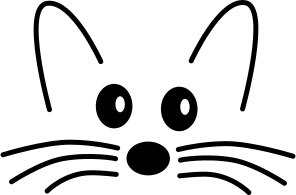
\includegraphics[width=1.4em]{squeak-logo}}}
\iftoshelse{
	\usepackage{marginnote}
		\renewcommand*{\marginfont}{\footnotesize}
	\newcommand{\vartriangleout}{\ifthenelse{\isodd{\thepage}}{\vartriangleright}{\vartriangleleft}}
	\newcommand{\dothisicon}{\fcolorbox{blue!65}{white}{\highlight{$\vartriangleout$}}}
	\newcommand{\dothis}[1]{%
		\noindent\par\noindent
		{\reversemarginpar
			\marginnote{\fcolorbox{blue!65}{white}{\highlight{$\vartriangleout$}}}}
		%\MarginLabel{do this}
		\noindent\emph{#1}
		\nopagebreak}
}{
	\newcommand{\dothisicon}{\raisebox{-.5ex}{
\includegraphics[height=1.2em]{pharo}}}
	\newcommand{\dothis}[1]{%
		\medskip
		\noindent\dothisicon
		\ifx#1\empty\else\quad\emph{#1}\fi
		\par\smallskip\nopagebreak}
}
%===> NEW VERSION <===
% NB: To use this in an individual chapter, you must set:
%\graphicspath{{figures/} {../figures/}}
% at the head of the chapter.  Don't forget the final /
%=============================================================
%:Reader hints (hint)
%
% Indicates a non-obvious consequence
\newcommand{\hint}[1]{\vspace{1ex}\noindent\fbox{\textsc{Hint}} \emph{#1}}
%=================================================================
% graphics for Morphic handles
\newcommand{\grabHandle}{\raisebox{-0.2ex}{
\includegraphics[width=1em]{blackHandle}}}
\newcommand{\moveHandle}{\raisebox{-0.2ex}{
\includegraphics[width=1em]{moveHandle}}}
\newcommand{\debugHandle}{\raisebox{-0.2ex}{
\includegraphics[width=1em]{debugHandle}}}
%=============================================================
%:Highlighting Important stuff (doublebox)
%
% From Seaside book ...
\newsavebox{\SavedText}
\newlength{\InnerBoxRule}\setlength{\InnerBoxRule}{.75\fboxrule}
\newlength{\OuterBoxRule}\setlength{\OuterBoxRule}{1.5\fboxrule}
\newlength{\BoxSeparation}\setlength{\BoxSeparation}{1.5\fboxrule}
\addtolength{\BoxSeparation}{.5pt}
\newlength{\SaveBoxSep}\setlength{\SaveBoxSep}{2\fboxsep}
%
\newenvironment{doublebox}{\begin{lrbox}{\SavedText}
    \begin{minipage}{.75\textwidth}}
    {\end{minipage}\end{lrbox}\begin{center}
    \setlength{\fboxsep}{\BoxSeparation}\setlength{\fboxrule}{\OuterBoxRule}
    \fbox{\setlength{\fboxsep}{\SaveBoxSep}\setlength{\fboxrule}{\InnerBoxRule}%
      \fbox{\usebox{\SavedText}}}
  \end{center}}
% Use this:
\newcommand{\important}[1]{\begin{doublebox}#1\end{doublebox}}
%=============================================================
%:Section depth
\setcounter{secnumdepth}{2}
%% for this to happen start the file with
%\ifx\wholebook\relax\else
%% $Author$
% $Date$
% $Revision$

% HISTORY:
% 2006-10-31 - Oscar code macros
% ...

%=============================================================
% NB: documentclass must be set in main document.
% Allows book to be generated in multiple formats.
%=============================================================
%:Packages
\usepackage[T1]{fontenc}  %%%%%% really important to get the code directly in the text!
\usepackage{lmodern}
%\usepackage[scaled=0.85]{bookmanx} % needs another scale factor if used with \renewcommand{\sfdefault}{cmbr}
\usepackage{palatino}
\usepackage[scaled=0.85]{helvet}
\usepackage[protrusion,expansion=false]{microtype}
\usepackage{graphicx}
\usepackage{theorem}
\usepackage[english]{babel}
% ON: pdfsync breaks the use of p{width} for tabular columns!
\ifdefined\usepdfsync\usepackage{pdfsync}\fi % Requires texlive 2007
%=============================================================
%:More packages
%Stef should check which ones are used!
%\usepackage{picinpar}
%\usepackage{layout}
%\usepackage{color}
%\usepackage{enum}
%\usepackage{a4wide}
% \usepackage{fancyhdr}
\usepackage{ifthen}
\usepackage{float}
\usepackage{longtable}
\usepackage{makeidx}
\usepackage[nottoc]{tocbibind}
\usepackage{multicol}
\usepackage{booktabs}	% book-style tables
\usepackage{topcapt}	% enables \topcaption
\usepackage{multirow}
\usepackage{tabularx}
%\usepackage[bottom]{footmisc}
\usepackage{xspace}
\usepackage{alltt}
\usepackage{amssymb,textcomp}
\usepackage[usenames,dvipsnames]{color}
%\usepackage{colortbl}
\usepackage[hang]{subfigure}\makeatletter\def\p@subfigure{\thefigure\,}\makeatother
\usepackage{rotating}
\usepackage{enumitem}	% apb: allows more control over tags in enumerations
\usepackage{verbatim}     % for comment environment
\usepackage{varioref}	% for page references that work
\labelformat{footnote}{\thechapter--#1} % to distinguish citations from jurabib
\usepackage{needspace}
\usepackage{isodateo} % enable \isodate
\usepackage[newparttoc,pagestyles]{titlesec}
\usepackage{titletoc}
\usepackage{wrapfig}

\usepackage[
	super,
	citefull=first,
	authorformat={allreversed,and},
	titleformat={commasep,italic}
]{jurabib} % citations as footnotes
\usepackage[
	colorlinks=true,
	linkcolor=black,
	urlcolor=black,
	citecolor=black
]{hyperref}   % should come last
%=============================================================
%:PDF version
\pdfminorversion=3 % Set PDF to 1.3 for Lulu
%=============================================================
%:URL style
\makeatletter
\def\url@leostyle{%
  \@ifundefined{selectfont}{\def\UrlFont{\sf}}{\def\UrlFont{\sffamily}}}
\makeatother
% Now actually use the newly defined style.
\urlstyle{leo}
%=============================================================
%:Booleans
\newboolean{lulu}
\setboolean{lulu}{false}
\newcommand{\ifluluelse}[2]{\ifthenelse{\boolean{lulu}}{#1}{#2}}
%=============================================================
%:Names
\newcommand{\SUnit}{SUnit\xspace}
\newcommand{\sunit}{SUnit\xspace}
\newcommand{\xUnit}{$x$Unit\xspace}
\newcommand{\JUnit}{JUnit\xspace}
\newcommand{\st}{Smalltalk\xspace}
\newcommand{\pharo}{Pharo\xspace} % Use this, not \Pharo
%\newcommand{\sqmap}{SqueakMap\xspace}
\newcommand{\squeak}{Squeak\xspace} % use this, not \Squeak or \sq
\newcommand{\sqsrc}{SqueakSource\xspace}
\newcommand{\sbe}{\url{http://SqueakByExample.org}\xspace}
\newcommand{\pharoweb}{\url{http://pharo-project.org}\xspace}
\newcommand{\pbe}{\url{http://PharoByExample.org}\xspace}
\newcommand{\sba}{\url{http://SquareBracketAssociates.org}\xspace}
\newcommand{\bam}{\lct{Bounc\-ing\-Atoms\-Morph}\xspace}
%=============================================================
%:Markup macros for proof-reading
\usepackage[normalem]{ulem} % for \sout
\usepackage{xcolor}
\newcommand{\ra}{$\rightarrow$}
\newcommand{\ugh}[1]{\textcolor{red}{\uwave{#1}}} % please rephrase
\newcommand{\ins}[1]{\textcolor{blue}{\uline{#1}}} % please insert
\newcommand{\del}[1]{\textcolor{red}{\sout{#1}}} % please delete
\newcommand{\chg}[2]{\textcolor{red}{\sout{#1}}{\ra}\textcolor{blue}{\uline{#2}}} % please change
%=============================================================
%:Editorial comment macros
%\newcommand{\nnbb}[2]{
%    % \fbox{\bfseries\sffamily\scriptsize#1}
%    \fcolorbox{gray}{yellow}{\bfseries\sffamily\scriptsize#1}
%    {\sf\small$\blacktriangleright$\textit{#2}$\blacktriangleleft$}
%   }
\newcommand{\yellowbox}[1]{\fcolorbox{gray}{yellow}{\bfseries\sffamily\scriptsize#1}}
\newcommand{\triangles}[1]{{\sf\small$\blacktriangleright$\textit{#1}$\blacktriangleleft$}}
\newcommand{\nnbb}[2]{\yellowbox{#1} \triangles{#2}}
\newcommand{\fix}{\yellowbox{FIX!}}
\newcommand{\here}{\yellowbox{CONTINUE HERE!}}
% editor macros
\newcommand{\apl}[1]{\nnbb{Alain}{#1}} % Alain
\newcommand{\ab}[1]{\nnbb{Andrew}{#1}} % Black
\newcommand{\sd}[1]{\nnbb{St\'{e}f}{#1}} % Ducasse
\newcommand{\gl}[1]{\nnbb{Guillaume}{#1}} % Ducasse
\newcommand{\cd}[1]{\nnbb{Christophe}{#1}} % Ducasse
\newcommand{\sig}[1]{\nnbb{Igor}{#1}} % Igor
\newcommand{\dc}[1]{\nnbb{DamienC}{#1}} % Ducasse
\newcommand{\md}[1]{\nnbb{Marcus}{#1}} % Denker
\newcommand{\on}[1]{\nnbb{Oscar}{#1}} % Nierstrasz
\newcommand{\damien}[1]{\nnbb{Damien}{#1}} % Pollet
\newcommand{\lr}[1]{\nnbb{Lukas}{#1}} % Renggli
\newcommand{\orla}[1]{\nnbb{Orla}{#1}} % Greevy
\newcommand{\alex}[1]{\nnbb{Alex}{#1}} % Bergel
\newcommand{\alx}[1]{\nnbb{Alex}{#1}} % Bergel
\newcommand{\dr}[1]{\nnbb{David}{#1}} % Roethlisberger
\newcommand{\ja}[1]{\nnbb{Jannik}{#1}} % Laval
\newcommand{\cb}[1]{\nnbb{Camillo}{#1}} % Bruni
\newcommand{\jr}[1]{\nnbb{Jorge}{#1}} % Ressia
\newcommand{\jb}[1]{\nnbb{JB}{#1}} % JB
\newcommand{\jp}[1]{\nnbb{Javier}{#1}} % Pimas
\newcommand{\fp}[1]{\nnbb{Fabrizio}{#1}} % Perin
\newcommand{\michael}[1]{\nnbb{Michael}{#1}} % Davies
\newcommand{\ew}[1]{\nnbb{Erwann}{#1}} % Wernli
\newcommand{\mb}[1]{\nnbb{Martial}{#1}} % Boniou
\newcommand{\hw}[1]{\nnbb{Hernan}{#1}} % Wilkinson
\newcommand{\ben}[1]{\nnbb{Benjamin}{#1}} % Benjamin Van Ryseghem
\newcommand{\hjo}[1]{\nnbb{HwaJong}{#1}} % HwaJong Oh aka daliot
\newcommand{\ml}[1]{\nnbb{Max}{#1}} % Max Leske
\newcommand{\mmp}[1]{\nnbb{Mariano}{#1}} % Mariano Martinez Peck
\newcommand{\luc}[1]{\nnbb{Luc}{#1}} % Luc Fabresse
\newcommand{\dkl}[1]{\nnbb{Daniel}{#1}} % Daniel Lyons
\newcommand{\vu}[1]{\nnbb{Veronica}{#1}} % Veronica Uquillas Gomez
\newcommand{\martin}[1]{\nnbb{Martin}{#1}} % Martin Dias
\newcommand{\vp}[1]{\nnbb{Vanessa}{#1}} % Vanessa Pena
\newcommand{\gp}[1]{\nnbb{Guille}{#1}} % Guillermo Polito

%=============================================================
%:Abbreviation macros
\newcommand{\ie}{\emph{i.e.},\xspace}
\newcommand{\eg}{\emph{e.g.},\xspace}
\newcommand{\etc}{etc.\xspace}
%=============================================================
%:Cross reference macros
\newcommand{\charef}[1]{Chapter~\ref{cha:#1}\xspace}
\newcommand{\secref}[1]{Section~\ref{sec:#1}\xspace}
\newcommand{\figref}[1]{Figure~\ref{fig:#1}\xspace}
\newcommand{\Figref}[1]{Figure~\ref{fig:#1}\xspace}
\newcommand{\appref}[1]{Appendix~\ref{app:#1}\xspace}
\newcommand{\tabref}[1]{Table~\ref{tab:#1}\xspace}
\newcommand{\faqref}[1]{FAQ~\ref{faq:#1}, p.~\pageref{faq:#1}\xspace}
% APB: I removed trailing \xspace commands from these macros because
% \xspace mostly doesn't work.  If you want a space after your
% references, type one!
% ON: xspace has always worked just fine for me!  Please leave them in.
%
\newcommand{\ruleref}[1]{\ref{rule:#1}\xspace}
%
\newcommand{\egref}[1]{example~\ref{eg:#1}\xspace}
\newcommand{\Egref}[1]{Example~\ref{eg:#1}\xspace}
%
\newcommand{\scrref}[1]{script~\ref{scr:#1}\xspace}
\newcommand{\Scrref}[1]{Script~\ref{scr:#1}\xspace}
\newcommand{\tscrref}[1]{the script~\ref{scr:#1}\xspace}
\newcommand{\Tscrref}[1]{The script~\ref{scr:#1}\xspace}
%
\newcommand{\mthref}[1]{method~\ref{mth:#1}\xspace}
\newcommand{\mthsref}[1]{methods~\ref{mth:#1}\xspace}
\newcommand{\Mthref}[1]{Method~\ref{mth:#1}\xspace}
\newcommand{\tmthref}[1]{the method~\ref{mth:#1}\xspace}
\newcommand{\Tmthref}[1]{The method~\ref{mth:#1}\xspace}
%
\newcommand{\clsref}[1]{class~\ref{cls:#1}\xspace}
\newcommand{\tclsref}[1]{the class~\ref{cls:#1}\xspace}
\newcommand{\Tclsref}[1]{The class~\ref{cls:#1}\xspace}

\newcommand{\chalabel}[1]{\label{cha:#1}}
\newcommand{\seclabel}[1]{\label{sec:#1}}
\newcommand{\figlabel}[1]{\label{fig:#1}}
\newcommand{\tablabel}[1]{\label{tab:#1}}
\newcommand{\rulelabel}[1]{\label{rule:#1}}
\newcommand{\eglabel}[1]{\label{eg:#1}}
\newcommand{\scrlabel}[1]{\label{scr:#1}}
\newcommand{\mthlabel}[1]{\label{mth:#1}}
\newcommand{\clslabel}[1]{\label{cls:#1}}
\newcommand{\faqlabel}[1]{\label{faq:#1}}
%=============================================================
%:Menu item macro
% for menu items, so we can change our minds on how to print them! (apb)
\definecolor{lightgray}{gray}{0.89}
\newcommand{\menu}[1]{{%
	\setlength{\fboxsep}{0pt}%
	\colorbox{lightgray}{{{\upshape\sffamily\strut \,#1\,}}}}}
\newcommand{\link}[1]{{%
	\fontfamily{lmr}\selectfont
 	\upshape{\sffamily \underline{#1}}}}
% For submenu items:
\newcommand{\go}{\,$\triangleright$\,}
% \newcommand{\go}{\,$\blacktriangleright$\,}
% For keyboard shortcuts:
%\newcommand{\short}[1]{\mbox{$\langle${\sc CMD}$\rangle$-#1}\xspace}
\newcommand{\short}[1]{\mbox{{\sc cmd}\hspace{0.08em}--\hspace{0.09em}#1}\xspace}
% For buttons:
\newcommand{\button}[1]{{%
	\setlength{\fboxsep}{0pt}%
	\fbox{{\upshape\sffamily\strut \,#1\,}}}}
% NB: The button macro does not work within captions -- incompatible with xcolor package :-(
\newcommand{\toolsflap}{\textit{Tools} flap\xspace}
%=============================================================
%:Mouse clicks
\newcommand{\click}{click\xspace} % RED
\newcommand{\actclick}{action-click\xspace} % YELLOW
\newcommand{\metaclick}{meta-click\xspace} % BLUE
\newcommand{\Click}{Click\xspace} % RED
\newcommand{\Actclick}{Action-click\xspace} % YELLOW
\newcommand{\Metaclick}{Meta-click\xspace} % BLUE
%=============================================================
%:ToSh macros
\newboolean{tosh}
\setboolean{tosh}{false}
\newcommand{\iftoshelse}[2]{\ifthenelse{\boolean{tosh}}{#1}{#2}}
%=============================================================
%:ToSh colors
%\newcommand{\highlightcolor}{\color{blue!65}}
%\newcommand{\boxcolor}{\color{gray!25}}
\newcommand{\highlight}[1]{\textcolor{blue!65}{#1}}
%\newcommand{\codecolor}{\color{blue!65}}
%%\setlength{\fboxrule}{2pt}
%\newcommand{\asPict}[1]{%
%	{\Large\highlight{#1}}}
%=============================================================
%:Reader cues (do this)
%
% Indicate something the reader should try out.
% \newcommand{\dothisicon}{\raisebox{-.5ex}{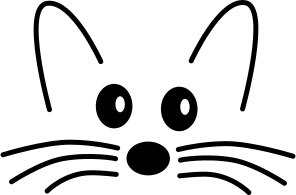
\includegraphics[width=1.4em]{squeak-logo}}}
\iftoshelse{
	\usepackage{marginnote}
		\renewcommand*{\marginfont}{\footnotesize}
	\newcommand{\vartriangleout}{\ifthenelse{\isodd{\thepage}}{\vartriangleright}{\vartriangleleft}}
	\newcommand{\dothisicon}{\fcolorbox{blue!65}{white}{\highlight{$\vartriangleout$}}}
	\newcommand{\dothis}[1]{%
		\noindent\par\noindent
		{\reversemarginpar
			\marginnote{\fcolorbox{blue!65}{white}{\highlight{$\vartriangleout$}}}}
		%\MarginLabel{do this}
		\noindent\emph{#1}
		\nopagebreak}
}{
	\newcommand{\dothisicon}{\raisebox{-.5ex}{
\includegraphics[height=1.2em]{pharo}}}
	\newcommand{\dothis}[1]{%
		\medskip
		\noindent\dothisicon
		\ifx#1\empty\else\quad\emph{#1}\fi
		\par\smallskip\nopagebreak}
}
%===> NEW VERSION <===
% NB: To use this in an individual chapter, you must set:
%\graphicspath{{figures/} {../figures/}}
% at the head of the chapter.  Don't forget the final /
%=============================================================
%:Reader hints (hint)
%
% Indicates a non-obvious consequence
\newcommand{\hint}[1]{\vspace{1ex}\noindent\fbox{\textsc{Hint}} \emph{#1}}
%=================================================================
% graphics for Morphic handles
\newcommand{\grabHandle}{\raisebox{-0.2ex}{
\includegraphics[width=1em]{blackHandle}}}
\newcommand{\moveHandle}{\raisebox{-0.2ex}{
\includegraphics[width=1em]{moveHandle}}}
\newcommand{\debugHandle}{\raisebox{-0.2ex}{
\includegraphics[width=1em]{debugHandle}}}
%=============================================================
%:Highlighting Important stuff (doublebox)
%
% From Seaside book ...
\newsavebox{\SavedText}
\newlength{\InnerBoxRule}\setlength{\InnerBoxRule}{.75\fboxrule}
\newlength{\OuterBoxRule}\setlength{\OuterBoxRule}{1.5\fboxrule}
\newlength{\BoxSeparation}\setlength{\BoxSeparation}{1.5\fboxrule}
\addtolength{\BoxSeparation}{.5pt}
\newlength{\SaveBoxSep}\setlength{\SaveBoxSep}{2\fboxsep}
%
\newenvironment{doublebox}{\begin{lrbox}{\SavedText}
    \begin{minipage}{.75\textwidth}}
    {\end{minipage}\end{lrbox}\begin{center}
    \setlength{\fboxsep}{\BoxSeparation}\setlength{\fboxrule}{\OuterBoxRule}
    \fbox{\setlength{\fboxsep}{\SaveBoxSep}\setlength{\fboxrule}{\InnerBoxRule}%
      \fbox{\usebox{\SavedText}}}
  \end{center}}
% Use this:
\newcommand{\important}[1]{\begin{doublebox}#1\end{doublebox}}
%=============================================================
%:Section depth
\setcounter{secnumdepth}{2}
%% for this to happen start the file with
%\ifx\wholebook\relax\else
%\input{../common.tex}
%\begin{document}
%\fi
% and terminate by
% \ifx\wholebook\relax\else\end{document}\fi

\DeclareGraphicsExtensions{.pdf, .jpg, .png}
%=============================================================
%:PDF setup
\hypersetup{
%   a4paper,
%   pdfstartview=FitV,
%   colorlinks,
%   linkcolor=darkblue,
%   citecolor=darkblue,
   pdftitle={Pharo by Example},
   pdfauthor={Andrew P. Black, St\'ephane Ducasse,	Oscar Nierstrasz,
Damien Pollet},
   pdfkeywords={Smalltalk, Squeak, Object-Oriented Programming, OOP},
   pdfsubject={Computer Science}
}
%=============================================================
%:Page layout and appearance
%
% \renewcommand{\headrulewidth}{0pt}
\renewcommand{\chaptermark}[1]{\markboth{#1}{}}
\renewcommand{\sectionmark}[1]{\markright{\thesection\ #1}}
\renewpagestyle{plain}[\small\itshape]{%
	\setheadrule{0pt}%
	\sethead[][][]{}{}{}%
	\setfoot[][][]{}{}{}}
\renewpagestyle{headings}[\small\itshape]{%
	\setheadrule{0pt}%
	\setmarks{chapter}{section}%
	\sethead[\thepage][][\chaptertitle]{\sectiontitle}{}{\thepage}%
	\setfoot[][][]{}{}{}}
%=============================================================
%:Title section setup and TOC numbering depth
\setcounter{secnumdepth}{1}
\setcounter{tocdepth}{1}
\titleformat{\part}[display]{\centering}{\huge\partname\ \thepart}{1em}{\Huge\textbf}[]
\titleformat{\chapter}[display]{}{\huge\chaptertitlename\ \thechapter}{1em}{\Huge\raggedright\textbf}[]
\titlecontents{part}[3pc]{%
		\pagebreak[2]\addvspace{1em plus.4em minus.2em}%
		\leavevmode\large\bfseries}
	{\contentslabel{3pc}}{\hspace*{-3pc}}
	{}[\nopagebreak]
\titlecontents{chapter}[3pc]{%
		\pagebreak[0]\addvspace{1em plus.2em minus.2em}%
		\leavevmode\bfseries}
	{\contentslabel{3pc}}{}
	{\hfill\contentspage}[\nopagebreak]
\dottedcontents{section}[3pc]{}{3pc}{1pc}
\dottedcontents{subsection}[3pc]{}{0pc}{1pc}
% \dottedcontents{subsection}[4.5em]{}{0pt}{1pc}
% Make \cleardoublepage insert really blank pages http://www.tex.ac.uk/cgi-bin/texfaq2html?label=reallyblank
\let\origdoublepage\cleardoublepage
\newcommand{\clearemptydoublepage}{%
  \clearpage
  {\pagestyle{empty}\origdoublepage}}
\let\cleardoublepage\clearemptydoublepage % see http://www.tex.ac.uk/cgi-bin/texfaq2html?label=patch
%=============================================================
%:FAQ macros (for FAQ chapter)
\newtheorem{faq}{FAQ}
\newcommand{\answer}{\paragraph{Answer}\ }
%=============================================================
%:Listings package configuration
% \newcommand{\caret}{\makebox{\raisebox{0.4ex}{\footnotesize{$\wedge$}}}}
\newcommand{\caret}{\^\,}
\newcommand{\escape}{{\sf \textbackslash}}
\definecolor{source}{gray}{0.95}
\usepackage{listings}
\lstdefinelanguage{Smalltalk}{
%  morekeywords={self,super,true,false,nil,thisContext}, % This is overkill
  morestring=[d]',
  morecomment=[s]{"}{"},
  alsoletter={\#:},
  escapechar={!},
  literate=
    {BANG}{!}1
    {CARET}{\^}1
    {UNDERSCORE}{\_}1
    {\\st}{Smalltalk}9 % convenience -- in case \st occurs in code
    % {'}{{\textquotesingle}}1 % replaced by upquote=true in \lstset
    %{_}{{$\leftarrow$}}1
    {>>>}{{\sep}}1
    %{^}{{$\uparrow$}}1
    {~}{{$\sim$}}1
    {-}{{\texttt{-}}}1 %{\textminus}}1 %{-}{\hspace{-0.13em}}{-}}1  % the goal is to make - the same width as +
    % {+}{\sf+}1 %{\raisebox{0.08ex}{+}}}1      % and to raise + off the baseline to match -
    {-->}{{\quad$\longrightarrow$\quad}}3
    {~->}{{\quad$\leadsto$\quad}}3
	, % Don't forget the comma at the end!
  tabsize=4
}[keywords,comments,strings]

\lstset{language=Smalltalk,
	basicstyle=\sffamily,
	keywordstyle=\color{black}\bfseries,
	% stringstyle=\ttfamily, % Ugly! do we really want this? -- on
	mathescape=true,
	showstringspaces=false,
	keepspaces=true,
	breaklines=true,
	breakautoindent=true,
	backgroundcolor=\color{source},
	lineskip={-1pt}, % Ugly hack
	upquote=true, % straight quote; requires textcomp package
	columns=fullflexible} % no fixed width fonts
% In-line code (literal)
% Normally use this for all in-line code:

\newcommand{\ct}{\lstinline[mathescape=false,backgroundcolor=\color{white},basicstyle={\sffamily\upshape}]}
\newcommand{\cts}[1]{{\sffamily{\upshape{#1}}\xspace}}
% apb 2007.8.28 added the \upshape declaration to avoid getting italicized code in \dothis{ } sections.
% In-line code (latex enabled)
% Use this only in special situations where \ct does not work
% (within section headings ...):
\newcommand{\lct}[1]{{\textsf{\textup{#1}}}}
% Use these for system categories and protocols:
\newcommand{\scat}[1]{\emph{\textsf{#1}}\xspace}
\newcommand{\pkg}[1]{\emph{\textsf{#1}}\xspace}
\newcommand{\prot}[1]{\emph{\textsf{#1}}\xspace}
% Code environments
% NB: the arg is for tests
% Only code and example environments may be tests
\lstnewenvironment{code}[1]{%
	\lstset{%
		% frame=lines,
		frame=single,
		framerule=0pt,
		mathescape=false
	}
}{}
\def\ignoredollar#1{}
%=============================================================
%:Code environments (method, script ...)
% NB: the third arg is for tests
% Only code and example environments may be tests
\lstnewenvironment{example}[3][defaultlabel]{%
	\renewcommand{\lstlistingname}{Example}%
	\lstset{
		% frame=lines,
		frame=single,
		framerule=0pt,
		mathescape=false,
		caption={\emph{#2}},
		label={eg:#1}
	}
}{}
\lstnewenvironment{script}[2][defaultlabel]{%
\renewcommand{\lstlistingname}{Script}%
	\lstset{
		% frame=lines,
		frame=single,
		framerule=0pt,
		mathescape=false,
		name={Script},
		caption={\emph{#2}},
		label={scr:#1}
	}
}{}
\lstnewenvironment{method}[2][defaultlabel]{%
	\renewcommand{\lstlistingname}{Method}%
	\lstset{
		% frame=lines,
		frame=single,
		framerule=0pt,
		mathescape=false,
		name={Method},
		caption={\emph{#2}},
		label={mth:#1}
	}
}{}
\lstnewenvironment{methods}[2][defaultlabel]{% just for multiple methods at once
	\renewcommand{\lstlistingname}{Methods}%
	\lstset{
		% frame=lines,
		frame=single,
		framerule=0pt,
		mathescape=false,
		name={Method},
		caption={\emph{#2}},
		label={mth:#1}
	}
}{}
\lstnewenvironment{numMethod}[2][defaultlabel]{%
	\renewcommand{\lstlistingname}{Method}%
	\lstset{
		numbers=left,
		numberstyle={\tiny\sffamily},
		% frame=lines,
		frame=single,
		framerule=0pt,
		mathescape=false,
		name={Method},
		caption={\emph{#2}},
		label={mth:#1}
	}
}{}
\lstnewenvironment{classdef}[2][defaultlabel]{%
	\renewcommand{\lstlistingname}{Class}%
	\lstset{
		% frame=lines,
		frame=single,
		framerule=0pt,
		mathescape=false,
		name={Class},
		caption={\emph{#2}},
		label={cls:#1}
	}
}{}
%=============================================================
%:Reserving space
% Usually need one more line than the actual lines of code
\newcommand{\needlines}[1]{\Needspace{#1\baselineskip}}
%=============================================================
%:Indexing macros
% Macros ending with "ind" generate text as well as an index entry
% Macros ending with "index" *only* generate an index entry
\newcommand{\ind}[1]{\index{#1}#1\xspace} % plain text
\newcommand{\subind}[2]{\index{#1!#2}#2\xspace} % show #2, subindex under #1
\newcommand{\emphind}[1]{\index{#1}\emph{#1}\xspace} % emph #1
\newcommand{\emphsubind}[2]{\index{#1!#2}\emph{#2}\xspace} % show emph #2, subindex inder #1
\newcommand{\scatind}[1]{\index{#1@\textsf{#1} (category)}\scat{#1}} % category
\newcommand{\pkgind}[1]{\index{#1@\textsf{#1} (package)}\pkg{#1}} % package
\newcommand{\protind}[1]{\index{#1@\textsf{#1} (protocol)}\prot{#1}} % protocol
\newcommand{\clsind}[1]{\index{#1@\textsf{#1} (class)}\ct{#1}\xspace}
% \newcommand{\clsind}[1]{\index{#1!\#@(class)}\ct{#1}\xspace} % class
\newcommand{\clsindplural}[1]{\index{#1!\#@(class)}\ct{#1}s\xspace} % class
\newcommand{\cvind}[1]{\index{#1@\textsf{#1} (class variable)}\ct{#1}\xspace} % class var
\newcommand{\glbind}[1]{\index{#1@\textsf{#1} (global)}\ct{#1}\xspace} % global
\newcommand{\patind}[1]{\index{#1@#1 (pattern)}\ct{#1}\xspace} % pattern
\newcommand{\pvind}[1]{\index{#1@\textsf{#1} (pseudo variable)}\ct{#1}\xspace} % pseudo var
\newcommand{\clsmthind}[2]{\index{#1!#2@\ct{#2}}\ct{#1>>>#2}\xspace} % class + method name
\newcommand{\mthind}[2]{\index{#1!#2@\ct{#2}}\ct{#2}\xspace} % show method name only
\newcommand{\lmthind}[2]{\index{#1!#2@\ct{#2}}\lct{#2}\xspace} % show method name only
\newcommand{\cmind}[2]{\index{#1!#2@\ct{#2}}\ct{#1>>>#2}\xspace} % show class>>method
\newcommand{\lcmind}[2]{\index{#1!#2@\ct{#2}}\lct{#1>>>#2}\xspace} % show class>>method
\newcommand{\toolsflapind}{\index{Tools flap}\toolsflap} % index tools flap
% The following only generate an index entry:
% \newcommand{\clsindex}[1]{\index{#1@\textsf{#1} (class)}}
\newcommand{\clsindex}[1]{\index{#1!\#@(class)}} % class
\newcommand{\mthindex}[2]{\index{#1!#2@\ct{#2}}} % method
\newcommand{\cmindex}[2]{\index{#1!#2@\ct{#2}}} % class>>method
\newcommand{\cvindex}[1]{\index{#1@\textsf{#1} (class variable)}} % class var
\newcommand{\glbindex}[1]{\index{#1@\textsf{#1} (global)}}% global
\newcommand{\pvindex}[1]{\index{#1@\textsf{#1} (pseudo variable)}}% pseudo var
\newcommand{\seeindex}[2]{\index{#1|see{#2}}} % #1, see #2
\newcommand{\scatindex}[1]{\index{#1@\textsf{#1} (category)}} % category
\newcommand{\pkgindex}[1]{\index{#1@\textsf{#1} (package)}} % package
\newcommand{\protindex}[1]{\index{#1@\textsf{#1} (protocol)}} % protocol
% How can we have the main entry page numbers in bold yet not break the hyperlink?
\newcommand{\boldidx}[1]{{\bf #1}} % breaks hyperlink
%\newcommand{\indmain}[1]{\index{#1|boldidx}#1\xspace} % plain text, main entry
%\newcommand{\emphsubindmain}[2]{\index{#1!#2|boldidx}\emph{#2}\xspace} % subindex, main entry
%\newcommand{\subindmain}[2]{\index{#1!#2|boldidx}#2\xspace} % subindex, main entry
%\newcommand{\clsindmain}[1]{\index{#1@\textsf{#1} (class)|boldidx}\ct{#1}\xspace}
%\newcommand{\clsindmain}[1]{\index{#1!\#@(class)|boldidx}\ct{#1}\xspace} % class main
%\newcommand{\indexmain}[1]{\index{#1|boldidx}} % main index entry only
\newcommand{\indmain}[1]{\index{#1}#1\xspace} % The main index entry for this item
\newcommand{\emphsubindmain}[2]{\index{#1!#2}\emph{#2}\xspace} % subindex, main entry
\newcommand{\subindmain}[2]{\index{#1!#2}#2\xspace} % subindex, main entry
%\newcommand{\clsindmain}[1]{\index{#1@\textsf{#1} (class)}\ct{#1}\xspace}
\newcommand{\clsindmain}[1]{\index{#1!\#@(class)}\ct{#1}\xspace} % class main
\newcommand{\clsindexmain}[1]{\index{#1!\#@(class)}} % class main index only
\newcommand{\indexmain}[1]{\index{#1}}
%=============================================================
%:Code macros
% some constants
\newcommand{\codesize}{\small}
\newcommand{\codefont}{\sffamily}
%\newcommand{\cat}[1]{\textit{In category #1}}%%To remove later
\newlength{\scriptindent}
\setlength{\scriptindent}{.3cm}
%% Method presentation constants
\newlength{\methodindent}
\newlength{\methodwordlength}
\newlength{\aftermethod}
\setlength{\methodindent}{0.2cm}
\settowidth{\methodwordlength}{\ M\'ethode\ }
%=============================================================
%:Smalltalk macros
%\newcommand{\sep}{{$\gg$}}
\newcommand{\sep}{\mbox{>>}}
\newcommand{\self}{\lct{self}\xspace}
\newcommand{\super}{\lct{super}\xspace}
\newcommand{\nil}{\lct{nil}\xspace}
%=============================================================
% be less conservative about float placement
% these commands are from http://www.tex.ac.uk/cgi-bin/texfaq2html?label=floats
\renewcommand{\topfraction}{.9}
\renewcommand{\bottomfraction}{.9}
\renewcommand{\textfraction}{.1}
\renewcommand{\floatpagefraction}{.85}
\renewcommand{\dbltopfraction}{.66}
\renewcommand{\dblfloatpagefraction}{.85}
\setcounter{topnumber}{9}
\setcounter{bottomnumber}{9}
\setcounter{totalnumber}{20}
\setcounter{dbltopnumber}{9}
%=============================================================
% Give information from each chapter's author
\newcommand{\contact}[2]{\textbf{#1} \textsf{(#2)}}

\newcommand{\chapterauthor}[1]{\emph{with the participation of:\\#1}\\}
\newcommand{\chapterwritten}[1]{\emph{written by:\\#1}\\}

\newcommand{\authornoury}{\contact{Noury Bouraqadi}{Noury.Bouraqadi@mines-douai.fr}}
\newcommand{\authorluc}{\contact{Luc Fabresse}{Luc.Fabresse@mines-douai.fr}}
\newcommand{\authordamienc}{\contact{Damien Cassou}{damien.cassou@gmail.com}}
\newcommand{\authoroscar}{\contact{Oscar Nierstrasz}{oscar.nierstrasz@acm.org}}
\newcommand{\authorsteph}{\contact{St\'ephane Ducasse}{stephane.ducasse@inria.fr}}
\newcommand{\authoralex}{\contact{Alexandre Bergel}{alexandre@bergel.eu}}
\newcommand{\authorolivier}{\contact{Olivier Auverlot}{olivier.auverlot@inria.fr}}
\newcommand{\authornicolas}{\contact{Nicolas Cellier}{nicolas.cellier.aka.nice@gmail.com}}
\newcommand{\authormarcus}{\contact{Marcus Denker}{marcus.denker@inria.fr}}
\newcommand{\authoralain}{\contact{Alain Plantec}{alain.plantec@univ-brest.fr}}
\newcommand{\authordale}{\contact{Dale Henrichs}{dale.henrichs@gemstone.com}}
\newcommand{\authormariano}{\contact{Mariano Martinez Peck}{marianopeck@gmail.com}}
\newcommand{\authorsven}{\contact{Sven Van Caekenberghe}{sven@beta9.be}}
\newcommand{\authorlukas}{\contact{Lukas Renggli}{renggli@gmail.com}}
\newcommand{\authorjankurs}{\contact{Jan Kurs}{kurs@iam.unibe.ch}}
\newcommand{\authorguillaume}{\contact{Guillaume Larcheveque}{guillaume.larcheveque@gmail.com}}
\newcommand{\authorguillep}{\contact{Guillermo Polito}{guillermopolito@gmail.com}}
\newcommand{\authorclement}{\contact{Cl\'ement Bera}{bera.clement@gmail.com}}
\newcommand{\authormax}{\contact{Max Leske}{maxleske@gmail.com}}
\newcommand{\authorvanessa}{\contact{Vanessa Pe\~{n}a-Araya}{van.c.pena@gmail.com}}
\newcommand{\authorcamillo}{\contact{Camillo Bruni}{camillobruni@gmail.com}}

%=============================================================
% apb doesn't like paragraphs to run in to each other without a break
\parskip 1ex
%=============================================================
%:Stuff to check, merge or deprecate
%\setlength{\marginparsep}{2mm}
%\renewcommand{\baselinestretch}{1.1}
%=============================================================
\usepackage{tikz}

%\begin{document}
%\fi
% and terminate by
% \ifx\wholebook\relax\else\end{document}\fi

\DeclareGraphicsExtensions{.pdf, .jpg, .png}
%=============================================================
%:PDF setup
\hypersetup{
%   a4paper,
%   pdfstartview=FitV,
%   colorlinks,
%   linkcolor=darkblue,
%   citecolor=darkblue,
   pdftitle={Pharo by Example},
   pdfauthor={Andrew P. Black, St\'ephane Ducasse,	Oscar Nierstrasz,
Damien Pollet},
   pdfkeywords={Smalltalk, Squeak, Object-Oriented Programming, OOP},
   pdfsubject={Computer Science}
}
%=============================================================
%:Page layout and appearance
%
% \renewcommand{\headrulewidth}{0pt}
\renewcommand{\chaptermark}[1]{\markboth{#1}{}}
\renewcommand{\sectionmark}[1]{\markright{\thesection\ #1}}
\renewpagestyle{plain}[\small\itshape]{%
	\setheadrule{0pt}%
	\sethead[][][]{}{}{}%
	\setfoot[][][]{}{}{}}
\renewpagestyle{headings}[\small\itshape]{%
	\setheadrule{0pt}%
	\setmarks{chapter}{section}%
	\sethead[\thepage][][\chaptertitle]{\sectiontitle}{}{\thepage}%
	\setfoot[][][]{}{}{}}
%=============================================================
%:Title section setup and TOC numbering depth
\setcounter{secnumdepth}{1}
\setcounter{tocdepth}{1}
\titleformat{\part}[display]{\centering}{\huge\partname\ \thepart}{1em}{\Huge\textbf}[]
\titleformat{\chapter}[display]{}{\huge\chaptertitlename\ \thechapter}{1em}{\Huge\raggedright\textbf}[]
\titlecontents{part}[3pc]{%
		\pagebreak[2]\addvspace{1em plus.4em minus.2em}%
		\leavevmode\large\bfseries}
	{\contentslabel{3pc}}{\hspace*{-3pc}}
	{}[\nopagebreak]
\titlecontents{chapter}[3pc]{%
		\pagebreak[0]\addvspace{1em plus.2em minus.2em}%
		\leavevmode\bfseries}
	{\contentslabel{3pc}}{}
	{\hfill\contentspage}[\nopagebreak]
\dottedcontents{section}[3pc]{}{3pc}{1pc}
\dottedcontents{subsection}[3pc]{}{0pc}{1pc}
% \dottedcontents{subsection}[4.5em]{}{0pt}{1pc}
% Make \cleardoublepage insert really blank pages http://www.tex.ac.uk/cgi-bin/texfaq2html?label=reallyblank
\let\origdoublepage\cleardoublepage
\newcommand{\clearemptydoublepage}{%
  \clearpage
  {\pagestyle{empty}\origdoublepage}}
\let\cleardoublepage\clearemptydoublepage % see http://www.tex.ac.uk/cgi-bin/texfaq2html?label=patch
%=============================================================
%:FAQ macros (for FAQ chapter)
\newtheorem{faq}{FAQ}
\newcommand{\answer}{\paragraph{Answer}\ }
%=============================================================
%:Listings package configuration
% \newcommand{\caret}{\makebox{\raisebox{0.4ex}{\footnotesize{$\wedge$}}}}
\newcommand{\caret}{\^\,}
\newcommand{\escape}{{\sf \textbackslash}}
\definecolor{source}{gray}{0.95}
\usepackage{listings}
\lstdefinelanguage{Smalltalk}{
%  morekeywords={self,super,true,false,nil,thisContext}, % This is overkill
  morestring=[d]',
  morecomment=[s]{"}{"},
  alsoletter={\#:},
  escapechar={!},
  literate=
    {BANG}{!}1
    {CARET}{\^}1
    {UNDERSCORE}{\_}1
    {\\st}{Smalltalk}9 % convenience -- in case \st occurs in code
    % {'}{{\textquotesingle}}1 % replaced by upquote=true in \lstset
    %{_}{{$\leftarrow$}}1
    {>>>}{{\sep}}1
    %{^}{{$\uparrow$}}1
    {~}{{$\sim$}}1
    {-}{{\texttt{-}}}1 %{\textminus}}1 %{-}{\hspace{-0.13em}}{-}}1  % the goal is to make - the same width as +
    % {+}{\sf+}1 %{\raisebox{0.08ex}{+}}}1      % and to raise + off the baseline to match -
    {-->}{{\quad$\longrightarrow$\quad}}3
    {~->}{{\quad$\leadsto$\quad}}3
	, % Don't forget the comma at the end!
  tabsize=4
}[keywords,comments,strings]

\lstset{language=Smalltalk,
	basicstyle=\sffamily,
	keywordstyle=\color{black}\bfseries,
	% stringstyle=\ttfamily, % Ugly! do we really want this? -- on
	mathescape=true,
	showstringspaces=false,
	keepspaces=true,
	breaklines=true,
	breakautoindent=true,
	backgroundcolor=\color{source},
	lineskip={-1pt}, % Ugly hack
	upquote=true, % straight quote; requires textcomp package
	columns=fullflexible} % no fixed width fonts
% In-line code (literal)
% Normally use this for all in-line code:

\newcommand{\ct}{\lstinline[mathescape=false,backgroundcolor=\color{white},basicstyle={\sffamily\upshape}]}
\newcommand{\cts}[1]{{\sffamily{\upshape{#1}}\xspace}}
% apb 2007.8.28 added the \upshape declaration to avoid getting italicized code in \dothis{ } sections.
% In-line code (latex enabled)
% Use this only in special situations where \ct does not work
% (within section headings ...):
\newcommand{\lct}[1]{{\textsf{\textup{#1}}}}
% Use these for system categories and protocols:
\newcommand{\scat}[1]{\emph{\textsf{#1}}\xspace}
\newcommand{\pkg}[1]{\emph{\textsf{#1}}\xspace}
\newcommand{\prot}[1]{\emph{\textsf{#1}}\xspace}
% Code environments
% NB: the arg is for tests
% Only code and example environments may be tests
\lstnewenvironment{code}[1]{%
	\lstset{%
		% frame=lines,
		frame=single,
		framerule=0pt,
		mathescape=false
	}
}{}
\def\ignoredollar#1{}
%=============================================================
%:Code environments (method, script ...)
% NB: the third arg is for tests
% Only code and example environments may be tests
\lstnewenvironment{example}[3][defaultlabel]{%
	\renewcommand{\lstlistingname}{Example}%
	\lstset{
		% frame=lines,
		frame=single,
		framerule=0pt,
		mathescape=false,
		caption={\emph{#2}},
		label={eg:#1}
	}
}{}
\lstnewenvironment{script}[2][defaultlabel]{%
\renewcommand{\lstlistingname}{Script}%
	\lstset{
		% frame=lines,
		frame=single,
		framerule=0pt,
		mathescape=false,
		name={Script},
		caption={\emph{#2}},
		label={scr:#1}
	}
}{}
\lstnewenvironment{method}[2][defaultlabel]{%
	\renewcommand{\lstlistingname}{Method}%
	\lstset{
		% frame=lines,
		frame=single,
		framerule=0pt,
		mathescape=false,
		name={Method},
		caption={\emph{#2}},
		label={mth:#1}
	}
}{}
\lstnewenvironment{methods}[2][defaultlabel]{% just for multiple methods at once
	\renewcommand{\lstlistingname}{Methods}%
	\lstset{
		% frame=lines,
		frame=single,
		framerule=0pt,
		mathescape=false,
		name={Method},
		caption={\emph{#2}},
		label={mth:#1}
	}
}{}
\lstnewenvironment{numMethod}[2][defaultlabel]{%
	\renewcommand{\lstlistingname}{Method}%
	\lstset{
		numbers=left,
		numberstyle={\tiny\sffamily},
		% frame=lines,
		frame=single,
		framerule=0pt,
		mathescape=false,
		name={Method},
		caption={\emph{#2}},
		label={mth:#1}
	}
}{}
\lstnewenvironment{classdef}[2][defaultlabel]{%
	\renewcommand{\lstlistingname}{Class}%
	\lstset{
		% frame=lines,
		frame=single,
		framerule=0pt,
		mathescape=false,
		name={Class},
		caption={\emph{#2}},
		label={cls:#1}
	}
}{}
%=============================================================
%:Reserving space
% Usually need one more line than the actual lines of code
\newcommand{\needlines}[1]{\Needspace{#1\baselineskip}}
%=============================================================
%:Indexing macros
% Macros ending with "ind" generate text as well as an index entry
% Macros ending with "index" *only* generate an index entry
\newcommand{\ind}[1]{\index{#1}#1\xspace} % plain text
\newcommand{\subind}[2]{\index{#1!#2}#2\xspace} % show #2, subindex under #1
\newcommand{\emphind}[1]{\index{#1}\emph{#1}\xspace} % emph #1
\newcommand{\emphsubind}[2]{\index{#1!#2}\emph{#2}\xspace} % show emph #2, subindex inder #1
\newcommand{\scatind}[1]{\index{#1@\textsf{#1} (category)}\scat{#1}} % category
\newcommand{\pkgind}[1]{\index{#1@\textsf{#1} (package)}\pkg{#1}} % package
\newcommand{\protind}[1]{\index{#1@\textsf{#1} (protocol)}\prot{#1}} % protocol
\newcommand{\clsind}[1]{\index{#1@\textsf{#1} (class)}\ct{#1}\xspace}
% \newcommand{\clsind}[1]{\index{#1!\#@(class)}\ct{#1}\xspace} % class
\newcommand{\clsindplural}[1]{\index{#1!\#@(class)}\ct{#1}s\xspace} % class
\newcommand{\cvind}[1]{\index{#1@\textsf{#1} (class variable)}\ct{#1}\xspace} % class var
\newcommand{\glbind}[1]{\index{#1@\textsf{#1} (global)}\ct{#1}\xspace} % global
\newcommand{\patind}[1]{\index{#1@#1 (pattern)}\ct{#1}\xspace} % pattern
\newcommand{\pvind}[1]{\index{#1@\textsf{#1} (pseudo variable)}\ct{#1}\xspace} % pseudo var
\newcommand{\clsmthind}[2]{\index{#1!#2@\ct{#2}}\ct{#1>>>#2}\xspace} % class + method name
\newcommand{\mthind}[2]{\index{#1!#2@\ct{#2}}\ct{#2}\xspace} % show method name only
\newcommand{\lmthind}[2]{\index{#1!#2@\ct{#2}}\lct{#2}\xspace} % show method name only
\newcommand{\cmind}[2]{\index{#1!#2@\ct{#2}}\ct{#1>>>#2}\xspace} % show class>>method
\newcommand{\lcmind}[2]{\index{#1!#2@\ct{#2}}\lct{#1>>>#2}\xspace} % show class>>method
\newcommand{\toolsflapind}{\index{Tools flap}\toolsflap} % index tools flap
% The following only generate an index entry:
% \newcommand{\clsindex}[1]{\index{#1@\textsf{#1} (class)}}
\newcommand{\clsindex}[1]{\index{#1!\#@(class)}} % class
\newcommand{\mthindex}[2]{\index{#1!#2@\ct{#2}}} % method
\newcommand{\cmindex}[2]{\index{#1!#2@\ct{#2}}} % class>>method
\newcommand{\cvindex}[1]{\index{#1@\textsf{#1} (class variable)}} % class var
\newcommand{\glbindex}[1]{\index{#1@\textsf{#1} (global)}}% global
\newcommand{\pvindex}[1]{\index{#1@\textsf{#1} (pseudo variable)}}% pseudo var
\newcommand{\seeindex}[2]{\index{#1|see{#2}}} % #1, see #2
\newcommand{\scatindex}[1]{\index{#1@\textsf{#1} (category)}} % category
\newcommand{\pkgindex}[1]{\index{#1@\textsf{#1} (package)}} % package
\newcommand{\protindex}[1]{\index{#1@\textsf{#1} (protocol)}} % protocol
% How can we have the main entry page numbers in bold yet not break the hyperlink?
\newcommand{\boldidx}[1]{{\bf #1}} % breaks hyperlink
%\newcommand{\indmain}[1]{\index{#1|boldidx}#1\xspace} % plain text, main entry
%\newcommand{\emphsubindmain}[2]{\index{#1!#2|boldidx}\emph{#2}\xspace} % subindex, main entry
%\newcommand{\subindmain}[2]{\index{#1!#2|boldidx}#2\xspace} % subindex, main entry
%\newcommand{\clsindmain}[1]{\index{#1@\textsf{#1} (class)|boldidx}\ct{#1}\xspace}
%\newcommand{\clsindmain}[1]{\index{#1!\#@(class)|boldidx}\ct{#1}\xspace} % class main
%\newcommand{\indexmain}[1]{\index{#1|boldidx}} % main index entry only
\newcommand{\indmain}[1]{\index{#1}#1\xspace} % The main index entry for this item
\newcommand{\emphsubindmain}[2]{\index{#1!#2}\emph{#2}\xspace} % subindex, main entry
\newcommand{\subindmain}[2]{\index{#1!#2}#2\xspace} % subindex, main entry
%\newcommand{\clsindmain}[1]{\index{#1@\textsf{#1} (class)}\ct{#1}\xspace}
\newcommand{\clsindmain}[1]{\index{#1!\#@(class)}\ct{#1}\xspace} % class main
\newcommand{\clsindexmain}[1]{\index{#1!\#@(class)}} % class main index only
\newcommand{\indexmain}[1]{\index{#1}}
%=============================================================
%:Code macros
% some constants
\newcommand{\codesize}{\small}
\newcommand{\codefont}{\sffamily}
%\newcommand{\cat}[1]{\textit{In category #1}}%%To remove later
\newlength{\scriptindent}
\setlength{\scriptindent}{.3cm}
%% Method presentation constants
\newlength{\methodindent}
\newlength{\methodwordlength}
\newlength{\aftermethod}
\setlength{\methodindent}{0.2cm}
\settowidth{\methodwordlength}{\ M\'ethode\ }
%=============================================================
%:Smalltalk macros
%\newcommand{\sep}{{$\gg$}}
\newcommand{\sep}{\mbox{>>}}
\newcommand{\self}{\lct{self}\xspace}
\newcommand{\super}{\lct{super}\xspace}
\newcommand{\nil}{\lct{nil}\xspace}
%=============================================================
% be less conservative about float placement
% these commands are from http://www.tex.ac.uk/cgi-bin/texfaq2html?label=floats
\renewcommand{\topfraction}{.9}
\renewcommand{\bottomfraction}{.9}
\renewcommand{\textfraction}{.1}
\renewcommand{\floatpagefraction}{.85}
\renewcommand{\dbltopfraction}{.66}
\renewcommand{\dblfloatpagefraction}{.85}
\setcounter{topnumber}{9}
\setcounter{bottomnumber}{9}
\setcounter{totalnumber}{20}
\setcounter{dbltopnumber}{9}
%=============================================================
% Give information from each chapter's author
\newcommand{\contact}[2]{\textbf{#1} \textsf{(#2)}}

\newcommand{\chapterauthor}[1]{\emph{with the participation of:\\#1}\\}
\newcommand{\chapterwritten}[1]{\emph{written by:\\#1}\\}

\newcommand{\authornoury}{\contact{Noury Bouraqadi}{Noury.Bouraqadi@mines-douai.fr}}
\newcommand{\authorluc}{\contact{Luc Fabresse}{Luc.Fabresse@mines-douai.fr}}
\newcommand{\authordamienc}{\contact{Damien Cassou}{damien.cassou@gmail.com}}
\newcommand{\authoroscar}{\contact{Oscar Nierstrasz}{oscar.nierstrasz@acm.org}}
\newcommand{\authorsteph}{\contact{St\'ephane Ducasse}{stephane.ducasse@inria.fr}}
\newcommand{\authoralex}{\contact{Alexandre Bergel}{alexandre@bergel.eu}}
\newcommand{\authorolivier}{\contact{Olivier Auverlot}{olivier.auverlot@inria.fr}}
\newcommand{\authornicolas}{\contact{Nicolas Cellier}{nicolas.cellier.aka.nice@gmail.com}}
\newcommand{\authormarcus}{\contact{Marcus Denker}{marcus.denker@inria.fr}}
\newcommand{\authoralain}{\contact{Alain Plantec}{alain.plantec@univ-brest.fr}}
\newcommand{\authordale}{\contact{Dale Henrichs}{dale.henrichs@gemstone.com}}
\newcommand{\authormariano}{\contact{Mariano Martinez Peck}{marianopeck@gmail.com}}
\newcommand{\authorsven}{\contact{Sven Van Caekenberghe}{sven@beta9.be}}
\newcommand{\authorlukas}{\contact{Lukas Renggli}{renggli@gmail.com}}
\newcommand{\authorjankurs}{\contact{Jan Kurs}{kurs@iam.unibe.ch}}
\newcommand{\authorguillaume}{\contact{Guillaume Larcheveque}{guillaume.larcheveque@gmail.com}}
\newcommand{\authorguillep}{\contact{Guillermo Polito}{guillermopolito@gmail.com}}
\newcommand{\authorclement}{\contact{Cl\'ement Bera}{bera.clement@gmail.com}}
\newcommand{\authormax}{\contact{Max Leske}{maxleske@gmail.com}}
\newcommand{\authorvanessa}{\contact{Vanessa Pe\~{n}a-Araya}{van.c.pena@gmail.com}}
\newcommand{\authorcamillo}{\contact{Camillo Bruni}{camillobruni@gmail.com}}

%=============================================================
% apb doesn't like paragraphs to run in to each other without a break
\parskip 1ex
%=============================================================
%:Stuff to check, merge or deprecate
%\setlength{\marginparsep}{2mm}
%\renewcommand{\baselinestretch}{1.1}
%=============================================================
\usepackage{tikz}

%	\usepackage{a4wide}
% --------------------------------------------
    \graphicspath{{figures/} {../figures/}}
	\begin{document}
	% \renewcommand{\nnbb}[2]{} % Disable editorial comments
	\sloppy
	\frontmatter
\fi
%=================================================================
\chapter{Preface}\chalabel{intro}

Using a programming language is so far the most convenient way for a human to tell  a computer what it should do. Pharo is an object-oriented programming language, deeply influenced by Smalltalk. Pharo is more than a syntax and a bunch of semantics rules as most programming languages are. Pharo comes with an extensible and flexible programming environment. Thanks to its numerous object-oriented libraries frameworks, Pharo shines for modeling and visualizing data, scripting, networking and many other ranges of applications.

The very light syntax and the malleable object model of Pharo are commonly praised. Both early learners and experienced programmers enjoy the ``everything is an object'' paradigm. The simplicity and expressiveness of Pharo as well as a living environment empowers programmers with a wonderful and unique sensation. 

Deep into Pharo is the second volume of a series of books initiated with Pharo by Example\footnote{freely available at \ct{http://pharobyexample.org}}. 
Deep into Pharo, the book you are reading, accompanies the reader for a deep journey into exciting parts of Pharo. It covers new libraries such as FileSystem, frameworks such as Roassal and Glamour, under documented aspects such as exceptions or blocks. 

The book is divided into 5 parts and 17 chapters. The first part deals with truly object-oriented libraries. The second part is about source code management. The third part is about advanced frameworks. The fourth part covers advanced topics of the language, in particular exception, blocks and numbers. The fifth and last part is about tooling, including profiling and parsing.

%The first part of the book covers system aspects of Pharo with FileSystem a new file library, Settings a new architecture to manage preferences, zero configuration scripts, sockets and regular expressions. The second part focuses on the package system of Pharo: it presents Monticello for source code versioning, Gofer to script it and Metacello to build large projects and specify their dependencies. 

Pharo is supported by a strong community. The community grows every single day. Pharo's community is active, innovative, and is always pushing limits of software engineering. The Pharo community consists of companies producing software, casual programmers but also high-level consultants, researchers, and teachers.
This book exists because of the Pharo community and we naturally dedicate this book to this group of people that many of us consider as our second family.


%=================================================================
\section*{Acknowledgments}

We would like to thank various people who have contributed to this book. In particular, we would like to thank:
\begin{itemize}
\item Camillo Bruni for his participation in the Zero Configuration chapter.
\item Noury Bouraqadi and Luc Fabresse for the Socket chapter.
\item Alain Plantec for his effort in the Setting Framework chapter and its effort to integrate it into Pharo.
\item Oscar Nierstrasz for writing and co-editing some chapters such as Regex and Monticello.
\item Dale Henrichs and Mariano Martinez Peck for their participation in the Metacello chapter.
\item Tudor Doru Girba for the Glamour chapter and the first documentation.
\item Cl\'ement Bera for his effort on the Exception chapter.
\item Nicolas Cellier for his participation in the Fun with Floats chapter.
\item Lukas Renggli for PetitParser and his work on the refactoring engine and smallLint rules. 
\item Jan Kurs and Guillaume Larcheveque for their participation in the PetitParser chapter.
\item Colin Putney for the initial version of FileSystem and Camillo Bruni for his review of FileSystem and his rewrite of the Pharo Core.
\item Vanessa Pe\~na for her participation in the Roassal and Mondrian chapters.
\item You, for your questions, support, bug fixes, contribution, and encouragement.
\end{itemize}

We would like to thanks Hernan Wilkinson and Carlos Ferro for their reviews, Nicolas Cellier for the feedback on the number chapter, and Vassili Bykov for permission to adapt his Regex documentation.

We thank Inria Lille Nord Europe for supporting this open-source project and for hosting the web site of this book. We also thank Object Profile for sponsoring the cover.

We also thank the Pharo community for its enthusiastic support of this project, and for informing us of the errors found in the first edition of this book.



%=============================================================
\ifx\wholebook\relax\else
   \bibliographystyle{jurabib}
   \nobibliography{scg}
   \end{document}
\fi
%=============================================================

%% Stef: pass done.
%% Ja: pass done.
%=================================================================


\part{Libraries}
%% WE NEED TO REMOVE ALL REFS TO SQUEAKSOURCE
%% WE NEED TO REMOVE ALL REFS TO FILEDIRECTORY

% $Author: Benjamin $
% $Date: 2011-12-21 14:28:33 +0200 $
% $Revision: 28563 $

%=================================================================
\ifx\wholebook\relax\else
% --------------------------------------------
% Lulu:
	\documentclass[a4paper,10pt,twoside]{book}
	\usepackage[
		papersize={6.13in,9.21in},
		hmargin={.75in,.75in},
		vmargin={.75in,1in},
		ignoreheadfoot
	]{geometry}
	% $Author$
% $Date$
% $Revision$

% HISTORY:
% 2006-10-31 - Oscar code macros
% ...

%=============================================================
% NB: documentclass must be set in main document.
% Allows book to be generated in multiple formats.
%=============================================================
%:Packages
\usepackage[T1]{fontenc}  %%%%%% really important to get the code directly in the text!
\usepackage{lmodern}
%\usepackage[scaled=0.85]{bookmanx} % needs another scale factor if used with \renewcommand{\sfdefault}{cmbr}
\usepackage{palatino}
\usepackage[scaled=0.85]{helvet}
\usepackage[protrusion,expansion=false]{microtype}
\usepackage{graphicx}
\usepackage{theorem}
\usepackage[english]{babel}
% ON: pdfsync breaks the use of p{width} for tabular columns!
\ifdefined\usepdfsync\usepackage{pdfsync}\fi % Requires texlive 2007
%=============================================================
%:More packages
%Stef should check which ones are used!
%\usepackage{picinpar}
%\usepackage{layout}
%\usepackage{color}
%\usepackage{enum}
%\usepackage{a4wide}
% \usepackage{fancyhdr}
\usepackage{ifthen}
\usepackage{float}
\usepackage{longtable}
\usepackage{makeidx}
\usepackage[nottoc]{tocbibind}
\usepackage{multicol}
\usepackage{booktabs}	% book-style tables
\usepackage{topcapt}	% enables \topcaption
\usepackage{multirow}
\usepackage{tabularx}
%\usepackage[bottom]{footmisc}
\usepackage{xspace}
\usepackage{alltt}
\usepackage{amssymb,textcomp}
\usepackage[usenames,dvipsnames]{color}
%\usepackage{colortbl}
\usepackage[hang]{subfigure}\makeatletter\def\p@subfigure{\thefigure\,}\makeatother
\usepackage{rotating}
\usepackage{enumitem}	% apb: allows more control over tags in enumerations
\usepackage{verbatim}     % for comment environment
\usepackage{varioref}	% for page references that work
\labelformat{footnote}{\thechapter--#1} % to distinguish citations from jurabib
\usepackage{needspace}
\usepackage{isodateo} % enable \isodate
\usepackage[newparttoc,pagestyles]{titlesec}
\usepackage{titletoc}
\usepackage{wrapfig}

\usepackage[
	super,
	citefull=first,
	authorformat={allreversed,and},
	titleformat={commasep,italic}
]{jurabib} % citations as footnotes
\usepackage[
	colorlinks=true,
	linkcolor=black,
	urlcolor=black,
	citecolor=black
]{hyperref}   % should come last
%=============================================================
%:PDF version
\pdfminorversion=3 % Set PDF to 1.3 for Lulu
%=============================================================
%:URL style
\makeatletter
\def\url@leostyle{%
  \@ifundefined{selectfont}{\def\UrlFont{\sf}}{\def\UrlFont{\sffamily}}}
\makeatother
% Now actually use the newly defined style.
\urlstyle{leo}
%=============================================================
%:Booleans
\newboolean{lulu}
\setboolean{lulu}{false}
\newcommand{\ifluluelse}[2]{\ifthenelse{\boolean{lulu}}{#1}{#2}}
%=============================================================
%:Names
\newcommand{\SUnit}{SUnit\xspace}
\newcommand{\sunit}{SUnit\xspace}
\newcommand{\xUnit}{$x$Unit\xspace}
\newcommand{\JUnit}{JUnit\xspace}
\newcommand{\st}{Smalltalk\xspace}
\newcommand{\pharo}{Pharo\xspace} % Use this, not \Pharo
%\newcommand{\sqmap}{SqueakMap\xspace}
\newcommand{\squeak}{Squeak\xspace} % use this, not \Squeak or \sq
\newcommand{\sqsrc}{SqueakSource\xspace}
\newcommand{\sbe}{\url{http://SqueakByExample.org}\xspace}
\newcommand{\pharoweb}{\url{http://pharo-project.org}\xspace}
\newcommand{\pbe}{\url{http://PharoByExample.org}\xspace}
\newcommand{\sba}{\url{http://SquareBracketAssociates.org}\xspace}
\newcommand{\bam}{\lct{Bounc\-ing\-Atoms\-Morph}\xspace}
%=============================================================
%:Markup macros for proof-reading
\usepackage[normalem]{ulem} % for \sout
\usepackage{xcolor}
\newcommand{\ra}{$\rightarrow$}
\newcommand{\ugh}[1]{\textcolor{red}{\uwave{#1}}} % please rephrase
\newcommand{\ins}[1]{\textcolor{blue}{\uline{#1}}} % please insert
\newcommand{\del}[1]{\textcolor{red}{\sout{#1}}} % please delete
\newcommand{\chg}[2]{\textcolor{red}{\sout{#1}}{\ra}\textcolor{blue}{\uline{#2}}} % please change
%=============================================================
%:Editorial comment macros
%\newcommand{\nnbb}[2]{
%    % \fbox{\bfseries\sffamily\scriptsize#1}
%    \fcolorbox{gray}{yellow}{\bfseries\sffamily\scriptsize#1}
%    {\sf\small$\blacktriangleright$\textit{#2}$\blacktriangleleft$}
%   }
\newcommand{\yellowbox}[1]{\fcolorbox{gray}{yellow}{\bfseries\sffamily\scriptsize#1}}
\newcommand{\triangles}[1]{{\sf\small$\blacktriangleright$\textit{#1}$\blacktriangleleft$}}
\newcommand{\nnbb}[2]{\yellowbox{#1} \triangles{#2}}
\newcommand{\fix}{\yellowbox{FIX!}}
\newcommand{\here}{\yellowbox{CONTINUE HERE!}}
% editor macros
\newcommand{\apl}[1]{\nnbb{Alain}{#1}} % Alain
\newcommand{\ab}[1]{\nnbb{Andrew}{#1}} % Black
\newcommand{\sd}[1]{\nnbb{St\'{e}f}{#1}} % Ducasse
\newcommand{\gl}[1]{\nnbb{Guillaume}{#1}} % Ducasse
\newcommand{\cd}[1]{\nnbb{Christophe}{#1}} % Ducasse
\newcommand{\sig}[1]{\nnbb{Igor}{#1}} % Igor
\newcommand{\dc}[1]{\nnbb{DamienC}{#1}} % Ducasse
\newcommand{\md}[1]{\nnbb{Marcus}{#1}} % Denker
\newcommand{\on}[1]{\nnbb{Oscar}{#1}} % Nierstrasz
\newcommand{\damien}[1]{\nnbb{Damien}{#1}} % Pollet
\newcommand{\lr}[1]{\nnbb{Lukas}{#1}} % Renggli
\newcommand{\orla}[1]{\nnbb{Orla}{#1}} % Greevy
\newcommand{\alex}[1]{\nnbb{Alex}{#1}} % Bergel
\newcommand{\alx}[1]{\nnbb{Alex}{#1}} % Bergel
\newcommand{\dr}[1]{\nnbb{David}{#1}} % Roethlisberger
\newcommand{\ja}[1]{\nnbb{Jannik}{#1}} % Laval
\newcommand{\cb}[1]{\nnbb{Camillo}{#1}} % Bruni
\newcommand{\jr}[1]{\nnbb{Jorge}{#1}} % Ressia
\newcommand{\jb}[1]{\nnbb{JB}{#1}} % JB
\newcommand{\jp}[1]{\nnbb{Javier}{#1}} % Pimas
\newcommand{\fp}[1]{\nnbb{Fabrizio}{#1}} % Perin
\newcommand{\michael}[1]{\nnbb{Michael}{#1}} % Davies
\newcommand{\ew}[1]{\nnbb{Erwann}{#1}} % Wernli
\newcommand{\mb}[1]{\nnbb{Martial}{#1}} % Boniou
\newcommand{\hw}[1]{\nnbb{Hernan}{#1}} % Wilkinson
\newcommand{\ben}[1]{\nnbb{Benjamin}{#1}} % Benjamin Van Ryseghem
\newcommand{\hjo}[1]{\nnbb{HwaJong}{#1}} % HwaJong Oh aka daliot
\newcommand{\ml}[1]{\nnbb{Max}{#1}} % Max Leske
\newcommand{\mmp}[1]{\nnbb{Mariano}{#1}} % Mariano Martinez Peck
\newcommand{\luc}[1]{\nnbb{Luc}{#1}} % Luc Fabresse
\newcommand{\dkl}[1]{\nnbb{Daniel}{#1}} % Daniel Lyons
\newcommand{\vu}[1]{\nnbb{Veronica}{#1}} % Veronica Uquillas Gomez
\newcommand{\martin}[1]{\nnbb{Martin}{#1}} % Martin Dias
\newcommand{\vp}[1]{\nnbb{Vanessa}{#1}} % Vanessa Pena
\newcommand{\gp}[1]{\nnbb{Guille}{#1}} % Guillermo Polito

%=============================================================
%:Abbreviation macros
\newcommand{\ie}{\emph{i.e.},\xspace}
\newcommand{\eg}{\emph{e.g.},\xspace}
\newcommand{\etc}{etc.\xspace}
%=============================================================
%:Cross reference macros
\newcommand{\charef}[1]{Chapter~\ref{cha:#1}\xspace}
\newcommand{\secref}[1]{Section~\ref{sec:#1}\xspace}
\newcommand{\figref}[1]{Figure~\ref{fig:#1}\xspace}
\newcommand{\Figref}[1]{Figure~\ref{fig:#1}\xspace}
\newcommand{\appref}[1]{Appendix~\ref{app:#1}\xspace}
\newcommand{\tabref}[1]{Table~\ref{tab:#1}\xspace}
\newcommand{\faqref}[1]{FAQ~\ref{faq:#1}, p.~\pageref{faq:#1}\xspace}
% APB: I removed trailing \xspace commands from these macros because
% \xspace mostly doesn't work.  If you want a space after your
% references, type one!
% ON: xspace has always worked just fine for me!  Please leave them in.
%
\newcommand{\ruleref}[1]{\ref{rule:#1}\xspace}
%
\newcommand{\egref}[1]{example~\ref{eg:#1}\xspace}
\newcommand{\Egref}[1]{Example~\ref{eg:#1}\xspace}
%
\newcommand{\scrref}[1]{script~\ref{scr:#1}\xspace}
\newcommand{\Scrref}[1]{Script~\ref{scr:#1}\xspace}
\newcommand{\tscrref}[1]{the script~\ref{scr:#1}\xspace}
\newcommand{\Tscrref}[1]{The script~\ref{scr:#1}\xspace}
%
\newcommand{\mthref}[1]{method~\ref{mth:#1}\xspace}
\newcommand{\mthsref}[1]{methods~\ref{mth:#1}\xspace}
\newcommand{\Mthref}[1]{Method~\ref{mth:#1}\xspace}
\newcommand{\tmthref}[1]{the method~\ref{mth:#1}\xspace}
\newcommand{\Tmthref}[1]{The method~\ref{mth:#1}\xspace}
%
\newcommand{\clsref}[1]{class~\ref{cls:#1}\xspace}
\newcommand{\tclsref}[1]{the class~\ref{cls:#1}\xspace}
\newcommand{\Tclsref}[1]{The class~\ref{cls:#1}\xspace}

\newcommand{\chalabel}[1]{\label{cha:#1}}
\newcommand{\seclabel}[1]{\label{sec:#1}}
\newcommand{\figlabel}[1]{\label{fig:#1}}
\newcommand{\tablabel}[1]{\label{tab:#1}}
\newcommand{\rulelabel}[1]{\label{rule:#1}}
\newcommand{\eglabel}[1]{\label{eg:#1}}
\newcommand{\scrlabel}[1]{\label{scr:#1}}
\newcommand{\mthlabel}[1]{\label{mth:#1}}
\newcommand{\clslabel}[1]{\label{cls:#1}}
\newcommand{\faqlabel}[1]{\label{faq:#1}}
%=============================================================
%:Menu item macro
% for menu items, so we can change our minds on how to print them! (apb)
\definecolor{lightgray}{gray}{0.89}
\newcommand{\menu}[1]{{%
	\setlength{\fboxsep}{0pt}%
	\colorbox{lightgray}{{{\upshape\sffamily\strut \,#1\,}}}}}
\newcommand{\link}[1]{{%
	\fontfamily{lmr}\selectfont
 	\upshape{\sffamily \underline{#1}}}}
% For submenu items:
\newcommand{\go}{\,$\triangleright$\,}
% \newcommand{\go}{\,$\blacktriangleright$\,}
% For keyboard shortcuts:
%\newcommand{\short}[1]{\mbox{$\langle${\sc CMD}$\rangle$-#1}\xspace}
\newcommand{\short}[1]{\mbox{{\sc cmd}\hspace{0.08em}--\hspace{0.09em}#1}\xspace}
% For buttons:
\newcommand{\button}[1]{{%
	\setlength{\fboxsep}{0pt}%
	\fbox{{\upshape\sffamily\strut \,#1\,}}}}
% NB: The button macro does not work within captions -- incompatible with xcolor package :-(
\newcommand{\toolsflap}{\textit{Tools} flap\xspace}
%=============================================================
%:Mouse clicks
\newcommand{\click}{click\xspace} % RED
\newcommand{\actclick}{action-click\xspace} % YELLOW
\newcommand{\metaclick}{meta-click\xspace} % BLUE
\newcommand{\Click}{Click\xspace} % RED
\newcommand{\Actclick}{Action-click\xspace} % YELLOW
\newcommand{\Metaclick}{Meta-click\xspace} % BLUE
%=============================================================
%:ToSh macros
\newboolean{tosh}
\setboolean{tosh}{false}
\newcommand{\iftoshelse}[2]{\ifthenelse{\boolean{tosh}}{#1}{#2}}
%=============================================================
%:ToSh colors
%\newcommand{\highlightcolor}{\color{blue!65}}
%\newcommand{\boxcolor}{\color{gray!25}}
\newcommand{\highlight}[1]{\textcolor{blue!65}{#1}}
%\newcommand{\codecolor}{\color{blue!65}}
%%\setlength{\fboxrule}{2pt}
%\newcommand{\asPict}[1]{%
%	{\Large\highlight{#1}}}
%=============================================================
%:Reader cues (do this)
%
% Indicate something the reader should try out.
% \newcommand{\dothisicon}{\raisebox{-.5ex}{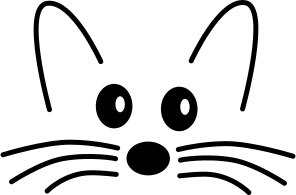
\includegraphics[width=1.4em]{squeak-logo}}}
\iftoshelse{
	\usepackage{marginnote}
		\renewcommand*{\marginfont}{\footnotesize}
	\newcommand{\vartriangleout}{\ifthenelse{\isodd{\thepage}}{\vartriangleright}{\vartriangleleft}}
	\newcommand{\dothisicon}{\fcolorbox{blue!65}{white}{\highlight{$\vartriangleout$}}}
	\newcommand{\dothis}[1]{%
		\noindent\par\noindent
		{\reversemarginpar
			\marginnote{\fcolorbox{blue!65}{white}{\highlight{$\vartriangleout$}}}}
		%\MarginLabel{do this}
		\noindent\emph{#1}
		\nopagebreak}
}{
	\newcommand{\dothisicon}{\raisebox{-.5ex}{
\includegraphics[height=1.2em]{pharo}}}
	\newcommand{\dothis}[1]{%
		\medskip
		\noindent\dothisicon
		\ifx#1\empty\else\quad\emph{#1}\fi
		\par\smallskip\nopagebreak}
}
%===> NEW VERSION <===
% NB: To use this in an individual chapter, you must set:
%\graphicspath{{figures/} {../figures/}}
% at the head of the chapter.  Don't forget the final /
%=============================================================
%:Reader hints (hint)
%
% Indicates a non-obvious consequence
\newcommand{\hint}[1]{\vspace{1ex}\noindent\fbox{\textsc{Hint}} \emph{#1}}
%=================================================================
% graphics for Morphic handles
\newcommand{\grabHandle}{\raisebox{-0.2ex}{
\includegraphics[width=1em]{blackHandle}}}
\newcommand{\moveHandle}{\raisebox{-0.2ex}{
\includegraphics[width=1em]{moveHandle}}}
\newcommand{\debugHandle}{\raisebox{-0.2ex}{
\includegraphics[width=1em]{debugHandle}}}
%=============================================================
%:Highlighting Important stuff (doublebox)
%
% From Seaside book ...
\newsavebox{\SavedText}
\newlength{\InnerBoxRule}\setlength{\InnerBoxRule}{.75\fboxrule}
\newlength{\OuterBoxRule}\setlength{\OuterBoxRule}{1.5\fboxrule}
\newlength{\BoxSeparation}\setlength{\BoxSeparation}{1.5\fboxrule}
\addtolength{\BoxSeparation}{.5pt}
\newlength{\SaveBoxSep}\setlength{\SaveBoxSep}{2\fboxsep}
%
\newenvironment{doublebox}{\begin{lrbox}{\SavedText}
    \begin{minipage}{.75\textwidth}}
    {\end{minipage}\end{lrbox}\begin{center}
    \setlength{\fboxsep}{\BoxSeparation}\setlength{\fboxrule}{\OuterBoxRule}
    \fbox{\setlength{\fboxsep}{\SaveBoxSep}\setlength{\fboxrule}{\InnerBoxRule}%
      \fbox{\usebox{\SavedText}}}
  \end{center}}
% Use this:
\newcommand{\important}[1]{\begin{doublebox}#1\end{doublebox}}
%=============================================================
%:Section depth
\setcounter{secnumdepth}{2}
%% for this to happen start the file with
%\ifx\wholebook\relax\else
%% $Author$
% $Date$
% $Revision$

% HISTORY:
% 2006-10-31 - Oscar code macros
% ...

%=============================================================
% NB: documentclass must be set in main document.
% Allows book to be generated in multiple formats.
%=============================================================
%:Packages
\usepackage[T1]{fontenc}  %%%%%% really important to get the code directly in the text!
\usepackage{lmodern}
%\usepackage[scaled=0.85]{bookmanx} % needs another scale factor if used with \renewcommand{\sfdefault}{cmbr}
\usepackage{palatino}
\usepackage[scaled=0.85]{helvet}
\usepackage[protrusion,expansion=false]{microtype}
\usepackage{graphicx}
\usepackage{theorem}
\usepackage[english]{babel}
% ON: pdfsync breaks the use of p{width} for tabular columns!
\ifdefined\usepdfsync\usepackage{pdfsync}\fi % Requires texlive 2007
%=============================================================
%:More packages
%Stef should check which ones are used!
%\usepackage{picinpar}
%\usepackage{layout}
%\usepackage{color}
%\usepackage{enum}
%\usepackage{a4wide}
% \usepackage{fancyhdr}
\usepackage{ifthen}
\usepackage{float}
\usepackage{longtable}
\usepackage{makeidx}
\usepackage[nottoc]{tocbibind}
\usepackage{multicol}
\usepackage{booktabs}	% book-style tables
\usepackage{topcapt}	% enables \topcaption
\usepackage{multirow}
\usepackage{tabularx}
%\usepackage[bottom]{footmisc}
\usepackage{xspace}
\usepackage{alltt}
\usepackage{amssymb,textcomp}
\usepackage[usenames,dvipsnames]{color}
%\usepackage{colortbl}
\usepackage[hang]{subfigure}\makeatletter\def\p@subfigure{\thefigure\,}\makeatother
\usepackage{rotating}
\usepackage{enumitem}	% apb: allows more control over tags in enumerations
\usepackage{verbatim}     % for comment environment
\usepackage{varioref}	% for page references that work
\labelformat{footnote}{\thechapter--#1} % to distinguish citations from jurabib
\usepackage{needspace}
\usepackage{isodateo} % enable \isodate
\usepackage[newparttoc,pagestyles]{titlesec}
\usepackage{titletoc}
\usepackage{wrapfig}

\usepackage[
	super,
	citefull=first,
	authorformat={allreversed,and},
	titleformat={commasep,italic}
]{jurabib} % citations as footnotes
\usepackage[
	colorlinks=true,
	linkcolor=black,
	urlcolor=black,
	citecolor=black
]{hyperref}   % should come last
%=============================================================
%:PDF version
\pdfminorversion=3 % Set PDF to 1.3 for Lulu
%=============================================================
%:URL style
\makeatletter
\def\url@leostyle{%
  \@ifundefined{selectfont}{\def\UrlFont{\sf}}{\def\UrlFont{\sffamily}}}
\makeatother
% Now actually use the newly defined style.
\urlstyle{leo}
%=============================================================
%:Booleans
\newboolean{lulu}
\setboolean{lulu}{false}
\newcommand{\ifluluelse}[2]{\ifthenelse{\boolean{lulu}}{#1}{#2}}
%=============================================================
%:Names
\newcommand{\SUnit}{SUnit\xspace}
\newcommand{\sunit}{SUnit\xspace}
\newcommand{\xUnit}{$x$Unit\xspace}
\newcommand{\JUnit}{JUnit\xspace}
\newcommand{\st}{Smalltalk\xspace}
\newcommand{\pharo}{Pharo\xspace} % Use this, not \Pharo
%\newcommand{\sqmap}{SqueakMap\xspace}
\newcommand{\squeak}{Squeak\xspace} % use this, not \Squeak or \sq
\newcommand{\sqsrc}{SqueakSource\xspace}
\newcommand{\sbe}{\url{http://SqueakByExample.org}\xspace}
\newcommand{\pharoweb}{\url{http://pharo-project.org}\xspace}
\newcommand{\pbe}{\url{http://PharoByExample.org}\xspace}
\newcommand{\sba}{\url{http://SquareBracketAssociates.org}\xspace}
\newcommand{\bam}{\lct{Bounc\-ing\-Atoms\-Morph}\xspace}
%=============================================================
%:Markup macros for proof-reading
\usepackage[normalem]{ulem} % for \sout
\usepackage{xcolor}
\newcommand{\ra}{$\rightarrow$}
\newcommand{\ugh}[1]{\textcolor{red}{\uwave{#1}}} % please rephrase
\newcommand{\ins}[1]{\textcolor{blue}{\uline{#1}}} % please insert
\newcommand{\del}[1]{\textcolor{red}{\sout{#1}}} % please delete
\newcommand{\chg}[2]{\textcolor{red}{\sout{#1}}{\ra}\textcolor{blue}{\uline{#2}}} % please change
%=============================================================
%:Editorial comment macros
%\newcommand{\nnbb}[2]{
%    % \fbox{\bfseries\sffamily\scriptsize#1}
%    \fcolorbox{gray}{yellow}{\bfseries\sffamily\scriptsize#1}
%    {\sf\small$\blacktriangleright$\textit{#2}$\blacktriangleleft$}
%   }
\newcommand{\yellowbox}[1]{\fcolorbox{gray}{yellow}{\bfseries\sffamily\scriptsize#1}}
\newcommand{\triangles}[1]{{\sf\small$\blacktriangleright$\textit{#1}$\blacktriangleleft$}}
\newcommand{\nnbb}[2]{\yellowbox{#1} \triangles{#2}}
\newcommand{\fix}{\yellowbox{FIX!}}
\newcommand{\here}{\yellowbox{CONTINUE HERE!}}
% editor macros
\newcommand{\apl}[1]{\nnbb{Alain}{#1}} % Alain
\newcommand{\ab}[1]{\nnbb{Andrew}{#1}} % Black
\newcommand{\sd}[1]{\nnbb{St\'{e}f}{#1}} % Ducasse
\newcommand{\gl}[1]{\nnbb{Guillaume}{#1}} % Ducasse
\newcommand{\cd}[1]{\nnbb{Christophe}{#1}} % Ducasse
\newcommand{\sig}[1]{\nnbb{Igor}{#1}} % Igor
\newcommand{\dc}[1]{\nnbb{DamienC}{#1}} % Ducasse
\newcommand{\md}[1]{\nnbb{Marcus}{#1}} % Denker
\newcommand{\on}[1]{\nnbb{Oscar}{#1}} % Nierstrasz
\newcommand{\damien}[1]{\nnbb{Damien}{#1}} % Pollet
\newcommand{\lr}[1]{\nnbb{Lukas}{#1}} % Renggli
\newcommand{\orla}[1]{\nnbb{Orla}{#1}} % Greevy
\newcommand{\alex}[1]{\nnbb{Alex}{#1}} % Bergel
\newcommand{\alx}[1]{\nnbb{Alex}{#1}} % Bergel
\newcommand{\dr}[1]{\nnbb{David}{#1}} % Roethlisberger
\newcommand{\ja}[1]{\nnbb{Jannik}{#1}} % Laval
\newcommand{\cb}[1]{\nnbb{Camillo}{#1}} % Bruni
\newcommand{\jr}[1]{\nnbb{Jorge}{#1}} % Ressia
\newcommand{\jb}[1]{\nnbb{JB}{#1}} % JB
\newcommand{\jp}[1]{\nnbb{Javier}{#1}} % Pimas
\newcommand{\fp}[1]{\nnbb{Fabrizio}{#1}} % Perin
\newcommand{\michael}[1]{\nnbb{Michael}{#1}} % Davies
\newcommand{\ew}[1]{\nnbb{Erwann}{#1}} % Wernli
\newcommand{\mb}[1]{\nnbb{Martial}{#1}} % Boniou
\newcommand{\hw}[1]{\nnbb{Hernan}{#1}} % Wilkinson
\newcommand{\ben}[1]{\nnbb{Benjamin}{#1}} % Benjamin Van Ryseghem
\newcommand{\hjo}[1]{\nnbb{HwaJong}{#1}} % HwaJong Oh aka daliot
\newcommand{\ml}[1]{\nnbb{Max}{#1}} % Max Leske
\newcommand{\mmp}[1]{\nnbb{Mariano}{#1}} % Mariano Martinez Peck
\newcommand{\luc}[1]{\nnbb{Luc}{#1}} % Luc Fabresse
\newcommand{\dkl}[1]{\nnbb{Daniel}{#1}} % Daniel Lyons
\newcommand{\vu}[1]{\nnbb{Veronica}{#1}} % Veronica Uquillas Gomez
\newcommand{\martin}[1]{\nnbb{Martin}{#1}} % Martin Dias
\newcommand{\vp}[1]{\nnbb{Vanessa}{#1}} % Vanessa Pena
\newcommand{\gp}[1]{\nnbb{Guille}{#1}} % Guillermo Polito

%=============================================================
%:Abbreviation macros
\newcommand{\ie}{\emph{i.e.},\xspace}
\newcommand{\eg}{\emph{e.g.},\xspace}
\newcommand{\etc}{etc.\xspace}
%=============================================================
%:Cross reference macros
\newcommand{\charef}[1]{Chapter~\ref{cha:#1}\xspace}
\newcommand{\secref}[1]{Section~\ref{sec:#1}\xspace}
\newcommand{\figref}[1]{Figure~\ref{fig:#1}\xspace}
\newcommand{\Figref}[1]{Figure~\ref{fig:#1}\xspace}
\newcommand{\appref}[1]{Appendix~\ref{app:#1}\xspace}
\newcommand{\tabref}[1]{Table~\ref{tab:#1}\xspace}
\newcommand{\faqref}[1]{FAQ~\ref{faq:#1}, p.~\pageref{faq:#1}\xspace}
% APB: I removed trailing \xspace commands from these macros because
% \xspace mostly doesn't work.  If you want a space after your
% references, type one!
% ON: xspace has always worked just fine for me!  Please leave them in.
%
\newcommand{\ruleref}[1]{\ref{rule:#1}\xspace}
%
\newcommand{\egref}[1]{example~\ref{eg:#1}\xspace}
\newcommand{\Egref}[1]{Example~\ref{eg:#1}\xspace}
%
\newcommand{\scrref}[1]{script~\ref{scr:#1}\xspace}
\newcommand{\Scrref}[1]{Script~\ref{scr:#1}\xspace}
\newcommand{\tscrref}[1]{the script~\ref{scr:#1}\xspace}
\newcommand{\Tscrref}[1]{The script~\ref{scr:#1}\xspace}
%
\newcommand{\mthref}[1]{method~\ref{mth:#1}\xspace}
\newcommand{\mthsref}[1]{methods~\ref{mth:#1}\xspace}
\newcommand{\Mthref}[1]{Method~\ref{mth:#1}\xspace}
\newcommand{\tmthref}[1]{the method~\ref{mth:#1}\xspace}
\newcommand{\Tmthref}[1]{The method~\ref{mth:#1}\xspace}
%
\newcommand{\clsref}[1]{class~\ref{cls:#1}\xspace}
\newcommand{\tclsref}[1]{the class~\ref{cls:#1}\xspace}
\newcommand{\Tclsref}[1]{The class~\ref{cls:#1}\xspace}

\newcommand{\chalabel}[1]{\label{cha:#1}}
\newcommand{\seclabel}[1]{\label{sec:#1}}
\newcommand{\figlabel}[1]{\label{fig:#1}}
\newcommand{\tablabel}[1]{\label{tab:#1}}
\newcommand{\rulelabel}[1]{\label{rule:#1}}
\newcommand{\eglabel}[1]{\label{eg:#1}}
\newcommand{\scrlabel}[1]{\label{scr:#1}}
\newcommand{\mthlabel}[1]{\label{mth:#1}}
\newcommand{\clslabel}[1]{\label{cls:#1}}
\newcommand{\faqlabel}[1]{\label{faq:#1}}
%=============================================================
%:Menu item macro
% for menu items, so we can change our minds on how to print them! (apb)
\definecolor{lightgray}{gray}{0.89}
\newcommand{\menu}[1]{{%
	\setlength{\fboxsep}{0pt}%
	\colorbox{lightgray}{{{\upshape\sffamily\strut \,#1\,}}}}}
\newcommand{\link}[1]{{%
	\fontfamily{lmr}\selectfont
 	\upshape{\sffamily \underline{#1}}}}
% For submenu items:
\newcommand{\go}{\,$\triangleright$\,}
% \newcommand{\go}{\,$\blacktriangleright$\,}
% For keyboard shortcuts:
%\newcommand{\short}[1]{\mbox{$\langle${\sc CMD}$\rangle$-#1}\xspace}
\newcommand{\short}[1]{\mbox{{\sc cmd}\hspace{0.08em}--\hspace{0.09em}#1}\xspace}
% For buttons:
\newcommand{\button}[1]{{%
	\setlength{\fboxsep}{0pt}%
	\fbox{{\upshape\sffamily\strut \,#1\,}}}}
% NB: The button macro does not work within captions -- incompatible with xcolor package :-(
\newcommand{\toolsflap}{\textit{Tools} flap\xspace}
%=============================================================
%:Mouse clicks
\newcommand{\click}{click\xspace} % RED
\newcommand{\actclick}{action-click\xspace} % YELLOW
\newcommand{\metaclick}{meta-click\xspace} % BLUE
\newcommand{\Click}{Click\xspace} % RED
\newcommand{\Actclick}{Action-click\xspace} % YELLOW
\newcommand{\Metaclick}{Meta-click\xspace} % BLUE
%=============================================================
%:ToSh macros
\newboolean{tosh}
\setboolean{tosh}{false}
\newcommand{\iftoshelse}[2]{\ifthenelse{\boolean{tosh}}{#1}{#2}}
%=============================================================
%:ToSh colors
%\newcommand{\highlightcolor}{\color{blue!65}}
%\newcommand{\boxcolor}{\color{gray!25}}
\newcommand{\highlight}[1]{\textcolor{blue!65}{#1}}
%\newcommand{\codecolor}{\color{blue!65}}
%%\setlength{\fboxrule}{2pt}
%\newcommand{\asPict}[1]{%
%	{\Large\highlight{#1}}}
%=============================================================
%:Reader cues (do this)
%
% Indicate something the reader should try out.
% \newcommand{\dothisicon}{\raisebox{-.5ex}{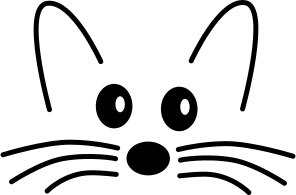
\includegraphics[width=1.4em]{squeak-logo}}}
\iftoshelse{
	\usepackage{marginnote}
		\renewcommand*{\marginfont}{\footnotesize}
	\newcommand{\vartriangleout}{\ifthenelse{\isodd{\thepage}}{\vartriangleright}{\vartriangleleft}}
	\newcommand{\dothisicon}{\fcolorbox{blue!65}{white}{\highlight{$\vartriangleout$}}}
	\newcommand{\dothis}[1]{%
		\noindent\par\noindent
		{\reversemarginpar
			\marginnote{\fcolorbox{blue!65}{white}{\highlight{$\vartriangleout$}}}}
		%\MarginLabel{do this}
		\noindent\emph{#1}
		\nopagebreak}
}{
	\newcommand{\dothisicon}{\raisebox{-.5ex}{
\includegraphics[height=1.2em]{pharo}}}
	\newcommand{\dothis}[1]{%
		\medskip
		\noindent\dothisicon
		\ifx#1\empty\else\quad\emph{#1}\fi
		\par\smallskip\nopagebreak}
}
%===> NEW VERSION <===
% NB: To use this in an individual chapter, you must set:
%\graphicspath{{figures/} {../figures/}}
% at the head of the chapter.  Don't forget the final /
%=============================================================
%:Reader hints (hint)
%
% Indicates a non-obvious consequence
\newcommand{\hint}[1]{\vspace{1ex}\noindent\fbox{\textsc{Hint}} \emph{#1}}
%=================================================================
% graphics for Morphic handles
\newcommand{\grabHandle}{\raisebox{-0.2ex}{
\includegraphics[width=1em]{blackHandle}}}
\newcommand{\moveHandle}{\raisebox{-0.2ex}{
\includegraphics[width=1em]{moveHandle}}}
\newcommand{\debugHandle}{\raisebox{-0.2ex}{
\includegraphics[width=1em]{debugHandle}}}
%=============================================================
%:Highlighting Important stuff (doublebox)
%
% From Seaside book ...
\newsavebox{\SavedText}
\newlength{\InnerBoxRule}\setlength{\InnerBoxRule}{.75\fboxrule}
\newlength{\OuterBoxRule}\setlength{\OuterBoxRule}{1.5\fboxrule}
\newlength{\BoxSeparation}\setlength{\BoxSeparation}{1.5\fboxrule}
\addtolength{\BoxSeparation}{.5pt}
\newlength{\SaveBoxSep}\setlength{\SaveBoxSep}{2\fboxsep}
%
\newenvironment{doublebox}{\begin{lrbox}{\SavedText}
    \begin{minipage}{.75\textwidth}}
    {\end{minipage}\end{lrbox}\begin{center}
    \setlength{\fboxsep}{\BoxSeparation}\setlength{\fboxrule}{\OuterBoxRule}
    \fbox{\setlength{\fboxsep}{\SaveBoxSep}\setlength{\fboxrule}{\InnerBoxRule}%
      \fbox{\usebox{\SavedText}}}
  \end{center}}
% Use this:
\newcommand{\important}[1]{\begin{doublebox}#1\end{doublebox}}
%=============================================================
%:Section depth
\setcounter{secnumdepth}{2}
%% for this to happen start the file with
%\ifx\wholebook\relax\else
%\input{../common.tex}
%\begin{document}
%\fi
% and terminate by
% \ifx\wholebook\relax\else\end{document}\fi

\DeclareGraphicsExtensions{.pdf, .jpg, .png}
%=============================================================
%:PDF setup
\hypersetup{
%   a4paper,
%   pdfstartview=FitV,
%   colorlinks,
%   linkcolor=darkblue,
%   citecolor=darkblue,
   pdftitle={Pharo by Example},
   pdfauthor={Andrew P. Black, St\'ephane Ducasse,	Oscar Nierstrasz,
Damien Pollet},
   pdfkeywords={Smalltalk, Squeak, Object-Oriented Programming, OOP},
   pdfsubject={Computer Science}
}
%=============================================================
%:Page layout and appearance
%
% \renewcommand{\headrulewidth}{0pt}
\renewcommand{\chaptermark}[1]{\markboth{#1}{}}
\renewcommand{\sectionmark}[1]{\markright{\thesection\ #1}}
\renewpagestyle{plain}[\small\itshape]{%
	\setheadrule{0pt}%
	\sethead[][][]{}{}{}%
	\setfoot[][][]{}{}{}}
\renewpagestyle{headings}[\small\itshape]{%
	\setheadrule{0pt}%
	\setmarks{chapter}{section}%
	\sethead[\thepage][][\chaptertitle]{\sectiontitle}{}{\thepage}%
	\setfoot[][][]{}{}{}}
%=============================================================
%:Title section setup and TOC numbering depth
\setcounter{secnumdepth}{1}
\setcounter{tocdepth}{1}
\titleformat{\part}[display]{\centering}{\huge\partname\ \thepart}{1em}{\Huge\textbf}[]
\titleformat{\chapter}[display]{}{\huge\chaptertitlename\ \thechapter}{1em}{\Huge\raggedright\textbf}[]
\titlecontents{part}[3pc]{%
		\pagebreak[2]\addvspace{1em plus.4em minus.2em}%
		\leavevmode\large\bfseries}
	{\contentslabel{3pc}}{\hspace*{-3pc}}
	{}[\nopagebreak]
\titlecontents{chapter}[3pc]{%
		\pagebreak[0]\addvspace{1em plus.2em minus.2em}%
		\leavevmode\bfseries}
	{\contentslabel{3pc}}{}
	{\hfill\contentspage}[\nopagebreak]
\dottedcontents{section}[3pc]{}{3pc}{1pc}
\dottedcontents{subsection}[3pc]{}{0pc}{1pc}
% \dottedcontents{subsection}[4.5em]{}{0pt}{1pc}
% Make \cleardoublepage insert really blank pages http://www.tex.ac.uk/cgi-bin/texfaq2html?label=reallyblank
\let\origdoublepage\cleardoublepage
\newcommand{\clearemptydoublepage}{%
  \clearpage
  {\pagestyle{empty}\origdoublepage}}
\let\cleardoublepage\clearemptydoublepage % see http://www.tex.ac.uk/cgi-bin/texfaq2html?label=patch
%=============================================================
%:FAQ macros (for FAQ chapter)
\newtheorem{faq}{FAQ}
\newcommand{\answer}{\paragraph{Answer}\ }
%=============================================================
%:Listings package configuration
% \newcommand{\caret}{\makebox{\raisebox{0.4ex}{\footnotesize{$\wedge$}}}}
\newcommand{\caret}{\^\,}
\newcommand{\escape}{{\sf \textbackslash}}
\definecolor{source}{gray}{0.95}
\usepackage{listings}
\lstdefinelanguage{Smalltalk}{
%  morekeywords={self,super,true,false,nil,thisContext}, % This is overkill
  morestring=[d]',
  morecomment=[s]{"}{"},
  alsoletter={\#:},
  escapechar={!},
  literate=
    {BANG}{!}1
    {CARET}{\^}1
    {UNDERSCORE}{\_}1
    {\\st}{Smalltalk}9 % convenience -- in case \st occurs in code
    % {'}{{\textquotesingle}}1 % replaced by upquote=true in \lstset
    %{_}{{$\leftarrow$}}1
    {>>>}{{\sep}}1
    %{^}{{$\uparrow$}}1
    {~}{{$\sim$}}1
    {-}{{\texttt{-}}}1 %{\textminus}}1 %{-}{\hspace{-0.13em}}{-}}1  % the goal is to make - the same width as +
    % {+}{\sf+}1 %{\raisebox{0.08ex}{+}}}1      % and to raise + off the baseline to match -
    {-->}{{\quad$\longrightarrow$\quad}}3
    {~->}{{\quad$\leadsto$\quad}}3
	, % Don't forget the comma at the end!
  tabsize=4
}[keywords,comments,strings]

\lstset{language=Smalltalk,
	basicstyle=\sffamily,
	keywordstyle=\color{black}\bfseries,
	% stringstyle=\ttfamily, % Ugly! do we really want this? -- on
	mathescape=true,
	showstringspaces=false,
	keepspaces=true,
	breaklines=true,
	breakautoindent=true,
	backgroundcolor=\color{source},
	lineskip={-1pt}, % Ugly hack
	upquote=true, % straight quote; requires textcomp package
	columns=fullflexible} % no fixed width fonts
% In-line code (literal)
% Normally use this for all in-line code:

\newcommand{\ct}{\lstinline[mathescape=false,backgroundcolor=\color{white},basicstyle={\sffamily\upshape}]}
\newcommand{\cts}[1]{{\sffamily{\upshape{#1}}\xspace}}
% apb 2007.8.28 added the \upshape declaration to avoid getting italicized code in \dothis{ } sections.
% In-line code (latex enabled)
% Use this only in special situations where \ct does not work
% (within section headings ...):
\newcommand{\lct}[1]{{\textsf{\textup{#1}}}}
% Use these for system categories and protocols:
\newcommand{\scat}[1]{\emph{\textsf{#1}}\xspace}
\newcommand{\pkg}[1]{\emph{\textsf{#1}}\xspace}
\newcommand{\prot}[1]{\emph{\textsf{#1}}\xspace}
% Code environments
% NB: the arg is for tests
% Only code and example environments may be tests
\lstnewenvironment{code}[1]{%
	\lstset{%
		% frame=lines,
		frame=single,
		framerule=0pt,
		mathescape=false
	}
}{}
\def\ignoredollar#1{}
%=============================================================
%:Code environments (method, script ...)
% NB: the third arg is for tests
% Only code and example environments may be tests
\lstnewenvironment{example}[3][defaultlabel]{%
	\renewcommand{\lstlistingname}{Example}%
	\lstset{
		% frame=lines,
		frame=single,
		framerule=0pt,
		mathescape=false,
		caption={\emph{#2}},
		label={eg:#1}
	}
}{}
\lstnewenvironment{script}[2][defaultlabel]{%
\renewcommand{\lstlistingname}{Script}%
	\lstset{
		% frame=lines,
		frame=single,
		framerule=0pt,
		mathescape=false,
		name={Script},
		caption={\emph{#2}},
		label={scr:#1}
	}
}{}
\lstnewenvironment{method}[2][defaultlabel]{%
	\renewcommand{\lstlistingname}{Method}%
	\lstset{
		% frame=lines,
		frame=single,
		framerule=0pt,
		mathescape=false,
		name={Method},
		caption={\emph{#2}},
		label={mth:#1}
	}
}{}
\lstnewenvironment{methods}[2][defaultlabel]{% just for multiple methods at once
	\renewcommand{\lstlistingname}{Methods}%
	\lstset{
		% frame=lines,
		frame=single,
		framerule=0pt,
		mathescape=false,
		name={Method},
		caption={\emph{#2}},
		label={mth:#1}
	}
}{}
\lstnewenvironment{numMethod}[2][defaultlabel]{%
	\renewcommand{\lstlistingname}{Method}%
	\lstset{
		numbers=left,
		numberstyle={\tiny\sffamily},
		% frame=lines,
		frame=single,
		framerule=0pt,
		mathescape=false,
		name={Method},
		caption={\emph{#2}},
		label={mth:#1}
	}
}{}
\lstnewenvironment{classdef}[2][defaultlabel]{%
	\renewcommand{\lstlistingname}{Class}%
	\lstset{
		% frame=lines,
		frame=single,
		framerule=0pt,
		mathescape=false,
		name={Class},
		caption={\emph{#2}},
		label={cls:#1}
	}
}{}
%=============================================================
%:Reserving space
% Usually need one more line than the actual lines of code
\newcommand{\needlines}[1]{\Needspace{#1\baselineskip}}
%=============================================================
%:Indexing macros
% Macros ending with "ind" generate text as well as an index entry
% Macros ending with "index" *only* generate an index entry
\newcommand{\ind}[1]{\index{#1}#1\xspace} % plain text
\newcommand{\subind}[2]{\index{#1!#2}#2\xspace} % show #2, subindex under #1
\newcommand{\emphind}[1]{\index{#1}\emph{#1}\xspace} % emph #1
\newcommand{\emphsubind}[2]{\index{#1!#2}\emph{#2}\xspace} % show emph #2, subindex inder #1
\newcommand{\scatind}[1]{\index{#1@\textsf{#1} (category)}\scat{#1}} % category
\newcommand{\pkgind}[1]{\index{#1@\textsf{#1} (package)}\pkg{#1}} % package
\newcommand{\protind}[1]{\index{#1@\textsf{#1} (protocol)}\prot{#1}} % protocol
\newcommand{\clsind}[1]{\index{#1@\textsf{#1} (class)}\ct{#1}\xspace}
% \newcommand{\clsind}[1]{\index{#1!\#@(class)}\ct{#1}\xspace} % class
\newcommand{\clsindplural}[1]{\index{#1!\#@(class)}\ct{#1}s\xspace} % class
\newcommand{\cvind}[1]{\index{#1@\textsf{#1} (class variable)}\ct{#1}\xspace} % class var
\newcommand{\glbind}[1]{\index{#1@\textsf{#1} (global)}\ct{#1}\xspace} % global
\newcommand{\patind}[1]{\index{#1@#1 (pattern)}\ct{#1}\xspace} % pattern
\newcommand{\pvind}[1]{\index{#1@\textsf{#1} (pseudo variable)}\ct{#1}\xspace} % pseudo var
\newcommand{\clsmthind}[2]{\index{#1!#2@\ct{#2}}\ct{#1>>>#2}\xspace} % class + method name
\newcommand{\mthind}[2]{\index{#1!#2@\ct{#2}}\ct{#2}\xspace} % show method name only
\newcommand{\lmthind}[2]{\index{#1!#2@\ct{#2}}\lct{#2}\xspace} % show method name only
\newcommand{\cmind}[2]{\index{#1!#2@\ct{#2}}\ct{#1>>>#2}\xspace} % show class>>method
\newcommand{\lcmind}[2]{\index{#1!#2@\ct{#2}}\lct{#1>>>#2}\xspace} % show class>>method
\newcommand{\toolsflapind}{\index{Tools flap}\toolsflap} % index tools flap
% The following only generate an index entry:
% \newcommand{\clsindex}[1]{\index{#1@\textsf{#1} (class)}}
\newcommand{\clsindex}[1]{\index{#1!\#@(class)}} % class
\newcommand{\mthindex}[2]{\index{#1!#2@\ct{#2}}} % method
\newcommand{\cmindex}[2]{\index{#1!#2@\ct{#2}}} % class>>method
\newcommand{\cvindex}[1]{\index{#1@\textsf{#1} (class variable)}} % class var
\newcommand{\glbindex}[1]{\index{#1@\textsf{#1} (global)}}% global
\newcommand{\pvindex}[1]{\index{#1@\textsf{#1} (pseudo variable)}}% pseudo var
\newcommand{\seeindex}[2]{\index{#1|see{#2}}} % #1, see #2
\newcommand{\scatindex}[1]{\index{#1@\textsf{#1} (category)}} % category
\newcommand{\pkgindex}[1]{\index{#1@\textsf{#1} (package)}} % package
\newcommand{\protindex}[1]{\index{#1@\textsf{#1} (protocol)}} % protocol
% How can we have the main entry page numbers in bold yet not break the hyperlink?
\newcommand{\boldidx}[1]{{\bf #1}} % breaks hyperlink
%\newcommand{\indmain}[1]{\index{#1|boldidx}#1\xspace} % plain text, main entry
%\newcommand{\emphsubindmain}[2]{\index{#1!#2|boldidx}\emph{#2}\xspace} % subindex, main entry
%\newcommand{\subindmain}[2]{\index{#1!#2|boldidx}#2\xspace} % subindex, main entry
%\newcommand{\clsindmain}[1]{\index{#1@\textsf{#1} (class)|boldidx}\ct{#1}\xspace}
%\newcommand{\clsindmain}[1]{\index{#1!\#@(class)|boldidx}\ct{#1}\xspace} % class main
%\newcommand{\indexmain}[1]{\index{#1|boldidx}} % main index entry only
\newcommand{\indmain}[1]{\index{#1}#1\xspace} % The main index entry for this item
\newcommand{\emphsubindmain}[2]{\index{#1!#2}\emph{#2}\xspace} % subindex, main entry
\newcommand{\subindmain}[2]{\index{#1!#2}#2\xspace} % subindex, main entry
%\newcommand{\clsindmain}[1]{\index{#1@\textsf{#1} (class)}\ct{#1}\xspace}
\newcommand{\clsindmain}[1]{\index{#1!\#@(class)}\ct{#1}\xspace} % class main
\newcommand{\clsindexmain}[1]{\index{#1!\#@(class)}} % class main index only
\newcommand{\indexmain}[1]{\index{#1}}
%=============================================================
%:Code macros
% some constants
\newcommand{\codesize}{\small}
\newcommand{\codefont}{\sffamily}
%\newcommand{\cat}[1]{\textit{In category #1}}%%To remove later
\newlength{\scriptindent}
\setlength{\scriptindent}{.3cm}
%% Method presentation constants
\newlength{\methodindent}
\newlength{\methodwordlength}
\newlength{\aftermethod}
\setlength{\methodindent}{0.2cm}
\settowidth{\methodwordlength}{\ M\'ethode\ }
%=============================================================
%:Smalltalk macros
%\newcommand{\sep}{{$\gg$}}
\newcommand{\sep}{\mbox{>>}}
\newcommand{\self}{\lct{self}\xspace}
\newcommand{\super}{\lct{super}\xspace}
\newcommand{\nil}{\lct{nil}\xspace}
%=============================================================
% be less conservative about float placement
% these commands are from http://www.tex.ac.uk/cgi-bin/texfaq2html?label=floats
\renewcommand{\topfraction}{.9}
\renewcommand{\bottomfraction}{.9}
\renewcommand{\textfraction}{.1}
\renewcommand{\floatpagefraction}{.85}
\renewcommand{\dbltopfraction}{.66}
\renewcommand{\dblfloatpagefraction}{.85}
\setcounter{topnumber}{9}
\setcounter{bottomnumber}{9}
\setcounter{totalnumber}{20}
\setcounter{dbltopnumber}{9}
%=============================================================
% Give information from each chapter's author
\newcommand{\contact}[2]{\textbf{#1} \textsf{(#2)}}

\newcommand{\chapterauthor}[1]{\emph{with the participation of:\\#1}\\}
\newcommand{\chapterwritten}[1]{\emph{written by:\\#1}\\}

\newcommand{\authornoury}{\contact{Noury Bouraqadi}{Noury.Bouraqadi@mines-douai.fr}}
\newcommand{\authorluc}{\contact{Luc Fabresse}{Luc.Fabresse@mines-douai.fr}}
\newcommand{\authordamienc}{\contact{Damien Cassou}{damien.cassou@gmail.com}}
\newcommand{\authoroscar}{\contact{Oscar Nierstrasz}{oscar.nierstrasz@acm.org}}
\newcommand{\authorsteph}{\contact{St\'ephane Ducasse}{stephane.ducasse@inria.fr}}
\newcommand{\authoralex}{\contact{Alexandre Bergel}{alexandre@bergel.eu}}
\newcommand{\authorolivier}{\contact{Olivier Auverlot}{olivier.auverlot@inria.fr}}
\newcommand{\authornicolas}{\contact{Nicolas Cellier}{nicolas.cellier.aka.nice@gmail.com}}
\newcommand{\authormarcus}{\contact{Marcus Denker}{marcus.denker@inria.fr}}
\newcommand{\authoralain}{\contact{Alain Plantec}{alain.plantec@univ-brest.fr}}
\newcommand{\authordale}{\contact{Dale Henrichs}{dale.henrichs@gemstone.com}}
\newcommand{\authormariano}{\contact{Mariano Martinez Peck}{marianopeck@gmail.com}}
\newcommand{\authorsven}{\contact{Sven Van Caekenberghe}{sven@beta9.be}}
\newcommand{\authorlukas}{\contact{Lukas Renggli}{renggli@gmail.com}}
\newcommand{\authorjankurs}{\contact{Jan Kurs}{kurs@iam.unibe.ch}}
\newcommand{\authorguillaume}{\contact{Guillaume Larcheveque}{guillaume.larcheveque@gmail.com}}
\newcommand{\authorguillep}{\contact{Guillermo Polito}{guillermopolito@gmail.com}}
\newcommand{\authorclement}{\contact{Cl\'ement Bera}{bera.clement@gmail.com}}
\newcommand{\authormax}{\contact{Max Leske}{maxleske@gmail.com}}
\newcommand{\authorvanessa}{\contact{Vanessa Pe\~{n}a-Araya}{van.c.pena@gmail.com}}
\newcommand{\authorcamillo}{\contact{Camillo Bruni}{camillobruni@gmail.com}}

%=============================================================
% apb doesn't like paragraphs to run in to each other without a break
\parskip 1ex
%=============================================================
%:Stuff to check, merge or deprecate
%\setlength{\marginparsep}{2mm}
%\renewcommand{\baselinestretch}{1.1}
%=============================================================
\usepackage{tikz}

%\begin{document}
%\fi
% and terminate by
% \ifx\wholebook\relax\else\end{document}\fi

\DeclareGraphicsExtensions{.pdf, .jpg, .png}
%=============================================================
%:PDF setup
\hypersetup{
%   a4paper,
%   pdfstartview=FitV,
%   colorlinks,
%   linkcolor=darkblue,
%   citecolor=darkblue,
   pdftitle={Pharo by Example},
   pdfauthor={Andrew P. Black, St\'ephane Ducasse,	Oscar Nierstrasz,
Damien Pollet},
   pdfkeywords={Smalltalk, Squeak, Object-Oriented Programming, OOP},
   pdfsubject={Computer Science}
}
%=============================================================
%:Page layout and appearance
%
% \renewcommand{\headrulewidth}{0pt}
\renewcommand{\chaptermark}[1]{\markboth{#1}{}}
\renewcommand{\sectionmark}[1]{\markright{\thesection\ #1}}
\renewpagestyle{plain}[\small\itshape]{%
	\setheadrule{0pt}%
	\sethead[][][]{}{}{}%
	\setfoot[][][]{}{}{}}
\renewpagestyle{headings}[\small\itshape]{%
	\setheadrule{0pt}%
	\setmarks{chapter}{section}%
	\sethead[\thepage][][\chaptertitle]{\sectiontitle}{}{\thepage}%
	\setfoot[][][]{}{}{}}
%=============================================================
%:Title section setup and TOC numbering depth
\setcounter{secnumdepth}{1}
\setcounter{tocdepth}{1}
\titleformat{\part}[display]{\centering}{\huge\partname\ \thepart}{1em}{\Huge\textbf}[]
\titleformat{\chapter}[display]{}{\huge\chaptertitlename\ \thechapter}{1em}{\Huge\raggedright\textbf}[]
\titlecontents{part}[3pc]{%
		\pagebreak[2]\addvspace{1em plus.4em minus.2em}%
		\leavevmode\large\bfseries}
	{\contentslabel{3pc}}{\hspace*{-3pc}}
	{}[\nopagebreak]
\titlecontents{chapter}[3pc]{%
		\pagebreak[0]\addvspace{1em plus.2em minus.2em}%
		\leavevmode\bfseries}
	{\contentslabel{3pc}}{}
	{\hfill\contentspage}[\nopagebreak]
\dottedcontents{section}[3pc]{}{3pc}{1pc}
\dottedcontents{subsection}[3pc]{}{0pc}{1pc}
% \dottedcontents{subsection}[4.5em]{}{0pt}{1pc}
% Make \cleardoublepage insert really blank pages http://www.tex.ac.uk/cgi-bin/texfaq2html?label=reallyblank
\let\origdoublepage\cleardoublepage
\newcommand{\clearemptydoublepage}{%
  \clearpage
  {\pagestyle{empty}\origdoublepage}}
\let\cleardoublepage\clearemptydoublepage % see http://www.tex.ac.uk/cgi-bin/texfaq2html?label=patch
%=============================================================
%:FAQ macros (for FAQ chapter)
\newtheorem{faq}{FAQ}
\newcommand{\answer}{\paragraph{Answer}\ }
%=============================================================
%:Listings package configuration
% \newcommand{\caret}{\makebox{\raisebox{0.4ex}{\footnotesize{$\wedge$}}}}
\newcommand{\caret}{\^\,}
\newcommand{\escape}{{\sf \textbackslash}}
\definecolor{source}{gray}{0.95}
\usepackage{listings}
\lstdefinelanguage{Smalltalk}{
%  morekeywords={self,super,true,false,nil,thisContext}, % This is overkill
  morestring=[d]',
  morecomment=[s]{"}{"},
  alsoletter={\#:},
  escapechar={!},
  literate=
    {BANG}{!}1
    {CARET}{\^}1
    {UNDERSCORE}{\_}1
    {\\st}{Smalltalk}9 % convenience -- in case \st occurs in code
    % {'}{{\textquotesingle}}1 % replaced by upquote=true in \lstset
    %{_}{{$\leftarrow$}}1
    {>>>}{{\sep}}1
    %{^}{{$\uparrow$}}1
    {~}{{$\sim$}}1
    {-}{{\texttt{-}}}1 %{\textminus}}1 %{-}{\hspace{-0.13em}}{-}}1  % the goal is to make - the same width as +
    % {+}{\sf+}1 %{\raisebox{0.08ex}{+}}}1      % and to raise + off the baseline to match -
    {-->}{{\quad$\longrightarrow$\quad}}3
    {~->}{{\quad$\leadsto$\quad}}3
	, % Don't forget the comma at the end!
  tabsize=4
}[keywords,comments,strings]

\lstset{language=Smalltalk,
	basicstyle=\sffamily,
	keywordstyle=\color{black}\bfseries,
	% stringstyle=\ttfamily, % Ugly! do we really want this? -- on
	mathescape=true,
	showstringspaces=false,
	keepspaces=true,
	breaklines=true,
	breakautoindent=true,
	backgroundcolor=\color{source},
	lineskip={-1pt}, % Ugly hack
	upquote=true, % straight quote; requires textcomp package
	columns=fullflexible} % no fixed width fonts
% In-line code (literal)
% Normally use this for all in-line code:

\newcommand{\ct}{\lstinline[mathescape=false,backgroundcolor=\color{white},basicstyle={\sffamily\upshape}]}
\newcommand{\cts}[1]{{\sffamily{\upshape{#1}}\xspace}}
% apb 2007.8.28 added the \upshape declaration to avoid getting italicized code in \dothis{ } sections.
% In-line code (latex enabled)
% Use this only in special situations where \ct does not work
% (within section headings ...):
\newcommand{\lct}[1]{{\textsf{\textup{#1}}}}
% Use these for system categories and protocols:
\newcommand{\scat}[1]{\emph{\textsf{#1}}\xspace}
\newcommand{\pkg}[1]{\emph{\textsf{#1}}\xspace}
\newcommand{\prot}[1]{\emph{\textsf{#1}}\xspace}
% Code environments
% NB: the arg is for tests
% Only code and example environments may be tests
\lstnewenvironment{code}[1]{%
	\lstset{%
		% frame=lines,
		frame=single,
		framerule=0pt,
		mathescape=false
	}
}{}
\def\ignoredollar#1{}
%=============================================================
%:Code environments (method, script ...)
% NB: the third arg is for tests
% Only code and example environments may be tests
\lstnewenvironment{example}[3][defaultlabel]{%
	\renewcommand{\lstlistingname}{Example}%
	\lstset{
		% frame=lines,
		frame=single,
		framerule=0pt,
		mathescape=false,
		caption={\emph{#2}},
		label={eg:#1}
	}
}{}
\lstnewenvironment{script}[2][defaultlabel]{%
\renewcommand{\lstlistingname}{Script}%
	\lstset{
		% frame=lines,
		frame=single,
		framerule=0pt,
		mathescape=false,
		name={Script},
		caption={\emph{#2}},
		label={scr:#1}
	}
}{}
\lstnewenvironment{method}[2][defaultlabel]{%
	\renewcommand{\lstlistingname}{Method}%
	\lstset{
		% frame=lines,
		frame=single,
		framerule=0pt,
		mathescape=false,
		name={Method},
		caption={\emph{#2}},
		label={mth:#1}
	}
}{}
\lstnewenvironment{methods}[2][defaultlabel]{% just for multiple methods at once
	\renewcommand{\lstlistingname}{Methods}%
	\lstset{
		% frame=lines,
		frame=single,
		framerule=0pt,
		mathescape=false,
		name={Method},
		caption={\emph{#2}},
		label={mth:#1}
	}
}{}
\lstnewenvironment{numMethod}[2][defaultlabel]{%
	\renewcommand{\lstlistingname}{Method}%
	\lstset{
		numbers=left,
		numberstyle={\tiny\sffamily},
		% frame=lines,
		frame=single,
		framerule=0pt,
		mathescape=false,
		name={Method},
		caption={\emph{#2}},
		label={mth:#1}
	}
}{}
\lstnewenvironment{classdef}[2][defaultlabel]{%
	\renewcommand{\lstlistingname}{Class}%
	\lstset{
		% frame=lines,
		frame=single,
		framerule=0pt,
		mathescape=false,
		name={Class},
		caption={\emph{#2}},
		label={cls:#1}
	}
}{}
%=============================================================
%:Reserving space
% Usually need one more line than the actual lines of code
\newcommand{\needlines}[1]{\Needspace{#1\baselineskip}}
%=============================================================
%:Indexing macros
% Macros ending with "ind" generate text as well as an index entry
% Macros ending with "index" *only* generate an index entry
\newcommand{\ind}[1]{\index{#1}#1\xspace} % plain text
\newcommand{\subind}[2]{\index{#1!#2}#2\xspace} % show #2, subindex under #1
\newcommand{\emphind}[1]{\index{#1}\emph{#1}\xspace} % emph #1
\newcommand{\emphsubind}[2]{\index{#1!#2}\emph{#2}\xspace} % show emph #2, subindex inder #1
\newcommand{\scatind}[1]{\index{#1@\textsf{#1} (category)}\scat{#1}} % category
\newcommand{\pkgind}[1]{\index{#1@\textsf{#1} (package)}\pkg{#1}} % package
\newcommand{\protind}[1]{\index{#1@\textsf{#1} (protocol)}\prot{#1}} % protocol
\newcommand{\clsind}[1]{\index{#1@\textsf{#1} (class)}\ct{#1}\xspace}
% \newcommand{\clsind}[1]{\index{#1!\#@(class)}\ct{#1}\xspace} % class
\newcommand{\clsindplural}[1]{\index{#1!\#@(class)}\ct{#1}s\xspace} % class
\newcommand{\cvind}[1]{\index{#1@\textsf{#1} (class variable)}\ct{#1}\xspace} % class var
\newcommand{\glbind}[1]{\index{#1@\textsf{#1} (global)}\ct{#1}\xspace} % global
\newcommand{\patind}[1]{\index{#1@#1 (pattern)}\ct{#1}\xspace} % pattern
\newcommand{\pvind}[1]{\index{#1@\textsf{#1} (pseudo variable)}\ct{#1}\xspace} % pseudo var
\newcommand{\clsmthind}[2]{\index{#1!#2@\ct{#2}}\ct{#1>>>#2}\xspace} % class + method name
\newcommand{\mthind}[2]{\index{#1!#2@\ct{#2}}\ct{#2}\xspace} % show method name only
\newcommand{\lmthind}[2]{\index{#1!#2@\ct{#2}}\lct{#2}\xspace} % show method name only
\newcommand{\cmind}[2]{\index{#1!#2@\ct{#2}}\ct{#1>>>#2}\xspace} % show class>>method
\newcommand{\lcmind}[2]{\index{#1!#2@\ct{#2}}\lct{#1>>>#2}\xspace} % show class>>method
\newcommand{\toolsflapind}{\index{Tools flap}\toolsflap} % index tools flap
% The following only generate an index entry:
% \newcommand{\clsindex}[1]{\index{#1@\textsf{#1} (class)}}
\newcommand{\clsindex}[1]{\index{#1!\#@(class)}} % class
\newcommand{\mthindex}[2]{\index{#1!#2@\ct{#2}}} % method
\newcommand{\cmindex}[2]{\index{#1!#2@\ct{#2}}} % class>>method
\newcommand{\cvindex}[1]{\index{#1@\textsf{#1} (class variable)}} % class var
\newcommand{\glbindex}[1]{\index{#1@\textsf{#1} (global)}}% global
\newcommand{\pvindex}[1]{\index{#1@\textsf{#1} (pseudo variable)}}% pseudo var
\newcommand{\seeindex}[2]{\index{#1|see{#2}}} % #1, see #2
\newcommand{\scatindex}[1]{\index{#1@\textsf{#1} (category)}} % category
\newcommand{\pkgindex}[1]{\index{#1@\textsf{#1} (package)}} % package
\newcommand{\protindex}[1]{\index{#1@\textsf{#1} (protocol)}} % protocol
% How can we have the main entry page numbers in bold yet not break the hyperlink?
\newcommand{\boldidx}[1]{{\bf #1}} % breaks hyperlink
%\newcommand{\indmain}[1]{\index{#1|boldidx}#1\xspace} % plain text, main entry
%\newcommand{\emphsubindmain}[2]{\index{#1!#2|boldidx}\emph{#2}\xspace} % subindex, main entry
%\newcommand{\subindmain}[2]{\index{#1!#2|boldidx}#2\xspace} % subindex, main entry
%\newcommand{\clsindmain}[1]{\index{#1@\textsf{#1} (class)|boldidx}\ct{#1}\xspace}
%\newcommand{\clsindmain}[1]{\index{#1!\#@(class)|boldidx}\ct{#1}\xspace} % class main
%\newcommand{\indexmain}[1]{\index{#1|boldidx}} % main index entry only
\newcommand{\indmain}[1]{\index{#1}#1\xspace} % The main index entry for this item
\newcommand{\emphsubindmain}[2]{\index{#1!#2}\emph{#2}\xspace} % subindex, main entry
\newcommand{\subindmain}[2]{\index{#1!#2}#2\xspace} % subindex, main entry
%\newcommand{\clsindmain}[1]{\index{#1@\textsf{#1} (class)}\ct{#1}\xspace}
\newcommand{\clsindmain}[1]{\index{#1!\#@(class)}\ct{#1}\xspace} % class main
\newcommand{\clsindexmain}[1]{\index{#1!\#@(class)}} % class main index only
\newcommand{\indexmain}[1]{\index{#1}}
%=============================================================
%:Code macros
% some constants
\newcommand{\codesize}{\small}
\newcommand{\codefont}{\sffamily}
%\newcommand{\cat}[1]{\textit{In category #1}}%%To remove later
\newlength{\scriptindent}
\setlength{\scriptindent}{.3cm}
%% Method presentation constants
\newlength{\methodindent}
\newlength{\methodwordlength}
\newlength{\aftermethod}
\setlength{\methodindent}{0.2cm}
\settowidth{\methodwordlength}{\ M\'ethode\ }
%=============================================================
%:Smalltalk macros
%\newcommand{\sep}{{$\gg$}}
\newcommand{\sep}{\mbox{>>}}
\newcommand{\self}{\lct{self}\xspace}
\newcommand{\super}{\lct{super}\xspace}
\newcommand{\nil}{\lct{nil}\xspace}
%=============================================================
% be less conservative about float placement
% these commands are from http://www.tex.ac.uk/cgi-bin/texfaq2html?label=floats
\renewcommand{\topfraction}{.9}
\renewcommand{\bottomfraction}{.9}
\renewcommand{\textfraction}{.1}
\renewcommand{\floatpagefraction}{.85}
\renewcommand{\dbltopfraction}{.66}
\renewcommand{\dblfloatpagefraction}{.85}
\setcounter{topnumber}{9}
\setcounter{bottomnumber}{9}
\setcounter{totalnumber}{20}
\setcounter{dbltopnumber}{9}
%=============================================================
% Give information from each chapter's author
\newcommand{\contact}[2]{\textbf{#1} \textsf{(#2)}}

\newcommand{\chapterauthor}[1]{\emph{with the participation of:\\#1}\\}
\newcommand{\chapterwritten}[1]{\emph{written by:\\#1}\\}

\newcommand{\authornoury}{\contact{Noury Bouraqadi}{Noury.Bouraqadi@mines-douai.fr}}
\newcommand{\authorluc}{\contact{Luc Fabresse}{Luc.Fabresse@mines-douai.fr}}
\newcommand{\authordamienc}{\contact{Damien Cassou}{damien.cassou@gmail.com}}
\newcommand{\authoroscar}{\contact{Oscar Nierstrasz}{oscar.nierstrasz@acm.org}}
\newcommand{\authorsteph}{\contact{St\'ephane Ducasse}{stephane.ducasse@inria.fr}}
\newcommand{\authoralex}{\contact{Alexandre Bergel}{alexandre@bergel.eu}}
\newcommand{\authorolivier}{\contact{Olivier Auverlot}{olivier.auverlot@inria.fr}}
\newcommand{\authornicolas}{\contact{Nicolas Cellier}{nicolas.cellier.aka.nice@gmail.com}}
\newcommand{\authormarcus}{\contact{Marcus Denker}{marcus.denker@inria.fr}}
\newcommand{\authoralain}{\contact{Alain Plantec}{alain.plantec@univ-brest.fr}}
\newcommand{\authordale}{\contact{Dale Henrichs}{dale.henrichs@gemstone.com}}
\newcommand{\authormariano}{\contact{Mariano Martinez Peck}{marianopeck@gmail.com}}
\newcommand{\authorsven}{\contact{Sven Van Caekenberghe}{sven@beta9.be}}
\newcommand{\authorlukas}{\contact{Lukas Renggli}{renggli@gmail.com}}
\newcommand{\authorjankurs}{\contact{Jan Kurs}{kurs@iam.unibe.ch}}
\newcommand{\authorguillaume}{\contact{Guillaume Larcheveque}{guillaume.larcheveque@gmail.com}}
\newcommand{\authorguillep}{\contact{Guillermo Polito}{guillermopolito@gmail.com}}
\newcommand{\authorclement}{\contact{Cl\'ement Bera}{bera.clement@gmail.com}}
\newcommand{\authormax}{\contact{Max Leske}{maxleske@gmail.com}}
\newcommand{\authorvanessa}{\contact{Vanessa Pe\~{n}a-Araya}{van.c.pena@gmail.com}}
\newcommand{\authorcamillo}{\contact{Camillo Bruni}{camillobruni@gmail.com}}

%=============================================================
% apb doesn't like paragraphs to run in to each other without a break
\parskip 1ex
%=============================================================
%:Stuff to check, merge or deprecate
%\setlength{\marginparsep}{2mm}
%\renewcommand{\baselinestretch}{1.1}
%=============================================================
\usepackage{tikz}

	\setboolean{lulu}{true}
% --------------------------------------------
% A4:
%	\documentclass[a4paper,11pt,twoside]{book}
%	% $Author$
% $Date$
% $Revision$

% HISTORY:
% 2006-10-31 - Oscar code macros
% ...

%=============================================================
% NB: documentclass must be set in main document.
% Allows book to be generated in multiple formats.
%=============================================================
%:Packages
\usepackage[T1]{fontenc}  %%%%%% really important to get the code directly in the text!
\usepackage{lmodern}
%\usepackage[scaled=0.85]{bookmanx} % needs another scale factor if used with \renewcommand{\sfdefault}{cmbr}
\usepackage{palatino}
\usepackage[scaled=0.85]{helvet}
\usepackage[protrusion,expansion=false]{microtype}
\usepackage{graphicx}
\usepackage{theorem}
\usepackage[english]{babel}
% ON: pdfsync breaks the use of p{width} for tabular columns!
\ifdefined\usepdfsync\usepackage{pdfsync}\fi % Requires texlive 2007
%=============================================================
%:More packages
%Stef should check which ones are used!
%\usepackage{picinpar}
%\usepackage{layout}
%\usepackage{color}
%\usepackage{enum}
%\usepackage{a4wide}
% \usepackage{fancyhdr}
\usepackage{ifthen}
\usepackage{float}
\usepackage{longtable}
\usepackage{makeidx}
\usepackage[nottoc]{tocbibind}
\usepackage{multicol}
\usepackage{booktabs}	% book-style tables
\usepackage{topcapt}	% enables \topcaption
\usepackage{multirow}
\usepackage{tabularx}
%\usepackage[bottom]{footmisc}
\usepackage{xspace}
\usepackage{alltt}
\usepackage{amssymb,textcomp}
\usepackage[usenames,dvipsnames]{color}
%\usepackage{colortbl}
\usepackage[hang]{subfigure}\makeatletter\def\p@subfigure{\thefigure\,}\makeatother
\usepackage{rotating}
\usepackage{enumitem}	% apb: allows more control over tags in enumerations
\usepackage{verbatim}     % for comment environment
\usepackage{varioref}	% for page references that work
\labelformat{footnote}{\thechapter--#1} % to distinguish citations from jurabib
\usepackage{needspace}
\usepackage{isodateo} % enable \isodate
\usepackage[newparttoc,pagestyles]{titlesec}
\usepackage{titletoc}
\usepackage{wrapfig}

\usepackage[
	super,
	citefull=first,
	authorformat={allreversed,and},
	titleformat={commasep,italic}
]{jurabib} % citations as footnotes
\usepackage[
	colorlinks=true,
	linkcolor=black,
	urlcolor=black,
	citecolor=black
]{hyperref}   % should come last
%=============================================================
%:PDF version
\pdfminorversion=3 % Set PDF to 1.3 for Lulu
%=============================================================
%:URL style
\makeatletter
\def\url@leostyle{%
  \@ifundefined{selectfont}{\def\UrlFont{\sf}}{\def\UrlFont{\sffamily}}}
\makeatother
% Now actually use the newly defined style.
\urlstyle{leo}
%=============================================================
%:Booleans
\newboolean{lulu}
\setboolean{lulu}{false}
\newcommand{\ifluluelse}[2]{\ifthenelse{\boolean{lulu}}{#1}{#2}}
%=============================================================
%:Names
\newcommand{\SUnit}{SUnit\xspace}
\newcommand{\sunit}{SUnit\xspace}
\newcommand{\xUnit}{$x$Unit\xspace}
\newcommand{\JUnit}{JUnit\xspace}
\newcommand{\st}{Smalltalk\xspace}
\newcommand{\pharo}{Pharo\xspace} % Use this, not \Pharo
%\newcommand{\sqmap}{SqueakMap\xspace}
\newcommand{\squeak}{Squeak\xspace} % use this, not \Squeak or \sq
\newcommand{\sqsrc}{SqueakSource\xspace}
\newcommand{\sbe}{\url{http://SqueakByExample.org}\xspace}
\newcommand{\pharoweb}{\url{http://pharo-project.org}\xspace}
\newcommand{\pbe}{\url{http://PharoByExample.org}\xspace}
\newcommand{\sba}{\url{http://SquareBracketAssociates.org}\xspace}
\newcommand{\bam}{\lct{Bounc\-ing\-Atoms\-Morph}\xspace}
%=============================================================
%:Markup macros for proof-reading
\usepackage[normalem]{ulem} % for \sout
\usepackage{xcolor}
\newcommand{\ra}{$\rightarrow$}
\newcommand{\ugh}[1]{\textcolor{red}{\uwave{#1}}} % please rephrase
\newcommand{\ins}[1]{\textcolor{blue}{\uline{#1}}} % please insert
\newcommand{\del}[1]{\textcolor{red}{\sout{#1}}} % please delete
\newcommand{\chg}[2]{\textcolor{red}{\sout{#1}}{\ra}\textcolor{blue}{\uline{#2}}} % please change
%=============================================================
%:Editorial comment macros
%\newcommand{\nnbb}[2]{
%    % \fbox{\bfseries\sffamily\scriptsize#1}
%    \fcolorbox{gray}{yellow}{\bfseries\sffamily\scriptsize#1}
%    {\sf\small$\blacktriangleright$\textit{#2}$\blacktriangleleft$}
%   }
\newcommand{\yellowbox}[1]{\fcolorbox{gray}{yellow}{\bfseries\sffamily\scriptsize#1}}
\newcommand{\triangles}[1]{{\sf\small$\blacktriangleright$\textit{#1}$\blacktriangleleft$}}
\newcommand{\nnbb}[2]{\yellowbox{#1} \triangles{#2}}
\newcommand{\fix}{\yellowbox{FIX!}}
\newcommand{\here}{\yellowbox{CONTINUE HERE!}}
% editor macros
\newcommand{\apl}[1]{\nnbb{Alain}{#1}} % Alain
\newcommand{\ab}[1]{\nnbb{Andrew}{#1}} % Black
\newcommand{\sd}[1]{\nnbb{St\'{e}f}{#1}} % Ducasse
\newcommand{\gl}[1]{\nnbb{Guillaume}{#1}} % Ducasse
\newcommand{\cd}[1]{\nnbb{Christophe}{#1}} % Ducasse
\newcommand{\sig}[1]{\nnbb{Igor}{#1}} % Igor
\newcommand{\dc}[1]{\nnbb{DamienC}{#1}} % Ducasse
\newcommand{\md}[1]{\nnbb{Marcus}{#1}} % Denker
\newcommand{\on}[1]{\nnbb{Oscar}{#1}} % Nierstrasz
\newcommand{\damien}[1]{\nnbb{Damien}{#1}} % Pollet
\newcommand{\lr}[1]{\nnbb{Lukas}{#1}} % Renggli
\newcommand{\orla}[1]{\nnbb{Orla}{#1}} % Greevy
\newcommand{\alex}[1]{\nnbb{Alex}{#1}} % Bergel
\newcommand{\alx}[1]{\nnbb{Alex}{#1}} % Bergel
\newcommand{\dr}[1]{\nnbb{David}{#1}} % Roethlisberger
\newcommand{\ja}[1]{\nnbb{Jannik}{#1}} % Laval
\newcommand{\cb}[1]{\nnbb{Camillo}{#1}} % Bruni
\newcommand{\jr}[1]{\nnbb{Jorge}{#1}} % Ressia
\newcommand{\jb}[1]{\nnbb{JB}{#1}} % JB
\newcommand{\jp}[1]{\nnbb{Javier}{#1}} % Pimas
\newcommand{\fp}[1]{\nnbb{Fabrizio}{#1}} % Perin
\newcommand{\michael}[1]{\nnbb{Michael}{#1}} % Davies
\newcommand{\ew}[1]{\nnbb{Erwann}{#1}} % Wernli
\newcommand{\mb}[1]{\nnbb{Martial}{#1}} % Boniou
\newcommand{\hw}[1]{\nnbb{Hernan}{#1}} % Wilkinson
\newcommand{\ben}[1]{\nnbb{Benjamin}{#1}} % Benjamin Van Ryseghem
\newcommand{\hjo}[1]{\nnbb{HwaJong}{#1}} % HwaJong Oh aka daliot
\newcommand{\ml}[1]{\nnbb{Max}{#1}} % Max Leske
\newcommand{\mmp}[1]{\nnbb{Mariano}{#1}} % Mariano Martinez Peck
\newcommand{\luc}[1]{\nnbb{Luc}{#1}} % Luc Fabresse
\newcommand{\dkl}[1]{\nnbb{Daniel}{#1}} % Daniel Lyons
\newcommand{\vu}[1]{\nnbb{Veronica}{#1}} % Veronica Uquillas Gomez
\newcommand{\martin}[1]{\nnbb{Martin}{#1}} % Martin Dias
\newcommand{\vp}[1]{\nnbb{Vanessa}{#1}} % Vanessa Pena
\newcommand{\gp}[1]{\nnbb{Guille}{#1}} % Guillermo Polito

%=============================================================
%:Abbreviation macros
\newcommand{\ie}{\emph{i.e.},\xspace}
\newcommand{\eg}{\emph{e.g.},\xspace}
\newcommand{\etc}{etc.\xspace}
%=============================================================
%:Cross reference macros
\newcommand{\charef}[1]{Chapter~\ref{cha:#1}\xspace}
\newcommand{\secref}[1]{Section~\ref{sec:#1}\xspace}
\newcommand{\figref}[1]{Figure~\ref{fig:#1}\xspace}
\newcommand{\Figref}[1]{Figure~\ref{fig:#1}\xspace}
\newcommand{\appref}[1]{Appendix~\ref{app:#1}\xspace}
\newcommand{\tabref}[1]{Table~\ref{tab:#1}\xspace}
\newcommand{\faqref}[1]{FAQ~\ref{faq:#1}, p.~\pageref{faq:#1}\xspace}
% APB: I removed trailing \xspace commands from these macros because
% \xspace mostly doesn't work.  If you want a space after your
% references, type one!
% ON: xspace has always worked just fine for me!  Please leave them in.
%
\newcommand{\ruleref}[1]{\ref{rule:#1}\xspace}
%
\newcommand{\egref}[1]{example~\ref{eg:#1}\xspace}
\newcommand{\Egref}[1]{Example~\ref{eg:#1}\xspace}
%
\newcommand{\scrref}[1]{script~\ref{scr:#1}\xspace}
\newcommand{\Scrref}[1]{Script~\ref{scr:#1}\xspace}
\newcommand{\tscrref}[1]{the script~\ref{scr:#1}\xspace}
\newcommand{\Tscrref}[1]{The script~\ref{scr:#1}\xspace}
%
\newcommand{\mthref}[1]{method~\ref{mth:#1}\xspace}
\newcommand{\mthsref}[1]{methods~\ref{mth:#1}\xspace}
\newcommand{\Mthref}[1]{Method~\ref{mth:#1}\xspace}
\newcommand{\tmthref}[1]{the method~\ref{mth:#1}\xspace}
\newcommand{\Tmthref}[1]{The method~\ref{mth:#1}\xspace}
%
\newcommand{\clsref}[1]{class~\ref{cls:#1}\xspace}
\newcommand{\tclsref}[1]{the class~\ref{cls:#1}\xspace}
\newcommand{\Tclsref}[1]{The class~\ref{cls:#1}\xspace}

\newcommand{\chalabel}[1]{\label{cha:#1}}
\newcommand{\seclabel}[1]{\label{sec:#1}}
\newcommand{\figlabel}[1]{\label{fig:#1}}
\newcommand{\tablabel}[1]{\label{tab:#1}}
\newcommand{\rulelabel}[1]{\label{rule:#1}}
\newcommand{\eglabel}[1]{\label{eg:#1}}
\newcommand{\scrlabel}[1]{\label{scr:#1}}
\newcommand{\mthlabel}[1]{\label{mth:#1}}
\newcommand{\clslabel}[1]{\label{cls:#1}}
\newcommand{\faqlabel}[1]{\label{faq:#1}}
%=============================================================
%:Menu item macro
% for menu items, so we can change our minds on how to print them! (apb)
\definecolor{lightgray}{gray}{0.89}
\newcommand{\menu}[1]{{%
	\setlength{\fboxsep}{0pt}%
	\colorbox{lightgray}{{{\upshape\sffamily\strut \,#1\,}}}}}
\newcommand{\link}[1]{{%
	\fontfamily{lmr}\selectfont
 	\upshape{\sffamily \underline{#1}}}}
% For submenu items:
\newcommand{\go}{\,$\triangleright$\,}
% \newcommand{\go}{\,$\blacktriangleright$\,}
% For keyboard shortcuts:
%\newcommand{\short}[1]{\mbox{$\langle${\sc CMD}$\rangle$-#1}\xspace}
\newcommand{\short}[1]{\mbox{{\sc cmd}\hspace{0.08em}--\hspace{0.09em}#1}\xspace}
% For buttons:
\newcommand{\button}[1]{{%
	\setlength{\fboxsep}{0pt}%
	\fbox{{\upshape\sffamily\strut \,#1\,}}}}
% NB: The button macro does not work within captions -- incompatible with xcolor package :-(
\newcommand{\toolsflap}{\textit{Tools} flap\xspace}
%=============================================================
%:Mouse clicks
\newcommand{\click}{click\xspace} % RED
\newcommand{\actclick}{action-click\xspace} % YELLOW
\newcommand{\metaclick}{meta-click\xspace} % BLUE
\newcommand{\Click}{Click\xspace} % RED
\newcommand{\Actclick}{Action-click\xspace} % YELLOW
\newcommand{\Metaclick}{Meta-click\xspace} % BLUE
%=============================================================
%:ToSh macros
\newboolean{tosh}
\setboolean{tosh}{false}
\newcommand{\iftoshelse}[2]{\ifthenelse{\boolean{tosh}}{#1}{#2}}
%=============================================================
%:ToSh colors
%\newcommand{\highlightcolor}{\color{blue!65}}
%\newcommand{\boxcolor}{\color{gray!25}}
\newcommand{\highlight}[1]{\textcolor{blue!65}{#1}}
%\newcommand{\codecolor}{\color{blue!65}}
%%\setlength{\fboxrule}{2pt}
%\newcommand{\asPict}[1]{%
%	{\Large\highlight{#1}}}
%=============================================================
%:Reader cues (do this)
%
% Indicate something the reader should try out.
% \newcommand{\dothisicon}{\raisebox{-.5ex}{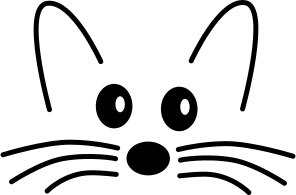
\includegraphics[width=1.4em]{squeak-logo}}}
\iftoshelse{
	\usepackage{marginnote}
		\renewcommand*{\marginfont}{\footnotesize}
	\newcommand{\vartriangleout}{\ifthenelse{\isodd{\thepage}}{\vartriangleright}{\vartriangleleft}}
	\newcommand{\dothisicon}{\fcolorbox{blue!65}{white}{\highlight{$\vartriangleout$}}}
	\newcommand{\dothis}[1]{%
		\noindent\par\noindent
		{\reversemarginpar
			\marginnote{\fcolorbox{blue!65}{white}{\highlight{$\vartriangleout$}}}}
		%\MarginLabel{do this}
		\noindent\emph{#1}
		\nopagebreak}
}{
	\newcommand{\dothisicon}{\raisebox{-.5ex}{
\includegraphics[height=1.2em]{pharo}}}
	\newcommand{\dothis}[1]{%
		\medskip
		\noindent\dothisicon
		\ifx#1\empty\else\quad\emph{#1}\fi
		\par\smallskip\nopagebreak}
}
%===> NEW VERSION <===
% NB: To use this in an individual chapter, you must set:
%\graphicspath{{figures/} {../figures/}}
% at the head of the chapter.  Don't forget the final /
%=============================================================
%:Reader hints (hint)
%
% Indicates a non-obvious consequence
\newcommand{\hint}[1]{\vspace{1ex}\noindent\fbox{\textsc{Hint}} \emph{#1}}
%=================================================================
% graphics for Morphic handles
\newcommand{\grabHandle}{\raisebox{-0.2ex}{
\includegraphics[width=1em]{blackHandle}}}
\newcommand{\moveHandle}{\raisebox{-0.2ex}{
\includegraphics[width=1em]{moveHandle}}}
\newcommand{\debugHandle}{\raisebox{-0.2ex}{
\includegraphics[width=1em]{debugHandle}}}
%=============================================================
%:Highlighting Important stuff (doublebox)
%
% From Seaside book ...
\newsavebox{\SavedText}
\newlength{\InnerBoxRule}\setlength{\InnerBoxRule}{.75\fboxrule}
\newlength{\OuterBoxRule}\setlength{\OuterBoxRule}{1.5\fboxrule}
\newlength{\BoxSeparation}\setlength{\BoxSeparation}{1.5\fboxrule}
\addtolength{\BoxSeparation}{.5pt}
\newlength{\SaveBoxSep}\setlength{\SaveBoxSep}{2\fboxsep}
%
\newenvironment{doublebox}{\begin{lrbox}{\SavedText}
    \begin{minipage}{.75\textwidth}}
    {\end{minipage}\end{lrbox}\begin{center}
    \setlength{\fboxsep}{\BoxSeparation}\setlength{\fboxrule}{\OuterBoxRule}
    \fbox{\setlength{\fboxsep}{\SaveBoxSep}\setlength{\fboxrule}{\InnerBoxRule}%
      \fbox{\usebox{\SavedText}}}
  \end{center}}
% Use this:
\newcommand{\important}[1]{\begin{doublebox}#1\end{doublebox}}
%=============================================================
%:Section depth
\setcounter{secnumdepth}{2}
%% for this to happen start the file with
%\ifx\wholebook\relax\else
%% $Author$
% $Date$
% $Revision$

% HISTORY:
% 2006-10-31 - Oscar code macros
% ...

%=============================================================
% NB: documentclass must be set in main document.
% Allows book to be generated in multiple formats.
%=============================================================
%:Packages
\usepackage[T1]{fontenc}  %%%%%% really important to get the code directly in the text!
\usepackage{lmodern}
%\usepackage[scaled=0.85]{bookmanx} % needs another scale factor if used with \renewcommand{\sfdefault}{cmbr}
\usepackage{palatino}
\usepackage[scaled=0.85]{helvet}
\usepackage[protrusion,expansion=false]{microtype}
\usepackage{graphicx}
\usepackage{theorem}
\usepackage[english]{babel}
% ON: pdfsync breaks the use of p{width} for tabular columns!
\ifdefined\usepdfsync\usepackage{pdfsync}\fi % Requires texlive 2007
%=============================================================
%:More packages
%Stef should check which ones are used!
%\usepackage{picinpar}
%\usepackage{layout}
%\usepackage{color}
%\usepackage{enum}
%\usepackage{a4wide}
% \usepackage{fancyhdr}
\usepackage{ifthen}
\usepackage{float}
\usepackage{longtable}
\usepackage{makeidx}
\usepackage[nottoc]{tocbibind}
\usepackage{multicol}
\usepackage{booktabs}	% book-style tables
\usepackage{topcapt}	% enables \topcaption
\usepackage{multirow}
\usepackage{tabularx}
%\usepackage[bottom]{footmisc}
\usepackage{xspace}
\usepackage{alltt}
\usepackage{amssymb,textcomp}
\usepackage[usenames,dvipsnames]{color}
%\usepackage{colortbl}
\usepackage[hang]{subfigure}\makeatletter\def\p@subfigure{\thefigure\,}\makeatother
\usepackage{rotating}
\usepackage{enumitem}	% apb: allows more control over tags in enumerations
\usepackage{verbatim}     % for comment environment
\usepackage{varioref}	% for page references that work
\labelformat{footnote}{\thechapter--#1} % to distinguish citations from jurabib
\usepackage{needspace}
\usepackage{isodateo} % enable \isodate
\usepackage[newparttoc,pagestyles]{titlesec}
\usepackage{titletoc}
\usepackage{wrapfig}

\usepackage[
	super,
	citefull=first,
	authorformat={allreversed,and},
	titleformat={commasep,italic}
]{jurabib} % citations as footnotes
\usepackage[
	colorlinks=true,
	linkcolor=black,
	urlcolor=black,
	citecolor=black
]{hyperref}   % should come last
%=============================================================
%:PDF version
\pdfminorversion=3 % Set PDF to 1.3 for Lulu
%=============================================================
%:URL style
\makeatletter
\def\url@leostyle{%
  \@ifundefined{selectfont}{\def\UrlFont{\sf}}{\def\UrlFont{\sffamily}}}
\makeatother
% Now actually use the newly defined style.
\urlstyle{leo}
%=============================================================
%:Booleans
\newboolean{lulu}
\setboolean{lulu}{false}
\newcommand{\ifluluelse}[2]{\ifthenelse{\boolean{lulu}}{#1}{#2}}
%=============================================================
%:Names
\newcommand{\SUnit}{SUnit\xspace}
\newcommand{\sunit}{SUnit\xspace}
\newcommand{\xUnit}{$x$Unit\xspace}
\newcommand{\JUnit}{JUnit\xspace}
\newcommand{\st}{Smalltalk\xspace}
\newcommand{\pharo}{Pharo\xspace} % Use this, not \Pharo
%\newcommand{\sqmap}{SqueakMap\xspace}
\newcommand{\squeak}{Squeak\xspace} % use this, not \Squeak or \sq
\newcommand{\sqsrc}{SqueakSource\xspace}
\newcommand{\sbe}{\url{http://SqueakByExample.org}\xspace}
\newcommand{\pharoweb}{\url{http://pharo-project.org}\xspace}
\newcommand{\pbe}{\url{http://PharoByExample.org}\xspace}
\newcommand{\sba}{\url{http://SquareBracketAssociates.org}\xspace}
\newcommand{\bam}{\lct{Bounc\-ing\-Atoms\-Morph}\xspace}
%=============================================================
%:Markup macros for proof-reading
\usepackage[normalem]{ulem} % for \sout
\usepackage{xcolor}
\newcommand{\ra}{$\rightarrow$}
\newcommand{\ugh}[1]{\textcolor{red}{\uwave{#1}}} % please rephrase
\newcommand{\ins}[1]{\textcolor{blue}{\uline{#1}}} % please insert
\newcommand{\del}[1]{\textcolor{red}{\sout{#1}}} % please delete
\newcommand{\chg}[2]{\textcolor{red}{\sout{#1}}{\ra}\textcolor{blue}{\uline{#2}}} % please change
%=============================================================
%:Editorial comment macros
%\newcommand{\nnbb}[2]{
%    % \fbox{\bfseries\sffamily\scriptsize#1}
%    \fcolorbox{gray}{yellow}{\bfseries\sffamily\scriptsize#1}
%    {\sf\small$\blacktriangleright$\textit{#2}$\blacktriangleleft$}
%   }
\newcommand{\yellowbox}[1]{\fcolorbox{gray}{yellow}{\bfseries\sffamily\scriptsize#1}}
\newcommand{\triangles}[1]{{\sf\small$\blacktriangleright$\textit{#1}$\blacktriangleleft$}}
\newcommand{\nnbb}[2]{\yellowbox{#1} \triangles{#2}}
\newcommand{\fix}{\yellowbox{FIX!}}
\newcommand{\here}{\yellowbox{CONTINUE HERE!}}
% editor macros
\newcommand{\apl}[1]{\nnbb{Alain}{#1}} % Alain
\newcommand{\ab}[1]{\nnbb{Andrew}{#1}} % Black
\newcommand{\sd}[1]{\nnbb{St\'{e}f}{#1}} % Ducasse
\newcommand{\gl}[1]{\nnbb{Guillaume}{#1}} % Ducasse
\newcommand{\cd}[1]{\nnbb{Christophe}{#1}} % Ducasse
\newcommand{\sig}[1]{\nnbb{Igor}{#1}} % Igor
\newcommand{\dc}[1]{\nnbb{DamienC}{#1}} % Ducasse
\newcommand{\md}[1]{\nnbb{Marcus}{#1}} % Denker
\newcommand{\on}[1]{\nnbb{Oscar}{#1}} % Nierstrasz
\newcommand{\damien}[1]{\nnbb{Damien}{#1}} % Pollet
\newcommand{\lr}[1]{\nnbb{Lukas}{#1}} % Renggli
\newcommand{\orla}[1]{\nnbb{Orla}{#1}} % Greevy
\newcommand{\alex}[1]{\nnbb{Alex}{#1}} % Bergel
\newcommand{\alx}[1]{\nnbb{Alex}{#1}} % Bergel
\newcommand{\dr}[1]{\nnbb{David}{#1}} % Roethlisberger
\newcommand{\ja}[1]{\nnbb{Jannik}{#1}} % Laval
\newcommand{\cb}[1]{\nnbb{Camillo}{#1}} % Bruni
\newcommand{\jr}[1]{\nnbb{Jorge}{#1}} % Ressia
\newcommand{\jb}[1]{\nnbb{JB}{#1}} % JB
\newcommand{\jp}[1]{\nnbb{Javier}{#1}} % Pimas
\newcommand{\fp}[1]{\nnbb{Fabrizio}{#1}} % Perin
\newcommand{\michael}[1]{\nnbb{Michael}{#1}} % Davies
\newcommand{\ew}[1]{\nnbb{Erwann}{#1}} % Wernli
\newcommand{\mb}[1]{\nnbb{Martial}{#1}} % Boniou
\newcommand{\hw}[1]{\nnbb{Hernan}{#1}} % Wilkinson
\newcommand{\ben}[1]{\nnbb{Benjamin}{#1}} % Benjamin Van Ryseghem
\newcommand{\hjo}[1]{\nnbb{HwaJong}{#1}} % HwaJong Oh aka daliot
\newcommand{\ml}[1]{\nnbb{Max}{#1}} % Max Leske
\newcommand{\mmp}[1]{\nnbb{Mariano}{#1}} % Mariano Martinez Peck
\newcommand{\luc}[1]{\nnbb{Luc}{#1}} % Luc Fabresse
\newcommand{\dkl}[1]{\nnbb{Daniel}{#1}} % Daniel Lyons
\newcommand{\vu}[1]{\nnbb{Veronica}{#1}} % Veronica Uquillas Gomez
\newcommand{\martin}[1]{\nnbb{Martin}{#1}} % Martin Dias
\newcommand{\vp}[1]{\nnbb{Vanessa}{#1}} % Vanessa Pena
\newcommand{\gp}[1]{\nnbb{Guille}{#1}} % Guillermo Polito

%=============================================================
%:Abbreviation macros
\newcommand{\ie}{\emph{i.e.},\xspace}
\newcommand{\eg}{\emph{e.g.},\xspace}
\newcommand{\etc}{etc.\xspace}
%=============================================================
%:Cross reference macros
\newcommand{\charef}[1]{Chapter~\ref{cha:#1}\xspace}
\newcommand{\secref}[1]{Section~\ref{sec:#1}\xspace}
\newcommand{\figref}[1]{Figure~\ref{fig:#1}\xspace}
\newcommand{\Figref}[1]{Figure~\ref{fig:#1}\xspace}
\newcommand{\appref}[1]{Appendix~\ref{app:#1}\xspace}
\newcommand{\tabref}[1]{Table~\ref{tab:#1}\xspace}
\newcommand{\faqref}[1]{FAQ~\ref{faq:#1}, p.~\pageref{faq:#1}\xspace}
% APB: I removed trailing \xspace commands from these macros because
% \xspace mostly doesn't work.  If you want a space after your
% references, type one!
% ON: xspace has always worked just fine for me!  Please leave them in.
%
\newcommand{\ruleref}[1]{\ref{rule:#1}\xspace}
%
\newcommand{\egref}[1]{example~\ref{eg:#1}\xspace}
\newcommand{\Egref}[1]{Example~\ref{eg:#1}\xspace}
%
\newcommand{\scrref}[1]{script~\ref{scr:#1}\xspace}
\newcommand{\Scrref}[1]{Script~\ref{scr:#1}\xspace}
\newcommand{\tscrref}[1]{the script~\ref{scr:#1}\xspace}
\newcommand{\Tscrref}[1]{The script~\ref{scr:#1}\xspace}
%
\newcommand{\mthref}[1]{method~\ref{mth:#1}\xspace}
\newcommand{\mthsref}[1]{methods~\ref{mth:#1}\xspace}
\newcommand{\Mthref}[1]{Method~\ref{mth:#1}\xspace}
\newcommand{\tmthref}[1]{the method~\ref{mth:#1}\xspace}
\newcommand{\Tmthref}[1]{The method~\ref{mth:#1}\xspace}
%
\newcommand{\clsref}[1]{class~\ref{cls:#1}\xspace}
\newcommand{\tclsref}[1]{the class~\ref{cls:#1}\xspace}
\newcommand{\Tclsref}[1]{The class~\ref{cls:#1}\xspace}

\newcommand{\chalabel}[1]{\label{cha:#1}}
\newcommand{\seclabel}[1]{\label{sec:#1}}
\newcommand{\figlabel}[1]{\label{fig:#1}}
\newcommand{\tablabel}[1]{\label{tab:#1}}
\newcommand{\rulelabel}[1]{\label{rule:#1}}
\newcommand{\eglabel}[1]{\label{eg:#1}}
\newcommand{\scrlabel}[1]{\label{scr:#1}}
\newcommand{\mthlabel}[1]{\label{mth:#1}}
\newcommand{\clslabel}[1]{\label{cls:#1}}
\newcommand{\faqlabel}[1]{\label{faq:#1}}
%=============================================================
%:Menu item macro
% for menu items, so we can change our minds on how to print them! (apb)
\definecolor{lightgray}{gray}{0.89}
\newcommand{\menu}[1]{{%
	\setlength{\fboxsep}{0pt}%
	\colorbox{lightgray}{{{\upshape\sffamily\strut \,#1\,}}}}}
\newcommand{\link}[1]{{%
	\fontfamily{lmr}\selectfont
 	\upshape{\sffamily \underline{#1}}}}
% For submenu items:
\newcommand{\go}{\,$\triangleright$\,}
% \newcommand{\go}{\,$\blacktriangleright$\,}
% For keyboard shortcuts:
%\newcommand{\short}[1]{\mbox{$\langle${\sc CMD}$\rangle$-#1}\xspace}
\newcommand{\short}[1]{\mbox{{\sc cmd}\hspace{0.08em}--\hspace{0.09em}#1}\xspace}
% For buttons:
\newcommand{\button}[1]{{%
	\setlength{\fboxsep}{0pt}%
	\fbox{{\upshape\sffamily\strut \,#1\,}}}}
% NB: The button macro does not work within captions -- incompatible with xcolor package :-(
\newcommand{\toolsflap}{\textit{Tools} flap\xspace}
%=============================================================
%:Mouse clicks
\newcommand{\click}{click\xspace} % RED
\newcommand{\actclick}{action-click\xspace} % YELLOW
\newcommand{\metaclick}{meta-click\xspace} % BLUE
\newcommand{\Click}{Click\xspace} % RED
\newcommand{\Actclick}{Action-click\xspace} % YELLOW
\newcommand{\Metaclick}{Meta-click\xspace} % BLUE
%=============================================================
%:ToSh macros
\newboolean{tosh}
\setboolean{tosh}{false}
\newcommand{\iftoshelse}[2]{\ifthenelse{\boolean{tosh}}{#1}{#2}}
%=============================================================
%:ToSh colors
%\newcommand{\highlightcolor}{\color{blue!65}}
%\newcommand{\boxcolor}{\color{gray!25}}
\newcommand{\highlight}[1]{\textcolor{blue!65}{#1}}
%\newcommand{\codecolor}{\color{blue!65}}
%%\setlength{\fboxrule}{2pt}
%\newcommand{\asPict}[1]{%
%	{\Large\highlight{#1}}}
%=============================================================
%:Reader cues (do this)
%
% Indicate something the reader should try out.
% \newcommand{\dothisicon}{\raisebox{-.5ex}{\includegraphics[width=1.4em]{squeak-logo}}}
\iftoshelse{
	\usepackage{marginnote}
		\renewcommand*{\marginfont}{\footnotesize}
	\newcommand{\vartriangleout}{\ifthenelse{\isodd{\thepage}}{\vartriangleright}{\vartriangleleft}}
	\newcommand{\dothisicon}{\fcolorbox{blue!65}{white}{\highlight{$\vartriangleout$}}}
	\newcommand{\dothis}[1]{%
		\noindent\par\noindent
		{\reversemarginpar
			\marginnote{\fcolorbox{blue!65}{white}{\highlight{$\vartriangleout$}}}}
		%\MarginLabel{do this}
		\noindent\emph{#1}
		\nopagebreak}
}{
	\newcommand{\dothisicon}{\raisebox{-.5ex}{\includegraphics[height=1.2em]{pharo}}}
	\newcommand{\dothis}[1]{%
		\medskip
		\noindent\dothisicon
		\ifx#1\empty\else\quad\emph{#1}\fi
		\par\smallskip\nopagebreak}
}
%===> NEW VERSION <===
% NB: To use this in an individual chapter, you must set:
%\graphicspath{{figures/} {../figures/}}
% at the head of the chapter.  Don't forget the final /
%=============================================================
%:Reader hints (hint)
%
% Indicates a non-obvious consequence
\newcommand{\hint}[1]{\vspace{1ex}\noindent\fbox{\textsc{Hint}} \emph{#1}}
%=================================================================
% graphics for Morphic handles
\newcommand{\grabHandle}{\raisebox{-0.2ex}{\includegraphics[width=1em]{blackHandle}}}
\newcommand{\moveHandle}{\raisebox{-0.2ex}{\includegraphics[width=1em]{moveHandle}}}
\newcommand{\debugHandle}{\raisebox{-0.2ex}{\includegraphics[width=1em]{debugHandle}}}
%=============================================================
%:Highlighting Important stuff (doublebox)
%
% From Seaside book ...
\newsavebox{\SavedText}
\newlength{\InnerBoxRule}\setlength{\InnerBoxRule}{.75\fboxrule}
\newlength{\OuterBoxRule}\setlength{\OuterBoxRule}{1.5\fboxrule}
\newlength{\BoxSeparation}\setlength{\BoxSeparation}{1.5\fboxrule}
\addtolength{\BoxSeparation}{.5pt}
\newlength{\SaveBoxSep}\setlength{\SaveBoxSep}{2\fboxsep}
%
\newenvironment{doublebox}{\begin{lrbox}{\SavedText}
    \begin{minipage}{.75\textwidth}}
    {\end{minipage}\end{lrbox}\begin{center}
    \setlength{\fboxsep}{\BoxSeparation}\setlength{\fboxrule}{\OuterBoxRule}
    \fbox{\setlength{\fboxsep}{\SaveBoxSep}\setlength{\fboxrule}{\InnerBoxRule}%
      \fbox{\usebox{\SavedText}}}
  \end{center}}
% Use this:
\newcommand{\important}[1]{\begin{doublebox}#1\end{doublebox}}
%=============================================================
%:Section depth
\setcounter{secnumdepth}{2}
%% for this to happen start the file with
%\ifx\wholebook\relax\else
%\input{../common.tex}
%\begin{document}
%\fi
% and terminate by
% \ifx\wholebook\relax\else\end{document}\fi

\DeclareGraphicsExtensions{.pdf, .jpg, .png}
%=============================================================
%:PDF setup
\hypersetup{
%   a4paper,
%   pdfstartview=FitV,
%   colorlinks,
%   linkcolor=darkblue,
%   citecolor=darkblue,
   pdftitle={Pharo by Example},
   pdfauthor={Andrew P. Black, St\'ephane Ducasse,	Oscar Nierstrasz,
Damien Pollet},
   pdfkeywords={Smalltalk, Squeak, Object-Oriented Programming, OOP},
   pdfsubject={Computer Science}
}
%=============================================================
%:Page layout and appearance
%
% \renewcommand{\headrulewidth}{0pt}
\renewcommand{\chaptermark}[1]{\markboth{#1}{}}
\renewcommand{\sectionmark}[1]{\markright{\thesection\ #1}}
\renewpagestyle{plain}[\small\itshape]{%
	\setheadrule{0pt}%
	\sethead[][][]{}{}{}%
	\setfoot[][][]{}{}{}}
\renewpagestyle{headings}[\small\itshape]{%
	\setheadrule{0pt}%
	\setmarks{chapter}{section}%
	\sethead[\thepage][][\chaptertitle]{\sectiontitle}{}{\thepage}%
	\setfoot[][][]{}{}{}}
%=============================================================
%:Title section setup and TOC numbering depth
\setcounter{secnumdepth}{1}
\setcounter{tocdepth}{1}
\titleformat{\part}[display]{\centering}{\huge\partname\ \thepart}{1em}{\Huge\textbf}[]
\titleformat{\chapter}[display]{}{\huge\chaptertitlename\ \thechapter}{1em}{\Huge\raggedright\textbf}[]
\titlecontents{part}[3pc]{%
		\pagebreak[2]\addvspace{1em plus.4em minus.2em}%
		\leavevmode\large\bfseries}
	{\contentslabel{3pc}}{\hspace*{-3pc}}
	{}[\nopagebreak]
\titlecontents{chapter}[3pc]{%
		\pagebreak[0]\addvspace{1em plus.2em minus.2em}%
		\leavevmode\bfseries}
	{\contentslabel{3pc}}{}
	{\hfill\contentspage}[\nopagebreak]
\dottedcontents{section}[3pc]{}{3pc}{1pc}
\dottedcontents{subsection}[3pc]{}{0pc}{1pc}
% \dottedcontents{subsection}[4.5em]{}{0pt}{1pc}
% Make \cleardoublepage insert really blank pages http://www.tex.ac.uk/cgi-bin/texfaq2html?label=reallyblank
\let\origdoublepage\cleardoublepage
\newcommand{\clearemptydoublepage}{%
  \clearpage
  {\pagestyle{empty}\origdoublepage}}
\let\cleardoublepage\clearemptydoublepage % see http://www.tex.ac.uk/cgi-bin/texfaq2html?label=patch
%=============================================================
%:FAQ macros (for FAQ chapter)
\newtheorem{faq}{FAQ}
\newcommand{\answer}{\paragraph{Answer}\ }
%=============================================================
%:Listings package configuration
% \newcommand{\caret}{\makebox{\raisebox{0.4ex}{\footnotesize{$\wedge$}}}}
\newcommand{\caret}{\^\,}
\newcommand{\escape}{{\sf \textbackslash}}
\definecolor{source}{gray}{0.95}
\usepackage{listings}
\lstdefinelanguage{Smalltalk}{
%  morekeywords={self,super,true,false,nil,thisContext}, % This is overkill
  morestring=[d]',
  morecomment=[s]{"}{"},
  alsoletter={\#:},
  escapechar={!},
  literate=
    {BANG}{!}1
    {CARET}{\^}1
    {UNDERSCORE}{\_}1
    {\\st}{Smalltalk}9 % convenience -- in case \st occurs in code
    % {'}{{\textquotesingle}}1 % replaced by upquote=true in \lstset
    %{_}{{$\leftarrow$}}1
    {>>>}{{\sep}}1
    %{^}{{$\uparrow$}}1
    {~}{{$\sim$}}1
    {-}{{\texttt{-}}}1 %{\textminus}}1 %{-}{\hspace{-0.13em}}{-}}1  % the goal is to make - the same width as +
    % {+}{\sf+}1 %{\raisebox{0.08ex}{+}}}1      % and to raise + off the baseline to match -
    {-->}{{\quad$\longrightarrow$\quad}}3
    {~->}{{\quad$\leadsto$\quad}}3
	, % Don't forget the comma at the end!
  tabsize=4
}[keywords,comments,strings]

\lstset{language=Smalltalk,
	basicstyle=\sffamily,
	keywordstyle=\color{black}\bfseries,
	% stringstyle=\ttfamily, % Ugly! do we really want this? -- on
	mathescape=true,
	showstringspaces=false,
	keepspaces=true,
	breaklines=true,
	breakautoindent=true,
	backgroundcolor=\color{source},
	lineskip={-1pt}, % Ugly hack
	upquote=true, % straight quote; requires textcomp package
	columns=fullflexible} % no fixed width fonts
% In-line code (literal)
% Normally use this for all in-line code:

\newcommand{\ct}{\lstinline[mathescape=false,backgroundcolor=\color{white},basicstyle={\sffamily\upshape}]}
\newcommand{\cts}[1]{{\sffamily{\upshape{#1}}\xspace}}
% apb 2007.8.28 added the \upshape declaration to avoid getting italicized code in \dothis{ } sections.
% In-line code (latex enabled)
% Use this only in special situations where \ct does not work
% (within section headings ...):
\newcommand{\lct}[1]{{\textsf{\textup{#1}}}}
% Use these for system categories and protocols:
\newcommand{\scat}[1]{\emph{\textsf{#1}}\xspace}
\newcommand{\pkg}[1]{\emph{\textsf{#1}}\xspace}
\newcommand{\prot}[1]{\emph{\textsf{#1}}\xspace}
% Code environments
% NB: the arg is for tests
% Only code and example environments may be tests
\lstnewenvironment{code}[1]{%
	\lstset{%
		% frame=lines,
		frame=single,
		framerule=0pt,
		mathescape=false
	}
}{}
\def\ignoredollar#1{}
%=============================================================
%:Code environments (method, script ...)
% NB: the third arg is for tests
% Only code and example environments may be tests
\lstnewenvironment{example}[3][defaultlabel]{%
	\renewcommand{\lstlistingname}{Example}%
	\lstset{
		% frame=lines,
		frame=single,
		framerule=0pt,
		mathescape=false,
		caption={\emph{#2}},
		label={eg:#1}
	}
}{}
\lstnewenvironment{script}[2][defaultlabel]{%
\renewcommand{\lstlistingname}{Script}%
	\lstset{
		% frame=lines,
		frame=single,
		framerule=0pt,
		mathescape=false,
		name={Script},
		caption={\emph{#2}},
		label={scr:#1}
	}
}{}
\lstnewenvironment{method}[2][defaultlabel]{%
	\renewcommand{\lstlistingname}{Method}%
	\lstset{
		% frame=lines,
		frame=single,
		framerule=0pt,
		mathescape=false,
		name={Method},
		caption={\emph{#2}},
		label={mth:#1}
	}
}{}
\lstnewenvironment{methods}[2][defaultlabel]{% just for multiple methods at once
	\renewcommand{\lstlistingname}{Methods}%
	\lstset{
		% frame=lines,
		frame=single,
		framerule=0pt,
		mathescape=false,
		name={Method},
		caption={\emph{#2}},
		label={mth:#1}
	}
}{}
\lstnewenvironment{numMethod}[2][defaultlabel]{%
	\renewcommand{\lstlistingname}{Method}%
	\lstset{
		numbers=left,
		numberstyle={\tiny\sffamily},
		% frame=lines,
		frame=single,
		framerule=0pt,
		mathescape=false,
		name={Method},
		caption={\emph{#2}},
		label={mth:#1}
	}
}{}
\lstnewenvironment{classdef}[2][defaultlabel]{%
	\renewcommand{\lstlistingname}{Class}%
	\lstset{
		% frame=lines,
		frame=single,
		framerule=0pt,
		mathescape=false,
		name={Class},
		caption={\emph{#2}},
		label={cls:#1}
	}
}{}
%=============================================================
%:Reserving space
% Usually need one more line than the actual lines of code
\newcommand{\needlines}[1]{\Needspace{#1\baselineskip}}
%=============================================================
%:Indexing macros
% Macros ending with "ind" generate text as well as an index entry
% Macros ending with "index" *only* generate an index entry
\newcommand{\ind}[1]{\index{#1}#1\xspace} % plain text
\newcommand{\subind}[2]{\index{#1!#2}#2\xspace} % show #2, subindex under #1
\newcommand{\emphind}[1]{\index{#1}\emph{#1}\xspace} % emph #1
\newcommand{\emphsubind}[2]{\index{#1!#2}\emph{#2}\xspace} % show emph #2, subindex inder #1
\newcommand{\scatind}[1]{\index{#1@\textsf{#1} (category)}\scat{#1}} % category
\newcommand{\pkgind}[1]{\index{#1@\textsf{#1} (package)}\pkg{#1}} % package
\newcommand{\protind}[1]{\index{#1@\textsf{#1} (protocol)}\prot{#1}} % protocol
\newcommand{\clsind}[1]{\index{#1@\textsf{#1} (class)}\ct{#1}\xspace}
% \newcommand{\clsind}[1]{\index{#1!\#@(class)}\ct{#1}\xspace} % class
\newcommand{\clsindplural}[1]{\index{#1!\#@(class)}\ct{#1}s\xspace} % class
\newcommand{\cvind}[1]{\index{#1@\textsf{#1} (class variable)}\ct{#1}\xspace} % class var
\newcommand{\glbind}[1]{\index{#1@\textsf{#1} (global)}\ct{#1}\xspace} % global
\newcommand{\patind}[1]{\index{#1@#1 (pattern)}\ct{#1}\xspace} % pattern
\newcommand{\pvind}[1]{\index{#1@\textsf{#1} (pseudo variable)}\ct{#1}\xspace} % pseudo var
\newcommand{\clsmthind}[2]{\index{#1!#2@\ct{#2}}\ct{#1>>>#2}\xspace} % class + method name
\newcommand{\mthind}[2]{\index{#1!#2@\ct{#2}}\ct{#2}\xspace} % show method name only
\newcommand{\lmthind}[2]{\index{#1!#2@\ct{#2}}\lct{#2}\xspace} % show method name only
\newcommand{\cmind}[2]{\index{#1!#2@\ct{#2}}\ct{#1>>>#2}\xspace} % show class>>method
\newcommand{\lcmind}[2]{\index{#1!#2@\ct{#2}}\lct{#1>>>#2}\xspace} % show class>>method
\newcommand{\toolsflapind}{\index{Tools flap}\toolsflap} % index tools flap
% The following only generate an index entry:
% \newcommand{\clsindex}[1]{\index{#1@\textsf{#1} (class)}}
\newcommand{\clsindex}[1]{\index{#1!\#@(class)}} % class
\newcommand{\mthindex}[2]{\index{#1!#2@\ct{#2}}} % method
\newcommand{\cmindex}[2]{\index{#1!#2@\ct{#2}}} % class>>method
\newcommand{\cvindex}[1]{\index{#1@\textsf{#1} (class variable)}} % class var
\newcommand{\glbindex}[1]{\index{#1@\textsf{#1} (global)}}% global
\newcommand{\pvindex}[1]{\index{#1@\textsf{#1} (pseudo variable)}}% pseudo var
\newcommand{\seeindex}[2]{\index{#1|see{#2}}} % #1, see #2
\newcommand{\scatindex}[1]{\index{#1@\textsf{#1} (category)}} % category
\newcommand{\pkgindex}[1]{\index{#1@\textsf{#1} (package)}} % package
\newcommand{\protindex}[1]{\index{#1@\textsf{#1} (protocol)}} % protocol
% How can we have the main entry page numbers in bold yet not break the hyperlink?
\newcommand{\boldidx}[1]{{\bf #1}} % breaks hyperlink
%\newcommand{\indmain}[1]{\index{#1|boldidx}#1\xspace} % plain text, main entry
%\newcommand{\emphsubindmain}[2]{\index{#1!#2|boldidx}\emph{#2}\xspace} % subindex, main entry
%\newcommand{\subindmain}[2]{\index{#1!#2|boldidx}#2\xspace} % subindex, main entry
%\newcommand{\clsindmain}[1]{\index{#1@\textsf{#1} (class)|boldidx}\ct{#1}\xspace}
%\newcommand{\clsindmain}[1]{\index{#1!\#@(class)|boldidx}\ct{#1}\xspace} % class main
%\newcommand{\indexmain}[1]{\index{#1|boldidx}} % main index entry only
\newcommand{\indmain}[1]{\index{#1}#1\xspace} % The main index entry for this item
\newcommand{\emphsubindmain}[2]{\index{#1!#2}\emph{#2}\xspace} % subindex, main entry
\newcommand{\subindmain}[2]{\index{#1!#2}#2\xspace} % subindex, main entry
%\newcommand{\clsindmain}[1]{\index{#1@\textsf{#1} (class)}\ct{#1}\xspace}
\newcommand{\clsindmain}[1]{\index{#1!\#@(class)}\ct{#1}\xspace} % class main
\newcommand{\clsindexmain}[1]{\index{#1!\#@(class)}} % class main index only
\newcommand{\indexmain}[1]{\index{#1}}
%=============================================================
%:Code macros
% some constants
\newcommand{\codesize}{\small}
\newcommand{\codefont}{\sffamily}
%\newcommand{\cat}[1]{\textit{In category #1}}%%To remove later
\newlength{\scriptindent}
\setlength{\scriptindent}{.3cm}
%% Method presentation constants
\newlength{\methodindent}
\newlength{\methodwordlength}
\newlength{\aftermethod}
\setlength{\methodindent}{0.2cm}
\settowidth{\methodwordlength}{\ M\'ethode\ }
%=============================================================
%:Smalltalk macros
%\newcommand{\sep}{{$\gg$}}
\newcommand{\sep}{\mbox{>>}}
\newcommand{\self}{\lct{self}\xspace}
\newcommand{\super}{\lct{super}\xspace}
\newcommand{\nil}{\lct{nil}\xspace}
%=============================================================
% be less conservative about float placement
% these commands are from http://www.tex.ac.uk/cgi-bin/texfaq2html?label=floats
\renewcommand{\topfraction}{.9}
\renewcommand{\bottomfraction}{.9}
\renewcommand{\textfraction}{.1}
\renewcommand{\floatpagefraction}{.85}
\renewcommand{\dbltopfraction}{.66}
\renewcommand{\dblfloatpagefraction}{.85}
\setcounter{topnumber}{9}
\setcounter{bottomnumber}{9}
\setcounter{totalnumber}{20}
\setcounter{dbltopnumber}{9}
%=============================================================
% Give information from each chapter's author
\newcommand{\contact}[2]{\textbf{#1} \textsf{(#2)}}

\newcommand{\chapterauthor}[1]{\emph{with the participation of:\\#1}\\}
\newcommand{\chapterwritten}[1]{\emph{written by:\\#1}\\}

\newcommand{\authornoury}{\contact{Noury Bouraqadi}{Noury.Bouraqadi@mines-douai.fr}}
\newcommand{\authorluc}{\contact{Luc Fabresse}{Luc.Fabresse@mines-douai.fr}}
\newcommand{\authordamienc}{\contact{Damien Cassou}{damien.cassou@gmail.com}}
\newcommand{\authoroscar}{\contact{Oscar Nierstrasz}{oscar.nierstrasz@acm.org}}
\newcommand{\authorsteph}{\contact{St\'ephane Ducasse}{stephane.ducasse@inria.fr}}
\newcommand{\authoralex}{\contact{Alexandre Bergel}{alexandre@bergel.eu}}
\newcommand{\authorolivier}{\contact{Olivier Auverlot}{olivier.auverlot@inria.fr}}
\newcommand{\authornicolas}{\contact{Nicolas Cellier}{nicolas.cellier.aka.nice@gmail.com}}
\newcommand{\authormarcus}{\contact{Marcus Denker}{marcus.denker@inria.fr}}
\newcommand{\authoralain}{\contact{Alain Plantec}{alain.plantec@univ-brest.fr}}
\newcommand{\authordale}{\contact{Dale Henrichs}{dale.henrichs@gemstone.com}}
\newcommand{\authormariano}{\contact{Mariano Martinez Peck}{marianopeck@gmail.com}}
\newcommand{\authorsven}{\contact{Sven Van Caekenberghe}{sven@beta9.be}}
\newcommand{\authorlukas}{\contact{Lukas Renggli}{renggli@gmail.com}}
\newcommand{\authorjankurs}{\contact{Jan Kurs}{kurs@iam.unibe.ch}}
\newcommand{\authorguillaume}{\contact{Guillaume Larcheveque}{guillaume.larcheveque@gmail.com}}
\newcommand{\authorguillep}{\contact{Guillermo Polito}{guillermopolito@gmail.com}}
\newcommand{\authorclement}{\contact{Cl\'ement Bera}{bera.clement@gmail.com}}
\newcommand{\authormax}{\contact{Max Leske}{maxleske@gmail.com}}
\newcommand{\authorvanessa}{\contact{Vanessa Pe\~{n}a-Araya}{van.c.pena@gmail.com}}
\newcommand{\authorcamillo}{\contact{Camillo Bruni}{camillobruni@gmail.com}}

%=============================================================
% apb doesn't like paragraphs to run in to each other without a break
\parskip 1ex
%=============================================================
%:Stuff to check, merge or deprecate
%\setlength{\marginparsep}{2mm}
%\renewcommand{\baselinestretch}{1.1}
%=============================================================
\usepackage{tikz}

%\begin{document}
%\fi
% and terminate by
% \ifx\wholebook\relax\else\end{document}\fi

\DeclareGraphicsExtensions{.pdf, .jpg, .png}
%=============================================================
%:PDF setup
\hypersetup{
%   a4paper,
%   pdfstartview=FitV,
%   colorlinks,
%   linkcolor=darkblue,
%   citecolor=darkblue,
   pdftitle={Pharo by Example},
   pdfauthor={Andrew P. Black, St\'ephane Ducasse,	Oscar Nierstrasz,
Damien Pollet},
   pdfkeywords={Smalltalk, Squeak, Object-Oriented Programming, OOP},
   pdfsubject={Computer Science}
}
%=============================================================
%:Page layout and appearance
%
% \renewcommand{\headrulewidth}{0pt}
\renewcommand{\chaptermark}[1]{\markboth{#1}{}}
\renewcommand{\sectionmark}[1]{\markright{\thesection\ #1}}
\renewpagestyle{plain}[\small\itshape]{%
	\setheadrule{0pt}%
	\sethead[][][]{}{}{}%
	\setfoot[][][]{}{}{}}
\renewpagestyle{headings}[\small\itshape]{%
	\setheadrule{0pt}%
	\setmarks{chapter}{section}%
	\sethead[\thepage][][\chaptertitle]{\sectiontitle}{}{\thepage}%
	\setfoot[][][]{}{}{}}
%=============================================================
%:Title section setup and TOC numbering depth
\setcounter{secnumdepth}{1}
\setcounter{tocdepth}{1}
\titleformat{\part}[display]{\centering}{\huge\partname\ \thepart}{1em}{\Huge\textbf}[]
\titleformat{\chapter}[display]{}{\huge\chaptertitlename\ \thechapter}{1em}{\Huge\raggedright\textbf}[]
\titlecontents{part}[3pc]{%
		\pagebreak[2]\addvspace{1em plus.4em minus.2em}%
		\leavevmode\large\bfseries}
	{\contentslabel{3pc}}{\hspace*{-3pc}}
	{}[\nopagebreak]
\titlecontents{chapter}[3pc]{%
		\pagebreak[0]\addvspace{1em plus.2em minus.2em}%
		\leavevmode\bfseries}
	{\contentslabel{3pc}}{}
	{\hfill\contentspage}[\nopagebreak]
\dottedcontents{section}[3pc]{}{3pc}{1pc}
\dottedcontents{subsection}[3pc]{}{0pc}{1pc}
% \dottedcontents{subsection}[4.5em]{}{0pt}{1pc}
% Make \cleardoublepage insert really blank pages http://www.tex.ac.uk/cgi-bin/texfaq2html?label=reallyblank
\let\origdoublepage\cleardoublepage
\newcommand{\clearemptydoublepage}{%
  \clearpage
  {\pagestyle{empty}\origdoublepage}}
\let\cleardoublepage\clearemptydoublepage % see http://www.tex.ac.uk/cgi-bin/texfaq2html?label=patch
%=============================================================
%:FAQ macros (for FAQ chapter)
\newtheorem{faq}{FAQ}
\newcommand{\answer}{\paragraph{Answer}\ }
%=============================================================
%:Listings package configuration
% \newcommand{\caret}{\makebox{\raisebox{0.4ex}{\footnotesize{$\wedge$}}}}
\newcommand{\caret}{\^\,}
\newcommand{\escape}{{\sf \textbackslash}}
\definecolor{source}{gray}{0.95}
\usepackage{listings}
\lstdefinelanguage{Smalltalk}{
%  morekeywords={self,super,true,false,nil,thisContext}, % This is overkill
  morestring=[d]',
  morecomment=[s]{"}{"},
  alsoletter={\#:},
  escapechar={!},
  literate=
    {BANG}{!}1
    {CARET}{\^}1
    {UNDERSCORE}{\_}1
    {\\st}{Smalltalk}9 % convenience -- in case \st occurs in code
    % {'}{{\textquotesingle}}1 % replaced by upquote=true in \lstset
    %{_}{{$\leftarrow$}}1
    {>>>}{{\sep}}1
    %{^}{{$\uparrow$}}1
    {~}{{$\sim$}}1
    {-}{{\texttt{-}}}1 %{\textminus}}1 %{-}{\hspace{-0.13em}}{-}}1  % the goal is to make - the same width as +
    % {+}{\sf+}1 %{\raisebox{0.08ex}{+}}}1      % and to raise + off the baseline to match -
    {-->}{{\quad$\longrightarrow$\quad}}3
    {~->}{{\quad$\leadsto$\quad}}3
	, % Don't forget the comma at the end!
  tabsize=4
}[keywords,comments,strings]

\lstset{language=Smalltalk,
	basicstyle=\sffamily,
	keywordstyle=\color{black}\bfseries,
	% stringstyle=\ttfamily, % Ugly! do we really want this? -- on
	mathescape=true,
	showstringspaces=false,
	keepspaces=true,
	breaklines=true,
	breakautoindent=true,
	backgroundcolor=\color{source},
	lineskip={-1pt}, % Ugly hack
	upquote=true, % straight quote; requires textcomp package
	columns=fullflexible} % no fixed width fonts
% In-line code (literal)
% Normally use this for all in-line code:

\newcommand{\ct}{\lstinline[mathescape=false,backgroundcolor=\color{white},basicstyle={\sffamily\upshape}]}
\newcommand{\cts}[1]{{\sffamily{\upshape{#1}}\xspace}}
% apb 2007.8.28 added the \upshape declaration to avoid getting italicized code in \dothis{ } sections.
% In-line code (latex enabled)
% Use this only in special situations where \ct does not work
% (within section headings ...):
\newcommand{\lct}[1]{{\textsf{\textup{#1}}}}
% Use these for system categories and protocols:
\newcommand{\scat}[1]{\emph{\textsf{#1}}\xspace}
\newcommand{\pkg}[1]{\emph{\textsf{#1}}\xspace}
\newcommand{\prot}[1]{\emph{\textsf{#1}}\xspace}
% Code environments
% NB: the arg is for tests
% Only code and example environments may be tests
\lstnewenvironment{code}[1]{%
	\lstset{%
		% frame=lines,
		frame=single,
		framerule=0pt,
		mathescape=false
	}
}{}
\def\ignoredollar#1{}
%=============================================================
%:Code environments (method, script ...)
% NB: the third arg is for tests
% Only code and example environments may be tests
\lstnewenvironment{example}[3][defaultlabel]{%
	\renewcommand{\lstlistingname}{Example}%
	\lstset{
		% frame=lines,
		frame=single,
		framerule=0pt,
		mathescape=false,
		caption={\emph{#2}},
		label={eg:#1}
	}
}{}
\lstnewenvironment{script}[2][defaultlabel]{%
\renewcommand{\lstlistingname}{Script}%
	\lstset{
		% frame=lines,
		frame=single,
		framerule=0pt,
		mathescape=false,
		name={Script},
		caption={\emph{#2}},
		label={scr:#1}
	}
}{}
\lstnewenvironment{method}[2][defaultlabel]{%
	\renewcommand{\lstlistingname}{Method}%
	\lstset{
		% frame=lines,
		frame=single,
		framerule=0pt,
		mathescape=false,
		name={Method},
		caption={\emph{#2}},
		label={mth:#1}
	}
}{}
\lstnewenvironment{methods}[2][defaultlabel]{% just for multiple methods at once
	\renewcommand{\lstlistingname}{Methods}%
	\lstset{
		% frame=lines,
		frame=single,
		framerule=0pt,
		mathescape=false,
		name={Method},
		caption={\emph{#2}},
		label={mth:#1}
	}
}{}
\lstnewenvironment{numMethod}[2][defaultlabel]{%
	\renewcommand{\lstlistingname}{Method}%
	\lstset{
		numbers=left,
		numberstyle={\tiny\sffamily},
		% frame=lines,
		frame=single,
		framerule=0pt,
		mathescape=false,
		name={Method},
		caption={\emph{#2}},
		label={mth:#1}
	}
}{}
\lstnewenvironment{classdef}[2][defaultlabel]{%
	\renewcommand{\lstlistingname}{Class}%
	\lstset{
		% frame=lines,
		frame=single,
		framerule=0pt,
		mathescape=false,
		name={Class},
		caption={\emph{#2}},
		label={cls:#1}
	}
}{}
%=============================================================
%:Reserving space
% Usually need one more line than the actual lines of code
\newcommand{\needlines}[1]{\Needspace{#1\baselineskip}}
%=============================================================
%:Indexing macros
% Macros ending with "ind" generate text as well as an index entry
% Macros ending with "index" *only* generate an index entry
\newcommand{\ind}[1]{\index{#1}#1\xspace} % plain text
\newcommand{\subind}[2]{\index{#1!#2}#2\xspace} % show #2, subindex under #1
\newcommand{\emphind}[1]{\index{#1}\emph{#1}\xspace} % emph #1
\newcommand{\emphsubind}[2]{\index{#1!#2}\emph{#2}\xspace} % show emph #2, subindex inder #1
\newcommand{\scatind}[1]{\index{#1@\textsf{#1} (category)}\scat{#1}} % category
\newcommand{\pkgind}[1]{\index{#1@\textsf{#1} (package)}\pkg{#1}} % package
\newcommand{\protind}[1]{\index{#1@\textsf{#1} (protocol)}\prot{#1}} % protocol
\newcommand{\clsind}[1]{\index{#1@\textsf{#1} (class)}\ct{#1}\xspace}
% \newcommand{\clsind}[1]{\index{#1!\#@(class)}\ct{#1}\xspace} % class
\newcommand{\clsindplural}[1]{\index{#1!\#@(class)}\ct{#1}s\xspace} % class
\newcommand{\cvind}[1]{\index{#1@\textsf{#1} (class variable)}\ct{#1}\xspace} % class var
\newcommand{\glbind}[1]{\index{#1@\textsf{#1} (global)}\ct{#1}\xspace} % global
\newcommand{\patind}[1]{\index{#1@#1 (pattern)}\ct{#1}\xspace} % pattern
\newcommand{\pvind}[1]{\index{#1@\textsf{#1} (pseudo variable)}\ct{#1}\xspace} % pseudo var
\newcommand{\clsmthind}[2]{\index{#1!#2@\ct{#2}}\ct{#1>>>#2}\xspace} % class + method name
\newcommand{\mthind}[2]{\index{#1!#2@\ct{#2}}\ct{#2}\xspace} % show method name only
\newcommand{\lmthind}[2]{\index{#1!#2@\ct{#2}}\lct{#2}\xspace} % show method name only
\newcommand{\cmind}[2]{\index{#1!#2@\ct{#2}}\ct{#1>>>#2}\xspace} % show class>>method
\newcommand{\lcmind}[2]{\index{#1!#2@\ct{#2}}\lct{#1>>>#2}\xspace} % show class>>method
\newcommand{\toolsflapind}{\index{Tools flap}\toolsflap} % index tools flap
% The following only generate an index entry:
% \newcommand{\clsindex}[1]{\index{#1@\textsf{#1} (class)}}
\newcommand{\clsindex}[1]{\index{#1!\#@(class)}} % class
\newcommand{\mthindex}[2]{\index{#1!#2@\ct{#2}}} % method
\newcommand{\cmindex}[2]{\index{#1!#2@\ct{#2}}} % class>>method
\newcommand{\cvindex}[1]{\index{#1@\textsf{#1} (class variable)}} % class var
\newcommand{\glbindex}[1]{\index{#1@\textsf{#1} (global)}}% global
\newcommand{\pvindex}[1]{\index{#1@\textsf{#1} (pseudo variable)}}% pseudo var
\newcommand{\seeindex}[2]{\index{#1|see{#2}}} % #1, see #2
\newcommand{\scatindex}[1]{\index{#1@\textsf{#1} (category)}} % category
\newcommand{\pkgindex}[1]{\index{#1@\textsf{#1} (package)}} % package
\newcommand{\protindex}[1]{\index{#1@\textsf{#1} (protocol)}} % protocol
% How can we have the main entry page numbers in bold yet not break the hyperlink?
\newcommand{\boldidx}[1]{{\bf #1}} % breaks hyperlink
%\newcommand{\indmain}[1]{\index{#1|boldidx}#1\xspace} % plain text, main entry
%\newcommand{\emphsubindmain}[2]{\index{#1!#2|boldidx}\emph{#2}\xspace} % subindex, main entry
%\newcommand{\subindmain}[2]{\index{#1!#2|boldidx}#2\xspace} % subindex, main entry
%\newcommand{\clsindmain}[1]{\index{#1@\textsf{#1} (class)|boldidx}\ct{#1}\xspace}
%\newcommand{\clsindmain}[1]{\index{#1!\#@(class)|boldidx}\ct{#1}\xspace} % class main
%\newcommand{\indexmain}[1]{\index{#1|boldidx}} % main index entry only
\newcommand{\indmain}[1]{\index{#1}#1\xspace} % The main index entry for this item
\newcommand{\emphsubindmain}[2]{\index{#1!#2}\emph{#2}\xspace} % subindex, main entry
\newcommand{\subindmain}[2]{\index{#1!#2}#2\xspace} % subindex, main entry
%\newcommand{\clsindmain}[1]{\index{#1@\textsf{#1} (class)}\ct{#1}\xspace}
\newcommand{\clsindmain}[1]{\index{#1!\#@(class)}\ct{#1}\xspace} % class main
\newcommand{\clsindexmain}[1]{\index{#1!\#@(class)}} % class main index only
\newcommand{\indexmain}[1]{\index{#1}}
%=============================================================
%:Code macros
% some constants
\newcommand{\codesize}{\small}
\newcommand{\codefont}{\sffamily}
%\newcommand{\cat}[1]{\textit{In category #1}}%%To remove later
\newlength{\scriptindent}
\setlength{\scriptindent}{.3cm}
%% Method presentation constants
\newlength{\methodindent}
\newlength{\methodwordlength}
\newlength{\aftermethod}
\setlength{\methodindent}{0.2cm}
\settowidth{\methodwordlength}{\ M\'ethode\ }
%=============================================================
%:Smalltalk macros
%\newcommand{\sep}{{$\gg$}}
\newcommand{\sep}{\mbox{>>}}
\newcommand{\self}{\lct{self}\xspace}
\newcommand{\super}{\lct{super}\xspace}
\newcommand{\nil}{\lct{nil}\xspace}
%=============================================================
% be less conservative about float placement
% these commands are from http://www.tex.ac.uk/cgi-bin/texfaq2html?label=floats
\renewcommand{\topfraction}{.9}
\renewcommand{\bottomfraction}{.9}
\renewcommand{\textfraction}{.1}
\renewcommand{\floatpagefraction}{.85}
\renewcommand{\dbltopfraction}{.66}
\renewcommand{\dblfloatpagefraction}{.85}
\setcounter{topnumber}{9}
\setcounter{bottomnumber}{9}
\setcounter{totalnumber}{20}
\setcounter{dbltopnumber}{9}
%=============================================================
% Give information from each chapter's author
\newcommand{\contact}[2]{\textbf{#1} \textsf{(#2)}}

\newcommand{\chapterauthor}[1]{\emph{with the participation of:\\#1}\\}
\newcommand{\chapterwritten}[1]{\emph{written by:\\#1}\\}

\newcommand{\authornoury}{\contact{Noury Bouraqadi}{Noury.Bouraqadi@mines-douai.fr}}
\newcommand{\authorluc}{\contact{Luc Fabresse}{Luc.Fabresse@mines-douai.fr}}
\newcommand{\authordamienc}{\contact{Damien Cassou}{damien.cassou@gmail.com}}
\newcommand{\authoroscar}{\contact{Oscar Nierstrasz}{oscar.nierstrasz@acm.org}}
\newcommand{\authorsteph}{\contact{St\'ephane Ducasse}{stephane.ducasse@inria.fr}}
\newcommand{\authoralex}{\contact{Alexandre Bergel}{alexandre@bergel.eu}}
\newcommand{\authorolivier}{\contact{Olivier Auverlot}{olivier.auverlot@inria.fr}}
\newcommand{\authornicolas}{\contact{Nicolas Cellier}{nicolas.cellier.aka.nice@gmail.com}}
\newcommand{\authormarcus}{\contact{Marcus Denker}{marcus.denker@inria.fr}}
\newcommand{\authoralain}{\contact{Alain Plantec}{alain.plantec@univ-brest.fr}}
\newcommand{\authordale}{\contact{Dale Henrichs}{dale.henrichs@gemstone.com}}
\newcommand{\authormariano}{\contact{Mariano Martinez Peck}{marianopeck@gmail.com}}
\newcommand{\authorsven}{\contact{Sven Van Caekenberghe}{sven@beta9.be}}
\newcommand{\authorlukas}{\contact{Lukas Renggli}{renggli@gmail.com}}
\newcommand{\authorjankurs}{\contact{Jan Kurs}{kurs@iam.unibe.ch}}
\newcommand{\authorguillaume}{\contact{Guillaume Larcheveque}{guillaume.larcheveque@gmail.com}}
\newcommand{\authorguillep}{\contact{Guillermo Polito}{guillermopolito@gmail.com}}
\newcommand{\authorclement}{\contact{Cl\'ement Bera}{bera.clement@gmail.com}}
\newcommand{\authormax}{\contact{Max Leske}{maxleske@gmail.com}}
\newcommand{\authorvanessa}{\contact{Vanessa Pe\~{n}a-Araya}{van.c.pena@gmail.com}}
\newcommand{\authorcamillo}{\contact{Camillo Bruni}{camillobruni@gmail.com}}

%=============================================================
% apb doesn't like paragraphs to run in to each other without a break
\parskip 1ex
%=============================================================
%:Stuff to check, merge or deprecate
%\setlength{\marginparsep}{2mm}
%\renewcommand{\baselinestretch}{1.1}
%=============================================================
\usepackage{tikz}

%	\usepackage{a4wide}
% --------------------------------------------
    \graphicspath{{figures/} {./figures/}}
	\begin{document}
\fi
%=================================================================
%\renewmessage{\nnbb}[2]{} % Disable editorial comments
\sloppy
%=================================================================

\chapter{Zero Configuration Scripts and Command-Line Handlers}
\chapterauthor{Camillo Bruni}

Weren't you fed up not be able to install Pharo from a single command line or to pass it arguments? 
Using a nice debugger and an interactive environment development does not 
mean that Pharo developers do not value automatic scripts and love the command line.
Yes we do and we want the best of both worlds! We really wanted it to free our mind of retaining arbitrary information. A zero configuration is a script that automatically downloads everything you need to get started. Since version 2.0, Pharo also supports a way to define and handle command line arguments. 

This chapter shows how to get the zeroconf scripts for Pharo as well as how you can pass argument to the environment from the command-line.


%:==========
\section{Getting the VM and the Image}
First here is a way to download a zero configuration script that downloads a script to download the latest 2.0 Pharo image and vm. 

\begin{code}{}
wget get.pharo.org/20+vm
\end{code}

If you do not have \ct{wget} installed you can use \ct{curl -L} instead.

To execute the script that we just downloaded, you should change its permissions using \ct{chmod a+x}  or invoke it via bash as follows. 

\paragraph{Configurations.}
There is a plethora of configurations available. The URL for each script can
be easily built from an image version and a vm following the expression: \ct{get.pharo.org/$IMAGE+$VM}
	
Possible values for \ct{$IMAGE} are: \ct{12 13 14 20 30 stable alpha}

Possible values for \ct{$VM} are: \ct{vm vmS vmLatest vmSLatest}

Of course, one can just download an image as well \ct{get.pharo.org/$IMAGE} or just the VM \ct{get.pharo.org/$VM}



\paragraph{Looking at the help.}
Now let's have a look at the script help.

\begin{code}{}
bash 20+vm --help 
\end{code}

The help says that the \ct{20+vm} command downloads the current virtual machine and puts it into the pharo-vm folder. In addition, it creates several scripts: \ct{pharo} to launch the system, \ct{pharo-ui} a script to launch the image in UI mode. Finally it also downloads the latest image and changes files.

\begin{code}{Output of 20+vm --help }
This script downloads the latest Pharo 20 Image.
This script downloads the latest Pharo VM.

The following artifacts are created:
    Pharo.changes  A changes file for the Pharo Image
    Pharo.image    A Pharo image, to be opened with the Pharo VM
    pharo          Script to run the downloaded VM in headless mode
    pharo-ui       Script to run the downloaded VM in UI mode
    pharo-vm/      Directory containing the VM
\end{code}



\paragraph{Grabbing and executing it.}
If you just want to directly execute the script you can also do the following

\begin{code}{}
wget -O - get.pharo.org/20+vm | bash
\end{code}

The option \ct{-O -} will output the downloaded bash file to standard out, so we can pipe it to \mbox{\ct{bash}.} If you do not like the log of web, use  \ct{--quiet}.

\begin{code}{}
wget --quiet -O - get.pharo.org/20+vm | bash
\end{code}



\paragraph{Note for the believers in automated tasks.} 
The scripts are fetched automatically from our jenkins server (\url{https://ci.inria.fr/pharo/job/Scripts-download/}) from the gitorious server \mbox{\url{https://gitorious.org/pharo-build/pharo-build}.}
Yes we believe in automated tasks that free our energy. 

\section{Getting the VM only}
You can also use different scripts. For example \ct{get.pharo.org/vm} only downloads the latest vm.

\begin{code}{}
wget -O - get.pharo.org/vm | bash
\end{code}


Again as any script you can always check its help message.

\begin{code}[]{Output of get.pharo.org/vm --help}
This script downloads the latest Pharo VM.
The following artifacts are created:
    pharo      Script to run the downloaded VM in headless mode
    pharo-ui   Script to run the downloaded VM in UI mode
    pharo-vm/  Directory containing the VM
\end{code}


Figure~\ref{fig:website} shows the list of scripts available that you can get at \mbox{\url{http://get.pharo.org}.}

\begin{figure}[!h]
	\centering
	\includegraphics[width=\textwidth]{zeroconfwebsite}
	\caption{All the scripts are available at \ct{http://get.pharo.org}.\label{fig:website}}
\end{figure}



\section{Handling command line options}
We have now a brand new and nice way to handle command line arguments. It is self documented and easily extendable. Let us have a look at how the command line is handled. As usual we will start to show you how to find your way alone.


\subsection{How to find our way}
Again we love and value self documentation so just use the  \ct{--help} option to get an explanation. 

\begin{code}{}
./pharo Pharo.image --help
\end{code}

It will produce the following output.

\begin{code}{}
Usage: [<subcommand>] [--help] [--copyright] [--version] [--list]
	--help print this help message
	--copyright print the copyrights
	--version print the version for the image and the vm
	--list list a description of all active command line handlers
	<subcommand> a valid subcommand in --list
	
Documentation:
A DefaultCommandLineHandler handles default command line arguments and options.
The DefaultCommandLineHandler is activated before all other handlers. 
It first checks if another handler is available. If so it will activate the found handler.
\end{code}


\subsection{System version and handler list}
Two of the default options are important \ct{versions} and \ct{list}. Let us have a look to them now.



\paragraph{Getting system version.} A typical and important command line option is \ct{--version}. Please use it when you communicate bugs and deviant behavior. 

\begin{code}{}
./pharo Pharo.image --version
M:    NBCoInterpreter NativeBoost-CogPlugin-IgorStasenko.15 uuid: 44b6b681-38f1-4a9e-b6ee-8769b499576a Dec 18 2012
NBCogit NativeBoost-CogPlugin-IgorStasenko.15 uuid: 44b6b681-38f1-4a9e-b6ee-8769b499576a Dec 18 2012
git://gitorious.org/cogvm/blessed.git Commit: 452863bdfba2ba0b188e7b172e9bc597a2caa928 Date: 2012-12-07 16:49:46 +0100 By: Esteban Lorenzano <estebanlm@gmail.com> Jenkins build #5922
\end{code}

The \ct{--version} argument gives the version of the virtual machine. If you wish to obtain the version of the image, then you need to open the image, use the World menu, and select About.

\paragraph{List of available handlers.} The command line option \ct{--list} is interesting since it give you the list of the \emph{current} option handlers. This is list depends on the handlers that are currently loaded in the system. In particular it means that you can simply add an handler to handler your specific situation and wishes.

The following list shows that handlers available in the system we used when writing this chapter.

\begin{code}{}
./pharo Pharo.image --list

Currently installed Command Line Handlers:
    st              Loads and executes .st source files
    Fuel            Loads fuel files
    config          Install and inspect Metacello Configurations from the command line
    save            Rename the image and changes file
    test            A command line test runner
    update          Load updates
    printVersion    Print image version
    eval            Directly evaluates passed in one line scripts
\end{code}

Now you probably wonder how certain option should be used. Indeed it does not look like using the config option which handles the loading of Metacello configurations is crystal clear, isn't. But as you guessed handler are also self described. Let us have a look at this one. 



\paragraph{Loading Metacello Configuration.}
To get some explanation about the use of the config option, just request its associated help as follows: 

\begin{code}{}
./pharo Pharo.image config --help
\end{code}

Note that this is help is the one of the associated handler not the one of the command line generic system. 

\begin{code}{}
Usage: config [--help] <repository url> [<configuration>] [--install[=<version>]] [--group=<group>] [--username=<username>] [--password=<password>]
	--help              show this help message
	<repository url>    A Monticello repository name 
	<configuration>     A valid Metacello Configuration name
	<version>           A valid version for the given configuration
	<group>             A valid Metacello group name
	<username>          An optional username to access the configuration's repository
	<password>          An optional password to access the configuration's repository
	
Examples:
	# display this help message
	pharo Pharo.image config
	
	# list all configurations of a repository
	pharo Pharo.image config $MC_REPOS_URL
	
	# list all the available versions of a confgurtation
	pharo Pharo.image config $MC_REPOS_URL ConfigurationOfFoo
	
	# install the stable version
	pharo Pharo.image config $MC_REPOS_URL ConfigurationOfFoo --install
	
	#install a specific version '1.5'
	pharo Pharo.image config $MC_REPOS_URL ConfigurationOfFoo --install=1.5
	
	#install a specific version '1.5' and only a specific group 'Tests'
	pharo Pharo.image config $MC_REPOS_URL ConfigurationOfFoo --install=1.5 --group=Tests
\end{code}
% $ <--- don't remove that, it's here to fix a bug in Emacs


\section{Anatomy of a handler}
As we mentioned it, the command line mechanism is open and can be extended. We will look now how the handler for the eval option is defined. 


\paragraph{Evaluating Pharo Expressions.} You can use the command line to evaluate expressions as follows: \ct{./pharo Pharo.image eval '1+2'}

\begin{code}{}
./pharo Pharo.image eval --help 
Usage: eval [--help] <smalltalk expression>
	--help    list this help message
	<smallltalk expression>  a valid Smalltalk expression which is evaluated and 
	                         the result is printed on stdout

Documentation:
A CommandLineHandler that reads a string from the command line, outputs the evaluated result and quits the image. 

This handler either evaluates the arguments passed to the image:
	$PHARO_VM my.image eval  1 + 2
	
or it can read directly from stdin:

	echo "1+2" | $PHARO_VM my.image eval 
\end{code}

Now the handler is defined as follows: First we define a subclass of CommandLineHandler. Here 
\ct{BasicCodeLoader} is a subclass of \ct{CommandLineHandler} and \ct{EvaluateCommandLineHandler} is a subclass of \mbox{\ct{BasicCodeLoader}.}

\begin{code}{}
BasicCodeLoader subclass: #EvaluateCommandLineHandler
	instanceVariableNames: ''
	classVariableNames: ''
	poolDictionaries: ''
	category: 'System-CommandLine'
\end{code}

Then we define the \ct{commandName} on the class side as well as the method \ct{isResponsibleFor:}.

\begin{code}{}
EvaluateCommandLineHandler class>>commandName
	^ 'eval'

EvaluateCommandLineHandler class>>isResponsibleFor: commandLineArguments
	"directly handle top-level -e and --evaluate options"
	commandLineArguments withFirstArgument: [ :arg| 
		(#('-e' '--evaluate') includes: arg)
			ifTrue: [ ^ true ]].
	
	^ commandLineArguments includesSubCommand: self commandName

EvaluateCommandLineHandler class>>description
	^ 'Directly evaluates passed in one line scripts'
\end{code}

Then we define the method \ct{activate} which will be executed when the option matches. 
\begin{code}{}
EvaluateCommandLineHandler>>activate
	self activateHelp.
	self arguments ifEmpty: [ ^ self evaluateStdIn ].
	self evaluateArguments.
	self quit.
\end{code}

In particular we define a class comment since this is this class comment that will be printed when the help is requested. 

\begin{figure}[!h]
	\centering
	\includegraphics[width=\textwidth]{Jenkins}
	\caption{XMLWriter ZeroConf scripts. \label{fig:jenkins}}
\end{figure}

If you want your image saved at the end of an evaluation script, pass the \ct{--save} option just after \ct{eval}.

\section{Using ZeroConf script with Jenkins}
Now that we have such scripts and the possibility to specify option, we can write jenkins scripts which are relying as less as possible on bash. 

For example here is the command that we use in jenkins for the project XMLWriter (which is hosted on PharoExtras). 

\begin{code}{}
# jenkins puts all the params after a / in the job name as well :(
export JOB_NAME=`dirname $JOB_NAME`

wget --quiet -O - get.pharo.org/$PHARO+$VM | bash

./pharo Pharo.image save $JOB_NAME --delete-old
./pharo $JOB_NAME.image --version > version.txt

REPO=http://smalltalkhub.com/mc/PharoExtras/$JOB_NAME/main
./pharo $JOB_NAME.image config $REPO ConfigurationOf$JOB_NAME --install=$VERSION --group='Tests'
./pharo $JOB_NAME.image test --junit-xml-output "XML-Writer-.*"

zip -r $JOB_NAME.zip $JOB_NAME.image $JOB_NAME.changes
\end{code}

\section{Conclusion}
You can now really easily get access to the latest version of Pharo and build scripts. In addition the 
command-line handler opens new horizons to be used in shell scripts.

%=========================================================
\ifx\wholebook\relax\else
   \bibliographystyle{jurabib}
   \nobibliography{scg}
   \end{document}
\fi

%=================================================================
\ifx\wholebook\relax\else\end{document}\fi
%=================================================================

%-----------------------------------------------------------------

%%% Local Variables:
%%% coding: utf-8
%%% mode: latex
%%% TeX-master: t
%%% TeX-PDF-mode: t
%%% ispell-local-dictionary: "english"
%%% End:


%%Example:
%%========
%%The scripts work the same way as before:
%%
%%Load the stable Pharo version with a VM:  wget -qO - get.pharo.org       | bash
%%Load Pharo 3.0 with a VM:                 wget -qO - get.pharo.org/30+vm | bash
%%Load only a Pharo 3.0 image:              wget -qO - get.pharo.org/30    | bash
%%
%%If you do not have wget installed you can use `curl -L` instead of `wget -qO -`.
%%
%%=> All the jobs at http://ci.inria.fr/rmod already use the new scripts
%%
%%Details:
%%========
%%There is a plethora of configurations available. The URL for each script can
%%be easily build from an image version and a vm:
%%	get.pharo.org/$IMAGE +$VM
%%Of course one can just download an image as well
%%	get.pharo.org/$IMAGE
%%or just the VM
%%	get.pharo.org/$VM
%%
%%Possible values for $IMAGE are:           12 13 14 20 30 stable alpha
%%Possible values for $VM are:              vm vmS vmLatest vmSLatest
%%
%%Help:
%%=====
%%I will update the zeroconf chapter tomorrow, otherwise you can simply open the url
%%of the config script in the browser to get a help message that explains you how to
%%use the script and what it downloads.
%%
%%
%%Migration:
%%==========
%%- Replace http://get.pharo.org/ci*.sh with the proper get.pharo.org/$IMAGE+$VM url
%%- Replace ./vm.sh with ./pharo
%%- Replace ./vm-ui.sh with ./pharo-ui


%% Stef ok
%% Ja ok

% $Author: ducasse $
% $Date: 2009-08-24 10:17:33 +0200 (Mon, 24 Aug 2009) $
% $Revision: 28563 $

% HISTORY:
% 2008-01-19 - Stef started
% 2008-12-26 - Jannick Menanteau added text
% version of max
% 2011-09-11 - Migrated to PharoBox: svn checkout https://XXX@scm.gforge.inria.fr/svn/pharobooks/PharoByExampleTwo-Eng
%% to do check the difference between the previous version and what max did
% 2011-09-12 - Stef checked max changes and did a large pass.

%=================================================================
\ifx\wholebook\relax\else
% --------------------------------------------
% Lulu:
	\documentclass[a4paper,10pt,twoside]{book}
	\usepackage[
		papersize={6.13in,9.21in},
		hmargin={.75in,.75in},
		vmargin={.75in,1in},
		ignoreheadfoot
	]{geometry}
	% $Author$
% $Date$
% $Revision$

% HISTORY:
% 2006-10-31 - Oscar code macros
% ...

%=============================================================
% NB: documentclass must be set in main document.
% Allows book to be generated in multiple formats.
%=============================================================
%:Packages
\usepackage[T1]{fontenc}  %%%%%% really important to get the code directly in the text!
\usepackage{lmodern}
%\usepackage[scaled=0.85]{bookmanx} % needs another scale factor if used with \renewcommand{\sfdefault}{cmbr}
\usepackage{palatino}
\usepackage[scaled=0.85]{helvet}
\usepackage[protrusion,expansion=false]{microtype}
\usepackage{graphicx}
\usepackage{theorem}
\usepackage[english]{babel}
% ON: pdfsync breaks the use of p{width} for tabular columns!
\ifdefined\usepdfsync\usepackage{pdfsync}\fi % Requires texlive 2007
%=============================================================
%:More packages
%Stef should check which ones are used!
%\usepackage{picinpar}
%\usepackage{layout}
%\usepackage{color}
%\usepackage{enum}
%\usepackage{a4wide}
% \usepackage{fancyhdr}
\usepackage{ifthen}
\usepackage{float}
\usepackage{longtable}
\usepackage{makeidx}
\usepackage[nottoc]{tocbibind}
\usepackage{multicol}
\usepackage{booktabs}	% book-style tables
\usepackage{topcapt}	% enables \topcaption
\usepackage{multirow}
\usepackage{tabularx}
%\usepackage[bottom]{footmisc}
\usepackage{xspace}
\usepackage{alltt}
\usepackage{amssymb,textcomp}
\usepackage[usenames,dvipsnames]{color}
%\usepackage{colortbl}
\usepackage[hang]{subfigure}\makeatletter\def\p@subfigure{\thefigure\,}\makeatother
\usepackage{rotating}
\usepackage{enumitem}	% apb: allows more control over tags in enumerations
\usepackage{verbatim}     % for comment environment
\usepackage{varioref}	% for page references that work
\labelformat{footnote}{\thechapter--#1} % to distinguish citations from jurabib
\usepackage{needspace}
\usepackage{isodateo} % enable \isodate
\usepackage[newparttoc,pagestyles]{titlesec}
\usepackage{titletoc}
\usepackage{wrapfig}

\usepackage[
	super,
	citefull=first,
	authorformat={allreversed,and},
	titleformat={commasep,italic}
]{jurabib} % citations as footnotes
\usepackage[
	colorlinks=true,
	linkcolor=black,
	urlcolor=black,
	citecolor=black
]{hyperref}   % should come last
%=============================================================
%:PDF version
\pdfminorversion=3 % Set PDF to 1.3 for Lulu
%=============================================================
%:URL style
\makeatletter
\def\url@leostyle{%
  \@ifundefined{selectfont}{\def\UrlFont{\sf}}{\def\UrlFont{\sffamily}}}
\makeatother
% Now actually use the newly defined style.
\urlstyle{leo}
%=============================================================
%:Booleans
\newboolean{lulu}
\setboolean{lulu}{false}
\newcommand{\ifluluelse}[2]{\ifthenelse{\boolean{lulu}}{#1}{#2}}
%=============================================================
%:Names
\newcommand{\SUnit}{SUnit\xspace}
\newcommand{\sunit}{SUnit\xspace}
\newcommand{\xUnit}{$x$Unit\xspace}
\newcommand{\JUnit}{JUnit\xspace}
\newcommand{\st}{Smalltalk\xspace}
\newcommand{\pharo}{Pharo\xspace} % Use this, not \Pharo
%\newcommand{\sqmap}{SqueakMap\xspace}
\newcommand{\squeak}{Squeak\xspace} % use this, not \Squeak or \sq
\newcommand{\sqsrc}{SqueakSource\xspace}
\newcommand{\sbe}{\url{http://SqueakByExample.org}\xspace}
\newcommand{\pharoweb}{\url{http://pharo-project.org}\xspace}
\newcommand{\pbe}{\url{http://PharoByExample.org}\xspace}
\newcommand{\sba}{\url{http://SquareBracketAssociates.org}\xspace}
\newcommand{\bam}{\lct{Bounc\-ing\-Atoms\-Morph}\xspace}
%=============================================================
%:Markup macros for proof-reading
\usepackage[normalem]{ulem} % for \sout
\usepackage{xcolor}
\newcommand{\ra}{$\rightarrow$}
\newcommand{\ugh}[1]{\textcolor{red}{\uwave{#1}}} % please rephrase
\newcommand{\ins}[1]{\textcolor{blue}{\uline{#1}}} % please insert
\newcommand{\del}[1]{\textcolor{red}{\sout{#1}}} % please delete
\newcommand{\chg}[2]{\textcolor{red}{\sout{#1}}{\ra}\textcolor{blue}{\uline{#2}}} % please change
%=============================================================
%:Editorial comment macros
%\newcommand{\nnbb}[2]{
%    % \fbox{\bfseries\sffamily\scriptsize#1}
%    \fcolorbox{gray}{yellow}{\bfseries\sffamily\scriptsize#1}
%    {\sf\small$\blacktriangleright$\textit{#2}$\blacktriangleleft$}
%   }
\newcommand{\yellowbox}[1]{\fcolorbox{gray}{yellow}{\bfseries\sffamily\scriptsize#1}}
\newcommand{\triangles}[1]{{\sf\small$\blacktriangleright$\textit{#1}$\blacktriangleleft$}}
\newcommand{\nnbb}[2]{\yellowbox{#1} \triangles{#2}}
\newcommand{\fix}{\yellowbox{FIX!}}
\newcommand{\here}{\yellowbox{CONTINUE HERE!}}
% editor macros
\newcommand{\apl}[1]{\nnbb{Alain}{#1}} % Alain
\newcommand{\ab}[1]{\nnbb{Andrew}{#1}} % Black
\newcommand{\sd}[1]{\nnbb{St\'{e}f}{#1}} % Ducasse
\newcommand{\gl}[1]{\nnbb{Guillaume}{#1}} % Ducasse
\newcommand{\cd}[1]{\nnbb{Christophe}{#1}} % Ducasse
\newcommand{\sig}[1]{\nnbb{Igor}{#1}} % Igor
\newcommand{\dc}[1]{\nnbb{DamienC}{#1}} % Ducasse
\newcommand{\md}[1]{\nnbb{Marcus}{#1}} % Denker
\newcommand{\on}[1]{\nnbb{Oscar}{#1}} % Nierstrasz
\newcommand{\damien}[1]{\nnbb{Damien}{#1}} % Pollet
\newcommand{\lr}[1]{\nnbb{Lukas}{#1}} % Renggli
\newcommand{\orla}[1]{\nnbb{Orla}{#1}} % Greevy
\newcommand{\alex}[1]{\nnbb{Alex}{#1}} % Bergel
\newcommand{\alx}[1]{\nnbb{Alex}{#1}} % Bergel
\newcommand{\dr}[1]{\nnbb{David}{#1}} % Roethlisberger
\newcommand{\ja}[1]{\nnbb{Jannik}{#1}} % Laval
\newcommand{\cb}[1]{\nnbb{Camillo}{#1}} % Bruni
\newcommand{\jr}[1]{\nnbb{Jorge}{#1}} % Ressia
\newcommand{\jb}[1]{\nnbb{JB}{#1}} % JB
\newcommand{\jp}[1]{\nnbb{Javier}{#1}} % Pimas
\newcommand{\fp}[1]{\nnbb{Fabrizio}{#1}} % Perin
\newcommand{\michael}[1]{\nnbb{Michael}{#1}} % Davies
\newcommand{\ew}[1]{\nnbb{Erwann}{#1}} % Wernli
\newcommand{\mb}[1]{\nnbb{Martial}{#1}} % Boniou
\newcommand{\hw}[1]{\nnbb{Hernan}{#1}} % Wilkinson
\newcommand{\ben}[1]{\nnbb{Benjamin}{#1}} % Benjamin Van Ryseghem
\newcommand{\hjo}[1]{\nnbb{HwaJong}{#1}} % HwaJong Oh aka daliot
\newcommand{\ml}[1]{\nnbb{Max}{#1}} % Max Leske
\newcommand{\mmp}[1]{\nnbb{Mariano}{#1}} % Mariano Martinez Peck
\newcommand{\luc}[1]{\nnbb{Luc}{#1}} % Luc Fabresse
\newcommand{\dkl}[1]{\nnbb{Daniel}{#1}} % Daniel Lyons
\newcommand{\vu}[1]{\nnbb{Veronica}{#1}} % Veronica Uquillas Gomez
\newcommand{\martin}[1]{\nnbb{Martin}{#1}} % Martin Dias
\newcommand{\vp}[1]{\nnbb{Vanessa}{#1}} % Vanessa Pena
\newcommand{\gp}[1]{\nnbb{Guille}{#1}} % Guillermo Polito

%=============================================================
%:Abbreviation macros
\newcommand{\ie}{\emph{i.e.},\xspace}
\newcommand{\eg}{\emph{e.g.},\xspace}
\newcommand{\etc}{etc.\xspace}
%=============================================================
%:Cross reference macros
\newcommand{\charef}[1]{Chapter~\ref{cha:#1}\xspace}
\newcommand{\secref}[1]{Section~\ref{sec:#1}\xspace}
\newcommand{\figref}[1]{Figure~\ref{fig:#1}\xspace}
\newcommand{\Figref}[1]{Figure~\ref{fig:#1}\xspace}
\newcommand{\appref}[1]{Appendix~\ref{app:#1}\xspace}
\newcommand{\tabref}[1]{Table~\ref{tab:#1}\xspace}
\newcommand{\faqref}[1]{FAQ~\ref{faq:#1}, p.~\pageref{faq:#1}\xspace}
% APB: I removed trailing \xspace commands from these macros because
% \xspace mostly doesn't work.  If you want a space after your
% references, type one!
% ON: xspace has always worked just fine for me!  Please leave them in.
%
\newcommand{\ruleref}[1]{\ref{rule:#1}\xspace}
%
\newcommand{\egref}[1]{example~\ref{eg:#1}\xspace}
\newcommand{\Egref}[1]{Example~\ref{eg:#1}\xspace}
%
\newcommand{\scrref}[1]{script~\ref{scr:#1}\xspace}
\newcommand{\Scrref}[1]{Script~\ref{scr:#1}\xspace}
\newcommand{\tscrref}[1]{the script~\ref{scr:#1}\xspace}
\newcommand{\Tscrref}[1]{The script~\ref{scr:#1}\xspace}
%
\newcommand{\mthref}[1]{method~\ref{mth:#1}\xspace}
\newcommand{\mthsref}[1]{methods~\ref{mth:#1}\xspace}
\newcommand{\Mthref}[1]{Method~\ref{mth:#1}\xspace}
\newcommand{\tmthref}[1]{the method~\ref{mth:#1}\xspace}
\newcommand{\Tmthref}[1]{The method~\ref{mth:#1}\xspace}
%
\newcommand{\clsref}[1]{class~\ref{cls:#1}\xspace}
\newcommand{\tclsref}[1]{the class~\ref{cls:#1}\xspace}
\newcommand{\Tclsref}[1]{The class~\ref{cls:#1}\xspace}

\newcommand{\chalabel}[1]{\label{cha:#1}}
\newcommand{\seclabel}[1]{\label{sec:#1}}
\newcommand{\figlabel}[1]{\label{fig:#1}}
\newcommand{\tablabel}[1]{\label{tab:#1}}
\newcommand{\rulelabel}[1]{\label{rule:#1}}
\newcommand{\eglabel}[1]{\label{eg:#1}}
\newcommand{\scrlabel}[1]{\label{scr:#1}}
\newcommand{\mthlabel}[1]{\label{mth:#1}}
\newcommand{\clslabel}[1]{\label{cls:#1}}
\newcommand{\faqlabel}[1]{\label{faq:#1}}
%=============================================================
%:Menu item macro
% for menu items, so we can change our minds on how to print them! (apb)
\definecolor{lightgray}{gray}{0.89}
\newcommand{\menu}[1]{{%
	\setlength{\fboxsep}{0pt}%
	\colorbox{lightgray}{{{\upshape\sffamily\strut \,#1\,}}}}}
\newcommand{\link}[1]{{%
	\fontfamily{lmr}\selectfont
 	\upshape{\sffamily \underline{#1}}}}
% For submenu items:
\newcommand{\go}{\,$\triangleright$\,}
% \newcommand{\go}{\,$\blacktriangleright$\,}
% For keyboard shortcuts:
%\newcommand{\short}[1]{\mbox{$\langle${\sc CMD}$\rangle$-#1}\xspace}
\newcommand{\short}[1]{\mbox{{\sc cmd}\hspace{0.08em}--\hspace{0.09em}#1}\xspace}
% For buttons:
\newcommand{\button}[1]{{%
	\setlength{\fboxsep}{0pt}%
	\fbox{{\upshape\sffamily\strut \,#1\,}}}}
% NB: The button macro does not work within captions -- incompatible with xcolor package :-(
\newcommand{\toolsflap}{\textit{Tools} flap\xspace}
%=============================================================
%:Mouse clicks
\newcommand{\click}{click\xspace} % RED
\newcommand{\actclick}{action-click\xspace} % YELLOW
\newcommand{\metaclick}{meta-click\xspace} % BLUE
\newcommand{\Click}{Click\xspace} % RED
\newcommand{\Actclick}{Action-click\xspace} % YELLOW
\newcommand{\Metaclick}{Meta-click\xspace} % BLUE
%=============================================================
%:ToSh macros
\newboolean{tosh}
\setboolean{tosh}{false}
\newcommand{\iftoshelse}[2]{\ifthenelse{\boolean{tosh}}{#1}{#2}}
%=============================================================
%:ToSh colors
%\newcommand{\highlightcolor}{\color{blue!65}}
%\newcommand{\boxcolor}{\color{gray!25}}
\newcommand{\highlight}[1]{\textcolor{blue!65}{#1}}
%\newcommand{\codecolor}{\color{blue!65}}
%%\setlength{\fboxrule}{2pt}
%\newcommand{\asPict}[1]{%
%	{\Large\highlight{#1}}}
%=============================================================
%:Reader cues (do this)
%
% Indicate something the reader should try out.
% \newcommand{\dothisicon}{\raisebox{-.5ex}{\includegraphics[width=1.4em]{squeak-logo}}}
\iftoshelse{
	\usepackage{marginnote}
		\renewcommand*{\marginfont}{\footnotesize}
	\newcommand{\vartriangleout}{\ifthenelse{\isodd{\thepage}}{\vartriangleright}{\vartriangleleft}}
	\newcommand{\dothisicon}{\fcolorbox{blue!65}{white}{\highlight{$\vartriangleout$}}}
	\newcommand{\dothis}[1]{%
		\noindent\par\noindent
		{\reversemarginpar
			\marginnote{\fcolorbox{blue!65}{white}{\highlight{$\vartriangleout$}}}}
		%\MarginLabel{do this}
		\noindent\emph{#1}
		\nopagebreak}
}{
	\newcommand{\dothisicon}{\raisebox{-.5ex}{\includegraphics[height=1.2em]{pharo}}}
	\newcommand{\dothis}[1]{%
		\medskip
		\noindent\dothisicon
		\ifx#1\empty\else\quad\emph{#1}\fi
		\par\smallskip\nopagebreak}
}
%===> NEW VERSION <===
% NB: To use this in an individual chapter, you must set:
%\graphicspath{{figures/} {../figures/}}
% at the head of the chapter.  Don't forget the final /
%=============================================================
%:Reader hints (hint)
%
% Indicates a non-obvious consequence
\newcommand{\hint}[1]{\vspace{1ex}\noindent\fbox{\textsc{Hint}} \emph{#1}}
%=================================================================
% graphics for Morphic handles
\newcommand{\grabHandle}{\raisebox{-0.2ex}{\includegraphics[width=1em]{blackHandle}}}
\newcommand{\moveHandle}{\raisebox{-0.2ex}{\includegraphics[width=1em]{moveHandle}}}
\newcommand{\debugHandle}{\raisebox{-0.2ex}{\includegraphics[width=1em]{debugHandle}}}
%=============================================================
%:Highlighting Important stuff (doublebox)
%
% From Seaside book ...
\newsavebox{\SavedText}
\newlength{\InnerBoxRule}\setlength{\InnerBoxRule}{.75\fboxrule}
\newlength{\OuterBoxRule}\setlength{\OuterBoxRule}{1.5\fboxrule}
\newlength{\BoxSeparation}\setlength{\BoxSeparation}{1.5\fboxrule}
\addtolength{\BoxSeparation}{.5pt}
\newlength{\SaveBoxSep}\setlength{\SaveBoxSep}{2\fboxsep}
%
\newenvironment{doublebox}{\begin{lrbox}{\SavedText}
    \begin{minipage}{.75\textwidth}}
    {\end{minipage}\end{lrbox}\begin{center}
    \setlength{\fboxsep}{\BoxSeparation}\setlength{\fboxrule}{\OuterBoxRule}
    \fbox{\setlength{\fboxsep}{\SaveBoxSep}\setlength{\fboxrule}{\InnerBoxRule}%
      \fbox{\usebox{\SavedText}}}
  \end{center}}
% Use this:
\newcommand{\important}[1]{\begin{doublebox}#1\end{doublebox}}
%=============================================================
%:Section depth
\setcounter{secnumdepth}{2}
%% for this to happen start the file with
%\ifx\wholebook\relax\else
%% $Author$
% $Date$
% $Revision$

% HISTORY:
% 2006-10-31 - Oscar code macros
% ...

%=============================================================
% NB: documentclass must be set in main document.
% Allows book to be generated in multiple formats.
%=============================================================
%:Packages
\usepackage[T1]{fontenc}  %%%%%% really important to get the code directly in the text!
\usepackage{lmodern}
%\usepackage[scaled=0.85]{bookmanx} % needs another scale factor if used with \renewcommand{\sfdefault}{cmbr}
\usepackage{palatino}
\usepackage[scaled=0.85]{helvet}
\usepackage[protrusion,expansion=false]{microtype}
\usepackage{graphicx}
\usepackage{theorem}
\usepackage[english]{babel}
% ON: pdfsync breaks the use of p{width} for tabular columns!
\ifdefined\usepdfsync\usepackage{pdfsync}\fi % Requires texlive 2007
%=============================================================
%:More packages
%Stef should check which ones are used!
%\usepackage{picinpar}
%\usepackage{layout}
%\usepackage{color}
%\usepackage{enum}
%\usepackage{a4wide}
% \usepackage{fancyhdr}
\usepackage{ifthen}
\usepackage{float}
\usepackage{longtable}
\usepackage{makeidx}
\usepackage[nottoc]{tocbibind}
\usepackage{multicol}
\usepackage{booktabs}	% book-style tables
\usepackage{topcapt}	% enables \topcaption
\usepackage{multirow}
\usepackage{tabularx}
%\usepackage[bottom]{footmisc}
\usepackage{xspace}
\usepackage{alltt}
\usepackage{amssymb,textcomp}
\usepackage[usenames,dvipsnames]{color}
%\usepackage{colortbl}
\usepackage[hang]{subfigure}\makeatletter\def\p@subfigure{\thefigure\,}\makeatother
\usepackage{rotating}
\usepackage{enumitem}	% apb: allows more control over tags in enumerations
\usepackage{verbatim}     % for comment environment
\usepackage{varioref}	% for page references that work
\labelformat{footnote}{\thechapter--#1} % to distinguish citations from jurabib
\usepackage{needspace}
\usepackage{isodateo} % enable \isodate
\usepackage[newparttoc,pagestyles]{titlesec}
\usepackage{titletoc}
\usepackage{wrapfig}

\usepackage[
	super,
	citefull=first,
	authorformat={allreversed,and},
	titleformat={commasep,italic}
]{jurabib} % citations as footnotes
\usepackage[
	colorlinks=true,
	linkcolor=black,
	urlcolor=black,
	citecolor=black
]{hyperref}   % should come last
%=============================================================
%:PDF version
\pdfminorversion=3 % Set PDF to 1.3 for Lulu
%=============================================================
%:URL style
\makeatletter
\def\url@leostyle{%
  \@ifundefined{selectfont}{\def\UrlFont{\sf}}{\def\UrlFont{\sffamily}}}
\makeatother
% Now actually use the newly defined style.
\urlstyle{leo}
%=============================================================
%:Booleans
\newboolean{lulu}
\setboolean{lulu}{false}
\newcommand{\ifluluelse}[2]{\ifthenelse{\boolean{lulu}}{#1}{#2}}
%=============================================================
%:Names
\newcommand{\SUnit}{SUnit\xspace}
\newcommand{\sunit}{SUnit\xspace}
\newcommand{\xUnit}{$x$Unit\xspace}
\newcommand{\JUnit}{JUnit\xspace}
\newcommand{\st}{Smalltalk\xspace}
\newcommand{\pharo}{Pharo\xspace} % Use this, not \Pharo
%\newcommand{\sqmap}{SqueakMap\xspace}
\newcommand{\squeak}{Squeak\xspace} % use this, not \Squeak or \sq
\newcommand{\sqsrc}{SqueakSource\xspace}
\newcommand{\sbe}{\url{http://SqueakByExample.org}\xspace}
\newcommand{\pharoweb}{\url{http://pharo-project.org}\xspace}
\newcommand{\pbe}{\url{http://PharoByExample.org}\xspace}
\newcommand{\sba}{\url{http://SquareBracketAssociates.org}\xspace}
\newcommand{\bam}{\lct{Bounc\-ing\-Atoms\-Morph}\xspace}
%=============================================================
%:Markup macros for proof-reading
\usepackage[normalem]{ulem} % for \sout
\usepackage{xcolor}
\newcommand{\ra}{$\rightarrow$}
\newcommand{\ugh}[1]{\textcolor{red}{\uwave{#1}}} % please rephrase
\newcommand{\ins}[1]{\textcolor{blue}{\uline{#1}}} % please insert
\newcommand{\del}[1]{\textcolor{red}{\sout{#1}}} % please delete
\newcommand{\chg}[2]{\textcolor{red}{\sout{#1}}{\ra}\textcolor{blue}{\uline{#2}}} % please change
%=============================================================
%:Editorial comment macros
%\newcommand{\nnbb}[2]{
%    % \fbox{\bfseries\sffamily\scriptsize#1}
%    \fcolorbox{gray}{yellow}{\bfseries\sffamily\scriptsize#1}
%    {\sf\small$\blacktriangleright$\textit{#2}$\blacktriangleleft$}
%   }
\newcommand{\yellowbox}[1]{\fcolorbox{gray}{yellow}{\bfseries\sffamily\scriptsize#1}}
\newcommand{\triangles}[1]{{\sf\small$\blacktriangleright$\textit{#1}$\blacktriangleleft$}}
\newcommand{\nnbb}[2]{\yellowbox{#1} \triangles{#2}}
\newcommand{\fix}{\yellowbox{FIX!}}
\newcommand{\here}{\yellowbox{CONTINUE HERE!}}
% editor macros
\newcommand{\apl}[1]{\nnbb{Alain}{#1}} % Alain
\newcommand{\ab}[1]{\nnbb{Andrew}{#1}} % Black
\newcommand{\sd}[1]{\nnbb{St\'{e}f}{#1}} % Ducasse
\newcommand{\gl}[1]{\nnbb{Guillaume}{#1}} % Ducasse
\newcommand{\cd}[1]{\nnbb{Christophe}{#1}} % Ducasse
\newcommand{\sig}[1]{\nnbb{Igor}{#1}} % Igor
\newcommand{\dc}[1]{\nnbb{DamienC}{#1}} % Ducasse
\newcommand{\md}[1]{\nnbb{Marcus}{#1}} % Denker
\newcommand{\on}[1]{\nnbb{Oscar}{#1}} % Nierstrasz
\newcommand{\damien}[1]{\nnbb{Damien}{#1}} % Pollet
\newcommand{\lr}[1]{\nnbb{Lukas}{#1}} % Renggli
\newcommand{\orla}[1]{\nnbb{Orla}{#1}} % Greevy
\newcommand{\alex}[1]{\nnbb{Alex}{#1}} % Bergel
\newcommand{\alx}[1]{\nnbb{Alex}{#1}} % Bergel
\newcommand{\dr}[1]{\nnbb{David}{#1}} % Roethlisberger
\newcommand{\ja}[1]{\nnbb{Jannik}{#1}} % Laval
\newcommand{\cb}[1]{\nnbb{Camillo}{#1}} % Bruni
\newcommand{\jr}[1]{\nnbb{Jorge}{#1}} % Ressia
\newcommand{\jb}[1]{\nnbb{JB}{#1}} % JB
\newcommand{\jp}[1]{\nnbb{Javier}{#1}} % Pimas
\newcommand{\fp}[1]{\nnbb{Fabrizio}{#1}} % Perin
\newcommand{\michael}[1]{\nnbb{Michael}{#1}} % Davies
\newcommand{\ew}[1]{\nnbb{Erwann}{#1}} % Wernli
\newcommand{\mb}[1]{\nnbb{Martial}{#1}} % Boniou
\newcommand{\hw}[1]{\nnbb{Hernan}{#1}} % Wilkinson
\newcommand{\ben}[1]{\nnbb{Benjamin}{#1}} % Benjamin Van Ryseghem
\newcommand{\hjo}[1]{\nnbb{HwaJong}{#1}} % HwaJong Oh aka daliot
\newcommand{\ml}[1]{\nnbb{Max}{#1}} % Max Leske
\newcommand{\mmp}[1]{\nnbb{Mariano}{#1}} % Mariano Martinez Peck
\newcommand{\luc}[1]{\nnbb{Luc}{#1}} % Luc Fabresse
\newcommand{\dkl}[1]{\nnbb{Daniel}{#1}} % Daniel Lyons
\newcommand{\vu}[1]{\nnbb{Veronica}{#1}} % Veronica Uquillas Gomez
\newcommand{\martin}[1]{\nnbb{Martin}{#1}} % Martin Dias
\newcommand{\vp}[1]{\nnbb{Vanessa}{#1}} % Vanessa Pena
\newcommand{\gp}[1]{\nnbb{Guille}{#1}} % Guillermo Polito

%=============================================================
%:Abbreviation macros
\newcommand{\ie}{\emph{i.e.},\xspace}
\newcommand{\eg}{\emph{e.g.},\xspace}
\newcommand{\etc}{etc.\xspace}
%=============================================================
%:Cross reference macros
\newcommand{\charef}[1]{Chapter~\ref{cha:#1}\xspace}
\newcommand{\secref}[1]{Section~\ref{sec:#1}\xspace}
\newcommand{\figref}[1]{Figure~\ref{fig:#1}\xspace}
\newcommand{\Figref}[1]{Figure~\ref{fig:#1}\xspace}
\newcommand{\appref}[1]{Appendix~\ref{app:#1}\xspace}
\newcommand{\tabref}[1]{Table~\ref{tab:#1}\xspace}
\newcommand{\faqref}[1]{FAQ~\ref{faq:#1}, p.~\pageref{faq:#1}\xspace}
% APB: I removed trailing \xspace commands from these macros because
% \xspace mostly doesn't work.  If you want a space after your
% references, type one!
% ON: xspace has always worked just fine for me!  Please leave them in.
%
\newcommand{\ruleref}[1]{\ref{rule:#1}\xspace}
%
\newcommand{\egref}[1]{example~\ref{eg:#1}\xspace}
\newcommand{\Egref}[1]{Example~\ref{eg:#1}\xspace}
%
\newcommand{\scrref}[1]{script~\ref{scr:#1}\xspace}
\newcommand{\Scrref}[1]{Script~\ref{scr:#1}\xspace}
\newcommand{\tscrref}[1]{the script~\ref{scr:#1}\xspace}
\newcommand{\Tscrref}[1]{The script~\ref{scr:#1}\xspace}
%
\newcommand{\mthref}[1]{method~\ref{mth:#1}\xspace}
\newcommand{\mthsref}[1]{methods~\ref{mth:#1}\xspace}
\newcommand{\Mthref}[1]{Method~\ref{mth:#1}\xspace}
\newcommand{\tmthref}[1]{the method~\ref{mth:#1}\xspace}
\newcommand{\Tmthref}[1]{The method~\ref{mth:#1}\xspace}
%
\newcommand{\clsref}[1]{class~\ref{cls:#1}\xspace}
\newcommand{\tclsref}[1]{the class~\ref{cls:#1}\xspace}
\newcommand{\Tclsref}[1]{The class~\ref{cls:#1}\xspace}

\newcommand{\chalabel}[1]{\label{cha:#1}}
\newcommand{\seclabel}[1]{\label{sec:#1}}
\newcommand{\figlabel}[1]{\label{fig:#1}}
\newcommand{\tablabel}[1]{\label{tab:#1}}
\newcommand{\rulelabel}[1]{\label{rule:#1}}
\newcommand{\eglabel}[1]{\label{eg:#1}}
\newcommand{\scrlabel}[1]{\label{scr:#1}}
\newcommand{\mthlabel}[1]{\label{mth:#1}}
\newcommand{\clslabel}[1]{\label{cls:#1}}
\newcommand{\faqlabel}[1]{\label{faq:#1}}
%=============================================================
%:Menu item macro
% for menu items, so we can change our minds on how to print them! (apb)
\definecolor{lightgray}{gray}{0.89}
\newcommand{\menu}[1]{{%
	\setlength{\fboxsep}{0pt}%
	\colorbox{lightgray}{{{\upshape\sffamily\strut \,#1\,}}}}}
\newcommand{\link}[1]{{%
	\fontfamily{lmr}\selectfont
 	\upshape{\sffamily \underline{#1}}}}
% For submenu items:
\newcommand{\go}{\,$\triangleright$\,}
% \newcommand{\go}{\,$\blacktriangleright$\,}
% For keyboard shortcuts:
%\newcommand{\short}[1]{\mbox{$\langle${\sc CMD}$\rangle$-#1}\xspace}
\newcommand{\short}[1]{\mbox{{\sc cmd}\hspace{0.08em}--\hspace{0.09em}#1}\xspace}
% For buttons:
\newcommand{\button}[1]{{%
	\setlength{\fboxsep}{0pt}%
	\fbox{{\upshape\sffamily\strut \,#1\,}}}}
% NB: The button macro does not work within captions -- incompatible with xcolor package :-(
\newcommand{\toolsflap}{\textit{Tools} flap\xspace}
%=============================================================
%:Mouse clicks
\newcommand{\click}{click\xspace} % RED
\newcommand{\actclick}{action-click\xspace} % YELLOW
\newcommand{\metaclick}{meta-click\xspace} % BLUE
\newcommand{\Click}{Click\xspace} % RED
\newcommand{\Actclick}{Action-click\xspace} % YELLOW
\newcommand{\Metaclick}{Meta-click\xspace} % BLUE
%=============================================================
%:ToSh macros
\newboolean{tosh}
\setboolean{tosh}{false}
\newcommand{\iftoshelse}[2]{\ifthenelse{\boolean{tosh}}{#1}{#2}}
%=============================================================
%:ToSh colors
%\newcommand{\highlightcolor}{\color{blue!65}}
%\newcommand{\boxcolor}{\color{gray!25}}
\newcommand{\highlight}[1]{\textcolor{blue!65}{#1}}
%\newcommand{\codecolor}{\color{blue!65}}
%%\setlength{\fboxrule}{2pt}
%\newcommand{\asPict}[1]{%
%	{\Large\highlight{#1}}}
%=============================================================
%:Reader cues (do this)
%
% Indicate something the reader should try out.
% \newcommand{\dothisicon}{\raisebox{-.5ex}{\includegraphics[width=1.4em]{squeak-logo}}}
\iftoshelse{
	\usepackage{marginnote}
		\renewcommand*{\marginfont}{\footnotesize}
	\newcommand{\vartriangleout}{\ifthenelse{\isodd{\thepage}}{\vartriangleright}{\vartriangleleft}}
	\newcommand{\dothisicon}{\fcolorbox{blue!65}{white}{\highlight{$\vartriangleout$}}}
	\newcommand{\dothis}[1]{%
		\noindent\par\noindent
		{\reversemarginpar
			\marginnote{\fcolorbox{blue!65}{white}{\highlight{$\vartriangleout$}}}}
		%\MarginLabel{do this}
		\noindent\emph{#1}
		\nopagebreak}
}{
	\newcommand{\dothisicon}{\raisebox{-.5ex}{\includegraphics[height=1.2em]{pharo}}}
	\newcommand{\dothis}[1]{%
		\medskip
		\noindent\dothisicon
		\ifx#1\empty\else\quad\emph{#1}\fi
		\par\smallskip\nopagebreak}
}
%===> NEW VERSION <===
% NB: To use this in an individual chapter, you must set:
%\graphicspath{{figures/} {../figures/}}
% at the head of the chapter.  Don't forget the final /
%=============================================================
%:Reader hints (hint)
%
% Indicates a non-obvious consequence
\newcommand{\hint}[1]{\vspace{1ex}\noindent\fbox{\textsc{Hint}} \emph{#1}}
%=================================================================
% graphics for Morphic handles
\newcommand{\grabHandle}{\raisebox{-0.2ex}{\includegraphics[width=1em]{blackHandle}}}
\newcommand{\moveHandle}{\raisebox{-0.2ex}{\includegraphics[width=1em]{moveHandle}}}
\newcommand{\debugHandle}{\raisebox{-0.2ex}{\includegraphics[width=1em]{debugHandle}}}
%=============================================================
%:Highlighting Important stuff (doublebox)
%
% From Seaside book ...
\newsavebox{\SavedText}
\newlength{\InnerBoxRule}\setlength{\InnerBoxRule}{.75\fboxrule}
\newlength{\OuterBoxRule}\setlength{\OuterBoxRule}{1.5\fboxrule}
\newlength{\BoxSeparation}\setlength{\BoxSeparation}{1.5\fboxrule}
\addtolength{\BoxSeparation}{.5pt}
\newlength{\SaveBoxSep}\setlength{\SaveBoxSep}{2\fboxsep}
%
\newenvironment{doublebox}{\begin{lrbox}{\SavedText}
    \begin{minipage}{.75\textwidth}}
    {\end{minipage}\end{lrbox}\begin{center}
    \setlength{\fboxsep}{\BoxSeparation}\setlength{\fboxrule}{\OuterBoxRule}
    \fbox{\setlength{\fboxsep}{\SaveBoxSep}\setlength{\fboxrule}{\InnerBoxRule}%
      \fbox{\usebox{\SavedText}}}
  \end{center}}
% Use this:
\newcommand{\important}[1]{\begin{doublebox}#1\end{doublebox}}
%=============================================================
%:Section depth
\setcounter{secnumdepth}{2}
%% for this to happen start the file with
%\ifx\wholebook\relax\else
%\input{../common.tex}
%\begin{document}
%\fi
% and terminate by
% \ifx\wholebook\relax\else\end{document}\fi

\DeclareGraphicsExtensions{.pdf, .jpg, .png}
%=============================================================
%:PDF setup
\hypersetup{
%   a4paper,
%   pdfstartview=FitV,
%   colorlinks,
%   linkcolor=darkblue,
%   citecolor=darkblue,
   pdftitle={Pharo by Example},
   pdfauthor={Andrew P. Black, St\'ephane Ducasse,	Oscar Nierstrasz,
Damien Pollet},
   pdfkeywords={Smalltalk, Squeak, Object-Oriented Programming, OOP},
   pdfsubject={Computer Science}
}
%=============================================================
%:Page layout and appearance
%
% \renewcommand{\headrulewidth}{0pt}
\renewcommand{\chaptermark}[1]{\markboth{#1}{}}
\renewcommand{\sectionmark}[1]{\markright{\thesection\ #1}}
\renewpagestyle{plain}[\small\itshape]{%
	\setheadrule{0pt}%
	\sethead[][][]{}{}{}%
	\setfoot[][][]{}{}{}}
\renewpagestyle{headings}[\small\itshape]{%
	\setheadrule{0pt}%
	\setmarks{chapter}{section}%
	\sethead[\thepage][][\chaptertitle]{\sectiontitle}{}{\thepage}%
	\setfoot[][][]{}{}{}}
%=============================================================
%:Title section setup and TOC numbering depth
\setcounter{secnumdepth}{1}
\setcounter{tocdepth}{1}
\titleformat{\part}[display]{\centering}{\huge\partname\ \thepart}{1em}{\Huge\textbf}[]
\titleformat{\chapter}[display]{}{\huge\chaptertitlename\ \thechapter}{1em}{\Huge\raggedright\textbf}[]
\titlecontents{part}[3pc]{%
		\pagebreak[2]\addvspace{1em plus.4em minus.2em}%
		\leavevmode\large\bfseries}
	{\contentslabel{3pc}}{\hspace*{-3pc}}
	{}[\nopagebreak]
\titlecontents{chapter}[3pc]{%
		\pagebreak[0]\addvspace{1em plus.2em minus.2em}%
		\leavevmode\bfseries}
	{\contentslabel{3pc}}{}
	{\hfill\contentspage}[\nopagebreak]
\dottedcontents{section}[3pc]{}{3pc}{1pc}
\dottedcontents{subsection}[3pc]{}{0pc}{1pc}
% \dottedcontents{subsection}[4.5em]{}{0pt}{1pc}
% Make \cleardoublepage insert really blank pages http://www.tex.ac.uk/cgi-bin/texfaq2html?label=reallyblank
\let\origdoublepage\cleardoublepage
\newcommand{\clearemptydoublepage}{%
  \clearpage
  {\pagestyle{empty}\origdoublepage}}
\let\cleardoublepage\clearemptydoublepage % see http://www.tex.ac.uk/cgi-bin/texfaq2html?label=patch
%=============================================================
%:FAQ macros (for FAQ chapter)
\newtheorem{faq}{FAQ}
\newcommand{\answer}{\paragraph{Answer}\ }
%=============================================================
%:Listings package configuration
% \newcommand{\caret}{\makebox{\raisebox{0.4ex}{\footnotesize{$\wedge$}}}}
\newcommand{\caret}{\^\,}
\newcommand{\escape}{{\sf \textbackslash}}
\definecolor{source}{gray}{0.95}
\usepackage{listings}
\lstdefinelanguage{Smalltalk}{
%  morekeywords={self,super,true,false,nil,thisContext}, % This is overkill
  morestring=[d]',
  morecomment=[s]{"}{"},
  alsoletter={\#:},
  escapechar={!},
  literate=
    {BANG}{!}1
    {CARET}{\^}1
    {UNDERSCORE}{\_}1
    {\\st}{Smalltalk}9 % convenience -- in case \st occurs in code
    % {'}{{\textquotesingle}}1 % replaced by upquote=true in \lstset
    %{_}{{$\leftarrow$}}1
    {>>>}{{\sep}}1
    %{^}{{$\uparrow$}}1
    {~}{{$\sim$}}1
    {-}{{\texttt{-}}}1 %{\textminus}}1 %{-}{\hspace{-0.13em}}{-}}1  % the goal is to make - the same width as +
    % {+}{\sf+}1 %{\raisebox{0.08ex}{+}}}1      % and to raise + off the baseline to match -
    {-->}{{\quad$\longrightarrow$\quad}}3
    {~->}{{\quad$\leadsto$\quad}}3
	, % Don't forget the comma at the end!
  tabsize=4
}[keywords,comments,strings]

\lstset{language=Smalltalk,
	basicstyle=\sffamily,
	keywordstyle=\color{black}\bfseries,
	% stringstyle=\ttfamily, % Ugly! do we really want this? -- on
	mathescape=true,
	showstringspaces=false,
	keepspaces=true,
	breaklines=true,
	breakautoindent=true,
	backgroundcolor=\color{source},
	lineskip={-1pt}, % Ugly hack
	upquote=true, % straight quote; requires textcomp package
	columns=fullflexible} % no fixed width fonts
% In-line code (literal)
% Normally use this for all in-line code:

\newcommand{\ct}{\lstinline[mathescape=false,backgroundcolor=\color{white},basicstyle={\sffamily\upshape}]}
\newcommand{\cts}[1]{{\sffamily{\upshape{#1}}\xspace}}
% apb 2007.8.28 added the \upshape declaration to avoid getting italicized code in \dothis{ } sections.
% In-line code (latex enabled)
% Use this only in special situations where \ct does not work
% (within section headings ...):
\newcommand{\lct}[1]{{\textsf{\textup{#1}}}}
% Use these for system categories and protocols:
\newcommand{\scat}[1]{\emph{\textsf{#1}}\xspace}
\newcommand{\pkg}[1]{\emph{\textsf{#1}}\xspace}
\newcommand{\prot}[1]{\emph{\textsf{#1}}\xspace}
% Code environments
% NB: the arg is for tests
% Only code and example environments may be tests
\lstnewenvironment{code}[1]{%
	\lstset{%
		% frame=lines,
		frame=single,
		framerule=0pt,
		mathescape=false
	}
}{}
\def\ignoredollar#1{}
%=============================================================
%:Code environments (method, script ...)
% NB: the third arg is for tests
% Only code and example environments may be tests
\lstnewenvironment{example}[3][defaultlabel]{%
	\renewcommand{\lstlistingname}{Example}%
	\lstset{
		% frame=lines,
		frame=single,
		framerule=0pt,
		mathescape=false,
		caption={\emph{#2}},
		label={eg:#1}
	}
}{}
\lstnewenvironment{script}[2][defaultlabel]{%
\renewcommand{\lstlistingname}{Script}%
	\lstset{
		% frame=lines,
		frame=single,
		framerule=0pt,
		mathescape=false,
		name={Script},
		caption={\emph{#2}},
		label={scr:#1}
	}
}{}
\lstnewenvironment{method}[2][defaultlabel]{%
	\renewcommand{\lstlistingname}{Method}%
	\lstset{
		% frame=lines,
		frame=single,
		framerule=0pt,
		mathescape=false,
		name={Method},
		caption={\emph{#2}},
		label={mth:#1}
	}
}{}
\lstnewenvironment{methods}[2][defaultlabel]{% just for multiple methods at once
	\renewcommand{\lstlistingname}{Methods}%
	\lstset{
		% frame=lines,
		frame=single,
		framerule=0pt,
		mathescape=false,
		name={Method},
		caption={\emph{#2}},
		label={mth:#1}
	}
}{}
\lstnewenvironment{numMethod}[2][defaultlabel]{%
	\renewcommand{\lstlistingname}{Method}%
	\lstset{
		numbers=left,
		numberstyle={\tiny\sffamily},
		% frame=lines,
		frame=single,
		framerule=0pt,
		mathescape=false,
		name={Method},
		caption={\emph{#2}},
		label={mth:#1}
	}
}{}
\lstnewenvironment{classdef}[2][defaultlabel]{%
	\renewcommand{\lstlistingname}{Class}%
	\lstset{
		% frame=lines,
		frame=single,
		framerule=0pt,
		mathescape=false,
		name={Class},
		caption={\emph{#2}},
		label={cls:#1}
	}
}{}
%=============================================================
%:Reserving space
% Usually need one more line than the actual lines of code
\newcommand{\needlines}[1]{\Needspace{#1\baselineskip}}
%=============================================================
%:Indexing macros
% Macros ending with "ind" generate text as well as an index entry
% Macros ending with "index" *only* generate an index entry
\newcommand{\ind}[1]{\index{#1}#1\xspace} % plain text
\newcommand{\subind}[2]{\index{#1!#2}#2\xspace} % show #2, subindex under #1
\newcommand{\emphind}[1]{\index{#1}\emph{#1}\xspace} % emph #1
\newcommand{\emphsubind}[2]{\index{#1!#2}\emph{#2}\xspace} % show emph #2, subindex inder #1
\newcommand{\scatind}[1]{\index{#1@\textsf{#1} (category)}\scat{#1}} % category
\newcommand{\pkgind}[1]{\index{#1@\textsf{#1} (package)}\pkg{#1}} % package
\newcommand{\protind}[1]{\index{#1@\textsf{#1} (protocol)}\prot{#1}} % protocol
\newcommand{\clsind}[1]{\index{#1@\textsf{#1} (class)}\ct{#1}\xspace}
% \newcommand{\clsind}[1]{\index{#1!\#@(class)}\ct{#1}\xspace} % class
\newcommand{\clsindplural}[1]{\index{#1!\#@(class)}\ct{#1}s\xspace} % class
\newcommand{\cvind}[1]{\index{#1@\textsf{#1} (class variable)}\ct{#1}\xspace} % class var
\newcommand{\glbind}[1]{\index{#1@\textsf{#1} (global)}\ct{#1}\xspace} % global
\newcommand{\patind}[1]{\index{#1@#1 (pattern)}\ct{#1}\xspace} % pattern
\newcommand{\pvind}[1]{\index{#1@\textsf{#1} (pseudo variable)}\ct{#1}\xspace} % pseudo var
\newcommand{\clsmthind}[2]{\index{#1!#2@\ct{#2}}\ct{#1>>>#2}\xspace} % class + method name
\newcommand{\mthind}[2]{\index{#1!#2@\ct{#2}}\ct{#2}\xspace} % show method name only
\newcommand{\lmthind}[2]{\index{#1!#2@\ct{#2}}\lct{#2}\xspace} % show method name only
\newcommand{\cmind}[2]{\index{#1!#2@\ct{#2}}\ct{#1>>>#2}\xspace} % show class>>method
\newcommand{\lcmind}[2]{\index{#1!#2@\ct{#2}}\lct{#1>>>#2}\xspace} % show class>>method
\newcommand{\toolsflapind}{\index{Tools flap}\toolsflap} % index tools flap
% The following only generate an index entry:
% \newcommand{\clsindex}[1]{\index{#1@\textsf{#1} (class)}}
\newcommand{\clsindex}[1]{\index{#1!\#@(class)}} % class
\newcommand{\mthindex}[2]{\index{#1!#2@\ct{#2}}} % method
\newcommand{\cmindex}[2]{\index{#1!#2@\ct{#2}}} % class>>method
\newcommand{\cvindex}[1]{\index{#1@\textsf{#1} (class variable)}} % class var
\newcommand{\glbindex}[1]{\index{#1@\textsf{#1} (global)}}% global
\newcommand{\pvindex}[1]{\index{#1@\textsf{#1} (pseudo variable)}}% pseudo var
\newcommand{\seeindex}[2]{\index{#1|see{#2}}} % #1, see #2
\newcommand{\scatindex}[1]{\index{#1@\textsf{#1} (category)}} % category
\newcommand{\pkgindex}[1]{\index{#1@\textsf{#1} (package)}} % package
\newcommand{\protindex}[1]{\index{#1@\textsf{#1} (protocol)}} % protocol
% How can we have the main entry page numbers in bold yet not break the hyperlink?
\newcommand{\boldidx}[1]{{\bf #1}} % breaks hyperlink
%\newcommand{\indmain}[1]{\index{#1|boldidx}#1\xspace} % plain text, main entry
%\newcommand{\emphsubindmain}[2]{\index{#1!#2|boldidx}\emph{#2}\xspace} % subindex, main entry
%\newcommand{\subindmain}[2]{\index{#1!#2|boldidx}#2\xspace} % subindex, main entry
%\newcommand{\clsindmain}[1]{\index{#1@\textsf{#1} (class)|boldidx}\ct{#1}\xspace}
%\newcommand{\clsindmain}[1]{\index{#1!\#@(class)|boldidx}\ct{#1}\xspace} % class main
%\newcommand{\indexmain}[1]{\index{#1|boldidx}} % main index entry only
\newcommand{\indmain}[1]{\index{#1}#1\xspace} % The main index entry for this item
\newcommand{\emphsubindmain}[2]{\index{#1!#2}\emph{#2}\xspace} % subindex, main entry
\newcommand{\subindmain}[2]{\index{#1!#2}#2\xspace} % subindex, main entry
%\newcommand{\clsindmain}[1]{\index{#1@\textsf{#1} (class)}\ct{#1}\xspace}
\newcommand{\clsindmain}[1]{\index{#1!\#@(class)}\ct{#1}\xspace} % class main
\newcommand{\clsindexmain}[1]{\index{#1!\#@(class)}} % class main index only
\newcommand{\indexmain}[1]{\index{#1}}
%=============================================================
%:Code macros
% some constants
\newcommand{\codesize}{\small}
\newcommand{\codefont}{\sffamily}
%\newcommand{\cat}[1]{\textit{In category #1}}%%To remove later
\newlength{\scriptindent}
\setlength{\scriptindent}{.3cm}
%% Method presentation constants
\newlength{\methodindent}
\newlength{\methodwordlength}
\newlength{\aftermethod}
\setlength{\methodindent}{0.2cm}
\settowidth{\methodwordlength}{\ M\'ethode\ }
%=============================================================
%:Smalltalk macros
%\newcommand{\sep}{{$\gg$}}
\newcommand{\sep}{\mbox{>>}}
\newcommand{\self}{\lct{self}\xspace}
\newcommand{\super}{\lct{super}\xspace}
\newcommand{\nil}{\lct{nil}\xspace}
%=============================================================
% be less conservative about float placement
% these commands are from http://www.tex.ac.uk/cgi-bin/texfaq2html?label=floats
\renewcommand{\topfraction}{.9}
\renewcommand{\bottomfraction}{.9}
\renewcommand{\textfraction}{.1}
\renewcommand{\floatpagefraction}{.85}
\renewcommand{\dbltopfraction}{.66}
\renewcommand{\dblfloatpagefraction}{.85}
\setcounter{topnumber}{9}
\setcounter{bottomnumber}{9}
\setcounter{totalnumber}{20}
\setcounter{dbltopnumber}{9}
%=============================================================
% Give information from each chapter's author
\newcommand{\contact}[2]{\textbf{#1} \textsf{(#2)}}

\newcommand{\chapterauthor}[1]{\emph{with the participation of:\\#1}\\}
\newcommand{\chapterwritten}[1]{\emph{written by:\\#1}\\}

\newcommand{\authornoury}{\contact{Noury Bouraqadi}{Noury.Bouraqadi@mines-douai.fr}}
\newcommand{\authorluc}{\contact{Luc Fabresse}{Luc.Fabresse@mines-douai.fr}}
\newcommand{\authordamienc}{\contact{Damien Cassou}{damien.cassou@gmail.com}}
\newcommand{\authoroscar}{\contact{Oscar Nierstrasz}{oscar.nierstrasz@acm.org}}
\newcommand{\authorsteph}{\contact{St\'ephane Ducasse}{stephane.ducasse@inria.fr}}
\newcommand{\authoralex}{\contact{Alexandre Bergel}{alexandre@bergel.eu}}
\newcommand{\authorolivier}{\contact{Olivier Auverlot}{olivier.auverlot@inria.fr}}
\newcommand{\authornicolas}{\contact{Nicolas Cellier}{nicolas.cellier.aka.nice@gmail.com}}
\newcommand{\authormarcus}{\contact{Marcus Denker}{marcus.denker@inria.fr}}
\newcommand{\authoralain}{\contact{Alain Plantec}{alain.plantec@univ-brest.fr}}
\newcommand{\authordale}{\contact{Dale Henrichs}{dale.henrichs@gemstone.com}}
\newcommand{\authormariano}{\contact{Mariano Martinez Peck}{marianopeck@gmail.com}}
\newcommand{\authorsven}{\contact{Sven Van Caekenberghe}{sven@beta9.be}}
\newcommand{\authorlukas}{\contact{Lukas Renggli}{renggli@gmail.com}}
\newcommand{\authorjankurs}{\contact{Jan Kurs}{kurs@iam.unibe.ch}}
\newcommand{\authorguillaume}{\contact{Guillaume Larcheveque}{guillaume.larcheveque@gmail.com}}
\newcommand{\authorguillep}{\contact{Guillermo Polito}{guillermopolito@gmail.com}}
\newcommand{\authorclement}{\contact{Cl\'ement Bera}{bera.clement@gmail.com}}
\newcommand{\authormax}{\contact{Max Leske}{maxleske@gmail.com}}
\newcommand{\authorvanessa}{\contact{Vanessa Pe\~{n}a-Araya}{van.c.pena@gmail.com}}
\newcommand{\authorcamillo}{\contact{Camillo Bruni}{camillobruni@gmail.com}}

%=============================================================
% apb doesn't like paragraphs to run in to each other without a break
\parskip 1ex
%=============================================================
%:Stuff to check, merge or deprecate
%\setlength{\marginparsep}{2mm}
%\renewcommand{\baselinestretch}{1.1}
%=============================================================
\usepackage{tikz}

%\begin{document}
%\fi
% and terminate by
% \ifx\wholebook\relax\else\end{document}\fi

\DeclareGraphicsExtensions{.pdf, .jpg, .png}
%=============================================================
%:PDF setup
\hypersetup{
%   a4paper,
%   pdfstartview=FitV,
%   colorlinks,
%   linkcolor=darkblue,
%   citecolor=darkblue,
   pdftitle={Pharo by Example},
   pdfauthor={Andrew P. Black, St\'ephane Ducasse,	Oscar Nierstrasz,
Damien Pollet},
   pdfkeywords={Smalltalk, Squeak, Object-Oriented Programming, OOP},
   pdfsubject={Computer Science}
}
%=============================================================
%:Page layout and appearance
%
% \renewcommand{\headrulewidth}{0pt}
\renewcommand{\chaptermark}[1]{\markboth{#1}{}}
\renewcommand{\sectionmark}[1]{\markright{\thesection\ #1}}
\renewpagestyle{plain}[\small\itshape]{%
	\setheadrule{0pt}%
	\sethead[][][]{}{}{}%
	\setfoot[][][]{}{}{}}
\renewpagestyle{headings}[\small\itshape]{%
	\setheadrule{0pt}%
	\setmarks{chapter}{section}%
	\sethead[\thepage][][\chaptertitle]{\sectiontitle}{}{\thepage}%
	\setfoot[][][]{}{}{}}
%=============================================================
%:Title section setup and TOC numbering depth
\setcounter{secnumdepth}{1}
\setcounter{tocdepth}{1}
\titleformat{\part}[display]{\centering}{\huge\partname\ \thepart}{1em}{\Huge\textbf}[]
\titleformat{\chapter}[display]{}{\huge\chaptertitlename\ \thechapter}{1em}{\Huge\raggedright\textbf}[]
\titlecontents{part}[3pc]{%
		\pagebreak[2]\addvspace{1em plus.4em minus.2em}%
		\leavevmode\large\bfseries}
	{\contentslabel{3pc}}{\hspace*{-3pc}}
	{}[\nopagebreak]
\titlecontents{chapter}[3pc]{%
		\pagebreak[0]\addvspace{1em plus.2em minus.2em}%
		\leavevmode\bfseries}
	{\contentslabel{3pc}}{}
	{\hfill\contentspage}[\nopagebreak]
\dottedcontents{section}[3pc]{}{3pc}{1pc}
\dottedcontents{subsection}[3pc]{}{0pc}{1pc}
% \dottedcontents{subsection}[4.5em]{}{0pt}{1pc}
% Make \cleardoublepage insert really blank pages http://www.tex.ac.uk/cgi-bin/texfaq2html?label=reallyblank
\let\origdoublepage\cleardoublepage
\newcommand{\clearemptydoublepage}{%
  \clearpage
  {\pagestyle{empty}\origdoublepage}}
\let\cleardoublepage\clearemptydoublepage % see http://www.tex.ac.uk/cgi-bin/texfaq2html?label=patch
%=============================================================
%:FAQ macros (for FAQ chapter)
\newtheorem{faq}{FAQ}
\newcommand{\answer}{\paragraph{Answer}\ }
%=============================================================
%:Listings package configuration
% \newcommand{\caret}{\makebox{\raisebox{0.4ex}{\footnotesize{$\wedge$}}}}
\newcommand{\caret}{\^\,}
\newcommand{\escape}{{\sf \textbackslash}}
\definecolor{source}{gray}{0.95}
\usepackage{listings}
\lstdefinelanguage{Smalltalk}{
%  morekeywords={self,super,true,false,nil,thisContext}, % This is overkill
  morestring=[d]',
  morecomment=[s]{"}{"},
  alsoletter={\#:},
  escapechar={!},
  literate=
    {BANG}{!}1
    {CARET}{\^}1
    {UNDERSCORE}{\_}1
    {\\st}{Smalltalk}9 % convenience -- in case \st occurs in code
    % {'}{{\textquotesingle}}1 % replaced by upquote=true in \lstset
    %{_}{{$\leftarrow$}}1
    {>>>}{{\sep}}1
    %{^}{{$\uparrow$}}1
    {~}{{$\sim$}}1
    {-}{{\texttt{-}}}1 %{\textminus}}1 %{-}{\hspace{-0.13em}}{-}}1  % the goal is to make - the same width as +
    % {+}{\sf+}1 %{\raisebox{0.08ex}{+}}}1      % and to raise + off the baseline to match -
    {-->}{{\quad$\longrightarrow$\quad}}3
    {~->}{{\quad$\leadsto$\quad}}3
	, % Don't forget the comma at the end!
  tabsize=4
}[keywords,comments,strings]

\lstset{language=Smalltalk,
	basicstyle=\sffamily,
	keywordstyle=\color{black}\bfseries,
	% stringstyle=\ttfamily, % Ugly! do we really want this? -- on
	mathescape=true,
	showstringspaces=false,
	keepspaces=true,
	breaklines=true,
	breakautoindent=true,
	backgroundcolor=\color{source},
	lineskip={-1pt}, % Ugly hack
	upquote=true, % straight quote; requires textcomp package
	columns=fullflexible} % no fixed width fonts
% In-line code (literal)
% Normally use this for all in-line code:

\newcommand{\ct}{\lstinline[mathescape=false,backgroundcolor=\color{white},basicstyle={\sffamily\upshape}]}
\newcommand{\cts}[1]{{\sffamily{\upshape{#1}}\xspace}}
% apb 2007.8.28 added the \upshape declaration to avoid getting italicized code in \dothis{ } sections.
% In-line code (latex enabled)
% Use this only in special situations where \ct does not work
% (within section headings ...):
\newcommand{\lct}[1]{{\textsf{\textup{#1}}}}
% Use these for system categories and protocols:
\newcommand{\scat}[1]{\emph{\textsf{#1}}\xspace}
\newcommand{\pkg}[1]{\emph{\textsf{#1}}\xspace}
\newcommand{\prot}[1]{\emph{\textsf{#1}}\xspace}
% Code environments
% NB: the arg is for tests
% Only code and example environments may be tests
\lstnewenvironment{code}[1]{%
	\lstset{%
		% frame=lines,
		frame=single,
		framerule=0pt,
		mathescape=false
	}
}{}
\def\ignoredollar#1{}
%=============================================================
%:Code environments (method, script ...)
% NB: the third arg is for tests
% Only code and example environments may be tests
\lstnewenvironment{example}[3][defaultlabel]{%
	\renewcommand{\lstlistingname}{Example}%
	\lstset{
		% frame=lines,
		frame=single,
		framerule=0pt,
		mathescape=false,
		caption={\emph{#2}},
		label={eg:#1}
	}
}{}
\lstnewenvironment{script}[2][defaultlabel]{%
\renewcommand{\lstlistingname}{Script}%
	\lstset{
		% frame=lines,
		frame=single,
		framerule=0pt,
		mathescape=false,
		name={Script},
		caption={\emph{#2}},
		label={scr:#1}
	}
}{}
\lstnewenvironment{method}[2][defaultlabel]{%
	\renewcommand{\lstlistingname}{Method}%
	\lstset{
		% frame=lines,
		frame=single,
		framerule=0pt,
		mathescape=false,
		name={Method},
		caption={\emph{#2}},
		label={mth:#1}
	}
}{}
\lstnewenvironment{methods}[2][defaultlabel]{% just for multiple methods at once
	\renewcommand{\lstlistingname}{Methods}%
	\lstset{
		% frame=lines,
		frame=single,
		framerule=0pt,
		mathescape=false,
		name={Method},
		caption={\emph{#2}},
		label={mth:#1}
	}
}{}
\lstnewenvironment{numMethod}[2][defaultlabel]{%
	\renewcommand{\lstlistingname}{Method}%
	\lstset{
		numbers=left,
		numberstyle={\tiny\sffamily},
		% frame=lines,
		frame=single,
		framerule=0pt,
		mathescape=false,
		name={Method},
		caption={\emph{#2}},
		label={mth:#1}
	}
}{}
\lstnewenvironment{classdef}[2][defaultlabel]{%
	\renewcommand{\lstlistingname}{Class}%
	\lstset{
		% frame=lines,
		frame=single,
		framerule=0pt,
		mathescape=false,
		name={Class},
		caption={\emph{#2}},
		label={cls:#1}
	}
}{}
%=============================================================
%:Reserving space
% Usually need one more line than the actual lines of code
\newcommand{\needlines}[1]{\Needspace{#1\baselineskip}}
%=============================================================
%:Indexing macros
% Macros ending with "ind" generate text as well as an index entry
% Macros ending with "index" *only* generate an index entry
\newcommand{\ind}[1]{\index{#1}#1\xspace} % plain text
\newcommand{\subind}[2]{\index{#1!#2}#2\xspace} % show #2, subindex under #1
\newcommand{\emphind}[1]{\index{#1}\emph{#1}\xspace} % emph #1
\newcommand{\emphsubind}[2]{\index{#1!#2}\emph{#2}\xspace} % show emph #2, subindex inder #1
\newcommand{\scatind}[1]{\index{#1@\textsf{#1} (category)}\scat{#1}} % category
\newcommand{\pkgind}[1]{\index{#1@\textsf{#1} (package)}\pkg{#1}} % package
\newcommand{\protind}[1]{\index{#1@\textsf{#1} (protocol)}\prot{#1}} % protocol
\newcommand{\clsind}[1]{\index{#1@\textsf{#1} (class)}\ct{#1}\xspace}
% \newcommand{\clsind}[1]{\index{#1!\#@(class)}\ct{#1}\xspace} % class
\newcommand{\clsindplural}[1]{\index{#1!\#@(class)}\ct{#1}s\xspace} % class
\newcommand{\cvind}[1]{\index{#1@\textsf{#1} (class variable)}\ct{#1}\xspace} % class var
\newcommand{\glbind}[1]{\index{#1@\textsf{#1} (global)}\ct{#1}\xspace} % global
\newcommand{\patind}[1]{\index{#1@#1 (pattern)}\ct{#1}\xspace} % pattern
\newcommand{\pvind}[1]{\index{#1@\textsf{#1} (pseudo variable)}\ct{#1}\xspace} % pseudo var
\newcommand{\clsmthind}[2]{\index{#1!#2@\ct{#2}}\ct{#1>>>#2}\xspace} % class + method name
\newcommand{\mthind}[2]{\index{#1!#2@\ct{#2}}\ct{#2}\xspace} % show method name only
\newcommand{\lmthind}[2]{\index{#1!#2@\ct{#2}}\lct{#2}\xspace} % show method name only
\newcommand{\cmind}[2]{\index{#1!#2@\ct{#2}}\ct{#1>>>#2}\xspace} % show class>>method
\newcommand{\lcmind}[2]{\index{#1!#2@\ct{#2}}\lct{#1>>>#2}\xspace} % show class>>method
\newcommand{\toolsflapind}{\index{Tools flap}\toolsflap} % index tools flap
% The following only generate an index entry:
% \newcommand{\clsindex}[1]{\index{#1@\textsf{#1} (class)}}
\newcommand{\clsindex}[1]{\index{#1!\#@(class)}} % class
\newcommand{\mthindex}[2]{\index{#1!#2@\ct{#2}}} % method
\newcommand{\cmindex}[2]{\index{#1!#2@\ct{#2}}} % class>>method
\newcommand{\cvindex}[1]{\index{#1@\textsf{#1} (class variable)}} % class var
\newcommand{\glbindex}[1]{\index{#1@\textsf{#1} (global)}}% global
\newcommand{\pvindex}[1]{\index{#1@\textsf{#1} (pseudo variable)}}% pseudo var
\newcommand{\seeindex}[2]{\index{#1|see{#2}}} % #1, see #2
\newcommand{\scatindex}[1]{\index{#1@\textsf{#1} (category)}} % category
\newcommand{\pkgindex}[1]{\index{#1@\textsf{#1} (package)}} % package
\newcommand{\protindex}[1]{\index{#1@\textsf{#1} (protocol)}} % protocol
% How can we have the main entry page numbers in bold yet not break the hyperlink?
\newcommand{\boldidx}[1]{{\bf #1}} % breaks hyperlink
%\newcommand{\indmain}[1]{\index{#1|boldidx}#1\xspace} % plain text, main entry
%\newcommand{\emphsubindmain}[2]{\index{#1!#2|boldidx}\emph{#2}\xspace} % subindex, main entry
%\newcommand{\subindmain}[2]{\index{#1!#2|boldidx}#2\xspace} % subindex, main entry
%\newcommand{\clsindmain}[1]{\index{#1@\textsf{#1} (class)|boldidx}\ct{#1}\xspace}
%\newcommand{\clsindmain}[1]{\index{#1!\#@(class)|boldidx}\ct{#1}\xspace} % class main
%\newcommand{\indexmain}[1]{\index{#1|boldidx}} % main index entry only
\newcommand{\indmain}[1]{\index{#1}#1\xspace} % The main index entry for this item
\newcommand{\emphsubindmain}[2]{\index{#1!#2}\emph{#2}\xspace} % subindex, main entry
\newcommand{\subindmain}[2]{\index{#1!#2}#2\xspace} % subindex, main entry
%\newcommand{\clsindmain}[1]{\index{#1@\textsf{#1} (class)}\ct{#1}\xspace}
\newcommand{\clsindmain}[1]{\index{#1!\#@(class)}\ct{#1}\xspace} % class main
\newcommand{\clsindexmain}[1]{\index{#1!\#@(class)}} % class main index only
\newcommand{\indexmain}[1]{\index{#1}}
%=============================================================
%:Code macros
% some constants
\newcommand{\codesize}{\small}
\newcommand{\codefont}{\sffamily}
%\newcommand{\cat}[1]{\textit{In category #1}}%%To remove later
\newlength{\scriptindent}
\setlength{\scriptindent}{.3cm}
%% Method presentation constants
\newlength{\methodindent}
\newlength{\methodwordlength}
\newlength{\aftermethod}
\setlength{\methodindent}{0.2cm}
\settowidth{\methodwordlength}{\ M\'ethode\ }
%=============================================================
%:Smalltalk macros
%\newcommand{\sep}{{$\gg$}}
\newcommand{\sep}{\mbox{>>}}
\newcommand{\self}{\lct{self}\xspace}
\newcommand{\super}{\lct{super}\xspace}
\newcommand{\nil}{\lct{nil}\xspace}
%=============================================================
% be less conservative about float placement
% these commands are from http://www.tex.ac.uk/cgi-bin/texfaq2html?label=floats
\renewcommand{\topfraction}{.9}
\renewcommand{\bottomfraction}{.9}
\renewcommand{\textfraction}{.1}
\renewcommand{\floatpagefraction}{.85}
\renewcommand{\dbltopfraction}{.66}
\renewcommand{\dblfloatpagefraction}{.85}
\setcounter{topnumber}{9}
\setcounter{bottomnumber}{9}
\setcounter{totalnumber}{20}
\setcounter{dbltopnumber}{9}
%=============================================================
% Give information from each chapter's author
\newcommand{\contact}[2]{\textbf{#1} \textsf{(#2)}}

\newcommand{\chapterauthor}[1]{\emph{with the participation of:\\#1}\\}
\newcommand{\chapterwritten}[1]{\emph{written by:\\#1}\\}

\newcommand{\authornoury}{\contact{Noury Bouraqadi}{Noury.Bouraqadi@mines-douai.fr}}
\newcommand{\authorluc}{\contact{Luc Fabresse}{Luc.Fabresse@mines-douai.fr}}
\newcommand{\authordamienc}{\contact{Damien Cassou}{damien.cassou@gmail.com}}
\newcommand{\authoroscar}{\contact{Oscar Nierstrasz}{oscar.nierstrasz@acm.org}}
\newcommand{\authorsteph}{\contact{St\'ephane Ducasse}{stephane.ducasse@inria.fr}}
\newcommand{\authoralex}{\contact{Alexandre Bergel}{alexandre@bergel.eu}}
\newcommand{\authorolivier}{\contact{Olivier Auverlot}{olivier.auverlot@inria.fr}}
\newcommand{\authornicolas}{\contact{Nicolas Cellier}{nicolas.cellier.aka.nice@gmail.com}}
\newcommand{\authormarcus}{\contact{Marcus Denker}{marcus.denker@inria.fr}}
\newcommand{\authoralain}{\contact{Alain Plantec}{alain.plantec@univ-brest.fr}}
\newcommand{\authordale}{\contact{Dale Henrichs}{dale.henrichs@gemstone.com}}
\newcommand{\authormariano}{\contact{Mariano Martinez Peck}{marianopeck@gmail.com}}
\newcommand{\authorsven}{\contact{Sven Van Caekenberghe}{sven@beta9.be}}
\newcommand{\authorlukas}{\contact{Lukas Renggli}{renggli@gmail.com}}
\newcommand{\authorjankurs}{\contact{Jan Kurs}{kurs@iam.unibe.ch}}
\newcommand{\authorguillaume}{\contact{Guillaume Larcheveque}{guillaume.larcheveque@gmail.com}}
\newcommand{\authorguillep}{\contact{Guillermo Polito}{guillermopolito@gmail.com}}
\newcommand{\authorclement}{\contact{Cl\'ement Bera}{bera.clement@gmail.com}}
\newcommand{\authormax}{\contact{Max Leske}{maxleske@gmail.com}}
\newcommand{\authorvanessa}{\contact{Vanessa Pe\~{n}a-Araya}{van.c.pena@gmail.com}}
\newcommand{\authorcamillo}{\contact{Camillo Bruni}{camillobruni@gmail.com}}

%=============================================================
% apb doesn't like paragraphs to run in to each other without a break
\parskip 1ex
%=============================================================
%:Stuff to check, merge or deprecate
%\setlength{\marginparsep}{2mm}
%\renewcommand{\baselinestretch}{1.1}
%=============================================================
\usepackage{tikz}

	\setboolean{lulu}{true}
% --------------------------------------------
% A4:
%	\documentclass[a4paper,11pt,twoside]{book}
%	% $Author$
% $Date$
% $Revision$

% HISTORY:
% 2006-10-31 - Oscar code macros
% ...

%=============================================================
% NB: documentclass must be set in main document.
% Allows book to be generated in multiple formats.
%=============================================================
%:Packages
\usepackage[T1]{fontenc}  %%%%%% really important to get the code directly in the text!
\usepackage{lmodern}
%\usepackage[scaled=0.85]{bookmanx} % needs another scale factor if used with \renewcommand{\sfdefault}{cmbr}
\usepackage{palatino}
\usepackage[scaled=0.85]{helvet}
\usepackage[protrusion,expansion=false]{microtype}
\usepackage{graphicx}
\usepackage{theorem}
\usepackage[english]{babel}
% ON: pdfsync breaks the use of p{width} for tabular columns!
\ifdefined\usepdfsync\usepackage{pdfsync}\fi % Requires texlive 2007
%=============================================================
%:More packages
%Stef should check which ones are used!
%\usepackage{picinpar}
%\usepackage{layout}
%\usepackage{color}
%\usepackage{enum}
%\usepackage{a4wide}
% \usepackage{fancyhdr}
\usepackage{ifthen}
\usepackage{float}
\usepackage{longtable}
\usepackage{makeidx}
\usepackage[nottoc]{tocbibind}
\usepackage{multicol}
\usepackage{booktabs}	% book-style tables
\usepackage{topcapt}	% enables \topcaption
\usepackage{multirow}
\usepackage{tabularx}
%\usepackage[bottom]{footmisc}
\usepackage{xspace}
\usepackage{alltt}
\usepackage{amssymb,textcomp}
\usepackage[usenames,dvipsnames]{color}
%\usepackage{colortbl}
\usepackage[hang]{subfigure}\makeatletter\def\p@subfigure{\thefigure\,}\makeatother
\usepackage{rotating}
\usepackage{enumitem}	% apb: allows more control over tags in enumerations
\usepackage{verbatim}     % for comment environment
\usepackage{varioref}	% for page references that work
\labelformat{footnote}{\thechapter--#1} % to distinguish citations from jurabib
\usepackage{needspace}
\usepackage{isodateo} % enable \isodate
\usepackage[newparttoc,pagestyles]{titlesec}
\usepackage{titletoc}
\usepackage{wrapfig}

\usepackage[
	super,
	citefull=first,
	authorformat={allreversed,and},
	titleformat={commasep,italic}
]{jurabib} % citations as footnotes
\usepackage[
	colorlinks=true,
	linkcolor=black,
	urlcolor=black,
	citecolor=black
]{hyperref}   % should come last
%=============================================================
%:PDF version
\pdfminorversion=3 % Set PDF to 1.3 for Lulu
%=============================================================
%:URL style
\makeatletter
\def\url@leostyle{%
  \@ifundefined{selectfont}{\def\UrlFont{\sf}}{\def\UrlFont{\sffamily}}}
\makeatother
% Now actually use the newly defined style.
\urlstyle{leo}
%=============================================================
%:Booleans
\newboolean{lulu}
\setboolean{lulu}{false}
\newcommand{\ifluluelse}[2]{\ifthenelse{\boolean{lulu}}{#1}{#2}}
%=============================================================
%:Names
\newcommand{\SUnit}{SUnit\xspace}
\newcommand{\sunit}{SUnit\xspace}
\newcommand{\xUnit}{$x$Unit\xspace}
\newcommand{\JUnit}{JUnit\xspace}
\newcommand{\st}{Smalltalk\xspace}
\newcommand{\pharo}{Pharo\xspace} % Use this, not \Pharo
%\newcommand{\sqmap}{SqueakMap\xspace}
\newcommand{\squeak}{Squeak\xspace} % use this, not \Squeak or \sq
\newcommand{\sqsrc}{SqueakSource\xspace}
\newcommand{\sbe}{\url{http://SqueakByExample.org}\xspace}
\newcommand{\pharoweb}{\url{http://pharo-project.org}\xspace}
\newcommand{\pbe}{\url{http://PharoByExample.org}\xspace}
\newcommand{\sba}{\url{http://SquareBracketAssociates.org}\xspace}
\newcommand{\bam}{\lct{Bounc\-ing\-Atoms\-Morph}\xspace}
%=============================================================
%:Markup macros for proof-reading
\usepackage[normalem]{ulem} % for \sout
\usepackage{xcolor}
\newcommand{\ra}{$\rightarrow$}
\newcommand{\ugh}[1]{\textcolor{red}{\uwave{#1}}} % please rephrase
\newcommand{\ins}[1]{\textcolor{blue}{\uline{#1}}} % please insert
\newcommand{\del}[1]{\textcolor{red}{\sout{#1}}} % please delete
\newcommand{\chg}[2]{\textcolor{red}{\sout{#1}}{\ra}\textcolor{blue}{\uline{#2}}} % please change
%=============================================================
%:Editorial comment macros
%\newcommand{\nnbb}[2]{
%    % \fbox{\bfseries\sffamily\scriptsize#1}
%    \fcolorbox{gray}{yellow}{\bfseries\sffamily\scriptsize#1}
%    {\sf\small$\blacktriangleright$\textit{#2}$\blacktriangleleft$}
%   }
\newcommand{\yellowbox}[1]{\fcolorbox{gray}{yellow}{\bfseries\sffamily\scriptsize#1}}
\newcommand{\triangles}[1]{{\sf\small$\blacktriangleright$\textit{#1}$\blacktriangleleft$}}
\newcommand{\nnbb}[2]{\yellowbox{#1} \triangles{#2}}
\newcommand{\fix}{\yellowbox{FIX!}}
\newcommand{\here}{\yellowbox{CONTINUE HERE!}}
% editor macros
\newcommand{\apl}[1]{\nnbb{Alain}{#1}} % Alain
\newcommand{\ab}[1]{\nnbb{Andrew}{#1}} % Black
\newcommand{\sd}[1]{\nnbb{St\'{e}f}{#1}} % Ducasse
\newcommand{\gl}[1]{\nnbb{Guillaume}{#1}} % Ducasse
\newcommand{\cd}[1]{\nnbb{Christophe}{#1}} % Ducasse
\newcommand{\sig}[1]{\nnbb{Igor}{#1}} % Igor
\newcommand{\dc}[1]{\nnbb{DamienC}{#1}} % Ducasse
\newcommand{\md}[1]{\nnbb{Marcus}{#1}} % Denker
\newcommand{\on}[1]{\nnbb{Oscar}{#1}} % Nierstrasz
\newcommand{\damien}[1]{\nnbb{Damien}{#1}} % Pollet
\newcommand{\lr}[1]{\nnbb{Lukas}{#1}} % Renggli
\newcommand{\orla}[1]{\nnbb{Orla}{#1}} % Greevy
\newcommand{\alex}[1]{\nnbb{Alex}{#1}} % Bergel
\newcommand{\alx}[1]{\nnbb{Alex}{#1}} % Bergel
\newcommand{\dr}[1]{\nnbb{David}{#1}} % Roethlisberger
\newcommand{\ja}[1]{\nnbb{Jannik}{#1}} % Laval
\newcommand{\cb}[1]{\nnbb{Camillo}{#1}} % Bruni
\newcommand{\jr}[1]{\nnbb{Jorge}{#1}} % Ressia
\newcommand{\jb}[1]{\nnbb{JB}{#1}} % JB
\newcommand{\jp}[1]{\nnbb{Javier}{#1}} % Pimas
\newcommand{\fp}[1]{\nnbb{Fabrizio}{#1}} % Perin
\newcommand{\michael}[1]{\nnbb{Michael}{#1}} % Davies
\newcommand{\ew}[1]{\nnbb{Erwann}{#1}} % Wernli
\newcommand{\mb}[1]{\nnbb{Martial}{#1}} % Boniou
\newcommand{\hw}[1]{\nnbb{Hernan}{#1}} % Wilkinson
\newcommand{\ben}[1]{\nnbb{Benjamin}{#1}} % Benjamin Van Ryseghem
\newcommand{\hjo}[1]{\nnbb{HwaJong}{#1}} % HwaJong Oh aka daliot
\newcommand{\ml}[1]{\nnbb{Max}{#1}} % Max Leske
\newcommand{\mmp}[1]{\nnbb{Mariano}{#1}} % Mariano Martinez Peck
\newcommand{\luc}[1]{\nnbb{Luc}{#1}} % Luc Fabresse
\newcommand{\dkl}[1]{\nnbb{Daniel}{#1}} % Daniel Lyons
\newcommand{\vu}[1]{\nnbb{Veronica}{#1}} % Veronica Uquillas Gomez
\newcommand{\martin}[1]{\nnbb{Martin}{#1}} % Martin Dias
\newcommand{\vp}[1]{\nnbb{Vanessa}{#1}} % Vanessa Pena
\newcommand{\gp}[1]{\nnbb{Guille}{#1}} % Guillermo Polito

%=============================================================
%:Abbreviation macros
\newcommand{\ie}{\emph{i.e.},\xspace}
\newcommand{\eg}{\emph{e.g.},\xspace}
\newcommand{\etc}{etc.\xspace}
%=============================================================
%:Cross reference macros
\newcommand{\charef}[1]{Chapter~\ref{cha:#1}\xspace}
\newcommand{\secref}[1]{Section~\ref{sec:#1}\xspace}
\newcommand{\figref}[1]{Figure~\ref{fig:#1}\xspace}
\newcommand{\Figref}[1]{Figure~\ref{fig:#1}\xspace}
\newcommand{\appref}[1]{Appendix~\ref{app:#1}\xspace}
\newcommand{\tabref}[1]{Table~\ref{tab:#1}\xspace}
\newcommand{\faqref}[1]{FAQ~\ref{faq:#1}, p.~\pageref{faq:#1}\xspace}
% APB: I removed trailing \xspace commands from these macros because
% \xspace mostly doesn't work.  If you want a space after your
% references, type one!
% ON: xspace has always worked just fine for me!  Please leave them in.
%
\newcommand{\ruleref}[1]{\ref{rule:#1}\xspace}
%
\newcommand{\egref}[1]{example~\ref{eg:#1}\xspace}
\newcommand{\Egref}[1]{Example~\ref{eg:#1}\xspace}
%
\newcommand{\scrref}[1]{script~\ref{scr:#1}\xspace}
\newcommand{\Scrref}[1]{Script~\ref{scr:#1}\xspace}
\newcommand{\tscrref}[1]{the script~\ref{scr:#1}\xspace}
\newcommand{\Tscrref}[1]{The script~\ref{scr:#1}\xspace}
%
\newcommand{\mthref}[1]{method~\ref{mth:#1}\xspace}
\newcommand{\mthsref}[1]{methods~\ref{mth:#1}\xspace}
\newcommand{\Mthref}[1]{Method~\ref{mth:#1}\xspace}
\newcommand{\tmthref}[1]{the method~\ref{mth:#1}\xspace}
\newcommand{\Tmthref}[1]{The method~\ref{mth:#1}\xspace}
%
\newcommand{\clsref}[1]{class~\ref{cls:#1}\xspace}
\newcommand{\tclsref}[1]{the class~\ref{cls:#1}\xspace}
\newcommand{\Tclsref}[1]{The class~\ref{cls:#1}\xspace}

\newcommand{\chalabel}[1]{\label{cha:#1}}
\newcommand{\seclabel}[1]{\label{sec:#1}}
\newcommand{\figlabel}[1]{\label{fig:#1}}
\newcommand{\tablabel}[1]{\label{tab:#1}}
\newcommand{\rulelabel}[1]{\label{rule:#1}}
\newcommand{\eglabel}[1]{\label{eg:#1}}
\newcommand{\scrlabel}[1]{\label{scr:#1}}
\newcommand{\mthlabel}[1]{\label{mth:#1}}
\newcommand{\clslabel}[1]{\label{cls:#1}}
\newcommand{\faqlabel}[1]{\label{faq:#1}}
%=============================================================
%:Menu item macro
% for menu items, so we can change our minds on how to print them! (apb)
\definecolor{lightgray}{gray}{0.89}
\newcommand{\menu}[1]{{%
	\setlength{\fboxsep}{0pt}%
	\colorbox{lightgray}{{{\upshape\sffamily\strut \,#1\,}}}}}
\newcommand{\link}[1]{{%
	\fontfamily{lmr}\selectfont
 	\upshape{\sffamily \underline{#1}}}}
% For submenu items:
\newcommand{\go}{\,$\triangleright$\,}
% \newcommand{\go}{\,$\blacktriangleright$\,}
% For keyboard shortcuts:
%\newcommand{\short}[1]{\mbox{$\langle${\sc CMD}$\rangle$-#1}\xspace}
\newcommand{\short}[1]{\mbox{{\sc cmd}\hspace{0.08em}--\hspace{0.09em}#1}\xspace}
% For buttons:
\newcommand{\button}[1]{{%
	\setlength{\fboxsep}{0pt}%
	\fbox{{\upshape\sffamily\strut \,#1\,}}}}
% NB: The button macro does not work within captions -- incompatible with xcolor package :-(
\newcommand{\toolsflap}{\textit{Tools} flap\xspace}
%=============================================================
%:Mouse clicks
\newcommand{\click}{click\xspace} % RED
\newcommand{\actclick}{action-click\xspace} % YELLOW
\newcommand{\metaclick}{meta-click\xspace} % BLUE
\newcommand{\Click}{Click\xspace} % RED
\newcommand{\Actclick}{Action-click\xspace} % YELLOW
\newcommand{\Metaclick}{Meta-click\xspace} % BLUE
%=============================================================
%:ToSh macros
\newboolean{tosh}
\setboolean{tosh}{false}
\newcommand{\iftoshelse}[2]{\ifthenelse{\boolean{tosh}}{#1}{#2}}
%=============================================================
%:ToSh colors
%\newcommand{\highlightcolor}{\color{blue!65}}
%\newcommand{\boxcolor}{\color{gray!25}}
\newcommand{\highlight}[1]{\textcolor{blue!65}{#1}}
%\newcommand{\codecolor}{\color{blue!65}}
%%\setlength{\fboxrule}{2pt}
%\newcommand{\asPict}[1]{%
%	{\Large\highlight{#1}}}
%=============================================================
%:Reader cues (do this)
%
% Indicate something the reader should try out.
% \newcommand{\dothisicon}{\raisebox{-.5ex}{\includegraphics[width=1.4em]{squeak-logo}}}
\iftoshelse{
	\usepackage{marginnote}
		\renewcommand*{\marginfont}{\footnotesize}
	\newcommand{\vartriangleout}{\ifthenelse{\isodd{\thepage}}{\vartriangleright}{\vartriangleleft}}
	\newcommand{\dothisicon}{\fcolorbox{blue!65}{white}{\highlight{$\vartriangleout$}}}
	\newcommand{\dothis}[1]{%
		\noindent\par\noindent
		{\reversemarginpar
			\marginnote{\fcolorbox{blue!65}{white}{\highlight{$\vartriangleout$}}}}
		%\MarginLabel{do this}
		\noindent\emph{#1}
		\nopagebreak}
}{
	\newcommand{\dothisicon}{\raisebox{-.5ex}{\includegraphics[height=1.2em]{pharo}}}
	\newcommand{\dothis}[1]{%
		\medskip
		\noindent\dothisicon
		\ifx#1\empty\else\quad\emph{#1}\fi
		\par\smallskip\nopagebreak}
}
%===> NEW VERSION <===
% NB: To use this in an individual chapter, you must set:
%\graphicspath{{figures/} {../figures/}}
% at the head of the chapter.  Don't forget the final /
%=============================================================
%:Reader hints (hint)
%
% Indicates a non-obvious consequence
\newcommand{\hint}[1]{\vspace{1ex}\noindent\fbox{\textsc{Hint}} \emph{#1}}
%=================================================================
% graphics for Morphic handles
\newcommand{\grabHandle}{\raisebox{-0.2ex}{\includegraphics[width=1em]{blackHandle}}}
\newcommand{\moveHandle}{\raisebox{-0.2ex}{\includegraphics[width=1em]{moveHandle}}}
\newcommand{\debugHandle}{\raisebox{-0.2ex}{\includegraphics[width=1em]{debugHandle}}}
%=============================================================
%:Highlighting Important stuff (doublebox)
%
% From Seaside book ...
\newsavebox{\SavedText}
\newlength{\InnerBoxRule}\setlength{\InnerBoxRule}{.75\fboxrule}
\newlength{\OuterBoxRule}\setlength{\OuterBoxRule}{1.5\fboxrule}
\newlength{\BoxSeparation}\setlength{\BoxSeparation}{1.5\fboxrule}
\addtolength{\BoxSeparation}{.5pt}
\newlength{\SaveBoxSep}\setlength{\SaveBoxSep}{2\fboxsep}
%
\newenvironment{doublebox}{\begin{lrbox}{\SavedText}
    \begin{minipage}{.75\textwidth}}
    {\end{minipage}\end{lrbox}\begin{center}
    \setlength{\fboxsep}{\BoxSeparation}\setlength{\fboxrule}{\OuterBoxRule}
    \fbox{\setlength{\fboxsep}{\SaveBoxSep}\setlength{\fboxrule}{\InnerBoxRule}%
      \fbox{\usebox{\SavedText}}}
  \end{center}}
% Use this:
\newcommand{\important}[1]{\begin{doublebox}#1\end{doublebox}}
%=============================================================
%:Section depth
\setcounter{secnumdepth}{2}
%% for this to happen start the file with
%\ifx\wholebook\relax\else
%% $Author$
% $Date$
% $Revision$

% HISTORY:
% 2006-10-31 - Oscar code macros
% ...

%=============================================================
% NB: documentclass must be set in main document.
% Allows book to be generated in multiple formats.
%=============================================================
%:Packages
\usepackage[T1]{fontenc}  %%%%%% really important to get the code directly in the text!
\usepackage{lmodern}
%\usepackage[scaled=0.85]{bookmanx} % needs another scale factor if used with \renewcommand{\sfdefault}{cmbr}
\usepackage{palatino}
\usepackage[scaled=0.85]{helvet}
\usepackage[protrusion,expansion=false]{microtype}
\usepackage{graphicx}
\usepackage{theorem}
\usepackage[english]{babel}
% ON: pdfsync breaks the use of p{width} for tabular columns!
\ifdefined\usepdfsync\usepackage{pdfsync}\fi % Requires texlive 2007
%=============================================================
%:More packages
%Stef should check which ones are used!
%\usepackage{picinpar}
%\usepackage{layout}
%\usepackage{color}
%\usepackage{enum}
%\usepackage{a4wide}
% \usepackage{fancyhdr}
\usepackage{ifthen}
\usepackage{float}
\usepackage{longtable}
\usepackage{makeidx}
\usepackage[nottoc]{tocbibind}
\usepackage{multicol}
\usepackage{booktabs}	% book-style tables
\usepackage{topcapt}	% enables \topcaption
\usepackage{multirow}
\usepackage{tabularx}
%\usepackage[bottom]{footmisc}
\usepackage{xspace}
\usepackage{alltt}
\usepackage{amssymb,textcomp}
\usepackage[usenames,dvipsnames]{color}
%\usepackage{colortbl}
\usepackage[hang]{subfigure}\makeatletter\def\p@subfigure{\thefigure\,}\makeatother
\usepackage{rotating}
\usepackage{enumitem}	% apb: allows more control over tags in enumerations
\usepackage{verbatim}     % for comment environment
\usepackage{varioref}	% for page references that work
\labelformat{footnote}{\thechapter--#1} % to distinguish citations from jurabib
\usepackage{needspace}
\usepackage{isodateo} % enable \isodate
\usepackage[newparttoc,pagestyles]{titlesec}
\usepackage{titletoc}
\usepackage{wrapfig}

\usepackage[
	super,
	citefull=first,
	authorformat={allreversed,and},
	titleformat={commasep,italic}
]{jurabib} % citations as footnotes
\usepackage[
	colorlinks=true,
	linkcolor=black,
	urlcolor=black,
	citecolor=black
]{hyperref}   % should come last
%=============================================================
%:PDF version
\pdfminorversion=3 % Set PDF to 1.3 for Lulu
%=============================================================
%:URL style
\makeatletter
\def\url@leostyle{%
  \@ifundefined{selectfont}{\def\UrlFont{\sf}}{\def\UrlFont{\sffamily}}}
\makeatother
% Now actually use the newly defined style.
\urlstyle{leo}
%=============================================================
%:Booleans
\newboolean{lulu}
\setboolean{lulu}{false}
\newcommand{\ifluluelse}[2]{\ifthenelse{\boolean{lulu}}{#1}{#2}}
%=============================================================
%:Names
\newcommand{\SUnit}{SUnit\xspace}
\newcommand{\sunit}{SUnit\xspace}
\newcommand{\xUnit}{$x$Unit\xspace}
\newcommand{\JUnit}{JUnit\xspace}
\newcommand{\st}{Smalltalk\xspace}
\newcommand{\pharo}{Pharo\xspace} % Use this, not \Pharo
%\newcommand{\sqmap}{SqueakMap\xspace}
\newcommand{\squeak}{Squeak\xspace} % use this, not \Squeak or \sq
\newcommand{\sqsrc}{SqueakSource\xspace}
\newcommand{\sbe}{\url{http://SqueakByExample.org}\xspace}
\newcommand{\pharoweb}{\url{http://pharo-project.org}\xspace}
\newcommand{\pbe}{\url{http://PharoByExample.org}\xspace}
\newcommand{\sba}{\url{http://SquareBracketAssociates.org}\xspace}
\newcommand{\bam}{\lct{Bounc\-ing\-Atoms\-Morph}\xspace}
%=============================================================
%:Markup macros for proof-reading
\usepackage[normalem]{ulem} % for \sout
\usepackage{xcolor}
\newcommand{\ra}{$\rightarrow$}
\newcommand{\ugh}[1]{\textcolor{red}{\uwave{#1}}} % please rephrase
\newcommand{\ins}[1]{\textcolor{blue}{\uline{#1}}} % please insert
\newcommand{\del}[1]{\textcolor{red}{\sout{#1}}} % please delete
\newcommand{\chg}[2]{\textcolor{red}{\sout{#1}}{\ra}\textcolor{blue}{\uline{#2}}} % please change
%=============================================================
%:Editorial comment macros
%\newcommand{\nnbb}[2]{
%    % \fbox{\bfseries\sffamily\scriptsize#1}
%    \fcolorbox{gray}{yellow}{\bfseries\sffamily\scriptsize#1}
%    {\sf\small$\blacktriangleright$\textit{#2}$\blacktriangleleft$}
%   }
\newcommand{\yellowbox}[1]{\fcolorbox{gray}{yellow}{\bfseries\sffamily\scriptsize#1}}
\newcommand{\triangles}[1]{{\sf\small$\blacktriangleright$\textit{#1}$\blacktriangleleft$}}
\newcommand{\nnbb}[2]{\yellowbox{#1} \triangles{#2}}
\newcommand{\fix}{\yellowbox{FIX!}}
\newcommand{\here}{\yellowbox{CONTINUE HERE!}}
% editor macros
\newcommand{\apl}[1]{\nnbb{Alain}{#1}} % Alain
\newcommand{\ab}[1]{\nnbb{Andrew}{#1}} % Black
\newcommand{\sd}[1]{\nnbb{St\'{e}f}{#1}} % Ducasse
\newcommand{\gl}[1]{\nnbb{Guillaume}{#1}} % Ducasse
\newcommand{\cd}[1]{\nnbb{Christophe}{#1}} % Ducasse
\newcommand{\sig}[1]{\nnbb{Igor}{#1}} % Igor
\newcommand{\dc}[1]{\nnbb{DamienC}{#1}} % Ducasse
\newcommand{\md}[1]{\nnbb{Marcus}{#1}} % Denker
\newcommand{\on}[1]{\nnbb{Oscar}{#1}} % Nierstrasz
\newcommand{\damien}[1]{\nnbb{Damien}{#1}} % Pollet
\newcommand{\lr}[1]{\nnbb{Lukas}{#1}} % Renggli
\newcommand{\orla}[1]{\nnbb{Orla}{#1}} % Greevy
\newcommand{\alex}[1]{\nnbb{Alex}{#1}} % Bergel
\newcommand{\alx}[1]{\nnbb{Alex}{#1}} % Bergel
\newcommand{\dr}[1]{\nnbb{David}{#1}} % Roethlisberger
\newcommand{\ja}[1]{\nnbb{Jannik}{#1}} % Laval
\newcommand{\cb}[1]{\nnbb{Camillo}{#1}} % Bruni
\newcommand{\jr}[1]{\nnbb{Jorge}{#1}} % Ressia
\newcommand{\jb}[1]{\nnbb{JB}{#1}} % JB
\newcommand{\jp}[1]{\nnbb{Javier}{#1}} % Pimas
\newcommand{\fp}[1]{\nnbb{Fabrizio}{#1}} % Perin
\newcommand{\michael}[1]{\nnbb{Michael}{#1}} % Davies
\newcommand{\ew}[1]{\nnbb{Erwann}{#1}} % Wernli
\newcommand{\mb}[1]{\nnbb{Martial}{#1}} % Boniou
\newcommand{\hw}[1]{\nnbb{Hernan}{#1}} % Wilkinson
\newcommand{\ben}[1]{\nnbb{Benjamin}{#1}} % Benjamin Van Ryseghem
\newcommand{\hjo}[1]{\nnbb{HwaJong}{#1}} % HwaJong Oh aka daliot
\newcommand{\ml}[1]{\nnbb{Max}{#1}} % Max Leske
\newcommand{\mmp}[1]{\nnbb{Mariano}{#1}} % Mariano Martinez Peck
\newcommand{\luc}[1]{\nnbb{Luc}{#1}} % Luc Fabresse
\newcommand{\dkl}[1]{\nnbb{Daniel}{#1}} % Daniel Lyons
\newcommand{\vu}[1]{\nnbb{Veronica}{#1}} % Veronica Uquillas Gomez
\newcommand{\martin}[1]{\nnbb{Martin}{#1}} % Martin Dias
\newcommand{\vp}[1]{\nnbb{Vanessa}{#1}} % Vanessa Pena
\newcommand{\gp}[1]{\nnbb{Guille}{#1}} % Guillermo Polito

%=============================================================
%:Abbreviation macros
\newcommand{\ie}{\emph{i.e.},\xspace}
\newcommand{\eg}{\emph{e.g.},\xspace}
\newcommand{\etc}{etc.\xspace}
%=============================================================
%:Cross reference macros
\newcommand{\charef}[1]{Chapter~\ref{cha:#1}\xspace}
\newcommand{\secref}[1]{Section~\ref{sec:#1}\xspace}
\newcommand{\figref}[1]{Figure~\ref{fig:#1}\xspace}
\newcommand{\Figref}[1]{Figure~\ref{fig:#1}\xspace}
\newcommand{\appref}[1]{Appendix~\ref{app:#1}\xspace}
\newcommand{\tabref}[1]{Table~\ref{tab:#1}\xspace}
\newcommand{\faqref}[1]{FAQ~\ref{faq:#1}, p.~\pageref{faq:#1}\xspace}
% APB: I removed trailing \xspace commands from these macros because
% \xspace mostly doesn't work.  If you want a space after your
% references, type one!
% ON: xspace has always worked just fine for me!  Please leave them in.
%
\newcommand{\ruleref}[1]{\ref{rule:#1}\xspace}
%
\newcommand{\egref}[1]{example~\ref{eg:#1}\xspace}
\newcommand{\Egref}[1]{Example~\ref{eg:#1}\xspace}
%
\newcommand{\scrref}[1]{script~\ref{scr:#1}\xspace}
\newcommand{\Scrref}[1]{Script~\ref{scr:#1}\xspace}
\newcommand{\tscrref}[1]{the script~\ref{scr:#1}\xspace}
\newcommand{\Tscrref}[1]{The script~\ref{scr:#1}\xspace}
%
\newcommand{\mthref}[1]{method~\ref{mth:#1}\xspace}
\newcommand{\mthsref}[1]{methods~\ref{mth:#1}\xspace}
\newcommand{\Mthref}[1]{Method~\ref{mth:#1}\xspace}
\newcommand{\tmthref}[1]{the method~\ref{mth:#1}\xspace}
\newcommand{\Tmthref}[1]{The method~\ref{mth:#1}\xspace}
%
\newcommand{\clsref}[1]{class~\ref{cls:#1}\xspace}
\newcommand{\tclsref}[1]{the class~\ref{cls:#1}\xspace}
\newcommand{\Tclsref}[1]{The class~\ref{cls:#1}\xspace}

\newcommand{\chalabel}[1]{\label{cha:#1}}
\newcommand{\seclabel}[1]{\label{sec:#1}}
\newcommand{\figlabel}[1]{\label{fig:#1}}
\newcommand{\tablabel}[1]{\label{tab:#1}}
\newcommand{\rulelabel}[1]{\label{rule:#1}}
\newcommand{\eglabel}[1]{\label{eg:#1}}
\newcommand{\scrlabel}[1]{\label{scr:#1}}
\newcommand{\mthlabel}[1]{\label{mth:#1}}
\newcommand{\clslabel}[1]{\label{cls:#1}}
\newcommand{\faqlabel}[1]{\label{faq:#1}}
%=============================================================
%:Menu item macro
% for menu items, so we can change our minds on how to print them! (apb)
\definecolor{lightgray}{gray}{0.89}
\newcommand{\menu}[1]{{%
	\setlength{\fboxsep}{0pt}%
	\colorbox{lightgray}{{{\upshape\sffamily\strut \,#1\,}}}}}
\newcommand{\link}[1]{{%
	\fontfamily{lmr}\selectfont
 	\upshape{\sffamily \underline{#1}}}}
% For submenu items:
\newcommand{\go}{\,$\triangleright$\,}
% \newcommand{\go}{\,$\blacktriangleright$\,}
% For keyboard shortcuts:
%\newcommand{\short}[1]{\mbox{$\langle${\sc CMD}$\rangle$-#1}\xspace}
\newcommand{\short}[1]{\mbox{{\sc cmd}\hspace{0.08em}--\hspace{0.09em}#1}\xspace}
% For buttons:
\newcommand{\button}[1]{{%
	\setlength{\fboxsep}{0pt}%
	\fbox{{\upshape\sffamily\strut \,#1\,}}}}
% NB: The button macro does not work within captions -- incompatible with xcolor package :-(
\newcommand{\toolsflap}{\textit{Tools} flap\xspace}
%=============================================================
%:Mouse clicks
\newcommand{\click}{click\xspace} % RED
\newcommand{\actclick}{action-click\xspace} % YELLOW
\newcommand{\metaclick}{meta-click\xspace} % BLUE
\newcommand{\Click}{Click\xspace} % RED
\newcommand{\Actclick}{Action-click\xspace} % YELLOW
\newcommand{\Metaclick}{Meta-click\xspace} % BLUE
%=============================================================
%:ToSh macros
\newboolean{tosh}
\setboolean{tosh}{false}
\newcommand{\iftoshelse}[2]{\ifthenelse{\boolean{tosh}}{#1}{#2}}
%=============================================================
%:ToSh colors
%\newcommand{\highlightcolor}{\color{blue!65}}
%\newcommand{\boxcolor}{\color{gray!25}}
\newcommand{\highlight}[1]{\textcolor{blue!65}{#1}}
%\newcommand{\codecolor}{\color{blue!65}}
%%\setlength{\fboxrule}{2pt}
%\newcommand{\asPict}[1]{%
%	{\Large\highlight{#1}}}
%=============================================================
%:Reader cues (do this)
%
% Indicate something the reader should try out.
% \newcommand{\dothisicon}{\raisebox{-.5ex}{\includegraphics[width=1.4em]{squeak-logo}}}
\iftoshelse{
	\usepackage{marginnote}
		\renewcommand*{\marginfont}{\footnotesize}
	\newcommand{\vartriangleout}{\ifthenelse{\isodd{\thepage}}{\vartriangleright}{\vartriangleleft}}
	\newcommand{\dothisicon}{\fcolorbox{blue!65}{white}{\highlight{$\vartriangleout$}}}
	\newcommand{\dothis}[1]{%
		\noindent\par\noindent
		{\reversemarginpar
			\marginnote{\fcolorbox{blue!65}{white}{\highlight{$\vartriangleout$}}}}
		%\MarginLabel{do this}
		\noindent\emph{#1}
		\nopagebreak}
}{
	\newcommand{\dothisicon}{\raisebox{-.5ex}{\includegraphics[height=1.2em]{pharo}}}
	\newcommand{\dothis}[1]{%
		\medskip
		\noindent\dothisicon
		\ifx#1\empty\else\quad\emph{#1}\fi
		\par\smallskip\nopagebreak}
}
%===> NEW VERSION <===
% NB: To use this in an individual chapter, you must set:
%\graphicspath{{figures/} {../figures/}}
% at the head of the chapter.  Don't forget the final /
%=============================================================
%:Reader hints (hint)
%
% Indicates a non-obvious consequence
\newcommand{\hint}[1]{\vspace{1ex}\noindent\fbox{\textsc{Hint}} \emph{#1}}
%=================================================================
% graphics for Morphic handles
\newcommand{\grabHandle}{\raisebox{-0.2ex}{\includegraphics[width=1em]{blackHandle}}}
\newcommand{\moveHandle}{\raisebox{-0.2ex}{\includegraphics[width=1em]{moveHandle}}}
\newcommand{\debugHandle}{\raisebox{-0.2ex}{\includegraphics[width=1em]{debugHandle}}}
%=============================================================
%:Highlighting Important stuff (doublebox)
%
% From Seaside book ...
\newsavebox{\SavedText}
\newlength{\InnerBoxRule}\setlength{\InnerBoxRule}{.75\fboxrule}
\newlength{\OuterBoxRule}\setlength{\OuterBoxRule}{1.5\fboxrule}
\newlength{\BoxSeparation}\setlength{\BoxSeparation}{1.5\fboxrule}
\addtolength{\BoxSeparation}{.5pt}
\newlength{\SaveBoxSep}\setlength{\SaveBoxSep}{2\fboxsep}
%
\newenvironment{doublebox}{\begin{lrbox}{\SavedText}
    \begin{minipage}{.75\textwidth}}
    {\end{minipage}\end{lrbox}\begin{center}
    \setlength{\fboxsep}{\BoxSeparation}\setlength{\fboxrule}{\OuterBoxRule}
    \fbox{\setlength{\fboxsep}{\SaveBoxSep}\setlength{\fboxrule}{\InnerBoxRule}%
      \fbox{\usebox{\SavedText}}}
  \end{center}}
% Use this:
\newcommand{\important}[1]{\begin{doublebox}#1\end{doublebox}}
%=============================================================
%:Section depth
\setcounter{secnumdepth}{2}
%% for this to happen start the file with
%\ifx\wholebook\relax\else
%\input{../common.tex}
%\begin{document}
%\fi
% and terminate by
% \ifx\wholebook\relax\else\end{document}\fi

\DeclareGraphicsExtensions{.pdf, .jpg, .png}
%=============================================================
%:PDF setup
\hypersetup{
%   a4paper,
%   pdfstartview=FitV,
%   colorlinks,
%   linkcolor=darkblue,
%   citecolor=darkblue,
   pdftitle={Pharo by Example},
   pdfauthor={Andrew P. Black, St\'ephane Ducasse,	Oscar Nierstrasz,
Damien Pollet},
   pdfkeywords={Smalltalk, Squeak, Object-Oriented Programming, OOP},
   pdfsubject={Computer Science}
}
%=============================================================
%:Page layout and appearance
%
% \renewcommand{\headrulewidth}{0pt}
\renewcommand{\chaptermark}[1]{\markboth{#1}{}}
\renewcommand{\sectionmark}[1]{\markright{\thesection\ #1}}
\renewpagestyle{plain}[\small\itshape]{%
	\setheadrule{0pt}%
	\sethead[][][]{}{}{}%
	\setfoot[][][]{}{}{}}
\renewpagestyle{headings}[\small\itshape]{%
	\setheadrule{0pt}%
	\setmarks{chapter}{section}%
	\sethead[\thepage][][\chaptertitle]{\sectiontitle}{}{\thepage}%
	\setfoot[][][]{}{}{}}
%=============================================================
%:Title section setup and TOC numbering depth
\setcounter{secnumdepth}{1}
\setcounter{tocdepth}{1}
\titleformat{\part}[display]{\centering}{\huge\partname\ \thepart}{1em}{\Huge\textbf}[]
\titleformat{\chapter}[display]{}{\huge\chaptertitlename\ \thechapter}{1em}{\Huge\raggedright\textbf}[]
\titlecontents{part}[3pc]{%
		\pagebreak[2]\addvspace{1em plus.4em minus.2em}%
		\leavevmode\large\bfseries}
	{\contentslabel{3pc}}{\hspace*{-3pc}}
	{}[\nopagebreak]
\titlecontents{chapter}[3pc]{%
		\pagebreak[0]\addvspace{1em plus.2em minus.2em}%
		\leavevmode\bfseries}
	{\contentslabel{3pc}}{}
	{\hfill\contentspage}[\nopagebreak]
\dottedcontents{section}[3pc]{}{3pc}{1pc}
\dottedcontents{subsection}[3pc]{}{0pc}{1pc}
% \dottedcontents{subsection}[4.5em]{}{0pt}{1pc}
% Make \cleardoublepage insert really blank pages http://www.tex.ac.uk/cgi-bin/texfaq2html?label=reallyblank
\let\origdoublepage\cleardoublepage
\newcommand{\clearemptydoublepage}{%
  \clearpage
  {\pagestyle{empty}\origdoublepage}}
\let\cleardoublepage\clearemptydoublepage % see http://www.tex.ac.uk/cgi-bin/texfaq2html?label=patch
%=============================================================
%:FAQ macros (for FAQ chapter)
\newtheorem{faq}{FAQ}
\newcommand{\answer}{\paragraph{Answer}\ }
%=============================================================
%:Listings package configuration
% \newcommand{\caret}{\makebox{\raisebox{0.4ex}{\footnotesize{$\wedge$}}}}
\newcommand{\caret}{\^\,}
\newcommand{\escape}{{\sf \textbackslash}}
\definecolor{source}{gray}{0.95}
\usepackage{listings}
\lstdefinelanguage{Smalltalk}{
%  morekeywords={self,super,true,false,nil,thisContext}, % This is overkill
  morestring=[d]',
  morecomment=[s]{"}{"},
  alsoletter={\#:},
  escapechar={!},
  literate=
    {BANG}{!}1
    {CARET}{\^}1
    {UNDERSCORE}{\_}1
    {\\st}{Smalltalk}9 % convenience -- in case \st occurs in code
    % {'}{{\textquotesingle}}1 % replaced by upquote=true in \lstset
    %{_}{{$\leftarrow$}}1
    {>>>}{{\sep}}1
    %{^}{{$\uparrow$}}1
    {~}{{$\sim$}}1
    {-}{{\texttt{-}}}1 %{\textminus}}1 %{-}{\hspace{-0.13em}}{-}}1  % the goal is to make - the same width as +
    % {+}{\sf+}1 %{\raisebox{0.08ex}{+}}}1      % and to raise + off the baseline to match -
    {-->}{{\quad$\longrightarrow$\quad}}3
    {~->}{{\quad$\leadsto$\quad}}3
	, % Don't forget the comma at the end!
  tabsize=4
}[keywords,comments,strings]

\lstset{language=Smalltalk,
	basicstyle=\sffamily,
	keywordstyle=\color{black}\bfseries,
	% stringstyle=\ttfamily, % Ugly! do we really want this? -- on
	mathescape=true,
	showstringspaces=false,
	keepspaces=true,
	breaklines=true,
	breakautoindent=true,
	backgroundcolor=\color{source},
	lineskip={-1pt}, % Ugly hack
	upquote=true, % straight quote; requires textcomp package
	columns=fullflexible} % no fixed width fonts
% In-line code (literal)
% Normally use this for all in-line code:

\newcommand{\ct}{\lstinline[mathescape=false,backgroundcolor=\color{white},basicstyle={\sffamily\upshape}]}
\newcommand{\cts}[1]{{\sffamily{\upshape{#1}}\xspace}}
% apb 2007.8.28 added the \upshape declaration to avoid getting italicized code in \dothis{ } sections.
% In-line code (latex enabled)
% Use this only in special situations where \ct does not work
% (within section headings ...):
\newcommand{\lct}[1]{{\textsf{\textup{#1}}}}
% Use these for system categories and protocols:
\newcommand{\scat}[1]{\emph{\textsf{#1}}\xspace}
\newcommand{\pkg}[1]{\emph{\textsf{#1}}\xspace}
\newcommand{\prot}[1]{\emph{\textsf{#1}}\xspace}
% Code environments
% NB: the arg is for tests
% Only code and example environments may be tests
\lstnewenvironment{code}[1]{%
	\lstset{%
		% frame=lines,
		frame=single,
		framerule=0pt,
		mathescape=false
	}
}{}
\def\ignoredollar#1{}
%=============================================================
%:Code environments (method, script ...)
% NB: the third arg is for tests
% Only code and example environments may be tests
\lstnewenvironment{example}[3][defaultlabel]{%
	\renewcommand{\lstlistingname}{Example}%
	\lstset{
		% frame=lines,
		frame=single,
		framerule=0pt,
		mathescape=false,
		caption={\emph{#2}},
		label={eg:#1}
	}
}{}
\lstnewenvironment{script}[2][defaultlabel]{%
\renewcommand{\lstlistingname}{Script}%
	\lstset{
		% frame=lines,
		frame=single,
		framerule=0pt,
		mathescape=false,
		name={Script},
		caption={\emph{#2}},
		label={scr:#1}
	}
}{}
\lstnewenvironment{method}[2][defaultlabel]{%
	\renewcommand{\lstlistingname}{Method}%
	\lstset{
		% frame=lines,
		frame=single,
		framerule=0pt,
		mathescape=false,
		name={Method},
		caption={\emph{#2}},
		label={mth:#1}
	}
}{}
\lstnewenvironment{methods}[2][defaultlabel]{% just for multiple methods at once
	\renewcommand{\lstlistingname}{Methods}%
	\lstset{
		% frame=lines,
		frame=single,
		framerule=0pt,
		mathescape=false,
		name={Method},
		caption={\emph{#2}},
		label={mth:#1}
	}
}{}
\lstnewenvironment{numMethod}[2][defaultlabel]{%
	\renewcommand{\lstlistingname}{Method}%
	\lstset{
		numbers=left,
		numberstyle={\tiny\sffamily},
		% frame=lines,
		frame=single,
		framerule=0pt,
		mathescape=false,
		name={Method},
		caption={\emph{#2}},
		label={mth:#1}
	}
}{}
\lstnewenvironment{classdef}[2][defaultlabel]{%
	\renewcommand{\lstlistingname}{Class}%
	\lstset{
		% frame=lines,
		frame=single,
		framerule=0pt,
		mathescape=false,
		name={Class},
		caption={\emph{#2}},
		label={cls:#1}
	}
}{}
%=============================================================
%:Reserving space
% Usually need one more line than the actual lines of code
\newcommand{\needlines}[1]{\Needspace{#1\baselineskip}}
%=============================================================
%:Indexing macros
% Macros ending with "ind" generate text as well as an index entry
% Macros ending with "index" *only* generate an index entry
\newcommand{\ind}[1]{\index{#1}#1\xspace} % plain text
\newcommand{\subind}[2]{\index{#1!#2}#2\xspace} % show #2, subindex under #1
\newcommand{\emphind}[1]{\index{#1}\emph{#1}\xspace} % emph #1
\newcommand{\emphsubind}[2]{\index{#1!#2}\emph{#2}\xspace} % show emph #2, subindex inder #1
\newcommand{\scatind}[1]{\index{#1@\textsf{#1} (category)}\scat{#1}} % category
\newcommand{\pkgind}[1]{\index{#1@\textsf{#1} (package)}\pkg{#1}} % package
\newcommand{\protind}[1]{\index{#1@\textsf{#1} (protocol)}\prot{#1}} % protocol
\newcommand{\clsind}[1]{\index{#1@\textsf{#1} (class)}\ct{#1}\xspace}
% \newcommand{\clsind}[1]{\index{#1!\#@(class)}\ct{#1}\xspace} % class
\newcommand{\clsindplural}[1]{\index{#1!\#@(class)}\ct{#1}s\xspace} % class
\newcommand{\cvind}[1]{\index{#1@\textsf{#1} (class variable)}\ct{#1}\xspace} % class var
\newcommand{\glbind}[1]{\index{#1@\textsf{#1} (global)}\ct{#1}\xspace} % global
\newcommand{\patind}[1]{\index{#1@#1 (pattern)}\ct{#1}\xspace} % pattern
\newcommand{\pvind}[1]{\index{#1@\textsf{#1} (pseudo variable)}\ct{#1}\xspace} % pseudo var
\newcommand{\clsmthind}[2]{\index{#1!#2@\ct{#2}}\ct{#1>>>#2}\xspace} % class + method name
\newcommand{\mthind}[2]{\index{#1!#2@\ct{#2}}\ct{#2}\xspace} % show method name only
\newcommand{\lmthind}[2]{\index{#1!#2@\ct{#2}}\lct{#2}\xspace} % show method name only
\newcommand{\cmind}[2]{\index{#1!#2@\ct{#2}}\ct{#1>>>#2}\xspace} % show class>>method
\newcommand{\lcmind}[2]{\index{#1!#2@\ct{#2}}\lct{#1>>>#2}\xspace} % show class>>method
\newcommand{\toolsflapind}{\index{Tools flap}\toolsflap} % index tools flap
% The following only generate an index entry:
% \newcommand{\clsindex}[1]{\index{#1@\textsf{#1} (class)}}
\newcommand{\clsindex}[1]{\index{#1!\#@(class)}} % class
\newcommand{\mthindex}[2]{\index{#1!#2@\ct{#2}}} % method
\newcommand{\cmindex}[2]{\index{#1!#2@\ct{#2}}} % class>>method
\newcommand{\cvindex}[1]{\index{#1@\textsf{#1} (class variable)}} % class var
\newcommand{\glbindex}[1]{\index{#1@\textsf{#1} (global)}}% global
\newcommand{\pvindex}[1]{\index{#1@\textsf{#1} (pseudo variable)}}% pseudo var
\newcommand{\seeindex}[2]{\index{#1|see{#2}}} % #1, see #2
\newcommand{\scatindex}[1]{\index{#1@\textsf{#1} (category)}} % category
\newcommand{\pkgindex}[1]{\index{#1@\textsf{#1} (package)}} % package
\newcommand{\protindex}[1]{\index{#1@\textsf{#1} (protocol)}} % protocol
% How can we have the main entry page numbers in bold yet not break the hyperlink?
\newcommand{\boldidx}[1]{{\bf #1}} % breaks hyperlink
%\newcommand{\indmain}[1]{\index{#1|boldidx}#1\xspace} % plain text, main entry
%\newcommand{\emphsubindmain}[2]{\index{#1!#2|boldidx}\emph{#2}\xspace} % subindex, main entry
%\newcommand{\subindmain}[2]{\index{#1!#2|boldidx}#2\xspace} % subindex, main entry
%\newcommand{\clsindmain}[1]{\index{#1@\textsf{#1} (class)|boldidx}\ct{#1}\xspace}
%\newcommand{\clsindmain}[1]{\index{#1!\#@(class)|boldidx}\ct{#1}\xspace} % class main
%\newcommand{\indexmain}[1]{\index{#1|boldidx}} % main index entry only
\newcommand{\indmain}[1]{\index{#1}#1\xspace} % The main index entry for this item
\newcommand{\emphsubindmain}[2]{\index{#1!#2}\emph{#2}\xspace} % subindex, main entry
\newcommand{\subindmain}[2]{\index{#1!#2}#2\xspace} % subindex, main entry
%\newcommand{\clsindmain}[1]{\index{#1@\textsf{#1} (class)}\ct{#1}\xspace}
\newcommand{\clsindmain}[1]{\index{#1!\#@(class)}\ct{#1}\xspace} % class main
\newcommand{\clsindexmain}[1]{\index{#1!\#@(class)}} % class main index only
\newcommand{\indexmain}[1]{\index{#1}}
%=============================================================
%:Code macros
% some constants
\newcommand{\codesize}{\small}
\newcommand{\codefont}{\sffamily}
%\newcommand{\cat}[1]{\textit{In category #1}}%%To remove later
\newlength{\scriptindent}
\setlength{\scriptindent}{.3cm}
%% Method presentation constants
\newlength{\methodindent}
\newlength{\methodwordlength}
\newlength{\aftermethod}
\setlength{\methodindent}{0.2cm}
\settowidth{\methodwordlength}{\ M\'ethode\ }
%=============================================================
%:Smalltalk macros
%\newcommand{\sep}{{$\gg$}}
\newcommand{\sep}{\mbox{>>}}
\newcommand{\self}{\lct{self}\xspace}
\newcommand{\super}{\lct{super}\xspace}
\newcommand{\nil}{\lct{nil}\xspace}
%=============================================================
% be less conservative about float placement
% these commands are from http://www.tex.ac.uk/cgi-bin/texfaq2html?label=floats
\renewcommand{\topfraction}{.9}
\renewcommand{\bottomfraction}{.9}
\renewcommand{\textfraction}{.1}
\renewcommand{\floatpagefraction}{.85}
\renewcommand{\dbltopfraction}{.66}
\renewcommand{\dblfloatpagefraction}{.85}
\setcounter{topnumber}{9}
\setcounter{bottomnumber}{9}
\setcounter{totalnumber}{20}
\setcounter{dbltopnumber}{9}
%=============================================================
% Give information from each chapter's author
\newcommand{\contact}[2]{\textbf{#1} \textsf{(#2)}}

\newcommand{\chapterauthor}[1]{\emph{with the participation of:\\#1}\\}
\newcommand{\chapterwritten}[1]{\emph{written by:\\#1}\\}

\newcommand{\authornoury}{\contact{Noury Bouraqadi}{Noury.Bouraqadi@mines-douai.fr}}
\newcommand{\authorluc}{\contact{Luc Fabresse}{Luc.Fabresse@mines-douai.fr}}
\newcommand{\authordamienc}{\contact{Damien Cassou}{damien.cassou@gmail.com}}
\newcommand{\authoroscar}{\contact{Oscar Nierstrasz}{oscar.nierstrasz@acm.org}}
\newcommand{\authorsteph}{\contact{St\'ephane Ducasse}{stephane.ducasse@inria.fr}}
\newcommand{\authoralex}{\contact{Alexandre Bergel}{alexandre@bergel.eu}}
\newcommand{\authorolivier}{\contact{Olivier Auverlot}{olivier.auverlot@inria.fr}}
\newcommand{\authornicolas}{\contact{Nicolas Cellier}{nicolas.cellier.aka.nice@gmail.com}}
\newcommand{\authormarcus}{\contact{Marcus Denker}{marcus.denker@inria.fr}}
\newcommand{\authoralain}{\contact{Alain Plantec}{alain.plantec@univ-brest.fr}}
\newcommand{\authordale}{\contact{Dale Henrichs}{dale.henrichs@gemstone.com}}
\newcommand{\authormariano}{\contact{Mariano Martinez Peck}{marianopeck@gmail.com}}
\newcommand{\authorsven}{\contact{Sven Van Caekenberghe}{sven@beta9.be}}
\newcommand{\authorlukas}{\contact{Lukas Renggli}{renggli@gmail.com}}
\newcommand{\authorjankurs}{\contact{Jan Kurs}{kurs@iam.unibe.ch}}
\newcommand{\authorguillaume}{\contact{Guillaume Larcheveque}{guillaume.larcheveque@gmail.com}}
\newcommand{\authorguillep}{\contact{Guillermo Polito}{guillermopolito@gmail.com}}
\newcommand{\authorclement}{\contact{Cl\'ement Bera}{bera.clement@gmail.com}}
\newcommand{\authormax}{\contact{Max Leske}{maxleske@gmail.com}}
\newcommand{\authorvanessa}{\contact{Vanessa Pe\~{n}a-Araya}{van.c.pena@gmail.com}}
\newcommand{\authorcamillo}{\contact{Camillo Bruni}{camillobruni@gmail.com}}

%=============================================================
% apb doesn't like paragraphs to run in to each other without a break
\parskip 1ex
%=============================================================
%:Stuff to check, merge or deprecate
%\setlength{\marginparsep}{2mm}
%\renewcommand{\baselinestretch}{1.1}
%=============================================================
\usepackage{tikz}

%\begin{document}
%\fi
% and terminate by
% \ifx\wholebook\relax\else\end{document}\fi

\DeclareGraphicsExtensions{.pdf, .jpg, .png}
%=============================================================
%:PDF setup
\hypersetup{
%   a4paper,
%   pdfstartview=FitV,
%   colorlinks,
%   linkcolor=darkblue,
%   citecolor=darkblue,
   pdftitle={Pharo by Example},
   pdfauthor={Andrew P. Black, St\'ephane Ducasse,	Oscar Nierstrasz,
Damien Pollet},
   pdfkeywords={Smalltalk, Squeak, Object-Oriented Programming, OOP},
   pdfsubject={Computer Science}
}
%=============================================================
%:Page layout and appearance
%
% \renewcommand{\headrulewidth}{0pt}
\renewcommand{\chaptermark}[1]{\markboth{#1}{}}
\renewcommand{\sectionmark}[1]{\markright{\thesection\ #1}}
\renewpagestyle{plain}[\small\itshape]{%
	\setheadrule{0pt}%
	\sethead[][][]{}{}{}%
	\setfoot[][][]{}{}{}}
\renewpagestyle{headings}[\small\itshape]{%
	\setheadrule{0pt}%
	\setmarks{chapter}{section}%
	\sethead[\thepage][][\chaptertitle]{\sectiontitle}{}{\thepage}%
	\setfoot[][][]{}{}{}}
%=============================================================
%:Title section setup and TOC numbering depth
\setcounter{secnumdepth}{1}
\setcounter{tocdepth}{1}
\titleformat{\part}[display]{\centering}{\huge\partname\ \thepart}{1em}{\Huge\textbf}[]
\titleformat{\chapter}[display]{}{\huge\chaptertitlename\ \thechapter}{1em}{\Huge\raggedright\textbf}[]
\titlecontents{part}[3pc]{%
		\pagebreak[2]\addvspace{1em plus.4em minus.2em}%
		\leavevmode\large\bfseries}
	{\contentslabel{3pc}}{\hspace*{-3pc}}
	{}[\nopagebreak]
\titlecontents{chapter}[3pc]{%
		\pagebreak[0]\addvspace{1em plus.2em minus.2em}%
		\leavevmode\bfseries}
	{\contentslabel{3pc}}{}
	{\hfill\contentspage}[\nopagebreak]
\dottedcontents{section}[3pc]{}{3pc}{1pc}
\dottedcontents{subsection}[3pc]{}{0pc}{1pc}
% \dottedcontents{subsection}[4.5em]{}{0pt}{1pc}
% Make \cleardoublepage insert really blank pages http://www.tex.ac.uk/cgi-bin/texfaq2html?label=reallyblank
\let\origdoublepage\cleardoublepage
\newcommand{\clearemptydoublepage}{%
  \clearpage
  {\pagestyle{empty}\origdoublepage}}
\let\cleardoublepage\clearemptydoublepage % see http://www.tex.ac.uk/cgi-bin/texfaq2html?label=patch
%=============================================================
%:FAQ macros (for FAQ chapter)
\newtheorem{faq}{FAQ}
\newcommand{\answer}{\paragraph{Answer}\ }
%=============================================================
%:Listings package configuration
% \newcommand{\caret}{\makebox{\raisebox{0.4ex}{\footnotesize{$\wedge$}}}}
\newcommand{\caret}{\^\,}
\newcommand{\escape}{{\sf \textbackslash}}
\definecolor{source}{gray}{0.95}
\usepackage{listings}
\lstdefinelanguage{Smalltalk}{
%  morekeywords={self,super,true,false,nil,thisContext}, % This is overkill
  morestring=[d]',
  morecomment=[s]{"}{"},
  alsoletter={\#:},
  escapechar={!},
  literate=
    {BANG}{!}1
    {CARET}{\^}1
    {UNDERSCORE}{\_}1
    {\\st}{Smalltalk}9 % convenience -- in case \st occurs in code
    % {'}{{\textquotesingle}}1 % replaced by upquote=true in \lstset
    %{_}{{$\leftarrow$}}1
    {>>>}{{\sep}}1
    %{^}{{$\uparrow$}}1
    {~}{{$\sim$}}1
    {-}{{\texttt{-}}}1 %{\textminus}}1 %{-}{\hspace{-0.13em}}{-}}1  % the goal is to make - the same width as +
    % {+}{\sf+}1 %{\raisebox{0.08ex}{+}}}1      % and to raise + off the baseline to match -
    {-->}{{\quad$\longrightarrow$\quad}}3
    {~->}{{\quad$\leadsto$\quad}}3
	, % Don't forget the comma at the end!
  tabsize=4
}[keywords,comments,strings]

\lstset{language=Smalltalk,
	basicstyle=\sffamily,
	keywordstyle=\color{black}\bfseries,
	% stringstyle=\ttfamily, % Ugly! do we really want this? -- on
	mathescape=true,
	showstringspaces=false,
	keepspaces=true,
	breaklines=true,
	breakautoindent=true,
	backgroundcolor=\color{source},
	lineskip={-1pt}, % Ugly hack
	upquote=true, % straight quote; requires textcomp package
	columns=fullflexible} % no fixed width fonts
% In-line code (literal)
% Normally use this for all in-line code:

\newcommand{\ct}{\lstinline[mathescape=false,backgroundcolor=\color{white},basicstyle={\sffamily\upshape}]}
\newcommand{\cts}[1]{{\sffamily{\upshape{#1}}\xspace}}
% apb 2007.8.28 added the \upshape declaration to avoid getting italicized code in \dothis{ } sections.
% In-line code (latex enabled)
% Use this only in special situations where \ct does not work
% (within section headings ...):
\newcommand{\lct}[1]{{\textsf{\textup{#1}}}}
% Use these for system categories and protocols:
\newcommand{\scat}[1]{\emph{\textsf{#1}}\xspace}
\newcommand{\pkg}[1]{\emph{\textsf{#1}}\xspace}
\newcommand{\prot}[1]{\emph{\textsf{#1}}\xspace}
% Code environments
% NB: the arg is for tests
% Only code and example environments may be tests
\lstnewenvironment{code}[1]{%
	\lstset{%
		% frame=lines,
		frame=single,
		framerule=0pt,
		mathescape=false
	}
}{}
\def\ignoredollar#1{}
%=============================================================
%:Code environments (method, script ...)
% NB: the third arg is for tests
% Only code and example environments may be tests
\lstnewenvironment{example}[3][defaultlabel]{%
	\renewcommand{\lstlistingname}{Example}%
	\lstset{
		% frame=lines,
		frame=single,
		framerule=0pt,
		mathescape=false,
		caption={\emph{#2}},
		label={eg:#1}
	}
}{}
\lstnewenvironment{script}[2][defaultlabel]{%
\renewcommand{\lstlistingname}{Script}%
	\lstset{
		% frame=lines,
		frame=single,
		framerule=0pt,
		mathescape=false,
		name={Script},
		caption={\emph{#2}},
		label={scr:#1}
	}
}{}
\lstnewenvironment{method}[2][defaultlabel]{%
	\renewcommand{\lstlistingname}{Method}%
	\lstset{
		% frame=lines,
		frame=single,
		framerule=0pt,
		mathescape=false,
		name={Method},
		caption={\emph{#2}},
		label={mth:#1}
	}
}{}
\lstnewenvironment{methods}[2][defaultlabel]{% just for multiple methods at once
	\renewcommand{\lstlistingname}{Methods}%
	\lstset{
		% frame=lines,
		frame=single,
		framerule=0pt,
		mathescape=false,
		name={Method},
		caption={\emph{#2}},
		label={mth:#1}
	}
}{}
\lstnewenvironment{numMethod}[2][defaultlabel]{%
	\renewcommand{\lstlistingname}{Method}%
	\lstset{
		numbers=left,
		numberstyle={\tiny\sffamily},
		% frame=lines,
		frame=single,
		framerule=0pt,
		mathescape=false,
		name={Method},
		caption={\emph{#2}},
		label={mth:#1}
	}
}{}
\lstnewenvironment{classdef}[2][defaultlabel]{%
	\renewcommand{\lstlistingname}{Class}%
	\lstset{
		% frame=lines,
		frame=single,
		framerule=0pt,
		mathescape=false,
		name={Class},
		caption={\emph{#2}},
		label={cls:#1}
	}
}{}
%=============================================================
%:Reserving space
% Usually need one more line than the actual lines of code
\newcommand{\needlines}[1]{\Needspace{#1\baselineskip}}
%=============================================================
%:Indexing macros
% Macros ending with "ind" generate text as well as an index entry
% Macros ending with "index" *only* generate an index entry
\newcommand{\ind}[1]{\index{#1}#1\xspace} % plain text
\newcommand{\subind}[2]{\index{#1!#2}#2\xspace} % show #2, subindex under #1
\newcommand{\emphind}[1]{\index{#1}\emph{#1}\xspace} % emph #1
\newcommand{\emphsubind}[2]{\index{#1!#2}\emph{#2}\xspace} % show emph #2, subindex inder #1
\newcommand{\scatind}[1]{\index{#1@\textsf{#1} (category)}\scat{#1}} % category
\newcommand{\pkgind}[1]{\index{#1@\textsf{#1} (package)}\pkg{#1}} % package
\newcommand{\protind}[1]{\index{#1@\textsf{#1} (protocol)}\prot{#1}} % protocol
\newcommand{\clsind}[1]{\index{#1@\textsf{#1} (class)}\ct{#1}\xspace}
% \newcommand{\clsind}[1]{\index{#1!\#@(class)}\ct{#1}\xspace} % class
\newcommand{\clsindplural}[1]{\index{#1!\#@(class)}\ct{#1}s\xspace} % class
\newcommand{\cvind}[1]{\index{#1@\textsf{#1} (class variable)}\ct{#1}\xspace} % class var
\newcommand{\glbind}[1]{\index{#1@\textsf{#1} (global)}\ct{#1}\xspace} % global
\newcommand{\patind}[1]{\index{#1@#1 (pattern)}\ct{#1}\xspace} % pattern
\newcommand{\pvind}[1]{\index{#1@\textsf{#1} (pseudo variable)}\ct{#1}\xspace} % pseudo var
\newcommand{\clsmthind}[2]{\index{#1!#2@\ct{#2}}\ct{#1>>>#2}\xspace} % class + method name
\newcommand{\mthind}[2]{\index{#1!#2@\ct{#2}}\ct{#2}\xspace} % show method name only
\newcommand{\lmthind}[2]{\index{#1!#2@\ct{#2}}\lct{#2}\xspace} % show method name only
\newcommand{\cmind}[2]{\index{#1!#2@\ct{#2}}\ct{#1>>>#2}\xspace} % show class>>method
\newcommand{\lcmind}[2]{\index{#1!#2@\ct{#2}}\lct{#1>>>#2}\xspace} % show class>>method
\newcommand{\toolsflapind}{\index{Tools flap}\toolsflap} % index tools flap
% The following only generate an index entry:
% \newcommand{\clsindex}[1]{\index{#1@\textsf{#1} (class)}}
\newcommand{\clsindex}[1]{\index{#1!\#@(class)}} % class
\newcommand{\mthindex}[2]{\index{#1!#2@\ct{#2}}} % method
\newcommand{\cmindex}[2]{\index{#1!#2@\ct{#2}}} % class>>method
\newcommand{\cvindex}[1]{\index{#1@\textsf{#1} (class variable)}} % class var
\newcommand{\glbindex}[1]{\index{#1@\textsf{#1} (global)}}% global
\newcommand{\pvindex}[1]{\index{#1@\textsf{#1} (pseudo variable)}}% pseudo var
\newcommand{\seeindex}[2]{\index{#1|see{#2}}} % #1, see #2
\newcommand{\scatindex}[1]{\index{#1@\textsf{#1} (category)}} % category
\newcommand{\pkgindex}[1]{\index{#1@\textsf{#1} (package)}} % package
\newcommand{\protindex}[1]{\index{#1@\textsf{#1} (protocol)}} % protocol
% How can we have the main entry page numbers in bold yet not break the hyperlink?
\newcommand{\boldidx}[1]{{\bf #1}} % breaks hyperlink
%\newcommand{\indmain}[1]{\index{#1|boldidx}#1\xspace} % plain text, main entry
%\newcommand{\emphsubindmain}[2]{\index{#1!#2|boldidx}\emph{#2}\xspace} % subindex, main entry
%\newcommand{\subindmain}[2]{\index{#1!#2|boldidx}#2\xspace} % subindex, main entry
%\newcommand{\clsindmain}[1]{\index{#1@\textsf{#1} (class)|boldidx}\ct{#1}\xspace}
%\newcommand{\clsindmain}[1]{\index{#1!\#@(class)|boldidx}\ct{#1}\xspace} % class main
%\newcommand{\indexmain}[1]{\index{#1|boldidx}} % main index entry only
\newcommand{\indmain}[1]{\index{#1}#1\xspace} % The main index entry for this item
\newcommand{\emphsubindmain}[2]{\index{#1!#2}\emph{#2}\xspace} % subindex, main entry
\newcommand{\subindmain}[2]{\index{#1!#2}#2\xspace} % subindex, main entry
%\newcommand{\clsindmain}[1]{\index{#1@\textsf{#1} (class)}\ct{#1}\xspace}
\newcommand{\clsindmain}[1]{\index{#1!\#@(class)}\ct{#1}\xspace} % class main
\newcommand{\clsindexmain}[1]{\index{#1!\#@(class)}} % class main index only
\newcommand{\indexmain}[1]{\index{#1}}
%=============================================================
%:Code macros
% some constants
\newcommand{\codesize}{\small}
\newcommand{\codefont}{\sffamily}
%\newcommand{\cat}[1]{\textit{In category #1}}%%To remove later
\newlength{\scriptindent}
\setlength{\scriptindent}{.3cm}
%% Method presentation constants
\newlength{\methodindent}
\newlength{\methodwordlength}
\newlength{\aftermethod}
\setlength{\methodindent}{0.2cm}
\settowidth{\methodwordlength}{\ M\'ethode\ }
%=============================================================
%:Smalltalk macros
%\newcommand{\sep}{{$\gg$}}
\newcommand{\sep}{\mbox{>>}}
\newcommand{\self}{\lct{self}\xspace}
\newcommand{\super}{\lct{super}\xspace}
\newcommand{\nil}{\lct{nil}\xspace}
%=============================================================
% be less conservative about float placement
% these commands are from http://www.tex.ac.uk/cgi-bin/texfaq2html?label=floats
\renewcommand{\topfraction}{.9}
\renewcommand{\bottomfraction}{.9}
\renewcommand{\textfraction}{.1}
\renewcommand{\floatpagefraction}{.85}
\renewcommand{\dbltopfraction}{.66}
\renewcommand{\dblfloatpagefraction}{.85}
\setcounter{topnumber}{9}
\setcounter{bottomnumber}{9}
\setcounter{totalnumber}{20}
\setcounter{dbltopnumber}{9}
%=============================================================
% Give information from each chapter's author
\newcommand{\contact}[2]{\textbf{#1} \textsf{(#2)}}

\newcommand{\chapterauthor}[1]{\emph{with the participation of:\\#1}\\}
\newcommand{\chapterwritten}[1]{\emph{written by:\\#1}\\}

\newcommand{\authornoury}{\contact{Noury Bouraqadi}{Noury.Bouraqadi@mines-douai.fr}}
\newcommand{\authorluc}{\contact{Luc Fabresse}{Luc.Fabresse@mines-douai.fr}}
\newcommand{\authordamienc}{\contact{Damien Cassou}{damien.cassou@gmail.com}}
\newcommand{\authoroscar}{\contact{Oscar Nierstrasz}{oscar.nierstrasz@acm.org}}
\newcommand{\authorsteph}{\contact{St\'ephane Ducasse}{stephane.ducasse@inria.fr}}
\newcommand{\authoralex}{\contact{Alexandre Bergel}{alexandre@bergel.eu}}
\newcommand{\authorolivier}{\contact{Olivier Auverlot}{olivier.auverlot@inria.fr}}
\newcommand{\authornicolas}{\contact{Nicolas Cellier}{nicolas.cellier.aka.nice@gmail.com}}
\newcommand{\authormarcus}{\contact{Marcus Denker}{marcus.denker@inria.fr}}
\newcommand{\authoralain}{\contact{Alain Plantec}{alain.plantec@univ-brest.fr}}
\newcommand{\authordale}{\contact{Dale Henrichs}{dale.henrichs@gemstone.com}}
\newcommand{\authormariano}{\contact{Mariano Martinez Peck}{marianopeck@gmail.com}}
\newcommand{\authorsven}{\contact{Sven Van Caekenberghe}{sven@beta9.be}}
\newcommand{\authorlukas}{\contact{Lukas Renggli}{renggli@gmail.com}}
\newcommand{\authorjankurs}{\contact{Jan Kurs}{kurs@iam.unibe.ch}}
\newcommand{\authorguillaume}{\contact{Guillaume Larcheveque}{guillaume.larcheveque@gmail.com}}
\newcommand{\authorguillep}{\contact{Guillermo Polito}{guillermopolito@gmail.com}}
\newcommand{\authorclement}{\contact{Cl\'ement Bera}{bera.clement@gmail.com}}
\newcommand{\authormax}{\contact{Max Leske}{maxleske@gmail.com}}
\newcommand{\authorvanessa}{\contact{Vanessa Pe\~{n}a-Araya}{van.c.pena@gmail.com}}
\newcommand{\authorcamillo}{\contact{Camillo Bruni}{camillobruni@gmail.com}}

%=============================================================
% apb doesn't like paragraphs to run in to each other without a break
\parskip 1ex
%=============================================================
%:Stuff to check, merge or deprecate
%\setlength{\marginparsep}{2mm}
%\renewcommand{\baselinestretch}{1.1}
%=============================================================
\usepackage{tikz}

%	\usepackage{a4wide}
% --------------------------------------------
    \graphicspath{{figures/} {../figures/}}
	\begin{document}
\fi
%=================================================================
%\renewmessage{\nnbb}[2]{} % Disable editorial comments
\sloppy
%=================================================================
\chapter{Files with FileSystem }\chalabel{filesystem}
\chapterauthor{Max Leske}
 
FileSystem is the new file system library for Pharo. It offers a powerful and elegant object-oriented design. 
It is integrated in the system since Pharo 2.0. This chapter presents the key API it offers. 

FileSystem has been originally developed by Colin Putney under the MIT license. Camillo Bruni made some changes to the original design or API. Camillo Bruni integrated it into Pharo with the help of Esteban Lorenzano and Guillermo Polito - We thank all the contributors of FileSystem. This is this version that we describe in this chapter. 

\section{Getting started}
The framework supports different kinds of filesystems that can be used interchangeably and that can transparently work with each other. The most obvious one is the filesystem on your hard disk. We are going to work with that one for now. 

The expression \ct{FileSystem} provides access to the factory to different filesystems. 
Sending the message \mthind{FileSystem}{disk} to \ct{FileSystem}, returns a file system as on your physical hard-drive. Sending \ct{memory} creates a file system in the image. 

\begin{code}{}
| working |
working := FileSystem disk workingDirectory.
--> /Users/ducasse/Workspace/FirstCircle//Pharo/20

working := FileSystem disk workingDirectory class 
--> FileReference
\end{code} 

The message \mthind{FileReference}{workingDirectory} above returns a reference to the directory containing your Pharo image. A reference is an instance of the class \ct{FileReference}. References are the central objects of the framework and provide the primary mechanisms for working with files and directories. 

FileSystem defines four classes that are important for the end-user: \ct{FileSystem}, \ct{FileReference}, \ct{FileLocator}, and \ct{FileSystemDirectoryEntry}. \ct{FileSystem} is the root class given the correct file system. A \ct{FileReference} is a reference to a repository or a file. A \ct{FileLocator} is a late binding reference. A \ct{FileSystemDirectoryEntry} allows one to get the additional information of a file or a directory.These classes are grouped in the 'FileSystem-Core-Public' category, and explained below in the chapter.

You should not use platform specific classes such as \ct{UnixStore} or \ct{WindowsStore}, these are internal classes. All code snippets below work on \ct{FileReference} instances.


\section{Navigating a file system}

Now let's play with FileSystem. 

\paragraph{Immediate children.}
To list the immediate children of your working directory, execute the following expression:

\begin{code}{}
| working |
working := FileSystem disk workingDirectory.
working children.
--> anArray(file:///Users/ducasse/Workspace/FirstCircle/Pharo/20/.DS_Store file:///Users/ducasse/Workspace/FirstCircle/Pharo/20/ASAnimation.st ...)
\end{code} 

Notice that \mthind{FileReference}{children} returns the direct files and folders. 
To recursively access all the children of the current directory you should use the message \mthind{FileReference}{allChildren} as follows:

\begin{code}{}
working allChildren.
\end{code}


To get a file reference you can also use the \ct{asFileReference} message as follows: 

\begin{code}{}
'/Users/ducasse/Workspace/FirstCircle/Pharo/20' asFileReference
\end{code}



\paragraph{All '.st' files.}

To find all st files in the working directory, simply execute:

\begin{code}{}
working allChildren select: [ :each | each basename endsWith: 'st' ]
\end{code} 
 
 
\paragraph{Accessing a given file or directory.}
Use the slash operator to obtain a reference to a specific file or directory within your working directory:

\begin{code}{}
| working cache |
working := FileSystem disk workingDirectory.
cache := working / 'package-cache'.
\end{code} 

\paragraph{Getting to the parent folder.}
Navigating back to the parent is easy using the \mthind{FileReference}{parent} message:

\begin{code}{}
| working cache |
working := FileSystem disk workingDirectory.
cache := working / 'package-cache'.
parent := cache parent.
parent = working			
--> true
\end{code}

\paragraph{Accessing directory properties.}

You can check the various properties of an element. For example, in the following we try with the cache directory by executing the following expressions:

\begin{code}{}
cache exists.														--> true
cache isSymLink. "ask if it is a symbolic link"		--> false
cache isFile.														--> false
cache isDirectory.												--> true
cache basename.						    					 --> 'package-cache'
cache fullName           
  --> '/Users/ducasse/Workspace/FirstCircle/Pharo/20/package-cache'
cache parent fullName    
  --> '/Users/ducasse/Workspace/FirstCircle/Pharo/20/'
\end{code}
 


The methods \mthind{FileReference}{exists}, \mthind{FileReference}{isFile}, \mthind{FileReference}{isDirectory}, and  \mthind{FileReference}{basename} are defined on the \ct{FileReference} class. Notice that there is no message to get 
the path without the basename and that the idiom is to use \ct{parent fullName} to obtain it.
The message \ct{path} returns a Path object which is internally used by FileSystem. You normally do not to use such objects. 
  
Note that FileSystem does not really distinguish between files and folders which often leads to cleaner code and can be seen as an application of the Composite design pattern.   
  
\paragraph{Querying file entry status.}
To get additional information about a filesystem entry, we should get an \ct{FileSystemDirectoryEntry} using the message \mthind{FileSystemDirectoryEntry}{entry}. Note that you can access the file permissions. Here are some examples:

\begin{code}{}
cache entry creation.		-->  2012-04-25T15:11:36+02:00
cache entry creationTime -->  2012-04-25T15:11:36+02:00
cache entry creationSeconds -->  3512812296 2012-08-02T14:23:29+02:00
cache entry modificationTime -->  2012-08-02T14:23:29+02:00
cache entry size.			--> 0 (directories have size 0)
cache entry permissions		-->  rwxr-xr-x
cache entry permissions class		-->  FileSystemPermission
cache entry permissions isWritable --> true
cache entry isFile			--> false
cache entry isDirectory 		--> true
\end{code} 


\paragraph{Locations.}
The framework also supports locations, late-bound references that point to a file or directory. When asking to perform a concrete operation, a location behaves the same way as a reference. Here are some  locations.

\begin{code}{}
FileLocator desktop.
FileLocator home.
FileLocator imageDirectory.
FileLocator vmDirectory.
\end{code} 

If you save a location with your image and move the image to a different machine or operating system, a location will still resolve to the expected directory or file. Note that some of them are still in flux because depending on specific VM functionalities. 

\section{Opening read and write Streams}
To open a file-stream on a file, just ask the reference for a read- or write-stream using the message \ct{writeStream} or \ct{readStream} as follows:

\begin{code}{}
| working stream |
working := FileSystem disk workingDirectory.
stream := (working / 'foo.txt') writeStream.
stream nextPutAll: 'Hello World'.
stream close.
stream := (working / 'foo.txt') readStream.
stream contents.			--> 'Hello World'
stream close.
\end{code}

Please note that \ct{writeStream} overrides any existing file and \ct{readStream} throws an exception if the file does not exist. There are also forms available that eliminate the need to close a stream manually such as \ct{readStreamDo:} and \ct{writeStreamDo:} as shown in the following snippet.

\begin{code}{}
| working  |
working := FileSystem disk workingDirectory.
working / 'foo.txt' writeStreamDo: [ :stream | stream nextPutAll: 'Hello World' ].
working / 'foo.txt' readStreamDo: [ :stream | stream contents ].
\end{code}

\begin{code}{}
| working |
working := FileSystem disk workingDirectory.
working / 'authors.txt' readStreamDo: [ :stream | stream contents ]. 
   --> 'stephane alexandre damien jannik'
   
FileSystem disk workingDirectory / 'authors.txt' 
	writeStreamDo: [ :stream | stream nextPutAll: 'andrew oscar'].

| working |
working := FileSystem disk workingDirectory.
working / 'authors.txt' readStreamDo: [ :stream | stream contents ]. 
	--> 'andrew oscarxandre damien jannik'
\end{code}


We can also use the message \ct{openFilestream: aString writable: aBoolean} to get a stream with the corresponding
write status.

\begin{code}{}
| stream |
stream := FileSystem disk openFileStream: 'authors.txt' writable: true.
stream nextPutAll: 'stephane alexandre damien jannik'.
\end{code}	

Have a look at the streams protocol of \ct{FileReference} for other convenience methods.



\section{Renaming, Copying and Deleting Files and Directories}

We can copy and rename files using the messages \ct{copyTo:} and \ct{renameTo:}. Note that while \ct{copyTo:} expects another fileReference,  \ct{renameTo:} expects paths, pathnames or references.

\begin{code}{}
| working |
working := FileSystem disk workingDirectory.
working / 'foo.txt' writeStreamDo: [ :stream | stream nextPutAll: 'Hello World' ].
working / 'foo.txt' !\textbf{copyTo:}! (working / 'bar.txt').

| working  |
working := FileSystem disk workingDirectory.
working / 'bar.txt' readStreamDo: [ :stream | stream contents ].
-->  'Hello World'

| working |
working := FileSystem disk workingDirectory.
working / 'foo.txt' !\textbf{renameTo:}! 'skweek.txt'.

| working  |
working := FileSystem disk workingDirectory.
working / 'skweek.txt' readStreamDo: [ :stream | stream contents ]. 
-->  'Hello World'
\end{code} 


\paragraph{Directory creation.}
To create a directory use the message \mthind{FileReference}{createDirectory} as follows:

\begin{code}{}
| working  |
working := FileSystem disk workingDirectory.
backup := working / 'cache-backup'.
backup createDirectory.
backup isDirectory.
	--> true
backup children.
	--> #()
\end{code} 


\paragraph{Copy everything.}
You can  copy the contents of a directory using the message \ct{copyAllTo:}. Here we copy the complete package-cache to that the backup directory using \mthind{FileReference}{copyAllTo:}:

\begin{code}{}
cache !\textbf{copyAllTo:}! backup.
\end{code}

Note that the target directory will be automatically created if it was not there before.

\paragraph{Deleting.}

To delete a single file, use the message \mthind{FileReference}{delete}:
\begin{code}{}
 (working / 'bar.txt') !\textbf{delete}!.
\end{code}

To delete a complete directory tree (including the receiver) use \mthind{FileReference}{deleteAll}. Be careful with that one though.

\begin{code}{}
backup !\textbf{deleteAll}!.
\end{code}




\section{The main entry point: FileReference}
While FileSystem is based on multiple concepts and classes such as \ct{FileSystem}, \ct{Path} and \ct{FileReference}. \ct{FileReference} is the most important for an end-user. \ct{FileReference} offers a set of operations to manipulate files. We saw some of them until now and here is a more complete list of operations.
At the design level, a FileReference combines two lower level entities: a path (\ct{Path}) and a filesystem (\ct{FileSystem}) into a single object which provides a simpler protocol for working with files. It implements the same operations as \ct{FileSystem}, but without the need to track paths and filesystem separately.

\subsection{FileReference information access}
First given a file reference you can access usual information using methods \ct{basename}, \ct{base}, \ct{extensions}...

\begin{code}{}
| pf |
pf := (FileSystem disk workingDirectory / 'package-cache' ) children second.
  -->  /Users/ducasse/Pharo/PharoHarvestingFixes/20/package-cache/AsmJit-IgorStasenko.66.mcz
pf fullName.
  --> '/Users/ducasse/Pharo/PharoHarvestingFixes/20/package-cache/AsmJit-IgorStasenko.66.mcz'
pf basename.
  --> 'AsmJit-IgorStasenko.66.mcz'  
pf basenameWithoutExtension. 
  -->	'AsmJit-IgorStasenko.66'
pf base 
	--> 'AsmJit-IgorStasenko'
pf extension 'mcz'
    -->
pf extensions
	--> an OrderedCollection('66' 'mcz')
\end{code}

\begin{code}{}
pf  basenameWithIndicator  
	--> 'AsmJit-IgorStasenko.66.mcz'
pf parent  basename 
	--> 'package-cache'
pf parent basenameWithIndicator  
	--> 'package-cache/'
\end{code}



\begin{code}{}
pf pathSegments  
	-->  #('Users' 'ducasse' 'Pharo' 'PharoHarvestingFixes' '20' 'package-cache' 'AsmJit-IgorStasenko.66.mcz')
pf path
    -->  Path / 'Users' / 'ducasse' / 'Pharo' / 'PharoHarvestingFixes' / '20' / 'package-cache' / 'AsmJit-IgorStasenko.66.mcz'
\end{code}



\begin{code}{}
pf humanReadableSize 
	--> '182.78 kB'
pf size 
	--> 182778
\end{code}  


You can get limited information about the file entry itself using \ct{creationTime} and \ct{permissions}. 
To get the full information you should access the entry itself.

\begin{code}{}
| pf |
pf := (FileSystem disk workingDirectory / 'package-cache' ) children second.
pf creationTime.
	--> 2012-06-10T10:43:19+02:00
pf modificationTime.
	--> 2012-06-10T10:43:19+02:00
pf permissions
	--> rw-r--r--
\end{code}

Entries are objects that represent all the metadata of a single file. 
\begin{code}{}
| pf |
pf := (FileSystem disk workingDirectory / 'package-cache' ) children second.
pf entry

pf parent entries
	"returns all the entries of the children of the receiver"
\end{code}


\subsection{Operating on files}
There are several operations on files such as \ct{delete} (deletes the file if it is present else raise an error),\ct{deleteAll}( which delete the directory and its contents), \ct{deleteAllChildren} (which only delete children of a directory), \ct{deleteIfAbsent:}, \ct{ensureDeleted} (which makes sure that the file will be deleted), and \ct{ensureDirectory} does not raise an error while \ct{createDirectory} does it. \ct{ensureFile} creates if necessary a file.

\sd{what is the difference between delete and ensureDeleted? since delete sent to a non existing file does not raise error}

\begin{code}{}
(FileSystem disk workingDirectory / 'paf' ) delete.
(FileSystem disk workingDirectory / 'paf' ) createDirectory.
[(FileSystem disk workingDirectory / 'paf' ) createDirectory] on: DirectoryExists do: [:ex| true].
	--> true
(FileSystem disk workingDirectory / 'paf' ) delete.
(FileSystem disk workingDirectory / 'paf' ) ensureDirectory.
(FileSystem disk workingDirectory / 'paf' ) ensureDirectory.
(FileSystem disk workingDirectory / 'paf' ) isDirectory.
  --> true
\end{code}

\subsection{Locator}

Locators can be considered late-bound references. They're left deliberately fuzzy, and are only resolved to a concrete reference when some file operation is performed. Instead of a filesystem and path, locators are made up of an origin and a path. An origin is an abstract filesystem location, such as the user's home directory, the image file, or the VM executable. When it receives a message like \ct{isFile}, a locator will first resolve its origin, then resolve its path against the origin.

Locators make it possible to specify things like "an item named 'package-cache' in the same directory as the image file" and have that specification remain valid even if the image is saved and moved to another directory, possibly on a different computer.

\begin{code}{}
    locator := FileLocator imageDirectory / 'package-cache'.
    locator printString.             --> ' {imageDirectory}/package-cache'
    locator resolve.                 -->  /Users/ducasse/Pharo/PharoHarvestingFixes/20/package-cache
    locator isFile.                  --> false
    locator isDirectory.             --> true
\end{code}	

The following origins are currently supported:

\begin{itemize}
\item \ct{imageDirectory} - the directory in which the image resides in
\item\ct{image} - the image file
\item\ct{changes} - the changes file
\item\ct{vmBinary} - the executable for the running virtual machine
\item\ct{vmDirectory} - the directory containing the VM application (may not be the parent of \ct{vmBinary})
\item\ct{home} - the user's home directory
\item\ct{desktop} - the directory that hold the contents of the user's desktop
\item\ct{documents} - the directory where the user's documents are stored (e.g. '/Users/colin/Documents')
\end{itemize}

Applications may also define their own origins, but the system will not be able to resolve them automatically. Instead, the user will be asked to manually choose a directory. This choice is then cached so that future resolution requests will not require user interaction.
\ja{how can I do that ?}

\paragraph{\ct{absolutePath} vs. \ct{path}.} The message  \ct{absolutePath} (previously \ct{fullPath}) returns the absolute path of the receiver. When the file reference is not virtual the messages \ct{path} and \ct{absolutePath} provide similar results.
When the file is a late bound reference (instance of \ct{FileLocator}), \ct{absolutePath} will resolve the file and return the full path, while \ct{path} will return an unresolved file reference as shown below.


\begin{code}{}
(FileLocator image parent / 'package-cache') path
--> {image}/../package-cache

(FileLocator image parent / 'package-cache') fullPath
--> Path / 'Data' / 'Downloads' / 'Pharo-2.0' / 'package-cache'

(FileLocator image parent / 'package-cache') absolutePath
--> Path / 'Data' / 'Downloads' / 'Pharo-2.0' / 'package-cache'
\end{code}


\subsection{Enumeration}

References and Locators also provide simple methods for dealing with whole directory trees:

\begin{description}
\item[allChildren.]

This will answer an array of references to all the files and directories in the directory tree rooted at the receiver. If the receiver is a file, the array will contain a single reference, equal to the receiver.

\item[allEntries.]
This method is similar to \ct{allChildren}, but it answers an array of \ct{FileSystemDirectoryEntries}, rather than references.

\item[copyAllTo: aReference.]

This will perform a deep copy of the receiver, to a location specified by the argument. If the receiver is a file, the file will be copied; if a directory, the directory and its contents will be copied recursively. The argument must be a reference that doesn't exist; it will be created by the copy.

\item[deleteAll.]

This will perform a recursive delete of the receiver. If the receiver is a file, this has the same effect as \ct{delete}.
\end{description}


\section{Looking at FileSystem internals}
\sd{put an uml diagram?}
Now we explain the key classes of FileSystem. 

\section{FileReference = FileSystem + Path}
Paths and filesystems are the lowest level of the FileSystem API. A \ct{FileReference} combines a path and a filesystem into a single object which provides a simpler protocol for working with files.


References implement the path protocol with methods like \ct{/}, \ct{parent} and \ct{resolve:}.
\sd{we should talk about resolve:}

\ja{from here to the end, we need to check the code and the text: it is not updated with the current class names}

\subsection{FileSystem}

A filesystem is an interface to access hierarchies of directories and files. "The filesystem," provided by the host operating system, is represented by \ct{DiskStore} and its platform-specific subclasses. However, the user should not access them directly but using \ct{FileSystem} as we show previously. Other kinds of filesystems are also possible. The memory filesystem provides a RAM disk filesystem where all files are stored as ByteArrays in the image. The zip filesystem represents the contents of a zip file.

Each filesystem has its own working directory, which is used to resolve any relative paths that are passed to it. Some examples:

\begin{code}{}
fs := Filesystem memory.
fs workingDirectoryPath: (Path / 'plonk').
griffle := Path / 'plonk' / 'griffle'.
nurp := Path * 'nurp'.
    
fs resolve: nurp.            --> /plonk/nurp
    
fs createDirectory: (Path / 'plonk').  --> "/plonk created"
(fs writeStreamOn: griffle) close.  --> "/plonk/griffle created"
fs isFile: griffle.         --> true
fs isDirectory: griffle.         --> false
fs copy: griffle to: nurp.       --> "/plonk/griffle copied to /plonk/nurp"
fs exists: nurp.             --> true
fs delete: griffle.          --> "/plonk/griffle" deleted
fs isFile: griffle.          --> false
fs isDirectory: griffle.         --> false
\end{code}
	

\subsection{Path}
Paths are the most fundamental element of the FileSystem API. They represent filesystem paths in a very abstract sense, and provide a high-level protocol for working with paths without having to manipulate strings. Here are some examples showing how to 
define absolute paths (\mthind{Path}{/}), relative paths (\mthind{Path}{*}), file extension (\mthind{Path}{,}), parent navigation (\mthind{Path}{parent}).
Normally you do not need to use Path but here are some examples.

\begin{code}{}
| fs griffle nurp | 
fs := FileSystem memory.
griffle := fs referenceTo: (Path / 'plonk' / 'griffle').
nurp := fs referenceTo: (Path * 'nurp').
griffle isFile.	
    --> false			
griffle isDirectory. 		
    --> false		
griffle parent ensureDirectory.
griffle ensureFile.
griffle exists & griffle isFile.		
    --> true
griffle copyTo: nurp.
nurp exists.			
    --> true	
griffle delete       
\end{code}    

\begin{code}{}
"absolute path"
Path / 'plonk' / 'feep'       --> /plonk/feep
    
"relative path"
Path * 'plonk' / 'feep'       --> plonk/feep

"relative path with extension"
Path * 'griffle' , 'txt'      --> griffle.txt
    
"changing the extension"
Path * 'griffle.txt' , 'jpeg'     --> griffle.jpeg
    
"parent directory"
(Path / 'plonk' / 'griffle') parent   --> /plonk
    
"resolving a relative path"
(Path / 'plonk' / 'griffle') resolve: (Path * '..' / 'feep')
                   --> /plonk/feep
    
"resolving an absolute path"
(Path / 'plonk' / 'griffle') resolve: (Path / 'feep')
                   --> /feep
                                           
"resolving a string"
(Path * 'griffle') resolve: 'plonk'   --> griffle/plonk
                        
"comparing"
(Path / 'plonk') contains: (Path / 'griffle' / 'nurp')
                     --> false
\end{code}

Note that some of the path protocol (messages like \ct{/}, \ct{parent} and \ct{resolve:}) are also available on references.





 


\subsection{Visitors}

The above methods are sufficient for many common tasks, but application developers may find that they need to perform more sophisticated operations on directory trees.

The visitor protocol is very simple. A visitor needs to implement \ct{visitFile:} and \ct{visitDirectory:}. The actual traversal of the filesystem is handled by a guide. A guide works with a visitor, crawling the filesystem and notifying the visitor of the files and directories it discovers. There are three Guide classes, \ct{PreorderGuide}, \ct{PostorderGuide} and \ct{BreadthFirstGuide} , which traverse the filesystem in different orders. To arrange for a guide to traverse the filesystem with a particular visitor is simple. Here's an example:

\begin{code}{}
    BreadthFirstGuide show: aReference to: aVisitor
\end{code}	

The enumeration methods described above are implemented with visitors; see \ct{CopyVisitor}, \ct{DeleteVisitor}, and \ct{CollectVisitor} for examples.


%=========================================================
\ifx\wholebook\relax\else
   \bibliographystyle{jurabib}
   \nobibliography{scg}
   \end{document}
\fi
%-----------------------------------------------------------------

%%% Local Variables:
%%% coding: utf-8
%%% mode: latex
%%% TeX-master: t
%%% TeX-PDF-mode: t
%%% ispell-local-dictionary: "english"
%%% End: 
%% Stef major pass done
%% Ja: pass done.
%% Addressing some points wednesday with camillo.
% add a list of important points in the conclusion

% $Author$
% $Date$
% $Revision$
% 2011-09-11 - Migrated to PharoBox: svn checkout https://XXX@scm.gforge.inria.fr/svn/pharobooks/PharoByExampleTwo-Eng
% could change returns by answers 
% 2012-11-29 - answering stef comments. Add texts about SocketStream
 

%=================================================================
\ifx\wholebook\relax\else
% --------------------------------------------
% Lulu:
	\documentclass[a4paper,10pt,twoside]{book}
	\usepackage[
		papersize={6in,9in},
		hmargin={.75in,.75in},
		vmargin={.75in,1in},
		ignoreheadfoot
	]{geometry}
	% $Author$
% $Date$
% $Revision$

% HISTORY:
% 2006-10-31 - Oscar code macros
% ...

%=============================================================
% NB: documentclass must be set in main document.
% Allows book to be generated in multiple formats.
%=============================================================
%:Packages
\usepackage[T1]{fontenc}  %%%%%% really important to get the code directly in the text!
\usepackage{lmodern}
%\usepackage[scaled=0.85]{bookmanx} % needs another scale factor if used with \renewcommand{\sfdefault}{cmbr}
\usepackage{palatino}
\usepackage[scaled=0.85]{helvet}
\usepackage[protrusion,expansion=false]{microtype}
\usepackage{graphicx}
\usepackage{theorem}
\usepackage[english]{babel}
% ON: pdfsync breaks the use of p{width} for tabular columns!
\ifdefined\usepdfsync\usepackage{pdfsync}\fi % Requires texlive 2007
%=============================================================
%:More packages
%Stef should check which ones are used!
%\usepackage{picinpar}
%\usepackage{layout}
%\usepackage{color}
%\usepackage{enum}
%\usepackage{a4wide}
% \usepackage{fancyhdr}
\usepackage{ifthen}
\usepackage{float}
\usepackage{longtable}
\usepackage{makeidx}
\usepackage[nottoc]{tocbibind}
\usepackage{multicol}
\usepackage{booktabs}	% book-style tables
\usepackage{topcapt}	% enables \topcaption
\usepackage{multirow}
\usepackage{tabularx}
%\usepackage[bottom]{footmisc}
\usepackage{xspace}
\usepackage{alltt}
\usepackage{amssymb,textcomp}
\usepackage[usenames,dvipsnames]{color}
%\usepackage{colortbl}
\usepackage[hang]{subfigure}\makeatletter\def\p@subfigure{\thefigure\,}\makeatother
\usepackage{rotating}
\usepackage{enumitem}	% apb: allows more control over tags in enumerations
\usepackage{verbatim}     % for comment environment
\usepackage{varioref}	% for page references that work
\labelformat{footnote}{\thechapter--#1} % to distinguish citations from jurabib
\usepackage{needspace}
\usepackage{isodateo} % enable \isodate
\usepackage[newparttoc,pagestyles]{titlesec}
\usepackage{titletoc}
\usepackage{wrapfig}

\usepackage[
	super,
	citefull=first,
	authorformat={allreversed,and},
	titleformat={commasep,italic}
]{jurabib} % citations as footnotes
\usepackage[
	colorlinks=true,
	linkcolor=black,
	urlcolor=black,
	citecolor=black
]{hyperref}   % should come last
%=============================================================
%:PDF version
\pdfminorversion=3 % Set PDF to 1.3 for Lulu
%=============================================================
%:URL style
\makeatletter
\def\url@leostyle{%
  \@ifundefined{selectfont}{\def\UrlFont{\sf}}{\def\UrlFont{\sffamily}}}
\makeatother
% Now actually use the newly defined style.
\urlstyle{leo}
%=============================================================
%:Booleans
\newboolean{lulu}
\setboolean{lulu}{false}
\newcommand{\ifluluelse}[2]{\ifthenelse{\boolean{lulu}}{#1}{#2}}
%=============================================================
%:Names
\newcommand{\SUnit}{SUnit\xspace}
\newcommand{\sunit}{SUnit\xspace}
\newcommand{\xUnit}{$x$Unit\xspace}
\newcommand{\JUnit}{JUnit\xspace}
\newcommand{\st}{Smalltalk\xspace}
\newcommand{\pharo}{Pharo\xspace} % Use this, not \Pharo
%\newcommand{\sqmap}{SqueakMap\xspace}
\newcommand{\squeak}{Squeak\xspace} % use this, not \Squeak or \sq
\newcommand{\sqsrc}{SqueakSource\xspace}
\newcommand{\sbe}{\url{http://SqueakByExample.org}\xspace}
\newcommand{\pharoweb}{\url{http://pharo-project.org}\xspace}
\newcommand{\pbe}{\url{http://PharoByExample.org}\xspace}
\newcommand{\sba}{\url{http://SquareBracketAssociates.org}\xspace}
\newcommand{\bam}{\lct{Bounc\-ing\-Atoms\-Morph}\xspace}
%=============================================================
%:Markup macros for proof-reading
\usepackage[normalem]{ulem} % for \sout
\usepackage{xcolor}
\newcommand{\ra}{$\rightarrow$}
\newcommand{\ugh}[1]{\textcolor{red}{\uwave{#1}}} % please rephrase
\newcommand{\ins}[1]{\textcolor{blue}{\uline{#1}}} % please insert
\newcommand{\del}[1]{\textcolor{red}{\sout{#1}}} % please delete
\newcommand{\chg}[2]{\textcolor{red}{\sout{#1}}{\ra}\textcolor{blue}{\uline{#2}}} % please change
%=============================================================
%:Editorial comment macros
%\newcommand{\nnbb}[2]{
%    % \fbox{\bfseries\sffamily\scriptsize#1}
%    \fcolorbox{gray}{yellow}{\bfseries\sffamily\scriptsize#1}
%    {\sf\small$\blacktriangleright$\textit{#2}$\blacktriangleleft$}
%   }
\newcommand{\yellowbox}[1]{\fcolorbox{gray}{yellow}{\bfseries\sffamily\scriptsize#1}}
\newcommand{\triangles}[1]{{\sf\small$\blacktriangleright$\textit{#1}$\blacktriangleleft$}}
\newcommand{\nnbb}[2]{\yellowbox{#1} \triangles{#2}}
\newcommand{\fix}{\yellowbox{FIX!}}
\newcommand{\here}{\yellowbox{CONTINUE HERE!}}
% editor macros
\newcommand{\apl}[1]{\nnbb{Alain}{#1}} % Alain
\newcommand{\ab}[1]{\nnbb{Andrew}{#1}} % Black
\newcommand{\sd}[1]{\nnbb{St\'{e}f}{#1}} % Ducasse
\newcommand{\gl}[1]{\nnbb{Guillaume}{#1}} % Ducasse
\newcommand{\cd}[1]{\nnbb{Christophe}{#1}} % Ducasse
\newcommand{\sig}[1]{\nnbb{Igor}{#1}} % Igor
\newcommand{\dc}[1]{\nnbb{DamienC}{#1}} % Ducasse
\newcommand{\md}[1]{\nnbb{Marcus}{#1}} % Denker
\newcommand{\on}[1]{\nnbb{Oscar}{#1}} % Nierstrasz
\newcommand{\damien}[1]{\nnbb{Damien}{#1}} % Pollet
\newcommand{\lr}[1]{\nnbb{Lukas}{#1}} % Renggli
\newcommand{\orla}[1]{\nnbb{Orla}{#1}} % Greevy
\newcommand{\alex}[1]{\nnbb{Alex}{#1}} % Bergel
\newcommand{\alx}[1]{\nnbb{Alex}{#1}} % Bergel
\newcommand{\dr}[1]{\nnbb{David}{#1}} % Roethlisberger
\newcommand{\ja}[1]{\nnbb{Jannik}{#1}} % Laval
\newcommand{\cb}[1]{\nnbb{Camillo}{#1}} % Bruni
\newcommand{\jr}[1]{\nnbb{Jorge}{#1}} % Ressia
\newcommand{\jb}[1]{\nnbb{JB}{#1}} % JB
\newcommand{\jp}[1]{\nnbb{Javier}{#1}} % Pimas
\newcommand{\fp}[1]{\nnbb{Fabrizio}{#1}} % Perin
\newcommand{\michael}[1]{\nnbb{Michael}{#1}} % Davies
\newcommand{\ew}[1]{\nnbb{Erwann}{#1}} % Wernli
\newcommand{\mb}[1]{\nnbb{Martial}{#1}} % Boniou
\newcommand{\hw}[1]{\nnbb{Hernan}{#1}} % Wilkinson
\newcommand{\ben}[1]{\nnbb{Benjamin}{#1}} % Benjamin Van Ryseghem
\newcommand{\hjo}[1]{\nnbb{HwaJong}{#1}} % HwaJong Oh aka daliot
\newcommand{\ml}[1]{\nnbb{Max}{#1}} % Max Leske
\newcommand{\mmp}[1]{\nnbb{Mariano}{#1}} % Mariano Martinez Peck
\newcommand{\luc}[1]{\nnbb{Luc}{#1}} % Luc Fabresse
\newcommand{\dkl}[1]{\nnbb{Daniel}{#1}} % Daniel Lyons
\newcommand{\vu}[1]{\nnbb{Veronica}{#1}} % Veronica Uquillas Gomez
\newcommand{\martin}[1]{\nnbb{Martin}{#1}} % Martin Dias
\newcommand{\vp}[1]{\nnbb{Vanessa}{#1}} % Vanessa Pena
\newcommand{\gp}[1]{\nnbb{Guille}{#1}} % Guillermo Polito

%=============================================================
%:Abbreviation macros
\newcommand{\ie}{\emph{i.e.},\xspace}
\newcommand{\eg}{\emph{e.g.},\xspace}
\newcommand{\etc}{etc.\xspace}
%=============================================================
%:Cross reference macros
\newcommand{\charef}[1]{Chapter~\ref{cha:#1}\xspace}
\newcommand{\secref}[1]{Section~\ref{sec:#1}\xspace}
\newcommand{\figref}[1]{Figure~\ref{fig:#1}\xspace}
\newcommand{\Figref}[1]{Figure~\ref{fig:#1}\xspace}
\newcommand{\appref}[1]{Appendix~\ref{app:#1}\xspace}
\newcommand{\tabref}[1]{Table~\ref{tab:#1}\xspace}
\newcommand{\faqref}[1]{FAQ~\ref{faq:#1}, p.~\pageref{faq:#1}\xspace}
% APB: I removed trailing \xspace commands from these macros because
% \xspace mostly doesn't work.  If you want a space after your
% references, type one!
% ON: xspace has always worked just fine for me!  Please leave them in.
%
\newcommand{\ruleref}[1]{\ref{rule:#1}\xspace}
%
\newcommand{\egref}[1]{example~\ref{eg:#1}\xspace}
\newcommand{\Egref}[1]{Example~\ref{eg:#1}\xspace}
%
\newcommand{\scrref}[1]{script~\ref{scr:#1}\xspace}
\newcommand{\Scrref}[1]{Script~\ref{scr:#1}\xspace}
\newcommand{\tscrref}[1]{the script~\ref{scr:#1}\xspace}
\newcommand{\Tscrref}[1]{The script~\ref{scr:#1}\xspace}
%
\newcommand{\mthref}[1]{method~\ref{mth:#1}\xspace}
\newcommand{\mthsref}[1]{methods~\ref{mth:#1}\xspace}
\newcommand{\Mthref}[1]{Method~\ref{mth:#1}\xspace}
\newcommand{\tmthref}[1]{the method~\ref{mth:#1}\xspace}
\newcommand{\Tmthref}[1]{The method~\ref{mth:#1}\xspace}
%
\newcommand{\clsref}[1]{class~\ref{cls:#1}\xspace}
\newcommand{\tclsref}[1]{the class~\ref{cls:#1}\xspace}
\newcommand{\Tclsref}[1]{The class~\ref{cls:#1}\xspace}

\newcommand{\chalabel}[1]{\label{cha:#1}}
\newcommand{\seclabel}[1]{\label{sec:#1}}
\newcommand{\figlabel}[1]{\label{fig:#1}}
\newcommand{\tablabel}[1]{\label{tab:#1}}
\newcommand{\rulelabel}[1]{\label{rule:#1}}
\newcommand{\eglabel}[1]{\label{eg:#1}}
\newcommand{\scrlabel}[1]{\label{scr:#1}}
\newcommand{\mthlabel}[1]{\label{mth:#1}}
\newcommand{\clslabel}[1]{\label{cls:#1}}
\newcommand{\faqlabel}[1]{\label{faq:#1}}
%=============================================================
%:Menu item macro
% for menu items, so we can change our minds on how to print them! (apb)
\definecolor{lightgray}{gray}{0.89}
\newcommand{\menu}[1]{{%
	\setlength{\fboxsep}{0pt}%
	\colorbox{lightgray}{{{\upshape\sffamily\strut \,#1\,}}}}}
\newcommand{\link}[1]{{%
	\fontfamily{lmr}\selectfont
 	\upshape{\sffamily \underline{#1}}}}
% For submenu items:
\newcommand{\go}{\,$\triangleright$\,}
% \newcommand{\go}{\,$\blacktriangleright$\,}
% For keyboard shortcuts:
%\newcommand{\short}[1]{\mbox{$\langle${\sc CMD}$\rangle$-#1}\xspace}
\newcommand{\short}[1]{\mbox{{\sc cmd}\hspace{0.08em}--\hspace{0.09em}#1}\xspace}
% For buttons:
\newcommand{\button}[1]{{%
	\setlength{\fboxsep}{0pt}%
	\fbox{{\upshape\sffamily\strut \,#1\,}}}}
% NB: The button macro does not work within captions -- incompatible with xcolor package :-(
\newcommand{\toolsflap}{\textit{Tools} flap\xspace}
%=============================================================
%:Mouse clicks
\newcommand{\click}{click\xspace} % RED
\newcommand{\actclick}{action-click\xspace} % YELLOW
\newcommand{\metaclick}{meta-click\xspace} % BLUE
\newcommand{\Click}{Click\xspace} % RED
\newcommand{\Actclick}{Action-click\xspace} % YELLOW
\newcommand{\Metaclick}{Meta-click\xspace} % BLUE
%=============================================================
%:ToSh macros
\newboolean{tosh}
\setboolean{tosh}{false}
\newcommand{\iftoshelse}[2]{\ifthenelse{\boolean{tosh}}{#1}{#2}}
%=============================================================
%:ToSh colors
%\newcommand{\highlightcolor}{\color{blue!65}}
%\newcommand{\boxcolor}{\color{gray!25}}
\newcommand{\highlight}[1]{\textcolor{blue!65}{#1}}
%\newcommand{\codecolor}{\color{blue!65}}
%%\setlength{\fboxrule}{2pt}
%\newcommand{\asPict}[1]{%
%	{\Large\highlight{#1}}}
%=============================================================
%:Reader cues (do this)
%
% Indicate something the reader should try out.
% \newcommand{\dothisicon}{\raisebox{-.5ex}{\includegraphics[width=1.4em]{squeak-logo}}}
\iftoshelse{
	\usepackage{marginnote}
		\renewcommand*{\marginfont}{\footnotesize}
	\newcommand{\vartriangleout}{\ifthenelse{\isodd{\thepage}}{\vartriangleright}{\vartriangleleft}}
	\newcommand{\dothisicon}{\fcolorbox{blue!65}{white}{\highlight{$\vartriangleout$}}}
	\newcommand{\dothis}[1]{%
		\noindent\par\noindent
		{\reversemarginpar
			\marginnote{\fcolorbox{blue!65}{white}{\highlight{$\vartriangleout$}}}}
		%\MarginLabel{do this}
		\noindent\emph{#1}
		\nopagebreak}
}{
	\newcommand{\dothisicon}{\raisebox{-.5ex}{\includegraphics[height=1.2em]{pharo}}}
	\newcommand{\dothis}[1]{%
		\medskip
		\noindent\dothisicon
		\ifx#1\empty\else\quad\emph{#1}\fi
		\par\smallskip\nopagebreak}
}
%===> NEW VERSION <===
% NB: To use this in an individual chapter, you must set:
%\graphicspath{{figures/} {../figures/}}
% at the head of the chapter.  Don't forget the final /
%=============================================================
%:Reader hints (hint)
%
% Indicates a non-obvious consequence
\newcommand{\hint}[1]{\vspace{1ex}\noindent\fbox{\textsc{Hint}} \emph{#1}}
%=================================================================
% graphics for Morphic handles
\newcommand{\grabHandle}{\raisebox{-0.2ex}{\includegraphics[width=1em]{blackHandle}}}
\newcommand{\moveHandle}{\raisebox{-0.2ex}{\includegraphics[width=1em]{moveHandle}}}
\newcommand{\debugHandle}{\raisebox{-0.2ex}{\includegraphics[width=1em]{debugHandle}}}
%=============================================================
%:Highlighting Important stuff (doublebox)
%
% From Seaside book ...
\newsavebox{\SavedText}
\newlength{\InnerBoxRule}\setlength{\InnerBoxRule}{.75\fboxrule}
\newlength{\OuterBoxRule}\setlength{\OuterBoxRule}{1.5\fboxrule}
\newlength{\BoxSeparation}\setlength{\BoxSeparation}{1.5\fboxrule}
\addtolength{\BoxSeparation}{.5pt}
\newlength{\SaveBoxSep}\setlength{\SaveBoxSep}{2\fboxsep}
%
\newenvironment{doublebox}{\begin{lrbox}{\SavedText}
    \begin{minipage}{.75\textwidth}}
    {\end{minipage}\end{lrbox}\begin{center}
    \setlength{\fboxsep}{\BoxSeparation}\setlength{\fboxrule}{\OuterBoxRule}
    \fbox{\setlength{\fboxsep}{\SaveBoxSep}\setlength{\fboxrule}{\InnerBoxRule}%
      \fbox{\usebox{\SavedText}}}
  \end{center}}
% Use this:
\newcommand{\important}[1]{\begin{doublebox}#1\end{doublebox}}
%=============================================================
%:Section depth
\setcounter{secnumdepth}{2}
%% for this to happen start the file with
%\ifx\wholebook\relax\else
%% $Author$
% $Date$
% $Revision$

% HISTORY:
% 2006-10-31 - Oscar code macros
% ...

%=============================================================
% NB: documentclass must be set in main document.
% Allows book to be generated in multiple formats.
%=============================================================
%:Packages
\usepackage[T1]{fontenc}  %%%%%% really important to get the code directly in the text!
\usepackage{lmodern}
%\usepackage[scaled=0.85]{bookmanx} % needs another scale factor if used with \renewcommand{\sfdefault}{cmbr}
\usepackage{palatino}
\usepackage[scaled=0.85]{helvet}
\usepackage[protrusion,expansion=false]{microtype}
\usepackage{graphicx}
\usepackage{theorem}
\usepackage[english]{babel}
% ON: pdfsync breaks the use of p{width} for tabular columns!
\ifdefined\usepdfsync\usepackage{pdfsync}\fi % Requires texlive 2007
%=============================================================
%:More packages
%Stef should check which ones are used!
%\usepackage{picinpar}
%\usepackage{layout}
%\usepackage{color}
%\usepackage{enum}
%\usepackage{a4wide}
% \usepackage{fancyhdr}
\usepackage{ifthen}
\usepackage{float}
\usepackage{longtable}
\usepackage{makeidx}
\usepackage[nottoc]{tocbibind}
\usepackage{multicol}
\usepackage{booktabs}	% book-style tables
\usepackage{topcapt}	% enables \topcaption
\usepackage{multirow}
\usepackage{tabularx}
%\usepackage[bottom]{footmisc}
\usepackage{xspace}
\usepackage{alltt}
\usepackage{amssymb,textcomp}
\usepackage[usenames,dvipsnames]{color}
%\usepackage{colortbl}
\usepackage[hang]{subfigure}\makeatletter\def\p@subfigure{\thefigure\,}\makeatother
\usepackage{rotating}
\usepackage{enumitem}	% apb: allows more control over tags in enumerations
\usepackage{verbatim}     % for comment environment
\usepackage{varioref}	% for page references that work
\labelformat{footnote}{\thechapter--#1} % to distinguish citations from jurabib
\usepackage{needspace}
\usepackage{isodateo} % enable \isodate
\usepackage[newparttoc,pagestyles]{titlesec}
\usepackage{titletoc}
\usepackage{wrapfig}

\usepackage[
	super,
	citefull=first,
	authorformat={allreversed,and},
	titleformat={commasep,italic}
]{jurabib} % citations as footnotes
\usepackage[
	colorlinks=true,
	linkcolor=black,
	urlcolor=black,
	citecolor=black
]{hyperref}   % should come last
%=============================================================
%:PDF version
\pdfminorversion=3 % Set PDF to 1.3 for Lulu
%=============================================================
%:URL style
\makeatletter
\def\url@leostyle{%
  \@ifundefined{selectfont}{\def\UrlFont{\sf}}{\def\UrlFont{\sffamily}}}
\makeatother
% Now actually use the newly defined style.
\urlstyle{leo}
%=============================================================
%:Booleans
\newboolean{lulu}
\setboolean{lulu}{false}
\newcommand{\ifluluelse}[2]{\ifthenelse{\boolean{lulu}}{#1}{#2}}
%=============================================================
%:Names
\newcommand{\SUnit}{SUnit\xspace}
\newcommand{\sunit}{SUnit\xspace}
\newcommand{\xUnit}{$x$Unit\xspace}
\newcommand{\JUnit}{JUnit\xspace}
\newcommand{\st}{Smalltalk\xspace}
\newcommand{\pharo}{Pharo\xspace} % Use this, not \Pharo
%\newcommand{\sqmap}{SqueakMap\xspace}
\newcommand{\squeak}{Squeak\xspace} % use this, not \Squeak or \sq
\newcommand{\sqsrc}{SqueakSource\xspace}
\newcommand{\sbe}{\url{http://SqueakByExample.org}\xspace}
\newcommand{\pharoweb}{\url{http://pharo-project.org}\xspace}
\newcommand{\pbe}{\url{http://PharoByExample.org}\xspace}
\newcommand{\sba}{\url{http://SquareBracketAssociates.org}\xspace}
\newcommand{\bam}{\lct{Bounc\-ing\-Atoms\-Morph}\xspace}
%=============================================================
%:Markup macros for proof-reading
\usepackage[normalem]{ulem} % for \sout
\usepackage{xcolor}
\newcommand{\ra}{$\rightarrow$}
\newcommand{\ugh}[1]{\textcolor{red}{\uwave{#1}}} % please rephrase
\newcommand{\ins}[1]{\textcolor{blue}{\uline{#1}}} % please insert
\newcommand{\del}[1]{\textcolor{red}{\sout{#1}}} % please delete
\newcommand{\chg}[2]{\textcolor{red}{\sout{#1}}{\ra}\textcolor{blue}{\uline{#2}}} % please change
%=============================================================
%:Editorial comment macros
%\newcommand{\nnbb}[2]{
%    % \fbox{\bfseries\sffamily\scriptsize#1}
%    \fcolorbox{gray}{yellow}{\bfseries\sffamily\scriptsize#1}
%    {\sf\small$\blacktriangleright$\textit{#2}$\blacktriangleleft$}
%   }
\newcommand{\yellowbox}[1]{\fcolorbox{gray}{yellow}{\bfseries\sffamily\scriptsize#1}}
\newcommand{\triangles}[1]{{\sf\small$\blacktriangleright$\textit{#1}$\blacktriangleleft$}}
\newcommand{\nnbb}[2]{\yellowbox{#1} \triangles{#2}}
\newcommand{\fix}{\yellowbox{FIX!}}
\newcommand{\here}{\yellowbox{CONTINUE HERE!}}
% editor macros
\newcommand{\apl}[1]{\nnbb{Alain}{#1}} % Alain
\newcommand{\ab}[1]{\nnbb{Andrew}{#1}} % Black
\newcommand{\sd}[1]{\nnbb{St\'{e}f}{#1}} % Ducasse
\newcommand{\gl}[1]{\nnbb{Guillaume}{#1}} % Ducasse
\newcommand{\cd}[1]{\nnbb{Christophe}{#1}} % Ducasse
\newcommand{\sig}[1]{\nnbb{Igor}{#1}} % Igor
\newcommand{\dc}[1]{\nnbb{DamienC}{#1}} % Ducasse
\newcommand{\md}[1]{\nnbb{Marcus}{#1}} % Denker
\newcommand{\on}[1]{\nnbb{Oscar}{#1}} % Nierstrasz
\newcommand{\damien}[1]{\nnbb{Damien}{#1}} % Pollet
\newcommand{\lr}[1]{\nnbb{Lukas}{#1}} % Renggli
\newcommand{\orla}[1]{\nnbb{Orla}{#1}} % Greevy
\newcommand{\alex}[1]{\nnbb{Alex}{#1}} % Bergel
\newcommand{\alx}[1]{\nnbb{Alex}{#1}} % Bergel
\newcommand{\dr}[1]{\nnbb{David}{#1}} % Roethlisberger
\newcommand{\ja}[1]{\nnbb{Jannik}{#1}} % Laval
\newcommand{\cb}[1]{\nnbb{Camillo}{#1}} % Bruni
\newcommand{\jr}[1]{\nnbb{Jorge}{#1}} % Ressia
\newcommand{\jb}[1]{\nnbb{JB}{#1}} % JB
\newcommand{\jp}[1]{\nnbb{Javier}{#1}} % Pimas
\newcommand{\fp}[1]{\nnbb{Fabrizio}{#1}} % Perin
\newcommand{\michael}[1]{\nnbb{Michael}{#1}} % Davies
\newcommand{\ew}[1]{\nnbb{Erwann}{#1}} % Wernli
\newcommand{\mb}[1]{\nnbb{Martial}{#1}} % Boniou
\newcommand{\hw}[1]{\nnbb{Hernan}{#1}} % Wilkinson
\newcommand{\ben}[1]{\nnbb{Benjamin}{#1}} % Benjamin Van Ryseghem
\newcommand{\hjo}[1]{\nnbb{HwaJong}{#1}} % HwaJong Oh aka daliot
\newcommand{\ml}[1]{\nnbb{Max}{#1}} % Max Leske
\newcommand{\mmp}[1]{\nnbb{Mariano}{#1}} % Mariano Martinez Peck
\newcommand{\luc}[1]{\nnbb{Luc}{#1}} % Luc Fabresse
\newcommand{\dkl}[1]{\nnbb{Daniel}{#1}} % Daniel Lyons
\newcommand{\vu}[1]{\nnbb{Veronica}{#1}} % Veronica Uquillas Gomez
\newcommand{\martin}[1]{\nnbb{Martin}{#1}} % Martin Dias
\newcommand{\vp}[1]{\nnbb{Vanessa}{#1}} % Vanessa Pena
\newcommand{\gp}[1]{\nnbb{Guille}{#1}} % Guillermo Polito

%=============================================================
%:Abbreviation macros
\newcommand{\ie}{\emph{i.e.},\xspace}
\newcommand{\eg}{\emph{e.g.},\xspace}
\newcommand{\etc}{etc.\xspace}
%=============================================================
%:Cross reference macros
\newcommand{\charef}[1]{Chapter~\ref{cha:#1}\xspace}
\newcommand{\secref}[1]{Section~\ref{sec:#1}\xspace}
\newcommand{\figref}[1]{Figure~\ref{fig:#1}\xspace}
\newcommand{\Figref}[1]{Figure~\ref{fig:#1}\xspace}
\newcommand{\appref}[1]{Appendix~\ref{app:#1}\xspace}
\newcommand{\tabref}[1]{Table~\ref{tab:#1}\xspace}
\newcommand{\faqref}[1]{FAQ~\ref{faq:#1}, p.~\pageref{faq:#1}\xspace}
% APB: I removed trailing \xspace commands from these macros because
% \xspace mostly doesn't work.  If you want a space after your
% references, type one!
% ON: xspace has always worked just fine for me!  Please leave them in.
%
\newcommand{\ruleref}[1]{\ref{rule:#1}\xspace}
%
\newcommand{\egref}[1]{example~\ref{eg:#1}\xspace}
\newcommand{\Egref}[1]{Example~\ref{eg:#1}\xspace}
%
\newcommand{\scrref}[1]{script~\ref{scr:#1}\xspace}
\newcommand{\Scrref}[1]{Script~\ref{scr:#1}\xspace}
\newcommand{\tscrref}[1]{the script~\ref{scr:#1}\xspace}
\newcommand{\Tscrref}[1]{The script~\ref{scr:#1}\xspace}
%
\newcommand{\mthref}[1]{method~\ref{mth:#1}\xspace}
\newcommand{\mthsref}[1]{methods~\ref{mth:#1}\xspace}
\newcommand{\Mthref}[1]{Method~\ref{mth:#1}\xspace}
\newcommand{\tmthref}[1]{the method~\ref{mth:#1}\xspace}
\newcommand{\Tmthref}[1]{The method~\ref{mth:#1}\xspace}
%
\newcommand{\clsref}[1]{class~\ref{cls:#1}\xspace}
\newcommand{\tclsref}[1]{the class~\ref{cls:#1}\xspace}
\newcommand{\Tclsref}[1]{The class~\ref{cls:#1}\xspace}

\newcommand{\chalabel}[1]{\label{cha:#1}}
\newcommand{\seclabel}[1]{\label{sec:#1}}
\newcommand{\figlabel}[1]{\label{fig:#1}}
\newcommand{\tablabel}[1]{\label{tab:#1}}
\newcommand{\rulelabel}[1]{\label{rule:#1}}
\newcommand{\eglabel}[1]{\label{eg:#1}}
\newcommand{\scrlabel}[1]{\label{scr:#1}}
\newcommand{\mthlabel}[1]{\label{mth:#1}}
\newcommand{\clslabel}[1]{\label{cls:#1}}
\newcommand{\faqlabel}[1]{\label{faq:#1}}
%=============================================================
%:Menu item macro
% for menu items, so we can change our minds on how to print them! (apb)
\definecolor{lightgray}{gray}{0.89}
\newcommand{\menu}[1]{{%
	\setlength{\fboxsep}{0pt}%
	\colorbox{lightgray}{{{\upshape\sffamily\strut \,#1\,}}}}}
\newcommand{\link}[1]{{%
	\fontfamily{lmr}\selectfont
 	\upshape{\sffamily \underline{#1}}}}
% For submenu items:
\newcommand{\go}{\,$\triangleright$\,}
% \newcommand{\go}{\,$\blacktriangleright$\,}
% For keyboard shortcuts:
%\newcommand{\short}[1]{\mbox{$\langle${\sc CMD}$\rangle$-#1}\xspace}
\newcommand{\short}[1]{\mbox{{\sc cmd}\hspace{0.08em}--\hspace{0.09em}#1}\xspace}
% For buttons:
\newcommand{\button}[1]{{%
	\setlength{\fboxsep}{0pt}%
	\fbox{{\upshape\sffamily\strut \,#1\,}}}}
% NB: The button macro does not work within captions -- incompatible with xcolor package :-(
\newcommand{\toolsflap}{\textit{Tools} flap\xspace}
%=============================================================
%:Mouse clicks
\newcommand{\click}{click\xspace} % RED
\newcommand{\actclick}{action-click\xspace} % YELLOW
\newcommand{\metaclick}{meta-click\xspace} % BLUE
\newcommand{\Click}{Click\xspace} % RED
\newcommand{\Actclick}{Action-click\xspace} % YELLOW
\newcommand{\Metaclick}{Meta-click\xspace} % BLUE
%=============================================================
%:ToSh macros
\newboolean{tosh}
\setboolean{tosh}{false}
\newcommand{\iftoshelse}[2]{\ifthenelse{\boolean{tosh}}{#1}{#2}}
%=============================================================
%:ToSh colors
%\newcommand{\highlightcolor}{\color{blue!65}}
%\newcommand{\boxcolor}{\color{gray!25}}
\newcommand{\highlight}[1]{\textcolor{blue!65}{#1}}
%\newcommand{\codecolor}{\color{blue!65}}
%%\setlength{\fboxrule}{2pt}
%\newcommand{\asPict}[1]{%
%	{\Large\highlight{#1}}}
%=============================================================
%:Reader cues (do this)
%
% Indicate something the reader should try out.
% \newcommand{\dothisicon}{\raisebox{-.5ex}{\includegraphics[width=1.4em]{squeak-logo}}}
\iftoshelse{
	\usepackage{marginnote}
		\renewcommand*{\marginfont}{\footnotesize}
	\newcommand{\vartriangleout}{\ifthenelse{\isodd{\thepage}}{\vartriangleright}{\vartriangleleft}}
	\newcommand{\dothisicon}{\fcolorbox{blue!65}{white}{\highlight{$\vartriangleout$}}}
	\newcommand{\dothis}[1]{%
		\noindent\par\noindent
		{\reversemarginpar
			\marginnote{\fcolorbox{blue!65}{white}{\highlight{$\vartriangleout$}}}}
		%\MarginLabel{do this}
		\noindent\emph{#1}
		\nopagebreak}
}{
	\newcommand{\dothisicon}{\raisebox{-.5ex}{\includegraphics[height=1.2em]{pharo}}}
	\newcommand{\dothis}[1]{%
		\medskip
		\noindent\dothisicon
		\ifx#1\empty\else\quad\emph{#1}\fi
		\par\smallskip\nopagebreak}
}
%===> NEW VERSION <===
% NB: To use this in an individual chapter, you must set:
%\graphicspath{{figures/} {../figures/}}
% at the head of the chapter.  Don't forget the final /
%=============================================================
%:Reader hints (hint)
%
% Indicates a non-obvious consequence
\newcommand{\hint}[1]{\vspace{1ex}\noindent\fbox{\textsc{Hint}} \emph{#1}}
%=================================================================
% graphics for Morphic handles
\newcommand{\grabHandle}{\raisebox{-0.2ex}{\includegraphics[width=1em]{blackHandle}}}
\newcommand{\moveHandle}{\raisebox{-0.2ex}{\includegraphics[width=1em]{moveHandle}}}
\newcommand{\debugHandle}{\raisebox{-0.2ex}{\includegraphics[width=1em]{debugHandle}}}
%=============================================================
%:Highlighting Important stuff (doublebox)
%
% From Seaside book ...
\newsavebox{\SavedText}
\newlength{\InnerBoxRule}\setlength{\InnerBoxRule}{.75\fboxrule}
\newlength{\OuterBoxRule}\setlength{\OuterBoxRule}{1.5\fboxrule}
\newlength{\BoxSeparation}\setlength{\BoxSeparation}{1.5\fboxrule}
\addtolength{\BoxSeparation}{.5pt}
\newlength{\SaveBoxSep}\setlength{\SaveBoxSep}{2\fboxsep}
%
\newenvironment{doublebox}{\begin{lrbox}{\SavedText}
    \begin{minipage}{.75\textwidth}}
    {\end{minipage}\end{lrbox}\begin{center}
    \setlength{\fboxsep}{\BoxSeparation}\setlength{\fboxrule}{\OuterBoxRule}
    \fbox{\setlength{\fboxsep}{\SaveBoxSep}\setlength{\fboxrule}{\InnerBoxRule}%
      \fbox{\usebox{\SavedText}}}
  \end{center}}
% Use this:
\newcommand{\important}[1]{\begin{doublebox}#1\end{doublebox}}
%=============================================================
%:Section depth
\setcounter{secnumdepth}{2}
%% for this to happen start the file with
%\ifx\wholebook\relax\else
%\input{../common.tex}
%\begin{document}
%\fi
% and terminate by
% \ifx\wholebook\relax\else\end{document}\fi

\DeclareGraphicsExtensions{.pdf, .jpg, .png}
%=============================================================
%:PDF setup
\hypersetup{
%   a4paper,
%   pdfstartview=FitV,
%   colorlinks,
%   linkcolor=darkblue,
%   citecolor=darkblue,
   pdftitle={Pharo by Example},
   pdfauthor={Andrew P. Black, St\'ephane Ducasse,	Oscar Nierstrasz,
Damien Pollet},
   pdfkeywords={Smalltalk, Squeak, Object-Oriented Programming, OOP},
   pdfsubject={Computer Science}
}
%=============================================================
%:Page layout and appearance
%
% \renewcommand{\headrulewidth}{0pt}
\renewcommand{\chaptermark}[1]{\markboth{#1}{}}
\renewcommand{\sectionmark}[1]{\markright{\thesection\ #1}}
\renewpagestyle{plain}[\small\itshape]{%
	\setheadrule{0pt}%
	\sethead[][][]{}{}{}%
	\setfoot[][][]{}{}{}}
\renewpagestyle{headings}[\small\itshape]{%
	\setheadrule{0pt}%
	\setmarks{chapter}{section}%
	\sethead[\thepage][][\chaptertitle]{\sectiontitle}{}{\thepage}%
	\setfoot[][][]{}{}{}}
%=============================================================
%:Title section setup and TOC numbering depth
\setcounter{secnumdepth}{1}
\setcounter{tocdepth}{1}
\titleformat{\part}[display]{\centering}{\huge\partname\ \thepart}{1em}{\Huge\textbf}[]
\titleformat{\chapter}[display]{}{\huge\chaptertitlename\ \thechapter}{1em}{\Huge\raggedright\textbf}[]
\titlecontents{part}[3pc]{%
		\pagebreak[2]\addvspace{1em plus.4em minus.2em}%
		\leavevmode\large\bfseries}
	{\contentslabel{3pc}}{\hspace*{-3pc}}
	{}[\nopagebreak]
\titlecontents{chapter}[3pc]{%
		\pagebreak[0]\addvspace{1em plus.2em minus.2em}%
		\leavevmode\bfseries}
	{\contentslabel{3pc}}{}
	{\hfill\contentspage}[\nopagebreak]
\dottedcontents{section}[3pc]{}{3pc}{1pc}
\dottedcontents{subsection}[3pc]{}{0pc}{1pc}
% \dottedcontents{subsection}[4.5em]{}{0pt}{1pc}
% Make \cleardoublepage insert really blank pages http://www.tex.ac.uk/cgi-bin/texfaq2html?label=reallyblank
\let\origdoublepage\cleardoublepage
\newcommand{\clearemptydoublepage}{%
  \clearpage
  {\pagestyle{empty}\origdoublepage}}
\let\cleardoublepage\clearemptydoublepage % see http://www.tex.ac.uk/cgi-bin/texfaq2html?label=patch
%=============================================================
%:FAQ macros (for FAQ chapter)
\newtheorem{faq}{FAQ}
\newcommand{\answer}{\paragraph{Answer}\ }
%=============================================================
%:Listings package configuration
% \newcommand{\caret}{\makebox{\raisebox{0.4ex}{\footnotesize{$\wedge$}}}}
\newcommand{\caret}{\^\,}
\newcommand{\escape}{{\sf \textbackslash}}
\definecolor{source}{gray}{0.95}
\usepackage{listings}
\lstdefinelanguage{Smalltalk}{
%  morekeywords={self,super,true,false,nil,thisContext}, % This is overkill
  morestring=[d]',
  morecomment=[s]{"}{"},
  alsoletter={\#:},
  escapechar={!},
  literate=
    {BANG}{!}1
    {CARET}{\^}1
    {UNDERSCORE}{\_}1
    {\\st}{Smalltalk}9 % convenience -- in case \st occurs in code
    % {'}{{\textquotesingle}}1 % replaced by upquote=true in \lstset
    %{_}{{$\leftarrow$}}1
    {>>>}{{\sep}}1
    %{^}{{$\uparrow$}}1
    {~}{{$\sim$}}1
    {-}{{\texttt{-}}}1 %{\textminus}}1 %{-}{\hspace{-0.13em}}{-}}1  % the goal is to make - the same width as +
    % {+}{\sf+}1 %{\raisebox{0.08ex}{+}}}1      % and to raise + off the baseline to match -
    {-->}{{\quad$\longrightarrow$\quad}}3
    {~->}{{\quad$\leadsto$\quad}}3
	, % Don't forget the comma at the end!
  tabsize=4
}[keywords,comments,strings]

\lstset{language=Smalltalk,
	basicstyle=\sffamily,
	keywordstyle=\color{black}\bfseries,
	% stringstyle=\ttfamily, % Ugly! do we really want this? -- on
	mathescape=true,
	showstringspaces=false,
	keepspaces=true,
	breaklines=true,
	breakautoindent=true,
	backgroundcolor=\color{source},
	lineskip={-1pt}, % Ugly hack
	upquote=true, % straight quote; requires textcomp package
	columns=fullflexible} % no fixed width fonts
% In-line code (literal)
% Normally use this for all in-line code:

\newcommand{\ct}{\lstinline[mathescape=false,backgroundcolor=\color{white},basicstyle={\sffamily\upshape}]}
\newcommand{\cts}[1]{{\sffamily{\upshape{#1}}\xspace}}
% apb 2007.8.28 added the \upshape declaration to avoid getting italicized code in \dothis{ } sections.
% In-line code (latex enabled)
% Use this only in special situations where \ct does not work
% (within section headings ...):
\newcommand{\lct}[1]{{\textsf{\textup{#1}}}}
% Use these for system categories and protocols:
\newcommand{\scat}[1]{\emph{\textsf{#1}}\xspace}
\newcommand{\pkg}[1]{\emph{\textsf{#1}}\xspace}
\newcommand{\prot}[1]{\emph{\textsf{#1}}\xspace}
% Code environments
% NB: the arg is for tests
% Only code and example environments may be tests
\lstnewenvironment{code}[1]{%
	\lstset{%
		% frame=lines,
		frame=single,
		framerule=0pt,
		mathescape=false
	}
}{}
\def\ignoredollar#1{}
%=============================================================
%:Code environments (method, script ...)
% NB: the third arg is for tests
% Only code and example environments may be tests
\lstnewenvironment{example}[3][defaultlabel]{%
	\renewcommand{\lstlistingname}{Example}%
	\lstset{
		% frame=lines,
		frame=single,
		framerule=0pt,
		mathescape=false,
		caption={\emph{#2}},
		label={eg:#1}
	}
}{}
\lstnewenvironment{script}[2][defaultlabel]{%
\renewcommand{\lstlistingname}{Script}%
	\lstset{
		% frame=lines,
		frame=single,
		framerule=0pt,
		mathescape=false,
		name={Script},
		caption={\emph{#2}},
		label={scr:#1}
	}
}{}
\lstnewenvironment{method}[2][defaultlabel]{%
	\renewcommand{\lstlistingname}{Method}%
	\lstset{
		% frame=lines,
		frame=single,
		framerule=0pt,
		mathescape=false,
		name={Method},
		caption={\emph{#2}},
		label={mth:#1}
	}
}{}
\lstnewenvironment{methods}[2][defaultlabel]{% just for multiple methods at once
	\renewcommand{\lstlistingname}{Methods}%
	\lstset{
		% frame=lines,
		frame=single,
		framerule=0pt,
		mathescape=false,
		name={Method},
		caption={\emph{#2}},
		label={mth:#1}
	}
}{}
\lstnewenvironment{numMethod}[2][defaultlabel]{%
	\renewcommand{\lstlistingname}{Method}%
	\lstset{
		numbers=left,
		numberstyle={\tiny\sffamily},
		% frame=lines,
		frame=single,
		framerule=0pt,
		mathescape=false,
		name={Method},
		caption={\emph{#2}},
		label={mth:#1}
	}
}{}
\lstnewenvironment{classdef}[2][defaultlabel]{%
	\renewcommand{\lstlistingname}{Class}%
	\lstset{
		% frame=lines,
		frame=single,
		framerule=0pt,
		mathescape=false,
		name={Class},
		caption={\emph{#2}},
		label={cls:#1}
	}
}{}
%=============================================================
%:Reserving space
% Usually need one more line than the actual lines of code
\newcommand{\needlines}[1]{\Needspace{#1\baselineskip}}
%=============================================================
%:Indexing macros
% Macros ending with "ind" generate text as well as an index entry
% Macros ending with "index" *only* generate an index entry
\newcommand{\ind}[1]{\index{#1}#1\xspace} % plain text
\newcommand{\subind}[2]{\index{#1!#2}#2\xspace} % show #2, subindex under #1
\newcommand{\emphind}[1]{\index{#1}\emph{#1}\xspace} % emph #1
\newcommand{\emphsubind}[2]{\index{#1!#2}\emph{#2}\xspace} % show emph #2, subindex inder #1
\newcommand{\scatind}[1]{\index{#1@\textsf{#1} (category)}\scat{#1}} % category
\newcommand{\pkgind}[1]{\index{#1@\textsf{#1} (package)}\pkg{#1}} % package
\newcommand{\protind}[1]{\index{#1@\textsf{#1} (protocol)}\prot{#1}} % protocol
\newcommand{\clsind}[1]{\index{#1@\textsf{#1} (class)}\ct{#1}\xspace}
% \newcommand{\clsind}[1]{\index{#1!\#@(class)}\ct{#1}\xspace} % class
\newcommand{\clsindplural}[1]{\index{#1!\#@(class)}\ct{#1}s\xspace} % class
\newcommand{\cvind}[1]{\index{#1@\textsf{#1} (class variable)}\ct{#1}\xspace} % class var
\newcommand{\glbind}[1]{\index{#1@\textsf{#1} (global)}\ct{#1}\xspace} % global
\newcommand{\patind}[1]{\index{#1@#1 (pattern)}\ct{#1}\xspace} % pattern
\newcommand{\pvind}[1]{\index{#1@\textsf{#1} (pseudo variable)}\ct{#1}\xspace} % pseudo var
\newcommand{\clsmthind}[2]{\index{#1!#2@\ct{#2}}\ct{#1>>>#2}\xspace} % class + method name
\newcommand{\mthind}[2]{\index{#1!#2@\ct{#2}}\ct{#2}\xspace} % show method name only
\newcommand{\lmthind}[2]{\index{#1!#2@\ct{#2}}\lct{#2}\xspace} % show method name only
\newcommand{\cmind}[2]{\index{#1!#2@\ct{#2}}\ct{#1>>>#2}\xspace} % show class>>method
\newcommand{\lcmind}[2]{\index{#1!#2@\ct{#2}}\lct{#1>>>#2}\xspace} % show class>>method
\newcommand{\toolsflapind}{\index{Tools flap}\toolsflap} % index tools flap
% The following only generate an index entry:
% \newcommand{\clsindex}[1]{\index{#1@\textsf{#1} (class)}}
\newcommand{\clsindex}[1]{\index{#1!\#@(class)}} % class
\newcommand{\mthindex}[2]{\index{#1!#2@\ct{#2}}} % method
\newcommand{\cmindex}[2]{\index{#1!#2@\ct{#2}}} % class>>method
\newcommand{\cvindex}[1]{\index{#1@\textsf{#1} (class variable)}} % class var
\newcommand{\glbindex}[1]{\index{#1@\textsf{#1} (global)}}% global
\newcommand{\pvindex}[1]{\index{#1@\textsf{#1} (pseudo variable)}}% pseudo var
\newcommand{\seeindex}[2]{\index{#1|see{#2}}} % #1, see #2
\newcommand{\scatindex}[1]{\index{#1@\textsf{#1} (category)}} % category
\newcommand{\pkgindex}[1]{\index{#1@\textsf{#1} (package)}} % package
\newcommand{\protindex}[1]{\index{#1@\textsf{#1} (protocol)}} % protocol
% How can we have the main entry page numbers in bold yet not break the hyperlink?
\newcommand{\boldidx}[1]{{\bf #1}} % breaks hyperlink
%\newcommand{\indmain}[1]{\index{#1|boldidx}#1\xspace} % plain text, main entry
%\newcommand{\emphsubindmain}[2]{\index{#1!#2|boldidx}\emph{#2}\xspace} % subindex, main entry
%\newcommand{\subindmain}[2]{\index{#1!#2|boldidx}#2\xspace} % subindex, main entry
%\newcommand{\clsindmain}[1]{\index{#1@\textsf{#1} (class)|boldidx}\ct{#1}\xspace}
%\newcommand{\clsindmain}[1]{\index{#1!\#@(class)|boldidx}\ct{#1}\xspace} % class main
%\newcommand{\indexmain}[1]{\index{#1|boldidx}} % main index entry only
\newcommand{\indmain}[1]{\index{#1}#1\xspace} % The main index entry for this item
\newcommand{\emphsubindmain}[2]{\index{#1!#2}\emph{#2}\xspace} % subindex, main entry
\newcommand{\subindmain}[2]{\index{#1!#2}#2\xspace} % subindex, main entry
%\newcommand{\clsindmain}[1]{\index{#1@\textsf{#1} (class)}\ct{#1}\xspace}
\newcommand{\clsindmain}[1]{\index{#1!\#@(class)}\ct{#1}\xspace} % class main
\newcommand{\clsindexmain}[1]{\index{#1!\#@(class)}} % class main index only
\newcommand{\indexmain}[1]{\index{#1}}
%=============================================================
%:Code macros
% some constants
\newcommand{\codesize}{\small}
\newcommand{\codefont}{\sffamily}
%\newcommand{\cat}[1]{\textit{In category #1}}%%To remove later
\newlength{\scriptindent}
\setlength{\scriptindent}{.3cm}
%% Method presentation constants
\newlength{\methodindent}
\newlength{\methodwordlength}
\newlength{\aftermethod}
\setlength{\methodindent}{0.2cm}
\settowidth{\methodwordlength}{\ M\'ethode\ }
%=============================================================
%:Smalltalk macros
%\newcommand{\sep}{{$\gg$}}
\newcommand{\sep}{\mbox{>>}}
\newcommand{\self}{\lct{self}\xspace}
\newcommand{\super}{\lct{super}\xspace}
\newcommand{\nil}{\lct{nil}\xspace}
%=============================================================
% be less conservative about float placement
% these commands are from http://www.tex.ac.uk/cgi-bin/texfaq2html?label=floats
\renewcommand{\topfraction}{.9}
\renewcommand{\bottomfraction}{.9}
\renewcommand{\textfraction}{.1}
\renewcommand{\floatpagefraction}{.85}
\renewcommand{\dbltopfraction}{.66}
\renewcommand{\dblfloatpagefraction}{.85}
\setcounter{topnumber}{9}
\setcounter{bottomnumber}{9}
\setcounter{totalnumber}{20}
\setcounter{dbltopnumber}{9}
%=============================================================
% Give information from each chapter's author
\newcommand{\contact}[2]{\textbf{#1} \textsf{(#2)}}

\newcommand{\chapterauthor}[1]{\emph{with the participation of:\\#1}\\}
\newcommand{\chapterwritten}[1]{\emph{written by:\\#1}\\}

\newcommand{\authornoury}{\contact{Noury Bouraqadi}{Noury.Bouraqadi@mines-douai.fr}}
\newcommand{\authorluc}{\contact{Luc Fabresse}{Luc.Fabresse@mines-douai.fr}}
\newcommand{\authordamienc}{\contact{Damien Cassou}{damien.cassou@gmail.com}}
\newcommand{\authoroscar}{\contact{Oscar Nierstrasz}{oscar.nierstrasz@acm.org}}
\newcommand{\authorsteph}{\contact{St\'ephane Ducasse}{stephane.ducasse@inria.fr}}
\newcommand{\authoralex}{\contact{Alexandre Bergel}{alexandre@bergel.eu}}
\newcommand{\authorolivier}{\contact{Olivier Auverlot}{olivier.auverlot@inria.fr}}
\newcommand{\authornicolas}{\contact{Nicolas Cellier}{nicolas.cellier.aka.nice@gmail.com}}
\newcommand{\authormarcus}{\contact{Marcus Denker}{marcus.denker@inria.fr}}
\newcommand{\authoralain}{\contact{Alain Plantec}{alain.plantec@univ-brest.fr}}
\newcommand{\authordale}{\contact{Dale Henrichs}{dale.henrichs@gemstone.com}}
\newcommand{\authormariano}{\contact{Mariano Martinez Peck}{marianopeck@gmail.com}}
\newcommand{\authorsven}{\contact{Sven Van Caekenberghe}{sven@beta9.be}}
\newcommand{\authorlukas}{\contact{Lukas Renggli}{renggli@gmail.com}}
\newcommand{\authorjankurs}{\contact{Jan Kurs}{kurs@iam.unibe.ch}}
\newcommand{\authorguillaume}{\contact{Guillaume Larcheveque}{guillaume.larcheveque@gmail.com}}
\newcommand{\authorguillep}{\contact{Guillermo Polito}{guillermopolito@gmail.com}}
\newcommand{\authorclement}{\contact{Cl\'ement Bera}{bera.clement@gmail.com}}
\newcommand{\authormax}{\contact{Max Leske}{maxleske@gmail.com}}
\newcommand{\authorvanessa}{\contact{Vanessa Pe\~{n}a-Araya}{van.c.pena@gmail.com}}
\newcommand{\authorcamillo}{\contact{Camillo Bruni}{camillobruni@gmail.com}}

%=============================================================
% apb doesn't like paragraphs to run in to each other without a break
\parskip 1ex
%=============================================================
%:Stuff to check, merge or deprecate
%\setlength{\marginparsep}{2mm}
%\renewcommand{\baselinestretch}{1.1}
%=============================================================
\usepackage{tikz}

%\begin{document}
%\fi
% and terminate by
% \ifx\wholebook\relax\else\end{document}\fi

\DeclareGraphicsExtensions{.pdf, .jpg, .png}
%=============================================================
%:PDF setup
\hypersetup{
%   a4paper,
%   pdfstartview=FitV,
%   colorlinks,
%   linkcolor=darkblue,
%   citecolor=darkblue,
   pdftitle={Pharo by Example},
   pdfauthor={Andrew P. Black, St\'ephane Ducasse,	Oscar Nierstrasz,
Damien Pollet},
   pdfkeywords={Smalltalk, Squeak, Object-Oriented Programming, OOP},
   pdfsubject={Computer Science}
}
%=============================================================
%:Page layout and appearance
%
% \renewcommand{\headrulewidth}{0pt}
\renewcommand{\chaptermark}[1]{\markboth{#1}{}}
\renewcommand{\sectionmark}[1]{\markright{\thesection\ #1}}
\renewpagestyle{plain}[\small\itshape]{%
	\setheadrule{0pt}%
	\sethead[][][]{}{}{}%
	\setfoot[][][]{}{}{}}
\renewpagestyle{headings}[\small\itshape]{%
	\setheadrule{0pt}%
	\setmarks{chapter}{section}%
	\sethead[\thepage][][\chaptertitle]{\sectiontitle}{}{\thepage}%
	\setfoot[][][]{}{}{}}
%=============================================================
%:Title section setup and TOC numbering depth
\setcounter{secnumdepth}{1}
\setcounter{tocdepth}{1}
\titleformat{\part}[display]{\centering}{\huge\partname\ \thepart}{1em}{\Huge\textbf}[]
\titleformat{\chapter}[display]{}{\huge\chaptertitlename\ \thechapter}{1em}{\Huge\raggedright\textbf}[]
\titlecontents{part}[3pc]{%
		\pagebreak[2]\addvspace{1em plus.4em minus.2em}%
		\leavevmode\large\bfseries}
	{\contentslabel{3pc}}{\hspace*{-3pc}}
	{}[\nopagebreak]
\titlecontents{chapter}[3pc]{%
		\pagebreak[0]\addvspace{1em plus.2em minus.2em}%
		\leavevmode\bfseries}
	{\contentslabel{3pc}}{}
	{\hfill\contentspage}[\nopagebreak]
\dottedcontents{section}[3pc]{}{3pc}{1pc}
\dottedcontents{subsection}[3pc]{}{0pc}{1pc}
% \dottedcontents{subsection}[4.5em]{}{0pt}{1pc}
% Make \cleardoublepage insert really blank pages http://www.tex.ac.uk/cgi-bin/texfaq2html?label=reallyblank
\let\origdoublepage\cleardoublepage
\newcommand{\clearemptydoublepage}{%
  \clearpage
  {\pagestyle{empty}\origdoublepage}}
\let\cleardoublepage\clearemptydoublepage % see http://www.tex.ac.uk/cgi-bin/texfaq2html?label=patch
%=============================================================
%:FAQ macros (for FAQ chapter)
\newtheorem{faq}{FAQ}
\newcommand{\answer}{\paragraph{Answer}\ }
%=============================================================
%:Listings package configuration
% \newcommand{\caret}{\makebox{\raisebox{0.4ex}{\footnotesize{$\wedge$}}}}
\newcommand{\caret}{\^\,}
\newcommand{\escape}{{\sf \textbackslash}}
\definecolor{source}{gray}{0.95}
\usepackage{listings}
\lstdefinelanguage{Smalltalk}{
%  morekeywords={self,super,true,false,nil,thisContext}, % This is overkill
  morestring=[d]',
  morecomment=[s]{"}{"},
  alsoletter={\#:},
  escapechar={!},
  literate=
    {BANG}{!}1
    {CARET}{\^}1
    {UNDERSCORE}{\_}1
    {\\st}{Smalltalk}9 % convenience -- in case \st occurs in code
    % {'}{{\textquotesingle}}1 % replaced by upquote=true in \lstset
    %{_}{{$\leftarrow$}}1
    {>>>}{{\sep}}1
    %{^}{{$\uparrow$}}1
    {~}{{$\sim$}}1
    {-}{{\texttt{-}}}1 %{\textminus}}1 %{-}{\hspace{-0.13em}}{-}}1  % the goal is to make - the same width as +
    % {+}{\sf+}1 %{\raisebox{0.08ex}{+}}}1      % and to raise + off the baseline to match -
    {-->}{{\quad$\longrightarrow$\quad}}3
    {~->}{{\quad$\leadsto$\quad}}3
	, % Don't forget the comma at the end!
  tabsize=4
}[keywords,comments,strings]

\lstset{language=Smalltalk,
	basicstyle=\sffamily,
	keywordstyle=\color{black}\bfseries,
	% stringstyle=\ttfamily, % Ugly! do we really want this? -- on
	mathescape=true,
	showstringspaces=false,
	keepspaces=true,
	breaklines=true,
	breakautoindent=true,
	backgroundcolor=\color{source},
	lineskip={-1pt}, % Ugly hack
	upquote=true, % straight quote; requires textcomp package
	columns=fullflexible} % no fixed width fonts
% In-line code (literal)
% Normally use this for all in-line code:

\newcommand{\ct}{\lstinline[mathescape=false,backgroundcolor=\color{white},basicstyle={\sffamily\upshape}]}
\newcommand{\cts}[1]{{\sffamily{\upshape{#1}}\xspace}}
% apb 2007.8.28 added the \upshape declaration to avoid getting italicized code in \dothis{ } sections.
% In-line code (latex enabled)
% Use this only in special situations where \ct does not work
% (within section headings ...):
\newcommand{\lct}[1]{{\textsf{\textup{#1}}}}
% Use these for system categories and protocols:
\newcommand{\scat}[1]{\emph{\textsf{#1}}\xspace}
\newcommand{\pkg}[1]{\emph{\textsf{#1}}\xspace}
\newcommand{\prot}[1]{\emph{\textsf{#1}}\xspace}
% Code environments
% NB: the arg is for tests
% Only code and example environments may be tests
\lstnewenvironment{code}[1]{%
	\lstset{%
		% frame=lines,
		frame=single,
		framerule=0pt,
		mathescape=false
	}
}{}
\def\ignoredollar#1{}
%=============================================================
%:Code environments (method, script ...)
% NB: the third arg is for tests
% Only code and example environments may be tests
\lstnewenvironment{example}[3][defaultlabel]{%
	\renewcommand{\lstlistingname}{Example}%
	\lstset{
		% frame=lines,
		frame=single,
		framerule=0pt,
		mathescape=false,
		caption={\emph{#2}},
		label={eg:#1}
	}
}{}
\lstnewenvironment{script}[2][defaultlabel]{%
\renewcommand{\lstlistingname}{Script}%
	\lstset{
		% frame=lines,
		frame=single,
		framerule=0pt,
		mathescape=false,
		name={Script},
		caption={\emph{#2}},
		label={scr:#1}
	}
}{}
\lstnewenvironment{method}[2][defaultlabel]{%
	\renewcommand{\lstlistingname}{Method}%
	\lstset{
		% frame=lines,
		frame=single,
		framerule=0pt,
		mathescape=false,
		name={Method},
		caption={\emph{#2}},
		label={mth:#1}
	}
}{}
\lstnewenvironment{methods}[2][defaultlabel]{% just for multiple methods at once
	\renewcommand{\lstlistingname}{Methods}%
	\lstset{
		% frame=lines,
		frame=single,
		framerule=0pt,
		mathescape=false,
		name={Method},
		caption={\emph{#2}},
		label={mth:#1}
	}
}{}
\lstnewenvironment{numMethod}[2][defaultlabel]{%
	\renewcommand{\lstlistingname}{Method}%
	\lstset{
		numbers=left,
		numberstyle={\tiny\sffamily},
		% frame=lines,
		frame=single,
		framerule=0pt,
		mathescape=false,
		name={Method},
		caption={\emph{#2}},
		label={mth:#1}
	}
}{}
\lstnewenvironment{classdef}[2][defaultlabel]{%
	\renewcommand{\lstlistingname}{Class}%
	\lstset{
		% frame=lines,
		frame=single,
		framerule=0pt,
		mathescape=false,
		name={Class},
		caption={\emph{#2}},
		label={cls:#1}
	}
}{}
%=============================================================
%:Reserving space
% Usually need one more line than the actual lines of code
\newcommand{\needlines}[1]{\Needspace{#1\baselineskip}}
%=============================================================
%:Indexing macros
% Macros ending with "ind" generate text as well as an index entry
% Macros ending with "index" *only* generate an index entry
\newcommand{\ind}[1]{\index{#1}#1\xspace} % plain text
\newcommand{\subind}[2]{\index{#1!#2}#2\xspace} % show #2, subindex under #1
\newcommand{\emphind}[1]{\index{#1}\emph{#1}\xspace} % emph #1
\newcommand{\emphsubind}[2]{\index{#1!#2}\emph{#2}\xspace} % show emph #2, subindex inder #1
\newcommand{\scatind}[1]{\index{#1@\textsf{#1} (category)}\scat{#1}} % category
\newcommand{\pkgind}[1]{\index{#1@\textsf{#1} (package)}\pkg{#1}} % package
\newcommand{\protind}[1]{\index{#1@\textsf{#1} (protocol)}\prot{#1}} % protocol
\newcommand{\clsind}[1]{\index{#1@\textsf{#1} (class)}\ct{#1}\xspace}
% \newcommand{\clsind}[1]{\index{#1!\#@(class)}\ct{#1}\xspace} % class
\newcommand{\clsindplural}[1]{\index{#1!\#@(class)}\ct{#1}s\xspace} % class
\newcommand{\cvind}[1]{\index{#1@\textsf{#1} (class variable)}\ct{#1}\xspace} % class var
\newcommand{\glbind}[1]{\index{#1@\textsf{#1} (global)}\ct{#1}\xspace} % global
\newcommand{\patind}[1]{\index{#1@#1 (pattern)}\ct{#1}\xspace} % pattern
\newcommand{\pvind}[1]{\index{#1@\textsf{#1} (pseudo variable)}\ct{#1}\xspace} % pseudo var
\newcommand{\clsmthind}[2]{\index{#1!#2@\ct{#2}}\ct{#1>>>#2}\xspace} % class + method name
\newcommand{\mthind}[2]{\index{#1!#2@\ct{#2}}\ct{#2}\xspace} % show method name only
\newcommand{\lmthind}[2]{\index{#1!#2@\ct{#2}}\lct{#2}\xspace} % show method name only
\newcommand{\cmind}[2]{\index{#1!#2@\ct{#2}}\ct{#1>>>#2}\xspace} % show class>>method
\newcommand{\lcmind}[2]{\index{#1!#2@\ct{#2}}\lct{#1>>>#2}\xspace} % show class>>method
\newcommand{\toolsflapind}{\index{Tools flap}\toolsflap} % index tools flap
% The following only generate an index entry:
% \newcommand{\clsindex}[1]{\index{#1@\textsf{#1} (class)}}
\newcommand{\clsindex}[1]{\index{#1!\#@(class)}} % class
\newcommand{\mthindex}[2]{\index{#1!#2@\ct{#2}}} % method
\newcommand{\cmindex}[2]{\index{#1!#2@\ct{#2}}} % class>>method
\newcommand{\cvindex}[1]{\index{#1@\textsf{#1} (class variable)}} % class var
\newcommand{\glbindex}[1]{\index{#1@\textsf{#1} (global)}}% global
\newcommand{\pvindex}[1]{\index{#1@\textsf{#1} (pseudo variable)}}% pseudo var
\newcommand{\seeindex}[2]{\index{#1|see{#2}}} % #1, see #2
\newcommand{\scatindex}[1]{\index{#1@\textsf{#1} (category)}} % category
\newcommand{\pkgindex}[1]{\index{#1@\textsf{#1} (package)}} % package
\newcommand{\protindex}[1]{\index{#1@\textsf{#1} (protocol)}} % protocol
% How can we have the main entry page numbers in bold yet not break the hyperlink?
\newcommand{\boldidx}[1]{{\bf #1}} % breaks hyperlink
%\newcommand{\indmain}[1]{\index{#1|boldidx}#1\xspace} % plain text, main entry
%\newcommand{\emphsubindmain}[2]{\index{#1!#2|boldidx}\emph{#2}\xspace} % subindex, main entry
%\newcommand{\subindmain}[2]{\index{#1!#2|boldidx}#2\xspace} % subindex, main entry
%\newcommand{\clsindmain}[1]{\index{#1@\textsf{#1} (class)|boldidx}\ct{#1}\xspace}
%\newcommand{\clsindmain}[1]{\index{#1!\#@(class)|boldidx}\ct{#1}\xspace} % class main
%\newcommand{\indexmain}[1]{\index{#1|boldidx}} % main index entry only
\newcommand{\indmain}[1]{\index{#1}#1\xspace} % The main index entry for this item
\newcommand{\emphsubindmain}[2]{\index{#1!#2}\emph{#2}\xspace} % subindex, main entry
\newcommand{\subindmain}[2]{\index{#1!#2}#2\xspace} % subindex, main entry
%\newcommand{\clsindmain}[1]{\index{#1@\textsf{#1} (class)}\ct{#1}\xspace}
\newcommand{\clsindmain}[1]{\index{#1!\#@(class)}\ct{#1}\xspace} % class main
\newcommand{\clsindexmain}[1]{\index{#1!\#@(class)}} % class main index only
\newcommand{\indexmain}[1]{\index{#1}}
%=============================================================
%:Code macros
% some constants
\newcommand{\codesize}{\small}
\newcommand{\codefont}{\sffamily}
%\newcommand{\cat}[1]{\textit{In category #1}}%%To remove later
\newlength{\scriptindent}
\setlength{\scriptindent}{.3cm}
%% Method presentation constants
\newlength{\methodindent}
\newlength{\methodwordlength}
\newlength{\aftermethod}
\setlength{\methodindent}{0.2cm}
\settowidth{\methodwordlength}{\ M\'ethode\ }
%=============================================================
%:Smalltalk macros
%\newcommand{\sep}{{$\gg$}}
\newcommand{\sep}{\mbox{>>}}
\newcommand{\self}{\lct{self}\xspace}
\newcommand{\super}{\lct{super}\xspace}
\newcommand{\nil}{\lct{nil}\xspace}
%=============================================================
% be less conservative about float placement
% these commands are from http://www.tex.ac.uk/cgi-bin/texfaq2html?label=floats
\renewcommand{\topfraction}{.9}
\renewcommand{\bottomfraction}{.9}
\renewcommand{\textfraction}{.1}
\renewcommand{\floatpagefraction}{.85}
\renewcommand{\dbltopfraction}{.66}
\renewcommand{\dblfloatpagefraction}{.85}
\setcounter{topnumber}{9}
\setcounter{bottomnumber}{9}
\setcounter{totalnumber}{20}
\setcounter{dbltopnumber}{9}
%=============================================================
% Give information from each chapter's author
\newcommand{\contact}[2]{\textbf{#1} \textsf{(#2)}}

\newcommand{\chapterauthor}[1]{\emph{with the participation of:\\#1}\\}
\newcommand{\chapterwritten}[1]{\emph{written by:\\#1}\\}

\newcommand{\authornoury}{\contact{Noury Bouraqadi}{Noury.Bouraqadi@mines-douai.fr}}
\newcommand{\authorluc}{\contact{Luc Fabresse}{Luc.Fabresse@mines-douai.fr}}
\newcommand{\authordamienc}{\contact{Damien Cassou}{damien.cassou@gmail.com}}
\newcommand{\authoroscar}{\contact{Oscar Nierstrasz}{oscar.nierstrasz@acm.org}}
\newcommand{\authorsteph}{\contact{St\'ephane Ducasse}{stephane.ducasse@inria.fr}}
\newcommand{\authoralex}{\contact{Alexandre Bergel}{alexandre@bergel.eu}}
\newcommand{\authorolivier}{\contact{Olivier Auverlot}{olivier.auverlot@inria.fr}}
\newcommand{\authornicolas}{\contact{Nicolas Cellier}{nicolas.cellier.aka.nice@gmail.com}}
\newcommand{\authormarcus}{\contact{Marcus Denker}{marcus.denker@inria.fr}}
\newcommand{\authoralain}{\contact{Alain Plantec}{alain.plantec@univ-brest.fr}}
\newcommand{\authordale}{\contact{Dale Henrichs}{dale.henrichs@gemstone.com}}
\newcommand{\authormariano}{\contact{Mariano Martinez Peck}{marianopeck@gmail.com}}
\newcommand{\authorsven}{\contact{Sven Van Caekenberghe}{sven@beta9.be}}
\newcommand{\authorlukas}{\contact{Lukas Renggli}{renggli@gmail.com}}
\newcommand{\authorjankurs}{\contact{Jan Kurs}{kurs@iam.unibe.ch}}
\newcommand{\authorguillaume}{\contact{Guillaume Larcheveque}{guillaume.larcheveque@gmail.com}}
\newcommand{\authorguillep}{\contact{Guillermo Polito}{guillermopolito@gmail.com}}
\newcommand{\authorclement}{\contact{Cl\'ement Bera}{bera.clement@gmail.com}}
\newcommand{\authormax}{\contact{Max Leske}{maxleske@gmail.com}}
\newcommand{\authorvanessa}{\contact{Vanessa Pe\~{n}a-Araya}{van.c.pena@gmail.com}}
\newcommand{\authorcamillo}{\contact{Camillo Bruni}{camillobruni@gmail.com}}

%=============================================================
% apb doesn't like paragraphs to run in to each other without a break
\parskip 1ex
%=============================================================
%:Stuff to check, merge or deprecate
%\setlength{\marginparsep}{2mm}
%\renewcommand{\baselinestretch}{1.1}
%=============================================================
\usepackage{tikz}

	\pagestyle{headings}
	\setboolean{lulu}{true}
% --------------------------------------------
% A4:
%	\documentclass[a4paper,11pt,twoside]{book}
%	% $Author$
% $Date$
% $Revision$

% HISTORY:
% 2006-10-31 - Oscar code macros
% ...

%=============================================================
% NB: documentclass must be set in main document.
% Allows book to be generated in multiple formats.
%=============================================================
%:Packages
\usepackage[T1]{fontenc}  %%%%%% really important to get the code directly in the text!
\usepackage{lmodern}
%\usepackage[scaled=0.85]{bookmanx} % needs another scale factor if used with \renewcommand{\sfdefault}{cmbr}
\usepackage{palatino}
\usepackage[scaled=0.85]{helvet}
\usepackage[protrusion,expansion=false]{microtype}
\usepackage{graphicx}
\usepackage{theorem}
\usepackage[english]{babel}
% ON: pdfsync breaks the use of p{width} for tabular columns!
\ifdefined\usepdfsync\usepackage{pdfsync}\fi % Requires texlive 2007
%=============================================================
%:More packages
%Stef should check which ones are used!
%\usepackage{picinpar}
%\usepackage{layout}
%\usepackage{color}
%\usepackage{enum}
%\usepackage{a4wide}
% \usepackage{fancyhdr}
\usepackage{ifthen}
\usepackage{float}
\usepackage{longtable}
\usepackage{makeidx}
\usepackage[nottoc]{tocbibind}
\usepackage{multicol}
\usepackage{booktabs}	% book-style tables
\usepackage{topcapt}	% enables \topcaption
\usepackage{multirow}
\usepackage{tabularx}
%\usepackage[bottom]{footmisc}
\usepackage{xspace}
\usepackage{alltt}
\usepackage{amssymb,textcomp}
\usepackage[usenames,dvipsnames]{color}
%\usepackage{colortbl}
\usepackage[hang]{subfigure}\makeatletter\def\p@subfigure{\thefigure\,}\makeatother
\usepackage{rotating}
\usepackage{enumitem}	% apb: allows more control over tags in enumerations
\usepackage{verbatim}     % for comment environment
\usepackage{varioref}	% for page references that work
\labelformat{footnote}{\thechapter--#1} % to distinguish citations from jurabib
\usepackage{needspace}
\usepackage{isodateo} % enable \isodate
\usepackage[newparttoc,pagestyles]{titlesec}
\usepackage{titletoc}
\usepackage{wrapfig}

\usepackage[
	super,
	citefull=first,
	authorformat={allreversed,and},
	titleformat={commasep,italic}
]{jurabib} % citations as footnotes
\usepackage[
	colorlinks=true,
	linkcolor=black,
	urlcolor=black,
	citecolor=black
]{hyperref}   % should come last
%=============================================================
%:PDF version
\pdfminorversion=3 % Set PDF to 1.3 for Lulu
%=============================================================
%:URL style
\makeatletter
\def\url@leostyle{%
  \@ifundefined{selectfont}{\def\UrlFont{\sf}}{\def\UrlFont{\sffamily}}}
\makeatother
% Now actually use the newly defined style.
\urlstyle{leo}
%=============================================================
%:Booleans
\newboolean{lulu}
\setboolean{lulu}{false}
\newcommand{\ifluluelse}[2]{\ifthenelse{\boolean{lulu}}{#1}{#2}}
%=============================================================
%:Names
\newcommand{\SUnit}{SUnit\xspace}
\newcommand{\sunit}{SUnit\xspace}
\newcommand{\xUnit}{$x$Unit\xspace}
\newcommand{\JUnit}{JUnit\xspace}
\newcommand{\st}{Smalltalk\xspace}
\newcommand{\pharo}{Pharo\xspace} % Use this, not \Pharo
%\newcommand{\sqmap}{SqueakMap\xspace}
\newcommand{\squeak}{Squeak\xspace} % use this, not \Squeak or \sq
\newcommand{\sqsrc}{SqueakSource\xspace}
\newcommand{\sbe}{\url{http://SqueakByExample.org}\xspace}
\newcommand{\pharoweb}{\url{http://pharo-project.org}\xspace}
\newcommand{\pbe}{\url{http://PharoByExample.org}\xspace}
\newcommand{\sba}{\url{http://SquareBracketAssociates.org}\xspace}
\newcommand{\bam}{\lct{Bounc\-ing\-Atoms\-Morph}\xspace}
%=============================================================
%:Markup macros for proof-reading
\usepackage[normalem]{ulem} % for \sout
\usepackage{xcolor}
\newcommand{\ra}{$\rightarrow$}
\newcommand{\ugh}[1]{\textcolor{red}{\uwave{#1}}} % please rephrase
\newcommand{\ins}[1]{\textcolor{blue}{\uline{#1}}} % please insert
\newcommand{\del}[1]{\textcolor{red}{\sout{#1}}} % please delete
\newcommand{\chg}[2]{\textcolor{red}{\sout{#1}}{\ra}\textcolor{blue}{\uline{#2}}} % please change
%=============================================================
%:Editorial comment macros
%\newcommand{\nnbb}[2]{
%    % \fbox{\bfseries\sffamily\scriptsize#1}
%    \fcolorbox{gray}{yellow}{\bfseries\sffamily\scriptsize#1}
%    {\sf\small$\blacktriangleright$\textit{#2}$\blacktriangleleft$}
%   }
\newcommand{\yellowbox}[1]{\fcolorbox{gray}{yellow}{\bfseries\sffamily\scriptsize#1}}
\newcommand{\triangles}[1]{{\sf\small$\blacktriangleright$\textit{#1}$\blacktriangleleft$}}
\newcommand{\nnbb}[2]{\yellowbox{#1} \triangles{#2}}
\newcommand{\fix}{\yellowbox{FIX!}}
\newcommand{\here}{\yellowbox{CONTINUE HERE!}}
% editor macros
\newcommand{\apl}[1]{\nnbb{Alain}{#1}} % Alain
\newcommand{\ab}[1]{\nnbb{Andrew}{#1}} % Black
\newcommand{\sd}[1]{\nnbb{St\'{e}f}{#1}} % Ducasse
\newcommand{\gl}[1]{\nnbb{Guillaume}{#1}} % Ducasse
\newcommand{\cd}[1]{\nnbb{Christophe}{#1}} % Ducasse
\newcommand{\sig}[1]{\nnbb{Igor}{#1}} % Igor
\newcommand{\dc}[1]{\nnbb{DamienC}{#1}} % Ducasse
\newcommand{\md}[1]{\nnbb{Marcus}{#1}} % Denker
\newcommand{\on}[1]{\nnbb{Oscar}{#1}} % Nierstrasz
\newcommand{\damien}[1]{\nnbb{Damien}{#1}} % Pollet
\newcommand{\lr}[1]{\nnbb{Lukas}{#1}} % Renggli
\newcommand{\orla}[1]{\nnbb{Orla}{#1}} % Greevy
\newcommand{\alex}[1]{\nnbb{Alex}{#1}} % Bergel
\newcommand{\alx}[1]{\nnbb{Alex}{#1}} % Bergel
\newcommand{\dr}[1]{\nnbb{David}{#1}} % Roethlisberger
\newcommand{\ja}[1]{\nnbb{Jannik}{#1}} % Laval
\newcommand{\cb}[1]{\nnbb{Camillo}{#1}} % Bruni
\newcommand{\jr}[1]{\nnbb{Jorge}{#1}} % Ressia
\newcommand{\jb}[1]{\nnbb{JB}{#1}} % JB
\newcommand{\jp}[1]{\nnbb{Javier}{#1}} % Pimas
\newcommand{\fp}[1]{\nnbb{Fabrizio}{#1}} % Perin
\newcommand{\michael}[1]{\nnbb{Michael}{#1}} % Davies
\newcommand{\ew}[1]{\nnbb{Erwann}{#1}} % Wernli
\newcommand{\mb}[1]{\nnbb{Martial}{#1}} % Boniou
\newcommand{\hw}[1]{\nnbb{Hernan}{#1}} % Wilkinson
\newcommand{\ben}[1]{\nnbb{Benjamin}{#1}} % Benjamin Van Ryseghem
\newcommand{\hjo}[1]{\nnbb{HwaJong}{#1}} % HwaJong Oh aka daliot
\newcommand{\ml}[1]{\nnbb{Max}{#1}} % Max Leske
\newcommand{\mmp}[1]{\nnbb{Mariano}{#1}} % Mariano Martinez Peck
\newcommand{\luc}[1]{\nnbb{Luc}{#1}} % Luc Fabresse
\newcommand{\dkl}[1]{\nnbb{Daniel}{#1}} % Daniel Lyons
\newcommand{\vu}[1]{\nnbb{Veronica}{#1}} % Veronica Uquillas Gomez
\newcommand{\martin}[1]{\nnbb{Martin}{#1}} % Martin Dias
\newcommand{\vp}[1]{\nnbb{Vanessa}{#1}} % Vanessa Pena
\newcommand{\gp}[1]{\nnbb{Guille}{#1}} % Guillermo Polito

%=============================================================
%:Abbreviation macros
\newcommand{\ie}{\emph{i.e.},\xspace}
\newcommand{\eg}{\emph{e.g.},\xspace}
\newcommand{\etc}{etc.\xspace}
%=============================================================
%:Cross reference macros
\newcommand{\charef}[1]{Chapter~\ref{cha:#1}\xspace}
\newcommand{\secref}[1]{Section~\ref{sec:#1}\xspace}
\newcommand{\figref}[1]{Figure~\ref{fig:#1}\xspace}
\newcommand{\Figref}[1]{Figure~\ref{fig:#1}\xspace}
\newcommand{\appref}[1]{Appendix~\ref{app:#1}\xspace}
\newcommand{\tabref}[1]{Table~\ref{tab:#1}\xspace}
\newcommand{\faqref}[1]{FAQ~\ref{faq:#1}, p.~\pageref{faq:#1}\xspace}
% APB: I removed trailing \xspace commands from these macros because
% \xspace mostly doesn't work.  If you want a space after your
% references, type one!
% ON: xspace has always worked just fine for me!  Please leave them in.
%
\newcommand{\ruleref}[1]{\ref{rule:#1}\xspace}
%
\newcommand{\egref}[1]{example~\ref{eg:#1}\xspace}
\newcommand{\Egref}[1]{Example~\ref{eg:#1}\xspace}
%
\newcommand{\scrref}[1]{script~\ref{scr:#1}\xspace}
\newcommand{\Scrref}[1]{Script~\ref{scr:#1}\xspace}
\newcommand{\tscrref}[1]{the script~\ref{scr:#1}\xspace}
\newcommand{\Tscrref}[1]{The script~\ref{scr:#1}\xspace}
%
\newcommand{\mthref}[1]{method~\ref{mth:#1}\xspace}
\newcommand{\mthsref}[1]{methods~\ref{mth:#1}\xspace}
\newcommand{\Mthref}[1]{Method~\ref{mth:#1}\xspace}
\newcommand{\tmthref}[1]{the method~\ref{mth:#1}\xspace}
\newcommand{\Tmthref}[1]{The method~\ref{mth:#1}\xspace}
%
\newcommand{\clsref}[1]{class~\ref{cls:#1}\xspace}
\newcommand{\tclsref}[1]{the class~\ref{cls:#1}\xspace}
\newcommand{\Tclsref}[1]{The class~\ref{cls:#1}\xspace}

\newcommand{\chalabel}[1]{\label{cha:#1}}
\newcommand{\seclabel}[1]{\label{sec:#1}}
\newcommand{\figlabel}[1]{\label{fig:#1}}
\newcommand{\tablabel}[1]{\label{tab:#1}}
\newcommand{\rulelabel}[1]{\label{rule:#1}}
\newcommand{\eglabel}[1]{\label{eg:#1}}
\newcommand{\scrlabel}[1]{\label{scr:#1}}
\newcommand{\mthlabel}[1]{\label{mth:#1}}
\newcommand{\clslabel}[1]{\label{cls:#1}}
\newcommand{\faqlabel}[1]{\label{faq:#1}}
%=============================================================
%:Menu item macro
% for menu items, so we can change our minds on how to print them! (apb)
\definecolor{lightgray}{gray}{0.89}
\newcommand{\menu}[1]{{%
	\setlength{\fboxsep}{0pt}%
	\colorbox{lightgray}{{{\upshape\sffamily\strut \,#1\,}}}}}
\newcommand{\link}[1]{{%
	\fontfamily{lmr}\selectfont
 	\upshape{\sffamily \underline{#1}}}}
% For submenu items:
\newcommand{\go}{\,$\triangleright$\,}
% \newcommand{\go}{\,$\blacktriangleright$\,}
% For keyboard shortcuts:
%\newcommand{\short}[1]{\mbox{$\langle${\sc CMD}$\rangle$-#1}\xspace}
\newcommand{\short}[1]{\mbox{{\sc cmd}\hspace{0.08em}--\hspace{0.09em}#1}\xspace}
% For buttons:
\newcommand{\button}[1]{{%
	\setlength{\fboxsep}{0pt}%
	\fbox{{\upshape\sffamily\strut \,#1\,}}}}
% NB: The button macro does not work within captions -- incompatible with xcolor package :-(
\newcommand{\toolsflap}{\textit{Tools} flap\xspace}
%=============================================================
%:Mouse clicks
\newcommand{\click}{click\xspace} % RED
\newcommand{\actclick}{action-click\xspace} % YELLOW
\newcommand{\metaclick}{meta-click\xspace} % BLUE
\newcommand{\Click}{Click\xspace} % RED
\newcommand{\Actclick}{Action-click\xspace} % YELLOW
\newcommand{\Metaclick}{Meta-click\xspace} % BLUE
%=============================================================
%:ToSh macros
\newboolean{tosh}
\setboolean{tosh}{false}
\newcommand{\iftoshelse}[2]{\ifthenelse{\boolean{tosh}}{#1}{#2}}
%=============================================================
%:ToSh colors
%\newcommand{\highlightcolor}{\color{blue!65}}
%\newcommand{\boxcolor}{\color{gray!25}}
\newcommand{\highlight}[1]{\textcolor{blue!65}{#1}}
%\newcommand{\codecolor}{\color{blue!65}}
%%\setlength{\fboxrule}{2pt}
%\newcommand{\asPict}[1]{%
%	{\Large\highlight{#1}}}
%=============================================================
%:Reader cues (do this)
%
% Indicate something the reader should try out.
% \newcommand{\dothisicon}{\raisebox{-.5ex}{\includegraphics[width=1.4em]{squeak-logo}}}
\iftoshelse{
	\usepackage{marginnote}
		\renewcommand*{\marginfont}{\footnotesize}
	\newcommand{\vartriangleout}{\ifthenelse{\isodd{\thepage}}{\vartriangleright}{\vartriangleleft}}
	\newcommand{\dothisicon}{\fcolorbox{blue!65}{white}{\highlight{$\vartriangleout$}}}
	\newcommand{\dothis}[1]{%
		\noindent\par\noindent
		{\reversemarginpar
			\marginnote{\fcolorbox{blue!65}{white}{\highlight{$\vartriangleout$}}}}
		%\MarginLabel{do this}
		\noindent\emph{#1}
		\nopagebreak}
}{
	\newcommand{\dothisicon}{\raisebox{-.5ex}{\includegraphics[height=1.2em]{pharo}}}
	\newcommand{\dothis}[1]{%
		\medskip
		\noindent\dothisicon
		\ifx#1\empty\else\quad\emph{#1}\fi
		\par\smallskip\nopagebreak}
}
%===> NEW VERSION <===
% NB: To use this in an individual chapter, you must set:
%\graphicspath{{figures/} {../figures/}}
% at the head of the chapter.  Don't forget the final /
%=============================================================
%:Reader hints (hint)
%
% Indicates a non-obvious consequence
\newcommand{\hint}[1]{\vspace{1ex}\noindent\fbox{\textsc{Hint}} \emph{#1}}
%=================================================================
% graphics for Morphic handles
\newcommand{\grabHandle}{\raisebox{-0.2ex}{\includegraphics[width=1em]{blackHandle}}}
\newcommand{\moveHandle}{\raisebox{-0.2ex}{\includegraphics[width=1em]{moveHandle}}}
\newcommand{\debugHandle}{\raisebox{-0.2ex}{\includegraphics[width=1em]{debugHandle}}}
%=============================================================
%:Highlighting Important stuff (doublebox)
%
% From Seaside book ...
\newsavebox{\SavedText}
\newlength{\InnerBoxRule}\setlength{\InnerBoxRule}{.75\fboxrule}
\newlength{\OuterBoxRule}\setlength{\OuterBoxRule}{1.5\fboxrule}
\newlength{\BoxSeparation}\setlength{\BoxSeparation}{1.5\fboxrule}
\addtolength{\BoxSeparation}{.5pt}
\newlength{\SaveBoxSep}\setlength{\SaveBoxSep}{2\fboxsep}
%
\newenvironment{doublebox}{\begin{lrbox}{\SavedText}
    \begin{minipage}{.75\textwidth}}
    {\end{minipage}\end{lrbox}\begin{center}
    \setlength{\fboxsep}{\BoxSeparation}\setlength{\fboxrule}{\OuterBoxRule}
    \fbox{\setlength{\fboxsep}{\SaveBoxSep}\setlength{\fboxrule}{\InnerBoxRule}%
      \fbox{\usebox{\SavedText}}}
  \end{center}}
% Use this:
\newcommand{\important}[1]{\begin{doublebox}#1\end{doublebox}}
%=============================================================
%:Section depth
\setcounter{secnumdepth}{2}
%% for this to happen start the file with
%\ifx\wholebook\relax\else
%% $Author$
% $Date$
% $Revision$

% HISTORY:
% 2006-10-31 - Oscar code macros
% ...

%=============================================================
% NB: documentclass must be set in main document.
% Allows book to be generated in multiple formats.
%=============================================================
%:Packages
\usepackage[T1]{fontenc}  %%%%%% really important to get the code directly in the text!
\usepackage{lmodern}
%\usepackage[scaled=0.85]{bookmanx} % needs another scale factor if used with \renewcommand{\sfdefault}{cmbr}
\usepackage{palatino}
\usepackage[scaled=0.85]{helvet}
\usepackage[protrusion,expansion=false]{microtype}
\usepackage{graphicx}
\usepackage{theorem}
\usepackage[english]{babel}
% ON: pdfsync breaks the use of p{width} for tabular columns!
\ifdefined\usepdfsync\usepackage{pdfsync}\fi % Requires texlive 2007
%=============================================================
%:More packages
%Stef should check which ones are used!
%\usepackage{picinpar}
%\usepackage{layout}
%\usepackage{color}
%\usepackage{enum}
%\usepackage{a4wide}
% \usepackage{fancyhdr}
\usepackage{ifthen}
\usepackage{float}
\usepackage{longtable}
\usepackage{makeidx}
\usepackage[nottoc]{tocbibind}
\usepackage{multicol}
\usepackage{booktabs}	% book-style tables
\usepackage{topcapt}	% enables \topcaption
\usepackage{multirow}
\usepackage{tabularx}
%\usepackage[bottom]{footmisc}
\usepackage{xspace}
\usepackage{alltt}
\usepackage{amssymb,textcomp}
\usepackage[usenames,dvipsnames]{color}
%\usepackage{colortbl}
\usepackage[hang]{subfigure}\makeatletter\def\p@subfigure{\thefigure\,}\makeatother
\usepackage{rotating}
\usepackage{enumitem}	% apb: allows more control over tags in enumerations
\usepackage{verbatim}     % for comment environment
\usepackage{varioref}	% for page references that work
\labelformat{footnote}{\thechapter--#1} % to distinguish citations from jurabib
\usepackage{needspace}
\usepackage{isodateo} % enable \isodate
\usepackage[newparttoc,pagestyles]{titlesec}
\usepackage{titletoc}
\usepackage{wrapfig}

\usepackage[
	super,
	citefull=first,
	authorformat={allreversed,and},
	titleformat={commasep,italic}
]{jurabib} % citations as footnotes
\usepackage[
	colorlinks=true,
	linkcolor=black,
	urlcolor=black,
	citecolor=black
]{hyperref}   % should come last
%=============================================================
%:PDF version
\pdfminorversion=3 % Set PDF to 1.3 for Lulu
%=============================================================
%:URL style
\makeatletter
\def\url@leostyle{%
  \@ifundefined{selectfont}{\def\UrlFont{\sf}}{\def\UrlFont{\sffamily}}}
\makeatother
% Now actually use the newly defined style.
\urlstyle{leo}
%=============================================================
%:Booleans
\newboolean{lulu}
\setboolean{lulu}{false}
\newcommand{\ifluluelse}[2]{\ifthenelse{\boolean{lulu}}{#1}{#2}}
%=============================================================
%:Names
\newcommand{\SUnit}{SUnit\xspace}
\newcommand{\sunit}{SUnit\xspace}
\newcommand{\xUnit}{$x$Unit\xspace}
\newcommand{\JUnit}{JUnit\xspace}
\newcommand{\st}{Smalltalk\xspace}
\newcommand{\pharo}{Pharo\xspace} % Use this, not \Pharo
%\newcommand{\sqmap}{SqueakMap\xspace}
\newcommand{\squeak}{Squeak\xspace} % use this, not \Squeak or \sq
\newcommand{\sqsrc}{SqueakSource\xspace}
\newcommand{\sbe}{\url{http://SqueakByExample.org}\xspace}
\newcommand{\pharoweb}{\url{http://pharo-project.org}\xspace}
\newcommand{\pbe}{\url{http://PharoByExample.org}\xspace}
\newcommand{\sba}{\url{http://SquareBracketAssociates.org}\xspace}
\newcommand{\bam}{\lct{Bounc\-ing\-Atoms\-Morph}\xspace}
%=============================================================
%:Markup macros for proof-reading
\usepackage[normalem]{ulem} % for \sout
\usepackage{xcolor}
\newcommand{\ra}{$\rightarrow$}
\newcommand{\ugh}[1]{\textcolor{red}{\uwave{#1}}} % please rephrase
\newcommand{\ins}[1]{\textcolor{blue}{\uline{#1}}} % please insert
\newcommand{\del}[1]{\textcolor{red}{\sout{#1}}} % please delete
\newcommand{\chg}[2]{\textcolor{red}{\sout{#1}}{\ra}\textcolor{blue}{\uline{#2}}} % please change
%=============================================================
%:Editorial comment macros
%\newcommand{\nnbb}[2]{
%    % \fbox{\bfseries\sffamily\scriptsize#1}
%    \fcolorbox{gray}{yellow}{\bfseries\sffamily\scriptsize#1}
%    {\sf\small$\blacktriangleright$\textit{#2}$\blacktriangleleft$}
%   }
\newcommand{\yellowbox}[1]{\fcolorbox{gray}{yellow}{\bfseries\sffamily\scriptsize#1}}
\newcommand{\triangles}[1]{{\sf\small$\blacktriangleright$\textit{#1}$\blacktriangleleft$}}
\newcommand{\nnbb}[2]{\yellowbox{#1} \triangles{#2}}
\newcommand{\fix}{\yellowbox{FIX!}}
\newcommand{\here}{\yellowbox{CONTINUE HERE!}}
% editor macros
\newcommand{\apl}[1]{\nnbb{Alain}{#1}} % Alain
\newcommand{\ab}[1]{\nnbb{Andrew}{#1}} % Black
\newcommand{\sd}[1]{\nnbb{St\'{e}f}{#1}} % Ducasse
\newcommand{\gl}[1]{\nnbb{Guillaume}{#1}} % Ducasse
\newcommand{\cd}[1]{\nnbb{Christophe}{#1}} % Ducasse
\newcommand{\sig}[1]{\nnbb{Igor}{#1}} % Igor
\newcommand{\dc}[1]{\nnbb{DamienC}{#1}} % Ducasse
\newcommand{\md}[1]{\nnbb{Marcus}{#1}} % Denker
\newcommand{\on}[1]{\nnbb{Oscar}{#1}} % Nierstrasz
\newcommand{\damien}[1]{\nnbb{Damien}{#1}} % Pollet
\newcommand{\lr}[1]{\nnbb{Lukas}{#1}} % Renggli
\newcommand{\orla}[1]{\nnbb{Orla}{#1}} % Greevy
\newcommand{\alex}[1]{\nnbb{Alex}{#1}} % Bergel
\newcommand{\alx}[1]{\nnbb{Alex}{#1}} % Bergel
\newcommand{\dr}[1]{\nnbb{David}{#1}} % Roethlisberger
\newcommand{\ja}[1]{\nnbb{Jannik}{#1}} % Laval
\newcommand{\cb}[1]{\nnbb{Camillo}{#1}} % Bruni
\newcommand{\jr}[1]{\nnbb{Jorge}{#1}} % Ressia
\newcommand{\jb}[1]{\nnbb{JB}{#1}} % JB
\newcommand{\jp}[1]{\nnbb{Javier}{#1}} % Pimas
\newcommand{\fp}[1]{\nnbb{Fabrizio}{#1}} % Perin
\newcommand{\michael}[1]{\nnbb{Michael}{#1}} % Davies
\newcommand{\ew}[1]{\nnbb{Erwann}{#1}} % Wernli
\newcommand{\mb}[1]{\nnbb{Martial}{#1}} % Boniou
\newcommand{\hw}[1]{\nnbb{Hernan}{#1}} % Wilkinson
\newcommand{\ben}[1]{\nnbb{Benjamin}{#1}} % Benjamin Van Ryseghem
\newcommand{\hjo}[1]{\nnbb{HwaJong}{#1}} % HwaJong Oh aka daliot
\newcommand{\ml}[1]{\nnbb{Max}{#1}} % Max Leske
\newcommand{\mmp}[1]{\nnbb{Mariano}{#1}} % Mariano Martinez Peck
\newcommand{\luc}[1]{\nnbb{Luc}{#1}} % Luc Fabresse
\newcommand{\dkl}[1]{\nnbb{Daniel}{#1}} % Daniel Lyons
\newcommand{\vu}[1]{\nnbb{Veronica}{#1}} % Veronica Uquillas Gomez
\newcommand{\martin}[1]{\nnbb{Martin}{#1}} % Martin Dias
\newcommand{\vp}[1]{\nnbb{Vanessa}{#1}} % Vanessa Pena
\newcommand{\gp}[1]{\nnbb{Guille}{#1}} % Guillermo Polito

%=============================================================
%:Abbreviation macros
\newcommand{\ie}{\emph{i.e.},\xspace}
\newcommand{\eg}{\emph{e.g.},\xspace}
\newcommand{\etc}{etc.\xspace}
%=============================================================
%:Cross reference macros
\newcommand{\charef}[1]{Chapter~\ref{cha:#1}\xspace}
\newcommand{\secref}[1]{Section~\ref{sec:#1}\xspace}
\newcommand{\figref}[1]{Figure~\ref{fig:#1}\xspace}
\newcommand{\Figref}[1]{Figure~\ref{fig:#1}\xspace}
\newcommand{\appref}[1]{Appendix~\ref{app:#1}\xspace}
\newcommand{\tabref}[1]{Table~\ref{tab:#1}\xspace}
\newcommand{\faqref}[1]{FAQ~\ref{faq:#1}, p.~\pageref{faq:#1}\xspace}
% APB: I removed trailing \xspace commands from these macros because
% \xspace mostly doesn't work.  If you want a space after your
% references, type one!
% ON: xspace has always worked just fine for me!  Please leave them in.
%
\newcommand{\ruleref}[1]{\ref{rule:#1}\xspace}
%
\newcommand{\egref}[1]{example~\ref{eg:#1}\xspace}
\newcommand{\Egref}[1]{Example~\ref{eg:#1}\xspace}
%
\newcommand{\scrref}[1]{script~\ref{scr:#1}\xspace}
\newcommand{\Scrref}[1]{Script~\ref{scr:#1}\xspace}
\newcommand{\tscrref}[1]{the script~\ref{scr:#1}\xspace}
\newcommand{\Tscrref}[1]{The script~\ref{scr:#1}\xspace}
%
\newcommand{\mthref}[1]{method~\ref{mth:#1}\xspace}
\newcommand{\mthsref}[1]{methods~\ref{mth:#1}\xspace}
\newcommand{\Mthref}[1]{Method~\ref{mth:#1}\xspace}
\newcommand{\tmthref}[1]{the method~\ref{mth:#1}\xspace}
\newcommand{\Tmthref}[1]{The method~\ref{mth:#1}\xspace}
%
\newcommand{\clsref}[1]{class~\ref{cls:#1}\xspace}
\newcommand{\tclsref}[1]{the class~\ref{cls:#1}\xspace}
\newcommand{\Tclsref}[1]{The class~\ref{cls:#1}\xspace}

\newcommand{\chalabel}[1]{\label{cha:#1}}
\newcommand{\seclabel}[1]{\label{sec:#1}}
\newcommand{\figlabel}[1]{\label{fig:#1}}
\newcommand{\tablabel}[1]{\label{tab:#1}}
\newcommand{\rulelabel}[1]{\label{rule:#1}}
\newcommand{\eglabel}[1]{\label{eg:#1}}
\newcommand{\scrlabel}[1]{\label{scr:#1}}
\newcommand{\mthlabel}[1]{\label{mth:#1}}
\newcommand{\clslabel}[1]{\label{cls:#1}}
\newcommand{\faqlabel}[1]{\label{faq:#1}}
%=============================================================
%:Menu item macro
% for menu items, so we can change our minds on how to print them! (apb)
\definecolor{lightgray}{gray}{0.89}
\newcommand{\menu}[1]{{%
	\setlength{\fboxsep}{0pt}%
	\colorbox{lightgray}{{{\upshape\sffamily\strut \,#1\,}}}}}
\newcommand{\link}[1]{{%
	\fontfamily{lmr}\selectfont
 	\upshape{\sffamily \underline{#1}}}}
% For submenu items:
\newcommand{\go}{\,$\triangleright$\,}
% \newcommand{\go}{\,$\blacktriangleright$\,}
% For keyboard shortcuts:
%\newcommand{\short}[1]{\mbox{$\langle${\sc CMD}$\rangle$-#1}\xspace}
\newcommand{\short}[1]{\mbox{{\sc cmd}\hspace{0.08em}--\hspace{0.09em}#1}\xspace}
% For buttons:
\newcommand{\button}[1]{{%
	\setlength{\fboxsep}{0pt}%
	\fbox{{\upshape\sffamily\strut \,#1\,}}}}
% NB: The button macro does not work within captions -- incompatible with xcolor package :-(
\newcommand{\toolsflap}{\textit{Tools} flap\xspace}
%=============================================================
%:Mouse clicks
\newcommand{\click}{click\xspace} % RED
\newcommand{\actclick}{action-click\xspace} % YELLOW
\newcommand{\metaclick}{meta-click\xspace} % BLUE
\newcommand{\Click}{Click\xspace} % RED
\newcommand{\Actclick}{Action-click\xspace} % YELLOW
\newcommand{\Metaclick}{Meta-click\xspace} % BLUE
%=============================================================
%:ToSh macros
\newboolean{tosh}
\setboolean{tosh}{false}
\newcommand{\iftoshelse}[2]{\ifthenelse{\boolean{tosh}}{#1}{#2}}
%=============================================================
%:ToSh colors
%\newcommand{\highlightcolor}{\color{blue!65}}
%\newcommand{\boxcolor}{\color{gray!25}}
\newcommand{\highlight}[1]{\textcolor{blue!65}{#1}}
%\newcommand{\codecolor}{\color{blue!65}}
%%\setlength{\fboxrule}{2pt}
%\newcommand{\asPict}[1]{%
%	{\Large\highlight{#1}}}
%=============================================================
%:Reader cues (do this)
%
% Indicate something the reader should try out.
% \newcommand{\dothisicon}{\raisebox{-.5ex}{\includegraphics[width=1.4em]{squeak-logo}}}
\iftoshelse{
	\usepackage{marginnote}
		\renewcommand*{\marginfont}{\footnotesize}
	\newcommand{\vartriangleout}{\ifthenelse{\isodd{\thepage}}{\vartriangleright}{\vartriangleleft}}
	\newcommand{\dothisicon}{\fcolorbox{blue!65}{white}{\highlight{$\vartriangleout$}}}
	\newcommand{\dothis}[1]{%
		\noindent\par\noindent
		{\reversemarginpar
			\marginnote{\fcolorbox{blue!65}{white}{\highlight{$\vartriangleout$}}}}
		%\MarginLabel{do this}
		\noindent\emph{#1}
		\nopagebreak}
}{
	\newcommand{\dothisicon}{\raisebox{-.5ex}{\includegraphics[height=1.2em]{pharo}}}
	\newcommand{\dothis}[1]{%
		\medskip
		\noindent\dothisicon
		\ifx#1\empty\else\quad\emph{#1}\fi
		\par\smallskip\nopagebreak}
}
%===> NEW VERSION <===
% NB: To use this in an individual chapter, you must set:
%\graphicspath{{figures/} {../figures/}}
% at the head of the chapter.  Don't forget the final /
%=============================================================
%:Reader hints (hint)
%
% Indicates a non-obvious consequence
\newcommand{\hint}[1]{\vspace{1ex}\noindent\fbox{\textsc{Hint}} \emph{#1}}
%=================================================================
% graphics for Morphic handles
\newcommand{\grabHandle}{\raisebox{-0.2ex}{\includegraphics[width=1em]{blackHandle}}}
\newcommand{\moveHandle}{\raisebox{-0.2ex}{\includegraphics[width=1em]{moveHandle}}}
\newcommand{\debugHandle}{\raisebox{-0.2ex}{\includegraphics[width=1em]{debugHandle}}}
%=============================================================
%:Highlighting Important stuff (doublebox)
%
% From Seaside book ...
\newsavebox{\SavedText}
\newlength{\InnerBoxRule}\setlength{\InnerBoxRule}{.75\fboxrule}
\newlength{\OuterBoxRule}\setlength{\OuterBoxRule}{1.5\fboxrule}
\newlength{\BoxSeparation}\setlength{\BoxSeparation}{1.5\fboxrule}
\addtolength{\BoxSeparation}{.5pt}
\newlength{\SaveBoxSep}\setlength{\SaveBoxSep}{2\fboxsep}
%
\newenvironment{doublebox}{\begin{lrbox}{\SavedText}
    \begin{minipage}{.75\textwidth}}
    {\end{minipage}\end{lrbox}\begin{center}
    \setlength{\fboxsep}{\BoxSeparation}\setlength{\fboxrule}{\OuterBoxRule}
    \fbox{\setlength{\fboxsep}{\SaveBoxSep}\setlength{\fboxrule}{\InnerBoxRule}%
      \fbox{\usebox{\SavedText}}}
  \end{center}}
% Use this:
\newcommand{\important}[1]{\begin{doublebox}#1\end{doublebox}}
%=============================================================
%:Section depth
\setcounter{secnumdepth}{2}
%% for this to happen start the file with
%\ifx\wholebook\relax\else
%\input{../common.tex}
%\begin{document}
%\fi
% and terminate by
% \ifx\wholebook\relax\else\end{document}\fi

\DeclareGraphicsExtensions{.pdf, .jpg, .png}
%=============================================================
%:PDF setup
\hypersetup{
%   a4paper,
%   pdfstartview=FitV,
%   colorlinks,
%   linkcolor=darkblue,
%   citecolor=darkblue,
   pdftitle={Pharo by Example},
   pdfauthor={Andrew P. Black, St\'ephane Ducasse,	Oscar Nierstrasz,
Damien Pollet},
   pdfkeywords={Smalltalk, Squeak, Object-Oriented Programming, OOP},
   pdfsubject={Computer Science}
}
%=============================================================
%:Page layout and appearance
%
% \renewcommand{\headrulewidth}{0pt}
\renewcommand{\chaptermark}[1]{\markboth{#1}{}}
\renewcommand{\sectionmark}[1]{\markright{\thesection\ #1}}
\renewpagestyle{plain}[\small\itshape]{%
	\setheadrule{0pt}%
	\sethead[][][]{}{}{}%
	\setfoot[][][]{}{}{}}
\renewpagestyle{headings}[\small\itshape]{%
	\setheadrule{0pt}%
	\setmarks{chapter}{section}%
	\sethead[\thepage][][\chaptertitle]{\sectiontitle}{}{\thepage}%
	\setfoot[][][]{}{}{}}
%=============================================================
%:Title section setup and TOC numbering depth
\setcounter{secnumdepth}{1}
\setcounter{tocdepth}{1}
\titleformat{\part}[display]{\centering}{\huge\partname\ \thepart}{1em}{\Huge\textbf}[]
\titleformat{\chapter}[display]{}{\huge\chaptertitlename\ \thechapter}{1em}{\Huge\raggedright\textbf}[]
\titlecontents{part}[3pc]{%
		\pagebreak[2]\addvspace{1em plus.4em minus.2em}%
		\leavevmode\large\bfseries}
	{\contentslabel{3pc}}{\hspace*{-3pc}}
	{}[\nopagebreak]
\titlecontents{chapter}[3pc]{%
		\pagebreak[0]\addvspace{1em plus.2em minus.2em}%
		\leavevmode\bfseries}
	{\contentslabel{3pc}}{}
	{\hfill\contentspage}[\nopagebreak]
\dottedcontents{section}[3pc]{}{3pc}{1pc}
\dottedcontents{subsection}[3pc]{}{0pc}{1pc}
% \dottedcontents{subsection}[4.5em]{}{0pt}{1pc}
% Make \cleardoublepage insert really blank pages http://www.tex.ac.uk/cgi-bin/texfaq2html?label=reallyblank
\let\origdoublepage\cleardoublepage
\newcommand{\clearemptydoublepage}{%
  \clearpage
  {\pagestyle{empty}\origdoublepage}}
\let\cleardoublepage\clearemptydoublepage % see http://www.tex.ac.uk/cgi-bin/texfaq2html?label=patch
%=============================================================
%:FAQ macros (for FAQ chapter)
\newtheorem{faq}{FAQ}
\newcommand{\answer}{\paragraph{Answer}\ }
%=============================================================
%:Listings package configuration
% \newcommand{\caret}{\makebox{\raisebox{0.4ex}{\footnotesize{$\wedge$}}}}
\newcommand{\caret}{\^\,}
\newcommand{\escape}{{\sf \textbackslash}}
\definecolor{source}{gray}{0.95}
\usepackage{listings}
\lstdefinelanguage{Smalltalk}{
%  morekeywords={self,super,true,false,nil,thisContext}, % This is overkill
  morestring=[d]',
  morecomment=[s]{"}{"},
  alsoletter={\#:},
  escapechar={!},
  literate=
    {BANG}{!}1
    {CARET}{\^}1
    {UNDERSCORE}{\_}1
    {\\st}{Smalltalk}9 % convenience -- in case \st occurs in code
    % {'}{{\textquotesingle}}1 % replaced by upquote=true in \lstset
    %{_}{{$\leftarrow$}}1
    {>>>}{{\sep}}1
    %{^}{{$\uparrow$}}1
    {~}{{$\sim$}}1
    {-}{{\texttt{-}}}1 %{\textminus}}1 %{-}{\hspace{-0.13em}}{-}}1  % the goal is to make - the same width as +
    % {+}{\sf+}1 %{\raisebox{0.08ex}{+}}}1      % and to raise + off the baseline to match -
    {-->}{{\quad$\longrightarrow$\quad}}3
    {~->}{{\quad$\leadsto$\quad}}3
	, % Don't forget the comma at the end!
  tabsize=4
}[keywords,comments,strings]

\lstset{language=Smalltalk,
	basicstyle=\sffamily,
	keywordstyle=\color{black}\bfseries,
	% stringstyle=\ttfamily, % Ugly! do we really want this? -- on
	mathescape=true,
	showstringspaces=false,
	keepspaces=true,
	breaklines=true,
	breakautoindent=true,
	backgroundcolor=\color{source},
	lineskip={-1pt}, % Ugly hack
	upquote=true, % straight quote; requires textcomp package
	columns=fullflexible} % no fixed width fonts
% In-line code (literal)
% Normally use this for all in-line code:

\newcommand{\ct}{\lstinline[mathescape=false,backgroundcolor=\color{white},basicstyle={\sffamily\upshape}]}
\newcommand{\cts}[1]{{\sffamily{\upshape{#1}}\xspace}}
% apb 2007.8.28 added the \upshape declaration to avoid getting italicized code in \dothis{ } sections.
% In-line code (latex enabled)
% Use this only in special situations where \ct does not work
% (within section headings ...):
\newcommand{\lct}[1]{{\textsf{\textup{#1}}}}
% Use these for system categories and protocols:
\newcommand{\scat}[1]{\emph{\textsf{#1}}\xspace}
\newcommand{\pkg}[1]{\emph{\textsf{#1}}\xspace}
\newcommand{\prot}[1]{\emph{\textsf{#1}}\xspace}
% Code environments
% NB: the arg is for tests
% Only code and example environments may be tests
\lstnewenvironment{code}[1]{%
	\lstset{%
		% frame=lines,
		frame=single,
		framerule=0pt,
		mathescape=false
	}
}{}
\def\ignoredollar#1{}
%=============================================================
%:Code environments (method, script ...)
% NB: the third arg is for tests
% Only code and example environments may be tests
\lstnewenvironment{example}[3][defaultlabel]{%
	\renewcommand{\lstlistingname}{Example}%
	\lstset{
		% frame=lines,
		frame=single,
		framerule=0pt,
		mathescape=false,
		caption={\emph{#2}},
		label={eg:#1}
	}
}{}
\lstnewenvironment{script}[2][defaultlabel]{%
\renewcommand{\lstlistingname}{Script}%
	\lstset{
		% frame=lines,
		frame=single,
		framerule=0pt,
		mathescape=false,
		name={Script},
		caption={\emph{#2}},
		label={scr:#1}
	}
}{}
\lstnewenvironment{method}[2][defaultlabel]{%
	\renewcommand{\lstlistingname}{Method}%
	\lstset{
		% frame=lines,
		frame=single,
		framerule=0pt,
		mathescape=false,
		name={Method},
		caption={\emph{#2}},
		label={mth:#1}
	}
}{}
\lstnewenvironment{methods}[2][defaultlabel]{% just for multiple methods at once
	\renewcommand{\lstlistingname}{Methods}%
	\lstset{
		% frame=lines,
		frame=single,
		framerule=0pt,
		mathescape=false,
		name={Method},
		caption={\emph{#2}},
		label={mth:#1}
	}
}{}
\lstnewenvironment{numMethod}[2][defaultlabel]{%
	\renewcommand{\lstlistingname}{Method}%
	\lstset{
		numbers=left,
		numberstyle={\tiny\sffamily},
		% frame=lines,
		frame=single,
		framerule=0pt,
		mathescape=false,
		name={Method},
		caption={\emph{#2}},
		label={mth:#1}
	}
}{}
\lstnewenvironment{classdef}[2][defaultlabel]{%
	\renewcommand{\lstlistingname}{Class}%
	\lstset{
		% frame=lines,
		frame=single,
		framerule=0pt,
		mathescape=false,
		name={Class},
		caption={\emph{#2}},
		label={cls:#1}
	}
}{}
%=============================================================
%:Reserving space
% Usually need one more line than the actual lines of code
\newcommand{\needlines}[1]{\Needspace{#1\baselineskip}}
%=============================================================
%:Indexing macros
% Macros ending with "ind" generate text as well as an index entry
% Macros ending with "index" *only* generate an index entry
\newcommand{\ind}[1]{\index{#1}#1\xspace} % plain text
\newcommand{\subind}[2]{\index{#1!#2}#2\xspace} % show #2, subindex under #1
\newcommand{\emphind}[1]{\index{#1}\emph{#1}\xspace} % emph #1
\newcommand{\emphsubind}[2]{\index{#1!#2}\emph{#2}\xspace} % show emph #2, subindex inder #1
\newcommand{\scatind}[1]{\index{#1@\textsf{#1} (category)}\scat{#1}} % category
\newcommand{\pkgind}[1]{\index{#1@\textsf{#1} (package)}\pkg{#1}} % package
\newcommand{\protind}[1]{\index{#1@\textsf{#1} (protocol)}\prot{#1}} % protocol
\newcommand{\clsind}[1]{\index{#1@\textsf{#1} (class)}\ct{#1}\xspace}
% \newcommand{\clsind}[1]{\index{#1!\#@(class)}\ct{#1}\xspace} % class
\newcommand{\clsindplural}[1]{\index{#1!\#@(class)}\ct{#1}s\xspace} % class
\newcommand{\cvind}[1]{\index{#1@\textsf{#1} (class variable)}\ct{#1}\xspace} % class var
\newcommand{\glbind}[1]{\index{#1@\textsf{#1} (global)}\ct{#1}\xspace} % global
\newcommand{\patind}[1]{\index{#1@#1 (pattern)}\ct{#1}\xspace} % pattern
\newcommand{\pvind}[1]{\index{#1@\textsf{#1} (pseudo variable)}\ct{#1}\xspace} % pseudo var
\newcommand{\clsmthind}[2]{\index{#1!#2@\ct{#2}}\ct{#1>>>#2}\xspace} % class + method name
\newcommand{\mthind}[2]{\index{#1!#2@\ct{#2}}\ct{#2}\xspace} % show method name only
\newcommand{\lmthind}[2]{\index{#1!#2@\ct{#2}}\lct{#2}\xspace} % show method name only
\newcommand{\cmind}[2]{\index{#1!#2@\ct{#2}}\ct{#1>>>#2}\xspace} % show class>>method
\newcommand{\lcmind}[2]{\index{#1!#2@\ct{#2}}\lct{#1>>>#2}\xspace} % show class>>method
\newcommand{\toolsflapind}{\index{Tools flap}\toolsflap} % index tools flap
% The following only generate an index entry:
% \newcommand{\clsindex}[1]{\index{#1@\textsf{#1} (class)}}
\newcommand{\clsindex}[1]{\index{#1!\#@(class)}} % class
\newcommand{\mthindex}[2]{\index{#1!#2@\ct{#2}}} % method
\newcommand{\cmindex}[2]{\index{#1!#2@\ct{#2}}} % class>>method
\newcommand{\cvindex}[1]{\index{#1@\textsf{#1} (class variable)}} % class var
\newcommand{\glbindex}[1]{\index{#1@\textsf{#1} (global)}}% global
\newcommand{\pvindex}[1]{\index{#1@\textsf{#1} (pseudo variable)}}% pseudo var
\newcommand{\seeindex}[2]{\index{#1|see{#2}}} % #1, see #2
\newcommand{\scatindex}[1]{\index{#1@\textsf{#1} (category)}} % category
\newcommand{\pkgindex}[1]{\index{#1@\textsf{#1} (package)}} % package
\newcommand{\protindex}[1]{\index{#1@\textsf{#1} (protocol)}} % protocol
% How can we have the main entry page numbers in bold yet not break the hyperlink?
\newcommand{\boldidx}[1]{{\bf #1}} % breaks hyperlink
%\newcommand{\indmain}[1]{\index{#1|boldidx}#1\xspace} % plain text, main entry
%\newcommand{\emphsubindmain}[2]{\index{#1!#2|boldidx}\emph{#2}\xspace} % subindex, main entry
%\newcommand{\subindmain}[2]{\index{#1!#2|boldidx}#2\xspace} % subindex, main entry
%\newcommand{\clsindmain}[1]{\index{#1@\textsf{#1} (class)|boldidx}\ct{#1}\xspace}
%\newcommand{\clsindmain}[1]{\index{#1!\#@(class)|boldidx}\ct{#1}\xspace} % class main
%\newcommand{\indexmain}[1]{\index{#1|boldidx}} % main index entry only
\newcommand{\indmain}[1]{\index{#1}#1\xspace} % The main index entry for this item
\newcommand{\emphsubindmain}[2]{\index{#1!#2}\emph{#2}\xspace} % subindex, main entry
\newcommand{\subindmain}[2]{\index{#1!#2}#2\xspace} % subindex, main entry
%\newcommand{\clsindmain}[1]{\index{#1@\textsf{#1} (class)}\ct{#1}\xspace}
\newcommand{\clsindmain}[1]{\index{#1!\#@(class)}\ct{#1}\xspace} % class main
\newcommand{\clsindexmain}[1]{\index{#1!\#@(class)}} % class main index only
\newcommand{\indexmain}[1]{\index{#1}}
%=============================================================
%:Code macros
% some constants
\newcommand{\codesize}{\small}
\newcommand{\codefont}{\sffamily}
%\newcommand{\cat}[1]{\textit{In category #1}}%%To remove later
\newlength{\scriptindent}
\setlength{\scriptindent}{.3cm}
%% Method presentation constants
\newlength{\methodindent}
\newlength{\methodwordlength}
\newlength{\aftermethod}
\setlength{\methodindent}{0.2cm}
\settowidth{\methodwordlength}{\ M\'ethode\ }
%=============================================================
%:Smalltalk macros
%\newcommand{\sep}{{$\gg$}}
\newcommand{\sep}{\mbox{>>}}
\newcommand{\self}{\lct{self}\xspace}
\newcommand{\super}{\lct{super}\xspace}
\newcommand{\nil}{\lct{nil}\xspace}
%=============================================================
% be less conservative about float placement
% these commands are from http://www.tex.ac.uk/cgi-bin/texfaq2html?label=floats
\renewcommand{\topfraction}{.9}
\renewcommand{\bottomfraction}{.9}
\renewcommand{\textfraction}{.1}
\renewcommand{\floatpagefraction}{.85}
\renewcommand{\dbltopfraction}{.66}
\renewcommand{\dblfloatpagefraction}{.85}
\setcounter{topnumber}{9}
\setcounter{bottomnumber}{9}
\setcounter{totalnumber}{20}
\setcounter{dbltopnumber}{9}
%=============================================================
% Give information from each chapter's author
\newcommand{\contact}[2]{\textbf{#1} \textsf{(#2)}}

\newcommand{\chapterauthor}[1]{\emph{with the participation of:\\#1}\\}
\newcommand{\chapterwritten}[1]{\emph{written by:\\#1}\\}

\newcommand{\authornoury}{\contact{Noury Bouraqadi}{Noury.Bouraqadi@mines-douai.fr}}
\newcommand{\authorluc}{\contact{Luc Fabresse}{Luc.Fabresse@mines-douai.fr}}
\newcommand{\authordamienc}{\contact{Damien Cassou}{damien.cassou@gmail.com}}
\newcommand{\authoroscar}{\contact{Oscar Nierstrasz}{oscar.nierstrasz@acm.org}}
\newcommand{\authorsteph}{\contact{St\'ephane Ducasse}{stephane.ducasse@inria.fr}}
\newcommand{\authoralex}{\contact{Alexandre Bergel}{alexandre@bergel.eu}}
\newcommand{\authorolivier}{\contact{Olivier Auverlot}{olivier.auverlot@inria.fr}}
\newcommand{\authornicolas}{\contact{Nicolas Cellier}{nicolas.cellier.aka.nice@gmail.com}}
\newcommand{\authormarcus}{\contact{Marcus Denker}{marcus.denker@inria.fr}}
\newcommand{\authoralain}{\contact{Alain Plantec}{alain.plantec@univ-brest.fr}}
\newcommand{\authordale}{\contact{Dale Henrichs}{dale.henrichs@gemstone.com}}
\newcommand{\authormariano}{\contact{Mariano Martinez Peck}{marianopeck@gmail.com}}
\newcommand{\authorsven}{\contact{Sven Van Caekenberghe}{sven@beta9.be}}
\newcommand{\authorlukas}{\contact{Lukas Renggli}{renggli@gmail.com}}
\newcommand{\authorjankurs}{\contact{Jan Kurs}{kurs@iam.unibe.ch}}
\newcommand{\authorguillaume}{\contact{Guillaume Larcheveque}{guillaume.larcheveque@gmail.com}}
\newcommand{\authorguillep}{\contact{Guillermo Polito}{guillermopolito@gmail.com}}
\newcommand{\authorclement}{\contact{Cl\'ement Bera}{bera.clement@gmail.com}}
\newcommand{\authormax}{\contact{Max Leske}{maxleske@gmail.com}}
\newcommand{\authorvanessa}{\contact{Vanessa Pe\~{n}a-Araya}{van.c.pena@gmail.com}}
\newcommand{\authorcamillo}{\contact{Camillo Bruni}{camillobruni@gmail.com}}

%=============================================================
% apb doesn't like paragraphs to run in to each other without a break
\parskip 1ex
%=============================================================
%:Stuff to check, merge or deprecate
%\setlength{\marginparsep}{2mm}
%\renewcommand{\baselinestretch}{1.1}
%=============================================================
\usepackage{tikz}

%\begin{document}
%\fi
% and terminate by
% \ifx\wholebook\relax\else\end{document}\fi

\DeclareGraphicsExtensions{.pdf, .jpg, .png}
%=============================================================
%:PDF setup
\hypersetup{
%   a4paper,
%   pdfstartview=FitV,
%   colorlinks,
%   linkcolor=darkblue,
%   citecolor=darkblue,
   pdftitle={Pharo by Example},
   pdfauthor={Andrew P. Black, St\'ephane Ducasse,	Oscar Nierstrasz,
Damien Pollet},
   pdfkeywords={Smalltalk, Squeak, Object-Oriented Programming, OOP},
   pdfsubject={Computer Science}
}
%=============================================================
%:Page layout and appearance
%
% \renewcommand{\headrulewidth}{0pt}
\renewcommand{\chaptermark}[1]{\markboth{#1}{}}
\renewcommand{\sectionmark}[1]{\markright{\thesection\ #1}}
\renewpagestyle{plain}[\small\itshape]{%
	\setheadrule{0pt}%
	\sethead[][][]{}{}{}%
	\setfoot[][][]{}{}{}}
\renewpagestyle{headings}[\small\itshape]{%
	\setheadrule{0pt}%
	\setmarks{chapter}{section}%
	\sethead[\thepage][][\chaptertitle]{\sectiontitle}{}{\thepage}%
	\setfoot[][][]{}{}{}}
%=============================================================
%:Title section setup and TOC numbering depth
\setcounter{secnumdepth}{1}
\setcounter{tocdepth}{1}
\titleformat{\part}[display]{\centering}{\huge\partname\ \thepart}{1em}{\Huge\textbf}[]
\titleformat{\chapter}[display]{}{\huge\chaptertitlename\ \thechapter}{1em}{\Huge\raggedright\textbf}[]
\titlecontents{part}[3pc]{%
		\pagebreak[2]\addvspace{1em plus.4em minus.2em}%
		\leavevmode\large\bfseries}
	{\contentslabel{3pc}}{\hspace*{-3pc}}
	{}[\nopagebreak]
\titlecontents{chapter}[3pc]{%
		\pagebreak[0]\addvspace{1em plus.2em minus.2em}%
		\leavevmode\bfseries}
	{\contentslabel{3pc}}{}
	{\hfill\contentspage}[\nopagebreak]
\dottedcontents{section}[3pc]{}{3pc}{1pc}
\dottedcontents{subsection}[3pc]{}{0pc}{1pc}
% \dottedcontents{subsection}[4.5em]{}{0pt}{1pc}
% Make \cleardoublepage insert really blank pages http://www.tex.ac.uk/cgi-bin/texfaq2html?label=reallyblank
\let\origdoublepage\cleardoublepage
\newcommand{\clearemptydoublepage}{%
  \clearpage
  {\pagestyle{empty}\origdoublepage}}
\let\cleardoublepage\clearemptydoublepage % see http://www.tex.ac.uk/cgi-bin/texfaq2html?label=patch
%=============================================================
%:FAQ macros (for FAQ chapter)
\newtheorem{faq}{FAQ}
\newcommand{\answer}{\paragraph{Answer}\ }
%=============================================================
%:Listings package configuration
% \newcommand{\caret}{\makebox{\raisebox{0.4ex}{\footnotesize{$\wedge$}}}}
\newcommand{\caret}{\^\,}
\newcommand{\escape}{{\sf \textbackslash}}
\definecolor{source}{gray}{0.95}
\usepackage{listings}
\lstdefinelanguage{Smalltalk}{
%  morekeywords={self,super,true,false,nil,thisContext}, % This is overkill
  morestring=[d]',
  morecomment=[s]{"}{"},
  alsoletter={\#:},
  escapechar={!},
  literate=
    {BANG}{!}1
    {CARET}{\^}1
    {UNDERSCORE}{\_}1
    {\\st}{Smalltalk}9 % convenience -- in case \st occurs in code
    % {'}{{\textquotesingle}}1 % replaced by upquote=true in \lstset
    %{_}{{$\leftarrow$}}1
    {>>>}{{\sep}}1
    %{^}{{$\uparrow$}}1
    {~}{{$\sim$}}1
    {-}{{\texttt{-}}}1 %{\textminus}}1 %{-}{\hspace{-0.13em}}{-}}1  % the goal is to make - the same width as +
    % {+}{\sf+}1 %{\raisebox{0.08ex}{+}}}1      % and to raise + off the baseline to match -
    {-->}{{\quad$\longrightarrow$\quad}}3
    {~->}{{\quad$\leadsto$\quad}}3
	, % Don't forget the comma at the end!
  tabsize=4
}[keywords,comments,strings]

\lstset{language=Smalltalk,
	basicstyle=\sffamily,
	keywordstyle=\color{black}\bfseries,
	% stringstyle=\ttfamily, % Ugly! do we really want this? -- on
	mathescape=true,
	showstringspaces=false,
	keepspaces=true,
	breaklines=true,
	breakautoindent=true,
	backgroundcolor=\color{source},
	lineskip={-1pt}, % Ugly hack
	upquote=true, % straight quote; requires textcomp package
	columns=fullflexible} % no fixed width fonts
% In-line code (literal)
% Normally use this for all in-line code:

\newcommand{\ct}{\lstinline[mathescape=false,backgroundcolor=\color{white},basicstyle={\sffamily\upshape}]}
\newcommand{\cts}[1]{{\sffamily{\upshape{#1}}\xspace}}
% apb 2007.8.28 added the \upshape declaration to avoid getting italicized code in \dothis{ } sections.
% In-line code (latex enabled)
% Use this only in special situations where \ct does not work
% (within section headings ...):
\newcommand{\lct}[1]{{\textsf{\textup{#1}}}}
% Use these for system categories and protocols:
\newcommand{\scat}[1]{\emph{\textsf{#1}}\xspace}
\newcommand{\pkg}[1]{\emph{\textsf{#1}}\xspace}
\newcommand{\prot}[1]{\emph{\textsf{#1}}\xspace}
% Code environments
% NB: the arg is for tests
% Only code and example environments may be tests
\lstnewenvironment{code}[1]{%
	\lstset{%
		% frame=lines,
		frame=single,
		framerule=0pt,
		mathescape=false
	}
}{}
\def\ignoredollar#1{}
%=============================================================
%:Code environments (method, script ...)
% NB: the third arg is for tests
% Only code and example environments may be tests
\lstnewenvironment{example}[3][defaultlabel]{%
	\renewcommand{\lstlistingname}{Example}%
	\lstset{
		% frame=lines,
		frame=single,
		framerule=0pt,
		mathescape=false,
		caption={\emph{#2}},
		label={eg:#1}
	}
}{}
\lstnewenvironment{script}[2][defaultlabel]{%
\renewcommand{\lstlistingname}{Script}%
	\lstset{
		% frame=lines,
		frame=single,
		framerule=0pt,
		mathescape=false,
		name={Script},
		caption={\emph{#2}},
		label={scr:#1}
	}
}{}
\lstnewenvironment{method}[2][defaultlabel]{%
	\renewcommand{\lstlistingname}{Method}%
	\lstset{
		% frame=lines,
		frame=single,
		framerule=0pt,
		mathescape=false,
		name={Method},
		caption={\emph{#2}},
		label={mth:#1}
	}
}{}
\lstnewenvironment{methods}[2][defaultlabel]{% just for multiple methods at once
	\renewcommand{\lstlistingname}{Methods}%
	\lstset{
		% frame=lines,
		frame=single,
		framerule=0pt,
		mathescape=false,
		name={Method},
		caption={\emph{#2}},
		label={mth:#1}
	}
}{}
\lstnewenvironment{numMethod}[2][defaultlabel]{%
	\renewcommand{\lstlistingname}{Method}%
	\lstset{
		numbers=left,
		numberstyle={\tiny\sffamily},
		% frame=lines,
		frame=single,
		framerule=0pt,
		mathescape=false,
		name={Method},
		caption={\emph{#2}},
		label={mth:#1}
	}
}{}
\lstnewenvironment{classdef}[2][defaultlabel]{%
	\renewcommand{\lstlistingname}{Class}%
	\lstset{
		% frame=lines,
		frame=single,
		framerule=0pt,
		mathescape=false,
		name={Class},
		caption={\emph{#2}},
		label={cls:#1}
	}
}{}
%=============================================================
%:Reserving space
% Usually need one more line than the actual lines of code
\newcommand{\needlines}[1]{\Needspace{#1\baselineskip}}
%=============================================================
%:Indexing macros
% Macros ending with "ind" generate text as well as an index entry
% Macros ending with "index" *only* generate an index entry
\newcommand{\ind}[1]{\index{#1}#1\xspace} % plain text
\newcommand{\subind}[2]{\index{#1!#2}#2\xspace} % show #2, subindex under #1
\newcommand{\emphind}[1]{\index{#1}\emph{#1}\xspace} % emph #1
\newcommand{\emphsubind}[2]{\index{#1!#2}\emph{#2}\xspace} % show emph #2, subindex inder #1
\newcommand{\scatind}[1]{\index{#1@\textsf{#1} (category)}\scat{#1}} % category
\newcommand{\pkgind}[1]{\index{#1@\textsf{#1} (package)}\pkg{#1}} % package
\newcommand{\protind}[1]{\index{#1@\textsf{#1} (protocol)}\prot{#1}} % protocol
\newcommand{\clsind}[1]{\index{#1@\textsf{#1} (class)}\ct{#1}\xspace}
% \newcommand{\clsind}[1]{\index{#1!\#@(class)}\ct{#1}\xspace} % class
\newcommand{\clsindplural}[1]{\index{#1!\#@(class)}\ct{#1}s\xspace} % class
\newcommand{\cvind}[1]{\index{#1@\textsf{#1} (class variable)}\ct{#1}\xspace} % class var
\newcommand{\glbind}[1]{\index{#1@\textsf{#1} (global)}\ct{#1}\xspace} % global
\newcommand{\patind}[1]{\index{#1@#1 (pattern)}\ct{#1}\xspace} % pattern
\newcommand{\pvind}[1]{\index{#1@\textsf{#1} (pseudo variable)}\ct{#1}\xspace} % pseudo var
\newcommand{\clsmthind}[2]{\index{#1!#2@\ct{#2}}\ct{#1>>>#2}\xspace} % class + method name
\newcommand{\mthind}[2]{\index{#1!#2@\ct{#2}}\ct{#2}\xspace} % show method name only
\newcommand{\lmthind}[2]{\index{#1!#2@\ct{#2}}\lct{#2}\xspace} % show method name only
\newcommand{\cmind}[2]{\index{#1!#2@\ct{#2}}\ct{#1>>>#2}\xspace} % show class>>method
\newcommand{\lcmind}[2]{\index{#1!#2@\ct{#2}}\lct{#1>>>#2}\xspace} % show class>>method
\newcommand{\toolsflapind}{\index{Tools flap}\toolsflap} % index tools flap
% The following only generate an index entry:
% \newcommand{\clsindex}[1]{\index{#1@\textsf{#1} (class)}}
\newcommand{\clsindex}[1]{\index{#1!\#@(class)}} % class
\newcommand{\mthindex}[2]{\index{#1!#2@\ct{#2}}} % method
\newcommand{\cmindex}[2]{\index{#1!#2@\ct{#2}}} % class>>method
\newcommand{\cvindex}[1]{\index{#1@\textsf{#1} (class variable)}} % class var
\newcommand{\glbindex}[1]{\index{#1@\textsf{#1} (global)}}% global
\newcommand{\pvindex}[1]{\index{#1@\textsf{#1} (pseudo variable)}}% pseudo var
\newcommand{\seeindex}[2]{\index{#1|see{#2}}} % #1, see #2
\newcommand{\scatindex}[1]{\index{#1@\textsf{#1} (category)}} % category
\newcommand{\pkgindex}[1]{\index{#1@\textsf{#1} (package)}} % package
\newcommand{\protindex}[1]{\index{#1@\textsf{#1} (protocol)}} % protocol
% How can we have the main entry page numbers in bold yet not break the hyperlink?
\newcommand{\boldidx}[1]{{\bf #1}} % breaks hyperlink
%\newcommand{\indmain}[1]{\index{#1|boldidx}#1\xspace} % plain text, main entry
%\newcommand{\emphsubindmain}[2]{\index{#1!#2|boldidx}\emph{#2}\xspace} % subindex, main entry
%\newcommand{\subindmain}[2]{\index{#1!#2|boldidx}#2\xspace} % subindex, main entry
%\newcommand{\clsindmain}[1]{\index{#1@\textsf{#1} (class)|boldidx}\ct{#1}\xspace}
%\newcommand{\clsindmain}[1]{\index{#1!\#@(class)|boldidx}\ct{#1}\xspace} % class main
%\newcommand{\indexmain}[1]{\index{#1|boldidx}} % main index entry only
\newcommand{\indmain}[1]{\index{#1}#1\xspace} % The main index entry for this item
\newcommand{\emphsubindmain}[2]{\index{#1!#2}\emph{#2}\xspace} % subindex, main entry
\newcommand{\subindmain}[2]{\index{#1!#2}#2\xspace} % subindex, main entry
%\newcommand{\clsindmain}[1]{\index{#1@\textsf{#1} (class)}\ct{#1}\xspace}
\newcommand{\clsindmain}[1]{\index{#1!\#@(class)}\ct{#1}\xspace} % class main
\newcommand{\clsindexmain}[1]{\index{#1!\#@(class)}} % class main index only
\newcommand{\indexmain}[1]{\index{#1}}
%=============================================================
%:Code macros
% some constants
\newcommand{\codesize}{\small}
\newcommand{\codefont}{\sffamily}
%\newcommand{\cat}[1]{\textit{In category #1}}%%To remove later
\newlength{\scriptindent}
\setlength{\scriptindent}{.3cm}
%% Method presentation constants
\newlength{\methodindent}
\newlength{\methodwordlength}
\newlength{\aftermethod}
\setlength{\methodindent}{0.2cm}
\settowidth{\methodwordlength}{\ M\'ethode\ }
%=============================================================
%:Smalltalk macros
%\newcommand{\sep}{{$\gg$}}
\newcommand{\sep}{\mbox{>>}}
\newcommand{\self}{\lct{self}\xspace}
\newcommand{\super}{\lct{super}\xspace}
\newcommand{\nil}{\lct{nil}\xspace}
%=============================================================
% be less conservative about float placement
% these commands are from http://www.tex.ac.uk/cgi-bin/texfaq2html?label=floats
\renewcommand{\topfraction}{.9}
\renewcommand{\bottomfraction}{.9}
\renewcommand{\textfraction}{.1}
\renewcommand{\floatpagefraction}{.85}
\renewcommand{\dbltopfraction}{.66}
\renewcommand{\dblfloatpagefraction}{.85}
\setcounter{topnumber}{9}
\setcounter{bottomnumber}{9}
\setcounter{totalnumber}{20}
\setcounter{dbltopnumber}{9}
%=============================================================
% Give information from each chapter's author
\newcommand{\contact}[2]{\textbf{#1} \textsf{(#2)}}

\newcommand{\chapterauthor}[1]{\emph{with the participation of:\\#1}\\}
\newcommand{\chapterwritten}[1]{\emph{written by:\\#1}\\}

\newcommand{\authornoury}{\contact{Noury Bouraqadi}{Noury.Bouraqadi@mines-douai.fr}}
\newcommand{\authorluc}{\contact{Luc Fabresse}{Luc.Fabresse@mines-douai.fr}}
\newcommand{\authordamienc}{\contact{Damien Cassou}{damien.cassou@gmail.com}}
\newcommand{\authoroscar}{\contact{Oscar Nierstrasz}{oscar.nierstrasz@acm.org}}
\newcommand{\authorsteph}{\contact{St\'ephane Ducasse}{stephane.ducasse@inria.fr}}
\newcommand{\authoralex}{\contact{Alexandre Bergel}{alexandre@bergel.eu}}
\newcommand{\authorolivier}{\contact{Olivier Auverlot}{olivier.auverlot@inria.fr}}
\newcommand{\authornicolas}{\contact{Nicolas Cellier}{nicolas.cellier.aka.nice@gmail.com}}
\newcommand{\authormarcus}{\contact{Marcus Denker}{marcus.denker@inria.fr}}
\newcommand{\authoralain}{\contact{Alain Plantec}{alain.plantec@univ-brest.fr}}
\newcommand{\authordale}{\contact{Dale Henrichs}{dale.henrichs@gemstone.com}}
\newcommand{\authormariano}{\contact{Mariano Martinez Peck}{marianopeck@gmail.com}}
\newcommand{\authorsven}{\contact{Sven Van Caekenberghe}{sven@beta9.be}}
\newcommand{\authorlukas}{\contact{Lukas Renggli}{renggli@gmail.com}}
\newcommand{\authorjankurs}{\contact{Jan Kurs}{kurs@iam.unibe.ch}}
\newcommand{\authorguillaume}{\contact{Guillaume Larcheveque}{guillaume.larcheveque@gmail.com}}
\newcommand{\authorguillep}{\contact{Guillermo Polito}{guillermopolito@gmail.com}}
\newcommand{\authorclement}{\contact{Cl\'ement Bera}{bera.clement@gmail.com}}
\newcommand{\authormax}{\contact{Max Leske}{maxleske@gmail.com}}
\newcommand{\authorvanessa}{\contact{Vanessa Pe\~{n}a-Araya}{van.c.pena@gmail.com}}
\newcommand{\authorcamillo}{\contact{Camillo Bruni}{camillobruni@gmail.com}}

%=============================================================
% apb doesn't like paragraphs to run in to each other without a break
\parskip 1ex
%=============================================================
%:Stuff to check, merge or deprecate
%\setlength{\marginparsep}{2mm}
%\renewcommand{\baselinestretch}{1.1}
%=============================================================
\usepackage{tikz}

%	\usepackage{a4wide}
% --------------------------------------------
    \graphicspath{{figures/} {../figures/}}
	\begin{document}
	%\renewcommand{\nnbb}[2]{} % Disable editorial comments
	\sloppy
\fi
%=================================================================
%Noury's commands
\newcommand{\noury}[1]{\nnbb{Noury}{#1}}

%=================================================================

\chapter{Sockets}\label{cha:sockets}

\emph{Written by N. Bouraqadi Sa\^adani and L. Fabresse}

Modern software often involve multiple devices that collaborate through a network.
The basic approach to set up such collaborations is to use \textit{sockets}. A typical use is in the World Wide Web. Browsers and servers interact through sockets that carry HTTP requests and responses.

The concept of socket was first introduced by researchers from Berkeley University in the 1960s. They defined the first socket API for the C programming language in the context of Unix operating systems. Since then, the concept of socket spread out to other operating systems. Its API was ported to almost all programming languages.

In this chapter, we present the API of sockets in the context of Pharo.
We first show through some examples how to use sockets for building both clients and servers. The notion of client and server are inherent to sockets: a server waits for requests emitted by clients.
Then, we introduce \ct!SocketStream! and how to use it.
In practice, one is likely to use \ct!SocketStream! instead of plain sockets.
The chapter ends with a description of some unix networking utilities that are useful for experimenting.

\section{Basic Concepts}
\subsection{Socket}
A remote communication involves at least two system processes exchanging some data bytes through a network. Each process accesses the network through at least one socket (see Figure~\ref{fig:socketConcept}).
A socket can then be defined as a \textit{plug on a communication network}.

\begin{figure}[ht]\centering
	\includegraphics[width=.75\linewidth]{socketConcept}
	\caption{Inter-Process Remote Communication Through Sockets}
	\label{fig:socketConcept}
\end{figure}

Sockets are used to establish a bidirectional communication: they allow both sending and receiving data. 
Such interaction can be done according to communication protocols which are encapsulated by sockets. On the Internet and other networks such as ethernet LANs\footnote{Local Area Networks.}, two basic protocols widely used are \textit{TCP/IP} and \textit{UDP/IP}.

\subsection{TCP/IP vs. UDP/IP}
TCP/IP stands for \textit{Transmission Control Protocol / Internet Protocol} (TCP for short).
TCP use guarantees a reliable communication (no data loss). It requires that applications involved in the communication get connected before actually communicating. 
Once a connection is established interacting parties can send and receive an arbitrary amount of bytes. This is often referred to as a \textit{stream communication}.
Data reach the destination in the same order of their sending.

UDP/IP stands for \textit{User Datagram Protocol / Internet Protocol} (UDP for short).
Datagrams are chunks of data which size cannot exceed 64KB. UDP is an unreliable protocol because of two reasons. First, UDP does not guarantee that  datagrams will actually reach their destination.
The second reason is that the reception order of multiple datagrams from a single sender to the receiver may arrive in an arbitrary order.
Nevertheless, UDP is faster than TCP since no connection is required before sending data.
A typical use of UDP is  ``heart-beating'' as used in server-based social application, where clients need to notify the server their status (\eg Requesting interactions, or Invisible).

% In a future version we will present UDP. But, so  far UDP does not work in \pharo.
In the remainder of this chapter we will focus on TCP Sockets.
First, we show how to create a client socket, connect it to a server, exchange data and close the connection (Section~\ref{sec:clientTcpSocket}).
This lifecycle is illustrated using examples showing the use of client sockets to interact with a web server. 
Next, Section~\ref{sec:serverTcpSocket} presents server sockets.
We describe their life-cycle and how to use them to implement a server that can handle concurrent connections.
Last, we introduce in Section~\ref{sec:socketStream} socket streams.
We give an overview of their benefits by describing their use on both client and server side.
 
\section{TCP Client}
\label{sec:clientTcpSocket}
We call \textit{TCP client}  an application that initiates a TCP connection to exchange data with another application: the \textit{server}.
It is important to mention that the client and the server may be developed in different languages.
The life-cycle of such a client in \pharo decomposes into 4 steps:
\begin{enumerate}
\item Create a TCP socket.
\item Connect the socket to a server.
\item Exchange data with the server through the socket.
\item Close the socket.
\end{enumerate}

\subsection{Create a TCP Socket}
\pharo provides a single socket class.
It has one creation method per socket type (TCP or UDP).
To create a TCP socket, you need to evaluate the following expression:
\begin{code}{}
Socket newTCP
\end{code}

\subsection{Connect a TCP Socket to some Server}
To connect a TCP Socket to a server, you need to have the object representing the IP address of that server. This address is an instance of \ct!SocketAddress!.
A handy way to create it is to use \ct!NetNameResolver! that  provides IP style network name lookup and translation facilities.

\Scrref{creatingSocketAddress} provides two examples of socket address creation.
The first one creates an address from a string describing the server name (\ct!'www.esug.org'!), while the second does the creation from a string representing the  IP address of the server (\ct!'127.0.0.1'!).
Note that to use the \ct!NetNameResolver! you need to have your machine connected to a network with a DNS\footnote{\emph{Domain Name System}: basically a directory that maps device names to their IP address.}, which should probably be the case.
The only exception is for retrieving the local host address, i.e. \ct!127.0.0.1! which is the generic address to refer to the machine that runs your software (\pharo here).

% There are dedicated methods for retrieving the localhost address but they are buggy at the time of writing this text.
% The NameLookupFailure exception is used ONLY in NetNameResolver class>>addressForName:timeout:. It should be more widely used.

\begin{script}[creatingSocketAddress]{Creating a Socket Address}
| esugAddress localAddress |
esugAddress := NetNameResolver addressForName: 'www.esug.org'.
localAddress := NetNameResolver addressForName: '127.0.0.1'.
\end{script}

Now we can connect our TCP socket to the server as shown in \Scrref{connectingTcpSocket}.
Message \ct!connectTo:port:! attempts to connect the socket to the server using the server address and port provided as parameters.
% SocketAddress can also store the port of the server. 
% But, NetNameResolver does NOT support building socket address WITH port.
The server address refers to the address of the network interface (e.g. ethernet, wifi) used by the server.
The port refers to the communication endpoint on the network interface. 
Each network interface has for each IP transport protocol (e.g. TCP, UDP) a collection of ports that are numbered from 0 to 65535.
For a given protocol, a port number on an interface can only be used by a single process.

\begin{script}[connectingTcpSocket]{Connecting a TCP Socket to ESUG Server.}
| clientSocket serverAddress |
clientSocket := Socket newTCP.
serverAddress := NetNameResolver addressForName: 'www.esug.org'.
clientSocket 
	connectTo: serverAddress port: 80;
	waitForConnectionFor: 10.
clientSocket isConnected
--> true
\end{script}

The \ct!connectTo:port:!  message returns immediately after issuing to the system (through a primitive call) the request to connect the socket.
Message \ct!waitForConnectionFor: 10! suspends the current process until the socket is connected to the server.
It waits at most \ct!10! seconds as requested by the parameter.
If the socket is not connected after 10 seconds, the \ct!ConnectionTimedOut! exception is signaled. 
Otherwise, the execution can proceed by evaluating the expression \ct!clientSocket isConnected! which obviously answers \ct!true!.



\subsection{Exchange Data with Server}
\label{sec:exchangeData}
Once the connection is established, the client can exchange (send/receive) instances of \ct!ByteString! with the server.
Typically, the client sends some request to the server and then expects for a response.
Web browsers act according to this schema.
A web browser is a client that issues a request to some web server identified by the URL.
Such request is often the path to some resource on the server such as a html file or a picture.
Then, the browser awaits the server response (\eg html code, picture bytes).

\begin{script}[dataExhangeWithTcpSocket]{Exchanging Data with some Server through a TCP Socket.}
| clientSocket data |
... "create and connect the TCP clientSocket"
clientSocket sendData: 'Hello server'.
data := clientSocket receiveData.
... "Process data"
\end{script}

\Scrref{dataExhangeWithTcpSocket} shows the protocol to send and receive data through a client socket.
Here, we send the string \ct-'Hello server!'- to the server using the \ct!sendData:! message.
Next, we send the \ct{receiveData} message to our client socket to read the answer. Note that reading the answer is \emph{blocking}, meaning \ct{receiveData} returns when a response has been read. Then, the contents of variable \ct{data} is processed.

\begin{script}[dataReceptionTimeOut]{Bounding the Maximum Time for Data Reception.}
|clientSocket data|
... "create and connect the TCP clientSocket"
[data := clientSocket receiveDataTimeout: 5.
... "Process data"
   ] on: ConnectionTimedOut 
   do: [ :timeOutException |
	 	self 
			crLog: 'No data receivedBANG';
			crLog: 'Network connection is too slow or server is down.']
\end{script}

%Timeout
Note that by using  \ct!receiveData!, the client waits until the server either sends no more data, or closes the connection.
This means that the client may wait indefinitely.
An alternative is to have the client signal a \ct!ConnectionTimedOut! exception if it had waited too much as shown in \Scrref{dataReceptionTimeOut}.
We use message \ct!receiveDataTimeout:! to ask the client socket to wait for 5 seconds.
If data is received during this period of time, it is processed silently.
But if no data is received during the 5 seconds, a \ct!ConnectionTimedOut! is signaled.
In the example we log a description of what happened.

\subsection{Close a Socket}
A TCP socket remains alive while devices at both ends are connected.
A socket is closed by sending the message \ct{close} to it.
The socket remains connected until the other side closes it.
This may last indefinitely when there is a network failure or when the other side is down.
This is why sockets also accept the \ct{destroy} message, which frees system resources 
required by the socket.

In practice we use \ct{closeAndDestroy}. It first attempts to close the socket by sending the \ct{close} message. Then, if the socket is still connected after a duration of 20 seconds, the socket is destroyed.
Note that there exist a variant \ct{closeAndDestroy: seconds} which takes as a parameter the duration to wait before destroying the socket.

\begin{script}[script:closeAndDestroy]{Interaction with a Web Site and Cleanup.}
| clientSocket serverAddress httpQuery htmlText |
httpQuery := 'GET / HTTP/1.1', String crlf, 
	'Host: www.esug.org:80', String crlf, 
	'Accept: text/html', String crlfcrlf.
serverAddress := NetNameResolver addressForName: 'www.esug.org'.
clientSocket := Socket newTCP.
[ clientSocket 
	connectTo: serverAddress port: 80;
	waitForConnectionFor: 10.
 clientSocket sendData: httpQuery.
 htmlText := clientSocket receiveDataTimeout: 5.
 htmlText crLog ] ensure: [clientSocket closeAndDestroy].
\end{script}

To summarize all steps described so far, we use the example of getting a web page from a server in 
\Scrref{script:closeAndDestroy}.
First, we forge a HTTP\footnote{HyperText Transfer Protocol used for web communications.} query.
The string corresponding to our query starts with the \ct!GET! keyword, followed by a slash saying that we are requesting the root file of the server.
Follows the protocol version \ct!HTTP/1.1!.
The second line includes the name of the web server and its port.
The third and last line of the HTTP query refers to format accepted by our client. 
Since, we intend to display the result of our query on the \ct!Transcript!, we state in the HTTP query (see line beginning with \ct!Accept:!) that our client accepts texts with html format.

Next, we retrieve the IP address of the \url{www.esug.org} server.
Then, we create a TCP socket and connect it to the server.
We use the IP address we get in the previous step and the default port for web servers: 80.
The connection should be established in less than 10 seconds (\ct!waitForConnectionFor: 10!), otherwise we get a \ct!ConnectionTimedOut! exception.

After sending the http query (\ct!clientSocket sendData: httpQuery!), we read form the socket the 
received html text that we display. Note that the we ask the socket to wait at most 5 seconds for the answer of the server (\ct!clientSocket receiveDataTimeout: 5!).
On timeout, the socket answers an empty socket.

Finally, we  close the socket and free related resources (\ct!clientSocket closeAndDestroy!).
We ensure the clean up by means of the \ct!ensure:! message sent to the block that performs socket connection and data exchange with the web server.

\section{TCP Server}
\label{sec:serverTcpSocket}
Now, let us build a simple TCP server. A \textit{TCP Server} is an application that awaits TCP connections from TCP clients. Once connection established, both the server and the client can send a receive data in any order. 
A big difference between the server and the client is that the server uses at least two sockets.
One socket is used for handling client connections, while the second serves for exchanging data with a particular client. 

% \ins{Without having two sockets, the server could not handle more than one request. Even if you design a server that is supposed to receive one request, using two sockets is considered a good practice and avoid one to mess up with socket timeout.} \ja{i am not sure of that.}

\subsection{TCP Socket Server Life-cycle}
The life-cycle of a TCP server has 5 steps:
\begin{enumerate}
\item Create a first TCP socket labelled \textit{connectionSocket}.
\item Wait for a connection by making \textit{connectionSocket} listen on a port.
\item Accept a client request for connection. As a result, \textit{connectionSocket} will build a second socket labelled \textit{interactionSocket}.
\item Exchange data with the client through \textit{interactionSocket}. In the meanwhile, \textit{connectionSocket} can continue to wait for a new connection, and possibly create new sockets to exchange data with other clients. 
\item Close \textit{interactionSocket}.
\item Close \textit{connectionSocket} when we decide to kill the server and stop accepting client connections.
\end{enumerate}


\begin{figure}[ht]\centering
	\includegraphics[width=.75\linewidth]{tcpSocketServerLifeCycle}
	\caption{Socket Server Concurrently Servers Multiple Clients}
	\label{fig:socketServerLifeCycle}
\end{figure}

Concurrency of this life-cycle is made explicit on~Figure \ref{fig:socketServerLifeCycle}.
The server listens for incoming client connection requests through \textit{connectionSocket}, while exchanging data with possibly multiple clients through multiple \textit{interactionSockets} (one per client).
In the following, we first illustrate the socket serving machinery.
Then, we describe a complete server class and explain the server life-cycle and related concurrency issues.

\subsection{Serving Basic Example}
We illustrate the serving basics through a simple example of an echo TCP server that accepts a single client request.
It sends back to clients whatever data it received and quits.
The code is provided by \Scrref{servingBasicExample}.

\begin{script}[servingBasicExample]{Basic Echo Server.}
| connectionSocket interactionSocket receivedData |
"Prepare socket for handling client connection requests"
connectionSocket := Socket newTCP.
connectionSocket listenOn: 9999 backlogSize: 10.

"Build a new socket for interaction with a client which connection request is accepted"
interactionSocket := connectionSocket waitForAcceptFor: 60.

"Get rid of the connection socket since it is useless for the rest of this example"
connectionSocket closeAndDestroy.

"Get and display data from the client"
receivedData := interactionSocket receiveData.
receivedData crLog.

"Send echo back to client and finish interaction"
interactionSocket sendData: 'ECHO: ', receivedData.
interactionSocket closeAndDestroy.
\end{script}

First, we create the socket that we will use for handling incoming connections.
We configure it to listen on port 9999.
The \ct!backlogSize! is set to 10, meaning that we ask the Operating System to allocate a buffer for 10 connection requests. 
This backlog will not be actually used in our example.
But, a more realistic server will have to handle multiple connections and then store pending connection requests into the backlog.

Once the connection socket (referenced by variable \ct!connectionSocket!) is set up, it starts listening for client connections.
The \ct!waitForAcceptFor: 60! message makes the socket wait connection requests for 60 seconds.
If no client attempts to connect during these 60 seconds, the message answers \ct!nil!.
Otherwise, we get a new socket \ct!interactionSocket! connected the client's socket.
At this point, we do not need the connection socket anymore, so we can close it (\ct!connectionSocket closeAndDestroy! message).

Since the interaction socket is already connected to the client, we can use it to exchange data.
Messages \ct!receiveData! and \ct!sendData:! presented above (see \secref{exchangeData}) can be used to achieve this goal.
In our example, we wait for data from the client, next we display it on the \ct!Transcript!, and last we send it back to the client prefixed with the \ct!'ECHO: '! string.
Last, we finish the interaction with the client by closing the interaction socket.

There are different options to test the server of \Scrref{servingBasicExample}.
The first simple one is to use the \ct{nc} (netcat) utility discussed in \secref{netcat}.
First run the server script in a workspace.
Then, in a terminal, evaluate the following command line: 
\begin{code}[]
	echo "Hello Pharo" | nc localhost 9999
\end{code}

As a result, on the \ct{Transcript} of the \pharo image, the following line should be displayed:
\begin{code}[]
	Hello Pharo
\end{code}

On the client side, that is the terminal, you should see:
\begin{code}[]
	ECHO: Hello Pharo
\end{code}

A pure \pharo alternative relies on using two different images: one that runs the server code and the other for client code. 
Indeed, since our examples run within the user interaction process, the \pharo UI will be frozen at some points, such as during the \ct!waitForAcceptFor:!.
\Scrref{echoClient} provides the code to run on the client image.
Note that you have to run the server code first.
Otherwise, the client will fail.
Note also that after the interaction, both the client and the server terminate.
So, if you want to run the example a second time you need to run again both sides.

\begin{script}[echoClient]{Echo Client.}
| clientSocket serverAddress echoString |
serverAddress := NetNameResolver addressForName:'127.0.0.1'.
clientSocket := Socket newTCP.
[ clientSocket 
	connectTo: serverAddress port: 9999;
	waitForConnectionFor: 10.
 clientSocket sendData: 'Hello PharoBANG'.
 echoString  := clientSocket receiveDataTimeout: 5.
 echoString crLog.
] ensure: [ clientSocket closeAndDestroy ].
\end{script}
%An alternative to running your own Smalltalk client socket is to use an existing one.
%On Unix machines, the \ct{nc}\footnote{\ct{nc} stands for \ct{netcat}.} utility is very handy for experimenting with sockets.
%It can play either a client or a server role for both TCP and UDP.
%To run an \ct{nc}-based client for our server, evaluate the following expression on terminal:
%\begin{code}{}
%cat | nc localhost 9999
%\end{code}
%
%The \ct{cat} command allows you to type-in some text.
%Once you're done, type \ct{ctrl-D}.
%The pipe connects the output of \ct{cat} to the input of \ct{nc}.
%Here, we use \ct{nc} as client that sends the text we provided to a server on the local host, listening on port 9999.

\subsection{Echo Server Class}\label{sec:echoServerClass}
We define here the \ct{EchoServer} class that deals with concurrency issues.
It handles concurrent client queries and it does not freeze the UI.
Figure~\ref{fig:echoServerConcurrency} shows an example of how the \ct!EchoServer! handles two clients. 

\begin{figure}[ht]\centering
	\includegraphics[width=.75\linewidth]{echoServerConcurrency}
	\caption{Echo Server Concurrently Serving Two Clients}
	\label{fig:echoServerConcurrency}
\end{figure}

As we can see in the definition labelled \clsref{echoServerClassDef}, the \ct!EchoServer! declares three instance variables.
The first one (\ct!connectionSocket!) refers to the socket used for listening to client connections.
The two last instance variables (\ct!isRunning! holding a boolean and \ct!isRunningLock! holding a \ct!Mutex!) are used to manage the server process life-cycle while dealing with synchronization issues. 
 
\begin{classdef}[echoServerClassDef]{\ct!EchoServer! Class Definition}
Object subclass: #EchoServer
	instanceVariableNames: 'connectionSocket isRunning isRunningLock'
	classVariableNames: ''
	poolDictionaries: ''
	category: 'SimpleSocketServer'
\end{classdef}


The \ct!isRunning! instance variable is a flag that is set to \ct!true! while the serving is running.
As we will see below, it can be accessed by different processes.
Therefore, we need to ensure that read accesses to the flag get a coherent value even if there are concurrent write accesses.
This is achieved using a lock (\ct!isRunningLock! instance variable) that guarantees that \ct!isRunning! is accessed by only by a single process each time.

\begin{method}[meth:isRunningRead]{The \ct!EchoServer>>>isRunning! Read Accessor}
EchoServer>>>isRunning
	^ isRunningLock critical: [ isRunning ]
\end{method}

\begin{method}[meth:isRunningWrite]{The \ct!EchoServer>>>isRunning:! Write Accessor}
EchoServer>>>isRunning: aBoolean
	isRunningLock critical: [ isRunning := aBoolean ]
\end{method}

Accesses to the flag are only possible through accessor methods (\mthref{meth:isRunningRead} and \mthref{meth:isRunningWrite}).
Thus, \ct!isRunning! is read and wrote inside blocks that are arguments of message \ct!critical:! sent to \ct!isRunningLock!.
This lock is an instance of \ct!Mutex! (see \mthref{meth:serverInitialize}).
When receiving a \ct!critical:! message, a mutex evaluates the argument (a block).
During this evaluation, other processes that send a \ct!critical:! message to the same mutex are suspended.
Once the first block is done, the mutex resumes a suspended process (the one that was first suspended).
This cycle is repeated until there are no more suspended processes.
Thus, the mutex ensures that the \ct!isRunning! flag is read and wrote sequentially.

\begin{method}[meth:serverInitialize]{The \ct!EchoServer>>>initialize! Method}
EchoServer>>>initialize 
	super initialize.
	isRunningLock := Mutex new.
	self isRunning: false
\end{method}

To manage the life-cycle of our server, we introduced two methods \ct!EchoServer>>>start! and \ct!EchoServer>>>stop!.
We begin with the simplest one \ct!EchoServer>>>stop! which definition is provided as \mthref{meth:stop}.
It simply sets the \ct!isRunning! flag to \ct!false!.
This will have the consequence of stopping the serving loop in method \ct!EchoServer>>>serve! (see \mthref{meth:serve}). 

\begin{method}[meth:stop]{The \ct!EchoServer>>>stop! Method}
EchoServer>>>stop
	self isRunning: false
\end{method}

\begin{method}[meth:serve]{The \ct!EchoServer>>>serve! Method}
EchoServer>>>serve
	[ [ self isRunning ]
		whileTrue: [ self interactOnConnection ] ]
		ensure: [ connectionSocket closeAndDestroy ]
\end{method}

The activity of the serving process is implemented in the \ct!serve! method (see \mthref{meth:serve}).
It interacts with clients on connections while the \ct!isRunning! flag is \ct!true!.
After a \ct!stop!, the serving process terminates by destroying the connection socket.
The \ct!ensure:! message guarantees that this destruction is performed even if the serving process is terminated abnormally. 
Such termination may occur because of an exception (\eg network disconnection) or a user action (\eg through the process browser).   

\begin{method}[meth:start]{The \ct!EchoServer>>>start! Method}
EchoServer>>>start
	isRunningLock critical: [
		self isRunning ifTrue: [ ^ self ].
		self isRunning: true].
	connectionSocket := Socket newTCP.
	connectionSocket listenOn: 9999 backlogSize: 10.
	[ self serve ] fork
\end{method}

The creation of the serving process is the responsibility of method \ct!EchoServer>>>start! (see the last line of \mthref{meth:start}).
The \ct{EchoServer>>>start} method first checks wether the server is already running.
It returns if the \ct!isRunning! flag is set to \ct!true!.
Otherwise, a TCP socket dedicated to connection handling is created and made to listen on port 9999.
The backlog size is set to 10 that is -as mentioned above- the system allocates a buffer for storing 10 pending client connection requests.
This value is a trade-off that depends on how fast the server is (depending on the VM and the hardware) and the maximum rate of client connections requests.
The backlog size has to be large enough to avoid losing any connection request, but not too big to avoid wasting memory.
Finally \ct!EchoServer>>>start! method creates a process by sending the \ct!fork! message to the \ct![ self serve ]! block.
The created process has the same priority as the creator process (i.e., the one that performs the \ct!EchoServer>>>start! method, the UI process if you have executed it from a workspace).


\begin{method}[meth:interactOnConnection]{The \ct!EchoServer>>>interactOnConnection! Method}
EchoServer>>>interactOnConnection
	| interactionSocket |
	interactionSocket := connectionSocket waitForAcceptFor: 1 ifTimedOut: [^self].
	[self interactUsing: interactionSocket] fork
\end{method}

Method \ct!EchoServer>>>serve! (see \mthref{meth:serve}) triggers interactions with connected clients.
This interaction is handled in the \ct!EchoServer>>>interactOnConnection! method (see \mthref{meth:interactOnConnection}).
First, the connection socket waits for client connections for one second.
If no client attempts to connect during this period we simply return.
Otherwise, we get as result another socket dedicated to interaction.
To process other client connection requests, the interaction is performed in another process, hence the \ct!fork! in the last line.

\begin{method}[meth:interactUsing]{The \ct!EchoServer>>>interactUsing:! Method}
EchoServer>>>interactUsing: interactionSocket
	| receivedData |
	[ receivedData := interactionSocket receiveDataTimeout: 5.
	 receivedData crLog.
	 interactionSocket sendData: 'ECHO: ', receivedData
	] ensure: [
	 interactionSocket closeAndDestroy ]
\end{method}

The interaction as implemented in method \ct!EchoServer>>>interactUsing:! (see \mthref{meth:interactUsing}) with a client boils down to reading data provided by the client and sending it back prefixed with the \ct!'ECHO: '! string.
It is worth noting that we ensure that the interaction socket is destroyed, whether we have exchanged data or not (timeout).


\section{SocketStream} 
\label{sec:socketStream}
\ct!SocketStream! is a read-write stream that encapsulates a TCP socket.
It eases the data exchange by providing buffering together with a set of facility methods. It provides an easy-to-use API on top of \ct{Socket}. 


\begin{figure}[ht]\centering
	\includegraphics[width=.75\linewidth]{socketStream}
	\caption{SocketStream allows to use Socket in an easy way.}
	\label{fig:socketStream}
\end{figure}

A SocketStream can be created using the method \ct!SocketStream class>>openConnectionToHost:port:!. By providing the host address or name and the port, it initialises a new Socket with the default parameter of the system.
But, you can build a SocketStream on top of an existing Socket with the method \ct!SocketStream class>>on:!, which allows you to send data on a socket you have already configured. 

With your new \ct{SocketStream}, you can receive data with the useful methods \ct!receiveData!, which waits data until a timeout, or \ct!receiveAvailableData!, which receives data but does not wait for more to arrive. The method \ct!isDataAvailable! allows you to check if data is available on the stream before receiving it.

You can send data using the methods \ct!nextPut:!, \ct!nextPutAll:!, or \ct!nextPutAllFlush:! that put data in the stream. The method \ct!nextPutAllFlush:! flushes the other pending data before putting the data in the stream.

Finally, when the SocketStream is finished to use, send the message \ct!close! to finish and close the associated socket. Other useful methods of \ct{SocketStream} are explained below in the chapter.

\subsection{SocketStream at Client Side}
We illustrate socket stream use at client side with the following code snippet (\Scrref{script:streamGetLine}).
It shows how the client uses a socket stream to get the first line of a webpage.

\begin{script}[script:streamGetLine]{Getting the first line of a web page using \ct!SocketStream!.}
	| stream httpQuery result |
	stream := SocketStream 
			openConnectionToHostNamed: 'www.pharo-project.org' 
			port: 80.
	httpQuery := 'GET / HTTP/1.1', String crlf, 
		'Host: www.pharo-project.org:80', String crlf, 
		'Accept: text/html', String crlf.
	[ stream sendCommand: httpQuery.
	stream nextLine crLog ] ensure: [ stream close ]
\end{script}

The first line creates a stream that encapsulates a newly created socket connected to the provided server.
It is the responsibility of message \ct!openConnectionToHostNamed:port:!.
It suspends the execution until the connection with the server is established.
If the server does not respond, the socket stream signals a \ct!ConnectionTimedOut! exception.
This exception is actually signaled by the underlying socket.
The default timeout delay is 45 seconds (defined in method \ct!Socket class>>>standardTimeout!).
One can choose a different value using the \ct!SocketStream>>>timeout:! method.

Once our socket stream is connected to the server, we forge and send an HTTP GET query.
Notice that compared to \scrref{script:closeAndDestroy} (page~\pageref{scr:script:closeAndDestroy}) we skipped here (\Scrref{script:streamGetLine}) one final \ct!String crlf!.
This is because the \ct!SocketStream>>>sendCommand:! method automatically inserts CR and LF characters after sent data to mark line ending.

Reception of the requested web page is triggered by sending the \ct!nextLine! message to our socket stream.
It will wait for a few seconds until data is received.
Data is then displayed on the transcript.
We safely ensure that the connection is closed.

In this example, we only display the first line of response sent by the server.
We can easily display the full response including the html code by sending the \ct!upToEnd! message to our socket stream.
Note however that you will have to wait a bit longer compared to displaying a single line.

\subsection{SocketStream at Server Side}
SocketStreams may also be used at server side to wrap the interaction socket as shown in \Scrref{script:streamSimpleServer}.

\begin{script}[script:streamSimpleServer]{Simple Server using \ct!SocketStream!.}
| connectionSocket interactionSocket interactionStream |
connectionSocket := Socket newTCP. 
[
	connectionSocket listenOn: 12345 backlogSize: 10. 
	interactionSocket := connectionSocket waitForAcceptFor: 30. 
	interactionStream := SocketStream on: interactionSocket.
	interactionStream sendCommand: 'Greetings from Pharo Server'.
	interactionStream nextLine crLog.
] ensure: [
	connectionSocket closeAndDestroy.
	interactionStream ifNotNil: [interactionStream close]
]
\end{script}

A server relying on socket streams still uses a socket for handling incoming connection requests.
Socket streams come into action once a socket is created for interaction with a client.
The socket is wrapped into a socket stream that eases data exchange using messages such as \ct!sendCommand:! or \ct!nextLine!.
Once we are done, we close and destroy the socket handling connections and we close the interaction socket stream.
This latter will take care of closing and destroying the underlying interaction socket.

\subsection{Binary vs. Ascii mode}
Data exchanged can be treated as bytes or characters. When a socket stream is configured to exchange bytes using \ct!binary!, it sends and receives data as byte arrays.
Conversely, when a socket stream is configured to exchange characters (default setting) using message \ct!ascii!, it sends and receives data as Strings.

Suppose we have an instance of the \ct!EchoServer! (see Section~\ref{sec:echoServerClass}) started by means of the following expression
\begin{code}{}
server := EchoServer new.
server start.
\end{code}

The default behavior of socket stream is to handle ascii strings on sends and receptions.
We show instead in \Scrref{script:binarySocketStream} the behavior in binary mode.
The \ct!nextPutAllFlush:! message receives a byte array as argument.
It puts all the bytes into the buffer then immediately triggers the sending (hence the \ct{Flush} in the message name).
The \ct!upToEnd! message answers an array with all bytes sent back by the server.
Note that this message blocks until the connection with the server is closed.


\begin{script}[script:binarySocketStream]{A \ct!SocketStream! Interacting in Binary Mode.}
interactionStream := SocketStream 
									openConnectionToHostNamed: 'localhost' 
									port: 9999.  
interactionStream binary.
interactionStream nextPutAllFlush: #[65 66 67].
interactionStream upToEnd.
\end{script}

Note that whether the client manages strings (ascii mode) or byte arrays (binary mode) has no impact on the server.
Indeed, in ascii mode, the socket stream handles instances of \ct!ByteString!.
So, each character maps to a single byte. 

\subsection{Delimiting Data}
SocketStream acts simply as a gateway to some network. 
It sends or reads bytes without giving them any semantics.
The semantics, that is the organization and meaning of exchanged data should be handled by other objects.
Developers should decide a protocol to use and to enforce on both interacting sides to have correct interaction.

A good practice is to \emph{reify} a protocol, that is to materialize it as an object which wraps a socket stream. 
The protocol object analyzes exchanged data and decides accordingly which messages to send to the socket stream.
Involved entities in any conversation need a protocol that defines how to organize data into sequence of bytes or characters.
Senders should conform to this organization to allow receivers to extract valid data from received sequence of bytes.
 
One possible solution is to have a set of delimiters inserted between bytes or characters corresponding to each data.
An example of delimiter is the sequence of ASCII characters CR and LF.
This sequence is considered so useful that the developers of the \ct!SocketStream! class introduced the \ct!sendCommand:! message.
This method (illustrated in \scrref{script:closeAndDestroy}) appends CR and LF after sent data.
When reading CR followed by LF the receiver knows that the received sequence of characters is complete and can be safely converted into valid data.
A facility method \ct!nextLine! (illustrated in \scrref{script:streamGetLine}) is implemented by \ct!SocketStream! to perform reading until the reception of CR+LF sequence.
One can however use any character or byte as a delimiter.
Indeed, we can ask a socket stream to read all characters/bytes up to some specific one using the \ct!upTo:! message.

%\sd{is CRLF specific to squeak? because it looks brittle. What are the other protocols in use today?}
%\ja{it is not specific to squeak. the bufferedReader in Java use it too. Depending to the OS, it can be CR (maces), LF (linux) or CRLF (windows). In Pharo, the method nextLine uses by default CRLF. }


The advantage of using delimiters is that it handles data of arbitrary size.
The cons is that we need to analyze received bytes or characters to find out the limits, which is resource consuming.
An alternative approach is to exchange bytes or characters organized in chunks of a fixed size.
A typical use of this approach is for streaming audio or video contents.

\begin{script}[script:streamNextPutAllStartingAt]{A content streaming source sending data in chunks.}
interactionStream := "create an instance of SocketStream". 
contentFile := FileStream fileNamed: '/Users/noury/Music/mySong.mp3'.
contentFile binary.
content := contentFile upToEnd.
chunkSize := 3000.
chunkStartIndex := 1.
[chunkStartIndex < content size] whileTrue: [
	interactionStream next: chunkSize putAll: content startingAt: chunkStartIndex.
	chunkStartIndex := chunkStartIndex + chunkSize.
]
interactionStream flush.
\end{script}

\Scrref{script:streamNextPutAllStartingAt} gives an example of a script streaming an mp3 file.
First we open a binary (mp3) file and retrieve all its content using the message \ct!upToEnd:!.
Then we loop, sending data in chunks of 3000 bytes.
We rely on the \ct!next:putAll:startingAt:! message that takes three arguments: the size (number of bytes or characters) of the data chunk,
the data source (a sequenceable collection) and the index of the first element of the chunk.
In this example, we make the assumption that the size of the content collection is a multiple of the chunk size.
Of course, in a real setting, this assumption does not hold and one needs to deal with the last part of data that is smaller than a chunk. A possible solution is to replace missing bytes with zeros. In addition, loading everything in memory first is often not a practical solution and streaming approaches are usually used instead.

\begin{script}[script:socketStreamNext]{Reading data in chunks using \ct!SocketStream!.}
	| interactionStream chunkSize chunk |
	interactionStream := SocketStream 
											openConnectionToHostNamed: 'localhost' 
											port: 9999.
	interactionStream isDataAvailable ifFalse: [(Delay forMilliseconds: 100) wait].
	chunkSize := 5.
	[interactionStream isDataAvailable] whileTrue: [
		chunk  :=  interactionStream next: chunkSize.
		chunk crLog.
	].
	interactionStream close.
	'DONE' crLog.
\end{script}


To read data in chunks, \ct!SocketStream!  responds to the \ct!next:! message as illustrated by \scrref{script:socketStreamNext}.
We consider that we have a server running at port 9999 of our machine that sends a string which size is a multiple of 5.
Right after the connection, we wait 100 milliseconds until the data is received.
Then, we read data in chunks of 5 characters that we display on the Transcript.
So, if the server sends a string with 10 characters \ct!'HelloWorld'!, we will get on the Transcript \ct!Hello! on one line and \ct!World! on a second line.

\section{Tips for Networking Experiments}
In sections related to client-side sockets and socket streams, we used interactions with a web server as an example. So, we forged an HTTP Get query and send it to the server.
We chose these examples to make experiments straightforward and platform agnostic.
In real scale applications, interactions involving HTTP should be coded using a higher level library such as Zinc HTTP Client/Server library that is part of the default Pharo distribution\footnote{\url{http://zn.stfx.eu/zn/index.html}}.

Network programming can easily scale up in complexity. Using a toolbox outside Pharo is often necessary to identify what is the source of an odd behavior. This section lists a number of Unix utilities to deal with low level network operations.
Readers with a Unix machine (Linux, Mac OS X) or with Cygwin (for Windows) can use \ct!nc! (or netcat), \ct!netstat! and \ct!lsof! for their tests.

\subsection{\ct!nc! (netcat)}\label{sec:netcat}
\ct!nc! allows one to set up either a client or a server for both TCP (default protocol) and UDP.
It redirects the content of its \ct!stdin! to the other side.
The following snippet show how to send \ct!'Hello from a client'! to a server on the local machine listening on port 9090.
\begin{code}{}
echo Hello from a client | nc 127.0.0.1 9090 
\end{code}

The command line below starts a server listening on port 9090 that sends \ct!'Hi from server'! to the first client to connect.
It terminates after the interaction.
\begin{code}{}
echo Hi from server | nc -l 9090 
\end{code}

You can keep the server running by means of option \ct!-k!.
But, the string produced by the preceding \ct!echo! is sent only to the first client to connect.
An alternative solution is to make the \ct!nc! server send text while you type.
Simply evaluate the following command line:
\begin{code}{}
echo nc -lk 9090 
\end{code}

Type in some text in the same terminal where you started the server.
Then, run a client in another terminal.
Your text will be displayed on the client side.
You can repeat these two last actions (type text at the server side, then start client) as many times as needed.

You can even go more interactive by making the connection between a client and a server more persistent.
By evaluating the following command line, the client sends every line (ended with "Enter").
It will terminate when sending the EOF signal (ctl-D).
\begin{code}{}
echo cat | nc -l 9090 
\end{code}


\subsection{\ct!netstat!}
This command provides various information on network interfaces and sockets of your computer.
It provides many statistics so one needs to use appropriate options to filter out useful information.
The following command line allows displaying status of tcp sockets and their addresses.
Note that the port numbers and addresses are separated by a dot.
\begin{code}{}
netstat -p tcp -a -n
\end{code}
 
\subsection{\ct!lsof!}
The \ct!lsof! command lists all files open in your system.
This of course includes sockets, since everything is a file in Unix.
Why \ct!lsof! is useful, would you say, if we already have \ct!netstat!?
The answer is that \ct!lsof! shows the link between processes and sockets.
So, you can find out sockets related to your program.

The example provided by following command line lists TCP sockets.
The \ct!n! and \ct!P! options force \ct!lsof! to display host addresses and ports as numbers. 
\begin{code}{}
lsof -nP -i tcp
\end{code}


\section{Chapter summary}
This chapter introduces the use TCP sockets and socket streams to develop both network clients and servers. It has reviewed the survival kit of network programming:

\begin{itemize}
\item Sockets are low-level bi-directional communication gateways instances of class \ct{Socket}.
\item Socket-based programming always involves one server and one or more clients.
\item A server waits for requests emitted by clients.
\item Messages \ct{sendData:} and \ct{receiveData} are the socket primitives to send and receive data.
\item A maximum waiting time can be set using \ct{receiveDataTimeout:}.
\item \ct{SocketStream} is a buffered read-write stream that encapsulates a TCP socket.
\item Network DNS is accessible through the class \ct{NetNameResolver}, which converts device names into numerical internet addresses.
\item Unix does provide some networking utilities that are useful for debugging and testing purposes.
\end{itemize}

As mentioned in the introduction, we recommend to use socket streams which are of higher level and provide facility methods.
They were successfully used in projects such as Swazoo and Kom web servers used respectively by AidaWeb and Seaside web frameworks.

Nevertheless, socket streams remain still low-level if you have an application involving different objects distributed over communicating images.
In a such software, developers need to deal with message passing between remote objects by serializing arguments and results.
They will have also to take care of distributed garbage-collection.
An object should not be destroyed if it is referenced by a remote one.
These recurrent not trivial issues are solved by Object-Request Brokers (ORB) such as rST\footnote{http://www.squeaksource.com/rST.html}.
An ORB frees the developer from networking issues and thus allows expressing remote communications simply using messages exchanged between remote objects.

% Noury: Pour pousser le message "Utilisez les SocketStream", est-ce Ben tu pourras remplacer les socket par des SocketStream dans ton code ?
% Reference to a chat instant messages:  on Squeaksource: http://www.squeaksource.com/PharoInstantMessenge \ben{maybe it should be moved in another repo}. You can load it using Monticello (Chapter \ja{numChapter}).

%=================================================================
\ifx\wholebook\relax\else\end{document}\fi
%=================================================================

%FINISHED

% $Author: ducasse $
% $Date: 2009-08-24 10:17:33 +0200 (Mon, 24 Aug 2009) $
% $Revision: 28563 $

% HISTORY:
% 2010-02-19 - Stef started
% 2011-02-22 - Alain started to finish
% 2011-09-11 - Migrated to PharoBox: svn checkout https://XXX@scm.gforge.inria.fr/svn/pharobooks/PharoByExampleTwo-Eng



%=================================================================
\ifx\wholebook\relax\else
% --------------------------------------------
% Lulu:
	\documentclass[a4paper,10pt,twoside]{book}
	\usepackage[
		papersize={6.13in,9.21in},
		hmargin={.75in,.75in},
		vmargin={.75in,1in},
		ignoreheadfoot
	]{geometry}
	% $Author$
% $Date$
% $Revision$

% HISTORY:
% 2006-10-31 - Oscar code macros
% ...

%=============================================================
% NB: documentclass must be set in main document.
% Allows book to be generated in multiple formats.
%=============================================================
%:Packages
\usepackage[T1]{fontenc}  %%%%%% really important to get the code directly in the text!
\usepackage{lmodern}
%\usepackage[scaled=0.85]{bookmanx} % needs another scale factor if used with \renewcommand{\sfdefault}{cmbr}
\usepackage{palatino}
\usepackage[scaled=0.85]{helvet}
\usepackage[protrusion,expansion=false]{microtype}
\usepackage{graphicx}
\usepackage{theorem}
\usepackage[english]{babel}
% ON: pdfsync breaks the use of p{width} for tabular columns!
\ifdefined\usepdfsync\usepackage{pdfsync}\fi % Requires texlive 2007
%=============================================================
%:More packages
%Stef should check which ones are used!
%\usepackage{picinpar}
%\usepackage{layout}
%\usepackage{color}
%\usepackage{enum}
%\usepackage{a4wide}
% \usepackage{fancyhdr}
\usepackage{ifthen}
\usepackage{float}
\usepackage{longtable}
\usepackage{makeidx}
\usepackage[nottoc]{tocbibind}
\usepackage{multicol}
\usepackage{booktabs}	% book-style tables
\usepackage{topcapt}	% enables \topcaption
\usepackage{multirow}
\usepackage{tabularx}
%\usepackage[bottom]{footmisc}
\usepackage{xspace}
\usepackage{alltt}
\usepackage{amssymb,textcomp}
\usepackage[usenames,dvipsnames]{color}
%\usepackage{colortbl}
\usepackage[hang]{subfigure}\makeatletter\def\p@subfigure{\thefigure\,}\makeatother
\usepackage{rotating}
\usepackage{enumitem}	% apb: allows more control over tags in enumerations
\usepackage{verbatim}     % for comment environment
\usepackage{varioref}	% for page references that work
\labelformat{footnote}{\thechapter--#1} % to distinguish citations from jurabib
\usepackage{needspace}
\usepackage{isodateo} % enable \isodate
\usepackage[newparttoc,pagestyles]{titlesec}
\usepackage{titletoc}
\usepackage{wrapfig}

\usepackage[
	super,
	citefull=first,
	authorformat={allreversed,and},
	titleformat={commasep,italic}
]{jurabib} % citations as footnotes
\usepackage[
	colorlinks=true,
	linkcolor=black,
	urlcolor=black,
	citecolor=black
]{hyperref}   % should come last
%=============================================================
%:PDF version
\pdfminorversion=3 % Set PDF to 1.3 for Lulu
%=============================================================
%:URL style
\makeatletter
\def\url@leostyle{%
  \@ifundefined{selectfont}{\def\UrlFont{\sf}}{\def\UrlFont{\sffamily}}}
\makeatother
% Now actually use the newly defined style.
\urlstyle{leo}
%=============================================================
%:Booleans
\newboolean{lulu}
\setboolean{lulu}{false}
\newcommand{\ifluluelse}[2]{\ifthenelse{\boolean{lulu}}{#1}{#2}}
%=============================================================
%:Names
\newcommand{\SUnit}{SUnit\xspace}
\newcommand{\sunit}{SUnit\xspace}
\newcommand{\xUnit}{$x$Unit\xspace}
\newcommand{\JUnit}{JUnit\xspace}
\newcommand{\st}{Smalltalk\xspace}
\newcommand{\pharo}{Pharo\xspace} % Use this, not \Pharo
%\newcommand{\sqmap}{SqueakMap\xspace}
\newcommand{\squeak}{Squeak\xspace} % use this, not \Squeak or \sq
\newcommand{\sqsrc}{SqueakSource\xspace}
\newcommand{\sbe}{\url{http://SqueakByExample.org}\xspace}
\newcommand{\pharoweb}{\url{http://pharo-project.org}\xspace}
\newcommand{\pbe}{\url{http://PharoByExample.org}\xspace}
\newcommand{\sba}{\url{http://SquareBracketAssociates.org}\xspace}
\newcommand{\bam}{\lct{Bounc\-ing\-Atoms\-Morph}\xspace}
%=============================================================
%:Markup macros for proof-reading
\usepackage[normalem]{ulem} % for \sout
\usepackage{xcolor}
\newcommand{\ra}{$\rightarrow$}
\newcommand{\ugh}[1]{\textcolor{red}{\uwave{#1}}} % please rephrase
\newcommand{\ins}[1]{\textcolor{blue}{\uline{#1}}} % please insert
\newcommand{\del}[1]{\textcolor{red}{\sout{#1}}} % please delete
\newcommand{\chg}[2]{\textcolor{red}{\sout{#1}}{\ra}\textcolor{blue}{\uline{#2}}} % please change
%=============================================================
%:Editorial comment macros
%\newcommand{\nnbb}[2]{
%    % \fbox{\bfseries\sffamily\scriptsize#1}
%    \fcolorbox{gray}{yellow}{\bfseries\sffamily\scriptsize#1}
%    {\sf\small$\blacktriangleright$\textit{#2}$\blacktriangleleft$}
%   }
\newcommand{\yellowbox}[1]{\fcolorbox{gray}{yellow}{\bfseries\sffamily\scriptsize#1}}
\newcommand{\triangles}[1]{{\sf\small$\blacktriangleright$\textit{#1}$\blacktriangleleft$}}
\newcommand{\nnbb}[2]{\yellowbox{#1} \triangles{#2}}
\newcommand{\fix}{\yellowbox{FIX!}}
\newcommand{\here}{\yellowbox{CONTINUE HERE!}}
% editor macros
\newcommand{\apl}[1]{\nnbb{Alain}{#1}} % Alain
\newcommand{\ab}[1]{\nnbb{Andrew}{#1}} % Black
\newcommand{\sd}[1]{\nnbb{St\'{e}f}{#1}} % Ducasse
\newcommand{\gl}[1]{\nnbb{Guillaume}{#1}} % Ducasse
\newcommand{\cd}[1]{\nnbb{Christophe}{#1}} % Ducasse
\newcommand{\sig}[1]{\nnbb{Igor}{#1}} % Igor
\newcommand{\dc}[1]{\nnbb{DamienC}{#1}} % Ducasse
\newcommand{\md}[1]{\nnbb{Marcus}{#1}} % Denker
\newcommand{\on}[1]{\nnbb{Oscar}{#1}} % Nierstrasz
\newcommand{\damien}[1]{\nnbb{Damien}{#1}} % Pollet
\newcommand{\lr}[1]{\nnbb{Lukas}{#1}} % Renggli
\newcommand{\orla}[1]{\nnbb{Orla}{#1}} % Greevy
\newcommand{\alex}[1]{\nnbb{Alex}{#1}} % Bergel
\newcommand{\alx}[1]{\nnbb{Alex}{#1}} % Bergel
\newcommand{\dr}[1]{\nnbb{David}{#1}} % Roethlisberger
\newcommand{\ja}[1]{\nnbb{Jannik}{#1}} % Laval
\newcommand{\cb}[1]{\nnbb{Camillo}{#1}} % Bruni
\newcommand{\jr}[1]{\nnbb{Jorge}{#1}} % Ressia
\newcommand{\jb}[1]{\nnbb{JB}{#1}} % JB
\newcommand{\jp}[1]{\nnbb{Javier}{#1}} % Pimas
\newcommand{\fp}[1]{\nnbb{Fabrizio}{#1}} % Perin
\newcommand{\michael}[1]{\nnbb{Michael}{#1}} % Davies
\newcommand{\ew}[1]{\nnbb{Erwann}{#1}} % Wernli
\newcommand{\mb}[1]{\nnbb{Martial}{#1}} % Boniou
\newcommand{\hw}[1]{\nnbb{Hernan}{#1}} % Wilkinson
\newcommand{\ben}[1]{\nnbb{Benjamin}{#1}} % Benjamin Van Ryseghem
\newcommand{\hjo}[1]{\nnbb{HwaJong}{#1}} % HwaJong Oh aka daliot
\newcommand{\ml}[1]{\nnbb{Max}{#1}} % Max Leske
\newcommand{\mmp}[1]{\nnbb{Mariano}{#1}} % Mariano Martinez Peck
\newcommand{\luc}[1]{\nnbb{Luc}{#1}} % Luc Fabresse
\newcommand{\dkl}[1]{\nnbb{Daniel}{#1}} % Daniel Lyons
\newcommand{\vu}[1]{\nnbb{Veronica}{#1}} % Veronica Uquillas Gomez
\newcommand{\martin}[1]{\nnbb{Martin}{#1}} % Martin Dias
\newcommand{\vp}[1]{\nnbb{Vanessa}{#1}} % Vanessa Pena
\newcommand{\gp}[1]{\nnbb{Guille}{#1}} % Guillermo Polito

%=============================================================
%:Abbreviation macros
\newcommand{\ie}{\emph{i.e.},\xspace}
\newcommand{\eg}{\emph{e.g.},\xspace}
\newcommand{\etc}{etc.\xspace}
%=============================================================
%:Cross reference macros
\newcommand{\charef}[1]{Chapter~\ref{cha:#1}\xspace}
\newcommand{\secref}[1]{Section~\ref{sec:#1}\xspace}
\newcommand{\figref}[1]{Figure~\ref{fig:#1}\xspace}
\newcommand{\Figref}[1]{Figure~\ref{fig:#1}\xspace}
\newcommand{\appref}[1]{Appendix~\ref{app:#1}\xspace}
\newcommand{\tabref}[1]{Table~\ref{tab:#1}\xspace}
\newcommand{\faqref}[1]{FAQ~\ref{faq:#1}, p.~\pageref{faq:#1}\xspace}
% APB: I removed trailing \xspace commands from these macros because
% \xspace mostly doesn't work.  If you want a space after your
% references, type one!
% ON: xspace has always worked just fine for me!  Please leave them in.
%
\newcommand{\ruleref}[1]{\ref{rule:#1}\xspace}
%
\newcommand{\egref}[1]{example~\ref{eg:#1}\xspace}
\newcommand{\Egref}[1]{Example~\ref{eg:#1}\xspace}
%
\newcommand{\scrref}[1]{script~\ref{scr:#1}\xspace}
\newcommand{\Scrref}[1]{Script~\ref{scr:#1}\xspace}
\newcommand{\tscrref}[1]{the script~\ref{scr:#1}\xspace}
\newcommand{\Tscrref}[1]{The script~\ref{scr:#1}\xspace}
%
\newcommand{\mthref}[1]{method~\ref{mth:#1}\xspace}
\newcommand{\mthsref}[1]{methods~\ref{mth:#1}\xspace}
\newcommand{\Mthref}[1]{Method~\ref{mth:#1}\xspace}
\newcommand{\tmthref}[1]{the method~\ref{mth:#1}\xspace}
\newcommand{\Tmthref}[1]{The method~\ref{mth:#1}\xspace}
%
\newcommand{\clsref}[1]{class~\ref{cls:#1}\xspace}
\newcommand{\tclsref}[1]{the class~\ref{cls:#1}\xspace}
\newcommand{\Tclsref}[1]{The class~\ref{cls:#1}\xspace}

\newcommand{\chalabel}[1]{\label{cha:#1}}
\newcommand{\seclabel}[1]{\label{sec:#1}}
\newcommand{\figlabel}[1]{\label{fig:#1}}
\newcommand{\tablabel}[1]{\label{tab:#1}}
\newcommand{\rulelabel}[1]{\label{rule:#1}}
\newcommand{\eglabel}[1]{\label{eg:#1}}
\newcommand{\scrlabel}[1]{\label{scr:#1}}
\newcommand{\mthlabel}[1]{\label{mth:#1}}
\newcommand{\clslabel}[1]{\label{cls:#1}}
\newcommand{\faqlabel}[1]{\label{faq:#1}}
%=============================================================
%:Menu item macro
% for menu items, so we can change our minds on how to print them! (apb)
\definecolor{lightgray}{gray}{0.89}
\newcommand{\menu}[1]{{%
	\setlength{\fboxsep}{0pt}%
	\colorbox{lightgray}{{{\upshape\sffamily\strut \,#1\,}}}}}
\newcommand{\link}[1]{{%
	\fontfamily{lmr}\selectfont
 	\upshape{\sffamily \underline{#1}}}}
% For submenu items:
\newcommand{\go}{\,$\triangleright$\,}
% \newcommand{\go}{\,$\blacktriangleright$\,}
% For keyboard shortcuts:
%\newcommand{\short}[1]{\mbox{$\langle${\sc CMD}$\rangle$-#1}\xspace}
\newcommand{\short}[1]{\mbox{{\sc cmd}\hspace{0.08em}--\hspace{0.09em}#1}\xspace}
% For buttons:
\newcommand{\button}[1]{{%
	\setlength{\fboxsep}{0pt}%
	\fbox{{\upshape\sffamily\strut \,#1\,}}}}
% NB: The button macro does not work within captions -- incompatible with xcolor package :-(
\newcommand{\toolsflap}{\textit{Tools} flap\xspace}
%=============================================================
%:Mouse clicks
\newcommand{\click}{click\xspace} % RED
\newcommand{\actclick}{action-click\xspace} % YELLOW
\newcommand{\metaclick}{meta-click\xspace} % BLUE
\newcommand{\Click}{Click\xspace} % RED
\newcommand{\Actclick}{Action-click\xspace} % YELLOW
\newcommand{\Metaclick}{Meta-click\xspace} % BLUE
%=============================================================
%:ToSh macros
\newboolean{tosh}
\setboolean{tosh}{false}
\newcommand{\iftoshelse}[2]{\ifthenelse{\boolean{tosh}}{#1}{#2}}
%=============================================================
%:ToSh colors
%\newcommand{\highlightcolor}{\color{blue!65}}
%\newcommand{\boxcolor}{\color{gray!25}}
\newcommand{\highlight}[1]{\textcolor{blue!65}{#1}}
%\newcommand{\codecolor}{\color{blue!65}}
%%\setlength{\fboxrule}{2pt}
%\newcommand{\asPict}[1]{%
%	{\Large\highlight{#1}}}
%=============================================================
%:Reader cues (do this)
%
% Indicate something the reader should try out.
% \newcommand{\dothisicon}{\raisebox{-.5ex}{\includegraphics[width=1.4em]{squeak-logo}}}
\iftoshelse{
	\usepackage{marginnote}
		\renewcommand*{\marginfont}{\footnotesize}
	\newcommand{\vartriangleout}{\ifthenelse{\isodd{\thepage}}{\vartriangleright}{\vartriangleleft}}
	\newcommand{\dothisicon}{\fcolorbox{blue!65}{white}{\highlight{$\vartriangleout$}}}
	\newcommand{\dothis}[1]{%
		\noindent\par\noindent
		{\reversemarginpar
			\marginnote{\fcolorbox{blue!65}{white}{\highlight{$\vartriangleout$}}}}
		%\MarginLabel{do this}
		\noindent\emph{#1}
		\nopagebreak}
}{
	\newcommand{\dothisicon}{\raisebox{-.5ex}{\includegraphics[height=1.2em]{pharo}}}
	\newcommand{\dothis}[1]{%
		\medskip
		\noindent\dothisicon
		\ifx#1\empty\else\quad\emph{#1}\fi
		\par\smallskip\nopagebreak}
}
%===> NEW VERSION <===
% NB: To use this in an individual chapter, you must set:
%\graphicspath{{figures/} {../figures/}}
% at the head of the chapter.  Don't forget the final /
%=============================================================
%:Reader hints (hint)
%
% Indicates a non-obvious consequence
\newcommand{\hint}[1]{\vspace{1ex}\noindent\fbox{\textsc{Hint}} \emph{#1}}
%=================================================================
% graphics for Morphic handles
\newcommand{\grabHandle}{\raisebox{-0.2ex}{\includegraphics[width=1em]{blackHandle}}}
\newcommand{\moveHandle}{\raisebox{-0.2ex}{\includegraphics[width=1em]{moveHandle}}}
\newcommand{\debugHandle}{\raisebox{-0.2ex}{\includegraphics[width=1em]{debugHandle}}}
%=============================================================
%:Highlighting Important stuff (doublebox)
%
% From Seaside book ...
\newsavebox{\SavedText}
\newlength{\InnerBoxRule}\setlength{\InnerBoxRule}{.75\fboxrule}
\newlength{\OuterBoxRule}\setlength{\OuterBoxRule}{1.5\fboxrule}
\newlength{\BoxSeparation}\setlength{\BoxSeparation}{1.5\fboxrule}
\addtolength{\BoxSeparation}{.5pt}
\newlength{\SaveBoxSep}\setlength{\SaveBoxSep}{2\fboxsep}
%
\newenvironment{doublebox}{\begin{lrbox}{\SavedText}
    \begin{minipage}{.75\textwidth}}
    {\end{minipage}\end{lrbox}\begin{center}
    \setlength{\fboxsep}{\BoxSeparation}\setlength{\fboxrule}{\OuterBoxRule}
    \fbox{\setlength{\fboxsep}{\SaveBoxSep}\setlength{\fboxrule}{\InnerBoxRule}%
      \fbox{\usebox{\SavedText}}}
  \end{center}}
% Use this:
\newcommand{\important}[1]{\begin{doublebox}#1\end{doublebox}}
%=============================================================
%:Section depth
\setcounter{secnumdepth}{2}
%% for this to happen start the file with
%\ifx\wholebook\relax\else
%% $Author$
% $Date$
% $Revision$

% HISTORY:
% 2006-10-31 - Oscar code macros
% ...

%=============================================================
% NB: documentclass must be set in main document.
% Allows book to be generated in multiple formats.
%=============================================================
%:Packages
\usepackage[T1]{fontenc}  %%%%%% really important to get the code directly in the text!
\usepackage{lmodern}
%\usepackage[scaled=0.85]{bookmanx} % needs another scale factor if used with \renewcommand{\sfdefault}{cmbr}
\usepackage{palatino}
\usepackage[scaled=0.85]{helvet}
\usepackage[protrusion,expansion=false]{microtype}
\usepackage{graphicx}
\usepackage{theorem}
\usepackage[english]{babel}
% ON: pdfsync breaks the use of p{width} for tabular columns!
\ifdefined\usepdfsync\usepackage{pdfsync}\fi % Requires texlive 2007
%=============================================================
%:More packages
%Stef should check which ones are used!
%\usepackage{picinpar}
%\usepackage{layout}
%\usepackage{color}
%\usepackage{enum}
%\usepackage{a4wide}
% \usepackage{fancyhdr}
\usepackage{ifthen}
\usepackage{float}
\usepackage{longtable}
\usepackage{makeidx}
\usepackage[nottoc]{tocbibind}
\usepackage{multicol}
\usepackage{booktabs}	% book-style tables
\usepackage{topcapt}	% enables \topcaption
\usepackage{multirow}
\usepackage{tabularx}
%\usepackage[bottom]{footmisc}
\usepackage{xspace}
\usepackage{alltt}
\usepackage{amssymb,textcomp}
\usepackage[usenames,dvipsnames]{color}
%\usepackage{colortbl}
\usepackage[hang]{subfigure}\makeatletter\def\p@subfigure{\thefigure\,}\makeatother
\usepackage{rotating}
\usepackage{enumitem}	% apb: allows more control over tags in enumerations
\usepackage{verbatim}     % for comment environment
\usepackage{varioref}	% for page references that work
\labelformat{footnote}{\thechapter--#1} % to distinguish citations from jurabib
\usepackage{needspace}
\usepackage{isodateo} % enable \isodate
\usepackage[newparttoc,pagestyles]{titlesec}
\usepackage{titletoc}
\usepackage{wrapfig}

\usepackage[
	super,
	citefull=first,
	authorformat={allreversed,and},
	titleformat={commasep,italic}
]{jurabib} % citations as footnotes
\usepackage[
	colorlinks=true,
	linkcolor=black,
	urlcolor=black,
	citecolor=black
]{hyperref}   % should come last
%=============================================================
%:PDF version
\pdfminorversion=3 % Set PDF to 1.3 for Lulu
%=============================================================
%:URL style
\makeatletter
\def\url@leostyle{%
  \@ifundefined{selectfont}{\def\UrlFont{\sf}}{\def\UrlFont{\sffamily}}}
\makeatother
% Now actually use the newly defined style.
\urlstyle{leo}
%=============================================================
%:Booleans
\newboolean{lulu}
\setboolean{lulu}{false}
\newcommand{\ifluluelse}[2]{\ifthenelse{\boolean{lulu}}{#1}{#2}}
%=============================================================
%:Names
\newcommand{\SUnit}{SUnit\xspace}
\newcommand{\sunit}{SUnit\xspace}
\newcommand{\xUnit}{$x$Unit\xspace}
\newcommand{\JUnit}{JUnit\xspace}
\newcommand{\st}{Smalltalk\xspace}
\newcommand{\pharo}{Pharo\xspace} % Use this, not \Pharo
%\newcommand{\sqmap}{SqueakMap\xspace}
\newcommand{\squeak}{Squeak\xspace} % use this, not \Squeak or \sq
\newcommand{\sqsrc}{SqueakSource\xspace}
\newcommand{\sbe}{\url{http://SqueakByExample.org}\xspace}
\newcommand{\pharoweb}{\url{http://pharo-project.org}\xspace}
\newcommand{\pbe}{\url{http://PharoByExample.org}\xspace}
\newcommand{\sba}{\url{http://SquareBracketAssociates.org}\xspace}
\newcommand{\bam}{\lct{Bounc\-ing\-Atoms\-Morph}\xspace}
%=============================================================
%:Markup macros for proof-reading
\usepackage[normalem]{ulem} % for \sout
\usepackage{xcolor}
\newcommand{\ra}{$\rightarrow$}
\newcommand{\ugh}[1]{\textcolor{red}{\uwave{#1}}} % please rephrase
\newcommand{\ins}[1]{\textcolor{blue}{\uline{#1}}} % please insert
\newcommand{\del}[1]{\textcolor{red}{\sout{#1}}} % please delete
\newcommand{\chg}[2]{\textcolor{red}{\sout{#1}}{\ra}\textcolor{blue}{\uline{#2}}} % please change
%=============================================================
%:Editorial comment macros
%\newcommand{\nnbb}[2]{
%    % \fbox{\bfseries\sffamily\scriptsize#1}
%    \fcolorbox{gray}{yellow}{\bfseries\sffamily\scriptsize#1}
%    {\sf\small$\blacktriangleright$\textit{#2}$\blacktriangleleft$}
%   }
\newcommand{\yellowbox}[1]{\fcolorbox{gray}{yellow}{\bfseries\sffamily\scriptsize#1}}
\newcommand{\triangles}[1]{{\sf\small$\blacktriangleright$\textit{#1}$\blacktriangleleft$}}
\newcommand{\nnbb}[2]{\yellowbox{#1} \triangles{#2}}
\newcommand{\fix}{\yellowbox{FIX!}}
\newcommand{\here}{\yellowbox{CONTINUE HERE!}}
% editor macros
\newcommand{\apl}[1]{\nnbb{Alain}{#1}} % Alain
\newcommand{\ab}[1]{\nnbb{Andrew}{#1}} % Black
\newcommand{\sd}[1]{\nnbb{St\'{e}f}{#1}} % Ducasse
\newcommand{\gl}[1]{\nnbb{Guillaume}{#1}} % Ducasse
\newcommand{\cd}[1]{\nnbb{Christophe}{#1}} % Ducasse
\newcommand{\sig}[1]{\nnbb{Igor}{#1}} % Igor
\newcommand{\dc}[1]{\nnbb{DamienC}{#1}} % Ducasse
\newcommand{\md}[1]{\nnbb{Marcus}{#1}} % Denker
\newcommand{\on}[1]{\nnbb{Oscar}{#1}} % Nierstrasz
\newcommand{\damien}[1]{\nnbb{Damien}{#1}} % Pollet
\newcommand{\lr}[1]{\nnbb{Lukas}{#1}} % Renggli
\newcommand{\orla}[1]{\nnbb{Orla}{#1}} % Greevy
\newcommand{\alex}[1]{\nnbb{Alex}{#1}} % Bergel
\newcommand{\alx}[1]{\nnbb{Alex}{#1}} % Bergel
\newcommand{\dr}[1]{\nnbb{David}{#1}} % Roethlisberger
\newcommand{\ja}[1]{\nnbb{Jannik}{#1}} % Laval
\newcommand{\cb}[1]{\nnbb{Camillo}{#1}} % Bruni
\newcommand{\jr}[1]{\nnbb{Jorge}{#1}} % Ressia
\newcommand{\jb}[1]{\nnbb{JB}{#1}} % JB
\newcommand{\jp}[1]{\nnbb{Javier}{#1}} % Pimas
\newcommand{\fp}[1]{\nnbb{Fabrizio}{#1}} % Perin
\newcommand{\michael}[1]{\nnbb{Michael}{#1}} % Davies
\newcommand{\ew}[1]{\nnbb{Erwann}{#1}} % Wernli
\newcommand{\mb}[1]{\nnbb{Martial}{#1}} % Boniou
\newcommand{\hw}[1]{\nnbb{Hernan}{#1}} % Wilkinson
\newcommand{\ben}[1]{\nnbb{Benjamin}{#1}} % Benjamin Van Ryseghem
\newcommand{\hjo}[1]{\nnbb{HwaJong}{#1}} % HwaJong Oh aka daliot
\newcommand{\ml}[1]{\nnbb{Max}{#1}} % Max Leske
\newcommand{\mmp}[1]{\nnbb{Mariano}{#1}} % Mariano Martinez Peck
\newcommand{\luc}[1]{\nnbb{Luc}{#1}} % Luc Fabresse
\newcommand{\dkl}[1]{\nnbb{Daniel}{#1}} % Daniel Lyons
\newcommand{\vu}[1]{\nnbb{Veronica}{#1}} % Veronica Uquillas Gomez
\newcommand{\martin}[1]{\nnbb{Martin}{#1}} % Martin Dias
\newcommand{\vp}[1]{\nnbb{Vanessa}{#1}} % Vanessa Pena
\newcommand{\gp}[1]{\nnbb{Guille}{#1}} % Guillermo Polito

%=============================================================
%:Abbreviation macros
\newcommand{\ie}{\emph{i.e.},\xspace}
\newcommand{\eg}{\emph{e.g.},\xspace}
\newcommand{\etc}{etc.\xspace}
%=============================================================
%:Cross reference macros
\newcommand{\charef}[1]{Chapter~\ref{cha:#1}\xspace}
\newcommand{\secref}[1]{Section~\ref{sec:#1}\xspace}
\newcommand{\figref}[1]{Figure~\ref{fig:#1}\xspace}
\newcommand{\Figref}[1]{Figure~\ref{fig:#1}\xspace}
\newcommand{\appref}[1]{Appendix~\ref{app:#1}\xspace}
\newcommand{\tabref}[1]{Table~\ref{tab:#1}\xspace}
\newcommand{\faqref}[1]{FAQ~\ref{faq:#1}, p.~\pageref{faq:#1}\xspace}
% APB: I removed trailing \xspace commands from these macros because
% \xspace mostly doesn't work.  If you want a space after your
% references, type one!
% ON: xspace has always worked just fine for me!  Please leave them in.
%
\newcommand{\ruleref}[1]{\ref{rule:#1}\xspace}
%
\newcommand{\egref}[1]{example~\ref{eg:#1}\xspace}
\newcommand{\Egref}[1]{Example~\ref{eg:#1}\xspace}
%
\newcommand{\scrref}[1]{script~\ref{scr:#1}\xspace}
\newcommand{\Scrref}[1]{Script~\ref{scr:#1}\xspace}
\newcommand{\tscrref}[1]{the script~\ref{scr:#1}\xspace}
\newcommand{\Tscrref}[1]{The script~\ref{scr:#1}\xspace}
%
\newcommand{\mthref}[1]{method~\ref{mth:#1}\xspace}
\newcommand{\mthsref}[1]{methods~\ref{mth:#1}\xspace}
\newcommand{\Mthref}[1]{Method~\ref{mth:#1}\xspace}
\newcommand{\tmthref}[1]{the method~\ref{mth:#1}\xspace}
\newcommand{\Tmthref}[1]{The method~\ref{mth:#1}\xspace}
%
\newcommand{\clsref}[1]{class~\ref{cls:#1}\xspace}
\newcommand{\tclsref}[1]{the class~\ref{cls:#1}\xspace}
\newcommand{\Tclsref}[1]{The class~\ref{cls:#1}\xspace}

\newcommand{\chalabel}[1]{\label{cha:#1}}
\newcommand{\seclabel}[1]{\label{sec:#1}}
\newcommand{\figlabel}[1]{\label{fig:#1}}
\newcommand{\tablabel}[1]{\label{tab:#1}}
\newcommand{\rulelabel}[1]{\label{rule:#1}}
\newcommand{\eglabel}[1]{\label{eg:#1}}
\newcommand{\scrlabel}[1]{\label{scr:#1}}
\newcommand{\mthlabel}[1]{\label{mth:#1}}
\newcommand{\clslabel}[1]{\label{cls:#1}}
\newcommand{\faqlabel}[1]{\label{faq:#1}}
%=============================================================
%:Menu item macro
% for menu items, so we can change our minds on how to print them! (apb)
\definecolor{lightgray}{gray}{0.89}
\newcommand{\menu}[1]{{%
	\setlength{\fboxsep}{0pt}%
	\colorbox{lightgray}{{{\upshape\sffamily\strut \,#1\,}}}}}
\newcommand{\link}[1]{{%
	\fontfamily{lmr}\selectfont
 	\upshape{\sffamily \underline{#1}}}}
% For submenu items:
\newcommand{\go}{\,$\triangleright$\,}
% \newcommand{\go}{\,$\blacktriangleright$\,}
% For keyboard shortcuts:
%\newcommand{\short}[1]{\mbox{$\langle${\sc CMD}$\rangle$-#1}\xspace}
\newcommand{\short}[1]{\mbox{{\sc cmd}\hspace{0.08em}--\hspace{0.09em}#1}\xspace}
% For buttons:
\newcommand{\button}[1]{{%
	\setlength{\fboxsep}{0pt}%
	\fbox{{\upshape\sffamily\strut \,#1\,}}}}
% NB: The button macro does not work within captions -- incompatible with xcolor package :-(
\newcommand{\toolsflap}{\textit{Tools} flap\xspace}
%=============================================================
%:Mouse clicks
\newcommand{\click}{click\xspace} % RED
\newcommand{\actclick}{action-click\xspace} % YELLOW
\newcommand{\metaclick}{meta-click\xspace} % BLUE
\newcommand{\Click}{Click\xspace} % RED
\newcommand{\Actclick}{Action-click\xspace} % YELLOW
\newcommand{\Metaclick}{Meta-click\xspace} % BLUE
%=============================================================
%:ToSh macros
\newboolean{tosh}
\setboolean{tosh}{false}
\newcommand{\iftoshelse}[2]{\ifthenelse{\boolean{tosh}}{#1}{#2}}
%=============================================================
%:ToSh colors
%\newcommand{\highlightcolor}{\color{blue!65}}
%\newcommand{\boxcolor}{\color{gray!25}}
\newcommand{\highlight}[1]{\textcolor{blue!65}{#1}}
%\newcommand{\codecolor}{\color{blue!65}}
%%\setlength{\fboxrule}{2pt}
%\newcommand{\asPict}[1]{%
%	{\Large\highlight{#1}}}
%=============================================================
%:Reader cues (do this)
%
% Indicate something the reader should try out.
% \newcommand{\dothisicon}{\raisebox{-.5ex}{\includegraphics[width=1.4em]{squeak-logo}}}
\iftoshelse{
	\usepackage{marginnote}
		\renewcommand*{\marginfont}{\footnotesize}
	\newcommand{\vartriangleout}{\ifthenelse{\isodd{\thepage}}{\vartriangleright}{\vartriangleleft}}
	\newcommand{\dothisicon}{\fcolorbox{blue!65}{white}{\highlight{$\vartriangleout$}}}
	\newcommand{\dothis}[1]{%
		\noindent\par\noindent
		{\reversemarginpar
			\marginnote{\fcolorbox{blue!65}{white}{\highlight{$\vartriangleout$}}}}
		%\MarginLabel{do this}
		\noindent\emph{#1}
		\nopagebreak}
}{
	\newcommand{\dothisicon}{\raisebox{-.5ex}{\includegraphics[height=1.2em]{pharo}}}
	\newcommand{\dothis}[1]{%
		\medskip
		\noindent\dothisicon
		\ifx#1\empty\else\quad\emph{#1}\fi
		\par\smallskip\nopagebreak}
}
%===> NEW VERSION <===
% NB: To use this in an individual chapter, you must set:
%\graphicspath{{figures/} {../figures/}}
% at the head of the chapter.  Don't forget the final /
%=============================================================
%:Reader hints (hint)
%
% Indicates a non-obvious consequence
\newcommand{\hint}[1]{\vspace{1ex}\noindent\fbox{\textsc{Hint}} \emph{#1}}
%=================================================================
% graphics for Morphic handles
\newcommand{\grabHandle}{\raisebox{-0.2ex}{\includegraphics[width=1em]{blackHandle}}}
\newcommand{\moveHandle}{\raisebox{-0.2ex}{\includegraphics[width=1em]{moveHandle}}}
\newcommand{\debugHandle}{\raisebox{-0.2ex}{\includegraphics[width=1em]{debugHandle}}}
%=============================================================
%:Highlighting Important stuff (doublebox)
%
% From Seaside book ...
\newsavebox{\SavedText}
\newlength{\InnerBoxRule}\setlength{\InnerBoxRule}{.75\fboxrule}
\newlength{\OuterBoxRule}\setlength{\OuterBoxRule}{1.5\fboxrule}
\newlength{\BoxSeparation}\setlength{\BoxSeparation}{1.5\fboxrule}
\addtolength{\BoxSeparation}{.5pt}
\newlength{\SaveBoxSep}\setlength{\SaveBoxSep}{2\fboxsep}
%
\newenvironment{doublebox}{\begin{lrbox}{\SavedText}
    \begin{minipage}{.75\textwidth}}
    {\end{minipage}\end{lrbox}\begin{center}
    \setlength{\fboxsep}{\BoxSeparation}\setlength{\fboxrule}{\OuterBoxRule}
    \fbox{\setlength{\fboxsep}{\SaveBoxSep}\setlength{\fboxrule}{\InnerBoxRule}%
      \fbox{\usebox{\SavedText}}}
  \end{center}}
% Use this:
\newcommand{\important}[1]{\begin{doublebox}#1\end{doublebox}}
%=============================================================
%:Section depth
\setcounter{secnumdepth}{2}
%% for this to happen start the file with
%\ifx\wholebook\relax\else
%\input{../common.tex}
%\begin{document}
%\fi
% and terminate by
% \ifx\wholebook\relax\else\end{document}\fi

\DeclareGraphicsExtensions{.pdf, .jpg, .png}
%=============================================================
%:PDF setup
\hypersetup{
%   a4paper,
%   pdfstartview=FitV,
%   colorlinks,
%   linkcolor=darkblue,
%   citecolor=darkblue,
   pdftitle={Pharo by Example},
   pdfauthor={Andrew P. Black, St\'ephane Ducasse,	Oscar Nierstrasz,
Damien Pollet},
   pdfkeywords={Smalltalk, Squeak, Object-Oriented Programming, OOP},
   pdfsubject={Computer Science}
}
%=============================================================
%:Page layout and appearance
%
% \renewcommand{\headrulewidth}{0pt}
\renewcommand{\chaptermark}[1]{\markboth{#1}{}}
\renewcommand{\sectionmark}[1]{\markright{\thesection\ #1}}
\renewpagestyle{plain}[\small\itshape]{%
	\setheadrule{0pt}%
	\sethead[][][]{}{}{}%
	\setfoot[][][]{}{}{}}
\renewpagestyle{headings}[\small\itshape]{%
	\setheadrule{0pt}%
	\setmarks{chapter}{section}%
	\sethead[\thepage][][\chaptertitle]{\sectiontitle}{}{\thepage}%
	\setfoot[][][]{}{}{}}
%=============================================================
%:Title section setup and TOC numbering depth
\setcounter{secnumdepth}{1}
\setcounter{tocdepth}{1}
\titleformat{\part}[display]{\centering}{\huge\partname\ \thepart}{1em}{\Huge\textbf}[]
\titleformat{\chapter}[display]{}{\huge\chaptertitlename\ \thechapter}{1em}{\Huge\raggedright\textbf}[]
\titlecontents{part}[3pc]{%
		\pagebreak[2]\addvspace{1em plus.4em minus.2em}%
		\leavevmode\large\bfseries}
	{\contentslabel{3pc}}{\hspace*{-3pc}}
	{}[\nopagebreak]
\titlecontents{chapter}[3pc]{%
		\pagebreak[0]\addvspace{1em plus.2em minus.2em}%
		\leavevmode\bfseries}
	{\contentslabel{3pc}}{}
	{\hfill\contentspage}[\nopagebreak]
\dottedcontents{section}[3pc]{}{3pc}{1pc}
\dottedcontents{subsection}[3pc]{}{0pc}{1pc}
% \dottedcontents{subsection}[4.5em]{}{0pt}{1pc}
% Make \cleardoublepage insert really blank pages http://www.tex.ac.uk/cgi-bin/texfaq2html?label=reallyblank
\let\origdoublepage\cleardoublepage
\newcommand{\clearemptydoublepage}{%
  \clearpage
  {\pagestyle{empty}\origdoublepage}}
\let\cleardoublepage\clearemptydoublepage % see http://www.tex.ac.uk/cgi-bin/texfaq2html?label=patch
%=============================================================
%:FAQ macros (for FAQ chapter)
\newtheorem{faq}{FAQ}
\newcommand{\answer}{\paragraph{Answer}\ }
%=============================================================
%:Listings package configuration
% \newcommand{\caret}{\makebox{\raisebox{0.4ex}{\footnotesize{$\wedge$}}}}
\newcommand{\caret}{\^\,}
\newcommand{\escape}{{\sf \textbackslash}}
\definecolor{source}{gray}{0.95}
\usepackage{listings}
\lstdefinelanguage{Smalltalk}{
%  morekeywords={self,super,true,false,nil,thisContext}, % This is overkill
  morestring=[d]',
  morecomment=[s]{"}{"},
  alsoletter={\#:},
  escapechar={!},
  literate=
    {BANG}{!}1
    {CARET}{\^}1
    {UNDERSCORE}{\_}1
    {\\st}{Smalltalk}9 % convenience -- in case \st occurs in code
    % {'}{{\textquotesingle}}1 % replaced by upquote=true in \lstset
    %{_}{{$\leftarrow$}}1
    {>>>}{{\sep}}1
    %{^}{{$\uparrow$}}1
    {~}{{$\sim$}}1
    {-}{{\texttt{-}}}1 %{\textminus}}1 %{-}{\hspace{-0.13em}}{-}}1  % the goal is to make - the same width as +
    % {+}{\sf+}1 %{\raisebox{0.08ex}{+}}}1      % and to raise + off the baseline to match -
    {-->}{{\quad$\longrightarrow$\quad}}3
    {~->}{{\quad$\leadsto$\quad}}3
	, % Don't forget the comma at the end!
  tabsize=4
}[keywords,comments,strings]

\lstset{language=Smalltalk,
	basicstyle=\sffamily,
	keywordstyle=\color{black}\bfseries,
	% stringstyle=\ttfamily, % Ugly! do we really want this? -- on
	mathescape=true,
	showstringspaces=false,
	keepspaces=true,
	breaklines=true,
	breakautoindent=true,
	backgroundcolor=\color{source},
	lineskip={-1pt}, % Ugly hack
	upquote=true, % straight quote; requires textcomp package
	columns=fullflexible} % no fixed width fonts
% In-line code (literal)
% Normally use this for all in-line code:

\newcommand{\ct}{\lstinline[mathescape=false,backgroundcolor=\color{white},basicstyle={\sffamily\upshape}]}
\newcommand{\cts}[1]{{\sffamily{\upshape{#1}}\xspace}}
% apb 2007.8.28 added the \upshape declaration to avoid getting italicized code in \dothis{ } sections.
% In-line code (latex enabled)
% Use this only in special situations where \ct does not work
% (within section headings ...):
\newcommand{\lct}[1]{{\textsf{\textup{#1}}}}
% Use these for system categories and protocols:
\newcommand{\scat}[1]{\emph{\textsf{#1}}\xspace}
\newcommand{\pkg}[1]{\emph{\textsf{#1}}\xspace}
\newcommand{\prot}[1]{\emph{\textsf{#1}}\xspace}
% Code environments
% NB: the arg is for tests
% Only code and example environments may be tests
\lstnewenvironment{code}[1]{%
	\lstset{%
		% frame=lines,
		frame=single,
		framerule=0pt,
		mathescape=false
	}
}{}
\def\ignoredollar#1{}
%=============================================================
%:Code environments (method, script ...)
% NB: the third arg is for tests
% Only code and example environments may be tests
\lstnewenvironment{example}[3][defaultlabel]{%
	\renewcommand{\lstlistingname}{Example}%
	\lstset{
		% frame=lines,
		frame=single,
		framerule=0pt,
		mathescape=false,
		caption={\emph{#2}},
		label={eg:#1}
	}
}{}
\lstnewenvironment{script}[2][defaultlabel]{%
\renewcommand{\lstlistingname}{Script}%
	\lstset{
		% frame=lines,
		frame=single,
		framerule=0pt,
		mathescape=false,
		name={Script},
		caption={\emph{#2}},
		label={scr:#1}
	}
}{}
\lstnewenvironment{method}[2][defaultlabel]{%
	\renewcommand{\lstlistingname}{Method}%
	\lstset{
		% frame=lines,
		frame=single,
		framerule=0pt,
		mathescape=false,
		name={Method},
		caption={\emph{#2}},
		label={mth:#1}
	}
}{}
\lstnewenvironment{methods}[2][defaultlabel]{% just for multiple methods at once
	\renewcommand{\lstlistingname}{Methods}%
	\lstset{
		% frame=lines,
		frame=single,
		framerule=0pt,
		mathescape=false,
		name={Method},
		caption={\emph{#2}},
		label={mth:#1}
	}
}{}
\lstnewenvironment{numMethod}[2][defaultlabel]{%
	\renewcommand{\lstlistingname}{Method}%
	\lstset{
		numbers=left,
		numberstyle={\tiny\sffamily},
		% frame=lines,
		frame=single,
		framerule=0pt,
		mathescape=false,
		name={Method},
		caption={\emph{#2}},
		label={mth:#1}
	}
}{}
\lstnewenvironment{classdef}[2][defaultlabel]{%
	\renewcommand{\lstlistingname}{Class}%
	\lstset{
		% frame=lines,
		frame=single,
		framerule=0pt,
		mathescape=false,
		name={Class},
		caption={\emph{#2}},
		label={cls:#1}
	}
}{}
%=============================================================
%:Reserving space
% Usually need one more line than the actual lines of code
\newcommand{\needlines}[1]{\Needspace{#1\baselineskip}}
%=============================================================
%:Indexing macros
% Macros ending with "ind" generate text as well as an index entry
% Macros ending with "index" *only* generate an index entry
\newcommand{\ind}[1]{\index{#1}#1\xspace} % plain text
\newcommand{\subind}[2]{\index{#1!#2}#2\xspace} % show #2, subindex under #1
\newcommand{\emphind}[1]{\index{#1}\emph{#1}\xspace} % emph #1
\newcommand{\emphsubind}[2]{\index{#1!#2}\emph{#2}\xspace} % show emph #2, subindex inder #1
\newcommand{\scatind}[1]{\index{#1@\textsf{#1} (category)}\scat{#1}} % category
\newcommand{\pkgind}[1]{\index{#1@\textsf{#1} (package)}\pkg{#1}} % package
\newcommand{\protind}[1]{\index{#1@\textsf{#1} (protocol)}\prot{#1}} % protocol
\newcommand{\clsind}[1]{\index{#1@\textsf{#1} (class)}\ct{#1}\xspace}
% \newcommand{\clsind}[1]{\index{#1!\#@(class)}\ct{#1}\xspace} % class
\newcommand{\clsindplural}[1]{\index{#1!\#@(class)}\ct{#1}s\xspace} % class
\newcommand{\cvind}[1]{\index{#1@\textsf{#1} (class variable)}\ct{#1}\xspace} % class var
\newcommand{\glbind}[1]{\index{#1@\textsf{#1} (global)}\ct{#1}\xspace} % global
\newcommand{\patind}[1]{\index{#1@#1 (pattern)}\ct{#1}\xspace} % pattern
\newcommand{\pvind}[1]{\index{#1@\textsf{#1} (pseudo variable)}\ct{#1}\xspace} % pseudo var
\newcommand{\clsmthind}[2]{\index{#1!#2@\ct{#2}}\ct{#1>>>#2}\xspace} % class + method name
\newcommand{\mthind}[2]{\index{#1!#2@\ct{#2}}\ct{#2}\xspace} % show method name only
\newcommand{\lmthind}[2]{\index{#1!#2@\ct{#2}}\lct{#2}\xspace} % show method name only
\newcommand{\cmind}[2]{\index{#1!#2@\ct{#2}}\ct{#1>>>#2}\xspace} % show class>>method
\newcommand{\lcmind}[2]{\index{#1!#2@\ct{#2}}\lct{#1>>>#2}\xspace} % show class>>method
\newcommand{\toolsflapind}{\index{Tools flap}\toolsflap} % index tools flap
% The following only generate an index entry:
% \newcommand{\clsindex}[1]{\index{#1@\textsf{#1} (class)}}
\newcommand{\clsindex}[1]{\index{#1!\#@(class)}} % class
\newcommand{\mthindex}[2]{\index{#1!#2@\ct{#2}}} % method
\newcommand{\cmindex}[2]{\index{#1!#2@\ct{#2}}} % class>>method
\newcommand{\cvindex}[1]{\index{#1@\textsf{#1} (class variable)}} % class var
\newcommand{\glbindex}[1]{\index{#1@\textsf{#1} (global)}}% global
\newcommand{\pvindex}[1]{\index{#1@\textsf{#1} (pseudo variable)}}% pseudo var
\newcommand{\seeindex}[2]{\index{#1|see{#2}}} % #1, see #2
\newcommand{\scatindex}[1]{\index{#1@\textsf{#1} (category)}} % category
\newcommand{\pkgindex}[1]{\index{#1@\textsf{#1} (package)}} % package
\newcommand{\protindex}[1]{\index{#1@\textsf{#1} (protocol)}} % protocol
% How can we have the main entry page numbers in bold yet not break the hyperlink?
\newcommand{\boldidx}[1]{{\bf #1}} % breaks hyperlink
%\newcommand{\indmain}[1]{\index{#1|boldidx}#1\xspace} % plain text, main entry
%\newcommand{\emphsubindmain}[2]{\index{#1!#2|boldidx}\emph{#2}\xspace} % subindex, main entry
%\newcommand{\subindmain}[2]{\index{#1!#2|boldidx}#2\xspace} % subindex, main entry
%\newcommand{\clsindmain}[1]{\index{#1@\textsf{#1} (class)|boldidx}\ct{#1}\xspace}
%\newcommand{\clsindmain}[1]{\index{#1!\#@(class)|boldidx}\ct{#1}\xspace} % class main
%\newcommand{\indexmain}[1]{\index{#1|boldidx}} % main index entry only
\newcommand{\indmain}[1]{\index{#1}#1\xspace} % The main index entry for this item
\newcommand{\emphsubindmain}[2]{\index{#1!#2}\emph{#2}\xspace} % subindex, main entry
\newcommand{\subindmain}[2]{\index{#1!#2}#2\xspace} % subindex, main entry
%\newcommand{\clsindmain}[1]{\index{#1@\textsf{#1} (class)}\ct{#1}\xspace}
\newcommand{\clsindmain}[1]{\index{#1!\#@(class)}\ct{#1}\xspace} % class main
\newcommand{\clsindexmain}[1]{\index{#1!\#@(class)}} % class main index only
\newcommand{\indexmain}[1]{\index{#1}}
%=============================================================
%:Code macros
% some constants
\newcommand{\codesize}{\small}
\newcommand{\codefont}{\sffamily}
%\newcommand{\cat}[1]{\textit{In category #1}}%%To remove later
\newlength{\scriptindent}
\setlength{\scriptindent}{.3cm}
%% Method presentation constants
\newlength{\methodindent}
\newlength{\methodwordlength}
\newlength{\aftermethod}
\setlength{\methodindent}{0.2cm}
\settowidth{\methodwordlength}{\ M\'ethode\ }
%=============================================================
%:Smalltalk macros
%\newcommand{\sep}{{$\gg$}}
\newcommand{\sep}{\mbox{>>}}
\newcommand{\self}{\lct{self}\xspace}
\newcommand{\super}{\lct{super}\xspace}
\newcommand{\nil}{\lct{nil}\xspace}
%=============================================================
% be less conservative about float placement
% these commands are from http://www.tex.ac.uk/cgi-bin/texfaq2html?label=floats
\renewcommand{\topfraction}{.9}
\renewcommand{\bottomfraction}{.9}
\renewcommand{\textfraction}{.1}
\renewcommand{\floatpagefraction}{.85}
\renewcommand{\dbltopfraction}{.66}
\renewcommand{\dblfloatpagefraction}{.85}
\setcounter{topnumber}{9}
\setcounter{bottomnumber}{9}
\setcounter{totalnumber}{20}
\setcounter{dbltopnumber}{9}
%=============================================================
% Give information from each chapter's author
\newcommand{\contact}[2]{\textbf{#1} \textsf{(#2)}}

\newcommand{\chapterauthor}[1]{\emph{with the participation of:\\#1}\\}
\newcommand{\chapterwritten}[1]{\emph{written by:\\#1}\\}

\newcommand{\authornoury}{\contact{Noury Bouraqadi}{Noury.Bouraqadi@mines-douai.fr}}
\newcommand{\authorluc}{\contact{Luc Fabresse}{Luc.Fabresse@mines-douai.fr}}
\newcommand{\authordamienc}{\contact{Damien Cassou}{damien.cassou@gmail.com}}
\newcommand{\authoroscar}{\contact{Oscar Nierstrasz}{oscar.nierstrasz@acm.org}}
\newcommand{\authorsteph}{\contact{St\'ephane Ducasse}{stephane.ducasse@inria.fr}}
\newcommand{\authoralex}{\contact{Alexandre Bergel}{alexandre@bergel.eu}}
\newcommand{\authorolivier}{\contact{Olivier Auverlot}{olivier.auverlot@inria.fr}}
\newcommand{\authornicolas}{\contact{Nicolas Cellier}{nicolas.cellier.aka.nice@gmail.com}}
\newcommand{\authormarcus}{\contact{Marcus Denker}{marcus.denker@inria.fr}}
\newcommand{\authoralain}{\contact{Alain Plantec}{alain.plantec@univ-brest.fr}}
\newcommand{\authordale}{\contact{Dale Henrichs}{dale.henrichs@gemstone.com}}
\newcommand{\authormariano}{\contact{Mariano Martinez Peck}{marianopeck@gmail.com}}
\newcommand{\authorsven}{\contact{Sven Van Caekenberghe}{sven@beta9.be}}
\newcommand{\authorlukas}{\contact{Lukas Renggli}{renggli@gmail.com}}
\newcommand{\authorjankurs}{\contact{Jan Kurs}{kurs@iam.unibe.ch}}
\newcommand{\authorguillaume}{\contact{Guillaume Larcheveque}{guillaume.larcheveque@gmail.com}}
\newcommand{\authorguillep}{\contact{Guillermo Polito}{guillermopolito@gmail.com}}
\newcommand{\authorclement}{\contact{Cl\'ement Bera}{bera.clement@gmail.com}}
\newcommand{\authormax}{\contact{Max Leske}{maxleske@gmail.com}}
\newcommand{\authorvanessa}{\contact{Vanessa Pe\~{n}a-Araya}{van.c.pena@gmail.com}}
\newcommand{\authorcamillo}{\contact{Camillo Bruni}{camillobruni@gmail.com}}

%=============================================================
% apb doesn't like paragraphs to run in to each other without a break
\parskip 1ex
%=============================================================
%:Stuff to check, merge or deprecate
%\setlength{\marginparsep}{2mm}
%\renewcommand{\baselinestretch}{1.1}
%=============================================================
\usepackage{tikz}

%\begin{document}
%\fi
% and terminate by
% \ifx\wholebook\relax\else\end{document}\fi

\DeclareGraphicsExtensions{.pdf, .jpg, .png}
%=============================================================
%:PDF setup
\hypersetup{
%   a4paper,
%   pdfstartview=FitV,
%   colorlinks,
%   linkcolor=darkblue,
%   citecolor=darkblue,
   pdftitle={Pharo by Example},
   pdfauthor={Andrew P. Black, St\'ephane Ducasse,	Oscar Nierstrasz,
Damien Pollet},
   pdfkeywords={Smalltalk, Squeak, Object-Oriented Programming, OOP},
   pdfsubject={Computer Science}
}
%=============================================================
%:Page layout and appearance
%
% \renewcommand{\headrulewidth}{0pt}
\renewcommand{\chaptermark}[1]{\markboth{#1}{}}
\renewcommand{\sectionmark}[1]{\markright{\thesection\ #1}}
\renewpagestyle{plain}[\small\itshape]{%
	\setheadrule{0pt}%
	\sethead[][][]{}{}{}%
	\setfoot[][][]{}{}{}}
\renewpagestyle{headings}[\small\itshape]{%
	\setheadrule{0pt}%
	\setmarks{chapter}{section}%
	\sethead[\thepage][][\chaptertitle]{\sectiontitle}{}{\thepage}%
	\setfoot[][][]{}{}{}}
%=============================================================
%:Title section setup and TOC numbering depth
\setcounter{secnumdepth}{1}
\setcounter{tocdepth}{1}
\titleformat{\part}[display]{\centering}{\huge\partname\ \thepart}{1em}{\Huge\textbf}[]
\titleformat{\chapter}[display]{}{\huge\chaptertitlename\ \thechapter}{1em}{\Huge\raggedright\textbf}[]
\titlecontents{part}[3pc]{%
		\pagebreak[2]\addvspace{1em plus.4em minus.2em}%
		\leavevmode\large\bfseries}
	{\contentslabel{3pc}}{\hspace*{-3pc}}
	{}[\nopagebreak]
\titlecontents{chapter}[3pc]{%
		\pagebreak[0]\addvspace{1em plus.2em minus.2em}%
		\leavevmode\bfseries}
	{\contentslabel{3pc}}{}
	{\hfill\contentspage}[\nopagebreak]
\dottedcontents{section}[3pc]{}{3pc}{1pc}
\dottedcontents{subsection}[3pc]{}{0pc}{1pc}
% \dottedcontents{subsection}[4.5em]{}{0pt}{1pc}
% Make \cleardoublepage insert really blank pages http://www.tex.ac.uk/cgi-bin/texfaq2html?label=reallyblank
\let\origdoublepage\cleardoublepage
\newcommand{\clearemptydoublepage}{%
  \clearpage
  {\pagestyle{empty}\origdoublepage}}
\let\cleardoublepage\clearemptydoublepage % see http://www.tex.ac.uk/cgi-bin/texfaq2html?label=patch
%=============================================================
%:FAQ macros (for FAQ chapter)
\newtheorem{faq}{FAQ}
\newcommand{\answer}{\paragraph{Answer}\ }
%=============================================================
%:Listings package configuration
% \newcommand{\caret}{\makebox{\raisebox{0.4ex}{\footnotesize{$\wedge$}}}}
\newcommand{\caret}{\^\,}
\newcommand{\escape}{{\sf \textbackslash}}
\definecolor{source}{gray}{0.95}
\usepackage{listings}
\lstdefinelanguage{Smalltalk}{
%  morekeywords={self,super,true,false,nil,thisContext}, % This is overkill
  morestring=[d]',
  morecomment=[s]{"}{"},
  alsoletter={\#:},
  escapechar={!},
  literate=
    {BANG}{!}1
    {CARET}{\^}1
    {UNDERSCORE}{\_}1
    {\\st}{Smalltalk}9 % convenience -- in case \st occurs in code
    % {'}{{\textquotesingle}}1 % replaced by upquote=true in \lstset
    %{_}{{$\leftarrow$}}1
    {>>>}{{\sep}}1
    %{^}{{$\uparrow$}}1
    {~}{{$\sim$}}1
    {-}{{\texttt{-}}}1 %{\textminus}}1 %{-}{\hspace{-0.13em}}{-}}1  % the goal is to make - the same width as +
    % {+}{\sf+}1 %{\raisebox{0.08ex}{+}}}1      % and to raise + off the baseline to match -
    {-->}{{\quad$\longrightarrow$\quad}}3
    {~->}{{\quad$\leadsto$\quad}}3
	, % Don't forget the comma at the end!
  tabsize=4
}[keywords,comments,strings]

\lstset{language=Smalltalk,
	basicstyle=\sffamily,
	keywordstyle=\color{black}\bfseries,
	% stringstyle=\ttfamily, % Ugly! do we really want this? -- on
	mathescape=true,
	showstringspaces=false,
	keepspaces=true,
	breaklines=true,
	breakautoindent=true,
	backgroundcolor=\color{source},
	lineskip={-1pt}, % Ugly hack
	upquote=true, % straight quote; requires textcomp package
	columns=fullflexible} % no fixed width fonts
% In-line code (literal)
% Normally use this for all in-line code:

\newcommand{\ct}{\lstinline[mathescape=false,backgroundcolor=\color{white},basicstyle={\sffamily\upshape}]}
\newcommand{\cts}[1]{{\sffamily{\upshape{#1}}\xspace}}
% apb 2007.8.28 added the \upshape declaration to avoid getting italicized code in \dothis{ } sections.
% In-line code (latex enabled)
% Use this only in special situations where \ct does not work
% (within section headings ...):
\newcommand{\lct}[1]{{\textsf{\textup{#1}}}}
% Use these for system categories and protocols:
\newcommand{\scat}[1]{\emph{\textsf{#1}}\xspace}
\newcommand{\pkg}[1]{\emph{\textsf{#1}}\xspace}
\newcommand{\prot}[1]{\emph{\textsf{#1}}\xspace}
% Code environments
% NB: the arg is for tests
% Only code and example environments may be tests
\lstnewenvironment{code}[1]{%
	\lstset{%
		% frame=lines,
		frame=single,
		framerule=0pt,
		mathescape=false
	}
}{}
\def\ignoredollar#1{}
%=============================================================
%:Code environments (method, script ...)
% NB: the third arg is for tests
% Only code and example environments may be tests
\lstnewenvironment{example}[3][defaultlabel]{%
	\renewcommand{\lstlistingname}{Example}%
	\lstset{
		% frame=lines,
		frame=single,
		framerule=0pt,
		mathescape=false,
		caption={\emph{#2}},
		label={eg:#1}
	}
}{}
\lstnewenvironment{script}[2][defaultlabel]{%
\renewcommand{\lstlistingname}{Script}%
	\lstset{
		% frame=lines,
		frame=single,
		framerule=0pt,
		mathescape=false,
		name={Script},
		caption={\emph{#2}},
		label={scr:#1}
	}
}{}
\lstnewenvironment{method}[2][defaultlabel]{%
	\renewcommand{\lstlistingname}{Method}%
	\lstset{
		% frame=lines,
		frame=single,
		framerule=0pt,
		mathescape=false,
		name={Method},
		caption={\emph{#2}},
		label={mth:#1}
	}
}{}
\lstnewenvironment{methods}[2][defaultlabel]{% just for multiple methods at once
	\renewcommand{\lstlistingname}{Methods}%
	\lstset{
		% frame=lines,
		frame=single,
		framerule=0pt,
		mathescape=false,
		name={Method},
		caption={\emph{#2}},
		label={mth:#1}
	}
}{}
\lstnewenvironment{numMethod}[2][defaultlabel]{%
	\renewcommand{\lstlistingname}{Method}%
	\lstset{
		numbers=left,
		numberstyle={\tiny\sffamily},
		% frame=lines,
		frame=single,
		framerule=0pt,
		mathescape=false,
		name={Method},
		caption={\emph{#2}},
		label={mth:#1}
	}
}{}
\lstnewenvironment{classdef}[2][defaultlabel]{%
	\renewcommand{\lstlistingname}{Class}%
	\lstset{
		% frame=lines,
		frame=single,
		framerule=0pt,
		mathescape=false,
		name={Class},
		caption={\emph{#2}},
		label={cls:#1}
	}
}{}
%=============================================================
%:Reserving space
% Usually need one more line than the actual lines of code
\newcommand{\needlines}[1]{\Needspace{#1\baselineskip}}
%=============================================================
%:Indexing macros
% Macros ending with "ind" generate text as well as an index entry
% Macros ending with "index" *only* generate an index entry
\newcommand{\ind}[1]{\index{#1}#1\xspace} % plain text
\newcommand{\subind}[2]{\index{#1!#2}#2\xspace} % show #2, subindex under #1
\newcommand{\emphind}[1]{\index{#1}\emph{#1}\xspace} % emph #1
\newcommand{\emphsubind}[2]{\index{#1!#2}\emph{#2}\xspace} % show emph #2, subindex inder #1
\newcommand{\scatind}[1]{\index{#1@\textsf{#1} (category)}\scat{#1}} % category
\newcommand{\pkgind}[1]{\index{#1@\textsf{#1} (package)}\pkg{#1}} % package
\newcommand{\protind}[1]{\index{#1@\textsf{#1} (protocol)}\prot{#1}} % protocol
\newcommand{\clsind}[1]{\index{#1@\textsf{#1} (class)}\ct{#1}\xspace}
% \newcommand{\clsind}[1]{\index{#1!\#@(class)}\ct{#1}\xspace} % class
\newcommand{\clsindplural}[1]{\index{#1!\#@(class)}\ct{#1}s\xspace} % class
\newcommand{\cvind}[1]{\index{#1@\textsf{#1} (class variable)}\ct{#1}\xspace} % class var
\newcommand{\glbind}[1]{\index{#1@\textsf{#1} (global)}\ct{#1}\xspace} % global
\newcommand{\patind}[1]{\index{#1@#1 (pattern)}\ct{#1}\xspace} % pattern
\newcommand{\pvind}[1]{\index{#1@\textsf{#1} (pseudo variable)}\ct{#1}\xspace} % pseudo var
\newcommand{\clsmthind}[2]{\index{#1!#2@\ct{#2}}\ct{#1>>>#2}\xspace} % class + method name
\newcommand{\mthind}[2]{\index{#1!#2@\ct{#2}}\ct{#2}\xspace} % show method name only
\newcommand{\lmthind}[2]{\index{#1!#2@\ct{#2}}\lct{#2}\xspace} % show method name only
\newcommand{\cmind}[2]{\index{#1!#2@\ct{#2}}\ct{#1>>>#2}\xspace} % show class>>method
\newcommand{\lcmind}[2]{\index{#1!#2@\ct{#2}}\lct{#1>>>#2}\xspace} % show class>>method
\newcommand{\toolsflapind}{\index{Tools flap}\toolsflap} % index tools flap
% The following only generate an index entry:
% \newcommand{\clsindex}[1]{\index{#1@\textsf{#1} (class)}}
\newcommand{\clsindex}[1]{\index{#1!\#@(class)}} % class
\newcommand{\mthindex}[2]{\index{#1!#2@\ct{#2}}} % method
\newcommand{\cmindex}[2]{\index{#1!#2@\ct{#2}}} % class>>method
\newcommand{\cvindex}[1]{\index{#1@\textsf{#1} (class variable)}} % class var
\newcommand{\glbindex}[1]{\index{#1@\textsf{#1} (global)}}% global
\newcommand{\pvindex}[1]{\index{#1@\textsf{#1} (pseudo variable)}}% pseudo var
\newcommand{\seeindex}[2]{\index{#1|see{#2}}} % #1, see #2
\newcommand{\scatindex}[1]{\index{#1@\textsf{#1} (category)}} % category
\newcommand{\pkgindex}[1]{\index{#1@\textsf{#1} (package)}} % package
\newcommand{\protindex}[1]{\index{#1@\textsf{#1} (protocol)}} % protocol
% How can we have the main entry page numbers in bold yet not break the hyperlink?
\newcommand{\boldidx}[1]{{\bf #1}} % breaks hyperlink
%\newcommand{\indmain}[1]{\index{#1|boldidx}#1\xspace} % plain text, main entry
%\newcommand{\emphsubindmain}[2]{\index{#1!#2|boldidx}\emph{#2}\xspace} % subindex, main entry
%\newcommand{\subindmain}[2]{\index{#1!#2|boldidx}#2\xspace} % subindex, main entry
%\newcommand{\clsindmain}[1]{\index{#1@\textsf{#1} (class)|boldidx}\ct{#1}\xspace}
%\newcommand{\clsindmain}[1]{\index{#1!\#@(class)|boldidx}\ct{#1}\xspace} % class main
%\newcommand{\indexmain}[1]{\index{#1|boldidx}} % main index entry only
\newcommand{\indmain}[1]{\index{#1}#1\xspace} % The main index entry for this item
\newcommand{\emphsubindmain}[2]{\index{#1!#2}\emph{#2}\xspace} % subindex, main entry
\newcommand{\subindmain}[2]{\index{#1!#2}#2\xspace} % subindex, main entry
%\newcommand{\clsindmain}[1]{\index{#1@\textsf{#1} (class)}\ct{#1}\xspace}
\newcommand{\clsindmain}[1]{\index{#1!\#@(class)}\ct{#1}\xspace} % class main
\newcommand{\clsindexmain}[1]{\index{#1!\#@(class)}} % class main index only
\newcommand{\indexmain}[1]{\index{#1}}
%=============================================================
%:Code macros
% some constants
\newcommand{\codesize}{\small}
\newcommand{\codefont}{\sffamily}
%\newcommand{\cat}[1]{\textit{In category #1}}%%To remove later
\newlength{\scriptindent}
\setlength{\scriptindent}{.3cm}
%% Method presentation constants
\newlength{\methodindent}
\newlength{\methodwordlength}
\newlength{\aftermethod}
\setlength{\methodindent}{0.2cm}
\settowidth{\methodwordlength}{\ M\'ethode\ }
%=============================================================
%:Smalltalk macros
%\newcommand{\sep}{{$\gg$}}
\newcommand{\sep}{\mbox{>>}}
\newcommand{\self}{\lct{self}\xspace}
\newcommand{\super}{\lct{super}\xspace}
\newcommand{\nil}{\lct{nil}\xspace}
%=============================================================
% be less conservative about float placement
% these commands are from http://www.tex.ac.uk/cgi-bin/texfaq2html?label=floats
\renewcommand{\topfraction}{.9}
\renewcommand{\bottomfraction}{.9}
\renewcommand{\textfraction}{.1}
\renewcommand{\floatpagefraction}{.85}
\renewcommand{\dbltopfraction}{.66}
\renewcommand{\dblfloatpagefraction}{.85}
\setcounter{topnumber}{9}
\setcounter{bottomnumber}{9}
\setcounter{totalnumber}{20}
\setcounter{dbltopnumber}{9}
%=============================================================
% Give information from each chapter's author
\newcommand{\contact}[2]{\textbf{#1} \textsf{(#2)}}

\newcommand{\chapterauthor}[1]{\emph{with the participation of:\\#1}\\}
\newcommand{\chapterwritten}[1]{\emph{written by:\\#1}\\}

\newcommand{\authornoury}{\contact{Noury Bouraqadi}{Noury.Bouraqadi@mines-douai.fr}}
\newcommand{\authorluc}{\contact{Luc Fabresse}{Luc.Fabresse@mines-douai.fr}}
\newcommand{\authordamienc}{\contact{Damien Cassou}{damien.cassou@gmail.com}}
\newcommand{\authoroscar}{\contact{Oscar Nierstrasz}{oscar.nierstrasz@acm.org}}
\newcommand{\authorsteph}{\contact{St\'ephane Ducasse}{stephane.ducasse@inria.fr}}
\newcommand{\authoralex}{\contact{Alexandre Bergel}{alexandre@bergel.eu}}
\newcommand{\authorolivier}{\contact{Olivier Auverlot}{olivier.auverlot@inria.fr}}
\newcommand{\authornicolas}{\contact{Nicolas Cellier}{nicolas.cellier.aka.nice@gmail.com}}
\newcommand{\authormarcus}{\contact{Marcus Denker}{marcus.denker@inria.fr}}
\newcommand{\authoralain}{\contact{Alain Plantec}{alain.plantec@univ-brest.fr}}
\newcommand{\authordale}{\contact{Dale Henrichs}{dale.henrichs@gemstone.com}}
\newcommand{\authormariano}{\contact{Mariano Martinez Peck}{marianopeck@gmail.com}}
\newcommand{\authorsven}{\contact{Sven Van Caekenberghe}{sven@beta9.be}}
\newcommand{\authorlukas}{\contact{Lukas Renggli}{renggli@gmail.com}}
\newcommand{\authorjankurs}{\contact{Jan Kurs}{kurs@iam.unibe.ch}}
\newcommand{\authorguillaume}{\contact{Guillaume Larcheveque}{guillaume.larcheveque@gmail.com}}
\newcommand{\authorguillep}{\contact{Guillermo Polito}{guillermopolito@gmail.com}}
\newcommand{\authorclement}{\contact{Cl\'ement Bera}{bera.clement@gmail.com}}
\newcommand{\authormax}{\contact{Max Leske}{maxleske@gmail.com}}
\newcommand{\authorvanessa}{\contact{Vanessa Pe\~{n}a-Araya}{van.c.pena@gmail.com}}
\newcommand{\authorcamillo}{\contact{Camillo Bruni}{camillobruni@gmail.com}}

%=============================================================
% apb doesn't like paragraphs to run in to each other without a break
\parskip 1ex
%=============================================================
%:Stuff to check, merge or deprecate
%\setlength{\marginparsep}{2mm}
%\renewcommand{\baselinestretch}{1.1}
%=============================================================
\usepackage{tikz}

	\setboolean{lulu}{true}
% --------------------------------------------
% A4:
%	\documentclass[a4paper,11pt,twoside]{book}
%	% $Author$
% $Date$
% $Revision$

% HISTORY:
% 2006-10-31 - Oscar code macros
% ...

%=============================================================
% NB: documentclass must be set in main document.
% Allows book to be generated in multiple formats.
%=============================================================
%:Packages
\usepackage[T1]{fontenc}  %%%%%% really important to get the code directly in the text!
\usepackage{lmodern}
%\usepackage[scaled=0.85]{bookmanx} % needs another scale factor if used with \renewcommand{\sfdefault}{cmbr}
\usepackage{palatino}
\usepackage[scaled=0.85]{helvet}
\usepackage[protrusion,expansion=false]{microtype}
\usepackage{graphicx}
\usepackage{theorem}
\usepackage[english]{babel}
% ON: pdfsync breaks the use of p{width} for tabular columns!
\ifdefined\usepdfsync\usepackage{pdfsync}\fi % Requires texlive 2007
%=============================================================
%:More packages
%Stef should check which ones are used!
%\usepackage{picinpar}
%\usepackage{layout}
%\usepackage{color}
%\usepackage{enum}
%\usepackage{a4wide}
% \usepackage{fancyhdr}
\usepackage{ifthen}
\usepackage{float}
\usepackage{longtable}
\usepackage{makeidx}
\usepackage[nottoc]{tocbibind}
\usepackage{multicol}
\usepackage{booktabs}	% book-style tables
\usepackage{topcapt}	% enables \topcaption
\usepackage{multirow}
\usepackage{tabularx}
%\usepackage[bottom]{footmisc}
\usepackage{xspace}
\usepackage{alltt}
\usepackage{amssymb,textcomp}
\usepackage[usenames,dvipsnames]{color}
%\usepackage{colortbl}
\usepackage[hang]{subfigure}\makeatletter\def\p@subfigure{\thefigure\,}\makeatother
\usepackage{rotating}
\usepackage{enumitem}	% apb: allows more control over tags in enumerations
\usepackage{verbatim}     % for comment environment
\usepackage{varioref}	% for page references that work
\labelformat{footnote}{\thechapter--#1} % to distinguish citations from jurabib
\usepackage{needspace}
\usepackage{isodateo} % enable \isodate
\usepackage[newparttoc,pagestyles]{titlesec}
\usepackage{titletoc}
\usepackage{wrapfig}

\usepackage[
	super,
	citefull=first,
	authorformat={allreversed,and},
	titleformat={commasep,italic}
]{jurabib} % citations as footnotes
\usepackage[
	colorlinks=true,
	linkcolor=black,
	urlcolor=black,
	citecolor=black
]{hyperref}   % should come last
%=============================================================
%:PDF version
\pdfminorversion=3 % Set PDF to 1.3 for Lulu
%=============================================================
%:URL style
\makeatletter
\def\url@leostyle{%
  \@ifundefined{selectfont}{\def\UrlFont{\sf}}{\def\UrlFont{\sffamily}}}
\makeatother
% Now actually use the newly defined style.
\urlstyle{leo}
%=============================================================
%:Booleans
\newboolean{lulu}
\setboolean{lulu}{false}
\newcommand{\ifluluelse}[2]{\ifthenelse{\boolean{lulu}}{#1}{#2}}
%=============================================================
%:Names
\newcommand{\SUnit}{SUnit\xspace}
\newcommand{\sunit}{SUnit\xspace}
\newcommand{\xUnit}{$x$Unit\xspace}
\newcommand{\JUnit}{JUnit\xspace}
\newcommand{\st}{Smalltalk\xspace}
\newcommand{\pharo}{Pharo\xspace} % Use this, not \Pharo
%\newcommand{\sqmap}{SqueakMap\xspace}
\newcommand{\squeak}{Squeak\xspace} % use this, not \Squeak or \sq
\newcommand{\sqsrc}{SqueakSource\xspace}
\newcommand{\sbe}{\url{http://SqueakByExample.org}\xspace}
\newcommand{\pharoweb}{\url{http://pharo-project.org}\xspace}
\newcommand{\pbe}{\url{http://PharoByExample.org}\xspace}
\newcommand{\sba}{\url{http://SquareBracketAssociates.org}\xspace}
\newcommand{\bam}{\lct{Bounc\-ing\-Atoms\-Morph}\xspace}
%=============================================================
%:Markup macros for proof-reading
\usepackage[normalem]{ulem} % for \sout
\usepackage{xcolor}
\newcommand{\ra}{$\rightarrow$}
\newcommand{\ugh}[1]{\textcolor{red}{\uwave{#1}}} % please rephrase
\newcommand{\ins}[1]{\textcolor{blue}{\uline{#1}}} % please insert
\newcommand{\del}[1]{\textcolor{red}{\sout{#1}}} % please delete
\newcommand{\chg}[2]{\textcolor{red}{\sout{#1}}{\ra}\textcolor{blue}{\uline{#2}}} % please change
%=============================================================
%:Editorial comment macros
%\newcommand{\nnbb}[2]{
%    % \fbox{\bfseries\sffamily\scriptsize#1}
%    \fcolorbox{gray}{yellow}{\bfseries\sffamily\scriptsize#1}
%    {\sf\small$\blacktriangleright$\textit{#2}$\blacktriangleleft$}
%   }
\newcommand{\yellowbox}[1]{\fcolorbox{gray}{yellow}{\bfseries\sffamily\scriptsize#1}}
\newcommand{\triangles}[1]{{\sf\small$\blacktriangleright$\textit{#1}$\blacktriangleleft$}}
\newcommand{\nnbb}[2]{\yellowbox{#1} \triangles{#2}}
\newcommand{\fix}{\yellowbox{FIX!}}
\newcommand{\here}{\yellowbox{CONTINUE HERE!}}
% editor macros
\newcommand{\apl}[1]{\nnbb{Alain}{#1}} % Alain
\newcommand{\ab}[1]{\nnbb{Andrew}{#1}} % Black
\newcommand{\sd}[1]{\nnbb{St\'{e}f}{#1}} % Ducasse
\newcommand{\gl}[1]{\nnbb{Guillaume}{#1}} % Ducasse
\newcommand{\cd}[1]{\nnbb{Christophe}{#1}} % Ducasse
\newcommand{\sig}[1]{\nnbb{Igor}{#1}} % Igor
\newcommand{\dc}[1]{\nnbb{DamienC}{#1}} % Ducasse
\newcommand{\md}[1]{\nnbb{Marcus}{#1}} % Denker
\newcommand{\on}[1]{\nnbb{Oscar}{#1}} % Nierstrasz
\newcommand{\damien}[1]{\nnbb{Damien}{#1}} % Pollet
\newcommand{\lr}[1]{\nnbb{Lukas}{#1}} % Renggli
\newcommand{\orla}[1]{\nnbb{Orla}{#1}} % Greevy
\newcommand{\alex}[1]{\nnbb{Alex}{#1}} % Bergel
\newcommand{\alx}[1]{\nnbb{Alex}{#1}} % Bergel
\newcommand{\dr}[1]{\nnbb{David}{#1}} % Roethlisberger
\newcommand{\ja}[1]{\nnbb{Jannik}{#1}} % Laval
\newcommand{\cb}[1]{\nnbb{Camillo}{#1}} % Bruni
\newcommand{\jr}[1]{\nnbb{Jorge}{#1}} % Ressia
\newcommand{\jb}[1]{\nnbb{JB}{#1}} % JB
\newcommand{\jp}[1]{\nnbb{Javier}{#1}} % Pimas
\newcommand{\fp}[1]{\nnbb{Fabrizio}{#1}} % Perin
\newcommand{\michael}[1]{\nnbb{Michael}{#1}} % Davies
\newcommand{\ew}[1]{\nnbb{Erwann}{#1}} % Wernli
\newcommand{\mb}[1]{\nnbb{Martial}{#1}} % Boniou
\newcommand{\hw}[1]{\nnbb{Hernan}{#1}} % Wilkinson
\newcommand{\ben}[1]{\nnbb{Benjamin}{#1}} % Benjamin Van Ryseghem
\newcommand{\hjo}[1]{\nnbb{HwaJong}{#1}} % HwaJong Oh aka daliot
\newcommand{\ml}[1]{\nnbb{Max}{#1}} % Max Leske
\newcommand{\mmp}[1]{\nnbb{Mariano}{#1}} % Mariano Martinez Peck
\newcommand{\luc}[1]{\nnbb{Luc}{#1}} % Luc Fabresse
\newcommand{\dkl}[1]{\nnbb{Daniel}{#1}} % Daniel Lyons
\newcommand{\vu}[1]{\nnbb{Veronica}{#1}} % Veronica Uquillas Gomez
\newcommand{\martin}[1]{\nnbb{Martin}{#1}} % Martin Dias
\newcommand{\vp}[1]{\nnbb{Vanessa}{#1}} % Vanessa Pena
\newcommand{\gp}[1]{\nnbb{Guille}{#1}} % Guillermo Polito

%=============================================================
%:Abbreviation macros
\newcommand{\ie}{\emph{i.e.},\xspace}
\newcommand{\eg}{\emph{e.g.},\xspace}
\newcommand{\etc}{etc.\xspace}
%=============================================================
%:Cross reference macros
\newcommand{\charef}[1]{Chapter~\ref{cha:#1}\xspace}
\newcommand{\secref}[1]{Section~\ref{sec:#1}\xspace}
\newcommand{\figref}[1]{Figure~\ref{fig:#1}\xspace}
\newcommand{\Figref}[1]{Figure~\ref{fig:#1}\xspace}
\newcommand{\appref}[1]{Appendix~\ref{app:#1}\xspace}
\newcommand{\tabref}[1]{Table~\ref{tab:#1}\xspace}
\newcommand{\faqref}[1]{FAQ~\ref{faq:#1}, p.~\pageref{faq:#1}\xspace}
% APB: I removed trailing \xspace commands from these macros because
% \xspace mostly doesn't work.  If you want a space after your
% references, type one!
% ON: xspace has always worked just fine for me!  Please leave them in.
%
\newcommand{\ruleref}[1]{\ref{rule:#1}\xspace}
%
\newcommand{\egref}[1]{example~\ref{eg:#1}\xspace}
\newcommand{\Egref}[1]{Example~\ref{eg:#1}\xspace}
%
\newcommand{\scrref}[1]{script~\ref{scr:#1}\xspace}
\newcommand{\Scrref}[1]{Script~\ref{scr:#1}\xspace}
\newcommand{\tscrref}[1]{the script~\ref{scr:#1}\xspace}
\newcommand{\Tscrref}[1]{The script~\ref{scr:#1}\xspace}
%
\newcommand{\mthref}[1]{method~\ref{mth:#1}\xspace}
\newcommand{\mthsref}[1]{methods~\ref{mth:#1}\xspace}
\newcommand{\Mthref}[1]{Method~\ref{mth:#1}\xspace}
\newcommand{\tmthref}[1]{the method~\ref{mth:#1}\xspace}
\newcommand{\Tmthref}[1]{The method~\ref{mth:#1}\xspace}
%
\newcommand{\clsref}[1]{class~\ref{cls:#1}\xspace}
\newcommand{\tclsref}[1]{the class~\ref{cls:#1}\xspace}
\newcommand{\Tclsref}[1]{The class~\ref{cls:#1}\xspace}

\newcommand{\chalabel}[1]{\label{cha:#1}}
\newcommand{\seclabel}[1]{\label{sec:#1}}
\newcommand{\figlabel}[1]{\label{fig:#1}}
\newcommand{\tablabel}[1]{\label{tab:#1}}
\newcommand{\rulelabel}[1]{\label{rule:#1}}
\newcommand{\eglabel}[1]{\label{eg:#1}}
\newcommand{\scrlabel}[1]{\label{scr:#1}}
\newcommand{\mthlabel}[1]{\label{mth:#1}}
\newcommand{\clslabel}[1]{\label{cls:#1}}
\newcommand{\faqlabel}[1]{\label{faq:#1}}
%=============================================================
%:Menu item macro
% for menu items, so we can change our minds on how to print them! (apb)
\definecolor{lightgray}{gray}{0.89}
\newcommand{\menu}[1]{{%
	\setlength{\fboxsep}{0pt}%
	\colorbox{lightgray}{{{\upshape\sffamily\strut \,#1\,}}}}}
\newcommand{\link}[1]{{%
	\fontfamily{lmr}\selectfont
 	\upshape{\sffamily \underline{#1}}}}
% For submenu items:
\newcommand{\go}{\,$\triangleright$\,}
% \newcommand{\go}{\,$\blacktriangleright$\,}
% For keyboard shortcuts:
%\newcommand{\short}[1]{\mbox{$\langle${\sc CMD}$\rangle$-#1}\xspace}
\newcommand{\short}[1]{\mbox{{\sc cmd}\hspace{0.08em}--\hspace{0.09em}#1}\xspace}
% For buttons:
\newcommand{\button}[1]{{%
	\setlength{\fboxsep}{0pt}%
	\fbox{{\upshape\sffamily\strut \,#1\,}}}}
% NB: The button macro does not work within captions -- incompatible with xcolor package :-(
\newcommand{\toolsflap}{\textit{Tools} flap\xspace}
%=============================================================
%:Mouse clicks
\newcommand{\click}{click\xspace} % RED
\newcommand{\actclick}{action-click\xspace} % YELLOW
\newcommand{\metaclick}{meta-click\xspace} % BLUE
\newcommand{\Click}{Click\xspace} % RED
\newcommand{\Actclick}{Action-click\xspace} % YELLOW
\newcommand{\Metaclick}{Meta-click\xspace} % BLUE
%=============================================================
%:ToSh macros
\newboolean{tosh}
\setboolean{tosh}{false}
\newcommand{\iftoshelse}[2]{\ifthenelse{\boolean{tosh}}{#1}{#2}}
%=============================================================
%:ToSh colors
%\newcommand{\highlightcolor}{\color{blue!65}}
%\newcommand{\boxcolor}{\color{gray!25}}
\newcommand{\highlight}[1]{\textcolor{blue!65}{#1}}
%\newcommand{\codecolor}{\color{blue!65}}
%%\setlength{\fboxrule}{2pt}
%\newcommand{\asPict}[1]{%
%	{\Large\highlight{#1}}}
%=============================================================
%:Reader cues (do this)
%
% Indicate something the reader should try out.
% \newcommand{\dothisicon}{\raisebox{-.5ex}{\includegraphics[width=1.4em]{squeak-logo}}}
\iftoshelse{
	\usepackage{marginnote}
		\renewcommand*{\marginfont}{\footnotesize}
	\newcommand{\vartriangleout}{\ifthenelse{\isodd{\thepage}}{\vartriangleright}{\vartriangleleft}}
	\newcommand{\dothisicon}{\fcolorbox{blue!65}{white}{\highlight{$\vartriangleout$}}}
	\newcommand{\dothis}[1]{%
		\noindent\par\noindent
		{\reversemarginpar
			\marginnote{\fcolorbox{blue!65}{white}{\highlight{$\vartriangleout$}}}}
		%\MarginLabel{do this}
		\noindent\emph{#1}
		\nopagebreak}
}{
	\newcommand{\dothisicon}{\raisebox{-.5ex}{\includegraphics[height=1.2em]{pharo}}}
	\newcommand{\dothis}[1]{%
		\medskip
		\noindent\dothisicon
		\ifx#1\empty\else\quad\emph{#1}\fi
		\par\smallskip\nopagebreak}
}
%===> NEW VERSION <===
% NB: To use this in an individual chapter, you must set:
%\graphicspath{{figures/} {../figures/}}
% at the head of the chapter.  Don't forget the final /
%=============================================================
%:Reader hints (hint)
%
% Indicates a non-obvious consequence
\newcommand{\hint}[1]{\vspace{1ex}\noindent\fbox{\textsc{Hint}} \emph{#1}}
%=================================================================
% graphics for Morphic handles
\newcommand{\grabHandle}{\raisebox{-0.2ex}{\includegraphics[width=1em]{blackHandle}}}
\newcommand{\moveHandle}{\raisebox{-0.2ex}{\includegraphics[width=1em]{moveHandle}}}
\newcommand{\debugHandle}{\raisebox{-0.2ex}{\includegraphics[width=1em]{debugHandle}}}
%=============================================================
%:Highlighting Important stuff (doublebox)
%
% From Seaside book ...
\newsavebox{\SavedText}
\newlength{\InnerBoxRule}\setlength{\InnerBoxRule}{.75\fboxrule}
\newlength{\OuterBoxRule}\setlength{\OuterBoxRule}{1.5\fboxrule}
\newlength{\BoxSeparation}\setlength{\BoxSeparation}{1.5\fboxrule}
\addtolength{\BoxSeparation}{.5pt}
\newlength{\SaveBoxSep}\setlength{\SaveBoxSep}{2\fboxsep}
%
\newenvironment{doublebox}{\begin{lrbox}{\SavedText}
    \begin{minipage}{.75\textwidth}}
    {\end{minipage}\end{lrbox}\begin{center}
    \setlength{\fboxsep}{\BoxSeparation}\setlength{\fboxrule}{\OuterBoxRule}
    \fbox{\setlength{\fboxsep}{\SaveBoxSep}\setlength{\fboxrule}{\InnerBoxRule}%
      \fbox{\usebox{\SavedText}}}
  \end{center}}
% Use this:
\newcommand{\important}[1]{\begin{doublebox}#1\end{doublebox}}
%=============================================================
%:Section depth
\setcounter{secnumdepth}{2}
%% for this to happen start the file with
%\ifx\wholebook\relax\else
%% $Author$
% $Date$
% $Revision$

% HISTORY:
% 2006-10-31 - Oscar code macros
% ...

%=============================================================
% NB: documentclass must be set in main document.
% Allows book to be generated in multiple formats.
%=============================================================
%:Packages
\usepackage[T1]{fontenc}  %%%%%% really important to get the code directly in the text!
\usepackage{lmodern}
%\usepackage[scaled=0.85]{bookmanx} % needs another scale factor if used with \renewcommand{\sfdefault}{cmbr}
\usepackage{palatino}
\usepackage[scaled=0.85]{helvet}
\usepackage[protrusion,expansion=false]{microtype}
\usepackage{graphicx}
\usepackage{theorem}
\usepackage[english]{babel}
% ON: pdfsync breaks the use of p{width} for tabular columns!
\ifdefined\usepdfsync\usepackage{pdfsync}\fi % Requires texlive 2007
%=============================================================
%:More packages
%Stef should check which ones are used!
%\usepackage{picinpar}
%\usepackage{layout}
%\usepackage{color}
%\usepackage{enum}
%\usepackage{a4wide}
% \usepackage{fancyhdr}
\usepackage{ifthen}
\usepackage{float}
\usepackage{longtable}
\usepackage{makeidx}
\usepackage[nottoc]{tocbibind}
\usepackage{multicol}
\usepackage{booktabs}	% book-style tables
\usepackage{topcapt}	% enables \topcaption
\usepackage{multirow}
\usepackage{tabularx}
%\usepackage[bottom]{footmisc}
\usepackage{xspace}
\usepackage{alltt}
\usepackage{amssymb,textcomp}
\usepackage[usenames,dvipsnames]{color}
%\usepackage{colortbl}
\usepackage[hang]{subfigure}\makeatletter\def\p@subfigure{\thefigure\,}\makeatother
\usepackage{rotating}
\usepackage{enumitem}	% apb: allows more control over tags in enumerations
\usepackage{verbatim}     % for comment environment
\usepackage{varioref}	% for page references that work
\labelformat{footnote}{\thechapter--#1} % to distinguish citations from jurabib
\usepackage{needspace}
\usepackage{isodateo} % enable \isodate
\usepackage[newparttoc,pagestyles]{titlesec}
\usepackage{titletoc}
\usepackage{wrapfig}

\usepackage[
	super,
	citefull=first,
	authorformat={allreversed,and},
	titleformat={commasep,italic}
]{jurabib} % citations as footnotes
\usepackage[
	colorlinks=true,
	linkcolor=black,
	urlcolor=black,
	citecolor=black
]{hyperref}   % should come last
%=============================================================
%:PDF version
\pdfminorversion=3 % Set PDF to 1.3 for Lulu
%=============================================================
%:URL style
\makeatletter
\def\url@leostyle{%
  \@ifundefined{selectfont}{\def\UrlFont{\sf}}{\def\UrlFont{\sffamily}}}
\makeatother
% Now actually use the newly defined style.
\urlstyle{leo}
%=============================================================
%:Booleans
\newboolean{lulu}
\setboolean{lulu}{false}
\newcommand{\ifluluelse}[2]{\ifthenelse{\boolean{lulu}}{#1}{#2}}
%=============================================================
%:Names
\newcommand{\SUnit}{SUnit\xspace}
\newcommand{\sunit}{SUnit\xspace}
\newcommand{\xUnit}{$x$Unit\xspace}
\newcommand{\JUnit}{JUnit\xspace}
\newcommand{\st}{Smalltalk\xspace}
\newcommand{\pharo}{Pharo\xspace} % Use this, not \Pharo
%\newcommand{\sqmap}{SqueakMap\xspace}
\newcommand{\squeak}{Squeak\xspace} % use this, not \Squeak or \sq
\newcommand{\sqsrc}{SqueakSource\xspace}
\newcommand{\sbe}{\url{http://SqueakByExample.org}\xspace}
\newcommand{\pharoweb}{\url{http://pharo-project.org}\xspace}
\newcommand{\pbe}{\url{http://PharoByExample.org}\xspace}
\newcommand{\sba}{\url{http://SquareBracketAssociates.org}\xspace}
\newcommand{\bam}{\lct{Bounc\-ing\-Atoms\-Morph}\xspace}
%=============================================================
%:Markup macros for proof-reading
\usepackage[normalem]{ulem} % for \sout
\usepackage{xcolor}
\newcommand{\ra}{$\rightarrow$}
\newcommand{\ugh}[1]{\textcolor{red}{\uwave{#1}}} % please rephrase
\newcommand{\ins}[1]{\textcolor{blue}{\uline{#1}}} % please insert
\newcommand{\del}[1]{\textcolor{red}{\sout{#1}}} % please delete
\newcommand{\chg}[2]{\textcolor{red}{\sout{#1}}{\ra}\textcolor{blue}{\uline{#2}}} % please change
%=============================================================
%:Editorial comment macros
%\newcommand{\nnbb}[2]{
%    % \fbox{\bfseries\sffamily\scriptsize#1}
%    \fcolorbox{gray}{yellow}{\bfseries\sffamily\scriptsize#1}
%    {\sf\small$\blacktriangleright$\textit{#2}$\blacktriangleleft$}
%   }
\newcommand{\yellowbox}[1]{\fcolorbox{gray}{yellow}{\bfseries\sffamily\scriptsize#1}}
\newcommand{\triangles}[1]{{\sf\small$\blacktriangleright$\textit{#1}$\blacktriangleleft$}}
\newcommand{\nnbb}[2]{\yellowbox{#1} \triangles{#2}}
\newcommand{\fix}{\yellowbox{FIX!}}
\newcommand{\here}{\yellowbox{CONTINUE HERE!}}
% editor macros
\newcommand{\apl}[1]{\nnbb{Alain}{#1}} % Alain
\newcommand{\ab}[1]{\nnbb{Andrew}{#1}} % Black
\newcommand{\sd}[1]{\nnbb{St\'{e}f}{#1}} % Ducasse
\newcommand{\gl}[1]{\nnbb{Guillaume}{#1}} % Ducasse
\newcommand{\cd}[1]{\nnbb{Christophe}{#1}} % Ducasse
\newcommand{\sig}[1]{\nnbb{Igor}{#1}} % Igor
\newcommand{\dc}[1]{\nnbb{DamienC}{#1}} % Ducasse
\newcommand{\md}[1]{\nnbb{Marcus}{#1}} % Denker
\newcommand{\on}[1]{\nnbb{Oscar}{#1}} % Nierstrasz
\newcommand{\damien}[1]{\nnbb{Damien}{#1}} % Pollet
\newcommand{\lr}[1]{\nnbb{Lukas}{#1}} % Renggli
\newcommand{\orla}[1]{\nnbb{Orla}{#1}} % Greevy
\newcommand{\alex}[1]{\nnbb{Alex}{#1}} % Bergel
\newcommand{\alx}[1]{\nnbb{Alex}{#1}} % Bergel
\newcommand{\dr}[1]{\nnbb{David}{#1}} % Roethlisberger
\newcommand{\ja}[1]{\nnbb{Jannik}{#1}} % Laval
\newcommand{\cb}[1]{\nnbb{Camillo}{#1}} % Bruni
\newcommand{\jr}[1]{\nnbb{Jorge}{#1}} % Ressia
\newcommand{\jb}[1]{\nnbb{JB}{#1}} % JB
\newcommand{\jp}[1]{\nnbb{Javier}{#1}} % Pimas
\newcommand{\fp}[1]{\nnbb{Fabrizio}{#1}} % Perin
\newcommand{\michael}[1]{\nnbb{Michael}{#1}} % Davies
\newcommand{\ew}[1]{\nnbb{Erwann}{#1}} % Wernli
\newcommand{\mb}[1]{\nnbb{Martial}{#1}} % Boniou
\newcommand{\hw}[1]{\nnbb{Hernan}{#1}} % Wilkinson
\newcommand{\ben}[1]{\nnbb{Benjamin}{#1}} % Benjamin Van Ryseghem
\newcommand{\hjo}[1]{\nnbb{HwaJong}{#1}} % HwaJong Oh aka daliot
\newcommand{\ml}[1]{\nnbb{Max}{#1}} % Max Leske
\newcommand{\mmp}[1]{\nnbb{Mariano}{#1}} % Mariano Martinez Peck
\newcommand{\luc}[1]{\nnbb{Luc}{#1}} % Luc Fabresse
\newcommand{\dkl}[1]{\nnbb{Daniel}{#1}} % Daniel Lyons
\newcommand{\vu}[1]{\nnbb{Veronica}{#1}} % Veronica Uquillas Gomez
\newcommand{\martin}[1]{\nnbb{Martin}{#1}} % Martin Dias
\newcommand{\vp}[1]{\nnbb{Vanessa}{#1}} % Vanessa Pena
\newcommand{\gp}[1]{\nnbb{Guille}{#1}} % Guillermo Polito

%=============================================================
%:Abbreviation macros
\newcommand{\ie}{\emph{i.e.},\xspace}
\newcommand{\eg}{\emph{e.g.},\xspace}
\newcommand{\etc}{etc.\xspace}
%=============================================================
%:Cross reference macros
\newcommand{\charef}[1]{Chapter~\ref{cha:#1}\xspace}
\newcommand{\secref}[1]{Section~\ref{sec:#1}\xspace}
\newcommand{\figref}[1]{Figure~\ref{fig:#1}\xspace}
\newcommand{\Figref}[1]{Figure~\ref{fig:#1}\xspace}
\newcommand{\appref}[1]{Appendix~\ref{app:#1}\xspace}
\newcommand{\tabref}[1]{Table~\ref{tab:#1}\xspace}
\newcommand{\faqref}[1]{FAQ~\ref{faq:#1}, p.~\pageref{faq:#1}\xspace}
% APB: I removed trailing \xspace commands from these macros because
% \xspace mostly doesn't work.  If you want a space after your
% references, type one!
% ON: xspace has always worked just fine for me!  Please leave them in.
%
\newcommand{\ruleref}[1]{\ref{rule:#1}\xspace}
%
\newcommand{\egref}[1]{example~\ref{eg:#1}\xspace}
\newcommand{\Egref}[1]{Example~\ref{eg:#1}\xspace}
%
\newcommand{\scrref}[1]{script~\ref{scr:#1}\xspace}
\newcommand{\Scrref}[1]{Script~\ref{scr:#1}\xspace}
\newcommand{\tscrref}[1]{the script~\ref{scr:#1}\xspace}
\newcommand{\Tscrref}[1]{The script~\ref{scr:#1}\xspace}
%
\newcommand{\mthref}[1]{method~\ref{mth:#1}\xspace}
\newcommand{\mthsref}[1]{methods~\ref{mth:#1}\xspace}
\newcommand{\Mthref}[1]{Method~\ref{mth:#1}\xspace}
\newcommand{\tmthref}[1]{the method~\ref{mth:#1}\xspace}
\newcommand{\Tmthref}[1]{The method~\ref{mth:#1}\xspace}
%
\newcommand{\clsref}[1]{class~\ref{cls:#1}\xspace}
\newcommand{\tclsref}[1]{the class~\ref{cls:#1}\xspace}
\newcommand{\Tclsref}[1]{The class~\ref{cls:#1}\xspace}

\newcommand{\chalabel}[1]{\label{cha:#1}}
\newcommand{\seclabel}[1]{\label{sec:#1}}
\newcommand{\figlabel}[1]{\label{fig:#1}}
\newcommand{\tablabel}[1]{\label{tab:#1}}
\newcommand{\rulelabel}[1]{\label{rule:#1}}
\newcommand{\eglabel}[1]{\label{eg:#1}}
\newcommand{\scrlabel}[1]{\label{scr:#1}}
\newcommand{\mthlabel}[1]{\label{mth:#1}}
\newcommand{\clslabel}[1]{\label{cls:#1}}
\newcommand{\faqlabel}[1]{\label{faq:#1}}
%=============================================================
%:Menu item macro
% for menu items, so we can change our minds on how to print them! (apb)
\definecolor{lightgray}{gray}{0.89}
\newcommand{\menu}[1]{{%
	\setlength{\fboxsep}{0pt}%
	\colorbox{lightgray}{{{\upshape\sffamily\strut \,#1\,}}}}}
\newcommand{\link}[1]{{%
	\fontfamily{lmr}\selectfont
 	\upshape{\sffamily \underline{#1}}}}
% For submenu items:
\newcommand{\go}{\,$\triangleright$\,}
% \newcommand{\go}{\,$\blacktriangleright$\,}
% For keyboard shortcuts:
%\newcommand{\short}[1]{\mbox{$\langle${\sc CMD}$\rangle$-#1}\xspace}
\newcommand{\short}[1]{\mbox{{\sc cmd}\hspace{0.08em}--\hspace{0.09em}#1}\xspace}
% For buttons:
\newcommand{\button}[1]{{%
	\setlength{\fboxsep}{0pt}%
	\fbox{{\upshape\sffamily\strut \,#1\,}}}}
% NB: The button macro does not work within captions -- incompatible with xcolor package :-(
\newcommand{\toolsflap}{\textit{Tools} flap\xspace}
%=============================================================
%:Mouse clicks
\newcommand{\click}{click\xspace} % RED
\newcommand{\actclick}{action-click\xspace} % YELLOW
\newcommand{\metaclick}{meta-click\xspace} % BLUE
\newcommand{\Click}{Click\xspace} % RED
\newcommand{\Actclick}{Action-click\xspace} % YELLOW
\newcommand{\Metaclick}{Meta-click\xspace} % BLUE
%=============================================================
%:ToSh macros
\newboolean{tosh}
\setboolean{tosh}{false}
\newcommand{\iftoshelse}[2]{\ifthenelse{\boolean{tosh}}{#1}{#2}}
%=============================================================
%:ToSh colors
%\newcommand{\highlightcolor}{\color{blue!65}}
%\newcommand{\boxcolor}{\color{gray!25}}
\newcommand{\highlight}[1]{\textcolor{blue!65}{#1}}
%\newcommand{\codecolor}{\color{blue!65}}
%%\setlength{\fboxrule}{2pt}
%\newcommand{\asPict}[1]{%
%	{\Large\highlight{#1}}}
%=============================================================
%:Reader cues (do this)
%
% Indicate something the reader should try out.
% \newcommand{\dothisicon}{\raisebox{-.5ex}{\includegraphics[width=1.4em]{squeak-logo}}}
\iftoshelse{
	\usepackage{marginnote}
		\renewcommand*{\marginfont}{\footnotesize}
	\newcommand{\vartriangleout}{\ifthenelse{\isodd{\thepage}}{\vartriangleright}{\vartriangleleft}}
	\newcommand{\dothisicon}{\fcolorbox{blue!65}{white}{\highlight{$\vartriangleout$}}}
	\newcommand{\dothis}[1]{%
		\noindent\par\noindent
		{\reversemarginpar
			\marginnote{\fcolorbox{blue!65}{white}{\highlight{$\vartriangleout$}}}}
		%\MarginLabel{do this}
		\noindent\emph{#1}
		\nopagebreak}
}{
	\newcommand{\dothisicon}{\raisebox{-.5ex}{\includegraphics[height=1.2em]{pharo}}}
	\newcommand{\dothis}[1]{%
		\medskip
		\noindent\dothisicon
		\ifx#1\empty\else\quad\emph{#1}\fi
		\par\smallskip\nopagebreak}
}
%===> NEW VERSION <===
% NB: To use this in an individual chapter, you must set:
%\graphicspath{{figures/} {../figures/}}
% at the head of the chapter.  Don't forget the final /
%=============================================================
%:Reader hints (hint)
%
% Indicates a non-obvious consequence
\newcommand{\hint}[1]{\vspace{1ex}\noindent\fbox{\textsc{Hint}} \emph{#1}}
%=================================================================
% graphics for Morphic handles
\newcommand{\grabHandle}{\raisebox{-0.2ex}{\includegraphics[width=1em]{blackHandle}}}
\newcommand{\moveHandle}{\raisebox{-0.2ex}{\includegraphics[width=1em]{moveHandle}}}
\newcommand{\debugHandle}{\raisebox{-0.2ex}{\includegraphics[width=1em]{debugHandle}}}
%=============================================================
%:Highlighting Important stuff (doublebox)
%
% From Seaside book ...
\newsavebox{\SavedText}
\newlength{\InnerBoxRule}\setlength{\InnerBoxRule}{.75\fboxrule}
\newlength{\OuterBoxRule}\setlength{\OuterBoxRule}{1.5\fboxrule}
\newlength{\BoxSeparation}\setlength{\BoxSeparation}{1.5\fboxrule}
\addtolength{\BoxSeparation}{.5pt}
\newlength{\SaveBoxSep}\setlength{\SaveBoxSep}{2\fboxsep}
%
\newenvironment{doublebox}{\begin{lrbox}{\SavedText}
    \begin{minipage}{.75\textwidth}}
    {\end{minipage}\end{lrbox}\begin{center}
    \setlength{\fboxsep}{\BoxSeparation}\setlength{\fboxrule}{\OuterBoxRule}
    \fbox{\setlength{\fboxsep}{\SaveBoxSep}\setlength{\fboxrule}{\InnerBoxRule}%
      \fbox{\usebox{\SavedText}}}
  \end{center}}
% Use this:
\newcommand{\important}[1]{\begin{doublebox}#1\end{doublebox}}
%=============================================================
%:Section depth
\setcounter{secnumdepth}{2}
%% for this to happen start the file with
%\ifx\wholebook\relax\else
%\input{../common.tex}
%\begin{document}
%\fi
% and terminate by
% \ifx\wholebook\relax\else\end{document}\fi

\DeclareGraphicsExtensions{.pdf, .jpg, .png}
%=============================================================
%:PDF setup
\hypersetup{
%   a4paper,
%   pdfstartview=FitV,
%   colorlinks,
%   linkcolor=darkblue,
%   citecolor=darkblue,
   pdftitle={Pharo by Example},
   pdfauthor={Andrew P. Black, St\'ephane Ducasse,	Oscar Nierstrasz,
Damien Pollet},
   pdfkeywords={Smalltalk, Squeak, Object-Oriented Programming, OOP},
   pdfsubject={Computer Science}
}
%=============================================================
%:Page layout and appearance
%
% \renewcommand{\headrulewidth}{0pt}
\renewcommand{\chaptermark}[1]{\markboth{#1}{}}
\renewcommand{\sectionmark}[1]{\markright{\thesection\ #1}}
\renewpagestyle{plain}[\small\itshape]{%
	\setheadrule{0pt}%
	\sethead[][][]{}{}{}%
	\setfoot[][][]{}{}{}}
\renewpagestyle{headings}[\small\itshape]{%
	\setheadrule{0pt}%
	\setmarks{chapter}{section}%
	\sethead[\thepage][][\chaptertitle]{\sectiontitle}{}{\thepage}%
	\setfoot[][][]{}{}{}}
%=============================================================
%:Title section setup and TOC numbering depth
\setcounter{secnumdepth}{1}
\setcounter{tocdepth}{1}
\titleformat{\part}[display]{\centering}{\huge\partname\ \thepart}{1em}{\Huge\textbf}[]
\titleformat{\chapter}[display]{}{\huge\chaptertitlename\ \thechapter}{1em}{\Huge\raggedright\textbf}[]
\titlecontents{part}[3pc]{%
		\pagebreak[2]\addvspace{1em plus.4em minus.2em}%
		\leavevmode\large\bfseries}
	{\contentslabel{3pc}}{\hspace*{-3pc}}
	{}[\nopagebreak]
\titlecontents{chapter}[3pc]{%
		\pagebreak[0]\addvspace{1em plus.2em minus.2em}%
		\leavevmode\bfseries}
	{\contentslabel{3pc}}{}
	{\hfill\contentspage}[\nopagebreak]
\dottedcontents{section}[3pc]{}{3pc}{1pc}
\dottedcontents{subsection}[3pc]{}{0pc}{1pc}
% \dottedcontents{subsection}[4.5em]{}{0pt}{1pc}
% Make \cleardoublepage insert really blank pages http://www.tex.ac.uk/cgi-bin/texfaq2html?label=reallyblank
\let\origdoublepage\cleardoublepage
\newcommand{\clearemptydoublepage}{%
  \clearpage
  {\pagestyle{empty}\origdoublepage}}
\let\cleardoublepage\clearemptydoublepage % see http://www.tex.ac.uk/cgi-bin/texfaq2html?label=patch
%=============================================================
%:FAQ macros (for FAQ chapter)
\newtheorem{faq}{FAQ}
\newcommand{\answer}{\paragraph{Answer}\ }
%=============================================================
%:Listings package configuration
% \newcommand{\caret}{\makebox{\raisebox{0.4ex}{\footnotesize{$\wedge$}}}}
\newcommand{\caret}{\^\,}
\newcommand{\escape}{{\sf \textbackslash}}
\definecolor{source}{gray}{0.95}
\usepackage{listings}
\lstdefinelanguage{Smalltalk}{
%  morekeywords={self,super,true,false,nil,thisContext}, % This is overkill
  morestring=[d]',
  morecomment=[s]{"}{"},
  alsoletter={\#:},
  escapechar={!},
  literate=
    {BANG}{!}1
    {CARET}{\^}1
    {UNDERSCORE}{\_}1
    {\\st}{Smalltalk}9 % convenience -- in case \st occurs in code
    % {'}{{\textquotesingle}}1 % replaced by upquote=true in \lstset
    %{_}{{$\leftarrow$}}1
    {>>>}{{\sep}}1
    %{^}{{$\uparrow$}}1
    {~}{{$\sim$}}1
    {-}{{\texttt{-}}}1 %{\textminus}}1 %{-}{\hspace{-0.13em}}{-}}1  % the goal is to make - the same width as +
    % {+}{\sf+}1 %{\raisebox{0.08ex}{+}}}1      % and to raise + off the baseline to match -
    {-->}{{\quad$\longrightarrow$\quad}}3
    {~->}{{\quad$\leadsto$\quad}}3
	, % Don't forget the comma at the end!
  tabsize=4
}[keywords,comments,strings]

\lstset{language=Smalltalk,
	basicstyle=\sffamily,
	keywordstyle=\color{black}\bfseries,
	% stringstyle=\ttfamily, % Ugly! do we really want this? -- on
	mathescape=true,
	showstringspaces=false,
	keepspaces=true,
	breaklines=true,
	breakautoindent=true,
	backgroundcolor=\color{source},
	lineskip={-1pt}, % Ugly hack
	upquote=true, % straight quote; requires textcomp package
	columns=fullflexible} % no fixed width fonts
% In-line code (literal)
% Normally use this for all in-line code:

\newcommand{\ct}{\lstinline[mathescape=false,backgroundcolor=\color{white},basicstyle={\sffamily\upshape}]}
\newcommand{\cts}[1]{{\sffamily{\upshape{#1}}\xspace}}
% apb 2007.8.28 added the \upshape declaration to avoid getting italicized code in \dothis{ } sections.
% In-line code (latex enabled)
% Use this only in special situations where \ct does not work
% (within section headings ...):
\newcommand{\lct}[1]{{\textsf{\textup{#1}}}}
% Use these for system categories and protocols:
\newcommand{\scat}[1]{\emph{\textsf{#1}}\xspace}
\newcommand{\pkg}[1]{\emph{\textsf{#1}}\xspace}
\newcommand{\prot}[1]{\emph{\textsf{#1}}\xspace}
% Code environments
% NB: the arg is for tests
% Only code and example environments may be tests
\lstnewenvironment{code}[1]{%
	\lstset{%
		% frame=lines,
		frame=single,
		framerule=0pt,
		mathescape=false
	}
}{}
\def\ignoredollar#1{}
%=============================================================
%:Code environments (method, script ...)
% NB: the third arg is for tests
% Only code and example environments may be tests
\lstnewenvironment{example}[3][defaultlabel]{%
	\renewcommand{\lstlistingname}{Example}%
	\lstset{
		% frame=lines,
		frame=single,
		framerule=0pt,
		mathescape=false,
		caption={\emph{#2}},
		label={eg:#1}
	}
}{}
\lstnewenvironment{script}[2][defaultlabel]{%
\renewcommand{\lstlistingname}{Script}%
	\lstset{
		% frame=lines,
		frame=single,
		framerule=0pt,
		mathescape=false,
		name={Script},
		caption={\emph{#2}},
		label={scr:#1}
	}
}{}
\lstnewenvironment{method}[2][defaultlabel]{%
	\renewcommand{\lstlistingname}{Method}%
	\lstset{
		% frame=lines,
		frame=single,
		framerule=0pt,
		mathescape=false,
		name={Method},
		caption={\emph{#2}},
		label={mth:#1}
	}
}{}
\lstnewenvironment{methods}[2][defaultlabel]{% just for multiple methods at once
	\renewcommand{\lstlistingname}{Methods}%
	\lstset{
		% frame=lines,
		frame=single,
		framerule=0pt,
		mathescape=false,
		name={Method},
		caption={\emph{#2}},
		label={mth:#1}
	}
}{}
\lstnewenvironment{numMethod}[2][defaultlabel]{%
	\renewcommand{\lstlistingname}{Method}%
	\lstset{
		numbers=left,
		numberstyle={\tiny\sffamily},
		% frame=lines,
		frame=single,
		framerule=0pt,
		mathescape=false,
		name={Method},
		caption={\emph{#2}},
		label={mth:#1}
	}
}{}
\lstnewenvironment{classdef}[2][defaultlabel]{%
	\renewcommand{\lstlistingname}{Class}%
	\lstset{
		% frame=lines,
		frame=single,
		framerule=0pt,
		mathescape=false,
		name={Class},
		caption={\emph{#2}},
		label={cls:#1}
	}
}{}
%=============================================================
%:Reserving space
% Usually need one more line than the actual lines of code
\newcommand{\needlines}[1]{\Needspace{#1\baselineskip}}
%=============================================================
%:Indexing macros
% Macros ending with "ind" generate text as well as an index entry
% Macros ending with "index" *only* generate an index entry
\newcommand{\ind}[1]{\index{#1}#1\xspace} % plain text
\newcommand{\subind}[2]{\index{#1!#2}#2\xspace} % show #2, subindex under #1
\newcommand{\emphind}[1]{\index{#1}\emph{#1}\xspace} % emph #1
\newcommand{\emphsubind}[2]{\index{#1!#2}\emph{#2}\xspace} % show emph #2, subindex inder #1
\newcommand{\scatind}[1]{\index{#1@\textsf{#1} (category)}\scat{#1}} % category
\newcommand{\pkgind}[1]{\index{#1@\textsf{#1} (package)}\pkg{#1}} % package
\newcommand{\protind}[1]{\index{#1@\textsf{#1} (protocol)}\prot{#1}} % protocol
\newcommand{\clsind}[1]{\index{#1@\textsf{#1} (class)}\ct{#1}\xspace}
% \newcommand{\clsind}[1]{\index{#1!\#@(class)}\ct{#1}\xspace} % class
\newcommand{\clsindplural}[1]{\index{#1!\#@(class)}\ct{#1}s\xspace} % class
\newcommand{\cvind}[1]{\index{#1@\textsf{#1} (class variable)}\ct{#1}\xspace} % class var
\newcommand{\glbind}[1]{\index{#1@\textsf{#1} (global)}\ct{#1}\xspace} % global
\newcommand{\patind}[1]{\index{#1@#1 (pattern)}\ct{#1}\xspace} % pattern
\newcommand{\pvind}[1]{\index{#1@\textsf{#1} (pseudo variable)}\ct{#1}\xspace} % pseudo var
\newcommand{\clsmthind}[2]{\index{#1!#2@\ct{#2}}\ct{#1>>>#2}\xspace} % class + method name
\newcommand{\mthind}[2]{\index{#1!#2@\ct{#2}}\ct{#2}\xspace} % show method name only
\newcommand{\lmthind}[2]{\index{#1!#2@\ct{#2}}\lct{#2}\xspace} % show method name only
\newcommand{\cmind}[2]{\index{#1!#2@\ct{#2}}\ct{#1>>>#2}\xspace} % show class>>method
\newcommand{\lcmind}[2]{\index{#1!#2@\ct{#2}}\lct{#1>>>#2}\xspace} % show class>>method
\newcommand{\toolsflapind}{\index{Tools flap}\toolsflap} % index tools flap
% The following only generate an index entry:
% \newcommand{\clsindex}[1]{\index{#1@\textsf{#1} (class)}}
\newcommand{\clsindex}[1]{\index{#1!\#@(class)}} % class
\newcommand{\mthindex}[2]{\index{#1!#2@\ct{#2}}} % method
\newcommand{\cmindex}[2]{\index{#1!#2@\ct{#2}}} % class>>method
\newcommand{\cvindex}[1]{\index{#1@\textsf{#1} (class variable)}} % class var
\newcommand{\glbindex}[1]{\index{#1@\textsf{#1} (global)}}% global
\newcommand{\pvindex}[1]{\index{#1@\textsf{#1} (pseudo variable)}}% pseudo var
\newcommand{\seeindex}[2]{\index{#1|see{#2}}} % #1, see #2
\newcommand{\scatindex}[1]{\index{#1@\textsf{#1} (category)}} % category
\newcommand{\pkgindex}[1]{\index{#1@\textsf{#1} (package)}} % package
\newcommand{\protindex}[1]{\index{#1@\textsf{#1} (protocol)}} % protocol
% How can we have the main entry page numbers in bold yet not break the hyperlink?
\newcommand{\boldidx}[1]{{\bf #1}} % breaks hyperlink
%\newcommand{\indmain}[1]{\index{#1|boldidx}#1\xspace} % plain text, main entry
%\newcommand{\emphsubindmain}[2]{\index{#1!#2|boldidx}\emph{#2}\xspace} % subindex, main entry
%\newcommand{\subindmain}[2]{\index{#1!#2|boldidx}#2\xspace} % subindex, main entry
%\newcommand{\clsindmain}[1]{\index{#1@\textsf{#1} (class)|boldidx}\ct{#1}\xspace}
%\newcommand{\clsindmain}[1]{\index{#1!\#@(class)|boldidx}\ct{#1}\xspace} % class main
%\newcommand{\indexmain}[1]{\index{#1|boldidx}} % main index entry only
\newcommand{\indmain}[1]{\index{#1}#1\xspace} % The main index entry for this item
\newcommand{\emphsubindmain}[2]{\index{#1!#2}\emph{#2}\xspace} % subindex, main entry
\newcommand{\subindmain}[2]{\index{#1!#2}#2\xspace} % subindex, main entry
%\newcommand{\clsindmain}[1]{\index{#1@\textsf{#1} (class)}\ct{#1}\xspace}
\newcommand{\clsindmain}[1]{\index{#1!\#@(class)}\ct{#1}\xspace} % class main
\newcommand{\clsindexmain}[1]{\index{#1!\#@(class)}} % class main index only
\newcommand{\indexmain}[1]{\index{#1}}
%=============================================================
%:Code macros
% some constants
\newcommand{\codesize}{\small}
\newcommand{\codefont}{\sffamily}
%\newcommand{\cat}[1]{\textit{In category #1}}%%To remove later
\newlength{\scriptindent}
\setlength{\scriptindent}{.3cm}
%% Method presentation constants
\newlength{\methodindent}
\newlength{\methodwordlength}
\newlength{\aftermethod}
\setlength{\methodindent}{0.2cm}
\settowidth{\methodwordlength}{\ M\'ethode\ }
%=============================================================
%:Smalltalk macros
%\newcommand{\sep}{{$\gg$}}
\newcommand{\sep}{\mbox{>>}}
\newcommand{\self}{\lct{self}\xspace}
\newcommand{\super}{\lct{super}\xspace}
\newcommand{\nil}{\lct{nil}\xspace}
%=============================================================
% be less conservative about float placement
% these commands are from http://www.tex.ac.uk/cgi-bin/texfaq2html?label=floats
\renewcommand{\topfraction}{.9}
\renewcommand{\bottomfraction}{.9}
\renewcommand{\textfraction}{.1}
\renewcommand{\floatpagefraction}{.85}
\renewcommand{\dbltopfraction}{.66}
\renewcommand{\dblfloatpagefraction}{.85}
\setcounter{topnumber}{9}
\setcounter{bottomnumber}{9}
\setcounter{totalnumber}{20}
\setcounter{dbltopnumber}{9}
%=============================================================
% Give information from each chapter's author
\newcommand{\contact}[2]{\textbf{#1} \textsf{(#2)}}

\newcommand{\chapterauthor}[1]{\emph{with the participation of:\\#1}\\}
\newcommand{\chapterwritten}[1]{\emph{written by:\\#1}\\}

\newcommand{\authornoury}{\contact{Noury Bouraqadi}{Noury.Bouraqadi@mines-douai.fr}}
\newcommand{\authorluc}{\contact{Luc Fabresse}{Luc.Fabresse@mines-douai.fr}}
\newcommand{\authordamienc}{\contact{Damien Cassou}{damien.cassou@gmail.com}}
\newcommand{\authoroscar}{\contact{Oscar Nierstrasz}{oscar.nierstrasz@acm.org}}
\newcommand{\authorsteph}{\contact{St\'ephane Ducasse}{stephane.ducasse@inria.fr}}
\newcommand{\authoralex}{\contact{Alexandre Bergel}{alexandre@bergel.eu}}
\newcommand{\authorolivier}{\contact{Olivier Auverlot}{olivier.auverlot@inria.fr}}
\newcommand{\authornicolas}{\contact{Nicolas Cellier}{nicolas.cellier.aka.nice@gmail.com}}
\newcommand{\authormarcus}{\contact{Marcus Denker}{marcus.denker@inria.fr}}
\newcommand{\authoralain}{\contact{Alain Plantec}{alain.plantec@univ-brest.fr}}
\newcommand{\authordale}{\contact{Dale Henrichs}{dale.henrichs@gemstone.com}}
\newcommand{\authormariano}{\contact{Mariano Martinez Peck}{marianopeck@gmail.com}}
\newcommand{\authorsven}{\contact{Sven Van Caekenberghe}{sven@beta9.be}}
\newcommand{\authorlukas}{\contact{Lukas Renggli}{renggli@gmail.com}}
\newcommand{\authorjankurs}{\contact{Jan Kurs}{kurs@iam.unibe.ch}}
\newcommand{\authorguillaume}{\contact{Guillaume Larcheveque}{guillaume.larcheveque@gmail.com}}
\newcommand{\authorguillep}{\contact{Guillermo Polito}{guillermopolito@gmail.com}}
\newcommand{\authorclement}{\contact{Cl\'ement Bera}{bera.clement@gmail.com}}
\newcommand{\authormax}{\contact{Max Leske}{maxleske@gmail.com}}
\newcommand{\authorvanessa}{\contact{Vanessa Pe\~{n}a-Araya}{van.c.pena@gmail.com}}
\newcommand{\authorcamillo}{\contact{Camillo Bruni}{camillobruni@gmail.com}}

%=============================================================
% apb doesn't like paragraphs to run in to each other without a break
\parskip 1ex
%=============================================================
%:Stuff to check, merge or deprecate
%\setlength{\marginparsep}{2mm}
%\renewcommand{\baselinestretch}{1.1}
%=============================================================
\usepackage{tikz}

%\begin{document}
%\fi
% and terminate by
% \ifx\wholebook\relax\else\end{document}\fi

\DeclareGraphicsExtensions{.pdf, .jpg, .png}
%=============================================================
%:PDF setup
\hypersetup{
%   a4paper,
%   pdfstartview=FitV,
%   colorlinks,
%   linkcolor=darkblue,
%   citecolor=darkblue,
   pdftitle={Pharo by Example},
   pdfauthor={Andrew P. Black, St\'ephane Ducasse,	Oscar Nierstrasz,
Damien Pollet},
   pdfkeywords={Smalltalk, Squeak, Object-Oriented Programming, OOP},
   pdfsubject={Computer Science}
}
%=============================================================
%:Page layout and appearance
%
% \renewcommand{\headrulewidth}{0pt}
\renewcommand{\chaptermark}[1]{\markboth{#1}{}}
\renewcommand{\sectionmark}[1]{\markright{\thesection\ #1}}
\renewpagestyle{plain}[\small\itshape]{%
	\setheadrule{0pt}%
	\sethead[][][]{}{}{}%
	\setfoot[][][]{}{}{}}
\renewpagestyle{headings}[\small\itshape]{%
	\setheadrule{0pt}%
	\setmarks{chapter}{section}%
	\sethead[\thepage][][\chaptertitle]{\sectiontitle}{}{\thepage}%
	\setfoot[][][]{}{}{}}
%=============================================================
%:Title section setup and TOC numbering depth
\setcounter{secnumdepth}{1}
\setcounter{tocdepth}{1}
\titleformat{\part}[display]{\centering}{\huge\partname\ \thepart}{1em}{\Huge\textbf}[]
\titleformat{\chapter}[display]{}{\huge\chaptertitlename\ \thechapter}{1em}{\Huge\raggedright\textbf}[]
\titlecontents{part}[3pc]{%
		\pagebreak[2]\addvspace{1em plus.4em minus.2em}%
		\leavevmode\large\bfseries}
	{\contentslabel{3pc}}{\hspace*{-3pc}}
	{}[\nopagebreak]
\titlecontents{chapter}[3pc]{%
		\pagebreak[0]\addvspace{1em plus.2em minus.2em}%
		\leavevmode\bfseries}
	{\contentslabel{3pc}}{}
	{\hfill\contentspage}[\nopagebreak]
\dottedcontents{section}[3pc]{}{3pc}{1pc}
\dottedcontents{subsection}[3pc]{}{0pc}{1pc}
% \dottedcontents{subsection}[4.5em]{}{0pt}{1pc}
% Make \cleardoublepage insert really blank pages http://www.tex.ac.uk/cgi-bin/texfaq2html?label=reallyblank
\let\origdoublepage\cleardoublepage
\newcommand{\clearemptydoublepage}{%
  \clearpage
  {\pagestyle{empty}\origdoublepage}}
\let\cleardoublepage\clearemptydoublepage % see http://www.tex.ac.uk/cgi-bin/texfaq2html?label=patch
%=============================================================
%:FAQ macros (for FAQ chapter)
\newtheorem{faq}{FAQ}
\newcommand{\answer}{\paragraph{Answer}\ }
%=============================================================
%:Listings package configuration
% \newcommand{\caret}{\makebox{\raisebox{0.4ex}{\footnotesize{$\wedge$}}}}
\newcommand{\caret}{\^\,}
\newcommand{\escape}{{\sf \textbackslash}}
\definecolor{source}{gray}{0.95}
\usepackage{listings}
\lstdefinelanguage{Smalltalk}{
%  morekeywords={self,super,true,false,nil,thisContext}, % This is overkill
  morestring=[d]',
  morecomment=[s]{"}{"},
  alsoletter={\#:},
  escapechar={!},
  literate=
    {BANG}{!}1
    {CARET}{\^}1
    {UNDERSCORE}{\_}1
    {\\st}{Smalltalk}9 % convenience -- in case \st occurs in code
    % {'}{{\textquotesingle}}1 % replaced by upquote=true in \lstset
    %{_}{{$\leftarrow$}}1
    {>>>}{{\sep}}1
    %{^}{{$\uparrow$}}1
    {~}{{$\sim$}}1
    {-}{{\texttt{-}}}1 %{\textminus}}1 %{-}{\hspace{-0.13em}}{-}}1  % the goal is to make - the same width as +
    % {+}{\sf+}1 %{\raisebox{0.08ex}{+}}}1      % and to raise + off the baseline to match -
    {-->}{{\quad$\longrightarrow$\quad}}3
    {~->}{{\quad$\leadsto$\quad}}3
	, % Don't forget the comma at the end!
  tabsize=4
}[keywords,comments,strings]

\lstset{language=Smalltalk,
	basicstyle=\sffamily,
	keywordstyle=\color{black}\bfseries,
	% stringstyle=\ttfamily, % Ugly! do we really want this? -- on
	mathescape=true,
	showstringspaces=false,
	keepspaces=true,
	breaklines=true,
	breakautoindent=true,
	backgroundcolor=\color{source},
	lineskip={-1pt}, % Ugly hack
	upquote=true, % straight quote; requires textcomp package
	columns=fullflexible} % no fixed width fonts
% In-line code (literal)
% Normally use this for all in-line code:

\newcommand{\ct}{\lstinline[mathescape=false,backgroundcolor=\color{white},basicstyle={\sffamily\upshape}]}
\newcommand{\cts}[1]{{\sffamily{\upshape{#1}}\xspace}}
% apb 2007.8.28 added the \upshape declaration to avoid getting italicized code in \dothis{ } sections.
% In-line code (latex enabled)
% Use this only in special situations where \ct does not work
% (within section headings ...):
\newcommand{\lct}[1]{{\textsf{\textup{#1}}}}
% Use these for system categories and protocols:
\newcommand{\scat}[1]{\emph{\textsf{#1}}\xspace}
\newcommand{\pkg}[1]{\emph{\textsf{#1}}\xspace}
\newcommand{\prot}[1]{\emph{\textsf{#1}}\xspace}
% Code environments
% NB: the arg is for tests
% Only code and example environments may be tests
\lstnewenvironment{code}[1]{%
	\lstset{%
		% frame=lines,
		frame=single,
		framerule=0pt,
		mathescape=false
	}
}{}
\def\ignoredollar#1{}
%=============================================================
%:Code environments (method, script ...)
% NB: the third arg is for tests
% Only code and example environments may be tests
\lstnewenvironment{example}[3][defaultlabel]{%
	\renewcommand{\lstlistingname}{Example}%
	\lstset{
		% frame=lines,
		frame=single,
		framerule=0pt,
		mathescape=false,
		caption={\emph{#2}},
		label={eg:#1}
	}
}{}
\lstnewenvironment{script}[2][defaultlabel]{%
\renewcommand{\lstlistingname}{Script}%
	\lstset{
		% frame=lines,
		frame=single,
		framerule=0pt,
		mathescape=false,
		name={Script},
		caption={\emph{#2}},
		label={scr:#1}
	}
}{}
\lstnewenvironment{method}[2][defaultlabel]{%
	\renewcommand{\lstlistingname}{Method}%
	\lstset{
		% frame=lines,
		frame=single,
		framerule=0pt,
		mathescape=false,
		name={Method},
		caption={\emph{#2}},
		label={mth:#1}
	}
}{}
\lstnewenvironment{methods}[2][defaultlabel]{% just for multiple methods at once
	\renewcommand{\lstlistingname}{Methods}%
	\lstset{
		% frame=lines,
		frame=single,
		framerule=0pt,
		mathescape=false,
		name={Method},
		caption={\emph{#2}},
		label={mth:#1}
	}
}{}
\lstnewenvironment{numMethod}[2][defaultlabel]{%
	\renewcommand{\lstlistingname}{Method}%
	\lstset{
		numbers=left,
		numberstyle={\tiny\sffamily},
		% frame=lines,
		frame=single,
		framerule=0pt,
		mathescape=false,
		name={Method},
		caption={\emph{#2}},
		label={mth:#1}
	}
}{}
\lstnewenvironment{classdef}[2][defaultlabel]{%
	\renewcommand{\lstlistingname}{Class}%
	\lstset{
		% frame=lines,
		frame=single,
		framerule=0pt,
		mathescape=false,
		name={Class},
		caption={\emph{#2}},
		label={cls:#1}
	}
}{}
%=============================================================
%:Reserving space
% Usually need one more line than the actual lines of code
\newcommand{\needlines}[1]{\Needspace{#1\baselineskip}}
%=============================================================
%:Indexing macros
% Macros ending with "ind" generate text as well as an index entry
% Macros ending with "index" *only* generate an index entry
\newcommand{\ind}[1]{\index{#1}#1\xspace} % plain text
\newcommand{\subind}[2]{\index{#1!#2}#2\xspace} % show #2, subindex under #1
\newcommand{\emphind}[1]{\index{#1}\emph{#1}\xspace} % emph #1
\newcommand{\emphsubind}[2]{\index{#1!#2}\emph{#2}\xspace} % show emph #2, subindex inder #1
\newcommand{\scatind}[1]{\index{#1@\textsf{#1} (category)}\scat{#1}} % category
\newcommand{\pkgind}[1]{\index{#1@\textsf{#1} (package)}\pkg{#1}} % package
\newcommand{\protind}[1]{\index{#1@\textsf{#1} (protocol)}\prot{#1}} % protocol
\newcommand{\clsind}[1]{\index{#1@\textsf{#1} (class)}\ct{#1}\xspace}
% \newcommand{\clsind}[1]{\index{#1!\#@(class)}\ct{#1}\xspace} % class
\newcommand{\clsindplural}[1]{\index{#1!\#@(class)}\ct{#1}s\xspace} % class
\newcommand{\cvind}[1]{\index{#1@\textsf{#1} (class variable)}\ct{#1}\xspace} % class var
\newcommand{\glbind}[1]{\index{#1@\textsf{#1} (global)}\ct{#1}\xspace} % global
\newcommand{\patind}[1]{\index{#1@#1 (pattern)}\ct{#1}\xspace} % pattern
\newcommand{\pvind}[1]{\index{#1@\textsf{#1} (pseudo variable)}\ct{#1}\xspace} % pseudo var
\newcommand{\clsmthind}[2]{\index{#1!#2@\ct{#2}}\ct{#1>>>#2}\xspace} % class + method name
\newcommand{\mthind}[2]{\index{#1!#2@\ct{#2}}\ct{#2}\xspace} % show method name only
\newcommand{\lmthind}[2]{\index{#1!#2@\ct{#2}}\lct{#2}\xspace} % show method name only
\newcommand{\cmind}[2]{\index{#1!#2@\ct{#2}}\ct{#1>>>#2}\xspace} % show class>>method
\newcommand{\lcmind}[2]{\index{#1!#2@\ct{#2}}\lct{#1>>>#2}\xspace} % show class>>method
\newcommand{\toolsflapind}{\index{Tools flap}\toolsflap} % index tools flap
% The following only generate an index entry:
% \newcommand{\clsindex}[1]{\index{#1@\textsf{#1} (class)}}
\newcommand{\clsindex}[1]{\index{#1!\#@(class)}} % class
\newcommand{\mthindex}[2]{\index{#1!#2@\ct{#2}}} % method
\newcommand{\cmindex}[2]{\index{#1!#2@\ct{#2}}} % class>>method
\newcommand{\cvindex}[1]{\index{#1@\textsf{#1} (class variable)}} % class var
\newcommand{\glbindex}[1]{\index{#1@\textsf{#1} (global)}}% global
\newcommand{\pvindex}[1]{\index{#1@\textsf{#1} (pseudo variable)}}% pseudo var
\newcommand{\seeindex}[2]{\index{#1|see{#2}}} % #1, see #2
\newcommand{\scatindex}[1]{\index{#1@\textsf{#1} (category)}} % category
\newcommand{\pkgindex}[1]{\index{#1@\textsf{#1} (package)}} % package
\newcommand{\protindex}[1]{\index{#1@\textsf{#1} (protocol)}} % protocol
% How can we have the main entry page numbers in bold yet not break the hyperlink?
\newcommand{\boldidx}[1]{{\bf #1}} % breaks hyperlink
%\newcommand{\indmain}[1]{\index{#1|boldidx}#1\xspace} % plain text, main entry
%\newcommand{\emphsubindmain}[2]{\index{#1!#2|boldidx}\emph{#2}\xspace} % subindex, main entry
%\newcommand{\subindmain}[2]{\index{#1!#2|boldidx}#2\xspace} % subindex, main entry
%\newcommand{\clsindmain}[1]{\index{#1@\textsf{#1} (class)|boldidx}\ct{#1}\xspace}
%\newcommand{\clsindmain}[1]{\index{#1!\#@(class)|boldidx}\ct{#1}\xspace} % class main
%\newcommand{\indexmain}[1]{\index{#1|boldidx}} % main index entry only
\newcommand{\indmain}[1]{\index{#1}#1\xspace} % The main index entry for this item
\newcommand{\emphsubindmain}[2]{\index{#1!#2}\emph{#2}\xspace} % subindex, main entry
\newcommand{\subindmain}[2]{\index{#1!#2}#2\xspace} % subindex, main entry
%\newcommand{\clsindmain}[1]{\index{#1@\textsf{#1} (class)}\ct{#1}\xspace}
\newcommand{\clsindmain}[1]{\index{#1!\#@(class)}\ct{#1}\xspace} % class main
\newcommand{\clsindexmain}[1]{\index{#1!\#@(class)}} % class main index only
\newcommand{\indexmain}[1]{\index{#1}}
%=============================================================
%:Code macros
% some constants
\newcommand{\codesize}{\small}
\newcommand{\codefont}{\sffamily}
%\newcommand{\cat}[1]{\textit{In category #1}}%%To remove later
\newlength{\scriptindent}
\setlength{\scriptindent}{.3cm}
%% Method presentation constants
\newlength{\methodindent}
\newlength{\methodwordlength}
\newlength{\aftermethod}
\setlength{\methodindent}{0.2cm}
\settowidth{\methodwordlength}{\ M\'ethode\ }
%=============================================================
%:Smalltalk macros
%\newcommand{\sep}{{$\gg$}}
\newcommand{\sep}{\mbox{>>}}
\newcommand{\self}{\lct{self}\xspace}
\newcommand{\super}{\lct{super}\xspace}
\newcommand{\nil}{\lct{nil}\xspace}
%=============================================================
% be less conservative about float placement
% these commands are from http://www.tex.ac.uk/cgi-bin/texfaq2html?label=floats
\renewcommand{\topfraction}{.9}
\renewcommand{\bottomfraction}{.9}
\renewcommand{\textfraction}{.1}
\renewcommand{\floatpagefraction}{.85}
\renewcommand{\dbltopfraction}{.66}
\renewcommand{\dblfloatpagefraction}{.85}
\setcounter{topnumber}{9}
\setcounter{bottomnumber}{9}
\setcounter{totalnumber}{20}
\setcounter{dbltopnumber}{9}
%=============================================================
% Give information from each chapter's author
\newcommand{\contact}[2]{\textbf{#1} \textsf{(#2)}}

\newcommand{\chapterauthor}[1]{\emph{with the participation of:\\#1}\\}
\newcommand{\chapterwritten}[1]{\emph{written by:\\#1}\\}

\newcommand{\authornoury}{\contact{Noury Bouraqadi}{Noury.Bouraqadi@mines-douai.fr}}
\newcommand{\authorluc}{\contact{Luc Fabresse}{Luc.Fabresse@mines-douai.fr}}
\newcommand{\authordamienc}{\contact{Damien Cassou}{damien.cassou@gmail.com}}
\newcommand{\authoroscar}{\contact{Oscar Nierstrasz}{oscar.nierstrasz@acm.org}}
\newcommand{\authorsteph}{\contact{St\'ephane Ducasse}{stephane.ducasse@inria.fr}}
\newcommand{\authoralex}{\contact{Alexandre Bergel}{alexandre@bergel.eu}}
\newcommand{\authorolivier}{\contact{Olivier Auverlot}{olivier.auverlot@inria.fr}}
\newcommand{\authornicolas}{\contact{Nicolas Cellier}{nicolas.cellier.aka.nice@gmail.com}}
\newcommand{\authormarcus}{\contact{Marcus Denker}{marcus.denker@inria.fr}}
\newcommand{\authoralain}{\contact{Alain Plantec}{alain.plantec@univ-brest.fr}}
\newcommand{\authordale}{\contact{Dale Henrichs}{dale.henrichs@gemstone.com}}
\newcommand{\authormariano}{\contact{Mariano Martinez Peck}{marianopeck@gmail.com}}
\newcommand{\authorsven}{\contact{Sven Van Caekenberghe}{sven@beta9.be}}
\newcommand{\authorlukas}{\contact{Lukas Renggli}{renggli@gmail.com}}
\newcommand{\authorjankurs}{\contact{Jan Kurs}{kurs@iam.unibe.ch}}
\newcommand{\authorguillaume}{\contact{Guillaume Larcheveque}{guillaume.larcheveque@gmail.com}}
\newcommand{\authorguillep}{\contact{Guillermo Polito}{guillermopolito@gmail.com}}
\newcommand{\authorclement}{\contact{Cl\'ement Bera}{bera.clement@gmail.com}}
\newcommand{\authormax}{\contact{Max Leske}{maxleske@gmail.com}}
\newcommand{\authorvanessa}{\contact{Vanessa Pe\~{n}a-Araya}{van.c.pena@gmail.com}}
\newcommand{\authorcamillo}{\contact{Camillo Bruni}{camillobruni@gmail.com}}

%=============================================================
% apb doesn't like paragraphs to run in to each other without a break
\parskip 1ex
%=============================================================
%:Stuff to check, merge or deprecate
%\setlength{\marginparsep}{2mm}
%\renewcommand{\baselinestretch}{1.1}
%=============================================================
\usepackage{tikz}

%	\usepackage{a4wide}
% --------------------------------------------
    \graphicspath{{figures/} {../figures/}}
	\begin{document}
\fi
%=================================================================
%\renewmessage{\nnbb}[2]{} % Disable editorial comments
\sloppy
%=================================================================
\newcommand{\setbrowser}{\textit{Settings Browser}\xspace}

\indexmain{Settings Framework}
\chapter{The Settings Framework}
\chalabel{settings}

As an application matures it often needs to provide variations such as
a default selection color, a default font or a default font size.
Often such variations represent user \index{preference} preferences 
for possible software customizations. Since its 1.1 release, Pharo has contained and used
the Settings framework to manage its preferences. With Settings, an
application can expose its configuration. Settings is not limited to
managing Pharo preferences and we suggest using it for any
application. What is nice about Settings is that it is not intrusive,
it supports modular decomposition of software and it can be added to
an application even after that application's inception. The Settings
framework is what we will look at now.

\section{Settings in a Nutshell}

Setting supports an object-oriented approach to \index{preference} preferences definition and manipulation. What we want to express by this sentence is that:
\begin{enumerate}
\item each package or subsystem should define its own customization points (often represented as a variable or a class variable). The code of a subsystem then freely accesses such customization value and use it to change its behavior to reflect the preference.
\item a subsystem describes its preferences so that the end-user can manipulate them. However, at not point in time, the code of a subsystem will explicitly refer to setting objects to adapt its behavior. 
\end{enumerate}

The control flow of a subsystem does not involve Settings. This is the major point of difference between Settings and the preference system available in Pharo1.0.

\subsubsection{Vocabulary}
A \index{preference} \emph{preference} is a particular \emph{value} which is usually accessible. Basically such a preference value is stored in a class variable or in an instance variable of a singleton and is directly managed through the use of simple accessors. Pharo contains numerous preferences such as the user interface theme, the desktop background color or a boolean flag to allow or prohibit the use of sound. We will show how we can define a preference in Section~\ref{sec:DeclaringASetting}. 

A \index{setting}\emph{setting} is a \emph{declaration} (description) of a preference value. To be viewed and updated through the setting browser, a preference value must be described by a setting. Such a setting is built by a particular method tagged with a pragma (see Figure~\ref{fig:modularflow}). Section~\ref{sec:DeclaringASetting} explains how to declare a setting.

\index{Settings browser}
Pharo users need to browse existing preferences and eventually change their value, this is the major role of the \setbrowser presented in Section~\ref{sec:TheSettingsBrowser}.

\begin{figure}[tbh]
\begin{center}
\includegraphics[scale=0.5]{modularflow}
\caption{A package defines customization points. Such customization points are described with Settings instances. The \setbrowser collects the description and presents them to the user.}
\figlabel{modularflow}
\end{center}
\end{figure}

Figure~\ref{fig:modularflow} shows important points of the architecture put in place by Settings: The \emph{Settings} package can be unloaded and a package defining preferences does not depend on the \emph{Settings} package. This architecture is supported by the following points:

\begin{description}
\item[Customization points.] Each application should defined its customization points. In \figref{modularflow}, the class \ct{RealStateAgent} of the package \emph{UI-Basic} defines the class variable \ct{UsedStrategy} which defines where the windows appear. The flow of the package \emph{UI-Basic} is modular and self-contained: the class \ct{RealStateAgent} does not depend on the settings framework.  The class  \ct{RealStateAgent} has been designed to be parametrized.

\item[Description of customization point.] The Settings framework supports the description of the setting \ct{UsedStrategy}. In Figure~\ref{fig:modularflow}, the package \emph{UI-Basic Setting} defines a method (it could be an extension to the class \ct{RealStateAgent} or another class. The important point is that the method declaring the setting does not refer directly to Setting classes but describes the setting using a builder. This way the description could even be present in the \emph{UI-Basic} package without introducing a reference.

\item[Collecting setting for user presentation.] The Settings package defines tools to manage settings such as a \setbrowser that the user opens to change his preferences. The \setbrowser collects settings and uses their description to change the value of preferences.
The control flow of the program and the dependencies are always from the package Settings to the package that has preferences and not the inverse. 
\end{description}

\section{The Settings Browser}
\label{sec:TheSettingsBrowser}
\index{Settings browser}
The \setbrowser, shown in \figref{fig:TheSettingsBrowser}, mainly allows one to browse all currently declared settings and to change related preference values. 

\dothis{To open the \setbrowser, just use the World menu (\menu{World \go System \go Settings}) or evaluate the following expression:}
\begin{code}{}
SettingBrowser open
\end{code}
The settings are presented in several trees in the middle panel. Setting searching and filtering is available from the top toolbar whereas the bottom panels show currently selected setting description (left bottom panel) and current package set (right bottom panel). 
\begin{figure}[tbh]
\begin{center}
\includegraphics[scale=0.3]{SettingBrowser}
\caption{The \setbrowser.}
\figlabel{fig:TheSettingsBrowser}
\end{center}
\end{figure}

\subsection{Browsing and changing preference values}
\label{sec:browsing-settings}
\index{setting declaration}
\index{Settings browser!browsing settings}
Setting declarations are organized in trees which can be browsed in the middle panel. In order to get a description for a setting, just click on it: the setting is selected and the left bottom panel is updated with informations about the selected setting. 

Changing a \index{preference} preference value is simply done through the browser: each line holds a widget on the right with which you can update the value. The kind of widget depends on the actual type of the preference value. Whereas a preference value can be of any kind, the setting browser is currently able to present a specific input widget for the following types: \textit{Boolean}, \textit{Color}, \textit{FilePath}, \textit{FileDirectory}, \textit{Font}, \textit{Number}, \textit{Point} and \textit{String}. A drop-list, a password field or a range input widget using a slider can also be used. Of course, the list of possible widgets is not closed as it is possible to make the setting browser support new kind of preference values or use different input widgets. This point is explained in Section~\ref{sec:ExtendingTheSettingsBrowser}.

If the actual type of a setting is either \textit{String}, \textit{FilePath}, \textit{FileDirectory}, \textit{Number} or \textit{Point},  to change a value, the user has to enter some text in a editable drop-list widget. In such a case, the input must be confirmed by hitting the return key (or with cmd-s). If such a setting value is changed often, the drop-list widget is very handy because you can retrieve and use previously entered values in one click!

Other possible actions are all accessible from the contextual menu.
Depending on the selected setting, they may be different. Three versions of it are shown in \figref{fig:TheSettingsBrowserPopupMenu}.
\begin{figure}[tbh]
\begin{center}
\begin{tabular}{ccc}
\includegraphics[scale=0.5]{popup0.png} & 
	\includegraphics[scale=0.5]{popup1.png} & 
	\includegraphics[scale=0.5]{popup2.png} \\ 
\end{tabular} 
\caption{The contextual popup menu}
\figlabel{fig:TheSettingsBrowserPopupMenu}
\end{center}
\end{figure}
\begin{itemize}
\item \textbf{Browse (b)}: open a system browser on the method that declares the setting. It is also accessible via the keyboard shortcut \textit{cmd-b} or if you double-click on a setting. It is very handy if you want to change the setting implementation or simply see how it is implemented to understand the framework by investigating some examples (how to declare a setting is explained in Section~\ref{sec:DeclaringASetting}).
\item \textbf{Set to default (d)}: set the selected setting value to the default one. It is very handy if, as an example, you have played with a setting to observe its effect and finally decide to come back to its default. It is also possible to set to default all settings is one single action, this is explained in Section \ref{sec:SettingStylesManagement}.
\item \textbf{Empty list (e)}: If the input widget is an editable drop-list, this menu item allows one to forget previously entered values by emptying the recorded list.
\end{itemize}

\subsection{Searching and filtering settings}
\index{Settings browser!searching and filtering settings}
Pharo contains a lot of settings and finding one of them can be tedious. 
You can filter the settings list by entering something in the search text field of the top bar of the SettingsBrowser. Then, only the settings which name or description contains the text you've entered will be shown. The text can be a regular expression if the "Regexp" checkbox is checked.

Another way to filter the list of settings is to choose them by package. Just click on the "Choose package" button, then a dialog is opened with the list of packages in which some settings are declared. If you choose one or several of them, only settings which are declared in the selected packages are shown. Notice that the bottom right text pane is updated with the name of the selected packages.

Depending on where and when you are using Pharo, you may have to change preferences repeately. As an example, when you are doing a demonstration, you may want to have bigger fonts, at work you may need to set a proxy whereas at home none is needed. Having to change a set of preferences depending on where you are and what you are doing can be very tedious and boring. With the \setbrowser, it is possible to save the current set of preference values in a named style that can be reloaded later. Setting style management is presented in Section~\ref{sec:SettingStylesManagement}.

\section{Declaring a setting}
\label{sec:DeclaringASetting}
\index{Settings framework!declaring a setting}

All global preferences of Pharo can be viewed or changed using the \setbrowser. A preference is typically a class variable or an instance variable of a singleton. If one want to be able to change its value from the \textit{SettingsBrowser}, then a setting must be declared for it.
A setting is declared by a particular \emph{class} method that should be  implemented as follows: it takes a builder as argument and it is tagged with the \textit{<systemsettings>} pragma. \index{Settings framework!<systemsettings> pragma}

%As an example: 
%\begin{code}{}
%AClassInMyPackage class>>settingOn: aBuilder
%  <systemSettings>
%  (aBuilder group: #MySettings)
%    label:'My settings' ...
%\end{code}
The argument, \ct{aBuilder}, serves as an API or facade for building setting declarations. The pragma allows the \setbrowser to dynamically discover current setting declarations.

The important point is that a setting declaration should be package specific. It means that each package is responsible for the declaring of its own settings. For a particular package, specific settings are declared by one or several of its classes or a companion package. There is no global setting defining class or package (as it was the case in Pharo1.0). The direct benefit is that when the package is loaded, then its settings are automatically loaded and that when a package is unloaded, then its settings are automatically unloaded. In addition a Setting declaration should not refer to any Setting class but to the builder argument. This makes sure that your application is not dependent from Settings and that you will be able to remove Setting if you want to define extremely small footprint applications. 
\paragraph{}
\index{preference}
Let's take the example of the \ct{caseSensitiveFinds} preference. It is a boolean preference which is used for text searching. If it is \ct{true}, then text finding is case sensitive. This preference is stored in the \ct{CaseSensitiveFinds} class variable of the class \ct{TextEditor}. Its value can be queried and changed by, respectively, \ct{TextEditor class>>caseSensitiveFinds} and \ct{TextEditor class>>caseSensitiveFinds:} given below:
\begin{code}{}
TextEditor class>>caseSensitiveFinds
	^ CaseSensitiveFinds ifNil: [CaseSensitiveFinds := false]

TextEditor class>>caseSensitiveFinds: aBoolean
	CaseSensitiveFinds := aBoolean
\end{code}
\index{Settings Framework!setting declaration}
To define a setting for this preference (\ie for the \ct{CaseSensitiveFinds} class variable) and be able to see it and change it from the \setbrowser, the method below is implemented. The result is shown in the screenshot of the \figref{fig:caseSensitiveFinds1}. 

\begin{code}{}
CodeHolderSystemSettings class>>caseSensitiveFindsSettingsOn: aBuilder
	<systemsettings>
	(aBuilder setting: #caseSensitiveFinds) 
		target: TextEditor;
		label: 'Case sensitive search' translated;
		description: 'If true, then the "find" command in text will always make its searches in a case-sensitive fashion' translated;
		parent: #codeEditing.
\end{code}

\begin{figure}[tbh]
\begin{center}
\includegraphics[scale=0.4]{caseSensitiveFinds_setting_declaration1}
\caption{The \textit{caseSensitiveFinds} setting}
\figlabel{fig:caseSensitiveFinds1}
\end{center}
\end{figure}

Now, let's study this setting declaration in details. 

\subsection{The header}
\index{builder pattern}
\index{Settings framework!builder pattern}
\begin{code}{}
CodeHolderSystemSettings class>>caseSensitiveFindsSettingsOn: !\textbf{aBuilder}!
   ...
\end{code}
This class method is declared in the class \ct{CodeHolderSystemSettings}. This class is dedicated to settings and contains nothing but settings declarations. Defining such a class is not mandatory; in fact any class can define settings declarations. We define it that way to make sure that the setting declaration is packaged in a different package than the one of the preference definition -- for layering purposes.

This method takes a builder as argument. This object serves as an API ors facade for setting buildings: the contents of the method essentially consists in sending messages to the builder to declare and organize a sub-tree of settings.

\subsection{The pragma}
\index{pragma}
\index{Settings framework!pragma}
\index{Settings framework!<systemsettings> pragma}
A setting declaration is tagged with the \ct{<systemsettings>} pragma.
\begin{code}{}
CodeHolderSystemSettings class>>caseSensitiveFindsSettingsOn: aBuilder
	!\textbf{<systemsettings>}!
   ...
\end{code}
In fact, when the settings browser is opened, it first collects all settings declarations by searching all methods with the \ct{<systemsettings>} pragma. In addition, if you compile a setting declaration method while a \setbrowser is opened then it is automatically updated with the new setting. 

\subsection{The setting configuration}
A setting is declared by sending the message \ct{setting:} to the builder with an identifier passed as argument. Here the identifier is \ct{#caseSensitiveFinds}. Here is an example: 
\begin{code}{}
CodeHolderSystemSettings class>>caseSensitiveFindsSettingsOn: aBuilder
	<systemsettings>
	(aBuilder !\textbf{setting:}! #caseSensitiveFinds) 
    ...
\end{code}

Sending the message \mthind{SettingTreeBuilder}{setting:} to a builder creates a \textit{setting node builder}\index{setting node builder}\clsind{SettingNodeBuilder}\index{setting node} which itself is a wrapper for a setting node.
By default, the symbol passed as argument is considered as the selector used by the \setbrowser to get the preference value. The selector for changing the preference value is by default built by adding a colon to the getter selector (\ie it is \ct{caseSensitiveFinds:} here).
These selectors are sent to a target which is by default the class in which the method is implemented (\ie \ct{CodeHolderSystemSettings}). Thus, this one line setting declaration would be sufficient if  \ct{caseSensitiveFinds} and \ct{caseSensitiveFinds:} accessors were implemented in \ct{CodeHolderSystemSettings}. 

In fact, very often, these default initializations will not fit your need. Of course you can adapt the setting node configuration to take into account your specific situation. 
\index{setting node!target}
For example,  the corresponding getter and setter accessors for the \ct{caseSensitiveFinds} setting are implemented in the class \ct{TextEditor}. Then, we should explicitly set that the target is \ct{TextEditor}. This is done by sending the message \mthind{PragmaSetting}{target:} to the setting node with the target class \ct{TextEditor} passed as argument as shown by the updated definition: 
\begin{code}{}
CodeHolderSystemSettings class>>caseSensitiveFindsSettingsOn: aBuilder
	<systemsettings>
	(aBuilder setting: #caseSensitiveFinds) 
		 !\textbf{target:}! TextEditor
\end{code}

This very short version is fully working and enough to be compiled and taken into account by the \setbrowser as shown by \figref{fig:caseSensitiveFinds2}.

\begin{figure}[tbh]
\begin{center}
\includegraphics[scale=0.4]{caseSensitiveFinds_setting_declaration2}
\caption{A first simple version of the \ct{caseSensitiveFinds} setting.}
\figlabel{fig:caseSensitiveFinds2}
\end{center}
\end{figure}


Unfortunately, the presentation is not really user-friendly because:
\begin{itemize}
\item the label shown in the settings browser is the identifier (the symbol used to build accessors to access it),
\item there is no description or explanation available for this setting, and
\item the new setting is simply added at the root of the setting tree. 
\end{itemize}

To address such shortcomings, you can configure more your setting node with a label and a description with respectively the \mthind{PragmaSetting}{label:} and \mthind{PragmaSetting}{description:} messages which take a string as argument. 
\index{SettingNodeBuilder!label:}\index{SettingNode!label:}
\index{SettingNodeBuilder!description:}\index{SettingNode!description:}
\begin{code}{}
CodeHolderSystemSettings class>>caseSensitiveFindsSettingsOn: aBuilder
	<systemsettings>
	(aBuilder setting: #caseSensitiveFinds) 
		target: TextEditor;
		!\textbf{label:}! 'Case sensitive search' translated;
		!\textbf{description:}! 'If true, then the "find" command in text will always make its searches in a case-sensitive fashion' translated;
		parent: #codeEditing.
\end{code}

Don't forget to send \mthind{String}{translated} to the label and the description strings, it will greatly facilitate the translation in other languages.

Concerning the classification and the settings tree organization, there are several ways to improve it and this point is fully detailed in the next section.

\subsection{More about the target}

\index{setting node!target:}
The target of a setting is the receiver for getting and changing the preference value. Most of the time, it is a class. Indeed, typically, a preference value is stored in a class variable. Thus, class side methods are used as accessors for accessing the setting. 

But the receiver can also be a singleton object. This is currently the case for many preferences. As an example, the Free Type fonts preferences, they are all stored in the instance variables of a \ct{FreeTypeSettings} singleton. Thus, here, the receiver is the \ct{FreeTypeSettings} instance that you can get by evaluating the following expression:
\begin{code}{}
FreeTypeSettings current
\end{code}
So, one can use this expression  to configure the target of a corresponding setting. As an example the \ct{#glyphContrast} preference could be declared as follow:
\begin{code}{}
(aBuilder setting: #glyphContrast) 
	target: FreeTypeSettings current;
	label: 'Glyph contrast' translated;
    ...
\end{code}
This is simple but unfortunately, declaring such a singleton target like this is not a good idea. This declaration is not compatible with the \textit{Setting style} functionalities (see Section~\ref{sec:SettingStylesManagement}). In such a case, one have to separately indicate the target class and the message selector to send to the target class to get the singleton. Thus, as shown in the example below, you should use the \mthind{SettingNodeBuilder}{targetSelector:}\index{PragmaSetting!targetSelector:} message:

\begin{code}{}
(aBuilder setting: #glyphContrast) 
	target: FreeTypeSettings;
	!\textbf{targetSelector:}! #current;
	label: 'Glyph contrast' translated;
    ...
\end{code}

\subsection{More about default values}
\index{setting node!default value}
The way the \setbrowser build a setting input widget depends on the actual value type of a preference. Having $nil$ as a value for a preference is a problem for the \setbrowser because it can't figure out which input widget to use.
So, basically, in order to be properly shown with the good input widget, a preference must always be set with a non $nil$ value.
You can set a default value to a preference by initializing it as usual, with a \#initialize method or with a lazy initialization programed in the accessor method of the preference. 

Regarding the \setbrowser, the best way is the lazy initialization (see the example of the \#caseSensitiveFinds preference given in the section \ref{sec:DeclaringASetting}).
Indeed, as explained in the section~\ref{sec:browsing-settings}, from the \setbrowser contextual menu, you can reset a preference value to its default one or globally reset all preference values. In fact it is done by setting the preference value to reset to $nil$. As a consequence, the preference is automatically set to its default value as soon as it is get by using its dedicated accessor.

It is not always possible to change the way an accessor is implemented. A reason for that could be that the preference accessor is maintained within another package which you are'nt allowed to change. As shown in the example below, as a workaround, you can indicate a default value from the declaration of the setting by sending the message \mthind{PragmaSetting}{default:} to the setting node:\index{SettingNodeBuilder!default:}
\begin{code}{}
CodeHolderSystemSettings class>>caseSensitiveFindsSettingsOn: aBuilder
	<systemsettings>
	(aBuilder setting: #caseSensitiveFinds)
		!\textbf{default:}! true;
    ...
\end{code}

\section{Organizing your settings}

Within the \setbrowser, settings are organized in trees where related settings are shown as children of the same parent. 

\subsection{Declaring a parent}
\index{setting node!parent}
The simplest way to declare your setting as a child of another setting is to use the \mthind{PragmaSetting}{parent:}\index{SettingNodeBuilder!parent:} message with the identifier of the parent setting passed as argument. In the example below, the parent node is an existing node declared with the \ct{#codeEditing} identifier. 

\begin{code}{}
CodeHolderSystemSettings class>>caseSensitiveFindsSettingsOn: aBuilder
	<systemsettings>
	(aBuilder setting: #caseSensitiveFinds) 
		target: TextEditor;
		label: 'Case sensitive search' translated;
		description: 'If true, then the "find" command in text will always make its searches in a case-sensitive fashion' translated;
		!\textbf{parent:}! #codeEditing.
\end{code}
The \ct{#codeEditing} node is also declared somewhere in the system. For example, it could be defined as a group as we will see now. 


\subsection{Declaring a group}
\index{setting node!group}
A group is a simple node without any value and which is only used for children grouping.
The \ct{#codeEditing} node is created by sending the \mthind{SettingTreeBuilder}{group:} message to the builder with its identifier passed as argument.  Notice also that, as shown in \figref{fig:caseSensitiveFinds1}, the \ct{#codeEditing} node is not at root because it is declared itself as a child of the \ct{#codeBrowsing} node.


\begin{code}{}
CodeHolderSystemSettings class>>codeEditingSettingsOn: aBuilder
	<systemsettings>
	(aBuilder !\textbf{group:}! #codeEditing) 
		label: 'Editing' translated;
		parent: #codeBrowsing.
\end{code}


\subsection{Declaring a sub-tree}\index{setting node!declaring a sub-tree}
Being able to declare its own settings as a child of a pre-existing node is very useful when a package wants to enrich existing standard settings. But it can also be very tedious for settings which are very application specific. 

Thus, directly declaring a sub-tree of settings in one method is also possible. Typically, a root group is declared for the application settings and the children settings themselves are also declared within the same method. This is simply done through the sending of the \mthind{SettingNodeBuilder}{with:} message to the root group. The \ct{with:} message takes a block as argument. In this block, every new settings are implicitly declared as children of the root group (the receiver of the \ct{with:} message). 

\begin{figure}[tbh]
\begin{center}
\includegraphics[scale=0.47]{configurableFormatter}
\caption{Declaring a subtree in one method: the \textit{Configurable formatter} setting example.}
\figlabel{fig:configurableFormatter}
\end{center}
\end{figure}


As an example, take a look at \figref{fig:configurableFormatter}, it shows the settings for the refactoring browser configurable formatter. This sub-tree of settings is fully declared in the method \ct{RBConfigurableFormatter class>>settingsOn:} given below. You can see that it declares the new root group \ct{#configurableFormatter} with two children, \ct{#formatCommentWithStatements} and \ct{#indentString}:
\begin{code}{}
RBConfigurableFormatter class>>settingsOn: aBuilder
	<systemsettings>	
	(aBuilder group: #configurableFormatter)
		target: self;
		parent: #refactoring;
		label: 'Configurable Formatter' translated;
		description: 'Settings related to the formatter' translated;
		!\textbf{with:}! [
				(aBuilder setting: #formatCommentWithStatements)
					label: 'Format comment with statements' translated.
				(aBuilder setting: #indentString)
					label: 'Indent string' translated]
\end{code}

\subsubsection{Optional sub-tree}\index{setting node!optional sub-tree}
Depending on the value of a particular preference, one might want to hide some settings because it doesn't make sense to show them. As an example, if the background color of the desktop is plain then it doesn't make sense to show settings which are related to gradient background. Instead, when the user wants a gradient background, then a second color, the gradient direction, and the gradient origin settings should be presented. 
Look at the \figref{fig:optional-subtree}:
\begin{itemize}
\item on the left, the \textit{Gradient} widget is unchecked meaning that its actual value is \ct{false}; in this case, it has no children, 
\item on the right, the \textit{Gradient} widget is checked, then the setting value is set to \ct{true} and as a consequence, the settings useful in order to set a gradient background are shown.
\end{itemize}
\begin{figure}[tbh]
\begin{center}
\begin{minipage}[t]{0.49\linewidth}
\includegraphics[scale=0.35]{smart-subtree1}
\end{minipage}
\begin{minipage}[t]{0.49\linewidth}
\includegraphics[scale=0.35]{smart-subtree2}
\end{minipage}
\caption{Example of optional subtree. Right -- no gradient is selected. Left -- gradient is selected so additional preferences are available.}
\figlabel{fig:optional-subtree}
\end{center}
\end{figure}

To handle such optional settings is simple: optional settings should be declared as children of a boolean parent setting. In this case, children settings are shown only if the parent value is \ct{true}. Concerning the desktop gradient example, the setting is declared in \ct{PolymorphSystemSettings} as given below:
\begin{code}{}
	(aBuilder setting: #useDesktopGradientFill)
		label: 'Gradient';
		description: 'If true, then more settings will be available in order to define the desktop background color gradient';
		with: [
			(aBuilder setting: #desktopGradientFillColor)
				label: 'Other color';
				description: 'This is the second color of your gradient (the first one is given by the "Color" setting' translated.
			(aBuilder pickOne: #desktopGradientDirection)
				label: 'Direction';
				domainValues: {#Horizontal. #Vertical. #Radial}.
			(aBuilder pickOne: #desktopGradientOrigin)
				label: 'Origin';
				domainValues: {
					'Top left' translated -> #topLeft. ...
\end{code} 
The parent setting value is given by evaluating \ct{PolymorphSystemSettings class>>useDesktopGradientFill}. If it returns \ct{true}, then the children \ct{#desktopGradientFillColor}, \ct{#desktopGradientDirection}, and \ct{#desktopGradientOrigin} are shown.

\subsection{Ordering your settings}
\index{setting node!ordering}
By default, sibling settings are sorted alphabetically by their label. You may want to change this default behavior. Changing the settings ordering can be done two ways: by simply forbidding the default ordering or by explicitly specifying an order.

As in the following example of the \ct{#appearance} group, you can indicate that no ordering should be performed by sending the \mthind{SettingNodeBuilder}{noOrdering} message to the parent node. Then its children are let in declaration order.

\begin{code}{}
appearanceSettingsOn: aBuilder 
	<systemsettings>
	(aBuilder !\textbf{group:}! #appearance)
		label: 'Appearance' translated;  
		description: 'All settings concerned with the look''n feel of your system' translated;
		!\textbf{noOrdering}!;
		with: [... ]
\end{code}

You can indicate the order of a setting node among its siblings by sending the message \mthind{SettingNodeBuilder}{order:}\index{PragmaSetting!order:} to it with a number passed as argument. The number can be an \ct{Integer} or a \ct{Float}. Nodes with an order number are always placed before others and are sorted according to their respective order number. If an order is given to an item, then no ordering is applied for other siblings.

As an example, take a look at how the \ct{#standardFonts} group is declared:
\begin{code}{}
(aBuilder group: #standardFonts)
	label: 'Standard fonts' translated;
	target: StandardFonts;
	parent: #appearance;
	with: [ 
		(aBuilder launcher: #updateFromSystem)
			!\textbf{order:}! 1; 
			targetSelector: #current;
			script: #updateFromSystem;
			label: 'Update fonts from system' translated.
		(aBuilder setting: #defaultFont)
			label: 'Default' translated.
		(aBuilder setting: #codeFont) 
			label: 'Code' translated.
		(aBuilder setting: #listFont)
     ...
\end{code}
In this example, the launcher \ct{#updateFromSystem} is declared to be the first node, then other siblings with identifiers \ct{#defaultFont}, \ct{#codeFont}, and \ct{#listFont} are placed according to the declaration order.

\section{Providing more precise value domain}
By default, the possible value set of a preference is not restricted and is given by the actual type of the preference. For example, for a color preference, the widget allows you to choose whatever color, for a number, the widget allows the user to enter any number.
But, in some cases, only a particular set of values is desired. As an example, for the standard browser or for the user interface theme settings, the choice must be made among a finite set of classes, for the free type cache size, only a range from 0 to 50000 is allowed. In these cases, it is much more comfortable if the widget can only accept particular values. To address this issue, the domain value set can be constrained either with a range or with a list of values.

\subsection{Declaring a range setting}
\index{setting node!range}
As an example, let's consider the full screen margin preference shown in the \figref{fig:range-setting}. Its value represents the margin size in pixels that is let around a window when it is expanded. 

\begin{figure}[tbh]
\begin{center}
\includegraphics[scale=0.38]{fullScreenMargin}
\caption{Example of range setting.}
\figlabel{fig:range-setting}
\end{center}
\end{figure}

It's value is an integer but it makes no sense to set -100 or 5000 to it. 
Instead, a minimum of -5 and a maximum of 100 constitute a good range of values. One can use this range to constraint the setting widget. As shown by the example below, comparing to a simple setting, the only two differences are that:
\begin{itemize}
\item 
	the new setting node is created with the \mthind{SettingTreeBuilder}{range:} message instead of the \ct{setting:} message and
\item	the valid range is given by sending the \mthind{SettingNodeBuilder}{range:} message to the  setting node, an \ct{Interval} is given as argument;
\end{itemize}

\begin{code}{}
screenMarginSettingOn: aBuilder
	<systemsettings>
	(aBuilder !\textbf{range:}! #fullScreenMargin)
		target: SystemWindow;
		parent: #windows;
		label: 'Full screen margin' translated;
		description: 'Specify the amount of space that is let around a windows when it''s opened fullscreen' translated;
		!\textbf{range:}! (-5 to: 100).
\end{code}

\subsection{Selecting among a list}
\index{setting node!list setting}
When a preference value is constrained to be one of a particular list of values, it is possible to declare it so that a drop list is used by the settings browser. This drop list is initialized with the predefined valid values. As an example, consider the \textit{window position strategy} example. The corresponding widget is shown in action within the settings browser by \figref{fig:window-position-strategy-list-setting}. The allowed values are \ct{'Reverse Stagger'}, \ct{'Cascade'}, or \ct{'Standard'}.

\begin{figure}[tbh]
\begin{center}
\includegraphics[scale=0.38]{window-position-strategy}
\caption{Example of a list setting.}
\figlabel{fig:window-position-strategy-list-setting}
\end{center}
\end{figure}

The example below shows a simplified declaration for the \textit{window position strategy} setting. 
\begin{code}{}
windowPositionStrategySettingsOn: aBuilder
	<systemsettings>
	(aBuilder !\textbf{pickOne:}! #usedStrategy) 
		label: 'Window position strategy' translated;
		target: RealEstateAgent;
		!\textbf{domainValues:}! #(#'Reverse Stagger' #Cascade #Standard)
\end{code}
comparing to a simple setting, the only two differences are that:
\begin{itemize}
\item 
	the new setting node is created with the \mthind{SettingTreeBuilder}{pickOne:} message instead of the \ct{#setting:} message and
\item the list of authorized values is given by sending the \mthind{SettingNodeBuilder}{domainValues:} message to the newly declared setting node, a \ct{Collection} is given as argument (the default value being the first one).
\end{itemize}

Concerning this window strategy example, the value set to the preference would be either \ct{#'Reverse Stagger'} or \ct{#Cascade} or \ct{#Standard}. 

Unfortunately, these values are not very handy. A programmer may wish another value as, for example, some kind of \textit{strategy object} or a \ct{Symbol} which could directly serve as a selector. In fact, this second solution has been chosen by the \ct{RealEstateAgent} class maintainers.
If you inspect the value returned by \ct{RealEstateAgent usedStrategy} you will realize that the result is not a \ct{Symbol} among \ct{#'Reverse Stagger', #Cascade, or #Standard} but another symbol. Then, if you look at the way the window position strategy setting is really implemented you will see that the declaration differs from the basic solution given previously: the \textit{domainValues:} argument is not a simple array of {Symbol}s but an array of \ct{Associations} as you can see in the declaration below:

\begin{code}{}
windowPositionStrategySettingsOn: aBuilder
	<systemsettings> 
	(aBuilder pickOne: #usedStrategy)
	...
	domainValues: {'Reverse Stagger' translated -> #staggerFor:initialExtent:world:. 'Cascade' translated -> #cascadeFor:initialExtent:world:. 'Standard' translated -> #standardFor:initialExtent:world:};
\end{code}

From the \setbrowser point of view, the content of the list is exactly the same and the user can't notice any difference because, if an array of Associations is given as argument to \mthind{SettingNodeBuilder}{domainValues:}, then the keys of the Associations are used for the user interface. 

Concerning the value of the preference itself, if you inspect \ct{RealEstateAgent usedStrategy}, you should notice that the result is a value among \ct{#(#staggerFor:initialExtent:world: #cascadeFor:initialExtent:world: #standardFor:initialExtent:world:)}. In fact, the values of the Associations are used to compute all possible real values for the setting.

The list of possible values can be of any kind. As another example, let's take a look at the way the user interface theme setting is declared in the \ct{PolymorphSystemSettings} class:
\begin{code}{}
(aBuilder pickOne: #uiThemeClass)
	label: 'User interface theme' translated;
	target: self;
	domainValues: (UITheme allThemeClasses collect: [:c | c themeName -> c])
\end{code}
In this example, \ct{domainValues:} takes an array of associations which is computed each time a Settings Browser is opened. Each association is made of the name of the theme as key and of the class which implements the theme as value.

\section{Launching a script}
\index{setting node!script}
Imagine that you want to launch an external configuration tool or that you want to allow one to configure the system or a particular package with the help of a script. In such a case you can declare a \textit{launcher}. A launcher is shown with a label as a regular setting except that no value is to be entered for it. Instead, a button labelled {\textit{Launch} is integrated in the \setbrowser and clicking on it launch an associated script.

\begin{figure}[tbh]
\begin{center}
\includegraphics[scale=0.38]{launcher}
\caption{Example of launchers.}
\figlabel{fig:launcher}
\end{center}
\end{figure}

As an example, to use True Type Fonts, the system must be updated by collecting all the available fonts in the host system. This can be done by evaluating the following expression:
\begin{code}{}
FreeTypeFontProvider current updateFromSystem
\end{code}
It is  possible to run this script from the \setbrowser. The corresponding launcher is shown in \figref{fig:launcher}.
The integration of such a launcher is quite simple. You simply have to declare a setting for it! For example, look at how the launcher for the TT fonts is declared:

\begin{code}{}
GraphicFontSettings class>> standardFontsSettingsOn:
	<systemsettings>
	(aBuilder group: #standardFonts)
		...
		(aBuilder !\textbf{launcher:}! #updateFromSystem) ...
				target: FreeTypeFontProvider;
				targetSelector: #current;
				!\textbf{script:}! #updateFromSystem;
				label: 'Update fonts from system' translated.
\end{code}

Comparing to a simple setting, the only two differences are that:
\begin{itemize}
\item the new setting node is created by sending the \mthind{SettingTreeBuilder}{launcher:} message to the builder and
\item the message \mthind{SettingNodeBuilder}{script:} is sent to the setting node with the selector of the script passed as argument.
\end{itemize}

%5 USING SPECIFIC DIALOG
%For setting browsing and editing, it could be useful to use a specific dialog instead of SystemSettingBrowser simple input widgets. For that purpose, the dialog attribute can be set with the name of a dialog class. While browsing a setting with a dialog, the SystemSettingBrowser presents a button for the dialog opening. The only constraint is that the dialog class must understand the #open message.
%
%For a node with children, it can be very useful in order to be able to use a cool dialog for the input of all children instead of being forced to input them one by one as it is the case with the SystemSettingrowser.
%
%Here is an example of a setting node with its dialog instance variable set to the value #FontSettingDialog. In the case of fonts, it could be useful in order to allow the using of a specific cool dialog for font preferences settings.
%------------------
%FontSettings class>>fontSettingNode
%	<setting> 
%	^ (SettingManager newNode: 'Fonts')
%		description: 'System fonts settings';
%		dialog: #FontSettingDialog;
%		parent: #uiSettingNode 
%------------------
%
%The dialog instance variable can be set for a setting value too. Then, neither the default value nor the type is needed:
%------------------
%UISettings class>>uiStyle
%	<setting>
%	^ UIStyle ifNil: [UIStyle := (SettingManager newSetting: 'UI style') 
%			dialog: #UIStyleChooserDialog; 
%			description: 'System style'].
%------------------
%

\section{Setting styles management}
\index{Settings browser!setting style}
\label{sec:SettingStylesManagement}
Even if many preferences have been removed from Pharo because they were obsolete, there are a still a large number of them. And even if the \setbrowser is easy to use, it may be tedious to set up your own preferences even for a subset, each time you start working with a new image. A solution is to implement a script to set all your preferred choices. The best way is to create a specific class for that purpose. Then you can include it in a package that you can reload each time you want to setup a fresh image. We call this kind of class a \textit{Setting style}. 

To manage \textit{Setting styles}, the \setbrowser can be helpful in two ways. First, it can help you discover how to change a preference value, and second, it can create and update a particular style for you.

\subsection{Scripting settings}
\index{Settings framework!scripting settings}
Because preference variables are all accessible with accessor methods, it is naturally possible to initialize a set of preferences in a simple script. For the sake of simplicity, let's implement it in a Setting style.

As an example a script can be implemented to change the background color and to set all fonts to a bigger one than the default. Let's create a Setting style class for that. We can call it \ct{MyPreferredStyle}. The script is defined by a method of \ct{MyPreferredStyle}. We call this method \ct{loadStyle} because this selector is the standard hook for settings related script evaluating. 

\begin{code}{}
MyPreferredStyle>>loadStyle
	| f n |
	"Desktop color"
	PolymorphSystemSettings desktopColor: Color white.
	"Bigger font"
	n := StandardFonts defaultFont. "get the current default font"
	f := LogicalFontfamilyName: n familyName pointSize: 12. "font for my preferred size"
	StandardFonts setAllStandardFontsTo: f "reset all fonts"
\end{code}
\ct{PolymorphSystemSettings} is the class in which all settings related to \textit{PolyMorph} are declared. \ct{StandardFonts} is the class that is used to manage Pharo default fonts.

Now the question is how to find out that the desktop color setting is declared in \ct{PolymorphSystemSettings} and that the \ct{DefaultFonts} class allows fonts management? More generally where are all these settings declared and managed? 

The answer is quite simple: just use the \setbrowser! As explained in Section~\ref{sec:browsing-settings}, \textit{cmd-b} or double clicking on an item open a browser on the declaration of the current setting node. You can also use the contextual menu for that. Browsing the declaration will give you the target class (where the preference variable is stored) and the selector for the preference value.

Now we would like \ct{MyPreferredStyle>>#loadStyle} to be automatically evaluated when \ct{MyPreferredStyle} is itself loaded in the system. For that purpose, the only thing to do is to implement an \ct{initialize} method for the \ct{MyPreferredStyle} class:
\begin{code}{}
MyPreferredStyle class>>initialize
	self new loadStyle
\end{code}

\subsection{Integrating a style in the \setbrowser}
\index{Settings browser!setting style}
Any script can be integrated in the \setbrowser so that it could be loaded, browsed or even removed from it. For that purpose you only have to declare a name for it and to make sure that the \setbrowser will discover it. Just implement a method named \ct{styleName} on the class side of your style class. Concerning the example of previous section, it should be implemented as follows:

\begin{code}{}
MyPreferredStyle class>>styleName
	"The style name used by the SettingBrowser"
	<settingstyle>
	^ 'My preferred style'
\end{code}

\ct{MyPreferredStyle class>>styleName} takes no argument and must return the name of your style as a \textit{String}. The \textit{<settingstyle>} pragma is used to let the \setbrowser know that \ct{MyPreferredStyle} is a setting style class.

Once this method is compiled, open the Setting Browser and popup the \textit{Style} top menu. As shown by \figref{fig:load-style-dialog}, you should see a dialog with a list of style names comprising your own one.

\begin{figure}[tbh]
\begin{center}
\includegraphics[scale=0.4]{setting-style-load-dialog}
\caption{The style load dialog with your own style}
\figlabel{fig:load-style-dialog}
\end{center}
\end{figure}

%\subsection{Producing a style from the Setting Browser}
%\apl{How to automatically produce a style skeleton}

\section{Extending the \setbrowser}
\index{Settings browser!tuning}
\label{sec:ExtendingTheSettingsBrowser}
As explained in the section \ref{sec:browsing-settings}, the \setbrowser is by default able to manage simple preference types. These default possibilities are generally enough. But there are some situations where it can be very helpful to be able to handle more complex preference values. 

As an example, let focus on the text selection preferences. We have the primary selection and three other optional kinds of text selection, the secondary selection, the find and replace selection and the selection bar. For all selections, a background color can be set. For the primary, the secondary and the find and replace selection, a text color can also be chosen.

\subsection{Declaring selection settings individually}
So far, according to the default possibilities, a setting can be declared for each of the text selection characteristics so that each corresponding preference can be changed individually from the \setbrowser. Settings declared for a particular selection kind can be grouped together as children of a setting group. As an immediate improvement, for an optional text selection, a boolean setting can be used instead of a simple group.

As an example, let's take the secondary selection. This text selection kind is optional and one can set a background and a text color for it. Corresponding preferences are declared as instance variables of \ct{ThemeSettings}. Their values can be read and changed from the current theme by getting its associated \ct{ThemeSettings} instance. Thus, the two color settings can be declared as children of the \ct{#useSecondarySelection} boolean setting as given below:
\begin{code}{}
(aBuilder setting: #useSecondarySelection)
	target: UITheme;
	targetSelector: #currentSettings;
	label: 'Use the secondary selection' translated;
	with: [
		(aBuilder setting: #secondarySelectionColor)
			label: 'Secondary selection color' translated.
		(aBuilder setting: #secondarySelectionTextColor)
			label: 'Secondary selection text color' translated].
\end{code}
The~\figref{fig:secondarySelectionColorV1} shows these setting declarations in the \setbrowser. The look and feel is clean but in fact two observations can be made:
\begin{enumerate}
\item it takes three lines for each selection kind, this is a little bit uncomfortable because the view for one selection takes a lot of vertical space,
\item the underlying model is not explicitly designed, the settings for one selection kind are grouped together in the \setbrowser but corresponding preference values are declared as separated instances variables of \ct{ThemeSettings}. In the next section we see how to improve this first solution with a better design.
\end{enumerate}
\begin{figure}[tbh]
\begin{center}
\includegraphics[scale=0.45]{secondarySelectionColorV1}
\caption{The secondary selection settings declared with basic setting values}
\figlabel{fig:secondarySelectionColorV1}
\end{center}
\end{figure}

\subsection{An improved selection preference design}
A better solution would be to design the concept of text selection preference. Then, we have only one value to manage for each selection preference instead of three. A text selection preference is basically made of two colors, one for the background and the second for the text. Except the primary selection, each selection is optional. Then, we could design a text selection preference as follow:
\begin{code}{}
Object subclass: #TextSelectionPreference
	instanceVariableNames: 'backgroundColor textColor mandatory used'
	classVariableNames: 'FindReplaceSelection PrimarySelection SecondarySelection SelectionBar'
	poolDictionaries: ''
	category: 'Settings-Tools'
\end{code}
\ct{TextSelectionPreference} is made of four instance variables. Two of them are for the colors. If the \ct{mandatory} instance variable is set to \ct{false} then, the \ct{used} boolean instance variable can be changed. Instead, if the \ct{mandatory} is set to \ct{true}, then, the used instance variable is set to \ct{true} and is not changeable. 

\ct{TextSelectionPreference} have also four class variables, one for each kind of possible text selection preference. The getters and the setters have also to be implemented in order to be able to manage these preferences from the \setbrowser.
As an example, for \ct{PrimarySelection}:
\begin{code}{}
TextSelectionPreference class>>primarySelection
	^ PrimarySelection
		ifNil: [PrimarySelection := self new 
						textColor: Color black;
						backgroundColor: (Color blue alpha: 0.5);
						!\textbf{mandatory: true}!;
						yourself]
\end{code}
You can notice that the \ct{mandatory} attribute is initialized to \ct{true}.

Another example with the selection bar preference:
\begin{code}{}
TextSelectionPreference class>>selectionBar
	^ SelectionBar
		ifNil: [SelectionBar := self new 
					backgroundColor: Color lightBlue veryMuchLighter;
					!\textbf{mandatory: false}!;
					yourself]
\end{code}
Here, you can notice that the preference is declared as optional and with no text color. 

In order for these preferences to be changeable from the \setbrowser, we have to declare two methods. The first one is for the setting declaration and the second is to implement the view. 

The setting declaration is implemented as follow:
\begin{code}{}
TextSelectionPreference class>>selectionPreferenceOn: aBuilder 
	<systemsettings>
	(aBuilder group: #selectionColors) 
		label: 'Text selection colors' translated;
		parent: #appearance;
		target: self;
		with: [(aBuilder setting: #primarySelection) order: 1;
				 label: 'Primary'.
			(aBuilder setting: #secondarySelection)
				label: 'Secondary'.
			(aBuilder setting: #findReplaceSelection)
				label: 'Find/replace'.
			(aBuilder setting: #selectionBar)
				label: 'Selection bar']
\end{code}
As you can see, there is absolutely nothing new in this declaration. The only thing that changes is that the value of the preferences are of a user defined class. In fact, in case of user defined or application specific preference class, the only particular thing to do is to implement one supplementary method for the view. This method must be named \ct{#settingInputWidgetForNode:} and must be implemented as a class method.

\ct{#settingInputWidgetForNode:} method responsibility is to build the input widget for the \setbrowser. This method takes a \ct{SettingDeclaration} as argument. \ct{SettingDeclaration} is basically a model and its instances are managed by the \setbrowser. 

Each \ct{SettingDeclaration} instance serves as a preference value holder. Indeed, each setting that you can view in the \setbrowser is internally represented by a \ct{SettingDeclaration} instance. 

For each of our text selection preferences, we want to be able to change its colors and if the selection is optional, then we want to have the possibility to enable or disable it. Regarding the colors, depending on the selection preference value, only the background color is always shown. Indeed, if the text color of the preference value is \ct{nil}, this means that having a text color does'nt makes sense and then, the corresponding color chooser is not built. 

The \ct{#settingInputWidgetForNode:} method can be implemeented as below:
\begin{code}{}
TextSelectionPreference class>>settingInputWidgetForNode: aSettingDeclaration 
	| preferenceValue backColorUI usedUI uiElements |
	preferenceValue := aSettingDeclaration preferenceValue.
	usedUI := self usedCheckboxForPreference: preferenceValue.
	backColorUI := self backgroundColorChooserForPreference: preferenceValue.
	uiElements := {usedUI. backColorUI}, 
		(preferenceValue textColor 
			ifNotNil: [ { self textColorChooserForPreference: preferenceValue } ] 
			ifNil: [{}]).
	^ (self theme newRowIn: self world for: uiElements) 
		 cellInset: 20;
		 yourself 
\end{code}
This method simply adds some basic elements in a row and returns the row. At a first place, you can notice that the actual preference value, an instance of \ct{TextSelectionPreference}, is got from the \ct{SettingDeclaration} instance by sending \ct{#preferenceValue} to it. Then, the user interface elements can be built based on the actual \ct{TextSelectionPreference} instance.

The first element is a \textit{checkbox} or an empty space returned by the \ct{#usedCheckboxForPreference:} invocation. This method is implemented as follow:
\begin{code}{}
TextSelectionPreference class>>usedCheckboxForPreference: aSelectionPreference 
	^ !\textbf{aSelectionPreference optional}!
		ifTrue: [self theme
				newCheckboxIn: self world
				for: aSelectionPreference
				getSelected: #used
				setSelected: #used:
				getEnabled: #optional
				label: ''
				help: 'Enable or disable the selection']
		ifFalse: [Morph new height: 1;
				 width: 30;
				 color: Color transparent]
\end{code}
The next elements are two color choosers. As an example, the background color chooser is built as follow:
\begin{code}{}
TextSelectionPreference class>>backgroundColorChooserForPreference: aSelectionPreference 
	^ self theme
		newColorChooserIn: self world
		for: aSelectionPreference
		getColor: #backgroundColor
		setColor: #backgroundColor:
		getEnabled: #used
		help: 'Background color' translated
\end{code}
Now, in the \setbrowser, the user interface looks as shown in \figref{fig:textSelectionColorSettings}, with only one line for each selection kind instead of three as in our previous version. 
\begin{figure}[tbh]
\begin{center}
\includegraphics[scale=0.45]{textSelectionColorSettings}
\caption{The text selection settings implemented with a specific preference class}
\figlabel{fig:textSelectionColorSettings}
\end{center}
\end{figure}

%\section{Design of the Settings Framework}
%\apl{To be kept but remove squeak ref and review some points}
%The design of the Settings framework is based on the three following points: (1) a preference is not defined in a global class but local to the package that uses it, (2) settings can be declared independently from the application they refer to, (3) any setting declaration can be loaded even if the Settings framework is not loaded. 
%
%Let's explain now these two points since they have an impact on the modular structure of Pharo. 
%
%%\begin{figure}[tbh]
%%\begin{center}
%%\includegraphics[scale=0.3]{Principles}
%%\caption{The Settings principles}
%%\figlabel{principles}
%%\end{center}
%%\end{figure}
%
%\paragraph{Local value with a local flow.}
%The Settings framework supports the idea that a preference value is local to a package. A package should define either a singleton or a class variable defined somewhere on a class. The methods of the class are able to refer to the variable. The package should provide some way to get and set the value of the preference.
%
%Understanding the difference to previous design as implemented in Squeak3.9 or Pharo1.0 is important. In previous versions, the class \ct{Preferences} was the place where the preferences as well as methods to change their values were defined. This implies that code using preferences was  referencing the class Preferences during its execution. The flow of control was clearly not local the class using the preferences but always executing some methods on the Preferences class. This design led to a system with a lot of hidden dependencies. 
%
%\paragraph{No explicit dependency on the Setting Framework.}
%Finally when declaring a setting, the code does not refer explicitly to any Setting class. This has the good property that you can load code containing setting declaration even if the Settings framework is not loaded. This way we make sure 
%that we get a modular system. In case the settings framework is not loaded, the method containing the setting declaration is just not used by the system.

\section{Conclusion}

We presented Settings, a new framework to manage preferences in a modular way. The key point of Settings is that it supports a modular flow of control: a package is responsible to define customization points and can use them locally, then using Settings it is possible to describe such customization points. Finally the Settings Browser collects such setting descriptions and present them to the user. The flow is then from the \setbrowser to the customized packages. 

%=========================================================
\ifx\wholebook\relax\else
   \bibliographystyle{jurabib}
   \nobibliography{scg}
   \end{document}
\fi

%=================================================================
\ifx\wholebook\relax\else\end{document}\fi
%=================================================================

%-----------------------------------------------------------------

%%% Local Variables:
%%% coding: utf-8
%%% mode: latex
%%% TeX-master: t
%%% TeX-PDF-mode: t
%%% ispell-local-dictionary: "english"
%%% End:
%FINISHED: Stef pass ok fixed + add summary at the end

% $Author$
% $Date$
% $Revision$

% HISTORY:
% 2008-01-15 - Stef first draft based on Vassily Bykov's documentation
% 2008-08-06 - Alex revised
% 2008-11-25 - Oscar revised
% 2009-04-17 - Fabrizio Perin reviewed
% 2009-04-18 - Jorge Ressia reviewed
% 2009-07-15 - Oscar indexing
% 2011-09-11 - Migrated to PharoBox: svn checkout https://XXX@scm.gforge.inria.fr/svn/pharobooks/PharoByExampleTwo-Eng
% could change returns by answers 


%=================================================================
\ifx\wholebook\relax\else
% --------------------------------------------
% Lulu:
	\documentclass[a4paper,10pt,twoside]{book}
	\usepackage[
		papersize={6.13in,9.21in},
		hmargin={.75in,.75in},
		vmargin={.75in,1in},
		ignoreheadfoot
	]{geometry}
	% $Author$
% $Date$
% $Revision$

% HISTORY:
% 2006-10-31 - Oscar code macros
% ...

%=============================================================
% NB: documentclass must be set in main document.
% Allows book to be generated in multiple formats.
%=============================================================
%:Packages
\usepackage[T1]{fontenc}  %%%%%% really important to get the code directly in the text!
\usepackage{lmodern}
%\usepackage[scaled=0.85]{bookmanx} % needs another scale factor if used with \renewcommand{\sfdefault}{cmbr}
\usepackage{palatino}
\usepackage[scaled=0.85]{helvet}
\usepackage[protrusion,expansion=false]{microtype}
\usepackage{graphicx}
\usepackage{theorem}
\usepackage[english]{babel}
% ON: pdfsync breaks the use of p{width} for tabular columns!
\ifdefined\usepdfsync\usepackage{pdfsync}\fi % Requires texlive 2007
%=============================================================
%:More packages
%Stef should check which ones are used!
%\usepackage{picinpar}
%\usepackage{layout}
%\usepackage{color}
%\usepackage{enum}
%\usepackage{a4wide}
% \usepackage{fancyhdr}
\usepackage{ifthen}
\usepackage{float}
\usepackage{longtable}
\usepackage{makeidx}
\usepackage[nottoc]{tocbibind}
\usepackage{multicol}
\usepackage{booktabs}	% book-style tables
\usepackage{topcapt}	% enables \topcaption
\usepackage{multirow}
\usepackage{tabularx}
%\usepackage[bottom]{footmisc}
\usepackage{xspace}
\usepackage{alltt}
\usepackage{amssymb,textcomp}
\usepackage[usenames,dvipsnames]{color}
%\usepackage{colortbl}
\usepackage[hang]{subfigure}\makeatletter\def\p@subfigure{\thefigure\,}\makeatother
\usepackage{rotating}
\usepackage{enumitem}	% apb: allows more control over tags in enumerations
\usepackage{verbatim}     % for comment environment
\usepackage{varioref}	% for page references that work
\labelformat{footnote}{\thechapter--#1} % to distinguish citations from jurabib
\usepackage{needspace}
\usepackage{isodateo} % enable \isodate
\usepackage[newparttoc,pagestyles]{titlesec}
\usepackage{titletoc}
\usepackage{wrapfig}

\usepackage[
	super,
	citefull=first,
	authorformat={allreversed,and},
	titleformat={commasep,italic}
]{jurabib} % citations as footnotes
\usepackage[
	colorlinks=true,
	linkcolor=black,
	urlcolor=black,
	citecolor=black
]{hyperref}   % should come last
%=============================================================
%:PDF version
\pdfminorversion=3 % Set PDF to 1.3 for Lulu
%=============================================================
%:URL style
\makeatletter
\def\url@leostyle{%
  \@ifundefined{selectfont}{\def\UrlFont{\sf}}{\def\UrlFont{\sffamily}}}
\makeatother
% Now actually use the newly defined style.
\urlstyle{leo}
%=============================================================
%:Booleans
\newboolean{lulu}
\setboolean{lulu}{false}
\newcommand{\ifluluelse}[2]{\ifthenelse{\boolean{lulu}}{#1}{#2}}
%=============================================================
%:Names
\newcommand{\SUnit}{SUnit\xspace}
\newcommand{\sunit}{SUnit\xspace}
\newcommand{\xUnit}{$x$Unit\xspace}
\newcommand{\JUnit}{JUnit\xspace}
\newcommand{\st}{Smalltalk\xspace}
\newcommand{\pharo}{Pharo\xspace} % Use this, not \Pharo
%\newcommand{\sqmap}{SqueakMap\xspace}
\newcommand{\squeak}{Squeak\xspace} % use this, not \Squeak or \sq
\newcommand{\sqsrc}{SqueakSource\xspace}
\newcommand{\sbe}{\url{http://SqueakByExample.org}\xspace}
\newcommand{\pharoweb}{\url{http://pharo-project.org}\xspace}
\newcommand{\pbe}{\url{http://PharoByExample.org}\xspace}
\newcommand{\sba}{\url{http://SquareBracketAssociates.org}\xspace}
\newcommand{\bam}{\lct{Bounc\-ing\-Atoms\-Morph}\xspace}
%=============================================================
%:Markup macros for proof-reading
\usepackage[normalem]{ulem} % for \sout
\usepackage{xcolor}
\newcommand{\ra}{$\rightarrow$}
\newcommand{\ugh}[1]{\textcolor{red}{\uwave{#1}}} % please rephrase
\newcommand{\ins}[1]{\textcolor{blue}{\uline{#1}}} % please insert
\newcommand{\del}[1]{\textcolor{red}{\sout{#1}}} % please delete
\newcommand{\chg}[2]{\textcolor{red}{\sout{#1}}{\ra}\textcolor{blue}{\uline{#2}}} % please change
%=============================================================
%:Editorial comment macros
%\newcommand{\nnbb}[2]{
%    % \fbox{\bfseries\sffamily\scriptsize#1}
%    \fcolorbox{gray}{yellow}{\bfseries\sffamily\scriptsize#1}
%    {\sf\small$\blacktriangleright$\textit{#2}$\blacktriangleleft$}
%   }
\newcommand{\yellowbox}[1]{\fcolorbox{gray}{yellow}{\bfseries\sffamily\scriptsize#1}}
\newcommand{\triangles}[1]{{\sf\small$\blacktriangleright$\textit{#1}$\blacktriangleleft$}}
\newcommand{\nnbb}[2]{\yellowbox{#1} \triangles{#2}}
\newcommand{\fix}{\yellowbox{FIX!}}
\newcommand{\here}{\yellowbox{CONTINUE HERE!}}
% editor macros
\newcommand{\apl}[1]{\nnbb{Alain}{#1}} % Alain
\newcommand{\ab}[1]{\nnbb{Andrew}{#1}} % Black
\newcommand{\sd}[1]{\nnbb{St\'{e}f}{#1}} % Ducasse
\newcommand{\gl}[1]{\nnbb{Guillaume}{#1}} % Ducasse
\newcommand{\cd}[1]{\nnbb{Christophe}{#1}} % Ducasse
\newcommand{\sig}[1]{\nnbb{Igor}{#1}} % Igor
\newcommand{\dc}[1]{\nnbb{DamienC}{#1}} % Ducasse
\newcommand{\md}[1]{\nnbb{Marcus}{#1}} % Denker
\newcommand{\on}[1]{\nnbb{Oscar}{#1}} % Nierstrasz
\newcommand{\damien}[1]{\nnbb{Damien}{#1}} % Pollet
\newcommand{\lr}[1]{\nnbb{Lukas}{#1}} % Renggli
\newcommand{\orla}[1]{\nnbb{Orla}{#1}} % Greevy
\newcommand{\alex}[1]{\nnbb{Alex}{#1}} % Bergel
\newcommand{\alx}[1]{\nnbb{Alex}{#1}} % Bergel
\newcommand{\dr}[1]{\nnbb{David}{#1}} % Roethlisberger
\newcommand{\ja}[1]{\nnbb{Jannik}{#1}} % Laval
\newcommand{\cb}[1]{\nnbb{Camillo}{#1}} % Bruni
\newcommand{\jr}[1]{\nnbb{Jorge}{#1}} % Ressia
\newcommand{\jb}[1]{\nnbb{JB}{#1}} % JB
\newcommand{\jp}[1]{\nnbb{Javier}{#1}} % Pimas
\newcommand{\fp}[1]{\nnbb{Fabrizio}{#1}} % Perin
\newcommand{\michael}[1]{\nnbb{Michael}{#1}} % Davies
\newcommand{\ew}[1]{\nnbb{Erwann}{#1}} % Wernli
\newcommand{\mb}[1]{\nnbb{Martial}{#1}} % Boniou
\newcommand{\hw}[1]{\nnbb{Hernan}{#1}} % Wilkinson
\newcommand{\ben}[1]{\nnbb{Benjamin}{#1}} % Benjamin Van Ryseghem
\newcommand{\hjo}[1]{\nnbb{HwaJong}{#1}} % HwaJong Oh aka daliot
\newcommand{\ml}[1]{\nnbb{Max}{#1}} % Max Leske
\newcommand{\mmp}[1]{\nnbb{Mariano}{#1}} % Mariano Martinez Peck
\newcommand{\luc}[1]{\nnbb{Luc}{#1}} % Luc Fabresse
\newcommand{\dkl}[1]{\nnbb{Daniel}{#1}} % Daniel Lyons
\newcommand{\vu}[1]{\nnbb{Veronica}{#1}} % Veronica Uquillas Gomez
\newcommand{\martin}[1]{\nnbb{Martin}{#1}} % Martin Dias
\newcommand{\vp}[1]{\nnbb{Vanessa}{#1}} % Vanessa Pena
\newcommand{\gp}[1]{\nnbb{Guille}{#1}} % Guillermo Polito

%=============================================================
%:Abbreviation macros
\newcommand{\ie}{\emph{i.e.},\xspace}
\newcommand{\eg}{\emph{e.g.},\xspace}
\newcommand{\etc}{etc.\xspace}
%=============================================================
%:Cross reference macros
\newcommand{\charef}[1]{Chapter~\ref{cha:#1}\xspace}
\newcommand{\secref}[1]{Section~\ref{sec:#1}\xspace}
\newcommand{\figref}[1]{Figure~\ref{fig:#1}\xspace}
\newcommand{\Figref}[1]{Figure~\ref{fig:#1}\xspace}
\newcommand{\appref}[1]{Appendix~\ref{app:#1}\xspace}
\newcommand{\tabref}[1]{Table~\ref{tab:#1}\xspace}
\newcommand{\faqref}[1]{FAQ~\ref{faq:#1}, p.~\pageref{faq:#1}\xspace}
% APB: I removed trailing \xspace commands from these macros because
% \xspace mostly doesn't work.  If you want a space after your
% references, type one!
% ON: xspace has always worked just fine for me!  Please leave them in.
%
\newcommand{\ruleref}[1]{\ref{rule:#1}\xspace}
%
\newcommand{\egref}[1]{example~\ref{eg:#1}\xspace}
\newcommand{\Egref}[1]{Example~\ref{eg:#1}\xspace}
%
\newcommand{\scrref}[1]{script~\ref{scr:#1}\xspace}
\newcommand{\Scrref}[1]{Script~\ref{scr:#1}\xspace}
\newcommand{\tscrref}[1]{the script~\ref{scr:#1}\xspace}
\newcommand{\Tscrref}[1]{The script~\ref{scr:#1}\xspace}
%
\newcommand{\mthref}[1]{method~\ref{mth:#1}\xspace}
\newcommand{\mthsref}[1]{methods~\ref{mth:#1}\xspace}
\newcommand{\Mthref}[1]{Method~\ref{mth:#1}\xspace}
\newcommand{\tmthref}[1]{the method~\ref{mth:#1}\xspace}
\newcommand{\Tmthref}[1]{The method~\ref{mth:#1}\xspace}
%
\newcommand{\clsref}[1]{class~\ref{cls:#1}\xspace}
\newcommand{\tclsref}[1]{the class~\ref{cls:#1}\xspace}
\newcommand{\Tclsref}[1]{The class~\ref{cls:#1}\xspace}

\newcommand{\chalabel}[1]{\label{cha:#1}}
\newcommand{\seclabel}[1]{\label{sec:#1}}
\newcommand{\figlabel}[1]{\label{fig:#1}}
\newcommand{\tablabel}[1]{\label{tab:#1}}
\newcommand{\rulelabel}[1]{\label{rule:#1}}
\newcommand{\eglabel}[1]{\label{eg:#1}}
\newcommand{\scrlabel}[1]{\label{scr:#1}}
\newcommand{\mthlabel}[1]{\label{mth:#1}}
\newcommand{\clslabel}[1]{\label{cls:#1}}
\newcommand{\faqlabel}[1]{\label{faq:#1}}
%=============================================================
%:Menu item macro
% for menu items, so we can change our minds on how to print them! (apb)
\definecolor{lightgray}{gray}{0.89}
\newcommand{\menu}[1]{{%
	\setlength{\fboxsep}{0pt}%
	\colorbox{lightgray}{{{\upshape\sffamily\strut \,#1\,}}}}}
\newcommand{\link}[1]{{%
	\fontfamily{lmr}\selectfont
 	\upshape{\sffamily \underline{#1}}}}
% For submenu items:
\newcommand{\go}{\,$\triangleright$\,}
% \newcommand{\go}{\,$\blacktriangleright$\,}
% For keyboard shortcuts:
%\newcommand{\short}[1]{\mbox{$\langle${\sc CMD}$\rangle$-#1}\xspace}
\newcommand{\short}[1]{\mbox{{\sc cmd}\hspace{0.08em}--\hspace{0.09em}#1}\xspace}
% For buttons:
\newcommand{\button}[1]{{%
	\setlength{\fboxsep}{0pt}%
	\fbox{{\upshape\sffamily\strut \,#1\,}}}}
% NB: The button macro does not work within captions -- incompatible with xcolor package :-(
\newcommand{\toolsflap}{\textit{Tools} flap\xspace}
%=============================================================
%:Mouse clicks
\newcommand{\click}{click\xspace} % RED
\newcommand{\actclick}{action-click\xspace} % YELLOW
\newcommand{\metaclick}{meta-click\xspace} % BLUE
\newcommand{\Click}{Click\xspace} % RED
\newcommand{\Actclick}{Action-click\xspace} % YELLOW
\newcommand{\Metaclick}{Meta-click\xspace} % BLUE
%=============================================================
%:ToSh macros
\newboolean{tosh}
\setboolean{tosh}{false}
\newcommand{\iftoshelse}[2]{\ifthenelse{\boolean{tosh}}{#1}{#2}}
%=============================================================
%:ToSh colors
%\newcommand{\highlightcolor}{\color{blue!65}}
%\newcommand{\boxcolor}{\color{gray!25}}
\newcommand{\highlight}[1]{\textcolor{blue!65}{#1}}
%\newcommand{\codecolor}{\color{blue!65}}
%%\setlength{\fboxrule}{2pt}
%\newcommand{\asPict}[1]{%
%	{\Large\highlight{#1}}}
%=============================================================
%:Reader cues (do this)
%
% Indicate something the reader should try out.
% \newcommand{\dothisicon}{\raisebox{-.5ex}{\includegraphics[width=1.4em]{squeak-logo}}}
\iftoshelse{
	\usepackage{marginnote}
		\renewcommand*{\marginfont}{\footnotesize}
	\newcommand{\vartriangleout}{\ifthenelse{\isodd{\thepage}}{\vartriangleright}{\vartriangleleft}}
	\newcommand{\dothisicon}{\fcolorbox{blue!65}{white}{\highlight{$\vartriangleout$}}}
	\newcommand{\dothis}[1]{%
		\noindent\par\noindent
		{\reversemarginpar
			\marginnote{\fcolorbox{blue!65}{white}{\highlight{$\vartriangleout$}}}}
		%\MarginLabel{do this}
		\noindent\emph{#1}
		\nopagebreak}
}{
	\newcommand{\dothisicon}{\raisebox{-.5ex}{\includegraphics[height=1.2em]{pharo}}}
	\newcommand{\dothis}[1]{%
		\medskip
		\noindent\dothisicon
		\ifx#1\empty\else\quad\emph{#1}\fi
		\par\smallskip\nopagebreak}
}
%===> NEW VERSION <===
% NB: To use this in an individual chapter, you must set:
%\graphicspath{{figures/} {../figures/}}
% at the head of the chapter.  Don't forget the final /
%=============================================================
%:Reader hints (hint)
%
% Indicates a non-obvious consequence
\newcommand{\hint}[1]{\vspace{1ex}\noindent\fbox{\textsc{Hint}} \emph{#1}}
%=================================================================
% graphics for Morphic handles
\newcommand{\grabHandle}{\raisebox{-0.2ex}{\includegraphics[width=1em]{blackHandle}}}
\newcommand{\moveHandle}{\raisebox{-0.2ex}{\includegraphics[width=1em]{moveHandle}}}
\newcommand{\debugHandle}{\raisebox{-0.2ex}{\includegraphics[width=1em]{debugHandle}}}
%=============================================================
%:Highlighting Important stuff (doublebox)
%
% From Seaside book ...
\newsavebox{\SavedText}
\newlength{\InnerBoxRule}\setlength{\InnerBoxRule}{.75\fboxrule}
\newlength{\OuterBoxRule}\setlength{\OuterBoxRule}{1.5\fboxrule}
\newlength{\BoxSeparation}\setlength{\BoxSeparation}{1.5\fboxrule}
\addtolength{\BoxSeparation}{.5pt}
\newlength{\SaveBoxSep}\setlength{\SaveBoxSep}{2\fboxsep}
%
\newenvironment{doublebox}{\begin{lrbox}{\SavedText}
    \begin{minipage}{.75\textwidth}}
    {\end{minipage}\end{lrbox}\begin{center}
    \setlength{\fboxsep}{\BoxSeparation}\setlength{\fboxrule}{\OuterBoxRule}
    \fbox{\setlength{\fboxsep}{\SaveBoxSep}\setlength{\fboxrule}{\InnerBoxRule}%
      \fbox{\usebox{\SavedText}}}
  \end{center}}
% Use this:
\newcommand{\important}[1]{\begin{doublebox}#1\end{doublebox}}
%=============================================================
%:Section depth
\setcounter{secnumdepth}{2}
%% for this to happen start the file with
%\ifx\wholebook\relax\else
%% $Author$
% $Date$
% $Revision$

% HISTORY:
% 2006-10-31 - Oscar code macros
% ...

%=============================================================
% NB: documentclass must be set in main document.
% Allows book to be generated in multiple formats.
%=============================================================
%:Packages
\usepackage[T1]{fontenc}  %%%%%% really important to get the code directly in the text!
\usepackage{lmodern}
%\usepackage[scaled=0.85]{bookmanx} % needs another scale factor if used with \renewcommand{\sfdefault}{cmbr}
\usepackage{palatino}
\usepackage[scaled=0.85]{helvet}
\usepackage[protrusion,expansion=false]{microtype}
\usepackage{graphicx}
\usepackage{theorem}
\usepackage[english]{babel}
% ON: pdfsync breaks the use of p{width} for tabular columns!
\ifdefined\usepdfsync\usepackage{pdfsync}\fi % Requires texlive 2007
%=============================================================
%:More packages
%Stef should check which ones are used!
%\usepackage{picinpar}
%\usepackage{layout}
%\usepackage{color}
%\usepackage{enum}
%\usepackage{a4wide}
% \usepackage{fancyhdr}
\usepackage{ifthen}
\usepackage{float}
\usepackage{longtable}
\usepackage{makeidx}
\usepackage[nottoc]{tocbibind}
\usepackage{multicol}
\usepackage{booktabs}	% book-style tables
\usepackage{topcapt}	% enables \topcaption
\usepackage{multirow}
\usepackage{tabularx}
%\usepackage[bottom]{footmisc}
\usepackage{xspace}
\usepackage{alltt}
\usepackage{amssymb,textcomp}
\usepackage[usenames,dvipsnames]{color}
%\usepackage{colortbl}
\usepackage[hang]{subfigure}\makeatletter\def\p@subfigure{\thefigure\,}\makeatother
\usepackage{rotating}
\usepackage{enumitem}	% apb: allows more control over tags in enumerations
\usepackage{verbatim}     % for comment environment
\usepackage{varioref}	% for page references that work
\labelformat{footnote}{\thechapter--#1} % to distinguish citations from jurabib
\usepackage{needspace}
\usepackage{isodateo} % enable \isodate
\usepackage[newparttoc,pagestyles]{titlesec}
\usepackage{titletoc}
\usepackage{wrapfig}

\usepackage[
	super,
	citefull=first,
	authorformat={allreversed,and},
	titleformat={commasep,italic}
]{jurabib} % citations as footnotes
\usepackage[
	colorlinks=true,
	linkcolor=black,
	urlcolor=black,
	citecolor=black
]{hyperref}   % should come last
%=============================================================
%:PDF version
\pdfminorversion=3 % Set PDF to 1.3 for Lulu
%=============================================================
%:URL style
\makeatletter
\def\url@leostyle{%
  \@ifundefined{selectfont}{\def\UrlFont{\sf}}{\def\UrlFont{\sffamily}}}
\makeatother
% Now actually use the newly defined style.
\urlstyle{leo}
%=============================================================
%:Booleans
\newboolean{lulu}
\setboolean{lulu}{false}
\newcommand{\ifluluelse}[2]{\ifthenelse{\boolean{lulu}}{#1}{#2}}
%=============================================================
%:Names
\newcommand{\SUnit}{SUnit\xspace}
\newcommand{\sunit}{SUnit\xspace}
\newcommand{\xUnit}{$x$Unit\xspace}
\newcommand{\JUnit}{JUnit\xspace}
\newcommand{\st}{Smalltalk\xspace}
\newcommand{\pharo}{Pharo\xspace} % Use this, not \Pharo
%\newcommand{\sqmap}{SqueakMap\xspace}
\newcommand{\squeak}{Squeak\xspace} % use this, not \Squeak or \sq
\newcommand{\sqsrc}{SqueakSource\xspace}
\newcommand{\sbe}{\url{http://SqueakByExample.org}\xspace}
\newcommand{\pharoweb}{\url{http://pharo-project.org}\xspace}
\newcommand{\pbe}{\url{http://PharoByExample.org}\xspace}
\newcommand{\sba}{\url{http://SquareBracketAssociates.org}\xspace}
\newcommand{\bam}{\lct{Bounc\-ing\-Atoms\-Morph}\xspace}
%=============================================================
%:Markup macros for proof-reading
\usepackage[normalem]{ulem} % for \sout
\usepackage{xcolor}
\newcommand{\ra}{$\rightarrow$}
\newcommand{\ugh}[1]{\textcolor{red}{\uwave{#1}}} % please rephrase
\newcommand{\ins}[1]{\textcolor{blue}{\uline{#1}}} % please insert
\newcommand{\del}[1]{\textcolor{red}{\sout{#1}}} % please delete
\newcommand{\chg}[2]{\textcolor{red}{\sout{#1}}{\ra}\textcolor{blue}{\uline{#2}}} % please change
%=============================================================
%:Editorial comment macros
%\newcommand{\nnbb}[2]{
%    % \fbox{\bfseries\sffamily\scriptsize#1}
%    \fcolorbox{gray}{yellow}{\bfseries\sffamily\scriptsize#1}
%    {\sf\small$\blacktriangleright$\textit{#2}$\blacktriangleleft$}
%   }
\newcommand{\yellowbox}[1]{\fcolorbox{gray}{yellow}{\bfseries\sffamily\scriptsize#1}}
\newcommand{\triangles}[1]{{\sf\small$\blacktriangleright$\textit{#1}$\blacktriangleleft$}}
\newcommand{\nnbb}[2]{\yellowbox{#1} \triangles{#2}}
\newcommand{\fix}{\yellowbox{FIX!}}
\newcommand{\here}{\yellowbox{CONTINUE HERE!}}
% editor macros
\newcommand{\apl}[1]{\nnbb{Alain}{#1}} % Alain
\newcommand{\ab}[1]{\nnbb{Andrew}{#1}} % Black
\newcommand{\sd}[1]{\nnbb{St\'{e}f}{#1}} % Ducasse
\newcommand{\gl}[1]{\nnbb{Guillaume}{#1}} % Ducasse
\newcommand{\cd}[1]{\nnbb{Christophe}{#1}} % Ducasse
\newcommand{\sig}[1]{\nnbb{Igor}{#1}} % Igor
\newcommand{\dc}[1]{\nnbb{DamienC}{#1}} % Ducasse
\newcommand{\md}[1]{\nnbb{Marcus}{#1}} % Denker
\newcommand{\on}[1]{\nnbb{Oscar}{#1}} % Nierstrasz
\newcommand{\damien}[1]{\nnbb{Damien}{#1}} % Pollet
\newcommand{\lr}[1]{\nnbb{Lukas}{#1}} % Renggli
\newcommand{\orla}[1]{\nnbb{Orla}{#1}} % Greevy
\newcommand{\alex}[1]{\nnbb{Alex}{#1}} % Bergel
\newcommand{\alx}[1]{\nnbb{Alex}{#1}} % Bergel
\newcommand{\dr}[1]{\nnbb{David}{#1}} % Roethlisberger
\newcommand{\ja}[1]{\nnbb{Jannik}{#1}} % Laval
\newcommand{\cb}[1]{\nnbb{Camillo}{#1}} % Bruni
\newcommand{\jr}[1]{\nnbb{Jorge}{#1}} % Ressia
\newcommand{\jb}[1]{\nnbb{JB}{#1}} % JB
\newcommand{\jp}[1]{\nnbb{Javier}{#1}} % Pimas
\newcommand{\fp}[1]{\nnbb{Fabrizio}{#1}} % Perin
\newcommand{\michael}[1]{\nnbb{Michael}{#1}} % Davies
\newcommand{\ew}[1]{\nnbb{Erwann}{#1}} % Wernli
\newcommand{\mb}[1]{\nnbb{Martial}{#1}} % Boniou
\newcommand{\hw}[1]{\nnbb{Hernan}{#1}} % Wilkinson
\newcommand{\ben}[1]{\nnbb{Benjamin}{#1}} % Benjamin Van Ryseghem
\newcommand{\hjo}[1]{\nnbb{HwaJong}{#1}} % HwaJong Oh aka daliot
\newcommand{\ml}[1]{\nnbb{Max}{#1}} % Max Leske
\newcommand{\mmp}[1]{\nnbb{Mariano}{#1}} % Mariano Martinez Peck
\newcommand{\luc}[1]{\nnbb{Luc}{#1}} % Luc Fabresse
\newcommand{\dkl}[1]{\nnbb{Daniel}{#1}} % Daniel Lyons
\newcommand{\vu}[1]{\nnbb{Veronica}{#1}} % Veronica Uquillas Gomez
\newcommand{\martin}[1]{\nnbb{Martin}{#1}} % Martin Dias
\newcommand{\vp}[1]{\nnbb{Vanessa}{#1}} % Vanessa Pena
\newcommand{\gp}[1]{\nnbb{Guille}{#1}} % Guillermo Polito

%=============================================================
%:Abbreviation macros
\newcommand{\ie}{\emph{i.e.},\xspace}
\newcommand{\eg}{\emph{e.g.},\xspace}
\newcommand{\etc}{etc.\xspace}
%=============================================================
%:Cross reference macros
\newcommand{\charef}[1]{Chapter~\ref{cha:#1}\xspace}
\newcommand{\secref}[1]{Section~\ref{sec:#1}\xspace}
\newcommand{\figref}[1]{Figure~\ref{fig:#1}\xspace}
\newcommand{\Figref}[1]{Figure~\ref{fig:#1}\xspace}
\newcommand{\appref}[1]{Appendix~\ref{app:#1}\xspace}
\newcommand{\tabref}[1]{Table~\ref{tab:#1}\xspace}
\newcommand{\faqref}[1]{FAQ~\ref{faq:#1}, p.~\pageref{faq:#1}\xspace}
% APB: I removed trailing \xspace commands from these macros because
% \xspace mostly doesn't work.  If you want a space after your
% references, type one!
% ON: xspace has always worked just fine for me!  Please leave them in.
%
\newcommand{\ruleref}[1]{\ref{rule:#1}\xspace}
%
\newcommand{\egref}[1]{example~\ref{eg:#1}\xspace}
\newcommand{\Egref}[1]{Example~\ref{eg:#1}\xspace}
%
\newcommand{\scrref}[1]{script~\ref{scr:#1}\xspace}
\newcommand{\Scrref}[1]{Script~\ref{scr:#1}\xspace}
\newcommand{\tscrref}[1]{the script~\ref{scr:#1}\xspace}
\newcommand{\Tscrref}[1]{The script~\ref{scr:#1}\xspace}
%
\newcommand{\mthref}[1]{method~\ref{mth:#1}\xspace}
\newcommand{\mthsref}[1]{methods~\ref{mth:#1}\xspace}
\newcommand{\Mthref}[1]{Method~\ref{mth:#1}\xspace}
\newcommand{\tmthref}[1]{the method~\ref{mth:#1}\xspace}
\newcommand{\Tmthref}[1]{The method~\ref{mth:#1}\xspace}
%
\newcommand{\clsref}[1]{class~\ref{cls:#1}\xspace}
\newcommand{\tclsref}[1]{the class~\ref{cls:#1}\xspace}
\newcommand{\Tclsref}[1]{The class~\ref{cls:#1}\xspace}

\newcommand{\chalabel}[1]{\label{cha:#1}}
\newcommand{\seclabel}[1]{\label{sec:#1}}
\newcommand{\figlabel}[1]{\label{fig:#1}}
\newcommand{\tablabel}[1]{\label{tab:#1}}
\newcommand{\rulelabel}[1]{\label{rule:#1}}
\newcommand{\eglabel}[1]{\label{eg:#1}}
\newcommand{\scrlabel}[1]{\label{scr:#1}}
\newcommand{\mthlabel}[1]{\label{mth:#1}}
\newcommand{\clslabel}[1]{\label{cls:#1}}
\newcommand{\faqlabel}[1]{\label{faq:#1}}
%=============================================================
%:Menu item macro
% for menu items, so we can change our minds on how to print them! (apb)
\definecolor{lightgray}{gray}{0.89}
\newcommand{\menu}[1]{{%
	\setlength{\fboxsep}{0pt}%
	\colorbox{lightgray}{{{\upshape\sffamily\strut \,#1\,}}}}}
\newcommand{\link}[1]{{%
	\fontfamily{lmr}\selectfont
 	\upshape{\sffamily \underline{#1}}}}
% For submenu items:
\newcommand{\go}{\,$\triangleright$\,}
% \newcommand{\go}{\,$\blacktriangleright$\,}
% For keyboard shortcuts:
%\newcommand{\short}[1]{\mbox{$\langle${\sc CMD}$\rangle$-#1}\xspace}
\newcommand{\short}[1]{\mbox{{\sc cmd}\hspace{0.08em}--\hspace{0.09em}#1}\xspace}
% For buttons:
\newcommand{\button}[1]{{%
	\setlength{\fboxsep}{0pt}%
	\fbox{{\upshape\sffamily\strut \,#1\,}}}}
% NB: The button macro does not work within captions -- incompatible with xcolor package :-(
\newcommand{\toolsflap}{\textit{Tools} flap\xspace}
%=============================================================
%:Mouse clicks
\newcommand{\click}{click\xspace} % RED
\newcommand{\actclick}{action-click\xspace} % YELLOW
\newcommand{\metaclick}{meta-click\xspace} % BLUE
\newcommand{\Click}{Click\xspace} % RED
\newcommand{\Actclick}{Action-click\xspace} % YELLOW
\newcommand{\Metaclick}{Meta-click\xspace} % BLUE
%=============================================================
%:ToSh macros
\newboolean{tosh}
\setboolean{tosh}{false}
\newcommand{\iftoshelse}[2]{\ifthenelse{\boolean{tosh}}{#1}{#2}}
%=============================================================
%:ToSh colors
%\newcommand{\highlightcolor}{\color{blue!65}}
%\newcommand{\boxcolor}{\color{gray!25}}
\newcommand{\highlight}[1]{\textcolor{blue!65}{#1}}
%\newcommand{\codecolor}{\color{blue!65}}
%%\setlength{\fboxrule}{2pt}
%\newcommand{\asPict}[1]{%
%	{\Large\highlight{#1}}}
%=============================================================
%:Reader cues (do this)
%
% Indicate something the reader should try out.
% \newcommand{\dothisicon}{\raisebox{-.5ex}{\includegraphics[width=1.4em]{squeak-logo}}}
\iftoshelse{
	\usepackage{marginnote}
		\renewcommand*{\marginfont}{\footnotesize}
	\newcommand{\vartriangleout}{\ifthenelse{\isodd{\thepage}}{\vartriangleright}{\vartriangleleft}}
	\newcommand{\dothisicon}{\fcolorbox{blue!65}{white}{\highlight{$\vartriangleout$}}}
	\newcommand{\dothis}[1]{%
		\noindent\par\noindent
		{\reversemarginpar
			\marginnote{\fcolorbox{blue!65}{white}{\highlight{$\vartriangleout$}}}}
		%\MarginLabel{do this}
		\noindent\emph{#1}
		\nopagebreak}
}{
	\newcommand{\dothisicon}{\raisebox{-.5ex}{\includegraphics[height=1.2em]{pharo}}}
	\newcommand{\dothis}[1]{%
		\medskip
		\noindent\dothisicon
		\ifx#1\empty\else\quad\emph{#1}\fi
		\par\smallskip\nopagebreak}
}
%===> NEW VERSION <===
% NB: To use this in an individual chapter, you must set:
%\graphicspath{{figures/} {../figures/}}
% at the head of the chapter.  Don't forget the final /
%=============================================================
%:Reader hints (hint)
%
% Indicates a non-obvious consequence
\newcommand{\hint}[1]{\vspace{1ex}\noindent\fbox{\textsc{Hint}} \emph{#1}}
%=================================================================
% graphics for Morphic handles
\newcommand{\grabHandle}{\raisebox{-0.2ex}{\includegraphics[width=1em]{blackHandle}}}
\newcommand{\moveHandle}{\raisebox{-0.2ex}{\includegraphics[width=1em]{moveHandle}}}
\newcommand{\debugHandle}{\raisebox{-0.2ex}{\includegraphics[width=1em]{debugHandle}}}
%=============================================================
%:Highlighting Important stuff (doublebox)
%
% From Seaside book ...
\newsavebox{\SavedText}
\newlength{\InnerBoxRule}\setlength{\InnerBoxRule}{.75\fboxrule}
\newlength{\OuterBoxRule}\setlength{\OuterBoxRule}{1.5\fboxrule}
\newlength{\BoxSeparation}\setlength{\BoxSeparation}{1.5\fboxrule}
\addtolength{\BoxSeparation}{.5pt}
\newlength{\SaveBoxSep}\setlength{\SaveBoxSep}{2\fboxsep}
%
\newenvironment{doublebox}{\begin{lrbox}{\SavedText}
    \begin{minipage}{.75\textwidth}}
    {\end{minipage}\end{lrbox}\begin{center}
    \setlength{\fboxsep}{\BoxSeparation}\setlength{\fboxrule}{\OuterBoxRule}
    \fbox{\setlength{\fboxsep}{\SaveBoxSep}\setlength{\fboxrule}{\InnerBoxRule}%
      \fbox{\usebox{\SavedText}}}
  \end{center}}
% Use this:
\newcommand{\important}[1]{\begin{doublebox}#1\end{doublebox}}
%=============================================================
%:Section depth
\setcounter{secnumdepth}{2}
%% for this to happen start the file with
%\ifx\wholebook\relax\else
%\input{../common.tex}
%\begin{document}
%\fi
% and terminate by
% \ifx\wholebook\relax\else\end{document}\fi

\DeclareGraphicsExtensions{.pdf, .jpg, .png}
%=============================================================
%:PDF setup
\hypersetup{
%   a4paper,
%   pdfstartview=FitV,
%   colorlinks,
%   linkcolor=darkblue,
%   citecolor=darkblue,
   pdftitle={Pharo by Example},
   pdfauthor={Andrew P. Black, St\'ephane Ducasse,	Oscar Nierstrasz,
Damien Pollet},
   pdfkeywords={Smalltalk, Squeak, Object-Oriented Programming, OOP},
   pdfsubject={Computer Science}
}
%=============================================================
%:Page layout and appearance
%
% \renewcommand{\headrulewidth}{0pt}
\renewcommand{\chaptermark}[1]{\markboth{#1}{}}
\renewcommand{\sectionmark}[1]{\markright{\thesection\ #1}}
\renewpagestyle{plain}[\small\itshape]{%
	\setheadrule{0pt}%
	\sethead[][][]{}{}{}%
	\setfoot[][][]{}{}{}}
\renewpagestyle{headings}[\small\itshape]{%
	\setheadrule{0pt}%
	\setmarks{chapter}{section}%
	\sethead[\thepage][][\chaptertitle]{\sectiontitle}{}{\thepage}%
	\setfoot[][][]{}{}{}}
%=============================================================
%:Title section setup and TOC numbering depth
\setcounter{secnumdepth}{1}
\setcounter{tocdepth}{1}
\titleformat{\part}[display]{\centering}{\huge\partname\ \thepart}{1em}{\Huge\textbf}[]
\titleformat{\chapter}[display]{}{\huge\chaptertitlename\ \thechapter}{1em}{\Huge\raggedright\textbf}[]
\titlecontents{part}[3pc]{%
		\pagebreak[2]\addvspace{1em plus.4em minus.2em}%
		\leavevmode\large\bfseries}
	{\contentslabel{3pc}}{\hspace*{-3pc}}
	{}[\nopagebreak]
\titlecontents{chapter}[3pc]{%
		\pagebreak[0]\addvspace{1em plus.2em minus.2em}%
		\leavevmode\bfseries}
	{\contentslabel{3pc}}{}
	{\hfill\contentspage}[\nopagebreak]
\dottedcontents{section}[3pc]{}{3pc}{1pc}
\dottedcontents{subsection}[3pc]{}{0pc}{1pc}
% \dottedcontents{subsection}[4.5em]{}{0pt}{1pc}
% Make \cleardoublepage insert really blank pages http://www.tex.ac.uk/cgi-bin/texfaq2html?label=reallyblank
\let\origdoublepage\cleardoublepage
\newcommand{\clearemptydoublepage}{%
  \clearpage
  {\pagestyle{empty}\origdoublepage}}
\let\cleardoublepage\clearemptydoublepage % see http://www.tex.ac.uk/cgi-bin/texfaq2html?label=patch
%=============================================================
%:FAQ macros (for FAQ chapter)
\newtheorem{faq}{FAQ}
\newcommand{\answer}{\paragraph{Answer}\ }
%=============================================================
%:Listings package configuration
% \newcommand{\caret}{\makebox{\raisebox{0.4ex}{\footnotesize{$\wedge$}}}}
\newcommand{\caret}{\^\,}
\newcommand{\escape}{{\sf \textbackslash}}
\definecolor{source}{gray}{0.95}
\usepackage{listings}
\lstdefinelanguage{Smalltalk}{
%  morekeywords={self,super,true,false,nil,thisContext}, % This is overkill
  morestring=[d]',
  morecomment=[s]{"}{"},
  alsoletter={\#:},
  escapechar={!},
  literate=
    {BANG}{!}1
    {CARET}{\^}1
    {UNDERSCORE}{\_}1
    {\\st}{Smalltalk}9 % convenience -- in case \st occurs in code
    % {'}{{\textquotesingle}}1 % replaced by upquote=true in \lstset
    %{_}{{$\leftarrow$}}1
    {>>>}{{\sep}}1
    %{^}{{$\uparrow$}}1
    {~}{{$\sim$}}1
    {-}{{\texttt{-}}}1 %{\textminus}}1 %{-}{\hspace{-0.13em}}{-}}1  % the goal is to make - the same width as +
    % {+}{\sf+}1 %{\raisebox{0.08ex}{+}}}1      % and to raise + off the baseline to match -
    {-->}{{\quad$\longrightarrow$\quad}}3
    {~->}{{\quad$\leadsto$\quad}}3
	, % Don't forget the comma at the end!
  tabsize=4
}[keywords,comments,strings]

\lstset{language=Smalltalk,
	basicstyle=\sffamily,
	keywordstyle=\color{black}\bfseries,
	% stringstyle=\ttfamily, % Ugly! do we really want this? -- on
	mathescape=true,
	showstringspaces=false,
	keepspaces=true,
	breaklines=true,
	breakautoindent=true,
	backgroundcolor=\color{source},
	lineskip={-1pt}, % Ugly hack
	upquote=true, % straight quote; requires textcomp package
	columns=fullflexible} % no fixed width fonts
% In-line code (literal)
% Normally use this for all in-line code:

\newcommand{\ct}{\lstinline[mathescape=false,backgroundcolor=\color{white},basicstyle={\sffamily\upshape}]}
\newcommand{\cts}[1]{{\sffamily{\upshape{#1}}\xspace}}
% apb 2007.8.28 added the \upshape declaration to avoid getting italicized code in \dothis{ } sections.
% In-line code (latex enabled)
% Use this only in special situations where \ct does not work
% (within section headings ...):
\newcommand{\lct}[1]{{\textsf{\textup{#1}}}}
% Use these for system categories and protocols:
\newcommand{\scat}[1]{\emph{\textsf{#1}}\xspace}
\newcommand{\pkg}[1]{\emph{\textsf{#1}}\xspace}
\newcommand{\prot}[1]{\emph{\textsf{#1}}\xspace}
% Code environments
% NB: the arg is for tests
% Only code and example environments may be tests
\lstnewenvironment{code}[1]{%
	\lstset{%
		% frame=lines,
		frame=single,
		framerule=0pt,
		mathescape=false
	}
}{}
\def\ignoredollar#1{}
%=============================================================
%:Code environments (method, script ...)
% NB: the third arg is for tests
% Only code and example environments may be tests
\lstnewenvironment{example}[3][defaultlabel]{%
	\renewcommand{\lstlistingname}{Example}%
	\lstset{
		% frame=lines,
		frame=single,
		framerule=0pt,
		mathescape=false,
		caption={\emph{#2}},
		label={eg:#1}
	}
}{}
\lstnewenvironment{script}[2][defaultlabel]{%
\renewcommand{\lstlistingname}{Script}%
	\lstset{
		% frame=lines,
		frame=single,
		framerule=0pt,
		mathescape=false,
		name={Script},
		caption={\emph{#2}},
		label={scr:#1}
	}
}{}
\lstnewenvironment{method}[2][defaultlabel]{%
	\renewcommand{\lstlistingname}{Method}%
	\lstset{
		% frame=lines,
		frame=single,
		framerule=0pt,
		mathescape=false,
		name={Method},
		caption={\emph{#2}},
		label={mth:#1}
	}
}{}
\lstnewenvironment{methods}[2][defaultlabel]{% just for multiple methods at once
	\renewcommand{\lstlistingname}{Methods}%
	\lstset{
		% frame=lines,
		frame=single,
		framerule=0pt,
		mathescape=false,
		name={Method},
		caption={\emph{#2}},
		label={mth:#1}
	}
}{}
\lstnewenvironment{numMethod}[2][defaultlabel]{%
	\renewcommand{\lstlistingname}{Method}%
	\lstset{
		numbers=left,
		numberstyle={\tiny\sffamily},
		% frame=lines,
		frame=single,
		framerule=0pt,
		mathescape=false,
		name={Method},
		caption={\emph{#2}},
		label={mth:#1}
	}
}{}
\lstnewenvironment{classdef}[2][defaultlabel]{%
	\renewcommand{\lstlistingname}{Class}%
	\lstset{
		% frame=lines,
		frame=single,
		framerule=0pt,
		mathescape=false,
		name={Class},
		caption={\emph{#2}},
		label={cls:#1}
	}
}{}
%=============================================================
%:Reserving space
% Usually need one more line than the actual lines of code
\newcommand{\needlines}[1]{\Needspace{#1\baselineskip}}
%=============================================================
%:Indexing macros
% Macros ending with "ind" generate text as well as an index entry
% Macros ending with "index" *only* generate an index entry
\newcommand{\ind}[1]{\index{#1}#1\xspace} % plain text
\newcommand{\subind}[2]{\index{#1!#2}#2\xspace} % show #2, subindex under #1
\newcommand{\emphind}[1]{\index{#1}\emph{#1}\xspace} % emph #1
\newcommand{\emphsubind}[2]{\index{#1!#2}\emph{#2}\xspace} % show emph #2, subindex inder #1
\newcommand{\scatind}[1]{\index{#1@\textsf{#1} (category)}\scat{#1}} % category
\newcommand{\pkgind}[1]{\index{#1@\textsf{#1} (package)}\pkg{#1}} % package
\newcommand{\protind}[1]{\index{#1@\textsf{#1} (protocol)}\prot{#1}} % protocol
\newcommand{\clsind}[1]{\index{#1@\textsf{#1} (class)}\ct{#1}\xspace}
% \newcommand{\clsind}[1]{\index{#1!\#@(class)}\ct{#1}\xspace} % class
\newcommand{\clsindplural}[1]{\index{#1!\#@(class)}\ct{#1}s\xspace} % class
\newcommand{\cvind}[1]{\index{#1@\textsf{#1} (class variable)}\ct{#1}\xspace} % class var
\newcommand{\glbind}[1]{\index{#1@\textsf{#1} (global)}\ct{#1}\xspace} % global
\newcommand{\patind}[1]{\index{#1@#1 (pattern)}\ct{#1}\xspace} % pattern
\newcommand{\pvind}[1]{\index{#1@\textsf{#1} (pseudo variable)}\ct{#1}\xspace} % pseudo var
\newcommand{\clsmthind}[2]{\index{#1!#2@\ct{#2}}\ct{#1>>>#2}\xspace} % class + method name
\newcommand{\mthind}[2]{\index{#1!#2@\ct{#2}}\ct{#2}\xspace} % show method name only
\newcommand{\lmthind}[2]{\index{#1!#2@\ct{#2}}\lct{#2}\xspace} % show method name only
\newcommand{\cmind}[2]{\index{#1!#2@\ct{#2}}\ct{#1>>>#2}\xspace} % show class>>method
\newcommand{\lcmind}[2]{\index{#1!#2@\ct{#2}}\lct{#1>>>#2}\xspace} % show class>>method
\newcommand{\toolsflapind}{\index{Tools flap}\toolsflap} % index tools flap
% The following only generate an index entry:
% \newcommand{\clsindex}[1]{\index{#1@\textsf{#1} (class)}}
\newcommand{\clsindex}[1]{\index{#1!\#@(class)}} % class
\newcommand{\mthindex}[2]{\index{#1!#2@\ct{#2}}} % method
\newcommand{\cmindex}[2]{\index{#1!#2@\ct{#2}}} % class>>method
\newcommand{\cvindex}[1]{\index{#1@\textsf{#1} (class variable)}} % class var
\newcommand{\glbindex}[1]{\index{#1@\textsf{#1} (global)}}% global
\newcommand{\pvindex}[1]{\index{#1@\textsf{#1} (pseudo variable)}}% pseudo var
\newcommand{\seeindex}[2]{\index{#1|see{#2}}} % #1, see #2
\newcommand{\scatindex}[1]{\index{#1@\textsf{#1} (category)}} % category
\newcommand{\pkgindex}[1]{\index{#1@\textsf{#1} (package)}} % package
\newcommand{\protindex}[1]{\index{#1@\textsf{#1} (protocol)}} % protocol
% How can we have the main entry page numbers in bold yet not break the hyperlink?
\newcommand{\boldidx}[1]{{\bf #1}} % breaks hyperlink
%\newcommand{\indmain}[1]{\index{#1|boldidx}#1\xspace} % plain text, main entry
%\newcommand{\emphsubindmain}[2]{\index{#1!#2|boldidx}\emph{#2}\xspace} % subindex, main entry
%\newcommand{\subindmain}[2]{\index{#1!#2|boldidx}#2\xspace} % subindex, main entry
%\newcommand{\clsindmain}[1]{\index{#1@\textsf{#1} (class)|boldidx}\ct{#1}\xspace}
%\newcommand{\clsindmain}[1]{\index{#1!\#@(class)|boldidx}\ct{#1}\xspace} % class main
%\newcommand{\indexmain}[1]{\index{#1|boldidx}} % main index entry only
\newcommand{\indmain}[1]{\index{#1}#1\xspace} % The main index entry for this item
\newcommand{\emphsubindmain}[2]{\index{#1!#2}\emph{#2}\xspace} % subindex, main entry
\newcommand{\subindmain}[2]{\index{#1!#2}#2\xspace} % subindex, main entry
%\newcommand{\clsindmain}[1]{\index{#1@\textsf{#1} (class)}\ct{#1}\xspace}
\newcommand{\clsindmain}[1]{\index{#1!\#@(class)}\ct{#1}\xspace} % class main
\newcommand{\clsindexmain}[1]{\index{#1!\#@(class)}} % class main index only
\newcommand{\indexmain}[1]{\index{#1}}
%=============================================================
%:Code macros
% some constants
\newcommand{\codesize}{\small}
\newcommand{\codefont}{\sffamily}
%\newcommand{\cat}[1]{\textit{In category #1}}%%To remove later
\newlength{\scriptindent}
\setlength{\scriptindent}{.3cm}
%% Method presentation constants
\newlength{\methodindent}
\newlength{\methodwordlength}
\newlength{\aftermethod}
\setlength{\methodindent}{0.2cm}
\settowidth{\methodwordlength}{\ M\'ethode\ }
%=============================================================
%:Smalltalk macros
%\newcommand{\sep}{{$\gg$}}
\newcommand{\sep}{\mbox{>>}}
\newcommand{\self}{\lct{self}\xspace}
\newcommand{\super}{\lct{super}\xspace}
\newcommand{\nil}{\lct{nil}\xspace}
%=============================================================
% be less conservative about float placement
% these commands are from http://www.tex.ac.uk/cgi-bin/texfaq2html?label=floats
\renewcommand{\topfraction}{.9}
\renewcommand{\bottomfraction}{.9}
\renewcommand{\textfraction}{.1}
\renewcommand{\floatpagefraction}{.85}
\renewcommand{\dbltopfraction}{.66}
\renewcommand{\dblfloatpagefraction}{.85}
\setcounter{topnumber}{9}
\setcounter{bottomnumber}{9}
\setcounter{totalnumber}{20}
\setcounter{dbltopnumber}{9}
%=============================================================
% Give information from each chapter's author
\newcommand{\contact}[2]{\textbf{#1} \textsf{(#2)}}

\newcommand{\chapterauthor}[1]{\emph{with the participation of:\\#1}\\}
\newcommand{\chapterwritten}[1]{\emph{written by:\\#1}\\}

\newcommand{\authornoury}{\contact{Noury Bouraqadi}{Noury.Bouraqadi@mines-douai.fr}}
\newcommand{\authorluc}{\contact{Luc Fabresse}{Luc.Fabresse@mines-douai.fr}}
\newcommand{\authordamienc}{\contact{Damien Cassou}{damien.cassou@gmail.com}}
\newcommand{\authoroscar}{\contact{Oscar Nierstrasz}{oscar.nierstrasz@acm.org}}
\newcommand{\authorsteph}{\contact{St\'ephane Ducasse}{stephane.ducasse@inria.fr}}
\newcommand{\authoralex}{\contact{Alexandre Bergel}{alexandre@bergel.eu}}
\newcommand{\authorolivier}{\contact{Olivier Auverlot}{olivier.auverlot@inria.fr}}
\newcommand{\authornicolas}{\contact{Nicolas Cellier}{nicolas.cellier.aka.nice@gmail.com}}
\newcommand{\authormarcus}{\contact{Marcus Denker}{marcus.denker@inria.fr}}
\newcommand{\authoralain}{\contact{Alain Plantec}{alain.plantec@univ-brest.fr}}
\newcommand{\authordale}{\contact{Dale Henrichs}{dale.henrichs@gemstone.com}}
\newcommand{\authormariano}{\contact{Mariano Martinez Peck}{marianopeck@gmail.com}}
\newcommand{\authorsven}{\contact{Sven Van Caekenberghe}{sven@beta9.be}}
\newcommand{\authorlukas}{\contact{Lukas Renggli}{renggli@gmail.com}}
\newcommand{\authorjankurs}{\contact{Jan Kurs}{kurs@iam.unibe.ch}}
\newcommand{\authorguillaume}{\contact{Guillaume Larcheveque}{guillaume.larcheveque@gmail.com}}
\newcommand{\authorguillep}{\contact{Guillermo Polito}{guillermopolito@gmail.com}}
\newcommand{\authorclement}{\contact{Cl\'ement Bera}{bera.clement@gmail.com}}
\newcommand{\authormax}{\contact{Max Leske}{maxleske@gmail.com}}
\newcommand{\authorvanessa}{\contact{Vanessa Pe\~{n}a-Araya}{van.c.pena@gmail.com}}
\newcommand{\authorcamillo}{\contact{Camillo Bruni}{camillobruni@gmail.com}}

%=============================================================
% apb doesn't like paragraphs to run in to each other without a break
\parskip 1ex
%=============================================================
%:Stuff to check, merge or deprecate
%\setlength{\marginparsep}{2mm}
%\renewcommand{\baselinestretch}{1.1}
%=============================================================
\usepackage{tikz}

%\begin{document}
%\fi
% and terminate by
% \ifx\wholebook\relax\else\end{document}\fi

\DeclareGraphicsExtensions{.pdf, .jpg, .png}
%=============================================================
%:PDF setup
\hypersetup{
%   a4paper,
%   pdfstartview=FitV,
%   colorlinks,
%   linkcolor=darkblue,
%   citecolor=darkblue,
   pdftitle={Pharo by Example},
   pdfauthor={Andrew P. Black, St\'ephane Ducasse,	Oscar Nierstrasz,
Damien Pollet},
   pdfkeywords={Smalltalk, Squeak, Object-Oriented Programming, OOP},
   pdfsubject={Computer Science}
}
%=============================================================
%:Page layout and appearance
%
% \renewcommand{\headrulewidth}{0pt}
\renewcommand{\chaptermark}[1]{\markboth{#1}{}}
\renewcommand{\sectionmark}[1]{\markright{\thesection\ #1}}
\renewpagestyle{plain}[\small\itshape]{%
	\setheadrule{0pt}%
	\sethead[][][]{}{}{}%
	\setfoot[][][]{}{}{}}
\renewpagestyle{headings}[\small\itshape]{%
	\setheadrule{0pt}%
	\setmarks{chapter}{section}%
	\sethead[\thepage][][\chaptertitle]{\sectiontitle}{}{\thepage}%
	\setfoot[][][]{}{}{}}
%=============================================================
%:Title section setup and TOC numbering depth
\setcounter{secnumdepth}{1}
\setcounter{tocdepth}{1}
\titleformat{\part}[display]{\centering}{\huge\partname\ \thepart}{1em}{\Huge\textbf}[]
\titleformat{\chapter}[display]{}{\huge\chaptertitlename\ \thechapter}{1em}{\Huge\raggedright\textbf}[]
\titlecontents{part}[3pc]{%
		\pagebreak[2]\addvspace{1em plus.4em minus.2em}%
		\leavevmode\large\bfseries}
	{\contentslabel{3pc}}{\hspace*{-3pc}}
	{}[\nopagebreak]
\titlecontents{chapter}[3pc]{%
		\pagebreak[0]\addvspace{1em plus.2em minus.2em}%
		\leavevmode\bfseries}
	{\contentslabel{3pc}}{}
	{\hfill\contentspage}[\nopagebreak]
\dottedcontents{section}[3pc]{}{3pc}{1pc}
\dottedcontents{subsection}[3pc]{}{0pc}{1pc}
% \dottedcontents{subsection}[4.5em]{}{0pt}{1pc}
% Make \cleardoublepage insert really blank pages http://www.tex.ac.uk/cgi-bin/texfaq2html?label=reallyblank
\let\origdoublepage\cleardoublepage
\newcommand{\clearemptydoublepage}{%
  \clearpage
  {\pagestyle{empty}\origdoublepage}}
\let\cleardoublepage\clearemptydoublepage % see http://www.tex.ac.uk/cgi-bin/texfaq2html?label=patch
%=============================================================
%:FAQ macros (for FAQ chapter)
\newtheorem{faq}{FAQ}
\newcommand{\answer}{\paragraph{Answer}\ }
%=============================================================
%:Listings package configuration
% \newcommand{\caret}{\makebox{\raisebox{0.4ex}{\footnotesize{$\wedge$}}}}
\newcommand{\caret}{\^\,}
\newcommand{\escape}{{\sf \textbackslash}}
\definecolor{source}{gray}{0.95}
\usepackage{listings}
\lstdefinelanguage{Smalltalk}{
%  morekeywords={self,super,true,false,nil,thisContext}, % This is overkill
  morestring=[d]',
  morecomment=[s]{"}{"},
  alsoletter={\#:},
  escapechar={!},
  literate=
    {BANG}{!}1
    {CARET}{\^}1
    {UNDERSCORE}{\_}1
    {\\st}{Smalltalk}9 % convenience -- in case \st occurs in code
    % {'}{{\textquotesingle}}1 % replaced by upquote=true in \lstset
    %{_}{{$\leftarrow$}}1
    {>>>}{{\sep}}1
    %{^}{{$\uparrow$}}1
    {~}{{$\sim$}}1
    {-}{{\texttt{-}}}1 %{\textminus}}1 %{-}{\hspace{-0.13em}}{-}}1  % the goal is to make - the same width as +
    % {+}{\sf+}1 %{\raisebox{0.08ex}{+}}}1      % and to raise + off the baseline to match -
    {-->}{{\quad$\longrightarrow$\quad}}3
    {~->}{{\quad$\leadsto$\quad}}3
	, % Don't forget the comma at the end!
  tabsize=4
}[keywords,comments,strings]

\lstset{language=Smalltalk,
	basicstyle=\sffamily,
	keywordstyle=\color{black}\bfseries,
	% stringstyle=\ttfamily, % Ugly! do we really want this? -- on
	mathescape=true,
	showstringspaces=false,
	keepspaces=true,
	breaklines=true,
	breakautoindent=true,
	backgroundcolor=\color{source},
	lineskip={-1pt}, % Ugly hack
	upquote=true, % straight quote; requires textcomp package
	columns=fullflexible} % no fixed width fonts
% In-line code (literal)
% Normally use this for all in-line code:

\newcommand{\ct}{\lstinline[mathescape=false,backgroundcolor=\color{white},basicstyle={\sffamily\upshape}]}
\newcommand{\cts}[1]{{\sffamily{\upshape{#1}}\xspace}}
% apb 2007.8.28 added the \upshape declaration to avoid getting italicized code in \dothis{ } sections.
% In-line code (latex enabled)
% Use this only in special situations where \ct does not work
% (within section headings ...):
\newcommand{\lct}[1]{{\textsf{\textup{#1}}}}
% Use these for system categories and protocols:
\newcommand{\scat}[1]{\emph{\textsf{#1}}\xspace}
\newcommand{\pkg}[1]{\emph{\textsf{#1}}\xspace}
\newcommand{\prot}[1]{\emph{\textsf{#1}}\xspace}
% Code environments
% NB: the arg is for tests
% Only code and example environments may be tests
\lstnewenvironment{code}[1]{%
	\lstset{%
		% frame=lines,
		frame=single,
		framerule=0pt,
		mathescape=false
	}
}{}
\def\ignoredollar#1{}
%=============================================================
%:Code environments (method, script ...)
% NB: the third arg is for tests
% Only code and example environments may be tests
\lstnewenvironment{example}[3][defaultlabel]{%
	\renewcommand{\lstlistingname}{Example}%
	\lstset{
		% frame=lines,
		frame=single,
		framerule=0pt,
		mathescape=false,
		caption={\emph{#2}},
		label={eg:#1}
	}
}{}
\lstnewenvironment{script}[2][defaultlabel]{%
\renewcommand{\lstlistingname}{Script}%
	\lstset{
		% frame=lines,
		frame=single,
		framerule=0pt,
		mathescape=false,
		name={Script},
		caption={\emph{#2}},
		label={scr:#1}
	}
}{}
\lstnewenvironment{method}[2][defaultlabel]{%
	\renewcommand{\lstlistingname}{Method}%
	\lstset{
		% frame=lines,
		frame=single,
		framerule=0pt,
		mathescape=false,
		name={Method},
		caption={\emph{#2}},
		label={mth:#1}
	}
}{}
\lstnewenvironment{methods}[2][defaultlabel]{% just for multiple methods at once
	\renewcommand{\lstlistingname}{Methods}%
	\lstset{
		% frame=lines,
		frame=single,
		framerule=0pt,
		mathescape=false,
		name={Method},
		caption={\emph{#2}},
		label={mth:#1}
	}
}{}
\lstnewenvironment{numMethod}[2][defaultlabel]{%
	\renewcommand{\lstlistingname}{Method}%
	\lstset{
		numbers=left,
		numberstyle={\tiny\sffamily},
		% frame=lines,
		frame=single,
		framerule=0pt,
		mathescape=false,
		name={Method},
		caption={\emph{#2}},
		label={mth:#1}
	}
}{}
\lstnewenvironment{classdef}[2][defaultlabel]{%
	\renewcommand{\lstlistingname}{Class}%
	\lstset{
		% frame=lines,
		frame=single,
		framerule=0pt,
		mathescape=false,
		name={Class},
		caption={\emph{#2}},
		label={cls:#1}
	}
}{}
%=============================================================
%:Reserving space
% Usually need one more line than the actual lines of code
\newcommand{\needlines}[1]{\Needspace{#1\baselineskip}}
%=============================================================
%:Indexing macros
% Macros ending with "ind" generate text as well as an index entry
% Macros ending with "index" *only* generate an index entry
\newcommand{\ind}[1]{\index{#1}#1\xspace} % plain text
\newcommand{\subind}[2]{\index{#1!#2}#2\xspace} % show #2, subindex under #1
\newcommand{\emphind}[1]{\index{#1}\emph{#1}\xspace} % emph #1
\newcommand{\emphsubind}[2]{\index{#1!#2}\emph{#2}\xspace} % show emph #2, subindex inder #1
\newcommand{\scatind}[1]{\index{#1@\textsf{#1} (category)}\scat{#1}} % category
\newcommand{\pkgind}[1]{\index{#1@\textsf{#1} (package)}\pkg{#1}} % package
\newcommand{\protind}[1]{\index{#1@\textsf{#1} (protocol)}\prot{#1}} % protocol
\newcommand{\clsind}[1]{\index{#1@\textsf{#1} (class)}\ct{#1}\xspace}
% \newcommand{\clsind}[1]{\index{#1!\#@(class)}\ct{#1}\xspace} % class
\newcommand{\clsindplural}[1]{\index{#1!\#@(class)}\ct{#1}s\xspace} % class
\newcommand{\cvind}[1]{\index{#1@\textsf{#1} (class variable)}\ct{#1}\xspace} % class var
\newcommand{\glbind}[1]{\index{#1@\textsf{#1} (global)}\ct{#1}\xspace} % global
\newcommand{\patind}[1]{\index{#1@#1 (pattern)}\ct{#1}\xspace} % pattern
\newcommand{\pvind}[1]{\index{#1@\textsf{#1} (pseudo variable)}\ct{#1}\xspace} % pseudo var
\newcommand{\clsmthind}[2]{\index{#1!#2@\ct{#2}}\ct{#1>>>#2}\xspace} % class + method name
\newcommand{\mthind}[2]{\index{#1!#2@\ct{#2}}\ct{#2}\xspace} % show method name only
\newcommand{\lmthind}[2]{\index{#1!#2@\ct{#2}}\lct{#2}\xspace} % show method name only
\newcommand{\cmind}[2]{\index{#1!#2@\ct{#2}}\ct{#1>>>#2}\xspace} % show class>>method
\newcommand{\lcmind}[2]{\index{#1!#2@\ct{#2}}\lct{#1>>>#2}\xspace} % show class>>method
\newcommand{\toolsflapind}{\index{Tools flap}\toolsflap} % index tools flap
% The following only generate an index entry:
% \newcommand{\clsindex}[1]{\index{#1@\textsf{#1} (class)}}
\newcommand{\clsindex}[1]{\index{#1!\#@(class)}} % class
\newcommand{\mthindex}[2]{\index{#1!#2@\ct{#2}}} % method
\newcommand{\cmindex}[2]{\index{#1!#2@\ct{#2}}} % class>>method
\newcommand{\cvindex}[1]{\index{#1@\textsf{#1} (class variable)}} % class var
\newcommand{\glbindex}[1]{\index{#1@\textsf{#1} (global)}}% global
\newcommand{\pvindex}[1]{\index{#1@\textsf{#1} (pseudo variable)}}% pseudo var
\newcommand{\seeindex}[2]{\index{#1|see{#2}}} % #1, see #2
\newcommand{\scatindex}[1]{\index{#1@\textsf{#1} (category)}} % category
\newcommand{\pkgindex}[1]{\index{#1@\textsf{#1} (package)}} % package
\newcommand{\protindex}[1]{\index{#1@\textsf{#1} (protocol)}} % protocol
% How can we have the main entry page numbers in bold yet not break the hyperlink?
\newcommand{\boldidx}[1]{{\bf #1}} % breaks hyperlink
%\newcommand{\indmain}[1]{\index{#1|boldidx}#1\xspace} % plain text, main entry
%\newcommand{\emphsubindmain}[2]{\index{#1!#2|boldidx}\emph{#2}\xspace} % subindex, main entry
%\newcommand{\subindmain}[2]{\index{#1!#2|boldidx}#2\xspace} % subindex, main entry
%\newcommand{\clsindmain}[1]{\index{#1@\textsf{#1} (class)|boldidx}\ct{#1}\xspace}
%\newcommand{\clsindmain}[1]{\index{#1!\#@(class)|boldidx}\ct{#1}\xspace} % class main
%\newcommand{\indexmain}[1]{\index{#1|boldidx}} % main index entry only
\newcommand{\indmain}[1]{\index{#1}#1\xspace} % The main index entry for this item
\newcommand{\emphsubindmain}[2]{\index{#1!#2}\emph{#2}\xspace} % subindex, main entry
\newcommand{\subindmain}[2]{\index{#1!#2}#2\xspace} % subindex, main entry
%\newcommand{\clsindmain}[1]{\index{#1@\textsf{#1} (class)}\ct{#1}\xspace}
\newcommand{\clsindmain}[1]{\index{#1!\#@(class)}\ct{#1}\xspace} % class main
\newcommand{\clsindexmain}[1]{\index{#1!\#@(class)}} % class main index only
\newcommand{\indexmain}[1]{\index{#1}}
%=============================================================
%:Code macros
% some constants
\newcommand{\codesize}{\small}
\newcommand{\codefont}{\sffamily}
%\newcommand{\cat}[1]{\textit{In category #1}}%%To remove later
\newlength{\scriptindent}
\setlength{\scriptindent}{.3cm}
%% Method presentation constants
\newlength{\methodindent}
\newlength{\methodwordlength}
\newlength{\aftermethod}
\setlength{\methodindent}{0.2cm}
\settowidth{\methodwordlength}{\ M\'ethode\ }
%=============================================================
%:Smalltalk macros
%\newcommand{\sep}{{$\gg$}}
\newcommand{\sep}{\mbox{>>}}
\newcommand{\self}{\lct{self}\xspace}
\newcommand{\super}{\lct{super}\xspace}
\newcommand{\nil}{\lct{nil}\xspace}
%=============================================================
% be less conservative about float placement
% these commands are from http://www.tex.ac.uk/cgi-bin/texfaq2html?label=floats
\renewcommand{\topfraction}{.9}
\renewcommand{\bottomfraction}{.9}
\renewcommand{\textfraction}{.1}
\renewcommand{\floatpagefraction}{.85}
\renewcommand{\dbltopfraction}{.66}
\renewcommand{\dblfloatpagefraction}{.85}
\setcounter{topnumber}{9}
\setcounter{bottomnumber}{9}
\setcounter{totalnumber}{20}
\setcounter{dbltopnumber}{9}
%=============================================================
% Give information from each chapter's author
\newcommand{\contact}[2]{\textbf{#1} \textsf{(#2)}}

\newcommand{\chapterauthor}[1]{\emph{with the participation of:\\#1}\\}
\newcommand{\chapterwritten}[1]{\emph{written by:\\#1}\\}

\newcommand{\authornoury}{\contact{Noury Bouraqadi}{Noury.Bouraqadi@mines-douai.fr}}
\newcommand{\authorluc}{\contact{Luc Fabresse}{Luc.Fabresse@mines-douai.fr}}
\newcommand{\authordamienc}{\contact{Damien Cassou}{damien.cassou@gmail.com}}
\newcommand{\authoroscar}{\contact{Oscar Nierstrasz}{oscar.nierstrasz@acm.org}}
\newcommand{\authorsteph}{\contact{St\'ephane Ducasse}{stephane.ducasse@inria.fr}}
\newcommand{\authoralex}{\contact{Alexandre Bergel}{alexandre@bergel.eu}}
\newcommand{\authorolivier}{\contact{Olivier Auverlot}{olivier.auverlot@inria.fr}}
\newcommand{\authornicolas}{\contact{Nicolas Cellier}{nicolas.cellier.aka.nice@gmail.com}}
\newcommand{\authormarcus}{\contact{Marcus Denker}{marcus.denker@inria.fr}}
\newcommand{\authoralain}{\contact{Alain Plantec}{alain.plantec@univ-brest.fr}}
\newcommand{\authordale}{\contact{Dale Henrichs}{dale.henrichs@gemstone.com}}
\newcommand{\authormariano}{\contact{Mariano Martinez Peck}{marianopeck@gmail.com}}
\newcommand{\authorsven}{\contact{Sven Van Caekenberghe}{sven@beta9.be}}
\newcommand{\authorlukas}{\contact{Lukas Renggli}{renggli@gmail.com}}
\newcommand{\authorjankurs}{\contact{Jan Kurs}{kurs@iam.unibe.ch}}
\newcommand{\authorguillaume}{\contact{Guillaume Larcheveque}{guillaume.larcheveque@gmail.com}}
\newcommand{\authorguillep}{\contact{Guillermo Polito}{guillermopolito@gmail.com}}
\newcommand{\authorclement}{\contact{Cl\'ement Bera}{bera.clement@gmail.com}}
\newcommand{\authormax}{\contact{Max Leske}{maxleske@gmail.com}}
\newcommand{\authorvanessa}{\contact{Vanessa Pe\~{n}a-Araya}{van.c.pena@gmail.com}}
\newcommand{\authorcamillo}{\contact{Camillo Bruni}{camillobruni@gmail.com}}

%=============================================================
% apb doesn't like paragraphs to run in to each other without a break
\parskip 1ex
%=============================================================
%:Stuff to check, merge or deprecate
%\setlength{\marginparsep}{2mm}
%\renewcommand{\baselinestretch}{1.1}
%=============================================================
\usepackage{tikz}

	\pagestyle{headings}
	\setboolean{lulu}{true}
% --------------------------------------------
% A4:
%	\documentclass[a4paper,11pt,twoside]{book}
%	% $Author$
% $Date$
% $Revision$

% HISTORY:
% 2006-10-31 - Oscar code macros
% ...

%=============================================================
% NB: documentclass must be set in main document.
% Allows book to be generated in multiple formats.
%=============================================================
%:Packages
\usepackage[T1]{fontenc}  %%%%%% really important to get the code directly in the text!
\usepackage{lmodern}
%\usepackage[scaled=0.85]{bookmanx} % needs another scale factor if used with \renewcommand{\sfdefault}{cmbr}
\usepackage{palatino}
\usepackage[scaled=0.85]{helvet}
\usepackage[protrusion,expansion=false]{microtype}
\usepackage{graphicx}
\usepackage{theorem}
\usepackage[english]{babel}
% ON: pdfsync breaks the use of p{width} for tabular columns!
\ifdefined\usepdfsync\usepackage{pdfsync}\fi % Requires texlive 2007
%=============================================================
%:More packages
%Stef should check which ones are used!
%\usepackage{picinpar}
%\usepackage{layout}
%\usepackage{color}
%\usepackage{enum}
%\usepackage{a4wide}
% \usepackage{fancyhdr}
\usepackage{ifthen}
\usepackage{float}
\usepackage{longtable}
\usepackage{makeidx}
\usepackage[nottoc]{tocbibind}
\usepackage{multicol}
\usepackage{booktabs}	% book-style tables
\usepackage{topcapt}	% enables \topcaption
\usepackage{multirow}
\usepackage{tabularx}
%\usepackage[bottom]{footmisc}
\usepackage{xspace}
\usepackage{alltt}
\usepackage{amssymb,textcomp}
\usepackage[usenames,dvipsnames]{color}
%\usepackage{colortbl}
\usepackage[hang]{subfigure}\makeatletter\def\p@subfigure{\thefigure\,}\makeatother
\usepackage{rotating}
\usepackage{enumitem}	% apb: allows more control over tags in enumerations
\usepackage{verbatim}     % for comment environment
\usepackage{varioref}	% for page references that work
\labelformat{footnote}{\thechapter--#1} % to distinguish citations from jurabib
\usepackage{needspace}
\usepackage{isodateo} % enable \isodate
\usepackage[newparttoc,pagestyles]{titlesec}
\usepackage{titletoc}
\usepackage{wrapfig}

\usepackage[
	super,
	citefull=first,
	authorformat={allreversed,and},
	titleformat={commasep,italic}
]{jurabib} % citations as footnotes
\usepackage[
	colorlinks=true,
	linkcolor=black,
	urlcolor=black,
	citecolor=black
]{hyperref}   % should come last
%=============================================================
%:PDF version
\pdfminorversion=3 % Set PDF to 1.3 for Lulu
%=============================================================
%:URL style
\makeatletter
\def\url@leostyle{%
  \@ifundefined{selectfont}{\def\UrlFont{\sf}}{\def\UrlFont{\sffamily}}}
\makeatother
% Now actually use the newly defined style.
\urlstyle{leo}
%=============================================================
%:Booleans
\newboolean{lulu}
\setboolean{lulu}{false}
\newcommand{\ifluluelse}[2]{\ifthenelse{\boolean{lulu}}{#1}{#2}}
%=============================================================
%:Names
\newcommand{\SUnit}{SUnit\xspace}
\newcommand{\sunit}{SUnit\xspace}
\newcommand{\xUnit}{$x$Unit\xspace}
\newcommand{\JUnit}{JUnit\xspace}
\newcommand{\st}{Smalltalk\xspace}
\newcommand{\pharo}{Pharo\xspace} % Use this, not \Pharo
%\newcommand{\sqmap}{SqueakMap\xspace}
\newcommand{\squeak}{Squeak\xspace} % use this, not \Squeak or \sq
\newcommand{\sqsrc}{SqueakSource\xspace}
\newcommand{\sbe}{\url{http://SqueakByExample.org}\xspace}
\newcommand{\pharoweb}{\url{http://pharo-project.org}\xspace}
\newcommand{\pbe}{\url{http://PharoByExample.org}\xspace}
\newcommand{\sba}{\url{http://SquareBracketAssociates.org}\xspace}
\newcommand{\bam}{\lct{Bounc\-ing\-Atoms\-Morph}\xspace}
%=============================================================
%:Markup macros for proof-reading
\usepackage[normalem]{ulem} % for \sout
\usepackage{xcolor}
\newcommand{\ra}{$\rightarrow$}
\newcommand{\ugh}[1]{\textcolor{red}{\uwave{#1}}} % please rephrase
\newcommand{\ins}[1]{\textcolor{blue}{\uline{#1}}} % please insert
\newcommand{\del}[1]{\textcolor{red}{\sout{#1}}} % please delete
\newcommand{\chg}[2]{\textcolor{red}{\sout{#1}}{\ra}\textcolor{blue}{\uline{#2}}} % please change
%=============================================================
%:Editorial comment macros
%\newcommand{\nnbb}[2]{
%    % \fbox{\bfseries\sffamily\scriptsize#1}
%    \fcolorbox{gray}{yellow}{\bfseries\sffamily\scriptsize#1}
%    {\sf\small$\blacktriangleright$\textit{#2}$\blacktriangleleft$}
%   }
\newcommand{\yellowbox}[1]{\fcolorbox{gray}{yellow}{\bfseries\sffamily\scriptsize#1}}
\newcommand{\triangles}[1]{{\sf\small$\blacktriangleright$\textit{#1}$\blacktriangleleft$}}
\newcommand{\nnbb}[2]{\yellowbox{#1} \triangles{#2}}
\newcommand{\fix}{\yellowbox{FIX!}}
\newcommand{\here}{\yellowbox{CONTINUE HERE!}}
% editor macros
\newcommand{\apl}[1]{\nnbb{Alain}{#1}} % Alain
\newcommand{\ab}[1]{\nnbb{Andrew}{#1}} % Black
\newcommand{\sd}[1]{\nnbb{St\'{e}f}{#1}} % Ducasse
\newcommand{\gl}[1]{\nnbb{Guillaume}{#1}} % Ducasse
\newcommand{\cd}[1]{\nnbb{Christophe}{#1}} % Ducasse
\newcommand{\sig}[1]{\nnbb{Igor}{#1}} % Igor
\newcommand{\dc}[1]{\nnbb{DamienC}{#1}} % Ducasse
\newcommand{\md}[1]{\nnbb{Marcus}{#1}} % Denker
\newcommand{\on}[1]{\nnbb{Oscar}{#1}} % Nierstrasz
\newcommand{\damien}[1]{\nnbb{Damien}{#1}} % Pollet
\newcommand{\lr}[1]{\nnbb{Lukas}{#1}} % Renggli
\newcommand{\orla}[1]{\nnbb{Orla}{#1}} % Greevy
\newcommand{\alex}[1]{\nnbb{Alex}{#1}} % Bergel
\newcommand{\alx}[1]{\nnbb{Alex}{#1}} % Bergel
\newcommand{\dr}[1]{\nnbb{David}{#1}} % Roethlisberger
\newcommand{\ja}[1]{\nnbb{Jannik}{#1}} % Laval
\newcommand{\cb}[1]{\nnbb{Camillo}{#1}} % Bruni
\newcommand{\jr}[1]{\nnbb{Jorge}{#1}} % Ressia
\newcommand{\jb}[1]{\nnbb{JB}{#1}} % JB
\newcommand{\jp}[1]{\nnbb{Javier}{#1}} % Pimas
\newcommand{\fp}[1]{\nnbb{Fabrizio}{#1}} % Perin
\newcommand{\michael}[1]{\nnbb{Michael}{#1}} % Davies
\newcommand{\ew}[1]{\nnbb{Erwann}{#1}} % Wernli
\newcommand{\mb}[1]{\nnbb{Martial}{#1}} % Boniou
\newcommand{\hw}[1]{\nnbb{Hernan}{#1}} % Wilkinson
\newcommand{\ben}[1]{\nnbb{Benjamin}{#1}} % Benjamin Van Ryseghem
\newcommand{\hjo}[1]{\nnbb{HwaJong}{#1}} % HwaJong Oh aka daliot
\newcommand{\ml}[1]{\nnbb{Max}{#1}} % Max Leske
\newcommand{\mmp}[1]{\nnbb{Mariano}{#1}} % Mariano Martinez Peck
\newcommand{\luc}[1]{\nnbb{Luc}{#1}} % Luc Fabresse
\newcommand{\dkl}[1]{\nnbb{Daniel}{#1}} % Daniel Lyons
\newcommand{\vu}[1]{\nnbb{Veronica}{#1}} % Veronica Uquillas Gomez
\newcommand{\martin}[1]{\nnbb{Martin}{#1}} % Martin Dias
\newcommand{\vp}[1]{\nnbb{Vanessa}{#1}} % Vanessa Pena
\newcommand{\gp}[1]{\nnbb{Guille}{#1}} % Guillermo Polito

%=============================================================
%:Abbreviation macros
\newcommand{\ie}{\emph{i.e.},\xspace}
\newcommand{\eg}{\emph{e.g.},\xspace}
\newcommand{\etc}{etc.\xspace}
%=============================================================
%:Cross reference macros
\newcommand{\charef}[1]{Chapter~\ref{cha:#1}\xspace}
\newcommand{\secref}[1]{Section~\ref{sec:#1}\xspace}
\newcommand{\figref}[1]{Figure~\ref{fig:#1}\xspace}
\newcommand{\Figref}[1]{Figure~\ref{fig:#1}\xspace}
\newcommand{\appref}[1]{Appendix~\ref{app:#1}\xspace}
\newcommand{\tabref}[1]{Table~\ref{tab:#1}\xspace}
\newcommand{\faqref}[1]{FAQ~\ref{faq:#1}, p.~\pageref{faq:#1}\xspace}
% APB: I removed trailing \xspace commands from these macros because
% \xspace mostly doesn't work.  If you want a space after your
% references, type one!
% ON: xspace has always worked just fine for me!  Please leave them in.
%
\newcommand{\ruleref}[1]{\ref{rule:#1}\xspace}
%
\newcommand{\egref}[1]{example~\ref{eg:#1}\xspace}
\newcommand{\Egref}[1]{Example~\ref{eg:#1}\xspace}
%
\newcommand{\scrref}[1]{script~\ref{scr:#1}\xspace}
\newcommand{\Scrref}[1]{Script~\ref{scr:#1}\xspace}
\newcommand{\tscrref}[1]{the script~\ref{scr:#1}\xspace}
\newcommand{\Tscrref}[1]{The script~\ref{scr:#1}\xspace}
%
\newcommand{\mthref}[1]{method~\ref{mth:#1}\xspace}
\newcommand{\mthsref}[1]{methods~\ref{mth:#1}\xspace}
\newcommand{\Mthref}[1]{Method~\ref{mth:#1}\xspace}
\newcommand{\tmthref}[1]{the method~\ref{mth:#1}\xspace}
\newcommand{\Tmthref}[1]{The method~\ref{mth:#1}\xspace}
%
\newcommand{\clsref}[1]{class~\ref{cls:#1}\xspace}
\newcommand{\tclsref}[1]{the class~\ref{cls:#1}\xspace}
\newcommand{\Tclsref}[1]{The class~\ref{cls:#1}\xspace}

\newcommand{\chalabel}[1]{\label{cha:#1}}
\newcommand{\seclabel}[1]{\label{sec:#1}}
\newcommand{\figlabel}[1]{\label{fig:#1}}
\newcommand{\tablabel}[1]{\label{tab:#1}}
\newcommand{\rulelabel}[1]{\label{rule:#1}}
\newcommand{\eglabel}[1]{\label{eg:#1}}
\newcommand{\scrlabel}[1]{\label{scr:#1}}
\newcommand{\mthlabel}[1]{\label{mth:#1}}
\newcommand{\clslabel}[1]{\label{cls:#1}}
\newcommand{\faqlabel}[1]{\label{faq:#1}}
%=============================================================
%:Menu item macro
% for menu items, so we can change our minds on how to print them! (apb)
\definecolor{lightgray}{gray}{0.89}
\newcommand{\menu}[1]{{%
	\setlength{\fboxsep}{0pt}%
	\colorbox{lightgray}{{{\upshape\sffamily\strut \,#1\,}}}}}
\newcommand{\link}[1]{{%
	\fontfamily{lmr}\selectfont
 	\upshape{\sffamily \underline{#1}}}}
% For submenu items:
\newcommand{\go}{\,$\triangleright$\,}
% \newcommand{\go}{\,$\blacktriangleright$\,}
% For keyboard shortcuts:
%\newcommand{\short}[1]{\mbox{$\langle${\sc CMD}$\rangle$-#1}\xspace}
\newcommand{\short}[1]{\mbox{{\sc cmd}\hspace{0.08em}--\hspace{0.09em}#1}\xspace}
% For buttons:
\newcommand{\button}[1]{{%
	\setlength{\fboxsep}{0pt}%
	\fbox{{\upshape\sffamily\strut \,#1\,}}}}
% NB: The button macro does not work within captions -- incompatible with xcolor package :-(
\newcommand{\toolsflap}{\textit{Tools} flap\xspace}
%=============================================================
%:Mouse clicks
\newcommand{\click}{click\xspace} % RED
\newcommand{\actclick}{action-click\xspace} % YELLOW
\newcommand{\metaclick}{meta-click\xspace} % BLUE
\newcommand{\Click}{Click\xspace} % RED
\newcommand{\Actclick}{Action-click\xspace} % YELLOW
\newcommand{\Metaclick}{Meta-click\xspace} % BLUE
%=============================================================
%:ToSh macros
\newboolean{tosh}
\setboolean{tosh}{false}
\newcommand{\iftoshelse}[2]{\ifthenelse{\boolean{tosh}}{#1}{#2}}
%=============================================================
%:ToSh colors
%\newcommand{\highlightcolor}{\color{blue!65}}
%\newcommand{\boxcolor}{\color{gray!25}}
\newcommand{\highlight}[1]{\textcolor{blue!65}{#1}}
%\newcommand{\codecolor}{\color{blue!65}}
%%\setlength{\fboxrule}{2pt}
%\newcommand{\asPict}[1]{%
%	{\Large\highlight{#1}}}
%=============================================================
%:Reader cues (do this)
%
% Indicate something the reader should try out.
% \newcommand{\dothisicon}{\raisebox{-.5ex}{\includegraphics[width=1.4em]{squeak-logo}}}
\iftoshelse{
	\usepackage{marginnote}
		\renewcommand*{\marginfont}{\footnotesize}
	\newcommand{\vartriangleout}{\ifthenelse{\isodd{\thepage}}{\vartriangleright}{\vartriangleleft}}
	\newcommand{\dothisicon}{\fcolorbox{blue!65}{white}{\highlight{$\vartriangleout$}}}
	\newcommand{\dothis}[1]{%
		\noindent\par\noindent
		{\reversemarginpar
			\marginnote{\fcolorbox{blue!65}{white}{\highlight{$\vartriangleout$}}}}
		%\MarginLabel{do this}
		\noindent\emph{#1}
		\nopagebreak}
}{
	\newcommand{\dothisicon}{\raisebox{-.5ex}{\includegraphics[height=1.2em]{pharo}}}
	\newcommand{\dothis}[1]{%
		\medskip
		\noindent\dothisicon
		\ifx#1\empty\else\quad\emph{#1}\fi
		\par\smallskip\nopagebreak}
}
%===> NEW VERSION <===
% NB: To use this in an individual chapter, you must set:
%\graphicspath{{figures/} {../figures/}}
% at the head of the chapter.  Don't forget the final /
%=============================================================
%:Reader hints (hint)
%
% Indicates a non-obvious consequence
\newcommand{\hint}[1]{\vspace{1ex}\noindent\fbox{\textsc{Hint}} \emph{#1}}
%=================================================================
% graphics for Morphic handles
\newcommand{\grabHandle}{\raisebox{-0.2ex}{\includegraphics[width=1em]{blackHandle}}}
\newcommand{\moveHandle}{\raisebox{-0.2ex}{\includegraphics[width=1em]{moveHandle}}}
\newcommand{\debugHandle}{\raisebox{-0.2ex}{\includegraphics[width=1em]{debugHandle}}}
%=============================================================
%:Highlighting Important stuff (doublebox)
%
% From Seaside book ...
\newsavebox{\SavedText}
\newlength{\InnerBoxRule}\setlength{\InnerBoxRule}{.75\fboxrule}
\newlength{\OuterBoxRule}\setlength{\OuterBoxRule}{1.5\fboxrule}
\newlength{\BoxSeparation}\setlength{\BoxSeparation}{1.5\fboxrule}
\addtolength{\BoxSeparation}{.5pt}
\newlength{\SaveBoxSep}\setlength{\SaveBoxSep}{2\fboxsep}
%
\newenvironment{doublebox}{\begin{lrbox}{\SavedText}
    \begin{minipage}{.75\textwidth}}
    {\end{minipage}\end{lrbox}\begin{center}
    \setlength{\fboxsep}{\BoxSeparation}\setlength{\fboxrule}{\OuterBoxRule}
    \fbox{\setlength{\fboxsep}{\SaveBoxSep}\setlength{\fboxrule}{\InnerBoxRule}%
      \fbox{\usebox{\SavedText}}}
  \end{center}}
% Use this:
\newcommand{\important}[1]{\begin{doublebox}#1\end{doublebox}}
%=============================================================
%:Section depth
\setcounter{secnumdepth}{2}
%% for this to happen start the file with
%\ifx\wholebook\relax\else
%% $Author$
% $Date$
% $Revision$

% HISTORY:
% 2006-10-31 - Oscar code macros
% ...

%=============================================================
% NB: documentclass must be set in main document.
% Allows book to be generated in multiple formats.
%=============================================================
%:Packages
\usepackage[T1]{fontenc}  %%%%%% really important to get the code directly in the text!
\usepackage{lmodern}
%\usepackage[scaled=0.85]{bookmanx} % needs another scale factor if used with \renewcommand{\sfdefault}{cmbr}
\usepackage{palatino}
\usepackage[scaled=0.85]{helvet}
\usepackage[protrusion,expansion=false]{microtype}
\usepackage{graphicx}
\usepackage{theorem}
\usepackage[english]{babel}
% ON: pdfsync breaks the use of p{width} for tabular columns!
\ifdefined\usepdfsync\usepackage{pdfsync}\fi % Requires texlive 2007
%=============================================================
%:More packages
%Stef should check which ones are used!
%\usepackage{picinpar}
%\usepackage{layout}
%\usepackage{color}
%\usepackage{enum}
%\usepackage{a4wide}
% \usepackage{fancyhdr}
\usepackage{ifthen}
\usepackage{float}
\usepackage{longtable}
\usepackage{makeidx}
\usepackage[nottoc]{tocbibind}
\usepackage{multicol}
\usepackage{booktabs}	% book-style tables
\usepackage{topcapt}	% enables \topcaption
\usepackage{multirow}
\usepackage{tabularx}
%\usepackage[bottom]{footmisc}
\usepackage{xspace}
\usepackage{alltt}
\usepackage{amssymb,textcomp}
\usepackage[usenames,dvipsnames]{color}
%\usepackage{colortbl}
\usepackage[hang]{subfigure}\makeatletter\def\p@subfigure{\thefigure\,}\makeatother
\usepackage{rotating}
\usepackage{enumitem}	% apb: allows more control over tags in enumerations
\usepackage{verbatim}     % for comment environment
\usepackage{varioref}	% for page references that work
\labelformat{footnote}{\thechapter--#1} % to distinguish citations from jurabib
\usepackage{needspace}
\usepackage{isodateo} % enable \isodate
\usepackage[newparttoc,pagestyles]{titlesec}
\usepackage{titletoc}
\usepackage{wrapfig}

\usepackage[
	super,
	citefull=first,
	authorformat={allreversed,and},
	titleformat={commasep,italic}
]{jurabib} % citations as footnotes
\usepackage[
	colorlinks=true,
	linkcolor=black,
	urlcolor=black,
	citecolor=black
]{hyperref}   % should come last
%=============================================================
%:PDF version
\pdfminorversion=3 % Set PDF to 1.3 for Lulu
%=============================================================
%:URL style
\makeatletter
\def\url@leostyle{%
  \@ifundefined{selectfont}{\def\UrlFont{\sf}}{\def\UrlFont{\sffamily}}}
\makeatother
% Now actually use the newly defined style.
\urlstyle{leo}
%=============================================================
%:Booleans
\newboolean{lulu}
\setboolean{lulu}{false}
\newcommand{\ifluluelse}[2]{\ifthenelse{\boolean{lulu}}{#1}{#2}}
%=============================================================
%:Names
\newcommand{\SUnit}{SUnit\xspace}
\newcommand{\sunit}{SUnit\xspace}
\newcommand{\xUnit}{$x$Unit\xspace}
\newcommand{\JUnit}{JUnit\xspace}
\newcommand{\st}{Smalltalk\xspace}
\newcommand{\pharo}{Pharo\xspace} % Use this, not \Pharo
%\newcommand{\sqmap}{SqueakMap\xspace}
\newcommand{\squeak}{Squeak\xspace} % use this, not \Squeak or \sq
\newcommand{\sqsrc}{SqueakSource\xspace}
\newcommand{\sbe}{\url{http://SqueakByExample.org}\xspace}
\newcommand{\pharoweb}{\url{http://pharo-project.org}\xspace}
\newcommand{\pbe}{\url{http://PharoByExample.org}\xspace}
\newcommand{\sba}{\url{http://SquareBracketAssociates.org}\xspace}
\newcommand{\bam}{\lct{Bounc\-ing\-Atoms\-Morph}\xspace}
%=============================================================
%:Markup macros for proof-reading
\usepackage[normalem]{ulem} % for \sout
\usepackage{xcolor}
\newcommand{\ra}{$\rightarrow$}
\newcommand{\ugh}[1]{\textcolor{red}{\uwave{#1}}} % please rephrase
\newcommand{\ins}[1]{\textcolor{blue}{\uline{#1}}} % please insert
\newcommand{\del}[1]{\textcolor{red}{\sout{#1}}} % please delete
\newcommand{\chg}[2]{\textcolor{red}{\sout{#1}}{\ra}\textcolor{blue}{\uline{#2}}} % please change
%=============================================================
%:Editorial comment macros
%\newcommand{\nnbb}[2]{
%    % \fbox{\bfseries\sffamily\scriptsize#1}
%    \fcolorbox{gray}{yellow}{\bfseries\sffamily\scriptsize#1}
%    {\sf\small$\blacktriangleright$\textit{#2}$\blacktriangleleft$}
%   }
\newcommand{\yellowbox}[1]{\fcolorbox{gray}{yellow}{\bfseries\sffamily\scriptsize#1}}
\newcommand{\triangles}[1]{{\sf\small$\blacktriangleright$\textit{#1}$\blacktriangleleft$}}
\newcommand{\nnbb}[2]{\yellowbox{#1} \triangles{#2}}
\newcommand{\fix}{\yellowbox{FIX!}}
\newcommand{\here}{\yellowbox{CONTINUE HERE!}}
% editor macros
\newcommand{\apl}[1]{\nnbb{Alain}{#1}} % Alain
\newcommand{\ab}[1]{\nnbb{Andrew}{#1}} % Black
\newcommand{\sd}[1]{\nnbb{St\'{e}f}{#1}} % Ducasse
\newcommand{\gl}[1]{\nnbb{Guillaume}{#1}} % Ducasse
\newcommand{\cd}[1]{\nnbb{Christophe}{#1}} % Ducasse
\newcommand{\sig}[1]{\nnbb{Igor}{#1}} % Igor
\newcommand{\dc}[1]{\nnbb{DamienC}{#1}} % Ducasse
\newcommand{\md}[1]{\nnbb{Marcus}{#1}} % Denker
\newcommand{\on}[1]{\nnbb{Oscar}{#1}} % Nierstrasz
\newcommand{\damien}[1]{\nnbb{Damien}{#1}} % Pollet
\newcommand{\lr}[1]{\nnbb{Lukas}{#1}} % Renggli
\newcommand{\orla}[1]{\nnbb{Orla}{#1}} % Greevy
\newcommand{\alex}[1]{\nnbb{Alex}{#1}} % Bergel
\newcommand{\alx}[1]{\nnbb{Alex}{#1}} % Bergel
\newcommand{\dr}[1]{\nnbb{David}{#1}} % Roethlisberger
\newcommand{\ja}[1]{\nnbb{Jannik}{#1}} % Laval
\newcommand{\cb}[1]{\nnbb{Camillo}{#1}} % Bruni
\newcommand{\jr}[1]{\nnbb{Jorge}{#1}} % Ressia
\newcommand{\jb}[1]{\nnbb{JB}{#1}} % JB
\newcommand{\jp}[1]{\nnbb{Javier}{#1}} % Pimas
\newcommand{\fp}[1]{\nnbb{Fabrizio}{#1}} % Perin
\newcommand{\michael}[1]{\nnbb{Michael}{#1}} % Davies
\newcommand{\ew}[1]{\nnbb{Erwann}{#1}} % Wernli
\newcommand{\mb}[1]{\nnbb{Martial}{#1}} % Boniou
\newcommand{\hw}[1]{\nnbb{Hernan}{#1}} % Wilkinson
\newcommand{\ben}[1]{\nnbb{Benjamin}{#1}} % Benjamin Van Ryseghem
\newcommand{\hjo}[1]{\nnbb{HwaJong}{#1}} % HwaJong Oh aka daliot
\newcommand{\ml}[1]{\nnbb{Max}{#1}} % Max Leske
\newcommand{\mmp}[1]{\nnbb{Mariano}{#1}} % Mariano Martinez Peck
\newcommand{\luc}[1]{\nnbb{Luc}{#1}} % Luc Fabresse
\newcommand{\dkl}[1]{\nnbb{Daniel}{#1}} % Daniel Lyons
\newcommand{\vu}[1]{\nnbb{Veronica}{#1}} % Veronica Uquillas Gomez
\newcommand{\martin}[1]{\nnbb{Martin}{#1}} % Martin Dias
\newcommand{\vp}[1]{\nnbb{Vanessa}{#1}} % Vanessa Pena
\newcommand{\gp}[1]{\nnbb{Guille}{#1}} % Guillermo Polito

%=============================================================
%:Abbreviation macros
\newcommand{\ie}{\emph{i.e.},\xspace}
\newcommand{\eg}{\emph{e.g.},\xspace}
\newcommand{\etc}{etc.\xspace}
%=============================================================
%:Cross reference macros
\newcommand{\charef}[1]{Chapter~\ref{cha:#1}\xspace}
\newcommand{\secref}[1]{Section~\ref{sec:#1}\xspace}
\newcommand{\figref}[1]{Figure~\ref{fig:#1}\xspace}
\newcommand{\Figref}[1]{Figure~\ref{fig:#1}\xspace}
\newcommand{\appref}[1]{Appendix~\ref{app:#1}\xspace}
\newcommand{\tabref}[1]{Table~\ref{tab:#1}\xspace}
\newcommand{\faqref}[1]{FAQ~\ref{faq:#1}, p.~\pageref{faq:#1}\xspace}
% APB: I removed trailing \xspace commands from these macros because
% \xspace mostly doesn't work.  If you want a space after your
% references, type one!
% ON: xspace has always worked just fine for me!  Please leave them in.
%
\newcommand{\ruleref}[1]{\ref{rule:#1}\xspace}
%
\newcommand{\egref}[1]{example~\ref{eg:#1}\xspace}
\newcommand{\Egref}[1]{Example~\ref{eg:#1}\xspace}
%
\newcommand{\scrref}[1]{script~\ref{scr:#1}\xspace}
\newcommand{\Scrref}[1]{Script~\ref{scr:#1}\xspace}
\newcommand{\tscrref}[1]{the script~\ref{scr:#1}\xspace}
\newcommand{\Tscrref}[1]{The script~\ref{scr:#1}\xspace}
%
\newcommand{\mthref}[1]{method~\ref{mth:#1}\xspace}
\newcommand{\mthsref}[1]{methods~\ref{mth:#1}\xspace}
\newcommand{\Mthref}[1]{Method~\ref{mth:#1}\xspace}
\newcommand{\tmthref}[1]{the method~\ref{mth:#1}\xspace}
\newcommand{\Tmthref}[1]{The method~\ref{mth:#1}\xspace}
%
\newcommand{\clsref}[1]{class~\ref{cls:#1}\xspace}
\newcommand{\tclsref}[1]{the class~\ref{cls:#1}\xspace}
\newcommand{\Tclsref}[1]{The class~\ref{cls:#1}\xspace}

\newcommand{\chalabel}[1]{\label{cha:#1}}
\newcommand{\seclabel}[1]{\label{sec:#1}}
\newcommand{\figlabel}[1]{\label{fig:#1}}
\newcommand{\tablabel}[1]{\label{tab:#1}}
\newcommand{\rulelabel}[1]{\label{rule:#1}}
\newcommand{\eglabel}[1]{\label{eg:#1}}
\newcommand{\scrlabel}[1]{\label{scr:#1}}
\newcommand{\mthlabel}[1]{\label{mth:#1}}
\newcommand{\clslabel}[1]{\label{cls:#1}}
\newcommand{\faqlabel}[1]{\label{faq:#1}}
%=============================================================
%:Menu item macro
% for menu items, so we can change our minds on how to print them! (apb)
\definecolor{lightgray}{gray}{0.89}
\newcommand{\menu}[1]{{%
	\setlength{\fboxsep}{0pt}%
	\colorbox{lightgray}{{{\upshape\sffamily\strut \,#1\,}}}}}
\newcommand{\link}[1]{{%
	\fontfamily{lmr}\selectfont
 	\upshape{\sffamily \underline{#1}}}}
% For submenu items:
\newcommand{\go}{\,$\triangleright$\,}
% \newcommand{\go}{\,$\blacktriangleright$\,}
% For keyboard shortcuts:
%\newcommand{\short}[1]{\mbox{$\langle${\sc CMD}$\rangle$-#1}\xspace}
\newcommand{\short}[1]{\mbox{{\sc cmd}\hspace{0.08em}--\hspace{0.09em}#1}\xspace}
% For buttons:
\newcommand{\button}[1]{{%
	\setlength{\fboxsep}{0pt}%
	\fbox{{\upshape\sffamily\strut \,#1\,}}}}
% NB: The button macro does not work within captions -- incompatible with xcolor package :-(
\newcommand{\toolsflap}{\textit{Tools} flap\xspace}
%=============================================================
%:Mouse clicks
\newcommand{\click}{click\xspace} % RED
\newcommand{\actclick}{action-click\xspace} % YELLOW
\newcommand{\metaclick}{meta-click\xspace} % BLUE
\newcommand{\Click}{Click\xspace} % RED
\newcommand{\Actclick}{Action-click\xspace} % YELLOW
\newcommand{\Metaclick}{Meta-click\xspace} % BLUE
%=============================================================
%:ToSh macros
\newboolean{tosh}
\setboolean{tosh}{false}
\newcommand{\iftoshelse}[2]{\ifthenelse{\boolean{tosh}}{#1}{#2}}
%=============================================================
%:ToSh colors
%\newcommand{\highlightcolor}{\color{blue!65}}
%\newcommand{\boxcolor}{\color{gray!25}}
\newcommand{\highlight}[1]{\textcolor{blue!65}{#1}}
%\newcommand{\codecolor}{\color{blue!65}}
%%\setlength{\fboxrule}{2pt}
%\newcommand{\asPict}[1]{%
%	{\Large\highlight{#1}}}
%=============================================================
%:Reader cues (do this)
%
% Indicate something the reader should try out.
% \newcommand{\dothisicon}{\raisebox{-.5ex}{\includegraphics[width=1.4em]{squeak-logo}}}
\iftoshelse{
	\usepackage{marginnote}
		\renewcommand*{\marginfont}{\footnotesize}
	\newcommand{\vartriangleout}{\ifthenelse{\isodd{\thepage}}{\vartriangleright}{\vartriangleleft}}
	\newcommand{\dothisicon}{\fcolorbox{blue!65}{white}{\highlight{$\vartriangleout$}}}
	\newcommand{\dothis}[1]{%
		\noindent\par\noindent
		{\reversemarginpar
			\marginnote{\fcolorbox{blue!65}{white}{\highlight{$\vartriangleout$}}}}
		%\MarginLabel{do this}
		\noindent\emph{#1}
		\nopagebreak}
}{
	\newcommand{\dothisicon}{\raisebox{-.5ex}{\includegraphics[height=1.2em]{pharo}}}
	\newcommand{\dothis}[1]{%
		\medskip
		\noindent\dothisicon
		\ifx#1\empty\else\quad\emph{#1}\fi
		\par\smallskip\nopagebreak}
}
%===> NEW VERSION <===
% NB: To use this in an individual chapter, you must set:
%\graphicspath{{figures/} {../figures/}}
% at the head of the chapter.  Don't forget the final /
%=============================================================
%:Reader hints (hint)
%
% Indicates a non-obvious consequence
\newcommand{\hint}[1]{\vspace{1ex}\noindent\fbox{\textsc{Hint}} \emph{#1}}
%=================================================================
% graphics for Morphic handles
\newcommand{\grabHandle}{\raisebox{-0.2ex}{\includegraphics[width=1em]{blackHandle}}}
\newcommand{\moveHandle}{\raisebox{-0.2ex}{\includegraphics[width=1em]{moveHandle}}}
\newcommand{\debugHandle}{\raisebox{-0.2ex}{\includegraphics[width=1em]{debugHandle}}}
%=============================================================
%:Highlighting Important stuff (doublebox)
%
% From Seaside book ...
\newsavebox{\SavedText}
\newlength{\InnerBoxRule}\setlength{\InnerBoxRule}{.75\fboxrule}
\newlength{\OuterBoxRule}\setlength{\OuterBoxRule}{1.5\fboxrule}
\newlength{\BoxSeparation}\setlength{\BoxSeparation}{1.5\fboxrule}
\addtolength{\BoxSeparation}{.5pt}
\newlength{\SaveBoxSep}\setlength{\SaveBoxSep}{2\fboxsep}
%
\newenvironment{doublebox}{\begin{lrbox}{\SavedText}
    \begin{minipage}{.75\textwidth}}
    {\end{minipage}\end{lrbox}\begin{center}
    \setlength{\fboxsep}{\BoxSeparation}\setlength{\fboxrule}{\OuterBoxRule}
    \fbox{\setlength{\fboxsep}{\SaveBoxSep}\setlength{\fboxrule}{\InnerBoxRule}%
      \fbox{\usebox{\SavedText}}}
  \end{center}}
% Use this:
\newcommand{\important}[1]{\begin{doublebox}#1\end{doublebox}}
%=============================================================
%:Section depth
\setcounter{secnumdepth}{2}
%% for this to happen start the file with
%\ifx\wholebook\relax\else
%\input{../common.tex}
%\begin{document}
%\fi
% and terminate by
% \ifx\wholebook\relax\else\end{document}\fi

\DeclareGraphicsExtensions{.pdf, .jpg, .png}
%=============================================================
%:PDF setup
\hypersetup{
%   a4paper,
%   pdfstartview=FitV,
%   colorlinks,
%   linkcolor=darkblue,
%   citecolor=darkblue,
   pdftitle={Pharo by Example},
   pdfauthor={Andrew P. Black, St\'ephane Ducasse,	Oscar Nierstrasz,
Damien Pollet},
   pdfkeywords={Smalltalk, Squeak, Object-Oriented Programming, OOP},
   pdfsubject={Computer Science}
}
%=============================================================
%:Page layout and appearance
%
% \renewcommand{\headrulewidth}{0pt}
\renewcommand{\chaptermark}[1]{\markboth{#1}{}}
\renewcommand{\sectionmark}[1]{\markright{\thesection\ #1}}
\renewpagestyle{plain}[\small\itshape]{%
	\setheadrule{0pt}%
	\sethead[][][]{}{}{}%
	\setfoot[][][]{}{}{}}
\renewpagestyle{headings}[\small\itshape]{%
	\setheadrule{0pt}%
	\setmarks{chapter}{section}%
	\sethead[\thepage][][\chaptertitle]{\sectiontitle}{}{\thepage}%
	\setfoot[][][]{}{}{}}
%=============================================================
%:Title section setup and TOC numbering depth
\setcounter{secnumdepth}{1}
\setcounter{tocdepth}{1}
\titleformat{\part}[display]{\centering}{\huge\partname\ \thepart}{1em}{\Huge\textbf}[]
\titleformat{\chapter}[display]{}{\huge\chaptertitlename\ \thechapter}{1em}{\Huge\raggedright\textbf}[]
\titlecontents{part}[3pc]{%
		\pagebreak[2]\addvspace{1em plus.4em minus.2em}%
		\leavevmode\large\bfseries}
	{\contentslabel{3pc}}{\hspace*{-3pc}}
	{}[\nopagebreak]
\titlecontents{chapter}[3pc]{%
		\pagebreak[0]\addvspace{1em plus.2em minus.2em}%
		\leavevmode\bfseries}
	{\contentslabel{3pc}}{}
	{\hfill\contentspage}[\nopagebreak]
\dottedcontents{section}[3pc]{}{3pc}{1pc}
\dottedcontents{subsection}[3pc]{}{0pc}{1pc}
% \dottedcontents{subsection}[4.5em]{}{0pt}{1pc}
% Make \cleardoublepage insert really blank pages http://www.tex.ac.uk/cgi-bin/texfaq2html?label=reallyblank
\let\origdoublepage\cleardoublepage
\newcommand{\clearemptydoublepage}{%
  \clearpage
  {\pagestyle{empty}\origdoublepage}}
\let\cleardoublepage\clearemptydoublepage % see http://www.tex.ac.uk/cgi-bin/texfaq2html?label=patch
%=============================================================
%:FAQ macros (for FAQ chapter)
\newtheorem{faq}{FAQ}
\newcommand{\answer}{\paragraph{Answer}\ }
%=============================================================
%:Listings package configuration
% \newcommand{\caret}{\makebox{\raisebox{0.4ex}{\footnotesize{$\wedge$}}}}
\newcommand{\caret}{\^\,}
\newcommand{\escape}{{\sf \textbackslash}}
\definecolor{source}{gray}{0.95}
\usepackage{listings}
\lstdefinelanguage{Smalltalk}{
%  morekeywords={self,super,true,false,nil,thisContext}, % This is overkill
  morestring=[d]',
  morecomment=[s]{"}{"},
  alsoletter={\#:},
  escapechar={!},
  literate=
    {BANG}{!}1
    {CARET}{\^}1
    {UNDERSCORE}{\_}1
    {\\st}{Smalltalk}9 % convenience -- in case \st occurs in code
    % {'}{{\textquotesingle}}1 % replaced by upquote=true in \lstset
    %{_}{{$\leftarrow$}}1
    {>>>}{{\sep}}1
    %{^}{{$\uparrow$}}1
    {~}{{$\sim$}}1
    {-}{{\texttt{-}}}1 %{\textminus}}1 %{-}{\hspace{-0.13em}}{-}}1  % the goal is to make - the same width as +
    % {+}{\sf+}1 %{\raisebox{0.08ex}{+}}}1      % and to raise + off the baseline to match -
    {-->}{{\quad$\longrightarrow$\quad}}3
    {~->}{{\quad$\leadsto$\quad}}3
	, % Don't forget the comma at the end!
  tabsize=4
}[keywords,comments,strings]

\lstset{language=Smalltalk,
	basicstyle=\sffamily,
	keywordstyle=\color{black}\bfseries,
	% stringstyle=\ttfamily, % Ugly! do we really want this? -- on
	mathescape=true,
	showstringspaces=false,
	keepspaces=true,
	breaklines=true,
	breakautoindent=true,
	backgroundcolor=\color{source},
	lineskip={-1pt}, % Ugly hack
	upquote=true, % straight quote; requires textcomp package
	columns=fullflexible} % no fixed width fonts
% In-line code (literal)
% Normally use this for all in-line code:

\newcommand{\ct}{\lstinline[mathescape=false,backgroundcolor=\color{white},basicstyle={\sffamily\upshape}]}
\newcommand{\cts}[1]{{\sffamily{\upshape{#1}}\xspace}}
% apb 2007.8.28 added the \upshape declaration to avoid getting italicized code in \dothis{ } sections.
% In-line code (latex enabled)
% Use this only in special situations where \ct does not work
% (within section headings ...):
\newcommand{\lct}[1]{{\textsf{\textup{#1}}}}
% Use these for system categories and protocols:
\newcommand{\scat}[1]{\emph{\textsf{#1}}\xspace}
\newcommand{\pkg}[1]{\emph{\textsf{#1}}\xspace}
\newcommand{\prot}[1]{\emph{\textsf{#1}}\xspace}
% Code environments
% NB: the arg is for tests
% Only code and example environments may be tests
\lstnewenvironment{code}[1]{%
	\lstset{%
		% frame=lines,
		frame=single,
		framerule=0pt,
		mathescape=false
	}
}{}
\def\ignoredollar#1{}
%=============================================================
%:Code environments (method, script ...)
% NB: the third arg is for tests
% Only code and example environments may be tests
\lstnewenvironment{example}[3][defaultlabel]{%
	\renewcommand{\lstlistingname}{Example}%
	\lstset{
		% frame=lines,
		frame=single,
		framerule=0pt,
		mathescape=false,
		caption={\emph{#2}},
		label={eg:#1}
	}
}{}
\lstnewenvironment{script}[2][defaultlabel]{%
\renewcommand{\lstlistingname}{Script}%
	\lstset{
		% frame=lines,
		frame=single,
		framerule=0pt,
		mathescape=false,
		name={Script},
		caption={\emph{#2}},
		label={scr:#1}
	}
}{}
\lstnewenvironment{method}[2][defaultlabel]{%
	\renewcommand{\lstlistingname}{Method}%
	\lstset{
		% frame=lines,
		frame=single,
		framerule=0pt,
		mathescape=false,
		name={Method},
		caption={\emph{#2}},
		label={mth:#1}
	}
}{}
\lstnewenvironment{methods}[2][defaultlabel]{% just for multiple methods at once
	\renewcommand{\lstlistingname}{Methods}%
	\lstset{
		% frame=lines,
		frame=single,
		framerule=0pt,
		mathescape=false,
		name={Method},
		caption={\emph{#2}},
		label={mth:#1}
	}
}{}
\lstnewenvironment{numMethod}[2][defaultlabel]{%
	\renewcommand{\lstlistingname}{Method}%
	\lstset{
		numbers=left,
		numberstyle={\tiny\sffamily},
		% frame=lines,
		frame=single,
		framerule=0pt,
		mathescape=false,
		name={Method},
		caption={\emph{#2}},
		label={mth:#1}
	}
}{}
\lstnewenvironment{classdef}[2][defaultlabel]{%
	\renewcommand{\lstlistingname}{Class}%
	\lstset{
		% frame=lines,
		frame=single,
		framerule=0pt,
		mathescape=false,
		name={Class},
		caption={\emph{#2}},
		label={cls:#1}
	}
}{}
%=============================================================
%:Reserving space
% Usually need one more line than the actual lines of code
\newcommand{\needlines}[1]{\Needspace{#1\baselineskip}}
%=============================================================
%:Indexing macros
% Macros ending with "ind" generate text as well as an index entry
% Macros ending with "index" *only* generate an index entry
\newcommand{\ind}[1]{\index{#1}#1\xspace} % plain text
\newcommand{\subind}[2]{\index{#1!#2}#2\xspace} % show #2, subindex under #1
\newcommand{\emphind}[1]{\index{#1}\emph{#1}\xspace} % emph #1
\newcommand{\emphsubind}[2]{\index{#1!#2}\emph{#2}\xspace} % show emph #2, subindex inder #1
\newcommand{\scatind}[1]{\index{#1@\textsf{#1} (category)}\scat{#1}} % category
\newcommand{\pkgind}[1]{\index{#1@\textsf{#1} (package)}\pkg{#1}} % package
\newcommand{\protind}[1]{\index{#1@\textsf{#1} (protocol)}\prot{#1}} % protocol
\newcommand{\clsind}[1]{\index{#1@\textsf{#1} (class)}\ct{#1}\xspace}
% \newcommand{\clsind}[1]{\index{#1!\#@(class)}\ct{#1}\xspace} % class
\newcommand{\clsindplural}[1]{\index{#1!\#@(class)}\ct{#1}s\xspace} % class
\newcommand{\cvind}[1]{\index{#1@\textsf{#1} (class variable)}\ct{#1}\xspace} % class var
\newcommand{\glbind}[1]{\index{#1@\textsf{#1} (global)}\ct{#1}\xspace} % global
\newcommand{\patind}[1]{\index{#1@#1 (pattern)}\ct{#1}\xspace} % pattern
\newcommand{\pvind}[1]{\index{#1@\textsf{#1} (pseudo variable)}\ct{#1}\xspace} % pseudo var
\newcommand{\clsmthind}[2]{\index{#1!#2@\ct{#2}}\ct{#1>>>#2}\xspace} % class + method name
\newcommand{\mthind}[2]{\index{#1!#2@\ct{#2}}\ct{#2}\xspace} % show method name only
\newcommand{\lmthind}[2]{\index{#1!#2@\ct{#2}}\lct{#2}\xspace} % show method name only
\newcommand{\cmind}[2]{\index{#1!#2@\ct{#2}}\ct{#1>>>#2}\xspace} % show class>>method
\newcommand{\lcmind}[2]{\index{#1!#2@\ct{#2}}\lct{#1>>>#2}\xspace} % show class>>method
\newcommand{\toolsflapind}{\index{Tools flap}\toolsflap} % index tools flap
% The following only generate an index entry:
% \newcommand{\clsindex}[1]{\index{#1@\textsf{#1} (class)}}
\newcommand{\clsindex}[1]{\index{#1!\#@(class)}} % class
\newcommand{\mthindex}[2]{\index{#1!#2@\ct{#2}}} % method
\newcommand{\cmindex}[2]{\index{#1!#2@\ct{#2}}} % class>>method
\newcommand{\cvindex}[1]{\index{#1@\textsf{#1} (class variable)}} % class var
\newcommand{\glbindex}[1]{\index{#1@\textsf{#1} (global)}}% global
\newcommand{\pvindex}[1]{\index{#1@\textsf{#1} (pseudo variable)}}% pseudo var
\newcommand{\seeindex}[2]{\index{#1|see{#2}}} % #1, see #2
\newcommand{\scatindex}[1]{\index{#1@\textsf{#1} (category)}} % category
\newcommand{\pkgindex}[1]{\index{#1@\textsf{#1} (package)}} % package
\newcommand{\protindex}[1]{\index{#1@\textsf{#1} (protocol)}} % protocol
% How can we have the main entry page numbers in bold yet not break the hyperlink?
\newcommand{\boldidx}[1]{{\bf #1}} % breaks hyperlink
%\newcommand{\indmain}[1]{\index{#1|boldidx}#1\xspace} % plain text, main entry
%\newcommand{\emphsubindmain}[2]{\index{#1!#2|boldidx}\emph{#2}\xspace} % subindex, main entry
%\newcommand{\subindmain}[2]{\index{#1!#2|boldidx}#2\xspace} % subindex, main entry
%\newcommand{\clsindmain}[1]{\index{#1@\textsf{#1} (class)|boldidx}\ct{#1}\xspace}
%\newcommand{\clsindmain}[1]{\index{#1!\#@(class)|boldidx}\ct{#1}\xspace} % class main
%\newcommand{\indexmain}[1]{\index{#1|boldidx}} % main index entry only
\newcommand{\indmain}[1]{\index{#1}#1\xspace} % The main index entry for this item
\newcommand{\emphsubindmain}[2]{\index{#1!#2}\emph{#2}\xspace} % subindex, main entry
\newcommand{\subindmain}[2]{\index{#1!#2}#2\xspace} % subindex, main entry
%\newcommand{\clsindmain}[1]{\index{#1@\textsf{#1} (class)}\ct{#1}\xspace}
\newcommand{\clsindmain}[1]{\index{#1!\#@(class)}\ct{#1}\xspace} % class main
\newcommand{\clsindexmain}[1]{\index{#1!\#@(class)}} % class main index only
\newcommand{\indexmain}[1]{\index{#1}}
%=============================================================
%:Code macros
% some constants
\newcommand{\codesize}{\small}
\newcommand{\codefont}{\sffamily}
%\newcommand{\cat}[1]{\textit{In category #1}}%%To remove later
\newlength{\scriptindent}
\setlength{\scriptindent}{.3cm}
%% Method presentation constants
\newlength{\methodindent}
\newlength{\methodwordlength}
\newlength{\aftermethod}
\setlength{\methodindent}{0.2cm}
\settowidth{\methodwordlength}{\ M\'ethode\ }
%=============================================================
%:Smalltalk macros
%\newcommand{\sep}{{$\gg$}}
\newcommand{\sep}{\mbox{>>}}
\newcommand{\self}{\lct{self}\xspace}
\newcommand{\super}{\lct{super}\xspace}
\newcommand{\nil}{\lct{nil}\xspace}
%=============================================================
% be less conservative about float placement
% these commands are from http://www.tex.ac.uk/cgi-bin/texfaq2html?label=floats
\renewcommand{\topfraction}{.9}
\renewcommand{\bottomfraction}{.9}
\renewcommand{\textfraction}{.1}
\renewcommand{\floatpagefraction}{.85}
\renewcommand{\dbltopfraction}{.66}
\renewcommand{\dblfloatpagefraction}{.85}
\setcounter{topnumber}{9}
\setcounter{bottomnumber}{9}
\setcounter{totalnumber}{20}
\setcounter{dbltopnumber}{9}
%=============================================================
% Give information from each chapter's author
\newcommand{\contact}[2]{\textbf{#1} \textsf{(#2)}}

\newcommand{\chapterauthor}[1]{\emph{with the participation of:\\#1}\\}
\newcommand{\chapterwritten}[1]{\emph{written by:\\#1}\\}

\newcommand{\authornoury}{\contact{Noury Bouraqadi}{Noury.Bouraqadi@mines-douai.fr}}
\newcommand{\authorluc}{\contact{Luc Fabresse}{Luc.Fabresse@mines-douai.fr}}
\newcommand{\authordamienc}{\contact{Damien Cassou}{damien.cassou@gmail.com}}
\newcommand{\authoroscar}{\contact{Oscar Nierstrasz}{oscar.nierstrasz@acm.org}}
\newcommand{\authorsteph}{\contact{St\'ephane Ducasse}{stephane.ducasse@inria.fr}}
\newcommand{\authoralex}{\contact{Alexandre Bergel}{alexandre@bergel.eu}}
\newcommand{\authorolivier}{\contact{Olivier Auverlot}{olivier.auverlot@inria.fr}}
\newcommand{\authornicolas}{\contact{Nicolas Cellier}{nicolas.cellier.aka.nice@gmail.com}}
\newcommand{\authormarcus}{\contact{Marcus Denker}{marcus.denker@inria.fr}}
\newcommand{\authoralain}{\contact{Alain Plantec}{alain.plantec@univ-brest.fr}}
\newcommand{\authordale}{\contact{Dale Henrichs}{dale.henrichs@gemstone.com}}
\newcommand{\authormariano}{\contact{Mariano Martinez Peck}{marianopeck@gmail.com}}
\newcommand{\authorsven}{\contact{Sven Van Caekenberghe}{sven@beta9.be}}
\newcommand{\authorlukas}{\contact{Lukas Renggli}{renggli@gmail.com}}
\newcommand{\authorjankurs}{\contact{Jan Kurs}{kurs@iam.unibe.ch}}
\newcommand{\authorguillaume}{\contact{Guillaume Larcheveque}{guillaume.larcheveque@gmail.com}}
\newcommand{\authorguillep}{\contact{Guillermo Polito}{guillermopolito@gmail.com}}
\newcommand{\authorclement}{\contact{Cl\'ement Bera}{bera.clement@gmail.com}}
\newcommand{\authormax}{\contact{Max Leske}{maxleske@gmail.com}}
\newcommand{\authorvanessa}{\contact{Vanessa Pe\~{n}a-Araya}{van.c.pena@gmail.com}}
\newcommand{\authorcamillo}{\contact{Camillo Bruni}{camillobruni@gmail.com}}

%=============================================================
% apb doesn't like paragraphs to run in to each other without a break
\parskip 1ex
%=============================================================
%:Stuff to check, merge or deprecate
%\setlength{\marginparsep}{2mm}
%\renewcommand{\baselinestretch}{1.1}
%=============================================================
\usepackage{tikz}

%\begin{document}
%\fi
% and terminate by
% \ifx\wholebook\relax\else\end{document}\fi

\DeclareGraphicsExtensions{.pdf, .jpg, .png}
%=============================================================
%:PDF setup
\hypersetup{
%   a4paper,
%   pdfstartview=FitV,
%   colorlinks,
%   linkcolor=darkblue,
%   citecolor=darkblue,
   pdftitle={Pharo by Example},
   pdfauthor={Andrew P. Black, St\'ephane Ducasse,	Oscar Nierstrasz,
Damien Pollet},
   pdfkeywords={Smalltalk, Squeak, Object-Oriented Programming, OOP},
   pdfsubject={Computer Science}
}
%=============================================================
%:Page layout and appearance
%
% \renewcommand{\headrulewidth}{0pt}
\renewcommand{\chaptermark}[1]{\markboth{#1}{}}
\renewcommand{\sectionmark}[1]{\markright{\thesection\ #1}}
\renewpagestyle{plain}[\small\itshape]{%
	\setheadrule{0pt}%
	\sethead[][][]{}{}{}%
	\setfoot[][][]{}{}{}}
\renewpagestyle{headings}[\small\itshape]{%
	\setheadrule{0pt}%
	\setmarks{chapter}{section}%
	\sethead[\thepage][][\chaptertitle]{\sectiontitle}{}{\thepage}%
	\setfoot[][][]{}{}{}}
%=============================================================
%:Title section setup and TOC numbering depth
\setcounter{secnumdepth}{1}
\setcounter{tocdepth}{1}
\titleformat{\part}[display]{\centering}{\huge\partname\ \thepart}{1em}{\Huge\textbf}[]
\titleformat{\chapter}[display]{}{\huge\chaptertitlename\ \thechapter}{1em}{\Huge\raggedright\textbf}[]
\titlecontents{part}[3pc]{%
		\pagebreak[2]\addvspace{1em plus.4em minus.2em}%
		\leavevmode\large\bfseries}
	{\contentslabel{3pc}}{\hspace*{-3pc}}
	{}[\nopagebreak]
\titlecontents{chapter}[3pc]{%
		\pagebreak[0]\addvspace{1em plus.2em minus.2em}%
		\leavevmode\bfseries}
	{\contentslabel{3pc}}{}
	{\hfill\contentspage}[\nopagebreak]
\dottedcontents{section}[3pc]{}{3pc}{1pc}
\dottedcontents{subsection}[3pc]{}{0pc}{1pc}
% \dottedcontents{subsection}[4.5em]{}{0pt}{1pc}
% Make \cleardoublepage insert really blank pages http://www.tex.ac.uk/cgi-bin/texfaq2html?label=reallyblank
\let\origdoublepage\cleardoublepage
\newcommand{\clearemptydoublepage}{%
  \clearpage
  {\pagestyle{empty}\origdoublepage}}
\let\cleardoublepage\clearemptydoublepage % see http://www.tex.ac.uk/cgi-bin/texfaq2html?label=patch
%=============================================================
%:FAQ macros (for FAQ chapter)
\newtheorem{faq}{FAQ}
\newcommand{\answer}{\paragraph{Answer}\ }
%=============================================================
%:Listings package configuration
% \newcommand{\caret}{\makebox{\raisebox{0.4ex}{\footnotesize{$\wedge$}}}}
\newcommand{\caret}{\^\,}
\newcommand{\escape}{{\sf \textbackslash}}
\definecolor{source}{gray}{0.95}
\usepackage{listings}
\lstdefinelanguage{Smalltalk}{
%  morekeywords={self,super,true,false,nil,thisContext}, % This is overkill
  morestring=[d]',
  morecomment=[s]{"}{"},
  alsoletter={\#:},
  escapechar={!},
  literate=
    {BANG}{!}1
    {CARET}{\^}1
    {UNDERSCORE}{\_}1
    {\\st}{Smalltalk}9 % convenience -- in case \st occurs in code
    % {'}{{\textquotesingle}}1 % replaced by upquote=true in \lstset
    %{_}{{$\leftarrow$}}1
    {>>>}{{\sep}}1
    %{^}{{$\uparrow$}}1
    {~}{{$\sim$}}1
    {-}{{\texttt{-}}}1 %{\textminus}}1 %{-}{\hspace{-0.13em}}{-}}1  % the goal is to make - the same width as +
    % {+}{\sf+}1 %{\raisebox{0.08ex}{+}}}1      % and to raise + off the baseline to match -
    {-->}{{\quad$\longrightarrow$\quad}}3
    {~->}{{\quad$\leadsto$\quad}}3
	, % Don't forget the comma at the end!
  tabsize=4
}[keywords,comments,strings]

\lstset{language=Smalltalk,
	basicstyle=\sffamily,
	keywordstyle=\color{black}\bfseries,
	% stringstyle=\ttfamily, % Ugly! do we really want this? -- on
	mathescape=true,
	showstringspaces=false,
	keepspaces=true,
	breaklines=true,
	breakautoindent=true,
	backgroundcolor=\color{source},
	lineskip={-1pt}, % Ugly hack
	upquote=true, % straight quote; requires textcomp package
	columns=fullflexible} % no fixed width fonts
% In-line code (literal)
% Normally use this for all in-line code:

\newcommand{\ct}{\lstinline[mathescape=false,backgroundcolor=\color{white},basicstyle={\sffamily\upshape}]}
\newcommand{\cts}[1]{{\sffamily{\upshape{#1}}\xspace}}
% apb 2007.8.28 added the \upshape declaration to avoid getting italicized code in \dothis{ } sections.
% In-line code (latex enabled)
% Use this only in special situations where \ct does not work
% (within section headings ...):
\newcommand{\lct}[1]{{\textsf{\textup{#1}}}}
% Use these for system categories and protocols:
\newcommand{\scat}[1]{\emph{\textsf{#1}}\xspace}
\newcommand{\pkg}[1]{\emph{\textsf{#1}}\xspace}
\newcommand{\prot}[1]{\emph{\textsf{#1}}\xspace}
% Code environments
% NB: the arg is for tests
% Only code and example environments may be tests
\lstnewenvironment{code}[1]{%
	\lstset{%
		% frame=lines,
		frame=single,
		framerule=0pt,
		mathescape=false
	}
}{}
\def\ignoredollar#1{}
%=============================================================
%:Code environments (method, script ...)
% NB: the third arg is for tests
% Only code and example environments may be tests
\lstnewenvironment{example}[3][defaultlabel]{%
	\renewcommand{\lstlistingname}{Example}%
	\lstset{
		% frame=lines,
		frame=single,
		framerule=0pt,
		mathescape=false,
		caption={\emph{#2}},
		label={eg:#1}
	}
}{}
\lstnewenvironment{script}[2][defaultlabel]{%
\renewcommand{\lstlistingname}{Script}%
	\lstset{
		% frame=lines,
		frame=single,
		framerule=0pt,
		mathescape=false,
		name={Script},
		caption={\emph{#2}},
		label={scr:#1}
	}
}{}
\lstnewenvironment{method}[2][defaultlabel]{%
	\renewcommand{\lstlistingname}{Method}%
	\lstset{
		% frame=lines,
		frame=single,
		framerule=0pt,
		mathescape=false,
		name={Method},
		caption={\emph{#2}},
		label={mth:#1}
	}
}{}
\lstnewenvironment{methods}[2][defaultlabel]{% just for multiple methods at once
	\renewcommand{\lstlistingname}{Methods}%
	\lstset{
		% frame=lines,
		frame=single,
		framerule=0pt,
		mathescape=false,
		name={Method},
		caption={\emph{#2}},
		label={mth:#1}
	}
}{}
\lstnewenvironment{numMethod}[2][defaultlabel]{%
	\renewcommand{\lstlistingname}{Method}%
	\lstset{
		numbers=left,
		numberstyle={\tiny\sffamily},
		% frame=lines,
		frame=single,
		framerule=0pt,
		mathescape=false,
		name={Method},
		caption={\emph{#2}},
		label={mth:#1}
	}
}{}
\lstnewenvironment{classdef}[2][defaultlabel]{%
	\renewcommand{\lstlistingname}{Class}%
	\lstset{
		% frame=lines,
		frame=single,
		framerule=0pt,
		mathescape=false,
		name={Class},
		caption={\emph{#2}},
		label={cls:#1}
	}
}{}
%=============================================================
%:Reserving space
% Usually need one more line than the actual lines of code
\newcommand{\needlines}[1]{\Needspace{#1\baselineskip}}
%=============================================================
%:Indexing macros
% Macros ending with "ind" generate text as well as an index entry
% Macros ending with "index" *only* generate an index entry
\newcommand{\ind}[1]{\index{#1}#1\xspace} % plain text
\newcommand{\subind}[2]{\index{#1!#2}#2\xspace} % show #2, subindex under #1
\newcommand{\emphind}[1]{\index{#1}\emph{#1}\xspace} % emph #1
\newcommand{\emphsubind}[2]{\index{#1!#2}\emph{#2}\xspace} % show emph #2, subindex inder #1
\newcommand{\scatind}[1]{\index{#1@\textsf{#1} (category)}\scat{#1}} % category
\newcommand{\pkgind}[1]{\index{#1@\textsf{#1} (package)}\pkg{#1}} % package
\newcommand{\protind}[1]{\index{#1@\textsf{#1} (protocol)}\prot{#1}} % protocol
\newcommand{\clsind}[1]{\index{#1@\textsf{#1} (class)}\ct{#1}\xspace}
% \newcommand{\clsind}[1]{\index{#1!\#@(class)}\ct{#1}\xspace} % class
\newcommand{\clsindplural}[1]{\index{#1!\#@(class)}\ct{#1}s\xspace} % class
\newcommand{\cvind}[1]{\index{#1@\textsf{#1} (class variable)}\ct{#1}\xspace} % class var
\newcommand{\glbind}[1]{\index{#1@\textsf{#1} (global)}\ct{#1}\xspace} % global
\newcommand{\patind}[1]{\index{#1@#1 (pattern)}\ct{#1}\xspace} % pattern
\newcommand{\pvind}[1]{\index{#1@\textsf{#1} (pseudo variable)}\ct{#1}\xspace} % pseudo var
\newcommand{\clsmthind}[2]{\index{#1!#2@\ct{#2}}\ct{#1>>>#2}\xspace} % class + method name
\newcommand{\mthind}[2]{\index{#1!#2@\ct{#2}}\ct{#2}\xspace} % show method name only
\newcommand{\lmthind}[2]{\index{#1!#2@\ct{#2}}\lct{#2}\xspace} % show method name only
\newcommand{\cmind}[2]{\index{#1!#2@\ct{#2}}\ct{#1>>>#2}\xspace} % show class>>method
\newcommand{\lcmind}[2]{\index{#1!#2@\ct{#2}}\lct{#1>>>#2}\xspace} % show class>>method
\newcommand{\toolsflapind}{\index{Tools flap}\toolsflap} % index tools flap
% The following only generate an index entry:
% \newcommand{\clsindex}[1]{\index{#1@\textsf{#1} (class)}}
\newcommand{\clsindex}[1]{\index{#1!\#@(class)}} % class
\newcommand{\mthindex}[2]{\index{#1!#2@\ct{#2}}} % method
\newcommand{\cmindex}[2]{\index{#1!#2@\ct{#2}}} % class>>method
\newcommand{\cvindex}[1]{\index{#1@\textsf{#1} (class variable)}} % class var
\newcommand{\glbindex}[1]{\index{#1@\textsf{#1} (global)}}% global
\newcommand{\pvindex}[1]{\index{#1@\textsf{#1} (pseudo variable)}}% pseudo var
\newcommand{\seeindex}[2]{\index{#1|see{#2}}} % #1, see #2
\newcommand{\scatindex}[1]{\index{#1@\textsf{#1} (category)}} % category
\newcommand{\pkgindex}[1]{\index{#1@\textsf{#1} (package)}} % package
\newcommand{\protindex}[1]{\index{#1@\textsf{#1} (protocol)}} % protocol
% How can we have the main entry page numbers in bold yet not break the hyperlink?
\newcommand{\boldidx}[1]{{\bf #1}} % breaks hyperlink
%\newcommand{\indmain}[1]{\index{#1|boldidx}#1\xspace} % plain text, main entry
%\newcommand{\emphsubindmain}[2]{\index{#1!#2|boldidx}\emph{#2}\xspace} % subindex, main entry
%\newcommand{\subindmain}[2]{\index{#1!#2|boldidx}#2\xspace} % subindex, main entry
%\newcommand{\clsindmain}[1]{\index{#1@\textsf{#1} (class)|boldidx}\ct{#1}\xspace}
%\newcommand{\clsindmain}[1]{\index{#1!\#@(class)|boldidx}\ct{#1}\xspace} % class main
%\newcommand{\indexmain}[1]{\index{#1|boldidx}} % main index entry only
\newcommand{\indmain}[1]{\index{#1}#1\xspace} % The main index entry for this item
\newcommand{\emphsubindmain}[2]{\index{#1!#2}\emph{#2}\xspace} % subindex, main entry
\newcommand{\subindmain}[2]{\index{#1!#2}#2\xspace} % subindex, main entry
%\newcommand{\clsindmain}[1]{\index{#1@\textsf{#1} (class)}\ct{#1}\xspace}
\newcommand{\clsindmain}[1]{\index{#1!\#@(class)}\ct{#1}\xspace} % class main
\newcommand{\clsindexmain}[1]{\index{#1!\#@(class)}} % class main index only
\newcommand{\indexmain}[1]{\index{#1}}
%=============================================================
%:Code macros
% some constants
\newcommand{\codesize}{\small}
\newcommand{\codefont}{\sffamily}
%\newcommand{\cat}[1]{\textit{In category #1}}%%To remove later
\newlength{\scriptindent}
\setlength{\scriptindent}{.3cm}
%% Method presentation constants
\newlength{\methodindent}
\newlength{\methodwordlength}
\newlength{\aftermethod}
\setlength{\methodindent}{0.2cm}
\settowidth{\methodwordlength}{\ M\'ethode\ }
%=============================================================
%:Smalltalk macros
%\newcommand{\sep}{{$\gg$}}
\newcommand{\sep}{\mbox{>>}}
\newcommand{\self}{\lct{self}\xspace}
\newcommand{\super}{\lct{super}\xspace}
\newcommand{\nil}{\lct{nil}\xspace}
%=============================================================
% be less conservative about float placement
% these commands are from http://www.tex.ac.uk/cgi-bin/texfaq2html?label=floats
\renewcommand{\topfraction}{.9}
\renewcommand{\bottomfraction}{.9}
\renewcommand{\textfraction}{.1}
\renewcommand{\floatpagefraction}{.85}
\renewcommand{\dbltopfraction}{.66}
\renewcommand{\dblfloatpagefraction}{.85}
\setcounter{topnumber}{9}
\setcounter{bottomnumber}{9}
\setcounter{totalnumber}{20}
\setcounter{dbltopnumber}{9}
%=============================================================
% Give information from each chapter's author
\newcommand{\contact}[2]{\textbf{#1} \textsf{(#2)}}

\newcommand{\chapterauthor}[1]{\emph{with the participation of:\\#1}\\}
\newcommand{\chapterwritten}[1]{\emph{written by:\\#1}\\}

\newcommand{\authornoury}{\contact{Noury Bouraqadi}{Noury.Bouraqadi@mines-douai.fr}}
\newcommand{\authorluc}{\contact{Luc Fabresse}{Luc.Fabresse@mines-douai.fr}}
\newcommand{\authordamienc}{\contact{Damien Cassou}{damien.cassou@gmail.com}}
\newcommand{\authoroscar}{\contact{Oscar Nierstrasz}{oscar.nierstrasz@acm.org}}
\newcommand{\authorsteph}{\contact{St\'ephane Ducasse}{stephane.ducasse@inria.fr}}
\newcommand{\authoralex}{\contact{Alexandre Bergel}{alexandre@bergel.eu}}
\newcommand{\authorolivier}{\contact{Olivier Auverlot}{olivier.auverlot@inria.fr}}
\newcommand{\authornicolas}{\contact{Nicolas Cellier}{nicolas.cellier.aka.nice@gmail.com}}
\newcommand{\authormarcus}{\contact{Marcus Denker}{marcus.denker@inria.fr}}
\newcommand{\authoralain}{\contact{Alain Plantec}{alain.plantec@univ-brest.fr}}
\newcommand{\authordale}{\contact{Dale Henrichs}{dale.henrichs@gemstone.com}}
\newcommand{\authormariano}{\contact{Mariano Martinez Peck}{marianopeck@gmail.com}}
\newcommand{\authorsven}{\contact{Sven Van Caekenberghe}{sven@beta9.be}}
\newcommand{\authorlukas}{\contact{Lukas Renggli}{renggli@gmail.com}}
\newcommand{\authorjankurs}{\contact{Jan Kurs}{kurs@iam.unibe.ch}}
\newcommand{\authorguillaume}{\contact{Guillaume Larcheveque}{guillaume.larcheveque@gmail.com}}
\newcommand{\authorguillep}{\contact{Guillermo Polito}{guillermopolito@gmail.com}}
\newcommand{\authorclement}{\contact{Cl\'ement Bera}{bera.clement@gmail.com}}
\newcommand{\authormax}{\contact{Max Leske}{maxleske@gmail.com}}
\newcommand{\authorvanessa}{\contact{Vanessa Pe\~{n}a-Araya}{van.c.pena@gmail.com}}
\newcommand{\authorcamillo}{\contact{Camillo Bruni}{camillobruni@gmail.com}}

%=============================================================
% apb doesn't like paragraphs to run in to each other without a break
\parskip 1ex
%=============================================================
%:Stuff to check, merge or deprecate
%\setlength{\marginparsep}{2mm}
%\renewcommand{\baselinestretch}{1.1}
%=============================================================
\usepackage{tikz}

%	\usepackage{a4wide}
% --------------------------------------------
    \graphicspath{{figures/} {../figures/}}
	\begin{document}
\fi
%=================================================================
%\renewcommand{\nnbb}[2]{} % Disable editorial comments
\sloppy
%=================================================================
\chapter{Regular Expressions in \pharo}\chalabel{regex}

\chapterauthor{\authoroscar{}}

\indexmain{Regular expressions|see{Regex}}
Regular expressions are widely used in many scripting languages such as \ind{Perl}, \ind{Python} and \ind{Ruby}.
They are useful to identify strings that match a certain pattern, to check that input conforms to an expected format, and to rewrite strings to new formats.
\pharo also supports regular expressions due to the \pkgind{Regex} package contributed by Vassili Bykov. \index{Bykov, Vassili}
Regex is installed by default in \pharo.

A regular expression\footnote{\url{http://en.wikipedia.org/wiki/Regular_expression}} is a template that matches a set of strings.
For example, the regular expression \ct{'h.*o'} will match the strings \ct{'ho'}, \ct{'hiho'} and \ct{'hello'}, but it will not match \ct{'hi'} or \ct{'yo'}.
We can see this in \pharo as follows:
\mthindex{String}{matchesRegex:}
\begin{code}{@TEST}
'ho' matchesRegex: 'h.*o'     --> true
'hiho' matchesRegex: 'h.*o'  --> true
'hello' matchesRegex: 'h.*o' --> true
'hi' matchesRegex: 'h.*o'      --> false
'yo' matchesRegex: 'h.*o'     --> false
\end{code}

In this chapter we will start with a small tutorial example in which we will develop a couple of classes to generate a very simple site map for a web site.
We will use regular expressions
(i) to identify \ind{HTML} files,
(ii) to strip the full path name of a file down to just the file name,
(iii) to extract the title of each web page for the site map, and
(iv) to generate a relative path from the root directory of the web site to the HTML files it contains.
After we complete the tutorial example, we will provide a more complete description of the Regex package, based largely on Vassili Bykov's documentation provided in the package.\footnote{The original documentation can be found on the class side of \ct{RxParser}.}

%=================================================================
\section{Tutorial example\,---\,generating a site map}

% All the code is in the package PBE-Regex in http://www.squeaksource.com/SqueakByExample

Our job is to write a simple application that will generate a site map for a web site that we have stored locally on our hard drive.  The site map will contain links to each of the HTML files in the web site, using the title of the document as the text of the link. Furthermore, links will be indented to reflect the directory structure of the web site.

%-----------------------------------------------------------------
\subsection{Accessing the web directory}

\dothis{If you do not have a web site on your machine, copy a few HTML files to a local directory to serve as a test bed.}

We will develop two classes, \ct{WebDir} and \ct{WebPage}, to represent directories and web pages.  The idea is to create an instance of \ct{WebDir} which will point to the root directory containing our web site.  When we send it the message \ct{makeToc}, it will walk through the files and directories inside it to build up the site map.  It will then create a new file, called \ct{toc.html}, containing links to all the pages in the web site.

One thing we will have to watch out for: each \ct{WebDir} and \ct{WebPage} must remember the path to the root of the web site, so it can properly generate links relative to the root.

\dothis{Define the class \ct{WebDir} with instance variables \ct{webDir} and \ct{homePath}, and define the appropriate initialization method.
Also define class-side methods to prompt the user for the location of the web site on your computer, as follows:}

\begin{code}{}
WebDir>>setDir: dir home: path 
	webDir := dir.
	homePath := path

WebDir class>>onDir: dir
	^ self new setDir: dir home: dir pathName

WebDir class>>selectHome
	^ self onDir: FileList modalFolderSelector
\end{code}

The last method opens a browser to select the directory to open.
Now, if you inspect the result of \ct{WebDir selectHome}, you will be prompted for the directory containing your web pages, and you will be able to verify that \ct{webDir} and \ct{homePath} are properly initialized to the directory holding your web site and the full path name of this directory.

%\begin{figure}[tbh]
%\begin{center}
%\includegraphics[width=0.8\textwidth]{aWebDir}
%\caption{A WebDir instance}
%\figlabel{aWebDir}
%\end{center}
%\end{figure}

It would be nice to be able to programmatically instantiate a \ct{WebDir}, so let's add another creation method.

\dothis{Add the following methods and try it out by inspecting the result of \mbox{\lct{WebDir onPath: '\emph{path to your web site}'}}.}

\begin{code}{}
WebDir class>>onPath: homePath
	^ self onPath: homePath home: homePath

WebDir class>>onPath: path home: homePath
	^ self new setDir: (path asFileReference) home: homePath
\end{code}

%-----------------------------------------------------------------
\subsection{Pattern matching HTML files}

So far so good.
Now we would like to use regexes to find out which HTML files this web site contains.

If we browse the \ct{AbstractFileReference} class, we find that the method \ct{fileNames} will list all the files in a directory. We want to select just those with the file extension \ct{.html}. The regex that we need is \ct{'.*\.html'}. The first dot will match any character.

\begin{code}{@TEST}
'x' matchesRegex: '.' --> true
' ' matchesRegex: '.'  --> true
Character cr asString matchesRegex: '.' --> true
\end{code}

\index{Regex syntax!@\ct{*}}
The \ct{*} (known as the ``\ind{Kleene star}'', after Stephen Kleene, who invented it) is a regex operator that will match the preceding regex any number of times (including zero).

\mthindex{String}{matchesRegex:}
\begin{code}{@TEST}
'' matchesRegex: 'x*'     --> true
'x' matchesRegex: 'x*'   --> true
'xx' matchesRegex: 'x*' --> true
'y' matchesRegex: 'x*'   --> false
\end{code}

\index{Regex syntax!@\ct{.}}
Since the dot is a special character in regexes, if we want to literally match a dot, then we must escape it.

\begin{code}{@TEST}
'.' matchesRegex: '.'   --> true
'x' matchesRegex: '.'  --> true
'.' matchesRegex: '\.'  --> true
'x' matchesRegex: '\.' --> false
\end{code}

Now let's check our regex to find HTML files works as expected.

\begin{code}{@TEST}
'index.html' matchesRegex: '.*\.html' --> true
'foo.html' matchesRegex: '.*\.html'    --> true
'style.css' matchesRegex: '.*\.html'   --> false
'index.htm' matchesRegex: '.*\.html' --> false
\end{code}

Looks good. Now let's try it out in our application.

\dothis{Add the following method to \ct{WebDir} and try it out on your test web site.}

\begin{code}{}
WebDir>>htmlFiles
	^ webDir fileNames select: [ :each | each matchesRegex: '.*\.html' ]
\end{code}

If you send \ct{htmlFiles} to a \ct{WebDir} instance and \menu{print it}, you should see something like this:

\begin{code}{}
(WebDir onPath: '...') htmlFiles --> #('index.html' ...)
\end{code}

%-----------------------------------------------------------------
\subsection{Caching the regex}

Now, if you browse \mthind{String}{matchesRegex:}, you will discover that it is an extension method of \ct{String} that creates a fresh instance of \clsind{RxParser} every time it is sent.  That is fine for ad hoc queries, but if we are applying the same regex to every file in a web site, it is smarter to create just one instance of \ct{RxParser} and reuse it. Let's do that.

\dothis{Add a new instance variable \ct{htmlRegex} to \ct{WebDir} and initialize it by sending \ct{asRegex} to our regex string.  Modify \ct{WebDir>>htmlFiles} to use the same regex each time as follows:}

\begin{code}{}
WebDir>>initialize
	htmlRegex := '.*\.html' asRegex

WebDir>>htmlFiles
	^ webDir fileNames select: [ :each | htmlRegex matches: each ]
\end{code}

Now listing the HTML files should work just as it did before, except that we reuse the same regex object many times.

%-----------------------------------------------------------------
\subsection{Accessing web pages}

Accessing the details of individual web pages should be the responsibility of a separate class, so let's define it, and let the \ct{WebDir} class create the instances.

\dothis{Define a class \ct{WebPage} with instance variables \ct{path}, to identify the HTML file, and \ct{homePath}, to identify the root directory of the web site.  (We will need this to correctly generate links from the root of the web site to the files it contains.) Define an initialization method on the instance side and a creation method on the class side.}

\begin{code}{}
WebPage>>initializePath: filePath homePath: dirPath 
	path := filePath.
	homePath := dirPath

WebPage class>>on: filePath forHome: homePath
	^ self new initializePath: filePath homePath: homePath
\end{code}

A \ct{WebDir} instance should be able to return a list of all the web pages it contains.

\dothis{Add the following method to \ct{WebDir}, and inspect the return value to verify that it works correctly.}

\begin{code}{}
WebDir>>webPages
	^ self htmlFiles collect: 
		[ :each | WebPage 
			on: webDir fullName, '/', each
			forHome: homePath ]
\end{code}

You should see something like this:

\begin{code}{}
(WebDir onPath: '...') webPages --> an Array(a WebPage a WebPage ...)
\end{code}

%-----------------------------------------------------------------
\subsection{String substitutions}

That's not very informative, so let's use a regex to get the actual file name for each web page.
To do this, we want to strip away all the characters from the path name up to the last directory.
On a Unix file system directories end with a slash (\ct{/}), so we need to delete everything up to the last slash in the file path.

The \ct{String} extension method \mthind{String}{copyWithRegex:matchesReplacedWith:} does what we want:

\begin{code}{@TEST}
'hello' copyWithRegex: '[elo]+' matchesReplacedWith: 'i' --> 'hi'
\end{code}

\index{Regex syntax!@\ct{+}}
In this example the regex \ct{[elo]} matches any of the characters \ct{e}, \ct{l} or \ct{o}.
The operator \ct{+} is like the \ind{Kleene star}, but it matches exactly \emph{one} or more instances of the regex preceding it. Here it will match the entire substring \ct{'ello'} and replay it in a fresh string with the letter \ct{i}.

\dothis{Add the following method and verify that it works as expected.}

\begin{code}{}
WebPage>>fileName
	^ path copyWithRegex: '.*/' matchesReplacedWith: ''
\end{code}

Now you should see something like this on your test web site:

\begin{code}{}
(WebDir onPath: '...') webPages collect: [:each | each fileName ]
  --> #('index.html' ...)
\end{code}

%-----------------------------------------------------------------
\subsection{Extracting regex matches}

Our next task is to extract the title of each HTML page.

First we need a way to get at the contents of each page.  This is straightforward.

\dothis{Add the following method and try it out.}

\mthindex{FileStream}{oldFileOrNoneNamed:}
\begin{code}{}
WebPage>>contents
	^ (FileStream oldFileOrNoneNamed: path) contents
\end{code}

Actually, you might have problems if your web pages contain non-ascii characters, in which case you might be better off with the following code:

\clsindex{Latin1TextConverter}
\begin{code}{}
WebPage>>contents
	^ (FileStream oldFileOrNoneNamed: path)
		converter: Latin1TextConverter new;
		contents
\end{code}

You should now be able to see something like this:

\begin{code}{}
(WebDir onPath: '...') webPages first contents --> '<head>
<title>Home Page</title>
...
'
\end{code}

Now let's extract the title. In this case we are looking for the text that occurs \emph{between} the HTML tags \ct{<title>} and \ct{</title>}. 

\index{Regex syntax!@\ct{\^}}
What we need is a way to extract \emph{part} of the match of a regular expression. Subexpressions of regexes are delimited by parentheses. Consider the regex \ct{([CARETaeiou]+)([aeiou]+)}. It consists of two subexpressions, the first of which will match a sequence of one or more non-vowels, and the second of which will match one or more vowels. (The operator \ct{CARET} at the start of a bracketed set of characters negates the set. \footnote{NB: In \pharo the caret is also the return keyword, which we write as \ct{^}. To avoid confusion, we will write \ct{CARET} when we are using the caret within regular expressions to negate sets of characters, but you should not forget, they are actually the same thing.}) 
  
Now we will try to match a \emph{prefix} of the string \ct{'pharo'} and extract the submatches:

\mthindex{RxMatcher}{matchesPrefix:}
\mthindex{RxMatcher}{subexpression:}
\begin{code}{| re |}
re := '([CARETaeiou]+)([aeiou]+)' asRegex.
re matchesPrefix: 'pharo' --> true
re subexpression: 1         --> 'pha'
re subexpression: 2         --> 'ph'
re subexpression: 3         --> 'a'
\end{code}

After successfully matching a regex against a string, you can always send it the message \ct{subexpression: 1} to extract the entire match.  You can also send \lct{subexpression: $n$} where $n-1$ is the number of subexpressions in the regex. The regex above has two subexpressions, numbered $2$ and $3$.

We will use the same trick to extract the title from an HTML file.

\dothis{Define the following method:}

\mthindex{String}{asRegexIgnoringCase}
\begin{code}{}
WebPage>>title
	| re |
	re := '[\w\W]*<title>(.*)</title>' asRegexIgnoringCase.
	^ (re matchesPrefix: self contents)
		ifTrue: [ re subexpression: 2 ]
		ifFalse: [ '(', self fileName, ' -- untitled)' ]
\end{code}

There are a couple of subtle points to notice here.
First, HTML does not care whether tags are upper or lower case, so we must make our regex case insensitive by instantiating it with \ct{asRegexIgnoringCase}.

Second, since dot matches any character \emph{except a newline}\ja{to fix}, the regex \mbox{\lct{.*<title>(.*)</title>}} will not work as expected if multiple lines appear before the title.
The regex \ct{\w} matches any alphanumeric, and \ct{\W} will match any non-alphanumeric, so \ct{[\w\W]} will match any character \emph{including newlines}\ja{to fix}.
(If we expect titles to possible contain newlines\ja{to fix}, we should play the same trick with the subexpression.)

Now we can test our title extractor, and we should see something like this:

\begin{code}{}
(WebDir onPath: '...') webPages first title --> 'Home page'
\end{code}

%-----------------------------------------------------------------
\subsection{More string substitutions}

In order to generate our site map, we need to generate links to the individual web pages.
We can use the document title as the name of the link.  We just need to generate the right path to the web page from the root of the web site.
Luckily this is trivial\,---\,it is simple the full path to the web page minus the full path to the root directory of the web site.

We must only watch out for one thing.  Since the \ct{homePath} variable does not end in a \ct{/}, we must append one, so that relative path does not include a leading \ct{/}. Notice the difference between the following two results:

\mthindex{String}{copyWithRegex:matchesReplacedWith:}
\begin{code}{}
'/home/testweb/index.html' copyWithRegex: '/home/testweb' matchesReplacedWith: '' --> '/index.html'
'/home/testweb/index.html' copyWithRegex: '/home/testweb/' matchesReplacedWith: '' -->  'index.html'
\end{code}

The first result would give us an absolute path, which is probably not what we want.

\dothis{Define the following methods:}

\begin{code}{}
WebPage>>relativePath
	^ path 
		copyWithRegex: homePath , '/'
		matchesReplacedWith: ''

WebPage>>link
	^ '<a href="', self relativePath, '">', self title, '</a>'
\end{code}

You should now be able to see something like this:

\begin{code}{}
(WebDir onPath: '...') webPages first link --> '<a href="index.html">Home Page</a>'
\end{code}

%-----------------------------------------------------------------
\subsection{Generating the site map}

Actually, we are now done with the regular expressions we need to generate the site map.  We just need a few more methods to complete the application.

\dothis{If you want to see the site map generation, just add the following methods.}

If our web site has subdirectories, we need a way to access them:
\begin{code}{}
WebDir>>webDirs
	^ webDir directoryNames
		collect: [ :each | WebDir onPath: webDir pathName , '/' , each home: homePath ]
\end{code}

We need to generate HTML bullet lists containing links for each web page of a web directory.
Subdirectories should be indented in their own bullet list.
\begin{code}{}
WebDir>>printTocOn: aStream 
	self htmlFiles
		ifNotEmpty: [
			aStream nextPutAll: '<ul>'; cr.
			self webPages
				do: [:each | aStream nextPutAll: '<li>';
						 nextPutAll: each link;
						 nextPutAll: '</li>'; cr].
			self webDirs
				do: [:each | each printTocOn: aStream].
			aStream nextPutAll: '</ul>'; cr]
\end{code}

We create a file called ``toc.html'' in the root web directory and dump the site map there.
\begin{code}{}
WebDir>>tocFileName
	^ 'toc.html'

WebDir>>makeToc
	| tocStream |
	tocStream := webDir newFileNamed: self tocFileName.
	self printTocOn: tocStream.
	tocStream close.
\end{code}

Now we can generate a table of contents for an arbitrary web directory!
\begin{code}{}
WebDir selectHome makeToc
\end{code}

\begin{figure}[tbh]
\begin{center}
\includegraphics[width=\textwidth]{PBE-toc}
\caption{A small site map}
\figlabel{PBE-toc}
\end{center}
\end{figure}

%=================================================================
\section{Regex syntax}

\indexmain{Regex syntax}
We will now have a closer look at the syntax of regular expressions as supported by the Regex package.

The simplest regular expression is a single character.  It matches exactly that character. A sequence of characters matches a string with exactly the same sequence of characters:
\mthindex{String}{matchesRegex:}
\begin{code}{@TEST}
'a' matchesRegex: 'a'                  --> true
'foobar' matchesRegex: 'foobar'  --> true
'blorple' matchesRegex: 'foobar' --> false
\end{code}

Operators are applied to regular expressions to
produce more complex regular expressions. Sequencing (placing expressions one
after another) as an operator is, in a certain sense, ``invisible''\,---\,yet it is
arguably the most common.

\indexmain{Regex syntax!@\ct{*}}
We have already seen the \ind{Kleene star} (\ct{*}) and the \ct{+} operator.
A regular expression followed by an asterisk matches any number (including 0) of matches of the original expression. For example:
\begin{code}{@TEST}
'ab' matchesRegex: 'a*b'         --> true
'aaaaab' matchesRegex: 'a*b' --> true
'b' matchesRegex: 'a*b'           --> true
'aac' matchesRegex: 'a*b'	    --> false    "b does not match"
\end{code}

\index{Regex!operator precedence}
The Kleene star has higher precedence than sequencing. A star applies to the
shortest possible subexpression that precedes it. For example, \ct{ab*}
means \ct{a} followed by zero or more occurrences of \ct{b}, not ``zero or more
occurrences of \ct{ab}'':
\begin{code}{@TEST}
'abbb' matchesRegex: 'ab*' --> true
'abab' matchesRegex: 'ab*' --> false
\end{code}

\indexmain{Regex syntax!@\ct{()}}
To obtain a regex that matches ``zero or more occurrences of \ct{ab}'', we must enclose \ct{ab} in parentheses:
\begin{code}{@TEST}
'abab' matchesRegex: '(ab)*'   --> true
'abcab' matchesRegex: '(ab)*' --> false    "c spoils the fun"
\end{code}

\indexmain{Regex syntax!@\ct{+}}
\indexmain{Regex syntax!@\ct{?}}
Two other useful operators similar to \ct{*} are \ct{+} and \ct{?}.
\ct{+} matches one or more instances of the regex it modifies, and \ct{?} will match zero or one instance.
\begin{code}{@TEST}
'ac' matchesRegex: 'ab*c'	   --> true
'ac' matchesRegex: 'ab+c'	  --> false    "need at least one b"
'abbc' matchesRegex: 'ab+c' --> true
'abbc' matchesRegex: 'ab?c' --> false    "too many b's"
\end{code}

\indexmain{Regex syntax!escape}
As we have seen, the characters \ct{*}, \ct{+}, \ct{?}, \ct{(}, and \ct{)} have special meaning within regular expressions. If we need to match any of them literally, it should be escaped by preceding it with a backslash \ct{\}. Thus, backslash is also special character, and needs to be escaped for a literal match. The same holds for all further special characters we will see.
\begin{code}{@TEST}
'ab*' matchesRegex: 'ab*'  --> false    "star in the right string is special"
'ab*' matchesRegex: 'ab\*' --> true
'a\c' matchesRegex: 'a\\c'  --> true
\end{code}

\indexmain{Regex syntax!@\ct{|}}
The last operator is \ct{|}, which expresses choice between two subexpressions.
It matches a string if either of the two subexpressions matches the string.
It has the lowest precedence\,---\,even lower than sequencing. For example, \ct{ab*|ba*} means ``a followed by any number of b's, or b followed by any number of a's'':
\begin{code}{@TEST}
'abb' matchesRegex: 'ab*|ba*'   --> true
'baa' matchesRegex: 'ab*|ba*'	--> true
'baab' matchesRegex: 'ab*|ba*' --> false
\end{code}

A bit more complex example is the expression \ct{c(a|d)+r}, which matches the name of any of the Lisp-style car, cdr, caar, cadr, ... functions:
\begin{code}{@TEST}
'car' matchesRegex: 'c(a|d)+r'   --> true
'cdr' matchesRegex: 'c(a|d)+r'   --> true
'cadr' matchesRegex: 'c(a|d)+r' --> true
\end{code}

It is possible to write an expression that matches an empty string, for example the expression \ct{a|} matches an empty string.  However, it is an error to apply \ct{*}, \ct{+}, or \ct{?} to such an expression: \ct{(a|)*} is invalid.

\indexmain{Regex syntax!character set}
So far, we have used only characters as the \emph{smallest} components of regular expressions. There are other, more interesting, components. A character set is a string of characters enclosed in square brackets. It matches any single character if it appears between the brackets. For example, \ct{[01]} matches either \ct{0} or \ct{1}:
\begin{code}{@TEST}
'0' matchesRegex: '[01]'   --> true
'3' matchesRegex: '[01]'   --> false
'11' matchesRegex: '[01]' --> false  "a set matches only one character"
\end{code}

Using plus operator, we can build the following binary number recognizer:
\begin{code}{@TEST}
'10010100' matchesRegex: '[01]+' --> true
'10001210' matchesRegex: '[01]+' --> false
\end{code}

If the first character after the opening bracket is \ct{CARET}, the set is inverted: it matches any single character \emph{not} appearing between the brackets:
\begin{code}{@TEST}
'0' matchesRegex: '[CARET01]' --> false
'3' matchesRegex: '[CARET01]' --> true
\end{code}

\indexmain{Regex syntax!character range}
For convenience, a set may include ranges: pairs of characters separated by a hyphen (\ct{-}). This is equivalent to listing all characters in between: \ct{'[0-9]'} is the same as \ct{'[0123456789]'}.
Special characters within a set are \ct{CARET}, \ct{-}, and \ct{]}, which closes the set. Below are examples how to literally match them in a set:
\begin{code}{@TEST}
'CARET' matchesRegex: '[01CARET]'   --> true    "put the caret anywhere except the start"
'-' matchesRegex: '[01-]' --> true    "put the hyphen at the end"
']' matchesRegex: '[]01]'   --> true    "put the closing bracket at the start"
\end{code}

Thus, empty and universal sets cannot be specified.

%-----------------------------------------------------------------
\subsection{Character classes}
Regular expressions can also include the following backquote escapes to refer to popular classes of characters: \ct{\w} to match alphanumeric characters, \ct{\d} to match digits, and \ct{\s} to match whitespace.
Their upper-case variants, \ct{\W}, \ct{\D} and \ct{\S}, match the complementary characters (non-alphanumerics, non-digits and non-whitespace).
We can see a summary of the syntax seen so far in \tabref{regexsyntax}.

\indexmain{Regex syntax}
\begin{table}
\centering
	\begin{tabular}{ll}
		\toprule
		Syntax & What it represents \\
		\midrule
		\lct{a}				&	literal match of character \lct{a} \\
		\lct{.}				&	match any char \\
		\lct{($\cdots$)}		&	group subexpression \\
		\lct{{\escape}}	&	escape following special character \\
		\midrule
		\lct{*}				&	Kleene star\,---\,match previous regex zero or more times \\
		\lct{+}				&	match previous regex one or more times \\
		\lct{?}				&	match previous regex zero times or once \\
		\lct{|}				&	match choice of left and right regex \\
		\midrule
		\lct{[abcd]}		&	match choice of characters \lct{abcd} \\
		\lct{[{\caret}abcd]}	&	match negated choice of characters \\
		\lct{[0-9]}		&	match range of characters \lct{0} to \lct{9} \\
		\midrule
		\lct{{\escape}w}			&	match alphanumeric \\
		\lct{{\escape}W}			&	match non-alphanumeric \\
		\lct{{\escape}d}			&	match digit \\
		\lct{{\escape}D}			&	match non-digit \\
		\lct{{\escape}s}			&	match space \\
		\lct{{\escape}S}			&	match non-space \\
		\bottomrule
	\end{tabular}
	\caption{Regex Syntax in a Nutshell\tablabel{regexsyntax}}
\end{table}


As mentioned in the introduction, regular expressions are especially useful for validating user input, and character classes turn out to be especially useful for defining such regexes.
For example, non-negative numbers can be matched with the regex \ct{d+}:

\begin{code}{@TEST}
'42' matchesRegex: '\d+' --> true
'-1' matchesRegex: '\d+' --> false
\end{code}

Better yet, we might want to specify that non-zero numbers should not start with the digit 0:

\begin{code}{@TEST}
'0' matchesRegex: '0|([1-9]\d*)'     --> true
'1' matchesRegex: '0|([1-9]\d*)'     --> true
'42' matchesRegex: '0|([1-9]\d*)'   --> true
'099' matchesRegex: '0|([1-9]\d*)' --> false    "leading 0"
\end{code}

We can check for negative and positive numbers as well:

\begin{code}{@TEST}
'0' matchesRegex: '(0|((\+|-)?[1-9]\d*))'     --> true
'-1' matchesRegex: '(0|((\+|-)?[1-9]\d*))'   --> true
'42' matchesRegex: '(0|((\+|-)?[1-9]\d*))'   --> true
'+99' matchesRegex: '(0|((\+|-)?[1-9]\d*))' --> true
'-0' matchesRegex: '(0|((\+|-)?[1-9]\d*))'   --> false    "negative zero"
'01' matchesRegex: '(0|((\+|-)?[1-9]\d*))'   --> false    "leading zero"
\end{code}

Floating point numbers should require at least one digit after the dot:

\begin{code}{@TEST}
'0' matchesRegex: '(0|((\+|-)?[1-9]\d*))(\.\d+)?'      --> true
'0.9' matchesRegex: '(0|((\+|-)?[1-9]\d*))(\.\d+)?'   --> true
'3.14' matchesRegex: '(0|((\+|-)?[1-9]\d*))(\.\d+)?' --> true
'-42' matchesRegex: '(0|((\+|-)?[1-9]\d*))(\.\d+)?'  --> true
'2.' matchesRegex: '(0|((\+|-)?[1-9]\d*))(\.\d+)?'     --> false    "need digits after ."
\end{code}

%Checking if aString is a fixed-point number, with at least one digit is required after a dot:
%\begin{code}{}
%'' matchesRegex: '(\+|-)?\d+(\.\d+)?'
%The same, but allow notation like '123.':
%'' matchesRegex: '(\+|-)?\d+(\.\d*)?'
%\end{code}
%Recognizer for a string that might be a name: one word with first capital letter, no blanks, no digits.  More traditional:
%\begin{code}{}
%'' matchesRegex: '[A-Z][A-Za-z]*'
%more Smalltalkish:
%'' matchesRegex: ':isUppercase::isAlphabetic:*'
%\end{code}
%A date in format MMM DD, YYYY with any number of spaces in between, in XX century:
%\begin{code}{}
%'' matchesRegex: '(Jan|Feb|Mar|Apr|May|Jun|Jul|Aug|Sep|Oct|Nov|Dec)[ ]+(\d\d?)[ ]*,[ ]*19(\d\d)'
%\end{code}
%Note parentheses around some components of the expression above. As the Usage Section shows, they will allow us to obtain the actual strings that have matched them (\ie month name, day number, and year number).

For dessert, here is a recognizer for a general number format: anything like \ct{999}, or \ct{999.999}, or \ct{-999.999e+21}.
\begin{code}{@TEST}
'-999.999e+21' matchesRegex: '(\+|-)?\d+(\.\d*)?((e|E)(\+|-)?\d+)?' --> true
\end{code}

Character classes can also include the grep(1)-compatible elements listed in \tabref{charclasses}.

\indexmain{Regex syntax!character classes}
\begin{table}[htb]
\centering
	\begin{tabular}{lp{8cm}}
		\toprule
		Syntax & What it represents \\
		\midrule
\lct{[:alnum:]} & any alphanumeric \\
\lct{[:alpha:]} & any alphabetic character\\
\lct{[:cntrl:]} & any control character (ascii code is \lct{< 32})\\
\lct{[:digit:]} & any decimal digit\\
\lct{[:graph:]} & any graphical character (ascii code \lct{>= 32})\\
\lct{[:lower:]} & any lowercase character\\
\lct{[:print:]} & any printable character (here, the same as \lct{[:graph:]})\\
\lct{[:punct:]} & any punctuation character\\
\lct{[:space:]} & any whitespace character\\
\lct{[:upper:]} & any uppercase character\\
\lct{[:xdigit:]} & any hexadecimal character \\
		\bottomrule
	\end{tabular}
	\caption{Regex character classes\tablabel{charclasses}}
\end{table}

Note that these elements are components of the character classes, \ie they have to be enclosed in an extra set of square brackets to form a valid regular expression.  For example, a non-empty string of digits would be represented as \ct{[[:digit:]]+}. The above primitive expressions and operators are common to many implementations of regular expressions.

\begin{code}{@TEST}
'42' matchesRegex: '[[:digit:]]+' --> true
\end{code}

%-----------------------------------------------------------------
\subsection{Special character classes}
The next primitive expression is unique to this Smalltalk implementation. A sequence of characters between colons is treated as a unary selector which is supposed to be understood by characters. A character matches such an expression if it answers true to a message with that selector. This allows a more readable and efficient way of specifying character classes. For example, \ct{[0-9]} is equivalent to \ct{:isDigit:}, but the latter is more efficient. Analogously to character sets, character classes can be negated: \ct{:CARETisDigit:} matches a character that answers \ct{false} to \ct{isDigit}, and is therefore equivalent to \ct{[CARET0-9]}.

So far we have seen the following equivalent ways to write a regular expression that matches a non-empty string of digits: \ct{[0-9]+}, \ct{d+}, \ct{[\d]+}, \ct{[[:digit:]]+}, \ct{:isDigit:+}.

\begin{code}{@TEST}
'42' matchesRegex: '[0-9]+'      --> true
'42' matchesRegex: '\d+'           --> true
'42' matchesRegex: '[\d]+'         --> true
'42' matchesRegex: '[[:digit:]]+' --> true
'42' matchesRegex: ':isDigit:+'  --> true
\end{code}

%-----------------------------------------------------------------
\subsection{Matching boundaries}
The last group of special primitive expressions is shown in \tabref{boundaries}, and is used to match boundaries of strings.

\indexmain{Regex syntax!matching string boundaries}
\begin{table}[htb]
\centering
	\begin{tabular}{lp{8cm}}
		\toprule
		Syntax & What it represents \\
		\midrule
		\lct{\caret} & match an empty string at the beginning of a line\\
		\lct{\$} & match an empty string at the end of a line\\
		\lct{{\escape}b} & match an empty string at a word boundary\\
		\lct{{\escape}B} & match an empty string not at a word boundary\\
		\lct{{\escape}<} & match an empty string at the beginning of a word\\
		\lct{{\escape}>} & match an empty string at the end of a word\\
		\bottomrule
	\end{tabular}
	\caption{Primitives to match string boundaries\tablabel{boundaries}}
\end{table}

\begin{code}{@TEST}
'hello world' matchesRegex: '.*\bw.*' --> true      "word boundary before w"
'hello world' matchesRegex: '.*\bo.*'  --> false    "no boundary before o"
\end{code}

%=================================================================
\section{Regex API}

Up to now we have focussed mainly on the syntax of regexes.  Now we will have a closer look at the different messages understood by strings and regexes.

%-----------------------------------------------------------------
\subsection{Matching prefixes and ignoring case}

So far most of our examples have used the \ct{String} extension method \ct{matchesRegex:}.

Strings also understand the following messages:
\mthind{String}{prefixMatchesRegex:}, \mthind{String}{matchesRegexIgnoringCase:} and
\mthind{String}{prefixMatchesRegexIgnoringCase:}.

The message \mthind{String}{prefixMatchesRegex:} is just like \mthind{String}{matchesRegex}, except that the whole receiver is not expected to match the regular expression passed as the argument; matching just a prefix of it is enough.
\begin{code}{@TEST}
'abacus' matchesRegex: '(a|b)+'                                --> false
'abacus' prefixMatchesRegex: '(a|b)+'                       --> true
'ABBA' matchesRegexIgnoringCase: '(a|b)+'            --> true
'Abacus' matchesRegexIgnoringCase: '(a|b)+'          --> false
'Abacus' prefixMatchesRegexIgnoringCase: '(a|b)+' --> true
\end{code}

%-----------------------------------------------------------------
\subsection{Enumeration interface}

Some applications need to access \emph{all} matches of a certain regular expression within a string.  The matches are accessible using a protocol modeled after the familiar \ct{Collection}-like enumeration protocol.

\mthind{String}{regex:matchesDo:} evaluates a one-argument \ct{aBlock} for every match of the regular expression within the receiver string.

\begin{code}{@TEST | list |}
list := OrderedCollection new.
'Jack meet Jill' regex: '\w+' matchesDo: [:word | list add: word].
list --> an OrderedCollection('Jack' 'meet' 'Jill')
\end{code}

\mthind{String}{regex:matchesCollect:} evaluates a one-argument \ct{aBlock} for every match of the regular expression within the receiver string. It then collects the results and answers them as a \clsind{SequenceableCollection}.

\begin{code}{@TEST}
'Jack meet Jill' regex: '\w+' matchesCollect: [:word | word size]                          --> an OrderedCollection(4 4 4)
\end{code}

\mthind{String}{allRegexMatches:} returns a collection of all matches (substrings of the receiver string) of the regular expression.

\begin{code}{@TEST}
'Jack and Jill went up the hill' allRegexMatches: '\w+'                                            --> an OrderedCollection('Jack' 'and' 'Jill' 'went' 'up' 'the' 'hill')
\end{code}

%-----------------------------------------------------------------
\subsection{Replacement and translation}

It is possible to replace all matches of a regular expression with a certain string using the message \mthind{String}{copyWithRegex:matchesReplacedWith:}.

\begin{code}{@TEST}
'Krazy hates Ignatz' copyWithRegex: '\<[[:lower:]]+\>' matchesReplacedWith: 'loves' --> 'Krazy loves Ignatz'
\end{code}

A more general substitution is match translation. This message evaluates a block passing it each match of the regular expression in the receiver string and answers a copy of the receiver with the block results spliced into it in place of the respective matches.

\begin{code}{@TEST}
'Krazy loves Ignatz' copyWithRegex: '\b[a-z]+\b' matchesTranslatedUsing: [:each | each asUppercase] --> 'Krazy LOVES Ignatz'
\end{code}

All messages of enumeration and replacement protocols perform a case-sensitive match.  Case-insensitive versions are not provided as part of a \ct{String} protocol.  Instead, they are accessible using the lower-level matching interface presented in the following question.
%-----------------------------------------------------------------
\subsection{Lower-level interface}

When you send the message \mthind{String}{matchesRegex:} to a string, the following happens:

\begin{enumerate}
\item A fresh instance of \clsind{RxParser} is created, and the regular expression string is passed to it, yielding the expression's syntax tree.
\item  The syntax tree is passed as an initialization parameter to an instance of \clsind{RxMatcher}. The instance sets up some data structure that will work as a recognizer for the regular expression described by the tree.
\item The original string is passed to the matcher, and the matcher checks for a match.
\end{enumerate}

%-----------------------------------------------------------------
\subsection{The Matcher}

If you repeatedly match a number of strings against the same regular expression using one of the messages defined in \clsind{String}, the regular expression string is parsed and a new matcher is created for every match.  You can avoid this overhead by building a matcher for the regular expression, and then reusing the matcher over and over again. You can, for example, create a matcher at a class or instance initialization stage, and store it in a variable for future use.
You can create a matcher using one of the following methods:

\begin{itemize}
\item You can send \mthind{String}{asRegex} or \mthind{String}{asRegexIgnoringCase} to the string.

\item You can directly instantiate a \ct{RxMatcher} using one of its class methods:
  \mthind{RxMatcher}{forString:} or
  \mthind{RxMatcher}{forString:ignoreCase:} (which is what the
  convenience methods above will do).
\end{itemize}

Here we send \mthind{RxMatcher}{matchesIn:} to collect all the matches found in a string:

\begin{code}{@TEST | octal hex |}
octal := '8r[0-9A-F]+' asRegex.
octal matchesIn: '8r52 = 16r2A' --> an OrderedCollection('8r52')

hex := '16r[0-9A-F]+' asRegexIgnoringCase.
hex matchesIn: '8r52 = 16r2A'   --> an OrderedCollection('16r2A')

hex := RxMatcher forString: '16r[0-9A-Fa-f]+' ignoreCase: true.
hex matchesIn: '8r52 = 16r2A'   --> an OrderedCollection('16r2A')
\end{code}

%-----------------------------------------------------------------
\subsection{Matching}

A matcher understands these messages (all of them return \ct{true} to indicate successful match or search, and false otherwise):

\mthind{RxMatcher}{matches:} \ct{aString} -- true if the whole argument string (aString) matches.

\begin{code}{@TEST}
'\w+' asRegex matches: 'Krazy' --> true
\end{code}

\mthind{RxMatcher}{matchesPrefix:} \ct{aString} -- true if some prefix of the argument string (not necessarily the whole string) matches.

\begin{code}{@TEST}
'\w+' asRegex matchesPrefix: 'Ignatz hates Krazy' --> true
\end{code}

\mthind{RxMatcher}{search:} \ct{aString} -- Search the string for the first occurrence of a matching substring. (Note that the first two methods only try matching from  the very beginning of the string). Using the above example with a  matcher for \ct{a+}, this method would answer success given a string \ct{'baaa'}, while the previous two would fail.

\begin{code}{@TEST}
'\b[a-z]+\b' asRegex search: 'Ignatz hates Krazy' --> true    "finds 'hates'"
\end{code}


The matcher also stores the outcome of the last match attempt and can report it: \mthind{RxMatcher}{lastResult} answers a Boolean: the outcome of the most recent match attempt. If no matches were attempted, the answer is unspecified.

\begin{code}{@TEST | number |}
number := '\d+' asRegex.
number search: 'Ignatz throws 5 bricks'.
number lastResult --> true
\end{code}

\mthind{RxMatcher}{matchesStream:}, \mthind{RxMatcher}{matchesStreamPrefix:} and \mthind{RxMatcher}{searchStream:} are analogous to the above three messages, but takes streams as their argument.

\begin{code}{@TEST | ignatz |}
ignatz := ReadStream on: 'Ignatz throws bricks at Krazy'.
names := '\<[A-Z][a-z]+\>' asRegex.
names matchesStreamPrefix: ignatz --> true
\end{code}

%-----------------------------------------------------------------
\subsection{Subexpression matches}

After a successful match attempt, you can query which part of the original string has matched which part of the regex. A subexpression is a parenthesized part of a regular expression, or the whole expression. When a regular expression is compiled, its subexpressions are assigned indices starting from 1, depth-first, left-to-right.

\index{Regex!subexpression matches}
For example, the regex \ct{((\\d+)\\s*(\\w+))} has four subexpressions, including itself.
\begin{code}{}
1:    ((\d+)\s*(\w+))    "the complete expression"
2:    (\d+)\s*(\w+)       "top parenthesized subexpression"
3:    \d+                      "first leaf subexpression"
4:    \w+                     "second leaf subexpression"
\end{code}

The highest valid index is equal to 1 plus the number of matching parentheses.  (So, 1 is always a valid index, even if there are no parenthesized subexpressions.)

After a successful match, the matcher can report what part of the original string matched what subexpression. It understands these messages:

\mthind{RxMatcher}{subexpressionCount} answers the total number of subexpressions: the highest value that can be used as a subexpression index with this matcher. This value 	is available immediately after initialization and never changes.

\mthind{RxMatcher}{subexpression:} takes a valid index as its argument, and may be sent only after a successful match attempt. The method answers a substring of the original string the corresponding subexpression has matched to.

\mthind{RxMatcher}{subBeginning:} and \mthind{RxMatcher}{subEnd:} answer the positions within the argument string or stream where the given subexpression match has started and ended, respectively. 
% This facility provides a convenient way of extracting parts of input strings of complex format.

\begin{code}{@TEST | items |}
items := '((\d+)\s*(\w+))' asRegex.
items search: 'Ignatz throws 1 brick at Krazy'.
items subexpressionCount --> 4
items subexpression: 1      --> '1 brick'    "complete expression"
items subexpression: 2      --> '1 brick'    "top subexpression"
items subexpression: 3      --> '1'             "first leaf subexpression"
items subexpression: 4      --> 'brick'       "second leaf subexpression"
items subBeginning: 3       --> 14
items subEnd: 3                 --> 15
items subBeginning: 4       --> 16
items subEnd: 4                 --> 21
\end{code}

As a more elaborate example, the following piece of code uses a \ct{MMM DD, YYYY} date format recognizer to convert a date to a three-element array with year, month, and day strings:

\begin{code}{@TEST | date result |}
date := '(Jan|Feb|Mar|Apr|May|Jun|Jul|Aug|Sep|Oct|Nov|Dec)\s+(\d\d?)\s*,\s*19(\d\d)' asRegex.
result := (date matches: 'Aug 6, 1996')
       ifTrue: [{ (date subexpression: 4) .
				(date subexpression: 2) .
				(date subexpression: 3) } ]
        ifFalse: ['no match'].
result --> #('96' 'Aug' '6')
\end{code}

%-----------------------------------------------------------------
\subsection{Enumeration and Replacement}

The \ct{String} enumeration and replacement protocols that we saw earlier in this section are actually implemented by the matcher.
\lct{RxMatcher} implements the following methods for iterating over matches within strings:
\mthind{RxMatcher}{matchesIn:},
\mthind{RxMatcher}{matchesIn:do:},
\mthind{RxMatcher}{matchesIn:collect:},
\mthind{RxMatcher}{copy:replacingMatchesWith:} and
\mthind{RxMatcher}{copy:translatingMatchesUsing:}.

% It seems that tests spanning multiple lines are not handled -- strange, since
% this must have worked, once upon a time ... omn 2011-05-10
\begin{code}{@TEST | seuss aWords |}
seuss := 'The cat in the hat is back'.
aWords := '\<([^aeiou]|[a])+\>' asRegex.    "match words with 'a' in them"
aWords matchesIn: seuss
    --> an OrderedCollection('cat' 'hat' 'back')
aWords matchesIn: seuss collect: [:each | each asUppercase ]
    --> an OrderedCollection('CAT' 'HAT' 'BACK')
aWords copy: seuss replacingMatchesWith: 'grinch'
    --> 'The grinch in the grinch is grinch'
aWords copy: seuss translatingMatchesUsing: [ :each | each asUppercase ]
    --> 'The CAT in the HAT is BACK'
\end{code}

There are also the following methods for iterating over matches within streams:
\mthind{RxMatcher}{matchesOnStream:},
\mthind{RxMatcher}{matchesOnStream:do:},
\mthind{RxMatcher}{matchesOnStream:collect:},
\mthind{RxMatcher}{copyStream:to:replacingMatchesWith:} and
\mthind{RxMatcher}{copyStream:to:translatingMatchesUsing:}.

\begin{code}{@TEST | in out numMatch |}
in := ReadStream on: '12 drummers, 11 pipers, 10 lords, 9 ladies, etc.'.
out := WriteStream on: ''.
numMatch := '\<\d+\>' asRegex.
numMatch
  copyStream: in
  to: out
  translatingMatchesUsing: [:each | each asNumber asFloat asString ].
out close; contents --> '12.0 drummers, 11.0 pipers, 10.0 lords, 9.0 ladies, etc.'
\end{code}


%-----------------------------------------------------------------
\subsection{Error Handling}

Several exceptions may be raised by \ct{RxParser} when building regexes.  The exceptions have the common parent \ct{RegexError}.  You may use the usual Smalltalk exception handling mechanism to catch and handle them.

\begin{itemize}

\item \clsind{RegexSyntaxError} is raised if a syntax error is detected while parsing a regex

\item \clsind{RegexCompilationError} is raised if an error is detected while building a matcher

\item \clsind{RegexMatchingError} is raised if an error occurs while matching (for example, if a bad selector was specified using \ct{':<selector>:'} syntax, or because of the matcher's internal error)

%\item If a syntax error is detected while parsing expression, \cmind{RxParser}{signalSyntaxException:} is raised/signaled;

%\item If an error is detected while building a matcher, \cmind{RxParser}{signalCompilationException:} is raised/signaled;

%\item If an error is detected while matching (for example, if a bad selector was specified using \ct{':<selector>:'} syntax, or because of the matcher's internal error), \cmind{RxParser}{signalMatchException:} is raised.
\end{itemize}

%The parent class of these three exception is \clsind{RegexError}. Since any of the three signals can be raised within a call to \mthind{matchesRegex:}, it is handy if you want to catch them all.  For example:

\begin{code}{@TEST}
['+' asRegex] on: RegexError do: [:ex | ^ ex printString ]                                        --> 'RegexSyntaxError:  nullable closure'
\end{code}
%=================================================================
\section{Implementation Notes by Vassili Bykov}
% Edited by ON

\index{Bykov, Vassili}
\paragraph{What to look at first.}
In 90\% of the cases, the method \cmind{String}{matchesRegex:}  is all you need to access the package.

\clsind{RxParser} accepts a string or a stream of characters with a regular expression, and produces a syntax tree corresponding to the expression. The tree is made of instances of \clsind{Rxs*} classes.

\clsind{RxMatcher}  accepts a syntax tree of a regular expression built by the parser and compiles it into a matcher: a structure made of instances of \ct{Rxm*} classes. The \clsind{RxMatcher} instance can test whether a string or a positionable stream of characters matches the original regular expression, or it can search a string or a stream for substrings matching the expression. After a match is found, the matcher can report a specific string that matched the whole expression, or any parenthesized subexpression of it. All other classes support the same functionality and are used by \clsind{RxParser}, \clsind{RxMatcher}, or both.

\paragraph{Caveats.} The matcher is similar in spirit, but \emph{not} in design
%--let alone the code--
to Henry Spencer's original regular expression implementation in C.  The focus is on simplicity, not on efficiency. I didn't optimize or profile anything.
%  I may in future\,---\,or I may not: I do this in my spare time and I don't promise anything. 
The matcher passes H. Spencer's test suite (see ``test suite'' protocol), with quite a few extra tests added, so chances are good there are not too many bugs.  But watch out anyway.

\paragraph{Acknowledgments.}
Since the first release of the matcher, thanks to the input from several fellow Smalltalkers, I became convinced a native Smalltalk regular expression matcher was worth the effort to keep it alive. For the advice and encouragement that made this release possible, I want to thank: Felix Hack, Eliot Miranda, Robb Shecter, David N. Smith, Francis Wolinski and anyone whom I haven't yet met or heard from, but who agrees this has not been a complete waste of time.
% (Coding the same ''the hard way'' is an exercise to a curious reader).

%=================================================================
\section{Chapter Summary}

Regular expressions are an essential tool for manipulating strings in a trivial way.
% whenever one has to deal with strings in a non-trivial way.
This chapter presented the Regex package for \pharo. The essential points of this chapter are:

\begin{itemize}
\item For simple matching, just send \ct{matchesRegex:} to a string
\item When performance matters, send \ct{asRegex} to the string representing the regex, and reuse the resulting matcher for multiple matches
\item Subexpression of a matching regex may be easily retrieved to an arbitrary depth
\item A matching regex can also replace or translate subexpressions in a new copy of the string matched
\item An enumeration interface is provided to access all matches of a certain regular expression
\item Regexes work with streams as well as with strings.
\end{itemize}


%=============================================================
\ifx\wholebook\relax\else
   \bibliographystyle{jurabib}
   \nobibliography{scg}
   \end{document}
\fi
%=============================================================


%-----------------------------------------------------------------
%%% Local Variables:
%%% coding: utf-8
%%% mode: latex
%%% TeX-master: t
%%% TeX-PDF-mode: t
%%% ispell-local-dictionary: "english"
%%% End:

%FINISHED Stef: fix some typos.
% verify source code


\part{Source Management}
% $Author $
% $Date$
% $Revision$

% HISTORY:
% 2007-10-29 - Alex first draft
% 2007-12-18 - Andrew review pass
% 2008-05-30 - Stef review pass
% 2009-04-22 - Oscar revised
% 2009-04-23 - Alex revised (noted Squeak vs Pharo)
% 2009-06-17 - Oscar migrated to Pharo
% 2009-07-15 - Oscar indexing
% 2011-09-11 - Migrated to PharoBox: svn checkout https://XXX@scm.gforge.inria.fr/svn/pharobooks/PharoByExampleTwo-Eng



%=================================================================
\ifx\wholebook\relax\else
% --------------------------------------------
% Lulu:
	\documentclass[a4paper,10pt,twoside]{book}
	\usepackage[
		papersize={6.13in,9.21in},
		hmargin={.75in,.75in},
		vmargin={.75in,1in},
		ignoreheadfoot
	]{geometry}
	% $Author$
% $Date$
% $Revision$

% HISTORY:
% 2006-10-31 - Oscar code macros
% ...

%=============================================================
% NB: documentclass must be set in main document.
% Allows book to be generated in multiple formats.
%=============================================================
%:Packages
\usepackage[T1]{fontenc}  %%%%%% really important to get the code directly in the text!
\usepackage{lmodern}
%\usepackage[scaled=0.85]{bookmanx} % needs another scale factor if used with \renewcommand{\sfdefault}{cmbr}
\usepackage{palatino}
\usepackage[scaled=0.85]{helvet}
\usepackage[protrusion,expansion=false]{microtype}
\usepackage{graphicx}
\usepackage{theorem}
\usepackage[english]{babel}
% ON: pdfsync breaks the use of p{width} for tabular columns!
\ifdefined\usepdfsync\usepackage{pdfsync}\fi % Requires texlive 2007
%=============================================================
%:More packages
%Stef should check which ones are used!
%\usepackage{picinpar}
%\usepackage{layout}
%\usepackage{color}
%\usepackage{enum}
%\usepackage{a4wide}
% \usepackage{fancyhdr}
\usepackage{ifthen}
\usepackage{float}
\usepackage{longtable}
\usepackage{makeidx}
\usepackage[nottoc]{tocbibind}
\usepackage{multicol}
\usepackage{booktabs}	% book-style tables
\usepackage{topcapt}	% enables \topcaption
\usepackage{multirow}
\usepackage{tabularx}
%\usepackage[bottom]{footmisc}
\usepackage{xspace}
\usepackage{alltt}
\usepackage{amssymb,textcomp}
\usepackage[usenames,dvipsnames]{color}
%\usepackage{colortbl}
\usepackage[hang]{subfigure}\makeatletter\def\p@subfigure{\thefigure\,}\makeatother
\usepackage{rotating}
\usepackage{enumitem}	% apb: allows more control over tags in enumerations
\usepackage{verbatim}     % for comment environment
\usepackage{varioref}	% for page references that work
\labelformat{footnote}{\thechapter--#1} % to distinguish citations from jurabib
\usepackage{needspace}
\usepackage{isodateo} % enable \isodate
\usepackage[newparttoc,pagestyles]{titlesec}
\usepackage{titletoc}
\usepackage{wrapfig}

\usepackage[
	super,
	citefull=first,
	authorformat={allreversed,and},
	titleformat={commasep,italic}
]{jurabib} % citations as footnotes
\usepackage[
	colorlinks=true,
	linkcolor=black,
	urlcolor=black,
	citecolor=black
]{hyperref}   % should come last
%=============================================================
%:PDF version
\pdfminorversion=3 % Set PDF to 1.3 for Lulu
%=============================================================
%:URL style
\makeatletter
\def\url@leostyle{%
  \@ifundefined{selectfont}{\def\UrlFont{\sf}}{\def\UrlFont{\sffamily}}}
\makeatother
% Now actually use the newly defined style.
\urlstyle{leo}
%=============================================================
%:Booleans
\newboolean{lulu}
\setboolean{lulu}{false}
\newcommand{\ifluluelse}[2]{\ifthenelse{\boolean{lulu}}{#1}{#2}}
%=============================================================
%:Names
\newcommand{\SUnit}{SUnit\xspace}
\newcommand{\sunit}{SUnit\xspace}
\newcommand{\xUnit}{$x$Unit\xspace}
\newcommand{\JUnit}{JUnit\xspace}
\newcommand{\st}{Smalltalk\xspace}
\newcommand{\pharo}{Pharo\xspace} % Use this, not \Pharo
%\newcommand{\sqmap}{SqueakMap\xspace}
\newcommand{\squeak}{Squeak\xspace} % use this, not \Squeak or \sq
\newcommand{\sqsrc}{SqueakSource\xspace}
\newcommand{\sbe}{\url{http://SqueakByExample.org}\xspace}
\newcommand{\pharoweb}{\url{http://pharo-project.org}\xspace}
\newcommand{\pbe}{\url{http://PharoByExample.org}\xspace}
\newcommand{\sba}{\url{http://SquareBracketAssociates.org}\xspace}
\newcommand{\bam}{\lct{Bounc\-ing\-Atoms\-Morph}\xspace}
%=============================================================
%:Markup macros for proof-reading
\usepackage[normalem]{ulem} % for \sout
\usepackage{xcolor}
\newcommand{\ra}{$\rightarrow$}
\newcommand{\ugh}[1]{\textcolor{red}{\uwave{#1}}} % please rephrase
\newcommand{\ins}[1]{\textcolor{blue}{\uline{#1}}} % please insert
\newcommand{\del}[1]{\textcolor{red}{\sout{#1}}} % please delete
\newcommand{\chg}[2]{\textcolor{red}{\sout{#1}}{\ra}\textcolor{blue}{\uline{#2}}} % please change
%=============================================================
%:Editorial comment macros
%\newcommand{\nnbb}[2]{
%    % \fbox{\bfseries\sffamily\scriptsize#1}
%    \fcolorbox{gray}{yellow}{\bfseries\sffamily\scriptsize#1}
%    {\sf\small$\blacktriangleright$\textit{#2}$\blacktriangleleft$}
%   }
\newcommand{\yellowbox}[1]{\fcolorbox{gray}{yellow}{\bfseries\sffamily\scriptsize#1}}
\newcommand{\triangles}[1]{{\sf\small$\blacktriangleright$\textit{#1}$\blacktriangleleft$}}
\newcommand{\nnbb}[2]{\yellowbox{#1} \triangles{#2}}
\newcommand{\fix}{\yellowbox{FIX!}}
\newcommand{\here}{\yellowbox{CONTINUE HERE!}}
% editor macros
\newcommand{\apl}[1]{\nnbb{Alain}{#1}} % Alain
\newcommand{\ab}[1]{\nnbb{Andrew}{#1}} % Black
\newcommand{\sd}[1]{\nnbb{St\'{e}f}{#1}} % Ducasse
\newcommand{\gl}[1]{\nnbb{Guillaume}{#1}} % Ducasse
\newcommand{\cd}[1]{\nnbb{Christophe}{#1}} % Ducasse
\newcommand{\sig}[1]{\nnbb{Igor}{#1}} % Igor
\newcommand{\dc}[1]{\nnbb{DamienC}{#1}} % Ducasse
\newcommand{\md}[1]{\nnbb{Marcus}{#1}} % Denker
\newcommand{\on}[1]{\nnbb{Oscar}{#1}} % Nierstrasz
\newcommand{\damien}[1]{\nnbb{Damien}{#1}} % Pollet
\newcommand{\lr}[1]{\nnbb{Lukas}{#1}} % Renggli
\newcommand{\orla}[1]{\nnbb{Orla}{#1}} % Greevy
\newcommand{\alex}[1]{\nnbb{Alex}{#1}} % Bergel
\newcommand{\alx}[1]{\nnbb{Alex}{#1}} % Bergel
\newcommand{\dr}[1]{\nnbb{David}{#1}} % Roethlisberger
\newcommand{\ja}[1]{\nnbb{Jannik}{#1}} % Laval
\newcommand{\cb}[1]{\nnbb{Camillo}{#1}} % Bruni
\newcommand{\jr}[1]{\nnbb{Jorge}{#1}} % Ressia
\newcommand{\jb}[1]{\nnbb{JB}{#1}} % JB
\newcommand{\jp}[1]{\nnbb{Javier}{#1}} % Pimas
\newcommand{\fp}[1]{\nnbb{Fabrizio}{#1}} % Perin
\newcommand{\michael}[1]{\nnbb{Michael}{#1}} % Davies
\newcommand{\ew}[1]{\nnbb{Erwann}{#1}} % Wernli
\newcommand{\mb}[1]{\nnbb{Martial}{#1}} % Boniou
\newcommand{\hw}[1]{\nnbb{Hernan}{#1}} % Wilkinson
\newcommand{\ben}[1]{\nnbb{Benjamin}{#1}} % Benjamin Van Ryseghem
\newcommand{\hjo}[1]{\nnbb{HwaJong}{#1}} % HwaJong Oh aka daliot
\newcommand{\ml}[1]{\nnbb{Max}{#1}} % Max Leske
\newcommand{\mmp}[1]{\nnbb{Mariano}{#1}} % Mariano Martinez Peck
\newcommand{\luc}[1]{\nnbb{Luc}{#1}} % Luc Fabresse
\newcommand{\dkl}[1]{\nnbb{Daniel}{#1}} % Daniel Lyons
\newcommand{\vu}[1]{\nnbb{Veronica}{#1}} % Veronica Uquillas Gomez
\newcommand{\martin}[1]{\nnbb{Martin}{#1}} % Martin Dias
\newcommand{\vp}[1]{\nnbb{Vanessa}{#1}} % Vanessa Pena
\newcommand{\gp}[1]{\nnbb{Guille}{#1}} % Guillermo Polito

%=============================================================
%:Abbreviation macros
\newcommand{\ie}{\emph{i.e.},\xspace}
\newcommand{\eg}{\emph{e.g.},\xspace}
\newcommand{\etc}{etc.\xspace}
%=============================================================
%:Cross reference macros
\newcommand{\charef}[1]{Chapter~\ref{cha:#1}\xspace}
\newcommand{\secref}[1]{Section~\ref{sec:#1}\xspace}
\newcommand{\figref}[1]{Figure~\ref{fig:#1}\xspace}
\newcommand{\Figref}[1]{Figure~\ref{fig:#1}\xspace}
\newcommand{\appref}[1]{Appendix~\ref{app:#1}\xspace}
\newcommand{\tabref}[1]{Table~\ref{tab:#1}\xspace}
\newcommand{\faqref}[1]{FAQ~\ref{faq:#1}, p.~\pageref{faq:#1}\xspace}
% APB: I removed trailing \xspace commands from these macros because
% \xspace mostly doesn't work.  If you want a space after your
% references, type one!
% ON: xspace has always worked just fine for me!  Please leave them in.
%
\newcommand{\ruleref}[1]{\ref{rule:#1}\xspace}
%
\newcommand{\egref}[1]{example~\ref{eg:#1}\xspace}
\newcommand{\Egref}[1]{Example~\ref{eg:#1}\xspace}
%
\newcommand{\scrref}[1]{script~\ref{scr:#1}\xspace}
\newcommand{\Scrref}[1]{Script~\ref{scr:#1}\xspace}
\newcommand{\tscrref}[1]{the script~\ref{scr:#1}\xspace}
\newcommand{\Tscrref}[1]{The script~\ref{scr:#1}\xspace}
%
\newcommand{\mthref}[1]{method~\ref{mth:#1}\xspace}
\newcommand{\mthsref}[1]{methods~\ref{mth:#1}\xspace}
\newcommand{\Mthref}[1]{Method~\ref{mth:#1}\xspace}
\newcommand{\tmthref}[1]{the method~\ref{mth:#1}\xspace}
\newcommand{\Tmthref}[1]{The method~\ref{mth:#1}\xspace}
%
\newcommand{\clsref}[1]{class~\ref{cls:#1}\xspace}
\newcommand{\tclsref}[1]{the class~\ref{cls:#1}\xspace}
\newcommand{\Tclsref}[1]{The class~\ref{cls:#1}\xspace}

\newcommand{\chalabel}[1]{\label{cha:#1}}
\newcommand{\seclabel}[1]{\label{sec:#1}}
\newcommand{\figlabel}[1]{\label{fig:#1}}
\newcommand{\tablabel}[1]{\label{tab:#1}}
\newcommand{\rulelabel}[1]{\label{rule:#1}}
\newcommand{\eglabel}[1]{\label{eg:#1}}
\newcommand{\scrlabel}[1]{\label{scr:#1}}
\newcommand{\mthlabel}[1]{\label{mth:#1}}
\newcommand{\clslabel}[1]{\label{cls:#1}}
\newcommand{\faqlabel}[1]{\label{faq:#1}}
%=============================================================
%:Menu item macro
% for menu items, so we can change our minds on how to print them! (apb)
\definecolor{lightgray}{gray}{0.89}
\newcommand{\menu}[1]{{%
	\setlength{\fboxsep}{0pt}%
	\colorbox{lightgray}{{{\upshape\sffamily\strut \,#1\,}}}}}
\newcommand{\link}[1]{{%
	\fontfamily{lmr}\selectfont
 	\upshape{\sffamily \underline{#1}}}}
% For submenu items:
\newcommand{\go}{\,$\triangleright$\,}
% \newcommand{\go}{\,$\blacktriangleright$\,}
% For keyboard shortcuts:
%\newcommand{\short}[1]{\mbox{$\langle${\sc CMD}$\rangle$-#1}\xspace}
\newcommand{\short}[1]{\mbox{{\sc cmd}\hspace{0.08em}--\hspace{0.09em}#1}\xspace}
% For buttons:
\newcommand{\button}[1]{{%
	\setlength{\fboxsep}{0pt}%
	\fbox{{\upshape\sffamily\strut \,#1\,}}}}
% NB: The button macro does not work within captions -- incompatible with xcolor package :-(
\newcommand{\toolsflap}{\textit{Tools} flap\xspace}
%=============================================================
%:Mouse clicks
\newcommand{\click}{click\xspace} % RED
\newcommand{\actclick}{action-click\xspace} % YELLOW
\newcommand{\metaclick}{meta-click\xspace} % BLUE
\newcommand{\Click}{Click\xspace} % RED
\newcommand{\Actclick}{Action-click\xspace} % YELLOW
\newcommand{\Metaclick}{Meta-click\xspace} % BLUE
%=============================================================
%:ToSh macros
\newboolean{tosh}
\setboolean{tosh}{false}
\newcommand{\iftoshelse}[2]{\ifthenelse{\boolean{tosh}}{#1}{#2}}
%=============================================================
%:ToSh colors
%\newcommand{\highlightcolor}{\color{blue!65}}
%\newcommand{\boxcolor}{\color{gray!25}}
\newcommand{\highlight}[1]{\textcolor{blue!65}{#1}}
%\newcommand{\codecolor}{\color{blue!65}}
%%\setlength{\fboxrule}{2pt}
%\newcommand{\asPict}[1]{%
%	{\Large\highlight{#1}}}
%=============================================================
%:Reader cues (do this)
%
% Indicate something the reader should try out.
% \newcommand{\dothisicon}{\raisebox{-.5ex}{\includegraphics[width=1.4em]{squeak-logo}}}
\iftoshelse{
	\usepackage{marginnote}
		\renewcommand*{\marginfont}{\footnotesize}
	\newcommand{\vartriangleout}{\ifthenelse{\isodd{\thepage}}{\vartriangleright}{\vartriangleleft}}
	\newcommand{\dothisicon}{\fcolorbox{blue!65}{white}{\highlight{$\vartriangleout$}}}
	\newcommand{\dothis}[1]{%
		\noindent\par\noindent
		{\reversemarginpar
			\marginnote{\fcolorbox{blue!65}{white}{\highlight{$\vartriangleout$}}}}
		%\MarginLabel{do this}
		\noindent\emph{#1}
		\nopagebreak}
}{
	\newcommand{\dothisicon}{\raisebox{-.5ex}{\includegraphics[height=1.2em]{pharo}}}
	\newcommand{\dothis}[1]{%
		\medskip
		\noindent\dothisicon
		\ifx#1\empty\else\quad\emph{#1}\fi
		\par\smallskip\nopagebreak}
}
%===> NEW VERSION <===
% NB: To use this in an individual chapter, you must set:
%\graphicspath{{figures/} {../figures/}}
% at the head of the chapter.  Don't forget the final /
%=============================================================
%:Reader hints (hint)
%
% Indicates a non-obvious consequence
\newcommand{\hint}[1]{\vspace{1ex}\noindent\fbox{\textsc{Hint}} \emph{#1}}
%=================================================================
% graphics for Morphic handles
\newcommand{\grabHandle}{\raisebox{-0.2ex}{\includegraphics[width=1em]{blackHandle}}}
\newcommand{\moveHandle}{\raisebox{-0.2ex}{\includegraphics[width=1em]{moveHandle}}}
\newcommand{\debugHandle}{\raisebox{-0.2ex}{\includegraphics[width=1em]{debugHandle}}}
%=============================================================
%:Highlighting Important stuff (doublebox)
%
% From Seaside book ...
\newsavebox{\SavedText}
\newlength{\InnerBoxRule}\setlength{\InnerBoxRule}{.75\fboxrule}
\newlength{\OuterBoxRule}\setlength{\OuterBoxRule}{1.5\fboxrule}
\newlength{\BoxSeparation}\setlength{\BoxSeparation}{1.5\fboxrule}
\addtolength{\BoxSeparation}{.5pt}
\newlength{\SaveBoxSep}\setlength{\SaveBoxSep}{2\fboxsep}
%
\newenvironment{doublebox}{\begin{lrbox}{\SavedText}
    \begin{minipage}{.75\textwidth}}
    {\end{minipage}\end{lrbox}\begin{center}
    \setlength{\fboxsep}{\BoxSeparation}\setlength{\fboxrule}{\OuterBoxRule}
    \fbox{\setlength{\fboxsep}{\SaveBoxSep}\setlength{\fboxrule}{\InnerBoxRule}%
      \fbox{\usebox{\SavedText}}}
  \end{center}}
% Use this:
\newcommand{\important}[1]{\begin{doublebox}#1\end{doublebox}}
%=============================================================
%:Section depth
\setcounter{secnumdepth}{2}
%% for this to happen start the file with
%\ifx\wholebook\relax\else
%% $Author$
% $Date$
% $Revision$

% HISTORY:
% 2006-10-31 - Oscar code macros
% ...

%=============================================================
% NB: documentclass must be set in main document.
% Allows book to be generated in multiple formats.
%=============================================================
%:Packages
\usepackage[T1]{fontenc}  %%%%%% really important to get the code directly in the text!
\usepackage{lmodern}
%\usepackage[scaled=0.85]{bookmanx} % needs another scale factor if used with \renewcommand{\sfdefault}{cmbr}
\usepackage{palatino}
\usepackage[scaled=0.85]{helvet}
\usepackage[protrusion,expansion=false]{microtype}
\usepackage{graphicx}
\usepackage{theorem}
\usepackage[english]{babel}
% ON: pdfsync breaks the use of p{width} for tabular columns!
\ifdefined\usepdfsync\usepackage{pdfsync}\fi % Requires texlive 2007
%=============================================================
%:More packages
%Stef should check which ones are used!
%\usepackage{picinpar}
%\usepackage{layout}
%\usepackage{color}
%\usepackage{enum}
%\usepackage{a4wide}
% \usepackage{fancyhdr}
\usepackage{ifthen}
\usepackage{float}
\usepackage{longtable}
\usepackage{makeidx}
\usepackage[nottoc]{tocbibind}
\usepackage{multicol}
\usepackage{booktabs}	% book-style tables
\usepackage{topcapt}	% enables \topcaption
\usepackage{multirow}
\usepackage{tabularx}
%\usepackage[bottom]{footmisc}
\usepackage{xspace}
\usepackage{alltt}
\usepackage{amssymb,textcomp}
\usepackage[usenames,dvipsnames]{color}
%\usepackage{colortbl}
\usepackage[hang]{subfigure}\makeatletter\def\p@subfigure{\thefigure\,}\makeatother
\usepackage{rotating}
\usepackage{enumitem}	% apb: allows more control over tags in enumerations
\usepackage{verbatim}     % for comment environment
\usepackage{varioref}	% for page references that work
\labelformat{footnote}{\thechapter--#1} % to distinguish citations from jurabib
\usepackage{needspace}
\usepackage{isodateo} % enable \isodate
\usepackage[newparttoc,pagestyles]{titlesec}
\usepackage{titletoc}
\usepackage{wrapfig}

\usepackage[
	super,
	citefull=first,
	authorformat={allreversed,and},
	titleformat={commasep,italic}
]{jurabib} % citations as footnotes
\usepackage[
	colorlinks=true,
	linkcolor=black,
	urlcolor=black,
	citecolor=black
]{hyperref}   % should come last
%=============================================================
%:PDF version
\pdfminorversion=3 % Set PDF to 1.3 for Lulu
%=============================================================
%:URL style
\makeatletter
\def\url@leostyle{%
  \@ifundefined{selectfont}{\def\UrlFont{\sf}}{\def\UrlFont{\sffamily}}}
\makeatother
% Now actually use the newly defined style.
\urlstyle{leo}
%=============================================================
%:Booleans
\newboolean{lulu}
\setboolean{lulu}{false}
\newcommand{\ifluluelse}[2]{\ifthenelse{\boolean{lulu}}{#1}{#2}}
%=============================================================
%:Names
\newcommand{\SUnit}{SUnit\xspace}
\newcommand{\sunit}{SUnit\xspace}
\newcommand{\xUnit}{$x$Unit\xspace}
\newcommand{\JUnit}{JUnit\xspace}
\newcommand{\st}{Smalltalk\xspace}
\newcommand{\pharo}{Pharo\xspace} % Use this, not \Pharo
%\newcommand{\sqmap}{SqueakMap\xspace}
\newcommand{\squeak}{Squeak\xspace} % use this, not \Squeak or \sq
\newcommand{\sqsrc}{SqueakSource\xspace}
\newcommand{\sbe}{\url{http://SqueakByExample.org}\xspace}
\newcommand{\pharoweb}{\url{http://pharo-project.org}\xspace}
\newcommand{\pbe}{\url{http://PharoByExample.org}\xspace}
\newcommand{\sba}{\url{http://SquareBracketAssociates.org}\xspace}
\newcommand{\bam}{\lct{Bounc\-ing\-Atoms\-Morph}\xspace}
%=============================================================
%:Markup macros for proof-reading
\usepackage[normalem]{ulem} % for \sout
\usepackage{xcolor}
\newcommand{\ra}{$\rightarrow$}
\newcommand{\ugh}[1]{\textcolor{red}{\uwave{#1}}} % please rephrase
\newcommand{\ins}[1]{\textcolor{blue}{\uline{#1}}} % please insert
\newcommand{\del}[1]{\textcolor{red}{\sout{#1}}} % please delete
\newcommand{\chg}[2]{\textcolor{red}{\sout{#1}}{\ra}\textcolor{blue}{\uline{#2}}} % please change
%=============================================================
%:Editorial comment macros
%\newcommand{\nnbb}[2]{
%    % \fbox{\bfseries\sffamily\scriptsize#1}
%    \fcolorbox{gray}{yellow}{\bfseries\sffamily\scriptsize#1}
%    {\sf\small$\blacktriangleright$\textit{#2}$\blacktriangleleft$}
%   }
\newcommand{\yellowbox}[1]{\fcolorbox{gray}{yellow}{\bfseries\sffamily\scriptsize#1}}
\newcommand{\triangles}[1]{{\sf\small$\blacktriangleright$\textit{#1}$\blacktriangleleft$}}
\newcommand{\nnbb}[2]{\yellowbox{#1} \triangles{#2}}
\newcommand{\fix}{\yellowbox{FIX!}}
\newcommand{\here}{\yellowbox{CONTINUE HERE!}}
% editor macros
\newcommand{\apl}[1]{\nnbb{Alain}{#1}} % Alain
\newcommand{\ab}[1]{\nnbb{Andrew}{#1}} % Black
\newcommand{\sd}[1]{\nnbb{St\'{e}f}{#1}} % Ducasse
\newcommand{\gl}[1]{\nnbb{Guillaume}{#1}} % Ducasse
\newcommand{\cd}[1]{\nnbb{Christophe}{#1}} % Ducasse
\newcommand{\sig}[1]{\nnbb{Igor}{#1}} % Igor
\newcommand{\dc}[1]{\nnbb{DamienC}{#1}} % Ducasse
\newcommand{\md}[1]{\nnbb{Marcus}{#1}} % Denker
\newcommand{\on}[1]{\nnbb{Oscar}{#1}} % Nierstrasz
\newcommand{\damien}[1]{\nnbb{Damien}{#1}} % Pollet
\newcommand{\lr}[1]{\nnbb{Lukas}{#1}} % Renggli
\newcommand{\orla}[1]{\nnbb{Orla}{#1}} % Greevy
\newcommand{\alex}[1]{\nnbb{Alex}{#1}} % Bergel
\newcommand{\alx}[1]{\nnbb{Alex}{#1}} % Bergel
\newcommand{\dr}[1]{\nnbb{David}{#1}} % Roethlisberger
\newcommand{\ja}[1]{\nnbb{Jannik}{#1}} % Laval
\newcommand{\cb}[1]{\nnbb{Camillo}{#1}} % Bruni
\newcommand{\jr}[1]{\nnbb{Jorge}{#1}} % Ressia
\newcommand{\jb}[1]{\nnbb{JB}{#1}} % JB
\newcommand{\jp}[1]{\nnbb{Javier}{#1}} % Pimas
\newcommand{\fp}[1]{\nnbb{Fabrizio}{#1}} % Perin
\newcommand{\michael}[1]{\nnbb{Michael}{#1}} % Davies
\newcommand{\ew}[1]{\nnbb{Erwann}{#1}} % Wernli
\newcommand{\mb}[1]{\nnbb{Martial}{#1}} % Boniou
\newcommand{\hw}[1]{\nnbb{Hernan}{#1}} % Wilkinson
\newcommand{\ben}[1]{\nnbb{Benjamin}{#1}} % Benjamin Van Ryseghem
\newcommand{\hjo}[1]{\nnbb{HwaJong}{#1}} % HwaJong Oh aka daliot
\newcommand{\ml}[1]{\nnbb{Max}{#1}} % Max Leske
\newcommand{\mmp}[1]{\nnbb{Mariano}{#1}} % Mariano Martinez Peck
\newcommand{\luc}[1]{\nnbb{Luc}{#1}} % Luc Fabresse
\newcommand{\dkl}[1]{\nnbb{Daniel}{#1}} % Daniel Lyons
\newcommand{\vu}[1]{\nnbb{Veronica}{#1}} % Veronica Uquillas Gomez
\newcommand{\martin}[1]{\nnbb{Martin}{#1}} % Martin Dias
\newcommand{\vp}[1]{\nnbb{Vanessa}{#1}} % Vanessa Pena
\newcommand{\gp}[1]{\nnbb{Guille}{#1}} % Guillermo Polito

%=============================================================
%:Abbreviation macros
\newcommand{\ie}{\emph{i.e.},\xspace}
\newcommand{\eg}{\emph{e.g.},\xspace}
\newcommand{\etc}{etc.\xspace}
%=============================================================
%:Cross reference macros
\newcommand{\charef}[1]{Chapter~\ref{cha:#1}\xspace}
\newcommand{\secref}[1]{Section~\ref{sec:#1}\xspace}
\newcommand{\figref}[1]{Figure~\ref{fig:#1}\xspace}
\newcommand{\Figref}[1]{Figure~\ref{fig:#1}\xspace}
\newcommand{\appref}[1]{Appendix~\ref{app:#1}\xspace}
\newcommand{\tabref}[1]{Table~\ref{tab:#1}\xspace}
\newcommand{\faqref}[1]{FAQ~\ref{faq:#1}, p.~\pageref{faq:#1}\xspace}
% APB: I removed trailing \xspace commands from these macros because
% \xspace mostly doesn't work.  If you want a space after your
% references, type one!
% ON: xspace has always worked just fine for me!  Please leave them in.
%
\newcommand{\ruleref}[1]{\ref{rule:#1}\xspace}
%
\newcommand{\egref}[1]{example~\ref{eg:#1}\xspace}
\newcommand{\Egref}[1]{Example~\ref{eg:#1}\xspace}
%
\newcommand{\scrref}[1]{script~\ref{scr:#1}\xspace}
\newcommand{\Scrref}[1]{Script~\ref{scr:#1}\xspace}
\newcommand{\tscrref}[1]{the script~\ref{scr:#1}\xspace}
\newcommand{\Tscrref}[1]{The script~\ref{scr:#1}\xspace}
%
\newcommand{\mthref}[1]{method~\ref{mth:#1}\xspace}
\newcommand{\mthsref}[1]{methods~\ref{mth:#1}\xspace}
\newcommand{\Mthref}[1]{Method~\ref{mth:#1}\xspace}
\newcommand{\tmthref}[1]{the method~\ref{mth:#1}\xspace}
\newcommand{\Tmthref}[1]{The method~\ref{mth:#1}\xspace}
%
\newcommand{\clsref}[1]{class~\ref{cls:#1}\xspace}
\newcommand{\tclsref}[1]{the class~\ref{cls:#1}\xspace}
\newcommand{\Tclsref}[1]{The class~\ref{cls:#1}\xspace}

\newcommand{\chalabel}[1]{\label{cha:#1}}
\newcommand{\seclabel}[1]{\label{sec:#1}}
\newcommand{\figlabel}[1]{\label{fig:#1}}
\newcommand{\tablabel}[1]{\label{tab:#1}}
\newcommand{\rulelabel}[1]{\label{rule:#1}}
\newcommand{\eglabel}[1]{\label{eg:#1}}
\newcommand{\scrlabel}[1]{\label{scr:#1}}
\newcommand{\mthlabel}[1]{\label{mth:#1}}
\newcommand{\clslabel}[1]{\label{cls:#1}}
\newcommand{\faqlabel}[1]{\label{faq:#1}}
%=============================================================
%:Menu item macro
% for menu items, so we can change our minds on how to print them! (apb)
\definecolor{lightgray}{gray}{0.89}
\newcommand{\menu}[1]{{%
	\setlength{\fboxsep}{0pt}%
	\colorbox{lightgray}{{{\upshape\sffamily\strut \,#1\,}}}}}
\newcommand{\link}[1]{{%
	\fontfamily{lmr}\selectfont
 	\upshape{\sffamily \underline{#1}}}}
% For submenu items:
\newcommand{\go}{\,$\triangleright$\,}
% \newcommand{\go}{\,$\blacktriangleright$\,}
% For keyboard shortcuts:
%\newcommand{\short}[1]{\mbox{$\langle${\sc CMD}$\rangle$-#1}\xspace}
\newcommand{\short}[1]{\mbox{{\sc cmd}\hspace{0.08em}--\hspace{0.09em}#1}\xspace}
% For buttons:
\newcommand{\button}[1]{{%
	\setlength{\fboxsep}{0pt}%
	\fbox{{\upshape\sffamily\strut \,#1\,}}}}
% NB: The button macro does not work within captions -- incompatible with xcolor package :-(
\newcommand{\toolsflap}{\textit{Tools} flap\xspace}
%=============================================================
%:Mouse clicks
\newcommand{\click}{click\xspace} % RED
\newcommand{\actclick}{action-click\xspace} % YELLOW
\newcommand{\metaclick}{meta-click\xspace} % BLUE
\newcommand{\Click}{Click\xspace} % RED
\newcommand{\Actclick}{Action-click\xspace} % YELLOW
\newcommand{\Metaclick}{Meta-click\xspace} % BLUE
%=============================================================
%:ToSh macros
\newboolean{tosh}
\setboolean{tosh}{false}
\newcommand{\iftoshelse}[2]{\ifthenelse{\boolean{tosh}}{#1}{#2}}
%=============================================================
%:ToSh colors
%\newcommand{\highlightcolor}{\color{blue!65}}
%\newcommand{\boxcolor}{\color{gray!25}}
\newcommand{\highlight}[1]{\textcolor{blue!65}{#1}}
%\newcommand{\codecolor}{\color{blue!65}}
%%\setlength{\fboxrule}{2pt}
%\newcommand{\asPict}[1]{%
%	{\Large\highlight{#1}}}
%=============================================================
%:Reader cues (do this)
%
% Indicate something the reader should try out.
% \newcommand{\dothisicon}{\raisebox{-.5ex}{\includegraphics[width=1.4em]{squeak-logo}}}
\iftoshelse{
	\usepackage{marginnote}
		\renewcommand*{\marginfont}{\footnotesize}
	\newcommand{\vartriangleout}{\ifthenelse{\isodd{\thepage}}{\vartriangleright}{\vartriangleleft}}
	\newcommand{\dothisicon}{\fcolorbox{blue!65}{white}{\highlight{$\vartriangleout$}}}
	\newcommand{\dothis}[1]{%
		\noindent\par\noindent
		{\reversemarginpar
			\marginnote{\fcolorbox{blue!65}{white}{\highlight{$\vartriangleout$}}}}
		%\MarginLabel{do this}
		\noindent\emph{#1}
		\nopagebreak}
}{
	\newcommand{\dothisicon}{\raisebox{-.5ex}{\includegraphics[height=1.2em]{pharo}}}
	\newcommand{\dothis}[1]{%
		\medskip
		\noindent\dothisicon
		\ifx#1\empty\else\quad\emph{#1}\fi
		\par\smallskip\nopagebreak}
}
%===> NEW VERSION <===
% NB: To use this in an individual chapter, you must set:
%\graphicspath{{figures/} {../figures/}}
% at the head of the chapter.  Don't forget the final /
%=============================================================
%:Reader hints (hint)
%
% Indicates a non-obvious consequence
\newcommand{\hint}[1]{\vspace{1ex}\noindent\fbox{\textsc{Hint}} \emph{#1}}
%=================================================================
% graphics for Morphic handles
\newcommand{\grabHandle}{\raisebox{-0.2ex}{\includegraphics[width=1em]{blackHandle}}}
\newcommand{\moveHandle}{\raisebox{-0.2ex}{\includegraphics[width=1em]{moveHandle}}}
\newcommand{\debugHandle}{\raisebox{-0.2ex}{\includegraphics[width=1em]{debugHandle}}}
%=============================================================
%:Highlighting Important stuff (doublebox)
%
% From Seaside book ...
\newsavebox{\SavedText}
\newlength{\InnerBoxRule}\setlength{\InnerBoxRule}{.75\fboxrule}
\newlength{\OuterBoxRule}\setlength{\OuterBoxRule}{1.5\fboxrule}
\newlength{\BoxSeparation}\setlength{\BoxSeparation}{1.5\fboxrule}
\addtolength{\BoxSeparation}{.5pt}
\newlength{\SaveBoxSep}\setlength{\SaveBoxSep}{2\fboxsep}
%
\newenvironment{doublebox}{\begin{lrbox}{\SavedText}
    \begin{minipage}{.75\textwidth}}
    {\end{minipage}\end{lrbox}\begin{center}
    \setlength{\fboxsep}{\BoxSeparation}\setlength{\fboxrule}{\OuterBoxRule}
    \fbox{\setlength{\fboxsep}{\SaveBoxSep}\setlength{\fboxrule}{\InnerBoxRule}%
      \fbox{\usebox{\SavedText}}}
  \end{center}}
% Use this:
\newcommand{\important}[1]{\begin{doublebox}#1\end{doublebox}}
%=============================================================
%:Section depth
\setcounter{secnumdepth}{2}
%% for this to happen start the file with
%\ifx\wholebook\relax\else
%\input{../common.tex}
%\begin{document}
%\fi
% and terminate by
% \ifx\wholebook\relax\else\end{document}\fi

\DeclareGraphicsExtensions{.pdf, .jpg, .png}
%=============================================================
%:PDF setup
\hypersetup{
%   a4paper,
%   pdfstartview=FitV,
%   colorlinks,
%   linkcolor=darkblue,
%   citecolor=darkblue,
   pdftitle={Pharo by Example},
   pdfauthor={Andrew P. Black, St\'ephane Ducasse,	Oscar Nierstrasz,
Damien Pollet},
   pdfkeywords={Smalltalk, Squeak, Object-Oriented Programming, OOP},
   pdfsubject={Computer Science}
}
%=============================================================
%:Page layout and appearance
%
% \renewcommand{\headrulewidth}{0pt}
\renewcommand{\chaptermark}[1]{\markboth{#1}{}}
\renewcommand{\sectionmark}[1]{\markright{\thesection\ #1}}
\renewpagestyle{plain}[\small\itshape]{%
	\setheadrule{0pt}%
	\sethead[][][]{}{}{}%
	\setfoot[][][]{}{}{}}
\renewpagestyle{headings}[\small\itshape]{%
	\setheadrule{0pt}%
	\setmarks{chapter}{section}%
	\sethead[\thepage][][\chaptertitle]{\sectiontitle}{}{\thepage}%
	\setfoot[][][]{}{}{}}
%=============================================================
%:Title section setup and TOC numbering depth
\setcounter{secnumdepth}{1}
\setcounter{tocdepth}{1}
\titleformat{\part}[display]{\centering}{\huge\partname\ \thepart}{1em}{\Huge\textbf}[]
\titleformat{\chapter}[display]{}{\huge\chaptertitlename\ \thechapter}{1em}{\Huge\raggedright\textbf}[]
\titlecontents{part}[3pc]{%
		\pagebreak[2]\addvspace{1em plus.4em minus.2em}%
		\leavevmode\large\bfseries}
	{\contentslabel{3pc}}{\hspace*{-3pc}}
	{}[\nopagebreak]
\titlecontents{chapter}[3pc]{%
		\pagebreak[0]\addvspace{1em plus.2em minus.2em}%
		\leavevmode\bfseries}
	{\contentslabel{3pc}}{}
	{\hfill\contentspage}[\nopagebreak]
\dottedcontents{section}[3pc]{}{3pc}{1pc}
\dottedcontents{subsection}[3pc]{}{0pc}{1pc}
% \dottedcontents{subsection}[4.5em]{}{0pt}{1pc}
% Make \cleardoublepage insert really blank pages http://www.tex.ac.uk/cgi-bin/texfaq2html?label=reallyblank
\let\origdoublepage\cleardoublepage
\newcommand{\clearemptydoublepage}{%
  \clearpage
  {\pagestyle{empty}\origdoublepage}}
\let\cleardoublepage\clearemptydoublepage % see http://www.tex.ac.uk/cgi-bin/texfaq2html?label=patch
%=============================================================
%:FAQ macros (for FAQ chapter)
\newtheorem{faq}{FAQ}
\newcommand{\answer}{\paragraph{Answer}\ }
%=============================================================
%:Listings package configuration
% \newcommand{\caret}{\makebox{\raisebox{0.4ex}{\footnotesize{$\wedge$}}}}
\newcommand{\caret}{\^\,}
\newcommand{\escape}{{\sf \textbackslash}}
\definecolor{source}{gray}{0.95}
\usepackage{listings}
\lstdefinelanguage{Smalltalk}{
%  morekeywords={self,super,true,false,nil,thisContext}, % This is overkill
  morestring=[d]',
  morecomment=[s]{"}{"},
  alsoletter={\#:},
  escapechar={!},
  literate=
    {BANG}{!}1
    {CARET}{\^}1
    {UNDERSCORE}{\_}1
    {\\st}{Smalltalk}9 % convenience -- in case \st occurs in code
    % {'}{{\textquotesingle}}1 % replaced by upquote=true in \lstset
    %{_}{{$\leftarrow$}}1
    {>>>}{{\sep}}1
    %{^}{{$\uparrow$}}1
    {~}{{$\sim$}}1
    {-}{{\texttt{-}}}1 %{\textminus}}1 %{-}{\hspace{-0.13em}}{-}}1  % the goal is to make - the same width as +
    % {+}{\sf+}1 %{\raisebox{0.08ex}{+}}}1      % and to raise + off the baseline to match -
    {-->}{{\quad$\longrightarrow$\quad}}3
    {~->}{{\quad$\leadsto$\quad}}3
	, % Don't forget the comma at the end!
  tabsize=4
}[keywords,comments,strings]

\lstset{language=Smalltalk,
	basicstyle=\sffamily,
	keywordstyle=\color{black}\bfseries,
	% stringstyle=\ttfamily, % Ugly! do we really want this? -- on
	mathescape=true,
	showstringspaces=false,
	keepspaces=true,
	breaklines=true,
	breakautoindent=true,
	backgroundcolor=\color{source},
	lineskip={-1pt}, % Ugly hack
	upquote=true, % straight quote; requires textcomp package
	columns=fullflexible} % no fixed width fonts
% In-line code (literal)
% Normally use this for all in-line code:

\newcommand{\ct}{\lstinline[mathescape=false,backgroundcolor=\color{white},basicstyle={\sffamily\upshape}]}
\newcommand{\cts}[1]{{\sffamily{\upshape{#1}}\xspace}}
% apb 2007.8.28 added the \upshape declaration to avoid getting italicized code in \dothis{ } sections.
% In-line code (latex enabled)
% Use this only in special situations where \ct does not work
% (within section headings ...):
\newcommand{\lct}[1]{{\textsf{\textup{#1}}}}
% Use these for system categories and protocols:
\newcommand{\scat}[1]{\emph{\textsf{#1}}\xspace}
\newcommand{\pkg}[1]{\emph{\textsf{#1}}\xspace}
\newcommand{\prot}[1]{\emph{\textsf{#1}}\xspace}
% Code environments
% NB: the arg is for tests
% Only code and example environments may be tests
\lstnewenvironment{code}[1]{%
	\lstset{%
		% frame=lines,
		frame=single,
		framerule=0pt,
		mathescape=false
	}
}{}
\def\ignoredollar#1{}
%=============================================================
%:Code environments (method, script ...)
% NB: the third arg is for tests
% Only code and example environments may be tests
\lstnewenvironment{example}[3][defaultlabel]{%
	\renewcommand{\lstlistingname}{Example}%
	\lstset{
		% frame=lines,
		frame=single,
		framerule=0pt,
		mathescape=false,
		caption={\emph{#2}},
		label={eg:#1}
	}
}{}
\lstnewenvironment{script}[2][defaultlabel]{%
\renewcommand{\lstlistingname}{Script}%
	\lstset{
		% frame=lines,
		frame=single,
		framerule=0pt,
		mathescape=false,
		name={Script},
		caption={\emph{#2}},
		label={scr:#1}
	}
}{}
\lstnewenvironment{method}[2][defaultlabel]{%
	\renewcommand{\lstlistingname}{Method}%
	\lstset{
		% frame=lines,
		frame=single,
		framerule=0pt,
		mathescape=false,
		name={Method},
		caption={\emph{#2}},
		label={mth:#1}
	}
}{}
\lstnewenvironment{methods}[2][defaultlabel]{% just for multiple methods at once
	\renewcommand{\lstlistingname}{Methods}%
	\lstset{
		% frame=lines,
		frame=single,
		framerule=0pt,
		mathescape=false,
		name={Method},
		caption={\emph{#2}},
		label={mth:#1}
	}
}{}
\lstnewenvironment{numMethod}[2][defaultlabel]{%
	\renewcommand{\lstlistingname}{Method}%
	\lstset{
		numbers=left,
		numberstyle={\tiny\sffamily},
		% frame=lines,
		frame=single,
		framerule=0pt,
		mathescape=false,
		name={Method},
		caption={\emph{#2}},
		label={mth:#1}
	}
}{}
\lstnewenvironment{classdef}[2][defaultlabel]{%
	\renewcommand{\lstlistingname}{Class}%
	\lstset{
		% frame=lines,
		frame=single,
		framerule=0pt,
		mathescape=false,
		name={Class},
		caption={\emph{#2}},
		label={cls:#1}
	}
}{}
%=============================================================
%:Reserving space
% Usually need one more line than the actual lines of code
\newcommand{\needlines}[1]{\Needspace{#1\baselineskip}}
%=============================================================
%:Indexing macros
% Macros ending with "ind" generate text as well as an index entry
% Macros ending with "index" *only* generate an index entry
\newcommand{\ind}[1]{\index{#1}#1\xspace} % plain text
\newcommand{\subind}[2]{\index{#1!#2}#2\xspace} % show #2, subindex under #1
\newcommand{\emphind}[1]{\index{#1}\emph{#1}\xspace} % emph #1
\newcommand{\emphsubind}[2]{\index{#1!#2}\emph{#2}\xspace} % show emph #2, subindex inder #1
\newcommand{\scatind}[1]{\index{#1@\textsf{#1} (category)}\scat{#1}} % category
\newcommand{\pkgind}[1]{\index{#1@\textsf{#1} (package)}\pkg{#1}} % package
\newcommand{\protind}[1]{\index{#1@\textsf{#1} (protocol)}\prot{#1}} % protocol
\newcommand{\clsind}[1]{\index{#1@\textsf{#1} (class)}\ct{#1}\xspace}
% \newcommand{\clsind}[1]{\index{#1!\#@(class)}\ct{#1}\xspace} % class
\newcommand{\clsindplural}[1]{\index{#1!\#@(class)}\ct{#1}s\xspace} % class
\newcommand{\cvind}[1]{\index{#1@\textsf{#1} (class variable)}\ct{#1}\xspace} % class var
\newcommand{\glbind}[1]{\index{#1@\textsf{#1} (global)}\ct{#1}\xspace} % global
\newcommand{\patind}[1]{\index{#1@#1 (pattern)}\ct{#1}\xspace} % pattern
\newcommand{\pvind}[1]{\index{#1@\textsf{#1} (pseudo variable)}\ct{#1}\xspace} % pseudo var
\newcommand{\clsmthind}[2]{\index{#1!#2@\ct{#2}}\ct{#1>>>#2}\xspace} % class + method name
\newcommand{\mthind}[2]{\index{#1!#2@\ct{#2}}\ct{#2}\xspace} % show method name only
\newcommand{\lmthind}[2]{\index{#1!#2@\ct{#2}}\lct{#2}\xspace} % show method name only
\newcommand{\cmind}[2]{\index{#1!#2@\ct{#2}}\ct{#1>>>#2}\xspace} % show class>>method
\newcommand{\lcmind}[2]{\index{#1!#2@\ct{#2}}\lct{#1>>>#2}\xspace} % show class>>method
\newcommand{\toolsflapind}{\index{Tools flap}\toolsflap} % index tools flap
% The following only generate an index entry:
% \newcommand{\clsindex}[1]{\index{#1@\textsf{#1} (class)}}
\newcommand{\clsindex}[1]{\index{#1!\#@(class)}} % class
\newcommand{\mthindex}[2]{\index{#1!#2@\ct{#2}}} % method
\newcommand{\cmindex}[2]{\index{#1!#2@\ct{#2}}} % class>>method
\newcommand{\cvindex}[1]{\index{#1@\textsf{#1} (class variable)}} % class var
\newcommand{\glbindex}[1]{\index{#1@\textsf{#1} (global)}}% global
\newcommand{\pvindex}[1]{\index{#1@\textsf{#1} (pseudo variable)}}% pseudo var
\newcommand{\seeindex}[2]{\index{#1|see{#2}}} % #1, see #2
\newcommand{\scatindex}[1]{\index{#1@\textsf{#1} (category)}} % category
\newcommand{\pkgindex}[1]{\index{#1@\textsf{#1} (package)}} % package
\newcommand{\protindex}[1]{\index{#1@\textsf{#1} (protocol)}} % protocol
% How can we have the main entry page numbers in bold yet not break the hyperlink?
\newcommand{\boldidx}[1]{{\bf #1}} % breaks hyperlink
%\newcommand{\indmain}[1]{\index{#1|boldidx}#1\xspace} % plain text, main entry
%\newcommand{\emphsubindmain}[2]{\index{#1!#2|boldidx}\emph{#2}\xspace} % subindex, main entry
%\newcommand{\subindmain}[2]{\index{#1!#2|boldidx}#2\xspace} % subindex, main entry
%\newcommand{\clsindmain}[1]{\index{#1@\textsf{#1} (class)|boldidx}\ct{#1}\xspace}
%\newcommand{\clsindmain}[1]{\index{#1!\#@(class)|boldidx}\ct{#1}\xspace} % class main
%\newcommand{\indexmain}[1]{\index{#1|boldidx}} % main index entry only
\newcommand{\indmain}[1]{\index{#1}#1\xspace} % The main index entry for this item
\newcommand{\emphsubindmain}[2]{\index{#1!#2}\emph{#2}\xspace} % subindex, main entry
\newcommand{\subindmain}[2]{\index{#1!#2}#2\xspace} % subindex, main entry
%\newcommand{\clsindmain}[1]{\index{#1@\textsf{#1} (class)}\ct{#1}\xspace}
\newcommand{\clsindmain}[1]{\index{#1!\#@(class)}\ct{#1}\xspace} % class main
\newcommand{\clsindexmain}[1]{\index{#1!\#@(class)}} % class main index only
\newcommand{\indexmain}[1]{\index{#1}}
%=============================================================
%:Code macros
% some constants
\newcommand{\codesize}{\small}
\newcommand{\codefont}{\sffamily}
%\newcommand{\cat}[1]{\textit{In category #1}}%%To remove later
\newlength{\scriptindent}
\setlength{\scriptindent}{.3cm}
%% Method presentation constants
\newlength{\methodindent}
\newlength{\methodwordlength}
\newlength{\aftermethod}
\setlength{\methodindent}{0.2cm}
\settowidth{\methodwordlength}{\ M\'ethode\ }
%=============================================================
%:Smalltalk macros
%\newcommand{\sep}{{$\gg$}}
\newcommand{\sep}{\mbox{>>}}
\newcommand{\self}{\lct{self}\xspace}
\newcommand{\super}{\lct{super}\xspace}
\newcommand{\nil}{\lct{nil}\xspace}
%=============================================================
% be less conservative about float placement
% these commands are from http://www.tex.ac.uk/cgi-bin/texfaq2html?label=floats
\renewcommand{\topfraction}{.9}
\renewcommand{\bottomfraction}{.9}
\renewcommand{\textfraction}{.1}
\renewcommand{\floatpagefraction}{.85}
\renewcommand{\dbltopfraction}{.66}
\renewcommand{\dblfloatpagefraction}{.85}
\setcounter{topnumber}{9}
\setcounter{bottomnumber}{9}
\setcounter{totalnumber}{20}
\setcounter{dbltopnumber}{9}
%=============================================================
% Give information from each chapter's author
\newcommand{\contact}[2]{\textbf{#1} \textsf{(#2)}}

\newcommand{\chapterauthor}[1]{\emph{with the participation of:\\#1}\\}
\newcommand{\chapterwritten}[1]{\emph{written by:\\#1}\\}

\newcommand{\authornoury}{\contact{Noury Bouraqadi}{Noury.Bouraqadi@mines-douai.fr}}
\newcommand{\authorluc}{\contact{Luc Fabresse}{Luc.Fabresse@mines-douai.fr}}
\newcommand{\authordamienc}{\contact{Damien Cassou}{damien.cassou@gmail.com}}
\newcommand{\authoroscar}{\contact{Oscar Nierstrasz}{oscar.nierstrasz@acm.org}}
\newcommand{\authorsteph}{\contact{St\'ephane Ducasse}{stephane.ducasse@inria.fr}}
\newcommand{\authoralex}{\contact{Alexandre Bergel}{alexandre@bergel.eu}}
\newcommand{\authorolivier}{\contact{Olivier Auverlot}{olivier.auverlot@inria.fr}}
\newcommand{\authornicolas}{\contact{Nicolas Cellier}{nicolas.cellier.aka.nice@gmail.com}}
\newcommand{\authormarcus}{\contact{Marcus Denker}{marcus.denker@inria.fr}}
\newcommand{\authoralain}{\contact{Alain Plantec}{alain.plantec@univ-brest.fr}}
\newcommand{\authordale}{\contact{Dale Henrichs}{dale.henrichs@gemstone.com}}
\newcommand{\authormariano}{\contact{Mariano Martinez Peck}{marianopeck@gmail.com}}
\newcommand{\authorsven}{\contact{Sven Van Caekenberghe}{sven@beta9.be}}
\newcommand{\authorlukas}{\contact{Lukas Renggli}{renggli@gmail.com}}
\newcommand{\authorjankurs}{\contact{Jan Kurs}{kurs@iam.unibe.ch}}
\newcommand{\authorguillaume}{\contact{Guillaume Larcheveque}{guillaume.larcheveque@gmail.com}}
\newcommand{\authorguillep}{\contact{Guillermo Polito}{guillermopolito@gmail.com}}
\newcommand{\authorclement}{\contact{Cl\'ement Bera}{bera.clement@gmail.com}}
\newcommand{\authormax}{\contact{Max Leske}{maxleske@gmail.com}}
\newcommand{\authorvanessa}{\contact{Vanessa Pe\~{n}a-Araya}{van.c.pena@gmail.com}}
\newcommand{\authorcamillo}{\contact{Camillo Bruni}{camillobruni@gmail.com}}

%=============================================================
% apb doesn't like paragraphs to run in to each other without a break
\parskip 1ex
%=============================================================
%:Stuff to check, merge or deprecate
%\setlength{\marginparsep}{2mm}
%\renewcommand{\baselinestretch}{1.1}
%=============================================================
\usepackage{tikz}

%\begin{document}
%\fi
% and terminate by
% \ifx\wholebook\relax\else\end{document}\fi

\DeclareGraphicsExtensions{.pdf, .jpg, .png}
%=============================================================
%:PDF setup
\hypersetup{
%   a4paper,
%   pdfstartview=FitV,
%   colorlinks,
%   linkcolor=darkblue,
%   citecolor=darkblue,
   pdftitle={Pharo by Example},
   pdfauthor={Andrew P. Black, St\'ephane Ducasse,	Oscar Nierstrasz,
Damien Pollet},
   pdfkeywords={Smalltalk, Squeak, Object-Oriented Programming, OOP},
   pdfsubject={Computer Science}
}
%=============================================================
%:Page layout and appearance
%
% \renewcommand{\headrulewidth}{0pt}
\renewcommand{\chaptermark}[1]{\markboth{#1}{}}
\renewcommand{\sectionmark}[1]{\markright{\thesection\ #1}}
\renewpagestyle{plain}[\small\itshape]{%
	\setheadrule{0pt}%
	\sethead[][][]{}{}{}%
	\setfoot[][][]{}{}{}}
\renewpagestyle{headings}[\small\itshape]{%
	\setheadrule{0pt}%
	\setmarks{chapter}{section}%
	\sethead[\thepage][][\chaptertitle]{\sectiontitle}{}{\thepage}%
	\setfoot[][][]{}{}{}}
%=============================================================
%:Title section setup and TOC numbering depth
\setcounter{secnumdepth}{1}
\setcounter{tocdepth}{1}
\titleformat{\part}[display]{\centering}{\huge\partname\ \thepart}{1em}{\Huge\textbf}[]
\titleformat{\chapter}[display]{}{\huge\chaptertitlename\ \thechapter}{1em}{\Huge\raggedright\textbf}[]
\titlecontents{part}[3pc]{%
		\pagebreak[2]\addvspace{1em plus.4em minus.2em}%
		\leavevmode\large\bfseries}
	{\contentslabel{3pc}}{\hspace*{-3pc}}
	{}[\nopagebreak]
\titlecontents{chapter}[3pc]{%
		\pagebreak[0]\addvspace{1em plus.2em minus.2em}%
		\leavevmode\bfseries}
	{\contentslabel{3pc}}{}
	{\hfill\contentspage}[\nopagebreak]
\dottedcontents{section}[3pc]{}{3pc}{1pc}
\dottedcontents{subsection}[3pc]{}{0pc}{1pc}
% \dottedcontents{subsection}[4.5em]{}{0pt}{1pc}
% Make \cleardoublepage insert really blank pages http://www.tex.ac.uk/cgi-bin/texfaq2html?label=reallyblank
\let\origdoublepage\cleardoublepage
\newcommand{\clearemptydoublepage}{%
  \clearpage
  {\pagestyle{empty}\origdoublepage}}
\let\cleardoublepage\clearemptydoublepage % see http://www.tex.ac.uk/cgi-bin/texfaq2html?label=patch
%=============================================================
%:FAQ macros (for FAQ chapter)
\newtheorem{faq}{FAQ}
\newcommand{\answer}{\paragraph{Answer}\ }
%=============================================================
%:Listings package configuration
% \newcommand{\caret}{\makebox{\raisebox{0.4ex}{\footnotesize{$\wedge$}}}}
\newcommand{\caret}{\^\,}
\newcommand{\escape}{{\sf \textbackslash}}
\definecolor{source}{gray}{0.95}
\usepackage{listings}
\lstdefinelanguage{Smalltalk}{
%  morekeywords={self,super,true,false,nil,thisContext}, % This is overkill
  morestring=[d]',
  morecomment=[s]{"}{"},
  alsoletter={\#:},
  escapechar={!},
  literate=
    {BANG}{!}1
    {CARET}{\^}1
    {UNDERSCORE}{\_}1
    {\\st}{Smalltalk}9 % convenience -- in case \st occurs in code
    % {'}{{\textquotesingle}}1 % replaced by upquote=true in \lstset
    %{_}{{$\leftarrow$}}1
    {>>>}{{\sep}}1
    %{^}{{$\uparrow$}}1
    {~}{{$\sim$}}1
    {-}{{\texttt{-}}}1 %{\textminus}}1 %{-}{\hspace{-0.13em}}{-}}1  % the goal is to make - the same width as +
    % {+}{\sf+}1 %{\raisebox{0.08ex}{+}}}1      % and to raise + off the baseline to match -
    {-->}{{\quad$\longrightarrow$\quad}}3
    {~->}{{\quad$\leadsto$\quad}}3
	, % Don't forget the comma at the end!
  tabsize=4
}[keywords,comments,strings]

\lstset{language=Smalltalk,
	basicstyle=\sffamily,
	keywordstyle=\color{black}\bfseries,
	% stringstyle=\ttfamily, % Ugly! do we really want this? -- on
	mathescape=true,
	showstringspaces=false,
	keepspaces=true,
	breaklines=true,
	breakautoindent=true,
	backgroundcolor=\color{source},
	lineskip={-1pt}, % Ugly hack
	upquote=true, % straight quote; requires textcomp package
	columns=fullflexible} % no fixed width fonts
% In-line code (literal)
% Normally use this for all in-line code:

\newcommand{\ct}{\lstinline[mathescape=false,backgroundcolor=\color{white},basicstyle={\sffamily\upshape}]}
\newcommand{\cts}[1]{{\sffamily{\upshape{#1}}\xspace}}
% apb 2007.8.28 added the \upshape declaration to avoid getting italicized code in \dothis{ } sections.
% In-line code (latex enabled)
% Use this only in special situations where \ct does not work
% (within section headings ...):
\newcommand{\lct}[1]{{\textsf{\textup{#1}}}}
% Use these for system categories and protocols:
\newcommand{\scat}[1]{\emph{\textsf{#1}}\xspace}
\newcommand{\pkg}[1]{\emph{\textsf{#1}}\xspace}
\newcommand{\prot}[1]{\emph{\textsf{#1}}\xspace}
% Code environments
% NB: the arg is for tests
% Only code and example environments may be tests
\lstnewenvironment{code}[1]{%
	\lstset{%
		% frame=lines,
		frame=single,
		framerule=0pt,
		mathescape=false
	}
}{}
\def\ignoredollar#1{}
%=============================================================
%:Code environments (method, script ...)
% NB: the third arg is for tests
% Only code and example environments may be tests
\lstnewenvironment{example}[3][defaultlabel]{%
	\renewcommand{\lstlistingname}{Example}%
	\lstset{
		% frame=lines,
		frame=single,
		framerule=0pt,
		mathescape=false,
		caption={\emph{#2}},
		label={eg:#1}
	}
}{}
\lstnewenvironment{script}[2][defaultlabel]{%
\renewcommand{\lstlistingname}{Script}%
	\lstset{
		% frame=lines,
		frame=single,
		framerule=0pt,
		mathescape=false,
		name={Script},
		caption={\emph{#2}},
		label={scr:#1}
	}
}{}
\lstnewenvironment{method}[2][defaultlabel]{%
	\renewcommand{\lstlistingname}{Method}%
	\lstset{
		% frame=lines,
		frame=single,
		framerule=0pt,
		mathescape=false,
		name={Method},
		caption={\emph{#2}},
		label={mth:#1}
	}
}{}
\lstnewenvironment{methods}[2][defaultlabel]{% just for multiple methods at once
	\renewcommand{\lstlistingname}{Methods}%
	\lstset{
		% frame=lines,
		frame=single,
		framerule=0pt,
		mathescape=false,
		name={Method},
		caption={\emph{#2}},
		label={mth:#1}
	}
}{}
\lstnewenvironment{numMethod}[2][defaultlabel]{%
	\renewcommand{\lstlistingname}{Method}%
	\lstset{
		numbers=left,
		numberstyle={\tiny\sffamily},
		% frame=lines,
		frame=single,
		framerule=0pt,
		mathescape=false,
		name={Method},
		caption={\emph{#2}},
		label={mth:#1}
	}
}{}
\lstnewenvironment{classdef}[2][defaultlabel]{%
	\renewcommand{\lstlistingname}{Class}%
	\lstset{
		% frame=lines,
		frame=single,
		framerule=0pt,
		mathescape=false,
		name={Class},
		caption={\emph{#2}},
		label={cls:#1}
	}
}{}
%=============================================================
%:Reserving space
% Usually need one more line than the actual lines of code
\newcommand{\needlines}[1]{\Needspace{#1\baselineskip}}
%=============================================================
%:Indexing macros
% Macros ending with "ind" generate text as well as an index entry
% Macros ending with "index" *only* generate an index entry
\newcommand{\ind}[1]{\index{#1}#1\xspace} % plain text
\newcommand{\subind}[2]{\index{#1!#2}#2\xspace} % show #2, subindex under #1
\newcommand{\emphind}[1]{\index{#1}\emph{#1}\xspace} % emph #1
\newcommand{\emphsubind}[2]{\index{#1!#2}\emph{#2}\xspace} % show emph #2, subindex inder #1
\newcommand{\scatind}[1]{\index{#1@\textsf{#1} (category)}\scat{#1}} % category
\newcommand{\pkgind}[1]{\index{#1@\textsf{#1} (package)}\pkg{#1}} % package
\newcommand{\protind}[1]{\index{#1@\textsf{#1} (protocol)}\prot{#1}} % protocol
\newcommand{\clsind}[1]{\index{#1@\textsf{#1} (class)}\ct{#1}\xspace}
% \newcommand{\clsind}[1]{\index{#1!\#@(class)}\ct{#1}\xspace} % class
\newcommand{\clsindplural}[1]{\index{#1!\#@(class)}\ct{#1}s\xspace} % class
\newcommand{\cvind}[1]{\index{#1@\textsf{#1} (class variable)}\ct{#1}\xspace} % class var
\newcommand{\glbind}[1]{\index{#1@\textsf{#1} (global)}\ct{#1}\xspace} % global
\newcommand{\patind}[1]{\index{#1@#1 (pattern)}\ct{#1}\xspace} % pattern
\newcommand{\pvind}[1]{\index{#1@\textsf{#1} (pseudo variable)}\ct{#1}\xspace} % pseudo var
\newcommand{\clsmthind}[2]{\index{#1!#2@\ct{#2}}\ct{#1>>>#2}\xspace} % class + method name
\newcommand{\mthind}[2]{\index{#1!#2@\ct{#2}}\ct{#2}\xspace} % show method name only
\newcommand{\lmthind}[2]{\index{#1!#2@\ct{#2}}\lct{#2}\xspace} % show method name only
\newcommand{\cmind}[2]{\index{#1!#2@\ct{#2}}\ct{#1>>>#2}\xspace} % show class>>method
\newcommand{\lcmind}[2]{\index{#1!#2@\ct{#2}}\lct{#1>>>#2}\xspace} % show class>>method
\newcommand{\toolsflapind}{\index{Tools flap}\toolsflap} % index tools flap
% The following only generate an index entry:
% \newcommand{\clsindex}[1]{\index{#1@\textsf{#1} (class)}}
\newcommand{\clsindex}[1]{\index{#1!\#@(class)}} % class
\newcommand{\mthindex}[2]{\index{#1!#2@\ct{#2}}} % method
\newcommand{\cmindex}[2]{\index{#1!#2@\ct{#2}}} % class>>method
\newcommand{\cvindex}[1]{\index{#1@\textsf{#1} (class variable)}} % class var
\newcommand{\glbindex}[1]{\index{#1@\textsf{#1} (global)}}% global
\newcommand{\pvindex}[1]{\index{#1@\textsf{#1} (pseudo variable)}}% pseudo var
\newcommand{\seeindex}[2]{\index{#1|see{#2}}} % #1, see #2
\newcommand{\scatindex}[1]{\index{#1@\textsf{#1} (category)}} % category
\newcommand{\pkgindex}[1]{\index{#1@\textsf{#1} (package)}} % package
\newcommand{\protindex}[1]{\index{#1@\textsf{#1} (protocol)}} % protocol
% How can we have the main entry page numbers in bold yet not break the hyperlink?
\newcommand{\boldidx}[1]{{\bf #1}} % breaks hyperlink
%\newcommand{\indmain}[1]{\index{#1|boldidx}#1\xspace} % plain text, main entry
%\newcommand{\emphsubindmain}[2]{\index{#1!#2|boldidx}\emph{#2}\xspace} % subindex, main entry
%\newcommand{\subindmain}[2]{\index{#1!#2|boldidx}#2\xspace} % subindex, main entry
%\newcommand{\clsindmain}[1]{\index{#1@\textsf{#1} (class)|boldidx}\ct{#1}\xspace}
%\newcommand{\clsindmain}[1]{\index{#1!\#@(class)|boldidx}\ct{#1}\xspace} % class main
%\newcommand{\indexmain}[1]{\index{#1|boldidx}} % main index entry only
\newcommand{\indmain}[1]{\index{#1}#1\xspace} % The main index entry for this item
\newcommand{\emphsubindmain}[2]{\index{#1!#2}\emph{#2}\xspace} % subindex, main entry
\newcommand{\subindmain}[2]{\index{#1!#2}#2\xspace} % subindex, main entry
%\newcommand{\clsindmain}[1]{\index{#1@\textsf{#1} (class)}\ct{#1}\xspace}
\newcommand{\clsindmain}[1]{\index{#1!\#@(class)}\ct{#1}\xspace} % class main
\newcommand{\clsindexmain}[1]{\index{#1!\#@(class)}} % class main index only
\newcommand{\indexmain}[1]{\index{#1}}
%=============================================================
%:Code macros
% some constants
\newcommand{\codesize}{\small}
\newcommand{\codefont}{\sffamily}
%\newcommand{\cat}[1]{\textit{In category #1}}%%To remove later
\newlength{\scriptindent}
\setlength{\scriptindent}{.3cm}
%% Method presentation constants
\newlength{\methodindent}
\newlength{\methodwordlength}
\newlength{\aftermethod}
\setlength{\methodindent}{0.2cm}
\settowidth{\methodwordlength}{\ M\'ethode\ }
%=============================================================
%:Smalltalk macros
%\newcommand{\sep}{{$\gg$}}
\newcommand{\sep}{\mbox{>>}}
\newcommand{\self}{\lct{self}\xspace}
\newcommand{\super}{\lct{super}\xspace}
\newcommand{\nil}{\lct{nil}\xspace}
%=============================================================
% be less conservative about float placement
% these commands are from http://www.tex.ac.uk/cgi-bin/texfaq2html?label=floats
\renewcommand{\topfraction}{.9}
\renewcommand{\bottomfraction}{.9}
\renewcommand{\textfraction}{.1}
\renewcommand{\floatpagefraction}{.85}
\renewcommand{\dbltopfraction}{.66}
\renewcommand{\dblfloatpagefraction}{.85}
\setcounter{topnumber}{9}
\setcounter{bottomnumber}{9}
\setcounter{totalnumber}{20}
\setcounter{dbltopnumber}{9}
%=============================================================
% Give information from each chapter's author
\newcommand{\contact}[2]{\textbf{#1} \textsf{(#2)}}

\newcommand{\chapterauthor}[1]{\emph{with the participation of:\\#1}\\}
\newcommand{\chapterwritten}[1]{\emph{written by:\\#1}\\}

\newcommand{\authornoury}{\contact{Noury Bouraqadi}{Noury.Bouraqadi@mines-douai.fr}}
\newcommand{\authorluc}{\contact{Luc Fabresse}{Luc.Fabresse@mines-douai.fr}}
\newcommand{\authordamienc}{\contact{Damien Cassou}{damien.cassou@gmail.com}}
\newcommand{\authoroscar}{\contact{Oscar Nierstrasz}{oscar.nierstrasz@acm.org}}
\newcommand{\authorsteph}{\contact{St\'ephane Ducasse}{stephane.ducasse@inria.fr}}
\newcommand{\authoralex}{\contact{Alexandre Bergel}{alexandre@bergel.eu}}
\newcommand{\authorolivier}{\contact{Olivier Auverlot}{olivier.auverlot@inria.fr}}
\newcommand{\authornicolas}{\contact{Nicolas Cellier}{nicolas.cellier.aka.nice@gmail.com}}
\newcommand{\authormarcus}{\contact{Marcus Denker}{marcus.denker@inria.fr}}
\newcommand{\authoralain}{\contact{Alain Plantec}{alain.plantec@univ-brest.fr}}
\newcommand{\authordale}{\contact{Dale Henrichs}{dale.henrichs@gemstone.com}}
\newcommand{\authormariano}{\contact{Mariano Martinez Peck}{marianopeck@gmail.com}}
\newcommand{\authorsven}{\contact{Sven Van Caekenberghe}{sven@beta9.be}}
\newcommand{\authorlukas}{\contact{Lukas Renggli}{renggli@gmail.com}}
\newcommand{\authorjankurs}{\contact{Jan Kurs}{kurs@iam.unibe.ch}}
\newcommand{\authorguillaume}{\contact{Guillaume Larcheveque}{guillaume.larcheveque@gmail.com}}
\newcommand{\authorguillep}{\contact{Guillermo Polito}{guillermopolito@gmail.com}}
\newcommand{\authorclement}{\contact{Cl\'ement Bera}{bera.clement@gmail.com}}
\newcommand{\authormax}{\contact{Max Leske}{maxleske@gmail.com}}
\newcommand{\authorvanessa}{\contact{Vanessa Pe\~{n}a-Araya}{van.c.pena@gmail.com}}
\newcommand{\authorcamillo}{\contact{Camillo Bruni}{camillobruni@gmail.com}}

%=============================================================
% apb doesn't like paragraphs to run in to each other without a break
\parskip 1ex
%=============================================================
%:Stuff to check, merge or deprecate
%\setlength{\marginparsep}{2mm}
%\renewcommand{\baselinestretch}{1.1}
%=============================================================
\usepackage{tikz}

	\pagestyle{headings}
	\setboolean{lulu}{true}
% --------------------------------------------
% A4:
%	\documentclass[a4paper,11pt,twoside]{book}
%	% $Author$
% $Date$
% $Revision$

% HISTORY:
% 2006-10-31 - Oscar code macros
% ...

%=============================================================
% NB: documentclass must be set in main document.
% Allows book to be generated in multiple formats.
%=============================================================
%:Packages
\usepackage[T1]{fontenc}  %%%%%% really important to get the code directly in the text!
\usepackage{lmodern}
%\usepackage[scaled=0.85]{bookmanx} % needs another scale factor if used with \renewcommand{\sfdefault}{cmbr}
\usepackage{palatino}
\usepackage[scaled=0.85]{helvet}
\usepackage[protrusion,expansion=false]{microtype}
\usepackage{graphicx}
\usepackage{theorem}
\usepackage[english]{babel}
% ON: pdfsync breaks the use of p{width} for tabular columns!
\ifdefined\usepdfsync\usepackage{pdfsync}\fi % Requires texlive 2007
%=============================================================
%:More packages
%Stef should check which ones are used!
%\usepackage{picinpar}
%\usepackage{layout}
%\usepackage{color}
%\usepackage{enum}
%\usepackage{a4wide}
% \usepackage{fancyhdr}
\usepackage{ifthen}
\usepackage{float}
\usepackage{longtable}
\usepackage{makeidx}
\usepackage[nottoc]{tocbibind}
\usepackage{multicol}
\usepackage{booktabs}	% book-style tables
\usepackage{topcapt}	% enables \topcaption
\usepackage{multirow}
\usepackage{tabularx}
%\usepackage[bottom]{footmisc}
\usepackage{xspace}
\usepackage{alltt}
\usepackage{amssymb,textcomp}
\usepackage[usenames,dvipsnames]{color}
%\usepackage{colortbl}
\usepackage[hang]{subfigure}\makeatletter\def\p@subfigure{\thefigure\,}\makeatother
\usepackage{rotating}
\usepackage{enumitem}	% apb: allows more control over tags in enumerations
\usepackage{verbatim}     % for comment environment
\usepackage{varioref}	% for page references that work
\labelformat{footnote}{\thechapter--#1} % to distinguish citations from jurabib
\usepackage{needspace}
\usepackage{isodateo} % enable \isodate
\usepackage[newparttoc,pagestyles]{titlesec}
\usepackage{titletoc}
\usepackage{wrapfig}

\usepackage[
	super,
	citefull=first,
	authorformat={allreversed,and},
	titleformat={commasep,italic}
]{jurabib} % citations as footnotes
\usepackage[
	colorlinks=true,
	linkcolor=black,
	urlcolor=black,
	citecolor=black
]{hyperref}   % should come last
%=============================================================
%:PDF version
\pdfminorversion=3 % Set PDF to 1.3 for Lulu
%=============================================================
%:URL style
\makeatletter
\def\url@leostyle{%
  \@ifundefined{selectfont}{\def\UrlFont{\sf}}{\def\UrlFont{\sffamily}}}
\makeatother
% Now actually use the newly defined style.
\urlstyle{leo}
%=============================================================
%:Booleans
\newboolean{lulu}
\setboolean{lulu}{false}
\newcommand{\ifluluelse}[2]{\ifthenelse{\boolean{lulu}}{#1}{#2}}
%=============================================================
%:Names
\newcommand{\SUnit}{SUnit\xspace}
\newcommand{\sunit}{SUnit\xspace}
\newcommand{\xUnit}{$x$Unit\xspace}
\newcommand{\JUnit}{JUnit\xspace}
\newcommand{\st}{Smalltalk\xspace}
\newcommand{\pharo}{Pharo\xspace} % Use this, not \Pharo
%\newcommand{\sqmap}{SqueakMap\xspace}
\newcommand{\squeak}{Squeak\xspace} % use this, not \Squeak or \sq
\newcommand{\sqsrc}{SqueakSource\xspace}
\newcommand{\sbe}{\url{http://SqueakByExample.org}\xspace}
\newcommand{\pharoweb}{\url{http://pharo-project.org}\xspace}
\newcommand{\pbe}{\url{http://PharoByExample.org}\xspace}
\newcommand{\sba}{\url{http://SquareBracketAssociates.org}\xspace}
\newcommand{\bam}{\lct{Bounc\-ing\-Atoms\-Morph}\xspace}
%=============================================================
%:Markup macros for proof-reading
\usepackage[normalem]{ulem} % for \sout
\usepackage{xcolor}
\newcommand{\ra}{$\rightarrow$}
\newcommand{\ugh}[1]{\textcolor{red}{\uwave{#1}}} % please rephrase
\newcommand{\ins}[1]{\textcolor{blue}{\uline{#1}}} % please insert
\newcommand{\del}[1]{\textcolor{red}{\sout{#1}}} % please delete
\newcommand{\chg}[2]{\textcolor{red}{\sout{#1}}{\ra}\textcolor{blue}{\uline{#2}}} % please change
%=============================================================
%:Editorial comment macros
%\newcommand{\nnbb}[2]{
%    % \fbox{\bfseries\sffamily\scriptsize#1}
%    \fcolorbox{gray}{yellow}{\bfseries\sffamily\scriptsize#1}
%    {\sf\small$\blacktriangleright$\textit{#2}$\blacktriangleleft$}
%   }
\newcommand{\yellowbox}[1]{\fcolorbox{gray}{yellow}{\bfseries\sffamily\scriptsize#1}}
\newcommand{\triangles}[1]{{\sf\small$\blacktriangleright$\textit{#1}$\blacktriangleleft$}}
\newcommand{\nnbb}[2]{\yellowbox{#1} \triangles{#2}}
\newcommand{\fix}{\yellowbox{FIX!}}
\newcommand{\here}{\yellowbox{CONTINUE HERE!}}
% editor macros
\newcommand{\apl}[1]{\nnbb{Alain}{#1}} % Alain
\newcommand{\ab}[1]{\nnbb{Andrew}{#1}} % Black
\newcommand{\sd}[1]{\nnbb{St\'{e}f}{#1}} % Ducasse
\newcommand{\gl}[1]{\nnbb{Guillaume}{#1}} % Ducasse
\newcommand{\cd}[1]{\nnbb{Christophe}{#1}} % Ducasse
\newcommand{\sig}[1]{\nnbb{Igor}{#1}} % Igor
\newcommand{\dc}[1]{\nnbb{DamienC}{#1}} % Ducasse
\newcommand{\md}[1]{\nnbb{Marcus}{#1}} % Denker
\newcommand{\on}[1]{\nnbb{Oscar}{#1}} % Nierstrasz
\newcommand{\damien}[1]{\nnbb{Damien}{#1}} % Pollet
\newcommand{\lr}[1]{\nnbb{Lukas}{#1}} % Renggli
\newcommand{\orla}[1]{\nnbb{Orla}{#1}} % Greevy
\newcommand{\alex}[1]{\nnbb{Alex}{#1}} % Bergel
\newcommand{\alx}[1]{\nnbb{Alex}{#1}} % Bergel
\newcommand{\dr}[1]{\nnbb{David}{#1}} % Roethlisberger
\newcommand{\ja}[1]{\nnbb{Jannik}{#1}} % Laval
\newcommand{\cb}[1]{\nnbb{Camillo}{#1}} % Bruni
\newcommand{\jr}[1]{\nnbb{Jorge}{#1}} % Ressia
\newcommand{\jb}[1]{\nnbb{JB}{#1}} % JB
\newcommand{\jp}[1]{\nnbb{Javier}{#1}} % Pimas
\newcommand{\fp}[1]{\nnbb{Fabrizio}{#1}} % Perin
\newcommand{\michael}[1]{\nnbb{Michael}{#1}} % Davies
\newcommand{\ew}[1]{\nnbb{Erwann}{#1}} % Wernli
\newcommand{\mb}[1]{\nnbb{Martial}{#1}} % Boniou
\newcommand{\hw}[1]{\nnbb{Hernan}{#1}} % Wilkinson
\newcommand{\ben}[1]{\nnbb{Benjamin}{#1}} % Benjamin Van Ryseghem
\newcommand{\hjo}[1]{\nnbb{HwaJong}{#1}} % HwaJong Oh aka daliot
\newcommand{\ml}[1]{\nnbb{Max}{#1}} % Max Leske
\newcommand{\mmp}[1]{\nnbb{Mariano}{#1}} % Mariano Martinez Peck
\newcommand{\luc}[1]{\nnbb{Luc}{#1}} % Luc Fabresse
\newcommand{\dkl}[1]{\nnbb{Daniel}{#1}} % Daniel Lyons
\newcommand{\vu}[1]{\nnbb{Veronica}{#1}} % Veronica Uquillas Gomez
\newcommand{\martin}[1]{\nnbb{Martin}{#1}} % Martin Dias
\newcommand{\vp}[1]{\nnbb{Vanessa}{#1}} % Vanessa Pena
\newcommand{\gp}[1]{\nnbb{Guille}{#1}} % Guillermo Polito

%=============================================================
%:Abbreviation macros
\newcommand{\ie}{\emph{i.e.},\xspace}
\newcommand{\eg}{\emph{e.g.},\xspace}
\newcommand{\etc}{etc.\xspace}
%=============================================================
%:Cross reference macros
\newcommand{\charef}[1]{Chapter~\ref{cha:#1}\xspace}
\newcommand{\secref}[1]{Section~\ref{sec:#1}\xspace}
\newcommand{\figref}[1]{Figure~\ref{fig:#1}\xspace}
\newcommand{\Figref}[1]{Figure~\ref{fig:#1}\xspace}
\newcommand{\appref}[1]{Appendix~\ref{app:#1}\xspace}
\newcommand{\tabref}[1]{Table~\ref{tab:#1}\xspace}
\newcommand{\faqref}[1]{FAQ~\ref{faq:#1}, p.~\pageref{faq:#1}\xspace}
% APB: I removed trailing \xspace commands from these macros because
% \xspace mostly doesn't work.  If you want a space after your
% references, type one!
% ON: xspace has always worked just fine for me!  Please leave them in.
%
\newcommand{\ruleref}[1]{\ref{rule:#1}\xspace}
%
\newcommand{\egref}[1]{example~\ref{eg:#1}\xspace}
\newcommand{\Egref}[1]{Example~\ref{eg:#1}\xspace}
%
\newcommand{\scrref}[1]{script~\ref{scr:#1}\xspace}
\newcommand{\Scrref}[1]{Script~\ref{scr:#1}\xspace}
\newcommand{\tscrref}[1]{the script~\ref{scr:#1}\xspace}
\newcommand{\Tscrref}[1]{The script~\ref{scr:#1}\xspace}
%
\newcommand{\mthref}[1]{method~\ref{mth:#1}\xspace}
\newcommand{\mthsref}[1]{methods~\ref{mth:#1}\xspace}
\newcommand{\Mthref}[1]{Method~\ref{mth:#1}\xspace}
\newcommand{\tmthref}[1]{the method~\ref{mth:#1}\xspace}
\newcommand{\Tmthref}[1]{The method~\ref{mth:#1}\xspace}
%
\newcommand{\clsref}[1]{class~\ref{cls:#1}\xspace}
\newcommand{\tclsref}[1]{the class~\ref{cls:#1}\xspace}
\newcommand{\Tclsref}[1]{The class~\ref{cls:#1}\xspace}

\newcommand{\chalabel}[1]{\label{cha:#1}}
\newcommand{\seclabel}[1]{\label{sec:#1}}
\newcommand{\figlabel}[1]{\label{fig:#1}}
\newcommand{\tablabel}[1]{\label{tab:#1}}
\newcommand{\rulelabel}[1]{\label{rule:#1}}
\newcommand{\eglabel}[1]{\label{eg:#1}}
\newcommand{\scrlabel}[1]{\label{scr:#1}}
\newcommand{\mthlabel}[1]{\label{mth:#1}}
\newcommand{\clslabel}[1]{\label{cls:#1}}
\newcommand{\faqlabel}[1]{\label{faq:#1}}
%=============================================================
%:Menu item macro
% for menu items, so we can change our minds on how to print them! (apb)
\definecolor{lightgray}{gray}{0.89}
\newcommand{\menu}[1]{{%
	\setlength{\fboxsep}{0pt}%
	\colorbox{lightgray}{{{\upshape\sffamily\strut \,#1\,}}}}}
\newcommand{\link}[1]{{%
	\fontfamily{lmr}\selectfont
 	\upshape{\sffamily \underline{#1}}}}
% For submenu items:
\newcommand{\go}{\,$\triangleright$\,}
% \newcommand{\go}{\,$\blacktriangleright$\,}
% For keyboard shortcuts:
%\newcommand{\short}[1]{\mbox{$\langle${\sc CMD}$\rangle$-#1}\xspace}
\newcommand{\short}[1]{\mbox{{\sc cmd}\hspace{0.08em}--\hspace{0.09em}#1}\xspace}
% For buttons:
\newcommand{\button}[1]{{%
	\setlength{\fboxsep}{0pt}%
	\fbox{{\upshape\sffamily\strut \,#1\,}}}}
% NB: The button macro does not work within captions -- incompatible with xcolor package :-(
\newcommand{\toolsflap}{\textit{Tools} flap\xspace}
%=============================================================
%:Mouse clicks
\newcommand{\click}{click\xspace} % RED
\newcommand{\actclick}{action-click\xspace} % YELLOW
\newcommand{\metaclick}{meta-click\xspace} % BLUE
\newcommand{\Click}{Click\xspace} % RED
\newcommand{\Actclick}{Action-click\xspace} % YELLOW
\newcommand{\Metaclick}{Meta-click\xspace} % BLUE
%=============================================================
%:ToSh macros
\newboolean{tosh}
\setboolean{tosh}{false}
\newcommand{\iftoshelse}[2]{\ifthenelse{\boolean{tosh}}{#1}{#2}}
%=============================================================
%:ToSh colors
%\newcommand{\highlightcolor}{\color{blue!65}}
%\newcommand{\boxcolor}{\color{gray!25}}
\newcommand{\highlight}[1]{\textcolor{blue!65}{#1}}
%\newcommand{\codecolor}{\color{blue!65}}
%%\setlength{\fboxrule}{2pt}
%\newcommand{\asPict}[1]{%
%	{\Large\highlight{#1}}}
%=============================================================
%:Reader cues (do this)
%
% Indicate something the reader should try out.
% \newcommand{\dothisicon}{\raisebox{-.5ex}{\includegraphics[width=1.4em]{squeak-logo}}}
\iftoshelse{
	\usepackage{marginnote}
		\renewcommand*{\marginfont}{\footnotesize}
	\newcommand{\vartriangleout}{\ifthenelse{\isodd{\thepage}}{\vartriangleright}{\vartriangleleft}}
	\newcommand{\dothisicon}{\fcolorbox{blue!65}{white}{\highlight{$\vartriangleout$}}}
	\newcommand{\dothis}[1]{%
		\noindent\par\noindent
		{\reversemarginpar
			\marginnote{\fcolorbox{blue!65}{white}{\highlight{$\vartriangleout$}}}}
		%\MarginLabel{do this}
		\noindent\emph{#1}
		\nopagebreak}
}{
	\newcommand{\dothisicon}{\raisebox{-.5ex}{\includegraphics[height=1.2em]{pharo}}}
	\newcommand{\dothis}[1]{%
		\medskip
		\noindent\dothisicon
		\ifx#1\empty\else\quad\emph{#1}\fi
		\par\smallskip\nopagebreak}
}
%===> NEW VERSION <===
% NB: To use this in an individual chapter, you must set:
%\graphicspath{{figures/} {../figures/}}
% at the head of the chapter.  Don't forget the final /
%=============================================================
%:Reader hints (hint)
%
% Indicates a non-obvious consequence
\newcommand{\hint}[1]{\vspace{1ex}\noindent\fbox{\textsc{Hint}} \emph{#1}}
%=================================================================
% graphics for Morphic handles
\newcommand{\grabHandle}{\raisebox{-0.2ex}{\includegraphics[width=1em]{blackHandle}}}
\newcommand{\moveHandle}{\raisebox{-0.2ex}{\includegraphics[width=1em]{moveHandle}}}
\newcommand{\debugHandle}{\raisebox{-0.2ex}{\includegraphics[width=1em]{debugHandle}}}
%=============================================================
%:Highlighting Important stuff (doublebox)
%
% From Seaside book ...
\newsavebox{\SavedText}
\newlength{\InnerBoxRule}\setlength{\InnerBoxRule}{.75\fboxrule}
\newlength{\OuterBoxRule}\setlength{\OuterBoxRule}{1.5\fboxrule}
\newlength{\BoxSeparation}\setlength{\BoxSeparation}{1.5\fboxrule}
\addtolength{\BoxSeparation}{.5pt}
\newlength{\SaveBoxSep}\setlength{\SaveBoxSep}{2\fboxsep}
%
\newenvironment{doublebox}{\begin{lrbox}{\SavedText}
    \begin{minipage}{.75\textwidth}}
    {\end{minipage}\end{lrbox}\begin{center}
    \setlength{\fboxsep}{\BoxSeparation}\setlength{\fboxrule}{\OuterBoxRule}
    \fbox{\setlength{\fboxsep}{\SaveBoxSep}\setlength{\fboxrule}{\InnerBoxRule}%
      \fbox{\usebox{\SavedText}}}
  \end{center}}
% Use this:
\newcommand{\important}[1]{\begin{doublebox}#1\end{doublebox}}
%=============================================================
%:Section depth
\setcounter{secnumdepth}{2}
%% for this to happen start the file with
%\ifx\wholebook\relax\else
%% $Author$
% $Date$
% $Revision$

% HISTORY:
% 2006-10-31 - Oscar code macros
% ...

%=============================================================
% NB: documentclass must be set in main document.
% Allows book to be generated in multiple formats.
%=============================================================
%:Packages
\usepackage[T1]{fontenc}  %%%%%% really important to get the code directly in the text!
\usepackage{lmodern}
%\usepackage[scaled=0.85]{bookmanx} % needs another scale factor if used with \renewcommand{\sfdefault}{cmbr}
\usepackage{palatino}
\usepackage[scaled=0.85]{helvet}
\usepackage[protrusion,expansion=false]{microtype}
\usepackage{graphicx}
\usepackage{theorem}
\usepackage[english]{babel}
% ON: pdfsync breaks the use of p{width} for tabular columns!
\ifdefined\usepdfsync\usepackage{pdfsync}\fi % Requires texlive 2007
%=============================================================
%:More packages
%Stef should check which ones are used!
%\usepackage{picinpar}
%\usepackage{layout}
%\usepackage{color}
%\usepackage{enum}
%\usepackage{a4wide}
% \usepackage{fancyhdr}
\usepackage{ifthen}
\usepackage{float}
\usepackage{longtable}
\usepackage{makeidx}
\usepackage[nottoc]{tocbibind}
\usepackage{multicol}
\usepackage{booktabs}	% book-style tables
\usepackage{topcapt}	% enables \topcaption
\usepackage{multirow}
\usepackage{tabularx}
%\usepackage[bottom]{footmisc}
\usepackage{xspace}
\usepackage{alltt}
\usepackage{amssymb,textcomp}
\usepackage[usenames,dvipsnames]{color}
%\usepackage{colortbl}
\usepackage[hang]{subfigure}\makeatletter\def\p@subfigure{\thefigure\,}\makeatother
\usepackage{rotating}
\usepackage{enumitem}	% apb: allows more control over tags in enumerations
\usepackage{verbatim}     % for comment environment
\usepackage{varioref}	% for page references that work
\labelformat{footnote}{\thechapter--#1} % to distinguish citations from jurabib
\usepackage{needspace}
\usepackage{isodateo} % enable \isodate
\usepackage[newparttoc,pagestyles]{titlesec}
\usepackage{titletoc}
\usepackage{wrapfig}

\usepackage[
	super,
	citefull=first,
	authorformat={allreversed,and},
	titleformat={commasep,italic}
]{jurabib} % citations as footnotes
\usepackage[
	colorlinks=true,
	linkcolor=black,
	urlcolor=black,
	citecolor=black
]{hyperref}   % should come last
%=============================================================
%:PDF version
\pdfminorversion=3 % Set PDF to 1.3 for Lulu
%=============================================================
%:URL style
\makeatletter
\def\url@leostyle{%
  \@ifundefined{selectfont}{\def\UrlFont{\sf}}{\def\UrlFont{\sffamily}}}
\makeatother
% Now actually use the newly defined style.
\urlstyle{leo}
%=============================================================
%:Booleans
\newboolean{lulu}
\setboolean{lulu}{false}
\newcommand{\ifluluelse}[2]{\ifthenelse{\boolean{lulu}}{#1}{#2}}
%=============================================================
%:Names
\newcommand{\SUnit}{SUnit\xspace}
\newcommand{\sunit}{SUnit\xspace}
\newcommand{\xUnit}{$x$Unit\xspace}
\newcommand{\JUnit}{JUnit\xspace}
\newcommand{\st}{Smalltalk\xspace}
\newcommand{\pharo}{Pharo\xspace} % Use this, not \Pharo
%\newcommand{\sqmap}{SqueakMap\xspace}
\newcommand{\squeak}{Squeak\xspace} % use this, not \Squeak or \sq
\newcommand{\sqsrc}{SqueakSource\xspace}
\newcommand{\sbe}{\url{http://SqueakByExample.org}\xspace}
\newcommand{\pharoweb}{\url{http://pharo-project.org}\xspace}
\newcommand{\pbe}{\url{http://PharoByExample.org}\xspace}
\newcommand{\sba}{\url{http://SquareBracketAssociates.org}\xspace}
\newcommand{\bam}{\lct{Bounc\-ing\-Atoms\-Morph}\xspace}
%=============================================================
%:Markup macros for proof-reading
\usepackage[normalem]{ulem} % for \sout
\usepackage{xcolor}
\newcommand{\ra}{$\rightarrow$}
\newcommand{\ugh}[1]{\textcolor{red}{\uwave{#1}}} % please rephrase
\newcommand{\ins}[1]{\textcolor{blue}{\uline{#1}}} % please insert
\newcommand{\del}[1]{\textcolor{red}{\sout{#1}}} % please delete
\newcommand{\chg}[2]{\textcolor{red}{\sout{#1}}{\ra}\textcolor{blue}{\uline{#2}}} % please change
%=============================================================
%:Editorial comment macros
%\newcommand{\nnbb}[2]{
%    % \fbox{\bfseries\sffamily\scriptsize#1}
%    \fcolorbox{gray}{yellow}{\bfseries\sffamily\scriptsize#1}
%    {\sf\small$\blacktriangleright$\textit{#2}$\blacktriangleleft$}
%   }
\newcommand{\yellowbox}[1]{\fcolorbox{gray}{yellow}{\bfseries\sffamily\scriptsize#1}}
\newcommand{\triangles}[1]{{\sf\small$\blacktriangleright$\textit{#1}$\blacktriangleleft$}}
\newcommand{\nnbb}[2]{\yellowbox{#1} \triangles{#2}}
\newcommand{\fix}{\yellowbox{FIX!}}
\newcommand{\here}{\yellowbox{CONTINUE HERE!}}
% editor macros
\newcommand{\apl}[1]{\nnbb{Alain}{#1}} % Alain
\newcommand{\ab}[1]{\nnbb{Andrew}{#1}} % Black
\newcommand{\sd}[1]{\nnbb{St\'{e}f}{#1}} % Ducasse
\newcommand{\gl}[1]{\nnbb{Guillaume}{#1}} % Ducasse
\newcommand{\cd}[1]{\nnbb{Christophe}{#1}} % Ducasse
\newcommand{\sig}[1]{\nnbb{Igor}{#1}} % Igor
\newcommand{\dc}[1]{\nnbb{DamienC}{#1}} % Ducasse
\newcommand{\md}[1]{\nnbb{Marcus}{#1}} % Denker
\newcommand{\on}[1]{\nnbb{Oscar}{#1}} % Nierstrasz
\newcommand{\damien}[1]{\nnbb{Damien}{#1}} % Pollet
\newcommand{\lr}[1]{\nnbb{Lukas}{#1}} % Renggli
\newcommand{\orla}[1]{\nnbb{Orla}{#1}} % Greevy
\newcommand{\alex}[1]{\nnbb{Alex}{#1}} % Bergel
\newcommand{\alx}[1]{\nnbb{Alex}{#1}} % Bergel
\newcommand{\dr}[1]{\nnbb{David}{#1}} % Roethlisberger
\newcommand{\ja}[1]{\nnbb{Jannik}{#1}} % Laval
\newcommand{\cb}[1]{\nnbb{Camillo}{#1}} % Bruni
\newcommand{\jr}[1]{\nnbb{Jorge}{#1}} % Ressia
\newcommand{\jb}[1]{\nnbb{JB}{#1}} % JB
\newcommand{\jp}[1]{\nnbb{Javier}{#1}} % Pimas
\newcommand{\fp}[1]{\nnbb{Fabrizio}{#1}} % Perin
\newcommand{\michael}[1]{\nnbb{Michael}{#1}} % Davies
\newcommand{\ew}[1]{\nnbb{Erwann}{#1}} % Wernli
\newcommand{\mb}[1]{\nnbb{Martial}{#1}} % Boniou
\newcommand{\hw}[1]{\nnbb{Hernan}{#1}} % Wilkinson
\newcommand{\ben}[1]{\nnbb{Benjamin}{#1}} % Benjamin Van Ryseghem
\newcommand{\hjo}[1]{\nnbb{HwaJong}{#1}} % HwaJong Oh aka daliot
\newcommand{\ml}[1]{\nnbb{Max}{#1}} % Max Leske
\newcommand{\mmp}[1]{\nnbb{Mariano}{#1}} % Mariano Martinez Peck
\newcommand{\luc}[1]{\nnbb{Luc}{#1}} % Luc Fabresse
\newcommand{\dkl}[1]{\nnbb{Daniel}{#1}} % Daniel Lyons
\newcommand{\vu}[1]{\nnbb{Veronica}{#1}} % Veronica Uquillas Gomez
\newcommand{\martin}[1]{\nnbb{Martin}{#1}} % Martin Dias
\newcommand{\vp}[1]{\nnbb{Vanessa}{#1}} % Vanessa Pena
\newcommand{\gp}[1]{\nnbb{Guille}{#1}} % Guillermo Polito

%=============================================================
%:Abbreviation macros
\newcommand{\ie}{\emph{i.e.},\xspace}
\newcommand{\eg}{\emph{e.g.},\xspace}
\newcommand{\etc}{etc.\xspace}
%=============================================================
%:Cross reference macros
\newcommand{\charef}[1]{Chapter~\ref{cha:#1}\xspace}
\newcommand{\secref}[1]{Section~\ref{sec:#1}\xspace}
\newcommand{\figref}[1]{Figure~\ref{fig:#1}\xspace}
\newcommand{\Figref}[1]{Figure~\ref{fig:#1}\xspace}
\newcommand{\appref}[1]{Appendix~\ref{app:#1}\xspace}
\newcommand{\tabref}[1]{Table~\ref{tab:#1}\xspace}
\newcommand{\faqref}[1]{FAQ~\ref{faq:#1}, p.~\pageref{faq:#1}\xspace}
% APB: I removed trailing \xspace commands from these macros because
% \xspace mostly doesn't work.  If you want a space after your
% references, type one!
% ON: xspace has always worked just fine for me!  Please leave them in.
%
\newcommand{\ruleref}[1]{\ref{rule:#1}\xspace}
%
\newcommand{\egref}[1]{example~\ref{eg:#1}\xspace}
\newcommand{\Egref}[1]{Example~\ref{eg:#1}\xspace}
%
\newcommand{\scrref}[1]{script~\ref{scr:#1}\xspace}
\newcommand{\Scrref}[1]{Script~\ref{scr:#1}\xspace}
\newcommand{\tscrref}[1]{the script~\ref{scr:#1}\xspace}
\newcommand{\Tscrref}[1]{The script~\ref{scr:#1}\xspace}
%
\newcommand{\mthref}[1]{method~\ref{mth:#1}\xspace}
\newcommand{\mthsref}[1]{methods~\ref{mth:#1}\xspace}
\newcommand{\Mthref}[1]{Method~\ref{mth:#1}\xspace}
\newcommand{\tmthref}[1]{the method~\ref{mth:#1}\xspace}
\newcommand{\Tmthref}[1]{The method~\ref{mth:#1}\xspace}
%
\newcommand{\clsref}[1]{class~\ref{cls:#1}\xspace}
\newcommand{\tclsref}[1]{the class~\ref{cls:#1}\xspace}
\newcommand{\Tclsref}[1]{The class~\ref{cls:#1}\xspace}

\newcommand{\chalabel}[1]{\label{cha:#1}}
\newcommand{\seclabel}[1]{\label{sec:#1}}
\newcommand{\figlabel}[1]{\label{fig:#1}}
\newcommand{\tablabel}[1]{\label{tab:#1}}
\newcommand{\rulelabel}[1]{\label{rule:#1}}
\newcommand{\eglabel}[1]{\label{eg:#1}}
\newcommand{\scrlabel}[1]{\label{scr:#1}}
\newcommand{\mthlabel}[1]{\label{mth:#1}}
\newcommand{\clslabel}[1]{\label{cls:#1}}
\newcommand{\faqlabel}[1]{\label{faq:#1}}
%=============================================================
%:Menu item macro
% for menu items, so we can change our minds on how to print them! (apb)
\definecolor{lightgray}{gray}{0.89}
\newcommand{\menu}[1]{{%
	\setlength{\fboxsep}{0pt}%
	\colorbox{lightgray}{{{\upshape\sffamily\strut \,#1\,}}}}}
\newcommand{\link}[1]{{%
	\fontfamily{lmr}\selectfont
 	\upshape{\sffamily \underline{#1}}}}
% For submenu items:
\newcommand{\go}{\,$\triangleright$\,}
% \newcommand{\go}{\,$\blacktriangleright$\,}
% For keyboard shortcuts:
%\newcommand{\short}[1]{\mbox{$\langle${\sc CMD}$\rangle$-#1}\xspace}
\newcommand{\short}[1]{\mbox{{\sc cmd}\hspace{0.08em}--\hspace{0.09em}#1}\xspace}
% For buttons:
\newcommand{\button}[1]{{%
	\setlength{\fboxsep}{0pt}%
	\fbox{{\upshape\sffamily\strut \,#1\,}}}}
% NB: The button macro does not work within captions -- incompatible with xcolor package :-(
\newcommand{\toolsflap}{\textit{Tools} flap\xspace}
%=============================================================
%:Mouse clicks
\newcommand{\click}{click\xspace} % RED
\newcommand{\actclick}{action-click\xspace} % YELLOW
\newcommand{\metaclick}{meta-click\xspace} % BLUE
\newcommand{\Click}{Click\xspace} % RED
\newcommand{\Actclick}{Action-click\xspace} % YELLOW
\newcommand{\Metaclick}{Meta-click\xspace} % BLUE
%=============================================================
%:ToSh macros
\newboolean{tosh}
\setboolean{tosh}{false}
\newcommand{\iftoshelse}[2]{\ifthenelse{\boolean{tosh}}{#1}{#2}}
%=============================================================
%:ToSh colors
%\newcommand{\highlightcolor}{\color{blue!65}}
%\newcommand{\boxcolor}{\color{gray!25}}
\newcommand{\highlight}[1]{\textcolor{blue!65}{#1}}
%\newcommand{\codecolor}{\color{blue!65}}
%%\setlength{\fboxrule}{2pt}
%\newcommand{\asPict}[1]{%
%	{\Large\highlight{#1}}}
%=============================================================
%:Reader cues (do this)
%
% Indicate something the reader should try out.
% \newcommand{\dothisicon}{\raisebox{-.5ex}{\includegraphics[width=1.4em]{squeak-logo}}}
\iftoshelse{
	\usepackage{marginnote}
		\renewcommand*{\marginfont}{\footnotesize}
	\newcommand{\vartriangleout}{\ifthenelse{\isodd{\thepage}}{\vartriangleright}{\vartriangleleft}}
	\newcommand{\dothisicon}{\fcolorbox{blue!65}{white}{\highlight{$\vartriangleout$}}}
	\newcommand{\dothis}[1]{%
		\noindent\par\noindent
		{\reversemarginpar
			\marginnote{\fcolorbox{blue!65}{white}{\highlight{$\vartriangleout$}}}}
		%\MarginLabel{do this}
		\noindent\emph{#1}
		\nopagebreak}
}{
	\newcommand{\dothisicon}{\raisebox{-.5ex}{\includegraphics[height=1.2em]{pharo}}}
	\newcommand{\dothis}[1]{%
		\medskip
		\noindent\dothisicon
		\ifx#1\empty\else\quad\emph{#1}\fi
		\par\smallskip\nopagebreak}
}
%===> NEW VERSION <===
% NB: To use this in an individual chapter, you must set:
%\graphicspath{{figures/} {../figures/}}
% at the head of the chapter.  Don't forget the final /
%=============================================================
%:Reader hints (hint)
%
% Indicates a non-obvious consequence
\newcommand{\hint}[1]{\vspace{1ex}\noindent\fbox{\textsc{Hint}} \emph{#1}}
%=================================================================
% graphics for Morphic handles
\newcommand{\grabHandle}{\raisebox{-0.2ex}{\includegraphics[width=1em]{blackHandle}}}
\newcommand{\moveHandle}{\raisebox{-0.2ex}{\includegraphics[width=1em]{moveHandle}}}
\newcommand{\debugHandle}{\raisebox{-0.2ex}{\includegraphics[width=1em]{debugHandle}}}
%=============================================================
%:Highlighting Important stuff (doublebox)
%
% From Seaside book ...
\newsavebox{\SavedText}
\newlength{\InnerBoxRule}\setlength{\InnerBoxRule}{.75\fboxrule}
\newlength{\OuterBoxRule}\setlength{\OuterBoxRule}{1.5\fboxrule}
\newlength{\BoxSeparation}\setlength{\BoxSeparation}{1.5\fboxrule}
\addtolength{\BoxSeparation}{.5pt}
\newlength{\SaveBoxSep}\setlength{\SaveBoxSep}{2\fboxsep}
%
\newenvironment{doublebox}{\begin{lrbox}{\SavedText}
    \begin{minipage}{.75\textwidth}}
    {\end{minipage}\end{lrbox}\begin{center}
    \setlength{\fboxsep}{\BoxSeparation}\setlength{\fboxrule}{\OuterBoxRule}
    \fbox{\setlength{\fboxsep}{\SaveBoxSep}\setlength{\fboxrule}{\InnerBoxRule}%
      \fbox{\usebox{\SavedText}}}
  \end{center}}
% Use this:
\newcommand{\important}[1]{\begin{doublebox}#1\end{doublebox}}
%=============================================================
%:Section depth
\setcounter{secnumdepth}{2}
%% for this to happen start the file with
%\ifx\wholebook\relax\else
%\input{../common.tex}
%\begin{document}
%\fi
% and terminate by
% \ifx\wholebook\relax\else\end{document}\fi

\DeclareGraphicsExtensions{.pdf, .jpg, .png}
%=============================================================
%:PDF setup
\hypersetup{
%   a4paper,
%   pdfstartview=FitV,
%   colorlinks,
%   linkcolor=darkblue,
%   citecolor=darkblue,
   pdftitle={Pharo by Example},
   pdfauthor={Andrew P. Black, St\'ephane Ducasse,	Oscar Nierstrasz,
Damien Pollet},
   pdfkeywords={Smalltalk, Squeak, Object-Oriented Programming, OOP},
   pdfsubject={Computer Science}
}
%=============================================================
%:Page layout and appearance
%
% \renewcommand{\headrulewidth}{0pt}
\renewcommand{\chaptermark}[1]{\markboth{#1}{}}
\renewcommand{\sectionmark}[1]{\markright{\thesection\ #1}}
\renewpagestyle{plain}[\small\itshape]{%
	\setheadrule{0pt}%
	\sethead[][][]{}{}{}%
	\setfoot[][][]{}{}{}}
\renewpagestyle{headings}[\small\itshape]{%
	\setheadrule{0pt}%
	\setmarks{chapter}{section}%
	\sethead[\thepage][][\chaptertitle]{\sectiontitle}{}{\thepage}%
	\setfoot[][][]{}{}{}}
%=============================================================
%:Title section setup and TOC numbering depth
\setcounter{secnumdepth}{1}
\setcounter{tocdepth}{1}
\titleformat{\part}[display]{\centering}{\huge\partname\ \thepart}{1em}{\Huge\textbf}[]
\titleformat{\chapter}[display]{}{\huge\chaptertitlename\ \thechapter}{1em}{\Huge\raggedright\textbf}[]
\titlecontents{part}[3pc]{%
		\pagebreak[2]\addvspace{1em plus.4em minus.2em}%
		\leavevmode\large\bfseries}
	{\contentslabel{3pc}}{\hspace*{-3pc}}
	{}[\nopagebreak]
\titlecontents{chapter}[3pc]{%
		\pagebreak[0]\addvspace{1em plus.2em minus.2em}%
		\leavevmode\bfseries}
	{\contentslabel{3pc}}{}
	{\hfill\contentspage}[\nopagebreak]
\dottedcontents{section}[3pc]{}{3pc}{1pc}
\dottedcontents{subsection}[3pc]{}{0pc}{1pc}
% \dottedcontents{subsection}[4.5em]{}{0pt}{1pc}
% Make \cleardoublepage insert really blank pages http://www.tex.ac.uk/cgi-bin/texfaq2html?label=reallyblank
\let\origdoublepage\cleardoublepage
\newcommand{\clearemptydoublepage}{%
  \clearpage
  {\pagestyle{empty}\origdoublepage}}
\let\cleardoublepage\clearemptydoublepage % see http://www.tex.ac.uk/cgi-bin/texfaq2html?label=patch
%=============================================================
%:FAQ macros (for FAQ chapter)
\newtheorem{faq}{FAQ}
\newcommand{\answer}{\paragraph{Answer}\ }
%=============================================================
%:Listings package configuration
% \newcommand{\caret}{\makebox{\raisebox{0.4ex}{\footnotesize{$\wedge$}}}}
\newcommand{\caret}{\^\,}
\newcommand{\escape}{{\sf \textbackslash}}
\definecolor{source}{gray}{0.95}
\usepackage{listings}
\lstdefinelanguage{Smalltalk}{
%  morekeywords={self,super,true,false,nil,thisContext}, % This is overkill
  morestring=[d]',
  morecomment=[s]{"}{"},
  alsoletter={\#:},
  escapechar={!},
  literate=
    {BANG}{!}1
    {CARET}{\^}1
    {UNDERSCORE}{\_}1
    {\\st}{Smalltalk}9 % convenience -- in case \st occurs in code
    % {'}{{\textquotesingle}}1 % replaced by upquote=true in \lstset
    %{_}{{$\leftarrow$}}1
    {>>>}{{\sep}}1
    %{^}{{$\uparrow$}}1
    {~}{{$\sim$}}1
    {-}{{\texttt{-}}}1 %{\textminus}}1 %{-}{\hspace{-0.13em}}{-}}1  % the goal is to make - the same width as +
    % {+}{\sf+}1 %{\raisebox{0.08ex}{+}}}1      % and to raise + off the baseline to match -
    {-->}{{\quad$\longrightarrow$\quad}}3
    {~->}{{\quad$\leadsto$\quad}}3
	, % Don't forget the comma at the end!
  tabsize=4
}[keywords,comments,strings]

\lstset{language=Smalltalk,
	basicstyle=\sffamily,
	keywordstyle=\color{black}\bfseries,
	% stringstyle=\ttfamily, % Ugly! do we really want this? -- on
	mathescape=true,
	showstringspaces=false,
	keepspaces=true,
	breaklines=true,
	breakautoindent=true,
	backgroundcolor=\color{source},
	lineskip={-1pt}, % Ugly hack
	upquote=true, % straight quote; requires textcomp package
	columns=fullflexible} % no fixed width fonts
% In-line code (literal)
% Normally use this for all in-line code:

\newcommand{\ct}{\lstinline[mathescape=false,backgroundcolor=\color{white},basicstyle={\sffamily\upshape}]}
\newcommand{\cts}[1]{{\sffamily{\upshape{#1}}\xspace}}
% apb 2007.8.28 added the \upshape declaration to avoid getting italicized code in \dothis{ } sections.
% In-line code (latex enabled)
% Use this only in special situations where \ct does not work
% (within section headings ...):
\newcommand{\lct}[1]{{\textsf{\textup{#1}}}}
% Use these for system categories and protocols:
\newcommand{\scat}[1]{\emph{\textsf{#1}}\xspace}
\newcommand{\pkg}[1]{\emph{\textsf{#1}}\xspace}
\newcommand{\prot}[1]{\emph{\textsf{#1}}\xspace}
% Code environments
% NB: the arg is for tests
% Only code and example environments may be tests
\lstnewenvironment{code}[1]{%
	\lstset{%
		% frame=lines,
		frame=single,
		framerule=0pt,
		mathescape=false
	}
}{}
\def\ignoredollar#1{}
%=============================================================
%:Code environments (method, script ...)
% NB: the third arg is for tests
% Only code and example environments may be tests
\lstnewenvironment{example}[3][defaultlabel]{%
	\renewcommand{\lstlistingname}{Example}%
	\lstset{
		% frame=lines,
		frame=single,
		framerule=0pt,
		mathescape=false,
		caption={\emph{#2}},
		label={eg:#1}
	}
}{}
\lstnewenvironment{script}[2][defaultlabel]{%
\renewcommand{\lstlistingname}{Script}%
	\lstset{
		% frame=lines,
		frame=single,
		framerule=0pt,
		mathescape=false,
		name={Script},
		caption={\emph{#2}},
		label={scr:#1}
	}
}{}
\lstnewenvironment{method}[2][defaultlabel]{%
	\renewcommand{\lstlistingname}{Method}%
	\lstset{
		% frame=lines,
		frame=single,
		framerule=0pt,
		mathescape=false,
		name={Method},
		caption={\emph{#2}},
		label={mth:#1}
	}
}{}
\lstnewenvironment{methods}[2][defaultlabel]{% just for multiple methods at once
	\renewcommand{\lstlistingname}{Methods}%
	\lstset{
		% frame=lines,
		frame=single,
		framerule=0pt,
		mathescape=false,
		name={Method},
		caption={\emph{#2}},
		label={mth:#1}
	}
}{}
\lstnewenvironment{numMethod}[2][defaultlabel]{%
	\renewcommand{\lstlistingname}{Method}%
	\lstset{
		numbers=left,
		numberstyle={\tiny\sffamily},
		% frame=lines,
		frame=single,
		framerule=0pt,
		mathescape=false,
		name={Method},
		caption={\emph{#2}},
		label={mth:#1}
	}
}{}
\lstnewenvironment{classdef}[2][defaultlabel]{%
	\renewcommand{\lstlistingname}{Class}%
	\lstset{
		% frame=lines,
		frame=single,
		framerule=0pt,
		mathescape=false,
		name={Class},
		caption={\emph{#2}},
		label={cls:#1}
	}
}{}
%=============================================================
%:Reserving space
% Usually need one more line than the actual lines of code
\newcommand{\needlines}[1]{\Needspace{#1\baselineskip}}
%=============================================================
%:Indexing macros
% Macros ending with "ind" generate text as well as an index entry
% Macros ending with "index" *only* generate an index entry
\newcommand{\ind}[1]{\index{#1}#1\xspace} % plain text
\newcommand{\subind}[2]{\index{#1!#2}#2\xspace} % show #2, subindex under #1
\newcommand{\emphind}[1]{\index{#1}\emph{#1}\xspace} % emph #1
\newcommand{\emphsubind}[2]{\index{#1!#2}\emph{#2}\xspace} % show emph #2, subindex inder #1
\newcommand{\scatind}[1]{\index{#1@\textsf{#1} (category)}\scat{#1}} % category
\newcommand{\pkgind}[1]{\index{#1@\textsf{#1} (package)}\pkg{#1}} % package
\newcommand{\protind}[1]{\index{#1@\textsf{#1} (protocol)}\prot{#1}} % protocol
\newcommand{\clsind}[1]{\index{#1@\textsf{#1} (class)}\ct{#1}\xspace}
% \newcommand{\clsind}[1]{\index{#1!\#@(class)}\ct{#1}\xspace} % class
\newcommand{\clsindplural}[1]{\index{#1!\#@(class)}\ct{#1}s\xspace} % class
\newcommand{\cvind}[1]{\index{#1@\textsf{#1} (class variable)}\ct{#1}\xspace} % class var
\newcommand{\glbind}[1]{\index{#1@\textsf{#1} (global)}\ct{#1}\xspace} % global
\newcommand{\patind}[1]{\index{#1@#1 (pattern)}\ct{#1}\xspace} % pattern
\newcommand{\pvind}[1]{\index{#1@\textsf{#1} (pseudo variable)}\ct{#1}\xspace} % pseudo var
\newcommand{\clsmthind}[2]{\index{#1!#2@\ct{#2}}\ct{#1>>>#2}\xspace} % class + method name
\newcommand{\mthind}[2]{\index{#1!#2@\ct{#2}}\ct{#2}\xspace} % show method name only
\newcommand{\lmthind}[2]{\index{#1!#2@\ct{#2}}\lct{#2}\xspace} % show method name only
\newcommand{\cmind}[2]{\index{#1!#2@\ct{#2}}\ct{#1>>>#2}\xspace} % show class>>method
\newcommand{\lcmind}[2]{\index{#1!#2@\ct{#2}}\lct{#1>>>#2}\xspace} % show class>>method
\newcommand{\toolsflapind}{\index{Tools flap}\toolsflap} % index tools flap
% The following only generate an index entry:
% \newcommand{\clsindex}[1]{\index{#1@\textsf{#1} (class)}}
\newcommand{\clsindex}[1]{\index{#1!\#@(class)}} % class
\newcommand{\mthindex}[2]{\index{#1!#2@\ct{#2}}} % method
\newcommand{\cmindex}[2]{\index{#1!#2@\ct{#2}}} % class>>method
\newcommand{\cvindex}[1]{\index{#1@\textsf{#1} (class variable)}} % class var
\newcommand{\glbindex}[1]{\index{#1@\textsf{#1} (global)}}% global
\newcommand{\pvindex}[1]{\index{#1@\textsf{#1} (pseudo variable)}}% pseudo var
\newcommand{\seeindex}[2]{\index{#1|see{#2}}} % #1, see #2
\newcommand{\scatindex}[1]{\index{#1@\textsf{#1} (category)}} % category
\newcommand{\pkgindex}[1]{\index{#1@\textsf{#1} (package)}} % package
\newcommand{\protindex}[1]{\index{#1@\textsf{#1} (protocol)}} % protocol
% How can we have the main entry page numbers in bold yet not break the hyperlink?
\newcommand{\boldidx}[1]{{\bf #1}} % breaks hyperlink
%\newcommand{\indmain}[1]{\index{#1|boldidx}#1\xspace} % plain text, main entry
%\newcommand{\emphsubindmain}[2]{\index{#1!#2|boldidx}\emph{#2}\xspace} % subindex, main entry
%\newcommand{\subindmain}[2]{\index{#1!#2|boldidx}#2\xspace} % subindex, main entry
%\newcommand{\clsindmain}[1]{\index{#1@\textsf{#1} (class)|boldidx}\ct{#1}\xspace}
%\newcommand{\clsindmain}[1]{\index{#1!\#@(class)|boldidx}\ct{#1}\xspace} % class main
%\newcommand{\indexmain}[1]{\index{#1|boldidx}} % main index entry only
\newcommand{\indmain}[1]{\index{#1}#1\xspace} % The main index entry for this item
\newcommand{\emphsubindmain}[2]{\index{#1!#2}\emph{#2}\xspace} % subindex, main entry
\newcommand{\subindmain}[2]{\index{#1!#2}#2\xspace} % subindex, main entry
%\newcommand{\clsindmain}[1]{\index{#1@\textsf{#1} (class)}\ct{#1}\xspace}
\newcommand{\clsindmain}[1]{\index{#1!\#@(class)}\ct{#1}\xspace} % class main
\newcommand{\clsindexmain}[1]{\index{#1!\#@(class)}} % class main index only
\newcommand{\indexmain}[1]{\index{#1}}
%=============================================================
%:Code macros
% some constants
\newcommand{\codesize}{\small}
\newcommand{\codefont}{\sffamily}
%\newcommand{\cat}[1]{\textit{In category #1}}%%To remove later
\newlength{\scriptindent}
\setlength{\scriptindent}{.3cm}
%% Method presentation constants
\newlength{\methodindent}
\newlength{\methodwordlength}
\newlength{\aftermethod}
\setlength{\methodindent}{0.2cm}
\settowidth{\methodwordlength}{\ M\'ethode\ }
%=============================================================
%:Smalltalk macros
%\newcommand{\sep}{{$\gg$}}
\newcommand{\sep}{\mbox{>>}}
\newcommand{\self}{\lct{self}\xspace}
\newcommand{\super}{\lct{super}\xspace}
\newcommand{\nil}{\lct{nil}\xspace}
%=============================================================
% be less conservative about float placement
% these commands are from http://www.tex.ac.uk/cgi-bin/texfaq2html?label=floats
\renewcommand{\topfraction}{.9}
\renewcommand{\bottomfraction}{.9}
\renewcommand{\textfraction}{.1}
\renewcommand{\floatpagefraction}{.85}
\renewcommand{\dbltopfraction}{.66}
\renewcommand{\dblfloatpagefraction}{.85}
\setcounter{topnumber}{9}
\setcounter{bottomnumber}{9}
\setcounter{totalnumber}{20}
\setcounter{dbltopnumber}{9}
%=============================================================
% Give information from each chapter's author
\newcommand{\contact}[2]{\textbf{#1} \textsf{(#2)}}

\newcommand{\chapterauthor}[1]{\emph{with the participation of:\\#1}\\}
\newcommand{\chapterwritten}[1]{\emph{written by:\\#1}\\}

\newcommand{\authornoury}{\contact{Noury Bouraqadi}{Noury.Bouraqadi@mines-douai.fr}}
\newcommand{\authorluc}{\contact{Luc Fabresse}{Luc.Fabresse@mines-douai.fr}}
\newcommand{\authordamienc}{\contact{Damien Cassou}{damien.cassou@gmail.com}}
\newcommand{\authoroscar}{\contact{Oscar Nierstrasz}{oscar.nierstrasz@acm.org}}
\newcommand{\authorsteph}{\contact{St\'ephane Ducasse}{stephane.ducasse@inria.fr}}
\newcommand{\authoralex}{\contact{Alexandre Bergel}{alexandre@bergel.eu}}
\newcommand{\authorolivier}{\contact{Olivier Auverlot}{olivier.auverlot@inria.fr}}
\newcommand{\authornicolas}{\contact{Nicolas Cellier}{nicolas.cellier.aka.nice@gmail.com}}
\newcommand{\authormarcus}{\contact{Marcus Denker}{marcus.denker@inria.fr}}
\newcommand{\authoralain}{\contact{Alain Plantec}{alain.plantec@univ-brest.fr}}
\newcommand{\authordale}{\contact{Dale Henrichs}{dale.henrichs@gemstone.com}}
\newcommand{\authormariano}{\contact{Mariano Martinez Peck}{marianopeck@gmail.com}}
\newcommand{\authorsven}{\contact{Sven Van Caekenberghe}{sven@beta9.be}}
\newcommand{\authorlukas}{\contact{Lukas Renggli}{renggli@gmail.com}}
\newcommand{\authorjankurs}{\contact{Jan Kurs}{kurs@iam.unibe.ch}}
\newcommand{\authorguillaume}{\contact{Guillaume Larcheveque}{guillaume.larcheveque@gmail.com}}
\newcommand{\authorguillep}{\contact{Guillermo Polito}{guillermopolito@gmail.com}}
\newcommand{\authorclement}{\contact{Cl\'ement Bera}{bera.clement@gmail.com}}
\newcommand{\authormax}{\contact{Max Leske}{maxleske@gmail.com}}
\newcommand{\authorvanessa}{\contact{Vanessa Pe\~{n}a-Araya}{van.c.pena@gmail.com}}
\newcommand{\authorcamillo}{\contact{Camillo Bruni}{camillobruni@gmail.com}}

%=============================================================
% apb doesn't like paragraphs to run in to each other without a break
\parskip 1ex
%=============================================================
%:Stuff to check, merge or deprecate
%\setlength{\marginparsep}{2mm}
%\renewcommand{\baselinestretch}{1.1}
%=============================================================
\usepackage{tikz}

%\begin{document}
%\fi
% and terminate by
% \ifx\wholebook\relax\else\end{document}\fi

\DeclareGraphicsExtensions{.pdf, .jpg, .png}
%=============================================================
%:PDF setup
\hypersetup{
%   a4paper,
%   pdfstartview=FitV,
%   colorlinks,
%   linkcolor=darkblue,
%   citecolor=darkblue,
   pdftitle={Pharo by Example},
   pdfauthor={Andrew P. Black, St\'ephane Ducasse,	Oscar Nierstrasz,
Damien Pollet},
   pdfkeywords={Smalltalk, Squeak, Object-Oriented Programming, OOP},
   pdfsubject={Computer Science}
}
%=============================================================
%:Page layout and appearance
%
% \renewcommand{\headrulewidth}{0pt}
\renewcommand{\chaptermark}[1]{\markboth{#1}{}}
\renewcommand{\sectionmark}[1]{\markright{\thesection\ #1}}
\renewpagestyle{plain}[\small\itshape]{%
	\setheadrule{0pt}%
	\sethead[][][]{}{}{}%
	\setfoot[][][]{}{}{}}
\renewpagestyle{headings}[\small\itshape]{%
	\setheadrule{0pt}%
	\setmarks{chapter}{section}%
	\sethead[\thepage][][\chaptertitle]{\sectiontitle}{}{\thepage}%
	\setfoot[][][]{}{}{}}
%=============================================================
%:Title section setup and TOC numbering depth
\setcounter{secnumdepth}{1}
\setcounter{tocdepth}{1}
\titleformat{\part}[display]{\centering}{\huge\partname\ \thepart}{1em}{\Huge\textbf}[]
\titleformat{\chapter}[display]{}{\huge\chaptertitlename\ \thechapter}{1em}{\Huge\raggedright\textbf}[]
\titlecontents{part}[3pc]{%
		\pagebreak[2]\addvspace{1em plus.4em minus.2em}%
		\leavevmode\large\bfseries}
	{\contentslabel{3pc}}{\hspace*{-3pc}}
	{}[\nopagebreak]
\titlecontents{chapter}[3pc]{%
		\pagebreak[0]\addvspace{1em plus.2em minus.2em}%
		\leavevmode\bfseries}
	{\contentslabel{3pc}}{}
	{\hfill\contentspage}[\nopagebreak]
\dottedcontents{section}[3pc]{}{3pc}{1pc}
\dottedcontents{subsection}[3pc]{}{0pc}{1pc}
% \dottedcontents{subsection}[4.5em]{}{0pt}{1pc}
% Make \cleardoublepage insert really blank pages http://www.tex.ac.uk/cgi-bin/texfaq2html?label=reallyblank
\let\origdoublepage\cleardoublepage
\newcommand{\clearemptydoublepage}{%
  \clearpage
  {\pagestyle{empty}\origdoublepage}}
\let\cleardoublepage\clearemptydoublepage % see http://www.tex.ac.uk/cgi-bin/texfaq2html?label=patch
%=============================================================
%:FAQ macros (for FAQ chapter)
\newtheorem{faq}{FAQ}
\newcommand{\answer}{\paragraph{Answer}\ }
%=============================================================
%:Listings package configuration
% \newcommand{\caret}{\makebox{\raisebox{0.4ex}{\footnotesize{$\wedge$}}}}
\newcommand{\caret}{\^\,}
\newcommand{\escape}{{\sf \textbackslash}}
\definecolor{source}{gray}{0.95}
\usepackage{listings}
\lstdefinelanguage{Smalltalk}{
%  morekeywords={self,super,true,false,nil,thisContext}, % This is overkill
  morestring=[d]',
  morecomment=[s]{"}{"},
  alsoletter={\#:},
  escapechar={!},
  literate=
    {BANG}{!}1
    {CARET}{\^}1
    {UNDERSCORE}{\_}1
    {\\st}{Smalltalk}9 % convenience -- in case \st occurs in code
    % {'}{{\textquotesingle}}1 % replaced by upquote=true in \lstset
    %{_}{{$\leftarrow$}}1
    {>>>}{{\sep}}1
    %{^}{{$\uparrow$}}1
    {~}{{$\sim$}}1
    {-}{{\texttt{-}}}1 %{\textminus}}1 %{-}{\hspace{-0.13em}}{-}}1  % the goal is to make - the same width as +
    % {+}{\sf+}1 %{\raisebox{0.08ex}{+}}}1      % and to raise + off the baseline to match -
    {-->}{{\quad$\longrightarrow$\quad}}3
    {~->}{{\quad$\leadsto$\quad}}3
	, % Don't forget the comma at the end!
  tabsize=4
}[keywords,comments,strings]

\lstset{language=Smalltalk,
	basicstyle=\sffamily,
	keywordstyle=\color{black}\bfseries,
	% stringstyle=\ttfamily, % Ugly! do we really want this? -- on
	mathescape=true,
	showstringspaces=false,
	keepspaces=true,
	breaklines=true,
	breakautoindent=true,
	backgroundcolor=\color{source},
	lineskip={-1pt}, % Ugly hack
	upquote=true, % straight quote; requires textcomp package
	columns=fullflexible} % no fixed width fonts
% In-line code (literal)
% Normally use this for all in-line code:

\newcommand{\ct}{\lstinline[mathescape=false,backgroundcolor=\color{white},basicstyle={\sffamily\upshape}]}
\newcommand{\cts}[1]{{\sffamily{\upshape{#1}}\xspace}}
% apb 2007.8.28 added the \upshape declaration to avoid getting italicized code in \dothis{ } sections.
% In-line code (latex enabled)
% Use this only in special situations where \ct does not work
% (within section headings ...):
\newcommand{\lct}[1]{{\textsf{\textup{#1}}}}
% Use these for system categories and protocols:
\newcommand{\scat}[1]{\emph{\textsf{#1}}\xspace}
\newcommand{\pkg}[1]{\emph{\textsf{#1}}\xspace}
\newcommand{\prot}[1]{\emph{\textsf{#1}}\xspace}
% Code environments
% NB: the arg is for tests
% Only code and example environments may be tests
\lstnewenvironment{code}[1]{%
	\lstset{%
		% frame=lines,
		frame=single,
		framerule=0pt,
		mathescape=false
	}
}{}
\def\ignoredollar#1{}
%=============================================================
%:Code environments (method, script ...)
% NB: the third arg is for tests
% Only code and example environments may be tests
\lstnewenvironment{example}[3][defaultlabel]{%
	\renewcommand{\lstlistingname}{Example}%
	\lstset{
		% frame=lines,
		frame=single,
		framerule=0pt,
		mathescape=false,
		caption={\emph{#2}},
		label={eg:#1}
	}
}{}
\lstnewenvironment{script}[2][defaultlabel]{%
\renewcommand{\lstlistingname}{Script}%
	\lstset{
		% frame=lines,
		frame=single,
		framerule=0pt,
		mathescape=false,
		name={Script},
		caption={\emph{#2}},
		label={scr:#1}
	}
}{}
\lstnewenvironment{method}[2][defaultlabel]{%
	\renewcommand{\lstlistingname}{Method}%
	\lstset{
		% frame=lines,
		frame=single,
		framerule=0pt,
		mathescape=false,
		name={Method},
		caption={\emph{#2}},
		label={mth:#1}
	}
}{}
\lstnewenvironment{methods}[2][defaultlabel]{% just for multiple methods at once
	\renewcommand{\lstlistingname}{Methods}%
	\lstset{
		% frame=lines,
		frame=single,
		framerule=0pt,
		mathescape=false,
		name={Method},
		caption={\emph{#2}},
		label={mth:#1}
	}
}{}
\lstnewenvironment{numMethod}[2][defaultlabel]{%
	\renewcommand{\lstlistingname}{Method}%
	\lstset{
		numbers=left,
		numberstyle={\tiny\sffamily},
		% frame=lines,
		frame=single,
		framerule=0pt,
		mathescape=false,
		name={Method},
		caption={\emph{#2}},
		label={mth:#1}
	}
}{}
\lstnewenvironment{classdef}[2][defaultlabel]{%
	\renewcommand{\lstlistingname}{Class}%
	\lstset{
		% frame=lines,
		frame=single,
		framerule=0pt,
		mathescape=false,
		name={Class},
		caption={\emph{#2}},
		label={cls:#1}
	}
}{}
%=============================================================
%:Reserving space
% Usually need one more line than the actual lines of code
\newcommand{\needlines}[1]{\Needspace{#1\baselineskip}}
%=============================================================
%:Indexing macros
% Macros ending with "ind" generate text as well as an index entry
% Macros ending with "index" *only* generate an index entry
\newcommand{\ind}[1]{\index{#1}#1\xspace} % plain text
\newcommand{\subind}[2]{\index{#1!#2}#2\xspace} % show #2, subindex under #1
\newcommand{\emphind}[1]{\index{#1}\emph{#1}\xspace} % emph #1
\newcommand{\emphsubind}[2]{\index{#1!#2}\emph{#2}\xspace} % show emph #2, subindex inder #1
\newcommand{\scatind}[1]{\index{#1@\textsf{#1} (category)}\scat{#1}} % category
\newcommand{\pkgind}[1]{\index{#1@\textsf{#1} (package)}\pkg{#1}} % package
\newcommand{\protind}[1]{\index{#1@\textsf{#1} (protocol)}\prot{#1}} % protocol
\newcommand{\clsind}[1]{\index{#1@\textsf{#1} (class)}\ct{#1}\xspace}
% \newcommand{\clsind}[1]{\index{#1!\#@(class)}\ct{#1}\xspace} % class
\newcommand{\clsindplural}[1]{\index{#1!\#@(class)}\ct{#1}s\xspace} % class
\newcommand{\cvind}[1]{\index{#1@\textsf{#1} (class variable)}\ct{#1}\xspace} % class var
\newcommand{\glbind}[1]{\index{#1@\textsf{#1} (global)}\ct{#1}\xspace} % global
\newcommand{\patind}[1]{\index{#1@#1 (pattern)}\ct{#1}\xspace} % pattern
\newcommand{\pvind}[1]{\index{#1@\textsf{#1} (pseudo variable)}\ct{#1}\xspace} % pseudo var
\newcommand{\clsmthind}[2]{\index{#1!#2@\ct{#2}}\ct{#1>>>#2}\xspace} % class + method name
\newcommand{\mthind}[2]{\index{#1!#2@\ct{#2}}\ct{#2}\xspace} % show method name only
\newcommand{\lmthind}[2]{\index{#1!#2@\ct{#2}}\lct{#2}\xspace} % show method name only
\newcommand{\cmind}[2]{\index{#1!#2@\ct{#2}}\ct{#1>>>#2}\xspace} % show class>>method
\newcommand{\lcmind}[2]{\index{#1!#2@\ct{#2}}\lct{#1>>>#2}\xspace} % show class>>method
\newcommand{\toolsflapind}{\index{Tools flap}\toolsflap} % index tools flap
% The following only generate an index entry:
% \newcommand{\clsindex}[1]{\index{#1@\textsf{#1} (class)}}
\newcommand{\clsindex}[1]{\index{#1!\#@(class)}} % class
\newcommand{\mthindex}[2]{\index{#1!#2@\ct{#2}}} % method
\newcommand{\cmindex}[2]{\index{#1!#2@\ct{#2}}} % class>>method
\newcommand{\cvindex}[1]{\index{#1@\textsf{#1} (class variable)}} % class var
\newcommand{\glbindex}[1]{\index{#1@\textsf{#1} (global)}}% global
\newcommand{\pvindex}[1]{\index{#1@\textsf{#1} (pseudo variable)}}% pseudo var
\newcommand{\seeindex}[2]{\index{#1|see{#2}}} % #1, see #2
\newcommand{\scatindex}[1]{\index{#1@\textsf{#1} (category)}} % category
\newcommand{\pkgindex}[1]{\index{#1@\textsf{#1} (package)}} % package
\newcommand{\protindex}[1]{\index{#1@\textsf{#1} (protocol)}} % protocol
% How can we have the main entry page numbers in bold yet not break the hyperlink?
\newcommand{\boldidx}[1]{{\bf #1}} % breaks hyperlink
%\newcommand{\indmain}[1]{\index{#1|boldidx}#1\xspace} % plain text, main entry
%\newcommand{\emphsubindmain}[2]{\index{#1!#2|boldidx}\emph{#2}\xspace} % subindex, main entry
%\newcommand{\subindmain}[2]{\index{#1!#2|boldidx}#2\xspace} % subindex, main entry
%\newcommand{\clsindmain}[1]{\index{#1@\textsf{#1} (class)|boldidx}\ct{#1}\xspace}
%\newcommand{\clsindmain}[1]{\index{#1!\#@(class)|boldidx}\ct{#1}\xspace} % class main
%\newcommand{\indexmain}[1]{\index{#1|boldidx}} % main index entry only
\newcommand{\indmain}[1]{\index{#1}#1\xspace} % The main index entry for this item
\newcommand{\emphsubindmain}[2]{\index{#1!#2}\emph{#2}\xspace} % subindex, main entry
\newcommand{\subindmain}[2]{\index{#1!#2}#2\xspace} % subindex, main entry
%\newcommand{\clsindmain}[1]{\index{#1@\textsf{#1} (class)}\ct{#1}\xspace}
\newcommand{\clsindmain}[1]{\index{#1!\#@(class)}\ct{#1}\xspace} % class main
\newcommand{\clsindexmain}[1]{\index{#1!\#@(class)}} % class main index only
\newcommand{\indexmain}[1]{\index{#1}}
%=============================================================
%:Code macros
% some constants
\newcommand{\codesize}{\small}
\newcommand{\codefont}{\sffamily}
%\newcommand{\cat}[1]{\textit{In category #1}}%%To remove later
\newlength{\scriptindent}
\setlength{\scriptindent}{.3cm}
%% Method presentation constants
\newlength{\methodindent}
\newlength{\methodwordlength}
\newlength{\aftermethod}
\setlength{\methodindent}{0.2cm}
\settowidth{\methodwordlength}{\ M\'ethode\ }
%=============================================================
%:Smalltalk macros
%\newcommand{\sep}{{$\gg$}}
\newcommand{\sep}{\mbox{>>}}
\newcommand{\self}{\lct{self}\xspace}
\newcommand{\super}{\lct{super}\xspace}
\newcommand{\nil}{\lct{nil}\xspace}
%=============================================================
% be less conservative about float placement
% these commands are from http://www.tex.ac.uk/cgi-bin/texfaq2html?label=floats
\renewcommand{\topfraction}{.9}
\renewcommand{\bottomfraction}{.9}
\renewcommand{\textfraction}{.1}
\renewcommand{\floatpagefraction}{.85}
\renewcommand{\dbltopfraction}{.66}
\renewcommand{\dblfloatpagefraction}{.85}
\setcounter{topnumber}{9}
\setcounter{bottomnumber}{9}
\setcounter{totalnumber}{20}
\setcounter{dbltopnumber}{9}
%=============================================================
% Give information from each chapter's author
\newcommand{\contact}[2]{\textbf{#1} \textsf{(#2)}}

\newcommand{\chapterauthor}[1]{\emph{with the participation of:\\#1}\\}
\newcommand{\chapterwritten}[1]{\emph{written by:\\#1}\\}

\newcommand{\authornoury}{\contact{Noury Bouraqadi}{Noury.Bouraqadi@mines-douai.fr}}
\newcommand{\authorluc}{\contact{Luc Fabresse}{Luc.Fabresse@mines-douai.fr}}
\newcommand{\authordamienc}{\contact{Damien Cassou}{damien.cassou@gmail.com}}
\newcommand{\authoroscar}{\contact{Oscar Nierstrasz}{oscar.nierstrasz@acm.org}}
\newcommand{\authorsteph}{\contact{St\'ephane Ducasse}{stephane.ducasse@inria.fr}}
\newcommand{\authoralex}{\contact{Alexandre Bergel}{alexandre@bergel.eu}}
\newcommand{\authorolivier}{\contact{Olivier Auverlot}{olivier.auverlot@inria.fr}}
\newcommand{\authornicolas}{\contact{Nicolas Cellier}{nicolas.cellier.aka.nice@gmail.com}}
\newcommand{\authormarcus}{\contact{Marcus Denker}{marcus.denker@inria.fr}}
\newcommand{\authoralain}{\contact{Alain Plantec}{alain.plantec@univ-brest.fr}}
\newcommand{\authordale}{\contact{Dale Henrichs}{dale.henrichs@gemstone.com}}
\newcommand{\authormariano}{\contact{Mariano Martinez Peck}{marianopeck@gmail.com}}
\newcommand{\authorsven}{\contact{Sven Van Caekenberghe}{sven@beta9.be}}
\newcommand{\authorlukas}{\contact{Lukas Renggli}{renggli@gmail.com}}
\newcommand{\authorjankurs}{\contact{Jan Kurs}{kurs@iam.unibe.ch}}
\newcommand{\authorguillaume}{\contact{Guillaume Larcheveque}{guillaume.larcheveque@gmail.com}}
\newcommand{\authorguillep}{\contact{Guillermo Polito}{guillermopolito@gmail.com}}
\newcommand{\authorclement}{\contact{Cl\'ement Bera}{bera.clement@gmail.com}}
\newcommand{\authormax}{\contact{Max Leske}{maxleske@gmail.com}}
\newcommand{\authorvanessa}{\contact{Vanessa Pe\~{n}a-Araya}{van.c.pena@gmail.com}}
\newcommand{\authorcamillo}{\contact{Camillo Bruni}{camillobruni@gmail.com}}

%=============================================================
% apb doesn't like paragraphs to run in to each other without a break
\parskip 1ex
%=============================================================
%:Stuff to check, merge or deprecate
%\setlength{\marginparsep}{2mm}
%\renewcommand{\baselinestretch}{1.1}
%=============================================================
\usepackage{tikz}

%	\usepackage{a4wide}
% --------------------------------------------
    \graphicspath{{figures/} {../figures/}}
	\begin{document}
	\renewcommand{\nnbb}[2]{} % Disable editorial comments
	\sloppy
	
\fi

	\newcommand{\Mont}{Monticello\xspace}
	\newcommand{\MCB}{\Mont browser\xspace}
	\newcommand{\RI}{repository inspector\xspace}

%=================================================================
\chapter{Versioning your code with \Mont}
\chapterauthor{\authoroscar{}}

\alex{Maybe a section on MC Configuration maps may be given}
\on{what are they?}

\on{Instead of a chapter on Installer, wouldn't a short section on Scripting Monticello suffice?}


\lr{
Subject: Re: [Pharo-project] Create a changeset for an entire package?\\
Reply-To: Pharo-project@lists.gforge.inria.fr\\
a) I don't wan't to include everything I changed from the package.
There are some things that I changed for debugging. So, I can't
fileout everything and I don't know if monticello will let me do
what I want.\\
It is possible, but it requires some manual work to get a custom
change-set from A to B:\\
1. Make sure that both versions A and B are stored as Monticello
Packages (probably to a local directory).\\
2. Load version A.\\
3. Load version B.\\
4. In the changes-browser there is now a new change-set named A->B.\\
5. Open a change browser on it and edit it as you like.\\
6. File-out the change-set.\\
What I usually do is different and I think goes better with the whole
workflow of Monticello:\\
1. In an image where I have the modified code I display the changes
between the previous version (A) and the current image (B).\\
2. Then I selectively revert the changes that I don't want to go into B.\\
3. And commit the package B.\\
b) Supose the change includes 3 separate packages, that should be
seen as a one. Loading only one package only would break things, so
I'd like the change to include all 3 in one operation.\\
It is possible to create custom PackageInfo subclasses (Seaside <= 2.8
did this), but I have rarely seen this and don't find it particularly
useful. I would stick to the original packages to make merging for the
maintainers easy.\\
Lukas
}

\mb{- in PBE, it would be nice to define the package from the start with
OB. The section is made for Squeak w/o package browser\\
- 'You should now be able to verify that the only the original (red)
tests are loaded.' typo before 'Branching' subsection\\
- in Branching subsection: 'Once again the tests should be green,
though our implementation of perfect numbers is slightly different.'
but there is only one test now so: 'The current test should be green...'\\
- (replace the merge tool by the current one in Pharo / add explanation)\\
- In Change subsection: the Patch Browser is mentionned in the figure
not in the text. At the end of the first paragraph, we should add 'via
the Patch Browser.'}

A versioning system helps you to store and log multiple versions of your code. In addition it may help you to manage concurrent accesses to a common source code repository. It keeps track of all changes to a set of documents and enables several developers to collaborate. As soon as the size of your software increases beyond a few classes, you probably need a versioning system.

Many different versioning systems are available. \ind{CVS}\footnote{\url{http://www.nongnu.org/cvs}} and \ind{Subversion}\footnote{\url{http://subversion.tigris.org}} are probably the most popular.
In principle you could use them to manage the development of \pharo software projects, but such a practice would disconnect the versioning system from the \pharo environment.
In addition, CVS-like tools only version plain text files and not individual packages, classes or methods. We would therefore lack the ability to track changes at the appropriate level of granularity. 
If the versioning tools know that you store classes and methods instead of plain text,
they can do a better job of supporting the development process.

%\ab{It would be better to say concretely why this would be a bad idea, rather than resorting to name-calling.  Many people think that files are good.  Let's tell the reader about the disadvantages!}

%\indmain{Monticello}
\index{SqueakSource}
\emph{\indmain{\Mont{}}} is  a versioning system for \pharo in which classes and methods, rather than lines of text,
are the units of change. \emph{\sqsrc{}} is a central online repository in which you can store versions of your applications using \Mont. \sqsrc is the equivalent of \ind{GForge}, and \Mont the equivalent of CVS. 

In this chapter, you will learn how to use use \Mont and \sqsrc to manage your software. We have already met \Mont briefly in earlier chapters\footnote{``A first application'' and ``The Pharo programming environment''}.
% These chapters are in book1, so we can't cross-reference them!
% (\charef{firstApp} and \charef{env}).
This chapter delves into the details of \Mont{} and describes some additional features that are useful for versioning large applications.

%=================================================================
\section{Basic usage}

We will start by reviewing the basics of creating a package and committing changes, and then we will see how to update and merge changes. 

%-----------------------------------------------------------------
\subsection{Running example --- perfect numbers}

We will use a small running example of perfect numbers\footnote{Perfect numbers were discovered by \ind{Euclid}. A perfect number is a positive integer that is the sum of its proper divisors. $6 = 1 + 2 + 3$ is the first perfect number.} in this chapter to illustrate the features of \Mont. We will start our project by defining some simple tests.

\dothis{Define a subclass of \clsind{TestCase} called \ct{PerfectTest} in the category \ct{Perfect}, and define the following test methods in the protocol \ct{running}:}
\begin{code}{}
PerfectTest>>>testPerfect
	self assert: 6 isPerfect.
	self assert: 7 isPerfect not.
	self assert: 28 isPerfect.
\end{code}

Of course these tests will fail as we have not yet implemented the \ct{isPerfect} method for integers. We would like to put this code under the control of \Mont as we revise and extend it.

%-----------------------------------------------------------------
\subsection{Launching \Mont}

\Mont is included in the standard \pharo distribution.
We will assume that \Mont is already installed in your image.
\menu{\Mont Browser} can be selected from the \emph{World} menu.
\index{Monticello!browser}

\begin{figure}[ht]\centering
	\includegraphics[width=\textwidth]{monticelloBrowser}
	\caption{The \Mont Browser.\figlabel{monticelloMain}}
\end{figure}

In \figref{monticelloMain} we see that the \Mont Browser consists of two list panes and one button pane. The left pane lists installed packages and the right panes shows known repositories.
Various operations may be performed via the button pane and the menus of the two list panes.

%-----------------------------------------------------------------
\subsection{Creating a package}

\index{Monticello!creating packages}
\Mont manages versions of \emph{packages}.  A \ind{package} is essentially a named set of classes and methods.
In fact, a package is an object\,---\,an instance of \clsind{PackageInfo}\,---\,that knows how to identify the classes and methods that belong to it.

We would like to version our \ct{PerfectTest} class. The right way to do this is to define a package\,---\,called \ct{Perfect}\,---\,containing \ct{PerfectTest} and all the related classes and methods we will introduce later. For the moment, no such package exists. We only have a \emph{category} called (not coincidentally) \ct{Perfect}. This is perfect, % (ugh!), 
since \Mont will map categories to packages for us.

\dothis{Press the \button{+Package} in the \MCB and enter \scat{Perfect}.}

\emph{Voil\`a!} You have just created the \pkg{Perfect} \Mont package. 

\begin{figure}[ht]\centering
	\includegraphics[width=\textwidth]{perfectPackage}
	\caption{Creating the Perfect package.\figlabel{perfect}}
\end{figure}

\Mont packages follow a number of important naming conventions for class and method categories.
Our new package named \pkg{Perfect} contains:

\begin{itemize}

\item All classes in the category \scat{Perfect}, or in categories whose names start with \scat{Perfect-}. For now this includes only our \ct{PerfectTest} class. \sd{Ask lukas because I do not see why Perfect- would be any different from PerfectZork - is not a special character.}

\item All methods belonging to \emph{any} class (in any category) that are defined in a protocol named \prot{*perfect} or \prot{*Perfect}, or in protocols whose names start with \prot{*perfect-} or \prot{*Perfect-}. Such methods are known as \emph{extensions}. We don't have any yet, but we will define some very soon.

\item All methods belonging to any classes in the category \scat{Perfect}, or in categories whose names begin with \scat{Perfect-}, \emph{except} those in protocols whose names start with \prot{*} (\ie those belonging to \emph{other} packages). This includes our \ct{testPerfect} method, since it belongs to the protocol \ct{running}.

\end{itemize}

%-----------------------------------------------------------------
\subsection{Committing changes}

\index{Monticello!committing changes}
Note in \figref{perfect} that the \button{Save} button is disabled (greyed out).

Before we save our \ct{Perfect} package, we need to specify \emph{where} we want to save it. A \emph{repository} is a package container, which may either be local to your machine or remote (accessed over the network). 
Various protocols may be used to establish a connection between your \pharo image and a repository. As we will see later (\secref{monti:repositories}), \Mont supports a large choice of repositories, though the most commonly used is HTTP, since this is the one used by \sqsrc.

\index{package-cache}
At least one repository, called \ct{package-cache}, is set up by default, and is shown as the first entry in the list of repositories on the right-hand side of your \MCB (see \figref{monticelloMain}).
The package-cache is created automatically in the local directory where your \pharo image is located. It will contain a copy of all the packages you download from remote repositories. 
By default, copies of your packages are also saved in the package-cache when you save them to a remote server.

Each package knows which repositories it can be saved to.
To add a new repository to the selected package, press the \button{+Repository} button. This will offer a number of choices of different kinds of repository, including HTTP. For the rest of the chapter we will work with the \ct{package-cache} repository, as this is all we need to explore the features of \Mont.

\dothis{Select the directory repository named \lct{package cache}, press \button{Save}, enter an appropriate log message, and \button{Accept} to save the changes.}

\begin{figure}[ht]\centering
	\includegraphics[width=.6\textwidth]{saving}
	\caption{You may set a new version name and a commit message when you save a version of a package.\figlabel{saving}}
\end{figure}

The \ct{Perfect} package is now saved in \ct{package-cache}, which is nothing more than a directory contained in the same directory as your \pharo image. Note, however, that if you use any other kind or repository (\eg{} HTTP, FTP, another local directory), a copy of your package will also be saved in the package-cache. 

\dothis{Use your favorite file browser (\eg Windows Explorer, Finder or XTerm) to confirm that a file \ct{Perfect-XX.1.mcz} was created in your package cache. \ct{XX} corresponds to your name or initials.\footnote{In the past, the convention was for developers to log their changes using only their initials. Now, with many developers sharing identical initials, the convention is to use an identifier based on the full name, such as ``apblack'' or ``AndrewBlack''.}}

%You may change the version name and add a comment.
%\ab{Experience with my students is that changing the version name is a really bad idea, since it can easily break \Mont.}
%\alex{I was not able to find a satisfying explanation, So I prefer to leave this point out}

A \emphind{version} is an immutable snapshot of a package that has been written to a repository. Each version has a unique version number to identify it in a repository.
Be aware, however, that this number is \emph{not} globally unique\,---\,in another repository you might have the same file identifier for a \emph{different snapshot}. For example, \ct{Perfect-onierstrasz.1.mcz} in another repository might be the \emph{final}, deployed version of our project!
When saving a version into a repository, the next available number is automatically assigned to the version, but you can change this number if you wish.
Note that version branches do not interfere with the numbering scheme (as with CVS or Subversion). As we shall see later, versions are by default ordered by their version number when viewing a repository.

%-----------------------------------------------------------------
\subsection{Class extensions}

Let's implement the methods that will make our tests green.

\dothis{Define the following two methods in the class \ct{Integer}, and put each method in a protocol called \ct{*perfect}. Also add the new boundary tests.  Check that the tests are now green.}

\begin{code}{}
Integer>>>isPerfect
	^ self > 1 and: [self divisors sum = self]

Integer>>>divisors
	^ (1 to: self - 1 ) select: [ :each | (self rem: each) = 0 ]

PerfectTest>>>testPerfectBoundary
	self assert: 0 isPerfect not.
	self assert: 1 isPerfect not.
\end{code}

Although the methods on \ct{Integer} do not belong to the \scat{Perfect} category, they \emph{do} belong to the \ct{Perfect} package since they are in a protocol whose name starts with \ct{*} and matches the package name. Such methods are known as \emphind{class extensions}, since they extend existing classes. These methods will be available \emph{only} to someone who loads the \ct{Perfect} package.

\alex{We could give a reference to the Cmd-p command in the OB browser. This keystroke is used to turn a method into a class-extension.}
\on{you mean it moves a method to an extension package}

%-----------------------------------------------------------------
\subsection{``Clean'' and ``Dirty'' packages}

\index{package!clean and dirty}
Modifying the code in a package with any of the development tools makes that package \emph{dirty}.
This means that the version of the package in the image is different from the version that has been saved or loaded. 

\begin{figure}[ht]\centering
	\includegraphics[width=\textwidth]{dirty}
	\caption{Modifying our Perfect package will ``dirty'' it.\figlabel{dirty}}
\end{figure}

In the \MCB,  a dirty package can be recognized by an asterix (\ct{*}) preceding its name.  This indicates which packages have uncommitted changes, and therefore need to be saved into a repository if those changes are not to be lost. Saving a dirty package cleans it. \ab{Why is it that when I click \button{Changes} on a dirty package, I sometimes get a dialog back that says ``no changes''?  I found this very confusing.  How can I see \emph{why} \Mont thinks a package is dirty?  How can I see \emph{which} repository it was originally loaded from or saved to?}

\dothis{Try the \button{Browse}, \button{History} and \button{Changes} buttons to see what they do\footnote{At the time of this writing, the \button{Scripts} button does not work.}.
\button{Save} the changes to the \ct{Perfect} package. Confirm that the package is now ``clean'' again.}

%\on{What does \button{Scripts} do?!}
%\subsection{Scripts}
% Script do not work!

%-----------------------------------------------------------------
\subsection{The Repository inspector} 

\index{Repository inspector|see{Monticello, repository inspector}}
\index{Monticello!repository inspector}
The contents of a repository can be explored using a \RI, which is launched using the \button{Open} button of \Mont (cf \figref{repositoryinspector}).

\index{package-cache}
\dothis{Select the \ct{package-cache} repository and open it. You should see something like \figref{repositoryinspector}.}

\begin{figure}[ht]\centering
	\includegraphics[width=\textwidth]{{repositoryinspector}}
	\caption{A \RI.\figlabel{repositoryinspector}}
\end{figure}

All the packages in the repository are listed on the left-hand side of the inspector:

\begin{itemize}
\item an \underline{underlined} package name means that this package is installed in the image;
\item a \underline{\bf bold underlined} name means that the package is installed, but that there is a more recent version in the repository;
\item a name in a normal typeface means that the package is not installed in the image.
\end{itemize}

\noindent
Once a package is selected, the right-hand pane lists the versions of the selected package:

\begin{itemize}
\item an \underline{underlined} version name means that this version is installed in the image;
\item a {\bf bold} version name means that this version is not an ancestor of the installed version. This may mean that it is a newer version, or that it belongs to a different branch from the installed version;
\item a version name displayed with a normal typeface shows an older version than the installed current one.
\end{itemize}

{\Actclick}ing the right-hand side of the inspector opens a menu with different sorting options. The \menu{unchanged} entry in the menu discards any particular sorting. It uses the order given by the repository.

%-----------------------------------------------------------------
\subsection{Loading, unloading and updating packages}

\index{package-cache}
\index{Monticello!loading, unloading, updating packages}
At present we have two versions of the \ct{Perfect} package stored safely in our \ct{package-cache} repository. We will now see how to unload this package, load an earlier version, and finally update it.

\dothis{Select the \ct{Perfect} package and its repository in the \MCB. \Actclick on the package name and select \menu{unload package}.}

\begin{figure}[th]\centering
	\includegraphics[width=\textwidth]{{unload}}
	\caption{Unloading a package.\figlabel{unload}}
\end{figure}

You should now be able to confirm that the \ct{Perfect} package has vanished from your image!

\dothis{In the \MCB, select the \ct{package-cache} in the repository pane, without selecting anything in the package pane, and \button{Open} the \RI.
Scroll down and select the \ct{Perfect} package. It should be displayed in a normal typeface, indicated that it is not installed.
Now select version 1 of the package and \button{Load} it.}

\begin{figure}[ht]\centering
	\includegraphics[width=\textwidth]{{loading}}
	\caption{Loading an earlier version.\figlabel{loading}}
\end{figure}

You should now be able to verify that the only the original (red) tests are loaded.

\dothis{Select the second version of the \ct{Perfect} package in the \RI and \button{Load} it.
You have now \emph{updated} the package to the latest version.}

Now the tests should be green again.

%-----------------------------------------------------------------
\subsection{Branching}

\index{Monticello!branching}
A \emphind{branch} is a line of development versions that exists independently of another line, yet still shares a common ancestor version if you look far enough back in time.

You may create new version branch when saving your package. Branching is useful when you want to have a new parallel development. For example, suppose your job is to maintain a software in your company. One day a different division asks you for the same software, but with a few parts tweaked for them, since they do things slightly differently. The way to deal with this situation is to create a second branch of your program that incorporate the tweaks, while leaving the first branch unmodified.

\dothis{From the \RI, select version 1 of the \ct{Perfect} package and \button{Load} it. Version 2 should again be displayed in bold, indicating that it no longer loaded (since it is not an ancestor of version 1).
Now implement the following two \ct{Integer} methods and place them in the \ct{*perfect} protocol, and also modify the existing \ct{PerfectTest} test method as follows:}

\begin{code}{}
Integer>>>isPerfect
	self < 2 ifTrue: [ ^ false ].
	^ self divisors sum = self

Integer>>>divisors
	^ (1 to: self - 1 ) select: [ :each | (self \\ each) = 0]

PerfectTest>>>testPerfect
	self assert: 2 isPerfect not.
	self assert: 6 isPerfect.
	self assert: 7 isPerfect not.
	self assert: 28 isPerfect.
\end{code}

Once again the tests should be green, though our implementation of perfect numbers is slightly different.

\dothis{Attempt to load version 2 of the \ct{Perfect} package.}

Now you should get a warning that you have unsaved changes.

\begin{figure}[ht]\centering
	\includegraphics[width=.8\textwidth]{{unsavedWarning}}
	\caption{Unsaved changes warning.\figlabel{unsavedWarning}}
\end{figure}

\dothis{Select \button{Abandon} to avoid overwriting your new methods.
Now \button{Save} your changes. You will get another warning that there may be newer versions.
Select \menu{Yes}, enter your log message, and \button{Accept} the new version.
}

\begin{figure}[ht]\centering
	\includegraphics[width=\textwidth]{{newerWarning}}
	\caption{Newer versions warning.\figlabel{newerWarning}}
\end{figure}

Congratulations! You have now created a new branch of the \ct{Perfect} package.

\begin{figure}[ht]\centering
	\includegraphics[width=\textwidth]{{branch}}
	\caption{Versions 2 and 3 are separate branches of version 1.\figlabel{branch}}
\end{figure}

\dothis{If you still have the \RI open, \button{Refresh} it to see the new version (\figref{branch}).}

%-----------------------------------------------------------------
\subsection{Merging}

\on{Should we be describing the new strategy instead?}

\index{Monticello!merging}
\index{Monticello!merge tool}
This section describes the conventional merging facility of Monticello.
To use it, make sure that the preference \ct{useNewDiffToolsForMC} is disabled.
You can either use the Preference Browser, or you can do this programmatically by evaluating the following expression:
\begin{code}{}
Preferences disable: #useNewDiffToolsForMC
\end{code}

% \alex{This subsection will need a major overhaul when turning the chapter for Pharo. The merging tool is radically different}\sd{Is it not. There is a preference to get the one shown in this section. We should just say useDiff....}
You can merge one version of a package with another using the \button{Merge} button in the \MCB. Typically you will want to do this when (i) you discover that you have been working on a out-of-date version, or (ii) branches that were previously independent have to be re-integrated. Both scenarios are common when multiple developers are working on the same package.

%\ap{Here I stopped}

Consider the current situation with our \ct{Perfect} package, as illustrated at the left of \figref{branching-merging}. We have published a new version 3 that is based on version 1.
Since version 2 is also based on version 1, versions 2 and 3 constitute independent branches.

\begin{figure}[ht]\centering
	\includegraphics[width=\textwidth]{branching-merging}
	\caption{Branching (left) and merging (right).\figlabel{branching-merging}}
\end{figure}

At this point we realize that there are changes in version 2 that we would like to merge with our changes from version 3.  Since we have version 3 currently loaded, we would like to merge in changes from version 2, and publish a new, merged version 4, as illustrated at the right of \figref{branching-merging}.

%\begin{figure}[ht]\centering
%	\includegraphics[width=.5\textwidth]{branching}
%	\caption{Version 3 is the current branch of version 1.\figlabel{branching}}
%\end{figure}


%\begin{figure}[ht]\centering
%	\includegraphics[width=.5\textwidth]{merging}
%	\caption{Version 4 merges changes from versions 2 and 3.\figlabel{merging}}
%\end{figure}

\begin{figure}[ht]\centering
	\includegraphics[width=\textwidth]{mergeButton}
	\caption{Select a separate branch (in bold) to be merged.\figlabel{mergeButton}}
\end{figure}

\dothis{Select version 2 in the repository browser, as shown in \figref{mergeButton}, and \click the \button{Merge} button.}

The merge tool is a tool that allows for fine-grained package version merging. Elements contained in the package to-be-merged are listed in the upper text pane. The lower text pane shows the definition of a selected element. 

\begin{figure}[ht]\centering
	\includegraphics[width=.8\textwidth]{mergeTool}
	\caption{Version 2 of the \ct{Perfect} package being merged with the current version 3.
	\on{This is a major fail! The old merge tool used to show deleted text striked through.
	Now, colour blind people will see no difference at all!}
	\figlabel{mergeTool}}
\end{figure}

In \figref{mergeTool} we see the three differences between versions 2 and 3 of the \ct{Perfect} package. The method \ct{PerfectTest>>>testPerfectBoundary} is new, and the two indicated methods of \ct{Integer} have been changed. In the lower pane we see the old and new versions of the source code of \ct{Integer>>>isPerfect}.
New code is displayed in red, removed code is barred and displayed in blue, and unchanged code is shown in black. 

A method or a class is in conflict if its definition has been altered. \figref{mergeTool} shows 2 conflicting methods in the class \ct{Integer}: \ct{isPerfect} and \ct{divisors}. A conflicting package element is indicated by being \underline{underlined}, \sout{barred}, or {\bf bold}. The full set of typeface conventions is as follows:

\begin{description}
\item[Plain=No Conflict.] A plain typeface indicates the definition is non-conflicting. For example, the method \ct{PerfectTest>>>testPerfectBoundary} does not conflict with an existing method, and can be installed.
\item[Bold=A method is conflicting.] A decision needs to be taken to keep the proposed change or reject it. The proposed method \ct{Integer>>>>isPerfect} is in conflict with an existing definition in the image. The conflict can be resolved by clicking \button{Keep} or \button{Reject}.
\item[Underlined=Repository replace current.] An \underline{underlined} element will be kept and replace the current element in the image. In \figref{keepReject} we see that \ct{Integer>>>isPerfect} from version 2 has been kept.
\item[Barred=Repository version rejected.] A \sout{barred} element has been rejected, and the local definition will not be replaced. In \figref{keepReject} \ct{Integer>>>divisors} from version 2 is rejected, so the definition from version 3 will remain.
\on{This appears to no longer be true! -- a rejected element is simply shown in plain font! -- should be fixed.}
\end{description}

\begin{figure}[ht]\centering
	\includegraphics[width=.8\textwidth]{keepReject}
	\caption{Keeping and rejecting changes.
	\figlabel{keepReject}}
\end{figure}

Note that the merge tool offers buttons to select all newer or all older changes, or to select all local or all remote changes that are still in conflict.

\dothis{Keep \ct{Integer>>>>isPerfect} and reject \ct{Integer>>>divisors}, and click the \button{Merge} button. Confirm that the tests are all green. Commit the new merged version of \ct{Perfect} as version 4.}

\on{Something is wrong here -- it complains that version 3 might be newer. When I saved it however everything seems fine.}

\begin{figure}[ht]\centering
	\includegraphics[width=0.8\textwidth]{merged}
	\caption{All older versions are now ancestors of merged version 4.
	\figlabel{merged}}
\end{figure}

If you now refresh the \RI, you will see that there are no more versions shown in bold, \ie all versions are ancestors of the currently loaded version 4 (\figref{merged}).

%=================================================================
\section{Exploring \Mont repositories}
\seclabel{monti:exploring}

\Mont has many other useful features. As we can see in \figref{monticelloMain}, the \MCB window has nine buttons. We have already used four of them\,---\,\button{+Package}, \button{Save}, \button{+Repository} and \button{Open}.
We will now look at \button{Browse}, \button{Changes} and \button{History}, which are used to explore the state and history of repositories

%-----------------------------------------------------------------
\subsection{Browse}

\index{Monticello!snapshot browser}
The \button{Browse} button opens a ``snapshot browser'' to display the contents of a package.
The advantage of the snapshot browser over the browser is its ability to display class extensions.

\dothis{Select the \ct{Perfect} package and click the \button{Browse} button.}

\begin{figure}[ht]
\centering
	\includegraphics[width=\textwidth]{{packageviewer}}
	\caption{The snapshot browser reveals that the \ct{Perfect} package extends the class \ct{Integer} with 2 methods.\figlabel{packageviewer}}
\end{figure}

\index{class extension}
For example, \figref{packageviewer} shows the class extensions defined in the \pkg{Perfect} package. Note that code cannot be edited here, though by {\actclick}ing, if your environment has been set up accordingly) on a class or a method name you can open a regular browser.

It is a good practice to always browse the code of your package before publishing it, to ensure that it really contains what you think it does.

\alex{David's browser shows class extensions. Although it does not supersede the snapshot browser, it should be mentioned here}


% \sd{could we get rid of this yellow and red clicking. it makes no sense. I remember that I propose a good naming convention for the mouse button -- it was also in one of the freebooks - select = left = you select a window to move it around, operate you want to get the menus and act on something and  meta is for the rest}

%-----------------------------------------------------------------
\subsection{Changes} 

\index{Monticello!patch browser}
The \button{Changes} button computes the difference between the code in the image and the most recent version of the package in the repository. 

\dothis{Make the following changes to \ct{PerfectTest}, and then click the \button{Changes} button in the \MCB.}

\begin{code}{}
PerfectTest>>>testPerfect
	self assert: 2 isPerfect not.
	self assert: 6 isPerfect.
	self assert: 7 isPerfect not.
	self assert: 496 isPerfect.

PerfectTest>>>testPerfectTo1000
	self assert: ((1 to: 1000) select: [:each | each isPerfect]) = #(6 28 496)
\end{code}

\begin{figure}[ht]\centering
	\includegraphics[width=\textwidth]{{patchbrowser}}
	\caption{The patch browser shows the difference between the code in the image and the most recently committed version.\figlabel{patchbrowser}}
\end{figure}

\figref{patchbrowser} shows that the \ct{Perfect} package has been locally modified with one changed method and one new method.
As usual, {\actclick}ing on a change offers you a choice of contextual operations.

%-----------------------------------------------------------------
\subsection{History} 

\index{Monticello!history browser}
The \button{History} button opens a version history viewer that displays the comments committed along with each version of the selected package (see \figref{historyviewer}).  
The versions of the package, in this case \ct{Perfect}, are listed on the left,
while information about the selected version is displayed on the right.

\dothis{Select the \ct{Perfect} package and click the \button{History} button.}

\begin{figure}[ht]\centering
	\includegraphics[width=\textwidth]{{historyviewer}}
	\caption{The version history viewer provides information about the various versions of a package.\figlabel{historyviewer}}
\end{figure}

By {\actclick}ing on a particular version, you can explore the changes with respect to the current working copy of the package loaded in the image, or spawn a new history browser relative to the selected version.

%=================================================================
\section{Advanced topics}
\seclabel{monti:advanced}

Now we will have a look at several advanced topics, including backporting, managing dependencies, and class initialization.

%-----------------------------------------------------------------
\subsection{Backporting}

\alex{I am wondering how useful this is. I personally never used it}

\index{Monticello!backporting}
Sometimes we want to port changes from one branch to another, without actually being forced to merge those branches.
Backporting is a process of applying selected changes from one version of a package to an ancestor so that these changes can be merged into later branches.  This is especially useful when corrections to software defects must be merged into multiple branches.

The process is illustrated in \figref{backport}.
Suppose that the main branch of our software system consists of versions A and B, maintained by Manny.
A contributor, Conny, has developed a separate experimental branch, C, with changes X and Y.
Change X fixes a nasty problem in versions A and B, so Manny asks Conny to prepare a backported branch D containing \emph{only} change X.
Now Manny can merge B and D to produce a new version E that fixes the defect.
Conny can continue to further develop her independent branch C.

\begin{figure}[ht]
\centering
	\includegraphics[width=\textwidth]{{backport}}
	\caption{Change X is backported from version C to version A, producing a new branch D. D can then be merged into B, without affecting C.\figlabel{backport}}
\end{figure}

The system records the fact that this new version was backported from a later version, and will make use of that information when merging.

To use \button{Backport}, you must have just saved your package\,---\,if your package is marked with the modified *, \button{Backport} is disabled.  When you press \button{Backport}, you will first be asked to pick the ancestor version you want to backport to.  You will then be presented with a multi-select list of all the changes between that ancestor and the current version.   Choose only the changes you want to backport, and then press \button{Select}.

Let us see how this works in practice. Recall that we earlier rejected the implementation of \ct{isPerfect} when we merged versions 2 and 3 of the \ct{Perfect} package. Now we will recover that change as a backport to version 1.  (Versions 1, 2 and 3 play the roles of versions A, B and C, respectively, in \figref{backport}.)

\dothis{Unload the \ct{Perfect} package. Now open a \RI on your \ct{package-cache} and load \ct{Perfect} version 3. In the \MCB select \ct{Perfect} and click on the \button{Backport} button. Select version 1 as the ancestor. You should be able to browse the changes between version 3 and 1, as shown in \figref{changes}.  Now select the \ct{Integer>>>isPerfect} method and click on \button{Select}.}

\begin{figure}[ht]
\centering
	\includegraphics[width=0.8\textwidth]{{changes}}
	\caption{Backporting changes from version 3 to version 1 of the \ct{Perfect} package.\figlabel{changes}}
\end{figure}


Congratulations! You have now backported the \ct{isPerfect} method from version 3 to version 1 of \ct{Perfect}.
Any changes you didn't select were reverted; that is, your image will now contain only the code from the ancestor version 1, plus the changes that you chose.
In the \MCB you should see that the currently loaded version of \ct{Perfect} is now version 1 (not version 3). If you click on \button{Changes}, you will see that the only change is the \ct{isPerfect} method.
You can now save this backported version, merge it into something else, or whatever you like.

%-----------------------------------------------------------------
\subsection{Dependencies}

\index{Monticello!dependency}
\index{package!required|see{Monticello, dependency}}
Most applications cannot live on their own and typically require the presence of other packages in order to work properly. For example, let us have a look at Pier\footnote{\url{http://source.lukas-renggli.ch/pier}}, a meta-described content management system. Pier is a large piece of software with many facets (tools, documentations, blog, catch strategies, security, ...). Each facet is implemented by a separate package. Most Pier packages cannot be used in isolation since they refer to methods and classes defined in other packages. \Mont provides a dependency mechanism for declaring the \emph{required packages} of a given package to ensure that it will be correctly loaded.

Essentially, the dependency mechanism ensures that all required packages of a package are loaded before the package is loaded itself. Since required packages may themselves require other packages, the process is applied recursively to a tree of dependencies, ensuring that the leaves of the tree are loaded before any branches that depend on them.
Whenever new versions of required packages are checked in, then new versions of the packages that depend on them will automatically depend on the new versions.

\important{\emph{Dependencies cannot be expressed across repositories}. All requiring and required packages must live in the same repository.}

\figref{dependencies} illustrates how this works in \ind{Pier}.
Package \ct{Pier-All} is an \emph{empty package} that acts as a kind of umbrella.
It requires \ct{Pier-Blog}, \ct{Pier-Caching} and all the other Pier packages.

\begin{figure}[ht]
\centering
	\includegraphics[width=\textwidth]{{dependencies}}
	\caption{Dependencies in Pier.\figlabel{dependencies}}
\end{figure}

Because of these dependencies, installing \ct{Pier-All} causes all the other Pier packages to be installed. Furthermore, when developing, the only package that needs to be saved is \ct{Pier-All}; all dependent dirty packages are saved automatically.

Let us see how this works in practice.  Our \ct{Perfect} package currently bundles the tests together with the implementation.  Suppose we would like instead to separate these into separate packages, so that the implementation can be loaded without the tests.  By default, however, we would like to load everything.

\dothis{Take the following steps:
\begin{itemize}\setlength{\itemsep}{0pt}
\item Load version 4 of the \ct{Perfect} package from the package cache
\item Create a new package in the browser called \ct{NewPerfect-Tests} and drag the class \ct{PerfectTest} to this package
% \item \sout{Rename the \ct{Perfect} category to \ct{Perfect-Tests} ({\actclick} on the category in the browser to rename it)} \on{There is no menu item to rename a package!}
\item Rename the \ct{*perfect} protocol of the \ct{Integer} class to \ct{*newperfect-extensions} (\actclick to rename it)
\item In the \MCB, add the packages \ct{NewPerfect-All} and \ct{NewPerfect-Extensions}.
\item Add \ct{NewPerfect-Extensions} and \ct{NewPerfect-Tests} as required packages to \ct{NewPerfect-All} ({\actclick} on \ct{NewPerfect-All})
\item Save package \ct{NewPerfect-All} in the package-cache repository.
	Note that \Mont prompts for comments to save the required packages too.
\item Check that all three packages have been saved in the package cache.
\item \Mont thinks that \ct{Perfect} is still loaded. Unload it and then load \ct{NewPerfect-All} from the \RI. This will cause \ct{NewPerfect-Extensions} and \ct{NewPerfect-Tests} to be loaded as well as required packages.
\item Check that all tests run.
\end{itemize}
}
\index{package-cache}

Note that when \ct{NewPerfect-All} is selected in the \MCB, the dependent packages are displayed in bold (see \figref{perfectDependencies}).

\begin{figure}[ht]
\centering
	\includegraphics[width=\textwidth]{{perfectDependencies}}
	\caption{\ct{NewPerfect-All} requires \ct{NewPerfect-Extensions} and \ct{NewPerfect-Tests}.\figlabel{perfectDependencies}}
\end{figure}

\important{If you further develop the \ct{Perfect} package, you should only load or save \ct{NewPerfect-All}, not its required packages.}

Here is the reason why:

\begin{itemize}
\item If you load \ct{NewPerfect-All} from a repository (package-cache, or anywhere else), this will cause \ct{NewPerfect-Extensions} and \ct{NewPerfect-Tests} to be loaded from the same repository.
\item If you modify the \ct{PerfectTest} class, this will cause the \ct{NewPerfect-Tests} and \ct{NewPerfect-All} packages to both become dirty (but not \ct{NewPerfect-Extensions}).
\item To commit the change, you should save \ct{NewPerfect-All}. This will commit a new version of \ct{NewPerfect-All} which then requires the new version of \ct{NewPerfect-Tests}. (It will also depend on the existing, unmodified version of \ct{NewPerfect-Extensions}.)  Loading the latest version of \ct{NewPerfect-All} will also load the latest version of the required packages.
\item If instead you save \ct{NewPerfect-Tests}, this will \emph{not} cause \ct{NewPerfect-All} to be saved.  This is bad because you effectively break the dependency.  If you then load the latest version of \ct{NewPerfect-All} you will not get the latest versions of the required packages. Don't do it!
\end{itemize}

\important{Do not name your top level package with a suffix (\eg \ct{Perfect}) that could match your subpackages. Do not define \ct{Perfect} as a required package of \ct{Perfect-Extensions} or \ct{PerfectTest}. You would get in trouble since \Mont would save all the classes for three packages while you only want two packages and an empty one at the top level.}
%-----------------------------------------------------------------
\subsection{Class initialization}

\index{class!initialization}
\index{Monticello!class initialization}
When \Mont loads a package into the image, any class that defines an \ct{initialize} method on the class side will be sent the \ct{initialize} message. The message is sent \emph{only} to classes that define this method on the class side. A class that does not define this method will not be initialized, even if \ct{initialize} is defined by one of its superclasses. NB: the initialize method is not invoked when you merely reload a package!
% martial: invoked method?? -> better with 'message \ct{initialize} is not sent??

%\on{OK, I confirmed this with a simple test}

Class initialization can be used to perform any number of checks or special actions.
A particularly useful application is to add new instance variables to a class.

Class extensions are strictly limited to adding new methods to a class.
Sometimes, however, extension methods may need new instance variables to exist.

Suppose, for example, that we want to extend the \ct{TestCase} class of SUnit with methods to keep track of the history of the last time the test was red.  We would need to store that information somewhere, but unfortunately we cannot define instance variables as part of our extension.

A solution would be to define an \ct{initialize} method on the class side of one of the classes:

\begin{code}{}
TestCaseExtension class>>initialize
	(TestCase instVarNames includes: 'lastRedRun') 
		ifFalse: [TestCase addInstVarName: 'lastRedRun']
\end{code}

When our package is loaded, this code will be evaluated and the instance variable will be added, if it does not already exist.


%As an illustration, let us suppose an extension of the Lights Out game to support unchangeable cells. Those cells are located randomly on the board. Generate numbers need to be generated. This can be done by adding a variable \ct{randomNumber} to the class \ct{LOGame}. This kind of extension is not well supported by \Mont. A package cannot define the variable \ct{randomNumber} as an extension of \ct{LOGame}. \Mont supports method extension only.
%\ab{Tell us what the problem is, before telling us the solution.  With an Example!}


%One way to circumvent this limitation is to define an initialize method on the class side, and manually add this variable. We could then define the following \ct{initialize} method on a class \ct{GameExtension} contained in the extending package:

%\begin{code}{}
%GameExtension class>>initialize
%	(LOGame instVarNames includes: 'randomNumber') 
%		ifFalse: [LOGame addInstVarName: 'randomNumber']
%\end{code}

%In the case that \ct{randomNumber} is not defined in \ct{LOGame}, this variable is added to this class.

%\ab{Isn't this more appropriate for a post-load \emph{do-it} than an \ct{initialize} method?  Do such things not exist (they did with change sets \ldots}
%\alex{Probably, but this seems to be broken with \Mont}

%=================================================================
\section{Getting a change set from two versions}
%:\alex{Change set were seen in Chapter 6, page 135 of the version 1 of PBE}
A Monticello version is the snapshot of one or more packages. A version contains the complete set of class and method definitions that constitute the underlying packages. Sometimes, it is useful to have a ``patch'' from two versions. A patch is the set of all necessary side effect in the system to go from one version A to another version B. 

\emph{Change set} is a \pharo built-in mechanism to define system patches. A change set is composed of global side effects on the system. New change set may be created and edited from the \emph{Change Sorter}. This tool is available from the \menu{World\go{}Tools} entry.

The difference between two Monticello versions may be easily captured by creating a new change set before loading a second version of a package. As an illustration, we will capture the differences between version 1 and 2 of the \pkg{Perfect} package:
\begin{enumerate}
\item Load version 1 of \pkg{Perfect} from the Monticello browser
\item Open a change sorter and create a new change set. Let's name it \lct{DiffPerfect}
\item Load version 2
\item In the change sorter, you should now see the difference between version 1 and 2. The change set may be saved on the filesystem by \actclick{ing} on it and selecting \menu{file out}. A \lct{DiffPerfect.X.cs} file is now located next to your \pharo image.
\end{enumerate}


%=================================================================
\section{Kinds of repositories}
\seclabel{monti:repositories}

\index{Monticello!repository}
Several kinds of repositories are supported by \Mont, each with different characteristics and uses. Repositories can be read-only, write-only or read-write. Access rights may be defined globally or can be tied to a particular user (as in \sqsrc, for example).
% and are related to the way of storing data used.

\index{Monticello!HTTP repository}
\paragraph{HTTP.} HTTP repositories are probably the most popular kind of repository since this is the kind supported by \sqsrc. % (Such servers can also be configured for read-only access. Saving versions via HTTP uses the PUT method \ab{Is ``put'' the right word}, which must be enabled on the server.)

The nice thing about HTTP repositories is that it's easy to link directly to specific versions from web sites. With a little configuration work on the HTTP server, HTTP repositories can be made browsable by ordinary web browsers, WebDAV clients, and so on.

HTTP repositories may be used with an HTTP server other than \ind{\sqsrc}. For example, a simple configuration\footnote{\url{http://www.visoracle.com/squeak/faq/monticello-1.html}} turns \ind{Apache} into a \Mont repository with restricted access rights:

\begin{code}{}
"My apache2 install worked as a Monticello repository right out of the box on my
RedHat 7.2 server.  For posterity's sake, here's all I had to add to my apache2 config:"
Alias /monticello/ /var/monticello/
<Directory /var/monticello>
  DAV on
  Options indexes
  Order allow,deny
  Allow from all
  AllowOverride None
  # Limit write permission to list of valid users.
  <LimitExcept GET PROPFIND OPTIONS REPORT>
    AuthName "Authorization Realm"
    AuthUserFile /etc/monticello-auth
    AuthType Basic
    Require valid-user
  </LimitExcept>
</Directory>
"This gives a world-readable, authorized-user-writable Monticello repository in
/var/monticello.  I created /etc/monticello-auth with htpasswd and off I went.
I love Monticello and look forward to future improvements."
\end{code}

\index{Monticello!FTP repository}
\paragraph{FTP.} This is similar to an HTTP repository, except that it uses an FTP server instead. An FTP server may also offer restricted access right and different FTP clients may be used to browse such \Mont repository.

\index{Monticello!GOODS repository}
\paragraph{GOODS.}
This repository type stores versions in a GOODS object database.
GOODS is a fully distributed object-oriented database management system that uses an active client model\footnote{\url{http://www.garret.ru/goods.html}}.
It's a read-write repository, so it makes a good ``working'' repository where versions can be saved and retreived. Because of the transaction support, journaling and replication capabilities offered by GOODS, it is suitable for large repositories used by many clients.  

\index{Monticello!directory repository}
\index{package-cache}
\paragraph{Directory.} A directory repository stores versions in a directory in the local file system. Since it requires very little work to set up, it's handy for private projects; since it requires no network connection, it's the only option for disconnected development. The \ct{package-cache} we have been using in the exercises for this chapter is an example of this kind of repository. Versions in a directory repository may be copied to a public or shared repository at a later time. \sqsrc supports this feature by allowing package versions (.mcz files) to be imported for a given project. Simply log in to \sqsrc, navigate to the project, and click on the \menu{Import Versions} link.

\paragraph{Directory with Subdirectories.}  A ``directory with subdirectories'' is very similar to ``directory'' except that it looks in subdirectories to retrieve list of available packages. Instead of having a flat directory that contains all package versions, such as repository may be hierarchically  structured with  subdirectories.

\index{Monticello!SMTP repository}
\paragraph{SMTP.} SMTP repositories are useful for sending versions by mail. When creating an SMTP repository, you specify a destination email address. This could be the address of another developer\,---\,the package's maintainer, for example\,---\,or a mailing list such as pharo-project. Any versions saved in such a repository will be emailed to this address.  SMTP repositories are write-only.

\paragraph{Programmatically adding repositories} For particular purposes, it may be necessary to programmatically add new repositories. This happens when managing configuration and large set of distributed monticello packages or simply customizing the entries available in the Monticello browser. For example, the following code snippet programmatically adds new directory repositories

\begin{code}
| repo |
{'/path/to/repositories/project-1/'. 
'/path/to/repositories/project-2/'. 
'/path/to/repositories/project-3/'. } do: 
[ :path |
	repo := MCDirectoryRepository new directory: 
		(FileDirectory on: path).
	MCRepositoryGroup default addRepository: repo ].
\end{code}

%\paragraph{\sqmap Release} This is a write-only repository used for publishing releases of a package to \sqmap. To configure the repository enter the name of the package on \sqmap, your \sqmap initials and your \sqmap password. Now any versions saved to the repository will be uploaded to your \sqmap account, and registered as a new release with \sqmap.  

%You need an account on \sqmap to add packages. New accounts may be created online\footnote{\url{http://map.squeak.org}}. The list of packages you add will appear on the \sqmap package list displayed when \sqmap is open.

%\alex{I added few sentences about adding package on squeakmap. But not many people are using it now. It is progressively being replaced by universe.}
%\ab{We havn't talked bout how to put stuff on \sqmap, only about how to load it.  So, we should add that material, either here, or in a subsequent subsection.}

%\paragraph{\sqmap Cache} When packages are installed via \sqmap, downloaded files are stored in a dedicated subdirectory in your working directory that acts as a cache. In order to make these files available to \Mont for loading, merging, \etc, a \sqmap Cache repository is created when these files are loaded for the first time.

%\on{why don't you first talk about the package cache?  I see you commented it out.}
%\alex{Because it does not appear in \pharo anymore. Maybe it was buggy or simply obsolete}

%\ab{One thing to say is how to get to versions in some \emph{other} package cache}
%\alex{I am not sure about what you mean.}. 

%\paragraph{package-cache}

%The package cache is a special repository that \Mont creates automatically. Like a directory repository, the package cache stores files in a directory on your local filesystem. See Elements of \Mont for more information.

%\ab{what about ``Directory with Subdirectories''?} 
%\alex{I added a new paragraph on it above}

%-----------------------------------------------------------------
\subsection{Using \sqsrc}

\indmain{\sqsrc} is a online repository that you can use to store your \Mont packages. An instance is running and accessible from \url{http://www.squeaksource.com}. At the time this chapter is being written, over 1500 projects are registered on \sqsrc and nearly 2000 people have an account. \figref{squeaksource} shows the main web page.  

\begin{figure}[ht]\centering
	\includegraphics[width=\textwidth]{squeaksource2}
	\caption{\sqsrc, the online \Mont code repository.\figlabel{squeaksource}}
\end{figure}

\dothis{Use a web browser to visit the \pbe project at
  \url{http://www.squeaksource.com/PharoByExample.html}. This project
  contains the Lights Out project from the first volume of this book.
  In the registration section on that web page you should see this
  \emph{repository expression:}}

\begin{code}{}
MCHttpRepository
    location: 'http://www.squeaksource.com/PharoByExample'
    user: ''
    password: ''
\end{code}
\noindent
\emph{Add this repository to \Mont by clicking \button{+Repository},
  and then selecting \menu{HTTP}. Fill out the template with the URL
  corresponding to the Lights Out project\,---\,you can copy the above
  repository expression from the web page and paste it into the
  template. Since you are not going to commit new versions of this
  package, you do not need to fill in the user and password.
  \button{Open} the repository, select the latest version and click
  \button{Load}.}

Pressing the \link{Register Member} link on the \sqsrc home page will probably be your first step if you do not have a \sqsrc account. 
Once you are a member, \link{Register Project} allows you to create a new project. 


\begin{figure}[ht]\centering
	\includegraphics[width=\textwidth]{squeaksourcesetting}
	\caption{Repositories under \sqsrc are highly configurable.\figlabel{squeaksourcesetting}}
\end{figure}

\Mont offers a large range of options (cf. \figref{squeaksourcesetting}) to configure a project repository: tags may be assigned, a license may be chosen, access for people who are not part of the project may be restricted (read/write, read, no access), emails may be sent upon commits, mailing list may be managed, and users may be defined to be members of the project (as administrator, developer, or guest).

% \on{This section seems too painfully obvious to include.}
%\paragraph{Troubleshooting} Not being able to remotely save your package may be due to a large range of causes. You will have to run through the usually network debugging routine:

%\begin{enumerate}
%\item Is your computer turned on?
%\item Is your network cable plugged in?
%\item Can you reach \url{http://squeaksource.com/} with a web browser from the same host as the image?
%\item Are people on IRC (or any other forum) ranting about \sqsrc being down again?
%\item Is \sqsrc accessible from other sites?\footnote{A handy link to check this is: \url{http://downforeveryoneorjustme.com/squeaksource.com}}
%\item Can you ping \url{http://squeaksource.com/} from Pharo?:\\
%   \ct{Socket pingPorts: #(80) on: 'squeaksource.com' timeOutSecs: 30}.
%\item Can you load packages using \Mont from \\\url{http://squeaksource.com/}?
%\end{enumerate}



%=================================================================
\section{The .mcz file format}

\index{Monticello!version}
\index{Monticello!mcz format}
\index{mcz format|see{Monticello, mcz format}}
Versions are stored in repositories as binary files.
These files are commonly call ``mcz files'' as they carry the extension .mcz.
This stands for ``\Mont zip'' since an mcz file is simply a zipped file containing the source code and other meta-data.

\important{An mcz file can be dragged and dropped onto an open image file, just like a change set. \pharo will then prompt you to ask if you want to load the package it contains. \Mont will not know which repository the package came from, however, so do not use this technique for development.}

% \sd{but you lose the fact that this is a package so don't do that.}

You may try to unzip such a file, for example to view the source code directly, but normally end users should not need to unzip these files themselves.
If you unzip it, you will find the following members of the mcz file.

\paragraph{File contents}
Mcz files are actually ZIP archives that follow certain conventions. Conceptually a version contains four things:

\begin{itemize}
\index{Monticello!package}
\item \emph{Package}. A version is related to a particular package. Each mcz file contains a file called ``package'' that contains information about the package's name.

\item \emph{VersionInfo}. This is the meta-data about the snapshot. It contains the author initials, date and time the snapshot was taken, and the ancestry of the snapshot. Each mcz file contains a member called ``version'' which contains this information.

A version doesn't contain a full history of the source code. It's a snapshot of the code at a single point in time, with a UUID identifying that snapshot, and a record of the UUIDs of all the previous snapshots it's descended from.

\index{Monticello!snapshot}
\item \emph{Snapshot}. A Snapshot is a record of the state of the package at a particular time. Each mcz file contains a directory named ``snapshot/''. All the members in this directory contain definitions of program elements, which when combined form the Snapshot. Current versions of \Mont only create one member in this directory, called ``source.st''.

\index{Monticello!dependency}
\item \emph{Dependencies}. A version may depend on specific version of other packages. An mcz file may contain a ``dependencies/'' directory with a member for each dependency. These members will be named after each package the \Mont package depends upon. For example, a \ct{Pier-All} mcz file will contains files named \ct{Pier-Blog} and \ct{Pier-Caching} in its dependencies directory.
\end{itemize}

\paragraph{Source code encoding}

The member named ``snapshot/source.st'' contains a standard fileout of the code that belongs to the package.

\paragraph{Metadata encoding}

The other members of the zip archive are encoded using S-expressions. Conceptually, the expressions represent nestable dictionaries. Each pair of elements in a list represent a key and value. For example, the following is an excerpt of a ``version'' file of a package named \ct{AA}:

\ct{(name 'AA-ab.3' message 'empty log message' date '10 January 2008' time '10:31:06 am' author 'ab' ancestors ((name 'AA-ab.2' message...)))}

It basically says that the version \ct{AA-ab.3} has an empty log message, was created on \ct{January 10, 2008}, by \ct{ab}, and has an ancestor named \ct{AA-ab.2}, ...

%\ab{butif it does?}

%\paragraph{Distributing mcz files}

%The metadata for a version ends up being fairly compact, so it's not unreasonable to distribute it with a release. \ab{What's a release?} It's also important that it be present if somebody decides to start hacking on your package \on{?}. Then they can create a mcz with their version of your package and it will have the correct ancestry information, enabling you to easily and correctly merge it back into your work.

%Stated another way,  So it's a perfect thing to distribute. \ab{This paragraph I understand.  Maybe just delete the previous one?  What is the connection with the paragraph title?}

%=================================================================
\section{Chapter Summary}

%This chapter explained how to use \Mont and \sqsrc to manage the source code of your application.

This chapter has presented the functionality of \Mont in detail.
The following points were covered:

\begin{itemize}
\item \Mont are mapped to Smalltalk categories and method protocols.
	If you add a package called \ct{Foo} to \Mont, it will include all classes in categories called \ct{Foo} or starting with \ct{Foo-}. It will also include all methods in those categories, except those in protocols starting with \ct{*}. Finally it will include all \emph{class extension} methods in protocols called \ct{*foo} or starting with \ct{*foo-} anywhere else in the system.

\item When you modify any methods or classes in a package, it will be marked as ``dirty'' in \Mont, and can be saved to a repository.

\item There are many kinds of repositories, the most popular being HTTP repositories, such as those hosted by \sqsrc.

\index{package-cache}
\item Saved packages are caches locally in a directory called \ct{package-cache}.

\item The \Mont \RI can be used to browse a repository. You can select which versions of packages to load or unload.

\item You can create a new \emph{branch} of a package by basing a new version on another version which is earlier than the latest version. The \RI keeps track of the ancestry of packages and can tell you which versions belong to separate branches.

\item Branches can be \emph{merged}. \Mont offers a fine degree of control over the resolution of conflicts between merged versions. The merged version will have as its ancestor the two versions it was merged from.

\item Alternatively, selected changes of a branch can be \emph{backported} to an arbitrary earlier version. This will create a new version that can be merged with any other version that needs those changes. The original backported branch remains independent in this case.

\item \Mont can keep track of dependencies between packages. When a package with dependencies to required packages is saved, a new version of that package is created, which then depends on the latest versions of all the required packages.

\item If classes in your packages have class-side \ct{initialize} methods, then \ct{initialize} will be sent to those classes when your package is loaded. This mechanism can be used to perform various checks or start-up actions. A particularly useful application is to add new instance variables to classes for which you are defining extension methods.

\item \Mont stores package versions in a special zipped file with the file extension \ct{.mcz}. The mcz file contains a snapshot of the complete source code of that version of your package, as well as files containing other important metadata, such a package dependencies.

\item You can drag and drop an mcz file onto your image as a quick way to load it.

%\item \Mont is used to manage your packages. \Mont is part of the Pharo standard distribution.

%\item \sqsrc is a remote online central repository in which you can store your code.

%\item \Mont packages are mapped to categories. 

%\item After having created a package in \Mont, you may store it in a remote repository such as that offered by \sqsrc.

%\item Merging and backporting are feature provided by \Mont that allow changes to cross different version line and to move along a same package version line.

%\item \Mont allows a package version different from the local version to be merged, creating a new branch and changing the local version of your package.
%\on{confusing sentence --- not sure what you want to say}
%\ab{ditto}
\end{itemize}

%ACK: Dale Henrichs
%=================================================================

%\section{Packages in \Mont: PackageInfo}

%The PackageInfo system is a simple, lightweight way of organizing Smalltalk source: it is nothing more than a naming convention, which uses (or abuses) the existing categorization mechanisms to group related code. Let me give you an example: say that you are developing a framework named PharoLink to facilitate using relational databases from Pharo. You will probably have a series of categories to contain all of your classes (e.g., category \cat{PharoLink-Connections} containing the classes \ct{OracleConnection}, \ct{MySQLConnection} and \ct{PostgresConnection})
%(\cat{PharoLink-Model} containing \ct{DBTable}, \ct{DBRow}  and \ct{DBQuery}) and so on. But not all of your code will reside in these classes\,---\,you may also have, for example, a series of methods to convert objects into an SQL friendly format: \mthind{Object}{asSQL},  \mthind{String}{asSQL} and \mthind{Date}{asSQL}.

%These methods belong in the same package as the classes in \cat{PharoLink-Connections} and \cat{PharoLink-Model}. You mark this by placing those methods in a method category (of \ct{Object}, \ct{String}, \ct{Date}, and so on) named \cat{*squeaklink} (note the initial star). The combination of the \cat{PharoLink-...} categories and the \cat{*squeaklink} method categories forms a package named "PharoLink".

%
%\section{Getting Started}

%\paragraph{Installing}

%

%\paragraph{Creating a Working Copy}

%The first thing you need to do is tell \Mont about the package you are interested in versioning. You do this by creating a Working Copy.

%\paragraph{From an .mcz version file}
%Open a FileList and navigate to the version file. Click on the 'Load' button to load the package into your image.

%\paragraph{From scratch}

%Click on the '+Package' button, and enter the name of a PackageInfo package. It doesn't matter whether or not the code for the package already exists.

%Once the Working Copy has been created, the name of the package will appear in the package list on the left side of the \MCB. If you loaded an existing version, the version name will be displayed in parenthesis after the package name, otherwise the parenthesis will be empty, indicating that your working copy has no ancestors.

%\paragraph{Connecting to a Repository}

%If you've already got a Working Copy, click on the package name on the left side of the \MCB, so that your repository will be associated with your package. To connect to a repository, click on the '+Repository' button in the \MCB. A pop-up menu will appear, allowing you to select the type of repository you want to connect to.

%The simplest repository type is 'directory.' When you select this type of repository, \Mont will open a FileList2 to allow you to select an existing directory in which to store versions. Other types of repositories typically require more configuration, and will open a text pane to allow you to enter it.

%\paragraph{Saving Changes}

%Changes to your working copy are automatically logged in your changes file, so you only need to create a new version of your package when you want to share the changes with others. Select the package on the left side of the \MCB and the repository to save to on the right, then click the 'Save' button. See Repositories for discussion of how to publish to shared repositories.

%\paragraph{Merging Changes}

%If you or some other developer have made changes to the same version of a package, load one version as your working set and then select the repository containing the other version in the \MCB, open a Repository Inspector and select the other version. Clicking the 'Merge' button will automatically load all non-conflicting changes from the other version. If you need to control which changes to accept, you may instead click 'Changes' to browse every difference.

%

%\section{Elements of \Mont}

%\paragraph{Packages}

%Packages are the units of versioning used by \Mont; the classes and methods they contain are recorded and versioned together. \Mont uses the packages defined by PackageInfo.

%\paragraph{Snapshots}

%A Snapshot is the state of a Package at a particular point in time

%\paragraph{Versions}

%A Version is a Snapshot of a Package and it's associated metadata\,---\,author initials, the date and time the snapshot was taken, and the Version's ancestry\,---\,the list of Versions from which it is derived.

%A Version is the standard currency of the system. You save them, load them, give them to others, merge them, delete... you get the picture. Versions are often stored in mcz files\,---\,see File Format

%\paragraph{Working Copies}

%Each package in an image that is being versioned with \Mont has a Working Copy. The Working Copy represents the Version of the package that is currently active in the image, and which may be modified by the Smalltalk development tools.

%\paragraph{Repositories}

%These are places to store your Versions. Unlike CVS, in which a Package is associated with one Repository, a \Mont Package can have Versions in many repositories. When adding a new Repository to use, you can choose from \sqmap Cache, FTP, HTTP (webdav), \sqmap Release, SMTP, or a directory somewhere on your hard drive (or network drive).

%For example, if I have six versions of package Foo, I could have Foo versions 1-4 being on my local harddrive, and 5-6 being on an ftp server. You could download version 5, make some changes and commit a new version (7) to your WebDAV repository. I can download and merge that version with my own work to produce version 8, which I save to my ftp repository.

%This is a key element of \Mont's distributed development model.

%\paragraph{Package cache}

%The package-cache is a local repository the \Mont uses to cache any package that is loaded into a particular image in a directory. That means it is filled with .mcz files, whether it is a package you create in your image, or one you download from somewhere else.

%When you use images in different directories you will have multiple package-caches, and may hold many of the same packages. If \Mont is loaded into an image which is subsequently moved, \Mont will continue to use the package-cache in the directory the image was moved from. Otherwise \Mont creates a new package-cache in the local directory. This can become a real mess and so some have used symlinks on unix systems to centralize it.

%\paragraph{Why cache packages at all?}

%When a Version is loaded into the image, it is likely to become the ancestor of new versions that are created as part of the development process. During merges, \Mont needs to examine the Snapshots of these ancestors in order to detect conflicts. By caching these ancestors as it loads them, \Mont reduces the chance that the necessary version will be unavailable\,---\,either because the repository it's in is no longer available or because it was loaded directly from a file and isn't in any repository.

%\section{The Snapshot Browser}

%The Snapshot browser is much like the standard Smalltalk Browser except that it displays the contents of a Snapshot, rather than the code that is active in the image. Since Snapshots are immutable, the Snapshot browser does not allow editiing.

%One difference between the Snapshot Browser and the familiar browsers is that the Snapshot browser uses the special category '*Extensions' to categorize classes that do not belong to the package, but which have extension methods that do.
%
%\section{More on PackageInfo}
%To get a feel for this, try filing the Refactoring Browser. The Refactoring Browser code uses PackageInfo's naming conventions, using "Refactory" as the package name. In a workspace, create a model of this package with  \ct{refactory := PackageInfo named: 'Refactory'}. 

%It is now possible to introspect on this package; for example, refactory classes will return the long list of classes that make up the Refactoring Browser. refactory coreMethods will return a list of MethodReferences for all of the methods in those classes. refactory extensionMethods is perhaps one of the most interesting queries: it will return a list of all methods contained in the Refactory package but not contained within a Refactory class. This includes, for example, \mthind{String}{expandMacrosWithArguments:} and \mthind{Behavior}{parseTreeFor:}.

%Since the PackageInfo naming conventions are based on those used already by \pharo, it is possible to use it to perform analysis even of code that has not explicitly adapted to work with it. For example, (PackageInfo named: 'Collections') externalSubclasses will return a list of all Collection subclasses outside the Collections categories.

%You can send fileOut to an instance of PackageInfo to get a changeset of the entire package. For more sophisticated versioning of packages, see the \Mont project.

%=========================================================
\ifx\wholebook\relax\else
   \bibliographystyle{jurabib}
   \nobibliography{scg}
   \end{document}
\fi
%=========================================================


%FINISHED

% $Author: jannik $
% $Date: 2010-05-13 23:11:04 +0200 (Thu, 13 May 2010) $
% $Revision: 32942 $

% HISTORY:
% 2010-05-14 - Jannik started chapter
% 2013-03-21 - Alexandre did a pass

%=================================================================
\ifx\wholebook\relax\else
% --------------------------------------------
% Lulu:
	\documentclass[a4paper,10pt,twoside]{book}
	\usepackage[
		papersize={6.13in,9.21in},
		hmargin={.75in,.75in},
		vmargin={.75in,1in},
		ignoreheadfoot
	]{geometry}
	% $Author$
% $Date$
% $Revision$

% HISTORY:
% 2006-10-31 - Oscar code macros
% ...

%=============================================================
% NB: documentclass must be set in main document.
% Allows book to be generated in multiple formats.
%=============================================================
%:Packages
\usepackage[T1]{fontenc}  %%%%%% really important to get the code directly in the text!
\usepackage{lmodern}
%\usepackage[scaled=0.85]{bookmanx} % needs another scale factor if used with \renewcommand{\sfdefault}{cmbr}
\usepackage{palatino}
\usepackage[scaled=0.85]{helvet}
\usepackage[protrusion,expansion=false]{microtype}
\usepackage{graphicx}
\usepackage{theorem}
\usepackage[english]{babel}
% ON: pdfsync breaks the use of p{width} for tabular columns!
\ifdefined\usepdfsync\usepackage{pdfsync}\fi % Requires texlive 2007
%=============================================================
%:More packages
%Stef should check which ones are used!
%\usepackage{picinpar}
%\usepackage{layout}
%\usepackage{color}
%\usepackage{enum}
%\usepackage{a4wide}
% \usepackage{fancyhdr}
\usepackage{ifthen}
\usepackage{float}
\usepackage{longtable}
\usepackage{makeidx}
\usepackage[nottoc]{tocbibind}
\usepackage{multicol}
\usepackage{booktabs}	% book-style tables
\usepackage{topcapt}	% enables \topcaption
\usepackage{multirow}
\usepackage{tabularx}
%\usepackage[bottom]{footmisc}
\usepackage{xspace}
\usepackage{alltt}
\usepackage{amssymb,textcomp}
\usepackage[usenames,dvipsnames]{color}
%\usepackage{colortbl}
\usepackage[hang]{subfigure}\makeatletter\def\p@subfigure{\thefigure\,}\makeatother
\usepackage{rotating}
\usepackage{enumitem}	% apb: allows more control over tags in enumerations
\usepackage{verbatim}     % for comment environment
\usepackage{varioref}	% for page references that work
\labelformat{footnote}{\thechapter--#1} % to distinguish citations from jurabib
\usepackage{needspace}
\usepackage{isodateo} % enable \isodate
\usepackage[newparttoc,pagestyles]{titlesec}
\usepackage{titletoc}
\usepackage{wrapfig}

\usepackage[
	super,
	citefull=first,
	authorformat={allreversed,and},
	titleformat={commasep,italic}
]{jurabib} % citations as footnotes
\usepackage[
	colorlinks=true,
	linkcolor=black,
	urlcolor=black,
	citecolor=black
]{hyperref}   % should come last
%=============================================================
%:PDF version
\pdfminorversion=3 % Set PDF to 1.3 for Lulu
%=============================================================
%:URL style
\makeatletter
\def\url@leostyle{%
  \@ifundefined{selectfont}{\def\UrlFont{\sf}}{\def\UrlFont{\sffamily}}}
\makeatother
% Now actually use the newly defined style.
\urlstyle{leo}
%=============================================================
%:Booleans
\newboolean{lulu}
\setboolean{lulu}{false}
\newcommand{\ifluluelse}[2]{\ifthenelse{\boolean{lulu}}{#1}{#2}}
%=============================================================
%:Names
\newcommand{\SUnit}{SUnit\xspace}
\newcommand{\sunit}{SUnit\xspace}
\newcommand{\xUnit}{$x$Unit\xspace}
\newcommand{\JUnit}{JUnit\xspace}
\newcommand{\st}{Smalltalk\xspace}
\newcommand{\pharo}{Pharo\xspace} % Use this, not \Pharo
%\newcommand{\sqmap}{SqueakMap\xspace}
\newcommand{\squeak}{Squeak\xspace} % use this, not \Squeak or \sq
\newcommand{\sqsrc}{SqueakSource\xspace}
\newcommand{\sbe}{\url{http://SqueakByExample.org}\xspace}
\newcommand{\pharoweb}{\url{http://pharo-project.org}\xspace}
\newcommand{\pbe}{\url{http://PharoByExample.org}\xspace}
\newcommand{\sba}{\url{http://SquareBracketAssociates.org}\xspace}
\newcommand{\bam}{\lct{Bounc\-ing\-Atoms\-Morph}\xspace}
%=============================================================
%:Markup macros for proof-reading
\usepackage[normalem]{ulem} % for \sout
\usepackage{xcolor}
\newcommand{\ra}{$\rightarrow$}
\newcommand{\ugh}[1]{\textcolor{red}{\uwave{#1}}} % please rephrase
\newcommand{\ins}[1]{\textcolor{blue}{\uline{#1}}} % please insert
\newcommand{\del}[1]{\textcolor{red}{\sout{#1}}} % please delete
\newcommand{\chg}[2]{\textcolor{red}{\sout{#1}}{\ra}\textcolor{blue}{\uline{#2}}} % please change
%=============================================================
%:Editorial comment macros
%\newcommand{\nnbb}[2]{
%    % \fbox{\bfseries\sffamily\scriptsize#1}
%    \fcolorbox{gray}{yellow}{\bfseries\sffamily\scriptsize#1}
%    {\sf\small$\blacktriangleright$\textit{#2}$\blacktriangleleft$}
%   }
\newcommand{\yellowbox}[1]{\fcolorbox{gray}{yellow}{\bfseries\sffamily\scriptsize#1}}
\newcommand{\triangles}[1]{{\sf\small$\blacktriangleright$\textit{#1}$\blacktriangleleft$}}
\newcommand{\nnbb}[2]{\yellowbox{#1} \triangles{#2}}
\newcommand{\fix}{\yellowbox{FIX!}}
\newcommand{\here}{\yellowbox{CONTINUE HERE!}}
% editor macros
\newcommand{\apl}[1]{\nnbb{Alain}{#1}} % Alain
\newcommand{\ab}[1]{\nnbb{Andrew}{#1}} % Black
\newcommand{\sd}[1]{\nnbb{St\'{e}f}{#1}} % Ducasse
\newcommand{\gl}[1]{\nnbb{Guillaume}{#1}} % Ducasse
\newcommand{\cd}[1]{\nnbb{Christophe}{#1}} % Ducasse
\newcommand{\sig}[1]{\nnbb{Igor}{#1}} % Igor
\newcommand{\dc}[1]{\nnbb{DamienC}{#1}} % Ducasse
\newcommand{\md}[1]{\nnbb{Marcus}{#1}} % Denker
\newcommand{\on}[1]{\nnbb{Oscar}{#1}} % Nierstrasz
\newcommand{\damien}[1]{\nnbb{Damien}{#1}} % Pollet
\newcommand{\lr}[1]{\nnbb{Lukas}{#1}} % Renggli
\newcommand{\orla}[1]{\nnbb{Orla}{#1}} % Greevy
\newcommand{\alex}[1]{\nnbb{Alex}{#1}} % Bergel
\newcommand{\alx}[1]{\nnbb{Alex}{#1}} % Bergel
\newcommand{\dr}[1]{\nnbb{David}{#1}} % Roethlisberger
\newcommand{\ja}[1]{\nnbb{Jannik}{#1}} % Laval
\newcommand{\cb}[1]{\nnbb{Camillo}{#1}} % Bruni
\newcommand{\jr}[1]{\nnbb{Jorge}{#1}} % Ressia
\newcommand{\jb}[1]{\nnbb{JB}{#1}} % JB
\newcommand{\jp}[1]{\nnbb{Javier}{#1}} % Pimas
\newcommand{\fp}[1]{\nnbb{Fabrizio}{#1}} % Perin
\newcommand{\michael}[1]{\nnbb{Michael}{#1}} % Davies
\newcommand{\ew}[1]{\nnbb{Erwann}{#1}} % Wernli
\newcommand{\mb}[1]{\nnbb{Martial}{#1}} % Boniou
\newcommand{\hw}[1]{\nnbb{Hernan}{#1}} % Wilkinson
\newcommand{\ben}[1]{\nnbb{Benjamin}{#1}} % Benjamin Van Ryseghem
\newcommand{\hjo}[1]{\nnbb{HwaJong}{#1}} % HwaJong Oh aka daliot
\newcommand{\ml}[1]{\nnbb{Max}{#1}} % Max Leske
\newcommand{\mmp}[1]{\nnbb{Mariano}{#1}} % Mariano Martinez Peck
\newcommand{\luc}[1]{\nnbb{Luc}{#1}} % Luc Fabresse
\newcommand{\dkl}[1]{\nnbb{Daniel}{#1}} % Daniel Lyons
\newcommand{\vu}[1]{\nnbb{Veronica}{#1}} % Veronica Uquillas Gomez
\newcommand{\martin}[1]{\nnbb{Martin}{#1}} % Martin Dias
\newcommand{\vp}[1]{\nnbb{Vanessa}{#1}} % Vanessa Pena
\newcommand{\gp}[1]{\nnbb{Guille}{#1}} % Guillermo Polito

%=============================================================
%:Abbreviation macros
\newcommand{\ie}{\emph{i.e.},\xspace}
\newcommand{\eg}{\emph{e.g.},\xspace}
\newcommand{\etc}{etc.\xspace}
%=============================================================
%:Cross reference macros
\newcommand{\charef}[1]{Chapter~\ref{cha:#1}\xspace}
\newcommand{\secref}[1]{Section~\ref{sec:#1}\xspace}
\newcommand{\figref}[1]{Figure~\ref{fig:#1}\xspace}
\newcommand{\Figref}[1]{Figure~\ref{fig:#1}\xspace}
\newcommand{\appref}[1]{Appendix~\ref{app:#1}\xspace}
\newcommand{\tabref}[1]{Table~\ref{tab:#1}\xspace}
\newcommand{\faqref}[1]{FAQ~\ref{faq:#1}, p.~\pageref{faq:#1}\xspace}
% APB: I removed trailing \xspace commands from these macros because
% \xspace mostly doesn't work.  If you want a space after your
% references, type one!
% ON: xspace has always worked just fine for me!  Please leave them in.
%
\newcommand{\ruleref}[1]{\ref{rule:#1}\xspace}
%
\newcommand{\egref}[1]{example~\ref{eg:#1}\xspace}
\newcommand{\Egref}[1]{Example~\ref{eg:#1}\xspace}
%
\newcommand{\scrref}[1]{script~\ref{scr:#1}\xspace}
\newcommand{\Scrref}[1]{Script~\ref{scr:#1}\xspace}
\newcommand{\tscrref}[1]{the script~\ref{scr:#1}\xspace}
\newcommand{\Tscrref}[1]{The script~\ref{scr:#1}\xspace}
%
\newcommand{\mthref}[1]{method~\ref{mth:#1}\xspace}
\newcommand{\mthsref}[1]{methods~\ref{mth:#1}\xspace}
\newcommand{\Mthref}[1]{Method~\ref{mth:#1}\xspace}
\newcommand{\tmthref}[1]{the method~\ref{mth:#1}\xspace}
\newcommand{\Tmthref}[1]{The method~\ref{mth:#1}\xspace}
%
\newcommand{\clsref}[1]{class~\ref{cls:#1}\xspace}
\newcommand{\tclsref}[1]{the class~\ref{cls:#1}\xspace}
\newcommand{\Tclsref}[1]{The class~\ref{cls:#1}\xspace}

\newcommand{\chalabel}[1]{\label{cha:#1}}
\newcommand{\seclabel}[1]{\label{sec:#1}}
\newcommand{\figlabel}[1]{\label{fig:#1}}
\newcommand{\tablabel}[1]{\label{tab:#1}}
\newcommand{\rulelabel}[1]{\label{rule:#1}}
\newcommand{\eglabel}[1]{\label{eg:#1}}
\newcommand{\scrlabel}[1]{\label{scr:#1}}
\newcommand{\mthlabel}[1]{\label{mth:#1}}
\newcommand{\clslabel}[1]{\label{cls:#1}}
\newcommand{\faqlabel}[1]{\label{faq:#1}}
%=============================================================
%:Menu item macro
% for menu items, so we can change our minds on how to print them! (apb)
\definecolor{lightgray}{gray}{0.89}
\newcommand{\menu}[1]{{%
	\setlength{\fboxsep}{0pt}%
	\colorbox{lightgray}{{{\upshape\sffamily\strut \,#1\,}}}}}
\newcommand{\link}[1]{{%
	\fontfamily{lmr}\selectfont
 	\upshape{\sffamily \underline{#1}}}}
% For submenu items:
\newcommand{\go}{\,$\triangleright$\,}
% \newcommand{\go}{\,$\blacktriangleright$\,}
% For keyboard shortcuts:
%\newcommand{\short}[1]{\mbox{$\langle${\sc CMD}$\rangle$-#1}\xspace}
\newcommand{\short}[1]{\mbox{{\sc cmd}\hspace{0.08em}--\hspace{0.09em}#1}\xspace}
% For buttons:
\newcommand{\button}[1]{{%
	\setlength{\fboxsep}{0pt}%
	\fbox{{\upshape\sffamily\strut \,#1\,}}}}
% NB: The button macro does not work within captions -- incompatible with xcolor package :-(
\newcommand{\toolsflap}{\textit{Tools} flap\xspace}
%=============================================================
%:Mouse clicks
\newcommand{\click}{click\xspace} % RED
\newcommand{\actclick}{action-click\xspace} % YELLOW
\newcommand{\metaclick}{meta-click\xspace} % BLUE
\newcommand{\Click}{Click\xspace} % RED
\newcommand{\Actclick}{Action-click\xspace} % YELLOW
\newcommand{\Metaclick}{Meta-click\xspace} % BLUE
%=============================================================
%:ToSh macros
\newboolean{tosh}
\setboolean{tosh}{false}
\newcommand{\iftoshelse}[2]{\ifthenelse{\boolean{tosh}}{#1}{#2}}
%=============================================================
%:ToSh colors
%\newcommand{\highlightcolor}{\color{blue!65}}
%\newcommand{\boxcolor}{\color{gray!25}}
\newcommand{\highlight}[1]{\textcolor{blue!65}{#1}}
%\newcommand{\codecolor}{\color{blue!65}}
%%\setlength{\fboxrule}{2pt}
%\newcommand{\asPict}[1]{%
%	{\Large\highlight{#1}}}
%=============================================================
%:Reader cues (do this)
%
% Indicate something the reader should try out.
% \newcommand{\dothisicon}{\raisebox{-.5ex}{\includegraphics[width=1.4em]{squeak-logo}}}
\iftoshelse{
	\usepackage{marginnote}
		\renewcommand*{\marginfont}{\footnotesize}
	\newcommand{\vartriangleout}{\ifthenelse{\isodd{\thepage}}{\vartriangleright}{\vartriangleleft}}
	\newcommand{\dothisicon}{\fcolorbox{blue!65}{white}{\highlight{$\vartriangleout$}}}
	\newcommand{\dothis}[1]{%
		\noindent\par\noindent
		{\reversemarginpar
			\marginnote{\fcolorbox{blue!65}{white}{\highlight{$\vartriangleout$}}}}
		%\MarginLabel{do this}
		\noindent\emph{#1}
		\nopagebreak}
}{
	\newcommand{\dothisicon}{\raisebox{-.5ex}{\includegraphics[height=1.2em]{pharo}}}
	\newcommand{\dothis}[1]{%
		\medskip
		\noindent\dothisicon
		\ifx#1\empty\else\quad\emph{#1}\fi
		\par\smallskip\nopagebreak}
}
%===> NEW VERSION <===
% NB: To use this in an individual chapter, you must set:
%\graphicspath{{figures/} {../figures/}}
% at the head of the chapter.  Don't forget the final /
%=============================================================
%:Reader hints (hint)
%
% Indicates a non-obvious consequence
\newcommand{\hint}[1]{\vspace{1ex}\noindent\fbox{\textsc{Hint}} \emph{#1}}
%=================================================================
% graphics for Morphic handles
\newcommand{\grabHandle}{\raisebox{-0.2ex}{\includegraphics[width=1em]{blackHandle}}}
\newcommand{\moveHandle}{\raisebox{-0.2ex}{\includegraphics[width=1em]{moveHandle}}}
\newcommand{\debugHandle}{\raisebox{-0.2ex}{\includegraphics[width=1em]{debugHandle}}}
%=============================================================
%:Highlighting Important stuff (doublebox)
%
% From Seaside book ...
\newsavebox{\SavedText}
\newlength{\InnerBoxRule}\setlength{\InnerBoxRule}{.75\fboxrule}
\newlength{\OuterBoxRule}\setlength{\OuterBoxRule}{1.5\fboxrule}
\newlength{\BoxSeparation}\setlength{\BoxSeparation}{1.5\fboxrule}
\addtolength{\BoxSeparation}{.5pt}
\newlength{\SaveBoxSep}\setlength{\SaveBoxSep}{2\fboxsep}
%
\newenvironment{doublebox}{\begin{lrbox}{\SavedText}
    \begin{minipage}{.75\textwidth}}
    {\end{minipage}\end{lrbox}\begin{center}
    \setlength{\fboxsep}{\BoxSeparation}\setlength{\fboxrule}{\OuterBoxRule}
    \fbox{\setlength{\fboxsep}{\SaveBoxSep}\setlength{\fboxrule}{\InnerBoxRule}%
      \fbox{\usebox{\SavedText}}}
  \end{center}}
% Use this:
\newcommand{\important}[1]{\begin{doublebox}#1\end{doublebox}}
%=============================================================
%:Section depth
\setcounter{secnumdepth}{2}
%% for this to happen start the file with
%\ifx\wholebook\relax\else
%% $Author$
% $Date$
% $Revision$

% HISTORY:
% 2006-10-31 - Oscar code macros
% ...

%=============================================================
% NB: documentclass must be set in main document.
% Allows book to be generated in multiple formats.
%=============================================================
%:Packages
\usepackage[T1]{fontenc}  %%%%%% really important to get the code directly in the text!
\usepackage{lmodern}
%\usepackage[scaled=0.85]{bookmanx} % needs another scale factor if used with \renewcommand{\sfdefault}{cmbr}
\usepackage{palatino}
\usepackage[scaled=0.85]{helvet}
\usepackage[protrusion,expansion=false]{microtype}
\usepackage{graphicx}
\usepackage{theorem}
\usepackage[english]{babel}
% ON: pdfsync breaks the use of p{width} for tabular columns!
\ifdefined\usepdfsync\usepackage{pdfsync}\fi % Requires texlive 2007
%=============================================================
%:More packages
%Stef should check which ones are used!
%\usepackage{picinpar}
%\usepackage{layout}
%\usepackage{color}
%\usepackage{enum}
%\usepackage{a4wide}
% \usepackage{fancyhdr}
\usepackage{ifthen}
\usepackage{float}
\usepackage{longtable}
\usepackage{makeidx}
\usepackage[nottoc]{tocbibind}
\usepackage{multicol}
\usepackage{booktabs}	% book-style tables
\usepackage{topcapt}	% enables \topcaption
\usepackage{multirow}
\usepackage{tabularx}
%\usepackage[bottom]{footmisc}
\usepackage{xspace}
\usepackage{alltt}
\usepackage{amssymb,textcomp}
\usepackage[usenames,dvipsnames]{color}
%\usepackage{colortbl}
\usepackage[hang]{subfigure}\makeatletter\def\p@subfigure{\thefigure\,}\makeatother
\usepackage{rotating}
\usepackage{enumitem}	% apb: allows more control over tags in enumerations
\usepackage{verbatim}     % for comment environment
\usepackage{varioref}	% for page references that work
\labelformat{footnote}{\thechapter--#1} % to distinguish citations from jurabib
\usepackage{needspace}
\usepackage{isodateo} % enable \isodate
\usepackage[newparttoc,pagestyles]{titlesec}
\usepackage{titletoc}
\usepackage{wrapfig}

\usepackage[
	super,
	citefull=first,
	authorformat={allreversed,and},
	titleformat={commasep,italic}
]{jurabib} % citations as footnotes
\usepackage[
	colorlinks=true,
	linkcolor=black,
	urlcolor=black,
	citecolor=black
]{hyperref}   % should come last
%=============================================================
%:PDF version
\pdfminorversion=3 % Set PDF to 1.3 for Lulu
%=============================================================
%:URL style
\makeatletter
\def\url@leostyle{%
  \@ifundefined{selectfont}{\def\UrlFont{\sf}}{\def\UrlFont{\sffamily}}}
\makeatother
% Now actually use the newly defined style.
\urlstyle{leo}
%=============================================================
%:Booleans
\newboolean{lulu}
\setboolean{lulu}{false}
\newcommand{\ifluluelse}[2]{\ifthenelse{\boolean{lulu}}{#1}{#2}}
%=============================================================
%:Names
\newcommand{\SUnit}{SUnit\xspace}
\newcommand{\sunit}{SUnit\xspace}
\newcommand{\xUnit}{$x$Unit\xspace}
\newcommand{\JUnit}{JUnit\xspace}
\newcommand{\st}{Smalltalk\xspace}
\newcommand{\pharo}{Pharo\xspace} % Use this, not \Pharo
%\newcommand{\sqmap}{SqueakMap\xspace}
\newcommand{\squeak}{Squeak\xspace} % use this, not \Squeak or \sq
\newcommand{\sqsrc}{SqueakSource\xspace}
\newcommand{\sbe}{\url{http://SqueakByExample.org}\xspace}
\newcommand{\pharoweb}{\url{http://pharo-project.org}\xspace}
\newcommand{\pbe}{\url{http://PharoByExample.org}\xspace}
\newcommand{\sba}{\url{http://SquareBracketAssociates.org}\xspace}
\newcommand{\bam}{\lct{Bounc\-ing\-Atoms\-Morph}\xspace}
%=============================================================
%:Markup macros for proof-reading
\usepackage[normalem]{ulem} % for \sout
\usepackage{xcolor}
\newcommand{\ra}{$\rightarrow$}
\newcommand{\ugh}[1]{\textcolor{red}{\uwave{#1}}} % please rephrase
\newcommand{\ins}[1]{\textcolor{blue}{\uline{#1}}} % please insert
\newcommand{\del}[1]{\textcolor{red}{\sout{#1}}} % please delete
\newcommand{\chg}[2]{\textcolor{red}{\sout{#1}}{\ra}\textcolor{blue}{\uline{#2}}} % please change
%=============================================================
%:Editorial comment macros
%\newcommand{\nnbb}[2]{
%    % \fbox{\bfseries\sffamily\scriptsize#1}
%    \fcolorbox{gray}{yellow}{\bfseries\sffamily\scriptsize#1}
%    {\sf\small$\blacktriangleright$\textit{#2}$\blacktriangleleft$}
%   }
\newcommand{\yellowbox}[1]{\fcolorbox{gray}{yellow}{\bfseries\sffamily\scriptsize#1}}
\newcommand{\triangles}[1]{{\sf\small$\blacktriangleright$\textit{#1}$\blacktriangleleft$}}
\newcommand{\nnbb}[2]{\yellowbox{#1} \triangles{#2}}
\newcommand{\fix}{\yellowbox{FIX!}}
\newcommand{\here}{\yellowbox{CONTINUE HERE!}}
% editor macros
\newcommand{\apl}[1]{\nnbb{Alain}{#1}} % Alain
\newcommand{\ab}[1]{\nnbb{Andrew}{#1}} % Black
\newcommand{\sd}[1]{\nnbb{St\'{e}f}{#1}} % Ducasse
\newcommand{\gl}[1]{\nnbb{Guillaume}{#1}} % Ducasse
\newcommand{\cd}[1]{\nnbb{Christophe}{#1}} % Ducasse
\newcommand{\sig}[1]{\nnbb{Igor}{#1}} % Igor
\newcommand{\dc}[1]{\nnbb{DamienC}{#1}} % Ducasse
\newcommand{\md}[1]{\nnbb{Marcus}{#1}} % Denker
\newcommand{\on}[1]{\nnbb{Oscar}{#1}} % Nierstrasz
\newcommand{\damien}[1]{\nnbb{Damien}{#1}} % Pollet
\newcommand{\lr}[1]{\nnbb{Lukas}{#1}} % Renggli
\newcommand{\orla}[1]{\nnbb{Orla}{#1}} % Greevy
\newcommand{\alex}[1]{\nnbb{Alex}{#1}} % Bergel
\newcommand{\alx}[1]{\nnbb{Alex}{#1}} % Bergel
\newcommand{\dr}[1]{\nnbb{David}{#1}} % Roethlisberger
\newcommand{\ja}[1]{\nnbb{Jannik}{#1}} % Laval
\newcommand{\cb}[1]{\nnbb{Camillo}{#1}} % Bruni
\newcommand{\jr}[1]{\nnbb{Jorge}{#1}} % Ressia
\newcommand{\jb}[1]{\nnbb{JB}{#1}} % JB
\newcommand{\jp}[1]{\nnbb{Javier}{#1}} % Pimas
\newcommand{\fp}[1]{\nnbb{Fabrizio}{#1}} % Perin
\newcommand{\michael}[1]{\nnbb{Michael}{#1}} % Davies
\newcommand{\ew}[1]{\nnbb{Erwann}{#1}} % Wernli
\newcommand{\mb}[1]{\nnbb{Martial}{#1}} % Boniou
\newcommand{\hw}[1]{\nnbb{Hernan}{#1}} % Wilkinson
\newcommand{\ben}[1]{\nnbb{Benjamin}{#1}} % Benjamin Van Ryseghem
\newcommand{\hjo}[1]{\nnbb{HwaJong}{#1}} % HwaJong Oh aka daliot
\newcommand{\ml}[1]{\nnbb{Max}{#1}} % Max Leske
\newcommand{\mmp}[1]{\nnbb{Mariano}{#1}} % Mariano Martinez Peck
\newcommand{\luc}[1]{\nnbb{Luc}{#1}} % Luc Fabresse
\newcommand{\dkl}[1]{\nnbb{Daniel}{#1}} % Daniel Lyons
\newcommand{\vu}[1]{\nnbb{Veronica}{#1}} % Veronica Uquillas Gomez
\newcommand{\martin}[1]{\nnbb{Martin}{#1}} % Martin Dias
\newcommand{\vp}[1]{\nnbb{Vanessa}{#1}} % Vanessa Pena
\newcommand{\gp}[1]{\nnbb{Guille}{#1}} % Guillermo Polito

%=============================================================
%:Abbreviation macros
\newcommand{\ie}{\emph{i.e.},\xspace}
\newcommand{\eg}{\emph{e.g.},\xspace}
\newcommand{\etc}{etc.\xspace}
%=============================================================
%:Cross reference macros
\newcommand{\charef}[1]{Chapter~\ref{cha:#1}\xspace}
\newcommand{\secref}[1]{Section~\ref{sec:#1}\xspace}
\newcommand{\figref}[1]{Figure~\ref{fig:#1}\xspace}
\newcommand{\Figref}[1]{Figure~\ref{fig:#1}\xspace}
\newcommand{\appref}[1]{Appendix~\ref{app:#1}\xspace}
\newcommand{\tabref}[1]{Table~\ref{tab:#1}\xspace}
\newcommand{\faqref}[1]{FAQ~\ref{faq:#1}, p.~\pageref{faq:#1}\xspace}
% APB: I removed trailing \xspace commands from these macros because
% \xspace mostly doesn't work.  If you want a space after your
% references, type one!
% ON: xspace has always worked just fine for me!  Please leave them in.
%
\newcommand{\ruleref}[1]{\ref{rule:#1}\xspace}
%
\newcommand{\egref}[1]{example~\ref{eg:#1}\xspace}
\newcommand{\Egref}[1]{Example~\ref{eg:#1}\xspace}
%
\newcommand{\scrref}[1]{script~\ref{scr:#1}\xspace}
\newcommand{\Scrref}[1]{Script~\ref{scr:#1}\xspace}
\newcommand{\tscrref}[1]{the script~\ref{scr:#1}\xspace}
\newcommand{\Tscrref}[1]{The script~\ref{scr:#1}\xspace}
%
\newcommand{\mthref}[1]{method~\ref{mth:#1}\xspace}
\newcommand{\mthsref}[1]{methods~\ref{mth:#1}\xspace}
\newcommand{\Mthref}[1]{Method~\ref{mth:#1}\xspace}
\newcommand{\tmthref}[1]{the method~\ref{mth:#1}\xspace}
\newcommand{\Tmthref}[1]{The method~\ref{mth:#1}\xspace}
%
\newcommand{\clsref}[1]{class~\ref{cls:#1}\xspace}
\newcommand{\tclsref}[1]{the class~\ref{cls:#1}\xspace}
\newcommand{\Tclsref}[1]{The class~\ref{cls:#1}\xspace}

\newcommand{\chalabel}[1]{\label{cha:#1}}
\newcommand{\seclabel}[1]{\label{sec:#1}}
\newcommand{\figlabel}[1]{\label{fig:#1}}
\newcommand{\tablabel}[1]{\label{tab:#1}}
\newcommand{\rulelabel}[1]{\label{rule:#1}}
\newcommand{\eglabel}[1]{\label{eg:#1}}
\newcommand{\scrlabel}[1]{\label{scr:#1}}
\newcommand{\mthlabel}[1]{\label{mth:#1}}
\newcommand{\clslabel}[1]{\label{cls:#1}}
\newcommand{\faqlabel}[1]{\label{faq:#1}}
%=============================================================
%:Menu item macro
% for menu items, so we can change our minds on how to print them! (apb)
\definecolor{lightgray}{gray}{0.89}
\newcommand{\menu}[1]{{%
	\setlength{\fboxsep}{0pt}%
	\colorbox{lightgray}{{{\upshape\sffamily\strut \,#1\,}}}}}
\newcommand{\link}[1]{{%
	\fontfamily{lmr}\selectfont
 	\upshape{\sffamily \underline{#1}}}}
% For submenu items:
\newcommand{\go}{\,$\triangleright$\,}
% \newcommand{\go}{\,$\blacktriangleright$\,}
% For keyboard shortcuts:
%\newcommand{\short}[1]{\mbox{$\langle${\sc CMD}$\rangle$-#1}\xspace}
\newcommand{\short}[1]{\mbox{{\sc cmd}\hspace{0.08em}--\hspace{0.09em}#1}\xspace}
% For buttons:
\newcommand{\button}[1]{{%
	\setlength{\fboxsep}{0pt}%
	\fbox{{\upshape\sffamily\strut \,#1\,}}}}
% NB: The button macro does not work within captions -- incompatible with xcolor package :-(
\newcommand{\toolsflap}{\textit{Tools} flap\xspace}
%=============================================================
%:Mouse clicks
\newcommand{\click}{click\xspace} % RED
\newcommand{\actclick}{action-click\xspace} % YELLOW
\newcommand{\metaclick}{meta-click\xspace} % BLUE
\newcommand{\Click}{Click\xspace} % RED
\newcommand{\Actclick}{Action-click\xspace} % YELLOW
\newcommand{\Metaclick}{Meta-click\xspace} % BLUE
%=============================================================
%:ToSh macros
\newboolean{tosh}
\setboolean{tosh}{false}
\newcommand{\iftoshelse}[2]{\ifthenelse{\boolean{tosh}}{#1}{#2}}
%=============================================================
%:ToSh colors
%\newcommand{\highlightcolor}{\color{blue!65}}
%\newcommand{\boxcolor}{\color{gray!25}}
\newcommand{\highlight}[1]{\textcolor{blue!65}{#1}}
%\newcommand{\codecolor}{\color{blue!65}}
%%\setlength{\fboxrule}{2pt}
%\newcommand{\asPict}[1]{%
%	{\Large\highlight{#1}}}
%=============================================================
%:Reader cues (do this)
%
% Indicate something the reader should try out.
% \newcommand{\dothisicon}{\raisebox{-.5ex}{\includegraphics[width=1.4em]{squeak-logo}}}
\iftoshelse{
	\usepackage{marginnote}
		\renewcommand*{\marginfont}{\footnotesize}
	\newcommand{\vartriangleout}{\ifthenelse{\isodd{\thepage}}{\vartriangleright}{\vartriangleleft}}
	\newcommand{\dothisicon}{\fcolorbox{blue!65}{white}{\highlight{$\vartriangleout$}}}
	\newcommand{\dothis}[1]{%
		\noindent\par\noindent
		{\reversemarginpar
			\marginnote{\fcolorbox{blue!65}{white}{\highlight{$\vartriangleout$}}}}
		%\MarginLabel{do this}
		\noindent\emph{#1}
		\nopagebreak}
}{
	\newcommand{\dothisicon}{\raisebox{-.5ex}{\includegraphics[height=1.2em]{pharo}}}
	\newcommand{\dothis}[1]{%
		\medskip
		\noindent\dothisicon
		\ifx#1\empty\else\quad\emph{#1}\fi
		\par\smallskip\nopagebreak}
}
%===> NEW VERSION <===
% NB: To use this in an individual chapter, you must set:
%\graphicspath{{figures/} {../figures/}}
% at the head of the chapter.  Don't forget the final /
%=============================================================
%:Reader hints (hint)
%
% Indicates a non-obvious consequence
\newcommand{\hint}[1]{\vspace{1ex}\noindent\fbox{\textsc{Hint}} \emph{#1}}
%=================================================================
% graphics for Morphic handles
\newcommand{\grabHandle}{\raisebox{-0.2ex}{\includegraphics[width=1em]{blackHandle}}}
\newcommand{\moveHandle}{\raisebox{-0.2ex}{\includegraphics[width=1em]{moveHandle}}}
\newcommand{\debugHandle}{\raisebox{-0.2ex}{\includegraphics[width=1em]{debugHandle}}}
%=============================================================
%:Highlighting Important stuff (doublebox)
%
% From Seaside book ...
\newsavebox{\SavedText}
\newlength{\InnerBoxRule}\setlength{\InnerBoxRule}{.75\fboxrule}
\newlength{\OuterBoxRule}\setlength{\OuterBoxRule}{1.5\fboxrule}
\newlength{\BoxSeparation}\setlength{\BoxSeparation}{1.5\fboxrule}
\addtolength{\BoxSeparation}{.5pt}
\newlength{\SaveBoxSep}\setlength{\SaveBoxSep}{2\fboxsep}
%
\newenvironment{doublebox}{\begin{lrbox}{\SavedText}
    \begin{minipage}{.75\textwidth}}
    {\end{minipage}\end{lrbox}\begin{center}
    \setlength{\fboxsep}{\BoxSeparation}\setlength{\fboxrule}{\OuterBoxRule}
    \fbox{\setlength{\fboxsep}{\SaveBoxSep}\setlength{\fboxrule}{\InnerBoxRule}%
      \fbox{\usebox{\SavedText}}}
  \end{center}}
% Use this:
\newcommand{\important}[1]{\begin{doublebox}#1\end{doublebox}}
%=============================================================
%:Section depth
\setcounter{secnumdepth}{2}
%% for this to happen start the file with
%\ifx\wholebook\relax\else
%\input{../common.tex}
%\begin{document}
%\fi
% and terminate by
% \ifx\wholebook\relax\else\end{document}\fi

\DeclareGraphicsExtensions{.pdf, .jpg, .png}
%=============================================================
%:PDF setup
\hypersetup{
%   a4paper,
%   pdfstartview=FitV,
%   colorlinks,
%   linkcolor=darkblue,
%   citecolor=darkblue,
   pdftitle={Pharo by Example},
   pdfauthor={Andrew P. Black, St\'ephane Ducasse,	Oscar Nierstrasz,
Damien Pollet},
   pdfkeywords={Smalltalk, Squeak, Object-Oriented Programming, OOP},
   pdfsubject={Computer Science}
}
%=============================================================
%:Page layout and appearance
%
% \renewcommand{\headrulewidth}{0pt}
\renewcommand{\chaptermark}[1]{\markboth{#1}{}}
\renewcommand{\sectionmark}[1]{\markright{\thesection\ #1}}
\renewpagestyle{plain}[\small\itshape]{%
	\setheadrule{0pt}%
	\sethead[][][]{}{}{}%
	\setfoot[][][]{}{}{}}
\renewpagestyle{headings}[\small\itshape]{%
	\setheadrule{0pt}%
	\setmarks{chapter}{section}%
	\sethead[\thepage][][\chaptertitle]{\sectiontitle}{}{\thepage}%
	\setfoot[][][]{}{}{}}
%=============================================================
%:Title section setup and TOC numbering depth
\setcounter{secnumdepth}{1}
\setcounter{tocdepth}{1}
\titleformat{\part}[display]{\centering}{\huge\partname\ \thepart}{1em}{\Huge\textbf}[]
\titleformat{\chapter}[display]{}{\huge\chaptertitlename\ \thechapter}{1em}{\Huge\raggedright\textbf}[]
\titlecontents{part}[3pc]{%
		\pagebreak[2]\addvspace{1em plus.4em minus.2em}%
		\leavevmode\large\bfseries}
	{\contentslabel{3pc}}{\hspace*{-3pc}}
	{}[\nopagebreak]
\titlecontents{chapter}[3pc]{%
		\pagebreak[0]\addvspace{1em plus.2em minus.2em}%
		\leavevmode\bfseries}
	{\contentslabel{3pc}}{}
	{\hfill\contentspage}[\nopagebreak]
\dottedcontents{section}[3pc]{}{3pc}{1pc}
\dottedcontents{subsection}[3pc]{}{0pc}{1pc}
% \dottedcontents{subsection}[4.5em]{}{0pt}{1pc}
% Make \cleardoublepage insert really blank pages http://www.tex.ac.uk/cgi-bin/texfaq2html?label=reallyblank
\let\origdoublepage\cleardoublepage
\newcommand{\clearemptydoublepage}{%
  \clearpage
  {\pagestyle{empty}\origdoublepage}}
\let\cleardoublepage\clearemptydoublepage % see http://www.tex.ac.uk/cgi-bin/texfaq2html?label=patch
%=============================================================
%:FAQ macros (for FAQ chapter)
\newtheorem{faq}{FAQ}
\newcommand{\answer}{\paragraph{Answer}\ }
%=============================================================
%:Listings package configuration
% \newcommand{\caret}{\makebox{\raisebox{0.4ex}{\footnotesize{$\wedge$}}}}
\newcommand{\caret}{\^\,}
\newcommand{\escape}{{\sf \textbackslash}}
\definecolor{source}{gray}{0.95}
\usepackage{listings}
\lstdefinelanguage{Smalltalk}{
%  morekeywords={self,super,true,false,nil,thisContext}, % This is overkill
  morestring=[d]',
  morecomment=[s]{"}{"},
  alsoletter={\#:},
  escapechar={!},
  literate=
    {BANG}{!}1
    {CARET}{\^}1
    {UNDERSCORE}{\_}1
    {\\st}{Smalltalk}9 % convenience -- in case \st occurs in code
    % {'}{{\textquotesingle}}1 % replaced by upquote=true in \lstset
    %{_}{{$\leftarrow$}}1
    {>>>}{{\sep}}1
    %{^}{{$\uparrow$}}1
    {~}{{$\sim$}}1
    {-}{{\texttt{-}}}1 %{\textminus}}1 %{-}{\hspace{-0.13em}}{-}}1  % the goal is to make - the same width as +
    % {+}{\sf+}1 %{\raisebox{0.08ex}{+}}}1      % and to raise + off the baseline to match -
    {-->}{{\quad$\longrightarrow$\quad}}3
    {~->}{{\quad$\leadsto$\quad}}3
	, % Don't forget the comma at the end!
  tabsize=4
}[keywords,comments,strings]

\lstset{language=Smalltalk,
	basicstyle=\sffamily,
	keywordstyle=\color{black}\bfseries,
	% stringstyle=\ttfamily, % Ugly! do we really want this? -- on
	mathescape=true,
	showstringspaces=false,
	keepspaces=true,
	breaklines=true,
	breakautoindent=true,
	backgroundcolor=\color{source},
	lineskip={-1pt}, % Ugly hack
	upquote=true, % straight quote; requires textcomp package
	columns=fullflexible} % no fixed width fonts
% In-line code (literal)
% Normally use this for all in-line code:

\newcommand{\ct}{\lstinline[mathescape=false,backgroundcolor=\color{white},basicstyle={\sffamily\upshape}]}
\newcommand{\cts}[1]{{\sffamily{\upshape{#1}}\xspace}}
% apb 2007.8.28 added the \upshape declaration to avoid getting italicized code in \dothis{ } sections.
% In-line code (latex enabled)
% Use this only in special situations where \ct does not work
% (within section headings ...):
\newcommand{\lct}[1]{{\textsf{\textup{#1}}}}
% Use these for system categories and protocols:
\newcommand{\scat}[1]{\emph{\textsf{#1}}\xspace}
\newcommand{\pkg}[1]{\emph{\textsf{#1}}\xspace}
\newcommand{\prot}[1]{\emph{\textsf{#1}}\xspace}
% Code environments
% NB: the arg is for tests
% Only code and example environments may be tests
\lstnewenvironment{code}[1]{%
	\lstset{%
		% frame=lines,
		frame=single,
		framerule=0pt,
		mathescape=false
	}
}{}
\def\ignoredollar#1{}
%=============================================================
%:Code environments (method, script ...)
% NB: the third arg is for tests
% Only code and example environments may be tests
\lstnewenvironment{example}[3][defaultlabel]{%
	\renewcommand{\lstlistingname}{Example}%
	\lstset{
		% frame=lines,
		frame=single,
		framerule=0pt,
		mathescape=false,
		caption={\emph{#2}},
		label={eg:#1}
	}
}{}
\lstnewenvironment{script}[2][defaultlabel]{%
\renewcommand{\lstlistingname}{Script}%
	\lstset{
		% frame=lines,
		frame=single,
		framerule=0pt,
		mathescape=false,
		name={Script},
		caption={\emph{#2}},
		label={scr:#1}
	}
}{}
\lstnewenvironment{method}[2][defaultlabel]{%
	\renewcommand{\lstlistingname}{Method}%
	\lstset{
		% frame=lines,
		frame=single,
		framerule=0pt,
		mathescape=false,
		name={Method},
		caption={\emph{#2}},
		label={mth:#1}
	}
}{}
\lstnewenvironment{methods}[2][defaultlabel]{% just for multiple methods at once
	\renewcommand{\lstlistingname}{Methods}%
	\lstset{
		% frame=lines,
		frame=single,
		framerule=0pt,
		mathescape=false,
		name={Method},
		caption={\emph{#2}},
		label={mth:#1}
	}
}{}
\lstnewenvironment{numMethod}[2][defaultlabel]{%
	\renewcommand{\lstlistingname}{Method}%
	\lstset{
		numbers=left,
		numberstyle={\tiny\sffamily},
		% frame=lines,
		frame=single,
		framerule=0pt,
		mathescape=false,
		name={Method},
		caption={\emph{#2}},
		label={mth:#1}
	}
}{}
\lstnewenvironment{classdef}[2][defaultlabel]{%
	\renewcommand{\lstlistingname}{Class}%
	\lstset{
		% frame=lines,
		frame=single,
		framerule=0pt,
		mathescape=false,
		name={Class},
		caption={\emph{#2}},
		label={cls:#1}
	}
}{}
%=============================================================
%:Reserving space
% Usually need one more line than the actual lines of code
\newcommand{\needlines}[1]{\Needspace{#1\baselineskip}}
%=============================================================
%:Indexing macros
% Macros ending with "ind" generate text as well as an index entry
% Macros ending with "index" *only* generate an index entry
\newcommand{\ind}[1]{\index{#1}#1\xspace} % plain text
\newcommand{\subind}[2]{\index{#1!#2}#2\xspace} % show #2, subindex under #1
\newcommand{\emphind}[1]{\index{#1}\emph{#1}\xspace} % emph #1
\newcommand{\emphsubind}[2]{\index{#1!#2}\emph{#2}\xspace} % show emph #2, subindex inder #1
\newcommand{\scatind}[1]{\index{#1@\textsf{#1} (category)}\scat{#1}} % category
\newcommand{\pkgind}[1]{\index{#1@\textsf{#1} (package)}\pkg{#1}} % package
\newcommand{\protind}[1]{\index{#1@\textsf{#1} (protocol)}\prot{#1}} % protocol
\newcommand{\clsind}[1]{\index{#1@\textsf{#1} (class)}\ct{#1}\xspace}
% \newcommand{\clsind}[1]{\index{#1!\#@(class)}\ct{#1}\xspace} % class
\newcommand{\clsindplural}[1]{\index{#1!\#@(class)}\ct{#1}s\xspace} % class
\newcommand{\cvind}[1]{\index{#1@\textsf{#1} (class variable)}\ct{#1}\xspace} % class var
\newcommand{\glbind}[1]{\index{#1@\textsf{#1} (global)}\ct{#1}\xspace} % global
\newcommand{\patind}[1]{\index{#1@#1 (pattern)}\ct{#1}\xspace} % pattern
\newcommand{\pvind}[1]{\index{#1@\textsf{#1} (pseudo variable)}\ct{#1}\xspace} % pseudo var
\newcommand{\clsmthind}[2]{\index{#1!#2@\ct{#2}}\ct{#1>>>#2}\xspace} % class + method name
\newcommand{\mthind}[2]{\index{#1!#2@\ct{#2}}\ct{#2}\xspace} % show method name only
\newcommand{\lmthind}[2]{\index{#1!#2@\ct{#2}}\lct{#2}\xspace} % show method name only
\newcommand{\cmind}[2]{\index{#1!#2@\ct{#2}}\ct{#1>>>#2}\xspace} % show class>>method
\newcommand{\lcmind}[2]{\index{#1!#2@\ct{#2}}\lct{#1>>>#2}\xspace} % show class>>method
\newcommand{\toolsflapind}{\index{Tools flap}\toolsflap} % index tools flap
% The following only generate an index entry:
% \newcommand{\clsindex}[1]{\index{#1@\textsf{#1} (class)}}
\newcommand{\clsindex}[1]{\index{#1!\#@(class)}} % class
\newcommand{\mthindex}[2]{\index{#1!#2@\ct{#2}}} % method
\newcommand{\cmindex}[2]{\index{#1!#2@\ct{#2}}} % class>>method
\newcommand{\cvindex}[1]{\index{#1@\textsf{#1} (class variable)}} % class var
\newcommand{\glbindex}[1]{\index{#1@\textsf{#1} (global)}}% global
\newcommand{\pvindex}[1]{\index{#1@\textsf{#1} (pseudo variable)}}% pseudo var
\newcommand{\seeindex}[2]{\index{#1|see{#2}}} % #1, see #2
\newcommand{\scatindex}[1]{\index{#1@\textsf{#1} (category)}} % category
\newcommand{\pkgindex}[1]{\index{#1@\textsf{#1} (package)}} % package
\newcommand{\protindex}[1]{\index{#1@\textsf{#1} (protocol)}} % protocol
% How can we have the main entry page numbers in bold yet not break the hyperlink?
\newcommand{\boldidx}[1]{{\bf #1}} % breaks hyperlink
%\newcommand{\indmain}[1]{\index{#1|boldidx}#1\xspace} % plain text, main entry
%\newcommand{\emphsubindmain}[2]{\index{#1!#2|boldidx}\emph{#2}\xspace} % subindex, main entry
%\newcommand{\subindmain}[2]{\index{#1!#2|boldidx}#2\xspace} % subindex, main entry
%\newcommand{\clsindmain}[1]{\index{#1@\textsf{#1} (class)|boldidx}\ct{#1}\xspace}
%\newcommand{\clsindmain}[1]{\index{#1!\#@(class)|boldidx}\ct{#1}\xspace} % class main
%\newcommand{\indexmain}[1]{\index{#1|boldidx}} % main index entry only
\newcommand{\indmain}[1]{\index{#1}#1\xspace} % The main index entry for this item
\newcommand{\emphsubindmain}[2]{\index{#1!#2}\emph{#2}\xspace} % subindex, main entry
\newcommand{\subindmain}[2]{\index{#1!#2}#2\xspace} % subindex, main entry
%\newcommand{\clsindmain}[1]{\index{#1@\textsf{#1} (class)}\ct{#1}\xspace}
\newcommand{\clsindmain}[1]{\index{#1!\#@(class)}\ct{#1}\xspace} % class main
\newcommand{\clsindexmain}[1]{\index{#1!\#@(class)}} % class main index only
\newcommand{\indexmain}[1]{\index{#1}}
%=============================================================
%:Code macros
% some constants
\newcommand{\codesize}{\small}
\newcommand{\codefont}{\sffamily}
%\newcommand{\cat}[1]{\textit{In category #1}}%%To remove later
\newlength{\scriptindent}
\setlength{\scriptindent}{.3cm}
%% Method presentation constants
\newlength{\methodindent}
\newlength{\methodwordlength}
\newlength{\aftermethod}
\setlength{\methodindent}{0.2cm}
\settowidth{\methodwordlength}{\ M\'ethode\ }
%=============================================================
%:Smalltalk macros
%\newcommand{\sep}{{$\gg$}}
\newcommand{\sep}{\mbox{>>}}
\newcommand{\self}{\lct{self}\xspace}
\newcommand{\super}{\lct{super}\xspace}
\newcommand{\nil}{\lct{nil}\xspace}
%=============================================================
% be less conservative about float placement
% these commands are from http://www.tex.ac.uk/cgi-bin/texfaq2html?label=floats
\renewcommand{\topfraction}{.9}
\renewcommand{\bottomfraction}{.9}
\renewcommand{\textfraction}{.1}
\renewcommand{\floatpagefraction}{.85}
\renewcommand{\dbltopfraction}{.66}
\renewcommand{\dblfloatpagefraction}{.85}
\setcounter{topnumber}{9}
\setcounter{bottomnumber}{9}
\setcounter{totalnumber}{20}
\setcounter{dbltopnumber}{9}
%=============================================================
% Give information from each chapter's author
\newcommand{\contact}[2]{\textbf{#1} \textsf{(#2)}}

\newcommand{\chapterauthor}[1]{\emph{with the participation of:\\#1}\\}
\newcommand{\chapterwritten}[1]{\emph{written by:\\#1}\\}

\newcommand{\authornoury}{\contact{Noury Bouraqadi}{Noury.Bouraqadi@mines-douai.fr}}
\newcommand{\authorluc}{\contact{Luc Fabresse}{Luc.Fabresse@mines-douai.fr}}
\newcommand{\authordamienc}{\contact{Damien Cassou}{damien.cassou@gmail.com}}
\newcommand{\authoroscar}{\contact{Oscar Nierstrasz}{oscar.nierstrasz@acm.org}}
\newcommand{\authorsteph}{\contact{St\'ephane Ducasse}{stephane.ducasse@inria.fr}}
\newcommand{\authoralex}{\contact{Alexandre Bergel}{alexandre@bergel.eu}}
\newcommand{\authorolivier}{\contact{Olivier Auverlot}{olivier.auverlot@inria.fr}}
\newcommand{\authornicolas}{\contact{Nicolas Cellier}{nicolas.cellier.aka.nice@gmail.com}}
\newcommand{\authormarcus}{\contact{Marcus Denker}{marcus.denker@inria.fr}}
\newcommand{\authoralain}{\contact{Alain Plantec}{alain.plantec@univ-brest.fr}}
\newcommand{\authordale}{\contact{Dale Henrichs}{dale.henrichs@gemstone.com}}
\newcommand{\authormariano}{\contact{Mariano Martinez Peck}{marianopeck@gmail.com}}
\newcommand{\authorsven}{\contact{Sven Van Caekenberghe}{sven@beta9.be}}
\newcommand{\authorlukas}{\contact{Lukas Renggli}{renggli@gmail.com}}
\newcommand{\authorjankurs}{\contact{Jan Kurs}{kurs@iam.unibe.ch}}
\newcommand{\authorguillaume}{\contact{Guillaume Larcheveque}{guillaume.larcheveque@gmail.com}}
\newcommand{\authorguillep}{\contact{Guillermo Polito}{guillermopolito@gmail.com}}
\newcommand{\authorclement}{\contact{Cl\'ement Bera}{bera.clement@gmail.com}}
\newcommand{\authormax}{\contact{Max Leske}{maxleske@gmail.com}}
\newcommand{\authorvanessa}{\contact{Vanessa Pe\~{n}a-Araya}{van.c.pena@gmail.com}}
\newcommand{\authorcamillo}{\contact{Camillo Bruni}{camillobruni@gmail.com}}

%=============================================================
% apb doesn't like paragraphs to run in to each other without a break
\parskip 1ex
%=============================================================
%:Stuff to check, merge or deprecate
%\setlength{\marginparsep}{2mm}
%\renewcommand{\baselinestretch}{1.1}
%=============================================================
\usepackage{tikz}

%\begin{document}
%\fi
% and terminate by
% \ifx\wholebook\relax\else\end{document}\fi

\DeclareGraphicsExtensions{.pdf, .jpg, .png}
%=============================================================
%:PDF setup
\hypersetup{
%   a4paper,
%   pdfstartview=FitV,
%   colorlinks,
%   linkcolor=darkblue,
%   citecolor=darkblue,
   pdftitle={Pharo by Example},
   pdfauthor={Andrew P. Black, St\'ephane Ducasse,	Oscar Nierstrasz,
Damien Pollet},
   pdfkeywords={Smalltalk, Squeak, Object-Oriented Programming, OOP},
   pdfsubject={Computer Science}
}
%=============================================================
%:Page layout and appearance
%
% \renewcommand{\headrulewidth}{0pt}
\renewcommand{\chaptermark}[1]{\markboth{#1}{}}
\renewcommand{\sectionmark}[1]{\markright{\thesection\ #1}}
\renewpagestyle{plain}[\small\itshape]{%
	\setheadrule{0pt}%
	\sethead[][][]{}{}{}%
	\setfoot[][][]{}{}{}}
\renewpagestyle{headings}[\small\itshape]{%
	\setheadrule{0pt}%
	\setmarks{chapter}{section}%
	\sethead[\thepage][][\chaptertitle]{\sectiontitle}{}{\thepage}%
	\setfoot[][][]{}{}{}}
%=============================================================
%:Title section setup and TOC numbering depth
\setcounter{secnumdepth}{1}
\setcounter{tocdepth}{1}
\titleformat{\part}[display]{\centering}{\huge\partname\ \thepart}{1em}{\Huge\textbf}[]
\titleformat{\chapter}[display]{}{\huge\chaptertitlename\ \thechapter}{1em}{\Huge\raggedright\textbf}[]
\titlecontents{part}[3pc]{%
		\pagebreak[2]\addvspace{1em plus.4em minus.2em}%
		\leavevmode\large\bfseries}
	{\contentslabel{3pc}}{\hspace*{-3pc}}
	{}[\nopagebreak]
\titlecontents{chapter}[3pc]{%
		\pagebreak[0]\addvspace{1em plus.2em minus.2em}%
		\leavevmode\bfseries}
	{\contentslabel{3pc}}{}
	{\hfill\contentspage}[\nopagebreak]
\dottedcontents{section}[3pc]{}{3pc}{1pc}
\dottedcontents{subsection}[3pc]{}{0pc}{1pc}
% \dottedcontents{subsection}[4.5em]{}{0pt}{1pc}
% Make \cleardoublepage insert really blank pages http://www.tex.ac.uk/cgi-bin/texfaq2html?label=reallyblank
\let\origdoublepage\cleardoublepage
\newcommand{\clearemptydoublepage}{%
  \clearpage
  {\pagestyle{empty}\origdoublepage}}
\let\cleardoublepage\clearemptydoublepage % see http://www.tex.ac.uk/cgi-bin/texfaq2html?label=patch
%=============================================================
%:FAQ macros (for FAQ chapter)
\newtheorem{faq}{FAQ}
\newcommand{\answer}{\paragraph{Answer}\ }
%=============================================================
%:Listings package configuration
% \newcommand{\caret}{\makebox{\raisebox{0.4ex}{\footnotesize{$\wedge$}}}}
\newcommand{\caret}{\^\,}
\newcommand{\escape}{{\sf \textbackslash}}
\definecolor{source}{gray}{0.95}
\usepackage{listings}
\lstdefinelanguage{Smalltalk}{
%  morekeywords={self,super,true,false,nil,thisContext}, % This is overkill
  morestring=[d]',
  morecomment=[s]{"}{"},
  alsoletter={\#:},
  escapechar={!},
  literate=
    {BANG}{!}1
    {CARET}{\^}1
    {UNDERSCORE}{\_}1
    {\\st}{Smalltalk}9 % convenience -- in case \st occurs in code
    % {'}{{\textquotesingle}}1 % replaced by upquote=true in \lstset
    %{_}{{$\leftarrow$}}1
    {>>>}{{\sep}}1
    %{^}{{$\uparrow$}}1
    {~}{{$\sim$}}1
    {-}{{\texttt{-}}}1 %{\textminus}}1 %{-}{\hspace{-0.13em}}{-}}1  % the goal is to make - the same width as +
    % {+}{\sf+}1 %{\raisebox{0.08ex}{+}}}1      % and to raise + off the baseline to match -
    {-->}{{\quad$\longrightarrow$\quad}}3
    {~->}{{\quad$\leadsto$\quad}}3
	, % Don't forget the comma at the end!
  tabsize=4
}[keywords,comments,strings]

\lstset{language=Smalltalk,
	basicstyle=\sffamily,
	keywordstyle=\color{black}\bfseries,
	% stringstyle=\ttfamily, % Ugly! do we really want this? -- on
	mathescape=true,
	showstringspaces=false,
	keepspaces=true,
	breaklines=true,
	breakautoindent=true,
	backgroundcolor=\color{source},
	lineskip={-1pt}, % Ugly hack
	upquote=true, % straight quote; requires textcomp package
	columns=fullflexible} % no fixed width fonts
% In-line code (literal)
% Normally use this for all in-line code:

\newcommand{\ct}{\lstinline[mathescape=false,backgroundcolor=\color{white},basicstyle={\sffamily\upshape}]}
\newcommand{\cts}[1]{{\sffamily{\upshape{#1}}\xspace}}
% apb 2007.8.28 added the \upshape declaration to avoid getting italicized code in \dothis{ } sections.
% In-line code (latex enabled)
% Use this only in special situations where \ct does not work
% (within section headings ...):
\newcommand{\lct}[1]{{\textsf{\textup{#1}}}}
% Use these for system categories and protocols:
\newcommand{\scat}[1]{\emph{\textsf{#1}}\xspace}
\newcommand{\pkg}[1]{\emph{\textsf{#1}}\xspace}
\newcommand{\prot}[1]{\emph{\textsf{#1}}\xspace}
% Code environments
% NB: the arg is for tests
% Only code and example environments may be tests
\lstnewenvironment{code}[1]{%
	\lstset{%
		% frame=lines,
		frame=single,
		framerule=0pt,
		mathescape=false
	}
}{}
\def\ignoredollar#1{}
%=============================================================
%:Code environments (method, script ...)
% NB: the third arg is for tests
% Only code and example environments may be tests
\lstnewenvironment{example}[3][defaultlabel]{%
	\renewcommand{\lstlistingname}{Example}%
	\lstset{
		% frame=lines,
		frame=single,
		framerule=0pt,
		mathescape=false,
		caption={\emph{#2}},
		label={eg:#1}
	}
}{}
\lstnewenvironment{script}[2][defaultlabel]{%
\renewcommand{\lstlistingname}{Script}%
	\lstset{
		% frame=lines,
		frame=single,
		framerule=0pt,
		mathescape=false,
		name={Script},
		caption={\emph{#2}},
		label={scr:#1}
	}
}{}
\lstnewenvironment{method}[2][defaultlabel]{%
	\renewcommand{\lstlistingname}{Method}%
	\lstset{
		% frame=lines,
		frame=single,
		framerule=0pt,
		mathescape=false,
		name={Method},
		caption={\emph{#2}},
		label={mth:#1}
	}
}{}
\lstnewenvironment{methods}[2][defaultlabel]{% just for multiple methods at once
	\renewcommand{\lstlistingname}{Methods}%
	\lstset{
		% frame=lines,
		frame=single,
		framerule=0pt,
		mathescape=false,
		name={Method},
		caption={\emph{#2}},
		label={mth:#1}
	}
}{}
\lstnewenvironment{numMethod}[2][defaultlabel]{%
	\renewcommand{\lstlistingname}{Method}%
	\lstset{
		numbers=left,
		numberstyle={\tiny\sffamily},
		% frame=lines,
		frame=single,
		framerule=0pt,
		mathescape=false,
		name={Method},
		caption={\emph{#2}},
		label={mth:#1}
	}
}{}
\lstnewenvironment{classdef}[2][defaultlabel]{%
	\renewcommand{\lstlistingname}{Class}%
	\lstset{
		% frame=lines,
		frame=single,
		framerule=0pt,
		mathescape=false,
		name={Class},
		caption={\emph{#2}},
		label={cls:#1}
	}
}{}
%=============================================================
%:Reserving space
% Usually need one more line than the actual lines of code
\newcommand{\needlines}[1]{\Needspace{#1\baselineskip}}
%=============================================================
%:Indexing macros
% Macros ending with "ind" generate text as well as an index entry
% Macros ending with "index" *only* generate an index entry
\newcommand{\ind}[1]{\index{#1}#1\xspace} % plain text
\newcommand{\subind}[2]{\index{#1!#2}#2\xspace} % show #2, subindex under #1
\newcommand{\emphind}[1]{\index{#1}\emph{#1}\xspace} % emph #1
\newcommand{\emphsubind}[2]{\index{#1!#2}\emph{#2}\xspace} % show emph #2, subindex inder #1
\newcommand{\scatind}[1]{\index{#1@\textsf{#1} (category)}\scat{#1}} % category
\newcommand{\pkgind}[1]{\index{#1@\textsf{#1} (package)}\pkg{#1}} % package
\newcommand{\protind}[1]{\index{#1@\textsf{#1} (protocol)}\prot{#1}} % protocol
\newcommand{\clsind}[1]{\index{#1@\textsf{#1} (class)}\ct{#1}\xspace}
% \newcommand{\clsind}[1]{\index{#1!\#@(class)}\ct{#1}\xspace} % class
\newcommand{\clsindplural}[1]{\index{#1!\#@(class)}\ct{#1}s\xspace} % class
\newcommand{\cvind}[1]{\index{#1@\textsf{#1} (class variable)}\ct{#1}\xspace} % class var
\newcommand{\glbind}[1]{\index{#1@\textsf{#1} (global)}\ct{#1}\xspace} % global
\newcommand{\patind}[1]{\index{#1@#1 (pattern)}\ct{#1}\xspace} % pattern
\newcommand{\pvind}[1]{\index{#1@\textsf{#1} (pseudo variable)}\ct{#1}\xspace} % pseudo var
\newcommand{\clsmthind}[2]{\index{#1!#2@\ct{#2}}\ct{#1>>>#2}\xspace} % class + method name
\newcommand{\mthind}[2]{\index{#1!#2@\ct{#2}}\ct{#2}\xspace} % show method name only
\newcommand{\lmthind}[2]{\index{#1!#2@\ct{#2}}\lct{#2}\xspace} % show method name only
\newcommand{\cmind}[2]{\index{#1!#2@\ct{#2}}\ct{#1>>>#2}\xspace} % show class>>method
\newcommand{\lcmind}[2]{\index{#1!#2@\ct{#2}}\lct{#1>>>#2}\xspace} % show class>>method
\newcommand{\toolsflapind}{\index{Tools flap}\toolsflap} % index tools flap
% The following only generate an index entry:
% \newcommand{\clsindex}[1]{\index{#1@\textsf{#1} (class)}}
\newcommand{\clsindex}[1]{\index{#1!\#@(class)}} % class
\newcommand{\mthindex}[2]{\index{#1!#2@\ct{#2}}} % method
\newcommand{\cmindex}[2]{\index{#1!#2@\ct{#2}}} % class>>method
\newcommand{\cvindex}[1]{\index{#1@\textsf{#1} (class variable)}} % class var
\newcommand{\glbindex}[1]{\index{#1@\textsf{#1} (global)}}% global
\newcommand{\pvindex}[1]{\index{#1@\textsf{#1} (pseudo variable)}}% pseudo var
\newcommand{\seeindex}[2]{\index{#1|see{#2}}} % #1, see #2
\newcommand{\scatindex}[1]{\index{#1@\textsf{#1} (category)}} % category
\newcommand{\pkgindex}[1]{\index{#1@\textsf{#1} (package)}} % package
\newcommand{\protindex}[1]{\index{#1@\textsf{#1} (protocol)}} % protocol
% How can we have the main entry page numbers in bold yet not break the hyperlink?
\newcommand{\boldidx}[1]{{\bf #1}} % breaks hyperlink
%\newcommand{\indmain}[1]{\index{#1|boldidx}#1\xspace} % plain text, main entry
%\newcommand{\emphsubindmain}[2]{\index{#1!#2|boldidx}\emph{#2}\xspace} % subindex, main entry
%\newcommand{\subindmain}[2]{\index{#1!#2|boldidx}#2\xspace} % subindex, main entry
%\newcommand{\clsindmain}[1]{\index{#1@\textsf{#1} (class)|boldidx}\ct{#1}\xspace}
%\newcommand{\clsindmain}[1]{\index{#1!\#@(class)|boldidx}\ct{#1}\xspace} % class main
%\newcommand{\indexmain}[1]{\index{#1|boldidx}} % main index entry only
\newcommand{\indmain}[1]{\index{#1}#1\xspace} % The main index entry for this item
\newcommand{\emphsubindmain}[2]{\index{#1!#2}\emph{#2}\xspace} % subindex, main entry
\newcommand{\subindmain}[2]{\index{#1!#2}#2\xspace} % subindex, main entry
%\newcommand{\clsindmain}[1]{\index{#1@\textsf{#1} (class)}\ct{#1}\xspace}
\newcommand{\clsindmain}[1]{\index{#1!\#@(class)}\ct{#1}\xspace} % class main
\newcommand{\clsindexmain}[1]{\index{#1!\#@(class)}} % class main index only
\newcommand{\indexmain}[1]{\index{#1}}
%=============================================================
%:Code macros
% some constants
\newcommand{\codesize}{\small}
\newcommand{\codefont}{\sffamily}
%\newcommand{\cat}[1]{\textit{In category #1}}%%To remove later
\newlength{\scriptindent}
\setlength{\scriptindent}{.3cm}
%% Method presentation constants
\newlength{\methodindent}
\newlength{\methodwordlength}
\newlength{\aftermethod}
\setlength{\methodindent}{0.2cm}
\settowidth{\methodwordlength}{\ M\'ethode\ }
%=============================================================
%:Smalltalk macros
%\newcommand{\sep}{{$\gg$}}
\newcommand{\sep}{\mbox{>>}}
\newcommand{\self}{\lct{self}\xspace}
\newcommand{\super}{\lct{super}\xspace}
\newcommand{\nil}{\lct{nil}\xspace}
%=============================================================
% be less conservative about float placement
% these commands are from http://www.tex.ac.uk/cgi-bin/texfaq2html?label=floats
\renewcommand{\topfraction}{.9}
\renewcommand{\bottomfraction}{.9}
\renewcommand{\textfraction}{.1}
\renewcommand{\floatpagefraction}{.85}
\renewcommand{\dbltopfraction}{.66}
\renewcommand{\dblfloatpagefraction}{.85}
\setcounter{topnumber}{9}
\setcounter{bottomnumber}{9}
\setcounter{totalnumber}{20}
\setcounter{dbltopnumber}{9}
%=============================================================
% Give information from each chapter's author
\newcommand{\contact}[2]{\textbf{#1} \textsf{(#2)}}

\newcommand{\chapterauthor}[1]{\emph{with the participation of:\\#1}\\}
\newcommand{\chapterwritten}[1]{\emph{written by:\\#1}\\}

\newcommand{\authornoury}{\contact{Noury Bouraqadi}{Noury.Bouraqadi@mines-douai.fr}}
\newcommand{\authorluc}{\contact{Luc Fabresse}{Luc.Fabresse@mines-douai.fr}}
\newcommand{\authordamienc}{\contact{Damien Cassou}{damien.cassou@gmail.com}}
\newcommand{\authoroscar}{\contact{Oscar Nierstrasz}{oscar.nierstrasz@acm.org}}
\newcommand{\authorsteph}{\contact{St\'ephane Ducasse}{stephane.ducasse@inria.fr}}
\newcommand{\authoralex}{\contact{Alexandre Bergel}{alexandre@bergel.eu}}
\newcommand{\authorolivier}{\contact{Olivier Auverlot}{olivier.auverlot@inria.fr}}
\newcommand{\authornicolas}{\contact{Nicolas Cellier}{nicolas.cellier.aka.nice@gmail.com}}
\newcommand{\authormarcus}{\contact{Marcus Denker}{marcus.denker@inria.fr}}
\newcommand{\authoralain}{\contact{Alain Plantec}{alain.plantec@univ-brest.fr}}
\newcommand{\authordale}{\contact{Dale Henrichs}{dale.henrichs@gemstone.com}}
\newcommand{\authormariano}{\contact{Mariano Martinez Peck}{marianopeck@gmail.com}}
\newcommand{\authorsven}{\contact{Sven Van Caekenberghe}{sven@beta9.be}}
\newcommand{\authorlukas}{\contact{Lukas Renggli}{renggli@gmail.com}}
\newcommand{\authorjankurs}{\contact{Jan Kurs}{kurs@iam.unibe.ch}}
\newcommand{\authorguillaume}{\contact{Guillaume Larcheveque}{guillaume.larcheveque@gmail.com}}
\newcommand{\authorguillep}{\contact{Guillermo Polito}{guillermopolito@gmail.com}}
\newcommand{\authorclement}{\contact{Cl\'ement Bera}{bera.clement@gmail.com}}
\newcommand{\authormax}{\contact{Max Leske}{maxleske@gmail.com}}
\newcommand{\authorvanessa}{\contact{Vanessa Pe\~{n}a-Araya}{van.c.pena@gmail.com}}
\newcommand{\authorcamillo}{\contact{Camillo Bruni}{camillobruni@gmail.com}}

%=============================================================
% apb doesn't like paragraphs to run in to each other without a break
\parskip 1ex
%=============================================================
%:Stuff to check, merge or deprecate
%\setlength{\marginparsep}{2mm}
%\renewcommand{\baselinestretch}{1.1}
%=============================================================
\usepackage{tikz}

	\pagestyle{headings}
	\setboolean{lulu}{true}
% --------------------------------------------
% A4:
%	\documentclass[a4paper,11pt,twoside]{book}
%	% $Author$
% $Date$
% $Revision$

% HISTORY:
% 2006-10-31 - Oscar code macros
% ...

%=============================================================
% NB: documentclass must be set in main document.
% Allows book to be generated in multiple formats.
%=============================================================
%:Packages
\usepackage[T1]{fontenc}  %%%%%% really important to get the code directly in the text!
\usepackage{lmodern}
%\usepackage[scaled=0.85]{bookmanx} % needs another scale factor if used with \renewcommand{\sfdefault}{cmbr}
\usepackage{palatino}
\usepackage[scaled=0.85]{helvet}
\usepackage[protrusion,expansion=false]{microtype}
\usepackage{graphicx}
\usepackage{theorem}
\usepackage[english]{babel}
% ON: pdfsync breaks the use of p{width} for tabular columns!
\ifdefined\usepdfsync\usepackage{pdfsync}\fi % Requires texlive 2007
%=============================================================
%:More packages
%Stef should check which ones are used!
%\usepackage{picinpar}
%\usepackage{layout}
%\usepackage{color}
%\usepackage{enum}
%\usepackage{a4wide}
% \usepackage{fancyhdr}
\usepackage{ifthen}
\usepackage{float}
\usepackage{longtable}
\usepackage{makeidx}
\usepackage[nottoc]{tocbibind}
\usepackage{multicol}
\usepackage{booktabs}	% book-style tables
\usepackage{topcapt}	% enables \topcaption
\usepackage{multirow}
\usepackage{tabularx}
%\usepackage[bottom]{footmisc}
\usepackage{xspace}
\usepackage{alltt}
\usepackage{amssymb,textcomp}
\usepackage[usenames,dvipsnames]{color}
%\usepackage{colortbl}
\usepackage[hang]{subfigure}\makeatletter\def\p@subfigure{\thefigure\,}\makeatother
\usepackage{rotating}
\usepackage{enumitem}	% apb: allows more control over tags in enumerations
\usepackage{verbatim}     % for comment environment
\usepackage{varioref}	% for page references that work
\labelformat{footnote}{\thechapter--#1} % to distinguish citations from jurabib
\usepackage{needspace}
\usepackage{isodateo} % enable \isodate
\usepackage[newparttoc,pagestyles]{titlesec}
\usepackage{titletoc}
\usepackage{wrapfig}

\usepackage[
	super,
	citefull=first,
	authorformat={allreversed,and},
	titleformat={commasep,italic}
]{jurabib} % citations as footnotes
\usepackage[
	colorlinks=true,
	linkcolor=black,
	urlcolor=black,
	citecolor=black
]{hyperref}   % should come last
%=============================================================
%:PDF version
\pdfminorversion=3 % Set PDF to 1.3 for Lulu
%=============================================================
%:URL style
\makeatletter
\def\url@leostyle{%
  \@ifundefined{selectfont}{\def\UrlFont{\sf}}{\def\UrlFont{\sffamily}}}
\makeatother
% Now actually use the newly defined style.
\urlstyle{leo}
%=============================================================
%:Booleans
\newboolean{lulu}
\setboolean{lulu}{false}
\newcommand{\ifluluelse}[2]{\ifthenelse{\boolean{lulu}}{#1}{#2}}
%=============================================================
%:Names
\newcommand{\SUnit}{SUnit\xspace}
\newcommand{\sunit}{SUnit\xspace}
\newcommand{\xUnit}{$x$Unit\xspace}
\newcommand{\JUnit}{JUnit\xspace}
\newcommand{\st}{Smalltalk\xspace}
\newcommand{\pharo}{Pharo\xspace} % Use this, not \Pharo
%\newcommand{\sqmap}{SqueakMap\xspace}
\newcommand{\squeak}{Squeak\xspace} % use this, not \Squeak or \sq
\newcommand{\sqsrc}{SqueakSource\xspace}
\newcommand{\sbe}{\url{http://SqueakByExample.org}\xspace}
\newcommand{\pharoweb}{\url{http://pharo-project.org}\xspace}
\newcommand{\pbe}{\url{http://PharoByExample.org}\xspace}
\newcommand{\sba}{\url{http://SquareBracketAssociates.org}\xspace}
\newcommand{\bam}{\lct{Bounc\-ing\-Atoms\-Morph}\xspace}
%=============================================================
%:Markup macros for proof-reading
\usepackage[normalem]{ulem} % for \sout
\usepackage{xcolor}
\newcommand{\ra}{$\rightarrow$}
\newcommand{\ugh}[1]{\textcolor{red}{\uwave{#1}}} % please rephrase
\newcommand{\ins}[1]{\textcolor{blue}{\uline{#1}}} % please insert
\newcommand{\del}[1]{\textcolor{red}{\sout{#1}}} % please delete
\newcommand{\chg}[2]{\textcolor{red}{\sout{#1}}{\ra}\textcolor{blue}{\uline{#2}}} % please change
%=============================================================
%:Editorial comment macros
%\newcommand{\nnbb}[2]{
%    % \fbox{\bfseries\sffamily\scriptsize#1}
%    \fcolorbox{gray}{yellow}{\bfseries\sffamily\scriptsize#1}
%    {\sf\small$\blacktriangleright$\textit{#2}$\blacktriangleleft$}
%   }
\newcommand{\yellowbox}[1]{\fcolorbox{gray}{yellow}{\bfseries\sffamily\scriptsize#1}}
\newcommand{\triangles}[1]{{\sf\small$\blacktriangleright$\textit{#1}$\blacktriangleleft$}}
\newcommand{\nnbb}[2]{\yellowbox{#1} \triangles{#2}}
\newcommand{\fix}{\yellowbox{FIX!}}
\newcommand{\here}{\yellowbox{CONTINUE HERE!}}
% editor macros
\newcommand{\apl}[1]{\nnbb{Alain}{#1}} % Alain
\newcommand{\ab}[1]{\nnbb{Andrew}{#1}} % Black
\newcommand{\sd}[1]{\nnbb{St\'{e}f}{#1}} % Ducasse
\newcommand{\gl}[1]{\nnbb{Guillaume}{#1}} % Ducasse
\newcommand{\cd}[1]{\nnbb{Christophe}{#1}} % Ducasse
\newcommand{\sig}[1]{\nnbb{Igor}{#1}} % Igor
\newcommand{\dc}[1]{\nnbb{DamienC}{#1}} % Ducasse
\newcommand{\md}[1]{\nnbb{Marcus}{#1}} % Denker
\newcommand{\on}[1]{\nnbb{Oscar}{#1}} % Nierstrasz
\newcommand{\damien}[1]{\nnbb{Damien}{#1}} % Pollet
\newcommand{\lr}[1]{\nnbb{Lukas}{#1}} % Renggli
\newcommand{\orla}[1]{\nnbb{Orla}{#1}} % Greevy
\newcommand{\alex}[1]{\nnbb{Alex}{#1}} % Bergel
\newcommand{\alx}[1]{\nnbb{Alex}{#1}} % Bergel
\newcommand{\dr}[1]{\nnbb{David}{#1}} % Roethlisberger
\newcommand{\ja}[1]{\nnbb{Jannik}{#1}} % Laval
\newcommand{\cb}[1]{\nnbb{Camillo}{#1}} % Bruni
\newcommand{\jr}[1]{\nnbb{Jorge}{#1}} % Ressia
\newcommand{\jb}[1]{\nnbb{JB}{#1}} % JB
\newcommand{\jp}[1]{\nnbb{Javier}{#1}} % Pimas
\newcommand{\fp}[1]{\nnbb{Fabrizio}{#1}} % Perin
\newcommand{\michael}[1]{\nnbb{Michael}{#1}} % Davies
\newcommand{\ew}[1]{\nnbb{Erwann}{#1}} % Wernli
\newcommand{\mb}[1]{\nnbb{Martial}{#1}} % Boniou
\newcommand{\hw}[1]{\nnbb{Hernan}{#1}} % Wilkinson
\newcommand{\ben}[1]{\nnbb{Benjamin}{#1}} % Benjamin Van Ryseghem
\newcommand{\hjo}[1]{\nnbb{HwaJong}{#1}} % HwaJong Oh aka daliot
\newcommand{\ml}[1]{\nnbb{Max}{#1}} % Max Leske
\newcommand{\mmp}[1]{\nnbb{Mariano}{#1}} % Mariano Martinez Peck
\newcommand{\luc}[1]{\nnbb{Luc}{#1}} % Luc Fabresse
\newcommand{\dkl}[1]{\nnbb{Daniel}{#1}} % Daniel Lyons
\newcommand{\vu}[1]{\nnbb{Veronica}{#1}} % Veronica Uquillas Gomez
\newcommand{\martin}[1]{\nnbb{Martin}{#1}} % Martin Dias
\newcommand{\vp}[1]{\nnbb{Vanessa}{#1}} % Vanessa Pena
\newcommand{\gp}[1]{\nnbb{Guille}{#1}} % Guillermo Polito

%=============================================================
%:Abbreviation macros
\newcommand{\ie}{\emph{i.e.},\xspace}
\newcommand{\eg}{\emph{e.g.},\xspace}
\newcommand{\etc}{etc.\xspace}
%=============================================================
%:Cross reference macros
\newcommand{\charef}[1]{Chapter~\ref{cha:#1}\xspace}
\newcommand{\secref}[1]{Section~\ref{sec:#1}\xspace}
\newcommand{\figref}[1]{Figure~\ref{fig:#1}\xspace}
\newcommand{\Figref}[1]{Figure~\ref{fig:#1}\xspace}
\newcommand{\appref}[1]{Appendix~\ref{app:#1}\xspace}
\newcommand{\tabref}[1]{Table~\ref{tab:#1}\xspace}
\newcommand{\faqref}[1]{FAQ~\ref{faq:#1}, p.~\pageref{faq:#1}\xspace}
% APB: I removed trailing \xspace commands from these macros because
% \xspace mostly doesn't work.  If you want a space after your
% references, type one!
% ON: xspace has always worked just fine for me!  Please leave them in.
%
\newcommand{\ruleref}[1]{\ref{rule:#1}\xspace}
%
\newcommand{\egref}[1]{example~\ref{eg:#1}\xspace}
\newcommand{\Egref}[1]{Example~\ref{eg:#1}\xspace}
%
\newcommand{\scrref}[1]{script~\ref{scr:#1}\xspace}
\newcommand{\Scrref}[1]{Script~\ref{scr:#1}\xspace}
\newcommand{\tscrref}[1]{the script~\ref{scr:#1}\xspace}
\newcommand{\Tscrref}[1]{The script~\ref{scr:#1}\xspace}
%
\newcommand{\mthref}[1]{method~\ref{mth:#1}\xspace}
\newcommand{\mthsref}[1]{methods~\ref{mth:#1}\xspace}
\newcommand{\Mthref}[1]{Method~\ref{mth:#1}\xspace}
\newcommand{\tmthref}[1]{the method~\ref{mth:#1}\xspace}
\newcommand{\Tmthref}[1]{The method~\ref{mth:#1}\xspace}
%
\newcommand{\clsref}[1]{class~\ref{cls:#1}\xspace}
\newcommand{\tclsref}[1]{the class~\ref{cls:#1}\xspace}
\newcommand{\Tclsref}[1]{The class~\ref{cls:#1}\xspace}

\newcommand{\chalabel}[1]{\label{cha:#1}}
\newcommand{\seclabel}[1]{\label{sec:#1}}
\newcommand{\figlabel}[1]{\label{fig:#1}}
\newcommand{\tablabel}[1]{\label{tab:#1}}
\newcommand{\rulelabel}[1]{\label{rule:#1}}
\newcommand{\eglabel}[1]{\label{eg:#1}}
\newcommand{\scrlabel}[1]{\label{scr:#1}}
\newcommand{\mthlabel}[1]{\label{mth:#1}}
\newcommand{\clslabel}[1]{\label{cls:#1}}
\newcommand{\faqlabel}[1]{\label{faq:#1}}
%=============================================================
%:Menu item macro
% for menu items, so we can change our minds on how to print them! (apb)
\definecolor{lightgray}{gray}{0.89}
\newcommand{\menu}[1]{{%
	\setlength{\fboxsep}{0pt}%
	\colorbox{lightgray}{{{\upshape\sffamily\strut \,#1\,}}}}}
\newcommand{\link}[1]{{%
	\fontfamily{lmr}\selectfont
 	\upshape{\sffamily \underline{#1}}}}
% For submenu items:
\newcommand{\go}{\,$\triangleright$\,}
% \newcommand{\go}{\,$\blacktriangleright$\,}
% For keyboard shortcuts:
%\newcommand{\short}[1]{\mbox{$\langle${\sc CMD}$\rangle$-#1}\xspace}
\newcommand{\short}[1]{\mbox{{\sc cmd}\hspace{0.08em}--\hspace{0.09em}#1}\xspace}
% For buttons:
\newcommand{\button}[1]{{%
	\setlength{\fboxsep}{0pt}%
	\fbox{{\upshape\sffamily\strut \,#1\,}}}}
% NB: The button macro does not work within captions -- incompatible with xcolor package :-(
\newcommand{\toolsflap}{\textit{Tools} flap\xspace}
%=============================================================
%:Mouse clicks
\newcommand{\click}{click\xspace} % RED
\newcommand{\actclick}{action-click\xspace} % YELLOW
\newcommand{\metaclick}{meta-click\xspace} % BLUE
\newcommand{\Click}{Click\xspace} % RED
\newcommand{\Actclick}{Action-click\xspace} % YELLOW
\newcommand{\Metaclick}{Meta-click\xspace} % BLUE
%=============================================================
%:ToSh macros
\newboolean{tosh}
\setboolean{tosh}{false}
\newcommand{\iftoshelse}[2]{\ifthenelse{\boolean{tosh}}{#1}{#2}}
%=============================================================
%:ToSh colors
%\newcommand{\highlightcolor}{\color{blue!65}}
%\newcommand{\boxcolor}{\color{gray!25}}
\newcommand{\highlight}[1]{\textcolor{blue!65}{#1}}
%\newcommand{\codecolor}{\color{blue!65}}
%%\setlength{\fboxrule}{2pt}
%\newcommand{\asPict}[1]{%
%	{\Large\highlight{#1}}}
%=============================================================
%:Reader cues (do this)
%
% Indicate something the reader should try out.
% \newcommand{\dothisicon}{\raisebox{-.5ex}{\includegraphics[width=1.4em]{squeak-logo}}}
\iftoshelse{
	\usepackage{marginnote}
		\renewcommand*{\marginfont}{\footnotesize}
	\newcommand{\vartriangleout}{\ifthenelse{\isodd{\thepage}}{\vartriangleright}{\vartriangleleft}}
	\newcommand{\dothisicon}{\fcolorbox{blue!65}{white}{\highlight{$\vartriangleout$}}}
	\newcommand{\dothis}[1]{%
		\noindent\par\noindent
		{\reversemarginpar
			\marginnote{\fcolorbox{blue!65}{white}{\highlight{$\vartriangleout$}}}}
		%\MarginLabel{do this}
		\noindent\emph{#1}
		\nopagebreak}
}{
	\newcommand{\dothisicon}{\raisebox{-.5ex}{\includegraphics[height=1.2em]{pharo}}}
	\newcommand{\dothis}[1]{%
		\medskip
		\noindent\dothisicon
		\ifx#1\empty\else\quad\emph{#1}\fi
		\par\smallskip\nopagebreak}
}
%===> NEW VERSION <===
% NB: To use this in an individual chapter, you must set:
%\graphicspath{{figures/} {../figures/}}
% at the head of the chapter.  Don't forget the final /
%=============================================================
%:Reader hints (hint)
%
% Indicates a non-obvious consequence
\newcommand{\hint}[1]{\vspace{1ex}\noindent\fbox{\textsc{Hint}} \emph{#1}}
%=================================================================
% graphics for Morphic handles
\newcommand{\grabHandle}{\raisebox{-0.2ex}{\includegraphics[width=1em]{blackHandle}}}
\newcommand{\moveHandle}{\raisebox{-0.2ex}{\includegraphics[width=1em]{moveHandle}}}
\newcommand{\debugHandle}{\raisebox{-0.2ex}{\includegraphics[width=1em]{debugHandle}}}
%=============================================================
%:Highlighting Important stuff (doublebox)
%
% From Seaside book ...
\newsavebox{\SavedText}
\newlength{\InnerBoxRule}\setlength{\InnerBoxRule}{.75\fboxrule}
\newlength{\OuterBoxRule}\setlength{\OuterBoxRule}{1.5\fboxrule}
\newlength{\BoxSeparation}\setlength{\BoxSeparation}{1.5\fboxrule}
\addtolength{\BoxSeparation}{.5pt}
\newlength{\SaveBoxSep}\setlength{\SaveBoxSep}{2\fboxsep}
%
\newenvironment{doublebox}{\begin{lrbox}{\SavedText}
    \begin{minipage}{.75\textwidth}}
    {\end{minipage}\end{lrbox}\begin{center}
    \setlength{\fboxsep}{\BoxSeparation}\setlength{\fboxrule}{\OuterBoxRule}
    \fbox{\setlength{\fboxsep}{\SaveBoxSep}\setlength{\fboxrule}{\InnerBoxRule}%
      \fbox{\usebox{\SavedText}}}
  \end{center}}
% Use this:
\newcommand{\important}[1]{\begin{doublebox}#1\end{doublebox}}
%=============================================================
%:Section depth
\setcounter{secnumdepth}{2}
%% for this to happen start the file with
%\ifx\wholebook\relax\else
%% $Author$
% $Date$
% $Revision$

% HISTORY:
% 2006-10-31 - Oscar code macros
% ...

%=============================================================
% NB: documentclass must be set in main document.
% Allows book to be generated in multiple formats.
%=============================================================
%:Packages
\usepackage[T1]{fontenc}  %%%%%% really important to get the code directly in the text!
\usepackage{lmodern}
%\usepackage[scaled=0.85]{bookmanx} % needs another scale factor if used with \renewcommand{\sfdefault}{cmbr}
\usepackage{palatino}
\usepackage[scaled=0.85]{helvet}
\usepackage[protrusion,expansion=false]{microtype}
\usepackage{graphicx}
\usepackage{theorem}
\usepackage[english]{babel}
% ON: pdfsync breaks the use of p{width} for tabular columns!
\ifdefined\usepdfsync\usepackage{pdfsync}\fi % Requires texlive 2007
%=============================================================
%:More packages
%Stef should check which ones are used!
%\usepackage{picinpar}
%\usepackage{layout}
%\usepackage{color}
%\usepackage{enum}
%\usepackage{a4wide}
% \usepackage{fancyhdr}
\usepackage{ifthen}
\usepackage{float}
\usepackage{longtable}
\usepackage{makeidx}
\usepackage[nottoc]{tocbibind}
\usepackage{multicol}
\usepackage{booktabs}	% book-style tables
\usepackage{topcapt}	% enables \topcaption
\usepackage{multirow}
\usepackage{tabularx}
%\usepackage[bottom]{footmisc}
\usepackage{xspace}
\usepackage{alltt}
\usepackage{amssymb,textcomp}
\usepackage[usenames,dvipsnames]{color}
%\usepackage{colortbl}
\usepackage[hang]{subfigure}\makeatletter\def\p@subfigure{\thefigure\,}\makeatother
\usepackage{rotating}
\usepackage{enumitem}	% apb: allows more control over tags in enumerations
\usepackage{verbatim}     % for comment environment
\usepackage{varioref}	% for page references that work
\labelformat{footnote}{\thechapter--#1} % to distinguish citations from jurabib
\usepackage{needspace}
\usepackage{isodateo} % enable \isodate
\usepackage[newparttoc,pagestyles]{titlesec}
\usepackage{titletoc}
\usepackage{wrapfig}

\usepackage[
	super,
	citefull=first,
	authorformat={allreversed,and},
	titleformat={commasep,italic}
]{jurabib} % citations as footnotes
\usepackage[
	colorlinks=true,
	linkcolor=black,
	urlcolor=black,
	citecolor=black
]{hyperref}   % should come last
%=============================================================
%:PDF version
\pdfminorversion=3 % Set PDF to 1.3 for Lulu
%=============================================================
%:URL style
\makeatletter
\def\url@leostyle{%
  \@ifundefined{selectfont}{\def\UrlFont{\sf}}{\def\UrlFont{\sffamily}}}
\makeatother
% Now actually use the newly defined style.
\urlstyle{leo}
%=============================================================
%:Booleans
\newboolean{lulu}
\setboolean{lulu}{false}
\newcommand{\ifluluelse}[2]{\ifthenelse{\boolean{lulu}}{#1}{#2}}
%=============================================================
%:Names
\newcommand{\SUnit}{SUnit\xspace}
\newcommand{\sunit}{SUnit\xspace}
\newcommand{\xUnit}{$x$Unit\xspace}
\newcommand{\JUnit}{JUnit\xspace}
\newcommand{\st}{Smalltalk\xspace}
\newcommand{\pharo}{Pharo\xspace} % Use this, not \Pharo
%\newcommand{\sqmap}{SqueakMap\xspace}
\newcommand{\squeak}{Squeak\xspace} % use this, not \Squeak or \sq
\newcommand{\sqsrc}{SqueakSource\xspace}
\newcommand{\sbe}{\url{http://SqueakByExample.org}\xspace}
\newcommand{\pharoweb}{\url{http://pharo-project.org}\xspace}
\newcommand{\pbe}{\url{http://PharoByExample.org}\xspace}
\newcommand{\sba}{\url{http://SquareBracketAssociates.org}\xspace}
\newcommand{\bam}{\lct{Bounc\-ing\-Atoms\-Morph}\xspace}
%=============================================================
%:Markup macros for proof-reading
\usepackage[normalem]{ulem} % for \sout
\usepackage{xcolor}
\newcommand{\ra}{$\rightarrow$}
\newcommand{\ugh}[1]{\textcolor{red}{\uwave{#1}}} % please rephrase
\newcommand{\ins}[1]{\textcolor{blue}{\uline{#1}}} % please insert
\newcommand{\del}[1]{\textcolor{red}{\sout{#1}}} % please delete
\newcommand{\chg}[2]{\textcolor{red}{\sout{#1}}{\ra}\textcolor{blue}{\uline{#2}}} % please change
%=============================================================
%:Editorial comment macros
%\newcommand{\nnbb}[2]{
%    % \fbox{\bfseries\sffamily\scriptsize#1}
%    \fcolorbox{gray}{yellow}{\bfseries\sffamily\scriptsize#1}
%    {\sf\small$\blacktriangleright$\textit{#2}$\blacktriangleleft$}
%   }
\newcommand{\yellowbox}[1]{\fcolorbox{gray}{yellow}{\bfseries\sffamily\scriptsize#1}}
\newcommand{\triangles}[1]{{\sf\small$\blacktriangleright$\textit{#1}$\blacktriangleleft$}}
\newcommand{\nnbb}[2]{\yellowbox{#1} \triangles{#2}}
\newcommand{\fix}{\yellowbox{FIX!}}
\newcommand{\here}{\yellowbox{CONTINUE HERE!}}
% editor macros
\newcommand{\apl}[1]{\nnbb{Alain}{#1}} % Alain
\newcommand{\ab}[1]{\nnbb{Andrew}{#1}} % Black
\newcommand{\sd}[1]{\nnbb{St\'{e}f}{#1}} % Ducasse
\newcommand{\gl}[1]{\nnbb{Guillaume}{#1}} % Ducasse
\newcommand{\cd}[1]{\nnbb{Christophe}{#1}} % Ducasse
\newcommand{\sig}[1]{\nnbb{Igor}{#1}} % Igor
\newcommand{\dc}[1]{\nnbb{DamienC}{#1}} % Ducasse
\newcommand{\md}[1]{\nnbb{Marcus}{#1}} % Denker
\newcommand{\on}[1]{\nnbb{Oscar}{#1}} % Nierstrasz
\newcommand{\damien}[1]{\nnbb{Damien}{#1}} % Pollet
\newcommand{\lr}[1]{\nnbb{Lukas}{#1}} % Renggli
\newcommand{\orla}[1]{\nnbb{Orla}{#1}} % Greevy
\newcommand{\alex}[1]{\nnbb{Alex}{#1}} % Bergel
\newcommand{\alx}[1]{\nnbb{Alex}{#1}} % Bergel
\newcommand{\dr}[1]{\nnbb{David}{#1}} % Roethlisberger
\newcommand{\ja}[1]{\nnbb{Jannik}{#1}} % Laval
\newcommand{\cb}[1]{\nnbb{Camillo}{#1}} % Bruni
\newcommand{\jr}[1]{\nnbb{Jorge}{#1}} % Ressia
\newcommand{\jb}[1]{\nnbb{JB}{#1}} % JB
\newcommand{\jp}[1]{\nnbb{Javier}{#1}} % Pimas
\newcommand{\fp}[1]{\nnbb{Fabrizio}{#1}} % Perin
\newcommand{\michael}[1]{\nnbb{Michael}{#1}} % Davies
\newcommand{\ew}[1]{\nnbb{Erwann}{#1}} % Wernli
\newcommand{\mb}[1]{\nnbb{Martial}{#1}} % Boniou
\newcommand{\hw}[1]{\nnbb{Hernan}{#1}} % Wilkinson
\newcommand{\ben}[1]{\nnbb{Benjamin}{#1}} % Benjamin Van Ryseghem
\newcommand{\hjo}[1]{\nnbb{HwaJong}{#1}} % HwaJong Oh aka daliot
\newcommand{\ml}[1]{\nnbb{Max}{#1}} % Max Leske
\newcommand{\mmp}[1]{\nnbb{Mariano}{#1}} % Mariano Martinez Peck
\newcommand{\luc}[1]{\nnbb{Luc}{#1}} % Luc Fabresse
\newcommand{\dkl}[1]{\nnbb{Daniel}{#1}} % Daniel Lyons
\newcommand{\vu}[1]{\nnbb{Veronica}{#1}} % Veronica Uquillas Gomez
\newcommand{\martin}[1]{\nnbb{Martin}{#1}} % Martin Dias
\newcommand{\vp}[1]{\nnbb{Vanessa}{#1}} % Vanessa Pena
\newcommand{\gp}[1]{\nnbb{Guille}{#1}} % Guillermo Polito

%=============================================================
%:Abbreviation macros
\newcommand{\ie}{\emph{i.e.},\xspace}
\newcommand{\eg}{\emph{e.g.},\xspace}
\newcommand{\etc}{etc.\xspace}
%=============================================================
%:Cross reference macros
\newcommand{\charef}[1]{Chapter~\ref{cha:#1}\xspace}
\newcommand{\secref}[1]{Section~\ref{sec:#1}\xspace}
\newcommand{\figref}[1]{Figure~\ref{fig:#1}\xspace}
\newcommand{\Figref}[1]{Figure~\ref{fig:#1}\xspace}
\newcommand{\appref}[1]{Appendix~\ref{app:#1}\xspace}
\newcommand{\tabref}[1]{Table~\ref{tab:#1}\xspace}
\newcommand{\faqref}[1]{FAQ~\ref{faq:#1}, p.~\pageref{faq:#1}\xspace}
% APB: I removed trailing \xspace commands from these macros because
% \xspace mostly doesn't work.  If you want a space after your
% references, type one!
% ON: xspace has always worked just fine for me!  Please leave them in.
%
\newcommand{\ruleref}[1]{\ref{rule:#1}\xspace}
%
\newcommand{\egref}[1]{example~\ref{eg:#1}\xspace}
\newcommand{\Egref}[1]{Example~\ref{eg:#1}\xspace}
%
\newcommand{\scrref}[1]{script~\ref{scr:#1}\xspace}
\newcommand{\Scrref}[1]{Script~\ref{scr:#1}\xspace}
\newcommand{\tscrref}[1]{the script~\ref{scr:#1}\xspace}
\newcommand{\Tscrref}[1]{The script~\ref{scr:#1}\xspace}
%
\newcommand{\mthref}[1]{method~\ref{mth:#1}\xspace}
\newcommand{\mthsref}[1]{methods~\ref{mth:#1}\xspace}
\newcommand{\Mthref}[1]{Method~\ref{mth:#1}\xspace}
\newcommand{\tmthref}[1]{the method~\ref{mth:#1}\xspace}
\newcommand{\Tmthref}[1]{The method~\ref{mth:#1}\xspace}
%
\newcommand{\clsref}[1]{class~\ref{cls:#1}\xspace}
\newcommand{\tclsref}[1]{the class~\ref{cls:#1}\xspace}
\newcommand{\Tclsref}[1]{The class~\ref{cls:#1}\xspace}

\newcommand{\chalabel}[1]{\label{cha:#1}}
\newcommand{\seclabel}[1]{\label{sec:#1}}
\newcommand{\figlabel}[1]{\label{fig:#1}}
\newcommand{\tablabel}[1]{\label{tab:#1}}
\newcommand{\rulelabel}[1]{\label{rule:#1}}
\newcommand{\eglabel}[1]{\label{eg:#1}}
\newcommand{\scrlabel}[1]{\label{scr:#1}}
\newcommand{\mthlabel}[1]{\label{mth:#1}}
\newcommand{\clslabel}[1]{\label{cls:#1}}
\newcommand{\faqlabel}[1]{\label{faq:#1}}
%=============================================================
%:Menu item macro
% for menu items, so we can change our minds on how to print them! (apb)
\definecolor{lightgray}{gray}{0.89}
\newcommand{\menu}[1]{{%
	\setlength{\fboxsep}{0pt}%
	\colorbox{lightgray}{{{\upshape\sffamily\strut \,#1\,}}}}}
\newcommand{\link}[1]{{%
	\fontfamily{lmr}\selectfont
 	\upshape{\sffamily \underline{#1}}}}
% For submenu items:
\newcommand{\go}{\,$\triangleright$\,}
% \newcommand{\go}{\,$\blacktriangleright$\,}
% For keyboard shortcuts:
%\newcommand{\short}[1]{\mbox{$\langle${\sc CMD}$\rangle$-#1}\xspace}
\newcommand{\short}[1]{\mbox{{\sc cmd}\hspace{0.08em}--\hspace{0.09em}#1}\xspace}
% For buttons:
\newcommand{\button}[1]{{%
	\setlength{\fboxsep}{0pt}%
	\fbox{{\upshape\sffamily\strut \,#1\,}}}}
% NB: The button macro does not work within captions -- incompatible with xcolor package :-(
\newcommand{\toolsflap}{\textit{Tools} flap\xspace}
%=============================================================
%:Mouse clicks
\newcommand{\click}{click\xspace} % RED
\newcommand{\actclick}{action-click\xspace} % YELLOW
\newcommand{\metaclick}{meta-click\xspace} % BLUE
\newcommand{\Click}{Click\xspace} % RED
\newcommand{\Actclick}{Action-click\xspace} % YELLOW
\newcommand{\Metaclick}{Meta-click\xspace} % BLUE
%=============================================================
%:ToSh macros
\newboolean{tosh}
\setboolean{tosh}{false}
\newcommand{\iftoshelse}[2]{\ifthenelse{\boolean{tosh}}{#1}{#2}}
%=============================================================
%:ToSh colors
%\newcommand{\highlightcolor}{\color{blue!65}}
%\newcommand{\boxcolor}{\color{gray!25}}
\newcommand{\highlight}[1]{\textcolor{blue!65}{#1}}
%\newcommand{\codecolor}{\color{blue!65}}
%%\setlength{\fboxrule}{2pt}
%\newcommand{\asPict}[1]{%
%	{\Large\highlight{#1}}}
%=============================================================
%:Reader cues (do this)
%
% Indicate something the reader should try out.
% \newcommand{\dothisicon}{\raisebox{-.5ex}{\includegraphics[width=1.4em]{squeak-logo}}}
\iftoshelse{
	\usepackage{marginnote}
		\renewcommand*{\marginfont}{\footnotesize}
	\newcommand{\vartriangleout}{\ifthenelse{\isodd{\thepage}}{\vartriangleright}{\vartriangleleft}}
	\newcommand{\dothisicon}{\fcolorbox{blue!65}{white}{\highlight{$\vartriangleout$}}}
	\newcommand{\dothis}[1]{%
		\noindent\par\noindent
		{\reversemarginpar
			\marginnote{\fcolorbox{blue!65}{white}{\highlight{$\vartriangleout$}}}}
		%\MarginLabel{do this}
		\noindent\emph{#1}
		\nopagebreak}
}{
	\newcommand{\dothisicon}{\raisebox{-.5ex}{\includegraphics[height=1.2em]{pharo}}}
	\newcommand{\dothis}[1]{%
		\medskip
		\noindent\dothisicon
		\ifx#1\empty\else\quad\emph{#1}\fi
		\par\smallskip\nopagebreak}
}
%===> NEW VERSION <===
% NB: To use this in an individual chapter, you must set:
%\graphicspath{{figures/} {../figures/}}
% at the head of the chapter.  Don't forget the final /
%=============================================================
%:Reader hints (hint)
%
% Indicates a non-obvious consequence
\newcommand{\hint}[1]{\vspace{1ex}\noindent\fbox{\textsc{Hint}} \emph{#1}}
%=================================================================
% graphics for Morphic handles
\newcommand{\grabHandle}{\raisebox{-0.2ex}{\includegraphics[width=1em]{blackHandle}}}
\newcommand{\moveHandle}{\raisebox{-0.2ex}{\includegraphics[width=1em]{moveHandle}}}
\newcommand{\debugHandle}{\raisebox{-0.2ex}{\includegraphics[width=1em]{debugHandle}}}
%=============================================================
%:Highlighting Important stuff (doublebox)
%
% From Seaside book ...
\newsavebox{\SavedText}
\newlength{\InnerBoxRule}\setlength{\InnerBoxRule}{.75\fboxrule}
\newlength{\OuterBoxRule}\setlength{\OuterBoxRule}{1.5\fboxrule}
\newlength{\BoxSeparation}\setlength{\BoxSeparation}{1.5\fboxrule}
\addtolength{\BoxSeparation}{.5pt}
\newlength{\SaveBoxSep}\setlength{\SaveBoxSep}{2\fboxsep}
%
\newenvironment{doublebox}{\begin{lrbox}{\SavedText}
    \begin{minipage}{.75\textwidth}}
    {\end{minipage}\end{lrbox}\begin{center}
    \setlength{\fboxsep}{\BoxSeparation}\setlength{\fboxrule}{\OuterBoxRule}
    \fbox{\setlength{\fboxsep}{\SaveBoxSep}\setlength{\fboxrule}{\InnerBoxRule}%
      \fbox{\usebox{\SavedText}}}
  \end{center}}
% Use this:
\newcommand{\important}[1]{\begin{doublebox}#1\end{doublebox}}
%=============================================================
%:Section depth
\setcounter{secnumdepth}{2}
%% for this to happen start the file with
%\ifx\wholebook\relax\else
%\input{../common.tex}
%\begin{document}
%\fi
% and terminate by
% \ifx\wholebook\relax\else\end{document}\fi

\DeclareGraphicsExtensions{.pdf, .jpg, .png}
%=============================================================
%:PDF setup
\hypersetup{
%   a4paper,
%   pdfstartview=FitV,
%   colorlinks,
%   linkcolor=darkblue,
%   citecolor=darkblue,
   pdftitle={Pharo by Example},
   pdfauthor={Andrew P. Black, St\'ephane Ducasse,	Oscar Nierstrasz,
Damien Pollet},
   pdfkeywords={Smalltalk, Squeak, Object-Oriented Programming, OOP},
   pdfsubject={Computer Science}
}
%=============================================================
%:Page layout and appearance
%
% \renewcommand{\headrulewidth}{0pt}
\renewcommand{\chaptermark}[1]{\markboth{#1}{}}
\renewcommand{\sectionmark}[1]{\markright{\thesection\ #1}}
\renewpagestyle{plain}[\small\itshape]{%
	\setheadrule{0pt}%
	\sethead[][][]{}{}{}%
	\setfoot[][][]{}{}{}}
\renewpagestyle{headings}[\small\itshape]{%
	\setheadrule{0pt}%
	\setmarks{chapter}{section}%
	\sethead[\thepage][][\chaptertitle]{\sectiontitle}{}{\thepage}%
	\setfoot[][][]{}{}{}}
%=============================================================
%:Title section setup and TOC numbering depth
\setcounter{secnumdepth}{1}
\setcounter{tocdepth}{1}
\titleformat{\part}[display]{\centering}{\huge\partname\ \thepart}{1em}{\Huge\textbf}[]
\titleformat{\chapter}[display]{}{\huge\chaptertitlename\ \thechapter}{1em}{\Huge\raggedright\textbf}[]
\titlecontents{part}[3pc]{%
		\pagebreak[2]\addvspace{1em plus.4em minus.2em}%
		\leavevmode\large\bfseries}
	{\contentslabel{3pc}}{\hspace*{-3pc}}
	{}[\nopagebreak]
\titlecontents{chapter}[3pc]{%
		\pagebreak[0]\addvspace{1em plus.2em minus.2em}%
		\leavevmode\bfseries}
	{\contentslabel{3pc}}{}
	{\hfill\contentspage}[\nopagebreak]
\dottedcontents{section}[3pc]{}{3pc}{1pc}
\dottedcontents{subsection}[3pc]{}{0pc}{1pc}
% \dottedcontents{subsection}[4.5em]{}{0pt}{1pc}
% Make \cleardoublepage insert really blank pages http://www.tex.ac.uk/cgi-bin/texfaq2html?label=reallyblank
\let\origdoublepage\cleardoublepage
\newcommand{\clearemptydoublepage}{%
  \clearpage
  {\pagestyle{empty}\origdoublepage}}
\let\cleardoublepage\clearemptydoublepage % see http://www.tex.ac.uk/cgi-bin/texfaq2html?label=patch
%=============================================================
%:FAQ macros (for FAQ chapter)
\newtheorem{faq}{FAQ}
\newcommand{\answer}{\paragraph{Answer}\ }
%=============================================================
%:Listings package configuration
% \newcommand{\caret}{\makebox{\raisebox{0.4ex}{\footnotesize{$\wedge$}}}}
\newcommand{\caret}{\^\,}
\newcommand{\escape}{{\sf \textbackslash}}
\definecolor{source}{gray}{0.95}
\usepackage{listings}
\lstdefinelanguage{Smalltalk}{
%  morekeywords={self,super,true,false,nil,thisContext}, % This is overkill
  morestring=[d]',
  morecomment=[s]{"}{"},
  alsoletter={\#:},
  escapechar={!},
  literate=
    {BANG}{!}1
    {CARET}{\^}1
    {UNDERSCORE}{\_}1
    {\\st}{Smalltalk}9 % convenience -- in case \st occurs in code
    % {'}{{\textquotesingle}}1 % replaced by upquote=true in \lstset
    %{_}{{$\leftarrow$}}1
    {>>>}{{\sep}}1
    %{^}{{$\uparrow$}}1
    {~}{{$\sim$}}1
    {-}{{\texttt{-}}}1 %{\textminus}}1 %{-}{\hspace{-0.13em}}{-}}1  % the goal is to make - the same width as +
    % {+}{\sf+}1 %{\raisebox{0.08ex}{+}}}1      % and to raise + off the baseline to match -
    {-->}{{\quad$\longrightarrow$\quad}}3
    {~->}{{\quad$\leadsto$\quad}}3
	, % Don't forget the comma at the end!
  tabsize=4
}[keywords,comments,strings]

\lstset{language=Smalltalk,
	basicstyle=\sffamily,
	keywordstyle=\color{black}\bfseries,
	% stringstyle=\ttfamily, % Ugly! do we really want this? -- on
	mathescape=true,
	showstringspaces=false,
	keepspaces=true,
	breaklines=true,
	breakautoindent=true,
	backgroundcolor=\color{source},
	lineskip={-1pt}, % Ugly hack
	upquote=true, % straight quote; requires textcomp package
	columns=fullflexible} % no fixed width fonts
% In-line code (literal)
% Normally use this for all in-line code:

\newcommand{\ct}{\lstinline[mathescape=false,backgroundcolor=\color{white},basicstyle={\sffamily\upshape}]}
\newcommand{\cts}[1]{{\sffamily{\upshape{#1}}\xspace}}
% apb 2007.8.28 added the \upshape declaration to avoid getting italicized code in \dothis{ } sections.
% In-line code (latex enabled)
% Use this only in special situations where \ct does not work
% (within section headings ...):
\newcommand{\lct}[1]{{\textsf{\textup{#1}}}}
% Use these for system categories and protocols:
\newcommand{\scat}[1]{\emph{\textsf{#1}}\xspace}
\newcommand{\pkg}[1]{\emph{\textsf{#1}}\xspace}
\newcommand{\prot}[1]{\emph{\textsf{#1}}\xspace}
% Code environments
% NB: the arg is for tests
% Only code and example environments may be tests
\lstnewenvironment{code}[1]{%
	\lstset{%
		% frame=lines,
		frame=single,
		framerule=0pt,
		mathescape=false
	}
}{}
\def\ignoredollar#1{}
%=============================================================
%:Code environments (method, script ...)
% NB: the third arg is for tests
% Only code and example environments may be tests
\lstnewenvironment{example}[3][defaultlabel]{%
	\renewcommand{\lstlistingname}{Example}%
	\lstset{
		% frame=lines,
		frame=single,
		framerule=0pt,
		mathescape=false,
		caption={\emph{#2}},
		label={eg:#1}
	}
}{}
\lstnewenvironment{script}[2][defaultlabel]{%
\renewcommand{\lstlistingname}{Script}%
	\lstset{
		% frame=lines,
		frame=single,
		framerule=0pt,
		mathescape=false,
		name={Script},
		caption={\emph{#2}},
		label={scr:#1}
	}
}{}
\lstnewenvironment{method}[2][defaultlabel]{%
	\renewcommand{\lstlistingname}{Method}%
	\lstset{
		% frame=lines,
		frame=single,
		framerule=0pt,
		mathescape=false,
		name={Method},
		caption={\emph{#2}},
		label={mth:#1}
	}
}{}
\lstnewenvironment{methods}[2][defaultlabel]{% just for multiple methods at once
	\renewcommand{\lstlistingname}{Methods}%
	\lstset{
		% frame=lines,
		frame=single,
		framerule=0pt,
		mathescape=false,
		name={Method},
		caption={\emph{#2}},
		label={mth:#1}
	}
}{}
\lstnewenvironment{numMethod}[2][defaultlabel]{%
	\renewcommand{\lstlistingname}{Method}%
	\lstset{
		numbers=left,
		numberstyle={\tiny\sffamily},
		% frame=lines,
		frame=single,
		framerule=0pt,
		mathescape=false,
		name={Method},
		caption={\emph{#2}},
		label={mth:#1}
	}
}{}
\lstnewenvironment{classdef}[2][defaultlabel]{%
	\renewcommand{\lstlistingname}{Class}%
	\lstset{
		% frame=lines,
		frame=single,
		framerule=0pt,
		mathescape=false,
		name={Class},
		caption={\emph{#2}},
		label={cls:#1}
	}
}{}
%=============================================================
%:Reserving space
% Usually need one more line than the actual lines of code
\newcommand{\needlines}[1]{\Needspace{#1\baselineskip}}
%=============================================================
%:Indexing macros
% Macros ending with "ind" generate text as well as an index entry
% Macros ending with "index" *only* generate an index entry
\newcommand{\ind}[1]{\index{#1}#1\xspace} % plain text
\newcommand{\subind}[2]{\index{#1!#2}#2\xspace} % show #2, subindex under #1
\newcommand{\emphind}[1]{\index{#1}\emph{#1}\xspace} % emph #1
\newcommand{\emphsubind}[2]{\index{#1!#2}\emph{#2}\xspace} % show emph #2, subindex inder #1
\newcommand{\scatind}[1]{\index{#1@\textsf{#1} (category)}\scat{#1}} % category
\newcommand{\pkgind}[1]{\index{#1@\textsf{#1} (package)}\pkg{#1}} % package
\newcommand{\protind}[1]{\index{#1@\textsf{#1} (protocol)}\prot{#1}} % protocol
\newcommand{\clsind}[1]{\index{#1@\textsf{#1} (class)}\ct{#1}\xspace}
% \newcommand{\clsind}[1]{\index{#1!\#@(class)}\ct{#1}\xspace} % class
\newcommand{\clsindplural}[1]{\index{#1!\#@(class)}\ct{#1}s\xspace} % class
\newcommand{\cvind}[1]{\index{#1@\textsf{#1} (class variable)}\ct{#1}\xspace} % class var
\newcommand{\glbind}[1]{\index{#1@\textsf{#1} (global)}\ct{#1}\xspace} % global
\newcommand{\patind}[1]{\index{#1@#1 (pattern)}\ct{#1}\xspace} % pattern
\newcommand{\pvind}[1]{\index{#1@\textsf{#1} (pseudo variable)}\ct{#1}\xspace} % pseudo var
\newcommand{\clsmthind}[2]{\index{#1!#2@\ct{#2}}\ct{#1>>>#2}\xspace} % class + method name
\newcommand{\mthind}[2]{\index{#1!#2@\ct{#2}}\ct{#2}\xspace} % show method name only
\newcommand{\lmthind}[2]{\index{#1!#2@\ct{#2}}\lct{#2}\xspace} % show method name only
\newcommand{\cmind}[2]{\index{#1!#2@\ct{#2}}\ct{#1>>>#2}\xspace} % show class>>method
\newcommand{\lcmind}[2]{\index{#1!#2@\ct{#2}}\lct{#1>>>#2}\xspace} % show class>>method
\newcommand{\toolsflapind}{\index{Tools flap}\toolsflap} % index tools flap
% The following only generate an index entry:
% \newcommand{\clsindex}[1]{\index{#1@\textsf{#1} (class)}}
\newcommand{\clsindex}[1]{\index{#1!\#@(class)}} % class
\newcommand{\mthindex}[2]{\index{#1!#2@\ct{#2}}} % method
\newcommand{\cmindex}[2]{\index{#1!#2@\ct{#2}}} % class>>method
\newcommand{\cvindex}[1]{\index{#1@\textsf{#1} (class variable)}} % class var
\newcommand{\glbindex}[1]{\index{#1@\textsf{#1} (global)}}% global
\newcommand{\pvindex}[1]{\index{#1@\textsf{#1} (pseudo variable)}}% pseudo var
\newcommand{\seeindex}[2]{\index{#1|see{#2}}} % #1, see #2
\newcommand{\scatindex}[1]{\index{#1@\textsf{#1} (category)}} % category
\newcommand{\pkgindex}[1]{\index{#1@\textsf{#1} (package)}} % package
\newcommand{\protindex}[1]{\index{#1@\textsf{#1} (protocol)}} % protocol
% How can we have the main entry page numbers in bold yet not break the hyperlink?
\newcommand{\boldidx}[1]{{\bf #1}} % breaks hyperlink
%\newcommand{\indmain}[1]{\index{#1|boldidx}#1\xspace} % plain text, main entry
%\newcommand{\emphsubindmain}[2]{\index{#1!#2|boldidx}\emph{#2}\xspace} % subindex, main entry
%\newcommand{\subindmain}[2]{\index{#1!#2|boldidx}#2\xspace} % subindex, main entry
%\newcommand{\clsindmain}[1]{\index{#1@\textsf{#1} (class)|boldidx}\ct{#1}\xspace}
%\newcommand{\clsindmain}[1]{\index{#1!\#@(class)|boldidx}\ct{#1}\xspace} % class main
%\newcommand{\indexmain}[1]{\index{#1|boldidx}} % main index entry only
\newcommand{\indmain}[1]{\index{#1}#1\xspace} % The main index entry for this item
\newcommand{\emphsubindmain}[2]{\index{#1!#2}\emph{#2}\xspace} % subindex, main entry
\newcommand{\subindmain}[2]{\index{#1!#2}#2\xspace} % subindex, main entry
%\newcommand{\clsindmain}[1]{\index{#1@\textsf{#1} (class)}\ct{#1}\xspace}
\newcommand{\clsindmain}[1]{\index{#1!\#@(class)}\ct{#1}\xspace} % class main
\newcommand{\clsindexmain}[1]{\index{#1!\#@(class)}} % class main index only
\newcommand{\indexmain}[1]{\index{#1}}
%=============================================================
%:Code macros
% some constants
\newcommand{\codesize}{\small}
\newcommand{\codefont}{\sffamily}
%\newcommand{\cat}[1]{\textit{In category #1}}%%To remove later
\newlength{\scriptindent}
\setlength{\scriptindent}{.3cm}
%% Method presentation constants
\newlength{\methodindent}
\newlength{\methodwordlength}
\newlength{\aftermethod}
\setlength{\methodindent}{0.2cm}
\settowidth{\methodwordlength}{\ M\'ethode\ }
%=============================================================
%:Smalltalk macros
%\newcommand{\sep}{{$\gg$}}
\newcommand{\sep}{\mbox{>>}}
\newcommand{\self}{\lct{self}\xspace}
\newcommand{\super}{\lct{super}\xspace}
\newcommand{\nil}{\lct{nil}\xspace}
%=============================================================
% be less conservative about float placement
% these commands are from http://www.tex.ac.uk/cgi-bin/texfaq2html?label=floats
\renewcommand{\topfraction}{.9}
\renewcommand{\bottomfraction}{.9}
\renewcommand{\textfraction}{.1}
\renewcommand{\floatpagefraction}{.85}
\renewcommand{\dbltopfraction}{.66}
\renewcommand{\dblfloatpagefraction}{.85}
\setcounter{topnumber}{9}
\setcounter{bottomnumber}{9}
\setcounter{totalnumber}{20}
\setcounter{dbltopnumber}{9}
%=============================================================
% Give information from each chapter's author
\newcommand{\contact}[2]{\textbf{#1} \textsf{(#2)}}

\newcommand{\chapterauthor}[1]{\emph{with the participation of:\\#1}\\}
\newcommand{\chapterwritten}[1]{\emph{written by:\\#1}\\}

\newcommand{\authornoury}{\contact{Noury Bouraqadi}{Noury.Bouraqadi@mines-douai.fr}}
\newcommand{\authorluc}{\contact{Luc Fabresse}{Luc.Fabresse@mines-douai.fr}}
\newcommand{\authordamienc}{\contact{Damien Cassou}{damien.cassou@gmail.com}}
\newcommand{\authoroscar}{\contact{Oscar Nierstrasz}{oscar.nierstrasz@acm.org}}
\newcommand{\authorsteph}{\contact{St\'ephane Ducasse}{stephane.ducasse@inria.fr}}
\newcommand{\authoralex}{\contact{Alexandre Bergel}{alexandre@bergel.eu}}
\newcommand{\authorolivier}{\contact{Olivier Auverlot}{olivier.auverlot@inria.fr}}
\newcommand{\authornicolas}{\contact{Nicolas Cellier}{nicolas.cellier.aka.nice@gmail.com}}
\newcommand{\authormarcus}{\contact{Marcus Denker}{marcus.denker@inria.fr}}
\newcommand{\authoralain}{\contact{Alain Plantec}{alain.plantec@univ-brest.fr}}
\newcommand{\authordale}{\contact{Dale Henrichs}{dale.henrichs@gemstone.com}}
\newcommand{\authormariano}{\contact{Mariano Martinez Peck}{marianopeck@gmail.com}}
\newcommand{\authorsven}{\contact{Sven Van Caekenberghe}{sven@beta9.be}}
\newcommand{\authorlukas}{\contact{Lukas Renggli}{renggli@gmail.com}}
\newcommand{\authorjankurs}{\contact{Jan Kurs}{kurs@iam.unibe.ch}}
\newcommand{\authorguillaume}{\contact{Guillaume Larcheveque}{guillaume.larcheveque@gmail.com}}
\newcommand{\authorguillep}{\contact{Guillermo Polito}{guillermopolito@gmail.com}}
\newcommand{\authorclement}{\contact{Cl\'ement Bera}{bera.clement@gmail.com}}
\newcommand{\authormax}{\contact{Max Leske}{maxleske@gmail.com}}
\newcommand{\authorvanessa}{\contact{Vanessa Pe\~{n}a-Araya}{van.c.pena@gmail.com}}
\newcommand{\authorcamillo}{\contact{Camillo Bruni}{camillobruni@gmail.com}}

%=============================================================
% apb doesn't like paragraphs to run in to each other without a break
\parskip 1ex
%=============================================================
%:Stuff to check, merge or deprecate
%\setlength{\marginparsep}{2mm}
%\renewcommand{\baselinestretch}{1.1}
%=============================================================
\usepackage{tikz}

%\begin{document}
%\fi
% and terminate by
% \ifx\wholebook\relax\else\end{document}\fi

\DeclareGraphicsExtensions{.pdf, .jpg, .png}
%=============================================================
%:PDF setup
\hypersetup{
%   a4paper,
%   pdfstartview=FitV,
%   colorlinks,
%   linkcolor=darkblue,
%   citecolor=darkblue,
   pdftitle={Pharo by Example},
   pdfauthor={Andrew P. Black, St\'ephane Ducasse,	Oscar Nierstrasz,
Damien Pollet},
   pdfkeywords={Smalltalk, Squeak, Object-Oriented Programming, OOP},
   pdfsubject={Computer Science}
}
%=============================================================
%:Page layout and appearance
%
% \renewcommand{\headrulewidth}{0pt}
\renewcommand{\chaptermark}[1]{\markboth{#1}{}}
\renewcommand{\sectionmark}[1]{\markright{\thesection\ #1}}
\renewpagestyle{plain}[\small\itshape]{%
	\setheadrule{0pt}%
	\sethead[][][]{}{}{}%
	\setfoot[][][]{}{}{}}
\renewpagestyle{headings}[\small\itshape]{%
	\setheadrule{0pt}%
	\setmarks{chapter}{section}%
	\sethead[\thepage][][\chaptertitle]{\sectiontitle}{}{\thepage}%
	\setfoot[][][]{}{}{}}
%=============================================================
%:Title section setup and TOC numbering depth
\setcounter{secnumdepth}{1}
\setcounter{tocdepth}{1}
\titleformat{\part}[display]{\centering}{\huge\partname\ \thepart}{1em}{\Huge\textbf}[]
\titleformat{\chapter}[display]{}{\huge\chaptertitlename\ \thechapter}{1em}{\Huge\raggedright\textbf}[]
\titlecontents{part}[3pc]{%
		\pagebreak[2]\addvspace{1em plus.4em minus.2em}%
		\leavevmode\large\bfseries}
	{\contentslabel{3pc}}{\hspace*{-3pc}}
	{}[\nopagebreak]
\titlecontents{chapter}[3pc]{%
		\pagebreak[0]\addvspace{1em plus.2em minus.2em}%
		\leavevmode\bfseries}
	{\contentslabel{3pc}}{}
	{\hfill\contentspage}[\nopagebreak]
\dottedcontents{section}[3pc]{}{3pc}{1pc}
\dottedcontents{subsection}[3pc]{}{0pc}{1pc}
% \dottedcontents{subsection}[4.5em]{}{0pt}{1pc}
% Make \cleardoublepage insert really blank pages http://www.tex.ac.uk/cgi-bin/texfaq2html?label=reallyblank
\let\origdoublepage\cleardoublepage
\newcommand{\clearemptydoublepage}{%
  \clearpage
  {\pagestyle{empty}\origdoublepage}}
\let\cleardoublepage\clearemptydoublepage % see http://www.tex.ac.uk/cgi-bin/texfaq2html?label=patch
%=============================================================
%:FAQ macros (for FAQ chapter)
\newtheorem{faq}{FAQ}
\newcommand{\answer}{\paragraph{Answer}\ }
%=============================================================
%:Listings package configuration
% \newcommand{\caret}{\makebox{\raisebox{0.4ex}{\footnotesize{$\wedge$}}}}
\newcommand{\caret}{\^\,}
\newcommand{\escape}{{\sf \textbackslash}}
\definecolor{source}{gray}{0.95}
\usepackage{listings}
\lstdefinelanguage{Smalltalk}{
%  morekeywords={self,super,true,false,nil,thisContext}, % This is overkill
  morestring=[d]',
  morecomment=[s]{"}{"},
  alsoletter={\#:},
  escapechar={!},
  literate=
    {BANG}{!}1
    {CARET}{\^}1
    {UNDERSCORE}{\_}1
    {\\st}{Smalltalk}9 % convenience -- in case \st occurs in code
    % {'}{{\textquotesingle}}1 % replaced by upquote=true in \lstset
    %{_}{{$\leftarrow$}}1
    {>>>}{{\sep}}1
    %{^}{{$\uparrow$}}1
    {~}{{$\sim$}}1
    {-}{{\texttt{-}}}1 %{\textminus}}1 %{-}{\hspace{-0.13em}}{-}}1  % the goal is to make - the same width as +
    % {+}{\sf+}1 %{\raisebox{0.08ex}{+}}}1      % and to raise + off the baseline to match -
    {-->}{{\quad$\longrightarrow$\quad}}3
    {~->}{{\quad$\leadsto$\quad}}3
	, % Don't forget the comma at the end!
  tabsize=4
}[keywords,comments,strings]

\lstset{language=Smalltalk,
	basicstyle=\sffamily,
	keywordstyle=\color{black}\bfseries,
	% stringstyle=\ttfamily, % Ugly! do we really want this? -- on
	mathescape=true,
	showstringspaces=false,
	keepspaces=true,
	breaklines=true,
	breakautoindent=true,
	backgroundcolor=\color{source},
	lineskip={-1pt}, % Ugly hack
	upquote=true, % straight quote; requires textcomp package
	columns=fullflexible} % no fixed width fonts
% In-line code (literal)
% Normally use this for all in-line code:

\newcommand{\ct}{\lstinline[mathescape=false,backgroundcolor=\color{white},basicstyle={\sffamily\upshape}]}
\newcommand{\cts}[1]{{\sffamily{\upshape{#1}}\xspace}}
% apb 2007.8.28 added the \upshape declaration to avoid getting italicized code in \dothis{ } sections.
% In-line code (latex enabled)
% Use this only in special situations where \ct does not work
% (within section headings ...):
\newcommand{\lct}[1]{{\textsf{\textup{#1}}}}
% Use these for system categories and protocols:
\newcommand{\scat}[1]{\emph{\textsf{#1}}\xspace}
\newcommand{\pkg}[1]{\emph{\textsf{#1}}\xspace}
\newcommand{\prot}[1]{\emph{\textsf{#1}}\xspace}
% Code environments
% NB: the arg is for tests
% Only code and example environments may be tests
\lstnewenvironment{code}[1]{%
	\lstset{%
		% frame=lines,
		frame=single,
		framerule=0pt,
		mathescape=false
	}
}{}
\def\ignoredollar#1{}
%=============================================================
%:Code environments (method, script ...)
% NB: the third arg is for tests
% Only code and example environments may be tests
\lstnewenvironment{example}[3][defaultlabel]{%
	\renewcommand{\lstlistingname}{Example}%
	\lstset{
		% frame=lines,
		frame=single,
		framerule=0pt,
		mathescape=false,
		caption={\emph{#2}},
		label={eg:#1}
	}
}{}
\lstnewenvironment{script}[2][defaultlabel]{%
\renewcommand{\lstlistingname}{Script}%
	\lstset{
		% frame=lines,
		frame=single,
		framerule=0pt,
		mathescape=false,
		name={Script},
		caption={\emph{#2}},
		label={scr:#1}
	}
}{}
\lstnewenvironment{method}[2][defaultlabel]{%
	\renewcommand{\lstlistingname}{Method}%
	\lstset{
		% frame=lines,
		frame=single,
		framerule=0pt,
		mathescape=false,
		name={Method},
		caption={\emph{#2}},
		label={mth:#1}
	}
}{}
\lstnewenvironment{methods}[2][defaultlabel]{% just for multiple methods at once
	\renewcommand{\lstlistingname}{Methods}%
	\lstset{
		% frame=lines,
		frame=single,
		framerule=0pt,
		mathescape=false,
		name={Method},
		caption={\emph{#2}},
		label={mth:#1}
	}
}{}
\lstnewenvironment{numMethod}[2][defaultlabel]{%
	\renewcommand{\lstlistingname}{Method}%
	\lstset{
		numbers=left,
		numberstyle={\tiny\sffamily},
		% frame=lines,
		frame=single,
		framerule=0pt,
		mathescape=false,
		name={Method},
		caption={\emph{#2}},
		label={mth:#1}
	}
}{}
\lstnewenvironment{classdef}[2][defaultlabel]{%
	\renewcommand{\lstlistingname}{Class}%
	\lstset{
		% frame=lines,
		frame=single,
		framerule=0pt,
		mathescape=false,
		name={Class},
		caption={\emph{#2}},
		label={cls:#1}
	}
}{}
%=============================================================
%:Reserving space
% Usually need one more line than the actual lines of code
\newcommand{\needlines}[1]{\Needspace{#1\baselineskip}}
%=============================================================
%:Indexing macros
% Macros ending with "ind" generate text as well as an index entry
% Macros ending with "index" *only* generate an index entry
\newcommand{\ind}[1]{\index{#1}#1\xspace} % plain text
\newcommand{\subind}[2]{\index{#1!#2}#2\xspace} % show #2, subindex under #1
\newcommand{\emphind}[1]{\index{#1}\emph{#1}\xspace} % emph #1
\newcommand{\emphsubind}[2]{\index{#1!#2}\emph{#2}\xspace} % show emph #2, subindex inder #1
\newcommand{\scatind}[1]{\index{#1@\textsf{#1} (category)}\scat{#1}} % category
\newcommand{\pkgind}[1]{\index{#1@\textsf{#1} (package)}\pkg{#1}} % package
\newcommand{\protind}[1]{\index{#1@\textsf{#1} (protocol)}\prot{#1}} % protocol
\newcommand{\clsind}[1]{\index{#1@\textsf{#1} (class)}\ct{#1}\xspace}
% \newcommand{\clsind}[1]{\index{#1!\#@(class)}\ct{#1}\xspace} % class
\newcommand{\clsindplural}[1]{\index{#1!\#@(class)}\ct{#1}s\xspace} % class
\newcommand{\cvind}[1]{\index{#1@\textsf{#1} (class variable)}\ct{#1}\xspace} % class var
\newcommand{\glbind}[1]{\index{#1@\textsf{#1} (global)}\ct{#1}\xspace} % global
\newcommand{\patind}[1]{\index{#1@#1 (pattern)}\ct{#1}\xspace} % pattern
\newcommand{\pvind}[1]{\index{#1@\textsf{#1} (pseudo variable)}\ct{#1}\xspace} % pseudo var
\newcommand{\clsmthind}[2]{\index{#1!#2@\ct{#2}}\ct{#1>>>#2}\xspace} % class + method name
\newcommand{\mthind}[2]{\index{#1!#2@\ct{#2}}\ct{#2}\xspace} % show method name only
\newcommand{\lmthind}[2]{\index{#1!#2@\ct{#2}}\lct{#2}\xspace} % show method name only
\newcommand{\cmind}[2]{\index{#1!#2@\ct{#2}}\ct{#1>>>#2}\xspace} % show class>>method
\newcommand{\lcmind}[2]{\index{#1!#2@\ct{#2}}\lct{#1>>>#2}\xspace} % show class>>method
\newcommand{\toolsflapind}{\index{Tools flap}\toolsflap} % index tools flap
% The following only generate an index entry:
% \newcommand{\clsindex}[1]{\index{#1@\textsf{#1} (class)}}
\newcommand{\clsindex}[1]{\index{#1!\#@(class)}} % class
\newcommand{\mthindex}[2]{\index{#1!#2@\ct{#2}}} % method
\newcommand{\cmindex}[2]{\index{#1!#2@\ct{#2}}} % class>>method
\newcommand{\cvindex}[1]{\index{#1@\textsf{#1} (class variable)}} % class var
\newcommand{\glbindex}[1]{\index{#1@\textsf{#1} (global)}}% global
\newcommand{\pvindex}[1]{\index{#1@\textsf{#1} (pseudo variable)}}% pseudo var
\newcommand{\seeindex}[2]{\index{#1|see{#2}}} % #1, see #2
\newcommand{\scatindex}[1]{\index{#1@\textsf{#1} (category)}} % category
\newcommand{\pkgindex}[1]{\index{#1@\textsf{#1} (package)}} % package
\newcommand{\protindex}[1]{\index{#1@\textsf{#1} (protocol)}} % protocol
% How can we have the main entry page numbers in bold yet not break the hyperlink?
\newcommand{\boldidx}[1]{{\bf #1}} % breaks hyperlink
%\newcommand{\indmain}[1]{\index{#1|boldidx}#1\xspace} % plain text, main entry
%\newcommand{\emphsubindmain}[2]{\index{#1!#2|boldidx}\emph{#2}\xspace} % subindex, main entry
%\newcommand{\subindmain}[2]{\index{#1!#2|boldidx}#2\xspace} % subindex, main entry
%\newcommand{\clsindmain}[1]{\index{#1@\textsf{#1} (class)|boldidx}\ct{#1}\xspace}
%\newcommand{\clsindmain}[1]{\index{#1!\#@(class)|boldidx}\ct{#1}\xspace} % class main
%\newcommand{\indexmain}[1]{\index{#1|boldidx}} % main index entry only
\newcommand{\indmain}[1]{\index{#1}#1\xspace} % The main index entry for this item
\newcommand{\emphsubindmain}[2]{\index{#1!#2}\emph{#2}\xspace} % subindex, main entry
\newcommand{\subindmain}[2]{\index{#1!#2}#2\xspace} % subindex, main entry
%\newcommand{\clsindmain}[1]{\index{#1@\textsf{#1} (class)}\ct{#1}\xspace}
\newcommand{\clsindmain}[1]{\index{#1!\#@(class)}\ct{#1}\xspace} % class main
\newcommand{\clsindexmain}[1]{\index{#1!\#@(class)}} % class main index only
\newcommand{\indexmain}[1]{\index{#1}}
%=============================================================
%:Code macros
% some constants
\newcommand{\codesize}{\small}
\newcommand{\codefont}{\sffamily}
%\newcommand{\cat}[1]{\textit{In category #1}}%%To remove later
\newlength{\scriptindent}
\setlength{\scriptindent}{.3cm}
%% Method presentation constants
\newlength{\methodindent}
\newlength{\methodwordlength}
\newlength{\aftermethod}
\setlength{\methodindent}{0.2cm}
\settowidth{\methodwordlength}{\ M\'ethode\ }
%=============================================================
%:Smalltalk macros
%\newcommand{\sep}{{$\gg$}}
\newcommand{\sep}{\mbox{>>}}
\newcommand{\self}{\lct{self}\xspace}
\newcommand{\super}{\lct{super}\xspace}
\newcommand{\nil}{\lct{nil}\xspace}
%=============================================================
% be less conservative about float placement
% these commands are from http://www.tex.ac.uk/cgi-bin/texfaq2html?label=floats
\renewcommand{\topfraction}{.9}
\renewcommand{\bottomfraction}{.9}
\renewcommand{\textfraction}{.1}
\renewcommand{\floatpagefraction}{.85}
\renewcommand{\dbltopfraction}{.66}
\renewcommand{\dblfloatpagefraction}{.85}
\setcounter{topnumber}{9}
\setcounter{bottomnumber}{9}
\setcounter{totalnumber}{20}
\setcounter{dbltopnumber}{9}
%=============================================================
% Give information from each chapter's author
\newcommand{\contact}[2]{\textbf{#1} \textsf{(#2)}}

\newcommand{\chapterauthor}[1]{\emph{with the participation of:\\#1}\\}
\newcommand{\chapterwritten}[1]{\emph{written by:\\#1}\\}

\newcommand{\authornoury}{\contact{Noury Bouraqadi}{Noury.Bouraqadi@mines-douai.fr}}
\newcommand{\authorluc}{\contact{Luc Fabresse}{Luc.Fabresse@mines-douai.fr}}
\newcommand{\authordamienc}{\contact{Damien Cassou}{damien.cassou@gmail.com}}
\newcommand{\authoroscar}{\contact{Oscar Nierstrasz}{oscar.nierstrasz@acm.org}}
\newcommand{\authorsteph}{\contact{St\'ephane Ducasse}{stephane.ducasse@inria.fr}}
\newcommand{\authoralex}{\contact{Alexandre Bergel}{alexandre@bergel.eu}}
\newcommand{\authorolivier}{\contact{Olivier Auverlot}{olivier.auverlot@inria.fr}}
\newcommand{\authornicolas}{\contact{Nicolas Cellier}{nicolas.cellier.aka.nice@gmail.com}}
\newcommand{\authormarcus}{\contact{Marcus Denker}{marcus.denker@inria.fr}}
\newcommand{\authoralain}{\contact{Alain Plantec}{alain.plantec@univ-brest.fr}}
\newcommand{\authordale}{\contact{Dale Henrichs}{dale.henrichs@gemstone.com}}
\newcommand{\authormariano}{\contact{Mariano Martinez Peck}{marianopeck@gmail.com}}
\newcommand{\authorsven}{\contact{Sven Van Caekenberghe}{sven@beta9.be}}
\newcommand{\authorlukas}{\contact{Lukas Renggli}{renggli@gmail.com}}
\newcommand{\authorjankurs}{\contact{Jan Kurs}{kurs@iam.unibe.ch}}
\newcommand{\authorguillaume}{\contact{Guillaume Larcheveque}{guillaume.larcheveque@gmail.com}}
\newcommand{\authorguillep}{\contact{Guillermo Polito}{guillermopolito@gmail.com}}
\newcommand{\authorclement}{\contact{Cl\'ement Bera}{bera.clement@gmail.com}}
\newcommand{\authormax}{\contact{Max Leske}{maxleske@gmail.com}}
\newcommand{\authorvanessa}{\contact{Vanessa Pe\~{n}a-Araya}{van.c.pena@gmail.com}}
\newcommand{\authorcamillo}{\contact{Camillo Bruni}{camillobruni@gmail.com}}

%=============================================================
% apb doesn't like paragraphs to run in to each other without a break
\parskip 1ex
%=============================================================
%:Stuff to check, merge or deprecate
%\setlength{\marginparsep}{2mm}
%\renewcommand{\baselinestretch}{1.1}
%=============================================================
\usepackage{tikz}

%	\usepackage{a4wide}
% --------------------------------------------
    \graphicspath{{figures/} {../figures/}}
	\begin{document}
	% \renewcommand{\nnbb}[2]{} % Disable editorial comments
	\sloppy
\fi
%=================================================================

%=================================================================


\chapter{Gofer: Scripting Package Loading}
\chalabel{gofer}

\indent

Pharo proposes powerful tools to manage source code such as semantics-based merging, tree diff-merge, and a git-like distributed versioning system. In particular as presented in the Monticello Chapter, Pharo uses a package system named Monticello. In this chapter after a first reminder of the key aspects of Monticello we will show how we can script package using Gofer. Gofer is a simple API for Monticello. Gofer was developed by L. Renggli and further extended by E. Lorenzano and C. Bruni. It is used by Metacello, the language to manage package maps that we present in Metacello Chapter (see~\charef{metacello}). 

%\begin{code}{}
%we should use:
%MCHttpRepository
%	location: 'http://smalltalkhub.com/mc/PharoBooks/GoferExample/main'
%	user: ''
%	password: ''
%\end{code}

\section{Preamble: Package management system}

\paragraph{Packages.}
A package is a list of class and method definition. In Pharo a package is not associated with a namespace. A package can extend a class defined in another package: it means that a package, for example \ct{Network} can add methods to the class \ct{String}, even though \ct{String} is not defined in the package \ct{Network}. Class extensions support the definition of layers and allows for the natural definition of packages. 


\begin{figure}
\begin{center}\includegraphics[width=6cm]{classExtension}\end{center}
\end{figure}

To define a package, you simply need to declare one using the Monticello browser and to define a class extensions, it is enough to define a method with a category starting with `*' followed by the package name (here \ct{'*network'}). 

\begin{code}{}
Object subclass: #ButtonsBar
    instanceVariableNames: ''
    classVariableNames: ''
    poolDictionaries: ''
    category: 'Zork'
\end{code}    


\begin{figure}
\begin{center}
\includegraphics[width=9cm]{browserExtension}
\caption{The browser shows that the class \ct{String} gets the methods \ct{asUrl} and \ct{asUrlRelativeTo:} from the package \ct{network-url}}
\end{center}
\end{figure}

We can get the list of changes of a package before publication by simply selecting the package and clicking on the \button{Changes} of the Monticello Browser. 


\begin{figure}
\begin{center}
\includegraphics[width=9cm]{changeBrowser}
\caption{The change browser shows that the method \ct{String>>asUrl} has changed.}
\end{center}
\end{figure}

\paragraph{Package Versioning System.}
A version management system helps for version storage and keeps an history of system evolution. Moreover, it provides the management of concurrent accesses to a source code repository. It keeps traces of all saved changes and allows us to collaborate with other engineers. More a project grows, more it is important to use a version management system.

Monticello defines the package system and version management of Pharo. In Pharo, classes and methods are elementary entities which are versioned by Monticello when actions were done (superclass change, instance variable changes, methods adding, changing, deleting \ldots). A source is an HTTP server which allows us to save projects (particularly packages) managed by Monticello. This is the equivalent of a forge: It provides the management of contributors and their status, visibility information, a wiki with RSS feed. A source open to everybody is available at \url{http://www.smalltalkhub.com/}.


\paragraph{Distributed architecture of Monticello.} Monticello is a distributed version control management system like git but dedicated to Smalltalk. Monticello manipulates source code entities such as classes, methods,... It is then possible to manage local and distributed code servers. Gofer allows one to script such servers to publish, download and synchronize servers. 


Monticello uses a local cache for packages. Each time a package is required, it is first looked up in this local cache. In a similar way, when a package is saved, it is also saved in the local cache.  From a physical point of a view a Monticello package is a zipped file containing meta-data and the complete source code of package. 
To be clear in the following we make the distinction between a package loaded in the Pharo image and a package saved in the cache but not loaded. A package currently loaded is called a working copy of the package. We also define the following terms: image (object and bytecode executed by the virtual machine), loaded package (downloaded package from a server that is loaded in memory), dirty package (a loaded package with unsaved modifications). A dirty package is a loaded package.


For example, in Figure~\ref{fig:archi} the package \ct{a.1} is loaded from the server smalltalk.com. It is not modified. The package \ct{b.1} is loaded from the server yoursource.com but it is modified locally in the image.
Once \ct{b.1} which was dirty is saved on the server yoursource.com, it is versioned into \ct{b.2} which is saved in the cache and the remote server. 


\begin{figure}
\begin{center}
\includegraphics[width=9cm]{Architecture3}
\caption{(left) Typical setup with clean and dirty packages loaded and cached  --- (right) Package published. \label{fig:archi}}
\end{center}
\end{figure}


%\begin{figure}
%%\begin{center}
%\includegraphics[width=7cm]{Architecture2}
%\end{center}
%\end{figure}






\section{What is Gofer?}
Gofer is a scripting tool for Monticello. It has been developed by Lukas Renggli and it is used by Metacello (the map and project management system built on top of Monticello). Gofer supports the easy creation of scripts to load, save, merge, update, fetch ... packages. In addition, Gofer makes sure that  the system stays in a clean state. Gofer allows one to load packages located in different repositories in a single operation, to load the latest stable version or the currently developed version. Gofer is part of basis of Pharo since Pharo 1.0.
Metacello uses Gofer as its underlying infrastructure to load complex projects. Gofer is more adapted to load simple package. 

You can ask Gofer to update it itself by executing the following expression: 

\begin{code}{}
Gofer gofer update
\end{code}

\section{Using Gofer}
Using Gofer is simple: you need to specify a location, the package to be loaded and finally the operation to be performed. The location often represents a file system been it an HTTP, a FTP or simply a hard-disc.   The location is the same as the one used to access a Monticello repository. For example it is  \ct{'http://smalltalkhub.com/mc/MyAccount/MyPackage/main'} as used in the following expression. 

\begin{code}{A}
MCHttpRepository
	location: 'http://smalltalkhub.com/mc/MyAccount/MyPackage/main'
	user: ''
	password: ''
\end{code}

Here is a typical Gofer script: it says that we want to load the package \ct{PBE2GoferExample} from the repository \ct{PBE2GoferExample} that is available on \ct{http://www.smalltalkhub.com} in the account of JannikLaval.

\begin{code}{}
Gofer new
    !\textbf{url:}! 'http://smalltalkhub.com/mc/PharoBooks/GoferExample/main';
    !\textbf{package:}! 'PBE2GoferExample';
    !\textbf{load}!
\end{code}

When the repository (HTTP or FTP) requires an identification, the message \ct{url:username:password:} is available. Pay attention this is a single message so do not put cascade in between.  The message \ct{directory:} supports the access to local files. 

\begin{code}{}
Gofer new
    !\textbf{url:}! 'http://smalltalkhub.com/mc/PharoBooks/GoferExample/main'	
    !\textbf{username:}! 'pharoUser'
    !\textbf{password:}! 'pharoPwd';   
	package: 'PBE2GoferExample'; 		
	load.	
\end{code}

\begin{code}{}
"we work on the project PBE2GoferExample and provide credentials"
Gofer new
    url: 'http://smalltalkhub.com/mc/PharoBooks/GoferExample/main/PBE2GoferExample'	
    username: 'pharoUser'
    password: 'pharoPwd';     
    package: 'PBE2GoferExample'; 		"define the package to be loaded"
    !\textbf{disablePackageCache}!; 					"disable package lookup in local cache"
    !\textbf{disableRepositoryErrors}!; 				"stop the error raising"
    load.													"load the package"
\end{code}

Since the same public servers are often used, Gofer's API offers a number of shortcuts to shorten the scripts.
Often we want to write a script and give it to other people to load our code. In such a case having to specify 
a password is not really adequate. Here is an example for smalltalkHub (which has some verbose urls such as 
 \url{'http://smalltalkhub.com/mc/PharoBooks/GoferExample/main'} for the project GoferExample). We use the \ct{smalltalkhubUser:project:} message and just specify the minimal information. In this chapter, we also use \ct{squeaksource3:} as a shortcut for \url{http://ss3.gemtalksystems.com/ss}.

\begin{code}{}
"Specifying a user but no password"
Gofer new
    !\textbf{smalltalkhubUser: 'PharoBooks' project: 'GoferExample'}!;
    package: 'PBE2GoferExample';
    load
\end{code}

%
% For example, \ct{squeaksource:} is a shortcut for \ct{http://www.squeaksource.com}.
%In such a case you do not need to specify the full path as shown with the next snippet:
%
%\begin{code}{}
%Gofer new
%    !\textbf{squeaksource:}! 'PBE2GoferExample';
%    package: 'PBE2GoferExample'; 
%    load
%\end{code}



In addition, when Gofer does not succeed to load a package in a specified URL, it looks in the local cache which is normally at the root of your image. It is possible to force Gofer not to use the cache using the message \ct{disablePackageCache} or to use it using the message \ct{enablePackageCache}.

In a similar manner, Gofer returns an error when one of the repositories is not reachable. We can instruct it to ignore such errors using the message \ct{disableRepositoryErrors}. To enable it the message we can use the message \ct{enableRepositoryErrors}.



\subsection{Package Identification}
Once an URL and the option are specified, we should define the packages we want to load. Using the message \ct{version:} defines the exact version to load, while the message \ct{package:} should be used to load the latest version available in all the repositories.

The following example load the version 2 of the package. 
\begin{code}{}
Gofer new
    smalltalkhubUser: 'PharoBooks' project: 'GoferExample';
    !\textbf{version:}! 'PBE2GoferExample-janniklaval.1';
    load
\end{code}


We can also specify some constraints to identify packages using the message \ct{package: aString constraint: aBlock} to pass a block. 

For example the following code will load the latest version of the package saved by the developer named \ct{janniklaval}.

\begin{code}{}
Gofer new
    smalltalkhubUser: 'PharoBooks' project: 'GoferExample';
    !\textbf{package:}! 'PBE2GoferExample' 
    !\textbf{constraint:}! [ :version | version author = 'janniklaval' ];
    load
\end{code}



\section{Gofer actions}

%\subsection{Installing a package}
%Comme nous l'avons �voqu� dans les paragraphes pr�c�dents, on peut utiliser Gofer pour charger une version sp�cifique d'un package, charger la derni�re version sauvegard�e sur le serveur distant, ou encore  charger la derni�re version sauvegard� par un programmeur particulier:
%
%\begin{code}{}
%Gofer new
%    "we will load the latest version of the configuration of Seaside "
%    squeaksource: 'MetacelloRepository';
%    package: 'ConfigurationOfSeaside30'; 
%    load	
%
%"Now to load seaside you need to ask its configuration.
%(Smalltalk at: #ConfigurationOfSeaside30) load.
%\end{code}
%
%Pay attention that the last expression will load the complete seaside application, \ie around 70 packages. 

\subsection{Loading several packages}
We can load several packages from different servers. To show you a concrete example, you have to load first the configuration of OSProcess using its Metacello configuration.

\begin{code}{}
Gofer new
    "we will load a version of the configuration of OSProcess " 	
    url: 'http://www.squeaksource.com/MetacelloRepository';
    package: 'ConfigurationOfOSProcess';
    load.
    
"Now to load OSProcess you need to ask for its configuration."
((Smalltalk at: #ConfigurationOfOSProcess) project version: #stable) load.
\end{code}

The following code snippet loads multiple packages from different servers.  The loading order is respected: the script loads first \ct{Collections-Arithmetic}, then the necessary for \ct{Sound}, and finally  \ct{Phratch}, a port of the well Scratch visual programming language.

Pay attention that it will load the complete Phratch application, so it can take a moment.

\begin{code}{}
Gofer new			
	url: 'http://smalltalkhub.com/mc/PharoExtras/CollectionArithmetic/main';
	package: 'Collections-Arithmetic';
	url: 'http://smalltalkhub.com/mc/PharoExtras/Sound/main';
	package: 'Sound';
	package: 'Settings-Sound';
	package: 'SoundScores';
	package: 'SoundMorphicUserInterface';
	url: 'http://smalltalkhub.com/mc/JLaval/Phratch/main';
	package: 'Phratch';
	load
\end{code}

This example may give the impression that \ct{Collections-Arithmetic} is looked up in the CollectionArithmetic repository of the server \ct{smalltalkhub} and that \ct{Phratch} is looked up in the project \ct{Phratch} of the smalltalkhub server. However this is not the case, Gofer does not take into account this order. In absence of version number, Gofer loads the most recent package versions found looking in the two servers.

We can then rewrite the script in the following way:


\begin{code}{}
Gofer new			
    url: 'http://smalltalkhub.com/mc/PharoExtras/CollectionArithmetic/main';
    url: 'http://smalltalkhub.com/mc/PharoExtras/Sound/main';
    url: 'http://smalltalkhub.com/mc/JLaval/Phratch/main';
    package: 'Collections-Arithmetic';	
    package: 'Sound';
    package: 'Settings-Sound';
    package: 'SoundScores';
    package: 'SoundMorphicUserInterface';
    package: 'Phratch';
    load
\end{code}

When we want to specify that package should be loaded from a specific server, we should write multiple scripts. 


\begin{code}{}
Gofer new			
    url: 'http://smalltalkhub.com/mc/PharoExtras/CollectionArithmetic/main';
    package: 'Collections-Arithmetic';
    load.
Gofer new 
    url: 'http://smalltalkhub.com/mc/PharoExtras/Sound/main';
    package: 'Sound';
    package: 'Settings-Sound';
    package: 'SoundScores';
    package: 'SoundMorphicUserInterface';
    load.
Gofer new 
    url: 'http://smalltalkhub.com/mc/JLaval/Phratch/main';
    package: 'Phratch';
    load
\end{code}    

Note that such scripts load the latest versions of the packages, therefore they are fragile since if a new package version is published, you will load it even if this is inappropriate. 
In general it is a good practice to control the version of the external components we rely on and use the latest version for our own current development. Now such problem can be solved with Metacello which is the tool to express configurations and load them. 

\subsection{Other protocols}

Gofer supports also FTP as well as loading from a local directory. We basically use the same messages than before with some changes. 

For FTP, we should specify the URL using \ct{'ftp'} as heading 

\begin{code}{}
Gofer new
    url: 'ftp://wtf-is-ftp.com/code';
    ...
\end{code}

To work on a local directory, the message \ct{directory:} followed by the absolute path of the directory should be used. Here we specify that the directory to use is reachable at \ct{/home/pharoer/hacking/MCPackages}

\begin{code}{}
Gofer new
    directory: '/home/pharoer/hacking/MCPackages';
\end{code}

Finally it is possible to look for packages in a repository and all its subfolders using the keen star. 

\begin{code}{}
Gofer new
    directory: '/home/pharoer/hacking/MCPackages/*';
    ...
    \end{code}

Once a Gofer instance is parametrized, we can send it messages to perform different actions. 
Here is a list of the possible actions. Some of them are described later. 

\begin{tabular}{lp{8cm}}
\hline
\textsf{load}&Load the specified packages.\\
\textsf{update}&Update the package loaded versions.\\
\textsf{merge}&Merge the distant version with the one currently loaded.\\
\textsf{localChanges}&Show the list of changes between  the bases version and the version currently modified.\\
\textsf{remoteChanges} & Show the changes between the version currently modified and the version published on a server.\\
\textsf{cleanup}&Cleanup packages: System obsolete information is cleaned.\\
\textsf{commit / commit:}&Save the packages on a distant server -- with a message log.\\
\textsf{revert}&Reload previously loaded packages.\\
\textsf{recompile}&recompile packages\\
\textsf{unload}&Unload from the image the packages\\
\textsf{fetch}&Download the remote package versions from a remote server to the local cache.\\
\textsf{push}&Upload the versions from the local cache to the remote server.\\
\end{tabular}


\subsection{Working with remote servers}
Since Monticello is a distributed versioning control system, it is often useful to synchronize  versions published on a remote server with the ones locally published in the MC local cache. Here we show the main operations to support such tasks.

\paragraph{The \ct{merge}, \ct{update} and \ct{revert} operations.}
The message \ct{merge} performs a merge between a remote version and the working copy (the one currently loaded). 
Changes present in the working copy are merged with the code of the remote one.
It is often the case that after a merge, the working copy gets dirty and should be republished. The new version will contain the current changes and the changes of the remote version. In case of conflicts the user will be warned, else the operation will happen silently. 

\begin{code}{}
Gofer new
    smalltalkhubUser: 'PharoBooks' project: 'GoferExample';
    package: 'PBE2GoferExample';
    merge
\end{code}
    
The message \ct{update} loads the remote version in the image. The modifications 
of the working copy are lost. 

The message \ct{revert} resets the local version, \ie it loads again the current version. The changes of the working copy are then lost. 
 
\paragraph{The \ct{commit} and \ct{commit:} operations.}
Once we have merged or changed a package we want to save it. For this we can use
the messages \ct{commit} and \ct{commit:}. The second one is expecting a comment - this is in general a good practice. 

\begin{code}{}
Gofer new
    "We save the package in the repository"
    smalltalkhubUser: 'PharoBooks' project: 'GoferExample';
    package: 'PBE2GoferExample';
    "We comments the changes and save"
    commit: 'I try to use the message commit: '
\end{code}    


\paragraph{The \ct{localChanges} and \ct{remoteChanges} operations.}

Before loading or saving a version, it is often useful to verify the changes 
made locally or on the server. The message \ct{localChanges}  shows the changes between the last loaded version and the working copy. 
The \ct{remoteChanges} shows the differences between the working copy and the last published version on the server. 
Both return a list of changes. 

\begin{code}{}
Gofer new
    smalltalkhubUser: 'PharoBooks' project: 'GoferExample';
    package: 'PBE2GoferExample';
    "We check that we will publish only our changes by comparing local changes versus the packages published on the server"
    localChanges
\end{code}

Using the messages \ct{browseLocalChanges} and \ct{browseRemoteChanges}, it is possible to browse the changes using a normal code browser.

\begin{code}{}
Gofer new
    smalltalkhubUser: 'PharoBooks' project: 'GoferExample';
    "we add the latest version of PBE2GoferExample"
    package: 'PBE2GoferExample';
    "we browse the latest version published on the server"
    browseRemoteChanges		
\end{code}    
%/// Image : screenshot.png ///

\paragraph{The \ct{unload} operation.}
The message \ct{unload} unloads from the image the packages. Note that using the Monticello browser you can delete a package but such operation does not remove the code of the classes associated with the package, it just destroys the package. Unloading a package destroys the packages and the classes it contains. 

The following code unloads the packages and its classes from the current image.
\begin{code}{}
Gofer new
    package: 'PBE2GoferExample';
    unload
\end{code}    

Note that you cannot unload Gofer itself that way. \ct{Gofer gofer unload} does not work. 


\paragraph{The \ct{fetch} and \ct{push} operations.} Since Monticello is a distributed versioning system, it is good to save locally all the versions you want, without being forced to published on a remote server - this is especially true when working off-line. Now this is tedious to synchronize all the local and remote published packages. The messages \ct{fetch} and \ct{push} are there to support you in this task.

The message \ct{fetch} copies from the remote server the packages that are missing in your local server. The packages are not loaded in Pharo. After a fetch you can load the packages even if the remote server breaks down. 


\begin{code}{}
Gofer new
    smalltalkhubUser: 'PharoBooks' project: 'GoferExample';
    package: 'PBE2GoferExample';
    fetch
\end{code}    

Now if you want load your packages locally remember to set up that the lookup should consider local cache and disable errors as presented in the beginning of this chapter  (messages  \ct{disableRepositoryErrors} and \ct{enablePackageCache}).

The message \ct{push} performs the inverse operation. It publishes locally available packages to the remote server. All the packages that you published locally are then pushed to the server. 

\begin{code}{}
Gofer new
    smalltalkhubUser: 'PharoBooks' project: 'GoferExample';
    package: 'PBE2GoferExample';
    push
\end{code}    

As a pattern, we always keep in our local cache the copies of all the versions of our projects or the projects we used. This way we are autonomous from any network failure and the packages are backed up in our regular backup.

With these two messages, it is easy to write a script \ct{sync} that synchronize local and remote repositories. 
\begin{code}{}
Gofer new
    smalltalkhubUser: 'PharoBooks' project: 'GoferExample';
    package: 'PBE2GoferExample';
    push.
Gofer new
    smalltalkhubUser: 'PharoBooks' project: 'GoferExample';
    package: 'PBE2GoferExample';
    fetch
\end{code}

Of course as mentioned earlier, you can have multiple packages to be pushed and fetched from. 
\begin{code}{}
Gofer new
    smalltalkhubUser: 'PharoBooks' project: 'GoferExample';
    package: 'PBE2GoferExample';
    package: 'PBE2GoferExampleSecondPackage';
    push.
Gofer new
    smalltalkhubUser: 'PharoBooks' project: 'GoferExample';
    package: 'PBE2GoferExample';
    package: 'PBE2GoferExampleSecondPackage';
    fetch
\end{code}

\subsection{Automating Answers}
Sometimes package installation asks for information such as passwords. With the systematic use of a build server, packages will probably stop to do that, but this is important to know how to supply answers from within a script to these questions.
The message \ct{valueSupplyingAnswers:} supports such a task. 


\begin{code}{}
[ Gofer new
	squeaksource: 'Seaside30';
	package: 'LoadOrderTests';
	load ]
	valueSupplyingAnswers: {
		{'Load Seaside'. True}.
		{'SqueakSource User Name'. 'pharoUser'}.
		{'SqueakSource Password'. 'pharoPwd'}.
		{'Run tests'. false}.
	}
\end{code}

This message should be sent to a block giving a list of questions and their answers as shown by the previous examples


\subsection{Configuration Loading}
Gofer also supports Metacello configuration loading. It provides a set of the following messages to handle configurations: \ct{configurationOf:},  \ct{loadVersion:}, \ct{loadDevelopment}, and \ct{loadStable}.

Here is an example, loading the development version of NativeBoost. There you only need to specify the NativeBoost project and you will load the \ct{ConfigurationOfNativeBoost} and execute the loading the development version.



\begin{code}{}
Gofer new
	smalltalkhubUser: 'Pharo' project: 'NativeBoost';
	configuration; 
	loadDevelopment	
\end{code}

When the repository name does not match the name of the configuration you should use \ct{configurationOf:} and provide the name of the configuration class. 


%\begin{code}{}
%Gofer new
%	smalltalkhubUser: 'Pharo' project: 'FontDisplayer';
%	configurationOf: ' '; 
%	loadStable	
%\end{code}



\section{Some useful scripts}
Gofer offers a nice facility to get all the packages in a given repository via the message \ct{allResolved}. 

\begin{script}[]{Getting the number of packages in a repository.}
(Gofer new
	smalltalkhubUser: 'Pharo' project: 'NativeBoost';
	allResolved) size
\end{script}

The following script groups the package versions by packages and returns a dictionary with. It can be handy to get some idea of the most committed package.
\begin{script}[]{Grouping versions by package names.}
((Gofer new
	smalltalkhubUser: 'Pharo' project: 'NativeBoost';
	allResolved)
	groupedBy: [ :each | each packageName])
\end{script}

\begin{script}[]{Getting the package list for the Kozen project hosted on SS3.}
((Gofer new
	squeaksource3: 'Kozen';
	allResolved)
	groupedBy: [ :each | each packageName]) keys
\end{script}

\subsection{Fetching packages}
Here is a script to fetch all the packages of a given repository. This is useful to grab all your files and get a version locally.


\begin{script}[]{Fetching all the packages of a repository (here from Pharo)}
| go |
go := Gofer new squeaksource3: 'Pharo20'.
go allResolved
	do: [ :each |
			self crLog: each packageName.
			go package: each packageName;
			     fetch]
\end{script}

\begin{script}[]{Fetching all the refactoring packages from the Pharo2.0 repository}
| go |
go := Gofer new.
go squeaksource3: 'Pharo20'.
(go allResolved select: [ :each | 'Refactoring*' match: each packageName])
	do: [ :pack | 
		self crLog: pack packageName. 
		go package: pack packageName; fetch]
\end{script}

	

\subsection{Publishing local files}
The following script publishes files from your local cache to a given repository.

\begin{script}[]{How to publish package files to a new repository using Pharo 1.4}
| go |
go := Gofer new.
go repository: (MCHttpRepository
	location: 'http://ss3.gemtalksystems.com/ss/Pharo14'
	user: 'pharoUser'
	password: 'pharoPwd').

((FileSystem workingDirectory / 'package-cache')
	allEntries
		select: [ :each | '*.mcz' match: each])
					do: [ :f | go version: ('.' join: (f findTokens: $.) allButLast); push]
\end{script}

The following script uses the new filesystem library, we also show how we can get the package name and not the versions. The script also pays attention to only publish mcz files. It can be extended to publish selectively specific packages.

\begin{script}[]{How to publish package files to a new repository using Pharo 20}
| go |
go := Gofer new.
go repository: (MCHttpRepository
	location: 'http://ss3.gemtalksystems.com/ss/rb-pharo'
	user: 'pharoUser'
	password: 'pharoPwd').

(((FileSystem disk workingDirectory / 'package-cache')
	allFiles select: [:each | '*.mcz' match: each basename]) 
		groupedBy:  [:each | (each base copyUpToLast: $-) ]) 
			keys do: [:name | go package: name; push]
\end{script}

\begin{script}[]{How to publish Fame to the Moose Team on SmalltalkHub}
|go repo|
repo := MCSmalltalkhubRepository
   owner: 'Moose'
   project: 'Fame'
   user: 'pharoUser'
   password: 'pharoPwd'.

go := Gofer new.
go repository: repo.
(((FileSystem disk workingDirectory / 'package-cache')
	allFiles select: [:each | '*Fame*.mcz' match: each basename])
		groupedBy: [:each | (each base copyUpToLast: $-) ]) keys 
			do: [:name | go package: name; push]
\end{script}

\subsection{All in one page}
Since we love simple scripts where we do not have to think too much, here is a full version to migrate between Monticello repositories.

\begin{script}{Script to synchronize from one Monticello repository to another}
| source goferSource destination goferDestination files destinationFiles |

source := MCHttpRepository 
			location: 'http://www.squeaksource.com/MyProject'.
destination := MCSmalltalkhubRepository
    owner: 'TheOwner'
    project: 'YourPackage'
    user: 'YourName'
    password: ''.

goferSource := Gofer new repository: source.
goferDestination := Gofer new repository: destination.

files := source allVersionNames.
"select the relevant mcz packages"
goferSource allResolved 
	select: [ :resolved | files anySatisfy: [ :each | resolved name = each ] ] 
	thenDo: [ :each | goferSource package: each packageName ].
"download all mcz on your computer"
goferSource fetch. 

"check what files are already at destination"
destinationFiles := destination allVersionNames. 
"select only the mcz that are not yet at destination"
files 
	reject: [ :file | destinationFiles includes: file ] 
	thenDo: [ :file | goferDestination version: file ]. 
"send everything to SmalltalkHub"
goferDestination push. 

"check if we have exactly the same files at source and destination"
destination allVersionNames sorted = files sorted.
\end{script}

\section{Chapter summary}
Gofer provides a robust and stable implementation to script the
management of your packages. Now when you project grows you should
really consider to use Metacello (see \charef{metacello}).

In this chapter, we introduced how we can script package with Gofer. 
\begin{itemize}
\item The method \ct{load} allows us to load packages from sources given with the method \ct{url:} and \ct{package:}.

\item The method \ct{url:} supports FTP and local directory access.
\item The API provides some useful shortcut: \ct{smalltalkhubUser:project:} is a shortcut for \ct{http://www.smalltalkhub.com}, \ct{squeaksource3:} for \ct{http://ss3.gemtalksystems.com/ss/} and \ct{gemsource:} for \ct{http://seaside.gemstone.com/ss/}.
\item We can load several packages by calling multiple times the method \ct{package:} before calling \ct{load}.
\item Once a Gofer instance is parametrized, one can perform a number of relevant operations: \ct{update}, \ct{merge}, \ct{push}, \ldots
\end{itemize}


%=================================================================

\ifx\wholebook\relax\else\end{document}\fi
%=================================================================

%-----------------------------------------------------------------


% verify source code

% $Author: ducasse $
% $Date: 2009-08-24 10:17:33 +0200 (Mon, 24 Aug 2009) $
% $Revision: 28563 $

% 2011-08-23 - Memento addition Stef chating with dale at ESUG.
% 2011-09-11 - Migrated to PharoBox: svn checkout https://XXX@scm.gforge.inria.fr/svn/pharobooks/PharoByExampleTwo-Eng

%% todo: Stef should go over all the text with the memento in mind and verify all the snippets and stress the right usage in the text

%%%%
% should integrate that.
%%The #blessing: is different from the #version:. For blessings there are only three values that have meaning:
%
%- #baseline - declaring a baseline version
%- #development - meaning the the version definition is in 
%  flux and may change over time. With any other value 
%  of blessing, the spec should never be changed.
%- #broken - meaning that the version is simply ignored ...
%
%No other blessing values have meaning within Metacello, so #release or #stable may be used

%
%
%
%
%
%=================================================================
\ifx\wholebook\relax\else
% --------------------------------------------
% Lulu:
       \documentclass[a4paper,10pt,twoside]{book}
       \usepackage[
              papersize={6.13in,9.21in},
              hmargin={.75in,.75in},
              vmargin={.75in,1in},
              ignoreheadfoot
       ]{geometry}
       % $Author$
% $Date$
% $Revision$

% HISTORY:
% 2006-10-31 - Oscar code macros
% ...

%=============================================================
% NB: documentclass must be set in main document.
% Allows book to be generated in multiple formats.
%=============================================================
%:Packages
\usepackage[T1]{fontenc}  %%%%%% really important to get the code directly in the text!
\usepackage{lmodern}
%\usepackage[scaled=0.85]{bookmanx} % needs another scale factor if used with \renewcommand{\sfdefault}{cmbr}
\usepackage{palatino}
\usepackage[scaled=0.85]{helvet}
\usepackage[protrusion,expansion=false]{microtype}
\usepackage{graphicx}
\usepackage{theorem}
\usepackage[english]{babel}
% ON: pdfsync breaks the use of p{width} for tabular columns!
\ifdefined\usepdfsync\usepackage{pdfsync}\fi % Requires texlive 2007
%=============================================================
%:More packages
%Stef should check which ones are used!
%\usepackage{picinpar}
%\usepackage{layout}
%\usepackage{color}
%\usepackage{enum}
%\usepackage{a4wide}
% \usepackage{fancyhdr}
\usepackage{ifthen}
\usepackage{float}
\usepackage{longtable}
\usepackage{makeidx}
\usepackage[nottoc]{tocbibind}
\usepackage{multicol}
\usepackage{booktabs}	% book-style tables
\usepackage{topcapt}	% enables \topcaption
\usepackage{multirow}
\usepackage{tabularx}
%\usepackage[bottom]{footmisc}
\usepackage{xspace}
\usepackage{alltt}
\usepackage{amssymb,textcomp}
\usepackage[usenames,dvipsnames]{color}
%\usepackage{colortbl}
\usepackage[hang]{subfigure}\makeatletter\def\p@subfigure{\thefigure\,}\makeatother
\usepackage{rotating}
\usepackage{enumitem}	% apb: allows more control over tags in enumerations
\usepackage{verbatim}     % for comment environment
\usepackage{varioref}	% for page references that work
\labelformat{footnote}{\thechapter--#1} % to distinguish citations from jurabib
\usepackage{needspace}
\usepackage{isodateo} % enable \isodate
\usepackage[newparttoc,pagestyles]{titlesec}
\usepackage{titletoc}
\usepackage{wrapfig}

\usepackage[
	super,
	citefull=first,
	authorformat={allreversed,and},
	titleformat={commasep,italic}
]{jurabib} % citations as footnotes
\usepackage[
	colorlinks=true,
	linkcolor=black,
	urlcolor=black,
	citecolor=black
]{hyperref}   % should come last
%=============================================================
%:PDF version
\pdfminorversion=3 % Set PDF to 1.3 for Lulu
%=============================================================
%:URL style
\makeatletter
\def\url@leostyle{%
  \@ifundefined{selectfont}{\def\UrlFont{\sf}}{\def\UrlFont{\sffamily}}}
\makeatother
% Now actually use the newly defined style.
\urlstyle{leo}
%=============================================================
%:Booleans
\newboolean{lulu}
\setboolean{lulu}{false}
\newcommand{\ifluluelse}[2]{\ifthenelse{\boolean{lulu}}{#1}{#2}}
%=============================================================
%:Names
\newcommand{\SUnit}{SUnit\xspace}
\newcommand{\sunit}{SUnit\xspace}
\newcommand{\xUnit}{$x$Unit\xspace}
\newcommand{\JUnit}{JUnit\xspace}
\newcommand{\st}{Smalltalk\xspace}
\newcommand{\pharo}{Pharo\xspace} % Use this, not \Pharo
%\newcommand{\sqmap}{SqueakMap\xspace}
\newcommand{\squeak}{Squeak\xspace} % use this, not \Squeak or \sq
\newcommand{\sqsrc}{SqueakSource\xspace}
\newcommand{\sbe}{\url{http://SqueakByExample.org}\xspace}
\newcommand{\pharoweb}{\url{http://pharo-project.org}\xspace}
\newcommand{\pbe}{\url{http://PharoByExample.org}\xspace}
\newcommand{\sba}{\url{http://SquareBracketAssociates.org}\xspace}
\newcommand{\bam}{\lct{Bounc\-ing\-Atoms\-Morph}\xspace}
%=============================================================
%:Markup macros for proof-reading
\usepackage[normalem]{ulem} % for \sout
\usepackage{xcolor}
\newcommand{\ra}{$\rightarrow$}
\newcommand{\ugh}[1]{\textcolor{red}{\uwave{#1}}} % please rephrase
\newcommand{\ins}[1]{\textcolor{blue}{\uline{#1}}} % please insert
\newcommand{\del}[1]{\textcolor{red}{\sout{#1}}} % please delete
\newcommand{\chg}[2]{\textcolor{red}{\sout{#1}}{\ra}\textcolor{blue}{\uline{#2}}} % please change
%=============================================================
%:Editorial comment macros
%\newcommand{\nnbb}[2]{
%    % \fbox{\bfseries\sffamily\scriptsize#1}
%    \fcolorbox{gray}{yellow}{\bfseries\sffamily\scriptsize#1}
%    {\sf\small$\blacktriangleright$\textit{#2}$\blacktriangleleft$}
%   }
\newcommand{\yellowbox}[1]{\fcolorbox{gray}{yellow}{\bfseries\sffamily\scriptsize#1}}
\newcommand{\triangles}[1]{{\sf\small$\blacktriangleright$\textit{#1}$\blacktriangleleft$}}
\newcommand{\nnbb}[2]{\yellowbox{#1} \triangles{#2}}
\newcommand{\fix}{\yellowbox{FIX!}}
\newcommand{\here}{\yellowbox{CONTINUE HERE!}}
% editor macros
\newcommand{\apl}[1]{\nnbb{Alain}{#1}} % Alain
\newcommand{\ab}[1]{\nnbb{Andrew}{#1}} % Black
\newcommand{\sd}[1]{\nnbb{St\'{e}f}{#1}} % Ducasse
\newcommand{\gl}[1]{\nnbb{Guillaume}{#1}} % Ducasse
\newcommand{\cd}[1]{\nnbb{Christophe}{#1}} % Ducasse
\newcommand{\sig}[1]{\nnbb{Igor}{#1}} % Igor
\newcommand{\dc}[1]{\nnbb{DamienC}{#1}} % Ducasse
\newcommand{\md}[1]{\nnbb{Marcus}{#1}} % Denker
\newcommand{\on}[1]{\nnbb{Oscar}{#1}} % Nierstrasz
\newcommand{\damien}[1]{\nnbb{Damien}{#1}} % Pollet
\newcommand{\lr}[1]{\nnbb{Lukas}{#1}} % Renggli
\newcommand{\orla}[1]{\nnbb{Orla}{#1}} % Greevy
\newcommand{\alex}[1]{\nnbb{Alex}{#1}} % Bergel
\newcommand{\alx}[1]{\nnbb{Alex}{#1}} % Bergel
\newcommand{\dr}[1]{\nnbb{David}{#1}} % Roethlisberger
\newcommand{\ja}[1]{\nnbb{Jannik}{#1}} % Laval
\newcommand{\cb}[1]{\nnbb{Camillo}{#1}} % Bruni
\newcommand{\jr}[1]{\nnbb{Jorge}{#1}} % Ressia
\newcommand{\jb}[1]{\nnbb{JB}{#1}} % JB
\newcommand{\jp}[1]{\nnbb{Javier}{#1}} % Pimas
\newcommand{\fp}[1]{\nnbb{Fabrizio}{#1}} % Perin
\newcommand{\michael}[1]{\nnbb{Michael}{#1}} % Davies
\newcommand{\ew}[1]{\nnbb{Erwann}{#1}} % Wernli
\newcommand{\mb}[1]{\nnbb{Martial}{#1}} % Boniou
\newcommand{\hw}[1]{\nnbb{Hernan}{#1}} % Wilkinson
\newcommand{\ben}[1]{\nnbb{Benjamin}{#1}} % Benjamin Van Ryseghem
\newcommand{\hjo}[1]{\nnbb{HwaJong}{#1}} % HwaJong Oh aka daliot
\newcommand{\ml}[1]{\nnbb{Max}{#1}} % Max Leske
\newcommand{\mmp}[1]{\nnbb{Mariano}{#1}} % Mariano Martinez Peck
\newcommand{\luc}[1]{\nnbb{Luc}{#1}} % Luc Fabresse
\newcommand{\dkl}[1]{\nnbb{Daniel}{#1}} % Daniel Lyons
\newcommand{\vu}[1]{\nnbb{Veronica}{#1}} % Veronica Uquillas Gomez
\newcommand{\martin}[1]{\nnbb{Martin}{#1}} % Martin Dias
\newcommand{\vp}[1]{\nnbb{Vanessa}{#1}} % Vanessa Pena
\newcommand{\gp}[1]{\nnbb{Guille}{#1}} % Guillermo Polito

%=============================================================
%:Abbreviation macros
\newcommand{\ie}{\emph{i.e.},\xspace}
\newcommand{\eg}{\emph{e.g.},\xspace}
\newcommand{\etc}{etc.\xspace}
%=============================================================
%:Cross reference macros
\newcommand{\charef}[1]{Chapter~\ref{cha:#1}\xspace}
\newcommand{\secref}[1]{Section~\ref{sec:#1}\xspace}
\newcommand{\figref}[1]{Figure~\ref{fig:#1}\xspace}
\newcommand{\Figref}[1]{Figure~\ref{fig:#1}\xspace}
\newcommand{\appref}[1]{Appendix~\ref{app:#1}\xspace}
\newcommand{\tabref}[1]{Table~\ref{tab:#1}\xspace}
\newcommand{\faqref}[1]{FAQ~\ref{faq:#1}, p.~\pageref{faq:#1}\xspace}
% APB: I removed trailing \xspace commands from these macros because
% \xspace mostly doesn't work.  If you want a space after your
% references, type one!
% ON: xspace has always worked just fine for me!  Please leave them in.
%
\newcommand{\ruleref}[1]{\ref{rule:#1}\xspace}
%
\newcommand{\egref}[1]{example~\ref{eg:#1}\xspace}
\newcommand{\Egref}[1]{Example~\ref{eg:#1}\xspace}
%
\newcommand{\scrref}[1]{script~\ref{scr:#1}\xspace}
\newcommand{\Scrref}[1]{Script~\ref{scr:#1}\xspace}
\newcommand{\tscrref}[1]{the script~\ref{scr:#1}\xspace}
\newcommand{\Tscrref}[1]{The script~\ref{scr:#1}\xspace}
%
\newcommand{\mthref}[1]{method~\ref{mth:#1}\xspace}
\newcommand{\mthsref}[1]{methods~\ref{mth:#1}\xspace}
\newcommand{\Mthref}[1]{Method~\ref{mth:#1}\xspace}
\newcommand{\tmthref}[1]{the method~\ref{mth:#1}\xspace}
\newcommand{\Tmthref}[1]{The method~\ref{mth:#1}\xspace}
%
\newcommand{\clsref}[1]{class~\ref{cls:#1}\xspace}
\newcommand{\tclsref}[1]{the class~\ref{cls:#1}\xspace}
\newcommand{\Tclsref}[1]{The class~\ref{cls:#1}\xspace}

\newcommand{\chalabel}[1]{\label{cha:#1}}
\newcommand{\seclabel}[1]{\label{sec:#1}}
\newcommand{\figlabel}[1]{\label{fig:#1}}
\newcommand{\tablabel}[1]{\label{tab:#1}}
\newcommand{\rulelabel}[1]{\label{rule:#1}}
\newcommand{\eglabel}[1]{\label{eg:#1}}
\newcommand{\scrlabel}[1]{\label{scr:#1}}
\newcommand{\mthlabel}[1]{\label{mth:#1}}
\newcommand{\clslabel}[1]{\label{cls:#1}}
\newcommand{\faqlabel}[1]{\label{faq:#1}}
%=============================================================
%:Menu item macro
% for menu items, so we can change our minds on how to print them! (apb)
\definecolor{lightgray}{gray}{0.89}
\newcommand{\menu}[1]{{%
	\setlength{\fboxsep}{0pt}%
	\colorbox{lightgray}{{{\upshape\sffamily\strut \,#1\,}}}}}
\newcommand{\link}[1]{{%
	\fontfamily{lmr}\selectfont
 	\upshape{\sffamily \underline{#1}}}}
% For submenu items:
\newcommand{\go}{\,$\triangleright$\,}
% \newcommand{\go}{\,$\blacktriangleright$\,}
% For keyboard shortcuts:
%\newcommand{\short}[1]{\mbox{$\langle${\sc CMD}$\rangle$-#1}\xspace}
\newcommand{\short}[1]{\mbox{{\sc cmd}\hspace{0.08em}--\hspace{0.09em}#1}\xspace}
% For buttons:
\newcommand{\button}[1]{{%
	\setlength{\fboxsep}{0pt}%
	\fbox{{\upshape\sffamily\strut \,#1\,}}}}
% NB: The button macro does not work within captions -- incompatible with xcolor package :-(
\newcommand{\toolsflap}{\textit{Tools} flap\xspace}
%=============================================================
%:Mouse clicks
\newcommand{\click}{click\xspace} % RED
\newcommand{\actclick}{action-click\xspace} % YELLOW
\newcommand{\metaclick}{meta-click\xspace} % BLUE
\newcommand{\Click}{Click\xspace} % RED
\newcommand{\Actclick}{Action-click\xspace} % YELLOW
\newcommand{\Metaclick}{Meta-click\xspace} % BLUE
%=============================================================
%:ToSh macros
\newboolean{tosh}
\setboolean{tosh}{false}
\newcommand{\iftoshelse}[2]{\ifthenelse{\boolean{tosh}}{#1}{#2}}
%=============================================================
%:ToSh colors
%\newcommand{\highlightcolor}{\color{blue!65}}
%\newcommand{\boxcolor}{\color{gray!25}}
\newcommand{\highlight}[1]{\textcolor{blue!65}{#1}}
%\newcommand{\codecolor}{\color{blue!65}}
%%\setlength{\fboxrule}{2pt}
%\newcommand{\asPict}[1]{%
%	{\Large\highlight{#1}}}
%=============================================================
%:Reader cues (do this)
%
% Indicate something the reader should try out.
% \newcommand{\dothisicon}{\raisebox{-.5ex}{\includegraphics[width=1.4em]{squeak-logo}}}
\iftoshelse{
	\usepackage{marginnote}
		\renewcommand*{\marginfont}{\footnotesize}
	\newcommand{\vartriangleout}{\ifthenelse{\isodd{\thepage}}{\vartriangleright}{\vartriangleleft}}
	\newcommand{\dothisicon}{\fcolorbox{blue!65}{white}{\highlight{$\vartriangleout$}}}
	\newcommand{\dothis}[1]{%
		\noindent\par\noindent
		{\reversemarginpar
			\marginnote{\fcolorbox{blue!65}{white}{\highlight{$\vartriangleout$}}}}
		%\MarginLabel{do this}
		\noindent\emph{#1}
		\nopagebreak}
}{
	\newcommand{\dothisicon}{\raisebox{-.5ex}{\includegraphics[height=1.2em]{pharo}}}
	\newcommand{\dothis}[1]{%
		\medskip
		\noindent\dothisicon
		\ifx#1\empty\else\quad\emph{#1}\fi
		\par\smallskip\nopagebreak}
}
%===> NEW VERSION <===
% NB: To use this in an individual chapter, you must set:
%\graphicspath{{figures/} {../figures/}}
% at the head of the chapter.  Don't forget the final /
%=============================================================
%:Reader hints (hint)
%
% Indicates a non-obvious consequence
\newcommand{\hint}[1]{\vspace{1ex}\noindent\fbox{\textsc{Hint}} \emph{#1}}
%=================================================================
% graphics for Morphic handles
\newcommand{\grabHandle}{\raisebox{-0.2ex}{\includegraphics[width=1em]{blackHandle}}}
\newcommand{\moveHandle}{\raisebox{-0.2ex}{\includegraphics[width=1em]{moveHandle}}}
\newcommand{\debugHandle}{\raisebox{-0.2ex}{\includegraphics[width=1em]{debugHandle}}}
%=============================================================
%:Highlighting Important stuff (doublebox)
%
% From Seaside book ...
\newsavebox{\SavedText}
\newlength{\InnerBoxRule}\setlength{\InnerBoxRule}{.75\fboxrule}
\newlength{\OuterBoxRule}\setlength{\OuterBoxRule}{1.5\fboxrule}
\newlength{\BoxSeparation}\setlength{\BoxSeparation}{1.5\fboxrule}
\addtolength{\BoxSeparation}{.5pt}
\newlength{\SaveBoxSep}\setlength{\SaveBoxSep}{2\fboxsep}
%
\newenvironment{doublebox}{\begin{lrbox}{\SavedText}
    \begin{minipage}{.75\textwidth}}
    {\end{minipage}\end{lrbox}\begin{center}
    \setlength{\fboxsep}{\BoxSeparation}\setlength{\fboxrule}{\OuterBoxRule}
    \fbox{\setlength{\fboxsep}{\SaveBoxSep}\setlength{\fboxrule}{\InnerBoxRule}%
      \fbox{\usebox{\SavedText}}}
  \end{center}}
% Use this:
\newcommand{\important}[1]{\begin{doublebox}#1\end{doublebox}}
%=============================================================
%:Section depth
\setcounter{secnumdepth}{2}
%% for this to happen start the file with
%\ifx\wholebook\relax\else
%% $Author$
% $Date$
% $Revision$

% HISTORY:
% 2006-10-31 - Oscar code macros
% ...

%=============================================================
% NB: documentclass must be set in main document.
% Allows book to be generated in multiple formats.
%=============================================================
%:Packages
\usepackage[T1]{fontenc}  %%%%%% really important to get the code directly in the text!
\usepackage{lmodern}
%\usepackage[scaled=0.85]{bookmanx} % needs another scale factor if used with \renewcommand{\sfdefault}{cmbr}
\usepackage{palatino}
\usepackage[scaled=0.85]{helvet}
\usepackage[protrusion,expansion=false]{microtype}
\usepackage{graphicx}
\usepackage{theorem}
\usepackage[english]{babel}
% ON: pdfsync breaks the use of p{width} for tabular columns!
\ifdefined\usepdfsync\usepackage{pdfsync}\fi % Requires texlive 2007
%=============================================================
%:More packages
%Stef should check which ones are used!
%\usepackage{picinpar}
%\usepackage{layout}
%\usepackage{color}
%\usepackage{enum}
%\usepackage{a4wide}
% \usepackage{fancyhdr}
\usepackage{ifthen}
\usepackage{float}
\usepackage{longtable}
\usepackage{makeidx}
\usepackage[nottoc]{tocbibind}
\usepackage{multicol}
\usepackage{booktabs}	% book-style tables
\usepackage{topcapt}	% enables \topcaption
\usepackage{multirow}
\usepackage{tabularx}
%\usepackage[bottom]{footmisc}
\usepackage{xspace}
\usepackage{alltt}
\usepackage{amssymb,textcomp}
\usepackage[usenames,dvipsnames]{color}
%\usepackage{colortbl}
\usepackage[hang]{subfigure}\makeatletter\def\p@subfigure{\thefigure\,}\makeatother
\usepackage{rotating}
\usepackage{enumitem}	% apb: allows more control over tags in enumerations
\usepackage{verbatim}     % for comment environment
\usepackage{varioref}	% for page references that work
\labelformat{footnote}{\thechapter--#1} % to distinguish citations from jurabib
\usepackage{needspace}
\usepackage{isodateo} % enable \isodate
\usepackage[newparttoc,pagestyles]{titlesec}
\usepackage{titletoc}
\usepackage{wrapfig}

\usepackage[
	super,
	citefull=first,
	authorformat={allreversed,and},
	titleformat={commasep,italic}
]{jurabib} % citations as footnotes
\usepackage[
	colorlinks=true,
	linkcolor=black,
	urlcolor=black,
	citecolor=black
]{hyperref}   % should come last
%=============================================================
%:PDF version
\pdfminorversion=3 % Set PDF to 1.3 for Lulu
%=============================================================
%:URL style
\makeatletter
\def\url@leostyle{%
  \@ifundefined{selectfont}{\def\UrlFont{\sf}}{\def\UrlFont{\sffamily}}}
\makeatother
% Now actually use the newly defined style.
\urlstyle{leo}
%=============================================================
%:Booleans
\newboolean{lulu}
\setboolean{lulu}{false}
\newcommand{\ifluluelse}[2]{\ifthenelse{\boolean{lulu}}{#1}{#2}}
%=============================================================
%:Names
\newcommand{\SUnit}{SUnit\xspace}
\newcommand{\sunit}{SUnit\xspace}
\newcommand{\xUnit}{$x$Unit\xspace}
\newcommand{\JUnit}{JUnit\xspace}
\newcommand{\st}{Smalltalk\xspace}
\newcommand{\pharo}{Pharo\xspace} % Use this, not \Pharo
%\newcommand{\sqmap}{SqueakMap\xspace}
\newcommand{\squeak}{Squeak\xspace} % use this, not \Squeak or \sq
\newcommand{\sqsrc}{SqueakSource\xspace}
\newcommand{\sbe}{\url{http://SqueakByExample.org}\xspace}
\newcommand{\pharoweb}{\url{http://pharo-project.org}\xspace}
\newcommand{\pbe}{\url{http://PharoByExample.org}\xspace}
\newcommand{\sba}{\url{http://SquareBracketAssociates.org}\xspace}
\newcommand{\bam}{\lct{Bounc\-ing\-Atoms\-Morph}\xspace}
%=============================================================
%:Markup macros for proof-reading
\usepackage[normalem]{ulem} % for \sout
\usepackage{xcolor}
\newcommand{\ra}{$\rightarrow$}
\newcommand{\ugh}[1]{\textcolor{red}{\uwave{#1}}} % please rephrase
\newcommand{\ins}[1]{\textcolor{blue}{\uline{#1}}} % please insert
\newcommand{\del}[1]{\textcolor{red}{\sout{#1}}} % please delete
\newcommand{\chg}[2]{\textcolor{red}{\sout{#1}}{\ra}\textcolor{blue}{\uline{#2}}} % please change
%=============================================================
%:Editorial comment macros
%\newcommand{\nnbb}[2]{
%    % \fbox{\bfseries\sffamily\scriptsize#1}
%    \fcolorbox{gray}{yellow}{\bfseries\sffamily\scriptsize#1}
%    {\sf\small$\blacktriangleright$\textit{#2}$\blacktriangleleft$}
%   }
\newcommand{\yellowbox}[1]{\fcolorbox{gray}{yellow}{\bfseries\sffamily\scriptsize#1}}
\newcommand{\triangles}[1]{{\sf\small$\blacktriangleright$\textit{#1}$\blacktriangleleft$}}
\newcommand{\nnbb}[2]{\yellowbox{#1} \triangles{#2}}
\newcommand{\fix}{\yellowbox{FIX!}}
\newcommand{\here}{\yellowbox{CONTINUE HERE!}}
% editor macros
\newcommand{\apl}[1]{\nnbb{Alain}{#1}} % Alain
\newcommand{\ab}[1]{\nnbb{Andrew}{#1}} % Black
\newcommand{\sd}[1]{\nnbb{St\'{e}f}{#1}} % Ducasse
\newcommand{\gl}[1]{\nnbb{Guillaume}{#1}} % Ducasse
\newcommand{\cd}[1]{\nnbb{Christophe}{#1}} % Ducasse
\newcommand{\sig}[1]{\nnbb{Igor}{#1}} % Igor
\newcommand{\dc}[1]{\nnbb{DamienC}{#1}} % Ducasse
\newcommand{\md}[1]{\nnbb{Marcus}{#1}} % Denker
\newcommand{\on}[1]{\nnbb{Oscar}{#1}} % Nierstrasz
\newcommand{\damien}[1]{\nnbb{Damien}{#1}} % Pollet
\newcommand{\lr}[1]{\nnbb{Lukas}{#1}} % Renggli
\newcommand{\orla}[1]{\nnbb{Orla}{#1}} % Greevy
\newcommand{\alex}[1]{\nnbb{Alex}{#1}} % Bergel
\newcommand{\alx}[1]{\nnbb{Alex}{#1}} % Bergel
\newcommand{\dr}[1]{\nnbb{David}{#1}} % Roethlisberger
\newcommand{\ja}[1]{\nnbb{Jannik}{#1}} % Laval
\newcommand{\cb}[1]{\nnbb{Camillo}{#1}} % Bruni
\newcommand{\jr}[1]{\nnbb{Jorge}{#1}} % Ressia
\newcommand{\jb}[1]{\nnbb{JB}{#1}} % JB
\newcommand{\jp}[1]{\nnbb{Javier}{#1}} % Pimas
\newcommand{\fp}[1]{\nnbb{Fabrizio}{#1}} % Perin
\newcommand{\michael}[1]{\nnbb{Michael}{#1}} % Davies
\newcommand{\ew}[1]{\nnbb{Erwann}{#1}} % Wernli
\newcommand{\mb}[1]{\nnbb{Martial}{#1}} % Boniou
\newcommand{\hw}[1]{\nnbb{Hernan}{#1}} % Wilkinson
\newcommand{\ben}[1]{\nnbb{Benjamin}{#1}} % Benjamin Van Ryseghem
\newcommand{\hjo}[1]{\nnbb{HwaJong}{#1}} % HwaJong Oh aka daliot
\newcommand{\ml}[1]{\nnbb{Max}{#1}} % Max Leske
\newcommand{\mmp}[1]{\nnbb{Mariano}{#1}} % Mariano Martinez Peck
\newcommand{\luc}[1]{\nnbb{Luc}{#1}} % Luc Fabresse
\newcommand{\dkl}[1]{\nnbb{Daniel}{#1}} % Daniel Lyons
\newcommand{\vu}[1]{\nnbb{Veronica}{#1}} % Veronica Uquillas Gomez
\newcommand{\martin}[1]{\nnbb{Martin}{#1}} % Martin Dias
\newcommand{\vp}[1]{\nnbb{Vanessa}{#1}} % Vanessa Pena
\newcommand{\gp}[1]{\nnbb{Guille}{#1}} % Guillermo Polito

%=============================================================
%:Abbreviation macros
\newcommand{\ie}{\emph{i.e.},\xspace}
\newcommand{\eg}{\emph{e.g.},\xspace}
\newcommand{\etc}{etc.\xspace}
%=============================================================
%:Cross reference macros
\newcommand{\charef}[1]{Chapter~\ref{cha:#1}\xspace}
\newcommand{\secref}[1]{Section~\ref{sec:#1}\xspace}
\newcommand{\figref}[1]{Figure~\ref{fig:#1}\xspace}
\newcommand{\Figref}[1]{Figure~\ref{fig:#1}\xspace}
\newcommand{\appref}[1]{Appendix~\ref{app:#1}\xspace}
\newcommand{\tabref}[1]{Table~\ref{tab:#1}\xspace}
\newcommand{\faqref}[1]{FAQ~\ref{faq:#1}, p.~\pageref{faq:#1}\xspace}
% APB: I removed trailing \xspace commands from these macros because
% \xspace mostly doesn't work.  If you want a space after your
% references, type one!
% ON: xspace has always worked just fine for me!  Please leave them in.
%
\newcommand{\ruleref}[1]{\ref{rule:#1}\xspace}
%
\newcommand{\egref}[1]{example~\ref{eg:#1}\xspace}
\newcommand{\Egref}[1]{Example~\ref{eg:#1}\xspace}
%
\newcommand{\scrref}[1]{script~\ref{scr:#1}\xspace}
\newcommand{\Scrref}[1]{Script~\ref{scr:#1}\xspace}
\newcommand{\tscrref}[1]{the script~\ref{scr:#1}\xspace}
\newcommand{\Tscrref}[1]{The script~\ref{scr:#1}\xspace}
%
\newcommand{\mthref}[1]{method~\ref{mth:#1}\xspace}
\newcommand{\mthsref}[1]{methods~\ref{mth:#1}\xspace}
\newcommand{\Mthref}[1]{Method~\ref{mth:#1}\xspace}
\newcommand{\tmthref}[1]{the method~\ref{mth:#1}\xspace}
\newcommand{\Tmthref}[1]{The method~\ref{mth:#1}\xspace}
%
\newcommand{\clsref}[1]{class~\ref{cls:#1}\xspace}
\newcommand{\tclsref}[1]{the class~\ref{cls:#1}\xspace}
\newcommand{\Tclsref}[1]{The class~\ref{cls:#1}\xspace}

\newcommand{\chalabel}[1]{\label{cha:#1}}
\newcommand{\seclabel}[1]{\label{sec:#1}}
\newcommand{\figlabel}[1]{\label{fig:#1}}
\newcommand{\tablabel}[1]{\label{tab:#1}}
\newcommand{\rulelabel}[1]{\label{rule:#1}}
\newcommand{\eglabel}[1]{\label{eg:#1}}
\newcommand{\scrlabel}[1]{\label{scr:#1}}
\newcommand{\mthlabel}[1]{\label{mth:#1}}
\newcommand{\clslabel}[1]{\label{cls:#1}}
\newcommand{\faqlabel}[1]{\label{faq:#1}}
%=============================================================
%:Menu item macro
% for menu items, so we can change our minds on how to print them! (apb)
\definecolor{lightgray}{gray}{0.89}
\newcommand{\menu}[1]{{%
	\setlength{\fboxsep}{0pt}%
	\colorbox{lightgray}{{{\upshape\sffamily\strut \,#1\,}}}}}
\newcommand{\link}[1]{{%
	\fontfamily{lmr}\selectfont
 	\upshape{\sffamily \underline{#1}}}}
% For submenu items:
\newcommand{\go}{\,$\triangleright$\,}
% \newcommand{\go}{\,$\blacktriangleright$\,}
% For keyboard shortcuts:
%\newcommand{\short}[1]{\mbox{$\langle${\sc CMD}$\rangle$-#1}\xspace}
\newcommand{\short}[1]{\mbox{{\sc cmd}\hspace{0.08em}--\hspace{0.09em}#1}\xspace}
% For buttons:
\newcommand{\button}[1]{{%
	\setlength{\fboxsep}{0pt}%
	\fbox{{\upshape\sffamily\strut \,#1\,}}}}
% NB: The button macro does not work within captions -- incompatible with xcolor package :-(
\newcommand{\toolsflap}{\textit{Tools} flap\xspace}
%=============================================================
%:Mouse clicks
\newcommand{\click}{click\xspace} % RED
\newcommand{\actclick}{action-click\xspace} % YELLOW
\newcommand{\metaclick}{meta-click\xspace} % BLUE
\newcommand{\Click}{Click\xspace} % RED
\newcommand{\Actclick}{Action-click\xspace} % YELLOW
\newcommand{\Metaclick}{Meta-click\xspace} % BLUE
%=============================================================
%:ToSh macros
\newboolean{tosh}
\setboolean{tosh}{false}
\newcommand{\iftoshelse}[2]{\ifthenelse{\boolean{tosh}}{#1}{#2}}
%=============================================================
%:ToSh colors
%\newcommand{\highlightcolor}{\color{blue!65}}
%\newcommand{\boxcolor}{\color{gray!25}}
\newcommand{\highlight}[1]{\textcolor{blue!65}{#1}}
%\newcommand{\codecolor}{\color{blue!65}}
%%\setlength{\fboxrule}{2pt}
%\newcommand{\asPict}[1]{%
%	{\Large\highlight{#1}}}
%=============================================================
%:Reader cues (do this)
%
% Indicate something the reader should try out.
% \newcommand{\dothisicon}{\raisebox{-.5ex}{\includegraphics[width=1.4em]{squeak-logo}}}
\iftoshelse{
	\usepackage{marginnote}
		\renewcommand*{\marginfont}{\footnotesize}
	\newcommand{\vartriangleout}{\ifthenelse{\isodd{\thepage}}{\vartriangleright}{\vartriangleleft}}
	\newcommand{\dothisicon}{\fcolorbox{blue!65}{white}{\highlight{$\vartriangleout$}}}
	\newcommand{\dothis}[1]{%
		\noindent\par\noindent
		{\reversemarginpar
			\marginnote{\fcolorbox{blue!65}{white}{\highlight{$\vartriangleout$}}}}
		%\MarginLabel{do this}
		\noindent\emph{#1}
		\nopagebreak}
}{
	\newcommand{\dothisicon}{\raisebox{-.5ex}{\includegraphics[height=1.2em]{pharo}}}
	\newcommand{\dothis}[1]{%
		\medskip
		\noindent\dothisicon
		\ifx#1\empty\else\quad\emph{#1}\fi
		\par\smallskip\nopagebreak}
}
%===> NEW VERSION <===
% NB: To use this in an individual chapter, you must set:
%\graphicspath{{figures/} {../figures/}}
% at the head of the chapter.  Don't forget the final /
%=============================================================
%:Reader hints (hint)
%
% Indicates a non-obvious consequence
\newcommand{\hint}[1]{\vspace{1ex}\noindent\fbox{\textsc{Hint}} \emph{#1}}
%=================================================================
% graphics for Morphic handles
\newcommand{\grabHandle}{\raisebox{-0.2ex}{\includegraphics[width=1em]{blackHandle}}}
\newcommand{\moveHandle}{\raisebox{-0.2ex}{\includegraphics[width=1em]{moveHandle}}}
\newcommand{\debugHandle}{\raisebox{-0.2ex}{\includegraphics[width=1em]{debugHandle}}}
%=============================================================
%:Highlighting Important stuff (doublebox)
%
% From Seaside book ...
\newsavebox{\SavedText}
\newlength{\InnerBoxRule}\setlength{\InnerBoxRule}{.75\fboxrule}
\newlength{\OuterBoxRule}\setlength{\OuterBoxRule}{1.5\fboxrule}
\newlength{\BoxSeparation}\setlength{\BoxSeparation}{1.5\fboxrule}
\addtolength{\BoxSeparation}{.5pt}
\newlength{\SaveBoxSep}\setlength{\SaveBoxSep}{2\fboxsep}
%
\newenvironment{doublebox}{\begin{lrbox}{\SavedText}
    \begin{minipage}{.75\textwidth}}
    {\end{minipage}\end{lrbox}\begin{center}
    \setlength{\fboxsep}{\BoxSeparation}\setlength{\fboxrule}{\OuterBoxRule}
    \fbox{\setlength{\fboxsep}{\SaveBoxSep}\setlength{\fboxrule}{\InnerBoxRule}%
      \fbox{\usebox{\SavedText}}}
  \end{center}}
% Use this:
\newcommand{\important}[1]{\begin{doublebox}#1\end{doublebox}}
%=============================================================
%:Section depth
\setcounter{secnumdepth}{2}
%% for this to happen start the file with
%\ifx\wholebook\relax\else
%\input{../common.tex}
%\begin{document}
%\fi
% and terminate by
% \ifx\wholebook\relax\else\end{document}\fi

\DeclareGraphicsExtensions{.pdf, .jpg, .png}
%=============================================================
%:PDF setup
\hypersetup{
%   a4paper,
%   pdfstartview=FitV,
%   colorlinks,
%   linkcolor=darkblue,
%   citecolor=darkblue,
   pdftitle={Pharo by Example},
   pdfauthor={Andrew P. Black, St\'ephane Ducasse,	Oscar Nierstrasz,
Damien Pollet},
   pdfkeywords={Smalltalk, Squeak, Object-Oriented Programming, OOP},
   pdfsubject={Computer Science}
}
%=============================================================
%:Page layout and appearance
%
% \renewcommand{\headrulewidth}{0pt}
\renewcommand{\chaptermark}[1]{\markboth{#1}{}}
\renewcommand{\sectionmark}[1]{\markright{\thesection\ #1}}
\renewpagestyle{plain}[\small\itshape]{%
	\setheadrule{0pt}%
	\sethead[][][]{}{}{}%
	\setfoot[][][]{}{}{}}
\renewpagestyle{headings}[\small\itshape]{%
	\setheadrule{0pt}%
	\setmarks{chapter}{section}%
	\sethead[\thepage][][\chaptertitle]{\sectiontitle}{}{\thepage}%
	\setfoot[][][]{}{}{}}
%=============================================================
%:Title section setup and TOC numbering depth
\setcounter{secnumdepth}{1}
\setcounter{tocdepth}{1}
\titleformat{\part}[display]{\centering}{\huge\partname\ \thepart}{1em}{\Huge\textbf}[]
\titleformat{\chapter}[display]{}{\huge\chaptertitlename\ \thechapter}{1em}{\Huge\raggedright\textbf}[]
\titlecontents{part}[3pc]{%
		\pagebreak[2]\addvspace{1em plus.4em minus.2em}%
		\leavevmode\large\bfseries}
	{\contentslabel{3pc}}{\hspace*{-3pc}}
	{}[\nopagebreak]
\titlecontents{chapter}[3pc]{%
		\pagebreak[0]\addvspace{1em plus.2em minus.2em}%
		\leavevmode\bfseries}
	{\contentslabel{3pc}}{}
	{\hfill\contentspage}[\nopagebreak]
\dottedcontents{section}[3pc]{}{3pc}{1pc}
\dottedcontents{subsection}[3pc]{}{0pc}{1pc}
% \dottedcontents{subsection}[4.5em]{}{0pt}{1pc}
% Make \cleardoublepage insert really blank pages http://www.tex.ac.uk/cgi-bin/texfaq2html?label=reallyblank
\let\origdoublepage\cleardoublepage
\newcommand{\clearemptydoublepage}{%
  \clearpage
  {\pagestyle{empty}\origdoublepage}}
\let\cleardoublepage\clearemptydoublepage % see http://www.tex.ac.uk/cgi-bin/texfaq2html?label=patch
%=============================================================
%:FAQ macros (for FAQ chapter)
\newtheorem{faq}{FAQ}
\newcommand{\answer}{\paragraph{Answer}\ }
%=============================================================
%:Listings package configuration
% \newcommand{\caret}{\makebox{\raisebox{0.4ex}{\footnotesize{$\wedge$}}}}
\newcommand{\caret}{\^\,}
\newcommand{\escape}{{\sf \textbackslash}}
\definecolor{source}{gray}{0.95}
\usepackage{listings}
\lstdefinelanguage{Smalltalk}{
%  morekeywords={self,super,true,false,nil,thisContext}, % This is overkill
  morestring=[d]',
  morecomment=[s]{"}{"},
  alsoletter={\#:},
  escapechar={!},
  literate=
    {BANG}{!}1
    {CARET}{\^}1
    {UNDERSCORE}{\_}1
    {\\st}{Smalltalk}9 % convenience -- in case \st occurs in code
    % {'}{{\textquotesingle}}1 % replaced by upquote=true in \lstset
    %{_}{{$\leftarrow$}}1
    {>>>}{{\sep}}1
    %{^}{{$\uparrow$}}1
    {~}{{$\sim$}}1
    {-}{{\texttt{-}}}1 %{\textminus}}1 %{-}{\hspace{-0.13em}}{-}}1  % the goal is to make - the same width as +
    % {+}{\sf+}1 %{\raisebox{0.08ex}{+}}}1      % and to raise + off the baseline to match -
    {-->}{{\quad$\longrightarrow$\quad}}3
    {~->}{{\quad$\leadsto$\quad}}3
	, % Don't forget the comma at the end!
  tabsize=4
}[keywords,comments,strings]

\lstset{language=Smalltalk,
	basicstyle=\sffamily,
	keywordstyle=\color{black}\bfseries,
	% stringstyle=\ttfamily, % Ugly! do we really want this? -- on
	mathescape=true,
	showstringspaces=false,
	keepspaces=true,
	breaklines=true,
	breakautoindent=true,
	backgroundcolor=\color{source},
	lineskip={-1pt}, % Ugly hack
	upquote=true, % straight quote; requires textcomp package
	columns=fullflexible} % no fixed width fonts
% In-line code (literal)
% Normally use this for all in-line code:

\newcommand{\ct}{\lstinline[mathescape=false,backgroundcolor=\color{white},basicstyle={\sffamily\upshape}]}
\newcommand{\cts}[1]{{\sffamily{\upshape{#1}}\xspace}}
% apb 2007.8.28 added the \upshape declaration to avoid getting italicized code in \dothis{ } sections.
% In-line code (latex enabled)
% Use this only in special situations where \ct does not work
% (within section headings ...):
\newcommand{\lct}[1]{{\textsf{\textup{#1}}}}
% Use these for system categories and protocols:
\newcommand{\scat}[1]{\emph{\textsf{#1}}\xspace}
\newcommand{\pkg}[1]{\emph{\textsf{#1}}\xspace}
\newcommand{\prot}[1]{\emph{\textsf{#1}}\xspace}
% Code environments
% NB: the arg is for tests
% Only code and example environments may be tests
\lstnewenvironment{code}[1]{%
	\lstset{%
		% frame=lines,
		frame=single,
		framerule=0pt,
		mathescape=false
	}
}{}
\def\ignoredollar#1{}
%=============================================================
%:Code environments (method, script ...)
% NB: the third arg is for tests
% Only code and example environments may be tests
\lstnewenvironment{example}[3][defaultlabel]{%
	\renewcommand{\lstlistingname}{Example}%
	\lstset{
		% frame=lines,
		frame=single,
		framerule=0pt,
		mathescape=false,
		caption={\emph{#2}},
		label={eg:#1}
	}
}{}
\lstnewenvironment{script}[2][defaultlabel]{%
\renewcommand{\lstlistingname}{Script}%
	\lstset{
		% frame=lines,
		frame=single,
		framerule=0pt,
		mathescape=false,
		name={Script},
		caption={\emph{#2}},
		label={scr:#1}
	}
}{}
\lstnewenvironment{method}[2][defaultlabel]{%
	\renewcommand{\lstlistingname}{Method}%
	\lstset{
		% frame=lines,
		frame=single,
		framerule=0pt,
		mathescape=false,
		name={Method},
		caption={\emph{#2}},
		label={mth:#1}
	}
}{}
\lstnewenvironment{methods}[2][defaultlabel]{% just for multiple methods at once
	\renewcommand{\lstlistingname}{Methods}%
	\lstset{
		% frame=lines,
		frame=single,
		framerule=0pt,
		mathescape=false,
		name={Method},
		caption={\emph{#2}},
		label={mth:#1}
	}
}{}
\lstnewenvironment{numMethod}[2][defaultlabel]{%
	\renewcommand{\lstlistingname}{Method}%
	\lstset{
		numbers=left,
		numberstyle={\tiny\sffamily},
		% frame=lines,
		frame=single,
		framerule=0pt,
		mathescape=false,
		name={Method},
		caption={\emph{#2}},
		label={mth:#1}
	}
}{}
\lstnewenvironment{classdef}[2][defaultlabel]{%
	\renewcommand{\lstlistingname}{Class}%
	\lstset{
		% frame=lines,
		frame=single,
		framerule=0pt,
		mathescape=false,
		name={Class},
		caption={\emph{#2}},
		label={cls:#1}
	}
}{}
%=============================================================
%:Reserving space
% Usually need one more line than the actual lines of code
\newcommand{\needlines}[1]{\Needspace{#1\baselineskip}}
%=============================================================
%:Indexing macros
% Macros ending with "ind" generate text as well as an index entry
% Macros ending with "index" *only* generate an index entry
\newcommand{\ind}[1]{\index{#1}#1\xspace} % plain text
\newcommand{\subind}[2]{\index{#1!#2}#2\xspace} % show #2, subindex under #1
\newcommand{\emphind}[1]{\index{#1}\emph{#1}\xspace} % emph #1
\newcommand{\emphsubind}[2]{\index{#1!#2}\emph{#2}\xspace} % show emph #2, subindex inder #1
\newcommand{\scatind}[1]{\index{#1@\textsf{#1} (category)}\scat{#1}} % category
\newcommand{\pkgind}[1]{\index{#1@\textsf{#1} (package)}\pkg{#1}} % package
\newcommand{\protind}[1]{\index{#1@\textsf{#1} (protocol)}\prot{#1}} % protocol
\newcommand{\clsind}[1]{\index{#1@\textsf{#1} (class)}\ct{#1}\xspace}
% \newcommand{\clsind}[1]{\index{#1!\#@(class)}\ct{#1}\xspace} % class
\newcommand{\clsindplural}[1]{\index{#1!\#@(class)}\ct{#1}s\xspace} % class
\newcommand{\cvind}[1]{\index{#1@\textsf{#1} (class variable)}\ct{#1}\xspace} % class var
\newcommand{\glbind}[1]{\index{#1@\textsf{#1} (global)}\ct{#1}\xspace} % global
\newcommand{\patind}[1]{\index{#1@#1 (pattern)}\ct{#1}\xspace} % pattern
\newcommand{\pvind}[1]{\index{#1@\textsf{#1} (pseudo variable)}\ct{#1}\xspace} % pseudo var
\newcommand{\clsmthind}[2]{\index{#1!#2@\ct{#2}}\ct{#1>>>#2}\xspace} % class + method name
\newcommand{\mthind}[2]{\index{#1!#2@\ct{#2}}\ct{#2}\xspace} % show method name only
\newcommand{\lmthind}[2]{\index{#1!#2@\ct{#2}}\lct{#2}\xspace} % show method name only
\newcommand{\cmind}[2]{\index{#1!#2@\ct{#2}}\ct{#1>>>#2}\xspace} % show class>>method
\newcommand{\lcmind}[2]{\index{#1!#2@\ct{#2}}\lct{#1>>>#2}\xspace} % show class>>method
\newcommand{\toolsflapind}{\index{Tools flap}\toolsflap} % index tools flap
% The following only generate an index entry:
% \newcommand{\clsindex}[1]{\index{#1@\textsf{#1} (class)}}
\newcommand{\clsindex}[1]{\index{#1!\#@(class)}} % class
\newcommand{\mthindex}[2]{\index{#1!#2@\ct{#2}}} % method
\newcommand{\cmindex}[2]{\index{#1!#2@\ct{#2}}} % class>>method
\newcommand{\cvindex}[1]{\index{#1@\textsf{#1} (class variable)}} % class var
\newcommand{\glbindex}[1]{\index{#1@\textsf{#1} (global)}}% global
\newcommand{\pvindex}[1]{\index{#1@\textsf{#1} (pseudo variable)}}% pseudo var
\newcommand{\seeindex}[2]{\index{#1|see{#2}}} % #1, see #2
\newcommand{\scatindex}[1]{\index{#1@\textsf{#1} (category)}} % category
\newcommand{\pkgindex}[1]{\index{#1@\textsf{#1} (package)}} % package
\newcommand{\protindex}[1]{\index{#1@\textsf{#1} (protocol)}} % protocol
% How can we have the main entry page numbers in bold yet not break the hyperlink?
\newcommand{\boldidx}[1]{{\bf #1}} % breaks hyperlink
%\newcommand{\indmain}[1]{\index{#1|boldidx}#1\xspace} % plain text, main entry
%\newcommand{\emphsubindmain}[2]{\index{#1!#2|boldidx}\emph{#2}\xspace} % subindex, main entry
%\newcommand{\subindmain}[2]{\index{#1!#2|boldidx}#2\xspace} % subindex, main entry
%\newcommand{\clsindmain}[1]{\index{#1@\textsf{#1} (class)|boldidx}\ct{#1}\xspace}
%\newcommand{\clsindmain}[1]{\index{#1!\#@(class)|boldidx}\ct{#1}\xspace} % class main
%\newcommand{\indexmain}[1]{\index{#1|boldidx}} % main index entry only
\newcommand{\indmain}[1]{\index{#1}#1\xspace} % The main index entry for this item
\newcommand{\emphsubindmain}[2]{\index{#1!#2}\emph{#2}\xspace} % subindex, main entry
\newcommand{\subindmain}[2]{\index{#1!#2}#2\xspace} % subindex, main entry
%\newcommand{\clsindmain}[1]{\index{#1@\textsf{#1} (class)}\ct{#1}\xspace}
\newcommand{\clsindmain}[1]{\index{#1!\#@(class)}\ct{#1}\xspace} % class main
\newcommand{\clsindexmain}[1]{\index{#1!\#@(class)}} % class main index only
\newcommand{\indexmain}[1]{\index{#1}}
%=============================================================
%:Code macros
% some constants
\newcommand{\codesize}{\small}
\newcommand{\codefont}{\sffamily}
%\newcommand{\cat}[1]{\textit{In category #1}}%%To remove later
\newlength{\scriptindent}
\setlength{\scriptindent}{.3cm}
%% Method presentation constants
\newlength{\methodindent}
\newlength{\methodwordlength}
\newlength{\aftermethod}
\setlength{\methodindent}{0.2cm}
\settowidth{\methodwordlength}{\ M\'ethode\ }
%=============================================================
%:Smalltalk macros
%\newcommand{\sep}{{$\gg$}}
\newcommand{\sep}{\mbox{>>}}
\newcommand{\self}{\lct{self}\xspace}
\newcommand{\super}{\lct{super}\xspace}
\newcommand{\nil}{\lct{nil}\xspace}
%=============================================================
% be less conservative about float placement
% these commands are from http://www.tex.ac.uk/cgi-bin/texfaq2html?label=floats
\renewcommand{\topfraction}{.9}
\renewcommand{\bottomfraction}{.9}
\renewcommand{\textfraction}{.1}
\renewcommand{\floatpagefraction}{.85}
\renewcommand{\dbltopfraction}{.66}
\renewcommand{\dblfloatpagefraction}{.85}
\setcounter{topnumber}{9}
\setcounter{bottomnumber}{9}
\setcounter{totalnumber}{20}
\setcounter{dbltopnumber}{9}
%=============================================================
% Give information from each chapter's author
\newcommand{\contact}[2]{\textbf{#1} \textsf{(#2)}}

\newcommand{\chapterauthor}[1]{\emph{with the participation of:\\#1}\\}
\newcommand{\chapterwritten}[1]{\emph{written by:\\#1}\\}

\newcommand{\authornoury}{\contact{Noury Bouraqadi}{Noury.Bouraqadi@mines-douai.fr}}
\newcommand{\authorluc}{\contact{Luc Fabresse}{Luc.Fabresse@mines-douai.fr}}
\newcommand{\authordamienc}{\contact{Damien Cassou}{damien.cassou@gmail.com}}
\newcommand{\authoroscar}{\contact{Oscar Nierstrasz}{oscar.nierstrasz@acm.org}}
\newcommand{\authorsteph}{\contact{St\'ephane Ducasse}{stephane.ducasse@inria.fr}}
\newcommand{\authoralex}{\contact{Alexandre Bergel}{alexandre@bergel.eu}}
\newcommand{\authorolivier}{\contact{Olivier Auverlot}{olivier.auverlot@inria.fr}}
\newcommand{\authornicolas}{\contact{Nicolas Cellier}{nicolas.cellier.aka.nice@gmail.com}}
\newcommand{\authormarcus}{\contact{Marcus Denker}{marcus.denker@inria.fr}}
\newcommand{\authoralain}{\contact{Alain Plantec}{alain.plantec@univ-brest.fr}}
\newcommand{\authordale}{\contact{Dale Henrichs}{dale.henrichs@gemstone.com}}
\newcommand{\authormariano}{\contact{Mariano Martinez Peck}{marianopeck@gmail.com}}
\newcommand{\authorsven}{\contact{Sven Van Caekenberghe}{sven@beta9.be}}
\newcommand{\authorlukas}{\contact{Lukas Renggli}{renggli@gmail.com}}
\newcommand{\authorjankurs}{\contact{Jan Kurs}{kurs@iam.unibe.ch}}
\newcommand{\authorguillaume}{\contact{Guillaume Larcheveque}{guillaume.larcheveque@gmail.com}}
\newcommand{\authorguillep}{\contact{Guillermo Polito}{guillermopolito@gmail.com}}
\newcommand{\authorclement}{\contact{Cl\'ement Bera}{bera.clement@gmail.com}}
\newcommand{\authormax}{\contact{Max Leske}{maxleske@gmail.com}}
\newcommand{\authorvanessa}{\contact{Vanessa Pe\~{n}a-Araya}{van.c.pena@gmail.com}}
\newcommand{\authorcamillo}{\contact{Camillo Bruni}{camillobruni@gmail.com}}

%=============================================================
% apb doesn't like paragraphs to run in to each other without a break
\parskip 1ex
%=============================================================
%:Stuff to check, merge or deprecate
%\setlength{\marginparsep}{2mm}
%\renewcommand{\baselinestretch}{1.1}
%=============================================================
\usepackage{tikz}

%\begin{document}
%\fi
% and terminate by
% \ifx\wholebook\relax\else\end{document}\fi

\DeclareGraphicsExtensions{.pdf, .jpg, .png}
%=============================================================
%:PDF setup
\hypersetup{
%   a4paper,
%   pdfstartview=FitV,
%   colorlinks,
%   linkcolor=darkblue,
%   citecolor=darkblue,
   pdftitle={Pharo by Example},
   pdfauthor={Andrew P. Black, St\'ephane Ducasse,	Oscar Nierstrasz,
Damien Pollet},
   pdfkeywords={Smalltalk, Squeak, Object-Oriented Programming, OOP},
   pdfsubject={Computer Science}
}
%=============================================================
%:Page layout and appearance
%
% \renewcommand{\headrulewidth}{0pt}
\renewcommand{\chaptermark}[1]{\markboth{#1}{}}
\renewcommand{\sectionmark}[1]{\markright{\thesection\ #1}}
\renewpagestyle{plain}[\small\itshape]{%
	\setheadrule{0pt}%
	\sethead[][][]{}{}{}%
	\setfoot[][][]{}{}{}}
\renewpagestyle{headings}[\small\itshape]{%
	\setheadrule{0pt}%
	\setmarks{chapter}{section}%
	\sethead[\thepage][][\chaptertitle]{\sectiontitle}{}{\thepage}%
	\setfoot[][][]{}{}{}}
%=============================================================
%:Title section setup and TOC numbering depth
\setcounter{secnumdepth}{1}
\setcounter{tocdepth}{1}
\titleformat{\part}[display]{\centering}{\huge\partname\ \thepart}{1em}{\Huge\textbf}[]
\titleformat{\chapter}[display]{}{\huge\chaptertitlename\ \thechapter}{1em}{\Huge\raggedright\textbf}[]
\titlecontents{part}[3pc]{%
		\pagebreak[2]\addvspace{1em plus.4em minus.2em}%
		\leavevmode\large\bfseries}
	{\contentslabel{3pc}}{\hspace*{-3pc}}
	{}[\nopagebreak]
\titlecontents{chapter}[3pc]{%
		\pagebreak[0]\addvspace{1em plus.2em minus.2em}%
		\leavevmode\bfseries}
	{\contentslabel{3pc}}{}
	{\hfill\contentspage}[\nopagebreak]
\dottedcontents{section}[3pc]{}{3pc}{1pc}
\dottedcontents{subsection}[3pc]{}{0pc}{1pc}
% \dottedcontents{subsection}[4.5em]{}{0pt}{1pc}
% Make \cleardoublepage insert really blank pages http://www.tex.ac.uk/cgi-bin/texfaq2html?label=reallyblank
\let\origdoublepage\cleardoublepage
\newcommand{\clearemptydoublepage}{%
  \clearpage
  {\pagestyle{empty}\origdoublepage}}
\let\cleardoublepage\clearemptydoublepage % see http://www.tex.ac.uk/cgi-bin/texfaq2html?label=patch
%=============================================================
%:FAQ macros (for FAQ chapter)
\newtheorem{faq}{FAQ}
\newcommand{\answer}{\paragraph{Answer}\ }
%=============================================================
%:Listings package configuration
% \newcommand{\caret}{\makebox{\raisebox{0.4ex}{\footnotesize{$\wedge$}}}}
\newcommand{\caret}{\^\,}
\newcommand{\escape}{{\sf \textbackslash}}
\definecolor{source}{gray}{0.95}
\usepackage{listings}
\lstdefinelanguage{Smalltalk}{
%  morekeywords={self,super,true,false,nil,thisContext}, % This is overkill
  morestring=[d]',
  morecomment=[s]{"}{"},
  alsoletter={\#:},
  escapechar={!},
  literate=
    {BANG}{!}1
    {CARET}{\^}1
    {UNDERSCORE}{\_}1
    {\\st}{Smalltalk}9 % convenience -- in case \st occurs in code
    % {'}{{\textquotesingle}}1 % replaced by upquote=true in \lstset
    %{_}{{$\leftarrow$}}1
    {>>>}{{\sep}}1
    %{^}{{$\uparrow$}}1
    {~}{{$\sim$}}1
    {-}{{\texttt{-}}}1 %{\textminus}}1 %{-}{\hspace{-0.13em}}{-}}1  % the goal is to make - the same width as +
    % {+}{\sf+}1 %{\raisebox{0.08ex}{+}}}1      % and to raise + off the baseline to match -
    {-->}{{\quad$\longrightarrow$\quad}}3
    {~->}{{\quad$\leadsto$\quad}}3
	, % Don't forget the comma at the end!
  tabsize=4
}[keywords,comments,strings]

\lstset{language=Smalltalk,
	basicstyle=\sffamily,
	keywordstyle=\color{black}\bfseries,
	% stringstyle=\ttfamily, % Ugly! do we really want this? -- on
	mathescape=true,
	showstringspaces=false,
	keepspaces=true,
	breaklines=true,
	breakautoindent=true,
	backgroundcolor=\color{source},
	lineskip={-1pt}, % Ugly hack
	upquote=true, % straight quote; requires textcomp package
	columns=fullflexible} % no fixed width fonts
% In-line code (literal)
% Normally use this for all in-line code:

\newcommand{\ct}{\lstinline[mathescape=false,backgroundcolor=\color{white},basicstyle={\sffamily\upshape}]}
\newcommand{\cts}[1]{{\sffamily{\upshape{#1}}\xspace}}
% apb 2007.8.28 added the \upshape declaration to avoid getting italicized code in \dothis{ } sections.
% In-line code (latex enabled)
% Use this only in special situations where \ct does not work
% (within section headings ...):
\newcommand{\lct}[1]{{\textsf{\textup{#1}}}}
% Use these for system categories and protocols:
\newcommand{\scat}[1]{\emph{\textsf{#1}}\xspace}
\newcommand{\pkg}[1]{\emph{\textsf{#1}}\xspace}
\newcommand{\prot}[1]{\emph{\textsf{#1}}\xspace}
% Code environments
% NB: the arg is for tests
% Only code and example environments may be tests
\lstnewenvironment{code}[1]{%
	\lstset{%
		% frame=lines,
		frame=single,
		framerule=0pt,
		mathescape=false
	}
}{}
\def\ignoredollar#1{}
%=============================================================
%:Code environments (method, script ...)
% NB: the third arg is for tests
% Only code and example environments may be tests
\lstnewenvironment{example}[3][defaultlabel]{%
	\renewcommand{\lstlistingname}{Example}%
	\lstset{
		% frame=lines,
		frame=single,
		framerule=0pt,
		mathescape=false,
		caption={\emph{#2}},
		label={eg:#1}
	}
}{}
\lstnewenvironment{script}[2][defaultlabel]{%
\renewcommand{\lstlistingname}{Script}%
	\lstset{
		% frame=lines,
		frame=single,
		framerule=0pt,
		mathescape=false,
		name={Script},
		caption={\emph{#2}},
		label={scr:#1}
	}
}{}
\lstnewenvironment{method}[2][defaultlabel]{%
	\renewcommand{\lstlistingname}{Method}%
	\lstset{
		% frame=lines,
		frame=single,
		framerule=0pt,
		mathescape=false,
		name={Method},
		caption={\emph{#2}},
		label={mth:#1}
	}
}{}
\lstnewenvironment{methods}[2][defaultlabel]{% just for multiple methods at once
	\renewcommand{\lstlistingname}{Methods}%
	\lstset{
		% frame=lines,
		frame=single,
		framerule=0pt,
		mathescape=false,
		name={Method},
		caption={\emph{#2}},
		label={mth:#1}
	}
}{}
\lstnewenvironment{numMethod}[2][defaultlabel]{%
	\renewcommand{\lstlistingname}{Method}%
	\lstset{
		numbers=left,
		numberstyle={\tiny\sffamily},
		% frame=lines,
		frame=single,
		framerule=0pt,
		mathescape=false,
		name={Method},
		caption={\emph{#2}},
		label={mth:#1}
	}
}{}
\lstnewenvironment{classdef}[2][defaultlabel]{%
	\renewcommand{\lstlistingname}{Class}%
	\lstset{
		% frame=lines,
		frame=single,
		framerule=0pt,
		mathescape=false,
		name={Class},
		caption={\emph{#2}},
		label={cls:#1}
	}
}{}
%=============================================================
%:Reserving space
% Usually need one more line than the actual lines of code
\newcommand{\needlines}[1]{\Needspace{#1\baselineskip}}
%=============================================================
%:Indexing macros
% Macros ending with "ind" generate text as well as an index entry
% Macros ending with "index" *only* generate an index entry
\newcommand{\ind}[1]{\index{#1}#1\xspace} % plain text
\newcommand{\subind}[2]{\index{#1!#2}#2\xspace} % show #2, subindex under #1
\newcommand{\emphind}[1]{\index{#1}\emph{#1}\xspace} % emph #1
\newcommand{\emphsubind}[2]{\index{#1!#2}\emph{#2}\xspace} % show emph #2, subindex inder #1
\newcommand{\scatind}[1]{\index{#1@\textsf{#1} (category)}\scat{#1}} % category
\newcommand{\pkgind}[1]{\index{#1@\textsf{#1} (package)}\pkg{#1}} % package
\newcommand{\protind}[1]{\index{#1@\textsf{#1} (protocol)}\prot{#1}} % protocol
\newcommand{\clsind}[1]{\index{#1@\textsf{#1} (class)}\ct{#1}\xspace}
% \newcommand{\clsind}[1]{\index{#1!\#@(class)}\ct{#1}\xspace} % class
\newcommand{\clsindplural}[1]{\index{#1!\#@(class)}\ct{#1}s\xspace} % class
\newcommand{\cvind}[1]{\index{#1@\textsf{#1} (class variable)}\ct{#1}\xspace} % class var
\newcommand{\glbind}[1]{\index{#1@\textsf{#1} (global)}\ct{#1}\xspace} % global
\newcommand{\patind}[1]{\index{#1@#1 (pattern)}\ct{#1}\xspace} % pattern
\newcommand{\pvind}[1]{\index{#1@\textsf{#1} (pseudo variable)}\ct{#1}\xspace} % pseudo var
\newcommand{\clsmthind}[2]{\index{#1!#2@\ct{#2}}\ct{#1>>>#2}\xspace} % class + method name
\newcommand{\mthind}[2]{\index{#1!#2@\ct{#2}}\ct{#2}\xspace} % show method name only
\newcommand{\lmthind}[2]{\index{#1!#2@\ct{#2}}\lct{#2}\xspace} % show method name only
\newcommand{\cmind}[2]{\index{#1!#2@\ct{#2}}\ct{#1>>>#2}\xspace} % show class>>method
\newcommand{\lcmind}[2]{\index{#1!#2@\ct{#2}}\lct{#1>>>#2}\xspace} % show class>>method
\newcommand{\toolsflapind}{\index{Tools flap}\toolsflap} % index tools flap
% The following only generate an index entry:
% \newcommand{\clsindex}[1]{\index{#1@\textsf{#1} (class)}}
\newcommand{\clsindex}[1]{\index{#1!\#@(class)}} % class
\newcommand{\mthindex}[2]{\index{#1!#2@\ct{#2}}} % method
\newcommand{\cmindex}[2]{\index{#1!#2@\ct{#2}}} % class>>method
\newcommand{\cvindex}[1]{\index{#1@\textsf{#1} (class variable)}} % class var
\newcommand{\glbindex}[1]{\index{#1@\textsf{#1} (global)}}% global
\newcommand{\pvindex}[1]{\index{#1@\textsf{#1} (pseudo variable)}}% pseudo var
\newcommand{\seeindex}[2]{\index{#1|see{#2}}} % #1, see #2
\newcommand{\scatindex}[1]{\index{#1@\textsf{#1} (category)}} % category
\newcommand{\pkgindex}[1]{\index{#1@\textsf{#1} (package)}} % package
\newcommand{\protindex}[1]{\index{#1@\textsf{#1} (protocol)}} % protocol
% How can we have the main entry page numbers in bold yet not break the hyperlink?
\newcommand{\boldidx}[1]{{\bf #1}} % breaks hyperlink
%\newcommand{\indmain}[1]{\index{#1|boldidx}#1\xspace} % plain text, main entry
%\newcommand{\emphsubindmain}[2]{\index{#1!#2|boldidx}\emph{#2}\xspace} % subindex, main entry
%\newcommand{\subindmain}[2]{\index{#1!#2|boldidx}#2\xspace} % subindex, main entry
%\newcommand{\clsindmain}[1]{\index{#1@\textsf{#1} (class)|boldidx}\ct{#1}\xspace}
%\newcommand{\clsindmain}[1]{\index{#1!\#@(class)|boldidx}\ct{#1}\xspace} % class main
%\newcommand{\indexmain}[1]{\index{#1|boldidx}} % main index entry only
\newcommand{\indmain}[1]{\index{#1}#1\xspace} % The main index entry for this item
\newcommand{\emphsubindmain}[2]{\index{#1!#2}\emph{#2}\xspace} % subindex, main entry
\newcommand{\subindmain}[2]{\index{#1!#2}#2\xspace} % subindex, main entry
%\newcommand{\clsindmain}[1]{\index{#1@\textsf{#1} (class)}\ct{#1}\xspace}
\newcommand{\clsindmain}[1]{\index{#1!\#@(class)}\ct{#1}\xspace} % class main
\newcommand{\clsindexmain}[1]{\index{#1!\#@(class)}} % class main index only
\newcommand{\indexmain}[1]{\index{#1}}
%=============================================================
%:Code macros
% some constants
\newcommand{\codesize}{\small}
\newcommand{\codefont}{\sffamily}
%\newcommand{\cat}[1]{\textit{In category #1}}%%To remove later
\newlength{\scriptindent}
\setlength{\scriptindent}{.3cm}
%% Method presentation constants
\newlength{\methodindent}
\newlength{\methodwordlength}
\newlength{\aftermethod}
\setlength{\methodindent}{0.2cm}
\settowidth{\methodwordlength}{\ M\'ethode\ }
%=============================================================
%:Smalltalk macros
%\newcommand{\sep}{{$\gg$}}
\newcommand{\sep}{\mbox{>>}}
\newcommand{\self}{\lct{self}\xspace}
\newcommand{\super}{\lct{super}\xspace}
\newcommand{\nil}{\lct{nil}\xspace}
%=============================================================
% be less conservative about float placement
% these commands are from http://www.tex.ac.uk/cgi-bin/texfaq2html?label=floats
\renewcommand{\topfraction}{.9}
\renewcommand{\bottomfraction}{.9}
\renewcommand{\textfraction}{.1}
\renewcommand{\floatpagefraction}{.85}
\renewcommand{\dbltopfraction}{.66}
\renewcommand{\dblfloatpagefraction}{.85}
\setcounter{topnumber}{9}
\setcounter{bottomnumber}{9}
\setcounter{totalnumber}{20}
\setcounter{dbltopnumber}{9}
%=============================================================
% Give information from each chapter's author
\newcommand{\contact}[2]{\textbf{#1} \textsf{(#2)}}

\newcommand{\chapterauthor}[1]{\emph{with the participation of:\\#1}\\}
\newcommand{\chapterwritten}[1]{\emph{written by:\\#1}\\}

\newcommand{\authornoury}{\contact{Noury Bouraqadi}{Noury.Bouraqadi@mines-douai.fr}}
\newcommand{\authorluc}{\contact{Luc Fabresse}{Luc.Fabresse@mines-douai.fr}}
\newcommand{\authordamienc}{\contact{Damien Cassou}{damien.cassou@gmail.com}}
\newcommand{\authoroscar}{\contact{Oscar Nierstrasz}{oscar.nierstrasz@acm.org}}
\newcommand{\authorsteph}{\contact{St\'ephane Ducasse}{stephane.ducasse@inria.fr}}
\newcommand{\authoralex}{\contact{Alexandre Bergel}{alexandre@bergel.eu}}
\newcommand{\authorolivier}{\contact{Olivier Auverlot}{olivier.auverlot@inria.fr}}
\newcommand{\authornicolas}{\contact{Nicolas Cellier}{nicolas.cellier.aka.nice@gmail.com}}
\newcommand{\authormarcus}{\contact{Marcus Denker}{marcus.denker@inria.fr}}
\newcommand{\authoralain}{\contact{Alain Plantec}{alain.plantec@univ-brest.fr}}
\newcommand{\authordale}{\contact{Dale Henrichs}{dale.henrichs@gemstone.com}}
\newcommand{\authormariano}{\contact{Mariano Martinez Peck}{marianopeck@gmail.com}}
\newcommand{\authorsven}{\contact{Sven Van Caekenberghe}{sven@beta9.be}}
\newcommand{\authorlukas}{\contact{Lukas Renggli}{renggli@gmail.com}}
\newcommand{\authorjankurs}{\contact{Jan Kurs}{kurs@iam.unibe.ch}}
\newcommand{\authorguillaume}{\contact{Guillaume Larcheveque}{guillaume.larcheveque@gmail.com}}
\newcommand{\authorguillep}{\contact{Guillermo Polito}{guillermopolito@gmail.com}}
\newcommand{\authorclement}{\contact{Cl\'ement Bera}{bera.clement@gmail.com}}
\newcommand{\authormax}{\contact{Max Leske}{maxleske@gmail.com}}
\newcommand{\authorvanessa}{\contact{Vanessa Pe\~{n}a-Araya}{van.c.pena@gmail.com}}
\newcommand{\authorcamillo}{\contact{Camillo Bruni}{camillobruni@gmail.com}}

%=============================================================
% apb doesn't like paragraphs to run in to each other without a break
\parskip 1ex
%=============================================================
%:Stuff to check, merge or deprecate
%\setlength{\marginparsep}{2mm}
%\renewcommand{\baselinestretch}{1.1}
%=============================================================
\usepackage{tikz}

       \setboolean{lulu}{true}
% --------------------------------------------
% A4:
%       \documentclass[a4paper,11pt,twoside]{book}
%       % $Author$
% $Date$
% $Revision$

% HISTORY:
% 2006-10-31 - Oscar code macros
% ...

%=============================================================
% NB: documentclass must be set in main document.
% Allows book to be generated in multiple formats.
%=============================================================
%:Packages
\usepackage[T1]{fontenc}  %%%%%% really important to get the code directly in the text!
\usepackage{lmodern}
%\usepackage[scaled=0.85]{bookmanx} % needs another scale factor if used with \renewcommand{\sfdefault}{cmbr}
\usepackage{palatino}
\usepackage[scaled=0.85]{helvet}
\usepackage[protrusion,expansion=false]{microtype}
\usepackage{graphicx}
\usepackage{theorem}
\usepackage[english]{babel}
% ON: pdfsync breaks the use of p{width} for tabular columns!
\ifdefined\usepdfsync\usepackage{pdfsync}\fi % Requires texlive 2007
%=============================================================
%:More packages
%Stef should check which ones are used!
%\usepackage{picinpar}
%\usepackage{layout}
%\usepackage{color}
%\usepackage{enum}
%\usepackage{a4wide}
% \usepackage{fancyhdr}
\usepackage{ifthen}
\usepackage{float}
\usepackage{longtable}
\usepackage{makeidx}
\usepackage[nottoc]{tocbibind}
\usepackage{multicol}
\usepackage{booktabs}	% book-style tables
\usepackage{topcapt}	% enables \topcaption
\usepackage{multirow}
\usepackage{tabularx}
%\usepackage[bottom]{footmisc}
\usepackage{xspace}
\usepackage{alltt}
\usepackage{amssymb,textcomp}
\usepackage[usenames,dvipsnames]{color}
%\usepackage{colortbl}
\usepackage[hang]{subfigure}\makeatletter\def\p@subfigure{\thefigure\,}\makeatother
\usepackage{rotating}
\usepackage{enumitem}	% apb: allows more control over tags in enumerations
\usepackage{verbatim}     % for comment environment
\usepackage{varioref}	% for page references that work
\labelformat{footnote}{\thechapter--#1} % to distinguish citations from jurabib
\usepackage{needspace}
\usepackage{isodateo} % enable \isodate
\usepackage[newparttoc,pagestyles]{titlesec}
\usepackage{titletoc}
\usepackage{wrapfig}

\usepackage[
	super,
	citefull=first,
	authorformat={allreversed,and},
	titleformat={commasep,italic}
]{jurabib} % citations as footnotes
\usepackage[
	colorlinks=true,
	linkcolor=black,
	urlcolor=black,
	citecolor=black
]{hyperref}   % should come last
%=============================================================
%:PDF version
\pdfminorversion=3 % Set PDF to 1.3 for Lulu
%=============================================================
%:URL style
\makeatletter
\def\url@leostyle{%
  \@ifundefined{selectfont}{\def\UrlFont{\sf}}{\def\UrlFont{\sffamily}}}
\makeatother
% Now actually use the newly defined style.
\urlstyle{leo}
%=============================================================
%:Booleans
\newboolean{lulu}
\setboolean{lulu}{false}
\newcommand{\ifluluelse}[2]{\ifthenelse{\boolean{lulu}}{#1}{#2}}
%=============================================================
%:Names
\newcommand{\SUnit}{SUnit\xspace}
\newcommand{\sunit}{SUnit\xspace}
\newcommand{\xUnit}{$x$Unit\xspace}
\newcommand{\JUnit}{JUnit\xspace}
\newcommand{\st}{Smalltalk\xspace}
\newcommand{\pharo}{Pharo\xspace} % Use this, not \Pharo
%\newcommand{\sqmap}{SqueakMap\xspace}
\newcommand{\squeak}{Squeak\xspace} % use this, not \Squeak or \sq
\newcommand{\sqsrc}{SqueakSource\xspace}
\newcommand{\sbe}{\url{http://SqueakByExample.org}\xspace}
\newcommand{\pharoweb}{\url{http://pharo-project.org}\xspace}
\newcommand{\pbe}{\url{http://PharoByExample.org}\xspace}
\newcommand{\sba}{\url{http://SquareBracketAssociates.org}\xspace}
\newcommand{\bam}{\lct{Bounc\-ing\-Atoms\-Morph}\xspace}
%=============================================================
%:Markup macros for proof-reading
\usepackage[normalem]{ulem} % for \sout
\usepackage{xcolor}
\newcommand{\ra}{$\rightarrow$}
\newcommand{\ugh}[1]{\textcolor{red}{\uwave{#1}}} % please rephrase
\newcommand{\ins}[1]{\textcolor{blue}{\uline{#1}}} % please insert
\newcommand{\del}[1]{\textcolor{red}{\sout{#1}}} % please delete
\newcommand{\chg}[2]{\textcolor{red}{\sout{#1}}{\ra}\textcolor{blue}{\uline{#2}}} % please change
%=============================================================
%:Editorial comment macros
%\newcommand{\nnbb}[2]{
%    % \fbox{\bfseries\sffamily\scriptsize#1}
%    \fcolorbox{gray}{yellow}{\bfseries\sffamily\scriptsize#1}
%    {\sf\small$\blacktriangleright$\textit{#2}$\blacktriangleleft$}
%   }
\newcommand{\yellowbox}[1]{\fcolorbox{gray}{yellow}{\bfseries\sffamily\scriptsize#1}}
\newcommand{\triangles}[1]{{\sf\small$\blacktriangleright$\textit{#1}$\blacktriangleleft$}}
\newcommand{\nnbb}[2]{\yellowbox{#1} \triangles{#2}}
\newcommand{\fix}{\yellowbox{FIX!}}
\newcommand{\here}{\yellowbox{CONTINUE HERE!}}
% editor macros
\newcommand{\apl}[1]{\nnbb{Alain}{#1}} % Alain
\newcommand{\ab}[1]{\nnbb{Andrew}{#1}} % Black
\newcommand{\sd}[1]{\nnbb{St\'{e}f}{#1}} % Ducasse
\newcommand{\gl}[1]{\nnbb{Guillaume}{#1}} % Ducasse
\newcommand{\cd}[1]{\nnbb{Christophe}{#1}} % Ducasse
\newcommand{\sig}[1]{\nnbb{Igor}{#1}} % Igor
\newcommand{\dc}[1]{\nnbb{DamienC}{#1}} % Ducasse
\newcommand{\md}[1]{\nnbb{Marcus}{#1}} % Denker
\newcommand{\on}[1]{\nnbb{Oscar}{#1}} % Nierstrasz
\newcommand{\damien}[1]{\nnbb{Damien}{#1}} % Pollet
\newcommand{\lr}[1]{\nnbb{Lukas}{#1}} % Renggli
\newcommand{\orla}[1]{\nnbb{Orla}{#1}} % Greevy
\newcommand{\alex}[1]{\nnbb{Alex}{#1}} % Bergel
\newcommand{\alx}[1]{\nnbb{Alex}{#1}} % Bergel
\newcommand{\dr}[1]{\nnbb{David}{#1}} % Roethlisberger
\newcommand{\ja}[1]{\nnbb{Jannik}{#1}} % Laval
\newcommand{\cb}[1]{\nnbb{Camillo}{#1}} % Bruni
\newcommand{\jr}[1]{\nnbb{Jorge}{#1}} % Ressia
\newcommand{\jb}[1]{\nnbb{JB}{#1}} % JB
\newcommand{\jp}[1]{\nnbb{Javier}{#1}} % Pimas
\newcommand{\fp}[1]{\nnbb{Fabrizio}{#1}} % Perin
\newcommand{\michael}[1]{\nnbb{Michael}{#1}} % Davies
\newcommand{\ew}[1]{\nnbb{Erwann}{#1}} % Wernli
\newcommand{\mb}[1]{\nnbb{Martial}{#1}} % Boniou
\newcommand{\hw}[1]{\nnbb{Hernan}{#1}} % Wilkinson
\newcommand{\ben}[1]{\nnbb{Benjamin}{#1}} % Benjamin Van Ryseghem
\newcommand{\hjo}[1]{\nnbb{HwaJong}{#1}} % HwaJong Oh aka daliot
\newcommand{\ml}[1]{\nnbb{Max}{#1}} % Max Leske
\newcommand{\mmp}[1]{\nnbb{Mariano}{#1}} % Mariano Martinez Peck
\newcommand{\luc}[1]{\nnbb{Luc}{#1}} % Luc Fabresse
\newcommand{\dkl}[1]{\nnbb{Daniel}{#1}} % Daniel Lyons
\newcommand{\vu}[1]{\nnbb{Veronica}{#1}} % Veronica Uquillas Gomez
\newcommand{\martin}[1]{\nnbb{Martin}{#1}} % Martin Dias
\newcommand{\vp}[1]{\nnbb{Vanessa}{#1}} % Vanessa Pena
\newcommand{\gp}[1]{\nnbb{Guille}{#1}} % Guillermo Polito

%=============================================================
%:Abbreviation macros
\newcommand{\ie}{\emph{i.e.},\xspace}
\newcommand{\eg}{\emph{e.g.},\xspace}
\newcommand{\etc}{etc.\xspace}
%=============================================================
%:Cross reference macros
\newcommand{\charef}[1]{Chapter~\ref{cha:#1}\xspace}
\newcommand{\secref}[1]{Section~\ref{sec:#1}\xspace}
\newcommand{\figref}[1]{Figure~\ref{fig:#1}\xspace}
\newcommand{\Figref}[1]{Figure~\ref{fig:#1}\xspace}
\newcommand{\appref}[1]{Appendix~\ref{app:#1}\xspace}
\newcommand{\tabref}[1]{Table~\ref{tab:#1}\xspace}
\newcommand{\faqref}[1]{FAQ~\ref{faq:#1}, p.~\pageref{faq:#1}\xspace}
% APB: I removed trailing \xspace commands from these macros because
% \xspace mostly doesn't work.  If you want a space after your
% references, type one!
% ON: xspace has always worked just fine for me!  Please leave them in.
%
\newcommand{\ruleref}[1]{\ref{rule:#1}\xspace}
%
\newcommand{\egref}[1]{example~\ref{eg:#1}\xspace}
\newcommand{\Egref}[1]{Example~\ref{eg:#1}\xspace}
%
\newcommand{\scrref}[1]{script~\ref{scr:#1}\xspace}
\newcommand{\Scrref}[1]{Script~\ref{scr:#1}\xspace}
\newcommand{\tscrref}[1]{the script~\ref{scr:#1}\xspace}
\newcommand{\Tscrref}[1]{The script~\ref{scr:#1}\xspace}
%
\newcommand{\mthref}[1]{method~\ref{mth:#1}\xspace}
\newcommand{\mthsref}[1]{methods~\ref{mth:#1}\xspace}
\newcommand{\Mthref}[1]{Method~\ref{mth:#1}\xspace}
\newcommand{\tmthref}[1]{the method~\ref{mth:#1}\xspace}
\newcommand{\Tmthref}[1]{The method~\ref{mth:#1}\xspace}
%
\newcommand{\clsref}[1]{class~\ref{cls:#1}\xspace}
\newcommand{\tclsref}[1]{the class~\ref{cls:#1}\xspace}
\newcommand{\Tclsref}[1]{The class~\ref{cls:#1}\xspace}

\newcommand{\chalabel}[1]{\label{cha:#1}}
\newcommand{\seclabel}[1]{\label{sec:#1}}
\newcommand{\figlabel}[1]{\label{fig:#1}}
\newcommand{\tablabel}[1]{\label{tab:#1}}
\newcommand{\rulelabel}[1]{\label{rule:#1}}
\newcommand{\eglabel}[1]{\label{eg:#1}}
\newcommand{\scrlabel}[1]{\label{scr:#1}}
\newcommand{\mthlabel}[1]{\label{mth:#1}}
\newcommand{\clslabel}[1]{\label{cls:#1}}
\newcommand{\faqlabel}[1]{\label{faq:#1}}
%=============================================================
%:Menu item macro
% for menu items, so we can change our minds on how to print them! (apb)
\definecolor{lightgray}{gray}{0.89}
\newcommand{\menu}[1]{{%
	\setlength{\fboxsep}{0pt}%
	\colorbox{lightgray}{{{\upshape\sffamily\strut \,#1\,}}}}}
\newcommand{\link}[1]{{%
	\fontfamily{lmr}\selectfont
 	\upshape{\sffamily \underline{#1}}}}
% For submenu items:
\newcommand{\go}{\,$\triangleright$\,}
% \newcommand{\go}{\,$\blacktriangleright$\,}
% For keyboard shortcuts:
%\newcommand{\short}[1]{\mbox{$\langle${\sc CMD}$\rangle$-#1}\xspace}
\newcommand{\short}[1]{\mbox{{\sc cmd}\hspace{0.08em}--\hspace{0.09em}#1}\xspace}
% For buttons:
\newcommand{\button}[1]{{%
	\setlength{\fboxsep}{0pt}%
	\fbox{{\upshape\sffamily\strut \,#1\,}}}}
% NB: The button macro does not work within captions -- incompatible with xcolor package :-(
\newcommand{\toolsflap}{\textit{Tools} flap\xspace}
%=============================================================
%:Mouse clicks
\newcommand{\click}{click\xspace} % RED
\newcommand{\actclick}{action-click\xspace} % YELLOW
\newcommand{\metaclick}{meta-click\xspace} % BLUE
\newcommand{\Click}{Click\xspace} % RED
\newcommand{\Actclick}{Action-click\xspace} % YELLOW
\newcommand{\Metaclick}{Meta-click\xspace} % BLUE
%=============================================================
%:ToSh macros
\newboolean{tosh}
\setboolean{tosh}{false}
\newcommand{\iftoshelse}[2]{\ifthenelse{\boolean{tosh}}{#1}{#2}}
%=============================================================
%:ToSh colors
%\newcommand{\highlightcolor}{\color{blue!65}}
%\newcommand{\boxcolor}{\color{gray!25}}
\newcommand{\highlight}[1]{\textcolor{blue!65}{#1}}
%\newcommand{\codecolor}{\color{blue!65}}
%%\setlength{\fboxrule}{2pt}
%\newcommand{\asPict}[1]{%
%	{\Large\highlight{#1}}}
%=============================================================
%:Reader cues (do this)
%
% Indicate something the reader should try out.
% \newcommand{\dothisicon}{\raisebox{-.5ex}{\includegraphics[width=1.4em]{squeak-logo}}}
\iftoshelse{
	\usepackage{marginnote}
		\renewcommand*{\marginfont}{\footnotesize}
	\newcommand{\vartriangleout}{\ifthenelse{\isodd{\thepage}}{\vartriangleright}{\vartriangleleft}}
	\newcommand{\dothisicon}{\fcolorbox{blue!65}{white}{\highlight{$\vartriangleout$}}}
	\newcommand{\dothis}[1]{%
		\noindent\par\noindent
		{\reversemarginpar
			\marginnote{\fcolorbox{blue!65}{white}{\highlight{$\vartriangleout$}}}}
		%\MarginLabel{do this}
		\noindent\emph{#1}
		\nopagebreak}
}{
	\newcommand{\dothisicon}{\raisebox{-.5ex}{\includegraphics[height=1.2em]{pharo}}}
	\newcommand{\dothis}[1]{%
		\medskip
		\noindent\dothisicon
		\ifx#1\empty\else\quad\emph{#1}\fi
		\par\smallskip\nopagebreak}
}
%===> NEW VERSION <===
% NB: To use this in an individual chapter, you must set:
%\graphicspath{{figures/} {../figures/}}
% at the head of the chapter.  Don't forget the final /
%=============================================================
%:Reader hints (hint)
%
% Indicates a non-obvious consequence
\newcommand{\hint}[1]{\vspace{1ex}\noindent\fbox{\textsc{Hint}} \emph{#1}}
%=================================================================
% graphics for Morphic handles
\newcommand{\grabHandle}{\raisebox{-0.2ex}{\includegraphics[width=1em]{blackHandle}}}
\newcommand{\moveHandle}{\raisebox{-0.2ex}{\includegraphics[width=1em]{moveHandle}}}
\newcommand{\debugHandle}{\raisebox{-0.2ex}{\includegraphics[width=1em]{debugHandle}}}
%=============================================================
%:Highlighting Important stuff (doublebox)
%
% From Seaside book ...
\newsavebox{\SavedText}
\newlength{\InnerBoxRule}\setlength{\InnerBoxRule}{.75\fboxrule}
\newlength{\OuterBoxRule}\setlength{\OuterBoxRule}{1.5\fboxrule}
\newlength{\BoxSeparation}\setlength{\BoxSeparation}{1.5\fboxrule}
\addtolength{\BoxSeparation}{.5pt}
\newlength{\SaveBoxSep}\setlength{\SaveBoxSep}{2\fboxsep}
%
\newenvironment{doublebox}{\begin{lrbox}{\SavedText}
    \begin{minipage}{.75\textwidth}}
    {\end{minipage}\end{lrbox}\begin{center}
    \setlength{\fboxsep}{\BoxSeparation}\setlength{\fboxrule}{\OuterBoxRule}
    \fbox{\setlength{\fboxsep}{\SaveBoxSep}\setlength{\fboxrule}{\InnerBoxRule}%
      \fbox{\usebox{\SavedText}}}
  \end{center}}
% Use this:
\newcommand{\important}[1]{\begin{doublebox}#1\end{doublebox}}
%=============================================================
%:Section depth
\setcounter{secnumdepth}{2}
%% for this to happen start the file with
%\ifx\wholebook\relax\else
%% $Author$
% $Date$
% $Revision$

% HISTORY:
% 2006-10-31 - Oscar code macros
% ...

%=============================================================
% NB: documentclass must be set in main document.
% Allows book to be generated in multiple formats.
%=============================================================
%:Packages
\usepackage[T1]{fontenc}  %%%%%% really important to get the code directly in the text!
\usepackage{lmodern}
%\usepackage[scaled=0.85]{bookmanx} % needs another scale factor if used with \renewcommand{\sfdefault}{cmbr}
\usepackage{palatino}
\usepackage[scaled=0.85]{helvet}
\usepackage[protrusion,expansion=false]{microtype}
\usepackage{graphicx}
\usepackage{theorem}
\usepackage[english]{babel}
% ON: pdfsync breaks the use of p{width} for tabular columns!
\ifdefined\usepdfsync\usepackage{pdfsync}\fi % Requires texlive 2007
%=============================================================
%:More packages
%Stef should check which ones are used!
%\usepackage{picinpar}
%\usepackage{layout}
%\usepackage{color}
%\usepackage{enum}
%\usepackage{a4wide}
% \usepackage{fancyhdr}
\usepackage{ifthen}
\usepackage{float}
\usepackage{longtable}
\usepackage{makeidx}
\usepackage[nottoc]{tocbibind}
\usepackage{multicol}
\usepackage{booktabs}	% book-style tables
\usepackage{topcapt}	% enables \topcaption
\usepackage{multirow}
\usepackage{tabularx}
%\usepackage[bottom]{footmisc}
\usepackage{xspace}
\usepackage{alltt}
\usepackage{amssymb,textcomp}
\usepackage[usenames,dvipsnames]{color}
%\usepackage{colortbl}
\usepackage[hang]{subfigure}\makeatletter\def\p@subfigure{\thefigure\,}\makeatother
\usepackage{rotating}
\usepackage{enumitem}	% apb: allows more control over tags in enumerations
\usepackage{verbatim}     % for comment environment
\usepackage{varioref}	% for page references that work
\labelformat{footnote}{\thechapter--#1} % to distinguish citations from jurabib
\usepackage{needspace}
\usepackage{isodateo} % enable \isodate
\usepackage[newparttoc,pagestyles]{titlesec}
\usepackage{titletoc}
\usepackage{wrapfig}

\usepackage[
	super,
	citefull=first,
	authorformat={allreversed,and},
	titleformat={commasep,italic}
]{jurabib} % citations as footnotes
\usepackage[
	colorlinks=true,
	linkcolor=black,
	urlcolor=black,
	citecolor=black
]{hyperref}   % should come last
%=============================================================
%:PDF version
\pdfminorversion=3 % Set PDF to 1.3 for Lulu
%=============================================================
%:URL style
\makeatletter
\def\url@leostyle{%
  \@ifundefined{selectfont}{\def\UrlFont{\sf}}{\def\UrlFont{\sffamily}}}
\makeatother
% Now actually use the newly defined style.
\urlstyle{leo}
%=============================================================
%:Booleans
\newboolean{lulu}
\setboolean{lulu}{false}
\newcommand{\ifluluelse}[2]{\ifthenelse{\boolean{lulu}}{#1}{#2}}
%=============================================================
%:Names
\newcommand{\SUnit}{SUnit\xspace}
\newcommand{\sunit}{SUnit\xspace}
\newcommand{\xUnit}{$x$Unit\xspace}
\newcommand{\JUnit}{JUnit\xspace}
\newcommand{\st}{Smalltalk\xspace}
\newcommand{\pharo}{Pharo\xspace} % Use this, not \Pharo
%\newcommand{\sqmap}{SqueakMap\xspace}
\newcommand{\squeak}{Squeak\xspace} % use this, not \Squeak or \sq
\newcommand{\sqsrc}{SqueakSource\xspace}
\newcommand{\sbe}{\url{http://SqueakByExample.org}\xspace}
\newcommand{\pharoweb}{\url{http://pharo-project.org}\xspace}
\newcommand{\pbe}{\url{http://PharoByExample.org}\xspace}
\newcommand{\sba}{\url{http://SquareBracketAssociates.org}\xspace}
\newcommand{\bam}{\lct{Bounc\-ing\-Atoms\-Morph}\xspace}
%=============================================================
%:Markup macros for proof-reading
\usepackage[normalem]{ulem} % for \sout
\usepackage{xcolor}
\newcommand{\ra}{$\rightarrow$}
\newcommand{\ugh}[1]{\textcolor{red}{\uwave{#1}}} % please rephrase
\newcommand{\ins}[1]{\textcolor{blue}{\uline{#1}}} % please insert
\newcommand{\del}[1]{\textcolor{red}{\sout{#1}}} % please delete
\newcommand{\chg}[2]{\textcolor{red}{\sout{#1}}{\ra}\textcolor{blue}{\uline{#2}}} % please change
%=============================================================
%:Editorial comment macros
%\newcommand{\nnbb}[2]{
%    % \fbox{\bfseries\sffamily\scriptsize#1}
%    \fcolorbox{gray}{yellow}{\bfseries\sffamily\scriptsize#1}
%    {\sf\small$\blacktriangleright$\textit{#2}$\blacktriangleleft$}
%   }
\newcommand{\yellowbox}[1]{\fcolorbox{gray}{yellow}{\bfseries\sffamily\scriptsize#1}}
\newcommand{\triangles}[1]{{\sf\small$\blacktriangleright$\textit{#1}$\blacktriangleleft$}}
\newcommand{\nnbb}[2]{\yellowbox{#1} \triangles{#2}}
\newcommand{\fix}{\yellowbox{FIX!}}
\newcommand{\here}{\yellowbox{CONTINUE HERE!}}
% editor macros
\newcommand{\apl}[1]{\nnbb{Alain}{#1}} % Alain
\newcommand{\ab}[1]{\nnbb{Andrew}{#1}} % Black
\newcommand{\sd}[1]{\nnbb{St\'{e}f}{#1}} % Ducasse
\newcommand{\gl}[1]{\nnbb{Guillaume}{#1}} % Ducasse
\newcommand{\cd}[1]{\nnbb{Christophe}{#1}} % Ducasse
\newcommand{\sig}[1]{\nnbb{Igor}{#1}} % Igor
\newcommand{\dc}[1]{\nnbb{DamienC}{#1}} % Ducasse
\newcommand{\md}[1]{\nnbb{Marcus}{#1}} % Denker
\newcommand{\on}[1]{\nnbb{Oscar}{#1}} % Nierstrasz
\newcommand{\damien}[1]{\nnbb{Damien}{#1}} % Pollet
\newcommand{\lr}[1]{\nnbb{Lukas}{#1}} % Renggli
\newcommand{\orla}[1]{\nnbb{Orla}{#1}} % Greevy
\newcommand{\alex}[1]{\nnbb{Alex}{#1}} % Bergel
\newcommand{\alx}[1]{\nnbb{Alex}{#1}} % Bergel
\newcommand{\dr}[1]{\nnbb{David}{#1}} % Roethlisberger
\newcommand{\ja}[1]{\nnbb{Jannik}{#1}} % Laval
\newcommand{\cb}[1]{\nnbb{Camillo}{#1}} % Bruni
\newcommand{\jr}[1]{\nnbb{Jorge}{#1}} % Ressia
\newcommand{\jb}[1]{\nnbb{JB}{#1}} % JB
\newcommand{\jp}[1]{\nnbb{Javier}{#1}} % Pimas
\newcommand{\fp}[1]{\nnbb{Fabrizio}{#1}} % Perin
\newcommand{\michael}[1]{\nnbb{Michael}{#1}} % Davies
\newcommand{\ew}[1]{\nnbb{Erwann}{#1}} % Wernli
\newcommand{\mb}[1]{\nnbb{Martial}{#1}} % Boniou
\newcommand{\hw}[1]{\nnbb{Hernan}{#1}} % Wilkinson
\newcommand{\ben}[1]{\nnbb{Benjamin}{#1}} % Benjamin Van Ryseghem
\newcommand{\hjo}[1]{\nnbb{HwaJong}{#1}} % HwaJong Oh aka daliot
\newcommand{\ml}[1]{\nnbb{Max}{#1}} % Max Leske
\newcommand{\mmp}[1]{\nnbb{Mariano}{#1}} % Mariano Martinez Peck
\newcommand{\luc}[1]{\nnbb{Luc}{#1}} % Luc Fabresse
\newcommand{\dkl}[1]{\nnbb{Daniel}{#1}} % Daniel Lyons
\newcommand{\vu}[1]{\nnbb{Veronica}{#1}} % Veronica Uquillas Gomez
\newcommand{\martin}[1]{\nnbb{Martin}{#1}} % Martin Dias
\newcommand{\vp}[1]{\nnbb{Vanessa}{#1}} % Vanessa Pena
\newcommand{\gp}[1]{\nnbb{Guille}{#1}} % Guillermo Polito

%=============================================================
%:Abbreviation macros
\newcommand{\ie}{\emph{i.e.},\xspace}
\newcommand{\eg}{\emph{e.g.},\xspace}
\newcommand{\etc}{etc.\xspace}
%=============================================================
%:Cross reference macros
\newcommand{\charef}[1]{Chapter~\ref{cha:#1}\xspace}
\newcommand{\secref}[1]{Section~\ref{sec:#1}\xspace}
\newcommand{\figref}[1]{Figure~\ref{fig:#1}\xspace}
\newcommand{\Figref}[1]{Figure~\ref{fig:#1}\xspace}
\newcommand{\appref}[1]{Appendix~\ref{app:#1}\xspace}
\newcommand{\tabref}[1]{Table~\ref{tab:#1}\xspace}
\newcommand{\faqref}[1]{FAQ~\ref{faq:#1}, p.~\pageref{faq:#1}\xspace}
% APB: I removed trailing \xspace commands from these macros because
% \xspace mostly doesn't work.  If you want a space after your
% references, type one!
% ON: xspace has always worked just fine for me!  Please leave them in.
%
\newcommand{\ruleref}[1]{\ref{rule:#1}\xspace}
%
\newcommand{\egref}[1]{example~\ref{eg:#1}\xspace}
\newcommand{\Egref}[1]{Example~\ref{eg:#1}\xspace}
%
\newcommand{\scrref}[1]{script~\ref{scr:#1}\xspace}
\newcommand{\Scrref}[1]{Script~\ref{scr:#1}\xspace}
\newcommand{\tscrref}[1]{the script~\ref{scr:#1}\xspace}
\newcommand{\Tscrref}[1]{The script~\ref{scr:#1}\xspace}
%
\newcommand{\mthref}[1]{method~\ref{mth:#1}\xspace}
\newcommand{\mthsref}[1]{methods~\ref{mth:#1}\xspace}
\newcommand{\Mthref}[1]{Method~\ref{mth:#1}\xspace}
\newcommand{\tmthref}[1]{the method~\ref{mth:#1}\xspace}
\newcommand{\Tmthref}[1]{The method~\ref{mth:#1}\xspace}
%
\newcommand{\clsref}[1]{class~\ref{cls:#1}\xspace}
\newcommand{\tclsref}[1]{the class~\ref{cls:#1}\xspace}
\newcommand{\Tclsref}[1]{The class~\ref{cls:#1}\xspace}

\newcommand{\chalabel}[1]{\label{cha:#1}}
\newcommand{\seclabel}[1]{\label{sec:#1}}
\newcommand{\figlabel}[1]{\label{fig:#1}}
\newcommand{\tablabel}[1]{\label{tab:#1}}
\newcommand{\rulelabel}[1]{\label{rule:#1}}
\newcommand{\eglabel}[1]{\label{eg:#1}}
\newcommand{\scrlabel}[1]{\label{scr:#1}}
\newcommand{\mthlabel}[1]{\label{mth:#1}}
\newcommand{\clslabel}[1]{\label{cls:#1}}
\newcommand{\faqlabel}[1]{\label{faq:#1}}
%=============================================================
%:Menu item macro
% for menu items, so we can change our minds on how to print them! (apb)
\definecolor{lightgray}{gray}{0.89}
\newcommand{\menu}[1]{{%
	\setlength{\fboxsep}{0pt}%
	\colorbox{lightgray}{{{\upshape\sffamily\strut \,#1\,}}}}}
\newcommand{\link}[1]{{%
	\fontfamily{lmr}\selectfont
 	\upshape{\sffamily \underline{#1}}}}
% For submenu items:
\newcommand{\go}{\,$\triangleright$\,}
% \newcommand{\go}{\,$\blacktriangleright$\,}
% For keyboard shortcuts:
%\newcommand{\short}[1]{\mbox{$\langle${\sc CMD}$\rangle$-#1}\xspace}
\newcommand{\short}[1]{\mbox{{\sc cmd}\hspace{0.08em}--\hspace{0.09em}#1}\xspace}
% For buttons:
\newcommand{\button}[1]{{%
	\setlength{\fboxsep}{0pt}%
	\fbox{{\upshape\sffamily\strut \,#1\,}}}}
% NB: The button macro does not work within captions -- incompatible with xcolor package :-(
\newcommand{\toolsflap}{\textit{Tools} flap\xspace}
%=============================================================
%:Mouse clicks
\newcommand{\click}{click\xspace} % RED
\newcommand{\actclick}{action-click\xspace} % YELLOW
\newcommand{\metaclick}{meta-click\xspace} % BLUE
\newcommand{\Click}{Click\xspace} % RED
\newcommand{\Actclick}{Action-click\xspace} % YELLOW
\newcommand{\Metaclick}{Meta-click\xspace} % BLUE
%=============================================================
%:ToSh macros
\newboolean{tosh}
\setboolean{tosh}{false}
\newcommand{\iftoshelse}[2]{\ifthenelse{\boolean{tosh}}{#1}{#2}}
%=============================================================
%:ToSh colors
%\newcommand{\highlightcolor}{\color{blue!65}}
%\newcommand{\boxcolor}{\color{gray!25}}
\newcommand{\highlight}[1]{\textcolor{blue!65}{#1}}
%\newcommand{\codecolor}{\color{blue!65}}
%%\setlength{\fboxrule}{2pt}
%\newcommand{\asPict}[1]{%
%	{\Large\highlight{#1}}}
%=============================================================
%:Reader cues (do this)
%
% Indicate something the reader should try out.
% \newcommand{\dothisicon}{\raisebox{-.5ex}{\includegraphics[width=1.4em]{squeak-logo}}}
\iftoshelse{
	\usepackage{marginnote}
		\renewcommand*{\marginfont}{\footnotesize}
	\newcommand{\vartriangleout}{\ifthenelse{\isodd{\thepage}}{\vartriangleright}{\vartriangleleft}}
	\newcommand{\dothisicon}{\fcolorbox{blue!65}{white}{\highlight{$\vartriangleout$}}}
	\newcommand{\dothis}[1]{%
		\noindent\par\noindent
		{\reversemarginpar
			\marginnote{\fcolorbox{blue!65}{white}{\highlight{$\vartriangleout$}}}}
		%\MarginLabel{do this}
		\noindent\emph{#1}
		\nopagebreak}
}{
	\newcommand{\dothisicon}{\raisebox{-.5ex}{\includegraphics[height=1.2em]{pharo}}}
	\newcommand{\dothis}[1]{%
		\medskip
		\noindent\dothisicon
		\ifx#1\empty\else\quad\emph{#1}\fi
		\par\smallskip\nopagebreak}
}
%===> NEW VERSION <===
% NB: To use this in an individual chapter, you must set:
%\graphicspath{{figures/} {../figures/}}
% at the head of the chapter.  Don't forget the final /
%=============================================================
%:Reader hints (hint)
%
% Indicates a non-obvious consequence
\newcommand{\hint}[1]{\vspace{1ex}\noindent\fbox{\textsc{Hint}} \emph{#1}}
%=================================================================
% graphics for Morphic handles
\newcommand{\grabHandle}{\raisebox{-0.2ex}{\includegraphics[width=1em]{blackHandle}}}
\newcommand{\moveHandle}{\raisebox{-0.2ex}{\includegraphics[width=1em]{moveHandle}}}
\newcommand{\debugHandle}{\raisebox{-0.2ex}{\includegraphics[width=1em]{debugHandle}}}
%=============================================================
%:Highlighting Important stuff (doublebox)
%
% From Seaside book ...
\newsavebox{\SavedText}
\newlength{\InnerBoxRule}\setlength{\InnerBoxRule}{.75\fboxrule}
\newlength{\OuterBoxRule}\setlength{\OuterBoxRule}{1.5\fboxrule}
\newlength{\BoxSeparation}\setlength{\BoxSeparation}{1.5\fboxrule}
\addtolength{\BoxSeparation}{.5pt}
\newlength{\SaveBoxSep}\setlength{\SaveBoxSep}{2\fboxsep}
%
\newenvironment{doublebox}{\begin{lrbox}{\SavedText}
    \begin{minipage}{.75\textwidth}}
    {\end{minipage}\end{lrbox}\begin{center}
    \setlength{\fboxsep}{\BoxSeparation}\setlength{\fboxrule}{\OuterBoxRule}
    \fbox{\setlength{\fboxsep}{\SaveBoxSep}\setlength{\fboxrule}{\InnerBoxRule}%
      \fbox{\usebox{\SavedText}}}
  \end{center}}
% Use this:
\newcommand{\important}[1]{\begin{doublebox}#1\end{doublebox}}
%=============================================================
%:Section depth
\setcounter{secnumdepth}{2}
%% for this to happen start the file with
%\ifx\wholebook\relax\else
%\input{../common.tex}
%\begin{document}
%\fi
% and terminate by
% \ifx\wholebook\relax\else\end{document}\fi

\DeclareGraphicsExtensions{.pdf, .jpg, .png}
%=============================================================
%:PDF setup
\hypersetup{
%   a4paper,
%   pdfstartview=FitV,
%   colorlinks,
%   linkcolor=darkblue,
%   citecolor=darkblue,
   pdftitle={Pharo by Example},
   pdfauthor={Andrew P. Black, St\'ephane Ducasse,	Oscar Nierstrasz,
Damien Pollet},
   pdfkeywords={Smalltalk, Squeak, Object-Oriented Programming, OOP},
   pdfsubject={Computer Science}
}
%=============================================================
%:Page layout and appearance
%
% \renewcommand{\headrulewidth}{0pt}
\renewcommand{\chaptermark}[1]{\markboth{#1}{}}
\renewcommand{\sectionmark}[1]{\markright{\thesection\ #1}}
\renewpagestyle{plain}[\small\itshape]{%
	\setheadrule{0pt}%
	\sethead[][][]{}{}{}%
	\setfoot[][][]{}{}{}}
\renewpagestyle{headings}[\small\itshape]{%
	\setheadrule{0pt}%
	\setmarks{chapter}{section}%
	\sethead[\thepage][][\chaptertitle]{\sectiontitle}{}{\thepage}%
	\setfoot[][][]{}{}{}}
%=============================================================
%:Title section setup and TOC numbering depth
\setcounter{secnumdepth}{1}
\setcounter{tocdepth}{1}
\titleformat{\part}[display]{\centering}{\huge\partname\ \thepart}{1em}{\Huge\textbf}[]
\titleformat{\chapter}[display]{}{\huge\chaptertitlename\ \thechapter}{1em}{\Huge\raggedright\textbf}[]
\titlecontents{part}[3pc]{%
		\pagebreak[2]\addvspace{1em plus.4em minus.2em}%
		\leavevmode\large\bfseries}
	{\contentslabel{3pc}}{\hspace*{-3pc}}
	{}[\nopagebreak]
\titlecontents{chapter}[3pc]{%
		\pagebreak[0]\addvspace{1em plus.2em minus.2em}%
		\leavevmode\bfseries}
	{\contentslabel{3pc}}{}
	{\hfill\contentspage}[\nopagebreak]
\dottedcontents{section}[3pc]{}{3pc}{1pc}
\dottedcontents{subsection}[3pc]{}{0pc}{1pc}
% \dottedcontents{subsection}[4.5em]{}{0pt}{1pc}
% Make \cleardoublepage insert really blank pages http://www.tex.ac.uk/cgi-bin/texfaq2html?label=reallyblank
\let\origdoublepage\cleardoublepage
\newcommand{\clearemptydoublepage}{%
  \clearpage
  {\pagestyle{empty}\origdoublepage}}
\let\cleardoublepage\clearemptydoublepage % see http://www.tex.ac.uk/cgi-bin/texfaq2html?label=patch
%=============================================================
%:FAQ macros (for FAQ chapter)
\newtheorem{faq}{FAQ}
\newcommand{\answer}{\paragraph{Answer}\ }
%=============================================================
%:Listings package configuration
% \newcommand{\caret}{\makebox{\raisebox{0.4ex}{\footnotesize{$\wedge$}}}}
\newcommand{\caret}{\^\,}
\newcommand{\escape}{{\sf \textbackslash}}
\definecolor{source}{gray}{0.95}
\usepackage{listings}
\lstdefinelanguage{Smalltalk}{
%  morekeywords={self,super,true,false,nil,thisContext}, % This is overkill
  morestring=[d]',
  morecomment=[s]{"}{"},
  alsoletter={\#:},
  escapechar={!},
  literate=
    {BANG}{!}1
    {CARET}{\^}1
    {UNDERSCORE}{\_}1
    {\\st}{Smalltalk}9 % convenience -- in case \st occurs in code
    % {'}{{\textquotesingle}}1 % replaced by upquote=true in \lstset
    %{_}{{$\leftarrow$}}1
    {>>>}{{\sep}}1
    %{^}{{$\uparrow$}}1
    {~}{{$\sim$}}1
    {-}{{\texttt{-}}}1 %{\textminus}}1 %{-}{\hspace{-0.13em}}{-}}1  % the goal is to make - the same width as +
    % {+}{\sf+}1 %{\raisebox{0.08ex}{+}}}1      % and to raise + off the baseline to match -
    {-->}{{\quad$\longrightarrow$\quad}}3
    {~->}{{\quad$\leadsto$\quad}}3
	, % Don't forget the comma at the end!
  tabsize=4
}[keywords,comments,strings]

\lstset{language=Smalltalk,
	basicstyle=\sffamily,
	keywordstyle=\color{black}\bfseries,
	% stringstyle=\ttfamily, % Ugly! do we really want this? -- on
	mathescape=true,
	showstringspaces=false,
	keepspaces=true,
	breaklines=true,
	breakautoindent=true,
	backgroundcolor=\color{source},
	lineskip={-1pt}, % Ugly hack
	upquote=true, % straight quote; requires textcomp package
	columns=fullflexible} % no fixed width fonts
% In-line code (literal)
% Normally use this for all in-line code:

\newcommand{\ct}{\lstinline[mathescape=false,backgroundcolor=\color{white},basicstyle={\sffamily\upshape}]}
\newcommand{\cts}[1]{{\sffamily{\upshape{#1}}\xspace}}
% apb 2007.8.28 added the \upshape declaration to avoid getting italicized code in \dothis{ } sections.
% In-line code (latex enabled)
% Use this only in special situations where \ct does not work
% (within section headings ...):
\newcommand{\lct}[1]{{\textsf{\textup{#1}}}}
% Use these for system categories and protocols:
\newcommand{\scat}[1]{\emph{\textsf{#1}}\xspace}
\newcommand{\pkg}[1]{\emph{\textsf{#1}}\xspace}
\newcommand{\prot}[1]{\emph{\textsf{#1}}\xspace}
% Code environments
% NB: the arg is for tests
% Only code and example environments may be tests
\lstnewenvironment{code}[1]{%
	\lstset{%
		% frame=lines,
		frame=single,
		framerule=0pt,
		mathescape=false
	}
}{}
\def\ignoredollar#1{}
%=============================================================
%:Code environments (method, script ...)
% NB: the third arg is for tests
% Only code and example environments may be tests
\lstnewenvironment{example}[3][defaultlabel]{%
	\renewcommand{\lstlistingname}{Example}%
	\lstset{
		% frame=lines,
		frame=single,
		framerule=0pt,
		mathescape=false,
		caption={\emph{#2}},
		label={eg:#1}
	}
}{}
\lstnewenvironment{script}[2][defaultlabel]{%
\renewcommand{\lstlistingname}{Script}%
	\lstset{
		% frame=lines,
		frame=single,
		framerule=0pt,
		mathescape=false,
		name={Script},
		caption={\emph{#2}},
		label={scr:#1}
	}
}{}
\lstnewenvironment{method}[2][defaultlabel]{%
	\renewcommand{\lstlistingname}{Method}%
	\lstset{
		% frame=lines,
		frame=single,
		framerule=0pt,
		mathescape=false,
		name={Method},
		caption={\emph{#2}},
		label={mth:#1}
	}
}{}
\lstnewenvironment{methods}[2][defaultlabel]{% just for multiple methods at once
	\renewcommand{\lstlistingname}{Methods}%
	\lstset{
		% frame=lines,
		frame=single,
		framerule=0pt,
		mathescape=false,
		name={Method},
		caption={\emph{#2}},
		label={mth:#1}
	}
}{}
\lstnewenvironment{numMethod}[2][defaultlabel]{%
	\renewcommand{\lstlistingname}{Method}%
	\lstset{
		numbers=left,
		numberstyle={\tiny\sffamily},
		% frame=lines,
		frame=single,
		framerule=0pt,
		mathescape=false,
		name={Method},
		caption={\emph{#2}},
		label={mth:#1}
	}
}{}
\lstnewenvironment{classdef}[2][defaultlabel]{%
	\renewcommand{\lstlistingname}{Class}%
	\lstset{
		% frame=lines,
		frame=single,
		framerule=0pt,
		mathescape=false,
		name={Class},
		caption={\emph{#2}},
		label={cls:#1}
	}
}{}
%=============================================================
%:Reserving space
% Usually need one more line than the actual lines of code
\newcommand{\needlines}[1]{\Needspace{#1\baselineskip}}
%=============================================================
%:Indexing macros
% Macros ending with "ind" generate text as well as an index entry
% Macros ending with "index" *only* generate an index entry
\newcommand{\ind}[1]{\index{#1}#1\xspace} % plain text
\newcommand{\subind}[2]{\index{#1!#2}#2\xspace} % show #2, subindex under #1
\newcommand{\emphind}[1]{\index{#1}\emph{#1}\xspace} % emph #1
\newcommand{\emphsubind}[2]{\index{#1!#2}\emph{#2}\xspace} % show emph #2, subindex inder #1
\newcommand{\scatind}[1]{\index{#1@\textsf{#1} (category)}\scat{#1}} % category
\newcommand{\pkgind}[1]{\index{#1@\textsf{#1} (package)}\pkg{#1}} % package
\newcommand{\protind}[1]{\index{#1@\textsf{#1} (protocol)}\prot{#1}} % protocol
\newcommand{\clsind}[1]{\index{#1@\textsf{#1} (class)}\ct{#1}\xspace}
% \newcommand{\clsind}[1]{\index{#1!\#@(class)}\ct{#1}\xspace} % class
\newcommand{\clsindplural}[1]{\index{#1!\#@(class)}\ct{#1}s\xspace} % class
\newcommand{\cvind}[1]{\index{#1@\textsf{#1} (class variable)}\ct{#1}\xspace} % class var
\newcommand{\glbind}[1]{\index{#1@\textsf{#1} (global)}\ct{#1}\xspace} % global
\newcommand{\patind}[1]{\index{#1@#1 (pattern)}\ct{#1}\xspace} % pattern
\newcommand{\pvind}[1]{\index{#1@\textsf{#1} (pseudo variable)}\ct{#1}\xspace} % pseudo var
\newcommand{\clsmthind}[2]{\index{#1!#2@\ct{#2}}\ct{#1>>>#2}\xspace} % class + method name
\newcommand{\mthind}[2]{\index{#1!#2@\ct{#2}}\ct{#2}\xspace} % show method name only
\newcommand{\lmthind}[2]{\index{#1!#2@\ct{#2}}\lct{#2}\xspace} % show method name only
\newcommand{\cmind}[2]{\index{#1!#2@\ct{#2}}\ct{#1>>>#2}\xspace} % show class>>method
\newcommand{\lcmind}[2]{\index{#1!#2@\ct{#2}}\lct{#1>>>#2}\xspace} % show class>>method
\newcommand{\toolsflapind}{\index{Tools flap}\toolsflap} % index tools flap
% The following only generate an index entry:
% \newcommand{\clsindex}[1]{\index{#1@\textsf{#1} (class)}}
\newcommand{\clsindex}[1]{\index{#1!\#@(class)}} % class
\newcommand{\mthindex}[2]{\index{#1!#2@\ct{#2}}} % method
\newcommand{\cmindex}[2]{\index{#1!#2@\ct{#2}}} % class>>method
\newcommand{\cvindex}[1]{\index{#1@\textsf{#1} (class variable)}} % class var
\newcommand{\glbindex}[1]{\index{#1@\textsf{#1} (global)}}% global
\newcommand{\pvindex}[1]{\index{#1@\textsf{#1} (pseudo variable)}}% pseudo var
\newcommand{\seeindex}[2]{\index{#1|see{#2}}} % #1, see #2
\newcommand{\scatindex}[1]{\index{#1@\textsf{#1} (category)}} % category
\newcommand{\pkgindex}[1]{\index{#1@\textsf{#1} (package)}} % package
\newcommand{\protindex}[1]{\index{#1@\textsf{#1} (protocol)}} % protocol
% How can we have the main entry page numbers in bold yet not break the hyperlink?
\newcommand{\boldidx}[1]{{\bf #1}} % breaks hyperlink
%\newcommand{\indmain}[1]{\index{#1|boldidx}#1\xspace} % plain text, main entry
%\newcommand{\emphsubindmain}[2]{\index{#1!#2|boldidx}\emph{#2}\xspace} % subindex, main entry
%\newcommand{\subindmain}[2]{\index{#1!#2|boldidx}#2\xspace} % subindex, main entry
%\newcommand{\clsindmain}[1]{\index{#1@\textsf{#1} (class)|boldidx}\ct{#1}\xspace}
%\newcommand{\clsindmain}[1]{\index{#1!\#@(class)|boldidx}\ct{#1}\xspace} % class main
%\newcommand{\indexmain}[1]{\index{#1|boldidx}} % main index entry only
\newcommand{\indmain}[1]{\index{#1}#1\xspace} % The main index entry for this item
\newcommand{\emphsubindmain}[2]{\index{#1!#2}\emph{#2}\xspace} % subindex, main entry
\newcommand{\subindmain}[2]{\index{#1!#2}#2\xspace} % subindex, main entry
%\newcommand{\clsindmain}[1]{\index{#1@\textsf{#1} (class)}\ct{#1}\xspace}
\newcommand{\clsindmain}[1]{\index{#1!\#@(class)}\ct{#1}\xspace} % class main
\newcommand{\clsindexmain}[1]{\index{#1!\#@(class)}} % class main index only
\newcommand{\indexmain}[1]{\index{#1}}
%=============================================================
%:Code macros
% some constants
\newcommand{\codesize}{\small}
\newcommand{\codefont}{\sffamily}
%\newcommand{\cat}[1]{\textit{In category #1}}%%To remove later
\newlength{\scriptindent}
\setlength{\scriptindent}{.3cm}
%% Method presentation constants
\newlength{\methodindent}
\newlength{\methodwordlength}
\newlength{\aftermethod}
\setlength{\methodindent}{0.2cm}
\settowidth{\methodwordlength}{\ M\'ethode\ }
%=============================================================
%:Smalltalk macros
%\newcommand{\sep}{{$\gg$}}
\newcommand{\sep}{\mbox{>>}}
\newcommand{\self}{\lct{self}\xspace}
\newcommand{\super}{\lct{super}\xspace}
\newcommand{\nil}{\lct{nil}\xspace}
%=============================================================
% be less conservative about float placement
% these commands are from http://www.tex.ac.uk/cgi-bin/texfaq2html?label=floats
\renewcommand{\topfraction}{.9}
\renewcommand{\bottomfraction}{.9}
\renewcommand{\textfraction}{.1}
\renewcommand{\floatpagefraction}{.85}
\renewcommand{\dbltopfraction}{.66}
\renewcommand{\dblfloatpagefraction}{.85}
\setcounter{topnumber}{9}
\setcounter{bottomnumber}{9}
\setcounter{totalnumber}{20}
\setcounter{dbltopnumber}{9}
%=============================================================
% Give information from each chapter's author
\newcommand{\contact}[2]{\textbf{#1} \textsf{(#2)}}

\newcommand{\chapterauthor}[1]{\emph{with the participation of:\\#1}\\}
\newcommand{\chapterwritten}[1]{\emph{written by:\\#1}\\}

\newcommand{\authornoury}{\contact{Noury Bouraqadi}{Noury.Bouraqadi@mines-douai.fr}}
\newcommand{\authorluc}{\contact{Luc Fabresse}{Luc.Fabresse@mines-douai.fr}}
\newcommand{\authordamienc}{\contact{Damien Cassou}{damien.cassou@gmail.com}}
\newcommand{\authoroscar}{\contact{Oscar Nierstrasz}{oscar.nierstrasz@acm.org}}
\newcommand{\authorsteph}{\contact{St\'ephane Ducasse}{stephane.ducasse@inria.fr}}
\newcommand{\authoralex}{\contact{Alexandre Bergel}{alexandre@bergel.eu}}
\newcommand{\authorolivier}{\contact{Olivier Auverlot}{olivier.auverlot@inria.fr}}
\newcommand{\authornicolas}{\contact{Nicolas Cellier}{nicolas.cellier.aka.nice@gmail.com}}
\newcommand{\authormarcus}{\contact{Marcus Denker}{marcus.denker@inria.fr}}
\newcommand{\authoralain}{\contact{Alain Plantec}{alain.plantec@univ-brest.fr}}
\newcommand{\authordale}{\contact{Dale Henrichs}{dale.henrichs@gemstone.com}}
\newcommand{\authormariano}{\contact{Mariano Martinez Peck}{marianopeck@gmail.com}}
\newcommand{\authorsven}{\contact{Sven Van Caekenberghe}{sven@beta9.be}}
\newcommand{\authorlukas}{\contact{Lukas Renggli}{renggli@gmail.com}}
\newcommand{\authorjankurs}{\contact{Jan Kurs}{kurs@iam.unibe.ch}}
\newcommand{\authorguillaume}{\contact{Guillaume Larcheveque}{guillaume.larcheveque@gmail.com}}
\newcommand{\authorguillep}{\contact{Guillermo Polito}{guillermopolito@gmail.com}}
\newcommand{\authorclement}{\contact{Cl\'ement Bera}{bera.clement@gmail.com}}
\newcommand{\authormax}{\contact{Max Leske}{maxleske@gmail.com}}
\newcommand{\authorvanessa}{\contact{Vanessa Pe\~{n}a-Araya}{van.c.pena@gmail.com}}
\newcommand{\authorcamillo}{\contact{Camillo Bruni}{camillobruni@gmail.com}}

%=============================================================
% apb doesn't like paragraphs to run in to each other without a break
\parskip 1ex
%=============================================================
%:Stuff to check, merge or deprecate
%\setlength{\marginparsep}{2mm}
%\renewcommand{\baselinestretch}{1.1}
%=============================================================
\usepackage{tikz}

%\begin{document}
%\fi
% and terminate by
% \ifx\wholebook\relax\else\end{document}\fi

\DeclareGraphicsExtensions{.pdf, .jpg, .png}
%=============================================================
%:PDF setup
\hypersetup{
%   a4paper,
%   pdfstartview=FitV,
%   colorlinks,
%   linkcolor=darkblue,
%   citecolor=darkblue,
   pdftitle={Pharo by Example},
   pdfauthor={Andrew P. Black, St\'ephane Ducasse,	Oscar Nierstrasz,
Damien Pollet},
   pdfkeywords={Smalltalk, Squeak, Object-Oriented Programming, OOP},
   pdfsubject={Computer Science}
}
%=============================================================
%:Page layout and appearance
%
% \renewcommand{\headrulewidth}{0pt}
\renewcommand{\chaptermark}[1]{\markboth{#1}{}}
\renewcommand{\sectionmark}[1]{\markright{\thesection\ #1}}
\renewpagestyle{plain}[\small\itshape]{%
	\setheadrule{0pt}%
	\sethead[][][]{}{}{}%
	\setfoot[][][]{}{}{}}
\renewpagestyle{headings}[\small\itshape]{%
	\setheadrule{0pt}%
	\setmarks{chapter}{section}%
	\sethead[\thepage][][\chaptertitle]{\sectiontitle}{}{\thepage}%
	\setfoot[][][]{}{}{}}
%=============================================================
%:Title section setup and TOC numbering depth
\setcounter{secnumdepth}{1}
\setcounter{tocdepth}{1}
\titleformat{\part}[display]{\centering}{\huge\partname\ \thepart}{1em}{\Huge\textbf}[]
\titleformat{\chapter}[display]{}{\huge\chaptertitlename\ \thechapter}{1em}{\Huge\raggedright\textbf}[]
\titlecontents{part}[3pc]{%
		\pagebreak[2]\addvspace{1em plus.4em minus.2em}%
		\leavevmode\large\bfseries}
	{\contentslabel{3pc}}{\hspace*{-3pc}}
	{}[\nopagebreak]
\titlecontents{chapter}[3pc]{%
		\pagebreak[0]\addvspace{1em plus.2em minus.2em}%
		\leavevmode\bfseries}
	{\contentslabel{3pc}}{}
	{\hfill\contentspage}[\nopagebreak]
\dottedcontents{section}[3pc]{}{3pc}{1pc}
\dottedcontents{subsection}[3pc]{}{0pc}{1pc}
% \dottedcontents{subsection}[4.5em]{}{0pt}{1pc}
% Make \cleardoublepage insert really blank pages http://www.tex.ac.uk/cgi-bin/texfaq2html?label=reallyblank
\let\origdoublepage\cleardoublepage
\newcommand{\clearemptydoublepage}{%
  \clearpage
  {\pagestyle{empty}\origdoublepage}}
\let\cleardoublepage\clearemptydoublepage % see http://www.tex.ac.uk/cgi-bin/texfaq2html?label=patch
%=============================================================
%:FAQ macros (for FAQ chapter)
\newtheorem{faq}{FAQ}
\newcommand{\answer}{\paragraph{Answer}\ }
%=============================================================
%:Listings package configuration
% \newcommand{\caret}{\makebox{\raisebox{0.4ex}{\footnotesize{$\wedge$}}}}
\newcommand{\caret}{\^\,}
\newcommand{\escape}{{\sf \textbackslash}}
\definecolor{source}{gray}{0.95}
\usepackage{listings}
\lstdefinelanguage{Smalltalk}{
%  morekeywords={self,super,true,false,nil,thisContext}, % This is overkill
  morestring=[d]',
  morecomment=[s]{"}{"},
  alsoletter={\#:},
  escapechar={!},
  literate=
    {BANG}{!}1
    {CARET}{\^}1
    {UNDERSCORE}{\_}1
    {\\st}{Smalltalk}9 % convenience -- in case \st occurs in code
    % {'}{{\textquotesingle}}1 % replaced by upquote=true in \lstset
    %{_}{{$\leftarrow$}}1
    {>>>}{{\sep}}1
    %{^}{{$\uparrow$}}1
    {~}{{$\sim$}}1
    {-}{{\texttt{-}}}1 %{\textminus}}1 %{-}{\hspace{-0.13em}}{-}}1  % the goal is to make - the same width as +
    % {+}{\sf+}1 %{\raisebox{0.08ex}{+}}}1      % and to raise + off the baseline to match -
    {-->}{{\quad$\longrightarrow$\quad}}3
    {~->}{{\quad$\leadsto$\quad}}3
	, % Don't forget the comma at the end!
  tabsize=4
}[keywords,comments,strings]

\lstset{language=Smalltalk,
	basicstyle=\sffamily,
	keywordstyle=\color{black}\bfseries,
	% stringstyle=\ttfamily, % Ugly! do we really want this? -- on
	mathescape=true,
	showstringspaces=false,
	keepspaces=true,
	breaklines=true,
	breakautoindent=true,
	backgroundcolor=\color{source},
	lineskip={-1pt}, % Ugly hack
	upquote=true, % straight quote; requires textcomp package
	columns=fullflexible} % no fixed width fonts
% In-line code (literal)
% Normally use this for all in-line code:

\newcommand{\ct}{\lstinline[mathescape=false,backgroundcolor=\color{white},basicstyle={\sffamily\upshape}]}
\newcommand{\cts}[1]{{\sffamily{\upshape{#1}}\xspace}}
% apb 2007.8.28 added the \upshape declaration to avoid getting italicized code in \dothis{ } sections.
% In-line code (latex enabled)
% Use this only in special situations where \ct does not work
% (within section headings ...):
\newcommand{\lct}[1]{{\textsf{\textup{#1}}}}
% Use these for system categories and protocols:
\newcommand{\scat}[1]{\emph{\textsf{#1}}\xspace}
\newcommand{\pkg}[1]{\emph{\textsf{#1}}\xspace}
\newcommand{\prot}[1]{\emph{\textsf{#1}}\xspace}
% Code environments
% NB: the arg is for tests
% Only code and example environments may be tests
\lstnewenvironment{code}[1]{%
	\lstset{%
		% frame=lines,
		frame=single,
		framerule=0pt,
		mathescape=false
	}
}{}
\def\ignoredollar#1{}
%=============================================================
%:Code environments (method, script ...)
% NB: the third arg is for tests
% Only code and example environments may be tests
\lstnewenvironment{example}[3][defaultlabel]{%
	\renewcommand{\lstlistingname}{Example}%
	\lstset{
		% frame=lines,
		frame=single,
		framerule=0pt,
		mathescape=false,
		caption={\emph{#2}},
		label={eg:#1}
	}
}{}
\lstnewenvironment{script}[2][defaultlabel]{%
\renewcommand{\lstlistingname}{Script}%
	\lstset{
		% frame=lines,
		frame=single,
		framerule=0pt,
		mathescape=false,
		name={Script},
		caption={\emph{#2}},
		label={scr:#1}
	}
}{}
\lstnewenvironment{method}[2][defaultlabel]{%
	\renewcommand{\lstlistingname}{Method}%
	\lstset{
		% frame=lines,
		frame=single,
		framerule=0pt,
		mathescape=false,
		name={Method},
		caption={\emph{#2}},
		label={mth:#1}
	}
}{}
\lstnewenvironment{methods}[2][defaultlabel]{% just for multiple methods at once
	\renewcommand{\lstlistingname}{Methods}%
	\lstset{
		% frame=lines,
		frame=single,
		framerule=0pt,
		mathescape=false,
		name={Method},
		caption={\emph{#2}},
		label={mth:#1}
	}
}{}
\lstnewenvironment{numMethod}[2][defaultlabel]{%
	\renewcommand{\lstlistingname}{Method}%
	\lstset{
		numbers=left,
		numberstyle={\tiny\sffamily},
		% frame=lines,
		frame=single,
		framerule=0pt,
		mathescape=false,
		name={Method},
		caption={\emph{#2}},
		label={mth:#1}
	}
}{}
\lstnewenvironment{classdef}[2][defaultlabel]{%
	\renewcommand{\lstlistingname}{Class}%
	\lstset{
		% frame=lines,
		frame=single,
		framerule=0pt,
		mathescape=false,
		name={Class},
		caption={\emph{#2}},
		label={cls:#1}
	}
}{}
%=============================================================
%:Reserving space
% Usually need one more line than the actual lines of code
\newcommand{\needlines}[1]{\Needspace{#1\baselineskip}}
%=============================================================
%:Indexing macros
% Macros ending with "ind" generate text as well as an index entry
% Macros ending with "index" *only* generate an index entry
\newcommand{\ind}[1]{\index{#1}#1\xspace} % plain text
\newcommand{\subind}[2]{\index{#1!#2}#2\xspace} % show #2, subindex under #1
\newcommand{\emphind}[1]{\index{#1}\emph{#1}\xspace} % emph #1
\newcommand{\emphsubind}[2]{\index{#1!#2}\emph{#2}\xspace} % show emph #2, subindex inder #1
\newcommand{\scatind}[1]{\index{#1@\textsf{#1} (category)}\scat{#1}} % category
\newcommand{\pkgind}[1]{\index{#1@\textsf{#1} (package)}\pkg{#1}} % package
\newcommand{\protind}[1]{\index{#1@\textsf{#1} (protocol)}\prot{#1}} % protocol
\newcommand{\clsind}[1]{\index{#1@\textsf{#1} (class)}\ct{#1}\xspace}
% \newcommand{\clsind}[1]{\index{#1!\#@(class)}\ct{#1}\xspace} % class
\newcommand{\clsindplural}[1]{\index{#1!\#@(class)}\ct{#1}s\xspace} % class
\newcommand{\cvind}[1]{\index{#1@\textsf{#1} (class variable)}\ct{#1}\xspace} % class var
\newcommand{\glbind}[1]{\index{#1@\textsf{#1} (global)}\ct{#1}\xspace} % global
\newcommand{\patind}[1]{\index{#1@#1 (pattern)}\ct{#1}\xspace} % pattern
\newcommand{\pvind}[1]{\index{#1@\textsf{#1} (pseudo variable)}\ct{#1}\xspace} % pseudo var
\newcommand{\clsmthind}[2]{\index{#1!#2@\ct{#2}}\ct{#1>>>#2}\xspace} % class + method name
\newcommand{\mthind}[2]{\index{#1!#2@\ct{#2}}\ct{#2}\xspace} % show method name only
\newcommand{\lmthind}[2]{\index{#1!#2@\ct{#2}}\lct{#2}\xspace} % show method name only
\newcommand{\cmind}[2]{\index{#1!#2@\ct{#2}}\ct{#1>>>#2}\xspace} % show class>>method
\newcommand{\lcmind}[2]{\index{#1!#2@\ct{#2}}\lct{#1>>>#2}\xspace} % show class>>method
\newcommand{\toolsflapind}{\index{Tools flap}\toolsflap} % index tools flap
% The following only generate an index entry:
% \newcommand{\clsindex}[1]{\index{#1@\textsf{#1} (class)}}
\newcommand{\clsindex}[1]{\index{#1!\#@(class)}} % class
\newcommand{\mthindex}[2]{\index{#1!#2@\ct{#2}}} % method
\newcommand{\cmindex}[2]{\index{#1!#2@\ct{#2}}} % class>>method
\newcommand{\cvindex}[1]{\index{#1@\textsf{#1} (class variable)}} % class var
\newcommand{\glbindex}[1]{\index{#1@\textsf{#1} (global)}}% global
\newcommand{\pvindex}[1]{\index{#1@\textsf{#1} (pseudo variable)}}% pseudo var
\newcommand{\seeindex}[2]{\index{#1|see{#2}}} % #1, see #2
\newcommand{\scatindex}[1]{\index{#1@\textsf{#1} (category)}} % category
\newcommand{\pkgindex}[1]{\index{#1@\textsf{#1} (package)}} % package
\newcommand{\protindex}[1]{\index{#1@\textsf{#1} (protocol)}} % protocol
% How can we have the main entry page numbers in bold yet not break the hyperlink?
\newcommand{\boldidx}[1]{{\bf #1}} % breaks hyperlink
%\newcommand{\indmain}[1]{\index{#1|boldidx}#1\xspace} % plain text, main entry
%\newcommand{\emphsubindmain}[2]{\index{#1!#2|boldidx}\emph{#2}\xspace} % subindex, main entry
%\newcommand{\subindmain}[2]{\index{#1!#2|boldidx}#2\xspace} % subindex, main entry
%\newcommand{\clsindmain}[1]{\index{#1@\textsf{#1} (class)|boldidx}\ct{#1}\xspace}
%\newcommand{\clsindmain}[1]{\index{#1!\#@(class)|boldidx}\ct{#1}\xspace} % class main
%\newcommand{\indexmain}[1]{\index{#1|boldidx}} % main index entry only
\newcommand{\indmain}[1]{\index{#1}#1\xspace} % The main index entry for this item
\newcommand{\emphsubindmain}[2]{\index{#1!#2}\emph{#2}\xspace} % subindex, main entry
\newcommand{\subindmain}[2]{\index{#1!#2}#2\xspace} % subindex, main entry
%\newcommand{\clsindmain}[1]{\index{#1@\textsf{#1} (class)}\ct{#1}\xspace}
\newcommand{\clsindmain}[1]{\index{#1!\#@(class)}\ct{#1}\xspace} % class main
\newcommand{\clsindexmain}[1]{\index{#1!\#@(class)}} % class main index only
\newcommand{\indexmain}[1]{\index{#1}}
%=============================================================
%:Code macros
% some constants
\newcommand{\codesize}{\small}
\newcommand{\codefont}{\sffamily}
%\newcommand{\cat}[1]{\textit{In category #1}}%%To remove later
\newlength{\scriptindent}
\setlength{\scriptindent}{.3cm}
%% Method presentation constants
\newlength{\methodindent}
\newlength{\methodwordlength}
\newlength{\aftermethod}
\setlength{\methodindent}{0.2cm}
\settowidth{\methodwordlength}{\ M\'ethode\ }
%=============================================================
%:Smalltalk macros
%\newcommand{\sep}{{$\gg$}}
\newcommand{\sep}{\mbox{>>}}
\newcommand{\self}{\lct{self}\xspace}
\newcommand{\super}{\lct{super}\xspace}
\newcommand{\nil}{\lct{nil}\xspace}
%=============================================================
% be less conservative about float placement
% these commands are from http://www.tex.ac.uk/cgi-bin/texfaq2html?label=floats
\renewcommand{\topfraction}{.9}
\renewcommand{\bottomfraction}{.9}
\renewcommand{\textfraction}{.1}
\renewcommand{\floatpagefraction}{.85}
\renewcommand{\dbltopfraction}{.66}
\renewcommand{\dblfloatpagefraction}{.85}
\setcounter{topnumber}{9}
\setcounter{bottomnumber}{9}
\setcounter{totalnumber}{20}
\setcounter{dbltopnumber}{9}
%=============================================================
% Give information from each chapter's author
\newcommand{\contact}[2]{\textbf{#1} \textsf{(#2)}}

\newcommand{\chapterauthor}[1]{\emph{with the participation of:\\#1}\\}
\newcommand{\chapterwritten}[1]{\emph{written by:\\#1}\\}

\newcommand{\authornoury}{\contact{Noury Bouraqadi}{Noury.Bouraqadi@mines-douai.fr}}
\newcommand{\authorluc}{\contact{Luc Fabresse}{Luc.Fabresse@mines-douai.fr}}
\newcommand{\authordamienc}{\contact{Damien Cassou}{damien.cassou@gmail.com}}
\newcommand{\authoroscar}{\contact{Oscar Nierstrasz}{oscar.nierstrasz@acm.org}}
\newcommand{\authorsteph}{\contact{St\'ephane Ducasse}{stephane.ducasse@inria.fr}}
\newcommand{\authoralex}{\contact{Alexandre Bergel}{alexandre@bergel.eu}}
\newcommand{\authorolivier}{\contact{Olivier Auverlot}{olivier.auverlot@inria.fr}}
\newcommand{\authornicolas}{\contact{Nicolas Cellier}{nicolas.cellier.aka.nice@gmail.com}}
\newcommand{\authormarcus}{\contact{Marcus Denker}{marcus.denker@inria.fr}}
\newcommand{\authoralain}{\contact{Alain Plantec}{alain.plantec@univ-brest.fr}}
\newcommand{\authordale}{\contact{Dale Henrichs}{dale.henrichs@gemstone.com}}
\newcommand{\authormariano}{\contact{Mariano Martinez Peck}{marianopeck@gmail.com}}
\newcommand{\authorsven}{\contact{Sven Van Caekenberghe}{sven@beta9.be}}
\newcommand{\authorlukas}{\contact{Lukas Renggli}{renggli@gmail.com}}
\newcommand{\authorjankurs}{\contact{Jan Kurs}{kurs@iam.unibe.ch}}
\newcommand{\authorguillaume}{\contact{Guillaume Larcheveque}{guillaume.larcheveque@gmail.com}}
\newcommand{\authorguillep}{\contact{Guillermo Polito}{guillermopolito@gmail.com}}
\newcommand{\authorclement}{\contact{Cl\'ement Bera}{bera.clement@gmail.com}}
\newcommand{\authormax}{\contact{Max Leske}{maxleske@gmail.com}}
\newcommand{\authorvanessa}{\contact{Vanessa Pe\~{n}a-Araya}{van.c.pena@gmail.com}}
\newcommand{\authorcamillo}{\contact{Camillo Bruni}{camillobruni@gmail.com}}

%=============================================================
% apb doesn't like paragraphs to run in to each other without a break
\parskip 1ex
%=============================================================
%:Stuff to check, merge or deprecate
%\setlength{\marginparsep}{2mm}
%\renewcommand{\baselinestretch}{1.1}
%=============================================================
\usepackage{tikz}

%       \usepackage{a4wide}
% --------------------------------------------
     \graphicspath{{figures/} {../figures/}}
       \begin{document}
\fi
%=================================================================
%\renewmessage{\nnbb}[2]{} % Disable editorial comments
\sloppy

%=================================================================
%\renewcommand{\nnbb}[2]{#2} % Disable editorial comments


\chapter{Managing projects with Metacello}
\chalabel{metacello}
\chapterauthor{\authordale{} \\ \authormariano{}}

\noindent
Have you ever had this problem when trying to load a project: you get an error because a package that you were not even aware of is missing?  Or worse\,---\,it is present, but you have the wrong version? This situation can easily occur, even though the project loads fine for its developers, when the developers are working in a context that is different from yours. 

The solution is for the project developers to use a \emph{package management system} to explicitly manage the dependencies between the packages that make up a project.  
This chapter shows you how to use Metacello, Pharo's package management system, and the benefits of using it. 

\section{Introduction}

We say that Metacello is a \emph{package management system} for Monticello. 
But what, exactly, does that mean?
A package management system is a collection of tools that automate the process of installing, upgrading, configuring, and removing \emph{sets} of software packages. Metacello groups packages to simplify things for the user, and manages dependencies, \ie which versions of what components should be loaded to make sure that the whole set of packages is coherent. 

A package management system provides a consistent way to install packages. 
Indeed, package management systems are sometimes incorrectly referred to as installers. This can lead to confusion, because a package management system does a lot more than install software.  You may have used package management systems in other contexts: examples include Envy (in VisualAge Smalltalk), Maven (in Java), and apt-get/aptitude (in Debian and Ubuntu).

One of the key features of a package management system is that it should \emph{correctly load any package}: you should never need to manually install anything.  To make this possible, each dependency, and the dependencies of the dependencies, and so on, must be specified in the description of the package, with enough information to allow the package management tools to load them in the correct order. 

As an example of the power of Metacello, you can take a PharoCore image, and load {\em any} package of {\em any} project without any problems with dependencies. Of course, Metacello does not do magic: this only works as long as the package developers have properly defined the dependencies.

% The software is often downloaded from a number of software repositories. It is also common to have a central repository where all the software is submitted but this is totally orthogonal issue.

\section{One tool for each job}

Pharo provides three tools for managing software packages; they are closely related, but each has its own purpose. The tools are Monticello, which manages versions of source code, Gofer, which is a scripting interface for Monticello, and Metacello, which is a package management system.
% it might make sense to talk about Monticello as a Source Code Management system or SCM here? %


%As a principle, we have to know that we need {\em a tool for each job}. A tool cannot do everything. Each tool satisfies a limited amount of problems and it will probably delegate to another tool to do certain tasks. If you read the first Pharo By Example book you may noticed that this concept is quite similar to Object-Oriented Design: we don't want to have only one object that does everything and we rather to have multiple objects where each object has certain behavior and they collaborate together to do a specific task. 
%So we have 

\begin{description}

\item[Monticello: source code versioning.]
Source code versioning is the process of assigning unique versions to particular software states.  It is also called revision control.  
In particular, source code versioning incrementally keeps track of different versions, also known as revisions, of ``pieces of software''. 
In object-oriented programming, these ``pieces of software'' are methods, classes or packages. A source code versioning system lets you commit a new version, update to a new version committed by someone else, merge changes, look at the differences between versions,  revert to an older version, etc. 

Pharo uses the Monticello source code versioning system, which manages Monticello packages.  Monticello lets us do all of the above operations on individual packages, but Monticello does not provide a good way to easily specify dependencies \emph{between} packages, identify stable versions of a package, or group packages into meaningful units. \charef{Monticello} describes it. 

\item[Gofer: Monticello's scripting interface.]
Gofer is a small tool that sits on top of Monticello: it is used to load, update, merge, difference, revert, commit, recompile and unload groups of Monticello packages. Gofer also makes sure that these operations are performed as cleanly as possible. 
For more information, see \charef{gofer}.



\item[Metacello: package management.] Metacello introduces the notion of a project as a set of related Monticello packages, and is used to manage projects,   their dependencies, and their metadata. 
Metacello also manages dependencies between packages.
\end{description}




\section{Metacello features}

Metacello is consistent with the important features of Monticello. It is based on the following ideas.

\begin{description}
\item[Declarative project descriptions.] A Metacello project has named versions consisting of lists of Monticello package \emph{versions}. Dependencies are explicitly expressed in terms of named versions of required projects. A \emph{required project} is a reference to another Metacello project.  Collectively, all of these descriptions are called the project metadata.

\item[Project metadata are versioned.] Metacello project metadata is represented as instance methods in a class. Managing such metadata as code brings a lot of power in comparison to XML, which is what most package management systems use. Metacello project metadata can themselves be stored as a Monticello package, and are thus subject to version control. 
% As a result, it is easy for distributed groups of developers to collaborate on ad-hoc projects.
% apb --- this doesn't seem like a result to me!  Whether the distributed group can collaborate easily seems to depend on a lot more, like, do they share the same values and goals, speak the same language ...
As a result,
concurrent updates to the project metadata can be managed easily: parallel versions of the metadata can be merged just like parallel versions of the code base itself. 


%\ab{These last two ideas seem like the same idea to me.  But there is an important idea --- that project descriptions should themselves be under version control --- that shows through only implicitly.  Maybe this section should be refactored?}
% So: I refactored it.  Does it make sense to you?  Is there a third idea that's missing?

\end{description}

Metacello has the following features:

\begin{description}
\item[Cross-platform:] Metacello  runs on all platforms that support Monticello, which currently means Pharo, Squeak and GLASS.

\item[Conditional package loading:] to enable projects to run on multiple platforms, Metacello supports conditional loading of platform-specific Monticello packages. 

\item[Configurations:] Metacello manages \emph{configurations of projects}.  Large projects frequently have multiple variations with different sets of packages and projects required for each platform.  Each unique configuration is labeled with a version string.

% Pulled out the following sentence ... it is starting to introduce the idea of symbolic versions but if we're introducing symbolic versions now, I think it is worth going into more detail ...
  
% Moreover, there might be stable, released configurations as well as experimental configurations that have cool new features but also more bugs.

\end{description}



Metacello supports the definition of two kinds of entities (represented as methods): \emph{baselines} and \emph{versions}.

\begin{description}
\item[Baselines.] A baseline defines the basic structure of a project. The baseline lists the packages and required projects that compose the project. The baseline defines the order in which packages are to be loaded and the repositories from which the packages are to be loaded.

\item[Versions.] A version identifies the exact version of each package and project that should be loaded. A version is based upon a baseline version. For each package in the baseline version, the Monticello file name (e.g., Metacello-Base-dkh.152) is specified. For each project in the baseline version, the Metacello version number is specified. 

\end{description}


 
\begin{figure}
\begin{center}
\includegraphics[width=0.8\linewidth]{configurations}
\caption{Configurations: groups of baselines and versions with dependencies.\label{configurations}}
\end{center}
\end{figure} 


ConfigurationOfProjectA (See Figure~\ref{configurations}) contains two baselines (baseline 0.4 and 0.5) and four versions (version 0.4, 0.4.1, 0.5, and 0.6). Baseline 0.4 is composed of two packages (PackageA and PackageB). Version 0.4 is based on baseline 0.4 and specifies the version for each of the packages (PackageA-version.5 and PackageB-version.3). Version 0.4.1 is also based on baseline 0.4, but specifies different a different version for PackageA (Package-version.7).

Baseline 0.5 is composed of 3 packages (PackageA, PackageB, and PackageC) and it depends on an external project (ProjectB). A new package (PackageC) and a project dependency (ProjectB) was added to the project so a new baseline version reflecting the new structure needed to be created. Version 0.5 is based on baseline 0.5 and specifies the versions of the packages (PackageA-version.6, PackageB-version.4 and PackageC-version.1) and version of the dependent project (ProjectB-version3).



\section{A Simple Case Study}

In this example we start with a really simple configuration expressed only with versions and then we gradually add baselines. In normal life, it is better to start by definining a baseline followed by the version.

Let's start using Metacello to manage a software project called \emph{CoolBrowser}. The first step is to create a Metacello configuration for the project by simply copying the class \ct{MetacelloConfigTemplate} and naming it \ct{ConfigurationOfCoolBrowser}. A configuration is a class that describes the currently available configurations of a project (set of baselines and versions), \ie what we previously called metadata. A configuration represents different versions of projects so that you can load a project in a different environment or in different versions of Pharo. 
By convention, the name of a Metacello configuration is constructed by prefixing the name of the project with \ct{'ConfigurationOf'}. To do this, find the class \ct{MetacelloConfigTemplate} in the system browser, right click on the class name, and select the option \menu{copy}. 

This is the class definition:
\begin{code}{}
Object subclass: #ConfigurationOfCoolBrowser
       instanceVariableNames: 'project'
       classVariableNames: 'LastVersionLoad'
       poolDictionaries: "
       category: 'Metacello-MC-Model'
\end{code}

You will notice that \ct{ConfigurationOfCoolBrowser} has some instance- and class-side methods; we will explain later how they are used. Notice also that this class inherits from \ct{Object}.  This is deliberate: it's important that Metacello configurations can be loaded without any prerequisites, including Metacello itself, so Metacello configurations cannot rely on a common superclass.

Now imagine that the project \ct{CoolBrowser} has several versions, for example, 1.0, 1.0.1, 1.4, and 1.67. 
With Metacello, you create configuration methods, instance-side methods that describe the contents of each version of the project. Method names for version methods are unimportant as long as the method is annotated with the \ct{<version: >} pragma (method tagging or annotations for Pharo), as shown below.  However, there is a  convention that  version methods are named \ct{versionXXX:}, where \ct{XXX} is the version number with illegal characters (like '.') removed.


\begin{figure}
\begin{center}
\includegraphics[width=0.6\linewidth]{version01}
\caption{Simple version.\label{version01}}
\end{center}
\end{figure}

Suppose for the moment that the project \ct{CoolBrowser} contains two packages: \ct{CoolBrowser-Core} and \ct{CoolBrowser-Tests} (see Figure~\ref{version01}). A configuration method (here a version) method might look like the following one.

\begin{code}{}
ConfigurationOfCoolBrowser>>version01: spec 
	!\textbf{<version:}! '0.1'!\textbf{>}!
       
	spec for: !\textbf{\#common}! do: [
    spec !\textbf{blessing:}! #release.
		spec !\textbf{repository:}! 'http://www.example.com/CoolBrowser'.
		spec 
		    !\textbf{package:}! 'CoolBrowser-Core'  !\textbf{with:}! 'CoolBrowser-Core-BobJones.10';
			package: 'CoolBrowser-Tests' with: 'CoolBrowser-Tests-JohnLewis.3' ]
\end{code}

\noindent
The  method \ct{version01: spec} builds a description of version 0.1 of the project in the object \ct{spec}.
The common code for version \ct{0.1} (specified using the message \ct{for:do:}) consists of particular versions of the packages named \ct{'CoolBrowser-Core'} and \ct{'CoolBrowser-Tests'}.
These are specified with the message \ct{package:} \emph{packageName} \ct{with:} \emph{versionName}.
These versions are available in the Monticello repository \ct{'http://www.example.com/CoolBrowser'}, which is specified using the message \ct{repository:}. The  \ct{blessing:} method is used to denote that this is a released version and that the specification will not be changed in the future. The blessing \#development should be used when the version has not stabilized.

Now let us look at more details.

\begin{itemize}
\item Immediately after the method selector you see the pragma definition:  \ct{<version: '0.1'>}. The pragma \ct{version:} indicates that the version created in this method should be associated with version 0.1 of the CoolBrowser project. That's why we said that the name of the method is not that important. Metacello uses the pragma, not the method name, to identify the version being defined.

\item The argument of the method, \ct{spec}, is the only variable in
the method and it is used as the receiver of four different messages: \ct{for:do:}, \ct{blessing:},    \ct{package:with:}, and  \ct{repository:}.

\item Each time a block is passed as argument of the messages (\ct{for:do:}, \ct{package:with:}\dots) a new object is pushed on a stack and the messages within the block are sent to the object on the top of the stack.

\item The symbol \ct{#common} indicates that this project version is common to all platforms.  In addition to \ct{#common}, there are pre-defined attributes for each of the platforms on which Metacello runs (\ct{#pharo}, \ct{#squeak}, \ct{#gemstone}, \ct{#squeakCommon}, \ct{#pharo}, \ct{#pharo1.3.x}, etc.). In Pharo, the method \mthind{metacelloPlatformAttributes}{metacelloPlatformAttributes} defines the attribute values that you can use. 
\end{itemize}

\paragraph{About passwords.} Sometimes, a Monticello repository requires a username and password. In this case,  you can use the message \mthind{repository:username:password:}{repository:username:password:} instead of \mthind{repository:}{repository:},.

\begin{code}{}
         spec repository: 'http://www.example.com/private' username: 'foo' password: 'bar' 
\end{code}

%\ab{Leave the above until later?  Or to a reference section?}

\paragraph{Specification objects.}
A spec object is an object representing all the information about a given version. A version is just a number 
while the specification is the object. You can access (normally this is not needed) the specification using the \ct{spec} message. 

\begin{code}{}
	(ConfigurationOfCoolBrowser project version: '0.1') spec
\end{code}

This  answers an object (instance of class \ct{MetacelloMCVersionSpec}) that contains exactly the information of the method that defines version '0.1'.


%\ab{At this point, I'm also a bit confused by the nomenclature.  The Class ``ConfigurationOfCoolBrowser'' seems to define ALL of the possible CoolBrowsers, so it really represents the project, not a particular configuration of the project.  Of course, we then get teh normal class-instance dichotomy, so an Instance of ConfigurationOfCoolBrowser does indeed describe a single configuration (called a version??)}\sd{I added some text to clarify that}



\paragraph{Creating a new version.}
Let us assume that version \ct{0.2} of our project consists of the package versions \mbox{\ct{'CoolBrowser-Core-BobJones.15'}} and \mbox{\ct{'CoolBrowser-Tests-JohnLewis.8'}} and a new package \ct{'CoolBrowser-Addons'} with version \ct{'CoolBrowser-Addons-JohnLewis.3'}. We specify this new configuration by creating the following method named \ct{version02:}.

\begin{code}{}
ConfigurationOfCoolBrowser>>version02: spec 
      <version: '0.2'>
       
      spec for: #common do: [
            spec repository: 'http://www.example.com/CoolBrowser'.
            spec 
                  package: 'CoolBrowser-Core' with: 'CoolBrowser-Core-BobJones.15';
                  package: 'CoolBrowser-Tests' with: 'CoolBrowser-Tests-JohnLewis.8';
                  package: 'CoolBrowser-Addons' with: 'CoolBrowser-Addons-JohnLewis.3']
\end{code}
 
\begin{figure}
\begin{center}
\includegraphics[width=0.6\linewidth]{version02}
\caption{Two versions of a project.}
\end{center}
\end{figure} 
 

\paragraph{Naming your Configuration.}

Previously, we learned the convention to name configuration classes. In our example, \ct{ConfigurationOfCoolBrowser}. There is also a convention to create a Monticello package with the same name as the configuration class, and to put the class in that package. So in this example you will create a package \ct{ConfigurationOfCoolBrowser} containing exactly one class, \ct{ConfigurationOfCoolBrowser}. 

By making the package name and the configuration class name the same, and by starting them with the string \ct{ConfigurationOf},  we make it easy to scan through a repository listing the available projects. It is also very convenient to have the configurations stored in their own Monticello repository. 
%That is why the repositories \ct{http://www.squeaksource.com/Pharo10MetacelloRepository} and \ct{http://www.squeaksource.com/Pharo11MetacelloRepository} exist: they contain the configurations of various tools and applications, making them easy to find. 
%\mmp{well, the truth is that so far those repos has nothing, everything is in MetacelloRepository}

%Having all configurations in the same place has several advantages:
%\begin{itemize}
%\item Finding the configuration package is easier in the Monticello browser package list.
%\item Do not have any conflict with Monticello package naming (for example, you can have the %CoolBrowser package and this might conflict with the CoolBrowserConfiguration).
%\item When you have to manage multiple Configurations in the PackageBrowser.
%\item Given that the name is slightly counter intuitive, it also has very few chances to %collide with other names.
%\end{itemize}

As a general practice, we suggest that initially you save the Configuration package in your working project. When you decide it is ready for release, you can copy it into the MetacelloRepository. A process for publishing configurations in specific distribution repositories (like the previously mentioned) is currently being defined.



\section{Loading a Metacello Configuration}
Of course, the point of specifying project configurations in Metacello is to be able to load exactly that configuration into your image, and thus to be sure that you have a coherent set of package versions. 
To load versions, you send the message \ct{load} to a version. Here are some examples for loading versions of the CoolBrowser: 

\begin{code}{}
  (ConfigurationOfCoolBrowser project version: '0.1') load.
  (ConfigurationOfCoolBrowser project version: '0.2') load.
\end{code}

Note that in addition, if you print the result of each expression, you get a list of packages \emph{in load order}: Metacello manages not only which packages are loaded, but also the order. It can be handy to debug configurations.

\paragraph{Selective Loading.} By default, the \mthind{load}{load} message loads all the packages associated with the version (as we will se later, we can change that by defining a particular group called 'default'). If you want to load a subset of the packages in a project, you should list 
the names of the packages that you are interested in as an argument to the \ct{load:} method:

\begin{code}{}
  (ConfigurationOfCoolBrowser project version: '0.2') load: 
  		{ 'CoolBrowser-Core' . 
  		'CoolBrowser-Addons' }.
\end{code}


\paragraph{Debugging Configuration.}
If you want to simulate the loading of a configuration, without actually loading it, you should use \ct{record:} instead of \ct{load:}. Then to get the result of the simulation, you should send it the message \mthind{loadDirective}{loadDirective} as follows:

\begin{code}{}
  ((ConfigurationOfCoolBrowser project version: '0.2') !\textbf{record:}! 
  		{ 'CoolBrowser-Core' .
		'CoolBrowser-Addons' }) !\textbf{loadDirective}!.
\end{code} 

Apart from \ct{load:} and \ct{record:}, there is also another useful method  which is \ct{fetch}. As explained, \ct{record:} simply records which Monticello files should be downloaded and in which order. \ct{fetch:}  accesses and downloads all the needed Monticello files. Just for the record, in the implementation \ct{load:} first does a \ct{fetch:} and then a \ct{doLoad}. 

\section{Managing Dependencies between Packages}

A project is generally composed of several packages, which often have dependencies to other packages.  It is also likely that a certain package depends on a specific version of another package. Handling dependencies correctly is really important and  is one of the major benefits of Metacello. There are two types of dependencies:
\begin{description}
\item[Internal dependencies.] There are several packages inside a project; some of them depend on other packages of the same project. 
\item[Dependencies between projects.] it is common for a project to depend on another project, or on some packages from another project. 
For example, Pier (a meta-described content management system depends on Magritte (a metadata modeling framework) and Seaside (a framework for web application development).
\end{description}



\paragraph{Internal Dependencies.} Let us focus on internal dependencies for now: imagine that the packages \ct{CoolBrowser-Tests} and \ct{CoolBrowser-Addons} both depend on \ct{CoolBrowser-Core} as described in \figref{version03}. The specifications for versions 0.1 and 0.2 did not capture this dependency. Here is a new configuration that does:

\begin{code}{}
ConfigurationOfCoolBrowser>>version03: spec 
       <version: '0.3'>
       
       spec for: #common do: [
              spec repository: 'http://www.example.com/CoolBrowser'.
              spec 
                     package: 'CoolBrowser-Core' with: 'CoolBrowser-Core-BobJones.15';
                     package: 'CoolBrowser-Tests' with: [
                            spec 
                                   file: 'CoolBrowser-Tests-JohnLewis.8';
                                   !\textbf{requires:}! 'CoolBrowser-Core' ];
                     package: 'CoolBrowser-Addons' with: [
                            spec 
                                   file: 'CoolBrowser-Addons-JohnLewis.3';
                                   !\textbf{requires:}! 'CoolBrowser-Core' ]].
\end{code}

\noindent
In \ct{version03:} we've added dependency information using the \ct{requires:} directive.

We have also introduced the \ct{file:} message \sd{dale could we rename this file: into package:?}, which refers to a specific version   of the package. Both \ct{CoolBrowser-Tests} and  \ct{CoolBrowser-Addons} require \ct{CoolBrowser-Core}, which must be loaded before they are loaded. 
Notice that we did not specify the exact version of \ct{Cool-Browser-Core} on which they depend.  This can cause problems\,---\,but don't worry, we'll address this deficiency soon!.

\begin{figure}
\begin{center}
\includegraphics[width=0.6\linewidth]{version03}
\caption{Version \ct{0.3} expresses internal dependencies between packages in the same project.\label{fig:version03}}
\end{center}
\end{figure} 


With this version we are mixing structural information (required packages and repository) with version information (the exact number version). 
We can expect that, over time, the version information will change frequently while the structural information will remain more or less the same. 
To capture this, Metacello introduces the concept of \emph{Baselines}.


\section{Baselines}
A baseline represents the skeleton or architecture of a project in terms of the structural dependencies between packages or projects. A baseline defines the structure of a project using just package names. When the structure changes, the baseline should be updated. In the absence of structural changes, the changes are limited to picking specific versions of the packages in the baseline.

Now, let's continue with our example. First we modify it to use baselines: we create one method for our baseline.
\dc{I wrote the following, is it correct? The version pragma must be used so that versions can depend on a particular baseline}. Note that the method name and the version pragma can take any form. Still, for readability purposes, we add 'baseline' to both of them.
It is the argument of the \mthind{blessing:}{blessing:} message that is mandatory and defines a baseline. 
\needspace{17ex}
\begin{code}{}
ConfigurationOfCoolBrowser>>baseline04: spec 				"convention"
       <version: '0.4-baseline'> 					              		"convention"
       
       spec for: #common do: [
              spec !\textbf{blessing: \#baseline.}!    "mandatory to declare a baseline"
              spec repository: 'http://www.example.com/CoolBrowser'.
              spec 
                  package: 'CoolBrowser-Core';
                  package: 'CoolBrowser-Tests' with: [ spec requires: 'CoolBrowser-Core'];
                  package: 'CoolBrowser-Addons' with: [ spec requires: 'CoolBrowser-Core']]
\end{code}

The method \ct{baseline04:} defines the structure of \ct{'0.4-baseline'},
which may be used by several versions. For example, the version \ct{'0.4'} defined below uses it, as shown in \figref{version04}.  The baseline specifies a repository, the packages, and the  dependencies between those packages, but it does not specify the specific versions of the packages.  

\begin{figure}
\begin{center}
\includegraphics[width=0.6\linewidth]{version04}
\caption{Version 0.4 now imports a baseline that expresses the dependencies between packages.\label{fig:version04}}
\end{center}
\end{figure} 

To define a version in terms of a baseline, we use the pragma \mbox{\ct{<version:imports:>}}, as follows:

\begin{code}{}
ConfigurationOfCoolBrowser>>version04: spec 
      !\textbf{<version: '0.4' imports:}! #('0.4-baseline')>
       
      spec for: #common do: [
             spec 
                   package: 'CoolBrowser-Core' with: 'CoolBrowser-Core-BobJones.15';
                   package: 'CoolBrowser-Tests' with: 'CoolBrowser-Tests-JohnLewis.8';
                   package: 'CoolBrowser-Addons' with: 'CoolBrowser-Addons-JohnLewis.3' ].
\end{code}

In the method \ct{version04:}, we specify the specific versions of the packages. The pragma \ct{version:imports:} specifies the list of versions that this version (version '0.4') is based upon. Once a specific version is specified, it is loaded in the same way as before, regardless of the fact that it uses a baseline.

\begin{code}{}
(ConfigurationOfCoolBrowser project version: '0.4') load.
\end{code}

\subsection{Loading Baselines}
Even though version \ct{'0.4-baseline'} does not contain explicit package version information, you can still load it!   
\begin{code}{}
(ConfigurationOfCoolBrowser project version: '0.4-baseline') load.
\end{code}
\noindent
When the loader encounters a package without version information, it attempts to load the most recent version of the package from the repository.

Sometimes, especially when several developers are working on a project, it may be useful to load a \emph{baseline} version to access the most recent work of all of the developers.  In such a case, the \ct{baseline} version is really the ``bleeding edge'' version.

\paragraph{Declaring a new version.}
Now suppose that we want to create a new version of our project, version \ct{'0.5'}, that has the same structure as version \ct{'0.4'}, but contains different  versions of the packages.  We can capture this intent by importing the same baseline; this relationship is depicted in \figref{version05}.


\begin{code}{} 
ConfigurationOfCoolBrowser>>version05: spec 
       <!\textbf{version: '0.5' imports: \#('0.4-baseline')}>!
       
      spec for: #common do: [
            spec 
                  package: 'CoolBrowser-Core' with: 'CoolBrowser-Core-BobJones.20';
                  package: 'CoolBrowser-Tests' with: 'CoolBrowser-Tests-JohnLewis.8';
                  package: 'CoolBrowser-Addons' with: 'CoolBrowser-Addons-JohnLewis.6' ].
\end{code}

\begin{figure}
\begin{center}
\includegraphics[width=0.6\linewidth]{version05}
\caption{A second version (0.5) imports the same baseline as version 0.4.}\label{fig:version05}
\end{center}
\end{figure} 

Creating a baseline for a big project will often require some time and effort, since it must capture all the dependencies of all the packages, as well as some other things that we will look at later.
However, once the baseline is defined, creating new versions of the project is greatly simplified and takes very little time. 

\section{Groups}
Suppose that now that the CoolBrowser project grows, a developer writes some tests for \ct{CoolBrowser-Addons}.  These constitute a new package named \ct{'CoolBrowser-AddonsTests'}, which naturally depends on \ct{'CoolBrowser-Addons'} and \ct{'CoolBrowser-Tests'}, as shown in \figref{version06}.

We may want to load projects with or without tests. In addition, it would be convenient to be able to load all of the tests with a simple expression like:

\begin{code}{}
(ConfigurationOfCoolBrowser project version: '0.6') load: 'Tests'.
\end{code}

instead of having to explicitly list all of the test packages, like this:
 
\begin{code}{} 
(ConfigurationOfCoolBrowser project version: '0.6') 
       load: #('CoolBrowser-Tests' 'CoolBrowser-AddonsTests').
\end{code}
 
Metacello provides the notion of \emph{group}. A group is a collection of items; each item may be a package, a project, or even another group.  
 
Groups are useful because they let you name sets of items for various purposes. Maybe you want to offer the  user the possibility of installing just the core, or the core with add-ons and development features: you can make this easy be defining appropriate groups.  Let's go back to our example, and look at how we might define a new baseline, \ct{'0.6-baseline'} that defines 6 groups, as shown in \figref{version06}. In this example, we create a group called \ct{'Tests'} that comprises \ct{'CoolBrowser-Tests'} and \ct{'CoolBrowser-AddonsTests'}. 


\begin{figure}
\begin{center}
\includegraphics[width=0.9\linewidth]{version06}
\caption{A baseline with six groups: default, Core, Extras, Tests, CompleteWithoutTests and CompleteWithTests.\label{fig:version06}}
\end{center}
\end{figure} 


To define a group we use the method \mbox{\ct{group: groupName with: group elements}.} The \ct{with:} argument can be a package name, a project, another group, or a collection of those things.  Here is the code corresponding to \figref{version06}.

 
\begin{code}{}
ConfigurationOfCoolBrowser>>baseline06: spec 
     <version: '0.6-baseline'>
     spec for: #common do: [
          spec blessing: #baseline.
          spec repository: 'http://www.example.com/CoolBrowser'.
          spec 
                 package: 'CoolBrowser-Core';
                 package: 'CoolBrowser-Tests' with: [ spec requires: 'CoolBrowser-Core' ];
                 package: 'CoolBrowser-Addons' with: [ spec requires: 'CoolBrowser-Core' ] ;
                 package: 'CoolBrowser-AddonsTests' with: [ 
                      spec requires: #('CoolBrowser-Addons' 'CoolBrowser-Tests' ) ].
          spec 
                 !\textbf{group: 'default' with: \#('CoolBrowser-Core' 'CoolBrowser-Addons')}!;
                 group: 'Core' with: #('CoolBrowser-Core');
                 group: 'Extras' with: #('CoolBrowser-Addons');
                 group: 'Tests' with: #('CoolBrowser-Tests' 'CoolBrowser-AddonsTests');
                 group: 'CompleteWithoutTests' with: #('Core' 'Extras');
                 group: 'CompleteWithTests' with: #('CompleteWithoutTests' 'Tests')
               ].
\end{code}


 
We are defining the groups in the baseline version, since a group is a structural component. Note that the default group will be used in the subsequent sections. Here the default group mentions that the two packages 'CoolBrowser-Core' and 'CoolBrowser-Addons' will be loaded when the method \ct{load} is used.

Using this baseline, we can now define version \ct{0.6} to be the same as version\ct{0.5}, except for the addition of the new package \ct{CoolBrowser-AddonsTests}.
 
\begin{code}{}
ConfigurationOfCoolBrowser>>version06: spec 
       <!\textbf{version: '0.6' imports: \#('0.6-baseline')}!>
!\vspace{-0.7ex}!
      spec for: #common do: [
            spec 
                  package: 'CoolBrowser-Core' with: 'CoolBrowser-Core-BobJones.20';
                  package: 'CoolBrowser-Tests' with: 'CoolBrowser-Tests-JohnLewis.8';
                  package: 'CoolBrowser-Addons' with: 'CoolBrowser-Addons-JohnLewis.6' ;
                  package: 'CoolBrowser-AddonsTests' with: 'CoolBrowser-AddonsTests-JohnLewis.1' ].
\end{code}

 

\paragraph{Examples.} Once you have defined a group, you can use its name anywhere you would use the name of a project or package. The \ct{load:}  method takes as parameter the name of a package, a project, a group, or a collection of those items.  So all of the following statements are possible:

 
\begin{code}{}
(ConfigurationOfCoolBrowser project version: '0.6') load: 'CoolBrowser-Core'. 
       "Load a single package"

(ConfigurationOfCoolBrowser project version: '0.6') load: 'Core'. 
       "Load a single group"

(ConfigurationOfCoolBrowser project version: '0.6') load: 'CompleteWithTests'.  
       "Load a single group"
 
(ConfigurationOfCoolBrowser project version: '0.6') 
       load: #('CoolBrowser-Core' 'Tests').    
       "Loads a package and a group"

(ConfigurationOfCoolBrowser project version: '0.6') 
       load: #('CoolBrowser-Core' 'CoolBrowser-Addons' 'Tests'). 
       "Loads two packages and a group" 

(ConfigurationOfCoolBrowser project version: '0.6') 
       load: #('CoolBrowser-Core' 'CoolBrowser-Tests').
       "Loads two packages"
  
(ConfigurationOfCoolBrowser project version: '0.6') load: #('Core' 'Tests'). 
       "Loads two groups"
\end{code}


\paragraph{The groups \lct{'default'} and \lct{'ALL'}.} 
The \ct{'default'} group is special one.  The \ct{load} message loads the members of the \ct{'default'} groups while the group \ct{'ALL'} 
will load all the packages. Moreover, by default, 'default' loads 'ALL'!

    
\begin{code}{}
(ConfigurationOfCoolBrowser project version: '0.6') load.
\end{code}

\noindent
loads just \ct{'CoolBrowser-Core'} and \ct{'CoolBrowser-Addons'}.

In the presence of a \ct{'default'} group, how do you load all the packages of a project?  You use the predefined group \ct{'ALL'} \index{ALL}, as shown below: 

\begin{code}{}
(ConfigurationOfCoolBrowser project version: '0.6') load: 'ALL'.
\end{code}
 

\section{Dependencies Between Projects}

In the same way that a package can depend on other packages, a project can depend on other projects.  For example, Pier, which is a content management system that uses meta-description, depends on Magritte and Seaside.  A project can depend on the entirety of one or more other projects, on a group of packages from another project, or on just one or two packages from another project.

How we describe project dependencies depends on whether or not the other projects are described using Metacello. 

\subsection{Depending on a project \emph{without} a Metacello description}

Suppose that package A from Project X depends on package B from project Y, and that project Y has not been described using Metacello (this might be because there is only one package in project Y). 
In this case we can describe the dependency as follows:

\begin{code}{}
      "In a baseline method"
      spec 
             package: 'PackageA' with: [  spec requires: #('PackageB')];
             package: 'PackageB' with: [  spec 
                   repository: 'http://www.squeaksource.com/ProjectB' ].       
\end{code}

\begin{code}{}
      "In the version method"
      package: 'PackageB' with: 'PackageB-JuanCarlos.80'.
\end{code}

This works, up to a point.  The shortcoming of this approach is that because  project B is not described by a Metacello configuration the dependencies of B are not managed. 
That is, any dependencies of package B will not be loaded. So, our recommendation is that in this case, you take the time to create a configuration for the project B.

\subsection{Depending on a project \emph{with} a Metacello configuration}
Now let us look at the case where the projects on which we depend are described using Metacello.
Let's introduce a new project called \ct{CoolToolSet} that uses the packages from the \ct{CoolBrowser} project.  Its configuration class is called \ct{ConfigurationOfCoolToolSet}.   Suppose that there are two packages in \ct{CoolToolSet} called \ct{CoolToolSet-Core} and \ct{CoolToolSet-Tests}. These packages depend on packages from \ct{CoolBrowser}. 

Version \ct{'0.1'} of \ct{CoolToolSet} is just a normal version that imports a baseline:
\begin{code}{}
ConfigurationOfCoolToolSet>>version01: spec 
       <version: '0.1' imports: #('0.1-baseline')>
       spec for: #common do: [
              spec 
                     package: 'CoolToolSet-Core' with: 'CoolToolSet-Core-AlanJay.1';
                     package: 'CoolToolSet-Tests' with: 'CoolToolSet-Tests-AlanJay.1'.].       
\end{code}       

\noindent
If the project you depend on followed the  conventions (\ie class \ct{ConfigurationOfCoolBrowser} in package \ct{ConfigurationOfCoolBrowser}), the definition of the baseline is simple. By default you just need to specify the version (using \mthind{versionString:}{versionString:}) you want to load and the project repository (using \mthind{repository:}{repository:}).

\begin{code}{}
ConfigurationOfCoolToolSet >>baseline01: spec 
       <version: '0.1-baseline'>
       spec for: #common do: [
              spec repository: 'http://www.example.com/CoolToolSet'.
              spec project: 'CoolBrowser ALL' with: [
                            spec 
                                 !\textbf{repository:}! 'http://www.example.com/CoolBrowser';
                                 !\textbf{versionString:}! '2.5' ]
              spec 
                     package: 'CoolToolSet-Core' with: [ spec !\textbf{requires:}! 'CoolBrowser ALL' ];
                     package: 'CoolToolSet-Tests' with: [ spec requires: 'CoolToolSet-Core' ]].
\end{code}
\dc{shouldn't we use a version we defined previously instead of 2.5? The last one is 0.6.}


We've named the project reference 'CoolBrowser ALL'. The name of the project reference is arbitrary, you can select the name you want, although is it recommended to put a name that makes sense to that project reference.  In the specification for the 'CoolToolSet-Core' package, we've specified that 'CoolBrowser ALL' is required. As will be explained later, the message \ct{project:with:} allows one to specify the exact version of the project you want to load.

Now we can now load \ct{CoolToolSet} like this:

\begin{code}{}
(ConfigurationOfCoolToolSet project version: '0.1') load.
\end{code}


\subsection{For unconventional projects}

Now if the project you depend on does not follow the default convention you will have to provide more information to identify
the configuration. Let's assume that the configuration is store in a class \ct{ConfigurationOfCoolBrowser} that is stored in a Monticello package called \ct{CoolBrowser-Metacello} instead of the recommended \ct{ConfigurationOfCoolBrowser}.


\begin{code}{}
ConfigurationOfCoolToolSet >>baseline01: spec 
       <version: '0.1-baseline'>
       spec for: #common do: [
              spec repository: 'http://www.example.com/CoolToolSet'.
              spec project: 'CoolBrowser ALL' with: [
                            spec 
                                   !\textbf{className:}! 'ConfigurationOfCoolBrowser';
                                   loads: #('ALL' );
                                   !\textbf{file:}! 'CoolBrowser-Metacello';
                                   !\textbf{repository:}! 'http://www.example.com/CoolBrowser' ].
              spec 
                     package: 'CoolToolSet-Core' with: [ spec requires: 'CoolBrowser ALL' ];
                     package: 'CoolToolSet-Tests' with: [ spec requires: 'CoolToolSet-Core' ]].
\end{code}       

\begin{itemize}
\item The message \ct{className:} specifies the name of the class that contains the project metadata; in this case \ct{'ConfigurationOfCoolBrowser'}.

\item The messages \ct{file:} and \ct{repository:} give Metacello the information  that it might need to search for and load class \ct{'ConfigurationOfCoolBrowser'}, if it is not present in the image.  The argument of \ct{file:} is the name of the Monticello package that contains the metadata class, and the argument of \ct{repository:} is the URL of the Monticello repository that contains that package.
If the Monticello repository is protected, then you should use the message: \ct{repository:username:password:} instead.
%\ab{I've taken a guess at the meaning of \ct{file:}.  If I'm right, then the name of this message should be changed to \ct{package:}.}
%\sd{I agree. Dale could we change file: into package:?}
%\mmp{I have already asked this one year ago. You can read the answer here: http://forum.world.st/I-think-file-is-quite-confusing-td1471992.html}\sd{we should change it.}
In this example, it is mandatory to specify the package name with \ct{file:} because \ct{'ConfigurationOfCoolBrowser'} is not placed according to the convention (it is in a package called 'CoolBrowser-Metacello' rather than 'ConfigurationOfCoolBrowser'). If you follow the convention, then it is not necessary to specify it using \ct{file:}.

\item The message \ct{loads:} specify which packages or groups to load.  The parameter of \ct{loads:} can be the same as \ct{load}, \ie name of a package, or the name of a group, or a collection of these things. Notice that \ct{loads:} is optional, you only need it if you want to load something different from the default. 

\ab{So I could have said \ct{loads: 'ALL';} and that would have meant the same thing?  If so, why didn't I?  And why is this message \ct{loads:} rather than \ct{load:} like the others?}

\end{itemize}

Pay attention that when you have multiple dependencies you should specify them using something like \ct{spec package: 'CoolToolSet-Core' with: [ spec requires: #('CoolBrowser ALL' 'XML') ]}.
It is not equivalent to \ct{spec requires: 'CoolBrowser ALL'; requires: 'XML'}
The example in the next section shows such use.


Now we can now load \ct{CoolToolSet} like this:

\begin{code}{}
(ConfigurationOfCoolToolSet project version: '0.1') load.
\end{code}

                

\begin{figure}
\begin{center}
\includegraphics[width=0.9\linewidth]{version07}
\caption{Dependencies between configurations.\label{fig:version07}}
\end{center}
\end{figure} 



\subsection{Depending on Multiple Projects}

Using 'ALL' will cause the entire \ct{CoolBrowser} project to be loaded before \ct{'CoolToolSet-Core'}. 
If we wanted to specify dependencies on CoolBrowser's test package separately from those on the core package, we might define this baseline:

\begin{code}{}
ConfigurationOfCoolToolSet >>baseline02: spec 
       <version: '0.2-baseline'>
       spec for: #common do: [
              spec blessing: #baseline.
              spec repository: 'http://www.example.com/CoolToolSet'.
              spec
                    project: 'CoolBrowser default' with: [
                            spec
                                   className: 'ConfigurationOfCoolBrowser'; ''this is optional''
                                   loads: #('default');  ''this is optional''
                                   repository: 'http://www.example.com/CoolBrowser' ].
                    project: 'CoolBrowser Tests' with: [
                            spec
                                   loads: #('Tests' ); 
                                   repository: 'http://www.example.com/CoolBrowser' ].
              spec 
                     package: 'CoolToolSet-Core' with: [ spec requires: 'CoolBrowser default' ];
                     package: 'CoolToolSet-Tests' with: [ 
                            spec !\textbf{requires: \#('CoolToolSet-Core'  'CoolBrowser Tests')}! ].].                     
\end{code}

This baseline creates \emph{two} project references: the reference named \ct{'CoolBrowser default'} loads the 'default' group and the reference named 'CoolBrowser Tests'  loads the 'Tests' group of the configuration of CoolBrowser. We declared that \ct{'CoolToolSet-Core'} requires \ct{'CoolBrowser default'} and \ct{'CoolToolSet-Tests'} require \mbox{\ct{'CoolToolSet-Core'}} and \ct{'CoolBrowser Tests'}. Note also the use of \ct{requires:} with a collection of dependent projects.

Now it is possible to load just the core packages:

\begin{code}{}
(ConfigurationOfCoolToolSet project version: '0.2') load: 'CoolToolSet-Core'.
\end{code}

\noindent
or the tests (which will also load the core):
\begin{code}{}
  (ConfigurationOfCoolToolSet project version: '0.2') load: 'CoolToolSet-Tests'.
\end{code}

As we did for internal dependencies, baseline \ct{02-baseline} (and also in \ct{01-baseline}) does not specify the version of the project it depends on. Instead, we do this in the version method using the message \mthind{project:with:}: 
\sd{It would be nice to have a clear message that project: with: may  be project:version: and to rename versionString: as version:}
\begin{code}{}
ConfigurationOfCoolToolSet>>version02: spec 
       <version: '0.2' imports: #('0.2-baseline' )>
       spec for: #common do: [
              spec blessing: #beta.
              spec 
                     package: 'CoolToolSet-Core' with: 'CoolToolSet-Core-AlanJay.1';
                     package: 'CoolToolSet-Tests' with: 'CoolToolSet-Tests-AlanJay.1';
                     !\textbf{project:}! 'CoolBrowser default' !\textbf{with:}! '1.3';
                     !\textbf{project:}! 'CoolBrowser Tests' !\textbf{with:}! '1.3'].
\end{code}

\subsection{Loading specific packages}

In addition to baseline methods, version methods can specify
which packages to load. Here in the \ct{ConfigurationOfSoup}, we say
that we want to load in the version 1.2 the packages 'XML-Parser' and
'XML-Tests-Parser'.

\begin{code}{}
ConfigurationOfSoup>>version10: spec 
	<version: '1.0' imports:  #('1.0-baseline')>
	 
	spec for: #common do: [	
		spec 
			project: 'XMLSupport' 
			with: [spec 
						!\textbf{loads: \#('XML-Parser' 'XML-Tests-Parser'); }!
						!\textbf{versionString: '1.2.0'}!].
	
		spec 
			package: 'Soup-Core' with: 'Soup-Core-sd.11'; 
			package: 'Soup-Tests-Core' with: 'Soup-Tests-Core-sd.3';
			package: 'Soup-Help' with: 'Soup-Help-StephaneDucasse.2' ].
\end{code}


\dc{I don't understand what follows and how it is different from above} What you can also do is to use the \ct{loads:} message in the project reference to specify which packages of the project you want to load. Such solution is nice because you factor the information in the project reference and you do not have to duplicate it in all the versions.

\begin{code}{}
ConfigurationOfSoup>>version10: spec 
	<version: '1.0' imports:  #('1.0-baseline')>
	 
	spec for: #pharo do: [	
		spec project: 'XMLSupport' with: [
                       spec 
                          versionString: #stable;
                          !\textbf{loads:}! #('XML-Parser' 'XML-Tests-Parser') 
                          repository: 'http://www.squeaksource.com/XMLSupport' ].

	spec 
			package: 'Soup-Core' with: 'Soup-Core-sd.11'; 
			package: 'Soup-Tests-Core' with: 'Soup-Tests-Core-sd.3';
			package: 'Soup-Help' with: 'Soup-Help-StephaneDucasse.2' ].
\end{code}



\paragraph{Version in Baselines.} Even if this is not recommended, nothing prevents you from specifying versions from baselines. The same happens with project references. So, in addition to messages like \ct{file:}, \ct{className:}, \ct{repository:}, etc., there is a message called \ct{versionString:} which lets you specify the version of the project directly in the project reference. Example:

\begin{code}{}
ConfigurationOfCoolToolSet >>baseline011: spec 
       <version: '0.1.1-baseline'>
       spec for: #common do: [
              spec repository: 'http://www.example.com/CoolToolSet'.
              spec project: 'CoolBrowser ALL' with: [
                            spec 
                                   className: 'ConfigurationOfCoolBrowser';
                                   loads: #('ALL' );
                                   !\textbf{versionString:}! '0.6' ;
                                   file: 'CoolBrowser-Metacello';
                                   repository: 'http://www.example.com/CoolBrowser' ].
              spec 
                     package: 'CoolToolSet-Core' with: [ spec requires: 'CoolBrowser ALL' ];
                     package: 'CoolToolSet-Tests' with: [ spec requires: 'CoolToolSet-Core' ]].
\end{code}       

If we don't define a version for the references \ct{'CoolBrowser default'}  and \ct{'CoolBrowser Tests'} in the version method, then the version specified in the baseline (using \ct{versionString:}) is used.  If there is no version specified in the baseline method, then Metacello loads the most recent version of the project.


In general this is not a good idea to add version information in a baseline. Now you can override the information into the version. Imagine that Kozen depends on Citezen. Citezen has two versions one stable and one under development. Now Kozen has a stable version and you want to build the development 
version and turn both development versions into stable ones. If you specify the baseline as follow.

\begin{code}{}
ConfigurationOfKozen>>baseline103: spec
	<version: '1.3-baseline'>
 	
 	spec for: #common do: [
 		spec blessing: #baseline.
 		spec repository: 'http://ss3.gemstone.com/ss/Kozen'.
 		spec package: 'Kozen'.
 		spec package: 'KoCizen' with: [spec requires: 'Citezen'].
 				
 		spec group: 'default' with: #('Kozen').
 		spec group: 'full' with: #('Kozen' 'KoCizen').
 		
 	spec project: 'Citezen' with: [
 			spec 
 			   versionString: #stable;
 			   loads: #('NoWeb' );
 			   repository: 'http://ss3.gemstone.com/ss/citezen'.	]].
\end{code}

In the version you 
\begin{code}{}
ConfigurationOfKozen>>version12: spec
       <version: '1.2' imports: #('1.3-baseline')>

       spec for: #common do: [
               spec description: 'Honoring hooks (defaultTitle -> title)'.
               spec blessing: #release.
               spec author: 'StephaneDucasse'.
               spec timestamp: '12/03/2012 21:45'.
			  !\textbf{spec project: 'Citezen' with: \#'develoment'.}!
               spec 
                       package: 'Kozen' with: 'Kozen-StephaneDucasse.32';
                       package: 'KoCizen' with: 'KoCizen-StephaneDucasse.6'.]
\end{code}



\paragraph{Reusing information.}
As you can see, in \ct{baseline02:} information is duplicated in the two project references. To remove that duplication, we can use the \ct{project:copyFrom:with:} method.  For example:

\begin{code}{}
ConfigurationOfCoolToolSet >>baseline02: spec 
       <version: '0.2-baseline'>
       spec for: #common do: [
              spec blessing: #baseline.
              spec repository: 'http://www.example.com/CoolToolSet'.
              spec
                    project: 'CoolBrowser default' with: [
                            spec
                                   loads: #('default');
                                   repository: 'http://www.example.com/CoolBrowser';
                                   file: 'CoolBrowser-Metacello']
                    project: 'CoolBrowser Tests' 
                            !\textbf{copyFrom:}! 'CoolBrowser default' 
                            !\textbf{with:}! [ spec loads: #('Tests').].
              spec 
                     package: 'CoolToolSet-Core' with: [ spec requires: 'CoolBrowser default' ];
                     package: 'CoolToolSet-Tests' with: [ 
                            spec requires: #('CoolToolSet-Core' 'CoolBrowser Tests') ].].                                   
\end{code}



\section{Executing code before and after installation}
Occasionally, you may find that you need to execute some code either before or after a package or project is loaded. For example, if you are installing a System Browser it would be a good idea to register it as default after it is loaded. Or maybe you want to open some workspaces after the installation. 

Metacello provides this feature by means of the messages \ct{preLoadDoIt:} and \ct{postLoadDoIt:}.  The arguments to these messages are selectors of methods defined on the configuration class as shown below. For the moment, these pre- and post-scripts can be defined for a single package or for an entire project. 
%Revisar cuando Dale soporte esto en grupos o a referencias de projectos. 

Continuing with our example:

\begin{code}{}
ConfigurationOfCoolBrowser>>version08: spec 
       <version: '0.8' imports: #('0.7-baseline')>
       
       spec for: #common do: [
              spec 
                     package: 'CoolBrowser-Core' with: [
                            spec 
                                   file: 'CoolBrowser-Core-BobJones.20';
                                   !\textbf{preLoadDoIt:}! #preloadForCore;
                                   !\textbf{postLoadDoIt:}! #postloadForCore:package: ];
                     ....
                     package: 'CoolBrowser-AddonsTests' with: 'CoolBrowser-AddonsTests-JohnLewis.1' ].
\end{code}

\begin{code}{}
ConfigurationOfCoolBrowser>>preloadForCore
         Transcript show: 'This is the preload script. Sorry I had no better idea'. 
\end{code}

\begin{code}{}
ConfigurationOfCoolBrowser>>postloadForCore: loader package: packageSpec
       Transcript cr; 
              show: '#postloadForCore executed, Loader: ', loader printString, 
                     ' spec: ', packageSpec printString.
       
       Smalltalk at: #SystemBrowser ifPresent: [:cl | cl default: (Smalltalk classNamed: #CoolBrowser)].
\end{code}

As you can notice there, both methods, \ct{preLoadDoIt:} and \ct{postLoadDoIt:} receive a selector that will be performed before or after the load. You can also note that the method  \ct{postloadForCore:package:} takes two parameters. The pre/post load methods may take 0, 1 or 2 arguments. The {\em loader} \sd{should explain that} is the first optional argument and the loaded packageSpec is the second optional argument. Depending on your needs you can choose which of those arguments do you want.

These pre and post load scripts can be used not only in version methods but also in baselines. If a script depends on a version, then you can put it there. If it is likely not to change among different versions, you can put it in the baseline method exactly in the same way.

As we said before, these pre and post it can be at package level, but also at project level. For example, we can have the following configuration:

\begin{code}{} 
ConfigurationOfCoolBrowser>>version08: spec 
       <version: '0.8' imports: #('0.7-baseline')>
       
       spec for: #common do: [
              spec blessing: #release.
              
              spec !\textbf{preLoadDoIt:}! #preLoadForCoolBrowser.
              spec !\textbf{postLoadDoIt:}! #postLoadForCoolBrowser.
       
              spec 
                     package: 'CoolBrowser-Core' with: [
                            spec 
                                   file: 'CoolBrowser-Core-BobJones.20';
                                   preLoadDoIt: #preloadForCore;
                                   postLoadDoIt: #postloadForCore:package: ];
                     package: 'CoolBrowser-Tests' with: 'CoolBrowser-Tests-JohnLewis.8';
                     package: 'CoolBrowser-Addons' with: 'CoolBrowser-Addons-JohnLewis.6' ;
                     package: 'CoolBrowser-AddonsTests' with: 'CoolBrowser-AddonsTests-JohnLewis.1' ].
\end{code}

In this example, we added pre and post load scripts at project level. Again, the selectors can receive 0, 1 or 2 arguments. 

%Mostrar ejemplos con scripts a nivel de projecto o referencia a projectos.

\section {Platform specific package}

Suppose that we want to have different packages loaded depending on the platform the configuration is loaded in. In the context of our example our Cool Browser we can have a package called \ct{CoolBrowser-Platform}. There we can define abstract classes, APIs, etc. And then, we can have the following packages: \ct{CoolBrowser-PlatformPharo}, \ct{CoolBrowser-PlatformGemstone}, etc.

Metacello \emph{automatically loads the package of the used platform}. But to do that, we need to specify platform specific information using the method \ct{for:do:} as shown in the following example. Here we define that different package version will be loaded depending on the platform. The platform specific packages will be loaded in addition to the common ones depending on which system you are executing the script. 

\begin{code}{} 
ConfigurationOfCoolBrowser>>version09: spec 
       <version: '0.9' imports: #('0.9-baseline')>
       
       !\textbf{spec for: \#common do: [}!
              ...
              spec 
                 ...
                     package: 'CoolBrowser-AddonsTests' with: 'CoolBrowser-AddonsTests-JohnLewis.1' ].
       
       !\textbf{spec for: \#gemstone do: [}!
              spec package: 'CoolBrowser-Platform' with: 'CoolBrowser-PlatformGemstone-BobJones.4'.].
       !\textbf{spec for: \#pharo do: [}!
              spec package: 'CoolBrowser-Platform' with: 'CoolBrowser-PlatformPharo-JohnLewis.7'.].
\end{code}

Specifying versions is one aspect, you should also specify baseline specific information. 

\begin{code}{}
ConfigurationOfCoolBrowser>>baseline09: spec 
      <version: '0.9-baseline'>
      
      !\textbf{spec for: \#common do: [}!
            spec blessing: #baseline.
            spec repository: 'http://www.example.com/CoolBrowser'.
            
            spec 
                  package: 'CoolBrowser-Core';
                  package: 'CoolBrowser-Tests' with: [ spec requires: 'CoolBrowser-Core' ];
                  package: 'CoolBrowser-Addons' with: [ spec requires: 'CoolBrowser-Core' ];
                  package: 'CoolBrowser-AddonsTests' with: [ 
                        spec requires: #('CoolBrowser-Addons' 'CoolBrowser-Tests' ) ].
            spec 
                  group: 'default' with: #('CoolBrowser-Core' 'CoolBrowser-Addons' );
                  group: 'Core' with: #('CoolBrowser-Core' 'CoolBrowser-Platform' );
                  group: 'Extras' with: #('CoolBrowser-Addon');
                  group: 'Tests' with: #('CoolBrowser-Tests' 'CoolBrowser-AddonsTests' );
                  group: 'CompleteWithoutTests' with: #('Core', 'Extras' );
                  group: 'CompleteWithTests' with: #('CompleteWithoutTests', 'Tests' )].
                  
      !\textbf{spec for: \#gemstone do: [}!
            spec package: 'CoolBrowser-Platform' with: 'CoolBrowser-PlatformGemstone'].
      !\textbf{spec for: \#pharo do: [}!
            spec package: 'CoolBrowser-Platform' with: 'CoolBrowser-PlatformPharo'].
\end{code}

Notice that we add the package \ct{CoolBrowser-Platform} in the \ct{Core} group. As you can see, we can manage this package as any other and in a uniform way. Thus, we have a lot of flexibility. At runtime, when you load CoolBrowser, Metacello automatically detects in which dialect the load is happening and loads the specific package for that dialect. The \ct{for:do:} is not only for dialects but also for specific versions of those dialects. For example, we can have:

\begin{code}{}
ConfigurationOfCoolBrowser>>baseline09: spec 
      <version: '0.9-baseline'>
      
      !\textbf{spec for: \#common do: [}!
            spec blessing: #baseline.
            spec repository: 'http://www.example.com/CoolBrowser'.
            
            spec 
                  package: 'CoolBrowser-Core';
                  package: 'CoolBrowser-Tests' with: [ spec requires: 'CoolBrowser-Core' ];
                  package: 'CoolBrowser-Addons' with: [ spec requires: 'CoolBrowser-Core' ];
                  package: 'CoolBrowser-AddonsTests' with: [ 
                        spec requires: #('CoolBrowser-Addons' 'CoolBrowser-Tests' ) ].
            spec 
                  group: 'default' with: #('CoolBrowser-Core' 'CoolBrowser-Addons' );
                  group: 'Core' with: #('CoolBrowser-Core' 'CoolBrowser-Platform' );
                  group: 'Extras' with: #('CoolBrowser-Addon');
                  group: 'Tests' with: #('CoolBrowser-Tests' 'CoolBrowser-AddonsTests' );
                  group: 'CompleteWithoutTests' with: #('Core', 'Extras' );
                  group: 'CompleteWithTests' with: #('CompleteWithoutTests', 'Tests' )].
                  
      !\textbf{spec for: \#gemstone do: [}!
            spec package: 'CoolBrowser-Platform' with: 'CoolBrowser-PlatformGemstone'].
      !\textbf{spec for: \#pharo do: [}!
            spec package: 'CoolBrowser-Platform' with: 'CoolBrowser-PlatformPharo'].
\end{code}



\paragraph{Loading order.}
\sd{dale is it correct?} Notice that if you 
in a system where the platform attributes are (\ct{#common} \ct{#squeakCommon} \ct{#pharo} \ct{#'pharo2.x'} \ct{#'pharo2.0.x'}) (you can obtain this information doing \ct{ConfigurationOf project attributes}) and you have specified three sections such as \ct{#common}, \ct{#pharo} and \ct{#pharo2.0.x}, these sections will loaded one after the other.

\begin{code}{}
ConfigurationOfCoolBrowser>>baseline09: spec 
      <version: '0.9-baseline'>
      
      !\textbf{spec for: \#common do: [}!
            spec blessing: #baseline.
            spec repository: 'http://www.example.com/CoolBrowser'.
            
            spec 
                  package: 'CoolBrowser-Core';
                  package: 'CoolBrowser-Tests' with: [ spec requires: 'CoolBrowser-Core' ];
                  package: 'CoolBrowser-Addons' with: [ spec requires: 'CoolBrowser-Core' ];
                  package: 'CoolBrowser-AddonsTests' with: [ 
                        spec requires: #('CoolBrowser-Addons' 'CoolBrowser-Tests' ) ].
            spec 
                  group: 'default' with: #('CoolBrowser-Core' 'CoolBrowser-Addons' );
                  group: 'Core' with: #('CoolBrowser-Core' 'CoolBrowser-Platform' );
                  group: 'Extras' with: #('CoolBrowser-Addon');
                  group: 'Tests' with: #('CoolBrowser-Tests' 'CoolBrowser-AddonsTests' );
                  group: 'CompleteWithoutTests' with: #('Core', 'Extras' );
                  group: 'CompleteWithTests' with: #('CompleteWithoutTests', 'Tests' )].
                  
      !\textbf{spec for: \#gemstone do: [}!
            spec package: 'CoolBrowser-Platform' with: 'CoolBrowser-PlatformGemstone'].
      !\textbf{spec for: \#pharo do: [}!
            spec package: 'CoolBrowser-Platform' with: 'CoolBrowser-PlatformPharo'].
      !\textbf{spec for: \#pharo2.0.x do: [}!
            spec package: 'CoolBrowser-Addons' with: 'CoolBrowser-Core20'].
\end{code}    
    

Finally, note that the method \ct{for:do:} is not only used to specify a platform specific package, but also for anything that has to do with different dialects. You can put whatever you want from the configuration inside that block. So, for example, you can define, change and customize groups, packages, repositories, etc, for each dialect dialect. For example, you can do this:


  \begin{code}{}
 ConfigurationOfCoolBrowser>>baseline010: spec 
       <version: '0.10-baseline'>
       
       spec for: #common do: [
              spec blessing: #baseline.].
       
       spec for: #pharo do: [
              spec repository: 'http://www.pharo.com/CoolBrowser'.
              
              spec 
                     ...
              spec 
                     group: 'default' with: #('CoolBrowser-Core' 'CoolBrowser-Addons' );
                     group: 'Core' with: #('CoolBrowser-Core' 'CoolBrowser-Platform' );
                     group: 'Extras' with: #('CoolBrowser-Addon');
                     group: 'Tests' with: #('CoolBrowser-Tests' 'CoolBrowser-AddonsTests' );
                     group: 'CompleteWithoutTests' with: #('Core', 'Extras' );
                     group: 'CompleteWithTests' with: #('CompleteWithoutTests', 'Tests' )].
                     
       spec for: #gemstone do: [
              spec repository: 'http://www.gemstone.com/CoolBrowser'.
              
              spec 
                     package: 'CoolBrowser-Core';
                     package: 'CoolBrowser-Tests' with: [ spec requires: 'CoolBrowser-Core' ];
              spec 
                     group: 'default' with: #('CoolBrowser-Core' 'CoolBrowser-Addons' );
                     group: 'Core' with: #('CoolBrowser-Core' 'CoolBrowser-Platform' )].                     

\end{code}       
       
In this example, for Pharo we use a different repository than for Gemstone. However, this is not mandatory, since both can have the same repository and differ in other things like versions, post and pre code executions, dependencies, etc. 

In addition, the addons and tests are not available for Gemstone, and thus, those packages and groups are not included. So, as you can see, all what we have been doing inside the \ct{for: #common: do:} can be done inside another \ct{for:do:} for a specific dialect. 


\section{Symbolic Versions}
In any large evolving application, it is difficult to know which version of a configuration to use with a specific version. 
\ct{ConfigurationOfOmniBrowser} provides a good example of the problem: version 1.1.3 is used in the Pharo1.0 one-click image,  version 1.1.3 cannot be loaded into Pharo1.2, version 1.1.5 is for Pharo1.1, version 1.2.3 is for Pharo1.2, and it cannot load in Pharo1.0, etc. 

Metacello introduces \emph{symbolic versions} to describe versions in terms of existing literal versions (like 1.1.3, 1.1.5, and 1.2.3). Symbolic versions are specified using the \ct{symbolicVersion:} pragma. Here we defined the stable versions for OmniBrowser for each version of Pharo.

\begin{code}{}
OmniBrowser>>stable: spec
     <symbolicVersion: #stable>
     spec for: #'pharo1.0.x' version: '1.1.3'.
     spec for: #'pharo1.1.x' version: '1.1.5'.
     spec for: #'pharo1.2.x' version: '1.2.3'.
\end{code}

Symbolic versions can be used anywhere that a literal version can be used. From a load expressions such as 

\begin{code}{}
(ConfigurationOfOmniBrowser project version: #stable) load
\end{code}

to a project reference in a baseline version:

\begin{code}{}
baseline10: spec
     <version: '1.0-baseline'>
     spec for: #squeakCommon do: [
          spec blessing: #baseline.
          spec repository: 'http://seaside.gemstone.com/ss/GLASSClient'.
     spec
          project: 'OmniBrowser' with: [
          spec
               className: 'OmniBrowser';
               !\textbf{versionString: \#stable;}!
               repository: 'http://www.squeaksource.com/MetacelloRepository' ].
     spec
         package: 'OB-SUnitGUI' with: [
               spec requires: #('OmniBrowser') ];
         package: 'GemTools-Client' with: [
               spec requires: #('OB-SUnitGUI') ];
         package: 'GemTools-Platform' with: [
               spec requires: #('GemTools-Client') ]].
\end{code}

Note that the \ct{#stable} here override the bleeding edge loading behavior that you would get if you would be (fool enough) to load a baseline (remember loading a baseline loads bleeding edge versions). Here we make sure that the stable version of OmniBrowser for your platform will be loaded (and not the latest one). The next section is about the different symbolic versions.
    
   
    


\subsection{Standard Symbolic Versions}
%%version number
%%stable = I do not care except that I want a certified version for the platform.
%%development = I do not care except that I want a certified version for the platform but in dev mode.
%%bleedingEdge = latest (file) 

A couple of standard symbolic versions are defined:

\begin{description}
\item[stable.] A symbolic version that specifies the stable literal version for a particular platform and version of such a platform. The stable version is the version that should be used for loading. With the exception of the \ct{bleedingEdge} version (which has a pre-defined default defined), you will need to edit your configuration to add the \ct{stable} or \ct{development} version information. \emph{I want a certified version for the platform.}

\item[development.] A symbolic version that specifies the literal version to use under development (i.e., whose blessing is \ct{development}). Typically a \ct{development} version is used by developers for managing pre-release activities as the project transitions from \ct{bleedingEdge} to \ct{stable}. There are a number of \ct{MetacelloToolBox} methods that take advantage of the \ct{development} symbolic version. \emph{I want a certified version for the platform but in development mode.}

\mmp{did we speak already about MetacelloToolBox?}


\item[bleedingEdge.]  A symbolic version that specifies the latest mcz files and project versions. By default the \ct{bleedingEdge} symbolic version is defined as the latest \emph{baseline} version available. The default specification for \ct{bleedingEdge} is defined for all projects. The \ct{bleedingEdge} version is primarily for developers who know what they are doing. There are no guarantees that the \ct{bleedingEdge} version will even load, let alone function correctly. \emph{I want the latest published file.}

\end{description}

\sd{I have the impression that this is not clear. it would be good to have an example from something stable and may from moose?}
\sd{How do I say that default is load stable? should I say it? same question for the other ones like bleedingEdge}
\mmp{default for what EXACTLY? The only 'default' we talked so far is just to now which packages to load by default, that is, when using load. But that is to an especific version. But this (bleedingEdge, stable, etc) is about which version to load. There is no default. I mean...what do you want to do it exactly?  Lets say I have ConfigurationOfProject project version: xxx.  Where is the default? what do you want to do? ConfigurationOfProject load  ??   I dont understand....  }



When specifying a symbolic version with a \ct{symbolicVersion:} pragma it is legal to use another symbolic version like the following definition for the symbolic version \ct{stable}:

\begin{code}{}
stable: spec
       <symbolicVersion: #stable>

       spec for: #gemstone version: '1.5'.
       spec for: #'squeak' version: '1.4'.
       spec for: #'pharo1.0.x' version: '1.5'.
       spec for: #'pharo1.1.x' version: '1.5'.
       spec for: #'pharo1.2.x' version: #development.
\end{code}

Or to use the special symbolic version \ct{notDefined}: as in the following definition of the symbolic version \ct{development}:

\begin{code}{}
development: spec
       <symbolicVersion: #development>

       spec for: #common version: #notDefined.
       spec for: #'pharo1.1.x' version: '1.6'.
       spec for: #'pharo1.2.x' version: '1.6'.
\end{code}

Here this indicates that there is no version for the \ct{common} tag. 
Using a symbolic version that resolves to \ct{notDefined} will result in a \ct{MetacelloSymbolicVersionNotDefinedError} being signaled.







%%%%%%%%%    
\subsection{Project Blessing and Loading}
Packages or projects pass through several stages or steps during the software development process or life cycle such as for example, development, alpha, beta, release. Sometimes we want to refer also to the state of a project.

\sd{Not sure if the following is up to date}
\mmp{from what I could see, it is.}
Blessings are taken into account by the load logic. The result of the following expression:
\begin{code}{}
ConfigurationOfCoolBrowser project latestVersion.
\end{code}
is not always the last version.  This is because \ct{latestVersion} answers the latest version whose blessing is {\em not} \ct{#development}, \ct{#broken}, or \ct{#blessing}. To find the latest \ct{#development} version for example, you should execute this expression:

\begin{code}{}
ConfigurationOfCoolBrowser project latestVersion: #development.
\end{code}

Nevertheless, you can get the very last version independently of blessing using the \ct{lastVersion} method as illustrated below

\begin{code}{}
ConfigurationOfCoolBrowser project lastVersion.
\end{code}

In general, the \ct{#development} blessing should be used for any version that is unstable. Once a version has stabilized, a different blessing should be applied.

The following expression will load the latest version of all of the packages for the latest \ct{#baseline} version:
 \begin{code}{}
(ConfigurationOfCoolBrowser project latestVersion: #baseline) load.
\end{code}

Since the latest \ct{#baseline} version should reflect the most up-to-date project structure, executing the previous expression loads the absolute bleeding edge version of the project. 


\subsubsection{Hints.}
Some patterns emerge when working with Metacello. Here is a good one: 
Create a baseline version and use the \ct{#stable} version for all of the projects in the baseline. In the literal version, use the explicit version, so that you get an explicit repeatable specification for a set of projects that were known to work together.

Here is an example, the pharo 1.2.2-baseline would include specs that look like this:

\begin{code}{}
 spec
    project: 'OB Dev' with: [
      spec
         className: 'ConfigurationOfOmniBrowser';
         versionString: #stable;
         ...];
    project: 'ScriptManager' with: [
      spec
         className: 'ConfigurationOfScriptManager';
         versionString: #stable;
         ...];
    project: 'Shout' with: [
      spec
         className: 'ConfigurationOfShout';
         versionString: #stable;
         ...];
    ....].
    
 \end{code}

Loading Pharo 1.2.2-baseline would cause the \ct{#stable} version for each of those projects to be loaded ... 
but remember over time the \ct{#stable} version will change and incompatibilities between packages can creep in. 
By using \ct{#stable} versions you will be in better shape than using \ct{#bleedingEdge} because the \ct{#stable} version is known to work.

Pharo 1.2.2 (literal version) will have corresponding specs that look like this:

\begin{code}{}
 spec
    project: 'OB Dev' with: '1.2.4';
    project: 'ScriptManager' with: '1.2';
    project: 'Shout' with: '1.2.2';
    ....].
\end{code}

So that you have driven a stake into the ground stating that these versions are known to work together (have passed tests as a unit). 5 years in the future, you will be able to load Pharo 1.2.2 and get exactly the same packages every time, whereas the \ct{#stable} versions may have drifted over time.

If you are just bringing up a PharoCore1.2 image and would like to load the Pharo dev code, you should load the \ct{#stable} version of Pharo (which may be 1.2.2 today and 1.2.3 tomorrow).
If you want to duplicate the environment that someone is working in, you will ask them for the version of Pharo and load that explicit version to reproduce the bug or whatever. 


\subsection{How to Deal with Package Structure Changes?}
Imagine that you want to develop an application on both Pharo13 and Pharo14, and that your application has only a package for one version: either because 
you changed your application or because the package was integrated into the base system. 

The solution is to define the dependencies and use the symbolic tag as a marker, as follows: 

\begin{code}{}
spec for: #'pharo' do: [
   spec package: 'that depends upon zinc' with: [
     "the common required packages for your package"
   ].
   
spec for: #'pharo1.3.x' do: [
   spec project: 'Zinc' with: [
       spec
           className: 'ConfigurationOfZinc';
           versionString: #'stable';
           repository: 'http://www.squeaksource.com/MetacelloRepository' ].
   spec package: 'that depends upon zinc' with: [
       spec requires: #('Zinc') ].
].
\end{code}

If you use the \ct{stable} version in your baseline there is no need to anything special in your version specification.




\section{Load types}
Metacello lets you specify the way packages are loaded through its ``load types". For the time of this writing, there are only two possible load types: \emph{atomic} and \emph{linear}. 

Atomic loading is used where packages have been partitioned in such a way that they can't be loaded individually. The definitions from each package are munged together into one giant load by the Monticello package loader. Class side \ct{initialize} methods and pre/post code execution are performed for the whole set of packages, not individually. 

If you use a linear load, then each package is loaded in order. Class side \ct{initialize} methods and pre/post code execution are performed just before or after loading that specific package.

It is important to notice that managing dependences does not imply the order packages will be loaded. That a package \emph{A} depends on package \emph{B} doesn't mean that B will be loaded before \emph{A}. It just guarantees that if you want to load \emph{A}, then \emph{B} will be loaded too. 

A problem with this happens also with methods override. If a package overrides a method from another package, and the order is not preserved, then this can be a problem because we are not sure the order they will load, and thus, we cannot be sure which version of the method will be finally loaded. 

When using atomic loading the package order is lost and we have the mentioned problems. However, if we use the linear mode, then each package is loaded in order. Moreover, the methods override should be preserved too. 

A possible problem with linear mode is the following: suppose project \emph{A} depends on other two projects \emph{B} and \emph{C}. \emph{B} depends on the project \emph{D} version 1.1 and \emph{C} depends on project \emph{D} version 1.2 (the same project but another version). First question, which \emph{D} version does \emph{A} have at the end?  By default (you can change this using the method \ct{operator:} in the \ct{project} method), Metacello will finally load version 1.2, \ie the latest one.

However, and here is the relation with load types, in atomic loading \emph{only} 1.2 is loaded. In linear loading, \emph{both} versions may (depending on the dependency order) be loaded, although 1.2 will be finally loaded. But this means that 1.1 may be loaded first and then 1.2. Sometimes this can be a problem because an older version of a package or project may not even load in the Pharo image we are using. 

For all the mentioned reasons, the default mode is linear. Users should use atomic loading in particular cases and when they are completely sure. 

Finally, if you want to explicitly set a load type, you have to do it in the \ct{project} method. Example:

\begin{code}{}
ConfigurationOfCoolToolSet >>project

       ^ project ifNil: [ | constructor |
              "Bootstrap Metacello if it is not already loaded"
              self class ensureMetacello.
              "Construct Metacello project"
              constructor := (Smalltalk at: #MetacelloVersionConstructor) on: self.
              project := constructor project.
              !\textbf{project loadType: \#linear. '"or \#atomic'"}!
              project ]

\end{code}


\section{Conditional loading}
When loading a project, usually the user wants to decide whether to load or not certain packages depending on a specific condition, for example, the existence of certain other packages in the image. Suppose you want to load Seaside in your image. Seaside has a tool that depends on OmniBrowser and it is used for managing instances of web servers. What can be done with this little tool can also be done by code. If you want to load such tool you need OmniBrowser. However, other users may not need such package. An alternative could be to provide different groups, one that includes such package and one that does not. The problem is that the final user should be aware of this and load different groups in different situations.  With conditional loading you can, for example, load that Seaside tool only if OmniBrowser is present in the image. This will be done automatically by Metacello and there is no need to explicitly load a particular group. 

Suppose that our CoolToolSet starts to provide much more features. We first split the core in two packages: 'CoolToolSet-Core' and 'CoolToolSet-CB'. CoolBrowser can be present in one image but not in another one. We want to load the package 'CoolToolSet-CB' by default only and if CoolBrowser is present. 

The mentioned conditionals are achieved in Metacello by using the \emph{project attributes} we saw in the previous section. They are defined in the \ct{project} method. 
\sd{to me it looks really bad and I'm sure that we want to document that}
\mmp{We should not put things under the carpet. The only way to improve is to understand the current limitations and think how to make them better. }
Example:


\begin{code}{}
ConfigurationOfCoolBrowser >>project
       |  | 
       ^ project ifNil: [ | constructor |
              "Bootstrap Metacello if it is not already loaded"
              self class ensureMetacello.
              "Construct Metacello project"
              constructor := (Smalltalk at: #MetacelloVersionConstructor) on: self.
              project := constructor project.
              !\textbf{projectAttributes :=  ((Smalltalk at: \#CBNode ifAbsent: []) == nil}!
                    !\textbf{ifTrue: [ \#( \#'CBNotPresent' ) ]}!
                    !\textbf{ifFalse: [ \#( \#'CBPresent' ) ]).}!              
              project projectAttributes:  projectAttributes.
              project loadType: #linear.
              project ]

\end{code}

As you can see in the code, we check if CBNode class (a class from CoolBrowser) is present and depending on that we set an specific project attribute.
This is flexible enough to let you define your own conditions and set the amount of project attributes you wish (you can define an array of attributes).  
Now the question is how to use these project attributes. In the following baseline we see an example:

\begin{code}{}
ConfigurationOfCoolToolSet >>baseline02: spec 
       <version: '0.2-baseline'>
       
       spec for: #common do: [
              spec blessing: #baseline.
              spec repository: 'http://www.example.com/CoolToolSet'.
              spec project: 'CoolBrowser default' with: [
                            spec
                                   className: 'ConfigurationOfCoolBrowser';
                                   versionString: '1.0';
                                   loads: #('default' );
                                   file: 'CoolBrowser-Metacello';
                                   repository: 'http://www.example.com/CoolBrowser' ];
                     project: 'CoolBrowser Tests' 
                            copyFrom: 'CoolBrowser default' 
                            with: [ spec loads: #('Tests').].
              spec 
                     package: 'CoolToolSet-Core';
                     package: 'CoolToolSet-Tests' with: [ 
                            spec requires: #('CoolToolSet-Core') ];
                     package: 'CoolToolSet-CB';       
                     
             !\textbf{spec for: \#CBPresent do: [}!   
                     spec
                            group: 'default' with: #('CoolToolSet-CB' )
                            yourself ].
              
             !\textbf{spec for: \#CBNotPresent do: [}!                 
                     spec 
                            package: 'CoolToolSet-CB' with: [ spec requires: 'CoolBrowser default' ];
                            yourself ].
                     ].
              
\end{code}

You can notice that the way to use project attributes is through the existing method \ct{for:do:}. Inside that method you can do whatever you want: define groups, dependencies, etc. In our case, if CoolBrowser is present, then we just add 'CoolToolSet-CB' to the default group. If it is not present, then 'CoolBrowser default' is added to dependency to 'CoolToolSet-CB'. In this case, we do not add it to the default group because we do not want that. If desired, the user should explicitly load that package also. 

Again, notice that inside the \ct{for:do:} you are free to do whatever you want.

\section{Project version attributes}
 
% First, let us tell you something. Metacello not only includes all what we have been learning and what we will be still learning along this chapter, but also a complete set of tools with UI (user interface). These tools are based on OmniBrowser (OB), and thus, they are called OB-Metacello. This tool lets you save packages, spawn new versions, update package methods, load latest packages, save projects, update projects, among others. Unfortunately, this topic is not covered in this chapter. That's all you need to know for the moment.  
 
A configuration can have several optional attributes such as    
an author, a description, a blessing and a timestamp.  Let's see an example with a new version 0.7 of our project.
 
\begin{code}{}
ConfigurationOfCoolBrowser>>version07: spec 
       <version: '0.7' imports: #('0.7-baseline')>
       
       spec for: #common do: [
              spec blessing: #release.
              !\textbf{spec description: 'In this release .....'.}!
              !\textbf{spec author: 'JohnLewis'.}!
              !\textbf{spec timestamp: '10/12/2009 09:26'.}!
              spec 
                     package: 'CoolBrowser-Core' with: 'CoolBrowser-Core-BobJones.20';
                     package: 'CoolBrowser-Tests' with: 'CoolBrowser-Tests-JohnLewis.8';
                     package: 'CoolBrowser-Addons' with: 'CoolBrowser-Addons-JohnLewis.6' ;
                     package: 'CoolBrowser-AddonsTests' with: 'CoolBrowser-AddonsTests-JohnLewis.1' ].
\end{code}
 
We will describe each attribute in detail:
 
\begin{description}

\item[Description:] a textual description of the version. This may include a list of bug fixes or new features, changelog, etc.
\item[Author:] the name of the author who created the version. When using the OB-Metacello tools or MetacelloToolbox, the author field is automatically updated to reflect the current author as defined in the image.
\item[Timestamp:] the date and time when the version was completed. When using the OB-Metacello tools or MetacelloToolbox, the timestamp field is automatically updated to reflect the current date and time. Note that the timestamp must be a String.

\end{description}

To end this section, we show you can query this information. This illustrates that most of the information that you define in a Metacello version can then be queried. For example, you can evaluate the following expressions:

\begin{code}{}
(ConfigurationOfCoolBrowser project version: '0.7') blessing.
(ConfigurationOfCoolBrowser project version: '0.7') description.
(ConfigurationOfCoolBrowser project version: '0.7') author.
(ConfigurationOfCoolBrowser project version: '0.7') timestamp.
\end{code}


\section{Conclusion}
Metacello is an important part of Pharo. It will allow your project to scale. It allows you to control when you want to migrate to new version and for which packages. It is an important architectural backbone.


\newpage

\section{Metacello Memento}

\begin{footnotesize}
\begin{code}{}
ConfigurationOfCoolToolSet>>baseline06: spec 						!\emph{"could be called differently just a convention"}!
       <version: '0.6-baseline'> 						                        !\emph{"Convention. Used in the version: method"}!
       spec for: !\textbf{\#common}! do: [                                    !\emph{"\#common/\#pharo/\#gemstone/\#pharo'1.4'"}!     
              spec blessing: !\textbf{\#baseline}!.				                       !\emph{"Important: identifies a baseline"}!  
              spec repository: 'http://www.example.com/CoolToolSet'.
              
              !\emph{"When we depend on other projects"}!
              spec !\textbf{project:}! 'CoolBrowser default' !\textbf{with:}! [
                        spec
                            className: 'ConfigurationOfCoolBrowser';           !\emph{"Optional if convention followed"}!
                            !\textbf{versionString:}! #bleedingEdge;	!\emph{"Optional. Could be \#stable/\#bleedingEdge/specific version"}!
                            loads: #('default');			           	!\emph{"which packages or groups to load"}!
                            file: 'CoolBrowser-Metacello';               !\emph{"Optional when same as class name"}!
                            repository: 'http://www.example.com/CoolBrowser' ];
                     !\textbf{project:}! 'CoolBrowser Tests'         
                            !\textbf{copyFrom:}! 'CoolBrowser default'       !\emph{"Just to reuse information"}!
                            !\textbf{with:}! [ spec loads: #('Tests').].             !\emph{"Just to reuse information"}!
             
             !\emph{"Our internal package dependencies"}!
              spec 
                 !\textbf{package:}! 'CoolToolSet-Core';
                 !\textbf{package:}! 'CoolToolSet-Tests' !\textbf{with:}! [ spec requires: #('CoolToolSet-Core') ];
                 package: 'CoolBrowser-Addons' with: [ spec requires: 'CoolBrowser-Core' ] ;
                 package: 'CoolBrowser-AddonsTests' with: [ 
                      spec requires: #('CoolBrowser-Addons' 'CoolBrowser-Tests' ) ].
                      
      		 spec 
                 !\textbf{group: 'default' with: \#('CoolBrowser-Core' 'CoolBrowser-Addons')}!;
                 group: 'Core' with: #('CoolBrowser-Core');
                 group: 'Extras' with: #('CoolBrowser-Addon');
                 group: 'Tests' with: #('CoolBrowser-Tests' 'CoolBrowser-AddonsTests');
                 group: 'CompleteWithoutTests' with: #('Core' 'Extras');
                 group: 'CompleteWithTests' with: #('CompleteWithoutTests' 'Tests')
          ].  
\end{code}\end{footnotesize} 

\begin{footnotesize}
\begin{code}{}
ConfigurationOfCoolBrowser>>version07: spec 					!\emph{"could be called differently just a convention"}!
       <version: '0.7' imports: #('0.6-baseline')>				!\emph{"Convention. No baseline so this is version"}!
															!\emph{"do not import baseline from other baselines"}!
    
       spec for: !\textbf{\#common}! do: [                            !\emph{"\#common/\#pharo/\#gemstone/\#pharo'1.4'"}! 
              spec !\textbf{blessing:}! #release.		!\emph{"Required \#development/\#release: release means that it will not change anymore"}!
              spec description: 'In this release .....'.
              spec author: 'JohnLewis'.
              spec timestamp: '10/12/2009 09:26'.
              spec 
                 !\textbf{package:}! 'CoolBrowser-Core' !\textbf{with:}! 'CoolBrowser-Core-BobJones.20';                     
                 package: 'CoolBrowser-Tests' with: 'CoolBrowser-Tests-JohnLewis.8';
                 package: 'CoolBrowser-Addons' with: 'CoolBrowser-Addons-JohnLewis.6' ;
                 package: 'CoolBrowser-AddonsTests' with: 'CoolBrowser-AddonsTests-JohnLewis.1']
\end{code}
\end{footnotesize} 

\newpage
\begin{footnotesize}
\begin{code}{}
ConfigurationOfGemToolsExample>>development: spec        !\emph{"note that the selector can be anything"}!
       <symbolicVersion: #development>    				!\emph{"\#stable/\#development/\#bleedingEdge"}!
       spec for: #common version: '1.0'.	                   !\emph{"'1.0' is the version of your development version"}!
       !\emph{"\#common or your platform attributes: \#gemstone, \#pharo, or \#'pharo1.4'"}!
\end{code}
\end{footnotesize} 


\begin{footnotesize}
\begin{code}{}
ConfigurationOfGemToolsExample>>baseline10: spec
  <version: '1.0-baseline'>
  spec for: #common do: [
     spec blessing: #'baseline'.                 !\emph{"required see above"}!
     spec repository: 'http://seaside.gemstone.com/ss/GLASSClient'.
     spec
        !\textbf{project:}! 'FFI' !\textbf{with:}! [
          spec
             className: 'ConfigurationOfFFI';
             !\textbf{versionString:}! #bleedingEdge;					!\emph{"Optional. \#stable/\#development/\#bleedingEdge/specific version"}!
             repository: 'http://www.squeaksource.com/MetacelloRepository' ];
        project: 'OmniBrowser' with: [
          spec
             className: 'ConfigurationOfOmniBrowser';
             versionString: #stable;									!\emph{"Optional. \#stable/\#development/\#bleedingEdge/specific version"}!
             repository: 'http://www.squeaksource.com/MetacelloRepository' ];
        project: 'Shout' with: [
          spec
             className: 'ConfigurationOfShout';
             versionString: #stable;
             repository: 'http://www.squeaksource.com/MetacelloRepository' ];
        project: 'HelpSystem' with: [
          spec
             className: 'ConfigurationOfHelpSystem';
             versionString: #stable;
             repository: 'http://www.squeaksource.com/MetacelloRepository'].
     spec
        !\textbf{package:}! 'OB-SUnitGUI' !\textbf{with:}! [spec requires: #('OmniBrowser')];
        package: 'GemTools-Client' with: [ spec requires: #('OmniBrowser' 'FFI' 'Shout' 'OB-SUnitGUI' ).];
        package: 'GemTools-Platform' with: [ spec requires: #('GemTools-Client' ). ];
        package: 'GemTools-Help' with: [
          spec requires: #('HelpSystem' 'GemTools-Client' ). ].
     spec !\textbf{group:}! 'default' !\textbf{with:}! #('OB-SUnitGUI' 'GemTools-Client' 'GemTools-Platform' 'GemTools-Help')].
\end{code}         
\end{footnotesize} 







\begin{footnotesize}
\begin{code}{}
ConfigurationOfGemToolsExample>>version10: spec
     <!\textbf{version:}! '1.0' !\textbf{imports:}! #('1.0-baseline' )>
     spec !\textbf{for:}! #common !\textbf{do:}! [
          spec blessing: #development.
          spec description: 'initial development version'.
          spec author: 'dkh'.
          spec timestamp: '1/12/2011 12:29'.
     spec 
          !\textbf{project:}! 'FFI' !\textbf{with:}! '1.2';
          project: 'OmniBrowser' with: #stable;
          project: 'Shout' with: #stable;
          project: 'HelpSystem' with: #stable.
     spec
          !\textbf{package:}! 'OB-SUnitGUI' !\textbf{with:}! 'OB-SUnitGUI-dkh.52';
          package: 'GemTools-Client' with: 'GemTools-Client-NorbertHartl.544';
          package: 'GemTools-Platform' with: 'GemTools-Platform.pharo10beta-dkh.5';
          package: 'GemTools-Help' with: 'GemTools-Help-DaleHenrichs.24'. ].
\end{code}
\end{footnotesize} 

\paragraph{Loading.} \ct{load}, \ct{load:} The \ct{load} method loads the default group and if there is no default group defined, then all packages are loaded. The \ct{load:}  method takes as parameter the name of a package, a project, a group, or a collection of those items.

\begin{code}{}
(ConfigurationOfCoolBrowser project version: '0.1') load.
(ConfigurationOfCoolBrowser project version: '0.2') load: {'CBrowser-Core' . 'CBrowser-Addons'}.
\end{code}

\paragraph{Debugging.}
\ct{record}, \ct{record:} \ct{loadDirectives} The message \ct{record} does the record for the default group and if you want a specific group of items, you can use \ct{record:}, just as it is for \ct{load}.

\begin{code}{}
((ConfigurationOfCoolBrowser project version: '0.2') !\textbf{record:}! 
  		{ 'CoolBrowser-Core' .
		'CoolBrowser-Addons' }) !\textbf{loadDirective}!.
\end{code} 

If you want to recursively access all the file versions, use \ct{packageDirectivesDo:} as in the following example:

\begin{code}{}
| pkgs loader |
loader := ((Smalltalk at: #ConfigurationOfMoose) project version: 'default')
      ignoreImage: true;
      record.

pkgs := OrderedCollection new.
loader loadDirective packageDirectivesDo: [:directive |pkgs add: directive spec file ].
pkgs.
\end{code}




\paragraph{Proposed development process.}
Using metacello we suggest the following development steps.


\begin{code}{}
Baseline						"first we define a baseline"
Version development			"Then a version tagged as development"
Validate the map				"Once it is validated and the project status arrives to the desired status"
Version release				"We are ready to tag a version as release"	

Version development			"Since development continue we create a new version"
...							"Tagged as development. It will be tagged as release and so on"
Baseline 					"When architecture or structure changes, a new baseline will appear"
Version development			"and the story will continue"
Version release

\end{code}

%=========================================================
\ifx\wholebook\relax\else
    \bibliographystyle{jurabib}
    \nobibliography{scg}
    \end{document}
\fi
%=========================================================



%%% Local Variables: 
%%% coding: utf-8
%%% mode: latex
%%% TeX-master: Lint.tex
%%% TeX-PDF-mode: t
%%% End:

%99
% verify source code
% Add a list of important points in the conclusion

\part{Frameworks}

% $Author$
% $Date$
% $Revision$

% HISTORY:
% 2009-09-02 - Chapter started by Damien C
% 2011-09-01 - Alexandre doing a pass on the chapter. I updated the FileSystem code with the latest version
% 2011-06-06 - Alexandre finished his pass. Waiting for comments         
% 2012-09-20 - Veornica doing a pass in the chapter. Changing examples

%=================================================================
\ifx\wholebook\relax\else
% --------------------------------------------
% Lulu:
	\documentclass[a4paper,10pt,twoside]{book}
	\usepackage[
		papersize={6.13in,9.21in},
		hmargin={.75in,.75in},
		vmargin={.75in,1in},
		ignoreheadfoot
	]{geometry}
	% $Author$
% $Date$
% $Revision$

% HISTORY:
% 2006-10-31 - Oscar code macros
% ...

%=============================================================
% NB: documentclass must be set in main document.
% Allows book to be generated in multiple formats.
%=============================================================
%:Packages
\usepackage[T1]{fontenc}  %%%%%% really important to get the code directly in the text!
\usepackage{lmodern}
%\usepackage[scaled=0.85]{bookmanx} % needs another scale factor if used with \renewcommand{\sfdefault}{cmbr}
\usepackage{palatino}
\usepackage[scaled=0.85]{helvet}
\usepackage[protrusion,expansion=false]{microtype}
\usepackage{graphicx}
\usepackage{theorem}
\usepackage[english]{babel}
% ON: pdfsync breaks the use of p{width} for tabular columns!
\ifdefined\usepdfsync\usepackage{pdfsync}\fi % Requires texlive 2007
%=============================================================
%:More packages
%Stef should check which ones are used!
%\usepackage{picinpar}
%\usepackage{layout}
%\usepackage{color}
%\usepackage{enum}
%\usepackage{a4wide}
% \usepackage{fancyhdr}
\usepackage{ifthen}
\usepackage{float}
\usepackage{longtable}
\usepackage{makeidx}
\usepackage[nottoc]{tocbibind}
\usepackage{multicol}
\usepackage{booktabs}	% book-style tables
\usepackage{topcapt}	% enables \topcaption
\usepackage{multirow}
\usepackage{tabularx}
%\usepackage[bottom]{footmisc}
\usepackage{xspace}
\usepackage{alltt}
\usepackage{amssymb,textcomp}
\usepackage[usenames,dvipsnames]{color}
%\usepackage{colortbl}
\usepackage[hang]{subfigure}\makeatletter\def\p@subfigure{\thefigure\,}\makeatother
\usepackage{rotating}
\usepackage{enumitem}	% apb: allows more control over tags in enumerations
\usepackage{verbatim}     % for comment environment
\usepackage{varioref}	% for page references that work
\labelformat{footnote}{\thechapter--#1} % to distinguish citations from jurabib
\usepackage{needspace}
\usepackage{isodateo} % enable \isodate
\usepackage[newparttoc,pagestyles]{titlesec}
\usepackage{titletoc}
\usepackage{wrapfig}

\usepackage[
	super,
	citefull=first,
	authorformat={allreversed,and},
	titleformat={commasep,italic}
]{jurabib} % citations as footnotes
\usepackage[
	colorlinks=true,
	linkcolor=black,
	urlcolor=black,
	citecolor=black
]{hyperref}   % should come last
%=============================================================
%:PDF version
\pdfminorversion=3 % Set PDF to 1.3 for Lulu
%=============================================================
%:URL style
\makeatletter
\def\url@leostyle{%
  \@ifundefined{selectfont}{\def\UrlFont{\sf}}{\def\UrlFont{\sffamily}}}
\makeatother
% Now actually use the newly defined style.
\urlstyle{leo}
%=============================================================
%:Booleans
\newboolean{lulu}
\setboolean{lulu}{false}
\newcommand{\ifluluelse}[2]{\ifthenelse{\boolean{lulu}}{#1}{#2}}
%=============================================================
%:Names
\newcommand{\SUnit}{SUnit\xspace}
\newcommand{\sunit}{SUnit\xspace}
\newcommand{\xUnit}{$x$Unit\xspace}
\newcommand{\JUnit}{JUnit\xspace}
\newcommand{\st}{Smalltalk\xspace}
\newcommand{\pharo}{Pharo\xspace} % Use this, not \Pharo
%\newcommand{\sqmap}{SqueakMap\xspace}
\newcommand{\squeak}{Squeak\xspace} % use this, not \Squeak or \sq
\newcommand{\sqsrc}{SqueakSource\xspace}
\newcommand{\sbe}{\url{http://SqueakByExample.org}\xspace}
\newcommand{\pharoweb}{\url{http://pharo-project.org}\xspace}
\newcommand{\pbe}{\url{http://PharoByExample.org}\xspace}
\newcommand{\sba}{\url{http://SquareBracketAssociates.org}\xspace}
\newcommand{\bam}{\lct{Bounc\-ing\-Atoms\-Morph}\xspace}
%=============================================================
%:Markup macros for proof-reading
\usepackage[normalem]{ulem} % for \sout
\usepackage{xcolor}
\newcommand{\ra}{$\rightarrow$}
\newcommand{\ugh}[1]{\textcolor{red}{\uwave{#1}}} % please rephrase
\newcommand{\ins}[1]{\textcolor{blue}{\uline{#1}}} % please insert
\newcommand{\del}[1]{\textcolor{red}{\sout{#1}}} % please delete
\newcommand{\chg}[2]{\textcolor{red}{\sout{#1}}{\ra}\textcolor{blue}{\uline{#2}}} % please change
%=============================================================
%:Editorial comment macros
%\newcommand{\nnbb}[2]{
%    % \fbox{\bfseries\sffamily\scriptsize#1}
%    \fcolorbox{gray}{yellow}{\bfseries\sffamily\scriptsize#1}
%    {\sf\small$\blacktriangleright$\textit{#2}$\blacktriangleleft$}
%   }
\newcommand{\yellowbox}[1]{\fcolorbox{gray}{yellow}{\bfseries\sffamily\scriptsize#1}}
\newcommand{\triangles}[1]{{\sf\small$\blacktriangleright$\textit{#1}$\blacktriangleleft$}}
\newcommand{\nnbb}[2]{\yellowbox{#1} \triangles{#2}}
\newcommand{\fix}{\yellowbox{FIX!}}
\newcommand{\here}{\yellowbox{CONTINUE HERE!}}
% editor macros
\newcommand{\apl}[1]{\nnbb{Alain}{#1}} % Alain
\newcommand{\ab}[1]{\nnbb{Andrew}{#1}} % Black
\newcommand{\sd}[1]{\nnbb{St\'{e}f}{#1}} % Ducasse
\newcommand{\gl}[1]{\nnbb{Guillaume}{#1}} % Ducasse
\newcommand{\cd}[1]{\nnbb{Christophe}{#1}} % Ducasse
\newcommand{\sig}[1]{\nnbb{Igor}{#1}} % Igor
\newcommand{\dc}[1]{\nnbb{DamienC}{#1}} % Ducasse
\newcommand{\md}[1]{\nnbb{Marcus}{#1}} % Denker
\newcommand{\on}[1]{\nnbb{Oscar}{#1}} % Nierstrasz
\newcommand{\damien}[1]{\nnbb{Damien}{#1}} % Pollet
\newcommand{\lr}[1]{\nnbb{Lukas}{#1}} % Renggli
\newcommand{\orla}[1]{\nnbb{Orla}{#1}} % Greevy
\newcommand{\alex}[1]{\nnbb{Alex}{#1}} % Bergel
\newcommand{\alx}[1]{\nnbb{Alex}{#1}} % Bergel
\newcommand{\dr}[1]{\nnbb{David}{#1}} % Roethlisberger
\newcommand{\ja}[1]{\nnbb{Jannik}{#1}} % Laval
\newcommand{\cb}[1]{\nnbb{Camillo}{#1}} % Bruni
\newcommand{\jr}[1]{\nnbb{Jorge}{#1}} % Ressia
\newcommand{\jb}[1]{\nnbb{JB}{#1}} % JB
\newcommand{\jp}[1]{\nnbb{Javier}{#1}} % Pimas
\newcommand{\fp}[1]{\nnbb{Fabrizio}{#1}} % Perin
\newcommand{\michael}[1]{\nnbb{Michael}{#1}} % Davies
\newcommand{\ew}[1]{\nnbb{Erwann}{#1}} % Wernli
\newcommand{\mb}[1]{\nnbb{Martial}{#1}} % Boniou
\newcommand{\hw}[1]{\nnbb{Hernan}{#1}} % Wilkinson
\newcommand{\ben}[1]{\nnbb{Benjamin}{#1}} % Benjamin Van Ryseghem
\newcommand{\hjo}[1]{\nnbb{HwaJong}{#1}} % HwaJong Oh aka daliot
\newcommand{\ml}[1]{\nnbb{Max}{#1}} % Max Leske
\newcommand{\mmp}[1]{\nnbb{Mariano}{#1}} % Mariano Martinez Peck
\newcommand{\luc}[1]{\nnbb{Luc}{#1}} % Luc Fabresse
\newcommand{\dkl}[1]{\nnbb{Daniel}{#1}} % Daniel Lyons
\newcommand{\vu}[1]{\nnbb{Veronica}{#1}} % Veronica Uquillas Gomez
\newcommand{\martin}[1]{\nnbb{Martin}{#1}} % Martin Dias
\newcommand{\vp}[1]{\nnbb{Vanessa}{#1}} % Vanessa Pena
\newcommand{\gp}[1]{\nnbb{Guille}{#1}} % Guillermo Polito

%=============================================================
%:Abbreviation macros
\newcommand{\ie}{\emph{i.e.},\xspace}
\newcommand{\eg}{\emph{e.g.},\xspace}
\newcommand{\etc}{etc.\xspace}
%=============================================================
%:Cross reference macros
\newcommand{\charef}[1]{Chapter~\ref{cha:#1}\xspace}
\newcommand{\secref}[1]{Section~\ref{sec:#1}\xspace}
\newcommand{\figref}[1]{Figure~\ref{fig:#1}\xspace}
\newcommand{\Figref}[1]{Figure~\ref{fig:#1}\xspace}
\newcommand{\appref}[1]{Appendix~\ref{app:#1}\xspace}
\newcommand{\tabref}[1]{Table~\ref{tab:#1}\xspace}
\newcommand{\faqref}[1]{FAQ~\ref{faq:#1}, p.~\pageref{faq:#1}\xspace}
% APB: I removed trailing \xspace commands from these macros because
% \xspace mostly doesn't work.  If you want a space after your
% references, type one!
% ON: xspace has always worked just fine for me!  Please leave them in.
%
\newcommand{\ruleref}[1]{\ref{rule:#1}\xspace}
%
\newcommand{\egref}[1]{example~\ref{eg:#1}\xspace}
\newcommand{\Egref}[1]{Example~\ref{eg:#1}\xspace}
%
\newcommand{\scrref}[1]{script~\ref{scr:#1}\xspace}
\newcommand{\Scrref}[1]{Script~\ref{scr:#1}\xspace}
\newcommand{\tscrref}[1]{the script~\ref{scr:#1}\xspace}
\newcommand{\Tscrref}[1]{The script~\ref{scr:#1}\xspace}
%
\newcommand{\mthref}[1]{method~\ref{mth:#1}\xspace}
\newcommand{\mthsref}[1]{methods~\ref{mth:#1}\xspace}
\newcommand{\Mthref}[1]{Method~\ref{mth:#1}\xspace}
\newcommand{\tmthref}[1]{the method~\ref{mth:#1}\xspace}
\newcommand{\Tmthref}[1]{The method~\ref{mth:#1}\xspace}
%
\newcommand{\clsref}[1]{class~\ref{cls:#1}\xspace}
\newcommand{\tclsref}[1]{the class~\ref{cls:#1}\xspace}
\newcommand{\Tclsref}[1]{The class~\ref{cls:#1}\xspace}

\newcommand{\chalabel}[1]{\label{cha:#1}}
\newcommand{\seclabel}[1]{\label{sec:#1}}
\newcommand{\figlabel}[1]{\label{fig:#1}}
\newcommand{\tablabel}[1]{\label{tab:#1}}
\newcommand{\rulelabel}[1]{\label{rule:#1}}
\newcommand{\eglabel}[1]{\label{eg:#1}}
\newcommand{\scrlabel}[1]{\label{scr:#1}}
\newcommand{\mthlabel}[1]{\label{mth:#1}}
\newcommand{\clslabel}[1]{\label{cls:#1}}
\newcommand{\faqlabel}[1]{\label{faq:#1}}
%=============================================================
%:Menu item macro
% for menu items, so we can change our minds on how to print them! (apb)
\definecolor{lightgray}{gray}{0.89}
\newcommand{\menu}[1]{{%
	\setlength{\fboxsep}{0pt}%
	\colorbox{lightgray}{{{\upshape\sffamily\strut \,#1\,}}}}}
\newcommand{\link}[1]{{%
	\fontfamily{lmr}\selectfont
 	\upshape{\sffamily \underline{#1}}}}
% For submenu items:
\newcommand{\go}{\,$\triangleright$\,}
% \newcommand{\go}{\,$\blacktriangleright$\,}
% For keyboard shortcuts:
%\newcommand{\short}[1]{\mbox{$\langle${\sc CMD}$\rangle$-#1}\xspace}
\newcommand{\short}[1]{\mbox{{\sc cmd}\hspace{0.08em}--\hspace{0.09em}#1}\xspace}
% For buttons:
\newcommand{\button}[1]{{%
	\setlength{\fboxsep}{0pt}%
	\fbox{{\upshape\sffamily\strut \,#1\,}}}}
% NB: The button macro does not work within captions -- incompatible with xcolor package :-(
\newcommand{\toolsflap}{\textit{Tools} flap\xspace}
%=============================================================
%:Mouse clicks
\newcommand{\click}{click\xspace} % RED
\newcommand{\actclick}{action-click\xspace} % YELLOW
\newcommand{\metaclick}{meta-click\xspace} % BLUE
\newcommand{\Click}{Click\xspace} % RED
\newcommand{\Actclick}{Action-click\xspace} % YELLOW
\newcommand{\Metaclick}{Meta-click\xspace} % BLUE
%=============================================================
%:ToSh macros
\newboolean{tosh}
\setboolean{tosh}{false}
\newcommand{\iftoshelse}[2]{\ifthenelse{\boolean{tosh}}{#1}{#2}}
%=============================================================
%:ToSh colors
%\newcommand{\highlightcolor}{\color{blue!65}}
%\newcommand{\boxcolor}{\color{gray!25}}
\newcommand{\highlight}[1]{\textcolor{blue!65}{#1}}
%\newcommand{\codecolor}{\color{blue!65}}
%%\setlength{\fboxrule}{2pt}
%\newcommand{\asPict}[1]{%
%	{\Large\highlight{#1}}}
%=============================================================
%:Reader cues (do this)
%
% Indicate something the reader should try out.
% \newcommand{\dothisicon}{\raisebox{-.5ex}{\includegraphics[width=1.4em]{squeak-logo}}}
\iftoshelse{
	\usepackage{marginnote}
		\renewcommand*{\marginfont}{\footnotesize}
	\newcommand{\vartriangleout}{\ifthenelse{\isodd{\thepage}}{\vartriangleright}{\vartriangleleft}}
	\newcommand{\dothisicon}{\fcolorbox{blue!65}{white}{\highlight{$\vartriangleout$}}}
	\newcommand{\dothis}[1]{%
		\noindent\par\noindent
		{\reversemarginpar
			\marginnote{\fcolorbox{blue!65}{white}{\highlight{$\vartriangleout$}}}}
		%\MarginLabel{do this}
		\noindent\emph{#1}
		\nopagebreak}
}{
	\newcommand{\dothisicon}{\raisebox{-.5ex}{\includegraphics[height=1.2em]{pharo}}}
	\newcommand{\dothis}[1]{%
		\medskip
		\noindent\dothisicon
		\ifx#1\empty\else\quad\emph{#1}\fi
		\par\smallskip\nopagebreak}
}
%===> NEW VERSION <===
% NB: To use this in an individual chapter, you must set:
%\graphicspath{{figures/} {../figures/}}
% at the head of the chapter.  Don't forget the final /
%=============================================================
%:Reader hints (hint)
%
% Indicates a non-obvious consequence
\newcommand{\hint}[1]{\vspace{1ex}\noindent\fbox{\textsc{Hint}} \emph{#1}}
%=================================================================
% graphics for Morphic handles
\newcommand{\grabHandle}{\raisebox{-0.2ex}{\includegraphics[width=1em]{blackHandle}}}
\newcommand{\moveHandle}{\raisebox{-0.2ex}{\includegraphics[width=1em]{moveHandle}}}
\newcommand{\debugHandle}{\raisebox{-0.2ex}{\includegraphics[width=1em]{debugHandle}}}
%=============================================================
%:Highlighting Important stuff (doublebox)
%
% From Seaside book ...
\newsavebox{\SavedText}
\newlength{\InnerBoxRule}\setlength{\InnerBoxRule}{.75\fboxrule}
\newlength{\OuterBoxRule}\setlength{\OuterBoxRule}{1.5\fboxrule}
\newlength{\BoxSeparation}\setlength{\BoxSeparation}{1.5\fboxrule}
\addtolength{\BoxSeparation}{.5pt}
\newlength{\SaveBoxSep}\setlength{\SaveBoxSep}{2\fboxsep}
%
\newenvironment{doublebox}{\begin{lrbox}{\SavedText}
    \begin{minipage}{.75\textwidth}}
    {\end{minipage}\end{lrbox}\begin{center}
    \setlength{\fboxsep}{\BoxSeparation}\setlength{\fboxrule}{\OuterBoxRule}
    \fbox{\setlength{\fboxsep}{\SaveBoxSep}\setlength{\fboxrule}{\InnerBoxRule}%
      \fbox{\usebox{\SavedText}}}
  \end{center}}
% Use this:
\newcommand{\important}[1]{\begin{doublebox}#1\end{doublebox}}
%=============================================================
%:Section depth
\setcounter{secnumdepth}{2}
%% for this to happen start the file with
%\ifx\wholebook\relax\else
%% $Author$
% $Date$
% $Revision$

% HISTORY:
% 2006-10-31 - Oscar code macros
% ...

%=============================================================
% NB: documentclass must be set in main document.
% Allows book to be generated in multiple formats.
%=============================================================
%:Packages
\usepackage[T1]{fontenc}  %%%%%% really important to get the code directly in the text!
\usepackage{lmodern}
%\usepackage[scaled=0.85]{bookmanx} % needs another scale factor if used with \renewcommand{\sfdefault}{cmbr}
\usepackage{palatino}
\usepackage[scaled=0.85]{helvet}
\usepackage[protrusion,expansion=false]{microtype}
\usepackage{graphicx}
\usepackage{theorem}
\usepackage[english]{babel}
% ON: pdfsync breaks the use of p{width} for tabular columns!
\ifdefined\usepdfsync\usepackage{pdfsync}\fi % Requires texlive 2007
%=============================================================
%:More packages
%Stef should check which ones are used!
%\usepackage{picinpar}
%\usepackage{layout}
%\usepackage{color}
%\usepackage{enum}
%\usepackage{a4wide}
% \usepackage{fancyhdr}
\usepackage{ifthen}
\usepackage{float}
\usepackage{longtable}
\usepackage{makeidx}
\usepackage[nottoc]{tocbibind}
\usepackage{multicol}
\usepackage{booktabs}	% book-style tables
\usepackage{topcapt}	% enables \topcaption
\usepackage{multirow}
\usepackage{tabularx}
%\usepackage[bottom]{footmisc}
\usepackage{xspace}
\usepackage{alltt}
\usepackage{amssymb,textcomp}
\usepackage[usenames,dvipsnames]{color}
%\usepackage{colortbl}
\usepackage[hang]{subfigure}\makeatletter\def\p@subfigure{\thefigure\,}\makeatother
\usepackage{rotating}
\usepackage{enumitem}	% apb: allows more control over tags in enumerations
\usepackage{verbatim}     % for comment environment
\usepackage{varioref}	% for page references that work
\labelformat{footnote}{\thechapter--#1} % to distinguish citations from jurabib
\usepackage{needspace}
\usepackage{isodateo} % enable \isodate
\usepackage[newparttoc,pagestyles]{titlesec}
\usepackage{titletoc}
\usepackage{wrapfig}

\usepackage[
	super,
	citefull=first,
	authorformat={allreversed,and},
	titleformat={commasep,italic}
]{jurabib} % citations as footnotes
\usepackage[
	colorlinks=true,
	linkcolor=black,
	urlcolor=black,
	citecolor=black
]{hyperref}   % should come last
%=============================================================
%:PDF version
\pdfminorversion=3 % Set PDF to 1.3 for Lulu
%=============================================================
%:URL style
\makeatletter
\def\url@leostyle{%
  \@ifundefined{selectfont}{\def\UrlFont{\sf}}{\def\UrlFont{\sffamily}}}
\makeatother
% Now actually use the newly defined style.
\urlstyle{leo}
%=============================================================
%:Booleans
\newboolean{lulu}
\setboolean{lulu}{false}
\newcommand{\ifluluelse}[2]{\ifthenelse{\boolean{lulu}}{#1}{#2}}
%=============================================================
%:Names
\newcommand{\SUnit}{SUnit\xspace}
\newcommand{\sunit}{SUnit\xspace}
\newcommand{\xUnit}{$x$Unit\xspace}
\newcommand{\JUnit}{JUnit\xspace}
\newcommand{\st}{Smalltalk\xspace}
\newcommand{\pharo}{Pharo\xspace} % Use this, not \Pharo
%\newcommand{\sqmap}{SqueakMap\xspace}
\newcommand{\squeak}{Squeak\xspace} % use this, not \Squeak or \sq
\newcommand{\sqsrc}{SqueakSource\xspace}
\newcommand{\sbe}{\url{http://SqueakByExample.org}\xspace}
\newcommand{\pharoweb}{\url{http://pharo-project.org}\xspace}
\newcommand{\pbe}{\url{http://PharoByExample.org}\xspace}
\newcommand{\sba}{\url{http://SquareBracketAssociates.org}\xspace}
\newcommand{\bam}{\lct{Bounc\-ing\-Atoms\-Morph}\xspace}
%=============================================================
%:Markup macros for proof-reading
\usepackage[normalem]{ulem} % for \sout
\usepackage{xcolor}
\newcommand{\ra}{$\rightarrow$}
\newcommand{\ugh}[1]{\textcolor{red}{\uwave{#1}}} % please rephrase
\newcommand{\ins}[1]{\textcolor{blue}{\uline{#1}}} % please insert
\newcommand{\del}[1]{\textcolor{red}{\sout{#1}}} % please delete
\newcommand{\chg}[2]{\textcolor{red}{\sout{#1}}{\ra}\textcolor{blue}{\uline{#2}}} % please change
%=============================================================
%:Editorial comment macros
%\newcommand{\nnbb}[2]{
%    % \fbox{\bfseries\sffamily\scriptsize#1}
%    \fcolorbox{gray}{yellow}{\bfseries\sffamily\scriptsize#1}
%    {\sf\small$\blacktriangleright$\textit{#2}$\blacktriangleleft$}
%   }
\newcommand{\yellowbox}[1]{\fcolorbox{gray}{yellow}{\bfseries\sffamily\scriptsize#1}}
\newcommand{\triangles}[1]{{\sf\small$\blacktriangleright$\textit{#1}$\blacktriangleleft$}}
\newcommand{\nnbb}[2]{\yellowbox{#1} \triangles{#2}}
\newcommand{\fix}{\yellowbox{FIX!}}
\newcommand{\here}{\yellowbox{CONTINUE HERE!}}
% editor macros
\newcommand{\apl}[1]{\nnbb{Alain}{#1}} % Alain
\newcommand{\ab}[1]{\nnbb{Andrew}{#1}} % Black
\newcommand{\sd}[1]{\nnbb{St\'{e}f}{#1}} % Ducasse
\newcommand{\gl}[1]{\nnbb{Guillaume}{#1}} % Ducasse
\newcommand{\cd}[1]{\nnbb{Christophe}{#1}} % Ducasse
\newcommand{\sig}[1]{\nnbb{Igor}{#1}} % Igor
\newcommand{\dc}[1]{\nnbb{DamienC}{#1}} % Ducasse
\newcommand{\md}[1]{\nnbb{Marcus}{#1}} % Denker
\newcommand{\on}[1]{\nnbb{Oscar}{#1}} % Nierstrasz
\newcommand{\damien}[1]{\nnbb{Damien}{#1}} % Pollet
\newcommand{\lr}[1]{\nnbb{Lukas}{#1}} % Renggli
\newcommand{\orla}[1]{\nnbb{Orla}{#1}} % Greevy
\newcommand{\alex}[1]{\nnbb{Alex}{#1}} % Bergel
\newcommand{\alx}[1]{\nnbb{Alex}{#1}} % Bergel
\newcommand{\dr}[1]{\nnbb{David}{#1}} % Roethlisberger
\newcommand{\ja}[1]{\nnbb{Jannik}{#1}} % Laval
\newcommand{\cb}[1]{\nnbb{Camillo}{#1}} % Bruni
\newcommand{\jr}[1]{\nnbb{Jorge}{#1}} % Ressia
\newcommand{\jb}[1]{\nnbb{JB}{#1}} % JB
\newcommand{\jp}[1]{\nnbb{Javier}{#1}} % Pimas
\newcommand{\fp}[1]{\nnbb{Fabrizio}{#1}} % Perin
\newcommand{\michael}[1]{\nnbb{Michael}{#1}} % Davies
\newcommand{\ew}[1]{\nnbb{Erwann}{#1}} % Wernli
\newcommand{\mb}[1]{\nnbb{Martial}{#1}} % Boniou
\newcommand{\hw}[1]{\nnbb{Hernan}{#1}} % Wilkinson
\newcommand{\ben}[1]{\nnbb{Benjamin}{#1}} % Benjamin Van Ryseghem
\newcommand{\hjo}[1]{\nnbb{HwaJong}{#1}} % HwaJong Oh aka daliot
\newcommand{\ml}[1]{\nnbb{Max}{#1}} % Max Leske
\newcommand{\mmp}[1]{\nnbb{Mariano}{#1}} % Mariano Martinez Peck
\newcommand{\luc}[1]{\nnbb{Luc}{#1}} % Luc Fabresse
\newcommand{\dkl}[1]{\nnbb{Daniel}{#1}} % Daniel Lyons
\newcommand{\vu}[1]{\nnbb{Veronica}{#1}} % Veronica Uquillas Gomez
\newcommand{\martin}[1]{\nnbb{Martin}{#1}} % Martin Dias
\newcommand{\vp}[1]{\nnbb{Vanessa}{#1}} % Vanessa Pena
\newcommand{\gp}[1]{\nnbb{Guille}{#1}} % Guillermo Polito

%=============================================================
%:Abbreviation macros
\newcommand{\ie}{\emph{i.e.},\xspace}
\newcommand{\eg}{\emph{e.g.},\xspace}
\newcommand{\etc}{etc.\xspace}
%=============================================================
%:Cross reference macros
\newcommand{\charef}[1]{Chapter~\ref{cha:#1}\xspace}
\newcommand{\secref}[1]{Section~\ref{sec:#1}\xspace}
\newcommand{\figref}[1]{Figure~\ref{fig:#1}\xspace}
\newcommand{\Figref}[1]{Figure~\ref{fig:#1}\xspace}
\newcommand{\appref}[1]{Appendix~\ref{app:#1}\xspace}
\newcommand{\tabref}[1]{Table~\ref{tab:#1}\xspace}
\newcommand{\faqref}[1]{FAQ~\ref{faq:#1}, p.~\pageref{faq:#1}\xspace}
% APB: I removed trailing \xspace commands from these macros because
% \xspace mostly doesn't work.  If you want a space after your
% references, type one!
% ON: xspace has always worked just fine for me!  Please leave them in.
%
\newcommand{\ruleref}[1]{\ref{rule:#1}\xspace}
%
\newcommand{\egref}[1]{example~\ref{eg:#1}\xspace}
\newcommand{\Egref}[1]{Example~\ref{eg:#1}\xspace}
%
\newcommand{\scrref}[1]{script~\ref{scr:#1}\xspace}
\newcommand{\Scrref}[1]{Script~\ref{scr:#1}\xspace}
\newcommand{\tscrref}[1]{the script~\ref{scr:#1}\xspace}
\newcommand{\Tscrref}[1]{The script~\ref{scr:#1}\xspace}
%
\newcommand{\mthref}[1]{method~\ref{mth:#1}\xspace}
\newcommand{\mthsref}[1]{methods~\ref{mth:#1}\xspace}
\newcommand{\Mthref}[1]{Method~\ref{mth:#1}\xspace}
\newcommand{\tmthref}[1]{the method~\ref{mth:#1}\xspace}
\newcommand{\Tmthref}[1]{The method~\ref{mth:#1}\xspace}
%
\newcommand{\clsref}[1]{class~\ref{cls:#1}\xspace}
\newcommand{\tclsref}[1]{the class~\ref{cls:#1}\xspace}
\newcommand{\Tclsref}[1]{The class~\ref{cls:#1}\xspace}

\newcommand{\chalabel}[1]{\label{cha:#1}}
\newcommand{\seclabel}[1]{\label{sec:#1}}
\newcommand{\figlabel}[1]{\label{fig:#1}}
\newcommand{\tablabel}[1]{\label{tab:#1}}
\newcommand{\rulelabel}[1]{\label{rule:#1}}
\newcommand{\eglabel}[1]{\label{eg:#1}}
\newcommand{\scrlabel}[1]{\label{scr:#1}}
\newcommand{\mthlabel}[1]{\label{mth:#1}}
\newcommand{\clslabel}[1]{\label{cls:#1}}
\newcommand{\faqlabel}[1]{\label{faq:#1}}
%=============================================================
%:Menu item macro
% for menu items, so we can change our minds on how to print them! (apb)
\definecolor{lightgray}{gray}{0.89}
\newcommand{\menu}[1]{{%
	\setlength{\fboxsep}{0pt}%
	\colorbox{lightgray}{{{\upshape\sffamily\strut \,#1\,}}}}}
\newcommand{\link}[1]{{%
	\fontfamily{lmr}\selectfont
 	\upshape{\sffamily \underline{#1}}}}
% For submenu items:
\newcommand{\go}{\,$\triangleright$\,}
% \newcommand{\go}{\,$\blacktriangleright$\,}
% For keyboard shortcuts:
%\newcommand{\short}[1]{\mbox{$\langle${\sc CMD}$\rangle$-#1}\xspace}
\newcommand{\short}[1]{\mbox{{\sc cmd}\hspace{0.08em}--\hspace{0.09em}#1}\xspace}
% For buttons:
\newcommand{\button}[1]{{%
	\setlength{\fboxsep}{0pt}%
	\fbox{{\upshape\sffamily\strut \,#1\,}}}}
% NB: The button macro does not work within captions -- incompatible with xcolor package :-(
\newcommand{\toolsflap}{\textit{Tools} flap\xspace}
%=============================================================
%:Mouse clicks
\newcommand{\click}{click\xspace} % RED
\newcommand{\actclick}{action-click\xspace} % YELLOW
\newcommand{\metaclick}{meta-click\xspace} % BLUE
\newcommand{\Click}{Click\xspace} % RED
\newcommand{\Actclick}{Action-click\xspace} % YELLOW
\newcommand{\Metaclick}{Meta-click\xspace} % BLUE
%=============================================================
%:ToSh macros
\newboolean{tosh}
\setboolean{tosh}{false}
\newcommand{\iftoshelse}[2]{\ifthenelse{\boolean{tosh}}{#1}{#2}}
%=============================================================
%:ToSh colors
%\newcommand{\highlightcolor}{\color{blue!65}}
%\newcommand{\boxcolor}{\color{gray!25}}
\newcommand{\highlight}[1]{\textcolor{blue!65}{#1}}
%\newcommand{\codecolor}{\color{blue!65}}
%%\setlength{\fboxrule}{2pt}
%\newcommand{\asPict}[1]{%
%	{\Large\highlight{#1}}}
%=============================================================
%:Reader cues (do this)
%
% Indicate something the reader should try out.
% \newcommand{\dothisicon}{\raisebox{-.5ex}{\includegraphics[width=1.4em]{squeak-logo}}}
\iftoshelse{
	\usepackage{marginnote}
		\renewcommand*{\marginfont}{\footnotesize}
	\newcommand{\vartriangleout}{\ifthenelse{\isodd{\thepage}}{\vartriangleright}{\vartriangleleft}}
	\newcommand{\dothisicon}{\fcolorbox{blue!65}{white}{\highlight{$\vartriangleout$}}}
	\newcommand{\dothis}[1]{%
		\noindent\par\noindent
		{\reversemarginpar
			\marginnote{\fcolorbox{blue!65}{white}{\highlight{$\vartriangleout$}}}}
		%\MarginLabel{do this}
		\noindent\emph{#1}
		\nopagebreak}
}{
	\newcommand{\dothisicon}{\raisebox{-.5ex}{\includegraphics[height=1.2em]{pharo}}}
	\newcommand{\dothis}[1]{%
		\medskip
		\noindent\dothisicon
		\ifx#1\empty\else\quad\emph{#1}\fi
		\par\smallskip\nopagebreak}
}
%===> NEW VERSION <===
% NB: To use this in an individual chapter, you must set:
%\graphicspath{{figures/} {../figures/}}
% at the head of the chapter.  Don't forget the final /
%=============================================================
%:Reader hints (hint)
%
% Indicates a non-obvious consequence
\newcommand{\hint}[1]{\vspace{1ex}\noindent\fbox{\textsc{Hint}} \emph{#1}}
%=================================================================
% graphics for Morphic handles
\newcommand{\grabHandle}{\raisebox{-0.2ex}{\includegraphics[width=1em]{blackHandle}}}
\newcommand{\moveHandle}{\raisebox{-0.2ex}{\includegraphics[width=1em]{moveHandle}}}
\newcommand{\debugHandle}{\raisebox{-0.2ex}{\includegraphics[width=1em]{debugHandle}}}
%=============================================================
%:Highlighting Important stuff (doublebox)
%
% From Seaside book ...
\newsavebox{\SavedText}
\newlength{\InnerBoxRule}\setlength{\InnerBoxRule}{.75\fboxrule}
\newlength{\OuterBoxRule}\setlength{\OuterBoxRule}{1.5\fboxrule}
\newlength{\BoxSeparation}\setlength{\BoxSeparation}{1.5\fboxrule}
\addtolength{\BoxSeparation}{.5pt}
\newlength{\SaveBoxSep}\setlength{\SaveBoxSep}{2\fboxsep}
%
\newenvironment{doublebox}{\begin{lrbox}{\SavedText}
    \begin{minipage}{.75\textwidth}}
    {\end{minipage}\end{lrbox}\begin{center}
    \setlength{\fboxsep}{\BoxSeparation}\setlength{\fboxrule}{\OuterBoxRule}
    \fbox{\setlength{\fboxsep}{\SaveBoxSep}\setlength{\fboxrule}{\InnerBoxRule}%
      \fbox{\usebox{\SavedText}}}
  \end{center}}
% Use this:
\newcommand{\important}[1]{\begin{doublebox}#1\end{doublebox}}
%=============================================================
%:Section depth
\setcounter{secnumdepth}{2}
%% for this to happen start the file with
%\ifx\wholebook\relax\else
%\input{../common.tex}
%\begin{document}
%\fi
% and terminate by
% \ifx\wholebook\relax\else\end{document}\fi

\DeclareGraphicsExtensions{.pdf, .jpg, .png}
%=============================================================
%:PDF setup
\hypersetup{
%   a4paper,
%   pdfstartview=FitV,
%   colorlinks,
%   linkcolor=darkblue,
%   citecolor=darkblue,
   pdftitle={Pharo by Example},
   pdfauthor={Andrew P. Black, St\'ephane Ducasse,	Oscar Nierstrasz,
Damien Pollet},
   pdfkeywords={Smalltalk, Squeak, Object-Oriented Programming, OOP},
   pdfsubject={Computer Science}
}
%=============================================================
%:Page layout and appearance
%
% \renewcommand{\headrulewidth}{0pt}
\renewcommand{\chaptermark}[1]{\markboth{#1}{}}
\renewcommand{\sectionmark}[1]{\markright{\thesection\ #1}}
\renewpagestyle{plain}[\small\itshape]{%
	\setheadrule{0pt}%
	\sethead[][][]{}{}{}%
	\setfoot[][][]{}{}{}}
\renewpagestyle{headings}[\small\itshape]{%
	\setheadrule{0pt}%
	\setmarks{chapter}{section}%
	\sethead[\thepage][][\chaptertitle]{\sectiontitle}{}{\thepage}%
	\setfoot[][][]{}{}{}}
%=============================================================
%:Title section setup and TOC numbering depth
\setcounter{secnumdepth}{1}
\setcounter{tocdepth}{1}
\titleformat{\part}[display]{\centering}{\huge\partname\ \thepart}{1em}{\Huge\textbf}[]
\titleformat{\chapter}[display]{}{\huge\chaptertitlename\ \thechapter}{1em}{\Huge\raggedright\textbf}[]
\titlecontents{part}[3pc]{%
		\pagebreak[2]\addvspace{1em plus.4em minus.2em}%
		\leavevmode\large\bfseries}
	{\contentslabel{3pc}}{\hspace*{-3pc}}
	{}[\nopagebreak]
\titlecontents{chapter}[3pc]{%
		\pagebreak[0]\addvspace{1em plus.2em minus.2em}%
		\leavevmode\bfseries}
	{\contentslabel{3pc}}{}
	{\hfill\contentspage}[\nopagebreak]
\dottedcontents{section}[3pc]{}{3pc}{1pc}
\dottedcontents{subsection}[3pc]{}{0pc}{1pc}
% \dottedcontents{subsection}[4.5em]{}{0pt}{1pc}
% Make \cleardoublepage insert really blank pages http://www.tex.ac.uk/cgi-bin/texfaq2html?label=reallyblank
\let\origdoublepage\cleardoublepage
\newcommand{\clearemptydoublepage}{%
  \clearpage
  {\pagestyle{empty}\origdoublepage}}
\let\cleardoublepage\clearemptydoublepage % see http://www.tex.ac.uk/cgi-bin/texfaq2html?label=patch
%=============================================================
%:FAQ macros (for FAQ chapter)
\newtheorem{faq}{FAQ}
\newcommand{\answer}{\paragraph{Answer}\ }
%=============================================================
%:Listings package configuration
% \newcommand{\caret}{\makebox{\raisebox{0.4ex}{\footnotesize{$\wedge$}}}}
\newcommand{\caret}{\^\,}
\newcommand{\escape}{{\sf \textbackslash}}
\definecolor{source}{gray}{0.95}
\usepackage{listings}
\lstdefinelanguage{Smalltalk}{
%  morekeywords={self,super,true,false,nil,thisContext}, % This is overkill
  morestring=[d]',
  morecomment=[s]{"}{"},
  alsoletter={\#:},
  escapechar={!},
  literate=
    {BANG}{!}1
    {CARET}{\^}1
    {UNDERSCORE}{\_}1
    {\\st}{Smalltalk}9 % convenience -- in case \st occurs in code
    % {'}{{\textquotesingle}}1 % replaced by upquote=true in \lstset
    %{_}{{$\leftarrow$}}1
    {>>>}{{\sep}}1
    %{^}{{$\uparrow$}}1
    {~}{{$\sim$}}1
    {-}{{\texttt{-}}}1 %{\textminus}}1 %{-}{\hspace{-0.13em}}{-}}1  % the goal is to make - the same width as +
    % {+}{\sf+}1 %{\raisebox{0.08ex}{+}}}1      % and to raise + off the baseline to match -
    {-->}{{\quad$\longrightarrow$\quad}}3
    {~->}{{\quad$\leadsto$\quad}}3
	, % Don't forget the comma at the end!
  tabsize=4
}[keywords,comments,strings]

\lstset{language=Smalltalk,
	basicstyle=\sffamily,
	keywordstyle=\color{black}\bfseries,
	% stringstyle=\ttfamily, % Ugly! do we really want this? -- on
	mathescape=true,
	showstringspaces=false,
	keepspaces=true,
	breaklines=true,
	breakautoindent=true,
	backgroundcolor=\color{source},
	lineskip={-1pt}, % Ugly hack
	upquote=true, % straight quote; requires textcomp package
	columns=fullflexible} % no fixed width fonts
% In-line code (literal)
% Normally use this for all in-line code:

\newcommand{\ct}{\lstinline[mathescape=false,backgroundcolor=\color{white},basicstyle={\sffamily\upshape}]}
\newcommand{\cts}[1]{{\sffamily{\upshape{#1}}\xspace}}
% apb 2007.8.28 added the \upshape declaration to avoid getting italicized code in \dothis{ } sections.
% In-line code (latex enabled)
% Use this only in special situations where \ct does not work
% (within section headings ...):
\newcommand{\lct}[1]{{\textsf{\textup{#1}}}}
% Use these for system categories and protocols:
\newcommand{\scat}[1]{\emph{\textsf{#1}}\xspace}
\newcommand{\pkg}[1]{\emph{\textsf{#1}}\xspace}
\newcommand{\prot}[1]{\emph{\textsf{#1}}\xspace}
% Code environments
% NB: the arg is for tests
% Only code and example environments may be tests
\lstnewenvironment{code}[1]{%
	\lstset{%
		% frame=lines,
		frame=single,
		framerule=0pt,
		mathescape=false
	}
}{}
\def\ignoredollar#1{}
%=============================================================
%:Code environments (method, script ...)
% NB: the third arg is for tests
% Only code and example environments may be tests
\lstnewenvironment{example}[3][defaultlabel]{%
	\renewcommand{\lstlistingname}{Example}%
	\lstset{
		% frame=lines,
		frame=single,
		framerule=0pt,
		mathescape=false,
		caption={\emph{#2}},
		label={eg:#1}
	}
}{}
\lstnewenvironment{script}[2][defaultlabel]{%
\renewcommand{\lstlistingname}{Script}%
	\lstset{
		% frame=lines,
		frame=single,
		framerule=0pt,
		mathescape=false,
		name={Script},
		caption={\emph{#2}},
		label={scr:#1}
	}
}{}
\lstnewenvironment{method}[2][defaultlabel]{%
	\renewcommand{\lstlistingname}{Method}%
	\lstset{
		% frame=lines,
		frame=single,
		framerule=0pt,
		mathescape=false,
		name={Method},
		caption={\emph{#2}},
		label={mth:#1}
	}
}{}
\lstnewenvironment{methods}[2][defaultlabel]{% just for multiple methods at once
	\renewcommand{\lstlistingname}{Methods}%
	\lstset{
		% frame=lines,
		frame=single,
		framerule=0pt,
		mathescape=false,
		name={Method},
		caption={\emph{#2}},
		label={mth:#1}
	}
}{}
\lstnewenvironment{numMethod}[2][defaultlabel]{%
	\renewcommand{\lstlistingname}{Method}%
	\lstset{
		numbers=left,
		numberstyle={\tiny\sffamily},
		% frame=lines,
		frame=single,
		framerule=0pt,
		mathescape=false,
		name={Method},
		caption={\emph{#2}},
		label={mth:#1}
	}
}{}
\lstnewenvironment{classdef}[2][defaultlabel]{%
	\renewcommand{\lstlistingname}{Class}%
	\lstset{
		% frame=lines,
		frame=single,
		framerule=0pt,
		mathescape=false,
		name={Class},
		caption={\emph{#2}},
		label={cls:#1}
	}
}{}
%=============================================================
%:Reserving space
% Usually need one more line than the actual lines of code
\newcommand{\needlines}[1]{\Needspace{#1\baselineskip}}
%=============================================================
%:Indexing macros
% Macros ending with "ind" generate text as well as an index entry
% Macros ending with "index" *only* generate an index entry
\newcommand{\ind}[1]{\index{#1}#1\xspace} % plain text
\newcommand{\subind}[2]{\index{#1!#2}#2\xspace} % show #2, subindex under #1
\newcommand{\emphind}[1]{\index{#1}\emph{#1}\xspace} % emph #1
\newcommand{\emphsubind}[2]{\index{#1!#2}\emph{#2}\xspace} % show emph #2, subindex inder #1
\newcommand{\scatind}[1]{\index{#1@\textsf{#1} (category)}\scat{#1}} % category
\newcommand{\pkgind}[1]{\index{#1@\textsf{#1} (package)}\pkg{#1}} % package
\newcommand{\protind}[1]{\index{#1@\textsf{#1} (protocol)}\prot{#1}} % protocol
\newcommand{\clsind}[1]{\index{#1@\textsf{#1} (class)}\ct{#1}\xspace}
% \newcommand{\clsind}[1]{\index{#1!\#@(class)}\ct{#1}\xspace} % class
\newcommand{\clsindplural}[1]{\index{#1!\#@(class)}\ct{#1}s\xspace} % class
\newcommand{\cvind}[1]{\index{#1@\textsf{#1} (class variable)}\ct{#1}\xspace} % class var
\newcommand{\glbind}[1]{\index{#1@\textsf{#1} (global)}\ct{#1}\xspace} % global
\newcommand{\patind}[1]{\index{#1@#1 (pattern)}\ct{#1}\xspace} % pattern
\newcommand{\pvind}[1]{\index{#1@\textsf{#1} (pseudo variable)}\ct{#1}\xspace} % pseudo var
\newcommand{\clsmthind}[2]{\index{#1!#2@\ct{#2}}\ct{#1>>>#2}\xspace} % class + method name
\newcommand{\mthind}[2]{\index{#1!#2@\ct{#2}}\ct{#2}\xspace} % show method name only
\newcommand{\lmthind}[2]{\index{#1!#2@\ct{#2}}\lct{#2}\xspace} % show method name only
\newcommand{\cmind}[2]{\index{#1!#2@\ct{#2}}\ct{#1>>>#2}\xspace} % show class>>method
\newcommand{\lcmind}[2]{\index{#1!#2@\ct{#2}}\lct{#1>>>#2}\xspace} % show class>>method
\newcommand{\toolsflapind}{\index{Tools flap}\toolsflap} % index tools flap
% The following only generate an index entry:
% \newcommand{\clsindex}[1]{\index{#1@\textsf{#1} (class)}}
\newcommand{\clsindex}[1]{\index{#1!\#@(class)}} % class
\newcommand{\mthindex}[2]{\index{#1!#2@\ct{#2}}} % method
\newcommand{\cmindex}[2]{\index{#1!#2@\ct{#2}}} % class>>method
\newcommand{\cvindex}[1]{\index{#1@\textsf{#1} (class variable)}} % class var
\newcommand{\glbindex}[1]{\index{#1@\textsf{#1} (global)}}% global
\newcommand{\pvindex}[1]{\index{#1@\textsf{#1} (pseudo variable)}}% pseudo var
\newcommand{\seeindex}[2]{\index{#1|see{#2}}} % #1, see #2
\newcommand{\scatindex}[1]{\index{#1@\textsf{#1} (category)}} % category
\newcommand{\pkgindex}[1]{\index{#1@\textsf{#1} (package)}} % package
\newcommand{\protindex}[1]{\index{#1@\textsf{#1} (protocol)}} % protocol
% How can we have the main entry page numbers in bold yet not break the hyperlink?
\newcommand{\boldidx}[1]{{\bf #1}} % breaks hyperlink
%\newcommand{\indmain}[1]{\index{#1|boldidx}#1\xspace} % plain text, main entry
%\newcommand{\emphsubindmain}[2]{\index{#1!#2|boldidx}\emph{#2}\xspace} % subindex, main entry
%\newcommand{\subindmain}[2]{\index{#1!#2|boldidx}#2\xspace} % subindex, main entry
%\newcommand{\clsindmain}[1]{\index{#1@\textsf{#1} (class)|boldidx}\ct{#1}\xspace}
%\newcommand{\clsindmain}[1]{\index{#1!\#@(class)|boldidx}\ct{#1}\xspace} % class main
%\newcommand{\indexmain}[1]{\index{#1|boldidx}} % main index entry only
\newcommand{\indmain}[1]{\index{#1}#1\xspace} % The main index entry for this item
\newcommand{\emphsubindmain}[2]{\index{#1!#2}\emph{#2}\xspace} % subindex, main entry
\newcommand{\subindmain}[2]{\index{#1!#2}#2\xspace} % subindex, main entry
%\newcommand{\clsindmain}[1]{\index{#1@\textsf{#1} (class)}\ct{#1}\xspace}
\newcommand{\clsindmain}[1]{\index{#1!\#@(class)}\ct{#1}\xspace} % class main
\newcommand{\clsindexmain}[1]{\index{#1!\#@(class)}} % class main index only
\newcommand{\indexmain}[1]{\index{#1}}
%=============================================================
%:Code macros
% some constants
\newcommand{\codesize}{\small}
\newcommand{\codefont}{\sffamily}
%\newcommand{\cat}[1]{\textit{In category #1}}%%To remove later
\newlength{\scriptindent}
\setlength{\scriptindent}{.3cm}
%% Method presentation constants
\newlength{\methodindent}
\newlength{\methodwordlength}
\newlength{\aftermethod}
\setlength{\methodindent}{0.2cm}
\settowidth{\methodwordlength}{\ M\'ethode\ }
%=============================================================
%:Smalltalk macros
%\newcommand{\sep}{{$\gg$}}
\newcommand{\sep}{\mbox{>>}}
\newcommand{\self}{\lct{self}\xspace}
\newcommand{\super}{\lct{super}\xspace}
\newcommand{\nil}{\lct{nil}\xspace}
%=============================================================
% be less conservative about float placement
% these commands are from http://www.tex.ac.uk/cgi-bin/texfaq2html?label=floats
\renewcommand{\topfraction}{.9}
\renewcommand{\bottomfraction}{.9}
\renewcommand{\textfraction}{.1}
\renewcommand{\floatpagefraction}{.85}
\renewcommand{\dbltopfraction}{.66}
\renewcommand{\dblfloatpagefraction}{.85}
\setcounter{topnumber}{9}
\setcounter{bottomnumber}{9}
\setcounter{totalnumber}{20}
\setcounter{dbltopnumber}{9}
%=============================================================
% Give information from each chapter's author
\newcommand{\contact}[2]{\textbf{#1} \textsf{(#2)}}

\newcommand{\chapterauthor}[1]{\emph{with the participation of:\\#1}\\}
\newcommand{\chapterwritten}[1]{\emph{written by:\\#1}\\}

\newcommand{\authornoury}{\contact{Noury Bouraqadi}{Noury.Bouraqadi@mines-douai.fr}}
\newcommand{\authorluc}{\contact{Luc Fabresse}{Luc.Fabresse@mines-douai.fr}}
\newcommand{\authordamienc}{\contact{Damien Cassou}{damien.cassou@gmail.com}}
\newcommand{\authoroscar}{\contact{Oscar Nierstrasz}{oscar.nierstrasz@acm.org}}
\newcommand{\authorsteph}{\contact{St\'ephane Ducasse}{stephane.ducasse@inria.fr}}
\newcommand{\authoralex}{\contact{Alexandre Bergel}{alexandre@bergel.eu}}
\newcommand{\authorolivier}{\contact{Olivier Auverlot}{olivier.auverlot@inria.fr}}
\newcommand{\authornicolas}{\contact{Nicolas Cellier}{nicolas.cellier.aka.nice@gmail.com}}
\newcommand{\authormarcus}{\contact{Marcus Denker}{marcus.denker@inria.fr}}
\newcommand{\authoralain}{\contact{Alain Plantec}{alain.plantec@univ-brest.fr}}
\newcommand{\authordale}{\contact{Dale Henrichs}{dale.henrichs@gemstone.com}}
\newcommand{\authormariano}{\contact{Mariano Martinez Peck}{marianopeck@gmail.com}}
\newcommand{\authorsven}{\contact{Sven Van Caekenberghe}{sven@beta9.be}}
\newcommand{\authorlukas}{\contact{Lukas Renggli}{renggli@gmail.com}}
\newcommand{\authorjankurs}{\contact{Jan Kurs}{kurs@iam.unibe.ch}}
\newcommand{\authorguillaume}{\contact{Guillaume Larcheveque}{guillaume.larcheveque@gmail.com}}
\newcommand{\authorguillep}{\contact{Guillermo Polito}{guillermopolito@gmail.com}}
\newcommand{\authorclement}{\contact{Cl\'ement Bera}{bera.clement@gmail.com}}
\newcommand{\authormax}{\contact{Max Leske}{maxleske@gmail.com}}
\newcommand{\authorvanessa}{\contact{Vanessa Pe\~{n}a-Araya}{van.c.pena@gmail.com}}
\newcommand{\authorcamillo}{\contact{Camillo Bruni}{camillobruni@gmail.com}}

%=============================================================
% apb doesn't like paragraphs to run in to each other without a break
\parskip 1ex
%=============================================================
%:Stuff to check, merge or deprecate
%\setlength{\marginparsep}{2mm}
%\renewcommand{\baselinestretch}{1.1}
%=============================================================
\usepackage{tikz}

%\begin{document}
%\fi
% and terminate by
% \ifx\wholebook\relax\else\end{document}\fi

\DeclareGraphicsExtensions{.pdf, .jpg, .png}
%=============================================================
%:PDF setup
\hypersetup{
%   a4paper,
%   pdfstartview=FitV,
%   colorlinks,
%   linkcolor=darkblue,
%   citecolor=darkblue,
   pdftitle={Pharo by Example},
   pdfauthor={Andrew P. Black, St\'ephane Ducasse,	Oscar Nierstrasz,
Damien Pollet},
   pdfkeywords={Smalltalk, Squeak, Object-Oriented Programming, OOP},
   pdfsubject={Computer Science}
}
%=============================================================
%:Page layout and appearance
%
% \renewcommand{\headrulewidth}{0pt}
\renewcommand{\chaptermark}[1]{\markboth{#1}{}}
\renewcommand{\sectionmark}[1]{\markright{\thesection\ #1}}
\renewpagestyle{plain}[\small\itshape]{%
	\setheadrule{0pt}%
	\sethead[][][]{}{}{}%
	\setfoot[][][]{}{}{}}
\renewpagestyle{headings}[\small\itshape]{%
	\setheadrule{0pt}%
	\setmarks{chapter}{section}%
	\sethead[\thepage][][\chaptertitle]{\sectiontitle}{}{\thepage}%
	\setfoot[][][]{}{}{}}
%=============================================================
%:Title section setup and TOC numbering depth
\setcounter{secnumdepth}{1}
\setcounter{tocdepth}{1}
\titleformat{\part}[display]{\centering}{\huge\partname\ \thepart}{1em}{\Huge\textbf}[]
\titleformat{\chapter}[display]{}{\huge\chaptertitlename\ \thechapter}{1em}{\Huge\raggedright\textbf}[]
\titlecontents{part}[3pc]{%
		\pagebreak[2]\addvspace{1em plus.4em minus.2em}%
		\leavevmode\large\bfseries}
	{\contentslabel{3pc}}{\hspace*{-3pc}}
	{}[\nopagebreak]
\titlecontents{chapter}[3pc]{%
		\pagebreak[0]\addvspace{1em plus.2em minus.2em}%
		\leavevmode\bfseries}
	{\contentslabel{3pc}}{}
	{\hfill\contentspage}[\nopagebreak]
\dottedcontents{section}[3pc]{}{3pc}{1pc}
\dottedcontents{subsection}[3pc]{}{0pc}{1pc}
% \dottedcontents{subsection}[4.5em]{}{0pt}{1pc}
% Make \cleardoublepage insert really blank pages http://www.tex.ac.uk/cgi-bin/texfaq2html?label=reallyblank
\let\origdoublepage\cleardoublepage
\newcommand{\clearemptydoublepage}{%
  \clearpage
  {\pagestyle{empty}\origdoublepage}}
\let\cleardoublepage\clearemptydoublepage % see http://www.tex.ac.uk/cgi-bin/texfaq2html?label=patch
%=============================================================
%:FAQ macros (for FAQ chapter)
\newtheorem{faq}{FAQ}
\newcommand{\answer}{\paragraph{Answer}\ }
%=============================================================
%:Listings package configuration
% \newcommand{\caret}{\makebox{\raisebox{0.4ex}{\footnotesize{$\wedge$}}}}
\newcommand{\caret}{\^\,}
\newcommand{\escape}{{\sf \textbackslash}}
\definecolor{source}{gray}{0.95}
\usepackage{listings}
\lstdefinelanguage{Smalltalk}{
%  morekeywords={self,super,true,false,nil,thisContext}, % This is overkill
  morestring=[d]',
  morecomment=[s]{"}{"},
  alsoletter={\#:},
  escapechar={!},
  literate=
    {BANG}{!}1
    {CARET}{\^}1
    {UNDERSCORE}{\_}1
    {\\st}{Smalltalk}9 % convenience -- in case \st occurs in code
    % {'}{{\textquotesingle}}1 % replaced by upquote=true in \lstset
    %{_}{{$\leftarrow$}}1
    {>>>}{{\sep}}1
    %{^}{{$\uparrow$}}1
    {~}{{$\sim$}}1
    {-}{{\texttt{-}}}1 %{\textminus}}1 %{-}{\hspace{-0.13em}}{-}}1  % the goal is to make - the same width as +
    % {+}{\sf+}1 %{\raisebox{0.08ex}{+}}}1      % and to raise + off the baseline to match -
    {-->}{{\quad$\longrightarrow$\quad}}3
    {~->}{{\quad$\leadsto$\quad}}3
	, % Don't forget the comma at the end!
  tabsize=4
}[keywords,comments,strings]

\lstset{language=Smalltalk,
	basicstyle=\sffamily,
	keywordstyle=\color{black}\bfseries,
	% stringstyle=\ttfamily, % Ugly! do we really want this? -- on
	mathescape=true,
	showstringspaces=false,
	keepspaces=true,
	breaklines=true,
	breakautoindent=true,
	backgroundcolor=\color{source},
	lineskip={-1pt}, % Ugly hack
	upquote=true, % straight quote; requires textcomp package
	columns=fullflexible} % no fixed width fonts
% In-line code (literal)
% Normally use this for all in-line code:

\newcommand{\ct}{\lstinline[mathescape=false,backgroundcolor=\color{white},basicstyle={\sffamily\upshape}]}
\newcommand{\cts}[1]{{\sffamily{\upshape{#1}}\xspace}}
% apb 2007.8.28 added the \upshape declaration to avoid getting italicized code in \dothis{ } sections.
% In-line code (latex enabled)
% Use this only in special situations where \ct does not work
% (within section headings ...):
\newcommand{\lct}[1]{{\textsf{\textup{#1}}}}
% Use these for system categories and protocols:
\newcommand{\scat}[1]{\emph{\textsf{#1}}\xspace}
\newcommand{\pkg}[1]{\emph{\textsf{#1}}\xspace}
\newcommand{\prot}[1]{\emph{\textsf{#1}}\xspace}
% Code environments
% NB: the arg is for tests
% Only code and example environments may be tests
\lstnewenvironment{code}[1]{%
	\lstset{%
		% frame=lines,
		frame=single,
		framerule=0pt,
		mathescape=false
	}
}{}
\def\ignoredollar#1{}
%=============================================================
%:Code environments (method, script ...)
% NB: the third arg is for tests
% Only code and example environments may be tests
\lstnewenvironment{example}[3][defaultlabel]{%
	\renewcommand{\lstlistingname}{Example}%
	\lstset{
		% frame=lines,
		frame=single,
		framerule=0pt,
		mathescape=false,
		caption={\emph{#2}},
		label={eg:#1}
	}
}{}
\lstnewenvironment{script}[2][defaultlabel]{%
\renewcommand{\lstlistingname}{Script}%
	\lstset{
		% frame=lines,
		frame=single,
		framerule=0pt,
		mathescape=false,
		name={Script},
		caption={\emph{#2}},
		label={scr:#1}
	}
}{}
\lstnewenvironment{method}[2][defaultlabel]{%
	\renewcommand{\lstlistingname}{Method}%
	\lstset{
		% frame=lines,
		frame=single,
		framerule=0pt,
		mathescape=false,
		name={Method},
		caption={\emph{#2}},
		label={mth:#1}
	}
}{}
\lstnewenvironment{methods}[2][defaultlabel]{% just for multiple methods at once
	\renewcommand{\lstlistingname}{Methods}%
	\lstset{
		% frame=lines,
		frame=single,
		framerule=0pt,
		mathescape=false,
		name={Method},
		caption={\emph{#2}},
		label={mth:#1}
	}
}{}
\lstnewenvironment{numMethod}[2][defaultlabel]{%
	\renewcommand{\lstlistingname}{Method}%
	\lstset{
		numbers=left,
		numberstyle={\tiny\sffamily},
		% frame=lines,
		frame=single,
		framerule=0pt,
		mathescape=false,
		name={Method},
		caption={\emph{#2}},
		label={mth:#1}
	}
}{}
\lstnewenvironment{classdef}[2][defaultlabel]{%
	\renewcommand{\lstlistingname}{Class}%
	\lstset{
		% frame=lines,
		frame=single,
		framerule=0pt,
		mathescape=false,
		name={Class},
		caption={\emph{#2}},
		label={cls:#1}
	}
}{}
%=============================================================
%:Reserving space
% Usually need one more line than the actual lines of code
\newcommand{\needlines}[1]{\Needspace{#1\baselineskip}}
%=============================================================
%:Indexing macros
% Macros ending with "ind" generate text as well as an index entry
% Macros ending with "index" *only* generate an index entry
\newcommand{\ind}[1]{\index{#1}#1\xspace} % plain text
\newcommand{\subind}[2]{\index{#1!#2}#2\xspace} % show #2, subindex under #1
\newcommand{\emphind}[1]{\index{#1}\emph{#1}\xspace} % emph #1
\newcommand{\emphsubind}[2]{\index{#1!#2}\emph{#2}\xspace} % show emph #2, subindex inder #1
\newcommand{\scatind}[1]{\index{#1@\textsf{#1} (category)}\scat{#1}} % category
\newcommand{\pkgind}[1]{\index{#1@\textsf{#1} (package)}\pkg{#1}} % package
\newcommand{\protind}[1]{\index{#1@\textsf{#1} (protocol)}\prot{#1}} % protocol
\newcommand{\clsind}[1]{\index{#1@\textsf{#1} (class)}\ct{#1}\xspace}
% \newcommand{\clsind}[1]{\index{#1!\#@(class)}\ct{#1}\xspace} % class
\newcommand{\clsindplural}[1]{\index{#1!\#@(class)}\ct{#1}s\xspace} % class
\newcommand{\cvind}[1]{\index{#1@\textsf{#1} (class variable)}\ct{#1}\xspace} % class var
\newcommand{\glbind}[1]{\index{#1@\textsf{#1} (global)}\ct{#1}\xspace} % global
\newcommand{\patind}[1]{\index{#1@#1 (pattern)}\ct{#1}\xspace} % pattern
\newcommand{\pvind}[1]{\index{#1@\textsf{#1} (pseudo variable)}\ct{#1}\xspace} % pseudo var
\newcommand{\clsmthind}[2]{\index{#1!#2@\ct{#2}}\ct{#1>>>#2}\xspace} % class + method name
\newcommand{\mthind}[2]{\index{#1!#2@\ct{#2}}\ct{#2}\xspace} % show method name only
\newcommand{\lmthind}[2]{\index{#1!#2@\ct{#2}}\lct{#2}\xspace} % show method name only
\newcommand{\cmind}[2]{\index{#1!#2@\ct{#2}}\ct{#1>>>#2}\xspace} % show class>>method
\newcommand{\lcmind}[2]{\index{#1!#2@\ct{#2}}\lct{#1>>>#2}\xspace} % show class>>method
\newcommand{\toolsflapind}{\index{Tools flap}\toolsflap} % index tools flap
% The following only generate an index entry:
% \newcommand{\clsindex}[1]{\index{#1@\textsf{#1} (class)}}
\newcommand{\clsindex}[1]{\index{#1!\#@(class)}} % class
\newcommand{\mthindex}[2]{\index{#1!#2@\ct{#2}}} % method
\newcommand{\cmindex}[2]{\index{#1!#2@\ct{#2}}} % class>>method
\newcommand{\cvindex}[1]{\index{#1@\textsf{#1} (class variable)}} % class var
\newcommand{\glbindex}[1]{\index{#1@\textsf{#1} (global)}}% global
\newcommand{\pvindex}[1]{\index{#1@\textsf{#1} (pseudo variable)}}% pseudo var
\newcommand{\seeindex}[2]{\index{#1|see{#2}}} % #1, see #2
\newcommand{\scatindex}[1]{\index{#1@\textsf{#1} (category)}} % category
\newcommand{\pkgindex}[1]{\index{#1@\textsf{#1} (package)}} % package
\newcommand{\protindex}[1]{\index{#1@\textsf{#1} (protocol)}} % protocol
% How can we have the main entry page numbers in bold yet not break the hyperlink?
\newcommand{\boldidx}[1]{{\bf #1}} % breaks hyperlink
%\newcommand{\indmain}[1]{\index{#1|boldidx}#1\xspace} % plain text, main entry
%\newcommand{\emphsubindmain}[2]{\index{#1!#2|boldidx}\emph{#2}\xspace} % subindex, main entry
%\newcommand{\subindmain}[2]{\index{#1!#2|boldidx}#2\xspace} % subindex, main entry
%\newcommand{\clsindmain}[1]{\index{#1@\textsf{#1} (class)|boldidx}\ct{#1}\xspace}
%\newcommand{\clsindmain}[1]{\index{#1!\#@(class)|boldidx}\ct{#1}\xspace} % class main
%\newcommand{\indexmain}[1]{\index{#1|boldidx}} % main index entry only
\newcommand{\indmain}[1]{\index{#1}#1\xspace} % The main index entry for this item
\newcommand{\emphsubindmain}[2]{\index{#1!#2}\emph{#2}\xspace} % subindex, main entry
\newcommand{\subindmain}[2]{\index{#1!#2}#2\xspace} % subindex, main entry
%\newcommand{\clsindmain}[1]{\index{#1@\textsf{#1} (class)}\ct{#1}\xspace}
\newcommand{\clsindmain}[1]{\index{#1!\#@(class)}\ct{#1}\xspace} % class main
\newcommand{\clsindexmain}[1]{\index{#1!\#@(class)}} % class main index only
\newcommand{\indexmain}[1]{\index{#1}}
%=============================================================
%:Code macros
% some constants
\newcommand{\codesize}{\small}
\newcommand{\codefont}{\sffamily}
%\newcommand{\cat}[1]{\textit{In category #1}}%%To remove later
\newlength{\scriptindent}
\setlength{\scriptindent}{.3cm}
%% Method presentation constants
\newlength{\methodindent}
\newlength{\methodwordlength}
\newlength{\aftermethod}
\setlength{\methodindent}{0.2cm}
\settowidth{\methodwordlength}{\ M\'ethode\ }
%=============================================================
%:Smalltalk macros
%\newcommand{\sep}{{$\gg$}}
\newcommand{\sep}{\mbox{>>}}
\newcommand{\self}{\lct{self}\xspace}
\newcommand{\super}{\lct{super}\xspace}
\newcommand{\nil}{\lct{nil}\xspace}
%=============================================================
% be less conservative about float placement
% these commands are from http://www.tex.ac.uk/cgi-bin/texfaq2html?label=floats
\renewcommand{\topfraction}{.9}
\renewcommand{\bottomfraction}{.9}
\renewcommand{\textfraction}{.1}
\renewcommand{\floatpagefraction}{.85}
\renewcommand{\dbltopfraction}{.66}
\renewcommand{\dblfloatpagefraction}{.85}
\setcounter{topnumber}{9}
\setcounter{bottomnumber}{9}
\setcounter{totalnumber}{20}
\setcounter{dbltopnumber}{9}
%=============================================================
% Give information from each chapter's author
\newcommand{\contact}[2]{\textbf{#1} \textsf{(#2)}}

\newcommand{\chapterauthor}[1]{\emph{with the participation of:\\#1}\\}
\newcommand{\chapterwritten}[1]{\emph{written by:\\#1}\\}

\newcommand{\authornoury}{\contact{Noury Bouraqadi}{Noury.Bouraqadi@mines-douai.fr}}
\newcommand{\authorluc}{\contact{Luc Fabresse}{Luc.Fabresse@mines-douai.fr}}
\newcommand{\authordamienc}{\contact{Damien Cassou}{damien.cassou@gmail.com}}
\newcommand{\authoroscar}{\contact{Oscar Nierstrasz}{oscar.nierstrasz@acm.org}}
\newcommand{\authorsteph}{\contact{St\'ephane Ducasse}{stephane.ducasse@inria.fr}}
\newcommand{\authoralex}{\contact{Alexandre Bergel}{alexandre@bergel.eu}}
\newcommand{\authorolivier}{\contact{Olivier Auverlot}{olivier.auverlot@inria.fr}}
\newcommand{\authornicolas}{\contact{Nicolas Cellier}{nicolas.cellier.aka.nice@gmail.com}}
\newcommand{\authormarcus}{\contact{Marcus Denker}{marcus.denker@inria.fr}}
\newcommand{\authoralain}{\contact{Alain Plantec}{alain.plantec@univ-brest.fr}}
\newcommand{\authordale}{\contact{Dale Henrichs}{dale.henrichs@gemstone.com}}
\newcommand{\authormariano}{\contact{Mariano Martinez Peck}{marianopeck@gmail.com}}
\newcommand{\authorsven}{\contact{Sven Van Caekenberghe}{sven@beta9.be}}
\newcommand{\authorlukas}{\contact{Lukas Renggli}{renggli@gmail.com}}
\newcommand{\authorjankurs}{\contact{Jan Kurs}{kurs@iam.unibe.ch}}
\newcommand{\authorguillaume}{\contact{Guillaume Larcheveque}{guillaume.larcheveque@gmail.com}}
\newcommand{\authorguillep}{\contact{Guillermo Polito}{guillermopolito@gmail.com}}
\newcommand{\authorclement}{\contact{Cl\'ement Bera}{bera.clement@gmail.com}}
\newcommand{\authormax}{\contact{Max Leske}{maxleske@gmail.com}}
\newcommand{\authorvanessa}{\contact{Vanessa Pe\~{n}a-Araya}{van.c.pena@gmail.com}}
\newcommand{\authorcamillo}{\contact{Camillo Bruni}{camillobruni@gmail.com}}

%=============================================================
% apb doesn't like paragraphs to run in to each other without a break
\parskip 1ex
%=============================================================
%:Stuff to check, merge or deprecate
%\setlength{\marginparsep}{2mm}
%\renewcommand{\baselinestretch}{1.1}
%=============================================================
\usepackage{tikz}

	\setboolean{lulu}{true}
% --------------------------------------------
% A4:
%	\documentclass[a4paper,11pt,twoside]{book}
%	% $Author$
% $Date$
% $Revision$

% HISTORY:
% 2006-10-31 - Oscar code macros
% ...

%=============================================================
% NB: documentclass must be set in main document.
% Allows book to be generated in multiple formats.
%=============================================================
%:Packages
\usepackage[T1]{fontenc}  %%%%%% really important to get the code directly in the text!
\usepackage{lmodern}
%\usepackage[scaled=0.85]{bookmanx} % needs another scale factor if used with \renewcommand{\sfdefault}{cmbr}
\usepackage{palatino}
\usepackage[scaled=0.85]{helvet}
\usepackage[protrusion,expansion=false]{microtype}
\usepackage{graphicx}
\usepackage{theorem}
\usepackage[english]{babel}
% ON: pdfsync breaks the use of p{width} for tabular columns!
\ifdefined\usepdfsync\usepackage{pdfsync}\fi % Requires texlive 2007
%=============================================================
%:More packages
%Stef should check which ones are used!
%\usepackage{picinpar}
%\usepackage{layout}
%\usepackage{color}
%\usepackage{enum}
%\usepackage{a4wide}
% \usepackage{fancyhdr}
\usepackage{ifthen}
\usepackage{float}
\usepackage{longtable}
\usepackage{makeidx}
\usepackage[nottoc]{tocbibind}
\usepackage{multicol}
\usepackage{booktabs}	% book-style tables
\usepackage{topcapt}	% enables \topcaption
\usepackage{multirow}
\usepackage{tabularx}
%\usepackage[bottom]{footmisc}
\usepackage{xspace}
\usepackage{alltt}
\usepackage{amssymb,textcomp}
\usepackage[usenames,dvipsnames]{color}
%\usepackage{colortbl}
\usepackage[hang]{subfigure}\makeatletter\def\p@subfigure{\thefigure\,}\makeatother
\usepackage{rotating}
\usepackage{enumitem}	% apb: allows more control over tags in enumerations
\usepackage{verbatim}     % for comment environment
\usepackage{varioref}	% for page references that work
\labelformat{footnote}{\thechapter--#1} % to distinguish citations from jurabib
\usepackage{needspace}
\usepackage{isodateo} % enable \isodate
\usepackage[newparttoc,pagestyles]{titlesec}
\usepackage{titletoc}
\usepackage{wrapfig}

\usepackage[
	super,
	citefull=first,
	authorformat={allreversed,and},
	titleformat={commasep,italic}
]{jurabib} % citations as footnotes
\usepackage[
	colorlinks=true,
	linkcolor=black,
	urlcolor=black,
	citecolor=black
]{hyperref}   % should come last
%=============================================================
%:PDF version
\pdfminorversion=3 % Set PDF to 1.3 for Lulu
%=============================================================
%:URL style
\makeatletter
\def\url@leostyle{%
  \@ifundefined{selectfont}{\def\UrlFont{\sf}}{\def\UrlFont{\sffamily}}}
\makeatother
% Now actually use the newly defined style.
\urlstyle{leo}
%=============================================================
%:Booleans
\newboolean{lulu}
\setboolean{lulu}{false}
\newcommand{\ifluluelse}[2]{\ifthenelse{\boolean{lulu}}{#1}{#2}}
%=============================================================
%:Names
\newcommand{\SUnit}{SUnit\xspace}
\newcommand{\sunit}{SUnit\xspace}
\newcommand{\xUnit}{$x$Unit\xspace}
\newcommand{\JUnit}{JUnit\xspace}
\newcommand{\st}{Smalltalk\xspace}
\newcommand{\pharo}{Pharo\xspace} % Use this, not \Pharo
%\newcommand{\sqmap}{SqueakMap\xspace}
\newcommand{\squeak}{Squeak\xspace} % use this, not \Squeak or \sq
\newcommand{\sqsrc}{SqueakSource\xspace}
\newcommand{\sbe}{\url{http://SqueakByExample.org}\xspace}
\newcommand{\pharoweb}{\url{http://pharo-project.org}\xspace}
\newcommand{\pbe}{\url{http://PharoByExample.org}\xspace}
\newcommand{\sba}{\url{http://SquareBracketAssociates.org}\xspace}
\newcommand{\bam}{\lct{Bounc\-ing\-Atoms\-Morph}\xspace}
%=============================================================
%:Markup macros for proof-reading
\usepackage[normalem]{ulem} % for \sout
\usepackage{xcolor}
\newcommand{\ra}{$\rightarrow$}
\newcommand{\ugh}[1]{\textcolor{red}{\uwave{#1}}} % please rephrase
\newcommand{\ins}[1]{\textcolor{blue}{\uline{#1}}} % please insert
\newcommand{\del}[1]{\textcolor{red}{\sout{#1}}} % please delete
\newcommand{\chg}[2]{\textcolor{red}{\sout{#1}}{\ra}\textcolor{blue}{\uline{#2}}} % please change
%=============================================================
%:Editorial comment macros
%\newcommand{\nnbb}[2]{
%    % \fbox{\bfseries\sffamily\scriptsize#1}
%    \fcolorbox{gray}{yellow}{\bfseries\sffamily\scriptsize#1}
%    {\sf\small$\blacktriangleright$\textit{#2}$\blacktriangleleft$}
%   }
\newcommand{\yellowbox}[1]{\fcolorbox{gray}{yellow}{\bfseries\sffamily\scriptsize#1}}
\newcommand{\triangles}[1]{{\sf\small$\blacktriangleright$\textit{#1}$\blacktriangleleft$}}
\newcommand{\nnbb}[2]{\yellowbox{#1} \triangles{#2}}
\newcommand{\fix}{\yellowbox{FIX!}}
\newcommand{\here}{\yellowbox{CONTINUE HERE!}}
% editor macros
\newcommand{\apl}[1]{\nnbb{Alain}{#1}} % Alain
\newcommand{\ab}[1]{\nnbb{Andrew}{#1}} % Black
\newcommand{\sd}[1]{\nnbb{St\'{e}f}{#1}} % Ducasse
\newcommand{\gl}[1]{\nnbb{Guillaume}{#1}} % Ducasse
\newcommand{\cd}[1]{\nnbb{Christophe}{#1}} % Ducasse
\newcommand{\sig}[1]{\nnbb{Igor}{#1}} % Igor
\newcommand{\dc}[1]{\nnbb{DamienC}{#1}} % Ducasse
\newcommand{\md}[1]{\nnbb{Marcus}{#1}} % Denker
\newcommand{\on}[1]{\nnbb{Oscar}{#1}} % Nierstrasz
\newcommand{\damien}[1]{\nnbb{Damien}{#1}} % Pollet
\newcommand{\lr}[1]{\nnbb{Lukas}{#1}} % Renggli
\newcommand{\orla}[1]{\nnbb{Orla}{#1}} % Greevy
\newcommand{\alex}[1]{\nnbb{Alex}{#1}} % Bergel
\newcommand{\alx}[1]{\nnbb{Alex}{#1}} % Bergel
\newcommand{\dr}[1]{\nnbb{David}{#1}} % Roethlisberger
\newcommand{\ja}[1]{\nnbb{Jannik}{#1}} % Laval
\newcommand{\cb}[1]{\nnbb{Camillo}{#1}} % Bruni
\newcommand{\jr}[1]{\nnbb{Jorge}{#1}} % Ressia
\newcommand{\jb}[1]{\nnbb{JB}{#1}} % JB
\newcommand{\jp}[1]{\nnbb{Javier}{#1}} % Pimas
\newcommand{\fp}[1]{\nnbb{Fabrizio}{#1}} % Perin
\newcommand{\michael}[1]{\nnbb{Michael}{#1}} % Davies
\newcommand{\ew}[1]{\nnbb{Erwann}{#1}} % Wernli
\newcommand{\mb}[1]{\nnbb{Martial}{#1}} % Boniou
\newcommand{\hw}[1]{\nnbb{Hernan}{#1}} % Wilkinson
\newcommand{\ben}[1]{\nnbb{Benjamin}{#1}} % Benjamin Van Ryseghem
\newcommand{\hjo}[1]{\nnbb{HwaJong}{#1}} % HwaJong Oh aka daliot
\newcommand{\ml}[1]{\nnbb{Max}{#1}} % Max Leske
\newcommand{\mmp}[1]{\nnbb{Mariano}{#1}} % Mariano Martinez Peck
\newcommand{\luc}[1]{\nnbb{Luc}{#1}} % Luc Fabresse
\newcommand{\dkl}[1]{\nnbb{Daniel}{#1}} % Daniel Lyons
\newcommand{\vu}[1]{\nnbb{Veronica}{#1}} % Veronica Uquillas Gomez
\newcommand{\martin}[1]{\nnbb{Martin}{#1}} % Martin Dias
\newcommand{\vp}[1]{\nnbb{Vanessa}{#1}} % Vanessa Pena
\newcommand{\gp}[1]{\nnbb{Guille}{#1}} % Guillermo Polito

%=============================================================
%:Abbreviation macros
\newcommand{\ie}{\emph{i.e.},\xspace}
\newcommand{\eg}{\emph{e.g.},\xspace}
\newcommand{\etc}{etc.\xspace}
%=============================================================
%:Cross reference macros
\newcommand{\charef}[1]{Chapter~\ref{cha:#1}\xspace}
\newcommand{\secref}[1]{Section~\ref{sec:#1}\xspace}
\newcommand{\figref}[1]{Figure~\ref{fig:#1}\xspace}
\newcommand{\Figref}[1]{Figure~\ref{fig:#1}\xspace}
\newcommand{\appref}[1]{Appendix~\ref{app:#1}\xspace}
\newcommand{\tabref}[1]{Table~\ref{tab:#1}\xspace}
\newcommand{\faqref}[1]{FAQ~\ref{faq:#1}, p.~\pageref{faq:#1}\xspace}
% APB: I removed trailing \xspace commands from these macros because
% \xspace mostly doesn't work.  If you want a space after your
% references, type one!
% ON: xspace has always worked just fine for me!  Please leave them in.
%
\newcommand{\ruleref}[1]{\ref{rule:#1}\xspace}
%
\newcommand{\egref}[1]{example~\ref{eg:#1}\xspace}
\newcommand{\Egref}[1]{Example~\ref{eg:#1}\xspace}
%
\newcommand{\scrref}[1]{script~\ref{scr:#1}\xspace}
\newcommand{\Scrref}[1]{Script~\ref{scr:#1}\xspace}
\newcommand{\tscrref}[1]{the script~\ref{scr:#1}\xspace}
\newcommand{\Tscrref}[1]{The script~\ref{scr:#1}\xspace}
%
\newcommand{\mthref}[1]{method~\ref{mth:#1}\xspace}
\newcommand{\mthsref}[1]{methods~\ref{mth:#1}\xspace}
\newcommand{\Mthref}[1]{Method~\ref{mth:#1}\xspace}
\newcommand{\tmthref}[1]{the method~\ref{mth:#1}\xspace}
\newcommand{\Tmthref}[1]{The method~\ref{mth:#1}\xspace}
%
\newcommand{\clsref}[1]{class~\ref{cls:#1}\xspace}
\newcommand{\tclsref}[1]{the class~\ref{cls:#1}\xspace}
\newcommand{\Tclsref}[1]{The class~\ref{cls:#1}\xspace}

\newcommand{\chalabel}[1]{\label{cha:#1}}
\newcommand{\seclabel}[1]{\label{sec:#1}}
\newcommand{\figlabel}[1]{\label{fig:#1}}
\newcommand{\tablabel}[1]{\label{tab:#1}}
\newcommand{\rulelabel}[1]{\label{rule:#1}}
\newcommand{\eglabel}[1]{\label{eg:#1}}
\newcommand{\scrlabel}[1]{\label{scr:#1}}
\newcommand{\mthlabel}[1]{\label{mth:#1}}
\newcommand{\clslabel}[1]{\label{cls:#1}}
\newcommand{\faqlabel}[1]{\label{faq:#1}}
%=============================================================
%:Menu item macro
% for menu items, so we can change our minds on how to print them! (apb)
\definecolor{lightgray}{gray}{0.89}
\newcommand{\menu}[1]{{%
	\setlength{\fboxsep}{0pt}%
	\colorbox{lightgray}{{{\upshape\sffamily\strut \,#1\,}}}}}
\newcommand{\link}[1]{{%
	\fontfamily{lmr}\selectfont
 	\upshape{\sffamily \underline{#1}}}}
% For submenu items:
\newcommand{\go}{\,$\triangleright$\,}
% \newcommand{\go}{\,$\blacktriangleright$\,}
% For keyboard shortcuts:
%\newcommand{\short}[1]{\mbox{$\langle${\sc CMD}$\rangle$-#1}\xspace}
\newcommand{\short}[1]{\mbox{{\sc cmd}\hspace{0.08em}--\hspace{0.09em}#1}\xspace}
% For buttons:
\newcommand{\button}[1]{{%
	\setlength{\fboxsep}{0pt}%
	\fbox{{\upshape\sffamily\strut \,#1\,}}}}
% NB: The button macro does not work within captions -- incompatible with xcolor package :-(
\newcommand{\toolsflap}{\textit{Tools} flap\xspace}
%=============================================================
%:Mouse clicks
\newcommand{\click}{click\xspace} % RED
\newcommand{\actclick}{action-click\xspace} % YELLOW
\newcommand{\metaclick}{meta-click\xspace} % BLUE
\newcommand{\Click}{Click\xspace} % RED
\newcommand{\Actclick}{Action-click\xspace} % YELLOW
\newcommand{\Metaclick}{Meta-click\xspace} % BLUE
%=============================================================
%:ToSh macros
\newboolean{tosh}
\setboolean{tosh}{false}
\newcommand{\iftoshelse}[2]{\ifthenelse{\boolean{tosh}}{#1}{#2}}
%=============================================================
%:ToSh colors
%\newcommand{\highlightcolor}{\color{blue!65}}
%\newcommand{\boxcolor}{\color{gray!25}}
\newcommand{\highlight}[1]{\textcolor{blue!65}{#1}}
%\newcommand{\codecolor}{\color{blue!65}}
%%\setlength{\fboxrule}{2pt}
%\newcommand{\asPict}[1]{%
%	{\Large\highlight{#1}}}
%=============================================================
%:Reader cues (do this)
%
% Indicate something the reader should try out.
% \newcommand{\dothisicon}{\raisebox{-.5ex}{\includegraphics[width=1.4em]{squeak-logo}}}
\iftoshelse{
	\usepackage{marginnote}
		\renewcommand*{\marginfont}{\footnotesize}
	\newcommand{\vartriangleout}{\ifthenelse{\isodd{\thepage}}{\vartriangleright}{\vartriangleleft}}
	\newcommand{\dothisicon}{\fcolorbox{blue!65}{white}{\highlight{$\vartriangleout$}}}
	\newcommand{\dothis}[1]{%
		\noindent\par\noindent
		{\reversemarginpar
			\marginnote{\fcolorbox{blue!65}{white}{\highlight{$\vartriangleout$}}}}
		%\MarginLabel{do this}
		\noindent\emph{#1}
		\nopagebreak}
}{
	\newcommand{\dothisicon}{\raisebox{-.5ex}{\includegraphics[height=1.2em]{pharo}}}
	\newcommand{\dothis}[1]{%
		\medskip
		\noindent\dothisicon
		\ifx#1\empty\else\quad\emph{#1}\fi
		\par\smallskip\nopagebreak}
}
%===> NEW VERSION <===
% NB: To use this in an individual chapter, you must set:
%\graphicspath{{figures/} {../figures/}}
% at the head of the chapter.  Don't forget the final /
%=============================================================
%:Reader hints (hint)
%
% Indicates a non-obvious consequence
\newcommand{\hint}[1]{\vspace{1ex}\noindent\fbox{\textsc{Hint}} \emph{#1}}
%=================================================================
% graphics for Morphic handles
\newcommand{\grabHandle}{\raisebox{-0.2ex}{\includegraphics[width=1em]{blackHandle}}}
\newcommand{\moveHandle}{\raisebox{-0.2ex}{\includegraphics[width=1em]{moveHandle}}}
\newcommand{\debugHandle}{\raisebox{-0.2ex}{\includegraphics[width=1em]{debugHandle}}}
%=============================================================
%:Highlighting Important stuff (doublebox)
%
% From Seaside book ...
\newsavebox{\SavedText}
\newlength{\InnerBoxRule}\setlength{\InnerBoxRule}{.75\fboxrule}
\newlength{\OuterBoxRule}\setlength{\OuterBoxRule}{1.5\fboxrule}
\newlength{\BoxSeparation}\setlength{\BoxSeparation}{1.5\fboxrule}
\addtolength{\BoxSeparation}{.5pt}
\newlength{\SaveBoxSep}\setlength{\SaveBoxSep}{2\fboxsep}
%
\newenvironment{doublebox}{\begin{lrbox}{\SavedText}
    \begin{minipage}{.75\textwidth}}
    {\end{minipage}\end{lrbox}\begin{center}
    \setlength{\fboxsep}{\BoxSeparation}\setlength{\fboxrule}{\OuterBoxRule}
    \fbox{\setlength{\fboxsep}{\SaveBoxSep}\setlength{\fboxrule}{\InnerBoxRule}%
      \fbox{\usebox{\SavedText}}}
  \end{center}}
% Use this:
\newcommand{\important}[1]{\begin{doublebox}#1\end{doublebox}}
%=============================================================
%:Section depth
\setcounter{secnumdepth}{2}
%% for this to happen start the file with
%\ifx\wholebook\relax\else
%% $Author$
% $Date$
% $Revision$

% HISTORY:
% 2006-10-31 - Oscar code macros
% ...

%=============================================================
% NB: documentclass must be set in main document.
% Allows book to be generated in multiple formats.
%=============================================================
%:Packages
\usepackage[T1]{fontenc}  %%%%%% really important to get the code directly in the text!
\usepackage{lmodern}
%\usepackage[scaled=0.85]{bookmanx} % needs another scale factor if used with \renewcommand{\sfdefault}{cmbr}
\usepackage{palatino}
\usepackage[scaled=0.85]{helvet}
\usepackage[protrusion,expansion=false]{microtype}
\usepackage{graphicx}
\usepackage{theorem}
\usepackage[english]{babel}
% ON: pdfsync breaks the use of p{width} for tabular columns!
\ifdefined\usepdfsync\usepackage{pdfsync}\fi % Requires texlive 2007
%=============================================================
%:More packages
%Stef should check which ones are used!
%\usepackage{picinpar}
%\usepackage{layout}
%\usepackage{color}
%\usepackage{enum}
%\usepackage{a4wide}
% \usepackage{fancyhdr}
\usepackage{ifthen}
\usepackage{float}
\usepackage{longtable}
\usepackage{makeidx}
\usepackage[nottoc]{tocbibind}
\usepackage{multicol}
\usepackage{booktabs}	% book-style tables
\usepackage{topcapt}	% enables \topcaption
\usepackage{multirow}
\usepackage{tabularx}
%\usepackage[bottom]{footmisc}
\usepackage{xspace}
\usepackage{alltt}
\usepackage{amssymb,textcomp}
\usepackage[usenames,dvipsnames]{color}
%\usepackage{colortbl}
\usepackage[hang]{subfigure}\makeatletter\def\p@subfigure{\thefigure\,}\makeatother
\usepackage{rotating}
\usepackage{enumitem}	% apb: allows more control over tags in enumerations
\usepackage{verbatim}     % for comment environment
\usepackage{varioref}	% for page references that work
\labelformat{footnote}{\thechapter--#1} % to distinguish citations from jurabib
\usepackage{needspace}
\usepackage{isodateo} % enable \isodate
\usepackage[newparttoc,pagestyles]{titlesec}
\usepackage{titletoc}
\usepackage{wrapfig}

\usepackage[
	super,
	citefull=first,
	authorformat={allreversed,and},
	titleformat={commasep,italic}
]{jurabib} % citations as footnotes
\usepackage[
	colorlinks=true,
	linkcolor=black,
	urlcolor=black,
	citecolor=black
]{hyperref}   % should come last
%=============================================================
%:PDF version
\pdfminorversion=3 % Set PDF to 1.3 for Lulu
%=============================================================
%:URL style
\makeatletter
\def\url@leostyle{%
  \@ifundefined{selectfont}{\def\UrlFont{\sf}}{\def\UrlFont{\sffamily}}}
\makeatother
% Now actually use the newly defined style.
\urlstyle{leo}
%=============================================================
%:Booleans
\newboolean{lulu}
\setboolean{lulu}{false}
\newcommand{\ifluluelse}[2]{\ifthenelse{\boolean{lulu}}{#1}{#2}}
%=============================================================
%:Names
\newcommand{\SUnit}{SUnit\xspace}
\newcommand{\sunit}{SUnit\xspace}
\newcommand{\xUnit}{$x$Unit\xspace}
\newcommand{\JUnit}{JUnit\xspace}
\newcommand{\st}{Smalltalk\xspace}
\newcommand{\pharo}{Pharo\xspace} % Use this, not \Pharo
%\newcommand{\sqmap}{SqueakMap\xspace}
\newcommand{\squeak}{Squeak\xspace} % use this, not \Squeak or \sq
\newcommand{\sqsrc}{SqueakSource\xspace}
\newcommand{\sbe}{\url{http://SqueakByExample.org}\xspace}
\newcommand{\pharoweb}{\url{http://pharo-project.org}\xspace}
\newcommand{\pbe}{\url{http://PharoByExample.org}\xspace}
\newcommand{\sba}{\url{http://SquareBracketAssociates.org}\xspace}
\newcommand{\bam}{\lct{Bounc\-ing\-Atoms\-Morph}\xspace}
%=============================================================
%:Markup macros for proof-reading
\usepackage[normalem]{ulem} % for \sout
\usepackage{xcolor}
\newcommand{\ra}{$\rightarrow$}
\newcommand{\ugh}[1]{\textcolor{red}{\uwave{#1}}} % please rephrase
\newcommand{\ins}[1]{\textcolor{blue}{\uline{#1}}} % please insert
\newcommand{\del}[1]{\textcolor{red}{\sout{#1}}} % please delete
\newcommand{\chg}[2]{\textcolor{red}{\sout{#1}}{\ra}\textcolor{blue}{\uline{#2}}} % please change
%=============================================================
%:Editorial comment macros
%\newcommand{\nnbb}[2]{
%    % \fbox{\bfseries\sffamily\scriptsize#1}
%    \fcolorbox{gray}{yellow}{\bfseries\sffamily\scriptsize#1}
%    {\sf\small$\blacktriangleright$\textit{#2}$\blacktriangleleft$}
%   }
\newcommand{\yellowbox}[1]{\fcolorbox{gray}{yellow}{\bfseries\sffamily\scriptsize#1}}
\newcommand{\triangles}[1]{{\sf\small$\blacktriangleright$\textit{#1}$\blacktriangleleft$}}
\newcommand{\nnbb}[2]{\yellowbox{#1} \triangles{#2}}
\newcommand{\fix}{\yellowbox{FIX!}}
\newcommand{\here}{\yellowbox{CONTINUE HERE!}}
% editor macros
\newcommand{\apl}[1]{\nnbb{Alain}{#1}} % Alain
\newcommand{\ab}[1]{\nnbb{Andrew}{#1}} % Black
\newcommand{\sd}[1]{\nnbb{St\'{e}f}{#1}} % Ducasse
\newcommand{\gl}[1]{\nnbb{Guillaume}{#1}} % Ducasse
\newcommand{\cd}[1]{\nnbb{Christophe}{#1}} % Ducasse
\newcommand{\sig}[1]{\nnbb{Igor}{#1}} % Igor
\newcommand{\dc}[1]{\nnbb{DamienC}{#1}} % Ducasse
\newcommand{\md}[1]{\nnbb{Marcus}{#1}} % Denker
\newcommand{\on}[1]{\nnbb{Oscar}{#1}} % Nierstrasz
\newcommand{\damien}[1]{\nnbb{Damien}{#1}} % Pollet
\newcommand{\lr}[1]{\nnbb{Lukas}{#1}} % Renggli
\newcommand{\orla}[1]{\nnbb{Orla}{#1}} % Greevy
\newcommand{\alex}[1]{\nnbb{Alex}{#1}} % Bergel
\newcommand{\alx}[1]{\nnbb{Alex}{#1}} % Bergel
\newcommand{\dr}[1]{\nnbb{David}{#1}} % Roethlisberger
\newcommand{\ja}[1]{\nnbb{Jannik}{#1}} % Laval
\newcommand{\cb}[1]{\nnbb{Camillo}{#1}} % Bruni
\newcommand{\jr}[1]{\nnbb{Jorge}{#1}} % Ressia
\newcommand{\jb}[1]{\nnbb{JB}{#1}} % JB
\newcommand{\jp}[1]{\nnbb{Javier}{#1}} % Pimas
\newcommand{\fp}[1]{\nnbb{Fabrizio}{#1}} % Perin
\newcommand{\michael}[1]{\nnbb{Michael}{#1}} % Davies
\newcommand{\ew}[1]{\nnbb{Erwann}{#1}} % Wernli
\newcommand{\mb}[1]{\nnbb{Martial}{#1}} % Boniou
\newcommand{\hw}[1]{\nnbb{Hernan}{#1}} % Wilkinson
\newcommand{\ben}[1]{\nnbb{Benjamin}{#1}} % Benjamin Van Ryseghem
\newcommand{\hjo}[1]{\nnbb{HwaJong}{#1}} % HwaJong Oh aka daliot
\newcommand{\ml}[1]{\nnbb{Max}{#1}} % Max Leske
\newcommand{\mmp}[1]{\nnbb{Mariano}{#1}} % Mariano Martinez Peck
\newcommand{\luc}[1]{\nnbb{Luc}{#1}} % Luc Fabresse
\newcommand{\dkl}[1]{\nnbb{Daniel}{#1}} % Daniel Lyons
\newcommand{\vu}[1]{\nnbb{Veronica}{#1}} % Veronica Uquillas Gomez
\newcommand{\martin}[1]{\nnbb{Martin}{#1}} % Martin Dias
\newcommand{\vp}[1]{\nnbb{Vanessa}{#1}} % Vanessa Pena
\newcommand{\gp}[1]{\nnbb{Guille}{#1}} % Guillermo Polito

%=============================================================
%:Abbreviation macros
\newcommand{\ie}{\emph{i.e.},\xspace}
\newcommand{\eg}{\emph{e.g.},\xspace}
\newcommand{\etc}{etc.\xspace}
%=============================================================
%:Cross reference macros
\newcommand{\charef}[1]{Chapter~\ref{cha:#1}\xspace}
\newcommand{\secref}[1]{Section~\ref{sec:#1}\xspace}
\newcommand{\figref}[1]{Figure~\ref{fig:#1}\xspace}
\newcommand{\Figref}[1]{Figure~\ref{fig:#1}\xspace}
\newcommand{\appref}[1]{Appendix~\ref{app:#1}\xspace}
\newcommand{\tabref}[1]{Table~\ref{tab:#1}\xspace}
\newcommand{\faqref}[1]{FAQ~\ref{faq:#1}, p.~\pageref{faq:#1}\xspace}
% APB: I removed trailing \xspace commands from these macros because
% \xspace mostly doesn't work.  If you want a space after your
% references, type one!
% ON: xspace has always worked just fine for me!  Please leave them in.
%
\newcommand{\ruleref}[1]{\ref{rule:#1}\xspace}
%
\newcommand{\egref}[1]{example~\ref{eg:#1}\xspace}
\newcommand{\Egref}[1]{Example~\ref{eg:#1}\xspace}
%
\newcommand{\scrref}[1]{script~\ref{scr:#1}\xspace}
\newcommand{\Scrref}[1]{Script~\ref{scr:#1}\xspace}
\newcommand{\tscrref}[1]{the script~\ref{scr:#1}\xspace}
\newcommand{\Tscrref}[1]{The script~\ref{scr:#1}\xspace}
%
\newcommand{\mthref}[1]{method~\ref{mth:#1}\xspace}
\newcommand{\mthsref}[1]{methods~\ref{mth:#1}\xspace}
\newcommand{\Mthref}[1]{Method~\ref{mth:#1}\xspace}
\newcommand{\tmthref}[1]{the method~\ref{mth:#1}\xspace}
\newcommand{\Tmthref}[1]{The method~\ref{mth:#1}\xspace}
%
\newcommand{\clsref}[1]{class~\ref{cls:#1}\xspace}
\newcommand{\tclsref}[1]{the class~\ref{cls:#1}\xspace}
\newcommand{\Tclsref}[1]{The class~\ref{cls:#1}\xspace}

\newcommand{\chalabel}[1]{\label{cha:#1}}
\newcommand{\seclabel}[1]{\label{sec:#1}}
\newcommand{\figlabel}[1]{\label{fig:#1}}
\newcommand{\tablabel}[1]{\label{tab:#1}}
\newcommand{\rulelabel}[1]{\label{rule:#1}}
\newcommand{\eglabel}[1]{\label{eg:#1}}
\newcommand{\scrlabel}[1]{\label{scr:#1}}
\newcommand{\mthlabel}[1]{\label{mth:#1}}
\newcommand{\clslabel}[1]{\label{cls:#1}}
\newcommand{\faqlabel}[1]{\label{faq:#1}}
%=============================================================
%:Menu item macro
% for menu items, so we can change our minds on how to print them! (apb)
\definecolor{lightgray}{gray}{0.89}
\newcommand{\menu}[1]{{%
	\setlength{\fboxsep}{0pt}%
	\colorbox{lightgray}{{{\upshape\sffamily\strut \,#1\,}}}}}
\newcommand{\link}[1]{{%
	\fontfamily{lmr}\selectfont
 	\upshape{\sffamily \underline{#1}}}}
% For submenu items:
\newcommand{\go}{\,$\triangleright$\,}
% \newcommand{\go}{\,$\blacktriangleright$\,}
% For keyboard shortcuts:
%\newcommand{\short}[1]{\mbox{$\langle${\sc CMD}$\rangle$-#1}\xspace}
\newcommand{\short}[1]{\mbox{{\sc cmd}\hspace{0.08em}--\hspace{0.09em}#1}\xspace}
% For buttons:
\newcommand{\button}[1]{{%
	\setlength{\fboxsep}{0pt}%
	\fbox{{\upshape\sffamily\strut \,#1\,}}}}
% NB: The button macro does not work within captions -- incompatible with xcolor package :-(
\newcommand{\toolsflap}{\textit{Tools} flap\xspace}
%=============================================================
%:Mouse clicks
\newcommand{\click}{click\xspace} % RED
\newcommand{\actclick}{action-click\xspace} % YELLOW
\newcommand{\metaclick}{meta-click\xspace} % BLUE
\newcommand{\Click}{Click\xspace} % RED
\newcommand{\Actclick}{Action-click\xspace} % YELLOW
\newcommand{\Metaclick}{Meta-click\xspace} % BLUE
%=============================================================
%:ToSh macros
\newboolean{tosh}
\setboolean{tosh}{false}
\newcommand{\iftoshelse}[2]{\ifthenelse{\boolean{tosh}}{#1}{#2}}
%=============================================================
%:ToSh colors
%\newcommand{\highlightcolor}{\color{blue!65}}
%\newcommand{\boxcolor}{\color{gray!25}}
\newcommand{\highlight}[1]{\textcolor{blue!65}{#1}}
%\newcommand{\codecolor}{\color{blue!65}}
%%\setlength{\fboxrule}{2pt}
%\newcommand{\asPict}[1]{%
%	{\Large\highlight{#1}}}
%=============================================================
%:Reader cues (do this)
%
% Indicate something the reader should try out.
% \newcommand{\dothisicon}{\raisebox{-.5ex}{\includegraphics[width=1.4em]{squeak-logo}}}
\iftoshelse{
	\usepackage{marginnote}
		\renewcommand*{\marginfont}{\footnotesize}
	\newcommand{\vartriangleout}{\ifthenelse{\isodd{\thepage}}{\vartriangleright}{\vartriangleleft}}
	\newcommand{\dothisicon}{\fcolorbox{blue!65}{white}{\highlight{$\vartriangleout$}}}
	\newcommand{\dothis}[1]{%
		\noindent\par\noindent
		{\reversemarginpar
			\marginnote{\fcolorbox{blue!65}{white}{\highlight{$\vartriangleout$}}}}
		%\MarginLabel{do this}
		\noindent\emph{#1}
		\nopagebreak}
}{
	\newcommand{\dothisicon}{\raisebox{-.5ex}{\includegraphics[height=1.2em]{pharo}}}
	\newcommand{\dothis}[1]{%
		\medskip
		\noindent\dothisicon
		\ifx#1\empty\else\quad\emph{#1}\fi
		\par\smallskip\nopagebreak}
}
%===> NEW VERSION <===
% NB: To use this in an individual chapter, you must set:
%\graphicspath{{figures/} {../figures/}}
% at the head of the chapter.  Don't forget the final /
%=============================================================
%:Reader hints (hint)
%
% Indicates a non-obvious consequence
\newcommand{\hint}[1]{\vspace{1ex}\noindent\fbox{\textsc{Hint}} \emph{#1}}
%=================================================================
% graphics for Morphic handles
\newcommand{\grabHandle}{\raisebox{-0.2ex}{\includegraphics[width=1em]{blackHandle}}}
\newcommand{\moveHandle}{\raisebox{-0.2ex}{\includegraphics[width=1em]{moveHandle}}}
\newcommand{\debugHandle}{\raisebox{-0.2ex}{\includegraphics[width=1em]{debugHandle}}}
%=============================================================
%:Highlighting Important stuff (doublebox)
%
% From Seaside book ...
\newsavebox{\SavedText}
\newlength{\InnerBoxRule}\setlength{\InnerBoxRule}{.75\fboxrule}
\newlength{\OuterBoxRule}\setlength{\OuterBoxRule}{1.5\fboxrule}
\newlength{\BoxSeparation}\setlength{\BoxSeparation}{1.5\fboxrule}
\addtolength{\BoxSeparation}{.5pt}
\newlength{\SaveBoxSep}\setlength{\SaveBoxSep}{2\fboxsep}
%
\newenvironment{doublebox}{\begin{lrbox}{\SavedText}
    \begin{minipage}{.75\textwidth}}
    {\end{minipage}\end{lrbox}\begin{center}
    \setlength{\fboxsep}{\BoxSeparation}\setlength{\fboxrule}{\OuterBoxRule}
    \fbox{\setlength{\fboxsep}{\SaveBoxSep}\setlength{\fboxrule}{\InnerBoxRule}%
      \fbox{\usebox{\SavedText}}}
  \end{center}}
% Use this:
\newcommand{\important}[1]{\begin{doublebox}#1\end{doublebox}}
%=============================================================
%:Section depth
\setcounter{secnumdepth}{2}
%% for this to happen start the file with
%\ifx\wholebook\relax\else
%\input{../common.tex}
%\begin{document}
%\fi
% and terminate by
% \ifx\wholebook\relax\else\end{document}\fi

\DeclareGraphicsExtensions{.pdf, .jpg, .png}
%=============================================================
%:PDF setup
\hypersetup{
%   a4paper,
%   pdfstartview=FitV,
%   colorlinks,
%   linkcolor=darkblue,
%   citecolor=darkblue,
   pdftitle={Pharo by Example},
   pdfauthor={Andrew P. Black, St\'ephane Ducasse,	Oscar Nierstrasz,
Damien Pollet},
   pdfkeywords={Smalltalk, Squeak, Object-Oriented Programming, OOP},
   pdfsubject={Computer Science}
}
%=============================================================
%:Page layout and appearance
%
% \renewcommand{\headrulewidth}{0pt}
\renewcommand{\chaptermark}[1]{\markboth{#1}{}}
\renewcommand{\sectionmark}[1]{\markright{\thesection\ #1}}
\renewpagestyle{plain}[\small\itshape]{%
	\setheadrule{0pt}%
	\sethead[][][]{}{}{}%
	\setfoot[][][]{}{}{}}
\renewpagestyle{headings}[\small\itshape]{%
	\setheadrule{0pt}%
	\setmarks{chapter}{section}%
	\sethead[\thepage][][\chaptertitle]{\sectiontitle}{}{\thepage}%
	\setfoot[][][]{}{}{}}
%=============================================================
%:Title section setup and TOC numbering depth
\setcounter{secnumdepth}{1}
\setcounter{tocdepth}{1}
\titleformat{\part}[display]{\centering}{\huge\partname\ \thepart}{1em}{\Huge\textbf}[]
\titleformat{\chapter}[display]{}{\huge\chaptertitlename\ \thechapter}{1em}{\Huge\raggedright\textbf}[]
\titlecontents{part}[3pc]{%
		\pagebreak[2]\addvspace{1em plus.4em minus.2em}%
		\leavevmode\large\bfseries}
	{\contentslabel{3pc}}{\hspace*{-3pc}}
	{}[\nopagebreak]
\titlecontents{chapter}[3pc]{%
		\pagebreak[0]\addvspace{1em plus.2em minus.2em}%
		\leavevmode\bfseries}
	{\contentslabel{3pc}}{}
	{\hfill\contentspage}[\nopagebreak]
\dottedcontents{section}[3pc]{}{3pc}{1pc}
\dottedcontents{subsection}[3pc]{}{0pc}{1pc}
% \dottedcontents{subsection}[4.5em]{}{0pt}{1pc}
% Make \cleardoublepage insert really blank pages http://www.tex.ac.uk/cgi-bin/texfaq2html?label=reallyblank
\let\origdoublepage\cleardoublepage
\newcommand{\clearemptydoublepage}{%
  \clearpage
  {\pagestyle{empty}\origdoublepage}}
\let\cleardoublepage\clearemptydoublepage % see http://www.tex.ac.uk/cgi-bin/texfaq2html?label=patch
%=============================================================
%:FAQ macros (for FAQ chapter)
\newtheorem{faq}{FAQ}
\newcommand{\answer}{\paragraph{Answer}\ }
%=============================================================
%:Listings package configuration
% \newcommand{\caret}{\makebox{\raisebox{0.4ex}{\footnotesize{$\wedge$}}}}
\newcommand{\caret}{\^\,}
\newcommand{\escape}{{\sf \textbackslash}}
\definecolor{source}{gray}{0.95}
\usepackage{listings}
\lstdefinelanguage{Smalltalk}{
%  morekeywords={self,super,true,false,nil,thisContext}, % This is overkill
  morestring=[d]',
  morecomment=[s]{"}{"},
  alsoletter={\#:},
  escapechar={!},
  literate=
    {BANG}{!}1
    {CARET}{\^}1
    {UNDERSCORE}{\_}1
    {\\st}{Smalltalk}9 % convenience -- in case \st occurs in code
    % {'}{{\textquotesingle}}1 % replaced by upquote=true in \lstset
    %{_}{{$\leftarrow$}}1
    {>>>}{{\sep}}1
    %{^}{{$\uparrow$}}1
    {~}{{$\sim$}}1
    {-}{{\texttt{-}}}1 %{\textminus}}1 %{-}{\hspace{-0.13em}}{-}}1  % the goal is to make - the same width as +
    % {+}{\sf+}1 %{\raisebox{0.08ex}{+}}}1      % and to raise + off the baseline to match -
    {-->}{{\quad$\longrightarrow$\quad}}3
    {~->}{{\quad$\leadsto$\quad}}3
	, % Don't forget the comma at the end!
  tabsize=4
}[keywords,comments,strings]

\lstset{language=Smalltalk,
	basicstyle=\sffamily,
	keywordstyle=\color{black}\bfseries,
	% stringstyle=\ttfamily, % Ugly! do we really want this? -- on
	mathescape=true,
	showstringspaces=false,
	keepspaces=true,
	breaklines=true,
	breakautoindent=true,
	backgroundcolor=\color{source},
	lineskip={-1pt}, % Ugly hack
	upquote=true, % straight quote; requires textcomp package
	columns=fullflexible} % no fixed width fonts
% In-line code (literal)
% Normally use this for all in-line code:

\newcommand{\ct}{\lstinline[mathescape=false,backgroundcolor=\color{white},basicstyle={\sffamily\upshape}]}
\newcommand{\cts}[1]{{\sffamily{\upshape{#1}}\xspace}}
% apb 2007.8.28 added the \upshape declaration to avoid getting italicized code in \dothis{ } sections.
% In-line code (latex enabled)
% Use this only in special situations where \ct does not work
% (within section headings ...):
\newcommand{\lct}[1]{{\textsf{\textup{#1}}}}
% Use these for system categories and protocols:
\newcommand{\scat}[1]{\emph{\textsf{#1}}\xspace}
\newcommand{\pkg}[1]{\emph{\textsf{#1}}\xspace}
\newcommand{\prot}[1]{\emph{\textsf{#1}}\xspace}
% Code environments
% NB: the arg is for tests
% Only code and example environments may be tests
\lstnewenvironment{code}[1]{%
	\lstset{%
		% frame=lines,
		frame=single,
		framerule=0pt,
		mathescape=false
	}
}{}
\def\ignoredollar#1{}
%=============================================================
%:Code environments (method, script ...)
% NB: the third arg is for tests
% Only code and example environments may be tests
\lstnewenvironment{example}[3][defaultlabel]{%
	\renewcommand{\lstlistingname}{Example}%
	\lstset{
		% frame=lines,
		frame=single,
		framerule=0pt,
		mathescape=false,
		caption={\emph{#2}},
		label={eg:#1}
	}
}{}
\lstnewenvironment{script}[2][defaultlabel]{%
\renewcommand{\lstlistingname}{Script}%
	\lstset{
		% frame=lines,
		frame=single,
		framerule=0pt,
		mathescape=false,
		name={Script},
		caption={\emph{#2}},
		label={scr:#1}
	}
}{}
\lstnewenvironment{method}[2][defaultlabel]{%
	\renewcommand{\lstlistingname}{Method}%
	\lstset{
		% frame=lines,
		frame=single,
		framerule=0pt,
		mathescape=false,
		name={Method},
		caption={\emph{#2}},
		label={mth:#1}
	}
}{}
\lstnewenvironment{methods}[2][defaultlabel]{% just for multiple methods at once
	\renewcommand{\lstlistingname}{Methods}%
	\lstset{
		% frame=lines,
		frame=single,
		framerule=0pt,
		mathescape=false,
		name={Method},
		caption={\emph{#2}},
		label={mth:#1}
	}
}{}
\lstnewenvironment{numMethod}[2][defaultlabel]{%
	\renewcommand{\lstlistingname}{Method}%
	\lstset{
		numbers=left,
		numberstyle={\tiny\sffamily},
		% frame=lines,
		frame=single,
		framerule=0pt,
		mathescape=false,
		name={Method},
		caption={\emph{#2}},
		label={mth:#1}
	}
}{}
\lstnewenvironment{classdef}[2][defaultlabel]{%
	\renewcommand{\lstlistingname}{Class}%
	\lstset{
		% frame=lines,
		frame=single,
		framerule=0pt,
		mathescape=false,
		name={Class},
		caption={\emph{#2}},
		label={cls:#1}
	}
}{}
%=============================================================
%:Reserving space
% Usually need one more line than the actual lines of code
\newcommand{\needlines}[1]{\Needspace{#1\baselineskip}}
%=============================================================
%:Indexing macros
% Macros ending with "ind" generate text as well as an index entry
% Macros ending with "index" *only* generate an index entry
\newcommand{\ind}[1]{\index{#1}#1\xspace} % plain text
\newcommand{\subind}[2]{\index{#1!#2}#2\xspace} % show #2, subindex under #1
\newcommand{\emphind}[1]{\index{#1}\emph{#1}\xspace} % emph #1
\newcommand{\emphsubind}[2]{\index{#1!#2}\emph{#2}\xspace} % show emph #2, subindex inder #1
\newcommand{\scatind}[1]{\index{#1@\textsf{#1} (category)}\scat{#1}} % category
\newcommand{\pkgind}[1]{\index{#1@\textsf{#1} (package)}\pkg{#1}} % package
\newcommand{\protind}[1]{\index{#1@\textsf{#1} (protocol)}\prot{#1}} % protocol
\newcommand{\clsind}[1]{\index{#1@\textsf{#1} (class)}\ct{#1}\xspace}
% \newcommand{\clsind}[1]{\index{#1!\#@(class)}\ct{#1}\xspace} % class
\newcommand{\clsindplural}[1]{\index{#1!\#@(class)}\ct{#1}s\xspace} % class
\newcommand{\cvind}[1]{\index{#1@\textsf{#1} (class variable)}\ct{#1}\xspace} % class var
\newcommand{\glbind}[1]{\index{#1@\textsf{#1} (global)}\ct{#1}\xspace} % global
\newcommand{\patind}[1]{\index{#1@#1 (pattern)}\ct{#1}\xspace} % pattern
\newcommand{\pvind}[1]{\index{#1@\textsf{#1} (pseudo variable)}\ct{#1}\xspace} % pseudo var
\newcommand{\clsmthind}[2]{\index{#1!#2@\ct{#2}}\ct{#1>>>#2}\xspace} % class + method name
\newcommand{\mthind}[2]{\index{#1!#2@\ct{#2}}\ct{#2}\xspace} % show method name only
\newcommand{\lmthind}[2]{\index{#1!#2@\ct{#2}}\lct{#2}\xspace} % show method name only
\newcommand{\cmind}[2]{\index{#1!#2@\ct{#2}}\ct{#1>>>#2}\xspace} % show class>>method
\newcommand{\lcmind}[2]{\index{#1!#2@\ct{#2}}\lct{#1>>>#2}\xspace} % show class>>method
\newcommand{\toolsflapind}{\index{Tools flap}\toolsflap} % index tools flap
% The following only generate an index entry:
% \newcommand{\clsindex}[1]{\index{#1@\textsf{#1} (class)}}
\newcommand{\clsindex}[1]{\index{#1!\#@(class)}} % class
\newcommand{\mthindex}[2]{\index{#1!#2@\ct{#2}}} % method
\newcommand{\cmindex}[2]{\index{#1!#2@\ct{#2}}} % class>>method
\newcommand{\cvindex}[1]{\index{#1@\textsf{#1} (class variable)}} % class var
\newcommand{\glbindex}[1]{\index{#1@\textsf{#1} (global)}}% global
\newcommand{\pvindex}[1]{\index{#1@\textsf{#1} (pseudo variable)}}% pseudo var
\newcommand{\seeindex}[2]{\index{#1|see{#2}}} % #1, see #2
\newcommand{\scatindex}[1]{\index{#1@\textsf{#1} (category)}} % category
\newcommand{\pkgindex}[1]{\index{#1@\textsf{#1} (package)}} % package
\newcommand{\protindex}[1]{\index{#1@\textsf{#1} (protocol)}} % protocol
% How can we have the main entry page numbers in bold yet not break the hyperlink?
\newcommand{\boldidx}[1]{{\bf #1}} % breaks hyperlink
%\newcommand{\indmain}[1]{\index{#1|boldidx}#1\xspace} % plain text, main entry
%\newcommand{\emphsubindmain}[2]{\index{#1!#2|boldidx}\emph{#2}\xspace} % subindex, main entry
%\newcommand{\subindmain}[2]{\index{#1!#2|boldidx}#2\xspace} % subindex, main entry
%\newcommand{\clsindmain}[1]{\index{#1@\textsf{#1} (class)|boldidx}\ct{#1}\xspace}
%\newcommand{\clsindmain}[1]{\index{#1!\#@(class)|boldidx}\ct{#1}\xspace} % class main
%\newcommand{\indexmain}[1]{\index{#1|boldidx}} % main index entry only
\newcommand{\indmain}[1]{\index{#1}#1\xspace} % The main index entry for this item
\newcommand{\emphsubindmain}[2]{\index{#1!#2}\emph{#2}\xspace} % subindex, main entry
\newcommand{\subindmain}[2]{\index{#1!#2}#2\xspace} % subindex, main entry
%\newcommand{\clsindmain}[1]{\index{#1@\textsf{#1} (class)}\ct{#1}\xspace}
\newcommand{\clsindmain}[1]{\index{#1!\#@(class)}\ct{#1}\xspace} % class main
\newcommand{\clsindexmain}[1]{\index{#1!\#@(class)}} % class main index only
\newcommand{\indexmain}[1]{\index{#1}}
%=============================================================
%:Code macros
% some constants
\newcommand{\codesize}{\small}
\newcommand{\codefont}{\sffamily}
%\newcommand{\cat}[1]{\textit{In category #1}}%%To remove later
\newlength{\scriptindent}
\setlength{\scriptindent}{.3cm}
%% Method presentation constants
\newlength{\methodindent}
\newlength{\methodwordlength}
\newlength{\aftermethod}
\setlength{\methodindent}{0.2cm}
\settowidth{\methodwordlength}{\ M\'ethode\ }
%=============================================================
%:Smalltalk macros
%\newcommand{\sep}{{$\gg$}}
\newcommand{\sep}{\mbox{>>}}
\newcommand{\self}{\lct{self}\xspace}
\newcommand{\super}{\lct{super}\xspace}
\newcommand{\nil}{\lct{nil}\xspace}
%=============================================================
% be less conservative about float placement
% these commands are from http://www.tex.ac.uk/cgi-bin/texfaq2html?label=floats
\renewcommand{\topfraction}{.9}
\renewcommand{\bottomfraction}{.9}
\renewcommand{\textfraction}{.1}
\renewcommand{\floatpagefraction}{.85}
\renewcommand{\dbltopfraction}{.66}
\renewcommand{\dblfloatpagefraction}{.85}
\setcounter{topnumber}{9}
\setcounter{bottomnumber}{9}
\setcounter{totalnumber}{20}
\setcounter{dbltopnumber}{9}
%=============================================================
% Give information from each chapter's author
\newcommand{\contact}[2]{\textbf{#1} \textsf{(#2)}}

\newcommand{\chapterauthor}[1]{\emph{with the participation of:\\#1}\\}
\newcommand{\chapterwritten}[1]{\emph{written by:\\#1}\\}

\newcommand{\authornoury}{\contact{Noury Bouraqadi}{Noury.Bouraqadi@mines-douai.fr}}
\newcommand{\authorluc}{\contact{Luc Fabresse}{Luc.Fabresse@mines-douai.fr}}
\newcommand{\authordamienc}{\contact{Damien Cassou}{damien.cassou@gmail.com}}
\newcommand{\authoroscar}{\contact{Oscar Nierstrasz}{oscar.nierstrasz@acm.org}}
\newcommand{\authorsteph}{\contact{St\'ephane Ducasse}{stephane.ducasse@inria.fr}}
\newcommand{\authoralex}{\contact{Alexandre Bergel}{alexandre@bergel.eu}}
\newcommand{\authorolivier}{\contact{Olivier Auverlot}{olivier.auverlot@inria.fr}}
\newcommand{\authornicolas}{\contact{Nicolas Cellier}{nicolas.cellier.aka.nice@gmail.com}}
\newcommand{\authormarcus}{\contact{Marcus Denker}{marcus.denker@inria.fr}}
\newcommand{\authoralain}{\contact{Alain Plantec}{alain.plantec@univ-brest.fr}}
\newcommand{\authordale}{\contact{Dale Henrichs}{dale.henrichs@gemstone.com}}
\newcommand{\authormariano}{\contact{Mariano Martinez Peck}{marianopeck@gmail.com}}
\newcommand{\authorsven}{\contact{Sven Van Caekenberghe}{sven@beta9.be}}
\newcommand{\authorlukas}{\contact{Lukas Renggli}{renggli@gmail.com}}
\newcommand{\authorjankurs}{\contact{Jan Kurs}{kurs@iam.unibe.ch}}
\newcommand{\authorguillaume}{\contact{Guillaume Larcheveque}{guillaume.larcheveque@gmail.com}}
\newcommand{\authorguillep}{\contact{Guillermo Polito}{guillermopolito@gmail.com}}
\newcommand{\authorclement}{\contact{Cl\'ement Bera}{bera.clement@gmail.com}}
\newcommand{\authormax}{\contact{Max Leske}{maxleske@gmail.com}}
\newcommand{\authorvanessa}{\contact{Vanessa Pe\~{n}a-Araya}{van.c.pena@gmail.com}}
\newcommand{\authorcamillo}{\contact{Camillo Bruni}{camillobruni@gmail.com}}

%=============================================================
% apb doesn't like paragraphs to run in to each other without a break
\parskip 1ex
%=============================================================
%:Stuff to check, merge or deprecate
%\setlength{\marginparsep}{2mm}
%\renewcommand{\baselinestretch}{1.1}
%=============================================================
\usepackage{tikz}

%\begin{document}
%\fi
% and terminate by
% \ifx\wholebook\relax\else\end{document}\fi

\DeclareGraphicsExtensions{.pdf, .jpg, .png}
%=============================================================
%:PDF setup
\hypersetup{
%   a4paper,
%   pdfstartview=FitV,
%   colorlinks,
%   linkcolor=darkblue,
%   citecolor=darkblue,
   pdftitle={Pharo by Example},
   pdfauthor={Andrew P. Black, St\'ephane Ducasse,	Oscar Nierstrasz,
Damien Pollet},
   pdfkeywords={Smalltalk, Squeak, Object-Oriented Programming, OOP},
   pdfsubject={Computer Science}
}
%=============================================================
%:Page layout and appearance
%
% \renewcommand{\headrulewidth}{0pt}
\renewcommand{\chaptermark}[1]{\markboth{#1}{}}
\renewcommand{\sectionmark}[1]{\markright{\thesection\ #1}}
\renewpagestyle{plain}[\small\itshape]{%
	\setheadrule{0pt}%
	\sethead[][][]{}{}{}%
	\setfoot[][][]{}{}{}}
\renewpagestyle{headings}[\small\itshape]{%
	\setheadrule{0pt}%
	\setmarks{chapter}{section}%
	\sethead[\thepage][][\chaptertitle]{\sectiontitle}{}{\thepage}%
	\setfoot[][][]{}{}{}}
%=============================================================
%:Title section setup and TOC numbering depth
\setcounter{secnumdepth}{1}
\setcounter{tocdepth}{1}
\titleformat{\part}[display]{\centering}{\huge\partname\ \thepart}{1em}{\Huge\textbf}[]
\titleformat{\chapter}[display]{}{\huge\chaptertitlename\ \thechapter}{1em}{\Huge\raggedright\textbf}[]
\titlecontents{part}[3pc]{%
		\pagebreak[2]\addvspace{1em plus.4em minus.2em}%
		\leavevmode\large\bfseries}
	{\contentslabel{3pc}}{\hspace*{-3pc}}
	{}[\nopagebreak]
\titlecontents{chapter}[3pc]{%
		\pagebreak[0]\addvspace{1em plus.2em minus.2em}%
		\leavevmode\bfseries}
	{\contentslabel{3pc}}{}
	{\hfill\contentspage}[\nopagebreak]
\dottedcontents{section}[3pc]{}{3pc}{1pc}
\dottedcontents{subsection}[3pc]{}{0pc}{1pc}
% \dottedcontents{subsection}[4.5em]{}{0pt}{1pc}
% Make \cleardoublepage insert really blank pages http://www.tex.ac.uk/cgi-bin/texfaq2html?label=reallyblank
\let\origdoublepage\cleardoublepage
\newcommand{\clearemptydoublepage}{%
  \clearpage
  {\pagestyle{empty}\origdoublepage}}
\let\cleardoublepage\clearemptydoublepage % see http://www.tex.ac.uk/cgi-bin/texfaq2html?label=patch
%=============================================================
%:FAQ macros (for FAQ chapter)
\newtheorem{faq}{FAQ}
\newcommand{\answer}{\paragraph{Answer}\ }
%=============================================================
%:Listings package configuration
% \newcommand{\caret}{\makebox{\raisebox{0.4ex}{\footnotesize{$\wedge$}}}}
\newcommand{\caret}{\^\,}
\newcommand{\escape}{{\sf \textbackslash}}
\definecolor{source}{gray}{0.95}
\usepackage{listings}
\lstdefinelanguage{Smalltalk}{
%  morekeywords={self,super,true,false,nil,thisContext}, % This is overkill
  morestring=[d]',
  morecomment=[s]{"}{"},
  alsoletter={\#:},
  escapechar={!},
  literate=
    {BANG}{!}1
    {CARET}{\^}1
    {UNDERSCORE}{\_}1
    {\\st}{Smalltalk}9 % convenience -- in case \st occurs in code
    % {'}{{\textquotesingle}}1 % replaced by upquote=true in \lstset
    %{_}{{$\leftarrow$}}1
    {>>>}{{\sep}}1
    %{^}{{$\uparrow$}}1
    {~}{{$\sim$}}1
    {-}{{\texttt{-}}}1 %{\textminus}}1 %{-}{\hspace{-0.13em}}{-}}1  % the goal is to make - the same width as +
    % {+}{\sf+}1 %{\raisebox{0.08ex}{+}}}1      % and to raise + off the baseline to match -
    {-->}{{\quad$\longrightarrow$\quad}}3
    {~->}{{\quad$\leadsto$\quad}}3
	, % Don't forget the comma at the end!
  tabsize=4
}[keywords,comments,strings]

\lstset{language=Smalltalk,
	basicstyle=\sffamily,
	keywordstyle=\color{black}\bfseries,
	% stringstyle=\ttfamily, % Ugly! do we really want this? -- on
	mathescape=true,
	showstringspaces=false,
	keepspaces=true,
	breaklines=true,
	breakautoindent=true,
	backgroundcolor=\color{source},
	lineskip={-1pt}, % Ugly hack
	upquote=true, % straight quote; requires textcomp package
	columns=fullflexible} % no fixed width fonts
% In-line code (literal)
% Normally use this for all in-line code:

\newcommand{\ct}{\lstinline[mathescape=false,backgroundcolor=\color{white},basicstyle={\sffamily\upshape}]}
\newcommand{\cts}[1]{{\sffamily{\upshape{#1}}\xspace}}
% apb 2007.8.28 added the \upshape declaration to avoid getting italicized code in \dothis{ } sections.
% In-line code (latex enabled)
% Use this only in special situations where \ct does not work
% (within section headings ...):
\newcommand{\lct}[1]{{\textsf{\textup{#1}}}}
% Use these for system categories and protocols:
\newcommand{\scat}[1]{\emph{\textsf{#1}}\xspace}
\newcommand{\pkg}[1]{\emph{\textsf{#1}}\xspace}
\newcommand{\prot}[1]{\emph{\textsf{#1}}\xspace}
% Code environments
% NB: the arg is for tests
% Only code and example environments may be tests
\lstnewenvironment{code}[1]{%
	\lstset{%
		% frame=lines,
		frame=single,
		framerule=0pt,
		mathescape=false
	}
}{}
\def\ignoredollar#1{}
%=============================================================
%:Code environments (method, script ...)
% NB: the third arg is for tests
% Only code and example environments may be tests
\lstnewenvironment{example}[3][defaultlabel]{%
	\renewcommand{\lstlistingname}{Example}%
	\lstset{
		% frame=lines,
		frame=single,
		framerule=0pt,
		mathescape=false,
		caption={\emph{#2}},
		label={eg:#1}
	}
}{}
\lstnewenvironment{script}[2][defaultlabel]{%
\renewcommand{\lstlistingname}{Script}%
	\lstset{
		% frame=lines,
		frame=single,
		framerule=0pt,
		mathescape=false,
		name={Script},
		caption={\emph{#2}},
		label={scr:#1}
	}
}{}
\lstnewenvironment{method}[2][defaultlabel]{%
	\renewcommand{\lstlistingname}{Method}%
	\lstset{
		% frame=lines,
		frame=single,
		framerule=0pt,
		mathescape=false,
		name={Method},
		caption={\emph{#2}},
		label={mth:#1}
	}
}{}
\lstnewenvironment{methods}[2][defaultlabel]{% just for multiple methods at once
	\renewcommand{\lstlistingname}{Methods}%
	\lstset{
		% frame=lines,
		frame=single,
		framerule=0pt,
		mathescape=false,
		name={Method},
		caption={\emph{#2}},
		label={mth:#1}
	}
}{}
\lstnewenvironment{numMethod}[2][defaultlabel]{%
	\renewcommand{\lstlistingname}{Method}%
	\lstset{
		numbers=left,
		numberstyle={\tiny\sffamily},
		% frame=lines,
		frame=single,
		framerule=0pt,
		mathescape=false,
		name={Method},
		caption={\emph{#2}},
		label={mth:#1}
	}
}{}
\lstnewenvironment{classdef}[2][defaultlabel]{%
	\renewcommand{\lstlistingname}{Class}%
	\lstset{
		% frame=lines,
		frame=single,
		framerule=0pt,
		mathescape=false,
		name={Class},
		caption={\emph{#2}},
		label={cls:#1}
	}
}{}
%=============================================================
%:Reserving space
% Usually need one more line than the actual lines of code
\newcommand{\needlines}[1]{\Needspace{#1\baselineskip}}
%=============================================================
%:Indexing macros
% Macros ending with "ind" generate text as well as an index entry
% Macros ending with "index" *only* generate an index entry
\newcommand{\ind}[1]{\index{#1}#1\xspace} % plain text
\newcommand{\subind}[2]{\index{#1!#2}#2\xspace} % show #2, subindex under #1
\newcommand{\emphind}[1]{\index{#1}\emph{#1}\xspace} % emph #1
\newcommand{\emphsubind}[2]{\index{#1!#2}\emph{#2}\xspace} % show emph #2, subindex inder #1
\newcommand{\scatind}[1]{\index{#1@\textsf{#1} (category)}\scat{#1}} % category
\newcommand{\pkgind}[1]{\index{#1@\textsf{#1} (package)}\pkg{#1}} % package
\newcommand{\protind}[1]{\index{#1@\textsf{#1} (protocol)}\prot{#1}} % protocol
\newcommand{\clsind}[1]{\index{#1@\textsf{#1} (class)}\ct{#1}\xspace}
% \newcommand{\clsind}[1]{\index{#1!\#@(class)}\ct{#1}\xspace} % class
\newcommand{\clsindplural}[1]{\index{#1!\#@(class)}\ct{#1}s\xspace} % class
\newcommand{\cvind}[1]{\index{#1@\textsf{#1} (class variable)}\ct{#1}\xspace} % class var
\newcommand{\glbind}[1]{\index{#1@\textsf{#1} (global)}\ct{#1}\xspace} % global
\newcommand{\patind}[1]{\index{#1@#1 (pattern)}\ct{#1}\xspace} % pattern
\newcommand{\pvind}[1]{\index{#1@\textsf{#1} (pseudo variable)}\ct{#1}\xspace} % pseudo var
\newcommand{\clsmthind}[2]{\index{#1!#2@\ct{#2}}\ct{#1>>>#2}\xspace} % class + method name
\newcommand{\mthind}[2]{\index{#1!#2@\ct{#2}}\ct{#2}\xspace} % show method name only
\newcommand{\lmthind}[2]{\index{#1!#2@\ct{#2}}\lct{#2}\xspace} % show method name only
\newcommand{\cmind}[2]{\index{#1!#2@\ct{#2}}\ct{#1>>>#2}\xspace} % show class>>method
\newcommand{\lcmind}[2]{\index{#1!#2@\ct{#2}}\lct{#1>>>#2}\xspace} % show class>>method
\newcommand{\toolsflapind}{\index{Tools flap}\toolsflap} % index tools flap
% The following only generate an index entry:
% \newcommand{\clsindex}[1]{\index{#1@\textsf{#1} (class)}}
\newcommand{\clsindex}[1]{\index{#1!\#@(class)}} % class
\newcommand{\mthindex}[2]{\index{#1!#2@\ct{#2}}} % method
\newcommand{\cmindex}[2]{\index{#1!#2@\ct{#2}}} % class>>method
\newcommand{\cvindex}[1]{\index{#1@\textsf{#1} (class variable)}} % class var
\newcommand{\glbindex}[1]{\index{#1@\textsf{#1} (global)}}% global
\newcommand{\pvindex}[1]{\index{#1@\textsf{#1} (pseudo variable)}}% pseudo var
\newcommand{\seeindex}[2]{\index{#1|see{#2}}} % #1, see #2
\newcommand{\scatindex}[1]{\index{#1@\textsf{#1} (category)}} % category
\newcommand{\pkgindex}[1]{\index{#1@\textsf{#1} (package)}} % package
\newcommand{\protindex}[1]{\index{#1@\textsf{#1} (protocol)}} % protocol
% How can we have the main entry page numbers in bold yet not break the hyperlink?
\newcommand{\boldidx}[1]{{\bf #1}} % breaks hyperlink
%\newcommand{\indmain}[1]{\index{#1|boldidx}#1\xspace} % plain text, main entry
%\newcommand{\emphsubindmain}[2]{\index{#1!#2|boldidx}\emph{#2}\xspace} % subindex, main entry
%\newcommand{\subindmain}[2]{\index{#1!#2|boldidx}#2\xspace} % subindex, main entry
%\newcommand{\clsindmain}[1]{\index{#1@\textsf{#1} (class)|boldidx}\ct{#1}\xspace}
%\newcommand{\clsindmain}[1]{\index{#1!\#@(class)|boldidx}\ct{#1}\xspace} % class main
%\newcommand{\indexmain}[1]{\index{#1|boldidx}} % main index entry only
\newcommand{\indmain}[1]{\index{#1}#1\xspace} % The main index entry for this item
\newcommand{\emphsubindmain}[2]{\index{#1!#2}\emph{#2}\xspace} % subindex, main entry
\newcommand{\subindmain}[2]{\index{#1!#2}#2\xspace} % subindex, main entry
%\newcommand{\clsindmain}[1]{\index{#1@\textsf{#1} (class)}\ct{#1}\xspace}
\newcommand{\clsindmain}[1]{\index{#1!\#@(class)}\ct{#1}\xspace} % class main
\newcommand{\clsindexmain}[1]{\index{#1!\#@(class)}} % class main index only
\newcommand{\indexmain}[1]{\index{#1}}
%=============================================================
%:Code macros
% some constants
\newcommand{\codesize}{\small}
\newcommand{\codefont}{\sffamily}
%\newcommand{\cat}[1]{\textit{In category #1}}%%To remove later
\newlength{\scriptindent}
\setlength{\scriptindent}{.3cm}
%% Method presentation constants
\newlength{\methodindent}
\newlength{\methodwordlength}
\newlength{\aftermethod}
\setlength{\methodindent}{0.2cm}
\settowidth{\methodwordlength}{\ M\'ethode\ }
%=============================================================
%:Smalltalk macros
%\newcommand{\sep}{{$\gg$}}
\newcommand{\sep}{\mbox{>>}}
\newcommand{\self}{\lct{self}\xspace}
\newcommand{\super}{\lct{super}\xspace}
\newcommand{\nil}{\lct{nil}\xspace}
%=============================================================
% be less conservative about float placement
% these commands are from http://www.tex.ac.uk/cgi-bin/texfaq2html?label=floats
\renewcommand{\topfraction}{.9}
\renewcommand{\bottomfraction}{.9}
\renewcommand{\textfraction}{.1}
\renewcommand{\floatpagefraction}{.85}
\renewcommand{\dbltopfraction}{.66}
\renewcommand{\dblfloatpagefraction}{.85}
\setcounter{topnumber}{9}
\setcounter{bottomnumber}{9}
\setcounter{totalnumber}{20}
\setcounter{dbltopnumber}{9}
%=============================================================
% Give information from each chapter's author
\newcommand{\contact}[2]{\textbf{#1} \textsf{(#2)}}

\newcommand{\chapterauthor}[1]{\emph{with the participation of:\\#1}\\}
\newcommand{\chapterwritten}[1]{\emph{written by:\\#1}\\}

\newcommand{\authornoury}{\contact{Noury Bouraqadi}{Noury.Bouraqadi@mines-douai.fr}}
\newcommand{\authorluc}{\contact{Luc Fabresse}{Luc.Fabresse@mines-douai.fr}}
\newcommand{\authordamienc}{\contact{Damien Cassou}{damien.cassou@gmail.com}}
\newcommand{\authoroscar}{\contact{Oscar Nierstrasz}{oscar.nierstrasz@acm.org}}
\newcommand{\authorsteph}{\contact{St\'ephane Ducasse}{stephane.ducasse@inria.fr}}
\newcommand{\authoralex}{\contact{Alexandre Bergel}{alexandre@bergel.eu}}
\newcommand{\authorolivier}{\contact{Olivier Auverlot}{olivier.auverlot@inria.fr}}
\newcommand{\authornicolas}{\contact{Nicolas Cellier}{nicolas.cellier.aka.nice@gmail.com}}
\newcommand{\authormarcus}{\contact{Marcus Denker}{marcus.denker@inria.fr}}
\newcommand{\authoralain}{\contact{Alain Plantec}{alain.plantec@univ-brest.fr}}
\newcommand{\authordale}{\contact{Dale Henrichs}{dale.henrichs@gemstone.com}}
\newcommand{\authormariano}{\contact{Mariano Martinez Peck}{marianopeck@gmail.com}}
\newcommand{\authorsven}{\contact{Sven Van Caekenberghe}{sven@beta9.be}}
\newcommand{\authorlukas}{\contact{Lukas Renggli}{renggli@gmail.com}}
\newcommand{\authorjankurs}{\contact{Jan Kurs}{kurs@iam.unibe.ch}}
\newcommand{\authorguillaume}{\contact{Guillaume Larcheveque}{guillaume.larcheveque@gmail.com}}
\newcommand{\authorguillep}{\contact{Guillermo Polito}{guillermopolito@gmail.com}}
\newcommand{\authorclement}{\contact{Cl\'ement Bera}{bera.clement@gmail.com}}
\newcommand{\authormax}{\contact{Max Leske}{maxleske@gmail.com}}
\newcommand{\authorvanessa}{\contact{Vanessa Pe\~{n}a-Araya}{van.c.pena@gmail.com}}
\newcommand{\authorcamillo}{\contact{Camillo Bruni}{camillobruni@gmail.com}}

%=============================================================
% apb doesn't like paragraphs to run in to each other without a break
\parskip 1ex
%=============================================================
%:Stuff to check, merge or deprecate
%\setlength{\marginparsep}{2mm}
%\renewcommand{\baselinestretch}{1.1}
%=============================================================
\usepackage{tikz}

%	\usepackage{a4wide}
% --------------------------------------------
    \graphicspath{{figures/} {../figures/}}
	\begin{document}
\fi
%=================================================================
%\renewcommand{\nnbb}[2]{} % Disable editorial comments
\sloppy
%=================================================================
\chapter{Glamour}
\chalabel{glamour}

Browsers are a crucial instrument to understand complex systems or
models. A browser is a tool to navigate and interact with a particular domain.
Each problem domain is accompanied by an abundance of browsers
that are created to help analyze and interpret the underlying
elements. The issue with these browsers is that they are frequently
(re)written from scratch, making them expensive to create and burdensome
to maintain. While many frameworks exist to ease the development of
user interfaces in general, they provide only limited support to
simplifying the creation of browsers.

Glamour is a dedicated framework to describe the navigation flow
of browsers. Thanks to its declarative language, Glamour allows one to
quickly define new browsers for their data.

In this chapter we will first detail the creation of some example
browsers to have an overview of the Glamour framework. In a second
part, we will jump into details.

\section{Installation and first browser}
\label{sec:inst-first-brows}

To install Glamour on your \pharo{} image execute the following code:

\begin{code}{}
Gofer new
  smalltalkhubUser: 'Moose' project: 'Glamour'; 
  package: 'ConfigurationOfGlamour';
  load.
(Smalltalk at: #ConfigurationOfGlamour) perform: #loadDefault.
\end{code}

Now that Glamour is installed, we are ready to build our first browser by using Glamour's declarative language. 
What about building an Apple's Finder-like file browser? This browser is built
using the Miller Columns browsing technique, displaying hierarchical
elements in a series of columns. The principle of this browser is
that a column always reflects the content of the element selected in
the previous column, the first column-content being chosen on opening.

In our case of navigating through the file systems, the browser displays a list
of a particular directory's entries (each files and directories) in
the first column and then, depending on the user selection, appending
another column (see \figref{casestudies/file_finder}):

\begin{itemize}
\item if the user selects a directory, the next column will display
  the entries of that particular directory;
\item if the user selects a file, the next column will display the
  content of the file.
\end{itemize}

\begin{figure}
  \begin{center}
    \includegraphics[scale=0.48]{cs_file_finder_final}
    \caption{File finder as a Glamour
      implementation. \label{fig:casestudies/file_finder}}
  \end{center}
\end{figure}

This may look complex at first because of the recursion. However, Glamour provides an intuitive way of describing Miller Columns-based browsers. According to the Glamour's terminology this particular browser is called \emph{finder}, referring to the Apple's Finder found
on Mac OS X. 
Glamour offers this behavior with the class \clsind{GLMFinder}. This class has to be instantiated and initialized to properly list our domain of interest, the files:

\begin{code}{}
| browser |
browser := GLMFinder new.
browser show: [:a | 
   a list
	  display: #children ].
browser openOn: FileSystem disk root.
\end{code}

Note that at that stage selecting a plain file raises an error. We will understand why and how to fix that situation soon.

From this small piece of code you get a list of all entries (either
files or directories) found at the root of your file system, each line
representing either a file or a directory. If you click on a
directory, you can see the entries of this directory in the next
column. The filesystem navigation facilities are provided by the
Filesystem framework, thoroughly discussed in \charef{filesystem}.

This code has some problems however. Each line displays the full print
string of the entry and this is probably not what you want. A typical
user would expect only names of each entry. This can easily be done by
customizing the list:

\begin{code}{}
browser	show: [:a | 
   a list
  	  display: #children;
  	  format: #basename ].
\end{code}

This way, the message \ct{basename} will be sent to each entry to get its
name. This makes the files and directores much easier to read by showing the file name instead of its fullname.

Another problem is that the code does not distinguish between files
and directories. If you click on a file, you will get an error because
the browser will send it the message \ct{children} that it does not
understand. To fix that, we just have to avoid displaying a list of
contained entries if the selected element is a file:

\begin{code}{}
browser show: [:a | 
   a list
  	  when: #isDirectory;
  	  display: #children;
  	  format: #basename ].
\end{code}

This works well but the user can not distinguish between a line
representing a file or a directory. This can be fixed by, for example,
adding a slash at the end of the file name if it is a directory:

\begin{code}{}
browser show: [:a | 
  a list
  	 when: #isDirectory;
  	 display: #children;
  	 format: #basenameWithIndicator ].
\end{code}

The last thing we might want to do is to display the contents of the
entry if it is a file. The following gives the final version of the
file browser:

\begin{code}{}
| browser |
browser := GLMFinder new
  variableSizePanes;
  title: 'Find your file';
  yourself.

browser show: [:a | 
	a list
  		when: #isDirectory;
  		display: [:each | [each children sorted]
                       		on: Exception
                       		do: [Array new]];
  		format: #basenameWithIndicator].

browser show: [:a | 
    a text
  		when: #isFile;
  		display: [:entry | [entry readStream contents]
                            on: Exception
                        	do:['Can''t display the content of this file']]].
	
browser openOn: FileSystem disk root.
\end{code}     
                        

This code extends the previous one with variable-sized panes, a title
as well as directory entry, access permission handling and
file content reading. The resulting browser is presented in
\figref{casestudies/file_finder}.

This short introduction has just presented how to install Glamour and how to use
it to create a simple file browser. 

%:%%%%%%%%%%%
\section{Presentation, Transmission and Ports}

This section gives a realistic example and details the Glamour framework.

\subsection{Running example}
\label{sec:tutorial/getting_started}

In the following tutorial we will be creating a simple Smalltalk class
navigator. Such navigators are used in many Smalltalk browsers and
usually consist of four panes, which are abstractly depicted in
figure~\figref{classnavigator_wireframe}.

\begin{figure}[htbp]
\centerline{\includegraphics[width=\linewidth]{classnavigator_wireframe.png}}
\caption{Wireframe representation of a Smalltalk class navigator.}
\label{fig:classnavigator_wireframe}
\end{figure}

The class navigator functions as follows: Pane~1 shows a list or a
tree of \emph{packages}, each package containing classes, which make up the
organizational structure of the environment. When a package is
selected, pane~2 shows a list of all classes in the selected
package. When a class is selected, pane~3 shows all \emph{protocols}
(a construct to group methods also known as method categories) and all
methods of the class are shown on pane~4. When a protocol is
selected in pane~3, only the subset of methods that belong to that
protocol are displayed on pane~4.

\subsection{Starting the Browser}

We build the browser iteratively and gradually introduce new
constructs of Glamour. To start with, we simply want to open a new
browser on the list of packages. Because the example is going to
involve more code than the previous file browser, we are going to
implement the code browser in a dedicated class.

The first step is then to create the class with some initial methods:

\begin{code}{}
Object subclass: #PBE2CodeNavigator
  instanceVariableNames: 'browser'
  classVariableNames: ''
  poolDictionaries: ''
  category: 'PBE2-CodeBrowser'

PBE2CodeNavigator class>>open
  ^ self new open

PBE2CodeNavigator>>open
  self buildBrowser.
  browser openOn: self organizer.

PBE2CodeNavigator>>organizer
  ^ RPackageOrganizer default

PBE2CodeNavigator>>buildBrowser
  browser := GLMTabulator new.
\end{code}

Executing \ct{PBE2CodeNavigator open} opens a new browser with the text
``a RPackageOrganizer'' and nothing else. Note that we now use the \ct{GLMTabulator} class to create our browser. A \ct{GLMTabulator} is an explicit browser that allows us to place panes in columns and rows.


We now extend our browser with a new pane to display a list of packages.


\begin{code}{}
PBE2CodeNavigator>>buildBrowser
  browser := GLMTabulator new.
  browser
    column: #packages.

  browser transmit to: #packages; andShow: [:a | self packagesIn: a].

PBE2CodeNavigator>>packagesIn: constructor
  constructor list
    display: [:organizer | organizer packageNames sorted];
    format: #asString
\end{code}

Glamour browsers are composed in terms of \emph{panes} and the
\emph{flow of data} between them. In our browser we currently have
only one pane displaying packages. The flow of data is specified by
means of \emph{transmissions}. These are triggered when certain
changes in the browser graphical user interface occur, such as an item selection in a list. We make our browser more interesting by displaying classes contained in the selected package (see \figref{showclasses}).

\begin{code}{}
PBE2CodeNavigator>>buildBrowser
  browser := GLMTabulator new.
  browser
    column: #packages;
    column: #classes.

  browser transmit to: #packages; andShow: [:a | self packagesIn: a].
  browser transmit from: #packages; to: #classes; andShow: [:a | self classesIn: a].

PBE2CodeNavigator>>classesIn: constructor
  constructor list
    display: [:packageName | (self organizer packageNamed: packageName) definedClasses]
\end{code}

\begin{figure}[htbp]
  \centerline{\includegraphics[width=\linewidth]{showclasses.png}}
  \caption{Two-pane browser. When a package is selected in the left
    pane, the contained classes are shown on the right pane.}
  \label{fig:showclasses}
\end{figure}

The listing above shows almost all of the core language constructs of
Glamour. Since we want to be able to reference the panes later, we
give them the distinct names ``packages'' and ``classes'' and arrange them
in columns using the \ct{column:} keyword. Similarly, a \ct{row:}
keyword exists with which panes can be organized in rows.

The \ct{transmit:}, \ct{to:} and \ct{from:} keywords create a
\emph{transmission}---a directed connection that defines the flow of
information from one pane to another. In this case, we create a link
from the \emph{packages} pane to the \emph{classes} pane. The
\ct{from:} keyword signifies the \emph{origin} of the transmission and
\ct{to:} the \emph{destination}. If nothing more specific is stated,
Glamour assumes that the origin refers to the \emph{selection} of the
specified pane. We show how to specify other aspects of the origin
pane and how to use multiple origins below.

Finally, the \ct{andShow:} specifies what to display on the destination
pane when the connection is activated or \emph{transmitted}. In our
example, we want to show a list of the classes that are contained in
the selected package.

The \ct{display:} keyword simply stores the supplied block within the
presentation. The blocks will only be evaluated later, when the
presentation should be displayed on-screen. If no explicit display
block is specified, Glamour attempts to display the object in some
generic way. In the case of list presentations, this means that the
\ct{displayString} message is sent to the object to retrieve a
standard string representation. As we have previously seen, \ct{format:} is used to change
this default behavior.

Along with \ct{display:}, it is possible to specify a \ct{when:}
condition to limit the applicability of the connection. By default,
the only condition is that an item is in fact selected, \ie{} that the
display variable argument is not \ct{null}.

\subsection{Another Presentation}
So far, packages are visually represented as a flat list. However, packages are naturally structured with the corresponding class category. To
exploit this structure, we replace the list by a tree presentation for packages:

\begin{code}{}
PBE2CodeNavigator>>packagesIn: constructor
  constructor tree
    display: [ :organizer | (self rootPackagesOn: organizer) asSet sorted ];
    children: [ :rootPackage :organizer | (self childrenOf: rootPackage on: organizer) sorted ];
    format: #asString

PBE2CodeNavigator>>classesIn: constructor
  constructor list
    when: [:packageName | self organizer includesPackageNamed: packageName ];
    display: [:packageName | (self organizer packageNamed: packageName) definedClasses]

PBE2CodeNavigator>>childrenOf: rootPackage on: organizer
  ^ organizer packageNames select: [ :name | name beginsWith: rootPackage , '-' ]

PBE2CodeNavigator>>rootPackagesOn: organizer
  ^ organizer packageNames collect: [ :string | string readStream upTo: $- ]
\end{code}

% counter balance the previous $ to avoid a syntax-highlighting bug
% with Emacs

The tree presentation uses a \ct{children:} argument that takes a
selector or a block to specify how to retrieve the children of a
given item in the tree. Since the children of each package are now
selected by our tree presentation, we have to pass only the roots of
the package hierarchy to the \ct{display:} argument.

At this point, we can also add Pane~3 to list the method categories (\figref{treeandcategories}). The listing
below introduces no new elements that we have not already discussed:

\begin{code}{}
PBE2CodeNavigator>>buildBrowser 
  browser := GLMTabulator new.
  browser
    column: #packages;
    column: #classes;
    column: #categories. 

  browser transmit to: #packages; andShow: [:a | self packagesIn: a].
  browser transmit from: #packages; to: #classes; andShow: [:a | self classesIn: a].
  browser transmit from: #classes; to: #categories; andShow: [:a | self categoriesIn: a].

PBE2CodeNavigator>>categoriesIn: constructor
  constructor list
    display:  [:class | class organization categories]  
\end{code}


The browser resulting from the above changes is shown in
figure \figref{treeandcategories}.

\begin{figure}[htbp]
\centerline{\includegraphics[width=\linewidth]{treeandcategories.png}}
\caption{Improved class navigator including a tree to display the packages and a list of method categories for the selected class.}
\label{fig:treeandcategories}
\end{figure}


%-------------------------------------------------------------------------------
\subsection{Multiple Origins}

Adding the list of methods as Pane 4 involves slightly more machinery. 
When a method category is selected we want to show \emph{only} the methods
that belong to that category. If no category is selected, \emph{all} methods that belong to the current class are shown.

This leads to our methods pane depending on the selection of two other
panes, the class pane and the category pane. Multiple origins can be
defined using multiple \ct{from:} keywords as shown below.

\begin{code}{}
PBE2CodeNavigator>>buildBrowser
  browser := GLMTabulator new.
  browser
    column: #packages;
    column: #classes;
    column: #categories;
    column: #methods.

  browser transmit to: #packages; andShow: [:a | self packagesIn: a].
  browser transmit from: #packages; to: #classes; andShow: [:a | self classesIn: a].
  browser transmit from: #classes; to: #categories; andShow: [:a | self categoriesIn: a].
  browser transmit from: #classes; from: #categories; to: #methods; 
  		andShow: [:a | self methodsIn: a].

PBE2CodeNavigator>>methodsIn: constructor
  constructor list
    display: [:class :category | 
    			(class organization listAtCategoryNamed: category) sorted].
  constructor list
    when: [:class :category | class notNil and: [category isNil]];
    display: [:class | class selectors sorted];
    allowNil
\end{code}


The listing shows a couple of new properties. First, the multiple origins are reflected in the number of
arguments of the blocks that are used in the \ct{display:} and
\ct{when:} clauses. Secondly, we are using more than one
presentation---Glamour shows all presentations whose conditions match in
the order that they were defined when the corresponding transmission
is fired.

In the first presentation, the condition matches when all arguments
are defined (not \ct{null}), this is the default for all presentations. The
second condition matches only when the category is undefined and the class defined. When a presentation must be displayed even in the
presence of an undefined origin, it is necessary to use \ct{allowNil} as
shown. We can therefore omit the category from the display block.

The completed class navigator is displayed in \figref{codenavigator}.

\begin{figure}[htbp]
\centerline{\includegraphics[width=\linewidth]{codenavigator.png}}
\caption{Complete code navigator. If no method category is selected, all methods of the class
are displayed. Otherwise, only the methods that belong to that category are shown.}
\label{fig:codenavigator}
\end{figure}


%-------------------------------------------------------------------------------
\subsection{Ports}

When we stated that transmissions connect panes this was not entirely
correct. More precisely, transmissions are connected to properties of
panes called \emph{ports}. Such ports consist of a name and a value
which accommodates a particular aspect of state of the pane or its
contained presentations. If the port is not explicitly specified by
the user, Glamour uses the \emph{selection} port by default. As a
result, the following two statements are equivalent:

\begin{code}{}
browser transmit from: #packages; to: #classes; andShow: [:a | ...].
browser transmit from: #packages port: #selection; to: #classes; andShow: [:a | ...].
\end{code}


%\alex{hover is not supported currently}
%Other ports exist and may be used depending on the presentation. For
%example, the list presentation also populates the \emph{hover} port
%when the user hovers over an item over a list and a text presentation
%updates the \emph{text} port to reflect its contents as a user types
%within it. For a full reference, see the documentation of the
%presentations being used.


%:%%%%%%%%%%%
\section{Composing and Interaction}

\subsection{Reusing Browsers}
\label{sec:tutorial/reusing-browsers}

One of  Glamour strengths is to use browsers in
place of primitive presentations such as lists and trees. This conveys formidable possibilities to compose and nest browsers.

The subsequent example defines a class \emph{editor} as shown
in figure~\ref{fig:classbrowser_wireframe}. Panes 1 through 4 are
equivalent to those described previously. Pane~5 shows the source code
of the method that is currently selected in pane~4.

\begin{figure}[htbp]
\centerline{\includegraphics[width=\linewidth]{classbrowser_wireframe.png}}
\caption{Wireframe representation of a Smalltalk class editor.}
\label{fig:classbrowser_wireframe}
\end{figure}

A new class \ct{PBE2CodeEditor} will implement this editor. An editor will delegate the presentation
of panes 1 through 4 to the previously implemented
\ct{PBE2CodeNavigator}. To achieve this, we first have to make the
existing navigator return the constructed browser. 

\begin{code}{}
PBE2CodeNavigator>>buildBrowser
  ...
  "new line"
  ^ browser 
\end{code}

We can then reuse the navigator in the new editor browser as shown
below.

\begin{code}{}
Object subclass: #PBE2CodeEditor
	instanceVariableNames: 'browser'
	classVariableNames: ''
	poolDictionaries: ''
	category: 'PBE2-CodeBrowser'.

PBE2CodeEditor class>>open
  ^ self new open

PBE2CodeEditor>>open
  self buildBrowser.
  browser openOn:  self  organizer

PBE2CodeEditor>>organizer 
  ^ RPackageOrganizer default

PBE2CodeEditor>>buildBrowser 
  browser := GLMTabulator new.
  browser 
    row: #navigator;
    row: #source.
    
  browser transmit to: #navigator; andShow:  [:a | self navigatorIn: a ]. 

PBE2CodeEditor>>navigatorIn:  constructor
  constructor custom: (PBE2CodeNavigator new buildBrowser)
\end{code}


The listing shows how the browser is used exactly like we would use a
list or other type of presentation. In fact, browsers are a type of
presentation.

Evaluating \ct{PBE2CodeEditor open} opens a browser that embeds the navigator in the upper part and has an empty
pane at the lower part. Source code is not displayed yet because no connection has been made between the panes so far. The source code is obtained by wiring the navigator with the text pane: we need both the name of the selected method as well as the
class in which it is defined. Since this information is defined only
within the navigator browser, we must first export it to the outside
world by using \ct{sendToOutside:from:}. For this we
append the following lines to \ct{codeNavigator}:

\begin{code}{}
PBE2CodeNavigator>>buildBrowser
  ...
  browser transmit from: #classes; toOutsidePort:  #selectedClass. 
  browser transmit from: #methods; toOutsidePort:  #selectedMethod.
  
  ^ browser
\end{code}

This will send the selection within classes and methods to the
\emph{selectedClass} and \emph{selectedMethod} ports of the containing
pane. Alternatively, we could have added these lines to the
\ct{navigatorIn:} method in the code editor---it makes no difference
to Glamour as follows:

\begin{code}{}
PBE2CodeEditor>>navigatorIn: constructor
  "Alternative way of adding outside ports. There is no need to use this
   code and the previous one simultaneously."

  | navigator |
  navigator := PBE2CodeNavigator new buildBrowser
          sendToOutside: #selectedClass from: #classes -> #selection;
          sendToOutside: #selectedMethod from: #methods -> #selection;
          yourself.
  
  constructor custom: navigator
\end{code}

However, we consider it sensible to clearly define the interface on
the side of the code \emph{navigator} rather than within the code
editor in order to promote the reuse of this interface as well.


%\alex{Not sure what the following is useful for} Note that a message for achieving the reverse---importing a port from the outside pane and storing its value on one of the browser's panes also exists and requires the use of \ct{fromOutsidePort:} and \ct{to:}. 

We extend our code editor example as follows:

\begin{code}{}
PBE2CodeEditor>>buildBrowser 
	browser := GLMTabulator new.
	browser 
		row: #navigator;
		row: #source.
		
	browser transmit to: #navigator; andShow:  [:a | self navigatorIn: a]. 
	browser transmit
		from:  #navigator port: #selectedClass;
		from: #navigator port: #selectedMethod;
		to: #source;
		andShow:  [:a | self sourceIn: a].

PBE2CodeEditor>>sourceIn: constructor
	constructor text
		display: [:class :method | class sourceCodeAt: method] 
\end{code}


We can now view the source code of any selected method and have
created a modular browser by reusing the class navigator that we had
already written earlier. The composed browser described by the listing
is shown in figure~\ref{fig:composed-browser}.

\begin{figure}[htbp]
\centerline{\includegraphics[width=\linewidth]{classbrowser.png}}
\caption{Composed browser that reuses the previously described class navigator to show the source of a selected method.}
\label{fig:composed-browser}
\end{figure}

%-------------------------------------------------------------------------------
\subsection{Actions}
\label{sec:tutorial/actions}

Navigating through the domain is essential to find interesting elements. However, having a proper set of available actions is essential to let one to interact with the domain.
Actions may be defined and associated to a presentation. An action is a block that is evaluated when a keyboard shortcut is pressed or when an entry in a context menu is clicked. An action is defined via \ct{act:on:} sent to a presentation:

\begin{code}{}
PBE2CodeEditor>>sourceIn: constructor
  constructor text
    display: [:class :method | class sourceCodeAt: method ];
    act: [:presentation :class :method | class compile: presentation text] on: $s.
\end{code}

% a $ for balance

The argument passed to \ct{on:} is a character that specifies the
keyboard shortcut that should be used to trigger the action when the
corresponding presentation has the focus. Whether the character needs
to be combined with a meta-key---such as command, control or alt---is
platform specific and does not need to be specified. The \ct{act:} block
provides the corresponding presentation as its first argument which
can be used to poll its various properties such as the contained text
or the current selection. The other block arguments are the
incoming origins as defined by \ct{from:} and are equivalent to the
arguments of \ct{display:} and \ct{when:}.

Actions can also be displayed as context menus. For this purpose,
Glamour provides the messages \ct{act:on:entitled:} and
\ct{act:entitled:} where the last argument is a string that should be
displayed as the entry in the menu. For example, the following snippet
extends the above example to provide a context menu entry to ``save''
the current method back to the class:
\begin{code}{}
...
  act: [:presentation :class :method | class compile: presentation text]
  on: $s.
  entitled: 'Save'
\end{code}

The contextual menu is accessible via the triangle downward-oriented above the text pane, located on the left hand side.

%$

%-------------------------------------------------------------------------------
\subsection{Multiple Presentations}

Frequently, developers wish to provide more than one presentation of a
specific object. In our code browser for example, we may wish to show
the classes not only as a list but as a graphical representation as well. Glamour includes support to display
and interact with visualizations created using the \emph{Mondrian
  visualization engine} (presented in \charef{mondrian}). To add a second presentation, we simply
define it in the \ct{using:} block as well:

\begin{code}{}
PBE2CodeNavigator>>classesIn: constructor
  constructor list
    when: [:packageName | self organizer includesPackageNamed: packageName ];
    display: [:packageName | (self organizer packageNamed: packageName)
                    definedClasses];
    title: 'Class list'.

  constructor mondrian 
    when: [:packageName | self organizer includesPackageNamed: packageName];
    painting: [ :view :packageName | 
          view nodes: (self organizer packageNamed:  packageName)  
                             definedClasses.
          view edgesFrom:  #superclass.
          view treeLayout];
    title: 'Hierarchy' 
\end{code}

Glamour distinguishes multiple presentations on the same pane with the
help of a tab layout. The appearance of the Mondrian presentation as
embedded in the code editor is shown in
figure~\ref{fig:mondrian-presentation}. The clause \ct{title:} sets
the name of the tab used to render the presentation.

\begin{figure}[htbp]
\centerline{\includegraphics[width=\linewidth]{mondrian-presentation.png}}
\caption{Code editor sporting a Mondrian presentation in addition to a simple class list.}
\label{fig:mondrian-presentation}
\end{figure}


%-------------------------------------------------------------------------------
\subsection{Other Browsers}

We have essentially used the \ct{GLMTabulator}
which is named after its ability to generate custom layouts using the
aforementioned \ct{row:} and \ct{column:} keywords. Additional
browsers are provided or can be written by the user. Browser
implementations can be subdivided into two categories: browsers that
have \emph{explicit panes}, \ie{}, they are declared explicitly by the
user---and browsers that have \emph{implicit panes}.

The \ct{GLMTabulator} is an example of a browser that uses explicit
panes. With implicit browsers, we do not declare the panes directly
but the browser creates them and the connections between them
internally. An example of such a browser is the \ct{Finder}, which has
been discussed in \secref{inst-first-brows}. Since the panes are
created for us, we need not use the \ct{from:to:} keywords but can
simply specify our presentations:

\begin{code}{}
browser := GLMFinder new.

browser list
  display: [:class | class subclasses].

browser openOn: Collection
\end{code}

The listing above creates a browser (shown in figure~\ref{fig:finder})
and opens to show a list of subclasses of \emph{Collection}. Upon
selecting an item from the list, the browser expands to the right to
show the subclasses of the selected item. This can continue
indefinitely as long as something to select remains.

\begin{figure}[htbp]
\centerline{\includegraphics[width=\linewidth]{finder.png}}
\caption{Subclass navigator using Miller Columns style browsing.}
\label{fig:finder}
\end{figure}

To discover other kinds of browsers, explore the hierarchy of the
\ct{GLMBrowser} class.

%-------------------------------------------------------------------------------
%:%%%%%%%%%%%
\section{Chapter Summary}

This chapter gave a short introduction to the Glamour browser framework. Glamour is essentially used to build to build tool that enable one to navigate and interact with an arbitrary domain, made of plain objects.

\begin{itemize}
\item \ct{GLMTabulator} is a generic browser in which widget are ordered in columns and rows.
\item Columns are defined by successively sending \ct{column:} with a symbol name as argument. Rows are defined with \ct{row:}.
\item Data flows along transmissions set with \ct{transmit from: #source; to: #target}.
\item A transmission may have several source.
\item List and text panes are obtained by sending \ct{list} and \ct{text} to a browser. Content is set with \ct{display:} and items are formatted with \ct{format:}.
\item Ports define the component interface of a browser. This enables easy reuse and embedding.
\item Interaction is defined in term of actions, defined by sending \ct{act:} to a widget.
\item Glamour support multiple presentations. 
\item Glamour is not made to build a general purpose graphical user interfaces. 
\end{itemize}

Note that this chapter 
is not meant to give an exhaustive overview of Glamour, but is merely
intended to introduce the reader to the usage and to our intent for
our approach. For a more extensive view of Glamour, its concepts and
implementation, the Moose
book\footnote{\url{http://www.themoosebook.org/book}} has a dedicated
chapter dedicated.

%=============================================================
\ifx\wholebook\relax\else
   \bibliographystyle{jurabib}
   \nobibliography{scg}
   \end{document}
\fi
%=============================================================




%-----------------------------------------------------------------

%%% Local Variables:
%%% coding: utf-8
%%% mode: latex
%%% TeX-master: t
%%% TeX-PDF-mode: t
%%% ispell-local-dictionary: "english"
%%% End:
% 99.9%
% ConfigurationOfGlamour does not load in a Pharo 2.0.
% Minor comments are left, they need to be addressed just before publishing the book. The comments are about a ref to the Roassal chapter and the Metacello invocation to load Glamour.



%% Alex should roassalize the chapter

\newcommand{\fig}[4]{
		\begin{figure}[#1]
			\centering
			\includegraphics[width=#2\textwidth]{#3}
			\caption{\label{fig:#3}#4}
		\end{figure}}

	\newcommand{\largefig}[4]{
		\begin{figure*}[#1]
			\centering
			\includegraphics[width=#2\textwidth]{#3}
			\caption{\label{fig:#3}#4}
		\end{figure*}}
		
	\newcommand{\asdf}[4]{
		\begin{subfigure}[\label{fig:#3}]
                \centering
                \includegraphics[width=\textwidth]{#3}
                \caption{\label{fig:#3}#4}                
        \end{subfigure}}

%=================================================================
\ifx\wholebook\relax\else
% --------------------------------------------
% Lulu:
	\documentclass[a4paper,10pt,twoside]{book}
	\usepackage[
		papersize={6.13in,9.21in},
		hmargin={.75in,.75in},
		vmargin={.75in,1in},
		ignoreheadfoot
	]{geometry}
	% $Author$
% $Date$
% $Revision$

% HISTORY:
% 2006-10-31 - Oscar code macros
% ...

%=============================================================
% NB: documentclass must be set in main document.
% Allows book to be generated in multiple formats.
%=============================================================
%:Packages
\usepackage[T1]{fontenc}  %%%%%% really important to get the code directly in the text!
\usepackage{lmodern}
%\usepackage[scaled=0.85]{bookmanx} % needs another scale factor if used with \renewcommand{\sfdefault}{cmbr}
\usepackage{palatino}
\usepackage[scaled=0.85]{helvet}
\usepackage[protrusion,expansion=false]{microtype}
\usepackage{graphicx}
\usepackage{theorem}
\usepackage[english]{babel}
% ON: pdfsync breaks the use of p{width} for tabular columns!
\ifdefined\usepdfsync\usepackage{pdfsync}\fi % Requires texlive 2007
%=============================================================
%:More packages
%Stef should check which ones are used!
%\usepackage{picinpar}
%\usepackage{layout}
%\usepackage{color}
%\usepackage{enum}
%\usepackage{a4wide}
% \usepackage{fancyhdr}
\usepackage{ifthen}
\usepackage{float}
\usepackage{longtable}
\usepackage{makeidx}
\usepackage[nottoc]{tocbibind}
\usepackage{multicol}
\usepackage{booktabs}	% book-style tables
\usepackage{topcapt}	% enables \topcaption
\usepackage{multirow}
\usepackage{tabularx}
%\usepackage[bottom]{footmisc}
\usepackage{xspace}
\usepackage{alltt}
\usepackage{amssymb,textcomp}
\usepackage[usenames,dvipsnames]{color}
%\usepackage{colortbl}
\usepackage[hang]{subfigure}\makeatletter\def\p@subfigure{\thefigure\,}\makeatother
\usepackage{rotating}
\usepackage{enumitem}	% apb: allows more control over tags in enumerations
\usepackage{verbatim}     % for comment environment
\usepackage{varioref}	% for page references that work
\labelformat{footnote}{\thechapter--#1} % to distinguish citations from jurabib
\usepackage{needspace}
\usepackage{isodateo} % enable \isodate
\usepackage[newparttoc,pagestyles]{titlesec}
\usepackage{titletoc}
\usepackage{wrapfig}

\usepackage[
	super,
	citefull=first,
	authorformat={allreversed,and},
	titleformat={commasep,italic}
]{jurabib} % citations as footnotes
\usepackage[
	colorlinks=true,
	linkcolor=black,
	urlcolor=black,
	citecolor=black
]{hyperref}   % should come last
%=============================================================
%:PDF version
\pdfminorversion=3 % Set PDF to 1.3 for Lulu
%=============================================================
%:URL style
\makeatletter
\def\url@leostyle{%
  \@ifundefined{selectfont}{\def\UrlFont{\sf}}{\def\UrlFont{\sffamily}}}
\makeatother
% Now actually use the newly defined style.
\urlstyle{leo}
%=============================================================
%:Booleans
\newboolean{lulu}
\setboolean{lulu}{false}
\newcommand{\ifluluelse}[2]{\ifthenelse{\boolean{lulu}}{#1}{#2}}
%=============================================================
%:Names
\newcommand{\SUnit}{SUnit\xspace}
\newcommand{\sunit}{SUnit\xspace}
\newcommand{\xUnit}{$x$Unit\xspace}
\newcommand{\JUnit}{JUnit\xspace}
\newcommand{\st}{Smalltalk\xspace}
\newcommand{\pharo}{Pharo\xspace} % Use this, not \Pharo
%\newcommand{\sqmap}{SqueakMap\xspace}
\newcommand{\squeak}{Squeak\xspace} % use this, not \Squeak or \sq
\newcommand{\sqsrc}{SqueakSource\xspace}
\newcommand{\sbe}{\url{http://SqueakByExample.org}\xspace}
\newcommand{\pharoweb}{\url{http://pharo-project.org}\xspace}
\newcommand{\pbe}{\url{http://PharoByExample.org}\xspace}
\newcommand{\sba}{\url{http://SquareBracketAssociates.org}\xspace}
\newcommand{\bam}{\lct{Bounc\-ing\-Atoms\-Morph}\xspace}
%=============================================================
%:Markup macros for proof-reading
\usepackage[normalem]{ulem} % for \sout
\usepackage{xcolor}
\newcommand{\ra}{$\rightarrow$}
\newcommand{\ugh}[1]{\textcolor{red}{\uwave{#1}}} % please rephrase
\newcommand{\ins}[1]{\textcolor{blue}{\uline{#1}}} % please insert
\newcommand{\del}[1]{\textcolor{red}{\sout{#1}}} % please delete
\newcommand{\chg}[2]{\textcolor{red}{\sout{#1}}{\ra}\textcolor{blue}{\uline{#2}}} % please change
%=============================================================
%:Editorial comment macros
%\newcommand{\nnbb}[2]{
%    % \fbox{\bfseries\sffamily\scriptsize#1}
%    \fcolorbox{gray}{yellow}{\bfseries\sffamily\scriptsize#1}
%    {\sf\small$\blacktriangleright$\textit{#2}$\blacktriangleleft$}
%   }
\newcommand{\yellowbox}[1]{\fcolorbox{gray}{yellow}{\bfseries\sffamily\scriptsize#1}}
\newcommand{\triangles}[1]{{\sf\small$\blacktriangleright$\textit{#1}$\blacktriangleleft$}}
\newcommand{\nnbb}[2]{\yellowbox{#1} \triangles{#2}}
\newcommand{\fix}{\yellowbox{FIX!}}
\newcommand{\here}{\yellowbox{CONTINUE HERE!}}
% editor macros
\newcommand{\apl}[1]{\nnbb{Alain}{#1}} % Alain
\newcommand{\ab}[1]{\nnbb{Andrew}{#1}} % Black
\newcommand{\sd}[1]{\nnbb{St\'{e}f}{#1}} % Ducasse
\newcommand{\gl}[1]{\nnbb{Guillaume}{#1}} % Ducasse
\newcommand{\cd}[1]{\nnbb{Christophe}{#1}} % Ducasse
\newcommand{\sig}[1]{\nnbb{Igor}{#1}} % Igor
\newcommand{\dc}[1]{\nnbb{DamienC}{#1}} % Ducasse
\newcommand{\md}[1]{\nnbb{Marcus}{#1}} % Denker
\newcommand{\on}[1]{\nnbb{Oscar}{#1}} % Nierstrasz
\newcommand{\damien}[1]{\nnbb{Damien}{#1}} % Pollet
\newcommand{\lr}[1]{\nnbb{Lukas}{#1}} % Renggli
\newcommand{\orla}[1]{\nnbb{Orla}{#1}} % Greevy
\newcommand{\alex}[1]{\nnbb{Alex}{#1}} % Bergel
\newcommand{\alx}[1]{\nnbb{Alex}{#1}} % Bergel
\newcommand{\dr}[1]{\nnbb{David}{#1}} % Roethlisberger
\newcommand{\ja}[1]{\nnbb{Jannik}{#1}} % Laval
\newcommand{\cb}[1]{\nnbb{Camillo}{#1}} % Bruni
\newcommand{\jr}[1]{\nnbb{Jorge}{#1}} % Ressia
\newcommand{\jb}[1]{\nnbb{JB}{#1}} % JB
\newcommand{\jp}[1]{\nnbb{Javier}{#1}} % Pimas
\newcommand{\fp}[1]{\nnbb{Fabrizio}{#1}} % Perin
\newcommand{\michael}[1]{\nnbb{Michael}{#1}} % Davies
\newcommand{\ew}[1]{\nnbb{Erwann}{#1}} % Wernli
\newcommand{\mb}[1]{\nnbb{Martial}{#1}} % Boniou
\newcommand{\hw}[1]{\nnbb{Hernan}{#1}} % Wilkinson
\newcommand{\ben}[1]{\nnbb{Benjamin}{#1}} % Benjamin Van Ryseghem
\newcommand{\hjo}[1]{\nnbb{HwaJong}{#1}} % HwaJong Oh aka daliot
\newcommand{\ml}[1]{\nnbb{Max}{#1}} % Max Leske
\newcommand{\mmp}[1]{\nnbb{Mariano}{#1}} % Mariano Martinez Peck
\newcommand{\luc}[1]{\nnbb{Luc}{#1}} % Luc Fabresse
\newcommand{\dkl}[1]{\nnbb{Daniel}{#1}} % Daniel Lyons
\newcommand{\vu}[1]{\nnbb{Veronica}{#1}} % Veronica Uquillas Gomez
\newcommand{\martin}[1]{\nnbb{Martin}{#1}} % Martin Dias
\newcommand{\vp}[1]{\nnbb{Vanessa}{#1}} % Vanessa Pena
\newcommand{\gp}[1]{\nnbb{Guille}{#1}} % Guillermo Polito

%=============================================================
%:Abbreviation macros
\newcommand{\ie}{\emph{i.e.},\xspace}
\newcommand{\eg}{\emph{e.g.},\xspace}
\newcommand{\etc}{etc.\xspace}
%=============================================================
%:Cross reference macros
\newcommand{\charef}[1]{Chapter~\ref{cha:#1}\xspace}
\newcommand{\secref}[1]{Section~\ref{sec:#1}\xspace}
\newcommand{\figref}[1]{Figure~\ref{fig:#1}\xspace}
\newcommand{\Figref}[1]{Figure~\ref{fig:#1}\xspace}
\newcommand{\appref}[1]{Appendix~\ref{app:#1}\xspace}
\newcommand{\tabref}[1]{Table~\ref{tab:#1}\xspace}
\newcommand{\faqref}[1]{FAQ~\ref{faq:#1}, p.~\pageref{faq:#1}\xspace}
% APB: I removed trailing \xspace commands from these macros because
% \xspace mostly doesn't work.  If you want a space after your
% references, type one!
% ON: xspace has always worked just fine for me!  Please leave them in.
%
\newcommand{\ruleref}[1]{\ref{rule:#1}\xspace}
%
\newcommand{\egref}[1]{example~\ref{eg:#1}\xspace}
\newcommand{\Egref}[1]{Example~\ref{eg:#1}\xspace}
%
\newcommand{\scrref}[1]{script~\ref{scr:#1}\xspace}
\newcommand{\Scrref}[1]{Script~\ref{scr:#1}\xspace}
\newcommand{\tscrref}[1]{the script~\ref{scr:#1}\xspace}
\newcommand{\Tscrref}[1]{The script~\ref{scr:#1}\xspace}
%
\newcommand{\mthref}[1]{method~\ref{mth:#1}\xspace}
\newcommand{\mthsref}[1]{methods~\ref{mth:#1}\xspace}
\newcommand{\Mthref}[1]{Method~\ref{mth:#1}\xspace}
\newcommand{\tmthref}[1]{the method~\ref{mth:#1}\xspace}
\newcommand{\Tmthref}[1]{The method~\ref{mth:#1}\xspace}
%
\newcommand{\clsref}[1]{class~\ref{cls:#1}\xspace}
\newcommand{\tclsref}[1]{the class~\ref{cls:#1}\xspace}
\newcommand{\Tclsref}[1]{The class~\ref{cls:#1}\xspace}

\newcommand{\chalabel}[1]{\label{cha:#1}}
\newcommand{\seclabel}[1]{\label{sec:#1}}
\newcommand{\figlabel}[1]{\label{fig:#1}}
\newcommand{\tablabel}[1]{\label{tab:#1}}
\newcommand{\rulelabel}[1]{\label{rule:#1}}
\newcommand{\eglabel}[1]{\label{eg:#1}}
\newcommand{\scrlabel}[1]{\label{scr:#1}}
\newcommand{\mthlabel}[1]{\label{mth:#1}}
\newcommand{\clslabel}[1]{\label{cls:#1}}
\newcommand{\faqlabel}[1]{\label{faq:#1}}
%=============================================================
%:Menu item macro
% for menu items, so we can change our minds on how to print them! (apb)
\definecolor{lightgray}{gray}{0.89}
\newcommand{\menu}[1]{{%
	\setlength{\fboxsep}{0pt}%
	\colorbox{lightgray}{{{\upshape\sffamily\strut \,#1\,}}}}}
\newcommand{\link}[1]{{%
	\fontfamily{lmr}\selectfont
 	\upshape{\sffamily \underline{#1}}}}
% For submenu items:
\newcommand{\go}{\,$\triangleright$\,}
% \newcommand{\go}{\,$\blacktriangleright$\,}
% For keyboard shortcuts:
%\newcommand{\short}[1]{\mbox{$\langle${\sc CMD}$\rangle$-#1}\xspace}
\newcommand{\short}[1]{\mbox{{\sc cmd}\hspace{0.08em}--\hspace{0.09em}#1}\xspace}
% For buttons:
\newcommand{\button}[1]{{%
	\setlength{\fboxsep}{0pt}%
	\fbox{{\upshape\sffamily\strut \,#1\,}}}}
% NB: The button macro does not work within captions -- incompatible with xcolor package :-(
\newcommand{\toolsflap}{\textit{Tools} flap\xspace}
%=============================================================
%:Mouse clicks
\newcommand{\click}{click\xspace} % RED
\newcommand{\actclick}{action-click\xspace} % YELLOW
\newcommand{\metaclick}{meta-click\xspace} % BLUE
\newcommand{\Click}{Click\xspace} % RED
\newcommand{\Actclick}{Action-click\xspace} % YELLOW
\newcommand{\Metaclick}{Meta-click\xspace} % BLUE
%=============================================================
%:ToSh macros
\newboolean{tosh}
\setboolean{tosh}{false}
\newcommand{\iftoshelse}[2]{\ifthenelse{\boolean{tosh}}{#1}{#2}}
%=============================================================
%:ToSh colors
%\newcommand{\highlightcolor}{\color{blue!65}}
%\newcommand{\boxcolor}{\color{gray!25}}
\newcommand{\highlight}[1]{\textcolor{blue!65}{#1}}
%\newcommand{\codecolor}{\color{blue!65}}
%%\setlength{\fboxrule}{2pt}
%\newcommand{\asPict}[1]{%
%	{\Large\highlight{#1}}}
%=============================================================
%:Reader cues (do this)
%
% Indicate something the reader should try out.
% \newcommand{\dothisicon}{\raisebox{-.5ex}{\includegraphics[width=1.4em]{squeak-logo}}}
\iftoshelse{
	\usepackage{marginnote}
		\renewcommand*{\marginfont}{\footnotesize}
	\newcommand{\vartriangleout}{\ifthenelse{\isodd{\thepage}}{\vartriangleright}{\vartriangleleft}}
	\newcommand{\dothisicon}{\fcolorbox{blue!65}{white}{\highlight{$\vartriangleout$}}}
	\newcommand{\dothis}[1]{%
		\noindent\par\noindent
		{\reversemarginpar
			\marginnote{\fcolorbox{blue!65}{white}{\highlight{$\vartriangleout$}}}}
		%\MarginLabel{do this}
		\noindent\emph{#1}
		\nopagebreak}
}{
	\newcommand{\dothisicon}{\raisebox{-.5ex}{\includegraphics[height=1.2em]{pharo}}}
	\newcommand{\dothis}[1]{%
		\medskip
		\noindent\dothisicon
		\ifx#1\empty\else\quad\emph{#1}\fi
		\par\smallskip\nopagebreak}
}
%===> NEW VERSION <===
% NB: To use this in an individual chapter, you must set:
%\graphicspath{{figures/} {../figures/}}
% at the head of the chapter.  Don't forget the final /
%=============================================================
%:Reader hints (hint)
%
% Indicates a non-obvious consequence
\newcommand{\hint}[1]{\vspace{1ex}\noindent\fbox{\textsc{Hint}} \emph{#1}}
%=================================================================
% graphics for Morphic handles
\newcommand{\grabHandle}{\raisebox{-0.2ex}{\includegraphics[width=1em]{blackHandle}}}
\newcommand{\moveHandle}{\raisebox{-0.2ex}{\includegraphics[width=1em]{moveHandle}}}
\newcommand{\debugHandle}{\raisebox{-0.2ex}{\includegraphics[width=1em]{debugHandle}}}
%=============================================================
%:Highlighting Important stuff (doublebox)
%
% From Seaside book ...
\newsavebox{\SavedText}
\newlength{\InnerBoxRule}\setlength{\InnerBoxRule}{.75\fboxrule}
\newlength{\OuterBoxRule}\setlength{\OuterBoxRule}{1.5\fboxrule}
\newlength{\BoxSeparation}\setlength{\BoxSeparation}{1.5\fboxrule}
\addtolength{\BoxSeparation}{.5pt}
\newlength{\SaveBoxSep}\setlength{\SaveBoxSep}{2\fboxsep}
%
\newenvironment{doublebox}{\begin{lrbox}{\SavedText}
    \begin{minipage}{.75\textwidth}}
    {\end{minipage}\end{lrbox}\begin{center}
    \setlength{\fboxsep}{\BoxSeparation}\setlength{\fboxrule}{\OuterBoxRule}
    \fbox{\setlength{\fboxsep}{\SaveBoxSep}\setlength{\fboxrule}{\InnerBoxRule}%
      \fbox{\usebox{\SavedText}}}
  \end{center}}
% Use this:
\newcommand{\important}[1]{\begin{doublebox}#1\end{doublebox}}
%=============================================================
%:Section depth
\setcounter{secnumdepth}{2}
%% for this to happen start the file with
%\ifx\wholebook\relax\else
%% $Author$
% $Date$
% $Revision$

% HISTORY:
% 2006-10-31 - Oscar code macros
% ...

%=============================================================
% NB: documentclass must be set in main document.
% Allows book to be generated in multiple formats.
%=============================================================
%:Packages
\usepackage[T1]{fontenc}  %%%%%% really important to get the code directly in the text!
\usepackage{lmodern}
%\usepackage[scaled=0.85]{bookmanx} % needs another scale factor if used with \renewcommand{\sfdefault}{cmbr}
\usepackage{palatino}
\usepackage[scaled=0.85]{helvet}
\usepackage[protrusion,expansion=false]{microtype}
\usepackage{graphicx}
\usepackage{theorem}
\usepackage[english]{babel}
% ON: pdfsync breaks the use of p{width} for tabular columns!
\ifdefined\usepdfsync\usepackage{pdfsync}\fi % Requires texlive 2007
%=============================================================
%:More packages
%Stef should check which ones are used!
%\usepackage{picinpar}
%\usepackage{layout}
%\usepackage{color}
%\usepackage{enum}
%\usepackage{a4wide}
% \usepackage{fancyhdr}
\usepackage{ifthen}
\usepackage{float}
\usepackage{longtable}
\usepackage{makeidx}
\usepackage[nottoc]{tocbibind}
\usepackage{multicol}
\usepackage{booktabs}	% book-style tables
\usepackage{topcapt}	% enables \topcaption
\usepackage{multirow}
\usepackage{tabularx}
%\usepackage[bottom]{footmisc}
\usepackage{xspace}
\usepackage{alltt}
\usepackage{amssymb,textcomp}
\usepackage[usenames,dvipsnames]{color}
%\usepackage{colortbl}
\usepackage[hang]{subfigure}\makeatletter\def\p@subfigure{\thefigure\,}\makeatother
\usepackage{rotating}
\usepackage{enumitem}	% apb: allows more control over tags in enumerations
\usepackage{verbatim}     % for comment environment
\usepackage{varioref}	% for page references that work
\labelformat{footnote}{\thechapter--#1} % to distinguish citations from jurabib
\usepackage{needspace}
\usepackage{isodateo} % enable \isodate
\usepackage[newparttoc,pagestyles]{titlesec}
\usepackage{titletoc}
\usepackage{wrapfig}

\usepackage[
	super,
	citefull=first,
	authorformat={allreversed,and},
	titleformat={commasep,italic}
]{jurabib} % citations as footnotes
\usepackage[
	colorlinks=true,
	linkcolor=black,
	urlcolor=black,
	citecolor=black
]{hyperref}   % should come last
%=============================================================
%:PDF version
\pdfminorversion=3 % Set PDF to 1.3 for Lulu
%=============================================================
%:URL style
\makeatletter
\def\url@leostyle{%
  \@ifundefined{selectfont}{\def\UrlFont{\sf}}{\def\UrlFont{\sffamily}}}
\makeatother
% Now actually use the newly defined style.
\urlstyle{leo}
%=============================================================
%:Booleans
\newboolean{lulu}
\setboolean{lulu}{false}
\newcommand{\ifluluelse}[2]{\ifthenelse{\boolean{lulu}}{#1}{#2}}
%=============================================================
%:Names
\newcommand{\SUnit}{SUnit\xspace}
\newcommand{\sunit}{SUnit\xspace}
\newcommand{\xUnit}{$x$Unit\xspace}
\newcommand{\JUnit}{JUnit\xspace}
\newcommand{\st}{Smalltalk\xspace}
\newcommand{\pharo}{Pharo\xspace} % Use this, not \Pharo
%\newcommand{\sqmap}{SqueakMap\xspace}
\newcommand{\squeak}{Squeak\xspace} % use this, not \Squeak or \sq
\newcommand{\sqsrc}{SqueakSource\xspace}
\newcommand{\sbe}{\url{http://SqueakByExample.org}\xspace}
\newcommand{\pharoweb}{\url{http://pharo-project.org}\xspace}
\newcommand{\pbe}{\url{http://PharoByExample.org}\xspace}
\newcommand{\sba}{\url{http://SquareBracketAssociates.org}\xspace}
\newcommand{\bam}{\lct{Bounc\-ing\-Atoms\-Morph}\xspace}
%=============================================================
%:Markup macros for proof-reading
\usepackage[normalem]{ulem} % for \sout
\usepackage{xcolor}
\newcommand{\ra}{$\rightarrow$}
\newcommand{\ugh}[1]{\textcolor{red}{\uwave{#1}}} % please rephrase
\newcommand{\ins}[1]{\textcolor{blue}{\uline{#1}}} % please insert
\newcommand{\del}[1]{\textcolor{red}{\sout{#1}}} % please delete
\newcommand{\chg}[2]{\textcolor{red}{\sout{#1}}{\ra}\textcolor{blue}{\uline{#2}}} % please change
%=============================================================
%:Editorial comment macros
%\newcommand{\nnbb}[2]{
%    % \fbox{\bfseries\sffamily\scriptsize#1}
%    \fcolorbox{gray}{yellow}{\bfseries\sffamily\scriptsize#1}
%    {\sf\small$\blacktriangleright$\textit{#2}$\blacktriangleleft$}
%   }
\newcommand{\yellowbox}[1]{\fcolorbox{gray}{yellow}{\bfseries\sffamily\scriptsize#1}}
\newcommand{\triangles}[1]{{\sf\small$\blacktriangleright$\textit{#1}$\blacktriangleleft$}}
\newcommand{\nnbb}[2]{\yellowbox{#1} \triangles{#2}}
\newcommand{\fix}{\yellowbox{FIX!}}
\newcommand{\here}{\yellowbox{CONTINUE HERE!}}
% editor macros
\newcommand{\apl}[1]{\nnbb{Alain}{#1}} % Alain
\newcommand{\ab}[1]{\nnbb{Andrew}{#1}} % Black
\newcommand{\sd}[1]{\nnbb{St\'{e}f}{#1}} % Ducasse
\newcommand{\gl}[1]{\nnbb{Guillaume}{#1}} % Ducasse
\newcommand{\cd}[1]{\nnbb{Christophe}{#1}} % Ducasse
\newcommand{\sig}[1]{\nnbb{Igor}{#1}} % Igor
\newcommand{\dc}[1]{\nnbb{DamienC}{#1}} % Ducasse
\newcommand{\md}[1]{\nnbb{Marcus}{#1}} % Denker
\newcommand{\on}[1]{\nnbb{Oscar}{#1}} % Nierstrasz
\newcommand{\damien}[1]{\nnbb{Damien}{#1}} % Pollet
\newcommand{\lr}[1]{\nnbb{Lukas}{#1}} % Renggli
\newcommand{\orla}[1]{\nnbb{Orla}{#1}} % Greevy
\newcommand{\alex}[1]{\nnbb{Alex}{#1}} % Bergel
\newcommand{\alx}[1]{\nnbb{Alex}{#1}} % Bergel
\newcommand{\dr}[1]{\nnbb{David}{#1}} % Roethlisberger
\newcommand{\ja}[1]{\nnbb{Jannik}{#1}} % Laval
\newcommand{\cb}[1]{\nnbb{Camillo}{#1}} % Bruni
\newcommand{\jr}[1]{\nnbb{Jorge}{#1}} % Ressia
\newcommand{\jb}[1]{\nnbb{JB}{#1}} % JB
\newcommand{\jp}[1]{\nnbb{Javier}{#1}} % Pimas
\newcommand{\fp}[1]{\nnbb{Fabrizio}{#1}} % Perin
\newcommand{\michael}[1]{\nnbb{Michael}{#1}} % Davies
\newcommand{\ew}[1]{\nnbb{Erwann}{#1}} % Wernli
\newcommand{\mb}[1]{\nnbb{Martial}{#1}} % Boniou
\newcommand{\hw}[1]{\nnbb{Hernan}{#1}} % Wilkinson
\newcommand{\ben}[1]{\nnbb{Benjamin}{#1}} % Benjamin Van Ryseghem
\newcommand{\hjo}[1]{\nnbb{HwaJong}{#1}} % HwaJong Oh aka daliot
\newcommand{\ml}[1]{\nnbb{Max}{#1}} % Max Leske
\newcommand{\mmp}[1]{\nnbb{Mariano}{#1}} % Mariano Martinez Peck
\newcommand{\luc}[1]{\nnbb{Luc}{#1}} % Luc Fabresse
\newcommand{\dkl}[1]{\nnbb{Daniel}{#1}} % Daniel Lyons
\newcommand{\vu}[1]{\nnbb{Veronica}{#1}} % Veronica Uquillas Gomez
\newcommand{\martin}[1]{\nnbb{Martin}{#1}} % Martin Dias
\newcommand{\vp}[1]{\nnbb{Vanessa}{#1}} % Vanessa Pena
\newcommand{\gp}[1]{\nnbb{Guille}{#1}} % Guillermo Polito

%=============================================================
%:Abbreviation macros
\newcommand{\ie}{\emph{i.e.},\xspace}
\newcommand{\eg}{\emph{e.g.},\xspace}
\newcommand{\etc}{etc.\xspace}
%=============================================================
%:Cross reference macros
\newcommand{\charef}[1]{Chapter~\ref{cha:#1}\xspace}
\newcommand{\secref}[1]{Section~\ref{sec:#1}\xspace}
\newcommand{\figref}[1]{Figure~\ref{fig:#1}\xspace}
\newcommand{\Figref}[1]{Figure~\ref{fig:#1}\xspace}
\newcommand{\appref}[1]{Appendix~\ref{app:#1}\xspace}
\newcommand{\tabref}[1]{Table~\ref{tab:#1}\xspace}
\newcommand{\faqref}[1]{FAQ~\ref{faq:#1}, p.~\pageref{faq:#1}\xspace}
% APB: I removed trailing \xspace commands from these macros because
% \xspace mostly doesn't work.  If you want a space after your
% references, type one!
% ON: xspace has always worked just fine for me!  Please leave them in.
%
\newcommand{\ruleref}[1]{\ref{rule:#1}\xspace}
%
\newcommand{\egref}[1]{example~\ref{eg:#1}\xspace}
\newcommand{\Egref}[1]{Example~\ref{eg:#1}\xspace}
%
\newcommand{\scrref}[1]{script~\ref{scr:#1}\xspace}
\newcommand{\Scrref}[1]{Script~\ref{scr:#1}\xspace}
\newcommand{\tscrref}[1]{the script~\ref{scr:#1}\xspace}
\newcommand{\Tscrref}[1]{The script~\ref{scr:#1}\xspace}
%
\newcommand{\mthref}[1]{method~\ref{mth:#1}\xspace}
\newcommand{\mthsref}[1]{methods~\ref{mth:#1}\xspace}
\newcommand{\Mthref}[1]{Method~\ref{mth:#1}\xspace}
\newcommand{\tmthref}[1]{the method~\ref{mth:#1}\xspace}
\newcommand{\Tmthref}[1]{The method~\ref{mth:#1}\xspace}
%
\newcommand{\clsref}[1]{class~\ref{cls:#1}\xspace}
\newcommand{\tclsref}[1]{the class~\ref{cls:#1}\xspace}
\newcommand{\Tclsref}[1]{The class~\ref{cls:#1}\xspace}

\newcommand{\chalabel}[1]{\label{cha:#1}}
\newcommand{\seclabel}[1]{\label{sec:#1}}
\newcommand{\figlabel}[1]{\label{fig:#1}}
\newcommand{\tablabel}[1]{\label{tab:#1}}
\newcommand{\rulelabel}[1]{\label{rule:#1}}
\newcommand{\eglabel}[1]{\label{eg:#1}}
\newcommand{\scrlabel}[1]{\label{scr:#1}}
\newcommand{\mthlabel}[1]{\label{mth:#1}}
\newcommand{\clslabel}[1]{\label{cls:#1}}
\newcommand{\faqlabel}[1]{\label{faq:#1}}
%=============================================================
%:Menu item macro
% for menu items, so we can change our minds on how to print them! (apb)
\definecolor{lightgray}{gray}{0.89}
\newcommand{\menu}[1]{{%
	\setlength{\fboxsep}{0pt}%
	\colorbox{lightgray}{{{\upshape\sffamily\strut \,#1\,}}}}}
\newcommand{\link}[1]{{%
	\fontfamily{lmr}\selectfont
 	\upshape{\sffamily \underline{#1}}}}
% For submenu items:
\newcommand{\go}{\,$\triangleright$\,}
% \newcommand{\go}{\,$\blacktriangleright$\,}
% For keyboard shortcuts:
%\newcommand{\short}[1]{\mbox{$\langle${\sc CMD}$\rangle$-#1}\xspace}
\newcommand{\short}[1]{\mbox{{\sc cmd}\hspace{0.08em}--\hspace{0.09em}#1}\xspace}
% For buttons:
\newcommand{\button}[1]{{%
	\setlength{\fboxsep}{0pt}%
	\fbox{{\upshape\sffamily\strut \,#1\,}}}}
% NB: The button macro does not work within captions -- incompatible with xcolor package :-(
\newcommand{\toolsflap}{\textit{Tools} flap\xspace}
%=============================================================
%:Mouse clicks
\newcommand{\click}{click\xspace} % RED
\newcommand{\actclick}{action-click\xspace} % YELLOW
\newcommand{\metaclick}{meta-click\xspace} % BLUE
\newcommand{\Click}{Click\xspace} % RED
\newcommand{\Actclick}{Action-click\xspace} % YELLOW
\newcommand{\Metaclick}{Meta-click\xspace} % BLUE
%=============================================================
%:ToSh macros
\newboolean{tosh}
\setboolean{tosh}{false}
\newcommand{\iftoshelse}[2]{\ifthenelse{\boolean{tosh}}{#1}{#2}}
%=============================================================
%:ToSh colors
%\newcommand{\highlightcolor}{\color{blue!65}}
%\newcommand{\boxcolor}{\color{gray!25}}
\newcommand{\highlight}[1]{\textcolor{blue!65}{#1}}
%\newcommand{\codecolor}{\color{blue!65}}
%%\setlength{\fboxrule}{2pt}
%\newcommand{\asPict}[1]{%
%	{\Large\highlight{#1}}}
%=============================================================
%:Reader cues (do this)
%
% Indicate something the reader should try out.
% \newcommand{\dothisicon}{\raisebox{-.5ex}{\includegraphics[width=1.4em]{squeak-logo}}}
\iftoshelse{
	\usepackage{marginnote}
		\renewcommand*{\marginfont}{\footnotesize}
	\newcommand{\vartriangleout}{\ifthenelse{\isodd{\thepage}}{\vartriangleright}{\vartriangleleft}}
	\newcommand{\dothisicon}{\fcolorbox{blue!65}{white}{\highlight{$\vartriangleout$}}}
	\newcommand{\dothis}[1]{%
		\noindent\par\noindent
		{\reversemarginpar
			\marginnote{\fcolorbox{blue!65}{white}{\highlight{$\vartriangleout$}}}}
		%\MarginLabel{do this}
		\noindent\emph{#1}
		\nopagebreak}
}{
	\newcommand{\dothisicon}{\raisebox{-.5ex}{\includegraphics[height=1.2em]{pharo}}}
	\newcommand{\dothis}[1]{%
		\medskip
		\noindent\dothisicon
		\ifx#1\empty\else\quad\emph{#1}\fi
		\par\smallskip\nopagebreak}
}
%===> NEW VERSION <===
% NB: To use this in an individual chapter, you must set:
%\graphicspath{{figures/} {../figures/}}
% at the head of the chapter.  Don't forget the final /
%=============================================================
%:Reader hints (hint)
%
% Indicates a non-obvious consequence
\newcommand{\hint}[1]{\vspace{1ex}\noindent\fbox{\textsc{Hint}} \emph{#1}}
%=================================================================
% graphics for Morphic handles
\newcommand{\grabHandle}{\raisebox{-0.2ex}{\includegraphics[width=1em]{blackHandle}}}
\newcommand{\moveHandle}{\raisebox{-0.2ex}{\includegraphics[width=1em]{moveHandle}}}
\newcommand{\debugHandle}{\raisebox{-0.2ex}{\includegraphics[width=1em]{debugHandle}}}
%=============================================================
%:Highlighting Important stuff (doublebox)
%
% From Seaside book ...
\newsavebox{\SavedText}
\newlength{\InnerBoxRule}\setlength{\InnerBoxRule}{.75\fboxrule}
\newlength{\OuterBoxRule}\setlength{\OuterBoxRule}{1.5\fboxrule}
\newlength{\BoxSeparation}\setlength{\BoxSeparation}{1.5\fboxrule}
\addtolength{\BoxSeparation}{.5pt}
\newlength{\SaveBoxSep}\setlength{\SaveBoxSep}{2\fboxsep}
%
\newenvironment{doublebox}{\begin{lrbox}{\SavedText}
    \begin{minipage}{.75\textwidth}}
    {\end{minipage}\end{lrbox}\begin{center}
    \setlength{\fboxsep}{\BoxSeparation}\setlength{\fboxrule}{\OuterBoxRule}
    \fbox{\setlength{\fboxsep}{\SaveBoxSep}\setlength{\fboxrule}{\InnerBoxRule}%
      \fbox{\usebox{\SavedText}}}
  \end{center}}
% Use this:
\newcommand{\important}[1]{\begin{doublebox}#1\end{doublebox}}
%=============================================================
%:Section depth
\setcounter{secnumdepth}{2}
%% for this to happen start the file with
%\ifx\wholebook\relax\else
%\input{../common.tex}
%\begin{document}
%\fi
% and terminate by
% \ifx\wholebook\relax\else\end{document}\fi

\DeclareGraphicsExtensions{.pdf, .jpg, .png}
%=============================================================
%:PDF setup
\hypersetup{
%   a4paper,
%   pdfstartview=FitV,
%   colorlinks,
%   linkcolor=darkblue,
%   citecolor=darkblue,
   pdftitle={Pharo by Example},
   pdfauthor={Andrew P. Black, St\'ephane Ducasse,	Oscar Nierstrasz,
Damien Pollet},
   pdfkeywords={Smalltalk, Squeak, Object-Oriented Programming, OOP},
   pdfsubject={Computer Science}
}
%=============================================================
%:Page layout and appearance
%
% \renewcommand{\headrulewidth}{0pt}
\renewcommand{\chaptermark}[1]{\markboth{#1}{}}
\renewcommand{\sectionmark}[1]{\markright{\thesection\ #1}}
\renewpagestyle{plain}[\small\itshape]{%
	\setheadrule{0pt}%
	\sethead[][][]{}{}{}%
	\setfoot[][][]{}{}{}}
\renewpagestyle{headings}[\small\itshape]{%
	\setheadrule{0pt}%
	\setmarks{chapter}{section}%
	\sethead[\thepage][][\chaptertitle]{\sectiontitle}{}{\thepage}%
	\setfoot[][][]{}{}{}}
%=============================================================
%:Title section setup and TOC numbering depth
\setcounter{secnumdepth}{1}
\setcounter{tocdepth}{1}
\titleformat{\part}[display]{\centering}{\huge\partname\ \thepart}{1em}{\Huge\textbf}[]
\titleformat{\chapter}[display]{}{\huge\chaptertitlename\ \thechapter}{1em}{\Huge\raggedright\textbf}[]
\titlecontents{part}[3pc]{%
		\pagebreak[2]\addvspace{1em plus.4em minus.2em}%
		\leavevmode\large\bfseries}
	{\contentslabel{3pc}}{\hspace*{-3pc}}
	{}[\nopagebreak]
\titlecontents{chapter}[3pc]{%
		\pagebreak[0]\addvspace{1em plus.2em minus.2em}%
		\leavevmode\bfseries}
	{\contentslabel{3pc}}{}
	{\hfill\contentspage}[\nopagebreak]
\dottedcontents{section}[3pc]{}{3pc}{1pc}
\dottedcontents{subsection}[3pc]{}{0pc}{1pc}
% \dottedcontents{subsection}[4.5em]{}{0pt}{1pc}
% Make \cleardoublepage insert really blank pages http://www.tex.ac.uk/cgi-bin/texfaq2html?label=reallyblank
\let\origdoublepage\cleardoublepage
\newcommand{\clearemptydoublepage}{%
  \clearpage
  {\pagestyle{empty}\origdoublepage}}
\let\cleardoublepage\clearemptydoublepage % see http://www.tex.ac.uk/cgi-bin/texfaq2html?label=patch
%=============================================================
%:FAQ macros (for FAQ chapter)
\newtheorem{faq}{FAQ}
\newcommand{\answer}{\paragraph{Answer}\ }
%=============================================================
%:Listings package configuration
% \newcommand{\caret}{\makebox{\raisebox{0.4ex}{\footnotesize{$\wedge$}}}}
\newcommand{\caret}{\^\,}
\newcommand{\escape}{{\sf \textbackslash}}
\definecolor{source}{gray}{0.95}
\usepackage{listings}
\lstdefinelanguage{Smalltalk}{
%  morekeywords={self,super,true,false,nil,thisContext}, % This is overkill
  morestring=[d]',
  morecomment=[s]{"}{"},
  alsoletter={\#:},
  escapechar={!},
  literate=
    {BANG}{!}1
    {CARET}{\^}1
    {UNDERSCORE}{\_}1
    {\\st}{Smalltalk}9 % convenience -- in case \st occurs in code
    % {'}{{\textquotesingle}}1 % replaced by upquote=true in \lstset
    %{_}{{$\leftarrow$}}1
    {>>>}{{\sep}}1
    %{^}{{$\uparrow$}}1
    {~}{{$\sim$}}1
    {-}{{\texttt{-}}}1 %{\textminus}}1 %{-}{\hspace{-0.13em}}{-}}1  % the goal is to make - the same width as +
    % {+}{\sf+}1 %{\raisebox{0.08ex}{+}}}1      % and to raise + off the baseline to match -
    {-->}{{\quad$\longrightarrow$\quad}}3
    {~->}{{\quad$\leadsto$\quad}}3
	, % Don't forget the comma at the end!
  tabsize=4
}[keywords,comments,strings]

\lstset{language=Smalltalk,
	basicstyle=\sffamily,
	keywordstyle=\color{black}\bfseries,
	% stringstyle=\ttfamily, % Ugly! do we really want this? -- on
	mathescape=true,
	showstringspaces=false,
	keepspaces=true,
	breaklines=true,
	breakautoindent=true,
	backgroundcolor=\color{source},
	lineskip={-1pt}, % Ugly hack
	upquote=true, % straight quote; requires textcomp package
	columns=fullflexible} % no fixed width fonts
% In-line code (literal)
% Normally use this for all in-line code:

\newcommand{\ct}{\lstinline[mathescape=false,backgroundcolor=\color{white},basicstyle={\sffamily\upshape}]}
\newcommand{\cts}[1]{{\sffamily{\upshape{#1}}\xspace}}
% apb 2007.8.28 added the \upshape declaration to avoid getting italicized code in \dothis{ } sections.
% In-line code (latex enabled)
% Use this only in special situations where \ct does not work
% (within section headings ...):
\newcommand{\lct}[1]{{\textsf{\textup{#1}}}}
% Use these for system categories and protocols:
\newcommand{\scat}[1]{\emph{\textsf{#1}}\xspace}
\newcommand{\pkg}[1]{\emph{\textsf{#1}}\xspace}
\newcommand{\prot}[1]{\emph{\textsf{#1}}\xspace}
% Code environments
% NB: the arg is for tests
% Only code and example environments may be tests
\lstnewenvironment{code}[1]{%
	\lstset{%
		% frame=lines,
		frame=single,
		framerule=0pt,
		mathescape=false
	}
}{}
\def\ignoredollar#1{}
%=============================================================
%:Code environments (method, script ...)
% NB: the third arg is for tests
% Only code and example environments may be tests
\lstnewenvironment{example}[3][defaultlabel]{%
	\renewcommand{\lstlistingname}{Example}%
	\lstset{
		% frame=lines,
		frame=single,
		framerule=0pt,
		mathescape=false,
		caption={\emph{#2}},
		label={eg:#1}
	}
}{}
\lstnewenvironment{script}[2][defaultlabel]{%
\renewcommand{\lstlistingname}{Script}%
	\lstset{
		% frame=lines,
		frame=single,
		framerule=0pt,
		mathescape=false,
		name={Script},
		caption={\emph{#2}},
		label={scr:#1}
	}
}{}
\lstnewenvironment{method}[2][defaultlabel]{%
	\renewcommand{\lstlistingname}{Method}%
	\lstset{
		% frame=lines,
		frame=single,
		framerule=0pt,
		mathescape=false,
		name={Method},
		caption={\emph{#2}},
		label={mth:#1}
	}
}{}
\lstnewenvironment{methods}[2][defaultlabel]{% just for multiple methods at once
	\renewcommand{\lstlistingname}{Methods}%
	\lstset{
		% frame=lines,
		frame=single,
		framerule=0pt,
		mathescape=false,
		name={Method},
		caption={\emph{#2}},
		label={mth:#1}
	}
}{}
\lstnewenvironment{numMethod}[2][defaultlabel]{%
	\renewcommand{\lstlistingname}{Method}%
	\lstset{
		numbers=left,
		numberstyle={\tiny\sffamily},
		% frame=lines,
		frame=single,
		framerule=0pt,
		mathescape=false,
		name={Method},
		caption={\emph{#2}},
		label={mth:#1}
	}
}{}
\lstnewenvironment{classdef}[2][defaultlabel]{%
	\renewcommand{\lstlistingname}{Class}%
	\lstset{
		% frame=lines,
		frame=single,
		framerule=0pt,
		mathescape=false,
		name={Class},
		caption={\emph{#2}},
		label={cls:#1}
	}
}{}
%=============================================================
%:Reserving space
% Usually need one more line than the actual lines of code
\newcommand{\needlines}[1]{\Needspace{#1\baselineskip}}
%=============================================================
%:Indexing macros
% Macros ending with "ind" generate text as well as an index entry
% Macros ending with "index" *only* generate an index entry
\newcommand{\ind}[1]{\index{#1}#1\xspace} % plain text
\newcommand{\subind}[2]{\index{#1!#2}#2\xspace} % show #2, subindex under #1
\newcommand{\emphind}[1]{\index{#1}\emph{#1}\xspace} % emph #1
\newcommand{\emphsubind}[2]{\index{#1!#2}\emph{#2}\xspace} % show emph #2, subindex inder #1
\newcommand{\scatind}[1]{\index{#1@\textsf{#1} (category)}\scat{#1}} % category
\newcommand{\pkgind}[1]{\index{#1@\textsf{#1} (package)}\pkg{#1}} % package
\newcommand{\protind}[1]{\index{#1@\textsf{#1} (protocol)}\prot{#1}} % protocol
\newcommand{\clsind}[1]{\index{#1@\textsf{#1} (class)}\ct{#1}\xspace}
% \newcommand{\clsind}[1]{\index{#1!\#@(class)}\ct{#1}\xspace} % class
\newcommand{\clsindplural}[1]{\index{#1!\#@(class)}\ct{#1}s\xspace} % class
\newcommand{\cvind}[1]{\index{#1@\textsf{#1} (class variable)}\ct{#1}\xspace} % class var
\newcommand{\glbind}[1]{\index{#1@\textsf{#1} (global)}\ct{#1}\xspace} % global
\newcommand{\patind}[1]{\index{#1@#1 (pattern)}\ct{#1}\xspace} % pattern
\newcommand{\pvind}[1]{\index{#1@\textsf{#1} (pseudo variable)}\ct{#1}\xspace} % pseudo var
\newcommand{\clsmthind}[2]{\index{#1!#2@\ct{#2}}\ct{#1>>>#2}\xspace} % class + method name
\newcommand{\mthind}[2]{\index{#1!#2@\ct{#2}}\ct{#2}\xspace} % show method name only
\newcommand{\lmthind}[2]{\index{#1!#2@\ct{#2}}\lct{#2}\xspace} % show method name only
\newcommand{\cmind}[2]{\index{#1!#2@\ct{#2}}\ct{#1>>>#2}\xspace} % show class>>method
\newcommand{\lcmind}[2]{\index{#1!#2@\ct{#2}}\lct{#1>>>#2}\xspace} % show class>>method
\newcommand{\toolsflapind}{\index{Tools flap}\toolsflap} % index tools flap
% The following only generate an index entry:
% \newcommand{\clsindex}[1]{\index{#1@\textsf{#1} (class)}}
\newcommand{\clsindex}[1]{\index{#1!\#@(class)}} % class
\newcommand{\mthindex}[2]{\index{#1!#2@\ct{#2}}} % method
\newcommand{\cmindex}[2]{\index{#1!#2@\ct{#2}}} % class>>method
\newcommand{\cvindex}[1]{\index{#1@\textsf{#1} (class variable)}} % class var
\newcommand{\glbindex}[1]{\index{#1@\textsf{#1} (global)}}% global
\newcommand{\pvindex}[1]{\index{#1@\textsf{#1} (pseudo variable)}}% pseudo var
\newcommand{\seeindex}[2]{\index{#1|see{#2}}} % #1, see #2
\newcommand{\scatindex}[1]{\index{#1@\textsf{#1} (category)}} % category
\newcommand{\pkgindex}[1]{\index{#1@\textsf{#1} (package)}} % package
\newcommand{\protindex}[1]{\index{#1@\textsf{#1} (protocol)}} % protocol
% How can we have the main entry page numbers in bold yet not break the hyperlink?
\newcommand{\boldidx}[1]{{\bf #1}} % breaks hyperlink
%\newcommand{\indmain}[1]{\index{#1|boldidx}#1\xspace} % plain text, main entry
%\newcommand{\emphsubindmain}[2]{\index{#1!#2|boldidx}\emph{#2}\xspace} % subindex, main entry
%\newcommand{\subindmain}[2]{\index{#1!#2|boldidx}#2\xspace} % subindex, main entry
%\newcommand{\clsindmain}[1]{\index{#1@\textsf{#1} (class)|boldidx}\ct{#1}\xspace}
%\newcommand{\clsindmain}[1]{\index{#1!\#@(class)|boldidx}\ct{#1}\xspace} % class main
%\newcommand{\indexmain}[1]{\index{#1|boldidx}} % main index entry only
\newcommand{\indmain}[1]{\index{#1}#1\xspace} % The main index entry for this item
\newcommand{\emphsubindmain}[2]{\index{#1!#2}\emph{#2}\xspace} % subindex, main entry
\newcommand{\subindmain}[2]{\index{#1!#2}#2\xspace} % subindex, main entry
%\newcommand{\clsindmain}[1]{\index{#1@\textsf{#1} (class)}\ct{#1}\xspace}
\newcommand{\clsindmain}[1]{\index{#1!\#@(class)}\ct{#1}\xspace} % class main
\newcommand{\clsindexmain}[1]{\index{#1!\#@(class)}} % class main index only
\newcommand{\indexmain}[1]{\index{#1}}
%=============================================================
%:Code macros
% some constants
\newcommand{\codesize}{\small}
\newcommand{\codefont}{\sffamily}
%\newcommand{\cat}[1]{\textit{In category #1}}%%To remove later
\newlength{\scriptindent}
\setlength{\scriptindent}{.3cm}
%% Method presentation constants
\newlength{\methodindent}
\newlength{\methodwordlength}
\newlength{\aftermethod}
\setlength{\methodindent}{0.2cm}
\settowidth{\methodwordlength}{\ M\'ethode\ }
%=============================================================
%:Smalltalk macros
%\newcommand{\sep}{{$\gg$}}
\newcommand{\sep}{\mbox{>>}}
\newcommand{\self}{\lct{self}\xspace}
\newcommand{\super}{\lct{super}\xspace}
\newcommand{\nil}{\lct{nil}\xspace}
%=============================================================
% be less conservative about float placement
% these commands are from http://www.tex.ac.uk/cgi-bin/texfaq2html?label=floats
\renewcommand{\topfraction}{.9}
\renewcommand{\bottomfraction}{.9}
\renewcommand{\textfraction}{.1}
\renewcommand{\floatpagefraction}{.85}
\renewcommand{\dbltopfraction}{.66}
\renewcommand{\dblfloatpagefraction}{.85}
\setcounter{topnumber}{9}
\setcounter{bottomnumber}{9}
\setcounter{totalnumber}{20}
\setcounter{dbltopnumber}{9}
%=============================================================
% Give information from each chapter's author
\newcommand{\contact}[2]{\textbf{#1} \textsf{(#2)}}

\newcommand{\chapterauthor}[1]{\emph{with the participation of:\\#1}\\}
\newcommand{\chapterwritten}[1]{\emph{written by:\\#1}\\}

\newcommand{\authornoury}{\contact{Noury Bouraqadi}{Noury.Bouraqadi@mines-douai.fr}}
\newcommand{\authorluc}{\contact{Luc Fabresse}{Luc.Fabresse@mines-douai.fr}}
\newcommand{\authordamienc}{\contact{Damien Cassou}{damien.cassou@gmail.com}}
\newcommand{\authoroscar}{\contact{Oscar Nierstrasz}{oscar.nierstrasz@acm.org}}
\newcommand{\authorsteph}{\contact{St\'ephane Ducasse}{stephane.ducasse@inria.fr}}
\newcommand{\authoralex}{\contact{Alexandre Bergel}{alexandre@bergel.eu}}
\newcommand{\authorolivier}{\contact{Olivier Auverlot}{olivier.auverlot@inria.fr}}
\newcommand{\authornicolas}{\contact{Nicolas Cellier}{nicolas.cellier.aka.nice@gmail.com}}
\newcommand{\authormarcus}{\contact{Marcus Denker}{marcus.denker@inria.fr}}
\newcommand{\authoralain}{\contact{Alain Plantec}{alain.plantec@univ-brest.fr}}
\newcommand{\authordale}{\contact{Dale Henrichs}{dale.henrichs@gemstone.com}}
\newcommand{\authormariano}{\contact{Mariano Martinez Peck}{marianopeck@gmail.com}}
\newcommand{\authorsven}{\contact{Sven Van Caekenberghe}{sven@beta9.be}}
\newcommand{\authorlukas}{\contact{Lukas Renggli}{renggli@gmail.com}}
\newcommand{\authorjankurs}{\contact{Jan Kurs}{kurs@iam.unibe.ch}}
\newcommand{\authorguillaume}{\contact{Guillaume Larcheveque}{guillaume.larcheveque@gmail.com}}
\newcommand{\authorguillep}{\contact{Guillermo Polito}{guillermopolito@gmail.com}}
\newcommand{\authorclement}{\contact{Cl\'ement Bera}{bera.clement@gmail.com}}
\newcommand{\authormax}{\contact{Max Leske}{maxleske@gmail.com}}
\newcommand{\authorvanessa}{\contact{Vanessa Pe\~{n}a-Araya}{van.c.pena@gmail.com}}
\newcommand{\authorcamillo}{\contact{Camillo Bruni}{camillobruni@gmail.com}}

%=============================================================
% apb doesn't like paragraphs to run in to each other without a break
\parskip 1ex
%=============================================================
%:Stuff to check, merge or deprecate
%\setlength{\marginparsep}{2mm}
%\renewcommand{\baselinestretch}{1.1}
%=============================================================
\usepackage{tikz}

%\begin{document}
%\fi
% and terminate by
% \ifx\wholebook\relax\else\end{document}\fi

\DeclareGraphicsExtensions{.pdf, .jpg, .png}
%=============================================================
%:PDF setup
\hypersetup{
%   a4paper,
%   pdfstartview=FitV,
%   colorlinks,
%   linkcolor=darkblue,
%   citecolor=darkblue,
   pdftitle={Pharo by Example},
   pdfauthor={Andrew P. Black, St\'ephane Ducasse,	Oscar Nierstrasz,
Damien Pollet},
   pdfkeywords={Smalltalk, Squeak, Object-Oriented Programming, OOP},
   pdfsubject={Computer Science}
}
%=============================================================
%:Page layout and appearance
%
% \renewcommand{\headrulewidth}{0pt}
\renewcommand{\chaptermark}[1]{\markboth{#1}{}}
\renewcommand{\sectionmark}[1]{\markright{\thesection\ #1}}
\renewpagestyle{plain}[\small\itshape]{%
	\setheadrule{0pt}%
	\sethead[][][]{}{}{}%
	\setfoot[][][]{}{}{}}
\renewpagestyle{headings}[\small\itshape]{%
	\setheadrule{0pt}%
	\setmarks{chapter}{section}%
	\sethead[\thepage][][\chaptertitle]{\sectiontitle}{}{\thepage}%
	\setfoot[][][]{}{}{}}
%=============================================================
%:Title section setup and TOC numbering depth
\setcounter{secnumdepth}{1}
\setcounter{tocdepth}{1}
\titleformat{\part}[display]{\centering}{\huge\partname\ \thepart}{1em}{\Huge\textbf}[]
\titleformat{\chapter}[display]{}{\huge\chaptertitlename\ \thechapter}{1em}{\Huge\raggedright\textbf}[]
\titlecontents{part}[3pc]{%
		\pagebreak[2]\addvspace{1em plus.4em minus.2em}%
		\leavevmode\large\bfseries}
	{\contentslabel{3pc}}{\hspace*{-3pc}}
	{}[\nopagebreak]
\titlecontents{chapter}[3pc]{%
		\pagebreak[0]\addvspace{1em plus.2em minus.2em}%
		\leavevmode\bfseries}
	{\contentslabel{3pc}}{}
	{\hfill\contentspage}[\nopagebreak]
\dottedcontents{section}[3pc]{}{3pc}{1pc}
\dottedcontents{subsection}[3pc]{}{0pc}{1pc}
% \dottedcontents{subsection}[4.5em]{}{0pt}{1pc}
% Make \cleardoublepage insert really blank pages http://www.tex.ac.uk/cgi-bin/texfaq2html?label=reallyblank
\let\origdoublepage\cleardoublepage
\newcommand{\clearemptydoublepage}{%
  \clearpage
  {\pagestyle{empty}\origdoublepage}}
\let\cleardoublepage\clearemptydoublepage % see http://www.tex.ac.uk/cgi-bin/texfaq2html?label=patch
%=============================================================
%:FAQ macros (for FAQ chapter)
\newtheorem{faq}{FAQ}
\newcommand{\answer}{\paragraph{Answer}\ }
%=============================================================
%:Listings package configuration
% \newcommand{\caret}{\makebox{\raisebox{0.4ex}{\footnotesize{$\wedge$}}}}
\newcommand{\caret}{\^\,}
\newcommand{\escape}{{\sf \textbackslash}}
\definecolor{source}{gray}{0.95}
\usepackage{listings}
\lstdefinelanguage{Smalltalk}{
%  morekeywords={self,super,true,false,nil,thisContext}, % This is overkill
  morestring=[d]',
  morecomment=[s]{"}{"},
  alsoletter={\#:},
  escapechar={!},
  literate=
    {BANG}{!}1
    {CARET}{\^}1
    {UNDERSCORE}{\_}1
    {\\st}{Smalltalk}9 % convenience -- in case \st occurs in code
    % {'}{{\textquotesingle}}1 % replaced by upquote=true in \lstset
    %{_}{{$\leftarrow$}}1
    {>>>}{{\sep}}1
    %{^}{{$\uparrow$}}1
    {~}{{$\sim$}}1
    {-}{{\texttt{-}}}1 %{\textminus}}1 %{-}{\hspace{-0.13em}}{-}}1  % the goal is to make - the same width as +
    % {+}{\sf+}1 %{\raisebox{0.08ex}{+}}}1      % and to raise + off the baseline to match -
    {-->}{{\quad$\longrightarrow$\quad}}3
    {~->}{{\quad$\leadsto$\quad}}3
	, % Don't forget the comma at the end!
  tabsize=4
}[keywords,comments,strings]

\lstset{language=Smalltalk,
	basicstyle=\sffamily,
	keywordstyle=\color{black}\bfseries,
	% stringstyle=\ttfamily, % Ugly! do we really want this? -- on
	mathescape=true,
	showstringspaces=false,
	keepspaces=true,
	breaklines=true,
	breakautoindent=true,
	backgroundcolor=\color{source},
	lineskip={-1pt}, % Ugly hack
	upquote=true, % straight quote; requires textcomp package
	columns=fullflexible} % no fixed width fonts
% In-line code (literal)
% Normally use this for all in-line code:

\newcommand{\ct}{\lstinline[mathescape=false,backgroundcolor=\color{white},basicstyle={\sffamily\upshape}]}
\newcommand{\cts}[1]{{\sffamily{\upshape{#1}}\xspace}}
% apb 2007.8.28 added the \upshape declaration to avoid getting italicized code in \dothis{ } sections.
% In-line code (latex enabled)
% Use this only in special situations where \ct does not work
% (within section headings ...):
\newcommand{\lct}[1]{{\textsf{\textup{#1}}}}
% Use these for system categories and protocols:
\newcommand{\scat}[1]{\emph{\textsf{#1}}\xspace}
\newcommand{\pkg}[1]{\emph{\textsf{#1}}\xspace}
\newcommand{\prot}[1]{\emph{\textsf{#1}}\xspace}
% Code environments
% NB: the arg is for tests
% Only code and example environments may be tests
\lstnewenvironment{code}[1]{%
	\lstset{%
		% frame=lines,
		frame=single,
		framerule=0pt,
		mathescape=false
	}
}{}
\def\ignoredollar#1{}
%=============================================================
%:Code environments (method, script ...)
% NB: the third arg is for tests
% Only code and example environments may be tests
\lstnewenvironment{example}[3][defaultlabel]{%
	\renewcommand{\lstlistingname}{Example}%
	\lstset{
		% frame=lines,
		frame=single,
		framerule=0pt,
		mathescape=false,
		caption={\emph{#2}},
		label={eg:#1}
	}
}{}
\lstnewenvironment{script}[2][defaultlabel]{%
\renewcommand{\lstlistingname}{Script}%
	\lstset{
		% frame=lines,
		frame=single,
		framerule=0pt,
		mathescape=false,
		name={Script},
		caption={\emph{#2}},
		label={scr:#1}
	}
}{}
\lstnewenvironment{method}[2][defaultlabel]{%
	\renewcommand{\lstlistingname}{Method}%
	\lstset{
		% frame=lines,
		frame=single,
		framerule=0pt,
		mathescape=false,
		name={Method},
		caption={\emph{#2}},
		label={mth:#1}
	}
}{}
\lstnewenvironment{methods}[2][defaultlabel]{% just for multiple methods at once
	\renewcommand{\lstlistingname}{Methods}%
	\lstset{
		% frame=lines,
		frame=single,
		framerule=0pt,
		mathescape=false,
		name={Method},
		caption={\emph{#2}},
		label={mth:#1}
	}
}{}
\lstnewenvironment{numMethod}[2][defaultlabel]{%
	\renewcommand{\lstlistingname}{Method}%
	\lstset{
		numbers=left,
		numberstyle={\tiny\sffamily},
		% frame=lines,
		frame=single,
		framerule=0pt,
		mathescape=false,
		name={Method},
		caption={\emph{#2}},
		label={mth:#1}
	}
}{}
\lstnewenvironment{classdef}[2][defaultlabel]{%
	\renewcommand{\lstlistingname}{Class}%
	\lstset{
		% frame=lines,
		frame=single,
		framerule=0pt,
		mathescape=false,
		name={Class},
		caption={\emph{#2}},
		label={cls:#1}
	}
}{}
%=============================================================
%:Reserving space
% Usually need one more line than the actual lines of code
\newcommand{\needlines}[1]{\Needspace{#1\baselineskip}}
%=============================================================
%:Indexing macros
% Macros ending with "ind" generate text as well as an index entry
% Macros ending with "index" *only* generate an index entry
\newcommand{\ind}[1]{\index{#1}#1\xspace} % plain text
\newcommand{\subind}[2]{\index{#1!#2}#2\xspace} % show #2, subindex under #1
\newcommand{\emphind}[1]{\index{#1}\emph{#1}\xspace} % emph #1
\newcommand{\emphsubind}[2]{\index{#1!#2}\emph{#2}\xspace} % show emph #2, subindex inder #1
\newcommand{\scatind}[1]{\index{#1@\textsf{#1} (category)}\scat{#1}} % category
\newcommand{\pkgind}[1]{\index{#1@\textsf{#1} (package)}\pkg{#1}} % package
\newcommand{\protind}[1]{\index{#1@\textsf{#1} (protocol)}\prot{#1}} % protocol
\newcommand{\clsind}[1]{\index{#1@\textsf{#1} (class)}\ct{#1}\xspace}
% \newcommand{\clsind}[1]{\index{#1!\#@(class)}\ct{#1}\xspace} % class
\newcommand{\clsindplural}[1]{\index{#1!\#@(class)}\ct{#1}s\xspace} % class
\newcommand{\cvind}[1]{\index{#1@\textsf{#1} (class variable)}\ct{#1}\xspace} % class var
\newcommand{\glbind}[1]{\index{#1@\textsf{#1} (global)}\ct{#1}\xspace} % global
\newcommand{\patind}[1]{\index{#1@#1 (pattern)}\ct{#1}\xspace} % pattern
\newcommand{\pvind}[1]{\index{#1@\textsf{#1} (pseudo variable)}\ct{#1}\xspace} % pseudo var
\newcommand{\clsmthind}[2]{\index{#1!#2@\ct{#2}}\ct{#1>>>#2}\xspace} % class + method name
\newcommand{\mthind}[2]{\index{#1!#2@\ct{#2}}\ct{#2}\xspace} % show method name only
\newcommand{\lmthind}[2]{\index{#1!#2@\ct{#2}}\lct{#2}\xspace} % show method name only
\newcommand{\cmind}[2]{\index{#1!#2@\ct{#2}}\ct{#1>>>#2}\xspace} % show class>>method
\newcommand{\lcmind}[2]{\index{#1!#2@\ct{#2}}\lct{#1>>>#2}\xspace} % show class>>method
\newcommand{\toolsflapind}{\index{Tools flap}\toolsflap} % index tools flap
% The following only generate an index entry:
% \newcommand{\clsindex}[1]{\index{#1@\textsf{#1} (class)}}
\newcommand{\clsindex}[1]{\index{#1!\#@(class)}} % class
\newcommand{\mthindex}[2]{\index{#1!#2@\ct{#2}}} % method
\newcommand{\cmindex}[2]{\index{#1!#2@\ct{#2}}} % class>>method
\newcommand{\cvindex}[1]{\index{#1@\textsf{#1} (class variable)}} % class var
\newcommand{\glbindex}[1]{\index{#1@\textsf{#1} (global)}}% global
\newcommand{\pvindex}[1]{\index{#1@\textsf{#1} (pseudo variable)}}% pseudo var
\newcommand{\seeindex}[2]{\index{#1|see{#2}}} % #1, see #2
\newcommand{\scatindex}[1]{\index{#1@\textsf{#1} (category)}} % category
\newcommand{\pkgindex}[1]{\index{#1@\textsf{#1} (package)}} % package
\newcommand{\protindex}[1]{\index{#1@\textsf{#1} (protocol)}} % protocol
% How can we have the main entry page numbers in bold yet not break the hyperlink?
\newcommand{\boldidx}[1]{{\bf #1}} % breaks hyperlink
%\newcommand{\indmain}[1]{\index{#1|boldidx}#1\xspace} % plain text, main entry
%\newcommand{\emphsubindmain}[2]{\index{#1!#2|boldidx}\emph{#2}\xspace} % subindex, main entry
%\newcommand{\subindmain}[2]{\index{#1!#2|boldidx}#2\xspace} % subindex, main entry
%\newcommand{\clsindmain}[1]{\index{#1@\textsf{#1} (class)|boldidx}\ct{#1}\xspace}
%\newcommand{\clsindmain}[1]{\index{#1!\#@(class)|boldidx}\ct{#1}\xspace} % class main
%\newcommand{\indexmain}[1]{\index{#1|boldidx}} % main index entry only
\newcommand{\indmain}[1]{\index{#1}#1\xspace} % The main index entry for this item
\newcommand{\emphsubindmain}[2]{\index{#1!#2}\emph{#2}\xspace} % subindex, main entry
\newcommand{\subindmain}[2]{\index{#1!#2}#2\xspace} % subindex, main entry
%\newcommand{\clsindmain}[1]{\index{#1@\textsf{#1} (class)}\ct{#1}\xspace}
\newcommand{\clsindmain}[1]{\index{#1!\#@(class)}\ct{#1}\xspace} % class main
\newcommand{\clsindexmain}[1]{\index{#1!\#@(class)}} % class main index only
\newcommand{\indexmain}[1]{\index{#1}}
%=============================================================
%:Code macros
% some constants
\newcommand{\codesize}{\small}
\newcommand{\codefont}{\sffamily}
%\newcommand{\cat}[1]{\textit{In category #1}}%%To remove later
\newlength{\scriptindent}
\setlength{\scriptindent}{.3cm}
%% Method presentation constants
\newlength{\methodindent}
\newlength{\methodwordlength}
\newlength{\aftermethod}
\setlength{\methodindent}{0.2cm}
\settowidth{\methodwordlength}{\ M\'ethode\ }
%=============================================================
%:Smalltalk macros
%\newcommand{\sep}{{$\gg$}}
\newcommand{\sep}{\mbox{>>}}
\newcommand{\self}{\lct{self}\xspace}
\newcommand{\super}{\lct{super}\xspace}
\newcommand{\nil}{\lct{nil}\xspace}
%=============================================================
% be less conservative about float placement
% these commands are from http://www.tex.ac.uk/cgi-bin/texfaq2html?label=floats
\renewcommand{\topfraction}{.9}
\renewcommand{\bottomfraction}{.9}
\renewcommand{\textfraction}{.1}
\renewcommand{\floatpagefraction}{.85}
\renewcommand{\dbltopfraction}{.66}
\renewcommand{\dblfloatpagefraction}{.85}
\setcounter{topnumber}{9}
\setcounter{bottomnumber}{9}
\setcounter{totalnumber}{20}
\setcounter{dbltopnumber}{9}
%=============================================================
% Give information from each chapter's author
\newcommand{\contact}[2]{\textbf{#1} \textsf{(#2)}}

\newcommand{\chapterauthor}[1]{\emph{with the participation of:\\#1}\\}
\newcommand{\chapterwritten}[1]{\emph{written by:\\#1}\\}

\newcommand{\authornoury}{\contact{Noury Bouraqadi}{Noury.Bouraqadi@mines-douai.fr}}
\newcommand{\authorluc}{\contact{Luc Fabresse}{Luc.Fabresse@mines-douai.fr}}
\newcommand{\authordamienc}{\contact{Damien Cassou}{damien.cassou@gmail.com}}
\newcommand{\authoroscar}{\contact{Oscar Nierstrasz}{oscar.nierstrasz@acm.org}}
\newcommand{\authorsteph}{\contact{St\'ephane Ducasse}{stephane.ducasse@inria.fr}}
\newcommand{\authoralex}{\contact{Alexandre Bergel}{alexandre@bergel.eu}}
\newcommand{\authorolivier}{\contact{Olivier Auverlot}{olivier.auverlot@inria.fr}}
\newcommand{\authornicolas}{\contact{Nicolas Cellier}{nicolas.cellier.aka.nice@gmail.com}}
\newcommand{\authormarcus}{\contact{Marcus Denker}{marcus.denker@inria.fr}}
\newcommand{\authoralain}{\contact{Alain Plantec}{alain.plantec@univ-brest.fr}}
\newcommand{\authordale}{\contact{Dale Henrichs}{dale.henrichs@gemstone.com}}
\newcommand{\authormariano}{\contact{Mariano Martinez Peck}{marianopeck@gmail.com}}
\newcommand{\authorsven}{\contact{Sven Van Caekenberghe}{sven@beta9.be}}
\newcommand{\authorlukas}{\contact{Lukas Renggli}{renggli@gmail.com}}
\newcommand{\authorjankurs}{\contact{Jan Kurs}{kurs@iam.unibe.ch}}
\newcommand{\authorguillaume}{\contact{Guillaume Larcheveque}{guillaume.larcheveque@gmail.com}}
\newcommand{\authorguillep}{\contact{Guillermo Polito}{guillermopolito@gmail.com}}
\newcommand{\authorclement}{\contact{Cl\'ement Bera}{bera.clement@gmail.com}}
\newcommand{\authormax}{\contact{Max Leske}{maxleske@gmail.com}}
\newcommand{\authorvanessa}{\contact{Vanessa Pe\~{n}a-Araya}{van.c.pena@gmail.com}}
\newcommand{\authorcamillo}{\contact{Camillo Bruni}{camillobruni@gmail.com}}

%=============================================================
% apb doesn't like paragraphs to run in to each other without a break
\parskip 1ex
%=============================================================
%:Stuff to check, merge or deprecate
%\setlength{\marginparsep}{2mm}
%\renewcommand{\baselinestretch}{1.1}
%=============================================================
\usepackage{tikz}

	\setboolean{lulu}{true}
% --------------------------------------------
% A4:
%	\documentclass[a4paper,11pt,twoside]{book}
%	% $Author$
% $Date$
% $Revision$

% HISTORY:
% 2006-10-31 - Oscar code macros
% ...

%=============================================================
% NB: documentclass must be set in main document.
% Allows book to be generated in multiple formats.
%=============================================================
%:Packages
\usepackage[T1]{fontenc}  %%%%%% really important to get the code directly in the text!
\usepackage{lmodern}
%\usepackage[scaled=0.85]{bookmanx} % needs another scale factor if used with \renewcommand{\sfdefault}{cmbr}
\usepackage{palatino}
\usepackage[scaled=0.85]{helvet}
\usepackage[protrusion,expansion=false]{microtype}
\usepackage{graphicx}
\usepackage{theorem}
\usepackage[english]{babel}
% ON: pdfsync breaks the use of p{width} for tabular columns!
\ifdefined\usepdfsync\usepackage{pdfsync}\fi % Requires texlive 2007
%=============================================================
%:More packages
%Stef should check which ones are used!
%\usepackage{picinpar}
%\usepackage{layout}
%\usepackage{color}
%\usepackage{enum}
%\usepackage{a4wide}
% \usepackage{fancyhdr}
\usepackage{ifthen}
\usepackage{float}
\usepackage{longtable}
\usepackage{makeidx}
\usepackage[nottoc]{tocbibind}
\usepackage{multicol}
\usepackage{booktabs}	% book-style tables
\usepackage{topcapt}	% enables \topcaption
\usepackage{multirow}
\usepackage{tabularx}
%\usepackage[bottom]{footmisc}
\usepackage{xspace}
\usepackage{alltt}
\usepackage{amssymb,textcomp}
\usepackage[usenames,dvipsnames]{color}
%\usepackage{colortbl}
\usepackage[hang]{subfigure}\makeatletter\def\p@subfigure{\thefigure\,}\makeatother
\usepackage{rotating}
\usepackage{enumitem}	% apb: allows more control over tags in enumerations
\usepackage{verbatim}     % for comment environment
\usepackage{varioref}	% for page references that work
\labelformat{footnote}{\thechapter--#1} % to distinguish citations from jurabib
\usepackage{needspace}
\usepackage{isodateo} % enable \isodate
\usepackage[newparttoc,pagestyles]{titlesec}
\usepackage{titletoc}
\usepackage{wrapfig}

\usepackage[
	super,
	citefull=first,
	authorformat={allreversed,and},
	titleformat={commasep,italic}
]{jurabib} % citations as footnotes
\usepackage[
	colorlinks=true,
	linkcolor=black,
	urlcolor=black,
	citecolor=black
]{hyperref}   % should come last
%=============================================================
%:PDF version
\pdfminorversion=3 % Set PDF to 1.3 for Lulu
%=============================================================
%:URL style
\makeatletter
\def\url@leostyle{%
  \@ifundefined{selectfont}{\def\UrlFont{\sf}}{\def\UrlFont{\sffamily}}}
\makeatother
% Now actually use the newly defined style.
\urlstyle{leo}
%=============================================================
%:Booleans
\newboolean{lulu}
\setboolean{lulu}{false}
\newcommand{\ifluluelse}[2]{\ifthenelse{\boolean{lulu}}{#1}{#2}}
%=============================================================
%:Names
\newcommand{\SUnit}{SUnit\xspace}
\newcommand{\sunit}{SUnit\xspace}
\newcommand{\xUnit}{$x$Unit\xspace}
\newcommand{\JUnit}{JUnit\xspace}
\newcommand{\st}{Smalltalk\xspace}
\newcommand{\pharo}{Pharo\xspace} % Use this, not \Pharo
%\newcommand{\sqmap}{SqueakMap\xspace}
\newcommand{\squeak}{Squeak\xspace} % use this, not \Squeak or \sq
\newcommand{\sqsrc}{SqueakSource\xspace}
\newcommand{\sbe}{\url{http://SqueakByExample.org}\xspace}
\newcommand{\pharoweb}{\url{http://pharo-project.org}\xspace}
\newcommand{\pbe}{\url{http://PharoByExample.org}\xspace}
\newcommand{\sba}{\url{http://SquareBracketAssociates.org}\xspace}
\newcommand{\bam}{\lct{Bounc\-ing\-Atoms\-Morph}\xspace}
%=============================================================
%:Markup macros for proof-reading
\usepackage[normalem]{ulem} % for \sout
\usepackage{xcolor}
\newcommand{\ra}{$\rightarrow$}
\newcommand{\ugh}[1]{\textcolor{red}{\uwave{#1}}} % please rephrase
\newcommand{\ins}[1]{\textcolor{blue}{\uline{#1}}} % please insert
\newcommand{\del}[1]{\textcolor{red}{\sout{#1}}} % please delete
\newcommand{\chg}[2]{\textcolor{red}{\sout{#1}}{\ra}\textcolor{blue}{\uline{#2}}} % please change
%=============================================================
%:Editorial comment macros
%\newcommand{\nnbb}[2]{
%    % \fbox{\bfseries\sffamily\scriptsize#1}
%    \fcolorbox{gray}{yellow}{\bfseries\sffamily\scriptsize#1}
%    {\sf\small$\blacktriangleright$\textit{#2}$\blacktriangleleft$}
%   }
\newcommand{\yellowbox}[1]{\fcolorbox{gray}{yellow}{\bfseries\sffamily\scriptsize#1}}
\newcommand{\triangles}[1]{{\sf\small$\blacktriangleright$\textit{#1}$\blacktriangleleft$}}
\newcommand{\nnbb}[2]{\yellowbox{#1} \triangles{#2}}
\newcommand{\fix}{\yellowbox{FIX!}}
\newcommand{\here}{\yellowbox{CONTINUE HERE!}}
% editor macros
\newcommand{\apl}[1]{\nnbb{Alain}{#1}} % Alain
\newcommand{\ab}[1]{\nnbb{Andrew}{#1}} % Black
\newcommand{\sd}[1]{\nnbb{St\'{e}f}{#1}} % Ducasse
\newcommand{\gl}[1]{\nnbb{Guillaume}{#1}} % Ducasse
\newcommand{\cd}[1]{\nnbb{Christophe}{#1}} % Ducasse
\newcommand{\sig}[1]{\nnbb{Igor}{#1}} % Igor
\newcommand{\dc}[1]{\nnbb{DamienC}{#1}} % Ducasse
\newcommand{\md}[1]{\nnbb{Marcus}{#1}} % Denker
\newcommand{\on}[1]{\nnbb{Oscar}{#1}} % Nierstrasz
\newcommand{\damien}[1]{\nnbb{Damien}{#1}} % Pollet
\newcommand{\lr}[1]{\nnbb{Lukas}{#1}} % Renggli
\newcommand{\orla}[1]{\nnbb{Orla}{#1}} % Greevy
\newcommand{\alex}[1]{\nnbb{Alex}{#1}} % Bergel
\newcommand{\alx}[1]{\nnbb{Alex}{#1}} % Bergel
\newcommand{\dr}[1]{\nnbb{David}{#1}} % Roethlisberger
\newcommand{\ja}[1]{\nnbb{Jannik}{#1}} % Laval
\newcommand{\cb}[1]{\nnbb{Camillo}{#1}} % Bruni
\newcommand{\jr}[1]{\nnbb{Jorge}{#1}} % Ressia
\newcommand{\jb}[1]{\nnbb{JB}{#1}} % JB
\newcommand{\jp}[1]{\nnbb{Javier}{#1}} % Pimas
\newcommand{\fp}[1]{\nnbb{Fabrizio}{#1}} % Perin
\newcommand{\michael}[1]{\nnbb{Michael}{#1}} % Davies
\newcommand{\ew}[1]{\nnbb{Erwann}{#1}} % Wernli
\newcommand{\mb}[1]{\nnbb{Martial}{#1}} % Boniou
\newcommand{\hw}[1]{\nnbb{Hernan}{#1}} % Wilkinson
\newcommand{\ben}[1]{\nnbb{Benjamin}{#1}} % Benjamin Van Ryseghem
\newcommand{\hjo}[1]{\nnbb{HwaJong}{#1}} % HwaJong Oh aka daliot
\newcommand{\ml}[1]{\nnbb{Max}{#1}} % Max Leske
\newcommand{\mmp}[1]{\nnbb{Mariano}{#1}} % Mariano Martinez Peck
\newcommand{\luc}[1]{\nnbb{Luc}{#1}} % Luc Fabresse
\newcommand{\dkl}[1]{\nnbb{Daniel}{#1}} % Daniel Lyons
\newcommand{\vu}[1]{\nnbb{Veronica}{#1}} % Veronica Uquillas Gomez
\newcommand{\martin}[1]{\nnbb{Martin}{#1}} % Martin Dias
\newcommand{\vp}[1]{\nnbb{Vanessa}{#1}} % Vanessa Pena
\newcommand{\gp}[1]{\nnbb{Guille}{#1}} % Guillermo Polito

%=============================================================
%:Abbreviation macros
\newcommand{\ie}{\emph{i.e.},\xspace}
\newcommand{\eg}{\emph{e.g.},\xspace}
\newcommand{\etc}{etc.\xspace}
%=============================================================
%:Cross reference macros
\newcommand{\charef}[1]{Chapter~\ref{cha:#1}\xspace}
\newcommand{\secref}[1]{Section~\ref{sec:#1}\xspace}
\newcommand{\figref}[1]{Figure~\ref{fig:#1}\xspace}
\newcommand{\Figref}[1]{Figure~\ref{fig:#1}\xspace}
\newcommand{\appref}[1]{Appendix~\ref{app:#1}\xspace}
\newcommand{\tabref}[1]{Table~\ref{tab:#1}\xspace}
\newcommand{\faqref}[1]{FAQ~\ref{faq:#1}, p.~\pageref{faq:#1}\xspace}
% APB: I removed trailing \xspace commands from these macros because
% \xspace mostly doesn't work.  If you want a space after your
% references, type one!
% ON: xspace has always worked just fine for me!  Please leave them in.
%
\newcommand{\ruleref}[1]{\ref{rule:#1}\xspace}
%
\newcommand{\egref}[1]{example~\ref{eg:#1}\xspace}
\newcommand{\Egref}[1]{Example~\ref{eg:#1}\xspace}
%
\newcommand{\scrref}[1]{script~\ref{scr:#1}\xspace}
\newcommand{\Scrref}[1]{Script~\ref{scr:#1}\xspace}
\newcommand{\tscrref}[1]{the script~\ref{scr:#1}\xspace}
\newcommand{\Tscrref}[1]{The script~\ref{scr:#1}\xspace}
%
\newcommand{\mthref}[1]{method~\ref{mth:#1}\xspace}
\newcommand{\mthsref}[1]{methods~\ref{mth:#1}\xspace}
\newcommand{\Mthref}[1]{Method~\ref{mth:#1}\xspace}
\newcommand{\tmthref}[1]{the method~\ref{mth:#1}\xspace}
\newcommand{\Tmthref}[1]{The method~\ref{mth:#1}\xspace}
%
\newcommand{\clsref}[1]{class~\ref{cls:#1}\xspace}
\newcommand{\tclsref}[1]{the class~\ref{cls:#1}\xspace}
\newcommand{\Tclsref}[1]{The class~\ref{cls:#1}\xspace}

\newcommand{\chalabel}[1]{\label{cha:#1}}
\newcommand{\seclabel}[1]{\label{sec:#1}}
\newcommand{\figlabel}[1]{\label{fig:#1}}
\newcommand{\tablabel}[1]{\label{tab:#1}}
\newcommand{\rulelabel}[1]{\label{rule:#1}}
\newcommand{\eglabel}[1]{\label{eg:#1}}
\newcommand{\scrlabel}[1]{\label{scr:#1}}
\newcommand{\mthlabel}[1]{\label{mth:#1}}
\newcommand{\clslabel}[1]{\label{cls:#1}}
\newcommand{\faqlabel}[1]{\label{faq:#1}}
%=============================================================
%:Menu item macro
% for menu items, so we can change our minds on how to print them! (apb)
\definecolor{lightgray}{gray}{0.89}
\newcommand{\menu}[1]{{%
	\setlength{\fboxsep}{0pt}%
	\colorbox{lightgray}{{{\upshape\sffamily\strut \,#1\,}}}}}
\newcommand{\link}[1]{{%
	\fontfamily{lmr}\selectfont
 	\upshape{\sffamily \underline{#1}}}}
% For submenu items:
\newcommand{\go}{\,$\triangleright$\,}
% \newcommand{\go}{\,$\blacktriangleright$\,}
% For keyboard shortcuts:
%\newcommand{\short}[1]{\mbox{$\langle${\sc CMD}$\rangle$-#1}\xspace}
\newcommand{\short}[1]{\mbox{{\sc cmd}\hspace{0.08em}--\hspace{0.09em}#1}\xspace}
% For buttons:
\newcommand{\button}[1]{{%
	\setlength{\fboxsep}{0pt}%
	\fbox{{\upshape\sffamily\strut \,#1\,}}}}
% NB: The button macro does not work within captions -- incompatible with xcolor package :-(
\newcommand{\toolsflap}{\textit{Tools} flap\xspace}
%=============================================================
%:Mouse clicks
\newcommand{\click}{click\xspace} % RED
\newcommand{\actclick}{action-click\xspace} % YELLOW
\newcommand{\metaclick}{meta-click\xspace} % BLUE
\newcommand{\Click}{Click\xspace} % RED
\newcommand{\Actclick}{Action-click\xspace} % YELLOW
\newcommand{\Metaclick}{Meta-click\xspace} % BLUE
%=============================================================
%:ToSh macros
\newboolean{tosh}
\setboolean{tosh}{false}
\newcommand{\iftoshelse}[2]{\ifthenelse{\boolean{tosh}}{#1}{#2}}
%=============================================================
%:ToSh colors
%\newcommand{\highlightcolor}{\color{blue!65}}
%\newcommand{\boxcolor}{\color{gray!25}}
\newcommand{\highlight}[1]{\textcolor{blue!65}{#1}}
%\newcommand{\codecolor}{\color{blue!65}}
%%\setlength{\fboxrule}{2pt}
%\newcommand{\asPict}[1]{%
%	{\Large\highlight{#1}}}
%=============================================================
%:Reader cues (do this)
%
% Indicate something the reader should try out.
% \newcommand{\dothisicon}{\raisebox{-.5ex}{\includegraphics[width=1.4em]{squeak-logo}}}
\iftoshelse{
	\usepackage{marginnote}
		\renewcommand*{\marginfont}{\footnotesize}
	\newcommand{\vartriangleout}{\ifthenelse{\isodd{\thepage}}{\vartriangleright}{\vartriangleleft}}
	\newcommand{\dothisicon}{\fcolorbox{blue!65}{white}{\highlight{$\vartriangleout$}}}
	\newcommand{\dothis}[1]{%
		\noindent\par\noindent
		{\reversemarginpar
			\marginnote{\fcolorbox{blue!65}{white}{\highlight{$\vartriangleout$}}}}
		%\MarginLabel{do this}
		\noindent\emph{#1}
		\nopagebreak}
}{
	\newcommand{\dothisicon}{\raisebox{-.5ex}{\includegraphics[height=1.2em]{pharo}}}
	\newcommand{\dothis}[1]{%
		\medskip
		\noindent\dothisicon
		\ifx#1\empty\else\quad\emph{#1}\fi
		\par\smallskip\nopagebreak}
}
%===> NEW VERSION <===
% NB: To use this in an individual chapter, you must set:
%\graphicspath{{figures/} {../figures/}}
% at the head of the chapter.  Don't forget the final /
%=============================================================
%:Reader hints (hint)
%
% Indicates a non-obvious consequence
\newcommand{\hint}[1]{\vspace{1ex}\noindent\fbox{\textsc{Hint}} \emph{#1}}
%=================================================================
% graphics for Morphic handles
\newcommand{\grabHandle}{\raisebox{-0.2ex}{\includegraphics[width=1em]{blackHandle}}}
\newcommand{\moveHandle}{\raisebox{-0.2ex}{\includegraphics[width=1em]{moveHandle}}}
\newcommand{\debugHandle}{\raisebox{-0.2ex}{\includegraphics[width=1em]{debugHandle}}}
%=============================================================
%:Highlighting Important stuff (doublebox)
%
% From Seaside book ...
\newsavebox{\SavedText}
\newlength{\InnerBoxRule}\setlength{\InnerBoxRule}{.75\fboxrule}
\newlength{\OuterBoxRule}\setlength{\OuterBoxRule}{1.5\fboxrule}
\newlength{\BoxSeparation}\setlength{\BoxSeparation}{1.5\fboxrule}
\addtolength{\BoxSeparation}{.5pt}
\newlength{\SaveBoxSep}\setlength{\SaveBoxSep}{2\fboxsep}
%
\newenvironment{doublebox}{\begin{lrbox}{\SavedText}
    \begin{minipage}{.75\textwidth}}
    {\end{minipage}\end{lrbox}\begin{center}
    \setlength{\fboxsep}{\BoxSeparation}\setlength{\fboxrule}{\OuterBoxRule}
    \fbox{\setlength{\fboxsep}{\SaveBoxSep}\setlength{\fboxrule}{\InnerBoxRule}%
      \fbox{\usebox{\SavedText}}}
  \end{center}}
% Use this:
\newcommand{\important}[1]{\begin{doublebox}#1\end{doublebox}}
%=============================================================
%:Section depth
\setcounter{secnumdepth}{2}
%% for this to happen start the file with
%\ifx\wholebook\relax\else
%% $Author$
% $Date$
% $Revision$

% HISTORY:
% 2006-10-31 - Oscar code macros
% ...

%=============================================================
% NB: documentclass must be set in main document.
% Allows book to be generated in multiple formats.
%=============================================================
%:Packages
\usepackage[T1]{fontenc}  %%%%%% really important to get the code directly in the text!
\usepackage{lmodern}
%\usepackage[scaled=0.85]{bookmanx} % needs another scale factor if used with \renewcommand{\sfdefault}{cmbr}
\usepackage{palatino}
\usepackage[scaled=0.85]{helvet}
\usepackage[protrusion,expansion=false]{microtype}
\usepackage{graphicx}
\usepackage{theorem}
\usepackage[english]{babel}
% ON: pdfsync breaks the use of p{width} for tabular columns!
\ifdefined\usepdfsync\usepackage{pdfsync}\fi % Requires texlive 2007
%=============================================================
%:More packages
%Stef should check which ones are used!
%\usepackage{picinpar}
%\usepackage{layout}
%\usepackage{color}
%\usepackage{enum}
%\usepackage{a4wide}
% \usepackage{fancyhdr}
\usepackage{ifthen}
\usepackage{float}
\usepackage{longtable}
\usepackage{makeidx}
\usepackage[nottoc]{tocbibind}
\usepackage{multicol}
\usepackage{booktabs}	% book-style tables
\usepackage{topcapt}	% enables \topcaption
\usepackage{multirow}
\usepackage{tabularx}
%\usepackage[bottom]{footmisc}
\usepackage{xspace}
\usepackage{alltt}
\usepackage{amssymb,textcomp}
\usepackage[usenames,dvipsnames]{color}
%\usepackage{colortbl}
\usepackage[hang]{subfigure}\makeatletter\def\p@subfigure{\thefigure\,}\makeatother
\usepackage{rotating}
\usepackage{enumitem}	% apb: allows more control over tags in enumerations
\usepackage{verbatim}     % for comment environment
\usepackage{varioref}	% for page references that work
\labelformat{footnote}{\thechapter--#1} % to distinguish citations from jurabib
\usepackage{needspace}
\usepackage{isodateo} % enable \isodate
\usepackage[newparttoc,pagestyles]{titlesec}
\usepackage{titletoc}
\usepackage{wrapfig}

\usepackage[
	super,
	citefull=first,
	authorformat={allreversed,and},
	titleformat={commasep,italic}
]{jurabib} % citations as footnotes
\usepackage[
	colorlinks=true,
	linkcolor=black,
	urlcolor=black,
	citecolor=black
]{hyperref}   % should come last
%=============================================================
%:PDF version
\pdfminorversion=3 % Set PDF to 1.3 for Lulu
%=============================================================
%:URL style
\makeatletter
\def\url@leostyle{%
  \@ifundefined{selectfont}{\def\UrlFont{\sf}}{\def\UrlFont{\sffamily}}}
\makeatother
% Now actually use the newly defined style.
\urlstyle{leo}
%=============================================================
%:Booleans
\newboolean{lulu}
\setboolean{lulu}{false}
\newcommand{\ifluluelse}[2]{\ifthenelse{\boolean{lulu}}{#1}{#2}}
%=============================================================
%:Names
\newcommand{\SUnit}{SUnit\xspace}
\newcommand{\sunit}{SUnit\xspace}
\newcommand{\xUnit}{$x$Unit\xspace}
\newcommand{\JUnit}{JUnit\xspace}
\newcommand{\st}{Smalltalk\xspace}
\newcommand{\pharo}{Pharo\xspace} % Use this, not \Pharo
%\newcommand{\sqmap}{SqueakMap\xspace}
\newcommand{\squeak}{Squeak\xspace} % use this, not \Squeak or \sq
\newcommand{\sqsrc}{SqueakSource\xspace}
\newcommand{\sbe}{\url{http://SqueakByExample.org}\xspace}
\newcommand{\pharoweb}{\url{http://pharo-project.org}\xspace}
\newcommand{\pbe}{\url{http://PharoByExample.org}\xspace}
\newcommand{\sba}{\url{http://SquareBracketAssociates.org}\xspace}
\newcommand{\bam}{\lct{Bounc\-ing\-Atoms\-Morph}\xspace}
%=============================================================
%:Markup macros for proof-reading
\usepackage[normalem]{ulem} % for \sout
\usepackage{xcolor}
\newcommand{\ra}{$\rightarrow$}
\newcommand{\ugh}[1]{\textcolor{red}{\uwave{#1}}} % please rephrase
\newcommand{\ins}[1]{\textcolor{blue}{\uline{#1}}} % please insert
\newcommand{\del}[1]{\textcolor{red}{\sout{#1}}} % please delete
\newcommand{\chg}[2]{\textcolor{red}{\sout{#1}}{\ra}\textcolor{blue}{\uline{#2}}} % please change
%=============================================================
%:Editorial comment macros
%\newcommand{\nnbb}[2]{
%    % \fbox{\bfseries\sffamily\scriptsize#1}
%    \fcolorbox{gray}{yellow}{\bfseries\sffamily\scriptsize#1}
%    {\sf\small$\blacktriangleright$\textit{#2}$\blacktriangleleft$}
%   }
\newcommand{\yellowbox}[1]{\fcolorbox{gray}{yellow}{\bfseries\sffamily\scriptsize#1}}
\newcommand{\triangles}[1]{{\sf\small$\blacktriangleright$\textit{#1}$\blacktriangleleft$}}
\newcommand{\nnbb}[2]{\yellowbox{#1} \triangles{#2}}
\newcommand{\fix}{\yellowbox{FIX!}}
\newcommand{\here}{\yellowbox{CONTINUE HERE!}}
% editor macros
\newcommand{\apl}[1]{\nnbb{Alain}{#1}} % Alain
\newcommand{\ab}[1]{\nnbb{Andrew}{#1}} % Black
\newcommand{\sd}[1]{\nnbb{St\'{e}f}{#1}} % Ducasse
\newcommand{\gl}[1]{\nnbb{Guillaume}{#1}} % Ducasse
\newcommand{\cd}[1]{\nnbb{Christophe}{#1}} % Ducasse
\newcommand{\sig}[1]{\nnbb{Igor}{#1}} % Igor
\newcommand{\dc}[1]{\nnbb{DamienC}{#1}} % Ducasse
\newcommand{\md}[1]{\nnbb{Marcus}{#1}} % Denker
\newcommand{\on}[1]{\nnbb{Oscar}{#1}} % Nierstrasz
\newcommand{\damien}[1]{\nnbb{Damien}{#1}} % Pollet
\newcommand{\lr}[1]{\nnbb{Lukas}{#1}} % Renggli
\newcommand{\orla}[1]{\nnbb{Orla}{#1}} % Greevy
\newcommand{\alex}[1]{\nnbb{Alex}{#1}} % Bergel
\newcommand{\alx}[1]{\nnbb{Alex}{#1}} % Bergel
\newcommand{\dr}[1]{\nnbb{David}{#1}} % Roethlisberger
\newcommand{\ja}[1]{\nnbb{Jannik}{#1}} % Laval
\newcommand{\cb}[1]{\nnbb{Camillo}{#1}} % Bruni
\newcommand{\jr}[1]{\nnbb{Jorge}{#1}} % Ressia
\newcommand{\jb}[1]{\nnbb{JB}{#1}} % JB
\newcommand{\jp}[1]{\nnbb{Javier}{#1}} % Pimas
\newcommand{\fp}[1]{\nnbb{Fabrizio}{#1}} % Perin
\newcommand{\michael}[1]{\nnbb{Michael}{#1}} % Davies
\newcommand{\ew}[1]{\nnbb{Erwann}{#1}} % Wernli
\newcommand{\mb}[1]{\nnbb{Martial}{#1}} % Boniou
\newcommand{\hw}[1]{\nnbb{Hernan}{#1}} % Wilkinson
\newcommand{\ben}[1]{\nnbb{Benjamin}{#1}} % Benjamin Van Ryseghem
\newcommand{\hjo}[1]{\nnbb{HwaJong}{#1}} % HwaJong Oh aka daliot
\newcommand{\ml}[1]{\nnbb{Max}{#1}} % Max Leske
\newcommand{\mmp}[1]{\nnbb{Mariano}{#1}} % Mariano Martinez Peck
\newcommand{\luc}[1]{\nnbb{Luc}{#1}} % Luc Fabresse
\newcommand{\dkl}[1]{\nnbb{Daniel}{#1}} % Daniel Lyons
\newcommand{\vu}[1]{\nnbb{Veronica}{#1}} % Veronica Uquillas Gomez
\newcommand{\martin}[1]{\nnbb{Martin}{#1}} % Martin Dias
\newcommand{\vp}[1]{\nnbb{Vanessa}{#1}} % Vanessa Pena
\newcommand{\gp}[1]{\nnbb{Guille}{#1}} % Guillermo Polito

%=============================================================
%:Abbreviation macros
\newcommand{\ie}{\emph{i.e.},\xspace}
\newcommand{\eg}{\emph{e.g.},\xspace}
\newcommand{\etc}{etc.\xspace}
%=============================================================
%:Cross reference macros
\newcommand{\charef}[1]{Chapter~\ref{cha:#1}\xspace}
\newcommand{\secref}[1]{Section~\ref{sec:#1}\xspace}
\newcommand{\figref}[1]{Figure~\ref{fig:#1}\xspace}
\newcommand{\Figref}[1]{Figure~\ref{fig:#1}\xspace}
\newcommand{\appref}[1]{Appendix~\ref{app:#1}\xspace}
\newcommand{\tabref}[1]{Table~\ref{tab:#1}\xspace}
\newcommand{\faqref}[1]{FAQ~\ref{faq:#1}, p.~\pageref{faq:#1}\xspace}
% APB: I removed trailing \xspace commands from these macros because
% \xspace mostly doesn't work.  If you want a space after your
% references, type one!
% ON: xspace has always worked just fine for me!  Please leave them in.
%
\newcommand{\ruleref}[1]{\ref{rule:#1}\xspace}
%
\newcommand{\egref}[1]{example~\ref{eg:#1}\xspace}
\newcommand{\Egref}[1]{Example~\ref{eg:#1}\xspace}
%
\newcommand{\scrref}[1]{script~\ref{scr:#1}\xspace}
\newcommand{\Scrref}[1]{Script~\ref{scr:#1}\xspace}
\newcommand{\tscrref}[1]{the script~\ref{scr:#1}\xspace}
\newcommand{\Tscrref}[1]{The script~\ref{scr:#1}\xspace}
%
\newcommand{\mthref}[1]{method~\ref{mth:#1}\xspace}
\newcommand{\mthsref}[1]{methods~\ref{mth:#1}\xspace}
\newcommand{\Mthref}[1]{Method~\ref{mth:#1}\xspace}
\newcommand{\tmthref}[1]{the method~\ref{mth:#1}\xspace}
\newcommand{\Tmthref}[1]{The method~\ref{mth:#1}\xspace}
%
\newcommand{\clsref}[1]{class~\ref{cls:#1}\xspace}
\newcommand{\tclsref}[1]{the class~\ref{cls:#1}\xspace}
\newcommand{\Tclsref}[1]{The class~\ref{cls:#1}\xspace}

\newcommand{\chalabel}[1]{\label{cha:#1}}
\newcommand{\seclabel}[1]{\label{sec:#1}}
\newcommand{\figlabel}[1]{\label{fig:#1}}
\newcommand{\tablabel}[1]{\label{tab:#1}}
\newcommand{\rulelabel}[1]{\label{rule:#1}}
\newcommand{\eglabel}[1]{\label{eg:#1}}
\newcommand{\scrlabel}[1]{\label{scr:#1}}
\newcommand{\mthlabel}[1]{\label{mth:#1}}
\newcommand{\clslabel}[1]{\label{cls:#1}}
\newcommand{\faqlabel}[1]{\label{faq:#1}}
%=============================================================
%:Menu item macro
% for menu items, so we can change our minds on how to print them! (apb)
\definecolor{lightgray}{gray}{0.89}
\newcommand{\menu}[1]{{%
	\setlength{\fboxsep}{0pt}%
	\colorbox{lightgray}{{{\upshape\sffamily\strut \,#1\,}}}}}
\newcommand{\link}[1]{{%
	\fontfamily{lmr}\selectfont
 	\upshape{\sffamily \underline{#1}}}}
% For submenu items:
\newcommand{\go}{\,$\triangleright$\,}
% \newcommand{\go}{\,$\blacktriangleright$\,}
% For keyboard shortcuts:
%\newcommand{\short}[1]{\mbox{$\langle${\sc CMD}$\rangle$-#1}\xspace}
\newcommand{\short}[1]{\mbox{{\sc cmd}\hspace{0.08em}--\hspace{0.09em}#1}\xspace}
% For buttons:
\newcommand{\button}[1]{{%
	\setlength{\fboxsep}{0pt}%
	\fbox{{\upshape\sffamily\strut \,#1\,}}}}
% NB: The button macro does not work within captions -- incompatible with xcolor package :-(
\newcommand{\toolsflap}{\textit{Tools} flap\xspace}
%=============================================================
%:Mouse clicks
\newcommand{\click}{click\xspace} % RED
\newcommand{\actclick}{action-click\xspace} % YELLOW
\newcommand{\metaclick}{meta-click\xspace} % BLUE
\newcommand{\Click}{Click\xspace} % RED
\newcommand{\Actclick}{Action-click\xspace} % YELLOW
\newcommand{\Metaclick}{Meta-click\xspace} % BLUE
%=============================================================
%:ToSh macros
\newboolean{tosh}
\setboolean{tosh}{false}
\newcommand{\iftoshelse}[2]{\ifthenelse{\boolean{tosh}}{#1}{#2}}
%=============================================================
%:ToSh colors
%\newcommand{\highlightcolor}{\color{blue!65}}
%\newcommand{\boxcolor}{\color{gray!25}}
\newcommand{\highlight}[1]{\textcolor{blue!65}{#1}}
%\newcommand{\codecolor}{\color{blue!65}}
%%\setlength{\fboxrule}{2pt}
%\newcommand{\asPict}[1]{%
%	{\Large\highlight{#1}}}
%=============================================================
%:Reader cues (do this)
%
% Indicate something the reader should try out.
% \newcommand{\dothisicon}{\raisebox{-.5ex}{\includegraphics[width=1.4em]{squeak-logo}}}
\iftoshelse{
	\usepackage{marginnote}
		\renewcommand*{\marginfont}{\footnotesize}
	\newcommand{\vartriangleout}{\ifthenelse{\isodd{\thepage}}{\vartriangleright}{\vartriangleleft}}
	\newcommand{\dothisicon}{\fcolorbox{blue!65}{white}{\highlight{$\vartriangleout$}}}
	\newcommand{\dothis}[1]{%
		\noindent\par\noindent
		{\reversemarginpar
			\marginnote{\fcolorbox{blue!65}{white}{\highlight{$\vartriangleout$}}}}
		%\MarginLabel{do this}
		\noindent\emph{#1}
		\nopagebreak}
}{
	\newcommand{\dothisicon}{\raisebox{-.5ex}{\includegraphics[height=1.2em]{pharo}}}
	\newcommand{\dothis}[1]{%
		\medskip
		\noindent\dothisicon
		\ifx#1\empty\else\quad\emph{#1}\fi
		\par\smallskip\nopagebreak}
}
%===> NEW VERSION <===
% NB: To use this in an individual chapter, you must set:
%\graphicspath{{figures/} {../figures/}}
% at the head of the chapter.  Don't forget the final /
%=============================================================
%:Reader hints (hint)
%
% Indicates a non-obvious consequence
\newcommand{\hint}[1]{\vspace{1ex}\noindent\fbox{\textsc{Hint}} \emph{#1}}
%=================================================================
% graphics for Morphic handles
\newcommand{\grabHandle}{\raisebox{-0.2ex}{\includegraphics[width=1em]{blackHandle}}}
\newcommand{\moveHandle}{\raisebox{-0.2ex}{\includegraphics[width=1em]{moveHandle}}}
\newcommand{\debugHandle}{\raisebox{-0.2ex}{\includegraphics[width=1em]{debugHandle}}}
%=============================================================
%:Highlighting Important stuff (doublebox)
%
% From Seaside book ...
\newsavebox{\SavedText}
\newlength{\InnerBoxRule}\setlength{\InnerBoxRule}{.75\fboxrule}
\newlength{\OuterBoxRule}\setlength{\OuterBoxRule}{1.5\fboxrule}
\newlength{\BoxSeparation}\setlength{\BoxSeparation}{1.5\fboxrule}
\addtolength{\BoxSeparation}{.5pt}
\newlength{\SaveBoxSep}\setlength{\SaveBoxSep}{2\fboxsep}
%
\newenvironment{doublebox}{\begin{lrbox}{\SavedText}
    \begin{minipage}{.75\textwidth}}
    {\end{minipage}\end{lrbox}\begin{center}
    \setlength{\fboxsep}{\BoxSeparation}\setlength{\fboxrule}{\OuterBoxRule}
    \fbox{\setlength{\fboxsep}{\SaveBoxSep}\setlength{\fboxrule}{\InnerBoxRule}%
      \fbox{\usebox{\SavedText}}}
  \end{center}}
% Use this:
\newcommand{\important}[1]{\begin{doublebox}#1\end{doublebox}}
%=============================================================
%:Section depth
\setcounter{secnumdepth}{2}
%% for this to happen start the file with
%\ifx\wholebook\relax\else
%\input{../common.tex}
%\begin{document}
%\fi
% and terminate by
% \ifx\wholebook\relax\else\end{document}\fi

\DeclareGraphicsExtensions{.pdf, .jpg, .png}
%=============================================================
%:PDF setup
\hypersetup{
%   a4paper,
%   pdfstartview=FitV,
%   colorlinks,
%   linkcolor=darkblue,
%   citecolor=darkblue,
   pdftitle={Pharo by Example},
   pdfauthor={Andrew P. Black, St\'ephane Ducasse,	Oscar Nierstrasz,
Damien Pollet},
   pdfkeywords={Smalltalk, Squeak, Object-Oriented Programming, OOP},
   pdfsubject={Computer Science}
}
%=============================================================
%:Page layout and appearance
%
% \renewcommand{\headrulewidth}{0pt}
\renewcommand{\chaptermark}[1]{\markboth{#1}{}}
\renewcommand{\sectionmark}[1]{\markright{\thesection\ #1}}
\renewpagestyle{plain}[\small\itshape]{%
	\setheadrule{0pt}%
	\sethead[][][]{}{}{}%
	\setfoot[][][]{}{}{}}
\renewpagestyle{headings}[\small\itshape]{%
	\setheadrule{0pt}%
	\setmarks{chapter}{section}%
	\sethead[\thepage][][\chaptertitle]{\sectiontitle}{}{\thepage}%
	\setfoot[][][]{}{}{}}
%=============================================================
%:Title section setup and TOC numbering depth
\setcounter{secnumdepth}{1}
\setcounter{tocdepth}{1}
\titleformat{\part}[display]{\centering}{\huge\partname\ \thepart}{1em}{\Huge\textbf}[]
\titleformat{\chapter}[display]{}{\huge\chaptertitlename\ \thechapter}{1em}{\Huge\raggedright\textbf}[]
\titlecontents{part}[3pc]{%
		\pagebreak[2]\addvspace{1em plus.4em minus.2em}%
		\leavevmode\large\bfseries}
	{\contentslabel{3pc}}{\hspace*{-3pc}}
	{}[\nopagebreak]
\titlecontents{chapter}[3pc]{%
		\pagebreak[0]\addvspace{1em plus.2em minus.2em}%
		\leavevmode\bfseries}
	{\contentslabel{3pc}}{}
	{\hfill\contentspage}[\nopagebreak]
\dottedcontents{section}[3pc]{}{3pc}{1pc}
\dottedcontents{subsection}[3pc]{}{0pc}{1pc}
% \dottedcontents{subsection}[4.5em]{}{0pt}{1pc}
% Make \cleardoublepage insert really blank pages http://www.tex.ac.uk/cgi-bin/texfaq2html?label=reallyblank
\let\origdoublepage\cleardoublepage
\newcommand{\clearemptydoublepage}{%
  \clearpage
  {\pagestyle{empty}\origdoublepage}}
\let\cleardoublepage\clearemptydoublepage % see http://www.tex.ac.uk/cgi-bin/texfaq2html?label=patch
%=============================================================
%:FAQ macros (for FAQ chapter)
\newtheorem{faq}{FAQ}
\newcommand{\answer}{\paragraph{Answer}\ }
%=============================================================
%:Listings package configuration
% \newcommand{\caret}{\makebox{\raisebox{0.4ex}{\footnotesize{$\wedge$}}}}
\newcommand{\caret}{\^\,}
\newcommand{\escape}{{\sf \textbackslash}}
\definecolor{source}{gray}{0.95}
\usepackage{listings}
\lstdefinelanguage{Smalltalk}{
%  morekeywords={self,super,true,false,nil,thisContext}, % This is overkill
  morestring=[d]',
  morecomment=[s]{"}{"},
  alsoletter={\#:},
  escapechar={!},
  literate=
    {BANG}{!}1
    {CARET}{\^}1
    {UNDERSCORE}{\_}1
    {\\st}{Smalltalk}9 % convenience -- in case \st occurs in code
    % {'}{{\textquotesingle}}1 % replaced by upquote=true in \lstset
    %{_}{{$\leftarrow$}}1
    {>>>}{{\sep}}1
    %{^}{{$\uparrow$}}1
    {~}{{$\sim$}}1
    {-}{{\texttt{-}}}1 %{\textminus}}1 %{-}{\hspace{-0.13em}}{-}}1  % the goal is to make - the same width as +
    % {+}{\sf+}1 %{\raisebox{0.08ex}{+}}}1      % and to raise + off the baseline to match -
    {-->}{{\quad$\longrightarrow$\quad}}3
    {~->}{{\quad$\leadsto$\quad}}3
	, % Don't forget the comma at the end!
  tabsize=4
}[keywords,comments,strings]

\lstset{language=Smalltalk,
	basicstyle=\sffamily,
	keywordstyle=\color{black}\bfseries,
	% stringstyle=\ttfamily, % Ugly! do we really want this? -- on
	mathescape=true,
	showstringspaces=false,
	keepspaces=true,
	breaklines=true,
	breakautoindent=true,
	backgroundcolor=\color{source},
	lineskip={-1pt}, % Ugly hack
	upquote=true, % straight quote; requires textcomp package
	columns=fullflexible} % no fixed width fonts
% In-line code (literal)
% Normally use this for all in-line code:

\newcommand{\ct}{\lstinline[mathescape=false,backgroundcolor=\color{white},basicstyle={\sffamily\upshape}]}
\newcommand{\cts}[1]{{\sffamily{\upshape{#1}}\xspace}}
% apb 2007.8.28 added the \upshape declaration to avoid getting italicized code in \dothis{ } sections.
% In-line code (latex enabled)
% Use this only in special situations where \ct does not work
% (within section headings ...):
\newcommand{\lct}[1]{{\textsf{\textup{#1}}}}
% Use these for system categories and protocols:
\newcommand{\scat}[1]{\emph{\textsf{#1}}\xspace}
\newcommand{\pkg}[1]{\emph{\textsf{#1}}\xspace}
\newcommand{\prot}[1]{\emph{\textsf{#1}}\xspace}
% Code environments
% NB: the arg is for tests
% Only code and example environments may be tests
\lstnewenvironment{code}[1]{%
	\lstset{%
		% frame=lines,
		frame=single,
		framerule=0pt,
		mathescape=false
	}
}{}
\def\ignoredollar#1{}
%=============================================================
%:Code environments (method, script ...)
% NB: the third arg is for tests
% Only code and example environments may be tests
\lstnewenvironment{example}[3][defaultlabel]{%
	\renewcommand{\lstlistingname}{Example}%
	\lstset{
		% frame=lines,
		frame=single,
		framerule=0pt,
		mathescape=false,
		caption={\emph{#2}},
		label={eg:#1}
	}
}{}
\lstnewenvironment{script}[2][defaultlabel]{%
\renewcommand{\lstlistingname}{Script}%
	\lstset{
		% frame=lines,
		frame=single,
		framerule=0pt,
		mathescape=false,
		name={Script},
		caption={\emph{#2}},
		label={scr:#1}
	}
}{}
\lstnewenvironment{method}[2][defaultlabel]{%
	\renewcommand{\lstlistingname}{Method}%
	\lstset{
		% frame=lines,
		frame=single,
		framerule=0pt,
		mathescape=false,
		name={Method},
		caption={\emph{#2}},
		label={mth:#1}
	}
}{}
\lstnewenvironment{methods}[2][defaultlabel]{% just for multiple methods at once
	\renewcommand{\lstlistingname}{Methods}%
	\lstset{
		% frame=lines,
		frame=single,
		framerule=0pt,
		mathescape=false,
		name={Method},
		caption={\emph{#2}},
		label={mth:#1}
	}
}{}
\lstnewenvironment{numMethod}[2][defaultlabel]{%
	\renewcommand{\lstlistingname}{Method}%
	\lstset{
		numbers=left,
		numberstyle={\tiny\sffamily},
		% frame=lines,
		frame=single,
		framerule=0pt,
		mathescape=false,
		name={Method},
		caption={\emph{#2}},
		label={mth:#1}
	}
}{}
\lstnewenvironment{classdef}[2][defaultlabel]{%
	\renewcommand{\lstlistingname}{Class}%
	\lstset{
		% frame=lines,
		frame=single,
		framerule=0pt,
		mathescape=false,
		name={Class},
		caption={\emph{#2}},
		label={cls:#1}
	}
}{}
%=============================================================
%:Reserving space
% Usually need one more line than the actual lines of code
\newcommand{\needlines}[1]{\Needspace{#1\baselineskip}}
%=============================================================
%:Indexing macros
% Macros ending with "ind" generate text as well as an index entry
% Macros ending with "index" *only* generate an index entry
\newcommand{\ind}[1]{\index{#1}#1\xspace} % plain text
\newcommand{\subind}[2]{\index{#1!#2}#2\xspace} % show #2, subindex under #1
\newcommand{\emphind}[1]{\index{#1}\emph{#1}\xspace} % emph #1
\newcommand{\emphsubind}[2]{\index{#1!#2}\emph{#2}\xspace} % show emph #2, subindex inder #1
\newcommand{\scatind}[1]{\index{#1@\textsf{#1} (category)}\scat{#1}} % category
\newcommand{\pkgind}[1]{\index{#1@\textsf{#1} (package)}\pkg{#1}} % package
\newcommand{\protind}[1]{\index{#1@\textsf{#1} (protocol)}\prot{#1}} % protocol
\newcommand{\clsind}[1]{\index{#1@\textsf{#1} (class)}\ct{#1}\xspace}
% \newcommand{\clsind}[1]{\index{#1!\#@(class)}\ct{#1}\xspace} % class
\newcommand{\clsindplural}[1]{\index{#1!\#@(class)}\ct{#1}s\xspace} % class
\newcommand{\cvind}[1]{\index{#1@\textsf{#1} (class variable)}\ct{#1}\xspace} % class var
\newcommand{\glbind}[1]{\index{#1@\textsf{#1} (global)}\ct{#1}\xspace} % global
\newcommand{\patind}[1]{\index{#1@#1 (pattern)}\ct{#1}\xspace} % pattern
\newcommand{\pvind}[1]{\index{#1@\textsf{#1} (pseudo variable)}\ct{#1}\xspace} % pseudo var
\newcommand{\clsmthind}[2]{\index{#1!#2@\ct{#2}}\ct{#1>>>#2}\xspace} % class + method name
\newcommand{\mthind}[2]{\index{#1!#2@\ct{#2}}\ct{#2}\xspace} % show method name only
\newcommand{\lmthind}[2]{\index{#1!#2@\ct{#2}}\lct{#2}\xspace} % show method name only
\newcommand{\cmind}[2]{\index{#1!#2@\ct{#2}}\ct{#1>>>#2}\xspace} % show class>>method
\newcommand{\lcmind}[2]{\index{#1!#2@\ct{#2}}\lct{#1>>>#2}\xspace} % show class>>method
\newcommand{\toolsflapind}{\index{Tools flap}\toolsflap} % index tools flap
% The following only generate an index entry:
% \newcommand{\clsindex}[1]{\index{#1@\textsf{#1} (class)}}
\newcommand{\clsindex}[1]{\index{#1!\#@(class)}} % class
\newcommand{\mthindex}[2]{\index{#1!#2@\ct{#2}}} % method
\newcommand{\cmindex}[2]{\index{#1!#2@\ct{#2}}} % class>>method
\newcommand{\cvindex}[1]{\index{#1@\textsf{#1} (class variable)}} % class var
\newcommand{\glbindex}[1]{\index{#1@\textsf{#1} (global)}}% global
\newcommand{\pvindex}[1]{\index{#1@\textsf{#1} (pseudo variable)}}% pseudo var
\newcommand{\seeindex}[2]{\index{#1|see{#2}}} % #1, see #2
\newcommand{\scatindex}[1]{\index{#1@\textsf{#1} (category)}} % category
\newcommand{\pkgindex}[1]{\index{#1@\textsf{#1} (package)}} % package
\newcommand{\protindex}[1]{\index{#1@\textsf{#1} (protocol)}} % protocol
% How can we have the main entry page numbers in bold yet not break the hyperlink?
\newcommand{\boldidx}[1]{{\bf #1}} % breaks hyperlink
%\newcommand{\indmain}[1]{\index{#1|boldidx}#1\xspace} % plain text, main entry
%\newcommand{\emphsubindmain}[2]{\index{#1!#2|boldidx}\emph{#2}\xspace} % subindex, main entry
%\newcommand{\subindmain}[2]{\index{#1!#2|boldidx}#2\xspace} % subindex, main entry
%\newcommand{\clsindmain}[1]{\index{#1@\textsf{#1} (class)|boldidx}\ct{#1}\xspace}
%\newcommand{\clsindmain}[1]{\index{#1!\#@(class)|boldidx}\ct{#1}\xspace} % class main
%\newcommand{\indexmain}[1]{\index{#1|boldidx}} % main index entry only
\newcommand{\indmain}[1]{\index{#1}#1\xspace} % The main index entry for this item
\newcommand{\emphsubindmain}[2]{\index{#1!#2}\emph{#2}\xspace} % subindex, main entry
\newcommand{\subindmain}[2]{\index{#1!#2}#2\xspace} % subindex, main entry
%\newcommand{\clsindmain}[1]{\index{#1@\textsf{#1} (class)}\ct{#1}\xspace}
\newcommand{\clsindmain}[1]{\index{#1!\#@(class)}\ct{#1}\xspace} % class main
\newcommand{\clsindexmain}[1]{\index{#1!\#@(class)}} % class main index only
\newcommand{\indexmain}[1]{\index{#1}}
%=============================================================
%:Code macros
% some constants
\newcommand{\codesize}{\small}
\newcommand{\codefont}{\sffamily}
%\newcommand{\cat}[1]{\textit{In category #1}}%%To remove later
\newlength{\scriptindent}
\setlength{\scriptindent}{.3cm}
%% Method presentation constants
\newlength{\methodindent}
\newlength{\methodwordlength}
\newlength{\aftermethod}
\setlength{\methodindent}{0.2cm}
\settowidth{\methodwordlength}{\ M\'ethode\ }
%=============================================================
%:Smalltalk macros
%\newcommand{\sep}{{$\gg$}}
\newcommand{\sep}{\mbox{>>}}
\newcommand{\self}{\lct{self}\xspace}
\newcommand{\super}{\lct{super}\xspace}
\newcommand{\nil}{\lct{nil}\xspace}
%=============================================================
% be less conservative about float placement
% these commands are from http://www.tex.ac.uk/cgi-bin/texfaq2html?label=floats
\renewcommand{\topfraction}{.9}
\renewcommand{\bottomfraction}{.9}
\renewcommand{\textfraction}{.1}
\renewcommand{\floatpagefraction}{.85}
\renewcommand{\dbltopfraction}{.66}
\renewcommand{\dblfloatpagefraction}{.85}
\setcounter{topnumber}{9}
\setcounter{bottomnumber}{9}
\setcounter{totalnumber}{20}
\setcounter{dbltopnumber}{9}
%=============================================================
% Give information from each chapter's author
\newcommand{\contact}[2]{\textbf{#1} \textsf{(#2)}}

\newcommand{\chapterauthor}[1]{\emph{with the participation of:\\#1}\\}
\newcommand{\chapterwritten}[1]{\emph{written by:\\#1}\\}

\newcommand{\authornoury}{\contact{Noury Bouraqadi}{Noury.Bouraqadi@mines-douai.fr}}
\newcommand{\authorluc}{\contact{Luc Fabresse}{Luc.Fabresse@mines-douai.fr}}
\newcommand{\authordamienc}{\contact{Damien Cassou}{damien.cassou@gmail.com}}
\newcommand{\authoroscar}{\contact{Oscar Nierstrasz}{oscar.nierstrasz@acm.org}}
\newcommand{\authorsteph}{\contact{St\'ephane Ducasse}{stephane.ducasse@inria.fr}}
\newcommand{\authoralex}{\contact{Alexandre Bergel}{alexandre@bergel.eu}}
\newcommand{\authorolivier}{\contact{Olivier Auverlot}{olivier.auverlot@inria.fr}}
\newcommand{\authornicolas}{\contact{Nicolas Cellier}{nicolas.cellier.aka.nice@gmail.com}}
\newcommand{\authormarcus}{\contact{Marcus Denker}{marcus.denker@inria.fr}}
\newcommand{\authoralain}{\contact{Alain Plantec}{alain.plantec@univ-brest.fr}}
\newcommand{\authordale}{\contact{Dale Henrichs}{dale.henrichs@gemstone.com}}
\newcommand{\authormariano}{\contact{Mariano Martinez Peck}{marianopeck@gmail.com}}
\newcommand{\authorsven}{\contact{Sven Van Caekenberghe}{sven@beta9.be}}
\newcommand{\authorlukas}{\contact{Lukas Renggli}{renggli@gmail.com}}
\newcommand{\authorjankurs}{\contact{Jan Kurs}{kurs@iam.unibe.ch}}
\newcommand{\authorguillaume}{\contact{Guillaume Larcheveque}{guillaume.larcheveque@gmail.com}}
\newcommand{\authorguillep}{\contact{Guillermo Polito}{guillermopolito@gmail.com}}
\newcommand{\authorclement}{\contact{Cl\'ement Bera}{bera.clement@gmail.com}}
\newcommand{\authormax}{\contact{Max Leske}{maxleske@gmail.com}}
\newcommand{\authorvanessa}{\contact{Vanessa Pe\~{n}a-Araya}{van.c.pena@gmail.com}}
\newcommand{\authorcamillo}{\contact{Camillo Bruni}{camillobruni@gmail.com}}

%=============================================================
% apb doesn't like paragraphs to run in to each other without a break
\parskip 1ex
%=============================================================
%:Stuff to check, merge or deprecate
%\setlength{\marginparsep}{2mm}
%\renewcommand{\baselinestretch}{1.1}
%=============================================================
\usepackage{tikz}

%\begin{document}
%\fi
% and terminate by
% \ifx\wholebook\relax\else\end{document}\fi

\DeclareGraphicsExtensions{.pdf, .jpg, .png}
%=============================================================
%:PDF setup
\hypersetup{
%   a4paper,
%   pdfstartview=FitV,
%   colorlinks,
%   linkcolor=darkblue,
%   citecolor=darkblue,
   pdftitle={Pharo by Example},
   pdfauthor={Andrew P. Black, St\'ephane Ducasse,	Oscar Nierstrasz,
Damien Pollet},
   pdfkeywords={Smalltalk, Squeak, Object-Oriented Programming, OOP},
   pdfsubject={Computer Science}
}
%=============================================================
%:Page layout and appearance
%
% \renewcommand{\headrulewidth}{0pt}
\renewcommand{\chaptermark}[1]{\markboth{#1}{}}
\renewcommand{\sectionmark}[1]{\markright{\thesection\ #1}}
\renewpagestyle{plain}[\small\itshape]{%
	\setheadrule{0pt}%
	\sethead[][][]{}{}{}%
	\setfoot[][][]{}{}{}}
\renewpagestyle{headings}[\small\itshape]{%
	\setheadrule{0pt}%
	\setmarks{chapter}{section}%
	\sethead[\thepage][][\chaptertitle]{\sectiontitle}{}{\thepage}%
	\setfoot[][][]{}{}{}}
%=============================================================
%:Title section setup and TOC numbering depth
\setcounter{secnumdepth}{1}
\setcounter{tocdepth}{1}
\titleformat{\part}[display]{\centering}{\huge\partname\ \thepart}{1em}{\Huge\textbf}[]
\titleformat{\chapter}[display]{}{\huge\chaptertitlename\ \thechapter}{1em}{\Huge\raggedright\textbf}[]
\titlecontents{part}[3pc]{%
		\pagebreak[2]\addvspace{1em plus.4em minus.2em}%
		\leavevmode\large\bfseries}
	{\contentslabel{3pc}}{\hspace*{-3pc}}
	{}[\nopagebreak]
\titlecontents{chapter}[3pc]{%
		\pagebreak[0]\addvspace{1em plus.2em minus.2em}%
		\leavevmode\bfseries}
	{\contentslabel{3pc}}{}
	{\hfill\contentspage}[\nopagebreak]
\dottedcontents{section}[3pc]{}{3pc}{1pc}
\dottedcontents{subsection}[3pc]{}{0pc}{1pc}
% \dottedcontents{subsection}[4.5em]{}{0pt}{1pc}
% Make \cleardoublepage insert really blank pages http://www.tex.ac.uk/cgi-bin/texfaq2html?label=reallyblank
\let\origdoublepage\cleardoublepage
\newcommand{\clearemptydoublepage}{%
  \clearpage
  {\pagestyle{empty}\origdoublepage}}
\let\cleardoublepage\clearemptydoublepage % see http://www.tex.ac.uk/cgi-bin/texfaq2html?label=patch
%=============================================================
%:FAQ macros (for FAQ chapter)
\newtheorem{faq}{FAQ}
\newcommand{\answer}{\paragraph{Answer}\ }
%=============================================================
%:Listings package configuration
% \newcommand{\caret}{\makebox{\raisebox{0.4ex}{\footnotesize{$\wedge$}}}}
\newcommand{\caret}{\^\,}
\newcommand{\escape}{{\sf \textbackslash}}
\definecolor{source}{gray}{0.95}
\usepackage{listings}
\lstdefinelanguage{Smalltalk}{
%  morekeywords={self,super,true,false,nil,thisContext}, % This is overkill
  morestring=[d]',
  morecomment=[s]{"}{"},
  alsoletter={\#:},
  escapechar={!},
  literate=
    {BANG}{!}1
    {CARET}{\^}1
    {UNDERSCORE}{\_}1
    {\\st}{Smalltalk}9 % convenience -- in case \st occurs in code
    % {'}{{\textquotesingle}}1 % replaced by upquote=true in \lstset
    %{_}{{$\leftarrow$}}1
    {>>>}{{\sep}}1
    %{^}{{$\uparrow$}}1
    {~}{{$\sim$}}1
    {-}{{\texttt{-}}}1 %{\textminus}}1 %{-}{\hspace{-0.13em}}{-}}1  % the goal is to make - the same width as +
    % {+}{\sf+}1 %{\raisebox{0.08ex}{+}}}1      % and to raise + off the baseline to match -
    {-->}{{\quad$\longrightarrow$\quad}}3
    {~->}{{\quad$\leadsto$\quad}}3
	, % Don't forget the comma at the end!
  tabsize=4
}[keywords,comments,strings]

\lstset{language=Smalltalk,
	basicstyle=\sffamily,
	keywordstyle=\color{black}\bfseries,
	% stringstyle=\ttfamily, % Ugly! do we really want this? -- on
	mathescape=true,
	showstringspaces=false,
	keepspaces=true,
	breaklines=true,
	breakautoindent=true,
	backgroundcolor=\color{source},
	lineskip={-1pt}, % Ugly hack
	upquote=true, % straight quote; requires textcomp package
	columns=fullflexible} % no fixed width fonts
% In-line code (literal)
% Normally use this for all in-line code:

\newcommand{\ct}{\lstinline[mathescape=false,backgroundcolor=\color{white},basicstyle={\sffamily\upshape}]}
\newcommand{\cts}[1]{{\sffamily{\upshape{#1}}\xspace}}
% apb 2007.8.28 added the \upshape declaration to avoid getting italicized code in \dothis{ } sections.
% In-line code (latex enabled)
% Use this only in special situations where \ct does not work
% (within section headings ...):
\newcommand{\lct}[1]{{\textsf{\textup{#1}}}}
% Use these for system categories and protocols:
\newcommand{\scat}[1]{\emph{\textsf{#1}}\xspace}
\newcommand{\pkg}[1]{\emph{\textsf{#1}}\xspace}
\newcommand{\prot}[1]{\emph{\textsf{#1}}\xspace}
% Code environments
% NB: the arg is for tests
% Only code and example environments may be tests
\lstnewenvironment{code}[1]{%
	\lstset{%
		% frame=lines,
		frame=single,
		framerule=0pt,
		mathescape=false
	}
}{}
\def\ignoredollar#1{}
%=============================================================
%:Code environments (method, script ...)
% NB: the third arg is for tests
% Only code and example environments may be tests
\lstnewenvironment{example}[3][defaultlabel]{%
	\renewcommand{\lstlistingname}{Example}%
	\lstset{
		% frame=lines,
		frame=single,
		framerule=0pt,
		mathescape=false,
		caption={\emph{#2}},
		label={eg:#1}
	}
}{}
\lstnewenvironment{script}[2][defaultlabel]{%
\renewcommand{\lstlistingname}{Script}%
	\lstset{
		% frame=lines,
		frame=single,
		framerule=0pt,
		mathescape=false,
		name={Script},
		caption={\emph{#2}},
		label={scr:#1}
	}
}{}
\lstnewenvironment{method}[2][defaultlabel]{%
	\renewcommand{\lstlistingname}{Method}%
	\lstset{
		% frame=lines,
		frame=single,
		framerule=0pt,
		mathescape=false,
		name={Method},
		caption={\emph{#2}},
		label={mth:#1}
	}
}{}
\lstnewenvironment{methods}[2][defaultlabel]{% just for multiple methods at once
	\renewcommand{\lstlistingname}{Methods}%
	\lstset{
		% frame=lines,
		frame=single,
		framerule=0pt,
		mathescape=false,
		name={Method},
		caption={\emph{#2}},
		label={mth:#1}
	}
}{}
\lstnewenvironment{numMethod}[2][defaultlabel]{%
	\renewcommand{\lstlistingname}{Method}%
	\lstset{
		numbers=left,
		numberstyle={\tiny\sffamily},
		% frame=lines,
		frame=single,
		framerule=0pt,
		mathescape=false,
		name={Method},
		caption={\emph{#2}},
		label={mth:#1}
	}
}{}
\lstnewenvironment{classdef}[2][defaultlabel]{%
	\renewcommand{\lstlistingname}{Class}%
	\lstset{
		% frame=lines,
		frame=single,
		framerule=0pt,
		mathescape=false,
		name={Class},
		caption={\emph{#2}},
		label={cls:#1}
	}
}{}
%=============================================================
%:Reserving space
% Usually need one more line than the actual lines of code
\newcommand{\needlines}[1]{\Needspace{#1\baselineskip}}
%=============================================================
%:Indexing macros
% Macros ending with "ind" generate text as well as an index entry
% Macros ending with "index" *only* generate an index entry
\newcommand{\ind}[1]{\index{#1}#1\xspace} % plain text
\newcommand{\subind}[2]{\index{#1!#2}#2\xspace} % show #2, subindex under #1
\newcommand{\emphind}[1]{\index{#1}\emph{#1}\xspace} % emph #1
\newcommand{\emphsubind}[2]{\index{#1!#2}\emph{#2}\xspace} % show emph #2, subindex inder #1
\newcommand{\scatind}[1]{\index{#1@\textsf{#1} (category)}\scat{#1}} % category
\newcommand{\pkgind}[1]{\index{#1@\textsf{#1} (package)}\pkg{#1}} % package
\newcommand{\protind}[1]{\index{#1@\textsf{#1} (protocol)}\prot{#1}} % protocol
\newcommand{\clsind}[1]{\index{#1@\textsf{#1} (class)}\ct{#1}\xspace}
% \newcommand{\clsind}[1]{\index{#1!\#@(class)}\ct{#1}\xspace} % class
\newcommand{\clsindplural}[1]{\index{#1!\#@(class)}\ct{#1}s\xspace} % class
\newcommand{\cvind}[1]{\index{#1@\textsf{#1} (class variable)}\ct{#1}\xspace} % class var
\newcommand{\glbind}[1]{\index{#1@\textsf{#1} (global)}\ct{#1}\xspace} % global
\newcommand{\patind}[1]{\index{#1@#1 (pattern)}\ct{#1}\xspace} % pattern
\newcommand{\pvind}[1]{\index{#1@\textsf{#1} (pseudo variable)}\ct{#1}\xspace} % pseudo var
\newcommand{\clsmthind}[2]{\index{#1!#2@\ct{#2}}\ct{#1>>>#2}\xspace} % class + method name
\newcommand{\mthind}[2]{\index{#1!#2@\ct{#2}}\ct{#2}\xspace} % show method name only
\newcommand{\lmthind}[2]{\index{#1!#2@\ct{#2}}\lct{#2}\xspace} % show method name only
\newcommand{\cmind}[2]{\index{#1!#2@\ct{#2}}\ct{#1>>>#2}\xspace} % show class>>method
\newcommand{\lcmind}[2]{\index{#1!#2@\ct{#2}}\lct{#1>>>#2}\xspace} % show class>>method
\newcommand{\toolsflapind}{\index{Tools flap}\toolsflap} % index tools flap
% The following only generate an index entry:
% \newcommand{\clsindex}[1]{\index{#1@\textsf{#1} (class)}}
\newcommand{\clsindex}[1]{\index{#1!\#@(class)}} % class
\newcommand{\mthindex}[2]{\index{#1!#2@\ct{#2}}} % method
\newcommand{\cmindex}[2]{\index{#1!#2@\ct{#2}}} % class>>method
\newcommand{\cvindex}[1]{\index{#1@\textsf{#1} (class variable)}} % class var
\newcommand{\glbindex}[1]{\index{#1@\textsf{#1} (global)}}% global
\newcommand{\pvindex}[1]{\index{#1@\textsf{#1} (pseudo variable)}}% pseudo var
\newcommand{\seeindex}[2]{\index{#1|see{#2}}} % #1, see #2
\newcommand{\scatindex}[1]{\index{#1@\textsf{#1} (category)}} % category
\newcommand{\pkgindex}[1]{\index{#1@\textsf{#1} (package)}} % package
\newcommand{\protindex}[1]{\index{#1@\textsf{#1} (protocol)}} % protocol
% How can we have the main entry page numbers in bold yet not break the hyperlink?
\newcommand{\boldidx}[1]{{\bf #1}} % breaks hyperlink
%\newcommand{\indmain}[1]{\index{#1|boldidx}#1\xspace} % plain text, main entry
%\newcommand{\emphsubindmain}[2]{\index{#1!#2|boldidx}\emph{#2}\xspace} % subindex, main entry
%\newcommand{\subindmain}[2]{\index{#1!#2|boldidx}#2\xspace} % subindex, main entry
%\newcommand{\clsindmain}[1]{\index{#1@\textsf{#1} (class)|boldidx}\ct{#1}\xspace}
%\newcommand{\clsindmain}[1]{\index{#1!\#@(class)|boldidx}\ct{#1}\xspace} % class main
%\newcommand{\indexmain}[1]{\index{#1|boldidx}} % main index entry only
\newcommand{\indmain}[1]{\index{#1}#1\xspace} % The main index entry for this item
\newcommand{\emphsubindmain}[2]{\index{#1!#2}\emph{#2}\xspace} % subindex, main entry
\newcommand{\subindmain}[2]{\index{#1!#2}#2\xspace} % subindex, main entry
%\newcommand{\clsindmain}[1]{\index{#1@\textsf{#1} (class)}\ct{#1}\xspace}
\newcommand{\clsindmain}[1]{\index{#1!\#@(class)}\ct{#1}\xspace} % class main
\newcommand{\clsindexmain}[1]{\index{#1!\#@(class)}} % class main index only
\newcommand{\indexmain}[1]{\index{#1}}
%=============================================================
%:Code macros
% some constants
\newcommand{\codesize}{\small}
\newcommand{\codefont}{\sffamily}
%\newcommand{\cat}[1]{\textit{In category #1}}%%To remove later
\newlength{\scriptindent}
\setlength{\scriptindent}{.3cm}
%% Method presentation constants
\newlength{\methodindent}
\newlength{\methodwordlength}
\newlength{\aftermethod}
\setlength{\methodindent}{0.2cm}
\settowidth{\methodwordlength}{\ M\'ethode\ }
%=============================================================
%:Smalltalk macros
%\newcommand{\sep}{{$\gg$}}
\newcommand{\sep}{\mbox{>>}}
\newcommand{\self}{\lct{self}\xspace}
\newcommand{\super}{\lct{super}\xspace}
\newcommand{\nil}{\lct{nil}\xspace}
%=============================================================
% be less conservative about float placement
% these commands are from http://www.tex.ac.uk/cgi-bin/texfaq2html?label=floats
\renewcommand{\topfraction}{.9}
\renewcommand{\bottomfraction}{.9}
\renewcommand{\textfraction}{.1}
\renewcommand{\floatpagefraction}{.85}
\renewcommand{\dbltopfraction}{.66}
\renewcommand{\dblfloatpagefraction}{.85}
\setcounter{topnumber}{9}
\setcounter{bottomnumber}{9}
\setcounter{totalnumber}{20}
\setcounter{dbltopnumber}{9}
%=============================================================
% Give information from each chapter's author
\newcommand{\contact}[2]{\textbf{#1} \textsf{(#2)}}

\newcommand{\chapterauthor}[1]{\emph{with the participation of:\\#1}\\}
\newcommand{\chapterwritten}[1]{\emph{written by:\\#1}\\}

\newcommand{\authornoury}{\contact{Noury Bouraqadi}{Noury.Bouraqadi@mines-douai.fr}}
\newcommand{\authorluc}{\contact{Luc Fabresse}{Luc.Fabresse@mines-douai.fr}}
\newcommand{\authordamienc}{\contact{Damien Cassou}{damien.cassou@gmail.com}}
\newcommand{\authoroscar}{\contact{Oscar Nierstrasz}{oscar.nierstrasz@acm.org}}
\newcommand{\authorsteph}{\contact{St\'ephane Ducasse}{stephane.ducasse@inria.fr}}
\newcommand{\authoralex}{\contact{Alexandre Bergel}{alexandre@bergel.eu}}
\newcommand{\authorolivier}{\contact{Olivier Auverlot}{olivier.auverlot@inria.fr}}
\newcommand{\authornicolas}{\contact{Nicolas Cellier}{nicolas.cellier.aka.nice@gmail.com}}
\newcommand{\authormarcus}{\contact{Marcus Denker}{marcus.denker@inria.fr}}
\newcommand{\authoralain}{\contact{Alain Plantec}{alain.plantec@univ-brest.fr}}
\newcommand{\authordale}{\contact{Dale Henrichs}{dale.henrichs@gemstone.com}}
\newcommand{\authormariano}{\contact{Mariano Martinez Peck}{marianopeck@gmail.com}}
\newcommand{\authorsven}{\contact{Sven Van Caekenberghe}{sven@beta9.be}}
\newcommand{\authorlukas}{\contact{Lukas Renggli}{renggli@gmail.com}}
\newcommand{\authorjankurs}{\contact{Jan Kurs}{kurs@iam.unibe.ch}}
\newcommand{\authorguillaume}{\contact{Guillaume Larcheveque}{guillaume.larcheveque@gmail.com}}
\newcommand{\authorguillep}{\contact{Guillermo Polito}{guillermopolito@gmail.com}}
\newcommand{\authorclement}{\contact{Cl\'ement Bera}{bera.clement@gmail.com}}
\newcommand{\authormax}{\contact{Max Leske}{maxleske@gmail.com}}
\newcommand{\authorvanessa}{\contact{Vanessa Pe\~{n}a-Araya}{van.c.pena@gmail.com}}
\newcommand{\authorcamillo}{\contact{Camillo Bruni}{camillobruni@gmail.com}}

%=============================================================
% apb doesn't like paragraphs to run in to each other without a break
\parskip 1ex
%=============================================================
%:Stuff to check, merge or deprecate
%\setlength{\marginparsep}{2mm}
%\renewcommand{\baselinestretch}{1.1}
%=============================================================
\usepackage{tikz}

%	\usepackage{a4wide}
% --------------------------------------------
    \graphicspath{{figures/} {../figures/}}
    \DeclareGraphicsExtensions{.png,.jpg,.pdf,.eps,.gif}
	\newcommand{\fig}[4]{
		\begin{figure}[#1]
			\centering
			\includegraphics[width=#2\textwidth]{#3}
			\caption{\label{fig:#3}#4}
		\end{figure}}

	\newcommand{\largefig}[4]{
		\begin{figure*}[#1]
			\centering
			\includegraphics[width=#2\textwidth]{#3}
			\caption{\label{fig:#3}#4}
		\end{figure*}}
		
	\newcommand{\asdf}[4]{
		\begin{subfigure}[\label{fig:#3}]
                \centering
                \includegraphics[width=\textwidth]{#3}
                \caption{\label{fig:#3}#4}                
        \end{subfigure}}
\begin{document}
\fi
%=================================================================
%\renewcommand{\nnbb}[2]{} % Disable editorial comments
\sloppy
%=================================================================
\chapter{Agile Visualization with Roassal}
\chalabel{roassal}


Giving a meaning to a a large amount of data is challenging without adequate tools. Textual outputs are known to be limited in their expression and interactions. 

Roassal is an agile visualization engine. It is made to visualize and interact with any arbitrary data, defined in terms of objects and their relationships. Roassal is commonly employed in producing interacting \vp{interactive?} visualization. Roassal is used by the Moose community to visualize software. This chapter introduces Roassal's principles and describes its expressive commands to quickly render your data. After its reading, you will be able to create interactive and visual representation.

%=====================
\section{Installation and first visualization}

Mondrian is available via a Metacello configuration. Just open a workspace and type:
\ja{we need a stable version before the publishing}
\begin{code}{}
Gofer new
	squeaksource: 'Roassal'; 
	package: 'ConfigurationOfRoassal';
	load.
(Smalltalk at: #ConfigurationOfRoassal) project lastVersion load.
\end{code}


\begin{code}{}
| view |
view := ROMondrianViewBuilder new.
view shape rectangle 
	width:  [ :cls | cls numberOfVariables * 5 ];  
	height: #numberOfMethods;
	linearFillColor: #numberOfLinesOfCode within:  Collection withAllSubclasses.
		
view interaction action: #browse.

view nodes: ROShape withAllSubclasses.
view edgesFrom: #superclass.
view treeLayout.
view open
\end{code}

%=====================

\section{Roassal Core Model}

Each Roassal visualization is an instance of the class \textbf{ROView}, which is the container for all the data to be visualize.
Data is represented by instances of \textbf{ROElement} that will be added to the visualization. The value of the data is stored in its \ct{model} instance variable.

The following code to creates and open a visualization with the representation of the \ct{Collection} class:

\begin{code}{}
view := ROView new.
collectionRepresentation := ROElement new model: Collection.
view add: collectionRepresentation.
view open.
\end{code}


However, by executing this code nothing appears in the visualization. The ROElement is there but we haven't told how \ct{collectionRepresentation} should look like. The look of a ROElement is given by shapes, instances of the class \textbf{ROShape}. Let's add some shape to \ct{collectionRepresentation}:

\begin{code}{}
view := ROView new.
collectionRepresentation := ROElement new model: Collection.
collectionRepresentation 
	+ ROLabel. "-> add shape"
view add: collectionRepresentation.
view open.
\end{code}

To add a ROShape to an instance of ROElement, we send the \textbf{\#+} message with the ROShape wanted to added. For this example the ROLabel shape is used which, as its name suggests, adds a label to the ROElement with the value of its model. There are several other shapes that can be added and they can even be composed. \secref{shapes} details how to make more complex looks.

A ROElement can also have interactions, allowing it to answer to events. For instance, they can be dragged by the mouse. To add an interaction to a ROElement send the \textbf{\#@} message with the interaction as parameter: 

\begin{code}{}
view := ROView new.
collectionRepresentation := ROElement new model: Collection.
collectionRepresentation 
	+ ROLabel; "-> add shape"
	@ RODraggable. "-> add interaction"
view add: collectionRepresentation.
view open.
\end{code}

Having a visualization with only one represented Object is not very useful. You can add more elements to a ROView by sending the message \#addAll: with a collection of ROElements. You can later access them by using the \#elements accessor. 

\begin{code}{}
view := ROView new.
view addAll: (Array with: ROElement new with: ROElement new).
view elements do: [:el | el + ROBorder; @ RODraggable].
view open.
\end{code}

When a visualization contains more than one element it is hard to setup each position by hand. Roassal provides defined layouts to arrange ROElement's. Layouts are explained in  \secref{layouts}.

\vp{not sure if the camera should be explained here. What can be added here about the camera that helps you to build a visualization?}
Another important component of a ROView is the camera, represented by an instance of a \textbf{ROCamera}. A ROCamera is the point of view from which a view object is actually viewed.

\subsubsection*{The Collection hierarchy example}
\vp{I am not sure if this is the right order of if I will not add color}
As an example we will visualize the Collection hierarchy through the chapter. We will build it by executing the following steps:
\begin{enumerate}
\item Add all the data with no particular shape. In this case: Collection with all its subclasses;
\item make the classes look according to metrics of each them;
\item add links between a class and its superclass;
\item arrange the elements as an hierarchy with a layout.
\end{enumerate}

In this section, we start with the first step: adding all the data.

\begin{code}{}
view := ROView new.
classes := ROElement forCollection: Collection withAllSubclasses.
classes 
	do: [:c | c + ROBorder.
			c @RODraggable ].
view addAll: classes.
ROHorizontalLineLayout new on: view elements.
view open.
\end{code}

The \#forCollection: selector of ROElement is just a helper to build ROElement's more easily from a collection. Each resulting ROElement represents each element of the collection parameter. We make them draggable to be more easy to manipulate.
Finally to identify each element easily, we apply a default layout. More explanation of how layouts works will be explained later on. 

%\alex{Describe the core of Roassal: Element, shape, view and camera. We should simply use ``ROElement new'', no need to mention \#on: for now}
%
%\alex{We need to find a small example that we enhance in the chapter. Maybe a System complexity built by hand (ie. without the Mondrian builder).}


%=====================
\section{More on Shapes} \seclabel{shapes}

A ROElement can be shaped by sending the \textbf{\#+} message to an instance of a ROShape or to a ROShape class. When sending to the class, the element is shaped with default values for each attribute.

Some of the shapes available in Roassal are ROLabel, ROBorder, ROBox and ROCircle. By default, \textbf{ROLabel} will display the data of the element associated as string, but it is also possible to set a custom text (\figref{label}). When applying \textbf{ROBorder}, \textbf{ROBox} and \textbf{ROCircle} to a ROElement, the shape will be adapted to the bounds of the element. It is also possible to set attributes as color, border color o border width to a shape. This is shown in \figref{border}, \figref{box} and \figref{circle}.

\begin{figure}[H]
      \begin{minipage}[t]{0.5\textwidth}
      \vspace{0pt}
     \begin{code}
     
	ROElement new 
		size: 100; 
		+ (ROLabel text: 'hello!').	\end{code}
   \end{minipage}
   \hfill
   \begin{minipage}[t]{0.4\textwidth}
      \vspace{0pt} \raggedright
       \centering
		\includegraphics[width=0.4\textwidth]{label}
   \end{minipage}
\caption{ROLabel}
\label{fig:label}
\end{figure}

\begin{figure}[H]
      \begin{minipage}[t]{0.5\textwidth}
      \vspace{0pt}
     \begin{code}
     
	ROElement new 
		size: 100; 
		+ ROBorder.	\end{code}
   \end{minipage}
   \hfill
   \begin{minipage}[t]{0.4\textwidth}
      \vspace{0pt} \raggedright
       \centering
		\includegraphics[width=0.25\textwidth]{border}
   \end{minipage}
\caption{ROBorder}
\label{fig:border}
\end{figure}  

\begin{figure}[H]
      \begin{minipage}[t]{0.5\textwidth}
      \vspace{0pt}
     \begin{code}
     
ROElement new 
	size: 200; 
	+ (ROBox new 
				color: Color green; 
				borderColor: Color red; 
				borderWidth: 4 ).	\end{code}
   \end{minipage}
   \hfill
   \begin{minipage}[t]{0.4\textwidth}
      \vspace{0pt} \raggedright
       \centering
		\includegraphics[width=0.5\textwidth]{box}
   \end{minipage}
\caption{ROBox}
\label{fig:box}
\end{figure} 

\begin{figure}[H]
      \begin{minipage}[t]{0.5\textwidth}
      \vspace{0pt}
     \begin{code}
     
ROElement new 
	size: 100; 
	+ (ROCircle new 
				color: Color yellow; 
				borderColor: Color blue; 
				borderWidth: 2 ).	\end{code}
   \end{minipage}
   \hfill
   \begin{minipage}[t]{0.4\textwidth}
      \vspace{0pt} \raggedright
       \centering
		\includegraphics[width=0.25\textwidth]{circle}     
   \end{minipage}
\caption{ROCircle}
\label{fig:circle}
\end{figure}

To create more complex looks we can compose shapes. To have an element shaped with more than one ROShape, we send the \textbf{\#+} message several times with the desired shapes (\figref{composed}). This builds a chain of shapes associated to the element.

\begin{figure}[H]
      \begin{minipage}[t]{0.5\textwidth}
      \vspace{0pt}
     \begin{code}
     
ROElement new 
	size: 180;  
	+ (ROLabel new text: 'composed shape');
	+ (ROBorder new color: Color red); 
	+ (ROCircle new color: Color yellow; 
					borderWidth: 0 ).	\end{code}
   \end{minipage}
   \hfill
   \begin{minipage}[t]{0.4\textwidth}
      \vspace{0pt} \raggedright
       \centering
		\includegraphics[width=0.4\textwidth]{composed}
   \end{minipage}
\caption{Composing shapes}
\label{fig:composed}
\end{figure} 

\subsubsection*{The Collection hierarchy example}
We now will add some shape to the \ct{Collection} example. Each element representing a class will have a width according to the number of instance variables of the class and a height according to the number of its methods. Like this we are applying metrics to have a polymetric representation of the class.

\begin{code}{}
view := ROView new.
classes := ROElement forCollection: Collection withAllSubclasses.
classes do: [:c | 
	c width: c model instVarNames size.
	c height: c model methods size.
	c + ROBorder. 
	c @ RODraggable ].
view addAll: classes.
ROHorizontalLineLayout new on: view elements.
view open.
\end{code}


%=====================
\section{Edges: linking elements} \seclabel{edges}

In Roassal it is possible to build links between elements to represent relationships between them. A link between elements is an instance of the class \textbf{ROEdge}. An edge needs two elements: one to be the starting point and another to be the end point. It is important to notice than an edge also needs to be shaped. The following code shows a very simple example of how to build an edge between two ROElement's.

\begin{code}{}
view := ROView new.
fromElement := (ROElement on: 1) + ROBorder red; @RODraggable.
toElement := (ROElement on: 2)+ ROBorder red ; @RODraggable.

edge := ROEdge from: fromElement to: toElement.
edge + ROLine new. "-> an edge needs to be shaped too"
view 
	add: fromElement; 
	add: toElement; 
	add: edge.
view open.
\end{code}

There are several ways to shape a ROEdge. Some examples are shown in \figref{line}, \figref{arrowEdge} and \figref{orthoEdge}.

\begin{figure}[H]
      \begin{minipage}[t]{0.5\textwidth}
      \vspace{0pt}
     \begin{code}{}
edge + ROLine new. \end{code}
   \end{minipage}
   \hfill
   \begin{minipage}[t]{0.4\textwidth}
      \vspace{0pt} \raggedright
       \centering
		\includegraphics[width=0.4\textwidth]{line}
   \end{minipage}
\caption{Simple edge}
\label{fig:line}
\end{figure} 

\begin{figure}[H]
      \begin{minipage}[t]{0.5\textwidth}
      \vspace{0pt}
     \begin{code}{}
edge + (ROLine new add: ROArrow new). \end{code}
   \end{minipage}
   \hfill
   \begin{minipage}[t]{0.4\textwidth}
      \vspace{0pt} \raggedright
       \centering
		\includegraphics[width=0.4\textwidth]{arrowEdge}
   \end{minipage}
\caption{Arrowed edge}
\label{fig:arrowEdge}
\end{figure} 

\begin{figure}[H]
      \begin{minipage}[t]{0.5\textwidth}
      \vspace{0pt}
     \begin{code}{}
edge + (ROOrthoHorizontalLineShape new add: ROHorizontalArrow new)\end{code}
   \end{minipage}
   \hfill
   \begin{minipage}[t]{0.4\textwidth}
      \vspace{0pt} \raggedright
       \centering
		\includegraphics[width=0.4\textwidth]{orthoEdge}
   \end{minipage}
\caption{Orthogonal edge with horizontal oriented arrow}
\label{fig:orthoEdge}
\end{figure} 

\subsubsection*{The Collection hierarchy example}
Now we know how to make links between elements. With the following code we can create edges between each class to its superclass. To do so, we first need to create a collection of associations of the elements in our view. Each association represents the starting point of the ROEdge to create as the association key and the ending point as the association value. For this example each association goes from a ROElement representing a class to a ROElement that represents its superclass. After having the associations we create the instances of ROEdge by using the \#linesFor: selector.

\begin{code}{}
view := ROView new.
classes := ROElement forCollection: Collection withAllSubclasses.
classes do: [:c | 
	c width: c model instVarNames size.
	c height: c model methods size.
	c + ROBorder. 
	c @ RODraggable ].
view addAll: classes.
associations := classes 
					collect: [:c | 	(c model superclass = Object)
										ifFalse: [ (view elementFromModel: c model superclass) -> c]]
					thenSelect: [:assoc | assoc isNil not ].
edges := ROEdge linesFor: associations.
view addAll: edges.
ROHorizontalLineLayout new on: view elements.
view open
\end{code}

Now we have the class \ct{Collection} with the shape we want and connected with each superclass. However we don't see an hierarchy. This is because we need an appropriate layout to arrange all the elements of the view. Next sections covers how to apply layouts to elements.


%=====================
\section{More on Layouts} \seclabel{layouts}

A layout is applied to the elements of a view to arrange them. Layouts in Roassal inherits from the \textbf{ROLayout} class. 
\vp{moar, moar}


\subsubsection*{The Collection hierarchy example}
There are several layout available in Roassal. As we need an hierarchy, a \textbf{ROTreeLayout} will be useful to obtain the Collection hierarchy.

\begin{code}{}
view := ROView new.
classes := ROElement forCollection: Collection withAllSubclasses.
classes do: [:c | 
	c width: c model instVarNames size.
	c height: c model methods size.
	c + ROBorder. 
	c @ RODraggable ].
view addAll: classes.
associations := classes collect: [:c | 
	(c model superclass = Object)
		ifFalse: [ (view elementFromModel: c model superclass) -> c]
	 ] thenSelect: [:assoc | assoc isNil not ].
edges := ROEdge linesFor: associations.
view addAll: edges.
ROTreeLayout new on: view elements.
view open
\end{code}

We did it! The resulting visualization can be seen in \figref{collectionHierarchy}.

\largefig{}{0.5}{collectionHierarchy}{Collection class hierarchy}

%=====================
\section{The Interaction hierarchy}

\alex{Present the hierarchy of the interaction}

\alex{Give some examples with buttons and animations}

%=====================

\section{Events and Callbacks}
\alex{How to define callbacks}
\alex{What are the different events we can handle}


%=====================
\section{More on Camera}

\alex{MiniMap}
\alex{Semantic zooming: Making objects appear when the camera goes down}




%=====================
\section{The Mondrian DSL}

How the builder works

%=====================
\section{Beyond Pharo}

Roassal has been ported to VisualWorks, Amber, VA Smalltalk.

\alex{Describe the platform architecture}

%=====================

\section{Conclusion}

Roassal enables any graph of objects to be visualized. This chapter has reviewed the main features of Roassal:
\begin{itemize}
\item blah1
\item blah2
\end{itemize}

\paragraph{Acknowledgment}
We are very grateful to Nicolas Rosselot Urrejola for his review of an early draft of the chapter.

%Mondrian is a perpetual evolving application. This chapter intents to cover the features frequently used. If there is a topic you wish to see discussed here, send an email to alexandre@bergel.eu.
%
%We hope you haved enjoyed it!
%
%=====================


%=============================================================
\ifx\wholebook\relax\else
   \bibliographystyle{jurabib}
   \nobibliography{scg}
   \end{document}
\fi
%=============================================================


%Dead text:

Node color \ja{nothing about edge color ? I think we can say that it is possible too} is an important information support, as the width and the height of a node. Color should be easy to pick to represent particular condition.

The keyword if:fillColor: enables one to assign a color for a particular condition. Consider we want to extend the previous example by coloring abstract classes in red.

\begin{code}{}
view shape rectangle
  width: [ :each | each instVarNames size * 3 ];
  height: [ :each | each methods size ];
  if: #isAbstractClass fillColor: Color red.
view nodes: Collection withAllSubclasses.

view edges: Collection withAllSubclasses from: #yourself toAll: #subclasses.

view treeLayout.
\end{code}


The message \ct{if:fillColor:} may be sent to a shape to conditionally set a color. \ja{what is the link with the source code below ?}

\begin{code}{}
view shape rectangle
  width: [ :each | each instVarNames size * 3];
  height: [ :each | each methods size ];
  if: #isAbstractClass fillColor: Color red.
view nodes: Collection withAllSubclasses.

view edgesFrom: #superclass.

view treeLayout.
\end{code}

All red nodes represent abstract class. Waving the moose above a node make a text tooltip appear revealing its name. 

\ja{it should not be here, we are in section 'adding colors'}
Extended possibilities exist to define interaction. We will review them in a future section. For now, if you are interested in opening a system browser directly from a node, you define this interaction: \ja{can you display only the line concerned ? it is difficult to read each time the same code with only one line changed}

\begin{code}{}
view interaction action: #browse.
view shape rectangle
  width: [ :each | each instVarNames size * 3];
  height: [ :each | each methods size ];
  if: #isAbstractClass fillColor: Color red.
view nodes: Collection withAllSubclasses.

view edgesFrom: #superclass.

view treeLayout.
\end{code}

You can easily \ja{I think there are too much 'easy' or 'easily' in the chapter} spot some red node that do not have subclasses. This indicates a design flow since an abstract must to have subclasses. It makes no sense for a class that is not supposed to be instantiated (since it is abstract) to not have a subclass.

The very same analyzes can be realized on your own classes.

\ja{is this code useful ? it seems to be the same as above}

\begin{code}{}
view interaction action: #browse.
view shape rectangle
  width: [ :each | each instVarNames size * 3];
  height: [ :each | each methods size ];
  if: #isAbstractClass fillColor: Color red.
view nodes: (PackageInfo named: 'Mondrian') classes.

view edgesFrom: #superclass.

view treeLayout.
\end{code}

A shape may contains more than one condition. Let's distinguish abstract classes from classes that define abstract methods.

\begin{code}{}
view shape rectangle
  width: [ :each | each instVarNames size * 3];
  height: [ :each | each methods size ];
  if: #isAbstractClass fillColor: Color lightRed;
  if: [:cls | cls methods anySatisfy: #isAbstract ] fillColor: Color red.

view nodes: Collection withAllSubclasses.

view edgesFrom: #superclass.

view treeLayout.
\end{code}

All red nodes are still abstract classes. Light red indicates classes that do not define abstract methods; strong red indicates classes that define at least one abstract method.

%-----------------------------------------------------------------

%%% Local Variables:
%%% coding: utf-8
%%% mode: latex
%%% TeX-master: t
%%% TeX-PDF-mode: t
%%% ispell-local-dictionary: "english"
%%% End:



%=================================================================
\ifx\wholebook\relax\else
% --------------------------------------------
% Lulu:
	\documentclass[a4paper,10pt,twoside]{book}
	\usepackage[
		papersize={6.13in,9.21in},
		hmargin={.75in,.75in},
		vmargin={.75in,1in},
		ignoreheadfoot
	]{geometry}
	% $Author$
% $Date$
% $Revision$

% HISTORY:
% 2006-10-31 - Oscar code macros
% ...

%=============================================================
% NB: documentclass must be set in main document.
% Allows book to be generated in multiple formats.
%=============================================================
%:Packages
\usepackage[T1]{fontenc}  %%%%%% really important to get the code directly in the text!
\usepackage{lmodern}
%\usepackage[scaled=0.85]{bookmanx} % needs another scale factor if used with \renewcommand{\sfdefault}{cmbr}
\usepackage{palatino}
\usepackage[scaled=0.85]{helvet}
\usepackage[protrusion,expansion=false]{microtype}
\usepackage{graphicx}
\usepackage{theorem}
\usepackage[english]{babel}
% ON: pdfsync breaks the use of p{width} for tabular columns!
\ifdefined\usepdfsync\usepackage{pdfsync}\fi % Requires texlive 2007
%=============================================================
%:More packages
%Stef should check which ones are used!
%\usepackage{picinpar}
%\usepackage{layout}
%\usepackage{color}
%\usepackage{enum}
%\usepackage{a4wide}
% \usepackage{fancyhdr}
\usepackage{ifthen}
\usepackage{float}
\usepackage{longtable}
\usepackage{makeidx}
\usepackage[nottoc]{tocbibind}
\usepackage{multicol}
\usepackage{booktabs}	% book-style tables
\usepackage{topcapt}	% enables \topcaption
\usepackage{multirow}
\usepackage{tabularx}
%\usepackage[bottom]{footmisc}
\usepackage{xspace}
\usepackage{alltt}
\usepackage{amssymb,textcomp}
\usepackage[usenames,dvipsnames]{color}
%\usepackage{colortbl}
\usepackage[hang]{subfigure}\makeatletter\def\p@subfigure{\thefigure\,}\makeatother
\usepackage{rotating}
\usepackage{enumitem}	% apb: allows more control over tags in enumerations
\usepackage{verbatim}     % for comment environment
\usepackage{varioref}	% for page references that work
\labelformat{footnote}{\thechapter--#1} % to distinguish citations from jurabib
\usepackage{needspace}
\usepackage{isodateo} % enable \isodate
\usepackage[newparttoc,pagestyles]{titlesec}
\usepackage{titletoc}
\usepackage{wrapfig}

\usepackage[
	super,
	citefull=first,
	authorformat={allreversed,and},
	titleformat={commasep,italic}
]{jurabib} % citations as footnotes
\usepackage[
	colorlinks=true,
	linkcolor=black,
	urlcolor=black,
	citecolor=black
]{hyperref}   % should come last
%=============================================================
%:PDF version
\pdfminorversion=3 % Set PDF to 1.3 for Lulu
%=============================================================
%:URL style
\makeatletter
\def\url@leostyle{%
  \@ifundefined{selectfont}{\def\UrlFont{\sf}}{\def\UrlFont{\sffamily}}}
\makeatother
% Now actually use the newly defined style.
\urlstyle{leo}
%=============================================================
%:Booleans
\newboolean{lulu}
\setboolean{lulu}{false}
\newcommand{\ifluluelse}[2]{\ifthenelse{\boolean{lulu}}{#1}{#2}}
%=============================================================
%:Names
\newcommand{\SUnit}{SUnit\xspace}
\newcommand{\sunit}{SUnit\xspace}
\newcommand{\xUnit}{$x$Unit\xspace}
\newcommand{\JUnit}{JUnit\xspace}
\newcommand{\st}{Smalltalk\xspace}
\newcommand{\pharo}{Pharo\xspace} % Use this, not \Pharo
%\newcommand{\sqmap}{SqueakMap\xspace}
\newcommand{\squeak}{Squeak\xspace} % use this, not \Squeak or \sq
\newcommand{\sqsrc}{SqueakSource\xspace}
\newcommand{\sbe}{\url{http://SqueakByExample.org}\xspace}
\newcommand{\pharoweb}{\url{http://pharo-project.org}\xspace}
\newcommand{\pbe}{\url{http://PharoByExample.org}\xspace}
\newcommand{\sba}{\url{http://SquareBracketAssociates.org}\xspace}
\newcommand{\bam}{\lct{Bounc\-ing\-Atoms\-Morph}\xspace}
%=============================================================
%:Markup macros for proof-reading
\usepackage[normalem]{ulem} % for \sout
\usepackage{xcolor}
\newcommand{\ra}{$\rightarrow$}
\newcommand{\ugh}[1]{\textcolor{red}{\uwave{#1}}} % please rephrase
\newcommand{\ins}[1]{\textcolor{blue}{\uline{#1}}} % please insert
\newcommand{\del}[1]{\textcolor{red}{\sout{#1}}} % please delete
\newcommand{\chg}[2]{\textcolor{red}{\sout{#1}}{\ra}\textcolor{blue}{\uline{#2}}} % please change
%=============================================================
%:Editorial comment macros
%\newcommand{\nnbb}[2]{
%    % \fbox{\bfseries\sffamily\scriptsize#1}
%    \fcolorbox{gray}{yellow}{\bfseries\sffamily\scriptsize#1}
%    {\sf\small$\blacktriangleright$\textit{#2}$\blacktriangleleft$}
%   }
\newcommand{\yellowbox}[1]{\fcolorbox{gray}{yellow}{\bfseries\sffamily\scriptsize#1}}
\newcommand{\triangles}[1]{{\sf\small$\blacktriangleright$\textit{#1}$\blacktriangleleft$}}
\newcommand{\nnbb}[2]{\yellowbox{#1} \triangles{#2}}
\newcommand{\fix}{\yellowbox{FIX!}}
\newcommand{\here}{\yellowbox{CONTINUE HERE!}}
% editor macros
\newcommand{\apl}[1]{\nnbb{Alain}{#1}} % Alain
\newcommand{\ab}[1]{\nnbb{Andrew}{#1}} % Black
\newcommand{\sd}[1]{\nnbb{St\'{e}f}{#1}} % Ducasse
\newcommand{\gl}[1]{\nnbb{Guillaume}{#1}} % Ducasse
\newcommand{\cd}[1]{\nnbb{Christophe}{#1}} % Ducasse
\newcommand{\sig}[1]{\nnbb{Igor}{#1}} % Igor
\newcommand{\dc}[1]{\nnbb{DamienC}{#1}} % Ducasse
\newcommand{\md}[1]{\nnbb{Marcus}{#1}} % Denker
\newcommand{\on}[1]{\nnbb{Oscar}{#1}} % Nierstrasz
\newcommand{\damien}[1]{\nnbb{Damien}{#1}} % Pollet
\newcommand{\lr}[1]{\nnbb{Lukas}{#1}} % Renggli
\newcommand{\orla}[1]{\nnbb{Orla}{#1}} % Greevy
\newcommand{\alex}[1]{\nnbb{Alex}{#1}} % Bergel
\newcommand{\alx}[1]{\nnbb{Alex}{#1}} % Bergel
\newcommand{\dr}[1]{\nnbb{David}{#1}} % Roethlisberger
\newcommand{\ja}[1]{\nnbb{Jannik}{#1}} % Laval
\newcommand{\cb}[1]{\nnbb{Camillo}{#1}} % Bruni
\newcommand{\jr}[1]{\nnbb{Jorge}{#1}} % Ressia
\newcommand{\jb}[1]{\nnbb{JB}{#1}} % JB
\newcommand{\jp}[1]{\nnbb{Javier}{#1}} % Pimas
\newcommand{\fp}[1]{\nnbb{Fabrizio}{#1}} % Perin
\newcommand{\michael}[1]{\nnbb{Michael}{#1}} % Davies
\newcommand{\ew}[1]{\nnbb{Erwann}{#1}} % Wernli
\newcommand{\mb}[1]{\nnbb{Martial}{#1}} % Boniou
\newcommand{\hw}[1]{\nnbb{Hernan}{#1}} % Wilkinson
\newcommand{\ben}[1]{\nnbb{Benjamin}{#1}} % Benjamin Van Ryseghem
\newcommand{\hjo}[1]{\nnbb{HwaJong}{#1}} % HwaJong Oh aka daliot
\newcommand{\ml}[1]{\nnbb{Max}{#1}} % Max Leske
\newcommand{\mmp}[1]{\nnbb{Mariano}{#1}} % Mariano Martinez Peck
\newcommand{\luc}[1]{\nnbb{Luc}{#1}} % Luc Fabresse
\newcommand{\dkl}[1]{\nnbb{Daniel}{#1}} % Daniel Lyons
\newcommand{\vu}[1]{\nnbb{Veronica}{#1}} % Veronica Uquillas Gomez
\newcommand{\martin}[1]{\nnbb{Martin}{#1}} % Martin Dias
\newcommand{\vp}[1]{\nnbb{Vanessa}{#1}} % Vanessa Pena
\newcommand{\gp}[1]{\nnbb{Guille}{#1}} % Guillermo Polito

%=============================================================
%:Abbreviation macros
\newcommand{\ie}{\emph{i.e.},\xspace}
\newcommand{\eg}{\emph{e.g.},\xspace}
\newcommand{\etc}{etc.\xspace}
%=============================================================
%:Cross reference macros
\newcommand{\charef}[1]{Chapter~\ref{cha:#1}\xspace}
\newcommand{\secref}[1]{Section~\ref{sec:#1}\xspace}
\newcommand{\figref}[1]{Figure~\ref{fig:#1}\xspace}
\newcommand{\Figref}[1]{Figure~\ref{fig:#1}\xspace}
\newcommand{\appref}[1]{Appendix~\ref{app:#1}\xspace}
\newcommand{\tabref}[1]{Table~\ref{tab:#1}\xspace}
\newcommand{\faqref}[1]{FAQ~\ref{faq:#1}, p.~\pageref{faq:#1}\xspace}
% APB: I removed trailing \xspace commands from these macros because
% \xspace mostly doesn't work.  If you want a space after your
% references, type one!
% ON: xspace has always worked just fine for me!  Please leave them in.
%
\newcommand{\ruleref}[1]{\ref{rule:#1}\xspace}
%
\newcommand{\egref}[1]{example~\ref{eg:#1}\xspace}
\newcommand{\Egref}[1]{Example~\ref{eg:#1}\xspace}
%
\newcommand{\scrref}[1]{script~\ref{scr:#1}\xspace}
\newcommand{\Scrref}[1]{Script~\ref{scr:#1}\xspace}
\newcommand{\tscrref}[1]{the script~\ref{scr:#1}\xspace}
\newcommand{\Tscrref}[1]{The script~\ref{scr:#1}\xspace}
%
\newcommand{\mthref}[1]{method~\ref{mth:#1}\xspace}
\newcommand{\mthsref}[1]{methods~\ref{mth:#1}\xspace}
\newcommand{\Mthref}[1]{Method~\ref{mth:#1}\xspace}
\newcommand{\tmthref}[1]{the method~\ref{mth:#1}\xspace}
\newcommand{\Tmthref}[1]{The method~\ref{mth:#1}\xspace}
%
\newcommand{\clsref}[1]{class~\ref{cls:#1}\xspace}
\newcommand{\tclsref}[1]{the class~\ref{cls:#1}\xspace}
\newcommand{\Tclsref}[1]{The class~\ref{cls:#1}\xspace}

\newcommand{\chalabel}[1]{\label{cha:#1}}
\newcommand{\seclabel}[1]{\label{sec:#1}}
\newcommand{\figlabel}[1]{\label{fig:#1}}
\newcommand{\tablabel}[1]{\label{tab:#1}}
\newcommand{\rulelabel}[1]{\label{rule:#1}}
\newcommand{\eglabel}[1]{\label{eg:#1}}
\newcommand{\scrlabel}[1]{\label{scr:#1}}
\newcommand{\mthlabel}[1]{\label{mth:#1}}
\newcommand{\clslabel}[1]{\label{cls:#1}}
\newcommand{\faqlabel}[1]{\label{faq:#1}}
%=============================================================
%:Menu item macro
% for menu items, so we can change our minds on how to print them! (apb)
\definecolor{lightgray}{gray}{0.89}
\newcommand{\menu}[1]{{%
	\setlength{\fboxsep}{0pt}%
	\colorbox{lightgray}{{{\upshape\sffamily\strut \,#1\,}}}}}
\newcommand{\link}[1]{{%
	\fontfamily{lmr}\selectfont
 	\upshape{\sffamily \underline{#1}}}}
% For submenu items:
\newcommand{\go}{\,$\triangleright$\,}
% \newcommand{\go}{\,$\blacktriangleright$\,}
% For keyboard shortcuts:
%\newcommand{\short}[1]{\mbox{$\langle${\sc CMD}$\rangle$-#1}\xspace}
\newcommand{\short}[1]{\mbox{{\sc cmd}\hspace{0.08em}--\hspace{0.09em}#1}\xspace}
% For buttons:
\newcommand{\button}[1]{{%
	\setlength{\fboxsep}{0pt}%
	\fbox{{\upshape\sffamily\strut \,#1\,}}}}
% NB: The button macro does not work within captions -- incompatible with xcolor package :-(
\newcommand{\toolsflap}{\textit{Tools} flap\xspace}
%=============================================================
%:Mouse clicks
\newcommand{\click}{click\xspace} % RED
\newcommand{\actclick}{action-click\xspace} % YELLOW
\newcommand{\metaclick}{meta-click\xspace} % BLUE
\newcommand{\Click}{Click\xspace} % RED
\newcommand{\Actclick}{Action-click\xspace} % YELLOW
\newcommand{\Metaclick}{Meta-click\xspace} % BLUE
%=============================================================
%:ToSh macros
\newboolean{tosh}
\setboolean{tosh}{false}
\newcommand{\iftoshelse}[2]{\ifthenelse{\boolean{tosh}}{#1}{#2}}
%=============================================================
%:ToSh colors
%\newcommand{\highlightcolor}{\color{blue!65}}
%\newcommand{\boxcolor}{\color{gray!25}}
\newcommand{\highlight}[1]{\textcolor{blue!65}{#1}}
%\newcommand{\codecolor}{\color{blue!65}}
%%\setlength{\fboxrule}{2pt}
%\newcommand{\asPict}[1]{%
%	{\Large\highlight{#1}}}
%=============================================================
%:Reader cues (do this)
%
% Indicate something the reader should try out.
% \newcommand{\dothisicon}{\raisebox{-.5ex}{\includegraphics[width=1.4em]{squeak-logo}}}
\iftoshelse{
	\usepackage{marginnote}
		\renewcommand*{\marginfont}{\footnotesize}
	\newcommand{\vartriangleout}{\ifthenelse{\isodd{\thepage}}{\vartriangleright}{\vartriangleleft}}
	\newcommand{\dothisicon}{\fcolorbox{blue!65}{white}{\highlight{$\vartriangleout$}}}
	\newcommand{\dothis}[1]{%
		\noindent\par\noindent
		{\reversemarginpar
			\marginnote{\fcolorbox{blue!65}{white}{\highlight{$\vartriangleout$}}}}
		%\MarginLabel{do this}
		\noindent\emph{#1}
		\nopagebreak}
}{
	\newcommand{\dothisicon}{\raisebox{-.5ex}{\includegraphics[height=1.2em]{pharo}}}
	\newcommand{\dothis}[1]{%
		\medskip
		\noindent\dothisicon
		\ifx#1\empty\else\quad\emph{#1}\fi
		\par\smallskip\nopagebreak}
}
%===> NEW VERSION <===
% NB: To use this in an individual chapter, you must set:
%\graphicspath{{figures/} {../figures/}}
% at the head of the chapter.  Don't forget the final /
%=============================================================
%:Reader hints (hint)
%
% Indicates a non-obvious consequence
\newcommand{\hint}[1]{\vspace{1ex}\noindent\fbox{\textsc{Hint}} \emph{#1}}
%=================================================================
% graphics for Morphic handles
\newcommand{\grabHandle}{\raisebox{-0.2ex}{\includegraphics[width=1em]{blackHandle}}}
\newcommand{\moveHandle}{\raisebox{-0.2ex}{\includegraphics[width=1em]{moveHandle}}}
\newcommand{\debugHandle}{\raisebox{-0.2ex}{\includegraphics[width=1em]{debugHandle}}}
%=============================================================
%:Highlighting Important stuff (doublebox)
%
% From Seaside book ...
\newsavebox{\SavedText}
\newlength{\InnerBoxRule}\setlength{\InnerBoxRule}{.75\fboxrule}
\newlength{\OuterBoxRule}\setlength{\OuterBoxRule}{1.5\fboxrule}
\newlength{\BoxSeparation}\setlength{\BoxSeparation}{1.5\fboxrule}
\addtolength{\BoxSeparation}{.5pt}
\newlength{\SaveBoxSep}\setlength{\SaveBoxSep}{2\fboxsep}
%
\newenvironment{doublebox}{\begin{lrbox}{\SavedText}
    \begin{minipage}{.75\textwidth}}
    {\end{minipage}\end{lrbox}\begin{center}
    \setlength{\fboxsep}{\BoxSeparation}\setlength{\fboxrule}{\OuterBoxRule}
    \fbox{\setlength{\fboxsep}{\SaveBoxSep}\setlength{\fboxrule}{\InnerBoxRule}%
      \fbox{\usebox{\SavedText}}}
  \end{center}}
% Use this:
\newcommand{\important}[1]{\begin{doublebox}#1\end{doublebox}}
%=============================================================
%:Section depth
\setcounter{secnumdepth}{2}
%% for this to happen start the file with
%\ifx\wholebook\relax\else
%% $Author$
% $Date$
% $Revision$

% HISTORY:
% 2006-10-31 - Oscar code macros
% ...

%=============================================================
% NB: documentclass must be set in main document.
% Allows book to be generated in multiple formats.
%=============================================================
%:Packages
\usepackage[T1]{fontenc}  %%%%%% really important to get the code directly in the text!
\usepackage{lmodern}
%\usepackage[scaled=0.85]{bookmanx} % needs another scale factor if used with \renewcommand{\sfdefault}{cmbr}
\usepackage{palatino}
\usepackage[scaled=0.85]{helvet}
\usepackage[protrusion,expansion=false]{microtype}
\usepackage{graphicx}
\usepackage{theorem}
\usepackage[english]{babel}
% ON: pdfsync breaks the use of p{width} for tabular columns!
\ifdefined\usepdfsync\usepackage{pdfsync}\fi % Requires texlive 2007
%=============================================================
%:More packages
%Stef should check which ones are used!
%\usepackage{picinpar}
%\usepackage{layout}
%\usepackage{color}
%\usepackage{enum}
%\usepackage{a4wide}
% \usepackage{fancyhdr}
\usepackage{ifthen}
\usepackage{float}
\usepackage{longtable}
\usepackage{makeidx}
\usepackage[nottoc]{tocbibind}
\usepackage{multicol}
\usepackage{booktabs}	% book-style tables
\usepackage{topcapt}	% enables \topcaption
\usepackage{multirow}
\usepackage{tabularx}
%\usepackage[bottom]{footmisc}
\usepackage{xspace}
\usepackage{alltt}
\usepackage{amssymb,textcomp}
\usepackage[usenames,dvipsnames]{color}
%\usepackage{colortbl}
\usepackage[hang]{subfigure}\makeatletter\def\p@subfigure{\thefigure\,}\makeatother
\usepackage{rotating}
\usepackage{enumitem}	% apb: allows more control over tags in enumerations
\usepackage{verbatim}     % for comment environment
\usepackage{varioref}	% for page references that work
\labelformat{footnote}{\thechapter--#1} % to distinguish citations from jurabib
\usepackage{needspace}
\usepackage{isodateo} % enable \isodate
\usepackage[newparttoc,pagestyles]{titlesec}
\usepackage{titletoc}
\usepackage{wrapfig}

\usepackage[
	super,
	citefull=first,
	authorformat={allreversed,and},
	titleformat={commasep,italic}
]{jurabib} % citations as footnotes
\usepackage[
	colorlinks=true,
	linkcolor=black,
	urlcolor=black,
	citecolor=black
]{hyperref}   % should come last
%=============================================================
%:PDF version
\pdfminorversion=3 % Set PDF to 1.3 for Lulu
%=============================================================
%:URL style
\makeatletter
\def\url@leostyle{%
  \@ifundefined{selectfont}{\def\UrlFont{\sf}}{\def\UrlFont{\sffamily}}}
\makeatother
% Now actually use the newly defined style.
\urlstyle{leo}
%=============================================================
%:Booleans
\newboolean{lulu}
\setboolean{lulu}{false}
\newcommand{\ifluluelse}[2]{\ifthenelse{\boolean{lulu}}{#1}{#2}}
%=============================================================
%:Names
\newcommand{\SUnit}{SUnit\xspace}
\newcommand{\sunit}{SUnit\xspace}
\newcommand{\xUnit}{$x$Unit\xspace}
\newcommand{\JUnit}{JUnit\xspace}
\newcommand{\st}{Smalltalk\xspace}
\newcommand{\pharo}{Pharo\xspace} % Use this, not \Pharo
%\newcommand{\sqmap}{SqueakMap\xspace}
\newcommand{\squeak}{Squeak\xspace} % use this, not \Squeak or \sq
\newcommand{\sqsrc}{SqueakSource\xspace}
\newcommand{\sbe}{\url{http://SqueakByExample.org}\xspace}
\newcommand{\pharoweb}{\url{http://pharo-project.org}\xspace}
\newcommand{\pbe}{\url{http://PharoByExample.org}\xspace}
\newcommand{\sba}{\url{http://SquareBracketAssociates.org}\xspace}
\newcommand{\bam}{\lct{Bounc\-ing\-Atoms\-Morph}\xspace}
%=============================================================
%:Markup macros for proof-reading
\usepackage[normalem]{ulem} % for \sout
\usepackage{xcolor}
\newcommand{\ra}{$\rightarrow$}
\newcommand{\ugh}[1]{\textcolor{red}{\uwave{#1}}} % please rephrase
\newcommand{\ins}[1]{\textcolor{blue}{\uline{#1}}} % please insert
\newcommand{\del}[1]{\textcolor{red}{\sout{#1}}} % please delete
\newcommand{\chg}[2]{\textcolor{red}{\sout{#1}}{\ra}\textcolor{blue}{\uline{#2}}} % please change
%=============================================================
%:Editorial comment macros
%\newcommand{\nnbb}[2]{
%    % \fbox{\bfseries\sffamily\scriptsize#1}
%    \fcolorbox{gray}{yellow}{\bfseries\sffamily\scriptsize#1}
%    {\sf\small$\blacktriangleright$\textit{#2}$\blacktriangleleft$}
%   }
\newcommand{\yellowbox}[1]{\fcolorbox{gray}{yellow}{\bfseries\sffamily\scriptsize#1}}
\newcommand{\triangles}[1]{{\sf\small$\blacktriangleright$\textit{#1}$\blacktriangleleft$}}
\newcommand{\nnbb}[2]{\yellowbox{#1} \triangles{#2}}
\newcommand{\fix}{\yellowbox{FIX!}}
\newcommand{\here}{\yellowbox{CONTINUE HERE!}}
% editor macros
\newcommand{\apl}[1]{\nnbb{Alain}{#1}} % Alain
\newcommand{\ab}[1]{\nnbb{Andrew}{#1}} % Black
\newcommand{\sd}[1]{\nnbb{St\'{e}f}{#1}} % Ducasse
\newcommand{\gl}[1]{\nnbb{Guillaume}{#1}} % Ducasse
\newcommand{\cd}[1]{\nnbb{Christophe}{#1}} % Ducasse
\newcommand{\sig}[1]{\nnbb{Igor}{#1}} % Igor
\newcommand{\dc}[1]{\nnbb{DamienC}{#1}} % Ducasse
\newcommand{\md}[1]{\nnbb{Marcus}{#1}} % Denker
\newcommand{\on}[1]{\nnbb{Oscar}{#1}} % Nierstrasz
\newcommand{\damien}[1]{\nnbb{Damien}{#1}} % Pollet
\newcommand{\lr}[1]{\nnbb{Lukas}{#1}} % Renggli
\newcommand{\orla}[1]{\nnbb{Orla}{#1}} % Greevy
\newcommand{\alex}[1]{\nnbb{Alex}{#1}} % Bergel
\newcommand{\alx}[1]{\nnbb{Alex}{#1}} % Bergel
\newcommand{\dr}[1]{\nnbb{David}{#1}} % Roethlisberger
\newcommand{\ja}[1]{\nnbb{Jannik}{#1}} % Laval
\newcommand{\cb}[1]{\nnbb{Camillo}{#1}} % Bruni
\newcommand{\jr}[1]{\nnbb{Jorge}{#1}} % Ressia
\newcommand{\jb}[1]{\nnbb{JB}{#1}} % JB
\newcommand{\jp}[1]{\nnbb{Javier}{#1}} % Pimas
\newcommand{\fp}[1]{\nnbb{Fabrizio}{#1}} % Perin
\newcommand{\michael}[1]{\nnbb{Michael}{#1}} % Davies
\newcommand{\ew}[1]{\nnbb{Erwann}{#1}} % Wernli
\newcommand{\mb}[1]{\nnbb{Martial}{#1}} % Boniou
\newcommand{\hw}[1]{\nnbb{Hernan}{#1}} % Wilkinson
\newcommand{\ben}[1]{\nnbb{Benjamin}{#1}} % Benjamin Van Ryseghem
\newcommand{\hjo}[1]{\nnbb{HwaJong}{#1}} % HwaJong Oh aka daliot
\newcommand{\ml}[1]{\nnbb{Max}{#1}} % Max Leske
\newcommand{\mmp}[1]{\nnbb{Mariano}{#1}} % Mariano Martinez Peck
\newcommand{\luc}[1]{\nnbb{Luc}{#1}} % Luc Fabresse
\newcommand{\dkl}[1]{\nnbb{Daniel}{#1}} % Daniel Lyons
\newcommand{\vu}[1]{\nnbb{Veronica}{#1}} % Veronica Uquillas Gomez
\newcommand{\martin}[1]{\nnbb{Martin}{#1}} % Martin Dias
\newcommand{\vp}[1]{\nnbb{Vanessa}{#1}} % Vanessa Pena
\newcommand{\gp}[1]{\nnbb{Guille}{#1}} % Guillermo Polito

%=============================================================
%:Abbreviation macros
\newcommand{\ie}{\emph{i.e.},\xspace}
\newcommand{\eg}{\emph{e.g.},\xspace}
\newcommand{\etc}{etc.\xspace}
%=============================================================
%:Cross reference macros
\newcommand{\charef}[1]{Chapter~\ref{cha:#1}\xspace}
\newcommand{\secref}[1]{Section~\ref{sec:#1}\xspace}
\newcommand{\figref}[1]{Figure~\ref{fig:#1}\xspace}
\newcommand{\Figref}[1]{Figure~\ref{fig:#1}\xspace}
\newcommand{\appref}[1]{Appendix~\ref{app:#1}\xspace}
\newcommand{\tabref}[1]{Table~\ref{tab:#1}\xspace}
\newcommand{\faqref}[1]{FAQ~\ref{faq:#1}, p.~\pageref{faq:#1}\xspace}
% APB: I removed trailing \xspace commands from these macros because
% \xspace mostly doesn't work.  If you want a space after your
% references, type one!
% ON: xspace has always worked just fine for me!  Please leave them in.
%
\newcommand{\ruleref}[1]{\ref{rule:#1}\xspace}
%
\newcommand{\egref}[1]{example~\ref{eg:#1}\xspace}
\newcommand{\Egref}[1]{Example~\ref{eg:#1}\xspace}
%
\newcommand{\scrref}[1]{script~\ref{scr:#1}\xspace}
\newcommand{\Scrref}[1]{Script~\ref{scr:#1}\xspace}
\newcommand{\tscrref}[1]{the script~\ref{scr:#1}\xspace}
\newcommand{\Tscrref}[1]{The script~\ref{scr:#1}\xspace}
%
\newcommand{\mthref}[1]{method~\ref{mth:#1}\xspace}
\newcommand{\mthsref}[1]{methods~\ref{mth:#1}\xspace}
\newcommand{\Mthref}[1]{Method~\ref{mth:#1}\xspace}
\newcommand{\tmthref}[1]{the method~\ref{mth:#1}\xspace}
\newcommand{\Tmthref}[1]{The method~\ref{mth:#1}\xspace}
%
\newcommand{\clsref}[1]{class~\ref{cls:#1}\xspace}
\newcommand{\tclsref}[1]{the class~\ref{cls:#1}\xspace}
\newcommand{\Tclsref}[1]{The class~\ref{cls:#1}\xspace}

\newcommand{\chalabel}[1]{\label{cha:#1}}
\newcommand{\seclabel}[1]{\label{sec:#1}}
\newcommand{\figlabel}[1]{\label{fig:#1}}
\newcommand{\tablabel}[1]{\label{tab:#1}}
\newcommand{\rulelabel}[1]{\label{rule:#1}}
\newcommand{\eglabel}[1]{\label{eg:#1}}
\newcommand{\scrlabel}[1]{\label{scr:#1}}
\newcommand{\mthlabel}[1]{\label{mth:#1}}
\newcommand{\clslabel}[1]{\label{cls:#1}}
\newcommand{\faqlabel}[1]{\label{faq:#1}}
%=============================================================
%:Menu item macro
% for menu items, so we can change our minds on how to print them! (apb)
\definecolor{lightgray}{gray}{0.89}
\newcommand{\menu}[1]{{%
	\setlength{\fboxsep}{0pt}%
	\colorbox{lightgray}{{{\upshape\sffamily\strut \,#1\,}}}}}
\newcommand{\link}[1]{{%
	\fontfamily{lmr}\selectfont
 	\upshape{\sffamily \underline{#1}}}}
% For submenu items:
\newcommand{\go}{\,$\triangleright$\,}
% \newcommand{\go}{\,$\blacktriangleright$\,}
% For keyboard shortcuts:
%\newcommand{\short}[1]{\mbox{$\langle${\sc CMD}$\rangle$-#1}\xspace}
\newcommand{\short}[1]{\mbox{{\sc cmd}\hspace{0.08em}--\hspace{0.09em}#1}\xspace}
% For buttons:
\newcommand{\button}[1]{{%
	\setlength{\fboxsep}{0pt}%
	\fbox{{\upshape\sffamily\strut \,#1\,}}}}
% NB: The button macro does not work within captions -- incompatible with xcolor package :-(
\newcommand{\toolsflap}{\textit{Tools} flap\xspace}
%=============================================================
%:Mouse clicks
\newcommand{\click}{click\xspace} % RED
\newcommand{\actclick}{action-click\xspace} % YELLOW
\newcommand{\metaclick}{meta-click\xspace} % BLUE
\newcommand{\Click}{Click\xspace} % RED
\newcommand{\Actclick}{Action-click\xspace} % YELLOW
\newcommand{\Metaclick}{Meta-click\xspace} % BLUE
%=============================================================
%:ToSh macros
\newboolean{tosh}
\setboolean{tosh}{false}
\newcommand{\iftoshelse}[2]{\ifthenelse{\boolean{tosh}}{#1}{#2}}
%=============================================================
%:ToSh colors
%\newcommand{\highlightcolor}{\color{blue!65}}
%\newcommand{\boxcolor}{\color{gray!25}}
\newcommand{\highlight}[1]{\textcolor{blue!65}{#1}}
%\newcommand{\codecolor}{\color{blue!65}}
%%\setlength{\fboxrule}{2pt}
%\newcommand{\asPict}[1]{%
%	{\Large\highlight{#1}}}
%=============================================================
%:Reader cues (do this)
%
% Indicate something the reader should try out.
% \newcommand{\dothisicon}{\raisebox{-.5ex}{\includegraphics[width=1.4em]{squeak-logo}}}
\iftoshelse{
	\usepackage{marginnote}
		\renewcommand*{\marginfont}{\footnotesize}
	\newcommand{\vartriangleout}{\ifthenelse{\isodd{\thepage}}{\vartriangleright}{\vartriangleleft}}
	\newcommand{\dothisicon}{\fcolorbox{blue!65}{white}{\highlight{$\vartriangleout$}}}
	\newcommand{\dothis}[1]{%
		\noindent\par\noindent
		{\reversemarginpar
			\marginnote{\fcolorbox{blue!65}{white}{\highlight{$\vartriangleout$}}}}
		%\MarginLabel{do this}
		\noindent\emph{#1}
		\nopagebreak}
}{
	\newcommand{\dothisicon}{\raisebox{-.5ex}{\includegraphics[height=1.2em]{pharo}}}
	\newcommand{\dothis}[1]{%
		\medskip
		\noindent\dothisicon
		\ifx#1\empty\else\quad\emph{#1}\fi
		\par\smallskip\nopagebreak}
}
%===> NEW VERSION <===
% NB: To use this in an individual chapter, you must set:
%\graphicspath{{figures/} {../figures/}}
% at the head of the chapter.  Don't forget the final /
%=============================================================
%:Reader hints (hint)
%
% Indicates a non-obvious consequence
\newcommand{\hint}[1]{\vspace{1ex}\noindent\fbox{\textsc{Hint}} \emph{#1}}
%=================================================================
% graphics for Morphic handles
\newcommand{\grabHandle}{\raisebox{-0.2ex}{\includegraphics[width=1em]{blackHandle}}}
\newcommand{\moveHandle}{\raisebox{-0.2ex}{\includegraphics[width=1em]{moveHandle}}}
\newcommand{\debugHandle}{\raisebox{-0.2ex}{\includegraphics[width=1em]{debugHandle}}}
%=============================================================
%:Highlighting Important stuff (doublebox)
%
% From Seaside book ...
\newsavebox{\SavedText}
\newlength{\InnerBoxRule}\setlength{\InnerBoxRule}{.75\fboxrule}
\newlength{\OuterBoxRule}\setlength{\OuterBoxRule}{1.5\fboxrule}
\newlength{\BoxSeparation}\setlength{\BoxSeparation}{1.5\fboxrule}
\addtolength{\BoxSeparation}{.5pt}
\newlength{\SaveBoxSep}\setlength{\SaveBoxSep}{2\fboxsep}
%
\newenvironment{doublebox}{\begin{lrbox}{\SavedText}
    \begin{minipage}{.75\textwidth}}
    {\end{minipage}\end{lrbox}\begin{center}
    \setlength{\fboxsep}{\BoxSeparation}\setlength{\fboxrule}{\OuterBoxRule}
    \fbox{\setlength{\fboxsep}{\SaveBoxSep}\setlength{\fboxrule}{\InnerBoxRule}%
      \fbox{\usebox{\SavedText}}}
  \end{center}}
% Use this:
\newcommand{\important}[1]{\begin{doublebox}#1\end{doublebox}}
%=============================================================
%:Section depth
\setcounter{secnumdepth}{2}
%% for this to happen start the file with
%\ifx\wholebook\relax\else
%\input{../common.tex}
%\begin{document}
%\fi
% and terminate by
% \ifx\wholebook\relax\else\end{document}\fi

\DeclareGraphicsExtensions{.pdf, .jpg, .png}
%=============================================================
%:PDF setup
\hypersetup{
%   a4paper,
%   pdfstartview=FitV,
%   colorlinks,
%   linkcolor=darkblue,
%   citecolor=darkblue,
   pdftitle={Pharo by Example},
   pdfauthor={Andrew P. Black, St\'ephane Ducasse,	Oscar Nierstrasz,
Damien Pollet},
   pdfkeywords={Smalltalk, Squeak, Object-Oriented Programming, OOP},
   pdfsubject={Computer Science}
}
%=============================================================
%:Page layout and appearance
%
% \renewcommand{\headrulewidth}{0pt}
\renewcommand{\chaptermark}[1]{\markboth{#1}{}}
\renewcommand{\sectionmark}[1]{\markright{\thesection\ #1}}
\renewpagestyle{plain}[\small\itshape]{%
	\setheadrule{0pt}%
	\sethead[][][]{}{}{}%
	\setfoot[][][]{}{}{}}
\renewpagestyle{headings}[\small\itshape]{%
	\setheadrule{0pt}%
	\setmarks{chapter}{section}%
	\sethead[\thepage][][\chaptertitle]{\sectiontitle}{}{\thepage}%
	\setfoot[][][]{}{}{}}
%=============================================================
%:Title section setup and TOC numbering depth
\setcounter{secnumdepth}{1}
\setcounter{tocdepth}{1}
\titleformat{\part}[display]{\centering}{\huge\partname\ \thepart}{1em}{\Huge\textbf}[]
\titleformat{\chapter}[display]{}{\huge\chaptertitlename\ \thechapter}{1em}{\Huge\raggedright\textbf}[]
\titlecontents{part}[3pc]{%
		\pagebreak[2]\addvspace{1em plus.4em minus.2em}%
		\leavevmode\large\bfseries}
	{\contentslabel{3pc}}{\hspace*{-3pc}}
	{}[\nopagebreak]
\titlecontents{chapter}[3pc]{%
		\pagebreak[0]\addvspace{1em plus.2em minus.2em}%
		\leavevmode\bfseries}
	{\contentslabel{3pc}}{}
	{\hfill\contentspage}[\nopagebreak]
\dottedcontents{section}[3pc]{}{3pc}{1pc}
\dottedcontents{subsection}[3pc]{}{0pc}{1pc}
% \dottedcontents{subsection}[4.5em]{}{0pt}{1pc}
% Make \cleardoublepage insert really blank pages http://www.tex.ac.uk/cgi-bin/texfaq2html?label=reallyblank
\let\origdoublepage\cleardoublepage
\newcommand{\clearemptydoublepage}{%
  \clearpage
  {\pagestyle{empty}\origdoublepage}}
\let\cleardoublepage\clearemptydoublepage % see http://www.tex.ac.uk/cgi-bin/texfaq2html?label=patch
%=============================================================
%:FAQ macros (for FAQ chapter)
\newtheorem{faq}{FAQ}
\newcommand{\answer}{\paragraph{Answer}\ }
%=============================================================
%:Listings package configuration
% \newcommand{\caret}{\makebox{\raisebox{0.4ex}{\footnotesize{$\wedge$}}}}
\newcommand{\caret}{\^\,}
\newcommand{\escape}{{\sf \textbackslash}}
\definecolor{source}{gray}{0.95}
\usepackage{listings}
\lstdefinelanguage{Smalltalk}{
%  morekeywords={self,super,true,false,nil,thisContext}, % This is overkill
  morestring=[d]',
  morecomment=[s]{"}{"},
  alsoletter={\#:},
  escapechar={!},
  literate=
    {BANG}{!}1
    {CARET}{\^}1
    {UNDERSCORE}{\_}1
    {\\st}{Smalltalk}9 % convenience -- in case \st occurs in code
    % {'}{{\textquotesingle}}1 % replaced by upquote=true in \lstset
    %{_}{{$\leftarrow$}}1
    {>>>}{{\sep}}1
    %{^}{{$\uparrow$}}1
    {~}{{$\sim$}}1
    {-}{{\texttt{-}}}1 %{\textminus}}1 %{-}{\hspace{-0.13em}}{-}}1  % the goal is to make - the same width as +
    % {+}{\sf+}1 %{\raisebox{0.08ex}{+}}}1      % and to raise + off the baseline to match -
    {-->}{{\quad$\longrightarrow$\quad}}3
    {~->}{{\quad$\leadsto$\quad}}3
	, % Don't forget the comma at the end!
  tabsize=4
}[keywords,comments,strings]

\lstset{language=Smalltalk,
	basicstyle=\sffamily,
	keywordstyle=\color{black}\bfseries,
	% stringstyle=\ttfamily, % Ugly! do we really want this? -- on
	mathescape=true,
	showstringspaces=false,
	keepspaces=true,
	breaklines=true,
	breakautoindent=true,
	backgroundcolor=\color{source},
	lineskip={-1pt}, % Ugly hack
	upquote=true, % straight quote; requires textcomp package
	columns=fullflexible} % no fixed width fonts
% In-line code (literal)
% Normally use this for all in-line code:

\newcommand{\ct}{\lstinline[mathescape=false,backgroundcolor=\color{white},basicstyle={\sffamily\upshape}]}
\newcommand{\cts}[1]{{\sffamily{\upshape{#1}}\xspace}}
% apb 2007.8.28 added the \upshape declaration to avoid getting italicized code in \dothis{ } sections.
% In-line code (latex enabled)
% Use this only in special situations where \ct does not work
% (within section headings ...):
\newcommand{\lct}[1]{{\textsf{\textup{#1}}}}
% Use these for system categories and protocols:
\newcommand{\scat}[1]{\emph{\textsf{#1}}\xspace}
\newcommand{\pkg}[1]{\emph{\textsf{#1}}\xspace}
\newcommand{\prot}[1]{\emph{\textsf{#1}}\xspace}
% Code environments
% NB: the arg is for tests
% Only code and example environments may be tests
\lstnewenvironment{code}[1]{%
	\lstset{%
		% frame=lines,
		frame=single,
		framerule=0pt,
		mathescape=false
	}
}{}
\def\ignoredollar#1{}
%=============================================================
%:Code environments (method, script ...)
% NB: the third arg is for tests
% Only code and example environments may be tests
\lstnewenvironment{example}[3][defaultlabel]{%
	\renewcommand{\lstlistingname}{Example}%
	\lstset{
		% frame=lines,
		frame=single,
		framerule=0pt,
		mathescape=false,
		caption={\emph{#2}},
		label={eg:#1}
	}
}{}
\lstnewenvironment{script}[2][defaultlabel]{%
\renewcommand{\lstlistingname}{Script}%
	\lstset{
		% frame=lines,
		frame=single,
		framerule=0pt,
		mathescape=false,
		name={Script},
		caption={\emph{#2}},
		label={scr:#1}
	}
}{}
\lstnewenvironment{method}[2][defaultlabel]{%
	\renewcommand{\lstlistingname}{Method}%
	\lstset{
		% frame=lines,
		frame=single,
		framerule=0pt,
		mathescape=false,
		name={Method},
		caption={\emph{#2}},
		label={mth:#1}
	}
}{}
\lstnewenvironment{methods}[2][defaultlabel]{% just for multiple methods at once
	\renewcommand{\lstlistingname}{Methods}%
	\lstset{
		% frame=lines,
		frame=single,
		framerule=0pt,
		mathescape=false,
		name={Method},
		caption={\emph{#2}},
		label={mth:#1}
	}
}{}
\lstnewenvironment{numMethod}[2][defaultlabel]{%
	\renewcommand{\lstlistingname}{Method}%
	\lstset{
		numbers=left,
		numberstyle={\tiny\sffamily},
		% frame=lines,
		frame=single,
		framerule=0pt,
		mathescape=false,
		name={Method},
		caption={\emph{#2}},
		label={mth:#1}
	}
}{}
\lstnewenvironment{classdef}[2][defaultlabel]{%
	\renewcommand{\lstlistingname}{Class}%
	\lstset{
		% frame=lines,
		frame=single,
		framerule=0pt,
		mathescape=false,
		name={Class},
		caption={\emph{#2}},
		label={cls:#1}
	}
}{}
%=============================================================
%:Reserving space
% Usually need one more line than the actual lines of code
\newcommand{\needlines}[1]{\Needspace{#1\baselineskip}}
%=============================================================
%:Indexing macros
% Macros ending with "ind" generate text as well as an index entry
% Macros ending with "index" *only* generate an index entry
\newcommand{\ind}[1]{\index{#1}#1\xspace} % plain text
\newcommand{\subind}[2]{\index{#1!#2}#2\xspace} % show #2, subindex under #1
\newcommand{\emphind}[1]{\index{#1}\emph{#1}\xspace} % emph #1
\newcommand{\emphsubind}[2]{\index{#1!#2}\emph{#2}\xspace} % show emph #2, subindex inder #1
\newcommand{\scatind}[1]{\index{#1@\textsf{#1} (category)}\scat{#1}} % category
\newcommand{\pkgind}[1]{\index{#1@\textsf{#1} (package)}\pkg{#1}} % package
\newcommand{\protind}[1]{\index{#1@\textsf{#1} (protocol)}\prot{#1}} % protocol
\newcommand{\clsind}[1]{\index{#1@\textsf{#1} (class)}\ct{#1}\xspace}
% \newcommand{\clsind}[1]{\index{#1!\#@(class)}\ct{#1}\xspace} % class
\newcommand{\clsindplural}[1]{\index{#1!\#@(class)}\ct{#1}s\xspace} % class
\newcommand{\cvind}[1]{\index{#1@\textsf{#1} (class variable)}\ct{#1}\xspace} % class var
\newcommand{\glbind}[1]{\index{#1@\textsf{#1} (global)}\ct{#1}\xspace} % global
\newcommand{\patind}[1]{\index{#1@#1 (pattern)}\ct{#1}\xspace} % pattern
\newcommand{\pvind}[1]{\index{#1@\textsf{#1} (pseudo variable)}\ct{#1}\xspace} % pseudo var
\newcommand{\clsmthind}[2]{\index{#1!#2@\ct{#2}}\ct{#1>>>#2}\xspace} % class + method name
\newcommand{\mthind}[2]{\index{#1!#2@\ct{#2}}\ct{#2}\xspace} % show method name only
\newcommand{\lmthind}[2]{\index{#1!#2@\ct{#2}}\lct{#2}\xspace} % show method name only
\newcommand{\cmind}[2]{\index{#1!#2@\ct{#2}}\ct{#1>>>#2}\xspace} % show class>>method
\newcommand{\lcmind}[2]{\index{#1!#2@\ct{#2}}\lct{#1>>>#2}\xspace} % show class>>method
\newcommand{\toolsflapind}{\index{Tools flap}\toolsflap} % index tools flap
% The following only generate an index entry:
% \newcommand{\clsindex}[1]{\index{#1@\textsf{#1} (class)}}
\newcommand{\clsindex}[1]{\index{#1!\#@(class)}} % class
\newcommand{\mthindex}[2]{\index{#1!#2@\ct{#2}}} % method
\newcommand{\cmindex}[2]{\index{#1!#2@\ct{#2}}} % class>>method
\newcommand{\cvindex}[1]{\index{#1@\textsf{#1} (class variable)}} % class var
\newcommand{\glbindex}[1]{\index{#1@\textsf{#1} (global)}}% global
\newcommand{\pvindex}[1]{\index{#1@\textsf{#1} (pseudo variable)}}% pseudo var
\newcommand{\seeindex}[2]{\index{#1|see{#2}}} % #1, see #2
\newcommand{\scatindex}[1]{\index{#1@\textsf{#1} (category)}} % category
\newcommand{\pkgindex}[1]{\index{#1@\textsf{#1} (package)}} % package
\newcommand{\protindex}[1]{\index{#1@\textsf{#1} (protocol)}} % protocol
% How can we have the main entry page numbers in bold yet not break the hyperlink?
\newcommand{\boldidx}[1]{{\bf #1}} % breaks hyperlink
%\newcommand{\indmain}[1]{\index{#1|boldidx}#1\xspace} % plain text, main entry
%\newcommand{\emphsubindmain}[2]{\index{#1!#2|boldidx}\emph{#2}\xspace} % subindex, main entry
%\newcommand{\subindmain}[2]{\index{#1!#2|boldidx}#2\xspace} % subindex, main entry
%\newcommand{\clsindmain}[1]{\index{#1@\textsf{#1} (class)|boldidx}\ct{#1}\xspace}
%\newcommand{\clsindmain}[1]{\index{#1!\#@(class)|boldidx}\ct{#1}\xspace} % class main
%\newcommand{\indexmain}[1]{\index{#1|boldidx}} % main index entry only
\newcommand{\indmain}[1]{\index{#1}#1\xspace} % The main index entry for this item
\newcommand{\emphsubindmain}[2]{\index{#1!#2}\emph{#2}\xspace} % subindex, main entry
\newcommand{\subindmain}[2]{\index{#1!#2}#2\xspace} % subindex, main entry
%\newcommand{\clsindmain}[1]{\index{#1@\textsf{#1} (class)}\ct{#1}\xspace}
\newcommand{\clsindmain}[1]{\index{#1!\#@(class)}\ct{#1}\xspace} % class main
\newcommand{\clsindexmain}[1]{\index{#1!\#@(class)}} % class main index only
\newcommand{\indexmain}[1]{\index{#1}}
%=============================================================
%:Code macros
% some constants
\newcommand{\codesize}{\small}
\newcommand{\codefont}{\sffamily}
%\newcommand{\cat}[1]{\textit{In category #1}}%%To remove later
\newlength{\scriptindent}
\setlength{\scriptindent}{.3cm}
%% Method presentation constants
\newlength{\methodindent}
\newlength{\methodwordlength}
\newlength{\aftermethod}
\setlength{\methodindent}{0.2cm}
\settowidth{\methodwordlength}{\ M\'ethode\ }
%=============================================================
%:Smalltalk macros
%\newcommand{\sep}{{$\gg$}}
\newcommand{\sep}{\mbox{>>}}
\newcommand{\self}{\lct{self}\xspace}
\newcommand{\super}{\lct{super}\xspace}
\newcommand{\nil}{\lct{nil}\xspace}
%=============================================================
% be less conservative about float placement
% these commands are from http://www.tex.ac.uk/cgi-bin/texfaq2html?label=floats
\renewcommand{\topfraction}{.9}
\renewcommand{\bottomfraction}{.9}
\renewcommand{\textfraction}{.1}
\renewcommand{\floatpagefraction}{.85}
\renewcommand{\dbltopfraction}{.66}
\renewcommand{\dblfloatpagefraction}{.85}
\setcounter{topnumber}{9}
\setcounter{bottomnumber}{9}
\setcounter{totalnumber}{20}
\setcounter{dbltopnumber}{9}
%=============================================================
% Give information from each chapter's author
\newcommand{\contact}[2]{\textbf{#1} \textsf{(#2)}}

\newcommand{\chapterauthor}[1]{\emph{with the participation of:\\#1}\\}
\newcommand{\chapterwritten}[1]{\emph{written by:\\#1}\\}

\newcommand{\authornoury}{\contact{Noury Bouraqadi}{Noury.Bouraqadi@mines-douai.fr}}
\newcommand{\authorluc}{\contact{Luc Fabresse}{Luc.Fabresse@mines-douai.fr}}
\newcommand{\authordamienc}{\contact{Damien Cassou}{damien.cassou@gmail.com}}
\newcommand{\authoroscar}{\contact{Oscar Nierstrasz}{oscar.nierstrasz@acm.org}}
\newcommand{\authorsteph}{\contact{St\'ephane Ducasse}{stephane.ducasse@inria.fr}}
\newcommand{\authoralex}{\contact{Alexandre Bergel}{alexandre@bergel.eu}}
\newcommand{\authorolivier}{\contact{Olivier Auverlot}{olivier.auverlot@inria.fr}}
\newcommand{\authornicolas}{\contact{Nicolas Cellier}{nicolas.cellier.aka.nice@gmail.com}}
\newcommand{\authormarcus}{\contact{Marcus Denker}{marcus.denker@inria.fr}}
\newcommand{\authoralain}{\contact{Alain Plantec}{alain.plantec@univ-brest.fr}}
\newcommand{\authordale}{\contact{Dale Henrichs}{dale.henrichs@gemstone.com}}
\newcommand{\authormariano}{\contact{Mariano Martinez Peck}{marianopeck@gmail.com}}
\newcommand{\authorsven}{\contact{Sven Van Caekenberghe}{sven@beta9.be}}
\newcommand{\authorlukas}{\contact{Lukas Renggli}{renggli@gmail.com}}
\newcommand{\authorjankurs}{\contact{Jan Kurs}{kurs@iam.unibe.ch}}
\newcommand{\authorguillaume}{\contact{Guillaume Larcheveque}{guillaume.larcheveque@gmail.com}}
\newcommand{\authorguillep}{\contact{Guillermo Polito}{guillermopolito@gmail.com}}
\newcommand{\authorclement}{\contact{Cl\'ement Bera}{bera.clement@gmail.com}}
\newcommand{\authormax}{\contact{Max Leske}{maxleske@gmail.com}}
\newcommand{\authorvanessa}{\contact{Vanessa Pe\~{n}a-Araya}{van.c.pena@gmail.com}}
\newcommand{\authorcamillo}{\contact{Camillo Bruni}{camillobruni@gmail.com}}

%=============================================================
% apb doesn't like paragraphs to run in to each other without a break
\parskip 1ex
%=============================================================
%:Stuff to check, merge or deprecate
%\setlength{\marginparsep}{2mm}
%\renewcommand{\baselinestretch}{1.1}
%=============================================================
\usepackage{tikz}

%\begin{document}
%\fi
% and terminate by
% \ifx\wholebook\relax\else\end{document}\fi

\DeclareGraphicsExtensions{.pdf, .jpg, .png}
%=============================================================
%:PDF setup
\hypersetup{
%   a4paper,
%   pdfstartview=FitV,
%   colorlinks,
%   linkcolor=darkblue,
%   citecolor=darkblue,
   pdftitle={Pharo by Example},
   pdfauthor={Andrew P. Black, St\'ephane Ducasse,	Oscar Nierstrasz,
Damien Pollet},
   pdfkeywords={Smalltalk, Squeak, Object-Oriented Programming, OOP},
   pdfsubject={Computer Science}
}
%=============================================================
%:Page layout and appearance
%
% \renewcommand{\headrulewidth}{0pt}
\renewcommand{\chaptermark}[1]{\markboth{#1}{}}
\renewcommand{\sectionmark}[1]{\markright{\thesection\ #1}}
\renewpagestyle{plain}[\small\itshape]{%
	\setheadrule{0pt}%
	\sethead[][][]{}{}{}%
	\setfoot[][][]{}{}{}}
\renewpagestyle{headings}[\small\itshape]{%
	\setheadrule{0pt}%
	\setmarks{chapter}{section}%
	\sethead[\thepage][][\chaptertitle]{\sectiontitle}{}{\thepage}%
	\setfoot[][][]{}{}{}}
%=============================================================
%:Title section setup and TOC numbering depth
\setcounter{secnumdepth}{1}
\setcounter{tocdepth}{1}
\titleformat{\part}[display]{\centering}{\huge\partname\ \thepart}{1em}{\Huge\textbf}[]
\titleformat{\chapter}[display]{}{\huge\chaptertitlename\ \thechapter}{1em}{\Huge\raggedright\textbf}[]
\titlecontents{part}[3pc]{%
		\pagebreak[2]\addvspace{1em plus.4em minus.2em}%
		\leavevmode\large\bfseries}
	{\contentslabel{3pc}}{\hspace*{-3pc}}
	{}[\nopagebreak]
\titlecontents{chapter}[3pc]{%
		\pagebreak[0]\addvspace{1em plus.2em minus.2em}%
		\leavevmode\bfseries}
	{\contentslabel{3pc}}{}
	{\hfill\contentspage}[\nopagebreak]
\dottedcontents{section}[3pc]{}{3pc}{1pc}
\dottedcontents{subsection}[3pc]{}{0pc}{1pc}
% \dottedcontents{subsection}[4.5em]{}{0pt}{1pc}
% Make \cleardoublepage insert really blank pages http://www.tex.ac.uk/cgi-bin/texfaq2html?label=reallyblank
\let\origdoublepage\cleardoublepage
\newcommand{\clearemptydoublepage}{%
  \clearpage
  {\pagestyle{empty}\origdoublepage}}
\let\cleardoublepage\clearemptydoublepage % see http://www.tex.ac.uk/cgi-bin/texfaq2html?label=patch
%=============================================================
%:FAQ macros (for FAQ chapter)
\newtheorem{faq}{FAQ}
\newcommand{\answer}{\paragraph{Answer}\ }
%=============================================================
%:Listings package configuration
% \newcommand{\caret}{\makebox{\raisebox{0.4ex}{\footnotesize{$\wedge$}}}}
\newcommand{\caret}{\^\,}
\newcommand{\escape}{{\sf \textbackslash}}
\definecolor{source}{gray}{0.95}
\usepackage{listings}
\lstdefinelanguage{Smalltalk}{
%  morekeywords={self,super,true,false,nil,thisContext}, % This is overkill
  morestring=[d]',
  morecomment=[s]{"}{"},
  alsoletter={\#:},
  escapechar={!},
  literate=
    {BANG}{!}1
    {CARET}{\^}1
    {UNDERSCORE}{\_}1
    {\\st}{Smalltalk}9 % convenience -- in case \st occurs in code
    % {'}{{\textquotesingle}}1 % replaced by upquote=true in \lstset
    %{_}{{$\leftarrow$}}1
    {>>>}{{\sep}}1
    %{^}{{$\uparrow$}}1
    {~}{{$\sim$}}1
    {-}{{\texttt{-}}}1 %{\textminus}}1 %{-}{\hspace{-0.13em}}{-}}1  % the goal is to make - the same width as +
    % {+}{\sf+}1 %{\raisebox{0.08ex}{+}}}1      % and to raise + off the baseline to match -
    {-->}{{\quad$\longrightarrow$\quad}}3
    {~->}{{\quad$\leadsto$\quad}}3
	, % Don't forget the comma at the end!
  tabsize=4
}[keywords,comments,strings]

\lstset{language=Smalltalk,
	basicstyle=\sffamily,
	keywordstyle=\color{black}\bfseries,
	% stringstyle=\ttfamily, % Ugly! do we really want this? -- on
	mathescape=true,
	showstringspaces=false,
	keepspaces=true,
	breaklines=true,
	breakautoindent=true,
	backgroundcolor=\color{source},
	lineskip={-1pt}, % Ugly hack
	upquote=true, % straight quote; requires textcomp package
	columns=fullflexible} % no fixed width fonts
% In-line code (literal)
% Normally use this for all in-line code:

\newcommand{\ct}{\lstinline[mathescape=false,backgroundcolor=\color{white},basicstyle={\sffamily\upshape}]}
\newcommand{\cts}[1]{{\sffamily{\upshape{#1}}\xspace}}
% apb 2007.8.28 added the \upshape declaration to avoid getting italicized code in \dothis{ } sections.
% In-line code (latex enabled)
% Use this only in special situations where \ct does not work
% (within section headings ...):
\newcommand{\lct}[1]{{\textsf{\textup{#1}}}}
% Use these for system categories and protocols:
\newcommand{\scat}[1]{\emph{\textsf{#1}}\xspace}
\newcommand{\pkg}[1]{\emph{\textsf{#1}}\xspace}
\newcommand{\prot}[1]{\emph{\textsf{#1}}\xspace}
% Code environments
% NB: the arg is for tests
% Only code and example environments may be tests
\lstnewenvironment{code}[1]{%
	\lstset{%
		% frame=lines,
		frame=single,
		framerule=0pt,
		mathescape=false
	}
}{}
\def\ignoredollar#1{}
%=============================================================
%:Code environments (method, script ...)
% NB: the third arg is for tests
% Only code and example environments may be tests
\lstnewenvironment{example}[3][defaultlabel]{%
	\renewcommand{\lstlistingname}{Example}%
	\lstset{
		% frame=lines,
		frame=single,
		framerule=0pt,
		mathescape=false,
		caption={\emph{#2}},
		label={eg:#1}
	}
}{}
\lstnewenvironment{script}[2][defaultlabel]{%
\renewcommand{\lstlistingname}{Script}%
	\lstset{
		% frame=lines,
		frame=single,
		framerule=0pt,
		mathescape=false,
		name={Script},
		caption={\emph{#2}},
		label={scr:#1}
	}
}{}
\lstnewenvironment{method}[2][defaultlabel]{%
	\renewcommand{\lstlistingname}{Method}%
	\lstset{
		% frame=lines,
		frame=single,
		framerule=0pt,
		mathescape=false,
		name={Method},
		caption={\emph{#2}},
		label={mth:#1}
	}
}{}
\lstnewenvironment{methods}[2][defaultlabel]{% just for multiple methods at once
	\renewcommand{\lstlistingname}{Methods}%
	\lstset{
		% frame=lines,
		frame=single,
		framerule=0pt,
		mathescape=false,
		name={Method},
		caption={\emph{#2}},
		label={mth:#1}
	}
}{}
\lstnewenvironment{numMethod}[2][defaultlabel]{%
	\renewcommand{\lstlistingname}{Method}%
	\lstset{
		numbers=left,
		numberstyle={\tiny\sffamily},
		% frame=lines,
		frame=single,
		framerule=0pt,
		mathescape=false,
		name={Method},
		caption={\emph{#2}},
		label={mth:#1}
	}
}{}
\lstnewenvironment{classdef}[2][defaultlabel]{%
	\renewcommand{\lstlistingname}{Class}%
	\lstset{
		% frame=lines,
		frame=single,
		framerule=0pt,
		mathescape=false,
		name={Class},
		caption={\emph{#2}},
		label={cls:#1}
	}
}{}
%=============================================================
%:Reserving space
% Usually need one more line than the actual lines of code
\newcommand{\needlines}[1]{\Needspace{#1\baselineskip}}
%=============================================================
%:Indexing macros
% Macros ending with "ind" generate text as well as an index entry
% Macros ending with "index" *only* generate an index entry
\newcommand{\ind}[1]{\index{#1}#1\xspace} % plain text
\newcommand{\subind}[2]{\index{#1!#2}#2\xspace} % show #2, subindex under #1
\newcommand{\emphind}[1]{\index{#1}\emph{#1}\xspace} % emph #1
\newcommand{\emphsubind}[2]{\index{#1!#2}\emph{#2}\xspace} % show emph #2, subindex inder #1
\newcommand{\scatind}[1]{\index{#1@\textsf{#1} (category)}\scat{#1}} % category
\newcommand{\pkgind}[1]{\index{#1@\textsf{#1} (package)}\pkg{#1}} % package
\newcommand{\protind}[1]{\index{#1@\textsf{#1} (protocol)}\prot{#1}} % protocol
\newcommand{\clsind}[1]{\index{#1@\textsf{#1} (class)}\ct{#1}\xspace}
% \newcommand{\clsind}[1]{\index{#1!\#@(class)}\ct{#1}\xspace} % class
\newcommand{\clsindplural}[1]{\index{#1!\#@(class)}\ct{#1}s\xspace} % class
\newcommand{\cvind}[1]{\index{#1@\textsf{#1} (class variable)}\ct{#1}\xspace} % class var
\newcommand{\glbind}[1]{\index{#1@\textsf{#1} (global)}\ct{#1}\xspace} % global
\newcommand{\patind}[1]{\index{#1@#1 (pattern)}\ct{#1}\xspace} % pattern
\newcommand{\pvind}[1]{\index{#1@\textsf{#1} (pseudo variable)}\ct{#1}\xspace} % pseudo var
\newcommand{\clsmthind}[2]{\index{#1!#2@\ct{#2}}\ct{#1>>>#2}\xspace} % class + method name
\newcommand{\mthind}[2]{\index{#1!#2@\ct{#2}}\ct{#2}\xspace} % show method name only
\newcommand{\lmthind}[2]{\index{#1!#2@\ct{#2}}\lct{#2}\xspace} % show method name only
\newcommand{\cmind}[2]{\index{#1!#2@\ct{#2}}\ct{#1>>>#2}\xspace} % show class>>method
\newcommand{\lcmind}[2]{\index{#1!#2@\ct{#2}}\lct{#1>>>#2}\xspace} % show class>>method
\newcommand{\toolsflapind}{\index{Tools flap}\toolsflap} % index tools flap
% The following only generate an index entry:
% \newcommand{\clsindex}[1]{\index{#1@\textsf{#1} (class)}}
\newcommand{\clsindex}[1]{\index{#1!\#@(class)}} % class
\newcommand{\mthindex}[2]{\index{#1!#2@\ct{#2}}} % method
\newcommand{\cmindex}[2]{\index{#1!#2@\ct{#2}}} % class>>method
\newcommand{\cvindex}[1]{\index{#1@\textsf{#1} (class variable)}} % class var
\newcommand{\glbindex}[1]{\index{#1@\textsf{#1} (global)}}% global
\newcommand{\pvindex}[1]{\index{#1@\textsf{#1} (pseudo variable)}}% pseudo var
\newcommand{\seeindex}[2]{\index{#1|see{#2}}} % #1, see #2
\newcommand{\scatindex}[1]{\index{#1@\textsf{#1} (category)}} % category
\newcommand{\pkgindex}[1]{\index{#1@\textsf{#1} (package)}} % package
\newcommand{\protindex}[1]{\index{#1@\textsf{#1} (protocol)}} % protocol
% How can we have the main entry page numbers in bold yet not break the hyperlink?
\newcommand{\boldidx}[1]{{\bf #1}} % breaks hyperlink
%\newcommand{\indmain}[1]{\index{#1|boldidx}#1\xspace} % plain text, main entry
%\newcommand{\emphsubindmain}[2]{\index{#1!#2|boldidx}\emph{#2}\xspace} % subindex, main entry
%\newcommand{\subindmain}[2]{\index{#1!#2|boldidx}#2\xspace} % subindex, main entry
%\newcommand{\clsindmain}[1]{\index{#1@\textsf{#1} (class)|boldidx}\ct{#1}\xspace}
%\newcommand{\clsindmain}[1]{\index{#1!\#@(class)|boldidx}\ct{#1}\xspace} % class main
%\newcommand{\indexmain}[1]{\index{#1|boldidx}} % main index entry only
\newcommand{\indmain}[1]{\index{#1}#1\xspace} % The main index entry for this item
\newcommand{\emphsubindmain}[2]{\index{#1!#2}\emph{#2}\xspace} % subindex, main entry
\newcommand{\subindmain}[2]{\index{#1!#2}#2\xspace} % subindex, main entry
%\newcommand{\clsindmain}[1]{\index{#1@\textsf{#1} (class)}\ct{#1}\xspace}
\newcommand{\clsindmain}[1]{\index{#1!\#@(class)}\ct{#1}\xspace} % class main
\newcommand{\clsindexmain}[1]{\index{#1!\#@(class)}} % class main index only
\newcommand{\indexmain}[1]{\index{#1}}
%=============================================================
%:Code macros
% some constants
\newcommand{\codesize}{\small}
\newcommand{\codefont}{\sffamily}
%\newcommand{\cat}[1]{\textit{In category #1}}%%To remove later
\newlength{\scriptindent}
\setlength{\scriptindent}{.3cm}
%% Method presentation constants
\newlength{\methodindent}
\newlength{\methodwordlength}
\newlength{\aftermethod}
\setlength{\methodindent}{0.2cm}
\settowidth{\methodwordlength}{\ M\'ethode\ }
%=============================================================
%:Smalltalk macros
%\newcommand{\sep}{{$\gg$}}
\newcommand{\sep}{\mbox{>>}}
\newcommand{\self}{\lct{self}\xspace}
\newcommand{\super}{\lct{super}\xspace}
\newcommand{\nil}{\lct{nil}\xspace}
%=============================================================
% be less conservative about float placement
% these commands are from http://www.tex.ac.uk/cgi-bin/texfaq2html?label=floats
\renewcommand{\topfraction}{.9}
\renewcommand{\bottomfraction}{.9}
\renewcommand{\textfraction}{.1}
\renewcommand{\floatpagefraction}{.85}
\renewcommand{\dbltopfraction}{.66}
\renewcommand{\dblfloatpagefraction}{.85}
\setcounter{topnumber}{9}
\setcounter{bottomnumber}{9}
\setcounter{totalnumber}{20}
\setcounter{dbltopnumber}{9}
%=============================================================
% Give information from each chapter's author
\newcommand{\contact}[2]{\textbf{#1} \textsf{(#2)}}

\newcommand{\chapterauthor}[1]{\emph{with the participation of:\\#1}\\}
\newcommand{\chapterwritten}[1]{\emph{written by:\\#1}\\}

\newcommand{\authornoury}{\contact{Noury Bouraqadi}{Noury.Bouraqadi@mines-douai.fr}}
\newcommand{\authorluc}{\contact{Luc Fabresse}{Luc.Fabresse@mines-douai.fr}}
\newcommand{\authordamienc}{\contact{Damien Cassou}{damien.cassou@gmail.com}}
\newcommand{\authoroscar}{\contact{Oscar Nierstrasz}{oscar.nierstrasz@acm.org}}
\newcommand{\authorsteph}{\contact{St\'ephane Ducasse}{stephane.ducasse@inria.fr}}
\newcommand{\authoralex}{\contact{Alexandre Bergel}{alexandre@bergel.eu}}
\newcommand{\authorolivier}{\contact{Olivier Auverlot}{olivier.auverlot@inria.fr}}
\newcommand{\authornicolas}{\contact{Nicolas Cellier}{nicolas.cellier.aka.nice@gmail.com}}
\newcommand{\authormarcus}{\contact{Marcus Denker}{marcus.denker@inria.fr}}
\newcommand{\authoralain}{\contact{Alain Plantec}{alain.plantec@univ-brest.fr}}
\newcommand{\authordale}{\contact{Dale Henrichs}{dale.henrichs@gemstone.com}}
\newcommand{\authormariano}{\contact{Mariano Martinez Peck}{marianopeck@gmail.com}}
\newcommand{\authorsven}{\contact{Sven Van Caekenberghe}{sven@beta9.be}}
\newcommand{\authorlukas}{\contact{Lukas Renggli}{renggli@gmail.com}}
\newcommand{\authorjankurs}{\contact{Jan Kurs}{kurs@iam.unibe.ch}}
\newcommand{\authorguillaume}{\contact{Guillaume Larcheveque}{guillaume.larcheveque@gmail.com}}
\newcommand{\authorguillep}{\contact{Guillermo Polito}{guillermopolito@gmail.com}}
\newcommand{\authorclement}{\contact{Cl\'ement Bera}{bera.clement@gmail.com}}
\newcommand{\authormax}{\contact{Max Leske}{maxleske@gmail.com}}
\newcommand{\authorvanessa}{\contact{Vanessa Pe\~{n}a-Araya}{van.c.pena@gmail.com}}
\newcommand{\authorcamillo}{\contact{Camillo Bruni}{camillobruni@gmail.com}}

%=============================================================
% apb doesn't like paragraphs to run in to each other without a break
\parskip 1ex
%=============================================================
%:Stuff to check, merge or deprecate
%\setlength{\marginparsep}{2mm}
%\renewcommand{\baselinestretch}{1.1}
%=============================================================
\usepackage{tikz}

	\setboolean{lulu}{true}
% --------------------------------------------
% A4:
%	\documentclass[a4paper,11pt,twoside]{book}
%	% $Author$
% $Date$
% $Revision$

% HISTORY:
% 2006-10-31 - Oscar code macros
% ...

%=============================================================
% NB: documentclass must be set in main document.
% Allows book to be generated in multiple formats.
%=============================================================
%:Packages
\usepackage[T1]{fontenc}  %%%%%% really important to get the code directly in the text!
\usepackage{lmodern}
%\usepackage[scaled=0.85]{bookmanx} % needs another scale factor if used with \renewcommand{\sfdefault}{cmbr}
\usepackage{palatino}
\usepackage[scaled=0.85]{helvet}
\usepackage[protrusion,expansion=false]{microtype}
\usepackage{graphicx}
\usepackage{theorem}
\usepackage[english]{babel}
% ON: pdfsync breaks the use of p{width} for tabular columns!
\ifdefined\usepdfsync\usepackage{pdfsync}\fi % Requires texlive 2007
%=============================================================
%:More packages
%Stef should check which ones are used!
%\usepackage{picinpar}
%\usepackage{layout}
%\usepackage{color}
%\usepackage{enum}
%\usepackage{a4wide}
% \usepackage{fancyhdr}
\usepackage{ifthen}
\usepackage{float}
\usepackage{longtable}
\usepackage{makeidx}
\usepackage[nottoc]{tocbibind}
\usepackage{multicol}
\usepackage{booktabs}	% book-style tables
\usepackage{topcapt}	% enables \topcaption
\usepackage{multirow}
\usepackage{tabularx}
%\usepackage[bottom]{footmisc}
\usepackage{xspace}
\usepackage{alltt}
\usepackage{amssymb,textcomp}
\usepackage[usenames,dvipsnames]{color}
%\usepackage{colortbl}
\usepackage[hang]{subfigure}\makeatletter\def\p@subfigure{\thefigure\,}\makeatother
\usepackage{rotating}
\usepackage{enumitem}	% apb: allows more control over tags in enumerations
\usepackage{verbatim}     % for comment environment
\usepackage{varioref}	% for page references that work
\labelformat{footnote}{\thechapter--#1} % to distinguish citations from jurabib
\usepackage{needspace}
\usepackage{isodateo} % enable \isodate
\usepackage[newparttoc,pagestyles]{titlesec}
\usepackage{titletoc}
\usepackage{wrapfig}

\usepackage[
	super,
	citefull=first,
	authorformat={allreversed,and},
	titleformat={commasep,italic}
]{jurabib} % citations as footnotes
\usepackage[
	colorlinks=true,
	linkcolor=black,
	urlcolor=black,
	citecolor=black
]{hyperref}   % should come last
%=============================================================
%:PDF version
\pdfminorversion=3 % Set PDF to 1.3 for Lulu
%=============================================================
%:URL style
\makeatletter
\def\url@leostyle{%
  \@ifundefined{selectfont}{\def\UrlFont{\sf}}{\def\UrlFont{\sffamily}}}
\makeatother
% Now actually use the newly defined style.
\urlstyle{leo}
%=============================================================
%:Booleans
\newboolean{lulu}
\setboolean{lulu}{false}
\newcommand{\ifluluelse}[2]{\ifthenelse{\boolean{lulu}}{#1}{#2}}
%=============================================================
%:Names
\newcommand{\SUnit}{SUnit\xspace}
\newcommand{\sunit}{SUnit\xspace}
\newcommand{\xUnit}{$x$Unit\xspace}
\newcommand{\JUnit}{JUnit\xspace}
\newcommand{\st}{Smalltalk\xspace}
\newcommand{\pharo}{Pharo\xspace} % Use this, not \Pharo
%\newcommand{\sqmap}{SqueakMap\xspace}
\newcommand{\squeak}{Squeak\xspace} % use this, not \Squeak or \sq
\newcommand{\sqsrc}{SqueakSource\xspace}
\newcommand{\sbe}{\url{http://SqueakByExample.org}\xspace}
\newcommand{\pharoweb}{\url{http://pharo-project.org}\xspace}
\newcommand{\pbe}{\url{http://PharoByExample.org}\xspace}
\newcommand{\sba}{\url{http://SquareBracketAssociates.org}\xspace}
\newcommand{\bam}{\lct{Bounc\-ing\-Atoms\-Morph}\xspace}
%=============================================================
%:Markup macros for proof-reading
\usepackage[normalem]{ulem} % for \sout
\usepackage{xcolor}
\newcommand{\ra}{$\rightarrow$}
\newcommand{\ugh}[1]{\textcolor{red}{\uwave{#1}}} % please rephrase
\newcommand{\ins}[1]{\textcolor{blue}{\uline{#1}}} % please insert
\newcommand{\del}[1]{\textcolor{red}{\sout{#1}}} % please delete
\newcommand{\chg}[2]{\textcolor{red}{\sout{#1}}{\ra}\textcolor{blue}{\uline{#2}}} % please change
%=============================================================
%:Editorial comment macros
%\newcommand{\nnbb}[2]{
%    % \fbox{\bfseries\sffamily\scriptsize#1}
%    \fcolorbox{gray}{yellow}{\bfseries\sffamily\scriptsize#1}
%    {\sf\small$\blacktriangleright$\textit{#2}$\blacktriangleleft$}
%   }
\newcommand{\yellowbox}[1]{\fcolorbox{gray}{yellow}{\bfseries\sffamily\scriptsize#1}}
\newcommand{\triangles}[1]{{\sf\small$\blacktriangleright$\textit{#1}$\blacktriangleleft$}}
\newcommand{\nnbb}[2]{\yellowbox{#1} \triangles{#2}}
\newcommand{\fix}{\yellowbox{FIX!}}
\newcommand{\here}{\yellowbox{CONTINUE HERE!}}
% editor macros
\newcommand{\apl}[1]{\nnbb{Alain}{#1}} % Alain
\newcommand{\ab}[1]{\nnbb{Andrew}{#1}} % Black
\newcommand{\sd}[1]{\nnbb{St\'{e}f}{#1}} % Ducasse
\newcommand{\gl}[1]{\nnbb{Guillaume}{#1}} % Ducasse
\newcommand{\cd}[1]{\nnbb{Christophe}{#1}} % Ducasse
\newcommand{\sig}[1]{\nnbb{Igor}{#1}} % Igor
\newcommand{\dc}[1]{\nnbb{DamienC}{#1}} % Ducasse
\newcommand{\md}[1]{\nnbb{Marcus}{#1}} % Denker
\newcommand{\on}[1]{\nnbb{Oscar}{#1}} % Nierstrasz
\newcommand{\damien}[1]{\nnbb{Damien}{#1}} % Pollet
\newcommand{\lr}[1]{\nnbb{Lukas}{#1}} % Renggli
\newcommand{\orla}[1]{\nnbb{Orla}{#1}} % Greevy
\newcommand{\alex}[1]{\nnbb{Alex}{#1}} % Bergel
\newcommand{\alx}[1]{\nnbb{Alex}{#1}} % Bergel
\newcommand{\dr}[1]{\nnbb{David}{#1}} % Roethlisberger
\newcommand{\ja}[1]{\nnbb{Jannik}{#1}} % Laval
\newcommand{\cb}[1]{\nnbb{Camillo}{#1}} % Bruni
\newcommand{\jr}[1]{\nnbb{Jorge}{#1}} % Ressia
\newcommand{\jb}[1]{\nnbb{JB}{#1}} % JB
\newcommand{\jp}[1]{\nnbb{Javier}{#1}} % Pimas
\newcommand{\fp}[1]{\nnbb{Fabrizio}{#1}} % Perin
\newcommand{\michael}[1]{\nnbb{Michael}{#1}} % Davies
\newcommand{\ew}[1]{\nnbb{Erwann}{#1}} % Wernli
\newcommand{\mb}[1]{\nnbb{Martial}{#1}} % Boniou
\newcommand{\hw}[1]{\nnbb{Hernan}{#1}} % Wilkinson
\newcommand{\ben}[1]{\nnbb{Benjamin}{#1}} % Benjamin Van Ryseghem
\newcommand{\hjo}[1]{\nnbb{HwaJong}{#1}} % HwaJong Oh aka daliot
\newcommand{\ml}[1]{\nnbb{Max}{#1}} % Max Leske
\newcommand{\mmp}[1]{\nnbb{Mariano}{#1}} % Mariano Martinez Peck
\newcommand{\luc}[1]{\nnbb{Luc}{#1}} % Luc Fabresse
\newcommand{\dkl}[1]{\nnbb{Daniel}{#1}} % Daniel Lyons
\newcommand{\vu}[1]{\nnbb{Veronica}{#1}} % Veronica Uquillas Gomez
\newcommand{\martin}[1]{\nnbb{Martin}{#1}} % Martin Dias
\newcommand{\vp}[1]{\nnbb{Vanessa}{#1}} % Vanessa Pena
\newcommand{\gp}[1]{\nnbb{Guille}{#1}} % Guillermo Polito

%=============================================================
%:Abbreviation macros
\newcommand{\ie}{\emph{i.e.},\xspace}
\newcommand{\eg}{\emph{e.g.},\xspace}
\newcommand{\etc}{etc.\xspace}
%=============================================================
%:Cross reference macros
\newcommand{\charef}[1]{Chapter~\ref{cha:#1}\xspace}
\newcommand{\secref}[1]{Section~\ref{sec:#1}\xspace}
\newcommand{\figref}[1]{Figure~\ref{fig:#1}\xspace}
\newcommand{\Figref}[1]{Figure~\ref{fig:#1}\xspace}
\newcommand{\appref}[1]{Appendix~\ref{app:#1}\xspace}
\newcommand{\tabref}[1]{Table~\ref{tab:#1}\xspace}
\newcommand{\faqref}[1]{FAQ~\ref{faq:#1}, p.~\pageref{faq:#1}\xspace}
% APB: I removed trailing \xspace commands from these macros because
% \xspace mostly doesn't work.  If you want a space after your
% references, type one!
% ON: xspace has always worked just fine for me!  Please leave them in.
%
\newcommand{\ruleref}[1]{\ref{rule:#1}\xspace}
%
\newcommand{\egref}[1]{example~\ref{eg:#1}\xspace}
\newcommand{\Egref}[1]{Example~\ref{eg:#1}\xspace}
%
\newcommand{\scrref}[1]{script~\ref{scr:#1}\xspace}
\newcommand{\Scrref}[1]{Script~\ref{scr:#1}\xspace}
\newcommand{\tscrref}[1]{the script~\ref{scr:#1}\xspace}
\newcommand{\Tscrref}[1]{The script~\ref{scr:#1}\xspace}
%
\newcommand{\mthref}[1]{method~\ref{mth:#1}\xspace}
\newcommand{\mthsref}[1]{methods~\ref{mth:#1}\xspace}
\newcommand{\Mthref}[1]{Method~\ref{mth:#1}\xspace}
\newcommand{\tmthref}[1]{the method~\ref{mth:#1}\xspace}
\newcommand{\Tmthref}[1]{The method~\ref{mth:#1}\xspace}
%
\newcommand{\clsref}[1]{class~\ref{cls:#1}\xspace}
\newcommand{\tclsref}[1]{the class~\ref{cls:#1}\xspace}
\newcommand{\Tclsref}[1]{The class~\ref{cls:#1}\xspace}

\newcommand{\chalabel}[1]{\label{cha:#1}}
\newcommand{\seclabel}[1]{\label{sec:#1}}
\newcommand{\figlabel}[1]{\label{fig:#1}}
\newcommand{\tablabel}[1]{\label{tab:#1}}
\newcommand{\rulelabel}[1]{\label{rule:#1}}
\newcommand{\eglabel}[1]{\label{eg:#1}}
\newcommand{\scrlabel}[1]{\label{scr:#1}}
\newcommand{\mthlabel}[1]{\label{mth:#1}}
\newcommand{\clslabel}[1]{\label{cls:#1}}
\newcommand{\faqlabel}[1]{\label{faq:#1}}
%=============================================================
%:Menu item macro
% for menu items, so we can change our minds on how to print them! (apb)
\definecolor{lightgray}{gray}{0.89}
\newcommand{\menu}[1]{{%
	\setlength{\fboxsep}{0pt}%
	\colorbox{lightgray}{{{\upshape\sffamily\strut \,#1\,}}}}}
\newcommand{\link}[1]{{%
	\fontfamily{lmr}\selectfont
 	\upshape{\sffamily \underline{#1}}}}
% For submenu items:
\newcommand{\go}{\,$\triangleright$\,}
% \newcommand{\go}{\,$\blacktriangleright$\,}
% For keyboard shortcuts:
%\newcommand{\short}[1]{\mbox{$\langle${\sc CMD}$\rangle$-#1}\xspace}
\newcommand{\short}[1]{\mbox{{\sc cmd}\hspace{0.08em}--\hspace{0.09em}#1}\xspace}
% For buttons:
\newcommand{\button}[1]{{%
	\setlength{\fboxsep}{0pt}%
	\fbox{{\upshape\sffamily\strut \,#1\,}}}}
% NB: The button macro does not work within captions -- incompatible with xcolor package :-(
\newcommand{\toolsflap}{\textit{Tools} flap\xspace}
%=============================================================
%:Mouse clicks
\newcommand{\click}{click\xspace} % RED
\newcommand{\actclick}{action-click\xspace} % YELLOW
\newcommand{\metaclick}{meta-click\xspace} % BLUE
\newcommand{\Click}{Click\xspace} % RED
\newcommand{\Actclick}{Action-click\xspace} % YELLOW
\newcommand{\Metaclick}{Meta-click\xspace} % BLUE
%=============================================================
%:ToSh macros
\newboolean{tosh}
\setboolean{tosh}{false}
\newcommand{\iftoshelse}[2]{\ifthenelse{\boolean{tosh}}{#1}{#2}}
%=============================================================
%:ToSh colors
%\newcommand{\highlightcolor}{\color{blue!65}}
%\newcommand{\boxcolor}{\color{gray!25}}
\newcommand{\highlight}[1]{\textcolor{blue!65}{#1}}
%\newcommand{\codecolor}{\color{blue!65}}
%%\setlength{\fboxrule}{2pt}
%\newcommand{\asPict}[1]{%
%	{\Large\highlight{#1}}}
%=============================================================
%:Reader cues (do this)
%
% Indicate something the reader should try out.
% \newcommand{\dothisicon}{\raisebox{-.5ex}{\includegraphics[width=1.4em]{squeak-logo}}}
\iftoshelse{
	\usepackage{marginnote}
		\renewcommand*{\marginfont}{\footnotesize}
	\newcommand{\vartriangleout}{\ifthenelse{\isodd{\thepage}}{\vartriangleright}{\vartriangleleft}}
	\newcommand{\dothisicon}{\fcolorbox{blue!65}{white}{\highlight{$\vartriangleout$}}}
	\newcommand{\dothis}[1]{%
		\noindent\par\noindent
		{\reversemarginpar
			\marginnote{\fcolorbox{blue!65}{white}{\highlight{$\vartriangleout$}}}}
		%\MarginLabel{do this}
		\noindent\emph{#1}
		\nopagebreak}
}{
	\newcommand{\dothisicon}{\raisebox{-.5ex}{\includegraphics[height=1.2em]{pharo}}}
	\newcommand{\dothis}[1]{%
		\medskip
		\noindent\dothisicon
		\ifx#1\empty\else\quad\emph{#1}\fi
		\par\smallskip\nopagebreak}
}
%===> NEW VERSION <===
% NB: To use this in an individual chapter, you must set:
%\graphicspath{{figures/} {../figures/}}
% at the head of the chapter.  Don't forget the final /
%=============================================================
%:Reader hints (hint)
%
% Indicates a non-obvious consequence
\newcommand{\hint}[1]{\vspace{1ex}\noindent\fbox{\textsc{Hint}} \emph{#1}}
%=================================================================
% graphics for Morphic handles
\newcommand{\grabHandle}{\raisebox{-0.2ex}{\includegraphics[width=1em]{blackHandle}}}
\newcommand{\moveHandle}{\raisebox{-0.2ex}{\includegraphics[width=1em]{moveHandle}}}
\newcommand{\debugHandle}{\raisebox{-0.2ex}{\includegraphics[width=1em]{debugHandle}}}
%=============================================================
%:Highlighting Important stuff (doublebox)
%
% From Seaside book ...
\newsavebox{\SavedText}
\newlength{\InnerBoxRule}\setlength{\InnerBoxRule}{.75\fboxrule}
\newlength{\OuterBoxRule}\setlength{\OuterBoxRule}{1.5\fboxrule}
\newlength{\BoxSeparation}\setlength{\BoxSeparation}{1.5\fboxrule}
\addtolength{\BoxSeparation}{.5pt}
\newlength{\SaveBoxSep}\setlength{\SaveBoxSep}{2\fboxsep}
%
\newenvironment{doublebox}{\begin{lrbox}{\SavedText}
    \begin{minipage}{.75\textwidth}}
    {\end{minipage}\end{lrbox}\begin{center}
    \setlength{\fboxsep}{\BoxSeparation}\setlength{\fboxrule}{\OuterBoxRule}
    \fbox{\setlength{\fboxsep}{\SaveBoxSep}\setlength{\fboxrule}{\InnerBoxRule}%
      \fbox{\usebox{\SavedText}}}
  \end{center}}
% Use this:
\newcommand{\important}[1]{\begin{doublebox}#1\end{doublebox}}
%=============================================================
%:Section depth
\setcounter{secnumdepth}{2}
%% for this to happen start the file with
%\ifx\wholebook\relax\else
%% $Author$
% $Date$
% $Revision$

% HISTORY:
% 2006-10-31 - Oscar code macros
% ...

%=============================================================
% NB: documentclass must be set in main document.
% Allows book to be generated in multiple formats.
%=============================================================
%:Packages
\usepackage[T1]{fontenc}  %%%%%% really important to get the code directly in the text!
\usepackage{lmodern}
%\usepackage[scaled=0.85]{bookmanx} % needs another scale factor if used with \renewcommand{\sfdefault}{cmbr}
\usepackage{palatino}
\usepackage[scaled=0.85]{helvet}
\usepackage[protrusion,expansion=false]{microtype}
\usepackage{graphicx}
\usepackage{theorem}
\usepackage[english]{babel}
% ON: pdfsync breaks the use of p{width} for tabular columns!
\ifdefined\usepdfsync\usepackage{pdfsync}\fi % Requires texlive 2007
%=============================================================
%:More packages
%Stef should check which ones are used!
%\usepackage{picinpar}
%\usepackage{layout}
%\usepackage{color}
%\usepackage{enum}
%\usepackage{a4wide}
% \usepackage{fancyhdr}
\usepackage{ifthen}
\usepackage{float}
\usepackage{longtable}
\usepackage{makeidx}
\usepackage[nottoc]{tocbibind}
\usepackage{multicol}
\usepackage{booktabs}	% book-style tables
\usepackage{topcapt}	% enables \topcaption
\usepackage{multirow}
\usepackage{tabularx}
%\usepackage[bottom]{footmisc}
\usepackage{xspace}
\usepackage{alltt}
\usepackage{amssymb,textcomp}
\usepackage[usenames,dvipsnames]{color}
%\usepackage{colortbl}
\usepackage[hang]{subfigure}\makeatletter\def\p@subfigure{\thefigure\,}\makeatother
\usepackage{rotating}
\usepackage{enumitem}	% apb: allows more control over tags in enumerations
\usepackage{verbatim}     % for comment environment
\usepackage{varioref}	% for page references that work
\labelformat{footnote}{\thechapter--#1} % to distinguish citations from jurabib
\usepackage{needspace}
\usepackage{isodateo} % enable \isodate
\usepackage[newparttoc,pagestyles]{titlesec}
\usepackage{titletoc}
\usepackage{wrapfig}

\usepackage[
	super,
	citefull=first,
	authorformat={allreversed,and},
	titleformat={commasep,italic}
]{jurabib} % citations as footnotes
\usepackage[
	colorlinks=true,
	linkcolor=black,
	urlcolor=black,
	citecolor=black
]{hyperref}   % should come last
%=============================================================
%:PDF version
\pdfminorversion=3 % Set PDF to 1.3 for Lulu
%=============================================================
%:URL style
\makeatletter
\def\url@leostyle{%
  \@ifundefined{selectfont}{\def\UrlFont{\sf}}{\def\UrlFont{\sffamily}}}
\makeatother
% Now actually use the newly defined style.
\urlstyle{leo}
%=============================================================
%:Booleans
\newboolean{lulu}
\setboolean{lulu}{false}
\newcommand{\ifluluelse}[2]{\ifthenelse{\boolean{lulu}}{#1}{#2}}
%=============================================================
%:Names
\newcommand{\SUnit}{SUnit\xspace}
\newcommand{\sunit}{SUnit\xspace}
\newcommand{\xUnit}{$x$Unit\xspace}
\newcommand{\JUnit}{JUnit\xspace}
\newcommand{\st}{Smalltalk\xspace}
\newcommand{\pharo}{Pharo\xspace} % Use this, not \Pharo
%\newcommand{\sqmap}{SqueakMap\xspace}
\newcommand{\squeak}{Squeak\xspace} % use this, not \Squeak or \sq
\newcommand{\sqsrc}{SqueakSource\xspace}
\newcommand{\sbe}{\url{http://SqueakByExample.org}\xspace}
\newcommand{\pharoweb}{\url{http://pharo-project.org}\xspace}
\newcommand{\pbe}{\url{http://PharoByExample.org}\xspace}
\newcommand{\sba}{\url{http://SquareBracketAssociates.org}\xspace}
\newcommand{\bam}{\lct{Bounc\-ing\-Atoms\-Morph}\xspace}
%=============================================================
%:Markup macros for proof-reading
\usepackage[normalem]{ulem} % for \sout
\usepackage{xcolor}
\newcommand{\ra}{$\rightarrow$}
\newcommand{\ugh}[1]{\textcolor{red}{\uwave{#1}}} % please rephrase
\newcommand{\ins}[1]{\textcolor{blue}{\uline{#1}}} % please insert
\newcommand{\del}[1]{\textcolor{red}{\sout{#1}}} % please delete
\newcommand{\chg}[2]{\textcolor{red}{\sout{#1}}{\ra}\textcolor{blue}{\uline{#2}}} % please change
%=============================================================
%:Editorial comment macros
%\newcommand{\nnbb}[2]{
%    % \fbox{\bfseries\sffamily\scriptsize#1}
%    \fcolorbox{gray}{yellow}{\bfseries\sffamily\scriptsize#1}
%    {\sf\small$\blacktriangleright$\textit{#2}$\blacktriangleleft$}
%   }
\newcommand{\yellowbox}[1]{\fcolorbox{gray}{yellow}{\bfseries\sffamily\scriptsize#1}}
\newcommand{\triangles}[1]{{\sf\small$\blacktriangleright$\textit{#1}$\blacktriangleleft$}}
\newcommand{\nnbb}[2]{\yellowbox{#1} \triangles{#2}}
\newcommand{\fix}{\yellowbox{FIX!}}
\newcommand{\here}{\yellowbox{CONTINUE HERE!}}
% editor macros
\newcommand{\apl}[1]{\nnbb{Alain}{#1}} % Alain
\newcommand{\ab}[1]{\nnbb{Andrew}{#1}} % Black
\newcommand{\sd}[1]{\nnbb{St\'{e}f}{#1}} % Ducasse
\newcommand{\gl}[1]{\nnbb{Guillaume}{#1}} % Ducasse
\newcommand{\cd}[1]{\nnbb{Christophe}{#1}} % Ducasse
\newcommand{\sig}[1]{\nnbb{Igor}{#1}} % Igor
\newcommand{\dc}[1]{\nnbb{DamienC}{#1}} % Ducasse
\newcommand{\md}[1]{\nnbb{Marcus}{#1}} % Denker
\newcommand{\on}[1]{\nnbb{Oscar}{#1}} % Nierstrasz
\newcommand{\damien}[1]{\nnbb{Damien}{#1}} % Pollet
\newcommand{\lr}[1]{\nnbb{Lukas}{#1}} % Renggli
\newcommand{\orla}[1]{\nnbb{Orla}{#1}} % Greevy
\newcommand{\alex}[1]{\nnbb{Alex}{#1}} % Bergel
\newcommand{\alx}[1]{\nnbb{Alex}{#1}} % Bergel
\newcommand{\dr}[1]{\nnbb{David}{#1}} % Roethlisberger
\newcommand{\ja}[1]{\nnbb{Jannik}{#1}} % Laval
\newcommand{\cb}[1]{\nnbb{Camillo}{#1}} % Bruni
\newcommand{\jr}[1]{\nnbb{Jorge}{#1}} % Ressia
\newcommand{\jb}[1]{\nnbb{JB}{#1}} % JB
\newcommand{\jp}[1]{\nnbb{Javier}{#1}} % Pimas
\newcommand{\fp}[1]{\nnbb{Fabrizio}{#1}} % Perin
\newcommand{\michael}[1]{\nnbb{Michael}{#1}} % Davies
\newcommand{\ew}[1]{\nnbb{Erwann}{#1}} % Wernli
\newcommand{\mb}[1]{\nnbb{Martial}{#1}} % Boniou
\newcommand{\hw}[1]{\nnbb{Hernan}{#1}} % Wilkinson
\newcommand{\ben}[1]{\nnbb{Benjamin}{#1}} % Benjamin Van Ryseghem
\newcommand{\hjo}[1]{\nnbb{HwaJong}{#1}} % HwaJong Oh aka daliot
\newcommand{\ml}[1]{\nnbb{Max}{#1}} % Max Leske
\newcommand{\mmp}[1]{\nnbb{Mariano}{#1}} % Mariano Martinez Peck
\newcommand{\luc}[1]{\nnbb{Luc}{#1}} % Luc Fabresse
\newcommand{\dkl}[1]{\nnbb{Daniel}{#1}} % Daniel Lyons
\newcommand{\vu}[1]{\nnbb{Veronica}{#1}} % Veronica Uquillas Gomez
\newcommand{\martin}[1]{\nnbb{Martin}{#1}} % Martin Dias
\newcommand{\vp}[1]{\nnbb{Vanessa}{#1}} % Vanessa Pena
\newcommand{\gp}[1]{\nnbb{Guille}{#1}} % Guillermo Polito

%=============================================================
%:Abbreviation macros
\newcommand{\ie}{\emph{i.e.},\xspace}
\newcommand{\eg}{\emph{e.g.},\xspace}
\newcommand{\etc}{etc.\xspace}
%=============================================================
%:Cross reference macros
\newcommand{\charef}[1]{Chapter~\ref{cha:#1}\xspace}
\newcommand{\secref}[1]{Section~\ref{sec:#1}\xspace}
\newcommand{\figref}[1]{Figure~\ref{fig:#1}\xspace}
\newcommand{\Figref}[1]{Figure~\ref{fig:#1}\xspace}
\newcommand{\appref}[1]{Appendix~\ref{app:#1}\xspace}
\newcommand{\tabref}[1]{Table~\ref{tab:#1}\xspace}
\newcommand{\faqref}[1]{FAQ~\ref{faq:#1}, p.~\pageref{faq:#1}\xspace}
% APB: I removed trailing \xspace commands from these macros because
% \xspace mostly doesn't work.  If you want a space after your
% references, type one!
% ON: xspace has always worked just fine for me!  Please leave them in.
%
\newcommand{\ruleref}[1]{\ref{rule:#1}\xspace}
%
\newcommand{\egref}[1]{example~\ref{eg:#1}\xspace}
\newcommand{\Egref}[1]{Example~\ref{eg:#1}\xspace}
%
\newcommand{\scrref}[1]{script~\ref{scr:#1}\xspace}
\newcommand{\Scrref}[1]{Script~\ref{scr:#1}\xspace}
\newcommand{\tscrref}[1]{the script~\ref{scr:#1}\xspace}
\newcommand{\Tscrref}[1]{The script~\ref{scr:#1}\xspace}
%
\newcommand{\mthref}[1]{method~\ref{mth:#1}\xspace}
\newcommand{\mthsref}[1]{methods~\ref{mth:#1}\xspace}
\newcommand{\Mthref}[1]{Method~\ref{mth:#1}\xspace}
\newcommand{\tmthref}[1]{the method~\ref{mth:#1}\xspace}
\newcommand{\Tmthref}[1]{The method~\ref{mth:#1}\xspace}
%
\newcommand{\clsref}[1]{class~\ref{cls:#1}\xspace}
\newcommand{\tclsref}[1]{the class~\ref{cls:#1}\xspace}
\newcommand{\Tclsref}[1]{The class~\ref{cls:#1}\xspace}

\newcommand{\chalabel}[1]{\label{cha:#1}}
\newcommand{\seclabel}[1]{\label{sec:#1}}
\newcommand{\figlabel}[1]{\label{fig:#1}}
\newcommand{\tablabel}[1]{\label{tab:#1}}
\newcommand{\rulelabel}[1]{\label{rule:#1}}
\newcommand{\eglabel}[1]{\label{eg:#1}}
\newcommand{\scrlabel}[1]{\label{scr:#1}}
\newcommand{\mthlabel}[1]{\label{mth:#1}}
\newcommand{\clslabel}[1]{\label{cls:#1}}
\newcommand{\faqlabel}[1]{\label{faq:#1}}
%=============================================================
%:Menu item macro
% for menu items, so we can change our minds on how to print them! (apb)
\definecolor{lightgray}{gray}{0.89}
\newcommand{\menu}[1]{{%
	\setlength{\fboxsep}{0pt}%
	\colorbox{lightgray}{{{\upshape\sffamily\strut \,#1\,}}}}}
\newcommand{\link}[1]{{%
	\fontfamily{lmr}\selectfont
 	\upshape{\sffamily \underline{#1}}}}
% For submenu items:
\newcommand{\go}{\,$\triangleright$\,}
% \newcommand{\go}{\,$\blacktriangleright$\,}
% For keyboard shortcuts:
%\newcommand{\short}[1]{\mbox{$\langle${\sc CMD}$\rangle$-#1}\xspace}
\newcommand{\short}[1]{\mbox{{\sc cmd}\hspace{0.08em}--\hspace{0.09em}#1}\xspace}
% For buttons:
\newcommand{\button}[1]{{%
	\setlength{\fboxsep}{0pt}%
	\fbox{{\upshape\sffamily\strut \,#1\,}}}}
% NB: The button macro does not work within captions -- incompatible with xcolor package :-(
\newcommand{\toolsflap}{\textit{Tools} flap\xspace}
%=============================================================
%:Mouse clicks
\newcommand{\click}{click\xspace} % RED
\newcommand{\actclick}{action-click\xspace} % YELLOW
\newcommand{\metaclick}{meta-click\xspace} % BLUE
\newcommand{\Click}{Click\xspace} % RED
\newcommand{\Actclick}{Action-click\xspace} % YELLOW
\newcommand{\Metaclick}{Meta-click\xspace} % BLUE
%=============================================================
%:ToSh macros
\newboolean{tosh}
\setboolean{tosh}{false}
\newcommand{\iftoshelse}[2]{\ifthenelse{\boolean{tosh}}{#1}{#2}}
%=============================================================
%:ToSh colors
%\newcommand{\highlightcolor}{\color{blue!65}}
%\newcommand{\boxcolor}{\color{gray!25}}
\newcommand{\highlight}[1]{\textcolor{blue!65}{#1}}
%\newcommand{\codecolor}{\color{blue!65}}
%%\setlength{\fboxrule}{2pt}
%\newcommand{\asPict}[1]{%
%	{\Large\highlight{#1}}}
%=============================================================
%:Reader cues (do this)
%
% Indicate something the reader should try out.
% \newcommand{\dothisicon}{\raisebox{-.5ex}{\includegraphics[width=1.4em]{squeak-logo}}}
\iftoshelse{
	\usepackage{marginnote}
		\renewcommand*{\marginfont}{\footnotesize}
	\newcommand{\vartriangleout}{\ifthenelse{\isodd{\thepage}}{\vartriangleright}{\vartriangleleft}}
	\newcommand{\dothisicon}{\fcolorbox{blue!65}{white}{\highlight{$\vartriangleout$}}}
	\newcommand{\dothis}[1]{%
		\noindent\par\noindent
		{\reversemarginpar
			\marginnote{\fcolorbox{blue!65}{white}{\highlight{$\vartriangleout$}}}}
		%\MarginLabel{do this}
		\noindent\emph{#1}
		\nopagebreak}
}{
	\newcommand{\dothisicon}{\raisebox{-.5ex}{\includegraphics[height=1.2em]{pharo}}}
	\newcommand{\dothis}[1]{%
		\medskip
		\noindent\dothisicon
		\ifx#1\empty\else\quad\emph{#1}\fi
		\par\smallskip\nopagebreak}
}
%===> NEW VERSION <===
% NB: To use this in an individual chapter, you must set:
%\graphicspath{{figures/} {../figures/}}
% at the head of the chapter.  Don't forget the final /
%=============================================================
%:Reader hints (hint)
%
% Indicates a non-obvious consequence
\newcommand{\hint}[1]{\vspace{1ex}\noindent\fbox{\textsc{Hint}} \emph{#1}}
%=================================================================
% graphics for Morphic handles
\newcommand{\grabHandle}{\raisebox{-0.2ex}{\includegraphics[width=1em]{blackHandle}}}
\newcommand{\moveHandle}{\raisebox{-0.2ex}{\includegraphics[width=1em]{moveHandle}}}
\newcommand{\debugHandle}{\raisebox{-0.2ex}{\includegraphics[width=1em]{debugHandle}}}
%=============================================================
%:Highlighting Important stuff (doublebox)
%
% From Seaside book ...
\newsavebox{\SavedText}
\newlength{\InnerBoxRule}\setlength{\InnerBoxRule}{.75\fboxrule}
\newlength{\OuterBoxRule}\setlength{\OuterBoxRule}{1.5\fboxrule}
\newlength{\BoxSeparation}\setlength{\BoxSeparation}{1.5\fboxrule}
\addtolength{\BoxSeparation}{.5pt}
\newlength{\SaveBoxSep}\setlength{\SaveBoxSep}{2\fboxsep}
%
\newenvironment{doublebox}{\begin{lrbox}{\SavedText}
    \begin{minipage}{.75\textwidth}}
    {\end{minipage}\end{lrbox}\begin{center}
    \setlength{\fboxsep}{\BoxSeparation}\setlength{\fboxrule}{\OuterBoxRule}
    \fbox{\setlength{\fboxsep}{\SaveBoxSep}\setlength{\fboxrule}{\InnerBoxRule}%
      \fbox{\usebox{\SavedText}}}
  \end{center}}
% Use this:
\newcommand{\important}[1]{\begin{doublebox}#1\end{doublebox}}
%=============================================================
%:Section depth
\setcounter{secnumdepth}{2}
%% for this to happen start the file with
%\ifx\wholebook\relax\else
%\input{../common.tex}
%\begin{document}
%\fi
% and terminate by
% \ifx\wholebook\relax\else\end{document}\fi

\DeclareGraphicsExtensions{.pdf, .jpg, .png}
%=============================================================
%:PDF setup
\hypersetup{
%   a4paper,
%   pdfstartview=FitV,
%   colorlinks,
%   linkcolor=darkblue,
%   citecolor=darkblue,
   pdftitle={Pharo by Example},
   pdfauthor={Andrew P. Black, St\'ephane Ducasse,	Oscar Nierstrasz,
Damien Pollet},
   pdfkeywords={Smalltalk, Squeak, Object-Oriented Programming, OOP},
   pdfsubject={Computer Science}
}
%=============================================================
%:Page layout and appearance
%
% \renewcommand{\headrulewidth}{0pt}
\renewcommand{\chaptermark}[1]{\markboth{#1}{}}
\renewcommand{\sectionmark}[1]{\markright{\thesection\ #1}}
\renewpagestyle{plain}[\small\itshape]{%
	\setheadrule{0pt}%
	\sethead[][][]{}{}{}%
	\setfoot[][][]{}{}{}}
\renewpagestyle{headings}[\small\itshape]{%
	\setheadrule{0pt}%
	\setmarks{chapter}{section}%
	\sethead[\thepage][][\chaptertitle]{\sectiontitle}{}{\thepage}%
	\setfoot[][][]{}{}{}}
%=============================================================
%:Title section setup and TOC numbering depth
\setcounter{secnumdepth}{1}
\setcounter{tocdepth}{1}
\titleformat{\part}[display]{\centering}{\huge\partname\ \thepart}{1em}{\Huge\textbf}[]
\titleformat{\chapter}[display]{}{\huge\chaptertitlename\ \thechapter}{1em}{\Huge\raggedright\textbf}[]
\titlecontents{part}[3pc]{%
		\pagebreak[2]\addvspace{1em plus.4em minus.2em}%
		\leavevmode\large\bfseries}
	{\contentslabel{3pc}}{\hspace*{-3pc}}
	{}[\nopagebreak]
\titlecontents{chapter}[3pc]{%
		\pagebreak[0]\addvspace{1em plus.2em minus.2em}%
		\leavevmode\bfseries}
	{\contentslabel{3pc}}{}
	{\hfill\contentspage}[\nopagebreak]
\dottedcontents{section}[3pc]{}{3pc}{1pc}
\dottedcontents{subsection}[3pc]{}{0pc}{1pc}
% \dottedcontents{subsection}[4.5em]{}{0pt}{1pc}
% Make \cleardoublepage insert really blank pages http://www.tex.ac.uk/cgi-bin/texfaq2html?label=reallyblank
\let\origdoublepage\cleardoublepage
\newcommand{\clearemptydoublepage}{%
  \clearpage
  {\pagestyle{empty}\origdoublepage}}
\let\cleardoublepage\clearemptydoublepage % see http://www.tex.ac.uk/cgi-bin/texfaq2html?label=patch
%=============================================================
%:FAQ macros (for FAQ chapter)
\newtheorem{faq}{FAQ}
\newcommand{\answer}{\paragraph{Answer}\ }
%=============================================================
%:Listings package configuration
% \newcommand{\caret}{\makebox{\raisebox{0.4ex}{\footnotesize{$\wedge$}}}}
\newcommand{\caret}{\^\,}
\newcommand{\escape}{{\sf \textbackslash}}
\definecolor{source}{gray}{0.95}
\usepackage{listings}
\lstdefinelanguage{Smalltalk}{
%  morekeywords={self,super,true,false,nil,thisContext}, % This is overkill
  morestring=[d]',
  morecomment=[s]{"}{"},
  alsoletter={\#:},
  escapechar={!},
  literate=
    {BANG}{!}1
    {CARET}{\^}1
    {UNDERSCORE}{\_}1
    {\\st}{Smalltalk}9 % convenience -- in case \st occurs in code
    % {'}{{\textquotesingle}}1 % replaced by upquote=true in \lstset
    %{_}{{$\leftarrow$}}1
    {>>>}{{\sep}}1
    %{^}{{$\uparrow$}}1
    {~}{{$\sim$}}1
    {-}{{\texttt{-}}}1 %{\textminus}}1 %{-}{\hspace{-0.13em}}{-}}1  % the goal is to make - the same width as +
    % {+}{\sf+}1 %{\raisebox{0.08ex}{+}}}1      % and to raise + off the baseline to match -
    {-->}{{\quad$\longrightarrow$\quad}}3
    {~->}{{\quad$\leadsto$\quad}}3
	, % Don't forget the comma at the end!
  tabsize=4
}[keywords,comments,strings]

\lstset{language=Smalltalk,
	basicstyle=\sffamily,
	keywordstyle=\color{black}\bfseries,
	% stringstyle=\ttfamily, % Ugly! do we really want this? -- on
	mathescape=true,
	showstringspaces=false,
	keepspaces=true,
	breaklines=true,
	breakautoindent=true,
	backgroundcolor=\color{source},
	lineskip={-1pt}, % Ugly hack
	upquote=true, % straight quote; requires textcomp package
	columns=fullflexible} % no fixed width fonts
% In-line code (literal)
% Normally use this for all in-line code:

\newcommand{\ct}{\lstinline[mathescape=false,backgroundcolor=\color{white},basicstyle={\sffamily\upshape}]}
\newcommand{\cts}[1]{{\sffamily{\upshape{#1}}\xspace}}
% apb 2007.8.28 added the \upshape declaration to avoid getting italicized code in \dothis{ } sections.
% In-line code (latex enabled)
% Use this only in special situations where \ct does not work
% (within section headings ...):
\newcommand{\lct}[1]{{\textsf{\textup{#1}}}}
% Use these for system categories and protocols:
\newcommand{\scat}[1]{\emph{\textsf{#1}}\xspace}
\newcommand{\pkg}[1]{\emph{\textsf{#1}}\xspace}
\newcommand{\prot}[1]{\emph{\textsf{#1}}\xspace}
% Code environments
% NB: the arg is for tests
% Only code and example environments may be tests
\lstnewenvironment{code}[1]{%
	\lstset{%
		% frame=lines,
		frame=single,
		framerule=0pt,
		mathescape=false
	}
}{}
\def\ignoredollar#1{}
%=============================================================
%:Code environments (method, script ...)
% NB: the third arg is for tests
% Only code and example environments may be tests
\lstnewenvironment{example}[3][defaultlabel]{%
	\renewcommand{\lstlistingname}{Example}%
	\lstset{
		% frame=lines,
		frame=single,
		framerule=0pt,
		mathescape=false,
		caption={\emph{#2}},
		label={eg:#1}
	}
}{}
\lstnewenvironment{script}[2][defaultlabel]{%
\renewcommand{\lstlistingname}{Script}%
	\lstset{
		% frame=lines,
		frame=single,
		framerule=0pt,
		mathescape=false,
		name={Script},
		caption={\emph{#2}},
		label={scr:#1}
	}
}{}
\lstnewenvironment{method}[2][defaultlabel]{%
	\renewcommand{\lstlistingname}{Method}%
	\lstset{
		% frame=lines,
		frame=single,
		framerule=0pt,
		mathescape=false,
		name={Method},
		caption={\emph{#2}},
		label={mth:#1}
	}
}{}
\lstnewenvironment{methods}[2][defaultlabel]{% just for multiple methods at once
	\renewcommand{\lstlistingname}{Methods}%
	\lstset{
		% frame=lines,
		frame=single,
		framerule=0pt,
		mathescape=false,
		name={Method},
		caption={\emph{#2}},
		label={mth:#1}
	}
}{}
\lstnewenvironment{numMethod}[2][defaultlabel]{%
	\renewcommand{\lstlistingname}{Method}%
	\lstset{
		numbers=left,
		numberstyle={\tiny\sffamily},
		% frame=lines,
		frame=single,
		framerule=0pt,
		mathescape=false,
		name={Method},
		caption={\emph{#2}},
		label={mth:#1}
	}
}{}
\lstnewenvironment{classdef}[2][defaultlabel]{%
	\renewcommand{\lstlistingname}{Class}%
	\lstset{
		% frame=lines,
		frame=single,
		framerule=0pt,
		mathescape=false,
		name={Class},
		caption={\emph{#2}},
		label={cls:#1}
	}
}{}
%=============================================================
%:Reserving space
% Usually need one more line than the actual lines of code
\newcommand{\needlines}[1]{\Needspace{#1\baselineskip}}
%=============================================================
%:Indexing macros
% Macros ending with "ind" generate text as well as an index entry
% Macros ending with "index" *only* generate an index entry
\newcommand{\ind}[1]{\index{#1}#1\xspace} % plain text
\newcommand{\subind}[2]{\index{#1!#2}#2\xspace} % show #2, subindex under #1
\newcommand{\emphind}[1]{\index{#1}\emph{#1}\xspace} % emph #1
\newcommand{\emphsubind}[2]{\index{#1!#2}\emph{#2}\xspace} % show emph #2, subindex inder #1
\newcommand{\scatind}[1]{\index{#1@\textsf{#1} (category)}\scat{#1}} % category
\newcommand{\pkgind}[1]{\index{#1@\textsf{#1} (package)}\pkg{#1}} % package
\newcommand{\protind}[1]{\index{#1@\textsf{#1} (protocol)}\prot{#1}} % protocol
\newcommand{\clsind}[1]{\index{#1@\textsf{#1} (class)}\ct{#1}\xspace}
% \newcommand{\clsind}[1]{\index{#1!\#@(class)}\ct{#1}\xspace} % class
\newcommand{\clsindplural}[1]{\index{#1!\#@(class)}\ct{#1}s\xspace} % class
\newcommand{\cvind}[1]{\index{#1@\textsf{#1} (class variable)}\ct{#1}\xspace} % class var
\newcommand{\glbind}[1]{\index{#1@\textsf{#1} (global)}\ct{#1}\xspace} % global
\newcommand{\patind}[1]{\index{#1@#1 (pattern)}\ct{#1}\xspace} % pattern
\newcommand{\pvind}[1]{\index{#1@\textsf{#1} (pseudo variable)}\ct{#1}\xspace} % pseudo var
\newcommand{\clsmthind}[2]{\index{#1!#2@\ct{#2}}\ct{#1>>>#2}\xspace} % class + method name
\newcommand{\mthind}[2]{\index{#1!#2@\ct{#2}}\ct{#2}\xspace} % show method name only
\newcommand{\lmthind}[2]{\index{#1!#2@\ct{#2}}\lct{#2}\xspace} % show method name only
\newcommand{\cmind}[2]{\index{#1!#2@\ct{#2}}\ct{#1>>>#2}\xspace} % show class>>method
\newcommand{\lcmind}[2]{\index{#1!#2@\ct{#2}}\lct{#1>>>#2}\xspace} % show class>>method
\newcommand{\toolsflapind}{\index{Tools flap}\toolsflap} % index tools flap
% The following only generate an index entry:
% \newcommand{\clsindex}[1]{\index{#1@\textsf{#1} (class)}}
\newcommand{\clsindex}[1]{\index{#1!\#@(class)}} % class
\newcommand{\mthindex}[2]{\index{#1!#2@\ct{#2}}} % method
\newcommand{\cmindex}[2]{\index{#1!#2@\ct{#2}}} % class>>method
\newcommand{\cvindex}[1]{\index{#1@\textsf{#1} (class variable)}} % class var
\newcommand{\glbindex}[1]{\index{#1@\textsf{#1} (global)}}% global
\newcommand{\pvindex}[1]{\index{#1@\textsf{#1} (pseudo variable)}}% pseudo var
\newcommand{\seeindex}[2]{\index{#1|see{#2}}} % #1, see #2
\newcommand{\scatindex}[1]{\index{#1@\textsf{#1} (category)}} % category
\newcommand{\pkgindex}[1]{\index{#1@\textsf{#1} (package)}} % package
\newcommand{\protindex}[1]{\index{#1@\textsf{#1} (protocol)}} % protocol
% How can we have the main entry page numbers in bold yet not break the hyperlink?
\newcommand{\boldidx}[1]{{\bf #1}} % breaks hyperlink
%\newcommand{\indmain}[1]{\index{#1|boldidx}#1\xspace} % plain text, main entry
%\newcommand{\emphsubindmain}[2]{\index{#1!#2|boldidx}\emph{#2}\xspace} % subindex, main entry
%\newcommand{\subindmain}[2]{\index{#1!#2|boldidx}#2\xspace} % subindex, main entry
%\newcommand{\clsindmain}[1]{\index{#1@\textsf{#1} (class)|boldidx}\ct{#1}\xspace}
%\newcommand{\clsindmain}[1]{\index{#1!\#@(class)|boldidx}\ct{#1}\xspace} % class main
%\newcommand{\indexmain}[1]{\index{#1|boldidx}} % main index entry only
\newcommand{\indmain}[1]{\index{#1}#1\xspace} % The main index entry for this item
\newcommand{\emphsubindmain}[2]{\index{#1!#2}\emph{#2}\xspace} % subindex, main entry
\newcommand{\subindmain}[2]{\index{#1!#2}#2\xspace} % subindex, main entry
%\newcommand{\clsindmain}[1]{\index{#1@\textsf{#1} (class)}\ct{#1}\xspace}
\newcommand{\clsindmain}[1]{\index{#1!\#@(class)}\ct{#1}\xspace} % class main
\newcommand{\clsindexmain}[1]{\index{#1!\#@(class)}} % class main index only
\newcommand{\indexmain}[1]{\index{#1}}
%=============================================================
%:Code macros
% some constants
\newcommand{\codesize}{\small}
\newcommand{\codefont}{\sffamily}
%\newcommand{\cat}[1]{\textit{In category #1}}%%To remove later
\newlength{\scriptindent}
\setlength{\scriptindent}{.3cm}
%% Method presentation constants
\newlength{\methodindent}
\newlength{\methodwordlength}
\newlength{\aftermethod}
\setlength{\methodindent}{0.2cm}
\settowidth{\methodwordlength}{\ M\'ethode\ }
%=============================================================
%:Smalltalk macros
%\newcommand{\sep}{{$\gg$}}
\newcommand{\sep}{\mbox{>>}}
\newcommand{\self}{\lct{self}\xspace}
\newcommand{\super}{\lct{super}\xspace}
\newcommand{\nil}{\lct{nil}\xspace}
%=============================================================
% be less conservative about float placement
% these commands are from http://www.tex.ac.uk/cgi-bin/texfaq2html?label=floats
\renewcommand{\topfraction}{.9}
\renewcommand{\bottomfraction}{.9}
\renewcommand{\textfraction}{.1}
\renewcommand{\floatpagefraction}{.85}
\renewcommand{\dbltopfraction}{.66}
\renewcommand{\dblfloatpagefraction}{.85}
\setcounter{topnumber}{9}
\setcounter{bottomnumber}{9}
\setcounter{totalnumber}{20}
\setcounter{dbltopnumber}{9}
%=============================================================
% Give information from each chapter's author
\newcommand{\contact}[2]{\textbf{#1} \textsf{(#2)}}

\newcommand{\chapterauthor}[1]{\emph{with the participation of:\\#1}\\}
\newcommand{\chapterwritten}[1]{\emph{written by:\\#1}\\}

\newcommand{\authornoury}{\contact{Noury Bouraqadi}{Noury.Bouraqadi@mines-douai.fr}}
\newcommand{\authorluc}{\contact{Luc Fabresse}{Luc.Fabresse@mines-douai.fr}}
\newcommand{\authordamienc}{\contact{Damien Cassou}{damien.cassou@gmail.com}}
\newcommand{\authoroscar}{\contact{Oscar Nierstrasz}{oscar.nierstrasz@acm.org}}
\newcommand{\authorsteph}{\contact{St\'ephane Ducasse}{stephane.ducasse@inria.fr}}
\newcommand{\authoralex}{\contact{Alexandre Bergel}{alexandre@bergel.eu}}
\newcommand{\authorolivier}{\contact{Olivier Auverlot}{olivier.auverlot@inria.fr}}
\newcommand{\authornicolas}{\contact{Nicolas Cellier}{nicolas.cellier.aka.nice@gmail.com}}
\newcommand{\authormarcus}{\contact{Marcus Denker}{marcus.denker@inria.fr}}
\newcommand{\authoralain}{\contact{Alain Plantec}{alain.plantec@univ-brest.fr}}
\newcommand{\authordale}{\contact{Dale Henrichs}{dale.henrichs@gemstone.com}}
\newcommand{\authormariano}{\contact{Mariano Martinez Peck}{marianopeck@gmail.com}}
\newcommand{\authorsven}{\contact{Sven Van Caekenberghe}{sven@beta9.be}}
\newcommand{\authorlukas}{\contact{Lukas Renggli}{renggli@gmail.com}}
\newcommand{\authorjankurs}{\contact{Jan Kurs}{kurs@iam.unibe.ch}}
\newcommand{\authorguillaume}{\contact{Guillaume Larcheveque}{guillaume.larcheveque@gmail.com}}
\newcommand{\authorguillep}{\contact{Guillermo Polito}{guillermopolito@gmail.com}}
\newcommand{\authorclement}{\contact{Cl\'ement Bera}{bera.clement@gmail.com}}
\newcommand{\authormax}{\contact{Max Leske}{maxleske@gmail.com}}
\newcommand{\authorvanessa}{\contact{Vanessa Pe\~{n}a-Araya}{van.c.pena@gmail.com}}
\newcommand{\authorcamillo}{\contact{Camillo Bruni}{camillobruni@gmail.com}}

%=============================================================
% apb doesn't like paragraphs to run in to each other without a break
\parskip 1ex
%=============================================================
%:Stuff to check, merge or deprecate
%\setlength{\marginparsep}{2mm}
%\renewcommand{\baselinestretch}{1.1}
%=============================================================
\usepackage{tikz}

%\begin{document}
%\fi
% and terminate by
% \ifx\wholebook\relax\else\end{document}\fi

\DeclareGraphicsExtensions{.pdf, .jpg, .png}
%=============================================================
%:PDF setup
\hypersetup{
%   a4paper,
%   pdfstartview=FitV,
%   colorlinks,
%   linkcolor=darkblue,
%   citecolor=darkblue,
   pdftitle={Pharo by Example},
   pdfauthor={Andrew P. Black, St\'ephane Ducasse,	Oscar Nierstrasz,
Damien Pollet},
   pdfkeywords={Smalltalk, Squeak, Object-Oriented Programming, OOP},
   pdfsubject={Computer Science}
}
%=============================================================
%:Page layout and appearance
%
% \renewcommand{\headrulewidth}{0pt}
\renewcommand{\chaptermark}[1]{\markboth{#1}{}}
\renewcommand{\sectionmark}[1]{\markright{\thesection\ #1}}
\renewpagestyle{plain}[\small\itshape]{%
	\setheadrule{0pt}%
	\sethead[][][]{}{}{}%
	\setfoot[][][]{}{}{}}
\renewpagestyle{headings}[\small\itshape]{%
	\setheadrule{0pt}%
	\setmarks{chapter}{section}%
	\sethead[\thepage][][\chaptertitle]{\sectiontitle}{}{\thepage}%
	\setfoot[][][]{}{}{}}
%=============================================================
%:Title section setup and TOC numbering depth
\setcounter{secnumdepth}{1}
\setcounter{tocdepth}{1}
\titleformat{\part}[display]{\centering}{\huge\partname\ \thepart}{1em}{\Huge\textbf}[]
\titleformat{\chapter}[display]{}{\huge\chaptertitlename\ \thechapter}{1em}{\Huge\raggedright\textbf}[]
\titlecontents{part}[3pc]{%
		\pagebreak[2]\addvspace{1em plus.4em minus.2em}%
		\leavevmode\large\bfseries}
	{\contentslabel{3pc}}{\hspace*{-3pc}}
	{}[\nopagebreak]
\titlecontents{chapter}[3pc]{%
		\pagebreak[0]\addvspace{1em plus.2em minus.2em}%
		\leavevmode\bfseries}
	{\contentslabel{3pc}}{}
	{\hfill\contentspage}[\nopagebreak]
\dottedcontents{section}[3pc]{}{3pc}{1pc}
\dottedcontents{subsection}[3pc]{}{0pc}{1pc}
% \dottedcontents{subsection}[4.5em]{}{0pt}{1pc}
% Make \cleardoublepage insert really blank pages http://www.tex.ac.uk/cgi-bin/texfaq2html?label=reallyblank
\let\origdoublepage\cleardoublepage
\newcommand{\clearemptydoublepage}{%
  \clearpage
  {\pagestyle{empty}\origdoublepage}}
\let\cleardoublepage\clearemptydoublepage % see http://www.tex.ac.uk/cgi-bin/texfaq2html?label=patch
%=============================================================
%:FAQ macros (for FAQ chapter)
\newtheorem{faq}{FAQ}
\newcommand{\answer}{\paragraph{Answer}\ }
%=============================================================
%:Listings package configuration
% \newcommand{\caret}{\makebox{\raisebox{0.4ex}{\footnotesize{$\wedge$}}}}
\newcommand{\caret}{\^\,}
\newcommand{\escape}{{\sf \textbackslash}}
\definecolor{source}{gray}{0.95}
\usepackage{listings}
\lstdefinelanguage{Smalltalk}{
%  morekeywords={self,super,true,false,nil,thisContext}, % This is overkill
  morestring=[d]',
  morecomment=[s]{"}{"},
  alsoletter={\#:},
  escapechar={!},
  literate=
    {BANG}{!}1
    {CARET}{\^}1
    {UNDERSCORE}{\_}1
    {\\st}{Smalltalk}9 % convenience -- in case \st occurs in code
    % {'}{{\textquotesingle}}1 % replaced by upquote=true in \lstset
    %{_}{{$\leftarrow$}}1
    {>>>}{{\sep}}1
    %{^}{{$\uparrow$}}1
    {~}{{$\sim$}}1
    {-}{{\texttt{-}}}1 %{\textminus}}1 %{-}{\hspace{-0.13em}}{-}}1  % the goal is to make - the same width as +
    % {+}{\sf+}1 %{\raisebox{0.08ex}{+}}}1      % and to raise + off the baseline to match -
    {-->}{{\quad$\longrightarrow$\quad}}3
    {~->}{{\quad$\leadsto$\quad}}3
	, % Don't forget the comma at the end!
  tabsize=4
}[keywords,comments,strings]

\lstset{language=Smalltalk,
	basicstyle=\sffamily,
	keywordstyle=\color{black}\bfseries,
	% stringstyle=\ttfamily, % Ugly! do we really want this? -- on
	mathescape=true,
	showstringspaces=false,
	keepspaces=true,
	breaklines=true,
	breakautoindent=true,
	backgroundcolor=\color{source},
	lineskip={-1pt}, % Ugly hack
	upquote=true, % straight quote; requires textcomp package
	columns=fullflexible} % no fixed width fonts
% In-line code (literal)
% Normally use this for all in-line code:

\newcommand{\ct}{\lstinline[mathescape=false,backgroundcolor=\color{white},basicstyle={\sffamily\upshape}]}
\newcommand{\cts}[1]{{\sffamily{\upshape{#1}}\xspace}}
% apb 2007.8.28 added the \upshape declaration to avoid getting italicized code in \dothis{ } sections.
% In-line code (latex enabled)
% Use this only in special situations where \ct does not work
% (within section headings ...):
\newcommand{\lct}[1]{{\textsf{\textup{#1}}}}
% Use these for system categories and protocols:
\newcommand{\scat}[1]{\emph{\textsf{#1}}\xspace}
\newcommand{\pkg}[1]{\emph{\textsf{#1}}\xspace}
\newcommand{\prot}[1]{\emph{\textsf{#1}}\xspace}
% Code environments
% NB: the arg is for tests
% Only code and example environments may be tests
\lstnewenvironment{code}[1]{%
	\lstset{%
		% frame=lines,
		frame=single,
		framerule=0pt,
		mathescape=false
	}
}{}
\def\ignoredollar#1{}
%=============================================================
%:Code environments (method, script ...)
% NB: the third arg is for tests
% Only code and example environments may be tests
\lstnewenvironment{example}[3][defaultlabel]{%
	\renewcommand{\lstlistingname}{Example}%
	\lstset{
		% frame=lines,
		frame=single,
		framerule=0pt,
		mathescape=false,
		caption={\emph{#2}},
		label={eg:#1}
	}
}{}
\lstnewenvironment{script}[2][defaultlabel]{%
\renewcommand{\lstlistingname}{Script}%
	\lstset{
		% frame=lines,
		frame=single,
		framerule=0pt,
		mathescape=false,
		name={Script},
		caption={\emph{#2}},
		label={scr:#1}
	}
}{}
\lstnewenvironment{method}[2][defaultlabel]{%
	\renewcommand{\lstlistingname}{Method}%
	\lstset{
		% frame=lines,
		frame=single,
		framerule=0pt,
		mathescape=false,
		name={Method},
		caption={\emph{#2}},
		label={mth:#1}
	}
}{}
\lstnewenvironment{methods}[2][defaultlabel]{% just for multiple methods at once
	\renewcommand{\lstlistingname}{Methods}%
	\lstset{
		% frame=lines,
		frame=single,
		framerule=0pt,
		mathescape=false,
		name={Method},
		caption={\emph{#2}},
		label={mth:#1}
	}
}{}
\lstnewenvironment{numMethod}[2][defaultlabel]{%
	\renewcommand{\lstlistingname}{Method}%
	\lstset{
		numbers=left,
		numberstyle={\tiny\sffamily},
		% frame=lines,
		frame=single,
		framerule=0pt,
		mathescape=false,
		name={Method},
		caption={\emph{#2}},
		label={mth:#1}
	}
}{}
\lstnewenvironment{classdef}[2][defaultlabel]{%
	\renewcommand{\lstlistingname}{Class}%
	\lstset{
		% frame=lines,
		frame=single,
		framerule=0pt,
		mathescape=false,
		name={Class},
		caption={\emph{#2}},
		label={cls:#1}
	}
}{}
%=============================================================
%:Reserving space
% Usually need one more line than the actual lines of code
\newcommand{\needlines}[1]{\Needspace{#1\baselineskip}}
%=============================================================
%:Indexing macros
% Macros ending with "ind" generate text as well as an index entry
% Macros ending with "index" *only* generate an index entry
\newcommand{\ind}[1]{\index{#1}#1\xspace} % plain text
\newcommand{\subind}[2]{\index{#1!#2}#2\xspace} % show #2, subindex under #1
\newcommand{\emphind}[1]{\index{#1}\emph{#1}\xspace} % emph #1
\newcommand{\emphsubind}[2]{\index{#1!#2}\emph{#2}\xspace} % show emph #2, subindex inder #1
\newcommand{\scatind}[1]{\index{#1@\textsf{#1} (category)}\scat{#1}} % category
\newcommand{\pkgind}[1]{\index{#1@\textsf{#1} (package)}\pkg{#1}} % package
\newcommand{\protind}[1]{\index{#1@\textsf{#1} (protocol)}\prot{#1}} % protocol
\newcommand{\clsind}[1]{\index{#1@\textsf{#1} (class)}\ct{#1}\xspace}
% \newcommand{\clsind}[1]{\index{#1!\#@(class)}\ct{#1}\xspace} % class
\newcommand{\clsindplural}[1]{\index{#1!\#@(class)}\ct{#1}s\xspace} % class
\newcommand{\cvind}[1]{\index{#1@\textsf{#1} (class variable)}\ct{#1}\xspace} % class var
\newcommand{\glbind}[1]{\index{#1@\textsf{#1} (global)}\ct{#1}\xspace} % global
\newcommand{\patind}[1]{\index{#1@#1 (pattern)}\ct{#1}\xspace} % pattern
\newcommand{\pvind}[1]{\index{#1@\textsf{#1} (pseudo variable)}\ct{#1}\xspace} % pseudo var
\newcommand{\clsmthind}[2]{\index{#1!#2@\ct{#2}}\ct{#1>>>#2}\xspace} % class + method name
\newcommand{\mthind}[2]{\index{#1!#2@\ct{#2}}\ct{#2}\xspace} % show method name only
\newcommand{\lmthind}[2]{\index{#1!#2@\ct{#2}}\lct{#2}\xspace} % show method name only
\newcommand{\cmind}[2]{\index{#1!#2@\ct{#2}}\ct{#1>>>#2}\xspace} % show class>>method
\newcommand{\lcmind}[2]{\index{#1!#2@\ct{#2}}\lct{#1>>>#2}\xspace} % show class>>method
\newcommand{\toolsflapind}{\index{Tools flap}\toolsflap} % index tools flap
% The following only generate an index entry:
% \newcommand{\clsindex}[1]{\index{#1@\textsf{#1} (class)}}
\newcommand{\clsindex}[1]{\index{#1!\#@(class)}} % class
\newcommand{\mthindex}[2]{\index{#1!#2@\ct{#2}}} % method
\newcommand{\cmindex}[2]{\index{#1!#2@\ct{#2}}} % class>>method
\newcommand{\cvindex}[1]{\index{#1@\textsf{#1} (class variable)}} % class var
\newcommand{\glbindex}[1]{\index{#1@\textsf{#1} (global)}}% global
\newcommand{\pvindex}[1]{\index{#1@\textsf{#1} (pseudo variable)}}% pseudo var
\newcommand{\seeindex}[2]{\index{#1|see{#2}}} % #1, see #2
\newcommand{\scatindex}[1]{\index{#1@\textsf{#1} (category)}} % category
\newcommand{\pkgindex}[1]{\index{#1@\textsf{#1} (package)}} % package
\newcommand{\protindex}[1]{\index{#1@\textsf{#1} (protocol)}} % protocol
% How can we have the main entry page numbers in bold yet not break the hyperlink?
\newcommand{\boldidx}[1]{{\bf #1}} % breaks hyperlink
%\newcommand{\indmain}[1]{\index{#1|boldidx}#1\xspace} % plain text, main entry
%\newcommand{\emphsubindmain}[2]{\index{#1!#2|boldidx}\emph{#2}\xspace} % subindex, main entry
%\newcommand{\subindmain}[2]{\index{#1!#2|boldidx}#2\xspace} % subindex, main entry
%\newcommand{\clsindmain}[1]{\index{#1@\textsf{#1} (class)|boldidx}\ct{#1}\xspace}
%\newcommand{\clsindmain}[1]{\index{#1!\#@(class)|boldidx}\ct{#1}\xspace} % class main
%\newcommand{\indexmain}[1]{\index{#1|boldidx}} % main index entry only
\newcommand{\indmain}[1]{\index{#1}#1\xspace} % The main index entry for this item
\newcommand{\emphsubindmain}[2]{\index{#1!#2}\emph{#2}\xspace} % subindex, main entry
\newcommand{\subindmain}[2]{\index{#1!#2}#2\xspace} % subindex, main entry
%\newcommand{\clsindmain}[1]{\index{#1@\textsf{#1} (class)}\ct{#1}\xspace}
\newcommand{\clsindmain}[1]{\index{#1!\#@(class)}\ct{#1}\xspace} % class main
\newcommand{\clsindexmain}[1]{\index{#1!\#@(class)}} % class main index only
\newcommand{\indexmain}[1]{\index{#1}}
%=============================================================
%:Code macros
% some constants
\newcommand{\codesize}{\small}
\newcommand{\codefont}{\sffamily}
%\newcommand{\cat}[1]{\textit{In category #1}}%%To remove later
\newlength{\scriptindent}
\setlength{\scriptindent}{.3cm}
%% Method presentation constants
\newlength{\methodindent}
\newlength{\methodwordlength}
\newlength{\aftermethod}
\setlength{\methodindent}{0.2cm}
\settowidth{\methodwordlength}{\ M\'ethode\ }
%=============================================================
%:Smalltalk macros
%\newcommand{\sep}{{$\gg$}}
\newcommand{\sep}{\mbox{>>}}
\newcommand{\self}{\lct{self}\xspace}
\newcommand{\super}{\lct{super}\xspace}
\newcommand{\nil}{\lct{nil}\xspace}
%=============================================================
% be less conservative about float placement
% these commands are from http://www.tex.ac.uk/cgi-bin/texfaq2html?label=floats
\renewcommand{\topfraction}{.9}
\renewcommand{\bottomfraction}{.9}
\renewcommand{\textfraction}{.1}
\renewcommand{\floatpagefraction}{.85}
\renewcommand{\dbltopfraction}{.66}
\renewcommand{\dblfloatpagefraction}{.85}
\setcounter{topnumber}{9}
\setcounter{bottomnumber}{9}
\setcounter{totalnumber}{20}
\setcounter{dbltopnumber}{9}
%=============================================================
% Give information from each chapter's author
\newcommand{\contact}[2]{\textbf{#1} \textsf{(#2)}}

\newcommand{\chapterauthor}[1]{\emph{with the participation of:\\#1}\\}
\newcommand{\chapterwritten}[1]{\emph{written by:\\#1}\\}

\newcommand{\authornoury}{\contact{Noury Bouraqadi}{Noury.Bouraqadi@mines-douai.fr}}
\newcommand{\authorluc}{\contact{Luc Fabresse}{Luc.Fabresse@mines-douai.fr}}
\newcommand{\authordamienc}{\contact{Damien Cassou}{damien.cassou@gmail.com}}
\newcommand{\authoroscar}{\contact{Oscar Nierstrasz}{oscar.nierstrasz@acm.org}}
\newcommand{\authorsteph}{\contact{St\'ephane Ducasse}{stephane.ducasse@inria.fr}}
\newcommand{\authoralex}{\contact{Alexandre Bergel}{alexandre@bergel.eu}}
\newcommand{\authorolivier}{\contact{Olivier Auverlot}{olivier.auverlot@inria.fr}}
\newcommand{\authornicolas}{\contact{Nicolas Cellier}{nicolas.cellier.aka.nice@gmail.com}}
\newcommand{\authormarcus}{\contact{Marcus Denker}{marcus.denker@inria.fr}}
\newcommand{\authoralain}{\contact{Alain Plantec}{alain.plantec@univ-brest.fr}}
\newcommand{\authordale}{\contact{Dale Henrichs}{dale.henrichs@gemstone.com}}
\newcommand{\authormariano}{\contact{Mariano Martinez Peck}{marianopeck@gmail.com}}
\newcommand{\authorsven}{\contact{Sven Van Caekenberghe}{sven@beta9.be}}
\newcommand{\authorlukas}{\contact{Lukas Renggli}{renggli@gmail.com}}
\newcommand{\authorjankurs}{\contact{Jan Kurs}{kurs@iam.unibe.ch}}
\newcommand{\authorguillaume}{\contact{Guillaume Larcheveque}{guillaume.larcheveque@gmail.com}}
\newcommand{\authorguillep}{\contact{Guillermo Polito}{guillermopolito@gmail.com}}
\newcommand{\authorclement}{\contact{Cl\'ement Bera}{bera.clement@gmail.com}}
\newcommand{\authormax}{\contact{Max Leske}{maxleske@gmail.com}}
\newcommand{\authorvanessa}{\contact{Vanessa Pe\~{n}a-Araya}{van.c.pena@gmail.com}}
\newcommand{\authorcamillo}{\contact{Camillo Bruni}{camillobruni@gmail.com}}

%=============================================================
% apb doesn't like paragraphs to run in to each other without a break
\parskip 1ex
%=============================================================
%:Stuff to check, merge or deprecate
%\setlength{\marginparsep}{2mm}
%\renewcommand{\baselinestretch}{1.1}
%=============================================================
\usepackage{tikz}

%	\usepackage{a4wide}
% --------------------------------------------
    \graphicspath{{figures/} {../figures/}}
	\begin{document}
\fi
%=================================================================
%\renewcommand{\nnbb}[2]{} % Disable editorial comments
\sloppy
%=================================================================
\chapter{Mondrian}
\chalabel{mondrian}


Giving a meaning to a a large amount of data is challenging without adequate tools. Textual outputs are known to be limited in their expression and interactions. 

Mondrian is an agile visualization engine. It is made to visualize and interact with any arbitrary data, defined in terms of objects and their relationships. Mondrian is commonly employed in software assessment activities. Mondrian excels at visualizing software source code. This chapter introduces Mondrian's principles and describes its expressive commands to quickly make up your data. After its reading, you will be able to create interactive and visual representation.

%=====================

\section{Installation and first visualization}

Mondrian is available via a Metacello configuration. Just open a workspace and type:
\ja{we need a stable version before the publishing}
\begin{code}{}
Gofer new
	squeaksource: 'Mondrian'; 
	package: 'ConfigurationOfMondrian';
	load.
(Smalltalk at: #ConfigurationOfMondrian) loadDefault
\end{code}

There are essentially two ways to work with Mondrian, either using the easel or a view renderer. 
The easel is a tool in which users may interactively and incrementally build a visualization by means of a script.  The easel is particularly useful when prototyping.
\ct{MOViewRenderer} enables a visualization to be programmatically built, in a non-interactive fashion. You probably want to use this class when embedding your visualization in your application.

We will first use Mondrian in its easiest way, by using the easel. To open an easel, you can either use the World menu (it should contains the entry ``Mondrian Easel'') or execute the expression:

\begin{code}{}
MOEasel open.
\end{code}

In the easel you have just opened, you can see two panels: the one on top is the visualization panel, the second one is the script panel. In the script panel, enter the following code and press the \emph{generate} button:

\begin{code}{}
view nodes: (1 to: 20).
\end{code}
\begin{center}\includegraphics[scale=0.45]{picture1}\end{center}

You should see in the top pane 20 small boxes lined up in the top left corner. You have just rendered the numerical set between 1 and 20. Each box represents a number. The amount of interaction you can do is quite limited for now. You can only drag and drop a number and get a tooltip that indicates its value. We will soon see how to define interactions. For now, let us explore the basic drawing capabilities of Mondrian.

We can add edges between nodes that we already drawn. Add a second line:

\begin{code}{}
view nodes: (1 to: 20).
view edgesFrom: [ :v | v * 2 ].
\end{code}
\begin{center}\includegraphics[scale=0.4]{picture2}\end{center}

Each number is linked with its double. Not all the doubles are visible. For example, the double of 20 is 40, which is not part of the visualization. In that case, no edge is drawn. 

The message \ct{edgesFrom:} defines one edge per node, when possible. For each node that has been added in the visualization, an edge is defined between this node and a node lookup from the provided block.

Mondrian contains a number of layouts to order nodes. We use the circle layout:

\begin{code}{}
view nodes: (1 to: 20).
view edgesFrom: [ :v | v * 2 ].
view circleLayout.
\end{code}

The visualization you obtain is:

\begin{center}\includegraphics[scale=0.4]{picture3}\end{center}

In the subsequent section we will visualize software code. Visualizing source code is often employed to discover patterns, useful when assessing code quality.

%=====================

\section{Visualizing the collection framework}

We will now visualize Smalltalk classes. In the remaining of this section, we will intensively use the reflective capability of Pharo to introspect the collection class hierarchy. This will serve as compelling examples. Let's visualize the hierarchy of classes contained in the Collection framework:

\begin{code}{}
view nodes: Collection withAllSubclasses.
view edgesFrom: #superclass.
view treeLayout.
\end{code}
\begin{center}\includegraphics[scale=0.4]{picture4}\end{center}


We have used a tree layout to visualize Smalltalk class hierarchies. This layout is particularly adequate since Smalltalk is single-inheritance oriented. Collection is the root class of the Smalltalk collection framework library. The message \ct{withAllSubclasses} returns the list of Collection and its subclasses.

Classes are ordered vertically along their inheritance link. A superclass is above its subclasses. 

%=====================

\section{Reshaping nodes}

Mondrian visualizes graph of objects. Each object of the domain is associated to a graph element, a node or an edge. Graph element are not aware of their graphical representation. Graphical aspect is given by a shape. 

So far, we have solely use the default shape to represent node and edges. The default shape of a node is a five pixels wide square and the default shape of an edge is a thin straight gray line.

A number of dimensions defines the appearance of a shape: the width and the height of a rectangle, the size of a line dash, border and inner colors, for example. We will reshape the nodes of our visualization to convey more information about the internal structure of the classes we are visualizing. Consider:

\begin{code}{}
view shape rectangle
	width: [ :each | each instVarNames size * 3 ];
	height: #numberOfMethods.
view nodes: Collection withAllSubclasses.
view edgesFrom: #superclass.
view treeLayout.
\end{code}

\figref{picture5} shows the result. Each class is represented as a box. The \ct{Collection} class, the root of the hierarchy, is the top most box. The width of a class tells about the amount of instance variables it has. We multiply it by 3 for more contrasting results. The height tells about the number of methods. We can immediately spot classes with many more methods than others: \ct{Collection}, \ct{SequentiableCollection}, \ct{String}, \ct{CompiledMethod}. Classes with more variables than others are: \ct{RunArray} and \ct{SparseLargeTable}.

\begin{figure}[htbp]
\centerline{\includegraphics[width=\linewidth]{picture5}}
\caption{The system complexity for the collection class hierarchy.}
\label{fig:picture5}
\end{figure}

%=====================

\section{Multiple edges}

The message \ct{edgesFrom:} is used to draw one edge at most per node. A variant of it is \ct{edges:from:toAll:}. It support the definition of several edges starting from a given node. Consider the dependencies between classes. The script: 

\begin{code}{}
view shape rectangle
	size: [:cls | cls referencedClasses size ];
	withText.
view nodes: ArrayedCollection withAllSubclasses.
view shape arrowedLine.
view 
	edges: ArrayedCollection withAllSubclasses from: #yourself toAll: #referencedClasses.
view circleLayout
\end{code}

The obtained visualization is given in \figref{classDependencies}.

\begin{figure}[htbp]
\centerline{\includegraphics[width=\linewidth]{classDependencies}}
\caption{Direct references between classes.}
\label{fig:classDependencies}
\end{figure}

\ct{String} and \ct{CompiledMethod} clearly shows up. These two classes contains many references to other classes.
We also see that \ct{text:} makes a shape contain a text.

Mondrian provides a whole bunch of utility methods to easily create elements.  Consider the expression:
\begin{code}{}
view edgesFrom: #superclass
\end{code}

\ct{edgesFrom:} is equivalent to \ct{edges:from:to:} :

\begin{code}{}
view edges: Collection withAllSubclasses from: #yourself to: #superclass.
\end{code}

itself equivalent to
\begin{code}{}
view 
  edges: Collection withAllSubclasses 
  from: [ :each | each superclass ] 
  to: [ :each | each yourself ].
\end{code}

%Multiple edges may be defined. In the previous section, edges where departed from the superclass to the running node. Alternatively, edges may depart from the running nodes to all subclasses. For that very purpose, we will use \ct{edges:from:toAll:}, a variant of \ct{edges:from:to:}.
%
%\begin{code}{}
%view shape rectangle
%  width: [ :each | each instVarNames size * 3];
%  height: [ :each | each methods size ].
%view nodes: Collection withAllSubclasses.
%view edges: Collection withAllSubclasses from: #yourself toAll: #subclasses.
%view treeLayout.
%\end{code}
%\begin{center}\includegraphics[scale=0.4]{picture6}\end{center}


%With \ct{edges:from:toAll:} and \ct{edgesFrom:}, two edges cannot start from a unique node.
%
%Time to time, you may need a finer grain for edge declaration \ja{can you explain what do you mean with finer grain ?}. The following is commonly employed as in:
%
%\begin{code}{}
%view nodes: (1 to: 5). 
%view shape arrowedLine. 
%view edges: { 1 -> 2 . 1 -> 5 . 4 -> 3 } from: #key to: #value. 
%view circleLayout
%\end{code}
%=====================

\section{Colored shapes}

A shape may be colored in various different way. Node shapes understand the message \ct{fillColor:}, \ct{textColor:}, \ct{borderColor:}. Line shapes understands \ct{color:}. Let's color the visualization of the collection hierarchy:

\begin{code}{}
view shape rectangle
	size: 10;
	borderColor: [ :cls | ('*Array*' match: cls name) 
										ifTrue: [ Color blue ] 
										ifFalse: [ Color black ] ];
	fillColor: [ :cls | cls isAbstractClass ifTrue: [ Color lightGray ] ifFalse: [ Color white] ].
view nodes: Collection withAllSubclasses.
view edgesFrom: #superclass.
view treeLayout.
\end{code}

The produced visualization is given in \figref{arrayClasses}. It easily help identifying abstract classes that are not named as ``Array'' and the one that are abstract without having an abstract method.

\begin{figure}[htbp]
\centerline{\includegraphics[width=\linewidth]{arrayClasses}}
\caption{Abstract classes are in gray and classes with the word ``Abstract'' in their name are in blue.}
\label{fig:abstractClasses}
\end{figure}

Similarly than with \ct{height:} and \ct{width:}, messages to defines color either takes a symbol, a block or a constant value as argument. The argument is evaluated against the domain object represented by the graphical element (a double dispatch sends the message \ct{moValue:} to the argument). 
The use of \ct{ifTrue:ifFalse:} is not really practicable. Utilities methods are provided for that purpose to easily pick a color from a particular condition. The definition of the shape can simply be:

\begin{code}{}
view shape rectangle
	size: 10;
	if: [ :cls | ('*Array*' match: cls name) ] borderColor: Color blue;
	if: [ :cls | cls isAbstractClass ] fillColor: Color lightGray.
...
\end{code}

The method \ct{isAbstractClass} is defined on Behavior and Metaclass in \pharo. By sending the \ct{isAbstractClass} to a class return a boolean value telling us whether the class is abstract or not. We recall that an abstract class in Smalltalk is a class that defines or inherits at least one  abstract method (i.e., which contain \ct{self subclassResponsibility}).


%=====================

\section{More on colors}

Colors are pretty useful to designate a property (\eg gray if the class is abstract). They may also be employed to represent a continuous distribution. For example, the color intensity may indicate the result of a metric. Consider the previous script in which the node color intensity tells about the number of lines of code:

\begin{code}{}
view interaction action: #browse.
view shape rectangle
	width: [ :each | each instVarNames size * 3 ];
	height: [ :each | each methods size ];
	linearFillColor: #numberOfLinesOfCode within: Collection withAllSubclasses.
view nodes: Collection withAllSubclasses.
view edgesFrom: #superclass.
view treeLayout.
\end{code}

\figref{systemComplexity} shows the resulting picture. The message \ct{linearFillColor:within:} takes as first argument a block function that return a numerical value. The second argument is a group of elements that is used to scale the intensity of each node. The block function is applied to each element of the group. The fading scales from white (0 line of code) to black (the maximum lines of code). The maximum intensity is given by the maximum \ct{#numberOfLinesOfCode} can take for all the subclasses of \ct{Collection}. 
Variants of \ct{linearFillColor:within:} are \ct{linearXXXFillColor:within:}, where \ct{XXX} is one among \ct{Blue}, \ct{Green}, \ct{Red}, \ct{Yellow}.

The visualization\footnote{This visualization is named 'System complexity', if you wish to know more about it, you can refer to 'Polymetric Views---A Lightweight Visual Approach to Reverse Engineering' (Transactions on Software Engineering, 2003).} you now obtain put in relation for each class the number of methods, the number of instance variables and the number of lines of code. Differences in size between classes might suggest some maintenance activities. 



\begin{figure}[htbp]
\centerline{\includegraphics[width=6cm]{systemComplexity}}
\caption{The system complexity visualization: nodes are classes; height is the number of lines of methods; width the number of variables; color tells about the number of lines of code.}
\label{fig:systemComplexity}
\end{figure}

A color may be assigned to an object identity using \ct{identityFillColorOf:}. The argument is either a block or a symbol, evaluated against the domain object. A color is associate to the result of the argument.

%=====================

\section{Popup view}

Let's jump back on the abstract class example. The following script indicates abstract classes and how many abstract methods they define:

\begin{code}{}
view shape rectangle
	size: [ :cls | (cls methods select:  #isAbstract ) size * 5 ] ;
	if: #isAbstractClass fillColor: Color lightRed;
	if: [:cls | cls methods anySatisfy: #isAbstract ] fillColor: Color red.
view nodes: Collection withAllSubclasses.
view edgesFrom: #superclass.
view treeLayout.
\end{code}

\begin{figure}[htbp]
\centerline{\includegraphics[width=0.6\linewidth]{abstractClasses2.png}}
\caption{Boxes are classes and links are inheritance relationships. The amount of abstract method is indicated by the size of the class. A red class defines abstract methods and a pink class inherits from an abstract class solely.}
\label{fig:abstractClasses2}
\end{figure}

\figref{abstractClasses2} indicate classes that are abstract either by inheritance or by defining abstract methods. Class size indicates the amount of abstract method defined. 

The popup message can be enhanced to list abstract methods. Putting the mouse above a class does not only give its name, but also the list of abstract methods defined in the class. The following piece of code has to be added at the beginning:

\begin{code}{}
view interaction popupText: [ :aClass | 
  | stream |
  stream := WriteStream on: String new.
  (aClass methods select: #isAbstract thenCollect: #selector)
    do: [:sel | stream nextPutAll: sel; nextPut: $ ; cr].
  aClass name printString, ' => ', stream contents ].
...
\end{code}

So far, we have seen that an element has a shape to describe its graphical representation. It also contains an \emph{interaction} that contains event handlers. The message \ct{popupText:} takes a block as argument. This block is evaluated with the domain object as argument. The block has to return the popup text content. In our case, it is simply a list of the methods.

In addition to a textual content, Mondrian allows a view to be popped up. We will enhance the previous example to illustrate this point. When the mouse enters a node, a new view is defined and displayed next to the node. %The method \ct{popupView:} receives a two-arguments block as parameters. 

\begin{code}{}
view interaction popupView: [ :element :secondView | 
	secondView node: element forIt: [
	  secondView shape rectangle 
	    if: #isAbstract fillColor: Color red;
	    size: 10.  
	  secondView nodes: (element methods sortedAs: #isAbstract).
	  secondView gridLayout gapSize: 2 
	] ].

view shape rectangle
	size: [ :cls | (cls methods select:  #isAbstract ) size * 5 ] ;
	if: #isAbstractClass fillColor: Color lightRed;
	if: [:cls | cls methods anySatisfy: #isAbstract ] fillColor: Color red.
view nodes: Collection withAllSubclasses.
view edgesFrom: #superclass.
view treeLayout.
\end{code}

The argument of \ct{popupView:} is a two argument block. The first parameter of the block is the element represented by the node located below the mouse. The second argument is a new view that will be opened.

In the example, we used \ct{sortedAs:} to order the nodes representing methods. This method is defined on Collection and belongs to Mondrian. To see example usages of \ct{sortedAs:}, browse its corresponding unit test:
\begin{code}{}
ToolSet browse: MOViewRendererTest selector: #testSortedAs 
\end{code}

This last example uses the message \ct{node:forIt:} in the popup view to define a subview.

%=====================

\section{Subviews}

A node is a view in itself. This allows for a graph to be embedded in any node. The embedded view is physically bounded by the encapsulating node. The embedding is realized via the keywords \ct{nodes:forEach:} and \ct{node:forIt:}. 

The following example approximates the dependencies between methods by linking methods that may call each other. A method \ct{m1} is connected to a method \ct{m2} if \ct{m1} contains a reference to the selector \ct{#m2}. This is a simple but effective way to see the dependencies between methods. Consider:

\begin{code}{}
view nodes: MOShape withAllSubclasses forEach: [:cls |
	view nodes: cls methods.
	view edges: cls methods from: #yourself toAll: [ :cm | cls methods select: [ :rcm |  cm messages anySatisfy: [:s | rcm selector == s ] ] ].
	view treeLayout
].
view interaction action: #browse.
view edgesFrom: #superclass.
view treeLayout.
\end{code}

A subview contains its own layout. Interactions and shapes defined in a subview are not accessible from a nesting node (\figref{abstractClasses3}). 

%view shape rectangle
%  if: #isAbstractClass fillColor: Color lightRed.
%view nodes: Collection withAllSubclasses forEach: [ :aClass | 
%  view shape rectangle 
%    if: #isAbstract fillColor: Color red.
%  view nodes: (aClass methods sortedAs: #isAbstract).
%  view gridLayout gapSize: 2. 
%].
%view edgesFrom: #superclass.
%view treeLayout.


\begin{figure}[htbp]
\centerline{\includegraphics[width=0.6\linewidth]{methodDependencies.png}}
\caption{Large boxes are classes. Inner boxes are methods. Edges shows a possible invocation between the two.}
\label{fig:abstractClasses3}
\end{figure}



%Abstract classes are painted in light red and abstract method in intense red. 
%Each node may embed any arbitrary view. Consider this script to visualize class hierarchies for each package of the Collection framework.
%
%\begin{code}{}
%packages := PackageOrganizer default packageNames
%        select: [ :name | name beginsWith: 'Collections-' ] 
%        thenCollect:  [ :name | PackageInfo named: name ].
%        
%view nodes: packages forEach: [ :aPackage | 
%  view nodes: (aPackage classes reject: #isTrait).
%  view edgesFrom: #superclass.
%  view treeLayout
%].
%\end{code}
%
%We see an interesting issue here. A little more information is here shown. Not only we see the hierarchies defined in each packages, but we also see inter-package links. We can suppress relations between packages and indicate in blue classes \ja{we never integrated blue classes, what is it ?} for which their superclasses lives in a different package.
%
%\begin{code}{}
%packages := PackageOrganizer default packageNames
%        select: [ :name | name beginsWith: 'Collections-' ] 
%        thenCollect:  [ :name | PackageInfo named: name ].
%        
%view nodes: packages forEach: [ :aPackage | 
%  | classes |
%  classes := aPackage classes reject: #isTrait.
%  view shape rectangle 
%    if: [ :cls | (classes includes: cls superclass) not ] fillColor: Color blue.
%  view nodes: classes.
%  classes := classes copy select: [ :cls | classes includes: cls superclass ].
%  view edges: classes from: #superclass to: #yourself.
%  view treeLayout
%].
%\end{code}
%
%Package names can be included above each box \ja{only the concerned line :)}.
%
%\begin{code}{}
%packages := PackageOrganizer default packageNames
%        select: [ :name | name beginsWith: 'Collections-' ] 
%        thenCollect:  [ :name | PackageInfo named: name ].
%
%view shape rectangle withoutBorder.
%view nodes: packages forEach: [ :aPackage | 
%  view shape label text: #packageName.
%  view node: aPackage.
%  view node: aPackage forIt: [
%    | classes |
%    classes := aPackage classes reject: #isTrait.
%    view shape rectangle 
%      if: [ :cls | (classes includes: cls superclass) not ] fillColor: Color blue.
%    view nodes: classes.
%    classes := classes copy select: [ :cls | classes includes: cls superclass ].
%    view edges: classes from: #superclass to: #yourself.
%    view treeLayout
%  ].
%  view verticalLineLayout center
%].
%\end{code}
%=====================

\section{Forwarding events}

Method of the visualization given in the previous section may be moved by a simple drag and drop. However, it may be wished that the methods have a fixed position, and only the classes can be drag-and-dropped. In that case, the message \ct{forward} has to be sent to the interaction. Consider:

\begin{code}{}
view nodes: MOShape withAllSubclasses forEach: [:cls |
	view interaction forward.
	view shape rectangle 
					size: #numberOfLinesOfCode.
	view nodes: cls methods.
	view edges: cls methods from: #yourself toAll: [ :cm | cls methods select: [ :rcm |  cm messages anySatisfy: [:s | rcm selector == s ] ] ].
	view treeLayout
].
view interaction action: #browse.
view edgesFrom: #superclass.
view treeLayout.
\end{code}

Moving a method will move the class instead. It is often convenient to drag and drop more than one element. As most operating systems, Mondrian offers multiple selection using the Ctrl or Cmd key. This default behavior is available for every nodes. Multiple selection allows for a group of node to be moved.

%=====================

\section{Events}

Each mouse movement, click and keyboard keystroke corresponds to a particular event. Mondrian offers a rich hierarchy of events. The root of the hierarchy is MOEvent. To associate a particular action to an event, an handler has to be defined on the object interaction. On the following example, double clicking on a class opens a code browser:

\begin{code}{}
view shape rectangle
  width: [ :each | each instVarNames size * 5 ];
  height: [ :each | each methods size ];
  if: #isAbstractClass fillColor: Color lightRed;
  if: [:cls | cls methods anySatisfy: #isAbstract ] fillColor: Color red.
  
view interaction on: MOMouseDouble do: [ :ann | 
  ann modelElement browse
].
view nodes: Collection withAllSubclasses.
view edgesFrom: #superclass.
view treeLayout.
\end{code}

The block handler accepts one argument: the event generated. The object that triggered the event is obtained by sending \ct{modelElement} to the event object. 

%=====================

\section{Interaction}
Mondrian offers a number of contextual interaction mechanisms. The interaction object contains a number of keywords for that purpose. The message \ct{highlightWhenOver:} takes a block as argument. This block returns a list of the nodes to highlight when the mouse enters a node. Consider the example:

\begin{code}{}
view interaction 
  highlightWhenOver: [:v | {v - 1 . v + 1. v + 4 . v - 4}].
view shape rectangle 
  width: 40;
  height: 30;
  withText.
view nodes: (1 to: 16).
view gridLayout gapSize: 2.
\end{code}

Entering the node 5 highlights the nodes 4, 6, 1 and 9. This mechanism is quite efficient to not overload with connecting edges. Only the information is shown for the node of interest. 

A more compelling application of \ct{highlightWhenOver:} is with the following example. A hierarchy of class is displayed on the left hand side. On the right hand size a hierarchy of unit tests is displayed. Locating the mouse pointer above a unit test highlights the classes that are referenced by one of the unit test method. Consider the (rather long) script:

\begin{code}{}
"System complexity of the collection classes"
view shape rectangle
  width: [ :each | each instVarNames size * 5 ];
  height: [ :each | each methods size ];
  linearFillColor: #numberOfLinesOfCode within: Collection withAllSubclasses.
view nodes: Collection withAllSubclasses.
view edgesFrom: #superclass.
view treeLayout.

"Unit tests of the package CollectionsTest"
view shape rectangle withoutBorder.
view node: 'compound' forIt: [
  view shape label.
  view node: 'Collection tests'.
  
  view node: 'Collection tests' forIt: [
    | testClasses |
    testClasses := (PackageInfo named: 'CollectionsTests') classes reject: #isTrait.
    view shape rectangle
      width: [ :cls | (cls methods inject: 0 into: [ :sumLiterals :mtd | sumLiterals + mtd allLiterals size]) / 100 ];
      height: [ :cls | cls numberOfLinesOfCode / 50 ].
    view interaction 
        highlightWhenOver: [ :cls | ((cls methods inject: #() 
                        into: [:sum :el | sum , el allLiterals ]) select: [:v | v isKindOf: Association ] thenCollect: #value) asSet ].
    view nodes: testClasses.
    view edgesFrom: #superclass.
    view treeLayout ].
  
  view verticalLineLayout alignLeft
].
\end{code}

\begin{figure}[htbp]
\centerline{\includegraphics[width=\linewidth]{testCoverage.png}}
\caption{Interactive system complexity.}
\label{fig:interactiveTestCoverage}
\end{figure}


The script contains two parts. The first part is the ubiquitous system complexity of the collection framework.  The second part renders the tests contained in the CollectionsTests. The width of a class is the number of literals contained in it. The height is the number of lines of code. Since the collection tests makes a great use of traits to reuse code, these metrics have to be scaled down. When the mouse is put over a test unit, then all the classes of the collection framework referenced in this class are highlighted. 

%=====================

\section{Conclusion}

Mondrian enables any graph of objects to be visualized. This chapter has reviewed the main features of Mondrian:
\begin{itemize}
\item The most common way to define nodes is with \ct{nodes:} and edges with \ct{edgesFrom:}, \ct{edges:from:to:} and \ct{edges:from:toAll:}.
\item A whole range of layout is offered. The most common layouts are accessible by sending \ct{circleLayout}, \ct{treeLayout}, \ct{gridLayout} to a view.
\item A shape defines the graphical aspect of an element. Height and width are commonly set with \ct{height:} and \ct{width:}, respectively. 
\item A shape is colored with \ct{borderColor:} and \ct{fillColor:}.
\item Information may be popped up with \ct{popupText:} and \ct{popupView:}.
\item A subview is defined with \ct{nodes:forEach:} and \ct{node:forIt:}.
\item Events of a sub node is forwarded to its parent with \ct{forward} and \ct{forward:}.
\item Highlighting is available with \ct{highlightWhenOver:}, which takes a one-arg block that has to return the list of nodes to highlight.
\end{itemize}

\paragraph{Acknowledgment}
We are very grateful to Nicolas Rosselot Urrejola for his review of an early draft of the chapter.

%Mondrian is a perpetual evolving application. This chapter intents to cover the features frequently used. If there is a topic you wish to see discussed here, send an email to alexandre@bergel.eu.
%
%We hope you haved enjoyed it!
%
%=====================


%=============================================================
\ifx\wholebook\relax\else
   \bibliographystyle{jurabib}
   \nobibliography{scg}
   \end{document}
\fi
%=============================================================


%Dead text:

Node color \ja{nothing about edge color ? I think we can say that it is possible too} is an important information support, as the width and the height of a node. Color should be easy to pick to represent particular condition.

The keyword if:fillColor: enables one to assign a color for a particular condition. Consider we want to extend the previous example by coloring abstract classes in red.

\begin{code}{}
view shape rectangle
  width: [ :each | each instVarNames size * 3 ];
  height: [ :each | each methods size ];
  if: #isAbstractClass fillColor: Color red.
view nodes: Collection withAllSubclasses.

view edges: Collection withAllSubclasses from: #yourself toAll: #subclasses.

view treeLayout.
\end{code}


The message \ct{if:fillColor:} may be sent to a shape to conditionally set a color. \ja{what is the link with the source code below ?}

\begin{code}{}
view shape rectangle
  width: [ :each | each instVarNames size * 3];
  height: [ :each | each methods size ];
  if: #isAbstractClass fillColor: Color red.
view nodes: Collection withAllSubclasses.

view edgesFrom: #superclass.

view treeLayout.
\end{code}

All red nodes represent abstract class. Waving the moose above a node make a text tooltip appear revealing its name. 

\ja{it should not be here, we are in section 'adding colors'}
Extended possibilities exist to define interaction. We will review them in a future section. For now, if you are interested in opening a system browser directly from a node, you define this interaction: \ja{can you display only the line concerned ? it is difficult to read each time the same code with only one line changed}

\begin{code}{}
view interaction action: #browse.
view shape rectangle
  width: [ :each | each instVarNames size * 3];
  height: [ :each | each methods size ];
  if: #isAbstractClass fillColor: Color red.
view nodes: Collection withAllSubclasses.

view edgesFrom: #superclass.

view treeLayout.
\end{code}

You can easily \ja{I think there are too much 'easy' or 'easily' in the chapter} spot some red node that do not have subclasses. This indicates a design flow since an abstract must to have subclasses. It makes no sense for a class that is not supposed to be instantiated (since it is abstract) to not have a subclass.

The very same analyzes can be realized on your own classes.

\ja{is this code useful ? it seems to be the same as above}

\begin{code}{}
view interaction action: #browse.
view shape rectangle
  width: [ :each | each instVarNames size * 3];
  height: [ :each | each methods size ];
  if: #isAbstractClass fillColor: Color red.
view nodes: (PackageInfo named: 'Mondrian') classes.

view edgesFrom: #superclass.

view treeLayout.
\end{code}

A shape may contains more than one condition. Let's distinguish abstract classes from classes that define abstract methods.

\begin{code}{}
view shape rectangle
  width: [ :each | each instVarNames size * 3];
  height: [ :each | each methods size ];
  if: #isAbstractClass fillColor: Color lightRed;
  if: [:cls | cls methods anySatisfy: #isAbstract ] fillColor: Color red.

view nodes: Collection withAllSubclasses.

view edgesFrom: #superclass.

view treeLayout.
\end{code}

All red nodes are still abstract classes. Light red indicates classes that do not define abstract methods; strong red indicates classes that define at least one abstract method.

%-----------------------------------------------------------------

%%% Local Variables:
%%% coding: utf-8
%%% mode: latex
%%% TeX-master: t
%%% TeX-PDF-mode: t
%%% ispell-local-dictionary: "english"
%%% End:


% 80%
% Minor comments are left, they need to be addressed just before publishing the book. 
% verify source code


% $Author: --- $
% $Date: 2010-05-13 23:11:04 +0200 (Thu, 13 May 2010) $
% $Revision: 32942 $

% HISTORY:
% 2012-12-13: Jannik is fixing chapter to compile correctly

%=================================================================
\ifx\wholebook\relax\else
% --------------------------------------------
% Lulu:
	\documentclass[a4paper,10pt,twoside]{book}
	\usepackage[
		papersize={6.13in,9.21in},
		hmargin={.75in,.75in},
		vmargin={.75in,1in},
		ignoreheadfoot
	]{geometry}
	% $Author$
% $Date$
% $Revision$

% HISTORY:
% 2006-10-31 - Oscar code macros
% ...

%=============================================================
% NB: documentclass must be set in main document.
% Allows book to be generated in multiple formats.
%=============================================================
%:Packages
\usepackage[T1]{fontenc}  %%%%%% really important to get the code directly in the text!
\usepackage{lmodern}
%\usepackage[scaled=0.85]{bookmanx} % needs another scale factor if used with \renewcommand{\sfdefault}{cmbr}
\usepackage{palatino}
\usepackage[scaled=0.85]{helvet}
\usepackage[protrusion,expansion=false]{microtype}
\usepackage{graphicx}
\usepackage{theorem}
\usepackage[english]{babel}
% ON: pdfsync breaks the use of p{width} for tabular columns!
\ifdefined\usepdfsync\usepackage{pdfsync}\fi % Requires texlive 2007
%=============================================================
%:More packages
%Stef should check which ones are used!
%\usepackage{picinpar}
%\usepackage{layout}
%\usepackage{color}
%\usepackage{enum}
%\usepackage{a4wide}
% \usepackage{fancyhdr}
\usepackage{ifthen}
\usepackage{float}
\usepackage{longtable}
\usepackage{makeidx}
\usepackage[nottoc]{tocbibind}
\usepackage{multicol}
\usepackage{booktabs}	% book-style tables
\usepackage{topcapt}	% enables \topcaption
\usepackage{multirow}
\usepackage{tabularx}
%\usepackage[bottom]{footmisc}
\usepackage{xspace}
\usepackage{alltt}
\usepackage{amssymb,textcomp}
\usepackage[usenames,dvipsnames]{color}
%\usepackage{colortbl}
\usepackage[hang]{subfigure}\makeatletter\def\p@subfigure{\thefigure\,}\makeatother
\usepackage{rotating}
\usepackage{enumitem}	% apb: allows more control over tags in enumerations
\usepackage{verbatim}     % for comment environment
\usepackage{varioref}	% for page references that work
\labelformat{footnote}{\thechapter--#1} % to distinguish citations from jurabib
\usepackage{needspace}
\usepackage{isodateo} % enable \isodate
\usepackage[newparttoc,pagestyles]{titlesec}
\usepackage{titletoc}
\usepackage{wrapfig}

\usepackage[
	super,
	citefull=first,
	authorformat={allreversed,and},
	titleformat={commasep,italic}
]{jurabib} % citations as footnotes
\usepackage[
	colorlinks=true,
	linkcolor=black,
	urlcolor=black,
	citecolor=black
]{hyperref}   % should come last
%=============================================================
%:PDF version
\pdfminorversion=3 % Set PDF to 1.3 for Lulu
%=============================================================
%:URL style
\makeatletter
\def\url@leostyle{%
  \@ifundefined{selectfont}{\def\UrlFont{\sf}}{\def\UrlFont{\sffamily}}}
\makeatother
% Now actually use the newly defined style.
\urlstyle{leo}
%=============================================================
%:Booleans
\newboolean{lulu}
\setboolean{lulu}{false}
\newcommand{\ifluluelse}[2]{\ifthenelse{\boolean{lulu}}{#1}{#2}}
%=============================================================
%:Names
\newcommand{\SUnit}{SUnit\xspace}
\newcommand{\sunit}{SUnit\xspace}
\newcommand{\xUnit}{$x$Unit\xspace}
\newcommand{\JUnit}{JUnit\xspace}
\newcommand{\st}{Smalltalk\xspace}
\newcommand{\pharo}{Pharo\xspace} % Use this, not \Pharo
%\newcommand{\sqmap}{SqueakMap\xspace}
\newcommand{\squeak}{Squeak\xspace} % use this, not \Squeak or \sq
\newcommand{\sqsrc}{SqueakSource\xspace}
\newcommand{\sbe}{\url{http://SqueakByExample.org}\xspace}
\newcommand{\pharoweb}{\url{http://pharo-project.org}\xspace}
\newcommand{\pbe}{\url{http://PharoByExample.org}\xspace}
\newcommand{\sba}{\url{http://SquareBracketAssociates.org}\xspace}
\newcommand{\bam}{\lct{Bounc\-ing\-Atoms\-Morph}\xspace}
%=============================================================
%:Markup macros for proof-reading
\usepackage[normalem]{ulem} % for \sout
\usepackage{xcolor}
\newcommand{\ra}{$\rightarrow$}
\newcommand{\ugh}[1]{\textcolor{red}{\uwave{#1}}} % please rephrase
\newcommand{\ins}[1]{\textcolor{blue}{\uline{#1}}} % please insert
\newcommand{\del}[1]{\textcolor{red}{\sout{#1}}} % please delete
\newcommand{\chg}[2]{\textcolor{red}{\sout{#1}}{\ra}\textcolor{blue}{\uline{#2}}} % please change
%=============================================================
%:Editorial comment macros
%\newcommand{\nnbb}[2]{
%    % \fbox{\bfseries\sffamily\scriptsize#1}
%    \fcolorbox{gray}{yellow}{\bfseries\sffamily\scriptsize#1}
%    {\sf\small$\blacktriangleright$\textit{#2}$\blacktriangleleft$}
%   }
\newcommand{\yellowbox}[1]{\fcolorbox{gray}{yellow}{\bfseries\sffamily\scriptsize#1}}
\newcommand{\triangles}[1]{{\sf\small$\blacktriangleright$\textit{#1}$\blacktriangleleft$}}
\newcommand{\nnbb}[2]{\yellowbox{#1} \triangles{#2}}
\newcommand{\fix}{\yellowbox{FIX!}}
\newcommand{\here}{\yellowbox{CONTINUE HERE!}}
% editor macros
\newcommand{\apl}[1]{\nnbb{Alain}{#1}} % Alain
\newcommand{\ab}[1]{\nnbb{Andrew}{#1}} % Black
\newcommand{\sd}[1]{\nnbb{St\'{e}f}{#1}} % Ducasse
\newcommand{\gl}[1]{\nnbb{Guillaume}{#1}} % Ducasse
\newcommand{\cd}[1]{\nnbb{Christophe}{#1}} % Ducasse
\newcommand{\sig}[1]{\nnbb{Igor}{#1}} % Igor
\newcommand{\dc}[1]{\nnbb{DamienC}{#1}} % Ducasse
\newcommand{\md}[1]{\nnbb{Marcus}{#1}} % Denker
\newcommand{\on}[1]{\nnbb{Oscar}{#1}} % Nierstrasz
\newcommand{\damien}[1]{\nnbb{Damien}{#1}} % Pollet
\newcommand{\lr}[1]{\nnbb{Lukas}{#1}} % Renggli
\newcommand{\orla}[1]{\nnbb{Orla}{#1}} % Greevy
\newcommand{\alex}[1]{\nnbb{Alex}{#1}} % Bergel
\newcommand{\alx}[1]{\nnbb{Alex}{#1}} % Bergel
\newcommand{\dr}[1]{\nnbb{David}{#1}} % Roethlisberger
\newcommand{\ja}[1]{\nnbb{Jannik}{#1}} % Laval
\newcommand{\cb}[1]{\nnbb{Camillo}{#1}} % Bruni
\newcommand{\jr}[1]{\nnbb{Jorge}{#1}} % Ressia
\newcommand{\jb}[1]{\nnbb{JB}{#1}} % JB
\newcommand{\jp}[1]{\nnbb{Javier}{#1}} % Pimas
\newcommand{\fp}[1]{\nnbb{Fabrizio}{#1}} % Perin
\newcommand{\michael}[1]{\nnbb{Michael}{#1}} % Davies
\newcommand{\ew}[1]{\nnbb{Erwann}{#1}} % Wernli
\newcommand{\mb}[1]{\nnbb{Martial}{#1}} % Boniou
\newcommand{\hw}[1]{\nnbb{Hernan}{#1}} % Wilkinson
\newcommand{\ben}[1]{\nnbb{Benjamin}{#1}} % Benjamin Van Ryseghem
\newcommand{\hjo}[1]{\nnbb{HwaJong}{#1}} % HwaJong Oh aka daliot
\newcommand{\ml}[1]{\nnbb{Max}{#1}} % Max Leske
\newcommand{\mmp}[1]{\nnbb{Mariano}{#1}} % Mariano Martinez Peck
\newcommand{\luc}[1]{\nnbb{Luc}{#1}} % Luc Fabresse
\newcommand{\dkl}[1]{\nnbb{Daniel}{#1}} % Daniel Lyons
\newcommand{\vu}[1]{\nnbb{Veronica}{#1}} % Veronica Uquillas Gomez
\newcommand{\martin}[1]{\nnbb{Martin}{#1}} % Martin Dias
\newcommand{\vp}[1]{\nnbb{Vanessa}{#1}} % Vanessa Pena
\newcommand{\gp}[1]{\nnbb{Guille}{#1}} % Guillermo Polito

%=============================================================
%:Abbreviation macros
\newcommand{\ie}{\emph{i.e.},\xspace}
\newcommand{\eg}{\emph{e.g.},\xspace}
\newcommand{\etc}{etc.\xspace}
%=============================================================
%:Cross reference macros
\newcommand{\charef}[1]{Chapter~\ref{cha:#1}\xspace}
\newcommand{\secref}[1]{Section~\ref{sec:#1}\xspace}
\newcommand{\figref}[1]{Figure~\ref{fig:#1}\xspace}
\newcommand{\Figref}[1]{Figure~\ref{fig:#1}\xspace}
\newcommand{\appref}[1]{Appendix~\ref{app:#1}\xspace}
\newcommand{\tabref}[1]{Table~\ref{tab:#1}\xspace}
\newcommand{\faqref}[1]{FAQ~\ref{faq:#1}, p.~\pageref{faq:#1}\xspace}
% APB: I removed trailing \xspace commands from these macros because
% \xspace mostly doesn't work.  If you want a space after your
% references, type one!
% ON: xspace has always worked just fine for me!  Please leave them in.
%
\newcommand{\ruleref}[1]{\ref{rule:#1}\xspace}
%
\newcommand{\egref}[1]{example~\ref{eg:#1}\xspace}
\newcommand{\Egref}[1]{Example~\ref{eg:#1}\xspace}
%
\newcommand{\scrref}[1]{script~\ref{scr:#1}\xspace}
\newcommand{\Scrref}[1]{Script~\ref{scr:#1}\xspace}
\newcommand{\tscrref}[1]{the script~\ref{scr:#1}\xspace}
\newcommand{\Tscrref}[1]{The script~\ref{scr:#1}\xspace}
%
\newcommand{\mthref}[1]{method~\ref{mth:#1}\xspace}
\newcommand{\mthsref}[1]{methods~\ref{mth:#1}\xspace}
\newcommand{\Mthref}[1]{Method~\ref{mth:#1}\xspace}
\newcommand{\tmthref}[1]{the method~\ref{mth:#1}\xspace}
\newcommand{\Tmthref}[1]{The method~\ref{mth:#1}\xspace}
%
\newcommand{\clsref}[1]{class~\ref{cls:#1}\xspace}
\newcommand{\tclsref}[1]{the class~\ref{cls:#1}\xspace}
\newcommand{\Tclsref}[1]{The class~\ref{cls:#1}\xspace}

\newcommand{\chalabel}[1]{\label{cha:#1}}
\newcommand{\seclabel}[1]{\label{sec:#1}}
\newcommand{\figlabel}[1]{\label{fig:#1}}
\newcommand{\tablabel}[1]{\label{tab:#1}}
\newcommand{\rulelabel}[1]{\label{rule:#1}}
\newcommand{\eglabel}[1]{\label{eg:#1}}
\newcommand{\scrlabel}[1]{\label{scr:#1}}
\newcommand{\mthlabel}[1]{\label{mth:#1}}
\newcommand{\clslabel}[1]{\label{cls:#1}}
\newcommand{\faqlabel}[1]{\label{faq:#1}}
%=============================================================
%:Menu item macro
% for menu items, so we can change our minds on how to print them! (apb)
\definecolor{lightgray}{gray}{0.89}
\newcommand{\menu}[1]{{%
	\setlength{\fboxsep}{0pt}%
	\colorbox{lightgray}{{{\upshape\sffamily\strut \,#1\,}}}}}
\newcommand{\link}[1]{{%
	\fontfamily{lmr}\selectfont
 	\upshape{\sffamily \underline{#1}}}}
% For submenu items:
\newcommand{\go}{\,$\triangleright$\,}
% \newcommand{\go}{\,$\blacktriangleright$\,}
% For keyboard shortcuts:
%\newcommand{\short}[1]{\mbox{$\langle${\sc CMD}$\rangle$-#1}\xspace}
\newcommand{\short}[1]{\mbox{{\sc cmd}\hspace{0.08em}--\hspace{0.09em}#1}\xspace}
% For buttons:
\newcommand{\button}[1]{{%
	\setlength{\fboxsep}{0pt}%
	\fbox{{\upshape\sffamily\strut \,#1\,}}}}
% NB: The button macro does not work within captions -- incompatible with xcolor package :-(
\newcommand{\toolsflap}{\textit{Tools} flap\xspace}
%=============================================================
%:Mouse clicks
\newcommand{\click}{click\xspace} % RED
\newcommand{\actclick}{action-click\xspace} % YELLOW
\newcommand{\metaclick}{meta-click\xspace} % BLUE
\newcommand{\Click}{Click\xspace} % RED
\newcommand{\Actclick}{Action-click\xspace} % YELLOW
\newcommand{\Metaclick}{Meta-click\xspace} % BLUE
%=============================================================
%:ToSh macros
\newboolean{tosh}
\setboolean{tosh}{false}
\newcommand{\iftoshelse}[2]{\ifthenelse{\boolean{tosh}}{#1}{#2}}
%=============================================================
%:ToSh colors
%\newcommand{\highlightcolor}{\color{blue!65}}
%\newcommand{\boxcolor}{\color{gray!25}}
\newcommand{\highlight}[1]{\textcolor{blue!65}{#1}}
%\newcommand{\codecolor}{\color{blue!65}}
%%\setlength{\fboxrule}{2pt}
%\newcommand{\asPict}[1]{%
%	{\Large\highlight{#1}}}
%=============================================================
%:Reader cues (do this)
%
% Indicate something the reader should try out.
% \newcommand{\dothisicon}{\raisebox{-.5ex}{\includegraphics[width=1.4em]{squeak-logo}}}
\iftoshelse{
	\usepackage{marginnote}
		\renewcommand*{\marginfont}{\footnotesize}
	\newcommand{\vartriangleout}{\ifthenelse{\isodd{\thepage}}{\vartriangleright}{\vartriangleleft}}
	\newcommand{\dothisicon}{\fcolorbox{blue!65}{white}{\highlight{$\vartriangleout$}}}
	\newcommand{\dothis}[1]{%
		\noindent\par\noindent
		{\reversemarginpar
			\marginnote{\fcolorbox{blue!65}{white}{\highlight{$\vartriangleout$}}}}
		%\MarginLabel{do this}
		\noindent\emph{#1}
		\nopagebreak}
}{
	\newcommand{\dothisicon}{\raisebox{-.5ex}{\includegraphics[height=1.2em]{pharo}}}
	\newcommand{\dothis}[1]{%
		\medskip
		\noindent\dothisicon
		\ifx#1\empty\else\quad\emph{#1}\fi
		\par\smallskip\nopagebreak}
}
%===> NEW VERSION <===
% NB: To use this in an individual chapter, you must set:
%\graphicspath{{figures/} {../figures/}}
% at the head of the chapter.  Don't forget the final /
%=============================================================
%:Reader hints (hint)
%
% Indicates a non-obvious consequence
\newcommand{\hint}[1]{\vspace{1ex}\noindent\fbox{\textsc{Hint}} \emph{#1}}
%=================================================================
% graphics for Morphic handles
\newcommand{\grabHandle}{\raisebox{-0.2ex}{\includegraphics[width=1em]{blackHandle}}}
\newcommand{\moveHandle}{\raisebox{-0.2ex}{\includegraphics[width=1em]{moveHandle}}}
\newcommand{\debugHandle}{\raisebox{-0.2ex}{\includegraphics[width=1em]{debugHandle}}}
%=============================================================
%:Highlighting Important stuff (doublebox)
%
% From Seaside book ...
\newsavebox{\SavedText}
\newlength{\InnerBoxRule}\setlength{\InnerBoxRule}{.75\fboxrule}
\newlength{\OuterBoxRule}\setlength{\OuterBoxRule}{1.5\fboxrule}
\newlength{\BoxSeparation}\setlength{\BoxSeparation}{1.5\fboxrule}
\addtolength{\BoxSeparation}{.5pt}
\newlength{\SaveBoxSep}\setlength{\SaveBoxSep}{2\fboxsep}
%
\newenvironment{doublebox}{\begin{lrbox}{\SavedText}
    \begin{minipage}{.75\textwidth}}
    {\end{minipage}\end{lrbox}\begin{center}
    \setlength{\fboxsep}{\BoxSeparation}\setlength{\fboxrule}{\OuterBoxRule}
    \fbox{\setlength{\fboxsep}{\SaveBoxSep}\setlength{\fboxrule}{\InnerBoxRule}%
      \fbox{\usebox{\SavedText}}}
  \end{center}}
% Use this:
\newcommand{\important}[1]{\begin{doublebox}#1\end{doublebox}}
%=============================================================
%:Section depth
\setcounter{secnumdepth}{2}
%% for this to happen start the file with
%\ifx\wholebook\relax\else
%% $Author$
% $Date$
% $Revision$

% HISTORY:
% 2006-10-31 - Oscar code macros
% ...

%=============================================================
% NB: documentclass must be set in main document.
% Allows book to be generated in multiple formats.
%=============================================================
%:Packages
\usepackage[T1]{fontenc}  %%%%%% really important to get the code directly in the text!
\usepackage{lmodern}
%\usepackage[scaled=0.85]{bookmanx} % needs another scale factor if used with \renewcommand{\sfdefault}{cmbr}
\usepackage{palatino}
\usepackage[scaled=0.85]{helvet}
\usepackage[protrusion,expansion=false]{microtype}
\usepackage{graphicx}
\usepackage{theorem}
\usepackage[english]{babel}
% ON: pdfsync breaks the use of p{width} for tabular columns!
\ifdefined\usepdfsync\usepackage{pdfsync}\fi % Requires texlive 2007
%=============================================================
%:More packages
%Stef should check which ones are used!
%\usepackage{picinpar}
%\usepackage{layout}
%\usepackage{color}
%\usepackage{enum}
%\usepackage{a4wide}
% \usepackage{fancyhdr}
\usepackage{ifthen}
\usepackage{float}
\usepackage{longtable}
\usepackage{makeidx}
\usepackage[nottoc]{tocbibind}
\usepackage{multicol}
\usepackage{booktabs}	% book-style tables
\usepackage{topcapt}	% enables \topcaption
\usepackage{multirow}
\usepackage{tabularx}
%\usepackage[bottom]{footmisc}
\usepackage{xspace}
\usepackage{alltt}
\usepackage{amssymb,textcomp}
\usepackage[usenames,dvipsnames]{color}
%\usepackage{colortbl}
\usepackage[hang]{subfigure}\makeatletter\def\p@subfigure{\thefigure\,}\makeatother
\usepackage{rotating}
\usepackage{enumitem}	% apb: allows more control over tags in enumerations
\usepackage{verbatim}     % for comment environment
\usepackage{varioref}	% for page references that work
\labelformat{footnote}{\thechapter--#1} % to distinguish citations from jurabib
\usepackage{needspace}
\usepackage{isodateo} % enable \isodate
\usepackage[newparttoc,pagestyles]{titlesec}
\usepackage{titletoc}
\usepackage{wrapfig}

\usepackage[
	super,
	citefull=first,
	authorformat={allreversed,and},
	titleformat={commasep,italic}
]{jurabib} % citations as footnotes
\usepackage[
	colorlinks=true,
	linkcolor=black,
	urlcolor=black,
	citecolor=black
]{hyperref}   % should come last
%=============================================================
%:PDF version
\pdfminorversion=3 % Set PDF to 1.3 for Lulu
%=============================================================
%:URL style
\makeatletter
\def\url@leostyle{%
  \@ifundefined{selectfont}{\def\UrlFont{\sf}}{\def\UrlFont{\sffamily}}}
\makeatother
% Now actually use the newly defined style.
\urlstyle{leo}
%=============================================================
%:Booleans
\newboolean{lulu}
\setboolean{lulu}{false}
\newcommand{\ifluluelse}[2]{\ifthenelse{\boolean{lulu}}{#1}{#2}}
%=============================================================
%:Names
\newcommand{\SUnit}{SUnit\xspace}
\newcommand{\sunit}{SUnit\xspace}
\newcommand{\xUnit}{$x$Unit\xspace}
\newcommand{\JUnit}{JUnit\xspace}
\newcommand{\st}{Smalltalk\xspace}
\newcommand{\pharo}{Pharo\xspace} % Use this, not \Pharo
%\newcommand{\sqmap}{SqueakMap\xspace}
\newcommand{\squeak}{Squeak\xspace} % use this, not \Squeak or \sq
\newcommand{\sqsrc}{SqueakSource\xspace}
\newcommand{\sbe}{\url{http://SqueakByExample.org}\xspace}
\newcommand{\pharoweb}{\url{http://pharo-project.org}\xspace}
\newcommand{\pbe}{\url{http://PharoByExample.org}\xspace}
\newcommand{\sba}{\url{http://SquareBracketAssociates.org}\xspace}
\newcommand{\bam}{\lct{Bounc\-ing\-Atoms\-Morph}\xspace}
%=============================================================
%:Markup macros for proof-reading
\usepackage[normalem]{ulem} % for \sout
\usepackage{xcolor}
\newcommand{\ra}{$\rightarrow$}
\newcommand{\ugh}[1]{\textcolor{red}{\uwave{#1}}} % please rephrase
\newcommand{\ins}[1]{\textcolor{blue}{\uline{#1}}} % please insert
\newcommand{\del}[1]{\textcolor{red}{\sout{#1}}} % please delete
\newcommand{\chg}[2]{\textcolor{red}{\sout{#1}}{\ra}\textcolor{blue}{\uline{#2}}} % please change
%=============================================================
%:Editorial comment macros
%\newcommand{\nnbb}[2]{
%    % \fbox{\bfseries\sffamily\scriptsize#1}
%    \fcolorbox{gray}{yellow}{\bfseries\sffamily\scriptsize#1}
%    {\sf\small$\blacktriangleright$\textit{#2}$\blacktriangleleft$}
%   }
\newcommand{\yellowbox}[1]{\fcolorbox{gray}{yellow}{\bfseries\sffamily\scriptsize#1}}
\newcommand{\triangles}[1]{{\sf\small$\blacktriangleright$\textit{#1}$\blacktriangleleft$}}
\newcommand{\nnbb}[2]{\yellowbox{#1} \triangles{#2}}
\newcommand{\fix}{\yellowbox{FIX!}}
\newcommand{\here}{\yellowbox{CONTINUE HERE!}}
% editor macros
\newcommand{\apl}[1]{\nnbb{Alain}{#1}} % Alain
\newcommand{\ab}[1]{\nnbb{Andrew}{#1}} % Black
\newcommand{\sd}[1]{\nnbb{St\'{e}f}{#1}} % Ducasse
\newcommand{\gl}[1]{\nnbb{Guillaume}{#1}} % Ducasse
\newcommand{\cd}[1]{\nnbb{Christophe}{#1}} % Ducasse
\newcommand{\sig}[1]{\nnbb{Igor}{#1}} % Igor
\newcommand{\dc}[1]{\nnbb{DamienC}{#1}} % Ducasse
\newcommand{\md}[1]{\nnbb{Marcus}{#1}} % Denker
\newcommand{\on}[1]{\nnbb{Oscar}{#1}} % Nierstrasz
\newcommand{\damien}[1]{\nnbb{Damien}{#1}} % Pollet
\newcommand{\lr}[1]{\nnbb{Lukas}{#1}} % Renggli
\newcommand{\orla}[1]{\nnbb{Orla}{#1}} % Greevy
\newcommand{\alex}[1]{\nnbb{Alex}{#1}} % Bergel
\newcommand{\alx}[1]{\nnbb{Alex}{#1}} % Bergel
\newcommand{\dr}[1]{\nnbb{David}{#1}} % Roethlisberger
\newcommand{\ja}[1]{\nnbb{Jannik}{#1}} % Laval
\newcommand{\cb}[1]{\nnbb{Camillo}{#1}} % Bruni
\newcommand{\jr}[1]{\nnbb{Jorge}{#1}} % Ressia
\newcommand{\jb}[1]{\nnbb{JB}{#1}} % JB
\newcommand{\jp}[1]{\nnbb{Javier}{#1}} % Pimas
\newcommand{\fp}[1]{\nnbb{Fabrizio}{#1}} % Perin
\newcommand{\michael}[1]{\nnbb{Michael}{#1}} % Davies
\newcommand{\ew}[1]{\nnbb{Erwann}{#1}} % Wernli
\newcommand{\mb}[1]{\nnbb{Martial}{#1}} % Boniou
\newcommand{\hw}[1]{\nnbb{Hernan}{#1}} % Wilkinson
\newcommand{\ben}[1]{\nnbb{Benjamin}{#1}} % Benjamin Van Ryseghem
\newcommand{\hjo}[1]{\nnbb{HwaJong}{#1}} % HwaJong Oh aka daliot
\newcommand{\ml}[1]{\nnbb{Max}{#1}} % Max Leske
\newcommand{\mmp}[1]{\nnbb{Mariano}{#1}} % Mariano Martinez Peck
\newcommand{\luc}[1]{\nnbb{Luc}{#1}} % Luc Fabresse
\newcommand{\dkl}[1]{\nnbb{Daniel}{#1}} % Daniel Lyons
\newcommand{\vu}[1]{\nnbb{Veronica}{#1}} % Veronica Uquillas Gomez
\newcommand{\martin}[1]{\nnbb{Martin}{#1}} % Martin Dias
\newcommand{\vp}[1]{\nnbb{Vanessa}{#1}} % Vanessa Pena
\newcommand{\gp}[1]{\nnbb{Guille}{#1}} % Guillermo Polito

%=============================================================
%:Abbreviation macros
\newcommand{\ie}{\emph{i.e.},\xspace}
\newcommand{\eg}{\emph{e.g.},\xspace}
\newcommand{\etc}{etc.\xspace}
%=============================================================
%:Cross reference macros
\newcommand{\charef}[1]{Chapter~\ref{cha:#1}\xspace}
\newcommand{\secref}[1]{Section~\ref{sec:#1}\xspace}
\newcommand{\figref}[1]{Figure~\ref{fig:#1}\xspace}
\newcommand{\Figref}[1]{Figure~\ref{fig:#1}\xspace}
\newcommand{\appref}[1]{Appendix~\ref{app:#1}\xspace}
\newcommand{\tabref}[1]{Table~\ref{tab:#1}\xspace}
\newcommand{\faqref}[1]{FAQ~\ref{faq:#1}, p.~\pageref{faq:#1}\xspace}
% APB: I removed trailing \xspace commands from these macros because
% \xspace mostly doesn't work.  If you want a space after your
% references, type one!
% ON: xspace has always worked just fine for me!  Please leave them in.
%
\newcommand{\ruleref}[1]{\ref{rule:#1}\xspace}
%
\newcommand{\egref}[1]{example~\ref{eg:#1}\xspace}
\newcommand{\Egref}[1]{Example~\ref{eg:#1}\xspace}
%
\newcommand{\scrref}[1]{script~\ref{scr:#1}\xspace}
\newcommand{\Scrref}[1]{Script~\ref{scr:#1}\xspace}
\newcommand{\tscrref}[1]{the script~\ref{scr:#1}\xspace}
\newcommand{\Tscrref}[1]{The script~\ref{scr:#1}\xspace}
%
\newcommand{\mthref}[1]{method~\ref{mth:#1}\xspace}
\newcommand{\mthsref}[1]{methods~\ref{mth:#1}\xspace}
\newcommand{\Mthref}[1]{Method~\ref{mth:#1}\xspace}
\newcommand{\tmthref}[1]{the method~\ref{mth:#1}\xspace}
\newcommand{\Tmthref}[1]{The method~\ref{mth:#1}\xspace}
%
\newcommand{\clsref}[1]{class~\ref{cls:#1}\xspace}
\newcommand{\tclsref}[1]{the class~\ref{cls:#1}\xspace}
\newcommand{\Tclsref}[1]{The class~\ref{cls:#1}\xspace}

\newcommand{\chalabel}[1]{\label{cha:#1}}
\newcommand{\seclabel}[1]{\label{sec:#1}}
\newcommand{\figlabel}[1]{\label{fig:#1}}
\newcommand{\tablabel}[1]{\label{tab:#1}}
\newcommand{\rulelabel}[1]{\label{rule:#1}}
\newcommand{\eglabel}[1]{\label{eg:#1}}
\newcommand{\scrlabel}[1]{\label{scr:#1}}
\newcommand{\mthlabel}[1]{\label{mth:#1}}
\newcommand{\clslabel}[1]{\label{cls:#1}}
\newcommand{\faqlabel}[1]{\label{faq:#1}}
%=============================================================
%:Menu item macro
% for menu items, so we can change our minds on how to print them! (apb)
\definecolor{lightgray}{gray}{0.89}
\newcommand{\menu}[1]{{%
	\setlength{\fboxsep}{0pt}%
	\colorbox{lightgray}{{{\upshape\sffamily\strut \,#1\,}}}}}
\newcommand{\link}[1]{{%
	\fontfamily{lmr}\selectfont
 	\upshape{\sffamily \underline{#1}}}}
% For submenu items:
\newcommand{\go}{\,$\triangleright$\,}
% \newcommand{\go}{\,$\blacktriangleright$\,}
% For keyboard shortcuts:
%\newcommand{\short}[1]{\mbox{$\langle${\sc CMD}$\rangle$-#1}\xspace}
\newcommand{\short}[1]{\mbox{{\sc cmd}\hspace{0.08em}--\hspace{0.09em}#1}\xspace}
% For buttons:
\newcommand{\button}[1]{{%
	\setlength{\fboxsep}{0pt}%
	\fbox{{\upshape\sffamily\strut \,#1\,}}}}
% NB: The button macro does not work within captions -- incompatible with xcolor package :-(
\newcommand{\toolsflap}{\textit{Tools} flap\xspace}
%=============================================================
%:Mouse clicks
\newcommand{\click}{click\xspace} % RED
\newcommand{\actclick}{action-click\xspace} % YELLOW
\newcommand{\metaclick}{meta-click\xspace} % BLUE
\newcommand{\Click}{Click\xspace} % RED
\newcommand{\Actclick}{Action-click\xspace} % YELLOW
\newcommand{\Metaclick}{Meta-click\xspace} % BLUE
%=============================================================
%:ToSh macros
\newboolean{tosh}
\setboolean{tosh}{false}
\newcommand{\iftoshelse}[2]{\ifthenelse{\boolean{tosh}}{#1}{#2}}
%=============================================================
%:ToSh colors
%\newcommand{\highlightcolor}{\color{blue!65}}
%\newcommand{\boxcolor}{\color{gray!25}}
\newcommand{\highlight}[1]{\textcolor{blue!65}{#1}}
%\newcommand{\codecolor}{\color{blue!65}}
%%\setlength{\fboxrule}{2pt}
%\newcommand{\asPict}[1]{%
%	{\Large\highlight{#1}}}
%=============================================================
%:Reader cues (do this)
%
% Indicate something the reader should try out.
% \newcommand{\dothisicon}{\raisebox{-.5ex}{\includegraphics[width=1.4em]{squeak-logo}}}
\iftoshelse{
	\usepackage{marginnote}
		\renewcommand*{\marginfont}{\footnotesize}
	\newcommand{\vartriangleout}{\ifthenelse{\isodd{\thepage}}{\vartriangleright}{\vartriangleleft}}
	\newcommand{\dothisicon}{\fcolorbox{blue!65}{white}{\highlight{$\vartriangleout$}}}
	\newcommand{\dothis}[1]{%
		\noindent\par\noindent
		{\reversemarginpar
			\marginnote{\fcolorbox{blue!65}{white}{\highlight{$\vartriangleout$}}}}
		%\MarginLabel{do this}
		\noindent\emph{#1}
		\nopagebreak}
}{
	\newcommand{\dothisicon}{\raisebox{-.5ex}{\includegraphics[height=1.2em]{pharo}}}
	\newcommand{\dothis}[1]{%
		\medskip
		\noindent\dothisicon
		\ifx#1\empty\else\quad\emph{#1}\fi
		\par\smallskip\nopagebreak}
}
%===> NEW VERSION <===
% NB: To use this in an individual chapter, you must set:
%\graphicspath{{figures/} {../figures/}}
% at the head of the chapter.  Don't forget the final /
%=============================================================
%:Reader hints (hint)
%
% Indicates a non-obvious consequence
\newcommand{\hint}[1]{\vspace{1ex}\noindent\fbox{\textsc{Hint}} \emph{#1}}
%=================================================================
% graphics for Morphic handles
\newcommand{\grabHandle}{\raisebox{-0.2ex}{\includegraphics[width=1em]{blackHandle}}}
\newcommand{\moveHandle}{\raisebox{-0.2ex}{\includegraphics[width=1em]{moveHandle}}}
\newcommand{\debugHandle}{\raisebox{-0.2ex}{\includegraphics[width=1em]{debugHandle}}}
%=============================================================
%:Highlighting Important stuff (doublebox)
%
% From Seaside book ...
\newsavebox{\SavedText}
\newlength{\InnerBoxRule}\setlength{\InnerBoxRule}{.75\fboxrule}
\newlength{\OuterBoxRule}\setlength{\OuterBoxRule}{1.5\fboxrule}
\newlength{\BoxSeparation}\setlength{\BoxSeparation}{1.5\fboxrule}
\addtolength{\BoxSeparation}{.5pt}
\newlength{\SaveBoxSep}\setlength{\SaveBoxSep}{2\fboxsep}
%
\newenvironment{doublebox}{\begin{lrbox}{\SavedText}
    \begin{minipage}{.75\textwidth}}
    {\end{minipage}\end{lrbox}\begin{center}
    \setlength{\fboxsep}{\BoxSeparation}\setlength{\fboxrule}{\OuterBoxRule}
    \fbox{\setlength{\fboxsep}{\SaveBoxSep}\setlength{\fboxrule}{\InnerBoxRule}%
      \fbox{\usebox{\SavedText}}}
  \end{center}}
% Use this:
\newcommand{\important}[1]{\begin{doublebox}#1\end{doublebox}}
%=============================================================
%:Section depth
\setcounter{secnumdepth}{2}
%% for this to happen start the file with
%\ifx\wholebook\relax\else
%\input{../common.tex}
%\begin{document}
%\fi
% and terminate by
% \ifx\wholebook\relax\else\end{document}\fi

\DeclareGraphicsExtensions{.pdf, .jpg, .png}
%=============================================================
%:PDF setup
\hypersetup{
%   a4paper,
%   pdfstartview=FitV,
%   colorlinks,
%   linkcolor=darkblue,
%   citecolor=darkblue,
   pdftitle={Pharo by Example},
   pdfauthor={Andrew P. Black, St\'ephane Ducasse,	Oscar Nierstrasz,
Damien Pollet},
   pdfkeywords={Smalltalk, Squeak, Object-Oriented Programming, OOP},
   pdfsubject={Computer Science}
}
%=============================================================
%:Page layout and appearance
%
% \renewcommand{\headrulewidth}{0pt}
\renewcommand{\chaptermark}[1]{\markboth{#1}{}}
\renewcommand{\sectionmark}[1]{\markright{\thesection\ #1}}
\renewpagestyle{plain}[\small\itshape]{%
	\setheadrule{0pt}%
	\sethead[][][]{}{}{}%
	\setfoot[][][]{}{}{}}
\renewpagestyle{headings}[\small\itshape]{%
	\setheadrule{0pt}%
	\setmarks{chapter}{section}%
	\sethead[\thepage][][\chaptertitle]{\sectiontitle}{}{\thepage}%
	\setfoot[][][]{}{}{}}
%=============================================================
%:Title section setup and TOC numbering depth
\setcounter{secnumdepth}{1}
\setcounter{tocdepth}{1}
\titleformat{\part}[display]{\centering}{\huge\partname\ \thepart}{1em}{\Huge\textbf}[]
\titleformat{\chapter}[display]{}{\huge\chaptertitlename\ \thechapter}{1em}{\Huge\raggedright\textbf}[]
\titlecontents{part}[3pc]{%
		\pagebreak[2]\addvspace{1em plus.4em minus.2em}%
		\leavevmode\large\bfseries}
	{\contentslabel{3pc}}{\hspace*{-3pc}}
	{}[\nopagebreak]
\titlecontents{chapter}[3pc]{%
		\pagebreak[0]\addvspace{1em plus.2em minus.2em}%
		\leavevmode\bfseries}
	{\contentslabel{3pc}}{}
	{\hfill\contentspage}[\nopagebreak]
\dottedcontents{section}[3pc]{}{3pc}{1pc}
\dottedcontents{subsection}[3pc]{}{0pc}{1pc}
% \dottedcontents{subsection}[4.5em]{}{0pt}{1pc}
% Make \cleardoublepage insert really blank pages http://www.tex.ac.uk/cgi-bin/texfaq2html?label=reallyblank
\let\origdoublepage\cleardoublepage
\newcommand{\clearemptydoublepage}{%
  \clearpage
  {\pagestyle{empty}\origdoublepage}}
\let\cleardoublepage\clearemptydoublepage % see http://www.tex.ac.uk/cgi-bin/texfaq2html?label=patch
%=============================================================
%:FAQ macros (for FAQ chapter)
\newtheorem{faq}{FAQ}
\newcommand{\answer}{\paragraph{Answer}\ }
%=============================================================
%:Listings package configuration
% \newcommand{\caret}{\makebox{\raisebox{0.4ex}{\footnotesize{$\wedge$}}}}
\newcommand{\caret}{\^\,}
\newcommand{\escape}{{\sf \textbackslash}}
\definecolor{source}{gray}{0.95}
\usepackage{listings}
\lstdefinelanguage{Smalltalk}{
%  morekeywords={self,super,true,false,nil,thisContext}, % This is overkill
  morestring=[d]',
  morecomment=[s]{"}{"},
  alsoletter={\#:},
  escapechar={!},
  literate=
    {BANG}{!}1
    {CARET}{\^}1
    {UNDERSCORE}{\_}1
    {\\st}{Smalltalk}9 % convenience -- in case \st occurs in code
    % {'}{{\textquotesingle}}1 % replaced by upquote=true in \lstset
    %{_}{{$\leftarrow$}}1
    {>>>}{{\sep}}1
    %{^}{{$\uparrow$}}1
    {~}{{$\sim$}}1
    {-}{{\texttt{-}}}1 %{\textminus}}1 %{-}{\hspace{-0.13em}}{-}}1  % the goal is to make - the same width as +
    % {+}{\sf+}1 %{\raisebox{0.08ex}{+}}}1      % and to raise + off the baseline to match -
    {-->}{{\quad$\longrightarrow$\quad}}3
    {~->}{{\quad$\leadsto$\quad}}3
	, % Don't forget the comma at the end!
  tabsize=4
}[keywords,comments,strings]

\lstset{language=Smalltalk,
	basicstyle=\sffamily,
	keywordstyle=\color{black}\bfseries,
	% stringstyle=\ttfamily, % Ugly! do we really want this? -- on
	mathescape=true,
	showstringspaces=false,
	keepspaces=true,
	breaklines=true,
	breakautoindent=true,
	backgroundcolor=\color{source},
	lineskip={-1pt}, % Ugly hack
	upquote=true, % straight quote; requires textcomp package
	columns=fullflexible} % no fixed width fonts
% In-line code (literal)
% Normally use this for all in-line code:

\newcommand{\ct}{\lstinline[mathescape=false,backgroundcolor=\color{white},basicstyle={\sffamily\upshape}]}
\newcommand{\cts}[1]{{\sffamily{\upshape{#1}}\xspace}}
% apb 2007.8.28 added the \upshape declaration to avoid getting italicized code in \dothis{ } sections.
% In-line code (latex enabled)
% Use this only in special situations where \ct does not work
% (within section headings ...):
\newcommand{\lct}[1]{{\textsf{\textup{#1}}}}
% Use these for system categories and protocols:
\newcommand{\scat}[1]{\emph{\textsf{#1}}\xspace}
\newcommand{\pkg}[1]{\emph{\textsf{#1}}\xspace}
\newcommand{\prot}[1]{\emph{\textsf{#1}}\xspace}
% Code environments
% NB: the arg is for tests
% Only code and example environments may be tests
\lstnewenvironment{code}[1]{%
	\lstset{%
		% frame=lines,
		frame=single,
		framerule=0pt,
		mathescape=false
	}
}{}
\def\ignoredollar#1{}
%=============================================================
%:Code environments (method, script ...)
% NB: the third arg is for tests
% Only code and example environments may be tests
\lstnewenvironment{example}[3][defaultlabel]{%
	\renewcommand{\lstlistingname}{Example}%
	\lstset{
		% frame=lines,
		frame=single,
		framerule=0pt,
		mathescape=false,
		caption={\emph{#2}},
		label={eg:#1}
	}
}{}
\lstnewenvironment{script}[2][defaultlabel]{%
\renewcommand{\lstlistingname}{Script}%
	\lstset{
		% frame=lines,
		frame=single,
		framerule=0pt,
		mathescape=false,
		name={Script},
		caption={\emph{#2}},
		label={scr:#1}
	}
}{}
\lstnewenvironment{method}[2][defaultlabel]{%
	\renewcommand{\lstlistingname}{Method}%
	\lstset{
		% frame=lines,
		frame=single,
		framerule=0pt,
		mathescape=false,
		name={Method},
		caption={\emph{#2}},
		label={mth:#1}
	}
}{}
\lstnewenvironment{methods}[2][defaultlabel]{% just for multiple methods at once
	\renewcommand{\lstlistingname}{Methods}%
	\lstset{
		% frame=lines,
		frame=single,
		framerule=0pt,
		mathescape=false,
		name={Method},
		caption={\emph{#2}},
		label={mth:#1}
	}
}{}
\lstnewenvironment{numMethod}[2][defaultlabel]{%
	\renewcommand{\lstlistingname}{Method}%
	\lstset{
		numbers=left,
		numberstyle={\tiny\sffamily},
		% frame=lines,
		frame=single,
		framerule=0pt,
		mathescape=false,
		name={Method},
		caption={\emph{#2}},
		label={mth:#1}
	}
}{}
\lstnewenvironment{classdef}[2][defaultlabel]{%
	\renewcommand{\lstlistingname}{Class}%
	\lstset{
		% frame=lines,
		frame=single,
		framerule=0pt,
		mathescape=false,
		name={Class},
		caption={\emph{#2}},
		label={cls:#1}
	}
}{}
%=============================================================
%:Reserving space
% Usually need one more line than the actual lines of code
\newcommand{\needlines}[1]{\Needspace{#1\baselineskip}}
%=============================================================
%:Indexing macros
% Macros ending with "ind" generate text as well as an index entry
% Macros ending with "index" *only* generate an index entry
\newcommand{\ind}[1]{\index{#1}#1\xspace} % plain text
\newcommand{\subind}[2]{\index{#1!#2}#2\xspace} % show #2, subindex under #1
\newcommand{\emphind}[1]{\index{#1}\emph{#1}\xspace} % emph #1
\newcommand{\emphsubind}[2]{\index{#1!#2}\emph{#2}\xspace} % show emph #2, subindex inder #1
\newcommand{\scatind}[1]{\index{#1@\textsf{#1} (category)}\scat{#1}} % category
\newcommand{\pkgind}[1]{\index{#1@\textsf{#1} (package)}\pkg{#1}} % package
\newcommand{\protind}[1]{\index{#1@\textsf{#1} (protocol)}\prot{#1}} % protocol
\newcommand{\clsind}[1]{\index{#1@\textsf{#1} (class)}\ct{#1}\xspace}
% \newcommand{\clsind}[1]{\index{#1!\#@(class)}\ct{#1}\xspace} % class
\newcommand{\clsindplural}[1]{\index{#1!\#@(class)}\ct{#1}s\xspace} % class
\newcommand{\cvind}[1]{\index{#1@\textsf{#1} (class variable)}\ct{#1}\xspace} % class var
\newcommand{\glbind}[1]{\index{#1@\textsf{#1} (global)}\ct{#1}\xspace} % global
\newcommand{\patind}[1]{\index{#1@#1 (pattern)}\ct{#1}\xspace} % pattern
\newcommand{\pvind}[1]{\index{#1@\textsf{#1} (pseudo variable)}\ct{#1}\xspace} % pseudo var
\newcommand{\clsmthind}[2]{\index{#1!#2@\ct{#2}}\ct{#1>>>#2}\xspace} % class + method name
\newcommand{\mthind}[2]{\index{#1!#2@\ct{#2}}\ct{#2}\xspace} % show method name only
\newcommand{\lmthind}[2]{\index{#1!#2@\ct{#2}}\lct{#2}\xspace} % show method name only
\newcommand{\cmind}[2]{\index{#1!#2@\ct{#2}}\ct{#1>>>#2}\xspace} % show class>>method
\newcommand{\lcmind}[2]{\index{#1!#2@\ct{#2}}\lct{#1>>>#2}\xspace} % show class>>method
\newcommand{\toolsflapind}{\index{Tools flap}\toolsflap} % index tools flap
% The following only generate an index entry:
% \newcommand{\clsindex}[1]{\index{#1@\textsf{#1} (class)}}
\newcommand{\clsindex}[1]{\index{#1!\#@(class)}} % class
\newcommand{\mthindex}[2]{\index{#1!#2@\ct{#2}}} % method
\newcommand{\cmindex}[2]{\index{#1!#2@\ct{#2}}} % class>>method
\newcommand{\cvindex}[1]{\index{#1@\textsf{#1} (class variable)}} % class var
\newcommand{\glbindex}[1]{\index{#1@\textsf{#1} (global)}}% global
\newcommand{\pvindex}[1]{\index{#1@\textsf{#1} (pseudo variable)}}% pseudo var
\newcommand{\seeindex}[2]{\index{#1|see{#2}}} % #1, see #2
\newcommand{\scatindex}[1]{\index{#1@\textsf{#1} (category)}} % category
\newcommand{\pkgindex}[1]{\index{#1@\textsf{#1} (package)}} % package
\newcommand{\protindex}[1]{\index{#1@\textsf{#1} (protocol)}} % protocol
% How can we have the main entry page numbers in bold yet not break the hyperlink?
\newcommand{\boldidx}[1]{{\bf #1}} % breaks hyperlink
%\newcommand{\indmain}[1]{\index{#1|boldidx}#1\xspace} % plain text, main entry
%\newcommand{\emphsubindmain}[2]{\index{#1!#2|boldidx}\emph{#2}\xspace} % subindex, main entry
%\newcommand{\subindmain}[2]{\index{#1!#2|boldidx}#2\xspace} % subindex, main entry
%\newcommand{\clsindmain}[1]{\index{#1@\textsf{#1} (class)|boldidx}\ct{#1}\xspace}
%\newcommand{\clsindmain}[1]{\index{#1!\#@(class)|boldidx}\ct{#1}\xspace} % class main
%\newcommand{\indexmain}[1]{\index{#1|boldidx}} % main index entry only
\newcommand{\indmain}[1]{\index{#1}#1\xspace} % The main index entry for this item
\newcommand{\emphsubindmain}[2]{\index{#1!#2}\emph{#2}\xspace} % subindex, main entry
\newcommand{\subindmain}[2]{\index{#1!#2}#2\xspace} % subindex, main entry
%\newcommand{\clsindmain}[1]{\index{#1@\textsf{#1} (class)}\ct{#1}\xspace}
\newcommand{\clsindmain}[1]{\index{#1!\#@(class)}\ct{#1}\xspace} % class main
\newcommand{\clsindexmain}[1]{\index{#1!\#@(class)}} % class main index only
\newcommand{\indexmain}[1]{\index{#1}}
%=============================================================
%:Code macros
% some constants
\newcommand{\codesize}{\small}
\newcommand{\codefont}{\sffamily}
%\newcommand{\cat}[1]{\textit{In category #1}}%%To remove later
\newlength{\scriptindent}
\setlength{\scriptindent}{.3cm}
%% Method presentation constants
\newlength{\methodindent}
\newlength{\methodwordlength}
\newlength{\aftermethod}
\setlength{\methodindent}{0.2cm}
\settowidth{\methodwordlength}{\ M\'ethode\ }
%=============================================================
%:Smalltalk macros
%\newcommand{\sep}{{$\gg$}}
\newcommand{\sep}{\mbox{>>}}
\newcommand{\self}{\lct{self}\xspace}
\newcommand{\super}{\lct{super}\xspace}
\newcommand{\nil}{\lct{nil}\xspace}
%=============================================================
% be less conservative about float placement
% these commands are from http://www.tex.ac.uk/cgi-bin/texfaq2html?label=floats
\renewcommand{\topfraction}{.9}
\renewcommand{\bottomfraction}{.9}
\renewcommand{\textfraction}{.1}
\renewcommand{\floatpagefraction}{.85}
\renewcommand{\dbltopfraction}{.66}
\renewcommand{\dblfloatpagefraction}{.85}
\setcounter{topnumber}{9}
\setcounter{bottomnumber}{9}
\setcounter{totalnumber}{20}
\setcounter{dbltopnumber}{9}
%=============================================================
% Give information from each chapter's author
\newcommand{\contact}[2]{\textbf{#1} \textsf{(#2)}}

\newcommand{\chapterauthor}[1]{\emph{with the participation of:\\#1}\\}
\newcommand{\chapterwritten}[1]{\emph{written by:\\#1}\\}

\newcommand{\authornoury}{\contact{Noury Bouraqadi}{Noury.Bouraqadi@mines-douai.fr}}
\newcommand{\authorluc}{\contact{Luc Fabresse}{Luc.Fabresse@mines-douai.fr}}
\newcommand{\authordamienc}{\contact{Damien Cassou}{damien.cassou@gmail.com}}
\newcommand{\authoroscar}{\contact{Oscar Nierstrasz}{oscar.nierstrasz@acm.org}}
\newcommand{\authorsteph}{\contact{St\'ephane Ducasse}{stephane.ducasse@inria.fr}}
\newcommand{\authoralex}{\contact{Alexandre Bergel}{alexandre@bergel.eu}}
\newcommand{\authorolivier}{\contact{Olivier Auverlot}{olivier.auverlot@inria.fr}}
\newcommand{\authornicolas}{\contact{Nicolas Cellier}{nicolas.cellier.aka.nice@gmail.com}}
\newcommand{\authormarcus}{\contact{Marcus Denker}{marcus.denker@inria.fr}}
\newcommand{\authoralain}{\contact{Alain Plantec}{alain.plantec@univ-brest.fr}}
\newcommand{\authordale}{\contact{Dale Henrichs}{dale.henrichs@gemstone.com}}
\newcommand{\authormariano}{\contact{Mariano Martinez Peck}{marianopeck@gmail.com}}
\newcommand{\authorsven}{\contact{Sven Van Caekenberghe}{sven@beta9.be}}
\newcommand{\authorlukas}{\contact{Lukas Renggli}{renggli@gmail.com}}
\newcommand{\authorjankurs}{\contact{Jan Kurs}{kurs@iam.unibe.ch}}
\newcommand{\authorguillaume}{\contact{Guillaume Larcheveque}{guillaume.larcheveque@gmail.com}}
\newcommand{\authorguillep}{\contact{Guillermo Polito}{guillermopolito@gmail.com}}
\newcommand{\authorclement}{\contact{Cl\'ement Bera}{bera.clement@gmail.com}}
\newcommand{\authormax}{\contact{Max Leske}{maxleske@gmail.com}}
\newcommand{\authorvanessa}{\contact{Vanessa Pe\~{n}a-Araya}{van.c.pena@gmail.com}}
\newcommand{\authorcamillo}{\contact{Camillo Bruni}{camillobruni@gmail.com}}

%=============================================================
% apb doesn't like paragraphs to run in to each other without a break
\parskip 1ex
%=============================================================
%:Stuff to check, merge or deprecate
%\setlength{\marginparsep}{2mm}
%\renewcommand{\baselinestretch}{1.1}
%=============================================================
\usepackage{tikz}

%\begin{document}
%\fi
% and terminate by
% \ifx\wholebook\relax\else\end{document}\fi

\DeclareGraphicsExtensions{.pdf, .jpg, .png}
%=============================================================
%:PDF setup
\hypersetup{
%   a4paper,
%   pdfstartview=FitV,
%   colorlinks,
%   linkcolor=darkblue,
%   citecolor=darkblue,
   pdftitle={Pharo by Example},
   pdfauthor={Andrew P. Black, St\'ephane Ducasse,	Oscar Nierstrasz,
Damien Pollet},
   pdfkeywords={Smalltalk, Squeak, Object-Oriented Programming, OOP},
   pdfsubject={Computer Science}
}
%=============================================================
%:Page layout and appearance
%
% \renewcommand{\headrulewidth}{0pt}
\renewcommand{\chaptermark}[1]{\markboth{#1}{}}
\renewcommand{\sectionmark}[1]{\markright{\thesection\ #1}}
\renewpagestyle{plain}[\small\itshape]{%
	\setheadrule{0pt}%
	\sethead[][][]{}{}{}%
	\setfoot[][][]{}{}{}}
\renewpagestyle{headings}[\small\itshape]{%
	\setheadrule{0pt}%
	\setmarks{chapter}{section}%
	\sethead[\thepage][][\chaptertitle]{\sectiontitle}{}{\thepage}%
	\setfoot[][][]{}{}{}}
%=============================================================
%:Title section setup and TOC numbering depth
\setcounter{secnumdepth}{1}
\setcounter{tocdepth}{1}
\titleformat{\part}[display]{\centering}{\huge\partname\ \thepart}{1em}{\Huge\textbf}[]
\titleformat{\chapter}[display]{}{\huge\chaptertitlename\ \thechapter}{1em}{\Huge\raggedright\textbf}[]
\titlecontents{part}[3pc]{%
		\pagebreak[2]\addvspace{1em plus.4em minus.2em}%
		\leavevmode\large\bfseries}
	{\contentslabel{3pc}}{\hspace*{-3pc}}
	{}[\nopagebreak]
\titlecontents{chapter}[3pc]{%
		\pagebreak[0]\addvspace{1em plus.2em minus.2em}%
		\leavevmode\bfseries}
	{\contentslabel{3pc}}{}
	{\hfill\contentspage}[\nopagebreak]
\dottedcontents{section}[3pc]{}{3pc}{1pc}
\dottedcontents{subsection}[3pc]{}{0pc}{1pc}
% \dottedcontents{subsection}[4.5em]{}{0pt}{1pc}
% Make \cleardoublepage insert really blank pages http://www.tex.ac.uk/cgi-bin/texfaq2html?label=reallyblank
\let\origdoublepage\cleardoublepage
\newcommand{\clearemptydoublepage}{%
  \clearpage
  {\pagestyle{empty}\origdoublepage}}
\let\cleardoublepage\clearemptydoublepage % see http://www.tex.ac.uk/cgi-bin/texfaq2html?label=patch
%=============================================================
%:FAQ macros (for FAQ chapter)
\newtheorem{faq}{FAQ}
\newcommand{\answer}{\paragraph{Answer}\ }
%=============================================================
%:Listings package configuration
% \newcommand{\caret}{\makebox{\raisebox{0.4ex}{\footnotesize{$\wedge$}}}}
\newcommand{\caret}{\^\,}
\newcommand{\escape}{{\sf \textbackslash}}
\definecolor{source}{gray}{0.95}
\usepackage{listings}
\lstdefinelanguage{Smalltalk}{
%  morekeywords={self,super,true,false,nil,thisContext}, % This is overkill
  morestring=[d]',
  morecomment=[s]{"}{"},
  alsoletter={\#:},
  escapechar={!},
  literate=
    {BANG}{!}1
    {CARET}{\^}1
    {UNDERSCORE}{\_}1
    {\\st}{Smalltalk}9 % convenience -- in case \st occurs in code
    % {'}{{\textquotesingle}}1 % replaced by upquote=true in \lstset
    %{_}{{$\leftarrow$}}1
    {>>>}{{\sep}}1
    %{^}{{$\uparrow$}}1
    {~}{{$\sim$}}1
    {-}{{\texttt{-}}}1 %{\textminus}}1 %{-}{\hspace{-0.13em}}{-}}1  % the goal is to make - the same width as +
    % {+}{\sf+}1 %{\raisebox{0.08ex}{+}}}1      % and to raise + off the baseline to match -
    {-->}{{\quad$\longrightarrow$\quad}}3
    {~->}{{\quad$\leadsto$\quad}}3
	, % Don't forget the comma at the end!
  tabsize=4
}[keywords,comments,strings]

\lstset{language=Smalltalk,
	basicstyle=\sffamily,
	keywordstyle=\color{black}\bfseries,
	% stringstyle=\ttfamily, % Ugly! do we really want this? -- on
	mathescape=true,
	showstringspaces=false,
	keepspaces=true,
	breaklines=true,
	breakautoindent=true,
	backgroundcolor=\color{source},
	lineskip={-1pt}, % Ugly hack
	upquote=true, % straight quote; requires textcomp package
	columns=fullflexible} % no fixed width fonts
% In-line code (literal)
% Normally use this for all in-line code:

\newcommand{\ct}{\lstinline[mathescape=false,backgroundcolor=\color{white},basicstyle={\sffamily\upshape}]}
\newcommand{\cts}[1]{{\sffamily{\upshape{#1}}\xspace}}
% apb 2007.8.28 added the \upshape declaration to avoid getting italicized code in \dothis{ } sections.
% In-line code (latex enabled)
% Use this only in special situations where \ct does not work
% (within section headings ...):
\newcommand{\lct}[1]{{\textsf{\textup{#1}}}}
% Use these for system categories and protocols:
\newcommand{\scat}[1]{\emph{\textsf{#1}}\xspace}
\newcommand{\pkg}[1]{\emph{\textsf{#1}}\xspace}
\newcommand{\prot}[1]{\emph{\textsf{#1}}\xspace}
% Code environments
% NB: the arg is for tests
% Only code and example environments may be tests
\lstnewenvironment{code}[1]{%
	\lstset{%
		% frame=lines,
		frame=single,
		framerule=0pt,
		mathescape=false
	}
}{}
\def\ignoredollar#1{}
%=============================================================
%:Code environments (method, script ...)
% NB: the third arg is for tests
% Only code and example environments may be tests
\lstnewenvironment{example}[3][defaultlabel]{%
	\renewcommand{\lstlistingname}{Example}%
	\lstset{
		% frame=lines,
		frame=single,
		framerule=0pt,
		mathescape=false,
		caption={\emph{#2}},
		label={eg:#1}
	}
}{}
\lstnewenvironment{script}[2][defaultlabel]{%
\renewcommand{\lstlistingname}{Script}%
	\lstset{
		% frame=lines,
		frame=single,
		framerule=0pt,
		mathescape=false,
		name={Script},
		caption={\emph{#2}},
		label={scr:#1}
	}
}{}
\lstnewenvironment{method}[2][defaultlabel]{%
	\renewcommand{\lstlistingname}{Method}%
	\lstset{
		% frame=lines,
		frame=single,
		framerule=0pt,
		mathescape=false,
		name={Method},
		caption={\emph{#2}},
		label={mth:#1}
	}
}{}
\lstnewenvironment{methods}[2][defaultlabel]{% just for multiple methods at once
	\renewcommand{\lstlistingname}{Methods}%
	\lstset{
		% frame=lines,
		frame=single,
		framerule=0pt,
		mathescape=false,
		name={Method},
		caption={\emph{#2}},
		label={mth:#1}
	}
}{}
\lstnewenvironment{numMethod}[2][defaultlabel]{%
	\renewcommand{\lstlistingname}{Method}%
	\lstset{
		numbers=left,
		numberstyle={\tiny\sffamily},
		% frame=lines,
		frame=single,
		framerule=0pt,
		mathescape=false,
		name={Method},
		caption={\emph{#2}},
		label={mth:#1}
	}
}{}
\lstnewenvironment{classdef}[2][defaultlabel]{%
	\renewcommand{\lstlistingname}{Class}%
	\lstset{
		% frame=lines,
		frame=single,
		framerule=0pt,
		mathescape=false,
		name={Class},
		caption={\emph{#2}},
		label={cls:#1}
	}
}{}
%=============================================================
%:Reserving space
% Usually need one more line than the actual lines of code
\newcommand{\needlines}[1]{\Needspace{#1\baselineskip}}
%=============================================================
%:Indexing macros
% Macros ending with "ind" generate text as well as an index entry
% Macros ending with "index" *only* generate an index entry
\newcommand{\ind}[1]{\index{#1}#1\xspace} % plain text
\newcommand{\subind}[2]{\index{#1!#2}#2\xspace} % show #2, subindex under #1
\newcommand{\emphind}[1]{\index{#1}\emph{#1}\xspace} % emph #1
\newcommand{\emphsubind}[2]{\index{#1!#2}\emph{#2}\xspace} % show emph #2, subindex inder #1
\newcommand{\scatind}[1]{\index{#1@\textsf{#1} (category)}\scat{#1}} % category
\newcommand{\pkgind}[1]{\index{#1@\textsf{#1} (package)}\pkg{#1}} % package
\newcommand{\protind}[1]{\index{#1@\textsf{#1} (protocol)}\prot{#1}} % protocol
\newcommand{\clsind}[1]{\index{#1@\textsf{#1} (class)}\ct{#1}\xspace}
% \newcommand{\clsind}[1]{\index{#1!\#@(class)}\ct{#1}\xspace} % class
\newcommand{\clsindplural}[1]{\index{#1!\#@(class)}\ct{#1}s\xspace} % class
\newcommand{\cvind}[1]{\index{#1@\textsf{#1} (class variable)}\ct{#1}\xspace} % class var
\newcommand{\glbind}[1]{\index{#1@\textsf{#1} (global)}\ct{#1}\xspace} % global
\newcommand{\patind}[1]{\index{#1@#1 (pattern)}\ct{#1}\xspace} % pattern
\newcommand{\pvind}[1]{\index{#1@\textsf{#1} (pseudo variable)}\ct{#1}\xspace} % pseudo var
\newcommand{\clsmthind}[2]{\index{#1!#2@\ct{#2}}\ct{#1>>>#2}\xspace} % class + method name
\newcommand{\mthind}[2]{\index{#1!#2@\ct{#2}}\ct{#2}\xspace} % show method name only
\newcommand{\lmthind}[2]{\index{#1!#2@\ct{#2}}\lct{#2}\xspace} % show method name only
\newcommand{\cmind}[2]{\index{#1!#2@\ct{#2}}\ct{#1>>>#2}\xspace} % show class>>method
\newcommand{\lcmind}[2]{\index{#1!#2@\ct{#2}}\lct{#1>>>#2}\xspace} % show class>>method
\newcommand{\toolsflapind}{\index{Tools flap}\toolsflap} % index tools flap
% The following only generate an index entry:
% \newcommand{\clsindex}[1]{\index{#1@\textsf{#1} (class)}}
\newcommand{\clsindex}[1]{\index{#1!\#@(class)}} % class
\newcommand{\mthindex}[2]{\index{#1!#2@\ct{#2}}} % method
\newcommand{\cmindex}[2]{\index{#1!#2@\ct{#2}}} % class>>method
\newcommand{\cvindex}[1]{\index{#1@\textsf{#1} (class variable)}} % class var
\newcommand{\glbindex}[1]{\index{#1@\textsf{#1} (global)}}% global
\newcommand{\pvindex}[1]{\index{#1@\textsf{#1} (pseudo variable)}}% pseudo var
\newcommand{\seeindex}[2]{\index{#1|see{#2}}} % #1, see #2
\newcommand{\scatindex}[1]{\index{#1@\textsf{#1} (category)}} % category
\newcommand{\pkgindex}[1]{\index{#1@\textsf{#1} (package)}} % package
\newcommand{\protindex}[1]{\index{#1@\textsf{#1} (protocol)}} % protocol
% How can we have the main entry page numbers in bold yet not break the hyperlink?
\newcommand{\boldidx}[1]{{\bf #1}} % breaks hyperlink
%\newcommand{\indmain}[1]{\index{#1|boldidx}#1\xspace} % plain text, main entry
%\newcommand{\emphsubindmain}[2]{\index{#1!#2|boldidx}\emph{#2}\xspace} % subindex, main entry
%\newcommand{\subindmain}[2]{\index{#1!#2|boldidx}#2\xspace} % subindex, main entry
%\newcommand{\clsindmain}[1]{\index{#1@\textsf{#1} (class)|boldidx}\ct{#1}\xspace}
%\newcommand{\clsindmain}[1]{\index{#1!\#@(class)|boldidx}\ct{#1}\xspace} % class main
%\newcommand{\indexmain}[1]{\index{#1|boldidx}} % main index entry only
\newcommand{\indmain}[1]{\index{#1}#1\xspace} % The main index entry for this item
\newcommand{\emphsubindmain}[2]{\index{#1!#2}\emph{#2}\xspace} % subindex, main entry
\newcommand{\subindmain}[2]{\index{#1!#2}#2\xspace} % subindex, main entry
%\newcommand{\clsindmain}[1]{\index{#1@\textsf{#1} (class)}\ct{#1}\xspace}
\newcommand{\clsindmain}[1]{\index{#1!\#@(class)}\ct{#1}\xspace} % class main
\newcommand{\clsindexmain}[1]{\index{#1!\#@(class)}} % class main index only
\newcommand{\indexmain}[1]{\index{#1}}
%=============================================================
%:Code macros
% some constants
\newcommand{\codesize}{\small}
\newcommand{\codefont}{\sffamily}
%\newcommand{\cat}[1]{\textit{In category #1}}%%To remove later
\newlength{\scriptindent}
\setlength{\scriptindent}{.3cm}
%% Method presentation constants
\newlength{\methodindent}
\newlength{\methodwordlength}
\newlength{\aftermethod}
\setlength{\methodindent}{0.2cm}
\settowidth{\methodwordlength}{\ M\'ethode\ }
%=============================================================
%:Smalltalk macros
%\newcommand{\sep}{{$\gg$}}
\newcommand{\sep}{\mbox{>>}}
\newcommand{\self}{\lct{self}\xspace}
\newcommand{\super}{\lct{super}\xspace}
\newcommand{\nil}{\lct{nil}\xspace}
%=============================================================
% be less conservative about float placement
% these commands are from http://www.tex.ac.uk/cgi-bin/texfaq2html?label=floats
\renewcommand{\topfraction}{.9}
\renewcommand{\bottomfraction}{.9}
\renewcommand{\textfraction}{.1}
\renewcommand{\floatpagefraction}{.85}
\renewcommand{\dbltopfraction}{.66}
\renewcommand{\dblfloatpagefraction}{.85}
\setcounter{topnumber}{9}
\setcounter{bottomnumber}{9}
\setcounter{totalnumber}{20}
\setcounter{dbltopnumber}{9}
%=============================================================
% Give information from each chapter's author
\newcommand{\contact}[2]{\textbf{#1} \textsf{(#2)}}

\newcommand{\chapterauthor}[1]{\emph{with the participation of:\\#1}\\}
\newcommand{\chapterwritten}[1]{\emph{written by:\\#1}\\}

\newcommand{\authornoury}{\contact{Noury Bouraqadi}{Noury.Bouraqadi@mines-douai.fr}}
\newcommand{\authorluc}{\contact{Luc Fabresse}{Luc.Fabresse@mines-douai.fr}}
\newcommand{\authordamienc}{\contact{Damien Cassou}{damien.cassou@gmail.com}}
\newcommand{\authoroscar}{\contact{Oscar Nierstrasz}{oscar.nierstrasz@acm.org}}
\newcommand{\authorsteph}{\contact{St\'ephane Ducasse}{stephane.ducasse@inria.fr}}
\newcommand{\authoralex}{\contact{Alexandre Bergel}{alexandre@bergel.eu}}
\newcommand{\authorolivier}{\contact{Olivier Auverlot}{olivier.auverlot@inria.fr}}
\newcommand{\authornicolas}{\contact{Nicolas Cellier}{nicolas.cellier.aka.nice@gmail.com}}
\newcommand{\authormarcus}{\contact{Marcus Denker}{marcus.denker@inria.fr}}
\newcommand{\authoralain}{\contact{Alain Plantec}{alain.plantec@univ-brest.fr}}
\newcommand{\authordale}{\contact{Dale Henrichs}{dale.henrichs@gemstone.com}}
\newcommand{\authormariano}{\contact{Mariano Martinez Peck}{marianopeck@gmail.com}}
\newcommand{\authorsven}{\contact{Sven Van Caekenberghe}{sven@beta9.be}}
\newcommand{\authorlukas}{\contact{Lukas Renggli}{renggli@gmail.com}}
\newcommand{\authorjankurs}{\contact{Jan Kurs}{kurs@iam.unibe.ch}}
\newcommand{\authorguillaume}{\contact{Guillaume Larcheveque}{guillaume.larcheveque@gmail.com}}
\newcommand{\authorguillep}{\contact{Guillermo Polito}{guillermopolito@gmail.com}}
\newcommand{\authorclement}{\contact{Cl\'ement Bera}{bera.clement@gmail.com}}
\newcommand{\authormax}{\contact{Max Leske}{maxleske@gmail.com}}
\newcommand{\authorvanessa}{\contact{Vanessa Pe\~{n}a-Araya}{van.c.pena@gmail.com}}
\newcommand{\authorcamillo}{\contact{Camillo Bruni}{camillobruni@gmail.com}}

%=============================================================
% apb doesn't like paragraphs to run in to each other without a break
\parskip 1ex
%=============================================================
%:Stuff to check, merge or deprecate
%\setlength{\marginparsep}{2mm}
%\renewcommand{\baselinestretch}{1.1}
%=============================================================
\usepackage{tikz}

	\setboolean{lulu}{true}
% --------------------------------------------
% A4:
%	\documentclass[a4paper,11pt,twoside]{book}
%	% $Author$
% $Date$
% $Revision$

% HISTORY:
% 2006-10-31 - Oscar code macros
% ...

%=============================================================
% NB: documentclass must be set in main document.
% Allows book to be generated in multiple formats.
%=============================================================
%:Packages
\usepackage[T1]{fontenc}  %%%%%% really important to get the code directly in the text!
\usepackage{lmodern}
%\usepackage[scaled=0.85]{bookmanx} % needs another scale factor if used with \renewcommand{\sfdefault}{cmbr}
\usepackage{palatino}
\usepackage[scaled=0.85]{helvet}
\usepackage[protrusion,expansion=false]{microtype}
\usepackage{graphicx}
\usepackage{theorem}
\usepackage[english]{babel}
% ON: pdfsync breaks the use of p{width} for tabular columns!
\ifdefined\usepdfsync\usepackage{pdfsync}\fi % Requires texlive 2007
%=============================================================
%:More packages
%Stef should check which ones are used!
%\usepackage{picinpar}
%\usepackage{layout}
%\usepackage{color}
%\usepackage{enum}
%\usepackage{a4wide}
% \usepackage{fancyhdr}
\usepackage{ifthen}
\usepackage{float}
\usepackage{longtable}
\usepackage{makeidx}
\usepackage[nottoc]{tocbibind}
\usepackage{multicol}
\usepackage{booktabs}	% book-style tables
\usepackage{topcapt}	% enables \topcaption
\usepackage{multirow}
\usepackage{tabularx}
%\usepackage[bottom]{footmisc}
\usepackage{xspace}
\usepackage{alltt}
\usepackage{amssymb,textcomp}
\usepackage[usenames,dvipsnames]{color}
%\usepackage{colortbl}
\usepackage[hang]{subfigure}\makeatletter\def\p@subfigure{\thefigure\,}\makeatother
\usepackage{rotating}
\usepackage{enumitem}	% apb: allows more control over tags in enumerations
\usepackage{verbatim}     % for comment environment
\usepackage{varioref}	% for page references that work
\labelformat{footnote}{\thechapter--#1} % to distinguish citations from jurabib
\usepackage{needspace}
\usepackage{isodateo} % enable \isodate
\usepackage[newparttoc,pagestyles]{titlesec}
\usepackage{titletoc}
\usepackage{wrapfig}

\usepackage[
	super,
	citefull=first,
	authorformat={allreversed,and},
	titleformat={commasep,italic}
]{jurabib} % citations as footnotes
\usepackage[
	colorlinks=true,
	linkcolor=black,
	urlcolor=black,
	citecolor=black
]{hyperref}   % should come last
%=============================================================
%:PDF version
\pdfminorversion=3 % Set PDF to 1.3 for Lulu
%=============================================================
%:URL style
\makeatletter
\def\url@leostyle{%
  \@ifundefined{selectfont}{\def\UrlFont{\sf}}{\def\UrlFont{\sffamily}}}
\makeatother
% Now actually use the newly defined style.
\urlstyle{leo}
%=============================================================
%:Booleans
\newboolean{lulu}
\setboolean{lulu}{false}
\newcommand{\ifluluelse}[2]{\ifthenelse{\boolean{lulu}}{#1}{#2}}
%=============================================================
%:Names
\newcommand{\SUnit}{SUnit\xspace}
\newcommand{\sunit}{SUnit\xspace}
\newcommand{\xUnit}{$x$Unit\xspace}
\newcommand{\JUnit}{JUnit\xspace}
\newcommand{\st}{Smalltalk\xspace}
\newcommand{\pharo}{Pharo\xspace} % Use this, not \Pharo
%\newcommand{\sqmap}{SqueakMap\xspace}
\newcommand{\squeak}{Squeak\xspace} % use this, not \Squeak or \sq
\newcommand{\sqsrc}{SqueakSource\xspace}
\newcommand{\sbe}{\url{http://SqueakByExample.org}\xspace}
\newcommand{\pharoweb}{\url{http://pharo-project.org}\xspace}
\newcommand{\pbe}{\url{http://PharoByExample.org}\xspace}
\newcommand{\sba}{\url{http://SquareBracketAssociates.org}\xspace}
\newcommand{\bam}{\lct{Bounc\-ing\-Atoms\-Morph}\xspace}
%=============================================================
%:Markup macros for proof-reading
\usepackage[normalem]{ulem} % for \sout
\usepackage{xcolor}
\newcommand{\ra}{$\rightarrow$}
\newcommand{\ugh}[1]{\textcolor{red}{\uwave{#1}}} % please rephrase
\newcommand{\ins}[1]{\textcolor{blue}{\uline{#1}}} % please insert
\newcommand{\del}[1]{\textcolor{red}{\sout{#1}}} % please delete
\newcommand{\chg}[2]{\textcolor{red}{\sout{#1}}{\ra}\textcolor{blue}{\uline{#2}}} % please change
%=============================================================
%:Editorial comment macros
%\newcommand{\nnbb}[2]{
%    % \fbox{\bfseries\sffamily\scriptsize#1}
%    \fcolorbox{gray}{yellow}{\bfseries\sffamily\scriptsize#1}
%    {\sf\small$\blacktriangleright$\textit{#2}$\blacktriangleleft$}
%   }
\newcommand{\yellowbox}[1]{\fcolorbox{gray}{yellow}{\bfseries\sffamily\scriptsize#1}}
\newcommand{\triangles}[1]{{\sf\small$\blacktriangleright$\textit{#1}$\blacktriangleleft$}}
\newcommand{\nnbb}[2]{\yellowbox{#1} \triangles{#2}}
\newcommand{\fix}{\yellowbox{FIX!}}
\newcommand{\here}{\yellowbox{CONTINUE HERE!}}
% editor macros
\newcommand{\apl}[1]{\nnbb{Alain}{#1}} % Alain
\newcommand{\ab}[1]{\nnbb{Andrew}{#1}} % Black
\newcommand{\sd}[1]{\nnbb{St\'{e}f}{#1}} % Ducasse
\newcommand{\gl}[1]{\nnbb{Guillaume}{#1}} % Ducasse
\newcommand{\cd}[1]{\nnbb{Christophe}{#1}} % Ducasse
\newcommand{\sig}[1]{\nnbb{Igor}{#1}} % Igor
\newcommand{\dc}[1]{\nnbb{DamienC}{#1}} % Ducasse
\newcommand{\md}[1]{\nnbb{Marcus}{#1}} % Denker
\newcommand{\on}[1]{\nnbb{Oscar}{#1}} % Nierstrasz
\newcommand{\damien}[1]{\nnbb{Damien}{#1}} % Pollet
\newcommand{\lr}[1]{\nnbb{Lukas}{#1}} % Renggli
\newcommand{\orla}[1]{\nnbb{Orla}{#1}} % Greevy
\newcommand{\alex}[1]{\nnbb{Alex}{#1}} % Bergel
\newcommand{\alx}[1]{\nnbb{Alex}{#1}} % Bergel
\newcommand{\dr}[1]{\nnbb{David}{#1}} % Roethlisberger
\newcommand{\ja}[1]{\nnbb{Jannik}{#1}} % Laval
\newcommand{\cb}[1]{\nnbb{Camillo}{#1}} % Bruni
\newcommand{\jr}[1]{\nnbb{Jorge}{#1}} % Ressia
\newcommand{\jb}[1]{\nnbb{JB}{#1}} % JB
\newcommand{\jp}[1]{\nnbb{Javier}{#1}} % Pimas
\newcommand{\fp}[1]{\nnbb{Fabrizio}{#1}} % Perin
\newcommand{\michael}[1]{\nnbb{Michael}{#1}} % Davies
\newcommand{\ew}[1]{\nnbb{Erwann}{#1}} % Wernli
\newcommand{\mb}[1]{\nnbb{Martial}{#1}} % Boniou
\newcommand{\hw}[1]{\nnbb{Hernan}{#1}} % Wilkinson
\newcommand{\ben}[1]{\nnbb{Benjamin}{#1}} % Benjamin Van Ryseghem
\newcommand{\hjo}[1]{\nnbb{HwaJong}{#1}} % HwaJong Oh aka daliot
\newcommand{\ml}[1]{\nnbb{Max}{#1}} % Max Leske
\newcommand{\mmp}[1]{\nnbb{Mariano}{#1}} % Mariano Martinez Peck
\newcommand{\luc}[1]{\nnbb{Luc}{#1}} % Luc Fabresse
\newcommand{\dkl}[1]{\nnbb{Daniel}{#1}} % Daniel Lyons
\newcommand{\vu}[1]{\nnbb{Veronica}{#1}} % Veronica Uquillas Gomez
\newcommand{\martin}[1]{\nnbb{Martin}{#1}} % Martin Dias
\newcommand{\vp}[1]{\nnbb{Vanessa}{#1}} % Vanessa Pena
\newcommand{\gp}[1]{\nnbb{Guille}{#1}} % Guillermo Polito

%=============================================================
%:Abbreviation macros
\newcommand{\ie}{\emph{i.e.},\xspace}
\newcommand{\eg}{\emph{e.g.},\xspace}
\newcommand{\etc}{etc.\xspace}
%=============================================================
%:Cross reference macros
\newcommand{\charef}[1]{Chapter~\ref{cha:#1}\xspace}
\newcommand{\secref}[1]{Section~\ref{sec:#1}\xspace}
\newcommand{\figref}[1]{Figure~\ref{fig:#1}\xspace}
\newcommand{\Figref}[1]{Figure~\ref{fig:#1}\xspace}
\newcommand{\appref}[1]{Appendix~\ref{app:#1}\xspace}
\newcommand{\tabref}[1]{Table~\ref{tab:#1}\xspace}
\newcommand{\faqref}[1]{FAQ~\ref{faq:#1}, p.~\pageref{faq:#1}\xspace}
% APB: I removed trailing \xspace commands from these macros because
% \xspace mostly doesn't work.  If you want a space after your
% references, type one!
% ON: xspace has always worked just fine for me!  Please leave them in.
%
\newcommand{\ruleref}[1]{\ref{rule:#1}\xspace}
%
\newcommand{\egref}[1]{example~\ref{eg:#1}\xspace}
\newcommand{\Egref}[1]{Example~\ref{eg:#1}\xspace}
%
\newcommand{\scrref}[1]{script~\ref{scr:#1}\xspace}
\newcommand{\Scrref}[1]{Script~\ref{scr:#1}\xspace}
\newcommand{\tscrref}[1]{the script~\ref{scr:#1}\xspace}
\newcommand{\Tscrref}[1]{The script~\ref{scr:#1}\xspace}
%
\newcommand{\mthref}[1]{method~\ref{mth:#1}\xspace}
\newcommand{\mthsref}[1]{methods~\ref{mth:#1}\xspace}
\newcommand{\Mthref}[1]{Method~\ref{mth:#1}\xspace}
\newcommand{\tmthref}[1]{the method~\ref{mth:#1}\xspace}
\newcommand{\Tmthref}[1]{The method~\ref{mth:#1}\xspace}
%
\newcommand{\clsref}[1]{class~\ref{cls:#1}\xspace}
\newcommand{\tclsref}[1]{the class~\ref{cls:#1}\xspace}
\newcommand{\Tclsref}[1]{The class~\ref{cls:#1}\xspace}

\newcommand{\chalabel}[1]{\label{cha:#1}}
\newcommand{\seclabel}[1]{\label{sec:#1}}
\newcommand{\figlabel}[1]{\label{fig:#1}}
\newcommand{\tablabel}[1]{\label{tab:#1}}
\newcommand{\rulelabel}[1]{\label{rule:#1}}
\newcommand{\eglabel}[1]{\label{eg:#1}}
\newcommand{\scrlabel}[1]{\label{scr:#1}}
\newcommand{\mthlabel}[1]{\label{mth:#1}}
\newcommand{\clslabel}[1]{\label{cls:#1}}
\newcommand{\faqlabel}[1]{\label{faq:#1}}
%=============================================================
%:Menu item macro
% for menu items, so we can change our minds on how to print them! (apb)
\definecolor{lightgray}{gray}{0.89}
\newcommand{\menu}[1]{{%
	\setlength{\fboxsep}{0pt}%
	\colorbox{lightgray}{{{\upshape\sffamily\strut \,#1\,}}}}}
\newcommand{\link}[1]{{%
	\fontfamily{lmr}\selectfont
 	\upshape{\sffamily \underline{#1}}}}
% For submenu items:
\newcommand{\go}{\,$\triangleright$\,}
% \newcommand{\go}{\,$\blacktriangleright$\,}
% For keyboard shortcuts:
%\newcommand{\short}[1]{\mbox{$\langle${\sc CMD}$\rangle$-#1}\xspace}
\newcommand{\short}[1]{\mbox{{\sc cmd}\hspace{0.08em}--\hspace{0.09em}#1}\xspace}
% For buttons:
\newcommand{\button}[1]{{%
	\setlength{\fboxsep}{0pt}%
	\fbox{{\upshape\sffamily\strut \,#1\,}}}}
% NB: The button macro does not work within captions -- incompatible with xcolor package :-(
\newcommand{\toolsflap}{\textit{Tools} flap\xspace}
%=============================================================
%:Mouse clicks
\newcommand{\click}{click\xspace} % RED
\newcommand{\actclick}{action-click\xspace} % YELLOW
\newcommand{\metaclick}{meta-click\xspace} % BLUE
\newcommand{\Click}{Click\xspace} % RED
\newcommand{\Actclick}{Action-click\xspace} % YELLOW
\newcommand{\Metaclick}{Meta-click\xspace} % BLUE
%=============================================================
%:ToSh macros
\newboolean{tosh}
\setboolean{tosh}{false}
\newcommand{\iftoshelse}[2]{\ifthenelse{\boolean{tosh}}{#1}{#2}}
%=============================================================
%:ToSh colors
%\newcommand{\highlightcolor}{\color{blue!65}}
%\newcommand{\boxcolor}{\color{gray!25}}
\newcommand{\highlight}[1]{\textcolor{blue!65}{#1}}
%\newcommand{\codecolor}{\color{blue!65}}
%%\setlength{\fboxrule}{2pt}
%\newcommand{\asPict}[1]{%
%	{\Large\highlight{#1}}}
%=============================================================
%:Reader cues (do this)
%
% Indicate something the reader should try out.
% \newcommand{\dothisicon}{\raisebox{-.5ex}{\includegraphics[width=1.4em]{squeak-logo}}}
\iftoshelse{
	\usepackage{marginnote}
		\renewcommand*{\marginfont}{\footnotesize}
	\newcommand{\vartriangleout}{\ifthenelse{\isodd{\thepage}}{\vartriangleright}{\vartriangleleft}}
	\newcommand{\dothisicon}{\fcolorbox{blue!65}{white}{\highlight{$\vartriangleout$}}}
	\newcommand{\dothis}[1]{%
		\noindent\par\noindent
		{\reversemarginpar
			\marginnote{\fcolorbox{blue!65}{white}{\highlight{$\vartriangleout$}}}}
		%\MarginLabel{do this}
		\noindent\emph{#1}
		\nopagebreak}
}{
	\newcommand{\dothisicon}{\raisebox{-.5ex}{\includegraphics[height=1.2em]{pharo}}}
	\newcommand{\dothis}[1]{%
		\medskip
		\noindent\dothisicon
		\ifx#1\empty\else\quad\emph{#1}\fi
		\par\smallskip\nopagebreak}
}
%===> NEW VERSION <===
% NB: To use this in an individual chapter, you must set:
%\graphicspath{{figures/} {../figures/}}
% at the head of the chapter.  Don't forget the final /
%=============================================================
%:Reader hints (hint)
%
% Indicates a non-obvious consequence
\newcommand{\hint}[1]{\vspace{1ex}\noindent\fbox{\textsc{Hint}} \emph{#1}}
%=================================================================
% graphics for Morphic handles
\newcommand{\grabHandle}{\raisebox{-0.2ex}{\includegraphics[width=1em]{blackHandle}}}
\newcommand{\moveHandle}{\raisebox{-0.2ex}{\includegraphics[width=1em]{moveHandle}}}
\newcommand{\debugHandle}{\raisebox{-0.2ex}{\includegraphics[width=1em]{debugHandle}}}
%=============================================================
%:Highlighting Important stuff (doublebox)
%
% From Seaside book ...
\newsavebox{\SavedText}
\newlength{\InnerBoxRule}\setlength{\InnerBoxRule}{.75\fboxrule}
\newlength{\OuterBoxRule}\setlength{\OuterBoxRule}{1.5\fboxrule}
\newlength{\BoxSeparation}\setlength{\BoxSeparation}{1.5\fboxrule}
\addtolength{\BoxSeparation}{.5pt}
\newlength{\SaveBoxSep}\setlength{\SaveBoxSep}{2\fboxsep}
%
\newenvironment{doublebox}{\begin{lrbox}{\SavedText}
    \begin{minipage}{.75\textwidth}}
    {\end{minipage}\end{lrbox}\begin{center}
    \setlength{\fboxsep}{\BoxSeparation}\setlength{\fboxrule}{\OuterBoxRule}
    \fbox{\setlength{\fboxsep}{\SaveBoxSep}\setlength{\fboxrule}{\InnerBoxRule}%
      \fbox{\usebox{\SavedText}}}
  \end{center}}
% Use this:
\newcommand{\important}[1]{\begin{doublebox}#1\end{doublebox}}
%=============================================================
%:Section depth
\setcounter{secnumdepth}{2}
%% for this to happen start the file with
%\ifx\wholebook\relax\else
%% $Author$
% $Date$
% $Revision$

% HISTORY:
% 2006-10-31 - Oscar code macros
% ...

%=============================================================
% NB: documentclass must be set in main document.
% Allows book to be generated in multiple formats.
%=============================================================
%:Packages
\usepackage[T1]{fontenc}  %%%%%% really important to get the code directly in the text!
\usepackage{lmodern}
%\usepackage[scaled=0.85]{bookmanx} % needs another scale factor if used with \renewcommand{\sfdefault}{cmbr}
\usepackage{palatino}
\usepackage[scaled=0.85]{helvet}
\usepackage[protrusion,expansion=false]{microtype}
\usepackage{graphicx}
\usepackage{theorem}
\usepackage[english]{babel}
% ON: pdfsync breaks the use of p{width} for tabular columns!
\ifdefined\usepdfsync\usepackage{pdfsync}\fi % Requires texlive 2007
%=============================================================
%:More packages
%Stef should check which ones are used!
%\usepackage{picinpar}
%\usepackage{layout}
%\usepackage{color}
%\usepackage{enum}
%\usepackage{a4wide}
% \usepackage{fancyhdr}
\usepackage{ifthen}
\usepackage{float}
\usepackage{longtable}
\usepackage{makeidx}
\usepackage[nottoc]{tocbibind}
\usepackage{multicol}
\usepackage{booktabs}	% book-style tables
\usepackage{topcapt}	% enables \topcaption
\usepackage{multirow}
\usepackage{tabularx}
%\usepackage[bottom]{footmisc}
\usepackage{xspace}
\usepackage{alltt}
\usepackage{amssymb,textcomp}
\usepackage[usenames,dvipsnames]{color}
%\usepackage{colortbl}
\usepackage[hang]{subfigure}\makeatletter\def\p@subfigure{\thefigure\,}\makeatother
\usepackage{rotating}
\usepackage{enumitem}	% apb: allows more control over tags in enumerations
\usepackage{verbatim}     % for comment environment
\usepackage{varioref}	% for page references that work
\labelformat{footnote}{\thechapter--#1} % to distinguish citations from jurabib
\usepackage{needspace}
\usepackage{isodateo} % enable \isodate
\usepackage[newparttoc,pagestyles]{titlesec}
\usepackage{titletoc}
\usepackage{wrapfig}

\usepackage[
	super,
	citefull=first,
	authorformat={allreversed,and},
	titleformat={commasep,italic}
]{jurabib} % citations as footnotes
\usepackage[
	colorlinks=true,
	linkcolor=black,
	urlcolor=black,
	citecolor=black
]{hyperref}   % should come last
%=============================================================
%:PDF version
\pdfminorversion=3 % Set PDF to 1.3 for Lulu
%=============================================================
%:URL style
\makeatletter
\def\url@leostyle{%
  \@ifundefined{selectfont}{\def\UrlFont{\sf}}{\def\UrlFont{\sffamily}}}
\makeatother
% Now actually use the newly defined style.
\urlstyle{leo}
%=============================================================
%:Booleans
\newboolean{lulu}
\setboolean{lulu}{false}
\newcommand{\ifluluelse}[2]{\ifthenelse{\boolean{lulu}}{#1}{#2}}
%=============================================================
%:Names
\newcommand{\SUnit}{SUnit\xspace}
\newcommand{\sunit}{SUnit\xspace}
\newcommand{\xUnit}{$x$Unit\xspace}
\newcommand{\JUnit}{JUnit\xspace}
\newcommand{\st}{Smalltalk\xspace}
\newcommand{\pharo}{Pharo\xspace} % Use this, not \Pharo
%\newcommand{\sqmap}{SqueakMap\xspace}
\newcommand{\squeak}{Squeak\xspace} % use this, not \Squeak or \sq
\newcommand{\sqsrc}{SqueakSource\xspace}
\newcommand{\sbe}{\url{http://SqueakByExample.org}\xspace}
\newcommand{\pharoweb}{\url{http://pharo-project.org}\xspace}
\newcommand{\pbe}{\url{http://PharoByExample.org}\xspace}
\newcommand{\sba}{\url{http://SquareBracketAssociates.org}\xspace}
\newcommand{\bam}{\lct{Bounc\-ing\-Atoms\-Morph}\xspace}
%=============================================================
%:Markup macros for proof-reading
\usepackage[normalem]{ulem} % for \sout
\usepackage{xcolor}
\newcommand{\ra}{$\rightarrow$}
\newcommand{\ugh}[1]{\textcolor{red}{\uwave{#1}}} % please rephrase
\newcommand{\ins}[1]{\textcolor{blue}{\uline{#1}}} % please insert
\newcommand{\del}[1]{\textcolor{red}{\sout{#1}}} % please delete
\newcommand{\chg}[2]{\textcolor{red}{\sout{#1}}{\ra}\textcolor{blue}{\uline{#2}}} % please change
%=============================================================
%:Editorial comment macros
%\newcommand{\nnbb}[2]{
%    % \fbox{\bfseries\sffamily\scriptsize#1}
%    \fcolorbox{gray}{yellow}{\bfseries\sffamily\scriptsize#1}
%    {\sf\small$\blacktriangleright$\textit{#2}$\blacktriangleleft$}
%   }
\newcommand{\yellowbox}[1]{\fcolorbox{gray}{yellow}{\bfseries\sffamily\scriptsize#1}}
\newcommand{\triangles}[1]{{\sf\small$\blacktriangleright$\textit{#1}$\blacktriangleleft$}}
\newcommand{\nnbb}[2]{\yellowbox{#1} \triangles{#2}}
\newcommand{\fix}{\yellowbox{FIX!}}
\newcommand{\here}{\yellowbox{CONTINUE HERE!}}
% editor macros
\newcommand{\apl}[1]{\nnbb{Alain}{#1}} % Alain
\newcommand{\ab}[1]{\nnbb{Andrew}{#1}} % Black
\newcommand{\sd}[1]{\nnbb{St\'{e}f}{#1}} % Ducasse
\newcommand{\gl}[1]{\nnbb{Guillaume}{#1}} % Ducasse
\newcommand{\cd}[1]{\nnbb{Christophe}{#1}} % Ducasse
\newcommand{\sig}[1]{\nnbb{Igor}{#1}} % Igor
\newcommand{\dc}[1]{\nnbb{DamienC}{#1}} % Ducasse
\newcommand{\md}[1]{\nnbb{Marcus}{#1}} % Denker
\newcommand{\on}[1]{\nnbb{Oscar}{#1}} % Nierstrasz
\newcommand{\damien}[1]{\nnbb{Damien}{#1}} % Pollet
\newcommand{\lr}[1]{\nnbb{Lukas}{#1}} % Renggli
\newcommand{\orla}[1]{\nnbb{Orla}{#1}} % Greevy
\newcommand{\alex}[1]{\nnbb{Alex}{#1}} % Bergel
\newcommand{\alx}[1]{\nnbb{Alex}{#1}} % Bergel
\newcommand{\dr}[1]{\nnbb{David}{#1}} % Roethlisberger
\newcommand{\ja}[1]{\nnbb{Jannik}{#1}} % Laval
\newcommand{\cb}[1]{\nnbb{Camillo}{#1}} % Bruni
\newcommand{\jr}[1]{\nnbb{Jorge}{#1}} % Ressia
\newcommand{\jb}[1]{\nnbb{JB}{#1}} % JB
\newcommand{\jp}[1]{\nnbb{Javier}{#1}} % Pimas
\newcommand{\fp}[1]{\nnbb{Fabrizio}{#1}} % Perin
\newcommand{\michael}[1]{\nnbb{Michael}{#1}} % Davies
\newcommand{\ew}[1]{\nnbb{Erwann}{#1}} % Wernli
\newcommand{\mb}[1]{\nnbb{Martial}{#1}} % Boniou
\newcommand{\hw}[1]{\nnbb{Hernan}{#1}} % Wilkinson
\newcommand{\ben}[1]{\nnbb{Benjamin}{#1}} % Benjamin Van Ryseghem
\newcommand{\hjo}[1]{\nnbb{HwaJong}{#1}} % HwaJong Oh aka daliot
\newcommand{\ml}[1]{\nnbb{Max}{#1}} % Max Leske
\newcommand{\mmp}[1]{\nnbb{Mariano}{#1}} % Mariano Martinez Peck
\newcommand{\luc}[1]{\nnbb{Luc}{#1}} % Luc Fabresse
\newcommand{\dkl}[1]{\nnbb{Daniel}{#1}} % Daniel Lyons
\newcommand{\vu}[1]{\nnbb{Veronica}{#1}} % Veronica Uquillas Gomez
\newcommand{\martin}[1]{\nnbb{Martin}{#1}} % Martin Dias
\newcommand{\vp}[1]{\nnbb{Vanessa}{#1}} % Vanessa Pena
\newcommand{\gp}[1]{\nnbb{Guille}{#1}} % Guillermo Polito

%=============================================================
%:Abbreviation macros
\newcommand{\ie}{\emph{i.e.},\xspace}
\newcommand{\eg}{\emph{e.g.},\xspace}
\newcommand{\etc}{etc.\xspace}
%=============================================================
%:Cross reference macros
\newcommand{\charef}[1]{Chapter~\ref{cha:#1}\xspace}
\newcommand{\secref}[1]{Section~\ref{sec:#1}\xspace}
\newcommand{\figref}[1]{Figure~\ref{fig:#1}\xspace}
\newcommand{\Figref}[1]{Figure~\ref{fig:#1}\xspace}
\newcommand{\appref}[1]{Appendix~\ref{app:#1}\xspace}
\newcommand{\tabref}[1]{Table~\ref{tab:#1}\xspace}
\newcommand{\faqref}[1]{FAQ~\ref{faq:#1}, p.~\pageref{faq:#1}\xspace}
% APB: I removed trailing \xspace commands from these macros because
% \xspace mostly doesn't work.  If you want a space after your
% references, type one!
% ON: xspace has always worked just fine for me!  Please leave them in.
%
\newcommand{\ruleref}[1]{\ref{rule:#1}\xspace}
%
\newcommand{\egref}[1]{example~\ref{eg:#1}\xspace}
\newcommand{\Egref}[1]{Example~\ref{eg:#1}\xspace}
%
\newcommand{\scrref}[1]{script~\ref{scr:#1}\xspace}
\newcommand{\Scrref}[1]{Script~\ref{scr:#1}\xspace}
\newcommand{\tscrref}[1]{the script~\ref{scr:#1}\xspace}
\newcommand{\Tscrref}[1]{The script~\ref{scr:#1}\xspace}
%
\newcommand{\mthref}[1]{method~\ref{mth:#1}\xspace}
\newcommand{\mthsref}[1]{methods~\ref{mth:#1}\xspace}
\newcommand{\Mthref}[1]{Method~\ref{mth:#1}\xspace}
\newcommand{\tmthref}[1]{the method~\ref{mth:#1}\xspace}
\newcommand{\Tmthref}[1]{The method~\ref{mth:#1}\xspace}
%
\newcommand{\clsref}[1]{class~\ref{cls:#1}\xspace}
\newcommand{\tclsref}[1]{the class~\ref{cls:#1}\xspace}
\newcommand{\Tclsref}[1]{The class~\ref{cls:#1}\xspace}

\newcommand{\chalabel}[1]{\label{cha:#1}}
\newcommand{\seclabel}[1]{\label{sec:#1}}
\newcommand{\figlabel}[1]{\label{fig:#1}}
\newcommand{\tablabel}[1]{\label{tab:#1}}
\newcommand{\rulelabel}[1]{\label{rule:#1}}
\newcommand{\eglabel}[1]{\label{eg:#1}}
\newcommand{\scrlabel}[1]{\label{scr:#1}}
\newcommand{\mthlabel}[1]{\label{mth:#1}}
\newcommand{\clslabel}[1]{\label{cls:#1}}
\newcommand{\faqlabel}[1]{\label{faq:#1}}
%=============================================================
%:Menu item macro
% for menu items, so we can change our minds on how to print them! (apb)
\definecolor{lightgray}{gray}{0.89}
\newcommand{\menu}[1]{{%
	\setlength{\fboxsep}{0pt}%
	\colorbox{lightgray}{{{\upshape\sffamily\strut \,#1\,}}}}}
\newcommand{\link}[1]{{%
	\fontfamily{lmr}\selectfont
 	\upshape{\sffamily \underline{#1}}}}
% For submenu items:
\newcommand{\go}{\,$\triangleright$\,}
% \newcommand{\go}{\,$\blacktriangleright$\,}
% For keyboard shortcuts:
%\newcommand{\short}[1]{\mbox{$\langle${\sc CMD}$\rangle$-#1}\xspace}
\newcommand{\short}[1]{\mbox{{\sc cmd}\hspace{0.08em}--\hspace{0.09em}#1}\xspace}
% For buttons:
\newcommand{\button}[1]{{%
	\setlength{\fboxsep}{0pt}%
	\fbox{{\upshape\sffamily\strut \,#1\,}}}}
% NB: The button macro does not work within captions -- incompatible with xcolor package :-(
\newcommand{\toolsflap}{\textit{Tools} flap\xspace}
%=============================================================
%:Mouse clicks
\newcommand{\click}{click\xspace} % RED
\newcommand{\actclick}{action-click\xspace} % YELLOW
\newcommand{\metaclick}{meta-click\xspace} % BLUE
\newcommand{\Click}{Click\xspace} % RED
\newcommand{\Actclick}{Action-click\xspace} % YELLOW
\newcommand{\Metaclick}{Meta-click\xspace} % BLUE
%=============================================================
%:ToSh macros
\newboolean{tosh}
\setboolean{tosh}{false}
\newcommand{\iftoshelse}[2]{\ifthenelse{\boolean{tosh}}{#1}{#2}}
%=============================================================
%:ToSh colors
%\newcommand{\highlightcolor}{\color{blue!65}}
%\newcommand{\boxcolor}{\color{gray!25}}
\newcommand{\highlight}[1]{\textcolor{blue!65}{#1}}
%\newcommand{\codecolor}{\color{blue!65}}
%%\setlength{\fboxrule}{2pt}
%\newcommand{\asPict}[1]{%
%	{\Large\highlight{#1}}}
%=============================================================
%:Reader cues (do this)
%
% Indicate something the reader should try out.
% \newcommand{\dothisicon}{\raisebox{-.5ex}{\includegraphics[width=1.4em]{squeak-logo}}}
\iftoshelse{
	\usepackage{marginnote}
		\renewcommand*{\marginfont}{\footnotesize}
	\newcommand{\vartriangleout}{\ifthenelse{\isodd{\thepage}}{\vartriangleright}{\vartriangleleft}}
	\newcommand{\dothisicon}{\fcolorbox{blue!65}{white}{\highlight{$\vartriangleout$}}}
	\newcommand{\dothis}[1]{%
		\noindent\par\noindent
		{\reversemarginpar
			\marginnote{\fcolorbox{blue!65}{white}{\highlight{$\vartriangleout$}}}}
		%\MarginLabel{do this}
		\noindent\emph{#1}
		\nopagebreak}
}{
	\newcommand{\dothisicon}{\raisebox{-.5ex}{\includegraphics[height=1.2em]{pharo}}}
	\newcommand{\dothis}[1]{%
		\medskip
		\noindent\dothisicon
		\ifx#1\empty\else\quad\emph{#1}\fi
		\par\smallskip\nopagebreak}
}
%===> NEW VERSION <===
% NB: To use this in an individual chapter, you must set:
%\graphicspath{{figures/} {../figures/}}
% at the head of the chapter.  Don't forget the final /
%=============================================================
%:Reader hints (hint)
%
% Indicates a non-obvious consequence
\newcommand{\hint}[1]{\vspace{1ex}\noindent\fbox{\textsc{Hint}} \emph{#1}}
%=================================================================
% graphics for Morphic handles
\newcommand{\grabHandle}{\raisebox{-0.2ex}{\includegraphics[width=1em]{blackHandle}}}
\newcommand{\moveHandle}{\raisebox{-0.2ex}{\includegraphics[width=1em]{moveHandle}}}
\newcommand{\debugHandle}{\raisebox{-0.2ex}{\includegraphics[width=1em]{debugHandle}}}
%=============================================================
%:Highlighting Important stuff (doublebox)
%
% From Seaside book ...
\newsavebox{\SavedText}
\newlength{\InnerBoxRule}\setlength{\InnerBoxRule}{.75\fboxrule}
\newlength{\OuterBoxRule}\setlength{\OuterBoxRule}{1.5\fboxrule}
\newlength{\BoxSeparation}\setlength{\BoxSeparation}{1.5\fboxrule}
\addtolength{\BoxSeparation}{.5pt}
\newlength{\SaveBoxSep}\setlength{\SaveBoxSep}{2\fboxsep}
%
\newenvironment{doublebox}{\begin{lrbox}{\SavedText}
    \begin{minipage}{.75\textwidth}}
    {\end{minipage}\end{lrbox}\begin{center}
    \setlength{\fboxsep}{\BoxSeparation}\setlength{\fboxrule}{\OuterBoxRule}
    \fbox{\setlength{\fboxsep}{\SaveBoxSep}\setlength{\fboxrule}{\InnerBoxRule}%
      \fbox{\usebox{\SavedText}}}
  \end{center}}
% Use this:
\newcommand{\important}[1]{\begin{doublebox}#1\end{doublebox}}
%=============================================================
%:Section depth
\setcounter{secnumdepth}{2}
%% for this to happen start the file with
%\ifx\wholebook\relax\else
%\input{../common.tex}
%\begin{document}
%\fi
% and terminate by
% \ifx\wholebook\relax\else\end{document}\fi

\DeclareGraphicsExtensions{.pdf, .jpg, .png}
%=============================================================
%:PDF setup
\hypersetup{
%   a4paper,
%   pdfstartview=FitV,
%   colorlinks,
%   linkcolor=darkblue,
%   citecolor=darkblue,
   pdftitle={Pharo by Example},
   pdfauthor={Andrew P. Black, St\'ephane Ducasse,	Oscar Nierstrasz,
Damien Pollet},
   pdfkeywords={Smalltalk, Squeak, Object-Oriented Programming, OOP},
   pdfsubject={Computer Science}
}
%=============================================================
%:Page layout and appearance
%
% \renewcommand{\headrulewidth}{0pt}
\renewcommand{\chaptermark}[1]{\markboth{#1}{}}
\renewcommand{\sectionmark}[1]{\markright{\thesection\ #1}}
\renewpagestyle{plain}[\small\itshape]{%
	\setheadrule{0pt}%
	\sethead[][][]{}{}{}%
	\setfoot[][][]{}{}{}}
\renewpagestyle{headings}[\small\itshape]{%
	\setheadrule{0pt}%
	\setmarks{chapter}{section}%
	\sethead[\thepage][][\chaptertitle]{\sectiontitle}{}{\thepage}%
	\setfoot[][][]{}{}{}}
%=============================================================
%:Title section setup and TOC numbering depth
\setcounter{secnumdepth}{1}
\setcounter{tocdepth}{1}
\titleformat{\part}[display]{\centering}{\huge\partname\ \thepart}{1em}{\Huge\textbf}[]
\titleformat{\chapter}[display]{}{\huge\chaptertitlename\ \thechapter}{1em}{\Huge\raggedright\textbf}[]
\titlecontents{part}[3pc]{%
		\pagebreak[2]\addvspace{1em plus.4em minus.2em}%
		\leavevmode\large\bfseries}
	{\contentslabel{3pc}}{\hspace*{-3pc}}
	{}[\nopagebreak]
\titlecontents{chapter}[3pc]{%
		\pagebreak[0]\addvspace{1em plus.2em minus.2em}%
		\leavevmode\bfseries}
	{\contentslabel{3pc}}{}
	{\hfill\contentspage}[\nopagebreak]
\dottedcontents{section}[3pc]{}{3pc}{1pc}
\dottedcontents{subsection}[3pc]{}{0pc}{1pc}
% \dottedcontents{subsection}[4.5em]{}{0pt}{1pc}
% Make \cleardoublepage insert really blank pages http://www.tex.ac.uk/cgi-bin/texfaq2html?label=reallyblank
\let\origdoublepage\cleardoublepage
\newcommand{\clearemptydoublepage}{%
  \clearpage
  {\pagestyle{empty}\origdoublepage}}
\let\cleardoublepage\clearemptydoublepage % see http://www.tex.ac.uk/cgi-bin/texfaq2html?label=patch
%=============================================================
%:FAQ macros (for FAQ chapter)
\newtheorem{faq}{FAQ}
\newcommand{\answer}{\paragraph{Answer}\ }
%=============================================================
%:Listings package configuration
% \newcommand{\caret}{\makebox{\raisebox{0.4ex}{\footnotesize{$\wedge$}}}}
\newcommand{\caret}{\^\,}
\newcommand{\escape}{{\sf \textbackslash}}
\definecolor{source}{gray}{0.95}
\usepackage{listings}
\lstdefinelanguage{Smalltalk}{
%  morekeywords={self,super,true,false,nil,thisContext}, % This is overkill
  morestring=[d]',
  morecomment=[s]{"}{"},
  alsoletter={\#:},
  escapechar={!},
  literate=
    {BANG}{!}1
    {CARET}{\^}1
    {UNDERSCORE}{\_}1
    {\\st}{Smalltalk}9 % convenience -- in case \st occurs in code
    % {'}{{\textquotesingle}}1 % replaced by upquote=true in \lstset
    %{_}{{$\leftarrow$}}1
    {>>>}{{\sep}}1
    %{^}{{$\uparrow$}}1
    {~}{{$\sim$}}1
    {-}{{\texttt{-}}}1 %{\textminus}}1 %{-}{\hspace{-0.13em}}{-}}1  % the goal is to make - the same width as +
    % {+}{\sf+}1 %{\raisebox{0.08ex}{+}}}1      % and to raise + off the baseline to match -
    {-->}{{\quad$\longrightarrow$\quad}}3
    {~->}{{\quad$\leadsto$\quad}}3
	, % Don't forget the comma at the end!
  tabsize=4
}[keywords,comments,strings]

\lstset{language=Smalltalk,
	basicstyle=\sffamily,
	keywordstyle=\color{black}\bfseries,
	% stringstyle=\ttfamily, % Ugly! do we really want this? -- on
	mathescape=true,
	showstringspaces=false,
	keepspaces=true,
	breaklines=true,
	breakautoindent=true,
	backgroundcolor=\color{source},
	lineskip={-1pt}, % Ugly hack
	upquote=true, % straight quote; requires textcomp package
	columns=fullflexible} % no fixed width fonts
% In-line code (literal)
% Normally use this for all in-line code:

\newcommand{\ct}{\lstinline[mathescape=false,backgroundcolor=\color{white},basicstyle={\sffamily\upshape}]}
\newcommand{\cts}[1]{{\sffamily{\upshape{#1}}\xspace}}
% apb 2007.8.28 added the \upshape declaration to avoid getting italicized code in \dothis{ } sections.
% In-line code (latex enabled)
% Use this only in special situations where \ct does not work
% (within section headings ...):
\newcommand{\lct}[1]{{\textsf{\textup{#1}}}}
% Use these for system categories and protocols:
\newcommand{\scat}[1]{\emph{\textsf{#1}}\xspace}
\newcommand{\pkg}[1]{\emph{\textsf{#1}}\xspace}
\newcommand{\prot}[1]{\emph{\textsf{#1}}\xspace}
% Code environments
% NB: the arg is for tests
% Only code and example environments may be tests
\lstnewenvironment{code}[1]{%
	\lstset{%
		% frame=lines,
		frame=single,
		framerule=0pt,
		mathescape=false
	}
}{}
\def\ignoredollar#1{}
%=============================================================
%:Code environments (method, script ...)
% NB: the third arg is for tests
% Only code and example environments may be tests
\lstnewenvironment{example}[3][defaultlabel]{%
	\renewcommand{\lstlistingname}{Example}%
	\lstset{
		% frame=lines,
		frame=single,
		framerule=0pt,
		mathescape=false,
		caption={\emph{#2}},
		label={eg:#1}
	}
}{}
\lstnewenvironment{script}[2][defaultlabel]{%
\renewcommand{\lstlistingname}{Script}%
	\lstset{
		% frame=lines,
		frame=single,
		framerule=0pt,
		mathescape=false,
		name={Script},
		caption={\emph{#2}},
		label={scr:#1}
	}
}{}
\lstnewenvironment{method}[2][defaultlabel]{%
	\renewcommand{\lstlistingname}{Method}%
	\lstset{
		% frame=lines,
		frame=single,
		framerule=0pt,
		mathescape=false,
		name={Method},
		caption={\emph{#2}},
		label={mth:#1}
	}
}{}
\lstnewenvironment{methods}[2][defaultlabel]{% just for multiple methods at once
	\renewcommand{\lstlistingname}{Methods}%
	\lstset{
		% frame=lines,
		frame=single,
		framerule=0pt,
		mathescape=false,
		name={Method},
		caption={\emph{#2}},
		label={mth:#1}
	}
}{}
\lstnewenvironment{numMethod}[2][defaultlabel]{%
	\renewcommand{\lstlistingname}{Method}%
	\lstset{
		numbers=left,
		numberstyle={\tiny\sffamily},
		% frame=lines,
		frame=single,
		framerule=0pt,
		mathescape=false,
		name={Method},
		caption={\emph{#2}},
		label={mth:#1}
	}
}{}
\lstnewenvironment{classdef}[2][defaultlabel]{%
	\renewcommand{\lstlistingname}{Class}%
	\lstset{
		% frame=lines,
		frame=single,
		framerule=0pt,
		mathescape=false,
		name={Class},
		caption={\emph{#2}},
		label={cls:#1}
	}
}{}
%=============================================================
%:Reserving space
% Usually need one more line than the actual lines of code
\newcommand{\needlines}[1]{\Needspace{#1\baselineskip}}
%=============================================================
%:Indexing macros
% Macros ending with "ind" generate text as well as an index entry
% Macros ending with "index" *only* generate an index entry
\newcommand{\ind}[1]{\index{#1}#1\xspace} % plain text
\newcommand{\subind}[2]{\index{#1!#2}#2\xspace} % show #2, subindex under #1
\newcommand{\emphind}[1]{\index{#1}\emph{#1}\xspace} % emph #1
\newcommand{\emphsubind}[2]{\index{#1!#2}\emph{#2}\xspace} % show emph #2, subindex inder #1
\newcommand{\scatind}[1]{\index{#1@\textsf{#1} (category)}\scat{#1}} % category
\newcommand{\pkgind}[1]{\index{#1@\textsf{#1} (package)}\pkg{#1}} % package
\newcommand{\protind}[1]{\index{#1@\textsf{#1} (protocol)}\prot{#1}} % protocol
\newcommand{\clsind}[1]{\index{#1@\textsf{#1} (class)}\ct{#1}\xspace}
% \newcommand{\clsind}[1]{\index{#1!\#@(class)}\ct{#1}\xspace} % class
\newcommand{\clsindplural}[1]{\index{#1!\#@(class)}\ct{#1}s\xspace} % class
\newcommand{\cvind}[1]{\index{#1@\textsf{#1} (class variable)}\ct{#1}\xspace} % class var
\newcommand{\glbind}[1]{\index{#1@\textsf{#1} (global)}\ct{#1}\xspace} % global
\newcommand{\patind}[1]{\index{#1@#1 (pattern)}\ct{#1}\xspace} % pattern
\newcommand{\pvind}[1]{\index{#1@\textsf{#1} (pseudo variable)}\ct{#1}\xspace} % pseudo var
\newcommand{\clsmthind}[2]{\index{#1!#2@\ct{#2}}\ct{#1>>>#2}\xspace} % class + method name
\newcommand{\mthind}[2]{\index{#1!#2@\ct{#2}}\ct{#2}\xspace} % show method name only
\newcommand{\lmthind}[2]{\index{#1!#2@\ct{#2}}\lct{#2}\xspace} % show method name only
\newcommand{\cmind}[2]{\index{#1!#2@\ct{#2}}\ct{#1>>>#2}\xspace} % show class>>method
\newcommand{\lcmind}[2]{\index{#1!#2@\ct{#2}}\lct{#1>>>#2}\xspace} % show class>>method
\newcommand{\toolsflapind}{\index{Tools flap}\toolsflap} % index tools flap
% The following only generate an index entry:
% \newcommand{\clsindex}[1]{\index{#1@\textsf{#1} (class)}}
\newcommand{\clsindex}[1]{\index{#1!\#@(class)}} % class
\newcommand{\mthindex}[2]{\index{#1!#2@\ct{#2}}} % method
\newcommand{\cmindex}[2]{\index{#1!#2@\ct{#2}}} % class>>method
\newcommand{\cvindex}[1]{\index{#1@\textsf{#1} (class variable)}} % class var
\newcommand{\glbindex}[1]{\index{#1@\textsf{#1} (global)}}% global
\newcommand{\pvindex}[1]{\index{#1@\textsf{#1} (pseudo variable)}}% pseudo var
\newcommand{\seeindex}[2]{\index{#1|see{#2}}} % #1, see #2
\newcommand{\scatindex}[1]{\index{#1@\textsf{#1} (category)}} % category
\newcommand{\pkgindex}[1]{\index{#1@\textsf{#1} (package)}} % package
\newcommand{\protindex}[1]{\index{#1@\textsf{#1} (protocol)}} % protocol
% How can we have the main entry page numbers in bold yet not break the hyperlink?
\newcommand{\boldidx}[1]{{\bf #1}} % breaks hyperlink
%\newcommand{\indmain}[1]{\index{#1|boldidx}#1\xspace} % plain text, main entry
%\newcommand{\emphsubindmain}[2]{\index{#1!#2|boldidx}\emph{#2}\xspace} % subindex, main entry
%\newcommand{\subindmain}[2]{\index{#1!#2|boldidx}#2\xspace} % subindex, main entry
%\newcommand{\clsindmain}[1]{\index{#1@\textsf{#1} (class)|boldidx}\ct{#1}\xspace}
%\newcommand{\clsindmain}[1]{\index{#1!\#@(class)|boldidx}\ct{#1}\xspace} % class main
%\newcommand{\indexmain}[1]{\index{#1|boldidx}} % main index entry only
\newcommand{\indmain}[1]{\index{#1}#1\xspace} % The main index entry for this item
\newcommand{\emphsubindmain}[2]{\index{#1!#2}\emph{#2}\xspace} % subindex, main entry
\newcommand{\subindmain}[2]{\index{#1!#2}#2\xspace} % subindex, main entry
%\newcommand{\clsindmain}[1]{\index{#1@\textsf{#1} (class)}\ct{#1}\xspace}
\newcommand{\clsindmain}[1]{\index{#1!\#@(class)}\ct{#1}\xspace} % class main
\newcommand{\clsindexmain}[1]{\index{#1!\#@(class)}} % class main index only
\newcommand{\indexmain}[1]{\index{#1}}
%=============================================================
%:Code macros
% some constants
\newcommand{\codesize}{\small}
\newcommand{\codefont}{\sffamily}
%\newcommand{\cat}[1]{\textit{In category #1}}%%To remove later
\newlength{\scriptindent}
\setlength{\scriptindent}{.3cm}
%% Method presentation constants
\newlength{\methodindent}
\newlength{\methodwordlength}
\newlength{\aftermethod}
\setlength{\methodindent}{0.2cm}
\settowidth{\methodwordlength}{\ M\'ethode\ }
%=============================================================
%:Smalltalk macros
%\newcommand{\sep}{{$\gg$}}
\newcommand{\sep}{\mbox{>>}}
\newcommand{\self}{\lct{self}\xspace}
\newcommand{\super}{\lct{super}\xspace}
\newcommand{\nil}{\lct{nil}\xspace}
%=============================================================
% be less conservative about float placement
% these commands are from http://www.tex.ac.uk/cgi-bin/texfaq2html?label=floats
\renewcommand{\topfraction}{.9}
\renewcommand{\bottomfraction}{.9}
\renewcommand{\textfraction}{.1}
\renewcommand{\floatpagefraction}{.85}
\renewcommand{\dbltopfraction}{.66}
\renewcommand{\dblfloatpagefraction}{.85}
\setcounter{topnumber}{9}
\setcounter{bottomnumber}{9}
\setcounter{totalnumber}{20}
\setcounter{dbltopnumber}{9}
%=============================================================
% Give information from each chapter's author
\newcommand{\contact}[2]{\textbf{#1} \textsf{(#2)}}

\newcommand{\chapterauthor}[1]{\emph{with the participation of:\\#1}\\}
\newcommand{\chapterwritten}[1]{\emph{written by:\\#1}\\}

\newcommand{\authornoury}{\contact{Noury Bouraqadi}{Noury.Bouraqadi@mines-douai.fr}}
\newcommand{\authorluc}{\contact{Luc Fabresse}{Luc.Fabresse@mines-douai.fr}}
\newcommand{\authordamienc}{\contact{Damien Cassou}{damien.cassou@gmail.com}}
\newcommand{\authoroscar}{\contact{Oscar Nierstrasz}{oscar.nierstrasz@acm.org}}
\newcommand{\authorsteph}{\contact{St\'ephane Ducasse}{stephane.ducasse@inria.fr}}
\newcommand{\authoralex}{\contact{Alexandre Bergel}{alexandre@bergel.eu}}
\newcommand{\authorolivier}{\contact{Olivier Auverlot}{olivier.auverlot@inria.fr}}
\newcommand{\authornicolas}{\contact{Nicolas Cellier}{nicolas.cellier.aka.nice@gmail.com}}
\newcommand{\authormarcus}{\contact{Marcus Denker}{marcus.denker@inria.fr}}
\newcommand{\authoralain}{\contact{Alain Plantec}{alain.plantec@univ-brest.fr}}
\newcommand{\authordale}{\contact{Dale Henrichs}{dale.henrichs@gemstone.com}}
\newcommand{\authormariano}{\contact{Mariano Martinez Peck}{marianopeck@gmail.com}}
\newcommand{\authorsven}{\contact{Sven Van Caekenberghe}{sven@beta9.be}}
\newcommand{\authorlukas}{\contact{Lukas Renggli}{renggli@gmail.com}}
\newcommand{\authorjankurs}{\contact{Jan Kurs}{kurs@iam.unibe.ch}}
\newcommand{\authorguillaume}{\contact{Guillaume Larcheveque}{guillaume.larcheveque@gmail.com}}
\newcommand{\authorguillep}{\contact{Guillermo Polito}{guillermopolito@gmail.com}}
\newcommand{\authorclement}{\contact{Cl\'ement Bera}{bera.clement@gmail.com}}
\newcommand{\authormax}{\contact{Max Leske}{maxleske@gmail.com}}
\newcommand{\authorvanessa}{\contact{Vanessa Pe\~{n}a-Araya}{van.c.pena@gmail.com}}
\newcommand{\authorcamillo}{\contact{Camillo Bruni}{camillobruni@gmail.com}}

%=============================================================
% apb doesn't like paragraphs to run in to each other without a break
\parskip 1ex
%=============================================================
%:Stuff to check, merge or deprecate
%\setlength{\marginparsep}{2mm}
%\renewcommand{\baselinestretch}{1.1}
%=============================================================
\usepackage{tikz}

%\begin{document}
%\fi
% and terminate by
% \ifx\wholebook\relax\else\end{document}\fi

\DeclareGraphicsExtensions{.pdf, .jpg, .png}
%=============================================================
%:PDF setup
\hypersetup{
%   a4paper,
%   pdfstartview=FitV,
%   colorlinks,
%   linkcolor=darkblue,
%   citecolor=darkblue,
   pdftitle={Pharo by Example},
   pdfauthor={Andrew P. Black, St\'ephane Ducasse,	Oscar Nierstrasz,
Damien Pollet},
   pdfkeywords={Smalltalk, Squeak, Object-Oriented Programming, OOP},
   pdfsubject={Computer Science}
}
%=============================================================
%:Page layout and appearance
%
% \renewcommand{\headrulewidth}{0pt}
\renewcommand{\chaptermark}[1]{\markboth{#1}{}}
\renewcommand{\sectionmark}[1]{\markright{\thesection\ #1}}
\renewpagestyle{plain}[\small\itshape]{%
	\setheadrule{0pt}%
	\sethead[][][]{}{}{}%
	\setfoot[][][]{}{}{}}
\renewpagestyle{headings}[\small\itshape]{%
	\setheadrule{0pt}%
	\setmarks{chapter}{section}%
	\sethead[\thepage][][\chaptertitle]{\sectiontitle}{}{\thepage}%
	\setfoot[][][]{}{}{}}
%=============================================================
%:Title section setup and TOC numbering depth
\setcounter{secnumdepth}{1}
\setcounter{tocdepth}{1}
\titleformat{\part}[display]{\centering}{\huge\partname\ \thepart}{1em}{\Huge\textbf}[]
\titleformat{\chapter}[display]{}{\huge\chaptertitlename\ \thechapter}{1em}{\Huge\raggedright\textbf}[]
\titlecontents{part}[3pc]{%
		\pagebreak[2]\addvspace{1em plus.4em minus.2em}%
		\leavevmode\large\bfseries}
	{\contentslabel{3pc}}{\hspace*{-3pc}}
	{}[\nopagebreak]
\titlecontents{chapter}[3pc]{%
		\pagebreak[0]\addvspace{1em plus.2em minus.2em}%
		\leavevmode\bfseries}
	{\contentslabel{3pc}}{}
	{\hfill\contentspage}[\nopagebreak]
\dottedcontents{section}[3pc]{}{3pc}{1pc}
\dottedcontents{subsection}[3pc]{}{0pc}{1pc}
% \dottedcontents{subsection}[4.5em]{}{0pt}{1pc}
% Make \cleardoublepage insert really blank pages http://www.tex.ac.uk/cgi-bin/texfaq2html?label=reallyblank
\let\origdoublepage\cleardoublepage
\newcommand{\clearemptydoublepage}{%
  \clearpage
  {\pagestyle{empty}\origdoublepage}}
\let\cleardoublepage\clearemptydoublepage % see http://www.tex.ac.uk/cgi-bin/texfaq2html?label=patch
%=============================================================
%:FAQ macros (for FAQ chapter)
\newtheorem{faq}{FAQ}
\newcommand{\answer}{\paragraph{Answer}\ }
%=============================================================
%:Listings package configuration
% \newcommand{\caret}{\makebox{\raisebox{0.4ex}{\footnotesize{$\wedge$}}}}
\newcommand{\caret}{\^\,}
\newcommand{\escape}{{\sf \textbackslash}}
\definecolor{source}{gray}{0.95}
\usepackage{listings}
\lstdefinelanguage{Smalltalk}{
%  morekeywords={self,super,true,false,nil,thisContext}, % This is overkill
  morestring=[d]',
  morecomment=[s]{"}{"},
  alsoletter={\#:},
  escapechar={!},
  literate=
    {BANG}{!}1
    {CARET}{\^}1
    {UNDERSCORE}{\_}1
    {\\st}{Smalltalk}9 % convenience -- in case \st occurs in code
    % {'}{{\textquotesingle}}1 % replaced by upquote=true in \lstset
    %{_}{{$\leftarrow$}}1
    {>>>}{{\sep}}1
    %{^}{{$\uparrow$}}1
    {~}{{$\sim$}}1
    {-}{{\texttt{-}}}1 %{\textminus}}1 %{-}{\hspace{-0.13em}}{-}}1  % the goal is to make - the same width as +
    % {+}{\sf+}1 %{\raisebox{0.08ex}{+}}}1      % and to raise + off the baseline to match -
    {-->}{{\quad$\longrightarrow$\quad}}3
    {~->}{{\quad$\leadsto$\quad}}3
	, % Don't forget the comma at the end!
  tabsize=4
}[keywords,comments,strings]

\lstset{language=Smalltalk,
	basicstyle=\sffamily,
	keywordstyle=\color{black}\bfseries,
	% stringstyle=\ttfamily, % Ugly! do we really want this? -- on
	mathescape=true,
	showstringspaces=false,
	keepspaces=true,
	breaklines=true,
	breakautoindent=true,
	backgroundcolor=\color{source},
	lineskip={-1pt}, % Ugly hack
	upquote=true, % straight quote; requires textcomp package
	columns=fullflexible} % no fixed width fonts
% In-line code (literal)
% Normally use this for all in-line code:

\newcommand{\ct}{\lstinline[mathescape=false,backgroundcolor=\color{white},basicstyle={\sffamily\upshape}]}
\newcommand{\cts}[1]{{\sffamily{\upshape{#1}}\xspace}}
% apb 2007.8.28 added the \upshape declaration to avoid getting italicized code in \dothis{ } sections.
% In-line code (latex enabled)
% Use this only in special situations where \ct does not work
% (within section headings ...):
\newcommand{\lct}[1]{{\textsf{\textup{#1}}}}
% Use these for system categories and protocols:
\newcommand{\scat}[1]{\emph{\textsf{#1}}\xspace}
\newcommand{\pkg}[1]{\emph{\textsf{#1}}\xspace}
\newcommand{\prot}[1]{\emph{\textsf{#1}}\xspace}
% Code environments
% NB: the arg is for tests
% Only code and example environments may be tests
\lstnewenvironment{code}[1]{%
	\lstset{%
		% frame=lines,
		frame=single,
		framerule=0pt,
		mathescape=false
	}
}{}
\def\ignoredollar#1{}
%=============================================================
%:Code environments (method, script ...)
% NB: the third arg is for tests
% Only code and example environments may be tests
\lstnewenvironment{example}[3][defaultlabel]{%
	\renewcommand{\lstlistingname}{Example}%
	\lstset{
		% frame=lines,
		frame=single,
		framerule=0pt,
		mathescape=false,
		caption={\emph{#2}},
		label={eg:#1}
	}
}{}
\lstnewenvironment{script}[2][defaultlabel]{%
\renewcommand{\lstlistingname}{Script}%
	\lstset{
		% frame=lines,
		frame=single,
		framerule=0pt,
		mathescape=false,
		name={Script},
		caption={\emph{#2}},
		label={scr:#1}
	}
}{}
\lstnewenvironment{method}[2][defaultlabel]{%
	\renewcommand{\lstlistingname}{Method}%
	\lstset{
		% frame=lines,
		frame=single,
		framerule=0pt,
		mathescape=false,
		name={Method},
		caption={\emph{#2}},
		label={mth:#1}
	}
}{}
\lstnewenvironment{methods}[2][defaultlabel]{% just for multiple methods at once
	\renewcommand{\lstlistingname}{Methods}%
	\lstset{
		% frame=lines,
		frame=single,
		framerule=0pt,
		mathescape=false,
		name={Method},
		caption={\emph{#2}},
		label={mth:#1}
	}
}{}
\lstnewenvironment{numMethod}[2][defaultlabel]{%
	\renewcommand{\lstlistingname}{Method}%
	\lstset{
		numbers=left,
		numberstyle={\tiny\sffamily},
		% frame=lines,
		frame=single,
		framerule=0pt,
		mathescape=false,
		name={Method},
		caption={\emph{#2}},
		label={mth:#1}
	}
}{}
\lstnewenvironment{classdef}[2][defaultlabel]{%
	\renewcommand{\lstlistingname}{Class}%
	\lstset{
		% frame=lines,
		frame=single,
		framerule=0pt,
		mathescape=false,
		name={Class},
		caption={\emph{#2}},
		label={cls:#1}
	}
}{}
%=============================================================
%:Reserving space
% Usually need one more line than the actual lines of code
\newcommand{\needlines}[1]{\Needspace{#1\baselineskip}}
%=============================================================
%:Indexing macros
% Macros ending with "ind" generate text as well as an index entry
% Macros ending with "index" *only* generate an index entry
\newcommand{\ind}[1]{\index{#1}#1\xspace} % plain text
\newcommand{\subind}[2]{\index{#1!#2}#2\xspace} % show #2, subindex under #1
\newcommand{\emphind}[1]{\index{#1}\emph{#1}\xspace} % emph #1
\newcommand{\emphsubind}[2]{\index{#1!#2}\emph{#2}\xspace} % show emph #2, subindex inder #1
\newcommand{\scatind}[1]{\index{#1@\textsf{#1} (category)}\scat{#1}} % category
\newcommand{\pkgind}[1]{\index{#1@\textsf{#1} (package)}\pkg{#1}} % package
\newcommand{\protind}[1]{\index{#1@\textsf{#1} (protocol)}\prot{#1}} % protocol
\newcommand{\clsind}[1]{\index{#1@\textsf{#1} (class)}\ct{#1}\xspace}
% \newcommand{\clsind}[1]{\index{#1!\#@(class)}\ct{#1}\xspace} % class
\newcommand{\clsindplural}[1]{\index{#1!\#@(class)}\ct{#1}s\xspace} % class
\newcommand{\cvind}[1]{\index{#1@\textsf{#1} (class variable)}\ct{#1}\xspace} % class var
\newcommand{\glbind}[1]{\index{#1@\textsf{#1} (global)}\ct{#1}\xspace} % global
\newcommand{\patind}[1]{\index{#1@#1 (pattern)}\ct{#1}\xspace} % pattern
\newcommand{\pvind}[1]{\index{#1@\textsf{#1} (pseudo variable)}\ct{#1}\xspace} % pseudo var
\newcommand{\clsmthind}[2]{\index{#1!#2@\ct{#2}}\ct{#1>>>#2}\xspace} % class + method name
\newcommand{\mthind}[2]{\index{#1!#2@\ct{#2}}\ct{#2}\xspace} % show method name only
\newcommand{\lmthind}[2]{\index{#1!#2@\ct{#2}}\lct{#2}\xspace} % show method name only
\newcommand{\cmind}[2]{\index{#1!#2@\ct{#2}}\ct{#1>>>#2}\xspace} % show class>>method
\newcommand{\lcmind}[2]{\index{#1!#2@\ct{#2}}\lct{#1>>>#2}\xspace} % show class>>method
\newcommand{\toolsflapind}{\index{Tools flap}\toolsflap} % index tools flap
% The following only generate an index entry:
% \newcommand{\clsindex}[1]{\index{#1@\textsf{#1} (class)}}
\newcommand{\clsindex}[1]{\index{#1!\#@(class)}} % class
\newcommand{\mthindex}[2]{\index{#1!#2@\ct{#2}}} % method
\newcommand{\cmindex}[2]{\index{#1!#2@\ct{#2}}} % class>>method
\newcommand{\cvindex}[1]{\index{#1@\textsf{#1} (class variable)}} % class var
\newcommand{\glbindex}[1]{\index{#1@\textsf{#1} (global)}}% global
\newcommand{\pvindex}[1]{\index{#1@\textsf{#1} (pseudo variable)}}% pseudo var
\newcommand{\seeindex}[2]{\index{#1|see{#2}}} % #1, see #2
\newcommand{\scatindex}[1]{\index{#1@\textsf{#1} (category)}} % category
\newcommand{\pkgindex}[1]{\index{#1@\textsf{#1} (package)}} % package
\newcommand{\protindex}[1]{\index{#1@\textsf{#1} (protocol)}} % protocol
% How can we have the main entry page numbers in bold yet not break the hyperlink?
\newcommand{\boldidx}[1]{{\bf #1}} % breaks hyperlink
%\newcommand{\indmain}[1]{\index{#1|boldidx}#1\xspace} % plain text, main entry
%\newcommand{\emphsubindmain}[2]{\index{#1!#2|boldidx}\emph{#2}\xspace} % subindex, main entry
%\newcommand{\subindmain}[2]{\index{#1!#2|boldidx}#2\xspace} % subindex, main entry
%\newcommand{\clsindmain}[1]{\index{#1@\textsf{#1} (class)|boldidx}\ct{#1}\xspace}
%\newcommand{\clsindmain}[1]{\index{#1!\#@(class)|boldidx}\ct{#1}\xspace} % class main
%\newcommand{\indexmain}[1]{\index{#1|boldidx}} % main index entry only
\newcommand{\indmain}[1]{\index{#1}#1\xspace} % The main index entry for this item
\newcommand{\emphsubindmain}[2]{\index{#1!#2}\emph{#2}\xspace} % subindex, main entry
\newcommand{\subindmain}[2]{\index{#1!#2}#2\xspace} % subindex, main entry
%\newcommand{\clsindmain}[1]{\index{#1@\textsf{#1} (class)}\ct{#1}\xspace}
\newcommand{\clsindmain}[1]{\index{#1!\#@(class)}\ct{#1}\xspace} % class main
\newcommand{\clsindexmain}[1]{\index{#1!\#@(class)}} % class main index only
\newcommand{\indexmain}[1]{\index{#1}}
%=============================================================
%:Code macros
% some constants
\newcommand{\codesize}{\small}
\newcommand{\codefont}{\sffamily}
%\newcommand{\cat}[1]{\textit{In category #1}}%%To remove later
\newlength{\scriptindent}
\setlength{\scriptindent}{.3cm}
%% Method presentation constants
\newlength{\methodindent}
\newlength{\methodwordlength}
\newlength{\aftermethod}
\setlength{\methodindent}{0.2cm}
\settowidth{\methodwordlength}{\ M\'ethode\ }
%=============================================================
%:Smalltalk macros
%\newcommand{\sep}{{$\gg$}}
\newcommand{\sep}{\mbox{>>}}
\newcommand{\self}{\lct{self}\xspace}
\newcommand{\super}{\lct{super}\xspace}
\newcommand{\nil}{\lct{nil}\xspace}
%=============================================================
% be less conservative about float placement
% these commands are from http://www.tex.ac.uk/cgi-bin/texfaq2html?label=floats
\renewcommand{\topfraction}{.9}
\renewcommand{\bottomfraction}{.9}
\renewcommand{\textfraction}{.1}
\renewcommand{\floatpagefraction}{.85}
\renewcommand{\dbltopfraction}{.66}
\renewcommand{\dblfloatpagefraction}{.85}
\setcounter{topnumber}{9}
\setcounter{bottomnumber}{9}
\setcounter{totalnumber}{20}
\setcounter{dbltopnumber}{9}
%=============================================================
% Give information from each chapter's author
\newcommand{\contact}[2]{\textbf{#1} \textsf{(#2)}}

\newcommand{\chapterauthor}[1]{\emph{with the participation of:\\#1}\\}
\newcommand{\chapterwritten}[1]{\emph{written by:\\#1}\\}

\newcommand{\authornoury}{\contact{Noury Bouraqadi}{Noury.Bouraqadi@mines-douai.fr}}
\newcommand{\authorluc}{\contact{Luc Fabresse}{Luc.Fabresse@mines-douai.fr}}
\newcommand{\authordamienc}{\contact{Damien Cassou}{damien.cassou@gmail.com}}
\newcommand{\authoroscar}{\contact{Oscar Nierstrasz}{oscar.nierstrasz@acm.org}}
\newcommand{\authorsteph}{\contact{St\'ephane Ducasse}{stephane.ducasse@inria.fr}}
\newcommand{\authoralex}{\contact{Alexandre Bergel}{alexandre@bergel.eu}}
\newcommand{\authorolivier}{\contact{Olivier Auverlot}{olivier.auverlot@inria.fr}}
\newcommand{\authornicolas}{\contact{Nicolas Cellier}{nicolas.cellier.aka.nice@gmail.com}}
\newcommand{\authormarcus}{\contact{Marcus Denker}{marcus.denker@inria.fr}}
\newcommand{\authoralain}{\contact{Alain Plantec}{alain.plantec@univ-brest.fr}}
\newcommand{\authordale}{\contact{Dale Henrichs}{dale.henrichs@gemstone.com}}
\newcommand{\authormariano}{\contact{Mariano Martinez Peck}{marianopeck@gmail.com}}
\newcommand{\authorsven}{\contact{Sven Van Caekenberghe}{sven@beta9.be}}
\newcommand{\authorlukas}{\contact{Lukas Renggli}{renggli@gmail.com}}
\newcommand{\authorjankurs}{\contact{Jan Kurs}{kurs@iam.unibe.ch}}
\newcommand{\authorguillaume}{\contact{Guillaume Larcheveque}{guillaume.larcheveque@gmail.com}}
\newcommand{\authorguillep}{\contact{Guillermo Polito}{guillermopolito@gmail.com}}
\newcommand{\authorclement}{\contact{Cl\'ement Bera}{bera.clement@gmail.com}}
\newcommand{\authormax}{\contact{Max Leske}{maxleske@gmail.com}}
\newcommand{\authorvanessa}{\contact{Vanessa Pe\~{n}a-Araya}{van.c.pena@gmail.com}}
\newcommand{\authorcamillo}{\contact{Camillo Bruni}{camillobruni@gmail.com}}

%=============================================================
% apb doesn't like paragraphs to run in to each other without a break
\parskip 1ex
%=============================================================
%:Stuff to check, merge or deprecate
%\setlength{\marginparsep}{2mm}
%\renewcommand{\baselinestretch}{1.1}
%=============================================================
\usepackage{tikz}

%	\usepackage{a4wide}
% --------------------------------------------
    \graphicspath{{figures/} {../figures/}}
	\begin{document}
\fi
%=================================================================
%\renewcommand{\nnbb}[2]{} % Disable editorial comments
\sloppy

%\chapter{Validation et Transformations de code automatique en Pharo}
\chapter{SmallLint: static analysis in Pharo}
\chalabel{lint}

\newcommand{\todo}[0]{ToDo}
\newcommand{\todos}[0]{ToDos}
\newcommand{\ccb}[0]{Code Critic Browser}

Being able to check that the code of your application follows certain rules is important to control its quality. Pharo offers SmallLint a tool originally developed by John Brant and Don Roberts to identify several families of problems that code may exhibit. SmallLint defines a list of static analyses grouped by topics and that you can run automatically on your code. In Pharo we go a step further. Package meta-data supports lets the developer tag the violation reported by SmallLint. This way false positives or irrelevant rules do not systematically pollute the rule evaluation. In this chapter we will go step by step on a project and present the features of the \ccb.



\section{Ensuring Quality}

%Agile, Tests, Checking
%Adapted from the paper the Smells in JOT 2012
Good design practices are fundamental requisites to address software inherent properties (e.g., complexity, conformity, changeability). But smells are often introduced unintentionally by developers during early software development or software maintenance.

For example, a software designer may adopt well-known established practices during initial design; however, such design may indicate certain structural deficiencies or smells that have arose during the process. 
Also, software developers who are tasked with software maintenance (e.g., develop new features or fix bugs) may introduce smells into the code.  It is important in both cases to address the smells as to reduce the technical debt and maintain a high structural quality of the software.
Awareness of smells enable designers to make well-informed design decisions and developers to avoid introducing smells in the software. 

As defined by Martin Fowler, smells are certain structures in the code that suggest (sometimes they scream for) the possibility of refactoring.
Basically, three types of smells can be found in source code at different levels: architectural, design and implementation. \ja{remote the following sentence or explain each term. For a non expert, it is not clear what is behind each concept.}The architectural level includes smells such as "god package" and "cyclical dependency between packages". The design (or micro-architectural) level includes smells such as "cyclic hierarchy" and "large abstraction". Finally, the implementation level includes smells such as "improper name length" and "variables having constant value". Smalllint aims the detection of smells at design and implementation level, so this chapter is limited \ja{why limited ? it is a negative word. Maybe say: SmallInt has infinite possibilities that cannot be explained in this chapter, so we explain the main mechanisms by detailing such types of smell} to such types of smells.

%This section can be automatically exported from the comments in #longDescription in each Smalllint rule:
%Gofer new
%    squeaksource: 'PharoTaskForces';
%   package: 'Manifest-Core';
%    package: 'Manifest-Support';
%    load.
%SimpleLatexDoc exportLatexDocForRules

\section{Using Code Critics}
The Code critic Browser propose a set of rules to be checked on your code. 
Once the rules are run, we obtain a set of rule violations, we have several possibilities:

\begin{itemize}
\item \emph{Addressing the problem}. In such a case it can be wise to rerun the rule to verify that it has been addressed.

\item \emph{Marking the problem as a ToDo}. The point here is that tagging a violation as todo makes sure that the violation will not show up as red warning when rules are checked again later. ToDos indicate that the package developer knows that there is an issue that it should be fixed later. Having ToDos is a nice feature because it lets the developer decide when to address a problem while avoiding the tools to always report it as a problems. 

\item \emph{Marking the violation as a tool error}. Indeed a rule may be wrong or irrelevant. We call such error a false positive. Marking a violation as a false positive makes sure that the next time the rule execution will be executed
\end{itemize}

With the Critics Browser we payed attention that once a developer runs and evaluates the violations (\ie addressing, marking them as todos or false positives), he can be sure that a new execution of the rules on the same code will not report again the same problems. 



\section{Applying the Code Critic Browser}

You can invoke the Code Critic Browser via the Tools menu. In this Chapter, we will execute it on one of our project named Kozen whose purpose is to generate static web page based on scientific publications. We start from a project on which we never run the rules and we will gradually go over the rules.
\begin{figure}[h]
\centering
\includegraphics[width=6cm]{selectingPackage}\includegraphics[width=6cm]{selectingPackage2} 
\end{figure}


\paragraph{Selecting Rules.}
Once you have selected the packages on which you want to run the rules, you can select them as shown in Figure~\ref{ruleselection}. Rules are sorted in different categories as explained in Section~\ref{existingRules}. By default running all the rules is a good idea.


\begin{figure}[h]
\centering
\includegraphics[width=6cm]{selectingRules}
\caption{Selecting rules. By default running all the rules is a good idea. \label{ruleselection}}

\end{figure}


\paragraph{First look at Results.} Once the rules are run you get a browser showing you the results as shown in Figure~\ref{unclassified}. 
The Critics Browser shows the results are grouped by rule kinds. 
The top level label labelled \ct{selected Rules (FP: 0, ToDo: 0, Unclassified: 316} means the following: since we just started to check a new project, we did not mark any violations as false positive\footnote{A false positive is said to a violation that was detected by a tool but that was not true.}, this is why we have FP: 0, and since we did not flag violations as point to address in the future we have \ct{ToDo: 0}. So we have 316 rules unclassified. We must check these rules to fix them or classify them as toDo or FP.



Figure~\ref{unclassified} shows that in the rules related to style issues, the Kozen packages got two badly classified methods. Since moving the methods to a correct method category is easy, we did it and run the rules. We obtain then the situation described by Figure~\ref{reapplying}.

The Critics Browser shows the rules on the left pane. When one rule is selected, the violations appear in the right pane. You can search by typing in the top right input field. The pane at the bottom shows either the rule description or the entity exhibiting the violation. 

\begin{figure}[h]
\centering
\includegraphics[width=8cm]{UnclassifiedMethods}
\caption{Browsing rule results. Two methods are not well classified in the class KzMenuInfoBodySite.\label{unclassified}}
\end{figure}


\begin{figure}[h]
\centering
\includegraphics[width=8cm]{ReapplyingTheRulesAfterAChange}
\caption{Addressing an issue on the spot and running the rules once again\label{reapplying}}
\end{figure}





A more interesting case is the 'Bugs' category as shown by Figure~\ref{LookingAtBugs}
\begin{figure}[h]
\centering
\includegraphics[width=6cm]{LookingAtBugs}
\caption{Looking at the 'Bugs' rule category.\label{LookingAtBugs}}
\end{figure}


\begin{figure}[h]
\centering
\includegraphics[width=6cm]{OneUndeclaredRefence}\includegraphics[width=6cm]{BanningOneViolation}
\caption{Looking at the undeclared variable bug (left) and Banning one single critic (right)\label{BanningOneViolation}}
\end{figure}

\paragraph{Banning a single critic.}
Figure~\ref{BanningOneViolation} shows a false violation for the rule \emph{references an undeclared variable} in the method \ct{Citeseer>>getCiteseerPage}. Indeed,  this violation does not need to be fixed and is exploration was a loss of time. So, we classified this violation as False Positive. This is does by clicking on the False Positive buttom or from the rule menu. Time to time, do not forget to the false positives and todos in manifests.



\begin{figure}[h]
\centering
\includegraphics[width=6cm]{BanningTimeStampRules}
\caption{Banning the rule for the complete selected packages.\label{BanningTimeStampRules}}
\end{figure}


\paragraph{Banning a complete rule.}
If a rule is irelevante for your project, you can ban this rule for all selected packages during the rules selection step. To do this, make a right click on the rule menu and select "Ban this rule for all package". After this, all  warnings of this rule are marked as false positive (see Figure~\ref{BanningTimeStampRules}). 





\section{Existing SmallLint Rules}\label{existingRules}
SmallLint is a tool that analyses Pharo code and identifies bugs, design problems and other mismatches to recommended idioms. 

\ja{this section is really hard to read because it is a list of items that does not explain why I want to use them. Ideas to improve the section: for each subsection add a sentence explaining the title (Example: what is Style, or Potential bugs ?). I think also that this section should be just before "defining your own rules". Like that you have: introduction, then the use of the tools and the reader can play with rules, and the real things about implemented rules and how to implement new ones.}

%\section{Existing SmallLint Rules}
\subsection{Refactoring-Critics-TransformationRules}
\textbf{Move variable assignment outside of single statement ifTrue:ifFalse: blocks} (RBAssignmentInIfTrueRule class): Moving assignements outside blocks leads to shorter and more efficient code.
For example:
test 
	ifTrue: [var := 1]
	ifFlase: [var:= 2]
is equivalent to:
var :=  test 
	ifTrue: [1]
	ifFlase: [2]

\textbf{at:ifAbsent: -> at:ifAbsentPut:} (RBAtIfAbsentRule class):  Replaces at:ifAbsent: by at:ifAbsentPut:

\textbf{"a >= b and: [a <= c]" -> "a between: b and: c"} (RBBetweenAndRule class):  Replaces "a >= b and: [a <= c]" by "a between: b and: c"

\textbf{#detect:ifNone: -> anySatisfy:} (RBDetectIfNoneRule class): Replaces detect:ifNone: by anySatisfy:

\textbf{= nil -> isNil AND ~= nil -> notNil} (RBEqualNilRule class): Replaces = nil and == nil by isNil, ~= nil and ~~ nil by notNil, 

\textbf{Eliminate unnecessary not's} (RBNotEliminationRule class): Eliminate unnecessary not's.
For example test not ifTrue:[] is equivalent to test ifFalse:[]

\subsection{Refactoring-Critics-ParseTreeRules}
\textbf{Assignment has no effect} (RBAssignmentWithoutEffectRule class): This smell arises when a statement such as x := x is found. This statement has not effect, it can be removed.

\textbf{Debugging code left in methods} (RBCodeCruftLeftInMethodsRule class): This smell arises when a breakpoints, logging statements, etc is found in a method. This debugging code should not be left in production code.

\textbf{Check for same statements at end of ifTrue:ifFalse: blocks} (RBEndTrueFalseRule class): Checks for ifTrue:ifFalse: blocks that have the same code at the beginning or end. While you might not originally write such code, as it is modified, it is easier to create such code. Instead of having the same code in two places, you should move it outside the blocks.
For example, 
test 
	ifTrue:[self foo. self bar] 
	ifFalse: [self foo. self baz]
 is equivalent to: 
self foo.  
test 
	ifTrue:[self bar] 
	ifFalse: [self baz]

\textbf{Block immediately evaluated} (RBExtraBlockRule class): Check for blocks that are immediately evaluated. Since the block is immediately evaluated, there is no need for the statements to be in a block.
For example, [:x | 1 + x] value: 4 is equivalent to 1 + 4

\textbf{Possible missing "; yourself"} (RBMissingYourselfRule class): When using cascaded messages, it is often important to finish the cascade with a yourself message. Why? for several reasons. 
	
	First the messages in the cascade may not return the last receiver but the argument as in the well known case of adding elements in a collection.
	
	| col  | 
	col := (OrderedCollection new: 2) add: 1; add: 2.
	
	In this example, col will be assigned to 2 instead of an orderedCollection because add: returns its argument and not the receiver. 
	
	The correct way to do it is using yourself (since yourself returns the receiver).
	| col  | 
	col := (OrderedCollection new: 2) add: 1; add: 2 ; yourself.
	
	
	Second case. Using yourself you can block the influence of redefined method. 
	Imagine the following example: a method creating an instance, initializing it and returning it.
	
	Box class $>>$ new
		| inst | 
		inst := self new.
		inst initialize. 
		^ inst
		
	What this code ensures is that the instance is returned. Using ^ inst initialize would have 
	return the same (but with the risk that if initialize did not return the receiver the new method would not return the right instance)
	
	The previous code can be expressed as follow:
	
	Box class $>>$ new
		^ self new initialize ; yourself 
		
	Here yourself play the same role as the ^ inst above. 
	
	

\textbf{String concatenation instead of streams} (RBStringConcatenationRule class): Check for string concatenation inside some iteration message. Since string concatenation is O(n^2), it is better to use streaming since it is O(n) - assuming that n is large enough. As a general principal avoid , since the receiver is copied. Therefore chaining , messages will lead to multiple useless copies of the receiver. 

Instead of writing
	| string | 
	string := String new.
	\#(1 2 3) do: [ :each |
		string := string, each asString].
	^ string

Write, it is much more efficient.

	String streamContents: [:s | 
		\#(1 2 3)  do: [:each | s nextPutAll: each asString]]

\subsection{Refactoring-Critics-TransformationRules}
\textbf{Move variable assignment outside of single statement ifTrue:ifFalse: blocks} (RBAssignmentInIfTrueRule class): Moving assignements outside blocks leads to shorter and more efficient code.
For example:
test 
	ifTrue: [var := 1]
	ifFlase: [var:= 2]
is equivalent to:
var :=  test 
	ifTrue: [1]
	ifFlase: [2]

\textbf{at:ifAbsent: -> at:ifAbsentPut:} (RBAtIfAbsentRule class):  Replaces at:ifAbsent: by at:ifAbsentPut:

\textbf{"a >= b and: [a <= c]" -> "a between: b and: c"} (RBBetweenAndRule class):  Replaces "a >= b and: [a <= c]" by "a between: b and: c"

\textbf{#detect:ifNone: -> anySatisfy:} (RBDetectIfNoneRule class): Replaces detect:ifNone: by anySatisfy:

\textbf{= nil -> isNil AND ~= nil -> notNil} (RBEqualNilRule class): Replaces = nil and == nil by isNil, ~= nil and ~~ nil by notNil, 

\textbf{Eliminate unnecessary not's} (RBNotEliminationRule class): Eliminate unnecessary not's.
For example test not ifTrue:[] is equivalent to test ifFalse:[]

\subsection{Refactoring-Critics-BlockRules}
\textbf{Sends "questionable" message} (RBBadMessageRule class): This smell arises when methods send messages that perform low level things. You might want to limit the number of such messages in your application. Messages such as \#isKindOf: can signify a lack of polymorphism. You can see which methods are "questionable" by editing the RBBadMessageRule$>>$badSelectors method. Some examples are: \#respondsTo: \#isMemberOf: \#performMethod: and \#performMethod:arguments:

\textbf{Redundant class name in selector} (RBClassNameInSelectorRule class): This smell arises when the class name is found in a selector. This is redundant since to call the you must already refer to the class name. For example, \#openHierarchyBrowserFrom: is a redundant name for HierarchyBrowser.

\textbf{Class not referenced} (RBClassNotReferencedRule class): This smell arises when a class is not referenced either directly or indirectly by a symbol. If a class is not referenced, it can be removed.

\textbf{Class variable capitalization} (RBClassVariableCapitalizationRule class): This smell arises when class or pool variable names do not start with an uppercase letter, which is a standart style in Smalltalk

\textbf{Defines = but not hash} (RBDefinesEqualNotHashRule class): This smell arises when a class defines \#= also and not \#hash. If \#hash is not defined then the instances of the class might not be able to be used in sets since equal element must have the same hash.

\textbf{Methods equivalently defined in superclass} (RBEquivalentSuperclassMethodsRule class): This smell arises when a method is equivalent to its superclass method. The methods are equivalent when they have the same abstract syntax tree, except for variables names. Such method does not add anything to the computation and can be removed since the superclass method have the same behaviour. Furthermore, the methods \#new and \#initialize are ignored once they are often overridden for compatilbity with other platforms. The ignored methods can be edited in RBEquivalentSuperclassMethodsRule$>>$ignoredSelectors

\textbf{Excessive number of arguments} (RBExcessiveArgumentsRule class): This smell arises when a method contains a long number of argument (five or more), which can indicate that a new object should be created to wrap the numerous parameters. The defined number of arguments can be edited in RBExcessiveArgumentsRule$>>$argumentsCount.

\textbf{Excessive inheritance depth} (RBExcessiveInheritanceRule class): This smell arises when a deep inheritance is found (depth of ten or more), which is usually a sign of a design flaw. It should be broken down and reduced to something manageable. The defined inheritance depth can be edited in RBExcessiveInheritanceRule$>>$inheritanceDepth.

\textbf{Excessive number of methods} (RBExcessiveMethodsRule class): This smell arises when a large class is found (with 40 or more methods). Large classes are indications that it has too much responsibility. Try to break it down, and reduce the size to something manageable. The defined number of methods can be edit in RBExcessiveMethodsRule$>>$methodsCount.

\textbf{Excessive number of variables} (RBExcessiveVariablesRule class): This smell arises when a class has too many instance variables (10 or more). Such classes could be redesigned to have fewer fields, possibly through some nested object grouping. The defined number of instance variables can be edited in RBExcessiveVariablesRule$>>$variablesCount.

\textbf{Methods implemented but not sent} (RBImplementedNotSentRule class): This smell arises when a method is implemented but never sent. If a method is not sent, it can be removed. This rule pays attention not to identify as unsent methods, methods with pragmas and test methods since they are likely to be sent through reflection.
	Now if your code is used and extended by others better use a deprecation mechanism. To define a deprecate method follow the pattern: 
	
	foo
		self deprecated: 'Use bar instead '. 
		^ self bar
		 

\textbf{Inconsistent method classification} (RBInconsistentMethodClassificationRule class): This smell arises when a method protocol is not equivalent to the one defined in the superclass of such method class. All methods should be put into a protocol (method category) that is equivalent to the one of the superclass, which is a standart style in Smalltalk. Furthermore, methods which are extended in the superclass are ignored, since they may have different protocol name. Pay attention when you apply automatic recategorisation because it may move method in antoher package if the method is defined in the superclass as an extension.

\textbf{Instance variables defined in all subclasses} (RBInstVarInSubclassesRule class): This smell arises when instance variables are defined in all subclasses. Many times you might want to pull the instance variable up into the class so that all the subclasses do not have to define it. In addition have a look at the initialize method in each of the subclasses because if the instance variable is really the same, it will be initialized similarly in different places.

\textbf{Instance variable capitalization} (RBInstanceVariableCapitalizationRule class): This smell arises when instance variable names (in instance and class side) do not start with an lowercase letter, which is a standart style in Smalltalk.

\textbf{Method just sends super message} (RBJustSendsSuperRule class): This smell arises when a method just forwards the message to its superclass. This often happens due to code changes or when you simply forget that you wanted to extend the behavior of a superclass method. These methods can be removed.

\textbf{Literal array contains a #true, #false, or #nil but the source doesn't.} (RBLiteralArrayContainsSuspiciousTrueFalseOrNilRule class): Some times ago, arrays were not allowed to contain true false and nil objects. They only contain their symbol representation: evaluating \#(true false nil) returns \#(\#true \#false \#nil). 
	Nowadays, \#(true false nil) is equivalent to {true . false . nil }, i.e., it returns an array with the objects true, false, and nil. 
	This smells checks methods having \#(\#true \#false \#nil) in their literal frame since it can be the source of potential bugs. 
	 

\textbf{Long methods} (RBLongMethodsRule class): This smell arises when a long method is found (with 10 or more statements). Note that, it counts statements, not lines. Long methods should often be split into several smaller ones. When you start to have empty line to separate groups of methods, this is an indication that you should probably define a new method. 
	Do not forget that methods are unit of extensions in an object-oriented language. It means that each time you define a method a subclass may override and extend it while taking advantage and reusing the calling context of your method. This is the basis for Hook and Template Design Pattern and central to good object-oriented design. So keep your methods short. 
	Use the extract method refactoring, it even checks whether the method you are extracting already exists in the class. 
	
	The defined number of statements can be edited in RBLongMethodsRule$>>$longMethodSize.

\textbf{Method defined in all subclasses, but not in superclass} (RBMissingSubclassResponsibilityRule class): This smell arises when a class defines a method in all subclasses, but not in itself as an abstract method. Such methods should most likely be defined as subclassResponsibility methods. Furthermore, this check helps to find similar code that might be occurring in all the subclasses that should be pulled up into the superclass.

\textbf{No class comment} (RBNoClassCommentRule class): This smell arises when a class has no comment. Classes should have comments to explain their purpose, collaborations with other classes, and optionally provide examples of use.

\textbf{Instance variables not read AND written} (RBOnlyReadOrWrittenVariableRule class): This smell arises when an instance variable is not both read and written. If an instance variable is only read, the reads can be replaced by nil, since it could not have been assigned a value. If the variable is only written, then it does not need to store the result since it is never used. This check does not work for the data model classes since they use the \#instVarAt:put: messages to set instance variables.

\textbf{Overrides a "special" message} (RBOverridesSpecialMessageRule class): Checks that a class does not override a message that is essential to the base system. For example, if you override the \#class method from object, you are likely to crash your image.
In the class the messages we should not override are: ==, ~~, class, basicAt:, basicAt:put:, basicSize, identityHash.
In the class side the messages we should not override are: basicNew, basicNew, class, comment, name.

\textbf{Refers to class name instead of "self class"} (RBRefersToClassRule class): This smell arises when a class has its class name directly in the source instead of "self class". The self class variant allows you to create subclasses without needing to redefine that method.

\textbf{Returns a boolean and non boolean} (RBReturnsBooleanAndOtherRule class): This smell arises when a method return a boolean value (true or false) and return some other value such as (nil or self). If the method is suppose to return a boolean, then this signifies that there is one path through the method that might return a non-boolean. If the method doesn't need to return a boolean, it should be probably rewriten to return some non-boolean value since other programmers reading the method might assume that it returns a boolean.

\textbf{Messages sent but not implemented} (RBSentNotImplementedRule class): This smell arises when a message is sent by a method,  but no class in the system implements such a message. This method sent will certainly cause a doesNotUnderstand: message when they are executed.  Further this rule checks if messages sent to self or super exist in the hierarchy, since these can be statically typed.

\textbf{Subclass responsibility not defined} (RBSubclassResponsibilityNotDefinedRule class): This rule checks if all subclassResponsibility methods are defined in all leaf classes. if such a method is not overridden, a subclassResponsibility message can be occur when this method is called

\textbf{Sends super new initialize} (RBSuperSendsNewRule class):  This rule checks for method that wrongly initialize an object twice. Contrary to other Smalltalk implementations Pharo automatically calls \#initiailize on object creation.
For example, a warning is raised when the statment self new initialize is found in a method.

\textbf{Temporary variable capitalization} (RBTemporaryVariableCapitalizationRule class): This smell arises when a temporary or argument variable do not start with a lowercase letter, which is a standart style in Smalltalk.

\subsection{Refactoring-Critics-TransformationRules}
\textbf{Move variable assignment outside of single statement ifTrue:ifFalse: blocks} (RBAssignmentInIfTrueRule class): Moving assignements outside blocks leads to shorter and more efficient code.
For example:
test 
	ifTrue: [var := 1]
	ifFlase: [var:= 2]
is equivalent to:
var :=  test 
	ifTrue: [1]
	ifFlase: [2]

\textbf{at:ifAbsent: -> at:ifAbsentPut:} (RBAtIfAbsentRule class):  Replaces at:ifAbsent: by at:ifAbsentPut:

\textbf{"a >= b and: [a <= c]" -> "a between: b and: c"} (RBBetweenAndRule class):  Replaces "a >= b and: [a <= c]" by "a between: b and: c"

\textbf{#detect:ifNone: -> anySatisfy:} (RBDetectIfNoneRule class): Replaces detect:ifNone: by anySatisfy:

\textbf{= nil -> isNil AND ~= nil -> notNil} (RBEqualNilRule class): Replaces = nil and == nil by isNil, ~= nil and ~~ nil by notNil, 

\textbf{Eliminate unnecessary not's} (RBNotEliminationRule class): Eliminate unnecessary not's.
For example test not ifTrue:[] is equivalent to test ifFalse:[]

\subsection{Refactoring-Critics-BlockRules}
\textbf{Sends "questionable" message} (RBBadMessageRule class): This smell arises when methods send messages that perform low level things. You might want to limit the number of such messages in your application. Messages such as \#isKindOf: can signify a lack of polymorphism. You can see which methods are "questionable" by editing the RBBadMessageRule$>>$badSelectors method. Some examples are: \#respondsTo: \#isMemberOf: \#performMethod: and \#performMethod:arguments:

\textbf{Redundant class name in selector} (RBClassNameInSelectorRule class): This smell arises when the class name is found in a selector. This is redundant since to call the you must already refer to the class name. For example, \#openHierarchyBrowserFrom: is a redundant name for HierarchyBrowser.

\textbf{Class not referenced} (RBClassNotReferencedRule class): This smell arises when a class is not referenced either directly or indirectly by a symbol. If a class is not referenced, it can be removed.

\textbf{Class variable capitalization} (RBClassVariableCapitalizationRule class): This smell arises when class or pool variable names do not start with an uppercase letter, which is a standart style in Smalltalk

\textbf{Defines = but not hash} (RBDefinesEqualNotHashRule class): This smell arises when a class defines \#= also and not \#hash. If \#hash is not defined then the instances of the class might not be able to be used in sets since equal element must have the same hash.

\textbf{Methods equivalently defined in superclass} (RBEquivalentSuperclassMethodsRule class): This smell arises when a method is equivalent to its superclass method. The methods are equivalent when they have the same abstract syntax tree, except for variables names. Such method does not add anything to the computation and can be removed since the superclass method have the same behaviour. Furthermore, the methods \#new and \#initialize are ignored once they are often overridden for compatilbity with other platforms. The ignored methods can be edited in RBEquivalentSuperclassMethodsRule$>>$ignoredSelectors

\textbf{Excessive number of arguments} (RBExcessiveArgumentsRule class): This smell arises when a method contains a long number of argument (five or more), which can indicate that a new object should be created to wrap the numerous parameters. The defined number of arguments can be edited in RBExcessiveArgumentsRule$>>$argumentsCount.

\textbf{Excessive inheritance depth} (RBExcessiveInheritanceRule class): This smell arises when a deep inheritance is found (depth of ten or more), which is usually a sign of a design flaw. It should be broken down and reduced to something manageable. The defined inheritance depth can be edited in RBExcessiveInheritanceRule$>>$inheritanceDepth.

\textbf{Excessive number of methods} (RBExcessiveMethodsRule class): This smell arises when a large class is found (with 40 or more methods). Large classes are indications that it has too much responsibility. Try to break it down, and reduce the size to something manageable. The defined number of methods can be edit in RBExcessiveMethodsRule$>>$methodsCount.

\textbf{Excessive number of variables} (RBExcessiveVariablesRule class): This smell arises when a class has too many instance variables (10 or more). Such classes could be redesigned to have fewer fields, possibly through some nested object grouping. The defined number of instance variables can be edited in RBExcessiveVariablesRule$>>$variablesCount.

\textbf{Methods implemented but not sent} (RBImplementedNotSentRule class): This smell arises when a method is implemented but never sent. If a method is not sent, it can be removed. This rule pays attention not to identify as unsent methods, methods with pragmas and test methods since they are likely to be sent through reflection.
	Now if your code is used and extended by others better use a deprecation mechanism. To define a deprecate method follow the pattern: 
	
	foo
		self deprecated: 'Use bar instead '. 
		^ self bar
		 

\textbf{Inconsistent method classification} (RBInconsistentMethodClassificationRule class): This smell arises when a method protocol is not equivalent to the one defined in the superclass of such method class. All methods should be put into a protocol (method category) that is equivalent to the one of the superclass, which is a standart style in Smalltalk. Furthermore, methods which are extended in the superclass are ignored, since they may have different protocol name. Pay attention when you apply automatic recategorisation because it may move method in antoher package if the method is defined in the superclass as an extension.

\textbf{Instance variables defined in all subclasses} (RBInstVarInSubclassesRule class): This smell arises when instance variables are defined in all subclasses. Many times you might want to pull the instance variable up into the class so that all the subclasses do not have to define it. In addition have a look at the initialize method in each of the subclasses because if the instance variable is really the same, it will be initialized similarly in different places.

\textbf{Instance variable capitalization} (RBInstanceVariableCapitalizationRule class): This smell arises when instance variable names (in instance and class side) do not start with an lowercase letter, which is a standart style in Smalltalk.

\textbf{Method just sends super message} (RBJustSendsSuperRule class): This smell arises when a method just forwards the message to its superclass. This often happens due to code changes or when you simply forget that you wanted to extend the behavior of a superclass method. These methods can be removed.

\textbf{Literal array contains a #true, #false, or #nil but the source doesn't.} (RBLiteralArrayContainsSuspiciousTrueFalseOrNilRule class): Some times ago, arrays were not allowed to contain true false and nil objects. They only contain their symbol representation: evaluating \#(true false nil) returns \#(\#true \#false \#nil). 
	Nowadays, \#(true false nil) is equivalent to {true . false . nil }, i.e., it returns an array with the objects true, false, and nil. 
	This smells checks methods having \#(\#true \#false \#nil) in their literal frame since it can be the source of potential bugs. 
	 

\textbf{Long methods} (RBLongMethodsRule class): This smell arises when a long method is found (with 10 or more statements). Note that, it counts statements, not lines. Long methods should often be split into several smaller ones. When you start to have empty line to separate groups of methods, this is an indication that you should probably define a new method. 
	Do not forget that methods are unit of extensions in an object-oriented language. It means that each time you define a method a subclass may override and extend it while taking advantage and reusing the calling context of your method. This is the basis for Hook and Template Design Pattern and central to good object-oriented design. So keep your methods short. 
	Use the extract method refactoring, it even checks whether the method you are extracting already exists in the class. 
	
	The defined number of statements can be edited in RBLongMethodsRule$>>$longMethodSize.

\textbf{Method defined in all subclasses, but not in superclass} (RBMissingSubclassResponsibilityRule class): This smell arises when a class defines a method in all subclasses, but not in itself as an abstract method. Such methods should most likely be defined as subclassResponsibility methods. Furthermore, this check helps to find similar code that might be occurring in all the subclasses that should be pulled up into the superclass.

\textbf{No class comment} (RBNoClassCommentRule class): This smell arises when a class has no comment. Classes should have comments to explain their purpose, collaborations with other classes, and optionally provide examples of use.

\textbf{Instance variables not read AND written} (RBOnlyReadOrWrittenVariableRule class): This smell arises when an instance variable is not both read and written. If an instance variable is only read, the reads can be replaced by nil, since it could not have been assigned a value. If the variable is only written, then it does not need to store the result since it is never used. This check does not work for the data model classes since they use the \#instVarAt:put: messages to set instance variables.

\textbf{Overrides a "special" message} (RBOverridesSpecialMessageRule class): Checks that a class does not override a message that is essential to the base system. For example, if you override the \#class method from object, you are likely to crash your image.
In the class the messages we should not override are: ==, ~~, class, basicAt:, basicAt:put:, basicSize, identityHash.
In the class side the messages we should not override are: basicNew, basicNew, class, comment, name.

\textbf{Refers to class name instead of "self class"} (RBRefersToClassRule class): This smell arises when a class has its class name directly in the source instead of "self class". The self class variant allows you to create subclasses without needing to redefine that method.

\textbf{Returns a boolean and non boolean} (RBReturnsBooleanAndOtherRule class): This smell arises when a method return a boolean value (true or false) and return some other value such as (nil or self). If the method is suppose to return a boolean, then this signifies that there is one path through the method that might return a non-boolean. If the method doesn't need to return a boolean, it should be probably rewriten to return some non-boolean value since other programmers reading the method might assume that it returns a boolean.

\textbf{Messages sent but not implemented} (RBSentNotImplementedRule class): This smell arises when a message is sent by a method,  but no class in the system implements such a message. This method sent will certainly cause a doesNotUnderstand: message when they are executed.  Further this rule checks if messages sent to self or super exist in the hierarchy, since these can be statically typed.

\textbf{Subclass responsibility not defined} (RBSubclassResponsibilityNotDefinedRule class): This rule checks if all subclassResponsibility methods are defined in all leaf classes. if such a method is not overridden, a subclassResponsibility message can be occur when this method is called

\textbf{Sends super new initialize} (RBSuperSendsNewRule class):  This rule checks for method that wrongly initialize an object twice. Contrary to other Smalltalk implementations Pharo automatically calls \#initiailize on object creation.
For example, a warning is raised when the statment self new initialize is found in a method.

\textbf{Temporary variable capitalization} (RBTemporaryVariableCapitalizationRule class): This smell arises when a temporary or argument variable do not start with a lowercase letter, which is a standart style in Smalltalk.

\subsection{Refactoring-Critics-BlockRules}
\textbf{Sends "questionable" message} (RBBadMessageRule class): This smell arises when methods send messages that perform low level things. You might want to limit the number of such messages in your application. Messages such as \#isKindOf: can signify a lack of polymorphism. You can see which methods are "questionable" by editing the RBBadMessageRule$>>$badSelectors method. Some examples are: \#respondsTo: \#isMemberOf: \#performMethod: and \#performMethod:arguments:

\textbf{Redundant class name in selector} (RBClassNameInSelectorRule class): This smell arises when the class name is found in a selector. This is redundant since to call the you must already refer to the class name. For example, \#openHierarchyBrowserFrom: is a redundant name for HierarchyBrowser.

\textbf{Class not referenced} (RBClassNotReferencedRule class): This smell arises when a class is not referenced either directly or indirectly by a symbol. If a class is not referenced, it can be removed.

\textbf{Class variable capitalization} (RBClassVariableCapitalizationRule class): This smell arises when class or pool variable names do not start with an uppercase letter, which is a standart style in Smalltalk

\textbf{Defines = but not hash} (RBDefinesEqualNotHashRule class): This smell arises when a class defines \#= also and not \#hash. If \#hash is not defined then the instances of the class might not be able to be used in sets since equal element must have the same hash.

\textbf{Methods equivalently defined in superclass} (RBEquivalentSuperclassMethodsRule class): This smell arises when a method is equivalent to its superclass method. The methods are equivalent when they have the same abstract syntax tree, except for variables names. Such method does not add anything to the computation and can be removed since the superclass method have the same behaviour. Furthermore, the methods \#new and \#initialize are ignored once they are often overridden for compatilbity with other platforms. The ignored methods can be edited in RBEquivalentSuperclassMethodsRule$>>$ignoredSelectors

\textbf{Excessive number of arguments} (RBExcessiveArgumentsRule class): This smell arises when a method contains a long number of argument (five or more), which can indicate that a new object should be created to wrap the numerous parameters. The defined number of arguments can be edited in RBExcessiveArgumentsRule$>>$argumentsCount.

\textbf{Excessive inheritance depth} (RBExcessiveInheritanceRule class): This smell arises when a deep inheritance is found (depth of ten or more), which is usually a sign of a design flaw. It should be broken down and reduced to something manageable. The defined inheritance depth can be edited in RBExcessiveInheritanceRule$>>$inheritanceDepth.

\textbf{Excessive number of methods} (RBExcessiveMethodsRule class): This smell arises when a large class is found (with 40 or more methods). Large classes are indications that it has too much responsibility. Try to break it down, and reduce the size to something manageable. The defined number of methods can be edit in RBExcessiveMethodsRule$>>$methodsCount.

\textbf{Excessive number of variables} (RBExcessiveVariablesRule class): This smell arises when a class has too many instance variables (10 or more). Such classes could be redesigned to have fewer fields, possibly through some nested object grouping. The defined number of instance variables can be edited in RBExcessiveVariablesRule$>>$variablesCount.

\textbf{Methods implemented but not sent} (RBImplementedNotSentRule class): This smell arises when a method is implemented but never sent. If a method is not sent, it can be removed. This rule pays attention not to identify as unsent methods, methods with pragmas and test methods since they are likely to be sent through reflection.
	Now if your code is used and extended by others better use a deprecation mechanism. To define a deprecate method follow the pattern: 
	
	foo
		self deprecated: 'Use bar instead '. 
		^ self bar
		 

\textbf{Inconsistent method classification} (RBInconsistentMethodClassificationRule class): This smell arises when a method protocol is not equivalent to the one defined in the superclass of such method class. All methods should be put into a protocol (method category) that is equivalent to the one of the superclass, which is a standart style in Smalltalk. Furthermore, methods which are extended in the superclass are ignored, since they may have different protocol name. Pay attention when you apply automatic recategorisation because it may move method in antoher package if the method is defined in the superclass as an extension.

\textbf{Instance variables defined in all subclasses} (RBInstVarInSubclassesRule class): This smell arises when instance variables are defined in all subclasses. Many times you might want to pull the instance variable up into the class so that all the subclasses do not have to define it. In addition have a look at the initialize method in each of the subclasses because if the instance variable is really the same, it will be initialized similarly in different places.

\textbf{Instance variable capitalization} (RBInstanceVariableCapitalizationRule class): This smell arises when instance variable names (in instance and class side) do not start with an lowercase letter, which is a standart style in Smalltalk.

\textbf{Method just sends super message} (RBJustSendsSuperRule class): This smell arises when a method just forwards the message to its superclass. This often happens due to code changes or when you simply forget that you wanted to extend the behavior of a superclass method. These methods can be removed.

\textbf{Literal array contains a #true, #false, or #nil but the source doesn't.} (RBLiteralArrayContainsSuspiciousTrueFalseOrNilRule class): Some times ago, arrays were not allowed to contain true false and nil objects. They only contain their symbol representation: evaluating \#(true false nil) returns \#(\#true \#false \#nil). 
	Nowadays, \#(true false nil) is equivalent to {true . false . nil }, i.e., it returns an array with the objects true, false, and nil. 
	This smells checks methods having \#(\#true \#false \#nil) in their literal frame since it can be the source of potential bugs. 
	 

\textbf{Long methods} (RBLongMethodsRule class): This smell arises when a long method is found (with 10 or more statements). Note that, it counts statements, not lines. Long methods should often be split into several smaller ones. When you start to have empty line to separate groups of methods, this is an indication that you should probably define a new method. 
	Do not forget that methods are unit of extensions in an object-oriented language. It means that each time you define a method a subclass may override and extend it while taking advantage and reusing the calling context of your method. This is the basis for Hook and Template Design Pattern and central to good object-oriented design. So keep your methods short. 
	Use the extract method refactoring, it even checks whether the method you are extracting already exists in the class. 
	
	The defined number of statements can be edited in RBLongMethodsRule$>>$longMethodSize.

\textbf{Method defined in all subclasses, but not in superclass} (RBMissingSubclassResponsibilityRule class): This smell arises when a class defines a method in all subclasses, but not in itself as an abstract method. Such methods should most likely be defined as subclassResponsibility methods. Furthermore, this check helps to find similar code that might be occurring in all the subclasses that should be pulled up into the superclass.

\textbf{No class comment} (RBNoClassCommentRule class): This smell arises when a class has no comment. Classes should have comments to explain their purpose, collaborations with other classes, and optionally provide examples of use.

\textbf{Instance variables not read AND written} (RBOnlyReadOrWrittenVariableRule class): This smell arises when an instance variable is not both read and written. If an instance variable is only read, the reads can be replaced by nil, since it could not have been assigned a value. If the variable is only written, then it does not need to store the result since it is never used. This check does not work for the data model classes since they use the \#instVarAt:put: messages to set instance variables.

\textbf{Overrides a "special" message} (RBOverridesSpecialMessageRule class): Checks that a class does not override a message that is essential to the base system. For example, if you override the \#class method from object, you are likely to crash your image.
In the class the messages we should not override are: ==, ~~, class, basicAt:, basicAt:put:, basicSize, identityHash.
In the class side the messages we should not override are: basicNew, basicNew, class, comment, name.

\textbf{Refers to class name instead of "self class"} (RBRefersToClassRule class): This smell arises when a class has its class name directly in the source instead of "self class". The self class variant allows you to create subclasses without needing to redefine that method.

\textbf{Returns a boolean and non boolean} (RBReturnsBooleanAndOtherRule class): This smell arises when a method return a boolean value (true or false) and return some other value such as (nil or self). If the method is suppose to return a boolean, then this signifies that there is one path through the method that might return a non-boolean. If the method doesn't need to return a boolean, it should be probably rewriten to return some non-boolean value since other programmers reading the method might assume that it returns a boolean.

\textbf{Messages sent but not implemented} (RBSentNotImplementedRule class): This smell arises when a message is sent by a method,  but no class in the system implements such a message. This method sent will certainly cause a doesNotUnderstand: message when they are executed.  Further this rule checks if messages sent to self or super exist in the hierarchy, since these can be statically typed.

\textbf{Subclass responsibility not defined} (RBSubclassResponsibilityNotDefinedRule class): This rule checks if all subclassResponsibility methods are defined in all leaf classes. if such a method is not overridden, a subclassResponsibility message can be occur when this method is called

\textbf{Sends super new initialize} (RBSuperSendsNewRule class):  This rule checks for method that wrongly initialize an object twice. Contrary to other Smalltalk implementations Pharo automatically calls \#initiailize on object creation.
For example, a warning is raised when the statment self new initialize is found in a method.

\textbf{Temporary variable capitalization} (RBTemporaryVariableCapitalizationRule class): This smell arises when a temporary or argument variable do not start with a lowercase letter, which is a standart style in Smalltalk.

\subsection{Refactoring-Critics-BlockRules}
\textbf{Sends "questionable" message} (RBBadMessageRule class): This smell arises when methods send messages that perform low level things. You might want to limit the number of such messages in your application. Messages such as \#isKindOf: can signify a lack of polymorphism. You can see which methods are "questionable" by editing the RBBadMessageRule$>>$badSelectors method. Some examples are: \#respondsTo: \#isMemberOf: \#performMethod: and \#performMethod:arguments:

\textbf{Redundant class name in selector} (RBClassNameInSelectorRule class): This smell arises when the class name is found in a selector. This is redundant since to call the you must already refer to the class name. For example, \#openHierarchyBrowserFrom: is a redundant name for HierarchyBrowser.

\textbf{Class not referenced} (RBClassNotReferencedRule class): This smell arises when a class is not referenced either directly or indirectly by a symbol. If a class is not referenced, it can be removed.

\textbf{Class variable capitalization} (RBClassVariableCapitalizationRule class): This smell arises when class or pool variable names do not start with an uppercase letter, which is a standart style in Smalltalk

\textbf{Defines = but not hash} (RBDefinesEqualNotHashRule class): This smell arises when a class defines \#= also and not \#hash. If \#hash is not defined then the instances of the class might not be able to be used in sets since equal element must have the same hash.

\textbf{Methods equivalently defined in superclass} (RBEquivalentSuperclassMethodsRule class): This smell arises when a method is equivalent to its superclass method. The methods are equivalent when they have the same abstract syntax tree, except for variables names. Such method does not add anything to the computation and can be removed since the superclass method have the same behaviour. Furthermore, the methods \#new and \#initialize are ignored once they are often overridden for compatilbity with other platforms. The ignored methods can be edited in RBEquivalentSuperclassMethodsRule$>>$ignoredSelectors

\textbf{Excessive number of arguments} (RBExcessiveArgumentsRule class): This smell arises when a method contains a long number of argument (five or more), which can indicate that a new object should be created to wrap the numerous parameters. The defined number of arguments can be edited in RBExcessiveArgumentsRule$>>$argumentsCount.

\textbf{Excessive inheritance depth} (RBExcessiveInheritanceRule class): This smell arises when a deep inheritance is found (depth of ten or more), which is usually a sign of a design flaw. It should be broken down and reduced to something manageable. The defined inheritance depth can be edited in RBExcessiveInheritanceRule$>>$inheritanceDepth.

\textbf{Excessive number of methods} (RBExcessiveMethodsRule class): This smell arises when a large class is found (with 40 or more methods). Large classes are indications that it has too much responsibility. Try to break it down, and reduce the size to something manageable. The defined number of methods can be edit in RBExcessiveMethodsRule$>>$methodsCount.

\textbf{Excessive number of variables} (RBExcessiveVariablesRule class): This smell arises when a class has too many instance variables (10 or more). Such classes could be redesigned to have fewer fields, possibly through some nested object grouping. The defined number of instance variables can be edited in RBExcessiveVariablesRule$>>$variablesCount.

\textbf{Methods implemented but not sent} (RBImplementedNotSentRule class): This smell arises when a method is implemented but never sent. If a method is not sent, it can be removed. This rule pays attention not to identify as unsent methods, methods with pragmas and test methods since they are likely to be sent through reflection.
	Now if your code is used and extended by others better use a deprecation mechanism. To define a deprecate method follow the pattern: 
	
	foo
		self deprecated: 'Use bar instead '. 
		^ self bar
		 

\textbf{Inconsistent method classification} (RBInconsistentMethodClassificationRule class): This smell arises when a method protocol is not equivalent to the one defined in the superclass of such method class. All methods should be put into a protocol (method category) that is equivalent to the one of the superclass, which is a standart style in Smalltalk. Furthermore, methods which are extended in the superclass are ignored, since they may have different protocol name. Pay attention when you apply automatic recategorisation because it may move method in antoher package if the method is defined in the superclass as an extension.

\textbf{Instance variables defined in all subclasses} (RBInstVarInSubclassesRule class): This smell arises when instance variables are defined in all subclasses. Many times you might want to pull the instance variable up into the class so that all the subclasses do not have to define it. In addition have a look at the initialize method in each of the subclasses because if the instance variable is really the same, it will be initialized similarly in different places.

\textbf{Instance variable capitalization} (RBInstanceVariableCapitalizationRule class): This smell arises when instance variable names (in instance and class side) do not start with an lowercase letter, which is a standart style in Smalltalk.

\textbf{Method just sends super message} (RBJustSendsSuperRule class): This smell arises when a method just forwards the message to its superclass. This often happens due to code changes or when you simply forget that you wanted to extend the behavior of a superclass method. These methods can be removed.

\textbf{Literal array contains a #true, #false, or #nil but the source doesn't.} (RBLiteralArrayContainsSuspiciousTrueFalseOrNilRule class): Some times ago, arrays were not allowed to contain true false and nil objects. They only contain their symbol representation: evaluating \#(true false nil) returns \#(\#true \#false \#nil). 
	Nowadays, \#(true false nil) is equivalent to {true . false . nil }, i.e., it returns an array with the objects true, false, and nil. 
	This smells checks methods having \#(\#true \#false \#nil) in their literal frame since it can be the source of potential bugs. 
	 

\textbf{Long methods} (RBLongMethodsRule class): This smell arises when a long method is found (with 10 or more statements). Note that, it counts statements, not lines. Long methods should often be split into several smaller ones. When you start to have empty line to separate groups of methods, this is an indication that you should probably define a new method. 
	Do not forget that methods are unit of extensions in an object-oriented language. It means that each time you define a method a subclass may override and extend it while taking advantage and reusing the calling context of your method. This is the basis for Hook and Template Design Pattern and central to good object-oriented design. So keep your methods short. 
	Use the extract method refactoring, it even checks whether the method you are extracting already exists in the class. 
	
	The defined number of statements can be edited in RBLongMethodsRule$>>$longMethodSize.

\textbf{Method defined in all subclasses, but not in superclass} (RBMissingSubclassResponsibilityRule class): This smell arises when a class defines a method in all subclasses, but not in itself as an abstract method. Such methods should most likely be defined as subclassResponsibility methods. Furthermore, this check helps to find similar code that might be occurring in all the subclasses that should be pulled up into the superclass.

\textbf{No class comment} (RBNoClassCommentRule class): This smell arises when a class has no comment. Classes should have comments to explain their purpose, collaborations with other classes, and optionally provide examples of use.

\textbf{Instance variables not read AND written} (RBOnlyReadOrWrittenVariableRule class): This smell arises when an instance variable is not both read and written. If an instance variable is only read, the reads can be replaced by nil, since it could not have been assigned a value. If the variable is only written, then it does not need to store the result since it is never used. This check does not work for the data model classes since they use the \#instVarAt:put: messages to set instance variables.

\textbf{Overrides a "special" message} (RBOverridesSpecialMessageRule class): Checks that a class does not override a message that is essential to the base system. For example, if you override the \#class method from object, you are likely to crash your image.
In the class the messages we should not override are: ==, ~~, class, basicAt:, basicAt:put:, basicSize, identityHash.
In the class side the messages we should not override are: basicNew, basicNew, class, comment, name.

\textbf{Refers to class name instead of "self class"} (RBRefersToClassRule class): This smell arises when a class has its class name directly in the source instead of "self class". The self class variant allows you to create subclasses without needing to redefine that method.

\textbf{Returns a boolean and non boolean} (RBReturnsBooleanAndOtherRule class): This smell arises when a method return a boolean value (true or false) and return some other value such as (nil or self). If the method is suppose to return a boolean, then this signifies that there is one path through the method that might return a non-boolean. If the method doesn't need to return a boolean, it should be probably rewriten to return some non-boolean value since other programmers reading the method might assume that it returns a boolean.

\textbf{Messages sent but not implemented} (RBSentNotImplementedRule class): This smell arises when a message is sent by a method,  but no class in the system implements such a message. This method sent will certainly cause a doesNotUnderstand: message when they are executed.  Further this rule checks if messages sent to self or super exist in the hierarchy, since these can be statically typed.

\textbf{Subclass responsibility not defined} (RBSubclassResponsibilityNotDefinedRule class): This rule checks if all subclassResponsibility methods are defined in all leaf classes. if such a method is not overridden, a subclassResponsibility message can be occur when this method is called

\textbf{Sends super new initialize} (RBSuperSendsNewRule class):  This rule checks for method that wrongly initialize an object twice. Contrary to other Smalltalk implementations Pharo automatically calls \#initiailize on object creation.
For example, a warning is raised when the statment self new initialize is found in a method.

\textbf{Temporary variable capitalization} (RBTemporaryVariableCapitalizationRule class): This smell arises when a temporary or argument variable do not start with a lowercase letter, which is a standart style in Smalltalk.

\subsection{Refactoring-Critics-ParseTreeRules}
\textbf{Assignment has no effect} (RBAssignmentWithoutEffectRule class): This smell arises when a statement such as x := x is found. This statement has not effect, it can be removed.

\textbf{Debugging code left in methods} (RBCodeCruftLeftInMethodsRule class): This smell arises when a breakpoints, logging statements, etc is found in a method. This debugging code should not be left in production code.

\textbf{Check for same statements at end of ifTrue:ifFalse: blocks} (RBEndTrueFalseRule class): Checks for ifTrue:ifFalse: blocks that have the same code at the beginning or end. While you might not originally write such code, as it is modified, it is easier to create such code. Instead of having the same code in two places, you should move it outside the blocks.
For example, 
test 
	ifTrue:[self foo. self bar] 
	ifFalse: [self foo. self baz]
 is equivalent to: 
self foo.  
test 
	ifTrue:[self bar] 
	ifFalse: [self baz]

\textbf{Block immediately evaluated} (RBExtraBlockRule class): Check for blocks that are immediately evaluated. Since the block is immediately evaluated, there is no need for the statements to be in a block.
For example, [:x | 1 + x] value: 4 is equivalent to 1 + 4

\textbf{Possible missing "; yourself"} (RBMissingYourselfRule class): When using cascaded messages, it is often important to finish the cascade with a yourself message. Why? for several reasons. 
	
	First the messages in the cascade may not return the last receiver but the argument as in the well known case of adding elements in a collection.
	
	| col  | 
	col := (OrderedCollection new: 2) add: 1; add: 2.
	
	In this example, col will be assigned to 2 instead of an orderedCollection because add: returns its argument and not the receiver. 
	
	The correct way to do it is using yourself (since yourself returns the receiver).
	| col  | 
	col := (OrderedCollection new: 2) add: 1; add: 2 ; yourself.
	
	
	Second case. Using yourself you can block the influence of redefined method. 
	Imagine the following example: a method creating an instance, initializing it and returning it.
	
	Box class $>>$ new
		| inst | 
		inst := self new.
		inst initialize. 
		^ inst
		
	What this code ensures is that the instance is returned. Using ^ inst initialize would have 
	return the same (but with the risk that if initialize did not return the receiver the new method would not return the right instance)
	
	The previous code can be expressed as follow:
	
	Box class $>>$ new
		^ self new initialize ; yourself 
		
	Here yourself play the same role as the ^ inst above. 
	
	

\textbf{String concatenation instead of streams} (RBStringConcatenationRule class): Check for string concatenation inside some iteration message. Since string concatenation is O(n^2), it is better to use streaming since it is O(n) - assuming that n is large enough. As a general principal avoid , since the receiver is copied. Therefore chaining , messages will lead to multiple useless copies of the receiver. 

Instead of writing
	| string | 
	string := String new.
	\#(1 2 3) do: [ :each |
		string := string, each asString].
	^ string

Write, it is much more efficient.

	String streamContents: [:s | 
		\#(1 2 3)  do: [:each | s nextPutAll: each asString]]

\subsection{Refactoring-Critics-BlockRules}
\textbf{Sends "questionable" message} (RBBadMessageRule class): This smell arises when methods send messages that perform low level things. You might want to limit the number of such messages in your application. Messages such as \#isKindOf: can signify a lack of polymorphism. You can see which methods are "questionable" by editing the RBBadMessageRule$>>$badSelectors method. Some examples are: \#respondsTo: \#isMemberOf: \#performMethod: and \#performMethod:arguments:

\textbf{Redundant class name in selector} (RBClassNameInSelectorRule class): This smell arises when the class name is found in a selector. This is redundant since to call the you must already refer to the class name. For example, \#openHierarchyBrowserFrom: is a redundant name for HierarchyBrowser.

\textbf{Class not referenced} (RBClassNotReferencedRule class): This smell arises when a class is not referenced either directly or indirectly by a symbol. If a class is not referenced, it can be removed.

\textbf{Class variable capitalization} (RBClassVariableCapitalizationRule class): This smell arises when class or pool variable names do not start with an uppercase letter, which is a standart style in Smalltalk

\textbf{Defines = but not hash} (RBDefinesEqualNotHashRule class): This smell arises when a class defines \#= also and not \#hash. If \#hash is not defined then the instances of the class might not be able to be used in sets since equal element must have the same hash.

\textbf{Methods equivalently defined in superclass} (RBEquivalentSuperclassMethodsRule class): This smell arises when a method is equivalent to its superclass method. The methods are equivalent when they have the same abstract syntax tree, except for variables names. Such method does not add anything to the computation and can be removed since the superclass method have the same behaviour. Furthermore, the methods \#new and \#initialize are ignored once they are often overridden for compatilbity with other platforms. The ignored methods can be edited in RBEquivalentSuperclassMethodsRule$>>$ignoredSelectors

\textbf{Excessive number of arguments} (RBExcessiveArgumentsRule class): This smell arises when a method contains a long number of argument (five or more), which can indicate that a new object should be created to wrap the numerous parameters. The defined number of arguments can be edited in RBExcessiveArgumentsRule$>>$argumentsCount.

\textbf{Excessive inheritance depth} (RBExcessiveInheritanceRule class): This smell arises when a deep inheritance is found (depth of ten or more), which is usually a sign of a design flaw. It should be broken down and reduced to something manageable. The defined inheritance depth can be edited in RBExcessiveInheritanceRule$>>$inheritanceDepth.

\textbf{Excessive number of methods} (RBExcessiveMethodsRule class): This smell arises when a large class is found (with 40 or more methods). Large classes are indications that it has too much responsibility. Try to break it down, and reduce the size to something manageable. The defined number of methods can be edit in RBExcessiveMethodsRule$>>$methodsCount.

\textbf{Excessive number of variables} (RBExcessiveVariablesRule class): This smell arises when a class has too many instance variables (10 or more). Such classes could be redesigned to have fewer fields, possibly through some nested object grouping. The defined number of instance variables can be edited in RBExcessiveVariablesRule$>>$variablesCount.

\textbf{Methods implemented but not sent} (RBImplementedNotSentRule class): This smell arises when a method is implemented but never sent. If a method is not sent, it can be removed. This rule pays attention not to identify as unsent methods, methods with pragmas and test methods since they are likely to be sent through reflection.
	Now if your code is used and extended by others better use a deprecation mechanism. To define a deprecate method follow the pattern: 
	
	foo
		self deprecated: 'Use bar instead '. 
		^ self bar
		 

\textbf{Inconsistent method classification} (RBInconsistentMethodClassificationRule class): This smell arises when a method protocol is not equivalent to the one defined in the superclass of such method class. All methods should be put into a protocol (method category) that is equivalent to the one of the superclass, which is a standart style in Smalltalk. Furthermore, methods which are extended in the superclass are ignored, since they may have different protocol name. Pay attention when you apply automatic recategorisation because it may move method in antoher package if the method is defined in the superclass as an extension.

\textbf{Instance variables defined in all subclasses} (RBInstVarInSubclassesRule class): This smell arises when instance variables are defined in all subclasses. Many times you might want to pull the instance variable up into the class so that all the subclasses do not have to define it. In addition have a look at the initialize method in each of the subclasses because if the instance variable is really the same, it will be initialized similarly in different places.

\textbf{Instance variable capitalization} (RBInstanceVariableCapitalizationRule class): This smell arises when instance variable names (in instance and class side) do not start with an lowercase letter, which is a standart style in Smalltalk.

\textbf{Method just sends super message} (RBJustSendsSuperRule class): This smell arises when a method just forwards the message to its superclass. This often happens due to code changes or when you simply forget that you wanted to extend the behavior of a superclass method. These methods can be removed.

\textbf{Literal array contains a #true, #false, or #nil but the source doesn't.} (RBLiteralArrayContainsSuspiciousTrueFalseOrNilRule class): Some times ago, arrays were not allowed to contain true false and nil objects. They only contain their symbol representation: evaluating \#(true false nil) returns \#(\#true \#false \#nil). 
	Nowadays, \#(true false nil) is equivalent to {true . false . nil }, i.e., it returns an array with the objects true, false, and nil. 
	This smells checks methods having \#(\#true \#false \#nil) in their literal frame since it can be the source of potential bugs. 
	 

\textbf{Long methods} (RBLongMethodsRule class): This smell arises when a long method is found (with 10 or more statements). Note that, it counts statements, not lines. Long methods should often be split into several smaller ones. When you start to have empty line to separate groups of methods, this is an indication that you should probably define a new method. 
	Do not forget that methods are unit of extensions in an object-oriented language. It means that each time you define a method a subclass may override and extend it while taking advantage and reusing the calling context of your method. This is the basis for Hook and Template Design Pattern and central to good object-oriented design. So keep your methods short. 
	Use the extract method refactoring, it even checks whether the method you are extracting already exists in the class. 
	
	The defined number of statements can be edited in RBLongMethodsRule$>>$longMethodSize.

\textbf{Method defined in all subclasses, but not in superclass} (RBMissingSubclassResponsibilityRule class): This smell arises when a class defines a method in all subclasses, but not in itself as an abstract method. Such methods should most likely be defined as subclassResponsibility methods. Furthermore, this check helps to find similar code that might be occurring in all the subclasses that should be pulled up into the superclass.

\textbf{No class comment} (RBNoClassCommentRule class): This smell arises when a class has no comment. Classes should have comments to explain their purpose, collaborations with other classes, and optionally provide examples of use.

\textbf{Instance variables not read AND written} (RBOnlyReadOrWrittenVariableRule class): This smell arises when an instance variable is not both read and written. If an instance variable is only read, the reads can be replaced by nil, since it could not have been assigned a value. If the variable is only written, then it does not need to store the result since it is never used. This check does not work for the data model classes since they use the \#instVarAt:put: messages to set instance variables.

\textbf{Overrides a "special" message} (RBOverridesSpecialMessageRule class): Checks that a class does not override a message that is essential to the base system. For example, if you override the \#class method from object, you are likely to crash your image.
In the class the messages we should not override are: ==, ~~, class, basicAt:, basicAt:put:, basicSize, identityHash.
In the class side the messages we should not override are: basicNew, basicNew, class, comment, name.

\textbf{Refers to class name instead of "self class"} (RBRefersToClassRule class): This smell arises when a class has its class name directly in the source instead of "self class". The self class variant allows you to create subclasses without needing to redefine that method.

\textbf{Returns a boolean and non boolean} (RBReturnsBooleanAndOtherRule class): This smell arises when a method return a boolean value (true or false) and return some other value such as (nil or self). If the method is suppose to return a boolean, then this signifies that there is one path through the method that might return a non-boolean. If the method doesn't need to return a boolean, it should be probably rewriten to return some non-boolean value since other programmers reading the method might assume that it returns a boolean.

\textbf{Messages sent but not implemented} (RBSentNotImplementedRule class): This smell arises when a message is sent by a method,  but no class in the system implements such a message. This method sent will certainly cause a doesNotUnderstand: message when they are executed.  Further this rule checks if messages sent to self or super exist in the hierarchy, since these can be statically typed.

\textbf{Subclass responsibility not defined} (RBSubclassResponsibilityNotDefinedRule class): This rule checks if all subclassResponsibility methods are defined in all leaf classes. if such a method is not overridden, a subclassResponsibility message can be occur when this method is called

\textbf{Sends super new initialize} (RBSuperSendsNewRule class):  This rule checks for method that wrongly initialize an object twice. Contrary to other Smalltalk implementations Pharo automatically calls \#initiailize on object creation.
For example, a warning is raised when the statment self new initialize is found in a method.

\textbf{Temporary variable capitalization} (RBTemporaryVariableCapitalizationRule class): This smell arises when a temporary or argument variable do not start with a lowercase letter, which is a standart style in Smalltalk.

\subsection{Refactoring-Critics-TransformationRules}
\textbf{Move variable assignment outside of single statement ifTrue:ifFalse: blocks} (RBAssignmentInIfTrueRule class): Moving assignements outside blocks leads to shorter and more efficient code.
For example:
test 
	ifTrue: [var := 1]
	ifFlase: [var:= 2]
is equivalent to:
var :=  test 
	ifTrue: [1]
	ifFlase: [2]

\textbf{at:ifAbsent: -> at:ifAbsentPut:} (RBAtIfAbsentRule class):  Replaces at:ifAbsent: by at:ifAbsentPut:

\textbf{"a >= b and: [a <= c]" -> "a between: b and: c"} (RBBetweenAndRule class):  Replaces "a >= b and: [a <= c]" by "a between: b and: c"

\textbf{#detect:ifNone: -> anySatisfy:} (RBDetectIfNoneRule class): Replaces detect:ifNone: by anySatisfy:

\textbf{= nil -> isNil AND ~= nil -> notNil} (RBEqualNilRule class): Replaces = nil and == nil by isNil, ~= nil and ~~ nil by notNil, 

\textbf{Eliminate unnecessary not's} (RBNotEliminationRule class): Eliminate unnecessary not's.
For example test not ifTrue:[] is equivalent to test ifFalse:[]

\subsection{Refactoring-Critics-ParseTreeRules}
\textbf{Assignment has no effect} (RBAssignmentWithoutEffectRule class): This smell arises when a statement such as x := x is found. This statement has not effect, it can be removed.

\textbf{Debugging code left in methods} (RBCodeCruftLeftInMethodsRule class): This smell arises when a breakpoints, logging statements, etc is found in a method. This debugging code should not be left in production code.

\textbf{Check for same statements at end of ifTrue:ifFalse: blocks} (RBEndTrueFalseRule class): Checks for ifTrue:ifFalse: blocks that have the same code at the beginning or end. While you might not originally write such code, as it is modified, it is easier to create such code. Instead of having the same code in two places, you should move it outside the blocks.
For example, 
test 
	ifTrue:[self foo. self bar] 
	ifFalse: [self foo. self baz]
 is equivalent to: 
self foo.  
test 
	ifTrue:[self bar] 
	ifFalse: [self baz]

\textbf{Block immediately evaluated} (RBExtraBlockRule class): Check for blocks that are immediately evaluated. Since the block is immediately evaluated, there is no need for the statements to be in a block.
For example, [:x | 1 + x] value: 4 is equivalent to 1 + 4

\textbf{Possible missing "; yourself"} (RBMissingYourselfRule class): When using cascaded messages, it is often important to finish the cascade with a yourself message. Why? for several reasons. 
	
	First the messages in the cascade may not return the last receiver but the argument as in the well known case of adding elements in a collection.
	
	| col  | 
	col := (OrderedCollection new: 2) add: 1; add: 2.
	
	In this example, col will be assigned to 2 instead of an orderedCollection because add: returns its argument and not the receiver. 
	
	The correct way to do it is using yourself (since yourself returns the receiver).
	| col  | 
	col := (OrderedCollection new: 2) add: 1; add: 2 ; yourself.
	
	
	Second case. Using yourself you can block the influence of redefined method. 
	Imagine the following example: a method creating an instance, initializing it and returning it.
	
	Box class $>>$ new
		| inst | 
		inst := self new.
		inst initialize. 
		^ inst
		
	What this code ensures is that the instance is returned. Using ^ inst initialize would have 
	return the same (but with the risk that if initialize did not return the receiver the new method would not return the right instance)
	
	The previous code can be expressed as follow:
	
	Box class $>>$ new
		^ self new initialize ; yourself 
		
	Here yourself play the same role as the ^ inst above. 
	
	

\textbf{String concatenation instead of streams} (RBStringConcatenationRule class): Check for string concatenation inside some iteration message. Since string concatenation is O(n^2), it is better to use streaming since it is O(n) - assuming that n is large enough. As a general principal avoid , since the receiver is copied. Therefore chaining , messages will lead to multiple useless copies of the receiver. 

Instead of writing
	| string | 
	string := String new.
	\#(1 2 3) do: [ :each |
		string := string, each asString].
	^ string

Write, it is much more efficient.

	String streamContents: [:s | 
		\#(1 2 3)  do: [:each | s nextPutAll: each asString]]

\subsection{Refactoring-Critics-TransformationRules}
\textbf{Move variable assignment outside of single statement ifTrue:ifFalse: blocks} (RBAssignmentInIfTrueRule class): Moving assignements outside blocks leads to shorter and more efficient code.
For example:
test 
	ifTrue: [var := 1]
	ifFlase: [var:= 2]
is equivalent to:
var :=  test 
	ifTrue: [1]
	ifFlase: [2]

\textbf{at:ifAbsent: -> at:ifAbsentPut:} (RBAtIfAbsentRule class):  Replaces at:ifAbsent: by at:ifAbsentPut:

\textbf{"a >= b and: [a <= c]" -> "a between: b and: c"} (RBBetweenAndRule class):  Replaces "a >= b and: [a <= c]" by "a between: b and: c"

\textbf{#detect:ifNone: -> anySatisfy:} (RBDetectIfNoneRule class): Replaces detect:ifNone: by anySatisfy:

\textbf{= nil -> isNil AND ~= nil -> notNil} (RBEqualNilRule class): Replaces = nil and == nil by isNil, ~= nil and ~~ nil by notNil, 

\textbf{Eliminate unnecessary not's} (RBNotEliminationRule class): Eliminate unnecessary not's.
For example test not ifTrue:[] is equivalent to test ifFalse:[]

\subsection{Refactoring-Critics-BlockRules}
\textbf{Sends "questionable" message} (RBBadMessageRule class): This smell arises when methods send messages that perform low level things. You might want to limit the number of such messages in your application. Messages such as \#isKindOf: can signify a lack of polymorphism. You can see which methods are "questionable" by editing the RBBadMessageRule$>>$badSelectors method. Some examples are: \#respondsTo: \#isMemberOf: \#performMethod: and \#performMethod:arguments:

\textbf{Redundant class name in selector} (RBClassNameInSelectorRule class): This smell arises when the class name is found in a selector. This is redundant since to call the you must already refer to the class name. For example, \#openHierarchyBrowserFrom: is a redundant name for HierarchyBrowser.

\textbf{Class not referenced} (RBClassNotReferencedRule class): This smell arises when a class is not referenced either directly or indirectly by a symbol. If a class is not referenced, it can be removed.

\textbf{Class variable capitalization} (RBClassVariableCapitalizationRule class): This smell arises when class or pool variable names do not start with an uppercase letter, which is a standart style in Smalltalk

\textbf{Defines = but not hash} (RBDefinesEqualNotHashRule class): This smell arises when a class defines \#= also and not \#hash. If \#hash is not defined then the instances of the class might not be able to be used in sets since equal element must have the same hash.

\textbf{Methods equivalently defined in superclass} (RBEquivalentSuperclassMethodsRule class): This smell arises when a method is equivalent to its superclass method. The methods are equivalent when they have the same abstract syntax tree, except for variables names. Such method does not add anything to the computation and can be removed since the superclass method have the same behaviour. Furthermore, the methods \#new and \#initialize are ignored once they are often overridden for compatilbity with other platforms. The ignored methods can be edited in RBEquivalentSuperclassMethodsRule$>>$ignoredSelectors

\textbf{Excessive number of arguments} (RBExcessiveArgumentsRule class): This smell arises when a method contains a long number of argument (five or more), which can indicate that a new object should be created to wrap the numerous parameters. The defined number of arguments can be edited in RBExcessiveArgumentsRule$>>$argumentsCount.

\textbf{Excessive inheritance depth} (RBExcessiveInheritanceRule class): This smell arises when a deep inheritance is found (depth of ten or more), which is usually a sign of a design flaw. It should be broken down and reduced to something manageable. The defined inheritance depth can be edited in RBExcessiveInheritanceRule$>>$inheritanceDepth.

\textbf{Excessive number of methods} (RBExcessiveMethodsRule class): This smell arises when a large class is found (with 40 or more methods). Large classes are indications that it has too much responsibility. Try to break it down, and reduce the size to something manageable. The defined number of methods can be edit in RBExcessiveMethodsRule$>>$methodsCount.

\textbf{Excessive number of variables} (RBExcessiveVariablesRule class): This smell arises when a class has too many instance variables (10 or more). Such classes could be redesigned to have fewer fields, possibly through some nested object grouping. The defined number of instance variables can be edited in RBExcessiveVariablesRule$>>$variablesCount.

\textbf{Methods implemented but not sent} (RBImplementedNotSentRule class): This smell arises when a method is implemented but never sent. If a method is not sent, it can be removed. This rule pays attention not to identify as unsent methods, methods with pragmas and test methods since they are likely to be sent through reflection.
	Now if your code is used and extended by others better use a deprecation mechanism. To define a deprecate method follow the pattern: 
	
	foo
		self deprecated: 'Use bar instead '. 
		^ self bar
		 

\textbf{Inconsistent method classification} (RBInconsistentMethodClassificationRule class): This smell arises when a method protocol is not equivalent to the one defined in the superclass of such method class. All methods should be put into a protocol (method category) that is equivalent to the one of the superclass, which is a standart style in Smalltalk. Furthermore, methods which are extended in the superclass are ignored, since they may have different protocol name. Pay attention when you apply automatic recategorisation because it may move method in antoher package if the method is defined in the superclass as an extension.

\textbf{Instance variables defined in all subclasses} (RBInstVarInSubclassesRule class): This smell arises when instance variables are defined in all subclasses. Many times you might want to pull the instance variable up into the class so that all the subclasses do not have to define it. In addition have a look at the initialize method in each of the subclasses because if the instance variable is really the same, it will be initialized similarly in different places.

\textbf{Instance variable capitalization} (RBInstanceVariableCapitalizationRule class): This smell arises when instance variable names (in instance and class side) do not start with an lowercase letter, which is a standart style in Smalltalk.

\textbf{Method just sends super message} (RBJustSendsSuperRule class): This smell arises when a method just forwards the message to its superclass. This often happens due to code changes or when you simply forget that you wanted to extend the behavior of a superclass method. These methods can be removed.

\textbf{Literal array contains a #true, #false, or #nil but the source doesn't.} (RBLiteralArrayContainsSuspiciousTrueFalseOrNilRule class): Some times ago, arrays were not allowed to contain true false and nil objects. They only contain their symbol representation: evaluating \#(true false nil) returns \#(\#true \#false \#nil). 
	Nowadays, \#(true false nil) is equivalent to {true . false . nil }, i.e., it returns an array with the objects true, false, and nil. 
	This smells checks methods having \#(\#true \#false \#nil) in their literal frame since it can be the source of potential bugs. 
	 

\textbf{Long methods} (RBLongMethodsRule class): This smell arises when a long method is found (with 10 or more statements). Note that, it counts statements, not lines. Long methods should often be split into several smaller ones. When you start to have empty line to separate groups of methods, this is an indication that you should probably define a new method. 
	Do not forget that methods are unit of extensions in an object-oriented language. It means that each time you define a method a subclass may override and extend it while taking advantage and reusing the calling context of your method. This is the basis for Hook and Template Design Pattern and central to good object-oriented design. So keep your methods short. 
	Use the extract method refactoring, it even checks whether the method you are extracting already exists in the class. 
	
	The defined number of statements can be edited in RBLongMethodsRule$>>$longMethodSize.

\textbf{Method defined in all subclasses, but not in superclass} (RBMissingSubclassResponsibilityRule class): This smell arises when a class defines a method in all subclasses, but not in itself as an abstract method. Such methods should most likely be defined as subclassResponsibility methods. Furthermore, this check helps to find similar code that might be occurring in all the subclasses that should be pulled up into the superclass.

\textbf{No class comment} (RBNoClassCommentRule class): This smell arises when a class has no comment. Classes should have comments to explain their purpose, collaborations with other classes, and optionally provide examples of use.

\textbf{Instance variables not read AND written} (RBOnlyReadOrWrittenVariableRule class): This smell arises when an instance variable is not both read and written. If an instance variable is only read, the reads can be replaced by nil, since it could not have been assigned a value. If the variable is only written, then it does not need to store the result since it is never used. This check does not work for the data model classes since they use the \#instVarAt:put: messages to set instance variables.

\textbf{Overrides a "special" message} (RBOverridesSpecialMessageRule class): Checks that a class does not override a message that is essential to the base system. For example, if you override the \#class method from object, you are likely to crash your image.
In the class the messages we should not override are: ==, ~~, class, basicAt:, basicAt:put:, basicSize, identityHash.
In the class side the messages we should not override are: basicNew, basicNew, class, comment, name.

\textbf{Refers to class name instead of "self class"} (RBRefersToClassRule class): This smell arises when a class has its class name directly in the source instead of "self class". The self class variant allows you to create subclasses without needing to redefine that method.

\textbf{Returns a boolean and non boolean} (RBReturnsBooleanAndOtherRule class): This smell arises when a method return a boolean value (true or false) and return some other value such as (nil or self). If the method is suppose to return a boolean, then this signifies that there is one path through the method that might return a non-boolean. If the method doesn't need to return a boolean, it should be probably rewriten to return some non-boolean value since other programmers reading the method might assume that it returns a boolean.

\textbf{Messages sent but not implemented} (RBSentNotImplementedRule class): This smell arises when a message is sent by a method,  but no class in the system implements such a message. This method sent will certainly cause a doesNotUnderstand: message when they are executed.  Further this rule checks if messages sent to self or super exist in the hierarchy, since these can be statically typed.

\textbf{Subclass responsibility not defined} (RBSubclassResponsibilityNotDefinedRule class): This rule checks if all subclassResponsibility methods are defined in all leaf classes. if such a method is not overridden, a subclassResponsibility message can be occur when this method is called

\textbf{Sends super new initialize} (RBSuperSendsNewRule class):  This rule checks for method that wrongly initialize an object twice. Contrary to other Smalltalk implementations Pharo automatically calls \#initiailize on object creation.
For example, a warning is raised when the statment self new initialize is found in a method.

\textbf{Temporary variable capitalization} (RBTemporaryVariableCapitalizationRule class): This smell arises when a temporary or argument variable do not start with a lowercase letter, which is a standart style in Smalltalk.

\subsection{Refactoring-Critics-BlockRules}
\textbf{Sends "questionable" message} (RBBadMessageRule class): This smell arises when methods send messages that perform low level things. You might want to limit the number of such messages in your application. Messages such as \#isKindOf: can signify a lack of polymorphism. You can see which methods are "questionable" by editing the RBBadMessageRule$>>$badSelectors method. Some examples are: \#respondsTo: \#isMemberOf: \#performMethod: and \#performMethod:arguments:

\textbf{Redundant class name in selector} (RBClassNameInSelectorRule class): This smell arises when the class name is found in a selector. This is redundant since to call the you must already refer to the class name. For example, \#openHierarchyBrowserFrom: is a redundant name for HierarchyBrowser.

\textbf{Class not referenced} (RBClassNotReferencedRule class): This smell arises when a class is not referenced either directly or indirectly by a symbol. If a class is not referenced, it can be removed.

\textbf{Class variable capitalization} (RBClassVariableCapitalizationRule class): This smell arises when class or pool variable names do not start with an uppercase letter, which is a standart style in Smalltalk

\textbf{Defines = but not hash} (RBDefinesEqualNotHashRule class): This smell arises when a class defines \#= also and not \#hash. If \#hash is not defined then the instances of the class might not be able to be used in sets since equal element must have the same hash.

\textbf{Methods equivalently defined in superclass} (RBEquivalentSuperclassMethodsRule class): This smell arises when a method is equivalent to its superclass method. The methods are equivalent when they have the same abstract syntax tree, except for variables names. Such method does not add anything to the computation and can be removed since the superclass method have the same behaviour. Furthermore, the methods \#new and \#initialize are ignored once they are often overridden for compatilbity with other platforms. The ignored methods can be edited in RBEquivalentSuperclassMethodsRule$>>$ignoredSelectors

\textbf{Excessive number of arguments} (RBExcessiveArgumentsRule class): This smell arises when a method contains a long number of argument (five or more), which can indicate that a new object should be created to wrap the numerous parameters. The defined number of arguments can be edited in RBExcessiveArgumentsRule$>>$argumentsCount.

\textbf{Excessive inheritance depth} (RBExcessiveInheritanceRule class): This smell arises when a deep inheritance is found (depth of ten or more), which is usually a sign of a design flaw. It should be broken down and reduced to something manageable. The defined inheritance depth can be edited in RBExcessiveInheritanceRule$>>$inheritanceDepth.

\textbf{Excessive number of methods} (RBExcessiveMethodsRule class): This smell arises when a large class is found (with 40 or more methods). Large classes are indications that it has too much responsibility. Try to break it down, and reduce the size to something manageable. The defined number of methods can be edit in RBExcessiveMethodsRule$>>$methodsCount.

\textbf{Excessive number of variables} (RBExcessiveVariablesRule class): This smell arises when a class has too many instance variables (10 or more). Such classes could be redesigned to have fewer fields, possibly through some nested object grouping. The defined number of instance variables can be edited in RBExcessiveVariablesRule$>>$variablesCount.

\textbf{Methods implemented but not sent} (RBImplementedNotSentRule class): This smell arises when a method is implemented but never sent. If a method is not sent, it can be removed. This rule pays attention not to identify as unsent methods, methods with pragmas and test methods since they are likely to be sent through reflection.
	Now if your code is used and extended by others better use a deprecation mechanism. To define a deprecate method follow the pattern: 
	
	foo
		self deprecated: 'Use bar instead '. 
		^ self bar
		 

\textbf{Inconsistent method classification} (RBInconsistentMethodClassificationRule class): This smell arises when a method protocol is not equivalent to the one defined in the superclass of such method class. All methods should be put into a protocol (method category) that is equivalent to the one of the superclass, which is a standart style in Smalltalk. Furthermore, methods which are extended in the superclass are ignored, since they may have different protocol name. Pay attention when you apply automatic recategorisation because it may move method in antoher package if the method is defined in the superclass as an extension.

\textbf{Instance variables defined in all subclasses} (RBInstVarInSubclassesRule class): This smell arises when instance variables are defined in all subclasses. Many times you might want to pull the instance variable up into the class so that all the subclasses do not have to define it. In addition have a look at the initialize method in each of the subclasses because if the instance variable is really the same, it will be initialized similarly in different places.

\textbf{Instance variable capitalization} (RBInstanceVariableCapitalizationRule class): This smell arises when instance variable names (in instance and class side) do not start with an lowercase letter, which is a standart style in Smalltalk.

\textbf{Method just sends super message} (RBJustSendsSuperRule class): This smell arises when a method just forwards the message to its superclass. This often happens due to code changes or when you simply forget that you wanted to extend the behavior of a superclass method. These methods can be removed.

\textbf{Literal array contains a #true, #false, or #nil but the source doesn't.} (RBLiteralArrayContainsSuspiciousTrueFalseOrNilRule class): Some times ago, arrays were not allowed to contain true false and nil objects. They only contain their symbol representation: evaluating \#(true false nil) returns \#(\#true \#false \#nil). 
	Nowadays, \#(true false nil) is equivalent to {true . false . nil }, i.e., it returns an array with the objects true, false, and nil. 
	This smells checks methods having \#(\#true \#false \#nil) in their literal frame since it can be the source of potential bugs. 
	 

\textbf{Long methods} (RBLongMethodsRule class): This smell arises when a long method is found (with 10 or more statements). Note that, it counts statements, not lines. Long methods should often be split into several smaller ones. When you start to have empty line to separate groups of methods, this is an indication that you should probably define a new method. 
	Do not forget that methods are unit of extensions in an object-oriented language. It means that each time you define a method a subclass may override and extend it while taking advantage and reusing the calling context of your method. This is the basis for Hook and Template Design Pattern and central to good object-oriented design. So keep your methods short. 
	Use the extract method refactoring, it even checks whether the method you are extracting already exists in the class. 
	
	The defined number of statements can be edited in RBLongMethodsRule$>>$longMethodSize.

\textbf{Method defined in all subclasses, but not in superclass} (RBMissingSubclassResponsibilityRule class): This smell arises when a class defines a method in all subclasses, but not in itself as an abstract method. Such methods should most likely be defined as subclassResponsibility methods. Furthermore, this check helps to find similar code that might be occurring in all the subclasses that should be pulled up into the superclass.

\textbf{No class comment} (RBNoClassCommentRule class): This smell arises when a class has no comment. Classes should have comments to explain their purpose, collaborations with other classes, and optionally provide examples of use.

\textbf{Instance variables not read AND written} (RBOnlyReadOrWrittenVariableRule class): This smell arises when an instance variable is not both read and written. If an instance variable is only read, the reads can be replaced by nil, since it could not have been assigned a value. If the variable is only written, then it does not need to store the result since it is never used. This check does not work for the data model classes since they use the \#instVarAt:put: messages to set instance variables.

\textbf{Overrides a "special" message} (RBOverridesSpecialMessageRule class): Checks that a class does not override a message that is essential to the base system. For example, if you override the \#class method from object, you are likely to crash your image.
In the class the messages we should not override are: ==, ~~, class, basicAt:, basicAt:put:, basicSize, identityHash.
In the class side the messages we should not override are: basicNew, basicNew, class, comment, name.

\textbf{Refers to class name instead of "self class"} (RBRefersToClassRule class): This smell arises when a class has its class name directly in the source instead of "self class". The self class variant allows you to create subclasses without needing to redefine that method.

\textbf{Returns a boolean and non boolean} (RBReturnsBooleanAndOtherRule class): This smell arises when a method return a boolean value (true or false) and return some other value such as (nil or self). If the method is suppose to return a boolean, then this signifies that there is one path through the method that might return a non-boolean. If the method doesn't need to return a boolean, it should be probably rewriten to return some non-boolean value since other programmers reading the method might assume that it returns a boolean.

\textbf{Messages sent but not implemented} (RBSentNotImplementedRule class): This smell arises when a message is sent by a method,  but no class in the system implements such a message. This method sent will certainly cause a doesNotUnderstand: message when they are executed.  Further this rule checks if messages sent to self or super exist in the hierarchy, since these can be statically typed.

\textbf{Subclass responsibility not defined} (RBSubclassResponsibilityNotDefinedRule class): This rule checks if all subclassResponsibility methods are defined in all leaf classes. if such a method is not overridden, a subclassResponsibility message can be occur when this method is called

\textbf{Sends super new initialize} (RBSuperSendsNewRule class):  This rule checks for method that wrongly initialize an object twice. Contrary to other Smalltalk implementations Pharo automatically calls \#initiailize on object creation.
For example, a warning is raised when the statment self new initialize is found in a method.

\textbf{Temporary variable capitalization} (RBTemporaryVariableCapitalizationRule class): This smell arises when a temporary or argument variable do not start with a lowercase letter, which is a standart style in Smalltalk.

\subsection{Refactoring-Critics-BlockRules}
\textbf{Sends "questionable" message} (RBBadMessageRule class): This smell arises when methods send messages that perform low level things. You might want to limit the number of such messages in your application. Messages such as \#isKindOf: can signify a lack of polymorphism. You can see which methods are "questionable" by editing the RBBadMessageRule$>>$badSelectors method. Some examples are: \#respondsTo: \#isMemberOf: \#performMethod: and \#performMethod:arguments:

\textbf{Redundant class name in selector} (RBClassNameInSelectorRule class): This smell arises when the class name is found in a selector. This is redundant since to call the you must already refer to the class name. For example, \#openHierarchyBrowserFrom: is a redundant name for HierarchyBrowser.

\textbf{Class not referenced} (RBClassNotReferencedRule class): This smell arises when a class is not referenced either directly or indirectly by a symbol. If a class is not referenced, it can be removed.

\textbf{Class variable capitalization} (RBClassVariableCapitalizationRule class): This smell arises when class or pool variable names do not start with an uppercase letter, which is a standart style in Smalltalk

\textbf{Defines = but not hash} (RBDefinesEqualNotHashRule class): This smell arises when a class defines \#= also and not \#hash. If \#hash is not defined then the instances of the class might not be able to be used in sets since equal element must have the same hash.

\textbf{Methods equivalently defined in superclass} (RBEquivalentSuperclassMethodsRule class): This smell arises when a method is equivalent to its superclass method. The methods are equivalent when they have the same abstract syntax tree, except for variables names. Such method does not add anything to the computation and can be removed since the superclass method have the same behaviour. Furthermore, the methods \#new and \#initialize are ignored once they are often overridden for compatilbity with other platforms. The ignored methods can be edited in RBEquivalentSuperclassMethodsRule$>>$ignoredSelectors

\textbf{Excessive number of arguments} (RBExcessiveArgumentsRule class): This smell arises when a method contains a long number of argument (five or more), which can indicate that a new object should be created to wrap the numerous parameters. The defined number of arguments can be edited in RBExcessiveArgumentsRule$>>$argumentsCount.

\textbf{Excessive inheritance depth} (RBExcessiveInheritanceRule class): This smell arises when a deep inheritance is found (depth of ten or more), which is usually a sign of a design flaw. It should be broken down and reduced to something manageable. The defined inheritance depth can be edited in RBExcessiveInheritanceRule$>>$inheritanceDepth.

\textbf{Excessive number of methods} (RBExcessiveMethodsRule class): This smell arises when a large class is found (with 40 or more methods). Large classes are indications that it has too much responsibility. Try to break it down, and reduce the size to something manageable. The defined number of methods can be edit in RBExcessiveMethodsRule$>>$methodsCount.

\textbf{Excessive number of variables} (RBExcessiveVariablesRule class): This smell arises when a class has too many instance variables (10 or more). Such classes could be redesigned to have fewer fields, possibly through some nested object grouping. The defined number of instance variables can be edited in RBExcessiveVariablesRule$>>$variablesCount.

\textbf{Methods implemented but not sent} (RBImplementedNotSentRule class): This smell arises when a method is implemented but never sent. If a method is not sent, it can be removed. This rule pays attention not to identify as unsent methods, methods with pragmas and test methods since they are likely to be sent through reflection.
	Now if your code is used and extended by others better use a deprecation mechanism. To define a deprecate method follow the pattern: 
	
	foo
		self deprecated: 'Use bar instead '. 
		^ self bar
		 

\textbf{Inconsistent method classification} (RBInconsistentMethodClassificationRule class): This smell arises when a method protocol is not equivalent to the one defined in the superclass of such method class. All methods should be put into a protocol (method category) that is equivalent to the one of the superclass, which is a standart style in Smalltalk. Furthermore, methods which are extended in the superclass are ignored, since they may have different protocol name. Pay attention when you apply automatic recategorisation because it may move method in antoher package if the method is defined in the superclass as an extension.

\textbf{Instance variables defined in all subclasses} (RBInstVarInSubclassesRule class): This smell arises when instance variables are defined in all subclasses. Many times you might want to pull the instance variable up into the class so that all the subclasses do not have to define it. In addition have a look at the initialize method in each of the subclasses because if the instance variable is really the same, it will be initialized similarly in different places.

\textbf{Instance variable capitalization} (RBInstanceVariableCapitalizationRule class): This smell arises when instance variable names (in instance and class side) do not start with an lowercase letter, which is a standart style in Smalltalk.

\textbf{Method just sends super message} (RBJustSendsSuperRule class): This smell arises when a method just forwards the message to its superclass. This often happens due to code changes or when you simply forget that you wanted to extend the behavior of a superclass method. These methods can be removed.

\textbf{Literal array contains a #true, #false, or #nil but the source doesn't.} (RBLiteralArrayContainsSuspiciousTrueFalseOrNilRule class): Some times ago, arrays were not allowed to contain true false and nil objects. They only contain their symbol representation: evaluating \#(true false nil) returns \#(\#true \#false \#nil). 
	Nowadays, \#(true false nil) is equivalent to {true . false . nil }, i.e., it returns an array with the objects true, false, and nil. 
	This smells checks methods having \#(\#true \#false \#nil) in their literal frame since it can be the source of potential bugs. 
	 

\textbf{Long methods} (RBLongMethodsRule class): This smell arises when a long method is found (with 10 or more statements). Note that, it counts statements, not lines. Long methods should often be split into several smaller ones. When you start to have empty line to separate groups of methods, this is an indication that you should probably define a new method. 
	Do not forget that methods are unit of extensions in an object-oriented language. It means that each time you define a method a subclass may override and extend it while taking advantage and reusing the calling context of your method. This is the basis for Hook and Template Design Pattern and central to good object-oriented design. So keep your methods short. 
	Use the extract method refactoring, it even checks whether the method you are extracting already exists in the class. 
	
	The defined number of statements can be edited in RBLongMethodsRule$>>$longMethodSize.

\textbf{Method defined in all subclasses, but not in superclass} (RBMissingSubclassResponsibilityRule class): This smell arises when a class defines a method in all subclasses, but not in itself as an abstract method. Such methods should most likely be defined as subclassResponsibility methods. Furthermore, this check helps to find similar code that might be occurring in all the subclasses that should be pulled up into the superclass.

\textbf{No class comment} (RBNoClassCommentRule class): This smell arises when a class has no comment. Classes should have comments to explain their purpose, collaborations with other classes, and optionally provide examples of use.

\textbf{Instance variables not read AND written} (RBOnlyReadOrWrittenVariableRule class): This smell arises when an instance variable is not both read and written. If an instance variable is only read, the reads can be replaced by nil, since it could not have been assigned a value. If the variable is only written, then it does not need to store the result since it is never used. This check does not work for the data model classes since they use the \#instVarAt:put: messages to set instance variables.

\textbf{Overrides a "special" message} (RBOverridesSpecialMessageRule class): Checks that a class does not override a message that is essential to the base system. For example, if you override the \#class method from object, you are likely to crash your image.
In the class the messages we should not override are: ==, ~~, class, basicAt:, basicAt:put:, basicSize, identityHash.
In the class side the messages we should not override are: basicNew, basicNew, class, comment, name.

\textbf{Refers to class name instead of "self class"} (RBRefersToClassRule class): This smell arises when a class has its class name directly in the source instead of "self class". The self class variant allows you to create subclasses without needing to redefine that method.

\textbf{Returns a boolean and non boolean} (RBReturnsBooleanAndOtherRule class): This smell arises when a method return a boolean value (true or false) and return some other value such as (nil or self). If the method is suppose to return a boolean, then this signifies that there is one path through the method that might return a non-boolean. If the method doesn't need to return a boolean, it should be probably rewriten to return some non-boolean value since other programmers reading the method might assume that it returns a boolean.

\textbf{Messages sent but not implemented} (RBSentNotImplementedRule class): This smell arises when a message is sent by a method,  but no class in the system implements such a message. This method sent will certainly cause a doesNotUnderstand: message when they are executed.  Further this rule checks if messages sent to self or super exist in the hierarchy, since these can be statically typed.

\textbf{Subclass responsibility not defined} (RBSubclassResponsibilityNotDefinedRule class): This rule checks if all subclassResponsibility methods are defined in all leaf classes. if such a method is not overridden, a subclassResponsibility message can be occur when this method is called

\textbf{Sends super new initialize} (RBSuperSendsNewRule class):  This rule checks for method that wrongly initialize an object twice. Contrary to other Smalltalk implementations Pharo automatically calls \#initiailize on object creation.
For example, a warning is raised when the statment self new initialize is found in a method.

\textbf{Temporary variable capitalization} (RBTemporaryVariableCapitalizationRule class): This smell arises when a temporary or argument variable do not start with a lowercase letter, which is a standart style in Smalltalk.

\subsection{Refactoring-Critics-BlockRules}
\textbf{Sends "questionable" message} (RBBadMessageRule class): This smell arises when methods send messages that perform low level things. You might want to limit the number of such messages in your application. Messages such as \#isKindOf: can signify a lack of polymorphism. You can see which methods are "questionable" by editing the RBBadMessageRule$>>$badSelectors method. Some examples are: \#respondsTo: \#isMemberOf: \#performMethod: and \#performMethod:arguments:

\textbf{Redundant class name in selector} (RBClassNameInSelectorRule class): This smell arises when the class name is found in a selector. This is redundant since to call the you must already refer to the class name. For example, \#openHierarchyBrowserFrom: is a redundant name for HierarchyBrowser.

\textbf{Class not referenced} (RBClassNotReferencedRule class): This smell arises when a class is not referenced either directly or indirectly by a symbol. If a class is not referenced, it can be removed.

\textbf{Class variable capitalization} (RBClassVariableCapitalizationRule class): This smell arises when class or pool variable names do not start with an uppercase letter, which is a standart style in Smalltalk

\textbf{Defines = but not hash} (RBDefinesEqualNotHashRule class): This smell arises when a class defines \#= also and not \#hash. If \#hash is not defined then the instances of the class might not be able to be used in sets since equal element must have the same hash.

\textbf{Methods equivalently defined in superclass} (RBEquivalentSuperclassMethodsRule class): This smell arises when a method is equivalent to its superclass method. The methods are equivalent when they have the same abstract syntax tree, except for variables names. Such method does not add anything to the computation and can be removed since the superclass method have the same behaviour. Furthermore, the methods \#new and \#initialize are ignored once they are often overridden for compatilbity with other platforms. The ignored methods can be edited in RBEquivalentSuperclassMethodsRule$>>$ignoredSelectors

\textbf{Excessive number of arguments} (RBExcessiveArgumentsRule class): This smell arises when a method contains a long number of argument (five or more), which can indicate that a new object should be created to wrap the numerous parameters. The defined number of arguments can be edited in RBExcessiveArgumentsRule$>>$argumentsCount.

\textbf{Excessive inheritance depth} (RBExcessiveInheritanceRule class): This smell arises when a deep inheritance is found (depth of ten or more), which is usually a sign of a design flaw. It should be broken down and reduced to something manageable. The defined inheritance depth can be edited in RBExcessiveInheritanceRule$>>$inheritanceDepth.

\textbf{Excessive number of methods} (RBExcessiveMethodsRule class): This smell arises when a large class is found (with 40 or more methods). Large classes are indications that it has too much responsibility. Try to break it down, and reduce the size to something manageable. The defined number of methods can be edit in RBExcessiveMethodsRule$>>$methodsCount.

\textbf{Excessive number of variables} (RBExcessiveVariablesRule class): This smell arises when a class has too many instance variables (10 or more). Such classes could be redesigned to have fewer fields, possibly through some nested object grouping. The defined number of instance variables can be edited in RBExcessiveVariablesRule$>>$variablesCount.

\textbf{Methods implemented but not sent} (RBImplementedNotSentRule class): This smell arises when a method is implemented but never sent. If a method is not sent, it can be removed. This rule pays attention not to identify as unsent methods, methods with pragmas and test methods since they are likely to be sent through reflection.
	Now if your code is used and extended by others better use a deprecation mechanism. To define a deprecate method follow the pattern: 
	
	foo
		self deprecated: 'Use bar instead '. 
		^ self bar
		 

\textbf{Inconsistent method classification} (RBInconsistentMethodClassificationRule class): This smell arises when a method protocol is not equivalent to the one defined in the superclass of such method class. All methods should be put into a protocol (method category) that is equivalent to the one of the superclass, which is a standart style in Smalltalk. Furthermore, methods which are extended in the superclass are ignored, since they may have different protocol name. Pay attention when you apply automatic recategorisation because it may move method in antoher package if the method is defined in the superclass as an extension.

\textbf{Instance variables defined in all subclasses} (RBInstVarInSubclassesRule class): This smell arises when instance variables are defined in all subclasses. Many times you might want to pull the instance variable up into the class so that all the subclasses do not have to define it. In addition have a look at the initialize method in each of the subclasses because if the instance variable is really the same, it will be initialized similarly in different places.

\textbf{Instance variable capitalization} (RBInstanceVariableCapitalizationRule class): This smell arises when instance variable names (in instance and class side) do not start with an lowercase letter, which is a standart style in Smalltalk.

\textbf{Method just sends super message} (RBJustSendsSuperRule class): This smell arises when a method just forwards the message to its superclass. This often happens due to code changes or when you simply forget that you wanted to extend the behavior of a superclass method. These methods can be removed.

\textbf{Literal array contains a #true, #false, or #nil but the source doesn't.} (RBLiteralArrayContainsSuspiciousTrueFalseOrNilRule class): Some times ago, arrays were not allowed to contain true false and nil objects. They only contain their symbol representation: evaluating \#(true false nil) returns \#(\#true \#false \#nil). 
	Nowadays, \#(true false nil) is equivalent to {true . false . nil }, i.e., it returns an array with the objects true, false, and nil. 
	This smells checks methods having \#(\#true \#false \#nil) in their literal frame since it can be the source of potential bugs. 
	 

\textbf{Long methods} (RBLongMethodsRule class): This smell arises when a long method is found (with 10 or more statements). Note that, it counts statements, not lines. Long methods should often be split into several smaller ones. When you start to have empty line to separate groups of methods, this is an indication that you should probably define a new method. 
	Do not forget that methods are unit of extensions in an object-oriented language. It means that each time you define a method a subclass may override and extend it while taking advantage and reusing the calling context of your method. This is the basis for Hook and Template Design Pattern and central to good object-oriented design. So keep your methods short. 
	Use the extract method refactoring, it even checks whether the method you are extracting already exists in the class. 
	
	The defined number of statements can be edited in RBLongMethodsRule$>>$longMethodSize.

\textbf{Method defined in all subclasses, but not in superclass} (RBMissingSubclassResponsibilityRule class): This smell arises when a class defines a method in all subclasses, but not in itself as an abstract method. Such methods should most likely be defined as subclassResponsibility methods. Furthermore, this check helps to find similar code that might be occurring in all the subclasses that should be pulled up into the superclass.

\textbf{No class comment} (RBNoClassCommentRule class): This smell arises when a class has no comment. Classes should have comments to explain their purpose, collaborations with other classes, and optionally provide examples of use.

\textbf{Instance variables not read AND written} (RBOnlyReadOrWrittenVariableRule class): This smell arises when an instance variable is not both read and written. If an instance variable is only read, the reads can be replaced by nil, since it could not have been assigned a value. If the variable is only written, then it does not need to store the result since it is never used. This check does not work for the data model classes since they use the \#instVarAt:put: messages to set instance variables.

\textbf{Overrides a "special" message} (RBOverridesSpecialMessageRule class): Checks that a class does not override a message that is essential to the base system. For example, if you override the \#class method from object, you are likely to crash your image.
In the class the messages we should not override are: ==, ~~, class, basicAt:, basicAt:put:, basicSize, identityHash.
In the class side the messages we should not override are: basicNew, basicNew, class, comment, name.

\textbf{Refers to class name instead of "self class"} (RBRefersToClassRule class): This smell arises when a class has its class name directly in the source instead of "self class". The self class variant allows you to create subclasses without needing to redefine that method.

\textbf{Returns a boolean and non boolean} (RBReturnsBooleanAndOtherRule class): This smell arises when a method return a boolean value (true or false) and return some other value such as (nil or self). If the method is suppose to return a boolean, then this signifies that there is one path through the method that might return a non-boolean. If the method doesn't need to return a boolean, it should be probably rewriten to return some non-boolean value since other programmers reading the method might assume that it returns a boolean.

\textbf{Messages sent but not implemented} (RBSentNotImplementedRule class): This smell arises when a message is sent by a method,  but no class in the system implements such a message. This method sent will certainly cause a doesNotUnderstand: message when they are executed.  Further this rule checks if messages sent to self or super exist in the hierarchy, since these can be statically typed.

\textbf{Subclass responsibility not defined} (RBSubclassResponsibilityNotDefinedRule class): This rule checks if all subclassResponsibility methods are defined in all leaf classes. if such a method is not overridden, a subclassResponsibility message can be occur when this method is called

\textbf{Sends super new initialize} (RBSuperSendsNewRule class):  This rule checks for method that wrongly initialize an object twice. Contrary to other Smalltalk implementations Pharo automatically calls \#initiailize on object creation.
For example, a warning is raised when the statment self new initialize is found in a method.

\textbf{Temporary variable capitalization} (RBTemporaryVariableCapitalizationRule class): This smell arises when a temporary or argument variable do not start with a lowercase letter, which is a standart style in Smalltalk.

\subsection{Refactoring-Critics-BlockRules}
\textbf{Sends "questionable" message} (RBBadMessageRule class): This smell arises when methods send messages that perform low level things. You might want to limit the number of such messages in your application. Messages such as \#isKindOf: can signify a lack of polymorphism. You can see which methods are "questionable" by editing the RBBadMessageRule$>>$badSelectors method. Some examples are: \#respondsTo: \#isMemberOf: \#performMethod: and \#performMethod:arguments:

\textbf{Redundant class name in selector} (RBClassNameInSelectorRule class): This smell arises when the class name is found in a selector. This is redundant since to call the you must already refer to the class name. For example, \#openHierarchyBrowserFrom: is a redundant name for HierarchyBrowser.

\textbf{Class not referenced} (RBClassNotReferencedRule class): This smell arises when a class is not referenced either directly or indirectly by a symbol. If a class is not referenced, it can be removed.

\textbf{Class variable capitalization} (RBClassVariableCapitalizationRule class): This smell arises when class or pool variable names do not start with an uppercase letter, which is a standart style in Smalltalk

\textbf{Defines = but not hash} (RBDefinesEqualNotHashRule class): This smell arises when a class defines \#= also and not \#hash. If \#hash is not defined then the instances of the class might not be able to be used in sets since equal element must have the same hash.

\textbf{Methods equivalently defined in superclass} (RBEquivalentSuperclassMethodsRule class): This smell arises when a method is equivalent to its superclass method. The methods are equivalent when they have the same abstract syntax tree, except for variables names. Such method does not add anything to the computation and can be removed since the superclass method have the same behaviour. Furthermore, the methods \#new and \#initialize are ignored once they are often overridden for compatilbity with other platforms. The ignored methods can be edited in RBEquivalentSuperclassMethodsRule$>>$ignoredSelectors

\textbf{Excessive number of arguments} (RBExcessiveArgumentsRule class): This smell arises when a method contains a long number of argument (five or more), which can indicate that a new object should be created to wrap the numerous parameters. The defined number of arguments can be edited in RBExcessiveArgumentsRule$>>$argumentsCount.

\textbf{Excessive inheritance depth} (RBExcessiveInheritanceRule class): This smell arises when a deep inheritance is found (depth of ten or more), which is usually a sign of a design flaw. It should be broken down and reduced to something manageable. The defined inheritance depth can be edited in RBExcessiveInheritanceRule$>>$inheritanceDepth.

\textbf{Excessive number of methods} (RBExcessiveMethodsRule class): This smell arises when a large class is found (with 40 or more methods). Large classes are indications that it has too much responsibility. Try to break it down, and reduce the size to something manageable. The defined number of methods can be edit in RBExcessiveMethodsRule$>>$methodsCount.

\textbf{Excessive number of variables} (RBExcessiveVariablesRule class): This smell arises when a class has too many instance variables (10 or more). Such classes could be redesigned to have fewer fields, possibly through some nested object grouping. The defined number of instance variables can be edited in RBExcessiveVariablesRule$>>$variablesCount.

\textbf{Methods implemented but not sent} (RBImplementedNotSentRule class): This smell arises when a method is implemented but never sent. If a method is not sent, it can be removed. This rule pays attention not to identify as unsent methods, methods with pragmas and test methods since they are likely to be sent through reflection.
	Now if your code is used and extended by others better use a deprecation mechanism. To define a deprecate method follow the pattern: 
	
	foo
		self deprecated: 'Use bar instead '. 
		^ self bar
		 

\textbf{Inconsistent method classification} (RBInconsistentMethodClassificationRule class): This smell arises when a method protocol is not equivalent to the one defined in the superclass of such method class. All methods should be put into a protocol (method category) that is equivalent to the one of the superclass, which is a standart style in Smalltalk. Furthermore, methods which are extended in the superclass are ignored, since they may have different protocol name. Pay attention when you apply automatic recategorisation because it may move method in antoher package if the method is defined in the superclass as an extension.

\textbf{Instance variables defined in all subclasses} (RBInstVarInSubclassesRule class): This smell arises when instance variables are defined in all subclasses. Many times you might want to pull the instance variable up into the class so that all the subclasses do not have to define it. In addition have a look at the initialize method in each of the subclasses because if the instance variable is really the same, it will be initialized similarly in different places.

\textbf{Instance variable capitalization} (RBInstanceVariableCapitalizationRule class): This smell arises when instance variable names (in instance and class side) do not start with an lowercase letter, which is a standart style in Smalltalk.

\textbf{Method just sends super message} (RBJustSendsSuperRule class): This smell arises when a method just forwards the message to its superclass. This often happens due to code changes or when you simply forget that you wanted to extend the behavior of a superclass method. These methods can be removed.

\textbf{Literal array contains a #true, #false, or #nil but the source doesn't.} (RBLiteralArrayContainsSuspiciousTrueFalseOrNilRule class): Some times ago, arrays were not allowed to contain true false and nil objects. They only contain their symbol representation: evaluating \#(true false nil) returns \#(\#true \#false \#nil). 
	Nowadays, \#(true false nil) is equivalent to {true . false . nil }, i.e., it returns an array with the objects true, false, and nil. 
	This smells checks methods having \#(\#true \#false \#nil) in their literal frame since it can be the source of potential bugs. 
	 

\textbf{Long methods} (RBLongMethodsRule class): This smell arises when a long method is found (with 10 or more statements). Note that, it counts statements, not lines. Long methods should often be split into several smaller ones. When you start to have empty line to separate groups of methods, this is an indication that you should probably define a new method. 
	Do not forget that methods are unit of extensions in an object-oriented language. It means that each time you define a method a subclass may override and extend it while taking advantage and reusing the calling context of your method. This is the basis for Hook and Template Design Pattern and central to good object-oriented design. So keep your methods short. 
	Use the extract method refactoring, it even checks whether the method you are extracting already exists in the class. 
	
	The defined number of statements can be edited in RBLongMethodsRule$>>$longMethodSize.

\textbf{Method defined in all subclasses, but not in superclass} (RBMissingSubclassResponsibilityRule class): This smell arises when a class defines a method in all subclasses, but not in itself as an abstract method. Such methods should most likely be defined as subclassResponsibility methods. Furthermore, this check helps to find similar code that might be occurring in all the subclasses that should be pulled up into the superclass.

\textbf{No class comment} (RBNoClassCommentRule class): This smell arises when a class has no comment. Classes should have comments to explain their purpose, collaborations with other classes, and optionally provide examples of use.

\textbf{Instance variables not read AND written} (RBOnlyReadOrWrittenVariableRule class): This smell arises when an instance variable is not both read and written. If an instance variable is only read, the reads can be replaced by nil, since it could not have been assigned a value. If the variable is only written, then it does not need to store the result since it is never used. This check does not work for the data model classes since they use the \#instVarAt:put: messages to set instance variables.

\textbf{Overrides a "special" message} (RBOverridesSpecialMessageRule class): Checks that a class does not override a message that is essential to the base system. For example, if you override the \#class method from object, you are likely to crash your image.
In the class the messages we should not override are: ==, ~~, class, basicAt:, basicAt:put:, basicSize, identityHash.
In the class side the messages we should not override are: basicNew, basicNew, class, comment, name.

\textbf{Refers to class name instead of "self class"} (RBRefersToClassRule class): This smell arises when a class has its class name directly in the source instead of "self class". The self class variant allows you to create subclasses without needing to redefine that method.

\textbf{Returns a boolean and non boolean} (RBReturnsBooleanAndOtherRule class): This smell arises when a method return a boolean value (true or false) and return some other value such as (nil or self). If the method is suppose to return a boolean, then this signifies that there is one path through the method that might return a non-boolean. If the method doesn't need to return a boolean, it should be probably rewriten to return some non-boolean value since other programmers reading the method might assume that it returns a boolean.

\textbf{Messages sent but not implemented} (RBSentNotImplementedRule class): This smell arises when a message is sent by a method,  but no class in the system implements such a message. This method sent will certainly cause a doesNotUnderstand: message when they are executed.  Further this rule checks if messages sent to self or super exist in the hierarchy, since these can be statically typed.

\textbf{Subclass responsibility not defined} (RBSubclassResponsibilityNotDefinedRule class): This rule checks if all subclassResponsibility methods are defined in all leaf classes. if such a method is not overridden, a subclassResponsibility message can be occur when this method is called

\textbf{Sends super new initialize} (RBSuperSendsNewRule class):  This rule checks for method that wrongly initialize an object twice. Contrary to other Smalltalk implementations Pharo automatically calls \#initiailize on object creation.
For example, a warning is raised when the statment self new initialize is found in a method.

\textbf{Temporary variable capitalization} (RBTemporaryVariableCapitalizationRule class): This smell arises when a temporary or argument variable do not start with a lowercase letter, which is a standart style in Smalltalk.

\subsection{Refactoring-Critics-ParseTreeRules}
\textbf{Assignment has no effect} (RBAssignmentWithoutEffectRule class): This smell arises when a statement such as x := x is found. This statement has not effect, it can be removed.

\textbf{Debugging code left in methods} (RBCodeCruftLeftInMethodsRule class): This smell arises when a breakpoints, logging statements, etc is found in a method. This debugging code should not be left in production code.

\textbf{Check for same statements at end of ifTrue:ifFalse: blocks} (RBEndTrueFalseRule class): Checks for ifTrue:ifFalse: blocks that have the same code at the beginning or end. While you might not originally write such code, as it is modified, it is easier to create such code. Instead of having the same code in two places, you should move it outside the blocks.
For example, 
test 
	ifTrue:[self foo. self bar] 
	ifFalse: [self foo. self baz]
 is equivalent to: 
self foo.  
test 
	ifTrue:[self bar] 
	ifFalse: [self baz]

\textbf{Block immediately evaluated} (RBExtraBlockRule class): Check for blocks that are immediately evaluated. Since the block is immediately evaluated, there is no need for the statements to be in a block.
For example, [:x | 1 + x] value: 4 is equivalent to 1 + 4

\textbf{Possible missing "; yourself"} (RBMissingYourselfRule class): When using cascaded messages, it is often important to finish the cascade with a yourself message. Why? for several reasons. 
	
	First the messages in the cascade may not return the last receiver but the argument as in the well known case of adding elements in a collection.
	
	| col  | 
	col := (OrderedCollection new: 2) add: 1; add: 2.
	
	In this example, col will be assigned to 2 instead of an orderedCollection because add: returns its argument and not the receiver. 
	
	The correct way to do it is using yourself (since yourself returns the receiver).
	| col  | 
	col := (OrderedCollection new: 2) add: 1; add: 2 ; yourself.
	
	
	Second case. Using yourself you can block the influence of redefined method. 
	Imagine the following example: a method creating an instance, initializing it and returning it.
	
	Box class $>>$ new
		| inst | 
		inst := self new.
		inst initialize. 
		^ inst
		
	What this code ensures is that the instance is returned. Using ^ inst initialize would have 
	return the same (but with the risk that if initialize did not return the receiver the new method would not return the right instance)
	
	The previous code can be expressed as follow:
	
	Box class $>>$ new
		^ self new initialize ; yourself 
		
	Here yourself play the same role as the ^ inst above. 
	
	

\textbf{String concatenation instead of streams} (RBStringConcatenationRule class): Check for string concatenation inside some iteration message. Since string concatenation is O(n^2), it is better to use streaming since it is O(n) - assuming that n is large enough. As a general principal avoid , since the receiver is copied. Therefore chaining , messages will lead to multiple useless copies of the receiver. 

Instead of writing
	| string | 
	string := String new.
	\#(1 2 3) do: [ :each |
		string := string, each asString].
	^ string

Write, it is much more efficient.

	String streamContents: [:s | 
		\#(1 2 3)  do: [:each | s nextPutAll: each asString]]

\subsection{Refactoring-Critics-BlockRules}
\textbf{Sends "questionable" message} (RBBadMessageRule class): This smell arises when methods send messages that perform low level things. You might want to limit the number of such messages in your application. Messages such as \#isKindOf: can signify a lack of polymorphism. You can see which methods are "questionable" by editing the RBBadMessageRule$>>$badSelectors method. Some examples are: \#respondsTo: \#isMemberOf: \#performMethod: and \#performMethod:arguments:

\textbf{Redundant class name in selector} (RBClassNameInSelectorRule class): This smell arises when the class name is found in a selector. This is redundant since to call the you must already refer to the class name. For example, \#openHierarchyBrowserFrom: is a redundant name for HierarchyBrowser.

\textbf{Class not referenced} (RBClassNotReferencedRule class): This smell arises when a class is not referenced either directly or indirectly by a symbol. If a class is not referenced, it can be removed.

\textbf{Class variable capitalization} (RBClassVariableCapitalizationRule class): This smell arises when class or pool variable names do not start with an uppercase letter, which is a standart style in Smalltalk

\textbf{Defines = but not hash} (RBDefinesEqualNotHashRule class): This smell arises when a class defines \#= also and not \#hash. If \#hash is not defined then the instances of the class might not be able to be used in sets since equal element must have the same hash.

\textbf{Methods equivalently defined in superclass} (RBEquivalentSuperclassMethodsRule class): This smell arises when a method is equivalent to its superclass method. The methods are equivalent when they have the same abstract syntax tree, except for variables names. Such method does not add anything to the computation and can be removed since the superclass method have the same behaviour. Furthermore, the methods \#new and \#initialize are ignored once they are often overridden for compatilbity with other platforms. The ignored methods can be edited in RBEquivalentSuperclassMethodsRule$>>$ignoredSelectors

\textbf{Excessive number of arguments} (RBExcessiveArgumentsRule class): This smell arises when a method contains a long number of argument (five or more), which can indicate that a new object should be created to wrap the numerous parameters. The defined number of arguments can be edited in RBExcessiveArgumentsRule$>>$argumentsCount.

\textbf{Excessive inheritance depth} (RBExcessiveInheritanceRule class): This smell arises when a deep inheritance is found (depth of ten or more), which is usually a sign of a design flaw. It should be broken down and reduced to something manageable. The defined inheritance depth can be edited in RBExcessiveInheritanceRule$>>$inheritanceDepth.

\textbf{Excessive number of methods} (RBExcessiveMethodsRule class): This smell arises when a large class is found (with 40 or more methods). Large classes are indications that it has too much responsibility. Try to break it down, and reduce the size to something manageable. The defined number of methods can be edit in RBExcessiveMethodsRule$>>$methodsCount.

\textbf{Excessive number of variables} (RBExcessiveVariablesRule class): This smell arises when a class has too many instance variables (10 or more). Such classes could be redesigned to have fewer fields, possibly through some nested object grouping. The defined number of instance variables can be edited in RBExcessiveVariablesRule$>>$variablesCount.

\textbf{Methods implemented but not sent} (RBImplementedNotSentRule class): This smell arises when a method is implemented but never sent. If a method is not sent, it can be removed. This rule pays attention not to identify as unsent methods, methods with pragmas and test methods since they are likely to be sent through reflection.
	Now if your code is used and extended by others better use a deprecation mechanism. To define a deprecate method follow the pattern: 
	
	foo
		self deprecated: 'Use bar instead '. 
		^ self bar
		 

\textbf{Inconsistent method classification} (RBInconsistentMethodClassificationRule class): This smell arises when a method protocol is not equivalent to the one defined in the superclass of such method class. All methods should be put into a protocol (method category) that is equivalent to the one of the superclass, which is a standart style in Smalltalk. Furthermore, methods which are extended in the superclass are ignored, since they may have different protocol name. Pay attention when you apply automatic recategorisation because it may move method in antoher package if the method is defined in the superclass as an extension.

\textbf{Instance variables defined in all subclasses} (RBInstVarInSubclassesRule class): This smell arises when instance variables are defined in all subclasses. Many times you might want to pull the instance variable up into the class so that all the subclasses do not have to define it. In addition have a look at the initialize method in each of the subclasses because if the instance variable is really the same, it will be initialized similarly in different places.

\textbf{Instance variable capitalization} (RBInstanceVariableCapitalizationRule class): This smell arises when instance variable names (in instance and class side) do not start with an lowercase letter, which is a standart style in Smalltalk.

\textbf{Method just sends super message} (RBJustSendsSuperRule class): This smell arises when a method just forwards the message to its superclass. This often happens due to code changes or when you simply forget that you wanted to extend the behavior of a superclass method. These methods can be removed.

\textbf{Literal array contains a #true, #false, or #nil but the source doesn't.} (RBLiteralArrayContainsSuspiciousTrueFalseOrNilRule class): Some times ago, arrays were not allowed to contain true false and nil objects. They only contain their symbol representation: evaluating \#(true false nil) returns \#(\#true \#false \#nil). 
	Nowadays, \#(true false nil) is equivalent to {true . false . nil }, i.e., it returns an array with the objects true, false, and nil. 
	This smells checks methods having \#(\#true \#false \#nil) in their literal frame since it can be the source of potential bugs. 
	 

\textbf{Long methods} (RBLongMethodsRule class): This smell arises when a long method is found (with 10 or more statements). Note that, it counts statements, not lines. Long methods should often be split into several smaller ones. When you start to have empty line to separate groups of methods, this is an indication that you should probably define a new method. 
	Do not forget that methods are unit of extensions in an object-oriented language. It means that each time you define a method a subclass may override and extend it while taking advantage and reusing the calling context of your method. This is the basis for Hook and Template Design Pattern and central to good object-oriented design. So keep your methods short. 
	Use the extract method refactoring, it even checks whether the method you are extracting already exists in the class. 
	
	The defined number of statements can be edited in RBLongMethodsRule$>>$longMethodSize.

\textbf{Method defined in all subclasses, but not in superclass} (RBMissingSubclassResponsibilityRule class): This smell arises when a class defines a method in all subclasses, but not in itself as an abstract method. Such methods should most likely be defined as subclassResponsibility methods. Furthermore, this check helps to find similar code that might be occurring in all the subclasses that should be pulled up into the superclass.

\textbf{No class comment} (RBNoClassCommentRule class): This smell arises when a class has no comment. Classes should have comments to explain their purpose, collaborations with other classes, and optionally provide examples of use.

\textbf{Instance variables not read AND written} (RBOnlyReadOrWrittenVariableRule class): This smell arises when an instance variable is not both read and written. If an instance variable is only read, the reads can be replaced by nil, since it could not have been assigned a value. If the variable is only written, then it does not need to store the result since it is never used. This check does not work for the data model classes since they use the \#instVarAt:put: messages to set instance variables.

\textbf{Overrides a "special" message} (RBOverridesSpecialMessageRule class): Checks that a class does not override a message that is essential to the base system. For example, if you override the \#class method from object, you are likely to crash your image.
In the class the messages we should not override are: ==, ~~, class, basicAt:, basicAt:put:, basicSize, identityHash.
In the class side the messages we should not override are: basicNew, basicNew, class, comment, name.

\textbf{Refers to class name instead of "self class"} (RBRefersToClassRule class): This smell arises when a class has its class name directly in the source instead of "self class". The self class variant allows you to create subclasses without needing to redefine that method.

\textbf{Returns a boolean and non boolean} (RBReturnsBooleanAndOtherRule class): This smell arises when a method return a boolean value (true or false) and return some other value such as (nil or self). If the method is suppose to return a boolean, then this signifies that there is one path through the method that might return a non-boolean. If the method doesn't need to return a boolean, it should be probably rewriten to return some non-boolean value since other programmers reading the method might assume that it returns a boolean.

\textbf{Messages sent but not implemented} (RBSentNotImplementedRule class): This smell arises when a message is sent by a method,  but no class in the system implements such a message. This method sent will certainly cause a doesNotUnderstand: message when they are executed.  Further this rule checks if messages sent to self or super exist in the hierarchy, since these can be statically typed.

\textbf{Subclass responsibility not defined} (RBSubclassResponsibilityNotDefinedRule class): This rule checks if all subclassResponsibility methods are defined in all leaf classes. if such a method is not overridden, a subclassResponsibility message can be occur when this method is called

\textbf{Sends super new initialize} (RBSuperSendsNewRule class):  This rule checks for method that wrongly initialize an object twice. Contrary to other Smalltalk implementations Pharo automatically calls \#initiailize on object creation.
For example, a warning is raised when the statment self new initialize is found in a method.

\textbf{Temporary variable capitalization} (RBTemporaryVariableCapitalizationRule class): This smell arises when a temporary or argument variable do not start with a lowercase letter, which is a standart style in Smalltalk.

\subsection{Refactoring-Critics-BlockRules}
\textbf{Sends "questionable" message} (RBBadMessageRule class): This smell arises when methods send messages that perform low level things. You might want to limit the number of such messages in your application. Messages such as \#isKindOf: can signify a lack of polymorphism. You can see which methods are "questionable" by editing the RBBadMessageRule$>>$badSelectors method. Some examples are: \#respondsTo: \#isMemberOf: \#performMethod: and \#performMethod:arguments:

\textbf{Redundant class name in selector} (RBClassNameInSelectorRule class): This smell arises when the class name is found in a selector. This is redundant since to call the you must already refer to the class name. For example, \#openHierarchyBrowserFrom: is a redundant name for HierarchyBrowser.

\textbf{Class not referenced} (RBClassNotReferencedRule class): This smell arises when a class is not referenced either directly or indirectly by a symbol. If a class is not referenced, it can be removed.

\textbf{Class variable capitalization} (RBClassVariableCapitalizationRule class): This smell arises when class or pool variable names do not start with an uppercase letter, which is a standart style in Smalltalk

\textbf{Defines = but not hash} (RBDefinesEqualNotHashRule class): This smell arises when a class defines \#= also and not \#hash. If \#hash is not defined then the instances of the class might not be able to be used in sets since equal element must have the same hash.

\textbf{Methods equivalently defined in superclass} (RBEquivalentSuperclassMethodsRule class): This smell arises when a method is equivalent to its superclass method. The methods are equivalent when they have the same abstract syntax tree, except for variables names. Such method does not add anything to the computation and can be removed since the superclass method have the same behaviour. Furthermore, the methods \#new and \#initialize are ignored once they are often overridden for compatilbity with other platforms. The ignored methods can be edited in RBEquivalentSuperclassMethodsRule$>>$ignoredSelectors

\textbf{Excessive number of arguments} (RBExcessiveArgumentsRule class): This smell arises when a method contains a long number of argument (five or more), which can indicate that a new object should be created to wrap the numerous parameters. The defined number of arguments can be edited in RBExcessiveArgumentsRule$>>$argumentsCount.

\textbf{Excessive inheritance depth} (RBExcessiveInheritanceRule class): This smell arises when a deep inheritance is found (depth of ten or more), which is usually a sign of a design flaw. It should be broken down and reduced to something manageable. The defined inheritance depth can be edited in RBExcessiveInheritanceRule$>>$inheritanceDepth.

\textbf{Excessive number of methods} (RBExcessiveMethodsRule class): This smell arises when a large class is found (with 40 or more methods). Large classes are indications that it has too much responsibility. Try to break it down, and reduce the size to something manageable. The defined number of methods can be edit in RBExcessiveMethodsRule$>>$methodsCount.

\textbf{Excessive number of variables} (RBExcessiveVariablesRule class): This smell arises when a class has too many instance variables (10 or more). Such classes could be redesigned to have fewer fields, possibly through some nested object grouping. The defined number of instance variables can be edited in RBExcessiveVariablesRule$>>$variablesCount.

\textbf{Methods implemented but not sent} (RBImplementedNotSentRule class): This smell arises when a method is implemented but never sent. If a method is not sent, it can be removed. This rule pays attention not to identify as unsent methods, methods with pragmas and test methods since they are likely to be sent through reflection.
	Now if your code is used and extended by others better use a deprecation mechanism. To define a deprecate method follow the pattern: 
	
	foo
		self deprecated: 'Use bar instead '. 
		^ self bar
		 

\textbf{Inconsistent method classification} (RBInconsistentMethodClassificationRule class): This smell arises when a method protocol is not equivalent to the one defined in the superclass of such method class. All methods should be put into a protocol (method category) that is equivalent to the one of the superclass, which is a standart style in Smalltalk. Furthermore, methods which are extended in the superclass are ignored, since they may have different protocol name. Pay attention when you apply automatic recategorisation because it may move method in antoher package if the method is defined in the superclass as an extension.

\textbf{Instance variables defined in all subclasses} (RBInstVarInSubclassesRule class): This smell arises when instance variables are defined in all subclasses. Many times you might want to pull the instance variable up into the class so that all the subclasses do not have to define it. In addition have a look at the initialize method in each of the subclasses because if the instance variable is really the same, it will be initialized similarly in different places.

\textbf{Instance variable capitalization} (RBInstanceVariableCapitalizationRule class): This smell arises when instance variable names (in instance and class side) do not start with an lowercase letter, which is a standart style in Smalltalk.

\textbf{Method just sends super message} (RBJustSendsSuperRule class): This smell arises when a method just forwards the message to its superclass. This often happens due to code changes or when you simply forget that you wanted to extend the behavior of a superclass method. These methods can be removed.

\textbf{Literal array contains a #true, #false, or #nil but the source doesn't.} (RBLiteralArrayContainsSuspiciousTrueFalseOrNilRule class): Some times ago, arrays were not allowed to contain true false and nil objects. They only contain their symbol representation: evaluating \#(true false nil) returns \#(\#true \#false \#nil). 
	Nowadays, \#(true false nil) is equivalent to {true . false . nil }, i.e., it returns an array with the objects true, false, and nil. 
	This smells checks methods having \#(\#true \#false \#nil) in their literal frame since it can be the source of potential bugs. 
	 

\textbf{Long methods} (RBLongMethodsRule class): This smell arises when a long method is found (with 10 or more statements). Note that, it counts statements, not lines. Long methods should often be split into several smaller ones. When you start to have empty line to separate groups of methods, this is an indication that you should probably define a new method. 
	Do not forget that methods are unit of extensions in an object-oriented language. It means that each time you define a method a subclass may override and extend it while taking advantage and reusing the calling context of your method. This is the basis for Hook and Template Design Pattern and central to good object-oriented design. So keep your methods short. 
	Use the extract method refactoring, it even checks whether the method you are extracting already exists in the class. 
	
	The defined number of statements can be edited in RBLongMethodsRule$>>$longMethodSize.

\textbf{Method defined in all subclasses, but not in superclass} (RBMissingSubclassResponsibilityRule class): This smell arises when a class defines a method in all subclasses, but not in itself as an abstract method. Such methods should most likely be defined as subclassResponsibility methods. Furthermore, this check helps to find similar code that might be occurring in all the subclasses that should be pulled up into the superclass.

\textbf{No class comment} (RBNoClassCommentRule class): This smell arises when a class has no comment. Classes should have comments to explain their purpose, collaborations with other classes, and optionally provide examples of use.

\textbf{Instance variables not read AND written} (RBOnlyReadOrWrittenVariableRule class): This smell arises when an instance variable is not both read and written. If an instance variable is only read, the reads can be replaced by nil, since it could not have been assigned a value. If the variable is only written, then it does not need to store the result since it is never used. This check does not work for the data model classes since they use the \#instVarAt:put: messages to set instance variables.

\textbf{Overrides a "special" message} (RBOverridesSpecialMessageRule class): Checks that a class does not override a message that is essential to the base system. For example, if you override the \#class method from object, you are likely to crash your image.
In the class the messages we should not override are: ==, ~~, class, basicAt:, basicAt:put:, basicSize, identityHash.
In the class side the messages we should not override are: basicNew, basicNew, class, comment, name.

\textbf{Refers to class name instead of "self class"} (RBRefersToClassRule class): This smell arises when a class has its class name directly in the source instead of "self class". The self class variant allows you to create subclasses without needing to redefine that method.

\textbf{Returns a boolean and non boolean} (RBReturnsBooleanAndOtherRule class): This smell arises when a method return a boolean value (true or false) and return some other value such as (nil or self). If the method is suppose to return a boolean, then this signifies that there is one path through the method that might return a non-boolean. If the method doesn't need to return a boolean, it should be probably rewriten to return some non-boolean value since other programmers reading the method might assume that it returns a boolean.

\textbf{Messages sent but not implemented} (RBSentNotImplementedRule class): This smell arises when a message is sent by a method,  but no class in the system implements such a message. This method sent will certainly cause a doesNotUnderstand: message when they are executed.  Further this rule checks if messages sent to self or super exist in the hierarchy, since these can be statically typed.

\textbf{Subclass responsibility not defined} (RBSubclassResponsibilityNotDefinedRule class): This rule checks if all subclassResponsibility methods are defined in all leaf classes. if such a method is not overridden, a subclassResponsibility message can be occur when this method is called

\textbf{Sends super new initialize} (RBSuperSendsNewRule class):  This rule checks for method that wrongly initialize an object twice. Contrary to other Smalltalk implementations Pharo automatically calls \#initiailize on object creation.
For example, a warning is raised when the statment self new initialize is found in a method.

\textbf{Temporary variable capitalization} (RBTemporaryVariableCapitalizationRule class): This smell arises when a temporary or argument variable do not start with a lowercase letter, which is a standart style in Smalltalk.

\subsection{Refactoring-Critics-BlockRules}
\textbf{Sends "questionable" message} (RBBadMessageRule class): This smell arises when methods send messages that perform low level things. You might want to limit the number of such messages in your application. Messages such as \#isKindOf: can signify a lack of polymorphism. You can see which methods are "questionable" by editing the RBBadMessageRule$>>$badSelectors method. Some examples are: \#respondsTo: \#isMemberOf: \#performMethod: and \#performMethod:arguments:

\textbf{Redundant class name in selector} (RBClassNameInSelectorRule class): This smell arises when the class name is found in a selector. This is redundant since to call the you must already refer to the class name. For example, \#openHierarchyBrowserFrom: is a redundant name for HierarchyBrowser.

\textbf{Class not referenced} (RBClassNotReferencedRule class): This smell arises when a class is not referenced either directly or indirectly by a symbol. If a class is not referenced, it can be removed.

\textbf{Class variable capitalization} (RBClassVariableCapitalizationRule class): This smell arises when class or pool variable names do not start with an uppercase letter, which is a standart style in Smalltalk

\textbf{Defines = but not hash} (RBDefinesEqualNotHashRule class): This smell arises when a class defines \#= also and not \#hash. If \#hash is not defined then the instances of the class might not be able to be used in sets since equal element must have the same hash.

\textbf{Methods equivalently defined in superclass} (RBEquivalentSuperclassMethodsRule class): This smell arises when a method is equivalent to its superclass method. The methods are equivalent when they have the same abstract syntax tree, except for variables names. Such method does not add anything to the computation and can be removed since the superclass method have the same behaviour. Furthermore, the methods \#new and \#initialize are ignored once they are often overridden for compatilbity with other platforms. The ignored methods can be edited in RBEquivalentSuperclassMethodsRule$>>$ignoredSelectors

\textbf{Excessive number of arguments} (RBExcessiveArgumentsRule class): This smell arises when a method contains a long number of argument (five or more), which can indicate that a new object should be created to wrap the numerous parameters. The defined number of arguments can be edited in RBExcessiveArgumentsRule$>>$argumentsCount.

\textbf{Excessive inheritance depth} (RBExcessiveInheritanceRule class): This smell arises when a deep inheritance is found (depth of ten or more), which is usually a sign of a design flaw. It should be broken down and reduced to something manageable. The defined inheritance depth can be edited in RBExcessiveInheritanceRule$>>$inheritanceDepth.

\textbf{Excessive number of methods} (RBExcessiveMethodsRule class): This smell arises when a large class is found (with 40 or more methods). Large classes are indications that it has too much responsibility. Try to break it down, and reduce the size to something manageable. The defined number of methods can be edit in RBExcessiveMethodsRule$>>$methodsCount.

\textbf{Excessive number of variables} (RBExcessiveVariablesRule class): This smell arises when a class has too many instance variables (10 or more). Such classes could be redesigned to have fewer fields, possibly through some nested object grouping. The defined number of instance variables can be edited in RBExcessiveVariablesRule$>>$variablesCount.

\textbf{Methods implemented but not sent} (RBImplementedNotSentRule class): This smell arises when a method is implemented but never sent. If a method is not sent, it can be removed. This rule pays attention not to identify as unsent methods, methods with pragmas and test methods since they are likely to be sent through reflection.
	Now if your code is used and extended by others better use a deprecation mechanism. To define a deprecate method follow the pattern: 
	
	foo
		self deprecated: 'Use bar instead '. 
		^ self bar
		 

\textbf{Inconsistent method classification} (RBInconsistentMethodClassificationRule class): This smell arises when a method protocol is not equivalent to the one defined in the superclass of such method class. All methods should be put into a protocol (method category) that is equivalent to the one of the superclass, which is a standart style in Smalltalk. Furthermore, methods which are extended in the superclass are ignored, since they may have different protocol name. Pay attention when you apply automatic recategorisation because it may move method in antoher package if the method is defined in the superclass as an extension.

\textbf{Instance variables defined in all subclasses} (RBInstVarInSubclassesRule class): This smell arises when instance variables are defined in all subclasses. Many times you might want to pull the instance variable up into the class so that all the subclasses do not have to define it. In addition have a look at the initialize method in each of the subclasses because if the instance variable is really the same, it will be initialized similarly in different places.

\textbf{Instance variable capitalization} (RBInstanceVariableCapitalizationRule class): This smell arises when instance variable names (in instance and class side) do not start with an lowercase letter, which is a standart style in Smalltalk.

\textbf{Method just sends super message} (RBJustSendsSuperRule class): This smell arises when a method just forwards the message to its superclass. This often happens due to code changes or when you simply forget that you wanted to extend the behavior of a superclass method. These methods can be removed.

\textbf{Literal array contains a #true, #false, or #nil but the source doesn't.} (RBLiteralArrayContainsSuspiciousTrueFalseOrNilRule class): Some times ago, arrays were not allowed to contain true false and nil objects. They only contain their symbol representation: evaluating \#(true false nil) returns \#(\#true \#false \#nil). 
	Nowadays, \#(true false nil) is equivalent to {true . false . nil }, i.e., it returns an array with the objects true, false, and nil. 
	This smells checks methods having \#(\#true \#false \#nil) in their literal frame since it can be the source of potential bugs. 
	 

\textbf{Long methods} (RBLongMethodsRule class): This smell arises when a long method is found (with 10 or more statements). Note that, it counts statements, not lines. Long methods should often be split into several smaller ones. When you start to have empty line to separate groups of methods, this is an indication that you should probably define a new method. 
	Do not forget that methods are unit of extensions in an object-oriented language. It means that each time you define a method a subclass may override and extend it while taking advantage and reusing the calling context of your method. This is the basis for Hook and Template Design Pattern and central to good object-oriented design. So keep your methods short. 
	Use the extract method refactoring, it even checks whether the method you are extracting already exists in the class. 
	
	The defined number of statements can be edited in RBLongMethodsRule$>>$longMethodSize.

\textbf{Method defined in all subclasses, but not in superclass} (RBMissingSubclassResponsibilityRule class): This smell arises when a class defines a method in all subclasses, but not in itself as an abstract method. Such methods should most likely be defined as subclassResponsibility methods. Furthermore, this check helps to find similar code that might be occurring in all the subclasses that should be pulled up into the superclass.

\textbf{No class comment} (RBNoClassCommentRule class): This smell arises when a class has no comment. Classes should have comments to explain their purpose, collaborations with other classes, and optionally provide examples of use.

\textbf{Instance variables not read AND written} (RBOnlyReadOrWrittenVariableRule class): This smell arises when an instance variable is not both read and written. If an instance variable is only read, the reads can be replaced by nil, since it could not have been assigned a value. If the variable is only written, then it does not need to store the result since it is never used. This check does not work for the data model classes since they use the \#instVarAt:put: messages to set instance variables.

\textbf{Overrides a "special" message} (RBOverridesSpecialMessageRule class): Checks that a class does not override a message that is essential to the base system. For example, if you override the \#class method from object, you are likely to crash your image.
In the class the messages we should not override are: ==, ~~, class, basicAt:, basicAt:put:, basicSize, identityHash.
In the class side the messages we should not override are: basicNew, basicNew, class, comment, name.

\textbf{Refers to class name instead of "self class"} (RBRefersToClassRule class): This smell arises when a class has its class name directly in the source instead of "self class". The self class variant allows you to create subclasses without needing to redefine that method.

\textbf{Returns a boolean and non boolean} (RBReturnsBooleanAndOtherRule class): This smell arises when a method return a boolean value (true or false) and return some other value such as (nil or self). If the method is suppose to return a boolean, then this signifies that there is one path through the method that might return a non-boolean. If the method doesn't need to return a boolean, it should be probably rewriten to return some non-boolean value since other programmers reading the method might assume that it returns a boolean.

\textbf{Messages sent but not implemented} (RBSentNotImplementedRule class): This smell arises when a message is sent by a method,  but no class in the system implements such a message. This method sent will certainly cause a doesNotUnderstand: message when they are executed.  Further this rule checks if messages sent to self or super exist in the hierarchy, since these can be statically typed.

\textbf{Subclass responsibility not defined} (RBSubclassResponsibilityNotDefinedRule class): This rule checks if all subclassResponsibility methods are defined in all leaf classes. if such a method is not overridden, a subclassResponsibility message can be occur when this method is called

\textbf{Sends super new initialize} (RBSuperSendsNewRule class):  This rule checks for method that wrongly initialize an object twice. Contrary to other Smalltalk implementations Pharo automatically calls \#initiailize on object creation.
For example, a warning is raised when the statment self new initialize is found in a method.

\textbf{Temporary variable capitalization} (RBTemporaryVariableCapitalizationRule class): This smell arises when a temporary or argument variable do not start with a lowercase letter, which is a standart style in Smalltalk.

\subsection{Refactoring-Critics-BlockRules}
\textbf{Sends "questionable" message} (RBBadMessageRule class): This smell arises when methods send messages that perform low level things. You might want to limit the number of such messages in your application. Messages such as \#isKindOf: can signify a lack of polymorphism. You can see which methods are "questionable" by editing the RBBadMessageRule$>>$badSelectors method. Some examples are: \#respondsTo: \#isMemberOf: \#performMethod: and \#performMethod:arguments:

\textbf{Redundant class name in selector} (RBClassNameInSelectorRule class): This smell arises when the class name is found in a selector. This is redundant since to call the you must already refer to the class name. For example, \#openHierarchyBrowserFrom: is a redundant name for HierarchyBrowser.

\textbf{Class not referenced} (RBClassNotReferencedRule class): This smell arises when a class is not referenced either directly or indirectly by a symbol. If a class is not referenced, it can be removed.

\textbf{Class variable capitalization} (RBClassVariableCapitalizationRule class): This smell arises when class or pool variable names do not start with an uppercase letter, which is a standart style in Smalltalk

\textbf{Defines = but not hash} (RBDefinesEqualNotHashRule class): This smell arises when a class defines \#= also and not \#hash. If \#hash is not defined then the instances of the class might not be able to be used in sets since equal element must have the same hash.

\textbf{Methods equivalently defined in superclass} (RBEquivalentSuperclassMethodsRule class): This smell arises when a method is equivalent to its superclass method. The methods are equivalent when they have the same abstract syntax tree, except for variables names. Such method does not add anything to the computation and can be removed since the superclass method have the same behaviour. Furthermore, the methods \#new and \#initialize are ignored once they are often overridden for compatilbity with other platforms. The ignored methods can be edited in RBEquivalentSuperclassMethodsRule$>>$ignoredSelectors

\textbf{Excessive number of arguments} (RBExcessiveArgumentsRule class): This smell arises when a method contains a long number of argument (five or more), which can indicate that a new object should be created to wrap the numerous parameters. The defined number of arguments can be edited in RBExcessiveArgumentsRule$>>$argumentsCount.

\textbf{Excessive inheritance depth} (RBExcessiveInheritanceRule class): This smell arises when a deep inheritance is found (depth of ten or more), which is usually a sign of a design flaw. It should be broken down and reduced to something manageable. The defined inheritance depth can be edited in RBExcessiveInheritanceRule$>>$inheritanceDepth.

\textbf{Excessive number of methods} (RBExcessiveMethodsRule class): This smell arises when a large class is found (with 40 or more methods). Large classes are indications that it has too much responsibility. Try to break it down, and reduce the size to something manageable. The defined number of methods can be edit in RBExcessiveMethodsRule$>>$methodsCount.

\textbf{Excessive number of variables} (RBExcessiveVariablesRule class): This smell arises when a class has too many instance variables (10 or more). Such classes could be redesigned to have fewer fields, possibly through some nested object grouping. The defined number of instance variables can be edited in RBExcessiveVariablesRule$>>$variablesCount.

\textbf{Methods implemented but not sent} (RBImplementedNotSentRule class): This smell arises when a method is implemented but never sent. If a method is not sent, it can be removed. This rule pays attention not to identify as unsent methods, methods with pragmas and test methods since they are likely to be sent through reflection.
	Now if your code is used and extended by others better use a deprecation mechanism. To define a deprecate method follow the pattern: 
	
	foo
		self deprecated: 'Use bar instead '. 
		^ self bar
		 

\textbf{Inconsistent method classification} (RBInconsistentMethodClassificationRule class): This smell arises when a method protocol is not equivalent to the one defined in the superclass of such method class. All methods should be put into a protocol (method category) that is equivalent to the one of the superclass, which is a standart style in Smalltalk. Furthermore, methods which are extended in the superclass are ignored, since they may have different protocol name. Pay attention when you apply automatic recategorisation because it may move method in antoher package if the method is defined in the superclass as an extension.

\textbf{Instance variables defined in all subclasses} (RBInstVarInSubclassesRule class): This smell arises when instance variables are defined in all subclasses. Many times you might want to pull the instance variable up into the class so that all the subclasses do not have to define it. In addition have a look at the initialize method in each of the subclasses because if the instance variable is really the same, it will be initialized similarly in different places.

\textbf{Instance variable capitalization} (RBInstanceVariableCapitalizationRule class): This smell arises when instance variable names (in instance and class side) do not start with an lowercase letter, which is a standart style in Smalltalk.

\textbf{Method just sends super message} (RBJustSendsSuperRule class): This smell arises when a method just forwards the message to its superclass. This often happens due to code changes or when you simply forget that you wanted to extend the behavior of a superclass method. These methods can be removed.

\textbf{Literal array contains a #true, #false, or #nil but the source doesn't.} (RBLiteralArrayContainsSuspiciousTrueFalseOrNilRule class): Some times ago, arrays were not allowed to contain true false and nil objects. They only contain their symbol representation: evaluating \#(true false nil) returns \#(\#true \#false \#nil). 
	Nowadays, \#(true false nil) is equivalent to {true . false . nil }, i.e., it returns an array with the objects true, false, and nil. 
	This smells checks methods having \#(\#true \#false \#nil) in their literal frame since it can be the source of potential bugs. 
	 

\textbf{Long methods} (RBLongMethodsRule class): This smell arises when a long method is found (with 10 or more statements). Note that, it counts statements, not lines. Long methods should often be split into several smaller ones. When you start to have empty line to separate groups of methods, this is an indication that you should probably define a new method. 
	Do not forget that methods are unit of extensions in an object-oriented language. It means that each time you define a method a subclass may override and extend it while taking advantage and reusing the calling context of your method. This is the basis for Hook and Template Design Pattern and central to good object-oriented design. So keep your methods short. 
	Use the extract method refactoring, it even checks whether the method you are extracting already exists in the class. 
	
	The defined number of statements can be edited in RBLongMethodsRule$>>$longMethodSize.

\textbf{Method defined in all subclasses, but not in superclass} (RBMissingSubclassResponsibilityRule class): This smell arises when a class defines a method in all subclasses, but not in itself as an abstract method. Such methods should most likely be defined as subclassResponsibility methods. Furthermore, this check helps to find similar code that might be occurring in all the subclasses that should be pulled up into the superclass.

\textbf{No class comment} (RBNoClassCommentRule class): This smell arises when a class has no comment. Classes should have comments to explain their purpose, collaborations with other classes, and optionally provide examples of use.

\textbf{Instance variables not read AND written} (RBOnlyReadOrWrittenVariableRule class): This smell arises when an instance variable is not both read and written. If an instance variable is only read, the reads can be replaced by nil, since it could not have been assigned a value. If the variable is only written, then it does not need to store the result since it is never used. This check does not work for the data model classes since they use the \#instVarAt:put: messages to set instance variables.

\textbf{Overrides a "special" message} (RBOverridesSpecialMessageRule class): Checks that a class does not override a message that is essential to the base system. For example, if you override the \#class method from object, you are likely to crash your image.
In the class the messages we should not override are: ==, ~~, class, basicAt:, basicAt:put:, basicSize, identityHash.
In the class side the messages we should not override are: basicNew, basicNew, class, comment, name.

\textbf{Refers to class name instead of "self class"} (RBRefersToClassRule class): This smell arises when a class has its class name directly in the source instead of "self class". The self class variant allows you to create subclasses without needing to redefine that method.

\textbf{Returns a boolean and non boolean} (RBReturnsBooleanAndOtherRule class): This smell arises when a method return a boolean value (true or false) and return some other value such as (nil or self). If the method is suppose to return a boolean, then this signifies that there is one path through the method that might return a non-boolean. If the method doesn't need to return a boolean, it should be probably rewriten to return some non-boolean value since other programmers reading the method might assume that it returns a boolean.

\textbf{Messages sent but not implemented} (RBSentNotImplementedRule class): This smell arises when a message is sent by a method,  but no class in the system implements such a message. This method sent will certainly cause a doesNotUnderstand: message when they are executed.  Further this rule checks if messages sent to self or super exist in the hierarchy, since these can be statically typed.

\textbf{Subclass responsibility not defined} (RBSubclassResponsibilityNotDefinedRule class): This rule checks if all subclassResponsibility methods are defined in all leaf classes. if such a method is not overridden, a subclassResponsibility message can be occur when this method is called

\textbf{Sends super new initialize} (RBSuperSendsNewRule class):  This rule checks for method that wrongly initialize an object twice. Contrary to other Smalltalk implementations Pharo automatically calls \#initiailize on object creation.
For example, a warning is raised when the statment self new initialize is found in a method.

\textbf{Temporary variable capitalization} (RBTemporaryVariableCapitalizationRule class): This smell arises when a temporary or argument variable do not start with a lowercase letter, which is a standart style in Smalltalk.

\subsection{Refactoring-Critics-BlockRules}
\textbf{Sends "questionable" message} (RBBadMessageRule class): This smell arises when methods send messages that perform low level things. You might want to limit the number of such messages in your application. Messages such as \#isKindOf: can signify a lack of polymorphism. You can see which methods are "questionable" by editing the RBBadMessageRule$>>$badSelectors method. Some examples are: \#respondsTo: \#isMemberOf: \#performMethod: and \#performMethod:arguments:

\textbf{Redundant class name in selector} (RBClassNameInSelectorRule class): This smell arises when the class name is found in a selector. This is redundant since to call the you must already refer to the class name. For example, \#openHierarchyBrowserFrom: is a redundant name for HierarchyBrowser.

\textbf{Class not referenced} (RBClassNotReferencedRule class): This smell arises when a class is not referenced either directly or indirectly by a symbol. If a class is not referenced, it can be removed.

\textbf{Class variable capitalization} (RBClassVariableCapitalizationRule class): This smell arises when class or pool variable names do not start with an uppercase letter, which is a standart style in Smalltalk

\textbf{Defines = but not hash} (RBDefinesEqualNotHashRule class): This smell arises when a class defines \#= also and not \#hash. If \#hash is not defined then the instances of the class might not be able to be used in sets since equal element must have the same hash.

\textbf{Methods equivalently defined in superclass} (RBEquivalentSuperclassMethodsRule class): This smell arises when a method is equivalent to its superclass method. The methods are equivalent when they have the same abstract syntax tree, except for variables names. Such method does not add anything to the computation and can be removed since the superclass method have the same behaviour. Furthermore, the methods \#new and \#initialize are ignored once they are often overridden for compatilbity with other platforms. The ignored methods can be edited in RBEquivalentSuperclassMethodsRule$>>$ignoredSelectors

\textbf{Excessive number of arguments} (RBExcessiveArgumentsRule class): This smell arises when a method contains a long number of argument (five or more), which can indicate that a new object should be created to wrap the numerous parameters. The defined number of arguments can be edited in RBExcessiveArgumentsRule$>>$argumentsCount.

\textbf{Excessive inheritance depth} (RBExcessiveInheritanceRule class): This smell arises when a deep inheritance is found (depth of ten or more), which is usually a sign of a design flaw. It should be broken down and reduced to something manageable. The defined inheritance depth can be edited in RBExcessiveInheritanceRule$>>$inheritanceDepth.

\textbf{Excessive number of methods} (RBExcessiveMethodsRule class): This smell arises when a large class is found (with 40 or more methods). Large classes are indications that it has too much responsibility. Try to break it down, and reduce the size to something manageable. The defined number of methods can be edit in RBExcessiveMethodsRule$>>$methodsCount.

\textbf{Excessive number of variables} (RBExcessiveVariablesRule class): This smell arises when a class has too many instance variables (10 or more). Such classes could be redesigned to have fewer fields, possibly through some nested object grouping. The defined number of instance variables can be edited in RBExcessiveVariablesRule$>>$variablesCount.

\textbf{Methods implemented but not sent} (RBImplementedNotSentRule class): This smell arises when a method is implemented but never sent. If a method is not sent, it can be removed. This rule pays attention not to identify as unsent methods, methods with pragmas and test methods since they are likely to be sent through reflection.
	Now if your code is used and extended by others better use a deprecation mechanism. To define a deprecate method follow the pattern: 
	
	foo
		self deprecated: 'Use bar instead '. 
		^ self bar
		 

\textbf{Inconsistent method classification} (RBInconsistentMethodClassificationRule class): This smell arises when a method protocol is not equivalent to the one defined in the superclass of such method class. All methods should be put into a protocol (method category) that is equivalent to the one of the superclass, which is a standart style in Smalltalk. Furthermore, methods which are extended in the superclass are ignored, since they may have different protocol name. Pay attention when you apply automatic recategorisation because it may move method in antoher package if the method is defined in the superclass as an extension.

\textbf{Instance variables defined in all subclasses} (RBInstVarInSubclassesRule class): This smell arises when instance variables are defined in all subclasses. Many times you might want to pull the instance variable up into the class so that all the subclasses do not have to define it. In addition have a look at the initialize method in each of the subclasses because if the instance variable is really the same, it will be initialized similarly in different places.

\textbf{Instance variable capitalization} (RBInstanceVariableCapitalizationRule class): This smell arises when instance variable names (in instance and class side) do not start with an lowercase letter, which is a standart style in Smalltalk.

\textbf{Method just sends super message} (RBJustSendsSuperRule class): This smell arises when a method just forwards the message to its superclass. This often happens due to code changes or when you simply forget that you wanted to extend the behavior of a superclass method. These methods can be removed.

\textbf{Literal array contains a #true, #false, or #nil but the source doesn't.} (RBLiteralArrayContainsSuspiciousTrueFalseOrNilRule class): Some times ago, arrays were not allowed to contain true false and nil objects. They only contain their symbol representation: evaluating \#(true false nil) returns \#(\#true \#false \#nil). 
	Nowadays, \#(true false nil) is equivalent to {true . false . nil }, i.e., it returns an array with the objects true, false, and nil. 
	This smells checks methods having \#(\#true \#false \#nil) in their literal frame since it can be the source of potential bugs. 
	 

\textbf{Long methods} (RBLongMethodsRule class): This smell arises when a long method is found (with 10 or more statements). Note that, it counts statements, not lines. Long methods should often be split into several smaller ones. When you start to have empty line to separate groups of methods, this is an indication that you should probably define a new method. 
	Do not forget that methods are unit of extensions in an object-oriented language. It means that each time you define a method a subclass may override and extend it while taking advantage and reusing the calling context of your method. This is the basis for Hook and Template Design Pattern and central to good object-oriented design. So keep your methods short. 
	Use the extract method refactoring, it even checks whether the method you are extracting already exists in the class. 
	
	The defined number of statements can be edited in RBLongMethodsRule$>>$longMethodSize.

\textbf{Method defined in all subclasses, but not in superclass} (RBMissingSubclassResponsibilityRule class): This smell arises when a class defines a method in all subclasses, but not in itself as an abstract method. Such methods should most likely be defined as subclassResponsibility methods. Furthermore, this check helps to find similar code that might be occurring in all the subclasses that should be pulled up into the superclass.

\textbf{No class comment} (RBNoClassCommentRule class): This smell arises when a class has no comment. Classes should have comments to explain their purpose, collaborations with other classes, and optionally provide examples of use.

\textbf{Instance variables not read AND written} (RBOnlyReadOrWrittenVariableRule class): This smell arises when an instance variable is not both read and written. If an instance variable is only read, the reads can be replaced by nil, since it could not have been assigned a value. If the variable is only written, then it does not need to store the result since it is never used. This check does not work for the data model classes since they use the \#instVarAt:put: messages to set instance variables.

\textbf{Overrides a "special" message} (RBOverridesSpecialMessageRule class): Checks that a class does not override a message that is essential to the base system. For example, if you override the \#class method from object, you are likely to crash your image.
In the class the messages we should not override are: ==, ~~, class, basicAt:, basicAt:put:, basicSize, identityHash.
In the class side the messages we should not override are: basicNew, basicNew, class, comment, name.

\textbf{Refers to class name instead of "self class"} (RBRefersToClassRule class): This smell arises when a class has its class name directly in the source instead of "self class". The self class variant allows you to create subclasses without needing to redefine that method.

\textbf{Returns a boolean and non boolean} (RBReturnsBooleanAndOtherRule class): This smell arises when a method return a boolean value (true or false) and return some other value such as (nil or self). If the method is suppose to return a boolean, then this signifies that there is one path through the method that might return a non-boolean. If the method doesn't need to return a boolean, it should be probably rewriten to return some non-boolean value since other programmers reading the method might assume that it returns a boolean.

\textbf{Messages sent but not implemented} (RBSentNotImplementedRule class): This smell arises when a message is sent by a method,  but no class in the system implements such a message. This method sent will certainly cause a doesNotUnderstand: message when they are executed.  Further this rule checks if messages sent to self or super exist in the hierarchy, since these can be statically typed.

\textbf{Subclass responsibility not defined} (RBSubclassResponsibilityNotDefinedRule class): This rule checks if all subclassResponsibility methods are defined in all leaf classes. if such a method is not overridden, a subclassResponsibility message can be occur when this method is called

\textbf{Sends super new initialize} (RBSuperSendsNewRule class):  This rule checks for method that wrongly initialize an object twice. Contrary to other Smalltalk implementations Pharo automatically calls \#initiailize on object creation.
For example, a warning is raised when the statment self new initialize is found in a method.

\textbf{Temporary variable capitalization} (RBTemporaryVariableCapitalizationRule class): This smell arises when a temporary or argument variable do not start with a lowercase letter, which is a standart style in Smalltalk.

\subsection{Refactoring-Critics-BlockRules}
\textbf{Sends "questionable" message} (RBBadMessageRule class): This smell arises when methods send messages that perform low level things. You might want to limit the number of such messages in your application. Messages such as \#isKindOf: can signify a lack of polymorphism. You can see which methods are "questionable" by editing the RBBadMessageRule$>>$badSelectors method. Some examples are: \#respondsTo: \#isMemberOf: \#performMethod: and \#performMethod:arguments:

\textbf{Redundant class name in selector} (RBClassNameInSelectorRule class): This smell arises when the class name is found in a selector. This is redundant since to call the you must already refer to the class name. For example, \#openHierarchyBrowserFrom: is a redundant name for HierarchyBrowser.

\textbf{Class not referenced} (RBClassNotReferencedRule class): This smell arises when a class is not referenced either directly or indirectly by a symbol. If a class is not referenced, it can be removed.

\textbf{Class variable capitalization} (RBClassVariableCapitalizationRule class): This smell arises when class or pool variable names do not start with an uppercase letter, which is a standart style in Smalltalk

\textbf{Defines = but not hash} (RBDefinesEqualNotHashRule class): This smell arises when a class defines \#= also and not \#hash. If \#hash is not defined then the instances of the class might not be able to be used in sets since equal element must have the same hash.

\textbf{Methods equivalently defined in superclass} (RBEquivalentSuperclassMethodsRule class): This smell arises when a method is equivalent to its superclass method. The methods are equivalent when they have the same abstract syntax tree, except for variables names. Such method does not add anything to the computation and can be removed since the superclass method have the same behaviour. Furthermore, the methods \#new and \#initialize are ignored once they are often overridden for compatilbity with other platforms. The ignored methods can be edited in RBEquivalentSuperclassMethodsRule$>>$ignoredSelectors

\textbf{Excessive number of arguments} (RBExcessiveArgumentsRule class): This smell arises when a method contains a long number of argument (five or more), which can indicate that a new object should be created to wrap the numerous parameters. The defined number of arguments can be edited in RBExcessiveArgumentsRule$>>$argumentsCount.

\textbf{Excessive inheritance depth} (RBExcessiveInheritanceRule class): This smell arises when a deep inheritance is found (depth of ten or more), which is usually a sign of a design flaw. It should be broken down and reduced to something manageable. The defined inheritance depth can be edited in RBExcessiveInheritanceRule$>>$inheritanceDepth.

\textbf{Excessive number of methods} (RBExcessiveMethodsRule class): This smell arises when a large class is found (with 40 or more methods). Large classes are indications that it has too much responsibility. Try to break it down, and reduce the size to something manageable. The defined number of methods can be edit in RBExcessiveMethodsRule$>>$methodsCount.

\textbf{Excessive number of variables} (RBExcessiveVariablesRule class): This smell arises when a class has too many instance variables (10 or more). Such classes could be redesigned to have fewer fields, possibly through some nested object grouping. The defined number of instance variables can be edited in RBExcessiveVariablesRule$>>$variablesCount.

\textbf{Methods implemented but not sent} (RBImplementedNotSentRule class): This smell arises when a method is implemented but never sent. If a method is not sent, it can be removed. This rule pays attention not to identify as unsent methods, methods with pragmas and test methods since they are likely to be sent through reflection.
	Now if your code is used and extended by others better use a deprecation mechanism. To define a deprecate method follow the pattern: 
	
	foo
		self deprecated: 'Use bar instead '. 
		^ self bar
		 

\textbf{Inconsistent method classification} (RBInconsistentMethodClassificationRule class): This smell arises when a method protocol is not equivalent to the one defined in the superclass of such method class. All methods should be put into a protocol (method category) that is equivalent to the one of the superclass, which is a standart style in Smalltalk. Furthermore, methods which are extended in the superclass are ignored, since they may have different protocol name. Pay attention when you apply automatic recategorisation because it may move method in antoher package if the method is defined in the superclass as an extension.

\textbf{Instance variables defined in all subclasses} (RBInstVarInSubclassesRule class): This smell arises when instance variables are defined in all subclasses. Many times you might want to pull the instance variable up into the class so that all the subclasses do not have to define it. In addition have a look at the initialize method in each of the subclasses because if the instance variable is really the same, it will be initialized similarly in different places.

\textbf{Instance variable capitalization} (RBInstanceVariableCapitalizationRule class): This smell arises when instance variable names (in instance and class side) do not start with an lowercase letter, which is a standart style in Smalltalk.

\textbf{Method just sends super message} (RBJustSendsSuperRule class): This smell arises when a method just forwards the message to its superclass. This often happens due to code changes or when you simply forget that you wanted to extend the behavior of a superclass method. These methods can be removed.

\textbf{Literal array contains a #true, #false, or #nil but the source doesn't.} (RBLiteralArrayContainsSuspiciousTrueFalseOrNilRule class): Some times ago, arrays were not allowed to contain true false and nil objects. They only contain their symbol representation: evaluating \#(true false nil) returns \#(\#true \#false \#nil). 
	Nowadays, \#(true false nil) is equivalent to {true . false . nil }, i.e., it returns an array with the objects true, false, and nil. 
	This smells checks methods having \#(\#true \#false \#nil) in their literal frame since it can be the source of potential bugs. 
	 

\textbf{Long methods} (RBLongMethodsRule class): This smell arises when a long method is found (with 10 or more statements). Note that, it counts statements, not lines. Long methods should often be split into several smaller ones. When you start to have empty line to separate groups of methods, this is an indication that you should probably define a new method. 
	Do not forget that methods are unit of extensions in an object-oriented language. It means that each time you define a method a subclass may override and extend it while taking advantage and reusing the calling context of your method. This is the basis for Hook and Template Design Pattern and central to good object-oriented design. So keep your methods short. 
	Use the extract method refactoring, it even checks whether the method you are extracting already exists in the class. 
	
	The defined number of statements can be edited in RBLongMethodsRule$>>$longMethodSize.

\textbf{Method defined in all subclasses, but not in superclass} (RBMissingSubclassResponsibilityRule class): This smell arises when a class defines a method in all subclasses, but not in itself as an abstract method. Such methods should most likely be defined as subclassResponsibility methods. Furthermore, this check helps to find similar code that might be occurring in all the subclasses that should be pulled up into the superclass.

\textbf{No class comment} (RBNoClassCommentRule class): This smell arises when a class has no comment. Classes should have comments to explain their purpose, collaborations with other classes, and optionally provide examples of use.

\textbf{Instance variables not read AND written} (RBOnlyReadOrWrittenVariableRule class): This smell arises when an instance variable is not both read and written. If an instance variable is only read, the reads can be replaced by nil, since it could not have been assigned a value. If the variable is only written, then it does not need to store the result since it is never used. This check does not work for the data model classes since they use the \#instVarAt:put: messages to set instance variables.

\textbf{Overrides a "special" message} (RBOverridesSpecialMessageRule class): Checks that a class does not override a message that is essential to the base system. For example, if you override the \#class method from object, you are likely to crash your image.
In the class the messages we should not override are: ==, ~~, class, basicAt:, basicAt:put:, basicSize, identityHash.
In the class side the messages we should not override are: basicNew, basicNew, class, comment, name.

\textbf{Refers to class name instead of "self class"} (RBRefersToClassRule class): This smell arises when a class has its class name directly in the source instead of "self class". The self class variant allows you to create subclasses without needing to redefine that method.

\textbf{Returns a boolean and non boolean} (RBReturnsBooleanAndOtherRule class): This smell arises when a method return a boolean value (true or false) and return some other value such as (nil or self). If the method is suppose to return a boolean, then this signifies that there is one path through the method that might return a non-boolean. If the method doesn't need to return a boolean, it should be probably rewriten to return some non-boolean value since other programmers reading the method might assume that it returns a boolean.

\textbf{Messages sent but not implemented} (RBSentNotImplementedRule class): This smell arises when a message is sent by a method,  but no class in the system implements such a message. This method sent will certainly cause a doesNotUnderstand: message when they are executed.  Further this rule checks if messages sent to self or super exist in the hierarchy, since these can be statically typed.

\textbf{Subclass responsibility not defined} (RBSubclassResponsibilityNotDefinedRule class): This rule checks if all subclassResponsibility methods are defined in all leaf classes. if such a method is not overridden, a subclassResponsibility message can be occur when this method is called

\textbf{Sends super new initialize} (RBSuperSendsNewRule class):  This rule checks for method that wrongly initialize an object twice. Contrary to other Smalltalk implementations Pharo automatically calls \#initiailize on object creation.
For example, a warning is raised when the statment self new initialize is found in a method.

\textbf{Temporary variable capitalization} (RBTemporaryVariableCapitalizationRule class): This smell arises when a temporary or argument variable do not start with a lowercase letter, which is a standart style in Smalltalk.

\subsection{Refactoring-Critics-BlockRules}
\textbf{Sends "questionable" message} (RBBadMessageRule class): This smell arises when methods send messages that perform low level things. You might want to limit the number of such messages in your application. Messages such as \#isKindOf: can signify a lack of polymorphism. You can see which methods are "questionable" by editing the RBBadMessageRule$>>$badSelectors method. Some examples are: \#respondsTo: \#isMemberOf: \#performMethod: and \#performMethod:arguments:

\textbf{Redundant class name in selector} (RBClassNameInSelectorRule class): This smell arises when the class name is found in a selector. This is redundant since to call the you must already refer to the class name. For example, \#openHierarchyBrowserFrom: is a redundant name for HierarchyBrowser.

\textbf{Class not referenced} (RBClassNotReferencedRule class): This smell arises when a class is not referenced either directly or indirectly by a symbol. If a class is not referenced, it can be removed.

\textbf{Class variable capitalization} (RBClassVariableCapitalizationRule class): This smell arises when class or pool variable names do not start with an uppercase letter, which is a standart style in Smalltalk

\textbf{Defines = but not hash} (RBDefinesEqualNotHashRule class): This smell arises when a class defines \#= also and not \#hash. If \#hash is not defined then the instances of the class might not be able to be used in sets since equal element must have the same hash.

\textbf{Methods equivalently defined in superclass} (RBEquivalentSuperclassMethodsRule class): This smell arises when a method is equivalent to its superclass method. The methods are equivalent when they have the same abstract syntax tree, except for variables names. Such method does not add anything to the computation and can be removed since the superclass method have the same behaviour. Furthermore, the methods \#new and \#initialize are ignored once they are often overridden for compatilbity with other platforms. The ignored methods can be edited in RBEquivalentSuperclassMethodsRule$>>$ignoredSelectors

\textbf{Excessive number of arguments} (RBExcessiveArgumentsRule class): This smell arises when a method contains a long number of argument (five or more), which can indicate that a new object should be created to wrap the numerous parameters. The defined number of arguments can be edited in RBExcessiveArgumentsRule$>>$argumentsCount.

\textbf{Excessive inheritance depth} (RBExcessiveInheritanceRule class): This smell arises when a deep inheritance is found (depth of ten or more), which is usually a sign of a design flaw. It should be broken down and reduced to something manageable. The defined inheritance depth can be edited in RBExcessiveInheritanceRule$>>$inheritanceDepth.

\textbf{Excessive number of methods} (RBExcessiveMethodsRule class): This smell arises when a large class is found (with 40 or more methods). Large classes are indications that it has too much responsibility. Try to break it down, and reduce the size to something manageable. The defined number of methods can be edit in RBExcessiveMethodsRule$>>$methodsCount.

\textbf{Excessive number of variables} (RBExcessiveVariablesRule class): This smell arises when a class has too many instance variables (10 or more). Such classes could be redesigned to have fewer fields, possibly through some nested object grouping. The defined number of instance variables can be edited in RBExcessiveVariablesRule$>>$variablesCount.

\textbf{Methods implemented but not sent} (RBImplementedNotSentRule class): This smell arises when a method is implemented but never sent. If a method is not sent, it can be removed. This rule pays attention not to identify as unsent methods, methods with pragmas and test methods since they are likely to be sent through reflection.
	Now if your code is used and extended by others better use a deprecation mechanism. To define a deprecate method follow the pattern: 
	
	foo
		self deprecated: 'Use bar instead '. 
		^ self bar
		 

\textbf{Inconsistent method classification} (RBInconsistentMethodClassificationRule class): This smell arises when a method protocol is not equivalent to the one defined in the superclass of such method class. All methods should be put into a protocol (method category) that is equivalent to the one of the superclass, which is a standart style in Smalltalk. Furthermore, methods which are extended in the superclass are ignored, since they may have different protocol name. Pay attention when you apply automatic recategorisation because it may move method in antoher package if the method is defined in the superclass as an extension.

\textbf{Instance variables defined in all subclasses} (RBInstVarInSubclassesRule class): This smell arises when instance variables are defined in all subclasses. Many times you might want to pull the instance variable up into the class so that all the subclasses do not have to define it. In addition have a look at the initialize method in each of the subclasses because if the instance variable is really the same, it will be initialized similarly in different places.

\textbf{Instance variable capitalization} (RBInstanceVariableCapitalizationRule class): This smell arises when instance variable names (in instance and class side) do not start with an lowercase letter, which is a standart style in Smalltalk.

\textbf{Method just sends super message} (RBJustSendsSuperRule class): This smell arises when a method just forwards the message to its superclass. This often happens due to code changes or when you simply forget that you wanted to extend the behavior of a superclass method. These methods can be removed.

\textbf{Literal array contains a #true, #false, or #nil but the source doesn't.} (RBLiteralArrayContainsSuspiciousTrueFalseOrNilRule class): Some times ago, arrays were not allowed to contain true false and nil objects. They only contain their symbol representation: evaluating \#(true false nil) returns \#(\#true \#false \#nil). 
	Nowadays, \#(true false nil) is equivalent to {true . false . nil }, i.e., it returns an array with the objects true, false, and nil. 
	This smells checks methods having \#(\#true \#false \#nil) in their literal frame since it can be the source of potential bugs. 
	 

\textbf{Long methods} (RBLongMethodsRule class): This smell arises when a long method is found (with 10 or more statements). Note that, it counts statements, not lines. Long methods should often be split into several smaller ones. When you start to have empty line to separate groups of methods, this is an indication that you should probably define a new method. 
	Do not forget that methods are unit of extensions in an object-oriented language. It means that each time you define a method a subclass may override and extend it while taking advantage and reusing the calling context of your method. This is the basis for Hook and Template Design Pattern and central to good object-oriented design. So keep your methods short. 
	Use the extract method refactoring, it even checks whether the method you are extracting already exists in the class. 
	
	The defined number of statements can be edited in RBLongMethodsRule$>>$longMethodSize.

\textbf{Method defined in all subclasses, but not in superclass} (RBMissingSubclassResponsibilityRule class): This smell arises when a class defines a method in all subclasses, but not in itself as an abstract method. Such methods should most likely be defined as subclassResponsibility methods. Furthermore, this check helps to find similar code that might be occurring in all the subclasses that should be pulled up into the superclass.

\textbf{No class comment} (RBNoClassCommentRule class): This smell arises when a class has no comment. Classes should have comments to explain their purpose, collaborations with other classes, and optionally provide examples of use.

\textbf{Instance variables not read AND written} (RBOnlyReadOrWrittenVariableRule class): This smell arises when an instance variable is not both read and written. If an instance variable is only read, the reads can be replaced by nil, since it could not have been assigned a value. If the variable is only written, then it does not need to store the result since it is never used. This check does not work for the data model classes since they use the \#instVarAt:put: messages to set instance variables.

\textbf{Overrides a "special" message} (RBOverridesSpecialMessageRule class): Checks that a class does not override a message that is essential to the base system. For example, if you override the \#class method from object, you are likely to crash your image.
In the class the messages we should not override are: ==, ~~, class, basicAt:, basicAt:put:, basicSize, identityHash.
In the class side the messages we should not override are: basicNew, basicNew, class, comment, name.

\textbf{Refers to class name instead of "self class"} (RBRefersToClassRule class): This smell arises when a class has its class name directly in the source instead of "self class". The self class variant allows you to create subclasses without needing to redefine that method.

\textbf{Returns a boolean and non boolean} (RBReturnsBooleanAndOtherRule class): This smell arises when a method return a boolean value (true or false) and return some other value such as (nil or self). If the method is suppose to return a boolean, then this signifies that there is one path through the method that might return a non-boolean. If the method doesn't need to return a boolean, it should be probably rewriten to return some non-boolean value since other programmers reading the method might assume that it returns a boolean.

\textbf{Messages sent but not implemented} (RBSentNotImplementedRule class): This smell arises when a message is sent by a method,  but no class in the system implements such a message. This method sent will certainly cause a doesNotUnderstand: message when they are executed.  Further this rule checks if messages sent to self or super exist in the hierarchy, since these can be statically typed.

\textbf{Subclass responsibility not defined} (RBSubclassResponsibilityNotDefinedRule class): This rule checks if all subclassResponsibility methods are defined in all leaf classes. if such a method is not overridden, a subclassResponsibility message can be occur when this method is called

\textbf{Sends super new initialize} (RBSuperSendsNewRule class):  This rule checks for method that wrongly initialize an object twice. Contrary to other Smalltalk implementations Pharo automatically calls \#initiailize on object creation.
For example, a warning is raised when the statment self new initialize is found in a method.

\textbf{Temporary variable capitalization} (RBTemporaryVariableCapitalizationRule class): This smell arises when a temporary or argument variable do not start with a lowercase letter, which is a standart style in Smalltalk.

\subsection{Refactoring-Critics-BlockRules}
\textbf{Sends "questionable" message} (RBBadMessageRule class): This smell arises when methods send messages that perform low level things. You might want to limit the number of such messages in your application. Messages such as \#isKindOf: can signify a lack of polymorphism. You can see which methods are "questionable" by editing the RBBadMessageRule$>>$badSelectors method. Some examples are: \#respondsTo: \#isMemberOf: \#performMethod: and \#performMethod:arguments:

\textbf{Redundant class name in selector} (RBClassNameInSelectorRule class): This smell arises when the class name is found in a selector. This is redundant since to call the you must already refer to the class name. For example, \#openHierarchyBrowserFrom: is a redundant name for HierarchyBrowser.

\textbf{Class not referenced} (RBClassNotReferencedRule class): This smell arises when a class is not referenced either directly or indirectly by a symbol. If a class is not referenced, it can be removed.

\textbf{Class variable capitalization} (RBClassVariableCapitalizationRule class): This smell arises when class or pool variable names do not start with an uppercase letter, which is a standart style in Smalltalk

\textbf{Defines = but not hash} (RBDefinesEqualNotHashRule class): This smell arises when a class defines \#= also and not \#hash. If \#hash is not defined then the instances of the class might not be able to be used in sets since equal element must have the same hash.

\textbf{Methods equivalently defined in superclass} (RBEquivalentSuperclassMethodsRule class): This smell arises when a method is equivalent to its superclass method. The methods are equivalent when they have the same abstract syntax tree, except for variables names. Such method does not add anything to the computation and can be removed since the superclass method have the same behaviour. Furthermore, the methods \#new and \#initialize are ignored once they are often overridden for compatilbity with other platforms. The ignored methods can be edited in RBEquivalentSuperclassMethodsRule$>>$ignoredSelectors

\textbf{Excessive number of arguments} (RBExcessiveArgumentsRule class): This smell arises when a method contains a long number of argument (five or more), which can indicate that a new object should be created to wrap the numerous parameters. The defined number of arguments can be edited in RBExcessiveArgumentsRule$>>$argumentsCount.

\textbf{Excessive inheritance depth} (RBExcessiveInheritanceRule class): This smell arises when a deep inheritance is found (depth of ten or more), which is usually a sign of a design flaw. It should be broken down and reduced to something manageable. The defined inheritance depth can be edited in RBExcessiveInheritanceRule$>>$inheritanceDepth.

\textbf{Excessive number of methods} (RBExcessiveMethodsRule class): This smell arises when a large class is found (with 40 or more methods). Large classes are indications that it has too much responsibility. Try to break it down, and reduce the size to something manageable. The defined number of methods can be edit in RBExcessiveMethodsRule$>>$methodsCount.

\textbf{Excessive number of variables} (RBExcessiveVariablesRule class): This smell arises when a class has too many instance variables (10 or more). Such classes could be redesigned to have fewer fields, possibly through some nested object grouping. The defined number of instance variables can be edited in RBExcessiveVariablesRule$>>$variablesCount.

\textbf{Methods implemented but not sent} (RBImplementedNotSentRule class): This smell arises when a method is implemented but never sent. If a method is not sent, it can be removed. This rule pays attention not to identify as unsent methods, methods with pragmas and test methods since they are likely to be sent through reflection.
	Now if your code is used and extended by others better use a deprecation mechanism. To define a deprecate method follow the pattern: 
	
	foo
		self deprecated: 'Use bar instead '. 
		^ self bar
		 

\textbf{Inconsistent method classification} (RBInconsistentMethodClassificationRule class): This smell arises when a method protocol is not equivalent to the one defined in the superclass of such method class. All methods should be put into a protocol (method category) that is equivalent to the one of the superclass, which is a standart style in Smalltalk. Furthermore, methods which are extended in the superclass are ignored, since they may have different protocol name. Pay attention when you apply automatic recategorisation because it may move method in antoher package if the method is defined in the superclass as an extension.

\textbf{Instance variables defined in all subclasses} (RBInstVarInSubclassesRule class): This smell arises when instance variables are defined in all subclasses. Many times you might want to pull the instance variable up into the class so that all the subclasses do not have to define it. In addition have a look at the initialize method in each of the subclasses because if the instance variable is really the same, it will be initialized similarly in different places.

\textbf{Instance variable capitalization} (RBInstanceVariableCapitalizationRule class): This smell arises when instance variable names (in instance and class side) do not start with an lowercase letter, which is a standart style in Smalltalk.

\textbf{Method just sends super message} (RBJustSendsSuperRule class): This smell arises when a method just forwards the message to its superclass. This often happens due to code changes or when you simply forget that you wanted to extend the behavior of a superclass method. These methods can be removed.

\textbf{Literal array contains a #true, #false, or #nil but the source doesn't.} (RBLiteralArrayContainsSuspiciousTrueFalseOrNilRule class): Some times ago, arrays were not allowed to contain true false and nil objects. They only contain their symbol representation: evaluating \#(true false nil) returns \#(\#true \#false \#nil). 
	Nowadays, \#(true false nil) is equivalent to {true . false . nil }, i.e., it returns an array with the objects true, false, and nil. 
	This smells checks methods having \#(\#true \#false \#nil) in their literal frame since it can be the source of potential bugs. 
	 

\textbf{Long methods} (RBLongMethodsRule class): This smell arises when a long method is found (with 10 or more statements). Note that, it counts statements, not lines. Long methods should often be split into several smaller ones. When you start to have empty line to separate groups of methods, this is an indication that you should probably define a new method. 
	Do not forget that methods are unit of extensions in an object-oriented language. It means that each time you define a method a subclass may override and extend it while taking advantage and reusing the calling context of your method. This is the basis for Hook and Template Design Pattern and central to good object-oriented design. So keep your methods short. 
	Use the extract method refactoring, it even checks whether the method you are extracting already exists in the class. 
	
	The defined number of statements can be edited in RBLongMethodsRule$>>$longMethodSize.

\textbf{Method defined in all subclasses, but not in superclass} (RBMissingSubclassResponsibilityRule class): This smell arises when a class defines a method in all subclasses, but not in itself as an abstract method. Such methods should most likely be defined as subclassResponsibility methods. Furthermore, this check helps to find similar code that might be occurring in all the subclasses that should be pulled up into the superclass.

\textbf{No class comment} (RBNoClassCommentRule class): This smell arises when a class has no comment. Classes should have comments to explain their purpose, collaborations with other classes, and optionally provide examples of use.

\textbf{Instance variables not read AND written} (RBOnlyReadOrWrittenVariableRule class): This smell arises when an instance variable is not both read and written. If an instance variable is only read, the reads can be replaced by nil, since it could not have been assigned a value. If the variable is only written, then it does not need to store the result since it is never used. This check does not work for the data model classes since they use the \#instVarAt:put: messages to set instance variables.

\textbf{Overrides a "special" message} (RBOverridesSpecialMessageRule class): Checks that a class does not override a message that is essential to the base system. For example, if you override the \#class method from object, you are likely to crash your image.
In the class the messages we should not override are: ==, ~~, class, basicAt:, basicAt:put:, basicSize, identityHash.
In the class side the messages we should not override are: basicNew, basicNew, class, comment, name.

\textbf{Refers to class name instead of "self class"} (RBRefersToClassRule class): This smell arises when a class has its class name directly in the source instead of "self class". The self class variant allows you to create subclasses without needing to redefine that method.

\textbf{Returns a boolean and non boolean} (RBReturnsBooleanAndOtherRule class): This smell arises when a method return a boolean value (true or false) and return some other value such as (nil or self). If the method is suppose to return a boolean, then this signifies that there is one path through the method that might return a non-boolean. If the method doesn't need to return a boolean, it should be probably rewriten to return some non-boolean value since other programmers reading the method might assume that it returns a boolean.

\textbf{Messages sent but not implemented} (RBSentNotImplementedRule class): This smell arises when a message is sent by a method,  but no class in the system implements such a message. This method sent will certainly cause a doesNotUnderstand: message when they are executed.  Further this rule checks if messages sent to self or super exist in the hierarchy, since these can be statically typed.

\textbf{Subclass responsibility not defined} (RBSubclassResponsibilityNotDefinedRule class): This rule checks if all subclassResponsibility methods are defined in all leaf classes. if such a method is not overridden, a subclassResponsibility message can be occur when this method is called

\textbf{Sends super new initialize} (RBSuperSendsNewRule class):  This rule checks for method that wrongly initialize an object twice. Contrary to other Smalltalk implementations Pharo automatically calls \#initiailize on object creation.
For example, a warning is raised when the statment self new initialize is found in a method.

\textbf{Temporary variable capitalization} (RBTemporaryVariableCapitalizationRule class): This smell arises when a temporary or argument variable do not start with a lowercase letter, which is a standart style in Smalltalk.

\subsection{Refactoring-Critics-ParseTreeRules}
\textbf{Assignment has no effect} (RBAssignmentWithoutEffectRule class): This smell arises when a statement such as x := x is found. This statement has not effect, it can be removed.

\textbf{Debugging code left in methods} (RBCodeCruftLeftInMethodsRule class): This smell arises when a breakpoints, logging statements, etc is found in a method. This debugging code should not be left in production code.

\textbf{Check for same statements at end of ifTrue:ifFalse: blocks} (RBEndTrueFalseRule class): Checks for ifTrue:ifFalse: blocks that have the same code at the beginning or end. While you might not originally write such code, as it is modified, it is easier to create such code. Instead of having the same code in two places, you should move it outside the blocks.
For example, 
test 
	ifTrue:[self foo. self bar] 
	ifFalse: [self foo. self baz]
 is equivalent to: 
self foo.  
test 
	ifTrue:[self bar] 
	ifFalse: [self baz]

\textbf{Block immediately evaluated} (RBExtraBlockRule class): Check for blocks that are immediately evaluated. Since the block is immediately evaluated, there is no need for the statements to be in a block.
For example, [:x | 1 + x] value: 4 is equivalent to 1 + 4

\textbf{Possible missing "; yourself"} (RBMissingYourselfRule class): When using cascaded messages, it is often important to finish the cascade with a yourself message. Why? for several reasons. 
	
	First the messages in the cascade may not return the last receiver but the argument as in the well known case of adding elements in a collection.
	
	| col  | 
	col := (OrderedCollection new: 2) add: 1; add: 2.
	
	In this example, col will be assigned to 2 instead of an orderedCollection because add: returns its argument and not the receiver. 
	
	The correct way to do it is using yourself (since yourself returns the receiver).
	| col  | 
	col := (OrderedCollection new: 2) add: 1; add: 2 ; yourself.
	
	
	Second case. Using yourself you can block the influence of redefined method. 
	Imagine the following example: a method creating an instance, initializing it and returning it.
	
	Box class $>>$ new
		| inst | 
		inst := self new.
		inst initialize. 
		^ inst
		
	What this code ensures is that the instance is returned. Using ^ inst initialize would have 
	return the same (but with the risk that if initialize did not return the receiver the new method would not return the right instance)
	
	The previous code can be expressed as follow:
	
	Box class $>>$ new
		^ self new initialize ; yourself 
		
	Here yourself play the same role as the ^ inst above. 
	
	

\textbf{String concatenation instead of streams} (RBStringConcatenationRule class): Check for string concatenation inside some iteration message. Since string concatenation is O(n^2), it is better to use streaming since it is O(n) - assuming that n is large enough. As a general principal avoid , since the receiver is copied. Therefore chaining , messages will lead to multiple useless copies of the receiver. 

Instead of writing
	| string | 
	string := String new.
	\#(1 2 3) do: [ :each |
		string := string, each asString].
	^ string

Write, it is much more efficient.

	String streamContents: [:s | 
		\#(1 2 3)  do: [:each | s nextPutAll: each asString]]

\subsection{Refactoring-Critics-BlockRules}
\textbf{Sends "questionable" message} (RBBadMessageRule class): This smell arises when methods send messages that perform low level things. You might want to limit the number of such messages in your application. Messages such as \#isKindOf: can signify a lack of polymorphism. You can see which methods are "questionable" by editing the RBBadMessageRule$>>$badSelectors method. Some examples are: \#respondsTo: \#isMemberOf: \#performMethod: and \#performMethod:arguments:

\textbf{Redundant class name in selector} (RBClassNameInSelectorRule class): This smell arises when the class name is found in a selector. This is redundant since to call the you must already refer to the class name. For example, \#openHierarchyBrowserFrom: is a redundant name for HierarchyBrowser.

\textbf{Class not referenced} (RBClassNotReferencedRule class): This smell arises when a class is not referenced either directly or indirectly by a symbol. If a class is not referenced, it can be removed.

\textbf{Class variable capitalization} (RBClassVariableCapitalizationRule class): This smell arises when class or pool variable names do not start with an uppercase letter, which is a standart style in Smalltalk

\textbf{Defines = but not hash} (RBDefinesEqualNotHashRule class): This smell arises when a class defines \#= also and not \#hash. If \#hash is not defined then the instances of the class might not be able to be used in sets since equal element must have the same hash.

\textbf{Methods equivalently defined in superclass} (RBEquivalentSuperclassMethodsRule class): This smell arises when a method is equivalent to its superclass method. The methods are equivalent when they have the same abstract syntax tree, except for variables names. Such method does not add anything to the computation and can be removed since the superclass method have the same behaviour. Furthermore, the methods \#new and \#initialize are ignored once they are often overridden for compatilbity with other platforms. The ignored methods can be edited in RBEquivalentSuperclassMethodsRule$>>$ignoredSelectors

\textbf{Excessive number of arguments} (RBExcessiveArgumentsRule class): This smell arises when a method contains a long number of argument (five or more), which can indicate that a new object should be created to wrap the numerous parameters. The defined number of arguments can be edited in RBExcessiveArgumentsRule$>>$argumentsCount.

\textbf{Excessive inheritance depth} (RBExcessiveInheritanceRule class): This smell arises when a deep inheritance is found (depth of ten or more), which is usually a sign of a design flaw. It should be broken down and reduced to something manageable. The defined inheritance depth can be edited in RBExcessiveInheritanceRule$>>$inheritanceDepth.

\textbf{Excessive number of methods} (RBExcessiveMethodsRule class): This smell arises when a large class is found (with 40 or more methods). Large classes are indications that it has too much responsibility. Try to break it down, and reduce the size to something manageable. The defined number of methods can be edit in RBExcessiveMethodsRule$>>$methodsCount.

\textbf{Excessive number of variables} (RBExcessiveVariablesRule class): This smell arises when a class has too many instance variables (10 or more). Such classes could be redesigned to have fewer fields, possibly through some nested object grouping. The defined number of instance variables can be edited in RBExcessiveVariablesRule$>>$variablesCount.

\textbf{Methods implemented but not sent} (RBImplementedNotSentRule class): This smell arises when a method is implemented but never sent. If a method is not sent, it can be removed. This rule pays attention not to identify as unsent methods, methods with pragmas and test methods since they are likely to be sent through reflection.
	Now if your code is used and extended by others better use a deprecation mechanism. To define a deprecate method follow the pattern: 
	
	foo
		self deprecated: 'Use bar instead '. 
		^ self bar
		 

\textbf{Inconsistent method classification} (RBInconsistentMethodClassificationRule class): This smell arises when a method protocol is not equivalent to the one defined in the superclass of such method class. All methods should be put into a protocol (method category) that is equivalent to the one of the superclass, which is a standart style in Smalltalk. Furthermore, methods which are extended in the superclass are ignored, since they may have different protocol name. Pay attention when you apply automatic recategorisation because it may move method in antoher package if the method is defined in the superclass as an extension.

\textbf{Instance variables defined in all subclasses} (RBInstVarInSubclassesRule class): This smell arises when instance variables are defined in all subclasses. Many times you might want to pull the instance variable up into the class so that all the subclasses do not have to define it. In addition have a look at the initialize method in each of the subclasses because if the instance variable is really the same, it will be initialized similarly in different places.

\textbf{Instance variable capitalization} (RBInstanceVariableCapitalizationRule class): This smell arises when instance variable names (in instance and class side) do not start with an lowercase letter, which is a standart style in Smalltalk.

\textbf{Method just sends super message} (RBJustSendsSuperRule class): This smell arises when a method just forwards the message to its superclass. This often happens due to code changes or when you simply forget that you wanted to extend the behavior of a superclass method. These methods can be removed.

\textbf{Literal array contains a #true, #false, or #nil but the source doesn't.} (RBLiteralArrayContainsSuspiciousTrueFalseOrNilRule class): Some times ago, arrays were not allowed to contain true false and nil objects. They only contain their symbol representation: evaluating \#(true false nil) returns \#(\#true \#false \#nil). 
	Nowadays, \#(true false nil) is equivalent to {true . false . nil }, i.e., it returns an array with the objects true, false, and nil. 
	This smells checks methods having \#(\#true \#false \#nil) in their literal frame since it can be the source of potential bugs. 
	 

\textbf{Long methods} (RBLongMethodsRule class): This smell arises when a long method is found (with 10 or more statements). Note that, it counts statements, not lines. Long methods should often be split into several smaller ones. When you start to have empty line to separate groups of methods, this is an indication that you should probably define a new method. 
	Do not forget that methods are unit of extensions in an object-oriented language. It means that each time you define a method a subclass may override and extend it while taking advantage and reusing the calling context of your method. This is the basis for Hook and Template Design Pattern and central to good object-oriented design. So keep your methods short. 
	Use the extract method refactoring, it even checks whether the method you are extracting already exists in the class. 
	
	The defined number of statements can be edited in RBLongMethodsRule$>>$longMethodSize.

\textbf{Method defined in all subclasses, but not in superclass} (RBMissingSubclassResponsibilityRule class): This smell arises when a class defines a method in all subclasses, but not in itself as an abstract method. Such methods should most likely be defined as subclassResponsibility methods. Furthermore, this check helps to find similar code that might be occurring in all the subclasses that should be pulled up into the superclass.

\textbf{No class comment} (RBNoClassCommentRule class): This smell arises when a class has no comment. Classes should have comments to explain their purpose, collaborations with other classes, and optionally provide examples of use.

\textbf{Instance variables not read AND written} (RBOnlyReadOrWrittenVariableRule class): This smell arises when an instance variable is not both read and written. If an instance variable is only read, the reads can be replaced by nil, since it could not have been assigned a value. If the variable is only written, then it does not need to store the result since it is never used. This check does not work for the data model classes since they use the \#instVarAt:put: messages to set instance variables.

\textbf{Overrides a "special" message} (RBOverridesSpecialMessageRule class): Checks that a class does not override a message that is essential to the base system. For example, if you override the \#class method from object, you are likely to crash your image.
In the class the messages we should not override are: ==, ~~, class, basicAt:, basicAt:put:, basicSize, identityHash.
In the class side the messages we should not override are: basicNew, basicNew, class, comment, name.

\textbf{Refers to class name instead of "self class"} (RBRefersToClassRule class): This smell arises when a class has its class name directly in the source instead of "self class". The self class variant allows you to create subclasses without needing to redefine that method.

\textbf{Returns a boolean and non boolean} (RBReturnsBooleanAndOtherRule class): This smell arises when a method return a boolean value (true or false) and return some other value such as (nil or self). If the method is suppose to return a boolean, then this signifies that there is one path through the method that might return a non-boolean. If the method doesn't need to return a boolean, it should be probably rewriten to return some non-boolean value since other programmers reading the method might assume that it returns a boolean.

\textbf{Messages sent but not implemented} (RBSentNotImplementedRule class): This smell arises when a message is sent by a method,  but no class in the system implements such a message. This method sent will certainly cause a doesNotUnderstand: message when they are executed.  Further this rule checks if messages sent to self or super exist in the hierarchy, since these can be statically typed.

\textbf{Subclass responsibility not defined} (RBSubclassResponsibilityNotDefinedRule class): This rule checks if all subclassResponsibility methods are defined in all leaf classes. if such a method is not overridden, a subclassResponsibility message can be occur when this method is called

\textbf{Sends super new initialize} (RBSuperSendsNewRule class):  This rule checks for method that wrongly initialize an object twice. Contrary to other Smalltalk implementations Pharo automatically calls \#initiailize on object creation.
For example, a warning is raised when the statment self new initialize is found in a method.

\textbf{Temporary variable capitalization} (RBTemporaryVariableCapitalizationRule class): This smell arises when a temporary or argument variable do not start with a lowercase letter, which is a standart style in Smalltalk.

\subsection{Refactoring-Critics-TransformationRules}
\textbf{Move variable assignment outside of single statement ifTrue:ifFalse: blocks} (RBAssignmentInIfTrueRule class): Moving assignements outside blocks leads to shorter and more efficient code.
For example:
test 
	ifTrue: [var := 1]
	ifFlase: [var:= 2]
is equivalent to:
var :=  test 
	ifTrue: [1]
	ifFlase: [2]

\textbf{at:ifAbsent: -> at:ifAbsentPut:} (RBAtIfAbsentRule class):  Replaces at:ifAbsent: by at:ifAbsentPut:

\textbf{"a >= b and: [a <= c]" -> "a between: b and: c"} (RBBetweenAndRule class):  Replaces "a >= b and: [a <= c]" by "a between: b and: c"

\textbf{#detect:ifNone: -> anySatisfy:} (RBDetectIfNoneRule class): Replaces detect:ifNone: by anySatisfy:

\textbf{= nil -> isNil AND ~= nil -> notNil} (RBEqualNilRule class): Replaces = nil and == nil by isNil, ~= nil and ~~ nil by notNil, 

\textbf{Eliminate unnecessary not's} (RBNotEliminationRule class): Eliminate unnecessary not's.
For example test not ifTrue:[] is equivalent to test ifFalse:[]

\subsection{Refactoring-Critics-BlockRules}
\textbf{Sends "questionable" message} (RBBadMessageRule class): This smell arises when methods send messages that perform low level things. You might want to limit the number of such messages in your application. Messages such as \#isKindOf: can signify a lack of polymorphism. You can see which methods are "questionable" by editing the RBBadMessageRule$>>$badSelectors method. Some examples are: \#respondsTo: \#isMemberOf: \#performMethod: and \#performMethod:arguments:

\textbf{Redundant class name in selector} (RBClassNameInSelectorRule class): This smell arises when the class name is found in a selector. This is redundant since to call the you must already refer to the class name. For example, \#openHierarchyBrowserFrom: is a redundant name for HierarchyBrowser.

\textbf{Class not referenced} (RBClassNotReferencedRule class): This smell arises when a class is not referenced either directly or indirectly by a symbol. If a class is not referenced, it can be removed.

\textbf{Class variable capitalization} (RBClassVariableCapitalizationRule class): This smell arises when class or pool variable names do not start with an uppercase letter, which is a standart style in Smalltalk

\textbf{Defines = but not hash} (RBDefinesEqualNotHashRule class): This smell arises when a class defines \#= also and not \#hash. If \#hash is not defined then the instances of the class might not be able to be used in sets since equal element must have the same hash.

\textbf{Methods equivalently defined in superclass} (RBEquivalentSuperclassMethodsRule class): This smell arises when a method is equivalent to its superclass method. The methods are equivalent when they have the same abstract syntax tree, except for variables names. Such method does not add anything to the computation and can be removed since the superclass method have the same behaviour. Furthermore, the methods \#new and \#initialize are ignored once they are often overridden for compatilbity with other platforms. The ignored methods can be edited in RBEquivalentSuperclassMethodsRule$>>$ignoredSelectors

\textbf{Excessive number of arguments} (RBExcessiveArgumentsRule class): This smell arises when a method contains a long number of argument (five or more), which can indicate that a new object should be created to wrap the numerous parameters. The defined number of arguments can be edited in RBExcessiveArgumentsRule$>>$argumentsCount.

\textbf{Excessive inheritance depth} (RBExcessiveInheritanceRule class): This smell arises when a deep inheritance is found (depth of ten or more), which is usually a sign of a design flaw. It should be broken down and reduced to something manageable. The defined inheritance depth can be edited in RBExcessiveInheritanceRule$>>$inheritanceDepth.

\textbf{Excessive number of methods} (RBExcessiveMethodsRule class): This smell arises when a large class is found (with 40 or more methods). Large classes are indications that it has too much responsibility. Try to break it down, and reduce the size to something manageable. The defined number of methods can be edit in RBExcessiveMethodsRule$>>$methodsCount.

\textbf{Excessive number of variables} (RBExcessiveVariablesRule class): This smell arises when a class has too many instance variables (10 or more). Such classes could be redesigned to have fewer fields, possibly through some nested object grouping. The defined number of instance variables can be edited in RBExcessiveVariablesRule$>>$variablesCount.

\textbf{Methods implemented but not sent} (RBImplementedNotSentRule class): This smell arises when a method is implemented but never sent. If a method is not sent, it can be removed. This rule pays attention not to identify as unsent methods, methods with pragmas and test methods since they are likely to be sent through reflection.
	Now if your code is used and extended by others better use a deprecation mechanism. To define a deprecate method follow the pattern: 
	
	foo
		self deprecated: 'Use bar instead '. 
		^ self bar
		 

\textbf{Inconsistent method classification} (RBInconsistentMethodClassificationRule class): This smell arises when a method protocol is not equivalent to the one defined in the superclass of such method class. All methods should be put into a protocol (method category) that is equivalent to the one of the superclass, which is a standart style in Smalltalk. Furthermore, methods which are extended in the superclass are ignored, since they may have different protocol name. Pay attention when you apply automatic recategorisation because it may move method in antoher package if the method is defined in the superclass as an extension.

\textbf{Instance variables defined in all subclasses} (RBInstVarInSubclassesRule class): This smell arises when instance variables are defined in all subclasses. Many times you might want to pull the instance variable up into the class so that all the subclasses do not have to define it. In addition have a look at the initialize method in each of the subclasses because if the instance variable is really the same, it will be initialized similarly in different places.

\textbf{Instance variable capitalization} (RBInstanceVariableCapitalizationRule class): This smell arises when instance variable names (in instance and class side) do not start with an lowercase letter, which is a standart style in Smalltalk.

\textbf{Method just sends super message} (RBJustSendsSuperRule class): This smell arises when a method just forwards the message to its superclass. This often happens due to code changes or when you simply forget that you wanted to extend the behavior of a superclass method. These methods can be removed.

\textbf{Literal array contains a #true, #false, or #nil but the source doesn't.} (RBLiteralArrayContainsSuspiciousTrueFalseOrNilRule class): Some times ago, arrays were not allowed to contain true false and nil objects. They only contain their symbol representation: evaluating \#(true false nil) returns \#(\#true \#false \#nil). 
	Nowadays, \#(true false nil) is equivalent to {true . false . nil }, i.e., it returns an array with the objects true, false, and nil. 
	This smells checks methods having \#(\#true \#false \#nil) in their literal frame since it can be the source of potential bugs. 
	 

\textbf{Long methods} (RBLongMethodsRule class): This smell arises when a long method is found (with 10 or more statements). Note that, it counts statements, not lines. Long methods should often be split into several smaller ones. When you start to have empty line to separate groups of methods, this is an indication that you should probably define a new method. 
	Do not forget that methods are unit of extensions in an object-oriented language. It means that each time you define a method a subclass may override and extend it while taking advantage and reusing the calling context of your method. This is the basis for Hook and Template Design Pattern and central to good object-oriented design. So keep your methods short. 
	Use the extract method refactoring, it even checks whether the method you are extracting already exists in the class. 
	
	The defined number of statements can be edited in RBLongMethodsRule$>>$longMethodSize.

\textbf{Method defined in all subclasses, but not in superclass} (RBMissingSubclassResponsibilityRule class): This smell arises when a class defines a method in all subclasses, but not in itself as an abstract method. Such methods should most likely be defined as subclassResponsibility methods. Furthermore, this check helps to find similar code that might be occurring in all the subclasses that should be pulled up into the superclass.

\textbf{No class comment} (RBNoClassCommentRule class): This smell arises when a class has no comment. Classes should have comments to explain their purpose, collaborations with other classes, and optionally provide examples of use.

\textbf{Instance variables not read AND written} (RBOnlyReadOrWrittenVariableRule class): This smell arises when an instance variable is not both read and written. If an instance variable is only read, the reads can be replaced by nil, since it could not have been assigned a value. If the variable is only written, then it does not need to store the result since it is never used. This check does not work for the data model classes since they use the \#instVarAt:put: messages to set instance variables.

\textbf{Overrides a "special" message} (RBOverridesSpecialMessageRule class): Checks that a class does not override a message that is essential to the base system. For example, if you override the \#class method from object, you are likely to crash your image.
In the class the messages we should not override are: ==, ~~, class, basicAt:, basicAt:put:, basicSize, identityHash.
In the class side the messages we should not override are: basicNew, basicNew, class, comment, name.

\textbf{Refers to class name instead of "self class"} (RBRefersToClassRule class): This smell arises when a class has its class name directly in the source instead of "self class". The self class variant allows you to create subclasses without needing to redefine that method.

\textbf{Returns a boolean and non boolean} (RBReturnsBooleanAndOtherRule class): This smell arises when a method return a boolean value (true or false) and return some other value such as (nil or self). If the method is suppose to return a boolean, then this signifies that there is one path through the method that might return a non-boolean. If the method doesn't need to return a boolean, it should be probably rewriten to return some non-boolean value since other programmers reading the method might assume that it returns a boolean.

\textbf{Messages sent but not implemented} (RBSentNotImplementedRule class): This smell arises when a message is sent by a method,  but no class in the system implements such a message. This method sent will certainly cause a doesNotUnderstand: message when they are executed.  Further this rule checks if messages sent to self or super exist in the hierarchy, since these can be statically typed.

\textbf{Subclass responsibility not defined} (RBSubclassResponsibilityNotDefinedRule class): This rule checks if all subclassResponsibility methods are defined in all leaf classes. if such a method is not overridden, a subclassResponsibility message can be occur when this method is called

\textbf{Sends super new initialize} (RBSuperSendsNewRule class):  This rule checks for method that wrongly initialize an object twice. Contrary to other Smalltalk implementations Pharo automatically calls \#initiailize on object creation.
For example, a warning is raised when the statment self new initialize is found in a method.

\textbf{Temporary variable capitalization} (RBTemporaryVariableCapitalizationRule class): This smell arises when a temporary or argument variable do not start with a lowercase letter, which is a standart style in Smalltalk.

\subsection{Refactoring-Critics-BlockRules}
\textbf{Sends "questionable" message} (RBBadMessageRule class): This smell arises when methods send messages that perform low level things. You might want to limit the number of such messages in your application. Messages such as \#isKindOf: can signify a lack of polymorphism. You can see which methods are "questionable" by editing the RBBadMessageRule$>>$badSelectors method. Some examples are: \#respondsTo: \#isMemberOf: \#performMethod: and \#performMethod:arguments:

\textbf{Redundant class name in selector} (RBClassNameInSelectorRule class): This smell arises when the class name is found in a selector. This is redundant since to call the you must already refer to the class name. For example, \#openHierarchyBrowserFrom: is a redundant name for HierarchyBrowser.

\textbf{Class not referenced} (RBClassNotReferencedRule class): This smell arises when a class is not referenced either directly or indirectly by a symbol. If a class is not referenced, it can be removed.

\textbf{Class variable capitalization} (RBClassVariableCapitalizationRule class): This smell arises when class or pool variable names do not start with an uppercase letter, which is a standart style in Smalltalk

\textbf{Defines = but not hash} (RBDefinesEqualNotHashRule class): This smell arises when a class defines \#= also and not \#hash. If \#hash is not defined then the instances of the class might not be able to be used in sets since equal element must have the same hash.

\textbf{Methods equivalently defined in superclass} (RBEquivalentSuperclassMethodsRule class): This smell arises when a method is equivalent to its superclass method. The methods are equivalent when they have the same abstract syntax tree, except for variables names. Such method does not add anything to the computation and can be removed since the superclass method have the same behaviour. Furthermore, the methods \#new and \#initialize are ignored once they are often overridden for compatilbity with other platforms. The ignored methods can be edited in RBEquivalentSuperclassMethodsRule$>>$ignoredSelectors

\textbf{Excessive number of arguments} (RBExcessiveArgumentsRule class): This smell arises when a method contains a long number of argument (five or more), which can indicate that a new object should be created to wrap the numerous parameters. The defined number of arguments can be edited in RBExcessiveArgumentsRule$>>$argumentsCount.

\textbf{Excessive inheritance depth} (RBExcessiveInheritanceRule class): This smell arises when a deep inheritance is found (depth of ten or more), which is usually a sign of a design flaw. It should be broken down and reduced to something manageable. The defined inheritance depth can be edited in RBExcessiveInheritanceRule$>>$inheritanceDepth.

\textbf{Excessive number of methods} (RBExcessiveMethodsRule class): This smell arises when a large class is found (with 40 or more methods). Large classes are indications that it has too much responsibility. Try to break it down, and reduce the size to something manageable. The defined number of methods can be edit in RBExcessiveMethodsRule$>>$methodsCount.

\textbf{Excessive number of variables} (RBExcessiveVariablesRule class): This smell arises when a class has too many instance variables (10 or more). Such classes could be redesigned to have fewer fields, possibly through some nested object grouping. The defined number of instance variables can be edited in RBExcessiveVariablesRule$>>$variablesCount.

\textbf{Methods implemented but not sent} (RBImplementedNotSentRule class): This smell arises when a method is implemented but never sent. If a method is not sent, it can be removed. This rule pays attention not to identify as unsent methods, methods with pragmas and test methods since they are likely to be sent through reflection.
	Now if your code is used and extended by others better use a deprecation mechanism. To define a deprecate method follow the pattern: 
	
	foo
		self deprecated: 'Use bar instead '. 
		^ self bar
		 

\textbf{Inconsistent method classification} (RBInconsistentMethodClassificationRule class): This smell arises when a method protocol is not equivalent to the one defined in the superclass of such method class. All methods should be put into a protocol (method category) that is equivalent to the one of the superclass, which is a standart style in Smalltalk. Furthermore, methods which are extended in the superclass are ignored, since they may have different protocol name. Pay attention when you apply automatic recategorisation because it may move method in antoher package if the method is defined in the superclass as an extension.

\textbf{Instance variables defined in all subclasses} (RBInstVarInSubclassesRule class): This smell arises when instance variables are defined in all subclasses. Many times you might want to pull the instance variable up into the class so that all the subclasses do not have to define it. In addition have a look at the initialize method in each of the subclasses because if the instance variable is really the same, it will be initialized similarly in different places.

\textbf{Instance variable capitalization} (RBInstanceVariableCapitalizationRule class): This smell arises when instance variable names (in instance and class side) do not start with an lowercase letter, which is a standart style in Smalltalk.

\textbf{Method just sends super message} (RBJustSendsSuperRule class): This smell arises when a method just forwards the message to its superclass. This often happens due to code changes or when you simply forget that you wanted to extend the behavior of a superclass method. These methods can be removed.

\textbf{Literal array contains a #true, #false, or #nil but the source doesn't.} (RBLiteralArrayContainsSuspiciousTrueFalseOrNilRule class): Some times ago, arrays were not allowed to contain true false and nil objects. They only contain their symbol representation: evaluating \#(true false nil) returns \#(\#true \#false \#nil). 
	Nowadays, \#(true false nil) is equivalent to {true . false . nil }, i.e., it returns an array with the objects true, false, and nil. 
	This smells checks methods having \#(\#true \#false \#nil) in their literal frame since it can be the source of potential bugs. 
	 

\textbf{Long methods} (RBLongMethodsRule class): This smell arises when a long method is found (with 10 or more statements). Note that, it counts statements, not lines. Long methods should often be split into several smaller ones. When you start to have empty line to separate groups of methods, this is an indication that you should probably define a new method. 
	Do not forget that methods are unit of extensions in an object-oriented language. It means that each time you define a method a subclass may override and extend it while taking advantage and reusing the calling context of your method. This is the basis for Hook and Template Design Pattern and central to good object-oriented design. So keep your methods short. 
	Use the extract method refactoring, it even checks whether the method you are extracting already exists in the class. 
	
	The defined number of statements can be edited in RBLongMethodsRule$>>$longMethodSize.

\textbf{Method defined in all subclasses, but not in superclass} (RBMissingSubclassResponsibilityRule class): This smell arises when a class defines a method in all subclasses, but not in itself as an abstract method. Such methods should most likely be defined as subclassResponsibility methods. Furthermore, this check helps to find similar code that might be occurring in all the subclasses that should be pulled up into the superclass.

\textbf{No class comment} (RBNoClassCommentRule class): This smell arises when a class has no comment. Classes should have comments to explain their purpose, collaborations with other classes, and optionally provide examples of use.

\textbf{Instance variables not read AND written} (RBOnlyReadOrWrittenVariableRule class): This smell arises when an instance variable is not both read and written. If an instance variable is only read, the reads can be replaced by nil, since it could not have been assigned a value. If the variable is only written, then it does not need to store the result since it is never used. This check does not work for the data model classes since they use the \#instVarAt:put: messages to set instance variables.

\textbf{Overrides a "special" message} (RBOverridesSpecialMessageRule class): Checks that a class does not override a message that is essential to the base system. For example, if you override the \#class method from object, you are likely to crash your image.
In the class the messages we should not override are: ==, ~~, class, basicAt:, basicAt:put:, basicSize, identityHash.
In the class side the messages we should not override are: basicNew, basicNew, class, comment, name.

\textbf{Refers to class name instead of "self class"} (RBRefersToClassRule class): This smell arises when a class has its class name directly in the source instead of "self class". The self class variant allows you to create subclasses without needing to redefine that method.

\textbf{Returns a boolean and non boolean} (RBReturnsBooleanAndOtherRule class): This smell arises when a method return a boolean value (true or false) and return some other value such as (nil or self). If the method is suppose to return a boolean, then this signifies that there is one path through the method that might return a non-boolean. If the method doesn't need to return a boolean, it should be probably rewriten to return some non-boolean value since other programmers reading the method might assume that it returns a boolean.

\textbf{Messages sent but not implemented} (RBSentNotImplementedRule class): This smell arises when a message is sent by a method,  but no class in the system implements such a message. This method sent will certainly cause a doesNotUnderstand: message when they are executed.  Further this rule checks if messages sent to self or super exist in the hierarchy, since these can be statically typed.

\textbf{Subclass responsibility not defined} (RBSubclassResponsibilityNotDefinedRule class): This rule checks if all subclassResponsibility methods are defined in all leaf classes. if such a method is not overridden, a subclassResponsibility message can be occur when this method is called

\textbf{Sends super new initialize} (RBSuperSendsNewRule class):  This rule checks for method that wrongly initialize an object twice. Contrary to other Smalltalk implementations Pharo automatically calls \#initiailize on object creation.
For example, a warning is raised when the statment self new initialize is found in a method.

\textbf{Temporary variable capitalization} (RBTemporaryVariableCapitalizationRule class): This smell arises when a temporary or argument variable do not start with a lowercase letter, which is a standart style in Smalltalk.

\subsection{Refactoring-Critics-BlockRules}
\textbf{Sends "questionable" message} (RBBadMessageRule class): This smell arises when methods send messages that perform low level things. You might want to limit the number of such messages in your application. Messages such as \#isKindOf: can signify a lack of polymorphism. You can see which methods are "questionable" by editing the RBBadMessageRule$>>$badSelectors method. Some examples are: \#respondsTo: \#isMemberOf: \#performMethod: and \#performMethod:arguments:

\textbf{Redundant class name in selector} (RBClassNameInSelectorRule class): This smell arises when the class name is found in a selector. This is redundant since to call the you must already refer to the class name. For example, \#openHierarchyBrowserFrom: is a redundant name for HierarchyBrowser.

\textbf{Class not referenced} (RBClassNotReferencedRule class): This smell arises when a class is not referenced either directly or indirectly by a symbol. If a class is not referenced, it can be removed.

\textbf{Class variable capitalization} (RBClassVariableCapitalizationRule class): This smell arises when class or pool variable names do not start with an uppercase letter, which is a standart style in Smalltalk

\textbf{Defines = but not hash} (RBDefinesEqualNotHashRule class): This smell arises when a class defines \#= also and not \#hash. If \#hash is not defined then the instances of the class might not be able to be used in sets since equal element must have the same hash.

\textbf{Methods equivalently defined in superclass} (RBEquivalentSuperclassMethodsRule class): This smell arises when a method is equivalent to its superclass method. The methods are equivalent when they have the same abstract syntax tree, except for variables names. Such method does not add anything to the computation and can be removed since the superclass method have the same behaviour. Furthermore, the methods \#new and \#initialize are ignored once they are often overridden for compatilbity with other platforms. The ignored methods can be edited in RBEquivalentSuperclassMethodsRule$>>$ignoredSelectors

\textbf{Excessive number of arguments} (RBExcessiveArgumentsRule class): This smell arises when a method contains a long number of argument (five or more), which can indicate that a new object should be created to wrap the numerous parameters. The defined number of arguments can be edited in RBExcessiveArgumentsRule$>>$argumentsCount.

\textbf{Excessive inheritance depth} (RBExcessiveInheritanceRule class): This smell arises when a deep inheritance is found (depth of ten or more), which is usually a sign of a design flaw. It should be broken down and reduced to something manageable. The defined inheritance depth can be edited in RBExcessiveInheritanceRule$>>$inheritanceDepth.

\textbf{Excessive number of methods} (RBExcessiveMethodsRule class): This smell arises when a large class is found (with 40 or more methods). Large classes are indications that it has too much responsibility. Try to break it down, and reduce the size to something manageable. The defined number of methods can be edit in RBExcessiveMethodsRule$>>$methodsCount.

\textbf{Excessive number of variables} (RBExcessiveVariablesRule class): This smell arises when a class has too many instance variables (10 or more). Such classes could be redesigned to have fewer fields, possibly through some nested object grouping. The defined number of instance variables can be edited in RBExcessiveVariablesRule$>>$variablesCount.

\textbf{Methods implemented but not sent} (RBImplementedNotSentRule class): This smell arises when a method is implemented but never sent. If a method is not sent, it can be removed. This rule pays attention not to identify as unsent methods, methods with pragmas and test methods since they are likely to be sent through reflection.
	Now if your code is used and extended by others better use a deprecation mechanism. To define a deprecate method follow the pattern: 
	
	foo
		self deprecated: 'Use bar instead '. 
		^ self bar
		 

\textbf{Inconsistent method classification} (RBInconsistentMethodClassificationRule class): This smell arises when a method protocol is not equivalent to the one defined in the superclass of such method class. All methods should be put into a protocol (method category) that is equivalent to the one of the superclass, which is a standart style in Smalltalk. Furthermore, methods which are extended in the superclass are ignored, since they may have different protocol name. Pay attention when you apply automatic recategorisation because it may move method in antoher package if the method is defined in the superclass as an extension.

\textbf{Instance variables defined in all subclasses} (RBInstVarInSubclassesRule class): This smell arises when instance variables are defined in all subclasses. Many times you might want to pull the instance variable up into the class so that all the subclasses do not have to define it. In addition have a look at the initialize method in each of the subclasses because if the instance variable is really the same, it will be initialized similarly in different places.

\textbf{Instance variable capitalization} (RBInstanceVariableCapitalizationRule class): This smell arises when instance variable names (in instance and class side) do not start with an lowercase letter, which is a standart style in Smalltalk.

\textbf{Method just sends super message} (RBJustSendsSuperRule class): This smell arises when a method just forwards the message to its superclass. This often happens due to code changes or when you simply forget that you wanted to extend the behavior of a superclass method. These methods can be removed.

\textbf{Literal array contains a #true, #false, or #nil but the source doesn't.} (RBLiteralArrayContainsSuspiciousTrueFalseOrNilRule class): Some times ago, arrays were not allowed to contain true false and nil objects. They only contain their symbol representation: evaluating \#(true false nil) returns \#(\#true \#false \#nil). 
	Nowadays, \#(true false nil) is equivalent to {true . false . nil }, i.e., it returns an array with the objects true, false, and nil. 
	This smells checks methods having \#(\#true \#false \#nil) in their literal frame since it can be the source of potential bugs. 
	 

\textbf{Long methods} (RBLongMethodsRule class): This smell arises when a long method is found (with 10 or more statements). Note that, it counts statements, not lines. Long methods should often be split into several smaller ones. When you start to have empty line to separate groups of methods, this is an indication that you should probably define a new method. 
	Do not forget that methods are unit of extensions in an object-oriented language. It means that each time you define a method a subclass may override and extend it while taking advantage and reusing the calling context of your method. This is the basis for Hook and Template Design Pattern and central to good object-oriented design. So keep your methods short. 
	Use the extract method refactoring, it even checks whether the method you are extracting already exists in the class. 
	
	The defined number of statements can be edited in RBLongMethodsRule$>>$longMethodSize.

\textbf{Method defined in all subclasses, but not in superclass} (RBMissingSubclassResponsibilityRule class): This smell arises when a class defines a method in all subclasses, but not in itself as an abstract method. Such methods should most likely be defined as subclassResponsibility methods. Furthermore, this check helps to find similar code that might be occurring in all the subclasses that should be pulled up into the superclass.

\textbf{No class comment} (RBNoClassCommentRule class): This smell arises when a class has no comment. Classes should have comments to explain their purpose, collaborations with other classes, and optionally provide examples of use.

\textbf{Instance variables not read AND written} (RBOnlyReadOrWrittenVariableRule class): This smell arises when an instance variable is not both read and written. If an instance variable is only read, the reads can be replaced by nil, since it could not have been assigned a value. If the variable is only written, then it does not need to store the result since it is never used. This check does not work for the data model classes since they use the \#instVarAt:put: messages to set instance variables.

\textbf{Overrides a "special" message} (RBOverridesSpecialMessageRule class): Checks that a class does not override a message that is essential to the base system. For example, if you override the \#class method from object, you are likely to crash your image.
In the class the messages we should not override are: ==, ~~, class, basicAt:, basicAt:put:, basicSize, identityHash.
In the class side the messages we should not override are: basicNew, basicNew, class, comment, name.

\textbf{Refers to class name instead of "self class"} (RBRefersToClassRule class): This smell arises when a class has its class name directly in the source instead of "self class". The self class variant allows you to create subclasses without needing to redefine that method.

\textbf{Returns a boolean and non boolean} (RBReturnsBooleanAndOtherRule class): This smell arises when a method return a boolean value (true or false) and return some other value such as (nil or self). If the method is suppose to return a boolean, then this signifies that there is one path through the method that might return a non-boolean. If the method doesn't need to return a boolean, it should be probably rewriten to return some non-boolean value since other programmers reading the method might assume that it returns a boolean.

\textbf{Messages sent but not implemented} (RBSentNotImplementedRule class): This smell arises when a message is sent by a method,  but no class in the system implements such a message. This method sent will certainly cause a doesNotUnderstand: message when they are executed.  Further this rule checks if messages sent to self or super exist in the hierarchy, since these can be statically typed.

\textbf{Subclass responsibility not defined} (RBSubclassResponsibilityNotDefinedRule class): This rule checks if all subclassResponsibility methods are defined in all leaf classes. if such a method is not overridden, a subclassResponsibility message can be occur when this method is called

\textbf{Sends super new initialize} (RBSuperSendsNewRule class):  This rule checks for method that wrongly initialize an object twice. Contrary to other Smalltalk implementations Pharo automatically calls \#initiailize on object creation.
For example, a warning is raised when the statment self new initialize is found in a method.

\textbf{Temporary variable capitalization} (RBTemporaryVariableCapitalizationRule class): This smell arises when a temporary or argument variable do not start with a lowercase letter, which is a standart style in Smalltalk.

\subsection{Manifest-Core}
\textbf{Remove assignment has no effect} (RBRemoveAssignmentWithoutEffectRule class): Remove assignment has no effect. For example, var := var is unless

\subsection{Refactoring-Critics-BlockRules}
\textbf{Sends "questionable" message} (RBBadMessageRule class): This smell arises when methods send messages that perform low level things. You might want to limit the number of such messages in your application. Messages such as \#isKindOf: can signify a lack of polymorphism. You can see which methods are "questionable" by editing the RBBadMessageRule$>>$badSelectors method. Some examples are: \#respondsTo: \#isMemberOf: \#performMethod: and \#performMethod:arguments:

\textbf{Redundant class name in selector} (RBClassNameInSelectorRule class): This smell arises when the class name is found in a selector. This is redundant since to call the you must already refer to the class name. For example, \#openHierarchyBrowserFrom: is a redundant name for HierarchyBrowser.

\textbf{Class not referenced} (RBClassNotReferencedRule class): This smell arises when a class is not referenced either directly or indirectly by a symbol. If a class is not referenced, it can be removed.

\textbf{Class variable capitalization} (RBClassVariableCapitalizationRule class): This smell arises when class or pool variable names do not start with an uppercase letter, which is a standart style in Smalltalk

\textbf{Defines = but not hash} (RBDefinesEqualNotHashRule class): This smell arises when a class defines \#= also and not \#hash. If \#hash is not defined then the instances of the class might not be able to be used in sets since equal element must have the same hash.

\textbf{Methods equivalently defined in superclass} (RBEquivalentSuperclassMethodsRule class): This smell arises when a method is equivalent to its superclass method. The methods are equivalent when they have the same abstract syntax tree, except for variables names. Such method does not add anything to the computation and can be removed since the superclass method have the same behaviour. Furthermore, the methods \#new and \#initialize are ignored once they are often overridden for compatilbity with other platforms. The ignored methods can be edited in RBEquivalentSuperclassMethodsRule$>>$ignoredSelectors

\textbf{Excessive number of arguments} (RBExcessiveArgumentsRule class): This smell arises when a method contains a long number of argument (five or more), which can indicate that a new object should be created to wrap the numerous parameters. The defined number of arguments can be edited in RBExcessiveArgumentsRule$>>$argumentsCount.

\textbf{Excessive inheritance depth} (RBExcessiveInheritanceRule class): This smell arises when a deep inheritance is found (depth of ten or more), which is usually a sign of a design flaw. It should be broken down and reduced to something manageable. The defined inheritance depth can be edited in RBExcessiveInheritanceRule$>>$inheritanceDepth.

\textbf{Excessive number of methods} (RBExcessiveMethodsRule class): This smell arises when a large class is found (with 40 or more methods). Large classes are indications that it has too much responsibility. Try to break it down, and reduce the size to something manageable. The defined number of methods can be edit in RBExcessiveMethodsRule$>>$methodsCount.

\textbf{Excessive number of variables} (RBExcessiveVariablesRule class): This smell arises when a class has too many instance variables (10 or more). Such classes could be redesigned to have fewer fields, possibly through some nested object grouping. The defined number of instance variables can be edited in RBExcessiveVariablesRule$>>$variablesCount.

\textbf{Methods implemented but not sent} (RBImplementedNotSentRule class): This smell arises when a method is implemented but never sent. If a method is not sent, it can be removed. This rule pays attention not to identify as unsent methods, methods with pragmas and test methods since they are likely to be sent through reflection.
	Now if your code is used and extended by others better use a deprecation mechanism. To define a deprecate method follow the pattern: 
	
	foo
		self deprecated: 'Use bar instead '. 
		^ self bar
		 

\textbf{Inconsistent method classification} (RBInconsistentMethodClassificationRule class): This smell arises when a method protocol is not equivalent to the one defined in the superclass of such method class. All methods should be put into a protocol (method category) that is equivalent to the one of the superclass, which is a standart style in Smalltalk. Furthermore, methods which are extended in the superclass are ignored, since they may have different protocol name. Pay attention when you apply automatic recategorisation because it may move method in antoher package if the method is defined in the superclass as an extension.

\textbf{Instance variables defined in all subclasses} (RBInstVarInSubclassesRule class): This smell arises when instance variables are defined in all subclasses. Many times you might want to pull the instance variable up into the class so that all the subclasses do not have to define it. In addition have a look at the initialize method in each of the subclasses because if the instance variable is really the same, it will be initialized similarly in different places.

\textbf{Instance variable capitalization} (RBInstanceVariableCapitalizationRule class): This smell arises when instance variable names (in instance and class side) do not start with an lowercase letter, which is a standart style in Smalltalk.

\textbf{Method just sends super message} (RBJustSendsSuperRule class): This smell arises when a method just forwards the message to its superclass. This often happens due to code changes or when you simply forget that you wanted to extend the behavior of a superclass method. These methods can be removed.

\textbf{Literal array contains a #true, #false, or #nil but the source doesn't.} (RBLiteralArrayContainsSuspiciousTrueFalseOrNilRule class): Some times ago, arrays were not allowed to contain true false and nil objects. They only contain their symbol representation: evaluating \#(true false nil) returns \#(\#true \#false \#nil). 
	Nowadays, \#(true false nil) is equivalent to {true . false . nil }, i.e., it returns an array with the objects true, false, and nil. 
	This smells checks methods having \#(\#true \#false \#nil) in their literal frame since it can be the source of potential bugs. 
	 

\textbf{Long methods} (RBLongMethodsRule class): This smell arises when a long method is found (with 10 or more statements). Note that, it counts statements, not lines. Long methods should often be split into several smaller ones. When you start to have empty line to separate groups of methods, this is an indication that you should probably define a new method. 
	Do not forget that methods are unit of extensions in an object-oriented language. It means that each time you define a method a subclass may override and extend it while taking advantage and reusing the calling context of your method. This is the basis for Hook and Template Design Pattern and central to good object-oriented design. So keep your methods short. 
	Use the extract method refactoring, it even checks whether the method you are extracting already exists in the class. 
	
	The defined number of statements can be edited in RBLongMethodsRule$>>$longMethodSize.

\textbf{Method defined in all subclasses, but not in superclass} (RBMissingSubclassResponsibilityRule class): This smell arises when a class defines a method in all subclasses, but not in itself as an abstract method. Such methods should most likely be defined as subclassResponsibility methods. Furthermore, this check helps to find similar code that might be occurring in all the subclasses that should be pulled up into the superclass.

\textbf{No class comment} (RBNoClassCommentRule class): This smell arises when a class has no comment. Classes should have comments to explain their purpose, collaborations with other classes, and optionally provide examples of use.

\textbf{Instance variables not read AND written} (RBOnlyReadOrWrittenVariableRule class): This smell arises when an instance variable is not both read and written. If an instance variable is only read, the reads can be replaced by nil, since it could not have been assigned a value. If the variable is only written, then it does not need to store the result since it is never used. This check does not work for the data model classes since they use the \#instVarAt:put: messages to set instance variables.

\textbf{Overrides a "special" message} (RBOverridesSpecialMessageRule class): Checks that a class does not override a message that is essential to the base system. For example, if you override the \#class method from object, you are likely to crash your image.
In the class the messages we should not override are: ==, ~~, class, basicAt:, basicAt:put:, basicSize, identityHash.
In the class side the messages we should not override are: basicNew, basicNew, class, comment, name.

\textbf{Refers to class name instead of "self class"} (RBRefersToClassRule class): This smell arises when a class has its class name directly in the source instead of "self class". The self class variant allows you to create subclasses without needing to redefine that method.

\textbf{Returns a boolean and non boolean} (RBReturnsBooleanAndOtherRule class): This smell arises when a method return a boolean value (true or false) and return some other value such as (nil or self). If the method is suppose to return a boolean, then this signifies that there is one path through the method that might return a non-boolean. If the method doesn't need to return a boolean, it should be probably rewriten to return some non-boolean value since other programmers reading the method might assume that it returns a boolean.

\textbf{Messages sent but not implemented} (RBSentNotImplementedRule class): This smell arises when a message is sent by a method,  but no class in the system implements such a message. This method sent will certainly cause a doesNotUnderstand: message when they are executed.  Further this rule checks if messages sent to self or super exist in the hierarchy, since these can be statically typed.

\textbf{Subclass responsibility not defined} (RBSubclassResponsibilityNotDefinedRule class): This rule checks if all subclassResponsibility methods are defined in all leaf classes. if such a method is not overridden, a subclassResponsibility message can be occur when this method is called

\textbf{Sends super new initialize} (RBSuperSendsNewRule class):  This rule checks for method that wrongly initialize an object twice. Contrary to other Smalltalk implementations Pharo automatically calls \#initiailize on object creation.
For example, a warning is raised when the statment self new initialize is found in a method.

\textbf{Temporary variable capitalization} (RBTemporaryVariableCapitalizationRule class): This smell arises when a temporary or argument variable do not start with a lowercase letter, which is a standart style in Smalltalk.

\subsection{Refactoring-Critics-BlockRules}
\textbf{Sends "questionable" message} (RBBadMessageRule class): This smell arises when methods send messages that perform low level things. You might want to limit the number of such messages in your application. Messages such as \#isKindOf: can signify a lack of polymorphism. You can see which methods are "questionable" by editing the RBBadMessageRule$>>$badSelectors method. Some examples are: \#respondsTo: \#isMemberOf: \#performMethod: and \#performMethod:arguments:

\textbf{Redundant class name in selector} (RBClassNameInSelectorRule class): This smell arises when the class name is found in a selector. This is redundant since to call the you must already refer to the class name. For example, \#openHierarchyBrowserFrom: is a redundant name for HierarchyBrowser.

\textbf{Class not referenced} (RBClassNotReferencedRule class): This smell arises when a class is not referenced either directly or indirectly by a symbol. If a class is not referenced, it can be removed.

\textbf{Class variable capitalization} (RBClassVariableCapitalizationRule class): This smell arises when class or pool variable names do not start with an uppercase letter, which is a standart style in Smalltalk

\textbf{Defines = but not hash} (RBDefinesEqualNotHashRule class): This smell arises when a class defines \#= also and not \#hash. If \#hash is not defined then the instances of the class might not be able to be used in sets since equal element must have the same hash.

\textbf{Methods equivalently defined in superclass} (RBEquivalentSuperclassMethodsRule class): This smell arises when a method is equivalent to its superclass method. The methods are equivalent when they have the same abstract syntax tree, except for variables names. Such method does not add anything to the computation and can be removed since the superclass method have the same behaviour. Furthermore, the methods \#new and \#initialize are ignored once they are often overridden for compatilbity with other platforms. The ignored methods can be edited in RBEquivalentSuperclassMethodsRule$>>$ignoredSelectors

\textbf{Excessive number of arguments} (RBExcessiveArgumentsRule class): This smell arises when a method contains a long number of argument (five or more), which can indicate that a new object should be created to wrap the numerous parameters. The defined number of arguments can be edited in RBExcessiveArgumentsRule$>>$argumentsCount.

\textbf{Excessive inheritance depth} (RBExcessiveInheritanceRule class): This smell arises when a deep inheritance is found (depth of ten or more), which is usually a sign of a design flaw. It should be broken down and reduced to something manageable. The defined inheritance depth can be edited in RBExcessiveInheritanceRule$>>$inheritanceDepth.

\textbf{Excessive number of methods} (RBExcessiveMethodsRule class): This smell arises when a large class is found (with 40 or more methods). Large classes are indications that it has too much responsibility. Try to break it down, and reduce the size to something manageable. The defined number of methods can be edit in RBExcessiveMethodsRule$>>$methodsCount.

\textbf{Excessive number of variables} (RBExcessiveVariablesRule class): This smell arises when a class has too many instance variables (10 or more). Such classes could be redesigned to have fewer fields, possibly through some nested object grouping. The defined number of instance variables can be edited in RBExcessiveVariablesRule$>>$variablesCount.

\textbf{Methods implemented but not sent} (RBImplementedNotSentRule class): This smell arises when a method is implemented but never sent. If a method is not sent, it can be removed. This rule pays attention not to identify as unsent methods, methods with pragmas and test methods since they are likely to be sent through reflection.
	Now if your code is used and extended by others better use a deprecation mechanism. To define a deprecate method follow the pattern: 
	
	foo
		self deprecated: 'Use bar instead '. 
		^ self bar
		 

\textbf{Inconsistent method classification} (RBInconsistentMethodClassificationRule class): This smell arises when a method protocol is not equivalent to the one defined in the superclass of such method class. All methods should be put into a protocol (method category) that is equivalent to the one of the superclass, which is a standart style in Smalltalk. Furthermore, methods which are extended in the superclass are ignored, since they may have different protocol name. Pay attention when you apply automatic recategorisation because it may move method in antoher package if the method is defined in the superclass as an extension.

\textbf{Instance variables defined in all subclasses} (RBInstVarInSubclassesRule class): This smell arises when instance variables are defined in all subclasses. Many times you might want to pull the instance variable up into the class so that all the subclasses do not have to define it. In addition have a look at the initialize method in each of the subclasses because if the instance variable is really the same, it will be initialized similarly in different places.

\textbf{Instance variable capitalization} (RBInstanceVariableCapitalizationRule class): This smell arises when instance variable names (in instance and class side) do not start with an lowercase letter, which is a standart style in Smalltalk.

\textbf{Method just sends super message} (RBJustSendsSuperRule class): This smell arises when a method just forwards the message to its superclass. This often happens due to code changes or when you simply forget that you wanted to extend the behavior of a superclass method. These methods can be removed.

\textbf{Literal array contains a #true, #false, or #nil but the source doesn't.} (RBLiteralArrayContainsSuspiciousTrueFalseOrNilRule class): Some times ago, arrays were not allowed to contain true false and nil objects. They only contain their symbol representation: evaluating \#(true false nil) returns \#(\#true \#false \#nil). 
	Nowadays, \#(true false nil) is equivalent to {true . false . nil }, i.e., it returns an array with the objects true, false, and nil. 
	This smells checks methods having \#(\#true \#false \#nil) in their literal frame since it can be the source of potential bugs. 
	 

\textbf{Long methods} (RBLongMethodsRule class): This smell arises when a long method is found (with 10 or more statements). Note that, it counts statements, not lines. Long methods should often be split into several smaller ones. When you start to have empty line to separate groups of methods, this is an indication that you should probably define a new method. 
	Do not forget that methods are unit of extensions in an object-oriented language. It means that each time you define a method a subclass may override and extend it while taking advantage and reusing the calling context of your method. This is the basis for Hook and Template Design Pattern and central to good object-oriented design. So keep your methods short. 
	Use the extract method refactoring, it even checks whether the method you are extracting already exists in the class. 
	
	The defined number of statements can be edited in RBLongMethodsRule$>>$longMethodSize.

\textbf{Method defined in all subclasses, but not in superclass} (RBMissingSubclassResponsibilityRule class): This smell arises when a class defines a method in all subclasses, but not in itself as an abstract method. Such methods should most likely be defined as subclassResponsibility methods. Furthermore, this check helps to find similar code that might be occurring in all the subclasses that should be pulled up into the superclass.

\textbf{No class comment} (RBNoClassCommentRule class): This smell arises when a class has no comment. Classes should have comments to explain their purpose, collaborations with other classes, and optionally provide examples of use.

\textbf{Instance variables not read AND written} (RBOnlyReadOrWrittenVariableRule class): This smell arises when an instance variable is not both read and written. If an instance variable is only read, the reads can be replaced by nil, since it could not have been assigned a value. If the variable is only written, then it does not need to store the result since it is never used. This check does not work for the data model classes since they use the \#instVarAt:put: messages to set instance variables.

\textbf{Overrides a "special" message} (RBOverridesSpecialMessageRule class): Checks that a class does not override a message that is essential to the base system. For example, if you override the \#class method from object, you are likely to crash your image.
In the class the messages we should not override are: ==, ~~, class, basicAt:, basicAt:put:, basicSize, identityHash.
In the class side the messages we should not override are: basicNew, basicNew, class, comment, name.

\textbf{Refers to class name instead of "self class"} (RBRefersToClassRule class): This smell arises when a class has its class name directly in the source instead of "self class". The self class variant allows you to create subclasses without needing to redefine that method.

\textbf{Returns a boolean and non boolean} (RBReturnsBooleanAndOtherRule class): This smell arises when a method return a boolean value (true or false) and return some other value such as (nil or self). If the method is suppose to return a boolean, then this signifies that there is one path through the method that might return a non-boolean. If the method doesn't need to return a boolean, it should be probably rewriten to return some non-boolean value since other programmers reading the method might assume that it returns a boolean.

\textbf{Messages sent but not implemented} (RBSentNotImplementedRule class): This smell arises when a message is sent by a method,  but no class in the system implements such a message. This method sent will certainly cause a doesNotUnderstand: message when they are executed.  Further this rule checks if messages sent to self or super exist in the hierarchy, since these can be statically typed.

\textbf{Subclass responsibility not defined} (RBSubclassResponsibilityNotDefinedRule class): This rule checks if all subclassResponsibility methods are defined in all leaf classes. if such a method is not overridden, a subclassResponsibility message can be occur when this method is called

\textbf{Sends super new initialize} (RBSuperSendsNewRule class):  This rule checks for method that wrongly initialize an object twice. Contrary to other Smalltalk implementations Pharo automatically calls \#initiailize on object creation.
For example, a warning is raised when the statment self new initialize is found in a method.

\textbf{Temporary variable capitalization} (RBTemporaryVariableCapitalizationRule class): This smell arises when a temporary or argument variable do not start with a lowercase letter, which is a standart style in Smalltalk.

\subsection{Refactoring-Critics-ParseTreeRules}
\textbf{Assignment has no effect} (RBAssignmentWithoutEffectRule class): This smell arises when a statement such as x := x is found. This statement has not effect, it can be removed.

\textbf{Debugging code left in methods} (RBCodeCruftLeftInMethodsRule class): This smell arises when a breakpoints, logging statements, etc is found in a method. This debugging code should not be left in production code.

\textbf{Check for same statements at end of ifTrue:ifFalse: blocks} (RBEndTrueFalseRule class): Checks for ifTrue:ifFalse: blocks that have the same code at the beginning or end. While you might not originally write such code, as it is modified, it is easier to create such code. Instead of having the same code in two places, you should move it outside the blocks.
For example, 
test 
	ifTrue:[self foo. self bar] 
	ifFalse: [self foo. self baz]
 is equivalent to: 
self foo.  
test 
	ifTrue:[self bar] 
	ifFalse: [self baz]

\textbf{Block immediately evaluated} (RBExtraBlockRule class): Check for blocks that are immediately evaluated. Since the block is immediately evaluated, there is no need for the statements to be in a block.
For example, [:x | 1 + x] value: 4 is equivalent to 1 + 4

\textbf{Possible missing "; yourself"} (RBMissingYourselfRule class): When using cascaded messages, it is often important to finish the cascade with a yourself message. Why? for several reasons. 
	
	First the messages in the cascade may not return the last receiver but the argument as in the well known case of adding elements in a collection.
	
	| col  | 
	col := (OrderedCollection new: 2) add: 1; add: 2.
	
	In this example, col will be assigned to 2 instead of an orderedCollection because add: returns its argument and not the receiver. 
	
	The correct way to do it is using yourself (since yourself returns the receiver).
	| col  | 
	col := (OrderedCollection new: 2) add: 1; add: 2 ; yourself.
	
	
	Second case. Using yourself you can block the influence of redefined method. 
	Imagine the following example: a method creating an instance, initializing it and returning it.
	
	Box class $>>$ new
		| inst | 
		inst := self new.
		inst initialize. 
		^ inst
		
	What this code ensures is that the instance is returned. Using ^ inst initialize would have 
	return the same (but with the risk that if initialize did not return the receiver the new method would not return the right instance)
	
	The previous code can be expressed as follow:
	
	Box class $>>$ new
		^ self new initialize ; yourself 
		
	Here yourself play the same role as the ^ inst above. 
	
	

\textbf{String concatenation instead of streams} (RBStringConcatenationRule class): Check for string concatenation inside some iteration message. Since string concatenation is O(n^2), it is better to use streaming since it is O(n) - assuming that n is large enough. As a general principal avoid , since the receiver is copied. Therefore chaining , messages will lead to multiple useless copies of the receiver. 

Instead of writing
	| string | 
	string := String new.
	\#(1 2 3) do: [ :each |
		string := string, each asString].
	^ string

Write, it is much more efficient.

	String streamContents: [:s | 
		\#(1 2 3)  do: [:each | s nextPutAll: each asString]]

\subsection{Refactoring-Critics-BlockRules}
\textbf{Sends "questionable" message} (RBBadMessageRule class): This smell arises when methods send messages that perform low level things. You might want to limit the number of such messages in your application. Messages such as \#isKindOf: can signify a lack of polymorphism. You can see which methods are "questionable" by editing the RBBadMessageRule$>>$badSelectors method. Some examples are: \#respondsTo: \#isMemberOf: \#performMethod: and \#performMethod:arguments:

\textbf{Redundant class name in selector} (RBClassNameInSelectorRule class): This smell arises when the class name is found in a selector. This is redundant since to call the you must already refer to the class name. For example, \#openHierarchyBrowserFrom: is a redundant name for HierarchyBrowser.

\textbf{Class not referenced} (RBClassNotReferencedRule class): This smell arises when a class is not referenced either directly or indirectly by a symbol. If a class is not referenced, it can be removed.

\textbf{Class variable capitalization} (RBClassVariableCapitalizationRule class): This smell arises when class or pool variable names do not start with an uppercase letter, which is a standart style in Smalltalk

\textbf{Defines = but not hash} (RBDefinesEqualNotHashRule class): This smell arises when a class defines \#= also and not \#hash. If \#hash is not defined then the instances of the class might not be able to be used in sets since equal element must have the same hash.

\textbf{Methods equivalently defined in superclass} (RBEquivalentSuperclassMethodsRule class): This smell arises when a method is equivalent to its superclass method. The methods are equivalent when they have the same abstract syntax tree, except for variables names. Such method does not add anything to the computation and can be removed since the superclass method have the same behaviour. Furthermore, the methods \#new and \#initialize are ignored once they are often overridden for compatilbity with other platforms. The ignored methods can be edited in RBEquivalentSuperclassMethodsRule$>>$ignoredSelectors

\textbf{Excessive number of arguments} (RBExcessiveArgumentsRule class): This smell arises when a method contains a long number of argument (five or more), which can indicate that a new object should be created to wrap the numerous parameters. The defined number of arguments can be edited in RBExcessiveArgumentsRule$>>$argumentsCount.

\textbf{Excessive inheritance depth} (RBExcessiveInheritanceRule class): This smell arises when a deep inheritance is found (depth of ten or more), which is usually a sign of a design flaw. It should be broken down and reduced to something manageable. The defined inheritance depth can be edited in RBExcessiveInheritanceRule$>>$inheritanceDepth.

\textbf{Excessive number of methods} (RBExcessiveMethodsRule class): This smell arises when a large class is found (with 40 or more methods). Large classes are indications that it has too much responsibility. Try to break it down, and reduce the size to something manageable. The defined number of methods can be edit in RBExcessiveMethodsRule$>>$methodsCount.

\textbf{Excessive number of variables} (RBExcessiveVariablesRule class): This smell arises when a class has too many instance variables (10 or more). Such classes could be redesigned to have fewer fields, possibly through some nested object grouping. The defined number of instance variables can be edited in RBExcessiveVariablesRule$>>$variablesCount.

\textbf{Methods implemented but not sent} (RBImplementedNotSentRule class): This smell arises when a method is implemented but never sent. If a method is not sent, it can be removed. This rule pays attention not to identify as unsent methods, methods with pragmas and test methods since they are likely to be sent through reflection.
	Now if your code is used and extended by others better use a deprecation mechanism. To define a deprecate method follow the pattern: 
	
	foo
		self deprecated: 'Use bar instead '. 
		^ self bar
		 

\textbf{Inconsistent method classification} (RBInconsistentMethodClassificationRule class): This smell arises when a method protocol is not equivalent to the one defined in the superclass of such method class. All methods should be put into a protocol (method category) that is equivalent to the one of the superclass, which is a standart style in Smalltalk. Furthermore, methods which are extended in the superclass are ignored, since they may have different protocol name. Pay attention when you apply automatic recategorisation because it may move method in antoher package if the method is defined in the superclass as an extension.

\textbf{Instance variables defined in all subclasses} (RBInstVarInSubclassesRule class): This smell arises when instance variables are defined in all subclasses. Many times you might want to pull the instance variable up into the class so that all the subclasses do not have to define it. In addition have a look at the initialize method in each of the subclasses because if the instance variable is really the same, it will be initialized similarly in different places.

\textbf{Instance variable capitalization} (RBInstanceVariableCapitalizationRule class): This smell arises when instance variable names (in instance and class side) do not start with an lowercase letter, which is a standart style in Smalltalk.

\textbf{Method just sends super message} (RBJustSendsSuperRule class): This smell arises when a method just forwards the message to its superclass. This often happens due to code changes or when you simply forget that you wanted to extend the behavior of a superclass method. These methods can be removed.

\textbf{Literal array contains a #true, #false, or #nil but the source doesn't.} (RBLiteralArrayContainsSuspiciousTrueFalseOrNilRule class): Some times ago, arrays were not allowed to contain true false and nil objects. They only contain their symbol representation: evaluating \#(true false nil) returns \#(\#true \#false \#nil). 
	Nowadays, \#(true false nil) is equivalent to {true . false . nil }, i.e., it returns an array with the objects true, false, and nil. 
	This smells checks methods having \#(\#true \#false \#nil) in their literal frame since it can be the source of potential bugs. 
	 

\textbf{Long methods} (RBLongMethodsRule class): This smell arises when a long method is found (with 10 or more statements). Note that, it counts statements, not lines. Long methods should often be split into several smaller ones. When you start to have empty line to separate groups of methods, this is an indication that you should probably define a new method. 
	Do not forget that methods are unit of extensions in an object-oriented language. It means that each time you define a method a subclass may override and extend it while taking advantage and reusing the calling context of your method. This is the basis for Hook and Template Design Pattern and central to good object-oriented design. So keep your methods short. 
	Use the extract method refactoring, it even checks whether the method you are extracting already exists in the class. 
	
	The defined number of statements can be edited in RBLongMethodsRule$>>$longMethodSize.

\textbf{Method defined in all subclasses, but not in superclass} (RBMissingSubclassResponsibilityRule class): This smell arises when a class defines a method in all subclasses, but not in itself as an abstract method. Such methods should most likely be defined as subclassResponsibility methods. Furthermore, this check helps to find similar code that might be occurring in all the subclasses that should be pulled up into the superclass.

\textbf{No class comment} (RBNoClassCommentRule class): This smell arises when a class has no comment. Classes should have comments to explain their purpose, collaborations with other classes, and optionally provide examples of use.

\textbf{Instance variables not read AND written} (RBOnlyReadOrWrittenVariableRule class): This smell arises when an instance variable is not both read and written. If an instance variable is only read, the reads can be replaced by nil, since it could not have been assigned a value. If the variable is only written, then it does not need to store the result since it is never used. This check does not work for the data model classes since they use the \#instVarAt:put: messages to set instance variables.

\textbf{Overrides a "special" message} (RBOverridesSpecialMessageRule class): Checks that a class does not override a message that is essential to the base system. For example, if you override the \#class method from object, you are likely to crash your image.
In the class the messages we should not override are: ==, ~~, class, basicAt:, basicAt:put:, basicSize, identityHash.
In the class side the messages we should not override are: basicNew, basicNew, class, comment, name.

\textbf{Refers to class name instead of "self class"} (RBRefersToClassRule class): This smell arises when a class has its class name directly in the source instead of "self class". The self class variant allows you to create subclasses without needing to redefine that method.

\textbf{Returns a boolean and non boolean} (RBReturnsBooleanAndOtherRule class): This smell arises when a method return a boolean value (true or false) and return some other value such as (nil or self). If the method is suppose to return a boolean, then this signifies that there is one path through the method that might return a non-boolean. If the method doesn't need to return a boolean, it should be probably rewriten to return some non-boolean value since other programmers reading the method might assume that it returns a boolean.

\textbf{Messages sent but not implemented} (RBSentNotImplementedRule class): This smell arises when a message is sent by a method,  but no class in the system implements such a message. This method sent will certainly cause a doesNotUnderstand: message when they are executed.  Further this rule checks if messages sent to self or super exist in the hierarchy, since these can be statically typed.

\textbf{Subclass responsibility not defined} (RBSubclassResponsibilityNotDefinedRule class): This rule checks if all subclassResponsibility methods are defined in all leaf classes. if such a method is not overridden, a subclassResponsibility message can be occur when this method is called

\textbf{Sends super new initialize} (RBSuperSendsNewRule class):  This rule checks for method that wrongly initialize an object twice. Contrary to other Smalltalk implementations Pharo automatically calls \#initiailize on object creation.
For example, a warning is raised when the statment self new initialize is found in a method.

\textbf{Temporary variable capitalization} (RBTemporaryVariableCapitalizationRule class): This smell arises when a temporary or argument variable do not start with a lowercase letter, which is a standart style in Smalltalk.

\subsection{Refactoring-Critics-BlockRules}
\textbf{Sends "questionable" message} (RBBadMessageRule class): This smell arises when methods send messages that perform low level things. You might want to limit the number of such messages in your application. Messages such as \#isKindOf: can signify a lack of polymorphism. You can see which methods are "questionable" by editing the RBBadMessageRule$>>$badSelectors method. Some examples are: \#respondsTo: \#isMemberOf: \#performMethod: and \#performMethod:arguments:

\textbf{Redundant class name in selector} (RBClassNameInSelectorRule class): This smell arises when the class name is found in a selector. This is redundant since to call the you must already refer to the class name. For example, \#openHierarchyBrowserFrom: is a redundant name for HierarchyBrowser.

\textbf{Class not referenced} (RBClassNotReferencedRule class): This smell arises when a class is not referenced either directly or indirectly by a symbol. If a class is not referenced, it can be removed.

\textbf{Class variable capitalization} (RBClassVariableCapitalizationRule class): This smell arises when class or pool variable names do not start with an uppercase letter, which is a standart style in Smalltalk

\textbf{Defines = but not hash} (RBDefinesEqualNotHashRule class): This smell arises when a class defines \#= also and not \#hash. If \#hash is not defined then the instances of the class might not be able to be used in sets since equal element must have the same hash.

\textbf{Methods equivalently defined in superclass} (RBEquivalentSuperclassMethodsRule class): This smell arises when a method is equivalent to its superclass method. The methods are equivalent when they have the same abstract syntax tree, except for variables names. Such method does not add anything to the computation and can be removed since the superclass method have the same behaviour. Furthermore, the methods \#new and \#initialize are ignored once they are often overridden for compatilbity with other platforms. The ignored methods can be edited in RBEquivalentSuperclassMethodsRule$>>$ignoredSelectors

\textbf{Excessive number of arguments} (RBExcessiveArgumentsRule class): This smell arises when a method contains a long number of argument (five or more), which can indicate that a new object should be created to wrap the numerous parameters. The defined number of arguments can be edited in RBExcessiveArgumentsRule$>>$argumentsCount.

\textbf{Excessive inheritance depth} (RBExcessiveInheritanceRule class): This smell arises when a deep inheritance is found (depth of ten or more), which is usually a sign of a design flaw. It should be broken down and reduced to something manageable. The defined inheritance depth can be edited in RBExcessiveInheritanceRule$>>$inheritanceDepth.

\textbf{Excessive number of methods} (RBExcessiveMethodsRule class): This smell arises when a large class is found (with 40 or more methods). Large classes are indications that it has too much responsibility. Try to break it down, and reduce the size to something manageable. The defined number of methods can be edit in RBExcessiveMethodsRule$>>$methodsCount.

\textbf{Excessive number of variables} (RBExcessiveVariablesRule class): This smell arises when a class has too many instance variables (10 or more). Such classes could be redesigned to have fewer fields, possibly through some nested object grouping. The defined number of instance variables can be edited in RBExcessiveVariablesRule$>>$variablesCount.

\textbf{Methods implemented but not sent} (RBImplementedNotSentRule class): This smell arises when a method is implemented but never sent. If a method is not sent, it can be removed. This rule pays attention not to identify as unsent methods, methods with pragmas and test methods since they are likely to be sent through reflection.
	Now if your code is used and extended by others better use a deprecation mechanism. To define a deprecate method follow the pattern: 
	
	foo
		self deprecated: 'Use bar instead '. 
		^ self bar
		 

\textbf{Inconsistent method classification} (RBInconsistentMethodClassificationRule class): This smell arises when a method protocol is not equivalent to the one defined in the superclass of such method class. All methods should be put into a protocol (method category) that is equivalent to the one of the superclass, which is a standart style in Smalltalk. Furthermore, methods which are extended in the superclass are ignored, since they may have different protocol name. Pay attention when you apply automatic recategorisation because it may move method in antoher package if the method is defined in the superclass as an extension.

\textbf{Instance variables defined in all subclasses} (RBInstVarInSubclassesRule class): This smell arises when instance variables are defined in all subclasses. Many times you might want to pull the instance variable up into the class so that all the subclasses do not have to define it. In addition have a look at the initialize method in each of the subclasses because if the instance variable is really the same, it will be initialized similarly in different places.

\textbf{Instance variable capitalization} (RBInstanceVariableCapitalizationRule class): This smell arises when instance variable names (in instance and class side) do not start with an lowercase letter, which is a standart style in Smalltalk.

\textbf{Method just sends super message} (RBJustSendsSuperRule class): This smell arises when a method just forwards the message to its superclass. This often happens due to code changes or when you simply forget that you wanted to extend the behavior of a superclass method. These methods can be removed.

\textbf{Literal array contains a #true, #false, or #nil but the source doesn't.} (RBLiteralArrayContainsSuspiciousTrueFalseOrNilRule class): Some times ago, arrays were not allowed to contain true false and nil objects. They only contain their symbol representation: evaluating \#(true false nil) returns \#(\#true \#false \#nil). 
	Nowadays, \#(true false nil) is equivalent to {true . false . nil }, i.e., it returns an array with the objects true, false, and nil. 
	This smells checks methods having \#(\#true \#false \#nil) in their literal frame since it can be the source of potential bugs. 
	 

\textbf{Long methods} (RBLongMethodsRule class): This smell arises when a long method is found (with 10 or more statements). Note that, it counts statements, not lines. Long methods should often be split into several smaller ones. When you start to have empty line to separate groups of methods, this is an indication that you should probably define a new method. 
	Do not forget that methods are unit of extensions in an object-oriented language. It means that each time you define a method a subclass may override and extend it while taking advantage and reusing the calling context of your method. This is the basis for Hook and Template Design Pattern and central to good object-oriented design. So keep your methods short. 
	Use the extract method refactoring, it even checks whether the method you are extracting already exists in the class. 
	
	The defined number of statements can be edited in RBLongMethodsRule$>>$longMethodSize.

\textbf{Method defined in all subclasses, but not in superclass} (RBMissingSubclassResponsibilityRule class): This smell arises when a class defines a method in all subclasses, but not in itself as an abstract method. Such methods should most likely be defined as subclassResponsibility methods. Furthermore, this check helps to find similar code that might be occurring in all the subclasses that should be pulled up into the superclass.

\textbf{No class comment} (RBNoClassCommentRule class): This smell arises when a class has no comment. Classes should have comments to explain their purpose, collaborations with other classes, and optionally provide examples of use.

\textbf{Instance variables not read AND written} (RBOnlyReadOrWrittenVariableRule class): This smell arises when an instance variable is not both read and written. If an instance variable is only read, the reads can be replaced by nil, since it could not have been assigned a value. If the variable is only written, then it does not need to store the result since it is never used. This check does not work for the data model classes since they use the \#instVarAt:put: messages to set instance variables.

\textbf{Overrides a "special" message} (RBOverridesSpecialMessageRule class): Checks that a class does not override a message that is essential to the base system. For example, if you override the \#class method from object, you are likely to crash your image.
In the class the messages we should not override are: ==, ~~, class, basicAt:, basicAt:put:, basicSize, identityHash.
In the class side the messages we should not override are: basicNew, basicNew, class, comment, name.

\textbf{Refers to class name instead of "self class"} (RBRefersToClassRule class): This smell arises when a class has its class name directly in the source instead of "self class". The self class variant allows you to create subclasses without needing to redefine that method.

\textbf{Returns a boolean and non boolean} (RBReturnsBooleanAndOtherRule class): This smell arises when a method return a boolean value (true or false) and return some other value such as (nil or self). If the method is suppose to return a boolean, then this signifies that there is one path through the method that might return a non-boolean. If the method doesn't need to return a boolean, it should be probably rewriten to return some non-boolean value since other programmers reading the method might assume that it returns a boolean.

\textbf{Messages sent but not implemented} (RBSentNotImplementedRule class): This smell arises when a message is sent by a method,  but no class in the system implements such a message. This method sent will certainly cause a doesNotUnderstand: message when they are executed.  Further this rule checks if messages sent to self or super exist in the hierarchy, since these can be statically typed.

\textbf{Subclass responsibility not defined} (RBSubclassResponsibilityNotDefinedRule class): This rule checks if all subclassResponsibility methods are defined in all leaf classes. if such a method is not overridden, a subclassResponsibility message can be occur when this method is called

\textbf{Sends super new initialize} (RBSuperSendsNewRule class):  This rule checks for method that wrongly initialize an object twice. Contrary to other Smalltalk implementations Pharo automatically calls \#initiailize on object creation.
For example, a warning is raised when the statment self new initialize is found in a method.

\textbf{Temporary variable capitalization} (RBTemporaryVariableCapitalizationRule class): This smell arises when a temporary or argument variable do not start with a lowercase letter, which is a standart style in Smalltalk.

\subsection{Refactoring-Critics-BlockRules}
\textbf{Sends "questionable" message} (RBBadMessageRule class): This smell arises when methods send messages that perform low level things. You might want to limit the number of such messages in your application. Messages such as \#isKindOf: can signify a lack of polymorphism. You can see which methods are "questionable" by editing the RBBadMessageRule$>>$badSelectors method. Some examples are: \#respondsTo: \#isMemberOf: \#performMethod: and \#performMethod:arguments:

\textbf{Redundant class name in selector} (RBClassNameInSelectorRule class): This smell arises when the class name is found in a selector. This is redundant since to call the you must already refer to the class name. For example, \#openHierarchyBrowserFrom: is a redundant name for HierarchyBrowser.

\textbf{Class not referenced} (RBClassNotReferencedRule class): This smell arises when a class is not referenced either directly or indirectly by a symbol. If a class is not referenced, it can be removed.

\textbf{Class variable capitalization} (RBClassVariableCapitalizationRule class): This smell arises when class or pool variable names do not start with an uppercase letter, which is a standart style in Smalltalk

\textbf{Defines = but not hash} (RBDefinesEqualNotHashRule class): This smell arises when a class defines \#= also and not \#hash. If \#hash is not defined then the instances of the class might not be able to be used in sets since equal element must have the same hash.

\textbf{Methods equivalently defined in superclass} (RBEquivalentSuperclassMethodsRule class): This smell arises when a method is equivalent to its superclass method. The methods are equivalent when they have the same abstract syntax tree, except for variables names. Such method does not add anything to the computation and can be removed since the superclass method have the same behaviour. Furthermore, the methods \#new and \#initialize are ignored once they are often overridden for compatilbity with other platforms. The ignored methods can be edited in RBEquivalentSuperclassMethodsRule$>>$ignoredSelectors

\textbf{Excessive number of arguments} (RBExcessiveArgumentsRule class): This smell arises when a method contains a long number of argument (five or more), which can indicate that a new object should be created to wrap the numerous parameters. The defined number of arguments can be edited in RBExcessiveArgumentsRule$>>$argumentsCount.

\textbf{Excessive inheritance depth} (RBExcessiveInheritanceRule class): This smell arises when a deep inheritance is found (depth of ten or more), which is usually a sign of a design flaw. It should be broken down and reduced to something manageable. The defined inheritance depth can be edited in RBExcessiveInheritanceRule$>>$inheritanceDepth.

\textbf{Excessive number of methods} (RBExcessiveMethodsRule class): This smell arises when a large class is found (with 40 or more methods). Large classes are indications that it has too much responsibility. Try to break it down, and reduce the size to something manageable. The defined number of methods can be edit in RBExcessiveMethodsRule$>>$methodsCount.

\textbf{Excessive number of variables} (RBExcessiveVariablesRule class): This smell arises when a class has too many instance variables (10 or more). Such classes could be redesigned to have fewer fields, possibly through some nested object grouping. The defined number of instance variables can be edited in RBExcessiveVariablesRule$>>$variablesCount.

\textbf{Methods implemented but not sent} (RBImplementedNotSentRule class): This smell arises when a method is implemented but never sent. If a method is not sent, it can be removed. This rule pays attention not to identify as unsent methods, methods with pragmas and test methods since they are likely to be sent through reflection.
	Now if your code is used and extended by others better use a deprecation mechanism. To define a deprecate method follow the pattern: 
	
	foo
		self deprecated: 'Use bar instead '. 
		^ self bar
		 

\textbf{Inconsistent method classification} (RBInconsistentMethodClassificationRule class): This smell arises when a method protocol is not equivalent to the one defined in the superclass of such method class. All methods should be put into a protocol (method category) that is equivalent to the one of the superclass, which is a standart style in Smalltalk. Furthermore, methods which are extended in the superclass are ignored, since they may have different protocol name. Pay attention when you apply automatic recategorisation because it may move method in antoher package if the method is defined in the superclass as an extension.

\textbf{Instance variables defined in all subclasses} (RBInstVarInSubclassesRule class): This smell arises when instance variables are defined in all subclasses. Many times you might want to pull the instance variable up into the class so that all the subclasses do not have to define it. In addition have a look at the initialize method in each of the subclasses because if the instance variable is really the same, it will be initialized similarly in different places.

\textbf{Instance variable capitalization} (RBInstanceVariableCapitalizationRule class): This smell arises when instance variable names (in instance and class side) do not start with an lowercase letter, which is a standart style in Smalltalk.

\textbf{Method just sends super message} (RBJustSendsSuperRule class): This smell arises when a method just forwards the message to its superclass. This often happens due to code changes or when you simply forget that you wanted to extend the behavior of a superclass method. These methods can be removed.

\textbf{Literal array contains a #true, #false, or #nil but the source doesn't.} (RBLiteralArrayContainsSuspiciousTrueFalseOrNilRule class): Some times ago, arrays were not allowed to contain true false and nil objects. They only contain their symbol representation: evaluating \#(true false nil) returns \#(\#true \#false \#nil). 
	Nowadays, \#(true false nil) is equivalent to {true . false . nil }, i.e., it returns an array with the objects true, false, and nil. 
	This smells checks methods having \#(\#true \#false \#nil) in their literal frame since it can be the source of potential bugs. 
	 

\textbf{Long methods} (RBLongMethodsRule class): This smell arises when a long method is found (with 10 or more statements). Note that, it counts statements, not lines. Long methods should often be split into several smaller ones. When you start to have empty line to separate groups of methods, this is an indication that you should probably define a new method. 
	Do not forget that methods are unit of extensions in an object-oriented language. It means that each time you define a method a subclass may override and extend it while taking advantage and reusing the calling context of your method. This is the basis for Hook and Template Design Pattern and central to good object-oriented design. So keep your methods short. 
	Use the extract method refactoring, it even checks whether the method you are extracting already exists in the class. 
	
	The defined number of statements can be edited in RBLongMethodsRule$>>$longMethodSize.

\textbf{Method defined in all subclasses, but not in superclass} (RBMissingSubclassResponsibilityRule class): This smell arises when a class defines a method in all subclasses, but not in itself as an abstract method. Such methods should most likely be defined as subclassResponsibility methods. Furthermore, this check helps to find similar code that might be occurring in all the subclasses that should be pulled up into the superclass.

\textbf{No class comment} (RBNoClassCommentRule class): This smell arises when a class has no comment. Classes should have comments to explain their purpose, collaborations with other classes, and optionally provide examples of use.

\textbf{Instance variables not read AND written} (RBOnlyReadOrWrittenVariableRule class): This smell arises when an instance variable is not both read and written. If an instance variable is only read, the reads can be replaced by nil, since it could not have been assigned a value. If the variable is only written, then it does not need to store the result since it is never used. This check does not work for the data model classes since they use the \#instVarAt:put: messages to set instance variables.

\textbf{Overrides a "special" message} (RBOverridesSpecialMessageRule class): Checks that a class does not override a message that is essential to the base system. For example, if you override the \#class method from object, you are likely to crash your image.
In the class the messages we should not override are: ==, ~~, class, basicAt:, basicAt:put:, basicSize, identityHash.
In the class side the messages we should not override are: basicNew, basicNew, class, comment, name.

\textbf{Refers to class name instead of "self class"} (RBRefersToClassRule class): This smell arises when a class has its class name directly in the source instead of "self class". The self class variant allows you to create subclasses without needing to redefine that method.

\textbf{Returns a boolean and non boolean} (RBReturnsBooleanAndOtherRule class): This smell arises when a method return a boolean value (true or false) and return some other value such as (nil or self). If the method is suppose to return a boolean, then this signifies that there is one path through the method that might return a non-boolean. If the method doesn't need to return a boolean, it should be probably rewriten to return some non-boolean value since other programmers reading the method might assume that it returns a boolean.

\textbf{Messages sent but not implemented} (RBSentNotImplementedRule class): This smell arises when a message is sent by a method,  but no class in the system implements such a message. This method sent will certainly cause a doesNotUnderstand: message when they are executed.  Further this rule checks if messages sent to self or super exist in the hierarchy, since these can be statically typed.

\textbf{Subclass responsibility not defined} (RBSubclassResponsibilityNotDefinedRule class): This rule checks if all subclassResponsibility methods are defined in all leaf classes. if such a method is not overridden, a subclassResponsibility message can be occur when this method is called

\textbf{Sends super new initialize} (RBSuperSendsNewRule class):  This rule checks for method that wrongly initialize an object twice. Contrary to other Smalltalk implementations Pharo automatically calls \#initiailize on object creation.
For example, a warning is raised when the statment self new initialize is found in a method.

\textbf{Temporary variable capitalization} (RBTemporaryVariableCapitalizationRule class): This smell arises when a temporary or argument variable do not start with a lowercase letter, which is a standart style in Smalltalk.

 
%
%\subsection{Style}
%\textbf{Class variable capitalization} (RBClassVariableCapitalizationRule): This smell arises when class or pool variable names do not start with an uppercase letter, which is a standart style in Smalltalk
%
%\textbf{Instance variable capitalization} (RBInstanceVariableCapitalizationRule): This smell arises when instance variable names (in instance and class side) do not start with an lowercase letter, which is a standart style in Smalltalk.
%
%
%\textbf{Redundant class name in selector} (RBClassNameInSelectorRule): This smell arises when the class name is found in a selector. This is redundant since to call the you must already refer to the class name. For example, \#openHierarchyBrowserFrom: is a redundant name for HierarchyBrowser.
%
%\textbf{Temporary variable capitalization} (RBTemporaryVariableCapitalizationRule): This smell arises when a temporary or argument variable do not start with a lowercase letter, which is a standart style in Smalltalk.
%
%\subsection{Potential Bugs}
%\textbf{Returns a boolean and non boolean} (RBReturnsBooleanAndOtherRule): This smell arises when a method return a boolean value (true or false) and return some other value such as (nil or self). If the method is suppose to return a boolean, then this signifies that there is one path through the method that might return a non-boolean. If the method doesn't need to return a boolean, it should be probably rewriten to return some non-boolean value since other programmers reading the method might assume that it returns a boolean.
%
%\textbf{Defines = but not hash} (RBDefinesEqualNotHashRule): This smell arises when a class defines \#= also and not \#hash. If \#hash is not defined then the instances of the class might not be able to be used in sets since equal element must have the same hash.
%
%\subsection{Design Flaws}
%\textbf{Methods equivalently defined in superclass} (RBEquivalentSuperclassMethodsRule): This smell arises when a method is equivalent to its superclass method. The methods are equivalent when they have the same abstract syntax tree, except for variables names. Such method does not add anything to the computation and can be removed since the superclass method have the same behaviour. Furthermore, the methods \#ne
%w and \#initialize are ignored once they are often overridden for compatilbity with other platforms. The ignored methods can be edited in RBEquivalentSuperclassMethodsRule$>>$ignoredSelectors
%
%\textbf{Excessive inheritance depth} (RBExcessiveInheritanceRule): This smell arises when a deep inheritance is found (depth of ten or more), which is usually a sign of a design flaw. It should be broken down and reduced to something manageable. The defined inheritance depth can be edited in RBExcessiveInheritanceRule$>>$inheritanceDepth.
%
%\textbf{Inconsistent method classification} (RBInconsistentMethodClassificationRule): This smell arises when a method protocol is not equivalent to the one defined in the superclass of such method class. All methods should be put into a protocol (method category) that is equivalent to the one of the superclass, which is a standart style in Smalltalk. Furthermore, methods which are extension in the superclass are ignored, since they may have different protocol name.
%
%\textbf{Methods implemented but not sent} (RBImplementedNotSentRule): This smell arises when a method is never sent. If a method is not sent, it can be removed. Furthermore, methods with pragmas and test methods are likely to be sent through reflection, thus such methods are ignored.
%
%\textbf{Class not referenced} (RBClassNotReferencedRule): This smell arises when a class is not referenced either directly or indirectly by a symbol. If a class is not referenced, it can be removed.
%
%\textbf{Excessive number of variables} (RBExcessiveVariablesRule): This smell arises when a class has too many instance variables (10 or more). Such classes could be redesigned to have fewer fields, possibly through some nested object grouping. The defined number of instance variables can be edited in RBExcessiveVariablesRule$>>$variablesCount.
%
%\textbf{Refers to class name instead of "self class"} (RBRefersToClassRule): This smell arises when a class has its class name directly in the source instead of "self class". The self class variant allows you to create subclasses without needing to redefine that method.
%
%\textbf{Excessive number of methods} (RBExcessiveMethodsRule): This smell arises when a large class is found (with 40 or more methods). Large classes are indications that it has too much responsibility. Try to break it down, and reduce the size to something manageable. The defined number of methods can be edit in RBExcessiveMethodsRule$>>$methodsCount.
%
%\textbf{Long methods} (RBLongMethodsRule): This smell arises when a long method is found (with 10 or more statements). Note that, it counts statements, not lines. The defined number of statements can be edited in RBLongMethodsRule$>>$longMethodSize.
%
%\textbf{Excessive number of arguments} (RBExcessiveArgumentsRule): This smell arises when a method contains a long number of argument (five or more), which can indicate that a new object should be created to wrap the numerous parameters. The defined number of arguments can be edited in RBExcessiveArgumentsRule$>>$argumentsCount.
%
%\textbf{Instance variables defined in all subclasses} (RBInstVarInSubclassesRule): This smell arises when instance variables are defined in all subclasses. Many times you might want to pull the instance variable up into the class so that all the subclasses do not have to define it.
%
%\textbf{Method defined in all subclasses, but not in superclass} (RBMissingSubclassResponsibilityRule): This smell arises when a class defines a method in all subclasses, but not in itself as an abstract method. Such methods should most likely be defined as subclassResponsibility methods. Furthermore, this check helps to find similar code that might be occurring in all the subclasses that should be pulled up into the superclass.
%
%\subsection{Coding Idiom Violation}
%\textbf{No class comment} (RBNoClassCommentRule): This smell arises when a class has no comment. Classes should have comments to explain their purpose, collaborations with other classes, and optionally provide examples of use.
%
%\textbf{Sends "questionable" message} (RBBadMessageRule): This smell arises when methods send messages that perform low level things. You might want to limit the number of such messages in your application. Messages such as \#isKindOf: can signify a lack of polymorphism. You can see which methods are "questionable" by editing the RBBadMessageRule$>>$badSelectors method. Some examples are: \#respondsTo: \#isMemberOf: \#performMethod: and \#performMethod:arguments:
%
%\subsection{Optimization}
%\textbf{Instance variables not read AND written} (RBOnlyReadOrWrittenVariableRule): This smell arises when an instance variable is not both read and written. If an instance variable is only read, the reads can be replaced by nil, since it could not have been assigned a value. If the variable is only written, then it does not need to store the result since it is never used. This check does not work for the data model classes since they use the \#instVarAt:put: messages to set instance variables.
%
%\textbf{Method just sends super message} (RBJustSendsSuperRule): This smell arises when a method just forward the message to its superclass. These methods can be removed.
%
%\subsection{Bugs}
%\textbf{Overrides a "special" message} (RBOverridesSpecialMessageRule): Checks that a class does not override a message that is essential to the base system. For example, if you override the \#class method from object, you are likely to crash your image.
%In the class the messages we should not override are: ==, ~~, class, basicAt:, basicAt:put:, basicSize, identityHash.
%In the class side the messages we should not override are: basicNew, basicNew, class, comment, name.
%
%\textbf{Messages sent but not implemented} (RBSentNotImplementedRule): This smell arises when a message is sent by a method,  but no class in the system implements such a message. This method sent will certainly cause a doesNotUnderstand: message when they are executed.  Further this rule checks if messages sent to self or super exist in the hierarchy, since these can be statically typed.
%
%\textbf{Subclass responsibility not defined} (RBSubclassResponsibilityNotDefinedRule): This rule checks if all subclassResponsibility methods are defined in all leaf classes. if such a method is not overridden, a subclassResponsibility message can be occur when this method is called
%
%\textbf{Sends super new initialize} (RBSuperSendsNewRule):  This rule checks for method that wrongly initialize an object twice. Contrary to other Smalltalk implementations Pharo automatically calls \#initiailize on object creation.
%For example, a warning is raised when the statment self new initialize is found in a method.
%



\section{Defining Your Own Rules}
SmallLint provides three different way to define rules.
\begin{itemize}
	\item Block rules use the Smalltalk reflective API. These rules can be defined at two levels: class or method.
	\item AST rules, these rules are working on ast methods. 
	\item Transformation rules, these rules performs transformation on the ast methods.
\end{itemize}

\subsection{Block Rules}

Block rules use the Smalltalk reflective API. They can be created to find methods that should be not invoked, style consistence such capitalization or variable name length, class or method size, classes not commented, variables not referenced, instance variables defined in all subclasses, among others. In resume, every thing that is possible to do using the Smalltalk reflective API can be used in a block rule. This includes access to the Smalltalk model which allows the easy navigation through classes (and their superclasses and subclasses), methods, variables, arguments, comments, invocations, etc.

These rules are created by extending the class RBBlockLintRule.
 Block rules can be defined at two levels, class or method. If the rule checks a class property or violation (eg, the presence of a class comment), this rule must implement \ct{checkClass:}. Similarly, a rule checks  a method property, the rule must implement \ct{checkMethod:}.

\paragraph{Defining Simple Rules}
Take as example the definition of a simple rule:  when a class defines \ct{=}, it also have to defines  \ct{hash}. If \ct{hash} is not defined then the instances of the class might not be able to be used in sets since equal element must have the same hash.

This rules (\ct{RBDefinesEqualNotHashRule}) is a class property so we must implement \ct{ckecClass:}. Before, we implement \ct{resultClass}. This method returns the type of environment which will contains violations of the rule. For a rule at the level of class, the environment is \ct{RBClassEnvironment} and \ct{RBMethodEnvironment} for  a rule at the level of method.

\begin{code}{}
RBDefinesEqualNotHashRule>>resultClass
	^ RBClassEnvironment
\end{code}

The methods \ct{checkClass:} and \ct{checkMethod:} receive in parameter the object \ct{aContext},  instance of RBSmalllintContext. This object contains information about the method/class who is currently check. For example, the method \ct{RBSmalllintContext>>selectedClass} returns the class currently check. In the case where we access to this object from \ct{checkClass:}, \ct{aContext} can provide the currently compiled method check (\ct{RBSmalllintContext>>compiledMethod}) or all messages send from this method (\ct{RBSmalllintContext>>messages}).

When the current class check violates the rule, this class is added to the enviroment which contains the set of found violation: result addClass: aContext selectedClass. 

\begin{code}{}
RBDefinesEqualNfotHashRule>>#checkClass: aContext 
	((aContext selectedClass includesSelector: #=) and: 
		[ (aContext selectedClass includesSelector: #hash) not ])
			 ifTrue: [ result addClass: aContext selectedClass ]
\end{code}



Finally, the RBLintRule interface provide three methods at implement for described (\ct{name} and \ct{longDescription}) and categorize this rule (\ct{category}). The categories are \emph{Bugs}, \emph{Potential Bugs}, \emph{Optimization}, \emph{Design Flaws}, \emph{Coding Idiom Violation} and \emph{Style}. It is possible to add new category.

\begin{code}{}
RBDefinesEqualNotHashRule>>name
	^ 'Defines = but not hash'
\end{code}

\begin{code}{}
RBDefinesEqualNotHashRule>>longDescription
	^ 'This smell arises when a class defines #= also and not #hash. If #hash is not defined then the instances of the class might not be able to be used in sets since equal element must have the same hash.'
\end{code}

\begin{code}{}
RBDefinesEqualNotHashRule>>category 
	^ 'Potential Bugs'
\end{code}

\subsection{Abstract Syntax Tree-Based Rules}

These rules are based on the Smalltalk abstract syntax tree (AST). They can be created to find assignments with no effect, weak use of the API (pieces of code can be more efficient or legible), among others. In summaty, these rules performs operation in AST nodes to find smells.

These rules are created by extending the class RBParseTreeLintRule. The last match must be defined in the initialize method.


- Example

\begin{code}{}
RBAssignmentWithoutEffectRule>>#initialize
	super initialize.
	self matcher 
		matches: '`var := `var'
		do: [ :node :answer | node ]
\end{code}

\subsection{Defining Simple Rules}

\section{Conclusion}





\ja{what are the following sections ?}
\sd{part to translate, parts to remove, part to move to the other chapter}


%=================================================================

\ifx\wholebook\relax\else\end{document}\fi
%=================================================================

%-----------------------------------------------------------------


%%% Local Variables: 
%%% coding: utf-8
%%% mode: latex
%%% TeX-master: Lint.tex
%%% TeX-PDF-mode: t
%%% End:

% 60%

\part{Language}
% $Author$
% $Date$
% $Revision$

% HISTORY:
% 2008-05-14 - Alex started chapter
% 2008-06-11 - Alex ported text from Vassili Bykov
% 2008-08-22 - Stef added part 1
% 2008-11-26 - Alex completed translation from French article
% 2008-11-29 - Damien Pollet fixes
% 2008-12-13 - Oscar revised
% 2009-03-18 - Stef extended
% 2009-06-17 - Oscar migrated to Pharo
% 2009-07-16 - Oscar indexing
% 2009-07-16 - Lukas commenting
% 2009-08-12 - Oscar fixed Lukas' comments
% 2009-08-29 to 09-02 - Andrew brought code up to date with current Pharo, clarified
% 2009-09-07 - Alexandre revised
% 2009-10-21 - Hernan Wilkinson comments
% 2010-03-02 - posted as draft chapter for PBE2 on web site
% 2010-03-03 - Henrik Sperre Johansen spotted an error. Alexandre fixed it
% 2010-03-11 - Various corrections from Max Leske - fixed by Oscar
% 2011-09-11 - Migrated to PharoBox: svn checkout https://XXX@scm.gforge.inria.fr/svn/pharobooks/PharoByExampleTwo-Eng

% Todo for stef	Should add a note on 	on: fork:

%=================================================================
\ifx\wholebook\relax\else
% --------------------------------------------
% Lulu:
	\documentclass[a4paper,10pt,twoside]{book}
	\usepackage[
		papersize={6.13in,9.21in},
		hmargin={.75in,.75in},
		vmargin={.75in,1in},
		ignoreheadfoot
	]{geometry}
	% $Author$
% $Date$
% $Revision$

% HISTORY:
% 2006-10-31 - Oscar code macros
% ...

%=============================================================
% NB: documentclass must be set in main document.
% Allows book to be generated in multiple formats.
%=============================================================
%:Packages
\usepackage[T1]{fontenc}  %%%%%% really important to get the code directly in the text!
\usepackage{lmodern}
%\usepackage[scaled=0.85]{bookmanx} % needs another scale factor if used with \renewcommand{\sfdefault}{cmbr}
\usepackage{palatino}
\usepackage[scaled=0.85]{helvet}
\usepackage[protrusion,expansion=false]{microtype}
\usepackage{graphicx}
\usepackage{theorem}
\usepackage[english]{babel}
% ON: pdfsync breaks the use of p{width} for tabular columns!
\ifdefined\usepdfsync\usepackage{pdfsync}\fi % Requires texlive 2007
%=============================================================
%:More packages
%Stef should check which ones are used!
%\usepackage{picinpar}
%\usepackage{layout}
%\usepackage{color}
%\usepackage{enum}
%\usepackage{a4wide}
% \usepackage{fancyhdr}
\usepackage{ifthen}
\usepackage{float}
\usepackage{longtable}
\usepackage{makeidx}
\usepackage[nottoc]{tocbibind}
\usepackage{multicol}
\usepackage{booktabs}	% book-style tables
\usepackage{topcapt}	% enables \topcaption
\usepackage{multirow}
\usepackage{tabularx}
%\usepackage[bottom]{footmisc}
\usepackage{xspace}
\usepackage{alltt}
\usepackage{amssymb,textcomp}
\usepackage[usenames,dvipsnames]{color}
%\usepackage{colortbl}
\usepackage[hang]{subfigure}\makeatletter\def\p@subfigure{\thefigure\,}\makeatother
\usepackage{rotating}
\usepackage{enumitem}	% apb: allows more control over tags in enumerations
\usepackage{verbatim}     % for comment environment
\usepackage{varioref}	% for page references that work
\labelformat{footnote}{\thechapter--#1} % to distinguish citations from jurabib
\usepackage{needspace}
\usepackage{isodateo} % enable \isodate
\usepackage[newparttoc,pagestyles]{titlesec}
\usepackage{titletoc}
\usepackage{wrapfig}

\usepackage[
	super,
	citefull=first,
	authorformat={allreversed,and},
	titleformat={commasep,italic}
]{jurabib} % citations as footnotes
\usepackage[
	colorlinks=true,
	linkcolor=black,
	urlcolor=black,
	citecolor=black
]{hyperref}   % should come last
%=============================================================
%:PDF version
\pdfminorversion=3 % Set PDF to 1.3 for Lulu
%=============================================================
%:URL style
\makeatletter
\def\url@leostyle{%
  \@ifundefined{selectfont}{\def\UrlFont{\sf}}{\def\UrlFont{\sffamily}}}
\makeatother
% Now actually use the newly defined style.
\urlstyle{leo}
%=============================================================
%:Booleans
\newboolean{lulu}
\setboolean{lulu}{false}
\newcommand{\ifluluelse}[2]{\ifthenelse{\boolean{lulu}}{#1}{#2}}
%=============================================================
%:Names
\newcommand{\SUnit}{SUnit\xspace}
\newcommand{\sunit}{SUnit\xspace}
\newcommand{\xUnit}{$x$Unit\xspace}
\newcommand{\JUnit}{JUnit\xspace}
\newcommand{\st}{Smalltalk\xspace}
\newcommand{\pharo}{Pharo\xspace} % Use this, not \Pharo
%\newcommand{\sqmap}{SqueakMap\xspace}
\newcommand{\squeak}{Squeak\xspace} % use this, not \Squeak or \sq
\newcommand{\sqsrc}{SqueakSource\xspace}
\newcommand{\sbe}{\url{http://SqueakByExample.org}\xspace}
\newcommand{\pharoweb}{\url{http://pharo-project.org}\xspace}
\newcommand{\pbe}{\url{http://PharoByExample.org}\xspace}
\newcommand{\sba}{\url{http://SquareBracketAssociates.org}\xspace}
\newcommand{\bam}{\lct{Bounc\-ing\-Atoms\-Morph}\xspace}
%=============================================================
%:Markup macros for proof-reading
\usepackage[normalem]{ulem} % for \sout
\usepackage{xcolor}
\newcommand{\ra}{$\rightarrow$}
\newcommand{\ugh}[1]{\textcolor{red}{\uwave{#1}}} % please rephrase
\newcommand{\ins}[1]{\textcolor{blue}{\uline{#1}}} % please insert
\newcommand{\del}[1]{\textcolor{red}{\sout{#1}}} % please delete
\newcommand{\chg}[2]{\textcolor{red}{\sout{#1}}{\ra}\textcolor{blue}{\uline{#2}}} % please change
%=============================================================
%:Editorial comment macros
%\newcommand{\nnbb}[2]{
%    % \fbox{\bfseries\sffamily\scriptsize#1}
%    \fcolorbox{gray}{yellow}{\bfseries\sffamily\scriptsize#1}
%    {\sf\small$\blacktriangleright$\textit{#2}$\blacktriangleleft$}
%   }
\newcommand{\yellowbox}[1]{\fcolorbox{gray}{yellow}{\bfseries\sffamily\scriptsize#1}}
\newcommand{\triangles}[1]{{\sf\small$\blacktriangleright$\textit{#1}$\blacktriangleleft$}}
\newcommand{\nnbb}[2]{\yellowbox{#1} \triangles{#2}}
\newcommand{\fix}{\yellowbox{FIX!}}
\newcommand{\here}{\yellowbox{CONTINUE HERE!}}
% editor macros
\newcommand{\apl}[1]{\nnbb{Alain}{#1}} % Alain
\newcommand{\ab}[1]{\nnbb{Andrew}{#1}} % Black
\newcommand{\sd}[1]{\nnbb{St\'{e}f}{#1}} % Ducasse
\newcommand{\gl}[1]{\nnbb{Guillaume}{#1}} % Ducasse
\newcommand{\cd}[1]{\nnbb{Christophe}{#1}} % Ducasse
\newcommand{\sig}[1]{\nnbb{Igor}{#1}} % Igor
\newcommand{\dc}[1]{\nnbb{DamienC}{#1}} % Ducasse
\newcommand{\md}[1]{\nnbb{Marcus}{#1}} % Denker
\newcommand{\on}[1]{\nnbb{Oscar}{#1}} % Nierstrasz
\newcommand{\damien}[1]{\nnbb{Damien}{#1}} % Pollet
\newcommand{\lr}[1]{\nnbb{Lukas}{#1}} % Renggli
\newcommand{\orla}[1]{\nnbb{Orla}{#1}} % Greevy
\newcommand{\alex}[1]{\nnbb{Alex}{#1}} % Bergel
\newcommand{\alx}[1]{\nnbb{Alex}{#1}} % Bergel
\newcommand{\dr}[1]{\nnbb{David}{#1}} % Roethlisberger
\newcommand{\ja}[1]{\nnbb{Jannik}{#1}} % Laval
\newcommand{\cb}[1]{\nnbb{Camillo}{#1}} % Bruni
\newcommand{\jr}[1]{\nnbb{Jorge}{#1}} % Ressia
\newcommand{\jb}[1]{\nnbb{JB}{#1}} % JB
\newcommand{\jp}[1]{\nnbb{Javier}{#1}} % Pimas
\newcommand{\fp}[1]{\nnbb{Fabrizio}{#1}} % Perin
\newcommand{\michael}[1]{\nnbb{Michael}{#1}} % Davies
\newcommand{\ew}[1]{\nnbb{Erwann}{#1}} % Wernli
\newcommand{\mb}[1]{\nnbb{Martial}{#1}} % Boniou
\newcommand{\hw}[1]{\nnbb{Hernan}{#1}} % Wilkinson
\newcommand{\ben}[1]{\nnbb{Benjamin}{#1}} % Benjamin Van Ryseghem
\newcommand{\hjo}[1]{\nnbb{HwaJong}{#1}} % HwaJong Oh aka daliot
\newcommand{\ml}[1]{\nnbb{Max}{#1}} % Max Leske
\newcommand{\mmp}[1]{\nnbb{Mariano}{#1}} % Mariano Martinez Peck
\newcommand{\luc}[1]{\nnbb{Luc}{#1}} % Luc Fabresse
\newcommand{\dkl}[1]{\nnbb{Daniel}{#1}} % Daniel Lyons
\newcommand{\vu}[1]{\nnbb{Veronica}{#1}} % Veronica Uquillas Gomez
\newcommand{\martin}[1]{\nnbb{Martin}{#1}} % Martin Dias
\newcommand{\vp}[1]{\nnbb{Vanessa}{#1}} % Vanessa Pena
\newcommand{\gp}[1]{\nnbb{Guille}{#1}} % Guillermo Polito

%=============================================================
%:Abbreviation macros
\newcommand{\ie}{\emph{i.e.},\xspace}
\newcommand{\eg}{\emph{e.g.},\xspace}
\newcommand{\etc}{etc.\xspace}
%=============================================================
%:Cross reference macros
\newcommand{\charef}[1]{Chapter~\ref{cha:#1}\xspace}
\newcommand{\secref}[1]{Section~\ref{sec:#1}\xspace}
\newcommand{\figref}[1]{Figure~\ref{fig:#1}\xspace}
\newcommand{\Figref}[1]{Figure~\ref{fig:#1}\xspace}
\newcommand{\appref}[1]{Appendix~\ref{app:#1}\xspace}
\newcommand{\tabref}[1]{Table~\ref{tab:#1}\xspace}
\newcommand{\faqref}[1]{FAQ~\ref{faq:#1}, p.~\pageref{faq:#1}\xspace}
% APB: I removed trailing \xspace commands from these macros because
% \xspace mostly doesn't work.  If you want a space after your
% references, type one!
% ON: xspace has always worked just fine for me!  Please leave them in.
%
\newcommand{\ruleref}[1]{\ref{rule:#1}\xspace}
%
\newcommand{\egref}[1]{example~\ref{eg:#1}\xspace}
\newcommand{\Egref}[1]{Example~\ref{eg:#1}\xspace}
%
\newcommand{\scrref}[1]{script~\ref{scr:#1}\xspace}
\newcommand{\Scrref}[1]{Script~\ref{scr:#1}\xspace}
\newcommand{\tscrref}[1]{the script~\ref{scr:#1}\xspace}
\newcommand{\Tscrref}[1]{The script~\ref{scr:#1}\xspace}
%
\newcommand{\mthref}[1]{method~\ref{mth:#1}\xspace}
\newcommand{\mthsref}[1]{methods~\ref{mth:#1}\xspace}
\newcommand{\Mthref}[1]{Method~\ref{mth:#1}\xspace}
\newcommand{\tmthref}[1]{the method~\ref{mth:#1}\xspace}
\newcommand{\Tmthref}[1]{The method~\ref{mth:#1}\xspace}
%
\newcommand{\clsref}[1]{class~\ref{cls:#1}\xspace}
\newcommand{\tclsref}[1]{the class~\ref{cls:#1}\xspace}
\newcommand{\Tclsref}[1]{The class~\ref{cls:#1}\xspace}

\newcommand{\chalabel}[1]{\label{cha:#1}}
\newcommand{\seclabel}[1]{\label{sec:#1}}
\newcommand{\figlabel}[1]{\label{fig:#1}}
\newcommand{\tablabel}[1]{\label{tab:#1}}
\newcommand{\rulelabel}[1]{\label{rule:#1}}
\newcommand{\eglabel}[1]{\label{eg:#1}}
\newcommand{\scrlabel}[1]{\label{scr:#1}}
\newcommand{\mthlabel}[1]{\label{mth:#1}}
\newcommand{\clslabel}[1]{\label{cls:#1}}
\newcommand{\faqlabel}[1]{\label{faq:#1}}
%=============================================================
%:Menu item macro
% for menu items, so we can change our minds on how to print them! (apb)
\definecolor{lightgray}{gray}{0.89}
\newcommand{\menu}[1]{{%
	\setlength{\fboxsep}{0pt}%
	\colorbox{lightgray}{{{\upshape\sffamily\strut \,#1\,}}}}}
\newcommand{\link}[1]{{%
	\fontfamily{lmr}\selectfont
 	\upshape{\sffamily \underline{#1}}}}
% For submenu items:
\newcommand{\go}{\,$\triangleright$\,}
% \newcommand{\go}{\,$\blacktriangleright$\,}
% For keyboard shortcuts:
%\newcommand{\short}[1]{\mbox{$\langle${\sc CMD}$\rangle$-#1}\xspace}
\newcommand{\short}[1]{\mbox{{\sc cmd}\hspace{0.08em}--\hspace{0.09em}#1}\xspace}
% For buttons:
\newcommand{\button}[1]{{%
	\setlength{\fboxsep}{0pt}%
	\fbox{{\upshape\sffamily\strut \,#1\,}}}}
% NB: The button macro does not work within captions -- incompatible with xcolor package :-(
\newcommand{\toolsflap}{\textit{Tools} flap\xspace}
%=============================================================
%:Mouse clicks
\newcommand{\click}{click\xspace} % RED
\newcommand{\actclick}{action-click\xspace} % YELLOW
\newcommand{\metaclick}{meta-click\xspace} % BLUE
\newcommand{\Click}{Click\xspace} % RED
\newcommand{\Actclick}{Action-click\xspace} % YELLOW
\newcommand{\Metaclick}{Meta-click\xspace} % BLUE
%=============================================================
%:ToSh macros
\newboolean{tosh}
\setboolean{tosh}{false}
\newcommand{\iftoshelse}[2]{\ifthenelse{\boolean{tosh}}{#1}{#2}}
%=============================================================
%:ToSh colors
%\newcommand{\highlightcolor}{\color{blue!65}}
%\newcommand{\boxcolor}{\color{gray!25}}
\newcommand{\highlight}[1]{\textcolor{blue!65}{#1}}
%\newcommand{\codecolor}{\color{blue!65}}
%%\setlength{\fboxrule}{2pt}
%\newcommand{\asPict}[1]{%
%	{\Large\highlight{#1}}}
%=============================================================
%:Reader cues (do this)
%
% Indicate something the reader should try out.
% \newcommand{\dothisicon}{\raisebox{-.5ex}{\includegraphics[width=1.4em]{squeak-logo}}}
\iftoshelse{
	\usepackage{marginnote}
		\renewcommand*{\marginfont}{\footnotesize}
	\newcommand{\vartriangleout}{\ifthenelse{\isodd{\thepage}}{\vartriangleright}{\vartriangleleft}}
	\newcommand{\dothisicon}{\fcolorbox{blue!65}{white}{\highlight{$\vartriangleout$}}}
	\newcommand{\dothis}[1]{%
		\noindent\par\noindent
		{\reversemarginpar
			\marginnote{\fcolorbox{blue!65}{white}{\highlight{$\vartriangleout$}}}}
		%\MarginLabel{do this}
		\noindent\emph{#1}
		\nopagebreak}
}{
	\newcommand{\dothisicon}{\raisebox{-.5ex}{\includegraphics[height=1.2em]{pharo}}}
	\newcommand{\dothis}[1]{%
		\medskip
		\noindent\dothisicon
		\ifx#1\empty\else\quad\emph{#1}\fi
		\par\smallskip\nopagebreak}
}
%===> NEW VERSION <===
% NB: To use this in an individual chapter, you must set:
%\graphicspath{{figures/} {../figures/}}
% at the head of the chapter.  Don't forget the final /
%=============================================================
%:Reader hints (hint)
%
% Indicates a non-obvious consequence
\newcommand{\hint}[1]{\vspace{1ex}\noindent\fbox{\textsc{Hint}} \emph{#1}}
%=================================================================
% graphics for Morphic handles
\newcommand{\grabHandle}{\raisebox{-0.2ex}{\includegraphics[width=1em]{blackHandle}}}
\newcommand{\moveHandle}{\raisebox{-0.2ex}{\includegraphics[width=1em]{moveHandle}}}
\newcommand{\debugHandle}{\raisebox{-0.2ex}{\includegraphics[width=1em]{debugHandle}}}
%=============================================================
%:Highlighting Important stuff (doublebox)
%
% From Seaside book ...
\newsavebox{\SavedText}
\newlength{\InnerBoxRule}\setlength{\InnerBoxRule}{.75\fboxrule}
\newlength{\OuterBoxRule}\setlength{\OuterBoxRule}{1.5\fboxrule}
\newlength{\BoxSeparation}\setlength{\BoxSeparation}{1.5\fboxrule}
\addtolength{\BoxSeparation}{.5pt}
\newlength{\SaveBoxSep}\setlength{\SaveBoxSep}{2\fboxsep}
%
\newenvironment{doublebox}{\begin{lrbox}{\SavedText}
    \begin{minipage}{.75\textwidth}}
    {\end{minipage}\end{lrbox}\begin{center}
    \setlength{\fboxsep}{\BoxSeparation}\setlength{\fboxrule}{\OuterBoxRule}
    \fbox{\setlength{\fboxsep}{\SaveBoxSep}\setlength{\fboxrule}{\InnerBoxRule}%
      \fbox{\usebox{\SavedText}}}
  \end{center}}
% Use this:
\newcommand{\important}[1]{\begin{doublebox}#1\end{doublebox}}
%=============================================================
%:Section depth
\setcounter{secnumdepth}{2}
%% for this to happen start the file with
%\ifx\wholebook\relax\else
%% $Author$
% $Date$
% $Revision$

% HISTORY:
% 2006-10-31 - Oscar code macros
% ...

%=============================================================
% NB: documentclass must be set in main document.
% Allows book to be generated in multiple formats.
%=============================================================
%:Packages
\usepackage[T1]{fontenc}  %%%%%% really important to get the code directly in the text!
\usepackage{lmodern}
%\usepackage[scaled=0.85]{bookmanx} % needs another scale factor if used with \renewcommand{\sfdefault}{cmbr}
\usepackage{palatino}
\usepackage[scaled=0.85]{helvet}
\usepackage[protrusion,expansion=false]{microtype}
\usepackage{graphicx}
\usepackage{theorem}
\usepackage[english]{babel}
% ON: pdfsync breaks the use of p{width} for tabular columns!
\ifdefined\usepdfsync\usepackage{pdfsync}\fi % Requires texlive 2007
%=============================================================
%:More packages
%Stef should check which ones are used!
%\usepackage{picinpar}
%\usepackage{layout}
%\usepackage{color}
%\usepackage{enum}
%\usepackage{a4wide}
% \usepackage{fancyhdr}
\usepackage{ifthen}
\usepackage{float}
\usepackage{longtable}
\usepackage{makeidx}
\usepackage[nottoc]{tocbibind}
\usepackage{multicol}
\usepackage{booktabs}	% book-style tables
\usepackage{topcapt}	% enables \topcaption
\usepackage{multirow}
\usepackage{tabularx}
%\usepackage[bottom]{footmisc}
\usepackage{xspace}
\usepackage{alltt}
\usepackage{amssymb,textcomp}
\usepackage[usenames,dvipsnames]{color}
%\usepackage{colortbl}
\usepackage[hang]{subfigure}\makeatletter\def\p@subfigure{\thefigure\,}\makeatother
\usepackage{rotating}
\usepackage{enumitem}	% apb: allows more control over tags in enumerations
\usepackage{verbatim}     % for comment environment
\usepackage{varioref}	% for page references that work
\labelformat{footnote}{\thechapter--#1} % to distinguish citations from jurabib
\usepackage{needspace}
\usepackage{isodateo} % enable \isodate
\usepackage[newparttoc,pagestyles]{titlesec}
\usepackage{titletoc}
\usepackage{wrapfig}

\usepackage[
	super,
	citefull=first,
	authorformat={allreversed,and},
	titleformat={commasep,italic}
]{jurabib} % citations as footnotes
\usepackage[
	colorlinks=true,
	linkcolor=black,
	urlcolor=black,
	citecolor=black
]{hyperref}   % should come last
%=============================================================
%:PDF version
\pdfminorversion=3 % Set PDF to 1.3 for Lulu
%=============================================================
%:URL style
\makeatletter
\def\url@leostyle{%
  \@ifundefined{selectfont}{\def\UrlFont{\sf}}{\def\UrlFont{\sffamily}}}
\makeatother
% Now actually use the newly defined style.
\urlstyle{leo}
%=============================================================
%:Booleans
\newboolean{lulu}
\setboolean{lulu}{false}
\newcommand{\ifluluelse}[2]{\ifthenelse{\boolean{lulu}}{#1}{#2}}
%=============================================================
%:Names
\newcommand{\SUnit}{SUnit\xspace}
\newcommand{\sunit}{SUnit\xspace}
\newcommand{\xUnit}{$x$Unit\xspace}
\newcommand{\JUnit}{JUnit\xspace}
\newcommand{\st}{Smalltalk\xspace}
\newcommand{\pharo}{Pharo\xspace} % Use this, not \Pharo
%\newcommand{\sqmap}{SqueakMap\xspace}
\newcommand{\squeak}{Squeak\xspace} % use this, not \Squeak or \sq
\newcommand{\sqsrc}{SqueakSource\xspace}
\newcommand{\sbe}{\url{http://SqueakByExample.org}\xspace}
\newcommand{\pharoweb}{\url{http://pharo-project.org}\xspace}
\newcommand{\pbe}{\url{http://PharoByExample.org}\xspace}
\newcommand{\sba}{\url{http://SquareBracketAssociates.org}\xspace}
\newcommand{\bam}{\lct{Bounc\-ing\-Atoms\-Morph}\xspace}
%=============================================================
%:Markup macros for proof-reading
\usepackage[normalem]{ulem} % for \sout
\usepackage{xcolor}
\newcommand{\ra}{$\rightarrow$}
\newcommand{\ugh}[1]{\textcolor{red}{\uwave{#1}}} % please rephrase
\newcommand{\ins}[1]{\textcolor{blue}{\uline{#1}}} % please insert
\newcommand{\del}[1]{\textcolor{red}{\sout{#1}}} % please delete
\newcommand{\chg}[2]{\textcolor{red}{\sout{#1}}{\ra}\textcolor{blue}{\uline{#2}}} % please change
%=============================================================
%:Editorial comment macros
%\newcommand{\nnbb}[2]{
%    % \fbox{\bfseries\sffamily\scriptsize#1}
%    \fcolorbox{gray}{yellow}{\bfseries\sffamily\scriptsize#1}
%    {\sf\small$\blacktriangleright$\textit{#2}$\blacktriangleleft$}
%   }
\newcommand{\yellowbox}[1]{\fcolorbox{gray}{yellow}{\bfseries\sffamily\scriptsize#1}}
\newcommand{\triangles}[1]{{\sf\small$\blacktriangleright$\textit{#1}$\blacktriangleleft$}}
\newcommand{\nnbb}[2]{\yellowbox{#1} \triangles{#2}}
\newcommand{\fix}{\yellowbox{FIX!}}
\newcommand{\here}{\yellowbox{CONTINUE HERE!}}
% editor macros
\newcommand{\apl}[1]{\nnbb{Alain}{#1}} % Alain
\newcommand{\ab}[1]{\nnbb{Andrew}{#1}} % Black
\newcommand{\sd}[1]{\nnbb{St\'{e}f}{#1}} % Ducasse
\newcommand{\gl}[1]{\nnbb{Guillaume}{#1}} % Ducasse
\newcommand{\cd}[1]{\nnbb{Christophe}{#1}} % Ducasse
\newcommand{\sig}[1]{\nnbb{Igor}{#1}} % Igor
\newcommand{\dc}[1]{\nnbb{DamienC}{#1}} % Ducasse
\newcommand{\md}[1]{\nnbb{Marcus}{#1}} % Denker
\newcommand{\on}[1]{\nnbb{Oscar}{#1}} % Nierstrasz
\newcommand{\damien}[1]{\nnbb{Damien}{#1}} % Pollet
\newcommand{\lr}[1]{\nnbb{Lukas}{#1}} % Renggli
\newcommand{\orla}[1]{\nnbb{Orla}{#1}} % Greevy
\newcommand{\alex}[1]{\nnbb{Alex}{#1}} % Bergel
\newcommand{\alx}[1]{\nnbb{Alex}{#1}} % Bergel
\newcommand{\dr}[1]{\nnbb{David}{#1}} % Roethlisberger
\newcommand{\ja}[1]{\nnbb{Jannik}{#1}} % Laval
\newcommand{\cb}[1]{\nnbb{Camillo}{#1}} % Bruni
\newcommand{\jr}[1]{\nnbb{Jorge}{#1}} % Ressia
\newcommand{\jb}[1]{\nnbb{JB}{#1}} % JB
\newcommand{\jp}[1]{\nnbb{Javier}{#1}} % Pimas
\newcommand{\fp}[1]{\nnbb{Fabrizio}{#1}} % Perin
\newcommand{\michael}[1]{\nnbb{Michael}{#1}} % Davies
\newcommand{\ew}[1]{\nnbb{Erwann}{#1}} % Wernli
\newcommand{\mb}[1]{\nnbb{Martial}{#1}} % Boniou
\newcommand{\hw}[1]{\nnbb{Hernan}{#1}} % Wilkinson
\newcommand{\ben}[1]{\nnbb{Benjamin}{#1}} % Benjamin Van Ryseghem
\newcommand{\hjo}[1]{\nnbb{HwaJong}{#1}} % HwaJong Oh aka daliot
\newcommand{\ml}[1]{\nnbb{Max}{#1}} % Max Leske
\newcommand{\mmp}[1]{\nnbb{Mariano}{#1}} % Mariano Martinez Peck
\newcommand{\luc}[1]{\nnbb{Luc}{#1}} % Luc Fabresse
\newcommand{\dkl}[1]{\nnbb{Daniel}{#1}} % Daniel Lyons
\newcommand{\vu}[1]{\nnbb{Veronica}{#1}} % Veronica Uquillas Gomez
\newcommand{\martin}[1]{\nnbb{Martin}{#1}} % Martin Dias
\newcommand{\vp}[1]{\nnbb{Vanessa}{#1}} % Vanessa Pena
\newcommand{\gp}[1]{\nnbb{Guille}{#1}} % Guillermo Polito

%=============================================================
%:Abbreviation macros
\newcommand{\ie}{\emph{i.e.},\xspace}
\newcommand{\eg}{\emph{e.g.},\xspace}
\newcommand{\etc}{etc.\xspace}
%=============================================================
%:Cross reference macros
\newcommand{\charef}[1]{Chapter~\ref{cha:#1}\xspace}
\newcommand{\secref}[1]{Section~\ref{sec:#1}\xspace}
\newcommand{\figref}[1]{Figure~\ref{fig:#1}\xspace}
\newcommand{\Figref}[1]{Figure~\ref{fig:#1}\xspace}
\newcommand{\appref}[1]{Appendix~\ref{app:#1}\xspace}
\newcommand{\tabref}[1]{Table~\ref{tab:#1}\xspace}
\newcommand{\faqref}[1]{FAQ~\ref{faq:#1}, p.~\pageref{faq:#1}\xspace}
% APB: I removed trailing \xspace commands from these macros because
% \xspace mostly doesn't work.  If you want a space after your
% references, type one!
% ON: xspace has always worked just fine for me!  Please leave them in.
%
\newcommand{\ruleref}[1]{\ref{rule:#1}\xspace}
%
\newcommand{\egref}[1]{example~\ref{eg:#1}\xspace}
\newcommand{\Egref}[1]{Example~\ref{eg:#1}\xspace}
%
\newcommand{\scrref}[1]{script~\ref{scr:#1}\xspace}
\newcommand{\Scrref}[1]{Script~\ref{scr:#1}\xspace}
\newcommand{\tscrref}[1]{the script~\ref{scr:#1}\xspace}
\newcommand{\Tscrref}[1]{The script~\ref{scr:#1}\xspace}
%
\newcommand{\mthref}[1]{method~\ref{mth:#1}\xspace}
\newcommand{\mthsref}[1]{methods~\ref{mth:#1}\xspace}
\newcommand{\Mthref}[1]{Method~\ref{mth:#1}\xspace}
\newcommand{\tmthref}[1]{the method~\ref{mth:#1}\xspace}
\newcommand{\Tmthref}[1]{The method~\ref{mth:#1}\xspace}
%
\newcommand{\clsref}[1]{class~\ref{cls:#1}\xspace}
\newcommand{\tclsref}[1]{the class~\ref{cls:#1}\xspace}
\newcommand{\Tclsref}[1]{The class~\ref{cls:#1}\xspace}

\newcommand{\chalabel}[1]{\label{cha:#1}}
\newcommand{\seclabel}[1]{\label{sec:#1}}
\newcommand{\figlabel}[1]{\label{fig:#1}}
\newcommand{\tablabel}[1]{\label{tab:#1}}
\newcommand{\rulelabel}[1]{\label{rule:#1}}
\newcommand{\eglabel}[1]{\label{eg:#1}}
\newcommand{\scrlabel}[1]{\label{scr:#1}}
\newcommand{\mthlabel}[1]{\label{mth:#1}}
\newcommand{\clslabel}[1]{\label{cls:#1}}
\newcommand{\faqlabel}[1]{\label{faq:#1}}
%=============================================================
%:Menu item macro
% for menu items, so we can change our minds on how to print them! (apb)
\definecolor{lightgray}{gray}{0.89}
\newcommand{\menu}[1]{{%
	\setlength{\fboxsep}{0pt}%
	\colorbox{lightgray}{{{\upshape\sffamily\strut \,#1\,}}}}}
\newcommand{\link}[1]{{%
	\fontfamily{lmr}\selectfont
 	\upshape{\sffamily \underline{#1}}}}
% For submenu items:
\newcommand{\go}{\,$\triangleright$\,}
% \newcommand{\go}{\,$\blacktriangleright$\,}
% For keyboard shortcuts:
%\newcommand{\short}[1]{\mbox{$\langle${\sc CMD}$\rangle$-#1}\xspace}
\newcommand{\short}[1]{\mbox{{\sc cmd}\hspace{0.08em}--\hspace{0.09em}#1}\xspace}
% For buttons:
\newcommand{\button}[1]{{%
	\setlength{\fboxsep}{0pt}%
	\fbox{{\upshape\sffamily\strut \,#1\,}}}}
% NB: The button macro does not work within captions -- incompatible with xcolor package :-(
\newcommand{\toolsflap}{\textit{Tools} flap\xspace}
%=============================================================
%:Mouse clicks
\newcommand{\click}{click\xspace} % RED
\newcommand{\actclick}{action-click\xspace} % YELLOW
\newcommand{\metaclick}{meta-click\xspace} % BLUE
\newcommand{\Click}{Click\xspace} % RED
\newcommand{\Actclick}{Action-click\xspace} % YELLOW
\newcommand{\Metaclick}{Meta-click\xspace} % BLUE
%=============================================================
%:ToSh macros
\newboolean{tosh}
\setboolean{tosh}{false}
\newcommand{\iftoshelse}[2]{\ifthenelse{\boolean{tosh}}{#1}{#2}}
%=============================================================
%:ToSh colors
%\newcommand{\highlightcolor}{\color{blue!65}}
%\newcommand{\boxcolor}{\color{gray!25}}
\newcommand{\highlight}[1]{\textcolor{blue!65}{#1}}
%\newcommand{\codecolor}{\color{blue!65}}
%%\setlength{\fboxrule}{2pt}
%\newcommand{\asPict}[1]{%
%	{\Large\highlight{#1}}}
%=============================================================
%:Reader cues (do this)
%
% Indicate something the reader should try out.
% \newcommand{\dothisicon}{\raisebox{-.5ex}{\includegraphics[width=1.4em]{squeak-logo}}}
\iftoshelse{
	\usepackage{marginnote}
		\renewcommand*{\marginfont}{\footnotesize}
	\newcommand{\vartriangleout}{\ifthenelse{\isodd{\thepage}}{\vartriangleright}{\vartriangleleft}}
	\newcommand{\dothisicon}{\fcolorbox{blue!65}{white}{\highlight{$\vartriangleout$}}}
	\newcommand{\dothis}[1]{%
		\noindent\par\noindent
		{\reversemarginpar
			\marginnote{\fcolorbox{blue!65}{white}{\highlight{$\vartriangleout$}}}}
		%\MarginLabel{do this}
		\noindent\emph{#1}
		\nopagebreak}
}{
	\newcommand{\dothisicon}{\raisebox{-.5ex}{\includegraphics[height=1.2em]{pharo}}}
	\newcommand{\dothis}[1]{%
		\medskip
		\noindent\dothisicon
		\ifx#1\empty\else\quad\emph{#1}\fi
		\par\smallskip\nopagebreak}
}
%===> NEW VERSION <===
% NB: To use this in an individual chapter, you must set:
%\graphicspath{{figures/} {../figures/}}
% at the head of the chapter.  Don't forget the final /
%=============================================================
%:Reader hints (hint)
%
% Indicates a non-obvious consequence
\newcommand{\hint}[1]{\vspace{1ex}\noindent\fbox{\textsc{Hint}} \emph{#1}}
%=================================================================
% graphics for Morphic handles
\newcommand{\grabHandle}{\raisebox{-0.2ex}{\includegraphics[width=1em]{blackHandle}}}
\newcommand{\moveHandle}{\raisebox{-0.2ex}{\includegraphics[width=1em]{moveHandle}}}
\newcommand{\debugHandle}{\raisebox{-0.2ex}{\includegraphics[width=1em]{debugHandle}}}
%=============================================================
%:Highlighting Important stuff (doublebox)
%
% From Seaside book ...
\newsavebox{\SavedText}
\newlength{\InnerBoxRule}\setlength{\InnerBoxRule}{.75\fboxrule}
\newlength{\OuterBoxRule}\setlength{\OuterBoxRule}{1.5\fboxrule}
\newlength{\BoxSeparation}\setlength{\BoxSeparation}{1.5\fboxrule}
\addtolength{\BoxSeparation}{.5pt}
\newlength{\SaveBoxSep}\setlength{\SaveBoxSep}{2\fboxsep}
%
\newenvironment{doublebox}{\begin{lrbox}{\SavedText}
    \begin{minipage}{.75\textwidth}}
    {\end{minipage}\end{lrbox}\begin{center}
    \setlength{\fboxsep}{\BoxSeparation}\setlength{\fboxrule}{\OuterBoxRule}
    \fbox{\setlength{\fboxsep}{\SaveBoxSep}\setlength{\fboxrule}{\InnerBoxRule}%
      \fbox{\usebox{\SavedText}}}
  \end{center}}
% Use this:
\newcommand{\important}[1]{\begin{doublebox}#1\end{doublebox}}
%=============================================================
%:Section depth
\setcounter{secnumdepth}{2}
%% for this to happen start the file with
%\ifx\wholebook\relax\else
%\input{../common.tex}
%\begin{document}
%\fi
% and terminate by
% \ifx\wholebook\relax\else\end{document}\fi

\DeclareGraphicsExtensions{.pdf, .jpg, .png}
%=============================================================
%:PDF setup
\hypersetup{
%   a4paper,
%   pdfstartview=FitV,
%   colorlinks,
%   linkcolor=darkblue,
%   citecolor=darkblue,
   pdftitle={Pharo by Example},
   pdfauthor={Andrew P. Black, St\'ephane Ducasse,	Oscar Nierstrasz,
Damien Pollet},
   pdfkeywords={Smalltalk, Squeak, Object-Oriented Programming, OOP},
   pdfsubject={Computer Science}
}
%=============================================================
%:Page layout and appearance
%
% \renewcommand{\headrulewidth}{0pt}
\renewcommand{\chaptermark}[1]{\markboth{#1}{}}
\renewcommand{\sectionmark}[1]{\markright{\thesection\ #1}}
\renewpagestyle{plain}[\small\itshape]{%
	\setheadrule{0pt}%
	\sethead[][][]{}{}{}%
	\setfoot[][][]{}{}{}}
\renewpagestyle{headings}[\small\itshape]{%
	\setheadrule{0pt}%
	\setmarks{chapter}{section}%
	\sethead[\thepage][][\chaptertitle]{\sectiontitle}{}{\thepage}%
	\setfoot[][][]{}{}{}}
%=============================================================
%:Title section setup and TOC numbering depth
\setcounter{secnumdepth}{1}
\setcounter{tocdepth}{1}
\titleformat{\part}[display]{\centering}{\huge\partname\ \thepart}{1em}{\Huge\textbf}[]
\titleformat{\chapter}[display]{}{\huge\chaptertitlename\ \thechapter}{1em}{\Huge\raggedright\textbf}[]
\titlecontents{part}[3pc]{%
		\pagebreak[2]\addvspace{1em plus.4em minus.2em}%
		\leavevmode\large\bfseries}
	{\contentslabel{3pc}}{\hspace*{-3pc}}
	{}[\nopagebreak]
\titlecontents{chapter}[3pc]{%
		\pagebreak[0]\addvspace{1em plus.2em minus.2em}%
		\leavevmode\bfseries}
	{\contentslabel{3pc}}{}
	{\hfill\contentspage}[\nopagebreak]
\dottedcontents{section}[3pc]{}{3pc}{1pc}
\dottedcontents{subsection}[3pc]{}{0pc}{1pc}
% \dottedcontents{subsection}[4.5em]{}{0pt}{1pc}
% Make \cleardoublepage insert really blank pages http://www.tex.ac.uk/cgi-bin/texfaq2html?label=reallyblank
\let\origdoublepage\cleardoublepage
\newcommand{\clearemptydoublepage}{%
  \clearpage
  {\pagestyle{empty}\origdoublepage}}
\let\cleardoublepage\clearemptydoublepage % see http://www.tex.ac.uk/cgi-bin/texfaq2html?label=patch
%=============================================================
%:FAQ macros (for FAQ chapter)
\newtheorem{faq}{FAQ}
\newcommand{\answer}{\paragraph{Answer}\ }
%=============================================================
%:Listings package configuration
% \newcommand{\caret}{\makebox{\raisebox{0.4ex}{\footnotesize{$\wedge$}}}}
\newcommand{\caret}{\^\,}
\newcommand{\escape}{{\sf \textbackslash}}
\definecolor{source}{gray}{0.95}
\usepackage{listings}
\lstdefinelanguage{Smalltalk}{
%  morekeywords={self,super,true,false,nil,thisContext}, % This is overkill
  morestring=[d]',
  morecomment=[s]{"}{"},
  alsoletter={\#:},
  escapechar={!},
  literate=
    {BANG}{!}1
    {CARET}{\^}1
    {UNDERSCORE}{\_}1
    {\\st}{Smalltalk}9 % convenience -- in case \st occurs in code
    % {'}{{\textquotesingle}}1 % replaced by upquote=true in \lstset
    %{_}{{$\leftarrow$}}1
    {>>>}{{\sep}}1
    %{^}{{$\uparrow$}}1
    {~}{{$\sim$}}1
    {-}{{\texttt{-}}}1 %{\textminus}}1 %{-}{\hspace{-0.13em}}{-}}1  % the goal is to make - the same width as +
    % {+}{\sf+}1 %{\raisebox{0.08ex}{+}}}1      % and to raise + off the baseline to match -
    {-->}{{\quad$\longrightarrow$\quad}}3
    {~->}{{\quad$\leadsto$\quad}}3
	, % Don't forget the comma at the end!
  tabsize=4
}[keywords,comments,strings]

\lstset{language=Smalltalk,
	basicstyle=\sffamily,
	keywordstyle=\color{black}\bfseries,
	% stringstyle=\ttfamily, % Ugly! do we really want this? -- on
	mathescape=true,
	showstringspaces=false,
	keepspaces=true,
	breaklines=true,
	breakautoindent=true,
	backgroundcolor=\color{source},
	lineskip={-1pt}, % Ugly hack
	upquote=true, % straight quote; requires textcomp package
	columns=fullflexible} % no fixed width fonts
% In-line code (literal)
% Normally use this for all in-line code:

\newcommand{\ct}{\lstinline[mathescape=false,backgroundcolor=\color{white},basicstyle={\sffamily\upshape}]}
\newcommand{\cts}[1]{{\sffamily{\upshape{#1}}\xspace}}
% apb 2007.8.28 added the \upshape declaration to avoid getting italicized code in \dothis{ } sections.
% In-line code (latex enabled)
% Use this only in special situations where \ct does not work
% (within section headings ...):
\newcommand{\lct}[1]{{\textsf{\textup{#1}}}}
% Use these for system categories and protocols:
\newcommand{\scat}[1]{\emph{\textsf{#1}}\xspace}
\newcommand{\pkg}[1]{\emph{\textsf{#1}}\xspace}
\newcommand{\prot}[1]{\emph{\textsf{#1}}\xspace}
% Code environments
% NB: the arg is for tests
% Only code and example environments may be tests
\lstnewenvironment{code}[1]{%
	\lstset{%
		% frame=lines,
		frame=single,
		framerule=0pt,
		mathescape=false
	}
}{}
\def\ignoredollar#1{}
%=============================================================
%:Code environments (method, script ...)
% NB: the third arg is for tests
% Only code and example environments may be tests
\lstnewenvironment{example}[3][defaultlabel]{%
	\renewcommand{\lstlistingname}{Example}%
	\lstset{
		% frame=lines,
		frame=single,
		framerule=0pt,
		mathescape=false,
		caption={\emph{#2}},
		label={eg:#1}
	}
}{}
\lstnewenvironment{script}[2][defaultlabel]{%
\renewcommand{\lstlistingname}{Script}%
	\lstset{
		% frame=lines,
		frame=single,
		framerule=0pt,
		mathescape=false,
		name={Script},
		caption={\emph{#2}},
		label={scr:#1}
	}
}{}
\lstnewenvironment{method}[2][defaultlabel]{%
	\renewcommand{\lstlistingname}{Method}%
	\lstset{
		% frame=lines,
		frame=single,
		framerule=0pt,
		mathescape=false,
		name={Method},
		caption={\emph{#2}},
		label={mth:#1}
	}
}{}
\lstnewenvironment{methods}[2][defaultlabel]{% just for multiple methods at once
	\renewcommand{\lstlistingname}{Methods}%
	\lstset{
		% frame=lines,
		frame=single,
		framerule=0pt,
		mathescape=false,
		name={Method},
		caption={\emph{#2}},
		label={mth:#1}
	}
}{}
\lstnewenvironment{numMethod}[2][defaultlabel]{%
	\renewcommand{\lstlistingname}{Method}%
	\lstset{
		numbers=left,
		numberstyle={\tiny\sffamily},
		% frame=lines,
		frame=single,
		framerule=0pt,
		mathescape=false,
		name={Method},
		caption={\emph{#2}},
		label={mth:#1}
	}
}{}
\lstnewenvironment{classdef}[2][defaultlabel]{%
	\renewcommand{\lstlistingname}{Class}%
	\lstset{
		% frame=lines,
		frame=single,
		framerule=0pt,
		mathescape=false,
		name={Class},
		caption={\emph{#2}},
		label={cls:#1}
	}
}{}
%=============================================================
%:Reserving space
% Usually need one more line than the actual lines of code
\newcommand{\needlines}[1]{\Needspace{#1\baselineskip}}
%=============================================================
%:Indexing macros
% Macros ending with "ind" generate text as well as an index entry
% Macros ending with "index" *only* generate an index entry
\newcommand{\ind}[1]{\index{#1}#1\xspace} % plain text
\newcommand{\subind}[2]{\index{#1!#2}#2\xspace} % show #2, subindex under #1
\newcommand{\emphind}[1]{\index{#1}\emph{#1}\xspace} % emph #1
\newcommand{\emphsubind}[2]{\index{#1!#2}\emph{#2}\xspace} % show emph #2, subindex inder #1
\newcommand{\scatind}[1]{\index{#1@\textsf{#1} (category)}\scat{#1}} % category
\newcommand{\pkgind}[1]{\index{#1@\textsf{#1} (package)}\pkg{#1}} % package
\newcommand{\protind}[1]{\index{#1@\textsf{#1} (protocol)}\prot{#1}} % protocol
\newcommand{\clsind}[1]{\index{#1@\textsf{#1} (class)}\ct{#1}\xspace}
% \newcommand{\clsind}[1]{\index{#1!\#@(class)}\ct{#1}\xspace} % class
\newcommand{\clsindplural}[1]{\index{#1!\#@(class)}\ct{#1}s\xspace} % class
\newcommand{\cvind}[1]{\index{#1@\textsf{#1} (class variable)}\ct{#1}\xspace} % class var
\newcommand{\glbind}[1]{\index{#1@\textsf{#1} (global)}\ct{#1}\xspace} % global
\newcommand{\patind}[1]{\index{#1@#1 (pattern)}\ct{#1}\xspace} % pattern
\newcommand{\pvind}[1]{\index{#1@\textsf{#1} (pseudo variable)}\ct{#1}\xspace} % pseudo var
\newcommand{\clsmthind}[2]{\index{#1!#2@\ct{#2}}\ct{#1>>>#2}\xspace} % class + method name
\newcommand{\mthind}[2]{\index{#1!#2@\ct{#2}}\ct{#2}\xspace} % show method name only
\newcommand{\lmthind}[2]{\index{#1!#2@\ct{#2}}\lct{#2}\xspace} % show method name only
\newcommand{\cmind}[2]{\index{#1!#2@\ct{#2}}\ct{#1>>>#2}\xspace} % show class>>method
\newcommand{\lcmind}[2]{\index{#1!#2@\ct{#2}}\lct{#1>>>#2}\xspace} % show class>>method
\newcommand{\toolsflapind}{\index{Tools flap}\toolsflap} % index tools flap
% The following only generate an index entry:
% \newcommand{\clsindex}[1]{\index{#1@\textsf{#1} (class)}}
\newcommand{\clsindex}[1]{\index{#1!\#@(class)}} % class
\newcommand{\mthindex}[2]{\index{#1!#2@\ct{#2}}} % method
\newcommand{\cmindex}[2]{\index{#1!#2@\ct{#2}}} % class>>method
\newcommand{\cvindex}[1]{\index{#1@\textsf{#1} (class variable)}} % class var
\newcommand{\glbindex}[1]{\index{#1@\textsf{#1} (global)}}% global
\newcommand{\pvindex}[1]{\index{#1@\textsf{#1} (pseudo variable)}}% pseudo var
\newcommand{\seeindex}[2]{\index{#1|see{#2}}} % #1, see #2
\newcommand{\scatindex}[1]{\index{#1@\textsf{#1} (category)}} % category
\newcommand{\pkgindex}[1]{\index{#1@\textsf{#1} (package)}} % package
\newcommand{\protindex}[1]{\index{#1@\textsf{#1} (protocol)}} % protocol
% How can we have the main entry page numbers in bold yet not break the hyperlink?
\newcommand{\boldidx}[1]{{\bf #1}} % breaks hyperlink
%\newcommand{\indmain}[1]{\index{#1|boldidx}#1\xspace} % plain text, main entry
%\newcommand{\emphsubindmain}[2]{\index{#1!#2|boldidx}\emph{#2}\xspace} % subindex, main entry
%\newcommand{\subindmain}[2]{\index{#1!#2|boldidx}#2\xspace} % subindex, main entry
%\newcommand{\clsindmain}[1]{\index{#1@\textsf{#1} (class)|boldidx}\ct{#1}\xspace}
%\newcommand{\clsindmain}[1]{\index{#1!\#@(class)|boldidx}\ct{#1}\xspace} % class main
%\newcommand{\indexmain}[1]{\index{#1|boldidx}} % main index entry only
\newcommand{\indmain}[1]{\index{#1}#1\xspace} % The main index entry for this item
\newcommand{\emphsubindmain}[2]{\index{#1!#2}\emph{#2}\xspace} % subindex, main entry
\newcommand{\subindmain}[2]{\index{#1!#2}#2\xspace} % subindex, main entry
%\newcommand{\clsindmain}[1]{\index{#1@\textsf{#1} (class)}\ct{#1}\xspace}
\newcommand{\clsindmain}[1]{\index{#1!\#@(class)}\ct{#1}\xspace} % class main
\newcommand{\clsindexmain}[1]{\index{#1!\#@(class)}} % class main index only
\newcommand{\indexmain}[1]{\index{#1}}
%=============================================================
%:Code macros
% some constants
\newcommand{\codesize}{\small}
\newcommand{\codefont}{\sffamily}
%\newcommand{\cat}[1]{\textit{In category #1}}%%To remove later
\newlength{\scriptindent}
\setlength{\scriptindent}{.3cm}
%% Method presentation constants
\newlength{\methodindent}
\newlength{\methodwordlength}
\newlength{\aftermethod}
\setlength{\methodindent}{0.2cm}
\settowidth{\methodwordlength}{\ M\'ethode\ }
%=============================================================
%:Smalltalk macros
%\newcommand{\sep}{{$\gg$}}
\newcommand{\sep}{\mbox{>>}}
\newcommand{\self}{\lct{self}\xspace}
\newcommand{\super}{\lct{super}\xspace}
\newcommand{\nil}{\lct{nil}\xspace}
%=============================================================
% be less conservative about float placement
% these commands are from http://www.tex.ac.uk/cgi-bin/texfaq2html?label=floats
\renewcommand{\topfraction}{.9}
\renewcommand{\bottomfraction}{.9}
\renewcommand{\textfraction}{.1}
\renewcommand{\floatpagefraction}{.85}
\renewcommand{\dbltopfraction}{.66}
\renewcommand{\dblfloatpagefraction}{.85}
\setcounter{topnumber}{9}
\setcounter{bottomnumber}{9}
\setcounter{totalnumber}{20}
\setcounter{dbltopnumber}{9}
%=============================================================
% Give information from each chapter's author
\newcommand{\contact}[2]{\textbf{#1} \textsf{(#2)}}

\newcommand{\chapterauthor}[1]{\emph{with the participation of:\\#1}\\}
\newcommand{\chapterwritten}[1]{\emph{written by:\\#1}\\}

\newcommand{\authornoury}{\contact{Noury Bouraqadi}{Noury.Bouraqadi@mines-douai.fr}}
\newcommand{\authorluc}{\contact{Luc Fabresse}{Luc.Fabresse@mines-douai.fr}}
\newcommand{\authordamienc}{\contact{Damien Cassou}{damien.cassou@gmail.com}}
\newcommand{\authoroscar}{\contact{Oscar Nierstrasz}{oscar.nierstrasz@acm.org}}
\newcommand{\authorsteph}{\contact{St\'ephane Ducasse}{stephane.ducasse@inria.fr}}
\newcommand{\authoralex}{\contact{Alexandre Bergel}{alexandre@bergel.eu}}
\newcommand{\authorolivier}{\contact{Olivier Auverlot}{olivier.auverlot@inria.fr}}
\newcommand{\authornicolas}{\contact{Nicolas Cellier}{nicolas.cellier.aka.nice@gmail.com}}
\newcommand{\authormarcus}{\contact{Marcus Denker}{marcus.denker@inria.fr}}
\newcommand{\authoralain}{\contact{Alain Plantec}{alain.plantec@univ-brest.fr}}
\newcommand{\authordale}{\contact{Dale Henrichs}{dale.henrichs@gemstone.com}}
\newcommand{\authormariano}{\contact{Mariano Martinez Peck}{marianopeck@gmail.com}}
\newcommand{\authorsven}{\contact{Sven Van Caekenberghe}{sven@beta9.be}}
\newcommand{\authorlukas}{\contact{Lukas Renggli}{renggli@gmail.com}}
\newcommand{\authorjankurs}{\contact{Jan Kurs}{kurs@iam.unibe.ch}}
\newcommand{\authorguillaume}{\contact{Guillaume Larcheveque}{guillaume.larcheveque@gmail.com}}
\newcommand{\authorguillep}{\contact{Guillermo Polito}{guillermopolito@gmail.com}}
\newcommand{\authorclement}{\contact{Cl\'ement Bera}{bera.clement@gmail.com}}
\newcommand{\authormax}{\contact{Max Leske}{maxleske@gmail.com}}
\newcommand{\authorvanessa}{\contact{Vanessa Pe\~{n}a-Araya}{van.c.pena@gmail.com}}
\newcommand{\authorcamillo}{\contact{Camillo Bruni}{camillobruni@gmail.com}}

%=============================================================
% apb doesn't like paragraphs to run in to each other without a break
\parskip 1ex
%=============================================================
%:Stuff to check, merge or deprecate
%\setlength{\marginparsep}{2mm}
%\renewcommand{\baselinestretch}{1.1}
%=============================================================
\usepackage{tikz}

%\begin{document}
%\fi
% and terminate by
% \ifx\wholebook\relax\else\end{document}\fi

\DeclareGraphicsExtensions{.pdf, .jpg, .png}
%=============================================================
%:PDF setup
\hypersetup{
%   a4paper,
%   pdfstartview=FitV,
%   colorlinks,
%   linkcolor=darkblue,
%   citecolor=darkblue,
   pdftitle={Pharo by Example},
   pdfauthor={Andrew P. Black, St\'ephane Ducasse,	Oscar Nierstrasz,
Damien Pollet},
   pdfkeywords={Smalltalk, Squeak, Object-Oriented Programming, OOP},
   pdfsubject={Computer Science}
}
%=============================================================
%:Page layout and appearance
%
% \renewcommand{\headrulewidth}{0pt}
\renewcommand{\chaptermark}[1]{\markboth{#1}{}}
\renewcommand{\sectionmark}[1]{\markright{\thesection\ #1}}
\renewpagestyle{plain}[\small\itshape]{%
	\setheadrule{0pt}%
	\sethead[][][]{}{}{}%
	\setfoot[][][]{}{}{}}
\renewpagestyle{headings}[\small\itshape]{%
	\setheadrule{0pt}%
	\setmarks{chapter}{section}%
	\sethead[\thepage][][\chaptertitle]{\sectiontitle}{}{\thepage}%
	\setfoot[][][]{}{}{}}
%=============================================================
%:Title section setup and TOC numbering depth
\setcounter{secnumdepth}{1}
\setcounter{tocdepth}{1}
\titleformat{\part}[display]{\centering}{\huge\partname\ \thepart}{1em}{\Huge\textbf}[]
\titleformat{\chapter}[display]{}{\huge\chaptertitlename\ \thechapter}{1em}{\Huge\raggedright\textbf}[]
\titlecontents{part}[3pc]{%
		\pagebreak[2]\addvspace{1em plus.4em minus.2em}%
		\leavevmode\large\bfseries}
	{\contentslabel{3pc}}{\hspace*{-3pc}}
	{}[\nopagebreak]
\titlecontents{chapter}[3pc]{%
		\pagebreak[0]\addvspace{1em plus.2em minus.2em}%
		\leavevmode\bfseries}
	{\contentslabel{3pc}}{}
	{\hfill\contentspage}[\nopagebreak]
\dottedcontents{section}[3pc]{}{3pc}{1pc}
\dottedcontents{subsection}[3pc]{}{0pc}{1pc}
% \dottedcontents{subsection}[4.5em]{}{0pt}{1pc}
% Make \cleardoublepage insert really blank pages http://www.tex.ac.uk/cgi-bin/texfaq2html?label=reallyblank
\let\origdoublepage\cleardoublepage
\newcommand{\clearemptydoublepage}{%
  \clearpage
  {\pagestyle{empty}\origdoublepage}}
\let\cleardoublepage\clearemptydoublepage % see http://www.tex.ac.uk/cgi-bin/texfaq2html?label=patch
%=============================================================
%:FAQ macros (for FAQ chapter)
\newtheorem{faq}{FAQ}
\newcommand{\answer}{\paragraph{Answer}\ }
%=============================================================
%:Listings package configuration
% \newcommand{\caret}{\makebox{\raisebox{0.4ex}{\footnotesize{$\wedge$}}}}
\newcommand{\caret}{\^\,}
\newcommand{\escape}{{\sf \textbackslash}}
\definecolor{source}{gray}{0.95}
\usepackage{listings}
\lstdefinelanguage{Smalltalk}{
%  morekeywords={self,super,true,false,nil,thisContext}, % This is overkill
  morestring=[d]',
  morecomment=[s]{"}{"},
  alsoletter={\#:},
  escapechar={!},
  literate=
    {BANG}{!}1
    {CARET}{\^}1
    {UNDERSCORE}{\_}1
    {\\st}{Smalltalk}9 % convenience -- in case \st occurs in code
    % {'}{{\textquotesingle}}1 % replaced by upquote=true in \lstset
    %{_}{{$\leftarrow$}}1
    {>>>}{{\sep}}1
    %{^}{{$\uparrow$}}1
    {~}{{$\sim$}}1
    {-}{{\texttt{-}}}1 %{\textminus}}1 %{-}{\hspace{-0.13em}}{-}}1  % the goal is to make - the same width as +
    % {+}{\sf+}1 %{\raisebox{0.08ex}{+}}}1      % and to raise + off the baseline to match -
    {-->}{{\quad$\longrightarrow$\quad}}3
    {~->}{{\quad$\leadsto$\quad}}3
	, % Don't forget the comma at the end!
  tabsize=4
}[keywords,comments,strings]

\lstset{language=Smalltalk,
	basicstyle=\sffamily,
	keywordstyle=\color{black}\bfseries,
	% stringstyle=\ttfamily, % Ugly! do we really want this? -- on
	mathescape=true,
	showstringspaces=false,
	keepspaces=true,
	breaklines=true,
	breakautoindent=true,
	backgroundcolor=\color{source},
	lineskip={-1pt}, % Ugly hack
	upquote=true, % straight quote; requires textcomp package
	columns=fullflexible} % no fixed width fonts
% In-line code (literal)
% Normally use this for all in-line code:

\newcommand{\ct}{\lstinline[mathescape=false,backgroundcolor=\color{white},basicstyle={\sffamily\upshape}]}
\newcommand{\cts}[1]{{\sffamily{\upshape{#1}}\xspace}}
% apb 2007.8.28 added the \upshape declaration to avoid getting italicized code in \dothis{ } sections.
% In-line code (latex enabled)
% Use this only in special situations where \ct does not work
% (within section headings ...):
\newcommand{\lct}[1]{{\textsf{\textup{#1}}}}
% Use these for system categories and protocols:
\newcommand{\scat}[1]{\emph{\textsf{#1}}\xspace}
\newcommand{\pkg}[1]{\emph{\textsf{#1}}\xspace}
\newcommand{\prot}[1]{\emph{\textsf{#1}}\xspace}
% Code environments
% NB: the arg is for tests
% Only code and example environments may be tests
\lstnewenvironment{code}[1]{%
	\lstset{%
		% frame=lines,
		frame=single,
		framerule=0pt,
		mathescape=false
	}
}{}
\def\ignoredollar#1{}
%=============================================================
%:Code environments (method, script ...)
% NB: the third arg is for tests
% Only code and example environments may be tests
\lstnewenvironment{example}[3][defaultlabel]{%
	\renewcommand{\lstlistingname}{Example}%
	\lstset{
		% frame=lines,
		frame=single,
		framerule=0pt,
		mathescape=false,
		caption={\emph{#2}},
		label={eg:#1}
	}
}{}
\lstnewenvironment{script}[2][defaultlabel]{%
\renewcommand{\lstlistingname}{Script}%
	\lstset{
		% frame=lines,
		frame=single,
		framerule=0pt,
		mathescape=false,
		name={Script},
		caption={\emph{#2}},
		label={scr:#1}
	}
}{}
\lstnewenvironment{method}[2][defaultlabel]{%
	\renewcommand{\lstlistingname}{Method}%
	\lstset{
		% frame=lines,
		frame=single,
		framerule=0pt,
		mathescape=false,
		name={Method},
		caption={\emph{#2}},
		label={mth:#1}
	}
}{}
\lstnewenvironment{methods}[2][defaultlabel]{% just for multiple methods at once
	\renewcommand{\lstlistingname}{Methods}%
	\lstset{
		% frame=lines,
		frame=single,
		framerule=0pt,
		mathescape=false,
		name={Method},
		caption={\emph{#2}},
		label={mth:#1}
	}
}{}
\lstnewenvironment{numMethod}[2][defaultlabel]{%
	\renewcommand{\lstlistingname}{Method}%
	\lstset{
		numbers=left,
		numberstyle={\tiny\sffamily},
		% frame=lines,
		frame=single,
		framerule=0pt,
		mathescape=false,
		name={Method},
		caption={\emph{#2}},
		label={mth:#1}
	}
}{}
\lstnewenvironment{classdef}[2][defaultlabel]{%
	\renewcommand{\lstlistingname}{Class}%
	\lstset{
		% frame=lines,
		frame=single,
		framerule=0pt,
		mathescape=false,
		name={Class},
		caption={\emph{#2}},
		label={cls:#1}
	}
}{}
%=============================================================
%:Reserving space
% Usually need one more line than the actual lines of code
\newcommand{\needlines}[1]{\Needspace{#1\baselineskip}}
%=============================================================
%:Indexing macros
% Macros ending with "ind" generate text as well as an index entry
% Macros ending with "index" *only* generate an index entry
\newcommand{\ind}[1]{\index{#1}#1\xspace} % plain text
\newcommand{\subind}[2]{\index{#1!#2}#2\xspace} % show #2, subindex under #1
\newcommand{\emphind}[1]{\index{#1}\emph{#1}\xspace} % emph #1
\newcommand{\emphsubind}[2]{\index{#1!#2}\emph{#2}\xspace} % show emph #2, subindex inder #1
\newcommand{\scatind}[1]{\index{#1@\textsf{#1} (category)}\scat{#1}} % category
\newcommand{\pkgind}[1]{\index{#1@\textsf{#1} (package)}\pkg{#1}} % package
\newcommand{\protind}[1]{\index{#1@\textsf{#1} (protocol)}\prot{#1}} % protocol
\newcommand{\clsind}[1]{\index{#1@\textsf{#1} (class)}\ct{#1}\xspace}
% \newcommand{\clsind}[1]{\index{#1!\#@(class)}\ct{#1}\xspace} % class
\newcommand{\clsindplural}[1]{\index{#1!\#@(class)}\ct{#1}s\xspace} % class
\newcommand{\cvind}[1]{\index{#1@\textsf{#1} (class variable)}\ct{#1}\xspace} % class var
\newcommand{\glbind}[1]{\index{#1@\textsf{#1} (global)}\ct{#1}\xspace} % global
\newcommand{\patind}[1]{\index{#1@#1 (pattern)}\ct{#1}\xspace} % pattern
\newcommand{\pvind}[1]{\index{#1@\textsf{#1} (pseudo variable)}\ct{#1}\xspace} % pseudo var
\newcommand{\clsmthind}[2]{\index{#1!#2@\ct{#2}}\ct{#1>>>#2}\xspace} % class + method name
\newcommand{\mthind}[2]{\index{#1!#2@\ct{#2}}\ct{#2}\xspace} % show method name only
\newcommand{\lmthind}[2]{\index{#1!#2@\ct{#2}}\lct{#2}\xspace} % show method name only
\newcommand{\cmind}[2]{\index{#1!#2@\ct{#2}}\ct{#1>>>#2}\xspace} % show class>>method
\newcommand{\lcmind}[2]{\index{#1!#2@\ct{#2}}\lct{#1>>>#2}\xspace} % show class>>method
\newcommand{\toolsflapind}{\index{Tools flap}\toolsflap} % index tools flap
% The following only generate an index entry:
% \newcommand{\clsindex}[1]{\index{#1@\textsf{#1} (class)}}
\newcommand{\clsindex}[1]{\index{#1!\#@(class)}} % class
\newcommand{\mthindex}[2]{\index{#1!#2@\ct{#2}}} % method
\newcommand{\cmindex}[2]{\index{#1!#2@\ct{#2}}} % class>>method
\newcommand{\cvindex}[1]{\index{#1@\textsf{#1} (class variable)}} % class var
\newcommand{\glbindex}[1]{\index{#1@\textsf{#1} (global)}}% global
\newcommand{\pvindex}[1]{\index{#1@\textsf{#1} (pseudo variable)}}% pseudo var
\newcommand{\seeindex}[2]{\index{#1|see{#2}}} % #1, see #2
\newcommand{\scatindex}[1]{\index{#1@\textsf{#1} (category)}} % category
\newcommand{\pkgindex}[1]{\index{#1@\textsf{#1} (package)}} % package
\newcommand{\protindex}[1]{\index{#1@\textsf{#1} (protocol)}} % protocol
% How can we have the main entry page numbers in bold yet not break the hyperlink?
\newcommand{\boldidx}[1]{{\bf #1}} % breaks hyperlink
%\newcommand{\indmain}[1]{\index{#1|boldidx}#1\xspace} % plain text, main entry
%\newcommand{\emphsubindmain}[2]{\index{#1!#2|boldidx}\emph{#2}\xspace} % subindex, main entry
%\newcommand{\subindmain}[2]{\index{#1!#2|boldidx}#2\xspace} % subindex, main entry
%\newcommand{\clsindmain}[1]{\index{#1@\textsf{#1} (class)|boldidx}\ct{#1}\xspace}
%\newcommand{\clsindmain}[1]{\index{#1!\#@(class)|boldidx}\ct{#1}\xspace} % class main
%\newcommand{\indexmain}[1]{\index{#1|boldidx}} % main index entry only
\newcommand{\indmain}[1]{\index{#1}#1\xspace} % The main index entry for this item
\newcommand{\emphsubindmain}[2]{\index{#1!#2}\emph{#2}\xspace} % subindex, main entry
\newcommand{\subindmain}[2]{\index{#1!#2}#2\xspace} % subindex, main entry
%\newcommand{\clsindmain}[1]{\index{#1@\textsf{#1} (class)}\ct{#1}\xspace}
\newcommand{\clsindmain}[1]{\index{#1!\#@(class)}\ct{#1}\xspace} % class main
\newcommand{\clsindexmain}[1]{\index{#1!\#@(class)}} % class main index only
\newcommand{\indexmain}[1]{\index{#1}}
%=============================================================
%:Code macros
% some constants
\newcommand{\codesize}{\small}
\newcommand{\codefont}{\sffamily}
%\newcommand{\cat}[1]{\textit{In category #1}}%%To remove later
\newlength{\scriptindent}
\setlength{\scriptindent}{.3cm}
%% Method presentation constants
\newlength{\methodindent}
\newlength{\methodwordlength}
\newlength{\aftermethod}
\setlength{\methodindent}{0.2cm}
\settowidth{\methodwordlength}{\ M\'ethode\ }
%=============================================================
%:Smalltalk macros
%\newcommand{\sep}{{$\gg$}}
\newcommand{\sep}{\mbox{>>}}
\newcommand{\self}{\lct{self}\xspace}
\newcommand{\super}{\lct{super}\xspace}
\newcommand{\nil}{\lct{nil}\xspace}
%=============================================================
% be less conservative about float placement
% these commands are from http://www.tex.ac.uk/cgi-bin/texfaq2html?label=floats
\renewcommand{\topfraction}{.9}
\renewcommand{\bottomfraction}{.9}
\renewcommand{\textfraction}{.1}
\renewcommand{\floatpagefraction}{.85}
\renewcommand{\dbltopfraction}{.66}
\renewcommand{\dblfloatpagefraction}{.85}
\setcounter{topnumber}{9}
\setcounter{bottomnumber}{9}
\setcounter{totalnumber}{20}
\setcounter{dbltopnumber}{9}
%=============================================================
% Give information from each chapter's author
\newcommand{\contact}[2]{\textbf{#1} \textsf{(#2)}}

\newcommand{\chapterauthor}[1]{\emph{with the participation of:\\#1}\\}
\newcommand{\chapterwritten}[1]{\emph{written by:\\#1}\\}

\newcommand{\authornoury}{\contact{Noury Bouraqadi}{Noury.Bouraqadi@mines-douai.fr}}
\newcommand{\authorluc}{\contact{Luc Fabresse}{Luc.Fabresse@mines-douai.fr}}
\newcommand{\authordamienc}{\contact{Damien Cassou}{damien.cassou@gmail.com}}
\newcommand{\authoroscar}{\contact{Oscar Nierstrasz}{oscar.nierstrasz@acm.org}}
\newcommand{\authorsteph}{\contact{St\'ephane Ducasse}{stephane.ducasse@inria.fr}}
\newcommand{\authoralex}{\contact{Alexandre Bergel}{alexandre@bergel.eu}}
\newcommand{\authorolivier}{\contact{Olivier Auverlot}{olivier.auverlot@inria.fr}}
\newcommand{\authornicolas}{\contact{Nicolas Cellier}{nicolas.cellier.aka.nice@gmail.com}}
\newcommand{\authormarcus}{\contact{Marcus Denker}{marcus.denker@inria.fr}}
\newcommand{\authoralain}{\contact{Alain Plantec}{alain.plantec@univ-brest.fr}}
\newcommand{\authordale}{\contact{Dale Henrichs}{dale.henrichs@gemstone.com}}
\newcommand{\authormariano}{\contact{Mariano Martinez Peck}{marianopeck@gmail.com}}
\newcommand{\authorsven}{\contact{Sven Van Caekenberghe}{sven@beta9.be}}
\newcommand{\authorlukas}{\contact{Lukas Renggli}{renggli@gmail.com}}
\newcommand{\authorjankurs}{\contact{Jan Kurs}{kurs@iam.unibe.ch}}
\newcommand{\authorguillaume}{\contact{Guillaume Larcheveque}{guillaume.larcheveque@gmail.com}}
\newcommand{\authorguillep}{\contact{Guillermo Polito}{guillermopolito@gmail.com}}
\newcommand{\authorclement}{\contact{Cl\'ement Bera}{bera.clement@gmail.com}}
\newcommand{\authormax}{\contact{Max Leske}{maxleske@gmail.com}}
\newcommand{\authorvanessa}{\contact{Vanessa Pe\~{n}a-Araya}{van.c.pena@gmail.com}}
\newcommand{\authorcamillo}{\contact{Camillo Bruni}{camillobruni@gmail.com}}

%=============================================================
% apb doesn't like paragraphs to run in to each other without a break
\parskip 1ex
%=============================================================
%:Stuff to check, merge or deprecate
%\setlength{\marginparsep}{2mm}
%\renewcommand{\baselinestretch}{1.1}
%=============================================================
\usepackage{tikz}

	\pagestyle{headings}
	\setboolean{lulu}{true}
% --------------------------------------------
% A4:
%	\documentclass[a4paper,11pt,twoside]{book}
%	% $Author$
% $Date$
% $Revision$

% HISTORY:
% 2006-10-31 - Oscar code macros
% ...

%=============================================================
% NB: documentclass must be set in main document.
% Allows book to be generated in multiple formats.
%=============================================================
%:Packages
\usepackage[T1]{fontenc}  %%%%%% really important to get the code directly in the text!
\usepackage{lmodern}
%\usepackage[scaled=0.85]{bookmanx} % needs another scale factor if used with \renewcommand{\sfdefault}{cmbr}
\usepackage{palatino}
\usepackage[scaled=0.85]{helvet}
\usepackage[protrusion,expansion=false]{microtype}
\usepackage{graphicx}
\usepackage{theorem}
\usepackage[english]{babel}
% ON: pdfsync breaks the use of p{width} for tabular columns!
\ifdefined\usepdfsync\usepackage{pdfsync}\fi % Requires texlive 2007
%=============================================================
%:More packages
%Stef should check which ones are used!
%\usepackage{picinpar}
%\usepackage{layout}
%\usepackage{color}
%\usepackage{enum}
%\usepackage{a4wide}
% \usepackage{fancyhdr}
\usepackage{ifthen}
\usepackage{float}
\usepackage{longtable}
\usepackage{makeidx}
\usepackage[nottoc]{tocbibind}
\usepackage{multicol}
\usepackage{booktabs}	% book-style tables
\usepackage{topcapt}	% enables \topcaption
\usepackage{multirow}
\usepackage{tabularx}
%\usepackage[bottom]{footmisc}
\usepackage{xspace}
\usepackage{alltt}
\usepackage{amssymb,textcomp}
\usepackage[usenames,dvipsnames]{color}
%\usepackage{colortbl}
\usepackage[hang]{subfigure}\makeatletter\def\p@subfigure{\thefigure\,}\makeatother
\usepackage{rotating}
\usepackage{enumitem}	% apb: allows more control over tags in enumerations
\usepackage{verbatim}     % for comment environment
\usepackage{varioref}	% for page references that work
\labelformat{footnote}{\thechapter--#1} % to distinguish citations from jurabib
\usepackage{needspace}
\usepackage{isodateo} % enable \isodate
\usepackage[newparttoc,pagestyles]{titlesec}
\usepackage{titletoc}
\usepackage{wrapfig}

\usepackage[
	super,
	citefull=first,
	authorformat={allreversed,and},
	titleformat={commasep,italic}
]{jurabib} % citations as footnotes
\usepackage[
	colorlinks=true,
	linkcolor=black,
	urlcolor=black,
	citecolor=black
]{hyperref}   % should come last
%=============================================================
%:PDF version
\pdfminorversion=3 % Set PDF to 1.3 for Lulu
%=============================================================
%:URL style
\makeatletter
\def\url@leostyle{%
  \@ifundefined{selectfont}{\def\UrlFont{\sf}}{\def\UrlFont{\sffamily}}}
\makeatother
% Now actually use the newly defined style.
\urlstyle{leo}
%=============================================================
%:Booleans
\newboolean{lulu}
\setboolean{lulu}{false}
\newcommand{\ifluluelse}[2]{\ifthenelse{\boolean{lulu}}{#1}{#2}}
%=============================================================
%:Names
\newcommand{\SUnit}{SUnit\xspace}
\newcommand{\sunit}{SUnit\xspace}
\newcommand{\xUnit}{$x$Unit\xspace}
\newcommand{\JUnit}{JUnit\xspace}
\newcommand{\st}{Smalltalk\xspace}
\newcommand{\pharo}{Pharo\xspace} % Use this, not \Pharo
%\newcommand{\sqmap}{SqueakMap\xspace}
\newcommand{\squeak}{Squeak\xspace} % use this, not \Squeak or \sq
\newcommand{\sqsrc}{SqueakSource\xspace}
\newcommand{\sbe}{\url{http://SqueakByExample.org}\xspace}
\newcommand{\pharoweb}{\url{http://pharo-project.org}\xspace}
\newcommand{\pbe}{\url{http://PharoByExample.org}\xspace}
\newcommand{\sba}{\url{http://SquareBracketAssociates.org}\xspace}
\newcommand{\bam}{\lct{Bounc\-ing\-Atoms\-Morph}\xspace}
%=============================================================
%:Markup macros for proof-reading
\usepackage[normalem]{ulem} % for \sout
\usepackage{xcolor}
\newcommand{\ra}{$\rightarrow$}
\newcommand{\ugh}[1]{\textcolor{red}{\uwave{#1}}} % please rephrase
\newcommand{\ins}[1]{\textcolor{blue}{\uline{#1}}} % please insert
\newcommand{\del}[1]{\textcolor{red}{\sout{#1}}} % please delete
\newcommand{\chg}[2]{\textcolor{red}{\sout{#1}}{\ra}\textcolor{blue}{\uline{#2}}} % please change
%=============================================================
%:Editorial comment macros
%\newcommand{\nnbb}[2]{
%    % \fbox{\bfseries\sffamily\scriptsize#1}
%    \fcolorbox{gray}{yellow}{\bfseries\sffamily\scriptsize#1}
%    {\sf\small$\blacktriangleright$\textit{#2}$\blacktriangleleft$}
%   }
\newcommand{\yellowbox}[1]{\fcolorbox{gray}{yellow}{\bfseries\sffamily\scriptsize#1}}
\newcommand{\triangles}[1]{{\sf\small$\blacktriangleright$\textit{#1}$\blacktriangleleft$}}
\newcommand{\nnbb}[2]{\yellowbox{#1} \triangles{#2}}
\newcommand{\fix}{\yellowbox{FIX!}}
\newcommand{\here}{\yellowbox{CONTINUE HERE!}}
% editor macros
\newcommand{\apl}[1]{\nnbb{Alain}{#1}} % Alain
\newcommand{\ab}[1]{\nnbb{Andrew}{#1}} % Black
\newcommand{\sd}[1]{\nnbb{St\'{e}f}{#1}} % Ducasse
\newcommand{\gl}[1]{\nnbb{Guillaume}{#1}} % Ducasse
\newcommand{\cd}[1]{\nnbb{Christophe}{#1}} % Ducasse
\newcommand{\sig}[1]{\nnbb{Igor}{#1}} % Igor
\newcommand{\dc}[1]{\nnbb{DamienC}{#1}} % Ducasse
\newcommand{\md}[1]{\nnbb{Marcus}{#1}} % Denker
\newcommand{\on}[1]{\nnbb{Oscar}{#1}} % Nierstrasz
\newcommand{\damien}[1]{\nnbb{Damien}{#1}} % Pollet
\newcommand{\lr}[1]{\nnbb{Lukas}{#1}} % Renggli
\newcommand{\orla}[1]{\nnbb{Orla}{#1}} % Greevy
\newcommand{\alex}[1]{\nnbb{Alex}{#1}} % Bergel
\newcommand{\alx}[1]{\nnbb{Alex}{#1}} % Bergel
\newcommand{\dr}[1]{\nnbb{David}{#1}} % Roethlisberger
\newcommand{\ja}[1]{\nnbb{Jannik}{#1}} % Laval
\newcommand{\cb}[1]{\nnbb{Camillo}{#1}} % Bruni
\newcommand{\jr}[1]{\nnbb{Jorge}{#1}} % Ressia
\newcommand{\jb}[1]{\nnbb{JB}{#1}} % JB
\newcommand{\jp}[1]{\nnbb{Javier}{#1}} % Pimas
\newcommand{\fp}[1]{\nnbb{Fabrizio}{#1}} % Perin
\newcommand{\michael}[1]{\nnbb{Michael}{#1}} % Davies
\newcommand{\ew}[1]{\nnbb{Erwann}{#1}} % Wernli
\newcommand{\mb}[1]{\nnbb{Martial}{#1}} % Boniou
\newcommand{\hw}[1]{\nnbb{Hernan}{#1}} % Wilkinson
\newcommand{\ben}[1]{\nnbb{Benjamin}{#1}} % Benjamin Van Ryseghem
\newcommand{\hjo}[1]{\nnbb{HwaJong}{#1}} % HwaJong Oh aka daliot
\newcommand{\ml}[1]{\nnbb{Max}{#1}} % Max Leske
\newcommand{\mmp}[1]{\nnbb{Mariano}{#1}} % Mariano Martinez Peck
\newcommand{\luc}[1]{\nnbb{Luc}{#1}} % Luc Fabresse
\newcommand{\dkl}[1]{\nnbb{Daniel}{#1}} % Daniel Lyons
\newcommand{\vu}[1]{\nnbb{Veronica}{#1}} % Veronica Uquillas Gomez
\newcommand{\martin}[1]{\nnbb{Martin}{#1}} % Martin Dias
\newcommand{\vp}[1]{\nnbb{Vanessa}{#1}} % Vanessa Pena
\newcommand{\gp}[1]{\nnbb{Guille}{#1}} % Guillermo Polito

%=============================================================
%:Abbreviation macros
\newcommand{\ie}{\emph{i.e.},\xspace}
\newcommand{\eg}{\emph{e.g.},\xspace}
\newcommand{\etc}{etc.\xspace}
%=============================================================
%:Cross reference macros
\newcommand{\charef}[1]{Chapter~\ref{cha:#1}\xspace}
\newcommand{\secref}[1]{Section~\ref{sec:#1}\xspace}
\newcommand{\figref}[1]{Figure~\ref{fig:#1}\xspace}
\newcommand{\Figref}[1]{Figure~\ref{fig:#1}\xspace}
\newcommand{\appref}[1]{Appendix~\ref{app:#1}\xspace}
\newcommand{\tabref}[1]{Table~\ref{tab:#1}\xspace}
\newcommand{\faqref}[1]{FAQ~\ref{faq:#1}, p.~\pageref{faq:#1}\xspace}
% APB: I removed trailing \xspace commands from these macros because
% \xspace mostly doesn't work.  If you want a space after your
% references, type one!
% ON: xspace has always worked just fine for me!  Please leave them in.
%
\newcommand{\ruleref}[1]{\ref{rule:#1}\xspace}
%
\newcommand{\egref}[1]{example~\ref{eg:#1}\xspace}
\newcommand{\Egref}[1]{Example~\ref{eg:#1}\xspace}
%
\newcommand{\scrref}[1]{script~\ref{scr:#1}\xspace}
\newcommand{\Scrref}[1]{Script~\ref{scr:#1}\xspace}
\newcommand{\tscrref}[1]{the script~\ref{scr:#1}\xspace}
\newcommand{\Tscrref}[1]{The script~\ref{scr:#1}\xspace}
%
\newcommand{\mthref}[1]{method~\ref{mth:#1}\xspace}
\newcommand{\mthsref}[1]{methods~\ref{mth:#1}\xspace}
\newcommand{\Mthref}[1]{Method~\ref{mth:#1}\xspace}
\newcommand{\tmthref}[1]{the method~\ref{mth:#1}\xspace}
\newcommand{\Tmthref}[1]{The method~\ref{mth:#1}\xspace}
%
\newcommand{\clsref}[1]{class~\ref{cls:#1}\xspace}
\newcommand{\tclsref}[1]{the class~\ref{cls:#1}\xspace}
\newcommand{\Tclsref}[1]{The class~\ref{cls:#1}\xspace}

\newcommand{\chalabel}[1]{\label{cha:#1}}
\newcommand{\seclabel}[1]{\label{sec:#1}}
\newcommand{\figlabel}[1]{\label{fig:#1}}
\newcommand{\tablabel}[1]{\label{tab:#1}}
\newcommand{\rulelabel}[1]{\label{rule:#1}}
\newcommand{\eglabel}[1]{\label{eg:#1}}
\newcommand{\scrlabel}[1]{\label{scr:#1}}
\newcommand{\mthlabel}[1]{\label{mth:#1}}
\newcommand{\clslabel}[1]{\label{cls:#1}}
\newcommand{\faqlabel}[1]{\label{faq:#1}}
%=============================================================
%:Menu item macro
% for menu items, so we can change our minds on how to print them! (apb)
\definecolor{lightgray}{gray}{0.89}
\newcommand{\menu}[1]{{%
	\setlength{\fboxsep}{0pt}%
	\colorbox{lightgray}{{{\upshape\sffamily\strut \,#1\,}}}}}
\newcommand{\link}[1]{{%
	\fontfamily{lmr}\selectfont
 	\upshape{\sffamily \underline{#1}}}}
% For submenu items:
\newcommand{\go}{\,$\triangleright$\,}
% \newcommand{\go}{\,$\blacktriangleright$\,}
% For keyboard shortcuts:
%\newcommand{\short}[1]{\mbox{$\langle${\sc CMD}$\rangle$-#1}\xspace}
\newcommand{\short}[1]{\mbox{{\sc cmd}\hspace{0.08em}--\hspace{0.09em}#1}\xspace}
% For buttons:
\newcommand{\button}[1]{{%
	\setlength{\fboxsep}{0pt}%
	\fbox{{\upshape\sffamily\strut \,#1\,}}}}
% NB: The button macro does not work within captions -- incompatible with xcolor package :-(
\newcommand{\toolsflap}{\textit{Tools} flap\xspace}
%=============================================================
%:Mouse clicks
\newcommand{\click}{click\xspace} % RED
\newcommand{\actclick}{action-click\xspace} % YELLOW
\newcommand{\metaclick}{meta-click\xspace} % BLUE
\newcommand{\Click}{Click\xspace} % RED
\newcommand{\Actclick}{Action-click\xspace} % YELLOW
\newcommand{\Metaclick}{Meta-click\xspace} % BLUE
%=============================================================
%:ToSh macros
\newboolean{tosh}
\setboolean{tosh}{false}
\newcommand{\iftoshelse}[2]{\ifthenelse{\boolean{tosh}}{#1}{#2}}
%=============================================================
%:ToSh colors
%\newcommand{\highlightcolor}{\color{blue!65}}
%\newcommand{\boxcolor}{\color{gray!25}}
\newcommand{\highlight}[1]{\textcolor{blue!65}{#1}}
%\newcommand{\codecolor}{\color{blue!65}}
%%\setlength{\fboxrule}{2pt}
%\newcommand{\asPict}[1]{%
%	{\Large\highlight{#1}}}
%=============================================================
%:Reader cues (do this)
%
% Indicate something the reader should try out.
% \newcommand{\dothisicon}{\raisebox{-.5ex}{\includegraphics[width=1.4em]{squeak-logo}}}
\iftoshelse{
	\usepackage{marginnote}
		\renewcommand*{\marginfont}{\footnotesize}
	\newcommand{\vartriangleout}{\ifthenelse{\isodd{\thepage}}{\vartriangleright}{\vartriangleleft}}
	\newcommand{\dothisicon}{\fcolorbox{blue!65}{white}{\highlight{$\vartriangleout$}}}
	\newcommand{\dothis}[1]{%
		\noindent\par\noindent
		{\reversemarginpar
			\marginnote{\fcolorbox{blue!65}{white}{\highlight{$\vartriangleout$}}}}
		%\MarginLabel{do this}
		\noindent\emph{#1}
		\nopagebreak}
}{
	\newcommand{\dothisicon}{\raisebox{-.5ex}{\includegraphics[height=1.2em]{pharo}}}
	\newcommand{\dothis}[1]{%
		\medskip
		\noindent\dothisicon
		\ifx#1\empty\else\quad\emph{#1}\fi
		\par\smallskip\nopagebreak}
}
%===> NEW VERSION <===
% NB: To use this in an individual chapter, you must set:
%\graphicspath{{figures/} {../figures/}}
% at the head of the chapter.  Don't forget the final /
%=============================================================
%:Reader hints (hint)
%
% Indicates a non-obvious consequence
\newcommand{\hint}[1]{\vspace{1ex}\noindent\fbox{\textsc{Hint}} \emph{#1}}
%=================================================================
% graphics for Morphic handles
\newcommand{\grabHandle}{\raisebox{-0.2ex}{\includegraphics[width=1em]{blackHandle}}}
\newcommand{\moveHandle}{\raisebox{-0.2ex}{\includegraphics[width=1em]{moveHandle}}}
\newcommand{\debugHandle}{\raisebox{-0.2ex}{\includegraphics[width=1em]{debugHandle}}}
%=============================================================
%:Highlighting Important stuff (doublebox)
%
% From Seaside book ...
\newsavebox{\SavedText}
\newlength{\InnerBoxRule}\setlength{\InnerBoxRule}{.75\fboxrule}
\newlength{\OuterBoxRule}\setlength{\OuterBoxRule}{1.5\fboxrule}
\newlength{\BoxSeparation}\setlength{\BoxSeparation}{1.5\fboxrule}
\addtolength{\BoxSeparation}{.5pt}
\newlength{\SaveBoxSep}\setlength{\SaveBoxSep}{2\fboxsep}
%
\newenvironment{doublebox}{\begin{lrbox}{\SavedText}
    \begin{minipage}{.75\textwidth}}
    {\end{minipage}\end{lrbox}\begin{center}
    \setlength{\fboxsep}{\BoxSeparation}\setlength{\fboxrule}{\OuterBoxRule}
    \fbox{\setlength{\fboxsep}{\SaveBoxSep}\setlength{\fboxrule}{\InnerBoxRule}%
      \fbox{\usebox{\SavedText}}}
  \end{center}}
% Use this:
\newcommand{\important}[1]{\begin{doublebox}#1\end{doublebox}}
%=============================================================
%:Section depth
\setcounter{secnumdepth}{2}
%% for this to happen start the file with
%\ifx\wholebook\relax\else
%% $Author$
% $Date$
% $Revision$

% HISTORY:
% 2006-10-31 - Oscar code macros
% ...

%=============================================================
% NB: documentclass must be set in main document.
% Allows book to be generated in multiple formats.
%=============================================================
%:Packages
\usepackage[T1]{fontenc}  %%%%%% really important to get the code directly in the text!
\usepackage{lmodern}
%\usepackage[scaled=0.85]{bookmanx} % needs another scale factor if used with \renewcommand{\sfdefault}{cmbr}
\usepackage{palatino}
\usepackage[scaled=0.85]{helvet}
\usepackage[protrusion,expansion=false]{microtype}
\usepackage{graphicx}
\usepackage{theorem}
\usepackage[english]{babel}
% ON: pdfsync breaks the use of p{width} for tabular columns!
\ifdefined\usepdfsync\usepackage{pdfsync}\fi % Requires texlive 2007
%=============================================================
%:More packages
%Stef should check which ones are used!
%\usepackage{picinpar}
%\usepackage{layout}
%\usepackage{color}
%\usepackage{enum}
%\usepackage{a4wide}
% \usepackage{fancyhdr}
\usepackage{ifthen}
\usepackage{float}
\usepackage{longtable}
\usepackage{makeidx}
\usepackage[nottoc]{tocbibind}
\usepackage{multicol}
\usepackage{booktabs}	% book-style tables
\usepackage{topcapt}	% enables \topcaption
\usepackage{multirow}
\usepackage{tabularx}
%\usepackage[bottom]{footmisc}
\usepackage{xspace}
\usepackage{alltt}
\usepackage{amssymb,textcomp}
\usepackage[usenames,dvipsnames]{color}
%\usepackage{colortbl}
\usepackage[hang]{subfigure}\makeatletter\def\p@subfigure{\thefigure\,}\makeatother
\usepackage{rotating}
\usepackage{enumitem}	% apb: allows more control over tags in enumerations
\usepackage{verbatim}     % for comment environment
\usepackage{varioref}	% for page references that work
\labelformat{footnote}{\thechapter--#1} % to distinguish citations from jurabib
\usepackage{needspace}
\usepackage{isodateo} % enable \isodate
\usepackage[newparttoc,pagestyles]{titlesec}
\usepackage{titletoc}
\usepackage{wrapfig}

\usepackage[
	super,
	citefull=first,
	authorformat={allreversed,and},
	titleformat={commasep,italic}
]{jurabib} % citations as footnotes
\usepackage[
	colorlinks=true,
	linkcolor=black,
	urlcolor=black,
	citecolor=black
]{hyperref}   % should come last
%=============================================================
%:PDF version
\pdfminorversion=3 % Set PDF to 1.3 for Lulu
%=============================================================
%:URL style
\makeatletter
\def\url@leostyle{%
  \@ifundefined{selectfont}{\def\UrlFont{\sf}}{\def\UrlFont{\sffamily}}}
\makeatother
% Now actually use the newly defined style.
\urlstyle{leo}
%=============================================================
%:Booleans
\newboolean{lulu}
\setboolean{lulu}{false}
\newcommand{\ifluluelse}[2]{\ifthenelse{\boolean{lulu}}{#1}{#2}}
%=============================================================
%:Names
\newcommand{\SUnit}{SUnit\xspace}
\newcommand{\sunit}{SUnit\xspace}
\newcommand{\xUnit}{$x$Unit\xspace}
\newcommand{\JUnit}{JUnit\xspace}
\newcommand{\st}{Smalltalk\xspace}
\newcommand{\pharo}{Pharo\xspace} % Use this, not \Pharo
%\newcommand{\sqmap}{SqueakMap\xspace}
\newcommand{\squeak}{Squeak\xspace} % use this, not \Squeak or \sq
\newcommand{\sqsrc}{SqueakSource\xspace}
\newcommand{\sbe}{\url{http://SqueakByExample.org}\xspace}
\newcommand{\pharoweb}{\url{http://pharo-project.org}\xspace}
\newcommand{\pbe}{\url{http://PharoByExample.org}\xspace}
\newcommand{\sba}{\url{http://SquareBracketAssociates.org}\xspace}
\newcommand{\bam}{\lct{Bounc\-ing\-Atoms\-Morph}\xspace}
%=============================================================
%:Markup macros for proof-reading
\usepackage[normalem]{ulem} % for \sout
\usepackage{xcolor}
\newcommand{\ra}{$\rightarrow$}
\newcommand{\ugh}[1]{\textcolor{red}{\uwave{#1}}} % please rephrase
\newcommand{\ins}[1]{\textcolor{blue}{\uline{#1}}} % please insert
\newcommand{\del}[1]{\textcolor{red}{\sout{#1}}} % please delete
\newcommand{\chg}[2]{\textcolor{red}{\sout{#1}}{\ra}\textcolor{blue}{\uline{#2}}} % please change
%=============================================================
%:Editorial comment macros
%\newcommand{\nnbb}[2]{
%    % \fbox{\bfseries\sffamily\scriptsize#1}
%    \fcolorbox{gray}{yellow}{\bfseries\sffamily\scriptsize#1}
%    {\sf\small$\blacktriangleright$\textit{#2}$\blacktriangleleft$}
%   }
\newcommand{\yellowbox}[1]{\fcolorbox{gray}{yellow}{\bfseries\sffamily\scriptsize#1}}
\newcommand{\triangles}[1]{{\sf\small$\blacktriangleright$\textit{#1}$\blacktriangleleft$}}
\newcommand{\nnbb}[2]{\yellowbox{#1} \triangles{#2}}
\newcommand{\fix}{\yellowbox{FIX!}}
\newcommand{\here}{\yellowbox{CONTINUE HERE!}}
% editor macros
\newcommand{\apl}[1]{\nnbb{Alain}{#1}} % Alain
\newcommand{\ab}[1]{\nnbb{Andrew}{#1}} % Black
\newcommand{\sd}[1]{\nnbb{St\'{e}f}{#1}} % Ducasse
\newcommand{\gl}[1]{\nnbb{Guillaume}{#1}} % Ducasse
\newcommand{\cd}[1]{\nnbb{Christophe}{#1}} % Ducasse
\newcommand{\sig}[1]{\nnbb{Igor}{#1}} % Igor
\newcommand{\dc}[1]{\nnbb{DamienC}{#1}} % Ducasse
\newcommand{\md}[1]{\nnbb{Marcus}{#1}} % Denker
\newcommand{\on}[1]{\nnbb{Oscar}{#1}} % Nierstrasz
\newcommand{\damien}[1]{\nnbb{Damien}{#1}} % Pollet
\newcommand{\lr}[1]{\nnbb{Lukas}{#1}} % Renggli
\newcommand{\orla}[1]{\nnbb{Orla}{#1}} % Greevy
\newcommand{\alex}[1]{\nnbb{Alex}{#1}} % Bergel
\newcommand{\alx}[1]{\nnbb{Alex}{#1}} % Bergel
\newcommand{\dr}[1]{\nnbb{David}{#1}} % Roethlisberger
\newcommand{\ja}[1]{\nnbb{Jannik}{#1}} % Laval
\newcommand{\cb}[1]{\nnbb{Camillo}{#1}} % Bruni
\newcommand{\jr}[1]{\nnbb{Jorge}{#1}} % Ressia
\newcommand{\jb}[1]{\nnbb{JB}{#1}} % JB
\newcommand{\jp}[1]{\nnbb{Javier}{#1}} % Pimas
\newcommand{\fp}[1]{\nnbb{Fabrizio}{#1}} % Perin
\newcommand{\michael}[1]{\nnbb{Michael}{#1}} % Davies
\newcommand{\ew}[1]{\nnbb{Erwann}{#1}} % Wernli
\newcommand{\mb}[1]{\nnbb{Martial}{#1}} % Boniou
\newcommand{\hw}[1]{\nnbb{Hernan}{#1}} % Wilkinson
\newcommand{\ben}[1]{\nnbb{Benjamin}{#1}} % Benjamin Van Ryseghem
\newcommand{\hjo}[1]{\nnbb{HwaJong}{#1}} % HwaJong Oh aka daliot
\newcommand{\ml}[1]{\nnbb{Max}{#1}} % Max Leske
\newcommand{\mmp}[1]{\nnbb{Mariano}{#1}} % Mariano Martinez Peck
\newcommand{\luc}[1]{\nnbb{Luc}{#1}} % Luc Fabresse
\newcommand{\dkl}[1]{\nnbb{Daniel}{#1}} % Daniel Lyons
\newcommand{\vu}[1]{\nnbb{Veronica}{#1}} % Veronica Uquillas Gomez
\newcommand{\martin}[1]{\nnbb{Martin}{#1}} % Martin Dias
\newcommand{\vp}[1]{\nnbb{Vanessa}{#1}} % Vanessa Pena
\newcommand{\gp}[1]{\nnbb{Guille}{#1}} % Guillermo Polito

%=============================================================
%:Abbreviation macros
\newcommand{\ie}{\emph{i.e.},\xspace}
\newcommand{\eg}{\emph{e.g.},\xspace}
\newcommand{\etc}{etc.\xspace}
%=============================================================
%:Cross reference macros
\newcommand{\charef}[1]{Chapter~\ref{cha:#1}\xspace}
\newcommand{\secref}[1]{Section~\ref{sec:#1}\xspace}
\newcommand{\figref}[1]{Figure~\ref{fig:#1}\xspace}
\newcommand{\Figref}[1]{Figure~\ref{fig:#1}\xspace}
\newcommand{\appref}[1]{Appendix~\ref{app:#1}\xspace}
\newcommand{\tabref}[1]{Table~\ref{tab:#1}\xspace}
\newcommand{\faqref}[1]{FAQ~\ref{faq:#1}, p.~\pageref{faq:#1}\xspace}
% APB: I removed trailing \xspace commands from these macros because
% \xspace mostly doesn't work.  If you want a space after your
% references, type one!
% ON: xspace has always worked just fine for me!  Please leave them in.
%
\newcommand{\ruleref}[1]{\ref{rule:#1}\xspace}
%
\newcommand{\egref}[1]{example~\ref{eg:#1}\xspace}
\newcommand{\Egref}[1]{Example~\ref{eg:#1}\xspace}
%
\newcommand{\scrref}[1]{script~\ref{scr:#1}\xspace}
\newcommand{\Scrref}[1]{Script~\ref{scr:#1}\xspace}
\newcommand{\tscrref}[1]{the script~\ref{scr:#1}\xspace}
\newcommand{\Tscrref}[1]{The script~\ref{scr:#1}\xspace}
%
\newcommand{\mthref}[1]{method~\ref{mth:#1}\xspace}
\newcommand{\mthsref}[1]{methods~\ref{mth:#1}\xspace}
\newcommand{\Mthref}[1]{Method~\ref{mth:#1}\xspace}
\newcommand{\tmthref}[1]{the method~\ref{mth:#1}\xspace}
\newcommand{\Tmthref}[1]{The method~\ref{mth:#1}\xspace}
%
\newcommand{\clsref}[1]{class~\ref{cls:#1}\xspace}
\newcommand{\tclsref}[1]{the class~\ref{cls:#1}\xspace}
\newcommand{\Tclsref}[1]{The class~\ref{cls:#1}\xspace}

\newcommand{\chalabel}[1]{\label{cha:#1}}
\newcommand{\seclabel}[1]{\label{sec:#1}}
\newcommand{\figlabel}[1]{\label{fig:#1}}
\newcommand{\tablabel}[1]{\label{tab:#1}}
\newcommand{\rulelabel}[1]{\label{rule:#1}}
\newcommand{\eglabel}[1]{\label{eg:#1}}
\newcommand{\scrlabel}[1]{\label{scr:#1}}
\newcommand{\mthlabel}[1]{\label{mth:#1}}
\newcommand{\clslabel}[1]{\label{cls:#1}}
\newcommand{\faqlabel}[1]{\label{faq:#1}}
%=============================================================
%:Menu item macro
% for menu items, so we can change our minds on how to print them! (apb)
\definecolor{lightgray}{gray}{0.89}
\newcommand{\menu}[1]{{%
	\setlength{\fboxsep}{0pt}%
	\colorbox{lightgray}{{{\upshape\sffamily\strut \,#1\,}}}}}
\newcommand{\link}[1]{{%
	\fontfamily{lmr}\selectfont
 	\upshape{\sffamily \underline{#1}}}}
% For submenu items:
\newcommand{\go}{\,$\triangleright$\,}
% \newcommand{\go}{\,$\blacktriangleright$\,}
% For keyboard shortcuts:
%\newcommand{\short}[1]{\mbox{$\langle${\sc CMD}$\rangle$-#1}\xspace}
\newcommand{\short}[1]{\mbox{{\sc cmd}\hspace{0.08em}--\hspace{0.09em}#1}\xspace}
% For buttons:
\newcommand{\button}[1]{{%
	\setlength{\fboxsep}{0pt}%
	\fbox{{\upshape\sffamily\strut \,#1\,}}}}
% NB: The button macro does not work within captions -- incompatible with xcolor package :-(
\newcommand{\toolsflap}{\textit{Tools} flap\xspace}
%=============================================================
%:Mouse clicks
\newcommand{\click}{click\xspace} % RED
\newcommand{\actclick}{action-click\xspace} % YELLOW
\newcommand{\metaclick}{meta-click\xspace} % BLUE
\newcommand{\Click}{Click\xspace} % RED
\newcommand{\Actclick}{Action-click\xspace} % YELLOW
\newcommand{\Metaclick}{Meta-click\xspace} % BLUE
%=============================================================
%:ToSh macros
\newboolean{tosh}
\setboolean{tosh}{false}
\newcommand{\iftoshelse}[2]{\ifthenelse{\boolean{tosh}}{#1}{#2}}
%=============================================================
%:ToSh colors
%\newcommand{\highlightcolor}{\color{blue!65}}
%\newcommand{\boxcolor}{\color{gray!25}}
\newcommand{\highlight}[1]{\textcolor{blue!65}{#1}}
%\newcommand{\codecolor}{\color{blue!65}}
%%\setlength{\fboxrule}{2pt}
%\newcommand{\asPict}[1]{%
%	{\Large\highlight{#1}}}
%=============================================================
%:Reader cues (do this)
%
% Indicate something the reader should try out.
% \newcommand{\dothisicon}{\raisebox{-.5ex}{\includegraphics[width=1.4em]{squeak-logo}}}
\iftoshelse{
	\usepackage{marginnote}
		\renewcommand*{\marginfont}{\footnotesize}
	\newcommand{\vartriangleout}{\ifthenelse{\isodd{\thepage}}{\vartriangleright}{\vartriangleleft}}
	\newcommand{\dothisicon}{\fcolorbox{blue!65}{white}{\highlight{$\vartriangleout$}}}
	\newcommand{\dothis}[1]{%
		\noindent\par\noindent
		{\reversemarginpar
			\marginnote{\fcolorbox{blue!65}{white}{\highlight{$\vartriangleout$}}}}
		%\MarginLabel{do this}
		\noindent\emph{#1}
		\nopagebreak}
}{
	\newcommand{\dothisicon}{\raisebox{-.5ex}{\includegraphics[height=1.2em]{pharo}}}
	\newcommand{\dothis}[1]{%
		\medskip
		\noindent\dothisicon
		\ifx#1\empty\else\quad\emph{#1}\fi
		\par\smallskip\nopagebreak}
}
%===> NEW VERSION <===
% NB: To use this in an individual chapter, you must set:
%\graphicspath{{figures/} {../figures/}}
% at the head of the chapter.  Don't forget the final /
%=============================================================
%:Reader hints (hint)
%
% Indicates a non-obvious consequence
\newcommand{\hint}[1]{\vspace{1ex}\noindent\fbox{\textsc{Hint}} \emph{#1}}
%=================================================================
% graphics for Morphic handles
\newcommand{\grabHandle}{\raisebox{-0.2ex}{\includegraphics[width=1em]{blackHandle}}}
\newcommand{\moveHandle}{\raisebox{-0.2ex}{\includegraphics[width=1em]{moveHandle}}}
\newcommand{\debugHandle}{\raisebox{-0.2ex}{\includegraphics[width=1em]{debugHandle}}}
%=============================================================
%:Highlighting Important stuff (doublebox)
%
% From Seaside book ...
\newsavebox{\SavedText}
\newlength{\InnerBoxRule}\setlength{\InnerBoxRule}{.75\fboxrule}
\newlength{\OuterBoxRule}\setlength{\OuterBoxRule}{1.5\fboxrule}
\newlength{\BoxSeparation}\setlength{\BoxSeparation}{1.5\fboxrule}
\addtolength{\BoxSeparation}{.5pt}
\newlength{\SaveBoxSep}\setlength{\SaveBoxSep}{2\fboxsep}
%
\newenvironment{doublebox}{\begin{lrbox}{\SavedText}
    \begin{minipage}{.75\textwidth}}
    {\end{minipage}\end{lrbox}\begin{center}
    \setlength{\fboxsep}{\BoxSeparation}\setlength{\fboxrule}{\OuterBoxRule}
    \fbox{\setlength{\fboxsep}{\SaveBoxSep}\setlength{\fboxrule}{\InnerBoxRule}%
      \fbox{\usebox{\SavedText}}}
  \end{center}}
% Use this:
\newcommand{\important}[1]{\begin{doublebox}#1\end{doublebox}}
%=============================================================
%:Section depth
\setcounter{secnumdepth}{2}
%% for this to happen start the file with
%\ifx\wholebook\relax\else
%\input{../common.tex}
%\begin{document}
%\fi
% and terminate by
% \ifx\wholebook\relax\else\end{document}\fi

\DeclareGraphicsExtensions{.pdf, .jpg, .png}
%=============================================================
%:PDF setup
\hypersetup{
%   a4paper,
%   pdfstartview=FitV,
%   colorlinks,
%   linkcolor=darkblue,
%   citecolor=darkblue,
   pdftitle={Pharo by Example},
   pdfauthor={Andrew P. Black, St\'ephane Ducasse,	Oscar Nierstrasz,
Damien Pollet},
   pdfkeywords={Smalltalk, Squeak, Object-Oriented Programming, OOP},
   pdfsubject={Computer Science}
}
%=============================================================
%:Page layout and appearance
%
% \renewcommand{\headrulewidth}{0pt}
\renewcommand{\chaptermark}[1]{\markboth{#1}{}}
\renewcommand{\sectionmark}[1]{\markright{\thesection\ #1}}
\renewpagestyle{plain}[\small\itshape]{%
	\setheadrule{0pt}%
	\sethead[][][]{}{}{}%
	\setfoot[][][]{}{}{}}
\renewpagestyle{headings}[\small\itshape]{%
	\setheadrule{0pt}%
	\setmarks{chapter}{section}%
	\sethead[\thepage][][\chaptertitle]{\sectiontitle}{}{\thepage}%
	\setfoot[][][]{}{}{}}
%=============================================================
%:Title section setup and TOC numbering depth
\setcounter{secnumdepth}{1}
\setcounter{tocdepth}{1}
\titleformat{\part}[display]{\centering}{\huge\partname\ \thepart}{1em}{\Huge\textbf}[]
\titleformat{\chapter}[display]{}{\huge\chaptertitlename\ \thechapter}{1em}{\Huge\raggedright\textbf}[]
\titlecontents{part}[3pc]{%
		\pagebreak[2]\addvspace{1em plus.4em minus.2em}%
		\leavevmode\large\bfseries}
	{\contentslabel{3pc}}{\hspace*{-3pc}}
	{}[\nopagebreak]
\titlecontents{chapter}[3pc]{%
		\pagebreak[0]\addvspace{1em plus.2em minus.2em}%
		\leavevmode\bfseries}
	{\contentslabel{3pc}}{}
	{\hfill\contentspage}[\nopagebreak]
\dottedcontents{section}[3pc]{}{3pc}{1pc}
\dottedcontents{subsection}[3pc]{}{0pc}{1pc}
% \dottedcontents{subsection}[4.5em]{}{0pt}{1pc}
% Make \cleardoublepage insert really blank pages http://www.tex.ac.uk/cgi-bin/texfaq2html?label=reallyblank
\let\origdoublepage\cleardoublepage
\newcommand{\clearemptydoublepage}{%
  \clearpage
  {\pagestyle{empty}\origdoublepage}}
\let\cleardoublepage\clearemptydoublepage % see http://www.tex.ac.uk/cgi-bin/texfaq2html?label=patch
%=============================================================
%:FAQ macros (for FAQ chapter)
\newtheorem{faq}{FAQ}
\newcommand{\answer}{\paragraph{Answer}\ }
%=============================================================
%:Listings package configuration
% \newcommand{\caret}{\makebox{\raisebox{0.4ex}{\footnotesize{$\wedge$}}}}
\newcommand{\caret}{\^\,}
\newcommand{\escape}{{\sf \textbackslash}}
\definecolor{source}{gray}{0.95}
\usepackage{listings}
\lstdefinelanguage{Smalltalk}{
%  morekeywords={self,super,true,false,nil,thisContext}, % This is overkill
  morestring=[d]',
  morecomment=[s]{"}{"},
  alsoletter={\#:},
  escapechar={!},
  literate=
    {BANG}{!}1
    {CARET}{\^}1
    {UNDERSCORE}{\_}1
    {\\st}{Smalltalk}9 % convenience -- in case \st occurs in code
    % {'}{{\textquotesingle}}1 % replaced by upquote=true in \lstset
    %{_}{{$\leftarrow$}}1
    {>>>}{{\sep}}1
    %{^}{{$\uparrow$}}1
    {~}{{$\sim$}}1
    {-}{{\texttt{-}}}1 %{\textminus}}1 %{-}{\hspace{-0.13em}}{-}}1  % the goal is to make - the same width as +
    % {+}{\sf+}1 %{\raisebox{0.08ex}{+}}}1      % and to raise + off the baseline to match -
    {-->}{{\quad$\longrightarrow$\quad}}3
    {~->}{{\quad$\leadsto$\quad}}3
	, % Don't forget the comma at the end!
  tabsize=4
}[keywords,comments,strings]

\lstset{language=Smalltalk,
	basicstyle=\sffamily,
	keywordstyle=\color{black}\bfseries,
	% stringstyle=\ttfamily, % Ugly! do we really want this? -- on
	mathescape=true,
	showstringspaces=false,
	keepspaces=true,
	breaklines=true,
	breakautoindent=true,
	backgroundcolor=\color{source},
	lineskip={-1pt}, % Ugly hack
	upquote=true, % straight quote; requires textcomp package
	columns=fullflexible} % no fixed width fonts
% In-line code (literal)
% Normally use this for all in-line code:

\newcommand{\ct}{\lstinline[mathescape=false,backgroundcolor=\color{white},basicstyle={\sffamily\upshape}]}
\newcommand{\cts}[1]{{\sffamily{\upshape{#1}}\xspace}}
% apb 2007.8.28 added the \upshape declaration to avoid getting italicized code in \dothis{ } sections.
% In-line code (latex enabled)
% Use this only in special situations where \ct does not work
% (within section headings ...):
\newcommand{\lct}[1]{{\textsf{\textup{#1}}}}
% Use these for system categories and protocols:
\newcommand{\scat}[1]{\emph{\textsf{#1}}\xspace}
\newcommand{\pkg}[1]{\emph{\textsf{#1}}\xspace}
\newcommand{\prot}[1]{\emph{\textsf{#1}}\xspace}
% Code environments
% NB: the arg is for tests
% Only code and example environments may be tests
\lstnewenvironment{code}[1]{%
	\lstset{%
		% frame=lines,
		frame=single,
		framerule=0pt,
		mathescape=false
	}
}{}
\def\ignoredollar#1{}
%=============================================================
%:Code environments (method, script ...)
% NB: the third arg is for tests
% Only code and example environments may be tests
\lstnewenvironment{example}[3][defaultlabel]{%
	\renewcommand{\lstlistingname}{Example}%
	\lstset{
		% frame=lines,
		frame=single,
		framerule=0pt,
		mathescape=false,
		caption={\emph{#2}},
		label={eg:#1}
	}
}{}
\lstnewenvironment{script}[2][defaultlabel]{%
\renewcommand{\lstlistingname}{Script}%
	\lstset{
		% frame=lines,
		frame=single,
		framerule=0pt,
		mathescape=false,
		name={Script},
		caption={\emph{#2}},
		label={scr:#1}
	}
}{}
\lstnewenvironment{method}[2][defaultlabel]{%
	\renewcommand{\lstlistingname}{Method}%
	\lstset{
		% frame=lines,
		frame=single,
		framerule=0pt,
		mathescape=false,
		name={Method},
		caption={\emph{#2}},
		label={mth:#1}
	}
}{}
\lstnewenvironment{methods}[2][defaultlabel]{% just for multiple methods at once
	\renewcommand{\lstlistingname}{Methods}%
	\lstset{
		% frame=lines,
		frame=single,
		framerule=0pt,
		mathescape=false,
		name={Method},
		caption={\emph{#2}},
		label={mth:#1}
	}
}{}
\lstnewenvironment{numMethod}[2][defaultlabel]{%
	\renewcommand{\lstlistingname}{Method}%
	\lstset{
		numbers=left,
		numberstyle={\tiny\sffamily},
		% frame=lines,
		frame=single,
		framerule=0pt,
		mathescape=false,
		name={Method},
		caption={\emph{#2}},
		label={mth:#1}
	}
}{}
\lstnewenvironment{classdef}[2][defaultlabel]{%
	\renewcommand{\lstlistingname}{Class}%
	\lstset{
		% frame=lines,
		frame=single,
		framerule=0pt,
		mathescape=false,
		name={Class},
		caption={\emph{#2}},
		label={cls:#1}
	}
}{}
%=============================================================
%:Reserving space
% Usually need one more line than the actual lines of code
\newcommand{\needlines}[1]{\Needspace{#1\baselineskip}}
%=============================================================
%:Indexing macros
% Macros ending with "ind" generate text as well as an index entry
% Macros ending with "index" *only* generate an index entry
\newcommand{\ind}[1]{\index{#1}#1\xspace} % plain text
\newcommand{\subind}[2]{\index{#1!#2}#2\xspace} % show #2, subindex under #1
\newcommand{\emphind}[1]{\index{#1}\emph{#1}\xspace} % emph #1
\newcommand{\emphsubind}[2]{\index{#1!#2}\emph{#2}\xspace} % show emph #2, subindex inder #1
\newcommand{\scatind}[1]{\index{#1@\textsf{#1} (category)}\scat{#1}} % category
\newcommand{\pkgind}[1]{\index{#1@\textsf{#1} (package)}\pkg{#1}} % package
\newcommand{\protind}[1]{\index{#1@\textsf{#1} (protocol)}\prot{#1}} % protocol
\newcommand{\clsind}[1]{\index{#1@\textsf{#1} (class)}\ct{#1}\xspace}
% \newcommand{\clsind}[1]{\index{#1!\#@(class)}\ct{#1}\xspace} % class
\newcommand{\clsindplural}[1]{\index{#1!\#@(class)}\ct{#1}s\xspace} % class
\newcommand{\cvind}[1]{\index{#1@\textsf{#1} (class variable)}\ct{#1}\xspace} % class var
\newcommand{\glbind}[1]{\index{#1@\textsf{#1} (global)}\ct{#1}\xspace} % global
\newcommand{\patind}[1]{\index{#1@#1 (pattern)}\ct{#1}\xspace} % pattern
\newcommand{\pvind}[1]{\index{#1@\textsf{#1} (pseudo variable)}\ct{#1}\xspace} % pseudo var
\newcommand{\clsmthind}[2]{\index{#1!#2@\ct{#2}}\ct{#1>>>#2}\xspace} % class + method name
\newcommand{\mthind}[2]{\index{#1!#2@\ct{#2}}\ct{#2}\xspace} % show method name only
\newcommand{\lmthind}[2]{\index{#1!#2@\ct{#2}}\lct{#2}\xspace} % show method name only
\newcommand{\cmind}[2]{\index{#1!#2@\ct{#2}}\ct{#1>>>#2}\xspace} % show class>>method
\newcommand{\lcmind}[2]{\index{#1!#2@\ct{#2}}\lct{#1>>>#2}\xspace} % show class>>method
\newcommand{\toolsflapind}{\index{Tools flap}\toolsflap} % index tools flap
% The following only generate an index entry:
% \newcommand{\clsindex}[1]{\index{#1@\textsf{#1} (class)}}
\newcommand{\clsindex}[1]{\index{#1!\#@(class)}} % class
\newcommand{\mthindex}[2]{\index{#1!#2@\ct{#2}}} % method
\newcommand{\cmindex}[2]{\index{#1!#2@\ct{#2}}} % class>>method
\newcommand{\cvindex}[1]{\index{#1@\textsf{#1} (class variable)}} % class var
\newcommand{\glbindex}[1]{\index{#1@\textsf{#1} (global)}}% global
\newcommand{\pvindex}[1]{\index{#1@\textsf{#1} (pseudo variable)}}% pseudo var
\newcommand{\seeindex}[2]{\index{#1|see{#2}}} % #1, see #2
\newcommand{\scatindex}[1]{\index{#1@\textsf{#1} (category)}} % category
\newcommand{\pkgindex}[1]{\index{#1@\textsf{#1} (package)}} % package
\newcommand{\protindex}[1]{\index{#1@\textsf{#1} (protocol)}} % protocol
% How can we have the main entry page numbers in bold yet not break the hyperlink?
\newcommand{\boldidx}[1]{{\bf #1}} % breaks hyperlink
%\newcommand{\indmain}[1]{\index{#1|boldidx}#1\xspace} % plain text, main entry
%\newcommand{\emphsubindmain}[2]{\index{#1!#2|boldidx}\emph{#2}\xspace} % subindex, main entry
%\newcommand{\subindmain}[2]{\index{#1!#2|boldidx}#2\xspace} % subindex, main entry
%\newcommand{\clsindmain}[1]{\index{#1@\textsf{#1} (class)|boldidx}\ct{#1}\xspace}
%\newcommand{\clsindmain}[1]{\index{#1!\#@(class)|boldidx}\ct{#1}\xspace} % class main
%\newcommand{\indexmain}[1]{\index{#1|boldidx}} % main index entry only
\newcommand{\indmain}[1]{\index{#1}#1\xspace} % The main index entry for this item
\newcommand{\emphsubindmain}[2]{\index{#1!#2}\emph{#2}\xspace} % subindex, main entry
\newcommand{\subindmain}[2]{\index{#1!#2}#2\xspace} % subindex, main entry
%\newcommand{\clsindmain}[1]{\index{#1@\textsf{#1} (class)}\ct{#1}\xspace}
\newcommand{\clsindmain}[1]{\index{#1!\#@(class)}\ct{#1}\xspace} % class main
\newcommand{\clsindexmain}[1]{\index{#1!\#@(class)}} % class main index only
\newcommand{\indexmain}[1]{\index{#1}}
%=============================================================
%:Code macros
% some constants
\newcommand{\codesize}{\small}
\newcommand{\codefont}{\sffamily}
%\newcommand{\cat}[1]{\textit{In category #1}}%%To remove later
\newlength{\scriptindent}
\setlength{\scriptindent}{.3cm}
%% Method presentation constants
\newlength{\methodindent}
\newlength{\methodwordlength}
\newlength{\aftermethod}
\setlength{\methodindent}{0.2cm}
\settowidth{\methodwordlength}{\ M\'ethode\ }
%=============================================================
%:Smalltalk macros
%\newcommand{\sep}{{$\gg$}}
\newcommand{\sep}{\mbox{>>}}
\newcommand{\self}{\lct{self}\xspace}
\newcommand{\super}{\lct{super}\xspace}
\newcommand{\nil}{\lct{nil}\xspace}
%=============================================================
% be less conservative about float placement
% these commands are from http://www.tex.ac.uk/cgi-bin/texfaq2html?label=floats
\renewcommand{\topfraction}{.9}
\renewcommand{\bottomfraction}{.9}
\renewcommand{\textfraction}{.1}
\renewcommand{\floatpagefraction}{.85}
\renewcommand{\dbltopfraction}{.66}
\renewcommand{\dblfloatpagefraction}{.85}
\setcounter{topnumber}{9}
\setcounter{bottomnumber}{9}
\setcounter{totalnumber}{20}
\setcounter{dbltopnumber}{9}
%=============================================================
% Give information from each chapter's author
\newcommand{\contact}[2]{\textbf{#1} \textsf{(#2)}}

\newcommand{\chapterauthor}[1]{\emph{with the participation of:\\#1}\\}
\newcommand{\chapterwritten}[1]{\emph{written by:\\#1}\\}

\newcommand{\authornoury}{\contact{Noury Bouraqadi}{Noury.Bouraqadi@mines-douai.fr}}
\newcommand{\authorluc}{\contact{Luc Fabresse}{Luc.Fabresse@mines-douai.fr}}
\newcommand{\authordamienc}{\contact{Damien Cassou}{damien.cassou@gmail.com}}
\newcommand{\authoroscar}{\contact{Oscar Nierstrasz}{oscar.nierstrasz@acm.org}}
\newcommand{\authorsteph}{\contact{St\'ephane Ducasse}{stephane.ducasse@inria.fr}}
\newcommand{\authoralex}{\contact{Alexandre Bergel}{alexandre@bergel.eu}}
\newcommand{\authorolivier}{\contact{Olivier Auverlot}{olivier.auverlot@inria.fr}}
\newcommand{\authornicolas}{\contact{Nicolas Cellier}{nicolas.cellier.aka.nice@gmail.com}}
\newcommand{\authormarcus}{\contact{Marcus Denker}{marcus.denker@inria.fr}}
\newcommand{\authoralain}{\contact{Alain Plantec}{alain.plantec@univ-brest.fr}}
\newcommand{\authordale}{\contact{Dale Henrichs}{dale.henrichs@gemstone.com}}
\newcommand{\authormariano}{\contact{Mariano Martinez Peck}{marianopeck@gmail.com}}
\newcommand{\authorsven}{\contact{Sven Van Caekenberghe}{sven@beta9.be}}
\newcommand{\authorlukas}{\contact{Lukas Renggli}{renggli@gmail.com}}
\newcommand{\authorjankurs}{\contact{Jan Kurs}{kurs@iam.unibe.ch}}
\newcommand{\authorguillaume}{\contact{Guillaume Larcheveque}{guillaume.larcheveque@gmail.com}}
\newcommand{\authorguillep}{\contact{Guillermo Polito}{guillermopolito@gmail.com}}
\newcommand{\authorclement}{\contact{Cl\'ement Bera}{bera.clement@gmail.com}}
\newcommand{\authormax}{\contact{Max Leske}{maxleske@gmail.com}}
\newcommand{\authorvanessa}{\contact{Vanessa Pe\~{n}a-Araya}{van.c.pena@gmail.com}}
\newcommand{\authorcamillo}{\contact{Camillo Bruni}{camillobruni@gmail.com}}

%=============================================================
% apb doesn't like paragraphs to run in to each other without a break
\parskip 1ex
%=============================================================
%:Stuff to check, merge or deprecate
%\setlength{\marginparsep}{2mm}
%\renewcommand{\baselinestretch}{1.1}
%=============================================================
\usepackage{tikz}

%\begin{document}
%\fi
% and terminate by
% \ifx\wholebook\relax\else\end{document}\fi

\DeclareGraphicsExtensions{.pdf, .jpg, .png}
%=============================================================
%:PDF setup
\hypersetup{
%   a4paper,
%   pdfstartview=FitV,
%   colorlinks,
%   linkcolor=darkblue,
%   citecolor=darkblue,
   pdftitle={Pharo by Example},
   pdfauthor={Andrew P. Black, St\'ephane Ducasse,	Oscar Nierstrasz,
Damien Pollet},
   pdfkeywords={Smalltalk, Squeak, Object-Oriented Programming, OOP},
   pdfsubject={Computer Science}
}
%=============================================================
%:Page layout and appearance
%
% \renewcommand{\headrulewidth}{0pt}
\renewcommand{\chaptermark}[1]{\markboth{#1}{}}
\renewcommand{\sectionmark}[1]{\markright{\thesection\ #1}}
\renewpagestyle{plain}[\small\itshape]{%
	\setheadrule{0pt}%
	\sethead[][][]{}{}{}%
	\setfoot[][][]{}{}{}}
\renewpagestyle{headings}[\small\itshape]{%
	\setheadrule{0pt}%
	\setmarks{chapter}{section}%
	\sethead[\thepage][][\chaptertitle]{\sectiontitle}{}{\thepage}%
	\setfoot[][][]{}{}{}}
%=============================================================
%:Title section setup and TOC numbering depth
\setcounter{secnumdepth}{1}
\setcounter{tocdepth}{1}
\titleformat{\part}[display]{\centering}{\huge\partname\ \thepart}{1em}{\Huge\textbf}[]
\titleformat{\chapter}[display]{}{\huge\chaptertitlename\ \thechapter}{1em}{\Huge\raggedright\textbf}[]
\titlecontents{part}[3pc]{%
		\pagebreak[2]\addvspace{1em plus.4em minus.2em}%
		\leavevmode\large\bfseries}
	{\contentslabel{3pc}}{\hspace*{-3pc}}
	{}[\nopagebreak]
\titlecontents{chapter}[3pc]{%
		\pagebreak[0]\addvspace{1em plus.2em minus.2em}%
		\leavevmode\bfseries}
	{\contentslabel{3pc}}{}
	{\hfill\contentspage}[\nopagebreak]
\dottedcontents{section}[3pc]{}{3pc}{1pc}
\dottedcontents{subsection}[3pc]{}{0pc}{1pc}
% \dottedcontents{subsection}[4.5em]{}{0pt}{1pc}
% Make \cleardoublepage insert really blank pages http://www.tex.ac.uk/cgi-bin/texfaq2html?label=reallyblank
\let\origdoublepage\cleardoublepage
\newcommand{\clearemptydoublepage}{%
  \clearpage
  {\pagestyle{empty}\origdoublepage}}
\let\cleardoublepage\clearemptydoublepage % see http://www.tex.ac.uk/cgi-bin/texfaq2html?label=patch
%=============================================================
%:FAQ macros (for FAQ chapter)
\newtheorem{faq}{FAQ}
\newcommand{\answer}{\paragraph{Answer}\ }
%=============================================================
%:Listings package configuration
% \newcommand{\caret}{\makebox{\raisebox{0.4ex}{\footnotesize{$\wedge$}}}}
\newcommand{\caret}{\^\,}
\newcommand{\escape}{{\sf \textbackslash}}
\definecolor{source}{gray}{0.95}
\usepackage{listings}
\lstdefinelanguage{Smalltalk}{
%  morekeywords={self,super,true,false,nil,thisContext}, % This is overkill
  morestring=[d]',
  morecomment=[s]{"}{"},
  alsoletter={\#:},
  escapechar={!},
  literate=
    {BANG}{!}1
    {CARET}{\^}1
    {UNDERSCORE}{\_}1
    {\\st}{Smalltalk}9 % convenience -- in case \st occurs in code
    % {'}{{\textquotesingle}}1 % replaced by upquote=true in \lstset
    %{_}{{$\leftarrow$}}1
    {>>>}{{\sep}}1
    %{^}{{$\uparrow$}}1
    {~}{{$\sim$}}1
    {-}{{\texttt{-}}}1 %{\textminus}}1 %{-}{\hspace{-0.13em}}{-}}1  % the goal is to make - the same width as +
    % {+}{\sf+}1 %{\raisebox{0.08ex}{+}}}1      % and to raise + off the baseline to match -
    {-->}{{\quad$\longrightarrow$\quad}}3
    {~->}{{\quad$\leadsto$\quad}}3
	, % Don't forget the comma at the end!
  tabsize=4
}[keywords,comments,strings]

\lstset{language=Smalltalk,
	basicstyle=\sffamily,
	keywordstyle=\color{black}\bfseries,
	% stringstyle=\ttfamily, % Ugly! do we really want this? -- on
	mathescape=true,
	showstringspaces=false,
	keepspaces=true,
	breaklines=true,
	breakautoindent=true,
	backgroundcolor=\color{source},
	lineskip={-1pt}, % Ugly hack
	upquote=true, % straight quote; requires textcomp package
	columns=fullflexible} % no fixed width fonts
% In-line code (literal)
% Normally use this for all in-line code:

\newcommand{\ct}{\lstinline[mathescape=false,backgroundcolor=\color{white},basicstyle={\sffamily\upshape}]}
\newcommand{\cts}[1]{{\sffamily{\upshape{#1}}\xspace}}
% apb 2007.8.28 added the \upshape declaration to avoid getting italicized code in \dothis{ } sections.
% In-line code (latex enabled)
% Use this only in special situations where \ct does not work
% (within section headings ...):
\newcommand{\lct}[1]{{\textsf{\textup{#1}}}}
% Use these for system categories and protocols:
\newcommand{\scat}[1]{\emph{\textsf{#1}}\xspace}
\newcommand{\pkg}[1]{\emph{\textsf{#1}}\xspace}
\newcommand{\prot}[1]{\emph{\textsf{#1}}\xspace}
% Code environments
% NB: the arg is for tests
% Only code and example environments may be tests
\lstnewenvironment{code}[1]{%
	\lstset{%
		% frame=lines,
		frame=single,
		framerule=0pt,
		mathescape=false
	}
}{}
\def\ignoredollar#1{}
%=============================================================
%:Code environments (method, script ...)
% NB: the third arg is for tests
% Only code and example environments may be tests
\lstnewenvironment{example}[3][defaultlabel]{%
	\renewcommand{\lstlistingname}{Example}%
	\lstset{
		% frame=lines,
		frame=single,
		framerule=0pt,
		mathescape=false,
		caption={\emph{#2}},
		label={eg:#1}
	}
}{}
\lstnewenvironment{script}[2][defaultlabel]{%
\renewcommand{\lstlistingname}{Script}%
	\lstset{
		% frame=lines,
		frame=single,
		framerule=0pt,
		mathescape=false,
		name={Script},
		caption={\emph{#2}},
		label={scr:#1}
	}
}{}
\lstnewenvironment{method}[2][defaultlabel]{%
	\renewcommand{\lstlistingname}{Method}%
	\lstset{
		% frame=lines,
		frame=single,
		framerule=0pt,
		mathescape=false,
		name={Method},
		caption={\emph{#2}},
		label={mth:#1}
	}
}{}
\lstnewenvironment{methods}[2][defaultlabel]{% just for multiple methods at once
	\renewcommand{\lstlistingname}{Methods}%
	\lstset{
		% frame=lines,
		frame=single,
		framerule=0pt,
		mathescape=false,
		name={Method},
		caption={\emph{#2}},
		label={mth:#1}
	}
}{}
\lstnewenvironment{numMethod}[2][defaultlabel]{%
	\renewcommand{\lstlistingname}{Method}%
	\lstset{
		numbers=left,
		numberstyle={\tiny\sffamily},
		% frame=lines,
		frame=single,
		framerule=0pt,
		mathescape=false,
		name={Method},
		caption={\emph{#2}},
		label={mth:#1}
	}
}{}
\lstnewenvironment{classdef}[2][defaultlabel]{%
	\renewcommand{\lstlistingname}{Class}%
	\lstset{
		% frame=lines,
		frame=single,
		framerule=0pt,
		mathescape=false,
		name={Class},
		caption={\emph{#2}},
		label={cls:#1}
	}
}{}
%=============================================================
%:Reserving space
% Usually need one more line than the actual lines of code
\newcommand{\needlines}[1]{\Needspace{#1\baselineskip}}
%=============================================================
%:Indexing macros
% Macros ending with "ind" generate text as well as an index entry
% Macros ending with "index" *only* generate an index entry
\newcommand{\ind}[1]{\index{#1}#1\xspace} % plain text
\newcommand{\subind}[2]{\index{#1!#2}#2\xspace} % show #2, subindex under #1
\newcommand{\emphind}[1]{\index{#1}\emph{#1}\xspace} % emph #1
\newcommand{\emphsubind}[2]{\index{#1!#2}\emph{#2}\xspace} % show emph #2, subindex inder #1
\newcommand{\scatind}[1]{\index{#1@\textsf{#1} (category)}\scat{#1}} % category
\newcommand{\pkgind}[1]{\index{#1@\textsf{#1} (package)}\pkg{#1}} % package
\newcommand{\protind}[1]{\index{#1@\textsf{#1} (protocol)}\prot{#1}} % protocol
\newcommand{\clsind}[1]{\index{#1@\textsf{#1} (class)}\ct{#1}\xspace}
% \newcommand{\clsind}[1]{\index{#1!\#@(class)}\ct{#1}\xspace} % class
\newcommand{\clsindplural}[1]{\index{#1!\#@(class)}\ct{#1}s\xspace} % class
\newcommand{\cvind}[1]{\index{#1@\textsf{#1} (class variable)}\ct{#1}\xspace} % class var
\newcommand{\glbind}[1]{\index{#1@\textsf{#1} (global)}\ct{#1}\xspace} % global
\newcommand{\patind}[1]{\index{#1@#1 (pattern)}\ct{#1}\xspace} % pattern
\newcommand{\pvind}[1]{\index{#1@\textsf{#1} (pseudo variable)}\ct{#1}\xspace} % pseudo var
\newcommand{\clsmthind}[2]{\index{#1!#2@\ct{#2}}\ct{#1>>>#2}\xspace} % class + method name
\newcommand{\mthind}[2]{\index{#1!#2@\ct{#2}}\ct{#2}\xspace} % show method name only
\newcommand{\lmthind}[2]{\index{#1!#2@\ct{#2}}\lct{#2}\xspace} % show method name only
\newcommand{\cmind}[2]{\index{#1!#2@\ct{#2}}\ct{#1>>>#2}\xspace} % show class>>method
\newcommand{\lcmind}[2]{\index{#1!#2@\ct{#2}}\lct{#1>>>#2}\xspace} % show class>>method
\newcommand{\toolsflapind}{\index{Tools flap}\toolsflap} % index tools flap
% The following only generate an index entry:
% \newcommand{\clsindex}[1]{\index{#1@\textsf{#1} (class)}}
\newcommand{\clsindex}[1]{\index{#1!\#@(class)}} % class
\newcommand{\mthindex}[2]{\index{#1!#2@\ct{#2}}} % method
\newcommand{\cmindex}[2]{\index{#1!#2@\ct{#2}}} % class>>method
\newcommand{\cvindex}[1]{\index{#1@\textsf{#1} (class variable)}} % class var
\newcommand{\glbindex}[1]{\index{#1@\textsf{#1} (global)}}% global
\newcommand{\pvindex}[1]{\index{#1@\textsf{#1} (pseudo variable)}}% pseudo var
\newcommand{\seeindex}[2]{\index{#1|see{#2}}} % #1, see #2
\newcommand{\scatindex}[1]{\index{#1@\textsf{#1} (category)}} % category
\newcommand{\pkgindex}[1]{\index{#1@\textsf{#1} (package)}} % package
\newcommand{\protindex}[1]{\index{#1@\textsf{#1} (protocol)}} % protocol
% How can we have the main entry page numbers in bold yet not break the hyperlink?
\newcommand{\boldidx}[1]{{\bf #1}} % breaks hyperlink
%\newcommand{\indmain}[1]{\index{#1|boldidx}#1\xspace} % plain text, main entry
%\newcommand{\emphsubindmain}[2]{\index{#1!#2|boldidx}\emph{#2}\xspace} % subindex, main entry
%\newcommand{\subindmain}[2]{\index{#1!#2|boldidx}#2\xspace} % subindex, main entry
%\newcommand{\clsindmain}[1]{\index{#1@\textsf{#1} (class)|boldidx}\ct{#1}\xspace}
%\newcommand{\clsindmain}[1]{\index{#1!\#@(class)|boldidx}\ct{#1}\xspace} % class main
%\newcommand{\indexmain}[1]{\index{#1|boldidx}} % main index entry only
\newcommand{\indmain}[1]{\index{#1}#1\xspace} % The main index entry for this item
\newcommand{\emphsubindmain}[2]{\index{#1!#2}\emph{#2}\xspace} % subindex, main entry
\newcommand{\subindmain}[2]{\index{#1!#2}#2\xspace} % subindex, main entry
%\newcommand{\clsindmain}[1]{\index{#1@\textsf{#1} (class)}\ct{#1}\xspace}
\newcommand{\clsindmain}[1]{\index{#1!\#@(class)}\ct{#1}\xspace} % class main
\newcommand{\clsindexmain}[1]{\index{#1!\#@(class)}} % class main index only
\newcommand{\indexmain}[1]{\index{#1}}
%=============================================================
%:Code macros
% some constants
\newcommand{\codesize}{\small}
\newcommand{\codefont}{\sffamily}
%\newcommand{\cat}[1]{\textit{In category #1}}%%To remove later
\newlength{\scriptindent}
\setlength{\scriptindent}{.3cm}
%% Method presentation constants
\newlength{\methodindent}
\newlength{\methodwordlength}
\newlength{\aftermethod}
\setlength{\methodindent}{0.2cm}
\settowidth{\methodwordlength}{\ M\'ethode\ }
%=============================================================
%:Smalltalk macros
%\newcommand{\sep}{{$\gg$}}
\newcommand{\sep}{\mbox{>>}}
\newcommand{\self}{\lct{self}\xspace}
\newcommand{\super}{\lct{super}\xspace}
\newcommand{\nil}{\lct{nil}\xspace}
%=============================================================
% be less conservative about float placement
% these commands are from http://www.tex.ac.uk/cgi-bin/texfaq2html?label=floats
\renewcommand{\topfraction}{.9}
\renewcommand{\bottomfraction}{.9}
\renewcommand{\textfraction}{.1}
\renewcommand{\floatpagefraction}{.85}
\renewcommand{\dbltopfraction}{.66}
\renewcommand{\dblfloatpagefraction}{.85}
\setcounter{topnumber}{9}
\setcounter{bottomnumber}{9}
\setcounter{totalnumber}{20}
\setcounter{dbltopnumber}{9}
%=============================================================
% Give information from each chapter's author
\newcommand{\contact}[2]{\textbf{#1} \textsf{(#2)}}

\newcommand{\chapterauthor}[1]{\emph{with the participation of:\\#1}\\}
\newcommand{\chapterwritten}[1]{\emph{written by:\\#1}\\}

\newcommand{\authornoury}{\contact{Noury Bouraqadi}{Noury.Bouraqadi@mines-douai.fr}}
\newcommand{\authorluc}{\contact{Luc Fabresse}{Luc.Fabresse@mines-douai.fr}}
\newcommand{\authordamienc}{\contact{Damien Cassou}{damien.cassou@gmail.com}}
\newcommand{\authoroscar}{\contact{Oscar Nierstrasz}{oscar.nierstrasz@acm.org}}
\newcommand{\authorsteph}{\contact{St\'ephane Ducasse}{stephane.ducasse@inria.fr}}
\newcommand{\authoralex}{\contact{Alexandre Bergel}{alexandre@bergel.eu}}
\newcommand{\authorolivier}{\contact{Olivier Auverlot}{olivier.auverlot@inria.fr}}
\newcommand{\authornicolas}{\contact{Nicolas Cellier}{nicolas.cellier.aka.nice@gmail.com}}
\newcommand{\authormarcus}{\contact{Marcus Denker}{marcus.denker@inria.fr}}
\newcommand{\authoralain}{\contact{Alain Plantec}{alain.plantec@univ-brest.fr}}
\newcommand{\authordale}{\contact{Dale Henrichs}{dale.henrichs@gemstone.com}}
\newcommand{\authormariano}{\contact{Mariano Martinez Peck}{marianopeck@gmail.com}}
\newcommand{\authorsven}{\contact{Sven Van Caekenberghe}{sven@beta9.be}}
\newcommand{\authorlukas}{\contact{Lukas Renggli}{renggli@gmail.com}}
\newcommand{\authorjankurs}{\contact{Jan Kurs}{kurs@iam.unibe.ch}}
\newcommand{\authorguillaume}{\contact{Guillaume Larcheveque}{guillaume.larcheveque@gmail.com}}
\newcommand{\authorguillep}{\contact{Guillermo Polito}{guillermopolito@gmail.com}}
\newcommand{\authorclement}{\contact{Cl\'ement Bera}{bera.clement@gmail.com}}
\newcommand{\authormax}{\contact{Max Leske}{maxleske@gmail.com}}
\newcommand{\authorvanessa}{\contact{Vanessa Pe\~{n}a-Araya}{van.c.pena@gmail.com}}
\newcommand{\authorcamillo}{\contact{Camillo Bruni}{camillobruni@gmail.com}}

%=============================================================
% apb doesn't like paragraphs to run in to each other without a break
\parskip 1ex
%=============================================================
%:Stuff to check, merge or deprecate
%\setlength{\marginparsep}{2mm}
%\renewcommand{\baselinestretch}{1.1}
%=============================================================
\usepackage{tikz}

%	\usepackage{a4wide}
% --------------------------------------------
    \graphicspath{{figures/} {../figures/}}
	\begin{document}
	\renewcommand{\nnbb}[2]{} % Disable editorial comments
	\sloppy
\fi

%=================================================================
\chapter{Handling exceptions}
%\chapterauthor{\authorsteph{}}


%Something that is missing but I don't know if it is one goal of the chapter is some words about whose responsible to signal exceptions (the objects at the end of the tree call) and whose responsible to handle exceptions (the objects at the top of the tree call)
%
%Section 1.7 sounded to me a little out of order... because you need to talk about defaultAction but you have not talked about how handlers are found yet... I would move this secction to the end, as an example of exception usage
%
%Page 12, point 4: it says: "send it value: E". I think it should say "send TO it value: E". I also would write "value: E" in italics because it makes more clear that you are talking about a message.
%
%Section Nested Exceptions: "Exception handlers are outside of their own scope" For me is confusing... maybe "Exception handlers do not handle exceptions signaled during its evaluation" or something like that?
%The first example of Nested Exceptions does:
%result := [[ Error signal ....]
%But nowhere before is said what #on:do: returns... 
%
%Section 1.9: Does it make sense to talk about abandon? It is the same as return... 
%Section 1.10: I would put section 1.10 as part of 1.9. I mean, it is the same from the organization point of view as Retry Execution, etc.
%
%Page 16, second example: ResumableLoader>>readOptionsFrom:aStrem. A the end of the method does "aStream close". I think it should not close the stream, that is responsibility of the one that opened it and passed it as parameter.
%Page 16, third example, the "stream close" should be inside an #ensure: :-)
%
%I would move the Deprication example to a different section. I think it is better to finish with how exception can be handle and then give examples.
%
%About deprication, why is it an exception? why not having a global object to wich one can send the message #deprecated:on:in: ? my feeling is that there is no need to use exceptions for this... even more, I'm starting to think that they are a bad example of exception usage...
%
%Section 1.11: I would move it inside section 1.9, at the same level as Retry excecution, Returning execution, etc.
%Section 1.12: Same as section 1.11. I would put Resending exceptions as part of 1.9
%Section 1.13: Same as section 1.11 (does it make sense to have outer? I think it only adds confusion... just a coment)
%
%Page 23: It seems to me that the second example is not doing what it is expected. The handler variable references the doit closure, not the handler. I think it should be:
%| exception handler |
%[ exception := thisContext sender at: 1. 
%1/0 ]
%on: Error
%do: [ :ex | handler := thisContext ].
%{ exception . handler } explore
%I would also suggest to send the message #at: 1 to the handler
%
%Section 1.16: I don't like the title... Specialized Exceptions or Specific Exceptions ?
%I think a good discussion about when to subclass an exception and when to reuse an exception is valuable. Something to help avoid a class explosion of exceptions... That is an interesting problem...
%
%
%Well, I hope you find this comments valuable :-)
%Thank you for sharing the chapter




All applications have to deal with exceptional situations.
Arithmetic errors may occur (such as division by zero), unexpected situations may arise (file not found), or resources may be exhausted (network down, disk full, \etc).
The old-fashioned solution is to have operations that fail return a special \emph{error code}; this means that client code must check the return value of each operation, and take special action to handle errors. This leads to brittle code. 

Modern programming languages, including \st, instead offer a dedicated exception-handling mechanism that greatly simplifies the way in which exceptional situations are signaled and handled.
Before the development of the \ind{ANSI \st{}} standard in 1996, several  exception handling mechanisms existed, largely incompatible with each other. \pharo's exception handling follows the ANSI standard, with some embellishments; we present it in this chapter from a user perspective.

The basic idea behind exception handling is that 
client code does not clutter the main logic flow with checks for error codes, but specifies instead an \emph{exception handler} to ``catch'' exceptions.
When something goes wrong, instead of returning an error code, the method that detects the exceptional situation interrupts the main flow of execution by  \emph{signaling} an exception.
This does two things: it captures essential information about the context in which the exception occurred, and transfers control to the \ind{exception handler}, written by the client, which decides what to do about it.
The ``essential information about the context'' is saved in an \ct{Exception} object; 
various classes of \clsind{Exception} are specified to cover the varied exceptional situations that may arise.

\pharo's exception-handling mechanism is particularly expressive and flexible, covering a wide range of possibilities. Exception handlers can be used to \emph{ensure} that certain actions take place even if something goes wrong, or to take action only if something goes wrong.
Like everything in \st, exceptions are objects, and respond to a variety of messages.
When an exception is caught by a handler, there are many possible responses: the  handler can specify an alternative action to perform; it can ask the exception object to \emph{resume} the interrupted operation; it can \emph{retry} the operation; it can \emph{pass} the exception to another handler; or it can \emph{reraise} a completely different exception.

With the help of a series of examples, we shall explore all of these possibilities, and we shall also take a brief look into the internal mechanics of exceptions and exception handlers.
However, before we do that, we need to stop and think for a moment about the consequence of adding exceptions into a language: \emph{we can no longer be sure that a message send will give us an answer}.  
In other words, once we have exceptions, any message send has the potential not to return to the sender: it may fail. We thank Hernan Wilkinson and Christopher Oliver for their comments.

%=================================================================
\section{Ensuring execution}

The \mthind{BlockClosure}{ensure:} message can be sent to a block to make sure that, even if the block fails (\eg raises an exception) the argument block will still be executed:
\begin{code}{}
!\emph{anyBlock}! ensure: !\emph{ensuredBlock}!    "ensuredBlock will run even if anyBlock fails"
\end{code}

Consider the following example, which creates an image file from a screenshot taken by the user:

\mthindex{FileStream}{newFileNamed:}
\mthindex{GIFReadWriter}{nextPutImage:}
\needlines{4}
%\begin{code}{}
%| writer |
%[	writer := GIFReadWriter on: (FileStream newFileNamed: 'Pharo.gif').
%	writer nextPutImage: (Form fromUser)
%]	ensure: [ writer ifNotNil: [ writer close ] ]
%\end{code}

%\lr{The typical pattern is like this:}

\begin{code}{}
| writer |
writer := GIFReadWriter on: (FileStream newFileNamed: 'Pharo.gif').
[ writer nextPutImage: (Form fromUser) ]
	ensure: [ writer close ]
\end{code}

%\lr{This has the exact same semantics as the other implementation, but is much simpler and does not require the nil test. Lint also suggests this variation if you write the above one.}

\noindent
This code ensures that the \ct{writer} file handle will be closed, even if an error occurs in \ct{Form fromUser} or while writing to the file.

Here is how it works in more detail.
The \ct{nextPutImage:} method of the class \ct{GIFReadWriter} converts a form (\ie an instance of the class \ct{Form}, representing a bitmap image) into a GIF image. This method writes into a stream which has been opened on a file. The \ct{nextPutImage:} method does not close the stream it is writing to, therefore we should be sure to close the stream even if a problem arises while writing. This is achieved by sending the message \ct{ensure:} to the block that does the writing. In case \ct{nextPutImage:} fails, control will flow into the block passed to \ct{ensure:}.  If it does \emph{not} fail, the ensured block will still be executed.  So, in either case, we can be sure that \ct{writer} is closed.

Here is another use of \ct{ensure:}, in class \ct{Cursor}:

%\lr{That code is in \ct{Cursor} not in \ct{Sensor}.}

\needlines{7}
\begin{code}{}
Cursor>>>showWhile: aBlock 
	"While evaluating the argument, aBlock,
	make the receiver be the cursor shape."
	| oldcursor |
	oldcursor := Sensor currentCursor.
	self show.
	^aBlock ensure: [ oldcursor show ]
\end{code}

The argument \ct{[ oldcursor show ]} is evaluated whether or not  \ct{aBlock} signals an exception. Note that the result of \ct{ensure:} is the value of the receiver, not that of the argument.

\begin{code}{@TEST}
[ 1 ] ensure: [ 0 ] --> 1    "not 0"
\end{code}

%=================================================================
\section{Handling non-local returns}

The message \mthind{BlockClosure}{ifCurtailed:} is typically used for ``cleaning'' actions. It is similar to \ct{ensure:}, but instead of ensuring that its argument block is evaluated even if the receiver terminates abnormally, \ct{ifCurtailed:} does so \emph{only} if the receiver fails or returns.

In the following example, the receiver of \ct{ifCurtailed:} performs an early return, so the following statement is never reached.
In \st, this is referred to as a \emph{non-local return}.
Nevertheless the argument block will be executed.
\needlines{4}
\begin{code}{}
[^ 10] ifCurtailed: [Transcript show: 'We see this'].
Transcript show: 'But not this'.
\end{code}

In the following example, we can see clearly that the argument to \ct{ifCurtailed:} is evaluated only when the receiver terminates abnormally.
\clsindex{Error}
\begin{code}{}
[Error signal] ifCurtailed: [Transcript show: 'Abandoned'; cr].
Transcript show: 'Proceeded'; cr.
\end{code}

\dothis{Open a transcript and evaluate the code above in a workspace.
When the pre-debugger windows opens, first try selecting \button{Proceed} and then \button{Abandon}. Note that the argument to \ct{ifCurtailed:} is evaluated only when the receiver terminates abnormally. What happens when you select \button{Debug}?}

Here are some  examples of \lct{ifCurtailed:} usage: the text of the \ct{Transcript show:} describes the situation:

\begin{code}{}
[^ 10] ifCurtailed: [Transcript show: 'This is displayed'; cr] 

[10] ifCurtailed: [Transcript show: 'This is not displayed'; cr] 

[1 / 0] ifCurtailed: [Transcript show: 'This is displayed after selecting Abandon in the debugger'; cr]
\end{code}

Although in \pharo \ct{ifCurtailed:} and \ct{ensure:} are implemented using a a marker primitive (described at the end of the chapter), 
%\lr{That's not true, primitive 198 and 199 are no-ops and just act as a markers. Today the same could be done using method annotations, but that was not possible when the exceptions were implemented. The methods \ct{isHandlerContext} and \ct{isUnwindContext} just check for the presence of these marker primitives and are called by \ct{findNextHandlerContextStarting} and \ct{findNextUnwindContextUpTo:} to find the contexts. The two latter methods are primitives for efficiency reasons, but apart from that the complete exception handling is implemented at the Smalltalk level without primitive support.}\sd{exactly, but this is not wrong: ensure: is still a primitive, we talk about that at the end of the chapter}, 
in principle \ct{ifCurtailed:} could be implemented using \ct{ensure:} as follows:

\begin{code}{}
ifCurtailed: curtailBlock
	| result curtailed |
	curtailed := true.
	[	result := self value.
		curtailed := false ] ensure: [ curtailed ifTrue: [ curtailBlock value ] ].
	^ result
\end{code}

In a similar fashion, \ct{ensure:} could be implemented using \ct{ifCurtailed:} as follows:

\begin{code}{}
ensure: ensureBlock
	| result |
	result := self ifCurtailed: ensureBlock.
	"If we reach this point, then the receiver has not been curtailed,
	so ensureBlock still needs to be evaluated"
	ensureBlock value.
	^ result
\end{code}

Both \ct{ensure:} and \ct{ifCurtailed:} are very useful for making sure that important ``cleanup'' code is executed, but are not by themselves sufficient for handling all exceptional situations.
Now let's look at a more general mechanism for handling exceptions.

%=================================================================
\section{Exception handlers}

\index{Exception handling}
The general mechanism is provided by the message \mthind{BlockClosure}{on:do:}. It looks like this:
\begin{code}{}
!\emph{aBlock}! on: !\emph{exceptionClass}! do: !\emph{handlerAction}!
\end{code}
\noindent
\lct{\emph{aBlock}} is the code that detects an abnormal situation and signals an exception; it is called the \emph{protected block}.   
\lct{\emph{handlerAction}} is the block that is evaluated if an exception is signaled; it is called the \emph{exception handler}.
\ct{exceptionClass} defines the class of exceptions that \ct{handlerAction} will be asked to handle.

%\ab{This is inappropriate, because in the ANSI standard the first argument to \ct{on:do:} is a selector, not a class.}  

%\ind{ANSI \st} defines this message as follows:
%\begin{quote}
%``The receiver is evaluated such that if during its evaluation an exception corresponding to selector is signaled then action will be evaluated. The result of evaluating the receiver is returned.''
%\end{quote}

The beauty of this mechanism lies in the fact that the protected block can be written in  a straightforward way, \emph{without regard to any possible errors}. A single exception handler is responsible for taking care of anything that may go wrong.

Consider the following example, where we want to copy the contents of one file to another.
Although several file-related things could go wrong, with exception handling we simply write a straight-line method, and define a single exception handler for the whole transaction: 
\clsindex{FileStream}
\clsindex{FileStreamException}
\clsindex{FileDirectory}
\mthindex{FileDirectory}{oldFileNamed:}
\mthindex{FileDirectory}{newFileNamed:}
%\begin{code}{| source destination fromStream toStream |}
%source := 'log.txt'.
%destination := 'log-backup.txt'.
%[	fromStream := FileDirectory default oldFileNamed: source.
%	toStream := FileDirectory default newFileNamed: destination.
%	toStream nextPutAll: fromStream contents
%]
%	on: FileStreamException
%	do: [ :ex | UIManager default inform: 'Copy failed -- ', ex description ].
%fromStream ifNotNil: [fromStream close].
%toStream ifNotNil: [toStream close].
%\end{code}

%\lr{That code is not correct. If any other exception than \ct{FileStreamException} happens the files are not properly closed. Following the pattern of the initial example, the code has to be written like this:}

\needlines{7}
\begin{code}{| source destination fromStream toStream |}
source := 'log.txt'.
destination := 'log-backup.txt'.
[ fromStream := FileDirectory default oldFileNamed: source.
	[ toStream := FileDirectory default newFileNamed: destination.
		[ toStream nextPutAll: fromStream contents ]
			ensure: [ toStream close ] ]
		ensure: [ fromStream close ] ]
	on: FileStreamException
	do: [ :ex | UIManager default inform: 'Copy failed -- ', ex description ].
\end{code}

If any exception concerning \ct{FileStreams} is raised, the handler block (the block after \ct{do:}) is executed with the exception object as its argument.
Our handler code alerts the user that the copy has failed, and delegates to the exception object \ct{ex} the task of providing details about the error.
Note the two nested uses of \ct{ensure:} to make sure that the two file streams are closed, whether or not an exception occurs.

It is important to understand  that the block that is the receiver of the message \ct{on:do:} defines the scope of the exception handler. This handler will be used only if the receiver (\ie the protected block) has not completed. Once completed, the exception handler will not be used. Moreover, a handler is associated exclusively with the kind of exception specified as the first argument to \ct{on:do:}. 
Thus, in the previous example, only a \clsind{FileStreamException} (or a more specific variant thereof) can be handled.

%=================================================================
\section{Error codes --- don't  do this!}

Without exceptions, one (bad) way to handle a method that may fail to produce an expected result is to introduce explicit error codes as possible return values. In fact, in languages like C, code is littered with checks for such error codes, which often obscure the main application logic.
Error codes are also fragile in the face of evolution: if new error codes are added, then all clients must be adapted to take the new codes into account. By using exceptions instead of error codes, the programmer is freed from the task of explicitly checking each return value, and the program logic stays uncluttered.
Moreover, because exceptions are classes, as new exceptional situations are discovered, they can be subclassed; old clients will still work, although they may provide less-specific exception handling than newer clients.

If \st did not provide exception-handling support, then the tiny example we saw in the previous section would be written something like this, using error codes:

\begin{code}{| source destination fromStream toStream contents result success failure |}
"Pseudo-code -- luckily Smalltalk does not work like this. Without the 
benefit of exception handling we must check error codes for each operation."
source := 'log.txt'.
destination := 'log-backup.txt'.
success := 1. "define two constants, our error codes"
failure := 0.
fromStream := FileDirectory default oldFileNamed: source.
fromStream ifNil: [
	UIManager default inform: 'Copy failed -- could not open', source.
	^ failure "terminate this block with error code" ].
toStream := FileDirectory default newFileNamed: destination.
toStream ifNil: [
	fromStream close.
	UIManager default inform: 'Copy failed -- could not open', destination.
	^ failure ].
contents := fromStream contents.
contents ifNil: [
	fromStream close.
	toStream close.
	UIManager default inform: 'Copy failed -- source file has no contents'.
	^ failure ].
result := toStream nextPutAll: contents.
result ifFalse: [
	fromStream close.
	toStream close.
	UIManager default inform: 'Copy failed -- could not write to ', destination.
	^ failure ].
fromStream close.
toStream close.
^ success.
\end{code}
\noindent
What a mess!
Without exception handling, we must explicitly check the result of each operation before proceeding to the next.
Not only must we check error codes at each point that something might go wrong, but we must also be prepared to cleanup any operations performed up to that point and abort the rest of the code.

%=================================================================
\section{Specifying which exceptions will be handled}


\begin{figure}[t]\centering
        \includegraphics[width=.5\linewidth]{SimpleHierarchy}
        \caption{A small part of the \pharo exception hierarchy.\figlabel{hierarchy}}
\end{figure}


In \st, exceptions are, of course, objects. 
In \pharo{}, an exception is an instance of an exception class which is part of a hierarchy of exception classes.
For example, 
because the exceptions \clsind{FileDoesNotExistException}, \clsind{FileExistsException} and \clsind{CannotDeleteFileException} are special kinds of \clsind{FileStreamException}, they are represented as subclasses of \ct{FileStreamException}, as shown in \figref{hierarchy}.
This notion of ``specialization'' lets us associate an exception handler with a more or less general exceptional situation.
So, we can write:
\begin{code}{}
[ ... ] on: Error do: [ ... ]
[ ... ] on: FileStreamException do: [ ... ]
[ ... ] on: FileDoesNotExistException do: [ ... ]
\end{code}


The class \ct{FileStreamException} adds information to class \ct{Exception} to characterize the specific abnormal situation it describes. Specifically, \ct{FileStreamException} defines the \ct{fileName} instance variable, which contains the name of the file that signaled the exception. The root of the exception class hierarchy is \ct{Exception}, which is a direct subclass of \ct{Object}.

%In some versions of \pharo, \ct{Exception} has 10 direct subclasses and 103 indirect subclasses!
%\begin{code}{} % NB: Fragile -- should not be a test
%Exception subclasses size     --> 10
%Exception subclasses 	        --> {Error . IllegalResumeAttempt . Notification . ProgressInitiationException . Abort . UnhandledError . TestFailure . Halt . MCNoChangesException . RefactoringWarning}
%Exception allSubclasses size --> 103
%\end{code}
%\ab{I removed this because I added a new subsection that discusses the hierarchy more completely.}

Two key messages are involved in exception handling: \ct{on:do:}, which, as we have already seen, is sent to blocks to set an exception handler, and \ct{signal}, which is sent to subclasses of \ct{Exception} to signal that an exception has occurred.

%=================================================================
\section{Signaling an exception}

To signal an exception\footnote{Synonyms are to ``raise'' or to ``throw'' an exception. Since the vital message is called \lct{signal}, we use that terminology exclusively in this chapter.}, you only need to create an instance of the exception class, and to send it the message \ct{signal}, or \ct{signal:} with a textual description. The class \ct{Exception class} provides a convenience method \ct{signal}, which creates and signals an exception. So, here are two equivalent ways to signal a \clsind{ZeroDivide} exception:
\needlines{2}
\begin{code}{}
	ZeroDivide new signal.
	ZeroDivide signal.    "class-side convenience method does the same as above"
\end{code}

You may wonder why it is necessary to create an instance of an exception in order to signal it, rather than having the exception class itself take on this responsibility. Creating an instance is important because it encapsulates information about the context in which the exception was signaled. We can therefore have many exception instances, each describing the context of a different exception.

When an exception is signaled, the exception handling mechanism searches in the execution stack for an exception handler associated with the class of the signaled exception. When a handler is encountered (\ie the message \ct{on:do:} is on the stack),
the implementation checks that the \ct{exceptionClass} is a superclass of the signaled exception, and then executes the \ct{handlerAction} with the exception as its sole argument. We will see shortly some of the ways in which the handler can use the exception object.

When signaling an exception, it is possible to provide information specific to the situation just encountered, as illustrated in the code below. 
For example, if the file to be opened does not exist, the name of the non-existent file can be recorded in the exception object:

\mthindex{StandardFileStream class}{oldFileNamed:}
\begin{code}{}
StandardFileStream class>>>oldFileNamed: fileName
	"Open an existing file with the given name for reading and writing. If the name has no directory part, then default directory will be assumed. If the file does not exist, an exception will be signaled. If the file exists, its prior contents may be modified or replaced, but the file will not be truncated on close."
	| fullName |
	fullName := self fullName: fileName.
	^(self isAFileNamed: fullName)
		ifTrue: [self new open: fullName forWrite: true]
		ifFalse: ["File does not exist..."
			(FileDoesNotExistException new fileName: fullName) signal]
\end{code}

The exception handler may make use of this information to recover from the abnormal situation. The argument \ct{ex} in an exception handler \ct{[:ex | ...]} will be an instance of \ct{FileDoesNotExistException} or of one of its subclasses. Here the exception is queried for the filename of the missing file by sending it the message \ct{fileName}.

\begin{code}{}
| result |
result := [(StandardFileStream oldFileNamed: 'error42.log') contentsOfEntireFile]
	on: FileDoesNotExistException
	do: [:ex | ex fileName , ' not available'].
Transcript show: result; cr
\end{code}

Every exception has a default description that is used by the development tools to report exceptional situations in a clear and comprehensible manner. To make the description available, all exception objects respond to the message \ct{description}. Moreover, the default description can be changed by sending the message \lct{messageText:  \emph{aDescription}}, or by signaling the exception using \lct{signal: \emph{aDescription}}.

Another example of signaling occurs in the \ct{doesNotUnderstand:} mechanism, a pillar of the reflective capabilities of \st. Whenever an object is sent a message that it does not understand, the VM will (eventually) send it the message \ct{doesNotUnderstand:} with an argument representing the offending message. The default implementation of \ct{doesNotUnderstand:}, defined in class \ct{Object}, simply signals a \clsind{MessageNotUnderstood} exception, causing a debugger to be opened at that point in the execution.

The \ct{doesNotUnderstand:} method illustrates the way in which exception-specific information, such as the receiver and the message that is not understood, can be stored in the exception, and thus made available to the debugger.
\mthindex{Object}{doesNotUnderstand:}

\needlines{4}
\begin{code}{}
Object>>>doesNotUnderstand: aMessage 
	 "Handle the fact that there was an attempt to send the given message to the receiver but the receiver does not understand this message (typically sent from the machine when a message is sent to the receiver and no method is defined for that selector)."
	MessageNotUnderstood new 
		message: aMessage;
		receiver: self;
		signal.
	^ aMessage sentTo: self.
\end{code}

That completes our description of how exceptions are used.  The remainder of this chapter discusses how exceptions are implemented, and adds some details that are relevant only if you define your own exceptions.

%=================================================================


%=================================================================
\section{Finding handlers}

\index{exception!handler}
\index{activation context}
We will now take a look at how exception handlers are found and fetched from the execution stack when an exception is signaled. 
However, before we do this, we need to understand how the control flow of a program is internally represented in the virtual machine.

At each point in the execution of a program, the execution stack of the program is represented as a list of activation contexts. Each activation context represents a method invocation and contains all the information needed for its execution, namely its receiver, its arguments, and its local variables. It also contains a reference to the context that triggered its creation, \ie the activation context associated with the method execution that sent the message that created this context. In \pharo, the class \ct{MethodContext} models this information. 
The references between activation contexts link them into a chain: this chain of activation contexts \emph{is} \st's execution stack.

Actually, there are two kinds of activation context in \pharo: \ct{methodContext}s and \ct{blockContext}s: the latter are used to represent the execution of blocks.  They have a common superclass \ct{ContextPart}.  We will ignore this detail for now.

Suppose that we attempt to open a \ct{FileStream} on a non-existent file from a \ct{doIt}.
A \ct{FileDoesNotExistException} will be signaled, and the execution stack will contain \ct{MethodContext}s for \ct{doIt}, \ct{oldFileNamed:}, and \ct{signal}, as shown in \figref{stack}.

\begin{figure}[bth]\centering
        \includegraphics[width=\linewidth]{Stack}
        \caption{A \pharo execution stack.\figlabel{stack}}
\end{figure}

Since everything is an object in \st, we would expect method contexts to be objects.
However, some \st implementations use the native \ind{C} execution stack of the \ind{virtual machine} to avoid creating objects all the time.
The current \pharo virtual machine does actually use full Smalltalk objects all the time;  for speed, it recycles old method context objects rather than creating a new one for each message-send.

\index{BlockClosure!on:do:}
When we send \lct{\emph{aBlock} on: \emph{ExceptionClass} do: \emph{actionHandler}}, we intend to associate an exception handler (\lct{\emph{actionHandler}}) with a given class of exceptions (\lct{\emph{ExceptionClass}}) for the activation context of the protected block \lct{\emph{aBlock}}.
This information is used to identify and execute \lct{\emph{actionHandler}} whenever an exception of an appropriate class is signaled; \lct{\emph{actionHandler}} can be found by traversing the stack starting from the top (the most recent message-send) and working down to the context that sent the \ct{on:do:} message.

If there is no exception handler on the stack, the message \ct{defaultAction} will be sent either by \cmind{ContextPart}{handleSignal:} or by \cmind{UndefinedObject}{handleSignal:}. The latter is associated with the bottom of the stack, and is defined as follows:

\begin{code}{}
UndefinedObject>>>handleSignal: exception
	"When no more handler (on:do:) context is left in the sender chain, this gets called.  Return from signal with default action."
	^ exception resumeUnchecked: exception defaultAction
\end{code}

The message \ct{handleSignal:} is sent by \cmind{Exception}{signal}. 

When an exception $E$ is signaled, the system identifies and fetches the corresponding exception handler by searching down the stack as follows:

\begin{enumerate}

\item Look in the current activation context for a handler, and test if that handler \ct{canHandleSignal:} $E$.

\item If no handler is found and the stack is not empty, go down the stack and return to step 1.

\item If no handler is found and the stack is empty, then send \ct{defaultAction} to $E$. The default implementation in the \ct{Error} class leads to the opening of a debugger.

\item If the handler is found, send it \ct{value:} $E$.

\end{enumerate}

\paragraph{Nested Exceptions.}
Exception handlers are outside of their own scope.  This means that if an exception is signaled from within an exception handler\,---\,what we call a nested exception\,---\,a \emph{separate} handler must be set to catch the nested exception.

Here is an example where one \ct{on:do:} message is the receiver of another one; the second will catch errors signaled by the handler of the first:
\begin{code}{@TEST | result |}
result := [[ Error signal: 'error 1' ]
	on: Exception
	do: [ Error signal: 'error 2' ]]
		on: Exception
		do: [:ex | ex description ].
result --> 'Error: error 2'
\end{code}

Without the second handler, the nested exception will not be caught, and the debugger will be invoked.

An alternative would be to specify the second handler within the first one:
\needlines{5}
\begin{code}{@TEST | result |}
result := [ Error signal: 'error 1' ]
	on: Exception
	do: [[ Error signal: 'error 2' ]
		on: Exception
		do: [:ex | ex description ]].
result --> 'Error: error 2'
\end{code}

%=================================================================
\section{Handling exceptions}

\index{exception!handling}
When an exception is signaled, the handler has several choices about how to handle it.
In particular, it may:
\begin{itemize}
\item[(i)] \emph{abandon} the execution of the protected block, by simply specifying an alternative result;
\item[(ii)] \emph{return} an alternative result for the protected block, by sending \lct{return: \emph{aValue}} to the exception object;
\item[(iii)] \emph{retry} the protected block, by sending \ct{retry}, or try a different block by sending \ct{retryUsing:};
\item[(iv)] \emph{resume} the protected block at the failure point, by sending \ct{resume} or \ct{resume:};
\item[(v)] \emph{pass} the caught exception to the enclosing handler, by sending \ct{pass}; or
\item[(vi)] \emph{resignal} a different exception, by sending \ct{resignalAs:} to the exception.
% \lr{I would call this \emph{resignal}, because this is not the same as signaling a new exception using \ct{Exception signal} from within a handler block.}
\end{itemize}

We will briefly look at the first three possibilities, and then we will take a closer look at the remaining ones.

%-----------------------------------------------------------------
\subsection{Abandon the protected block}

The first possibility is to abandon the execution of the protected block, as follows:
\needlines{7}
\begin{code}{@TEST |answer|}
answer := [ |result|
	result := 6 * 7.
	Error signal.
	result 	"This part is never evaluated" ]	
	   on: Error
	   do: [ :ex | 3 + 4 ].
answer --> 7
\end{code}

The handler takes over from the point where the error is signaled, and any code following in the original block is not evaluated.

%-----------------------------------------------------------------
\subsection{Return a value with \ct{return:}}
A block returns the value of the last statement in the block, regardless of whether the block is protected or not. However, there are some situations where the result needs to be returned by the handler block. The message \lct{return: \emph{aValue}} sent to an exception has the effect of returning \lct{\emph{aValue}} as the value of the protected block:

\begin{code}{@TEST |result|}
result := [Error signal]
	on: Error
	do: [ :ex | ex return: 3 + 4 ].
result --> 7
\end{code}

The \ind{ANSI standard} is not clear regarding the difference between using \ct{do: [:ex | 100 ]} and \ct{do: [:ex | ex return: 100]} to return a value. We suggest that you use \mthind{Exception}{return:} since it is more intention-revealing, even if these two expressions are equivalent in \pharo.

A variant of \ct{return:} is the message \ct{return}, which returns \ct{nil}. 

Note that, in any case, control will \emph{not} return to the protected block, but will be passed on up to the enclosing context.

\begin{code}{@TEST}
6 * ([Error signal] on: Error do: [ :ex | ex return: 3 + 4 ]) --> 42
\end{code}

%-----------------------------------------------------------------
\subsection{Retry a computation with \ct{retry} and \ct{retryUsing:}}

\index{exception!retrying}
Sometimes we may want to change the circumstances that led to the exception and retry the protected block. This is done by sending \mthind{Exception}{retry} or \mthind{Exception}{retryUsing:} to the exception object. It is important to be sure that the conditions that caused the exception have been changed before retrying the protected block, or else an infinite  loop will result:
\begin{code}{}
[Error signal] on: Error do: [:ex | ex retry]    "will loop endlessly"
\end{code}

Here is a better example.
The protected block is re-evaluated within a modified environment where \ct{theMeaningOfLife} is properly initialized:
\begin{code}{@TEST | result theMeaningOfLife |}
result := [ theMeaningOfLife * 7 ]    "error -- theMeaningOfLife is nil"
	on: Error
	do: [:ex | theMeaningOfLife := 6. ex retry ].
result --> 42
\end{code}

The message \ct{retryUsing: aNewBlock} enables the protected block to be replaced by \ct{aNewBlock}. This new block is executed and is protected with the same handler as the original block.

\begin{code}{@TEST | x result |}
x := 0.
result := [ x/x ]    "fails for x=0"
	on: Error
	do: [:ex |
		x := x + 1.
		ex retryUsing: [1/((x-1)*(x-2))]    "fails for x=1 and x=2"
	].
result --> (1/2)    "succeeds when x=3"
\end{code}

The following code loops endlessly:
\begin{code}{}
[1 / 0] on: ArithmeticError do: [:ex | ex retryUsing: [ 1 / 0 ]]
\end{code}
whereas this will signal an \ct{Error}: 
\begin{code}{}
[1 / 0] on: ArithmeticError do: [:ex | ex retryUsing: [ Error signal ]]
\end{code}

As another example, recall the file handling code we saw earlier, in which we printed a message to the Transcript when a file is not found. Instead, we could prompt for the file as follows:
\begin{code}{}
[(StandardFileStream oldFileNamed: 'error42.log') contentsOfEntireFile]
	on: FileDoesNotExistException
	do: [:ex | ex retryUsing: [FileList modalFileSelector contentsOfEntireFile] ]
\end{code}

%=================================================================
\section{Resuming execution}

\index{exception!resuming execution}
A method that signals an exception that \ct{isResumable} can be resumed at the place immediately following the signal. An exception handler may therefore perform some action, and then resume the execution flow. This behavior is achieved by sending \mthind{Exception}{resume:} to the exception in the handler.
The argument is the value to be used in place of the expression that signaled the exception.
In the following example we signal and catch \ct{MyResumableTestError}, which is defined in the Tests-Exceptions category:

\begin{code}{}
result := [ | log |
	log := OrderedCollection new.
	log addLast: 1.
	log addLast: MyResumableTestError signal. 
	log addLast: 2.
	log addLast: MyResumableTestError signal.
	log addLast: 3.
	log ] 
		on: MyResumableTestError 
		do: [ :ex |  ex resume: 0 ].
result --> an OrderedCollection(1 0 2 0 3)
\end{code}
Here we can clearly see that the value of \ct{MyResumableTestError signal} is the value of the argument to the \ct{resume:} message.

The message \ct{resume} is equivalent to \ct{resume: nil}.

The usefulness of resuming an exception is illustrated by the class \lct{Installer}, which implements an automatic package loading mechanism. When installing packages, warnings may be signaled. Warnings should not be considered fatal errors, so the installer should simply ignore the warning and continue installing. \lr{Maybe better use something from Pharo-Core like \ct{UndeclaredVariableWarning} or \ct{TimedOut}.}
\ab{St\'{e}ph and I failed to find a better example.  If you have one, go ahead and replace this one.}

\begin{code}{}
Installer>>>installQuietly: packageNameCollectionOrDetectBlock 
	self package: packageNameCollectionOrDetectBlock. 
	 [ self install ] on: Warning do: [ :ex | ex resume ]. 
\end{code}
%	 [ self install ] on: Warning do: [ :ex | ex resume: true ]. 
% The code actually says resume: true, but Keith Hodges confirms that this is not necessary

Another situation where resumption is useful is when you want to ask the user what to do.  For example, suppose that we were to define a class \ct{ResumableLoader} with the following method:
\begin{code}{}
ResumableLoader>>>readOptionsFrom: aStream 
	| option |
	[aStream atEnd]
		whileFalse: [option := self parseOption: aStream.
			"nil if invalid"
			option isNil
				ifTrue: [InvalidOption signal]
				ifFalse: [self addOption: option]].
	aStream close
\end{code}
\noindent
If an invalid option is encountered, we signal an \ct{InvalidOption} exception.
The context that sends \ct{readOptionsFrom:} can set up a suitable handler:

\begin{code}{}
ResumableLoader>>>readConfiguration
	| stream |
	stream := self optionStream.
	[self readOptionsFrom: stream]
		on: InvalidOption
		do: [:ex | (UIManager default confirm: 'Invalid option line. Continue loading?')
				ifTrue: [ex resume]
				ifFalse: [ex return]].
	stream close
\end{code}

\noindent
Depending on user input, the handler in \ct{readConfiguration} might \lct{return} \lct{nil}, or it might \ct{resume} the exception, causing the \ct{signal} message send in \ct{readOptionsFrom:} to return and the parsing of the options stream to continue.

Note that \ct{InvalidOption} must be resumable; it suffices to define it as a subclass of \ct{Exception}.

%=================================================================
\subsection{Example: Deprecation}

\index{deprecation (pattern)}
\emph{Deprecation} offers a case study of a mechanism built using resumable exceptions.
Deprecation is a software re-engineering pattern that allows us to mark a method as being ``deprecated'', meaning that it may disappear in a future release and should not be used by new code.
In \pharo, a method can be marked as deprecated as follows:

\mthindex{Object}{deprecated:}
\begin{code}{}
Utilities class>>>convertCRtoLF: fileName
	"Convert the given file to LF line endings. Put the result in a file with the extention '.lf'"

	self deprecated: 'Use ''FileStream convertCRtoLF: fileName'' instead.' 
		on: '10 July 2009' in: #Pharo1.0 .
	FileStream convertCRtoLF: fileName
\end{code}

When the message \ct{convertCRtoLF:} is sent, if the \ct{raiseDeprecationWarnings} preference is  \ct{true}, then a pop-up window is displayed with a notification and the programmer may resume the application execution; this is shown in \figref{deprecation}.


\begin{figure}[ht]\centering
        \includegraphics[width=\linewidth]{Deprecation}
        \caption{Sending a deprecated message.\figlabel{deprecation}}
\end{figure}

Deprecation is implemented in \pharo in just a few steps.
First, we define \clsind{Deprecation} as a subclass of \clsind{Warning}.
It should have some instance variables to contain information about the deprecation: in 
\pharo{} these are \ct{methodReference}, \ct{explanationString}, \ct{deprecationDate} and \ct{versionString}; we therefore need to define an instance-side initialization method for these variables, and a class-side instance creation method that sends the corresponding message.

When we define a new exception class, we should consider overriding \ct{isResumable}, \ct{description}, and \ct{defaultAction}.
In this case the inherited implementations of the first two methods are fine:

\begin{itemize}
\item \ct{isResumable} is inherited from \clsind{Exception}, and answers \ct{true};
\item \ct{description} is inherited from \ct{Exception}, and answers an adequate textual description.
\end{itemize}

However, it is necessary to override the implementation of \lct{defaultAction}, because we want that to depend on some preferences.  Here is \pharo's implementation:
\begin{code}{}
Deprecation>>>defaultAction
	Log ifNotNil: [:log| log add: self].
	Preferences showDeprecationWarnings ifTrue:
		[Transcript nextPutAll: explanationString; cr; flush].
	Preferences raiseDeprecatedWarnings ifTrue:
		[super defaultAction]
\end{code}

The first preference simply causes a warning message to be written on the \ct{Transcript}.  The second preference asks for an exception to be signaled, which is accomplished by \super-sending \ct{defaultAction}.

We also need to implement some convenience methods in \ct{Object}, like this one:
\needlines{8}
\begin{code}{}
Object>>>deprecated: anExplanationString on: date in: version
	(Deprecation
		method: thisContext sender method
		explanation: anExplanationString
		on: date
		in: version) signal
\end{code}

%=================================================================
\section{Passing exceptions on}

To illustrate the remaining possibilities for handling exceptions, we will look at how to implement a generalization of the \ct{perform:} method.
If we send \lct{perform: \emph{aSymbol}} to an object, this will cause the message named \lct{\emph{aSymbol}} to be sent  to that object:
\begin{code}{@TEST}
5 perform: #factorial --> 120    "same as: 5 factorial"
\end{code}

Several variants of this method exist. For example:
\begin{code}{@TEST}
1 perform: #+ withArguments: #(2) --> 3    "same as: 1 + 2"
\end{code}
These \ct{perform:}-like methods are very useful for accessing an interface dynamically, since the messages to be sent can be determined at run-time.

One message that is missing is one that will send a cascade of unary messages to a given receiver. A simple and naive implementation is:
\begin{code}{}
Object>>>performAll: selectorCollection
	selectorCollection do: [:each | self perform: each]    "aborts on first error"
\end{code}

This method could be used as follows:
\begin{code}{}
Morph new performAll: #( #activate #beTransparent #beUnsticky)
\end{code}

However, there is a complication. There might be a selector in the collection that the object does not understand (such as \ct{#activate}). We would like to ignore such selectors and continue sending the remaining messages. The following implementation seems to be reasonable:

\needlines{4}
\begin{code}{}
Object>>>performAll: selectorCollection 
	selectorCollection do: [:each |
		[self perform: each]
			on: MessageNotUnderstood
			do: [:ex | ex return]]    "also ignores internal errors"
\end{code}

On closer examination we notice another problem. This handler will not only catch and ignore messages not understood by the original receiver, but also any messages sent but not understood in methods for messages that \emph{are} understood! This will hide programming errors in those methods, which is not our intent.
To fix this, we need our handler to analyze the exception to see if it was indeed caused by the attempt to perform the current selector.
Here is the correct implementation.
\begin{method}[objectPerformAll]{Object>>performAll:}
Object>>>performAll: selectorCollection 
	selectorCollection do: [:each | 
		[self perform: each] 
			on: MessageNotUnderstood 
			do: [:ex | (ex receiver == self and: [ex message selector == each]) 
				ifTrue: [ex return] 
				ifFalse: [ex pass]]]    "pass internal errors on"
\end{method}

This has the effect of passing on \clsind{MessageNotUnderstood} errors to the surrounding context when they are not part of the list of messages we are performing. The \ct{pass} message will pass the exception on to the next applicable handler in the execution stack.

If there is no next handler on the stack, the \ct{defaultAction} message is sent to the exception instance. The \ct{pass} action does not modify the sender chain in any way\,---\,but the handler that control is passed to may do so. Like the other messages discussed in this section, \ct{pass} is special\,---\,it never returns to the sender.

The goal of this section has been to demonstrate the power of exceptions.
It should be clear that while you can do almost anything with exceptions, the code
that results is not always easy to understand.   
There is often a simpler way to get he same effect without exceptions; see \mthref{simplerObjectPerfromAll} on page \pageref{mth:simplerObjectPerfromAll} for a better way to implement \ct{performAll:}.

%=================================================================
\section{Resending exceptions}

\index{exception!resending}
Now suppose that in our \ct{performAll:} example we no longer want to ignore selectors not understood by the receiver, but instead we want to consider an occurrence of such a selector as an error. However, we want it to be signaled as an application-specific exception, let's say \ct{InvalidAction}, rather than the generic \ct{MessageNotUnderstood}. In other words, we want the ability to ``resignal'' a signaled exception as a different one.

It might seem that the solution would simply be to signal the new exception in the handler block. The handler block in our implementation of \ct{performAll:} would be:

\mthindex{Exception}{pass}
\begin{code}{}
[:ex | (ex receiver == self and: [ex message selector == each])
	ifTrue: [InvalidAction signal]    "signals from the wrong context"
	ifFalse: [ex pass]]
\end{code}

A closer look reveals a subtle problem with this solution, however. Our original intent was to replace the occurrence of \ct{MessageNotUnderstood} with \ct{InvalidAction}. This replacement should have the same effect as if \lct{InvalidAction} were signaled at the same place in the program as the original \ct{MessageNotUnderstood} exception. Our solution signals \ct{InvalidAction} in a different location. The difference in locations may well lead to a difference in the applicable handlers.

To solve this problem, resignaling an exception is a special action handled by the system. For this purpose, the system provides the message \lct{resignalAs:}. The correct implementation of a handler block in our \ct{performAll:} example would be:

\begin{code}{}
 [:ex |  (ex receiver == self and: [ex message selector == each])
	ifTrue: [ex resignalAs: InvalidAction]    "resignals from original context"
	ifFalse: [ex pass]]
\end{code}

%=================================================================
\section{Comparing \lct{outer} with \lct{pass}}

The method \mthind{Exception}{outer} is very similar to \ct{pass}. Sending \ct{outer} to an exception also evaluates the enclosing handler action. The only difference is that if the outer handler resumes the exception, then control will be returned to the point where \ct{outer} was sent, not the original point where the exception was signaled:

\begin{code}{@TEST | passResume |}
passResume := [[ Warning signal . 1 ]    "resume to here"
	on: Warning
	do: [ :ex | ex pass . 2 ]]
		on: Warning
		do: [ :ex | ex resume ].
passResume --> 1    "resumes to original signal point"
\end{code}

\needlines{6}
\begin{code}{@TEST | outerResume |}
outerResume := [[ Warning signal . 1 ]
	on: Warning
	do: [ :ex | ex outer . 2 ]]    "resume to here"
		on: Warning
		do: [ :ex | ex resume ].
outerResume --> 2    "resumes to where outer was sent"
\end{code}

%=================================================================
\section{Catching sets of exceptions}

So far we have always used \ct{on:do:} to catch just a single class of exception. The handler will only be invoked if the exception signaled is a sub-instance of the specified exception class.
However, we can imagine situations where we might like to catch multiple classes of exceptions. This is easy to do:

\begin{code}{@TEST | result |}
result := [ Warning signal . 1/0 ]
	on: Warning, ZeroDivide
	do: [:ex | ex resume: 1 ].
result --> 1
\end{code}

If you are wondering how this works, just have a look at the implementation of \ct{Exception class>>>,}

\begin{code}{}
Exception class>>>, anotherException
	"Create an exception set."

	^ExceptionSet new
		add: self;
		add: anotherException;
		yourself
\end{code}

The rest of the magic occurs in the class \clsind{ExceptionSet}, which has a surprisingly trivial implementation.

\begin{code}{}
Object subclass: #ExceptionSet
	instanceVariableNames: 'exceptions'
	classVariableNames: ''
	poolDictionaries: ''
	category: 'Exceptions-Kernel'

ExceptionSet>>>initialize
	super initialize.
	exceptions := OrderedCollection new

ExceptionSet>>>, anException
	self add: anException.
	^self

ExceptionSet>>>add: anException
	exceptions add: anException

ExceptionSet>>>handles: anException
	exceptions do: [:ex | (ex handles: anException) ifTrue: [^true]].
	^false
\end{code}

\noindent
%\ab{Is there some reason that \ct{ExceptionSet>>>handles:} isn't implemented using \ct{anySatisfy:}?}
%\sd{probably that any satisfy was introduced later.}
\section{Halt implementation}

As we discussed in the Debugger chapter of \emph{Pharo By Example}, 
the usual way of setting a \ind{breakpoint} within a \st{} method is to insert the message-send \ct{self halt} into the code. The method \mthind{Object}{halt}, implemented in \ct{Object}, uses exceptions to open a debugger at the location of the breakpoint; it is defined as follows:

\needlines{6}
\begin{code}{}
Object>>>halt
	"This is the typical message to use for inserting breakpoints during 
	debugging. It behaves like halt:, but does not call on halt: in order to 
	avoid putting this message on the stack. Halt is especially useful when 
	the breakpoint message is an arbitrary one."
	Halt signal
\end{code}

\index{exception!resumable}
\clsind{Halt} is a direct subclass of \clsind{Exception}. A \ct{Halt} exception is \emph{resumable}, which means that it is possible to continue execution after a \ct{Halt} is signaled. 

\ct{Halt} overrides the \mthind{Halt}{defaultAction} method, which specifies the action to perform if the exception is not caught (\ie there is no exception handler for \ct{Halt} anywhere on the execution stack):

\begin{code}{}
Halt>>>defaultAction
	"No one has handled this error, but now give them a chance to decide
	how to debug it.  If no one handles this then open debugger
	(see UnhandedError-defaultAction)"
	UnhandledError signalForException: self
\end{code}

This code signals a new exception, \ct{UnhandledError}, that conveys the idea that no handler is present. The \ct{defaultAction} of \ct {UnhandledError} is to open a debugger:

\mthindex{UnhandledError}{defaultAction}
\begin{code}{}
UnhandledError>>>defaultAction
	"The current computation is terminated. The cause of the error should be logged or reported to the user. If the program is operating in an interactive debugging environment the computation should be suspended and the debugger activated."
	^ ToolSet debugError: exception.
\end{code}

\noindent
A few messages later, the debugger opens:

\mthindex{StandardToolSet}{debug:context:label:contents:fullView:}
\begin{code}{}
StandardToolSet>>>debug: aProcess context: aContext label: aString contents: contents fullView: aBool
	^ Debugger openOn: aProcess context: aContext label: aString contents: contents fullView: aBool
\end{code}



%=========================================================
\section{Exceptions implementation}
Up to now, we have presented the use of exceptions without really explaining deeply how there are implemented
at the Virtual Machine level. Note that since you do not need to know how exceptions are implemented 
to use them, you can simply skip this section in a first reading. Now if you are curious and really 
want to know how this is implemented at the Virtual Machine level, this section is for you. 
The mechanism is quite simple, making it worth to know how it operates.

So let's have a look at how exceptions are implemented at the Virtual Machine level.

\paragraph{Storing Handlers.}
First we need to understand how the exception class and its associated handler are stored and how this information is found at run-time. 
Let's look at the definition of the central method \mthind{BlockClosure}{on:do:} defined on the class \ct{BlockClosure}. 

\mthindex{BlockClosure}{on:do:}
\needlines{6}
\begin{code}{}
BlockClosure>>>on: exception do: handlerAction 
	"Evaluate the receiver in the scope of an exception handler." 
	| handlerActive | 
	<primitive: 199> 
	handlerActive := true. 
	^self value 
\end{code}

This code tells us two things: First, this method is implemented as a primitive, which means that  a primitive operation of the virtual machine is executed when this method is invoked.  VM primitives don't normally return: successful execution of a primitive terminates the method that contains the \lct{<primitive: \emph{n}\,>} instruction, answering the result of the primitive.
So, the \st code that follows the primitive serves two purposes: it documents what the primitive does, and is available to be executed if the primitive should fail. 
Here we see that \ct{on:do:} simply sets the temporary variable \ct{handlerActive} to true, and then evaluates the receiver (which is, of course, a block).  

This is surprisingly simple, but somewhat puzzling.  Where are the arguments of the \ct{on:do:} method stored?  Let's look at the definition of the class \ct{MethodContext}, whose instances make up the execution stack: 

\begin{code}{}
ContextPart variableSubclass: #MethodContext
	instanceVariableNames: 'method closureOrNil receiver'
	classVariableNames: ''
	poolDictionaries: ''
	category: 'Kernel-Methods'
\end{code}

There is no instance variable here to store the exception class or the handler, nor is there any place  in the superclass to store them. 
However, note that \ct{MethodContext} is defined as a \ct{variableSubclass}.
This means that in addition to the named instance variables, objects of this class have some numbered slots.  In fact, every \ct{MethodContext} has a numbered slot for each  argument of the method whose invocation it represents.  There are also additional numbered slots for the temporary variables of the method.

To verify this, you can evaluate the following piece of code:

\begin{code}{}
| exception handler | 
[exception := thisContext sender at: 1. 
 handler := thisContext sender at: 2. 
 1 / 0] 
on: Error 
do: [:ex| ]. 
{ exception . handler } explore
\end{code}

The last line explores a 2-element array that contains the exception class and the exception handler. 

Note that you can also execute the following code you obtain an explorer and that you can see that the exception class and the handler are stored in the first and second variable instance variables of the method context object (a method context represents an execution stack element).

\begin{code}{}
[thisContext sender explore] on: Error do: [:ex|].
\end{code}

\begin{figure}[ht]\centering
        \includegraphics[width=6cm]{exception}
        \caption{Explore a method context to find the exception class and the handler.\figlabel{exploration}}
\end{figure}



\paragraph{Finding Handlers.}
Now that we know where the information is stored, let's have a look at how it is found at runtime. 

We might think that the primitive 199 is complex to write. 
But it too is trivial, because primitive 199 \emph{always} fails!
Because the primitive always fails, the \st{} body of \ct{on:do:} is always executed.
However, the presence of the \ct{<primitive: 199>} bytecode marks the executing context in a unique way. 

The source code of the primitive is found in \ct{Interpreter>>>primitiveMarkHandlerMethod} in the \pkgind{VMMaker} \sqsrc project: 

\begin{code}{}
primitiveMarkHandlerMethod
     "Primitive. Mark the method for exception handling. The primitive must fail after
     marking the context so that the regular code is run."
     
     self inline: false.
    ^self primitiveFail
\end{code}
\hyphenation{Method-Context}
So now we know that when the method \ct{on:do:} is executed, the \ct{MethodContext} that makes up the stack frame is tagged and the handler and exception class 
are stored there. 

Now, if an exception is signaled further up the stack, the method \ct{signal} can search the stack to find the appropriate handler:

\mthindex{Exception}{signal}
\needlines{5}
\begin{code}{}
Exception>>>signal
	"Ask ContextHandlers in the sender chain to handle this signal.
	The default is to execute and return my defaultAction."

	signalContext := thisContext contextTag.
	^ thisContext nextHandlerContext handleSignal: self
\end{code}

\mthindex{Exception}{nextHandlerContext}
\begin{code}{}
ContextPart>>>nextHandlerContext

	^ self sender findNextHandlerContextStarting
\end{code}

The method \ct{findNextHandlerContextStarting} is implemented as a primitive (number 197); its body describes what it does. It looks to see
if the stack frame is a context created by the execution of the method \ct{on:do:} (it just looks to see if the primitive number is 199). If this is the case it answers with that context. 

\mthindex{MethodContext}{findNextHandlerContextStarting}
\begin{code}{}
ContextPart>>>findNextHandlerContextStarting 
	"Return the next handler marked context, returning nil if there 
	is none. Search starts with self and proceeds up to nil." 
	| ctx |	
	<primitive: 197> 
	ctx := self. 
	[  ctx isHandlerContext ifTrue: [^ctx]. 
	   (ctx := ctx sender) == nil ] whileFalse. 
	^nil 
\end{code}

\begin{code}{}
MethodContext>>>isHandlerContext 
	"is this context for method that is marked?" 
	^method primitive = 199 
\end{code}

Since the method context supplied by \ct{findNextHandlerContextStarting} contains all the exception-handling information, it can be examined to see if the exception class is suitable for handling the current exception.
If so, the associated handler can be executed; if not, the look-up can continue further. 
This is all implemented in the \ct{handleSignal:} method.

\begin{code}{}
ContextPart>>>handleSignal: exception
	"Sent to handler (on:do:) contexts only.  If my exception class (first arg) handles exception then execute my handle block (second arg), otherwise forward this message to the next handler context.  If none left, execute exception's defaultAction (see nil>>handleSignal:)."

	| val |
	(((self tempAt: 1) handles: exception) and: [self tempAt: 3]) ifFalse: [
		^ self nextHandlerContext handleSignal: exception].

	exception privHandlerContext: self contextTag.
	self tempAt: 3 put: false.  "disable self while executing handle block"
	val := [(self tempAt: 2) valueWithPossibleArgs: {exception}]
		ensure: [self tempAt: 3 put: true].
	self return: val.  "return from self if not otherwise directed in handle block"
\end{code}

Notice how this method uses \ct{tempAt: 1} to access the exception class, and ask if it handles the exception.   What about  \ct{tempAt: 3}?  That is the temporary variable \ct{handlerActive} of the \ct{on:do:} method.   Checking that \ct{handlerActive} is \ct{true} and then setting it to \ct{false} ensures that a handler will not be asked to handle an exception that it signals itself. 
The \ct{return:} message sent as the final action of \ct{handleSignal} is responsible for ``unwinding'' the execution stack by removing the stack frames above \self{}.

The full story is only slightly more complicated because there are actually two classes of objects that make up the stack, \ct{MethodContext}s, which we have already discussed, and \ct{BlockContext}s, which represent the execution of blocks.  \ct{ContextPart} is their common superclass.

So, to summarize, the \ct{signal} method, with minimal assistance from the virtual machine, finds the context that correspond to an \ct{on:do:} message with an appropriate exception class.   Because the execution stack is made up of Context objects that may be manipulated just like any other object, the stack can be shortened at any time.  This is a superb example of flexibility of \st.

%=========================================================
\section{Other kinds of exceptions}

The class \ct{Exception} in \pharo{} has ten direct subclasses, as shown in \figref{wholeHierarchy}.
The first thing that we notice from this figure is that the Exception hierarchy is a bit of a mess; you can expect to see some of the details change as \pharo{} is improved.

\begin{figure}[ht]\centering
        \includegraphics[width=.95\linewidth]{ExceptionSubclasses}
        \caption{The whole \pharo exception hierarchy.\figlabel{wholeHierarchy}}
\end{figure}

The second thing that we notice is that there are two large sub-hierarchies: \ct{Error} and \ct{Notification}. 
Errors tell us that the program has fallen into some kind of abnormal situation. 
In contrast, Notifications tell us that an event has occurred, but without the assumption that it is abnormal. 
So, if a \ct{Notification} is not handled, the program will continue to execute. 
An important subclass of \ct{Notification} is \ct{Warning};  warnings are used to notify other parts of the system, or the user, of abnormal but non-lethal behavior.
%
%Graphical user interfaces make great use of notifications. In \pharo, \ct{ProgressNotification}, another subclass of \ct{Notification}, is used to move the progress bar forward when a long-running task is being executed. \ab{I wanted to put in a reference to the methods that do this, but couldn't find them.  Can someone else put this in, please?} 
%\ab{This appears not to be true, so I commented out the whole paragraph}

The property of being resumable is largely orthogonal to the location of an exception in the hierarchy.   In general, \ct{Error}s are not resumable, but 10 of its subclasses \emph{are} resumable.  For example, \ct{MessageNotUnderstood} is a subclass of \ct{Error}, but it is resumable.  \ct{TestFailure}s are not resumable, but, as you would expect, \ct{ResumableTestFailure}s are. 

Resumability is controlled by the private \ct{Exception} method \mthind{Exception}{isResumable}. 
For example:
\begin{code}{@TEST}
Exception new isResumable --> true
Error new isResumable --> false
Notification new isResumable --> true
Halt new isResumable --> true
MessageNotUnderstood new isResumable --> true
\end{code}

As it turns out, roughly 2/3 of all exceptions are resumable:
\begin{code}{}
Exception allSubclasses size --> 103
(Exception allSubclasses select: [:each | each new isResumable]) size --> 66
\end{code}
If you declare a new subclass of exceptions, you should look in its protocol for the \ct{isResumable} method, and override it as appropriate to the semantics of your exception.

In some situations, it will never makes sense to resume an exception.
In such a case you should signal a non-resumable subclass\,---\,either an existing one or one of your own creation.
In other situations, it will always be OK to resume an exception, without the handler having to do anything.
In fact, this gives us another way of characterizing a notification:
a \ct{Notification} is a resumable \ct{Exception} that can be safely resumed without first modifying the state of the system.
More often, it will be safe to resume an exception only if the state of the system is first modified in some way.
So, if you signal a resumable exception, you should be very clear about what you expect an exception handler to do before it resumes the exception.

\section{When not to use exceptions}
Just because \pharo{} has exception handling, you should not conclude that it is always appropriate to use it.  
Recall that in the introduction to this chapter, we said that exception handling is for \emph{exceptional} situations.  
So, the first rule for using exceptions is \emph{not} to use them for situations that \emph{can reasonably be expected to occur} in a normal execution. 

Of course, if you are writing a library, what is normal depends on the context in which your library is used.
To make this concrete, let's look at \ct{Dictionary} as an example:
\lct{\emph{aDictionary} at: \emph{aKey}} will signal an \ct{Error} if \lct{\emph{aKey}} is not present.
But you should not write a handler for this error!
If the logic of your application is such that there is some possibility that the key will not be in the dictionary, then you should instead use \lct{at: \emph{aKey} ifAbsent: [\emph{remedial action}]}.
In fact, \ct{Dictionary>>>at:} is implemented using \ct{Dictionary>>>at:ifAbsent:}.
\lct{\emph{aCollection} detect: \emph{aPredicateBlock}} is similar: if there is any possibility that the predicate might not be satisfied, you should use \lct{\emph{aCollection} detect: \emph{aPredicateBlock} ifNone: [\emph{remedial action}]}. 

When you write methods that signal exceptions, you should consider whether you should also provide an alternative method that takes a remedial block as an additional argument, and evaluates it if the normal action cannot be completed.  
Although this technique can be used in any programming language that support closures, because \st{} uses closures for \emph{all} its control structures, it is a particularly natural one to use in \st{}.

Another way of avoiding exception handling is to test the precondition of the exception before sending the message that may signal it.  For example, in \mthref{objectPerformAll}, we sent a message to an object using \ct{perform:}, and handled the \ct{MessageNotUnderstood} error that might ensue.  A much simpler alternative is to check to see if the message is understood before executing the \ct{perform:}

\needlines{5}
\begin{method}[simplerObjectPerfromAll]{Object>>performAll: revisited}
performAll: selectorCollection
	selectorCollection
		do: [:each | (self respondsTo: each)
				ifTrue: [self perform: each]]
\end{method}

The primary objection to \mthref{simplerObjectPerfromAll} is efficiency.  The implementation of \ct{respondsTo: s} has to lookup \ct{s} in the target's method dictionary  to find out if \ct{s} will be understood.  If the answer is yes, then \ct{perform:} will look it up again.  Moreover, the first lookup is implemented in \st, not in the virtual machine.  If this code is in a performance-critical loop, this might be an issue.  However, if the collection of messages comes from a user interaction, the speed of \ct{performAll:} will not be a problem.

%=================================================================
\section{Chapter Summary}

In this chapter we saw how to use exceptions to signal and handle abnormal situations arising in our code.

\begin{itemize}
\item Don't use exceptions as a control-flow mechanism.  Reserve them for notifications and for \emph{abnormal} situations.  Consider providing methods that take blocks as arguments as an alternative to signaling exceptions.

\item Use \lct{\emph{protectedBlock} ensure: \emph{actionBlock}} to ensure that \lct{\emph{actionBlock}} will be performed even if \lct{\emph{protectedBlock}} terminates abnormally.

\item Use \lct{\emph{protectedBlock} ifCurtailed: \emph{actionBlock}} to ensure that \lct{\emph{actionBlock}} will be performed \emph{only} if \lct{\emph{protectedBlock}} terminates abnormally.

\item Exceptions are objects. Exception classes form a hierarchy with the class \ct{Exception} at the root of the hierarchy.

\item Use \lct{\emph{protectedBlock} on: \emph{ExceptionClass} do: \emph{handlerBlock}} to catch exceptions that are instances of \lct{\emph{ExceptionClass}} (or any of its subclasses). The \lct{\emph{handlerBlock}} should take an exception instance as its sole argument.

\item Exceptions are signaled by sending one of the messages \lct{signal} or \lct{signal:}. \ct{signal:} takes a descriptive string as its argument. The description of an exception can be obtained by sending it the message \ct{description}.

\item You can set a breakpoint in your code by inserting the message-send \ct{self halt}. This signals a resumable \ct{Halt} exception, which, by default, will open a debugger at the point where the breakpoint occurs.

\item When an exception is signaled, the runtime system will search up the execution stack, looking for a handler for that specific class of exception. If none is found, the \ct{defaultAction} for that exception will be performed (\ie in most cases the debugger will be opened).

\item An exception handler may terminate the protected block by sending \ct{return:} to the signaled exception; the value of the protected block will be the argument supplied to \ct{return:}. 

\item An exception handler may retry a protected block by sending \ct{retry} to the signaled exception. The handler remains in effect.

\item An exception handler may specify a new block to try by sending \ct{retryUsing:} to the signaled exception, with the new block as its argument. Here, too, the handler remains in effect.

\item Notifications are subclass of Exception with the property that they can be safely resumed without the handler having to take any specific action.

\end{itemize}

\paragraph{Acknowledgments.}  We gratefully acknowledge Vassili Bykov for the raw material he provided. We also thank Paolo Bonzini, the main developer of GNU \st, for the \st implementations of \ct{ensure:} and \ct{ifCurtailed:}.
\index{Bonzini, Paolo}
\index{GNU \st}

%=========================================================
\ifx\wholebook\relax\else
   \bibliographystyle{jurabib}
   \nobibliography{scg}
   \end{document}
\fi
%=========================================================


% FINISHED
% verify source code

% $Author: oscar $
% $Date: 2009-08-16 16:37:09 +0200 (Sun, 16 Aug 2009) $
% $Revision: 28477 $

% HISTORY:
% 2008-01-19 - Stef started
% 2008-12-26 - Jannik Laval added text
% 2011-20-05 - Jean baptiste Arnaud add some text (Lexical closure)
% 2011-07-01 - Jean baptiste Arnaud add some test (Storing a block)
% 2011-08-09 - Stef doing another pass
% 2011-09-11 - Migrated to PharoBox: svn checkout https://XXX@scm.gforge.inria.fr/svn/pharobooks/PharoByExampleTwo-Eng
% todo for stef explaining blockClosure environment representation + explaining the trick with the bytecodes
% 2012-01-27 - Integrated Ben Coman feedback
% 2012-07-25 - Stef doing another pass to restart working on it.

%=================================================================
\ifx\wholebook\relax\else
% --------------------------------------------
% Lulu:
	\documentclass[a4paper,10pt,twoside]{book}
	\usepackage[
		papersize={6.13in,9.21in},
		hmargin={.75in,.75in},
		vmargin={.75in,1in},
		ignoreheadfoot
	]{geometry}
	% $Author$
% $Date$
% $Revision$

% HISTORY:
% 2006-10-31 - Oscar code macros
% ...

%=============================================================
% NB: documentclass must be set in main document.
% Allows book to be generated in multiple formats.
%=============================================================
%:Packages
\usepackage[T1]{fontenc}  %%%%%% really important to get the code directly in the text!
\usepackage{lmodern}
%\usepackage[scaled=0.85]{bookmanx} % needs another scale factor if used with \renewcommand{\sfdefault}{cmbr}
\usepackage{palatino}
\usepackage[scaled=0.85]{helvet}
\usepackage[protrusion,expansion=false]{microtype}
\usepackage{graphicx}
\usepackage{theorem}
\usepackage[english]{babel}
% ON: pdfsync breaks the use of p{width} for tabular columns!
\ifdefined\usepdfsync\usepackage{pdfsync}\fi % Requires texlive 2007
%=============================================================
%:More packages
%Stef should check which ones are used!
%\usepackage{picinpar}
%\usepackage{layout}
%\usepackage{color}
%\usepackage{enum}
%\usepackage{a4wide}
% \usepackage{fancyhdr}
\usepackage{ifthen}
\usepackage{float}
\usepackage{longtable}
\usepackage{makeidx}
\usepackage[nottoc]{tocbibind}
\usepackage{multicol}
\usepackage{booktabs}	% book-style tables
\usepackage{topcapt}	% enables \topcaption
\usepackage{multirow}
\usepackage{tabularx}
%\usepackage[bottom]{footmisc}
\usepackage{xspace}
\usepackage{alltt}
\usepackage{amssymb,textcomp}
\usepackage[usenames,dvipsnames]{color}
%\usepackage{colortbl}
\usepackage[hang]{subfigure}\makeatletter\def\p@subfigure{\thefigure\,}\makeatother
\usepackage{rotating}
\usepackage{enumitem}	% apb: allows more control over tags in enumerations
\usepackage{verbatim}     % for comment environment
\usepackage{varioref}	% for page references that work
\labelformat{footnote}{\thechapter--#1} % to distinguish citations from jurabib
\usepackage{needspace}
\usepackage{isodateo} % enable \isodate
\usepackage[newparttoc,pagestyles]{titlesec}
\usepackage{titletoc}
\usepackage{wrapfig}

\usepackage[
	super,
	citefull=first,
	authorformat={allreversed,and},
	titleformat={commasep,italic}
]{jurabib} % citations as footnotes
\usepackage[
	colorlinks=true,
	linkcolor=black,
	urlcolor=black,
	citecolor=black
]{hyperref}   % should come last
%=============================================================
%:PDF version
\pdfminorversion=3 % Set PDF to 1.3 for Lulu
%=============================================================
%:URL style
\makeatletter
\def\url@leostyle{%
  \@ifundefined{selectfont}{\def\UrlFont{\sf}}{\def\UrlFont{\sffamily}}}
\makeatother
% Now actually use the newly defined style.
\urlstyle{leo}
%=============================================================
%:Booleans
\newboolean{lulu}
\setboolean{lulu}{false}
\newcommand{\ifluluelse}[2]{\ifthenelse{\boolean{lulu}}{#1}{#2}}
%=============================================================
%:Names
\newcommand{\SUnit}{SUnit\xspace}
\newcommand{\sunit}{SUnit\xspace}
\newcommand{\xUnit}{$x$Unit\xspace}
\newcommand{\JUnit}{JUnit\xspace}
\newcommand{\st}{Smalltalk\xspace}
\newcommand{\pharo}{Pharo\xspace} % Use this, not \Pharo
%\newcommand{\sqmap}{SqueakMap\xspace}
\newcommand{\squeak}{Squeak\xspace} % use this, not \Squeak or \sq
\newcommand{\sqsrc}{SqueakSource\xspace}
\newcommand{\sbe}{\url{http://SqueakByExample.org}\xspace}
\newcommand{\pharoweb}{\url{http://pharo-project.org}\xspace}
\newcommand{\pbe}{\url{http://PharoByExample.org}\xspace}
\newcommand{\sba}{\url{http://SquareBracketAssociates.org}\xspace}
\newcommand{\bam}{\lct{Bounc\-ing\-Atoms\-Morph}\xspace}
%=============================================================
%:Markup macros for proof-reading
\usepackage[normalem]{ulem} % for \sout
\usepackage{xcolor}
\newcommand{\ra}{$\rightarrow$}
\newcommand{\ugh}[1]{\textcolor{red}{\uwave{#1}}} % please rephrase
\newcommand{\ins}[1]{\textcolor{blue}{\uline{#1}}} % please insert
\newcommand{\del}[1]{\textcolor{red}{\sout{#1}}} % please delete
\newcommand{\chg}[2]{\textcolor{red}{\sout{#1}}{\ra}\textcolor{blue}{\uline{#2}}} % please change
%=============================================================
%:Editorial comment macros
%\newcommand{\nnbb}[2]{
%    % \fbox{\bfseries\sffamily\scriptsize#1}
%    \fcolorbox{gray}{yellow}{\bfseries\sffamily\scriptsize#1}
%    {\sf\small$\blacktriangleright$\textit{#2}$\blacktriangleleft$}
%   }
\newcommand{\yellowbox}[1]{\fcolorbox{gray}{yellow}{\bfseries\sffamily\scriptsize#1}}
\newcommand{\triangles}[1]{{\sf\small$\blacktriangleright$\textit{#1}$\blacktriangleleft$}}
\newcommand{\nnbb}[2]{\yellowbox{#1} \triangles{#2}}
\newcommand{\fix}{\yellowbox{FIX!}}
\newcommand{\here}{\yellowbox{CONTINUE HERE!}}
% editor macros
\newcommand{\apl}[1]{\nnbb{Alain}{#1}} % Alain
\newcommand{\ab}[1]{\nnbb{Andrew}{#1}} % Black
\newcommand{\sd}[1]{\nnbb{St\'{e}f}{#1}} % Ducasse
\newcommand{\gl}[1]{\nnbb{Guillaume}{#1}} % Ducasse
\newcommand{\cd}[1]{\nnbb{Christophe}{#1}} % Ducasse
\newcommand{\sig}[1]{\nnbb{Igor}{#1}} % Igor
\newcommand{\dc}[1]{\nnbb{DamienC}{#1}} % Ducasse
\newcommand{\md}[1]{\nnbb{Marcus}{#1}} % Denker
\newcommand{\on}[1]{\nnbb{Oscar}{#1}} % Nierstrasz
\newcommand{\damien}[1]{\nnbb{Damien}{#1}} % Pollet
\newcommand{\lr}[1]{\nnbb{Lukas}{#1}} % Renggli
\newcommand{\orla}[1]{\nnbb{Orla}{#1}} % Greevy
\newcommand{\alex}[1]{\nnbb{Alex}{#1}} % Bergel
\newcommand{\alx}[1]{\nnbb{Alex}{#1}} % Bergel
\newcommand{\dr}[1]{\nnbb{David}{#1}} % Roethlisberger
\newcommand{\ja}[1]{\nnbb{Jannik}{#1}} % Laval
\newcommand{\cb}[1]{\nnbb{Camillo}{#1}} % Bruni
\newcommand{\jr}[1]{\nnbb{Jorge}{#1}} % Ressia
\newcommand{\jb}[1]{\nnbb{JB}{#1}} % JB
\newcommand{\jp}[1]{\nnbb{Javier}{#1}} % Pimas
\newcommand{\fp}[1]{\nnbb{Fabrizio}{#1}} % Perin
\newcommand{\michael}[1]{\nnbb{Michael}{#1}} % Davies
\newcommand{\ew}[1]{\nnbb{Erwann}{#1}} % Wernli
\newcommand{\mb}[1]{\nnbb{Martial}{#1}} % Boniou
\newcommand{\hw}[1]{\nnbb{Hernan}{#1}} % Wilkinson
\newcommand{\ben}[1]{\nnbb{Benjamin}{#1}} % Benjamin Van Ryseghem
\newcommand{\hjo}[1]{\nnbb{HwaJong}{#1}} % HwaJong Oh aka daliot
\newcommand{\ml}[1]{\nnbb{Max}{#1}} % Max Leske
\newcommand{\mmp}[1]{\nnbb{Mariano}{#1}} % Mariano Martinez Peck
\newcommand{\luc}[1]{\nnbb{Luc}{#1}} % Luc Fabresse
\newcommand{\dkl}[1]{\nnbb{Daniel}{#1}} % Daniel Lyons
\newcommand{\vu}[1]{\nnbb{Veronica}{#1}} % Veronica Uquillas Gomez
\newcommand{\martin}[1]{\nnbb{Martin}{#1}} % Martin Dias
\newcommand{\vp}[1]{\nnbb{Vanessa}{#1}} % Vanessa Pena
\newcommand{\gp}[1]{\nnbb{Guille}{#1}} % Guillermo Polito

%=============================================================
%:Abbreviation macros
\newcommand{\ie}{\emph{i.e.},\xspace}
\newcommand{\eg}{\emph{e.g.},\xspace}
\newcommand{\etc}{etc.\xspace}
%=============================================================
%:Cross reference macros
\newcommand{\charef}[1]{Chapter~\ref{cha:#1}\xspace}
\newcommand{\secref}[1]{Section~\ref{sec:#1}\xspace}
\newcommand{\figref}[1]{Figure~\ref{fig:#1}\xspace}
\newcommand{\Figref}[1]{Figure~\ref{fig:#1}\xspace}
\newcommand{\appref}[1]{Appendix~\ref{app:#1}\xspace}
\newcommand{\tabref}[1]{Table~\ref{tab:#1}\xspace}
\newcommand{\faqref}[1]{FAQ~\ref{faq:#1}, p.~\pageref{faq:#1}\xspace}
% APB: I removed trailing \xspace commands from these macros because
% \xspace mostly doesn't work.  If you want a space after your
% references, type one!
% ON: xspace has always worked just fine for me!  Please leave them in.
%
\newcommand{\ruleref}[1]{\ref{rule:#1}\xspace}
%
\newcommand{\egref}[1]{example~\ref{eg:#1}\xspace}
\newcommand{\Egref}[1]{Example~\ref{eg:#1}\xspace}
%
\newcommand{\scrref}[1]{script~\ref{scr:#1}\xspace}
\newcommand{\Scrref}[1]{Script~\ref{scr:#1}\xspace}
\newcommand{\tscrref}[1]{the script~\ref{scr:#1}\xspace}
\newcommand{\Tscrref}[1]{The script~\ref{scr:#1}\xspace}
%
\newcommand{\mthref}[1]{method~\ref{mth:#1}\xspace}
\newcommand{\mthsref}[1]{methods~\ref{mth:#1}\xspace}
\newcommand{\Mthref}[1]{Method~\ref{mth:#1}\xspace}
\newcommand{\tmthref}[1]{the method~\ref{mth:#1}\xspace}
\newcommand{\Tmthref}[1]{The method~\ref{mth:#1}\xspace}
%
\newcommand{\clsref}[1]{class~\ref{cls:#1}\xspace}
\newcommand{\tclsref}[1]{the class~\ref{cls:#1}\xspace}
\newcommand{\Tclsref}[1]{The class~\ref{cls:#1}\xspace}

\newcommand{\chalabel}[1]{\label{cha:#1}}
\newcommand{\seclabel}[1]{\label{sec:#1}}
\newcommand{\figlabel}[1]{\label{fig:#1}}
\newcommand{\tablabel}[1]{\label{tab:#1}}
\newcommand{\rulelabel}[1]{\label{rule:#1}}
\newcommand{\eglabel}[1]{\label{eg:#1}}
\newcommand{\scrlabel}[1]{\label{scr:#1}}
\newcommand{\mthlabel}[1]{\label{mth:#1}}
\newcommand{\clslabel}[1]{\label{cls:#1}}
\newcommand{\faqlabel}[1]{\label{faq:#1}}
%=============================================================
%:Menu item macro
% for menu items, so we can change our minds on how to print them! (apb)
\definecolor{lightgray}{gray}{0.89}
\newcommand{\menu}[1]{{%
	\setlength{\fboxsep}{0pt}%
	\colorbox{lightgray}{{{\upshape\sffamily\strut \,#1\,}}}}}
\newcommand{\link}[1]{{%
	\fontfamily{lmr}\selectfont
 	\upshape{\sffamily \underline{#1}}}}
% For submenu items:
\newcommand{\go}{\,$\triangleright$\,}
% \newcommand{\go}{\,$\blacktriangleright$\,}
% For keyboard shortcuts:
%\newcommand{\short}[1]{\mbox{$\langle${\sc CMD}$\rangle$-#1}\xspace}
\newcommand{\short}[1]{\mbox{{\sc cmd}\hspace{0.08em}--\hspace{0.09em}#1}\xspace}
% For buttons:
\newcommand{\button}[1]{{%
	\setlength{\fboxsep}{0pt}%
	\fbox{{\upshape\sffamily\strut \,#1\,}}}}
% NB: The button macro does not work within captions -- incompatible with xcolor package :-(
\newcommand{\toolsflap}{\textit{Tools} flap\xspace}
%=============================================================
%:Mouse clicks
\newcommand{\click}{click\xspace} % RED
\newcommand{\actclick}{action-click\xspace} % YELLOW
\newcommand{\metaclick}{meta-click\xspace} % BLUE
\newcommand{\Click}{Click\xspace} % RED
\newcommand{\Actclick}{Action-click\xspace} % YELLOW
\newcommand{\Metaclick}{Meta-click\xspace} % BLUE
%=============================================================
%:ToSh macros
\newboolean{tosh}
\setboolean{tosh}{false}
\newcommand{\iftoshelse}[2]{\ifthenelse{\boolean{tosh}}{#1}{#2}}
%=============================================================
%:ToSh colors
%\newcommand{\highlightcolor}{\color{blue!65}}
%\newcommand{\boxcolor}{\color{gray!25}}
\newcommand{\highlight}[1]{\textcolor{blue!65}{#1}}
%\newcommand{\codecolor}{\color{blue!65}}
%%\setlength{\fboxrule}{2pt}
%\newcommand{\asPict}[1]{%
%	{\Large\highlight{#1}}}
%=============================================================
%:Reader cues (do this)
%
% Indicate something the reader should try out.
% \newcommand{\dothisicon}{\raisebox{-.5ex}{\includegraphics[width=1.4em]{squeak-logo}}}
\iftoshelse{
	\usepackage{marginnote}
		\renewcommand*{\marginfont}{\footnotesize}
	\newcommand{\vartriangleout}{\ifthenelse{\isodd{\thepage}}{\vartriangleright}{\vartriangleleft}}
	\newcommand{\dothisicon}{\fcolorbox{blue!65}{white}{\highlight{$\vartriangleout$}}}
	\newcommand{\dothis}[1]{%
		\noindent\par\noindent
		{\reversemarginpar
			\marginnote{\fcolorbox{blue!65}{white}{\highlight{$\vartriangleout$}}}}
		%\MarginLabel{do this}
		\noindent\emph{#1}
		\nopagebreak}
}{
	\newcommand{\dothisicon}{\raisebox{-.5ex}{\includegraphics[height=1.2em]{pharo}}}
	\newcommand{\dothis}[1]{%
		\medskip
		\noindent\dothisicon
		\ifx#1\empty\else\quad\emph{#1}\fi
		\par\smallskip\nopagebreak}
}
%===> NEW VERSION <===
% NB: To use this in an individual chapter, you must set:
%\graphicspath{{figures/} {../figures/}}
% at the head of the chapter.  Don't forget the final /
%=============================================================
%:Reader hints (hint)
%
% Indicates a non-obvious consequence
\newcommand{\hint}[1]{\vspace{1ex}\noindent\fbox{\textsc{Hint}} \emph{#1}}
%=================================================================
% graphics for Morphic handles
\newcommand{\grabHandle}{\raisebox{-0.2ex}{\includegraphics[width=1em]{blackHandle}}}
\newcommand{\moveHandle}{\raisebox{-0.2ex}{\includegraphics[width=1em]{moveHandle}}}
\newcommand{\debugHandle}{\raisebox{-0.2ex}{\includegraphics[width=1em]{debugHandle}}}
%=============================================================
%:Highlighting Important stuff (doublebox)
%
% From Seaside book ...
\newsavebox{\SavedText}
\newlength{\InnerBoxRule}\setlength{\InnerBoxRule}{.75\fboxrule}
\newlength{\OuterBoxRule}\setlength{\OuterBoxRule}{1.5\fboxrule}
\newlength{\BoxSeparation}\setlength{\BoxSeparation}{1.5\fboxrule}
\addtolength{\BoxSeparation}{.5pt}
\newlength{\SaveBoxSep}\setlength{\SaveBoxSep}{2\fboxsep}
%
\newenvironment{doublebox}{\begin{lrbox}{\SavedText}
    \begin{minipage}{.75\textwidth}}
    {\end{minipage}\end{lrbox}\begin{center}
    \setlength{\fboxsep}{\BoxSeparation}\setlength{\fboxrule}{\OuterBoxRule}
    \fbox{\setlength{\fboxsep}{\SaveBoxSep}\setlength{\fboxrule}{\InnerBoxRule}%
      \fbox{\usebox{\SavedText}}}
  \end{center}}
% Use this:
\newcommand{\important}[1]{\begin{doublebox}#1\end{doublebox}}
%=============================================================
%:Section depth
\setcounter{secnumdepth}{2}
%% for this to happen start the file with
%\ifx\wholebook\relax\else
%% $Author$
% $Date$
% $Revision$

% HISTORY:
% 2006-10-31 - Oscar code macros
% ...

%=============================================================
% NB: documentclass must be set in main document.
% Allows book to be generated in multiple formats.
%=============================================================
%:Packages
\usepackage[T1]{fontenc}  %%%%%% really important to get the code directly in the text!
\usepackage{lmodern}
%\usepackage[scaled=0.85]{bookmanx} % needs another scale factor if used with \renewcommand{\sfdefault}{cmbr}
\usepackage{palatino}
\usepackage[scaled=0.85]{helvet}
\usepackage[protrusion,expansion=false]{microtype}
\usepackage{graphicx}
\usepackage{theorem}
\usepackage[english]{babel}
% ON: pdfsync breaks the use of p{width} for tabular columns!
\ifdefined\usepdfsync\usepackage{pdfsync}\fi % Requires texlive 2007
%=============================================================
%:More packages
%Stef should check which ones are used!
%\usepackage{picinpar}
%\usepackage{layout}
%\usepackage{color}
%\usepackage{enum}
%\usepackage{a4wide}
% \usepackage{fancyhdr}
\usepackage{ifthen}
\usepackage{float}
\usepackage{longtable}
\usepackage{makeidx}
\usepackage[nottoc]{tocbibind}
\usepackage{multicol}
\usepackage{booktabs}	% book-style tables
\usepackage{topcapt}	% enables \topcaption
\usepackage{multirow}
\usepackage{tabularx}
%\usepackage[bottom]{footmisc}
\usepackage{xspace}
\usepackage{alltt}
\usepackage{amssymb,textcomp}
\usepackage[usenames,dvipsnames]{color}
%\usepackage{colortbl}
\usepackage[hang]{subfigure}\makeatletter\def\p@subfigure{\thefigure\,}\makeatother
\usepackage{rotating}
\usepackage{enumitem}	% apb: allows more control over tags in enumerations
\usepackage{verbatim}     % for comment environment
\usepackage{varioref}	% for page references that work
\labelformat{footnote}{\thechapter--#1} % to distinguish citations from jurabib
\usepackage{needspace}
\usepackage{isodateo} % enable \isodate
\usepackage[newparttoc,pagestyles]{titlesec}
\usepackage{titletoc}
\usepackage{wrapfig}

\usepackage[
	super,
	citefull=first,
	authorformat={allreversed,and},
	titleformat={commasep,italic}
]{jurabib} % citations as footnotes
\usepackage[
	colorlinks=true,
	linkcolor=black,
	urlcolor=black,
	citecolor=black
]{hyperref}   % should come last
%=============================================================
%:PDF version
\pdfminorversion=3 % Set PDF to 1.3 for Lulu
%=============================================================
%:URL style
\makeatletter
\def\url@leostyle{%
  \@ifundefined{selectfont}{\def\UrlFont{\sf}}{\def\UrlFont{\sffamily}}}
\makeatother
% Now actually use the newly defined style.
\urlstyle{leo}
%=============================================================
%:Booleans
\newboolean{lulu}
\setboolean{lulu}{false}
\newcommand{\ifluluelse}[2]{\ifthenelse{\boolean{lulu}}{#1}{#2}}
%=============================================================
%:Names
\newcommand{\SUnit}{SUnit\xspace}
\newcommand{\sunit}{SUnit\xspace}
\newcommand{\xUnit}{$x$Unit\xspace}
\newcommand{\JUnit}{JUnit\xspace}
\newcommand{\st}{Smalltalk\xspace}
\newcommand{\pharo}{Pharo\xspace} % Use this, not \Pharo
%\newcommand{\sqmap}{SqueakMap\xspace}
\newcommand{\squeak}{Squeak\xspace} % use this, not \Squeak or \sq
\newcommand{\sqsrc}{SqueakSource\xspace}
\newcommand{\sbe}{\url{http://SqueakByExample.org}\xspace}
\newcommand{\pharoweb}{\url{http://pharo-project.org}\xspace}
\newcommand{\pbe}{\url{http://PharoByExample.org}\xspace}
\newcommand{\sba}{\url{http://SquareBracketAssociates.org}\xspace}
\newcommand{\bam}{\lct{Bounc\-ing\-Atoms\-Morph}\xspace}
%=============================================================
%:Markup macros for proof-reading
\usepackage[normalem]{ulem} % for \sout
\usepackage{xcolor}
\newcommand{\ra}{$\rightarrow$}
\newcommand{\ugh}[1]{\textcolor{red}{\uwave{#1}}} % please rephrase
\newcommand{\ins}[1]{\textcolor{blue}{\uline{#1}}} % please insert
\newcommand{\del}[1]{\textcolor{red}{\sout{#1}}} % please delete
\newcommand{\chg}[2]{\textcolor{red}{\sout{#1}}{\ra}\textcolor{blue}{\uline{#2}}} % please change
%=============================================================
%:Editorial comment macros
%\newcommand{\nnbb}[2]{
%    % \fbox{\bfseries\sffamily\scriptsize#1}
%    \fcolorbox{gray}{yellow}{\bfseries\sffamily\scriptsize#1}
%    {\sf\small$\blacktriangleright$\textit{#2}$\blacktriangleleft$}
%   }
\newcommand{\yellowbox}[1]{\fcolorbox{gray}{yellow}{\bfseries\sffamily\scriptsize#1}}
\newcommand{\triangles}[1]{{\sf\small$\blacktriangleright$\textit{#1}$\blacktriangleleft$}}
\newcommand{\nnbb}[2]{\yellowbox{#1} \triangles{#2}}
\newcommand{\fix}{\yellowbox{FIX!}}
\newcommand{\here}{\yellowbox{CONTINUE HERE!}}
% editor macros
\newcommand{\apl}[1]{\nnbb{Alain}{#1}} % Alain
\newcommand{\ab}[1]{\nnbb{Andrew}{#1}} % Black
\newcommand{\sd}[1]{\nnbb{St\'{e}f}{#1}} % Ducasse
\newcommand{\gl}[1]{\nnbb{Guillaume}{#1}} % Ducasse
\newcommand{\cd}[1]{\nnbb{Christophe}{#1}} % Ducasse
\newcommand{\sig}[1]{\nnbb{Igor}{#1}} % Igor
\newcommand{\dc}[1]{\nnbb{DamienC}{#1}} % Ducasse
\newcommand{\md}[1]{\nnbb{Marcus}{#1}} % Denker
\newcommand{\on}[1]{\nnbb{Oscar}{#1}} % Nierstrasz
\newcommand{\damien}[1]{\nnbb{Damien}{#1}} % Pollet
\newcommand{\lr}[1]{\nnbb{Lukas}{#1}} % Renggli
\newcommand{\orla}[1]{\nnbb{Orla}{#1}} % Greevy
\newcommand{\alex}[1]{\nnbb{Alex}{#1}} % Bergel
\newcommand{\alx}[1]{\nnbb{Alex}{#1}} % Bergel
\newcommand{\dr}[1]{\nnbb{David}{#1}} % Roethlisberger
\newcommand{\ja}[1]{\nnbb{Jannik}{#1}} % Laval
\newcommand{\cb}[1]{\nnbb{Camillo}{#1}} % Bruni
\newcommand{\jr}[1]{\nnbb{Jorge}{#1}} % Ressia
\newcommand{\jb}[1]{\nnbb{JB}{#1}} % JB
\newcommand{\jp}[1]{\nnbb{Javier}{#1}} % Pimas
\newcommand{\fp}[1]{\nnbb{Fabrizio}{#1}} % Perin
\newcommand{\michael}[1]{\nnbb{Michael}{#1}} % Davies
\newcommand{\ew}[1]{\nnbb{Erwann}{#1}} % Wernli
\newcommand{\mb}[1]{\nnbb{Martial}{#1}} % Boniou
\newcommand{\hw}[1]{\nnbb{Hernan}{#1}} % Wilkinson
\newcommand{\ben}[1]{\nnbb{Benjamin}{#1}} % Benjamin Van Ryseghem
\newcommand{\hjo}[1]{\nnbb{HwaJong}{#1}} % HwaJong Oh aka daliot
\newcommand{\ml}[1]{\nnbb{Max}{#1}} % Max Leske
\newcommand{\mmp}[1]{\nnbb{Mariano}{#1}} % Mariano Martinez Peck
\newcommand{\luc}[1]{\nnbb{Luc}{#1}} % Luc Fabresse
\newcommand{\dkl}[1]{\nnbb{Daniel}{#1}} % Daniel Lyons
\newcommand{\vu}[1]{\nnbb{Veronica}{#1}} % Veronica Uquillas Gomez
\newcommand{\martin}[1]{\nnbb{Martin}{#1}} % Martin Dias
\newcommand{\vp}[1]{\nnbb{Vanessa}{#1}} % Vanessa Pena
\newcommand{\gp}[1]{\nnbb{Guille}{#1}} % Guillermo Polito

%=============================================================
%:Abbreviation macros
\newcommand{\ie}{\emph{i.e.},\xspace}
\newcommand{\eg}{\emph{e.g.},\xspace}
\newcommand{\etc}{etc.\xspace}
%=============================================================
%:Cross reference macros
\newcommand{\charef}[1]{Chapter~\ref{cha:#1}\xspace}
\newcommand{\secref}[1]{Section~\ref{sec:#1}\xspace}
\newcommand{\figref}[1]{Figure~\ref{fig:#1}\xspace}
\newcommand{\Figref}[1]{Figure~\ref{fig:#1}\xspace}
\newcommand{\appref}[1]{Appendix~\ref{app:#1}\xspace}
\newcommand{\tabref}[1]{Table~\ref{tab:#1}\xspace}
\newcommand{\faqref}[1]{FAQ~\ref{faq:#1}, p.~\pageref{faq:#1}\xspace}
% APB: I removed trailing \xspace commands from these macros because
% \xspace mostly doesn't work.  If you want a space after your
% references, type one!
% ON: xspace has always worked just fine for me!  Please leave them in.
%
\newcommand{\ruleref}[1]{\ref{rule:#1}\xspace}
%
\newcommand{\egref}[1]{example~\ref{eg:#1}\xspace}
\newcommand{\Egref}[1]{Example~\ref{eg:#1}\xspace}
%
\newcommand{\scrref}[1]{script~\ref{scr:#1}\xspace}
\newcommand{\Scrref}[1]{Script~\ref{scr:#1}\xspace}
\newcommand{\tscrref}[1]{the script~\ref{scr:#1}\xspace}
\newcommand{\Tscrref}[1]{The script~\ref{scr:#1}\xspace}
%
\newcommand{\mthref}[1]{method~\ref{mth:#1}\xspace}
\newcommand{\mthsref}[1]{methods~\ref{mth:#1}\xspace}
\newcommand{\Mthref}[1]{Method~\ref{mth:#1}\xspace}
\newcommand{\tmthref}[1]{the method~\ref{mth:#1}\xspace}
\newcommand{\Tmthref}[1]{The method~\ref{mth:#1}\xspace}
%
\newcommand{\clsref}[1]{class~\ref{cls:#1}\xspace}
\newcommand{\tclsref}[1]{the class~\ref{cls:#1}\xspace}
\newcommand{\Tclsref}[1]{The class~\ref{cls:#1}\xspace}

\newcommand{\chalabel}[1]{\label{cha:#1}}
\newcommand{\seclabel}[1]{\label{sec:#1}}
\newcommand{\figlabel}[1]{\label{fig:#1}}
\newcommand{\tablabel}[1]{\label{tab:#1}}
\newcommand{\rulelabel}[1]{\label{rule:#1}}
\newcommand{\eglabel}[1]{\label{eg:#1}}
\newcommand{\scrlabel}[1]{\label{scr:#1}}
\newcommand{\mthlabel}[1]{\label{mth:#1}}
\newcommand{\clslabel}[1]{\label{cls:#1}}
\newcommand{\faqlabel}[1]{\label{faq:#1}}
%=============================================================
%:Menu item macro
% for menu items, so we can change our minds on how to print them! (apb)
\definecolor{lightgray}{gray}{0.89}
\newcommand{\menu}[1]{{%
	\setlength{\fboxsep}{0pt}%
	\colorbox{lightgray}{{{\upshape\sffamily\strut \,#1\,}}}}}
\newcommand{\link}[1]{{%
	\fontfamily{lmr}\selectfont
 	\upshape{\sffamily \underline{#1}}}}
% For submenu items:
\newcommand{\go}{\,$\triangleright$\,}
% \newcommand{\go}{\,$\blacktriangleright$\,}
% For keyboard shortcuts:
%\newcommand{\short}[1]{\mbox{$\langle${\sc CMD}$\rangle$-#1}\xspace}
\newcommand{\short}[1]{\mbox{{\sc cmd}\hspace{0.08em}--\hspace{0.09em}#1}\xspace}
% For buttons:
\newcommand{\button}[1]{{%
	\setlength{\fboxsep}{0pt}%
	\fbox{{\upshape\sffamily\strut \,#1\,}}}}
% NB: The button macro does not work within captions -- incompatible with xcolor package :-(
\newcommand{\toolsflap}{\textit{Tools} flap\xspace}
%=============================================================
%:Mouse clicks
\newcommand{\click}{click\xspace} % RED
\newcommand{\actclick}{action-click\xspace} % YELLOW
\newcommand{\metaclick}{meta-click\xspace} % BLUE
\newcommand{\Click}{Click\xspace} % RED
\newcommand{\Actclick}{Action-click\xspace} % YELLOW
\newcommand{\Metaclick}{Meta-click\xspace} % BLUE
%=============================================================
%:ToSh macros
\newboolean{tosh}
\setboolean{tosh}{false}
\newcommand{\iftoshelse}[2]{\ifthenelse{\boolean{tosh}}{#1}{#2}}
%=============================================================
%:ToSh colors
%\newcommand{\highlightcolor}{\color{blue!65}}
%\newcommand{\boxcolor}{\color{gray!25}}
\newcommand{\highlight}[1]{\textcolor{blue!65}{#1}}
%\newcommand{\codecolor}{\color{blue!65}}
%%\setlength{\fboxrule}{2pt}
%\newcommand{\asPict}[1]{%
%	{\Large\highlight{#1}}}
%=============================================================
%:Reader cues (do this)
%
% Indicate something the reader should try out.
% \newcommand{\dothisicon}{\raisebox{-.5ex}{\includegraphics[width=1.4em]{squeak-logo}}}
\iftoshelse{
	\usepackage{marginnote}
		\renewcommand*{\marginfont}{\footnotesize}
	\newcommand{\vartriangleout}{\ifthenelse{\isodd{\thepage}}{\vartriangleright}{\vartriangleleft}}
	\newcommand{\dothisicon}{\fcolorbox{blue!65}{white}{\highlight{$\vartriangleout$}}}
	\newcommand{\dothis}[1]{%
		\noindent\par\noindent
		{\reversemarginpar
			\marginnote{\fcolorbox{blue!65}{white}{\highlight{$\vartriangleout$}}}}
		%\MarginLabel{do this}
		\noindent\emph{#1}
		\nopagebreak}
}{
	\newcommand{\dothisicon}{\raisebox{-.5ex}{\includegraphics[height=1.2em]{pharo}}}
	\newcommand{\dothis}[1]{%
		\medskip
		\noindent\dothisicon
		\ifx#1\empty\else\quad\emph{#1}\fi
		\par\smallskip\nopagebreak}
}
%===> NEW VERSION <===
% NB: To use this in an individual chapter, you must set:
%\graphicspath{{figures/} {../figures/}}
% at the head of the chapter.  Don't forget the final /
%=============================================================
%:Reader hints (hint)
%
% Indicates a non-obvious consequence
\newcommand{\hint}[1]{\vspace{1ex}\noindent\fbox{\textsc{Hint}} \emph{#1}}
%=================================================================
% graphics for Morphic handles
\newcommand{\grabHandle}{\raisebox{-0.2ex}{\includegraphics[width=1em]{blackHandle}}}
\newcommand{\moveHandle}{\raisebox{-0.2ex}{\includegraphics[width=1em]{moveHandle}}}
\newcommand{\debugHandle}{\raisebox{-0.2ex}{\includegraphics[width=1em]{debugHandle}}}
%=============================================================
%:Highlighting Important stuff (doublebox)
%
% From Seaside book ...
\newsavebox{\SavedText}
\newlength{\InnerBoxRule}\setlength{\InnerBoxRule}{.75\fboxrule}
\newlength{\OuterBoxRule}\setlength{\OuterBoxRule}{1.5\fboxrule}
\newlength{\BoxSeparation}\setlength{\BoxSeparation}{1.5\fboxrule}
\addtolength{\BoxSeparation}{.5pt}
\newlength{\SaveBoxSep}\setlength{\SaveBoxSep}{2\fboxsep}
%
\newenvironment{doublebox}{\begin{lrbox}{\SavedText}
    \begin{minipage}{.75\textwidth}}
    {\end{minipage}\end{lrbox}\begin{center}
    \setlength{\fboxsep}{\BoxSeparation}\setlength{\fboxrule}{\OuterBoxRule}
    \fbox{\setlength{\fboxsep}{\SaveBoxSep}\setlength{\fboxrule}{\InnerBoxRule}%
      \fbox{\usebox{\SavedText}}}
  \end{center}}
% Use this:
\newcommand{\important}[1]{\begin{doublebox}#1\end{doublebox}}
%=============================================================
%:Section depth
\setcounter{secnumdepth}{2}
%% for this to happen start the file with
%\ifx\wholebook\relax\else
%\input{../common.tex}
%\begin{document}
%\fi
% and terminate by
% \ifx\wholebook\relax\else\end{document}\fi

\DeclareGraphicsExtensions{.pdf, .jpg, .png}
%=============================================================
%:PDF setup
\hypersetup{
%   a4paper,
%   pdfstartview=FitV,
%   colorlinks,
%   linkcolor=darkblue,
%   citecolor=darkblue,
   pdftitle={Pharo by Example},
   pdfauthor={Andrew P. Black, St\'ephane Ducasse,	Oscar Nierstrasz,
Damien Pollet},
   pdfkeywords={Smalltalk, Squeak, Object-Oriented Programming, OOP},
   pdfsubject={Computer Science}
}
%=============================================================
%:Page layout and appearance
%
% \renewcommand{\headrulewidth}{0pt}
\renewcommand{\chaptermark}[1]{\markboth{#1}{}}
\renewcommand{\sectionmark}[1]{\markright{\thesection\ #1}}
\renewpagestyle{plain}[\small\itshape]{%
	\setheadrule{0pt}%
	\sethead[][][]{}{}{}%
	\setfoot[][][]{}{}{}}
\renewpagestyle{headings}[\small\itshape]{%
	\setheadrule{0pt}%
	\setmarks{chapter}{section}%
	\sethead[\thepage][][\chaptertitle]{\sectiontitle}{}{\thepage}%
	\setfoot[][][]{}{}{}}
%=============================================================
%:Title section setup and TOC numbering depth
\setcounter{secnumdepth}{1}
\setcounter{tocdepth}{1}
\titleformat{\part}[display]{\centering}{\huge\partname\ \thepart}{1em}{\Huge\textbf}[]
\titleformat{\chapter}[display]{}{\huge\chaptertitlename\ \thechapter}{1em}{\Huge\raggedright\textbf}[]
\titlecontents{part}[3pc]{%
		\pagebreak[2]\addvspace{1em plus.4em minus.2em}%
		\leavevmode\large\bfseries}
	{\contentslabel{3pc}}{\hspace*{-3pc}}
	{}[\nopagebreak]
\titlecontents{chapter}[3pc]{%
		\pagebreak[0]\addvspace{1em plus.2em minus.2em}%
		\leavevmode\bfseries}
	{\contentslabel{3pc}}{}
	{\hfill\contentspage}[\nopagebreak]
\dottedcontents{section}[3pc]{}{3pc}{1pc}
\dottedcontents{subsection}[3pc]{}{0pc}{1pc}
% \dottedcontents{subsection}[4.5em]{}{0pt}{1pc}
% Make \cleardoublepage insert really blank pages http://www.tex.ac.uk/cgi-bin/texfaq2html?label=reallyblank
\let\origdoublepage\cleardoublepage
\newcommand{\clearemptydoublepage}{%
  \clearpage
  {\pagestyle{empty}\origdoublepage}}
\let\cleardoublepage\clearemptydoublepage % see http://www.tex.ac.uk/cgi-bin/texfaq2html?label=patch
%=============================================================
%:FAQ macros (for FAQ chapter)
\newtheorem{faq}{FAQ}
\newcommand{\answer}{\paragraph{Answer}\ }
%=============================================================
%:Listings package configuration
% \newcommand{\caret}{\makebox{\raisebox{0.4ex}{\footnotesize{$\wedge$}}}}
\newcommand{\caret}{\^\,}
\newcommand{\escape}{{\sf \textbackslash}}
\definecolor{source}{gray}{0.95}
\usepackage{listings}
\lstdefinelanguage{Smalltalk}{
%  morekeywords={self,super,true,false,nil,thisContext}, % This is overkill
  morestring=[d]',
  morecomment=[s]{"}{"},
  alsoletter={\#:},
  escapechar={!},
  literate=
    {BANG}{!}1
    {CARET}{\^}1
    {UNDERSCORE}{\_}1
    {\\st}{Smalltalk}9 % convenience -- in case \st occurs in code
    % {'}{{\textquotesingle}}1 % replaced by upquote=true in \lstset
    %{_}{{$\leftarrow$}}1
    {>>>}{{\sep}}1
    %{^}{{$\uparrow$}}1
    {~}{{$\sim$}}1
    {-}{{\texttt{-}}}1 %{\textminus}}1 %{-}{\hspace{-0.13em}}{-}}1  % the goal is to make - the same width as +
    % {+}{\sf+}1 %{\raisebox{0.08ex}{+}}}1      % and to raise + off the baseline to match -
    {-->}{{\quad$\longrightarrow$\quad}}3
    {~->}{{\quad$\leadsto$\quad}}3
	, % Don't forget the comma at the end!
  tabsize=4
}[keywords,comments,strings]

\lstset{language=Smalltalk,
	basicstyle=\sffamily,
	keywordstyle=\color{black}\bfseries,
	% stringstyle=\ttfamily, % Ugly! do we really want this? -- on
	mathescape=true,
	showstringspaces=false,
	keepspaces=true,
	breaklines=true,
	breakautoindent=true,
	backgroundcolor=\color{source},
	lineskip={-1pt}, % Ugly hack
	upquote=true, % straight quote; requires textcomp package
	columns=fullflexible} % no fixed width fonts
% In-line code (literal)
% Normally use this for all in-line code:

\newcommand{\ct}{\lstinline[mathescape=false,backgroundcolor=\color{white},basicstyle={\sffamily\upshape}]}
\newcommand{\cts}[1]{{\sffamily{\upshape{#1}}\xspace}}
% apb 2007.8.28 added the \upshape declaration to avoid getting italicized code in \dothis{ } sections.
% In-line code (latex enabled)
% Use this only in special situations where \ct does not work
% (within section headings ...):
\newcommand{\lct}[1]{{\textsf{\textup{#1}}}}
% Use these for system categories and protocols:
\newcommand{\scat}[1]{\emph{\textsf{#1}}\xspace}
\newcommand{\pkg}[1]{\emph{\textsf{#1}}\xspace}
\newcommand{\prot}[1]{\emph{\textsf{#1}}\xspace}
% Code environments
% NB: the arg is for tests
% Only code and example environments may be tests
\lstnewenvironment{code}[1]{%
	\lstset{%
		% frame=lines,
		frame=single,
		framerule=0pt,
		mathescape=false
	}
}{}
\def\ignoredollar#1{}
%=============================================================
%:Code environments (method, script ...)
% NB: the third arg is for tests
% Only code and example environments may be tests
\lstnewenvironment{example}[3][defaultlabel]{%
	\renewcommand{\lstlistingname}{Example}%
	\lstset{
		% frame=lines,
		frame=single,
		framerule=0pt,
		mathescape=false,
		caption={\emph{#2}},
		label={eg:#1}
	}
}{}
\lstnewenvironment{script}[2][defaultlabel]{%
\renewcommand{\lstlistingname}{Script}%
	\lstset{
		% frame=lines,
		frame=single,
		framerule=0pt,
		mathescape=false,
		name={Script},
		caption={\emph{#2}},
		label={scr:#1}
	}
}{}
\lstnewenvironment{method}[2][defaultlabel]{%
	\renewcommand{\lstlistingname}{Method}%
	\lstset{
		% frame=lines,
		frame=single,
		framerule=0pt,
		mathescape=false,
		name={Method},
		caption={\emph{#2}},
		label={mth:#1}
	}
}{}
\lstnewenvironment{methods}[2][defaultlabel]{% just for multiple methods at once
	\renewcommand{\lstlistingname}{Methods}%
	\lstset{
		% frame=lines,
		frame=single,
		framerule=0pt,
		mathescape=false,
		name={Method},
		caption={\emph{#2}},
		label={mth:#1}
	}
}{}
\lstnewenvironment{numMethod}[2][defaultlabel]{%
	\renewcommand{\lstlistingname}{Method}%
	\lstset{
		numbers=left,
		numberstyle={\tiny\sffamily},
		% frame=lines,
		frame=single,
		framerule=0pt,
		mathescape=false,
		name={Method},
		caption={\emph{#2}},
		label={mth:#1}
	}
}{}
\lstnewenvironment{classdef}[2][defaultlabel]{%
	\renewcommand{\lstlistingname}{Class}%
	\lstset{
		% frame=lines,
		frame=single,
		framerule=0pt,
		mathescape=false,
		name={Class},
		caption={\emph{#2}},
		label={cls:#1}
	}
}{}
%=============================================================
%:Reserving space
% Usually need one more line than the actual lines of code
\newcommand{\needlines}[1]{\Needspace{#1\baselineskip}}
%=============================================================
%:Indexing macros
% Macros ending with "ind" generate text as well as an index entry
% Macros ending with "index" *only* generate an index entry
\newcommand{\ind}[1]{\index{#1}#1\xspace} % plain text
\newcommand{\subind}[2]{\index{#1!#2}#2\xspace} % show #2, subindex under #1
\newcommand{\emphind}[1]{\index{#1}\emph{#1}\xspace} % emph #1
\newcommand{\emphsubind}[2]{\index{#1!#2}\emph{#2}\xspace} % show emph #2, subindex inder #1
\newcommand{\scatind}[1]{\index{#1@\textsf{#1} (category)}\scat{#1}} % category
\newcommand{\pkgind}[1]{\index{#1@\textsf{#1} (package)}\pkg{#1}} % package
\newcommand{\protind}[1]{\index{#1@\textsf{#1} (protocol)}\prot{#1}} % protocol
\newcommand{\clsind}[1]{\index{#1@\textsf{#1} (class)}\ct{#1}\xspace}
% \newcommand{\clsind}[1]{\index{#1!\#@(class)}\ct{#1}\xspace} % class
\newcommand{\clsindplural}[1]{\index{#1!\#@(class)}\ct{#1}s\xspace} % class
\newcommand{\cvind}[1]{\index{#1@\textsf{#1} (class variable)}\ct{#1}\xspace} % class var
\newcommand{\glbind}[1]{\index{#1@\textsf{#1} (global)}\ct{#1}\xspace} % global
\newcommand{\patind}[1]{\index{#1@#1 (pattern)}\ct{#1}\xspace} % pattern
\newcommand{\pvind}[1]{\index{#1@\textsf{#1} (pseudo variable)}\ct{#1}\xspace} % pseudo var
\newcommand{\clsmthind}[2]{\index{#1!#2@\ct{#2}}\ct{#1>>>#2}\xspace} % class + method name
\newcommand{\mthind}[2]{\index{#1!#2@\ct{#2}}\ct{#2}\xspace} % show method name only
\newcommand{\lmthind}[2]{\index{#1!#2@\ct{#2}}\lct{#2}\xspace} % show method name only
\newcommand{\cmind}[2]{\index{#1!#2@\ct{#2}}\ct{#1>>>#2}\xspace} % show class>>method
\newcommand{\lcmind}[2]{\index{#1!#2@\ct{#2}}\lct{#1>>>#2}\xspace} % show class>>method
\newcommand{\toolsflapind}{\index{Tools flap}\toolsflap} % index tools flap
% The following only generate an index entry:
% \newcommand{\clsindex}[1]{\index{#1@\textsf{#1} (class)}}
\newcommand{\clsindex}[1]{\index{#1!\#@(class)}} % class
\newcommand{\mthindex}[2]{\index{#1!#2@\ct{#2}}} % method
\newcommand{\cmindex}[2]{\index{#1!#2@\ct{#2}}} % class>>method
\newcommand{\cvindex}[1]{\index{#1@\textsf{#1} (class variable)}} % class var
\newcommand{\glbindex}[1]{\index{#1@\textsf{#1} (global)}}% global
\newcommand{\pvindex}[1]{\index{#1@\textsf{#1} (pseudo variable)}}% pseudo var
\newcommand{\seeindex}[2]{\index{#1|see{#2}}} % #1, see #2
\newcommand{\scatindex}[1]{\index{#1@\textsf{#1} (category)}} % category
\newcommand{\pkgindex}[1]{\index{#1@\textsf{#1} (package)}} % package
\newcommand{\protindex}[1]{\index{#1@\textsf{#1} (protocol)}} % protocol
% How can we have the main entry page numbers in bold yet not break the hyperlink?
\newcommand{\boldidx}[1]{{\bf #1}} % breaks hyperlink
%\newcommand{\indmain}[1]{\index{#1|boldidx}#1\xspace} % plain text, main entry
%\newcommand{\emphsubindmain}[2]{\index{#1!#2|boldidx}\emph{#2}\xspace} % subindex, main entry
%\newcommand{\subindmain}[2]{\index{#1!#2|boldidx}#2\xspace} % subindex, main entry
%\newcommand{\clsindmain}[1]{\index{#1@\textsf{#1} (class)|boldidx}\ct{#1}\xspace}
%\newcommand{\clsindmain}[1]{\index{#1!\#@(class)|boldidx}\ct{#1}\xspace} % class main
%\newcommand{\indexmain}[1]{\index{#1|boldidx}} % main index entry only
\newcommand{\indmain}[1]{\index{#1}#1\xspace} % The main index entry for this item
\newcommand{\emphsubindmain}[2]{\index{#1!#2}\emph{#2}\xspace} % subindex, main entry
\newcommand{\subindmain}[2]{\index{#1!#2}#2\xspace} % subindex, main entry
%\newcommand{\clsindmain}[1]{\index{#1@\textsf{#1} (class)}\ct{#1}\xspace}
\newcommand{\clsindmain}[1]{\index{#1!\#@(class)}\ct{#1}\xspace} % class main
\newcommand{\clsindexmain}[1]{\index{#1!\#@(class)}} % class main index only
\newcommand{\indexmain}[1]{\index{#1}}
%=============================================================
%:Code macros
% some constants
\newcommand{\codesize}{\small}
\newcommand{\codefont}{\sffamily}
%\newcommand{\cat}[1]{\textit{In category #1}}%%To remove later
\newlength{\scriptindent}
\setlength{\scriptindent}{.3cm}
%% Method presentation constants
\newlength{\methodindent}
\newlength{\methodwordlength}
\newlength{\aftermethod}
\setlength{\methodindent}{0.2cm}
\settowidth{\methodwordlength}{\ M\'ethode\ }
%=============================================================
%:Smalltalk macros
%\newcommand{\sep}{{$\gg$}}
\newcommand{\sep}{\mbox{>>}}
\newcommand{\self}{\lct{self}\xspace}
\newcommand{\super}{\lct{super}\xspace}
\newcommand{\nil}{\lct{nil}\xspace}
%=============================================================
% be less conservative about float placement
% these commands are from http://www.tex.ac.uk/cgi-bin/texfaq2html?label=floats
\renewcommand{\topfraction}{.9}
\renewcommand{\bottomfraction}{.9}
\renewcommand{\textfraction}{.1}
\renewcommand{\floatpagefraction}{.85}
\renewcommand{\dbltopfraction}{.66}
\renewcommand{\dblfloatpagefraction}{.85}
\setcounter{topnumber}{9}
\setcounter{bottomnumber}{9}
\setcounter{totalnumber}{20}
\setcounter{dbltopnumber}{9}
%=============================================================
% Give information from each chapter's author
\newcommand{\contact}[2]{\textbf{#1} \textsf{(#2)}}

\newcommand{\chapterauthor}[1]{\emph{with the participation of:\\#1}\\}
\newcommand{\chapterwritten}[1]{\emph{written by:\\#1}\\}

\newcommand{\authornoury}{\contact{Noury Bouraqadi}{Noury.Bouraqadi@mines-douai.fr}}
\newcommand{\authorluc}{\contact{Luc Fabresse}{Luc.Fabresse@mines-douai.fr}}
\newcommand{\authordamienc}{\contact{Damien Cassou}{damien.cassou@gmail.com}}
\newcommand{\authoroscar}{\contact{Oscar Nierstrasz}{oscar.nierstrasz@acm.org}}
\newcommand{\authorsteph}{\contact{St\'ephane Ducasse}{stephane.ducasse@inria.fr}}
\newcommand{\authoralex}{\contact{Alexandre Bergel}{alexandre@bergel.eu}}
\newcommand{\authorolivier}{\contact{Olivier Auverlot}{olivier.auverlot@inria.fr}}
\newcommand{\authornicolas}{\contact{Nicolas Cellier}{nicolas.cellier.aka.nice@gmail.com}}
\newcommand{\authormarcus}{\contact{Marcus Denker}{marcus.denker@inria.fr}}
\newcommand{\authoralain}{\contact{Alain Plantec}{alain.plantec@univ-brest.fr}}
\newcommand{\authordale}{\contact{Dale Henrichs}{dale.henrichs@gemstone.com}}
\newcommand{\authormariano}{\contact{Mariano Martinez Peck}{marianopeck@gmail.com}}
\newcommand{\authorsven}{\contact{Sven Van Caekenberghe}{sven@beta9.be}}
\newcommand{\authorlukas}{\contact{Lukas Renggli}{renggli@gmail.com}}
\newcommand{\authorjankurs}{\contact{Jan Kurs}{kurs@iam.unibe.ch}}
\newcommand{\authorguillaume}{\contact{Guillaume Larcheveque}{guillaume.larcheveque@gmail.com}}
\newcommand{\authorguillep}{\contact{Guillermo Polito}{guillermopolito@gmail.com}}
\newcommand{\authorclement}{\contact{Cl\'ement Bera}{bera.clement@gmail.com}}
\newcommand{\authormax}{\contact{Max Leske}{maxleske@gmail.com}}
\newcommand{\authorvanessa}{\contact{Vanessa Pe\~{n}a-Araya}{van.c.pena@gmail.com}}
\newcommand{\authorcamillo}{\contact{Camillo Bruni}{camillobruni@gmail.com}}

%=============================================================
% apb doesn't like paragraphs to run in to each other without a break
\parskip 1ex
%=============================================================
%:Stuff to check, merge or deprecate
%\setlength{\marginparsep}{2mm}
%\renewcommand{\baselinestretch}{1.1}
%=============================================================
\usepackage{tikz}

%\begin{document}
%\fi
% and terminate by
% \ifx\wholebook\relax\else\end{document}\fi

\DeclareGraphicsExtensions{.pdf, .jpg, .png}
%=============================================================
%:PDF setup
\hypersetup{
%   a4paper,
%   pdfstartview=FitV,
%   colorlinks,
%   linkcolor=darkblue,
%   citecolor=darkblue,
   pdftitle={Pharo by Example},
   pdfauthor={Andrew P. Black, St\'ephane Ducasse,	Oscar Nierstrasz,
Damien Pollet},
   pdfkeywords={Smalltalk, Squeak, Object-Oriented Programming, OOP},
   pdfsubject={Computer Science}
}
%=============================================================
%:Page layout and appearance
%
% \renewcommand{\headrulewidth}{0pt}
\renewcommand{\chaptermark}[1]{\markboth{#1}{}}
\renewcommand{\sectionmark}[1]{\markright{\thesection\ #1}}
\renewpagestyle{plain}[\small\itshape]{%
	\setheadrule{0pt}%
	\sethead[][][]{}{}{}%
	\setfoot[][][]{}{}{}}
\renewpagestyle{headings}[\small\itshape]{%
	\setheadrule{0pt}%
	\setmarks{chapter}{section}%
	\sethead[\thepage][][\chaptertitle]{\sectiontitle}{}{\thepage}%
	\setfoot[][][]{}{}{}}
%=============================================================
%:Title section setup and TOC numbering depth
\setcounter{secnumdepth}{1}
\setcounter{tocdepth}{1}
\titleformat{\part}[display]{\centering}{\huge\partname\ \thepart}{1em}{\Huge\textbf}[]
\titleformat{\chapter}[display]{}{\huge\chaptertitlename\ \thechapter}{1em}{\Huge\raggedright\textbf}[]
\titlecontents{part}[3pc]{%
		\pagebreak[2]\addvspace{1em plus.4em minus.2em}%
		\leavevmode\large\bfseries}
	{\contentslabel{3pc}}{\hspace*{-3pc}}
	{}[\nopagebreak]
\titlecontents{chapter}[3pc]{%
		\pagebreak[0]\addvspace{1em plus.2em minus.2em}%
		\leavevmode\bfseries}
	{\contentslabel{3pc}}{}
	{\hfill\contentspage}[\nopagebreak]
\dottedcontents{section}[3pc]{}{3pc}{1pc}
\dottedcontents{subsection}[3pc]{}{0pc}{1pc}
% \dottedcontents{subsection}[4.5em]{}{0pt}{1pc}
% Make \cleardoublepage insert really blank pages http://www.tex.ac.uk/cgi-bin/texfaq2html?label=reallyblank
\let\origdoublepage\cleardoublepage
\newcommand{\clearemptydoublepage}{%
  \clearpage
  {\pagestyle{empty}\origdoublepage}}
\let\cleardoublepage\clearemptydoublepage % see http://www.tex.ac.uk/cgi-bin/texfaq2html?label=patch
%=============================================================
%:FAQ macros (for FAQ chapter)
\newtheorem{faq}{FAQ}
\newcommand{\answer}{\paragraph{Answer}\ }
%=============================================================
%:Listings package configuration
% \newcommand{\caret}{\makebox{\raisebox{0.4ex}{\footnotesize{$\wedge$}}}}
\newcommand{\caret}{\^\,}
\newcommand{\escape}{{\sf \textbackslash}}
\definecolor{source}{gray}{0.95}
\usepackage{listings}
\lstdefinelanguage{Smalltalk}{
%  morekeywords={self,super,true,false,nil,thisContext}, % This is overkill
  morestring=[d]',
  morecomment=[s]{"}{"},
  alsoletter={\#:},
  escapechar={!},
  literate=
    {BANG}{!}1
    {CARET}{\^}1
    {UNDERSCORE}{\_}1
    {\\st}{Smalltalk}9 % convenience -- in case \st occurs in code
    % {'}{{\textquotesingle}}1 % replaced by upquote=true in \lstset
    %{_}{{$\leftarrow$}}1
    {>>>}{{\sep}}1
    %{^}{{$\uparrow$}}1
    {~}{{$\sim$}}1
    {-}{{\texttt{-}}}1 %{\textminus}}1 %{-}{\hspace{-0.13em}}{-}}1  % the goal is to make - the same width as +
    % {+}{\sf+}1 %{\raisebox{0.08ex}{+}}}1      % and to raise + off the baseline to match -
    {-->}{{\quad$\longrightarrow$\quad}}3
    {~->}{{\quad$\leadsto$\quad}}3
	, % Don't forget the comma at the end!
  tabsize=4
}[keywords,comments,strings]

\lstset{language=Smalltalk,
	basicstyle=\sffamily,
	keywordstyle=\color{black}\bfseries,
	% stringstyle=\ttfamily, % Ugly! do we really want this? -- on
	mathescape=true,
	showstringspaces=false,
	keepspaces=true,
	breaklines=true,
	breakautoindent=true,
	backgroundcolor=\color{source},
	lineskip={-1pt}, % Ugly hack
	upquote=true, % straight quote; requires textcomp package
	columns=fullflexible} % no fixed width fonts
% In-line code (literal)
% Normally use this for all in-line code:

\newcommand{\ct}{\lstinline[mathescape=false,backgroundcolor=\color{white},basicstyle={\sffamily\upshape}]}
\newcommand{\cts}[1]{{\sffamily{\upshape{#1}}\xspace}}
% apb 2007.8.28 added the \upshape declaration to avoid getting italicized code in \dothis{ } sections.
% In-line code (latex enabled)
% Use this only in special situations where \ct does not work
% (within section headings ...):
\newcommand{\lct}[1]{{\textsf{\textup{#1}}}}
% Use these for system categories and protocols:
\newcommand{\scat}[1]{\emph{\textsf{#1}}\xspace}
\newcommand{\pkg}[1]{\emph{\textsf{#1}}\xspace}
\newcommand{\prot}[1]{\emph{\textsf{#1}}\xspace}
% Code environments
% NB: the arg is for tests
% Only code and example environments may be tests
\lstnewenvironment{code}[1]{%
	\lstset{%
		% frame=lines,
		frame=single,
		framerule=0pt,
		mathescape=false
	}
}{}
\def\ignoredollar#1{}
%=============================================================
%:Code environments (method, script ...)
% NB: the third arg is for tests
% Only code and example environments may be tests
\lstnewenvironment{example}[3][defaultlabel]{%
	\renewcommand{\lstlistingname}{Example}%
	\lstset{
		% frame=lines,
		frame=single,
		framerule=0pt,
		mathescape=false,
		caption={\emph{#2}},
		label={eg:#1}
	}
}{}
\lstnewenvironment{script}[2][defaultlabel]{%
\renewcommand{\lstlistingname}{Script}%
	\lstset{
		% frame=lines,
		frame=single,
		framerule=0pt,
		mathescape=false,
		name={Script},
		caption={\emph{#2}},
		label={scr:#1}
	}
}{}
\lstnewenvironment{method}[2][defaultlabel]{%
	\renewcommand{\lstlistingname}{Method}%
	\lstset{
		% frame=lines,
		frame=single,
		framerule=0pt,
		mathescape=false,
		name={Method},
		caption={\emph{#2}},
		label={mth:#1}
	}
}{}
\lstnewenvironment{methods}[2][defaultlabel]{% just for multiple methods at once
	\renewcommand{\lstlistingname}{Methods}%
	\lstset{
		% frame=lines,
		frame=single,
		framerule=0pt,
		mathescape=false,
		name={Method},
		caption={\emph{#2}},
		label={mth:#1}
	}
}{}
\lstnewenvironment{numMethod}[2][defaultlabel]{%
	\renewcommand{\lstlistingname}{Method}%
	\lstset{
		numbers=left,
		numberstyle={\tiny\sffamily},
		% frame=lines,
		frame=single,
		framerule=0pt,
		mathescape=false,
		name={Method},
		caption={\emph{#2}},
		label={mth:#1}
	}
}{}
\lstnewenvironment{classdef}[2][defaultlabel]{%
	\renewcommand{\lstlistingname}{Class}%
	\lstset{
		% frame=lines,
		frame=single,
		framerule=0pt,
		mathescape=false,
		name={Class},
		caption={\emph{#2}},
		label={cls:#1}
	}
}{}
%=============================================================
%:Reserving space
% Usually need one more line than the actual lines of code
\newcommand{\needlines}[1]{\Needspace{#1\baselineskip}}
%=============================================================
%:Indexing macros
% Macros ending with "ind" generate text as well as an index entry
% Macros ending with "index" *only* generate an index entry
\newcommand{\ind}[1]{\index{#1}#1\xspace} % plain text
\newcommand{\subind}[2]{\index{#1!#2}#2\xspace} % show #2, subindex under #1
\newcommand{\emphind}[1]{\index{#1}\emph{#1}\xspace} % emph #1
\newcommand{\emphsubind}[2]{\index{#1!#2}\emph{#2}\xspace} % show emph #2, subindex inder #1
\newcommand{\scatind}[1]{\index{#1@\textsf{#1} (category)}\scat{#1}} % category
\newcommand{\pkgind}[1]{\index{#1@\textsf{#1} (package)}\pkg{#1}} % package
\newcommand{\protind}[1]{\index{#1@\textsf{#1} (protocol)}\prot{#1}} % protocol
\newcommand{\clsind}[1]{\index{#1@\textsf{#1} (class)}\ct{#1}\xspace}
% \newcommand{\clsind}[1]{\index{#1!\#@(class)}\ct{#1}\xspace} % class
\newcommand{\clsindplural}[1]{\index{#1!\#@(class)}\ct{#1}s\xspace} % class
\newcommand{\cvind}[1]{\index{#1@\textsf{#1} (class variable)}\ct{#1}\xspace} % class var
\newcommand{\glbind}[1]{\index{#1@\textsf{#1} (global)}\ct{#1}\xspace} % global
\newcommand{\patind}[1]{\index{#1@#1 (pattern)}\ct{#1}\xspace} % pattern
\newcommand{\pvind}[1]{\index{#1@\textsf{#1} (pseudo variable)}\ct{#1}\xspace} % pseudo var
\newcommand{\clsmthind}[2]{\index{#1!#2@\ct{#2}}\ct{#1>>>#2}\xspace} % class + method name
\newcommand{\mthind}[2]{\index{#1!#2@\ct{#2}}\ct{#2}\xspace} % show method name only
\newcommand{\lmthind}[2]{\index{#1!#2@\ct{#2}}\lct{#2}\xspace} % show method name only
\newcommand{\cmind}[2]{\index{#1!#2@\ct{#2}}\ct{#1>>>#2}\xspace} % show class>>method
\newcommand{\lcmind}[2]{\index{#1!#2@\ct{#2}}\lct{#1>>>#2}\xspace} % show class>>method
\newcommand{\toolsflapind}{\index{Tools flap}\toolsflap} % index tools flap
% The following only generate an index entry:
% \newcommand{\clsindex}[1]{\index{#1@\textsf{#1} (class)}}
\newcommand{\clsindex}[1]{\index{#1!\#@(class)}} % class
\newcommand{\mthindex}[2]{\index{#1!#2@\ct{#2}}} % method
\newcommand{\cmindex}[2]{\index{#1!#2@\ct{#2}}} % class>>method
\newcommand{\cvindex}[1]{\index{#1@\textsf{#1} (class variable)}} % class var
\newcommand{\glbindex}[1]{\index{#1@\textsf{#1} (global)}}% global
\newcommand{\pvindex}[1]{\index{#1@\textsf{#1} (pseudo variable)}}% pseudo var
\newcommand{\seeindex}[2]{\index{#1|see{#2}}} % #1, see #2
\newcommand{\scatindex}[1]{\index{#1@\textsf{#1} (category)}} % category
\newcommand{\pkgindex}[1]{\index{#1@\textsf{#1} (package)}} % package
\newcommand{\protindex}[1]{\index{#1@\textsf{#1} (protocol)}} % protocol
% How can we have the main entry page numbers in bold yet not break the hyperlink?
\newcommand{\boldidx}[1]{{\bf #1}} % breaks hyperlink
%\newcommand{\indmain}[1]{\index{#1|boldidx}#1\xspace} % plain text, main entry
%\newcommand{\emphsubindmain}[2]{\index{#1!#2|boldidx}\emph{#2}\xspace} % subindex, main entry
%\newcommand{\subindmain}[2]{\index{#1!#2|boldidx}#2\xspace} % subindex, main entry
%\newcommand{\clsindmain}[1]{\index{#1@\textsf{#1} (class)|boldidx}\ct{#1}\xspace}
%\newcommand{\clsindmain}[1]{\index{#1!\#@(class)|boldidx}\ct{#1}\xspace} % class main
%\newcommand{\indexmain}[1]{\index{#1|boldidx}} % main index entry only
\newcommand{\indmain}[1]{\index{#1}#1\xspace} % The main index entry for this item
\newcommand{\emphsubindmain}[2]{\index{#1!#2}\emph{#2}\xspace} % subindex, main entry
\newcommand{\subindmain}[2]{\index{#1!#2}#2\xspace} % subindex, main entry
%\newcommand{\clsindmain}[1]{\index{#1@\textsf{#1} (class)}\ct{#1}\xspace}
\newcommand{\clsindmain}[1]{\index{#1!\#@(class)}\ct{#1}\xspace} % class main
\newcommand{\clsindexmain}[1]{\index{#1!\#@(class)}} % class main index only
\newcommand{\indexmain}[1]{\index{#1}}
%=============================================================
%:Code macros
% some constants
\newcommand{\codesize}{\small}
\newcommand{\codefont}{\sffamily}
%\newcommand{\cat}[1]{\textit{In category #1}}%%To remove later
\newlength{\scriptindent}
\setlength{\scriptindent}{.3cm}
%% Method presentation constants
\newlength{\methodindent}
\newlength{\methodwordlength}
\newlength{\aftermethod}
\setlength{\methodindent}{0.2cm}
\settowidth{\methodwordlength}{\ M\'ethode\ }
%=============================================================
%:Smalltalk macros
%\newcommand{\sep}{{$\gg$}}
\newcommand{\sep}{\mbox{>>}}
\newcommand{\self}{\lct{self}\xspace}
\newcommand{\super}{\lct{super}\xspace}
\newcommand{\nil}{\lct{nil}\xspace}
%=============================================================
% be less conservative about float placement
% these commands are from http://www.tex.ac.uk/cgi-bin/texfaq2html?label=floats
\renewcommand{\topfraction}{.9}
\renewcommand{\bottomfraction}{.9}
\renewcommand{\textfraction}{.1}
\renewcommand{\floatpagefraction}{.85}
\renewcommand{\dbltopfraction}{.66}
\renewcommand{\dblfloatpagefraction}{.85}
\setcounter{topnumber}{9}
\setcounter{bottomnumber}{9}
\setcounter{totalnumber}{20}
\setcounter{dbltopnumber}{9}
%=============================================================
% Give information from each chapter's author
\newcommand{\contact}[2]{\textbf{#1} \textsf{(#2)}}

\newcommand{\chapterauthor}[1]{\emph{with the participation of:\\#1}\\}
\newcommand{\chapterwritten}[1]{\emph{written by:\\#1}\\}

\newcommand{\authornoury}{\contact{Noury Bouraqadi}{Noury.Bouraqadi@mines-douai.fr}}
\newcommand{\authorluc}{\contact{Luc Fabresse}{Luc.Fabresse@mines-douai.fr}}
\newcommand{\authordamienc}{\contact{Damien Cassou}{damien.cassou@gmail.com}}
\newcommand{\authoroscar}{\contact{Oscar Nierstrasz}{oscar.nierstrasz@acm.org}}
\newcommand{\authorsteph}{\contact{St\'ephane Ducasse}{stephane.ducasse@inria.fr}}
\newcommand{\authoralex}{\contact{Alexandre Bergel}{alexandre@bergel.eu}}
\newcommand{\authorolivier}{\contact{Olivier Auverlot}{olivier.auverlot@inria.fr}}
\newcommand{\authornicolas}{\contact{Nicolas Cellier}{nicolas.cellier.aka.nice@gmail.com}}
\newcommand{\authormarcus}{\contact{Marcus Denker}{marcus.denker@inria.fr}}
\newcommand{\authoralain}{\contact{Alain Plantec}{alain.plantec@univ-brest.fr}}
\newcommand{\authordale}{\contact{Dale Henrichs}{dale.henrichs@gemstone.com}}
\newcommand{\authormariano}{\contact{Mariano Martinez Peck}{marianopeck@gmail.com}}
\newcommand{\authorsven}{\contact{Sven Van Caekenberghe}{sven@beta9.be}}
\newcommand{\authorlukas}{\contact{Lukas Renggli}{renggli@gmail.com}}
\newcommand{\authorjankurs}{\contact{Jan Kurs}{kurs@iam.unibe.ch}}
\newcommand{\authorguillaume}{\contact{Guillaume Larcheveque}{guillaume.larcheveque@gmail.com}}
\newcommand{\authorguillep}{\contact{Guillermo Polito}{guillermopolito@gmail.com}}
\newcommand{\authorclement}{\contact{Cl\'ement Bera}{bera.clement@gmail.com}}
\newcommand{\authormax}{\contact{Max Leske}{maxleske@gmail.com}}
\newcommand{\authorvanessa}{\contact{Vanessa Pe\~{n}a-Araya}{van.c.pena@gmail.com}}
\newcommand{\authorcamillo}{\contact{Camillo Bruni}{camillobruni@gmail.com}}

%=============================================================
% apb doesn't like paragraphs to run in to each other without a break
\parskip 1ex
%=============================================================
%:Stuff to check, merge or deprecate
%\setlength{\marginparsep}{2mm}
%\renewcommand{\baselinestretch}{1.1}
%=============================================================
\usepackage{tikz}

	\setboolean{lulu}{true}
% --------------------------------------------
% A4:
%	\documentclass[a4paper,11pt,twoside]{book}
%	% $Author$
% $Date$
% $Revision$

% HISTORY:
% 2006-10-31 - Oscar code macros
% ...

%=============================================================
% NB: documentclass must be set in main document.
% Allows book to be generated in multiple formats.
%=============================================================
%:Packages
\usepackage[T1]{fontenc}  %%%%%% really important to get the code directly in the text!
\usepackage{lmodern}
%\usepackage[scaled=0.85]{bookmanx} % needs another scale factor if used with \renewcommand{\sfdefault}{cmbr}
\usepackage{palatino}
\usepackage[scaled=0.85]{helvet}
\usepackage[protrusion,expansion=false]{microtype}
\usepackage{graphicx}
\usepackage{theorem}
\usepackage[english]{babel}
% ON: pdfsync breaks the use of p{width} for tabular columns!
\ifdefined\usepdfsync\usepackage{pdfsync}\fi % Requires texlive 2007
%=============================================================
%:More packages
%Stef should check which ones are used!
%\usepackage{picinpar}
%\usepackage{layout}
%\usepackage{color}
%\usepackage{enum}
%\usepackage{a4wide}
% \usepackage{fancyhdr}
\usepackage{ifthen}
\usepackage{float}
\usepackage{longtable}
\usepackage{makeidx}
\usepackage[nottoc]{tocbibind}
\usepackage{multicol}
\usepackage{booktabs}	% book-style tables
\usepackage{topcapt}	% enables \topcaption
\usepackage{multirow}
\usepackage{tabularx}
%\usepackage[bottom]{footmisc}
\usepackage{xspace}
\usepackage{alltt}
\usepackage{amssymb,textcomp}
\usepackage[usenames,dvipsnames]{color}
%\usepackage{colortbl}
\usepackage[hang]{subfigure}\makeatletter\def\p@subfigure{\thefigure\,}\makeatother
\usepackage{rotating}
\usepackage{enumitem}	% apb: allows more control over tags in enumerations
\usepackage{verbatim}     % for comment environment
\usepackage{varioref}	% for page references that work
\labelformat{footnote}{\thechapter--#1} % to distinguish citations from jurabib
\usepackage{needspace}
\usepackage{isodateo} % enable \isodate
\usepackage[newparttoc,pagestyles]{titlesec}
\usepackage{titletoc}
\usepackage{wrapfig}

\usepackage[
	super,
	citefull=first,
	authorformat={allreversed,and},
	titleformat={commasep,italic}
]{jurabib} % citations as footnotes
\usepackage[
	colorlinks=true,
	linkcolor=black,
	urlcolor=black,
	citecolor=black
]{hyperref}   % should come last
%=============================================================
%:PDF version
\pdfminorversion=3 % Set PDF to 1.3 for Lulu
%=============================================================
%:URL style
\makeatletter
\def\url@leostyle{%
  \@ifundefined{selectfont}{\def\UrlFont{\sf}}{\def\UrlFont{\sffamily}}}
\makeatother
% Now actually use the newly defined style.
\urlstyle{leo}
%=============================================================
%:Booleans
\newboolean{lulu}
\setboolean{lulu}{false}
\newcommand{\ifluluelse}[2]{\ifthenelse{\boolean{lulu}}{#1}{#2}}
%=============================================================
%:Names
\newcommand{\SUnit}{SUnit\xspace}
\newcommand{\sunit}{SUnit\xspace}
\newcommand{\xUnit}{$x$Unit\xspace}
\newcommand{\JUnit}{JUnit\xspace}
\newcommand{\st}{Smalltalk\xspace}
\newcommand{\pharo}{Pharo\xspace} % Use this, not \Pharo
%\newcommand{\sqmap}{SqueakMap\xspace}
\newcommand{\squeak}{Squeak\xspace} % use this, not \Squeak or \sq
\newcommand{\sqsrc}{SqueakSource\xspace}
\newcommand{\sbe}{\url{http://SqueakByExample.org}\xspace}
\newcommand{\pharoweb}{\url{http://pharo-project.org}\xspace}
\newcommand{\pbe}{\url{http://PharoByExample.org}\xspace}
\newcommand{\sba}{\url{http://SquareBracketAssociates.org}\xspace}
\newcommand{\bam}{\lct{Bounc\-ing\-Atoms\-Morph}\xspace}
%=============================================================
%:Markup macros for proof-reading
\usepackage[normalem]{ulem} % for \sout
\usepackage{xcolor}
\newcommand{\ra}{$\rightarrow$}
\newcommand{\ugh}[1]{\textcolor{red}{\uwave{#1}}} % please rephrase
\newcommand{\ins}[1]{\textcolor{blue}{\uline{#1}}} % please insert
\newcommand{\del}[1]{\textcolor{red}{\sout{#1}}} % please delete
\newcommand{\chg}[2]{\textcolor{red}{\sout{#1}}{\ra}\textcolor{blue}{\uline{#2}}} % please change
%=============================================================
%:Editorial comment macros
%\newcommand{\nnbb}[2]{
%    % \fbox{\bfseries\sffamily\scriptsize#1}
%    \fcolorbox{gray}{yellow}{\bfseries\sffamily\scriptsize#1}
%    {\sf\small$\blacktriangleright$\textit{#2}$\blacktriangleleft$}
%   }
\newcommand{\yellowbox}[1]{\fcolorbox{gray}{yellow}{\bfseries\sffamily\scriptsize#1}}
\newcommand{\triangles}[1]{{\sf\small$\blacktriangleright$\textit{#1}$\blacktriangleleft$}}
\newcommand{\nnbb}[2]{\yellowbox{#1} \triangles{#2}}
\newcommand{\fix}{\yellowbox{FIX!}}
\newcommand{\here}{\yellowbox{CONTINUE HERE!}}
% editor macros
\newcommand{\apl}[1]{\nnbb{Alain}{#1}} % Alain
\newcommand{\ab}[1]{\nnbb{Andrew}{#1}} % Black
\newcommand{\sd}[1]{\nnbb{St\'{e}f}{#1}} % Ducasse
\newcommand{\gl}[1]{\nnbb{Guillaume}{#1}} % Ducasse
\newcommand{\cd}[1]{\nnbb{Christophe}{#1}} % Ducasse
\newcommand{\sig}[1]{\nnbb{Igor}{#1}} % Igor
\newcommand{\dc}[1]{\nnbb{DamienC}{#1}} % Ducasse
\newcommand{\md}[1]{\nnbb{Marcus}{#1}} % Denker
\newcommand{\on}[1]{\nnbb{Oscar}{#1}} % Nierstrasz
\newcommand{\damien}[1]{\nnbb{Damien}{#1}} % Pollet
\newcommand{\lr}[1]{\nnbb{Lukas}{#1}} % Renggli
\newcommand{\orla}[1]{\nnbb{Orla}{#1}} % Greevy
\newcommand{\alex}[1]{\nnbb{Alex}{#1}} % Bergel
\newcommand{\alx}[1]{\nnbb{Alex}{#1}} % Bergel
\newcommand{\dr}[1]{\nnbb{David}{#1}} % Roethlisberger
\newcommand{\ja}[1]{\nnbb{Jannik}{#1}} % Laval
\newcommand{\cb}[1]{\nnbb{Camillo}{#1}} % Bruni
\newcommand{\jr}[1]{\nnbb{Jorge}{#1}} % Ressia
\newcommand{\jb}[1]{\nnbb{JB}{#1}} % JB
\newcommand{\jp}[1]{\nnbb{Javier}{#1}} % Pimas
\newcommand{\fp}[1]{\nnbb{Fabrizio}{#1}} % Perin
\newcommand{\michael}[1]{\nnbb{Michael}{#1}} % Davies
\newcommand{\ew}[1]{\nnbb{Erwann}{#1}} % Wernli
\newcommand{\mb}[1]{\nnbb{Martial}{#1}} % Boniou
\newcommand{\hw}[1]{\nnbb{Hernan}{#1}} % Wilkinson
\newcommand{\ben}[1]{\nnbb{Benjamin}{#1}} % Benjamin Van Ryseghem
\newcommand{\hjo}[1]{\nnbb{HwaJong}{#1}} % HwaJong Oh aka daliot
\newcommand{\ml}[1]{\nnbb{Max}{#1}} % Max Leske
\newcommand{\mmp}[1]{\nnbb{Mariano}{#1}} % Mariano Martinez Peck
\newcommand{\luc}[1]{\nnbb{Luc}{#1}} % Luc Fabresse
\newcommand{\dkl}[1]{\nnbb{Daniel}{#1}} % Daniel Lyons
\newcommand{\vu}[1]{\nnbb{Veronica}{#1}} % Veronica Uquillas Gomez
\newcommand{\martin}[1]{\nnbb{Martin}{#1}} % Martin Dias
\newcommand{\vp}[1]{\nnbb{Vanessa}{#1}} % Vanessa Pena
\newcommand{\gp}[1]{\nnbb{Guille}{#1}} % Guillermo Polito

%=============================================================
%:Abbreviation macros
\newcommand{\ie}{\emph{i.e.},\xspace}
\newcommand{\eg}{\emph{e.g.},\xspace}
\newcommand{\etc}{etc.\xspace}
%=============================================================
%:Cross reference macros
\newcommand{\charef}[1]{Chapter~\ref{cha:#1}\xspace}
\newcommand{\secref}[1]{Section~\ref{sec:#1}\xspace}
\newcommand{\figref}[1]{Figure~\ref{fig:#1}\xspace}
\newcommand{\Figref}[1]{Figure~\ref{fig:#1}\xspace}
\newcommand{\appref}[1]{Appendix~\ref{app:#1}\xspace}
\newcommand{\tabref}[1]{Table~\ref{tab:#1}\xspace}
\newcommand{\faqref}[1]{FAQ~\ref{faq:#1}, p.~\pageref{faq:#1}\xspace}
% APB: I removed trailing \xspace commands from these macros because
% \xspace mostly doesn't work.  If you want a space after your
% references, type one!
% ON: xspace has always worked just fine for me!  Please leave them in.
%
\newcommand{\ruleref}[1]{\ref{rule:#1}\xspace}
%
\newcommand{\egref}[1]{example~\ref{eg:#1}\xspace}
\newcommand{\Egref}[1]{Example~\ref{eg:#1}\xspace}
%
\newcommand{\scrref}[1]{script~\ref{scr:#1}\xspace}
\newcommand{\Scrref}[1]{Script~\ref{scr:#1}\xspace}
\newcommand{\tscrref}[1]{the script~\ref{scr:#1}\xspace}
\newcommand{\Tscrref}[1]{The script~\ref{scr:#1}\xspace}
%
\newcommand{\mthref}[1]{method~\ref{mth:#1}\xspace}
\newcommand{\mthsref}[1]{methods~\ref{mth:#1}\xspace}
\newcommand{\Mthref}[1]{Method~\ref{mth:#1}\xspace}
\newcommand{\tmthref}[1]{the method~\ref{mth:#1}\xspace}
\newcommand{\Tmthref}[1]{The method~\ref{mth:#1}\xspace}
%
\newcommand{\clsref}[1]{class~\ref{cls:#1}\xspace}
\newcommand{\tclsref}[1]{the class~\ref{cls:#1}\xspace}
\newcommand{\Tclsref}[1]{The class~\ref{cls:#1}\xspace}

\newcommand{\chalabel}[1]{\label{cha:#1}}
\newcommand{\seclabel}[1]{\label{sec:#1}}
\newcommand{\figlabel}[1]{\label{fig:#1}}
\newcommand{\tablabel}[1]{\label{tab:#1}}
\newcommand{\rulelabel}[1]{\label{rule:#1}}
\newcommand{\eglabel}[1]{\label{eg:#1}}
\newcommand{\scrlabel}[1]{\label{scr:#1}}
\newcommand{\mthlabel}[1]{\label{mth:#1}}
\newcommand{\clslabel}[1]{\label{cls:#1}}
\newcommand{\faqlabel}[1]{\label{faq:#1}}
%=============================================================
%:Menu item macro
% for menu items, so we can change our minds on how to print them! (apb)
\definecolor{lightgray}{gray}{0.89}
\newcommand{\menu}[1]{{%
	\setlength{\fboxsep}{0pt}%
	\colorbox{lightgray}{{{\upshape\sffamily\strut \,#1\,}}}}}
\newcommand{\link}[1]{{%
	\fontfamily{lmr}\selectfont
 	\upshape{\sffamily \underline{#1}}}}
% For submenu items:
\newcommand{\go}{\,$\triangleright$\,}
% \newcommand{\go}{\,$\blacktriangleright$\,}
% For keyboard shortcuts:
%\newcommand{\short}[1]{\mbox{$\langle${\sc CMD}$\rangle$-#1}\xspace}
\newcommand{\short}[1]{\mbox{{\sc cmd}\hspace{0.08em}--\hspace{0.09em}#1}\xspace}
% For buttons:
\newcommand{\button}[1]{{%
	\setlength{\fboxsep}{0pt}%
	\fbox{{\upshape\sffamily\strut \,#1\,}}}}
% NB: The button macro does not work within captions -- incompatible with xcolor package :-(
\newcommand{\toolsflap}{\textit{Tools} flap\xspace}
%=============================================================
%:Mouse clicks
\newcommand{\click}{click\xspace} % RED
\newcommand{\actclick}{action-click\xspace} % YELLOW
\newcommand{\metaclick}{meta-click\xspace} % BLUE
\newcommand{\Click}{Click\xspace} % RED
\newcommand{\Actclick}{Action-click\xspace} % YELLOW
\newcommand{\Metaclick}{Meta-click\xspace} % BLUE
%=============================================================
%:ToSh macros
\newboolean{tosh}
\setboolean{tosh}{false}
\newcommand{\iftoshelse}[2]{\ifthenelse{\boolean{tosh}}{#1}{#2}}
%=============================================================
%:ToSh colors
%\newcommand{\highlightcolor}{\color{blue!65}}
%\newcommand{\boxcolor}{\color{gray!25}}
\newcommand{\highlight}[1]{\textcolor{blue!65}{#1}}
%\newcommand{\codecolor}{\color{blue!65}}
%%\setlength{\fboxrule}{2pt}
%\newcommand{\asPict}[1]{%
%	{\Large\highlight{#1}}}
%=============================================================
%:Reader cues (do this)
%
% Indicate something the reader should try out.
% \newcommand{\dothisicon}{\raisebox{-.5ex}{\includegraphics[width=1.4em]{squeak-logo}}}
\iftoshelse{
	\usepackage{marginnote}
		\renewcommand*{\marginfont}{\footnotesize}
	\newcommand{\vartriangleout}{\ifthenelse{\isodd{\thepage}}{\vartriangleright}{\vartriangleleft}}
	\newcommand{\dothisicon}{\fcolorbox{blue!65}{white}{\highlight{$\vartriangleout$}}}
	\newcommand{\dothis}[1]{%
		\noindent\par\noindent
		{\reversemarginpar
			\marginnote{\fcolorbox{blue!65}{white}{\highlight{$\vartriangleout$}}}}
		%\MarginLabel{do this}
		\noindent\emph{#1}
		\nopagebreak}
}{
	\newcommand{\dothisicon}{\raisebox{-.5ex}{\includegraphics[height=1.2em]{pharo}}}
	\newcommand{\dothis}[1]{%
		\medskip
		\noindent\dothisicon
		\ifx#1\empty\else\quad\emph{#1}\fi
		\par\smallskip\nopagebreak}
}
%===> NEW VERSION <===
% NB: To use this in an individual chapter, you must set:
%\graphicspath{{figures/} {../figures/}}
% at the head of the chapter.  Don't forget the final /
%=============================================================
%:Reader hints (hint)
%
% Indicates a non-obvious consequence
\newcommand{\hint}[1]{\vspace{1ex}\noindent\fbox{\textsc{Hint}} \emph{#1}}
%=================================================================
% graphics for Morphic handles
\newcommand{\grabHandle}{\raisebox{-0.2ex}{\includegraphics[width=1em]{blackHandle}}}
\newcommand{\moveHandle}{\raisebox{-0.2ex}{\includegraphics[width=1em]{moveHandle}}}
\newcommand{\debugHandle}{\raisebox{-0.2ex}{\includegraphics[width=1em]{debugHandle}}}
%=============================================================
%:Highlighting Important stuff (doublebox)
%
% From Seaside book ...
\newsavebox{\SavedText}
\newlength{\InnerBoxRule}\setlength{\InnerBoxRule}{.75\fboxrule}
\newlength{\OuterBoxRule}\setlength{\OuterBoxRule}{1.5\fboxrule}
\newlength{\BoxSeparation}\setlength{\BoxSeparation}{1.5\fboxrule}
\addtolength{\BoxSeparation}{.5pt}
\newlength{\SaveBoxSep}\setlength{\SaveBoxSep}{2\fboxsep}
%
\newenvironment{doublebox}{\begin{lrbox}{\SavedText}
    \begin{minipage}{.75\textwidth}}
    {\end{minipage}\end{lrbox}\begin{center}
    \setlength{\fboxsep}{\BoxSeparation}\setlength{\fboxrule}{\OuterBoxRule}
    \fbox{\setlength{\fboxsep}{\SaveBoxSep}\setlength{\fboxrule}{\InnerBoxRule}%
      \fbox{\usebox{\SavedText}}}
  \end{center}}
% Use this:
\newcommand{\important}[1]{\begin{doublebox}#1\end{doublebox}}
%=============================================================
%:Section depth
\setcounter{secnumdepth}{2}
%% for this to happen start the file with
%\ifx\wholebook\relax\else
%% $Author$
% $Date$
% $Revision$

% HISTORY:
% 2006-10-31 - Oscar code macros
% ...

%=============================================================
% NB: documentclass must be set in main document.
% Allows book to be generated in multiple formats.
%=============================================================
%:Packages
\usepackage[T1]{fontenc}  %%%%%% really important to get the code directly in the text!
\usepackage{lmodern}
%\usepackage[scaled=0.85]{bookmanx} % needs another scale factor if used with \renewcommand{\sfdefault}{cmbr}
\usepackage{palatino}
\usepackage[scaled=0.85]{helvet}
\usepackage[protrusion,expansion=false]{microtype}
\usepackage{graphicx}
\usepackage{theorem}
\usepackage[english]{babel}
% ON: pdfsync breaks the use of p{width} for tabular columns!
\ifdefined\usepdfsync\usepackage{pdfsync}\fi % Requires texlive 2007
%=============================================================
%:More packages
%Stef should check which ones are used!
%\usepackage{picinpar}
%\usepackage{layout}
%\usepackage{color}
%\usepackage{enum}
%\usepackage{a4wide}
% \usepackage{fancyhdr}
\usepackage{ifthen}
\usepackage{float}
\usepackage{longtable}
\usepackage{makeidx}
\usepackage[nottoc]{tocbibind}
\usepackage{multicol}
\usepackage{booktabs}	% book-style tables
\usepackage{topcapt}	% enables \topcaption
\usepackage{multirow}
\usepackage{tabularx}
%\usepackage[bottom]{footmisc}
\usepackage{xspace}
\usepackage{alltt}
\usepackage{amssymb,textcomp}
\usepackage[usenames,dvipsnames]{color}
%\usepackage{colortbl}
\usepackage[hang]{subfigure}\makeatletter\def\p@subfigure{\thefigure\,}\makeatother
\usepackage{rotating}
\usepackage{enumitem}	% apb: allows more control over tags in enumerations
\usepackage{verbatim}     % for comment environment
\usepackage{varioref}	% for page references that work
\labelformat{footnote}{\thechapter--#1} % to distinguish citations from jurabib
\usepackage{needspace}
\usepackage{isodateo} % enable \isodate
\usepackage[newparttoc,pagestyles]{titlesec}
\usepackage{titletoc}
\usepackage{wrapfig}

\usepackage[
	super,
	citefull=first,
	authorformat={allreversed,and},
	titleformat={commasep,italic}
]{jurabib} % citations as footnotes
\usepackage[
	colorlinks=true,
	linkcolor=black,
	urlcolor=black,
	citecolor=black
]{hyperref}   % should come last
%=============================================================
%:PDF version
\pdfminorversion=3 % Set PDF to 1.3 for Lulu
%=============================================================
%:URL style
\makeatletter
\def\url@leostyle{%
  \@ifundefined{selectfont}{\def\UrlFont{\sf}}{\def\UrlFont{\sffamily}}}
\makeatother
% Now actually use the newly defined style.
\urlstyle{leo}
%=============================================================
%:Booleans
\newboolean{lulu}
\setboolean{lulu}{false}
\newcommand{\ifluluelse}[2]{\ifthenelse{\boolean{lulu}}{#1}{#2}}
%=============================================================
%:Names
\newcommand{\SUnit}{SUnit\xspace}
\newcommand{\sunit}{SUnit\xspace}
\newcommand{\xUnit}{$x$Unit\xspace}
\newcommand{\JUnit}{JUnit\xspace}
\newcommand{\st}{Smalltalk\xspace}
\newcommand{\pharo}{Pharo\xspace} % Use this, not \Pharo
%\newcommand{\sqmap}{SqueakMap\xspace}
\newcommand{\squeak}{Squeak\xspace} % use this, not \Squeak or \sq
\newcommand{\sqsrc}{SqueakSource\xspace}
\newcommand{\sbe}{\url{http://SqueakByExample.org}\xspace}
\newcommand{\pharoweb}{\url{http://pharo-project.org}\xspace}
\newcommand{\pbe}{\url{http://PharoByExample.org}\xspace}
\newcommand{\sba}{\url{http://SquareBracketAssociates.org}\xspace}
\newcommand{\bam}{\lct{Bounc\-ing\-Atoms\-Morph}\xspace}
%=============================================================
%:Markup macros for proof-reading
\usepackage[normalem]{ulem} % for \sout
\usepackage{xcolor}
\newcommand{\ra}{$\rightarrow$}
\newcommand{\ugh}[1]{\textcolor{red}{\uwave{#1}}} % please rephrase
\newcommand{\ins}[1]{\textcolor{blue}{\uline{#1}}} % please insert
\newcommand{\del}[1]{\textcolor{red}{\sout{#1}}} % please delete
\newcommand{\chg}[2]{\textcolor{red}{\sout{#1}}{\ra}\textcolor{blue}{\uline{#2}}} % please change
%=============================================================
%:Editorial comment macros
%\newcommand{\nnbb}[2]{
%    % \fbox{\bfseries\sffamily\scriptsize#1}
%    \fcolorbox{gray}{yellow}{\bfseries\sffamily\scriptsize#1}
%    {\sf\small$\blacktriangleright$\textit{#2}$\blacktriangleleft$}
%   }
\newcommand{\yellowbox}[1]{\fcolorbox{gray}{yellow}{\bfseries\sffamily\scriptsize#1}}
\newcommand{\triangles}[1]{{\sf\small$\blacktriangleright$\textit{#1}$\blacktriangleleft$}}
\newcommand{\nnbb}[2]{\yellowbox{#1} \triangles{#2}}
\newcommand{\fix}{\yellowbox{FIX!}}
\newcommand{\here}{\yellowbox{CONTINUE HERE!}}
% editor macros
\newcommand{\apl}[1]{\nnbb{Alain}{#1}} % Alain
\newcommand{\ab}[1]{\nnbb{Andrew}{#1}} % Black
\newcommand{\sd}[1]{\nnbb{St\'{e}f}{#1}} % Ducasse
\newcommand{\gl}[1]{\nnbb{Guillaume}{#1}} % Ducasse
\newcommand{\cd}[1]{\nnbb{Christophe}{#1}} % Ducasse
\newcommand{\sig}[1]{\nnbb{Igor}{#1}} % Igor
\newcommand{\dc}[1]{\nnbb{DamienC}{#1}} % Ducasse
\newcommand{\md}[1]{\nnbb{Marcus}{#1}} % Denker
\newcommand{\on}[1]{\nnbb{Oscar}{#1}} % Nierstrasz
\newcommand{\damien}[1]{\nnbb{Damien}{#1}} % Pollet
\newcommand{\lr}[1]{\nnbb{Lukas}{#1}} % Renggli
\newcommand{\orla}[1]{\nnbb{Orla}{#1}} % Greevy
\newcommand{\alex}[1]{\nnbb{Alex}{#1}} % Bergel
\newcommand{\alx}[1]{\nnbb{Alex}{#1}} % Bergel
\newcommand{\dr}[1]{\nnbb{David}{#1}} % Roethlisberger
\newcommand{\ja}[1]{\nnbb{Jannik}{#1}} % Laval
\newcommand{\cb}[1]{\nnbb{Camillo}{#1}} % Bruni
\newcommand{\jr}[1]{\nnbb{Jorge}{#1}} % Ressia
\newcommand{\jb}[1]{\nnbb{JB}{#1}} % JB
\newcommand{\jp}[1]{\nnbb{Javier}{#1}} % Pimas
\newcommand{\fp}[1]{\nnbb{Fabrizio}{#1}} % Perin
\newcommand{\michael}[1]{\nnbb{Michael}{#1}} % Davies
\newcommand{\ew}[1]{\nnbb{Erwann}{#1}} % Wernli
\newcommand{\mb}[1]{\nnbb{Martial}{#1}} % Boniou
\newcommand{\hw}[1]{\nnbb{Hernan}{#1}} % Wilkinson
\newcommand{\ben}[1]{\nnbb{Benjamin}{#1}} % Benjamin Van Ryseghem
\newcommand{\hjo}[1]{\nnbb{HwaJong}{#1}} % HwaJong Oh aka daliot
\newcommand{\ml}[1]{\nnbb{Max}{#1}} % Max Leske
\newcommand{\mmp}[1]{\nnbb{Mariano}{#1}} % Mariano Martinez Peck
\newcommand{\luc}[1]{\nnbb{Luc}{#1}} % Luc Fabresse
\newcommand{\dkl}[1]{\nnbb{Daniel}{#1}} % Daniel Lyons
\newcommand{\vu}[1]{\nnbb{Veronica}{#1}} % Veronica Uquillas Gomez
\newcommand{\martin}[1]{\nnbb{Martin}{#1}} % Martin Dias
\newcommand{\vp}[1]{\nnbb{Vanessa}{#1}} % Vanessa Pena
\newcommand{\gp}[1]{\nnbb{Guille}{#1}} % Guillermo Polito

%=============================================================
%:Abbreviation macros
\newcommand{\ie}{\emph{i.e.},\xspace}
\newcommand{\eg}{\emph{e.g.},\xspace}
\newcommand{\etc}{etc.\xspace}
%=============================================================
%:Cross reference macros
\newcommand{\charef}[1]{Chapter~\ref{cha:#1}\xspace}
\newcommand{\secref}[1]{Section~\ref{sec:#1}\xspace}
\newcommand{\figref}[1]{Figure~\ref{fig:#1}\xspace}
\newcommand{\Figref}[1]{Figure~\ref{fig:#1}\xspace}
\newcommand{\appref}[1]{Appendix~\ref{app:#1}\xspace}
\newcommand{\tabref}[1]{Table~\ref{tab:#1}\xspace}
\newcommand{\faqref}[1]{FAQ~\ref{faq:#1}, p.~\pageref{faq:#1}\xspace}
% APB: I removed trailing \xspace commands from these macros because
% \xspace mostly doesn't work.  If you want a space after your
% references, type one!
% ON: xspace has always worked just fine for me!  Please leave them in.
%
\newcommand{\ruleref}[1]{\ref{rule:#1}\xspace}
%
\newcommand{\egref}[1]{example~\ref{eg:#1}\xspace}
\newcommand{\Egref}[1]{Example~\ref{eg:#1}\xspace}
%
\newcommand{\scrref}[1]{script~\ref{scr:#1}\xspace}
\newcommand{\Scrref}[1]{Script~\ref{scr:#1}\xspace}
\newcommand{\tscrref}[1]{the script~\ref{scr:#1}\xspace}
\newcommand{\Tscrref}[1]{The script~\ref{scr:#1}\xspace}
%
\newcommand{\mthref}[1]{method~\ref{mth:#1}\xspace}
\newcommand{\mthsref}[1]{methods~\ref{mth:#1}\xspace}
\newcommand{\Mthref}[1]{Method~\ref{mth:#1}\xspace}
\newcommand{\tmthref}[1]{the method~\ref{mth:#1}\xspace}
\newcommand{\Tmthref}[1]{The method~\ref{mth:#1}\xspace}
%
\newcommand{\clsref}[1]{class~\ref{cls:#1}\xspace}
\newcommand{\tclsref}[1]{the class~\ref{cls:#1}\xspace}
\newcommand{\Tclsref}[1]{The class~\ref{cls:#1}\xspace}

\newcommand{\chalabel}[1]{\label{cha:#1}}
\newcommand{\seclabel}[1]{\label{sec:#1}}
\newcommand{\figlabel}[1]{\label{fig:#1}}
\newcommand{\tablabel}[1]{\label{tab:#1}}
\newcommand{\rulelabel}[1]{\label{rule:#1}}
\newcommand{\eglabel}[1]{\label{eg:#1}}
\newcommand{\scrlabel}[1]{\label{scr:#1}}
\newcommand{\mthlabel}[1]{\label{mth:#1}}
\newcommand{\clslabel}[1]{\label{cls:#1}}
\newcommand{\faqlabel}[1]{\label{faq:#1}}
%=============================================================
%:Menu item macro
% for menu items, so we can change our minds on how to print them! (apb)
\definecolor{lightgray}{gray}{0.89}
\newcommand{\menu}[1]{{%
	\setlength{\fboxsep}{0pt}%
	\colorbox{lightgray}{{{\upshape\sffamily\strut \,#1\,}}}}}
\newcommand{\link}[1]{{%
	\fontfamily{lmr}\selectfont
 	\upshape{\sffamily \underline{#1}}}}
% For submenu items:
\newcommand{\go}{\,$\triangleright$\,}
% \newcommand{\go}{\,$\blacktriangleright$\,}
% For keyboard shortcuts:
%\newcommand{\short}[1]{\mbox{$\langle${\sc CMD}$\rangle$-#1}\xspace}
\newcommand{\short}[1]{\mbox{{\sc cmd}\hspace{0.08em}--\hspace{0.09em}#1}\xspace}
% For buttons:
\newcommand{\button}[1]{{%
	\setlength{\fboxsep}{0pt}%
	\fbox{{\upshape\sffamily\strut \,#1\,}}}}
% NB: The button macro does not work within captions -- incompatible with xcolor package :-(
\newcommand{\toolsflap}{\textit{Tools} flap\xspace}
%=============================================================
%:Mouse clicks
\newcommand{\click}{click\xspace} % RED
\newcommand{\actclick}{action-click\xspace} % YELLOW
\newcommand{\metaclick}{meta-click\xspace} % BLUE
\newcommand{\Click}{Click\xspace} % RED
\newcommand{\Actclick}{Action-click\xspace} % YELLOW
\newcommand{\Metaclick}{Meta-click\xspace} % BLUE
%=============================================================
%:ToSh macros
\newboolean{tosh}
\setboolean{tosh}{false}
\newcommand{\iftoshelse}[2]{\ifthenelse{\boolean{tosh}}{#1}{#2}}
%=============================================================
%:ToSh colors
%\newcommand{\highlightcolor}{\color{blue!65}}
%\newcommand{\boxcolor}{\color{gray!25}}
\newcommand{\highlight}[1]{\textcolor{blue!65}{#1}}
%\newcommand{\codecolor}{\color{blue!65}}
%%\setlength{\fboxrule}{2pt}
%\newcommand{\asPict}[1]{%
%	{\Large\highlight{#1}}}
%=============================================================
%:Reader cues (do this)
%
% Indicate something the reader should try out.
% \newcommand{\dothisicon}{\raisebox{-.5ex}{\includegraphics[width=1.4em]{squeak-logo}}}
\iftoshelse{
	\usepackage{marginnote}
		\renewcommand*{\marginfont}{\footnotesize}
	\newcommand{\vartriangleout}{\ifthenelse{\isodd{\thepage}}{\vartriangleright}{\vartriangleleft}}
	\newcommand{\dothisicon}{\fcolorbox{blue!65}{white}{\highlight{$\vartriangleout$}}}
	\newcommand{\dothis}[1]{%
		\noindent\par\noindent
		{\reversemarginpar
			\marginnote{\fcolorbox{blue!65}{white}{\highlight{$\vartriangleout$}}}}
		%\MarginLabel{do this}
		\noindent\emph{#1}
		\nopagebreak}
}{
	\newcommand{\dothisicon}{\raisebox{-.5ex}{\includegraphics[height=1.2em]{pharo}}}
	\newcommand{\dothis}[1]{%
		\medskip
		\noindent\dothisicon
		\ifx#1\empty\else\quad\emph{#1}\fi
		\par\smallskip\nopagebreak}
}
%===> NEW VERSION <===
% NB: To use this in an individual chapter, you must set:
%\graphicspath{{figures/} {../figures/}}
% at the head of the chapter.  Don't forget the final /
%=============================================================
%:Reader hints (hint)
%
% Indicates a non-obvious consequence
\newcommand{\hint}[1]{\vspace{1ex}\noindent\fbox{\textsc{Hint}} \emph{#1}}
%=================================================================
% graphics for Morphic handles
\newcommand{\grabHandle}{\raisebox{-0.2ex}{\includegraphics[width=1em]{blackHandle}}}
\newcommand{\moveHandle}{\raisebox{-0.2ex}{\includegraphics[width=1em]{moveHandle}}}
\newcommand{\debugHandle}{\raisebox{-0.2ex}{\includegraphics[width=1em]{debugHandle}}}
%=============================================================
%:Highlighting Important stuff (doublebox)
%
% From Seaside book ...
\newsavebox{\SavedText}
\newlength{\InnerBoxRule}\setlength{\InnerBoxRule}{.75\fboxrule}
\newlength{\OuterBoxRule}\setlength{\OuterBoxRule}{1.5\fboxrule}
\newlength{\BoxSeparation}\setlength{\BoxSeparation}{1.5\fboxrule}
\addtolength{\BoxSeparation}{.5pt}
\newlength{\SaveBoxSep}\setlength{\SaveBoxSep}{2\fboxsep}
%
\newenvironment{doublebox}{\begin{lrbox}{\SavedText}
    \begin{minipage}{.75\textwidth}}
    {\end{minipage}\end{lrbox}\begin{center}
    \setlength{\fboxsep}{\BoxSeparation}\setlength{\fboxrule}{\OuterBoxRule}
    \fbox{\setlength{\fboxsep}{\SaveBoxSep}\setlength{\fboxrule}{\InnerBoxRule}%
      \fbox{\usebox{\SavedText}}}
  \end{center}}
% Use this:
\newcommand{\important}[1]{\begin{doublebox}#1\end{doublebox}}
%=============================================================
%:Section depth
\setcounter{secnumdepth}{2}
%% for this to happen start the file with
%\ifx\wholebook\relax\else
%\input{../common.tex}
%\begin{document}
%\fi
% and terminate by
% \ifx\wholebook\relax\else\end{document}\fi

\DeclareGraphicsExtensions{.pdf, .jpg, .png}
%=============================================================
%:PDF setup
\hypersetup{
%   a4paper,
%   pdfstartview=FitV,
%   colorlinks,
%   linkcolor=darkblue,
%   citecolor=darkblue,
   pdftitle={Pharo by Example},
   pdfauthor={Andrew P. Black, St\'ephane Ducasse,	Oscar Nierstrasz,
Damien Pollet},
   pdfkeywords={Smalltalk, Squeak, Object-Oriented Programming, OOP},
   pdfsubject={Computer Science}
}
%=============================================================
%:Page layout and appearance
%
% \renewcommand{\headrulewidth}{0pt}
\renewcommand{\chaptermark}[1]{\markboth{#1}{}}
\renewcommand{\sectionmark}[1]{\markright{\thesection\ #1}}
\renewpagestyle{plain}[\small\itshape]{%
	\setheadrule{0pt}%
	\sethead[][][]{}{}{}%
	\setfoot[][][]{}{}{}}
\renewpagestyle{headings}[\small\itshape]{%
	\setheadrule{0pt}%
	\setmarks{chapter}{section}%
	\sethead[\thepage][][\chaptertitle]{\sectiontitle}{}{\thepage}%
	\setfoot[][][]{}{}{}}
%=============================================================
%:Title section setup and TOC numbering depth
\setcounter{secnumdepth}{1}
\setcounter{tocdepth}{1}
\titleformat{\part}[display]{\centering}{\huge\partname\ \thepart}{1em}{\Huge\textbf}[]
\titleformat{\chapter}[display]{}{\huge\chaptertitlename\ \thechapter}{1em}{\Huge\raggedright\textbf}[]
\titlecontents{part}[3pc]{%
		\pagebreak[2]\addvspace{1em plus.4em minus.2em}%
		\leavevmode\large\bfseries}
	{\contentslabel{3pc}}{\hspace*{-3pc}}
	{}[\nopagebreak]
\titlecontents{chapter}[3pc]{%
		\pagebreak[0]\addvspace{1em plus.2em minus.2em}%
		\leavevmode\bfseries}
	{\contentslabel{3pc}}{}
	{\hfill\contentspage}[\nopagebreak]
\dottedcontents{section}[3pc]{}{3pc}{1pc}
\dottedcontents{subsection}[3pc]{}{0pc}{1pc}
% \dottedcontents{subsection}[4.5em]{}{0pt}{1pc}
% Make \cleardoublepage insert really blank pages http://www.tex.ac.uk/cgi-bin/texfaq2html?label=reallyblank
\let\origdoublepage\cleardoublepage
\newcommand{\clearemptydoublepage}{%
  \clearpage
  {\pagestyle{empty}\origdoublepage}}
\let\cleardoublepage\clearemptydoublepage % see http://www.tex.ac.uk/cgi-bin/texfaq2html?label=patch
%=============================================================
%:FAQ macros (for FAQ chapter)
\newtheorem{faq}{FAQ}
\newcommand{\answer}{\paragraph{Answer}\ }
%=============================================================
%:Listings package configuration
% \newcommand{\caret}{\makebox{\raisebox{0.4ex}{\footnotesize{$\wedge$}}}}
\newcommand{\caret}{\^\,}
\newcommand{\escape}{{\sf \textbackslash}}
\definecolor{source}{gray}{0.95}
\usepackage{listings}
\lstdefinelanguage{Smalltalk}{
%  morekeywords={self,super,true,false,nil,thisContext}, % This is overkill
  morestring=[d]',
  morecomment=[s]{"}{"},
  alsoletter={\#:},
  escapechar={!},
  literate=
    {BANG}{!}1
    {CARET}{\^}1
    {UNDERSCORE}{\_}1
    {\\st}{Smalltalk}9 % convenience -- in case \st occurs in code
    % {'}{{\textquotesingle}}1 % replaced by upquote=true in \lstset
    %{_}{{$\leftarrow$}}1
    {>>>}{{\sep}}1
    %{^}{{$\uparrow$}}1
    {~}{{$\sim$}}1
    {-}{{\texttt{-}}}1 %{\textminus}}1 %{-}{\hspace{-0.13em}}{-}}1  % the goal is to make - the same width as +
    % {+}{\sf+}1 %{\raisebox{0.08ex}{+}}}1      % and to raise + off the baseline to match -
    {-->}{{\quad$\longrightarrow$\quad}}3
    {~->}{{\quad$\leadsto$\quad}}3
	, % Don't forget the comma at the end!
  tabsize=4
}[keywords,comments,strings]

\lstset{language=Smalltalk,
	basicstyle=\sffamily,
	keywordstyle=\color{black}\bfseries,
	% stringstyle=\ttfamily, % Ugly! do we really want this? -- on
	mathescape=true,
	showstringspaces=false,
	keepspaces=true,
	breaklines=true,
	breakautoindent=true,
	backgroundcolor=\color{source},
	lineskip={-1pt}, % Ugly hack
	upquote=true, % straight quote; requires textcomp package
	columns=fullflexible} % no fixed width fonts
% In-line code (literal)
% Normally use this for all in-line code:

\newcommand{\ct}{\lstinline[mathescape=false,backgroundcolor=\color{white},basicstyle={\sffamily\upshape}]}
\newcommand{\cts}[1]{{\sffamily{\upshape{#1}}\xspace}}
% apb 2007.8.28 added the \upshape declaration to avoid getting italicized code in \dothis{ } sections.
% In-line code (latex enabled)
% Use this only in special situations where \ct does not work
% (within section headings ...):
\newcommand{\lct}[1]{{\textsf{\textup{#1}}}}
% Use these for system categories and protocols:
\newcommand{\scat}[1]{\emph{\textsf{#1}}\xspace}
\newcommand{\pkg}[1]{\emph{\textsf{#1}}\xspace}
\newcommand{\prot}[1]{\emph{\textsf{#1}}\xspace}
% Code environments
% NB: the arg is for tests
% Only code and example environments may be tests
\lstnewenvironment{code}[1]{%
	\lstset{%
		% frame=lines,
		frame=single,
		framerule=0pt,
		mathescape=false
	}
}{}
\def\ignoredollar#1{}
%=============================================================
%:Code environments (method, script ...)
% NB: the third arg is for tests
% Only code and example environments may be tests
\lstnewenvironment{example}[3][defaultlabel]{%
	\renewcommand{\lstlistingname}{Example}%
	\lstset{
		% frame=lines,
		frame=single,
		framerule=0pt,
		mathescape=false,
		caption={\emph{#2}},
		label={eg:#1}
	}
}{}
\lstnewenvironment{script}[2][defaultlabel]{%
\renewcommand{\lstlistingname}{Script}%
	\lstset{
		% frame=lines,
		frame=single,
		framerule=0pt,
		mathescape=false,
		name={Script},
		caption={\emph{#2}},
		label={scr:#1}
	}
}{}
\lstnewenvironment{method}[2][defaultlabel]{%
	\renewcommand{\lstlistingname}{Method}%
	\lstset{
		% frame=lines,
		frame=single,
		framerule=0pt,
		mathescape=false,
		name={Method},
		caption={\emph{#2}},
		label={mth:#1}
	}
}{}
\lstnewenvironment{methods}[2][defaultlabel]{% just for multiple methods at once
	\renewcommand{\lstlistingname}{Methods}%
	\lstset{
		% frame=lines,
		frame=single,
		framerule=0pt,
		mathescape=false,
		name={Method},
		caption={\emph{#2}},
		label={mth:#1}
	}
}{}
\lstnewenvironment{numMethod}[2][defaultlabel]{%
	\renewcommand{\lstlistingname}{Method}%
	\lstset{
		numbers=left,
		numberstyle={\tiny\sffamily},
		% frame=lines,
		frame=single,
		framerule=0pt,
		mathescape=false,
		name={Method},
		caption={\emph{#2}},
		label={mth:#1}
	}
}{}
\lstnewenvironment{classdef}[2][defaultlabel]{%
	\renewcommand{\lstlistingname}{Class}%
	\lstset{
		% frame=lines,
		frame=single,
		framerule=0pt,
		mathescape=false,
		name={Class},
		caption={\emph{#2}},
		label={cls:#1}
	}
}{}
%=============================================================
%:Reserving space
% Usually need one more line than the actual lines of code
\newcommand{\needlines}[1]{\Needspace{#1\baselineskip}}
%=============================================================
%:Indexing macros
% Macros ending with "ind" generate text as well as an index entry
% Macros ending with "index" *only* generate an index entry
\newcommand{\ind}[1]{\index{#1}#1\xspace} % plain text
\newcommand{\subind}[2]{\index{#1!#2}#2\xspace} % show #2, subindex under #1
\newcommand{\emphind}[1]{\index{#1}\emph{#1}\xspace} % emph #1
\newcommand{\emphsubind}[2]{\index{#1!#2}\emph{#2}\xspace} % show emph #2, subindex inder #1
\newcommand{\scatind}[1]{\index{#1@\textsf{#1} (category)}\scat{#1}} % category
\newcommand{\pkgind}[1]{\index{#1@\textsf{#1} (package)}\pkg{#1}} % package
\newcommand{\protind}[1]{\index{#1@\textsf{#1} (protocol)}\prot{#1}} % protocol
\newcommand{\clsind}[1]{\index{#1@\textsf{#1} (class)}\ct{#1}\xspace}
% \newcommand{\clsind}[1]{\index{#1!\#@(class)}\ct{#1}\xspace} % class
\newcommand{\clsindplural}[1]{\index{#1!\#@(class)}\ct{#1}s\xspace} % class
\newcommand{\cvind}[1]{\index{#1@\textsf{#1} (class variable)}\ct{#1}\xspace} % class var
\newcommand{\glbind}[1]{\index{#1@\textsf{#1} (global)}\ct{#1}\xspace} % global
\newcommand{\patind}[1]{\index{#1@#1 (pattern)}\ct{#1}\xspace} % pattern
\newcommand{\pvind}[1]{\index{#1@\textsf{#1} (pseudo variable)}\ct{#1}\xspace} % pseudo var
\newcommand{\clsmthind}[2]{\index{#1!#2@\ct{#2}}\ct{#1>>>#2}\xspace} % class + method name
\newcommand{\mthind}[2]{\index{#1!#2@\ct{#2}}\ct{#2}\xspace} % show method name only
\newcommand{\lmthind}[2]{\index{#1!#2@\ct{#2}}\lct{#2}\xspace} % show method name only
\newcommand{\cmind}[2]{\index{#1!#2@\ct{#2}}\ct{#1>>>#2}\xspace} % show class>>method
\newcommand{\lcmind}[2]{\index{#1!#2@\ct{#2}}\lct{#1>>>#2}\xspace} % show class>>method
\newcommand{\toolsflapind}{\index{Tools flap}\toolsflap} % index tools flap
% The following only generate an index entry:
% \newcommand{\clsindex}[1]{\index{#1@\textsf{#1} (class)}}
\newcommand{\clsindex}[1]{\index{#1!\#@(class)}} % class
\newcommand{\mthindex}[2]{\index{#1!#2@\ct{#2}}} % method
\newcommand{\cmindex}[2]{\index{#1!#2@\ct{#2}}} % class>>method
\newcommand{\cvindex}[1]{\index{#1@\textsf{#1} (class variable)}} % class var
\newcommand{\glbindex}[1]{\index{#1@\textsf{#1} (global)}}% global
\newcommand{\pvindex}[1]{\index{#1@\textsf{#1} (pseudo variable)}}% pseudo var
\newcommand{\seeindex}[2]{\index{#1|see{#2}}} % #1, see #2
\newcommand{\scatindex}[1]{\index{#1@\textsf{#1} (category)}} % category
\newcommand{\pkgindex}[1]{\index{#1@\textsf{#1} (package)}} % package
\newcommand{\protindex}[1]{\index{#1@\textsf{#1} (protocol)}} % protocol
% How can we have the main entry page numbers in bold yet not break the hyperlink?
\newcommand{\boldidx}[1]{{\bf #1}} % breaks hyperlink
%\newcommand{\indmain}[1]{\index{#1|boldidx}#1\xspace} % plain text, main entry
%\newcommand{\emphsubindmain}[2]{\index{#1!#2|boldidx}\emph{#2}\xspace} % subindex, main entry
%\newcommand{\subindmain}[2]{\index{#1!#2|boldidx}#2\xspace} % subindex, main entry
%\newcommand{\clsindmain}[1]{\index{#1@\textsf{#1} (class)|boldidx}\ct{#1}\xspace}
%\newcommand{\clsindmain}[1]{\index{#1!\#@(class)|boldidx}\ct{#1}\xspace} % class main
%\newcommand{\indexmain}[1]{\index{#1|boldidx}} % main index entry only
\newcommand{\indmain}[1]{\index{#1}#1\xspace} % The main index entry for this item
\newcommand{\emphsubindmain}[2]{\index{#1!#2}\emph{#2}\xspace} % subindex, main entry
\newcommand{\subindmain}[2]{\index{#1!#2}#2\xspace} % subindex, main entry
%\newcommand{\clsindmain}[1]{\index{#1@\textsf{#1} (class)}\ct{#1}\xspace}
\newcommand{\clsindmain}[1]{\index{#1!\#@(class)}\ct{#1}\xspace} % class main
\newcommand{\clsindexmain}[1]{\index{#1!\#@(class)}} % class main index only
\newcommand{\indexmain}[1]{\index{#1}}
%=============================================================
%:Code macros
% some constants
\newcommand{\codesize}{\small}
\newcommand{\codefont}{\sffamily}
%\newcommand{\cat}[1]{\textit{In category #1}}%%To remove later
\newlength{\scriptindent}
\setlength{\scriptindent}{.3cm}
%% Method presentation constants
\newlength{\methodindent}
\newlength{\methodwordlength}
\newlength{\aftermethod}
\setlength{\methodindent}{0.2cm}
\settowidth{\methodwordlength}{\ M\'ethode\ }
%=============================================================
%:Smalltalk macros
%\newcommand{\sep}{{$\gg$}}
\newcommand{\sep}{\mbox{>>}}
\newcommand{\self}{\lct{self}\xspace}
\newcommand{\super}{\lct{super}\xspace}
\newcommand{\nil}{\lct{nil}\xspace}
%=============================================================
% be less conservative about float placement
% these commands are from http://www.tex.ac.uk/cgi-bin/texfaq2html?label=floats
\renewcommand{\topfraction}{.9}
\renewcommand{\bottomfraction}{.9}
\renewcommand{\textfraction}{.1}
\renewcommand{\floatpagefraction}{.85}
\renewcommand{\dbltopfraction}{.66}
\renewcommand{\dblfloatpagefraction}{.85}
\setcounter{topnumber}{9}
\setcounter{bottomnumber}{9}
\setcounter{totalnumber}{20}
\setcounter{dbltopnumber}{9}
%=============================================================
% Give information from each chapter's author
\newcommand{\contact}[2]{\textbf{#1} \textsf{(#2)}}

\newcommand{\chapterauthor}[1]{\emph{with the participation of:\\#1}\\}
\newcommand{\chapterwritten}[1]{\emph{written by:\\#1}\\}

\newcommand{\authornoury}{\contact{Noury Bouraqadi}{Noury.Bouraqadi@mines-douai.fr}}
\newcommand{\authorluc}{\contact{Luc Fabresse}{Luc.Fabresse@mines-douai.fr}}
\newcommand{\authordamienc}{\contact{Damien Cassou}{damien.cassou@gmail.com}}
\newcommand{\authoroscar}{\contact{Oscar Nierstrasz}{oscar.nierstrasz@acm.org}}
\newcommand{\authorsteph}{\contact{St\'ephane Ducasse}{stephane.ducasse@inria.fr}}
\newcommand{\authoralex}{\contact{Alexandre Bergel}{alexandre@bergel.eu}}
\newcommand{\authorolivier}{\contact{Olivier Auverlot}{olivier.auverlot@inria.fr}}
\newcommand{\authornicolas}{\contact{Nicolas Cellier}{nicolas.cellier.aka.nice@gmail.com}}
\newcommand{\authormarcus}{\contact{Marcus Denker}{marcus.denker@inria.fr}}
\newcommand{\authoralain}{\contact{Alain Plantec}{alain.plantec@univ-brest.fr}}
\newcommand{\authordale}{\contact{Dale Henrichs}{dale.henrichs@gemstone.com}}
\newcommand{\authormariano}{\contact{Mariano Martinez Peck}{marianopeck@gmail.com}}
\newcommand{\authorsven}{\contact{Sven Van Caekenberghe}{sven@beta9.be}}
\newcommand{\authorlukas}{\contact{Lukas Renggli}{renggli@gmail.com}}
\newcommand{\authorjankurs}{\contact{Jan Kurs}{kurs@iam.unibe.ch}}
\newcommand{\authorguillaume}{\contact{Guillaume Larcheveque}{guillaume.larcheveque@gmail.com}}
\newcommand{\authorguillep}{\contact{Guillermo Polito}{guillermopolito@gmail.com}}
\newcommand{\authorclement}{\contact{Cl\'ement Bera}{bera.clement@gmail.com}}
\newcommand{\authormax}{\contact{Max Leske}{maxleske@gmail.com}}
\newcommand{\authorvanessa}{\contact{Vanessa Pe\~{n}a-Araya}{van.c.pena@gmail.com}}
\newcommand{\authorcamillo}{\contact{Camillo Bruni}{camillobruni@gmail.com}}

%=============================================================
% apb doesn't like paragraphs to run in to each other without a break
\parskip 1ex
%=============================================================
%:Stuff to check, merge or deprecate
%\setlength{\marginparsep}{2mm}
%\renewcommand{\baselinestretch}{1.1}
%=============================================================
\usepackage{tikz}

%\begin{document}
%\fi
% and terminate by
% \ifx\wholebook\relax\else\end{document}\fi

\DeclareGraphicsExtensions{.pdf, .jpg, .png}
%=============================================================
%:PDF setup
\hypersetup{
%   a4paper,
%   pdfstartview=FitV,
%   colorlinks,
%   linkcolor=darkblue,
%   citecolor=darkblue,
   pdftitle={Pharo by Example},
   pdfauthor={Andrew P. Black, St\'ephane Ducasse,	Oscar Nierstrasz,
Damien Pollet},
   pdfkeywords={Smalltalk, Squeak, Object-Oriented Programming, OOP},
   pdfsubject={Computer Science}
}
%=============================================================
%:Page layout and appearance
%
% \renewcommand{\headrulewidth}{0pt}
\renewcommand{\chaptermark}[1]{\markboth{#1}{}}
\renewcommand{\sectionmark}[1]{\markright{\thesection\ #1}}
\renewpagestyle{plain}[\small\itshape]{%
	\setheadrule{0pt}%
	\sethead[][][]{}{}{}%
	\setfoot[][][]{}{}{}}
\renewpagestyle{headings}[\small\itshape]{%
	\setheadrule{0pt}%
	\setmarks{chapter}{section}%
	\sethead[\thepage][][\chaptertitle]{\sectiontitle}{}{\thepage}%
	\setfoot[][][]{}{}{}}
%=============================================================
%:Title section setup and TOC numbering depth
\setcounter{secnumdepth}{1}
\setcounter{tocdepth}{1}
\titleformat{\part}[display]{\centering}{\huge\partname\ \thepart}{1em}{\Huge\textbf}[]
\titleformat{\chapter}[display]{}{\huge\chaptertitlename\ \thechapter}{1em}{\Huge\raggedright\textbf}[]
\titlecontents{part}[3pc]{%
		\pagebreak[2]\addvspace{1em plus.4em minus.2em}%
		\leavevmode\large\bfseries}
	{\contentslabel{3pc}}{\hspace*{-3pc}}
	{}[\nopagebreak]
\titlecontents{chapter}[3pc]{%
		\pagebreak[0]\addvspace{1em plus.2em minus.2em}%
		\leavevmode\bfseries}
	{\contentslabel{3pc}}{}
	{\hfill\contentspage}[\nopagebreak]
\dottedcontents{section}[3pc]{}{3pc}{1pc}
\dottedcontents{subsection}[3pc]{}{0pc}{1pc}
% \dottedcontents{subsection}[4.5em]{}{0pt}{1pc}
% Make \cleardoublepage insert really blank pages http://www.tex.ac.uk/cgi-bin/texfaq2html?label=reallyblank
\let\origdoublepage\cleardoublepage
\newcommand{\clearemptydoublepage}{%
  \clearpage
  {\pagestyle{empty}\origdoublepage}}
\let\cleardoublepage\clearemptydoublepage % see http://www.tex.ac.uk/cgi-bin/texfaq2html?label=patch
%=============================================================
%:FAQ macros (for FAQ chapter)
\newtheorem{faq}{FAQ}
\newcommand{\answer}{\paragraph{Answer}\ }
%=============================================================
%:Listings package configuration
% \newcommand{\caret}{\makebox{\raisebox{0.4ex}{\footnotesize{$\wedge$}}}}
\newcommand{\caret}{\^\,}
\newcommand{\escape}{{\sf \textbackslash}}
\definecolor{source}{gray}{0.95}
\usepackage{listings}
\lstdefinelanguage{Smalltalk}{
%  morekeywords={self,super,true,false,nil,thisContext}, % This is overkill
  morestring=[d]',
  morecomment=[s]{"}{"},
  alsoletter={\#:},
  escapechar={!},
  literate=
    {BANG}{!}1
    {CARET}{\^}1
    {UNDERSCORE}{\_}1
    {\\st}{Smalltalk}9 % convenience -- in case \st occurs in code
    % {'}{{\textquotesingle}}1 % replaced by upquote=true in \lstset
    %{_}{{$\leftarrow$}}1
    {>>>}{{\sep}}1
    %{^}{{$\uparrow$}}1
    {~}{{$\sim$}}1
    {-}{{\texttt{-}}}1 %{\textminus}}1 %{-}{\hspace{-0.13em}}{-}}1  % the goal is to make - the same width as +
    % {+}{\sf+}1 %{\raisebox{0.08ex}{+}}}1      % and to raise + off the baseline to match -
    {-->}{{\quad$\longrightarrow$\quad}}3
    {~->}{{\quad$\leadsto$\quad}}3
	, % Don't forget the comma at the end!
  tabsize=4
}[keywords,comments,strings]

\lstset{language=Smalltalk,
	basicstyle=\sffamily,
	keywordstyle=\color{black}\bfseries,
	% stringstyle=\ttfamily, % Ugly! do we really want this? -- on
	mathescape=true,
	showstringspaces=false,
	keepspaces=true,
	breaklines=true,
	breakautoindent=true,
	backgroundcolor=\color{source},
	lineskip={-1pt}, % Ugly hack
	upquote=true, % straight quote; requires textcomp package
	columns=fullflexible} % no fixed width fonts
% In-line code (literal)
% Normally use this for all in-line code:

\newcommand{\ct}{\lstinline[mathescape=false,backgroundcolor=\color{white},basicstyle={\sffamily\upshape}]}
\newcommand{\cts}[1]{{\sffamily{\upshape{#1}}\xspace}}
% apb 2007.8.28 added the \upshape declaration to avoid getting italicized code in \dothis{ } sections.
% In-line code (latex enabled)
% Use this only in special situations where \ct does not work
% (within section headings ...):
\newcommand{\lct}[1]{{\textsf{\textup{#1}}}}
% Use these for system categories and protocols:
\newcommand{\scat}[1]{\emph{\textsf{#1}}\xspace}
\newcommand{\pkg}[1]{\emph{\textsf{#1}}\xspace}
\newcommand{\prot}[1]{\emph{\textsf{#1}}\xspace}
% Code environments
% NB: the arg is for tests
% Only code and example environments may be tests
\lstnewenvironment{code}[1]{%
	\lstset{%
		% frame=lines,
		frame=single,
		framerule=0pt,
		mathescape=false
	}
}{}
\def\ignoredollar#1{}
%=============================================================
%:Code environments (method, script ...)
% NB: the third arg is for tests
% Only code and example environments may be tests
\lstnewenvironment{example}[3][defaultlabel]{%
	\renewcommand{\lstlistingname}{Example}%
	\lstset{
		% frame=lines,
		frame=single,
		framerule=0pt,
		mathescape=false,
		caption={\emph{#2}},
		label={eg:#1}
	}
}{}
\lstnewenvironment{script}[2][defaultlabel]{%
\renewcommand{\lstlistingname}{Script}%
	\lstset{
		% frame=lines,
		frame=single,
		framerule=0pt,
		mathescape=false,
		name={Script},
		caption={\emph{#2}},
		label={scr:#1}
	}
}{}
\lstnewenvironment{method}[2][defaultlabel]{%
	\renewcommand{\lstlistingname}{Method}%
	\lstset{
		% frame=lines,
		frame=single,
		framerule=0pt,
		mathescape=false,
		name={Method},
		caption={\emph{#2}},
		label={mth:#1}
	}
}{}
\lstnewenvironment{methods}[2][defaultlabel]{% just for multiple methods at once
	\renewcommand{\lstlistingname}{Methods}%
	\lstset{
		% frame=lines,
		frame=single,
		framerule=0pt,
		mathescape=false,
		name={Method},
		caption={\emph{#2}},
		label={mth:#1}
	}
}{}
\lstnewenvironment{numMethod}[2][defaultlabel]{%
	\renewcommand{\lstlistingname}{Method}%
	\lstset{
		numbers=left,
		numberstyle={\tiny\sffamily},
		% frame=lines,
		frame=single,
		framerule=0pt,
		mathescape=false,
		name={Method},
		caption={\emph{#2}},
		label={mth:#1}
	}
}{}
\lstnewenvironment{classdef}[2][defaultlabel]{%
	\renewcommand{\lstlistingname}{Class}%
	\lstset{
		% frame=lines,
		frame=single,
		framerule=0pt,
		mathescape=false,
		name={Class},
		caption={\emph{#2}},
		label={cls:#1}
	}
}{}
%=============================================================
%:Reserving space
% Usually need one more line than the actual lines of code
\newcommand{\needlines}[1]{\Needspace{#1\baselineskip}}
%=============================================================
%:Indexing macros
% Macros ending with "ind" generate text as well as an index entry
% Macros ending with "index" *only* generate an index entry
\newcommand{\ind}[1]{\index{#1}#1\xspace} % plain text
\newcommand{\subind}[2]{\index{#1!#2}#2\xspace} % show #2, subindex under #1
\newcommand{\emphind}[1]{\index{#1}\emph{#1}\xspace} % emph #1
\newcommand{\emphsubind}[2]{\index{#1!#2}\emph{#2}\xspace} % show emph #2, subindex inder #1
\newcommand{\scatind}[1]{\index{#1@\textsf{#1} (category)}\scat{#1}} % category
\newcommand{\pkgind}[1]{\index{#1@\textsf{#1} (package)}\pkg{#1}} % package
\newcommand{\protind}[1]{\index{#1@\textsf{#1} (protocol)}\prot{#1}} % protocol
\newcommand{\clsind}[1]{\index{#1@\textsf{#1} (class)}\ct{#1}\xspace}
% \newcommand{\clsind}[1]{\index{#1!\#@(class)}\ct{#1}\xspace} % class
\newcommand{\clsindplural}[1]{\index{#1!\#@(class)}\ct{#1}s\xspace} % class
\newcommand{\cvind}[1]{\index{#1@\textsf{#1} (class variable)}\ct{#1}\xspace} % class var
\newcommand{\glbind}[1]{\index{#1@\textsf{#1} (global)}\ct{#1}\xspace} % global
\newcommand{\patind}[1]{\index{#1@#1 (pattern)}\ct{#1}\xspace} % pattern
\newcommand{\pvind}[1]{\index{#1@\textsf{#1} (pseudo variable)}\ct{#1}\xspace} % pseudo var
\newcommand{\clsmthind}[2]{\index{#1!#2@\ct{#2}}\ct{#1>>>#2}\xspace} % class + method name
\newcommand{\mthind}[2]{\index{#1!#2@\ct{#2}}\ct{#2}\xspace} % show method name only
\newcommand{\lmthind}[2]{\index{#1!#2@\ct{#2}}\lct{#2}\xspace} % show method name only
\newcommand{\cmind}[2]{\index{#1!#2@\ct{#2}}\ct{#1>>>#2}\xspace} % show class>>method
\newcommand{\lcmind}[2]{\index{#1!#2@\ct{#2}}\lct{#1>>>#2}\xspace} % show class>>method
\newcommand{\toolsflapind}{\index{Tools flap}\toolsflap} % index tools flap
% The following only generate an index entry:
% \newcommand{\clsindex}[1]{\index{#1@\textsf{#1} (class)}}
\newcommand{\clsindex}[1]{\index{#1!\#@(class)}} % class
\newcommand{\mthindex}[2]{\index{#1!#2@\ct{#2}}} % method
\newcommand{\cmindex}[2]{\index{#1!#2@\ct{#2}}} % class>>method
\newcommand{\cvindex}[1]{\index{#1@\textsf{#1} (class variable)}} % class var
\newcommand{\glbindex}[1]{\index{#1@\textsf{#1} (global)}}% global
\newcommand{\pvindex}[1]{\index{#1@\textsf{#1} (pseudo variable)}}% pseudo var
\newcommand{\seeindex}[2]{\index{#1|see{#2}}} % #1, see #2
\newcommand{\scatindex}[1]{\index{#1@\textsf{#1} (category)}} % category
\newcommand{\pkgindex}[1]{\index{#1@\textsf{#1} (package)}} % package
\newcommand{\protindex}[1]{\index{#1@\textsf{#1} (protocol)}} % protocol
% How can we have the main entry page numbers in bold yet not break the hyperlink?
\newcommand{\boldidx}[1]{{\bf #1}} % breaks hyperlink
%\newcommand{\indmain}[1]{\index{#1|boldidx}#1\xspace} % plain text, main entry
%\newcommand{\emphsubindmain}[2]{\index{#1!#2|boldidx}\emph{#2}\xspace} % subindex, main entry
%\newcommand{\subindmain}[2]{\index{#1!#2|boldidx}#2\xspace} % subindex, main entry
%\newcommand{\clsindmain}[1]{\index{#1@\textsf{#1} (class)|boldidx}\ct{#1}\xspace}
%\newcommand{\clsindmain}[1]{\index{#1!\#@(class)|boldidx}\ct{#1}\xspace} % class main
%\newcommand{\indexmain}[1]{\index{#1|boldidx}} % main index entry only
\newcommand{\indmain}[1]{\index{#1}#1\xspace} % The main index entry for this item
\newcommand{\emphsubindmain}[2]{\index{#1!#2}\emph{#2}\xspace} % subindex, main entry
\newcommand{\subindmain}[2]{\index{#1!#2}#2\xspace} % subindex, main entry
%\newcommand{\clsindmain}[1]{\index{#1@\textsf{#1} (class)}\ct{#1}\xspace}
\newcommand{\clsindmain}[1]{\index{#1!\#@(class)}\ct{#1}\xspace} % class main
\newcommand{\clsindexmain}[1]{\index{#1!\#@(class)}} % class main index only
\newcommand{\indexmain}[1]{\index{#1}}
%=============================================================
%:Code macros
% some constants
\newcommand{\codesize}{\small}
\newcommand{\codefont}{\sffamily}
%\newcommand{\cat}[1]{\textit{In category #1}}%%To remove later
\newlength{\scriptindent}
\setlength{\scriptindent}{.3cm}
%% Method presentation constants
\newlength{\methodindent}
\newlength{\methodwordlength}
\newlength{\aftermethod}
\setlength{\methodindent}{0.2cm}
\settowidth{\methodwordlength}{\ M\'ethode\ }
%=============================================================
%:Smalltalk macros
%\newcommand{\sep}{{$\gg$}}
\newcommand{\sep}{\mbox{>>}}
\newcommand{\self}{\lct{self}\xspace}
\newcommand{\super}{\lct{super}\xspace}
\newcommand{\nil}{\lct{nil}\xspace}
%=============================================================
% be less conservative about float placement
% these commands are from http://www.tex.ac.uk/cgi-bin/texfaq2html?label=floats
\renewcommand{\topfraction}{.9}
\renewcommand{\bottomfraction}{.9}
\renewcommand{\textfraction}{.1}
\renewcommand{\floatpagefraction}{.85}
\renewcommand{\dbltopfraction}{.66}
\renewcommand{\dblfloatpagefraction}{.85}
\setcounter{topnumber}{9}
\setcounter{bottomnumber}{9}
\setcounter{totalnumber}{20}
\setcounter{dbltopnumber}{9}
%=============================================================
% Give information from each chapter's author
\newcommand{\contact}[2]{\textbf{#1} \textsf{(#2)}}

\newcommand{\chapterauthor}[1]{\emph{with the participation of:\\#1}\\}
\newcommand{\chapterwritten}[1]{\emph{written by:\\#1}\\}

\newcommand{\authornoury}{\contact{Noury Bouraqadi}{Noury.Bouraqadi@mines-douai.fr}}
\newcommand{\authorluc}{\contact{Luc Fabresse}{Luc.Fabresse@mines-douai.fr}}
\newcommand{\authordamienc}{\contact{Damien Cassou}{damien.cassou@gmail.com}}
\newcommand{\authoroscar}{\contact{Oscar Nierstrasz}{oscar.nierstrasz@acm.org}}
\newcommand{\authorsteph}{\contact{St\'ephane Ducasse}{stephane.ducasse@inria.fr}}
\newcommand{\authoralex}{\contact{Alexandre Bergel}{alexandre@bergel.eu}}
\newcommand{\authorolivier}{\contact{Olivier Auverlot}{olivier.auverlot@inria.fr}}
\newcommand{\authornicolas}{\contact{Nicolas Cellier}{nicolas.cellier.aka.nice@gmail.com}}
\newcommand{\authormarcus}{\contact{Marcus Denker}{marcus.denker@inria.fr}}
\newcommand{\authoralain}{\contact{Alain Plantec}{alain.plantec@univ-brest.fr}}
\newcommand{\authordale}{\contact{Dale Henrichs}{dale.henrichs@gemstone.com}}
\newcommand{\authormariano}{\contact{Mariano Martinez Peck}{marianopeck@gmail.com}}
\newcommand{\authorsven}{\contact{Sven Van Caekenberghe}{sven@beta9.be}}
\newcommand{\authorlukas}{\contact{Lukas Renggli}{renggli@gmail.com}}
\newcommand{\authorjankurs}{\contact{Jan Kurs}{kurs@iam.unibe.ch}}
\newcommand{\authorguillaume}{\contact{Guillaume Larcheveque}{guillaume.larcheveque@gmail.com}}
\newcommand{\authorguillep}{\contact{Guillermo Polito}{guillermopolito@gmail.com}}
\newcommand{\authorclement}{\contact{Cl\'ement Bera}{bera.clement@gmail.com}}
\newcommand{\authormax}{\contact{Max Leske}{maxleske@gmail.com}}
\newcommand{\authorvanessa}{\contact{Vanessa Pe\~{n}a-Araya}{van.c.pena@gmail.com}}
\newcommand{\authorcamillo}{\contact{Camillo Bruni}{camillobruni@gmail.com}}

%=============================================================
% apb doesn't like paragraphs to run in to each other without a break
\parskip 1ex
%=============================================================
%:Stuff to check, merge or deprecate
%\setlength{\marginparsep}{2mm}
%\renewcommand{\baselinestretch}{1.1}
%=============================================================
\usepackage{tikz}

%	\usepackage{a4wide}
% --------------------------------------------
    \graphicspath{{figures/} {../figures/}}
	\begin{document}
\fi
%=================================================================
%\renewmessage{\nnbb}[2]{} % Disable editorial comments
\sloppy
%=================================================================
\chapter{Blocks: a Detailed Analysis}\chalabel{blocks}


Blocks (lexical closures) are a powerful and essential feature of Smalltalk. Without them it
would be difficult to have such a small and compact syntax. The use of blocks in Smalltalk
is key to get conditionals and loops as library messages and not hardcoded in the language syntax. This is why we can say that
blocks work extremely well with the message passing syntax of Smalltalk.

In addition blocks are  effective to improve the readability, reusability and efficiency of code.
However the dynamic runtime semantics of Smalltalk is often not well documented. Blocks in the presence of return statements behave like an escaping mechanism and while this can lead to ugly code when used to its extreme, it is important to understand it. In the Pharo by Example book, we presented how to write and use blocks. On the contrary, this chapter focuses on deep aspects and their runtime behavior.

In this chapter we present some basic block behaviors such as the notion of static environments defined at block compile-time. To understand blocks, we describe how  a program executes.

% ============================================================================
\section{Basics}
% ============================================================================

What is a block? Historically, a block is a lambda expression, also called an anonymous function. A block is a piece of code whose evaluation is frozen and kicked in using messages. Blocks are defined by square brackets.

If you execute and print the result of the following code, you will not get 3 but a block.

\begin{code}[Block definition]{Block Definition}
[ 1 + 2 ] --> [ 1 + 2 ]
\end{code}

 A block is evaluated by sending the \mthind{BlockClosure}{value} message to it. More precisely blocks can be evaluated using \ct{value} (when no argument is mandatory), \ct{value:} (when the block requires one argument), \ct{value:value:} (for two arguments), \ct{value:value:value:} (for three) and \ct{valueWithArguments: anArray} (for more arguments). These messages are the basic and historical API for block evaluation. They were presented in the Pharo by Example book.

\begin{code}[Block definition]{Block Evaluation}
[ 1 + 2 ] value --> 3

[ :x | x + 2 ] value: 5 --> 7
\end{code}

\subsection{Some handy extensions}

Beyond the \ct{value} messages, Pharo includes some handy messages
such as \ct{cull:} and friends to support the evaluation of blocks even
in the presence of more values than necessary. \ct{cull:} will raise
an error if the receiver requires more arguments than provided. The
\ct{valueWithPossibleArgs:} message is similar to \ct{cull:} but takes
an array of parameters to pass to a block as argument. If the block
requires more arguments than provided, \ct{valueWithPossibleArgs:}
will fill them with \ct{nil}.

\begin{code}{Cull: examples}
[ 1 + 2 ] cull: 5 --> 3
[ 1 + 2 ] cull: 5 cull: 6 --> 3
[ :x | 2 + x ] cull: 5 --> 7
[ :x | 2 + x ] cull: 5 cull: 3 --> 7
[ :x :y | 1 + x + y ] cull: 5 cull: 2 --> 8
[ :x :y | 1 + x + y ] cull: 5 ~-> error because the block needs 2 arguments.
[ :x :y | 1 + x + y ] valueWithPossibleArgs: #(5)
                      ~-> error because 'y' is nil and '+' does not accept nil as a parameter.
\end{code}


\paragraph{Other messages.}

Some messages are useful to profile evaluation (more information in the Profiling Chapter~\ref{cha:Profiler}):

\begin{description}
\item{\textsf{bench}}. Return how many times the receiver block can get evaluated in 5 seconds.

\item{\textsf{durationToRun}}. Answer the duration (instance of Duration) taken to evaluate the receiver block.

\item{\textsf{timeToRun}}. Answer the number of milliseconds taken to evaluate this block.
\end{description}


Some messages are related to error handling (as explained in the Exception Chapter~\ref{cha:exception}).

\begin{description}
\item{\textsf{ensure: terminationBlock}}. Evaluate the termination block after evaluating the receiver, regardless of whether the receiver's evaluation completes.
\item{\textsf{ifCurtailed: onErrorBlock}}. Evaluate the receiver, and, if the evaluation does not complete, evaluate the error block. If evaluation of the receiver finishes normally, the error block is not evaluated.

\item{\textsf{on: exception do: catchBlock}}. Evaluate the receiver. If an exception \textsf{exception} is raised, evaluate the catch block.

\item{\textsf{on: exception fork: catchBlock}}. Evaluate the receiver. If an exception \textsf{exception} is raised, fork a new process, which will handle the error. The original process will continue running as if the receiver evaluation finished and answered nil,\ie  an expression like: \textsf{[ self error: 'some error'] on: Error fork: [:ex |  123 ]} will always answer nil to the original process. The context stack, starting from the context which sent this message to the receiver and up to the top of the stack will be transferred to the forked process, with the catch block on top. Eventually, the catch block will be evaluated in the forked process.
\end{description}


Some messages are related to process scheduling. We list the most important ones. Since this Chapter is not about concurrent programming in Pharo we will not go deep into them.

\begin{description}
\item{\textsf{fork}}. Create and schedule a Process evaluating the receiver.

\item{\textsf{forkAt: aPriority}}. Create and schedule a Process evaluating the receiver at the given priority. Answer the newly created process.

\item{\textsf{newProcess}}. Answer a Process evaluating the receiver. The process is not scheduled.
\end{description}


% ============================================================================
\section{Variables and Blocks}
% ============================================================================
A block can have its own temporary variables. Such variables are initialized during each block evaluation and are local to the block. Now the question we want to make clear is what is happening when a block refers to other (non-local) variables. Later, for the curious, we will present how local variables are implemented and stored.

In Pharo, private variables (such as self, instance variables, method temporaries and arguments) are lexically scoped. These variables are bound (get a value associated to them) in \emph{the context (a stack frame)} in which the block that contains them is \emph{defined}, rather than the context in which the block is evaluated.  Traditionally, the context in which a block is defined is named the \emph{block home context}.

In essence, a context (called stack frame in other languages) represents information about the current evaluation step such as the context from which the current one is executed, the next byte code to be executed, and the value of the temporary variables. A context is an activation record representing a Smalltalk execution stack element. This is important and we will come back later to this concept.

\subsection{Some little experiments}
Let's experiment a bit to understand how variables are bound in a block. Define a class named \ct{Bexp} (for BlockExperiment):

\begin{code}{}
Object subclass: #Bexp
	instanceVariableNames: ''
	classVariableNames: ''
	poolDictionaries: ''
	category: 'BlockExperiment'
\end{code}


\paragraph{Experiment 1: Variable lookup.} A variable is looked up in the block definition context.



\begin{code}{}
Bexp>>evaluateBlock: aBlock
	| t |
	t := nil.
	aBlock value

Bexp>>setVariableAndDefineBlock
	| t |
	t := 42.
	self evaluateBlock: [ t traceCr ]
\end{code}

Executing the \ct{Bexp new setVariableAndDefineBlock} expression prints 42 in the Transcript (message \ct{traceCr}). The value of the temporary variable \ct{t} defined in the \ct{setVariableAndDefineBlock} method is the one used rather than the one of \ct{t} defined inside \ct{evaluateBlock:} even if the block is evaluated during the execution of the later method.

The variable \ct{t} is not looked up in the context of the  block-evaluating method \ct{evaluateBlock:} but in the context of the block-defining method \ct{setVariableAndDefineBlock}.

Let's look at it in detail. Figure~\ref{fig:variable} shows the execution of the expression \ct{Bexp new setVariableAndDefineBlock}. 

\begin{itemize}
\item During the execution of method \ct{setVariableAndDefineBlock}, a variable \ct{t} is defined and it is assigned 42. Then a block is created and this block refers to the method activation context - which holds temporary variables (Step 1). 

\item The method \ct{evaluateBlock:} defines its own local variable \ct{t} with the same name than the one in the block. However, this is not this variable that is used when the block is evaluated. While executing the method \ct{evaluateBlock:} the block is evaluated (step 2), during the execution of the expression \ct{t traceCr} the non-local variable \ct{t} is looked up in the home context of the block \ie the method context that created the block and not the context of the currently executed method.
\end{itemize}

\begin{figure}
\begin{center}\includegraphics[width=\textwidth]{variable}
\caption{ non-local variables are looked in the method activation context where the block was created and not evaluated.\label{fig:variable} \dc{must change this figure to reflect the real method names.}\dc{logCr -> traceCr}}
\end{center}
\end{figure}


\paragraph{Experiment 2: Changing a variable value.} The method \ct{setVariableAndDefineBlock2} shows that a non-local variable value can be changed during the evaluation of a block. Executing \ct{Bexp new setVariableAndDefineBlock2} prints 33, since 33 is the last value of the variable \ct{t}.


\begin{code}{}
Bexp>>setVariableAndDefineBlock2
	| t |
	t := 42.
	self evaluateBlock: [ t := 33. t traceCr ]
\end{code}

\paragraph{Experiment 3: Accessing a shared non-local variable.}
Two blocks can share a non-local variable and they can modify the value of this variable at different moments. To see this, let us define a new method \ct{setVariableAndDefineBlock3} as follows:

\begin{code}{}
Bexp>>setVariableAndDefineBlock3
	| t |
	t := 42.
	self evaluateBlock: [ t traceCr. t := 33. t traceCr ].
	self evaluateBlock: [ t traceCr. t := 66. t traceCr ].
	self evaluateBlock: [ t traceCr ]
\end{code}

\ct{Bexp new setVariableAndDefineBlock3} will print 42, 33, 33, 66 and 66.
Here the two blocks \ct{[ t := 33. t traceCr ]} and \ct{[ t := 66. t traceCr ]} access the same variable \ct{t} and can modify it. During the first execution of the method \ct{evaluateBlock:} its current value \ct{42} is printed, then the value is changed and printed. A similar situation occurs with the second call. This example shows that blocks share the context where variables are stored.

\paragraph{Experiment 4: Variable lookup is done at execution time.}\
The following example shows that the value of the variable is looked up at runtime.
First add the instance variable \ct{block} to the class \ct{Bexp}.

\begin{code}{}
Object subclass: #Bexp
	instanceVariableNames: 'block'
	classVariableNames: ''
	poolDictionaries: ''
	category: 'BlockExperiment'
\end{code}

Here the initial value of the variable \ct{t} is 42. The block is created and stored into the instance variable \ct{block} but the value to \ct{t} is changed to 69 before the block is evaluated. And this is the last value (69) that is effectively printed because it is looked up at execution-time. Executing \ct{Bexp new setVariableAndDefineBlock4} prints 69.



\begin{code}{}
Bexp>>setVariableAndDefineBlock4
	| t |
	t := 42.
	block := [ t traceCr: t ].
	t := 69.
	self evaluateBlock: block
\end{code}

\ct{Bexp new setVariableAndDefineBlock4} prints 69.

\paragraph{Experiment 5: For method arguments.}\
Naturally we can expect that method arguments are bound in the context of the defining method. Let's illustrate this point now. Define the following methods.

\begin{code}{}
Bexp>>testArg
	self testArg: 'foo'.

Bexp>>testArg: arg
	block := [arg crLog].
	self evaluateBlockAndIgnoreArgument: 'zork'.

Bexp>>evaluateBlockAndIgnoreArgument: arg
	block value.
\end{code}

Now executing \ct{Bexp new testArg: 'foo'} prints \ct{'foo'} even if in the method \ct{evaluateBlockAndIgnoreArgument:} the temporary \ct{arg} is redefined.

\paragraph{Experiment 6: self binding.}
For binding of self, we simply define a new class and a couple of methods.
Add the instance variable \ct{x} to the class \ct{Bexp} and define the \ct{initialize} method as follows:

\begin{code}{}
Object subclass: #Bexp
	instanceVariableNames: 'block x'
	classVariableNames: ''
	poolDictionaries: ''
	category: 'BlockExperiment'

Bexp>>initialize
    super initialize.
	x := 123.
\end{code}

Define another class named \ct{Bexp2}.

\begin{code}{}
Object subclass: #Bexp2
	instanceVariableNames: 'x'
	classVariableNames: ''
	poolDictionaries: ''
	category: 'BlockExperiment'

Bexp2>>initialize
	super initialize.
	x := 69.

Bexp2>>evaluateBlock: aBlock
	aBlock value
\end{code}

Then define the methods that will invoke  methods defined in \ct{Bexp2}.
\begin{code}{}
Bexp>>evaluateBlock: aBlock
	Bexp2 new evaluateBlock: aBlock

Bexp>>evaluateBlock
	self evaluateBlock: [self crTrace ; traceCr: x]
\end{code}

Now when we execute \ct{Bexp new evaluateBlock}, we get \ct{a Bexp123} printed in the Transcript, showing that a block captures self too, since an instance of Bexp2 evaluated the block but the printed object (self) is the original Bexp instance that was accessible at the block creation time.


% ============================================================================
\section{Variables can outlive their defining method}
% ============================================================================

Non block local variables referred to by a block continue to be accessible and shared with other expressions even if the method execution terminated. We say that variables outlive the method execution that defined them.
Let us take some examples.

\paragraph{Method-Block Sharing.} Define the following method \ct{foo} which defines a temporary variable \ct{a}.

\begin{code}{}
Bexp>>foo
	| a |
	[ a := 0 ] value.
	^ a
\end{code}

When we execute \ct{Bexp new foo}, we get 0 and not nil.
Here what you see is that the value is shared between the method body and the block. Inside the method body we can access the variable whose value was set by the block evaluation.
Both the method  and block bodies access the same temporary variable \ct{a}.

Now define the method \ct{twoBlockArray} as follows:

\begin{code}{}
Bexp>>twoBlockArray
	| a |
	a := 0.
	^ {[ a := 2] . [a]}
\end{code}

The method \ct{twoBlockArray} defines a temporary variable \ct{a}. It sets the value of \ct{a}
to zero and returns an array whose first element is a block setting the value of \ct{a} to 2 and second element is a block just returning the value of the temporary variable \ct{a}.

Now we store the array returned by \ct{twoBlockArray} and evaluate the blocks stored in the array. This is what the following code snippet is doing.

\begin{code}{}
| res |
res := Bexp new twoBlockArray.
res second value. --> 0
res first value.
res second value. --> 2
\end{code}

You can also define the code as follows and open a transcript to see the results.

\begin{code}{}
| res |
res := Bexp new twoBlockArray.
res second value traceCr.
res first value.
res second value traceCr.
\end{code}

Let us step back and look at an important point.
In the previous code snippet when the expressions \ct{res second value} and \ct{res first value} are executed, the method \ct{twoBlockArray} has already finished its execution - as such it is not on the execution stack anymore.  Still the temporary variable \ct{a} can be accessed and set to a new value. This experiment shows that the variables referred to by a block may live longer than the method which created the block that refers to them. We say that the variables outlive their defining method execution.

 You can see from this example that while temporary variables are somehow stored in an activation context, the implementation is a bit more subtle than that. The block implementation needs to keep referenced variables in a structure that is not in the execution stack but lives on the heap. We will go in more details in a following section.


% ============================================================================
\section{Returning from inside a block}
% ============================================================================
In this section we explain why it is  not a good idea to have return statements inside a block (such as \ct{[^ 33]}) that you pass or store into instance variables. A block with an explicit return statement is called a non-local returning block. Let us start illustrating some basic points first.

\subsection{Basics on return}

By default the returned value of a method is the receiver of the message \ie self.
A return expression (the expression starting with the character \ct{^}) allows one to return a different value than the receiver of the message. In addition, the execution of a return statement exits the currently executed method and returns to its caller. This ignores the expressions following the return statement.

Define the following method. Executing \ct{Bexp new testExplicitReturn}  prints 'one' and 'two' but it will not print \ct{not printed}, since the method \ct{testExplicitReturn} will have returned before.

\begin{code}{}
Bexp>>testExplicitReturn
	self traceCr: 'one'.
	0 isZero ifTrue: [ self traceCr: 'two'. ^ self].
	self traceCr: 'not printed'
\end{code}


%Finally, in Smalltalk, \ct{^} should be the last statement of a block body. You should get a compile error if you type and compile the following expression.
%
%\begin{code}{}
%[ self traceCr: 'two'.
%  ^ self.
%  self traceCr: 'not printed' ]
%
%    ~-> End of block expected ->
%\end{code}


\subsection{Escaping behavior of non-local return}
A return expression behaves also like an escape mechanism since the execution flow will directly jump out to the current invoking method. For example, the following expression \ct{Bexp new jumpingOut} will return 3 and not 42. \ct{^ 42} will never be reached. The expression \ct{[ ^3 ]} could be deeply nested, its execution jumps out all the levels and return to the method caller. Some old code  in Pharo (predating introduction of exceptions) passes non-local returning blocks around leading to complex flows and difficult to maintain code. In subsequent sections we will carefully look at where a return is actually returning.

\begin{code}{}
Bexp>>jumpingOut
	#(1 2 3 4) do: [:each |
					self traceCr: each printString.
					each = 3
						ifTrue: [^ 3]].
	^ 42
\end{code}

Now to see that a return is really escaping the current execution, let us build a slightly more complex call flow.
We define four methods among which one creates an escaping block \ct{defineBlock} and one evaluates this block (\ct{arg:}). Pay attention that to stress the escaping behavior of a return we defined \ct{evaluatingBlock:} so that it endlessly loops after evaluating its argument.

\begin{code}{}
Bexp>>start
	| res |
	self traceCr: 'start start'.
	res := self defineBlock.
	self traceCr: 'start end'.
	^ res

Bexp>>defineBlock
	| res |
	self traceCr: 'defineBlock start'.
	res := self arg: [ self traceCr: 'block start'.
                            1 isZero ifFalse: !\textbf{[}! ^ 33 !\textbf{]}!.
                            self traceCr: 'block end'. ].
	self traceCr: 'defineBlock end'.
	^ res

Bexp>>arg: aBlock
	| res |
	self traceCr: 'arg start'.
	res := self evaluateBlock: aBlock.
	self traceCr: 'arg end'.
	^ res

Bexp>>evaluateBlock: aBlock
	| res |
	self traceCr: 'evaluateBlock start'.
	res := self evaluateBlock: aBlock value.
	self traceCr: 'evaluateBlock loops so should never print that one'.
	^  res
\end{code}


Executing \ct{Bexp new start}  prints the following (we added indentation to stress the calling flow).

\begin{code}{}
start start
   defineBlock start
      arg start
         evaluateBlock start
            block start
start end
\end{code}

What we see is that the calling method \ct{start} is fully executed. The method \ct{defineBlock} is not completely executed. Indeed, its escaping block \ct{[^33]} is executed two calls away in the method \ct{evaluateBlock:}. The evaluation of the block returns to the sender of the block home context. Here the home context of the block is the execution context of the method \ct{defineBlock}. The sender of this execution was created by the execution of the method \ct{start}, therefore the return execution returns to the execution point of the \ct{start} execution context.

When the return statement of the block is executed in the method \ct{evaluateBlock:}, the execution discards the pending computation and returns to the method execution point that created the home context of the block. The block is defined in  the method \ct{defineBlock}. The home context of the block is the activation context that represents the execution of the method \ct{defineBlock}. This is why the rest of the computation in the block itself, in the \ct{defineBlock} method, and in the \ct{arg:} method is discarded.

\begin{figure}
\begin{center}\includegraphics[width=\textwidth]{nonLocalReturn2}
\caption{A block with non-local return execution returns to the method execution that activated the block home context.\dc{rename methods}\label{nonLocalReturn}}
\end{center}
\end{figure}

As shown by Figure~\ref{nonLocalReturn}, \ct{[^33]} will return to the sender of its home context. \ct{[^33]} home context is the context that represents the execution of the method \ct{defineBlock}, therefore it will return its result to the method \ct{start}.

\begin{itemize}
\item Step 1 represents the execution up to the invocation of the
  method \ct{defineBlock}: 'start start' is printed.

\item Step 3 represents the execution up to the block creation, which
  is done in Step 2. 'defineBlock start' is printed. The home context
  of the block is the \ct{defineContext} method execution context.

\item Step 4 represents the execution up to the invocation of the method
  \ct{evaluateBlock:}. \ct{arg start'} is printed.

\item Step 5 represents the execution up to the block evaluation.
  'evaluateBlock: start' is printed.

\item Step 6 represents the execution of the block up to the
  condition: 'block start' is printed.

\item Step 7 represents the execution up to the return statement.

\item Step 8 represents the execution of the return statement. It
  returns to the sender of the block home context, \ie just after the
  invocation of the method defineBlock in the method start. The
  execution continues and 'start end' gets printed.
\end{itemize}

\paragraph{Accessing information.} 

To manually verify and find the home context of a block we can do the following: add the expression \ct{thisContext home inspect} in the block of the  method \ct{defineBlock}. We can also add the expression \ct{thisContext closure home inspect} which accesses the closure via the current execution context and gets its home context. Note that in both cases, even if the block is evaluated during the execution of the method \ct{evaluateBlock:}, the home context of the block is the method \ct{defineBlock}.

Note that such expressions will be executed during the block evaluation.

\begin{code}{}
Bexp>>defineBlock
	| res |
	self traceCr: 'defineBlock start'.
	res := self arg: [ thisContext home inspect. self traceCr: 'block start'.
                            1 isZero ifFalse: !\textbf{[}! ^ 33 !\textbf{]}!.
                            self traceCr: 'block end'. ].
	self traceCr: 'defineBlock end'.
	^ res
\end{code}

To verify where the execution will end you can use the expression \ct{thisContext home sender copy inspect. } which returns a method context pointing to the assignment in the method \ct{start}.

\paragraph{Couple more examples.}
The following examples show that escaping blocks jumped to their home context but do not unwind the stack after this point. For example the previous example shows that the method \ct{start} was fully executed.
We define \ct{valuePassingEscapingBlock} on the class BlockClosure as follows.

\begin{code}{}
BlockClosure>>valuePassingEscapingBlock
	  self value: [ ^nil ]
\end{code}

Then we define a simple assert: method that raises an error if its argument is false.

\begin{code}{}
Bexp>>assert: aBoolean
	aBoolean ifFalse: [Error signal]
\end{code}

We define the following method.

\begin{code}{}
Bexp>>testValueWithExitBreak
	| val |
	[ :break |
	    1 to: 10 do: [ :i |
			         val := i.
			         i = 4 ifTrue: [ break value ] ] ] valuePassingEscapingBlock.
	val traceCr.
	self assert: val = 4.
\end{code}

This method defines a block whose argument \ct{break} is evaluated as soon as the step 4 of a loop is reached. Then a variable \ct{val} is printed and we make sure that its value is 4. Executing \ct{Bexp new testValueWithExitBreak} performs without raising an error and prints 4 to the Transcript: the loop has been stopped, the value has been printed, and the assert has been validated.

If you change the \ct{valuePassingEscapingBlock} message sent by \ct{value: [^ nil]} in the \ct{testValueWithExitBreak} method above, you will not get the trace because the execution of the method \ct{testValueWithExitBreak} will exit when the block is evaluated. In this case, calling \ct{valuePassingEscapingBlock} is not equivalent to calling \ct{value: [^nil]} because the home context of the escaping block \ct{[ ^ nil ]} is different.  With the original \ct{valuePassingEscapingBlock}, the home context of the block \ct{[^ nil]}
is \ct{valuePassingEscapingBlock} and not the method \ct{testValueWithExitContinue} itself.
Therefore when evaluated, the escaping block will change the execution flow to the \ct{valuePassingEscapingBlock} message in the method \ct{testValueWithExitBreak} (similarly to the previous example where the flow came back just after the invocation of the \ct{defineBlock} message).
Put a self halt before the assert: to convince you. In one case, you will reach the halt while in the other not.

\paragraph{Non-local return blocks.} As a block is always evaluated in its home context, it is possible to attempt to return from a method execution which has already returned. This runtime error condition is trapped by the VM.

\begin{code}{}
Bexp>>returnBlock
	^ [ ^ self ]

Bexp new returnBlock value ~-> Exception
\end{code}

When we execute \ct{returnBlock}, the method returns the block to its caller (here the top level execution). When evaluating the block, because the method defining it has already terminated, an error is signaled.


% ==========================================================================
\section{Context: representing method execution}
% ============================================================================

A Smalltalk interpreter needs the following information to represent its current execution state:

The Pharo interpreter represents its current execution state with the following information:

\begin{enumerate}
\item the \ct{CompiledMethod} whose bytecodes are being executed;
\item the location of the next bytecode to be executed in that
\ct{CompiledMethod}. This is the interpreter's instruction pointer;
\item the receiver and arguments of the message that invoked the
\ct{CompiledMethod};
\item any temporary variable needed by the \ct{CompiledMethod};
\item a call stack.
\end{enumerate}

In Pharo, the class \ct{MethodContext} represents this execution information. A \ct{MethodContext} instance holds information about a specific execution point.  The pseudo-variable \ct{thisContext} gives an access to the current execution point.

Let us look at an example. Implement the following method and execute it using \ct{Bexp new first: 33}.

\begin{code}{}
Bexp>>first: arg
	| temp |
	temp := arg * 2.
	thisContext copy inspect.
	^ temp
\end{code}

You will get the inspector shown in Figure~\ref{oneContext}. Note that we copy the current context obtained using \ct{thisContext} because the Virtual Machine limits memory consumption by reusing contexts.

\begin{figure}
\begin{center}\includegraphics[width=5cm]{OneContext}
\caption{A method context where we can access the value of the temporary variable \ct{temp} at that given point of execution.\label{oneContext}}
\end{center}
\end{figure}

\ct{MethodContext} does not only represent activation context of method execution but also
the ones for block closures as we will later see. Let us have a look at some values of the current context:

\begin{itemize}
\item \ct{sender} points to the previous context that led to the creation of the current one. Here when you executed the expression, a context was created and this context is the sender of the current one.

\item \ct{method} points to the currently executing method.

\item \ct{pc} holds a reference to the latest executed instruction. Here its value is 27. To see which instruction is referred to, double click on the \ct{method} instance variable and select the \ct{all bytecodes} field, you should obtain the situation depicted in Figure~\ref{ByteCodes}, which shows that the next instruction to be executed is \ct{pop} (instruction 28).

\begin{figure}
  \begin{center}\includegraphics[width=5cm]{ByteCodes}
    \caption{The last instruction executed was the message send \ct{inspect}.\label{ByteCodes}}
  \end{center}
\end{figure}

\item \ct{stackp} defines the number of stored temporary variables.

\item \ct{closureOrNil} holds a reference to the currently executing closure or nil.

\item \ct{receiver} is the message receiver.
\end{itemize}

\subsection{Studying Contexts}

Method arguments and temporaries are stored in contexts. A context has a variable part that
stores the values of these variables.

When inspecting the following method, stackp holds 3 to represent that there is one argument
and two temporary variables.

\begin{code}{}
Bexp>>twoTempsOneArg: arg
	"self new twoTempsOneArg: 33"
	| temp1 temp2 |
	temp1 := temp2 := arg.
	thisContext copy inspect.
	^ temp1
\end{code}


\begin{code}{}
ContextPart>>arguments
	"returns the arguments of a message invocation"

	| arguments numargs |
	numargs :=  self method numArgs.
	arguments := Array new: numargs.
	1 to: numargs do: [:i | arguments at: i put: (self tempAt: i) ].
	^ arguments
\end{code}


\subsection{Invoking Another Method}
\begin{code}{}
Bexp>>first: arg

	| temp |
	temp := arg *2.
	thisContext copy inspect.
	self second: temp.

Bexp>>second: arg2

	self halt.
	^ arg2
\end{code}

In the inspector, you can access the temporary variable of method first: using the expression self tempNamedAt: 'arg'




% ============================================================================
\section{Closures}
% ============================================================================
\begin{code}{}
#(1 2 3) inject: 0 into: [:sum :each | sum + each]
\end{code}

\begin{code}{}
inject: thisValue into: binaryBlock
	"Accumulate a running value associated with evaluating the argument,
	binaryBlock, with the current value of the argument, thisValue, and the
	receiver as block arguments. For instance, to sum the numeric elements of a
	collection, aCollection inject: 0 into: [:subTotal :next | subTotal + next]."
	| nextValue |
	nextValue := thisValue.
	self do: [:each | nextValue := binaryBlock value: nextValue value: each]. 	^ nextValue
\end{code}



Lexical closure is a concept introduced by SCHEME in 70s. Scheme uses lambda expression which is basically an anonymous function (such the block). But using an anonymous function implies to connect it to the current execution context. This is why the lexical closure is important because it defines when variables of block are bound to the execution context. The variable is depending of the scope where it is defined. Let's illustrate that :

\begin{code}{}
blockLocalTemp
	| collection |
		collection := OrderedCollection new.
		1 to: 3 do: [ :index || temp |
			temp := index.
			collection add: [ temp ] ].
		^collection collect: [:each | each value].
\end{code}

Let's comment the code: we create a loop that stores the arg value in a temporary variable created in the loop. We store a block containing the simply temp read access in a collection. After the loop, we evaluate each block and return the collection of value.
If we evaluate this method, it will return \#(1 2 3). What's happening? At each loop we create a variable existing locally and bind it to a block. Then at the end evaluate block, we evaluate each block with this contextual \emph{temp}.

\begin{figure}
	\centering
        \includegraphics[width=0.7\linewidth]{blockClosureLocalTemp}
	\caption{blockLocalTemp Execution}
	\label{fig:blockLocalTempExecution}
\end{figure}

Now see another case :
\begin{code}{}
blockOutsideTemp
		| collection temp |
		collection := OrderedCollection new.
		1 to: 3 do: [ :index |
			temp := index.
			collection add: [ temp ] ].
		^collection collect: [:each | each value].
\end{code}
Same case except the \emph{temp}, variable will be declared in the upper scope. What will happen? Here the temp at each loop is the \textbf{same} shared variable bind. So when we collect the evaluation of the block at the end we will collect \#(3 3 3).

\begin{figure}
	\centering
		\includegraphics[width=0.7\linewidth]{blockClosureOutsideTemp}
	\caption{blockOutsideTemp Execution}
	\label{fig:blockClosureOutsideTemp}
\end{figure}

When we look at the following Scheme expression and evaluate it you get 4. Indeed a binding is created
which associates the variable index to the value 0. Then y a lambda expression is defined and it returns
 the variable index (its value). Then within this context another expression is evaluated which starts
with a begin statement: first the value of the variable index is set to 4. Second the lambda expression is
evaluated. It returns then the value of the

\begin{code}{}
(let* ((index 0)
       (y (lambda () index)))
  (begin
    (set! index 4)
    (y)))
\end{code}

\begin{code}{}
(let ((index 0))
  (let ((y (lambda () index)))
    (begin
      (set! index 4)
      (y))))
\end{code}

\begin{code}{}
((lambda (index)
   ((lambda () (begin
                (set! index 4)
                index))))
 0)
\end{code}


What you see is that the lambda expression is sharing the binding (index 0) with expression \ct{(begin...)}
therefore when this binding is modify from the body of the begin expression, the lambda expression sees its impact
and this is why it returns 4 and not 0 because.



% ============================================================================
\section{Opening the trunk}
% ============================================================================
The Virtual Machine represents execution state as context objects, one per method or block currently executed (or activated). In Pharo, method and block activations are represented by MethodContext instances.
We will explain contexts as well as method execution to finish by block closure evaluation.




\subsection{Sending a Message}
Let us look at what happens when we send a message.

To send a message to a receiver, the VM has to:

\begin{enumerate}
\item Find the class of the receiver using the receiver object's header.
\item Lookup the method in the class methodDictionary. If the method is not found, repeat this lookup in superclasses. When no class in the superclass chain can understand the message, send the message \ct{doesNotUnderstand:} to the receiver so that the error can be handled in a manner appropriate to that object.

\item Extract the appropriate compiled method from the method dictionary where the message was found and then
\begin{enumerate}
\item check for a primitive associated with the method by reading the method header
\item if there is a primitive, execute it.
\item if it completes successfully, return the result object directly to the message sender.
\item otherwise, continue as if there was no primitive called and pass to step 4.
\end{enumerate}
\item Create a new activation record. Set up the program counter, stack pointer,
home contexts, then copy the arguments and receiver from the message sending context's stack to the new stack.
\item Activate that new context and start executing the instructions in the new method.
\end{enumerate}

When a message is sent, computation state may have to be changed to execute a different compiled method in response to this new message. The execution old state must be remembered because the instructions after the message send must be executed after the value of the message is returned.
The execution saves its state in objects called contexts. There will be many contexts in the system at any one time. The context that represents the current state of execution is called the active context.

When a message send happens in the active context, the active context becomes suspended and a new context is created and made active. The suspended context retains the state associated with the original compiled method until that context becomes active again. A context must remember the context that it suspended so that the suspended context can be resumed when a result is returned. The suspended context is called the new context's sender.

Contexts are objects representing a given execution state also called activation record, like a C stack represents execution of a C program. Contexts maintain the program counter and stack pointer, holding pointers to the sending context, the method for which this is appropriate, etc. A MethodContext represents an executing method, it points back to the context from which it was activated, holds onto its receiver and compiled method.

%\begin{figure}
%\begin{center}
%\includegraphics[width=8cm]{MethodAndMethodContext}
%\end{center}
%\end{figure}

\subsection{Remote Variables in Blocks}
Temporaries and arguments for Blocks are handled the same way as in Methods.
Arguments are passed on the stack and temporaries are held in the corresponding context.
However a block can access more variables than a simple method.
It is possible to refer to arguments and temporaries from the enclosing method.
As you have seen before, blocks can be passed around freely and activated any time later.
Even in this case the block can access and modify the variables from the method it was defined in.


\subsection{Real Closures with MethodContext and BlockContext}

Let us consider the example shown in the following picture.

\begin{figure}
\begin{center}
\includegraphics[width=\textwidth]{BlockWithFullClosures}
\end{center}
\end{figure}

The \ct{temp} variable used in the block the \ct{exampleReadInBlock} method is a remote variable.
\ct{temp} is initialized and changed in the method body and later on read in the block.
The actual value of the variable is not stored in the block context but in the defining method context, also known as home context.
In a typical implementation the home context of a block is accessed through its closure.
This approach works well if all objects are first-class objects, including the methods and block context.
Blocks can be evaluated outside their home context and still refer to remote variables.
Hence all home contexts might outlive the method activation. \cb{cannot-return example is missing here}

\subsection{Optimizing the Stack in the VM}
The previously mentioned approach for block contexts has disadvantages from a low-level point of view.
If method and block contexts are normal objects that means they have to be garbage collected at some point.
Combined with the typical coding practice of using small methods that call many other objects Smalltalk system generate a lot of contexts.

The most efficient way to deal with method contexts is to not create them at all.
At the VM this is done by using real stack frames.
Method contexts can be easily mapped to stack frames: whenever we call a method we create a new frame, whenever we return from a method we delete the current frame.
In that matter Smalltalk is not different from C.
This means whenever we return from a method the method context / stack frame is immediately removed.
Hence no high-level garbage collection is needed. \cb{maybe explain a bit more how the stack frames work in C}
However using the stack gets much more complicated when we have to support blocks.

As we mentioned before, methods contexts that are used as home contexts might outlive their activation.
If method contexts work as they did up to now we would to check each time for home contexts if a stack frame is removed.
This comes with a big performance penalty.
Hence the next step in using a stack for contexts is to make sure method contexts can be safely removed when we return from a method.

The following example shows how remote variables are no longer directly stored in the home context but in a separate remote array.

\begin{figure}
\begin{center}
\includegraphics[width=\textwidth]{BlockWithMethodContext}
\end{center}
\end{figure}



\subsection{Reading Remote Variables in a TemporaryVector}
The following example defines a block that read a temporary variable from its enclosing block.
\begin{code}{}
exampleReadInBlock
    | readOnlyInBlock |
    readOnlyInBlock := #readOnlyInBlock.
    ^ [ readOnlyInBlock ] value
\end{code}



\subsection{Optimizing read-only Temporaries accessed from a Block}
The bytecodes for this method look as follows.
\begin{code}{}
pushConstant: #readOnlyInBlock
popIntoTemp: 0
pushTemp: 0

closureNumCopied: 1 numArgs: 0 bytes 24 to 25
pushTemp: 0
blockReturn

send: value
returnTop
\end{code}


\subsection{More Examples}
\begin{code}{}
exampleWrittenInBlock
    | writtenInBlock |
    [ writtenInBlock := #foo ] value.
    ^ writtenInBlock
\end{code}

\begin{code}{}
exampleTempNamedPut
    | externalViciouslyWritten |
    externalViciouslyWritten := #external.
    [ thisContext tempNamed: #externalViciouslyWritten put: #internal. externalViciouslyWritten ] value.
    ^ externalViciouslyWritten
\end{code}

% too many arguments for blocks
% 
\section{Chapter Summary}














%=========================================================
\ifx\wholebook\relax\else
   \bibliographystyle{jurabib}
   \nobibliography{scg}
   \end{document}
\fi

%=================================================================
\ifx\wholebook\relax\else\end{document}\fi
%=================================================================

%-----------------------------------------------------------------

%%% Local Variables:
%%% coding: utf-8
%%% mode: latex
%%% TeX-master: t
%%% TeX-PDF-mode: t
%%% ispell-local-dictionary: "english"
%%% End:


%| last |
%last := thisContext.
%thisContext runSimulated: [#(1 2 3) detect: [:e| e even]] contextAtEachStep: [:c| c ~~ last ifTrue: [Transcript print: c; cr; flush. last := c]]
%
%=>
%
%[] in UndefinedObject>>DoIt
%Array(Collection)>>detect:
%Array(Collection)>>detect:ifNone:
%Array(SequenceableCollection)>>do:
%[] in Array(Collection)>>detect:ifNone:
%[] in [] in UndefinedObject>>DoIt
%SmallInteger>>even
%[] in [] in UndefinedObject>>DoIt
%[] in Array(Collection)>>detect:ifNone:
%Array(SequenceableCollection)>>do:
%[] in Array(Collection)>>detect:ifNone:
%[] in [] in UndefinedObject>>DoIt
%SmallInteger>>even
%[] in [] in UndefinedObject>>DoIt
%[] in Array(Collection)>>detect:ifNone:
%Array(Collection)>>detect:
%[] in UndefinedObject>>DoIt
%
%
%or...
%+
%
%| last home indent |
%last := nil.
%home := thisContext.
%indent := 0.
%thisContext
%	runSimulated: [#(1 2 3) detect: [:e| e even]]
%	contextAtEachStep:
%		[:c| | ctxt |
%		c ~~ last ifTrue:
%			[last := c.
%			 indent := 0. ctxt := c sender.
%			 [ctxt ~~ home] whileTrue:
%				[ctxt := ctxt sender. indent := indent + 1].
%			Transcript crtab: indent; print: c; flush]]
%
%[] in UndefinedObject>>DoIt
%	Array(Collection)>>detect:
%		Array(Collection)>>detect:ifNone:
%			Array(SequenceableCollection)>>do:
%				[] in Array(Collection)>>detect:ifNone:
%					[] in [] in UndefinedObject>>DoIt
%						SmallInteger>>even
%					[] in [] in UndefinedObject>>DoIt
%				[] in Array(Collection)>>detect:ifNone:
%			Array(SequenceableCollection)>>do:
%				[] in Array(Collection)>>detect:ifNone:
%					[] in [] in UndefinedObject>>DoIt
%						SmallInteger>>even
%					[] in [] in UndefinedObject>>DoIt
%				[] in Array(Collection)>>detect:ifNone:
%	Array(Collection)>>detect:
%[] in UndefinedObject>>DoIt
%


% ============================================================================
\section{Chapter conclusion}
% ============================================================================

We want to thank Ben Coman for his english corrections and Eliot Miranda for the discussions and explanations about his implementation of fast closure for Squeak and Pharo. We thank Norbert Hartl for his feedback.
 % stef 
%% 95 
% verify source code
% Part are missing.
%Need a conclusion

% $Author: ducasse $
% $Date: 2009-08-24 10:17:33 +0200 (Mon, 24 Aug 2009) $
% $Revision: 28563 $

% HISTORY:
% 2011-09-08: addressed mariano + nicolas paez comments
% 2011-09-11 - Migrated to PharoBox: svn checkout https://XXX@scm.gforge.inria.fr/svn/pharobooks/PharoByExampleTwo-Eng
% could change returns by answers 
% 2011-09-28 - Alexandre doing a pass


%=================================================================
\ifx\wholebook\relax\else
% --------------------------------------------
% Lulu:
	\documentclass[a4paper,10pt,twoside]{book}
	\usepackage[
		papersize={6.13in,9.21in},
		hmargin={.75in,.75in},
		vmargin={.75in,1in},
		ignoreheadfoot
	]{geometry}
	% $Author$
% $Date$
% $Revision$

% HISTORY:
% 2006-10-31 - Oscar code macros
% ...

%=============================================================
% NB: documentclass must be set in main document.
% Allows book to be generated in multiple formats.
%=============================================================
%:Packages
\usepackage[T1]{fontenc}  %%%%%% really important to get the code directly in the text!
\usepackage{lmodern}
%\usepackage[scaled=0.85]{bookmanx} % needs another scale factor if used with \renewcommand{\sfdefault}{cmbr}
\usepackage{palatino}
\usepackage[scaled=0.85]{helvet}
\usepackage[protrusion,expansion=false]{microtype}
\usepackage{graphicx}
\usepackage{theorem}
\usepackage[english]{babel}
% ON: pdfsync breaks the use of p{width} for tabular columns!
\ifdefined\usepdfsync\usepackage{pdfsync}\fi % Requires texlive 2007
%=============================================================
%:More packages
%Stef should check which ones are used!
%\usepackage{picinpar}
%\usepackage{layout}
%\usepackage{color}
%\usepackage{enum}
%\usepackage{a4wide}
% \usepackage{fancyhdr}
\usepackage{ifthen}
\usepackage{float}
\usepackage{longtable}
\usepackage{makeidx}
\usepackage[nottoc]{tocbibind}
\usepackage{multicol}
\usepackage{booktabs}	% book-style tables
\usepackage{topcapt}	% enables \topcaption
\usepackage{multirow}
\usepackage{tabularx}
%\usepackage[bottom]{footmisc}
\usepackage{xspace}
\usepackage{alltt}
\usepackage{amssymb,textcomp}
\usepackage[usenames,dvipsnames]{color}
%\usepackage{colortbl}
\usepackage[hang]{subfigure}\makeatletter\def\p@subfigure{\thefigure\,}\makeatother
\usepackage{rotating}
\usepackage{enumitem}	% apb: allows more control over tags in enumerations
\usepackage{verbatim}     % for comment environment
\usepackage{varioref}	% for page references that work
\labelformat{footnote}{\thechapter--#1} % to distinguish citations from jurabib
\usepackage{needspace}
\usepackage{isodateo} % enable \isodate
\usepackage[newparttoc,pagestyles]{titlesec}
\usepackage{titletoc}
\usepackage{wrapfig}

\usepackage[
	super,
	citefull=first,
	authorformat={allreversed,and},
	titleformat={commasep,italic}
]{jurabib} % citations as footnotes
\usepackage[
	colorlinks=true,
	linkcolor=black,
	urlcolor=black,
	citecolor=black
]{hyperref}   % should come last
%=============================================================
%:PDF version
\pdfminorversion=3 % Set PDF to 1.3 for Lulu
%=============================================================
%:URL style
\makeatletter
\def\url@leostyle{%
  \@ifundefined{selectfont}{\def\UrlFont{\sf}}{\def\UrlFont{\sffamily}}}
\makeatother
% Now actually use the newly defined style.
\urlstyle{leo}
%=============================================================
%:Booleans
\newboolean{lulu}
\setboolean{lulu}{false}
\newcommand{\ifluluelse}[2]{\ifthenelse{\boolean{lulu}}{#1}{#2}}
%=============================================================
%:Names
\newcommand{\SUnit}{SUnit\xspace}
\newcommand{\sunit}{SUnit\xspace}
\newcommand{\xUnit}{$x$Unit\xspace}
\newcommand{\JUnit}{JUnit\xspace}
\newcommand{\st}{Smalltalk\xspace}
\newcommand{\pharo}{Pharo\xspace} % Use this, not \Pharo
%\newcommand{\sqmap}{SqueakMap\xspace}
\newcommand{\squeak}{Squeak\xspace} % use this, not \Squeak or \sq
\newcommand{\sqsrc}{SqueakSource\xspace}
\newcommand{\sbe}{\url{http://SqueakByExample.org}\xspace}
\newcommand{\pharoweb}{\url{http://pharo-project.org}\xspace}
\newcommand{\pbe}{\url{http://PharoByExample.org}\xspace}
\newcommand{\sba}{\url{http://SquareBracketAssociates.org}\xspace}
\newcommand{\bam}{\lct{Bounc\-ing\-Atoms\-Morph}\xspace}
%=============================================================
%:Markup macros for proof-reading
\usepackage[normalem]{ulem} % for \sout
\usepackage{xcolor}
\newcommand{\ra}{$\rightarrow$}
\newcommand{\ugh}[1]{\textcolor{red}{\uwave{#1}}} % please rephrase
\newcommand{\ins}[1]{\textcolor{blue}{\uline{#1}}} % please insert
\newcommand{\del}[1]{\textcolor{red}{\sout{#1}}} % please delete
\newcommand{\chg}[2]{\textcolor{red}{\sout{#1}}{\ra}\textcolor{blue}{\uline{#2}}} % please change
%=============================================================
%:Editorial comment macros
%\newcommand{\nnbb}[2]{
%    % \fbox{\bfseries\sffamily\scriptsize#1}
%    \fcolorbox{gray}{yellow}{\bfseries\sffamily\scriptsize#1}
%    {\sf\small$\blacktriangleright$\textit{#2}$\blacktriangleleft$}
%   }
\newcommand{\yellowbox}[1]{\fcolorbox{gray}{yellow}{\bfseries\sffamily\scriptsize#1}}
\newcommand{\triangles}[1]{{\sf\small$\blacktriangleright$\textit{#1}$\blacktriangleleft$}}
\newcommand{\nnbb}[2]{\yellowbox{#1} \triangles{#2}}
\newcommand{\fix}{\yellowbox{FIX!}}
\newcommand{\here}{\yellowbox{CONTINUE HERE!}}
% editor macros
\newcommand{\apl}[1]{\nnbb{Alain}{#1}} % Alain
\newcommand{\ab}[1]{\nnbb{Andrew}{#1}} % Black
\newcommand{\sd}[1]{\nnbb{St\'{e}f}{#1}} % Ducasse
\newcommand{\gl}[1]{\nnbb{Guillaume}{#1}} % Ducasse
\newcommand{\cd}[1]{\nnbb{Christophe}{#1}} % Ducasse
\newcommand{\sig}[1]{\nnbb{Igor}{#1}} % Igor
\newcommand{\dc}[1]{\nnbb{DamienC}{#1}} % Ducasse
\newcommand{\md}[1]{\nnbb{Marcus}{#1}} % Denker
\newcommand{\on}[1]{\nnbb{Oscar}{#1}} % Nierstrasz
\newcommand{\damien}[1]{\nnbb{Damien}{#1}} % Pollet
\newcommand{\lr}[1]{\nnbb{Lukas}{#1}} % Renggli
\newcommand{\orla}[1]{\nnbb{Orla}{#1}} % Greevy
\newcommand{\alex}[1]{\nnbb{Alex}{#1}} % Bergel
\newcommand{\alx}[1]{\nnbb{Alex}{#1}} % Bergel
\newcommand{\dr}[1]{\nnbb{David}{#1}} % Roethlisberger
\newcommand{\ja}[1]{\nnbb{Jannik}{#1}} % Laval
\newcommand{\cb}[1]{\nnbb{Camillo}{#1}} % Bruni
\newcommand{\jr}[1]{\nnbb{Jorge}{#1}} % Ressia
\newcommand{\jb}[1]{\nnbb{JB}{#1}} % JB
\newcommand{\jp}[1]{\nnbb{Javier}{#1}} % Pimas
\newcommand{\fp}[1]{\nnbb{Fabrizio}{#1}} % Perin
\newcommand{\michael}[1]{\nnbb{Michael}{#1}} % Davies
\newcommand{\ew}[1]{\nnbb{Erwann}{#1}} % Wernli
\newcommand{\mb}[1]{\nnbb{Martial}{#1}} % Boniou
\newcommand{\hw}[1]{\nnbb{Hernan}{#1}} % Wilkinson
\newcommand{\ben}[1]{\nnbb{Benjamin}{#1}} % Benjamin Van Ryseghem
\newcommand{\hjo}[1]{\nnbb{HwaJong}{#1}} % HwaJong Oh aka daliot
\newcommand{\ml}[1]{\nnbb{Max}{#1}} % Max Leske
\newcommand{\mmp}[1]{\nnbb{Mariano}{#1}} % Mariano Martinez Peck
\newcommand{\luc}[1]{\nnbb{Luc}{#1}} % Luc Fabresse
\newcommand{\dkl}[1]{\nnbb{Daniel}{#1}} % Daniel Lyons
\newcommand{\vu}[1]{\nnbb{Veronica}{#1}} % Veronica Uquillas Gomez
\newcommand{\martin}[1]{\nnbb{Martin}{#1}} % Martin Dias
\newcommand{\vp}[1]{\nnbb{Vanessa}{#1}} % Vanessa Pena
\newcommand{\gp}[1]{\nnbb{Guille}{#1}} % Guillermo Polito

%=============================================================
%:Abbreviation macros
\newcommand{\ie}{\emph{i.e.},\xspace}
\newcommand{\eg}{\emph{e.g.},\xspace}
\newcommand{\etc}{etc.\xspace}
%=============================================================
%:Cross reference macros
\newcommand{\charef}[1]{Chapter~\ref{cha:#1}\xspace}
\newcommand{\secref}[1]{Section~\ref{sec:#1}\xspace}
\newcommand{\figref}[1]{Figure~\ref{fig:#1}\xspace}
\newcommand{\Figref}[1]{Figure~\ref{fig:#1}\xspace}
\newcommand{\appref}[1]{Appendix~\ref{app:#1}\xspace}
\newcommand{\tabref}[1]{Table~\ref{tab:#1}\xspace}
\newcommand{\faqref}[1]{FAQ~\ref{faq:#1}, p.~\pageref{faq:#1}\xspace}
% APB: I removed trailing \xspace commands from these macros because
% \xspace mostly doesn't work.  If you want a space after your
% references, type one!
% ON: xspace has always worked just fine for me!  Please leave them in.
%
\newcommand{\ruleref}[1]{\ref{rule:#1}\xspace}
%
\newcommand{\egref}[1]{example~\ref{eg:#1}\xspace}
\newcommand{\Egref}[1]{Example~\ref{eg:#1}\xspace}
%
\newcommand{\scrref}[1]{script~\ref{scr:#1}\xspace}
\newcommand{\Scrref}[1]{Script~\ref{scr:#1}\xspace}
\newcommand{\tscrref}[1]{the script~\ref{scr:#1}\xspace}
\newcommand{\Tscrref}[1]{The script~\ref{scr:#1}\xspace}
%
\newcommand{\mthref}[1]{method~\ref{mth:#1}\xspace}
\newcommand{\mthsref}[1]{methods~\ref{mth:#1}\xspace}
\newcommand{\Mthref}[1]{Method~\ref{mth:#1}\xspace}
\newcommand{\tmthref}[1]{the method~\ref{mth:#1}\xspace}
\newcommand{\Tmthref}[1]{The method~\ref{mth:#1}\xspace}
%
\newcommand{\clsref}[1]{class~\ref{cls:#1}\xspace}
\newcommand{\tclsref}[1]{the class~\ref{cls:#1}\xspace}
\newcommand{\Tclsref}[1]{The class~\ref{cls:#1}\xspace}

\newcommand{\chalabel}[1]{\label{cha:#1}}
\newcommand{\seclabel}[1]{\label{sec:#1}}
\newcommand{\figlabel}[1]{\label{fig:#1}}
\newcommand{\tablabel}[1]{\label{tab:#1}}
\newcommand{\rulelabel}[1]{\label{rule:#1}}
\newcommand{\eglabel}[1]{\label{eg:#1}}
\newcommand{\scrlabel}[1]{\label{scr:#1}}
\newcommand{\mthlabel}[1]{\label{mth:#1}}
\newcommand{\clslabel}[1]{\label{cls:#1}}
\newcommand{\faqlabel}[1]{\label{faq:#1}}
%=============================================================
%:Menu item macro
% for menu items, so we can change our minds on how to print them! (apb)
\definecolor{lightgray}{gray}{0.89}
\newcommand{\menu}[1]{{%
	\setlength{\fboxsep}{0pt}%
	\colorbox{lightgray}{{{\upshape\sffamily\strut \,#1\,}}}}}
\newcommand{\link}[1]{{%
	\fontfamily{lmr}\selectfont
 	\upshape{\sffamily \underline{#1}}}}
% For submenu items:
\newcommand{\go}{\,$\triangleright$\,}
% \newcommand{\go}{\,$\blacktriangleright$\,}
% For keyboard shortcuts:
%\newcommand{\short}[1]{\mbox{$\langle${\sc CMD}$\rangle$-#1}\xspace}
\newcommand{\short}[1]{\mbox{{\sc cmd}\hspace{0.08em}--\hspace{0.09em}#1}\xspace}
% For buttons:
\newcommand{\button}[1]{{%
	\setlength{\fboxsep}{0pt}%
	\fbox{{\upshape\sffamily\strut \,#1\,}}}}
% NB: The button macro does not work within captions -- incompatible with xcolor package :-(
\newcommand{\toolsflap}{\textit{Tools} flap\xspace}
%=============================================================
%:Mouse clicks
\newcommand{\click}{click\xspace} % RED
\newcommand{\actclick}{action-click\xspace} % YELLOW
\newcommand{\metaclick}{meta-click\xspace} % BLUE
\newcommand{\Click}{Click\xspace} % RED
\newcommand{\Actclick}{Action-click\xspace} % YELLOW
\newcommand{\Metaclick}{Meta-click\xspace} % BLUE
%=============================================================
%:ToSh macros
\newboolean{tosh}
\setboolean{tosh}{false}
\newcommand{\iftoshelse}[2]{\ifthenelse{\boolean{tosh}}{#1}{#2}}
%=============================================================
%:ToSh colors
%\newcommand{\highlightcolor}{\color{blue!65}}
%\newcommand{\boxcolor}{\color{gray!25}}
\newcommand{\highlight}[1]{\textcolor{blue!65}{#1}}
%\newcommand{\codecolor}{\color{blue!65}}
%%\setlength{\fboxrule}{2pt}
%\newcommand{\asPict}[1]{%
%	{\Large\highlight{#1}}}
%=============================================================
%:Reader cues (do this)
%
% Indicate something the reader should try out.
% \newcommand{\dothisicon}{\raisebox{-.5ex}{\includegraphics[width=1.4em]{squeak-logo}}}
\iftoshelse{
	\usepackage{marginnote}
		\renewcommand*{\marginfont}{\footnotesize}
	\newcommand{\vartriangleout}{\ifthenelse{\isodd{\thepage}}{\vartriangleright}{\vartriangleleft}}
	\newcommand{\dothisicon}{\fcolorbox{blue!65}{white}{\highlight{$\vartriangleout$}}}
	\newcommand{\dothis}[1]{%
		\noindent\par\noindent
		{\reversemarginpar
			\marginnote{\fcolorbox{blue!65}{white}{\highlight{$\vartriangleout$}}}}
		%\MarginLabel{do this}
		\noindent\emph{#1}
		\nopagebreak}
}{
	\newcommand{\dothisicon}{\raisebox{-.5ex}{\includegraphics[height=1.2em]{pharo}}}
	\newcommand{\dothis}[1]{%
		\medskip
		\noindent\dothisicon
		\ifx#1\empty\else\quad\emph{#1}\fi
		\par\smallskip\nopagebreak}
}
%===> NEW VERSION <===
% NB: To use this in an individual chapter, you must set:
%\graphicspath{{figures/} {../figures/}}
% at the head of the chapter.  Don't forget the final /
%=============================================================
%:Reader hints (hint)
%
% Indicates a non-obvious consequence
\newcommand{\hint}[1]{\vspace{1ex}\noindent\fbox{\textsc{Hint}} \emph{#1}}
%=================================================================
% graphics for Morphic handles
\newcommand{\grabHandle}{\raisebox{-0.2ex}{\includegraphics[width=1em]{blackHandle}}}
\newcommand{\moveHandle}{\raisebox{-0.2ex}{\includegraphics[width=1em]{moveHandle}}}
\newcommand{\debugHandle}{\raisebox{-0.2ex}{\includegraphics[width=1em]{debugHandle}}}
%=============================================================
%:Highlighting Important stuff (doublebox)
%
% From Seaside book ...
\newsavebox{\SavedText}
\newlength{\InnerBoxRule}\setlength{\InnerBoxRule}{.75\fboxrule}
\newlength{\OuterBoxRule}\setlength{\OuterBoxRule}{1.5\fboxrule}
\newlength{\BoxSeparation}\setlength{\BoxSeparation}{1.5\fboxrule}
\addtolength{\BoxSeparation}{.5pt}
\newlength{\SaveBoxSep}\setlength{\SaveBoxSep}{2\fboxsep}
%
\newenvironment{doublebox}{\begin{lrbox}{\SavedText}
    \begin{minipage}{.75\textwidth}}
    {\end{minipage}\end{lrbox}\begin{center}
    \setlength{\fboxsep}{\BoxSeparation}\setlength{\fboxrule}{\OuterBoxRule}
    \fbox{\setlength{\fboxsep}{\SaveBoxSep}\setlength{\fboxrule}{\InnerBoxRule}%
      \fbox{\usebox{\SavedText}}}
  \end{center}}
% Use this:
\newcommand{\important}[1]{\begin{doublebox}#1\end{doublebox}}
%=============================================================
%:Section depth
\setcounter{secnumdepth}{2}
%% for this to happen start the file with
%\ifx\wholebook\relax\else
%% $Author$
% $Date$
% $Revision$

% HISTORY:
% 2006-10-31 - Oscar code macros
% ...

%=============================================================
% NB: documentclass must be set in main document.
% Allows book to be generated in multiple formats.
%=============================================================
%:Packages
\usepackage[T1]{fontenc}  %%%%%% really important to get the code directly in the text!
\usepackage{lmodern}
%\usepackage[scaled=0.85]{bookmanx} % needs another scale factor if used with \renewcommand{\sfdefault}{cmbr}
\usepackage{palatino}
\usepackage[scaled=0.85]{helvet}
\usepackage[protrusion,expansion=false]{microtype}
\usepackage{graphicx}
\usepackage{theorem}
\usepackage[english]{babel}
% ON: pdfsync breaks the use of p{width} for tabular columns!
\ifdefined\usepdfsync\usepackage{pdfsync}\fi % Requires texlive 2007
%=============================================================
%:More packages
%Stef should check which ones are used!
%\usepackage{picinpar}
%\usepackage{layout}
%\usepackage{color}
%\usepackage{enum}
%\usepackage{a4wide}
% \usepackage{fancyhdr}
\usepackage{ifthen}
\usepackage{float}
\usepackage{longtable}
\usepackage{makeidx}
\usepackage[nottoc]{tocbibind}
\usepackage{multicol}
\usepackage{booktabs}	% book-style tables
\usepackage{topcapt}	% enables \topcaption
\usepackage{multirow}
\usepackage{tabularx}
%\usepackage[bottom]{footmisc}
\usepackage{xspace}
\usepackage{alltt}
\usepackage{amssymb,textcomp}
\usepackage[usenames,dvipsnames]{color}
%\usepackage{colortbl}
\usepackage[hang]{subfigure}\makeatletter\def\p@subfigure{\thefigure\,}\makeatother
\usepackage{rotating}
\usepackage{enumitem}	% apb: allows more control over tags in enumerations
\usepackage{verbatim}     % for comment environment
\usepackage{varioref}	% for page references that work
\labelformat{footnote}{\thechapter--#1} % to distinguish citations from jurabib
\usepackage{needspace}
\usepackage{isodateo} % enable \isodate
\usepackage[newparttoc,pagestyles]{titlesec}
\usepackage{titletoc}
\usepackage{wrapfig}

\usepackage[
	super,
	citefull=first,
	authorformat={allreversed,and},
	titleformat={commasep,italic}
]{jurabib} % citations as footnotes
\usepackage[
	colorlinks=true,
	linkcolor=black,
	urlcolor=black,
	citecolor=black
]{hyperref}   % should come last
%=============================================================
%:PDF version
\pdfminorversion=3 % Set PDF to 1.3 for Lulu
%=============================================================
%:URL style
\makeatletter
\def\url@leostyle{%
  \@ifundefined{selectfont}{\def\UrlFont{\sf}}{\def\UrlFont{\sffamily}}}
\makeatother
% Now actually use the newly defined style.
\urlstyle{leo}
%=============================================================
%:Booleans
\newboolean{lulu}
\setboolean{lulu}{false}
\newcommand{\ifluluelse}[2]{\ifthenelse{\boolean{lulu}}{#1}{#2}}
%=============================================================
%:Names
\newcommand{\SUnit}{SUnit\xspace}
\newcommand{\sunit}{SUnit\xspace}
\newcommand{\xUnit}{$x$Unit\xspace}
\newcommand{\JUnit}{JUnit\xspace}
\newcommand{\st}{Smalltalk\xspace}
\newcommand{\pharo}{Pharo\xspace} % Use this, not \Pharo
%\newcommand{\sqmap}{SqueakMap\xspace}
\newcommand{\squeak}{Squeak\xspace} % use this, not \Squeak or \sq
\newcommand{\sqsrc}{SqueakSource\xspace}
\newcommand{\sbe}{\url{http://SqueakByExample.org}\xspace}
\newcommand{\pharoweb}{\url{http://pharo-project.org}\xspace}
\newcommand{\pbe}{\url{http://PharoByExample.org}\xspace}
\newcommand{\sba}{\url{http://SquareBracketAssociates.org}\xspace}
\newcommand{\bam}{\lct{Bounc\-ing\-Atoms\-Morph}\xspace}
%=============================================================
%:Markup macros for proof-reading
\usepackage[normalem]{ulem} % for \sout
\usepackage{xcolor}
\newcommand{\ra}{$\rightarrow$}
\newcommand{\ugh}[1]{\textcolor{red}{\uwave{#1}}} % please rephrase
\newcommand{\ins}[1]{\textcolor{blue}{\uline{#1}}} % please insert
\newcommand{\del}[1]{\textcolor{red}{\sout{#1}}} % please delete
\newcommand{\chg}[2]{\textcolor{red}{\sout{#1}}{\ra}\textcolor{blue}{\uline{#2}}} % please change
%=============================================================
%:Editorial comment macros
%\newcommand{\nnbb}[2]{
%    % \fbox{\bfseries\sffamily\scriptsize#1}
%    \fcolorbox{gray}{yellow}{\bfseries\sffamily\scriptsize#1}
%    {\sf\small$\blacktriangleright$\textit{#2}$\blacktriangleleft$}
%   }
\newcommand{\yellowbox}[1]{\fcolorbox{gray}{yellow}{\bfseries\sffamily\scriptsize#1}}
\newcommand{\triangles}[1]{{\sf\small$\blacktriangleright$\textit{#1}$\blacktriangleleft$}}
\newcommand{\nnbb}[2]{\yellowbox{#1} \triangles{#2}}
\newcommand{\fix}{\yellowbox{FIX!}}
\newcommand{\here}{\yellowbox{CONTINUE HERE!}}
% editor macros
\newcommand{\apl}[1]{\nnbb{Alain}{#1}} % Alain
\newcommand{\ab}[1]{\nnbb{Andrew}{#1}} % Black
\newcommand{\sd}[1]{\nnbb{St\'{e}f}{#1}} % Ducasse
\newcommand{\gl}[1]{\nnbb{Guillaume}{#1}} % Ducasse
\newcommand{\cd}[1]{\nnbb{Christophe}{#1}} % Ducasse
\newcommand{\sig}[1]{\nnbb{Igor}{#1}} % Igor
\newcommand{\dc}[1]{\nnbb{DamienC}{#1}} % Ducasse
\newcommand{\md}[1]{\nnbb{Marcus}{#1}} % Denker
\newcommand{\on}[1]{\nnbb{Oscar}{#1}} % Nierstrasz
\newcommand{\damien}[1]{\nnbb{Damien}{#1}} % Pollet
\newcommand{\lr}[1]{\nnbb{Lukas}{#1}} % Renggli
\newcommand{\orla}[1]{\nnbb{Orla}{#1}} % Greevy
\newcommand{\alex}[1]{\nnbb{Alex}{#1}} % Bergel
\newcommand{\alx}[1]{\nnbb{Alex}{#1}} % Bergel
\newcommand{\dr}[1]{\nnbb{David}{#1}} % Roethlisberger
\newcommand{\ja}[1]{\nnbb{Jannik}{#1}} % Laval
\newcommand{\cb}[1]{\nnbb{Camillo}{#1}} % Bruni
\newcommand{\jr}[1]{\nnbb{Jorge}{#1}} % Ressia
\newcommand{\jb}[1]{\nnbb{JB}{#1}} % JB
\newcommand{\jp}[1]{\nnbb{Javier}{#1}} % Pimas
\newcommand{\fp}[1]{\nnbb{Fabrizio}{#1}} % Perin
\newcommand{\michael}[1]{\nnbb{Michael}{#1}} % Davies
\newcommand{\ew}[1]{\nnbb{Erwann}{#1}} % Wernli
\newcommand{\mb}[1]{\nnbb{Martial}{#1}} % Boniou
\newcommand{\hw}[1]{\nnbb{Hernan}{#1}} % Wilkinson
\newcommand{\ben}[1]{\nnbb{Benjamin}{#1}} % Benjamin Van Ryseghem
\newcommand{\hjo}[1]{\nnbb{HwaJong}{#1}} % HwaJong Oh aka daliot
\newcommand{\ml}[1]{\nnbb{Max}{#1}} % Max Leske
\newcommand{\mmp}[1]{\nnbb{Mariano}{#1}} % Mariano Martinez Peck
\newcommand{\luc}[1]{\nnbb{Luc}{#1}} % Luc Fabresse
\newcommand{\dkl}[1]{\nnbb{Daniel}{#1}} % Daniel Lyons
\newcommand{\vu}[1]{\nnbb{Veronica}{#1}} % Veronica Uquillas Gomez
\newcommand{\martin}[1]{\nnbb{Martin}{#1}} % Martin Dias
\newcommand{\vp}[1]{\nnbb{Vanessa}{#1}} % Vanessa Pena
\newcommand{\gp}[1]{\nnbb{Guille}{#1}} % Guillermo Polito

%=============================================================
%:Abbreviation macros
\newcommand{\ie}{\emph{i.e.},\xspace}
\newcommand{\eg}{\emph{e.g.},\xspace}
\newcommand{\etc}{etc.\xspace}
%=============================================================
%:Cross reference macros
\newcommand{\charef}[1]{Chapter~\ref{cha:#1}\xspace}
\newcommand{\secref}[1]{Section~\ref{sec:#1}\xspace}
\newcommand{\figref}[1]{Figure~\ref{fig:#1}\xspace}
\newcommand{\Figref}[1]{Figure~\ref{fig:#1}\xspace}
\newcommand{\appref}[1]{Appendix~\ref{app:#1}\xspace}
\newcommand{\tabref}[1]{Table~\ref{tab:#1}\xspace}
\newcommand{\faqref}[1]{FAQ~\ref{faq:#1}, p.~\pageref{faq:#1}\xspace}
% APB: I removed trailing \xspace commands from these macros because
% \xspace mostly doesn't work.  If you want a space after your
% references, type one!
% ON: xspace has always worked just fine for me!  Please leave them in.
%
\newcommand{\ruleref}[1]{\ref{rule:#1}\xspace}
%
\newcommand{\egref}[1]{example~\ref{eg:#1}\xspace}
\newcommand{\Egref}[1]{Example~\ref{eg:#1}\xspace}
%
\newcommand{\scrref}[1]{script~\ref{scr:#1}\xspace}
\newcommand{\Scrref}[1]{Script~\ref{scr:#1}\xspace}
\newcommand{\tscrref}[1]{the script~\ref{scr:#1}\xspace}
\newcommand{\Tscrref}[1]{The script~\ref{scr:#1}\xspace}
%
\newcommand{\mthref}[1]{method~\ref{mth:#1}\xspace}
\newcommand{\mthsref}[1]{methods~\ref{mth:#1}\xspace}
\newcommand{\Mthref}[1]{Method~\ref{mth:#1}\xspace}
\newcommand{\tmthref}[1]{the method~\ref{mth:#1}\xspace}
\newcommand{\Tmthref}[1]{The method~\ref{mth:#1}\xspace}
%
\newcommand{\clsref}[1]{class~\ref{cls:#1}\xspace}
\newcommand{\tclsref}[1]{the class~\ref{cls:#1}\xspace}
\newcommand{\Tclsref}[1]{The class~\ref{cls:#1}\xspace}

\newcommand{\chalabel}[1]{\label{cha:#1}}
\newcommand{\seclabel}[1]{\label{sec:#1}}
\newcommand{\figlabel}[1]{\label{fig:#1}}
\newcommand{\tablabel}[1]{\label{tab:#1}}
\newcommand{\rulelabel}[1]{\label{rule:#1}}
\newcommand{\eglabel}[1]{\label{eg:#1}}
\newcommand{\scrlabel}[1]{\label{scr:#1}}
\newcommand{\mthlabel}[1]{\label{mth:#1}}
\newcommand{\clslabel}[1]{\label{cls:#1}}
\newcommand{\faqlabel}[1]{\label{faq:#1}}
%=============================================================
%:Menu item macro
% for menu items, so we can change our minds on how to print them! (apb)
\definecolor{lightgray}{gray}{0.89}
\newcommand{\menu}[1]{{%
	\setlength{\fboxsep}{0pt}%
	\colorbox{lightgray}{{{\upshape\sffamily\strut \,#1\,}}}}}
\newcommand{\link}[1]{{%
	\fontfamily{lmr}\selectfont
 	\upshape{\sffamily \underline{#1}}}}
% For submenu items:
\newcommand{\go}{\,$\triangleright$\,}
% \newcommand{\go}{\,$\blacktriangleright$\,}
% For keyboard shortcuts:
%\newcommand{\short}[1]{\mbox{$\langle${\sc CMD}$\rangle$-#1}\xspace}
\newcommand{\short}[1]{\mbox{{\sc cmd}\hspace{0.08em}--\hspace{0.09em}#1}\xspace}
% For buttons:
\newcommand{\button}[1]{{%
	\setlength{\fboxsep}{0pt}%
	\fbox{{\upshape\sffamily\strut \,#1\,}}}}
% NB: The button macro does not work within captions -- incompatible with xcolor package :-(
\newcommand{\toolsflap}{\textit{Tools} flap\xspace}
%=============================================================
%:Mouse clicks
\newcommand{\click}{click\xspace} % RED
\newcommand{\actclick}{action-click\xspace} % YELLOW
\newcommand{\metaclick}{meta-click\xspace} % BLUE
\newcommand{\Click}{Click\xspace} % RED
\newcommand{\Actclick}{Action-click\xspace} % YELLOW
\newcommand{\Metaclick}{Meta-click\xspace} % BLUE
%=============================================================
%:ToSh macros
\newboolean{tosh}
\setboolean{tosh}{false}
\newcommand{\iftoshelse}[2]{\ifthenelse{\boolean{tosh}}{#1}{#2}}
%=============================================================
%:ToSh colors
%\newcommand{\highlightcolor}{\color{blue!65}}
%\newcommand{\boxcolor}{\color{gray!25}}
\newcommand{\highlight}[1]{\textcolor{blue!65}{#1}}
%\newcommand{\codecolor}{\color{blue!65}}
%%\setlength{\fboxrule}{2pt}
%\newcommand{\asPict}[1]{%
%	{\Large\highlight{#1}}}
%=============================================================
%:Reader cues (do this)
%
% Indicate something the reader should try out.
% \newcommand{\dothisicon}{\raisebox{-.5ex}{\includegraphics[width=1.4em]{squeak-logo}}}
\iftoshelse{
	\usepackage{marginnote}
		\renewcommand*{\marginfont}{\footnotesize}
	\newcommand{\vartriangleout}{\ifthenelse{\isodd{\thepage}}{\vartriangleright}{\vartriangleleft}}
	\newcommand{\dothisicon}{\fcolorbox{blue!65}{white}{\highlight{$\vartriangleout$}}}
	\newcommand{\dothis}[1]{%
		\noindent\par\noindent
		{\reversemarginpar
			\marginnote{\fcolorbox{blue!65}{white}{\highlight{$\vartriangleout$}}}}
		%\MarginLabel{do this}
		\noindent\emph{#1}
		\nopagebreak}
}{
	\newcommand{\dothisicon}{\raisebox{-.5ex}{\includegraphics[height=1.2em]{pharo}}}
	\newcommand{\dothis}[1]{%
		\medskip
		\noindent\dothisicon
		\ifx#1\empty\else\quad\emph{#1}\fi
		\par\smallskip\nopagebreak}
}
%===> NEW VERSION <===
% NB: To use this in an individual chapter, you must set:
%\graphicspath{{figures/} {../figures/}}
% at the head of the chapter.  Don't forget the final /
%=============================================================
%:Reader hints (hint)
%
% Indicates a non-obvious consequence
\newcommand{\hint}[1]{\vspace{1ex}\noindent\fbox{\textsc{Hint}} \emph{#1}}
%=================================================================
% graphics for Morphic handles
\newcommand{\grabHandle}{\raisebox{-0.2ex}{\includegraphics[width=1em]{blackHandle}}}
\newcommand{\moveHandle}{\raisebox{-0.2ex}{\includegraphics[width=1em]{moveHandle}}}
\newcommand{\debugHandle}{\raisebox{-0.2ex}{\includegraphics[width=1em]{debugHandle}}}
%=============================================================
%:Highlighting Important stuff (doublebox)
%
% From Seaside book ...
\newsavebox{\SavedText}
\newlength{\InnerBoxRule}\setlength{\InnerBoxRule}{.75\fboxrule}
\newlength{\OuterBoxRule}\setlength{\OuterBoxRule}{1.5\fboxrule}
\newlength{\BoxSeparation}\setlength{\BoxSeparation}{1.5\fboxrule}
\addtolength{\BoxSeparation}{.5pt}
\newlength{\SaveBoxSep}\setlength{\SaveBoxSep}{2\fboxsep}
%
\newenvironment{doublebox}{\begin{lrbox}{\SavedText}
    \begin{minipage}{.75\textwidth}}
    {\end{minipage}\end{lrbox}\begin{center}
    \setlength{\fboxsep}{\BoxSeparation}\setlength{\fboxrule}{\OuterBoxRule}
    \fbox{\setlength{\fboxsep}{\SaveBoxSep}\setlength{\fboxrule}{\InnerBoxRule}%
      \fbox{\usebox{\SavedText}}}
  \end{center}}
% Use this:
\newcommand{\important}[1]{\begin{doublebox}#1\end{doublebox}}
%=============================================================
%:Section depth
\setcounter{secnumdepth}{2}
%% for this to happen start the file with
%\ifx\wholebook\relax\else
%\input{../common.tex}
%\begin{document}
%\fi
% and terminate by
% \ifx\wholebook\relax\else\end{document}\fi

\DeclareGraphicsExtensions{.pdf, .jpg, .png}
%=============================================================
%:PDF setup
\hypersetup{
%   a4paper,
%   pdfstartview=FitV,
%   colorlinks,
%   linkcolor=darkblue,
%   citecolor=darkblue,
   pdftitle={Pharo by Example},
   pdfauthor={Andrew P. Black, St\'ephane Ducasse,	Oscar Nierstrasz,
Damien Pollet},
   pdfkeywords={Smalltalk, Squeak, Object-Oriented Programming, OOP},
   pdfsubject={Computer Science}
}
%=============================================================
%:Page layout and appearance
%
% \renewcommand{\headrulewidth}{0pt}
\renewcommand{\chaptermark}[1]{\markboth{#1}{}}
\renewcommand{\sectionmark}[1]{\markright{\thesection\ #1}}
\renewpagestyle{plain}[\small\itshape]{%
	\setheadrule{0pt}%
	\sethead[][][]{}{}{}%
	\setfoot[][][]{}{}{}}
\renewpagestyle{headings}[\small\itshape]{%
	\setheadrule{0pt}%
	\setmarks{chapter}{section}%
	\sethead[\thepage][][\chaptertitle]{\sectiontitle}{}{\thepage}%
	\setfoot[][][]{}{}{}}
%=============================================================
%:Title section setup and TOC numbering depth
\setcounter{secnumdepth}{1}
\setcounter{tocdepth}{1}
\titleformat{\part}[display]{\centering}{\huge\partname\ \thepart}{1em}{\Huge\textbf}[]
\titleformat{\chapter}[display]{}{\huge\chaptertitlename\ \thechapter}{1em}{\Huge\raggedright\textbf}[]
\titlecontents{part}[3pc]{%
		\pagebreak[2]\addvspace{1em plus.4em minus.2em}%
		\leavevmode\large\bfseries}
	{\contentslabel{3pc}}{\hspace*{-3pc}}
	{}[\nopagebreak]
\titlecontents{chapter}[3pc]{%
		\pagebreak[0]\addvspace{1em plus.2em minus.2em}%
		\leavevmode\bfseries}
	{\contentslabel{3pc}}{}
	{\hfill\contentspage}[\nopagebreak]
\dottedcontents{section}[3pc]{}{3pc}{1pc}
\dottedcontents{subsection}[3pc]{}{0pc}{1pc}
% \dottedcontents{subsection}[4.5em]{}{0pt}{1pc}
% Make \cleardoublepage insert really blank pages http://www.tex.ac.uk/cgi-bin/texfaq2html?label=reallyblank
\let\origdoublepage\cleardoublepage
\newcommand{\clearemptydoublepage}{%
  \clearpage
  {\pagestyle{empty}\origdoublepage}}
\let\cleardoublepage\clearemptydoublepage % see http://www.tex.ac.uk/cgi-bin/texfaq2html?label=patch
%=============================================================
%:FAQ macros (for FAQ chapter)
\newtheorem{faq}{FAQ}
\newcommand{\answer}{\paragraph{Answer}\ }
%=============================================================
%:Listings package configuration
% \newcommand{\caret}{\makebox{\raisebox{0.4ex}{\footnotesize{$\wedge$}}}}
\newcommand{\caret}{\^\,}
\newcommand{\escape}{{\sf \textbackslash}}
\definecolor{source}{gray}{0.95}
\usepackage{listings}
\lstdefinelanguage{Smalltalk}{
%  morekeywords={self,super,true,false,nil,thisContext}, % This is overkill
  morestring=[d]',
  morecomment=[s]{"}{"},
  alsoletter={\#:},
  escapechar={!},
  literate=
    {BANG}{!}1
    {CARET}{\^}1
    {UNDERSCORE}{\_}1
    {\\st}{Smalltalk}9 % convenience -- in case \st occurs in code
    % {'}{{\textquotesingle}}1 % replaced by upquote=true in \lstset
    %{_}{{$\leftarrow$}}1
    {>>>}{{\sep}}1
    %{^}{{$\uparrow$}}1
    {~}{{$\sim$}}1
    {-}{{\texttt{-}}}1 %{\textminus}}1 %{-}{\hspace{-0.13em}}{-}}1  % the goal is to make - the same width as +
    % {+}{\sf+}1 %{\raisebox{0.08ex}{+}}}1      % and to raise + off the baseline to match -
    {-->}{{\quad$\longrightarrow$\quad}}3
    {~->}{{\quad$\leadsto$\quad}}3
	, % Don't forget the comma at the end!
  tabsize=4
}[keywords,comments,strings]

\lstset{language=Smalltalk,
	basicstyle=\sffamily,
	keywordstyle=\color{black}\bfseries,
	% stringstyle=\ttfamily, % Ugly! do we really want this? -- on
	mathescape=true,
	showstringspaces=false,
	keepspaces=true,
	breaklines=true,
	breakautoindent=true,
	backgroundcolor=\color{source},
	lineskip={-1pt}, % Ugly hack
	upquote=true, % straight quote; requires textcomp package
	columns=fullflexible} % no fixed width fonts
% In-line code (literal)
% Normally use this for all in-line code:

\newcommand{\ct}{\lstinline[mathescape=false,backgroundcolor=\color{white},basicstyle={\sffamily\upshape}]}
\newcommand{\cts}[1]{{\sffamily{\upshape{#1}}\xspace}}
% apb 2007.8.28 added the \upshape declaration to avoid getting italicized code in \dothis{ } sections.
% In-line code (latex enabled)
% Use this only in special situations where \ct does not work
% (within section headings ...):
\newcommand{\lct}[1]{{\textsf{\textup{#1}}}}
% Use these for system categories and protocols:
\newcommand{\scat}[1]{\emph{\textsf{#1}}\xspace}
\newcommand{\pkg}[1]{\emph{\textsf{#1}}\xspace}
\newcommand{\prot}[1]{\emph{\textsf{#1}}\xspace}
% Code environments
% NB: the arg is for tests
% Only code and example environments may be tests
\lstnewenvironment{code}[1]{%
	\lstset{%
		% frame=lines,
		frame=single,
		framerule=0pt,
		mathescape=false
	}
}{}
\def\ignoredollar#1{}
%=============================================================
%:Code environments (method, script ...)
% NB: the third arg is for tests
% Only code and example environments may be tests
\lstnewenvironment{example}[3][defaultlabel]{%
	\renewcommand{\lstlistingname}{Example}%
	\lstset{
		% frame=lines,
		frame=single,
		framerule=0pt,
		mathescape=false,
		caption={\emph{#2}},
		label={eg:#1}
	}
}{}
\lstnewenvironment{script}[2][defaultlabel]{%
\renewcommand{\lstlistingname}{Script}%
	\lstset{
		% frame=lines,
		frame=single,
		framerule=0pt,
		mathescape=false,
		name={Script},
		caption={\emph{#2}},
		label={scr:#1}
	}
}{}
\lstnewenvironment{method}[2][defaultlabel]{%
	\renewcommand{\lstlistingname}{Method}%
	\lstset{
		% frame=lines,
		frame=single,
		framerule=0pt,
		mathescape=false,
		name={Method},
		caption={\emph{#2}},
		label={mth:#1}
	}
}{}
\lstnewenvironment{methods}[2][defaultlabel]{% just for multiple methods at once
	\renewcommand{\lstlistingname}{Methods}%
	\lstset{
		% frame=lines,
		frame=single,
		framerule=0pt,
		mathescape=false,
		name={Method},
		caption={\emph{#2}},
		label={mth:#1}
	}
}{}
\lstnewenvironment{numMethod}[2][defaultlabel]{%
	\renewcommand{\lstlistingname}{Method}%
	\lstset{
		numbers=left,
		numberstyle={\tiny\sffamily},
		% frame=lines,
		frame=single,
		framerule=0pt,
		mathescape=false,
		name={Method},
		caption={\emph{#2}},
		label={mth:#1}
	}
}{}
\lstnewenvironment{classdef}[2][defaultlabel]{%
	\renewcommand{\lstlistingname}{Class}%
	\lstset{
		% frame=lines,
		frame=single,
		framerule=0pt,
		mathescape=false,
		name={Class},
		caption={\emph{#2}},
		label={cls:#1}
	}
}{}
%=============================================================
%:Reserving space
% Usually need one more line than the actual lines of code
\newcommand{\needlines}[1]{\Needspace{#1\baselineskip}}
%=============================================================
%:Indexing macros
% Macros ending with "ind" generate text as well as an index entry
% Macros ending with "index" *only* generate an index entry
\newcommand{\ind}[1]{\index{#1}#1\xspace} % plain text
\newcommand{\subind}[2]{\index{#1!#2}#2\xspace} % show #2, subindex under #1
\newcommand{\emphind}[1]{\index{#1}\emph{#1}\xspace} % emph #1
\newcommand{\emphsubind}[2]{\index{#1!#2}\emph{#2}\xspace} % show emph #2, subindex inder #1
\newcommand{\scatind}[1]{\index{#1@\textsf{#1} (category)}\scat{#1}} % category
\newcommand{\pkgind}[1]{\index{#1@\textsf{#1} (package)}\pkg{#1}} % package
\newcommand{\protind}[1]{\index{#1@\textsf{#1} (protocol)}\prot{#1}} % protocol
\newcommand{\clsind}[1]{\index{#1@\textsf{#1} (class)}\ct{#1}\xspace}
% \newcommand{\clsind}[1]{\index{#1!\#@(class)}\ct{#1}\xspace} % class
\newcommand{\clsindplural}[1]{\index{#1!\#@(class)}\ct{#1}s\xspace} % class
\newcommand{\cvind}[1]{\index{#1@\textsf{#1} (class variable)}\ct{#1}\xspace} % class var
\newcommand{\glbind}[1]{\index{#1@\textsf{#1} (global)}\ct{#1}\xspace} % global
\newcommand{\patind}[1]{\index{#1@#1 (pattern)}\ct{#1}\xspace} % pattern
\newcommand{\pvind}[1]{\index{#1@\textsf{#1} (pseudo variable)}\ct{#1}\xspace} % pseudo var
\newcommand{\clsmthind}[2]{\index{#1!#2@\ct{#2}}\ct{#1>>>#2}\xspace} % class + method name
\newcommand{\mthind}[2]{\index{#1!#2@\ct{#2}}\ct{#2}\xspace} % show method name only
\newcommand{\lmthind}[2]{\index{#1!#2@\ct{#2}}\lct{#2}\xspace} % show method name only
\newcommand{\cmind}[2]{\index{#1!#2@\ct{#2}}\ct{#1>>>#2}\xspace} % show class>>method
\newcommand{\lcmind}[2]{\index{#1!#2@\ct{#2}}\lct{#1>>>#2}\xspace} % show class>>method
\newcommand{\toolsflapind}{\index{Tools flap}\toolsflap} % index tools flap
% The following only generate an index entry:
% \newcommand{\clsindex}[1]{\index{#1@\textsf{#1} (class)}}
\newcommand{\clsindex}[1]{\index{#1!\#@(class)}} % class
\newcommand{\mthindex}[2]{\index{#1!#2@\ct{#2}}} % method
\newcommand{\cmindex}[2]{\index{#1!#2@\ct{#2}}} % class>>method
\newcommand{\cvindex}[1]{\index{#1@\textsf{#1} (class variable)}} % class var
\newcommand{\glbindex}[1]{\index{#1@\textsf{#1} (global)}}% global
\newcommand{\pvindex}[1]{\index{#1@\textsf{#1} (pseudo variable)}}% pseudo var
\newcommand{\seeindex}[2]{\index{#1|see{#2}}} % #1, see #2
\newcommand{\scatindex}[1]{\index{#1@\textsf{#1} (category)}} % category
\newcommand{\pkgindex}[1]{\index{#1@\textsf{#1} (package)}} % package
\newcommand{\protindex}[1]{\index{#1@\textsf{#1} (protocol)}} % protocol
% How can we have the main entry page numbers in bold yet not break the hyperlink?
\newcommand{\boldidx}[1]{{\bf #1}} % breaks hyperlink
%\newcommand{\indmain}[1]{\index{#1|boldidx}#1\xspace} % plain text, main entry
%\newcommand{\emphsubindmain}[2]{\index{#1!#2|boldidx}\emph{#2}\xspace} % subindex, main entry
%\newcommand{\subindmain}[2]{\index{#1!#2|boldidx}#2\xspace} % subindex, main entry
%\newcommand{\clsindmain}[1]{\index{#1@\textsf{#1} (class)|boldidx}\ct{#1}\xspace}
%\newcommand{\clsindmain}[1]{\index{#1!\#@(class)|boldidx}\ct{#1}\xspace} % class main
%\newcommand{\indexmain}[1]{\index{#1|boldidx}} % main index entry only
\newcommand{\indmain}[1]{\index{#1}#1\xspace} % The main index entry for this item
\newcommand{\emphsubindmain}[2]{\index{#1!#2}\emph{#2}\xspace} % subindex, main entry
\newcommand{\subindmain}[2]{\index{#1!#2}#2\xspace} % subindex, main entry
%\newcommand{\clsindmain}[1]{\index{#1@\textsf{#1} (class)}\ct{#1}\xspace}
\newcommand{\clsindmain}[1]{\index{#1!\#@(class)}\ct{#1}\xspace} % class main
\newcommand{\clsindexmain}[1]{\index{#1!\#@(class)}} % class main index only
\newcommand{\indexmain}[1]{\index{#1}}
%=============================================================
%:Code macros
% some constants
\newcommand{\codesize}{\small}
\newcommand{\codefont}{\sffamily}
%\newcommand{\cat}[1]{\textit{In category #1}}%%To remove later
\newlength{\scriptindent}
\setlength{\scriptindent}{.3cm}
%% Method presentation constants
\newlength{\methodindent}
\newlength{\methodwordlength}
\newlength{\aftermethod}
\setlength{\methodindent}{0.2cm}
\settowidth{\methodwordlength}{\ M\'ethode\ }
%=============================================================
%:Smalltalk macros
%\newcommand{\sep}{{$\gg$}}
\newcommand{\sep}{\mbox{>>}}
\newcommand{\self}{\lct{self}\xspace}
\newcommand{\super}{\lct{super}\xspace}
\newcommand{\nil}{\lct{nil}\xspace}
%=============================================================
% be less conservative about float placement
% these commands are from http://www.tex.ac.uk/cgi-bin/texfaq2html?label=floats
\renewcommand{\topfraction}{.9}
\renewcommand{\bottomfraction}{.9}
\renewcommand{\textfraction}{.1}
\renewcommand{\floatpagefraction}{.85}
\renewcommand{\dbltopfraction}{.66}
\renewcommand{\dblfloatpagefraction}{.85}
\setcounter{topnumber}{9}
\setcounter{bottomnumber}{9}
\setcounter{totalnumber}{20}
\setcounter{dbltopnumber}{9}
%=============================================================
% Give information from each chapter's author
\newcommand{\contact}[2]{\textbf{#1} \textsf{(#2)}}

\newcommand{\chapterauthor}[1]{\emph{with the participation of:\\#1}\\}
\newcommand{\chapterwritten}[1]{\emph{written by:\\#1}\\}

\newcommand{\authornoury}{\contact{Noury Bouraqadi}{Noury.Bouraqadi@mines-douai.fr}}
\newcommand{\authorluc}{\contact{Luc Fabresse}{Luc.Fabresse@mines-douai.fr}}
\newcommand{\authordamienc}{\contact{Damien Cassou}{damien.cassou@gmail.com}}
\newcommand{\authoroscar}{\contact{Oscar Nierstrasz}{oscar.nierstrasz@acm.org}}
\newcommand{\authorsteph}{\contact{St\'ephane Ducasse}{stephane.ducasse@inria.fr}}
\newcommand{\authoralex}{\contact{Alexandre Bergel}{alexandre@bergel.eu}}
\newcommand{\authorolivier}{\contact{Olivier Auverlot}{olivier.auverlot@inria.fr}}
\newcommand{\authornicolas}{\contact{Nicolas Cellier}{nicolas.cellier.aka.nice@gmail.com}}
\newcommand{\authormarcus}{\contact{Marcus Denker}{marcus.denker@inria.fr}}
\newcommand{\authoralain}{\contact{Alain Plantec}{alain.plantec@univ-brest.fr}}
\newcommand{\authordale}{\contact{Dale Henrichs}{dale.henrichs@gemstone.com}}
\newcommand{\authormariano}{\contact{Mariano Martinez Peck}{marianopeck@gmail.com}}
\newcommand{\authorsven}{\contact{Sven Van Caekenberghe}{sven@beta9.be}}
\newcommand{\authorlukas}{\contact{Lukas Renggli}{renggli@gmail.com}}
\newcommand{\authorjankurs}{\contact{Jan Kurs}{kurs@iam.unibe.ch}}
\newcommand{\authorguillaume}{\contact{Guillaume Larcheveque}{guillaume.larcheveque@gmail.com}}
\newcommand{\authorguillep}{\contact{Guillermo Polito}{guillermopolito@gmail.com}}
\newcommand{\authorclement}{\contact{Cl\'ement Bera}{bera.clement@gmail.com}}
\newcommand{\authormax}{\contact{Max Leske}{maxleske@gmail.com}}
\newcommand{\authorvanessa}{\contact{Vanessa Pe\~{n}a-Araya}{van.c.pena@gmail.com}}
\newcommand{\authorcamillo}{\contact{Camillo Bruni}{camillobruni@gmail.com}}

%=============================================================
% apb doesn't like paragraphs to run in to each other without a break
\parskip 1ex
%=============================================================
%:Stuff to check, merge or deprecate
%\setlength{\marginparsep}{2mm}
%\renewcommand{\baselinestretch}{1.1}
%=============================================================
\usepackage{tikz}

%\begin{document}
%\fi
% and terminate by
% \ifx\wholebook\relax\else\end{document}\fi

\DeclareGraphicsExtensions{.pdf, .jpg, .png}
%=============================================================
%:PDF setup
\hypersetup{
%   a4paper,
%   pdfstartview=FitV,
%   colorlinks,
%   linkcolor=darkblue,
%   citecolor=darkblue,
   pdftitle={Pharo by Example},
   pdfauthor={Andrew P. Black, St\'ephane Ducasse,	Oscar Nierstrasz,
Damien Pollet},
   pdfkeywords={Smalltalk, Squeak, Object-Oriented Programming, OOP},
   pdfsubject={Computer Science}
}
%=============================================================
%:Page layout and appearance
%
% \renewcommand{\headrulewidth}{0pt}
\renewcommand{\chaptermark}[1]{\markboth{#1}{}}
\renewcommand{\sectionmark}[1]{\markright{\thesection\ #1}}
\renewpagestyle{plain}[\small\itshape]{%
	\setheadrule{0pt}%
	\sethead[][][]{}{}{}%
	\setfoot[][][]{}{}{}}
\renewpagestyle{headings}[\small\itshape]{%
	\setheadrule{0pt}%
	\setmarks{chapter}{section}%
	\sethead[\thepage][][\chaptertitle]{\sectiontitle}{}{\thepage}%
	\setfoot[][][]{}{}{}}
%=============================================================
%:Title section setup and TOC numbering depth
\setcounter{secnumdepth}{1}
\setcounter{tocdepth}{1}
\titleformat{\part}[display]{\centering}{\huge\partname\ \thepart}{1em}{\Huge\textbf}[]
\titleformat{\chapter}[display]{}{\huge\chaptertitlename\ \thechapter}{1em}{\Huge\raggedright\textbf}[]
\titlecontents{part}[3pc]{%
		\pagebreak[2]\addvspace{1em plus.4em minus.2em}%
		\leavevmode\large\bfseries}
	{\contentslabel{3pc}}{\hspace*{-3pc}}
	{}[\nopagebreak]
\titlecontents{chapter}[3pc]{%
		\pagebreak[0]\addvspace{1em plus.2em minus.2em}%
		\leavevmode\bfseries}
	{\contentslabel{3pc}}{}
	{\hfill\contentspage}[\nopagebreak]
\dottedcontents{section}[3pc]{}{3pc}{1pc}
\dottedcontents{subsection}[3pc]{}{0pc}{1pc}
% \dottedcontents{subsection}[4.5em]{}{0pt}{1pc}
% Make \cleardoublepage insert really blank pages http://www.tex.ac.uk/cgi-bin/texfaq2html?label=reallyblank
\let\origdoublepage\cleardoublepage
\newcommand{\clearemptydoublepage}{%
  \clearpage
  {\pagestyle{empty}\origdoublepage}}
\let\cleardoublepage\clearemptydoublepage % see http://www.tex.ac.uk/cgi-bin/texfaq2html?label=patch
%=============================================================
%:FAQ macros (for FAQ chapter)
\newtheorem{faq}{FAQ}
\newcommand{\answer}{\paragraph{Answer}\ }
%=============================================================
%:Listings package configuration
% \newcommand{\caret}{\makebox{\raisebox{0.4ex}{\footnotesize{$\wedge$}}}}
\newcommand{\caret}{\^\,}
\newcommand{\escape}{{\sf \textbackslash}}
\definecolor{source}{gray}{0.95}
\usepackage{listings}
\lstdefinelanguage{Smalltalk}{
%  morekeywords={self,super,true,false,nil,thisContext}, % This is overkill
  morestring=[d]',
  morecomment=[s]{"}{"},
  alsoletter={\#:},
  escapechar={!},
  literate=
    {BANG}{!}1
    {CARET}{\^}1
    {UNDERSCORE}{\_}1
    {\\st}{Smalltalk}9 % convenience -- in case \st occurs in code
    % {'}{{\textquotesingle}}1 % replaced by upquote=true in \lstset
    %{_}{{$\leftarrow$}}1
    {>>>}{{\sep}}1
    %{^}{{$\uparrow$}}1
    {~}{{$\sim$}}1
    {-}{{\texttt{-}}}1 %{\textminus}}1 %{-}{\hspace{-0.13em}}{-}}1  % the goal is to make - the same width as +
    % {+}{\sf+}1 %{\raisebox{0.08ex}{+}}}1      % and to raise + off the baseline to match -
    {-->}{{\quad$\longrightarrow$\quad}}3
    {~->}{{\quad$\leadsto$\quad}}3
	, % Don't forget the comma at the end!
  tabsize=4
}[keywords,comments,strings]

\lstset{language=Smalltalk,
	basicstyle=\sffamily,
	keywordstyle=\color{black}\bfseries,
	% stringstyle=\ttfamily, % Ugly! do we really want this? -- on
	mathescape=true,
	showstringspaces=false,
	keepspaces=true,
	breaklines=true,
	breakautoindent=true,
	backgroundcolor=\color{source},
	lineskip={-1pt}, % Ugly hack
	upquote=true, % straight quote; requires textcomp package
	columns=fullflexible} % no fixed width fonts
% In-line code (literal)
% Normally use this for all in-line code:

\newcommand{\ct}{\lstinline[mathescape=false,backgroundcolor=\color{white},basicstyle={\sffamily\upshape}]}
\newcommand{\cts}[1]{{\sffamily{\upshape{#1}}\xspace}}
% apb 2007.8.28 added the \upshape declaration to avoid getting italicized code in \dothis{ } sections.
% In-line code (latex enabled)
% Use this only in special situations where \ct does not work
% (within section headings ...):
\newcommand{\lct}[1]{{\textsf{\textup{#1}}}}
% Use these for system categories and protocols:
\newcommand{\scat}[1]{\emph{\textsf{#1}}\xspace}
\newcommand{\pkg}[1]{\emph{\textsf{#1}}\xspace}
\newcommand{\prot}[1]{\emph{\textsf{#1}}\xspace}
% Code environments
% NB: the arg is for tests
% Only code and example environments may be tests
\lstnewenvironment{code}[1]{%
	\lstset{%
		% frame=lines,
		frame=single,
		framerule=0pt,
		mathescape=false
	}
}{}
\def\ignoredollar#1{}
%=============================================================
%:Code environments (method, script ...)
% NB: the third arg is for tests
% Only code and example environments may be tests
\lstnewenvironment{example}[3][defaultlabel]{%
	\renewcommand{\lstlistingname}{Example}%
	\lstset{
		% frame=lines,
		frame=single,
		framerule=0pt,
		mathescape=false,
		caption={\emph{#2}},
		label={eg:#1}
	}
}{}
\lstnewenvironment{script}[2][defaultlabel]{%
\renewcommand{\lstlistingname}{Script}%
	\lstset{
		% frame=lines,
		frame=single,
		framerule=0pt,
		mathescape=false,
		name={Script},
		caption={\emph{#2}},
		label={scr:#1}
	}
}{}
\lstnewenvironment{method}[2][defaultlabel]{%
	\renewcommand{\lstlistingname}{Method}%
	\lstset{
		% frame=lines,
		frame=single,
		framerule=0pt,
		mathescape=false,
		name={Method},
		caption={\emph{#2}},
		label={mth:#1}
	}
}{}
\lstnewenvironment{methods}[2][defaultlabel]{% just for multiple methods at once
	\renewcommand{\lstlistingname}{Methods}%
	\lstset{
		% frame=lines,
		frame=single,
		framerule=0pt,
		mathescape=false,
		name={Method},
		caption={\emph{#2}},
		label={mth:#1}
	}
}{}
\lstnewenvironment{numMethod}[2][defaultlabel]{%
	\renewcommand{\lstlistingname}{Method}%
	\lstset{
		numbers=left,
		numberstyle={\tiny\sffamily},
		% frame=lines,
		frame=single,
		framerule=0pt,
		mathescape=false,
		name={Method},
		caption={\emph{#2}},
		label={mth:#1}
	}
}{}
\lstnewenvironment{classdef}[2][defaultlabel]{%
	\renewcommand{\lstlistingname}{Class}%
	\lstset{
		% frame=lines,
		frame=single,
		framerule=0pt,
		mathescape=false,
		name={Class},
		caption={\emph{#2}},
		label={cls:#1}
	}
}{}
%=============================================================
%:Reserving space
% Usually need one more line than the actual lines of code
\newcommand{\needlines}[1]{\Needspace{#1\baselineskip}}
%=============================================================
%:Indexing macros
% Macros ending with "ind" generate text as well as an index entry
% Macros ending with "index" *only* generate an index entry
\newcommand{\ind}[1]{\index{#1}#1\xspace} % plain text
\newcommand{\subind}[2]{\index{#1!#2}#2\xspace} % show #2, subindex under #1
\newcommand{\emphind}[1]{\index{#1}\emph{#1}\xspace} % emph #1
\newcommand{\emphsubind}[2]{\index{#1!#2}\emph{#2}\xspace} % show emph #2, subindex inder #1
\newcommand{\scatind}[1]{\index{#1@\textsf{#1} (category)}\scat{#1}} % category
\newcommand{\pkgind}[1]{\index{#1@\textsf{#1} (package)}\pkg{#1}} % package
\newcommand{\protind}[1]{\index{#1@\textsf{#1} (protocol)}\prot{#1}} % protocol
\newcommand{\clsind}[1]{\index{#1@\textsf{#1} (class)}\ct{#1}\xspace}
% \newcommand{\clsind}[1]{\index{#1!\#@(class)}\ct{#1}\xspace} % class
\newcommand{\clsindplural}[1]{\index{#1!\#@(class)}\ct{#1}s\xspace} % class
\newcommand{\cvind}[1]{\index{#1@\textsf{#1} (class variable)}\ct{#1}\xspace} % class var
\newcommand{\glbind}[1]{\index{#1@\textsf{#1} (global)}\ct{#1}\xspace} % global
\newcommand{\patind}[1]{\index{#1@#1 (pattern)}\ct{#1}\xspace} % pattern
\newcommand{\pvind}[1]{\index{#1@\textsf{#1} (pseudo variable)}\ct{#1}\xspace} % pseudo var
\newcommand{\clsmthind}[2]{\index{#1!#2@\ct{#2}}\ct{#1>>>#2}\xspace} % class + method name
\newcommand{\mthind}[2]{\index{#1!#2@\ct{#2}}\ct{#2}\xspace} % show method name only
\newcommand{\lmthind}[2]{\index{#1!#2@\ct{#2}}\lct{#2}\xspace} % show method name only
\newcommand{\cmind}[2]{\index{#1!#2@\ct{#2}}\ct{#1>>>#2}\xspace} % show class>>method
\newcommand{\lcmind}[2]{\index{#1!#2@\ct{#2}}\lct{#1>>>#2}\xspace} % show class>>method
\newcommand{\toolsflapind}{\index{Tools flap}\toolsflap} % index tools flap
% The following only generate an index entry:
% \newcommand{\clsindex}[1]{\index{#1@\textsf{#1} (class)}}
\newcommand{\clsindex}[1]{\index{#1!\#@(class)}} % class
\newcommand{\mthindex}[2]{\index{#1!#2@\ct{#2}}} % method
\newcommand{\cmindex}[2]{\index{#1!#2@\ct{#2}}} % class>>method
\newcommand{\cvindex}[1]{\index{#1@\textsf{#1} (class variable)}} % class var
\newcommand{\glbindex}[1]{\index{#1@\textsf{#1} (global)}}% global
\newcommand{\pvindex}[1]{\index{#1@\textsf{#1} (pseudo variable)}}% pseudo var
\newcommand{\seeindex}[2]{\index{#1|see{#2}}} % #1, see #2
\newcommand{\scatindex}[1]{\index{#1@\textsf{#1} (category)}} % category
\newcommand{\pkgindex}[1]{\index{#1@\textsf{#1} (package)}} % package
\newcommand{\protindex}[1]{\index{#1@\textsf{#1} (protocol)}} % protocol
% How can we have the main entry page numbers in bold yet not break the hyperlink?
\newcommand{\boldidx}[1]{{\bf #1}} % breaks hyperlink
%\newcommand{\indmain}[1]{\index{#1|boldidx}#1\xspace} % plain text, main entry
%\newcommand{\emphsubindmain}[2]{\index{#1!#2|boldidx}\emph{#2}\xspace} % subindex, main entry
%\newcommand{\subindmain}[2]{\index{#1!#2|boldidx}#2\xspace} % subindex, main entry
%\newcommand{\clsindmain}[1]{\index{#1@\textsf{#1} (class)|boldidx}\ct{#1}\xspace}
%\newcommand{\clsindmain}[1]{\index{#1!\#@(class)|boldidx}\ct{#1}\xspace} % class main
%\newcommand{\indexmain}[1]{\index{#1|boldidx}} % main index entry only
\newcommand{\indmain}[1]{\index{#1}#1\xspace} % The main index entry for this item
\newcommand{\emphsubindmain}[2]{\index{#1!#2}\emph{#2}\xspace} % subindex, main entry
\newcommand{\subindmain}[2]{\index{#1!#2}#2\xspace} % subindex, main entry
%\newcommand{\clsindmain}[1]{\index{#1@\textsf{#1} (class)}\ct{#1}\xspace}
\newcommand{\clsindmain}[1]{\index{#1!\#@(class)}\ct{#1}\xspace} % class main
\newcommand{\clsindexmain}[1]{\index{#1!\#@(class)}} % class main index only
\newcommand{\indexmain}[1]{\index{#1}}
%=============================================================
%:Code macros
% some constants
\newcommand{\codesize}{\small}
\newcommand{\codefont}{\sffamily}
%\newcommand{\cat}[1]{\textit{In category #1}}%%To remove later
\newlength{\scriptindent}
\setlength{\scriptindent}{.3cm}
%% Method presentation constants
\newlength{\methodindent}
\newlength{\methodwordlength}
\newlength{\aftermethod}
\setlength{\methodindent}{0.2cm}
\settowidth{\methodwordlength}{\ M\'ethode\ }
%=============================================================
%:Smalltalk macros
%\newcommand{\sep}{{$\gg$}}
\newcommand{\sep}{\mbox{>>}}
\newcommand{\self}{\lct{self}\xspace}
\newcommand{\super}{\lct{super}\xspace}
\newcommand{\nil}{\lct{nil}\xspace}
%=============================================================
% be less conservative about float placement
% these commands are from http://www.tex.ac.uk/cgi-bin/texfaq2html?label=floats
\renewcommand{\topfraction}{.9}
\renewcommand{\bottomfraction}{.9}
\renewcommand{\textfraction}{.1}
\renewcommand{\floatpagefraction}{.85}
\renewcommand{\dbltopfraction}{.66}
\renewcommand{\dblfloatpagefraction}{.85}
\setcounter{topnumber}{9}
\setcounter{bottomnumber}{9}
\setcounter{totalnumber}{20}
\setcounter{dbltopnumber}{9}
%=============================================================
% Give information from each chapter's author
\newcommand{\contact}[2]{\textbf{#1} \textsf{(#2)}}

\newcommand{\chapterauthor}[1]{\emph{with the participation of:\\#1}\\}
\newcommand{\chapterwritten}[1]{\emph{written by:\\#1}\\}

\newcommand{\authornoury}{\contact{Noury Bouraqadi}{Noury.Bouraqadi@mines-douai.fr}}
\newcommand{\authorluc}{\contact{Luc Fabresse}{Luc.Fabresse@mines-douai.fr}}
\newcommand{\authordamienc}{\contact{Damien Cassou}{damien.cassou@gmail.com}}
\newcommand{\authoroscar}{\contact{Oscar Nierstrasz}{oscar.nierstrasz@acm.org}}
\newcommand{\authorsteph}{\contact{St\'ephane Ducasse}{stephane.ducasse@inria.fr}}
\newcommand{\authoralex}{\contact{Alexandre Bergel}{alexandre@bergel.eu}}
\newcommand{\authorolivier}{\contact{Olivier Auverlot}{olivier.auverlot@inria.fr}}
\newcommand{\authornicolas}{\contact{Nicolas Cellier}{nicolas.cellier.aka.nice@gmail.com}}
\newcommand{\authormarcus}{\contact{Marcus Denker}{marcus.denker@inria.fr}}
\newcommand{\authoralain}{\contact{Alain Plantec}{alain.plantec@univ-brest.fr}}
\newcommand{\authordale}{\contact{Dale Henrichs}{dale.henrichs@gemstone.com}}
\newcommand{\authormariano}{\contact{Mariano Martinez Peck}{marianopeck@gmail.com}}
\newcommand{\authorsven}{\contact{Sven Van Caekenberghe}{sven@beta9.be}}
\newcommand{\authorlukas}{\contact{Lukas Renggli}{renggli@gmail.com}}
\newcommand{\authorjankurs}{\contact{Jan Kurs}{kurs@iam.unibe.ch}}
\newcommand{\authorguillaume}{\contact{Guillaume Larcheveque}{guillaume.larcheveque@gmail.com}}
\newcommand{\authorguillep}{\contact{Guillermo Polito}{guillermopolito@gmail.com}}
\newcommand{\authorclement}{\contact{Cl\'ement Bera}{bera.clement@gmail.com}}
\newcommand{\authormax}{\contact{Max Leske}{maxleske@gmail.com}}
\newcommand{\authorvanessa}{\contact{Vanessa Pe\~{n}a-Araya}{van.c.pena@gmail.com}}
\newcommand{\authorcamillo}{\contact{Camillo Bruni}{camillobruni@gmail.com}}

%=============================================================
% apb doesn't like paragraphs to run in to each other without a break
\parskip 1ex
%=============================================================
%:Stuff to check, merge or deprecate
%\setlength{\marginparsep}{2mm}
%\renewcommand{\baselinestretch}{1.1}
%=============================================================
\usepackage{tikz}

	\setboolean{lulu}{true}
% --------------------------------------------
% A4:
%	\documentclass[a4paper,11pt,twoside]{book}
%	% $Author$
% $Date$
% $Revision$

% HISTORY:
% 2006-10-31 - Oscar code macros
% ...

%=============================================================
% NB: documentclass must be set in main document.
% Allows book to be generated in multiple formats.
%=============================================================
%:Packages
\usepackage[T1]{fontenc}  %%%%%% really important to get the code directly in the text!
\usepackage{lmodern}
%\usepackage[scaled=0.85]{bookmanx} % needs another scale factor if used with \renewcommand{\sfdefault}{cmbr}
\usepackage{palatino}
\usepackage[scaled=0.85]{helvet}
\usepackage[protrusion,expansion=false]{microtype}
\usepackage{graphicx}
\usepackage{theorem}
\usepackage[english]{babel}
% ON: pdfsync breaks the use of p{width} for tabular columns!
\ifdefined\usepdfsync\usepackage{pdfsync}\fi % Requires texlive 2007
%=============================================================
%:More packages
%Stef should check which ones are used!
%\usepackage{picinpar}
%\usepackage{layout}
%\usepackage{color}
%\usepackage{enum}
%\usepackage{a4wide}
% \usepackage{fancyhdr}
\usepackage{ifthen}
\usepackage{float}
\usepackage{longtable}
\usepackage{makeidx}
\usepackage[nottoc]{tocbibind}
\usepackage{multicol}
\usepackage{booktabs}	% book-style tables
\usepackage{topcapt}	% enables \topcaption
\usepackage{multirow}
\usepackage{tabularx}
%\usepackage[bottom]{footmisc}
\usepackage{xspace}
\usepackage{alltt}
\usepackage{amssymb,textcomp}
\usepackage[usenames,dvipsnames]{color}
%\usepackage{colortbl}
\usepackage[hang]{subfigure}\makeatletter\def\p@subfigure{\thefigure\,}\makeatother
\usepackage{rotating}
\usepackage{enumitem}	% apb: allows more control over tags in enumerations
\usepackage{verbatim}     % for comment environment
\usepackage{varioref}	% for page references that work
\labelformat{footnote}{\thechapter--#1} % to distinguish citations from jurabib
\usepackage{needspace}
\usepackage{isodateo} % enable \isodate
\usepackage[newparttoc,pagestyles]{titlesec}
\usepackage{titletoc}
\usepackage{wrapfig}

\usepackage[
	super,
	citefull=first,
	authorformat={allreversed,and},
	titleformat={commasep,italic}
]{jurabib} % citations as footnotes
\usepackage[
	colorlinks=true,
	linkcolor=black,
	urlcolor=black,
	citecolor=black
]{hyperref}   % should come last
%=============================================================
%:PDF version
\pdfminorversion=3 % Set PDF to 1.3 for Lulu
%=============================================================
%:URL style
\makeatletter
\def\url@leostyle{%
  \@ifundefined{selectfont}{\def\UrlFont{\sf}}{\def\UrlFont{\sffamily}}}
\makeatother
% Now actually use the newly defined style.
\urlstyle{leo}
%=============================================================
%:Booleans
\newboolean{lulu}
\setboolean{lulu}{false}
\newcommand{\ifluluelse}[2]{\ifthenelse{\boolean{lulu}}{#1}{#2}}
%=============================================================
%:Names
\newcommand{\SUnit}{SUnit\xspace}
\newcommand{\sunit}{SUnit\xspace}
\newcommand{\xUnit}{$x$Unit\xspace}
\newcommand{\JUnit}{JUnit\xspace}
\newcommand{\st}{Smalltalk\xspace}
\newcommand{\pharo}{Pharo\xspace} % Use this, not \Pharo
%\newcommand{\sqmap}{SqueakMap\xspace}
\newcommand{\squeak}{Squeak\xspace} % use this, not \Squeak or \sq
\newcommand{\sqsrc}{SqueakSource\xspace}
\newcommand{\sbe}{\url{http://SqueakByExample.org}\xspace}
\newcommand{\pharoweb}{\url{http://pharo-project.org}\xspace}
\newcommand{\pbe}{\url{http://PharoByExample.org}\xspace}
\newcommand{\sba}{\url{http://SquareBracketAssociates.org}\xspace}
\newcommand{\bam}{\lct{Bounc\-ing\-Atoms\-Morph}\xspace}
%=============================================================
%:Markup macros for proof-reading
\usepackage[normalem]{ulem} % for \sout
\usepackage{xcolor}
\newcommand{\ra}{$\rightarrow$}
\newcommand{\ugh}[1]{\textcolor{red}{\uwave{#1}}} % please rephrase
\newcommand{\ins}[1]{\textcolor{blue}{\uline{#1}}} % please insert
\newcommand{\del}[1]{\textcolor{red}{\sout{#1}}} % please delete
\newcommand{\chg}[2]{\textcolor{red}{\sout{#1}}{\ra}\textcolor{blue}{\uline{#2}}} % please change
%=============================================================
%:Editorial comment macros
%\newcommand{\nnbb}[2]{
%    % \fbox{\bfseries\sffamily\scriptsize#1}
%    \fcolorbox{gray}{yellow}{\bfseries\sffamily\scriptsize#1}
%    {\sf\small$\blacktriangleright$\textit{#2}$\blacktriangleleft$}
%   }
\newcommand{\yellowbox}[1]{\fcolorbox{gray}{yellow}{\bfseries\sffamily\scriptsize#1}}
\newcommand{\triangles}[1]{{\sf\small$\blacktriangleright$\textit{#1}$\blacktriangleleft$}}
\newcommand{\nnbb}[2]{\yellowbox{#1} \triangles{#2}}
\newcommand{\fix}{\yellowbox{FIX!}}
\newcommand{\here}{\yellowbox{CONTINUE HERE!}}
% editor macros
\newcommand{\apl}[1]{\nnbb{Alain}{#1}} % Alain
\newcommand{\ab}[1]{\nnbb{Andrew}{#1}} % Black
\newcommand{\sd}[1]{\nnbb{St\'{e}f}{#1}} % Ducasse
\newcommand{\gl}[1]{\nnbb{Guillaume}{#1}} % Ducasse
\newcommand{\cd}[1]{\nnbb{Christophe}{#1}} % Ducasse
\newcommand{\sig}[1]{\nnbb{Igor}{#1}} % Igor
\newcommand{\dc}[1]{\nnbb{DamienC}{#1}} % Ducasse
\newcommand{\md}[1]{\nnbb{Marcus}{#1}} % Denker
\newcommand{\on}[1]{\nnbb{Oscar}{#1}} % Nierstrasz
\newcommand{\damien}[1]{\nnbb{Damien}{#1}} % Pollet
\newcommand{\lr}[1]{\nnbb{Lukas}{#1}} % Renggli
\newcommand{\orla}[1]{\nnbb{Orla}{#1}} % Greevy
\newcommand{\alex}[1]{\nnbb{Alex}{#1}} % Bergel
\newcommand{\alx}[1]{\nnbb{Alex}{#1}} % Bergel
\newcommand{\dr}[1]{\nnbb{David}{#1}} % Roethlisberger
\newcommand{\ja}[1]{\nnbb{Jannik}{#1}} % Laval
\newcommand{\cb}[1]{\nnbb{Camillo}{#1}} % Bruni
\newcommand{\jr}[1]{\nnbb{Jorge}{#1}} % Ressia
\newcommand{\jb}[1]{\nnbb{JB}{#1}} % JB
\newcommand{\jp}[1]{\nnbb{Javier}{#1}} % Pimas
\newcommand{\fp}[1]{\nnbb{Fabrizio}{#1}} % Perin
\newcommand{\michael}[1]{\nnbb{Michael}{#1}} % Davies
\newcommand{\ew}[1]{\nnbb{Erwann}{#1}} % Wernli
\newcommand{\mb}[1]{\nnbb{Martial}{#1}} % Boniou
\newcommand{\hw}[1]{\nnbb{Hernan}{#1}} % Wilkinson
\newcommand{\ben}[1]{\nnbb{Benjamin}{#1}} % Benjamin Van Ryseghem
\newcommand{\hjo}[1]{\nnbb{HwaJong}{#1}} % HwaJong Oh aka daliot
\newcommand{\ml}[1]{\nnbb{Max}{#1}} % Max Leske
\newcommand{\mmp}[1]{\nnbb{Mariano}{#1}} % Mariano Martinez Peck
\newcommand{\luc}[1]{\nnbb{Luc}{#1}} % Luc Fabresse
\newcommand{\dkl}[1]{\nnbb{Daniel}{#1}} % Daniel Lyons
\newcommand{\vu}[1]{\nnbb{Veronica}{#1}} % Veronica Uquillas Gomez
\newcommand{\martin}[1]{\nnbb{Martin}{#1}} % Martin Dias
\newcommand{\vp}[1]{\nnbb{Vanessa}{#1}} % Vanessa Pena
\newcommand{\gp}[1]{\nnbb{Guille}{#1}} % Guillermo Polito

%=============================================================
%:Abbreviation macros
\newcommand{\ie}{\emph{i.e.},\xspace}
\newcommand{\eg}{\emph{e.g.},\xspace}
\newcommand{\etc}{etc.\xspace}
%=============================================================
%:Cross reference macros
\newcommand{\charef}[1]{Chapter~\ref{cha:#1}\xspace}
\newcommand{\secref}[1]{Section~\ref{sec:#1}\xspace}
\newcommand{\figref}[1]{Figure~\ref{fig:#1}\xspace}
\newcommand{\Figref}[1]{Figure~\ref{fig:#1}\xspace}
\newcommand{\appref}[1]{Appendix~\ref{app:#1}\xspace}
\newcommand{\tabref}[1]{Table~\ref{tab:#1}\xspace}
\newcommand{\faqref}[1]{FAQ~\ref{faq:#1}, p.~\pageref{faq:#1}\xspace}
% APB: I removed trailing \xspace commands from these macros because
% \xspace mostly doesn't work.  If you want a space after your
% references, type one!
% ON: xspace has always worked just fine for me!  Please leave them in.
%
\newcommand{\ruleref}[1]{\ref{rule:#1}\xspace}
%
\newcommand{\egref}[1]{example~\ref{eg:#1}\xspace}
\newcommand{\Egref}[1]{Example~\ref{eg:#1}\xspace}
%
\newcommand{\scrref}[1]{script~\ref{scr:#1}\xspace}
\newcommand{\Scrref}[1]{Script~\ref{scr:#1}\xspace}
\newcommand{\tscrref}[1]{the script~\ref{scr:#1}\xspace}
\newcommand{\Tscrref}[1]{The script~\ref{scr:#1}\xspace}
%
\newcommand{\mthref}[1]{method~\ref{mth:#1}\xspace}
\newcommand{\mthsref}[1]{methods~\ref{mth:#1}\xspace}
\newcommand{\Mthref}[1]{Method~\ref{mth:#1}\xspace}
\newcommand{\tmthref}[1]{the method~\ref{mth:#1}\xspace}
\newcommand{\Tmthref}[1]{The method~\ref{mth:#1}\xspace}
%
\newcommand{\clsref}[1]{class~\ref{cls:#1}\xspace}
\newcommand{\tclsref}[1]{the class~\ref{cls:#1}\xspace}
\newcommand{\Tclsref}[1]{The class~\ref{cls:#1}\xspace}

\newcommand{\chalabel}[1]{\label{cha:#1}}
\newcommand{\seclabel}[1]{\label{sec:#1}}
\newcommand{\figlabel}[1]{\label{fig:#1}}
\newcommand{\tablabel}[1]{\label{tab:#1}}
\newcommand{\rulelabel}[1]{\label{rule:#1}}
\newcommand{\eglabel}[1]{\label{eg:#1}}
\newcommand{\scrlabel}[1]{\label{scr:#1}}
\newcommand{\mthlabel}[1]{\label{mth:#1}}
\newcommand{\clslabel}[1]{\label{cls:#1}}
\newcommand{\faqlabel}[1]{\label{faq:#1}}
%=============================================================
%:Menu item macro
% for menu items, so we can change our minds on how to print them! (apb)
\definecolor{lightgray}{gray}{0.89}
\newcommand{\menu}[1]{{%
	\setlength{\fboxsep}{0pt}%
	\colorbox{lightgray}{{{\upshape\sffamily\strut \,#1\,}}}}}
\newcommand{\link}[1]{{%
	\fontfamily{lmr}\selectfont
 	\upshape{\sffamily \underline{#1}}}}
% For submenu items:
\newcommand{\go}{\,$\triangleright$\,}
% \newcommand{\go}{\,$\blacktriangleright$\,}
% For keyboard shortcuts:
%\newcommand{\short}[1]{\mbox{$\langle${\sc CMD}$\rangle$-#1}\xspace}
\newcommand{\short}[1]{\mbox{{\sc cmd}\hspace{0.08em}--\hspace{0.09em}#1}\xspace}
% For buttons:
\newcommand{\button}[1]{{%
	\setlength{\fboxsep}{0pt}%
	\fbox{{\upshape\sffamily\strut \,#1\,}}}}
% NB: The button macro does not work within captions -- incompatible with xcolor package :-(
\newcommand{\toolsflap}{\textit{Tools} flap\xspace}
%=============================================================
%:Mouse clicks
\newcommand{\click}{click\xspace} % RED
\newcommand{\actclick}{action-click\xspace} % YELLOW
\newcommand{\metaclick}{meta-click\xspace} % BLUE
\newcommand{\Click}{Click\xspace} % RED
\newcommand{\Actclick}{Action-click\xspace} % YELLOW
\newcommand{\Metaclick}{Meta-click\xspace} % BLUE
%=============================================================
%:ToSh macros
\newboolean{tosh}
\setboolean{tosh}{false}
\newcommand{\iftoshelse}[2]{\ifthenelse{\boolean{tosh}}{#1}{#2}}
%=============================================================
%:ToSh colors
%\newcommand{\highlightcolor}{\color{blue!65}}
%\newcommand{\boxcolor}{\color{gray!25}}
\newcommand{\highlight}[1]{\textcolor{blue!65}{#1}}
%\newcommand{\codecolor}{\color{blue!65}}
%%\setlength{\fboxrule}{2pt}
%\newcommand{\asPict}[1]{%
%	{\Large\highlight{#1}}}
%=============================================================
%:Reader cues (do this)
%
% Indicate something the reader should try out.
% \newcommand{\dothisicon}{\raisebox{-.5ex}{\includegraphics[width=1.4em]{squeak-logo}}}
\iftoshelse{
	\usepackage{marginnote}
		\renewcommand*{\marginfont}{\footnotesize}
	\newcommand{\vartriangleout}{\ifthenelse{\isodd{\thepage}}{\vartriangleright}{\vartriangleleft}}
	\newcommand{\dothisicon}{\fcolorbox{blue!65}{white}{\highlight{$\vartriangleout$}}}
	\newcommand{\dothis}[1]{%
		\noindent\par\noindent
		{\reversemarginpar
			\marginnote{\fcolorbox{blue!65}{white}{\highlight{$\vartriangleout$}}}}
		%\MarginLabel{do this}
		\noindent\emph{#1}
		\nopagebreak}
}{
	\newcommand{\dothisicon}{\raisebox{-.5ex}{\includegraphics[height=1.2em]{pharo}}}
	\newcommand{\dothis}[1]{%
		\medskip
		\noindent\dothisicon
		\ifx#1\empty\else\quad\emph{#1}\fi
		\par\smallskip\nopagebreak}
}
%===> NEW VERSION <===
% NB: To use this in an individual chapter, you must set:
%\graphicspath{{figures/} {../figures/}}
% at the head of the chapter.  Don't forget the final /
%=============================================================
%:Reader hints (hint)
%
% Indicates a non-obvious consequence
\newcommand{\hint}[1]{\vspace{1ex}\noindent\fbox{\textsc{Hint}} \emph{#1}}
%=================================================================
% graphics for Morphic handles
\newcommand{\grabHandle}{\raisebox{-0.2ex}{\includegraphics[width=1em]{blackHandle}}}
\newcommand{\moveHandle}{\raisebox{-0.2ex}{\includegraphics[width=1em]{moveHandle}}}
\newcommand{\debugHandle}{\raisebox{-0.2ex}{\includegraphics[width=1em]{debugHandle}}}
%=============================================================
%:Highlighting Important stuff (doublebox)
%
% From Seaside book ...
\newsavebox{\SavedText}
\newlength{\InnerBoxRule}\setlength{\InnerBoxRule}{.75\fboxrule}
\newlength{\OuterBoxRule}\setlength{\OuterBoxRule}{1.5\fboxrule}
\newlength{\BoxSeparation}\setlength{\BoxSeparation}{1.5\fboxrule}
\addtolength{\BoxSeparation}{.5pt}
\newlength{\SaveBoxSep}\setlength{\SaveBoxSep}{2\fboxsep}
%
\newenvironment{doublebox}{\begin{lrbox}{\SavedText}
    \begin{minipage}{.75\textwidth}}
    {\end{minipage}\end{lrbox}\begin{center}
    \setlength{\fboxsep}{\BoxSeparation}\setlength{\fboxrule}{\OuterBoxRule}
    \fbox{\setlength{\fboxsep}{\SaveBoxSep}\setlength{\fboxrule}{\InnerBoxRule}%
      \fbox{\usebox{\SavedText}}}
  \end{center}}
% Use this:
\newcommand{\important}[1]{\begin{doublebox}#1\end{doublebox}}
%=============================================================
%:Section depth
\setcounter{secnumdepth}{2}
%% for this to happen start the file with
%\ifx\wholebook\relax\else
%% $Author$
% $Date$
% $Revision$

% HISTORY:
% 2006-10-31 - Oscar code macros
% ...

%=============================================================
% NB: documentclass must be set in main document.
% Allows book to be generated in multiple formats.
%=============================================================
%:Packages
\usepackage[T1]{fontenc}  %%%%%% really important to get the code directly in the text!
\usepackage{lmodern}
%\usepackage[scaled=0.85]{bookmanx} % needs another scale factor if used with \renewcommand{\sfdefault}{cmbr}
\usepackage{palatino}
\usepackage[scaled=0.85]{helvet}
\usepackage[protrusion,expansion=false]{microtype}
\usepackage{graphicx}
\usepackage{theorem}
\usepackage[english]{babel}
% ON: pdfsync breaks the use of p{width} for tabular columns!
\ifdefined\usepdfsync\usepackage{pdfsync}\fi % Requires texlive 2007
%=============================================================
%:More packages
%Stef should check which ones are used!
%\usepackage{picinpar}
%\usepackage{layout}
%\usepackage{color}
%\usepackage{enum}
%\usepackage{a4wide}
% \usepackage{fancyhdr}
\usepackage{ifthen}
\usepackage{float}
\usepackage{longtable}
\usepackage{makeidx}
\usepackage[nottoc]{tocbibind}
\usepackage{multicol}
\usepackage{booktabs}	% book-style tables
\usepackage{topcapt}	% enables \topcaption
\usepackage{multirow}
\usepackage{tabularx}
%\usepackage[bottom]{footmisc}
\usepackage{xspace}
\usepackage{alltt}
\usepackage{amssymb,textcomp}
\usepackage[usenames,dvipsnames]{color}
%\usepackage{colortbl}
\usepackage[hang]{subfigure}\makeatletter\def\p@subfigure{\thefigure\,}\makeatother
\usepackage{rotating}
\usepackage{enumitem}	% apb: allows more control over tags in enumerations
\usepackage{verbatim}     % for comment environment
\usepackage{varioref}	% for page references that work
\labelformat{footnote}{\thechapter--#1} % to distinguish citations from jurabib
\usepackage{needspace}
\usepackage{isodateo} % enable \isodate
\usepackage[newparttoc,pagestyles]{titlesec}
\usepackage{titletoc}
\usepackage{wrapfig}

\usepackage[
	super,
	citefull=first,
	authorformat={allreversed,and},
	titleformat={commasep,italic}
]{jurabib} % citations as footnotes
\usepackage[
	colorlinks=true,
	linkcolor=black,
	urlcolor=black,
	citecolor=black
]{hyperref}   % should come last
%=============================================================
%:PDF version
\pdfminorversion=3 % Set PDF to 1.3 for Lulu
%=============================================================
%:URL style
\makeatletter
\def\url@leostyle{%
  \@ifundefined{selectfont}{\def\UrlFont{\sf}}{\def\UrlFont{\sffamily}}}
\makeatother
% Now actually use the newly defined style.
\urlstyle{leo}
%=============================================================
%:Booleans
\newboolean{lulu}
\setboolean{lulu}{false}
\newcommand{\ifluluelse}[2]{\ifthenelse{\boolean{lulu}}{#1}{#2}}
%=============================================================
%:Names
\newcommand{\SUnit}{SUnit\xspace}
\newcommand{\sunit}{SUnit\xspace}
\newcommand{\xUnit}{$x$Unit\xspace}
\newcommand{\JUnit}{JUnit\xspace}
\newcommand{\st}{Smalltalk\xspace}
\newcommand{\pharo}{Pharo\xspace} % Use this, not \Pharo
%\newcommand{\sqmap}{SqueakMap\xspace}
\newcommand{\squeak}{Squeak\xspace} % use this, not \Squeak or \sq
\newcommand{\sqsrc}{SqueakSource\xspace}
\newcommand{\sbe}{\url{http://SqueakByExample.org}\xspace}
\newcommand{\pharoweb}{\url{http://pharo-project.org}\xspace}
\newcommand{\pbe}{\url{http://PharoByExample.org}\xspace}
\newcommand{\sba}{\url{http://SquareBracketAssociates.org}\xspace}
\newcommand{\bam}{\lct{Bounc\-ing\-Atoms\-Morph}\xspace}
%=============================================================
%:Markup macros for proof-reading
\usepackage[normalem]{ulem} % for \sout
\usepackage{xcolor}
\newcommand{\ra}{$\rightarrow$}
\newcommand{\ugh}[1]{\textcolor{red}{\uwave{#1}}} % please rephrase
\newcommand{\ins}[1]{\textcolor{blue}{\uline{#1}}} % please insert
\newcommand{\del}[1]{\textcolor{red}{\sout{#1}}} % please delete
\newcommand{\chg}[2]{\textcolor{red}{\sout{#1}}{\ra}\textcolor{blue}{\uline{#2}}} % please change
%=============================================================
%:Editorial comment macros
%\newcommand{\nnbb}[2]{
%    % \fbox{\bfseries\sffamily\scriptsize#1}
%    \fcolorbox{gray}{yellow}{\bfseries\sffamily\scriptsize#1}
%    {\sf\small$\blacktriangleright$\textit{#2}$\blacktriangleleft$}
%   }
\newcommand{\yellowbox}[1]{\fcolorbox{gray}{yellow}{\bfseries\sffamily\scriptsize#1}}
\newcommand{\triangles}[1]{{\sf\small$\blacktriangleright$\textit{#1}$\blacktriangleleft$}}
\newcommand{\nnbb}[2]{\yellowbox{#1} \triangles{#2}}
\newcommand{\fix}{\yellowbox{FIX!}}
\newcommand{\here}{\yellowbox{CONTINUE HERE!}}
% editor macros
\newcommand{\apl}[1]{\nnbb{Alain}{#1}} % Alain
\newcommand{\ab}[1]{\nnbb{Andrew}{#1}} % Black
\newcommand{\sd}[1]{\nnbb{St\'{e}f}{#1}} % Ducasse
\newcommand{\gl}[1]{\nnbb{Guillaume}{#1}} % Ducasse
\newcommand{\cd}[1]{\nnbb{Christophe}{#1}} % Ducasse
\newcommand{\sig}[1]{\nnbb{Igor}{#1}} % Igor
\newcommand{\dc}[1]{\nnbb{DamienC}{#1}} % Ducasse
\newcommand{\md}[1]{\nnbb{Marcus}{#1}} % Denker
\newcommand{\on}[1]{\nnbb{Oscar}{#1}} % Nierstrasz
\newcommand{\damien}[1]{\nnbb{Damien}{#1}} % Pollet
\newcommand{\lr}[1]{\nnbb{Lukas}{#1}} % Renggli
\newcommand{\orla}[1]{\nnbb{Orla}{#1}} % Greevy
\newcommand{\alex}[1]{\nnbb{Alex}{#1}} % Bergel
\newcommand{\alx}[1]{\nnbb{Alex}{#1}} % Bergel
\newcommand{\dr}[1]{\nnbb{David}{#1}} % Roethlisberger
\newcommand{\ja}[1]{\nnbb{Jannik}{#1}} % Laval
\newcommand{\cb}[1]{\nnbb{Camillo}{#1}} % Bruni
\newcommand{\jr}[1]{\nnbb{Jorge}{#1}} % Ressia
\newcommand{\jb}[1]{\nnbb{JB}{#1}} % JB
\newcommand{\jp}[1]{\nnbb{Javier}{#1}} % Pimas
\newcommand{\fp}[1]{\nnbb{Fabrizio}{#1}} % Perin
\newcommand{\michael}[1]{\nnbb{Michael}{#1}} % Davies
\newcommand{\ew}[1]{\nnbb{Erwann}{#1}} % Wernli
\newcommand{\mb}[1]{\nnbb{Martial}{#1}} % Boniou
\newcommand{\hw}[1]{\nnbb{Hernan}{#1}} % Wilkinson
\newcommand{\ben}[1]{\nnbb{Benjamin}{#1}} % Benjamin Van Ryseghem
\newcommand{\hjo}[1]{\nnbb{HwaJong}{#1}} % HwaJong Oh aka daliot
\newcommand{\ml}[1]{\nnbb{Max}{#1}} % Max Leske
\newcommand{\mmp}[1]{\nnbb{Mariano}{#1}} % Mariano Martinez Peck
\newcommand{\luc}[1]{\nnbb{Luc}{#1}} % Luc Fabresse
\newcommand{\dkl}[1]{\nnbb{Daniel}{#1}} % Daniel Lyons
\newcommand{\vu}[1]{\nnbb{Veronica}{#1}} % Veronica Uquillas Gomez
\newcommand{\martin}[1]{\nnbb{Martin}{#1}} % Martin Dias
\newcommand{\vp}[1]{\nnbb{Vanessa}{#1}} % Vanessa Pena
\newcommand{\gp}[1]{\nnbb{Guille}{#1}} % Guillermo Polito

%=============================================================
%:Abbreviation macros
\newcommand{\ie}{\emph{i.e.},\xspace}
\newcommand{\eg}{\emph{e.g.},\xspace}
\newcommand{\etc}{etc.\xspace}
%=============================================================
%:Cross reference macros
\newcommand{\charef}[1]{Chapter~\ref{cha:#1}\xspace}
\newcommand{\secref}[1]{Section~\ref{sec:#1}\xspace}
\newcommand{\figref}[1]{Figure~\ref{fig:#1}\xspace}
\newcommand{\Figref}[1]{Figure~\ref{fig:#1}\xspace}
\newcommand{\appref}[1]{Appendix~\ref{app:#1}\xspace}
\newcommand{\tabref}[1]{Table~\ref{tab:#1}\xspace}
\newcommand{\faqref}[1]{FAQ~\ref{faq:#1}, p.~\pageref{faq:#1}\xspace}
% APB: I removed trailing \xspace commands from these macros because
% \xspace mostly doesn't work.  If you want a space after your
% references, type one!
% ON: xspace has always worked just fine for me!  Please leave them in.
%
\newcommand{\ruleref}[1]{\ref{rule:#1}\xspace}
%
\newcommand{\egref}[1]{example~\ref{eg:#1}\xspace}
\newcommand{\Egref}[1]{Example~\ref{eg:#1}\xspace}
%
\newcommand{\scrref}[1]{script~\ref{scr:#1}\xspace}
\newcommand{\Scrref}[1]{Script~\ref{scr:#1}\xspace}
\newcommand{\tscrref}[1]{the script~\ref{scr:#1}\xspace}
\newcommand{\Tscrref}[1]{The script~\ref{scr:#1}\xspace}
%
\newcommand{\mthref}[1]{method~\ref{mth:#1}\xspace}
\newcommand{\mthsref}[1]{methods~\ref{mth:#1}\xspace}
\newcommand{\Mthref}[1]{Method~\ref{mth:#1}\xspace}
\newcommand{\tmthref}[1]{the method~\ref{mth:#1}\xspace}
\newcommand{\Tmthref}[1]{The method~\ref{mth:#1}\xspace}
%
\newcommand{\clsref}[1]{class~\ref{cls:#1}\xspace}
\newcommand{\tclsref}[1]{the class~\ref{cls:#1}\xspace}
\newcommand{\Tclsref}[1]{The class~\ref{cls:#1}\xspace}

\newcommand{\chalabel}[1]{\label{cha:#1}}
\newcommand{\seclabel}[1]{\label{sec:#1}}
\newcommand{\figlabel}[1]{\label{fig:#1}}
\newcommand{\tablabel}[1]{\label{tab:#1}}
\newcommand{\rulelabel}[1]{\label{rule:#1}}
\newcommand{\eglabel}[1]{\label{eg:#1}}
\newcommand{\scrlabel}[1]{\label{scr:#1}}
\newcommand{\mthlabel}[1]{\label{mth:#1}}
\newcommand{\clslabel}[1]{\label{cls:#1}}
\newcommand{\faqlabel}[1]{\label{faq:#1}}
%=============================================================
%:Menu item macro
% for menu items, so we can change our minds on how to print them! (apb)
\definecolor{lightgray}{gray}{0.89}
\newcommand{\menu}[1]{{%
	\setlength{\fboxsep}{0pt}%
	\colorbox{lightgray}{{{\upshape\sffamily\strut \,#1\,}}}}}
\newcommand{\link}[1]{{%
	\fontfamily{lmr}\selectfont
 	\upshape{\sffamily \underline{#1}}}}
% For submenu items:
\newcommand{\go}{\,$\triangleright$\,}
% \newcommand{\go}{\,$\blacktriangleright$\,}
% For keyboard shortcuts:
%\newcommand{\short}[1]{\mbox{$\langle${\sc CMD}$\rangle$-#1}\xspace}
\newcommand{\short}[1]{\mbox{{\sc cmd}\hspace{0.08em}--\hspace{0.09em}#1}\xspace}
% For buttons:
\newcommand{\button}[1]{{%
	\setlength{\fboxsep}{0pt}%
	\fbox{{\upshape\sffamily\strut \,#1\,}}}}
% NB: The button macro does not work within captions -- incompatible with xcolor package :-(
\newcommand{\toolsflap}{\textit{Tools} flap\xspace}
%=============================================================
%:Mouse clicks
\newcommand{\click}{click\xspace} % RED
\newcommand{\actclick}{action-click\xspace} % YELLOW
\newcommand{\metaclick}{meta-click\xspace} % BLUE
\newcommand{\Click}{Click\xspace} % RED
\newcommand{\Actclick}{Action-click\xspace} % YELLOW
\newcommand{\Metaclick}{Meta-click\xspace} % BLUE
%=============================================================
%:ToSh macros
\newboolean{tosh}
\setboolean{tosh}{false}
\newcommand{\iftoshelse}[2]{\ifthenelse{\boolean{tosh}}{#1}{#2}}
%=============================================================
%:ToSh colors
%\newcommand{\highlightcolor}{\color{blue!65}}
%\newcommand{\boxcolor}{\color{gray!25}}
\newcommand{\highlight}[1]{\textcolor{blue!65}{#1}}
%\newcommand{\codecolor}{\color{blue!65}}
%%\setlength{\fboxrule}{2pt}
%\newcommand{\asPict}[1]{%
%	{\Large\highlight{#1}}}
%=============================================================
%:Reader cues (do this)
%
% Indicate something the reader should try out.
% \newcommand{\dothisicon}{\raisebox{-.5ex}{\includegraphics[width=1.4em]{squeak-logo}}}
\iftoshelse{
	\usepackage{marginnote}
		\renewcommand*{\marginfont}{\footnotesize}
	\newcommand{\vartriangleout}{\ifthenelse{\isodd{\thepage}}{\vartriangleright}{\vartriangleleft}}
	\newcommand{\dothisicon}{\fcolorbox{blue!65}{white}{\highlight{$\vartriangleout$}}}
	\newcommand{\dothis}[1]{%
		\noindent\par\noindent
		{\reversemarginpar
			\marginnote{\fcolorbox{blue!65}{white}{\highlight{$\vartriangleout$}}}}
		%\MarginLabel{do this}
		\noindent\emph{#1}
		\nopagebreak}
}{
	\newcommand{\dothisicon}{\raisebox{-.5ex}{\includegraphics[height=1.2em]{pharo}}}
	\newcommand{\dothis}[1]{%
		\medskip
		\noindent\dothisicon
		\ifx#1\empty\else\quad\emph{#1}\fi
		\par\smallskip\nopagebreak}
}
%===> NEW VERSION <===
% NB: To use this in an individual chapter, you must set:
%\graphicspath{{figures/} {../figures/}}
% at the head of the chapter.  Don't forget the final /
%=============================================================
%:Reader hints (hint)
%
% Indicates a non-obvious consequence
\newcommand{\hint}[1]{\vspace{1ex}\noindent\fbox{\textsc{Hint}} \emph{#1}}
%=================================================================
% graphics for Morphic handles
\newcommand{\grabHandle}{\raisebox{-0.2ex}{\includegraphics[width=1em]{blackHandle}}}
\newcommand{\moveHandle}{\raisebox{-0.2ex}{\includegraphics[width=1em]{moveHandle}}}
\newcommand{\debugHandle}{\raisebox{-0.2ex}{\includegraphics[width=1em]{debugHandle}}}
%=============================================================
%:Highlighting Important stuff (doublebox)
%
% From Seaside book ...
\newsavebox{\SavedText}
\newlength{\InnerBoxRule}\setlength{\InnerBoxRule}{.75\fboxrule}
\newlength{\OuterBoxRule}\setlength{\OuterBoxRule}{1.5\fboxrule}
\newlength{\BoxSeparation}\setlength{\BoxSeparation}{1.5\fboxrule}
\addtolength{\BoxSeparation}{.5pt}
\newlength{\SaveBoxSep}\setlength{\SaveBoxSep}{2\fboxsep}
%
\newenvironment{doublebox}{\begin{lrbox}{\SavedText}
    \begin{minipage}{.75\textwidth}}
    {\end{minipage}\end{lrbox}\begin{center}
    \setlength{\fboxsep}{\BoxSeparation}\setlength{\fboxrule}{\OuterBoxRule}
    \fbox{\setlength{\fboxsep}{\SaveBoxSep}\setlength{\fboxrule}{\InnerBoxRule}%
      \fbox{\usebox{\SavedText}}}
  \end{center}}
% Use this:
\newcommand{\important}[1]{\begin{doublebox}#1\end{doublebox}}
%=============================================================
%:Section depth
\setcounter{secnumdepth}{2}
%% for this to happen start the file with
%\ifx\wholebook\relax\else
%\input{../common.tex}
%\begin{document}
%\fi
% and terminate by
% \ifx\wholebook\relax\else\end{document}\fi

\DeclareGraphicsExtensions{.pdf, .jpg, .png}
%=============================================================
%:PDF setup
\hypersetup{
%   a4paper,
%   pdfstartview=FitV,
%   colorlinks,
%   linkcolor=darkblue,
%   citecolor=darkblue,
   pdftitle={Pharo by Example},
   pdfauthor={Andrew P. Black, St\'ephane Ducasse,	Oscar Nierstrasz,
Damien Pollet},
   pdfkeywords={Smalltalk, Squeak, Object-Oriented Programming, OOP},
   pdfsubject={Computer Science}
}
%=============================================================
%:Page layout and appearance
%
% \renewcommand{\headrulewidth}{0pt}
\renewcommand{\chaptermark}[1]{\markboth{#1}{}}
\renewcommand{\sectionmark}[1]{\markright{\thesection\ #1}}
\renewpagestyle{plain}[\small\itshape]{%
	\setheadrule{0pt}%
	\sethead[][][]{}{}{}%
	\setfoot[][][]{}{}{}}
\renewpagestyle{headings}[\small\itshape]{%
	\setheadrule{0pt}%
	\setmarks{chapter}{section}%
	\sethead[\thepage][][\chaptertitle]{\sectiontitle}{}{\thepage}%
	\setfoot[][][]{}{}{}}
%=============================================================
%:Title section setup and TOC numbering depth
\setcounter{secnumdepth}{1}
\setcounter{tocdepth}{1}
\titleformat{\part}[display]{\centering}{\huge\partname\ \thepart}{1em}{\Huge\textbf}[]
\titleformat{\chapter}[display]{}{\huge\chaptertitlename\ \thechapter}{1em}{\Huge\raggedright\textbf}[]
\titlecontents{part}[3pc]{%
		\pagebreak[2]\addvspace{1em plus.4em minus.2em}%
		\leavevmode\large\bfseries}
	{\contentslabel{3pc}}{\hspace*{-3pc}}
	{}[\nopagebreak]
\titlecontents{chapter}[3pc]{%
		\pagebreak[0]\addvspace{1em plus.2em minus.2em}%
		\leavevmode\bfseries}
	{\contentslabel{3pc}}{}
	{\hfill\contentspage}[\nopagebreak]
\dottedcontents{section}[3pc]{}{3pc}{1pc}
\dottedcontents{subsection}[3pc]{}{0pc}{1pc}
% \dottedcontents{subsection}[4.5em]{}{0pt}{1pc}
% Make \cleardoublepage insert really blank pages http://www.tex.ac.uk/cgi-bin/texfaq2html?label=reallyblank
\let\origdoublepage\cleardoublepage
\newcommand{\clearemptydoublepage}{%
  \clearpage
  {\pagestyle{empty}\origdoublepage}}
\let\cleardoublepage\clearemptydoublepage % see http://www.tex.ac.uk/cgi-bin/texfaq2html?label=patch
%=============================================================
%:FAQ macros (for FAQ chapter)
\newtheorem{faq}{FAQ}
\newcommand{\answer}{\paragraph{Answer}\ }
%=============================================================
%:Listings package configuration
% \newcommand{\caret}{\makebox{\raisebox{0.4ex}{\footnotesize{$\wedge$}}}}
\newcommand{\caret}{\^\,}
\newcommand{\escape}{{\sf \textbackslash}}
\definecolor{source}{gray}{0.95}
\usepackage{listings}
\lstdefinelanguage{Smalltalk}{
%  morekeywords={self,super,true,false,nil,thisContext}, % This is overkill
  morestring=[d]',
  morecomment=[s]{"}{"},
  alsoletter={\#:},
  escapechar={!},
  literate=
    {BANG}{!}1
    {CARET}{\^}1
    {UNDERSCORE}{\_}1
    {\\st}{Smalltalk}9 % convenience -- in case \st occurs in code
    % {'}{{\textquotesingle}}1 % replaced by upquote=true in \lstset
    %{_}{{$\leftarrow$}}1
    {>>>}{{\sep}}1
    %{^}{{$\uparrow$}}1
    {~}{{$\sim$}}1
    {-}{{\texttt{-}}}1 %{\textminus}}1 %{-}{\hspace{-0.13em}}{-}}1  % the goal is to make - the same width as +
    % {+}{\sf+}1 %{\raisebox{0.08ex}{+}}}1      % and to raise + off the baseline to match -
    {-->}{{\quad$\longrightarrow$\quad}}3
    {~->}{{\quad$\leadsto$\quad}}3
	, % Don't forget the comma at the end!
  tabsize=4
}[keywords,comments,strings]

\lstset{language=Smalltalk,
	basicstyle=\sffamily,
	keywordstyle=\color{black}\bfseries,
	% stringstyle=\ttfamily, % Ugly! do we really want this? -- on
	mathescape=true,
	showstringspaces=false,
	keepspaces=true,
	breaklines=true,
	breakautoindent=true,
	backgroundcolor=\color{source},
	lineskip={-1pt}, % Ugly hack
	upquote=true, % straight quote; requires textcomp package
	columns=fullflexible} % no fixed width fonts
% In-line code (literal)
% Normally use this for all in-line code:

\newcommand{\ct}{\lstinline[mathescape=false,backgroundcolor=\color{white},basicstyle={\sffamily\upshape}]}
\newcommand{\cts}[1]{{\sffamily{\upshape{#1}}\xspace}}
% apb 2007.8.28 added the \upshape declaration to avoid getting italicized code in \dothis{ } sections.
% In-line code (latex enabled)
% Use this only in special situations where \ct does not work
% (within section headings ...):
\newcommand{\lct}[1]{{\textsf{\textup{#1}}}}
% Use these for system categories and protocols:
\newcommand{\scat}[1]{\emph{\textsf{#1}}\xspace}
\newcommand{\pkg}[1]{\emph{\textsf{#1}}\xspace}
\newcommand{\prot}[1]{\emph{\textsf{#1}}\xspace}
% Code environments
% NB: the arg is for tests
% Only code and example environments may be tests
\lstnewenvironment{code}[1]{%
	\lstset{%
		% frame=lines,
		frame=single,
		framerule=0pt,
		mathescape=false
	}
}{}
\def\ignoredollar#1{}
%=============================================================
%:Code environments (method, script ...)
% NB: the third arg is for tests
% Only code and example environments may be tests
\lstnewenvironment{example}[3][defaultlabel]{%
	\renewcommand{\lstlistingname}{Example}%
	\lstset{
		% frame=lines,
		frame=single,
		framerule=0pt,
		mathescape=false,
		caption={\emph{#2}},
		label={eg:#1}
	}
}{}
\lstnewenvironment{script}[2][defaultlabel]{%
\renewcommand{\lstlistingname}{Script}%
	\lstset{
		% frame=lines,
		frame=single,
		framerule=0pt,
		mathescape=false,
		name={Script},
		caption={\emph{#2}},
		label={scr:#1}
	}
}{}
\lstnewenvironment{method}[2][defaultlabel]{%
	\renewcommand{\lstlistingname}{Method}%
	\lstset{
		% frame=lines,
		frame=single,
		framerule=0pt,
		mathescape=false,
		name={Method},
		caption={\emph{#2}},
		label={mth:#1}
	}
}{}
\lstnewenvironment{methods}[2][defaultlabel]{% just for multiple methods at once
	\renewcommand{\lstlistingname}{Methods}%
	\lstset{
		% frame=lines,
		frame=single,
		framerule=0pt,
		mathescape=false,
		name={Method},
		caption={\emph{#2}},
		label={mth:#1}
	}
}{}
\lstnewenvironment{numMethod}[2][defaultlabel]{%
	\renewcommand{\lstlistingname}{Method}%
	\lstset{
		numbers=left,
		numberstyle={\tiny\sffamily},
		% frame=lines,
		frame=single,
		framerule=0pt,
		mathescape=false,
		name={Method},
		caption={\emph{#2}},
		label={mth:#1}
	}
}{}
\lstnewenvironment{classdef}[2][defaultlabel]{%
	\renewcommand{\lstlistingname}{Class}%
	\lstset{
		% frame=lines,
		frame=single,
		framerule=0pt,
		mathescape=false,
		name={Class},
		caption={\emph{#2}},
		label={cls:#1}
	}
}{}
%=============================================================
%:Reserving space
% Usually need one more line than the actual lines of code
\newcommand{\needlines}[1]{\Needspace{#1\baselineskip}}
%=============================================================
%:Indexing macros
% Macros ending with "ind" generate text as well as an index entry
% Macros ending with "index" *only* generate an index entry
\newcommand{\ind}[1]{\index{#1}#1\xspace} % plain text
\newcommand{\subind}[2]{\index{#1!#2}#2\xspace} % show #2, subindex under #1
\newcommand{\emphind}[1]{\index{#1}\emph{#1}\xspace} % emph #1
\newcommand{\emphsubind}[2]{\index{#1!#2}\emph{#2}\xspace} % show emph #2, subindex inder #1
\newcommand{\scatind}[1]{\index{#1@\textsf{#1} (category)}\scat{#1}} % category
\newcommand{\pkgind}[1]{\index{#1@\textsf{#1} (package)}\pkg{#1}} % package
\newcommand{\protind}[1]{\index{#1@\textsf{#1} (protocol)}\prot{#1}} % protocol
\newcommand{\clsind}[1]{\index{#1@\textsf{#1} (class)}\ct{#1}\xspace}
% \newcommand{\clsind}[1]{\index{#1!\#@(class)}\ct{#1}\xspace} % class
\newcommand{\clsindplural}[1]{\index{#1!\#@(class)}\ct{#1}s\xspace} % class
\newcommand{\cvind}[1]{\index{#1@\textsf{#1} (class variable)}\ct{#1}\xspace} % class var
\newcommand{\glbind}[1]{\index{#1@\textsf{#1} (global)}\ct{#1}\xspace} % global
\newcommand{\patind}[1]{\index{#1@#1 (pattern)}\ct{#1}\xspace} % pattern
\newcommand{\pvind}[1]{\index{#1@\textsf{#1} (pseudo variable)}\ct{#1}\xspace} % pseudo var
\newcommand{\clsmthind}[2]{\index{#1!#2@\ct{#2}}\ct{#1>>>#2}\xspace} % class + method name
\newcommand{\mthind}[2]{\index{#1!#2@\ct{#2}}\ct{#2}\xspace} % show method name only
\newcommand{\lmthind}[2]{\index{#1!#2@\ct{#2}}\lct{#2}\xspace} % show method name only
\newcommand{\cmind}[2]{\index{#1!#2@\ct{#2}}\ct{#1>>>#2}\xspace} % show class>>method
\newcommand{\lcmind}[2]{\index{#1!#2@\ct{#2}}\lct{#1>>>#2}\xspace} % show class>>method
\newcommand{\toolsflapind}{\index{Tools flap}\toolsflap} % index tools flap
% The following only generate an index entry:
% \newcommand{\clsindex}[1]{\index{#1@\textsf{#1} (class)}}
\newcommand{\clsindex}[1]{\index{#1!\#@(class)}} % class
\newcommand{\mthindex}[2]{\index{#1!#2@\ct{#2}}} % method
\newcommand{\cmindex}[2]{\index{#1!#2@\ct{#2}}} % class>>method
\newcommand{\cvindex}[1]{\index{#1@\textsf{#1} (class variable)}} % class var
\newcommand{\glbindex}[1]{\index{#1@\textsf{#1} (global)}}% global
\newcommand{\pvindex}[1]{\index{#1@\textsf{#1} (pseudo variable)}}% pseudo var
\newcommand{\seeindex}[2]{\index{#1|see{#2}}} % #1, see #2
\newcommand{\scatindex}[1]{\index{#1@\textsf{#1} (category)}} % category
\newcommand{\pkgindex}[1]{\index{#1@\textsf{#1} (package)}} % package
\newcommand{\protindex}[1]{\index{#1@\textsf{#1} (protocol)}} % protocol
% How can we have the main entry page numbers in bold yet not break the hyperlink?
\newcommand{\boldidx}[1]{{\bf #1}} % breaks hyperlink
%\newcommand{\indmain}[1]{\index{#1|boldidx}#1\xspace} % plain text, main entry
%\newcommand{\emphsubindmain}[2]{\index{#1!#2|boldidx}\emph{#2}\xspace} % subindex, main entry
%\newcommand{\subindmain}[2]{\index{#1!#2|boldidx}#2\xspace} % subindex, main entry
%\newcommand{\clsindmain}[1]{\index{#1@\textsf{#1} (class)|boldidx}\ct{#1}\xspace}
%\newcommand{\clsindmain}[1]{\index{#1!\#@(class)|boldidx}\ct{#1}\xspace} % class main
%\newcommand{\indexmain}[1]{\index{#1|boldidx}} % main index entry only
\newcommand{\indmain}[1]{\index{#1}#1\xspace} % The main index entry for this item
\newcommand{\emphsubindmain}[2]{\index{#1!#2}\emph{#2}\xspace} % subindex, main entry
\newcommand{\subindmain}[2]{\index{#1!#2}#2\xspace} % subindex, main entry
%\newcommand{\clsindmain}[1]{\index{#1@\textsf{#1} (class)}\ct{#1}\xspace}
\newcommand{\clsindmain}[1]{\index{#1!\#@(class)}\ct{#1}\xspace} % class main
\newcommand{\clsindexmain}[1]{\index{#1!\#@(class)}} % class main index only
\newcommand{\indexmain}[1]{\index{#1}}
%=============================================================
%:Code macros
% some constants
\newcommand{\codesize}{\small}
\newcommand{\codefont}{\sffamily}
%\newcommand{\cat}[1]{\textit{In category #1}}%%To remove later
\newlength{\scriptindent}
\setlength{\scriptindent}{.3cm}
%% Method presentation constants
\newlength{\methodindent}
\newlength{\methodwordlength}
\newlength{\aftermethod}
\setlength{\methodindent}{0.2cm}
\settowidth{\methodwordlength}{\ M\'ethode\ }
%=============================================================
%:Smalltalk macros
%\newcommand{\sep}{{$\gg$}}
\newcommand{\sep}{\mbox{>>}}
\newcommand{\self}{\lct{self}\xspace}
\newcommand{\super}{\lct{super}\xspace}
\newcommand{\nil}{\lct{nil}\xspace}
%=============================================================
% be less conservative about float placement
% these commands are from http://www.tex.ac.uk/cgi-bin/texfaq2html?label=floats
\renewcommand{\topfraction}{.9}
\renewcommand{\bottomfraction}{.9}
\renewcommand{\textfraction}{.1}
\renewcommand{\floatpagefraction}{.85}
\renewcommand{\dbltopfraction}{.66}
\renewcommand{\dblfloatpagefraction}{.85}
\setcounter{topnumber}{9}
\setcounter{bottomnumber}{9}
\setcounter{totalnumber}{20}
\setcounter{dbltopnumber}{9}
%=============================================================
% Give information from each chapter's author
\newcommand{\contact}[2]{\textbf{#1} \textsf{(#2)}}

\newcommand{\chapterauthor}[1]{\emph{with the participation of:\\#1}\\}
\newcommand{\chapterwritten}[1]{\emph{written by:\\#1}\\}

\newcommand{\authornoury}{\contact{Noury Bouraqadi}{Noury.Bouraqadi@mines-douai.fr}}
\newcommand{\authorluc}{\contact{Luc Fabresse}{Luc.Fabresse@mines-douai.fr}}
\newcommand{\authordamienc}{\contact{Damien Cassou}{damien.cassou@gmail.com}}
\newcommand{\authoroscar}{\contact{Oscar Nierstrasz}{oscar.nierstrasz@acm.org}}
\newcommand{\authorsteph}{\contact{St\'ephane Ducasse}{stephane.ducasse@inria.fr}}
\newcommand{\authoralex}{\contact{Alexandre Bergel}{alexandre@bergel.eu}}
\newcommand{\authorolivier}{\contact{Olivier Auverlot}{olivier.auverlot@inria.fr}}
\newcommand{\authornicolas}{\contact{Nicolas Cellier}{nicolas.cellier.aka.nice@gmail.com}}
\newcommand{\authormarcus}{\contact{Marcus Denker}{marcus.denker@inria.fr}}
\newcommand{\authoralain}{\contact{Alain Plantec}{alain.plantec@univ-brest.fr}}
\newcommand{\authordale}{\contact{Dale Henrichs}{dale.henrichs@gemstone.com}}
\newcommand{\authormariano}{\contact{Mariano Martinez Peck}{marianopeck@gmail.com}}
\newcommand{\authorsven}{\contact{Sven Van Caekenberghe}{sven@beta9.be}}
\newcommand{\authorlukas}{\contact{Lukas Renggli}{renggli@gmail.com}}
\newcommand{\authorjankurs}{\contact{Jan Kurs}{kurs@iam.unibe.ch}}
\newcommand{\authorguillaume}{\contact{Guillaume Larcheveque}{guillaume.larcheveque@gmail.com}}
\newcommand{\authorguillep}{\contact{Guillermo Polito}{guillermopolito@gmail.com}}
\newcommand{\authorclement}{\contact{Cl\'ement Bera}{bera.clement@gmail.com}}
\newcommand{\authormax}{\contact{Max Leske}{maxleske@gmail.com}}
\newcommand{\authorvanessa}{\contact{Vanessa Pe\~{n}a-Araya}{van.c.pena@gmail.com}}
\newcommand{\authorcamillo}{\contact{Camillo Bruni}{camillobruni@gmail.com}}

%=============================================================
% apb doesn't like paragraphs to run in to each other without a break
\parskip 1ex
%=============================================================
%:Stuff to check, merge or deprecate
%\setlength{\marginparsep}{2mm}
%\renewcommand{\baselinestretch}{1.1}
%=============================================================
\usepackage{tikz}

%\begin{document}
%\fi
% and terminate by
% \ifx\wholebook\relax\else\end{document}\fi

\DeclareGraphicsExtensions{.pdf, .jpg, .png}
%=============================================================
%:PDF setup
\hypersetup{
%   a4paper,
%   pdfstartview=FitV,
%   colorlinks,
%   linkcolor=darkblue,
%   citecolor=darkblue,
   pdftitle={Pharo by Example},
   pdfauthor={Andrew P. Black, St\'ephane Ducasse,	Oscar Nierstrasz,
Damien Pollet},
   pdfkeywords={Smalltalk, Squeak, Object-Oriented Programming, OOP},
   pdfsubject={Computer Science}
}
%=============================================================
%:Page layout and appearance
%
% \renewcommand{\headrulewidth}{0pt}
\renewcommand{\chaptermark}[1]{\markboth{#1}{}}
\renewcommand{\sectionmark}[1]{\markright{\thesection\ #1}}
\renewpagestyle{plain}[\small\itshape]{%
	\setheadrule{0pt}%
	\sethead[][][]{}{}{}%
	\setfoot[][][]{}{}{}}
\renewpagestyle{headings}[\small\itshape]{%
	\setheadrule{0pt}%
	\setmarks{chapter}{section}%
	\sethead[\thepage][][\chaptertitle]{\sectiontitle}{}{\thepage}%
	\setfoot[][][]{}{}{}}
%=============================================================
%:Title section setup and TOC numbering depth
\setcounter{secnumdepth}{1}
\setcounter{tocdepth}{1}
\titleformat{\part}[display]{\centering}{\huge\partname\ \thepart}{1em}{\Huge\textbf}[]
\titleformat{\chapter}[display]{}{\huge\chaptertitlename\ \thechapter}{1em}{\Huge\raggedright\textbf}[]
\titlecontents{part}[3pc]{%
		\pagebreak[2]\addvspace{1em plus.4em minus.2em}%
		\leavevmode\large\bfseries}
	{\contentslabel{3pc}}{\hspace*{-3pc}}
	{}[\nopagebreak]
\titlecontents{chapter}[3pc]{%
		\pagebreak[0]\addvspace{1em plus.2em minus.2em}%
		\leavevmode\bfseries}
	{\contentslabel{3pc}}{}
	{\hfill\contentspage}[\nopagebreak]
\dottedcontents{section}[3pc]{}{3pc}{1pc}
\dottedcontents{subsection}[3pc]{}{0pc}{1pc}
% \dottedcontents{subsection}[4.5em]{}{0pt}{1pc}
% Make \cleardoublepage insert really blank pages http://www.tex.ac.uk/cgi-bin/texfaq2html?label=reallyblank
\let\origdoublepage\cleardoublepage
\newcommand{\clearemptydoublepage}{%
  \clearpage
  {\pagestyle{empty}\origdoublepage}}
\let\cleardoublepage\clearemptydoublepage % see http://www.tex.ac.uk/cgi-bin/texfaq2html?label=patch
%=============================================================
%:FAQ macros (for FAQ chapter)
\newtheorem{faq}{FAQ}
\newcommand{\answer}{\paragraph{Answer}\ }
%=============================================================
%:Listings package configuration
% \newcommand{\caret}{\makebox{\raisebox{0.4ex}{\footnotesize{$\wedge$}}}}
\newcommand{\caret}{\^\,}
\newcommand{\escape}{{\sf \textbackslash}}
\definecolor{source}{gray}{0.95}
\usepackage{listings}
\lstdefinelanguage{Smalltalk}{
%  morekeywords={self,super,true,false,nil,thisContext}, % This is overkill
  morestring=[d]',
  morecomment=[s]{"}{"},
  alsoletter={\#:},
  escapechar={!},
  literate=
    {BANG}{!}1
    {CARET}{\^}1
    {UNDERSCORE}{\_}1
    {\\st}{Smalltalk}9 % convenience -- in case \st occurs in code
    % {'}{{\textquotesingle}}1 % replaced by upquote=true in \lstset
    %{_}{{$\leftarrow$}}1
    {>>>}{{\sep}}1
    %{^}{{$\uparrow$}}1
    {~}{{$\sim$}}1
    {-}{{\texttt{-}}}1 %{\textminus}}1 %{-}{\hspace{-0.13em}}{-}}1  % the goal is to make - the same width as +
    % {+}{\sf+}1 %{\raisebox{0.08ex}{+}}}1      % and to raise + off the baseline to match -
    {-->}{{\quad$\longrightarrow$\quad}}3
    {~->}{{\quad$\leadsto$\quad}}3
	, % Don't forget the comma at the end!
  tabsize=4
}[keywords,comments,strings]

\lstset{language=Smalltalk,
	basicstyle=\sffamily,
	keywordstyle=\color{black}\bfseries,
	% stringstyle=\ttfamily, % Ugly! do we really want this? -- on
	mathescape=true,
	showstringspaces=false,
	keepspaces=true,
	breaklines=true,
	breakautoindent=true,
	backgroundcolor=\color{source},
	lineskip={-1pt}, % Ugly hack
	upquote=true, % straight quote; requires textcomp package
	columns=fullflexible} % no fixed width fonts
% In-line code (literal)
% Normally use this for all in-line code:

\newcommand{\ct}{\lstinline[mathescape=false,backgroundcolor=\color{white},basicstyle={\sffamily\upshape}]}
\newcommand{\cts}[1]{{\sffamily{\upshape{#1}}\xspace}}
% apb 2007.8.28 added the \upshape declaration to avoid getting italicized code in \dothis{ } sections.
% In-line code (latex enabled)
% Use this only in special situations where \ct does not work
% (within section headings ...):
\newcommand{\lct}[1]{{\textsf{\textup{#1}}}}
% Use these for system categories and protocols:
\newcommand{\scat}[1]{\emph{\textsf{#1}}\xspace}
\newcommand{\pkg}[1]{\emph{\textsf{#1}}\xspace}
\newcommand{\prot}[1]{\emph{\textsf{#1}}\xspace}
% Code environments
% NB: the arg is for tests
% Only code and example environments may be tests
\lstnewenvironment{code}[1]{%
	\lstset{%
		% frame=lines,
		frame=single,
		framerule=0pt,
		mathescape=false
	}
}{}
\def\ignoredollar#1{}
%=============================================================
%:Code environments (method, script ...)
% NB: the third arg is for tests
% Only code and example environments may be tests
\lstnewenvironment{example}[3][defaultlabel]{%
	\renewcommand{\lstlistingname}{Example}%
	\lstset{
		% frame=lines,
		frame=single,
		framerule=0pt,
		mathescape=false,
		caption={\emph{#2}},
		label={eg:#1}
	}
}{}
\lstnewenvironment{script}[2][defaultlabel]{%
\renewcommand{\lstlistingname}{Script}%
	\lstset{
		% frame=lines,
		frame=single,
		framerule=0pt,
		mathescape=false,
		name={Script},
		caption={\emph{#2}},
		label={scr:#1}
	}
}{}
\lstnewenvironment{method}[2][defaultlabel]{%
	\renewcommand{\lstlistingname}{Method}%
	\lstset{
		% frame=lines,
		frame=single,
		framerule=0pt,
		mathescape=false,
		name={Method},
		caption={\emph{#2}},
		label={mth:#1}
	}
}{}
\lstnewenvironment{methods}[2][defaultlabel]{% just for multiple methods at once
	\renewcommand{\lstlistingname}{Methods}%
	\lstset{
		% frame=lines,
		frame=single,
		framerule=0pt,
		mathescape=false,
		name={Method},
		caption={\emph{#2}},
		label={mth:#1}
	}
}{}
\lstnewenvironment{numMethod}[2][defaultlabel]{%
	\renewcommand{\lstlistingname}{Method}%
	\lstset{
		numbers=left,
		numberstyle={\tiny\sffamily},
		% frame=lines,
		frame=single,
		framerule=0pt,
		mathescape=false,
		name={Method},
		caption={\emph{#2}},
		label={mth:#1}
	}
}{}
\lstnewenvironment{classdef}[2][defaultlabel]{%
	\renewcommand{\lstlistingname}{Class}%
	\lstset{
		% frame=lines,
		frame=single,
		framerule=0pt,
		mathescape=false,
		name={Class},
		caption={\emph{#2}},
		label={cls:#1}
	}
}{}
%=============================================================
%:Reserving space
% Usually need one more line than the actual lines of code
\newcommand{\needlines}[1]{\Needspace{#1\baselineskip}}
%=============================================================
%:Indexing macros
% Macros ending with "ind" generate text as well as an index entry
% Macros ending with "index" *only* generate an index entry
\newcommand{\ind}[1]{\index{#1}#1\xspace} % plain text
\newcommand{\subind}[2]{\index{#1!#2}#2\xspace} % show #2, subindex under #1
\newcommand{\emphind}[1]{\index{#1}\emph{#1}\xspace} % emph #1
\newcommand{\emphsubind}[2]{\index{#1!#2}\emph{#2}\xspace} % show emph #2, subindex inder #1
\newcommand{\scatind}[1]{\index{#1@\textsf{#1} (category)}\scat{#1}} % category
\newcommand{\pkgind}[1]{\index{#1@\textsf{#1} (package)}\pkg{#1}} % package
\newcommand{\protind}[1]{\index{#1@\textsf{#1} (protocol)}\prot{#1}} % protocol
\newcommand{\clsind}[1]{\index{#1@\textsf{#1} (class)}\ct{#1}\xspace}
% \newcommand{\clsind}[1]{\index{#1!\#@(class)}\ct{#1}\xspace} % class
\newcommand{\clsindplural}[1]{\index{#1!\#@(class)}\ct{#1}s\xspace} % class
\newcommand{\cvind}[1]{\index{#1@\textsf{#1} (class variable)}\ct{#1}\xspace} % class var
\newcommand{\glbind}[1]{\index{#1@\textsf{#1} (global)}\ct{#1}\xspace} % global
\newcommand{\patind}[1]{\index{#1@#1 (pattern)}\ct{#1}\xspace} % pattern
\newcommand{\pvind}[1]{\index{#1@\textsf{#1} (pseudo variable)}\ct{#1}\xspace} % pseudo var
\newcommand{\clsmthind}[2]{\index{#1!#2@\ct{#2}}\ct{#1>>>#2}\xspace} % class + method name
\newcommand{\mthind}[2]{\index{#1!#2@\ct{#2}}\ct{#2}\xspace} % show method name only
\newcommand{\lmthind}[2]{\index{#1!#2@\ct{#2}}\lct{#2}\xspace} % show method name only
\newcommand{\cmind}[2]{\index{#1!#2@\ct{#2}}\ct{#1>>>#2}\xspace} % show class>>method
\newcommand{\lcmind}[2]{\index{#1!#2@\ct{#2}}\lct{#1>>>#2}\xspace} % show class>>method
\newcommand{\toolsflapind}{\index{Tools flap}\toolsflap} % index tools flap
% The following only generate an index entry:
% \newcommand{\clsindex}[1]{\index{#1@\textsf{#1} (class)}}
\newcommand{\clsindex}[1]{\index{#1!\#@(class)}} % class
\newcommand{\mthindex}[2]{\index{#1!#2@\ct{#2}}} % method
\newcommand{\cmindex}[2]{\index{#1!#2@\ct{#2}}} % class>>method
\newcommand{\cvindex}[1]{\index{#1@\textsf{#1} (class variable)}} % class var
\newcommand{\glbindex}[1]{\index{#1@\textsf{#1} (global)}}% global
\newcommand{\pvindex}[1]{\index{#1@\textsf{#1} (pseudo variable)}}% pseudo var
\newcommand{\seeindex}[2]{\index{#1|see{#2}}} % #1, see #2
\newcommand{\scatindex}[1]{\index{#1@\textsf{#1} (category)}} % category
\newcommand{\pkgindex}[1]{\index{#1@\textsf{#1} (package)}} % package
\newcommand{\protindex}[1]{\index{#1@\textsf{#1} (protocol)}} % protocol
% How can we have the main entry page numbers in bold yet not break the hyperlink?
\newcommand{\boldidx}[1]{{\bf #1}} % breaks hyperlink
%\newcommand{\indmain}[1]{\index{#1|boldidx}#1\xspace} % plain text, main entry
%\newcommand{\emphsubindmain}[2]{\index{#1!#2|boldidx}\emph{#2}\xspace} % subindex, main entry
%\newcommand{\subindmain}[2]{\index{#1!#2|boldidx}#2\xspace} % subindex, main entry
%\newcommand{\clsindmain}[1]{\index{#1@\textsf{#1} (class)|boldidx}\ct{#1}\xspace}
%\newcommand{\clsindmain}[1]{\index{#1!\#@(class)|boldidx}\ct{#1}\xspace} % class main
%\newcommand{\indexmain}[1]{\index{#1|boldidx}} % main index entry only
\newcommand{\indmain}[1]{\index{#1}#1\xspace} % The main index entry for this item
\newcommand{\emphsubindmain}[2]{\index{#1!#2}\emph{#2}\xspace} % subindex, main entry
\newcommand{\subindmain}[2]{\index{#1!#2}#2\xspace} % subindex, main entry
%\newcommand{\clsindmain}[1]{\index{#1@\textsf{#1} (class)}\ct{#1}\xspace}
\newcommand{\clsindmain}[1]{\index{#1!\#@(class)}\ct{#1}\xspace} % class main
\newcommand{\clsindexmain}[1]{\index{#1!\#@(class)}} % class main index only
\newcommand{\indexmain}[1]{\index{#1}}
%=============================================================
%:Code macros
% some constants
\newcommand{\codesize}{\small}
\newcommand{\codefont}{\sffamily}
%\newcommand{\cat}[1]{\textit{In category #1}}%%To remove later
\newlength{\scriptindent}
\setlength{\scriptindent}{.3cm}
%% Method presentation constants
\newlength{\methodindent}
\newlength{\methodwordlength}
\newlength{\aftermethod}
\setlength{\methodindent}{0.2cm}
\settowidth{\methodwordlength}{\ M\'ethode\ }
%=============================================================
%:Smalltalk macros
%\newcommand{\sep}{{$\gg$}}
\newcommand{\sep}{\mbox{>>}}
\newcommand{\self}{\lct{self}\xspace}
\newcommand{\super}{\lct{super}\xspace}
\newcommand{\nil}{\lct{nil}\xspace}
%=============================================================
% be less conservative about float placement
% these commands are from http://www.tex.ac.uk/cgi-bin/texfaq2html?label=floats
\renewcommand{\topfraction}{.9}
\renewcommand{\bottomfraction}{.9}
\renewcommand{\textfraction}{.1}
\renewcommand{\floatpagefraction}{.85}
\renewcommand{\dbltopfraction}{.66}
\renewcommand{\dblfloatpagefraction}{.85}
\setcounter{topnumber}{9}
\setcounter{bottomnumber}{9}
\setcounter{totalnumber}{20}
\setcounter{dbltopnumber}{9}
%=============================================================
% Give information from each chapter's author
\newcommand{\contact}[2]{\textbf{#1} \textsf{(#2)}}

\newcommand{\chapterauthor}[1]{\emph{with the participation of:\\#1}\\}
\newcommand{\chapterwritten}[1]{\emph{written by:\\#1}\\}

\newcommand{\authornoury}{\contact{Noury Bouraqadi}{Noury.Bouraqadi@mines-douai.fr}}
\newcommand{\authorluc}{\contact{Luc Fabresse}{Luc.Fabresse@mines-douai.fr}}
\newcommand{\authordamienc}{\contact{Damien Cassou}{damien.cassou@gmail.com}}
\newcommand{\authoroscar}{\contact{Oscar Nierstrasz}{oscar.nierstrasz@acm.org}}
\newcommand{\authorsteph}{\contact{St\'ephane Ducasse}{stephane.ducasse@inria.fr}}
\newcommand{\authoralex}{\contact{Alexandre Bergel}{alexandre@bergel.eu}}
\newcommand{\authorolivier}{\contact{Olivier Auverlot}{olivier.auverlot@inria.fr}}
\newcommand{\authornicolas}{\contact{Nicolas Cellier}{nicolas.cellier.aka.nice@gmail.com}}
\newcommand{\authormarcus}{\contact{Marcus Denker}{marcus.denker@inria.fr}}
\newcommand{\authoralain}{\contact{Alain Plantec}{alain.plantec@univ-brest.fr}}
\newcommand{\authordale}{\contact{Dale Henrichs}{dale.henrichs@gemstone.com}}
\newcommand{\authormariano}{\contact{Mariano Martinez Peck}{marianopeck@gmail.com}}
\newcommand{\authorsven}{\contact{Sven Van Caekenberghe}{sven@beta9.be}}
\newcommand{\authorlukas}{\contact{Lukas Renggli}{renggli@gmail.com}}
\newcommand{\authorjankurs}{\contact{Jan Kurs}{kurs@iam.unibe.ch}}
\newcommand{\authorguillaume}{\contact{Guillaume Larcheveque}{guillaume.larcheveque@gmail.com}}
\newcommand{\authorguillep}{\contact{Guillermo Polito}{guillermopolito@gmail.com}}
\newcommand{\authorclement}{\contact{Cl\'ement Bera}{bera.clement@gmail.com}}
\newcommand{\authormax}{\contact{Max Leske}{maxleske@gmail.com}}
\newcommand{\authorvanessa}{\contact{Vanessa Pe\~{n}a-Araya}{van.c.pena@gmail.com}}
\newcommand{\authorcamillo}{\contact{Camillo Bruni}{camillobruni@gmail.com}}

%=============================================================
% apb doesn't like paragraphs to run in to each other without a break
\parskip 1ex
%=============================================================
%:Stuff to check, merge or deprecate
%\setlength{\marginparsep}{2mm}
%\renewcommand{\baselinestretch}{1.1}
%=============================================================
\usepackage{tikz}

%	\usepackage{a4wide}
% --------------------------------------------
    \graphicspath{{figures/} {../figures/}}
	\begin{document}
\fi
%=================================================================
%\renewmessage{\nnbb}[2]{} % Disable editorial comments
\sloppy
%=================================================================

\chapter{Exploring Little Numbers}

We manipulate numbers all the time and in this chapter we propose you a little journey into the way 
integers are mapped to their binary representations. We will open the box and take a language implementor perspective and happily explore how small integers are represented. 

We will start with some simple reminders on math that are the basics of our digital world. Then we will have a look at how integers and in particular small integers are encoded. This is a typical simple knowledge that people can forget over time and our goal is simply to refresh it. 

\section{Power of 2 and Numbers}
Let's start with some simple maths. In digital world, information is encoded as powers of 2. Nothing really new. In Smalltalk raising a number to a power is performed by sending the message \ct{raisedTo:} to a number. Here are some examples. Figure~\ref{power} shows the powers of 2. 

\begin{code}{Basics}
2 raisedTo: 0
	--> 1
2 raisedTo: 2
	--> 4
2 raisedTo: 8
	--> 256
\end{code}



\begin{figure}[h]
\begin{center}
\includegraphics[width=0.65\textwidth]{16bits-number}
\caption{Powers of 2 and their numerical equivalence.\label{power}}
\end{center}
\end{figure}

Using a sequence of power of 2 we can encode numbers.  For example, how can we encode the number 13? It cannot be higher than $2^{4}$ because $2^{4}$ = 16. So it should be $8 + 4 + 1$, $2^{3} + 2^{2} + 2^{0}$. Now when we order the powers of two as a sequence as shown in Figure~\ref{16bits-number13}, we see that 13 is encoded as 1101.  So we can encode a number with a sequence of powers of 2. An element of this sequence is called a bit. 13 is encoded with 4 bits, corresponding to  $1*2^{3} + 1*2^{2} + 0*2^{1}+ 1*2^{0}$. This sequence of bits represents a binary notation for numbers. The most significant bit is located on the left of  a bit sequence and the least on the right ($2^{0}$ is the rightmost bit).

\begin{figure}[h]
\begin{center}
\includegraphics[width=0.65\textwidth]{16bits-number13}
\caption{13 = $1*2^{3} + 1*2^{2} + 0*2^1 +1*2^{0}$.\label{16bits-number13}}
\end{center}
\end{figure}


\subsection*{Binary notation}
Smalltalk has a syntax for representing numbers in different bases. We write \ct{2r1101} where 2 indicates the base or radix, here 2, and the rest the number expressed in this base. Note that we could also write \ct{2r01101} or \ct{2r0001101} since the leading zeroes do not change the number.
This notation follows the convention that the least significant bit is the rigthmost one. 

\begin{code}{@TEST}
2r1101
	--> 13
13 printStringBase: 2
	--> '1101'	
Integer readFrom: '1101' base: 2 	
	--> 13
\end{code}


Note that the last two messages \ct{printStringBase:} and \ct{readFrom:base:} do not handle well the internal encoding of negative numbers as we will see later. \ct{-2 printStringBase: 2} returns -10 but this is not the internal number representation known as two's complement. These messages just print/read the number in a given base. 

The radix notation can be use to specify numbers in different bases. Obviously 15 written in decimal base (10r15) returns 15, while 15 in base 16 returns $16 + 5 = 21@$ as illustrated by the following expressions. 

\begin{code}{@TEST}
10r15 
    -->15
16r15 
	--> 21
\end{code}



\section{Bit shifting is multiplying by 2 powers}
Since integers are represented as sequences of bits, if we shift all the bits from a given amount we obtain another integer. Shifting bit is equivalent to perform a multiplication/division by two. Figure~\ref{bitshiftmult} illustrates this point. Smalltalk offers three messages to shift bits: \ct{>> aPositiveInteger}, \ct{<< aPositiveInteger} and \ct{bitShift: anInteger}. \ct{>>} divides the receiver, while \ct{<<} multiply it by a power of two.

The following examples show how to use them.

\begin{code}{Using \ct{>>} and \ct{<<}}
2r000001000 
	--> 8
2r000001000 >> 1					"we divide by two"
	--> 4
(2r000001000 >> 1) printStringBase: 2 	
	--> '100'
2r000001000 << 1					"we multiply by two"
	--> 16
\end{code}

The message \ct{bitShift:} is equivalent to \ct{>>} and \ct{<<}, but it uses negative and positive integers to indicate the shift direction. A positive argument offers the same behavior than \ct{<<}, multiplying the receiver by a power of 2. A negative is similar to \ct{>>}. 

\begin{figure}[h]
\begin{center}
\includegraphics[width=0.65\textwidth]{16bits-numberMultiplication}
\caption{Multiplying and dividing by 2.\label{bitshiftmult}}
\end{center}
\end{figure}

\begin{code}{Using \ct{bitShift:}}
2r000001000 
	--> 8
2r000001000 bitShift: -1
	--> 4
2r000001000 bitShift: 1
	--> 16
\end{code}

Of course we can shift by more than one bit at a time. 

\begin{code}{Using \ct{>>} and \ct{<<}}
2r000001000 
	--> 8
2r000001000 >> 2					"we divide by four"
	--> 2
(2r000001000 >> 2) printStringBase: 2 
	--> '10'	
2r000001000 << 2					"we multiply by four"
	--> 32
\end{code}


The previous examples only show bit shifting numbers with one or two bits but there is no constraint at this level.
The complete sequence of bits can be shifted as shown with \ct{2r000001100} below and Figure~\ref{16bits-1280shifted8}.

\begin{code}{}
(2 raisedTo: 8) + (2 raisedTo: 10) 
	--> 1280
2r010100000000
	--> 1280
2r010100000000 >> 8
	-->	2r0101
	returns 5
\end{code}

%\begin{figure}[h]
%\begin{center}
%\includegraphics[width=0.65\textwidth]{16bits-numberMultiplication2}
%\caption{Multiply by 2 or dividing by 2. We can move several bits in one direction.}
%\end{center}
%\end{figure}

%\begin{figure}[h]
%\begin{center}
%%\includegraphics[width=0.45\textwidth]{16bits-1shifted8}
%\caption{We move 8 times 1 to the left. So from $2^{0}$ we get $2^{8}$. \label{16bits-1shifted8}}
%\end{center}
%\end{figure}

\begin{figure}[h]
\begin{center}
\includegraphics[width=0.45\textwidth]{16bits-1280shifted8}
\caption{We move 8 times to the right. So from 1280 we get 5.\label{16bits-1280shifted8}}
\end{center}
\end{figure}

So far nothing really special. You should have learned that in any basic math lecture, but this is always good 
to walk on a hill before climbing a mountain.  

\section{Bit Manipulation and Access}

Pharo offers common boolean operations for bit manipulation. Hence you can send the messages \ct{bitAnd:}, \ct{bitOr:}, and \ct{bitXor:} to numbers. 
They will apply bit by bit the associated Boolean operation.


\begin{code}{bitAnd:}
2r000001101 bitAnd: 2r01
	--> 1 
2r000001100 bitAnd: 2r01
	--> 0 	
2r000001101 bitAnd: 2r1111
	--> 1101 
\end{code}

\ct{bitAnd:} can then be used to select part of a number. For example, \ct{bitAnd: 2r111} selects the three first bits. 


\begin{code}{bitAnd:}
2r000001101 bitAnd: 2r111
	--> 5
2r000001101 bitAnd: 2r0
	--> 0 	
2r0001001101 bitAnd: 2r1111
	--> 13			"1101"
2r000001101 bitAnd: 2r111000
	--> 8 			"1000"
2r000101101 bitAnd: 2r111000
   --> 40 			"101000"
\end{code}

Using \ct{bitAnd:} combined with a \ct{bitShift:} we can select part of a number.
Imagine that we encode three numbers on 10 bits: let's say one number encoded on 3 bits (a number between 0 and 7 --- noted as XXX in ZZZYYYYXXX), one number encoded on 4 bits (0 to 15 --- noted as YYYY in ZZZYYYYXXX), and finally the third one is encoded on 3 bits noted as ZZZ in ZZZYYYYXXX. The following expressions are handy to manipulate them. Accessing the second number cannot simply be done using only \ct{bitShift:} because we will still have the third number present. We get \ct{(2r1001111001 bitShift: -3)} returns 79, while we would like to get 15. The solution is either to use a \ct{bitAnd:} to clear the third number and to do a \ct{bitShift:} or to do a \ct{bitShift:} and to clear the third number. The \ct{bitAnd:} argument has to be adapted to select the right part of the encoding.

\begin{code}{bitAnd:}
(2r1001111001 bitShift: -3)
   --> 79
(2r1001111001 bitAnd: 2r0001111000)
   --> 120
(2r1001111001 bitAnd: 2r0001111000) bitShift: -3
   --> 15
(2r1001111001 bitShift: -3) bitAnd: 2r0001111   
   --> 15   
\end{code}

\paragraph*{Bit Access.}
Smalltalk lets you access bit information. The message \ct{bitAt:} returns the value of the bit at a given position. It follows the Smalltalk convention that collections' indexes start with one. 

\begin{code}{}
2r000001101 bitAt: 1
	--> 1 
	
2r000001101 bitAt: 2
	--> 0 
			
2r000001101 bitAt: 3
	--> 1
	
2r000001101 bitAt: 4
	--> 1
	 
2r000001101 bitAt: 5
	--> 0 	 
\end{code}

This is interesting to learn from the system itself. Here is the implementation of the method \ct{bitAt:} on the Integer class. 

\begin{code}{}
Integer>>bitAt: anInteger
	"Answer 1 if the bit at position anInteger is set to 1, 0 otherwise.
	self is considered an infinite sequence of bits, so anInteger can be any strictly positive integer.
	Bit at position 1 is the least significant bit.
	Negative numbers are in two-complements.
	
	This is a naive implementation that can be refined in subclass for speed"
	
	^(self bitShift: 1 - anInteger) bitAnd: 1
\end{code}

We shift to the right from an integer minus one (hence \ct{1 - anInteger}) and with a \ct{bitAnd:} we know whether there is a one or zero in the location. Imagine that we have \ct{2r000001101}, when we do \ct{2r000001101 bitAt: 5} we will shift it from 4 and doing a \ct{bitAnd: 1} with select that bits (\ie returns 1 if it was at 1 and zero otherwise, so its value).   Doing a \ct{bitAnd: 1} is equivalent to tell whether there is a 1 in the least significant bit.

Again, nothing really special but this was to refresh our memories. Now we will see how numbers are internally encoded in Pharo using two's complement. We will start by understanding the 10's complement and look at 2's complement. 

\section{Ten's complement of a number}

To fully understand 2's complement it is interesting to see how it works with decimal numbers. There is no obvious usage for 10's complement but here the point we want to show is that a complement is the replacement of addition with subtraction (\ie adding the complement of A to B is equivalent to subtracting A from B).


The 10's complement of a positive decimal integer $n$ is 10 to the power of $k$ + 1, minus $n$, where $k$ is the number of digits in the decimal representation of $n$. $Complement_{10}(n) = 10^{k+1} - n$.
For example $Complement_{10}(8)= 10^1-8$, $Complement_{10}(1968)=10^{5}-1968=8032$



It can be calculated in the following way: 
\begin{enumerate}
\item replace each digit $d$ of the number by $9-d$ and  
\item add one to the resulting number.
\end{enumerate}


\paragraph{Examples.}
The 10's complement of 1968 is $9-1$, $9-9$, $9-6$, $9-8$ + 1 \ie $8031 + 1$ \ie 8032. 
Using the rule two we compute $9-1$, $9-9$, $9-6$, $10-8$ \ie 8032. So our 10's complement is 8032. Indeed $1968 + 8032 = 10000 = 10^{5}$. Therefore it correctly follows the definition above: 8032 is the result of $10000 - 1968$.

The 10's complement of 190680 is then $9-1$, $9-9$, $9-0$, $9-6$, $9-8$, $9-0$ + 1 \ie $809319 + 1$ \ie 809320. Let's verify: $190680 + 809320 = 1000000$.
 
To compute the 10's complement of a number, it is enough to perform \ct{9-d} for each digit and add one to the result.


Some books propose another equivalent way to compute the 10's complement: 
(1) All the zeros at the right-hand end of the number remain as zeros, 
(2) The rightmost non-zero digit $d$ of the number is replaced by $10 - d$, and
(3) Each other digit $d$ is replaced by $9 - d$. 

Computer scientists will probably prefer the first way since it is more regular and adding 1 is cheaper than making more tests.




\subsection{Subtraction at work}
The key point of complement techniques is to convert subtractions into additions. Let's check that.

\paragraph{Examples.}
Suppose we want to perform the subtraction $8 - 3 = 5$. We will transform such subtraction into an addition using the 10's complement. The 10's complement of 3 is $9 - 3 + 1 = 7$. We add 7 to 8 and get 15. 
We drop the carry we obtained when from the addition and we obtain 5. In fact, the idea is that $8-3=8-(10-7)=8+7-10=15-10=5$.

%(Note that when using binary representation as we will show later, the carry results in overflow because there will be not enough bits to represent it. Therefore implementors should use tricks to determine if the subtraction is correct - usually the trick is to perform a bitXor on the last two digits).

Now let's compute $98-60$. The 10's complement of 60 is $9-6$, $9-0$ \ie $39 + 1$ \ie 40. $98-60 = 98 + 40 - 100 = 138 - 100 = 38$. 
Therefore we could say that $98-60=98+40=(1)38$ and we drop the carry. 

Now to perform $-98+60$ we compute the 10's complement of 98, then the sum, then the 10's complement of the sum and negate. \ie$-98+60$ becomes $2+60=62$, $62$ 10's complement is 38 therefore $-98+60=-38$.




\paragraph{Another look at it.} 
Replacing a number by its 10's complement is based on $a-b=a-(10-c)$ where $10=b+c$.
Imagine that we want to perform the following expression $190680-109237$ which is equals to 81443.
The 10's complement takes advantage of the fact that 109237 is also $999999-890762$ or $1000000-890763$ where 890763 is the 10's complement of 109237.

\begin{code}{}
109237 = 999999 - 890762
109237 = 999999 - 890762 (+ 1 - 1)
109237 = 1000000 - 890762 - 1
\end{code}

Now the first subtraction is expressed as:
\begin{code}{}
190680 - 109237
= 190680 - (1000000 - 890762 - 1)
= 190680 - 1000000 + 890762 + 1
= 190680  + 890762 + 1 - 1000000
= 1081443 - 1000000
= 81443
\end{code}




\section{Negative Numbers}
To know the value of a positive number it is simple: we just sum all the powers of 2 given by the binary representation as explained at the beginning of this Chapter. Now getting the value of a negative number is quite simple: we do the same except that we count the \emph{sign bit} as negative, all the other ones as positive. The sign bit is the most significant bit \ie the bit that represents the largest value (see Figure~\ref{negativeNumber}). For example, on 8 bit representation it will be the one associated with the weight $2^{7}$. 

\begin{figure}[h]
\begin{center}
\includegraphics[width=0.35\textwidth]{negativeNumber}
\caption{Negative numbers on 8 bits.\label{negativeNumber}}
\end{center}
\end{figure}

Let us illustrate that: 
$-2$  is represented on 8 a bit encoding as: 1111 1110.  To get the value out of the bit representation is simple we sum: $-2^7 + 2^6 + 2^5 + 2^4 + 2^3 + 2^2 + 2^1 + 0*2^0$, \ie $-128 + 64 + 32 + 16 + 8 + 4 + 2$ and we get $-2$. 

$-69$ is represented on 8 a bit encoding as: 1011 1011. To get the value out of the bit representation is simple we sum: $-2^7 + 0*2^6 + 2^5 + 2^4 + 2^3 + 0*2^2 + 2^1 + 2^0$, \ie $-128 + 32 + 16 + 8 + 2 + 1$ and we get $-69$. 

Following the same principle, check that the value of -1 is the one described in Figure~\ref{negativeNumber}.

Let us count a bit: on a 8 bit representation we can then encode 0 to 255 positive integers or -128 to 64 + 32 + 16 + 8 + 4 + 2 + 1 
127. In fact we can encode from $-1 * 2^{7}\ to\ 2^{7}-1$. More generally on $N$ bits we can encode $-1 * 2^{N-1}\ to\ 2^{N-1}-1$ integer values.




\section{Two's complement of a number}
Now we have all the pieces of the puzzle: we know how we can encode positive and negative numbers, we know how to use complement to turn subtraction into addition. Let us see how the two's complement is used to negate numbers and perform subtraction.

The two's complement is a common method to represent signed integers. The advantages are that addition and subtraction are implemented without having to  check the sign of the operands and two's complement has only one representation for zero (avoiding negative zero). Adding numbers of different sign encoded using two's complement does not  require any special processing: the sign of the result is determined automatically. The two's complement of a positive number represents the negative form of that number.

What the 10's complement shows us that it is computed by taking the difference of each digit with the largest number available in the base system, 9 in decimal base and adding one. Now in the case of binary, the largest number is one.
Due to the fact that $1 - 0 = 1$ and $1 - 1 = 0$, computing the \emph{two's complement of number is exactly the same as flipping 1's to 0's and vice versa and adding 1.}


Let's look at the number 2. 2 is encoded on 8 bits as 000000010 and -2 as 11111110 as shown in Figure~\ref{negativePositive}.
000000010 flipped is: 11111101 and we add one: so we get 11111110. The difference between  -2 (11111110) and 126 (01111110) is given by the most significant bit which conveys the integer sign.

\begin{figure}[h]
\begin{center}
\includegraphics[width=0.35\textwidth]{8bits-Table}
\caption{Overview of two's complement on 8 bits.\label{negativePositive}}
\end{center}
\end{figure}



Try the following expressions in Pharo and experiment with them. We compute the direct inversion (bitwise NOT) and add one. 
Remember a bitwise NOT is turning any 1s into 0s and conversely. You can use the bitString message to obtain the bit representation of a number. If you check the length of the printed results, you will notice that they are 31 bits long instead of 32. This is because in Pharo and most Smalltalk implementations, small integers are specially encoded and this encoding requires one bit.


\begin{code}{}
2 bitString 
			'0000000000000000000000000000010'
2 bitInvert bitString 
			'1111111111111111111111111111101'
(2 bitInvert + 1) bitString 
			'1111111111111111111111111111110'
-2 bitString 
			'1111111111111111111111111111110'		 
\end{code}


Note that the two's complement of a negative number is the corresponding positive value as shown by the following expressions: -2 two complement is 2. First we compute the direct inversion (bitwise NOT) and add one. 

\begin{code}{}
-2 bitString 
	'1111111111111111111111111111110'
	
-2 bitInvert bitString  
	'0000000000000000000000000000001'
	
(-2 bitInvert + 1) bitString   
	'0000000000000000000000000000010'

2 bitString 
	'0000000000000000000000000000010'
\end{code}

As you see negating a number and computing the two's complement gives the same binary representation.
\begin{code}{}
(2r101 bitInvert + 1) bitString
	returns '1111111111111111111111111111011'	
2r101 negated bitString
	returns '1111111111111111111111111111011'	
\end{code}

There is one exception. On a given number of bits, let's say 8 bits as in Figure~\ref{negativePositive},
we compute the negative of a number but computing its two's complement (flipping all the bits and adding 1), except for the most negative number. On a 8 bits representation, the most negative number is -128 (1000 0000), inverting it is (0111 1111), and adding one results in itself (1000 0000). We cannot encode 128 on 8 bits signed convention. Here the carry is "eaten" by the sign bit. 

\paragraph{Subtracting.}
To subtract a number to another one, we just add the second number's two complement to the first one.

When we want to compute $110110 - 101$, we  compute the 2's complement of 101 and add it. 
We add 110110 and 111011, and get 110001. This is correct: $54 - 5 = 49$.


\begin{code}{}
110110 - 101
   110110
+ 111011
----------
   110001
\end{code}

Let us test this in Pharo.
\begin{code}{}
(2r110110 - 2r101) bitString	
	--> '0000000000000000000000000110001'
(2r110110 bitString) 	
	--> '0000000000000000000000000110110'
2r101 bitString
	--> '0000000000000000000000000000101'		
2r101 negated bitString
	--> '1111111111111111111111111111011'	
\end{code}
	
Posing the addition using only 8 bits we see the following:

\begin{code}{}
carry	1111111 
		 00110110
+		11111011	
	----------------------------------
		 00110001	
\end{code}

Note that the overflowing carry is dropped.



%\paragraph{In Pharo.}
%Let's try with Pharo to check a bit our understanding. 
% \chg{If your Smalltalk does not offer the \ct{bitString} method. You can define it as follow}{A possible implementation of the \ct{bitString} methods is}:
%\begin{code}{}
%SmallInteger>>bitString
%	"Returns the bit representation of the receiver."
%	^ String streamContents: [:s | 
%		30 to: 1 by: -1 do: [:i | s nextPut: ((self bitAt: i) + 48) asCharacter ] .
%		s contents ]
%\end{code}
%	
%In Pharo, you can experiment to confirm the fact that the two's complement is the negative version of a number.
% 

%Now the case where the result is a negative number is also well handled. For example, if we want to compute $5-15$, we should get -10 and this is what we get.
% this does not work like that: probably that the -15 + 5 should be turned into 15' + 5


%
%\begin{code}{}
%-15 bitString 
%	returns '1111111111111111111111111110001'
%
%5 bitString 
%	returns '0000000000000000000000000000101'
%	
%-10 bitString 
%	returns '1111111111111111111111111110110'
%\end{code}


\paragraph{SmallInteger Maximum value encoding.}		
As we will show in a subsequent section, Pharo's small integers are encoded on 31 bits (because their internal representation requires one bit) and the smallest (small integer) negative integer is \ct{SmallInteger maxVal negated - 1}. Here we see the exception of the most negative integer. 


\begin{code}{} 
"we negate the maximum number encoded on a small integer"
SmallInteger maxVal negated	 
	  	--> -1073741823
"we still obtain a small integer"		
SmallInteger maxVal negated class
		--> SmallInteger
"adding one to the maximum number encoded on a small integer gets a large positive integer"
(SmallInteger maxVal + 1) class
		--> LargePositiveInteger		
"But the smallest negative is one less than the negated largest positive small integer"		
(SmallInteger maxVal negated - 1) 
		--> -1073741824 
(SmallInteger maxVal negated - 1) class 
		--> SmallInteger 		 
\end{code}


\paragraph{Understanding some methods.}
Now you should be able to understand the implementation of \ct{SmallInteger>>bitInvert} method.

\begin{code}{}
SmallInteger>>bitInvert
    "Answer an Integer whose bits are the logical negation of the receiver's bits.
    Numbers are interpreted as having 2's-complement representation."

	^ -1 - self.
\end{code}

\begin{code}{}
2 bitString
	--> '0000000000000000000000000000010'
2 bitInvert.
	--> '1111111111111111111111111111101'
-1 bitString
	--> '1111111111111111111111111111111'
2 negated (two complement)
	--> '1111111111111111111111111111110'
\end{code}


\section{SmallIntegers in Pharo}

Smalltalk small integers use a two's complement arithmetic on 31 bits.  A N-bit two's-complement numeral system can represent every integer in the range $-1 * 2^{N-1}\ to\ 2^{N-1}-1$. So for 31 bits Smalltalk systems small integers values are the range -1 073 741 824 to  1 073 741 823.  Remember in Smalltalk integers are special objects and this marking requires one bit, therefore on 32 bits we have 31 bits for small signed integers. Of course since we also have automatic coercion this is not really a concern for the end programmer. Here we take a language implementation perspective.
 Let's check that a bit (this is the occasion to say it). 

If you want to know the number of bits used to represent a
SmallInteger, just evaluate:

\begin{code}{}
SmallInteger maxVal highBit + 1
	returns 31
\end{code}

\ct{SmallInteger maxVal highBit} tells the highest bit which can be used to
represent a positive SmallInteger, and + 1 accounts for the sign bit
of the SmallInteger (0 for positive, 1 for negative).


Let us explore a bit. 

\begin{code}{}
2 raisedTo: 29 
	returns 536870912 

536870912 class
	returns SmallInteger

2 raisedTo: 30 
	returns 1073741824

1073741824 class
	returns LargePositiveInteger
	
(1073741824 - 1) class
	returns SmallInteger

-1073741824 class 
	returns SmallInteger

2 class maxVal 
	returns 1073741823

-1 * (2 raisedTo: (31-1)) 
	returns -1073741824
	
(2 raisedTo: 30) - 1
	returns 1073741823
	
(2 raisedTo: 30) - 1 = SmallInteger maxVal	
	returns true
\end{code}

\section{Hexadecimal}
We cannot finish this Chapter without talking about hexadecimal. In Smalltalk, the same syntax than for binary is used for hexadecimal. \ct{16rF} indicates that \ct{F} is encoded in 16 base. 

We can get the hexadecimal equivalent of a number using the message \ct{hex}. 
Using the message \ct{printStringHex} we get the number printed in hexadecimal without the radix notation. 

\begin{code}{}
15 hex
	returns '16rF'
	
15 printStringHex 
	returns 'F'

16rF printIt
	returns 15
\end{code}

The following snippet lists some equivalence between a number and its hexadecimal equivalent.
\begin{code}
(1 to: 15) collect: [:each | each -> each hex] 

{(1->'16r1'). (2->'16r2'). (3->'16r3'). (4->'16r4'). (5->'16r5'). (6->'16r6'). (7->'16r7'). (8->'16r8'). (9->'16r9'). (10->'16rA'). (11->'16rB'). (12->'16rC'). (13->'16rD'). (14->'16rE'). (15->'16rF')}
\end{code}

When doing bit manipulation it is often shorter to use an hexadecimal notation over a binary one. Even if for bitAnd: the binary notation may be more readable
\begin{code}{}
16rF printStringBase: 2
	returns '1111'
2r00101001101 bitAnd: 2r1111	
	returns 2r1101
2r00101001101 bitAnd: 16rF
	returns 2r1101
\end{code}


\subsection*{Information subpart extraction}
Often numbers are used to encode in a compact manner multiple information: we could imagine to use 1 bit for gender, 6 bits for age.... The resulting number would be meaningless but information extracted from it is meaningful.
Now we are armed to select subpart of number to get such information. 

\begin{code}{}
2r1100010100000000 
	returns 50432
\end{code}

Imagine that only 4 bits interest us starting at the 8th bit.
To get the encoded value, we shift out the 8 first ones and clear all the others after the next 4: so we bit shift and bit and as follows:

\begin{code}{}
(2r1100010100000000 >> 8)
	returns 2r11000101
	returns 197

(2r1100010100000000 >> 8) bitAnd: 16rF	
	returns 2r0101	
	returns 5
	
2r11000101 bitAnd: 2r1111
	returns 2r0101	
	returns 5
\end{code}

\section{Conclusion}

Smalltalk uses two's complement encoding for its internal small integer representation and supports  bit manipulation of their internal representation. This is useful when we want to speed up algorithms using simple encoding. We have reviewed the following points:

\begin{itemize}
\item Numerical values use complement to encode their negative value.
\item Shifting a bit to the left multiple is equivalent to multiply it by 2, modulo the maximum value of its encoding size.
\item On the opposite, shifting a bit to the right divides it by 2.
\item Bits operations can be performed on any numerical values.
\item Complement are useful to turn an addition into a subtraction, thus simplifying the operation.
\item SmallInteger are coded on 31 bits on Pharo.
\end{itemize}

Note that Pharo supports large numbers whose limit in size is mainly the memory you have at your disposal. 
%=========================================================
\ifx\wholebook\relax\else
   \bibliographystyle{jurabib}
   \nobibliography{scg}
   \end{document}
\fi

%=================================================================
\ifx\wholebook\relax\else\end{document}\fi
%=================================================================

%-----------------------------------------------------------------

%%% Local Variables:
%%% coding: utf-8
%%% mode: latex
%%% TeX-master: t
%%% TeX-PDF-mode: t
%%% ispell-local-dictionary: "english"
%%% End:

% FINISHED

% $Author: ducasse $
% $Date: 2009-08-24 10:17:33 +0200 (Mon, 24 Aug 2009) $
% $Revision: 28563 $

% HISTORY:
% 2011-09-11 - Migrated to PharoBox: svn checkout https://XXX@scm.gforge.inria.fr/svn/pharobooks/PharoByExampleTwo-Eng
% 2011-09-17 - Stef integrated mariano feedback
% 2011-09-18 - Adding raw answers to our questions at the end of the file.


%=================================================================
\ifx\wholebook\relax\else
% --------------------------------------------
% Lulu:
	\documentclass[a4paper,10pt,twoside]{book}
	\usepackage[
		papersize={6.13in,9.21in},
		hmargin={.75in,.75in},
		vmargin={.75in,1in},
		ignoreheadfoot
	]{geometry}
	% $Author$
% $Date$
% $Revision$

% HISTORY:
% 2006-10-31 - Oscar code macros
% ...

%=============================================================
% NB: documentclass must be set in main document.
% Allows book to be generated in multiple formats.
%=============================================================
%:Packages
\usepackage[T1]{fontenc}  %%%%%% really important to get the code directly in the text!
\usepackage{lmodern}
%\usepackage[scaled=0.85]{bookmanx} % needs another scale factor if used with \renewcommand{\sfdefault}{cmbr}
\usepackage{palatino}
\usepackage[scaled=0.85]{helvet}
\usepackage[protrusion,expansion=false]{microtype}
\usepackage{graphicx}
\usepackage{theorem}
\usepackage[english]{babel}
% ON: pdfsync breaks the use of p{width} for tabular columns!
\ifdefined\usepdfsync\usepackage{pdfsync}\fi % Requires texlive 2007
%=============================================================
%:More packages
%Stef should check which ones are used!
%\usepackage{picinpar}
%\usepackage{layout}
%\usepackage{color}
%\usepackage{enum}
%\usepackage{a4wide}
% \usepackage{fancyhdr}
\usepackage{ifthen}
\usepackage{float}
\usepackage{longtable}
\usepackage{makeidx}
\usepackage[nottoc]{tocbibind}
\usepackage{multicol}
\usepackage{booktabs}	% book-style tables
\usepackage{topcapt}	% enables \topcaption
\usepackage{multirow}
\usepackage{tabularx}
%\usepackage[bottom]{footmisc}
\usepackage{xspace}
\usepackage{alltt}
\usepackage{amssymb,textcomp}
\usepackage[usenames,dvipsnames]{color}
%\usepackage{colortbl}
\usepackage[hang]{subfigure}\makeatletter\def\p@subfigure{\thefigure\,}\makeatother
\usepackage{rotating}
\usepackage{enumitem}	% apb: allows more control over tags in enumerations
\usepackage{verbatim}     % for comment environment
\usepackage{varioref}	% for page references that work
\labelformat{footnote}{\thechapter--#1} % to distinguish citations from jurabib
\usepackage{needspace}
\usepackage{isodateo} % enable \isodate
\usepackage[newparttoc,pagestyles]{titlesec}
\usepackage{titletoc}
\usepackage{wrapfig}

\usepackage[
	super,
	citefull=first,
	authorformat={allreversed,and},
	titleformat={commasep,italic}
]{jurabib} % citations as footnotes
\usepackage[
	colorlinks=true,
	linkcolor=black,
	urlcolor=black,
	citecolor=black
]{hyperref}   % should come last
%=============================================================
%:PDF version
\pdfminorversion=3 % Set PDF to 1.3 for Lulu
%=============================================================
%:URL style
\makeatletter
\def\url@leostyle{%
  \@ifundefined{selectfont}{\def\UrlFont{\sf}}{\def\UrlFont{\sffamily}}}
\makeatother
% Now actually use the newly defined style.
\urlstyle{leo}
%=============================================================
%:Booleans
\newboolean{lulu}
\setboolean{lulu}{false}
\newcommand{\ifluluelse}[2]{\ifthenelse{\boolean{lulu}}{#1}{#2}}
%=============================================================
%:Names
\newcommand{\SUnit}{SUnit\xspace}
\newcommand{\sunit}{SUnit\xspace}
\newcommand{\xUnit}{$x$Unit\xspace}
\newcommand{\JUnit}{JUnit\xspace}
\newcommand{\st}{Smalltalk\xspace}
\newcommand{\pharo}{Pharo\xspace} % Use this, not \Pharo
%\newcommand{\sqmap}{SqueakMap\xspace}
\newcommand{\squeak}{Squeak\xspace} % use this, not \Squeak or \sq
\newcommand{\sqsrc}{SqueakSource\xspace}
\newcommand{\sbe}{\url{http://SqueakByExample.org}\xspace}
\newcommand{\pharoweb}{\url{http://pharo-project.org}\xspace}
\newcommand{\pbe}{\url{http://PharoByExample.org}\xspace}
\newcommand{\sba}{\url{http://SquareBracketAssociates.org}\xspace}
\newcommand{\bam}{\lct{Bounc\-ing\-Atoms\-Morph}\xspace}
%=============================================================
%:Markup macros for proof-reading
\usepackage[normalem]{ulem} % for \sout
\usepackage{xcolor}
\newcommand{\ra}{$\rightarrow$}
\newcommand{\ugh}[1]{\textcolor{red}{\uwave{#1}}} % please rephrase
\newcommand{\ins}[1]{\textcolor{blue}{\uline{#1}}} % please insert
\newcommand{\del}[1]{\textcolor{red}{\sout{#1}}} % please delete
\newcommand{\chg}[2]{\textcolor{red}{\sout{#1}}{\ra}\textcolor{blue}{\uline{#2}}} % please change
%=============================================================
%:Editorial comment macros
%\newcommand{\nnbb}[2]{
%    % \fbox{\bfseries\sffamily\scriptsize#1}
%    \fcolorbox{gray}{yellow}{\bfseries\sffamily\scriptsize#1}
%    {\sf\small$\blacktriangleright$\textit{#2}$\blacktriangleleft$}
%   }
\newcommand{\yellowbox}[1]{\fcolorbox{gray}{yellow}{\bfseries\sffamily\scriptsize#1}}
\newcommand{\triangles}[1]{{\sf\small$\blacktriangleright$\textit{#1}$\blacktriangleleft$}}
\newcommand{\nnbb}[2]{\yellowbox{#1} \triangles{#2}}
\newcommand{\fix}{\yellowbox{FIX!}}
\newcommand{\here}{\yellowbox{CONTINUE HERE!}}
% editor macros
\newcommand{\apl}[1]{\nnbb{Alain}{#1}} % Alain
\newcommand{\ab}[1]{\nnbb{Andrew}{#1}} % Black
\newcommand{\sd}[1]{\nnbb{St\'{e}f}{#1}} % Ducasse
\newcommand{\gl}[1]{\nnbb{Guillaume}{#1}} % Ducasse
\newcommand{\cd}[1]{\nnbb{Christophe}{#1}} % Ducasse
\newcommand{\sig}[1]{\nnbb{Igor}{#1}} % Igor
\newcommand{\dc}[1]{\nnbb{DamienC}{#1}} % Ducasse
\newcommand{\md}[1]{\nnbb{Marcus}{#1}} % Denker
\newcommand{\on}[1]{\nnbb{Oscar}{#1}} % Nierstrasz
\newcommand{\damien}[1]{\nnbb{Damien}{#1}} % Pollet
\newcommand{\lr}[1]{\nnbb{Lukas}{#1}} % Renggli
\newcommand{\orla}[1]{\nnbb{Orla}{#1}} % Greevy
\newcommand{\alex}[1]{\nnbb{Alex}{#1}} % Bergel
\newcommand{\alx}[1]{\nnbb{Alex}{#1}} % Bergel
\newcommand{\dr}[1]{\nnbb{David}{#1}} % Roethlisberger
\newcommand{\ja}[1]{\nnbb{Jannik}{#1}} % Laval
\newcommand{\cb}[1]{\nnbb{Camillo}{#1}} % Bruni
\newcommand{\jr}[1]{\nnbb{Jorge}{#1}} % Ressia
\newcommand{\jb}[1]{\nnbb{JB}{#1}} % JB
\newcommand{\jp}[1]{\nnbb{Javier}{#1}} % Pimas
\newcommand{\fp}[1]{\nnbb{Fabrizio}{#1}} % Perin
\newcommand{\michael}[1]{\nnbb{Michael}{#1}} % Davies
\newcommand{\ew}[1]{\nnbb{Erwann}{#1}} % Wernli
\newcommand{\mb}[1]{\nnbb{Martial}{#1}} % Boniou
\newcommand{\hw}[1]{\nnbb{Hernan}{#1}} % Wilkinson
\newcommand{\ben}[1]{\nnbb{Benjamin}{#1}} % Benjamin Van Ryseghem
\newcommand{\hjo}[1]{\nnbb{HwaJong}{#1}} % HwaJong Oh aka daliot
\newcommand{\ml}[1]{\nnbb{Max}{#1}} % Max Leske
\newcommand{\mmp}[1]{\nnbb{Mariano}{#1}} % Mariano Martinez Peck
\newcommand{\luc}[1]{\nnbb{Luc}{#1}} % Luc Fabresse
\newcommand{\dkl}[1]{\nnbb{Daniel}{#1}} % Daniel Lyons
\newcommand{\vu}[1]{\nnbb{Veronica}{#1}} % Veronica Uquillas Gomez
\newcommand{\martin}[1]{\nnbb{Martin}{#1}} % Martin Dias
\newcommand{\vp}[1]{\nnbb{Vanessa}{#1}} % Vanessa Pena
\newcommand{\gp}[1]{\nnbb{Guille}{#1}} % Guillermo Polito

%=============================================================
%:Abbreviation macros
\newcommand{\ie}{\emph{i.e.},\xspace}
\newcommand{\eg}{\emph{e.g.},\xspace}
\newcommand{\etc}{etc.\xspace}
%=============================================================
%:Cross reference macros
\newcommand{\charef}[1]{Chapter~\ref{cha:#1}\xspace}
\newcommand{\secref}[1]{Section~\ref{sec:#1}\xspace}
\newcommand{\figref}[1]{Figure~\ref{fig:#1}\xspace}
\newcommand{\Figref}[1]{Figure~\ref{fig:#1}\xspace}
\newcommand{\appref}[1]{Appendix~\ref{app:#1}\xspace}
\newcommand{\tabref}[1]{Table~\ref{tab:#1}\xspace}
\newcommand{\faqref}[1]{FAQ~\ref{faq:#1}, p.~\pageref{faq:#1}\xspace}
% APB: I removed trailing \xspace commands from these macros because
% \xspace mostly doesn't work.  If you want a space after your
% references, type one!
% ON: xspace has always worked just fine for me!  Please leave them in.
%
\newcommand{\ruleref}[1]{\ref{rule:#1}\xspace}
%
\newcommand{\egref}[1]{example~\ref{eg:#1}\xspace}
\newcommand{\Egref}[1]{Example~\ref{eg:#1}\xspace}
%
\newcommand{\scrref}[1]{script~\ref{scr:#1}\xspace}
\newcommand{\Scrref}[1]{Script~\ref{scr:#1}\xspace}
\newcommand{\tscrref}[1]{the script~\ref{scr:#1}\xspace}
\newcommand{\Tscrref}[1]{The script~\ref{scr:#1}\xspace}
%
\newcommand{\mthref}[1]{method~\ref{mth:#1}\xspace}
\newcommand{\mthsref}[1]{methods~\ref{mth:#1}\xspace}
\newcommand{\Mthref}[1]{Method~\ref{mth:#1}\xspace}
\newcommand{\tmthref}[1]{the method~\ref{mth:#1}\xspace}
\newcommand{\Tmthref}[1]{The method~\ref{mth:#1}\xspace}
%
\newcommand{\clsref}[1]{class~\ref{cls:#1}\xspace}
\newcommand{\tclsref}[1]{the class~\ref{cls:#1}\xspace}
\newcommand{\Tclsref}[1]{The class~\ref{cls:#1}\xspace}

\newcommand{\chalabel}[1]{\label{cha:#1}}
\newcommand{\seclabel}[1]{\label{sec:#1}}
\newcommand{\figlabel}[1]{\label{fig:#1}}
\newcommand{\tablabel}[1]{\label{tab:#1}}
\newcommand{\rulelabel}[1]{\label{rule:#1}}
\newcommand{\eglabel}[1]{\label{eg:#1}}
\newcommand{\scrlabel}[1]{\label{scr:#1}}
\newcommand{\mthlabel}[1]{\label{mth:#1}}
\newcommand{\clslabel}[1]{\label{cls:#1}}
\newcommand{\faqlabel}[1]{\label{faq:#1}}
%=============================================================
%:Menu item macro
% for menu items, so we can change our minds on how to print them! (apb)
\definecolor{lightgray}{gray}{0.89}
\newcommand{\menu}[1]{{%
	\setlength{\fboxsep}{0pt}%
	\colorbox{lightgray}{{{\upshape\sffamily\strut \,#1\,}}}}}
\newcommand{\link}[1]{{%
	\fontfamily{lmr}\selectfont
 	\upshape{\sffamily \underline{#1}}}}
% For submenu items:
\newcommand{\go}{\,$\triangleright$\,}
% \newcommand{\go}{\,$\blacktriangleright$\,}
% For keyboard shortcuts:
%\newcommand{\short}[1]{\mbox{$\langle${\sc CMD}$\rangle$-#1}\xspace}
\newcommand{\short}[1]{\mbox{{\sc cmd}\hspace{0.08em}--\hspace{0.09em}#1}\xspace}
% For buttons:
\newcommand{\button}[1]{{%
	\setlength{\fboxsep}{0pt}%
	\fbox{{\upshape\sffamily\strut \,#1\,}}}}
% NB: The button macro does not work within captions -- incompatible with xcolor package :-(
\newcommand{\toolsflap}{\textit{Tools} flap\xspace}
%=============================================================
%:Mouse clicks
\newcommand{\click}{click\xspace} % RED
\newcommand{\actclick}{action-click\xspace} % YELLOW
\newcommand{\metaclick}{meta-click\xspace} % BLUE
\newcommand{\Click}{Click\xspace} % RED
\newcommand{\Actclick}{Action-click\xspace} % YELLOW
\newcommand{\Metaclick}{Meta-click\xspace} % BLUE
%=============================================================
%:ToSh macros
\newboolean{tosh}
\setboolean{tosh}{false}
\newcommand{\iftoshelse}[2]{\ifthenelse{\boolean{tosh}}{#1}{#2}}
%=============================================================
%:ToSh colors
%\newcommand{\highlightcolor}{\color{blue!65}}
%\newcommand{\boxcolor}{\color{gray!25}}
\newcommand{\highlight}[1]{\textcolor{blue!65}{#1}}
%\newcommand{\codecolor}{\color{blue!65}}
%%\setlength{\fboxrule}{2pt}
%\newcommand{\asPict}[1]{%
%	{\Large\highlight{#1}}}
%=============================================================
%:Reader cues (do this)
%
% Indicate something the reader should try out.
% \newcommand{\dothisicon}{\raisebox{-.5ex}{\includegraphics[width=1.4em]{squeak-logo}}}
\iftoshelse{
	\usepackage{marginnote}
		\renewcommand*{\marginfont}{\footnotesize}
	\newcommand{\vartriangleout}{\ifthenelse{\isodd{\thepage}}{\vartriangleright}{\vartriangleleft}}
	\newcommand{\dothisicon}{\fcolorbox{blue!65}{white}{\highlight{$\vartriangleout$}}}
	\newcommand{\dothis}[1]{%
		\noindent\par\noindent
		{\reversemarginpar
			\marginnote{\fcolorbox{blue!65}{white}{\highlight{$\vartriangleout$}}}}
		%\MarginLabel{do this}
		\noindent\emph{#1}
		\nopagebreak}
}{
	\newcommand{\dothisicon}{\raisebox{-.5ex}{\includegraphics[height=1.2em]{pharo}}}
	\newcommand{\dothis}[1]{%
		\medskip
		\noindent\dothisicon
		\ifx#1\empty\else\quad\emph{#1}\fi
		\par\smallskip\nopagebreak}
}
%===> NEW VERSION <===
% NB: To use this in an individual chapter, you must set:
%\graphicspath{{figures/} {../figures/}}
% at the head of the chapter.  Don't forget the final /
%=============================================================
%:Reader hints (hint)
%
% Indicates a non-obvious consequence
\newcommand{\hint}[1]{\vspace{1ex}\noindent\fbox{\textsc{Hint}} \emph{#1}}
%=================================================================
% graphics for Morphic handles
\newcommand{\grabHandle}{\raisebox{-0.2ex}{\includegraphics[width=1em]{blackHandle}}}
\newcommand{\moveHandle}{\raisebox{-0.2ex}{\includegraphics[width=1em]{moveHandle}}}
\newcommand{\debugHandle}{\raisebox{-0.2ex}{\includegraphics[width=1em]{debugHandle}}}
%=============================================================
%:Highlighting Important stuff (doublebox)
%
% From Seaside book ...
\newsavebox{\SavedText}
\newlength{\InnerBoxRule}\setlength{\InnerBoxRule}{.75\fboxrule}
\newlength{\OuterBoxRule}\setlength{\OuterBoxRule}{1.5\fboxrule}
\newlength{\BoxSeparation}\setlength{\BoxSeparation}{1.5\fboxrule}
\addtolength{\BoxSeparation}{.5pt}
\newlength{\SaveBoxSep}\setlength{\SaveBoxSep}{2\fboxsep}
%
\newenvironment{doublebox}{\begin{lrbox}{\SavedText}
    \begin{minipage}{.75\textwidth}}
    {\end{minipage}\end{lrbox}\begin{center}
    \setlength{\fboxsep}{\BoxSeparation}\setlength{\fboxrule}{\OuterBoxRule}
    \fbox{\setlength{\fboxsep}{\SaveBoxSep}\setlength{\fboxrule}{\InnerBoxRule}%
      \fbox{\usebox{\SavedText}}}
  \end{center}}
% Use this:
\newcommand{\important}[1]{\begin{doublebox}#1\end{doublebox}}
%=============================================================
%:Section depth
\setcounter{secnumdepth}{2}
%% for this to happen start the file with
%\ifx\wholebook\relax\else
%% $Author$
% $Date$
% $Revision$

% HISTORY:
% 2006-10-31 - Oscar code macros
% ...

%=============================================================
% NB: documentclass must be set in main document.
% Allows book to be generated in multiple formats.
%=============================================================
%:Packages
\usepackage[T1]{fontenc}  %%%%%% really important to get the code directly in the text!
\usepackage{lmodern}
%\usepackage[scaled=0.85]{bookmanx} % needs another scale factor if used with \renewcommand{\sfdefault}{cmbr}
\usepackage{palatino}
\usepackage[scaled=0.85]{helvet}
\usepackage[protrusion,expansion=false]{microtype}
\usepackage{graphicx}
\usepackage{theorem}
\usepackage[english]{babel}
% ON: pdfsync breaks the use of p{width} for tabular columns!
\ifdefined\usepdfsync\usepackage{pdfsync}\fi % Requires texlive 2007
%=============================================================
%:More packages
%Stef should check which ones are used!
%\usepackage{picinpar}
%\usepackage{layout}
%\usepackage{color}
%\usepackage{enum}
%\usepackage{a4wide}
% \usepackage{fancyhdr}
\usepackage{ifthen}
\usepackage{float}
\usepackage{longtable}
\usepackage{makeidx}
\usepackage[nottoc]{tocbibind}
\usepackage{multicol}
\usepackage{booktabs}	% book-style tables
\usepackage{topcapt}	% enables \topcaption
\usepackage{multirow}
\usepackage{tabularx}
%\usepackage[bottom]{footmisc}
\usepackage{xspace}
\usepackage{alltt}
\usepackage{amssymb,textcomp}
\usepackage[usenames,dvipsnames]{color}
%\usepackage{colortbl}
\usepackage[hang]{subfigure}\makeatletter\def\p@subfigure{\thefigure\,}\makeatother
\usepackage{rotating}
\usepackage{enumitem}	% apb: allows more control over tags in enumerations
\usepackage{verbatim}     % for comment environment
\usepackage{varioref}	% for page references that work
\labelformat{footnote}{\thechapter--#1} % to distinguish citations from jurabib
\usepackage{needspace}
\usepackage{isodateo} % enable \isodate
\usepackage[newparttoc,pagestyles]{titlesec}
\usepackage{titletoc}
\usepackage{wrapfig}

\usepackage[
	super,
	citefull=first,
	authorformat={allreversed,and},
	titleformat={commasep,italic}
]{jurabib} % citations as footnotes
\usepackage[
	colorlinks=true,
	linkcolor=black,
	urlcolor=black,
	citecolor=black
]{hyperref}   % should come last
%=============================================================
%:PDF version
\pdfminorversion=3 % Set PDF to 1.3 for Lulu
%=============================================================
%:URL style
\makeatletter
\def\url@leostyle{%
  \@ifundefined{selectfont}{\def\UrlFont{\sf}}{\def\UrlFont{\sffamily}}}
\makeatother
% Now actually use the newly defined style.
\urlstyle{leo}
%=============================================================
%:Booleans
\newboolean{lulu}
\setboolean{lulu}{false}
\newcommand{\ifluluelse}[2]{\ifthenelse{\boolean{lulu}}{#1}{#2}}
%=============================================================
%:Names
\newcommand{\SUnit}{SUnit\xspace}
\newcommand{\sunit}{SUnit\xspace}
\newcommand{\xUnit}{$x$Unit\xspace}
\newcommand{\JUnit}{JUnit\xspace}
\newcommand{\st}{Smalltalk\xspace}
\newcommand{\pharo}{Pharo\xspace} % Use this, not \Pharo
%\newcommand{\sqmap}{SqueakMap\xspace}
\newcommand{\squeak}{Squeak\xspace} % use this, not \Squeak or \sq
\newcommand{\sqsrc}{SqueakSource\xspace}
\newcommand{\sbe}{\url{http://SqueakByExample.org}\xspace}
\newcommand{\pharoweb}{\url{http://pharo-project.org}\xspace}
\newcommand{\pbe}{\url{http://PharoByExample.org}\xspace}
\newcommand{\sba}{\url{http://SquareBracketAssociates.org}\xspace}
\newcommand{\bam}{\lct{Bounc\-ing\-Atoms\-Morph}\xspace}
%=============================================================
%:Markup macros for proof-reading
\usepackage[normalem]{ulem} % for \sout
\usepackage{xcolor}
\newcommand{\ra}{$\rightarrow$}
\newcommand{\ugh}[1]{\textcolor{red}{\uwave{#1}}} % please rephrase
\newcommand{\ins}[1]{\textcolor{blue}{\uline{#1}}} % please insert
\newcommand{\del}[1]{\textcolor{red}{\sout{#1}}} % please delete
\newcommand{\chg}[2]{\textcolor{red}{\sout{#1}}{\ra}\textcolor{blue}{\uline{#2}}} % please change
%=============================================================
%:Editorial comment macros
%\newcommand{\nnbb}[2]{
%    % \fbox{\bfseries\sffamily\scriptsize#1}
%    \fcolorbox{gray}{yellow}{\bfseries\sffamily\scriptsize#1}
%    {\sf\small$\blacktriangleright$\textit{#2}$\blacktriangleleft$}
%   }
\newcommand{\yellowbox}[1]{\fcolorbox{gray}{yellow}{\bfseries\sffamily\scriptsize#1}}
\newcommand{\triangles}[1]{{\sf\small$\blacktriangleright$\textit{#1}$\blacktriangleleft$}}
\newcommand{\nnbb}[2]{\yellowbox{#1} \triangles{#2}}
\newcommand{\fix}{\yellowbox{FIX!}}
\newcommand{\here}{\yellowbox{CONTINUE HERE!}}
% editor macros
\newcommand{\apl}[1]{\nnbb{Alain}{#1}} % Alain
\newcommand{\ab}[1]{\nnbb{Andrew}{#1}} % Black
\newcommand{\sd}[1]{\nnbb{St\'{e}f}{#1}} % Ducasse
\newcommand{\gl}[1]{\nnbb{Guillaume}{#1}} % Ducasse
\newcommand{\cd}[1]{\nnbb{Christophe}{#1}} % Ducasse
\newcommand{\sig}[1]{\nnbb{Igor}{#1}} % Igor
\newcommand{\dc}[1]{\nnbb{DamienC}{#1}} % Ducasse
\newcommand{\md}[1]{\nnbb{Marcus}{#1}} % Denker
\newcommand{\on}[1]{\nnbb{Oscar}{#1}} % Nierstrasz
\newcommand{\damien}[1]{\nnbb{Damien}{#1}} % Pollet
\newcommand{\lr}[1]{\nnbb{Lukas}{#1}} % Renggli
\newcommand{\orla}[1]{\nnbb{Orla}{#1}} % Greevy
\newcommand{\alex}[1]{\nnbb{Alex}{#1}} % Bergel
\newcommand{\alx}[1]{\nnbb{Alex}{#1}} % Bergel
\newcommand{\dr}[1]{\nnbb{David}{#1}} % Roethlisberger
\newcommand{\ja}[1]{\nnbb{Jannik}{#1}} % Laval
\newcommand{\cb}[1]{\nnbb{Camillo}{#1}} % Bruni
\newcommand{\jr}[1]{\nnbb{Jorge}{#1}} % Ressia
\newcommand{\jb}[1]{\nnbb{JB}{#1}} % JB
\newcommand{\jp}[1]{\nnbb{Javier}{#1}} % Pimas
\newcommand{\fp}[1]{\nnbb{Fabrizio}{#1}} % Perin
\newcommand{\michael}[1]{\nnbb{Michael}{#1}} % Davies
\newcommand{\ew}[1]{\nnbb{Erwann}{#1}} % Wernli
\newcommand{\mb}[1]{\nnbb{Martial}{#1}} % Boniou
\newcommand{\hw}[1]{\nnbb{Hernan}{#1}} % Wilkinson
\newcommand{\ben}[1]{\nnbb{Benjamin}{#1}} % Benjamin Van Ryseghem
\newcommand{\hjo}[1]{\nnbb{HwaJong}{#1}} % HwaJong Oh aka daliot
\newcommand{\ml}[1]{\nnbb{Max}{#1}} % Max Leske
\newcommand{\mmp}[1]{\nnbb{Mariano}{#1}} % Mariano Martinez Peck
\newcommand{\luc}[1]{\nnbb{Luc}{#1}} % Luc Fabresse
\newcommand{\dkl}[1]{\nnbb{Daniel}{#1}} % Daniel Lyons
\newcommand{\vu}[1]{\nnbb{Veronica}{#1}} % Veronica Uquillas Gomez
\newcommand{\martin}[1]{\nnbb{Martin}{#1}} % Martin Dias
\newcommand{\vp}[1]{\nnbb{Vanessa}{#1}} % Vanessa Pena
\newcommand{\gp}[1]{\nnbb{Guille}{#1}} % Guillermo Polito

%=============================================================
%:Abbreviation macros
\newcommand{\ie}{\emph{i.e.},\xspace}
\newcommand{\eg}{\emph{e.g.},\xspace}
\newcommand{\etc}{etc.\xspace}
%=============================================================
%:Cross reference macros
\newcommand{\charef}[1]{Chapter~\ref{cha:#1}\xspace}
\newcommand{\secref}[1]{Section~\ref{sec:#1}\xspace}
\newcommand{\figref}[1]{Figure~\ref{fig:#1}\xspace}
\newcommand{\Figref}[1]{Figure~\ref{fig:#1}\xspace}
\newcommand{\appref}[1]{Appendix~\ref{app:#1}\xspace}
\newcommand{\tabref}[1]{Table~\ref{tab:#1}\xspace}
\newcommand{\faqref}[1]{FAQ~\ref{faq:#1}, p.~\pageref{faq:#1}\xspace}
% APB: I removed trailing \xspace commands from these macros because
% \xspace mostly doesn't work.  If you want a space after your
% references, type one!
% ON: xspace has always worked just fine for me!  Please leave them in.
%
\newcommand{\ruleref}[1]{\ref{rule:#1}\xspace}
%
\newcommand{\egref}[1]{example~\ref{eg:#1}\xspace}
\newcommand{\Egref}[1]{Example~\ref{eg:#1}\xspace}
%
\newcommand{\scrref}[1]{script~\ref{scr:#1}\xspace}
\newcommand{\Scrref}[1]{Script~\ref{scr:#1}\xspace}
\newcommand{\tscrref}[1]{the script~\ref{scr:#1}\xspace}
\newcommand{\Tscrref}[1]{The script~\ref{scr:#1}\xspace}
%
\newcommand{\mthref}[1]{method~\ref{mth:#1}\xspace}
\newcommand{\mthsref}[1]{methods~\ref{mth:#1}\xspace}
\newcommand{\Mthref}[1]{Method~\ref{mth:#1}\xspace}
\newcommand{\tmthref}[1]{the method~\ref{mth:#1}\xspace}
\newcommand{\Tmthref}[1]{The method~\ref{mth:#1}\xspace}
%
\newcommand{\clsref}[1]{class~\ref{cls:#1}\xspace}
\newcommand{\tclsref}[1]{the class~\ref{cls:#1}\xspace}
\newcommand{\Tclsref}[1]{The class~\ref{cls:#1}\xspace}

\newcommand{\chalabel}[1]{\label{cha:#1}}
\newcommand{\seclabel}[1]{\label{sec:#1}}
\newcommand{\figlabel}[1]{\label{fig:#1}}
\newcommand{\tablabel}[1]{\label{tab:#1}}
\newcommand{\rulelabel}[1]{\label{rule:#1}}
\newcommand{\eglabel}[1]{\label{eg:#1}}
\newcommand{\scrlabel}[1]{\label{scr:#1}}
\newcommand{\mthlabel}[1]{\label{mth:#1}}
\newcommand{\clslabel}[1]{\label{cls:#1}}
\newcommand{\faqlabel}[1]{\label{faq:#1}}
%=============================================================
%:Menu item macro
% for menu items, so we can change our minds on how to print them! (apb)
\definecolor{lightgray}{gray}{0.89}
\newcommand{\menu}[1]{{%
	\setlength{\fboxsep}{0pt}%
	\colorbox{lightgray}{{{\upshape\sffamily\strut \,#1\,}}}}}
\newcommand{\link}[1]{{%
	\fontfamily{lmr}\selectfont
 	\upshape{\sffamily \underline{#1}}}}
% For submenu items:
\newcommand{\go}{\,$\triangleright$\,}
% \newcommand{\go}{\,$\blacktriangleright$\,}
% For keyboard shortcuts:
%\newcommand{\short}[1]{\mbox{$\langle${\sc CMD}$\rangle$-#1}\xspace}
\newcommand{\short}[1]{\mbox{{\sc cmd}\hspace{0.08em}--\hspace{0.09em}#1}\xspace}
% For buttons:
\newcommand{\button}[1]{{%
	\setlength{\fboxsep}{0pt}%
	\fbox{{\upshape\sffamily\strut \,#1\,}}}}
% NB: The button macro does not work within captions -- incompatible with xcolor package :-(
\newcommand{\toolsflap}{\textit{Tools} flap\xspace}
%=============================================================
%:Mouse clicks
\newcommand{\click}{click\xspace} % RED
\newcommand{\actclick}{action-click\xspace} % YELLOW
\newcommand{\metaclick}{meta-click\xspace} % BLUE
\newcommand{\Click}{Click\xspace} % RED
\newcommand{\Actclick}{Action-click\xspace} % YELLOW
\newcommand{\Metaclick}{Meta-click\xspace} % BLUE
%=============================================================
%:ToSh macros
\newboolean{tosh}
\setboolean{tosh}{false}
\newcommand{\iftoshelse}[2]{\ifthenelse{\boolean{tosh}}{#1}{#2}}
%=============================================================
%:ToSh colors
%\newcommand{\highlightcolor}{\color{blue!65}}
%\newcommand{\boxcolor}{\color{gray!25}}
\newcommand{\highlight}[1]{\textcolor{blue!65}{#1}}
%\newcommand{\codecolor}{\color{blue!65}}
%%\setlength{\fboxrule}{2pt}
%\newcommand{\asPict}[1]{%
%	{\Large\highlight{#1}}}
%=============================================================
%:Reader cues (do this)
%
% Indicate something the reader should try out.
% \newcommand{\dothisicon}{\raisebox{-.5ex}{\includegraphics[width=1.4em]{squeak-logo}}}
\iftoshelse{
	\usepackage{marginnote}
		\renewcommand*{\marginfont}{\footnotesize}
	\newcommand{\vartriangleout}{\ifthenelse{\isodd{\thepage}}{\vartriangleright}{\vartriangleleft}}
	\newcommand{\dothisicon}{\fcolorbox{blue!65}{white}{\highlight{$\vartriangleout$}}}
	\newcommand{\dothis}[1]{%
		\noindent\par\noindent
		{\reversemarginpar
			\marginnote{\fcolorbox{blue!65}{white}{\highlight{$\vartriangleout$}}}}
		%\MarginLabel{do this}
		\noindent\emph{#1}
		\nopagebreak}
}{
	\newcommand{\dothisicon}{\raisebox{-.5ex}{\includegraphics[height=1.2em]{pharo}}}
	\newcommand{\dothis}[1]{%
		\medskip
		\noindent\dothisicon
		\ifx#1\empty\else\quad\emph{#1}\fi
		\par\smallskip\nopagebreak}
}
%===> NEW VERSION <===
% NB: To use this in an individual chapter, you must set:
%\graphicspath{{figures/} {../figures/}}
% at the head of the chapter.  Don't forget the final /
%=============================================================
%:Reader hints (hint)
%
% Indicates a non-obvious consequence
\newcommand{\hint}[1]{\vspace{1ex}\noindent\fbox{\textsc{Hint}} \emph{#1}}
%=================================================================
% graphics for Morphic handles
\newcommand{\grabHandle}{\raisebox{-0.2ex}{\includegraphics[width=1em]{blackHandle}}}
\newcommand{\moveHandle}{\raisebox{-0.2ex}{\includegraphics[width=1em]{moveHandle}}}
\newcommand{\debugHandle}{\raisebox{-0.2ex}{\includegraphics[width=1em]{debugHandle}}}
%=============================================================
%:Highlighting Important stuff (doublebox)
%
% From Seaside book ...
\newsavebox{\SavedText}
\newlength{\InnerBoxRule}\setlength{\InnerBoxRule}{.75\fboxrule}
\newlength{\OuterBoxRule}\setlength{\OuterBoxRule}{1.5\fboxrule}
\newlength{\BoxSeparation}\setlength{\BoxSeparation}{1.5\fboxrule}
\addtolength{\BoxSeparation}{.5pt}
\newlength{\SaveBoxSep}\setlength{\SaveBoxSep}{2\fboxsep}
%
\newenvironment{doublebox}{\begin{lrbox}{\SavedText}
    \begin{minipage}{.75\textwidth}}
    {\end{minipage}\end{lrbox}\begin{center}
    \setlength{\fboxsep}{\BoxSeparation}\setlength{\fboxrule}{\OuterBoxRule}
    \fbox{\setlength{\fboxsep}{\SaveBoxSep}\setlength{\fboxrule}{\InnerBoxRule}%
      \fbox{\usebox{\SavedText}}}
  \end{center}}
% Use this:
\newcommand{\important}[1]{\begin{doublebox}#1\end{doublebox}}
%=============================================================
%:Section depth
\setcounter{secnumdepth}{2}
%% for this to happen start the file with
%\ifx\wholebook\relax\else
%\input{../common.tex}
%\begin{document}
%\fi
% and terminate by
% \ifx\wholebook\relax\else\end{document}\fi

\DeclareGraphicsExtensions{.pdf, .jpg, .png}
%=============================================================
%:PDF setup
\hypersetup{
%   a4paper,
%   pdfstartview=FitV,
%   colorlinks,
%   linkcolor=darkblue,
%   citecolor=darkblue,
   pdftitle={Pharo by Example},
   pdfauthor={Andrew P. Black, St\'ephane Ducasse,	Oscar Nierstrasz,
Damien Pollet},
   pdfkeywords={Smalltalk, Squeak, Object-Oriented Programming, OOP},
   pdfsubject={Computer Science}
}
%=============================================================
%:Page layout and appearance
%
% \renewcommand{\headrulewidth}{0pt}
\renewcommand{\chaptermark}[1]{\markboth{#1}{}}
\renewcommand{\sectionmark}[1]{\markright{\thesection\ #1}}
\renewpagestyle{plain}[\small\itshape]{%
	\setheadrule{0pt}%
	\sethead[][][]{}{}{}%
	\setfoot[][][]{}{}{}}
\renewpagestyle{headings}[\small\itshape]{%
	\setheadrule{0pt}%
	\setmarks{chapter}{section}%
	\sethead[\thepage][][\chaptertitle]{\sectiontitle}{}{\thepage}%
	\setfoot[][][]{}{}{}}
%=============================================================
%:Title section setup and TOC numbering depth
\setcounter{secnumdepth}{1}
\setcounter{tocdepth}{1}
\titleformat{\part}[display]{\centering}{\huge\partname\ \thepart}{1em}{\Huge\textbf}[]
\titleformat{\chapter}[display]{}{\huge\chaptertitlename\ \thechapter}{1em}{\Huge\raggedright\textbf}[]
\titlecontents{part}[3pc]{%
		\pagebreak[2]\addvspace{1em plus.4em minus.2em}%
		\leavevmode\large\bfseries}
	{\contentslabel{3pc}}{\hspace*{-3pc}}
	{}[\nopagebreak]
\titlecontents{chapter}[3pc]{%
		\pagebreak[0]\addvspace{1em plus.2em minus.2em}%
		\leavevmode\bfseries}
	{\contentslabel{3pc}}{}
	{\hfill\contentspage}[\nopagebreak]
\dottedcontents{section}[3pc]{}{3pc}{1pc}
\dottedcontents{subsection}[3pc]{}{0pc}{1pc}
% \dottedcontents{subsection}[4.5em]{}{0pt}{1pc}
% Make \cleardoublepage insert really blank pages http://www.tex.ac.uk/cgi-bin/texfaq2html?label=reallyblank
\let\origdoublepage\cleardoublepage
\newcommand{\clearemptydoublepage}{%
  \clearpage
  {\pagestyle{empty}\origdoublepage}}
\let\cleardoublepage\clearemptydoublepage % see http://www.tex.ac.uk/cgi-bin/texfaq2html?label=patch
%=============================================================
%:FAQ macros (for FAQ chapter)
\newtheorem{faq}{FAQ}
\newcommand{\answer}{\paragraph{Answer}\ }
%=============================================================
%:Listings package configuration
% \newcommand{\caret}{\makebox{\raisebox{0.4ex}{\footnotesize{$\wedge$}}}}
\newcommand{\caret}{\^\,}
\newcommand{\escape}{{\sf \textbackslash}}
\definecolor{source}{gray}{0.95}
\usepackage{listings}
\lstdefinelanguage{Smalltalk}{
%  morekeywords={self,super,true,false,nil,thisContext}, % This is overkill
  morestring=[d]',
  morecomment=[s]{"}{"},
  alsoletter={\#:},
  escapechar={!},
  literate=
    {BANG}{!}1
    {CARET}{\^}1
    {UNDERSCORE}{\_}1
    {\\st}{Smalltalk}9 % convenience -- in case \st occurs in code
    % {'}{{\textquotesingle}}1 % replaced by upquote=true in \lstset
    %{_}{{$\leftarrow$}}1
    {>>>}{{\sep}}1
    %{^}{{$\uparrow$}}1
    {~}{{$\sim$}}1
    {-}{{\texttt{-}}}1 %{\textminus}}1 %{-}{\hspace{-0.13em}}{-}}1  % the goal is to make - the same width as +
    % {+}{\sf+}1 %{\raisebox{0.08ex}{+}}}1      % and to raise + off the baseline to match -
    {-->}{{\quad$\longrightarrow$\quad}}3
    {~->}{{\quad$\leadsto$\quad}}3
	, % Don't forget the comma at the end!
  tabsize=4
}[keywords,comments,strings]

\lstset{language=Smalltalk,
	basicstyle=\sffamily,
	keywordstyle=\color{black}\bfseries,
	% stringstyle=\ttfamily, % Ugly! do we really want this? -- on
	mathescape=true,
	showstringspaces=false,
	keepspaces=true,
	breaklines=true,
	breakautoindent=true,
	backgroundcolor=\color{source},
	lineskip={-1pt}, % Ugly hack
	upquote=true, % straight quote; requires textcomp package
	columns=fullflexible} % no fixed width fonts
% In-line code (literal)
% Normally use this for all in-line code:

\newcommand{\ct}{\lstinline[mathescape=false,backgroundcolor=\color{white},basicstyle={\sffamily\upshape}]}
\newcommand{\cts}[1]{{\sffamily{\upshape{#1}}\xspace}}
% apb 2007.8.28 added the \upshape declaration to avoid getting italicized code in \dothis{ } sections.
% In-line code (latex enabled)
% Use this only in special situations where \ct does not work
% (within section headings ...):
\newcommand{\lct}[1]{{\textsf{\textup{#1}}}}
% Use these for system categories and protocols:
\newcommand{\scat}[1]{\emph{\textsf{#1}}\xspace}
\newcommand{\pkg}[1]{\emph{\textsf{#1}}\xspace}
\newcommand{\prot}[1]{\emph{\textsf{#1}}\xspace}
% Code environments
% NB: the arg is for tests
% Only code and example environments may be tests
\lstnewenvironment{code}[1]{%
	\lstset{%
		% frame=lines,
		frame=single,
		framerule=0pt,
		mathescape=false
	}
}{}
\def\ignoredollar#1{}
%=============================================================
%:Code environments (method, script ...)
% NB: the third arg is for tests
% Only code and example environments may be tests
\lstnewenvironment{example}[3][defaultlabel]{%
	\renewcommand{\lstlistingname}{Example}%
	\lstset{
		% frame=lines,
		frame=single,
		framerule=0pt,
		mathescape=false,
		caption={\emph{#2}},
		label={eg:#1}
	}
}{}
\lstnewenvironment{script}[2][defaultlabel]{%
\renewcommand{\lstlistingname}{Script}%
	\lstset{
		% frame=lines,
		frame=single,
		framerule=0pt,
		mathescape=false,
		name={Script},
		caption={\emph{#2}},
		label={scr:#1}
	}
}{}
\lstnewenvironment{method}[2][defaultlabel]{%
	\renewcommand{\lstlistingname}{Method}%
	\lstset{
		% frame=lines,
		frame=single,
		framerule=0pt,
		mathescape=false,
		name={Method},
		caption={\emph{#2}},
		label={mth:#1}
	}
}{}
\lstnewenvironment{methods}[2][defaultlabel]{% just for multiple methods at once
	\renewcommand{\lstlistingname}{Methods}%
	\lstset{
		% frame=lines,
		frame=single,
		framerule=0pt,
		mathescape=false,
		name={Method},
		caption={\emph{#2}},
		label={mth:#1}
	}
}{}
\lstnewenvironment{numMethod}[2][defaultlabel]{%
	\renewcommand{\lstlistingname}{Method}%
	\lstset{
		numbers=left,
		numberstyle={\tiny\sffamily},
		% frame=lines,
		frame=single,
		framerule=0pt,
		mathescape=false,
		name={Method},
		caption={\emph{#2}},
		label={mth:#1}
	}
}{}
\lstnewenvironment{classdef}[2][defaultlabel]{%
	\renewcommand{\lstlistingname}{Class}%
	\lstset{
		% frame=lines,
		frame=single,
		framerule=0pt,
		mathescape=false,
		name={Class},
		caption={\emph{#2}},
		label={cls:#1}
	}
}{}
%=============================================================
%:Reserving space
% Usually need one more line than the actual lines of code
\newcommand{\needlines}[1]{\Needspace{#1\baselineskip}}
%=============================================================
%:Indexing macros
% Macros ending with "ind" generate text as well as an index entry
% Macros ending with "index" *only* generate an index entry
\newcommand{\ind}[1]{\index{#1}#1\xspace} % plain text
\newcommand{\subind}[2]{\index{#1!#2}#2\xspace} % show #2, subindex under #1
\newcommand{\emphind}[1]{\index{#1}\emph{#1}\xspace} % emph #1
\newcommand{\emphsubind}[2]{\index{#1!#2}\emph{#2}\xspace} % show emph #2, subindex inder #1
\newcommand{\scatind}[1]{\index{#1@\textsf{#1} (category)}\scat{#1}} % category
\newcommand{\pkgind}[1]{\index{#1@\textsf{#1} (package)}\pkg{#1}} % package
\newcommand{\protind}[1]{\index{#1@\textsf{#1} (protocol)}\prot{#1}} % protocol
\newcommand{\clsind}[1]{\index{#1@\textsf{#1} (class)}\ct{#1}\xspace}
% \newcommand{\clsind}[1]{\index{#1!\#@(class)}\ct{#1}\xspace} % class
\newcommand{\clsindplural}[1]{\index{#1!\#@(class)}\ct{#1}s\xspace} % class
\newcommand{\cvind}[1]{\index{#1@\textsf{#1} (class variable)}\ct{#1}\xspace} % class var
\newcommand{\glbind}[1]{\index{#1@\textsf{#1} (global)}\ct{#1}\xspace} % global
\newcommand{\patind}[1]{\index{#1@#1 (pattern)}\ct{#1}\xspace} % pattern
\newcommand{\pvind}[1]{\index{#1@\textsf{#1} (pseudo variable)}\ct{#1}\xspace} % pseudo var
\newcommand{\clsmthind}[2]{\index{#1!#2@\ct{#2}}\ct{#1>>>#2}\xspace} % class + method name
\newcommand{\mthind}[2]{\index{#1!#2@\ct{#2}}\ct{#2}\xspace} % show method name only
\newcommand{\lmthind}[2]{\index{#1!#2@\ct{#2}}\lct{#2}\xspace} % show method name only
\newcommand{\cmind}[2]{\index{#1!#2@\ct{#2}}\ct{#1>>>#2}\xspace} % show class>>method
\newcommand{\lcmind}[2]{\index{#1!#2@\ct{#2}}\lct{#1>>>#2}\xspace} % show class>>method
\newcommand{\toolsflapind}{\index{Tools flap}\toolsflap} % index tools flap
% The following only generate an index entry:
% \newcommand{\clsindex}[1]{\index{#1@\textsf{#1} (class)}}
\newcommand{\clsindex}[1]{\index{#1!\#@(class)}} % class
\newcommand{\mthindex}[2]{\index{#1!#2@\ct{#2}}} % method
\newcommand{\cmindex}[2]{\index{#1!#2@\ct{#2}}} % class>>method
\newcommand{\cvindex}[1]{\index{#1@\textsf{#1} (class variable)}} % class var
\newcommand{\glbindex}[1]{\index{#1@\textsf{#1} (global)}}% global
\newcommand{\pvindex}[1]{\index{#1@\textsf{#1} (pseudo variable)}}% pseudo var
\newcommand{\seeindex}[2]{\index{#1|see{#2}}} % #1, see #2
\newcommand{\scatindex}[1]{\index{#1@\textsf{#1} (category)}} % category
\newcommand{\pkgindex}[1]{\index{#1@\textsf{#1} (package)}} % package
\newcommand{\protindex}[1]{\index{#1@\textsf{#1} (protocol)}} % protocol
% How can we have the main entry page numbers in bold yet not break the hyperlink?
\newcommand{\boldidx}[1]{{\bf #1}} % breaks hyperlink
%\newcommand{\indmain}[1]{\index{#1|boldidx}#1\xspace} % plain text, main entry
%\newcommand{\emphsubindmain}[2]{\index{#1!#2|boldidx}\emph{#2}\xspace} % subindex, main entry
%\newcommand{\subindmain}[2]{\index{#1!#2|boldidx}#2\xspace} % subindex, main entry
%\newcommand{\clsindmain}[1]{\index{#1@\textsf{#1} (class)|boldidx}\ct{#1}\xspace}
%\newcommand{\clsindmain}[1]{\index{#1!\#@(class)|boldidx}\ct{#1}\xspace} % class main
%\newcommand{\indexmain}[1]{\index{#1|boldidx}} % main index entry only
\newcommand{\indmain}[1]{\index{#1}#1\xspace} % The main index entry for this item
\newcommand{\emphsubindmain}[2]{\index{#1!#2}\emph{#2}\xspace} % subindex, main entry
\newcommand{\subindmain}[2]{\index{#1!#2}#2\xspace} % subindex, main entry
%\newcommand{\clsindmain}[1]{\index{#1@\textsf{#1} (class)}\ct{#1}\xspace}
\newcommand{\clsindmain}[1]{\index{#1!\#@(class)}\ct{#1}\xspace} % class main
\newcommand{\clsindexmain}[1]{\index{#1!\#@(class)}} % class main index only
\newcommand{\indexmain}[1]{\index{#1}}
%=============================================================
%:Code macros
% some constants
\newcommand{\codesize}{\small}
\newcommand{\codefont}{\sffamily}
%\newcommand{\cat}[1]{\textit{In category #1}}%%To remove later
\newlength{\scriptindent}
\setlength{\scriptindent}{.3cm}
%% Method presentation constants
\newlength{\methodindent}
\newlength{\methodwordlength}
\newlength{\aftermethod}
\setlength{\methodindent}{0.2cm}
\settowidth{\methodwordlength}{\ M\'ethode\ }
%=============================================================
%:Smalltalk macros
%\newcommand{\sep}{{$\gg$}}
\newcommand{\sep}{\mbox{>>}}
\newcommand{\self}{\lct{self}\xspace}
\newcommand{\super}{\lct{super}\xspace}
\newcommand{\nil}{\lct{nil}\xspace}
%=============================================================
% be less conservative about float placement
% these commands are from http://www.tex.ac.uk/cgi-bin/texfaq2html?label=floats
\renewcommand{\topfraction}{.9}
\renewcommand{\bottomfraction}{.9}
\renewcommand{\textfraction}{.1}
\renewcommand{\floatpagefraction}{.85}
\renewcommand{\dbltopfraction}{.66}
\renewcommand{\dblfloatpagefraction}{.85}
\setcounter{topnumber}{9}
\setcounter{bottomnumber}{9}
\setcounter{totalnumber}{20}
\setcounter{dbltopnumber}{9}
%=============================================================
% Give information from each chapter's author
\newcommand{\contact}[2]{\textbf{#1} \textsf{(#2)}}

\newcommand{\chapterauthor}[1]{\emph{with the participation of:\\#1}\\}
\newcommand{\chapterwritten}[1]{\emph{written by:\\#1}\\}

\newcommand{\authornoury}{\contact{Noury Bouraqadi}{Noury.Bouraqadi@mines-douai.fr}}
\newcommand{\authorluc}{\contact{Luc Fabresse}{Luc.Fabresse@mines-douai.fr}}
\newcommand{\authordamienc}{\contact{Damien Cassou}{damien.cassou@gmail.com}}
\newcommand{\authoroscar}{\contact{Oscar Nierstrasz}{oscar.nierstrasz@acm.org}}
\newcommand{\authorsteph}{\contact{St\'ephane Ducasse}{stephane.ducasse@inria.fr}}
\newcommand{\authoralex}{\contact{Alexandre Bergel}{alexandre@bergel.eu}}
\newcommand{\authorolivier}{\contact{Olivier Auverlot}{olivier.auverlot@inria.fr}}
\newcommand{\authornicolas}{\contact{Nicolas Cellier}{nicolas.cellier.aka.nice@gmail.com}}
\newcommand{\authormarcus}{\contact{Marcus Denker}{marcus.denker@inria.fr}}
\newcommand{\authoralain}{\contact{Alain Plantec}{alain.plantec@univ-brest.fr}}
\newcommand{\authordale}{\contact{Dale Henrichs}{dale.henrichs@gemstone.com}}
\newcommand{\authormariano}{\contact{Mariano Martinez Peck}{marianopeck@gmail.com}}
\newcommand{\authorsven}{\contact{Sven Van Caekenberghe}{sven@beta9.be}}
\newcommand{\authorlukas}{\contact{Lukas Renggli}{renggli@gmail.com}}
\newcommand{\authorjankurs}{\contact{Jan Kurs}{kurs@iam.unibe.ch}}
\newcommand{\authorguillaume}{\contact{Guillaume Larcheveque}{guillaume.larcheveque@gmail.com}}
\newcommand{\authorguillep}{\contact{Guillermo Polito}{guillermopolito@gmail.com}}
\newcommand{\authorclement}{\contact{Cl\'ement Bera}{bera.clement@gmail.com}}
\newcommand{\authormax}{\contact{Max Leske}{maxleske@gmail.com}}
\newcommand{\authorvanessa}{\contact{Vanessa Pe\~{n}a-Araya}{van.c.pena@gmail.com}}
\newcommand{\authorcamillo}{\contact{Camillo Bruni}{camillobruni@gmail.com}}

%=============================================================
% apb doesn't like paragraphs to run in to each other without a break
\parskip 1ex
%=============================================================
%:Stuff to check, merge or deprecate
%\setlength{\marginparsep}{2mm}
%\renewcommand{\baselinestretch}{1.1}
%=============================================================
\usepackage{tikz}

%\begin{document}
%\fi
% and terminate by
% \ifx\wholebook\relax\else\end{document}\fi

\DeclareGraphicsExtensions{.pdf, .jpg, .png}
%=============================================================
%:PDF setup
\hypersetup{
%   a4paper,
%   pdfstartview=FitV,
%   colorlinks,
%   linkcolor=darkblue,
%   citecolor=darkblue,
   pdftitle={Pharo by Example},
   pdfauthor={Andrew P. Black, St\'ephane Ducasse,	Oscar Nierstrasz,
Damien Pollet},
   pdfkeywords={Smalltalk, Squeak, Object-Oriented Programming, OOP},
   pdfsubject={Computer Science}
}
%=============================================================
%:Page layout and appearance
%
% \renewcommand{\headrulewidth}{0pt}
\renewcommand{\chaptermark}[1]{\markboth{#1}{}}
\renewcommand{\sectionmark}[1]{\markright{\thesection\ #1}}
\renewpagestyle{plain}[\small\itshape]{%
	\setheadrule{0pt}%
	\sethead[][][]{}{}{}%
	\setfoot[][][]{}{}{}}
\renewpagestyle{headings}[\small\itshape]{%
	\setheadrule{0pt}%
	\setmarks{chapter}{section}%
	\sethead[\thepage][][\chaptertitle]{\sectiontitle}{}{\thepage}%
	\setfoot[][][]{}{}{}}
%=============================================================
%:Title section setup and TOC numbering depth
\setcounter{secnumdepth}{1}
\setcounter{tocdepth}{1}
\titleformat{\part}[display]{\centering}{\huge\partname\ \thepart}{1em}{\Huge\textbf}[]
\titleformat{\chapter}[display]{}{\huge\chaptertitlename\ \thechapter}{1em}{\Huge\raggedright\textbf}[]
\titlecontents{part}[3pc]{%
		\pagebreak[2]\addvspace{1em plus.4em minus.2em}%
		\leavevmode\large\bfseries}
	{\contentslabel{3pc}}{\hspace*{-3pc}}
	{}[\nopagebreak]
\titlecontents{chapter}[3pc]{%
		\pagebreak[0]\addvspace{1em plus.2em minus.2em}%
		\leavevmode\bfseries}
	{\contentslabel{3pc}}{}
	{\hfill\contentspage}[\nopagebreak]
\dottedcontents{section}[3pc]{}{3pc}{1pc}
\dottedcontents{subsection}[3pc]{}{0pc}{1pc}
% \dottedcontents{subsection}[4.5em]{}{0pt}{1pc}
% Make \cleardoublepage insert really blank pages http://www.tex.ac.uk/cgi-bin/texfaq2html?label=reallyblank
\let\origdoublepage\cleardoublepage
\newcommand{\clearemptydoublepage}{%
  \clearpage
  {\pagestyle{empty}\origdoublepage}}
\let\cleardoublepage\clearemptydoublepage % see http://www.tex.ac.uk/cgi-bin/texfaq2html?label=patch
%=============================================================
%:FAQ macros (for FAQ chapter)
\newtheorem{faq}{FAQ}
\newcommand{\answer}{\paragraph{Answer}\ }
%=============================================================
%:Listings package configuration
% \newcommand{\caret}{\makebox{\raisebox{0.4ex}{\footnotesize{$\wedge$}}}}
\newcommand{\caret}{\^\,}
\newcommand{\escape}{{\sf \textbackslash}}
\definecolor{source}{gray}{0.95}
\usepackage{listings}
\lstdefinelanguage{Smalltalk}{
%  morekeywords={self,super,true,false,nil,thisContext}, % This is overkill
  morestring=[d]',
  morecomment=[s]{"}{"},
  alsoletter={\#:},
  escapechar={!},
  literate=
    {BANG}{!}1
    {CARET}{\^}1
    {UNDERSCORE}{\_}1
    {\\st}{Smalltalk}9 % convenience -- in case \st occurs in code
    % {'}{{\textquotesingle}}1 % replaced by upquote=true in \lstset
    %{_}{{$\leftarrow$}}1
    {>>>}{{\sep}}1
    %{^}{{$\uparrow$}}1
    {~}{{$\sim$}}1
    {-}{{\texttt{-}}}1 %{\textminus}}1 %{-}{\hspace{-0.13em}}{-}}1  % the goal is to make - the same width as +
    % {+}{\sf+}1 %{\raisebox{0.08ex}{+}}}1      % and to raise + off the baseline to match -
    {-->}{{\quad$\longrightarrow$\quad}}3
    {~->}{{\quad$\leadsto$\quad}}3
	, % Don't forget the comma at the end!
  tabsize=4
}[keywords,comments,strings]

\lstset{language=Smalltalk,
	basicstyle=\sffamily,
	keywordstyle=\color{black}\bfseries,
	% stringstyle=\ttfamily, % Ugly! do we really want this? -- on
	mathescape=true,
	showstringspaces=false,
	keepspaces=true,
	breaklines=true,
	breakautoindent=true,
	backgroundcolor=\color{source},
	lineskip={-1pt}, % Ugly hack
	upquote=true, % straight quote; requires textcomp package
	columns=fullflexible} % no fixed width fonts
% In-line code (literal)
% Normally use this for all in-line code:

\newcommand{\ct}{\lstinline[mathescape=false,backgroundcolor=\color{white},basicstyle={\sffamily\upshape}]}
\newcommand{\cts}[1]{{\sffamily{\upshape{#1}}\xspace}}
% apb 2007.8.28 added the \upshape declaration to avoid getting italicized code in \dothis{ } sections.
% In-line code (latex enabled)
% Use this only in special situations where \ct does not work
% (within section headings ...):
\newcommand{\lct}[1]{{\textsf{\textup{#1}}}}
% Use these for system categories and protocols:
\newcommand{\scat}[1]{\emph{\textsf{#1}}\xspace}
\newcommand{\pkg}[1]{\emph{\textsf{#1}}\xspace}
\newcommand{\prot}[1]{\emph{\textsf{#1}}\xspace}
% Code environments
% NB: the arg is for tests
% Only code and example environments may be tests
\lstnewenvironment{code}[1]{%
	\lstset{%
		% frame=lines,
		frame=single,
		framerule=0pt,
		mathescape=false
	}
}{}
\def\ignoredollar#1{}
%=============================================================
%:Code environments (method, script ...)
% NB: the third arg is for tests
% Only code and example environments may be tests
\lstnewenvironment{example}[3][defaultlabel]{%
	\renewcommand{\lstlistingname}{Example}%
	\lstset{
		% frame=lines,
		frame=single,
		framerule=0pt,
		mathescape=false,
		caption={\emph{#2}},
		label={eg:#1}
	}
}{}
\lstnewenvironment{script}[2][defaultlabel]{%
\renewcommand{\lstlistingname}{Script}%
	\lstset{
		% frame=lines,
		frame=single,
		framerule=0pt,
		mathescape=false,
		name={Script},
		caption={\emph{#2}},
		label={scr:#1}
	}
}{}
\lstnewenvironment{method}[2][defaultlabel]{%
	\renewcommand{\lstlistingname}{Method}%
	\lstset{
		% frame=lines,
		frame=single,
		framerule=0pt,
		mathescape=false,
		name={Method},
		caption={\emph{#2}},
		label={mth:#1}
	}
}{}
\lstnewenvironment{methods}[2][defaultlabel]{% just for multiple methods at once
	\renewcommand{\lstlistingname}{Methods}%
	\lstset{
		% frame=lines,
		frame=single,
		framerule=0pt,
		mathescape=false,
		name={Method},
		caption={\emph{#2}},
		label={mth:#1}
	}
}{}
\lstnewenvironment{numMethod}[2][defaultlabel]{%
	\renewcommand{\lstlistingname}{Method}%
	\lstset{
		numbers=left,
		numberstyle={\tiny\sffamily},
		% frame=lines,
		frame=single,
		framerule=0pt,
		mathescape=false,
		name={Method},
		caption={\emph{#2}},
		label={mth:#1}
	}
}{}
\lstnewenvironment{classdef}[2][defaultlabel]{%
	\renewcommand{\lstlistingname}{Class}%
	\lstset{
		% frame=lines,
		frame=single,
		framerule=0pt,
		mathescape=false,
		name={Class},
		caption={\emph{#2}},
		label={cls:#1}
	}
}{}
%=============================================================
%:Reserving space
% Usually need one more line than the actual lines of code
\newcommand{\needlines}[1]{\Needspace{#1\baselineskip}}
%=============================================================
%:Indexing macros
% Macros ending with "ind" generate text as well as an index entry
% Macros ending with "index" *only* generate an index entry
\newcommand{\ind}[1]{\index{#1}#1\xspace} % plain text
\newcommand{\subind}[2]{\index{#1!#2}#2\xspace} % show #2, subindex under #1
\newcommand{\emphind}[1]{\index{#1}\emph{#1}\xspace} % emph #1
\newcommand{\emphsubind}[2]{\index{#1!#2}\emph{#2}\xspace} % show emph #2, subindex inder #1
\newcommand{\scatind}[1]{\index{#1@\textsf{#1} (category)}\scat{#1}} % category
\newcommand{\pkgind}[1]{\index{#1@\textsf{#1} (package)}\pkg{#1}} % package
\newcommand{\protind}[1]{\index{#1@\textsf{#1} (protocol)}\prot{#1}} % protocol
\newcommand{\clsind}[1]{\index{#1@\textsf{#1} (class)}\ct{#1}\xspace}
% \newcommand{\clsind}[1]{\index{#1!\#@(class)}\ct{#1}\xspace} % class
\newcommand{\clsindplural}[1]{\index{#1!\#@(class)}\ct{#1}s\xspace} % class
\newcommand{\cvind}[1]{\index{#1@\textsf{#1} (class variable)}\ct{#1}\xspace} % class var
\newcommand{\glbind}[1]{\index{#1@\textsf{#1} (global)}\ct{#1}\xspace} % global
\newcommand{\patind}[1]{\index{#1@#1 (pattern)}\ct{#1}\xspace} % pattern
\newcommand{\pvind}[1]{\index{#1@\textsf{#1} (pseudo variable)}\ct{#1}\xspace} % pseudo var
\newcommand{\clsmthind}[2]{\index{#1!#2@\ct{#2}}\ct{#1>>>#2}\xspace} % class + method name
\newcommand{\mthind}[2]{\index{#1!#2@\ct{#2}}\ct{#2}\xspace} % show method name only
\newcommand{\lmthind}[2]{\index{#1!#2@\ct{#2}}\lct{#2}\xspace} % show method name only
\newcommand{\cmind}[2]{\index{#1!#2@\ct{#2}}\ct{#1>>>#2}\xspace} % show class>>method
\newcommand{\lcmind}[2]{\index{#1!#2@\ct{#2}}\lct{#1>>>#2}\xspace} % show class>>method
\newcommand{\toolsflapind}{\index{Tools flap}\toolsflap} % index tools flap
% The following only generate an index entry:
% \newcommand{\clsindex}[1]{\index{#1@\textsf{#1} (class)}}
\newcommand{\clsindex}[1]{\index{#1!\#@(class)}} % class
\newcommand{\mthindex}[2]{\index{#1!#2@\ct{#2}}} % method
\newcommand{\cmindex}[2]{\index{#1!#2@\ct{#2}}} % class>>method
\newcommand{\cvindex}[1]{\index{#1@\textsf{#1} (class variable)}} % class var
\newcommand{\glbindex}[1]{\index{#1@\textsf{#1} (global)}}% global
\newcommand{\pvindex}[1]{\index{#1@\textsf{#1} (pseudo variable)}}% pseudo var
\newcommand{\seeindex}[2]{\index{#1|see{#2}}} % #1, see #2
\newcommand{\scatindex}[1]{\index{#1@\textsf{#1} (category)}} % category
\newcommand{\pkgindex}[1]{\index{#1@\textsf{#1} (package)}} % package
\newcommand{\protindex}[1]{\index{#1@\textsf{#1} (protocol)}} % protocol
% How can we have the main entry page numbers in bold yet not break the hyperlink?
\newcommand{\boldidx}[1]{{\bf #1}} % breaks hyperlink
%\newcommand{\indmain}[1]{\index{#1|boldidx}#1\xspace} % plain text, main entry
%\newcommand{\emphsubindmain}[2]{\index{#1!#2|boldidx}\emph{#2}\xspace} % subindex, main entry
%\newcommand{\subindmain}[2]{\index{#1!#2|boldidx}#2\xspace} % subindex, main entry
%\newcommand{\clsindmain}[1]{\index{#1@\textsf{#1} (class)|boldidx}\ct{#1}\xspace}
%\newcommand{\clsindmain}[1]{\index{#1!\#@(class)|boldidx}\ct{#1}\xspace} % class main
%\newcommand{\indexmain}[1]{\index{#1|boldidx}} % main index entry only
\newcommand{\indmain}[1]{\index{#1}#1\xspace} % The main index entry for this item
\newcommand{\emphsubindmain}[2]{\index{#1!#2}\emph{#2}\xspace} % subindex, main entry
\newcommand{\subindmain}[2]{\index{#1!#2}#2\xspace} % subindex, main entry
%\newcommand{\clsindmain}[1]{\index{#1@\textsf{#1} (class)}\ct{#1}\xspace}
\newcommand{\clsindmain}[1]{\index{#1!\#@(class)}\ct{#1}\xspace} % class main
\newcommand{\clsindexmain}[1]{\index{#1!\#@(class)}} % class main index only
\newcommand{\indexmain}[1]{\index{#1}}
%=============================================================
%:Code macros
% some constants
\newcommand{\codesize}{\small}
\newcommand{\codefont}{\sffamily}
%\newcommand{\cat}[1]{\textit{In category #1}}%%To remove later
\newlength{\scriptindent}
\setlength{\scriptindent}{.3cm}
%% Method presentation constants
\newlength{\methodindent}
\newlength{\methodwordlength}
\newlength{\aftermethod}
\setlength{\methodindent}{0.2cm}
\settowidth{\methodwordlength}{\ M\'ethode\ }
%=============================================================
%:Smalltalk macros
%\newcommand{\sep}{{$\gg$}}
\newcommand{\sep}{\mbox{>>}}
\newcommand{\self}{\lct{self}\xspace}
\newcommand{\super}{\lct{super}\xspace}
\newcommand{\nil}{\lct{nil}\xspace}
%=============================================================
% be less conservative about float placement
% these commands are from http://www.tex.ac.uk/cgi-bin/texfaq2html?label=floats
\renewcommand{\topfraction}{.9}
\renewcommand{\bottomfraction}{.9}
\renewcommand{\textfraction}{.1}
\renewcommand{\floatpagefraction}{.85}
\renewcommand{\dbltopfraction}{.66}
\renewcommand{\dblfloatpagefraction}{.85}
\setcounter{topnumber}{9}
\setcounter{bottomnumber}{9}
\setcounter{totalnumber}{20}
\setcounter{dbltopnumber}{9}
%=============================================================
% Give information from each chapter's author
\newcommand{\contact}[2]{\textbf{#1} \textsf{(#2)}}

\newcommand{\chapterauthor}[1]{\emph{with the participation of:\\#1}\\}
\newcommand{\chapterwritten}[1]{\emph{written by:\\#1}\\}

\newcommand{\authornoury}{\contact{Noury Bouraqadi}{Noury.Bouraqadi@mines-douai.fr}}
\newcommand{\authorluc}{\contact{Luc Fabresse}{Luc.Fabresse@mines-douai.fr}}
\newcommand{\authordamienc}{\contact{Damien Cassou}{damien.cassou@gmail.com}}
\newcommand{\authoroscar}{\contact{Oscar Nierstrasz}{oscar.nierstrasz@acm.org}}
\newcommand{\authorsteph}{\contact{St\'ephane Ducasse}{stephane.ducasse@inria.fr}}
\newcommand{\authoralex}{\contact{Alexandre Bergel}{alexandre@bergel.eu}}
\newcommand{\authorolivier}{\contact{Olivier Auverlot}{olivier.auverlot@inria.fr}}
\newcommand{\authornicolas}{\contact{Nicolas Cellier}{nicolas.cellier.aka.nice@gmail.com}}
\newcommand{\authormarcus}{\contact{Marcus Denker}{marcus.denker@inria.fr}}
\newcommand{\authoralain}{\contact{Alain Plantec}{alain.plantec@univ-brest.fr}}
\newcommand{\authordale}{\contact{Dale Henrichs}{dale.henrichs@gemstone.com}}
\newcommand{\authormariano}{\contact{Mariano Martinez Peck}{marianopeck@gmail.com}}
\newcommand{\authorsven}{\contact{Sven Van Caekenberghe}{sven@beta9.be}}
\newcommand{\authorlukas}{\contact{Lukas Renggli}{renggli@gmail.com}}
\newcommand{\authorjankurs}{\contact{Jan Kurs}{kurs@iam.unibe.ch}}
\newcommand{\authorguillaume}{\contact{Guillaume Larcheveque}{guillaume.larcheveque@gmail.com}}
\newcommand{\authorguillep}{\contact{Guillermo Polito}{guillermopolito@gmail.com}}
\newcommand{\authorclement}{\contact{Cl\'ement Bera}{bera.clement@gmail.com}}
\newcommand{\authormax}{\contact{Max Leske}{maxleske@gmail.com}}
\newcommand{\authorvanessa}{\contact{Vanessa Pe\~{n}a-Araya}{van.c.pena@gmail.com}}
\newcommand{\authorcamillo}{\contact{Camillo Bruni}{camillobruni@gmail.com}}

%=============================================================
% apb doesn't like paragraphs to run in to each other without a break
\parskip 1ex
%=============================================================
%:Stuff to check, merge or deprecate
%\setlength{\marginparsep}{2mm}
%\renewcommand{\baselinestretch}{1.1}
%=============================================================
\usepackage{tikz}

	\setboolean{lulu}{true}
% --------------------------------------------
% A4:
%	\documentclass[a4paper,11pt,twoside]{book}
%	% $Author$
% $Date$
% $Revision$

% HISTORY:
% 2006-10-31 - Oscar code macros
% ...

%=============================================================
% NB: documentclass must be set in main document.
% Allows book to be generated in multiple formats.
%=============================================================
%:Packages
\usepackage[T1]{fontenc}  %%%%%% really important to get the code directly in the text!
\usepackage{lmodern}
%\usepackage[scaled=0.85]{bookmanx} % needs another scale factor if used with \renewcommand{\sfdefault}{cmbr}
\usepackage{palatino}
\usepackage[scaled=0.85]{helvet}
\usepackage[protrusion,expansion=false]{microtype}
\usepackage{graphicx}
\usepackage{theorem}
\usepackage[english]{babel}
% ON: pdfsync breaks the use of p{width} for tabular columns!
\ifdefined\usepdfsync\usepackage{pdfsync}\fi % Requires texlive 2007
%=============================================================
%:More packages
%Stef should check which ones are used!
%\usepackage{picinpar}
%\usepackage{layout}
%\usepackage{color}
%\usepackage{enum}
%\usepackage{a4wide}
% \usepackage{fancyhdr}
\usepackage{ifthen}
\usepackage{float}
\usepackage{longtable}
\usepackage{makeidx}
\usepackage[nottoc]{tocbibind}
\usepackage{multicol}
\usepackage{booktabs}	% book-style tables
\usepackage{topcapt}	% enables \topcaption
\usepackage{multirow}
\usepackage{tabularx}
%\usepackage[bottom]{footmisc}
\usepackage{xspace}
\usepackage{alltt}
\usepackage{amssymb,textcomp}
\usepackage[usenames,dvipsnames]{color}
%\usepackage{colortbl}
\usepackage[hang]{subfigure}\makeatletter\def\p@subfigure{\thefigure\,}\makeatother
\usepackage{rotating}
\usepackage{enumitem}	% apb: allows more control over tags in enumerations
\usepackage{verbatim}     % for comment environment
\usepackage{varioref}	% for page references that work
\labelformat{footnote}{\thechapter--#1} % to distinguish citations from jurabib
\usepackage{needspace}
\usepackage{isodateo} % enable \isodate
\usepackage[newparttoc,pagestyles]{titlesec}
\usepackage{titletoc}
\usepackage{wrapfig}

\usepackage[
	super,
	citefull=first,
	authorformat={allreversed,and},
	titleformat={commasep,italic}
]{jurabib} % citations as footnotes
\usepackage[
	colorlinks=true,
	linkcolor=black,
	urlcolor=black,
	citecolor=black
]{hyperref}   % should come last
%=============================================================
%:PDF version
\pdfminorversion=3 % Set PDF to 1.3 for Lulu
%=============================================================
%:URL style
\makeatletter
\def\url@leostyle{%
  \@ifundefined{selectfont}{\def\UrlFont{\sf}}{\def\UrlFont{\sffamily}}}
\makeatother
% Now actually use the newly defined style.
\urlstyle{leo}
%=============================================================
%:Booleans
\newboolean{lulu}
\setboolean{lulu}{false}
\newcommand{\ifluluelse}[2]{\ifthenelse{\boolean{lulu}}{#1}{#2}}
%=============================================================
%:Names
\newcommand{\SUnit}{SUnit\xspace}
\newcommand{\sunit}{SUnit\xspace}
\newcommand{\xUnit}{$x$Unit\xspace}
\newcommand{\JUnit}{JUnit\xspace}
\newcommand{\st}{Smalltalk\xspace}
\newcommand{\pharo}{Pharo\xspace} % Use this, not \Pharo
%\newcommand{\sqmap}{SqueakMap\xspace}
\newcommand{\squeak}{Squeak\xspace} % use this, not \Squeak or \sq
\newcommand{\sqsrc}{SqueakSource\xspace}
\newcommand{\sbe}{\url{http://SqueakByExample.org}\xspace}
\newcommand{\pharoweb}{\url{http://pharo-project.org}\xspace}
\newcommand{\pbe}{\url{http://PharoByExample.org}\xspace}
\newcommand{\sba}{\url{http://SquareBracketAssociates.org}\xspace}
\newcommand{\bam}{\lct{Bounc\-ing\-Atoms\-Morph}\xspace}
%=============================================================
%:Markup macros for proof-reading
\usepackage[normalem]{ulem} % for \sout
\usepackage{xcolor}
\newcommand{\ra}{$\rightarrow$}
\newcommand{\ugh}[1]{\textcolor{red}{\uwave{#1}}} % please rephrase
\newcommand{\ins}[1]{\textcolor{blue}{\uline{#1}}} % please insert
\newcommand{\del}[1]{\textcolor{red}{\sout{#1}}} % please delete
\newcommand{\chg}[2]{\textcolor{red}{\sout{#1}}{\ra}\textcolor{blue}{\uline{#2}}} % please change
%=============================================================
%:Editorial comment macros
%\newcommand{\nnbb}[2]{
%    % \fbox{\bfseries\sffamily\scriptsize#1}
%    \fcolorbox{gray}{yellow}{\bfseries\sffamily\scriptsize#1}
%    {\sf\small$\blacktriangleright$\textit{#2}$\blacktriangleleft$}
%   }
\newcommand{\yellowbox}[1]{\fcolorbox{gray}{yellow}{\bfseries\sffamily\scriptsize#1}}
\newcommand{\triangles}[1]{{\sf\small$\blacktriangleright$\textit{#1}$\blacktriangleleft$}}
\newcommand{\nnbb}[2]{\yellowbox{#1} \triangles{#2}}
\newcommand{\fix}{\yellowbox{FIX!}}
\newcommand{\here}{\yellowbox{CONTINUE HERE!}}
% editor macros
\newcommand{\apl}[1]{\nnbb{Alain}{#1}} % Alain
\newcommand{\ab}[1]{\nnbb{Andrew}{#1}} % Black
\newcommand{\sd}[1]{\nnbb{St\'{e}f}{#1}} % Ducasse
\newcommand{\gl}[1]{\nnbb{Guillaume}{#1}} % Ducasse
\newcommand{\cd}[1]{\nnbb{Christophe}{#1}} % Ducasse
\newcommand{\sig}[1]{\nnbb{Igor}{#1}} % Igor
\newcommand{\dc}[1]{\nnbb{DamienC}{#1}} % Ducasse
\newcommand{\md}[1]{\nnbb{Marcus}{#1}} % Denker
\newcommand{\on}[1]{\nnbb{Oscar}{#1}} % Nierstrasz
\newcommand{\damien}[1]{\nnbb{Damien}{#1}} % Pollet
\newcommand{\lr}[1]{\nnbb{Lukas}{#1}} % Renggli
\newcommand{\orla}[1]{\nnbb{Orla}{#1}} % Greevy
\newcommand{\alex}[1]{\nnbb{Alex}{#1}} % Bergel
\newcommand{\alx}[1]{\nnbb{Alex}{#1}} % Bergel
\newcommand{\dr}[1]{\nnbb{David}{#1}} % Roethlisberger
\newcommand{\ja}[1]{\nnbb{Jannik}{#1}} % Laval
\newcommand{\cb}[1]{\nnbb{Camillo}{#1}} % Bruni
\newcommand{\jr}[1]{\nnbb{Jorge}{#1}} % Ressia
\newcommand{\jb}[1]{\nnbb{JB}{#1}} % JB
\newcommand{\jp}[1]{\nnbb{Javier}{#1}} % Pimas
\newcommand{\fp}[1]{\nnbb{Fabrizio}{#1}} % Perin
\newcommand{\michael}[1]{\nnbb{Michael}{#1}} % Davies
\newcommand{\ew}[1]{\nnbb{Erwann}{#1}} % Wernli
\newcommand{\mb}[1]{\nnbb{Martial}{#1}} % Boniou
\newcommand{\hw}[1]{\nnbb{Hernan}{#1}} % Wilkinson
\newcommand{\ben}[1]{\nnbb{Benjamin}{#1}} % Benjamin Van Ryseghem
\newcommand{\hjo}[1]{\nnbb{HwaJong}{#1}} % HwaJong Oh aka daliot
\newcommand{\ml}[1]{\nnbb{Max}{#1}} % Max Leske
\newcommand{\mmp}[1]{\nnbb{Mariano}{#1}} % Mariano Martinez Peck
\newcommand{\luc}[1]{\nnbb{Luc}{#1}} % Luc Fabresse
\newcommand{\dkl}[1]{\nnbb{Daniel}{#1}} % Daniel Lyons
\newcommand{\vu}[1]{\nnbb{Veronica}{#1}} % Veronica Uquillas Gomez
\newcommand{\martin}[1]{\nnbb{Martin}{#1}} % Martin Dias
\newcommand{\vp}[1]{\nnbb{Vanessa}{#1}} % Vanessa Pena
\newcommand{\gp}[1]{\nnbb{Guille}{#1}} % Guillermo Polito

%=============================================================
%:Abbreviation macros
\newcommand{\ie}{\emph{i.e.},\xspace}
\newcommand{\eg}{\emph{e.g.},\xspace}
\newcommand{\etc}{etc.\xspace}
%=============================================================
%:Cross reference macros
\newcommand{\charef}[1]{Chapter~\ref{cha:#1}\xspace}
\newcommand{\secref}[1]{Section~\ref{sec:#1}\xspace}
\newcommand{\figref}[1]{Figure~\ref{fig:#1}\xspace}
\newcommand{\Figref}[1]{Figure~\ref{fig:#1}\xspace}
\newcommand{\appref}[1]{Appendix~\ref{app:#1}\xspace}
\newcommand{\tabref}[1]{Table~\ref{tab:#1}\xspace}
\newcommand{\faqref}[1]{FAQ~\ref{faq:#1}, p.~\pageref{faq:#1}\xspace}
% APB: I removed trailing \xspace commands from these macros because
% \xspace mostly doesn't work.  If you want a space after your
% references, type one!
% ON: xspace has always worked just fine for me!  Please leave them in.
%
\newcommand{\ruleref}[1]{\ref{rule:#1}\xspace}
%
\newcommand{\egref}[1]{example~\ref{eg:#1}\xspace}
\newcommand{\Egref}[1]{Example~\ref{eg:#1}\xspace}
%
\newcommand{\scrref}[1]{script~\ref{scr:#1}\xspace}
\newcommand{\Scrref}[1]{Script~\ref{scr:#1}\xspace}
\newcommand{\tscrref}[1]{the script~\ref{scr:#1}\xspace}
\newcommand{\Tscrref}[1]{The script~\ref{scr:#1}\xspace}
%
\newcommand{\mthref}[1]{method~\ref{mth:#1}\xspace}
\newcommand{\mthsref}[1]{methods~\ref{mth:#1}\xspace}
\newcommand{\Mthref}[1]{Method~\ref{mth:#1}\xspace}
\newcommand{\tmthref}[1]{the method~\ref{mth:#1}\xspace}
\newcommand{\Tmthref}[1]{The method~\ref{mth:#1}\xspace}
%
\newcommand{\clsref}[1]{class~\ref{cls:#1}\xspace}
\newcommand{\tclsref}[1]{the class~\ref{cls:#1}\xspace}
\newcommand{\Tclsref}[1]{The class~\ref{cls:#1}\xspace}

\newcommand{\chalabel}[1]{\label{cha:#1}}
\newcommand{\seclabel}[1]{\label{sec:#1}}
\newcommand{\figlabel}[1]{\label{fig:#1}}
\newcommand{\tablabel}[1]{\label{tab:#1}}
\newcommand{\rulelabel}[1]{\label{rule:#1}}
\newcommand{\eglabel}[1]{\label{eg:#1}}
\newcommand{\scrlabel}[1]{\label{scr:#1}}
\newcommand{\mthlabel}[1]{\label{mth:#1}}
\newcommand{\clslabel}[1]{\label{cls:#1}}
\newcommand{\faqlabel}[1]{\label{faq:#1}}
%=============================================================
%:Menu item macro
% for menu items, so we can change our minds on how to print them! (apb)
\definecolor{lightgray}{gray}{0.89}
\newcommand{\menu}[1]{{%
	\setlength{\fboxsep}{0pt}%
	\colorbox{lightgray}{{{\upshape\sffamily\strut \,#1\,}}}}}
\newcommand{\link}[1]{{%
	\fontfamily{lmr}\selectfont
 	\upshape{\sffamily \underline{#1}}}}
% For submenu items:
\newcommand{\go}{\,$\triangleright$\,}
% \newcommand{\go}{\,$\blacktriangleright$\,}
% For keyboard shortcuts:
%\newcommand{\short}[1]{\mbox{$\langle${\sc CMD}$\rangle$-#1}\xspace}
\newcommand{\short}[1]{\mbox{{\sc cmd}\hspace{0.08em}--\hspace{0.09em}#1}\xspace}
% For buttons:
\newcommand{\button}[1]{{%
	\setlength{\fboxsep}{0pt}%
	\fbox{{\upshape\sffamily\strut \,#1\,}}}}
% NB: The button macro does not work within captions -- incompatible with xcolor package :-(
\newcommand{\toolsflap}{\textit{Tools} flap\xspace}
%=============================================================
%:Mouse clicks
\newcommand{\click}{click\xspace} % RED
\newcommand{\actclick}{action-click\xspace} % YELLOW
\newcommand{\metaclick}{meta-click\xspace} % BLUE
\newcommand{\Click}{Click\xspace} % RED
\newcommand{\Actclick}{Action-click\xspace} % YELLOW
\newcommand{\Metaclick}{Meta-click\xspace} % BLUE
%=============================================================
%:ToSh macros
\newboolean{tosh}
\setboolean{tosh}{false}
\newcommand{\iftoshelse}[2]{\ifthenelse{\boolean{tosh}}{#1}{#2}}
%=============================================================
%:ToSh colors
%\newcommand{\highlightcolor}{\color{blue!65}}
%\newcommand{\boxcolor}{\color{gray!25}}
\newcommand{\highlight}[1]{\textcolor{blue!65}{#1}}
%\newcommand{\codecolor}{\color{blue!65}}
%%\setlength{\fboxrule}{2pt}
%\newcommand{\asPict}[1]{%
%	{\Large\highlight{#1}}}
%=============================================================
%:Reader cues (do this)
%
% Indicate something the reader should try out.
% \newcommand{\dothisicon}{\raisebox{-.5ex}{\includegraphics[width=1.4em]{squeak-logo}}}
\iftoshelse{
	\usepackage{marginnote}
		\renewcommand*{\marginfont}{\footnotesize}
	\newcommand{\vartriangleout}{\ifthenelse{\isodd{\thepage}}{\vartriangleright}{\vartriangleleft}}
	\newcommand{\dothisicon}{\fcolorbox{blue!65}{white}{\highlight{$\vartriangleout$}}}
	\newcommand{\dothis}[1]{%
		\noindent\par\noindent
		{\reversemarginpar
			\marginnote{\fcolorbox{blue!65}{white}{\highlight{$\vartriangleout$}}}}
		%\MarginLabel{do this}
		\noindent\emph{#1}
		\nopagebreak}
}{
	\newcommand{\dothisicon}{\raisebox{-.5ex}{\includegraphics[height=1.2em]{pharo}}}
	\newcommand{\dothis}[1]{%
		\medskip
		\noindent\dothisicon
		\ifx#1\empty\else\quad\emph{#1}\fi
		\par\smallskip\nopagebreak}
}
%===> NEW VERSION <===
% NB: To use this in an individual chapter, you must set:
%\graphicspath{{figures/} {../figures/}}
% at the head of the chapter.  Don't forget the final /
%=============================================================
%:Reader hints (hint)
%
% Indicates a non-obvious consequence
\newcommand{\hint}[1]{\vspace{1ex}\noindent\fbox{\textsc{Hint}} \emph{#1}}
%=================================================================
% graphics for Morphic handles
\newcommand{\grabHandle}{\raisebox{-0.2ex}{\includegraphics[width=1em]{blackHandle}}}
\newcommand{\moveHandle}{\raisebox{-0.2ex}{\includegraphics[width=1em]{moveHandle}}}
\newcommand{\debugHandle}{\raisebox{-0.2ex}{\includegraphics[width=1em]{debugHandle}}}
%=============================================================
%:Highlighting Important stuff (doublebox)
%
% From Seaside book ...
\newsavebox{\SavedText}
\newlength{\InnerBoxRule}\setlength{\InnerBoxRule}{.75\fboxrule}
\newlength{\OuterBoxRule}\setlength{\OuterBoxRule}{1.5\fboxrule}
\newlength{\BoxSeparation}\setlength{\BoxSeparation}{1.5\fboxrule}
\addtolength{\BoxSeparation}{.5pt}
\newlength{\SaveBoxSep}\setlength{\SaveBoxSep}{2\fboxsep}
%
\newenvironment{doublebox}{\begin{lrbox}{\SavedText}
    \begin{minipage}{.75\textwidth}}
    {\end{minipage}\end{lrbox}\begin{center}
    \setlength{\fboxsep}{\BoxSeparation}\setlength{\fboxrule}{\OuterBoxRule}
    \fbox{\setlength{\fboxsep}{\SaveBoxSep}\setlength{\fboxrule}{\InnerBoxRule}%
      \fbox{\usebox{\SavedText}}}
  \end{center}}
% Use this:
\newcommand{\important}[1]{\begin{doublebox}#1\end{doublebox}}
%=============================================================
%:Section depth
\setcounter{secnumdepth}{2}
%% for this to happen start the file with
%\ifx\wholebook\relax\else
%% $Author$
% $Date$
% $Revision$

% HISTORY:
% 2006-10-31 - Oscar code macros
% ...

%=============================================================
% NB: documentclass must be set in main document.
% Allows book to be generated in multiple formats.
%=============================================================
%:Packages
\usepackage[T1]{fontenc}  %%%%%% really important to get the code directly in the text!
\usepackage{lmodern}
%\usepackage[scaled=0.85]{bookmanx} % needs another scale factor if used with \renewcommand{\sfdefault}{cmbr}
\usepackage{palatino}
\usepackage[scaled=0.85]{helvet}
\usepackage[protrusion,expansion=false]{microtype}
\usepackage{graphicx}
\usepackage{theorem}
\usepackage[english]{babel}
% ON: pdfsync breaks the use of p{width} for tabular columns!
\ifdefined\usepdfsync\usepackage{pdfsync}\fi % Requires texlive 2007
%=============================================================
%:More packages
%Stef should check which ones are used!
%\usepackage{picinpar}
%\usepackage{layout}
%\usepackage{color}
%\usepackage{enum}
%\usepackage{a4wide}
% \usepackage{fancyhdr}
\usepackage{ifthen}
\usepackage{float}
\usepackage{longtable}
\usepackage{makeidx}
\usepackage[nottoc]{tocbibind}
\usepackage{multicol}
\usepackage{booktabs}	% book-style tables
\usepackage{topcapt}	% enables \topcaption
\usepackage{multirow}
\usepackage{tabularx}
%\usepackage[bottom]{footmisc}
\usepackage{xspace}
\usepackage{alltt}
\usepackage{amssymb,textcomp}
\usepackage[usenames,dvipsnames]{color}
%\usepackage{colortbl}
\usepackage[hang]{subfigure}\makeatletter\def\p@subfigure{\thefigure\,}\makeatother
\usepackage{rotating}
\usepackage{enumitem}	% apb: allows more control over tags in enumerations
\usepackage{verbatim}     % for comment environment
\usepackage{varioref}	% for page references that work
\labelformat{footnote}{\thechapter--#1} % to distinguish citations from jurabib
\usepackage{needspace}
\usepackage{isodateo} % enable \isodate
\usepackage[newparttoc,pagestyles]{titlesec}
\usepackage{titletoc}
\usepackage{wrapfig}

\usepackage[
	super,
	citefull=first,
	authorformat={allreversed,and},
	titleformat={commasep,italic}
]{jurabib} % citations as footnotes
\usepackage[
	colorlinks=true,
	linkcolor=black,
	urlcolor=black,
	citecolor=black
]{hyperref}   % should come last
%=============================================================
%:PDF version
\pdfminorversion=3 % Set PDF to 1.3 for Lulu
%=============================================================
%:URL style
\makeatletter
\def\url@leostyle{%
  \@ifundefined{selectfont}{\def\UrlFont{\sf}}{\def\UrlFont{\sffamily}}}
\makeatother
% Now actually use the newly defined style.
\urlstyle{leo}
%=============================================================
%:Booleans
\newboolean{lulu}
\setboolean{lulu}{false}
\newcommand{\ifluluelse}[2]{\ifthenelse{\boolean{lulu}}{#1}{#2}}
%=============================================================
%:Names
\newcommand{\SUnit}{SUnit\xspace}
\newcommand{\sunit}{SUnit\xspace}
\newcommand{\xUnit}{$x$Unit\xspace}
\newcommand{\JUnit}{JUnit\xspace}
\newcommand{\st}{Smalltalk\xspace}
\newcommand{\pharo}{Pharo\xspace} % Use this, not \Pharo
%\newcommand{\sqmap}{SqueakMap\xspace}
\newcommand{\squeak}{Squeak\xspace} % use this, not \Squeak or \sq
\newcommand{\sqsrc}{SqueakSource\xspace}
\newcommand{\sbe}{\url{http://SqueakByExample.org}\xspace}
\newcommand{\pharoweb}{\url{http://pharo-project.org}\xspace}
\newcommand{\pbe}{\url{http://PharoByExample.org}\xspace}
\newcommand{\sba}{\url{http://SquareBracketAssociates.org}\xspace}
\newcommand{\bam}{\lct{Bounc\-ing\-Atoms\-Morph}\xspace}
%=============================================================
%:Markup macros for proof-reading
\usepackage[normalem]{ulem} % for \sout
\usepackage{xcolor}
\newcommand{\ra}{$\rightarrow$}
\newcommand{\ugh}[1]{\textcolor{red}{\uwave{#1}}} % please rephrase
\newcommand{\ins}[1]{\textcolor{blue}{\uline{#1}}} % please insert
\newcommand{\del}[1]{\textcolor{red}{\sout{#1}}} % please delete
\newcommand{\chg}[2]{\textcolor{red}{\sout{#1}}{\ra}\textcolor{blue}{\uline{#2}}} % please change
%=============================================================
%:Editorial comment macros
%\newcommand{\nnbb}[2]{
%    % \fbox{\bfseries\sffamily\scriptsize#1}
%    \fcolorbox{gray}{yellow}{\bfseries\sffamily\scriptsize#1}
%    {\sf\small$\blacktriangleright$\textit{#2}$\blacktriangleleft$}
%   }
\newcommand{\yellowbox}[1]{\fcolorbox{gray}{yellow}{\bfseries\sffamily\scriptsize#1}}
\newcommand{\triangles}[1]{{\sf\small$\blacktriangleright$\textit{#1}$\blacktriangleleft$}}
\newcommand{\nnbb}[2]{\yellowbox{#1} \triangles{#2}}
\newcommand{\fix}{\yellowbox{FIX!}}
\newcommand{\here}{\yellowbox{CONTINUE HERE!}}
% editor macros
\newcommand{\apl}[1]{\nnbb{Alain}{#1}} % Alain
\newcommand{\ab}[1]{\nnbb{Andrew}{#1}} % Black
\newcommand{\sd}[1]{\nnbb{St\'{e}f}{#1}} % Ducasse
\newcommand{\gl}[1]{\nnbb{Guillaume}{#1}} % Ducasse
\newcommand{\cd}[1]{\nnbb{Christophe}{#1}} % Ducasse
\newcommand{\sig}[1]{\nnbb{Igor}{#1}} % Igor
\newcommand{\dc}[1]{\nnbb{DamienC}{#1}} % Ducasse
\newcommand{\md}[1]{\nnbb{Marcus}{#1}} % Denker
\newcommand{\on}[1]{\nnbb{Oscar}{#1}} % Nierstrasz
\newcommand{\damien}[1]{\nnbb{Damien}{#1}} % Pollet
\newcommand{\lr}[1]{\nnbb{Lukas}{#1}} % Renggli
\newcommand{\orla}[1]{\nnbb{Orla}{#1}} % Greevy
\newcommand{\alex}[1]{\nnbb{Alex}{#1}} % Bergel
\newcommand{\alx}[1]{\nnbb{Alex}{#1}} % Bergel
\newcommand{\dr}[1]{\nnbb{David}{#1}} % Roethlisberger
\newcommand{\ja}[1]{\nnbb{Jannik}{#1}} % Laval
\newcommand{\cb}[1]{\nnbb{Camillo}{#1}} % Bruni
\newcommand{\jr}[1]{\nnbb{Jorge}{#1}} % Ressia
\newcommand{\jb}[1]{\nnbb{JB}{#1}} % JB
\newcommand{\jp}[1]{\nnbb{Javier}{#1}} % Pimas
\newcommand{\fp}[1]{\nnbb{Fabrizio}{#1}} % Perin
\newcommand{\michael}[1]{\nnbb{Michael}{#1}} % Davies
\newcommand{\ew}[1]{\nnbb{Erwann}{#1}} % Wernli
\newcommand{\mb}[1]{\nnbb{Martial}{#1}} % Boniou
\newcommand{\hw}[1]{\nnbb{Hernan}{#1}} % Wilkinson
\newcommand{\ben}[1]{\nnbb{Benjamin}{#1}} % Benjamin Van Ryseghem
\newcommand{\hjo}[1]{\nnbb{HwaJong}{#1}} % HwaJong Oh aka daliot
\newcommand{\ml}[1]{\nnbb{Max}{#1}} % Max Leske
\newcommand{\mmp}[1]{\nnbb{Mariano}{#1}} % Mariano Martinez Peck
\newcommand{\luc}[1]{\nnbb{Luc}{#1}} % Luc Fabresse
\newcommand{\dkl}[1]{\nnbb{Daniel}{#1}} % Daniel Lyons
\newcommand{\vu}[1]{\nnbb{Veronica}{#1}} % Veronica Uquillas Gomez
\newcommand{\martin}[1]{\nnbb{Martin}{#1}} % Martin Dias
\newcommand{\vp}[1]{\nnbb{Vanessa}{#1}} % Vanessa Pena
\newcommand{\gp}[1]{\nnbb{Guille}{#1}} % Guillermo Polito

%=============================================================
%:Abbreviation macros
\newcommand{\ie}{\emph{i.e.},\xspace}
\newcommand{\eg}{\emph{e.g.},\xspace}
\newcommand{\etc}{etc.\xspace}
%=============================================================
%:Cross reference macros
\newcommand{\charef}[1]{Chapter~\ref{cha:#1}\xspace}
\newcommand{\secref}[1]{Section~\ref{sec:#1}\xspace}
\newcommand{\figref}[1]{Figure~\ref{fig:#1}\xspace}
\newcommand{\Figref}[1]{Figure~\ref{fig:#1}\xspace}
\newcommand{\appref}[1]{Appendix~\ref{app:#1}\xspace}
\newcommand{\tabref}[1]{Table~\ref{tab:#1}\xspace}
\newcommand{\faqref}[1]{FAQ~\ref{faq:#1}, p.~\pageref{faq:#1}\xspace}
% APB: I removed trailing \xspace commands from these macros because
% \xspace mostly doesn't work.  If you want a space after your
% references, type one!
% ON: xspace has always worked just fine for me!  Please leave them in.
%
\newcommand{\ruleref}[1]{\ref{rule:#1}\xspace}
%
\newcommand{\egref}[1]{example~\ref{eg:#1}\xspace}
\newcommand{\Egref}[1]{Example~\ref{eg:#1}\xspace}
%
\newcommand{\scrref}[1]{script~\ref{scr:#1}\xspace}
\newcommand{\Scrref}[1]{Script~\ref{scr:#1}\xspace}
\newcommand{\tscrref}[1]{the script~\ref{scr:#1}\xspace}
\newcommand{\Tscrref}[1]{The script~\ref{scr:#1}\xspace}
%
\newcommand{\mthref}[1]{method~\ref{mth:#1}\xspace}
\newcommand{\mthsref}[1]{methods~\ref{mth:#1}\xspace}
\newcommand{\Mthref}[1]{Method~\ref{mth:#1}\xspace}
\newcommand{\tmthref}[1]{the method~\ref{mth:#1}\xspace}
\newcommand{\Tmthref}[1]{The method~\ref{mth:#1}\xspace}
%
\newcommand{\clsref}[1]{class~\ref{cls:#1}\xspace}
\newcommand{\tclsref}[1]{the class~\ref{cls:#1}\xspace}
\newcommand{\Tclsref}[1]{The class~\ref{cls:#1}\xspace}

\newcommand{\chalabel}[1]{\label{cha:#1}}
\newcommand{\seclabel}[1]{\label{sec:#1}}
\newcommand{\figlabel}[1]{\label{fig:#1}}
\newcommand{\tablabel}[1]{\label{tab:#1}}
\newcommand{\rulelabel}[1]{\label{rule:#1}}
\newcommand{\eglabel}[1]{\label{eg:#1}}
\newcommand{\scrlabel}[1]{\label{scr:#1}}
\newcommand{\mthlabel}[1]{\label{mth:#1}}
\newcommand{\clslabel}[1]{\label{cls:#1}}
\newcommand{\faqlabel}[1]{\label{faq:#1}}
%=============================================================
%:Menu item macro
% for menu items, so we can change our minds on how to print them! (apb)
\definecolor{lightgray}{gray}{0.89}
\newcommand{\menu}[1]{{%
	\setlength{\fboxsep}{0pt}%
	\colorbox{lightgray}{{{\upshape\sffamily\strut \,#1\,}}}}}
\newcommand{\link}[1]{{%
	\fontfamily{lmr}\selectfont
 	\upshape{\sffamily \underline{#1}}}}
% For submenu items:
\newcommand{\go}{\,$\triangleright$\,}
% \newcommand{\go}{\,$\blacktriangleright$\,}
% For keyboard shortcuts:
%\newcommand{\short}[1]{\mbox{$\langle${\sc CMD}$\rangle$-#1}\xspace}
\newcommand{\short}[1]{\mbox{{\sc cmd}\hspace{0.08em}--\hspace{0.09em}#1}\xspace}
% For buttons:
\newcommand{\button}[1]{{%
	\setlength{\fboxsep}{0pt}%
	\fbox{{\upshape\sffamily\strut \,#1\,}}}}
% NB: The button macro does not work within captions -- incompatible with xcolor package :-(
\newcommand{\toolsflap}{\textit{Tools} flap\xspace}
%=============================================================
%:Mouse clicks
\newcommand{\click}{click\xspace} % RED
\newcommand{\actclick}{action-click\xspace} % YELLOW
\newcommand{\metaclick}{meta-click\xspace} % BLUE
\newcommand{\Click}{Click\xspace} % RED
\newcommand{\Actclick}{Action-click\xspace} % YELLOW
\newcommand{\Metaclick}{Meta-click\xspace} % BLUE
%=============================================================
%:ToSh macros
\newboolean{tosh}
\setboolean{tosh}{false}
\newcommand{\iftoshelse}[2]{\ifthenelse{\boolean{tosh}}{#1}{#2}}
%=============================================================
%:ToSh colors
%\newcommand{\highlightcolor}{\color{blue!65}}
%\newcommand{\boxcolor}{\color{gray!25}}
\newcommand{\highlight}[1]{\textcolor{blue!65}{#1}}
%\newcommand{\codecolor}{\color{blue!65}}
%%\setlength{\fboxrule}{2pt}
%\newcommand{\asPict}[1]{%
%	{\Large\highlight{#1}}}
%=============================================================
%:Reader cues (do this)
%
% Indicate something the reader should try out.
% \newcommand{\dothisicon}{\raisebox{-.5ex}{\includegraphics[width=1.4em]{squeak-logo}}}
\iftoshelse{
	\usepackage{marginnote}
		\renewcommand*{\marginfont}{\footnotesize}
	\newcommand{\vartriangleout}{\ifthenelse{\isodd{\thepage}}{\vartriangleright}{\vartriangleleft}}
	\newcommand{\dothisicon}{\fcolorbox{blue!65}{white}{\highlight{$\vartriangleout$}}}
	\newcommand{\dothis}[1]{%
		\noindent\par\noindent
		{\reversemarginpar
			\marginnote{\fcolorbox{blue!65}{white}{\highlight{$\vartriangleout$}}}}
		%\MarginLabel{do this}
		\noindent\emph{#1}
		\nopagebreak}
}{
	\newcommand{\dothisicon}{\raisebox{-.5ex}{\includegraphics[height=1.2em]{pharo}}}
	\newcommand{\dothis}[1]{%
		\medskip
		\noindent\dothisicon
		\ifx#1\empty\else\quad\emph{#1}\fi
		\par\smallskip\nopagebreak}
}
%===> NEW VERSION <===
% NB: To use this in an individual chapter, you must set:
%\graphicspath{{figures/} {../figures/}}
% at the head of the chapter.  Don't forget the final /
%=============================================================
%:Reader hints (hint)
%
% Indicates a non-obvious consequence
\newcommand{\hint}[1]{\vspace{1ex}\noindent\fbox{\textsc{Hint}} \emph{#1}}
%=================================================================
% graphics for Morphic handles
\newcommand{\grabHandle}{\raisebox{-0.2ex}{\includegraphics[width=1em]{blackHandle}}}
\newcommand{\moveHandle}{\raisebox{-0.2ex}{\includegraphics[width=1em]{moveHandle}}}
\newcommand{\debugHandle}{\raisebox{-0.2ex}{\includegraphics[width=1em]{debugHandle}}}
%=============================================================
%:Highlighting Important stuff (doublebox)
%
% From Seaside book ...
\newsavebox{\SavedText}
\newlength{\InnerBoxRule}\setlength{\InnerBoxRule}{.75\fboxrule}
\newlength{\OuterBoxRule}\setlength{\OuterBoxRule}{1.5\fboxrule}
\newlength{\BoxSeparation}\setlength{\BoxSeparation}{1.5\fboxrule}
\addtolength{\BoxSeparation}{.5pt}
\newlength{\SaveBoxSep}\setlength{\SaveBoxSep}{2\fboxsep}
%
\newenvironment{doublebox}{\begin{lrbox}{\SavedText}
    \begin{minipage}{.75\textwidth}}
    {\end{minipage}\end{lrbox}\begin{center}
    \setlength{\fboxsep}{\BoxSeparation}\setlength{\fboxrule}{\OuterBoxRule}
    \fbox{\setlength{\fboxsep}{\SaveBoxSep}\setlength{\fboxrule}{\InnerBoxRule}%
      \fbox{\usebox{\SavedText}}}
  \end{center}}
% Use this:
\newcommand{\important}[1]{\begin{doublebox}#1\end{doublebox}}
%=============================================================
%:Section depth
\setcounter{secnumdepth}{2}
%% for this to happen start the file with
%\ifx\wholebook\relax\else
%\input{../common.tex}
%\begin{document}
%\fi
% and terminate by
% \ifx\wholebook\relax\else\end{document}\fi

\DeclareGraphicsExtensions{.pdf, .jpg, .png}
%=============================================================
%:PDF setup
\hypersetup{
%   a4paper,
%   pdfstartview=FitV,
%   colorlinks,
%   linkcolor=darkblue,
%   citecolor=darkblue,
   pdftitle={Pharo by Example},
   pdfauthor={Andrew P. Black, St\'ephane Ducasse,	Oscar Nierstrasz,
Damien Pollet},
   pdfkeywords={Smalltalk, Squeak, Object-Oriented Programming, OOP},
   pdfsubject={Computer Science}
}
%=============================================================
%:Page layout and appearance
%
% \renewcommand{\headrulewidth}{0pt}
\renewcommand{\chaptermark}[1]{\markboth{#1}{}}
\renewcommand{\sectionmark}[1]{\markright{\thesection\ #1}}
\renewpagestyle{plain}[\small\itshape]{%
	\setheadrule{0pt}%
	\sethead[][][]{}{}{}%
	\setfoot[][][]{}{}{}}
\renewpagestyle{headings}[\small\itshape]{%
	\setheadrule{0pt}%
	\setmarks{chapter}{section}%
	\sethead[\thepage][][\chaptertitle]{\sectiontitle}{}{\thepage}%
	\setfoot[][][]{}{}{}}
%=============================================================
%:Title section setup and TOC numbering depth
\setcounter{secnumdepth}{1}
\setcounter{tocdepth}{1}
\titleformat{\part}[display]{\centering}{\huge\partname\ \thepart}{1em}{\Huge\textbf}[]
\titleformat{\chapter}[display]{}{\huge\chaptertitlename\ \thechapter}{1em}{\Huge\raggedright\textbf}[]
\titlecontents{part}[3pc]{%
		\pagebreak[2]\addvspace{1em plus.4em minus.2em}%
		\leavevmode\large\bfseries}
	{\contentslabel{3pc}}{\hspace*{-3pc}}
	{}[\nopagebreak]
\titlecontents{chapter}[3pc]{%
		\pagebreak[0]\addvspace{1em plus.2em minus.2em}%
		\leavevmode\bfseries}
	{\contentslabel{3pc}}{}
	{\hfill\contentspage}[\nopagebreak]
\dottedcontents{section}[3pc]{}{3pc}{1pc}
\dottedcontents{subsection}[3pc]{}{0pc}{1pc}
% \dottedcontents{subsection}[4.5em]{}{0pt}{1pc}
% Make \cleardoublepage insert really blank pages http://www.tex.ac.uk/cgi-bin/texfaq2html?label=reallyblank
\let\origdoublepage\cleardoublepage
\newcommand{\clearemptydoublepage}{%
  \clearpage
  {\pagestyle{empty}\origdoublepage}}
\let\cleardoublepage\clearemptydoublepage % see http://www.tex.ac.uk/cgi-bin/texfaq2html?label=patch
%=============================================================
%:FAQ macros (for FAQ chapter)
\newtheorem{faq}{FAQ}
\newcommand{\answer}{\paragraph{Answer}\ }
%=============================================================
%:Listings package configuration
% \newcommand{\caret}{\makebox{\raisebox{0.4ex}{\footnotesize{$\wedge$}}}}
\newcommand{\caret}{\^\,}
\newcommand{\escape}{{\sf \textbackslash}}
\definecolor{source}{gray}{0.95}
\usepackage{listings}
\lstdefinelanguage{Smalltalk}{
%  morekeywords={self,super,true,false,nil,thisContext}, % This is overkill
  morestring=[d]',
  morecomment=[s]{"}{"},
  alsoletter={\#:},
  escapechar={!},
  literate=
    {BANG}{!}1
    {CARET}{\^}1
    {UNDERSCORE}{\_}1
    {\\st}{Smalltalk}9 % convenience -- in case \st occurs in code
    % {'}{{\textquotesingle}}1 % replaced by upquote=true in \lstset
    %{_}{{$\leftarrow$}}1
    {>>>}{{\sep}}1
    %{^}{{$\uparrow$}}1
    {~}{{$\sim$}}1
    {-}{{\texttt{-}}}1 %{\textminus}}1 %{-}{\hspace{-0.13em}}{-}}1  % the goal is to make - the same width as +
    % {+}{\sf+}1 %{\raisebox{0.08ex}{+}}}1      % and to raise + off the baseline to match -
    {-->}{{\quad$\longrightarrow$\quad}}3
    {~->}{{\quad$\leadsto$\quad}}3
	, % Don't forget the comma at the end!
  tabsize=4
}[keywords,comments,strings]

\lstset{language=Smalltalk,
	basicstyle=\sffamily,
	keywordstyle=\color{black}\bfseries,
	% stringstyle=\ttfamily, % Ugly! do we really want this? -- on
	mathescape=true,
	showstringspaces=false,
	keepspaces=true,
	breaklines=true,
	breakautoindent=true,
	backgroundcolor=\color{source},
	lineskip={-1pt}, % Ugly hack
	upquote=true, % straight quote; requires textcomp package
	columns=fullflexible} % no fixed width fonts
% In-line code (literal)
% Normally use this for all in-line code:

\newcommand{\ct}{\lstinline[mathescape=false,backgroundcolor=\color{white},basicstyle={\sffamily\upshape}]}
\newcommand{\cts}[1]{{\sffamily{\upshape{#1}}\xspace}}
% apb 2007.8.28 added the \upshape declaration to avoid getting italicized code in \dothis{ } sections.
% In-line code (latex enabled)
% Use this only in special situations where \ct does not work
% (within section headings ...):
\newcommand{\lct}[1]{{\textsf{\textup{#1}}}}
% Use these for system categories and protocols:
\newcommand{\scat}[1]{\emph{\textsf{#1}}\xspace}
\newcommand{\pkg}[1]{\emph{\textsf{#1}}\xspace}
\newcommand{\prot}[1]{\emph{\textsf{#1}}\xspace}
% Code environments
% NB: the arg is for tests
% Only code and example environments may be tests
\lstnewenvironment{code}[1]{%
	\lstset{%
		% frame=lines,
		frame=single,
		framerule=0pt,
		mathescape=false
	}
}{}
\def\ignoredollar#1{}
%=============================================================
%:Code environments (method, script ...)
% NB: the third arg is for tests
% Only code and example environments may be tests
\lstnewenvironment{example}[3][defaultlabel]{%
	\renewcommand{\lstlistingname}{Example}%
	\lstset{
		% frame=lines,
		frame=single,
		framerule=0pt,
		mathescape=false,
		caption={\emph{#2}},
		label={eg:#1}
	}
}{}
\lstnewenvironment{script}[2][defaultlabel]{%
\renewcommand{\lstlistingname}{Script}%
	\lstset{
		% frame=lines,
		frame=single,
		framerule=0pt,
		mathescape=false,
		name={Script},
		caption={\emph{#2}},
		label={scr:#1}
	}
}{}
\lstnewenvironment{method}[2][defaultlabel]{%
	\renewcommand{\lstlistingname}{Method}%
	\lstset{
		% frame=lines,
		frame=single,
		framerule=0pt,
		mathescape=false,
		name={Method},
		caption={\emph{#2}},
		label={mth:#1}
	}
}{}
\lstnewenvironment{methods}[2][defaultlabel]{% just for multiple methods at once
	\renewcommand{\lstlistingname}{Methods}%
	\lstset{
		% frame=lines,
		frame=single,
		framerule=0pt,
		mathescape=false,
		name={Method},
		caption={\emph{#2}},
		label={mth:#1}
	}
}{}
\lstnewenvironment{numMethod}[2][defaultlabel]{%
	\renewcommand{\lstlistingname}{Method}%
	\lstset{
		numbers=left,
		numberstyle={\tiny\sffamily},
		% frame=lines,
		frame=single,
		framerule=0pt,
		mathescape=false,
		name={Method},
		caption={\emph{#2}},
		label={mth:#1}
	}
}{}
\lstnewenvironment{classdef}[2][defaultlabel]{%
	\renewcommand{\lstlistingname}{Class}%
	\lstset{
		% frame=lines,
		frame=single,
		framerule=0pt,
		mathescape=false,
		name={Class},
		caption={\emph{#2}},
		label={cls:#1}
	}
}{}
%=============================================================
%:Reserving space
% Usually need one more line than the actual lines of code
\newcommand{\needlines}[1]{\Needspace{#1\baselineskip}}
%=============================================================
%:Indexing macros
% Macros ending with "ind" generate text as well as an index entry
% Macros ending with "index" *only* generate an index entry
\newcommand{\ind}[1]{\index{#1}#1\xspace} % plain text
\newcommand{\subind}[2]{\index{#1!#2}#2\xspace} % show #2, subindex under #1
\newcommand{\emphind}[1]{\index{#1}\emph{#1}\xspace} % emph #1
\newcommand{\emphsubind}[2]{\index{#1!#2}\emph{#2}\xspace} % show emph #2, subindex inder #1
\newcommand{\scatind}[1]{\index{#1@\textsf{#1} (category)}\scat{#1}} % category
\newcommand{\pkgind}[1]{\index{#1@\textsf{#1} (package)}\pkg{#1}} % package
\newcommand{\protind}[1]{\index{#1@\textsf{#1} (protocol)}\prot{#1}} % protocol
\newcommand{\clsind}[1]{\index{#1@\textsf{#1} (class)}\ct{#1}\xspace}
% \newcommand{\clsind}[1]{\index{#1!\#@(class)}\ct{#1}\xspace} % class
\newcommand{\clsindplural}[1]{\index{#1!\#@(class)}\ct{#1}s\xspace} % class
\newcommand{\cvind}[1]{\index{#1@\textsf{#1} (class variable)}\ct{#1}\xspace} % class var
\newcommand{\glbind}[1]{\index{#1@\textsf{#1} (global)}\ct{#1}\xspace} % global
\newcommand{\patind}[1]{\index{#1@#1 (pattern)}\ct{#1}\xspace} % pattern
\newcommand{\pvind}[1]{\index{#1@\textsf{#1} (pseudo variable)}\ct{#1}\xspace} % pseudo var
\newcommand{\clsmthind}[2]{\index{#1!#2@\ct{#2}}\ct{#1>>>#2}\xspace} % class + method name
\newcommand{\mthind}[2]{\index{#1!#2@\ct{#2}}\ct{#2}\xspace} % show method name only
\newcommand{\lmthind}[2]{\index{#1!#2@\ct{#2}}\lct{#2}\xspace} % show method name only
\newcommand{\cmind}[2]{\index{#1!#2@\ct{#2}}\ct{#1>>>#2}\xspace} % show class>>method
\newcommand{\lcmind}[2]{\index{#1!#2@\ct{#2}}\lct{#1>>>#2}\xspace} % show class>>method
\newcommand{\toolsflapind}{\index{Tools flap}\toolsflap} % index tools flap
% The following only generate an index entry:
% \newcommand{\clsindex}[1]{\index{#1@\textsf{#1} (class)}}
\newcommand{\clsindex}[1]{\index{#1!\#@(class)}} % class
\newcommand{\mthindex}[2]{\index{#1!#2@\ct{#2}}} % method
\newcommand{\cmindex}[2]{\index{#1!#2@\ct{#2}}} % class>>method
\newcommand{\cvindex}[1]{\index{#1@\textsf{#1} (class variable)}} % class var
\newcommand{\glbindex}[1]{\index{#1@\textsf{#1} (global)}}% global
\newcommand{\pvindex}[1]{\index{#1@\textsf{#1} (pseudo variable)}}% pseudo var
\newcommand{\seeindex}[2]{\index{#1|see{#2}}} % #1, see #2
\newcommand{\scatindex}[1]{\index{#1@\textsf{#1} (category)}} % category
\newcommand{\pkgindex}[1]{\index{#1@\textsf{#1} (package)}} % package
\newcommand{\protindex}[1]{\index{#1@\textsf{#1} (protocol)}} % protocol
% How can we have the main entry page numbers in bold yet not break the hyperlink?
\newcommand{\boldidx}[1]{{\bf #1}} % breaks hyperlink
%\newcommand{\indmain}[1]{\index{#1|boldidx}#1\xspace} % plain text, main entry
%\newcommand{\emphsubindmain}[2]{\index{#1!#2|boldidx}\emph{#2}\xspace} % subindex, main entry
%\newcommand{\subindmain}[2]{\index{#1!#2|boldidx}#2\xspace} % subindex, main entry
%\newcommand{\clsindmain}[1]{\index{#1@\textsf{#1} (class)|boldidx}\ct{#1}\xspace}
%\newcommand{\clsindmain}[1]{\index{#1!\#@(class)|boldidx}\ct{#1}\xspace} % class main
%\newcommand{\indexmain}[1]{\index{#1|boldidx}} % main index entry only
\newcommand{\indmain}[1]{\index{#1}#1\xspace} % The main index entry for this item
\newcommand{\emphsubindmain}[2]{\index{#1!#2}\emph{#2}\xspace} % subindex, main entry
\newcommand{\subindmain}[2]{\index{#1!#2}#2\xspace} % subindex, main entry
%\newcommand{\clsindmain}[1]{\index{#1@\textsf{#1} (class)}\ct{#1}\xspace}
\newcommand{\clsindmain}[1]{\index{#1!\#@(class)}\ct{#1}\xspace} % class main
\newcommand{\clsindexmain}[1]{\index{#1!\#@(class)}} % class main index only
\newcommand{\indexmain}[1]{\index{#1}}
%=============================================================
%:Code macros
% some constants
\newcommand{\codesize}{\small}
\newcommand{\codefont}{\sffamily}
%\newcommand{\cat}[1]{\textit{In category #1}}%%To remove later
\newlength{\scriptindent}
\setlength{\scriptindent}{.3cm}
%% Method presentation constants
\newlength{\methodindent}
\newlength{\methodwordlength}
\newlength{\aftermethod}
\setlength{\methodindent}{0.2cm}
\settowidth{\methodwordlength}{\ M\'ethode\ }
%=============================================================
%:Smalltalk macros
%\newcommand{\sep}{{$\gg$}}
\newcommand{\sep}{\mbox{>>}}
\newcommand{\self}{\lct{self}\xspace}
\newcommand{\super}{\lct{super}\xspace}
\newcommand{\nil}{\lct{nil}\xspace}
%=============================================================
% be less conservative about float placement
% these commands are from http://www.tex.ac.uk/cgi-bin/texfaq2html?label=floats
\renewcommand{\topfraction}{.9}
\renewcommand{\bottomfraction}{.9}
\renewcommand{\textfraction}{.1}
\renewcommand{\floatpagefraction}{.85}
\renewcommand{\dbltopfraction}{.66}
\renewcommand{\dblfloatpagefraction}{.85}
\setcounter{topnumber}{9}
\setcounter{bottomnumber}{9}
\setcounter{totalnumber}{20}
\setcounter{dbltopnumber}{9}
%=============================================================
% Give information from each chapter's author
\newcommand{\contact}[2]{\textbf{#1} \textsf{(#2)}}

\newcommand{\chapterauthor}[1]{\emph{with the participation of:\\#1}\\}
\newcommand{\chapterwritten}[1]{\emph{written by:\\#1}\\}

\newcommand{\authornoury}{\contact{Noury Bouraqadi}{Noury.Bouraqadi@mines-douai.fr}}
\newcommand{\authorluc}{\contact{Luc Fabresse}{Luc.Fabresse@mines-douai.fr}}
\newcommand{\authordamienc}{\contact{Damien Cassou}{damien.cassou@gmail.com}}
\newcommand{\authoroscar}{\contact{Oscar Nierstrasz}{oscar.nierstrasz@acm.org}}
\newcommand{\authorsteph}{\contact{St\'ephane Ducasse}{stephane.ducasse@inria.fr}}
\newcommand{\authoralex}{\contact{Alexandre Bergel}{alexandre@bergel.eu}}
\newcommand{\authorolivier}{\contact{Olivier Auverlot}{olivier.auverlot@inria.fr}}
\newcommand{\authornicolas}{\contact{Nicolas Cellier}{nicolas.cellier.aka.nice@gmail.com}}
\newcommand{\authormarcus}{\contact{Marcus Denker}{marcus.denker@inria.fr}}
\newcommand{\authoralain}{\contact{Alain Plantec}{alain.plantec@univ-brest.fr}}
\newcommand{\authordale}{\contact{Dale Henrichs}{dale.henrichs@gemstone.com}}
\newcommand{\authormariano}{\contact{Mariano Martinez Peck}{marianopeck@gmail.com}}
\newcommand{\authorsven}{\contact{Sven Van Caekenberghe}{sven@beta9.be}}
\newcommand{\authorlukas}{\contact{Lukas Renggli}{renggli@gmail.com}}
\newcommand{\authorjankurs}{\contact{Jan Kurs}{kurs@iam.unibe.ch}}
\newcommand{\authorguillaume}{\contact{Guillaume Larcheveque}{guillaume.larcheveque@gmail.com}}
\newcommand{\authorguillep}{\contact{Guillermo Polito}{guillermopolito@gmail.com}}
\newcommand{\authorclement}{\contact{Cl\'ement Bera}{bera.clement@gmail.com}}
\newcommand{\authormax}{\contact{Max Leske}{maxleske@gmail.com}}
\newcommand{\authorvanessa}{\contact{Vanessa Pe\~{n}a-Araya}{van.c.pena@gmail.com}}
\newcommand{\authorcamillo}{\contact{Camillo Bruni}{camillobruni@gmail.com}}

%=============================================================
% apb doesn't like paragraphs to run in to each other without a break
\parskip 1ex
%=============================================================
%:Stuff to check, merge or deprecate
%\setlength{\marginparsep}{2mm}
%\renewcommand{\baselinestretch}{1.1}
%=============================================================
\usepackage{tikz}

%\begin{document}
%\fi
% and terminate by
% \ifx\wholebook\relax\else\end{document}\fi

\DeclareGraphicsExtensions{.pdf, .jpg, .png}
%=============================================================
%:PDF setup
\hypersetup{
%   a4paper,
%   pdfstartview=FitV,
%   colorlinks,
%   linkcolor=darkblue,
%   citecolor=darkblue,
   pdftitle={Pharo by Example},
   pdfauthor={Andrew P. Black, St\'ephane Ducasse,	Oscar Nierstrasz,
Damien Pollet},
   pdfkeywords={Smalltalk, Squeak, Object-Oriented Programming, OOP},
   pdfsubject={Computer Science}
}
%=============================================================
%:Page layout and appearance
%
% \renewcommand{\headrulewidth}{0pt}
\renewcommand{\chaptermark}[1]{\markboth{#1}{}}
\renewcommand{\sectionmark}[1]{\markright{\thesection\ #1}}
\renewpagestyle{plain}[\small\itshape]{%
	\setheadrule{0pt}%
	\sethead[][][]{}{}{}%
	\setfoot[][][]{}{}{}}
\renewpagestyle{headings}[\small\itshape]{%
	\setheadrule{0pt}%
	\setmarks{chapter}{section}%
	\sethead[\thepage][][\chaptertitle]{\sectiontitle}{}{\thepage}%
	\setfoot[][][]{}{}{}}
%=============================================================
%:Title section setup and TOC numbering depth
\setcounter{secnumdepth}{1}
\setcounter{tocdepth}{1}
\titleformat{\part}[display]{\centering}{\huge\partname\ \thepart}{1em}{\Huge\textbf}[]
\titleformat{\chapter}[display]{}{\huge\chaptertitlename\ \thechapter}{1em}{\Huge\raggedright\textbf}[]
\titlecontents{part}[3pc]{%
		\pagebreak[2]\addvspace{1em plus.4em minus.2em}%
		\leavevmode\large\bfseries}
	{\contentslabel{3pc}}{\hspace*{-3pc}}
	{}[\nopagebreak]
\titlecontents{chapter}[3pc]{%
		\pagebreak[0]\addvspace{1em plus.2em minus.2em}%
		\leavevmode\bfseries}
	{\contentslabel{3pc}}{}
	{\hfill\contentspage}[\nopagebreak]
\dottedcontents{section}[3pc]{}{3pc}{1pc}
\dottedcontents{subsection}[3pc]{}{0pc}{1pc}
% \dottedcontents{subsection}[4.5em]{}{0pt}{1pc}
% Make \cleardoublepage insert really blank pages http://www.tex.ac.uk/cgi-bin/texfaq2html?label=reallyblank
\let\origdoublepage\cleardoublepage
\newcommand{\clearemptydoublepage}{%
  \clearpage
  {\pagestyle{empty}\origdoublepage}}
\let\cleardoublepage\clearemptydoublepage % see http://www.tex.ac.uk/cgi-bin/texfaq2html?label=patch
%=============================================================
%:FAQ macros (for FAQ chapter)
\newtheorem{faq}{FAQ}
\newcommand{\answer}{\paragraph{Answer}\ }
%=============================================================
%:Listings package configuration
% \newcommand{\caret}{\makebox{\raisebox{0.4ex}{\footnotesize{$\wedge$}}}}
\newcommand{\caret}{\^\,}
\newcommand{\escape}{{\sf \textbackslash}}
\definecolor{source}{gray}{0.95}
\usepackage{listings}
\lstdefinelanguage{Smalltalk}{
%  morekeywords={self,super,true,false,nil,thisContext}, % This is overkill
  morestring=[d]',
  morecomment=[s]{"}{"},
  alsoletter={\#:},
  escapechar={!},
  literate=
    {BANG}{!}1
    {CARET}{\^}1
    {UNDERSCORE}{\_}1
    {\\st}{Smalltalk}9 % convenience -- in case \st occurs in code
    % {'}{{\textquotesingle}}1 % replaced by upquote=true in \lstset
    %{_}{{$\leftarrow$}}1
    {>>>}{{\sep}}1
    %{^}{{$\uparrow$}}1
    {~}{{$\sim$}}1
    {-}{{\texttt{-}}}1 %{\textminus}}1 %{-}{\hspace{-0.13em}}{-}}1  % the goal is to make - the same width as +
    % {+}{\sf+}1 %{\raisebox{0.08ex}{+}}}1      % and to raise + off the baseline to match -
    {-->}{{\quad$\longrightarrow$\quad}}3
    {~->}{{\quad$\leadsto$\quad}}3
	, % Don't forget the comma at the end!
  tabsize=4
}[keywords,comments,strings]

\lstset{language=Smalltalk,
	basicstyle=\sffamily,
	keywordstyle=\color{black}\bfseries,
	% stringstyle=\ttfamily, % Ugly! do we really want this? -- on
	mathescape=true,
	showstringspaces=false,
	keepspaces=true,
	breaklines=true,
	breakautoindent=true,
	backgroundcolor=\color{source},
	lineskip={-1pt}, % Ugly hack
	upquote=true, % straight quote; requires textcomp package
	columns=fullflexible} % no fixed width fonts
% In-line code (literal)
% Normally use this for all in-line code:

\newcommand{\ct}{\lstinline[mathescape=false,backgroundcolor=\color{white},basicstyle={\sffamily\upshape}]}
\newcommand{\cts}[1]{{\sffamily{\upshape{#1}}\xspace}}
% apb 2007.8.28 added the \upshape declaration to avoid getting italicized code in \dothis{ } sections.
% In-line code (latex enabled)
% Use this only in special situations where \ct does not work
% (within section headings ...):
\newcommand{\lct}[1]{{\textsf{\textup{#1}}}}
% Use these for system categories and protocols:
\newcommand{\scat}[1]{\emph{\textsf{#1}}\xspace}
\newcommand{\pkg}[1]{\emph{\textsf{#1}}\xspace}
\newcommand{\prot}[1]{\emph{\textsf{#1}}\xspace}
% Code environments
% NB: the arg is for tests
% Only code and example environments may be tests
\lstnewenvironment{code}[1]{%
	\lstset{%
		% frame=lines,
		frame=single,
		framerule=0pt,
		mathescape=false
	}
}{}
\def\ignoredollar#1{}
%=============================================================
%:Code environments (method, script ...)
% NB: the third arg is for tests
% Only code and example environments may be tests
\lstnewenvironment{example}[3][defaultlabel]{%
	\renewcommand{\lstlistingname}{Example}%
	\lstset{
		% frame=lines,
		frame=single,
		framerule=0pt,
		mathescape=false,
		caption={\emph{#2}},
		label={eg:#1}
	}
}{}
\lstnewenvironment{script}[2][defaultlabel]{%
\renewcommand{\lstlistingname}{Script}%
	\lstset{
		% frame=lines,
		frame=single,
		framerule=0pt,
		mathescape=false,
		name={Script},
		caption={\emph{#2}},
		label={scr:#1}
	}
}{}
\lstnewenvironment{method}[2][defaultlabel]{%
	\renewcommand{\lstlistingname}{Method}%
	\lstset{
		% frame=lines,
		frame=single,
		framerule=0pt,
		mathescape=false,
		name={Method},
		caption={\emph{#2}},
		label={mth:#1}
	}
}{}
\lstnewenvironment{methods}[2][defaultlabel]{% just for multiple methods at once
	\renewcommand{\lstlistingname}{Methods}%
	\lstset{
		% frame=lines,
		frame=single,
		framerule=0pt,
		mathescape=false,
		name={Method},
		caption={\emph{#2}},
		label={mth:#1}
	}
}{}
\lstnewenvironment{numMethod}[2][defaultlabel]{%
	\renewcommand{\lstlistingname}{Method}%
	\lstset{
		numbers=left,
		numberstyle={\tiny\sffamily},
		% frame=lines,
		frame=single,
		framerule=0pt,
		mathescape=false,
		name={Method},
		caption={\emph{#2}},
		label={mth:#1}
	}
}{}
\lstnewenvironment{classdef}[2][defaultlabel]{%
	\renewcommand{\lstlistingname}{Class}%
	\lstset{
		% frame=lines,
		frame=single,
		framerule=0pt,
		mathescape=false,
		name={Class},
		caption={\emph{#2}},
		label={cls:#1}
	}
}{}
%=============================================================
%:Reserving space
% Usually need one more line than the actual lines of code
\newcommand{\needlines}[1]{\Needspace{#1\baselineskip}}
%=============================================================
%:Indexing macros
% Macros ending with "ind" generate text as well as an index entry
% Macros ending with "index" *only* generate an index entry
\newcommand{\ind}[1]{\index{#1}#1\xspace} % plain text
\newcommand{\subind}[2]{\index{#1!#2}#2\xspace} % show #2, subindex under #1
\newcommand{\emphind}[1]{\index{#1}\emph{#1}\xspace} % emph #1
\newcommand{\emphsubind}[2]{\index{#1!#2}\emph{#2}\xspace} % show emph #2, subindex inder #1
\newcommand{\scatind}[1]{\index{#1@\textsf{#1} (category)}\scat{#1}} % category
\newcommand{\pkgind}[1]{\index{#1@\textsf{#1} (package)}\pkg{#1}} % package
\newcommand{\protind}[1]{\index{#1@\textsf{#1} (protocol)}\prot{#1}} % protocol
\newcommand{\clsind}[1]{\index{#1@\textsf{#1} (class)}\ct{#1}\xspace}
% \newcommand{\clsind}[1]{\index{#1!\#@(class)}\ct{#1}\xspace} % class
\newcommand{\clsindplural}[1]{\index{#1!\#@(class)}\ct{#1}s\xspace} % class
\newcommand{\cvind}[1]{\index{#1@\textsf{#1} (class variable)}\ct{#1}\xspace} % class var
\newcommand{\glbind}[1]{\index{#1@\textsf{#1} (global)}\ct{#1}\xspace} % global
\newcommand{\patind}[1]{\index{#1@#1 (pattern)}\ct{#1}\xspace} % pattern
\newcommand{\pvind}[1]{\index{#1@\textsf{#1} (pseudo variable)}\ct{#1}\xspace} % pseudo var
\newcommand{\clsmthind}[2]{\index{#1!#2@\ct{#2}}\ct{#1>>>#2}\xspace} % class + method name
\newcommand{\mthind}[2]{\index{#1!#2@\ct{#2}}\ct{#2}\xspace} % show method name only
\newcommand{\lmthind}[2]{\index{#1!#2@\ct{#2}}\lct{#2}\xspace} % show method name only
\newcommand{\cmind}[2]{\index{#1!#2@\ct{#2}}\ct{#1>>>#2}\xspace} % show class>>method
\newcommand{\lcmind}[2]{\index{#1!#2@\ct{#2}}\lct{#1>>>#2}\xspace} % show class>>method
\newcommand{\toolsflapind}{\index{Tools flap}\toolsflap} % index tools flap
% The following only generate an index entry:
% \newcommand{\clsindex}[1]{\index{#1@\textsf{#1} (class)}}
\newcommand{\clsindex}[1]{\index{#1!\#@(class)}} % class
\newcommand{\mthindex}[2]{\index{#1!#2@\ct{#2}}} % method
\newcommand{\cmindex}[2]{\index{#1!#2@\ct{#2}}} % class>>method
\newcommand{\cvindex}[1]{\index{#1@\textsf{#1} (class variable)}} % class var
\newcommand{\glbindex}[1]{\index{#1@\textsf{#1} (global)}}% global
\newcommand{\pvindex}[1]{\index{#1@\textsf{#1} (pseudo variable)}}% pseudo var
\newcommand{\seeindex}[2]{\index{#1|see{#2}}} % #1, see #2
\newcommand{\scatindex}[1]{\index{#1@\textsf{#1} (category)}} % category
\newcommand{\pkgindex}[1]{\index{#1@\textsf{#1} (package)}} % package
\newcommand{\protindex}[1]{\index{#1@\textsf{#1} (protocol)}} % protocol
% How can we have the main entry page numbers in bold yet not break the hyperlink?
\newcommand{\boldidx}[1]{{\bf #1}} % breaks hyperlink
%\newcommand{\indmain}[1]{\index{#1|boldidx}#1\xspace} % plain text, main entry
%\newcommand{\emphsubindmain}[2]{\index{#1!#2|boldidx}\emph{#2}\xspace} % subindex, main entry
%\newcommand{\subindmain}[2]{\index{#1!#2|boldidx}#2\xspace} % subindex, main entry
%\newcommand{\clsindmain}[1]{\index{#1@\textsf{#1} (class)|boldidx}\ct{#1}\xspace}
%\newcommand{\clsindmain}[1]{\index{#1!\#@(class)|boldidx}\ct{#1}\xspace} % class main
%\newcommand{\indexmain}[1]{\index{#1|boldidx}} % main index entry only
\newcommand{\indmain}[1]{\index{#1}#1\xspace} % The main index entry for this item
\newcommand{\emphsubindmain}[2]{\index{#1!#2}\emph{#2}\xspace} % subindex, main entry
\newcommand{\subindmain}[2]{\index{#1!#2}#2\xspace} % subindex, main entry
%\newcommand{\clsindmain}[1]{\index{#1@\textsf{#1} (class)}\ct{#1}\xspace}
\newcommand{\clsindmain}[1]{\index{#1!\#@(class)}\ct{#1}\xspace} % class main
\newcommand{\clsindexmain}[1]{\index{#1!\#@(class)}} % class main index only
\newcommand{\indexmain}[1]{\index{#1}}
%=============================================================
%:Code macros
% some constants
\newcommand{\codesize}{\small}
\newcommand{\codefont}{\sffamily}
%\newcommand{\cat}[1]{\textit{In category #1}}%%To remove later
\newlength{\scriptindent}
\setlength{\scriptindent}{.3cm}
%% Method presentation constants
\newlength{\methodindent}
\newlength{\methodwordlength}
\newlength{\aftermethod}
\setlength{\methodindent}{0.2cm}
\settowidth{\methodwordlength}{\ M\'ethode\ }
%=============================================================
%:Smalltalk macros
%\newcommand{\sep}{{$\gg$}}
\newcommand{\sep}{\mbox{>>}}
\newcommand{\self}{\lct{self}\xspace}
\newcommand{\super}{\lct{super}\xspace}
\newcommand{\nil}{\lct{nil}\xspace}
%=============================================================
% be less conservative about float placement
% these commands are from http://www.tex.ac.uk/cgi-bin/texfaq2html?label=floats
\renewcommand{\topfraction}{.9}
\renewcommand{\bottomfraction}{.9}
\renewcommand{\textfraction}{.1}
\renewcommand{\floatpagefraction}{.85}
\renewcommand{\dbltopfraction}{.66}
\renewcommand{\dblfloatpagefraction}{.85}
\setcounter{topnumber}{9}
\setcounter{bottomnumber}{9}
\setcounter{totalnumber}{20}
\setcounter{dbltopnumber}{9}
%=============================================================
% Give information from each chapter's author
\newcommand{\contact}[2]{\textbf{#1} \textsf{(#2)}}

\newcommand{\chapterauthor}[1]{\emph{with the participation of:\\#1}\\}
\newcommand{\chapterwritten}[1]{\emph{written by:\\#1}\\}

\newcommand{\authornoury}{\contact{Noury Bouraqadi}{Noury.Bouraqadi@mines-douai.fr}}
\newcommand{\authorluc}{\contact{Luc Fabresse}{Luc.Fabresse@mines-douai.fr}}
\newcommand{\authordamienc}{\contact{Damien Cassou}{damien.cassou@gmail.com}}
\newcommand{\authoroscar}{\contact{Oscar Nierstrasz}{oscar.nierstrasz@acm.org}}
\newcommand{\authorsteph}{\contact{St\'ephane Ducasse}{stephane.ducasse@inria.fr}}
\newcommand{\authoralex}{\contact{Alexandre Bergel}{alexandre@bergel.eu}}
\newcommand{\authorolivier}{\contact{Olivier Auverlot}{olivier.auverlot@inria.fr}}
\newcommand{\authornicolas}{\contact{Nicolas Cellier}{nicolas.cellier.aka.nice@gmail.com}}
\newcommand{\authormarcus}{\contact{Marcus Denker}{marcus.denker@inria.fr}}
\newcommand{\authoralain}{\contact{Alain Plantec}{alain.plantec@univ-brest.fr}}
\newcommand{\authordale}{\contact{Dale Henrichs}{dale.henrichs@gemstone.com}}
\newcommand{\authormariano}{\contact{Mariano Martinez Peck}{marianopeck@gmail.com}}
\newcommand{\authorsven}{\contact{Sven Van Caekenberghe}{sven@beta9.be}}
\newcommand{\authorlukas}{\contact{Lukas Renggli}{renggli@gmail.com}}
\newcommand{\authorjankurs}{\contact{Jan Kurs}{kurs@iam.unibe.ch}}
\newcommand{\authorguillaume}{\contact{Guillaume Larcheveque}{guillaume.larcheveque@gmail.com}}
\newcommand{\authorguillep}{\contact{Guillermo Polito}{guillermopolito@gmail.com}}
\newcommand{\authorclement}{\contact{Cl\'ement Bera}{bera.clement@gmail.com}}
\newcommand{\authormax}{\contact{Max Leske}{maxleske@gmail.com}}
\newcommand{\authorvanessa}{\contact{Vanessa Pe\~{n}a-Araya}{van.c.pena@gmail.com}}
\newcommand{\authorcamillo}{\contact{Camillo Bruni}{camillobruni@gmail.com}}

%=============================================================
% apb doesn't like paragraphs to run in to each other without a break
\parskip 1ex
%=============================================================
%:Stuff to check, merge or deprecate
%\setlength{\marginparsep}{2mm}
%\renewcommand{\baselinestretch}{1.1}
%=============================================================
\usepackage{tikz}

%	\usepackage{a4wide}
% --------------------------------------------
    \graphicspath{{figures/} {../figures/}}
	\begin{document}
\fi
%=================================================================
%\renewmessage{\nnbb}[2]{} % Disable editorial comments
\sloppy
%=================================================================

\chapter{Fun with Floats}
\chapterauthor{\authornicolas{}}

Floats are inexact by nature and this can confuse programmers. In this chapter we present 
an introduction to this problem. The basic message is that Floats are what they are: inexact but fast numbers.


\section{Never test equality on floats}
The first basic principle is to never compare float equality. 
Let's take a simple case: the addition of two floats may not be equal to the float representing their
sum. For example \ct{0.1 + 0.2} is not equal to \ct{0.3}.

\begin{code}{}
(0.1 + 0.2) = 0.3
	--> false
\end{code}

Hey, this is unexpected, you did not learn that in school, did you? This behavior is surprising indeed, but it's normal since floats are inexact numbers. What is important to understand is that the way floats are printed is also influencing our understanding. Some approaches print a simpler representation of reality than others. In early versions of Pharo printing \ct{0.1 + 0.2} were printing \ct{0.3}, now it prints \ct{0.30000000000000004}.
This change was guided by the idea that it is better not to lie to the user. Showing the inexactness of a float is better than hiding it because one day or another we can be deeply bitten by them. 

\begin{code}{}
(0.2 + 0.1) printString
	--> '0.30000000000000004' 

0.3 printString
	-->	'0.3'
\end{code}	

We can see that we are in presence of two different numbers by looking at the hexadecimal values. 

\begin{code}{}
(0.1 + 0.2) hex 
	--> '3FD3333333333334'
0.3 hex 
	--> '3FD3333333333333' 
\end{code}

	
The method \ct{storeString} also conveys that we are in presence of two different numbers.
		
\begin{code}{}
(0.1 + 0.2) storeString 
	--> 	'0.30000000000000004' 
0.3 storeString 
	-->	'0.3'
\end{code}	
		
\paragraph{About \ct{closeTo:}.} One way to know if two floats are probably close enough to look like the same number is to use the message \ct{closeTo:}

\begin{code}{}
(0.1 + 0.2) closeTo: 0.3
	--> true

0.3 closeTo: (0.1 + 0.2)
	--> true
\end{code}		
		
\mmp{ I think it would be nice to show the code of closeTo: so that they can see HOW close  -> 0.0001  and even more, how possible could be to change that for their needs}
		
\paragraph{About Scaled Decimals.} There is a solution if you absolutely need exact floating point numbers: Scaled Decimals. They are exact numbers so they exhibit the behavior you expected.

\begin{code}{}
0.1s2 + 0.2s2 = 0.3s2
	--> true
\end{code}		
		
\mmp{Why (0.1 asScaledDecimal: 2) + (0.2 asScaledDecimal: 2) = (0.3 asScaledDecimal: 2) answers false?}
\sd{I do not know.}



\section{Dissecting a Float}
To understand what operation is involved in above addition, we must know how floats are internally represented in the computer: Pharo's Float format is a wide spread standard found on most computers - IEEE 754-1985 double precision on 64 bits
(See \url{http://en.wikipedia.org/wiki/IEEE_754-1985} for more details).
With this format, a Float is represented in base 2 by this formula: \[ sign \cdot mantissa \cdot 2^{exponent} \]
\begin{itemize}
\item The sign is represented with 1 bit.
\item The exponent is represented with 11 bits.
\item The mantissa is a fractional number in base two, with a leading 1 before decimal point, and with 52 binary digits after fraction point.
\end{itemize}

For example, a series of 52 bits:\\
\phantom{\ct{1.}}\ct{0110010000000000000000000000000000000000000000000000}\\
 means the mantissa is:\\
 \ct{1.0110010000000000000000000000000000000000000000000000}\\
 which also represents the following fractions:  \[ 1 + \frac{0}{2} +  \frac{1}{2^2} +  \frac{1}{2^3} +  \frac{0}{2^4} +  \frac{0}{2^5} +  \frac{1}{2^6} + \cdots  +  \frac{0}{2^{52}} \]
The mantissa value is thus between 1 (included) and 2 (excluded) for normal numbers.

\begin{code}{}
1 + ((1 to: 52) detectSum: [:i | (2 raisedTo: i) reciprocal]) asFloat 
	--> 1.9999999999999998
\end{code}




\paragraph{Building a Float.}
Let us construct such a mantissa:
\begin{code}{}
(#(0 2 3 6) detectSum: [:i | (2 raisedTo: i) reciprocal]) asFloat.
	--> 1.390625
\end{code}

Now let us multiply by $2^3$ to get a non null exponent:

\begin{code}{}
(#(0 2 3 6) detectSum: [:i | (2 raisedTo: i) reciprocal]) asFloat * (2 raisedTo: 3). 
	--> 11.125
\end{code}

Or using the method \ct{timesTwoPower:}

\begin{code}{}
(#(0 2 3 6) detectSum: [:i | (2 raisedTo: i) reciprocal]) asFloat timesTwoPower: 3.
	--> 11.125
\end{code}

In Pharo, you can retrieve these informations:
 \begin{code}{}
11.125 sign.
	--> 1
	
11.125 significand.
	--> 1.390625
	
11.125 exponent.
	--> 3
\end{code}


\mmp{maybe you should clarify that significand answers the mantissa ?}
\sd{how?}

In Pharo, there is no message to directly handle the normalized mantissa. Instead it is possible to handle the mantissa as an Integer after a 52 bits shift to the left. There is one good reason for this: operating on Integer is easier because arithmetic is exact. The result includes the leading 1 and should thus be 53 bits long for a normal number (that's the float precision):


\begin{code}{}
11.125 significandAsInteger 
	--> 6262818231812096 
 
11.125 significandAsInteger printStringBase: 2.
	--> '10110010000000000000000000000000000000000000000000000'
	
'10110010000000000000000000000000000000000000000000000' size
	--> 53
	
11.125 significandAsInteger highBit.
	--> 53
	
Float precision.
	--> 53
\end{code}

You can also retrieve the \emph{exact} fraction corresponding to the internal representation of the Float:
 \begin{code}{}
 11.125 asTrueFraction.
	-->  (89/8)

(#(0 2 3 6) detectSum: [:i | (2 raisedTo: i) reciprocal]) * (2 raisedTo: 3).
	-->  (89/8)
\end{code}

Until there we've retrieved the exact input we've injected into the Float. Are Float operations exact after all? Hem, no, we only played with fractions having a power of 2 as denominator and a few bits in numerator. If one of these conditions is not met, we won't find any exact Float representation of our numbers. For example, it is not possible to represent 1/5 with a finite number of binary digits. Consequently, a decimal fraction like 0.1 cannot be represented exactly with above representation.
 \begin{code}{}
(1/5) asFloat = (1/5).
	--> false
	
(1/10) = 0.1
	--> false
\end{code}

Let us see in detail how we could get the fractional bits of \ct{1/10} \ie \mbox{\ct{2r1/2r101}}. For that, we must lay out the division:

\[
\begin{tabular}{r|l}
\multicolumn{1}{r|}{1\phantom{00000000}} & 101 \\  \cline{2-2}
10\phantom{0000000} & 0.00110011 \\ 
100\phantom{000000}  & \\
1000\phantom{00000}  & \\
-101\phantom{00000}  & \\
   11\phantom{00000}  & \\
   110\phantom{0000} & \\
  -101\phantom{0000} & \\
        1\phantom{0000} & \\
        10\phantom{000} & \\
        100\phantom{00} & \\
        1000\phantom{0} & \\
         -101\phantom{0} & \\
             11\phantom{0} & \\
             110 & \\
            -101 & \\
                  1 & \\
\end{tabular} 
 \]

What we see is that we get a cycle: every 4 Euclidean divisions, we get a quotient \ct{2r0011} and a remainder \ct{1}. That means that we need an infinite series of this bit pattern \ct{0011} to represent 1/5 in base 2. Let us see how Pharo dealt to convert (1/5) to a Float:

\mmp{I am confused. Are you giving the example of 1/10 or 1/5. Because you seem to mix both. }
\sd{May be> I have to check with nicolas :)}

 \begin{code}{}
(1/5) asFloat significandAsInteger printStringBase: 2.
	--> '11001100110011001100110011001100110011001100110011010'
	
(1/5) asFloat exponent.
	--> -3
\end{code}

That's the bit pattern we expected, except the last bits \ct{001} have been rounded to upper \ct{010}. This is the default rounding mode of Float, round to nearest even. We now understand why \ct{0.2} is represented inexactly in machine. It's the same mantissa for \ct{0.1}, and its exponent is \ct{-4}.

\begin{code}{} 
0.2 significand
 	--> 1.6
	
0.1 significand 
	--> 1.6	
	
0.2 exponent
	--> -3
	
0.1 exponent
	--> -4
\end{code}


So, when we entered \ct{0.1} + \ct{0.2}, we didn't get exactly (1/10) + (1/5).
Instead of that we got:

 \begin{code}{}
0.1 asTrueFraction + 0.2 asTrueFraction.
	-->  (10808639105689191/36028797018963968)
\end{code}

But that's not all the story... Let us inspect the bit pattern of above fraction, and check the span of this bit pattern, that is the position of highest bit set to 1 (leftmost) and position of lowest bit set to 1 (rightmost):
 \begin{code}{}
10808639105689191 printStringBase: 2.
	-->  '100110011001100110011001100110011001100110011001100111'
	
10808639105689191 highBit.
	-->  54
	
10808639105689191 lowBit.
	-->  1

36028797018963968 printStringBase: 2.
	-->  '10000000000000000000000000000000000000000000000000000000'
\end{code}

The denominator is a power of 2 as we expect, but we need 54 bits of precision to store the numerator... Float only provides 53. There will be another rounding error to fit into Float representation:

\begin{code}{}
(0.1 asTrueFraction + 0.2 asTrueFraction) asFloat = (0.1 asTrueFraction + 0.2 asTrueFraction).
	--> false
	
(0.1 asTrueFraction + 0.2 asTrueFraction) asFloat significandAsInteger.
	--> '10011001100110011001100110011001100110011001100110100'
\end{code}

To summarize what happened, including conversions of decimal representation to Float representation:\\
\begin{tabular}{lll}
(1/10) asFloat & 0.1 & inexact (rounded to upper) \\
(1/5) asFloat & 0.2 & inexact (rounded to upper) \\
(0.1 + 0.2) asFloat & $\cdots$ & inexact (rounded to upper)  \\
\end{tabular}

3 inexact operations occurred, and, bad luck, the 3 rounding operations were all to upper, thus they did cumulate rather than annihilate.
On the other side, interpreting \ct{0.3} is causing a single rounding error (3/10) asFloat.
We now understand why we cannot expect \ct{0.1 + 0.2 = 0.3}.

As an exercise, you could show why \ct{1.3} *  \ct{1.3} $\neq$ \ct{1.69}.


\section{With floats, printing is inexact}

One of the biggest trap we learned with above example is that despite the fact that \ct{0.1} is printed \ct{'0.1'} as if it were exact, it's not.
The name \ct{absPrintExactlyOn:base:} used internally by \ct{printString} is a bit confusing, it does not print exactly,
but it prints the shortest decimal representation that will be rounded
to the same Float when read back (Pharo always converts the decimal representation to the nearest Float).

Another message exists to print exactly, you need to use \ct{printShowingDecimalPlaces:} instead.
As every finite Float is  represented internally as a Fraction with a
denominator being a power of 2, every finite Float has a decimal
representation with a finite number of decimals digits (just multiply
numerator and denominator with adequate power of 5, and you'll get the
digits). Here you go:

\begin{code}{}
0.1 asTrueFraction denominator highBit.
	-->  56
\end{code}

This means that the fraction denominator is $2^{55}$ and that you need 55 decimal digits after the decimal point to really print internal representation of \ct{0.1} exactly.
\begin{code}{}
0.1 printShowingDecimalPlaces: 55.
	--> '0.1000000000000000055511151231257827021181583404541015625'
\end{code}
And you can retrieve the digits with:
\begin{code}{}
0.1 asTrueFraction numerator * (5 raisedTo: 55).
	-->  1000000000000000055511151231257827021181583404541015625
\end{code}
You can just check our result with:
\begin{code}{}
1000000000000000055511151231257827021181583404541015625/(10 raisedTo: 55) =  0.1 asTrueFraction
	--> true
\end{code}
You see that printing the exact representation of what is implemented in machine would be possible but would be cumbersome. Try printing \ct{1.0e-100} exactly if not convinced.



\section{Float rounding is also inexact}
While float equality is known to be evil, you have to pay attention to other aspects of floats. Let us illustrate that point with the following example.

\begin{code}{Float truncation can be surprising}
2.8 truncateTo: 0.01
	--> 2.8000000000000003

2.8 roundTo: 0.01
	--> 2.8000000000000003
\end{code}

It is surprising but not false that \ct{2.8 truncateTo: 0.01} does not return \ct{2.8} but \ct{2.8000000000000003}. This is because \ct{truncateTo:} and \ct{roundTo:} perform several operations on floats: inexact operations on inexact numbers can lead to cumulative rounding errors as you saw above, and that's just what happens again.

Even if you perform the operations exactly and then round to nearest Float, the result is inexact because of the initial inexact representation of \ct{2.8}  and  \ct{0.01}. 
\begin{code}{}
(2.8 asTrueFraction roundTo: 0.01 asTrueFraction) asFloat
	--> 2.8000000000000003
\end{code}

Using \ct{0.01s2} rather than  \ct{0.01} let this example appear to work:
\begin{code}{}
2.80 truncateTo: 0.01s2
	-->  2.80s2
	
2.80 roundTo: 0.01s2
	-->  2.80s2
\end{code}

But it's just a case of luck, the fact that \ct{2.8} is inexact is enough to cause other surprises as illustrated below:
\begin{code}{}
2.8 truncateTo: 0.001s3.
	--> 2.799s3
	
2.8 < 2.800s3.
	--> true
\end{code}

Truncating in the Float world is absolutely unsafe. Though, using a ScaledDecimal for rounding is unlikely to cause such discrepancy, except when playing with last digits.



\section{Fun with Inexact representations}
To add a nail to the coffin, let's play a bit more with inexact representations. Let us try to see the difference between different numbers: 

\begin{code}{}
{
((2.8 asTrueFraction roundTo: 0.01 asTrueFraction) - (2.8 predecessor)) abs -> -1.
((2.8 asTrueFraction roundTo: 0.01 asTrueFraction) - (2.8)) abs -> 0.
((2.8 asTrueFraction roundTo: 0.01 asTrueFraction) - (2.8 successor)) abs -> 1.
} detectMin: [:e | e key ]

--> 0.0->1
\end{code}

The following expression returns \ct{0.0->1}, which means that:
 \ct{(2.8 asTrueFraction roundTo: 0.01 asTrueFraction) asFloat = (2.8 successor)}

But remember that 

\begin{code}{}
(2.8 asTrueFraction roundTo: 0.01 asTrueFraction) ~= (2.8 successor)
\end{code}

It must be interpreted as the nearest Float to \ct{(2.8 asTrueFraction roundTo: 0.01 asTrueFraction)} is \ct{(2.8 successor)}.

If you want to know how far it is, then get an idea with:

\begin{code}{}
((2.8 asTrueFraction roundTo: 0.01 asTrueFraction) - (2.8 successor asTrueFraction)) asFloat
	--> -2.0816681711721685e-16
\end{code}



\section{Conclusion}
Floats are inexact numbers. Pay attention when you manipulate them.
There are much more things to know about floats, and if you are advanced enough, it would be a good idea to check this link from the wikipedia page \href{http://www.validlab.com/goldberg/paper.pdf}{"What Every Computer Scientist Should Know About Floating-Point Arithmetic"}.



\section{To digest}

Hi Stephane,
occasionally i look at the the Pharo-project mailing list and i saw your question re ScaledDecimals. they are Fractions and you can can look at their internal representation by using asFraction. things like 0.1s2 are fractions built from scratch , hence 0.1s2 asFraction returns 1/10 while (0.1 asScaledDecimal: 2) asFraction returns the same thing as 0.1 asFraction.
aFloat asFraction is constructed in such a way that
aFloat asFraction asFloat= aFloat
for every aFloat. At least with a probability of (100 - epsilon)\% with epsilon going to 0. while epsilon is not equal to 0 according to the author of asFraction (see the last comment at the end of Float>>asTrueFraction),obviously nobody has as yet found a counterexample, hence i would forget that.
iow (0.1 asScaledDecimal: 2)represents exactly the same number as the float 0.1.
since 0.1 + 0.2=0.3 returns false  you would of course expect your first example to return false. and you would expect the error in the equality to be similar to the error in 0.1 + 0.2=0.3. although not necessarily equal. if this last statement does not immediately make sense, you might want to think a second or two about the results of these things:
((0.1 asFraction ) + (0.2 asFraction))asFloat  = (0.1 +0.2) .
((0.1 asFraction ) + (0.2 asFraction))   = (0.1 +0.2) asFraction .

werner

Hi Stef and Mariano,
these are good questions...

1) closeTo: good idea, i always found the threshold arbitrary.

2) (0.1 asScaledDecimal:2 ) is exactly (0.1 asTrueFraction asScaledDecimal: 2)
So just evaluate (0.1 asFraction) + (0.2 asFraction) = (0.3 asFraction).
0.1 is a Float and is inexact because it result from this inexact
operation: 1/10.0.

Even if by chance we would have  (0.1 asFraction) + (0.2 asFraction) =
(0.3 asFraction), then it would still be something different from
0.3s2, 0.3 = (3/10) -> false, 0.3s2 = (3/10) -> true.

3) significand: yes, maybe we can write that (f significand
timesTwoPower: f exponent) = f is true for every finite Float (can't
remember if significand includes the sign, otherwise it would be f
sign * f significand timesTwoPower: f exponent)

4) 1/10 and 1/5 : they will share the same significand (mantissa)
because (1/5) / 2.0 = (1/10.0), and = (1/5.0 timesTwoPower: -1).
Multiplying or dividing by a power of two just changes the exponent
and is an exact operation (unfortunately, 1/5 isn't).

Hope that helps...

cheers



%=========================================================
\ifx\wholebook\relax\else
   \bibliographystyle{jurabib}
   \nobibliography{scg}
   \end{document}
\fi

%=================================================================
\ifx\wholebook\relax\else\end{document}\fi
%=================================================================

%-----------------------------------------------------------------

%%% Local Variables:
%%% coding: utf-8
%%% mode: latex
%%% TeX-master: t
%%% TeX-PDF-mode: t
%%% ispell-local-dictionary: "english"
%%% End: %% Alexandre
% 99
% add a list of important points in the conclusion

\part{Tools}
% $Author$
% $Date$
% $Revision$

% HISTORY:
% 2006-12-07 - Stef started chapter
% 2009-02-12 - Stef added examples
% 2010-02-24 - Alexandre begins the translation 
% 2010-05-10 - Alexandre finished the translation and asked for feedback
% 2011-04-21 - Aleaxndre working on the chapter
% 2011-08-31 - Tacking Jannik comments into account

%John McIntosh slides: http://www.smalltalkconsulting.com/papers/GCPaper/GCTalk%202001.htm
% 2011-09-11 - Migrated to PharoBox: svn checkout https://XXX@scm.gforge.inria.fr/svn/pharobooks/PharoByExampleTwo-Eng
% could change returns by answers 


%=================================================================
\ifx\wholebook\relax\else
% --------------------------------------------
% Lulu:
	\documentclass[a4paper,10pt,twoside]{book}
	\usepackage[
		papersize={6.13in,9.21in},
		hmargin={.75in,.75in},
		vmargin={.75in,1in},
		ignoreheadfoot
	]{geometry}
	% $Author$
% $Date$
% $Revision$

% HISTORY:
% 2006-10-31 - Oscar code macros
% ...

%=============================================================
% NB: documentclass must be set in main document.
% Allows book to be generated in multiple formats.
%=============================================================
%:Packages
\usepackage[T1]{fontenc}  %%%%%% really important to get the code directly in the text!
\usepackage{lmodern}
%\usepackage[scaled=0.85]{bookmanx} % needs another scale factor if used with \renewcommand{\sfdefault}{cmbr}
\usepackage{palatino}
\usepackage[scaled=0.85]{helvet}
\usepackage[protrusion,expansion=false]{microtype}
\usepackage{graphicx}
\usepackage{theorem}
\usepackage[english]{babel}
% ON: pdfsync breaks the use of p{width} for tabular columns!
\ifdefined\usepdfsync\usepackage{pdfsync}\fi % Requires texlive 2007
%=============================================================
%:More packages
%Stef should check which ones are used!
%\usepackage{picinpar}
%\usepackage{layout}
%\usepackage{color}
%\usepackage{enum}
%\usepackage{a4wide}
% \usepackage{fancyhdr}
\usepackage{ifthen}
\usepackage{float}
\usepackage{longtable}
\usepackage{makeidx}
\usepackage[nottoc]{tocbibind}
\usepackage{multicol}
\usepackage{booktabs}	% book-style tables
\usepackage{topcapt}	% enables \topcaption
\usepackage{multirow}
\usepackage{tabularx}
%\usepackage[bottom]{footmisc}
\usepackage{xspace}
\usepackage{alltt}
\usepackage{amssymb,textcomp}
\usepackage[usenames,dvipsnames]{color}
%\usepackage{colortbl}
\usepackage[hang]{subfigure}\makeatletter\def\p@subfigure{\thefigure\,}\makeatother
\usepackage{rotating}
\usepackage{enumitem}	% apb: allows more control over tags in enumerations
\usepackage{verbatim}     % for comment environment
\usepackage{varioref}	% for page references that work
\labelformat{footnote}{\thechapter--#1} % to distinguish citations from jurabib
\usepackage{needspace}
\usepackage{isodateo} % enable \isodate
\usepackage[newparttoc,pagestyles]{titlesec}
\usepackage{titletoc}
\usepackage{wrapfig}

\usepackage[
	super,
	citefull=first,
	authorformat={allreversed,and},
	titleformat={commasep,italic}
]{jurabib} % citations as footnotes
\usepackage[
	colorlinks=true,
	linkcolor=black,
	urlcolor=black,
	citecolor=black
]{hyperref}   % should come last
%=============================================================
%:PDF version
\pdfminorversion=3 % Set PDF to 1.3 for Lulu
%=============================================================
%:URL style
\makeatletter
\def\url@leostyle{%
  \@ifundefined{selectfont}{\def\UrlFont{\sf}}{\def\UrlFont{\sffamily}}}
\makeatother
% Now actually use the newly defined style.
\urlstyle{leo}
%=============================================================
%:Booleans
\newboolean{lulu}
\setboolean{lulu}{false}
\newcommand{\ifluluelse}[2]{\ifthenelse{\boolean{lulu}}{#1}{#2}}
%=============================================================
%:Names
\newcommand{\SUnit}{SUnit\xspace}
\newcommand{\sunit}{SUnit\xspace}
\newcommand{\xUnit}{$x$Unit\xspace}
\newcommand{\JUnit}{JUnit\xspace}
\newcommand{\st}{Smalltalk\xspace}
\newcommand{\pharo}{Pharo\xspace} % Use this, not \Pharo
%\newcommand{\sqmap}{SqueakMap\xspace}
\newcommand{\squeak}{Squeak\xspace} % use this, not \Squeak or \sq
\newcommand{\sqsrc}{SqueakSource\xspace}
\newcommand{\sbe}{\url{http://SqueakByExample.org}\xspace}
\newcommand{\pharoweb}{\url{http://pharo-project.org}\xspace}
\newcommand{\pbe}{\url{http://PharoByExample.org}\xspace}
\newcommand{\sba}{\url{http://SquareBracketAssociates.org}\xspace}
\newcommand{\bam}{\lct{Bounc\-ing\-Atoms\-Morph}\xspace}
%=============================================================
%:Markup macros for proof-reading
\usepackage[normalem]{ulem} % for \sout
\usepackage{xcolor}
\newcommand{\ra}{$\rightarrow$}
\newcommand{\ugh}[1]{\textcolor{red}{\uwave{#1}}} % please rephrase
\newcommand{\ins}[1]{\textcolor{blue}{\uline{#1}}} % please insert
\newcommand{\del}[1]{\textcolor{red}{\sout{#1}}} % please delete
\newcommand{\chg}[2]{\textcolor{red}{\sout{#1}}{\ra}\textcolor{blue}{\uline{#2}}} % please change
%=============================================================
%:Editorial comment macros
%\newcommand{\nnbb}[2]{
%    % \fbox{\bfseries\sffamily\scriptsize#1}
%    \fcolorbox{gray}{yellow}{\bfseries\sffamily\scriptsize#1}
%    {\sf\small$\blacktriangleright$\textit{#2}$\blacktriangleleft$}
%   }
\newcommand{\yellowbox}[1]{\fcolorbox{gray}{yellow}{\bfseries\sffamily\scriptsize#1}}
\newcommand{\triangles}[1]{{\sf\small$\blacktriangleright$\textit{#1}$\blacktriangleleft$}}
\newcommand{\nnbb}[2]{\yellowbox{#1} \triangles{#2}}
\newcommand{\fix}{\yellowbox{FIX!}}
\newcommand{\here}{\yellowbox{CONTINUE HERE!}}
% editor macros
\newcommand{\apl}[1]{\nnbb{Alain}{#1}} % Alain
\newcommand{\ab}[1]{\nnbb{Andrew}{#1}} % Black
\newcommand{\sd}[1]{\nnbb{St\'{e}f}{#1}} % Ducasse
\newcommand{\gl}[1]{\nnbb{Guillaume}{#1}} % Ducasse
\newcommand{\cd}[1]{\nnbb{Christophe}{#1}} % Ducasse
\newcommand{\sig}[1]{\nnbb{Igor}{#1}} % Igor
\newcommand{\dc}[1]{\nnbb{DamienC}{#1}} % Ducasse
\newcommand{\md}[1]{\nnbb{Marcus}{#1}} % Denker
\newcommand{\on}[1]{\nnbb{Oscar}{#1}} % Nierstrasz
\newcommand{\damien}[1]{\nnbb{Damien}{#1}} % Pollet
\newcommand{\lr}[1]{\nnbb{Lukas}{#1}} % Renggli
\newcommand{\orla}[1]{\nnbb{Orla}{#1}} % Greevy
\newcommand{\alex}[1]{\nnbb{Alex}{#1}} % Bergel
\newcommand{\alx}[1]{\nnbb{Alex}{#1}} % Bergel
\newcommand{\dr}[1]{\nnbb{David}{#1}} % Roethlisberger
\newcommand{\ja}[1]{\nnbb{Jannik}{#1}} % Laval
\newcommand{\cb}[1]{\nnbb{Camillo}{#1}} % Bruni
\newcommand{\jr}[1]{\nnbb{Jorge}{#1}} % Ressia
\newcommand{\jb}[1]{\nnbb{JB}{#1}} % JB
\newcommand{\jp}[1]{\nnbb{Javier}{#1}} % Pimas
\newcommand{\fp}[1]{\nnbb{Fabrizio}{#1}} % Perin
\newcommand{\michael}[1]{\nnbb{Michael}{#1}} % Davies
\newcommand{\ew}[1]{\nnbb{Erwann}{#1}} % Wernli
\newcommand{\mb}[1]{\nnbb{Martial}{#1}} % Boniou
\newcommand{\hw}[1]{\nnbb{Hernan}{#1}} % Wilkinson
\newcommand{\ben}[1]{\nnbb{Benjamin}{#1}} % Benjamin Van Ryseghem
\newcommand{\hjo}[1]{\nnbb{HwaJong}{#1}} % HwaJong Oh aka daliot
\newcommand{\ml}[1]{\nnbb{Max}{#1}} % Max Leske
\newcommand{\mmp}[1]{\nnbb{Mariano}{#1}} % Mariano Martinez Peck
\newcommand{\luc}[1]{\nnbb{Luc}{#1}} % Luc Fabresse
\newcommand{\dkl}[1]{\nnbb{Daniel}{#1}} % Daniel Lyons
\newcommand{\vu}[1]{\nnbb{Veronica}{#1}} % Veronica Uquillas Gomez
\newcommand{\martin}[1]{\nnbb{Martin}{#1}} % Martin Dias
\newcommand{\vp}[1]{\nnbb{Vanessa}{#1}} % Vanessa Pena
\newcommand{\gp}[1]{\nnbb{Guille}{#1}} % Guillermo Polito

%=============================================================
%:Abbreviation macros
\newcommand{\ie}{\emph{i.e.},\xspace}
\newcommand{\eg}{\emph{e.g.},\xspace}
\newcommand{\etc}{etc.\xspace}
%=============================================================
%:Cross reference macros
\newcommand{\charef}[1]{Chapter~\ref{cha:#1}\xspace}
\newcommand{\secref}[1]{Section~\ref{sec:#1}\xspace}
\newcommand{\figref}[1]{Figure~\ref{fig:#1}\xspace}
\newcommand{\Figref}[1]{Figure~\ref{fig:#1}\xspace}
\newcommand{\appref}[1]{Appendix~\ref{app:#1}\xspace}
\newcommand{\tabref}[1]{Table~\ref{tab:#1}\xspace}
\newcommand{\faqref}[1]{FAQ~\ref{faq:#1}, p.~\pageref{faq:#1}\xspace}
% APB: I removed trailing \xspace commands from these macros because
% \xspace mostly doesn't work.  If you want a space after your
% references, type one!
% ON: xspace has always worked just fine for me!  Please leave them in.
%
\newcommand{\ruleref}[1]{\ref{rule:#1}\xspace}
%
\newcommand{\egref}[1]{example~\ref{eg:#1}\xspace}
\newcommand{\Egref}[1]{Example~\ref{eg:#1}\xspace}
%
\newcommand{\scrref}[1]{script~\ref{scr:#1}\xspace}
\newcommand{\Scrref}[1]{Script~\ref{scr:#1}\xspace}
\newcommand{\tscrref}[1]{the script~\ref{scr:#1}\xspace}
\newcommand{\Tscrref}[1]{The script~\ref{scr:#1}\xspace}
%
\newcommand{\mthref}[1]{method~\ref{mth:#1}\xspace}
\newcommand{\mthsref}[1]{methods~\ref{mth:#1}\xspace}
\newcommand{\Mthref}[1]{Method~\ref{mth:#1}\xspace}
\newcommand{\tmthref}[1]{the method~\ref{mth:#1}\xspace}
\newcommand{\Tmthref}[1]{The method~\ref{mth:#1}\xspace}
%
\newcommand{\clsref}[1]{class~\ref{cls:#1}\xspace}
\newcommand{\tclsref}[1]{the class~\ref{cls:#1}\xspace}
\newcommand{\Tclsref}[1]{The class~\ref{cls:#1}\xspace}

\newcommand{\chalabel}[1]{\label{cha:#1}}
\newcommand{\seclabel}[1]{\label{sec:#1}}
\newcommand{\figlabel}[1]{\label{fig:#1}}
\newcommand{\tablabel}[1]{\label{tab:#1}}
\newcommand{\rulelabel}[1]{\label{rule:#1}}
\newcommand{\eglabel}[1]{\label{eg:#1}}
\newcommand{\scrlabel}[1]{\label{scr:#1}}
\newcommand{\mthlabel}[1]{\label{mth:#1}}
\newcommand{\clslabel}[1]{\label{cls:#1}}
\newcommand{\faqlabel}[1]{\label{faq:#1}}
%=============================================================
%:Menu item macro
% for menu items, so we can change our minds on how to print them! (apb)
\definecolor{lightgray}{gray}{0.89}
\newcommand{\menu}[1]{{%
	\setlength{\fboxsep}{0pt}%
	\colorbox{lightgray}{{{\upshape\sffamily\strut \,#1\,}}}}}
\newcommand{\link}[1]{{%
	\fontfamily{lmr}\selectfont
 	\upshape{\sffamily \underline{#1}}}}
% For submenu items:
\newcommand{\go}{\,$\triangleright$\,}
% \newcommand{\go}{\,$\blacktriangleright$\,}
% For keyboard shortcuts:
%\newcommand{\short}[1]{\mbox{$\langle${\sc CMD}$\rangle$-#1}\xspace}
\newcommand{\short}[1]{\mbox{{\sc cmd}\hspace{0.08em}--\hspace{0.09em}#1}\xspace}
% For buttons:
\newcommand{\button}[1]{{%
	\setlength{\fboxsep}{0pt}%
	\fbox{{\upshape\sffamily\strut \,#1\,}}}}
% NB: The button macro does not work within captions -- incompatible with xcolor package :-(
\newcommand{\toolsflap}{\textit{Tools} flap\xspace}
%=============================================================
%:Mouse clicks
\newcommand{\click}{click\xspace} % RED
\newcommand{\actclick}{action-click\xspace} % YELLOW
\newcommand{\metaclick}{meta-click\xspace} % BLUE
\newcommand{\Click}{Click\xspace} % RED
\newcommand{\Actclick}{Action-click\xspace} % YELLOW
\newcommand{\Metaclick}{Meta-click\xspace} % BLUE
%=============================================================
%:ToSh macros
\newboolean{tosh}
\setboolean{tosh}{false}
\newcommand{\iftoshelse}[2]{\ifthenelse{\boolean{tosh}}{#1}{#2}}
%=============================================================
%:ToSh colors
%\newcommand{\highlightcolor}{\color{blue!65}}
%\newcommand{\boxcolor}{\color{gray!25}}
\newcommand{\highlight}[1]{\textcolor{blue!65}{#1}}
%\newcommand{\codecolor}{\color{blue!65}}
%%\setlength{\fboxrule}{2pt}
%\newcommand{\asPict}[1]{%
%	{\Large\highlight{#1}}}
%=============================================================
%:Reader cues (do this)
%
% Indicate something the reader should try out.
% \newcommand{\dothisicon}{\raisebox{-.5ex}{\includegraphics[width=1.4em]{squeak-logo}}}
\iftoshelse{
	\usepackage{marginnote}
		\renewcommand*{\marginfont}{\footnotesize}
	\newcommand{\vartriangleout}{\ifthenelse{\isodd{\thepage}}{\vartriangleright}{\vartriangleleft}}
	\newcommand{\dothisicon}{\fcolorbox{blue!65}{white}{\highlight{$\vartriangleout$}}}
	\newcommand{\dothis}[1]{%
		\noindent\par\noindent
		{\reversemarginpar
			\marginnote{\fcolorbox{blue!65}{white}{\highlight{$\vartriangleout$}}}}
		%\MarginLabel{do this}
		\noindent\emph{#1}
		\nopagebreak}
}{
	\newcommand{\dothisicon}{\raisebox{-.5ex}{\includegraphics[height=1.2em]{pharo}}}
	\newcommand{\dothis}[1]{%
		\medskip
		\noindent\dothisicon
		\ifx#1\empty\else\quad\emph{#1}\fi
		\par\smallskip\nopagebreak}
}
%===> NEW VERSION <===
% NB: To use this in an individual chapter, you must set:
%\graphicspath{{figures/} {../figures/}}
% at the head of the chapter.  Don't forget the final /
%=============================================================
%:Reader hints (hint)
%
% Indicates a non-obvious consequence
\newcommand{\hint}[1]{\vspace{1ex}\noindent\fbox{\textsc{Hint}} \emph{#1}}
%=================================================================
% graphics for Morphic handles
\newcommand{\grabHandle}{\raisebox{-0.2ex}{\includegraphics[width=1em]{blackHandle}}}
\newcommand{\moveHandle}{\raisebox{-0.2ex}{\includegraphics[width=1em]{moveHandle}}}
\newcommand{\debugHandle}{\raisebox{-0.2ex}{\includegraphics[width=1em]{debugHandle}}}
%=============================================================
%:Highlighting Important stuff (doublebox)
%
% From Seaside book ...
\newsavebox{\SavedText}
\newlength{\InnerBoxRule}\setlength{\InnerBoxRule}{.75\fboxrule}
\newlength{\OuterBoxRule}\setlength{\OuterBoxRule}{1.5\fboxrule}
\newlength{\BoxSeparation}\setlength{\BoxSeparation}{1.5\fboxrule}
\addtolength{\BoxSeparation}{.5pt}
\newlength{\SaveBoxSep}\setlength{\SaveBoxSep}{2\fboxsep}
%
\newenvironment{doublebox}{\begin{lrbox}{\SavedText}
    \begin{minipage}{.75\textwidth}}
    {\end{minipage}\end{lrbox}\begin{center}
    \setlength{\fboxsep}{\BoxSeparation}\setlength{\fboxrule}{\OuterBoxRule}
    \fbox{\setlength{\fboxsep}{\SaveBoxSep}\setlength{\fboxrule}{\InnerBoxRule}%
      \fbox{\usebox{\SavedText}}}
  \end{center}}
% Use this:
\newcommand{\important}[1]{\begin{doublebox}#1\end{doublebox}}
%=============================================================
%:Section depth
\setcounter{secnumdepth}{2}
%% for this to happen start the file with
%\ifx\wholebook\relax\else
%% $Author$
% $Date$
% $Revision$

% HISTORY:
% 2006-10-31 - Oscar code macros
% ...

%=============================================================
% NB: documentclass must be set in main document.
% Allows book to be generated in multiple formats.
%=============================================================
%:Packages
\usepackage[T1]{fontenc}  %%%%%% really important to get the code directly in the text!
\usepackage{lmodern}
%\usepackage[scaled=0.85]{bookmanx} % needs another scale factor if used with \renewcommand{\sfdefault}{cmbr}
\usepackage{palatino}
\usepackage[scaled=0.85]{helvet}
\usepackage[protrusion,expansion=false]{microtype}
\usepackage{graphicx}
\usepackage{theorem}
\usepackage[english]{babel}
% ON: pdfsync breaks the use of p{width} for tabular columns!
\ifdefined\usepdfsync\usepackage{pdfsync}\fi % Requires texlive 2007
%=============================================================
%:More packages
%Stef should check which ones are used!
%\usepackage{picinpar}
%\usepackage{layout}
%\usepackage{color}
%\usepackage{enum}
%\usepackage{a4wide}
% \usepackage{fancyhdr}
\usepackage{ifthen}
\usepackage{float}
\usepackage{longtable}
\usepackage{makeidx}
\usepackage[nottoc]{tocbibind}
\usepackage{multicol}
\usepackage{booktabs}	% book-style tables
\usepackage{topcapt}	% enables \topcaption
\usepackage{multirow}
\usepackage{tabularx}
%\usepackage[bottom]{footmisc}
\usepackage{xspace}
\usepackage{alltt}
\usepackage{amssymb,textcomp}
\usepackage[usenames,dvipsnames]{color}
%\usepackage{colortbl}
\usepackage[hang]{subfigure}\makeatletter\def\p@subfigure{\thefigure\,}\makeatother
\usepackage{rotating}
\usepackage{enumitem}	% apb: allows more control over tags in enumerations
\usepackage{verbatim}     % for comment environment
\usepackage{varioref}	% for page references that work
\labelformat{footnote}{\thechapter--#1} % to distinguish citations from jurabib
\usepackage{needspace}
\usepackage{isodateo} % enable \isodate
\usepackage[newparttoc,pagestyles]{titlesec}
\usepackage{titletoc}
\usepackage{wrapfig}

\usepackage[
	super,
	citefull=first,
	authorformat={allreversed,and},
	titleformat={commasep,italic}
]{jurabib} % citations as footnotes
\usepackage[
	colorlinks=true,
	linkcolor=black,
	urlcolor=black,
	citecolor=black
]{hyperref}   % should come last
%=============================================================
%:PDF version
\pdfminorversion=3 % Set PDF to 1.3 for Lulu
%=============================================================
%:URL style
\makeatletter
\def\url@leostyle{%
  \@ifundefined{selectfont}{\def\UrlFont{\sf}}{\def\UrlFont{\sffamily}}}
\makeatother
% Now actually use the newly defined style.
\urlstyle{leo}
%=============================================================
%:Booleans
\newboolean{lulu}
\setboolean{lulu}{false}
\newcommand{\ifluluelse}[2]{\ifthenelse{\boolean{lulu}}{#1}{#2}}
%=============================================================
%:Names
\newcommand{\SUnit}{SUnit\xspace}
\newcommand{\sunit}{SUnit\xspace}
\newcommand{\xUnit}{$x$Unit\xspace}
\newcommand{\JUnit}{JUnit\xspace}
\newcommand{\st}{Smalltalk\xspace}
\newcommand{\pharo}{Pharo\xspace} % Use this, not \Pharo
%\newcommand{\sqmap}{SqueakMap\xspace}
\newcommand{\squeak}{Squeak\xspace} % use this, not \Squeak or \sq
\newcommand{\sqsrc}{SqueakSource\xspace}
\newcommand{\sbe}{\url{http://SqueakByExample.org}\xspace}
\newcommand{\pharoweb}{\url{http://pharo-project.org}\xspace}
\newcommand{\pbe}{\url{http://PharoByExample.org}\xspace}
\newcommand{\sba}{\url{http://SquareBracketAssociates.org}\xspace}
\newcommand{\bam}{\lct{Bounc\-ing\-Atoms\-Morph}\xspace}
%=============================================================
%:Markup macros for proof-reading
\usepackage[normalem]{ulem} % for \sout
\usepackage{xcolor}
\newcommand{\ra}{$\rightarrow$}
\newcommand{\ugh}[1]{\textcolor{red}{\uwave{#1}}} % please rephrase
\newcommand{\ins}[1]{\textcolor{blue}{\uline{#1}}} % please insert
\newcommand{\del}[1]{\textcolor{red}{\sout{#1}}} % please delete
\newcommand{\chg}[2]{\textcolor{red}{\sout{#1}}{\ra}\textcolor{blue}{\uline{#2}}} % please change
%=============================================================
%:Editorial comment macros
%\newcommand{\nnbb}[2]{
%    % \fbox{\bfseries\sffamily\scriptsize#1}
%    \fcolorbox{gray}{yellow}{\bfseries\sffamily\scriptsize#1}
%    {\sf\small$\blacktriangleright$\textit{#2}$\blacktriangleleft$}
%   }
\newcommand{\yellowbox}[1]{\fcolorbox{gray}{yellow}{\bfseries\sffamily\scriptsize#1}}
\newcommand{\triangles}[1]{{\sf\small$\blacktriangleright$\textit{#1}$\blacktriangleleft$}}
\newcommand{\nnbb}[2]{\yellowbox{#1} \triangles{#2}}
\newcommand{\fix}{\yellowbox{FIX!}}
\newcommand{\here}{\yellowbox{CONTINUE HERE!}}
% editor macros
\newcommand{\apl}[1]{\nnbb{Alain}{#1}} % Alain
\newcommand{\ab}[1]{\nnbb{Andrew}{#1}} % Black
\newcommand{\sd}[1]{\nnbb{St\'{e}f}{#1}} % Ducasse
\newcommand{\gl}[1]{\nnbb{Guillaume}{#1}} % Ducasse
\newcommand{\cd}[1]{\nnbb{Christophe}{#1}} % Ducasse
\newcommand{\sig}[1]{\nnbb{Igor}{#1}} % Igor
\newcommand{\dc}[1]{\nnbb{DamienC}{#1}} % Ducasse
\newcommand{\md}[1]{\nnbb{Marcus}{#1}} % Denker
\newcommand{\on}[1]{\nnbb{Oscar}{#1}} % Nierstrasz
\newcommand{\damien}[1]{\nnbb{Damien}{#1}} % Pollet
\newcommand{\lr}[1]{\nnbb{Lukas}{#1}} % Renggli
\newcommand{\orla}[1]{\nnbb{Orla}{#1}} % Greevy
\newcommand{\alex}[1]{\nnbb{Alex}{#1}} % Bergel
\newcommand{\alx}[1]{\nnbb{Alex}{#1}} % Bergel
\newcommand{\dr}[1]{\nnbb{David}{#1}} % Roethlisberger
\newcommand{\ja}[1]{\nnbb{Jannik}{#1}} % Laval
\newcommand{\cb}[1]{\nnbb{Camillo}{#1}} % Bruni
\newcommand{\jr}[1]{\nnbb{Jorge}{#1}} % Ressia
\newcommand{\jb}[1]{\nnbb{JB}{#1}} % JB
\newcommand{\jp}[1]{\nnbb{Javier}{#1}} % Pimas
\newcommand{\fp}[1]{\nnbb{Fabrizio}{#1}} % Perin
\newcommand{\michael}[1]{\nnbb{Michael}{#1}} % Davies
\newcommand{\ew}[1]{\nnbb{Erwann}{#1}} % Wernli
\newcommand{\mb}[1]{\nnbb{Martial}{#1}} % Boniou
\newcommand{\hw}[1]{\nnbb{Hernan}{#1}} % Wilkinson
\newcommand{\ben}[1]{\nnbb{Benjamin}{#1}} % Benjamin Van Ryseghem
\newcommand{\hjo}[1]{\nnbb{HwaJong}{#1}} % HwaJong Oh aka daliot
\newcommand{\ml}[1]{\nnbb{Max}{#1}} % Max Leske
\newcommand{\mmp}[1]{\nnbb{Mariano}{#1}} % Mariano Martinez Peck
\newcommand{\luc}[1]{\nnbb{Luc}{#1}} % Luc Fabresse
\newcommand{\dkl}[1]{\nnbb{Daniel}{#1}} % Daniel Lyons
\newcommand{\vu}[1]{\nnbb{Veronica}{#1}} % Veronica Uquillas Gomez
\newcommand{\martin}[1]{\nnbb{Martin}{#1}} % Martin Dias
\newcommand{\vp}[1]{\nnbb{Vanessa}{#1}} % Vanessa Pena
\newcommand{\gp}[1]{\nnbb{Guille}{#1}} % Guillermo Polito

%=============================================================
%:Abbreviation macros
\newcommand{\ie}{\emph{i.e.},\xspace}
\newcommand{\eg}{\emph{e.g.},\xspace}
\newcommand{\etc}{etc.\xspace}
%=============================================================
%:Cross reference macros
\newcommand{\charef}[1]{Chapter~\ref{cha:#1}\xspace}
\newcommand{\secref}[1]{Section~\ref{sec:#1}\xspace}
\newcommand{\figref}[1]{Figure~\ref{fig:#1}\xspace}
\newcommand{\Figref}[1]{Figure~\ref{fig:#1}\xspace}
\newcommand{\appref}[1]{Appendix~\ref{app:#1}\xspace}
\newcommand{\tabref}[1]{Table~\ref{tab:#1}\xspace}
\newcommand{\faqref}[1]{FAQ~\ref{faq:#1}, p.~\pageref{faq:#1}\xspace}
% APB: I removed trailing \xspace commands from these macros because
% \xspace mostly doesn't work.  If you want a space after your
% references, type one!
% ON: xspace has always worked just fine for me!  Please leave them in.
%
\newcommand{\ruleref}[1]{\ref{rule:#1}\xspace}
%
\newcommand{\egref}[1]{example~\ref{eg:#1}\xspace}
\newcommand{\Egref}[1]{Example~\ref{eg:#1}\xspace}
%
\newcommand{\scrref}[1]{script~\ref{scr:#1}\xspace}
\newcommand{\Scrref}[1]{Script~\ref{scr:#1}\xspace}
\newcommand{\tscrref}[1]{the script~\ref{scr:#1}\xspace}
\newcommand{\Tscrref}[1]{The script~\ref{scr:#1}\xspace}
%
\newcommand{\mthref}[1]{method~\ref{mth:#1}\xspace}
\newcommand{\mthsref}[1]{methods~\ref{mth:#1}\xspace}
\newcommand{\Mthref}[1]{Method~\ref{mth:#1}\xspace}
\newcommand{\tmthref}[1]{the method~\ref{mth:#1}\xspace}
\newcommand{\Tmthref}[1]{The method~\ref{mth:#1}\xspace}
%
\newcommand{\clsref}[1]{class~\ref{cls:#1}\xspace}
\newcommand{\tclsref}[1]{the class~\ref{cls:#1}\xspace}
\newcommand{\Tclsref}[1]{The class~\ref{cls:#1}\xspace}

\newcommand{\chalabel}[1]{\label{cha:#1}}
\newcommand{\seclabel}[1]{\label{sec:#1}}
\newcommand{\figlabel}[1]{\label{fig:#1}}
\newcommand{\tablabel}[1]{\label{tab:#1}}
\newcommand{\rulelabel}[1]{\label{rule:#1}}
\newcommand{\eglabel}[1]{\label{eg:#1}}
\newcommand{\scrlabel}[1]{\label{scr:#1}}
\newcommand{\mthlabel}[1]{\label{mth:#1}}
\newcommand{\clslabel}[1]{\label{cls:#1}}
\newcommand{\faqlabel}[1]{\label{faq:#1}}
%=============================================================
%:Menu item macro
% for menu items, so we can change our minds on how to print them! (apb)
\definecolor{lightgray}{gray}{0.89}
\newcommand{\menu}[1]{{%
	\setlength{\fboxsep}{0pt}%
	\colorbox{lightgray}{{{\upshape\sffamily\strut \,#1\,}}}}}
\newcommand{\link}[1]{{%
	\fontfamily{lmr}\selectfont
 	\upshape{\sffamily \underline{#1}}}}
% For submenu items:
\newcommand{\go}{\,$\triangleright$\,}
% \newcommand{\go}{\,$\blacktriangleright$\,}
% For keyboard shortcuts:
%\newcommand{\short}[1]{\mbox{$\langle${\sc CMD}$\rangle$-#1}\xspace}
\newcommand{\short}[1]{\mbox{{\sc cmd}\hspace{0.08em}--\hspace{0.09em}#1}\xspace}
% For buttons:
\newcommand{\button}[1]{{%
	\setlength{\fboxsep}{0pt}%
	\fbox{{\upshape\sffamily\strut \,#1\,}}}}
% NB: The button macro does not work within captions -- incompatible with xcolor package :-(
\newcommand{\toolsflap}{\textit{Tools} flap\xspace}
%=============================================================
%:Mouse clicks
\newcommand{\click}{click\xspace} % RED
\newcommand{\actclick}{action-click\xspace} % YELLOW
\newcommand{\metaclick}{meta-click\xspace} % BLUE
\newcommand{\Click}{Click\xspace} % RED
\newcommand{\Actclick}{Action-click\xspace} % YELLOW
\newcommand{\Metaclick}{Meta-click\xspace} % BLUE
%=============================================================
%:ToSh macros
\newboolean{tosh}
\setboolean{tosh}{false}
\newcommand{\iftoshelse}[2]{\ifthenelse{\boolean{tosh}}{#1}{#2}}
%=============================================================
%:ToSh colors
%\newcommand{\highlightcolor}{\color{blue!65}}
%\newcommand{\boxcolor}{\color{gray!25}}
\newcommand{\highlight}[1]{\textcolor{blue!65}{#1}}
%\newcommand{\codecolor}{\color{blue!65}}
%%\setlength{\fboxrule}{2pt}
%\newcommand{\asPict}[1]{%
%	{\Large\highlight{#1}}}
%=============================================================
%:Reader cues (do this)
%
% Indicate something the reader should try out.
% \newcommand{\dothisicon}{\raisebox{-.5ex}{\includegraphics[width=1.4em]{squeak-logo}}}
\iftoshelse{
	\usepackage{marginnote}
		\renewcommand*{\marginfont}{\footnotesize}
	\newcommand{\vartriangleout}{\ifthenelse{\isodd{\thepage}}{\vartriangleright}{\vartriangleleft}}
	\newcommand{\dothisicon}{\fcolorbox{blue!65}{white}{\highlight{$\vartriangleout$}}}
	\newcommand{\dothis}[1]{%
		\noindent\par\noindent
		{\reversemarginpar
			\marginnote{\fcolorbox{blue!65}{white}{\highlight{$\vartriangleout$}}}}
		%\MarginLabel{do this}
		\noindent\emph{#1}
		\nopagebreak}
}{
	\newcommand{\dothisicon}{\raisebox{-.5ex}{\includegraphics[height=1.2em]{pharo}}}
	\newcommand{\dothis}[1]{%
		\medskip
		\noindent\dothisicon
		\ifx#1\empty\else\quad\emph{#1}\fi
		\par\smallskip\nopagebreak}
}
%===> NEW VERSION <===
% NB: To use this in an individual chapter, you must set:
%\graphicspath{{figures/} {../figures/}}
% at the head of the chapter.  Don't forget the final /
%=============================================================
%:Reader hints (hint)
%
% Indicates a non-obvious consequence
\newcommand{\hint}[1]{\vspace{1ex}\noindent\fbox{\textsc{Hint}} \emph{#1}}
%=================================================================
% graphics for Morphic handles
\newcommand{\grabHandle}{\raisebox{-0.2ex}{\includegraphics[width=1em]{blackHandle}}}
\newcommand{\moveHandle}{\raisebox{-0.2ex}{\includegraphics[width=1em]{moveHandle}}}
\newcommand{\debugHandle}{\raisebox{-0.2ex}{\includegraphics[width=1em]{debugHandle}}}
%=============================================================
%:Highlighting Important stuff (doublebox)
%
% From Seaside book ...
\newsavebox{\SavedText}
\newlength{\InnerBoxRule}\setlength{\InnerBoxRule}{.75\fboxrule}
\newlength{\OuterBoxRule}\setlength{\OuterBoxRule}{1.5\fboxrule}
\newlength{\BoxSeparation}\setlength{\BoxSeparation}{1.5\fboxrule}
\addtolength{\BoxSeparation}{.5pt}
\newlength{\SaveBoxSep}\setlength{\SaveBoxSep}{2\fboxsep}
%
\newenvironment{doublebox}{\begin{lrbox}{\SavedText}
    \begin{minipage}{.75\textwidth}}
    {\end{minipage}\end{lrbox}\begin{center}
    \setlength{\fboxsep}{\BoxSeparation}\setlength{\fboxrule}{\OuterBoxRule}
    \fbox{\setlength{\fboxsep}{\SaveBoxSep}\setlength{\fboxrule}{\InnerBoxRule}%
      \fbox{\usebox{\SavedText}}}
  \end{center}}
% Use this:
\newcommand{\important}[1]{\begin{doublebox}#1\end{doublebox}}
%=============================================================
%:Section depth
\setcounter{secnumdepth}{2}
%% for this to happen start the file with
%\ifx\wholebook\relax\else
%\input{../common.tex}
%\begin{document}
%\fi
% and terminate by
% \ifx\wholebook\relax\else\end{document}\fi

\DeclareGraphicsExtensions{.pdf, .jpg, .png}
%=============================================================
%:PDF setup
\hypersetup{
%   a4paper,
%   pdfstartview=FitV,
%   colorlinks,
%   linkcolor=darkblue,
%   citecolor=darkblue,
   pdftitle={Pharo by Example},
   pdfauthor={Andrew P. Black, St\'ephane Ducasse,	Oscar Nierstrasz,
Damien Pollet},
   pdfkeywords={Smalltalk, Squeak, Object-Oriented Programming, OOP},
   pdfsubject={Computer Science}
}
%=============================================================
%:Page layout and appearance
%
% \renewcommand{\headrulewidth}{0pt}
\renewcommand{\chaptermark}[1]{\markboth{#1}{}}
\renewcommand{\sectionmark}[1]{\markright{\thesection\ #1}}
\renewpagestyle{plain}[\small\itshape]{%
	\setheadrule{0pt}%
	\sethead[][][]{}{}{}%
	\setfoot[][][]{}{}{}}
\renewpagestyle{headings}[\small\itshape]{%
	\setheadrule{0pt}%
	\setmarks{chapter}{section}%
	\sethead[\thepage][][\chaptertitle]{\sectiontitle}{}{\thepage}%
	\setfoot[][][]{}{}{}}
%=============================================================
%:Title section setup and TOC numbering depth
\setcounter{secnumdepth}{1}
\setcounter{tocdepth}{1}
\titleformat{\part}[display]{\centering}{\huge\partname\ \thepart}{1em}{\Huge\textbf}[]
\titleformat{\chapter}[display]{}{\huge\chaptertitlename\ \thechapter}{1em}{\Huge\raggedright\textbf}[]
\titlecontents{part}[3pc]{%
		\pagebreak[2]\addvspace{1em plus.4em minus.2em}%
		\leavevmode\large\bfseries}
	{\contentslabel{3pc}}{\hspace*{-3pc}}
	{}[\nopagebreak]
\titlecontents{chapter}[3pc]{%
		\pagebreak[0]\addvspace{1em plus.2em minus.2em}%
		\leavevmode\bfseries}
	{\contentslabel{3pc}}{}
	{\hfill\contentspage}[\nopagebreak]
\dottedcontents{section}[3pc]{}{3pc}{1pc}
\dottedcontents{subsection}[3pc]{}{0pc}{1pc}
% \dottedcontents{subsection}[4.5em]{}{0pt}{1pc}
% Make \cleardoublepage insert really blank pages http://www.tex.ac.uk/cgi-bin/texfaq2html?label=reallyblank
\let\origdoublepage\cleardoublepage
\newcommand{\clearemptydoublepage}{%
  \clearpage
  {\pagestyle{empty}\origdoublepage}}
\let\cleardoublepage\clearemptydoublepage % see http://www.tex.ac.uk/cgi-bin/texfaq2html?label=patch
%=============================================================
%:FAQ macros (for FAQ chapter)
\newtheorem{faq}{FAQ}
\newcommand{\answer}{\paragraph{Answer}\ }
%=============================================================
%:Listings package configuration
% \newcommand{\caret}{\makebox{\raisebox{0.4ex}{\footnotesize{$\wedge$}}}}
\newcommand{\caret}{\^\,}
\newcommand{\escape}{{\sf \textbackslash}}
\definecolor{source}{gray}{0.95}
\usepackage{listings}
\lstdefinelanguage{Smalltalk}{
%  morekeywords={self,super,true,false,nil,thisContext}, % This is overkill
  morestring=[d]',
  morecomment=[s]{"}{"},
  alsoletter={\#:},
  escapechar={!},
  literate=
    {BANG}{!}1
    {CARET}{\^}1
    {UNDERSCORE}{\_}1
    {\\st}{Smalltalk}9 % convenience -- in case \st occurs in code
    % {'}{{\textquotesingle}}1 % replaced by upquote=true in \lstset
    %{_}{{$\leftarrow$}}1
    {>>>}{{\sep}}1
    %{^}{{$\uparrow$}}1
    {~}{{$\sim$}}1
    {-}{{\texttt{-}}}1 %{\textminus}}1 %{-}{\hspace{-0.13em}}{-}}1  % the goal is to make - the same width as +
    % {+}{\sf+}1 %{\raisebox{0.08ex}{+}}}1      % and to raise + off the baseline to match -
    {-->}{{\quad$\longrightarrow$\quad}}3
    {~->}{{\quad$\leadsto$\quad}}3
	, % Don't forget the comma at the end!
  tabsize=4
}[keywords,comments,strings]

\lstset{language=Smalltalk,
	basicstyle=\sffamily,
	keywordstyle=\color{black}\bfseries,
	% stringstyle=\ttfamily, % Ugly! do we really want this? -- on
	mathescape=true,
	showstringspaces=false,
	keepspaces=true,
	breaklines=true,
	breakautoindent=true,
	backgroundcolor=\color{source},
	lineskip={-1pt}, % Ugly hack
	upquote=true, % straight quote; requires textcomp package
	columns=fullflexible} % no fixed width fonts
% In-line code (literal)
% Normally use this for all in-line code:

\newcommand{\ct}{\lstinline[mathescape=false,backgroundcolor=\color{white},basicstyle={\sffamily\upshape}]}
\newcommand{\cts}[1]{{\sffamily{\upshape{#1}}\xspace}}
% apb 2007.8.28 added the \upshape declaration to avoid getting italicized code in \dothis{ } sections.
% In-line code (latex enabled)
% Use this only in special situations where \ct does not work
% (within section headings ...):
\newcommand{\lct}[1]{{\textsf{\textup{#1}}}}
% Use these for system categories and protocols:
\newcommand{\scat}[1]{\emph{\textsf{#1}}\xspace}
\newcommand{\pkg}[1]{\emph{\textsf{#1}}\xspace}
\newcommand{\prot}[1]{\emph{\textsf{#1}}\xspace}
% Code environments
% NB: the arg is for tests
% Only code and example environments may be tests
\lstnewenvironment{code}[1]{%
	\lstset{%
		% frame=lines,
		frame=single,
		framerule=0pt,
		mathescape=false
	}
}{}
\def\ignoredollar#1{}
%=============================================================
%:Code environments (method, script ...)
% NB: the third arg is for tests
% Only code and example environments may be tests
\lstnewenvironment{example}[3][defaultlabel]{%
	\renewcommand{\lstlistingname}{Example}%
	\lstset{
		% frame=lines,
		frame=single,
		framerule=0pt,
		mathescape=false,
		caption={\emph{#2}},
		label={eg:#1}
	}
}{}
\lstnewenvironment{script}[2][defaultlabel]{%
\renewcommand{\lstlistingname}{Script}%
	\lstset{
		% frame=lines,
		frame=single,
		framerule=0pt,
		mathescape=false,
		name={Script},
		caption={\emph{#2}},
		label={scr:#1}
	}
}{}
\lstnewenvironment{method}[2][defaultlabel]{%
	\renewcommand{\lstlistingname}{Method}%
	\lstset{
		% frame=lines,
		frame=single,
		framerule=0pt,
		mathescape=false,
		name={Method},
		caption={\emph{#2}},
		label={mth:#1}
	}
}{}
\lstnewenvironment{methods}[2][defaultlabel]{% just for multiple methods at once
	\renewcommand{\lstlistingname}{Methods}%
	\lstset{
		% frame=lines,
		frame=single,
		framerule=0pt,
		mathescape=false,
		name={Method},
		caption={\emph{#2}},
		label={mth:#1}
	}
}{}
\lstnewenvironment{numMethod}[2][defaultlabel]{%
	\renewcommand{\lstlistingname}{Method}%
	\lstset{
		numbers=left,
		numberstyle={\tiny\sffamily},
		% frame=lines,
		frame=single,
		framerule=0pt,
		mathescape=false,
		name={Method},
		caption={\emph{#2}},
		label={mth:#1}
	}
}{}
\lstnewenvironment{classdef}[2][defaultlabel]{%
	\renewcommand{\lstlistingname}{Class}%
	\lstset{
		% frame=lines,
		frame=single,
		framerule=0pt,
		mathescape=false,
		name={Class},
		caption={\emph{#2}},
		label={cls:#1}
	}
}{}
%=============================================================
%:Reserving space
% Usually need one more line than the actual lines of code
\newcommand{\needlines}[1]{\Needspace{#1\baselineskip}}
%=============================================================
%:Indexing macros
% Macros ending with "ind" generate text as well as an index entry
% Macros ending with "index" *only* generate an index entry
\newcommand{\ind}[1]{\index{#1}#1\xspace} % plain text
\newcommand{\subind}[2]{\index{#1!#2}#2\xspace} % show #2, subindex under #1
\newcommand{\emphind}[1]{\index{#1}\emph{#1}\xspace} % emph #1
\newcommand{\emphsubind}[2]{\index{#1!#2}\emph{#2}\xspace} % show emph #2, subindex inder #1
\newcommand{\scatind}[1]{\index{#1@\textsf{#1} (category)}\scat{#1}} % category
\newcommand{\pkgind}[1]{\index{#1@\textsf{#1} (package)}\pkg{#1}} % package
\newcommand{\protind}[1]{\index{#1@\textsf{#1} (protocol)}\prot{#1}} % protocol
\newcommand{\clsind}[1]{\index{#1@\textsf{#1} (class)}\ct{#1}\xspace}
% \newcommand{\clsind}[1]{\index{#1!\#@(class)}\ct{#1}\xspace} % class
\newcommand{\clsindplural}[1]{\index{#1!\#@(class)}\ct{#1}s\xspace} % class
\newcommand{\cvind}[1]{\index{#1@\textsf{#1} (class variable)}\ct{#1}\xspace} % class var
\newcommand{\glbind}[1]{\index{#1@\textsf{#1} (global)}\ct{#1}\xspace} % global
\newcommand{\patind}[1]{\index{#1@#1 (pattern)}\ct{#1}\xspace} % pattern
\newcommand{\pvind}[1]{\index{#1@\textsf{#1} (pseudo variable)}\ct{#1}\xspace} % pseudo var
\newcommand{\clsmthind}[2]{\index{#1!#2@\ct{#2}}\ct{#1>>>#2}\xspace} % class + method name
\newcommand{\mthind}[2]{\index{#1!#2@\ct{#2}}\ct{#2}\xspace} % show method name only
\newcommand{\lmthind}[2]{\index{#1!#2@\ct{#2}}\lct{#2}\xspace} % show method name only
\newcommand{\cmind}[2]{\index{#1!#2@\ct{#2}}\ct{#1>>>#2}\xspace} % show class>>method
\newcommand{\lcmind}[2]{\index{#1!#2@\ct{#2}}\lct{#1>>>#2}\xspace} % show class>>method
\newcommand{\toolsflapind}{\index{Tools flap}\toolsflap} % index tools flap
% The following only generate an index entry:
% \newcommand{\clsindex}[1]{\index{#1@\textsf{#1} (class)}}
\newcommand{\clsindex}[1]{\index{#1!\#@(class)}} % class
\newcommand{\mthindex}[2]{\index{#1!#2@\ct{#2}}} % method
\newcommand{\cmindex}[2]{\index{#1!#2@\ct{#2}}} % class>>method
\newcommand{\cvindex}[1]{\index{#1@\textsf{#1} (class variable)}} % class var
\newcommand{\glbindex}[1]{\index{#1@\textsf{#1} (global)}}% global
\newcommand{\pvindex}[1]{\index{#1@\textsf{#1} (pseudo variable)}}% pseudo var
\newcommand{\seeindex}[2]{\index{#1|see{#2}}} % #1, see #2
\newcommand{\scatindex}[1]{\index{#1@\textsf{#1} (category)}} % category
\newcommand{\pkgindex}[1]{\index{#1@\textsf{#1} (package)}} % package
\newcommand{\protindex}[1]{\index{#1@\textsf{#1} (protocol)}} % protocol
% How can we have the main entry page numbers in bold yet not break the hyperlink?
\newcommand{\boldidx}[1]{{\bf #1}} % breaks hyperlink
%\newcommand{\indmain}[1]{\index{#1|boldidx}#1\xspace} % plain text, main entry
%\newcommand{\emphsubindmain}[2]{\index{#1!#2|boldidx}\emph{#2}\xspace} % subindex, main entry
%\newcommand{\subindmain}[2]{\index{#1!#2|boldidx}#2\xspace} % subindex, main entry
%\newcommand{\clsindmain}[1]{\index{#1@\textsf{#1} (class)|boldidx}\ct{#1}\xspace}
%\newcommand{\clsindmain}[1]{\index{#1!\#@(class)|boldidx}\ct{#1}\xspace} % class main
%\newcommand{\indexmain}[1]{\index{#1|boldidx}} % main index entry only
\newcommand{\indmain}[1]{\index{#1}#1\xspace} % The main index entry for this item
\newcommand{\emphsubindmain}[2]{\index{#1!#2}\emph{#2}\xspace} % subindex, main entry
\newcommand{\subindmain}[2]{\index{#1!#2}#2\xspace} % subindex, main entry
%\newcommand{\clsindmain}[1]{\index{#1@\textsf{#1} (class)}\ct{#1}\xspace}
\newcommand{\clsindmain}[1]{\index{#1!\#@(class)}\ct{#1}\xspace} % class main
\newcommand{\clsindexmain}[1]{\index{#1!\#@(class)}} % class main index only
\newcommand{\indexmain}[1]{\index{#1}}
%=============================================================
%:Code macros
% some constants
\newcommand{\codesize}{\small}
\newcommand{\codefont}{\sffamily}
%\newcommand{\cat}[1]{\textit{In category #1}}%%To remove later
\newlength{\scriptindent}
\setlength{\scriptindent}{.3cm}
%% Method presentation constants
\newlength{\methodindent}
\newlength{\methodwordlength}
\newlength{\aftermethod}
\setlength{\methodindent}{0.2cm}
\settowidth{\methodwordlength}{\ M\'ethode\ }
%=============================================================
%:Smalltalk macros
%\newcommand{\sep}{{$\gg$}}
\newcommand{\sep}{\mbox{>>}}
\newcommand{\self}{\lct{self}\xspace}
\newcommand{\super}{\lct{super}\xspace}
\newcommand{\nil}{\lct{nil}\xspace}
%=============================================================
% be less conservative about float placement
% these commands are from http://www.tex.ac.uk/cgi-bin/texfaq2html?label=floats
\renewcommand{\topfraction}{.9}
\renewcommand{\bottomfraction}{.9}
\renewcommand{\textfraction}{.1}
\renewcommand{\floatpagefraction}{.85}
\renewcommand{\dbltopfraction}{.66}
\renewcommand{\dblfloatpagefraction}{.85}
\setcounter{topnumber}{9}
\setcounter{bottomnumber}{9}
\setcounter{totalnumber}{20}
\setcounter{dbltopnumber}{9}
%=============================================================
% Give information from each chapter's author
\newcommand{\contact}[2]{\textbf{#1} \textsf{(#2)}}

\newcommand{\chapterauthor}[1]{\emph{with the participation of:\\#1}\\}
\newcommand{\chapterwritten}[1]{\emph{written by:\\#1}\\}

\newcommand{\authornoury}{\contact{Noury Bouraqadi}{Noury.Bouraqadi@mines-douai.fr}}
\newcommand{\authorluc}{\contact{Luc Fabresse}{Luc.Fabresse@mines-douai.fr}}
\newcommand{\authordamienc}{\contact{Damien Cassou}{damien.cassou@gmail.com}}
\newcommand{\authoroscar}{\contact{Oscar Nierstrasz}{oscar.nierstrasz@acm.org}}
\newcommand{\authorsteph}{\contact{St\'ephane Ducasse}{stephane.ducasse@inria.fr}}
\newcommand{\authoralex}{\contact{Alexandre Bergel}{alexandre@bergel.eu}}
\newcommand{\authorolivier}{\contact{Olivier Auverlot}{olivier.auverlot@inria.fr}}
\newcommand{\authornicolas}{\contact{Nicolas Cellier}{nicolas.cellier.aka.nice@gmail.com}}
\newcommand{\authormarcus}{\contact{Marcus Denker}{marcus.denker@inria.fr}}
\newcommand{\authoralain}{\contact{Alain Plantec}{alain.plantec@univ-brest.fr}}
\newcommand{\authordale}{\contact{Dale Henrichs}{dale.henrichs@gemstone.com}}
\newcommand{\authormariano}{\contact{Mariano Martinez Peck}{marianopeck@gmail.com}}
\newcommand{\authorsven}{\contact{Sven Van Caekenberghe}{sven@beta9.be}}
\newcommand{\authorlukas}{\contact{Lukas Renggli}{renggli@gmail.com}}
\newcommand{\authorjankurs}{\contact{Jan Kurs}{kurs@iam.unibe.ch}}
\newcommand{\authorguillaume}{\contact{Guillaume Larcheveque}{guillaume.larcheveque@gmail.com}}
\newcommand{\authorguillep}{\contact{Guillermo Polito}{guillermopolito@gmail.com}}
\newcommand{\authorclement}{\contact{Cl\'ement Bera}{bera.clement@gmail.com}}
\newcommand{\authormax}{\contact{Max Leske}{maxleske@gmail.com}}
\newcommand{\authorvanessa}{\contact{Vanessa Pe\~{n}a-Araya}{van.c.pena@gmail.com}}
\newcommand{\authorcamillo}{\contact{Camillo Bruni}{camillobruni@gmail.com}}

%=============================================================
% apb doesn't like paragraphs to run in to each other without a break
\parskip 1ex
%=============================================================
%:Stuff to check, merge or deprecate
%\setlength{\marginparsep}{2mm}
%\renewcommand{\baselinestretch}{1.1}
%=============================================================
\usepackage{tikz}

%\begin{document}
%\fi
% and terminate by
% \ifx\wholebook\relax\else\end{document}\fi

\DeclareGraphicsExtensions{.pdf, .jpg, .png}
%=============================================================
%:PDF setup
\hypersetup{
%   a4paper,
%   pdfstartview=FitV,
%   colorlinks,
%   linkcolor=darkblue,
%   citecolor=darkblue,
   pdftitle={Pharo by Example},
   pdfauthor={Andrew P. Black, St\'ephane Ducasse,	Oscar Nierstrasz,
Damien Pollet},
   pdfkeywords={Smalltalk, Squeak, Object-Oriented Programming, OOP},
   pdfsubject={Computer Science}
}
%=============================================================
%:Page layout and appearance
%
% \renewcommand{\headrulewidth}{0pt}
\renewcommand{\chaptermark}[1]{\markboth{#1}{}}
\renewcommand{\sectionmark}[1]{\markright{\thesection\ #1}}
\renewpagestyle{plain}[\small\itshape]{%
	\setheadrule{0pt}%
	\sethead[][][]{}{}{}%
	\setfoot[][][]{}{}{}}
\renewpagestyle{headings}[\small\itshape]{%
	\setheadrule{0pt}%
	\setmarks{chapter}{section}%
	\sethead[\thepage][][\chaptertitle]{\sectiontitle}{}{\thepage}%
	\setfoot[][][]{}{}{}}
%=============================================================
%:Title section setup and TOC numbering depth
\setcounter{secnumdepth}{1}
\setcounter{tocdepth}{1}
\titleformat{\part}[display]{\centering}{\huge\partname\ \thepart}{1em}{\Huge\textbf}[]
\titleformat{\chapter}[display]{}{\huge\chaptertitlename\ \thechapter}{1em}{\Huge\raggedright\textbf}[]
\titlecontents{part}[3pc]{%
		\pagebreak[2]\addvspace{1em plus.4em minus.2em}%
		\leavevmode\large\bfseries}
	{\contentslabel{3pc}}{\hspace*{-3pc}}
	{}[\nopagebreak]
\titlecontents{chapter}[3pc]{%
		\pagebreak[0]\addvspace{1em plus.2em minus.2em}%
		\leavevmode\bfseries}
	{\contentslabel{3pc}}{}
	{\hfill\contentspage}[\nopagebreak]
\dottedcontents{section}[3pc]{}{3pc}{1pc}
\dottedcontents{subsection}[3pc]{}{0pc}{1pc}
% \dottedcontents{subsection}[4.5em]{}{0pt}{1pc}
% Make \cleardoublepage insert really blank pages http://www.tex.ac.uk/cgi-bin/texfaq2html?label=reallyblank
\let\origdoublepage\cleardoublepage
\newcommand{\clearemptydoublepage}{%
  \clearpage
  {\pagestyle{empty}\origdoublepage}}
\let\cleardoublepage\clearemptydoublepage % see http://www.tex.ac.uk/cgi-bin/texfaq2html?label=patch
%=============================================================
%:FAQ macros (for FAQ chapter)
\newtheorem{faq}{FAQ}
\newcommand{\answer}{\paragraph{Answer}\ }
%=============================================================
%:Listings package configuration
% \newcommand{\caret}{\makebox{\raisebox{0.4ex}{\footnotesize{$\wedge$}}}}
\newcommand{\caret}{\^\,}
\newcommand{\escape}{{\sf \textbackslash}}
\definecolor{source}{gray}{0.95}
\usepackage{listings}
\lstdefinelanguage{Smalltalk}{
%  morekeywords={self,super,true,false,nil,thisContext}, % This is overkill
  morestring=[d]',
  morecomment=[s]{"}{"},
  alsoletter={\#:},
  escapechar={!},
  literate=
    {BANG}{!}1
    {CARET}{\^}1
    {UNDERSCORE}{\_}1
    {\\st}{Smalltalk}9 % convenience -- in case \st occurs in code
    % {'}{{\textquotesingle}}1 % replaced by upquote=true in \lstset
    %{_}{{$\leftarrow$}}1
    {>>>}{{\sep}}1
    %{^}{{$\uparrow$}}1
    {~}{{$\sim$}}1
    {-}{{\texttt{-}}}1 %{\textminus}}1 %{-}{\hspace{-0.13em}}{-}}1  % the goal is to make - the same width as +
    % {+}{\sf+}1 %{\raisebox{0.08ex}{+}}}1      % and to raise + off the baseline to match -
    {-->}{{\quad$\longrightarrow$\quad}}3
    {~->}{{\quad$\leadsto$\quad}}3
	, % Don't forget the comma at the end!
  tabsize=4
}[keywords,comments,strings]

\lstset{language=Smalltalk,
	basicstyle=\sffamily,
	keywordstyle=\color{black}\bfseries,
	% stringstyle=\ttfamily, % Ugly! do we really want this? -- on
	mathescape=true,
	showstringspaces=false,
	keepspaces=true,
	breaklines=true,
	breakautoindent=true,
	backgroundcolor=\color{source},
	lineskip={-1pt}, % Ugly hack
	upquote=true, % straight quote; requires textcomp package
	columns=fullflexible} % no fixed width fonts
% In-line code (literal)
% Normally use this for all in-line code:

\newcommand{\ct}{\lstinline[mathescape=false,backgroundcolor=\color{white},basicstyle={\sffamily\upshape}]}
\newcommand{\cts}[1]{{\sffamily{\upshape{#1}}\xspace}}
% apb 2007.8.28 added the \upshape declaration to avoid getting italicized code in \dothis{ } sections.
% In-line code (latex enabled)
% Use this only in special situations where \ct does not work
% (within section headings ...):
\newcommand{\lct}[1]{{\textsf{\textup{#1}}}}
% Use these for system categories and protocols:
\newcommand{\scat}[1]{\emph{\textsf{#1}}\xspace}
\newcommand{\pkg}[1]{\emph{\textsf{#1}}\xspace}
\newcommand{\prot}[1]{\emph{\textsf{#1}}\xspace}
% Code environments
% NB: the arg is for tests
% Only code and example environments may be tests
\lstnewenvironment{code}[1]{%
	\lstset{%
		% frame=lines,
		frame=single,
		framerule=0pt,
		mathescape=false
	}
}{}
\def\ignoredollar#1{}
%=============================================================
%:Code environments (method, script ...)
% NB: the third arg is for tests
% Only code and example environments may be tests
\lstnewenvironment{example}[3][defaultlabel]{%
	\renewcommand{\lstlistingname}{Example}%
	\lstset{
		% frame=lines,
		frame=single,
		framerule=0pt,
		mathescape=false,
		caption={\emph{#2}},
		label={eg:#1}
	}
}{}
\lstnewenvironment{script}[2][defaultlabel]{%
\renewcommand{\lstlistingname}{Script}%
	\lstset{
		% frame=lines,
		frame=single,
		framerule=0pt,
		mathescape=false,
		name={Script},
		caption={\emph{#2}},
		label={scr:#1}
	}
}{}
\lstnewenvironment{method}[2][defaultlabel]{%
	\renewcommand{\lstlistingname}{Method}%
	\lstset{
		% frame=lines,
		frame=single,
		framerule=0pt,
		mathescape=false,
		name={Method},
		caption={\emph{#2}},
		label={mth:#1}
	}
}{}
\lstnewenvironment{methods}[2][defaultlabel]{% just for multiple methods at once
	\renewcommand{\lstlistingname}{Methods}%
	\lstset{
		% frame=lines,
		frame=single,
		framerule=0pt,
		mathescape=false,
		name={Method},
		caption={\emph{#2}},
		label={mth:#1}
	}
}{}
\lstnewenvironment{numMethod}[2][defaultlabel]{%
	\renewcommand{\lstlistingname}{Method}%
	\lstset{
		numbers=left,
		numberstyle={\tiny\sffamily},
		% frame=lines,
		frame=single,
		framerule=0pt,
		mathescape=false,
		name={Method},
		caption={\emph{#2}},
		label={mth:#1}
	}
}{}
\lstnewenvironment{classdef}[2][defaultlabel]{%
	\renewcommand{\lstlistingname}{Class}%
	\lstset{
		% frame=lines,
		frame=single,
		framerule=0pt,
		mathescape=false,
		name={Class},
		caption={\emph{#2}},
		label={cls:#1}
	}
}{}
%=============================================================
%:Reserving space
% Usually need one more line than the actual lines of code
\newcommand{\needlines}[1]{\Needspace{#1\baselineskip}}
%=============================================================
%:Indexing macros
% Macros ending with "ind" generate text as well as an index entry
% Macros ending with "index" *only* generate an index entry
\newcommand{\ind}[1]{\index{#1}#1\xspace} % plain text
\newcommand{\subind}[2]{\index{#1!#2}#2\xspace} % show #2, subindex under #1
\newcommand{\emphind}[1]{\index{#1}\emph{#1}\xspace} % emph #1
\newcommand{\emphsubind}[2]{\index{#1!#2}\emph{#2}\xspace} % show emph #2, subindex inder #1
\newcommand{\scatind}[1]{\index{#1@\textsf{#1} (category)}\scat{#1}} % category
\newcommand{\pkgind}[1]{\index{#1@\textsf{#1} (package)}\pkg{#1}} % package
\newcommand{\protind}[1]{\index{#1@\textsf{#1} (protocol)}\prot{#1}} % protocol
\newcommand{\clsind}[1]{\index{#1@\textsf{#1} (class)}\ct{#1}\xspace}
% \newcommand{\clsind}[1]{\index{#1!\#@(class)}\ct{#1}\xspace} % class
\newcommand{\clsindplural}[1]{\index{#1!\#@(class)}\ct{#1}s\xspace} % class
\newcommand{\cvind}[1]{\index{#1@\textsf{#1} (class variable)}\ct{#1}\xspace} % class var
\newcommand{\glbind}[1]{\index{#1@\textsf{#1} (global)}\ct{#1}\xspace} % global
\newcommand{\patind}[1]{\index{#1@#1 (pattern)}\ct{#1}\xspace} % pattern
\newcommand{\pvind}[1]{\index{#1@\textsf{#1} (pseudo variable)}\ct{#1}\xspace} % pseudo var
\newcommand{\clsmthind}[2]{\index{#1!#2@\ct{#2}}\ct{#1>>>#2}\xspace} % class + method name
\newcommand{\mthind}[2]{\index{#1!#2@\ct{#2}}\ct{#2}\xspace} % show method name only
\newcommand{\lmthind}[2]{\index{#1!#2@\ct{#2}}\lct{#2}\xspace} % show method name only
\newcommand{\cmind}[2]{\index{#1!#2@\ct{#2}}\ct{#1>>>#2}\xspace} % show class>>method
\newcommand{\lcmind}[2]{\index{#1!#2@\ct{#2}}\lct{#1>>>#2}\xspace} % show class>>method
\newcommand{\toolsflapind}{\index{Tools flap}\toolsflap} % index tools flap
% The following only generate an index entry:
% \newcommand{\clsindex}[1]{\index{#1@\textsf{#1} (class)}}
\newcommand{\clsindex}[1]{\index{#1!\#@(class)}} % class
\newcommand{\mthindex}[2]{\index{#1!#2@\ct{#2}}} % method
\newcommand{\cmindex}[2]{\index{#1!#2@\ct{#2}}} % class>>method
\newcommand{\cvindex}[1]{\index{#1@\textsf{#1} (class variable)}} % class var
\newcommand{\glbindex}[1]{\index{#1@\textsf{#1} (global)}}% global
\newcommand{\pvindex}[1]{\index{#1@\textsf{#1} (pseudo variable)}}% pseudo var
\newcommand{\seeindex}[2]{\index{#1|see{#2}}} % #1, see #2
\newcommand{\scatindex}[1]{\index{#1@\textsf{#1} (category)}} % category
\newcommand{\pkgindex}[1]{\index{#1@\textsf{#1} (package)}} % package
\newcommand{\protindex}[1]{\index{#1@\textsf{#1} (protocol)}} % protocol
% How can we have the main entry page numbers in bold yet not break the hyperlink?
\newcommand{\boldidx}[1]{{\bf #1}} % breaks hyperlink
%\newcommand{\indmain}[1]{\index{#1|boldidx}#1\xspace} % plain text, main entry
%\newcommand{\emphsubindmain}[2]{\index{#1!#2|boldidx}\emph{#2}\xspace} % subindex, main entry
%\newcommand{\subindmain}[2]{\index{#1!#2|boldidx}#2\xspace} % subindex, main entry
%\newcommand{\clsindmain}[1]{\index{#1@\textsf{#1} (class)|boldidx}\ct{#1}\xspace}
%\newcommand{\clsindmain}[1]{\index{#1!\#@(class)|boldidx}\ct{#1}\xspace} % class main
%\newcommand{\indexmain}[1]{\index{#1|boldidx}} % main index entry only
\newcommand{\indmain}[1]{\index{#1}#1\xspace} % The main index entry for this item
\newcommand{\emphsubindmain}[2]{\index{#1!#2}\emph{#2}\xspace} % subindex, main entry
\newcommand{\subindmain}[2]{\index{#1!#2}#2\xspace} % subindex, main entry
%\newcommand{\clsindmain}[1]{\index{#1@\textsf{#1} (class)}\ct{#1}\xspace}
\newcommand{\clsindmain}[1]{\index{#1!\#@(class)}\ct{#1}\xspace} % class main
\newcommand{\clsindexmain}[1]{\index{#1!\#@(class)}} % class main index only
\newcommand{\indexmain}[1]{\index{#1}}
%=============================================================
%:Code macros
% some constants
\newcommand{\codesize}{\small}
\newcommand{\codefont}{\sffamily}
%\newcommand{\cat}[1]{\textit{In category #1}}%%To remove later
\newlength{\scriptindent}
\setlength{\scriptindent}{.3cm}
%% Method presentation constants
\newlength{\methodindent}
\newlength{\methodwordlength}
\newlength{\aftermethod}
\setlength{\methodindent}{0.2cm}
\settowidth{\methodwordlength}{\ M\'ethode\ }
%=============================================================
%:Smalltalk macros
%\newcommand{\sep}{{$\gg$}}
\newcommand{\sep}{\mbox{>>}}
\newcommand{\self}{\lct{self}\xspace}
\newcommand{\super}{\lct{super}\xspace}
\newcommand{\nil}{\lct{nil}\xspace}
%=============================================================
% be less conservative about float placement
% these commands are from http://www.tex.ac.uk/cgi-bin/texfaq2html?label=floats
\renewcommand{\topfraction}{.9}
\renewcommand{\bottomfraction}{.9}
\renewcommand{\textfraction}{.1}
\renewcommand{\floatpagefraction}{.85}
\renewcommand{\dbltopfraction}{.66}
\renewcommand{\dblfloatpagefraction}{.85}
\setcounter{topnumber}{9}
\setcounter{bottomnumber}{9}
\setcounter{totalnumber}{20}
\setcounter{dbltopnumber}{9}
%=============================================================
% Give information from each chapter's author
\newcommand{\contact}[2]{\textbf{#1} \textsf{(#2)}}

\newcommand{\chapterauthor}[1]{\emph{with the participation of:\\#1}\\}
\newcommand{\chapterwritten}[1]{\emph{written by:\\#1}\\}

\newcommand{\authornoury}{\contact{Noury Bouraqadi}{Noury.Bouraqadi@mines-douai.fr}}
\newcommand{\authorluc}{\contact{Luc Fabresse}{Luc.Fabresse@mines-douai.fr}}
\newcommand{\authordamienc}{\contact{Damien Cassou}{damien.cassou@gmail.com}}
\newcommand{\authoroscar}{\contact{Oscar Nierstrasz}{oscar.nierstrasz@acm.org}}
\newcommand{\authorsteph}{\contact{St\'ephane Ducasse}{stephane.ducasse@inria.fr}}
\newcommand{\authoralex}{\contact{Alexandre Bergel}{alexandre@bergel.eu}}
\newcommand{\authorolivier}{\contact{Olivier Auverlot}{olivier.auverlot@inria.fr}}
\newcommand{\authornicolas}{\contact{Nicolas Cellier}{nicolas.cellier.aka.nice@gmail.com}}
\newcommand{\authormarcus}{\contact{Marcus Denker}{marcus.denker@inria.fr}}
\newcommand{\authoralain}{\contact{Alain Plantec}{alain.plantec@univ-brest.fr}}
\newcommand{\authordale}{\contact{Dale Henrichs}{dale.henrichs@gemstone.com}}
\newcommand{\authormariano}{\contact{Mariano Martinez Peck}{marianopeck@gmail.com}}
\newcommand{\authorsven}{\contact{Sven Van Caekenberghe}{sven@beta9.be}}
\newcommand{\authorlukas}{\contact{Lukas Renggli}{renggli@gmail.com}}
\newcommand{\authorjankurs}{\contact{Jan Kurs}{kurs@iam.unibe.ch}}
\newcommand{\authorguillaume}{\contact{Guillaume Larcheveque}{guillaume.larcheveque@gmail.com}}
\newcommand{\authorguillep}{\contact{Guillermo Polito}{guillermopolito@gmail.com}}
\newcommand{\authorclement}{\contact{Cl\'ement Bera}{bera.clement@gmail.com}}
\newcommand{\authormax}{\contact{Max Leske}{maxleske@gmail.com}}
\newcommand{\authorvanessa}{\contact{Vanessa Pe\~{n}a-Araya}{van.c.pena@gmail.com}}
\newcommand{\authorcamillo}{\contact{Camillo Bruni}{camillobruni@gmail.com}}

%=============================================================
% apb doesn't like paragraphs to run in to each other without a break
\parskip 1ex
%=============================================================
%:Stuff to check, merge or deprecate
%\setlength{\marginparsep}{2mm}
%\renewcommand{\baselinestretch}{1.1}
%=============================================================
\usepackage{tikz}

	\pagestyle{headings}
	\setboolean{lulu}{true}
% --------------------------------------------
% A4:
%	\documentclass[a4paper,11pt,twoside]{book}
%	% $Author$
% $Date$
% $Revision$

% HISTORY:
% 2006-10-31 - Oscar code macros
% ...

%=============================================================
% NB: documentclass must be set in main document.
% Allows book to be generated in multiple formats.
%=============================================================
%:Packages
\usepackage[T1]{fontenc}  %%%%%% really important to get the code directly in the text!
\usepackage{lmodern}
%\usepackage[scaled=0.85]{bookmanx} % needs another scale factor if used with \renewcommand{\sfdefault}{cmbr}
\usepackage{palatino}
\usepackage[scaled=0.85]{helvet}
\usepackage[protrusion,expansion=false]{microtype}
\usepackage{graphicx}
\usepackage{theorem}
\usepackage[english]{babel}
% ON: pdfsync breaks the use of p{width} for tabular columns!
\ifdefined\usepdfsync\usepackage{pdfsync}\fi % Requires texlive 2007
%=============================================================
%:More packages
%Stef should check which ones are used!
%\usepackage{picinpar}
%\usepackage{layout}
%\usepackage{color}
%\usepackage{enum}
%\usepackage{a4wide}
% \usepackage{fancyhdr}
\usepackage{ifthen}
\usepackage{float}
\usepackage{longtable}
\usepackage{makeidx}
\usepackage[nottoc]{tocbibind}
\usepackage{multicol}
\usepackage{booktabs}	% book-style tables
\usepackage{topcapt}	% enables \topcaption
\usepackage{multirow}
\usepackage{tabularx}
%\usepackage[bottom]{footmisc}
\usepackage{xspace}
\usepackage{alltt}
\usepackage{amssymb,textcomp}
\usepackage[usenames,dvipsnames]{color}
%\usepackage{colortbl}
\usepackage[hang]{subfigure}\makeatletter\def\p@subfigure{\thefigure\,}\makeatother
\usepackage{rotating}
\usepackage{enumitem}	% apb: allows more control over tags in enumerations
\usepackage{verbatim}     % for comment environment
\usepackage{varioref}	% for page references that work
\labelformat{footnote}{\thechapter--#1} % to distinguish citations from jurabib
\usepackage{needspace}
\usepackage{isodateo} % enable \isodate
\usepackage[newparttoc,pagestyles]{titlesec}
\usepackage{titletoc}
\usepackage{wrapfig}

\usepackage[
	super,
	citefull=first,
	authorformat={allreversed,and},
	titleformat={commasep,italic}
]{jurabib} % citations as footnotes
\usepackage[
	colorlinks=true,
	linkcolor=black,
	urlcolor=black,
	citecolor=black
]{hyperref}   % should come last
%=============================================================
%:PDF version
\pdfminorversion=3 % Set PDF to 1.3 for Lulu
%=============================================================
%:URL style
\makeatletter
\def\url@leostyle{%
  \@ifundefined{selectfont}{\def\UrlFont{\sf}}{\def\UrlFont{\sffamily}}}
\makeatother
% Now actually use the newly defined style.
\urlstyle{leo}
%=============================================================
%:Booleans
\newboolean{lulu}
\setboolean{lulu}{false}
\newcommand{\ifluluelse}[2]{\ifthenelse{\boolean{lulu}}{#1}{#2}}
%=============================================================
%:Names
\newcommand{\SUnit}{SUnit\xspace}
\newcommand{\sunit}{SUnit\xspace}
\newcommand{\xUnit}{$x$Unit\xspace}
\newcommand{\JUnit}{JUnit\xspace}
\newcommand{\st}{Smalltalk\xspace}
\newcommand{\pharo}{Pharo\xspace} % Use this, not \Pharo
%\newcommand{\sqmap}{SqueakMap\xspace}
\newcommand{\squeak}{Squeak\xspace} % use this, not \Squeak or \sq
\newcommand{\sqsrc}{SqueakSource\xspace}
\newcommand{\sbe}{\url{http://SqueakByExample.org}\xspace}
\newcommand{\pharoweb}{\url{http://pharo-project.org}\xspace}
\newcommand{\pbe}{\url{http://PharoByExample.org}\xspace}
\newcommand{\sba}{\url{http://SquareBracketAssociates.org}\xspace}
\newcommand{\bam}{\lct{Bounc\-ing\-Atoms\-Morph}\xspace}
%=============================================================
%:Markup macros for proof-reading
\usepackage[normalem]{ulem} % for \sout
\usepackage{xcolor}
\newcommand{\ra}{$\rightarrow$}
\newcommand{\ugh}[1]{\textcolor{red}{\uwave{#1}}} % please rephrase
\newcommand{\ins}[1]{\textcolor{blue}{\uline{#1}}} % please insert
\newcommand{\del}[1]{\textcolor{red}{\sout{#1}}} % please delete
\newcommand{\chg}[2]{\textcolor{red}{\sout{#1}}{\ra}\textcolor{blue}{\uline{#2}}} % please change
%=============================================================
%:Editorial comment macros
%\newcommand{\nnbb}[2]{
%    % \fbox{\bfseries\sffamily\scriptsize#1}
%    \fcolorbox{gray}{yellow}{\bfseries\sffamily\scriptsize#1}
%    {\sf\small$\blacktriangleright$\textit{#2}$\blacktriangleleft$}
%   }
\newcommand{\yellowbox}[1]{\fcolorbox{gray}{yellow}{\bfseries\sffamily\scriptsize#1}}
\newcommand{\triangles}[1]{{\sf\small$\blacktriangleright$\textit{#1}$\blacktriangleleft$}}
\newcommand{\nnbb}[2]{\yellowbox{#1} \triangles{#2}}
\newcommand{\fix}{\yellowbox{FIX!}}
\newcommand{\here}{\yellowbox{CONTINUE HERE!}}
% editor macros
\newcommand{\apl}[1]{\nnbb{Alain}{#1}} % Alain
\newcommand{\ab}[1]{\nnbb{Andrew}{#1}} % Black
\newcommand{\sd}[1]{\nnbb{St\'{e}f}{#1}} % Ducasse
\newcommand{\gl}[1]{\nnbb{Guillaume}{#1}} % Ducasse
\newcommand{\cd}[1]{\nnbb{Christophe}{#1}} % Ducasse
\newcommand{\sig}[1]{\nnbb{Igor}{#1}} % Igor
\newcommand{\dc}[1]{\nnbb{DamienC}{#1}} % Ducasse
\newcommand{\md}[1]{\nnbb{Marcus}{#1}} % Denker
\newcommand{\on}[1]{\nnbb{Oscar}{#1}} % Nierstrasz
\newcommand{\damien}[1]{\nnbb{Damien}{#1}} % Pollet
\newcommand{\lr}[1]{\nnbb{Lukas}{#1}} % Renggli
\newcommand{\orla}[1]{\nnbb{Orla}{#1}} % Greevy
\newcommand{\alex}[1]{\nnbb{Alex}{#1}} % Bergel
\newcommand{\alx}[1]{\nnbb{Alex}{#1}} % Bergel
\newcommand{\dr}[1]{\nnbb{David}{#1}} % Roethlisberger
\newcommand{\ja}[1]{\nnbb{Jannik}{#1}} % Laval
\newcommand{\cb}[1]{\nnbb{Camillo}{#1}} % Bruni
\newcommand{\jr}[1]{\nnbb{Jorge}{#1}} % Ressia
\newcommand{\jb}[1]{\nnbb{JB}{#1}} % JB
\newcommand{\jp}[1]{\nnbb{Javier}{#1}} % Pimas
\newcommand{\fp}[1]{\nnbb{Fabrizio}{#1}} % Perin
\newcommand{\michael}[1]{\nnbb{Michael}{#1}} % Davies
\newcommand{\ew}[1]{\nnbb{Erwann}{#1}} % Wernli
\newcommand{\mb}[1]{\nnbb{Martial}{#1}} % Boniou
\newcommand{\hw}[1]{\nnbb{Hernan}{#1}} % Wilkinson
\newcommand{\ben}[1]{\nnbb{Benjamin}{#1}} % Benjamin Van Ryseghem
\newcommand{\hjo}[1]{\nnbb{HwaJong}{#1}} % HwaJong Oh aka daliot
\newcommand{\ml}[1]{\nnbb{Max}{#1}} % Max Leske
\newcommand{\mmp}[1]{\nnbb{Mariano}{#1}} % Mariano Martinez Peck
\newcommand{\luc}[1]{\nnbb{Luc}{#1}} % Luc Fabresse
\newcommand{\dkl}[1]{\nnbb{Daniel}{#1}} % Daniel Lyons
\newcommand{\vu}[1]{\nnbb{Veronica}{#1}} % Veronica Uquillas Gomez
\newcommand{\martin}[1]{\nnbb{Martin}{#1}} % Martin Dias
\newcommand{\vp}[1]{\nnbb{Vanessa}{#1}} % Vanessa Pena
\newcommand{\gp}[1]{\nnbb{Guille}{#1}} % Guillermo Polito

%=============================================================
%:Abbreviation macros
\newcommand{\ie}{\emph{i.e.},\xspace}
\newcommand{\eg}{\emph{e.g.},\xspace}
\newcommand{\etc}{etc.\xspace}
%=============================================================
%:Cross reference macros
\newcommand{\charef}[1]{Chapter~\ref{cha:#1}\xspace}
\newcommand{\secref}[1]{Section~\ref{sec:#1}\xspace}
\newcommand{\figref}[1]{Figure~\ref{fig:#1}\xspace}
\newcommand{\Figref}[1]{Figure~\ref{fig:#1}\xspace}
\newcommand{\appref}[1]{Appendix~\ref{app:#1}\xspace}
\newcommand{\tabref}[1]{Table~\ref{tab:#1}\xspace}
\newcommand{\faqref}[1]{FAQ~\ref{faq:#1}, p.~\pageref{faq:#1}\xspace}
% APB: I removed trailing \xspace commands from these macros because
% \xspace mostly doesn't work.  If you want a space after your
% references, type one!
% ON: xspace has always worked just fine for me!  Please leave them in.
%
\newcommand{\ruleref}[1]{\ref{rule:#1}\xspace}
%
\newcommand{\egref}[1]{example~\ref{eg:#1}\xspace}
\newcommand{\Egref}[1]{Example~\ref{eg:#1}\xspace}
%
\newcommand{\scrref}[1]{script~\ref{scr:#1}\xspace}
\newcommand{\Scrref}[1]{Script~\ref{scr:#1}\xspace}
\newcommand{\tscrref}[1]{the script~\ref{scr:#1}\xspace}
\newcommand{\Tscrref}[1]{The script~\ref{scr:#1}\xspace}
%
\newcommand{\mthref}[1]{method~\ref{mth:#1}\xspace}
\newcommand{\mthsref}[1]{methods~\ref{mth:#1}\xspace}
\newcommand{\Mthref}[1]{Method~\ref{mth:#1}\xspace}
\newcommand{\tmthref}[1]{the method~\ref{mth:#1}\xspace}
\newcommand{\Tmthref}[1]{The method~\ref{mth:#1}\xspace}
%
\newcommand{\clsref}[1]{class~\ref{cls:#1}\xspace}
\newcommand{\tclsref}[1]{the class~\ref{cls:#1}\xspace}
\newcommand{\Tclsref}[1]{The class~\ref{cls:#1}\xspace}

\newcommand{\chalabel}[1]{\label{cha:#1}}
\newcommand{\seclabel}[1]{\label{sec:#1}}
\newcommand{\figlabel}[1]{\label{fig:#1}}
\newcommand{\tablabel}[1]{\label{tab:#1}}
\newcommand{\rulelabel}[1]{\label{rule:#1}}
\newcommand{\eglabel}[1]{\label{eg:#1}}
\newcommand{\scrlabel}[1]{\label{scr:#1}}
\newcommand{\mthlabel}[1]{\label{mth:#1}}
\newcommand{\clslabel}[1]{\label{cls:#1}}
\newcommand{\faqlabel}[1]{\label{faq:#1}}
%=============================================================
%:Menu item macro
% for menu items, so we can change our minds on how to print them! (apb)
\definecolor{lightgray}{gray}{0.89}
\newcommand{\menu}[1]{{%
	\setlength{\fboxsep}{0pt}%
	\colorbox{lightgray}{{{\upshape\sffamily\strut \,#1\,}}}}}
\newcommand{\link}[1]{{%
	\fontfamily{lmr}\selectfont
 	\upshape{\sffamily \underline{#1}}}}
% For submenu items:
\newcommand{\go}{\,$\triangleright$\,}
% \newcommand{\go}{\,$\blacktriangleright$\,}
% For keyboard shortcuts:
%\newcommand{\short}[1]{\mbox{$\langle${\sc CMD}$\rangle$-#1}\xspace}
\newcommand{\short}[1]{\mbox{{\sc cmd}\hspace{0.08em}--\hspace{0.09em}#1}\xspace}
% For buttons:
\newcommand{\button}[1]{{%
	\setlength{\fboxsep}{0pt}%
	\fbox{{\upshape\sffamily\strut \,#1\,}}}}
% NB: The button macro does not work within captions -- incompatible with xcolor package :-(
\newcommand{\toolsflap}{\textit{Tools} flap\xspace}
%=============================================================
%:Mouse clicks
\newcommand{\click}{click\xspace} % RED
\newcommand{\actclick}{action-click\xspace} % YELLOW
\newcommand{\metaclick}{meta-click\xspace} % BLUE
\newcommand{\Click}{Click\xspace} % RED
\newcommand{\Actclick}{Action-click\xspace} % YELLOW
\newcommand{\Metaclick}{Meta-click\xspace} % BLUE
%=============================================================
%:ToSh macros
\newboolean{tosh}
\setboolean{tosh}{false}
\newcommand{\iftoshelse}[2]{\ifthenelse{\boolean{tosh}}{#1}{#2}}
%=============================================================
%:ToSh colors
%\newcommand{\highlightcolor}{\color{blue!65}}
%\newcommand{\boxcolor}{\color{gray!25}}
\newcommand{\highlight}[1]{\textcolor{blue!65}{#1}}
%\newcommand{\codecolor}{\color{blue!65}}
%%\setlength{\fboxrule}{2pt}
%\newcommand{\asPict}[1]{%
%	{\Large\highlight{#1}}}
%=============================================================
%:Reader cues (do this)
%
% Indicate something the reader should try out.
% \newcommand{\dothisicon}{\raisebox{-.5ex}{\includegraphics[width=1.4em]{squeak-logo}}}
\iftoshelse{
	\usepackage{marginnote}
		\renewcommand*{\marginfont}{\footnotesize}
	\newcommand{\vartriangleout}{\ifthenelse{\isodd{\thepage}}{\vartriangleright}{\vartriangleleft}}
	\newcommand{\dothisicon}{\fcolorbox{blue!65}{white}{\highlight{$\vartriangleout$}}}
	\newcommand{\dothis}[1]{%
		\noindent\par\noindent
		{\reversemarginpar
			\marginnote{\fcolorbox{blue!65}{white}{\highlight{$\vartriangleout$}}}}
		%\MarginLabel{do this}
		\noindent\emph{#1}
		\nopagebreak}
}{
	\newcommand{\dothisicon}{\raisebox{-.5ex}{\includegraphics[height=1.2em]{pharo}}}
	\newcommand{\dothis}[1]{%
		\medskip
		\noindent\dothisicon
		\ifx#1\empty\else\quad\emph{#1}\fi
		\par\smallskip\nopagebreak}
}
%===> NEW VERSION <===
% NB: To use this in an individual chapter, you must set:
%\graphicspath{{figures/} {../figures/}}
% at the head of the chapter.  Don't forget the final /
%=============================================================
%:Reader hints (hint)
%
% Indicates a non-obvious consequence
\newcommand{\hint}[1]{\vspace{1ex}\noindent\fbox{\textsc{Hint}} \emph{#1}}
%=================================================================
% graphics for Morphic handles
\newcommand{\grabHandle}{\raisebox{-0.2ex}{\includegraphics[width=1em]{blackHandle}}}
\newcommand{\moveHandle}{\raisebox{-0.2ex}{\includegraphics[width=1em]{moveHandle}}}
\newcommand{\debugHandle}{\raisebox{-0.2ex}{\includegraphics[width=1em]{debugHandle}}}
%=============================================================
%:Highlighting Important stuff (doublebox)
%
% From Seaside book ...
\newsavebox{\SavedText}
\newlength{\InnerBoxRule}\setlength{\InnerBoxRule}{.75\fboxrule}
\newlength{\OuterBoxRule}\setlength{\OuterBoxRule}{1.5\fboxrule}
\newlength{\BoxSeparation}\setlength{\BoxSeparation}{1.5\fboxrule}
\addtolength{\BoxSeparation}{.5pt}
\newlength{\SaveBoxSep}\setlength{\SaveBoxSep}{2\fboxsep}
%
\newenvironment{doublebox}{\begin{lrbox}{\SavedText}
    \begin{minipage}{.75\textwidth}}
    {\end{minipage}\end{lrbox}\begin{center}
    \setlength{\fboxsep}{\BoxSeparation}\setlength{\fboxrule}{\OuterBoxRule}
    \fbox{\setlength{\fboxsep}{\SaveBoxSep}\setlength{\fboxrule}{\InnerBoxRule}%
      \fbox{\usebox{\SavedText}}}
  \end{center}}
% Use this:
\newcommand{\important}[1]{\begin{doublebox}#1\end{doublebox}}
%=============================================================
%:Section depth
\setcounter{secnumdepth}{2}
%% for this to happen start the file with
%\ifx\wholebook\relax\else
%% $Author$
% $Date$
% $Revision$

% HISTORY:
% 2006-10-31 - Oscar code macros
% ...

%=============================================================
% NB: documentclass must be set in main document.
% Allows book to be generated in multiple formats.
%=============================================================
%:Packages
\usepackage[T1]{fontenc}  %%%%%% really important to get the code directly in the text!
\usepackage{lmodern}
%\usepackage[scaled=0.85]{bookmanx} % needs another scale factor if used with \renewcommand{\sfdefault}{cmbr}
\usepackage{palatino}
\usepackage[scaled=0.85]{helvet}
\usepackage[protrusion,expansion=false]{microtype}
\usepackage{graphicx}
\usepackage{theorem}
\usepackage[english]{babel}
% ON: pdfsync breaks the use of p{width} for tabular columns!
\ifdefined\usepdfsync\usepackage{pdfsync}\fi % Requires texlive 2007
%=============================================================
%:More packages
%Stef should check which ones are used!
%\usepackage{picinpar}
%\usepackage{layout}
%\usepackage{color}
%\usepackage{enum}
%\usepackage{a4wide}
% \usepackage{fancyhdr}
\usepackage{ifthen}
\usepackage{float}
\usepackage{longtable}
\usepackage{makeidx}
\usepackage[nottoc]{tocbibind}
\usepackage{multicol}
\usepackage{booktabs}	% book-style tables
\usepackage{topcapt}	% enables \topcaption
\usepackage{multirow}
\usepackage{tabularx}
%\usepackage[bottom]{footmisc}
\usepackage{xspace}
\usepackage{alltt}
\usepackage{amssymb,textcomp}
\usepackage[usenames,dvipsnames]{color}
%\usepackage{colortbl}
\usepackage[hang]{subfigure}\makeatletter\def\p@subfigure{\thefigure\,}\makeatother
\usepackage{rotating}
\usepackage{enumitem}	% apb: allows more control over tags in enumerations
\usepackage{verbatim}     % for comment environment
\usepackage{varioref}	% for page references that work
\labelformat{footnote}{\thechapter--#1} % to distinguish citations from jurabib
\usepackage{needspace}
\usepackage{isodateo} % enable \isodate
\usepackage[newparttoc,pagestyles]{titlesec}
\usepackage{titletoc}
\usepackage{wrapfig}

\usepackage[
	super,
	citefull=first,
	authorformat={allreversed,and},
	titleformat={commasep,italic}
]{jurabib} % citations as footnotes
\usepackage[
	colorlinks=true,
	linkcolor=black,
	urlcolor=black,
	citecolor=black
]{hyperref}   % should come last
%=============================================================
%:PDF version
\pdfminorversion=3 % Set PDF to 1.3 for Lulu
%=============================================================
%:URL style
\makeatletter
\def\url@leostyle{%
  \@ifundefined{selectfont}{\def\UrlFont{\sf}}{\def\UrlFont{\sffamily}}}
\makeatother
% Now actually use the newly defined style.
\urlstyle{leo}
%=============================================================
%:Booleans
\newboolean{lulu}
\setboolean{lulu}{false}
\newcommand{\ifluluelse}[2]{\ifthenelse{\boolean{lulu}}{#1}{#2}}
%=============================================================
%:Names
\newcommand{\SUnit}{SUnit\xspace}
\newcommand{\sunit}{SUnit\xspace}
\newcommand{\xUnit}{$x$Unit\xspace}
\newcommand{\JUnit}{JUnit\xspace}
\newcommand{\st}{Smalltalk\xspace}
\newcommand{\pharo}{Pharo\xspace} % Use this, not \Pharo
%\newcommand{\sqmap}{SqueakMap\xspace}
\newcommand{\squeak}{Squeak\xspace} % use this, not \Squeak or \sq
\newcommand{\sqsrc}{SqueakSource\xspace}
\newcommand{\sbe}{\url{http://SqueakByExample.org}\xspace}
\newcommand{\pharoweb}{\url{http://pharo-project.org}\xspace}
\newcommand{\pbe}{\url{http://PharoByExample.org}\xspace}
\newcommand{\sba}{\url{http://SquareBracketAssociates.org}\xspace}
\newcommand{\bam}{\lct{Bounc\-ing\-Atoms\-Morph}\xspace}
%=============================================================
%:Markup macros for proof-reading
\usepackage[normalem]{ulem} % for \sout
\usepackage{xcolor}
\newcommand{\ra}{$\rightarrow$}
\newcommand{\ugh}[1]{\textcolor{red}{\uwave{#1}}} % please rephrase
\newcommand{\ins}[1]{\textcolor{blue}{\uline{#1}}} % please insert
\newcommand{\del}[1]{\textcolor{red}{\sout{#1}}} % please delete
\newcommand{\chg}[2]{\textcolor{red}{\sout{#1}}{\ra}\textcolor{blue}{\uline{#2}}} % please change
%=============================================================
%:Editorial comment macros
%\newcommand{\nnbb}[2]{
%    % \fbox{\bfseries\sffamily\scriptsize#1}
%    \fcolorbox{gray}{yellow}{\bfseries\sffamily\scriptsize#1}
%    {\sf\small$\blacktriangleright$\textit{#2}$\blacktriangleleft$}
%   }
\newcommand{\yellowbox}[1]{\fcolorbox{gray}{yellow}{\bfseries\sffamily\scriptsize#1}}
\newcommand{\triangles}[1]{{\sf\small$\blacktriangleright$\textit{#1}$\blacktriangleleft$}}
\newcommand{\nnbb}[2]{\yellowbox{#1} \triangles{#2}}
\newcommand{\fix}{\yellowbox{FIX!}}
\newcommand{\here}{\yellowbox{CONTINUE HERE!}}
% editor macros
\newcommand{\apl}[1]{\nnbb{Alain}{#1}} % Alain
\newcommand{\ab}[1]{\nnbb{Andrew}{#1}} % Black
\newcommand{\sd}[1]{\nnbb{St\'{e}f}{#1}} % Ducasse
\newcommand{\gl}[1]{\nnbb{Guillaume}{#1}} % Ducasse
\newcommand{\cd}[1]{\nnbb{Christophe}{#1}} % Ducasse
\newcommand{\sig}[1]{\nnbb{Igor}{#1}} % Igor
\newcommand{\dc}[1]{\nnbb{DamienC}{#1}} % Ducasse
\newcommand{\md}[1]{\nnbb{Marcus}{#1}} % Denker
\newcommand{\on}[1]{\nnbb{Oscar}{#1}} % Nierstrasz
\newcommand{\damien}[1]{\nnbb{Damien}{#1}} % Pollet
\newcommand{\lr}[1]{\nnbb{Lukas}{#1}} % Renggli
\newcommand{\orla}[1]{\nnbb{Orla}{#1}} % Greevy
\newcommand{\alex}[1]{\nnbb{Alex}{#1}} % Bergel
\newcommand{\alx}[1]{\nnbb{Alex}{#1}} % Bergel
\newcommand{\dr}[1]{\nnbb{David}{#1}} % Roethlisberger
\newcommand{\ja}[1]{\nnbb{Jannik}{#1}} % Laval
\newcommand{\cb}[1]{\nnbb{Camillo}{#1}} % Bruni
\newcommand{\jr}[1]{\nnbb{Jorge}{#1}} % Ressia
\newcommand{\jb}[1]{\nnbb{JB}{#1}} % JB
\newcommand{\jp}[1]{\nnbb{Javier}{#1}} % Pimas
\newcommand{\fp}[1]{\nnbb{Fabrizio}{#1}} % Perin
\newcommand{\michael}[1]{\nnbb{Michael}{#1}} % Davies
\newcommand{\ew}[1]{\nnbb{Erwann}{#1}} % Wernli
\newcommand{\mb}[1]{\nnbb{Martial}{#1}} % Boniou
\newcommand{\hw}[1]{\nnbb{Hernan}{#1}} % Wilkinson
\newcommand{\ben}[1]{\nnbb{Benjamin}{#1}} % Benjamin Van Ryseghem
\newcommand{\hjo}[1]{\nnbb{HwaJong}{#1}} % HwaJong Oh aka daliot
\newcommand{\ml}[1]{\nnbb{Max}{#1}} % Max Leske
\newcommand{\mmp}[1]{\nnbb{Mariano}{#1}} % Mariano Martinez Peck
\newcommand{\luc}[1]{\nnbb{Luc}{#1}} % Luc Fabresse
\newcommand{\dkl}[1]{\nnbb{Daniel}{#1}} % Daniel Lyons
\newcommand{\vu}[1]{\nnbb{Veronica}{#1}} % Veronica Uquillas Gomez
\newcommand{\martin}[1]{\nnbb{Martin}{#1}} % Martin Dias
\newcommand{\vp}[1]{\nnbb{Vanessa}{#1}} % Vanessa Pena
\newcommand{\gp}[1]{\nnbb{Guille}{#1}} % Guillermo Polito

%=============================================================
%:Abbreviation macros
\newcommand{\ie}{\emph{i.e.},\xspace}
\newcommand{\eg}{\emph{e.g.},\xspace}
\newcommand{\etc}{etc.\xspace}
%=============================================================
%:Cross reference macros
\newcommand{\charef}[1]{Chapter~\ref{cha:#1}\xspace}
\newcommand{\secref}[1]{Section~\ref{sec:#1}\xspace}
\newcommand{\figref}[1]{Figure~\ref{fig:#1}\xspace}
\newcommand{\Figref}[1]{Figure~\ref{fig:#1}\xspace}
\newcommand{\appref}[1]{Appendix~\ref{app:#1}\xspace}
\newcommand{\tabref}[1]{Table~\ref{tab:#1}\xspace}
\newcommand{\faqref}[1]{FAQ~\ref{faq:#1}, p.~\pageref{faq:#1}\xspace}
% APB: I removed trailing \xspace commands from these macros because
% \xspace mostly doesn't work.  If you want a space after your
% references, type one!
% ON: xspace has always worked just fine for me!  Please leave them in.
%
\newcommand{\ruleref}[1]{\ref{rule:#1}\xspace}
%
\newcommand{\egref}[1]{example~\ref{eg:#1}\xspace}
\newcommand{\Egref}[1]{Example~\ref{eg:#1}\xspace}
%
\newcommand{\scrref}[1]{script~\ref{scr:#1}\xspace}
\newcommand{\Scrref}[1]{Script~\ref{scr:#1}\xspace}
\newcommand{\tscrref}[1]{the script~\ref{scr:#1}\xspace}
\newcommand{\Tscrref}[1]{The script~\ref{scr:#1}\xspace}
%
\newcommand{\mthref}[1]{method~\ref{mth:#1}\xspace}
\newcommand{\mthsref}[1]{methods~\ref{mth:#1}\xspace}
\newcommand{\Mthref}[1]{Method~\ref{mth:#1}\xspace}
\newcommand{\tmthref}[1]{the method~\ref{mth:#1}\xspace}
\newcommand{\Tmthref}[1]{The method~\ref{mth:#1}\xspace}
%
\newcommand{\clsref}[1]{class~\ref{cls:#1}\xspace}
\newcommand{\tclsref}[1]{the class~\ref{cls:#1}\xspace}
\newcommand{\Tclsref}[1]{The class~\ref{cls:#1}\xspace}

\newcommand{\chalabel}[1]{\label{cha:#1}}
\newcommand{\seclabel}[1]{\label{sec:#1}}
\newcommand{\figlabel}[1]{\label{fig:#1}}
\newcommand{\tablabel}[1]{\label{tab:#1}}
\newcommand{\rulelabel}[1]{\label{rule:#1}}
\newcommand{\eglabel}[1]{\label{eg:#1}}
\newcommand{\scrlabel}[1]{\label{scr:#1}}
\newcommand{\mthlabel}[1]{\label{mth:#1}}
\newcommand{\clslabel}[1]{\label{cls:#1}}
\newcommand{\faqlabel}[1]{\label{faq:#1}}
%=============================================================
%:Menu item macro
% for menu items, so we can change our minds on how to print them! (apb)
\definecolor{lightgray}{gray}{0.89}
\newcommand{\menu}[1]{{%
	\setlength{\fboxsep}{0pt}%
	\colorbox{lightgray}{{{\upshape\sffamily\strut \,#1\,}}}}}
\newcommand{\link}[1]{{%
	\fontfamily{lmr}\selectfont
 	\upshape{\sffamily \underline{#1}}}}
% For submenu items:
\newcommand{\go}{\,$\triangleright$\,}
% \newcommand{\go}{\,$\blacktriangleright$\,}
% For keyboard shortcuts:
%\newcommand{\short}[1]{\mbox{$\langle${\sc CMD}$\rangle$-#1}\xspace}
\newcommand{\short}[1]{\mbox{{\sc cmd}\hspace{0.08em}--\hspace{0.09em}#1}\xspace}
% For buttons:
\newcommand{\button}[1]{{%
	\setlength{\fboxsep}{0pt}%
	\fbox{{\upshape\sffamily\strut \,#1\,}}}}
% NB: The button macro does not work within captions -- incompatible with xcolor package :-(
\newcommand{\toolsflap}{\textit{Tools} flap\xspace}
%=============================================================
%:Mouse clicks
\newcommand{\click}{click\xspace} % RED
\newcommand{\actclick}{action-click\xspace} % YELLOW
\newcommand{\metaclick}{meta-click\xspace} % BLUE
\newcommand{\Click}{Click\xspace} % RED
\newcommand{\Actclick}{Action-click\xspace} % YELLOW
\newcommand{\Metaclick}{Meta-click\xspace} % BLUE
%=============================================================
%:ToSh macros
\newboolean{tosh}
\setboolean{tosh}{false}
\newcommand{\iftoshelse}[2]{\ifthenelse{\boolean{tosh}}{#1}{#2}}
%=============================================================
%:ToSh colors
%\newcommand{\highlightcolor}{\color{blue!65}}
%\newcommand{\boxcolor}{\color{gray!25}}
\newcommand{\highlight}[1]{\textcolor{blue!65}{#1}}
%\newcommand{\codecolor}{\color{blue!65}}
%%\setlength{\fboxrule}{2pt}
%\newcommand{\asPict}[1]{%
%	{\Large\highlight{#1}}}
%=============================================================
%:Reader cues (do this)
%
% Indicate something the reader should try out.
% \newcommand{\dothisicon}{\raisebox{-.5ex}{\includegraphics[width=1.4em]{squeak-logo}}}
\iftoshelse{
	\usepackage{marginnote}
		\renewcommand*{\marginfont}{\footnotesize}
	\newcommand{\vartriangleout}{\ifthenelse{\isodd{\thepage}}{\vartriangleright}{\vartriangleleft}}
	\newcommand{\dothisicon}{\fcolorbox{blue!65}{white}{\highlight{$\vartriangleout$}}}
	\newcommand{\dothis}[1]{%
		\noindent\par\noindent
		{\reversemarginpar
			\marginnote{\fcolorbox{blue!65}{white}{\highlight{$\vartriangleout$}}}}
		%\MarginLabel{do this}
		\noindent\emph{#1}
		\nopagebreak}
}{
	\newcommand{\dothisicon}{\raisebox{-.5ex}{\includegraphics[height=1.2em]{pharo}}}
	\newcommand{\dothis}[1]{%
		\medskip
		\noindent\dothisicon
		\ifx#1\empty\else\quad\emph{#1}\fi
		\par\smallskip\nopagebreak}
}
%===> NEW VERSION <===
% NB: To use this in an individual chapter, you must set:
%\graphicspath{{figures/} {../figures/}}
% at the head of the chapter.  Don't forget the final /
%=============================================================
%:Reader hints (hint)
%
% Indicates a non-obvious consequence
\newcommand{\hint}[1]{\vspace{1ex}\noindent\fbox{\textsc{Hint}} \emph{#1}}
%=================================================================
% graphics for Morphic handles
\newcommand{\grabHandle}{\raisebox{-0.2ex}{\includegraphics[width=1em]{blackHandle}}}
\newcommand{\moveHandle}{\raisebox{-0.2ex}{\includegraphics[width=1em]{moveHandle}}}
\newcommand{\debugHandle}{\raisebox{-0.2ex}{\includegraphics[width=1em]{debugHandle}}}
%=============================================================
%:Highlighting Important stuff (doublebox)
%
% From Seaside book ...
\newsavebox{\SavedText}
\newlength{\InnerBoxRule}\setlength{\InnerBoxRule}{.75\fboxrule}
\newlength{\OuterBoxRule}\setlength{\OuterBoxRule}{1.5\fboxrule}
\newlength{\BoxSeparation}\setlength{\BoxSeparation}{1.5\fboxrule}
\addtolength{\BoxSeparation}{.5pt}
\newlength{\SaveBoxSep}\setlength{\SaveBoxSep}{2\fboxsep}
%
\newenvironment{doublebox}{\begin{lrbox}{\SavedText}
    \begin{minipage}{.75\textwidth}}
    {\end{minipage}\end{lrbox}\begin{center}
    \setlength{\fboxsep}{\BoxSeparation}\setlength{\fboxrule}{\OuterBoxRule}
    \fbox{\setlength{\fboxsep}{\SaveBoxSep}\setlength{\fboxrule}{\InnerBoxRule}%
      \fbox{\usebox{\SavedText}}}
  \end{center}}
% Use this:
\newcommand{\important}[1]{\begin{doublebox}#1\end{doublebox}}
%=============================================================
%:Section depth
\setcounter{secnumdepth}{2}
%% for this to happen start the file with
%\ifx\wholebook\relax\else
%\input{../common.tex}
%\begin{document}
%\fi
% and terminate by
% \ifx\wholebook\relax\else\end{document}\fi

\DeclareGraphicsExtensions{.pdf, .jpg, .png}
%=============================================================
%:PDF setup
\hypersetup{
%   a4paper,
%   pdfstartview=FitV,
%   colorlinks,
%   linkcolor=darkblue,
%   citecolor=darkblue,
   pdftitle={Pharo by Example},
   pdfauthor={Andrew P. Black, St\'ephane Ducasse,	Oscar Nierstrasz,
Damien Pollet},
   pdfkeywords={Smalltalk, Squeak, Object-Oriented Programming, OOP},
   pdfsubject={Computer Science}
}
%=============================================================
%:Page layout and appearance
%
% \renewcommand{\headrulewidth}{0pt}
\renewcommand{\chaptermark}[1]{\markboth{#1}{}}
\renewcommand{\sectionmark}[1]{\markright{\thesection\ #1}}
\renewpagestyle{plain}[\small\itshape]{%
	\setheadrule{0pt}%
	\sethead[][][]{}{}{}%
	\setfoot[][][]{}{}{}}
\renewpagestyle{headings}[\small\itshape]{%
	\setheadrule{0pt}%
	\setmarks{chapter}{section}%
	\sethead[\thepage][][\chaptertitle]{\sectiontitle}{}{\thepage}%
	\setfoot[][][]{}{}{}}
%=============================================================
%:Title section setup and TOC numbering depth
\setcounter{secnumdepth}{1}
\setcounter{tocdepth}{1}
\titleformat{\part}[display]{\centering}{\huge\partname\ \thepart}{1em}{\Huge\textbf}[]
\titleformat{\chapter}[display]{}{\huge\chaptertitlename\ \thechapter}{1em}{\Huge\raggedright\textbf}[]
\titlecontents{part}[3pc]{%
		\pagebreak[2]\addvspace{1em plus.4em minus.2em}%
		\leavevmode\large\bfseries}
	{\contentslabel{3pc}}{\hspace*{-3pc}}
	{}[\nopagebreak]
\titlecontents{chapter}[3pc]{%
		\pagebreak[0]\addvspace{1em plus.2em minus.2em}%
		\leavevmode\bfseries}
	{\contentslabel{3pc}}{}
	{\hfill\contentspage}[\nopagebreak]
\dottedcontents{section}[3pc]{}{3pc}{1pc}
\dottedcontents{subsection}[3pc]{}{0pc}{1pc}
% \dottedcontents{subsection}[4.5em]{}{0pt}{1pc}
% Make \cleardoublepage insert really blank pages http://www.tex.ac.uk/cgi-bin/texfaq2html?label=reallyblank
\let\origdoublepage\cleardoublepage
\newcommand{\clearemptydoublepage}{%
  \clearpage
  {\pagestyle{empty}\origdoublepage}}
\let\cleardoublepage\clearemptydoublepage % see http://www.tex.ac.uk/cgi-bin/texfaq2html?label=patch
%=============================================================
%:FAQ macros (for FAQ chapter)
\newtheorem{faq}{FAQ}
\newcommand{\answer}{\paragraph{Answer}\ }
%=============================================================
%:Listings package configuration
% \newcommand{\caret}{\makebox{\raisebox{0.4ex}{\footnotesize{$\wedge$}}}}
\newcommand{\caret}{\^\,}
\newcommand{\escape}{{\sf \textbackslash}}
\definecolor{source}{gray}{0.95}
\usepackage{listings}
\lstdefinelanguage{Smalltalk}{
%  morekeywords={self,super,true,false,nil,thisContext}, % This is overkill
  morestring=[d]',
  morecomment=[s]{"}{"},
  alsoletter={\#:},
  escapechar={!},
  literate=
    {BANG}{!}1
    {CARET}{\^}1
    {UNDERSCORE}{\_}1
    {\\st}{Smalltalk}9 % convenience -- in case \st occurs in code
    % {'}{{\textquotesingle}}1 % replaced by upquote=true in \lstset
    %{_}{{$\leftarrow$}}1
    {>>>}{{\sep}}1
    %{^}{{$\uparrow$}}1
    {~}{{$\sim$}}1
    {-}{{\texttt{-}}}1 %{\textminus}}1 %{-}{\hspace{-0.13em}}{-}}1  % the goal is to make - the same width as +
    % {+}{\sf+}1 %{\raisebox{0.08ex}{+}}}1      % and to raise + off the baseline to match -
    {-->}{{\quad$\longrightarrow$\quad}}3
    {~->}{{\quad$\leadsto$\quad}}3
	, % Don't forget the comma at the end!
  tabsize=4
}[keywords,comments,strings]

\lstset{language=Smalltalk,
	basicstyle=\sffamily,
	keywordstyle=\color{black}\bfseries,
	% stringstyle=\ttfamily, % Ugly! do we really want this? -- on
	mathescape=true,
	showstringspaces=false,
	keepspaces=true,
	breaklines=true,
	breakautoindent=true,
	backgroundcolor=\color{source},
	lineskip={-1pt}, % Ugly hack
	upquote=true, % straight quote; requires textcomp package
	columns=fullflexible} % no fixed width fonts
% In-line code (literal)
% Normally use this for all in-line code:

\newcommand{\ct}{\lstinline[mathescape=false,backgroundcolor=\color{white},basicstyle={\sffamily\upshape}]}
\newcommand{\cts}[1]{{\sffamily{\upshape{#1}}\xspace}}
% apb 2007.8.28 added the \upshape declaration to avoid getting italicized code in \dothis{ } sections.
% In-line code (latex enabled)
% Use this only in special situations where \ct does not work
% (within section headings ...):
\newcommand{\lct}[1]{{\textsf{\textup{#1}}}}
% Use these for system categories and protocols:
\newcommand{\scat}[1]{\emph{\textsf{#1}}\xspace}
\newcommand{\pkg}[1]{\emph{\textsf{#1}}\xspace}
\newcommand{\prot}[1]{\emph{\textsf{#1}}\xspace}
% Code environments
% NB: the arg is for tests
% Only code and example environments may be tests
\lstnewenvironment{code}[1]{%
	\lstset{%
		% frame=lines,
		frame=single,
		framerule=0pt,
		mathescape=false
	}
}{}
\def\ignoredollar#1{}
%=============================================================
%:Code environments (method, script ...)
% NB: the third arg is for tests
% Only code and example environments may be tests
\lstnewenvironment{example}[3][defaultlabel]{%
	\renewcommand{\lstlistingname}{Example}%
	\lstset{
		% frame=lines,
		frame=single,
		framerule=0pt,
		mathescape=false,
		caption={\emph{#2}},
		label={eg:#1}
	}
}{}
\lstnewenvironment{script}[2][defaultlabel]{%
\renewcommand{\lstlistingname}{Script}%
	\lstset{
		% frame=lines,
		frame=single,
		framerule=0pt,
		mathescape=false,
		name={Script},
		caption={\emph{#2}},
		label={scr:#1}
	}
}{}
\lstnewenvironment{method}[2][defaultlabel]{%
	\renewcommand{\lstlistingname}{Method}%
	\lstset{
		% frame=lines,
		frame=single,
		framerule=0pt,
		mathescape=false,
		name={Method},
		caption={\emph{#2}},
		label={mth:#1}
	}
}{}
\lstnewenvironment{methods}[2][defaultlabel]{% just for multiple methods at once
	\renewcommand{\lstlistingname}{Methods}%
	\lstset{
		% frame=lines,
		frame=single,
		framerule=0pt,
		mathescape=false,
		name={Method},
		caption={\emph{#2}},
		label={mth:#1}
	}
}{}
\lstnewenvironment{numMethod}[2][defaultlabel]{%
	\renewcommand{\lstlistingname}{Method}%
	\lstset{
		numbers=left,
		numberstyle={\tiny\sffamily},
		% frame=lines,
		frame=single,
		framerule=0pt,
		mathescape=false,
		name={Method},
		caption={\emph{#2}},
		label={mth:#1}
	}
}{}
\lstnewenvironment{classdef}[2][defaultlabel]{%
	\renewcommand{\lstlistingname}{Class}%
	\lstset{
		% frame=lines,
		frame=single,
		framerule=0pt,
		mathescape=false,
		name={Class},
		caption={\emph{#2}},
		label={cls:#1}
	}
}{}
%=============================================================
%:Reserving space
% Usually need one more line than the actual lines of code
\newcommand{\needlines}[1]{\Needspace{#1\baselineskip}}
%=============================================================
%:Indexing macros
% Macros ending with "ind" generate text as well as an index entry
% Macros ending with "index" *only* generate an index entry
\newcommand{\ind}[1]{\index{#1}#1\xspace} % plain text
\newcommand{\subind}[2]{\index{#1!#2}#2\xspace} % show #2, subindex under #1
\newcommand{\emphind}[1]{\index{#1}\emph{#1}\xspace} % emph #1
\newcommand{\emphsubind}[2]{\index{#1!#2}\emph{#2}\xspace} % show emph #2, subindex inder #1
\newcommand{\scatind}[1]{\index{#1@\textsf{#1} (category)}\scat{#1}} % category
\newcommand{\pkgind}[1]{\index{#1@\textsf{#1} (package)}\pkg{#1}} % package
\newcommand{\protind}[1]{\index{#1@\textsf{#1} (protocol)}\prot{#1}} % protocol
\newcommand{\clsind}[1]{\index{#1@\textsf{#1} (class)}\ct{#1}\xspace}
% \newcommand{\clsind}[1]{\index{#1!\#@(class)}\ct{#1}\xspace} % class
\newcommand{\clsindplural}[1]{\index{#1!\#@(class)}\ct{#1}s\xspace} % class
\newcommand{\cvind}[1]{\index{#1@\textsf{#1} (class variable)}\ct{#1}\xspace} % class var
\newcommand{\glbind}[1]{\index{#1@\textsf{#1} (global)}\ct{#1}\xspace} % global
\newcommand{\patind}[1]{\index{#1@#1 (pattern)}\ct{#1}\xspace} % pattern
\newcommand{\pvind}[1]{\index{#1@\textsf{#1} (pseudo variable)}\ct{#1}\xspace} % pseudo var
\newcommand{\clsmthind}[2]{\index{#1!#2@\ct{#2}}\ct{#1>>>#2}\xspace} % class + method name
\newcommand{\mthind}[2]{\index{#1!#2@\ct{#2}}\ct{#2}\xspace} % show method name only
\newcommand{\lmthind}[2]{\index{#1!#2@\ct{#2}}\lct{#2}\xspace} % show method name only
\newcommand{\cmind}[2]{\index{#1!#2@\ct{#2}}\ct{#1>>>#2}\xspace} % show class>>method
\newcommand{\lcmind}[2]{\index{#1!#2@\ct{#2}}\lct{#1>>>#2}\xspace} % show class>>method
\newcommand{\toolsflapind}{\index{Tools flap}\toolsflap} % index tools flap
% The following only generate an index entry:
% \newcommand{\clsindex}[1]{\index{#1@\textsf{#1} (class)}}
\newcommand{\clsindex}[1]{\index{#1!\#@(class)}} % class
\newcommand{\mthindex}[2]{\index{#1!#2@\ct{#2}}} % method
\newcommand{\cmindex}[2]{\index{#1!#2@\ct{#2}}} % class>>method
\newcommand{\cvindex}[1]{\index{#1@\textsf{#1} (class variable)}} % class var
\newcommand{\glbindex}[1]{\index{#1@\textsf{#1} (global)}}% global
\newcommand{\pvindex}[1]{\index{#1@\textsf{#1} (pseudo variable)}}% pseudo var
\newcommand{\seeindex}[2]{\index{#1|see{#2}}} % #1, see #2
\newcommand{\scatindex}[1]{\index{#1@\textsf{#1} (category)}} % category
\newcommand{\pkgindex}[1]{\index{#1@\textsf{#1} (package)}} % package
\newcommand{\protindex}[1]{\index{#1@\textsf{#1} (protocol)}} % protocol
% How can we have the main entry page numbers in bold yet not break the hyperlink?
\newcommand{\boldidx}[1]{{\bf #1}} % breaks hyperlink
%\newcommand{\indmain}[1]{\index{#1|boldidx}#1\xspace} % plain text, main entry
%\newcommand{\emphsubindmain}[2]{\index{#1!#2|boldidx}\emph{#2}\xspace} % subindex, main entry
%\newcommand{\subindmain}[2]{\index{#1!#2|boldidx}#2\xspace} % subindex, main entry
%\newcommand{\clsindmain}[1]{\index{#1@\textsf{#1} (class)|boldidx}\ct{#1}\xspace}
%\newcommand{\clsindmain}[1]{\index{#1!\#@(class)|boldidx}\ct{#1}\xspace} % class main
%\newcommand{\indexmain}[1]{\index{#1|boldidx}} % main index entry only
\newcommand{\indmain}[1]{\index{#1}#1\xspace} % The main index entry for this item
\newcommand{\emphsubindmain}[2]{\index{#1!#2}\emph{#2}\xspace} % subindex, main entry
\newcommand{\subindmain}[2]{\index{#1!#2}#2\xspace} % subindex, main entry
%\newcommand{\clsindmain}[1]{\index{#1@\textsf{#1} (class)}\ct{#1}\xspace}
\newcommand{\clsindmain}[1]{\index{#1!\#@(class)}\ct{#1}\xspace} % class main
\newcommand{\clsindexmain}[1]{\index{#1!\#@(class)}} % class main index only
\newcommand{\indexmain}[1]{\index{#1}}
%=============================================================
%:Code macros
% some constants
\newcommand{\codesize}{\small}
\newcommand{\codefont}{\sffamily}
%\newcommand{\cat}[1]{\textit{In category #1}}%%To remove later
\newlength{\scriptindent}
\setlength{\scriptindent}{.3cm}
%% Method presentation constants
\newlength{\methodindent}
\newlength{\methodwordlength}
\newlength{\aftermethod}
\setlength{\methodindent}{0.2cm}
\settowidth{\methodwordlength}{\ M\'ethode\ }
%=============================================================
%:Smalltalk macros
%\newcommand{\sep}{{$\gg$}}
\newcommand{\sep}{\mbox{>>}}
\newcommand{\self}{\lct{self}\xspace}
\newcommand{\super}{\lct{super}\xspace}
\newcommand{\nil}{\lct{nil}\xspace}
%=============================================================
% be less conservative about float placement
% these commands are from http://www.tex.ac.uk/cgi-bin/texfaq2html?label=floats
\renewcommand{\topfraction}{.9}
\renewcommand{\bottomfraction}{.9}
\renewcommand{\textfraction}{.1}
\renewcommand{\floatpagefraction}{.85}
\renewcommand{\dbltopfraction}{.66}
\renewcommand{\dblfloatpagefraction}{.85}
\setcounter{topnumber}{9}
\setcounter{bottomnumber}{9}
\setcounter{totalnumber}{20}
\setcounter{dbltopnumber}{9}
%=============================================================
% Give information from each chapter's author
\newcommand{\contact}[2]{\textbf{#1} \textsf{(#2)}}

\newcommand{\chapterauthor}[1]{\emph{with the participation of:\\#1}\\}
\newcommand{\chapterwritten}[1]{\emph{written by:\\#1}\\}

\newcommand{\authornoury}{\contact{Noury Bouraqadi}{Noury.Bouraqadi@mines-douai.fr}}
\newcommand{\authorluc}{\contact{Luc Fabresse}{Luc.Fabresse@mines-douai.fr}}
\newcommand{\authordamienc}{\contact{Damien Cassou}{damien.cassou@gmail.com}}
\newcommand{\authoroscar}{\contact{Oscar Nierstrasz}{oscar.nierstrasz@acm.org}}
\newcommand{\authorsteph}{\contact{St\'ephane Ducasse}{stephane.ducasse@inria.fr}}
\newcommand{\authoralex}{\contact{Alexandre Bergel}{alexandre@bergel.eu}}
\newcommand{\authorolivier}{\contact{Olivier Auverlot}{olivier.auverlot@inria.fr}}
\newcommand{\authornicolas}{\contact{Nicolas Cellier}{nicolas.cellier.aka.nice@gmail.com}}
\newcommand{\authormarcus}{\contact{Marcus Denker}{marcus.denker@inria.fr}}
\newcommand{\authoralain}{\contact{Alain Plantec}{alain.plantec@univ-brest.fr}}
\newcommand{\authordale}{\contact{Dale Henrichs}{dale.henrichs@gemstone.com}}
\newcommand{\authormariano}{\contact{Mariano Martinez Peck}{marianopeck@gmail.com}}
\newcommand{\authorsven}{\contact{Sven Van Caekenberghe}{sven@beta9.be}}
\newcommand{\authorlukas}{\contact{Lukas Renggli}{renggli@gmail.com}}
\newcommand{\authorjankurs}{\contact{Jan Kurs}{kurs@iam.unibe.ch}}
\newcommand{\authorguillaume}{\contact{Guillaume Larcheveque}{guillaume.larcheveque@gmail.com}}
\newcommand{\authorguillep}{\contact{Guillermo Polito}{guillermopolito@gmail.com}}
\newcommand{\authorclement}{\contact{Cl\'ement Bera}{bera.clement@gmail.com}}
\newcommand{\authormax}{\contact{Max Leske}{maxleske@gmail.com}}
\newcommand{\authorvanessa}{\contact{Vanessa Pe\~{n}a-Araya}{van.c.pena@gmail.com}}
\newcommand{\authorcamillo}{\contact{Camillo Bruni}{camillobruni@gmail.com}}

%=============================================================
% apb doesn't like paragraphs to run in to each other without a break
\parskip 1ex
%=============================================================
%:Stuff to check, merge or deprecate
%\setlength{\marginparsep}{2mm}
%\renewcommand{\baselinestretch}{1.1}
%=============================================================
\usepackage{tikz}

%\begin{document}
%\fi
% and terminate by
% \ifx\wholebook\relax\else\end{document}\fi

\DeclareGraphicsExtensions{.pdf, .jpg, .png}
%=============================================================
%:PDF setup
\hypersetup{
%   a4paper,
%   pdfstartview=FitV,
%   colorlinks,
%   linkcolor=darkblue,
%   citecolor=darkblue,
   pdftitle={Pharo by Example},
   pdfauthor={Andrew P. Black, St\'ephane Ducasse,	Oscar Nierstrasz,
Damien Pollet},
   pdfkeywords={Smalltalk, Squeak, Object-Oriented Programming, OOP},
   pdfsubject={Computer Science}
}
%=============================================================
%:Page layout and appearance
%
% \renewcommand{\headrulewidth}{0pt}
\renewcommand{\chaptermark}[1]{\markboth{#1}{}}
\renewcommand{\sectionmark}[1]{\markright{\thesection\ #1}}
\renewpagestyle{plain}[\small\itshape]{%
	\setheadrule{0pt}%
	\sethead[][][]{}{}{}%
	\setfoot[][][]{}{}{}}
\renewpagestyle{headings}[\small\itshape]{%
	\setheadrule{0pt}%
	\setmarks{chapter}{section}%
	\sethead[\thepage][][\chaptertitle]{\sectiontitle}{}{\thepage}%
	\setfoot[][][]{}{}{}}
%=============================================================
%:Title section setup and TOC numbering depth
\setcounter{secnumdepth}{1}
\setcounter{tocdepth}{1}
\titleformat{\part}[display]{\centering}{\huge\partname\ \thepart}{1em}{\Huge\textbf}[]
\titleformat{\chapter}[display]{}{\huge\chaptertitlename\ \thechapter}{1em}{\Huge\raggedright\textbf}[]
\titlecontents{part}[3pc]{%
		\pagebreak[2]\addvspace{1em plus.4em minus.2em}%
		\leavevmode\large\bfseries}
	{\contentslabel{3pc}}{\hspace*{-3pc}}
	{}[\nopagebreak]
\titlecontents{chapter}[3pc]{%
		\pagebreak[0]\addvspace{1em plus.2em minus.2em}%
		\leavevmode\bfseries}
	{\contentslabel{3pc}}{}
	{\hfill\contentspage}[\nopagebreak]
\dottedcontents{section}[3pc]{}{3pc}{1pc}
\dottedcontents{subsection}[3pc]{}{0pc}{1pc}
% \dottedcontents{subsection}[4.5em]{}{0pt}{1pc}
% Make \cleardoublepage insert really blank pages http://www.tex.ac.uk/cgi-bin/texfaq2html?label=reallyblank
\let\origdoublepage\cleardoublepage
\newcommand{\clearemptydoublepage}{%
  \clearpage
  {\pagestyle{empty}\origdoublepage}}
\let\cleardoublepage\clearemptydoublepage % see http://www.tex.ac.uk/cgi-bin/texfaq2html?label=patch
%=============================================================
%:FAQ macros (for FAQ chapter)
\newtheorem{faq}{FAQ}
\newcommand{\answer}{\paragraph{Answer}\ }
%=============================================================
%:Listings package configuration
% \newcommand{\caret}{\makebox{\raisebox{0.4ex}{\footnotesize{$\wedge$}}}}
\newcommand{\caret}{\^\,}
\newcommand{\escape}{{\sf \textbackslash}}
\definecolor{source}{gray}{0.95}
\usepackage{listings}
\lstdefinelanguage{Smalltalk}{
%  morekeywords={self,super,true,false,nil,thisContext}, % This is overkill
  morestring=[d]',
  morecomment=[s]{"}{"},
  alsoletter={\#:},
  escapechar={!},
  literate=
    {BANG}{!}1
    {CARET}{\^}1
    {UNDERSCORE}{\_}1
    {\\st}{Smalltalk}9 % convenience -- in case \st occurs in code
    % {'}{{\textquotesingle}}1 % replaced by upquote=true in \lstset
    %{_}{{$\leftarrow$}}1
    {>>>}{{\sep}}1
    %{^}{{$\uparrow$}}1
    {~}{{$\sim$}}1
    {-}{{\texttt{-}}}1 %{\textminus}}1 %{-}{\hspace{-0.13em}}{-}}1  % the goal is to make - the same width as +
    % {+}{\sf+}1 %{\raisebox{0.08ex}{+}}}1      % and to raise + off the baseline to match -
    {-->}{{\quad$\longrightarrow$\quad}}3
    {~->}{{\quad$\leadsto$\quad}}3
	, % Don't forget the comma at the end!
  tabsize=4
}[keywords,comments,strings]

\lstset{language=Smalltalk,
	basicstyle=\sffamily,
	keywordstyle=\color{black}\bfseries,
	% stringstyle=\ttfamily, % Ugly! do we really want this? -- on
	mathescape=true,
	showstringspaces=false,
	keepspaces=true,
	breaklines=true,
	breakautoindent=true,
	backgroundcolor=\color{source},
	lineskip={-1pt}, % Ugly hack
	upquote=true, % straight quote; requires textcomp package
	columns=fullflexible} % no fixed width fonts
% In-line code (literal)
% Normally use this for all in-line code:

\newcommand{\ct}{\lstinline[mathescape=false,backgroundcolor=\color{white},basicstyle={\sffamily\upshape}]}
\newcommand{\cts}[1]{{\sffamily{\upshape{#1}}\xspace}}
% apb 2007.8.28 added the \upshape declaration to avoid getting italicized code in \dothis{ } sections.
% In-line code (latex enabled)
% Use this only in special situations where \ct does not work
% (within section headings ...):
\newcommand{\lct}[1]{{\textsf{\textup{#1}}}}
% Use these for system categories and protocols:
\newcommand{\scat}[1]{\emph{\textsf{#1}}\xspace}
\newcommand{\pkg}[1]{\emph{\textsf{#1}}\xspace}
\newcommand{\prot}[1]{\emph{\textsf{#1}}\xspace}
% Code environments
% NB: the arg is for tests
% Only code and example environments may be tests
\lstnewenvironment{code}[1]{%
	\lstset{%
		% frame=lines,
		frame=single,
		framerule=0pt,
		mathescape=false
	}
}{}
\def\ignoredollar#1{}
%=============================================================
%:Code environments (method, script ...)
% NB: the third arg is for tests
% Only code and example environments may be tests
\lstnewenvironment{example}[3][defaultlabel]{%
	\renewcommand{\lstlistingname}{Example}%
	\lstset{
		% frame=lines,
		frame=single,
		framerule=0pt,
		mathescape=false,
		caption={\emph{#2}},
		label={eg:#1}
	}
}{}
\lstnewenvironment{script}[2][defaultlabel]{%
\renewcommand{\lstlistingname}{Script}%
	\lstset{
		% frame=lines,
		frame=single,
		framerule=0pt,
		mathescape=false,
		name={Script},
		caption={\emph{#2}},
		label={scr:#1}
	}
}{}
\lstnewenvironment{method}[2][defaultlabel]{%
	\renewcommand{\lstlistingname}{Method}%
	\lstset{
		% frame=lines,
		frame=single,
		framerule=0pt,
		mathescape=false,
		name={Method},
		caption={\emph{#2}},
		label={mth:#1}
	}
}{}
\lstnewenvironment{methods}[2][defaultlabel]{% just for multiple methods at once
	\renewcommand{\lstlistingname}{Methods}%
	\lstset{
		% frame=lines,
		frame=single,
		framerule=0pt,
		mathescape=false,
		name={Method},
		caption={\emph{#2}},
		label={mth:#1}
	}
}{}
\lstnewenvironment{numMethod}[2][defaultlabel]{%
	\renewcommand{\lstlistingname}{Method}%
	\lstset{
		numbers=left,
		numberstyle={\tiny\sffamily},
		% frame=lines,
		frame=single,
		framerule=0pt,
		mathescape=false,
		name={Method},
		caption={\emph{#2}},
		label={mth:#1}
	}
}{}
\lstnewenvironment{classdef}[2][defaultlabel]{%
	\renewcommand{\lstlistingname}{Class}%
	\lstset{
		% frame=lines,
		frame=single,
		framerule=0pt,
		mathescape=false,
		name={Class},
		caption={\emph{#2}},
		label={cls:#1}
	}
}{}
%=============================================================
%:Reserving space
% Usually need one more line than the actual lines of code
\newcommand{\needlines}[1]{\Needspace{#1\baselineskip}}
%=============================================================
%:Indexing macros
% Macros ending with "ind" generate text as well as an index entry
% Macros ending with "index" *only* generate an index entry
\newcommand{\ind}[1]{\index{#1}#1\xspace} % plain text
\newcommand{\subind}[2]{\index{#1!#2}#2\xspace} % show #2, subindex under #1
\newcommand{\emphind}[1]{\index{#1}\emph{#1}\xspace} % emph #1
\newcommand{\emphsubind}[2]{\index{#1!#2}\emph{#2}\xspace} % show emph #2, subindex inder #1
\newcommand{\scatind}[1]{\index{#1@\textsf{#1} (category)}\scat{#1}} % category
\newcommand{\pkgind}[1]{\index{#1@\textsf{#1} (package)}\pkg{#1}} % package
\newcommand{\protind}[1]{\index{#1@\textsf{#1} (protocol)}\prot{#1}} % protocol
\newcommand{\clsind}[1]{\index{#1@\textsf{#1} (class)}\ct{#1}\xspace}
% \newcommand{\clsind}[1]{\index{#1!\#@(class)}\ct{#1}\xspace} % class
\newcommand{\clsindplural}[1]{\index{#1!\#@(class)}\ct{#1}s\xspace} % class
\newcommand{\cvind}[1]{\index{#1@\textsf{#1} (class variable)}\ct{#1}\xspace} % class var
\newcommand{\glbind}[1]{\index{#1@\textsf{#1} (global)}\ct{#1}\xspace} % global
\newcommand{\patind}[1]{\index{#1@#1 (pattern)}\ct{#1}\xspace} % pattern
\newcommand{\pvind}[1]{\index{#1@\textsf{#1} (pseudo variable)}\ct{#1}\xspace} % pseudo var
\newcommand{\clsmthind}[2]{\index{#1!#2@\ct{#2}}\ct{#1>>>#2}\xspace} % class + method name
\newcommand{\mthind}[2]{\index{#1!#2@\ct{#2}}\ct{#2}\xspace} % show method name only
\newcommand{\lmthind}[2]{\index{#1!#2@\ct{#2}}\lct{#2}\xspace} % show method name only
\newcommand{\cmind}[2]{\index{#1!#2@\ct{#2}}\ct{#1>>>#2}\xspace} % show class>>method
\newcommand{\lcmind}[2]{\index{#1!#2@\ct{#2}}\lct{#1>>>#2}\xspace} % show class>>method
\newcommand{\toolsflapind}{\index{Tools flap}\toolsflap} % index tools flap
% The following only generate an index entry:
% \newcommand{\clsindex}[1]{\index{#1@\textsf{#1} (class)}}
\newcommand{\clsindex}[1]{\index{#1!\#@(class)}} % class
\newcommand{\mthindex}[2]{\index{#1!#2@\ct{#2}}} % method
\newcommand{\cmindex}[2]{\index{#1!#2@\ct{#2}}} % class>>method
\newcommand{\cvindex}[1]{\index{#1@\textsf{#1} (class variable)}} % class var
\newcommand{\glbindex}[1]{\index{#1@\textsf{#1} (global)}}% global
\newcommand{\pvindex}[1]{\index{#1@\textsf{#1} (pseudo variable)}}% pseudo var
\newcommand{\seeindex}[2]{\index{#1|see{#2}}} % #1, see #2
\newcommand{\scatindex}[1]{\index{#1@\textsf{#1} (category)}} % category
\newcommand{\pkgindex}[1]{\index{#1@\textsf{#1} (package)}} % package
\newcommand{\protindex}[1]{\index{#1@\textsf{#1} (protocol)}} % protocol
% How can we have the main entry page numbers in bold yet not break the hyperlink?
\newcommand{\boldidx}[1]{{\bf #1}} % breaks hyperlink
%\newcommand{\indmain}[1]{\index{#1|boldidx}#1\xspace} % plain text, main entry
%\newcommand{\emphsubindmain}[2]{\index{#1!#2|boldidx}\emph{#2}\xspace} % subindex, main entry
%\newcommand{\subindmain}[2]{\index{#1!#2|boldidx}#2\xspace} % subindex, main entry
%\newcommand{\clsindmain}[1]{\index{#1@\textsf{#1} (class)|boldidx}\ct{#1}\xspace}
%\newcommand{\clsindmain}[1]{\index{#1!\#@(class)|boldidx}\ct{#1}\xspace} % class main
%\newcommand{\indexmain}[1]{\index{#1|boldidx}} % main index entry only
\newcommand{\indmain}[1]{\index{#1}#1\xspace} % The main index entry for this item
\newcommand{\emphsubindmain}[2]{\index{#1!#2}\emph{#2}\xspace} % subindex, main entry
\newcommand{\subindmain}[2]{\index{#1!#2}#2\xspace} % subindex, main entry
%\newcommand{\clsindmain}[1]{\index{#1@\textsf{#1} (class)}\ct{#1}\xspace}
\newcommand{\clsindmain}[1]{\index{#1!\#@(class)}\ct{#1}\xspace} % class main
\newcommand{\clsindexmain}[1]{\index{#1!\#@(class)}} % class main index only
\newcommand{\indexmain}[1]{\index{#1}}
%=============================================================
%:Code macros
% some constants
\newcommand{\codesize}{\small}
\newcommand{\codefont}{\sffamily}
%\newcommand{\cat}[1]{\textit{In category #1}}%%To remove later
\newlength{\scriptindent}
\setlength{\scriptindent}{.3cm}
%% Method presentation constants
\newlength{\methodindent}
\newlength{\methodwordlength}
\newlength{\aftermethod}
\setlength{\methodindent}{0.2cm}
\settowidth{\methodwordlength}{\ M\'ethode\ }
%=============================================================
%:Smalltalk macros
%\newcommand{\sep}{{$\gg$}}
\newcommand{\sep}{\mbox{>>}}
\newcommand{\self}{\lct{self}\xspace}
\newcommand{\super}{\lct{super}\xspace}
\newcommand{\nil}{\lct{nil}\xspace}
%=============================================================
% be less conservative about float placement
% these commands are from http://www.tex.ac.uk/cgi-bin/texfaq2html?label=floats
\renewcommand{\topfraction}{.9}
\renewcommand{\bottomfraction}{.9}
\renewcommand{\textfraction}{.1}
\renewcommand{\floatpagefraction}{.85}
\renewcommand{\dbltopfraction}{.66}
\renewcommand{\dblfloatpagefraction}{.85}
\setcounter{topnumber}{9}
\setcounter{bottomnumber}{9}
\setcounter{totalnumber}{20}
\setcounter{dbltopnumber}{9}
%=============================================================
% Give information from each chapter's author
\newcommand{\contact}[2]{\textbf{#1} \textsf{(#2)}}

\newcommand{\chapterauthor}[1]{\emph{with the participation of:\\#1}\\}
\newcommand{\chapterwritten}[1]{\emph{written by:\\#1}\\}

\newcommand{\authornoury}{\contact{Noury Bouraqadi}{Noury.Bouraqadi@mines-douai.fr}}
\newcommand{\authorluc}{\contact{Luc Fabresse}{Luc.Fabresse@mines-douai.fr}}
\newcommand{\authordamienc}{\contact{Damien Cassou}{damien.cassou@gmail.com}}
\newcommand{\authoroscar}{\contact{Oscar Nierstrasz}{oscar.nierstrasz@acm.org}}
\newcommand{\authorsteph}{\contact{St\'ephane Ducasse}{stephane.ducasse@inria.fr}}
\newcommand{\authoralex}{\contact{Alexandre Bergel}{alexandre@bergel.eu}}
\newcommand{\authorolivier}{\contact{Olivier Auverlot}{olivier.auverlot@inria.fr}}
\newcommand{\authornicolas}{\contact{Nicolas Cellier}{nicolas.cellier.aka.nice@gmail.com}}
\newcommand{\authormarcus}{\contact{Marcus Denker}{marcus.denker@inria.fr}}
\newcommand{\authoralain}{\contact{Alain Plantec}{alain.plantec@univ-brest.fr}}
\newcommand{\authordale}{\contact{Dale Henrichs}{dale.henrichs@gemstone.com}}
\newcommand{\authormariano}{\contact{Mariano Martinez Peck}{marianopeck@gmail.com}}
\newcommand{\authorsven}{\contact{Sven Van Caekenberghe}{sven@beta9.be}}
\newcommand{\authorlukas}{\contact{Lukas Renggli}{renggli@gmail.com}}
\newcommand{\authorjankurs}{\contact{Jan Kurs}{kurs@iam.unibe.ch}}
\newcommand{\authorguillaume}{\contact{Guillaume Larcheveque}{guillaume.larcheveque@gmail.com}}
\newcommand{\authorguillep}{\contact{Guillermo Polito}{guillermopolito@gmail.com}}
\newcommand{\authorclement}{\contact{Cl\'ement Bera}{bera.clement@gmail.com}}
\newcommand{\authormax}{\contact{Max Leske}{maxleske@gmail.com}}
\newcommand{\authorvanessa}{\contact{Vanessa Pe\~{n}a-Araya}{van.c.pena@gmail.com}}
\newcommand{\authorcamillo}{\contact{Camillo Bruni}{camillobruni@gmail.com}}

%=============================================================
% apb doesn't like paragraphs to run in to each other without a break
\parskip 1ex
%=============================================================
%:Stuff to check, merge or deprecate
%\setlength{\marginparsep}{2mm}
%\renewcommand{\baselinestretch}{1.1}
%=============================================================
\usepackage{tikz}

%	\usepackage{a4wide}
% --------------------------------------------
    \graphicspath{{figures/} {../figures/}}
	\begin{document}
	% \renewcommand{\nnbb}[2]{} % Disable editorial comments
	\sloppy
\fi
%=================================================================
%\chapter{Profiling applications}

%\on{Some of this is now in the Reflection chapter}

%Profiling applications is not an obvious topics. Here we present a simple tutorial on using 
%\ct{MessageTally}. We thanks Andreas Raab for the original version of this tutorial.

%\sd{we re rewriting it}

%\on{needs a case study / running example}

%\sd{We should have a look at the example in VW profiler --- impact of String concatenation vs Stream usage}

%How to improve 
%\begin{code}{}
%	Collection>>select:thenCollect:
%	Collection>>select:thenDo:
%	Collection>>collect:thenSelect:
%	
%	Here are some optimized implementations: 

%	#select:thenDo: apply to Collection
%	#select:thenCollect: apply to OrderedCollection
%	#collect:thenSelect: apply to OrderedCollection

%	select:thenCollect
%	==================
%	" Unoptimized version results ---> between 1951 - 2005 ms"
%	| coll |
%	coll := #(1 2 3 4 5 6 7 8) asOrderedCollection. 
%	[ 100000 timesRepeat:[
%	   ( coll select:[:each | each > 5] ) collect:[:i | i * i]
%	  ]
%	] timeToRun

%	" Optimized version results ---> between 1229 - 1289 ms "
%	| coll |
%	coll := #(1 2 3 4 5 6 7 8) asOrderedCollection. 
%	[ 100000 timesRepeat:[
%	    coll select:[:each | each > 5] thenCollect:[:i | i * i]
%	  ]
%	] timeToRun

%	select:thenDo:
%	==============
%	" Unoptimized version results ---> between 3496 - 3573 ms"
%	" Optimized version results ---> between 2488 - 2619 "

%	coll := #(1 2 3 4 5 6 7 8 9 10 11 12 13 14 15 16 17 18 19 20).
%	[ 100000 timesRepeat:[
%	        coll select: [ : i | i even] thenDo: [ : i | i * i ]
%	     ]
%	] timeToRun  

%	collect:thenSelect:
%	===================
%	" Unoptimized version results ---> between 1678 - 1691 ms"
%	| coll |
%	Smalltalk garbageCollect.
%	coll := #(1 2 3 4) asOrderedCollection.   
%	[ 100000 timesRepeat:[
%	   ( coll collect:[:i | i * i]) select:[:each | each > 5]
%	   ]
%	] timeToRun  

%	" Optimized version results ---> between 974 - 979"
%	| coll |
%	coll := #(1 2 3 4) asOrderedCollection.   
%	[ 100000 timesRepeat:[
%	    coll collect:[:i | i * i] thenSelect:[:each | each > 5]
%	   ]
%	] timeToRun

%	
%	
%	
%	
%	
%	
%benchButton
%	| browser button canvas time |
%	browser := OBPackageBrowser openOnClass: Object selector: #yourself.
%	browser position: 0@0.
%	button := browser allMorphs detect: [:m | (m
%	isKindOf:PluggableButtonMorph ) and: [ m label = 'browse' ]].

%	canvas := World assuredCanvas.
%	time := [1000 timesRepeat: [ button fullDrawOn: canvas ]] timeToRun.
%	browser delete.
%	^ time
%\end{code}

%\section{MessageTally}

%The primary tool to measure performance, both for Squeak in general  is \ct{MessageTally}. \ct{MessageTally} acts on a particular expression (\ct{MessageTally spyOn:["your expression here"]}) and provides
%the following information:

%\begin{enumerate}
%\item a) A hierarchy showing how much time was spent where in the computation.
%\item b) A list showing which amount of time was spent in which leaf nodes
%\item c) Memory statistics, incl. the growth rate, garbage collection info etc.
%\end{enumerate}

%MessageTally uses a technique known as "pc-sampling". What that means is
%that a high-priority process is started which (based on a timer) samples
%the call stack of the process and allocates a time value (typically
%whatever it's using for sampling).

%It is important to notice that this is a statistical measure - given a
%large enough number of samples, the reported result will be
%statistically valid. On the other hand, small numbers of samples are
%typically statistically invalid - a single garbage collection can lead
%to a major change in an otherwise insignificant part of the computation.

%Here is an example:

%\ct{MessageTally spyOn:[100 raisedTo: 1000].}

%resulted in the following output:

%\begin{verbatim}
%**Tree**
%100.0% {3ms} SmallInteger(Number)>>raisedTo:
%100.0% {3ms} SmallInteger(Number)>>raisedToInteger:
%50.0% {2ms} LargePositiveInteger>>*
%50.0% {2ms} primitives
%\end{verbatim}

%These results claim that we're spending 50\% of the overall time in
%Multiplying large integers. Which is completely bogus since we have only
%two samples (the default sampling rate is 1ms). If we run this for a
%longer period of time, like here:

%\ct{MessageTally spyOn:[1000 timesRepeat:[100 raisedTo: 1000]]}

%\begin{verbatim}
%**Tree**
%100.0% {1007ms} SmallInteger(Number)>>raisedTo:
%99.9% {1006ms} SmallInteger(Number)>>raisedToInteger:
%96.8% {975ms} primitives
%3.0% {30ms} LargePositiveInteger>>*
%\end{verbatim}

%We see that indeed, we only spend roughly 3\% in multiplying large
%integers. The other 97\% are spent in "primitives" which, unfortunately,
%are not broken out separately in the measures (however, if such a
%measure is critical, then the primitives can to be factored into
%separate methods which then call the primitives themselves - this allows
%message tally to "see" the method frames and report the usage accordingly).

%In a more complex situation, the percentage tree is typically useful to
%figure out roughly the areas in which time is spent which can then be
%measured individually.

% \subsection{**Leaves**}

%
%The **Leaves* section reported by MessageTally is the amount of time spent in a
%method WITHOUT the time spent in the methods called from that method. In
%our above example the leaves are reported as:

%\begin{verbatim}
%**Leaves**
%96.8% {975ms} SmallInteger(Number)>>raisedToInteger:
%\end{verbatim}

%which is the overall time spent in \ct{Number>>raisedToInteger: (1006ms)}
%minus the time spent in \ct{LargePositiveInteger>>* (30ms)}. If a method
%shows up in the leaves it typically means that this method is
%computationally expensive or just gets called a large number of times.

% \subsection{**Memory**}

%
%The **Memory** statistics shown in MessageTally provide information
%about how various memory regions have changed:

%\begin{enumerate}
%\item old: Describes the "old space" in memory. This is the portion that
%will not be included in incremental garbage collection but only during a
%full garbage collection. See also the "tenure" information below.
%Extensively growing old space typically means that there is a problem
%with the allocation patterns or garbage collector settings.

%\item young: Describes the "young space" in memory, e.g., the region handled
%by the incremental garbage collector. Changes in young space are usually
%not relevant.

%\item used: Total amount of used memory.

%\item free: Total amount of unused memory.
%\end{enumerate}

%\subsection{**GCs**}

%The *GCs* statistics provide information about the garbage collector:

%\begin{enumerate}
%\item full: The number of "full" garbage collections and time spent in
%those. Automatic full garbage collections should be VERY rare, they are
%a sign that you're allocating huge amounts of memory repeatedly. Note
%that at times these garbage collections are manually triggered though
%(like in the checkpointing process) and a normal effect of the operation.

%\item incr: The number of "incremental" garbage collections and time spent
%in those. Generally speaking, IGCs should be quick (avg. < 2ms) and
%frequent (several times a second). However, the total time spent in IGCs
%should generally be less than 10\%, otherwise this is a sign of a problem
%with the allocation patterns. If the time spent in IGCs exceeds 25\%
%something is *definitely* wrong.

%\item tenures: Tenuring occurs when the number of surviving objects in young
%space exceeds a certain threshold. In this case, the young space
%boundary is increased (which adds to the size of "old space" mentioned
%above). Tenuring typically means that the working set of the application
%hasn't been reached. For example, in a space construction we would
%expect frequent tenuring until the space is fully constructed. Once the
%working set has been reached, tenuring should be rare to non-existent.
%Frequent tenuring in such cases means that the garbage collection
%parameters need to be adjusted.

%\item root table overflows: Root table overflows describe the (rare) case
%that the number of "roots" for the incremental garbage collector will
%overflow the internal table. This will force an immediate garbage
%collection plus tenuring. The measure is provided in order to be able to
%find such rare cases (which otherwise leave you wondering why the system
%is running full GCs all the time for no apparent reason)
%\end{enumerate}

%
%\subsection{Multiple processes}

%Historically, MessageTally measured and reported only the call stack of
%the current process. This had the disadvantage that if time was spent in
%a different process, it would be attributed to a bogus frame in current
%thread. For Croquet, I have changes this such that *all* processes are
%reported in order to be able to see "what else" is going on.

%For example, if we measure an expression like here:

%\ct{MessageTally spyOn:[(Delay forSeconds: 5) wait]}

%we will find that all of the time is reported here:

%\begin{verbatim}

%**Tree**
%99.5% {4975ms} ProcessorScheduler class>>startUp
%99.5% {4975ms} ProcessorScheduler class>>idleProcess
%\end{verbatim}

%The idle process is the process that is being activated when no other
%activity occurs (the implementation of the idle process requests the VM
%to sleep for a millisecond so that the VM isn't running a busy).
%Generally, time reported in idleProcess is time spent "doing nothing"
%(e.g., waiting for some activity).

%The other relevant system process that may show up is the finalization
%process. If the finalization process shows up, it means we're having a
%problem with too many weak references being finalized. This has been a
%*big* problem in the past, so keep an eye on it.

%=================================================================

\chapter{Profiling Applications}

Since the beginning of software engineering, programmers have faced issues related to application performance. Although there has been a great improvement on the programming environment to support better and faster development process, addressing performance issues when programming still requires quite some dexterity.

In principle, optimizing an application is not particularly difficult. The general idea is to make slow and frequently called methods either faster or less frequently called. Note that optimizing an application usually complexifies the application. It is therefore recommended to optimize an application only when the requirements for it are well understood and addressed. In other term, you should optimize your application only when you are sure of what it is supposed to do. As Kent Beck famously formulated: \emph{1 - Make It Work, 2 - Make It Right, 3 - Make It Fast.}

\section{What does profiling mean?} 
Profiling an application is a term commonly employed that refers to obtaining dynamic information from a controlled program execution. The obtained information is intended to provide important hints on how to improve the program execution. These hints are usually numerical measurements, easily comparable from one program execution to another.

In this chapter, we will consider measurement related to method execution time and memory consumption. Note that other kind of information may be extracted from a program execution, in particular the method call graph.

It is interesting to observe that a program execution usually follows the universal 80-20 rule: only a few amount of the total amount of methods (let's say 20\%) consume the largest part of the available resources (80\% of memory and CPU consumption). Optimizing an application is essentially a matter of tradeoff therefore. In this chapter we will see how to use the available tools to quickly identify these 20\% of methods and how to measure the progress coming along the program enhancements we bring.

Experience shows that having unit tests is essential to ensure that we do not break the program semantics when optimizing it. When replacing an algorithm by another, we ought to make sure that the program still do what it is supposed to do.

%%%%%%%%%%%%
%%%%%%%%%%%%

\section{A simple example}

Consider the method \ct{Collection>>select:thenCollect:}. For a given collection, this method selects elements using a predicate. It then applies a block function on each selected element. At the first sight, this behavior implies two runs over the collections: the one provided by the user of \ct{select:thenCollect:} then an intermediate one that contains the selected elements. However, this intermediate collection is not indispensable, since the selection and the function application can be performed with only one run.

\paragraph{The method \ct{timeToRun}.} Profiling one program execution is usually not enough to fully identify and understand what has to be optimized. Comparing at least two different profiled executions is definitely more fruitful. The message \ct{timeToRun} may be sent to a bloc to obtain the time in milliseconds that it took to evaluate the block. To have a meaningful and representative measurement, we need to ``amplify'' the profiling with a loop.

Here are some results:
\begin{code}{}
	| coll |
	coll := #(1 2 3 4 5 6 7 8) asOrderedCollection. 
	[ 100000 timesRepeat: [ (coll select: [:each | each > 5]) collect: [:i |i * i]]] timeToRun
	"Calling select:, then collect: ---> ~ 570 - 600 ms"

	| coll |
	coll := #(1 2 3 4 5 6 7 8) asOrderedCollection. 
	[ 100000 timesRepeat: [ coll select: [:each | each > 5] thenCollect:[:i |i * i]]] timeToRun
	"Calling select:thenCollect: ---> ~ 397 - 415 ms"
\end{code}

Although the difference between these two executions is only about few hundred of milliseconds, opting for one method instead of the other could significantly slow your application!

Let's scrutinize the definition of \ct{select:thenCollect:}. A naive and non-optimized implementation is found in \ct{Collection}. (Remember that \ct{Collection} is the root class of the Pharo collection library). A more efficient implementation is defined in \ct{OrderedCollection}, which takes into account the structure of an ordered collection to efficiently perform this operation.

\begin{code}{}
Collection>>select: selectBlock thenCollect: collectBlock
	"Utility method to improve readability."

	^ (self select: selectBlock) collect: collectBlock
\end{code}
\begin{code}{}
OrderedCollection>>select: selectBlock thenCollect: collectBlock
    " Utility method to improve readability.
	Do not create the intermediate collection. "

	| newCollection |
    newCollection := self copyEmpty.
    firstIndex to: lastIndex do: [:index |
		| element |
		element := array at: index.
		(selectBlock value: element) 
			ifTrue: [ newCollection addLast: (collectBlock value: element) ]].
    ^ newCollection
\end{code}

As you have probably guessed already, other collections such as \ct{Set} and \ct{Dictionary} do not benefit from an optimized version. We leave as an exercise an efficient implementation for other abstract data types. As part of the community effort, do not forget to submit your contribution to Pharo if you come up with an optimized and better version of \ct{select:thenCollect:} or other methods. The Pharo team really value such effort.

%%%%%%%%%%%%
%%%%%%%%%%%%

\paragraph{The method \ct{bench}.} When sent to a block, the \ct{bench} message estimates how many times this block is evaluated per second. For example, the expression \ct{[ 1000 factorial ] bench} says that \ct{1000 factorial} may be executed approximately 350 times per second.

\begin{figure}
	\begin{center}
	\includegraphics[width=.8\linewidth]{MessageTallyOne}
	\caption{MessageTally in action.}
	\figlabel{MessageTallyOne}
	\end{center}
\end{figure}


\section{Code profiling in Pharo} 

The \ct{timeToRun} method is useful to tell how long an expression takes to be executed. But it is not really adequate to understand how the execution time is distributed over the computation triggered by evaluating the expression. Pharo comes with \ct{MessageTally}, a code profiler to precisely analyze the time distribution over a computation. 


\subsection{MessageTally}
\ct{MessageTally} is implemented as a unique class having the same name. Using it is quite simple. A message \ct{spyOn:} needs to be sent to \ct{MessageTally} with a block expression as argument to obtained a detailed execution analysis. Evaluating \ct{MessageTally spyOn: ["your expression here"]} opens a window that contains the following information:

\begin{enumerate}
\item a hierarchy list showing the methods executed with their associated execution time during the expression execution.

\item leaf methods of the execution. A leaf method is a method that does not invoke other methods (\eg primitive, accessors). 

\item statistic about the memory consumption and garbage collector involvement.

\end{enumerate}
Each of these points will be described later on.

\figref{MessageTallyOne} shows the result of the expression \ct{MessageTally spyOn: [20 timesRepeat: [Transcript show: 1000 factorial printString]]}.
The message \ct{spyOn:} executes the provided block in a new process. The analysis focuses on one process, only, the one that executes the block to profile. The message \ct{spyAllOn:} profiles all the processes that are active during the execution. This is useful to analyze the distribution of the computation over several processes.

%Le message \ct{spyAt:on:} permet de s\'electionner le niveau de processus. Par exemple pour ne voir que le temps pris par l'expression utilisez \ct{MessageTally spyAt: 40 on: [20 timesRepeat: [Transcript show: 100 factorial printString]]}

A tool a bit less crude than \ct{MessageTally} is \ct{TimeProfileBrowser}. It shows the implementation of the executed method in addition (\figref{TimeProfiler}).  \ct{TimeProfileBrowser} understand the message \ct{spyOn:}. It means that in the below source code, MessageTally can be replaced with TimeProfileBrowser to obtain the better user interface.

\begin{figure}
	\begin{center}
	\includegraphics[width=.9\linewidth]{TimeProfiler}
	\caption{TimeProfiler uses MessageTally and navigates in executed methods.
%	\ct{TimeProfileBrowser spyOn:  [20 timesRepeat: [Transcript show: 100 factorial printString]]}
}
	\figlabel{TimeProfiler}
	\end{center}
\end{figure}


\subsection{Integration in the programming environment}
As shown previously, the profiler may be directly invoked by sending \ct{spyOn:} and \ct{spyAllOn:} to the \ct{MessageTally} class. It may be accessed through a number of additional ways.

\paragraph{Via the World menu.}
The World menu (obtained by clicking outside any Pharo window) offers some profiling facilities under the \ct{System} submenu (\figref{menu}). \ct{Start profiling all Processes} creates a block from a text selection and invokes \ct{spyAllOn:}. The entry \ct{Start profiling UI} profiles the user interface process. This is quite handy when debugging a user interface!

\begin{figure}[h]
	\begin{center}
	\includegraphics[width=.6\linewidth]{menu}
	\caption{Access by the menu.}
	\figlabel{menu}
	\end{center}
\end{figure}



\paragraph{Via the Test Runner.}
As the size of an application grows, unit tests are usually becoming a good candidate for code profiling. Running tests often is rather tedious when the time to run them is getting too long. The Test Runner in \pharo offers a button \ct{Run Profiled} (\figref{testRunner}). 

Pressing this button runs the selected unit tests and generates a message tally report. 

\begin{figure}[h]
	\begin{center}
	\includegraphics[width=.8\linewidth]{testRunner}
	\caption{Button to generate a message Tally in the TestRunner.}
	\figlabel{testRunner}
	\end{center}
\end{figure}


\section{Read and interpret the results} 
The message tally profiler essentially provides two kinds of information:
\begin{itemize}
\item execution time is represented using a tree representing the profiled code execution (\ct{**Tree**}. Each node of this tree is annotated with the time spent in each leaf method (\ct{**Leaves**}). 

\item memory activity contains the memory consumption (\ct{**Memory**} and the garbage collector usage (**GC**).
\end{itemize}

For illustration purpose, let us consider the following scenario: the string character \ct{'A'} is cumulatively appended 9 000 times to an initial empty string.

\begin{code}{}
MessageTally spyOn: 
     [ 500 timesRepeat: [
                     | str |  
                     str := ''. 
                     9000 timesRepeat: [ str := str, 'A' ]]].
\end{code} 

The complete result is:

\begin{code}

 - 24038 tallies, 24081 msec.

**Tree**
--------------------------------
Process: (40s)  535298048: nil
--------------------------------
29.7% {7152ms} primitives
11.5% {2759ms} ByteString(SequenceableCollection)>>copyReplaceFrom:to:with:
  5.9% {1410ms} primitives
  5.6% {1349ms} ByteString class(String class)>>new:

**Leaves**
29.7% {7152ms} ByteString(SequenceableCollection)>>,
9.2% {2226ms} SmallInteger(Integer)>>timesRepeat:
5.9% {1410ms} ByteString(SequenceableCollection)>>copyReplaceFrom:to:with:
5.6% {1349ms} ByteString class(String class)>>new:
4.4% {1052ms} UndefinedObject>>DoIt

**Memory**
	old			+0 bytes
	young		+9,536 bytes
	used		+9,536 bytes
	free		-9,536 bytes

**GCs**
	full			0 totalling 0ms (0.0% uptime)
	incr		9707 totalling 7,985ms (16.0% uptime), avg 1.0ms
	tenures		0
	root table	0 overflows
\end{code}

The first line gives the overall execution time and the number of samplings (also called \emph{tallies}, we will come back on sampling at the end of the chapter). 

\subsection{**Tree**: Cumulative information}

The \ct{**Tree**} section represents the execution tree per processes. The tree tells the time the \pharo interpreter has spent in each method. It also tells  the different invocation using a call graph. Different execution flows are kept separated according to the process in which they have been executed. The process priority is also displayed, this helps distinguishing between different processes. The example tells:

\begin{code}

**Tree**
--------------------------------
Process: (40s)  535298048: nil
--------------------------------
29.7% {7152ms} primitives
11.5% {2759ms} ByteString(SequenceableCollection)>>copyReplaceFrom:to:with:
  5.9% {1410ms} primitives
  5.6% {1349ms} ByteString class(String class)>>new:
\end{code}

This tree shows that the interpreter spent 29.7\% of its time by executing primitives. 11.5\% of the total execution time is spent in the method \ct{SequenceableCollection>>copyReplaceFrom:to:with:}. This method is called when concatenating character strings using the message comma (\ct{,}), itself indirectly invoking \ct{new:} and some virtual machine primitives.

The execution takes 11.5\% of the execution time, this means that the interpreter effort is shared with other processes. The invocation chain from the code to the primitives is relatively short. Reaching hundreds of nested calls is no exception for most of applications. We will optimize this example later on.

Two primitives are listed as tree leaves. These correspond to different primitives. Unfortunately, MessageTally does not tell exactly which primitive has been invoked.

\subsection{**Leaves**: leaf methods}

The \ct{** Leaves**} part lists \emph{leaf methods} for the code block that has been profiled. A leaf method is a method that does not call other methods. More exactly, it is a method \ct{m} for which no method invoked by $m$ have been ``detected''. This is the case for variable accessors (\eg  \ct{Point>>>x}), primitive methods and methods that are very quickly executed. For the previous example, we have:

\begin{code}

**Leaves**
29.7% {7152ms} ByteString(SequenceableCollection)>>,
9.2% {2226ms} SmallInteger(Integer)>>timesRepeat:
5.9% {1410ms} ByteString(SequenceableCollection)>>copyReplaceFrom:to:with:
5.6% {1349ms} ByteString class(String class)>>new:
4.4% {1052ms} UndefinedObject>>DoIt
\end{code}

%Some leaf methods may not appear in the information tree described above. Profiling is obtained by regularly introspecting the method call stack. The information tree is a method call arborescence. A method for which the callers cannot be identified are not part of the tree. This happens when the control flow is modified by other means than a simple method call: 
%
%\alex{HERE}
%\begin{itemize}
%\item \emph{when the virtual machine invokes a method}: this is the case for \ct{doesNotUnderstand:} for example. A message \ct{doesNotUnderstand:} is sent by the virtual machine when the method lookup fails. Consider the code:
%
%\begin{code}
%| cls obj |
%cls := Class new.
%cls compile: 'doesNotUnderstand: msg
%	^ 1000 factorial'.
%obj := cls new.
%MessageTally spyOn: [ 10 timesRepeat: [obj zork]  ]
%\end{code}
%
%The methods \ct{zork} and \ct{doesNotUnderstand:} do not appear in the MessageTally report.
%
%\item when an exception is raised \ja{when an exception is raised, tally crashes}
%
%\item \emph{block evaluation:} evaluating a block is realized by primitives. Consider the following example:
%
%\begin{code}
%| cls obj |
%cls := Class new.
%cls compile: 'zork  ^ 1000 factorial'.
%cls compile: 'callZork  [self zork ] value'.
%obj := cls new.
%MessageTally spyOn: [ [10 timesRepeat: [obj callZork] ] value ]
%\end{code}
%
%MessageTally does not report the call \ct{callZork}.
%
%
%\item \emph{process creation}: in case of a being-profiled code creates a process, the process is not part of the analysis. Even if \ct{spyAllOn:} is employed.
%\end{itemize}

\subsection{**Memory**}

The statistical part on memory consumption tells the observed changes on the quantity of memory allocated and the garbage collector usage. To fully understand this information, one needs to keep in mind that Pharo's garbage collector (GC) is a scavenging GC, relying on the principle that an old object has greater change to live even longer. It is designed following the fact that an old object will probably be kept referenced in the future. On the contrary, a young object has greater change to be quickly dereferenced. 

Several memory zones are considered and the migration of a young object to the space dedicated for old object is qualified as tenured. (Following the metaphor of American academic scientists, when a permanent position is obtained.)

An example of the memory analyze realized by MessageTally: 

\begin{code}

**Memory**
	old			+0 bytes
	young		+9,536 bytes
	used		+9,536 bytes
	free		-9,536 bytes
\end{code}

\ct{MessageTally} describes the memory usage using four values:

\begin{enumerate}

\item the \ct{old} value is about the grow of the memory space dedicated to old objects. An object is qualified as ``old'' when its physical memory location is in the ``old memory space''. This happens when a full garbage collector is triggered, or when there are too many object survivors (according to some threshold specified in the virtual machine). This memory space is cleaned by a full garbage collection only. (An incremental GC does not reduce its size therefore). 

An increase of the old memory space is likely to be due to a \emph{memory leak}: the virtual machine is unable to release memory, promoting young objects as old.

\item the \ct{young} value tells about the increase of the memory space dedicated to young objects. When an object is created, it is physically located in this memory space. The size of this memory space changes frequently. 

\item the \ct{used} value is the total amount of used memory.

\item the \ct{free} value is the remaining amount of memory available.
\end{enumerate}

In our example, none of the objects created during the execution have been promoted as old. 9 536 bytes are used by the current process, located in the young memory space. The amount of available memory has been reduced accordingly.

\subsection{**GCs**}

The \ct{**GCs**} provides statistics about the garbage collector. An example of a garbage collector report is:

\begin{code}

**GCs**
	full			0 totalling 0ms (0.0% uptime)
	incr		9707 totalling 7,985ms (16.0% uptime), avg 1.0ms
	tenures		1 (avg 9707 GCs/tenure)
	root table	0 overflows
\end{code}

Four values are available.

\begin{enumerate}
\item The \ct{full} value totals the amount of full garbage collections and the amount of time it took. Full garbage collection are not that frequent. They results from often allocating large memory chunks.

\item The \ct{incr} is about incremental garbage collections. Incremental GCs are usually frequent (several times per second) and quickly performed (about 1 or 2 ms). It is wise to keep the amount of time spent in incremental GCs below 10\%. 

\item The number of \ct{tenures} tells the amount of objects that migrated to the old memory space. This migration happens when the size of the young memory space is above a given threshold. This typically happens when launching an application, when all the necessary objects haven't been created and referenced. 

\item The \ct{root table overflows} is the amount of root objects used by the garbage collector to navigate the image. This navigation happens when the system is running short on memory and need to collect all the objects relevant for the future program execution. The overflow value identifies the rare situation when the number of roots used by the incremental GC is greater than the its internal table. This situation forces the GC to promote some objects as tenured.

%: La table des racines repr\'esente un
%  ensemble d'objets \`a partir duquel les GC sont lanc\'es. Ce chiffre
%  d\'ecrit les rares cas o\`u le nombre de "racines" destin\'ees au
%GC incremental d\'epasse la table interne de racine. Ce cas force un
%GC incr\'emental ainsi qu'une phase de promotion. Ce nombre est
%affichait afin que vous puissiez comprendre les rares cas o\u` cela
%peut arriver --- le syst\`eme faisant alors des GC complets sans
%raison apparente. 
\end{enumerate}

In the example, we see that only the incremental GC is used. As we will subsequently see, the amount of created objects is quite relevant when one wants to optimize performances.

\section{Illustrative analysis}

Understanding the result obtained when profiling is the very first step when one wants to optimize an application. However, as you probably started to feel, understanding why a computation is costly is not trivial. Based on a number of examples, we will see how comparing different profiling results greatly helps to identify costly message calls. 

The method "\ct{,}" is known to be slow since it creates a new character string and copy both the receiver and the argument into it. Using a \ct{Stream} is a significant faster approach to concatenate character strings. However, \ct{nextPut:} and \ct{nextPutAll:} must be carefully employed!


\paragraph{Using a \ct{Stream} for string concatenation.}
At the first glance, one could think that creating a stream is costly since it is frequently used with relatively slow inputs and outputs (\eg network socket, disk accesses, Transcript). But replacing the string concatenation employed in the previous example by a stream operation is almost 10 times faster! This is easily understandable since concatenating 9000 times a character strings creates 8999 intermediately objects, each being filled with the content of another. Using a stream, we simply have to append a character at each iteration.

\begin{code}{}
MessageTally spyOn: 
     [ 500 timesRepeat: [
                     | str |  
                     str := WriteStream on: (String new). 
                     9000 timesRepeat: [ str nextPut: $A ]]].
\end{code}

\begin{code}{}

 - 807 tallies, 807 msec.

**Tree**
--------------------------------
Process: (40s)  535298048: nil
--------------------------------

**Leaves**
33.0% {266ms} SmallInteger(Integer)>>timesRepeat:
21.2% {171ms} UndefinedObject>>DoIt

**Memory**
	old			+0 bytes
	young		-18,272 bytes
	used		-18,272 bytes
	free		+18,272 bytes

**GCs**
	full			0 totalling 0ms (0.0% uptime)
	incr		5 totalling 7ms (3.0% uptime), avg 1.0ms
	tenures		0
	root table	0 overflows
\end{code}

%\paragraph{Replacing \ct{nextPut:} by \ct{nextPutAll:}} \ja{we should remove this wrong paragraph} We will now study an alternative way to add characters in a stream. The \ct{nextPut: aCharacter} method accepts a single character. Adding a string of characters is realized via \ct{nextPutAll: aString}.
%
%\begin{code}{}
%MessageTally spyOn: 
%    [ 500 timesRepeat: [
%                    | str |  
%                    str := WriteStream on: (String new). 
%                    9000 timesRepeat: [ str nextPutAll: 'A' ]]].
%\end{code}
%
%\ja{with Pharo 1.3 and VM 4.2.5, below text is false}
%The first intuition tells us that adding a single character is faster than adding a string composed of the character solely. However, a simple benchmark shows the opposite. It is faster to add an one-character long string than a single character: 1610 ms against 1790 ms while using the double of memory.
%
%\begin{code}{}
%
% - 1883 tallies, 1883 msec.
%
%**Tree**
%--------------------------------
%Process: (40s)  535298048: nil
%--------------------------------
%20.8% {392ms} primitives
%
%**Leaves**
%22.7% {427ms} UndefinedObject>>DoIt
%20.8% {392ms} WriteStream>>nextPutAll:
%18.4% {347ms} SmallInteger(Integer)>>timesRepeat:
%
%**Memory**
%	old			+0 bytes
%	young		+127,920 bytes
%	used		+127,920 bytes
%	free		-127,920 bytes
%
%**GCs**
%	full			0 totalling 0ms (0.0% uptime)
%	incr		1177 totalling 246,100ms (13070.0% uptime), avg 209.0ms
%	tenures		0
%	root table	0 overflows
%\end{code}
%


\paragraph{String preallocation.} Using \ct{OrderedCollection} without a preallocation of the collection is well known for being costly. Each time the collection is full, its content has to be copied into a larger collection. Carefully choosing a preallocation has an impact of using ordered collections. The message \ct{new: aNumber} could be used instead of \ct{new}.

\begin{code}{}
MessageTally spyOn: 
    [ 500 timesRepeat: [
                    | str |  
                    str := WriteStream on: (String new: 9000). 
                    9000 timesRepeat: [ str nextPut: $A ]]].
\end{code}

For this example, it is possible to improve the script by using the method \ct{atAllPut:}. The script below takes only a couple of milliseconds.
 
\begin{code}{}
MessageTally spyOn:
	[ 500 timesRepeat: [
		| str |
		str :=String new: 9000.
		str atAllPut: $A ]].
\end{code}

\paragraph{An experiment.}
Doing benchmarks shines when different executions are compared. In the previous piece of code, replacing the value 9000 by 500 is  valuable. The time taken with 9000 iterations is 2.7 times slower than with 500. Using the string concatenation (\ie using the \ct{,} method) instead of a stream widens the gap with a factor 10. This experiment clearly illustrates the importance of using appropriate tools to concatenate strings.

The time of the profiled execution is also an important quality factor for the result. MessageTally employs a sampling technique to profile code. Per default, MessageTally samples the current executing thread each millisecond per default. It is therefore necessary that all the methods involved in the computation are executed a ``fair'' amount of time to appear in the result report. If the application to profile is very short (few milliseconds only), then executing it a  number of times help improving the accuracy of the report. 



\section{Counting messages}
The profiling we have realized so far is focused on method execution time. The advantage of method call stack sampling is that it has a relatively low impact on the execution. The disadvantage is the relatively imprecision of the result. Even though the obtained results are sufficient in most of the case, they are always an approximation of the real execution.

MessageTally allows for a profiling based on program interpretation. The idea is to use a bytecode interpreter instead of execution sampler. The main advantage is the exactness of the result. The information obtained with the message \ct{tallySends:} indicates the amount of time each method involved in a computation has been executed. \figref{sendTally} gives the result obtained by executing 

\begin{code}{}
MessageTally tallySends:[ 1000 timesRepeat:  [3.14159 printString]].
\end{code}

\begin{figure}
	\begin{center}
	\includegraphics[width=.9\linewidth]{sendTally}
	\caption{All executed messages during an execution.}
	\figlabel{sendTally}
	\end{center}
\end{figure}

The downside of \ct{tallySend:} is the time taken to execute the provided block. The block to profile is executed by an interpreter written in Pharo, which is slower then the one of the virtual machine. A piece of code profiled by \ct{tallySends:} is about 200 times slower. The interpreter is available from the method \ct{ContextPart>>>runSimulated: aBlock contextAtEachStep: block2}.

%%%%%%%%%%%%
%%%%%%%%%%%%
\section{Memorized Fibonacci}

As a small application of the techniques we have seen, consider the Fibonacci function ($fib (n) = fib (n-1) + fib(n-2)$ with $fib(0)=0, fib(1)=1$). We will study two versions of it: a recursive version and a memorized version. Memoizing consists in introducing a cache to avoid redundant computation.

Consider the following definition, close to the mathematical definition:
\begin{code}{}
Integer>>>fibSlow
	self assert: self >= 0.
	(self <= 1) ifTrue: [ ^ self].
	^ (self - 1) fibSlow + (self - 2) fibSlow
\end{code}

The method \ct{fibSlow} is relatively inefficient. Each recursion implies a duplication of the computation. The same result is computed twice, by each branch of the recursion.

A more efficient (but also slightly more complicated) version is obtained by using a cache that keeps intermediary computed values. The advantage is to not duplicate computations since each value is computed once. This classical way of optimizing program is called memoizing. 
      
\begin{code}{}
Integer>>>fib
	^ self fibWithCache: (Array new: self)

Integer>>>fibLookup: cache
	| res |
	res := cache at: (self + 1).
	^ res ifNil: [ cache at: (self + 1) put:  (self fibWithCache: cache  ) ]

Integer>>>fibWithCache:  cache
	(self <= 1) ifTrue: [ ^ self].
	^ ((self - 1) fibLookup: cache) + ((self - 2) fibLookup: cache)  
\end{code}

%\ja{we should not do 1200 fibslow... When I do 35 fibSlow: 5605 ms, so for 1200, the time spent is exponential.} \sd{ but the cache is there? no} \ja{not in fibSlow. What I say is that 1200 fibSlow takes to much time, whereas 1200 fib run in a couple of seconds.}

As an exercise, profile \ct{35 fibSlow} and \ct{35 fib} to be convinced of the gain of memoizing. 

%:====================
\section{SpaceTally for memory consumption per Class}

It is often important to know the amount of instances and the memory consumption of a given class. The class \ct{SpaceTally} offers this functionality. 

The expression \ct{SpaceTally new printSpaceAnalysis} runs over all the classes of the system and gathers for each of them its code size, the amount of instances and the total memory space taken by the instances. The result is sorted along the total memory space taken by instances and is stored in a file named \ct{STspace.text}, located next to the Pharo image.

It is not surprising to see that strings, compiled methods and bitmaps represents the largest part of the Pharo memory. The proportion of the compiled code, string and bitmap may be found in other platforms for diverse applications.

SpaceTally's output is structured as follows:

\begin{code}{}
Class                            code space # instances  inst space     percent   inst average size
ByteString                           2053      109613        9133154       31.20               83.32
Bitmap                                 3653            379       6122156       20.90          16153.45
CompiledMethod                 20067      51579       3307151       11.30                64.12
Array                                   2535         85560       3071680      10.50                 35.90
ByteSymbol                        1086         35746         914367        3.10                 25.58
...
\end{code}

Each line represents the memory analysis of a Pharo class. Classes are ordered along the space they occupy. The class \ct{ByteString} describes strings. It is frequent to have strings to consume one third of the memory.
Code space gives the amount of bytes used by the class and its metaclass. It does not include the space used by class variables. The value is given by the method \ct{Behavior>>spaceUsed}. 

The \ct{# instances} column gives the amount of instances. It is the result of \ct{Behavior>>instanceCount}. 
The \ct{inst space} column is the amount of bytes consumed by all the instances, including the object header. It is the result of \ct{Behavior>>instancesSizeInMemory}.
The percentage of the memory occupation is given by the column \ct{percent} and the last column gives the average size of instances.

Running \ct{SpaceTally} on all classes takes a few minutes. \ct{SpaceTally} may also be executed on a reduced set of classes to increase the analysis time. Consider:


\begin{code}{}
((SpaceTally new spaceTally: (Array with: TextMorph with: Point)) 
	asSortedCollection: [:a :b | a spaceForInstances > b spaceForInstances]) 
\end{code}

The method \ct{SpaceTally>>spaceTally:} analyzes the memory consumed by each classes of its argument. It returns a list of instance of \ct{SpaceTallyItem}.

\section{Few advices}

We have seen a number of strategies to measure and optimize a program. The examples we have used are relatively small. Optimizing a program is not always an easy task. Identifying method candidate for inserting a cache is simple and efficient once (i) you know when to invalidate the cache and (ii) when you are aware of the impact on the overall execution when inserting the code.

In general, it is more valuable to understand the overall algorithm than trying to optimize leaf methods. The way data are structured may also provide opportunities for optimization. For example, using an ordering collection or a linked list may not be appropriated to represent acyclic graphs. Using a set may offer better performance or a dictionary in the case that hash values are reasonably well distributed.

The memory consumption may plays an important role. The overall performance may significantly decreases if the garbage collector is often solicited. Recycling objects and avoiding unnecessary object creations helps reducing the solicitation of the garbage collector.

\section {How MessageTally is implemented?}

MessageTally is a gorgeous example on how to use Pharo's reflecting capabilities. The method \ct{spyEvery: millisecs on: aBlock} contains the whole profiling logic. This method is indirectly called by \ct{spyOn:}. The \ct{millisecs} value is the amount of milliseconds between each sample. It is set at 1 per default. The block to be profiled is \ct{aBlock}.

The essence of the profiling activity is given by the following code excerpt:

\begin{code}
myDelay := Delay forMilliseconds: millisecs.
observedProcess := Processor activeProcess.
Timer := [
	[ true ] whileTrue: [
		| startTime |
		startTime := Time millisecondClockValue.
		myDelay wait.
		self
			tally: Processor preemptedProcess suspendedContext
			in: (observedProcess == Processor preemptedProcess 
					ifTrue: [ observedProcess ] ifFalse: [ nil ])
			by: (Time millisecondClockValue - startTime) // millisecs ].
	nil] newProcess.
Timer priority: Processor timingPriority-1.
\end{code}

\ct{Timer} is a new process, set at a high priority, that is in charge of monitoring \ct{aBlock}. The process scheduler will therefore favorably active it (\ct{timingPriority} is the process priority of system processes). It creates an infinite loop that waits for the amount of necessary milliseconds (\ct{myDelay}) before snapshooting the method call stack. The process to observe is \ct{observedProcess}. It is the process in which the message \ct{spyEvery: millisecs on: aBlock} has been sent. 

The idea of profiling is to associate to each method context a counter. This association is realized with an instance of the class \ct{MessageTally} (the class defines the variables \ct{class}, \ct{method} and \ct{process}).

At a regular interval (\ct{myDelay}), the counter of each stack frame is incremented with the amount of elapsed milliseconds. The stack frame is obtained by sending \ct{suspendedContext} to the process that has just been preempted.

The method \ct{tally: context in: aProcess by: count} increments each stack frame by the amount of milliseconds given by \ct{count}.

The memory statistic are given by differentiating the amount of consumed memory, before and after the profiling. \ct{Smalltalk}, an instance of the class \ct{SmalltalkImage}, contains many accessing methods to query the amount of available memory.

%=================================================================
\section{Chapter summary}

In this chapter, we see the basic of profiling in \pharo. It has presented the functionalities of \ct{MessageTally} and introduced a number of principles for resorbing performance bottleneck. 
\begin{itemize}
\item The method \ct{timeToRun} and \ct{bench} offer simple benchmarking and should be sent to a block.

\item MessageTally is a sampling-based code profiler.
\item Evaluating \ct{MessageTally spyOn: [ "an expression" ]} executes the provided block and display a report.
\item Accuracy is gained by increasing the execution time of the profiled block.
\item The \pharo programming environment gives several convenient ways to profile.
\item Counting messages is slow but accurate profiling technique.
\item Memoization is a common and efficient code pattern to speed up execution.
\item SpaceTally reports about the memory consumption.
\end{itemize}




%=================================================================

\ifx\wholebook\relax\else\end{document}\fi
%=================================================================

%-----------------------------------------------------------------


%FINISHED

% $Author$
% $Date$
% $Revision$

% HISTORY:
% Chapter started by Damien C (2011-07-11)
% 2011-09-11 - Migrated to PharoBox: svn checkout https://XXX@scm.gforge.inria.fr/svn/pharobooks/PharoByExampleTwo-Eng
% could change returns by answers
% Minor correction and new section about PPExpressionParser added by Guillaume Larcheveque

\newcommand{\jk}[1]{\nnbb{JanKurs}{#1}} % Jan Kurs 

%=================================================================
\ifx%
\wholebook%
\relax%
\usetikzlibrary{chains,positioning,matrix,scopes,decorations.shapes,arrows,shapes}


% for Railroad-Diagramme
\tikzset{
  production/.style={
    % The shape:
    rectangle,
    % The size:
    minimum size=6mm,
    % The border:
    % very thin,
    % draw=red!50!black!50,         % 50% red and 50% black,
    %                               % and that mixed with 50% white
    % % The filling:
    % top color=white,              % a shading that is white at the top...
    % bottom color=red!50!black!20, % and something else at the bottom
    % Font
    font=\sffamily
  },
  nonterminal/.style={
    % The shape:
    rectangle,
    % The size:
    minimum size=6mm,
    % The border:
    very thick,
    draw=red!50!black!50,         % 50% red and 50% black,
                                  % and that mixed with 50% white
    % The filling:
    top color=white,              % a shading that is white at the top...
    bottom color=red!50!black!20, % and something else at the bottom
    % Font
    font=\ttfamily
  },
  terminal/.style={
    % The shape:
    rounded rectangle,
    minimum size=6mm,
    % The rest
    very thick,draw=black!50,
    top color=white,bottom color=black!20,
    font=\ttfamily},
  skip loop/.style={to path={-- ++(0,#1) -| (\tikztotarget)}}
}
{
  \tikzset{terminal/.append style={text height=1.5ex,text depth=.25ex}}
  \tikzset{nonterminal/.append style={text height=1.5ex,text depth=.25ex}}
}

\newcommand{\tikzgrammar}[1]{%
    \begin{tikzpicture}[point/.style={coordinate},>=stealth',thick,draw=black!50,%
      tip/.style={->,shorten >=0.007pt},every join/.style={},%
      hv path/.style={to path={-| (\tikztotarget)}},%
      vh path/.style={to path={|- (\tikztotarget)}},%
      text height=1.5ex,text depth=.25ex]%
      \matrix[ampersand replacement=\&,column sep=4mm, row sep=4mm]%
      #1
    \end{tikzpicture}%
}

\newcommand{\tikzgrammarfig}[2]{%
  \begin{figure}
    \centering
    \tikzgrammar{#2}
    \caption{Syntax diagram representation for the #1 parser defined in \scrref{#1}}
\label{fig:syntax-#1}
\end{figure}
}

\newcommand{\syntaxref}[1]{\figref{syntax-#1}}%
\else
% --------------------------------------------
% Lulu:
	\documentclass[a4paper,10pt,twoside]{book}
	\usepackage[
		papersize={6.13in,9.21in},
		hmargin={.75in,.75in},
		vmargin={.75in,1in},
		ignoreheadfoot
	]{geometry}
	% $Author$
% $Date$
% $Revision$

% HISTORY:
% 2006-10-31 - Oscar code macros
% ...

%=============================================================
% NB: documentclass must be set in main document.
% Allows book to be generated in multiple formats.
%=============================================================
%:Packages
\usepackage[T1]{fontenc}  %%%%%% really important to get the code directly in the text!
\usepackage{lmodern}
%\usepackage[scaled=0.85]{bookmanx} % needs another scale factor if used with \renewcommand{\sfdefault}{cmbr}
\usepackage{palatino}
\usepackage[scaled=0.85]{helvet}
\usepackage[protrusion,expansion=false]{microtype}
\usepackage{graphicx}
\usepackage{theorem}
\usepackage[english]{babel}
% ON: pdfsync breaks the use of p{width} for tabular columns!
\ifdefined\usepdfsync\usepackage{pdfsync}\fi % Requires texlive 2007
%=============================================================
%:More packages
%Stef should check which ones are used!
%\usepackage{picinpar}
%\usepackage{layout}
%\usepackage{color}
%\usepackage{enum}
%\usepackage{a4wide}
% \usepackage{fancyhdr}
\usepackage{ifthen}
\usepackage{float}
\usepackage{longtable}
\usepackage{makeidx}
\usepackage[nottoc]{tocbibind}
\usepackage{multicol}
\usepackage{booktabs}	% book-style tables
\usepackage{topcapt}	% enables \topcaption
\usepackage{multirow}
\usepackage{tabularx}
%\usepackage[bottom]{footmisc}
\usepackage{xspace}
\usepackage{alltt}
\usepackage{amssymb,textcomp}
\usepackage[usenames,dvipsnames]{color}
%\usepackage{colortbl}
\usepackage[hang]{subfigure}\makeatletter\def\p@subfigure{\thefigure\,}\makeatother
\usepackage{rotating}
\usepackage{enumitem}	% apb: allows more control over tags in enumerations
\usepackage{verbatim}     % for comment environment
\usepackage{varioref}	% for page references that work
\labelformat{footnote}{\thechapter--#1} % to distinguish citations from jurabib
\usepackage{needspace}
\usepackage{isodateo} % enable \isodate
\usepackage[newparttoc,pagestyles]{titlesec}
\usepackage{titletoc}
\usepackage{wrapfig}

\usepackage[
	super,
	citefull=first,
	authorformat={allreversed,and},
	titleformat={commasep,italic}
]{jurabib} % citations as footnotes
\usepackage[
	colorlinks=true,
	linkcolor=black,
	urlcolor=black,
	citecolor=black
]{hyperref}   % should come last
%=============================================================
%:PDF version
\pdfminorversion=3 % Set PDF to 1.3 for Lulu
%=============================================================
%:URL style
\makeatletter
\def\url@leostyle{%
  \@ifundefined{selectfont}{\def\UrlFont{\sf}}{\def\UrlFont{\sffamily}}}
\makeatother
% Now actually use the newly defined style.
\urlstyle{leo}
%=============================================================
%:Booleans
\newboolean{lulu}
\setboolean{lulu}{false}
\newcommand{\ifluluelse}[2]{\ifthenelse{\boolean{lulu}}{#1}{#2}}
%=============================================================
%:Names
\newcommand{\SUnit}{SUnit\xspace}
\newcommand{\sunit}{SUnit\xspace}
\newcommand{\xUnit}{$x$Unit\xspace}
\newcommand{\JUnit}{JUnit\xspace}
\newcommand{\st}{Smalltalk\xspace}
\newcommand{\pharo}{Pharo\xspace} % Use this, not \Pharo
%\newcommand{\sqmap}{SqueakMap\xspace}
\newcommand{\squeak}{Squeak\xspace} % use this, not \Squeak or \sq
\newcommand{\sqsrc}{SqueakSource\xspace}
\newcommand{\sbe}{\url{http://SqueakByExample.org}\xspace}
\newcommand{\pharoweb}{\url{http://pharo-project.org}\xspace}
\newcommand{\pbe}{\url{http://PharoByExample.org}\xspace}
\newcommand{\sba}{\url{http://SquareBracketAssociates.org}\xspace}
\newcommand{\bam}{\lct{Bounc\-ing\-Atoms\-Morph}\xspace}
%=============================================================
%:Markup macros for proof-reading
\usepackage[normalem]{ulem} % for \sout
\usepackage{xcolor}
\newcommand{\ra}{$\rightarrow$}
\newcommand{\ugh}[1]{\textcolor{red}{\uwave{#1}}} % please rephrase
\newcommand{\ins}[1]{\textcolor{blue}{\uline{#1}}} % please insert
\newcommand{\del}[1]{\textcolor{red}{\sout{#1}}} % please delete
\newcommand{\chg}[2]{\textcolor{red}{\sout{#1}}{\ra}\textcolor{blue}{\uline{#2}}} % please change
%=============================================================
%:Editorial comment macros
%\newcommand{\nnbb}[2]{
%    % \fbox{\bfseries\sffamily\scriptsize#1}
%    \fcolorbox{gray}{yellow}{\bfseries\sffamily\scriptsize#1}
%    {\sf\small$\blacktriangleright$\textit{#2}$\blacktriangleleft$}
%   }
\newcommand{\yellowbox}[1]{\fcolorbox{gray}{yellow}{\bfseries\sffamily\scriptsize#1}}
\newcommand{\triangles}[1]{{\sf\small$\blacktriangleright$\textit{#1}$\blacktriangleleft$}}
\newcommand{\nnbb}[2]{\yellowbox{#1} \triangles{#2}}
\newcommand{\fix}{\yellowbox{FIX!}}
\newcommand{\here}{\yellowbox{CONTINUE HERE!}}
% editor macros
\newcommand{\apl}[1]{\nnbb{Alain}{#1}} % Alain
\newcommand{\ab}[1]{\nnbb{Andrew}{#1}} % Black
\newcommand{\sd}[1]{\nnbb{St\'{e}f}{#1}} % Ducasse
\newcommand{\gl}[1]{\nnbb{Guillaume}{#1}} % Ducasse
\newcommand{\cd}[1]{\nnbb{Christophe}{#1}} % Ducasse
\newcommand{\sig}[1]{\nnbb{Igor}{#1}} % Igor
\newcommand{\dc}[1]{\nnbb{DamienC}{#1}} % Ducasse
\newcommand{\md}[1]{\nnbb{Marcus}{#1}} % Denker
\newcommand{\on}[1]{\nnbb{Oscar}{#1}} % Nierstrasz
\newcommand{\damien}[1]{\nnbb{Damien}{#1}} % Pollet
\newcommand{\lr}[1]{\nnbb{Lukas}{#1}} % Renggli
\newcommand{\orla}[1]{\nnbb{Orla}{#1}} % Greevy
\newcommand{\alex}[1]{\nnbb{Alex}{#1}} % Bergel
\newcommand{\alx}[1]{\nnbb{Alex}{#1}} % Bergel
\newcommand{\dr}[1]{\nnbb{David}{#1}} % Roethlisberger
\newcommand{\ja}[1]{\nnbb{Jannik}{#1}} % Laval
\newcommand{\cb}[1]{\nnbb{Camillo}{#1}} % Bruni
\newcommand{\jr}[1]{\nnbb{Jorge}{#1}} % Ressia
\newcommand{\jb}[1]{\nnbb{JB}{#1}} % JB
\newcommand{\jp}[1]{\nnbb{Javier}{#1}} % Pimas
\newcommand{\fp}[1]{\nnbb{Fabrizio}{#1}} % Perin
\newcommand{\michael}[1]{\nnbb{Michael}{#1}} % Davies
\newcommand{\ew}[1]{\nnbb{Erwann}{#1}} % Wernli
\newcommand{\mb}[1]{\nnbb{Martial}{#1}} % Boniou
\newcommand{\hw}[1]{\nnbb{Hernan}{#1}} % Wilkinson
\newcommand{\ben}[1]{\nnbb{Benjamin}{#1}} % Benjamin Van Ryseghem
\newcommand{\hjo}[1]{\nnbb{HwaJong}{#1}} % HwaJong Oh aka daliot
\newcommand{\ml}[1]{\nnbb{Max}{#1}} % Max Leske
\newcommand{\mmp}[1]{\nnbb{Mariano}{#1}} % Mariano Martinez Peck
\newcommand{\luc}[1]{\nnbb{Luc}{#1}} % Luc Fabresse
\newcommand{\dkl}[1]{\nnbb{Daniel}{#1}} % Daniel Lyons
\newcommand{\vu}[1]{\nnbb{Veronica}{#1}} % Veronica Uquillas Gomez
\newcommand{\martin}[1]{\nnbb{Martin}{#1}} % Martin Dias
\newcommand{\vp}[1]{\nnbb{Vanessa}{#1}} % Vanessa Pena
\newcommand{\gp}[1]{\nnbb{Guille}{#1}} % Guillermo Polito

%=============================================================
%:Abbreviation macros
\newcommand{\ie}{\emph{i.e.},\xspace}
\newcommand{\eg}{\emph{e.g.},\xspace}
\newcommand{\etc}{etc.\xspace}
%=============================================================
%:Cross reference macros
\newcommand{\charef}[1]{Chapter~\ref{cha:#1}\xspace}
\newcommand{\secref}[1]{Section~\ref{sec:#1}\xspace}
\newcommand{\figref}[1]{Figure~\ref{fig:#1}\xspace}
\newcommand{\Figref}[1]{Figure~\ref{fig:#1}\xspace}
\newcommand{\appref}[1]{Appendix~\ref{app:#1}\xspace}
\newcommand{\tabref}[1]{Table~\ref{tab:#1}\xspace}
\newcommand{\faqref}[1]{FAQ~\ref{faq:#1}, p.~\pageref{faq:#1}\xspace}
% APB: I removed trailing \xspace commands from these macros because
% \xspace mostly doesn't work.  If you want a space after your
% references, type one!
% ON: xspace has always worked just fine for me!  Please leave them in.
%
\newcommand{\ruleref}[1]{\ref{rule:#1}\xspace}
%
\newcommand{\egref}[1]{example~\ref{eg:#1}\xspace}
\newcommand{\Egref}[1]{Example~\ref{eg:#1}\xspace}
%
\newcommand{\scrref}[1]{script~\ref{scr:#1}\xspace}
\newcommand{\Scrref}[1]{Script~\ref{scr:#1}\xspace}
\newcommand{\tscrref}[1]{the script~\ref{scr:#1}\xspace}
\newcommand{\Tscrref}[1]{The script~\ref{scr:#1}\xspace}
%
\newcommand{\mthref}[1]{method~\ref{mth:#1}\xspace}
\newcommand{\mthsref}[1]{methods~\ref{mth:#1}\xspace}
\newcommand{\Mthref}[1]{Method~\ref{mth:#1}\xspace}
\newcommand{\tmthref}[1]{the method~\ref{mth:#1}\xspace}
\newcommand{\Tmthref}[1]{The method~\ref{mth:#1}\xspace}
%
\newcommand{\clsref}[1]{class~\ref{cls:#1}\xspace}
\newcommand{\tclsref}[1]{the class~\ref{cls:#1}\xspace}
\newcommand{\Tclsref}[1]{The class~\ref{cls:#1}\xspace}

\newcommand{\chalabel}[1]{\label{cha:#1}}
\newcommand{\seclabel}[1]{\label{sec:#1}}
\newcommand{\figlabel}[1]{\label{fig:#1}}
\newcommand{\tablabel}[1]{\label{tab:#1}}
\newcommand{\rulelabel}[1]{\label{rule:#1}}
\newcommand{\eglabel}[1]{\label{eg:#1}}
\newcommand{\scrlabel}[1]{\label{scr:#1}}
\newcommand{\mthlabel}[1]{\label{mth:#1}}
\newcommand{\clslabel}[1]{\label{cls:#1}}
\newcommand{\faqlabel}[1]{\label{faq:#1}}
%=============================================================
%:Menu item macro
% for menu items, so we can change our minds on how to print them! (apb)
\definecolor{lightgray}{gray}{0.89}
\newcommand{\menu}[1]{{%
	\setlength{\fboxsep}{0pt}%
	\colorbox{lightgray}{{{\upshape\sffamily\strut \,#1\,}}}}}
\newcommand{\link}[1]{{%
	\fontfamily{lmr}\selectfont
 	\upshape{\sffamily \underline{#1}}}}
% For submenu items:
\newcommand{\go}{\,$\triangleright$\,}
% \newcommand{\go}{\,$\blacktriangleright$\,}
% For keyboard shortcuts:
%\newcommand{\short}[1]{\mbox{$\langle${\sc CMD}$\rangle$-#1}\xspace}
\newcommand{\short}[1]{\mbox{{\sc cmd}\hspace{0.08em}--\hspace{0.09em}#1}\xspace}
% For buttons:
\newcommand{\button}[1]{{%
	\setlength{\fboxsep}{0pt}%
	\fbox{{\upshape\sffamily\strut \,#1\,}}}}
% NB: The button macro does not work within captions -- incompatible with xcolor package :-(
\newcommand{\toolsflap}{\textit{Tools} flap\xspace}
%=============================================================
%:Mouse clicks
\newcommand{\click}{click\xspace} % RED
\newcommand{\actclick}{action-click\xspace} % YELLOW
\newcommand{\metaclick}{meta-click\xspace} % BLUE
\newcommand{\Click}{Click\xspace} % RED
\newcommand{\Actclick}{Action-click\xspace} % YELLOW
\newcommand{\Metaclick}{Meta-click\xspace} % BLUE
%=============================================================
%:ToSh macros
\newboolean{tosh}
\setboolean{tosh}{false}
\newcommand{\iftoshelse}[2]{\ifthenelse{\boolean{tosh}}{#1}{#2}}
%=============================================================
%:ToSh colors
%\newcommand{\highlightcolor}{\color{blue!65}}
%\newcommand{\boxcolor}{\color{gray!25}}
\newcommand{\highlight}[1]{\textcolor{blue!65}{#1}}
%\newcommand{\codecolor}{\color{blue!65}}
%%\setlength{\fboxrule}{2pt}
%\newcommand{\asPict}[1]{%
%	{\Large\highlight{#1}}}
%=============================================================
%:Reader cues (do this)
%
% Indicate something the reader should try out.
% \newcommand{\dothisicon}{\raisebox{-.5ex}{\includegraphics[width=1.4em]{squeak-logo}}}
\iftoshelse{
	\usepackage{marginnote}
		\renewcommand*{\marginfont}{\footnotesize}
	\newcommand{\vartriangleout}{\ifthenelse{\isodd{\thepage}}{\vartriangleright}{\vartriangleleft}}
	\newcommand{\dothisicon}{\fcolorbox{blue!65}{white}{\highlight{$\vartriangleout$}}}
	\newcommand{\dothis}[1]{%
		\noindent\par\noindent
		{\reversemarginpar
			\marginnote{\fcolorbox{blue!65}{white}{\highlight{$\vartriangleout$}}}}
		%\MarginLabel{do this}
		\noindent\emph{#1}
		\nopagebreak}
}{
	\newcommand{\dothisicon}{\raisebox{-.5ex}{\includegraphics[height=1.2em]{pharo}}}
	\newcommand{\dothis}[1]{%
		\medskip
		\noindent\dothisicon
		\ifx#1\empty\else\quad\emph{#1}\fi
		\par\smallskip\nopagebreak}
}
%===> NEW VERSION <===
% NB: To use this in an individual chapter, you must set:
%\graphicspath{{figures/} {../figures/}}
% at the head of the chapter.  Don't forget the final /
%=============================================================
%:Reader hints (hint)
%
% Indicates a non-obvious consequence
\newcommand{\hint}[1]{\vspace{1ex}\noindent\fbox{\textsc{Hint}} \emph{#1}}
%=================================================================
% graphics for Morphic handles
\newcommand{\grabHandle}{\raisebox{-0.2ex}{\includegraphics[width=1em]{blackHandle}}}
\newcommand{\moveHandle}{\raisebox{-0.2ex}{\includegraphics[width=1em]{moveHandle}}}
\newcommand{\debugHandle}{\raisebox{-0.2ex}{\includegraphics[width=1em]{debugHandle}}}
%=============================================================
%:Highlighting Important stuff (doublebox)
%
% From Seaside book ...
\newsavebox{\SavedText}
\newlength{\InnerBoxRule}\setlength{\InnerBoxRule}{.75\fboxrule}
\newlength{\OuterBoxRule}\setlength{\OuterBoxRule}{1.5\fboxrule}
\newlength{\BoxSeparation}\setlength{\BoxSeparation}{1.5\fboxrule}
\addtolength{\BoxSeparation}{.5pt}
\newlength{\SaveBoxSep}\setlength{\SaveBoxSep}{2\fboxsep}
%
\newenvironment{doublebox}{\begin{lrbox}{\SavedText}
    \begin{minipage}{.75\textwidth}}
    {\end{minipage}\end{lrbox}\begin{center}
    \setlength{\fboxsep}{\BoxSeparation}\setlength{\fboxrule}{\OuterBoxRule}
    \fbox{\setlength{\fboxsep}{\SaveBoxSep}\setlength{\fboxrule}{\InnerBoxRule}%
      \fbox{\usebox{\SavedText}}}
  \end{center}}
% Use this:
\newcommand{\important}[1]{\begin{doublebox}#1\end{doublebox}}
%=============================================================
%:Section depth
\setcounter{secnumdepth}{2}
%% for this to happen start the file with
%\ifx\wholebook\relax\else
%% $Author$
% $Date$
% $Revision$

% HISTORY:
% 2006-10-31 - Oscar code macros
% ...

%=============================================================
% NB: documentclass must be set in main document.
% Allows book to be generated in multiple formats.
%=============================================================
%:Packages
\usepackage[T1]{fontenc}  %%%%%% really important to get the code directly in the text!
\usepackage{lmodern}
%\usepackage[scaled=0.85]{bookmanx} % needs another scale factor if used with \renewcommand{\sfdefault}{cmbr}
\usepackage{palatino}
\usepackage[scaled=0.85]{helvet}
\usepackage[protrusion,expansion=false]{microtype}
\usepackage{graphicx}
\usepackage{theorem}
\usepackage[english]{babel}
% ON: pdfsync breaks the use of p{width} for tabular columns!
\ifdefined\usepdfsync\usepackage{pdfsync}\fi % Requires texlive 2007
%=============================================================
%:More packages
%Stef should check which ones are used!
%\usepackage{picinpar}
%\usepackage{layout}
%\usepackage{color}
%\usepackage{enum}
%\usepackage{a4wide}
% \usepackage{fancyhdr}
\usepackage{ifthen}
\usepackage{float}
\usepackage{longtable}
\usepackage{makeidx}
\usepackage[nottoc]{tocbibind}
\usepackage{multicol}
\usepackage{booktabs}	% book-style tables
\usepackage{topcapt}	% enables \topcaption
\usepackage{multirow}
\usepackage{tabularx}
%\usepackage[bottom]{footmisc}
\usepackage{xspace}
\usepackage{alltt}
\usepackage{amssymb,textcomp}
\usepackage[usenames,dvipsnames]{color}
%\usepackage{colortbl}
\usepackage[hang]{subfigure}\makeatletter\def\p@subfigure{\thefigure\,}\makeatother
\usepackage{rotating}
\usepackage{enumitem}	% apb: allows more control over tags in enumerations
\usepackage{verbatim}     % for comment environment
\usepackage{varioref}	% for page references that work
\labelformat{footnote}{\thechapter--#1} % to distinguish citations from jurabib
\usepackage{needspace}
\usepackage{isodateo} % enable \isodate
\usepackage[newparttoc,pagestyles]{titlesec}
\usepackage{titletoc}
\usepackage{wrapfig}

\usepackage[
	super,
	citefull=first,
	authorformat={allreversed,and},
	titleformat={commasep,italic}
]{jurabib} % citations as footnotes
\usepackage[
	colorlinks=true,
	linkcolor=black,
	urlcolor=black,
	citecolor=black
]{hyperref}   % should come last
%=============================================================
%:PDF version
\pdfminorversion=3 % Set PDF to 1.3 for Lulu
%=============================================================
%:URL style
\makeatletter
\def\url@leostyle{%
  \@ifundefined{selectfont}{\def\UrlFont{\sf}}{\def\UrlFont{\sffamily}}}
\makeatother
% Now actually use the newly defined style.
\urlstyle{leo}
%=============================================================
%:Booleans
\newboolean{lulu}
\setboolean{lulu}{false}
\newcommand{\ifluluelse}[2]{\ifthenelse{\boolean{lulu}}{#1}{#2}}
%=============================================================
%:Names
\newcommand{\SUnit}{SUnit\xspace}
\newcommand{\sunit}{SUnit\xspace}
\newcommand{\xUnit}{$x$Unit\xspace}
\newcommand{\JUnit}{JUnit\xspace}
\newcommand{\st}{Smalltalk\xspace}
\newcommand{\pharo}{Pharo\xspace} % Use this, not \Pharo
%\newcommand{\sqmap}{SqueakMap\xspace}
\newcommand{\squeak}{Squeak\xspace} % use this, not \Squeak or \sq
\newcommand{\sqsrc}{SqueakSource\xspace}
\newcommand{\sbe}{\url{http://SqueakByExample.org}\xspace}
\newcommand{\pharoweb}{\url{http://pharo-project.org}\xspace}
\newcommand{\pbe}{\url{http://PharoByExample.org}\xspace}
\newcommand{\sba}{\url{http://SquareBracketAssociates.org}\xspace}
\newcommand{\bam}{\lct{Bounc\-ing\-Atoms\-Morph}\xspace}
%=============================================================
%:Markup macros for proof-reading
\usepackage[normalem]{ulem} % for \sout
\usepackage{xcolor}
\newcommand{\ra}{$\rightarrow$}
\newcommand{\ugh}[1]{\textcolor{red}{\uwave{#1}}} % please rephrase
\newcommand{\ins}[1]{\textcolor{blue}{\uline{#1}}} % please insert
\newcommand{\del}[1]{\textcolor{red}{\sout{#1}}} % please delete
\newcommand{\chg}[2]{\textcolor{red}{\sout{#1}}{\ra}\textcolor{blue}{\uline{#2}}} % please change
%=============================================================
%:Editorial comment macros
%\newcommand{\nnbb}[2]{
%    % \fbox{\bfseries\sffamily\scriptsize#1}
%    \fcolorbox{gray}{yellow}{\bfseries\sffamily\scriptsize#1}
%    {\sf\small$\blacktriangleright$\textit{#2}$\blacktriangleleft$}
%   }
\newcommand{\yellowbox}[1]{\fcolorbox{gray}{yellow}{\bfseries\sffamily\scriptsize#1}}
\newcommand{\triangles}[1]{{\sf\small$\blacktriangleright$\textit{#1}$\blacktriangleleft$}}
\newcommand{\nnbb}[2]{\yellowbox{#1} \triangles{#2}}
\newcommand{\fix}{\yellowbox{FIX!}}
\newcommand{\here}{\yellowbox{CONTINUE HERE!}}
% editor macros
\newcommand{\apl}[1]{\nnbb{Alain}{#1}} % Alain
\newcommand{\ab}[1]{\nnbb{Andrew}{#1}} % Black
\newcommand{\sd}[1]{\nnbb{St\'{e}f}{#1}} % Ducasse
\newcommand{\gl}[1]{\nnbb{Guillaume}{#1}} % Ducasse
\newcommand{\cd}[1]{\nnbb{Christophe}{#1}} % Ducasse
\newcommand{\sig}[1]{\nnbb{Igor}{#1}} % Igor
\newcommand{\dc}[1]{\nnbb{DamienC}{#1}} % Ducasse
\newcommand{\md}[1]{\nnbb{Marcus}{#1}} % Denker
\newcommand{\on}[1]{\nnbb{Oscar}{#1}} % Nierstrasz
\newcommand{\damien}[1]{\nnbb{Damien}{#1}} % Pollet
\newcommand{\lr}[1]{\nnbb{Lukas}{#1}} % Renggli
\newcommand{\orla}[1]{\nnbb{Orla}{#1}} % Greevy
\newcommand{\alex}[1]{\nnbb{Alex}{#1}} % Bergel
\newcommand{\alx}[1]{\nnbb{Alex}{#1}} % Bergel
\newcommand{\dr}[1]{\nnbb{David}{#1}} % Roethlisberger
\newcommand{\ja}[1]{\nnbb{Jannik}{#1}} % Laval
\newcommand{\cb}[1]{\nnbb{Camillo}{#1}} % Bruni
\newcommand{\jr}[1]{\nnbb{Jorge}{#1}} % Ressia
\newcommand{\jb}[1]{\nnbb{JB}{#1}} % JB
\newcommand{\jp}[1]{\nnbb{Javier}{#1}} % Pimas
\newcommand{\fp}[1]{\nnbb{Fabrizio}{#1}} % Perin
\newcommand{\michael}[1]{\nnbb{Michael}{#1}} % Davies
\newcommand{\ew}[1]{\nnbb{Erwann}{#1}} % Wernli
\newcommand{\mb}[1]{\nnbb{Martial}{#1}} % Boniou
\newcommand{\hw}[1]{\nnbb{Hernan}{#1}} % Wilkinson
\newcommand{\ben}[1]{\nnbb{Benjamin}{#1}} % Benjamin Van Ryseghem
\newcommand{\hjo}[1]{\nnbb{HwaJong}{#1}} % HwaJong Oh aka daliot
\newcommand{\ml}[1]{\nnbb{Max}{#1}} % Max Leske
\newcommand{\mmp}[1]{\nnbb{Mariano}{#1}} % Mariano Martinez Peck
\newcommand{\luc}[1]{\nnbb{Luc}{#1}} % Luc Fabresse
\newcommand{\dkl}[1]{\nnbb{Daniel}{#1}} % Daniel Lyons
\newcommand{\vu}[1]{\nnbb{Veronica}{#1}} % Veronica Uquillas Gomez
\newcommand{\martin}[1]{\nnbb{Martin}{#1}} % Martin Dias
\newcommand{\vp}[1]{\nnbb{Vanessa}{#1}} % Vanessa Pena
\newcommand{\gp}[1]{\nnbb{Guille}{#1}} % Guillermo Polito

%=============================================================
%:Abbreviation macros
\newcommand{\ie}{\emph{i.e.},\xspace}
\newcommand{\eg}{\emph{e.g.},\xspace}
\newcommand{\etc}{etc.\xspace}
%=============================================================
%:Cross reference macros
\newcommand{\charef}[1]{Chapter~\ref{cha:#1}\xspace}
\newcommand{\secref}[1]{Section~\ref{sec:#1}\xspace}
\newcommand{\figref}[1]{Figure~\ref{fig:#1}\xspace}
\newcommand{\Figref}[1]{Figure~\ref{fig:#1}\xspace}
\newcommand{\appref}[1]{Appendix~\ref{app:#1}\xspace}
\newcommand{\tabref}[1]{Table~\ref{tab:#1}\xspace}
\newcommand{\faqref}[1]{FAQ~\ref{faq:#1}, p.~\pageref{faq:#1}\xspace}
% APB: I removed trailing \xspace commands from these macros because
% \xspace mostly doesn't work.  If you want a space after your
% references, type one!
% ON: xspace has always worked just fine for me!  Please leave them in.
%
\newcommand{\ruleref}[1]{\ref{rule:#1}\xspace}
%
\newcommand{\egref}[1]{example~\ref{eg:#1}\xspace}
\newcommand{\Egref}[1]{Example~\ref{eg:#1}\xspace}
%
\newcommand{\scrref}[1]{script~\ref{scr:#1}\xspace}
\newcommand{\Scrref}[1]{Script~\ref{scr:#1}\xspace}
\newcommand{\tscrref}[1]{the script~\ref{scr:#1}\xspace}
\newcommand{\Tscrref}[1]{The script~\ref{scr:#1}\xspace}
%
\newcommand{\mthref}[1]{method~\ref{mth:#1}\xspace}
\newcommand{\mthsref}[1]{methods~\ref{mth:#1}\xspace}
\newcommand{\Mthref}[1]{Method~\ref{mth:#1}\xspace}
\newcommand{\tmthref}[1]{the method~\ref{mth:#1}\xspace}
\newcommand{\Tmthref}[1]{The method~\ref{mth:#1}\xspace}
%
\newcommand{\clsref}[1]{class~\ref{cls:#1}\xspace}
\newcommand{\tclsref}[1]{the class~\ref{cls:#1}\xspace}
\newcommand{\Tclsref}[1]{The class~\ref{cls:#1}\xspace}

\newcommand{\chalabel}[1]{\label{cha:#1}}
\newcommand{\seclabel}[1]{\label{sec:#1}}
\newcommand{\figlabel}[1]{\label{fig:#1}}
\newcommand{\tablabel}[1]{\label{tab:#1}}
\newcommand{\rulelabel}[1]{\label{rule:#1}}
\newcommand{\eglabel}[1]{\label{eg:#1}}
\newcommand{\scrlabel}[1]{\label{scr:#1}}
\newcommand{\mthlabel}[1]{\label{mth:#1}}
\newcommand{\clslabel}[1]{\label{cls:#1}}
\newcommand{\faqlabel}[1]{\label{faq:#1}}
%=============================================================
%:Menu item macro
% for menu items, so we can change our minds on how to print them! (apb)
\definecolor{lightgray}{gray}{0.89}
\newcommand{\menu}[1]{{%
	\setlength{\fboxsep}{0pt}%
	\colorbox{lightgray}{{{\upshape\sffamily\strut \,#1\,}}}}}
\newcommand{\link}[1]{{%
	\fontfamily{lmr}\selectfont
 	\upshape{\sffamily \underline{#1}}}}
% For submenu items:
\newcommand{\go}{\,$\triangleright$\,}
% \newcommand{\go}{\,$\blacktriangleright$\,}
% For keyboard shortcuts:
%\newcommand{\short}[1]{\mbox{$\langle${\sc CMD}$\rangle$-#1}\xspace}
\newcommand{\short}[1]{\mbox{{\sc cmd}\hspace{0.08em}--\hspace{0.09em}#1}\xspace}
% For buttons:
\newcommand{\button}[1]{{%
	\setlength{\fboxsep}{0pt}%
	\fbox{{\upshape\sffamily\strut \,#1\,}}}}
% NB: The button macro does not work within captions -- incompatible with xcolor package :-(
\newcommand{\toolsflap}{\textit{Tools} flap\xspace}
%=============================================================
%:Mouse clicks
\newcommand{\click}{click\xspace} % RED
\newcommand{\actclick}{action-click\xspace} % YELLOW
\newcommand{\metaclick}{meta-click\xspace} % BLUE
\newcommand{\Click}{Click\xspace} % RED
\newcommand{\Actclick}{Action-click\xspace} % YELLOW
\newcommand{\Metaclick}{Meta-click\xspace} % BLUE
%=============================================================
%:ToSh macros
\newboolean{tosh}
\setboolean{tosh}{false}
\newcommand{\iftoshelse}[2]{\ifthenelse{\boolean{tosh}}{#1}{#2}}
%=============================================================
%:ToSh colors
%\newcommand{\highlightcolor}{\color{blue!65}}
%\newcommand{\boxcolor}{\color{gray!25}}
\newcommand{\highlight}[1]{\textcolor{blue!65}{#1}}
%\newcommand{\codecolor}{\color{blue!65}}
%%\setlength{\fboxrule}{2pt}
%\newcommand{\asPict}[1]{%
%	{\Large\highlight{#1}}}
%=============================================================
%:Reader cues (do this)
%
% Indicate something the reader should try out.
% \newcommand{\dothisicon}{\raisebox{-.5ex}{\includegraphics[width=1.4em]{squeak-logo}}}
\iftoshelse{
	\usepackage{marginnote}
		\renewcommand*{\marginfont}{\footnotesize}
	\newcommand{\vartriangleout}{\ifthenelse{\isodd{\thepage}}{\vartriangleright}{\vartriangleleft}}
	\newcommand{\dothisicon}{\fcolorbox{blue!65}{white}{\highlight{$\vartriangleout$}}}
	\newcommand{\dothis}[1]{%
		\noindent\par\noindent
		{\reversemarginpar
			\marginnote{\fcolorbox{blue!65}{white}{\highlight{$\vartriangleout$}}}}
		%\MarginLabel{do this}
		\noindent\emph{#1}
		\nopagebreak}
}{
	\newcommand{\dothisicon}{\raisebox{-.5ex}{\includegraphics[height=1.2em]{pharo}}}
	\newcommand{\dothis}[1]{%
		\medskip
		\noindent\dothisicon
		\ifx#1\empty\else\quad\emph{#1}\fi
		\par\smallskip\nopagebreak}
}
%===> NEW VERSION <===
% NB: To use this in an individual chapter, you must set:
%\graphicspath{{figures/} {../figures/}}
% at the head of the chapter.  Don't forget the final /
%=============================================================
%:Reader hints (hint)
%
% Indicates a non-obvious consequence
\newcommand{\hint}[1]{\vspace{1ex}\noindent\fbox{\textsc{Hint}} \emph{#1}}
%=================================================================
% graphics for Morphic handles
\newcommand{\grabHandle}{\raisebox{-0.2ex}{\includegraphics[width=1em]{blackHandle}}}
\newcommand{\moveHandle}{\raisebox{-0.2ex}{\includegraphics[width=1em]{moveHandle}}}
\newcommand{\debugHandle}{\raisebox{-0.2ex}{\includegraphics[width=1em]{debugHandle}}}
%=============================================================
%:Highlighting Important stuff (doublebox)
%
% From Seaside book ...
\newsavebox{\SavedText}
\newlength{\InnerBoxRule}\setlength{\InnerBoxRule}{.75\fboxrule}
\newlength{\OuterBoxRule}\setlength{\OuterBoxRule}{1.5\fboxrule}
\newlength{\BoxSeparation}\setlength{\BoxSeparation}{1.5\fboxrule}
\addtolength{\BoxSeparation}{.5pt}
\newlength{\SaveBoxSep}\setlength{\SaveBoxSep}{2\fboxsep}
%
\newenvironment{doublebox}{\begin{lrbox}{\SavedText}
    \begin{minipage}{.75\textwidth}}
    {\end{minipage}\end{lrbox}\begin{center}
    \setlength{\fboxsep}{\BoxSeparation}\setlength{\fboxrule}{\OuterBoxRule}
    \fbox{\setlength{\fboxsep}{\SaveBoxSep}\setlength{\fboxrule}{\InnerBoxRule}%
      \fbox{\usebox{\SavedText}}}
  \end{center}}
% Use this:
\newcommand{\important}[1]{\begin{doublebox}#1\end{doublebox}}
%=============================================================
%:Section depth
\setcounter{secnumdepth}{2}
%% for this to happen start the file with
%\ifx\wholebook\relax\else
%\input{../common.tex}
%\begin{document}
%\fi
% and terminate by
% \ifx\wholebook\relax\else\end{document}\fi

\DeclareGraphicsExtensions{.pdf, .jpg, .png}
%=============================================================
%:PDF setup
\hypersetup{
%   a4paper,
%   pdfstartview=FitV,
%   colorlinks,
%   linkcolor=darkblue,
%   citecolor=darkblue,
   pdftitle={Pharo by Example},
   pdfauthor={Andrew P. Black, St\'ephane Ducasse,	Oscar Nierstrasz,
Damien Pollet},
   pdfkeywords={Smalltalk, Squeak, Object-Oriented Programming, OOP},
   pdfsubject={Computer Science}
}
%=============================================================
%:Page layout and appearance
%
% \renewcommand{\headrulewidth}{0pt}
\renewcommand{\chaptermark}[1]{\markboth{#1}{}}
\renewcommand{\sectionmark}[1]{\markright{\thesection\ #1}}
\renewpagestyle{plain}[\small\itshape]{%
	\setheadrule{0pt}%
	\sethead[][][]{}{}{}%
	\setfoot[][][]{}{}{}}
\renewpagestyle{headings}[\small\itshape]{%
	\setheadrule{0pt}%
	\setmarks{chapter}{section}%
	\sethead[\thepage][][\chaptertitle]{\sectiontitle}{}{\thepage}%
	\setfoot[][][]{}{}{}}
%=============================================================
%:Title section setup and TOC numbering depth
\setcounter{secnumdepth}{1}
\setcounter{tocdepth}{1}
\titleformat{\part}[display]{\centering}{\huge\partname\ \thepart}{1em}{\Huge\textbf}[]
\titleformat{\chapter}[display]{}{\huge\chaptertitlename\ \thechapter}{1em}{\Huge\raggedright\textbf}[]
\titlecontents{part}[3pc]{%
		\pagebreak[2]\addvspace{1em plus.4em minus.2em}%
		\leavevmode\large\bfseries}
	{\contentslabel{3pc}}{\hspace*{-3pc}}
	{}[\nopagebreak]
\titlecontents{chapter}[3pc]{%
		\pagebreak[0]\addvspace{1em plus.2em minus.2em}%
		\leavevmode\bfseries}
	{\contentslabel{3pc}}{}
	{\hfill\contentspage}[\nopagebreak]
\dottedcontents{section}[3pc]{}{3pc}{1pc}
\dottedcontents{subsection}[3pc]{}{0pc}{1pc}
% \dottedcontents{subsection}[4.5em]{}{0pt}{1pc}
% Make \cleardoublepage insert really blank pages http://www.tex.ac.uk/cgi-bin/texfaq2html?label=reallyblank
\let\origdoublepage\cleardoublepage
\newcommand{\clearemptydoublepage}{%
  \clearpage
  {\pagestyle{empty}\origdoublepage}}
\let\cleardoublepage\clearemptydoublepage % see http://www.tex.ac.uk/cgi-bin/texfaq2html?label=patch
%=============================================================
%:FAQ macros (for FAQ chapter)
\newtheorem{faq}{FAQ}
\newcommand{\answer}{\paragraph{Answer}\ }
%=============================================================
%:Listings package configuration
% \newcommand{\caret}{\makebox{\raisebox{0.4ex}{\footnotesize{$\wedge$}}}}
\newcommand{\caret}{\^\,}
\newcommand{\escape}{{\sf \textbackslash}}
\definecolor{source}{gray}{0.95}
\usepackage{listings}
\lstdefinelanguage{Smalltalk}{
%  morekeywords={self,super,true,false,nil,thisContext}, % This is overkill
  morestring=[d]',
  morecomment=[s]{"}{"},
  alsoletter={\#:},
  escapechar={!},
  literate=
    {BANG}{!}1
    {CARET}{\^}1
    {UNDERSCORE}{\_}1
    {\\st}{Smalltalk}9 % convenience -- in case \st occurs in code
    % {'}{{\textquotesingle}}1 % replaced by upquote=true in \lstset
    %{_}{{$\leftarrow$}}1
    {>>>}{{\sep}}1
    %{^}{{$\uparrow$}}1
    {~}{{$\sim$}}1
    {-}{{\texttt{-}}}1 %{\textminus}}1 %{-}{\hspace{-0.13em}}{-}}1  % the goal is to make - the same width as +
    % {+}{\sf+}1 %{\raisebox{0.08ex}{+}}}1      % and to raise + off the baseline to match -
    {-->}{{\quad$\longrightarrow$\quad}}3
    {~->}{{\quad$\leadsto$\quad}}3
	, % Don't forget the comma at the end!
  tabsize=4
}[keywords,comments,strings]

\lstset{language=Smalltalk,
	basicstyle=\sffamily,
	keywordstyle=\color{black}\bfseries,
	% stringstyle=\ttfamily, % Ugly! do we really want this? -- on
	mathescape=true,
	showstringspaces=false,
	keepspaces=true,
	breaklines=true,
	breakautoindent=true,
	backgroundcolor=\color{source},
	lineskip={-1pt}, % Ugly hack
	upquote=true, % straight quote; requires textcomp package
	columns=fullflexible} % no fixed width fonts
% In-line code (literal)
% Normally use this for all in-line code:

\newcommand{\ct}{\lstinline[mathescape=false,backgroundcolor=\color{white},basicstyle={\sffamily\upshape}]}
\newcommand{\cts}[1]{{\sffamily{\upshape{#1}}\xspace}}
% apb 2007.8.28 added the \upshape declaration to avoid getting italicized code in \dothis{ } sections.
% In-line code (latex enabled)
% Use this only in special situations where \ct does not work
% (within section headings ...):
\newcommand{\lct}[1]{{\textsf{\textup{#1}}}}
% Use these for system categories and protocols:
\newcommand{\scat}[1]{\emph{\textsf{#1}}\xspace}
\newcommand{\pkg}[1]{\emph{\textsf{#1}}\xspace}
\newcommand{\prot}[1]{\emph{\textsf{#1}}\xspace}
% Code environments
% NB: the arg is for tests
% Only code and example environments may be tests
\lstnewenvironment{code}[1]{%
	\lstset{%
		% frame=lines,
		frame=single,
		framerule=0pt,
		mathescape=false
	}
}{}
\def\ignoredollar#1{}
%=============================================================
%:Code environments (method, script ...)
% NB: the third arg is for tests
% Only code and example environments may be tests
\lstnewenvironment{example}[3][defaultlabel]{%
	\renewcommand{\lstlistingname}{Example}%
	\lstset{
		% frame=lines,
		frame=single,
		framerule=0pt,
		mathescape=false,
		caption={\emph{#2}},
		label={eg:#1}
	}
}{}
\lstnewenvironment{script}[2][defaultlabel]{%
\renewcommand{\lstlistingname}{Script}%
	\lstset{
		% frame=lines,
		frame=single,
		framerule=0pt,
		mathescape=false,
		name={Script},
		caption={\emph{#2}},
		label={scr:#1}
	}
}{}
\lstnewenvironment{method}[2][defaultlabel]{%
	\renewcommand{\lstlistingname}{Method}%
	\lstset{
		% frame=lines,
		frame=single,
		framerule=0pt,
		mathescape=false,
		name={Method},
		caption={\emph{#2}},
		label={mth:#1}
	}
}{}
\lstnewenvironment{methods}[2][defaultlabel]{% just for multiple methods at once
	\renewcommand{\lstlistingname}{Methods}%
	\lstset{
		% frame=lines,
		frame=single,
		framerule=0pt,
		mathescape=false,
		name={Method},
		caption={\emph{#2}},
		label={mth:#1}
	}
}{}
\lstnewenvironment{numMethod}[2][defaultlabel]{%
	\renewcommand{\lstlistingname}{Method}%
	\lstset{
		numbers=left,
		numberstyle={\tiny\sffamily},
		% frame=lines,
		frame=single,
		framerule=0pt,
		mathescape=false,
		name={Method},
		caption={\emph{#2}},
		label={mth:#1}
	}
}{}
\lstnewenvironment{classdef}[2][defaultlabel]{%
	\renewcommand{\lstlistingname}{Class}%
	\lstset{
		% frame=lines,
		frame=single,
		framerule=0pt,
		mathescape=false,
		name={Class},
		caption={\emph{#2}},
		label={cls:#1}
	}
}{}
%=============================================================
%:Reserving space
% Usually need one more line than the actual lines of code
\newcommand{\needlines}[1]{\Needspace{#1\baselineskip}}
%=============================================================
%:Indexing macros
% Macros ending with "ind" generate text as well as an index entry
% Macros ending with "index" *only* generate an index entry
\newcommand{\ind}[1]{\index{#1}#1\xspace} % plain text
\newcommand{\subind}[2]{\index{#1!#2}#2\xspace} % show #2, subindex under #1
\newcommand{\emphind}[1]{\index{#1}\emph{#1}\xspace} % emph #1
\newcommand{\emphsubind}[2]{\index{#1!#2}\emph{#2}\xspace} % show emph #2, subindex inder #1
\newcommand{\scatind}[1]{\index{#1@\textsf{#1} (category)}\scat{#1}} % category
\newcommand{\pkgind}[1]{\index{#1@\textsf{#1} (package)}\pkg{#1}} % package
\newcommand{\protind}[1]{\index{#1@\textsf{#1} (protocol)}\prot{#1}} % protocol
\newcommand{\clsind}[1]{\index{#1@\textsf{#1} (class)}\ct{#1}\xspace}
% \newcommand{\clsind}[1]{\index{#1!\#@(class)}\ct{#1}\xspace} % class
\newcommand{\clsindplural}[1]{\index{#1!\#@(class)}\ct{#1}s\xspace} % class
\newcommand{\cvind}[1]{\index{#1@\textsf{#1} (class variable)}\ct{#1}\xspace} % class var
\newcommand{\glbind}[1]{\index{#1@\textsf{#1} (global)}\ct{#1}\xspace} % global
\newcommand{\patind}[1]{\index{#1@#1 (pattern)}\ct{#1}\xspace} % pattern
\newcommand{\pvind}[1]{\index{#1@\textsf{#1} (pseudo variable)}\ct{#1}\xspace} % pseudo var
\newcommand{\clsmthind}[2]{\index{#1!#2@\ct{#2}}\ct{#1>>>#2}\xspace} % class + method name
\newcommand{\mthind}[2]{\index{#1!#2@\ct{#2}}\ct{#2}\xspace} % show method name only
\newcommand{\lmthind}[2]{\index{#1!#2@\ct{#2}}\lct{#2}\xspace} % show method name only
\newcommand{\cmind}[2]{\index{#1!#2@\ct{#2}}\ct{#1>>>#2}\xspace} % show class>>method
\newcommand{\lcmind}[2]{\index{#1!#2@\ct{#2}}\lct{#1>>>#2}\xspace} % show class>>method
\newcommand{\toolsflapind}{\index{Tools flap}\toolsflap} % index tools flap
% The following only generate an index entry:
% \newcommand{\clsindex}[1]{\index{#1@\textsf{#1} (class)}}
\newcommand{\clsindex}[1]{\index{#1!\#@(class)}} % class
\newcommand{\mthindex}[2]{\index{#1!#2@\ct{#2}}} % method
\newcommand{\cmindex}[2]{\index{#1!#2@\ct{#2}}} % class>>method
\newcommand{\cvindex}[1]{\index{#1@\textsf{#1} (class variable)}} % class var
\newcommand{\glbindex}[1]{\index{#1@\textsf{#1} (global)}}% global
\newcommand{\pvindex}[1]{\index{#1@\textsf{#1} (pseudo variable)}}% pseudo var
\newcommand{\seeindex}[2]{\index{#1|see{#2}}} % #1, see #2
\newcommand{\scatindex}[1]{\index{#1@\textsf{#1} (category)}} % category
\newcommand{\pkgindex}[1]{\index{#1@\textsf{#1} (package)}} % package
\newcommand{\protindex}[1]{\index{#1@\textsf{#1} (protocol)}} % protocol
% How can we have the main entry page numbers in bold yet not break the hyperlink?
\newcommand{\boldidx}[1]{{\bf #1}} % breaks hyperlink
%\newcommand{\indmain}[1]{\index{#1|boldidx}#1\xspace} % plain text, main entry
%\newcommand{\emphsubindmain}[2]{\index{#1!#2|boldidx}\emph{#2}\xspace} % subindex, main entry
%\newcommand{\subindmain}[2]{\index{#1!#2|boldidx}#2\xspace} % subindex, main entry
%\newcommand{\clsindmain}[1]{\index{#1@\textsf{#1} (class)|boldidx}\ct{#1}\xspace}
%\newcommand{\clsindmain}[1]{\index{#1!\#@(class)|boldidx}\ct{#1}\xspace} % class main
%\newcommand{\indexmain}[1]{\index{#1|boldidx}} % main index entry only
\newcommand{\indmain}[1]{\index{#1}#1\xspace} % The main index entry for this item
\newcommand{\emphsubindmain}[2]{\index{#1!#2}\emph{#2}\xspace} % subindex, main entry
\newcommand{\subindmain}[2]{\index{#1!#2}#2\xspace} % subindex, main entry
%\newcommand{\clsindmain}[1]{\index{#1@\textsf{#1} (class)}\ct{#1}\xspace}
\newcommand{\clsindmain}[1]{\index{#1!\#@(class)}\ct{#1}\xspace} % class main
\newcommand{\clsindexmain}[1]{\index{#1!\#@(class)}} % class main index only
\newcommand{\indexmain}[1]{\index{#1}}
%=============================================================
%:Code macros
% some constants
\newcommand{\codesize}{\small}
\newcommand{\codefont}{\sffamily}
%\newcommand{\cat}[1]{\textit{In category #1}}%%To remove later
\newlength{\scriptindent}
\setlength{\scriptindent}{.3cm}
%% Method presentation constants
\newlength{\methodindent}
\newlength{\methodwordlength}
\newlength{\aftermethod}
\setlength{\methodindent}{0.2cm}
\settowidth{\methodwordlength}{\ M\'ethode\ }
%=============================================================
%:Smalltalk macros
%\newcommand{\sep}{{$\gg$}}
\newcommand{\sep}{\mbox{>>}}
\newcommand{\self}{\lct{self}\xspace}
\newcommand{\super}{\lct{super}\xspace}
\newcommand{\nil}{\lct{nil}\xspace}
%=============================================================
% be less conservative about float placement
% these commands are from http://www.tex.ac.uk/cgi-bin/texfaq2html?label=floats
\renewcommand{\topfraction}{.9}
\renewcommand{\bottomfraction}{.9}
\renewcommand{\textfraction}{.1}
\renewcommand{\floatpagefraction}{.85}
\renewcommand{\dbltopfraction}{.66}
\renewcommand{\dblfloatpagefraction}{.85}
\setcounter{topnumber}{9}
\setcounter{bottomnumber}{9}
\setcounter{totalnumber}{20}
\setcounter{dbltopnumber}{9}
%=============================================================
% Give information from each chapter's author
\newcommand{\contact}[2]{\textbf{#1} \textsf{(#2)}}

\newcommand{\chapterauthor}[1]{\emph{with the participation of:\\#1}\\}
\newcommand{\chapterwritten}[1]{\emph{written by:\\#1}\\}

\newcommand{\authornoury}{\contact{Noury Bouraqadi}{Noury.Bouraqadi@mines-douai.fr}}
\newcommand{\authorluc}{\contact{Luc Fabresse}{Luc.Fabresse@mines-douai.fr}}
\newcommand{\authordamienc}{\contact{Damien Cassou}{damien.cassou@gmail.com}}
\newcommand{\authoroscar}{\contact{Oscar Nierstrasz}{oscar.nierstrasz@acm.org}}
\newcommand{\authorsteph}{\contact{St\'ephane Ducasse}{stephane.ducasse@inria.fr}}
\newcommand{\authoralex}{\contact{Alexandre Bergel}{alexandre@bergel.eu}}
\newcommand{\authorolivier}{\contact{Olivier Auverlot}{olivier.auverlot@inria.fr}}
\newcommand{\authornicolas}{\contact{Nicolas Cellier}{nicolas.cellier.aka.nice@gmail.com}}
\newcommand{\authormarcus}{\contact{Marcus Denker}{marcus.denker@inria.fr}}
\newcommand{\authoralain}{\contact{Alain Plantec}{alain.plantec@univ-brest.fr}}
\newcommand{\authordale}{\contact{Dale Henrichs}{dale.henrichs@gemstone.com}}
\newcommand{\authormariano}{\contact{Mariano Martinez Peck}{marianopeck@gmail.com}}
\newcommand{\authorsven}{\contact{Sven Van Caekenberghe}{sven@beta9.be}}
\newcommand{\authorlukas}{\contact{Lukas Renggli}{renggli@gmail.com}}
\newcommand{\authorjankurs}{\contact{Jan Kurs}{kurs@iam.unibe.ch}}
\newcommand{\authorguillaume}{\contact{Guillaume Larcheveque}{guillaume.larcheveque@gmail.com}}
\newcommand{\authorguillep}{\contact{Guillermo Polito}{guillermopolito@gmail.com}}
\newcommand{\authorclement}{\contact{Cl\'ement Bera}{bera.clement@gmail.com}}
\newcommand{\authormax}{\contact{Max Leske}{maxleske@gmail.com}}
\newcommand{\authorvanessa}{\contact{Vanessa Pe\~{n}a-Araya}{van.c.pena@gmail.com}}
\newcommand{\authorcamillo}{\contact{Camillo Bruni}{camillobruni@gmail.com}}

%=============================================================
% apb doesn't like paragraphs to run in to each other without a break
\parskip 1ex
%=============================================================
%:Stuff to check, merge or deprecate
%\setlength{\marginparsep}{2mm}
%\renewcommand{\baselinestretch}{1.1}
%=============================================================
\usepackage{tikz}

%\begin{document}
%\fi
% and terminate by
% \ifx\wholebook\relax\else\end{document}\fi

\DeclareGraphicsExtensions{.pdf, .jpg, .png}
%=============================================================
%:PDF setup
\hypersetup{
%   a4paper,
%   pdfstartview=FitV,
%   colorlinks,
%   linkcolor=darkblue,
%   citecolor=darkblue,
   pdftitle={Pharo by Example},
   pdfauthor={Andrew P. Black, St\'ephane Ducasse,	Oscar Nierstrasz,
Damien Pollet},
   pdfkeywords={Smalltalk, Squeak, Object-Oriented Programming, OOP},
   pdfsubject={Computer Science}
}
%=============================================================
%:Page layout and appearance
%
% \renewcommand{\headrulewidth}{0pt}
\renewcommand{\chaptermark}[1]{\markboth{#1}{}}
\renewcommand{\sectionmark}[1]{\markright{\thesection\ #1}}
\renewpagestyle{plain}[\small\itshape]{%
	\setheadrule{0pt}%
	\sethead[][][]{}{}{}%
	\setfoot[][][]{}{}{}}
\renewpagestyle{headings}[\small\itshape]{%
	\setheadrule{0pt}%
	\setmarks{chapter}{section}%
	\sethead[\thepage][][\chaptertitle]{\sectiontitle}{}{\thepage}%
	\setfoot[][][]{}{}{}}
%=============================================================
%:Title section setup and TOC numbering depth
\setcounter{secnumdepth}{1}
\setcounter{tocdepth}{1}
\titleformat{\part}[display]{\centering}{\huge\partname\ \thepart}{1em}{\Huge\textbf}[]
\titleformat{\chapter}[display]{}{\huge\chaptertitlename\ \thechapter}{1em}{\Huge\raggedright\textbf}[]
\titlecontents{part}[3pc]{%
		\pagebreak[2]\addvspace{1em plus.4em minus.2em}%
		\leavevmode\large\bfseries}
	{\contentslabel{3pc}}{\hspace*{-3pc}}
	{}[\nopagebreak]
\titlecontents{chapter}[3pc]{%
		\pagebreak[0]\addvspace{1em plus.2em minus.2em}%
		\leavevmode\bfseries}
	{\contentslabel{3pc}}{}
	{\hfill\contentspage}[\nopagebreak]
\dottedcontents{section}[3pc]{}{3pc}{1pc}
\dottedcontents{subsection}[3pc]{}{0pc}{1pc}
% \dottedcontents{subsection}[4.5em]{}{0pt}{1pc}
% Make \cleardoublepage insert really blank pages http://www.tex.ac.uk/cgi-bin/texfaq2html?label=reallyblank
\let\origdoublepage\cleardoublepage
\newcommand{\clearemptydoublepage}{%
  \clearpage
  {\pagestyle{empty}\origdoublepage}}
\let\cleardoublepage\clearemptydoublepage % see http://www.tex.ac.uk/cgi-bin/texfaq2html?label=patch
%=============================================================
%:FAQ macros (for FAQ chapter)
\newtheorem{faq}{FAQ}
\newcommand{\answer}{\paragraph{Answer}\ }
%=============================================================
%:Listings package configuration
% \newcommand{\caret}{\makebox{\raisebox{0.4ex}{\footnotesize{$\wedge$}}}}
\newcommand{\caret}{\^\,}
\newcommand{\escape}{{\sf \textbackslash}}
\definecolor{source}{gray}{0.95}
\usepackage{listings}
\lstdefinelanguage{Smalltalk}{
%  morekeywords={self,super,true,false,nil,thisContext}, % This is overkill
  morestring=[d]',
  morecomment=[s]{"}{"},
  alsoletter={\#:},
  escapechar={!},
  literate=
    {BANG}{!}1
    {CARET}{\^}1
    {UNDERSCORE}{\_}1
    {\\st}{Smalltalk}9 % convenience -- in case \st occurs in code
    % {'}{{\textquotesingle}}1 % replaced by upquote=true in \lstset
    %{_}{{$\leftarrow$}}1
    {>>>}{{\sep}}1
    %{^}{{$\uparrow$}}1
    {~}{{$\sim$}}1
    {-}{{\texttt{-}}}1 %{\textminus}}1 %{-}{\hspace{-0.13em}}{-}}1  % the goal is to make - the same width as +
    % {+}{\sf+}1 %{\raisebox{0.08ex}{+}}}1      % and to raise + off the baseline to match -
    {-->}{{\quad$\longrightarrow$\quad}}3
    {~->}{{\quad$\leadsto$\quad}}3
	, % Don't forget the comma at the end!
  tabsize=4
}[keywords,comments,strings]

\lstset{language=Smalltalk,
	basicstyle=\sffamily,
	keywordstyle=\color{black}\bfseries,
	% stringstyle=\ttfamily, % Ugly! do we really want this? -- on
	mathescape=true,
	showstringspaces=false,
	keepspaces=true,
	breaklines=true,
	breakautoindent=true,
	backgroundcolor=\color{source},
	lineskip={-1pt}, % Ugly hack
	upquote=true, % straight quote; requires textcomp package
	columns=fullflexible} % no fixed width fonts
% In-line code (literal)
% Normally use this for all in-line code:

\newcommand{\ct}{\lstinline[mathescape=false,backgroundcolor=\color{white},basicstyle={\sffamily\upshape}]}
\newcommand{\cts}[1]{{\sffamily{\upshape{#1}}\xspace}}
% apb 2007.8.28 added the \upshape declaration to avoid getting italicized code in \dothis{ } sections.
% In-line code (latex enabled)
% Use this only in special situations where \ct does not work
% (within section headings ...):
\newcommand{\lct}[1]{{\textsf{\textup{#1}}}}
% Use these for system categories and protocols:
\newcommand{\scat}[1]{\emph{\textsf{#1}}\xspace}
\newcommand{\pkg}[1]{\emph{\textsf{#1}}\xspace}
\newcommand{\prot}[1]{\emph{\textsf{#1}}\xspace}
% Code environments
% NB: the arg is for tests
% Only code and example environments may be tests
\lstnewenvironment{code}[1]{%
	\lstset{%
		% frame=lines,
		frame=single,
		framerule=0pt,
		mathescape=false
	}
}{}
\def\ignoredollar#1{}
%=============================================================
%:Code environments (method, script ...)
% NB: the third arg is for tests
% Only code and example environments may be tests
\lstnewenvironment{example}[3][defaultlabel]{%
	\renewcommand{\lstlistingname}{Example}%
	\lstset{
		% frame=lines,
		frame=single,
		framerule=0pt,
		mathescape=false,
		caption={\emph{#2}},
		label={eg:#1}
	}
}{}
\lstnewenvironment{script}[2][defaultlabel]{%
\renewcommand{\lstlistingname}{Script}%
	\lstset{
		% frame=lines,
		frame=single,
		framerule=0pt,
		mathescape=false,
		name={Script},
		caption={\emph{#2}},
		label={scr:#1}
	}
}{}
\lstnewenvironment{method}[2][defaultlabel]{%
	\renewcommand{\lstlistingname}{Method}%
	\lstset{
		% frame=lines,
		frame=single,
		framerule=0pt,
		mathescape=false,
		name={Method},
		caption={\emph{#2}},
		label={mth:#1}
	}
}{}
\lstnewenvironment{methods}[2][defaultlabel]{% just for multiple methods at once
	\renewcommand{\lstlistingname}{Methods}%
	\lstset{
		% frame=lines,
		frame=single,
		framerule=0pt,
		mathescape=false,
		name={Method},
		caption={\emph{#2}},
		label={mth:#1}
	}
}{}
\lstnewenvironment{numMethod}[2][defaultlabel]{%
	\renewcommand{\lstlistingname}{Method}%
	\lstset{
		numbers=left,
		numberstyle={\tiny\sffamily},
		% frame=lines,
		frame=single,
		framerule=0pt,
		mathescape=false,
		name={Method},
		caption={\emph{#2}},
		label={mth:#1}
	}
}{}
\lstnewenvironment{classdef}[2][defaultlabel]{%
	\renewcommand{\lstlistingname}{Class}%
	\lstset{
		% frame=lines,
		frame=single,
		framerule=0pt,
		mathescape=false,
		name={Class},
		caption={\emph{#2}},
		label={cls:#1}
	}
}{}
%=============================================================
%:Reserving space
% Usually need one more line than the actual lines of code
\newcommand{\needlines}[1]{\Needspace{#1\baselineskip}}
%=============================================================
%:Indexing macros
% Macros ending with "ind" generate text as well as an index entry
% Macros ending with "index" *only* generate an index entry
\newcommand{\ind}[1]{\index{#1}#1\xspace} % plain text
\newcommand{\subind}[2]{\index{#1!#2}#2\xspace} % show #2, subindex under #1
\newcommand{\emphind}[1]{\index{#1}\emph{#1}\xspace} % emph #1
\newcommand{\emphsubind}[2]{\index{#1!#2}\emph{#2}\xspace} % show emph #2, subindex inder #1
\newcommand{\scatind}[1]{\index{#1@\textsf{#1} (category)}\scat{#1}} % category
\newcommand{\pkgind}[1]{\index{#1@\textsf{#1} (package)}\pkg{#1}} % package
\newcommand{\protind}[1]{\index{#1@\textsf{#1} (protocol)}\prot{#1}} % protocol
\newcommand{\clsind}[1]{\index{#1@\textsf{#1} (class)}\ct{#1}\xspace}
% \newcommand{\clsind}[1]{\index{#1!\#@(class)}\ct{#1}\xspace} % class
\newcommand{\clsindplural}[1]{\index{#1!\#@(class)}\ct{#1}s\xspace} % class
\newcommand{\cvind}[1]{\index{#1@\textsf{#1} (class variable)}\ct{#1}\xspace} % class var
\newcommand{\glbind}[1]{\index{#1@\textsf{#1} (global)}\ct{#1}\xspace} % global
\newcommand{\patind}[1]{\index{#1@#1 (pattern)}\ct{#1}\xspace} % pattern
\newcommand{\pvind}[1]{\index{#1@\textsf{#1} (pseudo variable)}\ct{#1}\xspace} % pseudo var
\newcommand{\clsmthind}[2]{\index{#1!#2@\ct{#2}}\ct{#1>>>#2}\xspace} % class + method name
\newcommand{\mthind}[2]{\index{#1!#2@\ct{#2}}\ct{#2}\xspace} % show method name only
\newcommand{\lmthind}[2]{\index{#1!#2@\ct{#2}}\lct{#2}\xspace} % show method name only
\newcommand{\cmind}[2]{\index{#1!#2@\ct{#2}}\ct{#1>>>#2}\xspace} % show class>>method
\newcommand{\lcmind}[2]{\index{#1!#2@\ct{#2}}\lct{#1>>>#2}\xspace} % show class>>method
\newcommand{\toolsflapind}{\index{Tools flap}\toolsflap} % index tools flap
% The following only generate an index entry:
% \newcommand{\clsindex}[1]{\index{#1@\textsf{#1} (class)}}
\newcommand{\clsindex}[1]{\index{#1!\#@(class)}} % class
\newcommand{\mthindex}[2]{\index{#1!#2@\ct{#2}}} % method
\newcommand{\cmindex}[2]{\index{#1!#2@\ct{#2}}} % class>>method
\newcommand{\cvindex}[1]{\index{#1@\textsf{#1} (class variable)}} % class var
\newcommand{\glbindex}[1]{\index{#1@\textsf{#1} (global)}}% global
\newcommand{\pvindex}[1]{\index{#1@\textsf{#1} (pseudo variable)}}% pseudo var
\newcommand{\seeindex}[2]{\index{#1|see{#2}}} % #1, see #2
\newcommand{\scatindex}[1]{\index{#1@\textsf{#1} (category)}} % category
\newcommand{\pkgindex}[1]{\index{#1@\textsf{#1} (package)}} % package
\newcommand{\protindex}[1]{\index{#1@\textsf{#1} (protocol)}} % protocol
% How can we have the main entry page numbers in bold yet not break the hyperlink?
\newcommand{\boldidx}[1]{{\bf #1}} % breaks hyperlink
%\newcommand{\indmain}[1]{\index{#1|boldidx}#1\xspace} % plain text, main entry
%\newcommand{\emphsubindmain}[2]{\index{#1!#2|boldidx}\emph{#2}\xspace} % subindex, main entry
%\newcommand{\subindmain}[2]{\index{#1!#2|boldidx}#2\xspace} % subindex, main entry
%\newcommand{\clsindmain}[1]{\index{#1@\textsf{#1} (class)|boldidx}\ct{#1}\xspace}
%\newcommand{\clsindmain}[1]{\index{#1!\#@(class)|boldidx}\ct{#1}\xspace} % class main
%\newcommand{\indexmain}[1]{\index{#1|boldidx}} % main index entry only
\newcommand{\indmain}[1]{\index{#1}#1\xspace} % The main index entry for this item
\newcommand{\emphsubindmain}[2]{\index{#1!#2}\emph{#2}\xspace} % subindex, main entry
\newcommand{\subindmain}[2]{\index{#1!#2}#2\xspace} % subindex, main entry
%\newcommand{\clsindmain}[1]{\index{#1@\textsf{#1} (class)}\ct{#1}\xspace}
\newcommand{\clsindmain}[1]{\index{#1!\#@(class)}\ct{#1}\xspace} % class main
\newcommand{\clsindexmain}[1]{\index{#1!\#@(class)}} % class main index only
\newcommand{\indexmain}[1]{\index{#1}}
%=============================================================
%:Code macros
% some constants
\newcommand{\codesize}{\small}
\newcommand{\codefont}{\sffamily}
%\newcommand{\cat}[1]{\textit{In category #1}}%%To remove later
\newlength{\scriptindent}
\setlength{\scriptindent}{.3cm}
%% Method presentation constants
\newlength{\methodindent}
\newlength{\methodwordlength}
\newlength{\aftermethod}
\setlength{\methodindent}{0.2cm}
\settowidth{\methodwordlength}{\ M\'ethode\ }
%=============================================================
%:Smalltalk macros
%\newcommand{\sep}{{$\gg$}}
\newcommand{\sep}{\mbox{>>}}
\newcommand{\self}{\lct{self}\xspace}
\newcommand{\super}{\lct{super}\xspace}
\newcommand{\nil}{\lct{nil}\xspace}
%=============================================================
% be less conservative about float placement
% these commands are from http://www.tex.ac.uk/cgi-bin/texfaq2html?label=floats
\renewcommand{\topfraction}{.9}
\renewcommand{\bottomfraction}{.9}
\renewcommand{\textfraction}{.1}
\renewcommand{\floatpagefraction}{.85}
\renewcommand{\dbltopfraction}{.66}
\renewcommand{\dblfloatpagefraction}{.85}
\setcounter{topnumber}{9}
\setcounter{bottomnumber}{9}
\setcounter{totalnumber}{20}
\setcounter{dbltopnumber}{9}
%=============================================================
% Give information from each chapter's author
\newcommand{\contact}[2]{\textbf{#1} \textsf{(#2)}}

\newcommand{\chapterauthor}[1]{\emph{with the participation of:\\#1}\\}
\newcommand{\chapterwritten}[1]{\emph{written by:\\#1}\\}

\newcommand{\authornoury}{\contact{Noury Bouraqadi}{Noury.Bouraqadi@mines-douai.fr}}
\newcommand{\authorluc}{\contact{Luc Fabresse}{Luc.Fabresse@mines-douai.fr}}
\newcommand{\authordamienc}{\contact{Damien Cassou}{damien.cassou@gmail.com}}
\newcommand{\authoroscar}{\contact{Oscar Nierstrasz}{oscar.nierstrasz@acm.org}}
\newcommand{\authorsteph}{\contact{St\'ephane Ducasse}{stephane.ducasse@inria.fr}}
\newcommand{\authoralex}{\contact{Alexandre Bergel}{alexandre@bergel.eu}}
\newcommand{\authorolivier}{\contact{Olivier Auverlot}{olivier.auverlot@inria.fr}}
\newcommand{\authornicolas}{\contact{Nicolas Cellier}{nicolas.cellier.aka.nice@gmail.com}}
\newcommand{\authormarcus}{\contact{Marcus Denker}{marcus.denker@inria.fr}}
\newcommand{\authoralain}{\contact{Alain Plantec}{alain.plantec@univ-brest.fr}}
\newcommand{\authordale}{\contact{Dale Henrichs}{dale.henrichs@gemstone.com}}
\newcommand{\authormariano}{\contact{Mariano Martinez Peck}{marianopeck@gmail.com}}
\newcommand{\authorsven}{\contact{Sven Van Caekenberghe}{sven@beta9.be}}
\newcommand{\authorlukas}{\contact{Lukas Renggli}{renggli@gmail.com}}
\newcommand{\authorjankurs}{\contact{Jan Kurs}{kurs@iam.unibe.ch}}
\newcommand{\authorguillaume}{\contact{Guillaume Larcheveque}{guillaume.larcheveque@gmail.com}}
\newcommand{\authorguillep}{\contact{Guillermo Polito}{guillermopolito@gmail.com}}
\newcommand{\authorclement}{\contact{Cl\'ement Bera}{bera.clement@gmail.com}}
\newcommand{\authormax}{\contact{Max Leske}{maxleske@gmail.com}}
\newcommand{\authorvanessa}{\contact{Vanessa Pe\~{n}a-Araya}{van.c.pena@gmail.com}}
\newcommand{\authorcamillo}{\contact{Camillo Bruni}{camillobruni@gmail.com}}

%=============================================================
% apb doesn't like paragraphs to run in to each other without a break
\parskip 1ex
%=============================================================
%:Stuff to check, merge or deprecate
%\setlength{\marginparsep}{2mm}
%\renewcommand{\baselinestretch}{1.1}
%=============================================================
\usepackage{tikz}

	\setboolean{lulu}{true}
% --------------------------------------------
% A4:
%	\documentclass[a4paper,11pt,twoside]{book}
%	% $Author$
% $Date$
% $Revision$

% HISTORY:
% 2006-10-31 - Oscar code macros
% ...

%=============================================================
% NB: documentclass must be set in main document.
% Allows book to be generated in multiple formats.
%=============================================================
%:Packages
\usepackage[T1]{fontenc}  %%%%%% really important to get the code directly in the text!
\usepackage{lmodern}
%\usepackage[scaled=0.85]{bookmanx} % needs another scale factor if used with \renewcommand{\sfdefault}{cmbr}
\usepackage{palatino}
\usepackage[scaled=0.85]{helvet}
\usepackage[protrusion,expansion=false]{microtype}
\usepackage{graphicx}
\usepackage{theorem}
\usepackage[english]{babel}
% ON: pdfsync breaks the use of p{width} for tabular columns!
\ifdefined\usepdfsync\usepackage{pdfsync}\fi % Requires texlive 2007
%=============================================================
%:More packages
%Stef should check which ones are used!
%\usepackage{picinpar}
%\usepackage{layout}
%\usepackage{color}
%\usepackage{enum}
%\usepackage{a4wide}
% \usepackage{fancyhdr}
\usepackage{ifthen}
\usepackage{float}
\usepackage{longtable}
\usepackage{makeidx}
\usepackage[nottoc]{tocbibind}
\usepackage{multicol}
\usepackage{booktabs}	% book-style tables
\usepackage{topcapt}	% enables \topcaption
\usepackage{multirow}
\usepackage{tabularx}
%\usepackage[bottom]{footmisc}
\usepackage{xspace}
\usepackage{alltt}
\usepackage{amssymb,textcomp}
\usepackage[usenames,dvipsnames]{color}
%\usepackage{colortbl}
\usepackage[hang]{subfigure}\makeatletter\def\p@subfigure{\thefigure\,}\makeatother
\usepackage{rotating}
\usepackage{enumitem}	% apb: allows more control over tags in enumerations
\usepackage{verbatim}     % for comment environment
\usepackage{varioref}	% for page references that work
\labelformat{footnote}{\thechapter--#1} % to distinguish citations from jurabib
\usepackage{needspace}
\usepackage{isodateo} % enable \isodate
\usepackage[newparttoc,pagestyles]{titlesec}
\usepackage{titletoc}
\usepackage{wrapfig}

\usepackage[
	super,
	citefull=first,
	authorformat={allreversed,and},
	titleformat={commasep,italic}
]{jurabib} % citations as footnotes
\usepackage[
	colorlinks=true,
	linkcolor=black,
	urlcolor=black,
	citecolor=black
]{hyperref}   % should come last
%=============================================================
%:PDF version
\pdfminorversion=3 % Set PDF to 1.3 for Lulu
%=============================================================
%:URL style
\makeatletter
\def\url@leostyle{%
  \@ifundefined{selectfont}{\def\UrlFont{\sf}}{\def\UrlFont{\sffamily}}}
\makeatother
% Now actually use the newly defined style.
\urlstyle{leo}
%=============================================================
%:Booleans
\newboolean{lulu}
\setboolean{lulu}{false}
\newcommand{\ifluluelse}[2]{\ifthenelse{\boolean{lulu}}{#1}{#2}}
%=============================================================
%:Names
\newcommand{\SUnit}{SUnit\xspace}
\newcommand{\sunit}{SUnit\xspace}
\newcommand{\xUnit}{$x$Unit\xspace}
\newcommand{\JUnit}{JUnit\xspace}
\newcommand{\st}{Smalltalk\xspace}
\newcommand{\pharo}{Pharo\xspace} % Use this, not \Pharo
%\newcommand{\sqmap}{SqueakMap\xspace}
\newcommand{\squeak}{Squeak\xspace} % use this, not \Squeak or \sq
\newcommand{\sqsrc}{SqueakSource\xspace}
\newcommand{\sbe}{\url{http://SqueakByExample.org}\xspace}
\newcommand{\pharoweb}{\url{http://pharo-project.org}\xspace}
\newcommand{\pbe}{\url{http://PharoByExample.org}\xspace}
\newcommand{\sba}{\url{http://SquareBracketAssociates.org}\xspace}
\newcommand{\bam}{\lct{Bounc\-ing\-Atoms\-Morph}\xspace}
%=============================================================
%:Markup macros for proof-reading
\usepackage[normalem]{ulem} % for \sout
\usepackage{xcolor}
\newcommand{\ra}{$\rightarrow$}
\newcommand{\ugh}[1]{\textcolor{red}{\uwave{#1}}} % please rephrase
\newcommand{\ins}[1]{\textcolor{blue}{\uline{#1}}} % please insert
\newcommand{\del}[1]{\textcolor{red}{\sout{#1}}} % please delete
\newcommand{\chg}[2]{\textcolor{red}{\sout{#1}}{\ra}\textcolor{blue}{\uline{#2}}} % please change
%=============================================================
%:Editorial comment macros
%\newcommand{\nnbb}[2]{
%    % \fbox{\bfseries\sffamily\scriptsize#1}
%    \fcolorbox{gray}{yellow}{\bfseries\sffamily\scriptsize#1}
%    {\sf\small$\blacktriangleright$\textit{#2}$\blacktriangleleft$}
%   }
\newcommand{\yellowbox}[1]{\fcolorbox{gray}{yellow}{\bfseries\sffamily\scriptsize#1}}
\newcommand{\triangles}[1]{{\sf\small$\blacktriangleright$\textit{#1}$\blacktriangleleft$}}
\newcommand{\nnbb}[2]{\yellowbox{#1} \triangles{#2}}
\newcommand{\fix}{\yellowbox{FIX!}}
\newcommand{\here}{\yellowbox{CONTINUE HERE!}}
% editor macros
\newcommand{\apl}[1]{\nnbb{Alain}{#1}} % Alain
\newcommand{\ab}[1]{\nnbb{Andrew}{#1}} % Black
\newcommand{\sd}[1]{\nnbb{St\'{e}f}{#1}} % Ducasse
\newcommand{\gl}[1]{\nnbb{Guillaume}{#1}} % Ducasse
\newcommand{\cd}[1]{\nnbb{Christophe}{#1}} % Ducasse
\newcommand{\sig}[1]{\nnbb{Igor}{#1}} % Igor
\newcommand{\dc}[1]{\nnbb{DamienC}{#1}} % Ducasse
\newcommand{\md}[1]{\nnbb{Marcus}{#1}} % Denker
\newcommand{\on}[1]{\nnbb{Oscar}{#1}} % Nierstrasz
\newcommand{\damien}[1]{\nnbb{Damien}{#1}} % Pollet
\newcommand{\lr}[1]{\nnbb{Lukas}{#1}} % Renggli
\newcommand{\orla}[1]{\nnbb{Orla}{#1}} % Greevy
\newcommand{\alex}[1]{\nnbb{Alex}{#1}} % Bergel
\newcommand{\alx}[1]{\nnbb{Alex}{#1}} % Bergel
\newcommand{\dr}[1]{\nnbb{David}{#1}} % Roethlisberger
\newcommand{\ja}[1]{\nnbb{Jannik}{#1}} % Laval
\newcommand{\cb}[1]{\nnbb{Camillo}{#1}} % Bruni
\newcommand{\jr}[1]{\nnbb{Jorge}{#1}} % Ressia
\newcommand{\jb}[1]{\nnbb{JB}{#1}} % JB
\newcommand{\jp}[1]{\nnbb{Javier}{#1}} % Pimas
\newcommand{\fp}[1]{\nnbb{Fabrizio}{#1}} % Perin
\newcommand{\michael}[1]{\nnbb{Michael}{#1}} % Davies
\newcommand{\ew}[1]{\nnbb{Erwann}{#1}} % Wernli
\newcommand{\mb}[1]{\nnbb{Martial}{#1}} % Boniou
\newcommand{\hw}[1]{\nnbb{Hernan}{#1}} % Wilkinson
\newcommand{\ben}[1]{\nnbb{Benjamin}{#1}} % Benjamin Van Ryseghem
\newcommand{\hjo}[1]{\nnbb{HwaJong}{#1}} % HwaJong Oh aka daliot
\newcommand{\ml}[1]{\nnbb{Max}{#1}} % Max Leske
\newcommand{\mmp}[1]{\nnbb{Mariano}{#1}} % Mariano Martinez Peck
\newcommand{\luc}[1]{\nnbb{Luc}{#1}} % Luc Fabresse
\newcommand{\dkl}[1]{\nnbb{Daniel}{#1}} % Daniel Lyons
\newcommand{\vu}[1]{\nnbb{Veronica}{#1}} % Veronica Uquillas Gomez
\newcommand{\martin}[1]{\nnbb{Martin}{#1}} % Martin Dias
\newcommand{\vp}[1]{\nnbb{Vanessa}{#1}} % Vanessa Pena
\newcommand{\gp}[1]{\nnbb{Guille}{#1}} % Guillermo Polito

%=============================================================
%:Abbreviation macros
\newcommand{\ie}{\emph{i.e.},\xspace}
\newcommand{\eg}{\emph{e.g.},\xspace}
\newcommand{\etc}{etc.\xspace}
%=============================================================
%:Cross reference macros
\newcommand{\charef}[1]{Chapter~\ref{cha:#1}\xspace}
\newcommand{\secref}[1]{Section~\ref{sec:#1}\xspace}
\newcommand{\figref}[1]{Figure~\ref{fig:#1}\xspace}
\newcommand{\Figref}[1]{Figure~\ref{fig:#1}\xspace}
\newcommand{\appref}[1]{Appendix~\ref{app:#1}\xspace}
\newcommand{\tabref}[1]{Table~\ref{tab:#1}\xspace}
\newcommand{\faqref}[1]{FAQ~\ref{faq:#1}, p.~\pageref{faq:#1}\xspace}
% APB: I removed trailing \xspace commands from these macros because
% \xspace mostly doesn't work.  If you want a space after your
% references, type one!
% ON: xspace has always worked just fine for me!  Please leave them in.
%
\newcommand{\ruleref}[1]{\ref{rule:#1}\xspace}
%
\newcommand{\egref}[1]{example~\ref{eg:#1}\xspace}
\newcommand{\Egref}[1]{Example~\ref{eg:#1}\xspace}
%
\newcommand{\scrref}[1]{script~\ref{scr:#1}\xspace}
\newcommand{\Scrref}[1]{Script~\ref{scr:#1}\xspace}
\newcommand{\tscrref}[1]{the script~\ref{scr:#1}\xspace}
\newcommand{\Tscrref}[1]{The script~\ref{scr:#1}\xspace}
%
\newcommand{\mthref}[1]{method~\ref{mth:#1}\xspace}
\newcommand{\mthsref}[1]{methods~\ref{mth:#1}\xspace}
\newcommand{\Mthref}[1]{Method~\ref{mth:#1}\xspace}
\newcommand{\tmthref}[1]{the method~\ref{mth:#1}\xspace}
\newcommand{\Tmthref}[1]{The method~\ref{mth:#1}\xspace}
%
\newcommand{\clsref}[1]{class~\ref{cls:#1}\xspace}
\newcommand{\tclsref}[1]{the class~\ref{cls:#1}\xspace}
\newcommand{\Tclsref}[1]{The class~\ref{cls:#1}\xspace}

\newcommand{\chalabel}[1]{\label{cha:#1}}
\newcommand{\seclabel}[1]{\label{sec:#1}}
\newcommand{\figlabel}[1]{\label{fig:#1}}
\newcommand{\tablabel}[1]{\label{tab:#1}}
\newcommand{\rulelabel}[1]{\label{rule:#1}}
\newcommand{\eglabel}[1]{\label{eg:#1}}
\newcommand{\scrlabel}[1]{\label{scr:#1}}
\newcommand{\mthlabel}[1]{\label{mth:#1}}
\newcommand{\clslabel}[1]{\label{cls:#1}}
\newcommand{\faqlabel}[1]{\label{faq:#1}}
%=============================================================
%:Menu item macro
% for menu items, so we can change our minds on how to print them! (apb)
\definecolor{lightgray}{gray}{0.89}
\newcommand{\menu}[1]{{%
	\setlength{\fboxsep}{0pt}%
	\colorbox{lightgray}{{{\upshape\sffamily\strut \,#1\,}}}}}
\newcommand{\link}[1]{{%
	\fontfamily{lmr}\selectfont
 	\upshape{\sffamily \underline{#1}}}}
% For submenu items:
\newcommand{\go}{\,$\triangleright$\,}
% \newcommand{\go}{\,$\blacktriangleright$\,}
% For keyboard shortcuts:
%\newcommand{\short}[1]{\mbox{$\langle${\sc CMD}$\rangle$-#1}\xspace}
\newcommand{\short}[1]{\mbox{{\sc cmd}\hspace{0.08em}--\hspace{0.09em}#1}\xspace}
% For buttons:
\newcommand{\button}[1]{{%
	\setlength{\fboxsep}{0pt}%
	\fbox{{\upshape\sffamily\strut \,#1\,}}}}
% NB: The button macro does not work within captions -- incompatible with xcolor package :-(
\newcommand{\toolsflap}{\textit{Tools} flap\xspace}
%=============================================================
%:Mouse clicks
\newcommand{\click}{click\xspace} % RED
\newcommand{\actclick}{action-click\xspace} % YELLOW
\newcommand{\metaclick}{meta-click\xspace} % BLUE
\newcommand{\Click}{Click\xspace} % RED
\newcommand{\Actclick}{Action-click\xspace} % YELLOW
\newcommand{\Metaclick}{Meta-click\xspace} % BLUE
%=============================================================
%:ToSh macros
\newboolean{tosh}
\setboolean{tosh}{false}
\newcommand{\iftoshelse}[2]{\ifthenelse{\boolean{tosh}}{#1}{#2}}
%=============================================================
%:ToSh colors
%\newcommand{\highlightcolor}{\color{blue!65}}
%\newcommand{\boxcolor}{\color{gray!25}}
\newcommand{\highlight}[1]{\textcolor{blue!65}{#1}}
%\newcommand{\codecolor}{\color{blue!65}}
%%\setlength{\fboxrule}{2pt}
%\newcommand{\asPict}[1]{%
%	{\Large\highlight{#1}}}
%=============================================================
%:Reader cues (do this)
%
% Indicate something the reader should try out.
% \newcommand{\dothisicon}{\raisebox{-.5ex}{\includegraphics[width=1.4em]{squeak-logo}}}
\iftoshelse{
	\usepackage{marginnote}
		\renewcommand*{\marginfont}{\footnotesize}
	\newcommand{\vartriangleout}{\ifthenelse{\isodd{\thepage}}{\vartriangleright}{\vartriangleleft}}
	\newcommand{\dothisicon}{\fcolorbox{blue!65}{white}{\highlight{$\vartriangleout$}}}
	\newcommand{\dothis}[1]{%
		\noindent\par\noindent
		{\reversemarginpar
			\marginnote{\fcolorbox{blue!65}{white}{\highlight{$\vartriangleout$}}}}
		%\MarginLabel{do this}
		\noindent\emph{#1}
		\nopagebreak}
}{
	\newcommand{\dothisicon}{\raisebox{-.5ex}{\includegraphics[height=1.2em]{pharo}}}
	\newcommand{\dothis}[1]{%
		\medskip
		\noindent\dothisicon
		\ifx#1\empty\else\quad\emph{#1}\fi
		\par\smallskip\nopagebreak}
}
%===> NEW VERSION <===
% NB: To use this in an individual chapter, you must set:
%\graphicspath{{figures/} {../figures/}}
% at the head of the chapter.  Don't forget the final /
%=============================================================
%:Reader hints (hint)
%
% Indicates a non-obvious consequence
\newcommand{\hint}[1]{\vspace{1ex}\noindent\fbox{\textsc{Hint}} \emph{#1}}
%=================================================================
% graphics for Morphic handles
\newcommand{\grabHandle}{\raisebox{-0.2ex}{\includegraphics[width=1em]{blackHandle}}}
\newcommand{\moveHandle}{\raisebox{-0.2ex}{\includegraphics[width=1em]{moveHandle}}}
\newcommand{\debugHandle}{\raisebox{-0.2ex}{\includegraphics[width=1em]{debugHandle}}}
%=============================================================
%:Highlighting Important stuff (doublebox)
%
% From Seaside book ...
\newsavebox{\SavedText}
\newlength{\InnerBoxRule}\setlength{\InnerBoxRule}{.75\fboxrule}
\newlength{\OuterBoxRule}\setlength{\OuterBoxRule}{1.5\fboxrule}
\newlength{\BoxSeparation}\setlength{\BoxSeparation}{1.5\fboxrule}
\addtolength{\BoxSeparation}{.5pt}
\newlength{\SaveBoxSep}\setlength{\SaveBoxSep}{2\fboxsep}
%
\newenvironment{doublebox}{\begin{lrbox}{\SavedText}
    \begin{minipage}{.75\textwidth}}
    {\end{minipage}\end{lrbox}\begin{center}
    \setlength{\fboxsep}{\BoxSeparation}\setlength{\fboxrule}{\OuterBoxRule}
    \fbox{\setlength{\fboxsep}{\SaveBoxSep}\setlength{\fboxrule}{\InnerBoxRule}%
      \fbox{\usebox{\SavedText}}}
  \end{center}}
% Use this:
\newcommand{\important}[1]{\begin{doublebox}#1\end{doublebox}}
%=============================================================
%:Section depth
\setcounter{secnumdepth}{2}
%% for this to happen start the file with
%\ifx\wholebook\relax\else
%% $Author$
% $Date$
% $Revision$

% HISTORY:
% 2006-10-31 - Oscar code macros
% ...

%=============================================================
% NB: documentclass must be set in main document.
% Allows book to be generated in multiple formats.
%=============================================================
%:Packages
\usepackage[T1]{fontenc}  %%%%%% really important to get the code directly in the text!
\usepackage{lmodern}
%\usepackage[scaled=0.85]{bookmanx} % needs another scale factor if used with \renewcommand{\sfdefault}{cmbr}
\usepackage{palatino}
\usepackage[scaled=0.85]{helvet}
\usepackage[protrusion,expansion=false]{microtype}
\usepackage{graphicx}
\usepackage{theorem}
\usepackage[english]{babel}
% ON: pdfsync breaks the use of p{width} for tabular columns!
\ifdefined\usepdfsync\usepackage{pdfsync}\fi % Requires texlive 2007
%=============================================================
%:More packages
%Stef should check which ones are used!
%\usepackage{picinpar}
%\usepackage{layout}
%\usepackage{color}
%\usepackage{enum}
%\usepackage{a4wide}
% \usepackage{fancyhdr}
\usepackage{ifthen}
\usepackage{float}
\usepackage{longtable}
\usepackage{makeidx}
\usepackage[nottoc]{tocbibind}
\usepackage{multicol}
\usepackage{booktabs}	% book-style tables
\usepackage{topcapt}	% enables \topcaption
\usepackage{multirow}
\usepackage{tabularx}
%\usepackage[bottom]{footmisc}
\usepackage{xspace}
\usepackage{alltt}
\usepackage{amssymb,textcomp}
\usepackage[usenames,dvipsnames]{color}
%\usepackage{colortbl}
\usepackage[hang]{subfigure}\makeatletter\def\p@subfigure{\thefigure\,}\makeatother
\usepackage{rotating}
\usepackage{enumitem}	% apb: allows more control over tags in enumerations
\usepackage{verbatim}     % for comment environment
\usepackage{varioref}	% for page references that work
\labelformat{footnote}{\thechapter--#1} % to distinguish citations from jurabib
\usepackage{needspace}
\usepackage{isodateo} % enable \isodate
\usepackage[newparttoc,pagestyles]{titlesec}
\usepackage{titletoc}
\usepackage{wrapfig}

\usepackage[
	super,
	citefull=first,
	authorformat={allreversed,and},
	titleformat={commasep,italic}
]{jurabib} % citations as footnotes
\usepackage[
	colorlinks=true,
	linkcolor=black,
	urlcolor=black,
	citecolor=black
]{hyperref}   % should come last
%=============================================================
%:PDF version
\pdfminorversion=3 % Set PDF to 1.3 for Lulu
%=============================================================
%:URL style
\makeatletter
\def\url@leostyle{%
  \@ifundefined{selectfont}{\def\UrlFont{\sf}}{\def\UrlFont{\sffamily}}}
\makeatother
% Now actually use the newly defined style.
\urlstyle{leo}
%=============================================================
%:Booleans
\newboolean{lulu}
\setboolean{lulu}{false}
\newcommand{\ifluluelse}[2]{\ifthenelse{\boolean{lulu}}{#1}{#2}}
%=============================================================
%:Names
\newcommand{\SUnit}{SUnit\xspace}
\newcommand{\sunit}{SUnit\xspace}
\newcommand{\xUnit}{$x$Unit\xspace}
\newcommand{\JUnit}{JUnit\xspace}
\newcommand{\st}{Smalltalk\xspace}
\newcommand{\pharo}{Pharo\xspace} % Use this, not \Pharo
%\newcommand{\sqmap}{SqueakMap\xspace}
\newcommand{\squeak}{Squeak\xspace} % use this, not \Squeak or \sq
\newcommand{\sqsrc}{SqueakSource\xspace}
\newcommand{\sbe}{\url{http://SqueakByExample.org}\xspace}
\newcommand{\pharoweb}{\url{http://pharo-project.org}\xspace}
\newcommand{\pbe}{\url{http://PharoByExample.org}\xspace}
\newcommand{\sba}{\url{http://SquareBracketAssociates.org}\xspace}
\newcommand{\bam}{\lct{Bounc\-ing\-Atoms\-Morph}\xspace}
%=============================================================
%:Markup macros for proof-reading
\usepackage[normalem]{ulem} % for \sout
\usepackage{xcolor}
\newcommand{\ra}{$\rightarrow$}
\newcommand{\ugh}[1]{\textcolor{red}{\uwave{#1}}} % please rephrase
\newcommand{\ins}[1]{\textcolor{blue}{\uline{#1}}} % please insert
\newcommand{\del}[1]{\textcolor{red}{\sout{#1}}} % please delete
\newcommand{\chg}[2]{\textcolor{red}{\sout{#1}}{\ra}\textcolor{blue}{\uline{#2}}} % please change
%=============================================================
%:Editorial comment macros
%\newcommand{\nnbb}[2]{
%    % \fbox{\bfseries\sffamily\scriptsize#1}
%    \fcolorbox{gray}{yellow}{\bfseries\sffamily\scriptsize#1}
%    {\sf\small$\blacktriangleright$\textit{#2}$\blacktriangleleft$}
%   }
\newcommand{\yellowbox}[1]{\fcolorbox{gray}{yellow}{\bfseries\sffamily\scriptsize#1}}
\newcommand{\triangles}[1]{{\sf\small$\blacktriangleright$\textit{#1}$\blacktriangleleft$}}
\newcommand{\nnbb}[2]{\yellowbox{#1} \triangles{#2}}
\newcommand{\fix}{\yellowbox{FIX!}}
\newcommand{\here}{\yellowbox{CONTINUE HERE!}}
% editor macros
\newcommand{\apl}[1]{\nnbb{Alain}{#1}} % Alain
\newcommand{\ab}[1]{\nnbb{Andrew}{#1}} % Black
\newcommand{\sd}[1]{\nnbb{St\'{e}f}{#1}} % Ducasse
\newcommand{\gl}[1]{\nnbb{Guillaume}{#1}} % Ducasse
\newcommand{\cd}[1]{\nnbb{Christophe}{#1}} % Ducasse
\newcommand{\sig}[1]{\nnbb{Igor}{#1}} % Igor
\newcommand{\dc}[1]{\nnbb{DamienC}{#1}} % Ducasse
\newcommand{\md}[1]{\nnbb{Marcus}{#1}} % Denker
\newcommand{\on}[1]{\nnbb{Oscar}{#1}} % Nierstrasz
\newcommand{\damien}[1]{\nnbb{Damien}{#1}} % Pollet
\newcommand{\lr}[1]{\nnbb{Lukas}{#1}} % Renggli
\newcommand{\orla}[1]{\nnbb{Orla}{#1}} % Greevy
\newcommand{\alex}[1]{\nnbb{Alex}{#1}} % Bergel
\newcommand{\alx}[1]{\nnbb{Alex}{#1}} % Bergel
\newcommand{\dr}[1]{\nnbb{David}{#1}} % Roethlisberger
\newcommand{\ja}[1]{\nnbb{Jannik}{#1}} % Laval
\newcommand{\cb}[1]{\nnbb{Camillo}{#1}} % Bruni
\newcommand{\jr}[1]{\nnbb{Jorge}{#1}} % Ressia
\newcommand{\jb}[1]{\nnbb{JB}{#1}} % JB
\newcommand{\jp}[1]{\nnbb{Javier}{#1}} % Pimas
\newcommand{\fp}[1]{\nnbb{Fabrizio}{#1}} % Perin
\newcommand{\michael}[1]{\nnbb{Michael}{#1}} % Davies
\newcommand{\ew}[1]{\nnbb{Erwann}{#1}} % Wernli
\newcommand{\mb}[1]{\nnbb{Martial}{#1}} % Boniou
\newcommand{\hw}[1]{\nnbb{Hernan}{#1}} % Wilkinson
\newcommand{\ben}[1]{\nnbb{Benjamin}{#1}} % Benjamin Van Ryseghem
\newcommand{\hjo}[1]{\nnbb{HwaJong}{#1}} % HwaJong Oh aka daliot
\newcommand{\ml}[1]{\nnbb{Max}{#1}} % Max Leske
\newcommand{\mmp}[1]{\nnbb{Mariano}{#1}} % Mariano Martinez Peck
\newcommand{\luc}[1]{\nnbb{Luc}{#1}} % Luc Fabresse
\newcommand{\dkl}[1]{\nnbb{Daniel}{#1}} % Daniel Lyons
\newcommand{\vu}[1]{\nnbb{Veronica}{#1}} % Veronica Uquillas Gomez
\newcommand{\martin}[1]{\nnbb{Martin}{#1}} % Martin Dias
\newcommand{\vp}[1]{\nnbb{Vanessa}{#1}} % Vanessa Pena
\newcommand{\gp}[1]{\nnbb{Guille}{#1}} % Guillermo Polito

%=============================================================
%:Abbreviation macros
\newcommand{\ie}{\emph{i.e.},\xspace}
\newcommand{\eg}{\emph{e.g.},\xspace}
\newcommand{\etc}{etc.\xspace}
%=============================================================
%:Cross reference macros
\newcommand{\charef}[1]{Chapter~\ref{cha:#1}\xspace}
\newcommand{\secref}[1]{Section~\ref{sec:#1}\xspace}
\newcommand{\figref}[1]{Figure~\ref{fig:#1}\xspace}
\newcommand{\Figref}[1]{Figure~\ref{fig:#1}\xspace}
\newcommand{\appref}[1]{Appendix~\ref{app:#1}\xspace}
\newcommand{\tabref}[1]{Table~\ref{tab:#1}\xspace}
\newcommand{\faqref}[1]{FAQ~\ref{faq:#1}, p.~\pageref{faq:#1}\xspace}
% APB: I removed trailing \xspace commands from these macros because
% \xspace mostly doesn't work.  If you want a space after your
% references, type one!
% ON: xspace has always worked just fine for me!  Please leave them in.
%
\newcommand{\ruleref}[1]{\ref{rule:#1}\xspace}
%
\newcommand{\egref}[1]{example~\ref{eg:#1}\xspace}
\newcommand{\Egref}[1]{Example~\ref{eg:#1}\xspace}
%
\newcommand{\scrref}[1]{script~\ref{scr:#1}\xspace}
\newcommand{\Scrref}[1]{Script~\ref{scr:#1}\xspace}
\newcommand{\tscrref}[1]{the script~\ref{scr:#1}\xspace}
\newcommand{\Tscrref}[1]{The script~\ref{scr:#1}\xspace}
%
\newcommand{\mthref}[1]{method~\ref{mth:#1}\xspace}
\newcommand{\mthsref}[1]{methods~\ref{mth:#1}\xspace}
\newcommand{\Mthref}[1]{Method~\ref{mth:#1}\xspace}
\newcommand{\tmthref}[1]{the method~\ref{mth:#1}\xspace}
\newcommand{\Tmthref}[1]{The method~\ref{mth:#1}\xspace}
%
\newcommand{\clsref}[1]{class~\ref{cls:#1}\xspace}
\newcommand{\tclsref}[1]{the class~\ref{cls:#1}\xspace}
\newcommand{\Tclsref}[1]{The class~\ref{cls:#1}\xspace}

\newcommand{\chalabel}[1]{\label{cha:#1}}
\newcommand{\seclabel}[1]{\label{sec:#1}}
\newcommand{\figlabel}[1]{\label{fig:#1}}
\newcommand{\tablabel}[1]{\label{tab:#1}}
\newcommand{\rulelabel}[1]{\label{rule:#1}}
\newcommand{\eglabel}[1]{\label{eg:#1}}
\newcommand{\scrlabel}[1]{\label{scr:#1}}
\newcommand{\mthlabel}[1]{\label{mth:#1}}
\newcommand{\clslabel}[1]{\label{cls:#1}}
\newcommand{\faqlabel}[1]{\label{faq:#1}}
%=============================================================
%:Menu item macro
% for menu items, so we can change our minds on how to print them! (apb)
\definecolor{lightgray}{gray}{0.89}
\newcommand{\menu}[1]{{%
	\setlength{\fboxsep}{0pt}%
	\colorbox{lightgray}{{{\upshape\sffamily\strut \,#1\,}}}}}
\newcommand{\link}[1]{{%
	\fontfamily{lmr}\selectfont
 	\upshape{\sffamily \underline{#1}}}}
% For submenu items:
\newcommand{\go}{\,$\triangleright$\,}
% \newcommand{\go}{\,$\blacktriangleright$\,}
% For keyboard shortcuts:
%\newcommand{\short}[1]{\mbox{$\langle${\sc CMD}$\rangle$-#1}\xspace}
\newcommand{\short}[1]{\mbox{{\sc cmd}\hspace{0.08em}--\hspace{0.09em}#1}\xspace}
% For buttons:
\newcommand{\button}[1]{{%
	\setlength{\fboxsep}{0pt}%
	\fbox{{\upshape\sffamily\strut \,#1\,}}}}
% NB: The button macro does not work within captions -- incompatible with xcolor package :-(
\newcommand{\toolsflap}{\textit{Tools} flap\xspace}
%=============================================================
%:Mouse clicks
\newcommand{\click}{click\xspace} % RED
\newcommand{\actclick}{action-click\xspace} % YELLOW
\newcommand{\metaclick}{meta-click\xspace} % BLUE
\newcommand{\Click}{Click\xspace} % RED
\newcommand{\Actclick}{Action-click\xspace} % YELLOW
\newcommand{\Metaclick}{Meta-click\xspace} % BLUE
%=============================================================
%:ToSh macros
\newboolean{tosh}
\setboolean{tosh}{false}
\newcommand{\iftoshelse}[2]{\ifthenelse{\boolean{tosh}}{#1}{#2}}
%=============================================================
%:ToSh colors
%\newcommand{\highlightcolor}{\color{blue!65}}
%\newcommand{\boxcolor}{\color{gray!25}}
\newcommand{\highlight}[1]{\textcolor{blue!65}{#1}}
%\newcommand{\codecolor}{\color{blue!65}}
%%\setlength{\fboxrule}{2pt}
%\newcommand{\asPict}[1]{%
%	{\Large\highlight{#1}}}
%=============================================================
%:Reader cues (do this)
%
% Indicate something the reader should try out.
% \newcommand{\dothisicon}{\raisebox{-.5ex}{\includegraphics[width=1.4em]{squeak-logo}}}
\iftoshelse{
	\usepackage{marginnote}
		\renewcommand*{\marginfont}{\footnotesize}
	\newcommand{\vartriangleout}{\ifthenelse{\isodd{\thepage}}{\vartriangleright}{\vartriangleleft}}
	\newcommand{\dothisicon}{\fcolorbox{blue!65}{white}{\highlight{$\vartriangleout$}}}
	\newcommand{\dothis}[1]{%
		\noindent\par\noindent
		{\reversemarginpar
			\marginnote{\fcolorbox{blue!65}{white}{\highlight{$\vartriangleout$}}}}
		%\MarginLabel{do this}
		\noindent\emph{#1}
		\nopagebreak}
}{
	\newcommand{\dothisicon}{\raisebox{-.5ex}{\includegraphics[height=1.2em]{pharo}}}
	\newcommand{\dothis}[1]{%
		\medskip
		\noindent\dothisicon
		\ifx#1\empty\else\quad\emph{#1}\fi
		\par\smallskip\nopagebreak}
}
%===> NEW VERSION <===
% NB: To use this in an individual chapter, you must set:
%\graphicspath{{figures/} {../figures/}}
% at the head of the chapter.  Don't forget the final /
%=============================================================
%:Reader hints (hint)
%
% Indicates a non-obvious consequence
\newcommand{\hint}[1]{\vspace{1ex}\noindent\fbox{\textsc{Hint}} \emph{#1}}
%=================================================================
% graphics for Morphic handles
\newcommand{\grabHandle}{\raisebox{-0.2ex}{\includegraphics[width=1em]{blackHandle}}}
\newcommand{\moveHandle}{\raisebox{-0.2ex}{\includegraphics[width=1em]{moveHandle}}}
\newcommand{\debugHandle}{\raisebox{-0.2ex}{\includegraphics[width=1em]{debugHandle}}}
%=============================================================
%:Highlighting Important stuff (doublebox)
%
% From Seaside book ...
\newsavebox{\SavedText}
\newlength{\InnerBoxRule}\setlength{\InnerBoxRule}{.75\fboxrule}
\newlength{\OuterBoxRule}\setlength{\OuterBoxRule}{1.5\fboxrule}
\newlength{\BoxSeparation}\setlength{\BoxSeparation}{1.5\fboxrule}
\addtolength{\BoxSeparation}{.5pt}
\newlength{\SaveBoxSep}\setlength{\SaveBoxSep}{2\fboxsep}
%
\newenvironment{doublebox}{\begin{lrbox}{\SavedText}
    \begin{minipage}{.75\textwidth}}
    {\end{minipage}\end{lrbox}\begin{center}
    \setlength{\fboxsep}{\BoxSeparation}\setlength{\fboxrule}{\OuterBoxRule}
    \fbox{\setlength{\fboxsep}{\SaveBoxSep}\setlength{\fboxrule}{\InnerBoxRule}%
      \fbox{\usebox{\SavedText}}}
  \end{center}}
% Use this:
\newcommand{\important}[1]{\begin{doublebox}#1\end{doublebox}}
%=============================================================
%:Section depth
\setcounter{secnumdepth}{2}
%% for this to happen start the file with
%\ifx\wholebook\relax\else
%\input{../common.tex}
%\begin{document}
%\fi
% and terminate by
% \ifx\wholebook\relax\else\end{document}\fi

\DeclareGraphicsExtensions{.pdf, .jpg, .png}
%=============================================================
%:PDF setup
\hypersetup{
%   a4paper,
%   pdfstartview=FitV,
%   colorlinks,
%   linkcolor=darkblue,
%   citecolor=darkblue,
   pdftitle={Pharo by Example},
   pdfauthor={Andrew P. Black, St\'ephane Ducasse,	Oscar Nierstrasz,
Damien Pollet},
   pdfkeywords={Smalltalk, Squeak, Object-Oriented Programming, OOP},
   pdfsubject={Computer Science}
}
%=============================================================
%:Page layout and appearance
%
% \renewcommand{\headrulewidth}{0pt}
\renewcommand{\chaptermark}[1]{\markboth{#1}{}}
\renewcommand{\sectionmark}[1]{\markright{\thesection\ #1}}
\renewpagestyle{plain}[\small\itshape]{%
	\setheadrule{0pt}%
	\sethead[][][]{}{}{}%
	\setfoot[][][]{}{}{}}
\renewpagestyle{headings}[\small\itshape]{%
	\setheadrule{0pt}%
	\setmarks{chapter}{section}%
	\sethead[\thepage][][\chaptertitle]{\sectiontitle}{}{\thepage}%
	\setfoot[][][]{}{}{}}
%=============================================================
%:Title section setup and TOC numbering depth
\setcounter{secnumdepth}{1}
\setcounter{tocdepth}{1}
\titleformat{\part}[display]{\centering}{\huge\partname\ \thepart}{1em}{\Huge\textbf}[]
\titleformat{\chapter}[display]{}{\huge\chaptertitlename\ \thechapter}{1em}{\Huge\raggedright\textbf}[]
\titlecontents{part}[3pc]{%
		\pagebreak[2]\addvspace{1em plus.4em minus.2em}%
		\leavevmode\large\bfseries}
	{\contentslabel{3pc}}{\hspace*{-3pc}}
	{}[\nopagebreak]
\titlecontents{chapter}[3pc]{%
		\pagebreak[0]\addvspace{1em plus.2em minus.2em}%
		\leavevmode\bfseries}
	{\contentslabel{3pc}}{}
	{\hfill\contentspage}[\nopagebreak]
\dottedcontents{section}[3pc]{}{3pc}{1pc}
\dottedcontents{subsection}[3pc]{}{0pc}{1pc}
% \dottedcontents{subsection}[4.5em]{}{0pt}{1pc}
% Make \cleardoublepage insert really blank pages http://www.tex.ac.uk/cgi-bin/texfaq2html?label=reallyblank
\let\origdoublepage\cleardoublepage
\newcommand{\clearemptydoublepage}{%
  \clearpage
  {\pagestyle{empty}\origdoublepage}}
\let\cleardoublepage\clearemptydoublepage % see http://www.tex.ac.uk/cgi-bin/texfaq2html?label=patch
%=============================================================
%:FAQ macros (for FAQ chapter)
\newtheorem{faq}{FAQ}
\newcommand{\answer}{\paragraph{Answer}\ }
%=============================================================
%:Listings package configuration
% \newcommand{\caret}{\makebox{\raisebox{0.4ex}{\footnotesize{$\wedge$}}}}
\newcommand{\caret}{\^\,}
\newcommand{\escape}{{\sf \textbackslash}}
\definecolor{source}{gray}{0.95}
\usepackage{listings}
\lstdefinelanguage{Smalltalk}{
%  morekeywords={self,super,true,false,nil,thisContext}, % This is overkill
  morestring=[d]',
  morecomment=[s]{"}{"},
  alsoletter={\#:},
  escapechar={!},
  literate=
    {BANG}{!}1
    {CARET}{\^}1
    {UNDERSCORE}{\_}1
    {\\st}{Smalltalk}9 % convenience -- in case \st occurs in code
    % {'}{{\textquotesingle}}1 % replaced by upquote=true in \lstset
    %{_}{{$\leftarrow$}}1
    {>>>}{{\sep}}1
    %{^}{{$\uparrow$}}1
    {~}{{$\sim$}}1
    {-}{{\texttt{-}}}1 %{\textminus}}1 %{-}{\hspace{-0.13em}}{-}}1  % the goal is to make - the same width as +
    % {+}{\sf+}1 %{\raisebox{0.08ex}{+}}}1      % and to raise + off the baseline to match -
    {-->}{{\quad$\longrightarrow$\quad}}3
    {~->}{{\quad$\leadsto$\quad}}3
	, % Don't forget the comma at the end!
  tabsize=4
}[keywords,comments,strings]

\lstset{language=Smalltalk,
	basicstyle=\sffamily,
	keywordstyle=\color{black}\bfseries,
	% stringstyle=\ttfamily, % Ugly! do we really want this? -- on
	mathescape=true,
	showstringspaces=false,
	keepspaces=true,
	breaklines=true,
	breakautoindent=true,
	backgroundcolor=\color{source},
	lineskip={-1pt}, % Ugly hack
	upquote=true, % straight quote; requires textcomp package
	columns=fullflexible} % no fixed width fonts
% In-line code (literal)
% Normally use this for all in-line code:

\newcommand{\ct}{\lstinline[mathescape=false,backgroundcolor=\color{white},basicstyle={\sffamily\upshape}]}
\newcommand{\cts}[1]{{\sffamily{\upshape{#1}}\xspace}}
% apb 2007.8.28 added the \upshape declaration to avoid getting italicized code in \dothis{ } sections.
% In-line code (latex enabled)
% Use this only in special situations where \ct does not work
% (within section headings ...):
\newcommand{\lct}[1]{{\textsf{\textup{#1}}}}
% Use these for system categories and protocols:
\newcommand{\scat}[1]{\emph{\textsf{#1}}\xspace}
\newcommand{\pkg}[1]{\emph{\textsf{#1}}\xspace}
\newcommand{\prot}[1]{\emph{\textsf{#1}}\xspace}
% Code environments
% NB: the arg is for tests
% Only code and example environments may be tests
\lstnewenvironment{code}[1]{%
	\lstset{%
		% frame=lines,
		frame=single,
		framerule=0pt,
		mathescape=false
	}
}{}
\def\ignoredollar#1{}
%=============================================================
%:Code environments (method, script ...)
% NB: the third arg is for tests
% Only code and example environments may be tests
\lstnewenvironment{example}[3][defaultlabel]{%
	\renewcommand{\lstlistingname}{Example}%
	\lstset{
		% frame=lines,
		frame=single,
		framerule=0pt,
		mathescape=false,
		caption={\emph{#2}},
		label={eg:#1}
	}
}{}
\lstnewenvironment{script}[2][defaultlabel]{%
\renewcommand{\lstlistingname}{Script}%
	\lstset{
		% frame=lines,
		frame=single,
		framerule=0pt,
		mathescape=false,
		name={Script},
		caption={\emph{#2}},
		label={scr:#1}
	}
}{}
\lstnewenvironment{method}[2][defaultlabel]{%
	\renewcommand{\lstlistingname}{Method}%
	\lstset{
		% frame=lines,
		frame=single,
		framerule=0pt,
		mathescape=false,
		name={Method},
		caption={\emph{#2}},
		label={mth:#1}
	}
}{}
\lstnewenvironment{methods}[2][defaultlabel]{% just for multiple methods at once
	\renewcommand{\lstlistingname}{Methods}%
	\lstset{
		% frame=lines,
		frame=single,
		framerule=0pt,
		mathescape=false,
		name={Method},
		caption={\emph{#2}},
		label={mth:#1}
	}
}{}
\lstnewenvironment{numMethod}[2][defaultlabel]{%
	\renewcommand{\lstlistingname}{Method}%
	\lstset{
		numbers=left,
		numberstyle={\tiny\sffamily},
		% frame=lines,
		frame=single,
		framerule=0pt,
		mathescape=false,
		name={Method},
		caption={\emph{#2}},
		label={mth:#1}
	}
}{}
\lstnewenvironment{classdef}[2][defaultlabel]{%
	\renewcommand{\lstlistingname}{Class}%
	\lstset{
		% frame=lines,
		frame=single,
		framerule=0pt,
		mathescape=false,
		name={Class},
		caption={\emph{#2}},
		label={cls:#1}
	}
}{}
%=============================================================
%:Reserving space
% Usually need one more line than the actual lines of code
\newcommand{\needlines}[1]{\Needspace{#1\baselineskip}}
%=============================================================
%:Indexing macros
% Macros ending with "ind" generate text as well as an index entry
% Macros ending with "index" *only* generate an index entry
\newcommand{\ind}[1]{\index{#1}#1\xspace} % plain text
\newcommand{\subind}[2]{\index{#1!#2}#2\xspace} % show #2, subindex under #1
\newcommand{\emphind}[1]{\index{#1}\emph{#1}\xspace} % emph #1
\newcommand{\emphsubind}[2]{\index{#1!#2}\emph{#2}\xspace} % show emph #2, subindex inder #1
\newcommand{\scatind}[1]{\index{#1@\textsf{#1} (category)}\scat{#1}} % category
\newcommand{\pkgind}[1]{\index{#1@\textsf{#1} (package)}\pkg{#1}} % package
\newcommand{\protind}[1]{\index{#1@\textsf{#1} (protocol)}\prot{#1}} % protocol
\newcommand{\clsind}[1]{\index{#1@\textsf{#1} (class)}\ct{#1}\xspace}
% \newcommand{\clsind}[1]{\index{#1!\#@(class)}\ct{#1}\xspace} % class
\newcommand{\clsindplural}[1]{\index{#1!\#@(class)}\ct{#1}s\xspace} % class
\newcommand{\cvind}[1]{\index{#1@\textsf{#1} (class variable)}\ct{#1}\xspace} % class var
\newcommand{\glbind}[1]{\index{#1@\textsf{#1} (global)}\ct{#1}\xspace} % global
\newcommand{\patind}[1]{\index{#1@#1 (pattern)}\ct{#1}\xspace} % pattern
\newcommand{\pvind}[1]{\index{#1@\textsf{#1} (pseudo variable)}\ct{#1}\xspace} % pseudo var
\newcommand{\clsmthind}[2]{\index{#1!#2@\ct{#2}}\ct{#1>>>#2}\xspace} % class + method name
\newcommand{\mthind}[2]{\index{#1!#2@\ct{#2}}\ct{#2}\xspace} % show method name only
\newcommand{\lmthind}[2]{\index{#1!#2@\ct{#2}}\lct{#2}\xspace} % show method name only
\newcommand{\cmind}[2]{\index{#1!#2@\ct{#2}}\ct{#1>>>#2}\xspace} % show class>>method
\newcommand{\lcmind}[2]{\index{#1!#2@\ct{#2}}\lct{#1>>>#2}\xspace} % show class>>method
\newcommand{\toolsflapind}{\index{Tools flap}\toolsflap} % index tools flap
% The following only generate an index entry:
% \newcommand{\clsindex}[1]{\index{#1@\textsf{#1} (class)}}
\newcommand{\clsindex}[1]{\index{#1!\#@(class)}} % class
\newcommand{\mthindex}[2]{\index{#1!#2@\ct{#2}}} % method
\newcommand{\cmindex}[2]{\index{#1!#2@\ct{#2}}} % class>>method
\newcommand{\cvindex}[1]{\index{#1@\textsf{#1} (class variable)}} % class var
\newcommand{\glbindex}[1]{\index{#1@\textsf{#1} (global)}}% global
\newcommand{\pvindex}[1]{\index{#1@\textsf{#1} (pseudo variable)}}% pseudo var
\newcommand{\seeindex}[2]{\index{#1|see{#2}}} % #1, see #2
\newcommand{\scatindex}[1]{\index{#1@\textsf{#1} (category)}} % category
\newcommand{\pkgindex}[1]{\index{#1@\textsf{#1} (package)}} % package
\newcommand{\protindex}[1]{\index{#1@\textsf{#1} (protocol)}} % protocol
% How can we have the main entry page numbers in bold yet not break the hyperlink?
\newcommand{\boldidx}[1]{{\bf #1}} % breaks hyperlink
%\newcommand{\indmain}[1]{\index{#1|boldidx}#1\xspace} % plain text, main entry
%\newcommand{\emphsubindmain}[2]{\index{#1!#2|boldidx}\emph{#2}\xspace} % subindex, main entry
%\newcommand{\subindmain}[2]{\index{#1!#2|boldidx}#2\xspace} % subindex, main entry
%\newcommand{\clsindmain}[1]{\index{#1@\textsf{#1} (class)|boldidx}\ct{#1}\xspace}
%\newcommand{\clsindmain}[1]{\index{#1!\#@(class)|boldidx}\ct{#1}\xspace} % class main
%\newcommand{\indexmain}[1]{\index{#1|boldidx}} % main index entry only
\newcommand{\indmain}[1]{\index{#1}#1\xspace} % The main index entry for this item
\newcommand{\emphsubindmain}[2]{\index{#1!#2}\emph{#2}\xspace} % subindex, main entry
\newcommand{\subindmain}[2]{\index{#1!#2}#2\xspace} % subindex, main entry
%\newcommand{\clsindmain}[1]{\index{#1@\textsf{#1} (class)}\ct{#1}\xspace}
\newcommand{\clsindmain}[1]{\index{#1!\#@(class)}\ct{#1}\xspace} % class main
\newcommand{\clsindexmain}[1]{\index{#1!\#@(class)}} % class main index only
\newcommand{\indexmain}[1]{\index{#1}}
%=============================================================
%:Code macros
% some constants
\newcommand{\codesize}{\small}
\newcommand{\codefont}{\sffamily}
%\newcommand{\cat}[1]{\textit{In category #1}}%%To remove later
\newlength{\scriptindent}
\setlength{\scriptindent}{.3cm}
%% Method presentation constants
\newlength{\methodindent}
\newlength{\methodwordlength}
\newlength{\aftermethod}
\setlength{\methodindent}{0.2cm}
\settowidth{\methodwordlength}{\ M\'ethode\ }
%=============================================================
%:Smalltalk macros
%\newcommand{\sep}{{$\gg$}}
\newcommand{\sep}{\mbox{>>}}
\newcommand{\self}{\lct{self}\xspace}
\newcommand{\super}{\lct{super}\xspace}
\newcommand{\nil}{\lct{nil}\xspace}
%=============================================================
% be less conservative about float placement
% these commands are from http://www.tex.ac.uk/cgi-bin/texfaq2html?label=floats
\renewcommand{\topfraction}{.9}
\renewcommand{\bottomfraction}{.9}
\renewcommand{\textfraction}{.1}
\renewcommand{\floatpagefraction}{.85}
\renewcommand{\dbltopfraction}{.66}
\renewcommand{\dblfloatpagefraction}{.85}
\setcounter{topnumber}{9}
\setcounter{bottomnumber}{9}
\setcounter{totalnumber}{20}
\setcounter{dbltopnumber}{9}
%=============================================================
% Give information from each chapter's author
\newcommand{\contact}[2]{\textbf{#1} \textsf{(#2)}}

\newcommand{\chapterauthor}[1]{\emph{with the participation of:\\#1}\\}
\newcommand{\chapterwritten}[1]{\emph{written by:\\#1}\\}

\newcommand{\authornoury}{\contact{Noury Bouraqadi}{Noury.Bouraqadi@mines-douai.fr}}
\newcommand{\authorluc}{\contact{Luc Fabresse}{Luc.Fabresse@mines-douai.fr}}
\newcommand{\authordamienc}{\contact{Damien Cassou}{damien.cassou@gmail.com}}
\newcommand{\authoroscar}{\contact{Oscar Nierstrasz}{oscar.nierstrasz@acm.org}}
\newcommand{\authorsteph}{\contact{St\'ephane Ducasse}{stephane.ducasse@inria.fr}}
\newcommand{\authoralex}{\contact{Alexandre Bergel}{alexandre@bergel.eu}}
\newcommand{\authorolivier}{\contact{Olivier Auverlot}{olivier.auverlot@inria.fr}}
\newcommand{\authornicolas}{\contact{Nicolas Cellier}{nicolas.cellier.aka.nice@gmail.com}}
\newcommand{\authormarcus}{\contact{Marcus Denker}{marcus.denker@inria.fr}}
\newcommand{\authoralain}{\contact{Alain Plantec}{alain.plantec@univ-brest.fr}}
\newcommand{\authordale}{\contact{Dale Henrichs}{dale.henrichs@gemstone.com}}
\newcommand{\authormariano}{\contact{Mariano Martinez Peck}{marianopeck@gmail.com}}
\newcommand{\authorsven}{\contact{Sven Van Caekenberghe}{sven@beta9.be}}
\newcommand{\authorlukas}{\contact{Lukas Renggli}{renggli@gmail.com}}
\newcommand{\authorjankurs}{\contact{Jan Kurs}{kurs@iam.unibe.ch}}
\newcommand{\authorguillaume}{\contact{Guillaume Larcheveque}{guillaume.larcheveque@gmail.com}}
\newcommand{\authorguillep}{\contact{Guillermo Polito}{guillermopolito@gmail.com}}
\newcommand{\authorclement}{\contact{Cl\'ement Bera}{bera.clement@gmail.com}}
\newcommand{\authormax}{\contact{Max Leske}{maxleske@gmail.com}}
\newcommand{\authorvanessa}{\contact{Vanessa Pe\~{n}a-Araya}{van.c.pena@gmail.com}}
\newcommand{\authorcamillo}{\contact{Camillo Bruni}{camillobruni@gmail.com}}

%=============================================================
% apb doesn't like paragraphs to run in to each other without a break
\parskip 1ex
%=============================================================
%:Stuff to check, merge or deprecate
%\setlength{\marginparsep}{2mm}
%\renewcommand{\baselinestretch}{1.1}
%=============================================================
\usepackage{tikz}

%\begin{document}
%\fi
% and terminate by
% \ifx\wholebook\relax\else\end{document}\fi

\DeclareGraphicsExtensions{.pdf, .jpg, .png}
%=============================================================
%:PDF setup
\hypersetup{
%   a4paper,
%   pdfstartview=FitV,
%   colorlinks,
%   linkcolor=darkblue,
%   citecolor=darkblue,
   pdftitle={Pharo by Example},
   pdfauthor={Andrew P. Black, St\'ephane Ducasse,	Oscar Nierstrasz,
Damien Pollet},
   pdfkeywords={Smalltalk, Squeak, Object-Oriented Programming, OOP},
   pdfsubject={Computer Science}
}
%=============================================================
%:Page layout and appearance
%
% \renewcommand{\headrulewidth}{0pt}
\renewcommand{\chaptermark}[1]{\markboth{#1}{}}
\renewcommand{\sectionmark}[1]{\markright{\thesection\ #1}}
\renewpagestyle{plain}[\small\itshape]{%
	\setheadrule{0pt}%
	\sethead[][][]{}{}{}%
	\setfoot[][][]{}{}{}}
\renewpagestyle{headings}[\small\itshape]{%
	\setheadrule{0pt}%
	\setmarks{chapter}{section}%
	\sethead[\thepage][][\chaptertitle]{\sectiontitle}{}{\thepage}%
	\setfoot[][][]{}{}{}}
%=============================================================
%:Title section setup and TOC numbering depth
\setcounter{secnumdepth}{1}
\setcounter{tocdepth}{1}
\titleformat{\part}[display]{\centering}{\huge\partname\ \thepart}{1em}{\Huge\textbf}[]
\titleformat{\chapter}[display]{}{\huge\chaptertitlename\ \thechapter}{1em}{\Huge\raggedright\textbf}[]
\titlecontents{part}[3pc]{%
		\pagebreak[2]\addvspace{1em plus.4em minus.2em}%
		\leavevmode\large\bfseries}
	{\contentslabel{3pc}}{\hspace*{-3pc}}
	{}[\nopagebreak]
\titlecontents{chapter}[3pc]{%
		\pagebreak[0]\addvspace{1em plus.2em minus.2em}%
		\leavevmode\bfseries}
	{\contentslabel{3pc}}{}
	{\hfill\contentspage}[\nopagebreak]
\dottedcontents{section}[3pc]{}{3pc}{1pc}
\dottedcontents{subsection}[3pc]{}{0pc}{1pc}
% \dottedcontents{subsection}[4.5em]{}{0pt}{1pc}
% Make \cleardoublepage insert really blank pages http://www.tex.ac.uk/cgi-bin/texfaq2html?label=reallyblank
\let\origdoublepage\cleardoublepage
\newcommand{\clearemptydoublepage}{%
  \clearpage
  {\pagestyle{empty}\origdoublepage}}
\let\cleardoublepage\clearemptydoublepage % see http://www.tex.ac.uk/cgi-bin/texfaq2html?label=patch
%=============================================================
%:FAQ macros (for FAQ chapter)
\newtheorem{faq}{FAQ}
\newcommand{\answer}{\paragraph{Answer}\ }
%=============================================================
%:Listings package configuration
% \newcommand{\caret}{\makebox{\raisebox{0.4ex}{\footnotesize{$\wedge$}}}}
\newcommand{\caret}{\^\,}
\newcommand{\escape}{{\sf \textbackslash}}
\definecolor{source}{gray}{0.95}
\usepackage{listings}
\lstdefinelanguage{Smalltalk}{
%  morekeywords={self,super,true,false,nil,thisContext}, % This is overkill
  morestring=[d]',
  morecomment=[s]{"}{"},
  alsoletter={\#:},
  escapechar={!},
  literate=
    {BANG}{!}1
    {CARET}{\^}1
    {UNDERSCORE}{\_}1
    {\\st}{Smalltalk}9 % convenience -- in case \st occurs in code
    % {'}{{\textquotesingle}}1 % replaced by upquote=true in \lstset
    %{_}{{$\leftarrow$}}1
    {>>>}{{\sep}}1
    %{^}{{$\uparrow$}}1
    {~}{{$\sim$}}1
    {-}{{\texttt{-}}}1 %{\textminus}}1 %{-}{\hspace{-0.13em}}{-}}1  % the goal is to make - the same width as +
    % {+}{\sf+}1 %{\raisebox{0.08ex}{+}}}1      % and to raise + off the baseline to match -
    {-->}{{\quad$\longrightarrow$\quad}}3
    {~->}{{\quad$\leadsto$\quad}}3
	, % Don't forget the comma at the end!
  tabsize=4
}[keywords,comments,strings]

\lstset{language=Smalltalk,
	basicstyle=\sffamily,
	keywordstyle=\color{black}\bfseries,
	% stringstyle=\ttfamily, % Ugly! do we really want this? -- on
	mathescape=true,
	showstringspaces=false,
	keepspaces=true,
	breaklines=true,
	breakautoindent=true,
	backgroundcolor=\color{source},
	lineskip={-1pt}, % Ugly hack
	upquote=true, % straight quote; requires textcomp package
	columns=fullflexible} % no fixed width fonts
% In-line code (literal)
% Normally use this for all in-line code:

\newcommand{\ct}{\lstinline[mathescape=false,backgroundcolor=\color{white},basicstyle={\sffamily\upshape}]}
\newcommand{\cts}[1]{{\sffamily{\upshape{#1}}\xspace}}
% apb 2007.8.28 added the \upshape declaration to avoid getting italicized code in \dothis{ } sections.
% In-line code (latex enabled)
% Use this only in special situations where \ct does not work
% (within section headings ...):
\newcommand{\lct}[1]{{\textsf{\textup{#1}}}}
% Use these for system categories and protocols:
\newcommand{\scat}[1]{\emph{\textsf{#1}}\xspace}
\newcommand{\pkg}[1]{\emph{\textsf{#1}}\xspace}
\newcommand{\prot}[1]{\emph{\textsf{#1}}\xspace}
% Code environments
% NB: the arg is for tests
% Only code and example environments may be tests
\lstnewenvironment{code}[1]{%
	\lstset{%
		% frame=lines,
		frame=single,
		framerule=0pt,
		mathescape=false
	}
}{}
\def\ignoredollar#1{}
%=============================================================
%:Code environments (method, script ...)
% NB: the third arg is for tests
% Only code and example environments may be tests
\lstnewenvironment{example}[3][defaultlabel]{%
	\renewcommand{\lstlistingname}{Example}%
	\lstset{
		% frame=lines,
		frame=single,
		framerule=0pt,
		mathescape=false,
		caption={\emph{#2}},
		label={eg:#1}
	}
}{}
\lstnewenvironment{script}[2][defaultlabel]{%
\renewcommand{\lstlistingname}{Script}%
	\lstset{
		% frame=lines,
		frame=single,
		framerule=0pt,
		mathescape=false,
		name={Script},
		caption={\emph{#2}},
		label={scr:#1}
	}
}{}
\lstnewenvironment{method}[2][defaultlabel]{%
	\renewcommand{\lstlistingname}{Method}%
	\lstset{
		% frame=lines,
		frame=single,
		framerule=0pt,
		mathescape=false,
		name={Method},
		caption={\emph{#2}},
		label={mth:#1}
	}
}{}
\lstnewenvironment{methods}[2][defaultlabel]{% just for multiple methods at once
	\renewcommand{\lstlistingname}{Methods}%
	\lstset{
		% frame=lines,
		frame=single,
		framerule=0pt,
		mathescape=false,
		name={Method},
		caption={\emph{#2}},
		label={mth:#1}
	}
}{}
\lstnewenvironment{numMethod}[2][defaultlabel]{%
	\renewcommand{\lstlistingname}{Method}%
	\lstset{
		numbers=left,
		numberstyle={\tiny\sffamily},
		% frame=lines,
		frame=single,
		framerule=0pt,
		mathescape=false,
		name={Method},
		caption={\emph{#2}},
		label={mth:#1}
	}
}{}
\lstnewenvironment{classdef}[2][defaultlabel]{%
	\renewcommand{\lstlistingname}{Class}%
	\lstset{
		% frame=lines,
		frame=single,
		framerule=0pt,
		mathescape=false,
		name={Class},
		caption={\emph{#2}},
		label={cls:#1}
	}
}{}
%=============================================================
%:Reserving space
% Usually need one more line than the actual lines of code
\newcommand{\needlines}[1]{\Needspace{#1\baselineskip}}
%=============================================================
%:Indexing macros
% Macros ending with "ind" generate text as well as an index entry
% Macros ending with "index" *only* generate an index entry
\newcommand{\ind}[1]{\index{#1}#1\xspace} % plain text
\newcommand{\subind}[2]{\index{#1!#2}#2\xspace} % show #2, subindex under #1
\newcommand{\emphind}[1]{\index{#1}\emph{#1}\xspace} % emph #1
\newcommand{\emphsubind}[2]{\index{#1!#2}\emph{#2}\xspace} % show emph #2, subindex inder #1
\newcommand{\scatind}[1]{\index{#1@\textsf{#1} (category)}\scat{#1}} % category
\newcommand{\pkgind}[1]{\index{#1@\textsf{#1} (package)}\pkg{#1}} % package
\newcommand{\protind}[1]{\index{#1@\textsf{#1} (protocol)}\prot{#1}} % protocol
\newcommand{\clsind}[1]{\index{#1@\textsf{#1} (class)}\ct{#1}\xspace}
% \newcommand{\clsind}[1]{\index{#1!\#@(class)}\ct{#1}\xspace} % class
\newcommand{\clsindplural}[1]{\index{#1!\#@(class)}\ct{#1}s\xspace} % class
\newcommand{\cvind}[1]{\index{#1@\textsf{#1} (class variable)}\ct{#1}\xspace} % class var
\newcommand{\glbind}[1]{\index{#1@\textsf{#1} (global)}\ct{#1}\xspace} % global
\newcommand{\patind}[1]{\index{#1@#1 (pattern)}\ct{#1}\xspace} % pattern
\newcommand{\pvind}[1]{\index{#1@\textsf{#1} (pseudo variable)}\ct{#1}\xspace} % pseudo var
\newcommand{\clsmthind}[2]{\index{#1!#2@\ct{#2}}\ct{#1>>>#2}\xspace} % class + method name
\newcommand{\mthind}[2]{\index{#1!#2@\ct{#2}}\ct{#2}\xspace} % show method name only
\newcommand{\lmthind}[2]{\index{#1!#2@\ct{#2}}\lct{#2}\xspace} % show method name only
\newcommand{\cmind}[2]{\index{#1!#2@\ct{#2}}\ct{#1>>>#2}\xspace} % show class>>method
\newcommand{\lcmind}[2]{\index{#1!#2@\ct{#2}}\lct{#1>>>#2}\xspace} % show class>>method
\newcommand{\toolsflapind}{\index{Tools flap}\toolsflap} % index tools flap
% The following only generate an index entry:
% \newcommand{\clsindex}[1]{\index{#1@\textsf{#1} (class)}}
\newcommand{\clsindex}[1]{\index{#1!\#@(class)}} % class
\newcommand{\mthindex}[2]{\index{#1!#2@\ct{#2}}} % method
\newcommand{\cmindex}[2]{\index{#1!#2@\ct{#2}}} % class>>method
\newcommand{\cvindex}[1]{\index{#1@\textsf{#1} (class variable)}} % class var
\newcommand{\glbindex}[1]{\index{#1@\textsf{#1} (global)}}% global
\newcommand{\pvindex}[1]{\index{#1@\textsf{#1} (pseudo variable)}}% pseudo var
\newcommand{\seeindex}[2]{\index{#1|see{#2}}} % #1, see #2
\newcommand{\scatindex}[1]{\index{#1@\textsf{#1} (category)}} % category
\newcommand{\pkgindex}[1]{\index{#1@\textsf{#1} (package)}} % package
\newcommand{\protindex}[1]{\index{#1@\textsf{#1} (protocol)}} % protocol
% How can we have the main entry page numbers in bold yet not break the hyperlink?
\newcommand{\boldidx}[1]{{\bf #1}} % breaks hyperlink
%\newcommand{\indmain}[1]{\index{#1|boldidx}#1\xspace} % plain text, main entry
%\newcommand{\emphsubindmain}[2]{\index{#1!#2|boldidx}\emph{#2}\xspace} % subindex, main entry
%\newcommand{\subindmain}[2]{\index{#1!#2|boldidx}#2\xspace} % subindex, main entry
%\newcommand{\clsindmain}[1]{\index{#1@\textsf{#1} (class)|boldidx}\ct{#1}\xspace}
%\newcommand{\clsindmain}[1]{\index{#1!\#@(class)|boldidx}\ct{#1}\xspace} % class main
%\newcommand{\indexmain}[1]{\index{#1|boldidx}} % main index entry only
\newcommand{\indmain}[1]{\index{#1}#1\xspace} % The main index entry for this item
\newcommand{\emphsubindmain}[2]{\index{#1!#2}\emph{#2}\xspace} % subindex, main entry
\newcommand{\subindmain}[2]{\index{#1!#2}#2\xspace} % subindex, main entry
%\newcommand{\clsindmain}[1]{\index{#1@\textsf{#1} (class)}\ct{#1}\xspace}
\newcommand{\clsindmain}[1]{\index{#1!\#@(class)}\ct{#1}\xspace} % class main
\newcommand{\clsindexmain}[1]{\index{#1!\#@(class)}} % class main index only
\newcommand{\indexmain}[1]{\index{#1}}
%=============================================================
%:Code macros
% some constants
\newcommand{\codesize}{\small}
\newcommand{\codefont}{\sffamily}
%\newcommand{\cat}[1]{\textit{In category #1}}%%To remove later
\newlength{\scriptindent}
\setlength{\scriptindent}{.3cm}
%% Method presentation constants
\newlength{\methodindent}
\newlength{\methodwordlength}
\newlength{\aftermethod}
\setlength{\methodindent}{0.2cm}
\settowidth{\methodwordlength}{\ M\'ethode\ }
%=============================================================
%:Smalltalk macros
%\newcommand{\sep}{{$\gg$}}
\newcommand{\sep}{\mbox{>>}}
\newcommand{\self}{\lct{self}\xspace}
\newcommand{\super}{\lct{super}\xspace}
\newcommand{\nil}{\lct{nil}\xspace}
%=============================================================
% be less conservative about float placement
% these commands are from http://www.tex.ac.uk/cgi-bin/texfaq2html?label=floats
\renewcommand{\topfraction}{.9}
\renewcommand{\bottomfraction}{.9}
\renewcommand{\textfraction}{.1}
\renewcommand{\floatpagefraction}{.85}
\renewcommand{\dbltopfraction}{.66}
\renewcommand{\dblfloatpagefraction}{.85}
\setcounter{topnumber}{9}
\setcounter{bottomnumber}{9}
\setcounter{totalnumber}{20}
\setcounter{dbltopnumber}{9}
%=============================================================
% Give information from each chapter's author
\newcommand{\contact}[2]{\textbf{#1} \textsf{(#2)}}

\newcommand{\chapterauthor}[1]{\emph{with the participation of:\\#1}\\}
\newcommand{\chapterwritten}[1]{\emph{written by:\\#1}\\}

\newcommand{\authornoury}{\contact{Noury Bouraqadi}{Noury.Bouraqadi@mines-douai.fr}}
\newcommand{\authorluc}{\contact{Luc Fabresse}{Luc.Fabresse@mines-douai.fr}}
\newcommand{\authordamienc}{\contact{Damien Cassou}{damien.cassou@gmail.com}}
\newcommand{\authoroscar}{\contact{Oscar Nierstrasz}{oscar.nierstrasz@acm.org}}
\newcommand{\authorsteph}{\contact{St\'ephane Ducasse}{stephane.ducasse@inria.fr}}
\newcommand{\authoralex}{\contact{Alexandre Bergel}{alexandre@bergel.eu}}
\newcommand{\authorolivier}{\contact{Olivier Auverlot}{olivier.auverlot@inria.fr}}
\newcommand{\authornicolas}{\contact{Nicolas Cellier}{nicolas.cellier.aka.nice@gmail.com}}
\newcommand{\authormarcus}{\contact{Marcus Denker}{marcus.denker@inria.fr}}
\newcommand{\authoralain}{\contact{Alain Plantec}{alain.plantec@univ-brest.fr}}
\newcommand{\authordale}{\contact{Dale Henrichs}{dale.henrichs@gemstone.com}}
\newcommand{\authormariano}{\contact{Mariano Martinez Peck}{marianopeck@gmail.com}}
\newcommand{\authorsven}{\contact{Sven Van Caekenberghe}{sven@beta9.be}}
\newcommand{\authorlukas}{\contact{Lukas Renggli}{renggli@gmail.com}}
\newcommand{\authorjankurs}{\contact{Jan Kurs}{kurs@iam.unibe.ch}}
\newcommand{\authorguillaume}{\contact{Guillaume Larcheveque}{guillaume.larcheveque@gmail.com}}
\newcommand{\authorguillep}{\contact{Guillermo Polito}{guillermopolito@gmail.com}}
\newcommand{\authorclement}{\contact{Cl\'ement Bera}{bera.clement@gmail.com}}
\newcommand{\authormax}{\contact{Max Leske}{maxleske@gmail.com}}
\newcommand{\authorvanessa}{\contact{Vanessa Pe\~{n}a-Araya}{van.c.pena@gmail.com}}
\newcommand{\authorcamillo}{\contact{Camillo Bruni}{camillobruni@gmail.com}}

%=============================================================
% apb doesn't like paragraphs to run in to each other without a break
\parskip 1ex
%=============================================================
%:Stuff to check, merge or deprecate
%\setlength{\marginparsep}{2mm}
%\renewcommand{\baselinestretch}{1.1}
%=============================================================
\usepackage{tikz}

%	\usepackage{a4wide}
% --------------------------------------------
    \graphicspath{{figures/} {../figures/}}
    \usetikzlibrary{chains,positioning,matrix,scopes,decorations.shapes,arrows,shapes}


% for Railroad-Diagramme
\tikzset{
  production/.style={
    % The shape:
    rectangle,
    % The size:
    minimum size=6mm,
    % The border:
    % very thin,
    % draw=red!50!black!50,         % 50% red and 50% black,
    %                               % and that mixed with 50% white
    % % The filling:
    % top color=white,              % a shading that is white at the top...
    % bottom color=red!50!black!20, % and something else at the bottom
    % Font
    font=\sffamily
  },
  nonterminal/.style={
    % The shape:
    rectangle,
    % The size:
    minimum size=6mm,
    % The border:
    very thick,
    draw=red!50!black!50,         % 50% red and 50% black,
                                  % and that mixed with 50% white
    % The filling:
    top color=white,              % a shading that is white at the top...
    bottom color=red!50!black!20, % and something else at the bottom
    % Font
    font=\ttfamily
  },
  terminal/.style={
    % The shape:
    rounded rectangle,
    minimum size=6mm,
    % The rest
    very thick,draw=black!50,
    top color=white,bottom color=black!20,
    font=\ttfamily},
  skip loop/.style={to path={-- ++(0,#1) -| (\tikztotarget)}}
}
{
  \tikzset{terminal/.append style={text height=1.5ex,text depth=.25ex}}
  \tikzset{nonterminal/.append style={text height=1.5ex,text depth=.25ex}}
}

\newcommand{\tikzgrammar}[1]{%
    \begin{tikzpicture}[point/.style={coordinate},>=stealth',thick,draw=black!50,%
      tip/.style={->,shorten >=0.007pt},every join/.style={},%
      hv path/.style={to path={-| (\tikztotarget)}},%
      vh path/.style={to path={|- (\tikztotarget)}},%
      text height=1.5ex,text depth=.25ex]%
      \matrix[ampersand replacement=\&,column sep=4mm, row sep=4mm]%
      #1
    \end{tikzpicture}%
}

\newcommand{\tikzgrammarfig}[2]{%
  \begin{figure}
    \centering
    \tikzgrammar{#2}
    \caption{Syntax diagram representation for the #1 parser defined in \scrref{#1}}
\label{fig:syntax-#1}
\end{figure}
}

\newcommand{\syntaxref}[1]{\figref{syntax-#1}}
    \begin{document}
\fi
%=================================================================
%\renewcommand{\nnbb}[2]{} % Disable editorial comments
\sloppy
%=================================================================
\chapter{PetitParser}
\chalabel{petitparser}

\chapterauthor{\authorlukas{}, \authorjankurs{}, and \authorguillaume{}}

\newcommand{\ppmthind}[1]{\clsmthind{PPParser}{#1}}

Building parsers to analyze and transform data is a common task in
software development. In this chapter we present a powerful parser
framework called PetitParser. PetitParser combines many ideas from
various parsing technologies to model grammars and parsers as objects
that can be reconfigured dynamically. PetitParser was written by Lukas
Renggli as part of his work on the Helvetia system but it can be used
as a standalone library.

\section{Writing Parsers with PetitParser}

PetitParser is a parsing framework different from many other popular
parser generators. PetitParser makes it easy to define parsers with
Smalltalk code and to dynamically reuse, compose, transform and extend
grammars. We can reflect on the resulting grammars and modify them
on-the-fly. As such PetitParser fits better the dynamic nature of
Smalltalk.

Furthermore, PetitParser is not based on tables such as SmaCC and
ANTLR. Instead it uses a combination of four alternative parser
methodologies: scannerless parsers, parser combinators, parsing
expression grammars and packrat parsers. As such PetitParser is more
powerful in what it can parse. Let's have a quick look at these four
parser methodologies:

\begin{description}
\item[Scannerless Parsers] combine what is usually done by two
  independent tools (scanner and parser) into one. This makes writing
  a grammar much simpler and avoids common problems when grammars are
  composed.

\item[Parser Combinators] are building blocks for parsers modeled as a
  graph of composable objects; they are modular and maintainable, and
  can be changed, recomposed, transformed and reflected upon.

\item[Parsing Expression Grammars] (PEGs) provide the notion of
  ordered choices. Unlike parser combinators, the ordered choice of
  PEGs always follows the first matching alternative and ignores other
  alternatives. Valid input always results in exactly one parse-tree,
  the result of a parse is never ambiguous.

\item[Packrat Parsers] give linear parse time guarantees and avoid
  common problems with left-recursion in PEGs.
\end{description}

\subsection{Loading PetitParser}

Enough talking, let's get started. PetitParser is developed in Pharo,
and there are also versions for Java and Dart available. A ready made
image can be downloaded.\footnotemark To load PetitParser into an
existing image evaluate the following Gofer expression:

\footnotetext{\url{http://hudson.lukas-renggli.ch/job/PetitParser/lastSuccessfulBuild/artifact/petitparser}}

\begin{script}{Installing PetitParser}
Gofer new
  renggli: 'petit';
  package: 'ConfigurationOfPetitParser';
  load.

ConfigurationOfPetitParser loadDefault.
\end{script}

%\begin{script}{Installing PetitParser}
%Gofer new
%  renggli: 'petit';
%  package: 'PetitParser';
%  package: 'PetitTests';
%  load.
%\end{script}

%There are other packages in the same repository that provide additional 
%features: PetitSmalltalk is a complete Smalltalk grammar; PetitXml is an XML 
%grammar; PetitJson is a JSON grammar; PetitAnalyzer provides functionality to 
%analyze and transform grammars; and PetitGui is a Glamour IDE (see 
%\charef{glamour}) for writing complex grammars. We are not going to use any of 
%these packages for now.

More information on how to get PetitParser can be found on the website of the 
project.\footnotemark

\footnotetext{\url{http://scg.unibe.ch/research/helvetia/petitparser}}

\subsection{Writing a Simple Grammar}

Writing grammars with PetitParser is as simple as writing Smalltalk
code. For example, to define a grammar that parses identifiers
starting with a letter followed by zero or more letters or digits is
defined and used as follows:

\begin{script}[identifier]{Creating our first parser to parse identifiers}
|identifier|
identifier := #letter asParser , #word asParser star.
identifier parse: 'a987jlkj' --> #($a #($9 $8 $7 $j $l $k $j))
\end{script}

\tikzgrammarfig{identifier}{
  {
    \node (identifier) [production] {identifier:}; \&
    \node (p1)     [point]       {};           \&
    \node (letter) [terminal]    {letter};     \&
    \node (p3a)    [point]       {};           \&
    \node (p3b)    [point]       {};           \&
    \node (word)   [terminal] {word};       \&
    \node (p11a)    [point]       {};           \&
    \node (p11b)   [point]       {};           \&
    \node (p11c)    [point]       {};           \\
  };
  { [start chain]
    \chainin (p1);
    \chainin (letter) [join=by tip];
    \chainin (word)  [join=by tip];
    \chainin (p11c)     [join=by tip];
    \chainin (p11b)   [join,join=with p3a by {skip loop=-5mm,tip}];
    \chainin (p3b)    [join=with p11a by {skip loop=5mm,tip}];
  }
}


\subsection{A Graphical Notation}

\syntaxref{identifier} presents a syntax diagram of the identifier
parser. Each box represents a parser. The arrows between the boxes
represent the flow in which input is consumed. The rounded boxes are
elementary parsers (terminals). The squared boxes (not shown on this
figure) are parsers composed of other parsers (non terminals).

If you inspect the object \ct{identifier} of the previous script, you'll notice 
that it is an instance of a \clsind{PPSequenceParser}. If you dive further into 
the object you notice the following tree of different parser objects:

\begin{script}{Composition of parsers used for the identifier parser}
PPSequenceParser (accepts a sequence of parsers)
    PPPredicateObjectParser (accepts a single letter)
    PPPossessiveRepeatingParser (accepts zero or more instances of another parser)
       PPPredicateObjectParser (accepts a single word character)
\end{script}

The root parser is a sequence parser because the \ct{,} (comma)
operator creates a sequence from (1) a letter parser and (2) zero or
more word character parser. The root parser first child is a predicate
object parser created by the \ct{#letter asParser} expression. This
parser is capable of parsing a single letter as defined by the
\clsmthind{Character}{isLetter} method. %
The second child is a repeating parser created by the
\ct{star} call. This parser uses its child parser (another predicate
object parser) as much as possible on the input (\ie{} it is a
\emph{greedy} parser). Its child parser is a predicate object parser
created by the \ct{#word asParser} expression. This parser is capable
of parsing a single digit or letter as defined by the
\clsmthind{Character}{isDigit} and \clsmthind{Character}{isLetter}
methods.

\subsection{Parsing Some Input}

To actually parse a string (or stream) we use the method
\ppmthind{parse:} as follows:

\begin{script}{Parsing some input strings with the identifier parser}
identifier parse: 'yeah'.          --> #($y #($e $a $h))
identifier parse: 'f123'.           --> #($f #($1 $2 $3))
\end{script}

While it seems odd to get these nested arrays with characters as a
return value, this is the default decomposition of the input into a
parse tree. We'll see in a while how that can be customized.

If we try to parse something invalid we get an instance of
\clsind{PPFailure} as an answer:

\begin{script}{Parsing invalid input results in a failure}
identifier parse: '123'.           --> letter expected at 0
\end{script}

This parsing results in a failure because the first character (\ct{1})
is not a letter. Instances of \clsind{PPFailure} are the only objects in
the system that answer with true when you send the message
\ct{#isPetitFailure}. Alternatively you can also use
\ppmthind{parse:onError:} to throw an exception in case of an error:

\begin{code}{}
identifier
   parse: '123'
   onError: [ :msg :pos | self error: msg ].
\end{code}

If you are only interested if a given string (or stream) matches or
not you can use the following constructs:

\begin{script}{Checking that some inputs are identifiers}
identifier matches: 'foo'.        --> true
identifier matches: '123'.        --> false
identifier matches: 'foo()'.      --> true
\end{script}

The last result can be surprising: % <- don't remove the comment
indeed, a parenthesis is neither a digit nor a letter as was specified
by the \ct{#word asParser} expression. In fact, the \ct{identifier}
parser matches ``foo'' and this is enough for the \ppmthind{matches:}
call to return \ct{true}. The result would be similar with the use of
\ct{parse:} which would return \ct{#($f #($o $o))}. %$

If you want to be sure that the complete input is matched, use the
message \ppmthind{end} as follows:

\begin{script}{Ensuring that the whole input is matched using \ppmthind{end}}
identifier end matches: 'foo()'.   --> false
\end{script}

The \ppmthind{end} message creates a new parser that matches the end of
input. To be able to compose parsers easily, it is important that
parsers do not match the end of input by default. Because of this, you
might be interested to find all the places that a parser can match
using the message \ppmthind{matchesSkipIn:} and \ppmthind{matchesIn:}.

\begin{script}{Finding all matches in an input}
identifier matchesSkipIn: 'foo 123 bar12'.
 --> an OrderedCollection(#($f #($o $o)) #($b #($a $r $1 $2)))

identifier matchesIn: 'foo 123 bar12'.
 --> an OrderedCollection(#($f #($o $o)) #($o #($o)) #($o #()) #($b #($a $r $1 $2)) #($a #($r $1 $2)) #($r #($1 $2)))
\end{script}

The \ppmthind{matchesSkipIn:} method returns a collection of arrays
containing what has been matched. This function avoids parsing the
same character twice. The method \ppmthind{matchesIn:} does a similar
job but returns a collection with all possible sub-parsed elements:
\eg{} evaluating \ct{identifier matchesIn: 'foo 123 bar12'} returns a
collection of 6 elements.

Similarly, to find all the matching ranges (index of first character
and index of last character) in the given input one can use either
\ppmthind{matchingSkipRangesIn:} or \ppmthind{matchingRangesIn:} as
shown by the script below:

\begin{script}{Finding all matched ranges in an input}
identifier matchingSkipRangesIn: 'foo 123 bar12'.
 --> an OrderedCollection((1 to: 3) (9 to: 13))

identifier matchingRangesIn: 'foo 123 bar12'.
 --> an OrderedCollection((1 to: 3) (2 to: 3) (3 to: 3) (9 to: 13) (10 to: 13) (11 to: 13))
\end{script}

\subsection{Different Kinds of Parsers}

PetitParser provide a large set of ready-made parser that you can
compose to consume and transform arbitrarily complex languages. The
terminal parsers are the most simple ones. We've already seen a few of
those, some more are defined in the protocol \tabref{terminal-parsers}.

\begin{table}
  \centering
  \begin{tabular}{ll}
    \textbf{Terminal Parsers} & \textbf{Description}                                \\
    \midrule
    \$a asParser              & Parses the character \$a.                           \\
    'abc' asParser            & Parses the string 'abc'.                            \\
    \#any asParser            & Parses any character.                               \\
    \#digit asParser          & Parses one digit (0..9).                            \\
    \#letter asParser         & Parses one letter (a..z and A..Z).                  \\
    \#word asParser           & Parses a digit or letter.                           \\
    \#blank asParser          & Parses a space or a tabulation.                     \\
    \#newline asParser        & Parses the carriage return or line feed characters. \\
    \#space asParser          & Parses a space character.                           \\
    \#lowercase asParser      & Parses a lowercase character.                       \\
    \#uppercase asParser      & Parses an uppercase character.                      \\
    nil asParser	      & Parses nothing.                                     \\
  \end{tabular}
  \caption{PetitParser pre-defines a multitude of terminal parsers}
  \label{tab:terminal-parsers}
\end{table}

The class side of \clsind{PPPredicateObjectParser} provides a lot of
other factory methods that can be used to build more complex terminal
parsers. To use them, send the message \ppmthind{asParser} to a symbol
containing the name of the factory method (such as \ct{#punctuation}
\ct{asParser}).

The next set of parsers are used to combine other parsers together and
is defined in the protocol \tabref{parser-combinators}.

\begin{table}
  \centering
  \begin{tabular}{lp{.6\textwidth}}
    \textbf{Parser Combinators} & \textbf{Description}                                                \\
    \midrule
    p1 , p2                     & Parses p1 followed by p2 (sequence).                                \\
    p1 / p2                     & Parses p1, if that doesn't work parses p2.                          \\
    p star                      & Parses zero or more p.                                              \\
    p plus                      & Parses one or more p.                                               \\
    p optional                  & Parses p if possible.                                               \\
    p and                       & Parses p but does not consume its input.                            \\
    p negate                    & Parses p and succeeds when p fails.                                 \\
    p not                       & Parses p and succeeds when p fails, but does not consume its input. \\
    p end                       & Parses p and succeeds only at the end of the input.                 \\
    p times: n                       & Parses p exactly n time. \\
    p min: n max: m             &Parses p at least n times up to m times \\
    p starLazy: q                &Like star but stop consumming when q succeed  \\

  \end{tabular}
  \caption{PetitParser pre-defines a multitude of parser combinators}
  \label{tab:parser-combinators}
\end{table}

As a simple example of parser combination, the following definition of
the \ct{identifier2} parser is equivalent to our previous definition
of \ct{identifier}:

\begin{script}[identifier2]{A different way to express the \ct{identifier} parser}
identifier2 := #letter asParser , (#letter asParser / #digit asParser) star.
\end{script}

\tikzgrammarfig{identifier2}{
  {
    \node (identifier2) [production] {identifier2:}; \&
    \node (p1)     [point]       {};           \&
    \node (letter1) [terminal]    {letter};     \&
    \node (p2a)    [point]       {};           \&
    \node (p2b)    [point]       {};           \&
    \node (p2c)    [point]       {};           \&
    \node (letter2)   [terminal] {letter};       \&
    \node (p3a)    [point]       {};           \&
    \node (p3b)   [point]       {};           \&
    \node (p3c)   [point]       {};           \&
    \node (p3d)    [point]       {};           \\


    \& \& \& \& \&
    \node (p10)   [point]       {};           \&
    \node (digit)   [terminal] {digit};       \&
    \node (p11)   [point]       {};           \& \\
  };
  { [start chain]
    \chainin (p1);
    \chainin (letter1) [join=by tip];
    \chainin (letter2)  [join=by tip];
    \chainin (p3d)     [join=by tip];
    \chainin (p2b)    [join=with p3b by {skip loop=5mm,tip}];
    \chainin (p10)    [join=with p2c];
    \chainin (digit)  [join=by tip];
    \chainin (p11)  [join];
    \chainin (p3a)    [join=with p11 by tip];
    \chainin (p3c)   [join,join=with p2a by {skip loop=-15mm,tip}];
  }
}

\subsection{Parser Action}

To define an action or transformation on a parser we can use one of
the messages \ppmthind{==>}, \ppmthind{flatten}, \ppmthind{token} and
\ppmthind{trim} defined in the protocol \tabref{action-parsers}.

\begin{table}[h]
  \centering
  \begin{tabular}{ll}
    \textbf{Action Parsers} & 	\textbf{Description}                                                  \\
    \midrule
    p flatten               & Creates a string from the result of p.                                      \\
    p token                 & Similar to \lct{flatten} but returns a \lct{PPToken} with more information. \\
    p trim                  & Trims white spaces before and after p.                                       \\
    p ==> aBlock            & Performs the transformation given in \lct{aBlock}.                          \\
  \end{tabular}
  \caption{PetitParser pre-defines a multitude of action parsers}
  \label{tab:action-parsers}
\end{table}

To return a string of the parsed identifier instead of getting an
array of matched elements, configure the parser by sending it the
message \ppmthind{flatten}.

\begin{script}{Using flatten so that the parsing result is a string}
|identifier|
identifier := (#letter asParser , (#letter asParser / #digit asParser) star).
identifier parse: 'ajka0'          -->  #($a #($j $k $a $0))

identifier flatten parse: 'ajka0'          --> 'ajka0'
\end{script}

% $ <-- to compensate for odd number

The message \ppmthind{token} is similar to \ct{flatten} but returns a
\ct{PPToken} that provide much more contextual information like the
collection where the token was located and its position in the
collection.

Sending the message \ppmthind{trim} configures the parser to ignore
white spaces at the beginning and end of the parsed result. In the
following, using the first parser on the input leads to an error
because the parser does not accept the starting spaces. With the
second parser, spaces are ignored.

\begin{script}{Using trim to remove spaces }
|identifier|
identifier := (#letter asParser , #word asParser star) flatten.
identifier parse: '  ajka   '          -->  letter expected at 0

identifier trim parse: '  ajka   '          --> 'ajka'
\end{script}

The message \ppmthind{==>} lets you specify a block to be executed
when the parser matches an input. The next section presents several
examples. Here is a simple way to get a number from its string
representation.

\begin{script}[number]{Parsing integers}
number :=  #digit asParser plus flatten ==> [ :str | str asNumber ].
number parse: '123'                     --> 123
\end{script}

\tikzgrammarfig{number}{
  {
    \node (number) [production] {number:}; \&
    \node (p1a)     [point]       {};           \&
    \node (p1b)     [point]       {};           \&
    \node (digit) [terminal]    {digit};     \&
    \node (p2a)    [point]       {};           \&
    \node (p2b)    [point]       {};           \\
  };
  { [start chain]
    \chainin (p1a);
    \chainin (digit) [join=by tip];
    \chainin (p2b)     [join=by tip];
    \chainin (p1b)    [join=with p2a by {skip loop=5mm,tip}];
  }
}

The table~\ref{tab:action-parsers} shows the basic elements to build
parsers. There are a few more well documented and tested factory
methods in the \ct{operators} protocols of \clsind{PPParser}. If you
want to know more about these factory methods, browse these protocols.
An interesting one is \ct{separatedBy:} which answers a new parser
that parses the input one or more times, with separations specified by
another parser.

\subsection{Writing a More Complicated Grammar}

We now write a more complicated grammar for evaluating simple
arithmetic expressions. With the grammar for a number (actually an
integer) defined above, the next step is to define the productions for
addition and multiplication in order of precedence. Note that we
instantiate the productions as \clsind{PPDelegateParser} upfront,
because they recursively refer to each other. The method
\ct{#setParser:} then resolves this recursion. The following script
defines three parsers for the addition, multiplication and parenthesis
(see \syntaxref{arithmetic} for the related syntax diagram):

\begin{script}[arithmetic]{Parsing arithmetic expressions}
term := PPDelegateParser new.
prod := PPDelegateParser new.
prim := PPDelegateParser new.

term setParser: (prod , $+ asParser trim , term ==> [ :nodes | nodes first + nodes last ])
                     / prod.
prod setParser: (prim , $* asParser trim , prod ==> [ :nodes | nodes first * nodes last ])
                     / prim.
prim setParser: ($( asParser trim , term , $) asParser trim ==> [ :nodes | nodes second ])
                     / number.
\end{script}

The term parser is defined as being either (1) a prod followed by `+',
followed by another term or (2) a prod. In case (1), an action block
asks the parser to compute the arithmetic addition of the value of the
first node (a prod) and the last node (a term). The prod parser is
similar to the term parser. The prim parser is interesting in that it
accepts left and right parenthesis before and after a term and has an
action block that simply ignores them.

To understand the precedence of productions, see
Figure~\ref{fig:expression-precedence}. The root of the tree in this
figure (\ct{term}), is the production that is tried first. A \ct{term}
is either a $+$ or a \ct{prod}. The \ct{term} production comes first
because $+$ as the lowest priority in mathematics.

\begin{figure}
  \centering
\tikzgrammar{
  {
    \node (term) [production] {term:};           \&
    \node (p1a)     [point]       {};           \&
    \node (p1b)     [point]       {};           \&
    \node (p1c)     [point]       {};           \&
    \node (prod1) [nonterminal]    {prod};      \&
    \node (p2)     [point]       {};            \&
    \node (plus) [terminal]    {+};             \&
    \node (p3)    [point]       {};             \\

    \&
    \&
    \&
    \node (p10)     [point]       {};           \&
    \node (prod2) [nonterminal]    {prod};     \&
    \&
    \&
    \&
    \node (p11)    [point]       {};           \\
    \\
    \node (prod) [production] {prod:}; \&
    \node (p21a)     [point]       {};           \&
    \node (p21b)     [point]       {};           \&
    \node (p21c)     [point]       {};           \&
    \node (prim1) [nonterminal]    {prim};     \&
    \node (p22)     [point]       {};           \&
    \node (mult) [terminal]    {*};     \&
    \node (p23)    [point]       {};           \\

    \&
    \&
    \&
    \node (p30)     [point]       {};           \&
    \node (prim2) [nonterminal]    {prim};     \&
    \&
    \&
    \&
    \node (p31)    [point]       {};           \\
    \\
    \node (prim) [production] {prim:}; \&
    \node (p41a)     [point]       {};           \&
    \node (p41b)     [point]       {};           \&
    \node (lpar) [terminal]    {(};     \&
    \node (term4) [nonterminal]    {term};     \&
    \node (p43)    [point]       {};         \&
    \node (rpar) [terminal]    {)};     \&
    \node (p44a)     [point]       {};           \&
    \node (p44b)     [point]       {};             \\
    \&
    \&
    \node (p51)     [point]       {};           \&
    \&
    \node (number5) [nonterminal]    {number};     \&
    \&
    \&
    \node (p52)     [point]       {};           \\
  };
    {[start chain]
    \chainin (p1a);
    \chainin (prod1) [join=by tip];
    \chainin (plus) [join=by tip];
    \chainin (p3)    [join];
    \chainin (p1b)    [join=with p3 by {skip loop=5mm,tip}];
    \chainin (p10)    [join=with p1c];
    \chainin (prod2)    [join=by tip];
    \chainin (p11)    [join=by tip];

    \chainin (p21a);
    \chainin (prim1) [join=by tip];
    \chainin (mult) [join=by tip];
    \chainin (p23)    [join];
    \chainin (p21b)    [join=with p23 by {skip loop=5mm,tip}];
    \chainin (p30)    [join=with p21c];
    \chainin (prim2)    [join=by tip];
    \chainin (p31)    [join=by tip];

    \chainin (p41a);
    \chainin (lpar) [join=by tip];
    \chainin (term4) [join=by tip];
    \chainin (rpar) [join=by tip];
    \chainin (p44b)    [join=by tip];
    \chainin (p51) [join=with p41b];
    \chainin (number5) [join=by tip];
    \chainin (p52) [join];
    \chainin (p44a) [join=by tip];
  }
}
  \caption{Syntax diagram representation for the term, prod, and prim parsers defined in \scrref{arithmetic}}
  \label{fig:syntax-arithmetic}
\end{figure}

\begin{figure}
  \centering
  \begin{tikzpicture}
    [ level distance=.7cm, growth parent anchor=south, sibling distance=2cm,
     thick]
    \node (term) {term}
    child{ node  {$+$} }
    child{
      node  {prod}
      child{ node {$*$} }
      child{ node {prim}
        child { node (parens) {parens} }
        child { node  {number} }
      }
    };
  \end{tikzpicture}

  \caption{Explains how to understand the precedence of productions. An expression is a term which is  either a sum or a production. It is necessary to recognize sums first as they have the lowest priority. A production is either a multiplication or a primitive. A primitive is either a parenthesised expression or a number.}
  \label{fig:expression-precedence}
\end{figure}

To make sure that our parser consumes all input we wrap it with the
\ct{end} parser into the \ct{start} production:

\begin{code}{}
start := term end.
\end{code}

That's it, we can now test our parser:

\begin{script}{Trying our arithmetic expressions evaluator}
start parse: '1 + 2 * 3'.       --> 7
start parse: '(1 + 2) * 3'.     --> 9
\end{script}

\section{Composite Grammars with PetitParser}

In the previous section we saw the basic principles of PetitParser and
gave some introductory examples. In this section we are going to
present a way to define more complicated grammars. We continue where
we left off with the arithmetic expression grammar.

Writing parsers as a script as we did previously can be cumbersome,
especially when grammar productions are mutually recursive and refer
to each other in complicated ways. Furthermore a grammar specified in
a single script makes it unnecessary hard to reuse specific parts of
that grammar. Luckily there is \clsind{PPCompositeParser} to the rescue.

\subsection{Defining the Grammar}

As an example let's create a composite parser using the same
expression grammar we built in the last section but this time we define
it inside a  class subclass of \ct{PPCompositeParser}.

\begin{script}{Creating a class to hold our arithmetic expression grammar}
PPCompositeParser subclass: #ExpressionGrammar
   instanceVariableNames: ''
   classVariableNames: ''
   poolDictionaries: ''
   category: 'PetitTutorial'
\end{script}

Again we start with the grammar for an integer number. Define the
method \ct{number} as follows:

\begin{script}{Implementing our first parser as a method}
ExpressionGrammar>>number
   ^ #digit asParser plus flatten trim ==> [ :str | str asNumber ]
\end{script}

Every production in \ct{ExpressionGrammar} is specified as a method
that returns its parser. Similarly, we define the productions
\ct{term}, \ct{prod}, \ct{mul}, and \ct{prim}. Productions refer to
each other by reading the respective instance variable of the same
name and PetitParser takes care of initializing these instance variables
for you automatically. We let Pharo automatically add the necessary
instance variables as we refer to them for the first time. We obtain
the following class definition:

\begin{script}{Creating a class to hold our arithmetic expression grammar}
PPCompositeParser subclass: #ExpressionGrammar
   instanceVariableNames: 'add prod tern mul parens number'
   classVariableNames: ''
   poolDictionaries: ''
   category: 'PetitTutorial'
\end{script}

\begin{script}{Defining more expression grammar parsers, this time with no associated action}
ExpressionGrammar>>term
   ^ add / prod

ExpressionGrammar>>add
   ^ prod , $+ asParser trim , term

ExpressionGrammar>>prod
   ^ mul / prim

ExpressionGrammar>>mul
   ^ prim , $* asParser trim , prod

ExpressionGrammar>>prim
   ^ parens / number

ExpressionGrammar>>parens
   ^ $( asParser trim , term , $) asParser trim
\end{script}

Contrary to our previous implementation we do not define the
production actions yet (what we previously did by using
\ppmthind{==>}); and we factor out the parts for addition (\ct{add}),
multiplication (\ct{mul}), and parenthesis (\ct{parens}) into separate
productions. This will give us better reusability later on. For
example, a subclass may override such methods to produce slightly
different production output. Usually, production methods are
categorized in a protocol named \ct{grammar} (which can be refined
into more specific protocol names when necessary such as
\ct{grammar-literals}).

Last but not least we define the starting point of the expression
grammar. This is done by overriding
\clsmthind{PPCompositeParser}{start} in the \ct{ExpressionGrammar}
class:

\begin{script}{Defining the starting point of our expression grammar parser}
ExpressionGrammar>>start
   ^ term end
\end{script}

Instantiating the \ct{ExpressionGrammar} gives us an expression parser
that returns a default abstract-syntax tree:

\begin{script}{Testing our parser on simple arithmetic expressions}
parser := ExpressionGrammar new.
parser parse: '1 + 2 * 3'.       --> #(1 $+ #(2 $* 3))
parser parse: '(1 + 2) * 3'.     --> #(#($( #(1 $+ 2) $)) $* 3)
\end{script}

\subsection{Defining an Evaluator}

Now that we have defined a grammar we can reuse this definition to
implement an evaluator. To do this we create a \emph{subclass} of
\ct{ExpressionGrammar} called \ct{ExpressionEvaluator}.

\begin{script}{Separating the grammar from the evaluator by creating a subclass}
ExpressionGrammar subclass: #ExpressionEvaluator
   instanceVariableNames: ''
   classVariableNames: ''
   poolDictionaries: ''
   category: 'PetitTutorial'
\end{script}

We then redefine the implementation of \ct{add}, \ct{mul} and
\ct{parens} with our evaluation semantics. This is accomplished by
calling the super implementation and adapting the returned parser as shown in the following methods.

\begin{script}{Refining the definition of some parsers to evaluate arithmetic expressions}
ExpressionEvaluator>>add
   ^ super add ==> [ :nodes | nodes first + nodes last ]

ExpressionEvaluator>>mul
   ^ super mul ==> [ :nodes | nodes first * nodes last ]

ExpressionEvaluator>>parens
   ^ super parens ==> [ :nodes | nodes second ]
\end{script}

The evaluator is now ready to be tested:

\begin{script}{Testing our evaluator on simple arithmetic expressions}
parser := ExpressionEvaluator new.
parser parse: '1 + 2 * 3'.       --> 7
parser parse: '(1 + 2) * 3'.     --> 9
\end{script}

\subsection{Defining a Pretty-Printer}

We can reuse the grammar for example to define a simple pretty printer.
This is as easy as subclassing \ct{ExpressionGrammar} again!

\begin{script}{Separating the grammar from the pretty printer by creating a subclass}
ExpressionGrammar subclass: #ExpressionPrinter
  instanceVariableNames: ''
  classVariableNames: ''
  poolDictionaries: ''
  category: 'PetitTutorial'

ExpressionPrinter>>add
  ^ super add ==> [:nodes | nodes first , ' + ' , nodes third]

ExpressionPrinter>>mul
  ^ super mul ==> [:nodes | nodes first , ' * ' , nodes third]

ExpressionPrinter>>number
  ^ super number ==> [:num | num printString]

ExpressionPrinter>>parens
  ^ super parens ==> [:node | '(' , node second , ')']
\end{script}

This pretty printer can be tried out as shown by the following expressions.

\begin{script}{Testing our pretty printer on simple arithmetic expressions}
parser := ExpressionPrinter new.
parser parse: '1+2 *3'.          --> '1 + 2 * 3'
parser parse: '(1+ 2 )* 3'.      --> '(1 + 2) * 3'
\end{script}

\subsection{Easy expressions with PPExpressionParser}

PetitParser propose a powerful tool to create expressions;
PPExpressionParser is a parser to conveniently define an expression
grammar with prefix, postfix, and left- and right-associative infix
operators. The operator-groups are defined in descending precedence. 

\begin{script}{The ExpressionGrammar we define previously can be implemented in few lines}

|expression parens number|
expression := PPExpressionParser new.
parens := $( asParser token trim , expression , $) asParser token trim
==> [ :nodes | nodes second ].
number := #digit asParser plus flatten trim ==> [ :str | str asNumber ].

expression term: parens / number.

expression
group: [ :g |
g left: $* asParser token trim do: [ :a :op :b | a * b ].
g left: $/ asParser token trim do: [ :a :op :b | a / b ] ];
group: [ :g |
g left: $+ asParser token trim do: [ :a :op :b | a + b ].
g left: $- asParser token trim do: [ :a :op :b | a - b ] ].
\end{script}

\begin{script}{Now our parser is also able to manage subtraction and division}
expression parse: '1-2/3'.       --> (1/3)
\end{script}

\section{Testing a Grammar}

The PetitParser contains a framework dedicated to testing your
grammars. Testing a grammar is done by subclassing
\clsind{PPCompositeParserTest} as follows:

\begin{script}{Creating a class to hold the tests for our arithmetic expression grammar}
PPCompositeParserTest subclass: #ExpressionGrammarTest
  instanceVariableNames: ''
  classVariableNames: ''
  poolDictionaries: ''
  category: 'PetitTutorial'
\end{script}

It is then important that the test case class references the parser
class: this is done by overriding the
\clsmthind{PPCompositeParserTest}{parserClass} method in
\ct{ExpressionGrammarTest}:

\begin{script}{Linking our test case class to our parser}
ExpressionGrammarTest>>parserClass
  ^ ExpressionGrammar
\end{script}

Writing a test scenario is done by implementing new methods in
\ct{ExpressionGrammarTest}:

\begin{script}{Implementing tests for our arithmetic expression grammar}
ExpressionGrammarTest>>testNumber
  self parse: '123 ' rule: #number.

ExpressionGrammarTest>>testAdd
  self parse: '123+77' rule: #add.
\end{script}

These tests ensure that the \ct{ExpressionGrammar} parser can parse
some expressions using a specified production rule. Testing the
evaluator and pretty printer is similarly easy:

\begin{script}{Testing the evaluator and pretty printer}
ExpressionGrammarTest subclass: #ExpressionEvaluatorTest
  instanceVariableNames: ''
  classVariableNames: ''
  poolDictionaries: ''
  category: 'PetitTutorial'

ExpressionEvaluatorTest>>parserClass
  ^ ExpressionEvaluator

ExpressionEvaluatorTest>>testAdd
  super testAdd.
  self assert: result equals: 200

ExpressionEvaluatorTest>>testNumber
  super testNumber.
  self assert: result equals: 123

ExpressionGrammarTest subclass: #ExpressionPrinterTest
  instanceVariableNames: ''
  classVariableNames: ''
  poolDictionaries: ''
  category: 'PetitTutorial'

ExpressionPrinterTest>>parserClass
  ^ ExpressionPrinter

ExpressionPrinterTest>>testAdd
  super testAdd.
  self assert: result equals: '123 + 77'

ExpressionPrinterTest>>testNumber
  super testNumber.
  self assert: result equals: '123'
\end{script}

\section{Case Study: A JSON Parser}

\lstnewenvironment{jsonscript}[2][defaultlabel]{%
\renewcommand{\lstlistingname}{Script}%
	\lstset{
		% frame=lines,
		frame=single,
		framerule=0pt,
		mathescape=false,
		name={Script},
		caption={\emph{Defining the JSON parser for #2 as represented in \syntaxjsonref{#2}}},
		label={scr:json-#2}
	}
}{}
\newcommand{\syntaxjsonref}[1]{\figref{syntax-json-#1}}
\newcommand{\tikzgrammarjsonfig}[2]{%
  \begin{figure}
    \centering
    \tikzgrammar{#2}
    \caption{Syntax diagram representation for the JSON #1 parser defined in \scrref{json-#1}}
\label{fig:syntax-json-#1}
\end{figure}
}

In this section we illustrate PetitParser through the development of a JSON 
parser. JSON is a lightweight data-interchange format defined in 
\url{http://www.json.org}. We are going to use the specification on this 
website to define our own JSON parser.

JSON is a simple format based on nested pairs and arrays. The
following script gives an example taken from Wikipedia
\url{http://en.wikipedia.org/wiki/JSON}

\begin{script}{An example of JSON}
{	"firstName" : "John",
	"lastName" : "Smith",
	"age" : 25,
	"address" :
  		{ 	"streetAddress" : "21 2nd Street",
			"city" : "New York",
		    "state" : "NY",
		    "postalCode" : "10021"	},
	"phoneNumber":
  		[
			{	"type" : "home",
		      	"number" : "212 555-1234"	},
			{	"type" : "fax",
				"number" : "646 555-4567"	}	]	}
\end{script}


JSON consists of object definitions (between curly braces ``\{\}'')
and arrays (between square brackets ``[]''). An object definition is a
set of key/value pairs whereas an array is a list of values. The
previous JSON example then represents an object (a person) with
several key/value pairs (\eg{} for the person's first name, last name,
and age). The address of the person is represented by another object
while the phone number is represented by an array of objects.


First we define a grammar as subclass of \ct{PPCompositeParser}. Let us call it
\ct{PPJsonGrammar}

\begin{script}{Defining the JSON grammar class}
PPCompositeParser subclass: #PPJsonGrammar
  instanceVariableNames: ''
  classVariableNames: 'CharacterTable'
  poolDictionaries: ''
  category: 'PetitJson-Core'
\end{script}

We define the \ct{CharacterTable} class variable since we will later
use it to parse strings.

\subsection{Parsing Objects and Arrays}

The syntax diagrams for JSON objects and arrays are
in~\syntaxjsonref{object} and~\syntaxjsonref{array}. A PetitParser can
be defined for JSON objects with the following code:

\begin{jsonscript}{object}
PPJsonGrammar>>object
  ^ ${ asParser token trim , members optional , $} asParser token trim

PPJsonGrammar>>members
  ^ pair separatedBy: $, asParser token trim

PPJsonGrammar>>pair
  ^ stringToken , $: asParser token trim , value
\end{jsonscript}

The only new thing here is the call to the \ppmthind{separatedBy:}
convenience method which answers a new parser that parses the receiver
(a value here) one or more times, separated by its parameter parser (a
comma here).

\tikzgrammarjsonfig{object}{
  {
    \node (object) [production] {object:}; \&
    \node (p01a) [point] {}; \&
    \node (openbrace) [terminal] {\{}; \&
    \node (p02a) [point] {}; \&
    \node (members) [nonterminal] {members}; \&
    \node (p03a) [point] {}; \&
    \node (closebrace) [terminal] {\}}; \&
    \node (p04a) [point] {}; \\

    \node (p11a) [point] {}; \&
    \& \&
    \node (p12a) [point] {}; \&
    \node (comma) [terminal] {,}; \&
    \node (p13a) [point] {}; \\

    \node (pmembers) [production] {members:}; \&
    \node (p21a) [point] {}; \& \&
    \node (p21b) [point] {}; \&
    \node (pair) [nonterminal] {pair}; \&
    \node (p22a) [point] {}; \& \&
    \node (p22b) [point] {}; \\

    \node (ppair) [production] {pair:}; \&
    \node (p31a) [point] {}; \& \&
    \node (stringToken) [nonterminal, align=center, style={text height=3.5ex}] {string \\ Token}; \&
    \node (comma2) [terminal] {:}; \&
    \node (value) [nonterminal] {value}; \&
    \& \&
    \node (p32a) [point] {}; \\
  };
  { [start chain]
    \chainin (p01a);
    \chainin (openbrace) [join=by tip];
    \chainin (members) [join=by tip];
    \chainin (closebrace) [join=by tip];
    \chainin (p04a) [join=by tip];

    \chainin (p03a) [join=with p02a by {skip loop=-5mm, tip}];

    \chainin (p21a);
    \chainin (pair) [join=by tip];
    \chainin (p22b) [join=by tip];

    \chainin (p22a);
    \chainin (p13a) [join];
    \chainin (comma) [join=by tip];
    \chainin (p12a) [join];
    \chainin (p21b) [join=by tip];

    \chainin (p31a);
    \chainin (stringToken) [join=by tip];
    \chainin (comma2) [join=by tip];
    \chainin (value) [join=by tip];
    \chainin (p32a) [join=by tip];
  }
}

Arrays are much simpler to parse as depicted in \tscrref{json-array}.

\begin{jsonscript}{array}
PPJsonGrammar>>array
  ^ $[ asParser token trim ,
         elements optional ,
    $] asParser token trim

PPJsonGrammar>>elements
  ^ value separatedBy: $, asParser token trim
\end{jsonscript}

% $ <-- to cancel previous one for Emacs highlighting

\tikzgrammarjsonfig{array}{
  {
    \node (array) [production] {array:}; \&
    \node (p01a) [point] {}; \&
    \node (openbrace) [terminal] {[}; \&
    \node (p02a) [point] {}; \&
    \node (elements) [nonterminal] {elements}; \&
    \node (p03a) [point] {}; \&
    \node (closebrace) [terminal] {]}; \&
    \node (p04a) [point] {}; \\

    \node (p11a) [point] {}; \&
    \& \&
    \node (p12a) [point] {}; \&
    \node (comma) [terminal] {,}; \&
    \node (p13a) [point] {}; \\

    \node (pelements) [production] {elements:}; \&
    \node (p21a) [point] {}; \& \&
    \node (p21b) [point] {}; \&
    \node (value) [nonterminal] {value}; \&
    \node (p22a) [point] {}; \& \&
    \node (p22b) [point] {}; \\
  };
  { [start chain]
    \chainin (p01a);
    \chainin (openbrace) [join=by tip];
    \chainin (elements) [join=by tip];
    \chainin (closebrace) [join=by tip];
    \chainin (p04a) [join=by tip];

    \chainin (p03a) [join=with p02a by {skip loop=-5mm, tip}];

    \chainin (p21a);
    \chainin (value) [join=by tip];
    \chainin (p22b) [join=by tip];

    \chainin (p22a);
    \chainin (p13a) [join];
    \chainin (comma) [join=by tip];
    \chainin (p12a) [join];
    \chainin (p21b) [join=by tip];
  }
}

\subsection{Parsing Values}

In JSON, a value is either a string, a number, an object, an array, a
Boolean (\ct{true} or \ct{false}), or \ct{null}. The \ct{value} parser
is defined as below and represented in~\syntaxjsonref{value}:

\begin{jsonscript}{value}
PPJsonGrammar>>value
  ^ stringToken / numberToken / object / array /
      trueToken / falseToken / nullToken
\end{jsonscript}

\tikzgrammarjsonfig{value}{
  {
    \node (value) [production] {value:}; \&
    \node (p01a)    [point]       {};           \&
    \node (p01b)    [point]       {};           \&
    \node (string) [nonterminal, align=center, style={text height=3.5ex}] {string \\ Token};  \&
    \node (p02a)    [point]       {};           \&
    \node (p02b)    [point]       {};           \\

    \& \&
    \node (p11a)    [point]       {};           \&
    \node (number) [nonterminal]    {number};  \&
    \node (p12a)    [point]       {};           \&    \\

    \& \&
    \node (p21a)    [point]       {};           \&
    \node (object) [nonterminal]    {object};  \&
    \node (p22a)    [point]       {};           \&    \\

    \& \&
    \node (p31a)    [point]       {};           \&
    \node (array) [nonterminal]    {array};  \&
    \node (p32a)    [point]       {};           \&    \\

    \& \&
    \node (p41a)    [point]       {};           \&
    \node (true) [terminal]    {true};  \&
    \node (p42a)    [point]       {};           \&    \\

    \& \&
    \node (p51a)    [point]       {};           \&
    \node (false) [terminal]    {false};  \&
    \node (p52a)    [point]       {};           \&    \\

    \& \&
    \node (p61a)    [point]       {};           \&
    \node (null) [terminal]    {null};  \&
    \node (p62a)    [point]       {};           \&    \\
  };
  { [start chain]
    \chainin (p01a);
    \chainin (string) [join=by tip];
    \chainin (p02b) [join=by tip];

    \chainin (p11a) [join=with p01b];
    \chainin (number) [join=by tip];
    \chainin (p12a) [join];
    \chainin (p02a) [join=by tip];

    \chainin (p21a) [join=with p01b];
    \chainin (object) [join=by tip];
    \chainin (p22a) [join];
    \chainin (p02a) [join];

    \chainin (p31a) [join=with p01b];
    \chainin (array) [join=by tip];
    \chainin (p32a) [join];
    \chainin (p02a) [join];

    \chainin (p41a) [join=with p01b];
    \chainin (true) [join=by tip];
    \chainin (p42a) [join];
    \chainin (p02a) [join];

    \chainin (p51a) [join=with p01b];
    \chainin (false) [join=by tip];
    \chainin (p52a) [join];
    \chainin (p02a) [join];

    \chainin (p61a) [join=with p01b];
    \chainin (null) [join=by tip];
    \chainin (p62a) [join];
    \chainin (p02a) [join];
  }
}

A string requires quite some work to parse. A string starts and end
with double-quotes. What is inside these double-quotes is a sequence
of characters. Any character can either be an escape character, an
octal character, or a normal character. An escape character is
composed of a backslash immediately followed by a special character
(\eg{} \ct{'\n'} to get a new line in the string). An octal character
is composed of a backslash, immediately followed by the letter
\ct{'u'}, immediately followed by 4 hexadecimal digits. Finally, a
normal character is any character except a double quote (used to end
the string) and a backslash (used to introduce an escape character).

\begin{jsonscript}{string}
PPJsonGrammar>>stringToken
  ^ string token trim
PPJsonGrammar>>string
  ^ !\$" asParser , char star , \$" asParser!
PPJsonGrammar>>char
  ^ charEscape / charOctal / charNormal
PPJsonGrammar>>charEscape
  ^ $\ asParser , (PPPredicateObjectParser anyOf: (String withAll: CharacterTable keys))
PPJsonGrammar>>charOctal
  ^ '\u' asParser , (#hex asParser min: 4 max: 4)
PPJsonGrammar>>charNormal
  ^ PPPredicateObjectParser anyExceptAnyOf: '\"'
\end{jsonscript}

% $ <-- to cancel previous one for Emacs highlighting

Special characters allowed after a slash and their meanings are
defined in the \ct{CharacterTable} dictionary that we initialize in
the \ct{initialize} class method.
Please note that \ct{initialize} method on a class side is called when the class is loaded into the system. 
If you just created the \ct{initialize} method class was loaded without the method. 
To execeute it, you shoud evaluate \ct{PPJsonGrammar initialize} in your workspace.

\begin{script}{Defining the JSON special characters and their meaning}
PPJsonGrammar class>>initialize
  CharacterTable := Dictionary new.
  CharacterTable
    at: $\ put: $\;
    at: $/ put: $/;
    at: $" put: $";
    at: $b put: Character backspace;
    at: $f put: Character newPage;
    at: $n put: Character lf;
    at: $r put: Character cr;
    at: $t put: Character tab
\end{script}
% $ <-- to cancel previous one for Emacs highlighting

\tikzgrammarjsonfig{string}{
  {
    \node (string) [production] {string:}; \&
    \node (p01a) [point] {}; \&
    \node (openquote) [terminal] {"}; \&
    \node (p02a) [point] {}; \&
    \node (p02b) [point] {}; \&
    \node (char) [nonterminal] {char}; \&
    \node (p03a) [point] {}; \&
    \node (p03b) [point] {}; \&
    \node (closequote) [terminal] {"}; \&
    \node (p04a) [point] {}; \\

    \& \& \& \&
    \node (p11a) [point] {}; \&
    \node (charEscape) [nonterminal] {charEscape}; \&
    \node (p12a) [point] {}; \\

    \node (charp) [production] {char:}; \&
    \node (p21a) [point] {}; \& \& \&
    \node (p21b) [point] {}; \&
    \node (charOctal) [nonterminal] {charOctal}; \&
    \node (p22a) [point] {}; \& \& \&
    \node (p22b) [point] {}; \\

    \& \& \& \&
    \node (p31a) [point] {}; \&
    \node (charNormal) [nonterminal] {charNormal}; \&
    \node (p32a) [point] {}; \\

    \node (charEscapep) [production] {charEscape:}; \&
    \node (p40a) [point] {}; \&
    \node (backslash) [terminal]    {\textbackslash};  \&
    \node (p41a) [point] {}; \& \&
    \node (quote) [terminal] {" \textrm{(quotation mark)}}; \&
    \node (p42a) [point] {}; \& \& \&
    \node (p42b) [point] {}; \\

    \& \& \&
    \node (p50a) [point] {}; \& \&
    \node (innerbackslash) [terminal] {\textbackslash{} \textrm{(backslash)}}; \&
    \node (p51a) [point] {}; \\

    \& \& \&
    \node (p60a) [point] {}; \& \&
    \node (/) [terminal] {/ \textrm{(slash)}}; \&
    \node (p61a) [point] {}; \\

    \& \& \&
    \node (p70a) [point] {}; \& \&
    \node (b) [terminal] {b \textrm{(backspace)}}; \&
    \node (p71a) [point] {}; \\

    \& \& \&
    \node (p80a) [point] {}; \& \&
    \node (f) [terminal] {f \textrm{(formfeed)}}; \&
    \node (p81a) [point] {}; \\

    \& \& \&
    \node (p90a) [point] {}; \& \&
    \node (n) [terminal] {n \textrm{(newline)}}; \&
    \node (p91a) [point] {}; \\

    \& \& \&
    \node (p100a) [point] {}; \& \&
    \node (r) [terminal] {r \textrm{(carr return)}}; \&
    \node (p101a) [point] {}; \\

    \& \& \&
    \node (p110a) [point] {}; \& \&
    \node (t) [terminal] {t \textrm{(tabulation)}}; \&
    \node (p111a) [point] {}; \\

    \node (charOctalp) [production] {charOctal:}; \&
    \node (p120a) [point] {}; \&
    \node (backslashu) [terminal] {\textbackslash{}u}; \& \& \&
    \node (4hexdigits) [nonterminal] {4 hex digits [0--9a--fA--F]}; \& \& \&
    \node (p121a) [point] {}; \\

    \node (charNormalp) [production] {charNormal:}; \&
    \node (p130a) [point] {}; \&
    \& \& \&
    \node (anycharacter) [nonterminal] {Any character except " and \textbackslash}; \& \& \&
    \node (p131a) [point] {}; \\
  };
  { [start chain]
    \chainin (p01a);
    \chainin (openquote) [join=by tip];
    \chainin (char) [join=by tip];
    \chainin (closequote) [join=by tip];
    \chainin (p04a) [join=by tip];

    \chainin (p02b) [join=with p03a by {skip loop=5mm,tip}];
    \chainin (p03b) [join=with p02a by {skip loop=-5mm,tip}];

    \chainin (p21a);
    \chainin (charOctal) [join=by tip];
    \chainin (p22b) [join=by tip];

    \chainin (p21b);
    \chainin (p11a) [join];
    \chainin (charEscape) [join=by tip];
    \chainin (p12a) [join];
    \chainin (p22a) [join=by tip];

    \chainin (p21b);
    \chainin (p31a) [join];
    \chainin (charNormal) [join=by tip];
    \chainin (p32a) [join];
    \chainin (p22a) [join=by tip];

    \chainin (p40a);
    \chainin (backslash) [join=by tip];
    \chainin (quote) [join=by tip];
    \chainin (p42b) [join=by tip];

    \chainin (p41a);
    \chainin (p50a) [join];
    \chainin (innerbackslash) [join=by tip];
    \chainin (p51a) [join];
    \chainin (p42a) [join=by tip];

    \chainin (p50a);
    \chainin (p60a) [join];
    \chainin (/) [join=by tip];
    \chainin (p61a) [join];
    \chainin (p51a) [join];

    \chainin (p60a);
    \chainin (p70a) [join];
    \chainin (b) [join=by tip];
    \chainin (p71a) [join];
    \chainin (p61a) [join];

    \chainin (p70a);
    \chainin (p80a) [join];
    \chainin (f) [join=by tip];
    \chainin (p81a) [join];
    \chainin (p71a) [join];

    \chainin (p80a);
    \chainin (p90a) [join];
    \chainin (n) [join=by tip];
    \chainin (p91a) [join];
    \chainin (p81a) [join];

    \chainin (p90a);
    \chainin (p100a) [join];
    \chainin (r) [join=by tip];
    \chainin (p101a) [join];
    \chainin (p91a) [join];

    \chainin (p100a);
    \chainin (p110a) [join];
    \chainin (t) [join=by tip];
    \chainin (p111a) [join];
    \chainin (p101a) [join];

    \chainin (p120a);
    \chainin (backslashu) [join=by tip];
    \chainin (4hexdigits) [join=by tip];
    \chainin (p121a) [join=by tip];

    \chainin (p130a);
    \chainin (anycharacter) [join=by tip];
    \chainin (p131a) [join=by tip];
  }
}

Parsing numbers is only slightly simpler as a number can be positive
or negative and integral or decimal. Additionally, a decimal number
can be expressed with a floating number syntax.

\begin{jsonscript}{number}
PPJsonGrammar>>numberToken
  ^ number token trim
PPJsonGrammar>>number
  ^ $- asParser optional ,
  ($0 asParser / #digit asParser plus) ,
  ($. asParser , #digit asParser plus) optional ,
  (($e asParser / $E asParser) , ($- asParser / $+ asParser) optional , #digit asParser plus) optional
\end{jsonscript}
% $ <-- to cancel previous one for Emacs highlighting

The attentive reader will have noticed a small difference between the
syntax diagram in \syntaxjsonref{number} and the code in
\scrref{json-number}. Numbers in JSON can not contain leading zeros:
\ie{} strings such as \ct{"01"} do not represent valid numbers. The
syntax diagram makes that particularly explicit by allowing either a 0
or a digit between 1 and 9. In the above code, the rule is made
implicit by relying on the fact that the parser combinator \ct{$/} is
ordered: the parser on the right of \ct{$/} is only tried if the
parser on the left fails: thus, \ct{($0 asParser / #digit asParser plus)}
defines numbers as being just a 0 or a sequence of digits not
starting with 0.

 % $ <-- to compensate

\tikzgrammarjsonfig{number}{
  {
    \node (number) [production] {number:}; \&
    \node (p01a) [point] {}; \&
    \node (p01b) [point] {}; \&
    \node (-) [terminal] {-}; \&
    \node (p01c) [point] {}; \&
    \node (p01d) [point] {}; \&
    \node (0) [terminal] {0}; \&
    \node (p02a) [point] {}; \& \&
    \node (p02b) [point] {}; \&
    \node (.) [terminal] {.}; \&
    \node (p03a) [point] {}; \&
    \node (digit1) [terminal] {digit}; \&
    \node (p04a) [point] {}; \&
    \node (p04b) [point] {}; \&
    \node (p04c) [point] {}; \&
    \node (p04d) [point] {}; \\

    \& \& \& \& \&
    \node (p12b) [point] {}; \&
    \node (digit2) [terminal, align=center, style={text height=3.5ex}] {digit\\1--9}; \&
    \node (p13a) [point] {}; \&
    \node (p13b) [point] {}; \&
    \node (digit3) [terminal] {digit}; \&
    \node (p14a) [point] {}; \\

    \&
    \node (p21a)  [point] {};
    \& \& \& \& \& \& \& \& \& \& \& \& \& \&
    \node (p22a) [point] {}; \&
    \node (p23a) [point] {}; \\

    \&
    \node (p31a)  [point] {}; \&
    \node (p31b) [point] {}; \&
    \node (ee) [terminal] {e / E}; \&
    \node (p32a) [point] {}; \&
    \node (p32b) [point] {}; \&
    \node (+-) [terminal] {+ /  -}; \&
    \node (p33a) [point] {}; \&
    \node (p33b) [point] {}; \&
    \node (digit4) [terminal] {digit}; \&
    \node (p34a) [point] {}; \&
    \node (p34b) [point] {}; \&
    \& \& \&
    \node (p35a) [point] {}; \&
    \&
    \node (p35b) [point] {};\\
  };
  { [start chain]
    \chainin (p01a) [join=by tip];
    \chainin (-) [join=by tip];
    \chainin (0) [join=by tip];
    \chainin (.) [join=by tip];
    \chainin (digit1) [join=by tip];
    \chainin (p04d) [join];
    \chainin (p23a) [join];
    \chainin (p21a) [join];
    \chainin (p31a) [join];
    \chainin (ee) [join=by tip];
    \chainin (+-) [join=by tip];
    \chainin (digit4) [join=by tip];
    \chainin (p35b) [join=by tip];

    \chainin (p04b) [join=with p02b by {skip loop=-2.5ex,tip}];
    \chainin (p03a) [join=with p04a by {skip loop=2.5ex,tip}];
    \chainin (p33a) [join=with p32b by {skip loop=-2.5ex, tip}];
    \chainin (p33b) [join=with p34a by {skip loop=2.5ex, tip}];
    \chainin (p01c) [join=with p01b by {skip loop=-2.5ex, tip}];

    % Float expressions starting with e/E are optional:
    \chainin (p34b) [join=with p31b by {skip loop=-3.5ex, tip}];

    \chainin (p12b) [join=with p01d];
    \chainin (digit2) [join=by tip];
    \chainin (digit3) [join=by tip];
    \chainin (p14a) [join];
    \chainin (p13b) [join=by {skip loop=2.5ex,tip}];
    \chainin (p13a) [join];
    \chainin (p02a) [join=by tip];
  }
}

The other parsers are fairly trivial:

\begin{script}{Defining missing JSON parsers}
PPJsonGrammar>>falseToken
  ^ 'false' asParser token trim
PPJsonGrammar>>nullToken
  ^ 'null' asParser token trim
PPJsonGrammar>>trueToken
  ^ 'true' asParser token trim
\end{script}

The only piece missing is the \ct{start} parser.

\begin{script}{Defining the JSON start parser as being a value (\syntaxjsonref{value}) with nothing following}
PPJsonGrammar>>start
  ^ value end
\end{script}


\section{PetitParser Browser}

PetitParser is shipped with a powerful browser that can help to develop complex parsers.
The PetitParser Browser provides graphical visualization, debugging support, refactoring support, and some other features discussed later in this chapter.
You will see that these features could be very useful while developing your own parser.
To open the PetitParser simply evaluate this expression:
\begin{script}{Opening PetitParser browser}
PPBrowser open.
\end{script}

\subsection{PetitParser Browser Overview}

In \figref{pp/browser} you can see the \clsind{PPBrowser} window.
The left panel, named Parsers, contains the list of all parsers in the system.
You can see \clsind{ExpressionGrammar} and its subclasses as well as the \clsind{PPJsonGrammar} that we defined earlier in this chapter.
Selecting one of the parsers in this pane activates the upper-right side of the browser.
For each rule of the selected parser (\eg \ct{prim}) you can see 5 tabs related to the rule.

\begin{figure}
  \begin{center}
    \includegraphics[width=\linewidth]{PPBrowser}
    \caption{PetitParser Browser window. \label{fig:pp/browser}}
  \end{center}
\end{figure}

\begin{description}
\item[Source] shows the source code of the rule.
  The code can be updated and saved in this window.
  Moreover, you can add a new rule simply by defining the new method name and body.
\item[Graph]  shows the graphical representation of the rule.
  It is updated as the rule source is changed.
  You can see the \ct{prim} visual representation in \figref{pp/browserGraph}.
  \begin{figure}[ht]
    \begin{center}
      \includegraphics[width=.4\linewidth]{PPBrowserGraph}
      \caption{Graph visualization of the \ct{prim}
        rule. \label{fig:pp/browserGraph}}
    \end{center}
  \end{figure}
\item[Example] shows an automatically generated example based on the
  definition of the rule (see \figref{pp/browserExample1} for an
  example for the \ct{prim} rule). In the top-right corner, the reload
  button generates a new example for the same rule (see
  \figref{pp/browserExample2} for another automatically generated
  example of the \ct{prim} rule, this time with a parenthesized
  expression).
  \begin{figure}[ht]
    \begin{center}
      \includegraphics[width=.4\linewidth]{PPBrowserExample1}
      \caption{An automatically generated example of the \ct{prim}
        rule. In this case, the \ct{prim} example is a
        number. \label{fig:pp/browserExample1}}
    \end{center}
  \end{figure}
  \begin{figure}[ht]
    \begin{center}
      \includegraphics[width=.4\linewidth]{PPBrowserExample2}
      \caption{Another automatically generated example of the
        \ct{prim} rule, after having clicked the reload button. In
        this case, the \ct{prim} example is a parenthesized
        expression. \label{fig:pp/browserExample2}}
    \end{center}
  \end{figure}

\item[First] shows set of terminal parsers that can be activated directly 
    after the rule started.
  As you can see on \figref{pp/browserFirst}, the first set of \ct{prim} is 
    either digit or opening parenthesis '\ct{(}'. 
  This means that once you start parsing \ct{prim} the input should continue 
    with either digit or '\ct{(}'.
  
  One can use first set to double-check that the grammar is specified correctly.
  For example, if you see '\ct{+}' in the first set of \ct{prim}, there is 
    something wrong with the definitions, because the \ct{prim} rule was never 
    ment to start with binary operator.
  
  Terminal parser is a parser that does not delegate to any other parser.
  Therefore you don't see \ct{parens} in \ct{prim} first set because \ct{parens}
    delegates to another parsers -- trimming and sequence parsers 
    (see \scrref{pp/expressionGrammarPrimAndParens}).
  You can see '\ct{(}' which is first set of \ct{parens}.
  The same states for \ct{number} rule which creates action parser delegating to
    trimming parser delegating to flattening parser delegating to repeating parser 
    delegating to \ct{#digit} parser
    (see \scrref{pp/expressionGrammarPrimAndParens}).
  The \ct{#digit} parser is terminal parser and therefore you can see 
    'digit expected' in a first set.
  In general, computation of first set could be complex and therefore
    \ct{PPBrowser} computes this information for us.

  \begin{figure}[ht]
    \begin{center}
      \includegraphics[width=.4\linewidth]{PPBrowserFirst}
      \caption{The first set of the \ct{prim}
        rule. \label{fig:pp/browserFirst}}
    \end{center}
  \end{figure}

  \begin{script}{\ct{prim} rule in \clsind{ExpressionGrammar} \label{scr:pp/expressionGrammarPrimAndParens}}
ExpressionGrammar>>prim
    ^ parens / number

ExpressionGrammar>>parens
    ^ $( asParser trim, term, $} asParser trim

ExpressionGrammar>>number
    ^ #digit asParser plus flatten trim ==> [:str | str asNumber ]
\end{script}


\item[Follow] shows set of terminal parsers that can be activated directly 
    after the rule finished.
  As you can see on \figref{pp/browserFollow}, the follow set of \ct{prim} is 
    closing bracket character parser '\ct{)}', star character parser '\ct{*}', 
    plus character parser '\ct{+}' or \ct{epsilon} parser (which states for empty string).
  In another words, once you finished parsing \ct{prim} rule the input should
    continue with one of '\ct{)}', '\ct{*}', '\ct{+}' characters or the string should
    the input should be completely consumed.
  
  One can use follow set to double-check that the grammar is specified correctly.
  For example if you see '\ct{(}' in \ct{prim} follow set, something is wrong
    in the definition of your grammar. 
  The \ct{prim} rule should be followed by binary operator or closing bracket, not 
    by opening bracket.
  
  \begin{figure}[ht]
    \begin{center}
      \includegraphics[width=.4\linewidth]{PPBrowserFollow}
      \caption{The follow set of the \ct{prim}
        rule. \label{fig:pp/browserFollow}}
    \end{center}
  \end{figure}
  
  In general, computation of follow could be even more complex than computation
    of first and therefore \ct{PPBrowser} computes this information for us.  

\end{description}

\noindent The lower-right side of the browser is related to a particular parsing input.
You can specify an input sample by filling in the text area in the Sample tab.
One may  parse the input sample by clicking the \ct{play} \textsf{\small{$\blacktriangleright$}} button or by pressing Cmd-s or Ctrl-s.
You can then gain some insight on the parse result by inspecting the
tabs on the bottom-right pane:

\begin{description}

\item[Result] shows the result of parsing the input sample  that can be inspected by
  clicking either the \ct{Inspect} or \ct{Explore} buttons. Figure
  \figref{pp/browserResult} shows the result of parsing \ct{(1+2)}.

  \begin{figure}[ht]
    \begin{center}
      \includegraphics[width=.7\linewidth]{PPBrowserResult}
      \caption{Result of parsing the \ct{(1+2)} sample expression \label{fig:pp/browserResult}}
    \end{center}
  \end{figure}

\item[Debugger] shows a tree view of the steps that were performed
  during parsing. This is very useful if you don't know what exactly
  is happening during parsing. By selecting the step the subset of
  input is highlighted, so you can see which part of input was parsed
  by a particular step. 

  For example, you can inspect how does the \clsind{ExpressionGrammar} work, 
    what rules are called and in which order.
  This is depicted in \figref{pp/debugger}. 
  The grey rules are rules that failed. 
  This usually happens for choice parsers and you can see an example for the \ct{prod} rule 
    (the definition is in \scrref{pp/expressionGrammarProd}). 
  When parser was parsing $12 + 3 * 4$ term, the parser tried to parse \ct{mul} rule 
    as a first option in \ct{prod}.
  But \ct{mul} required star character '\ct{*}' at position 2 which is not present, so that the 
    \ct{mul} failed and instead the \ct{prim} with value $12$ was parsed.

  \begin{script}{\ct{prod} rule in \clsind{ExpressionGrammar} \label{scr:pp/expressionGrammarProd}}
ExpressionGrammar>>prod
	^ mul / prim
ExpressionGrammar>>mul
	^ prim, $* asParser trim, prod 

\end{script}


\begin{figure}
  \begin{center}
    \includegraphics[width=.8\linewidth]{PPBrowserDebugger3}
    \caption{Debugger output of \clsind{ExpressionGrammar} for input $12+3*4$. \label{fig:pp/debugger}}
  \end{center}
\end{figure}

  Compare what happens during parsing when we change from $12 + 3 * 4$ to $12 * 3 * 4$.
  What rules are applied know, which of them fails?
  The second debugger output is in \figref{pp/debugger2}, but give it your own try.

\begin{figure}
  \begin{center}
    \includegraphics[width=.8\linewidth]{PPBrowserDebugger4}
    \caption{Debugger output of \clsind{ExpressionGrammar} for input $12*3*4$. \label{fig:pp/debugger2}}
  \end{center}
\end{figure}

\item[Tally] shows how many times was particular parser called during
  parsing of the input. The percentage shows number of calls to total
  number of calls ratio. This might be useful while optimizing
  performance of your parser.\dc{can you show a screenshot of that
    please?}
  \jk{I will give it a try, right now there is a rendering problem and
    first few pixels are not visible}
\item[Profile] shows how much time was spent in particular parser
  during parsing of the input. The percentage shows the ratio of time
  to total time. This might be useful while optimizing performance of
  your parser.\dc{can you show a screenshot of that please?}
  \jk{I will give it a try, right now there is a rendering problem and
    first few pixels are not visible}
\item[Progress] visually shows how a parser consumes input. The x-axis
  represents how many characters were read in the input sample,
  ranging from 0 (left margin) to the number of characters in the
  input (right margin). The y-axis represents time, ranging from the
  beginning of the parsing process (top margin) to its end (bottom
  margin). A line going from top-left to bottom-right (such as the one
  in \figref{pp/progressLinear}) shows that the parser completed its
  task by only reading each character of the input sample once. This
  is the best case scenario, parsing is linear in the length of the
  input: In another words, input of $n$ characters is parsed in $n$
  steps. 

  When multiple lines are visible, it means that the parser had
  to go back to a previously read character in the input sample to try
  a different rule. This can be seen in
  \figref{pp/progressBacktracking}. In this example, the parser had to
  go back several times to correctly parse the whole input sample: all
  input was parsed in $n!$ steps which is very bad. \dc{it would be
    nice to have an example here so that the reader can reproduce your
    experiment}
  \jk{I added example further}
  % but in the end the backtracking returns position
  % of the input almost to the beginning and we have to start again.
  % So that we parsed input of $n$ characters but there was a failure
  % in
  % step $n$ and therefore we returned to position $1$ and again
  % performed $n-1$ steps and in the end returned to the position $2$.
  If you see many backward jumps for a grammar, you should
  reconsider the order of choice parsers or restructure your grammar.

  \begin{figure}[ht]
    \begin{center}
      \includegraphics[scale=0.5]{PPBrowserProgressLinear}
      \caption{Progress of Petit Parser that parses input in linear amount of steps. \label{fig:pp/progressLinear}}
    \end{center}
  \end{figure}

  \begin{figure}[ht]
    \begin{center}
      \includegraphics[scale=0.5]{PPBrowserProgressBacktracking}
      \caption{Progress of Petit Parser with a lot of backtracking. \label{fig:pp/progressBacktracking}}
    \end{center}
  \end{figure}

  As an exercise, try to update a \clsind{BacktrackingParser} from \scrref{pp/backtrackingParser} 
    so that it does not perform so much backtracking.
  Try '\ct{aaaaaaaaaaaaac}' and '\ct{aaaaaaaaaaaaaab}' as input and observe what happens.
  Do not forget to use debugger to understand what is going on. 

\end{description}


\begin{script}{Parser that accepts regular expressions '\ct{a*b}' or '\ct{a*c}'. Unfortunatelly, it performs a lot of backtracking as well. \label{scr:pp/backtrackingParser}}
PPCompositeParser subclass: #BacktrackingParser
	instanceVariableNames: 'ab ap c p'
	classVariableNames: ''
	poolDictionaries: ''
	category: 'PetitTutorial'

BacktrackingParser>>ab
  ^ 'a' asParser star, 'b' asParser

BacktrackingParser>>c
  ^ 'c' asParser

BacktrackingParser>>p 
  ^ ab / ap / c

BacktrackingParser>>start 
  ^ p


BacktrackingParser>>ap
  ^ 'a' asParser, p! !
\end{script}



\section{Chapter Conclusion}

This concludes our introductionary tutorial of PetitParser. For a more 
extensive view of PetitParser, its concepts and implementation, the Moose 
book\footnotemark{} and Lukas Renggli's PhD\footnotemark{} both have a dedicated 
chapter.

\footnotetext{\url{http://www.themoosebook.org/book/internals/petit-parser}}
\footnotetext{\url{http://scg.unibe.ch/archive/phd/renggli-phd.pdf}}

%=============================================================
\ifx\wholebook\relax\else

% To avoid warning message about undefined labels (that should be
% defined by other chapters)
\label{cha:glamour}

\bibliographystyle{jurabib}
\nobibliography{scg}
\end{document}
\fi
%=============================================================




%-----------------------------------------------------------------

%%% Local Variables:
%%% coding: utf-8
%%% mode: latex
%%% TeX-master: t
%%% TeX-PDF-mode: t
%%% ispell-local-dictionary: "english"
%%% End:

% LocalWords:  subclassing PetitParser JSON Wikipedia hexa combinator

%99
% PPBrowser does not work --> it needs Glamour and maybe more.
% could not load PetitParser in Pharo2.0
% verify source code
% Lakes of 2 figures
% add a list of important points in the conclusion





%=================================================================

% \printglossary
\bibliographystyle{jurabib}
\bibliography{scg}

\printindex

\end{document}
%=================================================================

% \printglossary
\bibliographystyle{jurabib}
\bibliography{scg}

\printindex

\end{document}

% \end{document} % NB: The actual end is further up
%=================================================================
%%% Local Variables:
%%% coding: utf-8
%%% mode: latex
%%% TeX-master: t
%%% TeX-PDF-mode: t
%%% ispell-local-dictionary: "english"
%%% End:
